\documentclass[twoside]{book}

% Packages required by doxygen
\usepackage{fixltx2e}
\usepackage{calc}
\usepackage{doxygen}
\usepackage{graphicx}
\usepackage[utf8]{inputenc}
\usepackage{makeidx}
\usepackage{multicol}
\usepackage{multirow}
\PassOptionsToPackage{warn}{textcomp}
\usepackage{textcomp}
\usepackage[nointegrals]{wasysym}
\usepackage[table]{xcolor}
\usepackage{ifpdf,ifxetex}

% Font selection
\usepackage[T1]{fontenc}
\usepackage[scaled=.90]{helvet}
\usepackage{courier}
\usepackage{amssymb}
\usepackage{sectsty}
\renewcommand{\familydefault}{\sfdefault}
\allsectionsfont{%
  \fontseries{bc}\selectfont%
  \color{darkgray}%
}
\renewcommand{\DoxyLabelFont}{%
  \fontseries{bc}\selectfont%
  \color{darkgray}%
}
\newcommand{\+}{\discretionary{\mbox{\scriptsize$\hookleftarrow$}}{}{}}

% Page & text layout
\usepackage{geometry}
\geometry{%
  a4paper,%
  top=2.5cm,%
  bottom=2.5cm,%
  left=2.5cm,%
  right=2.5cm%
}
\tolerance=750
\hfuzz=15pt
\hbadness=750
\setlength{\emergencystretch}{15pt}
\setlength{\parindent}{0cm}
\setlength{\parskip}{3ex plus 2ex minus 2ex}
\makeatletter
\renewcommand{\paragraph}{%
  \@startsection{paragraph}{4}{0ex}{-1.0ex}{1.0ex}{%
    \normalfont\normalsize\bfseries\SS@parafont%
  }%
}
\renewcommand{\subparagraph}{%
  \@startsection{subparagraph}{5}{0ex}{-1.0ex}{1.0ex}{%
    \normalfont\normalsize\bfseries\SS@subparafont%
  }%
}
\makeatother

% Headers & footers
\usepackage{fancyhdr}
\pagestyle{fancyplain}
\fancyhead[LE]{\fancyplain{}{\bfseries\thepage}}
\fancyhead[CE]{\fancyplain{}{}}
\fancyhead[RE]{\fancyplain{}{\bfseries\leftmark}}
\fancyhead[LO]{\fancyplain{}{\bfseries\rightmark}}
\fancyhead[CO]{\fancyplain{}{}}
\fancyhead[RO]{\fancyplain{}{\bfseries\thepage}}
\fancyfoot[LE]{\fancyplain{}{}}
\fancyfoot[CE]{\fancyplain{}{}}
\fancyfoot[RE]{\fancyplain{}{\bfseries\scriptsize Generated by Doxygen }}
\fancyfoot[LO]{\fancyplain{}{\bfseries\scriptsize Generated by Doxygen }}
\fancyfoot[CO]{\fancyplain{}{}}
\fancyfoot[RO]{\fancyplain{}{}}
\renewcommand{\footrulewidth}{0.4pt}
\renewcommand{\chaptermark}[1]{%
  \markboth{#1}{}%
}
\renewcommand{\sectionmark}[1]{%
  \markright{\thesection\ #1}%
}

% Indices & bibliography
\usepackage{natbib}
\usepackage[titles]{tocloft}
\setcounter{tocdepth}{3}
\setcounter{secnumdepth}{5}
\makeindex

% Hyperlinks (required, but should be loaded last)
\ifpdf
  \usepackage[pdftex,pagebackref=true]{hyperref}
\else
  \ifxetex
    \usepackage[pagebackref=true]{hyperref}
  \else
    \usepackage[ps2pdf,pagebackref=true]{hyperref}
  \fi
\fi
\ifpdf
  \DeclareUnicodeCharacter{207B}{${}^{-}$}% Superscript minus
  \DeclareUnicodeCharacter{C2B2}{${}^{2}$}% Superscript two
  \DeclareUnicodeCharacter{C2B3}{${}^{3}$}% Superscript three
\else
  \catcode`\⁻=13% Superscript minus
  \def⁻{${}^{-}$}
  \catcode`\²=13% Superscript two
  \def²{${}^{2}$}
  \catcode`\³=13% Superscript three
  \def³{${}^{3}$}
\fi

\hypersetup{%
  colorlinks=true,%
  linkcolor=blue,%
  citecolor=blue,%
  unicode%
}

% Custom commands
\newcommand{\clearemptydoublepage}{%
  \newpage{\pagestyle{empty}\cleardoublepage}%
}

\usepackage{caption}
\captionsetup{labelsep=space,justification=centering,font={bf},singlelinecheck=off,skip=4pt,position=top}

\renewcommand{\numberline}[1]{#1~}
%===== C O N T E N T S =====

\begin{document}

% Titlepage & ToC
\hypersetup{pageanchor=false,
             bookmarksnumbered=true,
             pdfencoding=unicode
            }
\pagenumbering{alph}
\begin{titlepage}
\vspace*{7cm}
\begin{center}%
{\Large IA-\/Hardware-\/Composer }\\
\vspace*{1cm}
{\large Generated by Doxygen 1.8.15}\\
\end{center}
\end{titlepage}
\clearemptydoublepage
\pagenumbering{roman}
\tableofcontents
\clearemptydoublepage
\pagenumbering{arabic}
\hypersetup{pageanchor=true}

%--- Begin generated contents ---
\chapter{R\+E\+A\+D\+ME}
\label{md_README}
\Hypertarget{md_README}
Any security related issues should be reported by following the instructions here\+: \href{https://01.org/security}{\tt https\+://01.\+org/security}

Please check the following Android documentation related to H\+W\+C2 A\+PI\+: \href{https://android.googlesource.com/platform/hardware/libhardware/+/master/include/hardware/hwcomposer2.h}{\tt https\+://android.\+googlesource.\+com/platform/hardware/libhardware/+/master/include/hardware/hwcomposer2.\+h} ~\newline
 
\chapter{Namespace Index}
\section{Namespace List}
Here is a list of all namespaces with brief descriptions\+:\begin{DoxyCompactList}
\item\contentsline{section}{\mbox{\hyperlink{namespaceandroid}{android}} }{\pageref{namespaceandroid}}{}
\item\contentsline{section}{\mbox{\hyperlink{namespacehwcomposer}{hwcomposer}} }{\pageref{namespacehwcomposer}}{}
\end{DoxyCompactList}

\chapter{Hierarchical Index}
\section{Class Hierarchy}
This inheritance list is sorted roughly, but not completely, alphabetically\+:\begin{DoxyCompactList}
\item \contentsline{section}{hwcomposer\+:\+:\+\_\+\+Hwc\+Deinterlace\+Cap}{\pageref{structhwcomposer_1_1__HwcDeinterlaceCap}}{}
\item \contentsline{section}{\+\_\+\+Hwcs\+Display\+Mode\+Info}{\pageref{struct__HwcsDisplayModeInfo}}{}
\item \contentsline{section}{hwcomposer\+:\+:Abstract\+Composition\+Checker}{\pageref{classhwcomposer_1_1AbstractCompositionChecker}}{}
\item \contentsline{section}{hwcomposer\+:\+:Abstract\+Log\+Read}{\pageref{classhwcomposer_1_1AbstractLogRead}}{}
\item \contentsline{section}{hwcomposer\+:\+:Abstract\+Log\+Write}{\pageref{classhwcomposer_1_1AbstractLogWrite}}{}
\item \contentsline{section}{hwcomposer\+:\+:Ring\+Buffer\+:\+:Allocation}{\pageref{classhwcomposer_1_1RingBuffer_1_1Allocation}}{}
\item Bn\+Interface\begin{DoxyCompactList}
\item \contentsline{section}{hwcomposer\+:\+:Bn\+Controls}{\pageref{classhwcomposer_1_1BnControls}}{}
\begin{DoxyCompactList}
\item \contentsline{section}{android\+:\+:Hwc\+Service\+:\+:Controls}{\pageref{classandroid_1_1HwcService_1_1Controls}}{}
\end{DoxyCompactList}
\item \contentsline{section}{hwcomposer\+:\+:Bn\+Diagnostic}{\pageref{classhwcomposer_1_1BnDiagnostic}}{}
\begin{DoxyCompactList}
\item \contentsline{section}{android\+:\+:Hwc\+Service\+:\+:Diagnostic}{\pageref{classandroid_1_1HwcService_1_1Diagnostic}}{}
\end{DoxyCompactList}
\item \contentsline{section}{hwcomposer\+:\+:Bn\+Service}{\pageref{classhwcomposer_1_1BnService}}{}
\begin{DoxyCompactList}
\item \contentsline{section}{android\+:\+:Hwc\+Service}{\pageref{classandroid_1_1HwcService}}{}
\end{DoxyCompactList}
\end{DoxyCompactList}
\item Bp\+Interface\begin{DoxyCompactList}
\item \contentsline{section}{hwcomposer\+:\+:Bp\+Controls}{\pageref{classhwcomposer_1_1BpControls}}{}
\item \contentsline{section}{hwcomposer\+:\+:Bp\+Diagnostic}{\pageref{classhwcomposer_1_1BpDiagnostic}}{}
\item \contentsline{section}{hwcomposer\+:\+:Bp\+Service}{\pageref{classhwcomposer_1_1BpService}}{}
\end{DoxyCompactList}
\item \contentsline{section}{hwcomposer\+:\+:canvas\+\_\+color\+\_\+comps}{\pageref{structhwcomposer_1_1canvas__color__comps}}{}
\item \contentsline{section}{hwcomposer\+:\+:Composition\+Region}{\pageref{structhwcomposer_1_1CompositionRegion}}{}
\item \contentsline{section}{hwcomposer\+:\+:Compositor}{\pageref{classhwcomposer_1_1Compositor}}{}
\item \contentsline{section}{hwcomposer\+:\+:Display\+Hot\+Plug\+Event\+Callback}{\pageref{classhwcomposer_1_1DisplayHotPlugEventCallback}}{}
\item \contentsline{section}{hwcomposer\+:\+:Display\+Manager}{\pageref{classhwcomposer_1_1DisplayManager}}{}
\begin{DoxyCompactList}
\item \contentsline{section}{hwcomposer\+:\+:Drm\+Display\+Manager}{\pageref{classhwcomposer_1_1DrmDisplayManager}}{}
\end{DoxyCompactList}
\item \contentsline{section}{hwcomposer\+:\+:Display\+Plane}{\pageref{classhwcomposer_1_1DisplayPlane}}{}
\begin{DoxyCompactList}
\item \contentsline{section}{hwcomposer\+:\+:Drm\+Plane}{\pageref{classhwcomposer_1_1DrmPlane}}{}
\end{DoxyCompactList}
\item \contentsline{section}{hwcomposer\+:\+:Display\+Plane\+Handler}{\pageref{classhwcomposer_1_1DisplayPlaneHandler}}{}
\begin{DoxyCompactList}
\item \contentsline{section}{hwcomposer\+:\+:Physical\+Display}{\pageref{classhwcomposer_1_1PhysicalDisplay}}{}
\begin{DoxyCompactList}
\item \contentsline{section}{hwcomposer\+:\+:Drm\+Display}{\pageref{classhwcomposer_1_1DrmDisplay}}{}
\end{DoxyCompactList}
\end{DoxyCompactList}
\item \contentsline{section}{hwcomposer\+:\+:Display\+Plane\+Manager}{\pageref{classhwcomposer_1_1DisplayPlaneManager}}{}
\item \contentsline{section}{hwcomposer\+:\+:Display\+Plane\+State}{\pageref{classhwcomposer_1_1DisplayPlaneState}}{}
\item \contentsline{section}{hwcomposer\+:\+:Display\+Queue}{\pageref{classhwcomposer_1_1DisplayQueue}}{}
\item \contentsline{section}{hwcomposer\+:\+:Display\+Time\+Line}{\pageref{classhwcomposer_1_1DisplayTimeLine}}{}
\item \contentsline{section}{android\+:\+:Display\+Time\+Line}{\pageref{classandroid_1_1DisplayTimeLine}}{}
\item \contentsline{section}{hwcomposer\+:\+:dma\+\_\+buf\+\_\+sync}{\pageref{structhwcomposer_1_1dma__buf__sync}}{}
\item \contentsline{section}{hwcomposer\+:\+:Draw\+State}{\pageref{structhwcomposer_1_1DrawState}}{}
\item \contentsline{section}{drm\+\_\+color\+\_\+ctm\+\_\+post\+\_\+offset}{\pageref{structdrm__color__ctm__post__offset}}{}
\item \contentsline{section}{hwcomposer\+:\+:Drm\+Atomic\+Req\+Deleter}{\pageref{structhwcomposer_1_1DrmAtomicReqDeleter}}{}
\item \contentsline{section}{hwcomposer\+:\+:Drm\+Connector\+Deleter}{\pageref{structhwcomposer_1_1DrmConnectorDeleter}}{}
\item \contentsline{section}{hwcomposer\+:\+:Drm\+Crtc\+Deleter}{\pageref{structhwcomposer_1_1DrmCrtcDeleter}}{}
\item \contentsline{section}{hwcomposer\+:\+:Drm\+Encoder\+Deleter}{\pageref{structhwcomposer_1_1DrmEncoderDeleter}}{}
\item \contentsline{section}{hwcomposer\+:\+:Drm\+Object\+Properties\+Deleter}{\pageref{structhwcomposer_1_1DrmObjectPropertiesDeleter}}{}
\item \contentsline{section}{hwcomposer\+:\+:Drm\+Plane\+Deleter}{\pageref{structhwcomposer_1_1DrmPlaneDeleter}}{}
\item \contentsline{section}{hwcomposer\+:\+:Drm\+Plane\+Res\+Deleter}{\pageref{structhwcomposer_1_1DrmPlaneResDeleter}}{}
\item \contentsline{section}{hwcomposer\+:\+:Drm\+Property\+Deleter}{\pageref{structhwcomposer_1_1DrmPropertyDeleter}}{}
\item \contentsline{section}{hwcomposer\+:\+:Drm\+Resources\+Deleter}{\pageref{structhwcomposer_1_1DrmResourcesDeleter}}{}
\item \contentsline{section}{hwcomposer\+:\+:E\+G\+L\+Off\+Screen\+Context}{\pageref{classhwcomposer_1_1EGLOffScreenContext}}{}
\item \contentsline{section}{hwcomposer\+:\+:F\+B\+Equal}{\pageref{structhwcomposer_1_1FBEqual}}{}
\item \contentsline{section}{hwcomposer\+:\+:F\+B\+Hash}{\pageref{structhwcomposer_1_1FBHash}}{}
\item \contentsline{section}{F\+B\+Key}{\pageref{structFBKey}}{}
\item \contentsline{section}{hwcomposer\+:\+:F\+B\+Value}{\pageref{structhwcomposer_1_1FBValue}}{}
\item \contentsline{section}{hwcomposer\+:\+:F\+D\+Handler}{\pageref{classhwcomposer_1_1FDHandler}}{}
\item \contentsline{section}{hwcomposer\+:\+:Frame\+Buffer\+Manager}{\pageref{classhwcomposer_1_1FrameBufferManager}}{}
\item \contentsline{section}{hwcomposer\+:\+:gamma\+\_\+colors}{\pageref{structhwcomposer_1_1gamma__colors}}{}
\item \contentsline{section}{gbm\+\_\+handle}{\pageref{structgbm__handle}}{}
\item \contentsline{section}{hwcomposer\+:\+:G\+L\+Program}{\pageref{classhwcomposer_1_1GLProgram}}{}
\item \contentsline{section}{gralloc\+\_\+handle}{\pageref{structgralloc__handle}}{}
\item \contentsline{section}{hwcomposer\+:\+:Hot\+Plug\+Callback}{\pageref{classhwcomposer_1_1HotPlugCallback}}{}
\begin{DoxyCompactList}
\item \contentsline{section}{android\+:\+:I\+A\+Hot\+Plug\+Event\+Callback}{\pageref{classandroid_1_1IAHotPlugEventCallback}}{}
\item \contentsline{section}{android\+:\+:I\+A\+Hot\+Plug\+Event\+Callback}{\pageref{classandroid_1_1IAHotPlugEventCallback}}{}
\item \contentsline{section}{hwcomposer\+:\+:I\+A\+Hot\+Plug\+Event\+Callback}{\pageref{classhwcomposer_1_1IAHotPlugEventCallback}}{}
\item \contentsline{section}{hwcomposer\+:\+:I\+A\+H\+W\+C\+Hot\+Plug\+Event\+Callback}{\pageref{classhwcomposer_1_1IAHWCHotPlugEventCallback}}{}
\item \contentsline{section}{hwcomposer\+:\+:L\+D\+M\+Hot\+Plug\+Event\+Callback}{\pageref{classhwcomposer_1_1LDMHotPlugEventCallback}}{}
\item \contentsline{section}{hwcomposer\+:\+:M\+D\+Hot\+Plug\+Callback}{\pageref{classhwcomposer_1_1MDHotPlugCallback}}{}
\end{DoxyCompactList}
\item hwc2\+\_\+device\+\_\+t\begin{DoxyCompactList}
\item \contentsline{section}{android\+:\+:I\+A\+H\+WC2}{\pageref{classandroid_1_1IAHWC2}}{}
\end{DoxyCompactList}
\item \contentsline{section}{android\+:\+:I\+A\+H\+WC2\+:\+:Hwc2Layer}{\pageref{classandroid_1_1IAHWC2_1_1Hwc2Layer}}{}
\item \contentsline{section}{android\+:\+:hwc\+\_\+context\+\_\+t}{\pageref{structandroid_1_1hwc__context__t}}{}
\item hwc\+\_\+layer\+\_\+1\+\_\+t\begin{DoxyCompactList}
\item \contentsline{section}{hwcomposer\+:\+:Abstract\+Composition\+Checker\+:\+:Val\+Layer}{\pageref{classhwcomposer_1_1AbstractCompositionChecker_1_1ValLayer}}{}
\end{DoxyCompactList}
\item \contentsline{section}{Hwc\+Buffer}{\pageref{structHwcBuffer}}{}
\item \contentsline{section}{hwcomposer\+:\+:Hwc\+Color\+Balance\+Cap}{\pageref{structhwcomposer_1_1HwcColorBalanceCap}}{}
\item \contentsline{section}{android\+:\+:Hwc\+Display}{\pageref{structandroid_1_1HwcDisplay}}{}
\item \contentsline{section}{android\+:\+:I\+A\+H\+WC2\+:\+:Hwc\+Display}{\pageref{classandroid_1_1IAHWC2_1_1HwcDisplay}}{}
\item \contentsline{section}{hwcomposer\+:\+:H\+W\+C\+Event}{\pageref{classhwcomposer_1_1HWCEvent}}{}
\item \contentsline{section}{hwcomposer\+:\+:Hwc\+Filter\+Cap}{\pageref{structhwcomposer_1_1HwcFilterCap}}{}
\item \contentsline{section}{hwcomposer\+:\+:Hwc\+Layer}{\pageref{structhwcomposer_1_1HwcLayer}}{}
\item \contentsline{section}{Hwcs\+Context}{\pageref{structHwcsContext}}{}
\item \contentsline{section}{hwcomposer\+:\+:H\+W\+C\+Thread}{\pageref{classhwcomposer_1_1HWCThread}}{}
\begin{DoxyCompactList}
\item \contentsline{section}{hwcomposer\+:\+:Compositor\+Thread}{\pageref{classhwcomposer_1_1CompositorThread}}{}
\item \contentsline{section}{hwcomposer\+:\+:Drm\+Display\+Manager}{\pageref{classhwcomposer_1_1DrmDisplayManager}}{}
\item \contentsline{section}{hwcomposer\+:\+:Gpu\+Device}{\pageref{classhwcomposer_1_1GpuDevice}}{}
\item \contentsline{section}{hwcomposer\+:\+:Pixel\+Uploader}{\pageref{classhwcomposer_1_1PixelUploader}}{}
\item \contentsline{section}{hwcomposer\+:\+:Vblank\+Event\+Handler}{\pageref{classhwcomposer_1_1VblankEventHandler}}{}
\end{DoxyCompactList}
\item \contentsline{section}{hwcomposer\+:\+:Hwf\+Device}{\pageref{structhwcomposer_1_1HwfDevice}}{}
\item \contentsline{section}{hwcomposer\+:\+:Hwf\+Display}{\pageref{structhwcomposer_1_1HwfDisplay}}{}
\item \contentsline{section}{hwcomposer\+:\+:Hwf\+Layer}{\pageref{structhwcomposer_1_1HwfLayer}}{}
\item \contentsline{section}{hwcomposer\+:\+:ia\+\_\+hwf\+\_\+yunhal}{\pageref{classhwcomposer_1_1ia__hwf__yunhal}}{}
\item \contentsline{section}{android\+:\+:I\+A\+Hwc1Layer}{\pageref{structandroid_1_1IAHwc1Layer}}{}
\item \contentsline{section}{iahwc\+\_\+backend}{\pageref{structiahwc__backend}}{}
\item \contentsline{section}{iahwc\+\_\+device}{\pageref{structiahwc__device}}{}
\begin{DoxyCompactList}
\item \contentsline{section}{hwcomposer\+:\+:I\+A\+H\+WC}{\pageref{classhwcomposer_1_1IAHWC}}{}
\end{DoxyCompactList}
\item \contentsline{section}{iahwc\+\_\+edid}{\pageref{structiahwc__edid}}{}
\item \contentsline{section}{iahwc\+\_\+mode}{\pageref{structiahwc__mode}}{}
\item \contentsline{section}{iahwc\+\_\+module}{\pageref{structiahwc__module}}{}
\item \contentsline{section}{iahwc\+\_\+output}{\pageref{structiahwc__output}}{}
\item \contentsline{section}{iahwc\+\_\+overlay}{\pageref{structiahwc__overlay}}{}
\item \contentsline{section}{iahwc\+\_\+pending\+\_\+state}{\pageref{structiahwc__pending__state}}{}
\item \contentsline{section}{iahwc\+\_\+raw\+\_\+pixel\+\_\+data}{\pageref{structiahwc__raw__pixel__data}}{}
\item \contentsline{section}{iahwc\+\_\+rect}{\pageref{structiahwc__rect}}{}
\item \contentsline{section}{iahwc\+\_\+region}{\pageref{structiahwc__region}}{}
\item \contentsline{section}{iahwc\+\_\+spinlock}{\pageref{structiahwc__spinlock}}{}
\item I\+Interface\begin{DoxyCompactList}
\item \contentsline{section}{hwcomposer\+:\+:I\+Controls}{\pageref{classhwcomposer_1_1IControls}}{}
\end{DoxyCompactList}
\item I\+Interface\begin{DoxyCompactList}
\item \contentsline{section}{hwcomposer\+:\+:I\+Diagnostic}{\pageref{classhwcomposer_1_1IDiagnostic}}{}
\item \contentsline{section}{hwcomposer\+:\+:I\+Service}{\pageref{classhwcomposer_1_1IService}}{}
\end{DoxyCompactList}
\item \contentsline{section}{hwcomposer\+:\+:Render\+State\+:\+:Layer\+State}{\pageref{structhwcomposer_1_1RenderState_1_1LayerState}}{}
\item Light\+Flattenable\begin{DoxyCompactList}
\item \contentsline{section}{Log\+Entry}{\pageref{classLogEntry}}{}
\end{DoxyCompactList}
\item \contentsline{section}{hwcomposer\+:\+:Logical\+Display\+Manager}{\pageref{classhwcomposer_1_1LogicalDisplayManager}}{}
\item \contentsline{section}{hwcomposer\+:\+:media\+\_\+import}{\pageref{structhwcomposer_1_1media__import}}{}
\item \contentsline{section}{hwcomposer\+:\+:Media\+State}{\pageref{structhwcomposer_1_1MediaState}}{}
\item \contentsline{section}{hwcomposer\+:\+:Native\+Buffer\+Handler}{\pageref{classhwcomposer_1_1NativeBufferHandler}}{}
\begin{DoxyCompactList}
\item \contentsline{section}{hwcomposer\+:\+:Gbm\+Buffer\+Handler}{\pageref{classhwcomposer_1_1GbmBufferHandler}}{}
\item \contentsline{section}{hwcomposer\+:\+:Gralloc1Buffer\+Handler}{\pageref{classhwcomposer_1_1Gralloc1BufferHandler}}{}
\item \contentsline{section}{hwcomposer\+:\+:Yalloc\+Buffer\+Handler}{\pageref{classhwcomposer_1_1YallocBufferHandler}}{}
\end{DoxyCompactList}
\item \contentsline{section}{hwcomposer\+:\+:Native\+Display}{\pageref{classhwcomposer_1_1NativeDisplay}}{}
\begin{DoxyCompactList}
\item \contentsline{section}{hwcomposer\+:\+:Logical\+Display}{\pageref{classhwcomposer_1_1LogicalDisplay}}{}
\item \contentsline{section}{hwcomposer\+:\+:Mosaic\+Display}{\pageref{classhwcomposer_1_1MosaicDisplay}}{}
\item \contentsline{section}{hwcomposer\+:\+:Nested\+Display}{\pageref{classhwcomposer_1_1NestedDisplay}}{}
\item \contentsline{section}{hwcomposer\+:\+:Physical\+Display}{\pageref{classhwcomposer_1_1PhysicalDisplay}}{}
\item \contentsline{section}{hwcomposer\+:\+:Virtual\+Display}{\pageref{classhwcomposer_1_1VirtualDisplay}}{}
\end{DoxyCompactList}
\item \contentsline{section}{hwcomposer\+:\+:Native\+Gpu\+Resource}{\pageref{classhwcomposer_1_1NativeGpuResource}}{}
\begin{DoxyCompactList}
\item \contentsline{section}{hwcomposer\+:\+:Native\+G\+L\+Resource}{\pageref{classhwcomposer_1_1NativeGLResource}}{}
\item \contentsline{section}{hwcomposer\+:\+:Native\+V\+K\+Resource}{\pageref{classhwcomposer_1_1NativeVKResource}}{}
\end{DoxyCompactList}
\item \contentsline{section}{hwcomposer\+:\+:Native\+Surface}{\pageref{classhwcomposer_1_1NativeSurface}}{}
\begin{DoxyCompactList}
\item \contentsline{section}{hwcomposer\+:\+:G\+L\+Surface}{\pageref{classhwcomposer_1_1GLSurface}}{}
\item \contentsline{section}{hwcomposer\+:\+:V\+K\+Surface}{\pageref{classhwcomposer_1_1VKSurface}}{}
\end{DoxyCompactList}
\item \contentsline{section}{android\+:\+:Hwc\+Service\+:\+:Notify\+Callback}{\pageref{classandroid_1_1HwcService_1_1NotifyCallback}}{}
\item \contentsline{section}{hwcomposer\+:\+:Overlay\+Buffer}{\pageref{classhwcomposer_1_1OverlayBuffer}}{}
\begin{DoxyCompactList}
\item \contentsline{section}{hwcomposer\+:\+:Drm\+Buffer}{\pageref{classhwcomposer_1_1DrmBuffer}}{}
\end{DoxyCompactList}
\item \contentsline{section}{hwcomposer\+:\+:Overlay\+Layer}{\pageref{structhwcomposer_1_1OverlayLayer}}{}
\item \contentsline{section}{hwcomposer\+:\+:Overlay\+Plane}{\pageref{structhwcomposer_1_1OverlayPlane}}{}
\item \contentsline{section}{hwcomposer\+:\+:pipeline\+\_\+info}{\pageref{structhwcomposer_1_1pipeline__info}}{}
\item \contentsline{section}{hwcomposer\+:\+:Pixel\+Uploader\+Callback}{\pageref{classhwcomposer_1_1PixelUploaderCallback}}{}
\begin{DoxyCompactList}
\item \contentsline{section}{hwcomposer\+:\+:I\+A\+H\+WC\+:\+:I\+A\+H\+W\+C\+Display}{\pageref{classhwcomposer_1_1IAHWC_1_1IAHWCDisplay}}{}
\end{DoxyCompactList}
\item \contentsline{section}{hwcomposer\+:\+:Pixel\+Uploader\+Layer\+Callback}{\pageref{classhwcomposer_1_1PixelUploaderLayerCallback}}{}
\begin{DoxyCompactList}
\item \contentsline{section}{hwcomposer\+:\+:I\+A\+H\+WC\+:\+:I\+A\+H\+W\+C\+Layer}{\pageref{classhwcomposer_1_1IAHWC_1_1IAHWCLayer}}{}
\end{DoxyCompactList}
\item \contentsline{section}{hwcomposer\+:\+:P\+OI}{\pageref{structhwcomposer_1_1POI}}{}
\item \contentsline{section}{hwcomposer\+:\+:Raw\+Pixel\+Upload\+Callback}{\pageref{classhwcomposer_1_1RawPixelUploadCallback}}{}
\begin{DoxyCompactList}
\item \contentsline{section}{hwcomposer\+:\+:I\+A\+Pixel\+Uploader\+Callback}{\pageref{classhwcomposer_1_1IAPixelUploaderCallback}}{}
\end{DoxyCompactList}
\item \contentsline{section}{hwcomposer\+:\+:Rect$<$ T\+Float $>$}{\pageref{structhwcomposer_1_1Rect}}{}
\item \contentsline{section}{hwcomposer\+:\+:Rect$<$ T\+Num $>$}{\pageref{structhwcomposer_1_1Rect}}{}
\item \contentsline{section}{hwcomposer\+:\+:Rect\+I\+Ds}{\pageref{structhwcomposer_1_1RectIDs}}{}
\item \contentsline{section}{hwcomposer\+:\+:Rect\+Set$<$ T\+Num $>$}{\pageref{structhwcomposer_1_1RectSet}}{}
\item Ref\+Base\begin{DoxyCompactList}
\item \contentsline{section}{hwcomposer\+:\+:I\+Display\+Overscan\+Control}{\pageref{classhwcomposer_1_1IDisplayOverscanControl}}{}
\item \contentsline{section}{hwcomposer\+:\+:I\+Display\+Scaling\+Control}{\pageref{classhwcomposer_1_1IDisplayScalingControl}}{}
\end{DoxyCompactList}
\item \contentsline{section}{hwcomposer\+:\+:Refresh\+Callback}{\pageref{classhwcomposer_1_1RefreshCallback}}{}
\begin{DoxyCompactList}
\item \contentsline{section}{android\+:\+:I\+A\+Refresh\+Callback}{\pageref{classandroid_1_1IARefreshCallback}}{}
\item \contentsline{section}{android\+:\+:I\+A\+Refresh\+Callback}{\pageref{classandroid_1_1IARefreshCallback}}{}
\item \contentsline{section}{hwcomposer\+:\+:L\+D\+M\+Refresh\+Callback}{\pageref{classhwcomposer_1_1LDMRefreshCallback}}{}
\item \contentsline{section}{hwcomposer\+:\+:M\+D\+Refresh\+Callback}{\pageref{classhwcomposer_1_1MDRefreshCallback}}{}
\end{DoxyCompactList}
\item \contentsline{section}{hwcomposer\+:\+:Region}{\pageref{structhwcomposer_1_1Region}}{}
\item \contentsline{section}{hwcomposer\+:\+:Renderer}{\pageref{classhwcomposer_1_1Renderer}}{}
\begin{DoxyCompactList}
\item \contentsline{section}{hwcomposer\+:\+:G\+L\+Renderer}{\pageref{classhwcomposer_1_1GLRenderer}}{}
\item \contentsline{section}{hwcomposer\+:\+:V\+A\+Renderer}{\pageref{classhwcomposer_1_1VARenderer}}{}
\item \contentsline{section}{hwcomposer\+:\+:V\+K\+Renderer}{\pageref{classhwcomposer_1_1VKRenderer}}{}
\end{DoxyCompactList}
\item \contentsline{section}{hwcomposer\+:\+:Render\+State}{\pageref{structhwcomposer_1_1RenderState}}{}
\item \contentsline{section}{hwcomposer\+:\+:Resource\+Manager}{\pageref{classhwcomposer_1_1ResourceManager}}{}
\item \contentsline{section}{hwcomposer\+:\+:Ring\+Buffer}{\pageref{classhwcomposer_1_1RingBuffer}}{}
\item \contentsline{section}{hwcomposer\+:\+:Scoped\+Spin\+Lock}{\pageref{classhwcomposer_1_1ScopedSpinLock}}{}
\item \contentsline{section}{hwcomposer\+:\+:Scoped\+Spin\+Locks}{\pageref{classhwcomposer_1_1ScopedSpinLocks}}{}
\item \contentsline{section}{hwcomposer\+:\+:Scoped\+V\+A\+Buffer\+ID}{\pageref{classhwcomposer_1_1ScopedVABufferID}}{}
\item \contentsline{section}{hwcomposer\+:\+:Spin\+Lock}{\pageref{classhwcomposer_1_1SpinLock}}{}
\item \contentsline{section}{hwcomposer\+:\+:V\+K\+Program}{\pageref{classhwcomposer_1_1VKProgram}}{}
\item \contentsline{section}{hwcomposer\+:\+:Vsync\+Callback}{\pageref{classhwcomposer_1_1VsyncCallback}}{}
\begin{DoxyCompactList}
\item \contentsline{section}{android\+:\+:I\+A\+Vsync\+Callback}{\pageref{classandroid_1_1IAVsyncCallback}}{}
\item \contentsline{section}{android\+:\+:I\+A\+Vsync\+Callback}{\pageref{classandroid_1_1IAVsyncCallback}}{}
\item \contentsline{section}{hwcomposer\+:\+:I\+A\+H\+W\+C\+Vsync\+Callback}{\pageref{classhwcomposer_1_1IAHWCVsyncCallback}}{}
\item \contentsline{section}{hwcomposer\+:\+:I\+A\+Vsync\+Callback}{\pageref{classhwcomposer_1_1IAVsyncCallback}}{}
\item \contentsline{section}{hwcomposer\+:\+:L\+D\+M\+Vsync\+Callback}{\pageref{classhwcomposer_1_1LDMVsyncCallback}}{}
\item \contentsline{section}{hwcomposer\+:\+:M\+D\+Vsync\+Callback}{\pageref{classhwcomposer_1_1MDVsyncCallback}}{}
\end{DoxyCompactList}
\item \contentsline{section}{weston\+\_\+iahwc\+\_\+backend\+\_\+config}{\pageref{structweston__iahwc__backend__config}}{}
\item \contentsline{section}{weston\+\_\+iahwc\+\_\+output\+\_\+api}{\pageref{structweston__iahwc__output__api}}{}
\item \contentsline{section}{yalloc\+\_\+handle}{\pageref{structyalloc__handle}}{}
\item \contentsline{section}{hwcomposer\+:\+:Y\+P\+OI}{\pageref{structhwcomposer_1_1YPOI}}{}
\end{DoxyCompactList}

\chapter{Class Index}
\section{Class List}
Here are the classes, structs, unions and interfaces with brief descriptions\+:\begin{DoxyCompactList}
\item\contentsline{section}{\mbox{\hyperlink{structhwcomposer_1_1__HwcDeinterlaceCap}{hwcomposer\+::\+\_\+\+Hwc\+Deinterlace\+Cap}} }{\pageref{structhwcomposer_1_1__HwcDeinterlaceCap}}{}
\item\contentsline{section}{\mbox{\hyperlink{struct__HwcsDisplayModeInfo}{\+\_\+\+Hwcs\+Display\+Mode\+Info}} }{\pageref{struct__HwcsDisplayModeInfo}}{}
\item\contentsline{section}{\mbox{\hyperlink{classhwcomposer_1_1AbstractCompositionChecker}{hwcomposer\+::\+Abstract\+Composition\+Checker}} }{\pageref{classhwcomposer_1_1AbstractCompositionChecker}}{}
\item\contentsline{section}{\mbox{\hyperlink{classhwcomposer_1_1AbstractLogRead}{hwcomposer\+::\+Abstract\+Log\+Read}} }{\pageref{classhwcomposer_1_1AbstractLogRead}}{}
\item\contentsline{section}{\mbox{\hyperlink{classhwcomposer_1_1AbstractLogWrite}{hwcomposer\+::\+Abstract\+Log\+Write}} }{\pageref{classhwcomposer_1_1AbstractLogWrite}}{}
\item\contentsline{section}{\mbox{\hyperlink{classhwcomposer_1_1RingBuffer_1_1Allocation}{hwcomposer\+::\+Ring\+Buffer\+::\+Allocation}} }{\pageref{classhwcomposer_1_1RingBuffer_1_1Allocation}}{}
\item\contentsline{section}{\mbox{\hyperlink{classhwcomposer_1_1BnControls}{hwcomposer\+::\+Bn\+Controls}} }{\pageref{classhwcomposer_1_1BnControls}}{}
\item\contentsline{section}{\mbox{\hyperlink{classhwcomposer_1_1BnDiagnostic}{hwcomposer\+::\+Bn\+Diagnostic}} }{\pageref{classhwcomposer_1_1BnDiagnostic}}{}
\item\contentsline{section}{\mbox{\hyperlink{classhwcomposer_1_1BnService}{hwcomposer\+::\+Bn\+Service}} }{\pageref{classhwcomposer_1_1BnService}}{}
\item\contentsline{section}{\mbox{\hyperlink{classhwcomposer_1_1BpControls}{hwcomposer\+::\+Bp\+Controls}} }{\pageref{classhwcomposer_1_1BpControls}}{}
\item\contentsline{section}{\mbox{\hyperlink{classhwcomposer_1_1BpDiagnostic}{hwcomposer\+::\+Bp\+Diagnostic}} }{\pageref{classhwcomposer_1_1BpDiagnostic}}{}
\item\contentsline{section}{\mbox{\hyperlink{classhwcomposer_1_1BpService}{hwcomposer\+::\+Bp\+Service}} }{\pageref{classhwcomposer_1_1BpService}}{}
\item\contentsline{section}{\mbox{\hyperlink{structhwcomposer_1_1canvas__color__comps}{hwcomposer\+::canvas\+\_\+color\+\_\+comps}} }{\pageref{structhwcomposer_1_1canvas__color__comps}}{}
\item\contentsline{section}{\mbox{\hyperlink{structhwcomposer_1_1CompositionRegion}{hwcomposer\+::\+Composition\+Region}} }{\pageref{structhwcomposer_1_1CompositionRegion}}{}
\item\contentsline{section}{\mbox{\hyperlink{classhwcomposer_1_1Compositor}{hwcomposer\+::\+Compositor}} }{\pageref{classhwcomposer_1_1Compositor}}{}
\item\contentsline{section}{\mbox{\hyperlink{classhwcomposer_1_1CompositorThread}{hwcomposer\+::\+Compositor\+Thread}} }{\pageref{classhwcomposer_1_1CompositorThread}}{}
\item\contentsline{section}{\mbox{\hyperlink{classandroid_1_1HwcService_1_1Controls}{android\+::\+Hwc\+Service\+::\+Controls}} }{\pageref{classandroid_1_1HwcService_1_1Controls}}{}
\item\contentsline{section}{\mbox{\hyperlink{classandroid_1_1HwcService_1_1Diagnostic}{android\+::\+Hwc\+Service\+::\+Diagnostic}} }{\pageref{classandroid_1_1HwcService_1_1Diagnostic}}{}
\item\contentsline{section}{\mbox{\hyperlink{classhwcomposer_1_1DisplayHotPlugEventCallback}{hwcomposer\+::\+Display\+Hot\+Plug\+Event\+Callback}} }{\pageref{classhwcomposer_1_1DisplayHotPlugEventCallback}}{}
\item\contentsline{section}{\mbox{\hyperlink{classhwcomposer_1_1DisplayManager}{hwcomposer\+::\+Display\+Manager}} }{\pageref{classhwcomposer_1_1DisplayManager}}{}
\item\contentsline{section}{\mbox{\hyperlink{classhwcomposer_1_1DisplayPlane}{hwcomposer\+::\+Display\+Plane}} }{\pageref{classhwcomposer_1_1DisplayPlane}}{}
\item\contentsline{section}{\mbox{\hyperlink{classhwcomposer_1_1DisplayPlaneHandler}{hwcomposer\+::\+Display\+Plane\+Handler}} }{\pageref{classhwcomposer_1_1DisplayPlaneHandler}}{}
\item\contentsline{section}{\mbox{\hyperlink{classhwcomposer_1_1DisplayPlaneManager}{hwcomposer\+::\+Display\+Plane\+Manager}} }{\pageref{classhwcomposer_1_1DisplayPlaneManager}}{}
\item\contentsline{section}{\mbox{\hyperlink{classhwcomposer_1_1DisplayPlaneState}{hwcomposer\+::\+Display\+Plane\+State}} }{\pageref{classhwcomposer_1_1DisplayPlaneState}}{}
\item\contentsline{section}{\mbox{\hyperlink{classhwcomposer_1_1DisplayQueue}{hwcomposer\+::\+Display\+Queue}} }{\pageref{classhwcomposer_1_1DisplayQueue}}{}
\item\contentsline{section}{\mbox{\hyperlink{classhwcomposer_1_1DisplayTimeLine}{hwcomposer\+::\+Display\+Time\+Line}} }{\pageref{classhwcomposer_1_1DisplayTimeLine}}{}
\item\contentsline{section}{\mbox{\hyperlink{classandroid_1_1DisplayTimeLine}{android\+::\+Display\+Time\+Line}} }{\pageref{classandroid_1_1DisplayTimeLine}}{}
\item\contentsline{section}{\mbox{\hyperlink{structhwcomposer_1_1dma__buf__sync}{hwcomposer\+::dma\+\_\+buf\+\_\+sync}} }{\pageref{structhwcomposer_1_1dma__buf__sync}}{}
\item\contentsline{section}{\mbox{\hyperlink{structhwcomposer_1_1DrawState}{hwcomposer\+::\+Draw\+State}} }{\pageref{structhwcomposer_1_1DrawState}}{}
\item\contentsline{section}{\mbox{\hyperlink{structdrm__color__ctm__post__offset}{drm\+\_\+color\+\_\+ctm\+\_\+post\+\_\+offset}} }{\pageref{structdrm__color__ctm__post__offset}}{}
\item\contentsline{section}{\mbox{\hyperlink{structhwcomposer_1_1DrmAtomicReqDeleter}{hwcomposer\+::\+Drm\+Atomic\+Req\+Deleter}} }{\pageref{structhwcomposer_1_1DrmAtomicReqDeleter}}{}
\item\contentsline{section}{\mbox{\hyperlink{classhwcomposer_1_1DrmBuffer}{hwcomposer\+::\+Drm\+Buffer}} }{\pageref{classhwcomposer_1_1DrmBuffer}}{}
\item\contentsline{section}{\mbox{\hyperlink{structhwcomposer_1_1DrmConnectorDeleter}{hwcomposer\+::\+Drm\+Connector\+Deleter}} }{\pageref{structhwcomposer_1_1DrmConnectorDeleter}}{}
\item\contentsline{section}{\mbox{\hyperlink{structhwcomposer_1_1DrmCrtcDeleter}{hwcomposer\+::\+Drm\+Crtc\+Deleter}} }{\pageref{structhwcomposer_1_1DrmCrtcDeleter}}{}
\item\contentsline{section}{\mbox{\hyperlink{classhwcomposer_1_1DrmDisplay}{hwcomposer\+::\+Drm\+Display}} }{\pageref{classhwcomposer_1_1DrmDisplay}}{}
\item\contentsline{section}{\mbox{\hyperlink{classhwcomposer_1_1DrmDisplayManager}{hwcomposer\+::\+Drm\+Display\+Manager}} }{\pageref{classhwcomposer_1_1DrmDisplayManager}}{}
\item\contentsline{section}{\mbox{\hyperlink{structhwcomposer_1_1DrmEncoderDeleter}{hwcomposer\+::\+Drm\+Encoder\+Deleter}} }{\pageref{structhwcomposer_1_1DrmEncoderDeleter}}{}
\item\contentsline{section}{\mbox{\hyperlink{structhwcomposer_1_1DrmObjectPropertiesDeleter}{hwcomposer\+::\+Drm\+Object\+Properties\+Deleter}} }{\pageref{structhwcomposer_1_1DrmObjectPropertiesDeleter}}{}
\item\contentsline{section}{\mbox{\hyperlink{classhwcomposer_1_1DrmPlane}{hwcomposer\+::\+Drm\+Plane}} }{\pageref{classhwcomposer_1_1DrmPlane}}{}
\item\contentsline{section}{\mbox{\hyperlink{structhwcomposer_1_1DrmPlaneDeleter}{hwcomposer\+::\+Drm\+Plane\+Deleter}} }{\pageref{structhwcomposer_1_1DrmPlaneDeleter}}{}
\item\contentsline{section}{\mbox{\hyperlink{structhwcomposer_1_1DrmPlaneResDeleter}{hwcomposer\+::\+Drm\+Plane\+Res\+Deleter}} }{\pageref{structhwcomposer_1_1DrmPlaneResDeleter}}{}
\item\contentsline{section}{\mbox{\hyperlink{structhwcomposer_1_1DrmPropertyDeleter}{hwcomposer\+::\+Drm\+Property\+Deleter}} }{\pageref{structhwcomposer_1_1DrmPropertyDeleter}}{}
\item\contentsline{section}{\mbox{\hyperlink{structhwcomposer_1_1DrmResourcesDeleter}{hwcomposer\+::\+Drm\+Resources\+Deleter}} }{\pageref{structhwcomposer_1_1DrmResourcesDeleter}}{}
\item\contentsline{section}{\mbox{\hyperlink{classhwcomposer_1_1EGLOffScreenContext}{hwcomposer\+::\+E\+G\+L\+Off\+Screen\+Context}} }{\pageref{classhwcomposer_1_1EGLOffScreenContext}}{}
\item\contentsline{section}{\mbox{\hyperlink{structhwcomposer_1_1FBEqual}{hwcomposer\+::\+F\+B\+Equal}} }{\pageref{structhwcomposer_1_1FBEqual}}{}
\item\contentsline{section}{\mbox{\hyperlink{structhwcomposer_1_1FBHash}{hwcomposer\+::\+F\+B\+Hash}} }{\pageref{structhwcomposer_1_1FBHash}}{}
\item\contentsline{section}{\mbox{\hyperlink{structFBKey}{F\+B\+Key}} }{\pageref{structFBKey}}{}
\item\contentsline{section}{\mbox{\hyperlink{structhwcomposer_1_1FBValue}{hwcomposer\+::\+F\+B\+Value}} }{\pageref{structhwcomposer_1_1FBValue}}{}
\item\contentsline{section}{\mbox{\hyperlink{classhwcomposer_1_1FDHandler}{hwcomposer\+::\+F\+D\+Handler}} }{\pageref{classhwcomposer_1_1FDHandler}}{}
\item\contentsline{section}{\mbox{\hyperlink{classhwcomposer_1_1FrameBufferManager}{hwcomposer\+::\+Frame\+Buffer\+Manager}} }{\pageref{classhwcomposer_1_1FrameBufferManager}}{}
\item\contentsline{section}{\mbox{\hyperlink{structhwcomposer_1_1gamma__colors}{hwcomposer\+::gamma\+\_\+colors}} }{\pageref{structhwcomposer_1_1gamma__colors}}{}
\item\contentsline{section}{\mbox{\hyperlink{structgbm__handle}{gbm\+\_\+handle}} }{\pageref{structgbm__handle}}{}
\item\contentsline{section}{\mbox{\hyperlink{classhwcomposer_1_1GbmBufferHandler}{hwcomposer\+::\+Gbm\+Buffer\+Handler}} }{\pageref{classhwcomposer_1_1GbmBufferHandler}}{}
\item\contentsline{section}{\mbox{\hyperlink{classhwcomposer_1_1GLProgram}{hwcomposer\+::\+G\+L\+Program}} }{\pageref{classhwcomposer_1_1GLProgram}}{}
\item\contentsline{section}{\mbox{\hyperlink{classhwcomposer_1_1GLRenderer}{hwcomposer\+::\+G\+L\+Renderer}} }{\pageref{classhwcomposer_1_1GLRenderer}}{}
\item\contentsline{section}{\mbox{\hyperlink{classhwcomposer_1_1GLSurface}{hwcomposer\+::\+G\+L\+Surface}} }{\pageref{classhwcomposer_1_1GLSurface}}{}
\item\contentsline{section}{\mbox{\hyperlink{classhwcomposer_1_1GpuDevice}{hwcomposer\+::\+Gpu\+Device}} }{\pageref{classhwcomposer_1_1GpuDevice}}{}
\item\contentsline{section}{\mbox{\hyperlink{classhwcomposer_1_1Gralloc1BufferHandler}{hwcomposer\+::\+Gralloc1\+Buffer\+Handler}} }{\pageref{classhwcomposer_1_1Gralloc1BufferHandler}}{}
\item\contentsline{section}{\mbox{\hyperlink{structgralloc__handle}{gralloc\+\_\+handle}} }{\pageref{structgralloc__handle}}{}
\item\contentsline{section}{\mbox{\hyperlink{classhwcomposer_1_1HotPlugCallback}{hwcomposer\+::\+Hot\+Plug\+Callback}} }{\pageref{classhwcomposer_1_1HotPlugCallback}}{}
\item\contentsline{section}{\mbox{\hyperlink{classandroid_1_1IAHWC2_1_1Hwc2Layer}{android\+::\+I\+A\+H\+W\+C2\+::\+Hwc2\+Layer}} }{\pageref{classandroid_1_1IAHWC2_1_1Hwc2Layer}}{}
\item\contentsline{section}{\mbox{\hyperlink{structandroid_1_1hwc__context__t}{android\+::hwc\+\_\+context\+\_\+t}} }{\pageref{structandroid_1_1hwc__context__t}}{}
\item\contentsline{section}{\mbox{\hyperlink{structHwcBuffer}{Hwc\+Buffer}} }{\pageref{structHwcBuffer}}{}
\item\contentsline{section}{\mbox{\hyperlink{structhwcomposer_1_1HwcColorBalanceCap}{hwcomposer\+::\+Hwc\+Color\+Balance\+Cap}} }{\pageref{structhwcomposer_1_1HwcColorBalanceCap}}{}
\item\contentsline{section}{\mbox{\hyperlink{structandroid_1_1HwcDisplay}{android\+::\+Hwc\+Display}} }{\pageref{structandroid_1_1HwcDisplay}}{}
\item\contentsline{section}{\mbox{\hyperlink{classandroid_1_1IAHWC2_1_1HwcDisplay}{android\+::\+I\+A\+H\+W\+C2\+::\+Hwc\+Display}} }{\pageref{classandroid_1_1IAHWC2_1_1HwcDisplay}}{}
\item\contentsline{section}{\mbox{\hyperlink{classhwcomposer_1_1HWCEvent}{hwcomposer\+::\+H\+W\+C\+Event}} }{\pageref{classhwcomposer_1_1HWCEvent}}{}
\item\contentsline{section}{\mbox{\hyperlink{structhwcomposer_1_1HwcFilterCap}{hwcomposer\+::\+Hwc\+Filter\+Cap}} }{\pageref{structhwcomposer_1_1HwcFilterCap}}{}
\item\contentsline{section}{\mbox{\hyperlink{structhwcomposer_1_1HwcLayer}{hwcomposer\+::\+Hwc\+Layer}} }{\pageref{structhwcomposer_1_1HwcLayer}}{}
\item\contentsline{section}{\mbox{\hyperlink{structHwcsContext}{Hwcs\+Context}} }{\pageref{structHwcsContext}}{}
\item\contentsline{section}{\mbox{\hyperlink{classandroid_1_1HwcService}{android\+::\+Hwc\+Service}} }{\pageref{classandroid_1_1HwcService}}{}
\item\contentsline{section}{\mbox{\hyperlink{classhwcomposer_1_1HWCThread}{hwcomposer\+::\+H\+W\+C\+Thread}} }{\pageref{classhwcomposer_1_1HWCThread}}{}
\item\contentsline{section}{\mbox{\hyperlink{structhwcomposer_1_1HwfDevice}{hwcomposer\+::\+Hwf\+Device}} }{\pageref{structhwcomposer_1_1HwfDevice}}{}
\item\contentsline{section}{\mbox{\hyperlink{structhwcomposer_1_1HwfDisplay}{hwcomposer\+::\+Hwf\+Display}} }{\pageref{structhwcomposer_1_1HwfDisplay}}{}
\item\contentsline{section}{\mbox{\hyperlink{structhwcomposer_1_1HwfLayer}{hwcomposer\+::\+Hwf\+Layer}} }{\pageref{structhwcomposer_1_1HwfLayer}}{}
\item\contentsline{section}{\mbox{\hyperlink{classhwcomposer_1_1ia__hwf__yunhal}{hwcomposer\+::ia\+\_\+hwf\+\_\+yunhal}} }{\pageref{classhwcomposer_1_1ia__hwf__yunhal}}{}
\item\contentsline{section}{\mbox{\hyperlink{classhwcomposer_1_1IAHotPlugEventCallback}{hwcomposer\+::\+I\+A\+Hot\+Plug\+Event\+Callback}} }{\pageref{classhwcomposer_1_1IAHotPlugEventCallback}}{}
\item\contentsline{section}{\mbox{\hyperlink{classandroid_1_1IAHotPlugEventCallback}{android\+::\+I\+A\+Hot\+Plug\+Event\+Callback}} }{\pageref{classandroid_1_1IAHotPlugEventCallback}}{}
\item\contentsline{section}{\mbox{\hyperlink{classhwcomposer_1_1IAHWC}{hwcomposer\+::\+I\+A\+H\+WC}} }{\pageref{classhwcomposer_1_1IAHWC}}{}
\item\contentsline{section}{\mbox{\hyperlink{structandroid_1_1IAHwc1Layer}{android\+::\+I\+A\+Hwc1\+Layer}} }{\pageref{structandroid_1_1IAHwc1Layer}}{}
\item\contentsline{section}{\mbox{\hyperlink{classandroid_1_1IAHWC2}{android\+::\+I\+A\+H\+W\+C2}} }{\pageref{classandroid_1_1IAHWC2}}{}
\item\contentsline{section}{\mbox{\hyperlink{structiahwc__backend}{iahwc\+\_\+backend}} }{\pageref{structiahwc__backend}}{}
\item\contentsline{section}{\mbox{\hyperlink{structiahwc__device}{iahwc\+\_\+device}} }{\pageref{structiahwc__device}}{}
\item\contentsline{section}{\mbox{\hyperlink{structiahwc__edid}{iahwc\+\_\+edid}} }{\pageref{structiahwc__edid}}{}
\item\contentsline{section}{\mbox{\hyperlink{structiahwc__mode}{iahwc\+\_\+mode}} }{\pageref{structiahwc__mode}}{}
\item\contentsline{section}{\mbox{\hyperlink{structiahwc__module}{iahwc\+\_\+module}} }{\pageref{structiahwc__module}}{}
\item\contentsline{section}{\mbox{\hyperlink{structiahwc__output}{iahwc\+\_\+output}} }{\pageref{structiahwc__output}}{}
\item\contentsline{section}{\mbox{\hyperlink{structiahwc__overlay}{iahwc\+\_\+overlay}} }{\pageref{structiahwc__overlay}}{}
\item\contentsline{section}{\mbox{\hyperlink{structiahwc__pending__state}{iahwc\+\_\+pending\+\_\+state}} }{\pageref{structiahwc__pending__state}}{}
\item\contentsline{section}{\mbox{\hyperlink{structiahwc__raw__pixel__data}{iahwc\+\_\+raw\+\_\+pixel\+\_\+data}} }{\pageref{structiahwc__raw__pixel__data}}{}
\item\contentsline{section}{\mbox{\hyperlink{structiahwc__rect}{iahwc\+\_\+rect}} }{\pageref{structiahwc__rect}}{}
\item\contentsline{section}{\mbox{\hyperlink{structiahwc__region}{iahwc\+\_\+region}} }{\pageref{structiahwc__region}}{}
\item\contentsline{section}{\mbox{\hyperlink{structiahwc__spinlock}{iahwc\+\_\+spinlock}} }{\pageref{structiahwc__spinlock}}{}
\item\contentsline{section}{\mbox{\hyperlink{classhwcomposer_1_1IAHWC_1_1IAHWCDisplay}{hwcomposer\+::\+I\+A\+H\+W\+C\+::\+I\+A\+H\+W\+C\+Display}} }{\pageref{classhwcomposer_1_1IAHWC_1_1IAHWCDisplay}}{}
\item\contentsline{section}{\mbox{\hyperlink{classhwcomposer_1_1IAHWCHotPlugEventCallback}{hwcomposer\+::\+I\+A\+H\+W\+C\+Hot\+Plug\+Event\+Callback}} }{\pageref{classhwcomposer_1_1IAHWCHotPlugEventCallback}}{}
\item\contentsline{section}{\mbox{\hyperlink{classhwcomposer_1_1IAHWC_1_1IAHWCLayer}{hwcomposer\+::\+I\+A\+H\+W\+C\+::\+I\+A\+H\+W\+C\+Layer}} }{\pageref{classhwcomposer_1_1IAHWC_1_1IAHWCLayer}}{}
\item\contentsline{section}{\mbox{\hyperlink{classhwcomposer_1_1IAHWCVsyncCallback}{hwcomposer\+::\+I\+A\+H\+W\+C\+Vsync\+Callback}} }{\pageref{classhwcomposer_1_1IAHWCVsyncCallback}}{}
\item\contentsline{section}{\mbox{\hyperlink{classhwcomposer_1_1IAPixelUploaderCallback}{hwcomposer\+::\+I\+A\+Pixel\+Uploader\+Callback}} }{\pageref{classhwcomposer_1_1IAPixelUploaderCallback}}{}
\item\contentsline{section}{\mbox{\hyperlink{classandroid_1_1IARefreshCallback}{android\+::\+I\+A\+Refresh\+Callback}} }{\pageref{classandroid_1_1IARefreshCallback}}{}
\item\contentsline{section}{\mbox{\hyperlink{classandroid_1_1IAVsyncCallback}{android\+::\+I\+A\+Vsync\+Callback}} }{\pageref{classandroid_1_1IAVsyncCallback}}{}
\item\contentsline{section}{\mbox{\hyperlink{classhwcomposer_1_1IAVsyncCallback}{hwcomposer\+::\+I\+A\+Vsync\+Callback}} }{\pageref{classhwcomposer_1_1IAVsyncCallback}}{}
\item\contentsline{section}{\mbox{\hyperlink{classhwcomposer_1_1IControls}{hwcomposer\+::\+I\+Controls}} }{\pageref{classhwcomposer_1_1IControls}}{}
\item\contentsline{section}{\mbox{\hyperlink{classhwcomposer_1_1IDiagnostic}{hwcomposer\+::\+I\+Diagnostic}} }{\pageref{classhwcomposer_1_1IDiagnostic}}{}
\item\contentsline{section}{\mbox{\hyperlink{classhwcomposer_1_1IDisplayOverscanControl}{hwcomposer\+::\+I\+Display\+Overscan\+Control}} }{\pageref{classhwcomposer_1_1IDisplayOverscanControl}}{}
\item\contentsline{section}{\mbox{\hyperlink{classhwcomposer_1_1IDisplayScalingControl}{hwcomposer\+::\+I\+Display\+Scaling\+Control}} }{\pageref{classhwcomposer_1_1IDisplayScalingControl}}{}
\item\contentsline{section}{\mbox{\hyperlink{classhwcomposer_1_1IService}{hwcomposer\+::\+I\+Service}} }{\pageref{classhwcomposer_1_1IService}}{}
\item\contentsline{section}{\mbox{\hyperlink{structhwcomposer_1_1RenderState_1_1LayerState}{hwcomposer\+::\+Render\+State\+::\+Layer\+State}} }{\pageref{structhwcomposer_1_1RenderState_1_1LayerState}}{}
\item\contentsline{section}{\mbox{\hyperlink{classhwcomposer_1_1LDMHotPlugEventCallback}{hwcomposer\+::\+L\+D\+M\+Hot\+Plug\+Event\+Callback}} }{\pageref{classhwcomposer_1_1LDMHotPlugEventCallback}}{}
\item\contentsline{section}{\mbox{\hyperlink{classhwcomposer_1_1LDMRefreshCallback}{hwcomposer\+::\+L\+D\+M\+Refresh\+Callback}} }{\pageref{classhwcomposer_1_1LDMRefreshCallback}}{}
\item\contentsline{section}{\mbox{\hyperlink{classhwcomposer_1_1LDMVsyncCallback}{hwcomposer\+::\+L\+D\+M\+Vsync\+Callback}} }{\pageref{classhwcomposer_1_1LDMVsyncCallback}}{}
\item\contentsline{section}{\mbox{\hyperlink{classLogEntry}{Log\+Entry}} }{\pageref{classLogEntry}}{}
\item\contentsline{section}{\mbox{\hyperlink{classhwcomposer_1_1LogicalDisplay}{hwcomposer\+::\+Logical\+Display}} }{\pageref{classhwcomposer_1_1LogicalDisplay}}{}
\item\contentsline{section}{\mbox{\hyperlink{classhwcomposer_1_1LogicalDisplayManager}{hwcomposer\+::\+Logical\+Display\+Manager}} }{\pageref{classhwcomposer_1_1LogicalDisplayManager}}{}
\item\contentsline{section}{\mbox{\hyperlink{classhwcomposer_1_1MDHotPlugCallback}{hwcomposer\+::\+M\+D\+Hot\+Plug\+Callback}} }{\pageref{classhwcomposer_1_1MDHotPlugCallback}}{}
\item\contentsline{section}{\mbox{\hyperlink{classhwcomposer_1_1MDRefreshCallback}{hwcomposer\+::\+M\+D\+Refresh\+Callback}} }{\pageref{classhwcomposer_1_1MDRefreshCallback}}{}
\item\contentsline{section}{\mbox{\hyperlink{classhwcomposer_1_1MDVsyncCallback}{hwcomposer\+::\+M\+D\+Vsync\+Callback}} }{\pageref{classhwcomposer_1_1MDVsyncCallback}}{}
\item\contentsline{section}{\mbox{\hyperlink{structhwcomposer_1_1media__import}{hwcomposer\+::media\+\_\+import}} }{\pageref{structhwcomposer_1_1media__import}}{}
\item\contentsline{section}{\mbox{\hyperlink{structhwcomposer_1_1MediaState}{hwcomposer\+::\+Media\+State}} }{\pageref{structhwcomposer_1_1MediaState}}{}
\item\contentsline{section}{\mbox{\hyperlink{classhwcomposer_1_1MosaicDisplay}{hwcomposer\+::\+Mosaic\+Display}} }{\pageref{classhwcomposer_1_1MosaicDisplay}}{}
\item\contentsline{section}{\mbox{\hyperlink{classhwcomposer_1_1NativeBufferHandler}{hwcomposer\+::\+Native\+Buffer\+Handler}} }{\pageref{classhwcomposer_1_1NativeBufferHandler}}{}
\item\contentsline{section}{\mbox{\hyperlink{classhwcomposer_1_1NativeDisplay}{hwcomposer\+::\+Native\+Display}} }{\pageref{classhwcomposer_1_1NativeDisplay}}{}
\item\contentsline{section}{\mbox{\hyperlink{classhwcomposer_1_1NativeGLResource}{hwcomposer\+::\+Native\+G\+L\+Resource}} }{\pageref{classhwcomposer_1_1NativeGLResource}}{}
\item\contentsline{section}{\mbox{\hyperlink{classhwcomposer_1_1NativeGpuResource}{hwcomposer\+::\+Native\+Gpu\+Resource}} }{\pageref{classhwcomposer_1_1NativeGpuResource}}{}
\item\contentsline{section}{\mbox{\hyperlink{classhwcomposer_1_1NativeSurface}{hwcomposer\+::\+Native\+Surface}} }{\pageref{classhwcomposer_1_1NativeSurface}}{}
\item\contentsline{section}{\mbox{\hyperlink{classhwcomposer_1_1NativeVKResource}{hwcomposer\+::\+Native\+V\+K\+Resource}} }{\pageref{classhwcomposer_1_1NativeVKResource}}{}
\item\contentsline{section}{\mbox{\hyperlink{classhwcomposer_1_1NestedDisplay}{hwcomposer\+::\+Nested\+Display}} }{\pageref{classhwcomposer_1_1NestedDisplay}}{}
\item\contentsline{section}{\mbox{\hyperlink{classandroid_1_1HwcService_1_1NotifyCallback}{android\+::\+Hwc\+Service\+::\+Notify\+Callback}} }{\pageref{classandroid_1_1HwcService_1_1NotifyCallback}}{}
\item\contentsline{section}{\mbox{\hyperlink{classhwcomposer_1_1OverlayBuffer}{hwcomposer\+::\+Overlay\+Buffer}} }{\pageref{classhwcomposer_1_1OverlayBuffer}}{}
\item\contentsline{section}{\mbox{\hyperlink{structhwcomposer_1_1OverlayLayer}{hwcomposer\+::\+Overlay\+Layer}} }{\pageref{structhwcomposer_1_1OverlayLayer}}{}
\item\contentsline{section}{\mbox{\hyperlink{structhwcomposer_1_1OverlayPlane}{hwcomposer\+::\+Overlay\+Plane}} }{\pageref{structhwcomposer_1_1OverlayPlane}}{}
\item\contentsline{section}{\mbox{\hyperlink{classhwcomposer_1_1PhysicalDisplay}{hwcomposer\+::\+Physical\+Display}} }{\pageref{classhwcomposer_1_1PhysicalDisplay}}{}
\item\contentsline{section}{\mbox{\hyperlink{structhwcomposer_1_1pipeline__info}{hwcomposer\+::pipeline\+\_\+info}} }{\pageref{structhwcomposer_1_1pipeline__info}}{}
\item\contentsline{section}{\mbox{\hyperlink{classhwcomposer_1_1PixelUploader}{hwcomposer\+::\+Pixel\+Uploader}} }{\pageref{classhwcomposer_1_1PixelUploader}}{}
\item\contentsline{section}{\mbox{\hyperlink{classhwcomposer_1_1PixelUploaderCallback}{hwcomposer\+::\+Pixel\+Uploader\+Callback}} }{\pageref{classhwcomposer_1_1PixelUploaderCallback}}{}
\item\contentsline{section}{\mbox{\hyperlink{classhwcomposer_1_1PixelUploaderLayerCallback}{hwcomposer\+::\+Pixel\+Uploader\+Layer\+Callback}} }{\pageref{classhwcomposer_1_1PixelUploaderLayerCallback}}{}
\item\contentsline{section}{\mbox{\hyperlink{structhwcomposer_1_1POI}{hwcomposer\+::\+P\+OI}} }{\pageref{structhwcomposer_1_1POI}}{}
\item\contentsline{section}{\mbox{\hyperlink{classhwcomposer_1_1RawPixelUploadCallback}{hwcomposer\+::\+Raw\+Pixel\+Upload\+Callback}} }{\pageref{classhwcomposer_1_1RawPixelUploadCallback}}{}
\item\contentsline{section}{\mbox{\hyperlink{structhwcomposer_1_1Rect}{hwcomposer\+::\+Rect$<$ T\+Float $>$}} }{\pageref{structhwcomposer_1_1Rect}}{}
\item\contentsline{section}{\mbox{\hyperlink{structhwcomposer_1_1RectIDs}{hwcomposer\+::\+Rect\+I\+Ds}} }{\pageref{structhwcomposer_1_1RectIDs}}{}
\item\contentsline{section}{\mbox{\hyperlink{structhwcomposer_1_1RectSet}{hwcomposer\+::\+Rect\+Set$<$ T\+Num $>$}} }{\pageref{structhwcomposer_1_1RectSet}}{}
\item\contentsline{section}{\mbox{\hyperlink{classhwcomposer_1_1RefreshCallback}{hwcomposer\+::\+Refresh\+Callback}} }{\pageref{classhwcomposer_1_1RefreshCallback}}{}
\item\contentsline{section}{\mbox{\hyperlink{structhwcomposer_1_1Region}{hwcomposer\+::\+Region}} }{\pageref{structhwcomposer_1_1Region}}{}
\item\contentsline{section}{\mbox{\hyperlink{classhwcomposer_1_1Renderer}{hwcomposer\+::\+Renderer}} }{\pageref{classhwcomposer_1_1Renderer}}{}
\item\contentsline{section}{\mbox{\hyperlink{structhwcomposer_1_1RenderState}{hwcomposer\+::\+Render\+State}} }{\pageref{structhwcomposer_1_1RenderState}}{}
\item\contentsline{section}{\mbox{\hyperlink{classhwcomposer_1_1ResourceManager}{hwcomposer\+::\+Resource\+Manager}} }{\pageref{classhwcomposer_1_1ResourceManager}}{}
\item\contentsline{section}{\mbox{\hyperlink{classhwcomposer_1_1RingBuffer}{hwcomposer\+::\+Ring\+Buffer}} }{\pageref{classhwcomposer_1_1RingBuffer}}{}
\item\contentsline{section}{\mbox{\hyperlink{classhwcomposer_1_1ScopedSpinLock}{hwcomposer\+::\+Scoped\+Spin\+Lock}} }{\pageref{classhwcomposer_1_1ScopedSpinLock}}{}
\item\contentsline{section}{\mbox{\hyperlink{classhwcomposer_1_1ScopedSpinLocks}{hwcomposer\+::\+Scoped\+Spin\+Locks}} }{\pageref{classhwcomposer_1_1ScopedSpinLocks}}{}
\item\contentsline{section}{\mbox{\hyperlink{classhwcomposer_1_1ScopedVABufferID}{hwcomposer\+::\+Scoped\+V\+A\+Buffer\+ID}} }{\pageref{classhwcomposer_1_1ScopedVABufferID}}{}
\item\contentsline{section}{\mbox{\hyperlink{classhwcomposer_1_1SpinLock}{hwcomposer\+::\+Spin\+Lock}} }{\pageref{classhwcomposer_1_1SpinLock}}{}
\item\contentsline{section}{\mbox{\hyperlink{classhwcomposer_1_1AbstractCompositionChecker_1_1ValLayer}{hwcomposer\+::\+Abstract\+Composition\+Checker\+::\+Val\+Layer}} }{\pageref{classhwcomposer_1_1AbstractCompositionChecker_1_1ValLayer}}{}
\item\contentsline{section}{\mbox{\hyperlink{classhwcomposer_1_1VARenderer}{hwcomposer\+::\+V\+A\+Renderer}} }{\pageref{classhwcomposer_1_1VARenderer}}{}
\item\contentsline{section}{\mbox{\hyperlink{classhwcomposer_1_1VblankEventHandler}{hwcomposer\+::\+Vblank\+Event\+Handler}} }{\pageref{classhwcomposer_1_1VblankEventHandler}}{}
\item\contentsline{section}{\mbox{\hyperlink{classhwcomposer_1_1VirtualDisplay}{hwcomposer\+::\+Virtual\+Display}} }{\pageref{classhwcomposer_1_1VirtualDisplay}}{}
\item\contentsline{section}{\mbox{\hyperlink{classhwcomposer_1_1VKProgram}{hwcomposer\+::\+V\+K\+Program}} }{\pageref{classhwcomposer_1_1VKProgram}}{}
\item\contentsline{section}{\mbox{\hyperlink{classhwcomposer_1_1VKRenderer}{hwcomposer\+::\+V\+K\+Renderer}} }{\pageref{classhwcomposer_1_1VKRenderer}}{}
\item\contentsline{section}{\mbox{\hyperlink{classhwcomposer_1_1VKSurface}{hwcomposer\+::\+V\+K\+Surface}} }{\pageref{classhwcomposer_1_1VKSurface}}{}
\item\contentsline{section}{\mbox{\hyperlink{classhwcomposer_1_1VsyncCallback}{hwcomposer\+::\+Vsync\+Callback}} }{\pageref{classhwcomposer_1_1VsyncCallback}}{}
\item\contentsline{section}{\mbox{\hyperlink{structweston__iahwc__backend__config}{weston\+\_\+iahwc\+\_\+backend\+\_\+config}} }{\pageref{structweston__iahwc__backend__config}}{}
\item\contentsline{section}{\mbox{\hyperlink{structweston__iahwc__output__api}{weston\+\_\+iahwc\+\_\+output\+\_\+api}} }{\pageref{structweston__iahwc__output__api}}{}
\item\contentsline{section}{\mbox{\hyperlink{structyalloc__handle}{yalloc\+\_\+handle}} }{\pageref{structyalloc__handle}}{}
\item\contentsline{section}{\mbox{\hyperlink{classhwcomposer_1_1YallocBufferHandler}{hwcomposer\+::\+Yalloc\+Buffer\+Handler}} }{\pageref{classhwcomposer_1_1YallocBufferHandler}}{}
\item\contentsline{section}{\mbox{\hyperlink{structhwcomposer_1_1YPOI}{hwcomposer\+::\+Y\+P\+OI}} }{\pageref{structhwcomposer_1_1YPOI}}{}
\end{DoxyCompactList}

\chapter{File Index}
\section{File List}
Here is a list of all files with brief descriptions\+:\begin{DoxyCompactList}
\item\contentsline{section}{common/compositor/\mbox{\hyperlink{compositionregion_8h}{compositionregion.\+h}} }{\pageref{compositionregion_8h}}{}
\item\contentsline{section}{common/compositor/\mbox{\hyperlink{compositor_8cpp}{compositor.\+cpp}} }{\pageref{compositor_8cpp}}{}
\item\contentsline{section}{common/compositor/\mbox{\hyperlink{compositor_8h}{compositor.\+h}} }{\pageref{compositor_8h}}{}
\item\contentsline{section}{common/compositor/\mbox{\hyperlink{compositordefs_8h}{compositordefs.\+h}} }{\pageref{compositordefs_8h}}{}
\item\contentsline{section}{common/compositor/\mbox{\hyperlink{compositorthread_8cpp}{compositorthread.\+cpp}} }{\pageref{compositorthread_8cpp}}{}
\item\contentsline{section}{common/compositor/\mbox{\hyperlink{compositorthread_8h}{compositorthread.\+h}} }{\pageref{compositorthread_8h}}{}
\item\contentsline{section}{common/compositor/\mbox{\hyperlink{factory_8cpp}{factory.\+cpp}} }{\pageref{factory_8cpp}}{}
\item\contentsline{section}{common/compositor/\mbox{\hyperlink{factory_8h}{factory.\+h}} }{\pageref{factory_8h}}{}
\item\contentsline{section}{common/compositor/\mbox{\hyperlink{nativegpuresource_8h}{nativegpuresource.\+h}} }{\pageref{nativegpuresource_8h}}{}
\item\contentsline{section}{common/compositor/\mbox{\hyperlink{nativesurface_8cpp}{nativesurface.\+cpp}} }{\pageref{nativesurface_8cpp}}{}
\item\contentsline{section}{common/compositor/\mbox{\hyperlink{nativesurface_8h}{nativesurface.\+h}} }{\pageref{nativesurface_8h}}{}
\item\contentsline{section}{common/compositor/\mbox{\hyperlink{renderer_8h}{renderer.\+h}} }{\pageref{renderer_8h}}{}
\item\contentsline{section}{common/compositor/\mbox{\hyperlink{renderstate_8cpp}{renderstate.\+cpp}} }{\pageref{renderstate_8cpp}}{}
\item\contentsline{section}{common/compositor/\mbox{\hyperlink{renderstate_8h}{renderstate.\+h}} }{\pageref{renderstate_8h}}{}
\item\contentsline{section}{common/compositor/gl/\mbox{\hyperlink{egloffscreencontext_8cpp}{egloffscreencontext.\+cpp}} }{\pageref{egloffscreencontext_8cpp}}{}
\item\contentsline{section}{common/compositor/gl/\mbox{\hyperlink{egloffscreencontext_8h}{egloffscreencontext.\+h}} }{\pageref{egloffscreencontext_8h}}{}
\item\contentsline{section}{common/compositor/gl/\mbox{\hyperlink{glprogram_8cpp}{glprogram.\+cpp}} }{\pageref{glprogram_8cpp}}{}
\item\contentsline{section}{common/compositor/gl/\mbox{\hyperlink{glprogram_8h}{glprogram.\+h}} }{\pageref{glprogram_8h}}{}
\item\contentsline{section}{common/compositor/gl/\mbox{\hyperlink{glrenderer_8cpp}{glrenderer.\+cpp}} }{\pageref{glrenderer_8cpp}}{}
\item\contentsline{section}{common/compositor/gl/\mbox{\hyperlink{glrenderer_8h}{glrenderer.\+h}} }{\pageref{glrenderer_8h}}{}
\item\contentsline{section}{common/compositor/gl/\mbox{\hyperlink{glsurface_8cpp}{glsurface.\+cpp}} }{\pageref{glsurface_8cpp}}{}
\item\contentsline{section}{common/compositor/gl/\mbox{\hyperlink{glsurface_8h}{glsurface.\+h}} }{\pageref{glsurface_8h}}{}
\item\contentsline{section}{common/compositor/gl/\mbox{\hyperlink{nativeglresource_8cpp}{nativeglresource.\+cpp}} }{\pageref{nativeglresource_8cpp}}{}
\item\contentsline{section}{common/compositor/gl/\mbox{\hyperlink{nativeglresource_8h}{nativeglresource.\+h}} }{\pageref{nativeglresource_8h}}{}
\item\contentsline{section}{common/compositor/gl/\mbox{\hyperlink{shim_8cpp}{shim.\+cpp}} }{\pageref{shim_8cpp}}{}
\item\contentsline{section}{common/compositor/gl/\mbox{\hyperlink{shim_8h}{shim.\+h}} }{\pageref{shim_8h}}{}
\item\contentsline{section}{common/compositor/gl/gl\+\_\+shader\+\_\+pre\+\_\+built/\mbox{\hyperlink{bin__to__c__array_8c}{bin\+\_\+to\+\_\+c\+\_\+array.\+c}} }{\pageref{bin__to__c__array_8c}}{}
\item\contentsline{section}{common/compositor/va/\mbox{\hyperlink{varenderer_8cpp}{varenderer.\+cpp}} }{\pageref{varenderer_8cpp}}{}
\item\contentsline{section}{common/compositor/va/\mbox{\hyperlink{varenderer_8h}{varenderer.\+h}} }{\pageref{varenderer_8h}}{}
\item\contentsline{section}{common/compositor/va/\mbox{\hyperlink{vautils_8cpp}{vautils.\+cpp}} }{\pageref{vautils_8cpp}}{}
\item\contentsline{section}{common/compositor/va/\mbox{\hyperlink{vautils_8h}{vautils.\+h}} }{\pageref{vautils_8h}}{}
\item\contentsline{section}{common/compositor/vk/\mbox{\hyperlink{nativevkresource_8cpp}{nativevkresource.\+cpp}} }{\pageref{nativevkresource_8cpp}}{}
\item\contentsline{section}{common/compositor/vk/\mbox{\hyperlink{nativevkresource_8h}{nativevkresource.\+h}} }{\pageref{nativevkresource_8h}}{}
\item\contentsline{section}{common/compositor/vk/\mbox{\hyperlink{vkcomp_8frag_8h}{vkcomp.\+frag.\+h}} }{\pageref{vkcomp_8frag_8h}}{}
\item\contentsline{section}{common/compositor/vk/\mbox{\hyperlink{vkcomp_8vert_8h}{vkcomp.\+vert.\+h}} }{\pageref{vkcomp_8vert_8h}}{}
\item\contentsline{section}{common/compositor/vk/\mbox{\hyperlink{vkprogram_8cpp}{vkprogram.\+cpp}} }{\pageref{vkprogram_8cpp}}{}
\item\contentsline{section}{common/compositor/vk/\mbox{\hyperlink{vkprogram_8h}{vkprogram.\+h}} }{\pageref{vkprogram_8h}}{}
\item\contentsline{section}{common/compositor/vk/\mbox{\hyperlink{vkrenderer_8cpp}{vkrenderer.\+cpp}} }{\pageref{vkrenderer_8cpp}}{}
\item\contentsline{section}{common/compositor/vk/\mbox{\hyperlink{vkrenderer_8h}{vkrenderer.\+h}} }{\pageref{vkrenderer_8h}}{}
\item\contentsline{section}{common/compositor/vk/\mbox{\hyperlink{vkshim_8cpp}{vkshim.\+cpp}} }{\pageref{vkshim_8cpp}}{}
\item\contentsline{section}{common/compositor/vk/\mbox{\hyperlink{vkshim_8h}{vkshim.\+h}} }{\pageref{vkshim_8h}}{}
\item\contentsline{section}{common/compositor/vk/\mbox{\hyperlink{vksurface_8cpp}{vksurface.\+cpp}} }{\pageref{vksurface_8cpp}}{}
\item\contentsline{section}{common/compositor/vk/\mbox{\hyperlink{vksurface_8h}{vksurface.\+h}} }{\pageref{vksurface_8h}}{}
\item\contentsline{section}{common/core/\mbox{\hyperlink{framebuffermanager_8cpp}{framebuffermanager.\+cpp}} }{\pageref{framebuffermanager_8cpp}}{}
\item\contentsline{section}{common/core/\mbox{\hyperlink{framebuffermanager_8h}{framebuffermanager.\+h}} }{\pageref{framebuffermanager_8h}}{}
\item\contentsline{section}{common/core/\mbox{\hyperlink{gpudevice_8cpp}{gpudevice.\+cpp}} }{\pageref{gpudevice_8cpp}}{}
\item\contentsline{section}{common/core/\mbox{\hyperlink{hwclayer_8cpp}{hwclayer.\+cpp}} }{\pageref{hwclayer_8cpp}}{}
\item\contentsline{section}{common/core/\mbox{\hyperlink{logicaldisplay_8cpp}{logicaldisplay.\+cpp}} }{\pageref{logicaldisplay_8cpp}}{}
\item\contentsline{section}{common/core/\mbox{\hyperlink{logicaldisplay_8h}{logicaldisplay.\+h}} }{\pageref{logicaldisplay_8h}}{}
\item\contentsline{section}{common/core/\mbox{\hyperlink{logicaldisplaymanager_8cpp}{logicaldisplaymanager.\+cpp}} }{\pageref{logicaldisplaymanager_8cpp}}{}
\item\contentsline{section}{common/core/\mbox{\hyperlink{logicaldisplaymanager_8h}{logicaldisplaymanager.\+h}} }{\pageref{logicaldisplaymanager_8h}}{}
\item\contentsline{section}{common/core/\mbox{\hyperlink{mosaicdisplay_8cpp}{mosaicdisplay.\+cpp}} }{\pageref{mosaicdisplay_8cpp}}{}
\item\contentsline{section}{common/core/\mbox{\hyperlink{mosaicdisplay_8h}{mosaicdisplay.\+h}} }{\pageref{mosaicdisplay_8h}}{}
\item\contentsline{section}{common/core/\mbox{\hyperlink{nesteddisplay_8cpp}{nesteddisplay.\+cpp}} }{\pageref{nesteddisplay_8cpp}}{}
\item\contentsline{section}{common/core/\mbox{\hyperlink{nesteddisplay_8h}{nesteddisplay.\+h}} }{\pageref{nesteddisplay_8h}}{}
\item\contentsline{section}{common/core/\mbox{\hyperlink{overlaylayer_8cpp}{overlaylayer.\+cpp}} }{\pageref{overlaylayer_8cpp}}{}
\item\contentsline{section}{common/core/\mbox{\hyperlink{overlaylayer_8h}{overlaylayer.\+h}} }{\pageref{overlaylayer_8h}}{}
\item\contentsline{section}{common/core/\mbox{\hyperlink{resourcemanager_8cpp}{resourcemanager.\+cpp}} }{\pageref{resourcemanager_8cpp}}{}
\item\contentsline{section}{common/core/\mbox{\hyperlink{resourcemanager_8h}{resourcemanager.\+h}} }{\pageref{resourcemanager_8h}}{}
\item\contentsline{section}{common/display/\mbox{\hyperlink{displayplanemanager_8cpp}{displayplanemanager.\+cpp}} }{\pageref{displayplanemanager_8cpp}}{}
\item\contentsline{section}{common/display/\mbox{\hyperlink{displayplanemanager_8h}{displayplanemanager.\+h}} }{\pageref{displayplanemanager_8h}}{}
\item\contentsline{section}{common/display/\mbox{\hyperlink{displayplanestate_8cpp}{displayplanestate.\+cpp}} }{\pageref{displayplanestate_8cpp}}{}
\item\contentsline{section}{common/display/\mbox{\hyperlink{displayplanestate_8h}{displayplanestate.\+h}} }{\pageref{displayplanestate_8h}}{}
\item\contentsline{section}{common/display/\mbox{\hyperlink{displayqueue_8cpp}{displayqueue.\+cpp}} }{\pageref{displayqueue_8cpp}}{}
\item\contentsline{section}{common/display/\mbox{\hyperlink{displayqueue_8h}{displayqueue.\+h}} }{\pageref{displayqueue_8h}}{}
\item\contentsline{section}{common/display/\mbox{\hyperlink{vblankeventhandler_8cpp}{vblankeventhandler.\+cpp}} }{\pageref{vblankeventhandler_8cpp}}{}
\item\contentsline{section}{common/display/\mbox{\hyperlink{vblankeventhandler_8h}{vblankeventhandler.\+h}} }{\pageref{vblankeventhandler_8h}}{}
\item\contentsline{section}{common/display/\mbox{\hyperlink{virtualdisplay_8cpp}{virtualdisplay.\+cpp}} }{\pageref{virtualdisplay_8cpp}}{}
\item\contentsline{section}{common/display/\mbox{\hyperlink{virtualdisplay_8h}{virtualdisplay.\+h}} }{\pageref{virtualdisplay_8h}}{}
\item\contentsline{section}{common/utils/\mbox{\hyperlink{disjoint__layers_8cpp}{disjoint\+\_\+layers.\+cpp}} }{\pageref{disjoint__layers_8cpp}}{}
\item\contentsline{section}{common/utils/\mbox{\hyperlink{disjoint__layers_8h}{disjoint\+\_\+layers.\+h}} }{\pageref{disjoint__layers_8h}}{}
\item\contentsline{section}{common/utils/\mbox{\hyperlink{fdhandler_8cpp}{fdhandler.\+cpp}} }{\pageref{fdhandler_8cpp}}{}
\item\contentsline{section}{common/utils/\mbox{\hyperlink{fdhandler_8h}{fdhandler.\+h}} }{\pageref{fdhandler_8h}}{}
\item\contentsline{section}{common/utils/\mbox{\hyperlink{hwcevent_8cpp}{hwcevent.\+cpp}} }{\pageref{hwcevent_8cpp}}{}
\item\contentsline{section}{common/utils/\mbox{\hyperlink{hwcevent_8h}{hwcevent.\+h}} }{\pageref{hwcevent_8h}}{}
\item\contentsline{section}{common/utils/\mbox{\hyperlink{hwcthread_8cpp}{hwcthread.\+cpp}} }{\pageref{hwcthread_8cpp}}{}
\item\contentsline{section}{common/utils/\mbox{\hyperlink{hwcthread_8h}{hwcthread.\+h}} }{\pageref{hwcthread_8h}}{}
\item\contentsline{section}{common/utils/\mbox{\hyperlink{hwctrace_8h}{hwctrace.\+h}} }{\pageref{hwctrace_8h}}{}
\item\contentsline{section}{common/utils/\mbox{\hyperlink{hwcutils_8cpp}{hwcutils.\+cpp}} }{\pageref{hwcutils_8cpp}}{}
\item\contentsline{section}{common/utils/\mbox{\hyperlink{logentry_8h}{logentry.\+h}} }{\pageref{logentry_8h}}{}
\item\contentsline{section}{common/utils/\mbox{\hyperlink{logview_8cpp}{logview.\+cpp}} }{\pageref{logview_8cpp}}{}
\item\contentsline{section}{common/utils/val/\mbox{\hyperlink{abstractcompositionchecker_8h}{abstractcompositionchecker.\+h}} }{\pageref{abstractcompositionchecker_8h}}{}
\item\contentsline{section}{common/utils/val/\mbox{\hyperlink{abstractlog_8h}{abstractlog.\+h}} }{\pageref{abstractlog_8h}}{}
\item\contentsline{section}{os/\mbox{\hyperlink{platformcommondefines_8h}{platformcommondefines.\+h}} }{\pageref{platformcommondefines_8h}}{}
\item\contentsline{section}{os/\mbox{\hyperlink{platformcommondrmdefines_8cpp}{platformcommondrmdefines.\+cpp}} }{\pageref{platformcommondrmdefines_8cpp}}{}
\item\contentsline{section}{os/alios/\mbox{\hyperlink{hwf__alioshal_8cpp}{hwf\+\_\+alioshal.\+cpp}} }{\pageref{hwf__alioshal_8cpp}}{}
\item\contentsline{section}{os/alios/\mbox{\hyperlink{hwf__alioshal_8h}{hwf\+\_\+alioshal.\+h}} }{\pageref{hwf__alioshal_8h}}{}
\item\contentsline{section}{os/alios/\mbox{\hyperlink{alios_2platformdefines_8cpp}{platformdefines.\+cpp}} }{\pageref{alios_2platformdefines_8cpp}}{}
\item\contentsline{section}{os/alios/\mbox{\hyperlink{alios_2platformdefines_8h}{platformdefines.\+h}} }{\pageref{alios_2platformdefines_8h}}{}
\item\contentsline{section}{os/alios/\mbox{\hyperlink{utils__alios_8h}{utils\+\_\+alios.\+h}} }{\pageref{utils__alios_8h}}{}
\item\contentsline{section}{os/alios/\mbox{\hyperlink{yallocbufferhandler_8cpp}{yallocbufferhandler.\+cpp}} }{\pageref{yallocbufferhandler_8cpp}}{}
\item\contentsline{section}{os/alios/\mbox{\hyperlink{yallocbufferhandler_8h}{yallocbufferhandler.\+h}} }{\pageref{yallocbufferhandler_8h}}{}
\item\contentsline{section}{os/android/\mbox{\hyperlink{gralloc1bufferhandler_8cpp}{gralloc1bufferhandler.\+cpp}} }{\pageref{gralloc1bufferhandler_8cpp}}{}
\item\contentsline{section}{os/android/\mbox{\hyperlink{gralloc1bufferhandler_8h}{gralloc1bufferhandler.\+h}} }{\pageref{gralloc1bufferhandler_8h}}{}
\item\contentsline{section}{os/android/\mbox{\hyperlink{hwcservice_8cpp}{hwcservice.\+cpp}} }{\pageref{hwcservice_8cpp}}{}
\item\contentsline{section}{os/android/\mbox{\hyperlink{hwcservice_8h}{hwcservice.\+h}} }{\pageref{hwcservice_8h}}{}
\item\contentsline{section}{os/android/\mbox{\hyperlink{iahwc1_8cpp}{iahwc1.\+cpp}} }{\pageref{iahwc1_8cpp}}{}
\item\contentsline{section}{os/android/\mbox{\hyperlink{iahwc2_8cpp}{iahwc2.\+cpp}} }{\pageref{iahwc2_8cpp}}{}
\item\contentsline{section}{os/android/\mbox{\hyperlink{iahwc2_8h}{iahwc2.\+h}} }{\pageref{iahwc2_8h}}{}
\item\contentsline{section}{os/android/\mbox{\hyperlink{android_2platformdefines_8cpp}{platformdefines.\+cpp}} }{\pageref{android_2platformdefines_8cpp}}{}
\item\contentsline{section}{os/android/\mbox{\hyperlink{android_2platformdefines_8h}{platformdefines.\+h}} }{\pageref{android_2platformdefines_8h}}{}
\item\contentsline{section}{os/android/\mbox{\hyperlink{utils__android_8h}{utils\+\_\+android.\+h}} }{\pageref{utils__android_8h}}{}
\item\contentsline{section}{os/android/libhwcservice/\mbox{\hyperlink{hwcserviceapi_8cpp}{hwcserviceapi.\+cpp}} }{\pageref{hwcserviceapi_8cpp}}{}
\item\contentsline{section}{os/android/libhwcservice/\mbox{\hyperlink{hwcserviceapi_8h}{hwcserviceapi.\+h}} }{\pageref{hwcserviceapi_8h}}{}
\item\contentsline{section}{os/android/libhwcservice/\mbox{\hyperlink{hwcservicehelper_8h}{hwcservicehelper.\+h}} }{\pageref{hwcservicehelper_8h}}{}
\item\contentsline{section}{os/android/libhwcservice/\mbox{\hyperlink{icontrols_8cpp}{icontrols.\+cpp}} }{\pageref{icontrols_8cpp}}{}
\item\contentsline{section}{os/android/libhwcservice/\mbox{\hyperlink{icontrols_8h}{icontrols.\+h}} }{\pageref{icontrols_8h}}{}
\item\contentsline{section}{os/android/libhwcservice/\mbox{\hyperlink{idiagnostic_8cpp}{idiagnostic.\+cpp}} }{\pageref{idiagnostic_8cpp}}{}
\item\contentsline{section}{os/android/libhwcservice/\mbox{\hyperlink{idiagnostic_8h}{idiagnostic.\+h}} }{\pageref{idiagnostic_8h}}{}
\item\contentsline{section}{os/android/libhwcservice/\mbox{\hyperlink{idisplayoverscancontrol_8h}{idisplayoverscancontrol.\+h}} }{\pageref{idisplayoverscancontrol_8h}}{}
\item\contentsline{section}{os/android/libhwcservice/\mbox{\hyperlink{idisplayscalingcontrol_8h}{idisplayscalingcontrol.\+h}} }{\pageref{idisplayscalingcontrol_8h}}{}
\item\contentsline{section}{os/android/libhwcservice/\mbox{\hyperlink{iservice_8cpp}{iservice.\+cpp}} }{\pageref{iservice_8cpp}}{}
\item\contentsline{section}{os/android/libhwcservice/\mbox{\hyperlink{iservice_8h}{iservice.\+h}} }{\pageref{iservice_8h}}{}
\item\contentsline{section}{os/android/libhwcservice/test/\mbox{\hyperlink{hwcservice__test_8cpp}{hwcservice\+\_\+test.\+cpp}} }{\pageref{hwcservice__test_8cpp}}{}
\item\contentsline{section}{os/linux/\mbox{\hyperlink{gbmbufferhandler_8cpp}{gbmbufferhandler.\+cpp}} }{\pageref{gbmbufferhandler_8cpp}}{}
\item\contentsline{section}{os/linux/\mbox{\hyperlink{gbmbufferhandler_8h}{gbmbufferhandler.\+h}} }{\pageref{gbmbufferhandler_8h}}{}
\item\contentsline{section}{os/linux/\mbox{\hyperlink{iahwc_8h}{iahwc.\+h}} }{\pageref{iahwc_8h}}{}
\item\contentsline{section}{os/linux/\mbox{\hyperlink{linux__frontend_8cpp}{linux\+\_\+frontend.\+cpp}} }{\pageref{linux__frontend_8cpp}}{}
\item\contentsline{section}{os/linux/\mbox{\hyperlink{linux__frontend_8h}{linux\+\_\+frontend.\+h}} }{\pageref{linux__frontend_8h}}{}
\item\contentsline{section}{os/linux/\mbox{\hyperlink{pixeluploader_8cpp}{pixeluploader.\+cpp}} }{\pageref{pixeluploader_8cpp}}{}
\item\contentsline{section}{os/linux/\mbox{\hyperlink{pixeluploader_8h}{pixeluploader.\+h}} }{\pageref{pixeluploader_8h}}{}
\item\contentsline{section}{os/linux/\mbox{\hyperlink{linux_2platformdefines_8cpp}{platformdefines.\+cpp}} }{\pageref{linux_2platformdefines_8cpp}}{}
\item\contentsline{section}{os/linux/\mbox{\hyperlink{linux_2platformdefines_8h}{platformdefines.\+h}} }{\pageref{linux_2platformdefines_8h}}{}
\item\contentsline{section}{os/linux/weston/plugin/\mbox{\hyperlink{compositor-iahwc_8c}{compositor-\/iahwc.\+c}} }{\pageref{compositor-iahwc_8c}}{}
\item\contentsline{section}{os/linux/weston/plugin/\mbox{\hyperlink{compositor-iahwc_8h}{compositor-\/iahwc.\+h}} }{\pageref{compositor-iahwc_8h}}{}
\item\contentsline{section}{public/\mbox{\hyperlink{gpudevice_8h}{gpudevice.\+h}} }{\pageref{gpudevice_8h}}{}
\item\contentsline{section}{public/\mbox{\hyperlink{hwcbuffer_8h}{hwcbuffer.\+h}} }{\pageref{hwcbuffer_8h}}{}
\item\contentsline{section}{public/\mbox{\hyperlink{hwcdefs_8h}{hwcdefs.\+h}} }{\pageref{hwcdefs_8h}}{}
\item\contentsline{section}{public/\mbox{\hyperlink{hwclayer_8h}{hwclayer.\+h}} }{\pageref{hwclayer_8h}}{}
\item\contentsline{section}{public/\mbox{\hyperlink{hwcrect_8h}{hwcrect.\+h}} }{\pageref{hwcrect_8h}}{}
\item\contentsline{section}{public/\mbox{\hyperlink{hwcutils_8h}{hwcutils.\+h}} }{\pageref{hwcutils_8h}}{}
\item\contentsline{section}{public/\mbox{\hyperlink{nativebufferhandler_8h}{nativebufferhandler.\+h}} }{\pageref{nativebufferhandler_8h}}{}
\item\contentsline{section}{public/\mbox{\hyperlink{nativedisplay_8h}{nativedisplay.\+h}} }{\pageref{nativedisplay_8h}}{}
\item\contentsline{section}{public/\mbox{\hyperlink{spinlock_8h}{spinlock.\+h}} }{\pageref{spinlock_8h}}{}
\item\contentsline{section}{wsi/\mbox{\hyperlink{displaymanager_8h}{displaymanager.\+h}} }{\pageref{displaymanager_8h}}{}
\item\contentsline{section}{wsi/\mbox{\hyperlink{displayplane_8h}{displayplane.\+h}} }{\pageref{displayplane_8h}}{}
\item\contentsline{section}{wsi/\mbox{\hyperlink{displayplanehandler_8h}{displayplanehandler.\+h}} }{\pageref{displayplanehandler_8h}}{}
\item\contentsline{section}{wsi/\mbox{\hyperlink{overlaybuffer_8h}{overlaybuffer.\+h}} }{\pageref{overlaybuffer_8h}}{}
\item\contentsline{section}{wsi/\mbox{\hyperlink{physicaldisplay_8cpp}{physicaldisplay.\+cpp}} }{\pageref{physicaldisplay_8cpp}}{}
\item\contentsline{section}{wsi/\mbox{\hyperlink{physicaldisplay_8h}{physicaldisplay.\+h}} }{\pageref{physicaldisplay_8h}}{}
\item\contentsline{section}{wsi/\mbox{\hyperlink{wsi__utils_8h}{wsi\+\_\+utils.\+h}} }{\pageref{wsi__utils_8h}}{}
\item\contentsline{section}{wsi/drm/\mbox{\hyperlink{commondrmutils_8h}{commondrmutils.\+h}} }{\pageref{commondrmutils_8h}}{}
\item\contentsline{section}{wsi/drm/\mbox{\hyperlink{drmbuffer_8cpp}{drmbuffer.\+cpp}} }{\pageref{drmbuffer_8cpp}}{}
\item\contentsline{section}{wsi/drm/\mbox{\hyperlink{drmbuffer_8h}{drmbuffer.\+h}} }{\pageref{drmbuffer_8h}}{}
\item\contentsline{section}{wsi/drm/\mbox{\hyperlink{drmdisplay_8cpp}{drmdisplay.\+cpp}} }{\pageref{drmdisplay_8cpp}}{}
\item\contentsline{section}{wsi/drm/\mbox{\hyperlink{drmdisplay_8h}{drmdisplay.\+h}} }{\pageref{drmdisplay_8h}}{}
\item\contentsline{section}{wsi/drm/\mbox{\hyperlink{drmdisplaymanager_8cpp}{drmdisplaymanager.\+cpp}} }{\pageref{drmdisplaymanager_8cpp}}{}
\item\contentsline{section}{wsi/drm/\mbox{\hyperlink{drmdisplaymanager_8h}{drmdisplaymanager.\+h}} }{\pageref{drmdisplaymanager_8h}}{}
\item\contentsline{section}{wsi/drm/\mbox{\hyperlink{drmplane_8cpp}{drmplane.\+cpp}} }{\pageref{drmplane_8cpp}}{}
\item\contentsline{section}{wsi/drm/\mbox{\hyperlink{drmplane_8h}{drmplane.\+h}} }{\pageref{drmplane_8h}}{}
\item\contentsline{section}{wsi/drm/\mbox{\hyperlink{drmscopedtypes_8cpp}{drmscopedtypes.\+cpp}} }{\pageref{drmscopedtypes_8cpp}}{}
\item\contentsline{section}{wsi/drm/\mbox{\hyperlink{drmscopedtypes_8h}{drmscopedtypes.\+h}} }{\pageref{drmscopedtypes_8h}}{}
\end{DoxyCompactList}

\chapter{Namespace Documentation}
\hypertarget{namespaceandroid}{}\section{android Namespace Reference}
\label{namespaceandroid}\index{android@{android}}
\subsection*{Classes}
\begin{DoxyCompactItemize}
\item 
class \mbox{\hyperlink{classandroid_1_1DisplayTimeLine}{Display\+Time\+Line}}
\item 
struct \mbox{\hyperlink{structandroid_1_1hwc__context__t}{hwc\+\_\+context\+\_\+t}}
\item 
struct \mbox{\hyperlink{structandroid_1_1HwcDisplay}{Hwc\+Display}}
\item 
class \mbox{\hyperlink{classandroid_1_1HwcService}{Hwc\+Service}}
\item 
class \mbox{\hyperlink{classandroid_1_1IAHotPlugEventCallback}{I\+A\+Hot\+Plug\+Event\+Callback}}
\item 
struct \mbox{\hyperlink{structandroid_1_1IAHwc1Layer}{I\+A\+Hwc1\+Layer}}
\item 
class \mbox{\hyperlink{classandroid_1_1IAHWC2}{I\+A\+H\+W\+C2}}
\item 
class \mbox{\hyperlink{classandroid_1_1IARefreshCallback}{I\+A\+Refresh\+Callback}}
\item 
class \mbox{\hyperlink{classandroid_1_1IAVsyncCallback}{I\+A\+Vsync\+Callback}}
\end{DoxyCompactItemize}
\subsection*{Typedefs}
\begin{DoxyCompactItemize}
\item 
typedef struct \mbox{\hyperlink{structandroid_1_1HwcDisplay}{android\+::\+Hwc\+Display}} \mbox{\hyperlink{namespaceandroid_aee90acab9a30a307eb5d543e7f967247}{hwc\+\_\+drm\+\_\+display\+\_\+t}}
\end{DoxyCompactItemize}


\subsection{Typedef Documentation}
\mbox{\Hypertarget{namespaceandroid_aee90acab9a30a307eb5d543e7f967247}\label{namespaceandroid_aee90acab9a30a307eb5d543e7f967247}} 
\index{android@{android}!hwc\+\_\+drm\+\_\+display\+\_\+t@{hwc\+\_\+drm\+\_\+display\+\_\+t}}
\index{hwc\+\_\+drm\+\_\+display\+\_\+t@{hwc\+\_\+drm\+\_\+display\+\_\+t}!android@{android}}
\subsubsection{\texorpdfstring{hwc\+\_\+drm\+\_\+display\+\_\+t}{hwc\_drm\_display\_t}}
{\footnotesize\ttfamily typedef struct \mbox{\hyperlink{structandroid_1_1HwcDisplay}{android\+::\+Hwc\+Display}}  \mbox{\hyperlink{namespaceandroid_aee90acab9a30a307eb5d543e7f967247}{android\+::hwc\+\_\+drm\+\_\+display\+\_\+t}}}


\hypertarget{namespacehwcomposer}{}\section{hwcomposer Namespace Reference}
\label{namespacehwcomposer}\index{hwcomposer@{hwcomposer}}
\subsection*{Classes}
\begin{DoxyCompactItemize}
\item 
struct \mbox{\hyperlink{structhwcomposer_1_1__HwcDeinterlaceCap}{\+\_\+\+Hwc\+Deinterlace\+Cap}}
\item 
class \mbox{\hyperlink{classhwcomposer_1_1AbstractCompositionChecker}{Abstract\+Composition\+Checker}}
\item 
class \mbox{\hyperlink{classhwcomposer_1_1AbstractLogRead}{Abstract\+Log\+Read}}
\item 
class \mbox{\hyperlink{classhwcomposer_1_1AbstractLogWrite}{Abstract\+Log\+Write}}
\item 
class \mbox{\hyperlink{classhwcomposer_1_1BnControls}{Bn\+Controls}}
\item 
class \mbox{\hyperlink{classhwcomposer_1_1BnDiagnostic}{Bn\+Diagnostic}}
\item 
class \mbox{\hyperlink{classhwcomposer_1_1BnService}{Bn\+Service}}
\item 
class \mbox{\hyperlink{classhwcomposer_1_1BpControls}{Bp\+Controls}}
\item 
class \mbox{\hyperlink{classhwcomposer_1_1BpDiagnostic}{Bp\+Diagnostic}}
\item 
class \mbox{\hyperlink{classhwcomposer_1_1BpService}{Bp\+Service}}
\item 
struct \mbox{\hyperlink{structhwcomposer_1_1canvas__color__comps}{canvas\+\_\+color\+\_\+comps}}
\item 
struct \mbox{\hyperlink{structhwcomposer_1_1CompositionRegion}{Composition\+Region}}
\item 
class \mbox{\hyperlink{classhwcomposer_1_1Compositor}{Compositor}}
\item 
class \mbox{\hyperlink{classhwcomposer_1_1CompositorThread}{Compositor\+Thread}}
\item 
class \mbox{\hyperlink{classhwcomposer_1_1DisplayHotPlugEventCallback}{Display\+Hot\+Plug\+Event\+Callback}}
\item 
class \mbox{\hyperlink{classhwcomposer_1_1DisplayManager}{Display\+Manager}}
\item 
class \mbox{\hyperlink{classhwcomposer_1_1DisplayPlane}{Display\+Plane}}
\item 
class \mbox{\hyperlink{classhwcomposer_1_1DisplayPlaneHandler}{Display\+Plane\+Handler}}
\item 
class \mbox{\hyperlink{classhwcomposer_1_1DisplayPlaneManager}{Display\+Plane\+Manager}}
\item 
class \mbox{\hyperlink{classhwcomposer_1_1DisplayPlaneState}{Display\+Plane\+State}}
\item 
class \mbox{\hyperlink{classhwcomposer_1_1DisplayQueue}{Display\+Queue}}
\item 
class \mbox{\hyperlink{classhwcomposer_1_1DisplayTimeLine}{Display\+Time\+Line}}
\item 
struct \mbox{\hyperlink{structhwcomposer_1_1dma__buf__sync}{dma\+\_\+buf\+\_\+sync}}
\item 
struct \mbox{\hyperlink{structhwcomposer_1_1DrawState}{Draw\+State}}
\item 
struct \mbox{\hyperlink{structhwcomposer_1_1DrmAtomicReqDeleter}{Drm\+Atomic\+Req\+Deleter}}
\item 
class \mbox{\hyperlink{classhwcomposer_1_1DrmBuffer}{Drm\+Buffer}}
\item 
struct \mbox{\hyperlink{structhwcomposer_1_1DrmConnectorDeleter}{Drm\+Connector\+Deleter}}
\item 
struct \mbox{\hyperlink{structhwcomposer_1_1DrmCrtcDeleter}{Drm\+Crtc\+Deleter}}
\item 
class \mbox{\hyperlink{classhwcomposer_1_1DrmDisplay}{Drm\+Display}}
\item 
class \mbox{\hyperlink{classhwcomposer_1_1DrmDisplayManager}{Drm\+Display\+Manager}}
\item 
struct \mbox{\hyperlink{structhwcomposer_1_1DrmEncoderDeleter}{Drm\+Encoder\+Deleter}}
\item 
struct \mbox{\hyperlink{structhwcomposer_1_1DrmObjectPropertiesDeleter}{Drm\+Object\+Properties\+Deleter}}
\item 
class \mbox{\hyperlink{classhwcomposer_1_1DrmPlane}{Drm\+Plane}}
\item 
struct \mbox{\hyperlink{structhwcomposer_1_1DrmPlaneDeleter}{Drm\+Plane\+Deleter}}
\item 
struct \mbox{\hyperlink{structhwcomposer_1_1DrmPlaneResDeleter}{Drm\+Plane\+Res\+Deleter}}
\item 
struct \mbox{\hyperlink{structhwcomposer_1_1DrmPropertyDeleter}{Drm\+Property\+Deleter}}
\item 
struct \mbox{\hyperlink{structhwcomposer_1_1DrmResourcesDeleter}{Drm\+Resources\+Deleter}}
\item 
class \mbox{\hyperlink{classhwcomposer_1_1EGLOffScreenContext}{E\+G\+L\+Off\+Screen\+Context}}
\item 
struct \mbox{\hyperlink{structhwcomposer_1_1FBEqual}{F\+B\+Equal}}
\item 
struct \mbox{\hyperlink{structhwcomposer_1_1FBHash}{F\+B\+Hash}}
\item 
struct \mbox{\hyperlink{structhwcomposer_1_1FBValue}{F\+B\+Value}}
\item 
class \mbox{\hyperlink{classhwcomposer_1_1FDHandler}{F\+D\+Handler}}
\item 
class \mbox{\hyperlink{classhwcomposer_1_1FrameBufferManager}{Frame\+Buffer\+Manager}}
\item 
struct \mbox{\hyperlink{structhwcomposer_1_1gamma__colors}{gamma\+\_\+colors}}
\item 
class \mbox{\hyperlink{classhwcomposer_1_1GbmBufferHandler}{Gbm\+Buffer\+Handler}}
\item 
class \mbox{\hyperlink{classhwcomposer_1_1GLProgram}{G\+L\+Program}}
\item 
class \mbox{\hyperlink{classhwcomposer_1_1GLRenderer}{G\+L\+Renderer}}
\item 
class \mbox{\hyperlink{classhwcomposer_1_1GLSurface}{G\+L\+Surface}}
\item 
class \mbox{\hyperlink{classhwcomposer_1_1GpuDevice}{Gpu\+Device}}
\item 
class \mbox{\hyperlink{classhwcomposer_1_1Gralloc1BufferHandler}{Gralloc1\+Buffer\+Handler}}
\item 
class \mbox{\hyperlink{classhwcomposer_1_1HotPlugCallback}{Hot\+Plug\+Callback}}
\item 
struct \mbox{\hyperlink{structhwcomposer_1_1HwcColorBalanceCap}{Hwc\+Color\+Balance\+Cap}}
\item 
class \mbox{\hyperlink{classhwcomposer_1_1HWCEvent}{H\+W\+C\+Event}}
\item 
struct \mbox{\hyperlink{structhwcomposer_1_1HwcFilterCap}{Hwc\+Filter\+Cap}}
\item 
struct \mbox{\hyperlink{structhwcomposer_1_1HwcLayer}{Hwc\+Layer}}
\item 
class \mbox{\hyperlink{classhwcomposer_1_1HWCThread}{H\+W\+C\+Thread}}
\item 
struct \mbox{\hyperlink{structhwcomposer_1_1HwfDevice}{Hwf\+Device}}
\item 
struct \mbox{\hyperlink{structhwcomposer_1_1HwfDisplay}{Hwf\+Display}}
\item 
struct \mbox{\hyperlink{structhwcomposer_1_1HwfLayer}{Hwf\+Layer}}
\item 
class \mbox{\hyperlink{classhwcomposer_1_1ia__hwf__yunhal}{ia\+\_\+hwf\+\_\+yunhal}}
\item 
class \mbox{\hyperlink{classhwcomposer_1_1IAHotPlugEventCallback}{I\+A\+Hot\+Plug\+Event\+Callback}}
\item 
class \mbox{\hyperlink{classhwcomposer_1_1IAHWC}{I\+A\+H\+WC}}
\item 
class \mbox{\hyperlink{classhwcomposer_1_1IAHWCHotPlugEventCallback}{I\+A\+H\+W\+C\+Hot\+Plug\+Event\+Callback}}
\item 
class \mbox{\hyperlink{classhwcomposer_1_1IAHWCVsyncCallback}{I\+A\+H\+W\+C\+Vsync\+Callback}}
\item 
class \mbox{\hyperlink{classhwcomposer_1_1IAPixelUploaderCallback}{I\+A\+Pixel\+Uploader\+Callback}}
\item 
class \mbox{\hyperlink{classhwcomposer_1_1IAVsyncCallback}{I\+A\+Vsync\+Callback}}
\item 
class \mbox{\hyperlink{classhwcomposer_1_1IControls}{I\+Controls}}
\item 
class \mbox{\hyperlink{classhwcomposer_1_1IDiagnostic}{I\+Diagnostic}}
\item 
class \mbox{\hyperlink{classhwcomposer_1_1IDisplayOverscanControl}{I\+Display\+Overscan\+Control}}
\item 
class \mbox{\hyperlink{classhwcomposer_1_1IDisplayScalingControl}{I\+Display\+Scaling\+Control}}
\item 
class \mbox{\hyperlink{classhwcomposer_1_1IService}{I\+Service}}
\item 
class \mbox{\hyperlink{classhwcomposer_1_1LDMHotPlugEventCallback}{L\+D\+M\+Hot\+Plug\+Event\+Callback}}
\item 
class \mbox{\hyperlink{classhwcomposer_1_1LDMRefreshCallback}{L\+D\+M\+Refresh\+Callback}}
\item 
class \mbox{\hyperlink{classhwcomposer_1_1LDMVsyncCallback}{L\+D\+M\+Vsync\+Callback}}
\item 
class \mbox{\hyperlink{classhwcomposer_1_1LogicalDisplay}{Logical\+Display}}
\item 
class \mbox{\hyperlink{classhwcomposer_1_1LogicalDisplayManager}{Logical\+Display\+Manager}}
\item 
class \mbox{\hyperlink{classhwcomposer_1_1MDHotPlugCallback}{M\+D\+Hot\+Plug\+Callback}}
\item 
class \mbox{\hyperlink{classhwcomposer_1_1MDRefreshCallback}{M\+D\+Refresh\+Callback}}
\item 
class \mbox{\hyperlink{classhwcomposer_1_1MDVsyncCallback}{M\+D\+Vsync\+Callback}}
\item 
struct \mbox{\hyperlink{structhwcomposer_1_1media__import}{media\+\_\+import}}
\item 
struct \mbox{\hyperlink{structhwcomposer_1_1MediaState}{Media\+State}}
\item 
class \mbox{\hyperlink{classhwcomposer_1_1MosaicDisplay}{Mosaic\+Display}}
\item 
class \mbox{\hyperlink{classhwcomposer_1_1NativeBufferHandler}{Native\+Buffer\+Handler}}
\item 
class \mbox{\hyperlink{classhwcomposer_1_1NativeDisplay}{Native\+Display}}
\item 
class \mbox{\hyperlink{classhwcomposer_1_1NativeGLResource}{Native\+G\+L\+Resource}}
\item 
class \mbox{\hyperlink{classhwcomposer_1_1NativeGpuResource}{Native\+Gpu\+Resource}}
\item 
class \mbox{\hyperlink{classhwcomposer_1_1NativeSurface}{Native\+Surface}}
\item 
class \mbox{\hyperlink{classhwcomposer_1_1NativeVKResource}{Native\+V\+K\+Resource}}
\item 
class \mbox{\hyperlink{classhwcomposer_1_1NestedDisplay}{Nested\+Display}}
\item 
class \mbox{\hyperlink{classhwcomposer_1_1OverlayBuffer}{Overlay\+Buffer}}
\item 
struct \mbox{\hyperlink{structhwcomposer_1_1OverlayLayer}{Overlay\+Layer}}
\item 
struct \mbox{\hyperlink{structhwcomposer_1_1OverlayPlane}{Overlay\+Plane}}
\item 
class \mbox{\hyperlink{classhwcomposer_1_1PhysicalDisplay}{Physical\+Display}}
\item 
struct \mbox{\hyperlink{structhwcomposer_1_1pipeline__info}{pipeline\+\_\+info}}
\item 
class \mbox{\hyperlink{classhwcomposer_1_1PixelUploader}{Pixel\+Uploader}}
\item 
class \mbox{\hyperlink{classhwcomposer_1_1PixelUploaderCallback}{Pixel\+Uploader\+Callback}}
\item 
class \mbox{\hyperlink{classhwcomposer_1_1PixelUploaderLayerCallback}{Pixel\+Uploader\+Layer\+Callback}}
\item 
struct \mbox{\hyperlink{structhwcomposer_1_1POI}{P\+OI}}
\item 
class \mbox{\hyperlink{classhwcomposer_1_1RawPixelUploadCallback}{Raw\+Pixel\+Upload\+Callback}}
\item 
struct \mbox{\hyperlink{structhwcomposer_1_1Rect}{Rect}}
\item 
struct \mbox{\hyperlink{structhwcomposer_1_1RectIDs}{Rect\+I\+Ds}}
\item 
struct \mbox{\hyperlink{structhwcomposer_1_1RectSet}{Rect\+Set}}
\item 
class \mbox{\hyperlink{classhwcomposer_1_1RefreshCallback}{Refresh\+Callback}}
\item 
struct \mbox{\hyperlink{structhwcomposer_1_1Region}{Region}}
\item 
class \mbox{\hyperlink{classhwcomposer_1_1Renderer}{Renderer}}
\item 
struct \mbox{\hyperlink{structhwcomposer_1_1RenderState}{Render\+State}}
\item 
class \mbox{\hyperlink{classhwcomposer_1_1ResourceManager}{Resource\+Manager}}
\item 
class \mbox{\hyperlink{classhwcomposer_1_1RingBuffer}{Ring\+Buffer}}
\item 
class \mbox{\hyperlink{classhwcomposer_1_1ScopedSpinLock}{Scoped\+Spin\+Lock}}
\item 
class \mbox{\hyperlink{classhwcomposer_1_1ScopedSpinLocks}{Scoped\+Spin\+Locks}}
\item 
class \mbox{\hyperlink{classhwcomposer_1_1ScopedVABufferID}{Scoped\+V\+A\+Buffer\+ID}}
\item 
class \mbox{\hyperlink{classhwcomposer_1_1SpinLock}{Spin\+Lock}}
\item 
class \mbox{\hyperlink{classhwcomposer_1_1VARenderer}{V\+A\+Renderer}}
\item 
class \mbox{\hyperlink{classhwcomposer_1_1VblankEventHandler}{Vblank\+Event\+Handler}}
\item 
class \mbox{\hyperlink{classhwcomposer_1_1VirtualDisplay}{Virtual\+Display}}
\item 
class \mbox{\hyperlink{classhwcomposer_1_1VKProgram}{V\+K\+Program}}
\item 
class \mbox{\hyperlink{classhwcomposer_1_1VKRenderer}{V\+K\+Renderer}}
\item 
class \mbox{\hyperlink{classhwcomposer_1_1VKSurface}{V\+K\+Surface}}
\item 
class \mbox{\hyperlink{classhwcomposer_1_1VsyncCallback}{Vsync\+Callback}}
\item 
class \mbox{\hyperlink{classhwcomposer_1_1YallocBufferHandler}{Yalloc\+Buffer\+Handler}}
\item 
struct \mbox{\hyperlink{structhwcomposer_1_1YPOI}{Y\+P\+OI}}
\end{DoxyCompactItemize}
\subsection*{Typedefs}
\begin{DoxyCompactItemize}
\item 
typedef unsigned \mbox{\hyperlink{namespacehwcomposer_a3da411c7c0213da2ce847c654bdc180d}{Gpu\+Resource\+Handle}}
\item 
typedef void $\ast$ \mbox{\hyperlink{namespacehwcomposer_a963c5a1d5902d2d05710dba19af35b48}{Resource\+Handle}}
\item 
typedef void $\ast$ \mbox{\hyperlink{namespacehwcomposer_ace90739a34de8ec5b30559423cdef990}{Gpu\+Display}}
\item 
typedef struct \mbox{\hyperlink{structhwcomposer_1_1media__import}{hwcomposer\+::media\+\_\+import}} \mbox{\hyperlink{namespacehwcomposer_aa99e35835961ac7d6baa59a04131ff42}{Media\+Resource\+Handle}}
\item 
typedef void $\ast$ \mbox{\hyperlink{namespacehwcomposer_a10d64930907cc775f9cea6b39d8cb404}{Media\+Display}}
\item 
typedef struct \mbox{\hyperlink{structhwcomposer_1_1__HwcDeinterlaceCap}{hwcomposer\+::\+\_\+\+Hwc\+Deinterlace\+Cap}} \mbox{\hyperlink{namespacehwcomposer_ae1b4391653ed2be718742b547c67e400}{Hwc\+Deinterlace\+Cap}}
\item 
typedef std\+::vector$<$ \mbox{\hyperlink{classhwcomposer_1_1DisplayPlaneState}{Display\+Plane\+State}} $>$ \mbox{\hyperlink{namespacehwcomposer_adf383ae435d39a5631a8ad82e7fa18a4}{Display\+Plane\+State\+List}}
\item 
typedef struct \mbox{\hyperlink{structhwcomposer_1_1HwfLayer}{hwcomposer\+::\+Hwf\+Layer}} \mbox{\hyperlink{namespacehwcomposer_a153bd861ad56f99f647093306b5d51ed}{Hwf\+Layer}}
\item 
typedef struct \mbox{\hyperlink{structhwcomposer_1_1HwfDisplay}{hwcomposer\+::\+Hwf\+Display}} \mbox{\hyperlink{namespacehwcomposer_a04bc26c3d4bbc34c05959dca8eaea1f4}{Hwf\+Display}}
\item 
typedef std\+::unique\+\_\+ptr$<$ \mbox{\hyperlink{drmscopedtypes_8h_a394774c7e66da001652fbd93d026b853}{drm\+Mode\+Res}}, \mbox{\hyperlink{structhwcomposer_1_1DrmResourcesDeleter}{Drm\+Resources\+Deleter}} $>$ \mbox{\hyperlink{namespacehwcomposer_a88e61b5e1ae620a5424a9497d554aea7}{Scoped\+Drm\+Resources\+Ptr}}
\item 
typedef std\+::unique\+\_\+ptr$<$ \mbox{\hyperlink{nativedisplay_8h_a16ea3fc6b16060fd1e1257707006440e}{drm\+Mode\+Connector}}, \mbox{\hyperlink{structhwcomposer_1_1DrmConnectorDeleter}{Drm\+Connector\+Deleter}} $>$ \mbox{\hyperlink{namespacehwcomposer_a6e831db409c69fed0af20a9cb29b50f1}{Scoped\+Drm\+Connector\+Ptr}}
\item 
typedef std\+::unique\+\_\+ptr$<$ \mbox{\hyperlink{drmscopedtypes_8h_a847e3d935cfc3d51910e1a3934e88a1b}{drm\+Mode\+Crtc}}, \mbox{\hyperlink{structhwcomposer_1_1DrmCrtcDeleter}{Drm\+Crtc\+Deleter}} $>$ \mbox{\hyperlink{namespacehwcomposer_a9571d0c874674e369f17aa93c5d863e8}{Scoped\+Drm\+Crtc\+Ptr}}
\item 
typedef std\+::unique\+\_\+ptr$<$ \mbox{\hyperlink{drmscopedtypes_8h_a6a3ef235514bbe2e938575fc4d2c919c}{drm\+Mode\+Encoder}}, \mbox{\hyperlink{structhwcomposer_1_1DrmEncoderDeleter}{Drm\+Encoder\+Deleter}} $>$ \mbox{\hyperlink{namespacehwcomposer_a8bf37e42152b3284fd9f087f8c02cd5c}{Scoped\+Drm\+Encoder\+Ptr}}
\item 
typedef std\+::unique\+\_\+ptr$<$ \mbox{\hyperlink{drmscopedtypes_8h_a5b9e41a0b21c1a9017be96cfdf9f049c}{drm\+Mode\+Object\+Properties}}, \mbox{\hyperlink{structhwcomposer_1_1DrmObjectPropertiesDeleter}{Drm\+Object\+Properties\+Deleter}} $>$ \mbox{\hyperlink{namespacehwcomposer_ace195c2e057b634efb3013a5a4413799}{Scoped\+Drm\+Object\+Property\+Ptr}}
\item 
typedef std\+::unique\+\_\+ptr$<$ \mbox{\hyperlink{drmscopedtypes_8h_a41627c0f0f83a8fc263e592ae28ae6b4}{drm\+Mode\+Plane}}, \mbox{\hyperlink{structhwcomposer_1_1DrmPlaneDeleter}{Drm\+Plane\+Deleter}} $>$ \mbox{\hyperlink{namespacehwcomposer_a65038450f2af31da16cb0817ad1725c8}{Scoped\+Drm\+Plane\+Ptr}}
\item 
typedef std\+::unique\+\_\+ptr$<$ \mbox{\hyperlink{drmscopedtypes_8h_abc090a2f00ebaea9426f9a5636f40994}{drm\+Mode\+Plane\+Res}}, \mbox{\hyperlink{structhwcomposer_1_1DrmPlaneResDeleter}{Drm\+Plane\+Res\+Deleter}} $>$ \mbox{\hyperlink{namespacehwcomposer_a0f1486ef5a49e79373fe75dfd767b85f}{Scoped\+Drm\+Plane\+Res\+Ptr}}
\item 
typedef std\+::unique\+\_\+ptr$<$ \mbox{\hyperlink{drmscopedtypes_8h_a4fb7f6f576c5cfbc7ee86d566c5c8673}{drm\+Mode\+Property\+Res}}, \mbox{\hyperlink{structhwcomposer_1_1DrmPropertyDeleter}{Drm\+Property\+Deleter}} $>$ \mbox{\hyperlink{namespacehwcomposer_ae4038d517ff95af940c1f9cdf40e3834}{Scoped\+Drm\+Property\+Ptr}}
\item 
typedef std\+::unique\+\_\+ptr$<$ \mbox{\hyperlink{drmscopedtypes_8h_a6d8c8b40283089c14de1005f7fb2ee0c}{drm\+Mode\+Atomic\+Req}}, \mbox{\hyperlink{structhwcomposer_1_1DrmAtomicReqDeleter}{Drm\+Atomic\+Req\+Deleter}} $>$ \mbox{\hyperlink{namespacehwcomposer_a1db01e0534b5b990ac7d35376c4b7e03}{Scoped\+Drm\+Atomic\+Req\+Ptr}}
\end{DoxyCompactItemize}
\subsection*{Enumerations}
\begin{DoxyCompactItemize}
\item 
enum \mbox{\hyperlink{namespacehwcomposer_a4600de8fd807f9d693b865758557d612}{Event\+Type}} \{ \mbox{\hyperlink{namespacehwcomposer_a4600de8fd807f9d693b865758557d612a48d396c5ef9494af5d982af8338f3a38}{S\+T\+A\+RT}}, 
\mbox{\hyperlink{namespacehwcomposer_a4600de8fd807f9d693b865758557d612ae21e818a356b4d1802094fb8153326d9}{E\+ND}}
 \}
\item 
enum \mbox{\hyperlink{namespacehwcomposer_a343d36a60de234fac01fc5982b8d0e38}{Overlap\+Type}} \{ \mbox{\hyperlink{namespacehwcomposer_a343d36a60de234fac01fc5982b8d0e38a4d4bfa479e8b734adb9f14e2f86e872d}{k\+Enclosed}} = 0, 
\mbox{\hyperlink{namespacehwcomposer_a343d36a60de234fac01fc5982b8d0e38ad208a4fba129e4e2b98ff39a9bb99d01}{k\+Overlapping}}, 
\mbox{\hyperlink{namespacehwcomposer_a343d36a60de234fac01fc5982b8d0e38a7ab351e5e1da3b8232419a34e1dd9559}{k\+Outside}}
 \}
\end{DoxyCompactItemize}
\subsection*{Functions}
\begin{DoxyCompactItemize}
\item 
\mbox{\hyperlink{classhwcomposer_1_1NativeSurface}{Native\+Surface}} $\ast$ \mbox{\hyperlink{namespacehwcomposer_a0052e66c56b527255f759b8eb871ee46}{Create3\+D\+Buffer}} (uint32\+\_\+t width, uint32\+\_\+t height)
\item 
\mbox{\hyperlink{classhwcomposer_1_1NativeSurface}{Native\+Surface}} $\ast$ \mbox{\hyperlink{namespacehwcomposer_afc63dc69f28b901e0382238adab4ef86}{Create\+Video\+Buffer}} (uint32\+\_\+t width, uint32\+\_\+t height)
\item 
\mbox{\hyperlink{classhwcomposer_1_1Renderer}{Renderer}} $\ast$ \mbox{\hyperlink{namespacehwcomposer_a047e8ab5b02a38ea456d0ec084775144}{Create3\+D\+Renderer}} ()
\item 
\mbox{\hyperlink{classhwcomposer_1_1Renderer}{Renderer}} $\ast$ \mbox{\hyperlink{namespacehwcomposer_ac362b254e3d0f52a07523e5046c1dfdd}{Create\+Media\+Renderer}} ()
\item 
\mbox{\hyperlink{classhwcomposer_1_1NativeGpuResource}{Native\+Gpu\+Resource}} $\ast$ \mbox{\hyperlink{namespacehwcomposer_a37cb4c79bf84a69887ed09adb9c5b4b0}{Create\+Native\+Gpu\+Resource\+Handler}} ()
\item 
bool \mbox{\hyperlink{namespacehwcomposer_a1e2712274f1d2ee3a6b1662cca909699}{Initialize\+Shims}} ()
\item 
int \mbox{\hyperlink{namespacehwcomposer_a74da6820276a700b866ddcb92330b81b}{Drm\+Format\+To\+V\+A\+Format}} (int format)
\item 
int \mbox{\hyperlink{namespacehwcomposer_a487f8d9f8fe8490d7057be9a1c67b42e}{Drm\+Format\+To\+R\+T\+Format}} (int format)
\item 
V\+K\+A\+P\+I\+\_\+\+A\+T\+TR Vk\+Bool32 V\+K\+A\+P\+I\+\_\+\+C\+A\+LL \mbox{\hyperlink{namespacehwcomposer_ab5ff410afa97573ec31178666d2d00bb}{Vulkan\+Debug\+Report\+Callback}} (Vk\+Debug\+Report\+Flags\+E\+XT flags, Vk\+Debug\+Report\+Object\+Type\+E\+XT object\+Type, uint64\+\_\+t object, size\+\_\+t location, int32\+\_\+t message\+Code, const char $\ast$p\+Layer\+Prefix, const char $\ast$p\+Message, void $\ast$p\+User\+Data)
\item 
void \mbox{\hyperlink{namespacehwcomposer_a5851b0d99b50a9c09b2fe735d8877099}{Generate\+Out\+Layers}} (\mbox{\hyperlink{structhwcomposer_1_1Region}{Region}} $\ast$reg, uint64\+\_\+t x, const Hwc\+Rect$<$ int $>$ \&damage\+\_\+region, std\+::vector$<$ \mbox{\hyperlink{structhwcomposer_1_1RectSet}{Rect\+Set}}$<$ int $>$$>$ $\ast$out)
\item 
void \mbox{\hyperlink{namespacehwcomposer_a30b57932ba9db84e2e9ed4c7c25c1c68}{Remove\+Ypois}} (\mbox{\hyperlink{structhwcomposer_1_1Region}{Region}} $\ast$reg, uint64\+\_\+t rect\+\_\+id)
\item 
bool \mbox{\hyperlink{namespacehwcomposer_a2be26fab6ae2698c79600d3127a3b153}{compare\+\_\+region}} (const \mbox{\hyperlink{structhwcomposer_1_1Region}{Region}} $\ast$first, const \mbox{\hyperlink{structhwcomposer_1_1Region}{Region}} $\ast$second)
\item 
void \mbox{\hyperlink{namespacehwcomposer_a930d648f3fd5dc2b52d10d33139d6b27}{get\+\_\+draw\+\_\+regions}} (const std\+::vector$<$ \mbox{\hyperlink{structhwcomposer_1_1Rect}{Rect}}$<$ int $>$$>$ \&in, const Hwc\+Rect$<$ int $>$ \&damage\+\_\+region, std\+::vector$<$ \mbox{\hyperlink{structhwcomposer_1_1RectSet}{Rect\+Set}}$<$ int $>$$>$ $\ast$out)
\item 
int \mbox{\hyperlink{namespacehwcomposer_a095356a61c96d5f48d4ada5e8e193549}{H\+W\+C\+Poll}} (int fd, int timeout)
\item 
void \mbox{\hyperlink{namespacehwcomposer_a691c500dd8ba703991673286e1920bd9}{Reset\+Rect\+To\+Region}} (const Hwc\+Region \&hwc\+\_\+region, Hwc\+Rect$<$ int $>$ \&rect)
\item 
void \mbox{\hyperlink{namespacehwcomposer_a472acec9a1b2eedf8a58f690edd21652}{Calculate\+Rect}} (const Hwc\+Rect$<$ int $>$ \&target\+\_\+rect, Hwc\+Rect$<$ int $>$ \&new\+\_\+rect)
\item 
void \mbox{\hyperlink{namespacehwcomposer_a8b391b601cac0f823b0378aecc48062e}{Calculate\+Source\+Rect}} (const Hwc\+Rect$<$ float $>$ \&target\+\_\+rect, Hwc\+Rect$<$ float $>$ \&new\+\_\+rect)
\item 
bool \mbox{\hyperlink{namespacehwcomposer_a96195339fc55ee57f41cc4597a56746c}{Is\+Supported\+Media\+Format}} (uint32\+\_\+t format)
\item 
uint32\+\_\+t \mbox{\hyperlink{namespacehwcomposer_a515188a123256557aa25b5f879b3e641}{Get\+Total\+Planes\+For\+Format}} (uint32\+\_\+t format)
\item 
std\+::string \mbox{\hyperlink{namespacehwcomposer_ae744afa47f47d3d45eb091546a72ab32}{Stringify\+Rect}} (Hwc\+Rect$<$ int $>$ rect)
\item 
std\+::string \mbox{\hyperlink{namespacehwcomposer_a21671215b0bb9596fa5890531b532b9e}{Stringify\+Region}} (Hwc\+Region region)
\item 
int \mbox{\hyperlink{namespacehwcomposer_ad88999c228f7a7e6b7909139f75d8d21}{D\+B\+G\+\_\+\+Dump\+Hwf\+Layer\+Info}} (struct hwf\+\_\+device\+\_\+t $\ast$device, int disp\+Count, hwf\+\_\+display\+\_\+t $\ast$$\ast$displays)
\item 
int32\+\_\+t \mbox{\hyperlink{namespacehwcomposer_a63478f90a6b0dbbd556b8ba0aad962c4}{hwf\+\_\+close}} (Vendor\+Device $\ast$device)
\item 
int32\+\_\+t \mbox{\hyperlink{namespacehwcomposer_a758867c4aa2dca920b8764c3407f5bf6}{hwf\+\_\+open}} (struct hwf\+\_\+device\+\_\+t $\ast$$\ast$device, const Vendor\+Module $\ast$module)
\item 
\mbox{\hyperlink{namespacehwcomposer_a82a803ccd8a4200f613493cb90ee18a5}{I\+M\+P\+L\+E\+M\+E\+N\+T\+\_\+\+M\+E\+T\+A\+\_\+\+I\+N\+T\+E\+R\+F\+A\+CE}} (Controls, \char`\"{}iahwc.\+controls\char`\"{})
\item 
\mbox{\hyperlink{namespacehwcomposer_a70386172dd94f7ce97b779f66e777fac}{I\+M\+P\+L\+E\+M\+E\+N\+T\+\_\+\+M\+E\+T\+A\+\_\+\+I\+N\+T\+E\+R\+F\+A\+CE}} (Diagnostic, \char`\"{}ia.\+hwc.\+diagnostic\char`\"{})
\item 
\mbox{\hyperlink{namespacehwcomposer_a07b7869833191ab7c62d4e5014f2efb8}{I\+M\+P\+L\+E\+M\+E\+N\+T\+\_\+\+M\+E\+T\+A\+\_\+\+I\+N\+T\+E\+R\+F\+A\+CE}} (Service, \char`\"{}ia.\+hwc.\+I\+Service\char`\"{})
\item 
{\footnotesize template$<$class T $>$ }\\bool \mbox{\hyperlink{namespacehwcomposer_aacb31a29f15f941c42d008129d00f9d0}{Is\+Overlapping}} (T l1, T t1, T r1, T b1, T l2, T t2, T r2, T b2)
\item 
bool \mbox{\hyperlink{namespacehwcomposer_a85ee8afdfd9f51ed3dc5bae812bd6876}{Is\+Overlapping}} (const hwcomposer\+::\+Hwc\+Rect$<$ int $>$ \&rect1, const hwcomposer\+::\+Hwc\+Rect$<$ int $>$ \&rect2)
\item 
{\footnotesize template$<$class T $>$ }\\bool \mbox{\hyperlink{namespacehwcomposer_a32be7e41379debbd179fcd96a99a2afa}{Is\+Enclosed\+By}} (T l1, T t1, T r1, T b1, T l2, T t2, T r2, T b2)
\item 
bool \mbox{\hyperlink{namespacehwcomposer_aee52dc2c0c8c0bbcd39530e880634de0}{Is\+Enclosed\+By}} (const hwcomposer\+::\+Hwc\+Rect$<$ int $>$ \&rect1, const hwcomposer\+::\+Hwc\+Rect$<$ int $>$ \&rect2)
\item 
\mbox{\hyperlink{namespacehwcomposer_a343d36a60de234fac01fc5982b8d0e38}{Overlap\+Type}} \mbox{\hyperlink{namespacehwcomposer_a2775b56090a031398e48a7b77b1dee05}{Analyse\+Overlap}} (const hwcomposer\+::\+Hwc\+Rect$<$ int $>$ \&rect, const hwcomposer\+::\+Hwc\+Rect$<$ int $>$ \&bounds)
\item 
Hwc\+Rect$<$ int $>$ \mbox{\hyperlink{namespacehwcomposer_ac60601bf8e2068d963dbbf172e08a317}{Translate\+Rect}} (Hwc\+Rect$<$ int $>$ rect, int x, int y)
\item 
Hwc\+Rect$<$ int $>$ \mbox{\hyperlink{namespacehwcomposer_a7e2b9700821805cf321089445e486447}{Intersection}} (const hwcomposer\+::\+Hwc\+Rect$<$ int $>$ \&rect1, const hwcomposer\+::\+Hwc\+Rect$<$ int $>$ \&rect2)
\end{DoxyCompactItemize}
\subsection*{Variables}
\begin{DoxyCompactItemize}
\item 
P\+F\+N\+E\+G\+L\+C\+R\+E\+A\+T\+E\+I\+M\+A\+G\+E\+K\+H\+R\+P\+R\+OC \mbox{\hyperlink{namespacehwcomposer_a1b9b71782e10965d5f44995bac78ac92}{egl\+Create\+Image\+K\+HR}}
\item 
P\+F\+N\+E\+G\+L\+C\+R\+E\+A\+T\+E\+S\+Y\+N\+C\+K\+H\+R\+P\+R\+OC \mbox{\hyperlink{namespacehwcomposer_aa4f7bf2ebb58d75fd8c42abff106d278}{egl\+Create\+Sync\+K\+HR}}
\item 
P\+F\+N\+E\+G\+L\+D\+E\+S\+T\+R\+O\+Y\+S\+Y\+N\+C\+K\+H\+R\+P\+R\+OC \mbox{\hyperlink{namespacehwcomposer_afdd4be68020d78ee60456fbb07576228}{egl\+Destroy\+Sync\+K\+HR}}
\item 
P\+F\+N\+E\+G\+L\+W\+A\+I\+T\+S\+Y\+N\+C\+K\+H\+R\+P\+R\+OC \mbox{\hyperlink{namespacehwcomposer_a8e34f7fe887f616d18cdb67570c15963}{egl\+Wait\+Sync\+K\+HR}}
\item 
P\+F\+N\+E\+G\+L\+D\+E\+S\+T\+R\+O\+Y\+I\+M\+A\+G\+E\+K\+H\+R\+P\+R\+OC \mbox{\hyperlink{namespacehwcomposer_ad9eca82e16b82126b8288f15027d7eae}{egl\+Destroy\+Image\+K\+HR}}
\item 
P\+F\+N\+G\+L\+E\+G\+L\+I\+M\+A\+G\+E\+T\+A\+R\+G\+E\+T\+T\+E\+X\+T\+U\+R\+E2\+D\+O\+E\+S\+P\+R\+OC \mbox{\hyperlink{namespacehwcomposer_ae0c1af9f8e55e18591c646640bb289a3}{gl\+E\+G\+L\+Image\+Target\+Texture2\+D\+O\+ES}}
\item 
P\+F\+N\+G\+L\+D\+E\+L\+E\+T\+E\+V\+E\+R\+T\+E\+X\+A\+R\+R\+A\+Y\+S\+O\+E\+S\+P\+R\+OC \mbox{\hyperlink{namespacehwcomposer_a46185e5ed06a45be5a194dc535e742dc}{gl\+Delete\+Vertex\+Arrays\+O\+ES}}
\item 
P\+F\+N\+G\+L\+G\+E\+N\+V\+E\+R\+T\+E\+X\+A\+R\+R\+A\+Y\+S\+O\+E\+S\+P\+R\+OC \mbox{\hyperlink{namespacehwcomposer_a593d085270cdd62b18ad5f33429025fd}{gl\+Gen\+Vertex\+Arrays\+O\+ES}}
\item 
P\+F\+N\+G\+L\+B\+I\+N\+D\+V\+E\+R\+T\+E\+X\+A\+R\+R\+A\+Y\+O\+E\+S\+P\+R\+OC \mbox{\hyperlink{namespacehwcomposer_a01ff1e215a53e156ec5064e53af6ab65}{gl\+Bind\+Vertex\+Array\+O\+ES}}
\item 
P\+F\+N\+G\+L\+P\+R\+O\+G\+R\+A\+M\+B\+I\+N\+A\+R\+Y\+O\+E\+S\+P\+R\+OC \mbox{\hyperlink{namespacehwcomposer_ad46a3e1b8ae0f14cc95e445251545900}{gl\+Program\+Binary\+O\+ES}}
\item 
P\+F\+N\+E\+G\+L\+D\+U\+P\+N\+A\+T\+I\+V\+E\+F\+E\+N\+C\+E\+F\+D\+A\+N\+D\+R\+O\+I\+D\+P\+R\+OC \mbox{\hyperlink{namespacehwcomposer_a25459e53d7cddc64d03b86d5c6a961a3}{egl\+Dup\+Native\+Fence\+F\+D\+A\+N\+D\+R\+O\+ID}}
\item 
Vk\+Device \mbox{\hyperlink{namespacehwcomposer_a2f412e9caa9936e522c2a7db388c57ec}{dev\+\_\+}}
\item 
Vk\+Instance \mbox{\hyperlink{namespacehwcomposer_a4ca6f785a435fe182d864903004ba79c}{inst\+\_\+}}
\item 
Vk\+Render\+Pass \mbox{\hyperlink{namespacehwcomposer_a4d9a582f332eed1a524e91fce91d09c2}{render\+\_\+pass\+\_\+}}
\item 
Vk\+Pipeline\+Cache \mbox{\hyperlink{namespacehwcomposer_af9df829b7f8d0582f51a2b9c77c477c3}{pipeline\+\_\+cache\+\_\+}}
\item 
Vk\+Buffer \mbox{\hyperlink{namespacehwcomposer_a7f1b6f91ef21a2ba46ffc976c81d70ff}{uniform\+\_\+buffer\+\_\+}}
\item 
Vk\+Sampler \mbox{\hyperlink{namespacehwcomposer_a35eda7e12c33bc7d611bdc19b4eee4bb}{sampler\+\_\+}}
\item 
std\+::vector$<$ Vk\+Image $>$ \mbox{\hyperlink{namespacehwcomposer_a5c7514b014dac4a93f7eee8f538a433d}{src\+\_\+images\+\_\+}}
\item 
std\+::vector$<$ Vk\+Image\+View $>$ \mbox{\hyperlink{namespacehwcomposer_ac0909ed99a987099fc76a01e0e7e6b1d}{src\+\_\+image\+\_\+views\+\_\+}}
\item 
std\+::vector$<$ Vk\+Descriptor\+Image\+Info $>$ \mbox{\hyperlink{namespacehwcomposer_a7eca0feeff5b3292a308fc67388f1497}{src\+\_\+image\+\_\+infos\+\_\+}}
\item 
\mbox{\hyperlink{classhwcomposer_1_1RingBuffer}{Ring\+Buffer}} \mbox{\hyperlink{namespacehwcomposer_a2fbb38712cfea2b605d1beeac8e33990}{ring\+\_\+buffer\+\_\+}}
\item 
std\+::vector$<$ \mbox{\hyperlink{classhwcomposer_1_1RingBuffer_1_1Allocation}{Ring\+Buffer\+::\+Allocation}} $>$ \mbox{\hyperlink{namespacehwcomposer_a60b6b92596cbf14268f77d148d32c042}{ub\+\_\+allocs\+\_\+}}
\item 
size\+\_\+t \mbox{\hyperlink{namespacehwcomposer_a9833bb55d7e347e3d50e2f0f24ad3121}{ub\+\_\+offset\+\_\+align\+\_\+}}
\item 
std\+::vector$<$ Vk\+Image\+Memory\+Barrier $>$ \mbox{\hyperlink{namespacehwcomposer_af73e429b9c07e50ab625f7f54205af77}{src\+\_\+barrier\+\_\+before\+\_\+clear\+\_\+}}
\item 
Vk\+Image\+Memory\+Barrier \mbox{\hyperlink{namespacehwcomposer_aa28a44748c7fc9613da282bc580cb005}{dst\+\_\+barrier\+\_\+before\+\_\+clear\+\_\+}}
\item 
Vk\+Framebuffer \mbox{\hyperlink{namespacehwcomposer_a9761a93547da000b91c035dbfeef55df}{framebuffer\+\_\+}}
\end{DoxyCompactItemize}


\subsection{Typedef Documentation}
\mbox{\Hypertarget{namespacehwcomposer_adf383ae435d39a5631a8ad82e7fa18a4}\label{namespacehwcomposer_adf383ae435d39a5631a8ad82e7fa18a4}} 
\index{hwcomposer@{hwcomposer}!Display\+Plane\+State\+List@{Display\+Plane\+State\+List}}
\index{Display\+Plane\+State\+List@{Display\+Plane\+State\+List}!hwcomposer@{hwcomposer}}
\subsubsection{\texorpdfstring{Display\+Plane\+State\+List}{DisplayPlaneStateList}}
{\footnotesize\ttfamily typedef std\+::vector$<$\mbox{\hyperlink{classhwcomposer_1_1DisplayPlaneState}{Display\+Plane\+State}}$>$ \mbox{\hyperlink{namespacehwcomposer_adf383ae435d39a5631a8ad82e7fa18a4}{hwcomposer\+::\+Display\+Plane\+State\+List}}}



Definition at line 34 of file displayplanestate.\+h.

\mbox{\Hypertarget{namespacehwcomposer_ace90739a34de8ec5b30559423cdef990}\label{namespacehwcomposer_ace90739a34de8ec5b30559423cdef990}} 
\index{hwcomposer@{hwcomposer}!Gpu\+Display@{Gpu\+Display}}
\index{Gpu\+Display@{Gpu\+Display}!hwcomposer@{hwcomposer}}
\subsubsection{\texorpdfstring{Gpu\+Display}{GpuDisplay}}
{\footnotesize\ttfamily typedef void$\ast$ \mbox{\hyperlink{namespacehwcomposer_ace90739a34de8ec5b30559423cdef990}{hwcomposer\+::\+Gpu\+Display}}}



Definition at line 81 of file compositordefs.\+h.

\mbox{\Hypertarget{namespacehwcomposer_a3da411c7c0213da2ce847c654bdc180d}\label{namespacehwcomposer_a3da411c7c0213da2ce847c654bdc180d}} 
\index{hwcomposer@{hwcomposer}!Gpu\+Resource\+Handle@{Gpu\+Resource\+Handle}}
\index{Gpu\+Resource\+Handle@{Gpu\+Resource\+Handle}!hwcomposer@{hwcomposer}}
\subsubsection{\texorpdfstring{Gpu\+Resource\+Handle}{GpuResourceHandle}}
{\footnotesize\ttfamily typedef unsigned \mbox{\hyperlink{namespacehwcomposer_a3da411c7c0213da2ce847c654bdc180d}{hwcomposer\+::\+Gpu\+Resource\+Handle}}}



Definition at line 79 of file compositordefs.\+h.

\mbox{\Hypertarget{namespacehwcomposer_ae1b4391653ed2be718742b547c67e400}\label{namespacehwcomposer_ae1b4391653ed2be718742b547c67e400}} 
\index{hwcomposer@{hwcomposer}!Hwc\+Deinterlace\+Cap@{Hwc\+Deinterlace\+Cap}}
\index{Hwc\+Deinterlace\+Cap@{Hwc\+Deinterlace\+Cap}!hwcomposer@{hwcomposer}}
\subsubsection{\texorpdfstring{Hwc\+Deinterlace\+Cap}{HwcDeinterlaceCap}}
{\footnotesize\ttfamily typedef struct \mbox{\hyperlink{structhwcomposer_1_1__HwcDeinterlaceCap}{hwcomposer\+::\+\_\+\+Hwc\+Deinterlace\+Cap}}  \mbox{\hyperlink{namespacehwcomposer_ae1b4391653ed2be718742b547c67e400}{hwcomposer\+::\+Hwc\+Deinterlace\+Cap}}}

\mbox{\Hypertarget{namespacehwcomposer_a04bc26c3d4bbc34c05959dca8eaea1f4}\label{namespacehwcomposer_a04bc26c3d4bbc34c05959dca8eaea1f4}} 
\index{hwcomposer@{hwcomposer}!Hwf\+Display@{Hwf\+Display}}
\index{Hwf\+Display@{Hwf\+Display}!hwcomposer@{hwcomposer}}
\subsubsection{\texorpdfstring{Hwf\+Display}{HwfDisplay}}
{\footnotesize\ttfamily typedef struct \mbox{\hyperlink{structhwcomposer_1_1HwfDisplay}{hwcomposer\+::\+Hwf\+Display}}  \mbox{\hyperlink{structhwcomposer_1_1HwfDisplay}{hwcomposer\+::\+Hwf\+Display}}}

\mbox{\Hypertarget{namespacehwcomposer_a153bd861ad56f99f647093306b5d51ed}\label{namespacehwcomposer_a153bd861ad56f99f647093306b5d51ed}} 
\index{hwcomposer@{hwcomposer}!Hwf\+Layer@{Hwf\+Layer}}
\index{Hwf\+Layer@{Hwf\+Layer}!hwcomposer@{hwcomposer}}
\subsubsection{\texorpdfstring{Hwf\+Layer}{HwfLayer}}
{\footnotesize\ttfamily typedef struct \mbox{\hyperlink{structhwcomposer_1_1HwfLayer}{hwcomposer\+::\+Hwf\+Layer}}  \mbox{\hyperlink{structhwcomposer_1_1HwfLayer}{hwcomposer\+::\+Hwf\+Layer}}}

\mbox{\Hypertarget{namespacehwcomposer_a10d64930907cc775f9cea6b39d8cb404}\label{namespacehwcomposer_a10d64930907cc775f9cea6b39d8cb404}} 
\index{hwcomposer@{hwcomposer}!Media\+Display@{Media\+Display}}
\index{Media\+Display@{Media\+Display}!hwcomposer@{hwcomposer}}
\subsubsection{\texorpdfstring{Media\+Display}{MediaDisplay}}
{\footnotesize\ttfamily typedef void$\ast$ \mbox{\hyperlink{namespacehwcomposer_a10d64930907cc775f9cea6b39d8cb404}{hwcomposer\+::\+Media\+Display}}}



Definition at line 92 of file compositordefs.\+h.

\mbox{\Hypertarget{namespacehwcomposer_aa99e35835961ac7d6baa59a04131ff42}\label{namespacehwcomposer_aa99e35835961ac7d6baa59a04131ff42}} 
\index{hwcomposer@{hwcomposer}!Media\+Resource\+Handle@{Media\+Resource\+Handle}}
\index{Media\+Resource\+Handle@{Media\+Resource\+Handle}!hwcomposer@{hwcomposer}}
\subsubsection{\texorpdfstring{Media\+Resource\+Handle}{MediaResourceHandle}}
{\footnotesize\ttfamily typedef struct \mbox{\hyperlink{structhwcomposer_1_1media__import}{hwcomposer\+::media\+\_\+import}}  \mbox{\hyperlink{namespacehwcomposer_aa99e35835961ac7d6baa59a04131ff42}{hwcomposer\+::\+Media\+Resource\+Handle}}}

\mbox{\Hypertarget{namespacehwcomposer_a963c5a1d5902d2d05710dba19af35b48}\label{namespacehwcomposer_a963c5a1d5902d2d05710dba19af35b48}} 
\index{hwcomposer@{hwcomposer}!Resource\+Handle@{Resource\+Handle}}
\index{Resource\+Handle@{Resource\+Handle}!hwcomposer@{hwcomposer}}
\subsubsection{\texorpdfstring{Resource\+Handle}{ResourceHandle}}
{\footnotesize\ttfamily typedef void$\ast$ \mbox{\hyperlink{namespacehwcomposer_a963c5a1d5902d2d05710dba19af35b48}{hwcomposer\+::\+Resource\+Handle}}}



Definition at line 80 of file compositordefs.\+h.

\mbox{\Hypertarget{namespacehwcomposer_a1db01e0534b5b990ac7d35376c4b7e03}\label{namespacehwcomposer_a1db01e0534b5b990ac7d35376c4b7e03}} 
\index{hwcomposer@{hwcomposer}!Scoped\+Drm\+Atomic\+Req\+Ptr@{Scoped\+Drm\+Atomic\+Req\+Ptr}}
\index{Scoped\+Drm\+Atomic\+Req\+Ptr@{Scoped\+Drm\+Atomic\+Req\+Ptr}!hwcomposer@{hwcomposer}}
\subsubsection{\texorpdfstring{Scoped\+Drm\+Atomic\+Req\+Ptr}{ScopedDrmAtomicReqPtr}}
{\footnotesize\ttfamily typedef std\+::unique\+\_\+ptr$<$\mbox{\hyperlink{drmscopedtypes_8h_a6d8c8b40283089c14de1005f7fb2ee0c}{drm\+Mode\+Atomic\+Req}}, \mbox{\hyperlink{structhwcomposer_1_1DrmAtomicReqDeleter}{Drm\+Atomic\+Req\+Deleter}}$>$ \mbox{\hyperlink{namespacehwcomposer_a1db01e0534b5b990ac7d35376c4b7e03}{hwcomposer\+::\+Scoped\+Drm\+Atomic\+Req\+Ptr}}}



Definition at line 77 of file drmscopedtypes.\+h.

\mbox{\Hypertarget{namespacehwcomposer_a6e831db409c69fed0af20a9cb29b50f1}\label{namespacehwcomposer_a6e831db409c69fed0af20a9cb29b50f1}} 
\index{hwcomposer@{hwcomposer}!Scoped\+Drm\+Connector\+Ptr@{Scoped\+Drm\+Connector\+Ptr}}
\index{Scoped\+Drm\+Connector\+Ptr@{Scoped\+Drm\+Connector\+Ptr}!hwcomposer@{hwcomposer}}
\subsubsection{\texorpdfstring{Scoped\+Drm\+Connector\+Ptr}{ScopedDrmConnectorPtr}}
{\footnotesize\ttfamily typedef std\+::unique\+\_\+ptr$<$\mbox{\hyperlink{nativedisplay_8h_a16ea3fc6b16060fd1e1257707006440e}{drm\+Mode\+Connector}}, \mbox{\hyperlink{structhwcomposer_1_1DrmConnectorDeleter}{Drm\+Connector\+Deleter}}$>$ \mbox{\hyperlink{namespacehwcomposer_a6e831db409c69fed0af20a9cb29b50f1}{hwcomposer\+::\+Scoped\+Drm\+Connector\+Ptr}}}



Definition at line 66 of file drmscopedtypes.\+h.

\mbox{\Hypertarget{namespacehwcomposer_a9571d0c874674e369f17aa93c5d863e8}\label{namespacehwcomposer_a9571d0c874674e369f17aa93c5d863e8}} 
\index{hwcomposer@{hwcomposer}!Scoped\+Drm\+Crtc\+Ptr@{Scoped\+Drm\+Crtc\+Ptr}}
\index{Scoped\+Drm\+Crtc\+Ptr@{Scoped\+Drm\+Crtc\+Ptr}!hwcomposer@{hwcomposer}}
\subsubsection{\texorpdfstring{Scoped\+Drm\+Crtc\+Ptr}{ScopedDrmCrtcPtr}}
{\footnotesize\ttfamily typedef std\+::unique\+\_\+ptr$<$\mbox{\hyperlink{drmscopedtypes_8h_a847e3d935cfc3d51910e1a3934e88a1b}{drm\+Mode\+Crtc}}, \mbox{\hyperlink{structhwcomposer_1_1DrmCrtcDeleter}{Drm\+Crtc\+Deleter}}$>$ \mbox{\hyperlink{namespacehwcomposer_a9571d0c874674e369f17aa93c5d863e8}{hwcomposer\+::\+Scoped\+Drm\+Crtc\+Ptr}}}



Definition at line 67 of file drmscopedtypes.\+h.

\mbox{\Hypertarget{namespacehwcomposer_a8bf37e42152b3284fd9f087f8c02cd5c}\label{namespacehwcomposer_a8bf37e42152b3284fd9f087f8c02cd5c}} 
\index{hwcomposer@{hwcomposer}!Scoped\+Drm\+Encoder\+Ptr@{Scoped\+Drm\+Encoder\+Ptr}}
\index{Scoped\+Drm\+Encoder\+Ptr@{Scoped\+Drm\+Encoder\+Ptr}!hwcomposer@{hwcomposer}}
\subsubsection{\texorpdfstring{Scoped\+Drm\+Encoder\+Ptr}{ScopedDrmEncoderPtr}}
{\footnotesize\ttfamily typedef std\+::unique\+\_\+ptr$<$\mbox{\hyperlink{drmscopedtypes_8h_a6a3ef235514bbe2e938575fc4d2c919c}{drm\+Mode\+Encoder}}, \mbox{\hyperlink{structhwcomposer_1_1DrmEncoderDeleter}{Drm\+Encoder\+Deleter}}$>$ \mbox{\hyperlink{namespacehwcomposer_a8bf37e42152b3284fd9f087f8c02cd5c}{hwcomposer\+::\+Scoped\+Drm\+Encoder\+Ptr}}}



Definition at line 68 of file drmscopedtypes.\+h.

\mbox{\Hypertarget{namespacehwcomposer_ace195c2e057b634efb3013a5a4413799}\label{namespacehwcomposer_ace195c2e057b634efb3013a5a4413799}} 
\index{hwcomposer@{hwcomposer}!Scoped\+Drm\+Object\+Property\+Ptr@{Scoped\+Drm\+Object\+Property\+Ptr}}
\index{Scoped\+Drm\+Object\+Property\+Ptr@{Scoped\+Drm\+Object\+Property\+Ptr}!hwcomposer@{hwcomposer}}
\subsubsection{\texorpdfstring{Scoped\+Drm\+Object\+Property\+Ptr}{ScopedDrmObjectPropertyPtr}}
{\footnotesize\ttfamily typedef std\+::unique\+\_\+ptr$<$\mbox{\hyperlink{drmscopedtypes_8h_a5b9e41a0b21c1a9017be96cfdf9f049c}{drm\+Mode\+Object\+Properties}}, \mbox{\hyperlink{structhwcomposer_1_1DrmObjectPropertiesDeleter}{Drm\+Object\+Properties\+Deleter}}$>$ \mbox{\hyperlink{namespacehwcomposer_ace195c2e057b634efb3013a5a4413799}{hwcomposer\+::\+Scoped\+Drm\+Object\+Property\+Ptr}}}



Definition at line 70 of file drmscopedtypes.\+h.

\mbox{\Hypertarget{namespacehwcomposer_a65038450f2af31da16cb0817ad1725c8}\label{namespacehwcomposer_a65038450f2af31da16cb0817ad1725c8}} 
\index{hwcomposer@{hwcomposer}!Scoped\+Drm\+Plane\+Ptr@{Scoped\+Drm\+Plane\+Ptr}}
\index{Scoped\+Drm\+Plane\+Ptr@{Scoped\+Drm\+Plane\+Ptr}!hwcomposer@{hwcomposer}}
\subsubsection{\texorpdfstring{Scoped\+Drm\+Plane\+Ptr}{ScopedDrmPlanePtr}}
{\footnotesize\ttfamily typedef std\+::unique\+\_\+ptr$<$\mbox{\hyperlink{drmscopedtypes_8h_a41627c0f0f83a8fc263e592ae28ae6b4}{drm\+Mode\+Plane}}, \mbox{\hyperlink{structhwcomposer_1_1DrmPlaneDeleter}{Drm\+Plane\+Deleter}}$>$ \mbox{\hyperlink{namespacehwcomposer_a65038450f2af31da16cb0817ad1725c8}{hwcomposer\+::\+Scoped\+Drm\+Plane\+Ptr}}}



Definition at line 71 of file drmscopedtypes.\+h.

\mbox{\Hypertarget{namespacehwcomposer_a0f1486ef5a49e79373fe75dfd767b85f}\label{namespacehwcomposer_a0f1486ef5a49e79373fe75dfd767b85f}} 
\index{hwcomposer@{hwcomposer}!Scoped\+Drm\+Plane\+Res\+Ptr@{Scoped\+Drm\+Plane\+Res\+Ptr}}
\index{Scoped\+Drm\+Plane\+Res\+Ptr@{Scoped\+Drm\+Plane\+Res\+Ptr}!hwcomposer@{hwcomposer}}
\subsubsection{\texorpdfstring{Scoped\+Drm\+Plane\+Res\+Ptr}{ScopedDrmPlaneResPtr}}
{\footnotesize\ttfamily typedef std\+::unique\+\_\+ptr$<$\mbox{\hyperlink{drmscopedtypes_8h_abc090a2f00ebaea9426f9a5636f40994}{drm\+Mode\+Plane\+Res}}, \mbox{\hyperlink{structhwcomposer_1_1DrmPlaneResDeleter}{Drm\+Plane\+Res\+Deleter}}$>$ \mbox{\hyperlink{namespacehwcomposer_a0f1486ef5a49e79373fe75dfd767b85f}{hwcomposer\+::\+Scoped\+Drm\+Plane\+Res\+Ptr}}}



Definition at line 73 of file drmscopedtypes.\+h.

\mbox{\Hypertarget{namespacehwcomposer_ae4038d517ff95af940c1f9cdf40e3834}\label{namespacehwcomposer_ae4038d517ff95af940c1f9cdf40e3834}} 
\index{hwcomposer@{hwcomposer}!Scoped\+Drm\+Property\+Ptr@{Scoped\+Drm\+Property\+Ptr}}
\index{Scoped\+Drm\+Property\+Ptr@{Scoped\+Drm\+Property\+Ptr}!hwcomposer@{hwcomposer}}
\subsubsection{\texorpdfstring{Scoped\+Drm\+Property\+Ptr}{ScopedDrmPropertyPtr}}
{\footnotesize\ttfamily typedef std\+::unique\+\_\+ptr$<$\mbox{\hyperlink{drmscopedtypes_8h_a4fb7f6f576c5cfbc7ee86d566c5c8673}{drm\+Mode\+Property\+Res}}, \mbox{\hyperlink{structhwcomposer_1_1DrmPropertyDeleter}{Drm\+Property\+Deleter}}$>$ \mbox{\hyperlink{namespacehwcomposer_ae4038d517ff95af940c1f9cdf40e3834}{hwcomposer\+::\+Scoped\+Drm\+Property\+Ptr}}}



Definition at line 75 of file drmscopedtypes.\+h.

\mbox{\Hypertarget{namespacehwcomposer_a88e61b5e1ae620a5424a9497d554aea7}\label{namespacehwcomposer_a88e61b5e1ae620a5424a9497d554aea7}} 
\index{hwcomposer@{hwcomposer}!Scoped\+Drm\+Resources\+Ptr@{Scoped\+Drm\+Resources\+Ptr}}
\index{Scoped\+Drm\+Resources\+Ptr@{Scoped\+Drm\+Resources\+Ptr}!hwcomposer@{hwcomposer}}
\subsubsection{\texorpdfstring{Scoped\+Drm\+Resources\+Ptr}{ScopedDrmResourcesPtr}}
{\footnotesize\ttfamily typedef std\+::unique\+\_\+ptr$<$\mbox{\hyperlink{drmscopedtypes_8h_a394774c7e66da001652fbd93d026b853}{drm\+Mode\+Res}}, \mbox{\hyperlink{structhwcomposer_1_1DrmResourcesDeleter}{Drm\+Resources\+Deleter}}$>$ \mbox{\hyperlink{namespacehwcomposer_a88e61b5e1ae620a5424a9497d554aea7}{hwcomposer\+::\+Scoped\+Drm\+Resources\+Ptr}}}



Definition at line 64 of file drmscopedtypes.\+h.



\subsection{Enumeration Type Documentation}
\mbox{\Hypertarget{namespacehwcomposer_a4600de8fd807f9d693b865758557d612}\label{namespacehwcomposer_a4600de8fd807f9d693b865758557d612}} 
\index{hwcomposer@{hwcomposer}!Event\+Type@{Event\+Type}}
\index{Event\+Type@{Event\+Type}!hwcomposer@{hwcomposer}}
\subsubsection{\texorpdfstring{Event\+Type}{EventType}}
{\footnotesize\ttfamily enum \mbox{\hyperlink{namespacehwcomposer_a4600de8fd807f9d693b865758557d612}{hwcomposer\+::\+Event\+Type}}}

\begin{DoxyEnumFields}{Enumerator}
\raisebox{\heightof{T}}[0pt][0pt]{\index{S\+T\+A\+RT@{S\+T\+A\+RT}!hwcomposer@{hwcomposer}}\index{hwcomposer@{hwcomposer}!S\+T\+A\+RT@{S\+T\+A\+RT}}}\mbox{\Hypertarget{namespacehwcomposer_a4600de8fd807f9d693b865758557d612a48d396c5ef9494af5d982af8338f3a38}\label{namespacehwcomposer_a4600de8fd807f9d693b865758557d612a48d396c5ef9494af5d982af8338f3a38}} 
S\+T\+A\+RT&\\
\hline

\raisebox{\heightof{T}}[0pt][0pt]{\index{E\+ND@{E\+ND}!hwcomposer@{hwcomposer}}\index{hwcomposer@{hwcomposer}!E\+ND@{E\+ND}}}\mbox{\Hypertarget{namespacehwcomposer_a4600de8fd807f9d693b865758557d612ae21e818a356b4d1802094fb8153326d9}\label{namespacehwcomposer_a4600de8fd807f9d693b865758557d612ae21e818a356b4d1802094fb8153326d9}} 
E\+ND&\\
\hline

\end{DoxyEnumFields}


Definition at line 32 of file disjoint\+\_\+layers.\+cpp.


\begin{DoxyCode}{0}
\DoxyCodeLine{32 \{ \mbox{\hyperlink{namespacehwcomposer_a4600de8fd807f9d693b865758557d612a48d396c5ef9494af5d982af8338f3a38}{START}}, \mbox{\hyperlink{namespacehwcomposer_a4600de8fd807f9d693b865758557d612ae21e818a356b4d1802094fb8153326d9}{END}} \};}
\end{DoxyCode}
\mbox{\Hypertarget{namespacehwcomposer_a343d36a60de234fac01fc5982b8d0e38}\label{namespacehwcomposer_a343d36a60de234fac01fc5982b8d0e38}} 
\index{hwcomposer@{hwcomposer}!Overlap\+Type@{Overlap\+Type}}
\index{Overlap\+Type@{Overlap\+Type}!hwcomposer@{hwcomposer}}
\subsubsection{\texorpdfstring{Overlap\+Type}{OverlapType}}
{\footnotesize\ttfamily enum \mbox{\hyperlink{namespacehwcomposer_a343d36a60de234fac01fc5982b8d0e38}{hwcomposer\+::\+Overlap\+Type}}}

\begin{DoxyEnumFields}{Enumerator}
\raisebox{\heightof{T}}[0pt][0pt]{\index{k\+Enclosed@{k\+Enclosed}!hwcomposer@{hwcomposer}}\index{hwcomposer@{hwcomposer}!k\+Enclosed@{k\+Enclosed}}}\mbox{\Hypertarget{namespacehwcomposer_a343d36a60de234fac01fc5982b8d0e38a4d4bfa479e8b734adb9f14e2f86e872d}\label{namespacehwcomposer_a343d36a60de234fac01fc5982b8d0e38a4d4bfa479e8b734adb9f14e2f86e872d}} 
k\+Enclosed&\\
\hline

\raisebox{\heightof{T}}[0pt][0pt]{\index{k\+Overlapping@{k\+Overlapping}!hwcomposer@{hwcomposer}}\index{hwcomposer@{hwcomposer}!k\+Overlapping@{k\+Overlapping}}}\mbox{\Hypertarget{namespacehwcomposer_a343d36a60de234fac01fc5982b8d0e38ad208a4fba129e4e2b98ff39a9bb99d01}\label{namespacehwcomposer_a343d36a60de234fac01fc5982b8d0e38ad208a4fba129e4e2b98ff39a9bb99d01}} 
k\+Overlapping&\\
\hline

\raisebox{\heightof{T}}[0pt][0pt]{\index{k\+Outside@{k\+Outside}!hwcomposer@{hwcomposer}}\index{hwcomposer@{hwcomposer}!k\+Outside@{k\+Outside}}}\mbox{\Hypertarget{namespacehwcomposer_a343d36a60de234fac01fc5982b8d0e38a7ab351e5e1da3b8232419a34e1dd9559}\label{namespacehwcomposer_a343d36a60de234fac01fc5982b8d0e38a7ab351e5e1da3b8232419a34e1dd9559}} 
k\+Outside&\\
\hline

\end{DoxyEnumFields}


Definition at line 78 of file hwcutils.\+h.


\begin{DoxyCode}{0}
\DoxyCodeLine{78 \{ \mbox{\hyperlink{namespacehwcomposer_a343d36a60de234fac01fc5982b8d0e38a4d4bfa479e8b734adb9f14e2f86e872d}{kEnclosed}} = 0, \mbox{\hyperlink{namespacehwcomposer_a343d36a60de234fac01fc5982b8d0e38ad208a4fba129e4e2b98ff39a9bb99d01}{kOverlapping}}, \mbox{\hyperlink{namespacehwcomposer_a343d36a60de234fac01fc5982b8d0e38a7ab351e5e1da3b8232419a34e1dd9559}{kOutside}} \};}
\end{DoxyCode}


\subsection{Function Documentation}
\mbox{\Hypertarget{namespacehwcomposer_a2775b56090a031398e48a7b77b1dee05}\label{namespacehwcomposer_a2775b56090a031398e48a7b77b1dee05}} 
\index{hwcomposer@{hwcomposer}!Analyse\+Overlap@{Analyse\+Overlap}}
\index{Analyse\+Overlap@{Analyse\+Overlap}!hwcomposer@{hwcomposer}}
\subsubsection{\texorpdfstring{Analyse\+Overlap()}{AnalyseOverlap()}}
{\footnotesize\ttfamily \mbox{\hyperlink{namespacehwcomposer_a343d36a60de234fac01fc5982b8d0e38}{Overlap\+Type}} hwcomposer\+::\+Analyse\+Overlap (\begin{DoxyParamCaption}\item[{const hwcomposer\+::\+Hwc\+Rect$<$ int $>$ \&}]{rect,  }\item[{const hwcomposer\+::\+Hwc\+Rect$<$ int $>$ \&}]{bounds }\end{DoxyParamCaption})\hspace{0.3cm}{\ttfamily [inline]}}



Definition at line 80 of file hwcutils.\+h.


\begin{DoxyCode}{0}
\DoxyCodeLine{81                                                                         \{}
\DoxyCodeLine{82   \textcolor{keywordflow}{if} (\mbox{\hyperlink{namespacehwcomposer_aee52dc2c0c8c0bbcd39530e880634de0}{IsEnclosedBy}}(rect, bounds)) \{}
\DoxyCodeLine{83     \textcolor{keywordflow}{return} \mbox{\hyperlink{namespacehwcomposer_a343d36a60de234fac01fc5982b8d0e38a4d4bfa479e8b734adb9f14e2f86e872d}{kEnclosed}};}
\DoxyCodeLine{84   \} \textcolor{keywordflow}{else} \textcolor{keywordflow}{if} (\mbox{\hyperlink{namespacehwcomposer_a85ee8afdfd9f51ed3dc5bae812bd6876}{IsOverlapping}}(rect, bounds)) \{}
\DoxyCodeLine{85     \textcolor{keywordflow}{return} \mbox{\hyperlink{namespacehwcomposer_a343d36a60de234fac01fc5982b8d0e38ad208a4fba129e4e2b98ff39a9bb99d01}{kOverlapping}};}
\DoxyCodeLine{86   \} \textcolor{keywordflow}{else} \{}
\DoxyCodeLine{87     \textcolor{keywordflow}{return} \mbox{\hyperlink{namespacehwcomposer_a343d36a60de234fac01fc5982b8d0e38a7ab351e5e1da3b8232419a34e1dd9559}{kOutside}};}
\DoxyCodeLine{88   \}}
\DoxyCodeLine{89 \}}
\end{DoxyCode}
\mbox{\Hypertarget{namespacehwcomposer_a472acec9a1b2eedf8a58f690edd21652}\label{namespacehwcomposer_a472acec9a1b2eedf8a58f690edd21652}} 
\index{hwcomposer@{hwcomposer}!Calculate\+Rect@{Calculate\+Rect}}
\index{Calculate\+Rect@{Calculate\+Rect}!hwcomposer@{hwcomposer}}
\subsubsection{\texorpdfstring{Calculate\+Rect()}{CalculateRect()}}
{\footnotesize\ttfamily void hwcomposer\+::\+Calculate\+Rect (\begin{DoxyParamCaption}\item[{const Hwc\+Rect$<$ int $>$ \&}]{target\+\_\+rect,  }\item[{Hwc\+Rect$<$ int $>$ \&}]{new\+\_\+rect }\end{DoxyParamCaption})}



Definition at line 65 of file hwcutils.\+cpp.


\begin{DoxyCode}{0}
\DoxyCodeLine{65                                                                             \{}
\DoxyCodeLine{66   \textcolor{keywordflow}{if} (new\_rect.empty()) \{}
\DoxyCodeLine{67     new\_rect = target\_rect;}
\DoxyCodeLine{68     \textcolor{keywordflow}{return};}
\DoxyCodeLine{69   \}}
\DoxyCodeLine{70 }
\DoxyCodeLine{71   \textcolor{keywordflow}{if} (target\_rect.empty()) \{}
\DoxyCodeLine{72     \textcolor{keywordflow}{return};}
\DoxyCodeLine{73   \}}
\DoxyCodeLine{74 }
\DoxyCodeLine{75   new\_rect.left = std::min(target\_rect.left, new\_rect.left);}
\DoxyCodeLine{76   new\_rect.top = std::min(target\_rect.top, new\_rect.top);}
\DoxyCodeLine{77   new\_rect.right = std::max(target\_rect.right, new\_rect.right);}
\DoxyCodeLine{78   new\_rect.bottom = std::max(target\_rect.bottom, new\_rect.bottom);}
\DoxyCodeLine{79 \}}
\end{DoxyCode}
\mbox{\Hypertarget{namespacehwcomposer_a8b391b601cac0f823b0378aecc48062e}\label{namespacehwcomposer_a8b391b601cac0f823b0378aecc48062e}} 
\index{hwcomposer@{hwcomposer}!Calculate\+Source\+Rect@{Calculate\+Source\+Rect}}
\index{Calculate\+Source\+Rect@{Calculate\+Source\+Rect}!hwcomposer@{hwcomposer}}
\subsubsection{\texorpdfstring{Calculate\+Source\+Rect()}{CalculateSourceRect()}}
{\footnotesize\ttfamily void hwcomposer\+::\+Calculate\+Source\+Rect (\begin{DoxyParamCaption}\item[{const Hwc\+Rect$<$ float $>$ \&}]{target\+\_\+rect,  }\item[{Hwc\+Rect$<$ float $>$ \&}]{new\+\_\+rect }\end{DoxyParamCaption})}



Definition at line 81 of file hwcutils.\+cpp.


\begin{DoxyCode}{0}
\DoxyCodeLine{82                                                    \{}
\DoxyCodeLine{83   \textcolor{keywordflow}{if} (new\_rect.empty()) \{}
\DoxyCodeLine{84     new\_rect = target\_rect;}
\DoxyCodeLine{85     \textcolor{keywordflow}{return};}
\DoxyCodeLine{86   \}}
\DoxyCodeLine{87 }
\DoxyCodeLine{88   \textcolor{keywordflow}{if} (target\_rect.empty()) \{}
\DoxyCodeLine{89     \textcolor{keywordflow}{return};}
\DoxyCodeLine{90   \}}
\DoxyCodeLine{91 }
\DoxyCodeLine{92   new\_rect.left = std::min(target\_rect.left, new\_rect.left);}
\DoxyCodeLine{93   new\_rect.top = std::min(target\_rect.top, new\_rect.top);}
\DoxyCodeLine{94   new\_rect.right = std::max(target\_rect.right, new\_rect.right);}
\DoxyCodeLine{95   new\_rect.bottom = std::max(target\_rect.bottom, new\_rect.bottom);}
\DoxyCodeLine{96 \}}
\end{DoxyCode}
\mbox{\Hypertarget{namespacehwcomposer_a2be26fab6ae2698c79600d3127a3b153}\label{namespacehwcomposer_a2be26fab6ae2698c79600d3127a3b153}} 
\index{hwcomposer@{hwcomposer}!compare\+\_\+region@{compare\+\_\+region}}
\index{compare\+\_\+region@{compare\+\_\+region}!hwcomposer@{hwcomposer}}
\subsubsection{\texorpdfstring{compare\+\_\+region()}{compare\_region()}}
{\footnotesize\ttfamily bool hwcomposer\+::compare\+\_\+region (\begin{DoxyParamCaption}\item[{const \mbox{\hyperlink{structhwcomposer_1_1Region}{Region}} $\ast$}]{first,  }\item[{const \mbox{\hyperlink{structhwcomposer_1_1Region}{Region}} $\ast$}]{second }\end{DoxyParamCaption})}



Definition at line 123 of file disjoint\+\_\+layers.\+cpp.


\begin{DoxyCode}{0}
\DoxyCodeLine{123                                                                \{}
\DoxyCodeLine{124   uint64\_t first\_min\_y = (*(first->y\_points.begin())).y;}
\DoxyCodeLine{125   uint64\_t second\_min\_y = (*(second->y\_points.begin())).y;}
\DoxyCodeLine{126   \textcolor{keywordflow}{return} (first\_min\_y < second\_min\_y);}
\DoxyCodeLine{127 \}}
\end{DoxyCode}
\mbox{\Hypertarget{namespacehwcomposer_a0052e66c56b527255f759b8eb871ee46}\label{namespacehwcomposer_a0052e66c56b527255f759b8eb871ee46}} 
\index{hwcomposer@{hwcomposer}!Create3\+D\+Buffer@{Create3\+D\+Buffer}}
\index{Create3\+D\+Buffer@{Create3\+D\+Buffer}!hwcomposer@{hwcomposer}}
\subsubsection{\texorpdfstring{Create3\+D\+Buffer()}{Create3DBuffer()}}
{\footnotesize\ttfamily \mbox{\hyperlink{classhwcomposer_1_1NativeSurface}{Native\+Surface}} $\ast$ hwcomposer\+::\+Create3\+D\+Buffer (\begin{DoxyParamCaption}\item[{uint32\+\_\+t}]{width,  }\item[{uint32\+\_\+t}]{height }\end{DoxyParamCaption})}



Definition at line 38 of file factory.\+cpp.


\begin{DoxyCode}{0}
\DoxyCodeLine{38                                                                \{}
\DoxyCodeLine{39 \textcolor{preprocessor}{\#ifdef USE\_GL}}
\DoxyCodeLine{40   \textcolor{keywordflow}{return} \textcolor{keyword}{new} GLSurface(width, height);}
\DoxyCodeLine{41 \textcolor{preprocessor}{\#elif USE\_VK}}
\DoxyCodeLine{42   \textcolor{keywordflow}{return} \textcolor{keyword}{new} VKSurface(width, height);}
\DoxyCodeLine{43 \textcolor{preprocessor}{\#else}}
\DoxyCodeLine{44   \textcolor{keywordflow}{return} \mbox{\hyperlink{alios_2platformdefines_8h_a070d2ce7b6bb7e5c05602aa8c308d0c4}{NULL}};}
\DoxyCodeLine{45 \textcolor{preprocessor}{\#endif}}
\DoxyCodeLine{46 \}}
\end{DoxyCode}
\mbox{\Hypertarget{namespacehwcomposer_a047e8ab5b02a38ea456d0ec084775144}\label{namespacehwcomposer_a047e8ab5b02a38ea456d0ec084775144}} 
\index{hwcomposer@{hwcomposer}!Create3\+D\+Renderer@{Create3\+D\+Renderer}}
\index{Create3\+D\+Renderer@{Create3\+D\+Renderer}!hwcomposer@{hwcomposer}}
\subsubsection{\texorpdfstring{Create3\+D\+Renderer()}{Create3DRenderer()}}
{\footnotesize\ttfamily \mbox{\hyperlink{classhwcomposer_1_1Renderer}{Renderer}} $\ast$ hwcomposer\+::\+Create3\+D\+Renderer (\begin{DoxyParamCaption}{ }\end{DoxyParamCaption})}



Definition at line 52 of file factory.\+cpp.


\begin{DoxyCode}{0}
\DoxyCodeLine{52                              \{}
\DoxyCodeLine{53 \textcolor{preprocessor}{\#ifdef USE\_GL}}
\DoxyCodeLine{54   \textcolor{keywordflow}{return} \textcolor{keyword}{new} GLRenderer();}
\DoxyCodeLine{55 \textcolor{preprocessor}{\#elif USE\_VK}}
\DoxyCodeLine{56   \textcolor{keywordflow}{return} \textcolor{keyword}{new} VKRenderer();}
\DoxyCodeLine{57 \textcolor{preprocessor}{\#else}}
\DoxyCodeLine{58   \textcolor{keywordflow}{return} \mbox{\hyperlink{alios_2platformdefines_8h_a070d2ce7b6bb7e5c05602aa8c308d0c4}{NULL}};}
\DoxyCodeLine{59 \textcolor{preprocessor}{\#endif}}
\DoxyCodeLine{60 \}}
\end{DoxyCode}
\mbox{\Hypertarget{namespacehwcomposer_ac362b254e3d0f52a07523e5046c1dfdd}\label{namespacehwcomposer_ac362b254e3d0f52a07523e5046c1dfdd}} 
\index{hwcomposer@{hwcomposer}!Create\+Media\+Renderer@{Create\+Media\+Renderer}}
\index{Create\+Media\+Renderer@{Create\+Media\+Renderer}!hwcomposer@{hwcomposer}}
\subsubsection{\texorpdfstring{Create\+Media\+Renderer()}{CreateMediaRenderer()}}
{\footnotesize\ttfamily \mbox{\hyperlink{classhwcomposer_1_1Renderer}{Renderer}} $\ast$ hwcomposer\+::\+Create\+Media\+Renderer (\begin{DoxyParamCaption}{ }\end{DoxyParamCaption})}



Definition at line 62 of file factory.\+cpp.


\begin{DoxyCode}{0}
\DoxyCodeLine{62                                 \{}
\DoxyCodeLine{63 \textcolor{preprocessor}{\#ifdef USE\_DC}}
\DoxyCodeLine{64   \textcolor{keywordflow}{return} \mbox{\hyperlink{alios_2platformdefines_8h_a070d2ce7b6bb7e5c05602aa8c308d0c4}{NULL}};}
\DoxyCodeLine{65 \textcolor{preprocessor}{\#else}}
\DoxyCodeLine{66 \textcolor{preprocessor}{\#ifndef DISABLE\_VA}}
\DoxyCodeLine{67   \textcolor{keywordflow}{return} \textcolor{keyword}{new} VARenderer();}
\DoxyCodeLine{68 \textcolor{preprocessor}{\#else}}
\DoxyCodeLine{69   \textcolor{keywordflow}{return} \mbox{\hyperlink{alios_2platformdefines_8h_a070d2ce7b6bb7e5c05602aa8c308d0c4}{NULL}};}
\DoxyCodeLine{70 \textcolor{preprocessor}{\#endif}}
\DoxyCodeLine{71 \textcolor{preprocessor}{\#endif}}
\DoxyCodeLine{72 \}}
\end{DoxyCode}
\mbox{\Hypertarget{namespacehwcomposer_a37cb4c79bf84a69887ed09adb9c5b4b0}\label{namespacehwcomposer_a37cb4c79bf84a69887ed09adb9c5b4b0}} 
\index{hwcomposer@{hwcomposer}!Create\+Native\+Gpu\+Resource\+Handler@{Create\+Native\+Gpu\+Resource\+Handler}}
\index{Create\+Native\+Gpu\+Resource\+Handler@{Create\+Native\+Gpu\+Resource\+Handler}!hwcomposer@{hwcomposer}}
\subsubsection{\texorpdfstring{Create\+Native\+Gpu\+Resource\+Handler()}{CreateNativeGpuResourceHandler()}}
{\footnotesize\ttfamily \mbox{\hyperlink{classhwcomposer_1_1NativeGpuResource}{Native\+Gpu\+Resource}} $\ast$ hwcomposer\+::\+Create\+Native\+Gpu\+Resource\+Handler (\begin{DoxyParamCaption}{ }\end{DoxyParamCaption})}



Definition at line 74 of file factory.\+cpp.


\begin{DoxyCode}{0}
\DoxyCodeLine{74                                                     \{}
\DoxyCodeLine{75 \textcolor{preprocessor}{\#ifdef USE\_GL}}
\DoxyCodeLine{76   \textcolor{keywordflow}{return} \textcolor{keyword}{new} NativeGLResource();}
\DoxyCodeLine{77 \textcolor{preprocessor}{\#elif USE\_VK}}
\DoxyCodeLine{78   \textcolor{keywordflow}{return} \textcolor{keyword}{new} NativeVKResource();}
\DoxyCodeLine{79 \textcolor{preprocessor}{\#else}}
\DoxyCodeLine{80   \textcolor{keywordflow}{return} \mbox{\hyperlink{alios_2platformdefines_8h_a070d2ce7b6bb7e5c05602aa8c308d0c4}{NULL}};}
\DoxyCodeLine{81 \textcolor{preprocessor}{\#endif}}
\DoxyCodeLine{82 \}}
\end{DoxyCode}
\mbox{\Hypertarget{namespacehwcomposer_afc63dc69f28b901e0382238adab4ef86}\label{namespacehwcomposer_afc63dc69f28b901e0382238adab4ef86}} 
\index{hwcomposer@{hwcomposer}!Create\+Video\+Buffer@{Create\+Video\+Buffer}}
\index{Create\+Video\+Buffer@{Create\+Video\+Buffer}!hwcomposer@{hwcomposer}}
\subsubsection{\texorpdfstring{Create\+Video\+Buffer()}{CreateVideoBuffer()}}
{\footnotesize\ttfamily \mbox{\hyperlink{classhwcomposer_1_1NativeSurface}{Native\+Surface}} $\ast$ hwcomposer\+::\+Create\+Video\+Buffer (\begin{DoxyParamCaption}\item[{uint32\+\_\+t}]{width,  }\item[{uint32\+\_\+t}]{height }\end{DoxyParamCaption})}



Definition at line 48 of file factory.\+cpp.


\begin{DoxyCode}{0}
\DoxyCodeLine{48                                                                   \{}
\DoxyCodeLine{49   \textcolor{keywordflow}{return} \textcolor{keyword}{new} NativeSurface(width, height);}
\DoxyCodeLine{50 \}}
\end{DoxyCode}
\mbox{\Hypertarget{namespacehwcomposer_ad88999c228f7a7e6b7909139f75d8d21}\label{namespacehwcomposer_ad88999c228f7a7e6b7909139f75d8d21}} 
\index{hwcomposer@{hwcomposer}!D\+B\+G\+\_\+\+Dump\+Hwf\+Layer\+Info@{D\+B\+G\+\_\+\+Dump\+Hwf\+Layer\+Info}}
\index{D\+B\+G\+\_\+\+Dump\+Hwf\+Layer\+Info@{D\+B\+G\+\_\+\+Dump\+Hwf\+Layer\+Info}!hwcomposer@{hwcomposer}}
\subsubsection{\texorpdfstring{D\+B\+G\+\_\+\+Dump\+Hwf\+Layer\+Info()}{DBG\_DumpHwfLayerInfo()}}
{\footnotesize\ttfamily int hwcomposer\+::\+D\+B\+G\+\_\+\+Dump\+Hwf\+Layer\+Info (\begin{DoxyParamCaption}\item[{struct hwf\+\_\+device\+\_\+t $\ast$}]{device,  }\item[{int}]{disp\+Count,  }\item[{hwf\+\_\+display\+\_\+t $\ast$$\ast$}]{displays }\end{DoxyParamCaption})}



Definition at line 139 of file hwf\+\_\+alioshal.\+cpp.


\begin{DoxyCode}{0}
\DoxyCodeLine{140                                                    \{}
\DoxyCodeLine{141   LOG\_I(\textcolor{stringliteral}{"DBG\_DumpHwfLayerInfo --> Enter.\(\backslash\)n"});}
\DoxyCodeLine{142 }
\DoxyCodeLine{143   \textcolor{keywordtype}{int} total\_displays = (int)dispCount;}
\DoxyCodeLine{144 }
\DoxyCodeLine{145   \textcolor{keywordflow}{for} (\textcolor{keywordtype}{int} i = 0; i < total\_displays; ++i) \{}
\DoxyCodeLine{146     \textcolor{keywordflow}{if} (!displays[i])}
\DoxyCodeLine{147       \textcolor{keywordflow}{continue};}
\DoxyCodeLine{148 }
\DoxyCodeLine{149     LOG\_I(\textcolor{stringliteral}{"\(\backslash\)tDisplay Number: \%d.\(\backslash\)n"}, i);}
\DoxyCodeLine{150 }
\DoxyCodeLine{151     \textcolor{keywordtype}{int} num\_layers = displays[i]->numLayers;}
\DoxyCodeLine{152 }
\DoxyCodeLine{153     \textcolor{keywordflow}{for} (\textcolor{keywordtype}{int} j = 0; j < num\_layers; ++j) \{}
\DoxyCodeLine{154       hwf\_layer\_t *layer = \&displays[i]->hwfLayers[j];}
\DoxyCodeLine{155 }
\DoxyCodeLine{156       LOG\_I(\textcolor{stringliteral}{"\(\backslash\)t\(\backslash\)tLayer Number: \%d.\(\backslash\)n"}, j);}
\DoxyCodeLine{157 }
\DoxyCodeLine{158       \textcolor{comment}{// Dump Layer info:}}
\DoxyCodeLine{159       \textcolor{keywordflow}{switch} (layer->composeMode) \{}
\DoxyCodeLine{160         \textcolor{keywordflow}{case} HWF\_FB:}
\DoxyCodeLine{161           LOG\_I(\textcolor{stringliteral}{"\(\backslash\)t\(\backslash\)t\(\backslash\)tLayer->composeMode: \%s.\(\backslash\)n"}, \textcolor{stringliteral}{"HWF\_FB"});}
\DoxyCodeLine{162           \textcolor{keywordflow}{break};}
\DoxyCodeLine{163 }
\DoxyCodeLine{164         \textcolor{keywordflow}{case} HWF\_FB\_TARGET:}
\DoxyCodeLine{165           LOG\_I(\textcolor{stringliteral}{"\(\backslash\)t\(\backslash\)t\(\backslash\)tLayer->composeMode: \%s.\(\backslash\)n"}, \textcolor{stringliteral}{"HWF\_FB\_TARGET"});}
\DoxyCodeLine{166           \textcolor{keywordflow}{break};}
\DoxyCodeLine{167 }
\DoxyCodeLine{168         \textcolor{keywordflow}{case} HWF\_OVERLAY:}
\DoxyCodeLine{169           LOG\_I(\textcolor{stringliteral}{"\(\backslash\)t\(\backslash\)t\(\backslash\)tLayer->composeMode: \%s.\(\backslash\)n"}, \textcolor{stringliteral}{"HWF\_OVERLAY"});}
\DoxyCodeLine{170           \textcolor{keywordflow}{break};}
\DoxyCodeLine{171 }
\DoxyCodeLine{172         \textcolor{keywordflow}{default}:}
\DoxyCodeLine{173           LOG\_I(\textcolor{stringliteral}{"\(\backslash\)t\(\backslash\)t\(\backslash\)tLayer->composeMode: \%s.\(\backslash\)n"}, \textcolor{stringliteral}{"Not Set."});}
\DoxyCodeLine{174           \textcolor{keywordflow}{break};}
\DoxyCodeLine{175       \}}
\DoxyCodeLine{176     \}}
\DoxyCodeLine{177   \}}
\DoxyCodeLine{178 }
\DoxyCodeLine{179   LOG\_I(\textcolor{stringliteral}{"DBG\_DumpHwfLayerInfo --> Exit.\(\backslash\)n"});}
\DoxyCodeLine{180   \textcolor{keywordflow}{return} 0;}
\DoxyCodeLine{181 \}}
\end{DoxyCode}
\mbox{\Hypertarget{namespacehwcomposer_a487f8d9f8fe8490d7057be9a1c67b42e}\label{namespacehwcomposer_a487f8d9f8fe8490d7057be9a1c67b42e}} 
\index{hwcomposer@{hwcomposer}!Drm\+Format\+To\+R\+T\+Format@{Drm\+Format\+To\+R\+T\+Format}}
\index{Drm\+Format\+To\+R\+T\+Format@{Drm\+Format\+To\+R\+T\+Format}!hwcomposer@{hwcomposer}}
\subsubsection{\texorpdfstring{Drm\+Format\+To\+R\+T\+Format()}{DrmFormatToRTFormat()}}
{\footnotesize\ttfamily int hwcomposer\+::\+Drm\+Format\+To\+R\+T\+Format (\begin{DoxyParamCaption}\item[{int}]{format }\end{DoxyParamCaption})}



Definition at line 56 of file vautils.\+cpp.


\begin{DoxyCode}{0}
\DoxyCodeLine{56                                     \{}
\DoxyCodeLine{57   \textcolor{keywordflow}{switch} (format) \{}
\DoxyCodeLine{58     \textcolor{keywordflow}{case} DRM\_FORMAT\_NV12:}
\DoxyCodeLine{59     \textcolor{keywordflow}{case} DRM\_FORMAT\_YVU420:}
\DoxyCodeLine{60     \textcolor{keywordflow}{case} DRM\_FORMAT\_YUV420:}
\DoxyCodeLine{61     \textcolor{keywordflow}{case} DRM\_FORMAT\_UYVY:}
\DoxyCodeLine{62     \textcolor{keywordflow}{case} DRM\_FORMAT\_YUYV:}
\DoxyCodeLine{63     \textcolor{keywordflow}{case} DRM\_FORMAT\_YVYU:}
\DoxyCodeLine{64     \textcolor{keywordflow}{case} DRM\_FORMAT\_VYUY:}
\DoxyCodeLine{65       \textcolor{keywordflow}{return} VA\_RT\_FORMAT\_YUV420;}
\DoxyCodeLine{66     \textcolor{keywordflow}{case} DRM\_FORMAT\_YUV422:}
\DoxyCodeLine{67       \textcolor{keywordflow}{return} VA\_RT\_FORMAT\_YUV422;}
\DoxyCodeLine{68     \textcolor{keywordflow}{case} DRM\_FORMAT\_YUV444:}
\DoxyCodeLine{69       \textcolor{keywordflow}{return} VA\_RT\_FORMAT\_YUV444;}
\DoxyCodeLine{70     \textcolor{keywordflow}{case} \mbox{\hyperlink{alios_2platformdefines_8h_a96d182dc172ba22ccac394fa56d1b318}{DRM\_FORMAT\_P010}}:}
\DoxyCodeLine{71       \textcolor{keywordflow}{return} VA\_RT\_FORMAT\_YUV420\_10BPP;}
\DoxyCodeLine{72     \textcolor{keywordflow}{default}:}
\DoxyCodeLine{73       \mbox{\hyperlink{alios_2platformdefines_8h_a226d6c99e4bcfca193c095e085e9097d}{ETRACE}}(\textcolor{stringliteral}{"Unable to convert to RTFormat from format \%x"}, format);}
\DoxyCodeLine{74       \textcolor{keywordflow}{break};}
\DoxyCodeLine{75   \}}
\DoxyCodeLine{76   \textcolor{keywordflow}{return} 0;}
\DoxyCodeLine{77 \}}
\end{DoxyCode}
\mbox{\Hypertarget{namespacehwcomposer_a74da6820276a700b866ddcb92330b81b}\label{namespacehwcomposer_a74da6820276a700b866ddcb92330b81b}} 
\index{hwcomposer@{hwcomposer}!Drm\+Format\+To\+V\+A\+Format@{Drm\+Format\+To\+V\+A\+Format}}
\index{Drm\+Format\+To\+V\+A\+Format@{Drm\+Format\+To\+V\+A\+Format}!hwcomposer@{hwcomposer}}
\subsubsection{\texorpdfstring{Drm\+Format\+To\+V\+A\+Format()}{DrmFormatToVAFormat()}}
{\footnotesize\ttfamily int hwcomposer\+::\+Drm\+Format\+To\+V\+A\+Format (\begin{DoxyParamCaption}\item[{int}]{format }\end{DoxyParamCaption})}



Definition at line 29 of file vautils.\+cpp.


\begin{DoxyCode}{0}
\DoxyCodeLine{29                                     \{}
\DoxyCodeLine{30   \textcolor{keywordflow}{switch} (format) \{}
\DoxyCodeLine{31     \textcolor{keywordflow}{case} DRM\_FORMAT\_NV12:}
\DoxyCodeLine{32       \textcolor{keywordflow}{return} VA\_FOURCC\_NV12;}
\DoxyCodeLine{33     \textcolor{keywordflow}{case} DRM\_FORMAT\_YVU420:}
\DoxyCodeLine{34       \textcolor{keywordflow}{return} VA\_FOURCC\_YV12;}
\DoxyCodeLine{35     \textcolor{keywordflow}{case} DRM\_FORMAT\_YUV420:}
\DoxyCodeLine{36       \textcolor{keywordflow}{return} VA\_FOURCC(\textcolor{charliteral}{'I'}, \textcolor{charliteral}{'4'}, \textcolor{charliteral}{'2'}, \textcolor{charliteral}{'0'});}
\DoxyCodeLine{37     \textcolor{keywordflow}{case} DRM\_FORMAT\_YUV422:}
\DoxyCodeLine{38       \textcolor{keywordflow}{return} VA\_FOURCC\_YUY2;}
\DoxyCodeLine{39     \textcolor{keywordflow}{case} DRM\_FORMAT\_UYVY:}
\DoxyCodeLine{40       \textcolor{keywordflow}{return} VA\_FOURCC\_UYVY;}
\DoxyCodeLine{41     \textcolor{keywordflow}{case} DRM\_FORMAT\_YUYV:}
\DoxyCodeLine{42       \textcolor{keywordflow}{return} VA\_FOURCC\_YUY2;}
\DoxyCodeLine{43     \textcolor{keywordflow}{case} \mbox{\hyperlink{alios_2platformdefines_8h_a96d182dc172ba22ccac394fa56d1b318}{DRM\_FORMAT\_P010}}:}
\DoxyCodeLine{44       \textcolor{keywordflow}{return} VA\_FOURCC\_P010;}
\DoxyCodeLine{45     \textcolor{keywordflow}{case} DRM\_FORMAT\_YVYU:}
\DoxyCodeLine{46     \textcolor{keywordflow}{case} DRM\_FORMAT\_VYUY:}
\DoxyCodeLine{47     \textcolor{keywordflow}{case} DRM\_FORMAT\_YUV444:}
\DoxyCodeLine{48     \textcolor{keywordflow}{case} DRM\_FORMAT\_AYUV:}
\DoxyCodeLine{49     \textcolor{keywordflow}{default}:}
\DoxyCodeLine{50       \mbox{\hyperlink{alios_2platformdefines_8h_a226d6c99e4bcfca193c095e085e9097d}{ETRACE}}(\textcolor{stringliteral}{"Unable to convert to VAFormat from format \%x"}, format);}
\DoxyCodeLine{51       \textcolor{keywordflow}{break};}
\DoxyCodeLine{52   \}}
\DoxyCodeLine{53   \textcolor{keywordflow}{return} 0;}
\DoxyCodeLine{54 \}}
\end{DoxyCode}
\mbox{\Hypertarget{namespacehwcomposer_a5851b0d99b50a9c09b2fe735d8877099}\label{namespacehwcomposer_a5851b0d99b50a9c09b2fe735d8877099}} 
\index{hwcomposer@{hwcomposer}!Generate\+Out\+Layers@{Generate\+Out\+Layers}}
\index{Generate\+Out\+Layers@{Generate\+Out\+Layers}!hwcomposer@{hwcomposer}}
\subsubsection{\texorpdfstring{Generate\+Out\+Layers()}{GenerateOutLayers()}}
{\footnotesize\ttfamily void hwcomposer\+::\+Generate\+Out\+Layers (\begin{DoxyParamCaption}\item[{\mbox{\hyperlink{structhwcomposer_1_1Region}{Region}} $\ast$}]{reg,  }\item[{uint64\+\_\+t}]{x,  }\item[{const Hwc\+Rect$<$ int $>$ \&}]{damage\+\_\+region,  }\item[{std\+::vector$<$ \mbox{\hyperlink{structhwcomposer_1_1RectSet}{Rect\+Set}}$<$ int $>$$>$ $\ast$}]{out }\end{DoxyParamCaption})}



Definition at line 71 of file disjoint\+\_\+layers.\+cpp.


\begin{DoxyCode}{0}
\DoxyCodeLine{73                                                      \{}
\DoxyCodeLine{74   Rect<int> out\_rect;}
\DoxyCodeLine{75   out\_rect.left = std::max(damage\_region.left, static\_cast<int>(reg->sx));}
\DoxyCodeLine{76   out\_rect.right = std::min(damage\_region.right, static\_cast<int>(x));}
\DoxyCodeLine{77   RectIDs rect\_ids;}
\DoxyCodeLine{78 }
\DoxyCodeLine{79   \textcolor{keywordflow}{for} (std::set<YPOI>::iterator y\_poi\_it = reg->y\_points.begin();}
\DoxyCodeLine{80        y\_poi\_it != reg->y\_points.end(); y\_poi\_it++) \{}
\DoxyCodeLine{81     \textcolor{keyword}{const} YPOI \&y\_poi = *y\_poi\_it;}
\DoxyCodeLine{82     \textcolor{comment}{// No need to check for start or end event}}
\DoxyCodeLine{83     \textcolor{comment}{// as rect\_ids is empty}}
\DoxyCodeLine{84     \textcolor{keywordflow}{if} (rect\_ids.isEmpty()) \{}
\DoxyCodeLine{85       out\_rect.top = std::max(damage\_region.top, static\_cast<int>(y\_poi.y));}
\DoxyCodeLine{86       rect\_ids.add(y\_poi.rect\_id);}
\DoxyCodeLine{87     \} \textcolor{keywordflow}{else} \{}
\DoxyCodeLine{88       \textcolor{keywordflow}{if} (out\_rect.top == static\_cast<int>(y\_poi.y)) \{}
\DoxyCodeLine{89         \textcolor{keywordflow}{if} (y\_poi.type == \mbox{\hyperlink{namespacehwcomposer_a4600de8fd807f9d693b865758557d612a48d396c5ef9494af5d982af8338f3a38}{START}}) \{}
\DoxyCodeLine{90           rect\_ids.add(y\_poi.rect\_id);}
\DoxyCodeLine{91         \} \textcolor{keywordflow}{else} \{}
\DoxyCodeLine{92           rect\_ids.subtract(y\_poi.rect\_id);}
\DoxyCodeLine{93         \}}
\DoxyCodeLine{94         \textcolor{keywordflow}{continue};}
\DoxyCodeLine{95       \}}
\DoxyCodeLine{96       out\_rect.bottom = y\_poi.y;}
\DoxyCodeLine{97       \textcolor{keywordflow}{if} (\mbox{\hyperlink{namespacehwcomposer_a2775b56090a031398e48a7b77b1dee05}{AnalyseOverlap}}(damage\_region, out\_rect) == \mbox{\hyperlink{namespacehwcomposer_a343d36a60de234fac01fc5982b8d0e38a7ab351e5e1da3b8232419a34e1dd9559}{kOutside}})}
\DoxyCodeLine{98         \textcolor{keywordflow}{continue};}
\DoxyCodeLine{99 }
\DoxyCodeLine{100       out->emplace\_back(RectSet<int>(rect\_ids, out\_rect));}
\DoxyCodeLine{101       out\_rect.top = std::max(damage\_region.top, static\_cast<int>(y\_poi.y));}
\DoxyCodeLine{102       \textcolor{keywordflow}{if} (y\_poi.type == \mbox{\hyperlink{namespacehwcomposer_a4600de8fd807f9d693b865758557d612a48d396c5ef9494af5d982af8338f3a38}{START}}) \{}
\DoxyCodeLine{103         rect\_ids.add(y\_poi.rect\_id);}
\DoxyCodeLine{104       \} \textcolor{keywordflow}{else} \{}
\DoxyCodeLine{105         rect\_ids.subtract(y\_poi.rect\_id);}
\DoxyCodeLine{106       \}}
\DoxyCodeLine{107     \}}
\DoxyCodeLine{108   \}}
\DoxyCodeLine{109 \}}
\end{DoxyCode}
\mbox{\Hypertarget{namespacehwcomposer_a930d648f3fd5dc2b52d10d33139d6b27}\label{namespacehwcomposer_a930d648f3fd5dc2b52d10d33139d6b27}} 
\index{hwcomposer@{hwcomposer}!get\+\_\+draw\+\_\+regions@{get\+\_\+draw\+\_\+regions}}
\index{get\+\_\+draw\+\_\+regions@{get\+\_\+draw\+\_\+regions}!hwcomposer@{hwcomposer}}
\subsubsection{\texorpdfstring{get\+\_\+draw\+\_\+regions()}{get\_draw\_regions()}}
{\footnotesize\ttfamily void hwcomposer\+::get\+\_\+draw\+\_\+regions (\begin{DoxyParamCaption}\item[{const std\+::vector$<$ \mbox{\hyperlink{structhwcomposer_1_1Rect}{Rect}}$<$ int $>$$>$ \&}]{in,  }\item[{const Hwc\+Rect$<$ int $>$ \&}]{damage\+\_\+region,  }\item[{std\+::vector$<$ \mbox{\hyperlink{structhwcomposer_1_1RectSet}{Rect\+Set}}$<$ int $>$$>$ $\ast$}]{out }\end{DoxyParamCaption})}



Definition at line 129 of file disjoint\+\_\+layers.\+cpp.


\begin{DoxyCode}{0}
\DoxyCodeLine{131                                                     \{}
\DoxyCodeLine{132   \textcolor{keywordflow}{if} (in.size() > RectIDs::max\_elements) \{}
\DoxyCodeLine{133     \textcolor{keywordflow}{return};}
\DoxyCodeLine{134   \}}
\DoxyCodeLine{135 }
\DoxyCodeLine{136   \textcolor{comment}{// Set of all point of interests from input rectangles.}}
\DoxyCodeLine{137   std::set<POI> pois;}
\DoxyCodeLine{138   std::list<Region *> imp\_reg;}
\DoxyCodeLine{139   std::list<Region> active\_regions;}
\DoxyCodeLine{140 }
\DoxyCodeLine{141   \textcolor{comment}{// This loop will add all point of interests into pois.}}
\DoxyCodeLine{142   \textcolor{keywordflow}{for} (uint64\_t i = 0; i < in.size(); i++) \{}
\DoxyCodeLine{143     \textcolor{keyword}{const} Rect<int> \&rect = in[i];}
\DoxyCodeLine{144 }
\DoxyCodeLine{145     \textcolor{comment}{// Filter out empty or invalid rects.}}
\DoxyCodeLine{146     \textcolor{keywordflow}{if} (rect.left >= rect.right || rect.top >= rect.bottom)}
\DoxyCodeLine{147       \textcolor{keywordflow}{continue};}
\DoxyCodeLine{148 }
\DoxyCodeLine{149     \textcolor{keywordflow}{if} (\mbox{\hyperlink{namespacehwcomposer_a2775b56090a031398e48a7b77b1dee05}{AnalyseOverlap}}(damage\_region, rect) == \mbox{\hyperlink{namespacehwcomposer_a343d36a60de234fac01fc5982b8d0e38a7ab351e5e1da3b8232419a34e1dd9559}{kOutside}})}
\DoxyCodeLine{150       \textcolor{keywordflow}{continue};}
\DoxyCodeLine{151 }
\DoxyCodeLine{152     POI poi;}
\DoxyCodeLine{153     poi.rect\_id = i;}
\DoxyCodeLine{154     poi.x = std::max(damage\_region.left, rect.left);}
\DoxyCodeLine{155     poi.top\_y = std::max(damage\_region.top, rect.top);}
\DoxyCodeLine{156     poi.bot\_y = std::min(damage\_region.bottom, rect.bottom);}
\DoxyCodeLine{157     poi.type = \mbox{\hyperlink{namespacehwcomposer_a4600de8fd807f9d693b865758557d612a48d396c5ef9494af5d982af8338f3a38}{START}};}
\DoxyCodeLine{158     pois.insert(poi);}
\DoxyCodeLine{159 }
\DoxyCodeLine{160     poi.type = \mbox{\hyperlink{namespacehwcomposer_a4600de8fd807f9d693b865758557d612ae21e818a356b4d1802094fb8153326d9}{END}};}
\DoxyCodeLine{161     poi.x = std::min(damage\_region.right, rect.right);}
\DoxyCodeLine{162     pois.insert(poi);}
\DoxyCodeLine{163   \}}
\DoxyCodeLine{164 }
\DoxyCodeLine{165   \textcolor{keywordflow}{for} (std::set<POI>::iterator it = pois.begin(); it != pois.end(); ++it) \{}
\DoxyCodeLine{166     \textcolor{keyword}{const} POI \&poi = *it;}
\DoxyCodeLine{167     \textcolor{comment}{// First rectangle has to be inserted into active region}}
\DoxyCodeLine{168     \textcolor{comment}{// This condition will be true if existing all active}}
\DoxyCodeLine{169     \textcolor{comment}{// regions are already copied to out.}}
\DoxyCodeLine{170     \textcolor{comment}{// If current poi is of type END there are no active regions,}}
\DoxyCodeLine{171     \textcolor{comment}{// then this poi might already covered in previous pass}}
\DoxyCodeLine{172     \textcolor{keywordflow}{if} (active\_regions.size() == 0 \&\& poi.type == \mbox{\hyperlink{namespacehwcomposer_a4600de8fd807f9d693b865758557d612a48d396c5ef9494af5d982af8338f3a38}{START}}) \{}
\DoxyCodeLine{173       Region reg;}
\DoxyCodeLine{174       reg.sx = poi.x;}
\DoxyCodeLine{175       YPOI y\_poi;}
\DoxyCodeLine{176 }
\DoxyCodeLine{177       y\_poi.rect\_id = poi.rect\_id;}
\DoxyCodeLine{178       y\_poi.type = \mbox{\hyperlink{namespacehwcomposer_a4600de8fd807f9d693b865758557d612a48d396c5ef9494af5d982af8338f3a38}{START}};}
\DoxyCodeLine{179       y\_poi.y = poi.top\_y;}
\DoxyCodeLine{180       reg.y\_points.insert(y\_poi);}
\DoxyCodeLine{181 }
\DoxyCodeLine{182       y\_poi.type = \mbox{\hyperlink{namespacehwcomposer_a4600de8fd807f9d693b865758557d612ae21e818a356b4d1802094fb8153326d9}{END}};}
\DoxyCodeLine{183       y\_poi.y = poi.bot\_y;}
\DoxyCodeLine{184       reg.y\_points.insert(y\_poi);}
\DoxyCodeLine{185 }
\DoxyCodeLine{186       RectIDs rectIds;}
\DoxyCodeLine{187       rectIds.add(poi.rect\_id);}
\DoxyCodeLine{188       reg.rect\_ids = rectIds;}
\DoxyCodeLine{189       active\_regions.push\_back(reg);}
\DoxyCodeLine{190       \textcolor{keywordflow}{continue};}
\DoxyCodeLine{191     \}}
\DoxyCodeLine{192 }
\DoxyCodeLine{193     \textcolor{comment}{// If active\_regions in not empty, Check if current}}
\DoxyCodeLine{194     \textcolor{comment}{// poi y points fall in range of any existing}}
\DoxyCodeLine{195     \textcolor{comment}{// active\_regions.}}
\DoxyCodeLine{196     \textcolor{comment}{// If yes, get that active region and do further processing}}
\DoxyCodeLine{197     \textcolor{comment}{// If No, create a new region and insert into active regions}}
\DoxyCodeLine{198     \textcolor{comment}{// If it is start event then there is possibility that multiple}}
\DoxyCodeLine{199     \textcolor{comment}{// active\_regions get impacted.}}
\DoxyCodeLine{200     \textcolor{comment}{// If it is end event then one or none active\_regions will get}}
\DoxyCodeLine{201     \textcolor{comment}{// impacted.}}
\DoxyCodeLine{202     \textcolor{keywordtype}{bool} found = \textcolor{keyword}{false};}
\DoxyCodeLine{203     imp\_reg.clear();}
\DoxyCodeLine{204     std::list<Region>::iterator it\_reg = active\_regions.begin();}
\DoxyCodeLine{205     \textcolor{keywordflow}{while} (it\_reg != active\_regions.end()) \{}
\DoxyCodeLine{206       Region \&cur\_reg = *it\_reg;}
\DoxyCodeLine{207       uint64\_t min\_y = (*(cur\_reg.y\_points.begin())).y;}
\DoxyCodeLine{208       uint64\_t max\_y = (*(cur\_reg.y\_points.rbegin())).y;}
\DoxyCodeLine{209       \textcolor{comment}{// If bottom y is less than minimum y in region or top y is greater than}}
\DoxyCodeLine{210       \textcolor{comment}{// max y in region, then this region is not impacted by this rect}}
\DoxyCodeLine{211       \textcolor{keywordflow}{if} (poi.bot\_y <= min\_y || poi.top\_y >= max\_y) \{}
\DoxyCodeLine{212         it\_reg++;}
\DoxyCodeLine{213         \textcolor{keywordflow}{continue};}
\DoxyCodeLine{214       \} \textcolor{keywordflow}{else} \{}
\DoxyCodeLine{215         found = \textcolor{keyword}{true};}
\DoxyCodeLine{216         \textcolor{comment}{// Found atleast one affected active region. If it is start event,}}
\DoxyCodeLine{217         \textcolor{comment}{// add rect\_id to cur\_reg.rect\_ids, also top\_y and bot\_y to}}
\DoxyCodeLine{218         \textcolor{comment}{// cur\_reg.y\_points. if it is end event, remove rect\_id from}}
\DoxyCodeLine{219         \textcolor{comment}{// cur\_reg.rect\_ids and also top\_y and bot\_y from cur\_reg.y\_points.}}
\DoxyCodeLine{220         \textcolor{comment}{// Also, if it is end event, check cur\_reg.rect\_ids is non empty,}}
\DoxyCodeLine{221         \textcolor{comment}{// if it is empty remove region from active\_regions.}}
\DoxyCodeLine{222         \textcolor{comment}{// If it is start or end event, check next poi.x and see if it is same}}
\DoxyCodeLine{223         \textcolor{comment}{// and}}
\DoxyCodeLine{224         \textcolor{comment}{// those y coordinates fall in this region and it is END event, if yes}}
\DoxyCodeLine{225         \textcolor{comment}{// 1) remove that rect\_id and y coordinates as well}}
\DoxyCodeLine{226         \textcolor{comment}{// 2)contine to check next poi.x until you find mismatch x.}}
\DoxyCodeLine{227         \textcolor{keywordflow}{if} (poi.x == cur\_reg.sx) \{}
\DoxyCodeLine{228           \textcolor{keywordflow}{if} (poi.type == \mbox{\hyperlink{namespacehwcomposer_a4600de8fd807f9d693b865758557d612a48d396c5ef9494af5d982af8338f3a38}{START}}) \{}
\DoxyCodeLine{229             cur\_reg.rect\_ids.add(poi.rect\_id);}
\DoxyCodeLine{230             imp\_reg.push\_back(\&cur\_reg);}
\DoxyCodeLine{231           \}}
\DoxyCodeLine{232 }
\DoxyCodeLine{233           it\_reg++;}
\DoxyCodeLine{234           \textcolor{keywordflow}{continue};}
\DoxyCodeLine{235         \}}
\DoxyCodeLine{236         \textcolor{keywordflow}{if} (poi.type == \mbox{\hyperlink{namespacehwcomposer_a4600de8fd807f9d693b865758557d612a48d396c5ef9494af5d982af8338f3a38}{START}}) \{}
\DoxyCodeLine{237           \mbox{\hyperlink{namespacehwcomposer_a5851b0d99b50a9c09b2fe735d8877099}{GenerateOutLayers}}(\&cur\_reg, poi.x, damage\_region, out);}
\DoxyCodeLine{238           cur\_reg.sx = poi.x;}
\DoxyCodeLine{239           cur\_reg.rect\_ids.add(poi.rect\_id);}
\DoxyCodeLine{240           imp\_reg.push\_back(\&cur\_reg);}
\DoxyCodeLine{241           std::set<POI>::iterator next\_poi\_it = it;}
\DoxyCodeLine{242           next\_poi\_it++;}
\DoxyCodeLine{243           \textcolor{keywordflow}{for} (; next\_poi\_it != pois.end(); next\_poi\_it++) \{}
\DoxyCodeLine{244             \textcolor{keyword}{const} POI \&next\_poi = *next\_poi\_it;}
\DoxyCodeLine{245             \textcolor{keywordflow}{if} (next\_poi.x != poi.x) \{}
\DoxyCodeLine{246               \textcolor{keywordflow}{break};}
\DoxyCodeLine{247             \} \textcolor{keywordflow}{else} \{}
\DoxyCodeLine{248               \textcolor{keywordflow}{if} (next\_poi.bot\_y <= min\_y || next\_poi.top\_y >= max\_y ||}
\DoxyCodeLine{249                   next\_poi.type == \mbox{\hyperlink{namespacehwcomposer_a4600de8fd807f9d693b865758557d612a48d396c5ef9494af5d982af8338f3a38}{START}}) \{}
\DoxyCodeLine{250                 \textcolor{keywordflow}{continue};}
\DoxyCodeLine{251               \}}
\DoxyCodeLine{252               cur\_reg.rect\_ids.subtract(next\_poi.rect\_id);}
\DoxyCodeLine{253               \mbox{\hyperlink{namespacehwcomposer_a30b57932ba9db84e2e9ed4c7c25c1c68}{RemoveYpois}}(\&cur\_reg, next\_poi.rect\_id);}
\DoxyCodeLine{254             \}}
\DoxyCodeLine{255           \}}
\DoxyCodeLine{256           it\_reg++;}
\DoxyCodeLine{257         \} \textcolor{keywordflow}{else} \{}
\DoxyCodeLine{258           \mbox{\hyperlink{namespacehwcomposer_a5851b0d99b50a9c09b2fe735d8877099}{GenerateOutLayers}}(\&cur\_reg, poi.x, damage\_region, out);}
\DoxyCodeLine{259           \mbox{\hyperlink{namespacehwcomposer_a30b57932ba9db84e2e9ed4c7c25c1c68}{RemoveYpois}}(\&cur\_reg, poi.rect\_id);}
\DoxyCodeLine{260           cur\_reg.sx = poi.x;}
\DoxyCodeLine{261           cur\_reg.rect\_ids.subtract(poi.rect\_id);}
\DoxyCodeLine{262 }
\DoxyCodeLine{263           std::set<POI>::iterator next\_poi\_it = it;}
\DoxyCodeLine{264           next\_poi\_it++;}
\DoxyCodeLine{265           \textcolor{keywordflow}{for} (; next\_poi\_it != pois.end(); next\_poi\_it++) \{}
\DoxyCodeLine{266             \textcolor{keyword}{const} POI \&next\_poi = *next\_poi\_it;}
\DoxyCodeLine{267             \textcolor{keywordflow}{if} (next\_poi.x != poi.x) \{}
\DoxyCodeLine{268               \textcolor{keywordflow}{break};}
\DoxyCodeLine{269             \} \textcolor{keywordflow}{else} \{}
\DoxyCodeLine{270               \textcolor{keywordflow}{if} (next\_poi.bot\_y <= min\_y || next\_poi.top\_y >= max\_y ||}
\DoxyCodeLine{271                   next\_poi.type == \mbox{\hyperlink{namespacehwcomposer_a4600de8fd807f9d693b865758557d612a48d396c5ef9494af5d982af8338f3a38}{START}}) \{}
\DoxyCodeLine{272                 \textcolor{keywordflow}{continue};}
\DoxyCodeLine{273               \}}
\DoxyCodeLine{274               cur\_reg.rect\_ids.subtract(next\_poi.rect\_id);}
\DoxyCodeLine{275               \mbox{\hyperlink{namespacehwcomposer_a30b57932ba9db84e2e9ed4c7c25c1c68}{RemoveYpois}}(\&cur\_reg, next\_poi.rect\_id);}
\DoxyCodeLine{276             \}}
\DoxyCodeLine{277           \}}
\DoxyCodeLine{278           \textcolor{keywordflow}{if} (cur\_reg.rect\_ids.isEmpty()) \{}
\DoxyCodeLine{279             active\_regions.erase(it\_reg++);}
\DoxyCodeLine{280           \} \textcolor{keywordflow}{else} \{}
\DoxyCodeLine{281             it\_reg++;}
\DoxyCodeLine{282           \}}
\DoxyCodeLine{283         \}}
\DoxyCodeLine{284       \}}
\DoxyCodeLine{285     \}}
\DoxyCodeLine{286     \textcolor{comment}{// If no affected active region found, add new active region}}
\DoxyCodeLine{287     \textcolor{keywordflow}{if} (!found \&\& poi.type == \mbox{\hyperlink{namespacehwcomposer_a4600de8fd807f9d693b865758557d612a48d396c5ef9494af5d982af8338f3a38}{START}}) \{}
\DoxyCodeLine{288       Region reg;}
\DoxyCodeLine{289       reg.sx = poi.x;}
\DoxyCodeLine{290       YPOI y\_poi;}
\DoxyCodeLine{291 }
\DoxyCodeLine{292       y\_poi.rect\_id = poi.rect\_id;}
\DoxyCodeLine{293       y\_poi.type = \mbox{\hyperlink{namespacehwcomposer_a4600de8fd807f9d693b865758557d612a48d396c5ef9494af5d982af8338f3a38}{START}};}
\DoxyCodeLine{294       y\_poi.y = poi.top\_y;}
\DoxyCodeLine{295       reg.y\_points.insert(y\_poi);}
\DoxyCodeLine{296 }
\DoxyCodeLine{297       y\_poi.type = \mbox{\hyperlink{namespacehwcomposer_a4600de8fd807f9d693b865758557d612ae21e818a356b4d1802094fb8153326d9}{END}};}
\DoxyCodeLine{298       y\_poi.y = poi.bot\_y;}
\DoxyCodeLine{299       reg.y\_points.insert(y\_poi);}
\DoxyCodeLine{300 }
\DoxyCodeLine{301       RectIDs rectIds;}
\DoxyCodeLine{302       rectIds.add(poi.rect\_id);}
\DoxyCodeLine{303       reg.rect\_ids = rectIds;}
\DoxyCodeLine{304       active\_regions.push\_back(reg);}
\DoxyCodeLine{305     \} \textcolor{keywordflow}{else} \{}
\DoxyCodeLine{306       \textcolor{keywordflow}{if} (imp\_reg.size() > 1 \&\& poi.type == \mbox{\hyperlink{namespacehwcomposer_a4600de8fd807f9d693b865758557d612a48d396c5ef9494af5d982af8338f3a38}{START}}) \{}
\DoxyCodeLine{307         imp\_reg.sort(\mbox{\hyperlink{namespacehwcomposer_a2be26fab6ae2698c79600d3127a3b153}{compare\_region}});}
\DoxyCodeLine{308         uint64\_t cur\_y = 0;}
\DoxyCodeLine{309         \textcolor{keywordflow}{for} (std::list<Region *>::iterator cur\_imp\_reg\_it = imp\_reg.begin();}
\DoxyCodeLine{310              cur\_imp\_reg\_it != imp\_reg.end(); cur\_imp\_reg\_it++) \{}
\DoxyCodeLine{311           Region \&cur\_imp\_reg = *(*cur\_imp\_reg\_it);}
\DoxyCodeLine{312           YPOI y\_poi;}
\DoxyCodeLine{313           y\_poi.rect\_id = poi.rect\_id;}
\DoxyCodeLine{314           y\_poi.type = \mbox{\hyperlink{namespacehwcomposer_a4600de8fd807f9d693b865758557d612a48d396c5ef9494af5d982af8338f3a38}{START}};}
\DoxyCodeLine{315 }
\DoxyCodeLine{316           \textcolor{keywordflow}{if} (cur\_y == 0) \{}
\DoxyCodeLine{317             y\_poi.y = poi.top\_y;}
\DoxyCodeLine{318           \} \textcolor{keywordflow}{else} \{}
\DoxyCodeLine{319             y\_poi.y = cur\_y;}
\DoxyCodeLine{320           \}}
\DoxyCodeLine{321           \textcolor{comment}{// This is to split vertical}}
\DoxyCodeLine{322           \textcolor{comment}{// line into all impacted}}
\DoxyCodeLine{323           \textcolor{comment}{// regions.}}
\DoxyCodeLine{324           cur\_imp\_reg.y\_points.insert(y\_poi);}
\DoxyCodeLine{325           \textcolor{comment}{// Take bottom of current region as start of next impacted region}}
\DoxyCodeLine{326           cur\_y = (*(cur\_imp\_reg.y\_points.rbegin())).y;}
\DoxyCodeLine{327           std::list<Region *>::iterator next\_imp\_reg\_it = cur\_imp\_reg\_it;}
\DoxyCodeLine{328           next\_imp\_reg\_it++;}
\DoxyCodeLine{329           \textcolor{keywordflow}{if} (next\_imp\_reg\_it == imp\_reg.end()) \{}
\DoxyCodeLine{330             \textcolor{comment}{// If there is an another}}
\DoxyCodeLine{331             \textcolor{comment}{// region which is impacted, no}}
\DoxyCodeLine{332             \textcolor{comment}{// need to add anything.}}
\DoxyCodeLine{333             \textcolor{comment}{// if there is no other active region left,}}
\DoxyCodeLine{334             \textcolor{comment}{// take bottom y and push into this active region}}
\DoxyCodeLine{335             y\_poi.y = poi.bot\_y;}
\DoxyCodeLine{336           \} \textcolor{keywordflow}{else} \{}
\DoxyCodeLine{337             y\_poi.y = cur\_y;}
\DoxyCodeLine{338           \}}
\DoxyCodeLine{339           y\_poi.type = \mbox{\hyperlink{namespacehwcomposer_a4600de8fd807f9d693b865758557d612ae21e818a356b4d1802094fb8153326d9}{END}};}
\DoxyCodeLine{340           cur\_imp\_reg.y\_points.insert(y\_poi);}
\DoxyCodeLine{341         \}}
\DoxyCodeLine{342       \} \textcolor{keywordflow}{else} \textcolor{keywordflow}{if} (imp\_reg.size() == 1 \&\& poi.type == \mbox{\hyperlink{namespacehwcomposer_a4600de8fd807f9d693b865758557d612a48d396c5ef9494af5d982af8338f3a38}{START}}) \{}
\DoxyCodeLine{343         \textcolor{comment}{// Only one region got impacted add y coordinated to that region}}
\DoxyCodeLine{344         std::list<Region *>::iterator cur\_imp\_reg\_it = imp\_reg.begin();}
\DoxyCodeLine{345         YPOI y\_poi;}
\DoxyCodeLine{346         y\_poi.rect\_id = poi.rect\_id;}
\DoxyCodeLine{347         y\_poi.type = \mbox{\hyperlink{namespacehwcomposer_a4600de8fd807f9d693b865758557d612a48d396c5ef9494af5d982af8338f3a38}{START}};}
\DoxyCodeLine{348         y\_poi.y = poi.top\_y;}
\DoxyCodeLine{349         (*cur\_imp\_reg\_it)->y\_points.insert(y\_poi);}
\DoxyCodeLine{350         y\_poi.type = \mbox{\hyperlink{namespacehwcomposer_a4600de8fd807f9d693b865758557d612ae21e818a356b4d1802094fb8153326d9}{END}};}
\DoxyCodeLine{351         y\_poi.y = poi.bot\_y;}
\DoxyCodeLine{352         (*cur\_imp\_reg\_it)->y\_points.insert(y\_poi);}
\DoxyCodeLine{353       \}}
\DoxyCodeLine{354     \}}
\DoxyCodeLine{355   \}}
\DoxyCodeLine{356 \}}
\end{DoxyCode}
\mbox{\Hypertarget{namespacehwcomposer_a515188a123256557aa25b5f879b3e641}\label{namespacehwcomposer_a515188a123256557aa25b5f879b3e641}} 
\index{hwcomposer@{hwcomposer}!Get\+Total\+Planes\+For\+Format@{Get\+Total\+Planes\+For\+Format}}
\index{Get\+Total\+Planes\+For\+Format@{Get\+Total\+Planes\+For\+Format}!hwcomposer@{hwcomposer}}
\subsubsection{\texorpdfstring{Get\+Total\+Planes\+For\+Format()}{GetTotalPlanesForFormat()}}
{\footnotesize\ttfamily uint32\+\_\+t hwcomposer\+::\+Get\+Total\+Planes\+For\+Format (\begin{DoxyParamCaption}\item[{uint32\+\_\+t}]{format }\end{DoxyParamCaption})}



Definition at line 123 of file hwcutils.\+cpp.


\begin{DoxyCode}{0}
\DoxyCodeLine{123                                                   \{}
\DoxyCodeLine{124   \textcolor{keywordflow}{switch} (format) \{}
\DoxyCodeLine{125     \textcolor{keywordflow}{case} DRM\_FORMAT\_NV12:}
\DoxyCodeLine{126     \textcolor{keywordflow}{case} DRM\_FORMAT\_NV16:}
\DoxyCodeLine{127     \textcolor{keywordflow}{case} \mbox{\hyperlink{alios_2platformdefines_8h_a96d182dc172ba22ccac394fa56d1b318}{DRM\_FORMAT\_P010}}:}
\DoxyCodeLine{128       \textcolor{keywordflow}{return} 2;}
\DoxyCodeLine{129     \textcolor{keywordflow}{case} DRM\_FORMAT\_YVU420:}
\DoxyCodeLine{130     \textcolor{keywordflow}{case} DRM\_FORMAT\_YUV420:}
\DoxyCodeLine{131     \textcolor{keywordflow}{case} DRM\_FORMAT\_YUV422:}
\DoxyCodeLine{132     \textcolor{keywordflow}{case} DRM\_FORMAT\_YUV444:}
\DoxyCodeLine{133       \textcolor{keywordflow}{return} 3;}
\DoxyCodeLine{134     \textcolor{keywordflow}{case} DRM\_FORMAT\_UYVY:}
\DoxyCodeLine{135     \textcolor{keywordflow}{case} DRM\_FORMAT\_YUYV:}
\DoxyCodeLine{136     \textcolor{keywordflow}{case} DRM\_FORMAT\_YVYU:}
\DoxyCodeLine{137     \textcolor{keywordflow}{case} DRM\_FORMAT\_VYUY:}
\DoxyCodeLine{138     \textcolor{keywordflow}{case} DRM\_FORMAT\_AYUV:}
\DoxyCodeLine{139       \textcolor{keywordflow}{return} 1;}
\DoxyCodeLine{140     \textcolor{keywordflow}{default}:}
\DoxyCodeLine{141       \textcolor{keywordflow}{break};}
\DoxyCodeLine{142   \}}
\DoxyCodeLine{143 }
\DoxyCodeLine{144   \textcolor{keywordflow}{return} 1;}
\DoxyCodeLine{145 \}}
\end{DoxyCode}
\mbox{\Hypertarget{namespacehwcomposer_a095356a61c96d5f48d4ada5e8e193549}\label{namespacehwcomposer_a095356a61c96d5f48d4ada5e8e193549}} 
\index{hwcomposer@{hwcomposer}!H\+W\+C\+Poll@{H\+W\+C\+Poll}}
\index{H\+W\+C\+Poll@{H\+W\+C\+Poll}!hwcomposer@{hwcomposer}}
\subsubsection{\texorpdfstring{H\+W\+C\+Poll()}{HWCPoll()}}
{\footnotesize\ttfamily int hwcomposer\+::\+H\+W\+C\+Poll (\begin{DoxyParamCaption}\item[{int}]{fd,  }\item[{int}]{timeout }\end{DoxyParamCaption})}



Definition at line 27 of file hwcutils.\+cpp.


\begin{DoxyCode}{0}
\DoxyCodeLine{27                                  \{}
\DoxyCodeLine{28   \mbox{\hyperlink{hwctrace_8h_a539a95897071c72babce1012d503b3ca}{CTRACE}}();}
\DoxyCodeLine{29   \textcolor{keywordtype}{int} ret;}
\DoxyCodeLine{30   \textcolor{keyword}{struct }pollfd fds[1];}
\DoxyCodeLine{31   fds[0].fd = fd;}
\DoxyCodeLine{32   fds[0].events = POLLIN;}
\DoxyCodeLine{33 }
\DoxyCodeLine{34   \textcolor{keywordflow}{if} ((ret = poll(fds, 1, timeout)) <= 0) \{}
\DoxyCodeLine{35     \mbox{\hyperlink{alios_2platformdefines_8h_a226d6c99e4bcfca193c095e085e9097d}{ETRACE}}(\textcolor{stringliteral}{"Poll Failed in HWCPoll \%s"}, \mbox{\hyperlink{hwctrace_8h_a791a01fa8fe130cef13d68a706df9034}{PRINTERROR}}());}
\DoxyCodeLine{36   \}}
\DoxyCodeLine{37   \textcolor{keywordflow}{return} ret;}
\DoxyCodeLine{38 \}}
\end{DoxyCode}
\mbox{\Hypertarget{namespacehwcomposer_a63478f90a6b0dbbd556b8ba0aad962c4}\label{namespacehwcomposer_a63478f90a6b0dbbd556b8ba0aad962c4}} 
\index{hwcomposer@{hwcomposer}!hwf\+\_\+close@{hwf\+\_\+close}}
\index{hwf\+\_\+close@{hwf\+\_\+close}!hwcomposer@{hwcomposer}}
\subsubsection{\texorpdfstring{hwf\+\_\+close()}{hwf\_close()}}
{\footnotesize\ttfamily int32\+\_\+t hwcomposer\+::hwf\+\_\+close (\begin{DoxyParamCaption}\item[{Vendor\+Device $\ast$}]{device }\end{DoxyParamCaption})}



Definition at line 530 of file hwf\+\_\+alioshal.\+cpp.


\begin{DoxyCode}{0}
\DoxyCodeLine{530                                         \{}
\DoxyCodeLine{531   LOG\_I(\textcolor{stringliteral}{"HwfDevice::hwf\_close --> called.\(\backslash\)n"});}
\DoxyCodeLine{532 }
\DoxyCodeLine{533   HwfDevice *hwf\_device = (HwfDevice *)device;}
\DoxyCodeLine{534   \textcolor{keyword}{delete} hwf\_device;}
\DoxyCodeLine{535 }
\DoxyCodeLine{536   \textcolor{keywordflow}{return} 0;}
\DoxyCodeLine{537 \}}
\end{DoxyCode}
\mbox{\Hypertarget{namespacehwcomposer_a758867c4aa2dca920b8764c3407f5bf6}\label{namespacehwcomposer_a758867c4aa2dca920b8764c3407f5bf6}} 
\index{hwcomposer@{hwcomposer}!hwf\+\_\+open@{hwf\+\_\+open}}
\index{hwf\+\_\+open@{hwf\+\_\+open}!hwcomposer@{hwcomposer}}
\subsubsection{\texorpdfstring{hwf\+\_\+open()}{hwf\_open()}}
{\footnotesize\ttfamily int32\+\_\+t hwcomposer\+::hwf\+\_\+open (\begin{DoxyParamCaption}\item[{struct hwf\+\_\+device\+\_\+t $\ast$$\ast$}]{device,  }\item[{const Vendor\+Module $\ast$}]{module }\end{DoxyParamCaption})}



Definition at line 539 of file hwf\+\_\+alioshal.\+cpp.


\begin{DoxyCode}{0}
\DoxyCodeLine{539                                                                            \{}
\DoxyCodeLine{540   \mbox{\hyperlink{hwctrace_8h_a539a95897071c72babce1012d503b3ca}{CTRACE}}();}
\DoxyCodeLine{541   LOG\_I(\textcolor{stringliteral}{"HwfDevice::hwf\_open --> called.\(\backslash\)n"});}
\DoxyCodeLine{542 }
\DoxyCodeLine{543   HwfDevice *hwf\_device = \textcolor{keyword}{new} HwfDevice();}
\DoxyCodeLine{544   \textcolor{keywordflow}{if} (!hwf\_device) \{}
\DoxyCodeLine{545     LOG\_E(\textcolor{stringliteral}{"Failed to allocate hwc context"});}
\DoxyCodeLine{546     \textcolor{keywordflow}{return} -ENOMEM;}
\DoxyCodeLine{547   \}}
\DoxyCodeLine{548 }
\DoxyCodeLine{549   \mbox{\hyperlink{classhwcomposer_1_1GpuDevice}{hwcomposer::GpuDevice}} *p\_gpu\_device = \&(hwf\_device->device\_);}
\DoxyCodeLine{550   \textcolor{keywordflow}{if} (!p\_gpu\_device->\mbox{\hyperlink{classhwcomposer_1_1GpuDevice_a794b3bd7590853c44f59e32252d2b3d7}{Initialize}}()) \{}
\DoxyCodeLine{551     LOG\_E(\textcolor{stringliteral}{"Can't initialize drm object."});}
\DoxyCodeLine{552     \textcolor{keywordflow}{return} -1;}
\DoxyCodeLine{553   \}}
\DoxyCodeLine{554 }
\DoxyCodeLine{555   \textcolor{keyword}{const} std::vector<hwcomposer::NativeDisplay *> \&displays =}
\DoxyCodeLine{556       p\_gpu\_device->\mbox{\hyperlink{classhwcomposer_1_1GpuDevice_a36bad6a205218da9546f18e282af05a5}{GetAllDisplays}}();}
\DoxyCodeLine{557 }
\DoxyCodeLine{558   hwf\_device->virtual\_display\_.display\_ = p\_gpu\_device->\mbox{\hyperlink{classhwcomposer_1_1GpuDevice_adfec63ead3453ee2cd80b5183d4961d8}{GetVirtualDisplay}}();}
\DoxyCodeLine{559   \textcolor{comment}{// TODO: SetExplicitSyncSupport}}
\DoxyCodeLine{560   hwf\_device->virtual\_display\_.display\_->\mbox{\hyperlink{classhwcomposer_1_1NativeDisplay_a986975322078e900da95f78be42ad88b}{SetExplicitSyncSupport}}(}
\DoxyCodeLine{561       hwf\_device->disable\_explicit\_sync\_);}
\DoxyCodeLine{562   hwf\_device->virtual\_display\_.timeline\_.Init();}
\DoxyCodeLine{563 }
\DoxyCodeLine{564   \textcolor{keywordtype}{size\_t} size = displays.size();}
\DoxyCodeLine{565   \mbox{\hyperlink{classhwcomposer_1_1NativeDisplay}{hwcomposer::NativeDisplay}} *primary\_display = displays.at(0);}
\DoxyCodeLine{566   hwf\_device->primary\_display\_.display\_ = primary\_display;}
\DoxyCodeLine{567   hwf\_device->primary\_display\_.display\_id\_ = 0;}
\DoxyCodeLine{568   \textcolor{comment}{// TODO: SetExplicitSyncSupport}}
\DoxyCodeLine{569   hwf\_device->primary\_display\_.display\_->\mbox{\hyperlink{classhwcomposer_1_1NativeDisplay_a986975322078e900da95f78be42ad88b}{SetExplicitSyncSupport}}(}
\DoxyCodeLine{570       hwf\_device->disable\_explicit\_sync\_);}
\DoxyCodeLine{571   hwf\_device->primary\_display\_.timeline\_.Init();}
\DoxyCodeLine{572 }
\DoxyCodeLine{573   \textcolor{comment}{// Fetch the number of modes from the display}}
\DoxyCodeLine{574   uint32\_t num\_configs;}
\DoxyCodeLine{575   uint32\_t default\_config;}
\DoxyCodeLine{576   \textcolor{keywordflow}{if} (!primary\_display->\mbox{\hyperlink{classhwcomposer_1_1NativeDisplay_a9479dcf82765996db6d7ea1cdcef3864}{GetDisplayConfigs}}(\&num\_configs, \mbox{\hyperlink{alios_2platformdefines_8h_a070d2ce7b6bb7e5c05602aa8c308d0c4}{NULL}}))}
\DoxyCodeLine{577     \textcolor{keywordflow}{return} -1;}
\DoxyCodeLine{578 }
\DoxyCodeLine{579   \textcolor{comment}{// Grab the first mode, we'll choose this as the active mode}}
\DoxyCodeLine{580   num\_configs = 1;}
\DoxyCodeLine{581   \textcolor{keywordflow}{if} (!primary\_display->\mbox{\hyperlink{classhwcomposer_1_1NativeDisplay_a9479dcf82765996db6d7ea1cdcef3864}{GetDisplayConfigs}}(\&num\_configs, \&default\_config))}
\DoxyCodeLine{582     \textcolor{keywordflow}{return} -1;}
\DoxyCodeLine{583 }
\DoxyCodeLine{584   \textcolor{keywordflow}{if} (!primary\_display->\mbox{\hyperlink{classhwcomposer_1_1NativeDisplay_a63c51853e0d82baf9d6445cf831a5ad1}{SetActiveConfig}}(default\_config)) \{}
\DoxyCodeLine{585     LOG\_E(\textcolor{stringliteral}{"Could not find active mode for \%d"}, default\_config);}
\DoxyCodeLine{586     \textcolor{keywordflow}{return} -1;}
\DoxyCodeLine{587   \}}
\DoxyCodeLine{588 }
\DoxyCodeLine{589   \textcolor{keywordflow}{for} (\textcolor{keywordtype}{size\_t} i = 1; i < size; ++i) \{}
\DoxyCodeLine{590     hwf\_device->extended\_displays\_.emplace\_back();}
\DoxyCodeLine{591     \mbox{\hyperlink{namespacehwcomposer_a04bc26c3d4bbc34c05959dca8eaea1f4}{HwfDisplay}} \&temp = hwf\_device->extended\_displays\_.back();}
\DoxyCodeLine{592     temp.\mbox{\hyperlink{structhwcomposer_1_1HwfDisplay_aa058badaba3f9338b59d1a7d5a892be1}{display\_}} = displays.at(i);}
\DoxyCodeLine{593     temp.display\_id\_ = i;}
\DoxyCodeLine{594     temp.timeline\_.Init();}
\DoxyCodeLine{595     temp.display\_->\mbox{\hyperlink{classhwcomposer_1_1NativeDisplay_a986975322078e900da95f78be42ad88b}{SetExplicitSyncSupport}}(hwf\_device->disable\_explicit\_sync\_);}
\DoxyCodeLine{596   \}}
\DoxyCodeLine{597 }
\DoxyCodeLine{598   hwf\_device->base.common.module = module;}
\DoxyCodeLine{599   hwf\_device->base.common.destroy = \mbox{\hyperlink{namespacehwcomposer_a63478f90a6b0dbbd556b8ba0aad962c4}{hwcomposer::hwf\_close}};}
\DoxyCodeLine{600   hwf\_device->base.detect = HwfDevice::detect;}
\DoxyCodeLine{601   hwf\_device->base.flip = HwfDevice::flip;}
\DoxyCodeLine{602   hwf\_device->base.setEventState = HwfDevice::setEventState;}
\DoxyCodeLine{603   hwf\_device->base.setDisplayState = HwfDevice::setDisplayState;}
\DoxyCodeLine{604   hwf\_device->base.lookup = HwfDevice::lookup;}
\DoxyCodeLine{605   hwf\_device->base.registerCallback = HwfDevice::registerCallback;}
\DoxyCodeLine{606   hwf\_device->base.queryDispConfigs = HwfDevice::queryDispConfigs;}
\DoxyCodeLine{607   hwf\_device->base.queryDispAttribs = HwfDevice::queryDispAttribs;}
\DoxyCodeLine{608   hwf\_device->base.dump = HwfDevice::dump;}
\DoxyCodeLine{609 }
\DoxyCodeLine{610   *device = \&hwf\_device->base;}
\DoxyCodeLine{611 }
\DoxyCodeLine{612   \textcolor{keywordflow}{return} 0;}
\DoxyCodeLine{613 \}}
\end{DoxyCode}
\mbox{\Hypertarget{namespacehwcomposer_a70386172dd94f7ce97b779f66e777fac}\label{namespacehwcomposer_a70386172dd94f7ce97b779f66e777fac}} 
\index{hwcomposer@{hwcomposer}!I\+M\+P\+L\+E\+M\+E\+N\+T\+\_\+\+M\+E\+T\+A\+\_\+\+I\+N\+T\+E\+R\+F\+A\+CE@{I\+M\+P\+L\+E\+M\+E\+N\+T\+\_\+\+M\+E\+T\+A\+\_\+\+I\+N\+T\+E\+R\+F\+A\+CE}}
\index{I\+M\+P\+L\+E\+M\+E\+N\+T\+\_\+\+M\+E\+T\+A\+\_\+\+I\+N\+T\+E\+R\+F\+A\+CE@{I\+M\+P\+L\+E\+M\+E\+N\+T\+\_\+\+M\+E\+T\+A\+\_\+\+I\+N\+T\+E\+R\+F\+A\+CE}!hwcomposer@{hwcomposer}}
\subsubsection{\texorpdfstring{I\+M\+P\+L\+E\+M\+E\+N\+T\+\_\+\+M\+E\+T\+A\+\_\+\+I\+N\+T\+E\+R\+F\+A\+C\+E()}{IMPLEMENT\_META\_INTERFACE()}\hspace{0.1cm}{\footnotesize\ttfamily [1/3]}}
{\footnotesize\ttfamily hwcomposer\+::\+I\+M\+P\+L\+E\+M\+E\+N\+T\+\_\+\+M\+E\+T\+A\+\_\+\+I\+N\+T\+E\+R\+F\+A\+CE (\begin{DoxyParamCaption}\item[{Diagnostic}]{,  }\item[{\char`\"{}ia.\+hwc.\+diagnostic\char`\"{}}]{ }\end{DoxyParamCaption})}

\mbox{\Hypertarget{namespacehwcomposer_a07b7869833191ab7c62d4e5014f2efb8}\label{namespacehwcomposer_a07b7869833191ab7c62d4e5014f2efb8}} 
\index{hwcomposer@{hwcomposer}!I\+M\+P\+L\+E\+M\+E\+N\+T\+\_\+\+M\+E\+T\+A\+\_\+\+I\+N\+T\+E\+R\+F\+A\+CE@{I\+M\+P\+L\+E\+M\+E\+N\+T\+\_\+\+M\+E\+T\+A\+\_\+\+I\+N\+T\+E\+R\+F\+A\+CE}}
\index{I\+M\+P\+L\+E\+M\+E\+N\+T\+\_\+\+M\+E\+T\+A\+\_\+\+I\+N\+T\+E\+R\+F\+A\+CE@{I\+M\+P\+L\+E\+M\+E\+N\+T\+\_\+\+M\+E\+T\+A\+\_\+\+I\+N\+T\+E\+R\+F\+A\+CE}!hwcomposer@{hwcomposer}}
\subsubsection{\texorpdfstring{I\+M\+P\+L\+E\+M\+E\+N\+T\+\_\+\+M\+E\+T\+A\+\_\+\+I\+N\+T\+E\+R\+F\+A\+C\+E()}{IMPLEMENT\_META\_INTERFACE()}\hspace{0.1cm}{\footnotesize\ttfamily [2/3]}}
{\footnotesize\ttfamily hwcomposer\+::\+I\+M\+P\+L\+E\+M\+E\+N\+T\+\_\+\+M\+E\+T\+A\+\_\+\+I\+N\+T\+E\+R\+F\+A\+CE (\begin{DoxyParamCaption}\item[{Service}]{,  }\item[{\char`\"{}ia.\+hwc.\+I\+Service\char`\"{}}]{ }\end{DoxyParamCaption})}

\mbox{\Hypertarget{namespacehwcomposer_a82a803ccd8a4200f613493cb90ee18a5}\label{namespacehwcomposer_a82a803ccd8a4200f613493cb90ee18a5}} 
\index{hwcomposer@{hwcomposer}!I\+M\+P\+L\+E\+M\+E\+N\+T\+\_\+\+M\+E\+T\+A\+\_\+\+I\+N\+T\+E\+R\+F\+A\+CE@{I\+M\+P\+L\+E\+M\+E\+N\+T\+\_\+\+M\+E\+T\+A\+\_\+\+I\+N\+T\+E\+R\+F\+A\+CE}}
\index{I\+M\+P\+L\+E\+M\+E\+N\+T\+\_\+\+M\+E\+T\+A\+\_\+\+I\+N\+T\+E\+R\+F\+A\+CE@{I\+M\+P\+L\+E\+M\+E\+N\+T\+\_\+\+M\+E\+T\+A\+\_\+\+I\+N\+T\+E\+R\+F\+A\+CE}!hwcomposer@{hwcomposer}}
\subsubsection{\texorpdfstring{I\+M\+P\+L\+E\+M\+E\+N\+T\+\_\+\+M\+E\+T\+A\+\_\+\+I\+N\+T\+E\+R\+F\+A\+C\+E()}{IMPLEMENT\_META\_INTERFACE()}\hspace{0.1cm}{\footnotesize\ttfamily [3/3]}}
{\footnotesize\ttfamily hwcomposer\+::\+I\+M\+P\+L\+E\+M\+E\+N\+T\+\_\+\+M\+E\+T\+A\+\_\+\+I\+N\+T\+E\+R\+F\+A\+CE (\begin{DoxyParamCaption}\item[{Controls}]{,  }\item[{\char`\"{}iahwc.\+controls\char`\"{}}]{ }\end{DoxyParamCaption})}

\mbox{\Hypertarget{namespacehwcomposer_a1e2712274f1d2ee3a6b1662cca909699}\label{namespacehwcomposer_a1e2712274f1d2ee3a6b1662cca909699}} 
\index{hwcomposer@{hwcomposer}!Initialize\+Shims@{Initialize\+Shims}}
\index{Initialize\+Shims@{Initialize\+Shims}!hwcomposer@{hwcomposer}}
\subsubsection{\texorpdfstring{Initialize\+Shims()}{InitializeShims()}}
{\footnotesize\ttfamily bool hwcomposer\+::\+Initialize\+Shims (\begin{DoxyParamCaption}{ }\end{DoxyParamCaption})}



Definition at line 25 of file shim.\+cpp.


\begin{DoxyCode}{0}
\DoxyCodeLine{25                        \{}
\DoxyCodeLine{26   \textcolor{keywordflow}{if} (initialized)}
\DoxyCodeLine{27     \textcolor{keywordflow}{return} \textcolor{keyword}{true};}
\DoxyCodeLine{28 }
\DoxyCodeLine{29 \textcolor{preprocessor}{  \#define get\_proc(name, proc)                  \(\backslash\)}}
\DoxyCodeLine{30 \textcolor{preprocessor}{  do \{                                        \(\backslash\)}}
\DoxyCodeLine{31 \textcolor{preprocessor}{    name = (proc)eglGetProcAddress(\#name); \(\backslash\)}}
\DoxyCodeLine{32 \textcolor{preprocessor}{    assert(name);                          \(\backslash\)}}
\DoxyCodeLine{33 \textcolor{preprocessor}{  \} while (0)}}
\DoxyCodeLine{34 }
\DoxyCodeLine{35   \mbox{\hyperlink{shim_8cpp_a11b7113125bafbf07d35559a2e955ef6}{get\_proc}}(\mbox{\hyperlink{namespacehwcomposer_a1b9b71782e10965d5f44995bac78ac92}{eglCreateImageKHR}}, PFNEGLCREATEIMAGEKHRPROC);}
\DoxyCodeLine{36   \mbox{\hyperlink{shim_8cpp_a11b7113125bafbf07d35559a2e955ef6}{get\_proc}}(\mbox{\hyperlink{namespacehwcomposer_aa4f7bf2ebb58d75fd8c42abff106d278}{eglCreateSyncKHR}}, PFNEGLCREATESYNCKHRPROC);}
\DoxyCodeLine{37   \mbox{\hyperlink{shim_8cpp_a11b7113125bafbf07d35559a2e955ef6}{get\_proc}}(\mbox{\hyperlink{namespacehwcomposer_afdd4be68020d78ee60456fbb07576228}{eglDestroySyncKHR}}, PFNEGLDESTROYSYNCKHRPROC);}
\DoxyCodeLine{38   \mbox{\hyperlink{shim_8cpp_a11b7113125bafbf07d35559a2e955ef6}{get\_proc}}(\mbox{\hyperlink{namespacehwcomposer_a8e34f7fe887f616d18cdb67570c15963}{eglWaitSyncKHR}}, PFNEGLWAITSYNCKHRPROC);}
\DoxyCodeLine{39   \mbox{\hyperlink{shim_8cpp_a11b7113125bafbf07d35559a2e955ef6}{get\_proc}}(\mbox{\hyperlink{namespacehwcomposer_ad9eca82e16b82126b8288f15027d7eae}{eglDestroyImageKHR}}, PFNEGLDESTROYIMAGEKHRPROC);}
\DoxyCodeLine{40   \mbox{\hyperlink{shim_8cpp_a11b7113125bafbf07d35559a2e955ef6}{get\_proc}}(\mbox{\hyperlink{namespacehwcomposer_ae0c1af9f8e55e18591c646640bb289a3}{glEGLImageTargetTexture2DOES}}, PFNGLEGLIMAGETARGETTEXTURE2DOESPROC);}
\DoxyCodeLine{41   \mbox{\hyperlink{shim_8cpp_a11b7113125bafbf07d35559a2e955ef6}{get\_proc}}(\mbox{\hyperlink{namespacehwcomposer_a46185e5ed06a45be5a194dc535e742dc}{glDeleteVertexArraysOES}}, PFNGLDELETEVERTEXARRAYSOESPROC);}
\DoxyCodeLine{42   \mbox{\hyperlink{shim_8cpp_a11b7113125bafbf07d35559a2e955ef6}{get\_proc}}(\mbox{\hyperlink{namespacehwcomposer_a593d085270cdd62b18ad5f33429025fd}{glGenVertexArraysOES}}, PFNGLGENVERTEXARRAYSOESPROC);}
\DoxyCodeLine{43   \mbox{\hyperlink{shim_8cpp_a11b7113125bafbf07d35559a2e955ef6}{get\_proc}}(\mbox{\hyperlink{namespacehwcomposer_a01ff1e215a53e156ec5064e53af6ab65}{glBindVertexArrayOES}}, PFNGLBINDVERTEXARRAYOESPROC);}
\DoxyCodeLine{44   \mbox{\hyperlink{shim_8cpp_a11b7113125bafbf07d35559a2e955ef6}{get\_proc}}(\mbox{\hyperlink{namespacehwcomposer_ad46a3e1b8ae0f14cc95e445251545900}{glProgramBinaryOES}}, PFNGLPROGRAMBINARYOESPROC);}
\DoxyCodeLine{45 \textcolor{preprocessor}{\#ifndef USE\_ANDROID\_SHIM}}
\DoxyCodeLine{46   \mbox{\hyperlink{shim_8cpp_a11b7113125bafbf07d35559a2e955ef6}{get\_proc}}(\mbox{\hyperlink{namespacehwcomposer_a25459e53d7cddc64d03b86d5c6a961a3}{eglDupNativeFenceFDANDROID}}, PFNEGLDUPNATIVEFENCEFDANDROIDPROC);}
\DoxyCodeLine{47 \textcolor{preprocessor}{\#endif}}
\DoxyCodeLine{48 }
\DoxyCodeLine{49   initialized = \textcolor{keyword}{true};}
\DoxyCodeLine{50 }
\DoxyCodeLine{51   \textcolor{keywordflow}{return} \textcolor{keyword}{true};}
\DoxyCodeLine{52 \}}
\end{DoxyCode}
\mbox{\Hypertarget{namespacehwcomposer_a7e2b9700821805cf321089445e486447}\label{namespacehwcomposer_a7e2b9700821805cf321089445e486447}} 
\index{hwcomposer@{hwcomposer}!Intersection@{Intersection}}
\index{Intersection@{Intersection}!hwcomposer@{hwcomposer}}
\subsubsection{\texorpdfstring{Intersection()}{Intersection()}}
{\footnotesize\ttfamily Hwc\+Rect$<$int$>$ hwcomposer\+::\+Intersection (\begin{DoxyParamCaption}\item[{const hwcomposer\+::\+Hwc\+Rect$<$ int $>$ \&}]{rect1,  }\item[{const hwcomposer\+::\+Hwc\+Rect$<$ int $>$ \&}]{rect2 }\end{DoxyParamCaption})\hspace{0.3cm}{\ttfamily [inline]}}



Definition at line 100 of file hwcutils.\+h.


\begin{DoxyCode}{0}
\DoxyCodeLine{101                                                                       \{}
\DoxyCodeLine{102   HwcRect<int> rect = \{0, 0, 0, 0\};}
\DoxyCodeLine{103 }
\DoxyCodeLine{104   \textcolor{keywordtype}{int} lmax = std::max(rect1.left, rect2.left);}
\DoxyCodeLine{105   \textcolor{keywordtype}{int} rmax = std::max(rect1.right, rect2.right);}
\DoxyCodeLine{106   \textcolor{keywordtype}{int} tmax = std::max(rect1.top, rect2.top);}
\DoxyCodeLine{107   \textcolor{keywordtype}{int} bmax = std::max(rect1.bottom, rect2.bottom);}
\DoxyCodeLine{108 }
\DoxyCodeLine{109   \textcolor{keywordtype}{int} lmin = std::min(rect1.left, rect2.left);}
\DoxyCodeLine{110   \textcolor{keywordtype}{int} rmin = std::min(rect1.right, rect2.right);}
\DoxyCodeLine{111   \textcolor{keywordtype}{int} tmin = std::min(rect1.top, rect2.top);}
\DoxyCodeLine{112   \textcolor{keywordtype}{int} bmin = std::min(rect1.bottom, rect2.bottom);}
\DoxyCodeLine{113 }
\DoxyCodeLine{114   \textcolor{keywordflow}{if} (lmax == rmax || tmax == bmax)}
\DoxyCodeLine{115     \textcolor{keywordflow}{return} rect;}
\DoxyCodeLine{116 }
\DoxyCodeLine{117   \textcolor{keywordflow}{if} (lmin == rmin || tmin == bmin)}
\DoxyCodeLine{118     \textcolor{keywordflow}{return} rect;}
\DoxyCodeLine{119 }
\DoxyCodeLine{120   rect.left = lmax;}
\DoxyCodeLine{121   rect.right = rmin;}
\DoxyCodeLine{122   rect.top = tmax;}
\DoxyCodeLine{123   rect.bottom = bmin;}
\DoxyCodeLine{124 }
\DoxyCodeLine{125   \textcolor{keywordflow}{return} rect;}
\DoxyCodeLine{126 \}}
\end{DoxyCode}
\mbox{\Hypertarget{namespacehwcomposer_a32be7e41379debbd179fcd96a99a2afa}\label{namespacehwcomposer_a32be7e41379debbd179fcd96a99a2afa}} 
\index{hwcomposer@{hwcomposer}!Is\+Enclosed\+By@{Is\+Enclosed\+By}}
\index{Is\+Enclosed\+By@{Is\+Enclosed\+By}!hwcomposer@{hwcomposer}}
\subsubsection{\texorpdfstring{Is\+Enclosed\+By()}{IsEnclosedBy()}\hspace{0.1cm}{\footnotesize\ttfamily [1/2]}}
{\footnotesize\ttfamily template$<$class T $>$ \\
bool hwcomposer\+::\+Is\+Enclosed\+By (\begin{DoxyParamCaption}\item[{T}]{l1,  }\item[{T}]{t1,  }\item[{T}]{r1,  }\item[{T}]{b1,  }\item[{T}]{l2,  }\item[{T}]{t2,  }\item[{T}]{r2,  }\item[{T}]{b2 }\end{DoxyParamCaption})\hspace{0.3cm}{\ttfamily [inline]}}



Definition at line 65 of file hwcutils.\+h.


\begin{DoxyCode}{0}
\DoxyCodeLine{68 \{}
\DoxyCodeLine{69   \textcolor{keywordflow}{return} ((l1 >= l2 \&\& t1 >= t2) \&\& (r1 <= r2 \&\& b1 <= b2));}
\DoxyCodeLine{70 \}}
\end{DoxyCode}
\mbox{\Hypertarget{namespacehwcomposer_aee52dc2c0c8c0bbcd39530e880634de0}\label{namespacehwcomposer_aee52dc2c0c8c0bbcd39530e880634de0}} 
\index{hwcomposer@{hwcomposer}!Is\+Enclosed\+By@{Is\+Enclosed\+By}}
\index{Is\+Enclosed\+By@{Is\+Enclosed\+By}!hwcomposer@{hwcomposer}}
\subsubsection{\texorpdfstring{Is\+Enclosed\+By()}{IsEnclosedBy()}\hspace{0.1cm}{\footnotesize\ttfamily [2/2]}}
{\footnotesize\ttfamily bool hwcomposer\+::\+Is\+Enclosed\+By (\begin{DoxyParamCaption}\item[{const hwcomposer\+::\+Hwc\+Rect$<$ int $>$ \&}]{rect1,  }\item[{const hwcomposer\+::\+Hwc\+Rect$<$ int $>$ \&}]{rect2 }\end{DoxyParamCaption})\hspace{0.3cm}{\ttfamily [inline]}}



Definition at line 72 of file hwcutils.\+h.


\begin{DoxyCode}{0}
\DoxyCodeLine{73                                                               \{}
\DoxyCodeLine{74   \textcolor{keywordflow}{return} \mbox{\hyperlink{namespacehwcomposer_aee52dc2c0c8c0bbcd39530e880634de0}{IsEnclosedBy}}(rect1.left, rect1.top, rect1.right, rect1.bottom,}
\DoxyCodeLine{75                       rect2.left, rect2.top, rect2.right, rect2.bottom);}
\DoxyCodeLine{76 \}}
\end{DoxyCode}
\mbox{\Hypertarget{namespacehwcomposer_aacb31a29f15f941c42d008129d00f9d0}\label{namespacehwcomposer_aacb31a29f15f941c42d008129d00f9d0}} 
\index{hwcomposer@{hwcomposer}!Is\+Overlapping@{Is\+Overlapping}}
\index{Is\+Overlapping@{Is\+Overlapping}!hwcomposer@{hwcomposer}}
\subsubsection{\texorpdfstring{Is\+Overlapping()}{IsOverlapping()}\hspace{0.1cm}{\footnotesize\ttfamily [1/2]}}
{\footnotesize\ttfamily template$<$class T $>$ \\
bool hwcomposer\+::\+Is\+Overlapping (\begin{DoxyParamCaption}\item[{T}]{l1,  }\item[{T}]{t1,  }\item[{T}]{r1,  }\item[{T}]{b1,  }\item[{T}]{l2,  }\item[{T}]{t2,  }\item[{T}]{r2,  }\item[{T}]{b2 }\end{DoxyParamCaption})\hspace{0.3cm}{\ttfamily [inline]}}



Definition at line 51 of file hwcutils.\+h.


\begin{DoxyCode}{0}
\DoxyCodeLine{54 \{}
\DoxyCodeLine{55   \textcolor{keywordflow}{return} ((l1 < r2 \&\& r1 > l2) \&\& (t1 < b2 \&\& b1 > t2));}
\DoxyCodeLine{56 \}}
\end{DoxyCode}
\mbox{\Hypertarget{namespacehwcomposer_a85ee8afdfd9f51ed3dc5bae812bd6876}\label{namespacehwcomposer_a85ee8afdfd9f51ed3dc5bae812bd6876}} 
\index{hwcomposer@{hwcomposer}!Is\+Overlapping@{Is\+Overlapping}}
\index{Is\+Overlapping@{Is\+Overlapping}!hwcomposer@{hwcomposer}}
\subsubsection{\texorpdfstring{Is\+Overlapping()}{IsOverlapping()}\hspace{0.1cm}{\footnotesize\ttfamily [2/2]}}
{\footnotesize\ttfamily bool hwcomposer\+::\+Is\+Overlapping (\begin{DoxyParamCaption}\item[{const hwcomposer\+::\+Hwc\+Rect$<$ int $>$ \&}]{rect1,  }\item[{const hwcomposer\+::\+Hwc\+Rect$<$ int $>$ \&}]{rect2 }\end{DoxyParamCaption})\hspace{0.3cm}{\ttfamily [inline]}}



Definition at line 58 of file hwcutils.\+h.


\begin{DoxyCode}{0}
\DoxyCodeLine{59                                                                \{}
\DoxyCodeLine{60   \textcolor{keywordflow}{return} \mbox{\hyperlink{namespacehwcomposer_a85ee8afdfd9f51ed3dc5bae812bd6876}{IsOverlapping}}(rect1.left, rect1.top, rect1.right, rect1.bottom,}
\DoxyCodeLine{61                        rect2.left, rect2.top, rect2.right, rect2.bottom);}
\DoxyCodeLine{62 \}}
\end{DoxyCode}
\mbox{\Hypertarget{namespacehwcomposer_a96195339fc55ee57f41cc4597a56746c}\label{namespacehwcomposer_a96195339fc55ee57f41cc4597a56746c}} 
\index{hwcomposer@{hwcomposer}!Is\+Supported\+Media\+Format@{Is\+Supported\+Media\+Format}}
\index{Is\+Supported\+Media\+Format@{Is\+Supported\+Media\+Format}!hwcomposer@{hwcomposer}}
\subsubsection{\texorpdfstring{Is\+Supported\+Media\+Format()}{IsSupportedMediaFormat()}}
{\footnotesize\ttfamily bool hwcomposer\+::\+Is\+Supported\+Media\+Format (\begin{DoxyParamCaption}\item[{uint32\+\_\+t}]{format }\end{DoxyParamCaption})}



Definition at line 98 of file hwcutils.\+cpp.


\begin{DoxyCode}{0}
\DoxyCodeLine{98                                              \{}
\DoxyCodeLine{99   \textcolor{keywordflow}{switch} (format) \{}
\DoxyCodeLine{100     \textcolor{keywordflow}{case} DRM\_FORMAT\_NV12:}
\DoxyCodeLine{101     \textcolor{keywordflow}{case} DRM\_FORMAT\_NV16:}
\DoxyCodeLine{102     \textcolor{keywordflow}{case} \mbox{\hyperlink{alios_2platformdefines_8h_a96d182dc172ba22ccac394fa56d1b318}{DRM\_FORMAT\_P010}}:}
\DoxyCodeLine{103     \textcolor{keywordflow}{case} DRM\_FORMAT\_YVU420:}
\DoxyCodeLine{104     \textcolor{keywordflow}{case} DRM\_FORMAT\_YUV420:}
\DoxyCodeLine{105     \textcolor{keywordflow}{case} DRM\_FORMAT\_YUV422:}
\DoxyCodeLine{106     \textcolor{keywordflow}{case} DRM\_FORMAT\_YUV444:}
\DoxyCodeLine{107     \textcolor{keywordflow}{case} DRM\_FORMAT\_UYVY:}
\DoxyCodeLine{108     \textcolor{keywordflow}{case} DRM\_FORMAT\_YUYV:}
\DoxyCodeLine{109     \textcolor{keywordflow}{case} DRM\_FORMAT\_YVYU:}
\DoxyCodeLine{110     \textcolor{keywordflow}{case} DRM\_FORMAT\_VYUY:}
\DoxyCodeLine{111     \textcolor{keywordflow}{case} DRM\_FORMAT\_AYUV:}
\DoxyCodeLine{112     \textcolor{keywordflow}{case} \mbox{\hyperlink{platformcommondefines_8h_acc3833d3c4296fe78db4ba117d1eb904}{DRM\_FORMAT\_NV12\_Y\_TILED\_INTEL}}:}
\DoxyCodeLine{113     \textcolor{keywordflow}{case} DRM\_FORMAT\_NV21:}
\DoxyCodeLine{114     \textcolor{keywordflow}{case} \mbox{\hyperlink{platformcommondefines_8h_ab99766273330adb0e9694d2c0b873713}{DRM\_FORMAT\_YVU420\_ANDROID}}:}
\DoxyCodeLine{115       \textcolor{keywordflow}{return} \textcolor{keyword}{true};}
\DoxyCodeLine{116     \textcolor{keywordflow}{default}:}
\DoxyCodeLine{117       \textcolor{keywordflow}{break};}
\DoxyCodeLine{118   \}}
\DoxyCodeLine{119 }
\DoxyCodeLine{120   \textcolor{keywordflow}{return} \textcolor{keyword}{false};}
\DoxyCodeLine{121 \}}
\end{DoxyCode}
\mbox{\Hypertarget{namespacehwcomposer_a30b57932ba9db84e2e9ed4c7c25c1c68}\label{namespacehwcomposer_a30b57932ba9db84e2e9ed4c7c25c1c68}} 
\index{hwcomposer@{hwcomposer}!Remove\+Ypois@{Remove\+Ypois}}
\index{Remove\+Ypois@{Remove\+Ypois}!hwcomposer@{hwcomposer}}
\subsubsection{\texorpdfstring{Remove\+Ypois()}{RemoveYpois()}}
{\footnotesize\ttfamily void hwcomposer\+::\+Remove\+Ypois (\begin{DoxyParamCaption}\item[{\mbox{\hyperlink{structhwcomposer_1_1Region}{Region}} $\ast$}]{reg,  }\item[{uint64\+\_\+t}]{rect\+\_\+id }\end{DoxyParamCaption})}



Definition at line 112 of file disjoint\+\_\+layers.\+cpp.


\begin{DoxyCode}{0}
\DoxyCodeLine{112                                                 \{}
\DoxyCodeLine{113   std::set<YPOI>::iterator top\_it = reg->y\_points.begin();}
\DoxyCodeLine{114   \textcolor{keywordflow}{while} (top\_it != reg->y\_points.end()) \{}
\DoxyCodeLine{115     \textcolor{keywordflow}{if} ((*top\_it).rect\_id == rect\_id) \{}
\DoxyCodeLine{116       reg->y\_points.erase(top\_it++);}
\DoxyCodeLine{117     \} \textcolor{keywordflow}{else} \{}
\DoxyCodeLine{118       top\_it++;}
\DoxyCodeLine{119     \}}
\DoxyCodeLine{120   \}}
\DoxyCodeLine{121 \}}
\end{DoxyCode}
\mbox{\Hypertarget{namespacehwcomposer_a691c500dd8ba703991673286e1920bd9}\label{namespacehwcomposer_a691c500dd8ba703991673286e1920bd9}} 
\index{hwcomposer@{hwcomposer}!Reset\+Rect\+To\+Region@{Reset\+Rect\+To\+Region}}
\index{Reset\+Rect\+To\+Region@{Reset\+Rect\+To\+Region}!hwcomposer@{hwcomposer}}
\subsubsection{\texorpdfstring{Reset\+Rect\+To\+Region()}{ResetRectToRegion()}}
{\footnotesize\ttfamily void hwcomposer\+::\+Reset\+Rect\+To\+Region (\begin{DoxyParamCaption}\item[{const Hwc\+Region \&}]{hwc\+\_\+region,  }\item[{Hwc\+Rect$<$ int $>$ \&}]{rect }\end{DoxyParamCaption})}



Definition at line 40 of file hwcutils.\+cpp.


\begin{DoxyCode}{0}
\DoxyCodeLine{40                                                                         \{}
\DoxyCodeLine{41   \textcolor{keywordtype}{size\_t} total\_rects = hwc\_region.size();}
\DoxyCodeLine{42   \textcolor{keywordflow}{if} (total\_rects == 0) \{}
\DoxyCodeLine{43     rect.left = 0;}
\DoxyCodeLine{44     rect.top = 0;}
\DoxyCodeLine{45     rect.right = 0;}
\DoxyCodeLine{46     rect.bottom = 0;}
\DoxyCodeLine{47     \textcolor{keywordflow}{return};}
\DoxyCodeLine{48   \}}
\DoxyCodeLine{49 }
\DoxyCodeLine{50   \textcolor{keyword}{const} HwcRect<int>\& new\_rect = hwc\_region.at(0);}
\DoxyCodeLine{51   rect.left = new\_rect.left;}
\DoxyCodeLine{52   rect.top = new\_rect.top;}
\DoxyCodeLine{53   rect.right = new\_rect.right;}
\DoxyCodeLine{54   rect.bottom = new\_rect.bottom;}
\DoxyCodeLine{55 }
\DoxyCodeLine{56   \textcolor{keywordflow}{for} (uint32\_t r = 1; r < total\_rects; r++) \{}
\DoxyCodeLine{57     \textcolor{keyword}{const} HwcRect<int>\& temp = hwc\_region.at(r);}
\DoxyCodeLine{58     rect.left = std::min(rect.left, temp.left);}
\DoxyCodeLine{59     rect.top = std::min(rect.top, temp.top);}
\DoxyCodeLine{60     rect.right = std::max(rect.right, temp.right);}
\DoxyCodeLine{61     rect.bottom = std::max(rect.bottom, temp.bottom);}
\DoxyCodeLine{62   \}}
\DoxyCodeLine{63 \}}
\end{DoxyCode}
\mbox{\Hypertarget{namespacehwcomposer_ae744afa47f47d3d45eb091546a72ab32}\label{namespacehwcomposer_ae744afa47f47d3d45eb091546a72ab32}} 
\index{hwcomposer@{hwcomposer}!Stringify\+Rect@{Stringify\+Rect}}
\index{Stringify\+Rect@{Stringify\+Rect}!hwcomposer@{hwcomposer}}
\subsubsection{\texorpdfstring{Stringify\+Rect()}{StringifyRect()}}
{\footnotesize\ttfamily std\+::string hwcomposer\+::\+Stringify\+Rect (\begin{DoxyParamCaption}\item[{Hwc\+Rect$<$ int $>$}]{rect }\end{DoxyParamCaption})}

Pretty-\/print Hwc\+Rect for debugging. 

Definition at line 147 of file hwcutils.\+cpp.


\begin{DoxyCode}{0}
\DoxyCodeLine{147                                            \{}
\DoxyCodeLine{148   std::stringstream ss;}
\DoxyCodeLine{149   ss << \textcolor{stringliteral}{"\{("} << rect.left << \textcolor{stringliteral}{","} << rect.top << \textcolor{stringliteral}{") "}}
\DoxyCodeLine{150      << \textcolor{stringliteral}{"("} << rect.right << \textcolor{stringliteral}{","} << rect.bottom << \textcolor{stringliteral}{")\}"};}
\DoxyCodeLine{151 }
\DoxyCodeLine{152   \textcolor{keywordflow}{return} ss.str();}
\DoxyCodeLine{153 \}}
\end{DoxyCode}
\mbox{\Hypertarget{namespacehwcomposer_a21671215b0bb9596fa5890531b532b9e}\label{namespacehwcomposer_a21671215b0bb9596fa5890531b532b9e}} 
\index{hwcomposer@{hwcomposer}!Stringify\+Region@{Stringify\+Region}}
\index{Stringify\+Region@{Stringify\+Region}!hwcomposer@{hwcomposer}}
\subsubsection{\texorpdfstring{Stringify\+Region()}{StringifyRegion()}}
{\footnotesize\ttfamily std\+::string hwcomposer\+::\+Stringify\+Region (\begin{DoxyParamCaption}\item[{Hwc\+Region}]{region }\end{DoxyParamCaption})}

Pretty-\/print Hwc\+Region for debugging. 

Definition at line 155 of file hwcutils.\+cpp.


\begin{DoxyCode}{0}
\DoxyCodeLine{155                                             \{}
\DoxyCodeLine{156   std::stringstream ss;}
\DoxyCodeLine{157   std::string separator = \textcolor{stringliteral}{""};}
\DoxyCodeLine{158 }
\DoxyCodeLine{159   ss << \textcolor{stringliteral}{"["};}
\DoxyCodeLine{160   \textcolor{keywordflow}{for} (\textcolor{keyword}{auto}\& rect : region) \{}
\DoxyCodeLine{161     ss << separator << \mbox{\hyperlink{namespacehwcomposer_ae744afa47f47d3d45eb091546a72ab32}{StringifyRect}}(rect);}
\DoxyCodeLine{162     separator = \textcolor{stringliteral}{", "};}
\DoxyCodeLine{163   \}}
\DoxyCodeLine{164   ss << \textcolor{stringliteral}{"]"};}
\DoxyCodeLine{165 }
\DoxyCodeLine{166   \textcolor{keywordflow}{return} ss.str();}
\DoxyCodeLine{167 \}}
\end{DoxyCode}
\mbox{\Hypertarget{namespacehwcomposer_ac60601bf8e2068d963dbbf172e08a317}\label{namespacehwcomposer_ac60601bf8e2068d963dbbf172e08a317}} 
\index{hwcomposer@{hwcomposer}!Translate\+Rect@{Translate\+Rect}}
\index{Translate\+Rect@{Translate\+Rect}!hwcomposer@{hwcomposer}}
\subsubsection{\texorpdfstring{Translate\+Rect()}{TranslateRect()}}
{\footnotesize\ttfamily Hwc\+Rect$<$int$>$ hwcomposer\+::\+Translate\+Rect (\begin{DoxyParamCaption}\item[{Hwc\+Rect$<$ int $>$}]{rect,  }\item[{int}]{x,  }\item[{int}]{y }\end{DoxyParamCaption})\hspace{0.3cm}{\ttfamily [inline]}}



Definition at line 91 of file hwcutils.\+h.


\begin{DoxyCode}{0}
\DoxyCodeLine{91                                                                    \{}
\DoxyCodeLine{92   HwcRect<int> ret;}
\DoxyCodeLine{93   ret.left = rect.left + x;}
\DoxyCodeLine{94   ret.right = rect.right + x;}
\DoxyCodeLine{95   ret.top = rect.top + y;}
\DoxyCodeLine{96   ret.bottom = rect.bottom + y;}
\DoxyCodeLine{97   \textcolor{keywordflow}{return} ret;}
\DoxyCodeLine{98 \}}
\end{DoxyCode}
\mbox{\Hypertarget{namespacehwcomposer_ab5ff410afa97573ec31178666d2d00bb}\label{namespacehwcomposer_ab5ff410afa97573ec31178666d2d00bb}} 
\index{hwcomposer@{hwcomposer}!Vulkan\+Debug\+Report\+Callback@{Vulkan\+Debug\+Report\+Callback}}
\index{Vulkan\+Debug\+Report\+Callback@{Vulkan\+Debug\+Report\+Callback}!hwcomposer@{hwcomposer}}
\subsubsection{\texorpdfstring{Vulkan\+Debug\+Report\+Callback()}{VulkanDebugReportCallback()}}
{\footnotesize\ttfamily V\+K\+A\+P\+I\+\_\+\+A\+T\+TR Vk\+Bool32 V\+K\+A\+P\+I\+\_\+\+C\+A\+LL hwcomposer\+::\+Vulkan\+Debug\+Report\+Callback (\begin{DoxyParamCaption}\item[{Vk\+Debug\+Report\+Flags\+E\+XT}]{flags,  }\item[{Vk\+Debug\+Report\+Object\+Type\+E\+XT}]{object\+Type,  }\item[{uint64\+\_\+t}]{object,  }\item[{size\+\_\+t}]{location,  }\item[{int32\+\_\+t}]{message\+Code,  }\item[{const char $\ast$}]{p\+Layer\+Prefix,  }\item[{const char $\ast$}]{p\+Message,  }\item[{void $\ast$}]{p\+User\+Data }\end{DoxyParamCaption})}



Definition at line 27 of file vkrenderer.\+cpp.


\begin{DoxyCode}{0}
\DoxyCodeLine{30                                                                      \{}
\DoxyCodeLine{31   (void)flags;}
\DoxyCodeLine{32   (void)objectType;}
\DoxyCodeLine{33   (void)\textcolor{keywordtype}{object};}
\DoxyCodeLine{34   (void)location;}
\DoxyCodeLine{35   (void)messageCode;}
\DoxyCodeLine{36   (void)pLayerPrefix;}
\DoxyCodeLine{37   (void)pUserData;}
\DoxyCodeLine{38   \textcolor{keywordflow}{if} (objectType == VK\_DEBUG\_REPORT\_OBJECT\_TYPE\_SEMAPHORE\_EXT)}
\DoxyCodeLine{39     \textcolor{keywordflow}{return} VK\_FALSE;}
\DoxyCodeLine{40   \textcolor{keywordflow}{if} (objectType == VK\_DEBUG\_REPORT\_OBJECT\_TYPE\_UNKNOWN\_EXT \&\&}
\DoxyCodeLine{41       messageCode == 3 \&\& strcmp(pLayerPrefix, \textcolor{stringliteral}{"ParameterValidation"}) == 0 \&\&}
\DoxyCodeLine{42       strcmp(pMessage,}
\DoxyCodeLine{43              \textcolor{stringliteral}{"vkCreateImage: value of pCreateInfo->pNext must be NULL"}) == 0)}
\DoxyCodeLine{44     \textcolor{keywordflow}{return} VK\_FALSE;}
\DoxyCodeLine{45   \mbox{\hyperlink{alios_2platformdefines_8h_a226d6c99e4bcfca193c095e085e9097d}{ETRACE}}(\textcolor{stringliteral}{"vulkan(\%d): \%s\(\backslash\)n"}, (\textcolor{keywordtype}{int})objectType, pMessage);}
\DoxyCodeLine{46   \textcolor{keywordflow}{return} VK\_FALSE;}
\DoxyCodeLine{47 \}}
\end{DoxyCode}


\subsection{Variable Documentation}
\mbox{\Hypertarget{namespacehwcomposer_a2f412e9caa9936e522c2a7db388c57ec}\label{namespacehwcomposer_a2f412e9caa9936e522c2a7db388c57ec}} 
\index{hwcomposer@{hwcomposer}!dev\+\_\+@{dev\+\_\+}}
\index{dev\+\_\+@{dev\+\_\+}!hwcomposer@{hwcomposer}}
\subsubsection{\texorpdfstring{dev\+\_\+}{dev\_}}
{\footnotesize\ttfamily Vk\+Device hwcomposer\+::dev\+\_\+}



Definition at line 21 of file vkshim.\+cpp.

\mbox{\Hypertarget{namespacehwcomposer_aa28a44748c7fc9613da282bc580cb005}\label{namespacehwcomposer_aa28a44748c7fc9613da282bc580cb005}} 
\index{hwcomposer@{hwcomposer}!dst\+\_\+barrier\+\_\+before\+\_\+clear\+\_\+@{dst\+\_\+barrier\+\_\+before\+\_\+clear\+\_\+}}
\index{dst\+\_\+barrier\+\_\+before\+\_\+clear\+\_\+@{dst\+\_\+barrier\+\_\+before\+\_\+clear\+\_\+}!hwcomposer@{hwcomposer}}
\subsubsection{\texorpdfstring{dst\+\_\+barrier\+\_\+before\+\_\+clear\+\_\+}{dst\_barrier\_before\_clear\_}}
{\footnotesize\ttfamily Vk\+Image\+Memory\+Barrier hwcomposer\+::dst\+\_\+barrier\+\_\+before\+\_\+clear\+\_\+}



Definition at line 34 of file vkshim.\+cpp.

\mbox{\Hypertarget{namespacehwcomposer_a1b9b71782e10965d5f44995bac78ac92}\label{namespacehwcomposer_a1b9b71782e10965d5f44995bac78ac92}} 
\index{hwcomposer@{hwcomposer}!egl\+Create\+Image\+K\+HR@{egl\+Create\+Image\+K\+HR}}
\index{egl\+Create\+Image\+K\+HR@{egl\+Create\+Image\+K\+HR}!hwcomposer@{hwcomposer}}
\subsubsection{\texorpdfstring{egl\+Create\+Image\+K\+HR}{eglCreateImageKHR}}
{\footnotesize\ttfamily P\+F\+N\+E\+G\+L\+C\+R\+E\+A\+T\+E\+I\+M\+A\+G\+E\+K\+H\+R\+P\+R\+OC hwcomposer\+::egl\+Create\+Image\+K\+HR}



Definition at line 54 of file shim.\+cpp.

\mbox{\Hypertarget{namespacehwcomposer_aa4f7bf2ebb58d75fd8c42abff106d278}\label{namespacehwcomposer_aa4f7bf2ebb58d75fd8c42abff106d278}} 
\index{hwcomposer@{hwcomposer}!egl\+Create\+Sync\+K\+HR@{egl\+Create\+Sync\+K\+HR}}
\index{egl\+Create\+Sync\+K\+HR@{egl\+Create\+Sync\+K\+HR}!hwcomposer@{hwcomposer}}
\subsubsection{\texorpdfstring{egl\+Create\+Sync\+K\+HR}{eglCreateSyncKHR}}
{\footnotesize\ttfamily P\+F\+N\+E\+G\+L\+C\+R\+E\+A\+T\+E\+S\+Y\+N\+C\+K\+H\+R\+P\+R\+OC hwcomposer\+::egl\+Create\+Sync\+K\+HR}



Definition at line 55 of file shim.\+cpp.

\mbox{\Hypertarget{namespacehwcomposer_ad9eca82e16b82126b8288f15027d7eae}\label{namespacehwcomposer_ad9eca82e16b82126b8288f15027d7eae}} 
\index{hwcomposer@{hwcomposer}!egl\+Destroy\+Image\+K\+HR@{egl\+Destroy\+Image\+K\+HR}}
\index{egl\+Destroy\+Image\+K\+HR@{egl\+Destroy\+Image\+K\+HR}!hwcomposer@{hwcomposer}}
\subsubsection{\texorpdfstring{egl\+Destroy\+Image\+K\+HR}{eglDestroyImageKHR}}
{\footnotesize\ttfamily P\+F\+N\+E\+G\+L\+D\+E\+S\+T\+R\+O\+Y\+I\+M\+A\+G\+E\+K\+H\+R\+P\+R\+OC hwcomposer\+::egl\+Destroy\+Image\+K\+HR}



Definition at line 58 of file shim.\+cpp.

\mbox{\Hypertarget{namespacehwcomposer_afdd4be68020d78ee60456fbb07576228}\label{namespacehwcomposer_afdd4be68020d78ee60456fbb07576228}} 
\index{hwcomposer@{hwcomposer}!egl\+Destroy\+Sync\+K\+HR@{egl\+Destroy\+Sync\+K\+HR}}
\index{egl\+Destroy\+Sync\+K\+HR@{egl\+Destroy\+Sync\+K\+HR}!hwcomposer@{hwcomposer}}
\subsubsection{\texorpdfstring{egl\+Destroy\+Sync\+K\+HR}{eglDestroySyncKHR}}
{\footnotesize\ttfamily P\+F\+N\+E\+G\+L\+D\+E\+S\+T\+R\+O\+Y\+S\+Y\+N\+C\+K\+H\+R\+P\+R\+OC hwcomposer\+::egl\+Destroy\+Sync\+K\+HR}



Definition at line 56 of file shim.\+cpp.

\mbox{\Hypertarget{namespacehwcomposer_a25459e53d7cddc64d03b86d5c6a961a3}\label{namespacehwcomposer_a25459e53d7cddc64d03b86d5c6a961a3}} 
\index{hwcomposer@{hwcomposer}!egl\+Dup\+Native\+Fence\+F\+D\+A\+N\+D\+R\+O\+ID@{egl\+Dup\+Native\+Fence\+F\+D\+A\+N\+D\+R\+O\+ID}}
\index{egl\+Dup\+Native\+Fence\+F\+D\+A\+N\+D\+R\+O\+ID@{egl\+Dup\+Native\+Fence\+F\+D\+A\+N\+D\+R\+O\+ID}!hwcomposer@{hwcomposer}}
\subsubsection{\texorpdfstring{egl\+Dup\+Native\+Fence\+F\+D\+A\+N\+D\+R\+O\+ID}{eglDupNativeFenceFDANDROID}}
{\footnotesize\ttfamily P\+F\+N\+E\+G\+L\+D\+U\+P\+N\+A\+T\+I\+V\+E\+F\+E\+N\+C\+E\+F\+D\+A\+N\+D\+R\+O\+I\+D\+P\+R\+OC hwcomposer\+::egl\+Dup\+Native\+Fence\+F\+D\+A\+N\+D\+R\+O\+ID}



Definition at line 65 of file shim.\+cpp.

\mbox{\Hypertarget{namespacehwcomposer_a8e34f7fe887f616d18cdb67570c15963}\label{namespacehwcomposer_a8e34f7fe887f616d18cdb67570c15963}} 
\index{hwcomposer@{hwcomposer}!egl\+Wait\+Sync\+K\+HR@{egl\+Wait\+Sync\+K\+HR}}
\index{egl\+Wait\+Sync\+K\+HR@{egl\+Wait\+Sync\+K\+HR}!hwcomposer@{hwcomposer}}
\subsubsection{\texorpdfstring{egl\+Wait\+Sync\+K\+HR}{eglWaitSyncKHR}}
{\footnotesize\ttfamily P\+F\+N\+E\+G\+L\+W\+A\+I\+T\+S\+Y\+N\+C\+K\+H\+R\+P\+R\+OC hwcomposer\+::egl\+Wait\+Sync\+K\+HR}



Definition at line 57 of file shim.\+cpp.

\mbox{\Hypertarget{namespacehwcomposer_a9761a93547da000b91c035dbfeef55df}\label{namespacehwcomposer_a9761a93547da000b91c035dbfeef55df}} 
\index{hwcomposer@{hwcomposer}!framebuffer\+\_\+@{framebuffer\+\_\+}}
\index{framebuffer\+\_\+@{framebuffer\+\_\+}!hwcomposer@{hwcomposer}}
\subsubsection{\texorpdfstring{framebuffer\+\_\+}{framebuffer\_}}
{\footnotesize\ttfamily Vk\+Framebuffer hwcomposer\+::framebuffer\+\_\+}



Definition at line 35 of file vkshim.\+cpp.

\mbox{\Hypertarget{namespacehwcomposer_a01ff1e215a53e156ec5064e53af6ab65}\label{namespacehwcomposer_a01ff1e215a53e156ec5064e53af6ab65}} 
\index{hwcomposer@{hwcomposer}!gl\+Bind\+Vertex\+Array\+O\+ES@{gl\+Bind\+Vertex\+Array\+O\+ES}}
\index{gl\+Bind\+Vertex\+Array\+O\+ES@{gl\+Bind\+Vertex\+Array\+O\+ES}!hwcomposer@{hwcomposer}}
\subsubsection{\texorpdfstring{gl\+Bind\+Vertex\+Array\+O\+ES}{glBindVertexArrayOES}}
{\footnotesize\ttfamily P\+F\+N\+G\+L\+B\+I\+N\+D\+V\+E\+R\+T\+E\+X\+A\+R\+R\+A\+Y\+O\+E\+S\+P\+R\+OC hwcomposer\+::gl\+Bind\+Vertex\+Array\+O\+ES}



Definition at line 62 of file shim.\+cpp.

\mbox{\Hypertarget{namespacehwcomposer_a46185e5ed06a45be5a194dc535e742dc}\label{namespacehwcomposer_a46185e5ed06a45be5a194dc535e742dc}} 
\index{hwcomposer@{hwcomposer}!gl\+Delete\+Vertex\+Arrays\+O\+ES@{gl\+Delete\+Vertex\+Arrays\+O\+ES}}
\index{gl\+Delete\+Vertex\+Arrays\+O\+ES@{gl\+Delete\+Vertex\+Arrays\+O\+ES}!hwcomposer@{hwcomposer}}
\subsubsection{\texorpdfstring{gl\+Delete\+Vertex\+Arrays\+O\+ES}{glDeleteVertexArraysOES}}
{\footnotesize\ttfamily P\+F\+N\+G\+L\+D\+E\+L\+E\+T\+E\+V\+E\+R\+T\+E\+X\+A\+R\+R\+A\+Y\+S\+O\+E\+S\+P\+R\+OC hwcomposer\+::gl\+Delete\+Vertex\+Arrays\+O\+ES}



Definition at line 60 of file shim.\+cpp.

\mbox{\Hypertarget{namespacehwcomposer_ae0c1af9f8e55e18591c646640bb289a3}\label{namespacehwcomposer_ae0c1af9f8e55e18591c646640bb289a3}} 
\index{hwcomposer@{hwcomposer}!gl\+E\+G\+L\+Image\+Target\+Texture2\+D\+O\+ES@{gl\+E\+G\+L\+Image\+Target\+Texture2\+D\+O\+ES}}
\index{gl\+E\+G\+L\+Image\+Target\+Texture2\+D\+O\+ES@{gl\+E\+G\+L\+Image\+Target\+Texture2\+D\+O\+ES}!hwcomposer@{hwcomposer}}
\subsubsection{\texorpdfstring{gl\+E\+G\+L\+Image\+Target\+Texture2\+D\+O\+ES}{glEGLImageTargetTexture2DOES}}
{\footnotesize\ttfamily P\+F\+N\+G\+L\+E\+G\+L\+I\+M\+A\+G\+E\+T\+A\+R\+G\+E\+T\+T\+E\+X\+T\+U\+R\+E2\+D\+O\+E\+S\+P\+R\+OC hwcomposer\+::gl\+E\+G\+L\+Image\+Target\+Texture2\+D\+O\+ES}



Definition at line 59 of file shim.\+cpp.

\mbox{\Hypertarget{namespacehwcomposer_a593d085270cdd62b18ad5f33429025fd}\label{namespacehwcomposer_a593d085270cdd62b18ad5f33429025fd}} 
\index{hwcomposer@{hwcomposer}!gl\+Gen\+Vertex\+Arrays\+O\+ES@{gl\+Gen\+Vertex\+Arrays\+O\+ES}}
\index{gl\+Gen\+Vertex\+Arrays\+O\+ES@{gl\+Gen\+Vertex\+Arrays\+O\+ES}!hwcomposer@{hwcomposer}}
\subsubsection{\texorpdfstring{gl\+Gen\+Vertex\+Arrays\+O\+ES}{glGenVertexArraysOES}}
{\footnotesize\ttfamily P\+F\+N\+G\+L\+G\+E\+N\+V\+E\+R\+T\+E\+X\+A\+R\+R\+A\+Y\+S\+O\+E\+S\+P\+R\+OC hwcomposer\+::gl\+Gen\+Vertex\+Arrays\+O\+ES}



Definition at line 61 of file shim.\+cpp.

\mbox{\Hypertarget{namespacehwcomposer_ad46a3e1b8ae0f14cc95e445251545900}\label{namespacehwcomposer_ad46a3e1b8ae0f14cc95e445251545900}} 
\index{hwcomposer@{hwcomposer}!gl\+Program\+Binary\+O\+ES@{gl\+Program\+Binary\+O\+ES}}
\index{gl\+Program\+Binary\+O\+ES@{gl\+Program\+Binary\+O\+ES}!hwcomposer@{hwcomposer}}
\subsubsection{\texorpdfstring{gl\+Program\+Binary\+O\+ES}{glProgramBinaryOES}}
{\footnotesize\ttfamily P\+F\+N\+G\+L\+P\+R\+O\+G\+R\+A\+M\+B\+I\+N\+A\+R\+Y\+O\+E\+S\+P\+R\+OC hwcomposer\+::gl\+Program\+Binary\+O\+ES}



Definition at line 63 of file shim.\+cpp.

\mbox{\Hypertarget{namespacehwcomposer_a4ca6f785a435fe182d864903004ba79c}\label{namespacehwcomposer_a4ca6f785a435fe182d864903004ba79c}} 
\index{hwcomposer@{hwcomposer}!inst\+\_\+@{inst\+\_\+}}
\index{inst\+\_\+@{inst\+\_\+}!hwcomposer@{hwcomposer}}
\subsubsection{\texorpdfstring{inst\+\_\+}{inst\_}}
{\footnotesize\ttfamily Vk\+Instance hwcomposer\+::inst\+\_\+}



Definition at line 22 of file vkshim.\+cpp.

\mbox{\Hypertarget{namespacehwcomposer_af9df829b7f8d0582f51a2b9c77c477c3}\label{namespacehwcomposer_af9df829b7f8d0582f51a2b9c77c477c3}} 
\index{hwcomposer@{hwcomposer}!pipeline\+\_\+cache\+\_\+@{pipeline\+\_\+cache\+\_\+}}
\index{pipeline\+\_\+cache\+\_\+@{pipeline\+\_\+cache\+\_\+}!hwcomposer@{hwcomposer}}
\subsubsection{\texorpdfstring{pipeline\+\_\+cache\+\_\+}{pipeline\_cache\_}}
{\footnotesize\ttfamily Vk\+Pipeline\+Cache hwcomposer\+::pipeline\+\_\+cache\+\_\+}



Definition at line 24 of file vkshim.\+cpp.

\mbox{\Hypertarget{namespacehwcomposer_a4d9a582f332eed1a524e91fce91d09c2}\label{namespacehwcomposer_a4d9a582f332eed1a524e91fce91d09c2}} 
\index{hwcomposer@{hwcomposer}!render\+\_\+pass\+\_\+@{render\+\_\+pass\+\_\+}}
\index{render\+\_\+pass\+\_\+@{render\+\_\+pass\+\_\+}!hwcomposer@{hwcomposer}}
\subsubsection{\texorpdfstring{render\+\_\+pass\+\_\+}{render\_pass\_}}
{\footnotesize\ttfamily Vk\+Render\+Pass hwcomposer\+::render\+\_\+pass\+\_\+}



Definition at line 23 of file vkshim.\+cpp.

\mbox{\Hypertarget{namespacehwcomposer_a2fbb38712cfea2b605d1beeac8e33990}\label{namespacehwcomposer_a2fbb38712cfea2b605d1beeac8e33990}} 
\index{hwcomposer@{hwcomposer}!ring\+\_\+buffer\+\_\+@{ring\+\_\+buffer\+\_\+}}
\index{ring\+\_\+buffer\+\_\+@{ring\+\_\+buffer\+\_\+}!hwcomposer@{hwcomposer}}
\subsubsection{\texorpdfstring{ring\+\_\+buffer\+\_\+}{ring\_buffer\_}}
{\footnotesize\ttfamily \mbox{\hyperlink{classhwcomposer_1_1RingBuffer}{Ring\+Buffer}} hwcomposer\+::ring\+\_\+buffer\+\_\+}



Definition at line 30 of file vkshim.\+cpp.

\mbox{\Hypertarget{namespacehwcomposer_a35eda7e12c33bc7d611bdc19b4eee4bb}\label{namespacehwcomposer_a35eda7e12c33bc7d611bdc19b4eee4bb}} 
\index{hwcomposer@{hwcomposer}!sampler\+\_\+@{sampler\+\_\+}}
\index{sampler\+\_\+@{sampler\+\_\+}!hwcomposer@{hwcomposer}}
\subsubsection{\texorpdfstring{sampler\+\_\+}{sampler\_}}
{\footnotesize\ttfamily Vk\+Sampler hwcomposer\+::sampler\+\_\+}



Definition at line 26 of file vkshim.\+cpp.

\mbox{\Hypertarget{namespacehwcomposer_af73e429b9c07e50ab625f7f54205af77}\label{namespacehwcomposer_af73e429b9c07e50ab625f7f54205af77}} 
\index{hwcomposer@{hwcomposer}!src\+\_\+barrier\+\_\+before\+\_\+clear\+\_\+@{src\+\_\+barrier\+\_\+before\+\_\+clear\+\_\+}}
\index{src\+\_\+barrier\+\_\+before\+\_\+clear\+\_\+@{src\+\_\+barrier\+\_\+before\+\_\+clear\+\_\+}!hwcomposer@{hwcomposer}}
\subsubsection{\texorpdfstring{src\+\_\+barrier\+\_\+before\+\_\+clear\+\_\+}{src\_barrier\_before\_clear\_}}
{\footnotesize\ttfamily std\+::vector$<$ Vk\+Image\+Memory\+Barrier $>$ hwcomposer\+::src\+\_\+barrier\+\_\+before\+\_\+clear\+\_\+}



Definition at line 33 of file vkshim.\+cpp.

\mbox{\Hypertarget{namespacehwcomposer_a7eca0feeff5b3292a308fc67388f1497}\label{namespacehwcomposer_a7eca0feeff5b3292a308fc67388f1497}} 
\index{hwcomposer@{hwcomposer}!src\+\_\+image\+\_\+infos\+\_\+@{src\+\_\+image\+\_\+infos\+\_\+}}
\index{src\+\_\+image\+\_\+infos\+\_\+@{src\+\_\+image\+\_\+infos\+\_\+}!hwcomposer@{hwcomposer}}
\subsubsection{\texorpdfstring{src\+\_\+image\+\_\+infos\+\_\+}{src\_image\_infos\_}}
{\footnotesize\ttfamily std\+::vector$<$ Vk\+Descriptor\+Image\+Info $>$ hwcomposer\+::src\+\_\+image\+\_\+infos\+\_\+}



Definition at line 29 of file vkshim.\+cpp.

\mbox{\Hypertarget{namespacehwcomposer_ac0909ed99a987099fc76a01e0e7e6b1d}\label{namespacehwcomposer_ac0909ed99a987099fc76a01e0e7e6b1d}} 
\index{hwcomposer@{hwcomposer}!src\+\_\+image\+\_\+views\+\_\+@{src\+\_\+image\+\_\+views\+\_\+}}
\index{src\+\_\+image\+\_\+views\+\_\+@{src\+\_\+image\+\_\+views\+\_\+}!hwcomposer@{hwcomposer}}
\subsubsection{\texorpdfstring{src\+\_\+image\+\_\+views\+\_\+}{src\_image\_views\_}}
{\footnotesize\ttfamily std\+::vector$<$ Vk\+Image\+View $>$ hwcomposer\+::src\+\_\+image\+\_\+views\+\_\+}



Definition at line 28 of file vkshim.\+cpp.

\mbox{\Hypertarget{namespacehwcomposer_a5c7514b014dac4a93f7eee8f538a433d}\label{namespacehwcomposer_a5c7514b014dac4a93f7eee8f538a433d}} 
\index{hwcomposer@{hwcomposer}!src\+\_\+images\+\_\+@{src\+\_\+images\+\_\+}}
\index{src\+\_\+images\+\_\+@{src\+\_\+images\+\_\+}!hwcomposer@{hwcomposer}}
\subsubsection{\texorpdfstring{src\+\_\+images\+\_\+}{src\_images\_}}
{\footnotesize\ttfamily std\+::vector$<$ Vk\+Image $>$ hwcomposer\+::src\+\_\+images\+\_\+}



Definition at line 27 of file vkshim.\+cpp.

\mbox{\Hypertarget{namespacehwcomposer_a60b6b92596cbf14268f77d148d32c042}\label{namespacehwcomposer_a60b6b92596cbf14268f77d148d32c042}} 
\index{hwcomposer@{hwcomposer}!ub\+\_\+allocs\+\_\+@{ub\+\_\+allocs\+\_\+}}
\index{ub\+\_\+allocs\+\_\+@{ub\+\_\+allocs\+\_\+}!hwcomposer@{hwcomposer}}
\subsubsection{\texorpdfstring{ub\+\_\+allocs\+\_\+}{ub\_allocs\_}}
{\footnotesize\ttfamily std\+::vector$<$ \mbox{\hyperlink{classhwcomposer_1_1RingBuffer_1_1Allocation}{Ring\+Buffer\+::\+Allocation}} $>$ hwcomposer\+::ub\+\_\+allocs\+\_\+}



Definition at line 31 of file vkshim.\+cpp.

\mbox{\Hypertarget{namespacehwcomposer_a9833bb55d7e347e3d50e2f0f24ad3121}\label{namespacehwcomposer_a9833bb55d7e347e3d50e2f0f24ad3121}} 
\index{hwcomposer@{hwcomposer}!ub\+\_\+offset\+\_\+align\+\_\+@{ub\+\_\+offset\+\_\+align\+\_\+}}
\index{ub\+\_\+offset\+\_\+align\+\_\+@{ub\+\_\+offset\+\_\+align\+\_\+}!hwcomposer@{hwcomposer}}
\subsubsection{\texorpdfstring{ub\+\_\+offset\+\_\+align\+\_\+}{ub\_offset\_align\_}}
{\footnotesize\ttfamily size\+\_\+t hwcomposer\+::ub\+\_\+offset\+\_\+align\+\_\+}



Definition at line 32 of file vkshim.\+cpp.

\mbox{\Hypertarget{namespacehwcomposer_a7f1b6f91ef21a2ba46ffc976c81d70ff}\label{namespacehwcomposer_a7f1b6f91ef21a2ba46ffc976c81d70ff}} 
\index{hwcomposer@{hwcomposer}!uniform\+\_\+buffer\+\_\+@{uniform\+\_\+buffer\+\_\+}}
\index{uniform\+\_\+buffer\+\_\+@{uniform\+\_\+buffer\+\_\+}!hwcomposer@{hwcomposer}}
\subsubsection{\texorpdfstring{uniform\+\_\+buffer\+\_\+}{uniform\_buffer\_}}
{\footnotesize\ttfamily Vk\+Buffer hwcomposer\+::uniform\+\_\+buffer\+\_\+}



Definition at line 25 of file vkshim.\+cpp.


\chapter{Class Documentation}
\hypertarget{structhwcomposer_1_1__HwcDeinterlaceCap}{}\section{hwcomposer\+:\+:\+\_\+\+Hwc\+Deinterlace\+Cap Struct Reference}
\label{structhwcomposer_1_1__HwcDeinterlaceCap}\index{hwcomposer\+::\+\_\+\+Hwc\+Deinterlace\+Cap@{hwcomposer\+::\+\_\+\+Hwc\+Deinterlace\+Cap}}


{\ttfamily \#include $<$varenderer.\+h$>$}

\subsection*{Public Attributes}
\begin{DoxyCompactItemize}
\item 
V\+A\+Proc\+Filter\+Cap\+Deinterlacing \mbox{\hyperlink{structhwcomposer_1_1__HwcDeinterlaceCap_ad5822e137156ac4bd12edd5a7da72e8f}{caps\+\_\+}} \mbox{[}V\+A\+Proc\+Deinterlacing\+Count\mbox{]}
\item 
V\+A\+Proc\+Deinterlacing\+Type \mbox{\hyperlink{structhwcomposer_1_1__HwcDeinterlaceCap_a188e0d349ff3c40e27be247592dfbcbc}{mode\+\_\+}}
\end{DoxyCompactItemize}


\subsection{Detailed Description}


Definition at line 79 of file varenderer.\+h.



\subsection{Member Data Documentation}
\mbox{\Hypertarget{structhwcomposer_1_1__HwcDeinterlaceCap_ad5822e137156ac4bd12edd5a7da72e8f}\label{structhwcomposer_1_1__HwcDeinterlaceCap_ad5822e137156ac4bd12edd5a7da72e8f}} 
\index{hwcomposer\+::\+\_\+\+Hwc\+Deinterlace\+Cap@{hwcomposer\+::\+\_\+\+Hwc\+Deinterlace\+Cap}!caps\+\_\+@{caps\+\_\+}}
\index{caps\+\_\+@{caps\+\_\+}!hwcomposer\+::\+\_\+\+Hwc\+Deinterlace\+Cap@{hwcomposer\+::\+\_\+\+Hwc\+Deinterlace\+Cap}}
\subsubsection{\texorpdfstring{caps\+\_\+}{caps\_}}
{\footnotesize\ttfamily V\+A\+Proc\+Filter\+Cap\+Deinterlacing hwcomposer\+::\+\_\+\+Hwc\+Deinterlace\+Cap\+::caps\+\_\+\mbox{[}V\+A\+Proc\+Deinterlacing\+Count\mbox{]}}



Definition at line 80 of file varenderer.\+h.

\mbox{\Hypertarget{structhwcomposer_1_1__HwcDeinterlaceCap_a188e0d349ff3c40e27be247592dfbcbc}\label{structhwcomposer_1_1__HwcDeinterlaceCap_a188e0d349ff3c40e27be247592dfbcbc}} 
\index{hwcomposer\+::\+\_\+\+Hwc\+Deinterlace\+Cap@{hwcomposer\+::\+\_\+\+Hwc\+Deinterlace\+Cap}!mode\+\_\+@{mode\+\_\+}}
\index{mode\+\_\+@{mode\+\_\+}!hwcomposer\+::\+\_\+\+Hwc\+Deinterlace\+Cap@{hwcomposer\+::\+\_\+\+Hwc\+Deinterlace\+Cap}}
\subsubsection{\texorpdfstring{mode\+\_\+}{mode\_}}
{\footnotesize\ttfamily V\+A\+Proc\+Deinterlacing\+Type hwcomposer\+::\+\_\+\+Hwc\+Deinterlace\+Cap\+::mode\+\_\+}



Definition at line 81 of file varenderer.\+h.



The documentation for this struct was generated from the following file\+:\begin{DoxyCompactItemize}
\item 
common/compositor/va/\mbox{\hyperlink{varenderer_8h}{varenderer.\+h}}\end{DoxyCompactItemize}

\hypertarget{struct__HwcsDisplayModeInfo}{}\section{\+\_\+\+Hwcs\+Display\+Mode\+Info Struct Reference}
\label{struct__HwcsDisplayModeInfo}\index{\+\_\+\+Hwcs\+Display\+Mode\+Info@{\+\_\+\+Hwcs\+Display\+Mode\+Info}}


{\ttfamily \#include $<$hwcserviceapi.\+h$>$}

\subsection*{Public Attributes}
\begin{DoxyCompactItemize}
\item 
uint32\+\_\+t \mbox{\hyperlink{struct__HwcsDisplayModeInfo_a50ed795465b52cda71e38e0c5eae2804}{width}}
\item 
uint32\+\_\+t \mbox{\hyperlink{struct__HwcsDisplayModeInfo_a89f5474962a13b045ce25b84929c6be3}{height}}
\item 
uint32\+\_\+t \mbox{\hyperlink{struct__HwcsDisplayModeInfo_afbc17f7325634fd5b86eeb0a2023c635}{refresh}}
\item 
uint32\+\_\+t \mbox{\hyperlink{struct__HwcsDisplayModeInfo_ad8d33821439c3aeb8b125296cb62dbbb}{xdpi}}
\item 
uint32\+\_\+t \mbox{\hyperlink{struct__HwcsDisplayModeInfo_a53ef1f5ece0baea9b74b76dbf9c0fc19}{ydpi}}
\end{DoxyCompactItemize}


\subsection{Detailed Description}


Definition at line 153 of file hwcserviceapi.\+h.



\subsection{Member Data Documentation}
\mbox{\Hypertarget{struct__HwcsDisplayModeInfo_a89f5474962a13b045ce25b84929c6be3}\label{struct__HwcsDisplayModeInfo_a89f5474962a13b045ce25b84929c6be3}} 
\index{\+\_\+\+Hwcs\+Display\+Mode\+Info@{\+\_\+\+Hwcs\+Display\+Mode\+Info}!height@{height}}
\index{height@{height}!\+\_\+\+Hwcs\+Display\+Mode\+Info@{\+\_\+\+Hwcs\+Display\+Mode\+Info}}
\subsubsection{\texorpdfstring{height}{height}}
{\footnotesize\ttfamily uint32\+\_\+t \+\_\+\+Hwcs\+Display\+Mode\+Info\+::height}



Definition at line 155 of file hwcserviceapi.\+h.

\mbox{\Hypertarget{struct__HwcsDisplayModeInfo_afbc17f7325634fd5b86eeb0a2023c635}\label{struct__HwcsDisplayModeInfo_afbc17f7325634fd5b86eeb0a2023c635}} 
\index{\+\_\+\+Hwcs\+Display\+Mode\+Info@{\+\_\+\+Hwcs\+Display\+Mode\+Info}!refresh@{refresh}}
\index{refresh@{refresh}!\+\_\+\+Hwcs\+Display\+Mode\+Info@{\+\_\+\+Hwcs\+Display\+Mode\+Info}}
\subsubsection{\texorpdfstring{refresh}{refresh}}
{\footnotesize\ttfamily uint32\+\_\+t \+\_\+\+Hwcs\+Display\+Mode\+Info\+::refresh}



Definition at line 156 of file hwcserviceapi.\+h.

\mbox{\Hypertarget{struct__HwcsDisplayModeInfo_a50ed795465b52cda71e38e0c5eae2804}\label{struct__HwcsDisplayModeInfo_a50ed795465b52cda71e38e0c5eae2804}} 
\index{\+\_\+\+Hwcs\+Display\+Mode\+Info@{\+\_\+\+Hwcs\+Display\+Mode\+Info}!width@{width}}
\index{width@{width}!\+\_\+\+Hwcs\+Display\+Mode\+Info@{\+\_\+\+Hwcs\+Display\+Mode\+Info}}
\subsubsection{\texorpdfstring{width}{width}}
{\footnotesize\ttfamily uint32\+\_\+t \+\_\+\+Hwcs\+Display\+Mode\+Info\+::width}



Definition at line 154 of file hwcserviceapi.\+h.

\mbox{\Hypertarget{struct__HwcsDisplayModeInfo_ad8d33821439c3aeb8b125296cb62dbbb}\label{struct__HwcsDisplayModeInfo_ad8d33821439c3aeb8b125296cb62dbbb}} 
\index{\+\_\+\+Hwcs\+Display\+Mode\+Info@{\+\_\+\+Hwcs\+Display\+Mode\+Info}!xdpi@{xdpi}}
\index{xdpi@{xdpi}!\+\_\+\+Hwcs\+Display\+Mode\+Info@{\+\_\+\+Hwcs\+Display\+Mode\+Info}}
\subsubsection{\texorpdfstring{xdpi}{xdpi}}
{\footnotesize\ttfamily uint32\+\_\+t \+\_\+\+Hwcs\+Display\+Mode\+Info\+::xdpi}



Definition at line 157 of file hwcserviceapi.\+h.

\mbox{\Hypertarget{struct__HwcsDisplayModeInfo_a53ef1f5ece0baea9b74b76dbf9c0fc19}\label{struct__HwcsDisplayModeInfo_a53ef1f5ece0baea9b74b76dbf9c0fc19}} 
\index{\+\_\+\+Hwcs\+Display\+Mode\+Info@{\+\_\+\+Hwcs\+Display\+Mode\+Info}!ydpi@{ydpi}}
\index{ydpi@{ydpi}!\+\_\+\+Hwcs\+Display\+Mode\+Info@{\+\_\+\+Hwcs\+Display\+Mode\+Info}}
\subsubsection{\texorpdfstring{ydpi}{ydpi}}
{\footnotesize\ttfamily uint32\+\_\+t \+\_\+\+Hwcs\+Display\+Mode\+Info\+::ydpi}



Definition at line 158 of file hwcserviceapi.\+h.



The documentation for this struct was generated from the following file\+:\begin{DoxyCompactItemize}
\item 
os/android/libhwcservice/\mbox{\hyperlink{hwcserviceapi_8h}{hwcserviceapi.\+h}}\end{DoxyCompactItemize}

\hypertarget{classhwcomposer_1_1AbstractCompositionChecker}{}\section{hwcomposer\+:\+:Abstract\+Composition\+Checker Class Reference}
\label{classhwcomposer_1_1AbstractCompositionChecker}\index{hwcomposer\+::\+Abstract\+Composition\+Checker@{hwcomposer\+::\+Abstract\+Composition\+Checker}}


{\ttfamily \#include $<$abstractcompositionchecker.\+h$>$}

\subsection*{Classes}
\begin{DoxyCompactItemize}
\item 
class \mbox{\hyperlink{classhwcomposer_1_1AbstractCompositionChecker_1_1ValLayer}{Val\+Layer}}
\end{DoxyCompactItemize}
\subsection*{Public Member Functions}
\begin{DoxyCompactItemize}
\item 
virtual \mbox{\hyperlink{classhwcomposer_1_1AbstractCompositionChecker_a8673df22430a0a81d5a3ce42fab66f51}{$\sim$\+Abstract\+Composition\+Checker}} ()
\item 
virtual void $\ast$ \mbox{\hyperlink{classhwcomposer_1_1AbstractCompositionChecker_a40367c07e9fb0af09d6637358a32c87d}{Create\+Context}} (const char $\ast$composer)=0
\item 
virtual void \mbox{\hyperlink{classhwcomposer_1_1AbstractCompositionChecker_abac80979c4d1eb158937bee145cda42b}{Add\+Source}} (void $\ast$ctx, const \mbox{\hyperlink{classhwcomposer_1_1AbstractCompositionChecker_1_1ValLayer}{Val\+Layer}} \&layer, const char $\ast$debug)=0
\item 
virtual void \mbox{\hyperlink{classhwcomposer_1_1AbstractCompositionChecker_a684a75b02b7cfd60c62d91d8455b3737}{Check\+Composition}} (void $\ast$ctx, const \mbox{\hyperlink{classhwcomposer_1_1AbstractCompositionChecker_1_1ValLayer}{Val\+Layer}} \&layer, const char $\ast$debug)=0
\end{DoxyCompactItemize}


\subsection{Detailed Description}


Definition at line 29 of file abstractcompositionchecker.\+h.



\subsection{Constructor \& Destructor Documentation}
\mbox{\Hypertarget{classhwcomposer_1_1AbstractCompositionChecker_a8673df22430a0a81d5a3ce42fab66f51}\label{classhwcomposer_1_1AbstractCompositionChecker_a8673df22430a0a81d5a3ce42fab66f51}} 
\index{hwcomposer\+::\+Abstract\+Composition\+Checker@{hwcomposer\+::\+Abstract\+Composition\+Checker}!````~Abstract\+Composition\+Checker@{$\sim$\+Abstract\+Composition\+Checker}}
\index{````~Abstract\+Composition\+Checker@{$\sim$\+Abstract\+Composition\+Checker}!hwcomposer\+::\+Abstract\+Composition\+Checker@{hwcomposer\+::\+Abstract\+Composition\+Checker}}
\subsubsection{\texorpdfstring{$\sim$\+Abstract\+Composition\+Checker()}{~AbstractCompositionChecker()}}
{\footnotesize\ttfamily virtual hwcomposer\+::\+Abstract\+Composition\+Checker\+::$\sim$\+Abstract\+Composition\+Checker (\begin{DoxyParamCaption}{ }\end{DoxyParamCaption})\hspace{0.3cm}{\ttfamily [inline]}, {\ttfamily [virtual]}}



Definition at line 33 of file abstractcompositionchecker.\+h.


\begin{DoxyCode}{0}
\DoxyCodeLine{33                                         \{}
\DoxyCodeLine{34   \}}
\end{DoxyCode}


\subsection{Member Function Documentation}
\mbox{\Hypertarget{classhwcomposer_1_1AbstractCompositionChecker_abac80979c4d1eb158937bee145cda42b}\label{classhwcomposer_1_1AbstractCompositionChecker_abac80979c4d1eb158937bee145cda42b}} 
\index{hwcomposer\+::\+Abstract\+Composition\+Checker@{hwcomposer\+::\+Abstract\+Composition\+Checker}!Add\+Source@{Add\+Source}}
\index{Add\+Source@{Add\+Source}!hwcomposer\+::\+Abstract\+Composition\+Checker@{hwcomposer\+::\+Abstract\+Composition\+Checker}}
\subsubsection{\texorpdfstring{Add\+Source()}{AddSource()}}
{\footnotesize\ttfamily virtual void hwcomposer\+::\+Abstract\+Composition\+Checker\+::\+Add\+Source (\begin{DoxyParamCaption}\item[{void $\ast$}]{ctx,  }\item[{const \mbox{\hyperlink{classhwcomposer_1_1AbstractCompositionChecker_1_1ValLayer}{Val\+Layer}} \&}]{layer,  }\item[{const char $\ast$}]{debug }\end{DoxyParamCaption})\hspace{0.3cm}{\ttfamily [pure virtual]}}

\mbox{\Hypertarget{classhwcomposer_1_1AbstractCompositionChecker_a684a75b02b7cfd60c62d91d8455b3737}\label{classhwcomposer_1_1AbstractCompositionChecker_a684a75b02b7cfd60c62d91d8455b3737}} 
\index{hwcomposer\+::\+Abstract\+Composition\+Checker@{hwcomposer\+::\+Abstract\+Composition\+Checker}!Check\+Composition@{Check\+Composition}}
\index{Check\+Composition@{Check\+Composition}!hwcomposer\+::\+Abstract\+Composition\+Checker@{hwcomposer\+::\+Abstract\+Composition\+Checker}}
\subsubsection{\texorpdfstring{Check\+Composition()}{CheckComposition()}}
{\footnotesize\ttfamily virtual void hwcomposer\+::\+Abstract\+Composition\+Checker\+::\+Check\+Composition (\begin{DoxyParamCaption}\item[{void $\ast$}]{ctx,  }\item[{const \mbox{\hyperlink{classhwcomposer_1_1AbstractCompositionChecker_1_1ValLayer}{Val\+Layer}} \&}]{layer,  }\item[{const char $\ast$}]{debug }\end{DoxyParamCaption})\hspace{0.3cm}{\ttfamily [pure virtual]}}

\mbox{\Hypertarget{classhwcomposer_1_1AbstractCompositionChecker_a40367c07e9fb0af09d6637358a32c87d}\label{classhwcomposer_1_1AbstractCompositionChecker_a40367c07e9fb0af09d6637358a32c87d}} 
\index{hwcomposer\+::\+Abstract\+Composition\+Checker@{hwcomposer\+::\+Abstract\+Composition\+Checker}!Create\+Context@{Create\+Context}}
\index{Create\+Context@{Create\+Context}!hwcomposer\+::\+Abstract\+Composition\+Checker@{hwcomposer\+::\+Abstract\+Composition\+Checker}}
\subsubsection{\texorpdfstring{Create\+Context()}{CreateContext()}}
{\footnotesize\ttfamily virtual void$\ast$ hwcomposer\+::\+Abstract\+Composition\+Checker\+::\+Create\+Context (\begin{DoxyParamCaption}\item[{const char $\ast$}]{composer }\end{DoxyParamCaption})\hspace{0.3cm}{\ttfamily [pure virtual]}}



The documentation for this class was generated from the following file\+:\begin{DoxyCompactItemize}
\item 
common/utils/val/\mbox{\hyperlink{abstractcompositionchecker_8h}{abstractcompositionchecker.\+h}}\end{DoxyCompactItemize}

\hypertarget{classhwcomposer_1_1AbstractLogRead}{}\section{hwcomposer\+:\+:Abstract\+Log\+Read Class Reference}
\label{classhwcomposer_1_1AbstractLogRead}\index{hwcomposer\+::\+Abstract\+Log\+Read@{hwcomposer\+::\+Abstract\+Log\+Read}}


{\ttfamily \#include $<$abstractlog.\+h$>$}

\subsection*{Public Member Functions}
\begin{DoxyCompactItemize}
\item 
virtual \mbox{\hyperlink{classhwcomposer_1_1AbstractLogRead_a6c6659ac45eb3a233125c6f5de8c28fe}{$\sim$\+Abstract\+Log\+Read}} ()
\item 
virtual char $\ast$ \mbox{\hyperlink{classhwcomposer_1_1AbstractLogRead_af3f88b8c1b9e4ef6f881544d338302ef}{read}} (uint32\+\_\+t \&size, bool \&lost)=0
\end{DoxyCompactItemize}


\subsection{Detailed Description}


Definition at line 142 of file abstractlog.\+h.



\subsection{Constructor \& Destructor Documentation}
\mbox{\Hypertarget{classhwcomposer_1_1AbstractLogRead_a6c6659ac45eb3a233125c6f5de8c28fe}\label{classhwcomposer_1_1AbstractLogRead_a6c6659ac45eb3a233125c6f5de8c28fe}} 
\index{hwcomposer\+::\+Abstract\+Log\+Read@{hwcomposer\+::\+Abstract\+Log\+Read}!````~Abstract\+Log\+Read@{$\sim$\+Abstract\+Log\+Read}}
\index{````~Abstract\+Log\+Read@{$\sim$\+Abstract\+Log\+Read}!hwcomposer\+::\+Abstract\+Log\+Read@{hwcomposer\+::\+Abstract\+Log\+Read}}
\subsubsection{\texorpdfstring{$\sim$\+Abstract\+Log\+Read()}{~AbstractLogRead()}}
{\footnotesize\ttfamily virtual hwcomposer\+::\+Abstract\+Log\+Read\+::$\sim$\+Abstract\+Log\+Read (\begin{DoxyParamCaption}{ }\end{DoxyParamCaption})\hspace{0.3cm}{\ttfamily [inline]}, {\ttfamily [virtual]}}



Definition at line 144 of file abstractlog.\+h.


\begin{DoxyCode}{0}
\DoxyCodeLine{144                              \{}
\DoxyCodeLine{145   \}}
\end{DoxyCode}


\subsection{Member Function Documentation}
\mbox{\Hypertarget{classhwcomposer_1_1AbstractLogRead_af3f88b8c1b9e4ef6f881544d338302ef}\label{classhwcomposer_1_1AbstractLogRead_af3f88b8c1b9e4ef6f881544d338302ef}} 
\index{hwcomposer\+::\+Abstract\+Log\+Read@{hwcomposer\+::\+Abstract\+Log\+Read}!read@{read}}
\index{read@{read}!hwcomposer\+::\+Abstract\+Log\+Read@{hwcomposer\+::\+Abstract\+Log\+Read}}
\subsubsection{\texorpdfstring{read()}{read()}}
{\footnotesize\ttfamily virtual char$\ast$ hwcomposer\+::\+Abstract\+Log\+Read\+::read (\begin{DoxyParamCaption}\item[{uint32\+\_\+t \&}]{size,  }\item[{bool \&}]{lost }\end{DoxyParamCaption})\hspace{0.3cm}{\ttfamily [pure virtual]}}



The documentation for this class was generated from the following file\+:\begin{DoxyCompactItemize}
\item 
common/utils/val/\mbox{\hyperlink{abstractlog_8h}{abstractlog.\+h}}\end{DoxyCompactItemize}

\hypertarget{classhwcomposer_1_1AbstractLogWrite}{}\section{hwcomposer\+:\+:Abstract\+Log\+Write Class Reference}
\label{classhwcomposer_1_1AbstractLogWrite}\index{hwcomposer\+::\+Abstract\+Log\+Write@{hwcomposer\+::\+Abstract\+Log\+Write}}


{\ttfamily \#include $<$abstractlog.\+h$>$}

\subsection*{Public Member Functions}
\begin{DoxyCompactItemize}
\item 
virtual char $\ast$ \mbox{\hyperlink{classhwcomposer_1_1AbstractLogWrite_a1e91aa0a8644b25d1a5631aa27c2e12a}{reserve}} (uint32\+\_\+t max\+Size)=0
\item 
virtual void \mbox{\hyperlink{classhwcomposer_1_1AbstractLogWrite_a48270085d3c27b1bf677ad0cd1e1e6f4}{log}} (char $\ast$end\+Ptr)=0
\item 
virtual \mbox{\hyperlink{classhwcomposer_1_1AbstractLogWrite_af4ffd5e02ff4ab0793240f277a977490}{$\sim$\+Abstract\+Log\+Write}} ()
\item 
const char $\ast$ \mbox{\hyperlink{classhwcomposer_1_1AbstractLogWrite_a71a35f2cc404fda44f1be588ba0704ea}{addV}} (const char $\ast$description, va\+\_\+list \&args)
\item 
const char $\ast$ \mbox{\hyperlink{classhwcomposer_1_1AbstractLogWrite_a20e581518ad33452f943f249baa1a9f8}{add}} (const char $\ast$fmt,...)
\item 
const char $\ast$ \mbox{\hyperlink{classhwcomposer_1_1AbstractLogWrite_a4888d603916411aed97cbab06cdabbad}{unpack}} (const char $\ast$ptr, pid\+\_\+t \&pid, int64\+\_\+t \&timestamp)
\end{DoxyCompactItemize}
\subsection*{Static Public Attributes}
\begin{DoxyCompactItemize}
\item 
static const size\+\_\+t \mbox{\hyperlink{classhwcomposer_1_1AbstractLogWrite_a926b1236104dd30fd5262cfd7f66fa79}{c\+Str\+Offset}} = sizeof(pid\+\_\+t) + sizeof(uint64\+\_\+t)
\end{DoxyCompactItemize}
\subsection*{Protected Member Functions}
\begin{DoxyCompactItemize}
\item 
void \mbox{\hyperlink{classhwcomposer_1_1AbstractLogWrite_a854cb2e7bfd9f4b5a32235b057e24a6f}{log\+To\+Logcat}} (const char $\ast$ptr)
\end{DoxyCompactItemize}


\subsection{Detailed Description}


Definition at line 35 of file abstractlog.\+h.



\subsection{Constructor \& Destructor Documentation}
\mbox{\Hypertarget{classhwcomposer_1_1AbstractLogWrite_af4ffd5e02ff4ab0793240f277a977490}\label{classhwcomposer_1_1AbstractLogWrite_af4ffd5e02ff4ab0793240f277a977490}} 
\index{hwcomposer\+::\+Abstract\+Log\+Write@{hwcomposer\+::\+Abstract\+Log\+Write}!````~Abstract\+Log\+Write@{$\sim$\+Abstract\+Log\+Write}}
\index{````~Abstract\+Log\+Write@{$\sim$\+Abstract\+Log\+Write}!hwcomposer\+::\+Abstract\+Log\+Write@{hwcomposer\+::\+Abstract\+Log\+Write}}
\subsubsection{\texorpdfstring{$\sim$\+Abstract\+Log\+Write()}{~AbstractLogWrite()}}
{\footnotesize\ttfamily virtual hwcomposer\+::\+Abstract\+Log\+Write\+::$\sim$\+Abstract\+Log\+Write (\begin{DoxyParamCaption}{ }\end{DoxyParamCaption})\hspace{0.3cm}{\ttfamily [inline]}, {\ttfamily [virtual]}}



Definition at line 61 of file abstractlog.\+h.


\begin{DoxyCode}{0}
\DoxyCodeLine{61                               \{}
\DoxyCodeLine{62   \}}
\end{DoxyCode}


\subsection{Member Function Documentation}
\mbox{\Hypertarget{classhwcomposer_1_1AbstractLogWrite_a20e581518ad33452f943f249baa1a9f8}\label{classhwcomposer_1_1AbstractLogWrite_a20e581518ad33452f943f249baa1a9f8}} 
\index{hwcomposer\+::\+Abstract\+Log\+Write@{hwcomposer\+::\+Abstract\+Log\+Write}!add@{add}}
\index{add@{add}!hwcomposer\+::\+Abstract\+Log\+Write@{hwcomposer\+::\+Abstract\+Log\+Write}}
\subsubsection{\texorpdfstring{add()}{add()}}
{\footnotesize\ttfamily const char$\ast$ hwcomposer\+::\+Abstract\+Log\+Write\+::add (\begin{DoxyParamCaption}\item[{const char $\ast$}]{fmt,  }\item[{}]{... }\end{DoxyParamCaption})\hspace{0.3cm}{\ttfamily [inline]}}



Definition at line 109 of file abstractlog.\+h.


\begin{DoxyCode}{0}
\DoxyCodeLine{109                                         \{}
\DoxyCodeLine{110     va\_list args;}
\DoxyCodeLine{111     va\_start(args, fmt);}
\DoxyCodeLine{112     \textcolor{keyword}{const} \textcolor{keywordtype}{char}* ptr = \mbox{\hyperlink{classhwcomposer_1_1AbstractLogWrite_a71a35f2cc404fda44f1be588ba0704ea}{addV}}(fmt, args);}
\DoxyCodeLine{113     va\_end(args);}
\DoxyCodeLine{114     \textcolor{keywordflow}{return} ptr;}
\DoxyCodeLine{115   \}}
\end{DoxyCode}
\mbox{\Hypertarget{classhwcomposer_1_1AbstractLogWrite_a71a35f2cc404fda44f1be588ba0704ea}\label{classhwcomposer_1_1AbstractLogWrite_a71a35f2cc404fda44f1be588ba0704ea}} 
\index{hwcomposer\+::\+Abstract\+Log\+Write@{hwcomposer\+::\+Abstract\+Log\+Write}!addV@{addV}}
\index{addV@{addV}!hwcomposer\+::\+Abstract\+Log\+Write@{hwcomposer\+::\+Abstract\+Log\+Write}}
\subsubsection{\texorpdfstring{add\+V()}{addV()}}
{\footnotesize\ttfamily const char$\ast$ hwcomposer\+::\+Abstract\+Log\+Write\+::addV (\begin{DoxyParamCaption}\item[{const char $\ast$}]{description,  }\item[{va\+\_\+list \&}]{args }\end{DoxyParamCaption})\hspace{0.3cm}{\ttfamily [inline]}}



Definition at line 67 of file abstractlog.\+h.


\begin{DoxyCode}{0}
\DoxyCodeLine{67                                                            \{}
\DoxyCodeLine{68     \textcolor{comment}{// Determine space requirement to flatten the layers}}
\DoxyCodeLine{69     \textcolor{keywordtype}{size\_t} logAllocSize = \textcolor{keyword}{sizeof}(int);}
\DoxyCodeLine{70 }
\DoxyCodeLine{71     \textcolor{comment}{// ... and an amount for the tid, time, and a fixed allocation for the}}
\DoxyCodeLine{72     \textcolor{comment}{// string}}
\DoxyCodeLine{73     logAllocSize += \textcolor{keyword}{sizeof}(pid\_t) + \textcolor{keyword}{sizeof}(uint64\_t) + strlen(description) +}
\DoxyCodeLine{74                     \mbox{\hyperlink{abstractlog_8h_a18067cac65f01b250d218a7619c7055b}{HWCLOG\_STRING\_RESERVATION\_SIZE}};}
\DoxyCodeLine{75 }
\DoxyCodeLine{76     \textcolor{comment}{// Allocate a log entry with enough space for all that}}
\DoxyCodeLine{77     \textcolor{keywordtype}{char}* entry = \mbox{\hyperlink{classhwcomposer_1_1AbstractLogWrite_a1e91aa0a8644b25d1a5631aa27c2e12a}{reserve}}(logAllocSize);}
\DoxyCodeLine{78 }
\DoxyCodeLine{79     \textcolor{keywordflow}{if} (entry == 0) \{}
\DoxyCodeLine{80       \textcolor{keywordflow}{return} \textcolor{stringliteral}{""};}
\DoxyCodeLine{81     \}}
\DoxyCodeLine{82 }
\DoxyCodeLine{83     \textcolor{keywordtype}{char}* ptr = entry;}
\DoxyCodeLine{84 }
\DoxyCodeLine{85     \textcolor{comment}{// Write the tid}}
\DoxyCodeLine{86     pid\_t threadid = gettid();}
\DoxyCodeLine{87     serialize(ptr, threadid);}
\DoxyCodeLine{88 }
\DoxyCodeLine{89     \textcolor{comment}{// Write the time}}
\DoxyCodeLine{90     nsecs\_t timestamp = systemTime(CLOCK\_MONOTONIC);}
\DoxyCodeLine{91     serialize(ptr, timestamp);}
\DoxyCodeLine{92 }
\DoxyCodeLine{93     \textcolor{comment}{// Write the formatted string}}
\DoxyCodeLine{94     \textcolor{keywordtype}{int} maxlen = entry + logAllocSize - ptr;}
\DoxyCodeLine{95     \textcolor{keywordtype}{int} len = vsnprintf(ptr, maxlen, description, args) + 1;}
\DoxyCodeLine{96     \textcolor{comment}{// NB string will be null-terminated within maxlen characters}}
\DoxyCodeLine{97 }
\DoxyCodeLine{98     \textcolor{keywordflow}{if} (len > maxlen) \{}
\DoxyCodeLine{99       len = maxlen;}
\DoxyCodeLine{100     \}}
\DoxyCodeLine{101 }
\DoxyCodeLine{102     \mbox{\hyperlink{classhwcomposer_1_1AbstractLogWrite_a48270085d3c27b1bf677ad0cd1e1e6f4}{log}}(ptr + len);}
\DoxyCodeLine{103     \textcolor{keywordflow}{return} ptr;}
\DoxyCodeLine{104   \}}
\end{DoxyCode}
\mbox{\Hypertarget{classhwcomposer_1_1AbstractLogWrite_a48270085d3c27b1bf677ad0cd1e1e6f4}\label{classhwcomposer_1_1AbstractLogWrite_a48270085d3c27b1bf677ad0cd1e1e6f4}} 
\index{hwcomposer\+::\+Abstract\+Log\+Write@{hwcomposer\+::\+Abstract\+Log\+Write}!log@{log}}
\index{log@{log}!hwcomposer\+::\+Abstract\+Log\+Write@{hwcomposer\+::\+Abstract\+Log\+Write}}
\subsubsection{\texorpdfstring{log()}{log()}}
{\footnotesize\ttfamily virtual void hwcomposer\+::\+Abstract\+Log\+Write\+::log (\begin{DoxyParamCaption}\item[{char $\ast$}]{end\+Ptr }\end{DoxyParamCaption})\hspace{0.3cm}{\ttfamily [pure virtual]}}

\mbox{\Hypertarget{classhwcomposer_1_1AbstractLogWrite_a854cb2e7bfd9f4b5a32235b057e24a6f}\label{classhwcomposer_1_1AbstractLogWrite_a854cb2e7bfd9f4b5a32235b057e24a6f}} 
\index{hwcomposer\+::\+Abstract\+Log\+Write@{hwcomposer\+::\+Abstract\+Log\+Write}!log\+To\+Logcat@{log\+To\+Logcat}}
\index{log\+To\+Logcat@{log\+To\+Logcat}!hwcomposer\+::\+Abstract\+Log\+Write@{hwcomposer\+::\+Abstract\+Log\+Write}}
\subsubsection{\texorpdfstring{log\+To\+Logcat()}{logToLogcat()}}
{\footnotesize\ttfamily void hwcomposer\+::\+Abstract\+Log\+Write\+::log\+To\+Logcat (\begin{DoxyParamCaption}\item[{const char $\ast$}]{ptr }\end{DoxyParamCaption})\hspace{0.3cm}{\ttfamily [inline]}, {\ttfamily [protected]}}



Definition at line 124 of file abstractlog.\+h.


\begin{DoxyCode}{0}
\DoxyCodeLine{124                                     \{}
\DoxyCodeLine{125     pid\_t threadid;}
\DoxyCodeLine{126     nsecs\_t timestamp;}
\DoxyCodeLine{127     \textcolor{keyword}{const} \textcolor{keywordtype}{char}* str = \mbox{\hyperlink{classhwcomposer_1_1AbstractLogWrite_a4888d603916411aed97cbab06cdabbad}{unpack}}(ptr, threadid, timestamp);}
\DoxyCodeLine{128     \textcolor{comment}{// Long multi line strings to logcat get truncated when they are too large.}}
\DoxyCodeLine{129     \textcolor{comment}{// Hence, break up the output into one logcat entry per line of text.}}
\DoxyCodeLine{130     std::string inputstr(str);}
\DoxyCodeLine{131     std::string delimiter(\textcolor{stringliteral}{"\(\backslash\)n"});}
\DoxyCodeLine{132     \textcolor{keywordtype}{size\_t} pos = 0;}
\DoxyCodeLine{133     std::string token;}
\DoxyCodeLine{134     \textcolor{keywordflow}{while} ((pos = inputstr.find(delimiter)) != std::string::npos) \{}
\DoxyCodeLine{135       token = inputstr.substr(0, pos);}
\DoxyCodeLine{136       ALOGI(\textcolor{stringliteral}{"\%s"}, token.c\_str());}
\DoxyCodeLine{137       inputstr.erase(0, pos + delimiter.length());}
\DoxyCodeLine{138     \}}
\DoxyCodeLine{139   \}}
\end{DoxyCode}
\mbox{\Hypertarget{classhwcomposer_1_1AbstractLogWrite_a1e91aa0a8644b25d1a5631aa27c2e12a}\label{classhwcomposer_1_1AbstractLogWrite_a1e91aa0a8644b25d1a5631aa27c2e12a}} 
\index{hwcomposer\+::\+Abstract\+Log\+Write@{hwcomposer\+::\+Abstract\+Log\+Write}!reserve@{reserve}}
\index{reserve@{reserve}!hwcomposer\+::\+Abstract\+Log\+Write@{hwcomposer\+::\+Abstract\+Log\+Write}}
\subsubsection{\texorpdfstring{reserve()}{reserve()}}
{\footnotesize\ttfamily virtual char$\ast$ hwcomposer\+::\+Abstract\+Log\+Write\+::reserve (\begin{DoxyParamCaption}\item[{uint32\+\_\+t}]{max\+Size }\end{DoxyParamCaption})\hspace{0.3cm}{\ttfamily [pure virtual]}}

\mbox{\Hypertarget{classhwcomposer_1_1AbstractLogWrite_a4888d603916411aed97cbab06cdabbad}\label{classhwcomposer_1_1AbstractLogWrite_a4888d603916411aed97cbab06cdabbad}} 
\index{hwcomposer\+::\+Abstract\+Log\+Write@{hwcomposer\+::\+Abstract\+Log\+Write}!unpack@{unpack}}
\index{unpack@{unpack}!hwcomposer\+::\+Abstract\+Log\+Write@{hwcomposer\+::\+Abstract\+Log\+Write}}
\subsubsection{\texorpdfstring{unpack()}{unpack()}}
{\footnotesize\ttfamily const char$\ast$ hwcomposer\+::\+Abstract\+Log\+Write\+::unpack (\begin{DoxyParamCaption}\item[{const char $\ast$}]{ptr,  }\item[{pid\+\_\+t \&}]{pid,  }\item[{int64\+\_\+t \&}]{timestamp }\end{DoxyParamCaption})\hspace{0.3cm}{\ttfamily [inline]}}



Definition at line 117 of file abstractlog.\+h.


\begin{DoxyCode}{0}
\DoxyCodeLine{117                                                                       \{}
\DoxyCodeLine{118     pid = unserialize<pid\_t>(ptr);}
\DoxyCodeLine{119     timestamp = unserialize<int64\_t>(ptr);}
\DoxyCodeLine{120     \textcolor{keywordflow}{return} ptr;}
\DoxyCodeLine{121   \}}
\end{DoxyCode}


\subsection{Member Data Documentation}
\mbox{\Hypertarget{classhwcomposer_1_1AbstractLogWrite_a926b1236104dd30fd5262cfd7f66fa79}\label{classhwcomposer_1_1AbstractLogWrite_a926b1236104dd30fd5262cfd7f66fa79}} 
\index{hwcomposer\+::\+Abstract\+Log\+Write@{hwcomposer\+::\+Abstract\+Log\+Write}!c\+Str\+Offset@{c\+Str\+Offset}}
\index{c\+Str\+Offset@{c\+Str\+Offset}!hwcomposer\+::\+Abstract\+Log\+Write@{hwcomposer\+::\+Abstract\+Log\+Write}}
\subsubsection{\texorpdfstring{c\+Str\+Offset}{cStrOffset}}
{\footnotesize\ttfamily const size\+\_\+t hwcomposer\+::\+Abstract\+Log\+Write\+::c\+Str\+Offset = sizeof(pid\+\_\+t) + sizeof(uint64\+\_\+t)\hspace{0.3cm}{\ttfamily [static]}}



Definition at line 40 of file abstractlog.\+h.



The documentation for this class was generated from the following file\+:\begin{DoxyCompactItemize}
\item 
common/utils/val/\mbox{\hyperlink{abstractlog_8h}{abstractlog.\+h}}\end{DoxyCompactItemize}

\hypertarget{classhwcomposer_1_1RingBuffer_1_1Allocation}{}\section{hwcomposer\+:\+:Ring\+Buffer\+:\+:Allocation Class Reference}
\label{classhwcomposer_1_1RingBuffer_1_1Allocation}\index{hwcomposer\+::\+Ring\+Buffer\+::\+Allocation@{hwcomposer\+::\+Ring\+Buffer\+::\+Allocation}}


{\ttfamily \#include $<$vkshim.\+h$>$}

\subsection*{Public Member Functions}
\begin{DoxyCompactItemize}
\item 
\mbox{\hyperlink{classhwcomposer_1_1RingBuffer_1_1Allocation_a851607ba00803ed3251242a0777603c4}{Allocation}} ()=default
\item 
\mbox{\hyperlink{classhwcomposer_1_1RingBuffer_1_1Allocation_ab9defd9d5a17793bf5bfeca346d21b43}{Allocation}} (\mbox{\hyperlink{classhwcomposer_1_1RingBuffer}{Ring\+Buffer}} $\ast$parent, uint8\+\_\+t $\ast$\mbox{\hyperlink{classhwcomposer_1_1RingBuffer_1_1Allocation_a3b2a81defb09b0aee75fdef9977a0944}{ptr}})
\item 
\mbox{\hyperlink{classhwcomposer_1_1RingBuffer_1_1Allocation_a5979a2cae091ade55e9ee39ba3ee52ee}{Allocation}} (\mbox{\hyperlink{classhwcomposer_1_1RingBuffer_1_1Allocation}{Allocation}} \&\&rhs) noexcept
\item 
\mbox{\hyperlink{classhwcomposer_1_1RingBuffer_1_1Allocation_a18406438ecf178b78dabaf9bfb4302b9}{$\sim$\+Allocation}} ()
\item 
\mbox{\hyperlink{classhwcomposer_1_1RingBuffer_1_1Allocation}{Allocation}} \& \mbox{\hyperlink{classhwcomposer_1_1RingBuffer_1_1Allocation_aa91b90b55d600b2d4ce991f51179fc74}{operator=}} (\mbox{\hyperlink{classhwcomposer_1_1RingBuffer_1_1Allocation}{Allocation}} \&\&rhs) noexcept
\item 
\mbox{\hyperlink{classhwcomposer_1_1RingBuffer_1_1Allocation_ae5c14766d266601705a6e3f261f889c6}{operator bool}} () const
\item 
uint8\+\_\+t $\ast$ \mbox{\hyperlink{classhwcomposer_1_1RingBuffer_1_1Allocation_a3b2a81defb09b0aee75fdef9977a0944}{ptr}} ()
\item 
{\footnotesize template$<$typename T $>$ }\\T $\ast$ \mbox{\hyperlink{classhwcomposer_1_1RingBuffer_1_1Allocation_acad9872f07a2e24046e945f871f26431}{get}} ()
\item 
size\+\_\+t \mbox{\hyperlink{classhwcomposer_1_1RingBuffer_1_1Allocation_ad430a1ad9261704ed10a10d6f79530fe}{offset}} () const
\end{DoxyCompactItemize}


\subsection{Detailed Description}


Definition at line 34 of file vkshim.\+h.



\subsection{Constructor \& Destructor Documentation}
\mbox{\Hypertarget{classhwcomposer_1_1RingBuffer_1_1Allocation_a851607ba00803ed3251242a0777603c4}\label{classhwcomposer_1_1RingBuffer_1_1Allocation_a851607ba00803ed3251242a0777603c4}} 
\index{hwcomposer\+::\+Ring\+Buffer\+::\+Allocation@{hwcomposer\+::\+Ring\+Buffer\+::\+Allocation}!Allocation@{Allocation}}
\index{Allocation@{Allocation}!hwcomposer\+::\+Ring\+Buffer\+::\+Allocation@{hwcomposer\+::\+Ring\+Buffer\+::\+Allocation}}
\subsubsection{\texorpdfstring{Allocation()}{Allocation()}\hspace{0.1cm}{\footnotesize\ttfamily [1/3]}}
{\footnotesize\ttfamily hwcomposer\+::\+Ring\+Buffer\+::\+Allocation\+::\+Allocation (\begin{DoxyParamCaption}{ }\end{DoxyParamCaption})\hspace{0.3cm}{\ttfamily [default]}}

\mbox{\Hypertarget{classhwcomposer_1_1RingBuffer_1_1Allocation_ab9defd9d5a17793bf5bfeca346d21b43}\label{classhwcomposer_1_1RingBuffer_1_1Allocation_ab9defd9d5a17793bf5bfeca346d21b43}} 
\index{hwcomposer\+::\+Ring\+Buffer\+::\+Allocation@{hwcomposer\+::\+Ring\+Buffer\+::\+Allocation}!Allocation@{Allocation}}
\index{Allocation@{Allocation}!hwcomposer\+::\+Ring\+Buffer\+::\+Allocation@{hwcomposer\+::\+Ring\+Buffer\+::\+Allocation}}
\subsubsection{\texorpdfstring{Allocation()}{Allocation()}\hspace{0.1cm}{\footnotesize\ttfamily [2/3]}}
{\footnotesize\ttfamily hwcomposer\+::\+Ring\+Buffer\+::\+Allocation\+::\+Allocation (\begin{DoxyParamCaption}\item[{\mbox{\hyperlink{classhwcomposer_1_1RingBuffer}{Ring\+Buffer}} $\ast$}]{parent,  }\item[{uint8\+\_\+t $\ast$}]{ptr }\end{DoxyParamCaption})\hspace{0.3cm}{\ttfamily [inline]}}



Definition at line 37 of file vkshim.\+h.


\begin{DoxyCode}{0}
\DoxyCodeLine{37                                                  \{}
\DoxyCodeLine{38       parent\_ = parent;}
\DoxyCodeLine{39       ptr\_ = \mbox{\hyperlink{classhwcomposer_1_1RingBuffer_1_1Allocation_a3b2a81defb09b0aee75fdef9977a0944}{ptr}};}
\DoxyCodeLine{40     \}}
\end{DoxyCode}
\mbox{\Hypertarget{classhwcomposer_1_1RingBuffer_1_1Allocation_a5979a2cae091ade55e9ee39ba3ee52ee}\label{classhwcomposer_1_1RingBuffer_1_1Allocation_a5979a2cae091ade55e9ee39ba3ee52ee}} 
\index{hwcomposer\+::\+Ring\+Buffer\+::\+Allocation@{hwcomposer\+::\+Ring\+Buffer\+::\+Allocation}!Allocation@{Allocation}}
\index{Allocation@{Allocation}!hwcomposer\+::\+Ring\+Buffer\+::\+Allocation@{hwcomposer\+::\+Ring\+Buffer\+::\+Allocation}}
\subsubsection{\texorpdfstring{Allocation()}{Allocation()}\hspace{0.1cm}{\footnotesize\ttfamily [3/3]}}
{\footnotesize\ttfamily hwcomposer\+::\+Ring\+Buffer\+::\+Allocation\+::\+Allocation (\begin{DoxyParamCaption}\item[{\mbox{\hyperlink{classhwcomposer_1_1RingBuffer_1_1Allocation}{Allocation}} \&\&}]{rhs }\end{DoxyParamCaption})\hspace{0.3cm}{\ttfamily [inline]}, {\ttfamily [noexcept]}}



Definition at line 41 of file vkshim.\+h.


\begin{DoxyCode}{0}
\DoxyCodeLine{41                                           \{}
\DoxyCodeLine{42       parent\_ = rhs.parent\_;}
\DoxyCodeLine{43       ptr\_ = rhs.ptr\_;}
\DoxyCodeLine{44       rhs.parent\_ = \textcolor{keyword}{nullptr};}
\DoxyCodeLine{45       rhs.ptr\_ = \textcolor{keyword}{nullptr};}
\DoxyCodeLine{46     \}}
\end{DoxyCode}
\mbox{\Hypertarget{classhwcomposer_1_1RingBuffer_1_1Allocation_a18406438ecf178b78dabaf9bfb4302b9}\label{classhwcomposer_1_1RingBuffer_1_1Allocation_a18406438ecf178b78dabaf9bfb4302b9}} 
\index{hwcomposer\+::\+Ring\+Buffer\+::\+Allocation@{hwcomposer\+::\+Ring\+Buffer\+::\+Allocation}!````~Allocation@{$\sim$\+Allocation}}
\index{````~Allocation@{$\sim$\+Allocation}!hwcomposer\+::\+Ring\+Buffer\+::\+Allocation@{hwcomposer\+::\+Ring\+Buffer\+::\+Allocation}}
\subsubsection{\texorpdfstring{$\sim$\+Allocation()}{~Allocation()}}
{\footnotesize\ttfamily hwcomposer\+::\+Ring\+Buffer\+::\+Allocation\+::$\sim$\+Allocation (\begin{DoxyParamCaption}{ }\end{DoxyParamCaption})\hspace{0.3cm}{\ttfamily [inline]}}



Definition at line 48 of file vkshim.\+h.


\begin{DoxyCode}{0}
\DoxyCodeLine{48                   \{}
\DoxyCodeLine{49       CheckedFree();}
\DoxyCodeLine{50     \}}
\end{DoxyCode}


\subsection{Member Function Documentation}
\mbox{\Hypertarget{classhwcomposer_1_1RingBuffer_1_1Allocation_acad9872f07a2e24046e945f871f26431}\label{classhwcomposer_1_1RingBuffer_1_1Allocation_acad9872f07a2e24046e945f871f26431}} 
\index{hwcomposer\+::\+Ring\+Buffer\+::\+Allocation@{hwcomposer\+::\+Ring\+Buffer\+::\+Allocation}!get@{get}}
\index{get@{get}!hwcomposer\+::\+Ring\+Buffer\+::\+Allocation@{hwcomposer\+::\+Ring\+Buffer\+::\+Allocation}}
\subsubsection{\texorpdfstring{get()}{get()}}
{\footnotesize\ttfamily template$<$typename T $>$ \\
T$\ast$ hwcomposer\+::\+Ring\+Buffer\+::\+Allocation\+::get (\begin{DoxyParamCaption}{ }\end{DoxyParamCaption})\hspace{0.3cm}{\ttfamily [inline]}}



Definition at line 74 of file vkshim.\+h.


\begin{DoxyCode}{0}
\DoxyCodeLine{74              \{}
\DoxyCodeLine{75       \textcolor{keywordflow}{return} (T *)ptr\_;}
\DoxyCodeLine{76     \}}
\end{DoxyCode}
\mbox{\Hypertarget{classhwcomposer_1_1RingBuffer_1_1Allocation_ad430a1ad9261704ed10a10d6f79530fe}\label{classhwcomposer_1_1RingBuffer_1_1Allocation_ad430a1ad9261704ed10a10d6f79530fe}} 
\index{hwcomposer\+::\+Ring\+Buffer\+::\+Allocation@{hwcomposer\+::\+Ring\+Buffer\+::\+Allocation}!offset@{offset}}
\index{offset@{offset}!hwcomposer\+::\+Ring\+Buffer\+::\+Allocation@{hwcomposer\+::\+Ring\+Buffer\+::\+Allocation}}
\subsubsection{\texorpdfstring{offset()}{offset()}}
{\footnotesize\ttfamily size\+\_\+t hwcomposer\+::\+Ring\+Buffer\+::\+Allocation\+::offset (\begin{DoxyParamCaption}{ }\end{DoxyParamCaption}) const\hspace{0.3cm}{\ttfamily [inline]}}



Definition at line 78 of file vkshim.\+h.


\begin{DoxyCode}{0}
\DoxyCodeLine{78                           \{}
\DoxyCodeLine{79       \textcolor{keywordflow}{return} ptr\_ - parent\_->buffer\_;}
\DoxyCodeLine{80     \}}
\end{DoxyCode}
\mbox{\Hypertarget{classhwcomposer_1_1RingBuffer_1_1Allocation_ae5c14766d266601705a6e3f261f889c6}\label{classhwcomposer_1_1RingBuffer_1_1Allocation_ae5c14766d266601705a6e3f261f889c6}} 
\index{hwcomposer\+::\+Ring\+Buffer\+::\+Allocation@{hwcomposer\+::\+Ring\+Buffer\+::\+Allocation}!operator bool@{operator bool}}
\index{operator bool@{operator bool}!hwcomposer\+::\+Ring\+Buffer\+::\+Allocation@{hwcomposer\+::\+Ring\+Buffer\+::\+Allocation}}
\subsubsection{\texorpdfstring{operator bool()}{operator bool()}}
{\footnotesize\ttfamily hwcomposer\+::\+Ring\+Buffer\+::\+Allocation\+::operator bool (\begin{DoxyParamCaption}{ }\end{DoxyParamCaption}) const\hspace{0.3cm}{\ttfamily [inline]}, {\ttfamily [explicit]}}



Definition at line 65 of file vkshim.\+h.


\begin{DoxyCode}{0}
\DoxyCodeLine{65                                    \{}
\DoxyCodeLine{66       \textcolor{keywordflow}{return} ptr\_ != \textcolor{keyword}{nullptr} \&\& parent\_ != \textcolor{keyword}{nullptr};}
\DoxyCodeLine{67     \}}
\end{DoxyCode}
\mbox{\Hypertarget{classhwcomposer_1_1RingBuffer_1_1Allocation_aa91b90b55d600b2d4ce991f51179fc74}\label{classhwcomposer_1_1RingBuffer_1_1Allocation_aa91b90b55d600b2d4ce991f51179fc74}} 
\index{hwcomposer\+::\+Ring\+Buffer\+::\+Allocation@{hwcomposer\+::\+Ring\+Buffer\+::\+Allocation}!operator=@{operator=}}
\index{operator=@{operator=}!hwcomposer\+::\+Ring\+Buffer\+::\+Allocation@{hwcomposer\+::\+Ring\+Buffer\+::\+Allocation}}
\subsubsection{\texorpdfstring{operator=()}{operator=()}}
{\footnotesize\ttfamily \mbox{\hyperlink{classhwcomposer_1_1RingBuffer_1_1Allocation}{Allocation}}\& hwcomposer\+::\+Ring\+Buffer\+::\+Allocation\+::operator= (\begin{DoxyParamCaption}\item[{\mbox{\hyperlink{classhwcomposer_1_1RingBuffer_1_1Allocation}{Allocation}} \&\&}]{rhs }\end{DoxyParamCaption})\hspace{0.3cm}{\ttfamily [inline]}, {\ttfamily [noexcept]}}



Definition at line 52 of file vkshim.\+h.


\begin{DoxyCode}{0}
\DoxyCodeLine{52                                                      \{}
\DoxyCodeLine{53       \textcolor{keywordflow}{if} (\&rhs == \textcolor{keyword}{this})}
\DoxyCodeLine{54         \textcolor{keywordflow}{return} *\textcolor{keyword}{this};}
\DoxyCodeLine{55       CheckedFree();}
\DoxyCodeLine{56 }
\DoxyCodeLine{57       parent\_ = rhs.parent\_;}
\DoxyCodeLine{58       ptr\_ = rhs.ptr\_;}
\DoxyCodeLine{59       rhs.parent\_ = \textcolor{keyword}{nullptr};}
\DoxyCodeLine{60       rhs.ptr\_ = \textcolor{keyword}{nullptr};}
\DoxyCodeLine{61 }
\DoxyCodeLine{62       \textcolor{keywordflow}{return} *\textcolor{keyword}{this};}
\DoxyCodeLine{63     \}}
\end{DoxyCode}
\mbox{\Hypertarget{classhwcomposer_1_1RingBuffer_1_1Allocation_a3b2a81defb09b0aee75fdef9977a0944}\label{classhwcomposer_1_1RingBuffer_1_1Allocation_a3b2a81defb09b0aee75fdef9977a0944}} 
\index{hwcomposer\+::\+Ring\+Buffer\+::\+Allocation@{hwcomposer\+::\+Ring\+Buffer\+::\+Allocation}!ptr@{ptr}}
\index{ptr@{ptr}!hwcomposer\+::\+Ring\+Buffer\+::\+Allocation@{hwcomposer\+::\+Ring\+Buffer\+::\+Allocation}}
\subsubsection{\texorpdfstring{ptr()}{ptr()}}
{\footnotesize\ttfamily uint8\+\_\+t$\ast$ hwcomposer\+::\+Ring\+Buffer\+::\+Allocation\+::ptr (\begin{DoxyParamCaption}{ }\end{DoxyParamCaption})\hspace{0.3cm}{\ttfamily [inline]}}



Definition at line 69 of file vkshim.\+h.


\begin{DoxyCode}{0}
\DoxyCodeLine{69                    \{}
\DoxyCodeLine{70       \textcolor{keywordflow}{return} ptr\_;}
\DoxyCodeLine{71     \}}
\end{DoxyCode}


The documentation for this class was generated from the following file\+:\begin{DoxyCompactItemize}
\item 
common/compositor/vk/\mbox{\hyperlink{vkshim_8h}{vkshim.\+h}}\end{DoxyCompactItemize}

\hypertarget{classhwcomposer_1_1BnControls}{}\section{hwcomposer\+:\+:Bn\+Controls Class Reference}
\label{classhwcomposer_1_1BnControls}\index{hwcomposer\+::\+Bn\+Controls@{hwcomposer\+::\+Bn\+Controls}}


{\ttfamily \#include $<$icontrols.\+h$>$}

Inheritance diagram for hwcomposer\+:\+:Bn\+Controls\+:\begin{figure}[H]
\begin{center}
\leavevmode
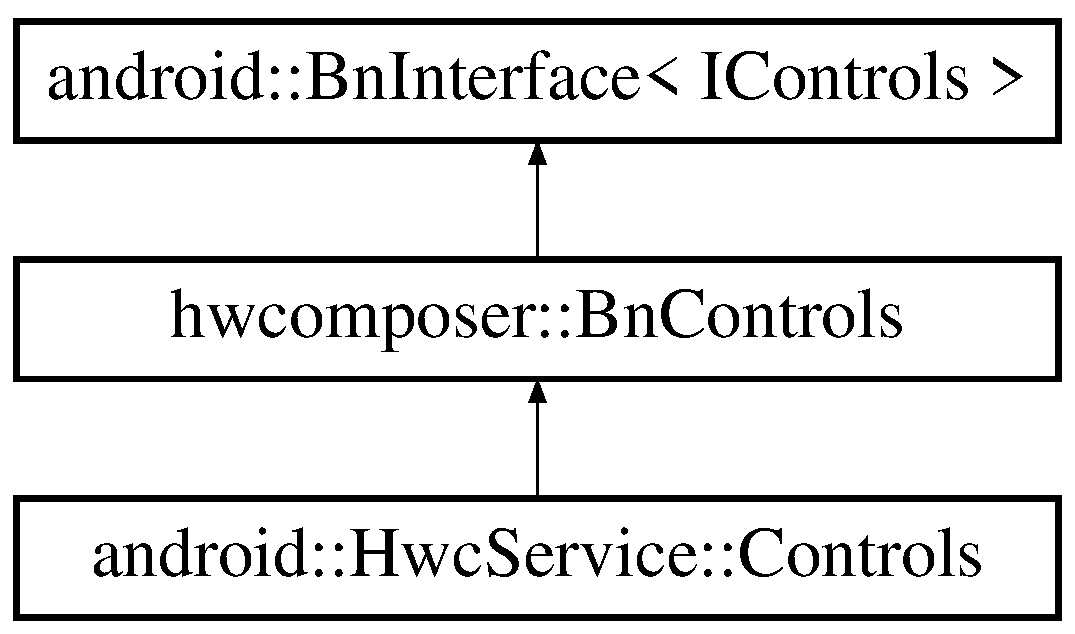
\includegraphics[height=3.000000cm]{classhwcomposer_1_1BnControls}
\end{center}
\end{figure}
\subsection*{Public Member Functions}
\begin{DoxyCompactItemize}
\item 
\mbox{\hyperlink{hwcserviceapi_8h_a3806fb2027d9a316d8ca8d9b8b8eb96f}{status\+\_\+t}} \mbox{\hyperlink{classhwcomposer_1_1BnControls_a335d9026455cc400f6a83e7529fd7cea}{on\+Transact}} (uint32\+\_\+t, const android\+::\+Parcel \&, android\+::\+Parcel $\ast$, uint32\+\_\+t) override
\end{DoxyCompactItemize}


\subsection{Detailed Description}


Definition at line 85 of file icontrols.\+h.



\subsection{Member Function Documentation}
\mbox{\Hypertarget{classhwcomposer_1_1BnControls_a335d9026455cc400f6a83e7529fd7cea}\label{classhwcomposer_1_1BnControls_a335d9026455cc400f6a83e7529fd7cea}} 
\index{hwcomposer\+::\+Bn\+Controls@{hwcomposer\+::\+Bn\+Controls}!on\+Transact@{on\+Transact}}
\index{on\+Transact@{on\+Transact}!hwcomposer\+::\+Bn\+Controls@{hwcomposer\+::\+Bn\+Controls}}
\subsubsection{\texorpdfstring{on\+Transact()}{onTransact()}}
{\footnotesize\ttfamily \mbox{\hyperlink{hwcserviceapi_8h_a3806fb2027d9a316d8ca8d9b8b8eb96f}{status\+\_\+t}} hwcomposer\+::\+Bn\+Controls\+::on\+Transact (\begin{DoxyParamCaption}\item[{uint32\+\_\+t}]{,  }\item[{const android\+::\+Parcel \&}]{,  }\item[{android\+::\+Parcel $\ast$}]{,  }\item[{uint32\+\_\+t}]{ }\end{DoxyParamCaption})\hspace{0.3cm}{\ttfamily [override]}}



Definition at line 516 of file icontrols.\+cpp.


\begin{DoxyCode}{0}
\DoxyCodeLine{517                                                                \{}
\DoxyCodeLine{518   \textcolor{keywordflow}{switch} (code) \{}
\DoxyCodeLine{519     \textcolor{keywordflow}{case} \mbox{\hyperlink{classhwcomposer_1_1BpControls_a057cb6d771c68da065640c49e3742446a985ef11557835be6b215a6b481cc8975}{BpControls::TRANSACT\_DISPLAY\_SET\_OVERSCAN}}: \{}
\DoxyCodeLine{520       CHECK\_INTERFACE(IControls, data, reply);}
\DoxyCodeLine{521       uint32\_t display = data.readInt32();}
\DoxyCodeLine{522       int32\_t xoverscan = data.readInt32();}
\DoxyCodeLine{523       int32\_t yoverscan = data.readInt32();}
\DoxyCodeLine{524       \mbox{\hyperlink{hwcserviceapi_8h_a3806fb2027d9a316d8ca8d9b8b8eb96f}{status\_t}} ret = this->DisplaySetOverscan(display, xoverscan, yoverscan);}
\DoxyCodeLine{525       reply->writeInt32(ret);}
\DoxyCodeLine{526       \textcolor{keywordflow}{return} NO\_ERROR;}
\DoxyCodeLine{527     \}}
\DoxyCodeLine{528     \textcolor{keywordflow}{case} \mbox{\hyperlink{classhwcomposer_1_1BpControls_a057cb6d771c68da065640c49e3742446acfb53ecdb379884e8843788c2a312e8c}{BpControls::TRANSACT\_DISPLAY\_GET\_OVERSCAN}}: \{}
\DoxyCodeLine{529       CHECK\_INTERFACE(IControls, data, reply);}
\DoxyCodeLine{530       uint32\_t display = data.readInt32();}
\DoxyCodeLine{531       int32\_t xoverscan;}
\DoxyCodeLine{532       int32\_t yoverscan;}
\DoxyCodeLine{533       \mbox{\hyperlink{hwcserviceapi_8h_a3806fb2027d9a316d8ca8d9b8b8eb96f}{status\_t}} ret = this->DisplayGetOverscan(display, \&xoverscan, \&yoverscan);}
\DoxyCodeLine{534       reply->writeInt32(ret);}
\DoxyCodeLine{535       reply->writeInt32(xoverscan);}
\DoxyCodeLine{536       reply->writeInt32(yoverscan);}
\DoxyCodeLine{537       \textcolor{keywordflow}{return} NO\_ERROR;}
\DoxyCodeLine{538     \}}
\DoxyCodeLine{539     \textcolor{keywordflow}{case} \mbox{\hyperlink{classhwcomposer_1_1BpControls_a057cb6d771c68da065640c49e3742446acd6fb8651f02533f7f7a92d0642d9a0d}{BpControls::TRANSACT\_DISPLAY\_SET\_SCALING}}: \{}
\DoxyCodeLine{540       CHECK\_INTERFACE(IControls, data, reply);}
\DoxyCodeLine{541       uint32\_t display = data.readInt32();}
\DoxyCodeLine{542       \mbox{\hyperlink{hwcserviceapi_8h_acdadfd5e7f15097833789174e442083f}{EHwcsScalingMode}} scaling = (\mbox{\hyperlink{hwcserviceapi_8h_acdadfd5e7f15097833789174e442083f}{EHwcsScalingMode}})data.readInt32();}
\DoxyCodeLine{543       \mbox{\hyperlink{hwcserviceapi_8h_a3806fb2027d9a316d8ca8d9b8b8eb96f}{status\_t}} ret = this->DisplaySetScaling(display, scaling);}
\DoxyCodeLine{544       reply->writeInt32(ret);}
\DoxyCodeLine{545       \textcolor{keywordflow}{return} NO\_ERROR;}
\DoxyCodeLine{546     \}}
\DoxyCodeLine{547     \textcolor{keywordflow}{case} \mbox{\hyperlink{classhwcomposer_1_1BpControls_a057cb6d771c68da065640c49e3742446ad8d27d03f7cca04781cb7c481a1a91d6}{BpControls::TRANSACT\_DISPLAY\_GET\_SCALING}}: \{}
\DoxyCodeLine{548       CHECK\_INTERFACE(IControls, data, reply);}
\DoxyCodeLine{549       uint32\_t display = data.readInt32();}
\DoxyCodeLine{550       \mbox{\hyperlink{hwcserviceapi_8h_acdadfd5e7f15097833789174e442083f}{EHwcsScalingMode}} scaling;}
\DoxyCodeLine{551       \mbox{\hyperlink{hwcserviceapi_8h_a3806fb2027d9a316d8ca8d9b8b8eb96f}{status\_t}} ret = this->DisplayGetScaling(display, \&scaling);}
\DoxyCodeLine{552       reply->writeInt32(ret);}
\DoxyCodeLine{553       reply->writeInt32((int32\_t)scaling);}
\DoxyCodeLine{554       \textcolor{keywordflow}{return} NO\_ERROR;}
\DoxyCodeLine{555     \}}
\DoxyCodeLine{556     \textcolor{keywordflow}{case} \mbox{\hyperlink{classhwcomposer_1_1BpControls_a057cb6d771c68da065640c49e3742446a6623581a2b88fb17369dd632a20106d4}{BpControls::TRANSACT\_DISPLAY\_ENABLE\_BLANK}}: \{}
\DoxyCodeLine{557       CHECK\_INTERFACE(IControls, data, reply);}
\DoxyCodeLine{558       uint32\_t display = data.readInt32();}
\DoxyCodeLine{559       \textcolor{keywordtype}{bool} blank = (bool)data.readInt32();}
\DoxyCodeLine{560       \mbox{\hyperlink{hwcserviceapi_8h_a3806fb2027d9a316d8ca8d9b8b8eb96f}{status\_t}} ret = this->DisplayEnableBlank(display, blank);}
\DoxyCodeLine{561       reply->writeInt32(ret);}
\DoxyCodeLine{562       \textcolor{keywordflow}{return} NO\_ERROR;}
\DoxyCodeLine{563     \}}
\DoxyCodeLine{564     \textcolor{keywordflow}{case} \mbox{\hyperlink{classhwcomposer_1_1BpControls_a057cb6d771c68da065640c49e3742446a15a087c4d488f967b1293b18951a6c02}{BpControls::TRANSACT\_DISPLAY\_RESTORE\_DEFAULT\_COLOR\_PARAM}}: \{}
\DoxyCodeLine{565       CHECK\_INTERFACE(IControls, data, reply);}
\DoxyCodeLine{566       uint32\_t display = data.readInt32();}
\DoxyCodeLine{567       \mbox{\hyperlink{hwcserviceapi_8h_a1d1cbf448ce748672cf3dd96675d70e4}{EHwcsColorControl}} color = (\mbox{\hyperlink{hwcserviceapi_8h_a1d1cbf448ce748672cf3dd96675d70e4}{EHwcsColorControl}})data.readInt32();}
\DoxyCodeLine{568       \mbox{\hyperlink{hwcserviceapi_8h_a3806fb2027d9a316d8ca8d9b8b8eb96f}{status\_t}} ret = this->DisplayRestoreDefaultColorParam(display, color);}
\DoxyCodeLine{569       reply->writeInt32(ret);}
\DoxyCodeLine{570       \textcolor{keywordflow}{return} NO\_ERROR;}
\DoxyCodeLine{571     \}}
\DoxyCodeLine{572     \textcolor{keywordflow}{case} \mbox{\hyperlink{classhwcomposer_1_1BpControls_a057cb6d771c68da065640c49e3742446a481d6c71408ba43adf692d5e11aa7fd7}{BpControls::TRANSACT\_DISPLAY\_RESTORE\_DEFAULT\_DEINTERLACE\_PARAM}}: \{}
\DoxyCodeLine{573       CHECK\_INTERFACE(IControls, data, reply);}
\DoxyCodeLine{574       uint32\_t display = data.readInt32();}
\DoxyCodeLine{575       \mbox{\hyperlink{hwcserviceapi_8h_a3806fb2027d9a316d8ca8d9b8b8eb96f}{status\_t}} ret = this->DisplayRestoreDefaultDeinterlaceParam(display);}
\DoxyCodeLine{576       reply->writeInt32(ret);}
\DoxyCodeLine{577       \textcolor{keywordflow}{return} NO\_ERROR;}
\DoxyCodeLine{578     \}}
\DoxyCodeLine{579 }
\DoxyCodeLine{580     \textcolor{keywordflow}{case} \mbox{\hyperlink{classhwcomposer_1_1BpControls_a057cb6d771c68da065640c49e3742446a218cf0d49257af27d4916bbcf7974e42}{BpControls::TRANSACT\_DISPLAY\_GET\_COLOR\_PARAM}}: \{}
\DoxyCodeLine{581       CHECK\_INTERFACE(IControls, data, reply);}
\DoxyCodeLine{582       uint32\_t display = data.readInt32();}
\DoxyCodeLine{583       \mbox{\hyperlink{hwcserviceapi_8h_a1d1cbf448ce748672cf3dd96675d70e4}{EHwcsColorControl}} color = (\mbox{\hyperlink{hwcserviceapi_8h_a1d1cbf448ce748672cf3dd96675d70e4}{EHwcsColorControl}})data.readInt32();}
\DoxyCodeLine{584       \textcolor{keywordtype}{float} value;}
\DoxyCodeLine{585       \textcolor{keywordtype}{float} startvalue;}
\DoxyCodeLine{586       \textcolor{keywordtype}{float} endvalue;}
\DoxyCodeLine{587       \mbox{\hyperlink{hwcserviceapi_8h_a3806fb2027d9a316d8ca8d9b8b8eb96f}{status\_t}} ret = this->DisplayGetColorParam(display, color, \&value,}
\DoxyCodeLine{588                                                 \&startvalue, \&endvalue);}
\DoxyCodeLine{589       reply->writeFloat(value);}
\DoxyCodeLine{590       reply->writeFloat(startvalue);}
\DoxyCodeLine{591       reply->writeFloat(endvalue);}
\DoxyCodeLine{592       reply->writeInt32(ret);}
\DoxyCodeLine{593       \textcolor{keywordflow}{return} NO\_ERROR;}
\DoxyCodeLine{594     \}}
\DoxyCodeLine{595     \textcolor{keywordflow}{case} \mbox{\hyperlink{classhwcomposer_1_1BpControls_a057cb6d771c68da065640c49e3742446a02754bed54f3e948595d365863e6ff6c}{BpControls::TRANSACT\_DISPLAY\_SET\_COLOR\_PARAM}}: \{}
\DoxyCodeLine{596       CHECK\_INTERFACE(IControls, data, reply);}
\DoxyCodeLine{597       uint32\_t display = data.readInt32();}
\DoxyCodeLine{598       \mbox{\hyperlink{hwcserviceapi_8h_a1d1cbf448ce748672cf3dd96675d70e4}{EHwcsColorControl}} color = (\mbox{\hyperlink{hwcserviceapi_8h_a1d1cbf448ce748672cf3dd96675d70e4}{EHwcsColorControl}})data.readInt32();}
\DoxyCodeLine{599       \textcolor{keywordtype}{float} value = data.readFloat();}
\DoxyCodeLine{600       \mbox{\hyperlink{hwcserviceapi_8h_a3806fb2027d9a316d8ca8d9b8b8eb96f}{status\_t}} ret = this->DisplaySetColorParam(display, color, value);}
\DoxyCodeLine{601       reply->writeInt32(ret);}
\DoxyCodeLine{602       \textcolor{keywordflow}{return} NO\_ERROR;}
\DoxyCodeLine{603     \}}
\DoxyCodeLine{604     \textcolor{keywordflow}{case} \mbox{\hyperlink{classhwcomposer_1_1BpControls_a057cb6d771c68da065640c49e3742446a32c72f6f1679760b231c841184d5420d}{BpControls::TRANSACT\_DISPLAY\_SET\_DEINTERLACE\_PARAM}}: \{}
\DoxyCodeLine{605       CHECK\_INTERFACE(IControls, data, reply);}
\DoxyCodeLine{606       uint32\_t display = data.readInt32();}
\DoxyCodeLine{607       \mbox{\hyperlink{hwcserviceapi_8h_a8473f2ec9e7333e67be46a1bea689113}{EHwcsDeinterlaceControl}} mode = (
      \mbox{\hyperlink{hwcserviceapi_8h_a8473f2ec9e7333e67be46a1bea689113}{EHwcsDeinterlaceControl}})data.readInt32();}
\DoxyCodeLine{608       \mbox{\hyperlink{hwcserviceapi_8h_a3806fb2027d9a316d8ca8d9b8b8eb96f}{status\_t}} ret = this->DisplaySetDeinterlaceParam(display, mode);}
\DoxyCodeLine{609       reply->writeInt32(ret);}
\DoxyCodeLine{610       \textcolor{keywordflow}{return} NO\_ERROR;}
\DoxyCodeLine{611     \}}
\DoxyCodeLine{612 }
\DoxyCodeLine{613     \textcolor{keywordflow}{case} \mbox{\hyperlink{classhwcomposer_1_1BpControls_a057cb6d771c68da065640c49e3742446a23ea2de5ee0482714e828cdfe3b78eb6}{BpControls::TRANSACT\_DISPLAYMODE\_GET\_AVAILABLE\_MODES}}: \{}
\DoxyCodeLine{614       CHECK\_INTERFACE(IControls, data, reply);}
\DoxyCodeLine{615       uint32\_t display = data.readInt32();}
\DoxyCodeLine{616 }
\DoxyCodeLine{617       std::vector<HwcsDisplayModeInfo> vector =}
\DoxyCodeLine{618           this->DisplayModeGetAvailableModes(display);}
\DoxyCodeLine{619       reply->writeInt32(vector.size());}
\DoxyCodeLine{620       \textcolor{keywordflow}{for} (uint32\_t i = 0; i < vector.size(); i++) \{}
\DoxyCodeLine{621         reply->writeInt32(vector[i].width);}
\DoxyCodeLine{622         reply->writeInt32(vector[i].height);}
\DoxyCodeLine{623         reply->writeInt32(vector[i].refresh);}
\DoxyCodeLine{624         reply->writeInt32(vector[i].xdpi);}
\DoxyCodeLine{625         reply->writeInt32(vector[i].ydpi);}
\DoxyCodeLine{626       \}}
\DoxyCodeLine{627       \textcolor{keywordflow}{return} NO\_ERROR;}
\DoxyCodeLine{628     \}}
\DoxyCodeLine{629     \textcolor{keywordflow}{case} \mbox{\hyperlink{classhwcomposer_1_1BpControls_a057cb6d771c68da065640c49e3742446afd0d6093faf175dc1c13e25789063f3e}{BpControls::TRANSACT\_DISPLAYMODE\_GET\_MODE}}: \{}
\DoxyCodeLine{630       CHECK\_INTERFACE(IControls, data, reply);}
\DoxyCodeLine{631       uint32\_t display = data.readInt32();}
\DoxyCodeLine{632       \mbox{\hyperlink{struct__HwcsDisplayModeInfo}{HwcsDisplayModeInfo}} info;}
\DoxyCodeLine{633       \mbox{\hyperlink{hwcserviceapi_8h_a3806fb2027d9a316d8ca8d9b8b8eb96f}{status\_t}} ret = this->DisplayModeGetMode(display, \&info);}
\DoxyCodeLine{634       reply->writeInt32(info.\mbox{\hyperlink{struct__HwcsDisplayModeInfo_a50ed795465b52cda71e38e0c5eae2804}{width}});}
\DoxyCodeLine{635       reply->writeInt32(info.\mbox{\hyperlink{struct__HwcsDisplayModeInfo_a89f5474962a13b045ce25b84929c6be3}{height}});}
\DoxyCodeLine{636       reply->writeInt32(info.\mbox{\hyperlink{struct__HwcsDisplayModeInfo_afbc17f7325634fd5b86eeb0a2023c635}{refresh}});}
\DoxyCodeLine{637       reply->writeInt32(info.\mbox{\hyperlink{struct__HwcsDisplayModeInfo_ad8d33821439c3aeb8b125296cb62dbbb}{xdpi}});}
\DoxyCodeLine{638       reply->writeInt32(info.\mbox{\hyperlink{struct__HwcsDisplayModeInfo_a53ef1f5ece0baea9b74b76dbf9c0fc19}{ydpi}});}
\DoxyCodeLine{639       reply->writeInt32(ret);}
\DoxyCodeLine{640       \textcolor{keywordflow}{return} NO\_ERROR;}
\DoxyCodeLine{641     \}}
\DoxyCodeLine{642     \textcolor{keywordflow}{case} \mbox{\hyperlink{classhwcomposer_1_1BpControls_a057cb6d771c68da065640c49e3742446a62999b5eadacd5213c222e8efe03dda4}{BpControls::TRANSACT\_DISPLAYMODE\_SET\_MODE}}: \{}
\DoxyCodeLine{643       CHECK\_INTERFACE(IControls, data, reply);}
\DoxyCodeLine{644       uint32\_t display = data.readInt32();}
\DoxyCodeLine{645       uint32\_t config = data.readInt32();}
\DoxyCodeLine{646       \mbox{\hyperlink{hwcserviceapi_8h_a3806fb2027d9a316d8ca8d9b8b8eb96f}{status\_t}} ret = this->DisplayModeSetMode(display, config);}
\DoxyCodeLine{647       reply->writeInt32(ret);}
\DoxyCodeLine{648       \textcolor{keywordflow}{return} NO\_ERROR;}
\DoxyCodeLine{649     \}}
\DoxyCodeLine{650     \textcolor{keywordflow}{case} \mbox{\hyperlink{classhwcomposer_1_1BpControls_a057cb6d771c68da065640c49e3742446a6482e9c31b42e7a8a101b55e059a260a}{BpControls::TRANSACT\_VIDEO\_ENABLE\_HDCP\_SESSION\_FOR\_DISPLAY}}: \{}
\DoxyCodeLine{651       CHECK\_INTERFACE(IControls, data, reply);}
\DoxyCodeLine{652       uint32\_t display = data.readInt32();}
\DoxyCodeLine{653       \mbox{\hyperlink{hwcserviceapi_8h_a69e9b3a54e4c8e504845398c66eab655}{EHwcsContentType}} content\_type = (\mbox{\hyperlink{hwcserviceapi_8h_a69e9b3a54e4c8e504845398c66eab655}{EHwcsContentType}})data.readInt32();}
\DoxyCodeLine{654       \mbox{\hyperlink{hwcserviceapi_8h_a3806fb2027d9a316d8ca8d9b8b8eb96f}{status\_t}} ret = this->EnableHDCPSessionForDisplay(display, content\_type);}
\DoxyCodeLine{655       reply->writeInt32(ret);}
\DoxyCodeLine{656       \textcolor{keywordflow}{return} NO\_ERROR;}
\DoxyCodeLine{657     \}}
\DoxyCodeLine{658     \textcolor{keywordflow}{case} \mbox{\hyperlink{classhwcomposer_1_1BpControls_a057cb6d771c68da065640c49e3742446acaf7406d1c2bbedb4253ce81685ca811}{BpControls::TRANSACT\_VIDEO\_ENABLE\_HDCP\_SESSION\_FOR\_ALL\_DISPLAYS}}: \{}
\DoxyCodeLine{659       CHECK\_INTERFACE(IControls, data, reply);}
\DoxyCodeLine{660       \mbox{\hyperlink{hwcserviceapi_8h_a69e9b3a54e4c8e504845398c66eab655}{EHwcsContentType}} content\_type = (\mbox{\hyperlink{hwcserviceapi_8h_a69e9b3a54e4c8e504845398c66eab655}{EHwcsContentType}})data.readInt32();}
\DoxyCodeLine{661       \mbox{\hyperlink{hwcserviceapi_8h_a3806fb2027d9a316d8ca8d9b8b8eb96f}{status\_t}} ret = this->EnableHDCPSessionForAllDisplays(content\_type);}
\DoxyCodeLine{662       reply->writeInt32(ret);}
\DoxyCodeLine{663       \textcolor{keywordflow}{return} NO\_ERROR;}
\DoxyCodeLine{664     \}}
\DoxyCodeLine{665     \textcolor{keywordflow}{case} \mbox{\hyperlink{classhwcomposer_1_1BpControls_a057cb6d771c68da065640c49e3742446a3772d2ac2fc50e3b393733c14f95e536}{BpControls::TRANSACT\_VIDEO\_DISABLE\_HDCP\_SESSION\_FOR\_DISPLAY}}: \{}
\DoxyCodeLine{666       CHECK\_INTERFACE(IControls, data, reply);}
\DoxyCodeLine{667       uint32\_t display = data.readInt32();}
\DoxyCodeLine{668       \mbox{\hyperlink{hwcserviceapi_8h_a3806fb2027d9a316d8ca8d9b8b8eb96f}{status\_t}} ret = this->DisableHDCPSessionForDisplay(display);}
\DoxyCodeLine{669       reply->writeInt32(ret);}
\DoxyCodeLine{670       \textcolor{keywordflow}{return} NO\_ERROR;}
\DoxyCodeLine{671     \}}
\DoxyCodeLine{672     \textcolor{keywordflow}{case} \mbox{\hyperlink{classhwcomposer_1_1BpControls_a057cb6d771c68da065640c49e3742446a7afcde053a8bef100088bae91dbb2620}{BpControls::TRANSACT\_VIDEO\_DISABLE\_HDCP\_SESSION\_FOR\_ALL\_DISPLAYS}}: \{}
\DoxyCodeLine{673       CHECK\_INTERFACE(IControls, data, reply);}
\DoxyCodeLine{674       \mbox{\hyperlink{hwcserviceapi_8h_a3806fb2027d9a316d8ca8d9b8b8eb96f}{status\_t}} ret = this->DisableHDCPSessionForAllDisplays();}
\DoxyCodeLine{675       reply->writeInt32(ret);}
\DoxyCodeLine{676       \textcolor{keywordflow}{return} NO\_ERROR;}
\DoxyCodeLine{677     \}}
\DoxyCodeLine{678     \textcolor{keywordflow}{case} \mbox{\hyperlink{classhwcomposer_1_1BpControls_a057cb6d771c68da065640c49e3742446ac6559374237fdc63c299a2964bdbe9d7}{BpControls::TRANSACT\_VIDEO\_ENABLE\_ENCRYPTED\_SESSION}}: \{}
\DoxyCodeLine{679       CHECK\_INTERFACE(IControls, data, reply);}
\DoxyCodeLine{680       uint32\_t sessionID = data.readInt32();}
\DoxyCodeLine{681       uint32\_t instanceID = data.readInt32();}
\DoxyCodeLine{682       \mbox{\hyperlink{hwcserviceapi_8h_a3806fb2027d9a316d8ca8d9b8b8eb96f}{status\_t}} ret = this->VideoEnableEncryptedSession(sessionID, instanceID);}
\DoxyCodeLine{683       reply->writeInt32(ret);}
\DoxyCodeLine{684       \textcolor{keywordflow}{return} NO\_ERROR;}
\DoxyCodeLine{685     \}}
\DoxyCodeLine{686     \textcolor{keywordflow}{case} \mbox{\hyperlink{classhwcomposer_1_1BpControls_a057cb6d771c68da065640c49e3742446aaa215b4cc5192668f648d2f90962f582}{BpControls::TRANSACT\_VIDEO\_DISABLE\_ENCRYPTED\_SESSION}}: \{}
\DoxyCodeLine{687       CHECK\_INTERFACE(IControls, data, reply);}
\DoxyCodeLine{688       int32\_t sessionID = data.readInt32();}
\DoxyCodeLine{689       \mbox{\hyperlink{hwcserviceapi_8h_a3806fb2027d9a316d8ca8d9b8b8eb96f}{status\_t}} ret = this->VideoDisableAllEncryptedSessions(sessionID);}
\DoxyCodeLine{690       reply->writeInt32(ret);}
\DoxyCodeLine{691       \textcolor{keywordflow}{return} NO\_ERROR;}
\DoxyCodeLine{692     \}}
\DoxyCodeLine{693     \textcolor{keywordflow}{case} \mbox{\hyperlink{classhwcomposer_1_1BpControls_a057cb6d771c68da065640c49e3742446a5ef49fd58989fb5029472668414f9140}{BpControls::TRANSACT\_VIDEO\_DISABLE\_ALL\_ENCRYPTED\_SESSIONS}}: \{}
\DoxyCodeLine{694       CHECK\_INTERFACE(IControls, data, reply);}
\DoxyCodeLine{695       \mbox{\hyperlink{hwcserviceapi_8h_a3806fb2027d9a316d8ca8d9b8b8eb96f}{status\_t}} ret = this->VideoDisableAllEncryptedSessions();}
\DoxyCodeLine{696       reply->writeInt32(ret);}
\DoxyCodeLine{697       \textcolor{keywordflow}{return} NO\_ERROR;}
\DoxyCodeLine{698     \}}
\DoxyCodeLine{699     \textcolor{keywordflow}{case} \mbox{\hyperlink{classhwcomposer_1_1BpControls_a057cb6d771c68da065640c49e3742446a83e8e51e9f0eaa3b99c1fbe7486875ec}{BpControls::TRANSACT\_VIDEO\_IS\_ENCRYPTED\_SESSION\_ENABLED}}: \{}
\DoxyCodeLine{700       CHECK\_INTERFACE(IControls, data, reply);}
\DoxyCodeLine{701       uint32\_t sessionID = data.readInt32();}
\DoxyCodeLine{702       uint32\_t instanceID = data.readInt32();}
\DoxyCodeLine{703       \textcolor{keywordtype}{bool} bEnabled =}
\DoxyCodeLine{704           this->VideoIsEncryptedSessionEnabled(sessionID, instanceID);}
\DoxyCodeLine{705       reply->writeInt32(bEnabled);}
\DoxyCodeLine{706       \textcolor{keywordflow}{return} NO\_ERROR;}
\DoxyCodeLine{707     \}}
\DoxyCodeLine{708     \textcolor{keywordflow}{case} \mbox{\hyperlink{classhwcomposer_1_1BpControls_a057cb6d771c68da065640c49e3742446a2dc60d5ba78113e4cad0c7d70be98a8e}{BpControls::TRANSACT\_VIDEO\_SET\_OPTIMIZATION\_MODE}}: \{}
\DoxyCodeLine{709       CHECK\_INTERFACE(IControls, data, reply);}
\DoxyCodeLine{710       \mbox{\hyperlink{hwcserviceapi_8h_a73044de23b8f474352d6753e21fca06d}{EHwcsOptimizationMode}} mode = (\mbox{\hyperlink{hwcserviceapi_8h_a73044de23b8f474352d6753e21fca06d}{EHwcsOptimizationMode}})data.readInt32();}
\DoxyCodeLine{711       \mbox{\hyperlink{hwcserviceapi_8h_a3806fb2027d9a316d8ca8d9b8b8eb96f}{status\_t}} ret = this->VideoSetOptimizationMode(mode);}
\DoxyCodeLine{712       reply->writeInt32(ret);}
\DoxyCodeLine{713       \textcolor{keywordflow}{return} NO\_ERROR;}
\DoxyCodeLine{714     \}}
\DoxyCodeLine{715     \textcolor{keywordflow}{case} \mbox{\hyperlink{classhwcomposer_1_1BpControls_a057cb6d771c68da065640c49e3742446ae58d81883fb4d1137f4f8b9222b93f95}{BpControls::TRANSACT\_MDS\_UPDATE\_VIDEO\_STATE}}: \{}
\DoxyCodeLine{716       CHECK\_INTERFACE(IControls, data, reply);}
\DoxyCodeLine{717       int64\_t videoSessionID = data.readInt64();}
\DoxyCodeLine{718       \textcolor{keywordtype}{bool} isPrepared = data.readInt32();}
\DoxyCodeLine{719       \mbox{\hyperlink{hwcserviceapi_8h_a3806fb2027d9a316d8ca8d9b8b8eb96f}{status\_t}} ret = this->MdsUpdateVideoState(videoSessionID, isPrepared);}
\DoxyCodeLine{720       reply->writeInt32(ret);}
\DoxyCodeLine{721       \textcolor{keywordflow}{return} NO\_ERROR;}
\DoxyCodeLine{722     \}}
\DoxyCodeLine{723     \textcolor{keywordflow}{case} \mbox{\hyperlink{classhwcomposer_1_1BpControls_a057cb6d771c68da065640c49e3742446aed219d26b586c56400fb6ff87d4b7b12}{BpControls::TRANSACT\_MDS\_UPDATE\_VIDEO\_FPS}}: \{}
\DoxyCodeLine{724       CHECK\_INTERFACE(IControls, data, reply);}
\DoxyCodeLine{725       int64\_t videoSessionID = data.readInt64();}
\DoxyCodeLine{726       int32\_t fps = data.readInt32();}
\DoxyCodeLine{727       \mbox{\hyperlink{hwcserviceapi_8h_a3806fb2027d9a316d8ca8d9b8b8eb96f}{status\_t}} ret = this->MdsUpdateVideoFPS(videoSessionID, fps);}
\DoxyCodeLine{728       reply->writeInt32(ret);}
\DoxyCodeLine{729       \textcolor{keywordflow}{return} NO\_ERROR;}
\DoxyCodeLine{730     \}}
\DoxyCodeLine{731     \textcolor{keywordflow}{case} \mbox{\hyperlink{classhwcomposer_1_1BpControls_a057cb6d771c68da065640c49e3742446a9c89c90c56c8ad69f11b9131ac2e8b00}{BpControls::TRANSACT\_MDS\_UPDATE\_INPUT\_STATE}}: \{}
\DoxyCodeLine{732       CHECK\_INTERFACE(IControls, data, reply);}
\DoxyCodeLine{733       \textcolor{keywordtype}{bool} state = data.readInt32();}
\DoxyCodeLine{734       \mbox{\hyperlink{hwcserviceapi_8h_a3806fb2027d9a316d8ca8d9b8b8eb96f}{status\_t}} ret = this->MdsUpdateInputState(state);}
\DoxyCodeLine{735       reply->writeInt32(ret);}
\DoxyCodeLine{736       \textcolor{keywordflow}{return} NO\_ERROR;}
\DoxyCodeLine{737     \}}
\DoxyCodeLine{738     \textcolor{keywordflow}{case} \mbox{\hyperlink{classhwcomposer_1_1BpControls_a057cb6d771c68da065640c49e3742446ac0896efafd9de075b9d33ae5ea916ae9}{BpControls::TRANSACT\_WIDI\_GET\_SINGLE\_DISPLAY}}: \{}
\DoxyCodeLine{739       CHECK\_INTERFACE(IControls, data, reply);}
\DoxyCodeLine{740       \textcolor{keywordtype}{bool} enable = \textcolor{keyword}{false};}
\DoxyCodeLine{741       \mbox{\hyperlink{hwcserviceapi_8h_a3806fb2027d9a316d8ca8d9b8b8eb96f}{status\_t}} ret = this->WidiGetSingleDisplay(\&enable);}
\DoxyCodeLine{742       reply->writeInt32(enable);}
\DoxyCodeLine{743       reply->writeInt32(ret);}
\DoxyCodeLine{744       \textcolor{keywordflow}{return} NO\_ERROR;}
\DoxyCodeLine{745     \}}
\DoxyCodeLine{746     \textcolor{keywordflow}{case} \mbox{\hyperlink{classhwcomposer_1_1BpControls_a057cb6d771c68da065640c49e3742446aba0ea7b08d69c3018e5dc0017a14390a}{BpControls::TRANSACT\_WIDI\_SET\_SINGLE\_DISPLAY}}: \{}
\DoxyCodeLine{747       CHECK\_INTERFACE(IControls, data, reply);}
\DoxyCodeLine{748       \textcolor{keywordtype}{bool} enable = data.readInt32();}
\DoxyCodeLine{749       \mbox{\hyperlink{hwcserviceapi_8h_a3806fb2027d9a316d8ca8d9b8b8eb96f}{status\_t}} ret = this->WidiSetSingleDisplay(enable);}
\DoxyCodeLine{750       reply->writeInt32(ret);}
\DoxyCodeLine{751       \textcolor{keywordflow}{return} NO\_ERROR;}
\DoxyCodeLine{752     \}}
\DoxyCodeLine{753 }
\DoxyCodeLine{754     \textcolor{keywordflow}{default}:}
\DoxyCodeLine{755       \textcolor{keywordflow}{return} BBinder::onTransact(code, data, reply, flags);}
\DoxyCodeLine{756   \}}
\DoxyCodeLine{757 \}}
\end{DoxyCode}


The documentation for this class was generated from the following files\+:\begin{DoxyCompactItemize}
\item 
os/android/libhwcservice/\mbox{\hyperlink{icontrols_8h}{icontrols.\+h}}\item 
os/android/libhwcservice/\mbox{\hyperlink{icontrols_8cpp}{icontrols.\+cpp}}\end{DoxyCompactItemize}

\hypertarget{classhwcomposer_1_1BnDiagnostic}{}\section{hwcomposer\+:\+:Bn\+Diagnostic Class Reference}
\label{classhwcomposer_1_1BnDiagnostic}\index{hwcomposer\+::\+Bn\+Diagnostic@{hwcomposer\+::\+Bn\+Diagnostic}}


{\ttfamily \#include $<$idiagnostic.\+h$>$}

Inheritance diagram for hwcomposer\+:\+:Bn\+Diagnostic\+:\begin{figure}[H]
\begin{center}
\leavevmode
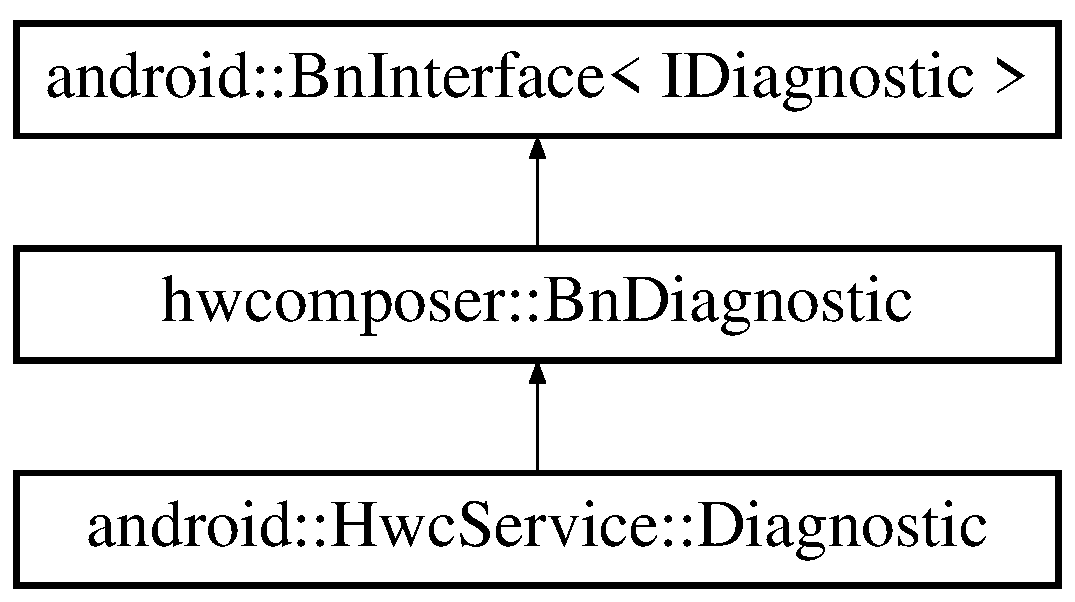
\includegraphics[height=3.000000cm]{classhwcomposer_1_1BnDiagnostic}
\end{center}
\end{figure}
\subsection*{Public Member Functions}
\begin{DoxyCompactItemize}
\item 
\mbox{\hyperlink{classhwcomposer_1_1BnDiagnostic_a0dae02c0aa18aa54bb5aefb2ef9b4cd5}{Bn\+Diagnostic}} ()
\item 
virtual \mbox{\hyperlink{classhwcomposer_1_1BnDiagnostic_acb90849642dd99099514c8d4ec1ee55b}{$\sim$\+Bn\+Diagnostic}} ()
\item 
\mbox{\hyperlink{hwcserviceapi_8h_a3806fb2027d9a316d8ca8d9b8b8eb96f}{status\+\_\+t}} \mbox{\hyperlink{classhwcomposer_1_1BnDiagnostic_a3b524b73de19be10529cefa88ecd59ff}{on\+Transact}} (uint32\+\_\+t, const Parcel \&, Parcel $\ast$, uint32\+\_\+t) override
\end{DoxyCompactItemize}


\subsection{Detailed Description}


Definition at line 48 of file idiagnostic.\+h.



\subsection{Constructor \& Destructor Documentation}
\mbox{\Hypertarget{classhwcomposer_1_1BnDiagnostic_a0dae02c0aa18aa54bb5aefb2ef9b4cd5}\label{classhwcomposer_1_1BnDiagnostic_a0dae02c0aa18aa54bb5aefb2ef9b4cd5}} 
\index{hwcomposer\+::\+Bn\+Diagnostic@{hwcomposer\+::\+Bn\+Diagnostic}!Bn\+Diagnostic@{Bn\+Diagnostic}}
\index{Bn\+Diagnostic@{Bn\+Diagnostic}!hwcomposer\+::\+Bn\+Diagnostic@{hwcomposer\+::\+Bn\+Diagnostic}}
\subsubsection{\texorpdfstring{Bn\+Diagnostic()}{BnDiagnostic()}}
{\footnotesize\ttfamily hwcomposer\+::\+Bn\+Diagnostic\+::\+Bn\+Diagnostic (\begin{DoxyParamCaption}{ }\end{DoxyParamCaption})\hspace{0.3cm}{\ttfamily [inline]}}



Definition at line 50 of file idiagnostic.\+h.


\begin{DoxyCode}{0}
\DoxyCodeLine{50                  \{}
\DoxyCodeLine{51   \}}
\end{DoxyCode}
\mbox{\Hypertarget{classhwcomposer_1_1BnDiagnostic_acb90849642dd99099514c8d4ec1ee55b}\label{classhwcomposer_1_1BnDiagnostic_acb90849642dd99099514c8d4ec1ee55b}} 
\index{hwcomposer\+::\+Bn\+Diagnostic@{hwcomposer\+::\+Bn\+Diagnostic}!````~Bn\+Diagnostic@{$\sim$\+Bn\+Diagnostic}}
\index{````~Bn\+Diagnostic@{$\sim$\+Bn\+Diagnostic}!hwcomposer\+::\+Bn\+Diagnostic@{hwcomposer\+::\+Bn\+Diagnostic}}
\subsubsection{\texorpdfstring{$\sim$\+Bn\+Diagnostic()}{~BnDiagnostic()}}
{\footnotesize\ttfamily virtual hwcomposer\+::\+Bn\+Diagnostic\+::$\sim$\+Bn\+Diagnostic (\begin{DoxyParamCaption}{ }\end{DoxyParamCaption})\hspace{0.3cm}{\ttfamily [inline]}, {\ttfamily [virtual]}}



Definition at line 53 of file idiagnostic.\+h.


\begin{DoxyCode}{0}
\DoxyCodeLine{53                           \{}
\DoxyCodeLine{54   \}}
\end{DoxyCode}


\subsection{Member Function Documentation}
\mbox{\Hypertarget{classhwcomposer_1_1BnDiagnostic_a3b524b73de19be10529cefa88ecd59ff}\label{classhwcomposer_1_1BnDiagnostic_a3b524b73de19be10529cefa88ecd59ff}} 
\index{hwcomposer\+::\+Bn\+Diagnostic@{hwcomposer\+::\+Bn\+Diagnostic}!on\+Transact@{on\+Transact}}
\index{on\+Transact@{on\+Transact}!hwcomposer\+::\+Bn\+Diagnostic@{hwcomposer\+::\+Bn\+Diagnostic}}
\subsubsection{\texorpdfstring{on\+Transact()}{onTransact()}}
{\footnotesize\ttfamily \mbox{\hyperlink{hwcserviceapi_8h_a3806fb2027d9a316d8ca8d9b8b8eb96f}{status\+\_\+t}} hwcomposer\+::\+Bn\+Diagnostic\+::on\+Transact (\begin{DoxyParamCaption}\item[{uint32\+\_\+t}]{code,  }\item[{const Parcel \&}]{data,  }\item[{Parcel $\ast$}]{reply,  }\item[{uint32\+\_\+t}]{flags }\end{DoxyParamCaption})\hspace{0.3cm}{\ttfamily [override]}}



Definition at line 110 of file idiagnostic.\+cpp.


\begin{DoxyCode}{0}
\DoxyCodeLine{111                                                                  \{}
\DoxyCodeLine{112   \textcolor{keywordflow}{switch} (code) \{}
\DoxyCodeLine{113     \textcolor{keywordflow}{case} \mbox{\hyperlink{classhwcomposer_1_1BpDiagnostic_a28475ea102b977cb7213262dc96a568da1c6934eb57e46477b1b76921ab9e1d8d}{BpDiagnostic::TRANSACT\_READ\_LOG\_PARCEL}}: \{}
\DoxyCodeLine{114       CHECK\_INTERFACE(IDiagnostic, data, reply);}
\DoxyCodeLine{115       \mbox{\hyperlink{hwcserviceapi_8h_a3806fb2027d9a316d8ca8d9b8b8eb96f}{status\_t}} err = ReadLogParcel(reply);}
\DoxyCodeLine{116       \textcolor{keywordflow}{return} err;}
\DoxyCodeLine{117     \}}
\DoxyCodeLine{118 }
\DoxyCodeLine{119     \textcolor{keywordflow}{case} \mbox{\hyperlink{classhwcomposer_1_1BpDiagnostic_a28475ea102b977cb7213262dc96a568daccd4b7373af1f931dede971ad0e92972}{BpDiagnostic::TRANSACT\_ENABLE\_DISPLAY}}: \{}
\DoxyCodeLine{120       CHECK\_INTERFACE(IDiagnostic, data, reply);}
\DoxyCodeLine{121       uint32\_t d = data.readInt32();}
\DoxyCodeLine{122       EnableDisplay(d);}
\DoxyCodeLine{123       \textcolor{keywordflow}{return} NO\_ERROR;}
\DoxyCodeLine{124     \}}
\DoxyCodeLine{125 }
\DoxyCodeLine{126     \textcolor{keywordflow}{case} \mbox{\hyperlink{classhwcomposer_1_1BpDiagnostic_a28475ea102b977cb7213262dc96a568dae96b3abe1c20751a136bbe4309230923}{BpDiagnostic::TRANSACT\_DISABLE\_DISPLAY}}: \{}
\DoxyCodeLine{127       CHECK\_INTERFACE(IDiagnostic, data, reply);}
\DoxyCodeLine{128       uint32\_t d = data.readInt32();}
\DoxyCodeLine{129       \textcolor{keywordtype}{bool} bBlank = data.readInt32();}
\DoxyCodeLine{130       DisableDisplay(d, bBlank);}
\DoxyCodeLine{131       \textcolor{keywordflow}{return} NO\_ERROR;}
\DoxyCodeLine{132     \}}
\DoxyCodeLine{133 }
\DoxyCodeLine{134     \textcolor{keywordflow}{case} \mbox{\hyperlink{classhwcomposer_1_1BpDiagnostic_a28475ea102b977cb7213262dc96a568daf904704142b648f549b6b220ee158711}{BpDiagnostic::TRANSACT\_MASK\_LAYER}}: \{}
\DoxyCodeLine{135       CHECK\_INTERFACE(IDiagnostic, data, reply);}
\DoxyCodeLine{136       uint32\_t d = data.readInt32();}
\DoxyCodeLine{137       uint32\_t layer = data.readInt32();}
\DoxyCodeLine{138       \textcolor{keywordtype}{bool} bHide = data.readInt32();}
\DoxyCodeLine{139       MaskLayer(d, layer, bHide);}
\DoxyCodeLine{140       \textcolor{keywordflow}{return} NO\_ERROR;}
\DoxyCodeLine{141     \}}
\DoxyCodeLine{142 }
\DoxyCodeLine{143     \textcolor{keywordflow}{case} \mbox{\hyperlink{classhwcomposer_1_1BpDiagnostic_a28475ea102b977cb7213262dc96a568dac8e288e1260c1218aa4f35e308cb3546}{BpDiagnostic::TRANSACT\_DUMP\_FRAMES}}: \{}
\DoxyCodeLine{144       CHECK\_INTERFACE(IDiagnostic, data, reply);}
\DoxyCodeLine{145       uint32\_t d = data.readInt32();}
\DoxyCodeLine{146       int32\_t frames = data.readInt32();}
\DoxyCodeLine{147       \textcolor{keywordtype}{bool} bSync = data.readInt32();}
\DoxyCodeLine{148       DumpFrames(d, frames, bSync);}
\DoxyCodeLine{149       \textcolor{keywordflow}{return} NO\_ERROR;}
\DoxyCodeLine{150     \}}
\DoxyCodeLine{151 }
\DoxyCodeLine{152     \textcolor{keywordflow}{default}:}
\DoxyCodeLine{153       \textcolor{keywordflow}{return} BBinder::onTransact(code, data, reply, flags);}
\DoxyCodeLine{154   \}}
\DoxyCodeLine{155 \}}
\end{DoxyCode}


The documentation for this class was generated from the following files\+:\begin{DoxyCompactItemize}
\item 
os/android/libhwcservice/\mbox{\hyperlink{idiagnostic_8h}{idiagnostic.\+h}}\item 
os/android/libhwcservice/\mbox{\hyperlink{idiagnostic_8cpp}{idiagnostic.\+cpp}}\end{DoxyCompactItemize}

\hypertarget{classhwcomposer_1_1BnService}{}\section{hwcomposer\+:\+:Bn\+Service Class Reference}
\label{classhwcomposer_1_1BnService}\index{hwcomposer\+::\+Bn\+Service@{hwcomposer\+::\+Bn\+Service}}


{\ttfamily \#include $<$iservice.\+h$>$}

Inheritance diagram for hwcomposer\+:\+:Bn\+Service\+:\begin{figure}[H]
\begin{center}
\leavevmode
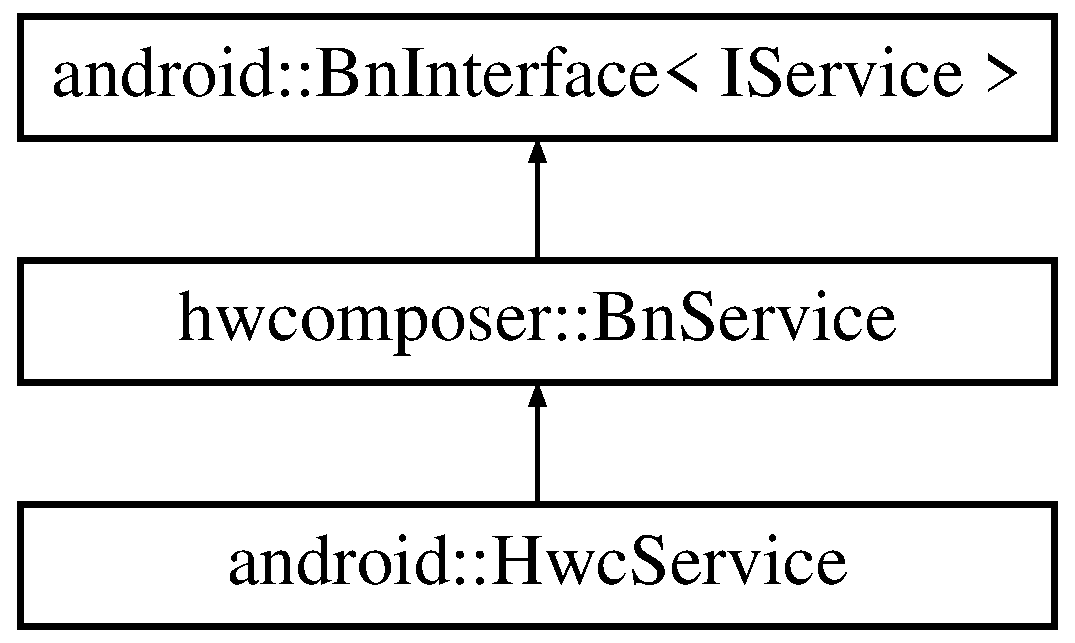
\includegraphics[height=3.000000cm]{classhwcomposer_1_1BnService}
\end{center}
\end{figure}
\subsection*{Public Member Functions}
\begin{DoxyCompactItemize}
\item 
\mbox{\hyperlink{hwcserviceapi_8h_a3806fb2027d9a316d8ca8d9b8b8eb96f}{status\+\_\+t}} \mbox{\hyperlink{classhwcomposer_1_1BnService_a75485c6ee8427b5128ebe08d42240e14}{on\+Transact}} (uint32\+\_\+t, const Parcel \&, Parcel $\ast$, uint32\+\_\+t) override
\end{DoxyCompactItemize}


\subsection{Detailed Description}


Definition at line 49 of file iservice.\+h.



\subsection{Member Function Documentation}
\mbox{\Hypertarget{classhwcomposer_1_1BnService_a75485c6ee8427b5128ebe08d42240e14}\label{classhwcomposer_1_1BnService_a75485c6ee8427b5128ebe08d42240e14}} 
\index{hwcomposer\+::\+Bn\+Service@{hwcomposer\+::\+Bn\+Service}!on\+Transact@{on\+Transact}}
\index{on\+Transact@{on\+Transact}!hwcomposer\+::\+Bn\+Service@{hwcomposer\+::\+Bn\+Service}}
\subsubsection{\texorpdfstring{on\+Transact()}{onTransact()}}
{\footnotesize\ttfamily \mbox{\hyperlink{hwcserviceapi_8h_a3806fb2027d9a316d8ca8d9b8b8eb96f}{status\+\_\+t}} hwcomposer\+::\+Bn\+Service\+::on\+Transact (\begin{DoxyParamCaption}\item[{uint32\+\_\+t}]{code,  }\item[{const Parcel \&}]{data,  }\item[{Parcel $\ast$}]{reply,  }\item[{uint32\+\_\+t}]{flags }\end{DoxyParamCaption})\hspace{0.3cm}{\ttfamily [override]}}



Definition at line 116 of file iservice.\+cpp.


\begin{DoxyCode}{0}
\DoxyCodeLine{117                                                \{}
\DoxyCodeLine{118   \textcolor{keywordflow}{switch} (code) \{}
\DoxyCodeLine{119     \textcolor{keywordflow}{case} \mbox{\hyperlink{classhwcomposer_1_1BpService_a688b4b1338923222d225a99d16e22319ac29d8afa3ded86d47e7879f814b61f0d}{BpService::GET\_HWC\_VERSION}}: \{}
\DoxyCodeLine{120       CHECK\_INTERFACE(IService, data, reply);}
\DoxyCodeLine{121       reply->writeString8(GetHwcVersion());}
\DoxyCodeLine{122       \textcolor{keywordflow}{return} NO\_ERROR;}
\DoxyCodeLine{123     \}}
\DoxyCodeLine{124 }
\DoxyCodeLine{125     \textcolor{keywordflow}{case} \mbox{\hyperlink{classhwcomposer_1_1BpService_a688b4b1338923222d225a99d16e22319a8f322cc1308b770e9cd5056d9dfefaf3}{BpService::SET\_OPTION}}: \{}
\DoxyCodeLine{126       CHECK\_INTERFACE(IService, data, reply);}
\DoxyCodeLine{127       String16 option = data.readString16();}
\DoxyCodeLine{128       String16 optionValue = data.readString16();}
\DoxyCodeLine{129       \mbox{\hyperlink{hwcserviceapi_8h_a3806fb2027d9a316d8ca8d9b8b8eb96f}{status\_t}} ret = SetOption(String8(option), String8(optionValue));}
\DoxyCodeLine{130       reply->writeInt32(ret);}
\DoxyCodeLine{131       \textcolor{keywordflow}{return} NO\_ERROR;}
\DoxyCodeLine{132     \}}
\DoxyCodeLine{133 }
\DoxyCodeLine{134     \textcolor{keywordflow}{case} \mbox{\hyperlink{classhwcomposer_1_1BpService_a688b4b1338923222d225a99d16e22319a117fba2a971fa7318d8ef74f7a84105c}{BpService::DUMP\_OPTIONS}}: \{}
\DoxyCodeLine{135       CHECK\_INTERFACE(IService, data, reply);}
\DoxyCodeLine{136       DumpOptions();}
\DoxyCodeLine{137       \textcolor{keywordflow}{return} NO\_ERROR;}
\DoxyCodeLine{138     \}}
\DoxyCodeLine{139 }
\DoxyCodeLine{140     \textcolor{keywordflow}{case} \mbox{\hyperlink{classhwcomposer_1_1BpService_a688b4b1338923222d225a99d16e22319aa6f70e3efcf110f66a046bf4d49ee999}{BpService::DISABLE\_LOG\_TO\_LOGCAT}}: \{}
\DoxyCodeLine{141       CHECK\_INTERFACE(IService, data, reply);}
\DoxyCodeLine{142       \mbox{\hyperlink{hwcserviceapi_8h_a3806fb2027d9a316d8ca8d9b8b8eb96f}{status\_t}} ret = EnableLogviewToLogcat(\textcolor{keyword}{false});}
\DoxyCodeLine{143       reply->writeInt32(ret);}
\DoxyCodeLine{144       \textcolor{keywordflow}{return} NO\_ERROR;}
\DoxyCodeLine{145     \}}
\DoxyCodeLine{146 }
\DoxyCodeLine{147     \textcolor{keywordflow}{case} \mbox{\hyperlink{classhwcomposer_1_1BpService_a688b4b1338923222d225a99d16e22319a8ec23523cde1ace78656435c40d75ca6}{BpService::ENABLE\_LOG\_TO\_LOGCAT}}: \{}
\DoxyCodeLine{148       CHECK\_INTERFACE(IService, data, reply);}
\DoxyCodeLine{149       \mbox{\hyperlink{hwcserviceapi_8h_a3806fb2027d9a316d8ca8d9b8b8eb96f}{status\_t}} ret = EnableLogviewToLogcat();}
\DoxyCodeLine{150       reply->writeInt32(ret);}
\DoxyCodeLine{151       \textcolor{keywordflow}{return} NO\_ERROR;}
\DoxyCodeLine{152     \}}
\DoxyCodeLine{153 }
\DoxyCodeLine{154     \textcolor{keywordflow}{case} \mbox{\hyperlink{classhwcomposer_1_1BpService_a688b4b1338923222d225a99d16e22319aba1101f98d0ae4dba7ae06b05fa7ecf6}{BpService::TRANSACT\_GET\_DIAGNOSTIC}}: \{}
\DoxyCodeLine{155       CHECK\_INTERFACE(IService, data, reply);}
\DoxyCodeLine{156       sp<IBinder> b = IInterface::asBinder(this->GetDiagnostic());}
\DoxyCodeLine{157       reply->writeStrongBinder(b);}
\DoxyCodeLine{158       \textcolor{keywordflow}{return} NO\_ERROR;}
\DoxyCodeLine{159     \}}
\DoxyCodeLine{160 }
\DoxyCodeLine{161     \textcolor{keywordflow}{case} \mbox{\hyperlink{classhwcomposer_1_1BpService_a688b4b1338923222d225a99d16e22319a88c048d451c725f7549727f0eb25bd11}{BpService::TRANSACT\_GET\_CONTROLS}}: \{}
\DoxyCodeLine{162       CHECK\_INTERFACE(IService, data, reply);}
\DoxyCodeLine{163       sp<IBinder> b = IInterface::asBinder(this->GetControls());}
\DoxyCodeLine{164       reply->writeStrongBinder(b);}
\DoxyCodeLine{165       \textcolor{keywordflow}{return} NO\_ERROR;}
\DoxyCodeLine{166     \}}
\DoxyCodeLine{167 }
\DoxyCodeLine{168     \textcolor{keywordflow}{default}:}
\DoxyCodeLine{169       \textcolor{keywordflow}{return} BBinder::onTransact(code, data, reply, flags);}
\DoxyCodeLine{170   \}}
\DoxyCodeLine{171 \}}
\end{DoxyCode}


The documentation for this class was generated from the following files\+:\begin{DoxyCompactItemize}
\item 
os/android/libhwcservice/\mbox{\hyperlink{iservice_8h}{iservice.\+h}}\item 
os/android/libhwcservice/\mbox{\hyperlink{iservice_8cpp}{iservice.\+cpp}}\end{DoxyCompactItemize}

\hypertarget{classhwcomposer_1_1BpControls}{}\section{hwcomposer\+:\+:Bp\+Controls Class Reference}
\label{classhwcomposer_1_1BpControls}\index{hwcomposer\+::\+Bp\+Controls@{hwcomposer\+::\+Bp\+Controls}}
Inheritance diagram for hwcomposer\+:\+:Bp\+Controls\+:\begin{figure}[H]
\begin{center}
\leavevmode
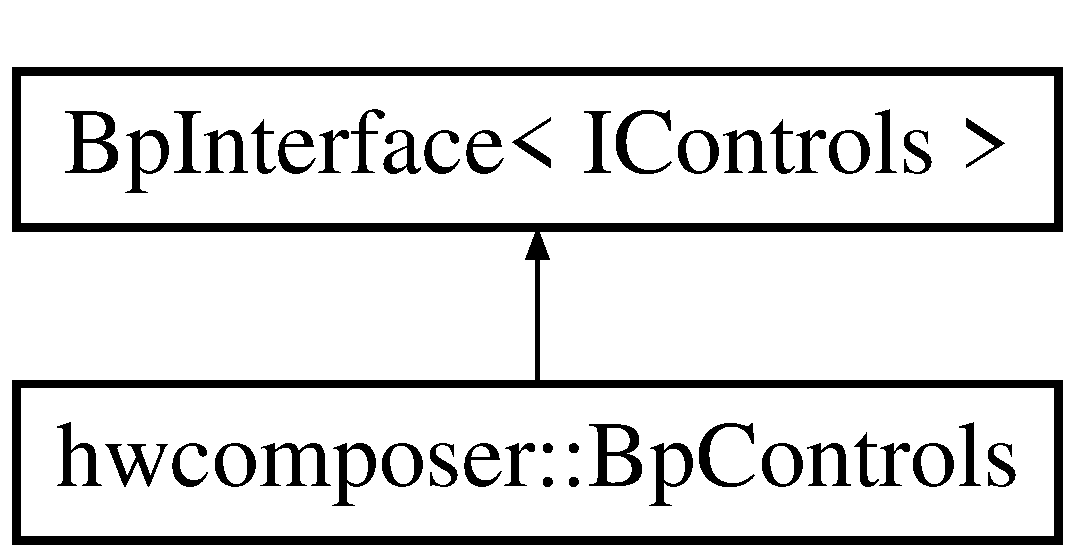
\includegraphics[height=2.000000cm]{classhwcomposer_1_1BpControls}
\end{center}
\end{figure}
\subsection*{Public Types}
\begin{DoxyCompactItemize}
\item 
enum \{ \newline
\mbox{\hyperlink{classhwcomposer_1_1BpControls_a057cb6d771c68da065640c49e3742446a985ef11557835be6b215a6b481cc8975}{T\+R\+A\+N\+S\+A\+C\+T\+\_\+\+D\+I\+S\+P\+L\+A\+Y\+\_\+\+S\+E\+T\+\_\+\+O\+V\+E\+R\+S\+C\+AN}} = I\+Binder\+:\+:F\+I\+R\+S\+T\+\_\+\+C\+A\+L\+L\+\_\+\+T\+R\+A\+N\+S\+A\+C\+T\+I\+ON, 
\mbox{\hyperlink{classhwcomposer_1_1BpControls_a057cb6d771c68da065640c49e3742446acfb53ecdb379884e8843788c2a312e8c}{T\+R\+A\+N\+S\+A\+C\+T\+\_\+\+D\+I\+S\+P\+L\+A\+Y\+\_\+\+G\+E\+T\+\_\+\+O\+V\+E\+R\+S\+C\+AN}}, 
\mbox{\hyperlink{classhwcomposer_1_1BpControls_a057cb6d771c68da065640c49e3742446acd6fb8651f02533f7f7a92d0642d9a0d}{T\+R\+A\+N\+S\+A\+C\+T\+\_\+\+D\+I\+S\+P\+L\+A\+Y\+\_\+\+S\+E\+T\+\_\+\+S\+C\+A\+L\+I\+NG}}, 
\mbox{\hyperlink{classhwcomposer_1_1BpControls_a057cb6d771c68da065640c49e3742446ad8d27d03f7cca04781cb7c481a1a91d6}{T\+R\+A\+N\+S\+A\+C\+T\+\_\+\+D\+I\+S\+P\+L\+A\+Y\+\_\+\+G\+E\+T\+\_\+\+S\+C\+A\+L\+I\+NG}}, 
\newline
\mbox{\hyperlink{classhwcomposer_1_1BpControls_a057cb6d771c68da065640c49e3742446a6623581a2b88fb17369dd632a20106d4}{T\+R\+A\+N\+S\+A\+C\+T\+\_\+\+D\+I\+S\+P\+L\+A\+Y\+\_\+\+E\+N\+A\+B\+L\+E\+\_\+\+B\+L\+A\+NK}}, 
\mbox{\hyperlink{classhwcomposer_1_1BpControls_a057cb6d771c68da065640c49e3742446a15a087c4d488f967b1293b18951a6c02}{T\+R\+A\+N\+S\+A\+C\+T\+\_\+\+D\+I\+S\+P\+L\+A\+Y\+\_\+\+R\+E\+S\+T\+O\+R\+E\+\_\+\+D\+E\+F\+A\+U\+L\+T\+\_\+\+C\+O\+L\+O\+R\+\_\+\+P\+A\+R\+AM}}, 
\mbox{\hyperlink{classhwcomposer_1_1BpControls_a057cb6d771c68da065640c49e3742446a218cf0d49257af27d4916bbcf7974e42}{T\+R\+A\+N\+S\+A\+C\+T\+\_\+\+D\+I\+S\+P\+L\+A\+Y\+\_\+\+G\+E\+T\+\_\+\+C\+O\+L\+O\+R\+\_\+\+P\+A\+R\+AM}}, 
\mbox{\hyperlink{classhwcomposer_1_1BpControls_a057cb6d771c68da065640c49e3742446a02754bed54f3e948595d365863e6ff6c}{T\+R\+A\+N\+S\+A\+C\+T\+\_\+\+D\+I\+S\+P\+L\+A\+Y\+\_\+\+S\+E\+T\+\_\+\+C\+O\+L\+O\+R\+\_\+\+P\+A\+R\+AM}}, 
\newline
\mbox{\hyperlink{classhwcomposer_1_1BpControls_a057cb6d771c68da065640c49e3742446a32c72f6f1679760b231c841184d5420d}{T\+R\+A\+N\+S\+A\+C\+T\+\_\+\+D\+I\+S\+P\+L\+A\+Y\+\_\+\+S\+E\+T\+\_\+\+D\+E\+I\+N\+T\+E\+R\+L\+A\+C\+E\+\_\+\+P\+A\+R\+AM}}, 
\mbox{\hyperlink{classhwcomposer_1_1BpControls_a057cb6d771c68da065640c49e3742446a481d6c71408ba43adf692d5e11aa7fd7}{T\+R\+A\+N\+S\+A\+C\+T\+\_\+\+D\+I\+S\+P\+L\+A\+Y\+\_\+\+R\+E\+S\+T\+O\+R\+E\+\_\+\+D\+E\+F\+A\+U\+L\+T\+\_\+\+D\+E\+I\+N\+T\+E\+R\+L\+A\+C\+E\+\_\+\+P\+A\+R\+AM}}, 
\mbox{\hyperlink{classhwcomposer_1_1BpControls_a057cb6d771c68da065640c49e3742446a23ea2de5ee0482714e828cdfe3b78eb6}{T\+R\+A\+N\+S\+A\+C\+T\+\_\+\+D\+I\+S\+P\+L\+A\+Y\+M\+O\+D\+E\+\_\+\+G\+E\+T\+\_\+\+A\+V\+A\+I\+L\+A\+B\+L\+E\+\_\+\+M\+O\+D\+ES}}, 
\mbox{\hyperlink{classhwcomposer_1_1BpControls_a057cb6d771c68da065640c49e3742446afd0d6093faf175dc1c13e25789063f3e}{T\+R\+A\+N\+S\+A\+C\+T\+\_\+\+D\+I\+S\+P\+L\+A\+Y\+M\+O\+D\+E\+\_\+\+G\+E\+T\+\_\+\+M\+O\+DE}}, 
\newline
\mbox{\hyperlink{classhwcomposer_1_1BpControls_a057cb6d771c68da065640c49e3742446a62999b5eadacd5213c222e8efe03dda4}{T\+R\+A\+N\+S\+A\+C\+T\+\_\+\+D\+I\+S\+P\+L\+A\+Y\+M\+O\+D\+E\+\_\+\+S\+E\+T\+\_\+\+M\+O\+DE}}, 
\mbox{\hyperlink{classhwcomposer_1_1BpControls_a057cb6d771c68da065640c49e3742446a6482e9c31b42e7a8a101b55e059a260a}{T\+R\+A\+N\+S\+A\+C\+T\+\_\+\+V\+I\+D\+E\+O\+\_\+\+E\+N\+A\+B\+L\+E\+\_\+\+H\+D\+C\+P\+\_\+\+S\+E\+S\+S\+I\+O\+N\+\_\+\+F\+O\+R\+\_\+\+D\+I\+S\+P\+L\+AY}}, 
\mbox{\hyperlink{classhwcomposer_1_1BpControls_a057cb6d771c68da065640c49e3742446acaf7406d1c2bbedb4253ce81685ca811}{T\+R\+A\+N\+S\+A\+C\+T\+\_\+\+V\+I\+D\+E\+O\+\_\+\+E\+N\+A\+B\+L\+E\+\_\+\+H\+D\+C\+P\+\_\+\+S\+E\+S\+S\+I\+O\+N\+\_\+\+F\+O\+R\+\_\+\+A\+L\+L\+\_\+\+D\+I\+S\+P\+L\+A\+YS}}, 
\mbox{\hyperlink{classhwcomposer_1_1BpControls_a057cb6d771c68da065640c49e3742446a3772d2ac2fc50e3b393733c14f95e536}{T\+R\+A\+N\+S\+A\+C\+T\+\_\+\+V\+I\+D\+E\+O\+\_\+\+D\+I\+S\+A\+B\+L\+E\+\_\+\+H\+D\+C\+P\+\_\+\+S\+E\+S\+S\+I\+O\+N\+\_\+\+F\+O\+R\+\_\+\+D\+I\+S\+P\+L\+AY}}, 
\newline
\mbox{\hyperlink{classhwcomposer_1_1BpControls_a057cb6d771c68da065640c49e3742446a7afcde053a8bef100088bae91dbb2620}{T\+R\+A\+N\+S\+A\+C\+T\+\_\+\+V\+I\+D\+E\+O\+\_\+\+D\+I\+S\+A\+B\+L\+E\+\_\+\+H\+D\+C\+P\+\_\+\+S\+E\+S\+S\+I\+O\+N\+\_\+\+F\+O\+R\+\_\+\+A\+L\+L\+\_\+\+D\+I\+S\+P\+L\+A\+YS}}, 
\mbox{\hyperlink{classhwcomposer_1_1BpControls_a057cb6d771c68da065640c49e3742446ac6559374237fdc63c299a2964bdbe9d7}{T\+R\+A\+N\+S\+A\+C\+T\+\_\+\+V\+I\+D\+E\+O\+\_\+\+E\+N\+A\+B\+L\+E\+\_\+\+E\+N\+C\+R\+Y\+P\+T\+E\+D\+\_\+\+S\+E\+S\+S\+I\+ON}}, 
\mbox{\hyperlink{classhwcomposer_1_1BpControls_a057cb6d771c68da065640c49e3742446aaa215b4cc5192668f648d2f90962f582}{T\+R\+A\+N\+S\+A\+C\+T\+\_\+\+V\+I\+D\+E\+O\+\_\+\+D\+I\+S\+A\+B\+L\+E\+\_\+\+E\+N\+C\+R\+Y\+P\+T\+E\+D\+\_\+\+S\+E\+S\+S\+I\+ON}}, 
\mbox{\hyperlink{classhwcomposer_1_1BpControls_a057cb6d771c68da065640c49e3742446a5ef49fd58989fb5029472668414f9140}{T\+R\+A\+N\+S\+A\+C\+T\+\_\+\+V\+I\+D\+E\+O\+\_\+\+D\+I\+S\+A\+B\+L\+E\+\_\+\+A\+L\+L\+\_\+\+E\+N\+C\+R\+Y\+P\+T\+E\+D\+\_\+\+S\+E\+S\+S\+I\+O\+NS}}, 
\newline
\mbox{\hyperlink{classhwcomposer_1_1BpControls_a057cb6d771c68da065640c49e3742446a83e8e51e9f0eaa3b99c1fbe7486875ec}{T\+R\+A\+N\+S\+A\+C\+T\+\_\+\+V\+I\+D\+E\+O\+\_\+\+I\+S\+\_\+\+E\+N\+C\+R\+Y\+P\+T\+E\+D\+\_\+\+S\+E\+S\+S\+I\+O\+N\+\_\+\+E\+N\+A\+B\+L\+ED}}, 
\mbox{\hyperlink{classhwcomposer_1_1BpControls_a057cb6d771c68da065640c49e3742446a2dc60d5ba78113e4cad0c7d70be98a8e}{T\+R\+A\+N\+S\+A\+C\+T\+\_\+\+V\+I\+D\+E\+O\+\_\+\+S\+E\+T\+\_\+\+O\+P\+T\+I\+M\+I\+Z\+A\+T\+I\+O\+N\+\_\+\+M\+O\+DE}}, 
\mbox{\hyperlink{classhwcomposer_1_1BpControls_a057cb6d771c68da065640c49e3742446ae58d81883fb4d1137f4f8b9222b93f95}{T\+R\+A\+N\+S\+A\+C\+T\+\_\+\+M\+D\+S\+\_\+\+U\+P\+D\+A\+T\+E\+\_\+\+V\+I\+D\+E\+O\+\_\+\+S\+T\+A\+TE}}, 
\mbox{\hyperlink{classhwcomposer_1_1BpControls_a057cb6d771c68da065640c49e3742446aed219d26b586c56400fb6ff87d4b7b12}{T\+R\+A\+N\+S\+A\+C\+T\+\_\+\+M\+D\+S\+\_\+\+U\+P\+D\+A\+T\+E\+\_\+\+V\+I\+D\+E\+O\+\_\+\+F\+PS}}, 
\newline
\mbox{\hyperlink{classhwcomposer_1_1BpControls_a057cb6d771c68da065640c49e3742446a9c89c90c56c8ad69f11b9131ac2e8b00}{T\+R\+A\+N\+S\+A\+C\+T\+\_\+\+M\+D\+S\+\_\+\+U\+P\+D\+A\+T\+E\+\_\+\+I\+N\+P\+U\+T\+\_\+\+S\+T\+A\+TE}}, 
\mbox{\hyperlink{classhwcomposer_1_1BpControls_a057cb6d771c68da065640c49e3742446ac0896efafd9de075b9d33ae5ea916ae9}{T\+R\+A\+N\+S\+A\+C\+T\+\_\+\+W\+I\+D\+I\+\_\+\+G\+E\+T\+\_\+\+S\+I\+N\+G\+L\+E\+\_\+\+D\+I\+S\+P\+L\+AY}}, 
\mbox{\hyperlink{classhwcomposer_1_1BpControls_a057cb6d771c68da065640c49e3742446aba0ea7b08d69c3018e5dc0017a14390a}{T\+R\+A\+N\+S\+A\+C\+T\+\_\+\+W\+I\+D\+I\+\_\+\+S\+E\+T\+\_\+\+S\+I\+N\+G\+L\+E\+\_\+\+D\+I\+S\+P\+L\+AY}}
 \}
\end{DoxyCompactItemize}
\subsection*{Public Member Functions}
\begin{DoxyCompactItemize}
\item 
\mbox{\hyperlink{classhwcomposer_1_1BpControls_aa9a4edb8ba490a14b4c26740ed3e7848}{Bp\+Controls}} (const sp$<$ I\+Binder $>$ \&impl)
\item 
\mbox{\hyperlink{hwcserviceapi_8h_a3806fb2027d9a316d8ca8d9b8b8eb96f}{status\+\_\+t}} \mbox{\hyperlink{classhwcomposer_1_1BpControls_a81afe3b4e34a3563d3ab443bf491dddb}{Display\+Set\+Overscan}} (uint32\+\_\+t display, int32\+\_\+t xoverscan, int32\+\_\+t yoverscan) override
\item 
\mbox{\hyperlink{hwcserviceapi_8h_a3806fb2027d9a316d8ca8d9b8b8eb96f}{status\+\_\+t}} \mbox{\hyperlink{classhwcomposer_1_1BpControls_a3ecd92e50b486c09983d256a06b351c9}{Display\+Get\+Overscan}} (uint32\+\_\+t display, int32\+\_\+t $\ast$xoverscan, int32\+\_\+t $\ast$yoverscan) override
\item 
\mbox{\hyperlink{hwcserviceapi_8h_a3806fb2027d9a316d8ca8d9b8b8eb96f}{status\+\_\+t}} \mbox{\hyperlink{classhwcomposer_1_1BpControls_a164e8b00e9f1f58a80c587730d6d7496}{Display\+Set\+Scaling}} (uint32\+\_\+t display, \mbox{\hyperlink{hwcserviceapi_8h_acdadfd5e7f15097833789174e442083f}{E\+Hwcs\+Scaling\+Mode}} e\+Scaling\+Mode) override
\item 
\mbox{\hyperlink{hwcserviceapi_8h_a3806fb2027d9a316d8ca8d9b8b8eb96f}{status\+\_\+t}} \mbox{\hyperlink{classhwcomposer_1_1BpControls_a6778298503ceca305bf7b7a1e03a348f}{Display\+Get\+Scaling}} (uint32\+\_\+t display, \mbox{\hyperlink{hwcserviceapi_8h_acdadfd5e7f15097833789174e442083f}{E\+Hwcs\+Scaling\+Mode}} $\ast$e\+Scaling\+Mode) override
\item 
\mbox{\hyperlink{hwcserviceapi_8h_a3806fb2027d9a316d8ca8d9b8b8eb96f}{status\+\_\+t}} \mbox{\hyperlink{classhwcomposer_1_1BpControls_a7aa90940406d64dd634f21e81534725d}{Display\+Enable\+Blank}} (uint32\+\_\+t display, bool blank) override
\item 
\mbox{\hyperlink{hwcserviceapi_8h_a3806fb2027d9a316d8ca8d9b8b8eb96f}{status\+\_\+t}} \mbox{\hyperlink{classhwcomposer_1_1BpControls_a474fc42bfc7e439c79422d41d970a616}{Display\+Restore\+Default\+Color\+Param}} (uint32\+\_\+t display, \mbox{\hyperlink{hwcserviceapi_8h_a1d1cbf448ce748672cf3dd96675d70e4}{E\+Hwcs\+Color\+Control}} color) override
\item 
\mbox{\hyperlink{hwcserviceapi_8h_a3806fb2027d9a316d8ca8d9b8b8eb96f}{status\+\_\+t}} \mbox{\hyperlink{classhwcomposer_1_1BpControls_a2da4ebdc65178ec384f5f71d90b1c5fa}{Display\+Restore\+Default\+Deinterlace\+Param}} (uint32\+\_\+t display) override
\item 
\mbox{\hyperlink{hwcserviceapi_8h_a3806fb2027d9a316d8ca8d9b8b8eb96f}{status\+\_\+t}} \mbox{\hyperlink{classhwcomposer_1_1BpControls_a9946715d7fa9454b859013dff01b0576}{Display\+Get\+Color\+Param}} (uint32\+\_\+t display, \mbox{\hyperlink{hwcserviceapi_8h_a1d1cbf448ce748672cf3dd96675d70e4}{E\+Hwcs\+Color\+Control}} color, float $\ast$value, float $\ast$startvalue, float $\ast$endvalue) override
\item 
\mbox{\hyperlink{hwcserviceapi_8h_a3806fb2027d9a316d8ca8d9b8b8eb96f}{status\+\_\+t}} \mbox{\hyperlink{classhwcomposer_1_1BpControls_a511db753c15bac20e7390f034b454065}{Display\+Set\+Color\+Param}} (uint32\+\_\+t display, \mbox{\hyperlink{hwcserviceapi_8h_a1d1cbf448ce748672cf3dd96675d70e4}{E\+Hwcs\+Color\+Control}} color, float value) override
\item 
\mbox{\hyperlink{hwcserviceapi_8h_a3806fb2027d9a316d8ca8d9b8b8eb96f}{status\+\_\+t}} \mbox{\hyperlink{classhwcomposer_1_1BpControls_ab21dbe5b9f8e5979685083f294631c5e}{Display\+Set\+Deinterlace\+Param}} (uint32\+\_\+t display, \mbox{\hyperlink{hwcserviceapi_8h_a8473f2ec9e7333e67be46a1bea689113}{E\+Hwcs\+Deinterlace\+Control}} mode) override
\item 
std\+::vector$<$ \mbox{\hyperlink{hwcserviceapi_8h_a6e13f5285374b86aab82ec0c0ba62d7a}{Hwcs\+Display\+Mode\+Info}} $>$ \mbox{\hyperlink{classhwcomposer_1_1BpControls_aa5169400479ae6bda2d2fc3168a521f2}{Display\+Mode\+Get\+Available\+Modes}} (uint32\+\_\+t display) override
\item 
\mbox{\hyperlink{hwcserviceapi_8h_a3806fb2027d9a316d8ca8d9b8b8eb96f}{status\+\_\+t}} \mbox{\hyperlink{classhwcomposer_1_1BpControls_a28f71e7f95593a9e9302d260dba810fa}{Display\+Mode\+Get\+Mode}} (uint32\+\_\+t display, \mbox{\hyperlink{hwcserviceapi_8h_a6e13f5285374b86aab82ec0c0ba62d7a}{Hwcs\+Display\+Mode\+Info}} $\ast$p\+Mode) override
\item 
\mbox{\hyperlink{hwcserviceapi_8h_a3806fb2027d9a316d8ca8d9b8b8eb96f}{status\+\_\+t}} \mbox{\hyperlink{classhwcomposer_1_1BpControls_a1bb5b34015941a5d5d76cdc57a889110}{Display\+Mode\+Set\+Mode}} (uint32\+\_\+t display, const uint32\+\_\+t config) override
\item 
\mbox{\hyperlink{hwcserviceapi_8h_a3806fb2027d9a316d8ca8d9b8b8eb96f}{status\+\_\+t}} \mbox{\hyperlink{classhwcomposer_1_1BpControls_a38c36098ef3251a0c396530b9c33c3e4}{Enable\+H\+D\+C\+P\+Session\+For\+Display}} (uint32\+\_\+t display, \mbox{\hyperlink{hwcserviceapi_8h_a69e9b3a54e4c8e504845398c66eab655}{E\+Hwcs\+Content\+Type}} content\+\_\+type)
\item 
\mbox{\hyperlink{hwcserviceapi_8h_a3806fb2027d9a316d8ca8d9b8b8eb96f}{status\+\_\+t}} \mbox{\hyperlink{classhwcomposer_1_1BpControls_a2dd503c471873b1aae313a4d0b923ece}{Enable\+H\+D\+C\+P\+Session\+For\+All\+Displays}} (\mbox{\hyperlink{hwcserviceapi_8h_a69e9b3a54e4c8e504845398c66eab655}{E\+Hwcs\+Content\+Type}} content\+\_\+type)
\item 
\mbox{\hyperlink{hwcserviceapi_8h_a3806fb2027d9a316d8ca8d9b8b8eb96f}{status\+\_\+t}} \mbox{\hyperlink{classhwcomposer_1_1BpControls_a0a31e50e1213e86bb6737d929fe06170}{Disable\+H\+D\+C\+P\+Session\+For\+Display}} (uint32\+\_\+t display)
\item 
\mbox{\hyperlink{hwcserviceapi_8h_a3806fb2027d9a316d8ca8d9b8b8eb96f}{status\+\_\+t}} \mbox{\hyperlink{classhwcomposer_1_1BpControls_a7ab7f839df5c6e56bbe82a91c0b6e5c2}{Disable\+H\+D\+C\+P\+Session\+For\+All\+Displays}} ()
\item 
\mbox{\hyperlink{hwcserviceapi_8h_a3806fb2027d9a316d8ca8d9b8b8eb96f}{status\+\_\+t}} \mbox{\hyperlink{classhwcomposer_1_1BpControls_a108c7339e8405ba05e71dacbd09873ad}{Video\+Enable\+Encrypted\+Session}} (uint32\+\_\+t session\+ID, uint32\+\_\+t instance\+ID) override
\item 
\mbox{\hyperlink{hwcserviceapi_8h_a3806fb2027d9a316d8ca8d9b8b8eb96f}{status\+\_\+t}} \mbox{\hyperlink{classhwcomposer_1_1BpControls_a6de03491836ce5216983fbd2c68c10fc}{Video\+Disable\+All\+Encrypted\+Sessions}} (uint32\+\_\+t session\+ID) override
\item 
\mbox{\hyperlink{hwcserviceapi_8h_a3806fb2027d9a316d8ca8d9b8b8eb96f}{status\+\_\+t}} \mbox{\hyperlink{classhwcomposer_1_1BpControls_afece8428dda4cdcb2cde67652ee5913d}{Video\+Disable\+All\+Encrypted\+Sessions}} () override
\item 
bool \mbox{\hyperlink{classhwcomposer_1_1BpControls_a9dba61bf0300c425989f727792626c9a}{Video\+Is\+Encrypted\+Session\+Enabled}} (uint32\+\_\+t session\+ID, uint32\+\_\+t instance\+ID) override
\item 
\mbox{\hyperlink{hwcserviceapi_8h_a3806fb2027d9a316d8ca8d9b8b8eb96f}{status\+\_\+t}} \mbox{\hyperlink{classhwcomposer_1_1BpControls_a1bcd10d109be05687f174905140da789}{Video\+Set\+Optimization\+Mode}} (\mbox{\hyperlink{hwcserviceapi_8h_a73044de23b8f474352d6753e21fca06d}{E\+Hwcs\+Optimization\+Mode}} mode) override
\item 
\mbox{\hyperlink{hwcserviceapi_8h_a3806fb2027d9a316d8ca8d9b8b8eb96f}{status\+\_\+t}} \mbox{\hyperlink{classhwcomposer_1_1BpControls_a660d3860d1631b9243996cb53fbaca39}{Mds\+Update\+Video\+State}} (int64\+\_\+t video\+Session\+ID, bool is\+Prepared) override
\item 
\mbox{\hyperlink{hwcserviceapi_8h_a3806fb2027d9a316d8ca8d9b8b8eb96f}{status\+\_\+t}} \mbox{\hyperlink{classhwcomposer_1_1BpControls_ac8f84bc4b1b6d2be29d9a1c6ccd7c587}{Mds\+Update\+Video\+F\+PS}} (int64\+\_\+t video\+Session\+ID, int32\+\_\+t fps) override
\item 
\mbox{\hyperlink{hwcserviceapi_8h_a3806fb2027d9a316d8ca8d9b8b8eb96f}{status\+\_\+t}} \mbox{\hyperlink{classhwcomposer_1_1BpControls_a382ea9f3e8eb74b555a7997820b0bffb}{Mds\+Update\+Input\+State}} (bool state) override
\item 
\mbox{\hyperlink{hwcserviceapi_8h_a3806fb2027d9a316d8ca8d9b8b8eb96f}{status\+\_\+t}} \mbox{\hyperlink{classhwcomposer_1_1BpControls_a1eddda7462f1a6c37a523e5a8f7a3d30}{Widi\+Get\+Single\+Display}} (bool $\ast$p\+Enabled) override
\item 
\mbox{\hyperlink{hwcserviceapi_8h_a3806fb2027d9a316d8ca8d9b8b8eb96f}{status\+\_\+t}} \mbox{\hyperlink{classhwcomposer_1_1BpControls_a8165eda3de769d8cb703bf25ca21e0d0}{Widi\+Set\+Single\+Display}} (bool enable) override
\end{DoxyCompactItemize}


\subsection{Detailed Description}


Definition at line 31 of file icontrols.\+cpp.



\subsection{Member Enumeration Documentation}
\mbox{\Hypertarget{classhwcomposer_1_1BpControls_a057cb6d771c68da065640c49e3742446}\label{classhwcomposer_1_1BpControls_a057cb6d771c68da065640c49e3742446}} 
\subsubsection{\texorpdfstring{anonymous enum}{anonymous enum}}
{\footnotesize\ttfamily anonymous enum}

\begin{DoxyEnumFields}{Enumerator}
\raisebox{\heightof{T}}[0pt][0pt]{\index{T\+R\+A\+N\+S\+A\+C\+T\+\_\+\+D\+I\+S\+P\+L\+A\+Y\+\_\+\+S\+E\+T\+\_\+\+O\+V\+E\+R\+S\+C\+AN@{T\+R\+A\+N\+S\+A\+C\+T\+\_\+\+D\+I\+S\+P\+L\+A\+Y\+\_\+\+S\+E\+T\+\_\+\+O\+V\+E\+R\+S\+C\+AN}!hwcomposer\+::\+Bp\+Controls@{hwcomposer\+::\+Bp\+Controls}}\index{hwcomposer\+::\+Bp\+Controls@{hwcomposer\+::\+Bp\+Controls}!T\+R\+A\+N\+S\+A\+C\+T\+\_\+\+D\+I\+S\+P\+L\+A\+Y\+\_\+\+S\+E\+T\+\_\+\+O\+V\+E\+R\+S\+C\+AN@{T\+R\+A\+N\+S\+A\+C\+T\+\_\+\+D\+I\+S\+P\+L\+A\+Y\+\_\+\+S\+E\+T\+\_\+\+O\+V\+E\+R\+S\+C\+AN}}}\mbox{\Hypertarget{classhwcomposer_1_1BpControls_a057cb6d771c68da065640c49e3742446a985ef11557835be6b215a6b481cc8975}\label{classhwcomposer_1_1BpControls_a057cb6d771c68da065640c49e3742446a985ef11557835be6b215a6b481cc8975}} 
T\+R\+A\+N\+S\+A\+C\+T\+\_\+\+D\+I\+S\+P\+L\+A\+Y\+\_\+\+S\+E\+T\+\_\+\+O\+V\+E\+R\+S\+C\+AN&\\
\hline

\raisebox{\heightof{T}}[0pt][0pt]{\index{T\+R\+A\+N\+S\+A\+C\+T\+\_\+\+D\+I\+S\+P\+L\+A\+Y\+\_\+\+G\+E\+T\+\_\+\+O\+V\+E\+R\+S\+C\+AN@{T\+R\+A\+N\+S\+A\+C\+T\+\_\+\+D\+I\+S\+P\+L\+A\+Y\+\_\+\+G\+E\+T\+\_\+\+O\+V\+E\+R\+S\+C\+AN}!hwcomposer\+::\+Bp\+Controls@{hwcomposer\+::\+Bp\+Controls}}\index{hwcomposer\+::\+Bp\+Controls@{hwcomposer\+::\+Bp\+Controls}!T\+R\+A\+N\+S\+A\+C\+T\+\_\+\+D\+I\+S\+P\+L\+A\+Y\+\_\+\+G\+E\+T\+\_\+\+O\+V\+E\+R\+S\+C\+AN@{T\+R\+A\+N\+S\+A\+C\+T\+\_\+\+D\+I\+S\+P\+L\+A\+Y\+\_\+\+G\+E\+T\+\_\+\+O\+V\+E\+R\+S\+C\+AN}}}\mbox{\Hypertarget{classhwcomposer_1_1BpControls_a057cb6d771c68da065640c49e3742446acfb53ecdb379884e8843788c2a312e8c}\label{classhwcomposer_1_1BpControls_a057cb6d771c68da065640c49e3742446acfb53ecdb379884e8843788c2a312e8c}} 
T\+R\+A\+N\+S\+A\+C\+T\+\_\+\+D\+I\+S\+P\+L\+A\+Y\+\_\+\+G\+E\+T\+\_\+\+O\+V\+E\+R\+S\+C\+AN&\\
\hline

\raisebox{\heightof{T}}[0pt][0pt]{\index{T\+R\+A\+N\+S\+A\+C\+T\+\_\+\+D\+I\+S\+P\+L\+A\+Y\+\_\+\+S\+E\+T\+\_\+\+S\+C\+A\+L\+I\+NG@{T\+R\+A\+N\+S\+A\+C\+T\+\_\+\+D\+I\+S\+P\+L\+A\+Y\+\_\+\+S\+E\+T\+\_\+\+S\+C\+A\+L\+I\+NG}!hwcomposer\+::\+Bp\+Controls@{hwcomposer\+::\+Bp\+Controls}}\index{hwcomposer\+::\+Bp\+Controls@{hwcomposer\+::\+Bp\+Controls}!T\+R\+A\+N\+S\+A\+C\+T\+\_\+\+D\+I\+S\+P\+L\+A\+Y\+\_\+\+S\+E\+T\+\_\+\+S\+C\+A\+L\+I\+NG@{T\+R\+A\+N\+S\+A\+C\+T\+\_\+\+D\+I\+S\+P\+L\+A\+Y\+\_\+\+S\+E\+T\+\_\+\+S\+C\+A\+L\+I\+NG}}}\mbox{\Hypertarget{classhwcomposer_1_1BpControls_a057cb6d771c68da065640c49e3742446acd6fb8651f02533f7f7a92d0642d9a0d}\label{classhwcomposer_1_1BpControls_a057cb6d771c68da065640c49e3742446acd6fb8651f02533f7f7a92d0642d9a0d}} 
T\+R\+A\+N\+S\+A\+C\+T\+\_\+\+D\+I\+S\+P\+L\+A\+Y\+\_\+\+S\+E\+T\+\_\+\+S\+C\+A\+L\+I\+NG&\\
\hline

\raisebox{\heightof{T}}[0pt][0pt]{\index{T\+R\+A\+N\+S\+A\+C\+T\+\_\+\+D\+I\+S\+P\+L\+A\+Y\+\_\+\+G\+E\+T\+\_\+\+S\+C\+A\+L\+I\+NG@{T\+R\+A\+N\+S\+A\+C\+T\+\_\+\+D\+I\+S\+P\+L\+A\+Y\+\_\+\+G\+E\+T\+\_\+\+S\+C\+A\+L\+I\+NG}!hwcomposer\+::\+Bp\+Controls@{hwcomposer\+::\+Bp\+Controls}}\index{hwcomposer\+::\+Bp\+Controls@{hwcomposer\+::\+Bp\+Controls}!T\+R\+A\+N\+S\+A\+C\+T\+\_\+\+D\+I\+S\+P\+L\+A\+Y\+\_\+\+G\+E\+T\+\_\+\+S\+C\+A\+L\+I\+NG@{T\+R\+A\+N\+S\+A\+C\+T\+\_\+\+D\+I\+S\+P\+L\+A\+Y\+\_\+\+G\+E\+T\+\_\+\+S\+C\+A\+L\+I\+NG}}}\mbox{\Hypertarget{classhwcomposer_1_1BpControls_a057cb6d771c68da065640c49e3742446ad8d27d03f7cca04781cb7c481a1a91d6}\label{classhwcomposer_1_1BpControls_a057cb6d771c68da065640c49e3742446ad8d27d03f7cca04781cb7c481a1a91d6}} 
T\+R\+A\+N\+S\+A\+C\+T\+\_\+\+D\+I\+S\+P\+L\+A\+Y\+\_\+\+G\+E\+T\+\_\+\+S\+C\+A\+L\+I\+NG&\\
\hline

\raisebox{\heightof{T}}[0pt][0pt]{\index{T\+R\+A\+N\+S\+A\+C\+T\+\_\+\+D\+I\+S\+P\+L\+A\+Y\+\_\+\+E\+N\+A\+B\+L\+E\+\_\+\+B\+L\+A\+NK@{T\+R\+A\+N\+S\+A\+C\+T\+\_\+\+D\+I\+S\+P\+L\+A\+Y\+\_\+\+E\+N\+A\+B\+L\+E\+\_\+\+B\+L\+A\+NK}!hwcomposer\+::\+Bp\+Controls@{hwcomposer\+::\+Bp\+Controls}}\index{hwcomposer\+::\+Bp\+Controls@{hwcomposer\+::\+Bp\+Controls}!T\+R\+A\+N\+S\+A\+C\+T\+\_\+\+D\+I\+S\+P\+L\+A\+Y\+\_\+\+E\+N\+A\+B\+L\+E\+\_\+\+B\+L\+A\+NK@{T\+R\+A\+N\+S\+A\+C\+T\+\_\+\+D\+I\+S\+P\+L\+A\+Y\+\_\+\+E\+N\+A\+B\+L\+E\+\_\+\+B\+L\+A\+NK}}}\mbox{\Hypertarget{classhwcomposer_1_1BpControls_a057cb6d771c68da065640c49e3742446a6623581a2b88fb17369dd632a20106d4}\label{classhwcomposer_1_1BpControls_a057cb6d771c68da065640c49e3742446a6623581a2b88fb17369dd632a20106d4}} 
T\+R\+A\+N\+S\+A\+C\+T\+\_\+\+D\+I\+S\+P\+L\+A\+Y\+\_\+\+E\+N\+A\+B\+L\+E\+\_\+\+B\+L\+A\+NK&\\
\hline

\raisebox{\heightof{T}}[0pt][0pt]{\index{T\+R\+A\+N\+S\+A\+C\+T\+\_\+\+D\+I\+S\+P\+L\+A\+Y\+\_\+\+R\+E\+S\+T\+O\+R\+E\+\_\+\+D\+E\+F\+A\+U\+L\+T\+\_\+\+C\+O\+L\+O\+R\+\_\+\+P\+A\+R\+AM@{T\+R\+A\+N\+S\+A\+C\+T\+\_\+\+D\+I\+S\+P\+L\+A\+Y\+\_\+\+R\+E\+S\+T\+O\+R\+E\+\_\+\+D\+E\+F\+A\+U\+L\+T\+\_\+\+C\+O\+L\+O\+R\+\_\+\+P\+A\+R\+AM}!hwcomposer\+::\+Bp\+Controls@{hwcomposer\+::\+Bp\+Controls}}\index{hwcomposer\+::\+Bp\+Controls@{hwcomposer\+::\+Bp\+Controls}!T\+R\+A\+N\+S\+A\+C\+T\+\_\+\+D\+I\+S\+P\+L\+A\+Y\+\_\+\+R\+E\+S\+T\+O\+R\+E\+\_\+\+D\+E\+F\+A\+U\+L\+T\+\_\+\+C\+O\+L\+O\+R\+\_\+\+P\+A\+R\+AM@{T\+R\+A\+N\+S\+A\+C\+T\+\_\+\+D\+I\+S\+P\+L\+A\+Y\+\_\+\+R\+E\+S\+T\+O\+R\+E\+\_\+\+D\+E\+F\+A\+U\+L\+T\+\_\+\+C\+O\+L\+O\+R\+\_\+\+P\+A\+R\+AM}}}\mbox{\Hypertarget{classhwcomposer_1_1BpControls_a057cb6d771c68da065640c49e3742446a15a087c4d488f967b1293b18951a6c02}\label{classhwcomposer_1_1BpControls_a057cb6d771c68da065640c49e3742446a15a087c4d488f967b1293b18951a6c02}} 
T\+R\+A\+N\+S\+A\+C\+T\+\_\+\+D\+I\+S\+P\+L\+A\+Y\+\_\+\+R\+E\+S\+T\+O\+R\+E\+\_\+\+D\+E\+F\+A\+U\+L\+T\+\_\+\+C\+O\+L\+O\+R\+\_\+\+P\+A\+R\+AM&\\
\hline

\raisebox{\heightof{T}}[0pt][0pt]{\index{T\+R\+A\+N\+S\+A\+C\+T\+\_\+\+D\+I\+S\+P\+L\+A\+Y\+\_\+\+G\+E\+T\+\_\+\+C\+O\+L\+O\+R\+\_\+\+P\+A\+R\+AM@{T\+R\+A\+N\+S\+A\+C\+T\+\_\+\+D\+I\+S\+P\+L\+A\+Y\+\_\+\+G\+E\+T\+\_\+\+C\+O\+L\+O\+R\+\_\+\+P\+A\+R\+AM}!hwcomposer\+::\+Bp\+Controls@{hwcomposer\+::\+Bp\+Controls}}\index{hwcomposer\+::\+Bp\+Controls@{hwcomposer\+::\+Bp\+Controls}!T\+R\+A\+N\+S\+A\+C\+T\+\_\+\+D\+I\+S\+P\+L\+A\+Y\+\_\+\+G\+E\+T\+\_\+\+C\+O\+L\+O\+R\+\_\+\+P\+A\+R\+AM@{T\+R\+A\+N\+S\+A\+C\+T\+\_\+\+D\+I\+S\+P\+L\+A\+Y\+\_\+\+G\+E\+T\+\_\+\+C\+O\+L\+O\+R\+\_\+\+P\+A\+R\+AM}}}\mbox{\Hypertarget{classhwcomposer_1_1BpControls_a057cb6d771c68da065640c49e3742446a218cf0d49257af27d4916bbcf7974e42}\label{classhwcomposer_1_1BpControls_a057cb6d771c68da065640c49e3742446a218cf0d49257af27d4916bbcf7974e42}} 
T\+R\+A\+N\+S\+A\+C\+T\+\_\+\+D\+I\+S\+P\+L\+A\+Y\+\_\+\+G\+E\+T\+\_\+\+C\+O\+L\+O\+R\+\_\+\+P\+A\+R\+AM&\\
\hline

\raisebox{\heightof{T}}[0pt][0pt]{\index{T\+R\+A\+N\+S\+A\+C\+T\+\_\+\+D\+I\+S\+P\+L\+A\+Y\+\_\+\+S\+E\+T\+\_\+\+C\+O\+L\+O\+R\+\_\+\+P\+A\+R\+AM@{T\+R\+A\+N\+S\+A\+C\+T\+\_\+\+D\+I\+S\+P\+L\+A\+Y\+\_\+\+S\+E\+T\+\_\+\+C\+O\+L\+O\+R\+\_\+\+P\+A\+R\+AM}!hwcomposer\+::\+Bp\+Controls@{hwcomposer\+::\+Bp\+Controls}}\index{hwcomposer\+::\+Bp\+Controls@{hwcomposer\+::\+Bp\+Controls}!T\+R\+A\+N\+S\+A\+C\+T\+\_\+\+D\+I\+S\+P\+L\+A\+Y\+\_\+\+S\+E\+T\+\_\+\+C\+O\+L\+O\+R\+\_\+\+P\+A\+R\+AM@{T\+R\+A\+N\+S\+A\+C\+T\+\_\+\+D\+I\+S\+P\+L\+A\+Y\+\_\+\+S\+E\+T\+\_\+\+C\+O\+L\+O\+R\+\_\+\+P\+A\+R\+AM}}}\mbox{\Hypertarget{classhwcomposer_1_1BpControls_a057cb6d771c68da065640c49e3742446a02754bed54f3e948595d365863e6ff6c}\label{classhwcomposer_1_1BpControls_a057cb6d771c68da065640c49e3742446a02754bed54f3e948595d365863e6ff6c}} 
T\+R\+A\+N\+S\+A\+C\+T\+\_\+\+D\+I\+S\+P\+L\+A\+Y\+\_\+\+S\+E\+T\+\_\+\+C\+O\+L\+O\+R\+\_\+\+P\+A\+R\+AM&\\
\hline

\raisebox{\heightof{T}}[0pt][0pt]{\index{T\+R\+A\+N\+S\+A\+C\+T\+\_\+\+D\+I\+S\+P\+L\+A\+Y\+\_\+\+S\+E\+T\+\_\+\+D\+E\+I\+N\+T\+E\+R\+L\+A\+C\+E\+\_\+\+P\+A\+R\+AM@{T\+R\+A\+N\+S\+A\+C\+T\+\_\+\+D\+I\+S\+P\+L\+A\+Y\+\_\+\+S\+E\+T\+\_\+\+D\+E\+I\+N\+T\+E\+R\+L\+A\+C\+E\+\_\+\+P\+A\+R\+AM}!hwcomposer\+::\+Bp\+Controls@{hwcomposer\+::\+Bp\+Controls}}\index{hwcomposer\+::\+Bp\+Controls@{hwcomposer\+::\+Bp\+Controls}!T\+R\+A\+N\+S\+A\+C\+T\+\_\+\+D\+I\+S\+P\+L\+A\+Y\+\_\+\+S\+E\+T\+\_\+\+D\+E\+I\+N\+T\+E\+R\+L\+A\+C\+E\+\_\+\+P\+A\+R\+AM@{T\+R\+A\+N\+S\+A\+C\+T\+\_\+\+D\+I\+S\+P\+L\+A\+Y\+\_\+\+S\+E\+T\+\_\+\+D\+E\+I\+N\+T\+E\+R\+L\+A\+C\+E\+\_\+\+P\+A\+R\+AM}}}\mbox{\Hypertarget{classhwcomposer_1_1BpControls_a057cb6d771c68da065640c49e3742446a32c72f6f1679760b231c841184d5420d}\label{classhwcomposer_1_1BpControls_a057cb6d771c68da065640c49e3742446a32c72f6f1679760b231c841184d5420d}} 
T\+R\+A\+N\+S\+A\+C\+T\+\_\+\+D\+I\+S\+P\+L\+A\+Y\+\_\+\+S\+E\+T\+\_\+\+D\+E\+I\+N\+T\+E\+R\+L\+A\+C\+E\+\_\+\+P\+A\+R\+AM&\\
\hline

\raisebox{\heightof{T}}[0pt][0pt]{\index{T\+R\+A\+N\+S\+A\+C\+T\+\_\+\+D\+I\+S\+P\+L\+A\+Y\+\_\+\+R\+E\+S\+T\+O\+R\+E\+\_\+\+D\+E\+F\+A\+U\+L\+T\+\_\+\+D\+E\+I\+N\+T\+E\+R\+L\+A\+C\+E\+\_\+\+P\+A\+R\+AM@{T\+R\+A\+N\+S\+A\+C\+T\+\_\+\+D\+I\+S\+P\+L\+A\+Y\+\_\+\+R\+E\+S\+T\+O\+R\+E\+\_\+\+D\+E\+F\+A\+U\+L\+T\+\_\+\+D\+E\+I\+N\+T\+E\+R\+L\+A\+C\+E\+\_\+\+P\+A\+R\+AM}!hwcomposer\+::\+Bp\+Controls@{hwcomposer\+::\+Bp\+Controls}}\index{hwcomposer\+::\+Bp\+Controls@{hwcomposer\+::\+Bp\+Controls}!T\+R\+A\+N\+S\+A\+C\+T\+\_\+\+D\+I\+S\+P\+L\+A\+Y\+\_\+\+R\+E\+S\+T\+O\+R\+E\+\_\+\+D\+E\+F\+A\+U\+L\+T\+\_\+\+D\+E\+I\+N\+T\+E\+R\+L\+A\+C\+E\+\_\+\+P\+A\+R\+AM@{T\+R\+A\+N\+S\+A\+C\+T\+\_\+\+D\+I\+S\+P\+L\+A\+Y\+\_\+\+R\+E\+S\+T\+O\+R\+E\+\_\+\+D\+E\+F\+A\+U\+L\+T\+\_\+\+D\+E\+I\+N\+T\+E\+R\+L\+A\+C\+E\+\_\+\+P\+A\+R\+AM}}}\mbox{\Hypertarget{classhwcomposer_1_1BpControls_a057cb6d771c68da065640c49e3742446a481d6c71408ba43adf692d5e11aa7fd7}\label{classhwcomposer_1_1BpControls_a057cb6d771c68da065640c49e3742446a481d6c71408ba43adf692d5e11aa7fd7}} 
T\+R\+A\+N\+S\+A\+C\+T\+\_\+\+D\+I\+S\+P\+L\+A\+Y\+\_\+\+R\+E\+S\+T\+O\+R\+E\+\_\+\+D\+E\+F\+A\+U\+L\+T\+\_\+\+D\+E\+I\+N\+T\+E\+R\+L\+A\+C\+E\+\_\+\+P\+A\+R\+AM&\\
\hline

\raisebox{\heightof{T}}[0pt][0pt]{\index{T\+R\+A\+N\+S\+A\+C\+T\+\_\+\+D\+I\+S\+P\+L\+A\+Y\+M\+O\+D\+E\+\_\+\+G\+E\+T\+\_\+\+A\+V\+A\+I\+L\+A\+B\+L\+E\+\_\+\+M\+O\+D\+ES@{T\+R\+A\+N\+S\+A\+C\+T\+\_\+\+D\+I\+S\+P\+L\+A\+Y\+M\+O\+D\+E\+\_\+\+G\+E\+T\+\_\+\+A\+V\+A\+I\+L\+A\+B\+L\+E\+\_\+\+M\+O\+D\+ES}!hwcomposer\+::\+Bp\+Controls@{hwcomposer\+::\+Bp\+Controls}}\index{hwcomposer\+::\+Bp\+Controls@{hwcomposer\+::\+Bp\+Controls}!T\+R\+A\+N\+S\+A\+C\+T\+\_\+\+D\+I\+S\+P\+L\+A\+Y\+M\+O\+D\+E\+\_\+\+G\+E\+T\+\_\+\+A\+V\+A\+I\+L\+A\+B\+L\+E\+\_\+\+M\+O\+D\+ES@{T\+R\+A\+N\+S\+A\+C\+T\+\_\+\+D\+I\+S\+P\+L\+A\+Y\+M\+O\+D\+E\+\_\+\+G\+E\+T\+\_\+\+A\+V\+A\+I\+L\+A\+B\+L\+E\+\_\+\+M\+O\+D\+ES}}}\mbox{\Hypertarget{classhwcomposer_1_1BpControls_a057cb6d771c68da065640c49e3742446a23ea2de5ee0482714e828cdfe3b78eb6}\label{classhwcomposer_1_1BpControls_a057cb6d771c68da065640c49e3742446a23ea2de5ee0482714e828cdfe3b78eb6}} 
T\+R\+A\+N\+S\+A\+C\+T\+\_\+\+D\+I\+S\+P\+L\+A\+Y\+M\+O\+D\+E\+\_\+\+G\+E\+T\+\_\+\+A\+V\+A\+I\+L\+A\+B\+L\+E\+\_\+\+M\+O\+D\+ES&\\
\hline

\raisebox{\heightof{T}}[0pt][0pt]{\index{T\+R\+A\+N\+S\+A\+C\+T\+\_\+\+D\+I\+S\+P\+L\+A\+Y\+M\+O\+D\+E\+\_\+\+G\+E\+T\+\_\+\+M\+O\+DE@{T\+R\+A\+N\+S\+A\+C\+T\+\_\+\+D\+I\+S\+P\+L\+A\+Y\+M\+O\+D\+E\+\_\+\+G\+E\+T\+\_\+\+M\+O\+DE}!hwcomposer\+::\+Bp\+Controls@{hwcomposer\+::\+Bp\+Controls}}\index{hwcomposer\+::\+Bp\+Controls@{hwcomposer\+::\+Bp\+Controls}!T\+R\+A\+N\+S\+A\+C\+T\+\_\+\+D\+I\+S\+P\+L\+A\+Y\+M\+O\+D\+E\+\_\+\+G\+E\+T\+\_\+\+M\+O\+DE@{T\+R\+A\+N\+S\+A\+C\+T\+\_\+\+D\+I\+S\+P\+L\+A\+Y\+M\+O\+D\+E\+\_\+\+G\+E\+T\+\_\+\+M\+O\+DE}}}\mbox{\Hypertarget{classhwcomposer_1_1BpControls_a057cb6d771c68da065640c49e3742446afd0d6093faf175dc1c13e25789063f3e}\label{classhwcomposer_1_1BpControls_a057cb6d771c68da065640c49e3742446afd0d6093faf175dc1c13e25789063f3e}} 
T\+R\+A\+N\+S\+A\+C\+T\+\_\+\+D\+I\+S\+P\+L\+A\+Y\+M\+O\+D\+E\+\_\+\+G\+E\+T\+\_\+\+M\+O\+DE&\\
\hline

\raisebox{\heightof{T}}[0pt][0pt]{\index{T\+R\+A\+N\+S\+A\+C\+T\+\_\+\+D\+I\+S\+P\+L\+A\+Y\+M\+O\+D\+E\+\_\+\+S\+E\+T\+\_\+\+M\+O\+DE@{T\+R\+A\+N\+S\+A\+C\+T\+\_\+\+D\+I\+S\+P\+L\+A\+Y\+M\+O\+D\+E\+\_\+\+S\+E\+T\+\_\+\+M\+O\+DE}!hwcomposer\+::\+Bp\+Controls@{hwcomposer\+::\+Bp\+Controls}}\index{hwcomposer\+::\+Bp\+Controls@{hwcomposer\+::\+Bp\+Controls}!T\+R\+A\+N\+S\+A\+C\+T\+\_\+\+D\+I\+S\+P\+L\+A\+Y\+M\+O\+D\+E\+\_\+\+S\+E\+T\+\_\+\+M\+O\+DE@{T\+R\+A\+N\+S\+A\+C\+T\+\_\+\+D\+I\+S\+P\+L\+A\+Y\+M\+O\+D\+E\+\_\+\+S\+E\+T\+\_\+\+M\+O\+DE}}}\mbox{\Hypertarget{classhwcomposer_1_1BpControls_a057cb6d771c68da065640c49e3742446a62999b5eadacd5213c222e8efe03dda4}\label{classhwcomposer_1_1BpControls_a057cb6d771c68da065640c49e3742446a62999b5eadacd5213c222e8efe03dda4}} 
T\+R\+A\+N\+S\+A\+C\+T\+\_\+\+D\+I\+S\+P\+L\+A\+Y\+M\+O\+D\+E\+\_\+\+S\+E\+T\+\_\+\+M\+O\+DE&\\
\hline

\raisebox{\heightof{T}}[0pt][0pt]{\index{T\+R\+A\+N\+S\+A\+C\+T\+\_\+\+V\+I\+D\+E\+O\+\_\+\+E\+N\+A\+B\+L\+E\+\_\+\+H\+D\+C\+P\+\_\+\+S\+E\+S\+S\+I\+O\+N\+\_\+\+F\+O\+R\+\_\+\+D\+I\+S\+P\+L\+AY@{T\+R\+A\+N\+S\+A\+C\+T\+\_\+\+V\+I\+D\+E\+O\+\_\+\+E\+N\+A\+B\+L\+E\+\_\+\+H\+D\+C\+P\+\_\+\+S\+E\+S\+S\+I\+O\+N\+\_\+\+F\+O\+R\+\_\+\+D\+I\+S\+P\+L\+AY}!hwcomposer\+::\+Bp\+Controls@{hwcomposer\+::\+Bp\+Controls}}\index{hwcomposer\+::\+Bp\+Controls@{hwcomposer\+::\+Bp\+Controls}!T\+R\+A\+N\+S\+A\+C\+T\+\_\+\+V\+I\+D\+E\+O\+\_\+\+E\+N\+A\+B\+L\+E\+\_\+\+H\+D\+C\+P\+\_\+\+S\+E\+S\+S\+I\+O\+N\+\_\+\+F\+O\+R\+\_\+\+D\+I\+S\+P\+L\+AY@{T\+R\+A\+N\+S\+A\+C\+T\+\_\+\+V\+I\+D\+E\+O\+\_\+\+E\+N\+A\+B\+L\+E\+\_\+\+H\+D\+C\+P\+\_\+\+S\+E\+S\+S\+I\+O\+N\+\_\+\+F\+O\+R\+\_\+\+D\+I\+S\+P\+L\+AY}}}\mbox{\Hypertarget{classhwcomposer_1_1BpControls_a057cb6d771c68da065640c49e3742446a6482e9c31b42e7a8a101b55e059a260a}\label{classhwcomposer_1_1BpControls_a057cb6d771c68da065640c49e3742446a6482e9c31b42e7a8a101b55e059a260a}} 
T\+R\+A\+N\+S\+A\+C\+T\+\_\+\+V\+I\+D\+E\+O\+\_\+\+E\+N\+A\+B\+L\+E\+\_\+\+H\+D\+C\+P\+\_\+\+S\+E\+S\+S\+I\+O\+N\+\_\+\+F\+O\+R\+\_\+\+D\+I\+S\+P\+L\+AY&\\
\hline

\raisebox{\heightof{T}}[0pt][0pt]{\index{T\+R\+A\+N\+S\+A\+C\+T\+\_\+\+V\+I\+D\+E\+O\+\_\+\+E\+N\+A\+B\+L\+E\+\_\+\+H\+D\+C\+P\+\_\+\+S\+E\+S\+S\+I\+O\+N\+\_\+\+F\+O\+R\+\_\+\+A\+L\+L\+\_\+\+D\+I\+S\+P\+L\+A\+YS@{T\+R\+A\+N\+S\+A\+C\+T\+\_\+\+V\+I\+D\+E\+O\+\_\+\+E\+N\+A\+B\+L\+E\+\_\+\+H\+D\+C\+P\+\_\+\+S\+E\+S\+S\+I\+O\+N\+\_\+\+F\+O\+R\+\_\+\+A\+L\+L\+\_\+\+D\+I\+S\+P\+L\+A\+YS}!hwcomposer\+::\+Bp\+Controls@{hwcomposer\+::\+Bp\+Controls}}\index{hwcomposer\+::\+Bp\+Controls@{hwcomposer\+::\+Bp\+Controls}!T\+R\+A\+N\+S\+A\+C\+T\+\_\+\+V\+I\+D\+E\+O\+\_\+\+E\+N\+A\+B\+L\+E\+\_\+\+H\+D\+C\+P\+\_\+\+S\+E\+S\+S\+I\+O\+N\+\_\+\+F\+O\+R\+\_\+\+A\+L\+L\+\_\+\+D\+I\+S\+P\+L\+A\+YS@{T\+R\+A\+N\+S\+A\+C\+T\+\_\+\+V\+I\+D\+E\+O\+\_\+\+E\+N\+A\+B\+L\+E\+\_\+\+H\+D\+C\+P\+\_\+\+S\+E\+S\+S\+I\+O\+N\+\_\+\+F\+O\+R\+\_\+\+A\+L\+L\+\_\+\+D\+I\+S\+P\+L\+A\+YS}}}\mbox{\Hypertarget{classhwcomposer_1_1BpControls_a057cb6d771c68da065640c49e3742446acaf7406d1c2bbedb4253ce81685ca811}\label{classhwcomposer_1_1BpControls_a057cb6d771c68da065640c49e3742446acaf7406d1c2bbedb4253ce81685ca811}} 
T\+R\+A\+N\+S\+A\+C\+T\+\_\+\+V\+I\+D\+E\+O\+\_\+\+E\+N\+A\+B\+L\+E\+\_\+\+H\+D\+C\+P\+\_\+\+S\+E\+S\+S\+I\+O\+N\+\_\+\+F\+O\+R\+\_\+\+A\+L\+L\+\_\+\+D\+I\+S\+P\+L\+A\+YS&\\
\hline

\raisebox{\heightof{T}}[0pt][0pt]{\index{T\+R\+A\+N\+S\+A\+C\+T\+\_\+\+V\+I\+D\+E\+O\+\_\+\+D\+I\+S\+A\+B\+L\+E\+\_\+\+H\+D\+C\+P\+\_\+\+S\+E\+S\+S\+I\+O\+N\+\_\+\+F\+O\+R\+\_\+\+D\+I\+S\+P\+L\+AY@{T\+R\+A\+N\+S\+A\+C\+T\+\_\+\+V\+I\+D\+E\+O\+\_\+\+D\+I\+S\+A\+B\+L\+E\+\_\+\+H\+D\+C\+P\+\_\+\+S\+E\+S\+S\+I\+O\+N\+\_\+\+F\+O\+R\+\_\+\+D\+I\+S\+P\+L\+AY}!hwcomposer\+::\+Bp\+Controls@{hwcomposer\+::\+Bp\+Controls}}\index{hwcomposer\+::\+Bp\+Controls@{hwcomposer\+::\+Bp\+Controls}!T\+R\+A\+N\+S\+A\+C\+T\+\_\+\+V\+I\+D\+E\+O\+\_\+\+D\+I\+S\+A\+B\+L\+E\+\_\+\+H\+D\+C\+P\+\_\+\+S\+E\+S\+S\+I\+O\+N\+\_\+\+F\+O\+R\+\_\+\+D\+I\+S\+P\+L\+AY@{T\+R\+A\+N\+S\+A\+C\+T\+\_\+\+V\+I\+D\+E\+O\+\_\+\+D\+I\+S\+A\+B\+L\+E\+\_\+\+H\+D\+C\+P\+\_\+\+S\+E\+S\+S\+I\+O\+N\+\_\+\+F\+O\+R\+\_\+\+D\+I\+S\+P\+L\+AY}}}\mbox{\Hypertarget{classhwcomposer_1_1BpControls_a057cb6d771c68da065640c49e3742446a3772d2ac2fc50e3b393733c14f95e536}\label{classhwcomposer_1_1BpControls_a057cb6d771c68da065640c49e3742446a3772d2ac2fc50e3b393733c14f95e536}} 
T\+R\+A\+N\+S\+A\+C\+T\+\_\+\+V\+I\+D\+E\+O\+\_\+\+D\+I\+S\+A\+B\+L\+E\+\_\+\+H\+D\+C\+P\+\_\+\+S\+E\+S\+S\+I\+O\+N\+\_\+\+F\+O\+R\+\_\+\+D\+I\+S\+P\+L\+AY&\\
\hline

\raisebox{\heightof{T}}[0pt][0pt]{\index{T\+R\+A\+N\+S\+A\+C\+T\+\_\+\+V\+I\+D\+E\+O\+\_\+\+D\+I\+S\+A\+B\+L\+E\+\_\+\+H\+D\+C\+P\+\_\+\+S\+E\+S\+S\+I\+O\+N\+\_\+\+F\+O\+R\+\_\+\+A\+L\+L\+\_\+\+D\+I\+S\+P\+L\+A\+YS@{T\+R\+A\+N\+S\+A\+C\+T\+\_\+\+V\+I\+D\+E\+O\+\_\+\+D\+I\+S\+A\+B\+L\+E\+\_\+\+H\+D\+C\+P\+\_\+\+S\+E\+S\+S\+I\+O\+N\+\_\+\+F\+O\+R\+\_\+\+A\+L\+L\+\_\+\+D\+I\+S\+P\+L\+A\+YS}!hwcomposer\+::\+Bp\+Controls@{hwcomposer\+::\+Bp\+Controls}}\index{hwcomposer\+::\+Bp\+Controls@{hwcomposer\+::\+Bp\+Controls}!T\+R\+A\+N\+S\+A\+C\+T\+\_\+\+V\+I\+D\+E\+O\+\_\+\+D\+I\+S\+A\+B\+L\+E\+\_\+\+H\+D\+C\+P\+\_\+\+S\+E\+S\+S\+I\+O\+N\+\_\+\+F\+O\+R\+\_\+\+A\+L\+L\+\_\+\+D\+I\+S\+P\+L\+A\+YS@{T\+R\+A\+N\+S\+A\+C\+T\+\_\+\+V\+I\+D\+E\+O\+\_\+\+D\+I\+S\+A\+B\+L\+E\+\_\+\+H\+D\+C\+P\+\_\+\+S\+E\+S\+S\+I\+O\+N\+\_\+\+F\+O\+R\+\_\+\+A\+L\+L\+\_\+\+D\+I\+S\+P\+L\+A\+YS}}}\mbox{\Hypertarget{classhwcomposer_1_1BpControls_a057cb6d771c68da065640c49e3742446a7afcde053a8bef100088bae91dbb2620}\label{classhwcomposer_1_1BpControls_a057cb6d771c68da065640c49e3742446a7afcde053a8bef100088bae91dbb2620}} 
T\+R\+A\+N\+S\+A\+C\+T\+\_\+\+V\+I\+D\+E\+O\+\_\+\+D\+I\+S\+A\+B\+L\+E\+\_\+\+H\+D\+C\+P\+\_\+\+S\+E\+S\+S\+I\+O\+N\+\_\+\+F\+O\+R\+\_\+\+A\+L\+L\+\_\+\+D\+I\+S\+P\+L\+A\+YS&\\
\hline

\raisebox{\heightof{T}}[0pt][0pt]{\index{T\+R\+A\+N\+S\+A\+C\+T\+\_\+\+V\+I\+D\+E\+O\+\_\+\+E\+N\+A\+B\+L\+E\+\_\+\+E\+N\+C\+R\+Y\+P\+T\+E\+D\+\_\+\+S\+E\+S\+S\+I\+ON@{T\+R\+A\+N\+S\+A\+C\+T\+\_\+\+V\+I\+D\+E\+O\+\_\+\+E\+N\+A\+B\+L\+E\+\_\+\+E\+N\+C\+R\+Y\+P\+T\+E\+D\+\_\+\+S\+E\+S\+S\+I\+ON}!hwcomposer\+::\+Bp\+Controls@{hwcomposer\+::\+Bp\+Controls}}\index{hwcomposer\+::\+Bp\+Controls@{hwcomposer\+::\+Bp\+Controls}!T\+R\+A\+N\+S\+A\+C\+T\+\_\+\+V\+I\+D\+E\+O\+\_\+\+E\+N\+A\+B\+L\+E\+\_\+\+E\+N\+C\+R\+Y\+P\+T\+E\+D\+\_\+\+S\+E\+S\+S\+I\+ON@{T\+R\+A\+N\+S\+A\+C\+T\+\_\+\+V\+I\+D\+E\+O\+\_\+\+E\+N\+A\+B\+L\+E\+\_\+\+E\+N\+C\+R\+Y\+P\+T\+E\+D\+\_\+\+S\+E\+S\+S\+I\+ON}}}\mbox{\Hypertarget{classhwcomposer_1_1BpControls_a057cb6d771c68da065640c49e3742446ac6559374237fdc63c299a2964bdbe9d7}\label{classhwcomposer_1_1BpControls_a057cb6d771c68da065640c49e3742446ac6559374237fdc63c299a2964bdbe9d7}} 
T\+R\+A\+N\+S\+A\+C\+T\+\_\+\+V\+I\+D\+E\+O\+\_\+\+E\+N\+A\+B\+L\+E\+\_\+\+E\+N\+C\+R\+Y\+P\+T\+E\+D\+\_\+\+S\+E\+S\+S\+I\+ON&\\
\hline

\raisebox{\heightof{T}}[0pt][0pt]{\index{T\+R\+A\+N\+S\+A\+C\+T\+\_\+\+V\+I\+D\+E\+O\+\_\+\+D\+I\+S\+A\+B\+L\+E\+\_\+\+E\+N\+C\+R\+Y\+P\+T\+E\+D\+\_\+\+S\+E\+S\+S\+I\+ON@{T\+R\+A\+N\+S\+A\+C\+T\+\_\+\+V\+I\+D\+E\+O\+\_\+\+D\+I\+S\+A\+B\+L\+E\+\_\+\+E\+N\+C\+R\+Y\+P\+T\+E\+D\+\_\+\+S\+E\+S\+S\+I\+ON}!hwcomposer\+::\+Bp\+Controls@{hwcomposer\+::\+Bp\+Controls}}\index{hwcomposer\+::\+Bp\+Controls@{hwcomposer\+::\+Bp\+Controls}!T\+R\+A\+N\+S\+A\+C\+T\+\_\+\+V\+I\+D\+E\+O\+\_\+\+D\+I\+S\+A\+B\+L\+E\+\_\+\+E\+N\+C\+R\+Y\+P\+T\+E\+D\+\_\+\+S\+E\+S\+S\+I\+ON@{T\+R\+A\+N\+S\+A\+C\+T\+\_\+\+V\+I\+D\+E\+O\+\_\+\+D\+I\+S\+A\+B\+L\+E\+\_\+\+E\+N\+C\+R\+Y\+P\+T\+E\+D\+\_\+\+S\+E\+S\+S\+I\+ON}}}\mbox{\Hypertarget{classhwcomposer_1_1BpControls_a057cb6d771c68da065640c49e3742446aaa215b4cc5192668f648d2f90962f582}\label{classhwcomposer_1_1BpControls_a057cb6d771c68da065640c49e3742446aaa215b4cc5192668f648d2f90962f582}} 
T\+R\+A\+N\+S\+A\+C\+T\+\_\+\+V\+I\+D\+E\+O\+\_\+\+D\+I\+S\+A\+B\+L\+E\+\_\+\+E\+N\+C\+R\+Y\+P\+T\+E\+D\+\_\+\+S\+E\+S\+S\+I\+ON&\\
\hline

\raisebox{\heightof{T}}[0pt][0pt]{\index{T\+R\+A\+N\+S\+A\+C\+T\+\_\+\+V\+I\+D\+E\+O\+\_\+\+D\+I\+S\+A\+B\+L\+E\+\_\+\+A\+L\+L\+\_\+\+E\+N\+C\+R\+Y\+P\+T\+E\+D\+\_\+\+S\+E\+S\+S\+I\+O\+NS@{T\+R\+A\+N\+S\+A\+C\+T\+\_\+\+V\+I\+D\+E\+O\+\_\+\+D\+I\+S\+A\+B\+L\+E\+\_\+\+A\+L\+L\+\_\+\+E\+N\+C\+R\+Y\+P\+T\+E\+D\+\_\+\+S\+E\+S\+S\+I\+O\+NS}!hwcomposer\+::\+Bp\+Controls@{hwcomposer\+::\+Bp\+Controls}}\index{hwcomposer\+::\+Bp\+Controls@{hwcomposer\+::\+Bp\+Controls}!T\+R\+A\+N\+S\+A\+C\+T\+\_\+\+V\+I\+D\+E\+O\+\_\+\+D\+I\+S\+A\+B\+L\+E\+\_\+\+A\+L\+L\+\_\+\+E\+N\+C\+R\+Y\+P\+T\+E\+D\+\_\+\+S\+E\+S\+S\+I\+O\+NS@{T\+R\+A\+N\+S\+A\+C\+T\+\_\+\+V\+I\+D\+E\+O\+\_\+\+D\+I\+S\+A\+B\+L\+E\+\_\+\+A\+L\+L\+\_\+\+E\+N\+C\+R\+Y\+P\+T\+E\+D\+\_\+\+S\+E\+S\+S\+I\+O\+NS}}}\mbox{\Hypertarget{classhwcomposer_1_1BpControls_a057cb6d771c68da065640c49e3742446a5ef49fd58989fb5029472668414f9140}\label{classhwcomposer_1_1BpControls_a057cb6d771c68da065640c49e3742446a5ef49fd58989fb5029472668414f9140}} 
T\+R\+A\+N\+S\+A\+C\+T\+\_\+\+V\+I\+D\+E\+O\+\_\+\+D\+I\+S\+A\+B\+L\+E\+\_\+\+A\+L\+L\+\_\+\+E\+N\+C\+R\+Y\+P\+T\+E\+D\+\_\+\+S\+E\+S\+S\+I\+O\+NS&\\
\hline

\raisebox{\heightof{T}}[0pt][0pt]{\index{T\+R\+A\+N\+S\+A\+C\+T\+\_\+\+V\+I\+D\+E\+O\+\_\+\+I\+S\+\_\+\+E\+N\+C\+R\+Y\+P\+T\+E\+D\+\_\+\+S\+E\+S\+S\+I\+O\+N\+\_\+\+E\+N\+A\+B\+L\+ED@{T\+R\+A\+N\+S\+A\+C\+T\+\_\+\+V\+I\+D\+E\+O\+\_\+\+I\+S\+\_\+\+E\+N\+C\+R\+Y\+P\+T\+E\+D\+\_\+\+S\+E\+S\+S\+I\+O\+N\+\_\+\+E\+N\+A\+B\+L\+ED}!hwcomposer\+::\+Bp\+Controls@{hwcomposer\+::\+Bp\+Controls}}\index{hwcomposer\+::\+Bp\+Controls@{hwcomposer\+::\+Bp\+Controls}!T\+R\+A\+N\+S\+A\+C\+T\+\_\+\+V\+I\+D\+E\+O\+\_\+\+I\+S\+\_\+\+E\+N\+C\+R\+Y\+P\+T\+E\+D\+\_\+\+S\+E\+S\+S\+I\+O\+N\+\_\+\+E\+N\+A\+B\+L\+ED@{T\+R\+A\+N\+S\+A\+C\+T\+\_\+\+V\+I\+D\+E\+O\+\_\+\+I\+S\+\_\+\+E\+N\+C\+R\+Y\+P\+T\+E\+D\+\_\+\+S\+E\+S\+S\+I\+O\+N\+\_\+\+E\+N\+A\+B\+L\+ED}}}\mbox{\Hypertarget{classhwcomposer_1_1BpControls_a057cb6d771c68da065640c49e3742446a83e8e51e9f0eaa3b99c1fbe7486875ec}\label{classhwcomposer_1_1BpControls_a057cb6d771c68da065640c49e3742446a83e8e51e9f0eaa3b99c1fbe7486875ec}} 
T\+R\+A\+N\+S\+A\+C\+T\+\_\+\+V\+I\+D\+E\+O\+\_\+\+I\+S\+\_\+\+E\+N\+C\+R\+Y\+P\+T\+E\+D\+\_\+\+S\+E\+S\+S\+I\+O\+N\+\_\+\+E\+N\+A\+B\+L\+ED&\\
\hline

\raisebox{\heightof{T}}[0pt][0pt]{\index{T\+R\+A\+N\+S\+A\+C\+T\+\_\+\+V\+I\+D\+E\+O\+\_\+\+S\+E\+T\+\_\+\+O\+P\+T\+I\+M\+I\+Z\+A\+T\+I\+O\+N\+\_\+\+M\+O\+DE@{T\+R\+A\+N\+S\+A\+C\+T\+\_\+\+V\+I\+D\+E\+O\+\_\+\+S\+E\+T\+\_\+\+O\+P\+T\+I\+M\+I\+Z\+A\+T\+I\+O\+N\+\_\+\+M\+O\+DE}!hwcomposer\+::\+Bp\+Controls@{hwcomposer\+::\+Bp\+Controls}}\index{hwcomposer\+::\+Bp\+Controls@{hwcomposer\+::\+Bp\+Controls}!T\+R\+A\+N\+S\+A\+C\+T\+\_\+\+V\+I\+D\+E\+O\+\_\+\+S\+E\+T\+\_\+\+O\+P\+T\+I\+M\+I\+Z\+A\+T\+I\+O\+N\+\_\+\+M\+O\+DE@{T\+R\+A\+N\+S\+A\+C\+T\+\_\+\+V\+I\+D\+E\+O\+\_\+\+S\+E\+T\+\_\+\+O\+P\+T\+I\+M\+I\+Z\+A\+T\+I\+O\+N\+\_\+\+M\+O\+DE}}}\mbox{\Hypertarget{classhwcomposer_1_1BpControls_a057cb6d771c68da065640c49e3742446a2dc60d5ba78113e4cad0c7d70be98a8e}\label{classhwcomposer_1_1BpControls_a057cb6d771c68da065640c49e3742446a2dc60d5ba78113e4cad0c7d70be98a8e}} 
T\+R\+A\+N\+S\+A\+C\+T\+\_\+\+V\+I\+D\+E\+O\+\_\+\+S\+E\+T\+\_\+\+O\+P\+T\+I\+M\+I\+Z\+A\+T\+I\+O\+N\+\_\+\+M\+O\+DE&\\
\hline

\raisebox{\heightof{T}}[0pt][0pt]{\index{T\+R\+A\+N\+S\+A\+C\+T\+\_\+\+M\+D\+S\+\_\+\+U\+P\+D\+A\+T\+E\+\_\+\+V\+I\+D\+E\+O\+\_\+\+S\+T\+A\+TE@{T\+R\+A\+N\+S\+A\+C\+T\+\_\+\+M\+D\+S\+\_\+\+U\+P\+D\+A\+T\+E\+\_\+\+V\+I\+D\+E\+O\+\_\+\+S\+T\+A\+TE}!hwcomposer\+::\+Bp\+Controls@{hwcomposer\+::\+Bp\+Controls}}\index{hwcomposer\+::\+Bp\+Controls@{hwcomposer\+::\+Bp\+Controls}!T\+R\+A\+N\+S\+A\+C\+T\+\_\+\+M\+D\+S\+\_\+\+U\+P\+D\+A\+T\+E\+\_\+\+V\+I\+D\+E\+O\+\_\+\+S\+T\+A\+TE@{T\+R\+A\+N\+S\+A\+C\+T\+\_\+\+M\+D\+S\+\_\+\+U\+P\+D\+A\+T\+E\+\_\+\+V\+I\+D\+E\+O\+\_\+\+S\+T\+A\+TE}}}\mbox{\Hypertarget{classhwcomposer_1_1BpControls_a057cb6d771c68da065640c49e3742446ae58d81883fb4d1137f4f8b9222b93f95}\label{classhwcomposer_1_1BpControls_a057cb6d771c68da065640c49e3742446ae58d81883fb4d1137f4f8b9222b93f95}} 
T\+R\+A\+N\+S\+A\+C\+T\+\_\+\+M\+D\+S\+\_\+\+U\+P\+D\+A\+T\+E\+\_\+\+V\+I\+D\+E\+O\+\_\+\+S\+T\+A\+TE&\\
\hline

\raisebox{\heightof{T}}[0pt][0pt]{\index{T\+R\+A\+N\+S\+A\+C\+T\+\_\+\+M\+D\+S\+\_\+\+U\+P\+D\+A\+T\+E\+\_\+\+V\+I\+D\+E\+O\+\_\+\+F\+PS@{T\+R\+A\+N\+S\+A\+C\+T\+\_\+\+M\+D\+S\+\_\+\+U\+P\+D\+A\+T\+E\+\_\+\+V\+I\+D\+E\+O\+\_\+\+F\+PS}!hwcomposer\+::\+Bp\+Controls@{hwcomposer\+::\+Bp\+Controls}}\index{hwcomposer\+::\+Bp\+Controls@{hwcomposer\+::\+Bp\+Controls}!T\+R\+A\+N\+S\+A\+C\+T\+\_\+\+M\+D\+S\+\_\+\+U\+P\+D\+A\+T\+E\+\_\+\+V\+I\+D\+E\+O\+\_\+\+F\+PS@{T\+R\+A\+N\+S\+A\+C\+T\+\_\+\+M\+D\+S\+\_\+\+U\+P\+D\+A\+T\+E\+\_\+\+V\+I\+D\+E\+O\+\_\+\+F\+PS}}}\mbox{\Hypertarget{classhwcomposer_1_1BpControls_a057cb6d771c68da065640c49e3742446aed219d26b586c56400fb6ff87d4b7b12}\label{classhwcomposer_1_1BpControls_a057cb6d771c68da065640c49e3742446aed219d26b586c56400fb6ff87d4b7b12}} 
T\+R\+A\+N\+S\+A\+C\+T\+\_\+\+M\+D\+S\+\_\+\+U\+P\+D\+A\+T\+E\+\_\+\+V\+I\+D\+E\+O\+\_\+\+F\+PS&\\
\hline

\raisebox{\heightof{T}}[0pt][0pt]{\index{T\+R\+A\+N\+S\+A\+C\+T\+\_\+\+M\+D\+S\+\_\+\+U\+P\+D\+A\+T\+E\+\_\+\+I\+N\+P\+U\+T\+\_\+\+S\+T\+A\+TE@{T\+R\+A\+N\+S\+A\+C\+T\+\_\+\+M\+D\+S\+\_\+\+U\+P\+D\+A\+T\+E\+\_\+\+I\+N\+P\+U\+T\+\_\+\+S\+T\+A\+TE}!hwcomposer\+::\+Bp\+Controls@{hwcomposer\+::\+Bp\+Controls}}\index{hwcomposer\+::\+Bp\+Controls@{hwcomposer\+::\+Bp\+Controls}!T\+R\+A\+N\+S\+A\+C\+T\+\_\+\+M\+D\+S\+\_\+\+U\+P\+D\+A\+T\+E\+\_\+\+I\+N\+P\+U\+T\+\_\+\+S\+T\+A\+TE@{T\+R\+A\+N\+S\+A\+C\+T\+\_\+\+M\+D\+S\+\_\+\+U\+P\+D\+A\+T\+E\+\_\+\+I\+N\+P\+U\+T\+\_\+\+S\+T\+A\+TE}}}\mbox{\Hypertarget{classhwcomposer_1_1BpControls_a057cb6d771c68da065640c49e3742446a9c89c90c56c8ad69f11b9131ac2e8b00}\label{classhwcomposer_1_1BpControls_a057cb6d771c68da065640c49e3742446a9c89c90c56c8ad69f11b9131ac2e8b00}} 
T\+R\+A\+N\+S\+A\+C\+T\+\_\+\+M\+D\+S\+\_\+\+U\+P\+D\+A\+T\+E\+\_\+\+I\+N\+P\+U\+T\+\_\+\+S\+T\+A\+TE&\\
\hline

\raisebox{\heightof{T}}[0pt][0pt]{\index{T\+R\+A\+N\+S\+A\+C\+T\+\_\+\+W\+I\+D\+I\+\_\+\+G\+E\+T\+\_\+\+S\+I\+N\+G\+L\+E\+\_\+\+D\+I\+S\+P\+L\+AY@{T\+R\+A\+N\+S\+A\+C\+T\+\_\+\+W\+I\+D\+I\+\_\+\+G\+E\+T\+\_\+\+S\+I\+N\+G\+L\+E\+\_\+\+D\+I\+S\+P\+L\+AY}!hwcomposer\+::\+Bp\+Controls@{hwcomposer\+::\+Bp\+Controls}}\index{hwcomposer\+::\+Bp\+Controls@{hwcomposer\+::\+Bp\+Controls}!T\+R\+A\+N\+S\+A\+C\+T\+\_\+\+W\+I\+D\+I\+\_\+\+G\+E\+T\+\_\+\+S\+I\+N\+G\+L\+E\+\_\+\+D\+I\+S\+P\+L\+AY@{T\+R\+A\+N\+S\+A\+C\+T\+\_\+\+W\+I\+D\+I\+\_\+\+G\+E\+T\+\_\+\+S\+I\+N\+G\+L\+E\+\_\+\+D\+I\+S\+P\+L\+AY}}}\mbox{\Hypertarget{classhwcomposer_1_1BpControls_a057cb6d771c68da065640c49e3742446ac0896efafd9de075b9d33ae5ea916ae9}\label{classhwcomposer_1_1BpControls_a057cb6d771c68da065640c49e3742446ac0896efafd9de075b9d33ae5ea916ae9}} 
T\+R\+A\+N\+S\+A\+C\+T\+\_\+\+W\+I\+D\+I\+\_\+\+G\+E\+T\+\_\+\+S\+I\+N\+G\+L\+E\+\_\+\+D\+I\+S\+P\+L\+AY&\\
\hline

\raisebox{\heightof{T}}[0pt][0pt]{\index{T\+R\+A\+N\+S\+A\+C\+T\+\_\+\+W\+I\+D\+I\+\_\+\+S\+E\+T\+\_\+\+S\+I\+N\+G\+L\+E\+\_\+\+D\+I\+S\+P\+L\+AY@{T\+R\+A\+N\+S\+A\+C\+T\+\_\+\+W\+I\+D\+I\+\_\+\+S\+E\+T\+\_\+\+S\+I\+N\+G\+L\+E\+\_\+\+D\+I\+S\+P\+L\+AY}!hwcomposer\+::\+Bp\+Controls@{hwcomposer\+::\+Bp\+Controls}}\index{hwcomposer\+::\+Bp\+Controls@{hwcomposer\+::\+Bp\+Controls}!T\+R\+A\+N\+S\+A\+C\+T\+\_\+\+W\+I\+D\+I\+\_\+\+S\+E\+T\+\_\+\+S\+I\+N\+G\+L\+E\+\_\+\+D\+I\+S\+P\+L\+AY@{T\+R\+A\+N\+S\+A\+C\+T\+\_\+\+W\+I\+D\+I\+\_\+\+S\+E\+T\+\_\+\+S\+I\+N\+G\+L\+E\+\_\+\+D\+I\+S\+P\+L\+AY}}}\mbox{\Hypertarget{classhwcomposer_1_1BpControls_a057cb6d771c68da065640c49e3742446aba0ea7b08d69c3018e5dc0017a14390a}\label{classhwcomposer_1_1BpControls_a057cb6d771c68da065640c49e3742446aba0ea7b08d69c3018e5dc0017a14390a}} 
T\+R\+A\+N\+S\+A\+C\+T\+\_\+\+W\+I\+D\+I\+\_\+\+S\+E\+T\+\_\+\+S\+I\+N\+G\+L\+E\+\_\+\+D\+I\+S\+P\+L\+AY&\\
\hline

\end{DoxyEnumFields}


Definition at line 36 of file icontrols.\+cpp.


\begin{DoxyCode}{0}
\DoxyCodeLine{36        \{}
\DoxyCodeLine{37     \textcolor{comment}{// ==============================================}}
\DoxyCodeLine{38     \textcolor{comment}{// Public APIs - try not to reorder these}}
\DoxyCodeLine{39 }
\DoxyCodeLine{40     \mbox{\hyperlink{classhwcomposer_1_1BpControls_a057cb6d771c68da065640c49e3742446a985ef11557835be6b215a6b481cc8975}{TRANSACT\_DISPLAY\_SET\_OVERSCAN}} = IBinder::FIRST\_CALL\_TRANSACTION,}
\DoxyCodeLine{41     \mbox{\hyperlink{classhwcomposer_1_1BpControls_a057cb6d771c68da065640c49e3742446acfb53ecdb379884e8843788c2a312e8c}{TRANSACT\_DISPLAY\_GET\_OVERSCAN}},}
\DoxyCodeLine{42     \mbox{\hyperlink{classhwcomposer_1_1BpControls_a057cb6d771c68da065640c49e3742446acd6fb8651f02533f7f7a92d0642d9a0d}{TRANSACT\_DISPLAY\_SET\_SCALING}},}
\DoxyCodeLine{43     \mbox{\hyperlink{classhwcomposer_1_1BpControls_a057cb6d771c68da065640c49e3742446ad8d27d03f7cca04781cb7c481a1a91d6}{TRANSACT\_DISPLAY\_GET\_SCALING}},}
\DoxyCodeLine{44     \mbox{\hyperlink{classhwcomposer_1_1BpControls_a057cb6d771c68da065640c49e3742446a6623581a2b88fb17369dd632a20106d4}{TRANSACT\_DISPLAY\_ENABLE\_BLANK}},}
\DoxyCodeLine{45     \mbox{\hyperlink{classhwcomposer_1_1BpControls_a057cb6d771c68da065640c49e3742446a15a087c4d488f967b1293b18951a6c02}{TRANSACT\_DISPLAY\_RESTORE\_DEFAULT\_COLOR\_PARAM}},}
\DoxyCodeLine{46     \mbox{\hyperlink{classhwcomposer_1_1BpControls_a057cb6d771c68da065640c49e3742446a218cf0d49257af27d4916bbcf7974e42}{TRANSACT\_DISPLAY\_GET\_COLOR\_PARAM}},}
\DoxyCodeLine{47     \mbox{\hyperlink{classhwcomposer_1_1BpControls_a057cb6d771c68da065640c49e3742446a02754bed54f3e948595d365863e6ff6c}{TRANSACT\_DISPLAY\_SET\_COLOR\_PARAM}},}
\DoxyCodeLine{48     \mbox{\hyperlink{classhwcomposer_1_1BpControls_a057cb6d771c68da065640c49e3742446a32c72f6f1679760b231c841184d5420d}{TRANSACT\_DISPLAY\_SET\_DEINTERLACE\_PARAM}},}
\DoxyCodeLine{49     \mbox{\hyperlink{classhwcomposer_1_1BpControls_a057cb6d771c68da065640c49e3742446a481d6c71408ba43adf692d5e11aa7fd7}{TRANSACT\_DISPLAY\_RESTORE\_DEFAULT\_DEINTERLACE\_PARAM}},}
\DoxyCodeLine{50     \mbox{\hyperlink{classhwcomposer_1_1BpControls_a057cb6d771c68da065640c49e3742446a23ea2de5ee0482714e828cdfe3b78eb6}{TRANSACT\_DISPLAYMODE\_GET\_AVAILABLE\_MODES}},}
\DoxyCodeLine{51     \mbox{\hyperlink{classhwcomposer_1_1BpControls_a057cb6d771c68da065640c49e3742446afd0d6093faf175dc1c13e25789063f3e}{TRANSACT\_DISPLAYMODE\_GET\_MODE}},}
\DoxyCodeLine{52     \mbox{\hyperlink{classhwcomposer_1_1BpControls_a057cb6d771c68da065640c49e3742446a62999b5eadacd5213c222e8efe03dda4}{TRANSACT\_DISPLAYMODE\_SET\_MODE}},}
\DoxyCodeLine{53     \mbox{\hyperlink{classhwcomposer_1_1BpControls_a057cb6d771c68da065640c49e3742446a6482e9c31b42e7a8a101b55e059a260a}{TRANSACT\_VIDEO\_ENABLE\_HDCP\_SESSION\_FOR\_DISPLAY}},}
\DoxyCodeLine{54     \mbox{\hyperlink{classhwcomposer_1_1BpControls_a057cb6d771c68da065640c49e3742446acaf7406d1c2bbedb4253ce81685ca811}{TRANSACT\_VIDEO\_ENABLE\_HDCP\_SESSION\_FOR\_ALL\_DISPLAYS}},}
\DoxyCodeLine{55     \mbox{\hyperlink{classhwcomposer_1_1BpControls_a057cb6d771c68da065640c49e3742446a3772d2ac2fc50e3b393733c14f95e536}{TRANSACT\_VIDEO\_DISABLE\_HDCP\_SESSION\_FOR\_DISPLAY}},}
\DoxyCodeLine{56     \mbox{\hyperlink{classhwcomposer_1_1BpControls_a057cb6d771c68da065640c49e3742446a7afcde053a8bef100088bae91dbb2620}{TRANSACT\_VIDEO\_DISABLE\_HDCP\_SESSION\_FOR\_ALL\_DISPLAYS}},}
\DoxyCodeLine{57     \mbox{\hyperlink{classhwcomposer_1_1BpControls_a057cb6d771c68da065640c49e3742446ac6559374237fdc63c299a2964bdbe9d7}{TRANSACT\_VIDEO\_ENABLE\_ENCRYPTED\_SESSION}},}
\DoxyCodeLine{58     \mbox{\hyperlink{classhwcomposer_1_1BpControls_a057cb6d771c68da065640c49e3742446aaa215b4cc5192668f648d2f90962f582}{TRANSACT\_VIDEO\_DISABLE\_ENCRYPTED\_SESSION}},}
\DoxyCodeLine{59     \mbox{\hyperlink{classhwcomposer_1_1BpControls_a057cb6d771c68da065640c49e3742446a5ef49fd58989fb5029472668414f9140}{TRANSACT\_VIDEO\_DISABLE\_ALL\_ENCRYPTED\_SESSIONS}},}
\DoxyCodeLine{60     \mbox{\hyperlink{classhwcomposer_1_1BpControls_a057cb6d771c68da065640c49e3742446a83e8e51e9f0eaa3b99c1fbe7486875ec}{TRANSACT\_VIDEO\_IS\_ENCRYPTED\_SESSION\_ENABLED}},}
\DoxyCodeLine{61     \mbox{\hyperlink{classhwcomposer_1_1BpControls_a057cb6d771c68da065640c49e3742446a2dc60d5ba78113e4cad0c7d70be98a8e}{TRANSACT\_VIDEO\_SET\_OPTIMIZATION\_MODE}},}
\DoxyCodeLine{62     \mbox{\hyperlink{classhwcomposer_1_1BpControls_a057cb6d771c68da065640c49e3742446ae58d81883fb4d1137f4f8b9222b93f95}{TRANSACT\_MDS\_UPDATE\_VIDEO\_STATE}},}
\DoxyCodeLine{63     \mbox{\hyperlink{classhwcomposer_1_1BpControls_a057cb6d771c68da065640c49e3742446aed219d26b586c56400fb6ff87d4b7b12}{TRANSACT\_MDS\_UPDATE\_VIDEO\_FPS}},}
\DoxyCodeLine{64     \mbox{\hyperlink{classhwcomposer_1_1BpControls_a057cb6d771c68da065640c49e3742446a9c89c90c56c8ad69f11b9131ac2e8b00}{TRANSACT\_MDS\_UPDATE\_INPUT\_STATE}},}
\DoxyCodeLine{65     \mbox{\hyperlink{classhwcomposer_1_1BpControls_a057cb6d771c68da065640c49e3742446ac0896efafd9de075b9d33ae5ea916ae9}{TRANSACT\_WIDI\_GET\_SINGLE\_DISPLAY}},}
\DoxyCodeLine{66     \mbox{\hyperlink{classhwcomposer_1_1BpControls_a057cb6d771c68da065640c49e3742446aba0ea7b08d69c3018e5dc0017a14390a}{TRANSACT\_WIDI\_SET\_SINGLE\_DISPLAY}},}
\DoxyCodeLine{67   \};}
\end{DoxyCode}


\subsection{Constructor \& Destructor Documentation}
\mbox{\Hypertarget{classhwcomposer_1_1BpControls_aa9a4edb8ba490a14b4c26740ed3e7848}\label{classhwcomposer_1_1BpControls_aa9a4edb8ba490a14b4c26740ed3e7848}} 
\index{hwcomposer\+::\+Bp\+Controls@{hwcomposer\+::\+Bp\+Controls}!Bp\+Controls@{Bp\+Controls}}
\index{Bp\+Controls@{Bp\+Controls}!hwcomposer\+::\+Bp\+Controls@{hwcomposer\+::\+Bp\+Controls}}
\subsubsection{\texorpdfstring{Bp\+Controls()}{BpControls()}}
{\footnotesize\ttfamily hwcomposer\+::\+Bp\+Controls\+::\+Bp\+Controls (\begin{DoxyParamCaption}\item[{const sp$<$ I\+Binder $>$ \&}]{impl }\end{DoxyParamCaption})\hspace{0.3cm}{\ttfamily [inline]}}



Definition at line 33 of file icontrols.\+cpp.


\begin{DoxyCode}{0}
\DoxyCodeLine{33                                       : BpInterface<IControls>(impl) \{}
\DoxyCodeLine{34   \}}
\end{DoxyCode}


\subsection{Member Function Documentation}
\mbox{\Hypertarget{classhwcomposer_1_1BpControls_a7ab7f839df5c6e56bbe82a91c0b6e5c2}\label{classhwcomposer_1_1BpControls_a7ab7f839df5c6e56bbe82a91c0b6e5c2}} 
\index{hwcomposer\+::\+Bp\+Controls@{hwcomposer\+::\+Bp\+Controls}!Disable\+H\+D\+C\+P\+Session\+For\+All\+Displays@{Disable\+H\+D\+C\+P\+Session\+For\+All\+Displays}}
\index{Disable\+H\+D\+C\+P\+Session\+For\+All\+Displays@{Disable\+H\+D\+C\+P\+Session\+For\+All\+Displays}!hwcomposer\+::\+Bp\+Controls@{hwcomposer\+::\+Bp\+Controls}}
\subsubsection{\texorpdfstring{Disable\+H\+D\+C\+P\+Session\+For\+All\+Displays()}{DisableHDCPSessionForAllDisplays()}}
{\footnotesize\ttfamily \mbox{\hyperlink{hwcserviceapi_8h_a3806fb2027d9a316d8ca8d9b8b8eb96f}{status\+\_\+t}} hwcomposer\+::\+Bp\+Controls\+::\+Disable\+H\+D\+C\+P\+Session\+For\+All\+Displays (\begin{DoxyParamCaption}{ }\end{DoxyParamCaption})\hspace{0.3cm}{\ttfamily [inline]}}



Definition at line 357 of file icontrols.\+cpp.


\begin{DoxyCode}{0}
\DoxyCodeLine{357                                               \{}
\DoxyCodeLine{358     Parcel data;}
\DoxyCodeLine{359     Parcel reply;}
\DoxyCodeLine{360     data.writeInterfaceToken(IControls::getInterfaceDescriptor());}
\DoxyCodeLine{361     \mbox{\hyperlink{hwcserviceapi_8h_a3806fb2027d9a316d8ca8d9b8b8eb96f}{status\_t}} ret = remote()->transact(}
\DoxyCodeLine{362         \mbox{\hyperlink{classhwcomposer_1_1BpControls_a057cb6d771c68da065640c49e3742446a7afcde053a8bef100088bae91dbb2620}{TRANSACT\_VIDEO\_DISABLE\_HDCP\_SESSION\_FOR\_ALL\_DISPLAYS}}, data, \&reply);}
\DoxyCodeLine{363     \textcolor{keywordflow}{if} (ret != NO\_ERROR) \{}
\DoxyCodeLine{364       ALOGW(\textcolor{stringliteral}{"\%s() transact failed: \%d"}, \_\_FUNCTION\_\_, ret);}
\DoxyCodeLine{365     \}}
\DoxyCodeLine{366     \textcolor{keywordflow}{return} reply.readInt32();}
\DoxyCodeLine{367   \}}
\end{DoxyCode}
\mbox{\Hypertarget{classhwcomposer_1_1BpControls_a0a31e50e1213e86bb6737d929fe06170}\label{classhwcomposer_1_1BpControls_a0a31e50e1213e86bb6737d929fe06170}} 
\index{hwcomposer\+::\+Bp\+Controls@{hwcomposer\+::\+Bp\+Controls}!Disable\+H\+D\+C\+P\+Session\+For\+Display@{Disable\+H\+D\+C\+P\+Session\+For\+Display}}
\index{Disable\+H\+D\+C\+P\+Session\+For\+Display@{Disable\+H\+D\+C\+P\+Session\+For\+Display}!hwcomposer\+::\+Bp\+Controls@{hwcomposer\+::\+Bp\+Controls}}
\subsubsection{\texorpdfstring{Disable\+H\+D\+C\+P\+Session\+For\+Display()}{DisableHDCPSessionForDisplay()}}
{\footnotesize\ttfamily \mbox{\hyperlink{hwcserviceapi_8h_a3806fb2027d9a316d8ca8d9b8b8eb96f}{status\+\_\+t}} hwcomposer\+::\+Bp\+Controls\+::\+Disable\+H\+D\+C\+P\+Session\+For\+Display (\begin{DoxyParamCaption}\item[{uint32\+\_\+t}]{display }\end{DoxyParamCaption})\hspace{0.3cm}{\ttfamily [inline]}}



Definition at line 343 of file icontrols.\+cpp.


\begin{DoxyCode}{0}
\DoxyCodeLine{343                                                           \{}
\DoxyCodeLine{344     Parcel data;}
\DoxyCodeLine{345     Parcel reply;}
\DoxyCodeLine{346     data.writeInterfaceToken(IControls::getInterfaceDescriptor());}
\DoxyCodeLine{347     data.writeInt32(display);}
\DoxyCodeLine{348     \mbox{\hyperlink{hwcserviceapi_8h_a3806fb2027d9a316d8ca8d9b8b8eb96f}{status\_t}} ret = remote()->transact(}
\DoxyCodeLine{349         \mbox{\hyperlink{classhwcomposer_1_1BpControls_a057cb6d771c68da065640c49e3742446a3772d2ac2fc50e3b393733c14f95e536}{TRANSACT\_VIDEO\_DISABLE\_HDCP\_SESSION\_FOR\_DISPLAY}}, data, \&reply);}
\DoxyCodeLine{350     \textcolor{keywordflow}{if} (ret != NO\_ERROR) \{}
\DoxyCodeLine{351       ALOGW(\textcolor{stringliteral}{"\%s() transact failed: \%d"}, \_\_FUNCTION\_\_, ret);}
\DoxyCodeLine{352       \textcolor{keywordflow}{return} ret;}
\DoxyCodeLine{353     \}}
\DoxyCodeLine{354     \textcolor{keywordflow}{return} reply.readInt32();}
\DoxyCodeLine{355   \}}
\end{DoxyCode}
\mbox{\Hypertarget{classhwcomposer_1_1BpControls_a7aa90940406d64dd634f21e81534725d}\label{classhwcomposer_1_1BpControls_a7aa90940406d64dd634f21e81534725d}} 
\index{hwcomposer\+::\+Bp\+Controls@{hwcomposer\+::\+Bp\+Controls}!Display\+Enable\+Blank@{Display\+Enable\+Blank}}
\index{Display\+Enable\+Blank@{Display\+Enable\+Blank}!hwcomposer\+::\+Bp\+Controls@{hwcomposer\+::\+Bp\+Controls}}
\subsubsection{\texorpdfstring{Display\+Enable\+Blank()}{DisplayEnableBlank()}}
{\footnotesize\ttfamily \mbox{\hyperlink{hwcserviceapi_8h_a3806fb2027d9a316d8ca8d9b8b8eb96f}{status\+\_\+t}} hwcomposer\+::\+Bp\+Controls\+::\+Display\+Enable\+Blank (\begin{DoxyParamCaption}\item[{uint32\+\_\+t}]{display,  }\item[{bool}]{blank }\end{DoxyParamCaption})\hspace{0.3cm}{\ttfamily [inline]}, {\ttfamily [override]}}



Definition at line 147 of file icontrols.\+cpp.


\begin{DoxyCode}{0}
\DoxyCodeLine{147                                                                      \{}
\DoxyCodeLine{148     Parcel data;}
\DoxyCodeLine{149     Parcel reply;}
\DoxyCodeLine{150     data.writeInterfaceToken(IControls::getInterfaceDescriptor());}
\DoxyCodeLine{151     data.writeInt32(display);}
\DoxyCodeLine{152     data.writeInt32((int32\_t)blank);}
\DoxyCodeLine{153     \mbox{\hyperlink{hwcserviceapi_8h_a3806fb2027d9a316d8ca8d9b8b8eb96f}{status\_t}} ret =}
\DoxyCodeLine{154         remote()->transact(\mbox{\hyperlink{classhwcomposer_1_1BpControls_a057cb6d771c68da065640c49e3742446a6623581a2b88fb17369dd632a20106d4}{TRANSACT\_DISPLAY\_ENABLE\_BLANK}}, data, \&reply);}
\DoxyCodeLine{155     \textcolor{keywordflow}{if} (ret != NO\_ERROR) \{}
\DoxyCodeLine{156       ALOGW(\textcolor{stringliteral}{"\%s() transact failed: \%d"}, \_\_FUNCTION\_\_, ret);}
\DoxyCodeLine{157       \textcolor{keywordflow}{return} ret;}
\DoxyCodeLine{158     \}}
\DoxyCodeLine{159     \textcolor{keywordflow}{return} reply.readInt32();}
\DoxyCodeLine{160   \}}
\end{DoxyCode}
\mbox{\Hypertarget{classhwcomposer_1_1BpControls_a9946715d7fa9454b859013dff01b0576}\label{classhwcomposer_1_1BpControls_a9946715d7fa9454b859013dff01b0576}} 
\index{hwcomposer\+::\+Bp\+Controls@{hwcomposer\+::\+Bp\+Controls}!Display\+Get\+Color\+Param@{Display\+Get\+Color\+Param}}
\index{Display\+Get\+Color\+Param@{Display\+Get\+Color\+Param}!hwcomposer\+::\+Bp\+Controls@{hwcomposer\+::\+Bp\+Controls}}
\subsubsection{\texorpdfstring{Display\+Get\+Color\+Param()}{DisplayGetColorParam()}}
{\footnotesize\ttfamily \mbox{\hyperlink{hwcserviceapi_8h_a3806fb2027d9a316d8ca8d9b8b8eb96f}{status\+\_\+t}} hwcomposer\+::\+Bp\+Controls\+::\+Display\+Get\+Color\+Param (\begin{DoxyParamCaption}\item[{uint32\+\_\+t}]{display,  }\item[{\mbox{\hyperlink{hwcserviceapi_8h_a1d1cbf448ce748672cf3dd96675d70e4}{E\+Hwcs\+Color\+Control}}}]{color,  }\item[{float $\ast$}]{value,  }\item[{float $\ast$}]{startvalue,  }\item[{float $\ast$}]{endvalue }\end{DoxyParamCaption})\hspace{0.3cm}{\ttfamily [inline]}, {\ttfamily [override]}}



Definition at line 192 of file icontrols.\+cpp.


\begin{DoxyCode}{0}
\DoxyCodeLine{194                                                           \{}
\DoxyCodeLine{195     \textcolor{keywordflow}{if} (!value || !startvalue || !endvalue) \{}
\DoxyCodeLine{196       \textcolor{keywordflow}{return} android::BAD\_VALUE;}
\DoxyCodeLine{197     \}}
\DoxyCodeLine{198     Parcel data;}
\DoxyCodeLine{199     Parcel reply;}
\DoxyCodeLine{200     data.writeInterfaceToken(getInterfaceDescriptor());}
\DoxyCodeLine{201     data.writeInt32(display);}
\DoxyCodeLine{202     data.writeInt32(color);}
\DoxyCodeLine{203     \mbox{\hyperlink{hwcserviceapi_8h_a3806fb2027d9a316d8ca8d9b8b8eb96f}{status\_t}} ret =}
\DoxyCodeLine{204         remote()->transact(\mbox{\hyperlink{classhwcomposer_1_1BpControls_a057cb6d771c68da065640c49e3742446a218cf0d49257af27d4916bbcf7974e42}{TRANSACT\_DISPLAY\_GET\_COLOR\_PARAM}}, data, \&reply);}
\DoxyCodeLine{205     \textcolor{keywordflow}{if} (ret != NO\_ERROR) \{}
\DoxyCodeLine{206       ALOGW(\textcolor{stringliteral}{"\%s() transact failed: \%d"}, \_\_FUNCTION\_\_, ret);}
\DoxyCodeLine{207       \textcolor{keywordflow}{return} ret;}
\DoxyCodeLine{208     \}}
\DoxyCodeLine{209     *value = reply.readFloat();}
\DoxyCodeLine{210     *startvalue = reply.readFloat();}
\DoxyCodeLine{211     *endvalue = reply.readFloat();}
\DoxyCodeLine{212     \textcolor{keywordflow}{return} reply.readInt32();}
\DoxyCodeLine{213   \}}
\end{DoxyCode}
\mbox{\Hypertarget{classhwcomposer_1_1BpControls_a3ecd92e50b486c09983d256a06b351c9}\label{classhwcomposer_1_1BpControls_a3ecd92e50b486c09983d256a06b351c9}} 
\index{hwcomposer\+::\+Bp\+Controls@{hwcomposer\+::\+Bp\+Controls}!Display\+Get\+Overscan@{Display\+Get\+Overscan}}
\index{Display\+Get\+Overscan@{Display\+Get\+Overscan}!hwcomposer\+::\+Bp\+Controls@{hwcomposer\+::\+Bp\+Controls}}
\subsubsection{\texorpdfstring{Display\+Get\+Overscan()}{DisplayGetOverscan()}}
{\footnotesize\ttfamily \mbox{\hyperlink{hwcserviceapi_8h_a3806fb2027d9a316d8ca8d9b8b8eb96f}{status\+\_\+t}} hwcomposer\+::\+Bp\+Controls\+::\+Display\+Get\+Overscan (\begin{DoxyParamCaption}\item[{uint32\+\_\+t}]{display,  }\item[{int32\+\_\+t $\ast$}]{xoverscan,  }\item[{int32\+\_\+t $\ast$}]{yoverscan }\end{DoxyParamCaption})\hspace{0.3cm}{\ttfamily [inline]}, {\ttfamily [override]}}



Definition at line 86 of file icontrols.\+cpp.


\begin{DoxyCode}{0}
\DoxyCodeLine{87                                                            \{}
\DoxyCodeLine{88     \textcolor{keywordflow}{if} (!xoverscan || !yoverscan) \{}
\DoxyCodeLine{89       \textcolor{keywordflow}{return} android::BAD\_VALUE;}
\DoxyCodeLine{90     \}}
\DoxyCodeLine{91     Parcel data;}
\DoxyCodeLine{92     Parcel reply;}
\DoxyCodeLine{93     data.writeInterfaceToken(IControls::getInterfaceDescriptor());}
\DoxyCodeLine{94     data.writeInt32(display);}
\DoxyCodeLine{95     \mbox{\hyperlink{hwcserviceapi_8h_a3806fb2027d9a316d8ca8d9b8b8eb96f}{status\_t}} ret =}
\DoxyCodeLine{96         remote()->transact(\mbox{\hyperlink{classhwcomposer_1_1BpControls_a057cb6d771c68da065640c49e3742446acfb53ecdb379884e8843788c2a312e8c}{TRANSACT\_DISPLAY\_GET\_OVERSCAN}}, data, \&reply);}
\DoxyCodeLine{97     \textcolor{keywordflow}{if} (ret != NO\_ERROR) \{}
\DoxyCodeLine{98       ALOGW(\textcolor{stringliteral}{"\%s() transact failed: \%d"}, \_\_FUNCTION\_\_, ret);}
\DoxyCodeLine{99       \textcolor{keywordflow}{return} ret;}
\DoxyCodeLine{100     \}}
\DoxyCodeLine{101     \mbox{\hyperlink{hwcserviceapi_8h_a3806fb2027d9a316d8ca8d9b8b8eb96f}{status\_t}} res = reply.readInt32();}
\DoxyCodeLine{102     \textcolor{keywordflow}{if} (res != OK)}
\DoxyCodeLine{103       \textcolor{keywordflow}{return} res;}
\DoxyCodeLine{104     *xoverscan = reply.readInt32();}
\DoxyCodeLine{105     *yoverscan = reply.readInt32();}
\DoxyCodeLine{106     \textcolor{keywordflow}{return} OK;}
\DoxyCodeLine{107   \}}
\end{DoxyCode}
\mbox{\Hypertarget{classhwcomposer_1_1BpControls_a6778298503ceca305bf7b7a1e03a348f}\label{classhwcomposer_1_1BpControls_a6778298503ceca305bf7b7a1e03a348f}} 
\index{hwcomposer\+::\+Bp\+Controls@{hwcomposer\+::\+Bp\+Controls}!Display\+Get\+Scaling@{Display\+Get\+Scaling}}
\index{Display\+Get\+Scaling@{Display\+Get\+Scaling}!hwcomposer\+::\+Bp\+Controls@{hwcomposer\+::\+Bp\+Controls}}
\subsubsection{\texorpdfstring{Display\+Get\+Scaling()}{DisplayGetScaling()}}
{\footnotesize\ttfamily \mbox{\hyperlink{hwcserviceapi_8h_a3806fb2027d9a316d8ca8d9b8b8eb96f}{status\+\_\+t}} hwcomposer\+::\+Bp\+Controls\+::\+Display\+Get\+Scaling (\begin{DoxyParamCaption}\item[{uint32\+\_\+t}]{display,  }\item[{\mbox{\hyperlink{hwcserviceapi_8h_acdadfd5e7f15097833789174e442083f}{E\+Hwcs\+Scaling\+Mode}} $\ast$}]{e\+Scaling\+Mode }\end{DoxyParamCaption})\hspace{0.3cm}{\ttfamily [inline]}, {\ttfamily [override]}}



Definition at line 125 of file icontrols.\+cpp.


\begin{DoxyCode}{0}
\DoxyCodeLine{126                                                                       \{}
\DoxyCodeLine{127     \textcolor{keywordflow}{if} (!eScalingMode) \{}
\DoxyCodeLine{128       \textcolor{keywordflow}{return} android::BAD\_VALUE;}
\DoxyCodeLine{129     \}}
\DoxyCodeLine{130     Parcel data;}
\DoxyCodeLine{131     Parcel reply;}
\DoxyCodeLine{132     data.writeInterfaceToken(IControls::getInterfaceDescriptor());}
\DoxyCodeLine{133     data.writeInt32(display);}
\DoxyCodeLine{134     \mbox{\hyperlink{hwcserviceapi_8h_a3806fb2027d9a316d8ca8d9b8b8eb96f}{status\_t}} ret =}
\DoxyCodeLine{135         remote()->transact(\mbox{\hyperlink{classhwcomposer_1_1BpControls_a057cb6d771c68da065640c49e3742446ad8d27d03f7cca04781cb7c481a1a91d6}{TRANSACT\_DISPLAY\_GET\_SCALING}}, data, \&reply);}
\DoxyCodeLine{136     \textcolor{keywordflow}{if} (ret != NO\_ERROR) \{}
\DoxyCodeLine{137       ALOGW(\textcolor{stringliteral}{"\%s() transact failed: \%d"}, \_\_FUNCTION\_\_, ret);}
\DoxyCodeLine{138       \textcolor{keywordflow}{return} ret;}
\DoxyCodeLine{139     \}}
\DoxyCodeLine{140     \mbox{\hyperlink{hwcserviceapi_8h_a3806fb2027d9a316d8ca8d9b8b8eb96f}{status\_t}} res = reply.readInt32();}
\DoxyCodeLine{141     \textcolor{keywordflow}{if} (res != OK)}
\DoxyCodeLine{142       \textcolor{keywordflow}{return} res;}
\DoxyCodeLine{143     *eScalingMode = (\mbox{\hyperlink{hwcserviceapi_8h_acdadfd5e7f15097833789174e442083f}{EHwcsScalingMode}})reply.readInt32();}
\DoxyCodeLine{144     \textcolor{keywordflow}{return} OK;}
\DoxyCodeLine{145   \}}
\end{DoxyCode}
\mbox{\Hypertarget{classhwcomposer_1_1BpControls_aa5169400479ae6bda2d2fc3168a521f2}\label{classhwcomposer_1_1BpControls_aa5169400479ae6bda2d2fc3168a521f2}} 
\index{hwcomposer\+::\+Bp\+Controls@{hwcomposer\+::\+Bp\+Controls}!Display\+Mode\+Get\+Available\+Modes@{Display\+Mode\+Get\+Available\+Modes}}
\index{Display\+Mode\+Get\+Available\+Modes@{Display\+Mode\+Get\+Available\+Modes}!hwcomposer\+::\+Bp\+Controls@{hwcomposer\+::\+Bp\+Controls}}
\subsubsection{\texorpdfstring{Display\+Mode\+Get\+Available\+Modes()}{DisplayModeGetAvailableModes()}}
{\footnotesize\ttfamily std\+::vector$<$\mbox{\hyperlink{hwcserviceapi_8h_a6e13f5285374b86aab82ec0c0ba62d7a}{Hwcs\+Display\+Mode\+Info}}$>$ hwcomposer\+::\+Bp\+Controls\+::\+Display\+Mode\+Get\+Available\+Modes (\begin{DoxyParamCaption}\item[{uint32\+\_\+t}]{display }\end{DoxyParamCaption})\hspace{0.3cm}{\ttfamily [inline]}, {\ttfamily [override]}}



Definition at line 248 of file icontrols.\+cpp.


\begin{DoxyCode}{0}
\DoxyCodeLine{249                                  \{}
\DoxyCodeLine{250     std::vector<HwcsDisplayModeInfo> vector;}
\DoxyCodeLine{251     Parcel data;}
\DoxyCodeLine{252     Parcel reply;}
\DoxyCodeLine{253     data.writeInterfaceToken(getInterfaceDescriptor());}
\DoxyCodeLine{254     data.writeInt32(display);}
\DoxyCodeLine{255     \mbox{\hyperlink{hwcserviceapi_8h_a3806fb2027d9a316d8ca8d9b8b8eb96f}{status\_t}} ret = remote()->transact(
      \mbox{\hyperlink{classhwcomposer_1_1BpControls_a057cb6d771c68da065640c49e3742446a23ea2de5ee0482714e828cdfe3b78eb6}{TRANSACT\_DISPLAYMODE\_GET\_AVAILABLE\_MODES}},}
\DoxyCodeLine{256                                       data, \&reply);}
\DoxyCodeLine{257     \textcolor{keywordflow}{if} (ret != NO\_ERROR) \{}
\DoxyCodeLine{258       ALOGW(\textcolor{stringliteral}{"\%s() transact failed: \%d"}, \_\_FUNCTION\_\_, ret);}
\DoxyCodeLine{259       \textcolor{keywordflow}{return} vector;}
\DoxyCodeLine{260     \}}
\DoxyCodeLine{261     int32\_t n = reply.readInt32();}
\DoxyCodeLine{262     \textcolor{keywordflow}{while} (n--) \{}
\DoxyCodeLine{263       \mbox{\hyperlink{struct__HwcsDisplayModeInfo}{HwcsDisplayModeInfo}} info;}
\DoxyCodeLine{264       info.\mbox{\hyperlink{struct__HwcsDisplayModeInfo_a50ed795465b52cda71e38e0c5eae2804}{width}} = reply.readInt32();}
\DoxyCodeLine{265       info.\mbox{\hyperlink{struct__HwcsDisplayModeInfo_a89f5474962a13b045ce25b84929c6be3}{height}} = reply.readInt32();}
\DoxyCodeLine{266       info.\mbox{\hyperlink{struct__HwcsDisplayModeInfo_afbc17f7325634fd5b86eeb0a2023c635}{refresh}} = reply.readInt32();}
\DoxyCodeLine{267       info.\mbox{\hyperlink{struct__HwcsDisplayModeInfo_ad8d33821439c3aeb8b125296cb62dbbb}{xdpi}} = reply.readInt32();}
\DoxyCodeLine{268       info.\mbox{\hyperlink{struct__HwcsDisplayModeInfo_a53ef1f5ece0baea9b74b76dbf9c0fc19}{ydpi}} = reply.readInt32();}
\DoxyCodeLine{269       vector.push\_back(info);}
\DoxyCodeLine{270     \}}
\DoxyCodeLine{271     \textcolor{keywordflow}{return} vector;}
\DoxyCodeLine{272   \}}
\end{DoxyCode}
\mbox{\Hypertarget{classhwcomposer_1_1BpControls_a28f71e7f95593a9e9302d260dba810fa}\label{classhwcomposer_1_1BpControls_a28f71e7f95593a9e9302d260dba810fa}} 
\index{hwcomposer\+::\+Bp\+Controls@{hwcomposer\+::\+Bp\+Controls}!Display\+Mode\+Get\+Mode@{Display\+Mode\+Get\+Mode}}
\index{Display\+Mode\+Get\+Mode@{Display\+Mode\+Get\+Mode}!hwcomposer\+::\+Bp\+Controls@{hwcomposer\+::\+Bp\+Controls}}
\subsubsection{\texorpdfstring{Display\+Mode\+Get\+Mode()}{DisplayModeGetMode()}}
{\footnotesize\ttfamily \mbox{\hyperlink{hwcserviceapi_8h_a3806fb2027d9a316d8ca8d9b8b8eb96f}{status\+\_\+t}} hwcomposer\+::\+Bp\+Controls\+::\+Display\+Mode\+Get\+Mode (\begin{DoxyParamCaption}\item[{uint32\+\_\+t}]{display,  }\item[{\mbox{\hyperlink{hwcserviceapi_8h_a6e13f5285374b86aab82ec0c0ba62d7a}{Hwcs\+Display\+Mode\+Info}} $\ast$}]{p\+Mode }\end{DoxyParamCaption})\hspace{0.3cm}{\ttfamily [inline]}, {\ttfamily [override]}}



Definition at line 274 of file icontrols.\+cpp.


\begin{DoxyCode}{0}
\DoxyCodeLine{275                                                                    \{}
\DoxyCodeLine{276     \textcolor{keywordflow}{if} (!pMode) \{}
\DoxyCodeLine{277       \textcolor{keywordflow}{return} android::BAD\_VALUE;}
\DoxyCodeLine{278     \}}
\DoxyCodeLine{279     Parcel data;}
\DoxyCodeLine{280     Parcel reply;}
\DoxyCodeLine{281     data.writeInterfaceToken(getInterfaceDescriptor());}
\DoxyCodeLine{282     data.writeInt32(display);}
\DoxyCodeLine{283     \mbox{\hyperlink{hwcserviceapi_8h_a3806fb2027d9a316d8ca8d9b8b8eb96f}{status\_t}} ret =}
\DoxyCodeLine{284         remote()->transact(\mbox{\hyperlink{classhwcomposer_1_1BpControls_a057cb6d771c68da065640c49e3742446afd0d6093faf175dc1c13e25789063f3e}{TRANSACT\_DISPLAYMODE\_GET\_MODE}}, data, \&reply);}
\DoxyCodeLine{285     \textcolor{keywordflow}{if} (ret != NO\_ERROR) \{}
\DoxyCodeLine{286       ALOGW(\textcolor{stringliteral}{"\%s() transact failed: \%d"}, \_\_FUNCTION\_\_, ret);}
\DoxyCodeLine{287       \textcolor{keywordflow}{return} ret;}
\DoxyCodeLine{288     \}}
\DoxyCodeLine{289     pMode->\mbox{\hyperlink{struct__HwcsDisplayModeInfo_a50ed795465b52cda71e38e0c5eae2804}{width}} = reply.readInt32();}
\DoxyCodeLine{290     pMode->\mbox{\hyperlink{struct__HwcsDisplayModeInfo_a89f5474962a13b045ce25b84929c6be3}{height}} = reply.readInt32();}
\DoxyCodeLine{291     pMode->\mbox{\hyperlink{struct__HwcsDisplayModeInfo_afbc17f7325634fd5b86eeb0a2023c635}{refresh}} = reply.readInt32();}
\DoxyCodeLine{292     pMode->\mbox{\hyperlink{struct__HwcsDisplayModeInfo_ad8d33821439c3aeb8b125296cb62dbbb}{xdpi}} = reply.readInt32();}
\DoxyCodeLine{293     pMode->\mbox{\hyperlink{struct__HwcsDisplayModeInfo_a53ef1f5ece0baea9b74b76dbf9c0fc19}{ydpi}} = reply.readInt32();}
\DoxyCodeLine{294     \textcolor{keywordflow}{return} reply.readInt32();}
\DoxyCodeLine{295   \}}
\end{DoxyCode}
\mbox{\Hypertarget{classhwcomposer_1_1BpControls_a1bb5b34015941a5d5d76cdc57a889110}\label{classhwcomposer_1_1BpControls_a1bb5b34015941a5d5d76cdc57a889110}} 
\index{hwcomposer\+::\+Bp\+Controls@{hwcomposer\+::\+Bp\+Controls}!Display\+Mode\+Set\+Mode@{Display\+Mode\+Set\+Mode}}
\index{Display\+Mode\+Set\+Mode@{Display\+Mode\+Set\+Mode}!hwcomposer\+::\+Bp\+Controls@{hwcomposer\+::\+Bp\+Controls}}
\subsubsection{\texorpdfstring{Display\+Mode\+Set\+Mode()}{DisplayModeSetMode()}}
{\footnotesize\ttfamily \mbox{\hyperlink{hwcserviceapi_8h_a3806fb2027d9a316d8ca8d9b8b8eb96f}{status\+\_\+t}} hwcomposer\+::\+Bp\+Controls\+::\+Display\+Mode\+Set\+Mode (\begin{DoxyParamCaption}\item[{uint32\+\_\+t}]{display,  }\item[{const uint32\+\_\+t}]{config }\end{DoxyParamCaption})\hspace{0.3cm}{\ttfamily [inline]}, {\ttfamily [override]}}



Definition at line 297 of file icontrols.\+cpp.


\begin{DoxyCode}{0}
\DoxyCodeLine{298                                                               \{}
\DoxyCodeLine{299     Parcel data;}
\DoxyCodeLine{300     Parcel reply;}
\DoxyCodeLine{301     data.writeInterfaceToken(getInterfaceDescriptor());}
\DoxyCodeLine{302     data.writeInt32(display);}
\DoxyCodeLine{303     data.writeInt32(config);}
\DoxyCodeLine{304     \mbox{\hyperlink{hwcserviceapi_8h_a3806fb2027d9a316d8ca8d9b8b8eb96f}{status\_t}} ret =}
\DoxyCodeLine{305         remote()->transact(\mbox{\hyperlink{classhwcomposer_1_1BpControls_a057cb6d771c68da065640c49e3742446a62999b5eadacd5213c222e8efe03dda4}{TRANSACT\_DISPLAYMODE\_SET\_MODE}}, data, \&reply);}
\DoxyCodeLine{306     \textcolor{keywordflow}{if} (ret != NO\_ERROR) \{}
\DoxyCodeLine{307       ALOGW(\textcolor{stringliteral}{"\%s() transact failed: \%d"}, \_\_FUNCTION\_\_, ret);}
\DoxyCodeLine{308       \textcolor{keywordflow}{return} ret;}
\DoxyCodeLine{309     \}}
\DoxyCodeLine{310     \textcolor{keywordflow}{return} reply.readInt32();}
\DoxyCodeLine{311   \}}
\end{DoxyCode}
\mbox{\Hypertarget{classhwcomposer_1_1BpControls_a474fc42bfc7e439c79422d41d970a616}\label{classhwcomposer_1_1BpControls_a474fc42bfc7e439c79422d41d970a616}} 
\index{hwcomposer\+::\+Bp\+Controls@{hwcomposer\+::\+Bp\+Controls}!Display\+Restore\+Default\+Color\+Param@{Display\+Restore\+Default\+Color\+Param}}
\index{Display\+Restore\+Default\+Color\+Param@{Display\+Restore\+Default\+Color\+Param}!hwcomposer\+::\+Bp\+Controls@{hwcomposer\+::\+Bp\+Controls}}
\subsubsection{\texorpdfstring{Display\+Restore\+Default\+Color\+Param()}{DisplayRestoreDefaultColorParam()}}
{\footnotesize\ttfamily \mbox{\hyperlink{hwcserviceapi_8h_a3806fb2027d9a316d8ca8d9b8b8eb96f}{status\+\_\+t}} hwcomposer\+::\+Bp\+Controls\+::\+Display\+Restore\+Default\+Color\+Param (\begin{DoxyParamCaption}\item[{uint32\+\_\+t}]{display,  }\item[{\mbox{\hyperlink{hwcserviceapi_8h_a1d1cbf448ce748672cf3dd96675d70e4}{E\+Hwcs\+Color\+Control}}}]{color }\end{DoxyParamCaption})\hspace{0.3cm}{\ttfamily [inline]}, {\ttfamily [override]}}



Definition at line 162 of file icontrols.\+cpp.


\begin{DoxyCode}{0}
\DoxyCodeLine{163                                                                              \{}
\DoxyCodeLine{164     Parcel data;}
\DoxyCodeLine{165     Parcel reply;}
\DoxyCodeLine{166     data.writeInterfaceToken(getInterfaceDescriptor());}
\DoxyCodeLine{167     data.writeInt32(display);}
\DoxyCodeLine{168     data.writeInt32(color);}
\DoxyCodeLine{169     \mbox{\hyperlink{hwcserviceapi_8h_a3806fb2027d9a316d8ca8d9b8b8eb96f}{status\_t}} ret = remote()->transact(}
\DoxyCodeLine{170         \mbox{\hyperlink{classhwcomposer_1_1BpControls_a057cb6d771c68da065640c49e3742446a15a087c4d488f967b1293b18951a6c02}{TRANSACT\_DISPLAY\_RESTORE\_DEFAULT\_COLOR\_PARAM}}, data, \&reply);}
\DoxyCodeLine{171     \textcolor{keywordflow}{if} (ret != NO\_ERROR) \{}
\DoxyCodeLine{172       ALOGW(\textcolor{stringliteral}{"\%s() transact failed: \%d"}, \_\_FUNCTION\_\_, ret);}
\DoxyCodeLine{173       \textcolor{keywordflow}{return} ret;}
\DoxyCodeLine{174     \}}
\DoxyCodeLine{175     \textcolor{keywordflow}{return} reply.readInt32();}
\DoxyCodeLine{176   \}}
\end{DoxyCode}
\mbox{\Hypertarget{classhwcomposer_1_1BpControls_a2da4ebdc65178ec384f5f71d90b1c5fa}\label{classhwcomposer_1_1BpControls_a2da4ebdc65178ec384f5f71d90b1c5fa}} 
\index{hwcomposer\+::\+Bp\+Controls@{hwcomposer\+::\+Bp\+Controls}!Display\+Restore\+Default\+Deinterlace\+Param@{Display\+Restore\+Default\+Deinterlace\+Param}}
\index{Display\+Restore\+Default\+Deinterlace\+Param@{Display\+Restore\+Default\+Deinterlace\+Param}!hwcomposer\+::\+Bp\+Controls@{hwcomposer\+::\+Bp\+Controls}}
\subsubsection{\texorpdfstring{Display\+Restore\+Default\+Deinterlace\+Param()}{DisplayRestoreDefaultDeinterlaceParam()}}
{\footnotesize\ttfamily \mbox{\hyperlink{hwcserviceapi_8h_a3806fb2027d9a316d8ca8d9b8b8eb96f}{status\+\_\+t}} hwcomposer\+::\+Bp\+Controls\+::\+Display\+Restore\+Default\+Deinterlace\+Param (\begin{DoxyParamCaption}\item[{uint32\+\_\+t}]{display }\end{DoxyParamCaption})\hspace{0.3cm}{\ttfamily [inline]}, {\ttfamily [override]}}



Definition at line 178 of file icontrols.\+cpp.


\begin{DoxyCode}{0}
\DoxyCodeLine{178                                                                             \{}
\DoxyCodeLine{179     Parcel data;}
\DoxyCodeLine{180     Parcel reply;}
\DoxyCodeLine{181     data.writeInterfaceToken(getInterfaceDescriptor());}
\DoxyCodeLine{182     data.writeInt32(display);}
\DoxyCodeLine{183     \mbox{\hyperlink{hwcserviceapi_8h_a3806fb2027d9a316d8ca8d9b8b8eb96f}{status\_t}} ret = remote()->transact(}
\DoxyCodeLine{184         \mbox{\hyperlink{classhwcomposer_1_1BpControls_a057cb6d771c68da065640c49e3742446a481d6c71408ba43adf692d5e11aa7fd7}{TRANSACT\_DISPLAY\_RESTORE\_DEFAULT\_DEINTERLACE\_PARAM}}, data, \&reply);}
\DoxyCodeLine{185     \textcolor{keywordflow}{if} (ret != NO\_ERROR) \{}
\DoxyCodeLine{186       ALOGW(\textcolor{stringliteral}{"\%s() transact failed: \%d"}, \_\_FUNCTION\_\_, ret);}
\DoxyCodeLine{187       \textcolor{keywordflow}{return} ret;}
\DoxyCodeLine{188     \}}
\DoxyCodeLine{189     \textcolor{keywordflow}{return} reply.readInt32();}
\DoxyCodeLine{190   \}}
\end{DoxyCode}
\mbox{\Hypertarget{classhwcomposer_1_1BpControls_a511db753c15bac20e7390f034b454065}\label{classhwcomposer_1_1BpControls_a511db753c15bac20e7390f034b454065}} 
\index{hwcomposer\+::\+Bp\+Controls@{hwcomposer\+::\+Bp\+Controls}!Display\+Set\+Color\+Param@{Display\+Set\+Color\+Param}}
\index{Display\+Set\+Color\+Param@{Display\+Set\+Color\+Param}!hwcomposer\+::\+Bp\+Controls@{hwcomposer\+::\+Bp\+Controls}}
\subsubsection{\texorpdfstring{Display\+Set\+Color\+Param()}{DisplaySetColorParam()}}
{\footnotesize\ttfamily \mbox{\hyperlink{hwcserviceapi_8h_a3806fb2027d9a316d8ca8d9b8b8eb96f}{status\+\_\+t}} hwcomposer\+::\+Bp\+Controls\+::\+Display\+Set\+Color\+Param (\begin{DoxyParamCaption}\item[{uint32\+\_\+t}]{display,  }\item[{\mbox{\hyperlink{hwcserviceapi_8h_a1d1cbf448ce748672cf3dd96675d70e4}{E\+Hwcs\+Color\+Control}}}]{color,  }\item[{float}]{value }\end{DoxyParamCaption})\hspace{0.3cm}{\ttfamily [inline]}, {\ttfamily [override]}}



Definition at line 215 of file icontrols.\+cpp.


\begin{DoxyCode}{0}
\DoxyCodeLine{216                                                       \{}
\DoxyCodeLine{217     Parcel data;}
\DoxyCodeLine{218     Parcel reply;}
\DoxyCodeLine{219     data.writeInterfaceToken(getInterfaceDescriptor());}
\DoxyCodeLine{220     data.writeInt32(display);}
\DoxyCodeLine{221     data.writeInt32(color);}
\DoxyCodeLine{222     data.writeFloat(value);}
\DoxyCodeLine{223     \mbox{\hyperlink{hwcserviceapi_8h_a3806fb2027d9a316d8ca8d9b8b8eb96f}{status\_t}} ret =}
\DoxyCodeLine{224         remote()->transact(\mbox{\hyperlink{classhwcomposer_1_1BpControls_a057cb6d771c68da065640c49e3742446a02754bed54f3e948595d365863e6ff6c}{TRANSACT\_DISPLAY\_SET\_COLOR\_PARAM}}, data, \&reply);}
\DoxyCodeLine{225     \textcolor{keywordflow}{if} (ret != NO\_ERROR) \{}
\DoxyCodeLine{226       ALOGW(\textcolor{stringliteral}{"\%s() transact failed: \%d"}, \_\_FUNCTION\_\_, ret);}
\DoxyCodeLine{227       \textcolor{keywordflow}{return} ret;}
\DoxyCodeLine{228     \}}
\DoxyCodeLine{229     \textcolor{keywordflow}{return} reply.readInt32();}
\DoxyCodeLine{230   \}}
\end{DoxyCode}
\mbox{\Hypertarget{classhwcomposer_1_1BpControls_ab21dbe5b9f8e5979685083f294631c5e}\label{classhwcomposer_1_1BpControls_ab21dbe5b9f8e5979685083f294631c5e}} 
\index{hwcomposer\+::\+Bp\+Controls@{hwcomposer\+::\+Bp\+Controls}!Display\+Set\+Deinterlace\+Param@{Display\+Set\+Deinterlace\+Param}}
\index{Display\+Set\+Deinterlace\+Param@{Display\+Set\+Deinterlace\+Param}!hwcomposer\+::\+Bp\+Controls@{hwcomposer\+::\+Bp\+Controls}}
\subsubsection{\texorpdfstring{Display\+Set\+Deinterlace\+Param()}{DisplaySetDeinterlaceParam()}}
{\footnotesize\ttfamily \mbox{\hyperlink{hwcserviceapi_8h_a3806fb2027d9a316d8ca8d9b8b8eb96f}{status\+\_\+t}} hwcomposer\+::\+Bp\+Controls\+::\+Display\+Set\+Deinterlace\+Param (\begin{DoxyParamCaption}\item[{uint32\+\_\+t}]{display,  }\item[{\mbox{\hyperlink{hwcserviceapi_8h_a8473f2ec9e7333e67be46a1bea689113}{E\+Hwcs\+Deinterlace\+Control}}}]{mode }\end{DoxyParamCaption})\hspace{0.3cm}{\ttfamily [inline]}, {\ttfamily [override]}}



Definition at line 232 of file icontrols.\+cpp.


\begin{DoxyCode}{0}
\DoxyCodeLine{233                                                                              \{}
\DoxyCodeLine{234     Parcel data;}
\DoxyCodeLine{235     Parcel reply;}
\DoxyCodeLine{236     data.writeInterfaceToken(getInterfaceDescriptor());}
\DoxyCodeLine{237     data.writeInt32(display);}
\DoxyCodeLine{238     data.writeInt32(mode);}
\DoxyCodeLine{239     \mbox{\hyperlink{hwcserviceapi_8h_a3806fb2027d9a316d8ca8d9b8b8eb96f}{status\_t}} ret = remote()->transact(
      \mbox{\hyperlink{classhwcomposer_1_1BpControls_a057cb6d771c68da065640c49e3742446a32c72f6f1679760b231c841184d5420d}{TRANSACT\_DISPLAY\_SET\_DEINTERLACE\_PARAM}},}
\DoxyCodeLine{240                                       data, \&reply);}
\DoxyCodeLine{241     \textcolor{keywordflow}{if} (ret != NO\_ERROR) \{}
\DoxyCodeLine{242       ALOGW(\textcolor{stringliteral}{"\%s() transact failed: \%d"}, \_\_FUNCTION\_\_, ret);}
\DoxyCodeLine{243       \textcolor{keywordflow}{return} ret;}
\DoxyCodeLine{244     \}}
\DoxyCodeLine{245     \textcolor{keywordflow}{return} reply.readInt32();}
\DoxyCodeLine{246   \}}
\end{DoxyCode}
\mbox{\Hypertarget{classhwcomposer_1_1BpControls_a81afe3b4e34a3563d3ab443bf491dddb}\label{classhwcomposer_1_1BpControls_a81afe3b4e34a3563d3ab443bf491dddb}} 
\index{hwcomposer\+::\+Bp\+Controls@{hwcomposer\+::\+Bp\+Controls}!Display\+Set\+Overscan@{Display\+Set\+Overscan}}
\index{Display\+Set\+Overscan@{Display\+Set\+Overscan}!hwcomposer\+::\+Bp\+Controls@{hwcomposer\+::\+Bp\+Controls}}
\subsubsection{\texorpdfstring{Display\+Set\+Overscan()}{DisplaySetOverscan()}}
{\footnotesize\ttfamily \mbox{\hyperlink{hwcserviceapi_8h_a3806fb2027d9a316d8ca8d9b8b8eb96f}{status\+\_\+t}} hwcomposer\+::\+Bp\+Controls\+::\+Display\+Set\+Overscan (\begin{DoxyParamCaption}\item[{uint32\+\_\+t}]{display,  }\item[{int32\+\_\+t}]{xoverscan,  }\item[{int32\+\_\+t}]{yoverscan }\end{DoxyParamCaption})\hspace{0.3cm}{\ttfamily [inline]}, {\ttfamily [override]}}



Definition at line 69 of file icontrols.\+cpp.


\begin{DoxyCode}{0}
\DoxyCodeLine{70                                                           \{}
\DoxyCodeLine{71     Parcel data;}
\DoxyCodeLine{72     Parcel reply;}
\DoxyCodeLine{73     data.writeInterfaceToken(IControls::getInterfaceDescriptor());}
\DoxyCodeLine{74     data.writeInt32(display);}
\DoxyCodeLine{75     data.writeInt32(xoverscan);}
\DoxyCodeLine{76     data.writeInt32(yoverscan);}
\DoxyCodeLine{77     \mbox{\hyperlink{hwcserviceapi_8h_a3806fb2027d9a316d8ca8d9b8b8eb96f}{status\_t}} ret =}
\DoxyCodeLine{78         remote()->transact(\mbox{\hyperlink{classhwcomposer_1_1BpControls_a057cb6d771c68da065640c49e3742446a985ef11557835be6b215a6b481cc8975}{TRANSACT\_DISPLAY\_SET\_OVERSCAN}}, data, \&reply);}
\DoxyCodeLine{79     \textcolor{keywordflow}{if} (ret != NO\_ERROR) \{}
\DoxyCodeLine{80       ALOGW(\textcolor{stringliteral}{"\%s() transact failed: \%d"}, \_\_FUNCTION\_\_, ret);}
\DoxyCodeLine{81       \textcolor{keywordflow}{return} ret;}
\DoxyCodeLine{82     \}}
\DoxyCodeLine{83     \textcolor{keywordflow}{return} reply.readInt32();}
\DoxyCodeLine{84   \}}
\end{DoxyCode}
\mbox{\Hypertarget{classhwcomposer_1_1BpControls_a164e8b00e9f1f58a80c587730d6d7496}\label{classhwcomposer_1_1BpControls_a164e8b00e9f1f58a80c587730d6d7496}} 
\index{hwcomposer\+::\+Bp\+Controls@{hwcomposer\+::\+Bp\+Controls}!Display\+Set\+Scaling@{Display\+Set\+Scaling}}
\index{Display\+Set\+Scaling@{Display\+Set\+Scaling}!hwcomposer\+::\+Bp\+Controls@{hwcomposer\+::\+Bp\+Controls}}
\subsubsection{\texorpdfstring{Display\+Set\+Scaling()}{DisplaySetScaling()}}
{\footnotesize\ttfamily \mbox{\hyperlink{hwcserviceapi_8h_a3806fb2027d9a316d8ca8d9b8b8eb96f}{status\+\_\+t}} hwcomposer\+::\+Bp\+Controls\+::\+Display\+Set\+Scaling (\begin{DoxyParamCaption}\item[{uint32\+\_\+t}]{display,  }\item[{\mbox{\hyperlink{hwcserviceapi_8h_acdadfd5e7f15097833789174e442083f}{E\+Hwcs\+Scaling\+Mode}}}]{e\+Scaling\+Mode }\end{DoxyParamCaption})\hspace{0.3cm}{\ttfamily [inline]}, {\ttfamily [override]}}



Definition at line 109 of file icontrols.\+cpp.


\begin{DoxyCode}{0}
\DoxyCodeLine{110                                                                      \{}
\DoxyCodeLine{111     Parcel data;}
\DoxyCodeLine{112     Parcel reply;}
\DoxyCodeLine{113     data.writeInterfaceToken(IControls::getInterfaceDescriptor());}
\DoxyCodeLine{114     data.writeInt32(display);}
\DoxyCodeLine{115     data.writeInt32((int32\_t)eScalingMode);}
\DoxyCodeLine{116     \mbox{\hyperlink{hwcserviceapi_8h_a3806fb2027d9a316d8ca8d9b8b8eb96f}{status\_t}} ret =}
\DoxyCodeLine{117         remote()->transact(\mbox{\hyperlink{classhwcomposer_1_1BpControls_a057cb6d771c68da065640c49e3742446acd6fb8651f02533f7f7a92d0642d9a0d}{TRANSACT\_DISPLAY\_SET\_SCALING}}, data, \&reply);}
\DoxyCodeLine{118     \textcolor{keywordflow}{if} (ret != NO\_ERROR) \{}
\DoxyCodeLine{119       ALOGW(\textcolor{stringliteral}{"\%s() transact failed: \%d"}, \_\_FUNCTION\_\_, ret);}
\DoxyCodeLine{120       \textcolor{keywordflow}{return} ret;}
\DoxyCodeLine{121     \}}
\DoxyCodeLine{122     \textcolor{keywordflow}{return} reply.readInt32();}
\DoxyCodeLine{123   \}}
\end{DoxyCode}
\mbox{\Hypertarget{classhwcomposer_1_1BpControls_a2dd503c471873b1aae313a4d0b923ece}\label{classhwcomposer_1_1BpControls_a2dd503c471873b1aae313a4d0b923ece}} 
\index{hwcomposer\+::\+Bp\+Controls@{hwcomposer\+::\+Bp\+Controls}!Enable\+H\+D\+C\+P\+Session\+For\+All\+Displays@{Enable\+H\+D\+C\+P\+Session\+For\+All\+Displays}}
\index{Enable\+H\+D\+C\+P\+Session\+For\+All\+Displays@{Enable\+H\+D\+C\+P\+Session\+For\+All\+Displays}!hwcomposer\+::\+Bp\+Controls@{hwcomposer\+::\+Bp\+Controls}}
\subsubsection{\texorpdfstring{Enable\+H\+D\+C\+P\+Session\+For\+All\+Displays()}{EnableHDCPSessionForAllDisplays()}}
{\footnotesize\ttfamily \mbox{\hyperlink{hwcserviceapi_8h_a3806fb2027d9a316d8ca8d9b8b8eb96f}{status\+\_\+t}} hwcomposer\+::\+Bp\+Controls\+::\+Enable\+H\+D\+C\+P\+Session\+For\+All\+Displays (\begin{DoxyParamCaption}\item[{\mbox{\hyperlink{hwcserviceapi_8h_a69e9b3a54e4c8e504845398c66eab655}{E\+Hwcs\+Content\+Type}}}]{content\+\_\+type }\end{DoxyParamCaption})\hspace{0.3cm}{\ttfamily [inline]}}



Definition at line 329 of file icontrols.\+cpp.


\begin{DoxyCode}{0}
\DoxyCodeLine{329                                                                           \{}
\DoxyCodeLine{330     Parcel data;}
\DoxyCodeLine{331     Parcel reply;}
\DoxyCodeLine{332     data.writeInterfaceToken(IControls::getInterfaceDescriptor());}
\DoxyCodeLine{333     data.writeInt32(content\_type);}
\DoxyCodeLine{334     \mbox{\hyperlink{hwcserviceapi_8h_a3806fb2027d9a316d8ca8d9b8b8eb96f}{status\_t}} ret = remote()->transact(}
\DoxyCodeLine{335         \mbox{\hyperlink{classhwcomposer_1_1BpControls_a057cb6d771c68da065640c49e3742446acaf7406d1c2bbedb4253ce81685ca811}{TRANSACT\_VIDEO\_ENABLE\_HDCP\_SESSION\_FOR\_ALL\_DISPLAYS}}, data, \&reply);}
\DoxyCodeLine{336     \textcolor{keywordflow}{if} (ret != NO\_ERROR) \{}
\DoxyCodeLine{337       ALOGW(\textcolor{stringliteral}{"\%s() transact failed: \%d"}, \_\_FUNCTION\_\_, ret);}
\DoxyCodeLine{338       \textcolor{keywordflow}{return} ret;}
\DoxyCodeLine{339     \}}
\DoxyCodeLine{340     \textcolor{keywordflow}{return} reply.readInt32();}
\DoxyCodeLine{341   \}}
\end{DoxyCode}
\mbox{\Hypertarget{classhwcomposer_1_1BpControls_a38c36098ef3251a0c396530b9c33c3e4}\label{classhwcomposer_1_1BpControls_a38c36098ef3251a0c396530b9c33c3e4}} 
\index{hwcomposer\+::\+Bp\+Controls@{hwcomposer\+::\+Bp\+Controls}!Enable\+H\+D\+C\+P\+Session\+For\+Display@{Enable\+H\+D\+C\+P\+Session\+For\+Display}}
\index{Enable\+H\+D\+C\+P\+Session\+For\+Display@{Enable\+H\+D\+C\+P\+Session\+For\+Display}!hwcomposer\+::\+Bp\+Controls@{hwcomposer\+::\+Bp\+Controls}}
\subsubsection{\texorpdfstring{Enable\+H\+D\+C\+P\+Session\+For\+Display()}{EnableHDCPSessionForDisplay()}}
{\footnotesize\ttfamily \mbox{\hyperlink{hwcserviceapi_8h_a3806fb2027d9a316d8ca8d9b8b8eb96f}{status\+\_\+t}} hwcomposer\+::\+Bp\+Controls\+::\+Enable\+H\+D\+C\+P\+Session\+For\+Display (\begin{DoxyParamCaption}\item[{uint32\+\_\+t}]{display,  }\item[{\mbox{\hyperlink{hwcserviceapi_8h_a69e9b3a54e4c8e504845398c66eab655}{E\+Hwcs\+Content\+Type}}}]{content\+\_\+type }\end{DoxyParamCaption})\hspace{0.3cm}{\ttfamily [inline]}}



Definition at line 313 of file icontrols.\+cpp.


\begin{DoxyCode}{0}
\DoxyCodeLine{314                                                                       \{}
\DoxyCodeLine{315     Parcel data;}
\DoxyCodeLine{316     Parcel reply;}
\DoxyCodeLine{317     data.writeInterfaceToken(IControls::getInterfaceDescriptor());}
\DoxyCodeLine{318     data.writeInt32(display);}
\DoxyCodeLine{319     data.writeInt32(content\_type);}
\DoxyCodeLine{320     \mbox{\hyperlink{hwcserviceapi_8h_a3806fb2027d9a316d8ca8d9b8b8eb96f}{status\_t}} ret = remote()->transact(}
\DoxyCodeLine{321         \mbox{\hyperlink{classhwcomposer_1_1BpControls_a057cb6d771c68da065640c49e3742446a6482e9c31b42e7a8a101b55e059a260a}{TRANSACT\_VIDEO\_ENABLE\_HDCP\_SESSION\_FOR\_DISPLAY}}, data, \&reply);}
\DoxyCodeLine{322     \textcolor{keywordflow}{if} (ret != NO\_ERROR) \{}
\DoxyCodeLine{323       ALOGW(\textcolor{stringliteral}{"\%s() transact failed: \%d"}, \_\_FUNCTION\_\_, ret);}
\DoxyCodeLine{324       \textcolor{keywordflow}{return} ret;}
\DoxyCodeLine{325     \}}
\DoxyCodeLine{326     \textcolor{keywordflow}{return} reply.readInt32();}
\DoxyCodeLine{327   \}}
\end{DoxyCode}
\mbox{\Hypertarget{classhwcomposer_1_1BpControls_a382ea9f3e8eb74b555a7997820b0bffb}\label{classhwcomposer_1_1BpControls_a382ea9f3e8eb74b555a7997820b0bffb}} 
\index{hwcomposer\+::\+Bp\+Controls@{hwcomposer\+::\+Bp\+Controls}!Mds\+Update\+Input\+State@{Mds\+Update\+Input\+State}}
\index{Mds\+Update\+Input\+State@{Mds\+Update\+Input\+State}!hwcomposer\+::\+Bp\+Controls@{hwcomposer\+::\+Bp\+Controls}}
\subsubsection{\texorpdfstring{Mds\+Update\+Input\+State()}{MdsUpdateInputState()}}
{\footnotesize\ttfamily \mbox{\hyperlink{hwcserviceapi_8h_a3806fb2027d9a316d8ca8d9b8b8eb96f}{status\+\_\+t}} hwcomposer\+::\+Bp\+Controls\+::\+Mds\+Update\+Input\+State (\begin{DoxyParamCaption}\item[{bool}]{state }\end{DoxyParamCaption})\hspace{0.3cm}{\ttfamily [inline]}, {\ttfamily [override]}}



Definition at line 470 of file icontrols.\+cpp.


\begin{DoxyCode}{0}
\DoxyCodeLine{470                                                     \{}
\DoxyCodeLine{471     Parcel data;}
\DoxyCodeLine{472     Parcel reply;}
\DoxyCodeLine{473     data.writeInterfaceToken(IControls::getInterfaceDescriptor());}
\DoxyCodeLine{474     data.writeInt32(state);}
\DoxyCodeLine{475     \mbox{\hyperlink{hwcserviceapi_8h_a3806fb2027d9a316d8ca8d9b8b8eb96f}{status\_t}} ret =}
\DoxyCodeLine{476         remote()->transact(\mbox{\hyperlink{classhwcomposer_1_1BpControls_a057cb6d771c68da065640c49e3742446a9c89c90c56c8ad69f11b9131ac2e8b00}{TRANSACT\_MDS\_UPDATE\_INPUT\_STATE}}, data, \&reply);}
\DoxyCodeLine{477     \textcolor{keywordflow}{if} (ret != NO\_ERROR) \{}
\DoxyCodeLine{478       ALOGW(\textcolor{stringliteral}{"\%s() transact failed: \%d"}, \_\_FUNCTION\_\_, ret);}
\DoxyCodeLine{479     \}}
\DoxyCodeLine{480     \textcolor{keywordflow}{return} reply.readInt32();}
\DoxyCodeLine{481   \}}
\end{DoxyCode}
\mbox{\Hypertarget{classhwcomposer_1_1BpControls_ac8f84bc4b1b6d2be29d9a1c6ccd7c587}\label{classhwcomposer_1_1BpControls_ac8f84bc4b1b6d2be29d9a1c6ccd7c587}} 
\index{hwcomposer\+::\+Bp\+Controls@{hwcomposer\+::\+Bp\+Controls}!Mds\+Update\+Video\+F\+PS@{Mds\+Update\+Video\+F\+PS}}
\index{Mds\+Update\+Video\+F\+PS@{Mds\+Update\+Video\+F\+PS}!hwcomposer\+::\+Bp\+Controls@{hwcomposer\+::\+Bp\+Controls}}
\subsubsection{\texorpdfstring{Mds\+Update\+Video\+F\+P\+S()}{MdsUpdateVideoFPS()}}
{\footnotesize\ttfamily \mbox{\hyperlink{hwcserviceapi_8h_a3806fb2027d9a316d8ca8d9b8b8eb96f}{status\+\_\+t}} hwcomposer\+::\+Bp\+Controls\+::\+Mds\+Update\+Video\+F\+PS (\begin{DoxyParamCaption}\item[{int64\+\_\+t}]{video\+Session\+ID,  }\item[{int32\+\_\+t}]{fps }\end{DoxyParamCaption})\hspace{0.3cm}{\ttfamily [inline]}, {\ttfamily [override]}}



Definition at line 456 of file icontrols.\+cpp.


\begin{DoxyCode}{0}
\DoxyCodeLine{456                                                                            \{}
\DoxyCodeLine{457     Parcel data;}
\DoxyCodeLine{458     Parcel reply;}
\DoxyCodeLine{459     data.writeInterfaceToken(IControls::getInterfaceDescriptor());}
\DoxyCodeLine{460     data.writeInt64(videoSessionID);}
\DoxyCodeLine{461     data.writeInt32(fps);}
\DoxyCodeLine{462     \mbox{\hyperlink{hwcserviceapi_8h_a3806fb2027d9a316d8ca8d9b8b8eb96f}{status\_t}} ret =}
\DoxyCodeLine{463         remote()->transact(\mbox{\hyperlink{classhwcomposer_1_1BpControls_a057cb6d771c68da065640c49e3742446aed219d26b586c56400fb6ff87d4b7b12}{TRANSACT\_MDS\_UPDATE\_VIDEO\_FPS}}, data, \&reply);}
\DoxyCodeLine{464     \textcolor{keywordflow}{if} (ret != NO\_ERROR) \{}
\DoxyCodeLine{465       ALOGW(\textcolor{stringliteral}{"\%s() transact failed: \%d"}, \_\_FUNCTION\_\_, ret);}
\DoxyCodeLine{466     \}}
\DoxyCodeLine{467     \textcolor{keywordflow}{return} reply.readInt32();}
\DoxyCodeLine{468   \}}
\end{DoxyCode}
\mbox{\Hypertarget{classhwcomposer_1_1BpControls_a660d3860d1631b9243996cb53fbaca39}\label{classhwcomposer_1_1BpControls_a660d3860d1631b9243996cb53fbaca39}} 
\index{hwcomposer\+::\+Bp\+Controls@{hwcomposer\+::\+Bp\+Controls}!Mds\+Update\+Video\+State@{Mds\+Update\+Video\+State}}
\index{Mds\+Update\+Video\+State@{Mds\+Update\+Video\+State}!hwcomposer\+::\+Bp\+Controls@{hwcomposer\+::\+Bp\+Controls}}
\subsubsection{\texorpdfstring{Mds\+Update\+Video\+State()}{MdsUpdateVideoState()}}
{\footnotesize\ttfamily \mbox{\hyperlink{hwcserviceapi_8h_a3806fb2027d9a316d8ca8d9b8b8eb96f}{status\+\_\+t}} hwcomposer\+::\+Bp\+Controls\+::\+Mds\+Update\+Video\+State (\begin{DoxyParamCaption}\item[{int64\+\_\+t}]{video\+Session\+ID,  }\item[{bool}]{is\+Prepared }\end{DoxyParamCaption})\hspace{0.3cm}{\ttfamily [inline]}, {\ttfamily [override]}}



Definition at line 440 of file icontrols.\+cpp.


\begin{DoxyCode}{0}
\DoxyCodeLine{441                                                          \{}
\DoxyCodeLine{442     Parcel data;}
\DoxyCodeLine{443     Parcel reply;}
\DoxyCodeLine{444     data.writeInterfaceToken(IControls::getInterfaceDescriptor());}
\DoxyCodeLine{445     data.writeInt64(videoSessionID);}
\DoxyCodeLine{446     data.writeInt32(isPrepared);}
\DoxyCodeLine{447     \mbox{\hyperlink{hwcserviceapi_8h_a3806fb2027d9a316d8ca8d9b8b8eb96f}{status\_t}} ret =}
\DoxyCodeLine{448         remote()->transact(\mbox{\hyperlink{classhwcomposer_1_1BpControls_a057cb6d771c68da065640c49e3742446ae58d81883fb4d1137f4f8b9222b93f95}{TRANSACT\_MDS\_UPDATE\_VIDEO\_STATE}}, data, \&reply);}
\DoxyCodeLine{449     \textcolor{keywordflow}{if} (ret != NO\_ERROR) \{}
\DoxyCodeLine{450       ALOGW(\textcolor{stringliteral}{"\%s() transact failed: \%d"}, \_\_FUNCTION\_\_, ret);}
\DoxyCodeLine{451       \textcolor{keywordflow}{return} ret;}
\DoxyCodeLine{452     \}}
\DoxyCodeLine{453     \textcolor{keywordflow}{return} reply.readInt32();}
\DoxyCodeLine{454   \}}
\end{DoxyCode}
\mbox{\Hypertarget{classhwcomposer_1_1BpControls_a6de03491836ce5216983fbd2c68c10fc}\label{classhwcomposer_1_1BpControls_a6de03491836ce5216983fbd2c68c10fc}} 
\index{hwcomposer\+::\+Bp\+Controls@{hwcomposer\+::\+Bp\+Controls}!Video\+Disable\+All\+Encrypted\+Sessions@{Video\+Disable\+All\+Encrypted\+Sessions}}
\index{Video\+Disable\+All\+Encrypted\+Sessions@{Video\+Disable\+All\+Encrypted\+Sessions}!hwcomposer\+::\+Bp\+Controls@{hwcomposer\+::\+Bp\+Controls}}
\subsubsection{\texorpdfstring{Video\+Disable\+All\+Encrypted\+Sessions()}{VideoDisableAllEncryptedSessions()}\hspace{0.1cm}{\footnotesize\ttfamily [1/2]}}
{\footnotesize\ttfamily \mbox{\hyperlink{hwcserviceapi_8h_a3806fb2027d9a316d8ca8d9b8b8eb96f}{status\+\_\+t}} hwcomposer\+::\+Bp\+Controls\+::\+Video\+Disable\+All\+Encrypted\+Sessions (\begin{DoxyParamCaption}\item[{uint32\+\_\+t}]{session\+ID }\end{DoxyParamCaption})\hspace{0.3cm}{\ttfamily [inline]}, {\ttfamily [override]}}



Definition at line 385 of file icontrols.\+cpp.


\begin{DoxyCode}{0}
\DoxyCodeLine{385                                                                          \{}
\DoxyCodeLine{386     Parcel data;}
\DoxyCodeLine{387     Parcel reply;}
\DoxyCodeLine{388     data.writeInterfaceToken(IControls::getInterfaceDescriptor());}
\DoxyCodeLine{389     data.writeInt32(sessionID);}
\DoxyCodeLine{390     \mbox{\hyperlink{hwcserviceapi_8h_a3806fb2027d9a316d8ca8d9b8b8eb96f}{status\_t}} ret = remote()->transact(
      \mbox{\hyperlink{classhwcomposer_1_1BpControls_a057cb6d771c68da065640c49e3742446aaa215b4cc5192668f648d2f90962f582}{TRANSACT\_VIDEO\_DISABLE\_ENCRYPTED\_SESSION}},}
\DoxyCodeLine{391                                       data, \&reply);}
\DoxyCodeLine{392     \textcolor{keywordflow}{if} (ret != NO\_ERROR) \{}
\DoxyCodeLine{393       ALOGW(\textcolor{stringliteral}{"\%s() transact failed: \%d"}, \_\_FUNCTION\_\_, ret);}
\DoxyCodeLine{394     \}}
\DoxyCodeLine{395     \textcolor{keywordflow}{return} reply.readInt32();}
\DoxyCodeLine{396   \}}
\end{DoxyCode}
\mbox{\Hypertarget{classhwcomposer_1_1BpControls_afece8428dda4cdcb2cde67652ee5913d}\label{classhwcomposer_1_1BpControls_afece8428dda4cdcb2cde67652ee5913d}} 
\index{hwcomposer\+::\+Bp\+Controls@{hwcomposer\+::\+Bp\+Controls}!Video\+Disable\+All\+Encrypted\+Sessions@{Video\+Disable\+All\+Encrypted\+Sessions}}
\index{Video\+Disable\+All\+Encrypted\+Sessions@{Video\+Disable\+All\+Encrypted\+Sessions}!hwcomposer\+::\+Bp\+Controls@{hwcomposer\+::\+Bp\+Controls}}
\subsubsection{\texorpdfstring{Video\+Disable\+All\+Encrypted\+Sessions()}{VideoDisableAllEncryptedSessions()}\hspace{0.1cm}{\footnotesize\ttfamily [2/2]}}
{\footnotesize\ttfamily \mbox{\hyperlink{hwcserviceapi_8h_a3806fb2027d9a316d8ca8d9b8b8eb96f}{status\+\_\+t}} hwcomposer\+::\+Bp\+Controls\+::\+Video\+Disable\+All\+Encrypted\+Sessions (\begin{DoxyParamCaption}{ }\end{DoxyParamCaption})\hspace{0.3cm}{\ttfamily [inline]}, {\ttfamily [override]}}



Definition at line 398 of file icontrols.\+cpp.


\begin{DoxyCode}{0}
\DoxyCodeLine{398                                                        \{}
\DoxyCodeLine{399     Parcel data;}
\DoxyCodeLine{400     Parcel reply;}
\DoxyCodeLine{401     data.writeInterfaceToken(IControls::getInterfaceDescriptor());}
\DoxyCodeLine{402     \mbox{\hyperlink{hwcserviceapi_8h_a3806fb2027d9a316d8ca8d9b8b8eb96f}{status\_t}} ret = remote()->transact(}
\DoxyCodeLine{403         \mbox{\hyperlink{classhwcomposer_1_1BpControls_a057cb6d771c68da065640c49e3742446a5ef49fd58989fb5029472668414f9140}{TRANSACT\_VIDEO\_DISABLE\_ALL\_ENCRYPTED\_SESSIONS}}, data, \&reply);}
\DoxyCodeLine{404     \textcolor{keywordflow}{if} (ret != NO\_ERROR) \{}
\DoxyCodeLine{405       ALOGW(\textcolor{stringliteral}{"\%s() transact failed: \%d"}, \_\_FUNCTION\_\_, ret);}
\DoxyCodeLine{406     \}}
\DoxyCodeLine{407     \textcolor{keywordflow}{return} reply.readInt32();}
\DoxyCodeLine{408   \}}
\end{DoxyCode}
\mbox{\Hypertarget{classhwcomposer_1_1BpControls_a108c7339e8405ba05e71dacbd09873ad}\label{classhwcomposer_1_1BpControls_a108c7339e8405ba05e71dacbd09873ad}} 
\index{hwcomposer\+::\+Bp\+Controls@{hwcomposer\+::\+Bp\+Controls}!Video\+Enable\+Encrypted\+Session@{Video\+Enable\+Encrypted\+Session}}
\index{Video\+Enable\+Encrypted\+Session@{Video\+Enable\+Encrypted\+Session}!hwcomposer\+::\+Bp\+Controls@{hwcomposer\+::\+Bp\+Controls}}
\subsubsection{\texorpdfstring{Video\+Enable\+Encrypted\+Session()}{VideoEnableEncryptedSession()}}
{\footnotesize\ttfamily \mbox{\hyperlink{hwcserviceapi_8h_a3806fb2027d9a316d8ca8d9b8b8eb96f}{status\+\_\+t}} hwcomposer\+::\+Bp\+Controls\+::\+Video\+Enable\+Encrypted\+Session (\begin{DoxyParamCaption}\item[{uint32\+\_\+t}]{session\+ID,  }\item[{uint32\+\_\+t}]{instance\+ID }\end{DoxyParamCaption})\hspace{0.3cm}{\ttfamily [inline]}, {\ttfamily [override]}}



Definition at line 369 of file icontrols.\+cpp.


\begin{DoxyCode}{0}
\DoxyCodeLine{370                                                                      \{}
\DoxyCodeLine{371     Parcel data;}
\DoxyCodeLine{372     Parcel reply;}
\DoxyCodeLine{373     data.writeInterfaceToken(IControls::getInterfaceDescriptor());}
\DoxyCodeLine{374     data.writeInt32(sessionID);}
\DoxyCodeLine{375     data.writeInt32(instanceID);}
\DoxyCodeLine{376     \mbox{\hyperlink{hwcserviceapi_8h_a3806fb2027d9a316d8ca8d9b8b8eb96f}{status\_t}} ret = remote()->transact(
      \mbox{\hyperlink{classhwcomposer_1_1BpControls_a057cb6d771c68da065640c49e3742446ac6559374237fdc63c299a2964bdbe9d7}{TRANSACT\_VIDEO\_ENABLE\_ENCRYPTED\_SESSION}},}
\DoxyCodeLine{377                                       data, \&reply);}
\DoxyCodeLine{378     \textcolor{keywordflow}{if} (ret != NO\_ERROR) \{}
\DoxyCodeLine{379       ALOGW(\textcolor{stringliteral}{"\%s() transact failed: \%d"}, \_\_FUNCTION\_\_, ret);}
\DoxyCodeLine{380       \textcolor{keywordflow}{return} ret;}
\DoxyCodeLine{381     \}}
\DoxyCodeLine{382     \textcolor{keywordflow}{return} reply.readInt32();}
\DoxyCodeLine{383   \}}
\end{DoxyCode}
\mbox{\Hypertarget{classhwcomposer_1_1BpControls_a9dba61bf0300c425989f727792626c9a}\label{classhwcomposer_1_1BpControls_a9dba61bf0300c425989f727792626c9a}} 
\index{hwcomposer\+::\+Bp\+Controls@{hwcomposer\+::\+Bp\+Controls}!Video\+Is\+Encrypted\+Session\+Enabled@{Video\+Is\+Encrypted\+Session\+Enabled}}
\index{Video\+Is\+Encrypted\+Session\+Enabled@{Video\+Is\+Encrypted\+Session\+Enabled}!hwcomposer\+::\+Bp\+Controls@{hwcomposer\+::\+Bp\+Controls}}
\subsubsection{\texorpdfstring{Video\+Is\+Encrypted\+Session\+Enabled()}{VideoIsEncryptedSessionEnabled()}}
{\footnotesize\ttfamily bool hwcomposer\+::\+Bp\+Controls\+::\+Video\+Is\+Encrypted\+Session\+Enabled (\begin{DoxyParamCaption}\item[{uint32\+\_\+t}]{session\+ID,  }\item[{uint32\+\_\+t}]{instance\+ID }\end{DoxyParamCaption})\hspace{0.3cm}{\ttfamily [inline]}, {\ttfamily [override]}}



Definition at line 410 of file icontrols.\+cpp.


\begin{DoxyCode}{0}
\DoxyCodeLine{411                                                                     \{}
\DoxyCodeLine{412     Parcel data;}
\DoxyCodeLine{413     Parcel reply;}
\DoxyCodeLine{414     data.writeInterfaceToken(IControls::getInterfaceDescriptor());}
\DoxyCodeLine{415     data.writeInt32(sessionID);}
\DoxyCodeLine{416     data.writeInt32(instanceID);}
\DoxyCodeLine{417     \mbox{\hyperlink{hwcserviceapi_8h_a3806fb2027d9a316d8ca8d9b8b8eb96f}{status\_t}} ret = remote()->transact(}
\DoxyCodeLine{418         \mbox{\hyperlink{classhwcomposer_1_1BpControls_a057cb6d771c68da065640c49e3742446a83e8e51e9f0eaa3b99c1fbe7486875ec}{TRANSACT\_VIDEO\_IS\_ENCRYPTED\_SESSION\_ENABLED}}, data, \&reply);}
\DoxyCodeLine{419     \textcolor{keywordflow}{if} (ret != NO\_ERROR) \{}
\DoxyCodeLine{420       ALOGW(\textcolor{stringliteral}{"\%s() transact failed: \%d"}, \_\_FUNCTION\_\_, ret);}
\DoxyCodeLine{421       \textcolor{keywordflow}{return} \textcolor{keyword}{false};}
\DoxyCodeLine{422     \}}
\DoxyCodeLine{423     \textcolor{keywordflow}{return} reply.readInt32();}
\DoxyCodeLine{424   \}}
\end{DoxyCode}
\mbox{\Hypertarget{classhwcomposer_1_1BpControls_a1bcd10d109be05687f174905140da789}\label{classhwcomposer_1_1BpControls_a1bcd10d109be05687f174905140da789}} 
\index{hwcomposer\+::\+Bp\+Controls@{hwcomposer\+::\+Bp\+Controls}!Video\+Set\+Optimization\+Mode@{Video\+Set\+Optimization\+Mode}}
\index{Video\+Set\+Optimization\+Mode@{Video\+Set\+Optimization\+Mode}!hwcomposer\+::\+Bp\+Controls@{hwcomposer\+::\+Bp\+Controls}}
\subsubsection{\texorpdfstring{Video\+Set\+Optimization\+Mode()}{VideoSetOptimizationMode()}}
{\footnotesize\ttfamily \mbox{\hyperlink{hwcserviceapi_8h_a3806fb2027d9a316d8ca8d9b8b8eb96f}{status\+\_\+t}} hwcomposer\+::\+Bp\+Controls\+::\+Video\+Set\+Optimization\+Mode (\begin{DoxyParamCaption}\item[{\mbox{\hyperlink{hwcserviceapi_8h_a73044de23b8f474352d6753e21fca06d}{E\+Hwcs\+Optimization\+Mode}}}]{mode }\end{DoxyParamCaption})\hspace{0.3cm}{\ttfamily [inline]}, {\ttfamily [override]}}



Definition at line 426 of file icontrols.\+cpp.


\begin{DoxyCode}{0}
\DoxyCodeLine{426                                                                          \{}
\DoxyCodeLine{427     Parcel data;}
\DoxyCodeLine{428     Parcel reply;}
\DoxyCodeLine{429     data.writeInterfaceToken(IControls::getInterfaceDescriptor());}
\DoxyCodeLine{430     data.writeInt32(mode);}
\DoxyCodeLine{431     \mbox{\hyperlink{hwcserviceapi_8h_a3806fb2027d9a316d8ca8d9b8b8eb96f}{status\_t}} ret =}
\DoxyCodeLine{432         remote()->transact(\mbox{\hyperlink{classhwcomposer_1_1BpControls_a057cb6d771c68da065640c49e3742446a2dc60d5ba78113e4cad0c7d70be98a8e}{TRANSACT\_VIDEO\_SET\_OPTIMIZATION\_MODE}}, data, \&reply);}
\DoxyCodeLine{433     \textcolor{keywordflow}{if} (ret != NO\_ERROR) \{}
\DoxyCodeLine{434       ALOGW(\textcolor{stringliteral}{"\%s() transact failed: \%d"}, \_\_FUNCTION\_\_, ret);}
\DoxyCodeLine{435       \textcolor{keywordflow}{return} ret;}
\DoxyCodeLine{436     \}}
\DoxyCodeLine{437     \textcolor{keywordflow}{return} reply.readInt32();}
\DoxyCodeLine{438   \}}
\end{DoxyCode}
\mbox{\Hypertarget{classhwcomposer_1_1BpControls_a1eddda7462f1a6c37a523e5a8f7a3d30}\label{classhwcomposer_1_1BpControls_a1eddda7462f1a6c37a523e5a8f7a3d30}} 
\index{hwcomposer\+::\+Bp\+Controls@{hwcomposer\+::\+Bp\+Controls}!Widi\+Get\+Single\+Display@{Widi\+Get\+Single\+Display}}
\index{Widi\+Get\+Single\+Display@{Widi\+Get\+Single\+Display}!hwcomposer\+::\+Bp\+Controls@{hwcomposer\+::\+Bp\+Controls}}
\subsubsection{\texorpdfstring{Widi\+Get\+Single\+Display()}{WidiGetSingleDisplay()}}
{\footnotesize\ttfamily \mbox{\hyperlink{hwcserviceapi_8h_a3806fb2027d9a316d8ca8d9b8b8eb96f}{status\+\_\+t}} hwcomposer\+::\+Bp\+Controls\+::\+Widi\+Get\+Single\+Display (\begin{DoxyParamCaption}\item[{bool $\ast$}]{p\+Enabled }\end{DoxyParamCaption})\hspace{0.3cm}{\ttfamily [inline]}, {\ttfamily [override]}}



Definition at line 483 of file icontrols.\+cpp.


\begin{DoxyCode}{0}
\DoxyCodeLine{483                                                          \{}
\DoxyCodeLine{484     \textcolor{keywordflow}{if} (!pEnabled) \{}
\DoxyCodeLine{485       \textcolor{keywordflow}{return} android::BAD\_VALUE;}
\DoxyCodeLine{486     \}}
\DoxyCodeLine{487     Parcel data;}
\DoxyCodeLine{488     Parcel reply;}
\DoxyCodeLine{489     data.writeInterfaceToken(getInterfaceDescriptor());}
\DoxyCodeLine{490     \mbox{\hyperlink{hwcserviceapi_8h_a3806fb2027d9a316d8ca8d9b8b8eb96f}{status\_t}} ret =}
\DoxyCodeLine{491         remote()->transact(\mbox{\hyperlink{classhwcomposer_1_1BpControls_a057cb6d771c68da065640c49e3742446ac0896efafd9de075b9d33ae5ea916ae9}{TRANSACT\_WIDI\_GET\_SINGLE\_DISPLAY}}, data, \&reply);}
\DoxyCodeLine{492     \textcolor{keywordflow}{if} (ret != NO\_ERROR) \{}
\DoxyCodeLine{493       ALOGW(\textcolor{stringliteral}{"\%s() transact failed: \%d"}, \_\_FUNCTION\_\_, ret);}
\DoxyCodeLine{494       \textcolor{keywordflow}{return} ret;}
\DoxyCodeLine{495     \}}
\DoxyCodeLine{496     *pEnabled = reply.readInt32();}
\DoxyCodeLine{497     \textcolor{keywordflow}{return} reply.readInt32();}
\DoxyCodeLine{498   \}}
\end{DoxyCode}
\mbox{\Hypertarget{classhwcomposer_1_1BpControls_a8165eda3de769d8cb703bf25ca21e0d0}\label{classhwcomposer_1_1BpControls_a8165eda3de769d8cb703bf25ca21e0d0}} 
\index{hwcomposer\+::\+Bp\+Controls@{hwcomposer\+::\+Bp\+Controls}!Widi\+Set\+Single\+Display@{Widi\+Set\+Single\+Display}}
\index{Widi\+Set\+Single\+Display@{Widi\+Set\+Single\+Display}!hwcomposer\+::\+Bp\+Controls@{hwcomposer\+::\+Bp\+Controls}}
\subsubsection{\texorpdfstring{Widi\+Set\+Single\+Display()}{WidiSetSingleDisplay()}}
{\footnotesize\ttfamily \mbox{\hyperlink{hwcserviceapi_8h_a3806fb2027d9a316d8ca8d9b8b8eb96f}{status\+\_\+t}} hwcomposer\+::\+Bp\+Controls\+::\+Widi\+Set\+Single\+Display (\begin{DoxyParamCaption}\item[{bool}]{enable }\end{DoxyParamCaption})\hspace{0.3cm}{\ttfamily [inline]}, {\ttfamily [override]}}



Definition at line 500 of file icontrols.\+cpp.


\begin{DoxyCode}{0}
\DoxyCodeLine{500                                                       \{}
\DoxyCodeLine{501     Parcel data;}
\DoxyCodeLine{502     Parcel reply;}
\DoxyCodeLine{503     data.writeInterfaceToken(IControls::getInterfaceDescriptor());}
\DoxyCodeLine{504     data.writeInt32(enable);}
\DoxyCodeLine{505     \mbox{\hyperlink{hwcserviceapi_8h_a3806fb2027d9a316d8ca8d9b8b8eb96f}{status\_t}} ret =}
\DoxyCodeLine{506         remote()->transact(\mbox{\hyperlink{classhwcomposer_1_1BpControls_a057cb6d771c68da065640c49e3742446aba0ea7b08d69c3018e5dc0017a14390a}{TRANSACT\_WIDI\_SET\_SINGLE\_DISPLAY}}, data, \&reply);}
\DoxyCodeLine{507     \textcolor{keywordflow}{if} (ret != NO\_ERROR) \{}
\DoxyCodeLine{508       ALOGW(\textcolor{stringliteral}{"\%s() transact failed: \%d"}, \_\_FUNCTION\_\_, ret);}
\DoxyCodeLine{509     \}}
\DoxyCodeLine{510     \textcolor{keywordflow}{return} reply.readInt32();}
\DoxyCodeLine{511   \}}
\end{DoxyCode}


The documentation for this class was generated from the following file\+:\begin{DoxyCompactItemize}
\item 
os/android/libhwcservice/\mbox{\hyperlink{icontrols_8cpp}{icontrols.\+cpp}}\end{DoxyCompactItemize}

\hypertarget{classhwcomposer_1_1BpDiagnostic}{}\section{hwcomposer\+:\+:Bp\+Diagnostic Class Reference}
\label{classhwcomposer_1_1BpDiagnostic}\index{hwcomposer\+::\+Bp\+Diagnostic@{hwcomposer\+::\+Bp\+Diagnostic}}
Inheritance diagram for hwcomposer\+:\+:Bp\+Diagnostic\+:\begin{figure}[H]
\begin{center}
\leavevmode
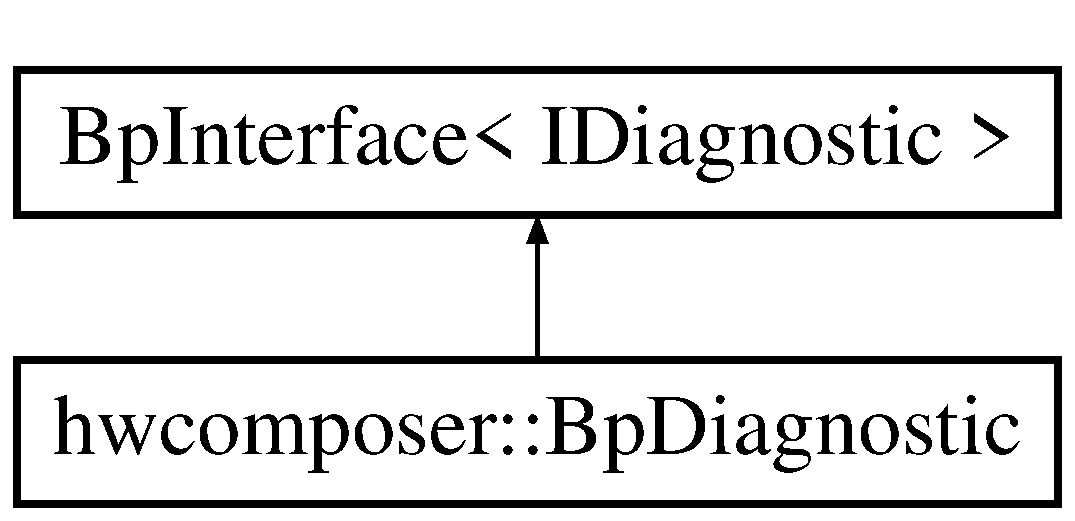
\includegraphics[height=2.000000cm]{classhwcomposer_1_1BpDiagnostic}
\end{center}
\end{figure}
\subsection*{Public Types}
\begin{DoxyCompactItemize}
\item 
enum \{ \newline
\mbox{\hyperlink{classhwcomposer_1_1BpDiagnostic_a28475ea102b977cb7213262dc96a568da1c6934eb57e46477b1b76921ab9e1d8d}{T\+R\+A\+N\+S\+A\+C\+T\+\_\+\+R\+E\+A\+D\+\_\+\+L\+O\+G\+\_\+\+P\+A\+R\+C\+EL}} = I\+Binder\+:\+:F\+I\+R\+S\+T\+\_\+\+C\+A\+L\+L\+\_\+\+T\+R\+A\+N\+S\+A\+C\+T\+I\+ON, 
\mbox{\hyperlink{classhwcomposer_1_1BpDiagnostic_a28475ea102b977cb7213262dc96a568daccd4b7373af1f931dede971ad0e92972}{T\+R\+A\+N\+S\+A\+C\+T\+\_\+\+E\+N\+A\+B\+L\+E\+\_\+\+D\+I\+S\+P\+L\+AY}}, 
\mbox{\hyperlink{classhwcomposer_1_1BpDiagnostic_a28475ea102b977cb7213262dc96a568dae96b3abe1c20751a136bbe4309230923}{T\+R\+A\+N\+S\+A\+C\+T\+\_\+\+D\+I\+S\+A\+B\+L\+E\+\_\+\+D\+I\+S\+P\+L\+AY}}, 
\mbox{\hyperlink{classhwcomposer_1_1BpDiagnostic_a28475ea102b977cb7213262dc96a568daf904704142b648f549b6b220ee158711}{T\+R\+A\+N\+S\+A\+C\+T\+\_\+\+M\+A\+S\+K\+\_\+\+L\+A\+Y\+ER}}, 
\newline
\mbox{\hyperlink{classhwcomposer_1_1BpDiagnostic_a28475ea102b977cb7213262dc96a568dac8e288e1260c1218aa4f35e308cb3546}{T\+R\+A\+N\+S\+A\+C\+T\+\_\+\+D\+U\+M\+P\+\_\+\+F\+R\+A\+M\+ES}}
 \}
\end{DoxyCompactItemize}
\subsection*{Public Member Functions}
\begin{DoxyCompactItemize}
\item 
\mbox{\hyperlink{classhwcomposer_1_1BpDiagnostic_a9b239ac429056be616b4b25165305f96}{Bp\+Diagnostic}} (const sp$<$ I\+Binder $>$ \&impl)
\item 
virtual \mbox{\hyperlink{classhwcomposer_1_1BpDiagnostic_acc1b84dc32dab5d5c6096f9c67321616}{$\sim$\+Bp\+Diagnostic}} ()
\item 
\mbox{\hyperlink{hwcserviceapi_8h_a3806fb2027d9a316d8ca8d9b8b8eb96f}{status\+\_\+t}} \mbox{\hyperlink{classhwcomposer_1_1BpDiagnostic_ae3799943fdcbef492341ca045511889c}{Read\+Log\+Parcel}} (Parcel $\ast$reply)
\item 
void \mbox{\hyperlink{classhwcomposer_1_1BpDiagnostic_a8478499ae7697d9e568393b2a882cec3}{Enable\+Display}} (uint32\+\_\+t d)
\item 
void \mbox{\hyperlink{classhwcomposer_1_1BpDiagnostic_a71a67b4621b8281bb24a88a333af15bf}{Disable\+Display}} (uint32\+\_\+t d, bool b\+Blank)
\item 
void \mbox{\hyperlink{classhwcomposer_1_1BpDiagnostic_ad80a8de0c5d66eaa67082332aecdf9b9}{Mask\+Layer}} (uint32\+\_\+t d, uint32\+\_\+t layer, bool b\+Hide)
\item 
void \mbox{\hyperlink{classhwcomposer_1_1BpDiagnostic_ab42faca0919c71e8c3e451ee9c543916}{Dump\+Frames}} (uint32\+\_\+t d, int32\+\_\+t frames, bool b\+Sync)
\end{DoxyCompactItemize}


\subsection{Detailed Description}


Definition at line 26 of file idiagnostic.\+cpp.



\subsection{Member Enumeration Documentation}
\mbox{\Hypertarget{classhwcomposer_1_1BpDiagnostic_a28475ea102b977cb7213262dc96a568d}\label{classhwcomposer_1_1BpDiagnostic_a28475ea102b977cb7213262dc96a568d}} 
\subsubsection{\texorpdfstring{anonymous enum}{anonymous enum}}
{\footnotesize\ttfamily anonymous enum}

\begin{DoxyEnumFields}{Enumerator}
\raisebox{\heightof{T}}[0pt][0pt]{\index{T\+R\+A\+N\+S\+A\+C\+T\+\_\+\+R\+E\+A\+D\+\_\+\+L\+O\+G\+\_\+\+P\+A\+R\+C\+EL@{T\+R\+A\+N\+S\+A\+C\+T\+\_\+\+R\+E\+A\+D\+\_\+\+L\+O\+G\+\_\+\+P\+A\+R\+C\+EL}!hwcomposer\+::\+Bp\+Diagnostic@{hwcomposer\+::\+Bp\+Diagnostic}}\index{hwcomposer\+::\+Bp\+Diagnostic@{hwcomposer\+::\+Bp\+Diagnostic}!T\+R\+A\+N\+S\+A\+C\+T\+\_\+\+R\+E\+A\+D\+\_\+\+L\+O\+G\+\_\+\+P\+A\+R\+C\+EL@{T\+R\+A\+N\+S\+A\+C\+T\+\_\+\+R\+E\+A\+D\+\_\+\+L\+O\+G\+\_\+\+P\+A\+R\+C\+EL}}}\mbox{\Hypertarget{classhwcomposer_1_1BpDiagnostic_a28475ea102b977cb7213262dc96a568da1c6934eb57e46477b1b76921ab9e1d8d}\label{classhwcomposer_1_1BpDiagnostic_a28475ea102b977cb7213262dc96a568da1c6934eb57e46477b1b76921ab9e1d8d}} 
T\+R\+A\+N\+S\+A\+C\+T\+\_\+\+R\+E\+A\+D\+\_\+\+L\+O\+G\+\_\+\+P\+A\+R\+C\+EL&\\
\hline

\raisebox{\heightof{T}}[0pt][0pt]{\index{T\+R\+A\+N\+S\+A\+C\+T\+\_\+\+E\+N\+A\+B\+L\+E\+\_\+\+D\+I\+S\+P\+L\+AY@{T\+R\+A\+N\+S\+A\+C\+T\+\_\+\+E\+N\+A\+B\+L\+E\+\_\+\+D\+I\+S\+P\+L\+AY}!hwcomposer\+::\+Bp\+Diagnostic@{hwcomposer\+::\+Bp\+Diagnostic}}\index{hwcomposer\+::\+Bp\+Diagnostic@{hwcomposer\+::\+Bp\+Diagnostic}!T\+R\+A\+N\+S\+A\+C\+T\+\_\+\+E\+N\+A\+B\+L\+E\+\_\+\+D\+I\+S\+P\+L\+AY@{T\+R\+A\+N\+S\+A\+C\+T\+\_\+\+E\+N\+A\+B\+L\+E\+\_\+\+D\+I\+S\+P\+L\+AY}}}\mbox{\Hypertarget{classhwcomposer_1_1BpDiagnostic_a28475ea102b977cb7213262dc96a568daccd4b7373af1f931dede971ad0e92972}\label{classhwcomposer_1_1BpDiagnostic_a28475ea102b977cb7213262dc96a568daccd4b7373af1f931dede971ad0e92972}} 
T\+R\+A\+N\+S\+A\+C\+T\+\_\+\+E\+N\+A\+B\+L\+E\+\_\+\+D\+I\+S\+P\+L\+AY&\\
\hline

\raisebox{\heightof{T}}[0pt][0pt]{\index{T\+R\+A\+N\+S\+A\+C\+T\+\_\+\+D\+I\+S\+A\+B\+L\+E\+\_\+\+D\+I\+S\+P\+L\+AY@{T\+R\+A\+N\+S\+A\+C\+T\+\_\+\+D\+I\+S\+A\+B\+L\+E\+\_\+\+D\+I\+S\+P\+L\+AY}!hwcomposer\+::\+Bp\+Diagnostic@{hwcomposer\+::\+Bp\+Diagnostic}}\index{hwcomposer\+::\+Bp\+Diagnostic@{hwcomposer\+::\+Bp\+Diagnostic}!T\+R\+A\+N\+S\+A\+C\+T\+\_\+\+D\+I\+S\+A\+B\+L\+E\+\_\+\+D\+I\+S\+P\+L\+AY@{T\+R\+A\+N\+S\+A\+C\+T\+\_\+\+D\+I\+S\+A\+B\+L\+E\+\_\+\+D\+I\+S\+P\+L\+AY}}}\mbox{\Hypertarget{classhwcomposer_1_1BpDiagnostic_a28475ea102b977cb7213262dc96a568dae96b3abe1c20751a136bbe4309230923}\label{classhwcomposer_1_1BpDiagnostic_a28475ea102b977cb7213262dc96a568dae96b3abe1c20751a136bbe4309230923}} 
T\+R\+A\+N\+S\+A\+C\+T\+\_\+\+D\+I\+S\+A\+B\+L\+E\+\_\+\+D\+I\+S\+P\+L\+AY&\\
\hline

\raisebox{\heightof{T}}[0pt][0pt]{\index{T\+R\+A\+N\+S\+A\+C\+T\+\_\+\+M\+A\+S\+K\+\_\+\+L\+A\+Y\+ER@{T\+R\+A\+N\+S\+A\+C\+T\+\_\+\+M\+A\+S\+K\+\_\+\+L\+A\+Y\+ER}!hwcomposer\+::\+Bp\+Diagnostic@{hwcomposer\+::\+Bp\+Diagnostic}}\index{hwcomposer\+::\+Bp\+Diagnostic@{hwcomposer\+::\+Bp\+Diagnostic}!T\+R\+A\+N\+S\+A\+C\+T\+\_\+\+M\+A\+S\+K\+\_\+\+L\+A\+Y\+ER@{T\+R\+A\+N\+S\+A\+C\+T\+\_\+\+M\+A\+S\+K\+\_\+\+L\+A\+Y\+ER}}}\mbox{\Hypertarget{classhwcomposer_1_1BpDiagnostic_a28475ea102b977cb7213262dc96a568daf904704142b648f549b6b220ee158711}\label{classhwcomposer_1_1BpDiagnostic_a28475ea102b977cb7213262dc96a568daf904704142b648f549b6b220ee158711}} 
T\+R\+A\+N\+S\+A\+C\+T\+\_\+\+M\+A\+S\+K\+\_\+\+L\+A\+Y\+ER&\\
\hline

\raisebox{\heightof{T}}[0pt][0pt]{\index{T\+R\+A\+N\+S\+A\+C\+T\+\_\+\+D\+U\+M\+P\+\_\+\+F\+R\+A\+M\+ES@{T\+R\+A\+N\+S\+A\+C\+T\+\_\+\+D\+U\+M\+P\+\_\+\+F\+R\+A\+M\+ES}!hwcomposer\+::\+Bp\+Diagnostic@{hwcomposer\+::\+Bp\+Diagnostic}}\index{hwcomposer\+::\+Bp\+Diagnostic@{hwcomposer\+::\+Bp\+Diagnostic}!T\+R\+A\+N\+S\+A\+C\+T\+\_\+\+D\+U\+M\+P\+\_\+\+F\+R\+A\+M\+ES@{T\+R\+A\+N\+S\+A\+C\+T\+\_\+\+D\+U\+M\+P\+\_\+\+F\+R\+A\+M\+ES}}}\mbox{\Hypertarget{classhwcomposer_1_1BpDiagnostic_a28475ea102b977cb7213262dc96a568dac8e288e1260c1218aa4f35e308cb3546}\label{classhwcomposer_1_1BpDiagnostic_a28475ea102b977cb7213262dc96a568dac8e288e1260c1218aa4f35e308cb3546}} 
T\+R\+A\+N\+S\+A\+C\+T\+\_\+\+D\+U\+M\+P\+\_\+\+F\+R\+A\+M\+ES&\\
\hline

\end{DoxyEnumFields}


Definition at line 32 of file idiagnostic.\+cpp.


\begin{DoxyCode}{0}
\DoxyCodeLine{32        \{}
\DoxyCodeLine{33     \mbox{\hyperlink{classhwcomposer_1_1BpDiagnostic_a28475ea102b977cb7213262dc96a568da1c6934eb57e46477b1b76921ab9e1d8d}{TRANSACT\_READ\_LOG\_PARCEL}} = IBinder::FIRST\_CALL\_TRANSACTION,}
\DoxyCodeLine{34     \mbox{\hyperlink{classhwcomposer_1_1BpDiagnostic_a28475ea102b977cb7213262dc96a568daccd4b7373af1f931dede971ad0e92972}{TRANSACT\_ENABLE\_DISPLAY}},}
\DoxyCodeLine{35     \mbox{\hyperlink{classhwcomposer_1_1BpDiagnostic_a28475ea102b977cb7213262dc96a568dae96b3abe1c20751a136bbe4309230923}{TRANSACT\_DISABLE\_DISPLAY}},}
\DoxyCodeLine{36     \mbox{\hyperlink{classhwcomposer_1_1BpDiagnostic_a28475ea102b977cb7213262dc96a568daf904704142b648f549b6b220ee158711}{TRANSACT\_MASK\_LAYER}},}
\DoxyCodeLine{37     \mbox{\hyperlink{classhwcomposer_1_1BpDiagnostic_a28475ea102b977cb7213262dc96a568dac8e288e1260c1218aa4f35e308cb3546}{TRANSACT\_DUMP\_FRAMES}}}
\DoxyCodeLine{38   \};}
\end{DoxyCode}


\subsection{Constructor \& Destructor Documentation}
\mbox{\Hypertarget{classhwcomposer_1_1BpDiagnostic_a9b239ac429056be616b4b25165305f96}\label{classhwcomposer_1_1BpDiagnostic_a9b239ac429056be616b4b25165305f96}} 
\index{hwcomposer\+::\+Bp\+Diagnostic@{hwcomposer\+::\+Bp\+Diagnostic}!Bp\+Diagnostic@{Bp\+Diagnostic}}
\index{Bp\+Diagnostic@{Bp\+Diagnostic}!hwcomposer\+::\+Bp\+Diagnostic@{hwcomposer\+::\+Bp\+Diagnostic}}
\subsubsection{\texorpdfstring{Bp\+Diagnostic()}{BpDiagnostic()}}
{\footnotesize\ttfamily hwcomposer\+::\+Bp\+Diagnostic\+::\+Bp\+Diagnostic (\begin{DoxyParamCaption}\item[{const sp$<$ I\+Binder $>$ \&}]{impl }\end{DoxyParamCaption})\hspace{0.3cm}{\ttfamily [inline]}}



Definition at line 28 of file idiagnostic.\+cpp.


\begin{DoxyCode}{0}
\DoxyCodeLine{29       : BpInterface<IDiagnostic>(impl), mReply(0) \{}
\DoxyCodeLine{30   \}}
\end{DoxyCode}
\mbox{\Hypertarget{classhwcomposer_1_1BpDiagnostic_acc1b84dc32dab5d5c6096f9c67321616}\label{classhwcomposer_1_1BpDiagnostic_acc1b84dc32dab5d5c6096f9c67321616}} 
\index{hwcomposer\+::\+Bp\+Diagnostic@{hwcomposer\+::\+Bp\+Diagnostic}!````~Bp\+Diagnostic@{$\sim$\+Bp\+Diagnostic}}
\index{````~Bp\+Diagnostic@{$\sim$\+Bp\+Diagnostic}!hwcomposer\+::\+Bp\+Diagnostic@{hwcomposer\+::\+Bp\+Diagnostic}}
\subsubsection{\texorpdfstring{$\sim$\+Bp\+Diagnostic()}{~BpDiagnostic()}}
{\footnotesize\ttfamily virtual hwcomposer\+::\+Bp\+Diagnostic\+::$\sim$\+Bp\+Diagnostic (\begin{DoxyParamCaption}{ }\end{DoxyParamCaption})\hspace{0.3cm}{\ttfamily [inline]}, {\ttfamily [virtual]}}



Definition at line 40 of file idiagnostic.\+cpp.


\begin{DoxyCode}{0}
\DoxyCodeLine{40                           \{}
\DoxyCodeLine{41     \textcolor{keywordflow}{if} (mReply)}
\DoxyCodeLine{42       \textcolor{keyword}{delete} mReply;}
\DoxyCodeLine{43   \}}
\end{DoxyCode}


\subsection{Member Function Documentation}
\mbox{\Hypertarget{classhwcomposer_1_1BpDiagnostic_a71a67b4621b8281bb24a88a333af15bf}\label{classhwcomposer_1_1BpDiagnostic_a71a67b4621b8281bb24a88a333af15bf}} 
\index{hwcomposer\+::\+Bp\+Diagnostic@{hwcomposer\+::\+Bp\+Diagnostic}!Disable\+Display@{Disable\+Display}}
\index{Disable\+Display@{Disable\+Display}!hwcomposer\+::\+Bp\+Diagnostic@{hwcomposer\+::\+Bp\+Diagnostic}}
\subsubsection{\texorpdfstring{Disable\+Display()}{DisableDisplay()}}
{\footnotesize\ttfamily void hwcomposer\+::\+Bp\+Diagnostic\+::\+Disable\+Display (\begin{DoxyParamCaption}\item[{uint32\+\_\+t}]{d,  }\item[{bool}]{b\+Blank }\end{DoxyParamCaption})\hspace{0.3cm}{\ttfamily [inline]}}



Definition at line 66 of file idiagnostic.\+cpp.


\begin{DoxyCode}{0}
\DoxyCodeLine{66                                                \{}
\DoxyCodeLine{67     Parcel data, reply;}
\DoxyCodeLine{68     data.writeInterfaceToken(IDiagnostic::getInterfaceDescriptor());}
\DoxyCodeLine{69     data.writeInt32(d);}
\DoxyCodeLine{70     data.writeInt32(bBlank);}
\DoxyCodeLine{71     \mbox{\hyperlink{hwcserviceapi_8h_a3806fb2027d9a316d8ca8d9b8b8eb96f}{status\_t}} ret = remote()->transact(\mbox{\hyperlink{classhwcomposer_1_1BpDiagnostic_a28475ea102b977cb7213262dc96a568dae96b3abe1c20751a136bbe4309230923}{TRANSACT\_DISABLE\_DISPLAY}}, data, \&reply);}
\DoxyCodeLine{72     \textcolor{keywordflow}{if} (ret != NO\_ERROR) \{}
\DoxyCodeLine{73       ALOGW(\textcolor{stringliteral}{"\%s() transact failed: \%d"}, \_\_FUNCTION\_\_, ret);}
\DoxyCodeLine{74       \textcolor{keywordflow}{return};}
\DoxyCodeLine{75     \}}
\DoxyCodeLine{76   \}}
\end{DoxyCode}
\mbox{\Hypertarget{classhwcomposer_1_1BpDiagnostic_ab42faca0919c71e8c3e451ee9c543916}\label{classhwcomposer_1_1BpDiagnostic_ab42faca0919c71e8c3e451ee9c543916}} 
\index{hwcomposer\+::\+Bp\+Diagnostic@{hwcomposer\+::\+Bp\+Diagnostic}!Dump\+Frames@{Dump\+Frames}}
\index{Dump\+Frames@{Dump\+Frames}!hwcomposer\+::\+Bp\+Diagnostic@{hwcomposer\+::\+Bp\+Diagnostic}}
\subsubsection{\texorpdfstring{Dump\+Frames()}{DumpFrames()}}
{\footnotesize\ttfamily void hwcomposer\+::\+Bp\+Diagnostic\+::\+Dump\+Frames (\begin{DoxyParamCaption}\item[{uint32\+\_\+t}]{d,  }\item[{int32\+\_\+t}]{frames,  }\item[{bool}]{b\+Sync }\end{DoxyParamCaption})\hspace{0.3cm}{\ttfamily [inline]}}



Definition at line 91 of file idiagnostic.\+cpp.


\begin{DoxyCode}{0}
\DoxyCodeLine{91                                                           \{}
\DoxyCodeLine{92     Parcel data, reply;}
\DoxyCodeLine{93     data.writeInterfaceToken(IDiagnostic::getInterfaceDescriptor());}
\DoxyCodeLine{94     data.writeInt32(d);}
\DoxyCodeLine{95     data.writeInt32(frames);}
\DoxyCodeLine{96     data.writeInt32(bSync);}
\DoxyCodeLine{97     \mbox{\hyperlink{hwcserviceapi_8h_a3806fb2027d9a316d8ca8d9b8b8eb96f}{status\_t}} ret = remote()->transact(\mbox{\hyperlink{classhwcomposer_1_1BpDiagnostic_a28475ea102b977cb7213262dc96a568dac8e288e1260c1218aa4f35e308cb3546}{TRANSACT\_DUMP\_FRAMES}}, data, \&reply);}
\DoxyCodeLine{98     \textcolor{keywordflow}{if} (ret != NO\_ERROR) \{}
\DoxyCodeLine{99       ALOGW(\textcolor{stringliteral}{"\%s() transact failed: \%d"}, \_\_FUNCTION\_\_, ret);}
\DoxyCodeLine{100       \textcolor{keywordflow}{return};}
\DoxyCodeLine{101     \}}
\DoxyCodeLine{102   \}}
\end{DoxyCode}
\mbox{\Hypertarget{classhwcomposer_1_1BpDiagnostic_a8478499ae7697d9e568393b2a882cec3}\label{classhwcomposer_1_1BpDiagnostic_a8478499ae7697d9e568393b2a882cec3}} 
\index{hwcomposer\+::\+Bp\+Diagnostic@{hwcomposer\+::\+Bp\+Diagnostic}!Enable\+Display@{Enable\+Display}}
\index{Enable\+Display@{Enable\+Display}!hwcomposer\+::\+Bp\+Diagnostic@{hwcomposer\+::\+Bp\+Diagnostic}}
\subsubsection{\texorpdfstring{Enable\+Display()}{EnableDisplay()}}
{\footnotesize\ttfamily void hwcomposer\+::\+Bp\+Diagnostic\+::\+Enable\+Display (\begin{DoxyParamCaption}\item[{uint32\+\_\+t}]{d }\end{DoxyParamCaption})\hspace{0.3cm}{\ttfamily [inline]}}



Definition at line 55 of file idiagnostic.\+cpp.


\begin{DoxyCode}{0}
\DoxyCodeLine{55                                  \{}
\DoxyCodeLine{56     Parcel data, reply;}
\DoxyCodeLine{57     data.writeInterfaceToken(IDiagnostic::getInterfaceDescriptor());}
\DoxyCodeLine{58     data.writeInt32(d);}
\DoxyCodeLine{59     \mbox{\hyperlink{hwcserviceapi_8h_a3806fb2027d9a316d8ca8d9b8b8eb96f}{status\_t}} ret = remote()->transact(\mbox{\hyperlink{classhwcomposer_1_1BpDiagnostic_a28475ea102b977cb7213262dc96a568daccd4b7373af1f931dede971ad0e92972}{TRANSACT\_ENABLE\_DISPLAY}}, data, \&reply);}
\DoxyCodeLine{60     \textcolor{keywordflow}{if} (ret != NO\_ERROR) \{}
\DoxyCodeLine{61       ALOGW(\textcolor{stringliteral}{"\%s() transact failed: \%d"}, \_\_FUNCTION\_\_, ret);}
\DoxyCodeLine{62       \textcolor{keywordflow}{return};}
\DoxyCodeLine{63     \}}
\DoxyCodeLine{64   \}}
\end{DoxyCode}
\mbox{\Hypertarget{classhwcomposer_1_1BpDiagnostic_ad80a8de0c5d66eaa67082332aecdf9b9}\label{classhwcomposer_1_1BpDiagnostic_ad80a8de0c5d66eaa67082332aecdf9b9}} 
\index{hwcomposer\+::\+Bp\+Diagnostic@{hwcomposer\+::\+Bp\+Diagnostic}!Mask\+Layer@{Mask\+Layer}}
\index{Mask\+Layer@{Mask\+Layer}!hwcomposer\+::\+Bp\+Diagnostic@{hwcomposer\+::\+Bp\+Diagnostic}}
\subsubsection{\texorpdfstring{Mask\+Layer()}{MaskLayer()}}
{\footnotesize\ttfamily void hwcomposer\+::\+Bp\+Diagnostic\+::\+Mask\+Layer (\begin{DoxyParamCaption}\item[{uint32\+\_\+t}]{d,  }\item[{uint32\+\_\+t}]{layer,  }\item[{bool}]{b\+Hide }\end{DoxyParamCaption})\hspace{0.3cm}{\ttfamily [inline]}}



Definition at line 78 of file idiagnostic.\+cpp.


\begin{DoxyCode}{0}
\DoxyCodeLine{78                                                          \{}
\DoxyCodeLine{79     Parcel data, reply;}
\DoxyCodeLine{80     data.writeInterfaceToken(IDiagnostic::getInterfaceDescriptor());}
\DoxyCodeLine{81     data.writeInt32(d);}
\DoxyCodeLine{82     data.writeInt32(layer);}
\DoxyCodeLine{83     data.writeInt32(bHide);}
\DoxyCodeLine{84     \mbox{\hyperlink{hwcserviceapi_8h_a3806fb2027d9a316d8ca8d9b8b8eb96f}{status\_t}} ret = remote()->transact(\mbox{\hyperlink{classhwcomposer_1_1BpDiagnostic_a28475ea102b977cb7213262dc96a568daf904704142b648f549b6b220ee158711}{TRANSACT\_MASK\_LAYER}}, data, \&reply);}
\DoxyCodeLine{85     \textcolor{keywordflow}{if} (ret != NO\_ERROR) \{}
\DoxyCodeLine{86       ALOGW(\textcolor{stringliteral}{"\%s() transact failed: \%d"}, \_\_FUNCTION\_\_, ret);}
\DoxyCodeLine{87       \textcolor{keywordflow}{return};}
\DoxyCodeLine{88     \}}
\DoxyCodeLine{89   \}}
\end{DoxyCode}
\mbox{\Hypertarget{classhwcomposer_1_1BpDiagnostic_ae3799943fdcbef492341ca045511889c}\label{classhwcomposer_1_1BpDiagnostic_ae3799943fdcbef492341ca045511889c}} 
\index{hwcomposer\+::\+Bp\+Diagnostic@{hwcomposer\+::\+Bp\+Diagnostic}!Read\+Log\+Parcel@{Read\+Log\+Parcel}}
\index{Read\+Log\+Parcel@{Read\+Log\+Parcel}!hwcomposer\+::\+Bp\+Diagnostic@{hwcomposer\+::\+Bp\+Diagnostic}}
\subsubsection{\texorpdfstring{Read\+Log\+Parcel()}{ReadLogParcel()}}
{\footnotesize\ttfamily \mbox{\hyperlink{hwcserviceapi_8h_a3806fb2027d9a316d8ca8d9b8b8eb96f}{status\+\_\+t}} hwcomposer\+::\+Bp\+Diagnostic\+::\+Read\+Log\+Parcel (\begin{DoxyParamCaption}\item[{Parcel $\ast$}]{reply }\end{DoxyParamCaption})\hspace{0.3cm}{\ttfamily [inline]}}



Definition at line 45 of file idiagnostic.\+cpp.


\begin{DoxyCode}{0}
\DoxyCodeLine{45                                         \{}
\DoxyCodeLine{46     Parcel data;}
\DoxyCodeLine{47     data.writeInterfaceToken(IDiagnostic::getInterfaceDescriptor());}
\DoxyCodeLine{48     \mbox{\hyperlink{hwcserviceapi_8h_a3806fb2027d9a316d8ca8d9b8b8eb96f}{status\_t}} ret = remote()->transact(\mbox{\hyperlink{classhwcomposer_1_1BpDiagnostic_a28475ea102b977cb7213262dc96a568da1c6934eb57e46477b1b76921ab9e1d8d}{TRANSACT\_READ\_LOG\_PARCEL}}, data, reply);}
\DoxyCodeLine{49     \textcolor{keywordflow}{if} (ret != NO\_ERROR) \{}
\DoxyCodeLine{50       ALOGW(\textcolor{stringliteral}{"\%s() transact failed: \%d"}, \_\_FUNCTION\_\_, ret);}
\DoxyCodeLine{51     \}}
\DoxyCodeLine{52     \textcolor{keywordflow}{return} ret;}
\DoxyCodeLine{53   \}}
\end{DoxyCode}


The documentation for this class was generated from the following file\+:\begin{DoxyCompactItemize}
\item 
os/android/libhwcservice/\mbox{\hyperlink{idiagnostic_8cpp}{idiagnostic.\+cpp}}\end{DoxyCompactItemize}

\hypertarget{classhwcomposer_1_1BpService}{}\section{hwcomposer\+:\+:Bp\+Service Class Reference}
\label{classhwcomposer_1_1BpService}\index{hwcomposer\+::\+Bp\+Service@{hwcomposer\+::\+Bp\+Service}}
Inheritance diagram for hwcomposer\+:\+:Bp\+Service\+:\begin{figure}[H]
\begin{center}
\leavevmode
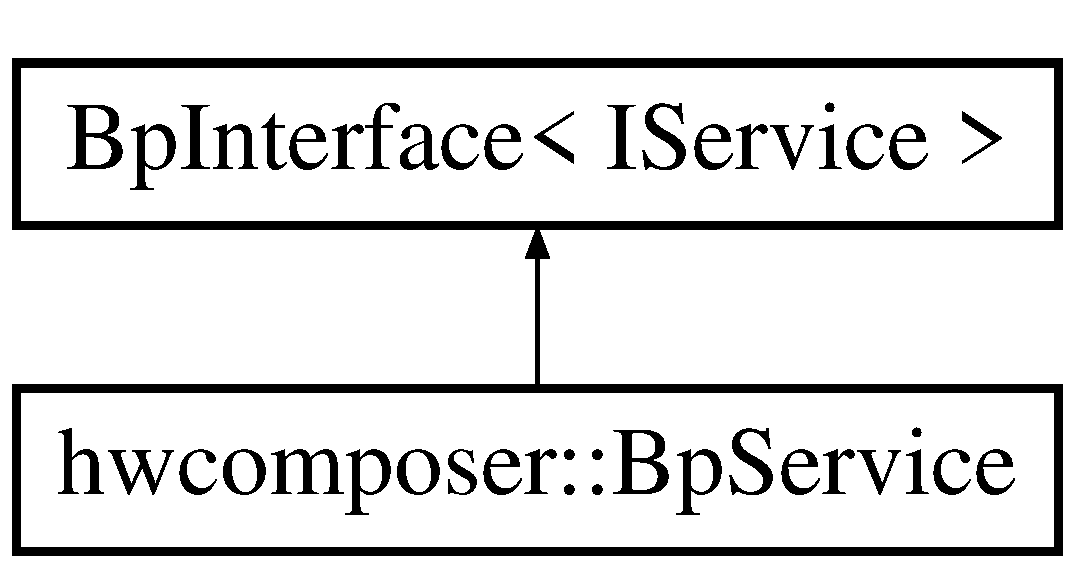
\includegraphics[height=2.000000cm]{classhwcomposer_1_1BpService}
\end{center}
\end{figure}
\subsection*{Public Types}
\begin{DoxyCompactItemize}
\item 
enum \{ \newline
\mbox{\hyperlink{classhwcomposer_1_1BpService_a688b4b1338923222d225a99d16e22319ac29d8afa3ded86d47e7879f814b61f0d}{G\+E\+T\+\_\+\+H\+W\+C\+\_\+\+V\+E\+R\+S\+I\+ON}} = I\+Binder\+:\+:F\+I\+R\+S\+T\+\_\+\+C\+A\+L\+L\+\_\+\+T\+R\+A\+N\+S\+A\+C\+T\+I\+ON, 
\mbox{\hyperlink{classhwcomposer_1_1BpService_a688b4b1338923222d225a99d16e22319a117fba2a971fa7318d8ef74f7a84105c}{D\+U\+M\+P\+\_\+\+O\+P\+T\+I\+O\+NS}}, 
\mbox{\hyperlink{classhwcomposer_1_1BpService_a688b4b1338923222d225a99d16e22319a8f322cc1308b770e9cd5056d9dfefaf3}{S\+E\+T\+\_\+\+O\+P\+T\+I\+ON}}, 
\mbox{\hyperlink{classhwcomposer_1_1BpService_a688b4b1338923222d225a99d16e22319aa6f70e3efcf110f66a046bf4d49ee999}{D\+I\+S\+A\+B\+L\+E\+\_\+\+L\+O\+G\+\_\+\+T\+O\+\_\+\+L\+O\+G\+C\+AT}} = 98, 
\newline
\mbox{\hyperlink{classhwcomposer_1_1BpService_a688b4b1338923222d225a99d16e22319a8ec23523cde1ace78656435c40d75ca6}{E\+N\+A\+B\+L\+E\+\_\+\+L\+O\+G\+\_\+\+T\+O\+\_\+\+L\+O\+G\+C\+AT}} = 99, 
\mbox{\hyperlink{classhwcomposer_1_1BpService_a688b4b1338923222d225a99d16e22319aba1101f98d0ae4dba7ae06b05fa7ecf6}{T\+R\+A\+N\+S\+A\+C\+T\+\_\+\+G\+E\+T\+\_\+\+D\+I\+A\+G\+N\+O\+S\+T\+IC}} = 100, 
\mbox{\hyperlink{classhwcomposer_1_1BpService_a688b4b1338923222d225a99d16e22319a88c048d451c725f7549727f0eb25bd11}{T\+R\+A\+N\+S\+A\+C\+T\+\_\+\+G\+E\+T\+\_\+\+C\+O\+N\+T\+R\+O\+LS}}
 \}
\end{DoxyCompactItemize}
\subsection*{Public Member Functions}
\begin{DoxyCompactItemize}
\item 
\mbox{\hyperlink{classhwcomposer_1_1BpService_a62e17be4899fc0e9af815cefa9956971}{Bp\+Service}} (const sp$<$ I\+Binder $>$ \&impl)
\item 
String8 \mbox{\hyperlink{classhwcomposer_1_1BpService_a17ce9341ddf723a5e0a565f3dcf0495b}{Get\+Hwc\+Version}} () override
\item 
void \mbox{\hyperlink{classhwcomposer_1_1BpService_a9685bc5b64d6666e6ad3607b6c127bda}{Dump\+Options}} (void) override
\item 
\mbox{\hyperlink{hwcserviceapi_8h_a3806fb2027d9a316d8ca8d9b8b8eb96f}{status\+\_\+t}} \mbox{\hyperlink{classhwcomposer_1_1BpService_a9293da08063a0cbea2906f80470ba383}{Set\+Option}} (String8 option, String8 option\+Value) override
\item 
\mbox{\hyperlink{hwcserviceapi_8h_a3806fb2027d9a316d8ca8d9b8b8eb96f}{status\+\_\+t}} \mbox{\hyperlink{classhwcomposer_1_1BpService_a1c58bedc3a6f9bed36b4daff0ba9048d}{Enable\+Logview\+To\+Logcat}} (bool enable=true) override
\item 
sp$<$ \mbox{\hyperlink{classhwcomposer_1_1IDiagnostic}{I\+Diagnostic}} $>$ \mbox{\hyperlink{classhwcomposer_1_1BpService_a03db6523ced5f83e89bc1c48c7ee442d}{Get\+Diagnostic}} () override
\item 
sp$<$ \mbox{\hyperlink{classhwcomposer_1_1IControls}{I\+Controls}} $>$ \mbox{\hyperlink{classhwcomposer_1_1BpService_a1d18a82c9d0693cfec5f57781431e335}{Get\+Controls}} () override
\end{DoxyCompactItemize}


\subsection{Detailed Description}


Definition at line 29 of file iservice.\+cpp.



\subsection{Member Enumeration Documentation}
\mbox{\Hypertarget{classhwcomposer_1_1BpService_a688b4b1338923222d225a99d16e22319}\label{classhwcomposer_1_1BpService_a688b4b1338923222d225a99d16e22319}} 
\subsubsection{\texorpdfstring{anonymous enum}{anonymous enum}}
{\footnotesize\ttfamily anonymous enum}

\begin{DoxyEnumFields}{Enumerator}
\raisebox{\heightof{T}}[0pt][0pt]{\index{G\+E\+T\+\_\+\+H\+W\+C\+\_\+\+V\+E\+R\+S\+I\+ON@{G\+E\+T\+\_\+\+H\+W\+C\+\_\+\+V\+E\+R\+S\+I\+ON}!hwcomposer\+::\+Bp\+Service@{hwcomposer\+::\+Bp\+Service}}\index{hwcomposer\+::\+Bp\+Service@{hwcomposer\+::\+Bp\+Service}!G\+E\+T\+\_\+\+H\+W\+C\+\_\+\+V\+E\+R\+S\+I\+ON@{G\+E\+T\+\_\+\+H\+W\+C\+\_\+\+V\+E\+R\+S\+I\+ON}}}\mbox{\Hypertarget{classhwcomposer_1_1BpService_a688b4b1338923222d225a99d16e22319ac29d8afa3ded86d47e7879f814b61f0d}\label{classhwcomposer_1_1BpService_a688b4b1338923222d225a99d16e22319ac29d8afa3ded86d47e7879f814b61f0d}} 
G\+E\+T\+\_\+\+H\+W\+C\+\_\+\+V\+E\+R\+S\+I\+ON&\\
\hline

\raisebox{\heightof{T}}[0pt][0pt]{\index{D\+U\+M\+P\+\_\+\+O\+P\+T\+I\+O\+NS@{D\+U\+M\+P\+\_\+\+O\+P\+T\+I\+O\+NS}!hwcomposer\+::\+Bp\+Service@{hwcomposer\+::\+Bp\+Service}}\index{hwcomposer\+::\+Bp\+Service@{hwcomposer\+::\+Bp\+Service}!D\+U\+M\+P\+\_\+\+O\+P\+T\+I\+O\+NS@{D\+U\+M\+P\+\_\+\+O\+P\+T\+I\+O\+NS}}}\mbox{\Hypertarget{classhwcomposer_1_1BpService_a688b4b1338923222d225a99d16e22319a117fba2a971fa7318d8ef74f7a84105c}\label{classhwcomposer_1_1BpService_a688b4b1338923222d225a99d16e22319a117fba2a971fa7318d8ef74f7a84105c}} 
D\+U\+M\+P\+\_\+\+O\+P\+T\+I\+O\+NS&\\
\hline

\raisebox{\heightof{T}}[0pt][0pt]{\index{S\+E\+T\+\_\+\+O\+P\+T\+I\+ON@{S\+E\+T\+\_\+\+O\+P\+T\+I\+ON}!hwcomposer\+::\+Bp\+Service@{hwcomposer\+::\+Bp\+Service}}\index{hwcomposer\+::\+Bp\+Service@{hwcomposer\+::\+Bp\+Service}!S\+E\+T\+\_\+\+O\+P\+T\+I\+ON@{S\+E\+T\+\_\+\+O\+P\+T\+I\+ON}}}\mbox{\Hypertarget{classhwcomposer_1_1BpService_a688b4b1338923222d225a99d16e22319a8f322cc1308b770e9cd5056d9dfefaf3}\label{classhwcomposer_1_1BpService_a688b4b1338923222d225a99d16e22319a8f322cc1308b770e9cd5056d9dfefaf3}} 
S\+E\+T\+\_\+\+O\+P\+T\+I\+ON&\\
\hline

\raisebox{\heightof{T}}[0pt][0pt]{\index{D\+I\+S\+A\+B\+L\+E\+\_\+\+L\+O\+G\+\_\+\+T\+O\+\_\+\+L\+O\+G\+C\+AT@{D\+I\+S\+A\+B\+L\+E\+\_\+\+L\+O\+G\+\_\+\+T\+O\+\_\+\+L\+O\+G\+C\+AT}!hwcomposer\+::\+Bp\+Service@{hwcomposer\+::\+Bp\+Service}}\index{hwcomposer\+::\+Bp\+Service@{hwcomposer\+::\+Bp\+Service}!D\+I\+S\+A\+B\+L\+E\+\_\+\+L\+O\+G\+\_\+\+T\+O\+\_\+\+L\+O\+G\+C\+AT@{D\+I\+S\+A\+B\+L\+E\+\_\+\+L\+O\+G\+\_\+\+T\+O\+\_\+\+L\+O\+G\+C\+AT}}}\mbox{\Hypertarget{classhwcomposer_1_1BpService_a688b4b1338923222d225a99d16e22319aa6f70e3efcf110f66a046bf4d49ee999}\label{classhwcomposer_1_1BpService_a688b4b1338923222d225a99d16e22319aa6f70e3efcf110f66a046bf4d49ee999}} 
D\+I\+S\+A\+B\+L\+E\+\_\+\+L\+O\+G\+\_\+\+T\+O\+\_\+\+L\+O\+G\+C\+AT&\\
\hline

\raisebox{\heightof{T}}[0pt][0pt]{\index{E\+N\+A\+B\+L\+E\+\_\+\+L\+O\+G\+\_\+\+T\+O\+\_\+\+L\+O\+G\+C\+AT@{E\+N\+A\+B\+L\+E\+\_\+\+L\+O\+G\+\_\+\+T\+O\+\_\+\+L\+O\+G\+C\+AT}!hwcomposer\+::\+Bp\+Service@{hwcomposer\+::\+Bp\+Service}}\index{hwcomposer\+::\+Bp\+Service@{hwcomposer\+::\+Bp\+Service}!E\+N\+A\+B\+L\+E\+\_\+\+L\+O\+G\+\_\+\+T\+O\+\_\+\+L\+O\+G\+C\+AT@{E\+N\+A\+B\+L\+E\+\_\+\+L\+O\+G\+\_\+\+T\+O\+\_\+\+L\+O\+G\+C\+AT}}}\mbox{\Hypertarget{classhwcomposer_1_1BpService_a688b4b1338923222d225a99d16e22319a8ec23523cde1ace78656435c40d75ca6}\label{classhwcomposer_1_1BpService_a688b4b1338923222d225a99d16e22319a8ec23523cde1ace78656435c40d75ca6}} 
E\+N\+A\+B\+L\+E\+\_\+\+L\+O\+G\+\_\+\+T\+O\+\_\+\+L\+O\+G\+C\+AT&\\
\hline

\raisebox{\heightof{T}}[0pt][0pt]{\index{T\+R\+A\+N\+S\+A\+C\+T\+\_\+\+G\+E\+T\+\_\+\+D\+I\+A\+G\+N\+O\+S\+T\+IC@{T\+R\+A\+N\+S\+A\+C\+T\+\_\+\+G\+E\+T\+\_\+\+D\+I\+A\+G\+N\+O\+S\+T\+IC}!hwcomposer\+::\+Bp\+Service@{hwcomposer\+::\+Bp\+Service}}\index{hwcomposer\+::\+Bp\+Service@{hwcomposer\+::\+Bp\+Service}!T\+R\+A\+N\+S\+A\+C\+T\+\_\+\+G\+E\+T\+\_\+\+D\+I\+A\+G\+N\+O\+S\+T\+IC@{T\+R\+A\+N\+S\+A\+C\+T\+\_\+\+G\+E\+T\+\_\+\+D\+I\+A\+G\+N\+O\+S\+T\+IC}}}\mbox{\Hypertarget{classhwcomposer_1_1BpService_a688b4b1338923222d225a99d16e22319aba1101f98d0ae4dba7ae06b05fa7ecf6}\label{classhwcomposer_1_1BpService_a688b4b1338923222d225a99d16e22319aba1101f98d0ae4dba7ae06b05fa7ecf6}} 
T\+R\+A\+N\+S\+A\+C\+T\+\_\+\+G\+E\+T\+\_\+\+D\+I\+A\+G\+N\+O\+S\+T\+IC&\\
\hline

\raisebox{\heightof{T}}[0pt][0pt]{\index{T\+R\+A\+N\+S\+A\+C\+T\+\_\+\+G\+E\+T\+\_\+\+C\+O\+N\+T\+R\+O\+LS@{T\+R\+A\+N\+S\+A\+C\+T\+\_\+\+G\+E\+T\+\_\+\+C\+O\+N\+T\+R\+O\+LS}!hwcomposer\+::\+Bp\+Service@{hwcomposer\+::\+Bp\+Service}}\index{hwcomposer\+::\+Bp\+Service@{hwcomposer\+::\+Bp\+Service}!T\+R\+A\+N\+S\+A\+C\+T\+\_\+\+G\+E\+T\+\_\+\+C\+O\+N\+T\+R\+O\+LS@{T\+R\+A\+N\+S\+A\+C\+T\+\_\+\+G\+E\+T\+\_\+\+C\+O\+N\+T\+R\+O\+LS}}}\mbox{\Hypertarget{classhwcomposer_1_1BpService_a688b4b1338923222d225a99d16e22319a88c048d451c725f7549727f0eb25bd11}\label{classhwcomposer_1_1BpService_a688b4b1338923222d225a99d16e22319a88c048d451c725f7549727f0eb25bd11}} 
T\+R\+A\+N\+S\+A\+C\+T\+\_\+\+G\+E\+T\+\_\+\+C\+O\+N\+T\+R\+O\+LS&\\
\hline

\end{DoxyEnumFields}


Definition at line 34 of file iservice.\+cpp.


\begin{DoxyCode}{0}
\DoxyCodeLine{34        \{}
\DoxyCodeLine{35     \textcolor{comment}{// ==============================================}}
\DoxyCodeLine{36     \textcolor{comment}{// Public APIs - try not to reorder these}}
\DoxyCodeLine{37 }
\DoxyCodeLine{38     \mbox{\hyperlink{classhwcomposer_1_1BpService_a688b4b1338923222d225a99d16e22319ac29d8afa3ded86d47e7879f814b61f0d}{GET\_HWC\_VERSION}} = IBinder::FIRST\_CALL\_TRANSACTION,}
\DoxyCodeLine{39 }
\DoxyCodeLine{40     \textcolor{comment}{// Dump options and current settings to logcat.}}
\DoxyCodeLine{41     \mbox{\hyperlink{classhwcomposer_1_1BpService_a688b4b1338923222d225a99d16e22319a117fba2a971fa7318d8ef74f7a84105c}{DUMP\_OPTIONS}},}
\DoxyCodeLine{42 }
\DoxyCodeLine{43     \textcolor{comment}{// Override an option.}}
\DoxyCodeLine{44     \mbox{\hyperlink{classhwcomposer_1_1BpService_a688b4b1338923222d225a99d16e22319a8f322cc1308b770e9cd5056d9dfefaf3}{SET\_OPTION}},}
\DoxyCodeLine{45 }
\DoxyCodeLine{46     \textcolor{comment}{// Disable hwc logviewer output to logcat}}
\DoxyCodeLine{47     \mbox{\hyperlink{classhwcomposer_1_1BpService_a688b4b1338923222d225a99d16e22319aa6f70e3efcf110f66a046bf4d49ee999}{DISABLE\_LOG\_TO\_LOGCAT}} = 98,}
\DoxyCodeLine{48     \textcolor{comment}{// Enable hwclogviewer output to logcat}}
\DoxyCodeLine{49     \mbox{\hyperlink{classhwcomposer_1_1BpService_a688b4b1338923222d225a99d16e22319a8ec23523cde1ace78656435c40d75ca6}{ENABLE\_LOG\_TO\_LOGCAT}} = 99,}
\DoxyCodeLine{50 }
\DoxyCodeLine{51     \textcolor{comment}{// accessor for IBinder interface functions}}
\DoxyCodeLine{52     \mbox{\hyperlink{classhwcomposer_1_1BpService_a688b4b1338923222d225a99d16e22319aba1101f98d0ae4dba7ae06b05fa7ecf6}{TRANSACT\_GET\_DIAGNOSTIC}} = 100,}
\DoxyCodeLine{53     \mbox{\hyperlink{classhwcomposer_1_1BpService_a688b4b1338923222d225a99d16e22319a88c048d451c725f7549727f0eb25bd11}{TRANSACT\_GET\_CONTROLS}},}
\DoxyCodeLine{54   \};}
\end{DoxyCode}


\subsection{Constructor \& Destructor Documentation}
\mbox{\Hypertarget{classhwcomposer_1_1BpService_a62e17be4899fc0e9af815cefa9956971}\label{classhwcomposer_1_1BpService_a62e17be4899fc0e9af815cefa9956971}} 
\index{hwcomposer\+::\+Bp\+Service@{hwcomposer\+::\+Bp\+Service}!Bp\+Service@{Bp\+Service}}
\index{Bp\+Service@{Bp\+Service}!hwcomposer\+::\+Bp\+Service@{hwcomposer\+::\+Bp\+Service}}
\subsubsection{\texorpdfstring{Bp\+Service()}{BpService()}}
{\footnotesize\ttfamily hwcomposer\+::\+Bp\+Service\+::\+Bp\+Service (\begin{DoxyParamCaption}\item[{const sp$<$ I\+Binder $>$ \&}]{impl }\end{DoxyParamCaption})\hspace{0.3cm}{\ttfamily [inline]}}



Definition at line 31 of file iservice.\+cpp.


\begin{DoxyCode}{0}
\DoxyCodeLine{31                                      : BpInterface<IService>(impl) \{}
\DoxyCodeLine{32   \}}
\end{DoxyCode}


\subsection{Member Function Documentation}
\mbox{\Hypertarget{classhwcomposer_1_1BpService_a9685bc5b64d6666e6ad3607b6c127bda}\label{classhwcomposer_1_1BpService_a9685bc5b64d6666e6ad3607b6c127bda}} 
\index{hwcomposer\+::\+Bp\+Service@{hwcomposer\+::\+Bp\+Service}!Dump\+Options@{Dump\+Options}}
\index{Dump\+Options@{Dump\+Options}!hwcomposer\+::\+Bp\+Service@{hwcomposer\+::\+Bp\+Service}}
\subsubsection{\texorpdfstring{Dump\+Options()}{DumpOptions()}}
{\footnotesize\ttfamily void hwcomposer\+::\+Bp\+Service\+::\+Dump\+Options (\begin{DoxyParamCaption}\item[{void}]{ }\end{DoxyParamCaption})\hspace{0.3cm}{\ttfamily [inline]}, {\ttfamily [override]}}



Definition at line 64 of file iservice.\+cpp.


\begin{DoxyCode}{0}
\DoxyCodeLine{64                                   \{}
\DoxyCodeLine{65     Parcel data, reply;}
\DoxyCodeLine{66     remote()->transact(\mbox{\hyperlink{classhwcomposer_1_1BpService_a688b4b1338923222d225a99d16e22319a117fba2a971fa7318d8ef74f7a84105c}{DUMP\_OPTIONS}}, data, \&reply);}
\DoxyCodeLine{67   \}}
\end{DoxyCode}
\mbox{\Hypertarget{classhwcomposer_1_1BpService_a1c58bedc3a6f9bed36b4daff0ba9048d}\label{classhwcomposer_1_1BpService_a1c58bedc3a6f9bed36b4daff0ba9048d}} 
\index{hwcomposer\+::\+Bp\+Service@{hwcomposer\+::\+Bp\+Service}!Enable\+Logview\+To\+Logcat@{Enable\+Logview\+To\+Logcat}}
\index{Enable\+Logview\+To\+Logcat@{Enable\+Logview\+To\+Logcat}!hwcomposer\+::\+Bp\+Service@{hwcomposer\+::\+Bp\+Service}}
\subsubsection{\texorpdfstring{Enable\+Logview\+To\+Logcat()}{EnableLogviewToLogcat()}}
{\footnotesize\ttfamily \mbox{\hyperlink{hwcserviceapi_8h_a3806fb2027d9a316d8ca8d9b8b8eb96f}{status\+\_\+t}} hwcomposer\+::\+Bp\+Service\+::\+Enable\+Logview\+To\+Logcat (\begin{DoxyParamCaption}\item[{bool}]{enable = {\ttfamily true} }\end{DoxyParamCaption})\hspace{0.3cm}{\ttfamily [inline]}, {\ttfamily [override]}}



Definition at line 79 of file iservice.\+cpp.


\begin{DoxyCode}{0}
\DoxyCodeLine{79                                                               \{}
\DoxyCodeLine{80     Parcel data, reply;}
\DoxyCodeLine{81     data.writeInterfaceToken(IService::getInterfaceDescriptor());}
\DoxyCodeLine{82     \textcolor{keywordflow}{if} (enable) \{}
\DoxyCodeLine{83       remote()->transact(\mbox{\hyperlink{classhwcomposer_1_1BpService_a688b4b1338923222d225a99d16e22319a8ec23523cde1ace78656435c40d75ca6}{ENABLE\_LOG\_TO\_LOGCAT}}, data, \&reply);}
\DoxyCodeLine{84     \} \textcolor{keywordflow}{else} \{}
\DoxyCodeLine{85       remote()->transact(\mbox{\hyperlink{classhwcomposer_1_1BpService_a688b4b1338923222d225a99d16e22319aa6f70e3efcf110f66a046bf4d49ee999}{DISABLE\_LOG\_TO\_LOGCAT}}, data, \&reply);}
\DoxyCodeLine{86     \}}
\DoxyCodeLine{87     \mbox{\hyperlink{hwcserviceapi_8h_a3806fb2027d9a316d8ca8d9b8b8eb96f}{status\_t}} ret = reply.readInt32();}
\DoxyCodeLine{88     \textcolor{keywordflow}{return} ret;}
\DoxyCodeLine{89   \}}
\end{DoxyCode}
\mbox{\Hypertarget{classhwcomposer_1_1BpService_a1d18a82c9d0693cfec5f57781431e335}\label{classhwcomposer_1_1BpService_a1d18a82c9d0693cfec5f57781431e335}} 
\index{hwcomposer\+::\+Bp\+Service@{hwcomposer\+::\+Bp\+Service}!Get\+Controls@{Get\+Controls}}
\index{Get\+Controls@{Get\+Controls}!hwcomposer\+::\+Bp\+Service@{hwcomposer\+::\+Bp\+Service}}
\subsubsection{\texorpdfstring{Get\+Controls()}{GetControls()}}
{\footnotesize\ttfamily sp$<$\mbox{\hyperlink{classhwcomposer_1_1IControls}{I\+Controls}}$>$ hwcomposer\+::\+Bp\+Service\+::\+Get\+Controls (\begin{DoxyParamCaption}{ }\end{DoxyParamCaption})\hspace{0.3cm}{\ttfamily [inline]}, {\ttfamily [override]}}



Definition at line 102 of file iservice.\+cpp.


\begin{DoxyCode}{0}
\DoxyCodeLine{102                                        \{}
\DoxyCodeLine{103     Parcel data;}
\DoxyCodeLine{104     Parcel reply;}
\DoxyCodeLine{105     data.writeInterfaceToken(getInterfaceDescriptor());}
\DoxyCodeLine{106     \mbox{\hyperlink{hwcserviceapi_8h_a3806fb2027d9a316d8ca8d9b8b8eb96f}{status\_t}} ret = remote()->transact(\mbox{\hyperlink{classhwcomposer_1_1BpService_a688b4b1338923222d225a99d16e22319a88c048d451c725f7549727f0eb25bd11}{TRANSACT\_GET\_CONTROLS}}, data, \&reply);}
\DoxyCodeLine{107     \textcolor{keywordflow}{if} (ret != NO\_ERROR) \{}
\DoxyCodeLine{108       ALOGW(\textcolor{stringliteral}{"\%s() transact failed: \%d"}, \_\_FUNCTION\_\_, ret);}
\DoxyCodeLine{109     \}}
\DoxyCodeLine{110     \textcolor{keywordflow}{return} interface\_cast<IControls>(reply.readStrongBinder());}
\DoxyCodeLine{111   \}}
\end{DoxyCode}
\mbox{\Hypertarget{classhwcomposer_1_1BpService_a03db6523ced5f83e89bc1c48c7ee442d}\label{classhwcomposer_1_1BpService_a03db6523ced5f83e89bc1c48c7ee442d}} 
\index{hwcomposer\+::\+Bp\+Service@{hwcomposer\+::\+Bp\+Service}!Get\+Diagnostic@{Get\+Diagnostic}}
\index{Get\+Diagnostic@{Get\+Diagnostic}!hwcomposer\+::\+Bp\+Service@{hwcomposer\+::\+Bp\+Service}}
\subsubsection{\texorpdfstring{Get\+Diagnostic()}{GetDiagnostic()}}
{\footnotesize\ttfamily sp$<$\mbox{\hyperlink{classhwcomposer_1_1IDiagnostic}{I\+Diagnostic}}$>$ hwcomposer\+::\+Bp\+Service\+::\+Get\+Diagnostic (\begin{DoxyParamCaption}{ }\end{DoxyParamCaption})\hspace{0.3cm}{\ttfamily [inline]}, {\ttfamily [override]}}



Definition at line 91 of file iservice.\+cpp.


\begin{DoxyCode}{0}
\DoxyCodeLine{91                                            \{}
\DoxyCodeLine{92     Parcel data;}
\DoxyCodeLine{93     Parcel reply;}
\DoxyCodeLine{94     data.writeInterfaceToken(getInterfaceDescriptor());}
\DoxyCodeLine{95     \mbox{\hyperlink{hwcserviceapi_8h_a3806fb2027d9a316d8ca8d9b8b8eb96f}{status\_t}} ret = remote()->transact(\mbox{\hyperlink{classhwcomposer_1_1BpService_a688b4b1338923222d225a99d16e22319aba1101f98d0ae4dba7ae06b05fa7ecf6}{TRANSACT\_GET\_DIAGNOSTIC}}, data, \&reply);}
\DoxyCodeLine{96     \textcolor{keywordflow}{if} (ret != NO\_ERROR) \{}
\DoxyCodeLine{97       ALOGW(\textcolor{stringliteral}{"\%s() transact failed: \%d"}, \_\_FUNCTION\_\_, ret);}
\DoxyCodeLine{98     \}}
\DoxyCodeLine{99     \textcolor{keywordflow}{return} interface\_cast<IDiagnostic>(reply.readStrongBinder());}
\DoxyCodeLine{100   \}}
\end{DoxyCode}
\mbox{\Hypertarget{classhwcomposer_1_1BpService_a17ce9341ddf723a5e0a565f3dcf0495b}\label{classhwcomposer_1_1BpService_a17ce9341ddf723a5e0a565f3dcf0495b}} 
\index{hwcomposer\+::\+Bp\+Service@{hwcomposer\+::\+Bp\+Service}!Get\+Hwc\+Version@{Get\+Hwc\+Version}}
\index{Get\+Hwc\+Version@{Get\+Hwc\+Version}!hwcomposer\+::\+Bp\+Service@{hwcomposer\+::\+Bp\+Service}}
\subsubsection{\texorpdfstring{Get\+Hwc\+Version()}{GetHwcVersion()}}
{\footnotesize\ttfamily String8 hwcomposer\+::\+Bp\+Service\+::\+Get\+Hwc\+Version (\begin{DoxyParamCaption}{ }\end{DoxyParamCaption})\hspace{0.3cm}{\ttfamily [inline]}, {\ttfamily [override]}}



Definition at line 56 of file iservice.\+cpp.


\begin{DoxyCode}{0}
\DoxyCodeLine{56                                    \{}
\DoxyCodeLine{57     Parcel data, reply;}
\DoxyCodeLine{58     data.writeInterfaceToken(IService::getInterfaceDescriptor());}
\DoxyCodeLine{59     remote()->transact(\mbox{\hyperlink{classhwcomposer_1_1BpService_a688b4b1338923222d225a99d16e22319ac29d8afa3ded86d47e7879f814b61f0d}{GET\_HWC\_VERSION}}, data, \&reply);}
\DoxyCodeLine{60     String8 ret = reply.readString8();}
\DoxyCodeLine{61     \textcolor{keywordflow}{return} ret;}
\DoxyCodeLine{62   \}}
\end{DoxyCode}
\mbox{\Hypertarget{classhwcomposer_1_1BpService_a9293da08063a0cbea2906f80470ba383}\label{classhwcomposer_1_1BpService_a9293da08063a0cbea2906f80470ba383}} 
\index{hwcomposer\+::\+Bp\+Service@{hwcomposer\+::\+Bp\+Service}!Set\+Option@{Set\+Option}}
\index{Set\+Option@{Set\+Option}!hwcomposer\+::\+Bp\+Service@{hwcomposer\+::\+Bp\+Service}}
\subsubsection{\texorpdfstring{Set\+Option()}{SetOption()}}
{\footnotesize\ttfamily \mbox{\hyperlink{hwcserviceapi_8h_a3806fb2027d9a316d8ca8d9b8b8eb96f}{status\+\_\+t}} hwcomposer\+::\+Bp\+Service\+::\+Set\+Option (\begin{DoxyParamCaption}\item[{String8}]{option,  }\item[{String8}]{option\+Value }\end{DoxyParamCaption})\hspace{0.3cm}{\ttfamily [inline]}, {\ttfamily [override]}}



Definition at line 69 of file iservice.\+cpp.


\begin{DoxyCode}{0}
\DoxyCodeLine{69                                                                    \{}
\DoxyCodeLine{70     Parcel data, reply;}
\DoxyCodeLine{71     data.writeInterfaceToken(IService::getInterfaceDescriptor());}
\DoxyCodeLine{72     data.writeString16(String16(option));}
\DoxyCodeLine{73     data.writeString16(String16(optionValue));}
\DoxyCodeLine{74     remote()->transact(\mbox{\hyperlink{classhwcomposer_1_1BpService_a688b4b1338923222d225a99d16e22319a8f322cc1308b770e9cd5056d9dfefaf3}{SET\_OPTION}}, data, \&reply);}
\DoxyCodeLine{75     \mbox{\hyperlink{hwcserviceapi_8h_a3806fb2027d9a316d8ca8d9b8b8eb96f}{status\_t}} ret = reply.readInt32();}
\DoxyCodeLine{76     \textcolor{keywordflow}{return} ret;}
\DoxyCodeLine{77   \}}
\end{DoxyCode}


The documentation for this class was generated from the following file\+:\begin{DoxyCompactItemize}
\item 
os/android/libhwcservice/\mbox{\hyperlink{iservice_8cpp}{iservice.\+cpp}}\end{DoxyCompactItemize}

\hypertarget{structhwcomposer_1_1canvas__color__comps}{}\section{hwcomposer\+:\+:canvas\+\_\+color\+\_\+comps Struct Reference}
\label{structhwcomposer_1_1canvas__color__comps}\index{hwcomposer\+::canvas\+\_\+color\+\_\+comps@{hwcomposer\+::canvas\+\_\+color\+\_\+comps}}


{\ttfamily \#include $<$displayqueue.\+h$>$}

\subsection*{Public Attributes}
\begin{DoxyCompactItemize}
\item 
uint16\+\_\+t \mbox{\hyperlink{structhwcomposer_1_1canvas__color__comps_acc36ffbe065c257719324261a5132a34}{bpc}}
\item 
uint16\+\_\+t \mbox{\hyperlink{structhwcomposer_1_1canvas__color__comps_a1fe32ff54751b722cf22aa5552bbf639}{red}}
\item 
uint16\+\_\+t \mbox{\hyperlink{structhwcomposer_1_1canvas__color__comps_ac32b9c45f1b36efde1daf1ff611f91a2}{green}}
\item 
uint16\+\_\+t \mbox{\hyperlink{structhwcomposer_1_1canvas__color__comps_a27ec3e90465f37afc780b4667553c476}{blue}}
\item 
uint16\+\_\+t \mbox{\hyperlink{structhwcomposer_1_1canvas__color__comps_aa3bc7ed2376661512398ec6be09bde4e}{alpha}}
\end{DoxyCompactItemize}


\subsection{Detailed Description}


Definition at line 43 of file displayqueue.\+h.



\subsection{Member Data Documentation}
\mbox{\Hypertarget{structhwcomposer_1_1canvas__color__comps_aa3bc7ed2376661512398ec6be09bde4e}\label{structhwcomposer_1_1canvas__color__comps_aa3bc7ed2376661512398ec6be09bde4e}} 
\index{hwcomposer\+::canvas\+\_\+color\+\_\+comps@{hwcomposer\+::canvas\+\_\+color\+\_\+comps}!alpha@{alpha}}
\index{alpha@{alpha}!hwcomposer\+::canvas\+\_\+color\+\_\+comps@{hwcomposer\+::canvas\+\_\+color\+\_\+comps}}
\subsubsection{\texorpdfstring{alpha}{alpha}}
{\footnotesize\ttfamily uint16\+\_\+t hwcomposer\+::canvas\+\_\+color\+\_\+comps\+::alpha}



Definition at line 48 of file displayqueue.\+h.

\mbox{\Hypertarget{structhwcomposer_1_1canvas__color__comps_a27ec3e90465f37afc780b4667553c476}\label{structhwcomposer_1_1canvas__color__comps_a27ec3e90465f37afc780b4667553c476}} 
\index{hwcomposer\+::canvas\+\_\+color\+\_\+comps@{hwcomposer\+::canvas\+\_\+color\+\_\+comps}!blue@{blue}}
\index{blue@{blue}!hwcomposer\+::canvas\+\_\+color\+\_\+comps@{hwcomposer\+::canvas\+\_\+color\+\_\+comps}}
\subsubsection{\texorpdfstring{blue}{blue}}
{\footnotesize\ttfamily uint16\+\_\+t hwcomposer\+::canvas\+\_\+color\+\_\+comps\+::blue}



Definition at line 47 of file displayqueue.\+h.

\mbox{\Hypertarget{structhwcomposer_1_1canvas__color__comps_acc36ffbe065c257719324261a5132a34}\label{structhwcomposer_1_1canvas__color__comps_acc36ffbe065c257719324261a5132a34}} 
\index{hwcomposer\+::canvas\+\_\+color\+\_\+comps@{hwcomposer\+::canvas\+\_\+color\+\_\+comps}!bpc@{bpc}}
\index{bpc@{bpc}!hwcomposer\+::canvas\+\_\+color\+\_\+comps@{hwcomposer\+::canvas\+\_\+color\+\_\+comps}}
\subsubsection{\texorpdfstring{bpc}{bpc}}
{\footnotesize\ttfamily uint16\+\_\+t hwcomposer\+::canvas\+\_\+color\+\_\+comps\+::bpc}



Definition at line 44 of file displayqueue.\+h.

\mbox{\Hypertarget{structhwcomposer_1_1canvas__color__comps_ac32b9c45f1b36efde1daf1ff611f91a2}\label{structhwcomposer_1_1canvas__color__comps_ac32b9c45f1b36efde1daf1ff611f91a2}} 
\index{hwcomposer\+::canvas\+\_\+color\+\_\+comps@{hwcomposer\+::canvas\+\_\+color\+\_\+comps}!green@{green}}
\index{green@{green}!hwcomposer\+::canvas\+\_\+color\+\_\+comps@{hwcomposer\+::canvas\+\_\+color\+\_\+comps}}
\subsubsection{\texorpdfstring{green}{green}}
{\footnotesize\ttfamily uint16\+\_\+t hwcomposer\+::canvas\+\_\+color\+\_\+comps\+::green}



Definition at line 46 of file displayqueue.\+h.

\mbox{\Hypertarget{structhwcomposer_1_1canvas__color__comps_a1fe32ff54751b722cf22aa5552bbf639}\label{structhwcomposer_1_1canvas__color__comps_a1fe32ff54751b722cf22aa5552bbf639}} 
\index{hwcomposer\+::canvas\+\_\+color\+\_\+comps@{hwcomposer\+::canvas\+\_\+color\+\_\+comps}!red@{red}}
\index{red@{red}!hwcomposer\+::canvas\+\_\+color\+\_\+comps@{hwcomposer\+::canvas\+\_\+color\+\_\+comps}}
\subsubsection{\texorpdfstring{red}{red}}
{\footnotesize\ttfamily uint16\+\_\+t hwcomposer\+::canvas\+\_\+color\+\_\+comps\+::red}



Definition at line 45 of file displayqueue.\+h.



The documentation for this struct was generated from the following file\+:\begin{DoxyCompactItemize}
\item 
common/display/\mbox{\hyperlink{displayqueue_8h}{displayqueue.\+h}}\end{DoxyCompactItemize}

\hypertarget{structhwcomposer_1_1CompositionRegion}{}\section{hwcomposer\+:\+:Composition\+Region Struct Reference}
\label{structhwcomposer_1_1CompositionRegion}\index{hwcomposer\+::\+Composition\+Region@{hwcomposer\+::\+Composition\+Region}}


{\ttfamily \#include $<$compositionregion.\+h$>$}

\subsection*{Public Attributes}
\begin{DoxyCompactItemize}
\item 
Hwc\+Rect$<$ int $>$ \mbox{\hyperlink{structhwcomposer_1_1CompositionRegion_a0dc5ac6f3fca1fb7c8564d18a58316e8}{frame}}
\item 
std\+::vector$<$ size\+\_\+t $>$ \mbox{\hyperlink{structhwcomposer_1_1CompositionRegion_a4cb8206ae9aa2ffd872d3cb5fda6d39e}{source\+\_\+layers}}
\end{DoxyCompactItemize}


\subsection{Detailed Description}


Definition at line 26 of file compositionregion.\+h.



\subsection{Member Data Documentation}
\mbox{\Hypertarget{structhwcomposer_1_1CompositionRegion_a0dc5ac6f3fca1fb7c8564d18a58316e8}\label{structhwcomposer_1_1CompositionRegion_a0dc5ac6f3fca1fb7c8564d18a58316e8}} 
\index{hwcomposer\+::\+Composition\+Region@{hwcomposer\+::\+Composition\+Region}!frame@{frame}}
\index{frame@{frame}!hwcomposer\+::\+Composition\+Region@{hwcomposer\+::\+Composition\+Region}}
\subsubsection{\texorpdfstring{frame}{frame}}
{\footnotesize\ttfamily Hwc\+Rect$<$int$>$ hwcomposer\+::\+Composition\+Region\+::frame}



Definition at line 27 of file compositionregion.\+h.

\mbox{\Hypertarget{structhwcomposer_1_1CompositionRegion_a4cb8206ae9aa2ffd872d3cb5fda6d39e}\label{structhwcomposer_1_1CompositionRegion_a4cb8206ae9aa2ffd872d3cb5fda6d39e}} 
\index{hwcomposer\+::\+Composition\+Region@{hwcomposer\+::\+Composition\+Region}!source\+\_\+layers@{source\+\_\+layers}}
\index{source\+\_\+layers@{source\+\_\+layers}!hwcomposer\+::\+Composition\+Region@{hwcomposer\+::\+Composition\+Region}}
\subsubsection{\texorpdfstring{source\+\_\+layers}{source\_layers}}
{\footnotesize\ttfamily std\+::vector$<$size\+\_\+t$>$ hwcomposer\+::\+Composition\+Region\+::source\+\_\+layers}



Definition at line 28 of file compositionregion.\+h.



The documentation for this struct was generated from the following file\+:\begin{DoxyCompactItemize}
\item 
common/compositor/\mbox{\hyperlink{compositionregion_8h}{compositionregion.\+h}}\end{DoxyCompactItemize}

\hypertarget{classhwcomposer_1_1Compositor}{}\section{hwcomposer\+:\+:Compositor Class Reference}
\label{classhwcomposer_1_1Compositor}\index{hwcomposer\+::\+Compositor@{hwcomposer\+::\+Compositor}}


{\ttfamily \#include $<$compositor.\+h$>$}

\subsection*{Public Member Functions}
\begin{DoxyCompactItemize}
\item 
\mbox{\hyperlink{classhwcomposer_1_1Compositor_a250a64e1755ec44fdd1daccc3e568ae8}{Compositor}} ()
\item 
\mbox{\hyperlink{classhwcomposer_1_1Compositor_a0f17100bfab3e60f3f705ae491e5e664}{Compositor}} (const \mbox{\hyperlink{classhwcomposer_1_1Compositor}{Compositor}} \&)=delete
\item 
\mbox{\hyperlink{classhwcomposer_1_1Compositor}{Compositor}} \& \mbox{\hyperlink{classhwcomposer_1_1Compositor_a12222f05927fd066716497c72377c4ab}{operator=}} (const \mbox{\hyperlink{classhwcomposer_1_1Compositor}{Compositor}} \&)=delete
\item 
\mbox{\hyperlink{classhwcomposer_1_1Compositor_ae3ab0f1e2b38db1b6bb044675bfd8644}{$\sim$\+Compositor}} ()
\item 
void \mbox{\hyperlink{classhwcomposer_1_1Compositor_a5ad90c739aabb16ec737b9b6f8ceb991}{Init}} (\mbox{\hyperlink{classhwcomposer_1_1ResourceManager}{Resource\+Manager}} $\ast$buffer\+\_\+manager, uint32\+\_\+t gpu\+\_\+fd, \mbox{\hyperlink{classhwcomposer_1_1FrameBufferManager}{Frame\+Buffer\+Manager}} $\ast$frame\+\_\+buffer\+\_\+manager)
\item 
void \mbox{\hyperlink{classhwcomposer_1_1Compositor_a9e48d65a1b926f921acccccba51b69dc}{Reset}} ()
\item 
void \mbox{\hyperlink{classhwcomposer_1_1Compositor_a2a9da9e986a230cb68e322ed18ba4866}{Begin\+Frame}} (bool disable\+\_\+explicit\+\_\+sync)
\item 
bool \mbox{\hyperlink{classhwcomposer_1_1Compositor_ad1b2b9db52224ab8e5ae906df0c58a28}{Draw}} (\mbox{\hyperlink{namespacehwcomposer_adf383ae435d39a5631a8ad82e7fa18a4}{Display\+Plane\+State\+List}} \&planes, std\+::vector$<$ \mbox{\hyperlink{structhwcomposer_1_1OverlayLayer}{Overlay\+Layer}} $>$ \&layers, const std\+::vector$<$ Hwc\+Rect$<$ int $>$$>$ \&display\+\_\+frame)
\item 
bool \mbox{\hyperlink{classhwcomposer_1_1Compositor_aef10a796686b16de4a15f6eb0be7168f}{Draw\+Offscreen}} (std\+::vector$<$ \mbox{\hyperlink{structhwcomposer_1_1OverlayLayer}{Overlay\+Layer}} $>$ \&layers, const std\+::vector$<$ Hwc\+Rect$<$ int $>$$>$ \&display\+\_\+frame, const std\+::vector$<$ size\+\_\+t $>$ \&source\+\_\+layers, \mbox{\hyperlink{classhwcomposer_1_1ResourceManager}{Resource\+Manager}} $\ast$resource\+\_\+manager, uint32\+\_\+t width, uint32\+\_\+t height, \mbox{\hyperlink{alios_2platformdefines_8h_ac0a2eaf260f556d17fe489911f017bdf}{H\+W\+C\+Native\+Handle}} output\+\_\+handle, int32\+\_\+t acquire\+\_\+fence, int32\+\_\+t $\ast$retire\+\_\+fence)
\item 
void \mbox{\hyperlink{classhwcomposer_1_1Compositor_a2f3fc19fcbe2de45982a5ee14c2c0f1d}{Free\+Resources}} ()
\item 
void \mbox{\hyperlink{classhwcomposer_1_1Compositor_a82b92f88271cc0c95555b5ca97620e59}{Set\+Video\+Scaling\+Mode}} (uint32\+\_\+t)
\item 
void \mbox{\hyperlink{classhwcomposer_1_1Compositor_a150659a25023edf4aa162e2482959e87}{Set\+Video\+Color}} (H\+W\+C\+Color\+Control color, float value)
\item 
void \mbox{\hyperlink{classhwcomposer_1_1Compositor_a736674112ad74dfb5b6f84a4521623d6}{Get\+Video\+Color}} (H\+W\+C\+Color\+Control color, float $\ast$value, float $\ast$start, float $\ast$end)
\item 
void \mbox{\hyperlink{classhwcomposer_1_1Compositor_a2e970fc6261ed6ea871a16bf28e53cc5}{Restore\+Video\+Default\+Color}} (H\+W\+C\+Color\+Control color)
\item 
void \mbox{\hyperlink{classhwcomposer_1_1Compositor_a9ee296456a843a9f1e9230afbd7576e2}{Set\+Video\+Deinterlace}} (H\+W\+C\+Deinterlace\+Flag flag, H\+W\+C\+Deinterlace\+Control mode)
\item 
void \mbox{\hyperlink{classhwcomposer_1_1Compositor_a3e6cdd578394ba6611b8efdd3ff9c2e1}{Restore\+Video\+Default\+Deinterlace}} ()
\end{DoxyCompactItemize}


\subsection{Detailed Description}


Definition at line 37 of file compositor.\+h.



\subsection{Constructor \& Destructor Documentation}
\mbox{\Hypertarget{classhwcomposer_1_1Compositor_a250a64e1755ec44fdd1daccc3e568ae8}\label{classhwcomposer_1_1Compositor_a250a64e1755ec44fdd1daccc3e568ae8}} 
\index{hwcomposer\+::\+Compositor@{hwcomposer\+::\+Compositor}!Compositor@{Compositor}}
\index{Compositor@{Compositor}!hwcomposer\+::\+Compositor@{hwcomposer\+::\+Compositor}}
\subsubsection{\texorpdfstring{Compositor()}{Compositor()}\hspace{0.1cm}{\footnotesize\ttfamily [1/2]}}
{\footnotesize\ttfamily hwcomposer\+::\+Compositor\+::\+Compositor (\begin{DoxyParamCaption}{ }\end{DoxyParamCaption})}



Definition at line 35 of file compositor.\+cpp.


\begin{DoxyCode}{0}
\DoxyCodeLine{35                        \{}
\DoxyCodeLine{36   deinterlace\_.flag\_ = HWCDeinterlaceFlag::kDeinterlaceFlagNone;}
\DoxyCodeLine{37   deinterlace\_.mode\_ = HWCDeinterlaceControl::kDeinterlaceNone;}
\DoxyCodeLine{38 \}}
\end{DoxyCode}
\mbox{\Hypertarget{classhwcomposer_1_1Compositor_a0f17100bfab3e60f3f705ae491e5e664}\label{classhwcomposer_1_1Compositor_a0f17100bfab3e60f3f705ae491e5e664}} 
\index{hwcomposer\+::\+Compositor@{hwcomposer\+::\+Compositor}!Compositor@{Compositor}}
\index{Compositor@{Compositor}!hwcomposer\+::\+Compositor@{hwcomposer\+::\+Compositor}}
\subsubsection{\texorpdfstring{Compositor()}{Compositor()}\hspace{0.1cm}{\footnotesize\ttfamily [2/2]}}
{\footnotesize\ttfamily hwcomposer\+::\+Compositor\+::\+Compositor (\begin{DoxyParamCaption}\item[{const \mbox{\hyperlink{classhwcomposer_1_1Compositor}{Compositor}} \&}]{ }\end{DoxyParamCaption})\hspace{0.3cm}{\ttfamily [delete]}}

\mbox{\Hypertarget{classhwcomposer_1_1Compositor_ae3ab0f1e2b38db1b6bb044675bfd8644}\label{classhwcomposer_1_1Compositor_ae3ab0f1e2b38db1b6bb044675bfd8644}} 
\index{hwcomposer\+::\+Compositor@{hwcomposer\+::\+Compositor}!````~Compositor@{$\sim$\+Compositor}}
\index{````~Compositor@{$\sim$\+Compositor}!hwcomposer\+::\+Compositor@{hwcomposer\+::\+Compositor}}
\subsubsection{\texorpdfstring{$\sim$\+Compositor()}{~Compositor()}}
{\footnotesize\ttfamily hwcomposer\+::\+Compositor\+::$\sim$\+Compositor (\begin{DoxyParamCaption}{ }\end{DoxyParamCaption})}



Definition at line 40 of file compositor.\+cpp.


\begin{DoxyCode}{0}
\DoxyCodeLine{40                         \{}
\DoxyCodeLine{41 \}}
\end{DoxyCode}


\subsection{Member Function Documentation}
\mbox{\Hypertarget{classhwcomposer_1_1Compositor_a2a9da9e986a230cb68e322ed18ba4866}\label{classhwcomposer_1_1Compositor_a2a9da9e986a230cb68e322ed18ba4866}} 
\index{hwcomposer\+::\+Compositor@{hwcomposer\+::\+Compositor}!Begin\+Frame@{Begin\+Frame}}
\index{Begin\+Frame@{Begin\+Frame}!hwcomposer\+::\+Compositor@{hwcomposer\+::\+Compositor}}
\subsubsection{\texorpdfstring{Begin\+Frame()}{BeginFrame()}}
{\footnotesize\ttfamily void hwcomposer\+::\+Compositor\+::\+Begin\+Frame (\begin{DoxyParamCaption}\item[{bool}]{disable\+\_\+explicit\+\_\+sync }\end{DoxyParamCaption})}



Definition at line 51 of file compositor.\+cpp.


\begin{DoxyCode}{0}
\DoxyCodeLine{51                                                       \{}
\DoxyCodeLine{52   thread\_->SetExplicitSyncSupport(disable\_explicit\_sync);}
\DoxyCodeLine{53 \}}
\end{DoxyCode}
\mbox{\Hypertarget{classhwcomposer_1_1Compositor_ad1b2b9db52224ab8e5ae906df0c58a28}\label{classhwcomposer_1_1Compositor_ad1b2b9db52224ab8e5ae906df0c58a28}} 
\index{hwcomposer\+::\+Compositor@{hwcomposer\+::\+Compositor}!Draw@{Draw}}
\index{Draw@{Draw}!hwcomposer\+::\+Compositor@{hwcomposer\+::\+Compositor}}
\subsubsection{\texorpdfstring{Draw()}{Draw()}}
{\footnotesize\ttfamily bool hwcomposer\+::\+Compositor\+::\+Draw (\begin{DoxyParamCaption}\item[{\mbox{\hyperlink{namespacehwcomposer_adf383ae435d39a5631a8ad82e7fa18a4}{Display\+Plane\+State\+List}} \&}]{planes,  }\item[{std\+::vector$<$ \mbox{\hyperlink{structhwcomposer_1_1OverlayLayer}{Overlay\+Layer}} $>$ \&}]{layers,  }\item[{const std\+::vector$<$ Hwc\+Rect$<$ int $>$$>$ \&}]{display\+\_\+frame }\end{DoxyParamCaption})}



Definition at line 60 of file compositor.\+cpp.


\begin{DoxyCode}{0}
\DoxyCodeLine{62                                                                     \{}
\DoxyCodeLine{63   \mbox{\hyperlink{hwctrace_8h_a539a95897071c72babce1012d503b3ca}{CTRACE}}();}
\DoxyCodeLine{64   \textcolor{keyword}{const} DisplayPlaneState *comp = \mbox{\hyperlink{alios_2platformdefines_8h_a070d2ce7b6bb7e5c05602aa8c308d0c4}{NULL}};}
\DoxyCodeLine{65   std::vector<size\_t> dedicated\_layers;}
\DoxyCodeLine{66   std::vector<DrawState> draw\_state;}
\DoxyCodeLine{67   std::vector<DrawState> media\_state;}
\DoxyCodeLine{68 }
\DoxyCodeLine{69   \textcolor{keywordflow}{for} (DisplayPlaneState \&plane : comp\_planes) \{}
\DoxyCodeLine{70     \textcolor{keywordflow}{if} (plane.Scanout()) \{}
\DoxyCodeLine{71       \textcolor{keywordflow}{if} (!plane.IsSurfaceRecycled()) \{}
\DoxyCodeLine{72         dedicated\_layers.insert(dedicated\_layers.end(),}
\DoxyCodeLine{73                                 plane.GetSourceLayers().begin(),}
\DoxyCodeLine{74                                 plane.GetSourceLayers().end());}
\DoxyCodeLine{75       \}}
\DoxyCodeLine{76     \} \textcolor{keywordflow}{else} \textcolor{keywordflow}{if} (plane.IsVideoPlane()) \{}
\DoxyCodeLine{77       dedicated\_layers.insert(dedicated\_layers.end(),}
\DoxyCodeLine{78                               plane.GetSourceLayers().begin(),}
\DoxyCodeLine{79                               plane.GetSourceLayers().end());}
\DoxyCodeLine{80       media\_state.emplace\_back();}
\DoxyCodeLine{81       plane.SwapSurfaceIfNeeded();}
\DoxyCodeLine{82       DrawState \&state = media\_state.back();}
\DoxyCodeLine{83       state.surface\_ = plane.GetOffScreenTarget();}
\DoxyCodeLine{84       MediaState \&media\_state = state.media\_state\_;}
\DoxyCodeLine{85       lock\_.\mbox{\hyperlink{classhwcomposer_1_1SpinLock_a863f9d0f1b270f863a9298161b52faf1}{lock}}();}
\DoxyCodeLine{86       media\_state.colors\_ = colors\_;}
\DoxyCodeLine{87       media\_state.scaling\_mode\_ = scaling\_mode\_;}
\DoxyCodeLine{88       media\_state.deinterlace\_ = deinterlace\_;}
\DoxyCodeLine{89       lock\_.\mbox{\hyperlink{classhwcomposer_1_1SpinLock_ae5cf624b4f0ec710833ce44e945b85d7}{unlock}}();}
\DoxyCodeLine{90       \textcolor{keyword}{const} OverlayLayer \&layer = layers[plane.GetSourceLayers().at(0)];}
\DoxyCodeLine{91       media\_state.layer\_ = \&layer;}
\DoxyCodeLine{92     \} \textcolor{keywordflow}{else} \textcolor{keywordflow}{if} (plane.NeedsOffScreenComposition()) \{}
\DoxyCodeLine{93       comp = \&plane;}
\DoxyCodeLine{94       plane.SwapSurfaceIfNeeded();}
\DoxyCodeLine{95       std::vector<CompositionRegion> \&comp\_regions =}
\DoxyCodeLine{96           plane.GetCompositionRegion();}
\DoxyCodeLine{97       \textcolor{keywordtype}{bool} regions\_empty = comp\_regions.empty();}
\DoxyCodeLine{98       NativeSurface *surface = plane.GetOffScreenTarget();}
\DoxyCodeLine{99       \textcolor{keywordflow}{if} (surface == \mbox{\hyperlink{alios_2platformdefines_8h_a070d2ce7b6bb7e5c05602aa8c308d0c4}{NULL}}) \{}
\DoxyCodeLine{100         \mbox{\hyperlink{alios_2platformdefines_8h_a226d6c99e4bcfca193c095e085e9097d}{ETRACE}}(\textcolor{stringliteral}{"GetOffScreenTarget() returned NULL pointer 'surface'."});}
\DoxyCodeLine{101         \textcolor{keywordflow}{return} \textcolor{keyword}{false};}
\DoxyCodeLine{102       \}}
\DoxyCodeLine{103       \textcolor{keywordflow}{if} (!regions\_empty \&\&}
\DoxyCodeLine{104           (surface->ClearSurface() || surface->IsPartialClear() ||}
\DoxyCodeLine{105            surface->IsSurfaceDamageChanged())) \{}
\DoxyCodeLine{106         plane.ResetCompositionRegion();}
\DoxyCodeLine{107         regions\_empty = \textcolor{keyword}{true};}
\DoxyCodeLine{108       \}}
\DoxyCodeLine{109 }
\DoxyCodeLine{110       \textcolor{keywordflow}{if} (surface->ClearSurface()) \{}
\DoxyCodeLine{111         plane.UpdateDamage(plane.GetDisplayFrame());}
\DoxyCodeLine{112       \}}
\DoxyCodeLine{113 }
\DoxyCodeLine{114       \textcolor{keywordflow}{if} (regions\_empty) \{}
\DoxyCodeLine{115         SeparateLayers(dedicated\_layers, comp->GetSourceLayers(), display\_frame,}
\DoxyCodeLine{116                        surface->GetSurfaceDamage(), comp\_regions);}
\DoxyCodeLine{117       \}}
\DoxyCodeLine{118 }
\DoxyCodeLine{119       std::vector<size\_t>().swap(dedicated\_layers);}
\DoxyCodeLine{120       \textcolor{keywordflow}{if} (comp\_regions.empty())}
\DoxyCodeLine{121         \textcolor{keywordflow}{continue};}
\DoxyCodeLine{122 }
\DoxyCodeLine{123       draw\_state.emplace\_back();}
\DoxyCodeLine{124       DrawState \&state = draw\_state.back();}
\DoxyCodeLine{125       state.surface\_ = surface;}
\DoxyCodeLine{126       \textcolor{keywordtype}{size\_t} num\_regions = comp\_regions.size();}
\DoxyCodeLine{127       state.states\_.reserve(num\_regions);}
\DoxyCodeLine{128       \textcolor{keywordtype}{bool} use\_plane\_transform = \textcolor{keyword}{false};}
\DoxyCodeLine{129       \textcolor{keywordflow}{if} (plane.GetRotationType() ==}
\DoxyCodeLine{130           \mbox{\hyperlink{classhwcomposer_1_1DisplayPlaneState_a907c53d6739ccbfb5058a0f34f3de657a5b98db46be3ebb427a634f7a07033357}{DisplayPlaneState::RotationType::kGPURotation}}) \{}
\DoxyCodeLine{131         use\_plane\_transform = \textcolor{keyword}{true};}
\DoxyCodeLine{132       \}}
\DoxyCodeLine{133 }
\DoxyCodeLine{134       CalculateRenderState(layers, comp\_regions, state,}
\DoxyCodeLine{135                            plane.GetDownScalingFactor(),}
\DoxyCodeLine{136                            plane.IsUsingPlaneScalar(), use\_plane\_transform);}
\DoxyCodeLine{137 }
\DoxyCodeLine{138       \textcolor{keywordflow}{if} (state.states\_.empty()) \{}
\DoxyCodeLine{139         draw\_state.pop\_back();}
\DoxyCodeLine{140       \}}
\DoxyCodeLine{141     \}}
\DoxyCodeLine{142   \}}
\DoxyCodeLine{143 }
\DoxyCodeLine{144   \textcolor{keywordtype}{bool} status = \textcolor{keyword}{true};}
\DoxyCodeLine{145   \textcolor{keywordflow}{if} (!draw\_state.empty() || !media\_state.empty())}
\DoxyCodeLine{146     status = thread\_->Draw(draw\_state, media\_state, layers);}
\DoxyCodeLine{147 }
\DoxyCodeLine{148   \textcolor{keywordflow}{return} status;}
\DoxyCodeLine{149 \}}
\end{DoxyCode}
\mbox{\Hypertarget{classhwcomposer_1_1Compositor_aef10a796686b16de4a15f6eb0be7168f}\label{classhwcomposer_1_1Compositor_aef10a796686b16de4a15f6eb0be7168f}} 
\index{hwcomposer\+::\+Compositor@{hwcomposer\+::\+Compositor}!Draw\+Offscreen@{Draw\+Offscreen}}
\index{Draw\+Offscreen@{Draw\+Offscreen}!hwcomposer\+::\+Compositor@{hwcomposer\+::\+Compositor}}
\subsubsection{\texorpdfstring{Draw\+Offscreen()}{DrawOffscreen()}}
{\footnotesize\ttfamily bool hwcomposer\+::\+Compositor\+::\+Draw\+Offscreen (\begin{DoxyParamCaption}\item[{std\+::vector$<$ \mbox{\hyperlink{structhwcomposer_1_1OverlayLayer}{Overlay\+Layer}} $>$ \&}]{layers,  }\item[{const std\+::vector$<$ Hwc\+Rect$<$ int $>$$>$ \&}]{display\+\_\+frame,  }\item[{const std\+::vector$<$ size\+\_\+t $>$ \&}]{source\+\_\+layers,  }\item[{\mbox{\hyperlink{classhwcomposer_1_1ResourceManager}{Resource\+Manager}} $\ast$}]{resource\+\_\+manager,  }\item[{uint32\+\_\+t}]{width,  }\item[{uint32\+\_\+t}]{height,  }\item[{\mbox{\hyperlink{alios_2platformdefines_8h_ac0a2eaf260f556d17fe489911f017bdf}{H\+W\+C\+Native\+Handle}}}]{output\+\_\+handle,  }\item[{int32\+\_\+t}]{acquire\+\_\+fence,  }\item[{int32\+\_\+t $\ast$}]{retire\+\_\+fence }\end{DoxyParamCaption})}



Definition at line 151 of file compositor.\+cpp.


\begin{DoxyCode}{0}
\DoxyCodeLine{157                                                                              \{}
\DoxyCodeLine{158   std::vector<CompositionRegion> comp\_regions;}
\DoxyCodeLine{159   SeparateLayers(std::vector<size\_t>(), source\_layers, display\_frame,}
\DoxyCodeLine{160                  HwcRect<int>(0, 0, width, height), comp\_regions);}
\DoxyCodeLine{161   \textcolor{keywordflow}{if} (comp\_regions.empty()) \{}
\DoxyCodeLine{162     \mbox{\hyperlink{alios_2platformdefines_8h_a226d6c99e4bcfca193c095e085e9097d}{ETRACE}}(}
\DoxyCodeLine{163         \textcolor{stringliteral}{"Failed to prepare offscreen buffer. "}}
\DoxyCodeLine{164         \textcolor{stringliteral}{"error: \%s"},}
\DoxyCodeLine{165         \mbox{\hyperlink{hwctrace_8h_a791a01fa8fe130cef13d68a706df9034}{PRINTERROR}}());}
\DoxyCodeLine{166     \textcolor{keywordflow}{return} \textcolor{keyword}{false};}
\DoxyCodeLine{167   \}}
\DoxyCodeLine{168 }
\DoxyCodeLine{169   NativeSurface *surface = \mbox{\hyperlink{namespacehwcomposer_a0052e66c56b527255f759b8eb871ee46}{Create3DBuffer}}(width, height);}
\DoxyCodeLine{170   surface->InitializeForOffScreenRendering(output\_handle, resource\_manager);}
\DoxyCodeLine{171   std::vector<DrawState> draw;}
\DoxyCodeLine{172   std::vector<DrawState> media;}
\DoxyCodeLine{173   draw.emplace\_back();}
\DoxyCodeLine{174   DrawState \&draw\_state = draw.back();}
\DoxyCodeLine{175   draw\_state.destroy\_surface\_ = \textcolor{keyword}{true};}
\DoxyCodeLine{176   draw\_state.surface\_ = surface;}
\DoxyCodeLine{177   \textcolor{keywordtype}{size\_t} num\_regions = comp\_regions.size();}
\DoxyCodeLine{178   draw\_state.states\_.reserve(num\_regions);}
\DoxyCodeLine{179   CalculateRenderState(layers, comp\_regions, draw\_state, 1, \textcolor{keyword}{false});}
\DoxyCodeLine{180 }
\DoxyCodeLine{181   \textcolor{keywordflow}{if} (draw\_state.states\_.empty()) \{}
\DoxyCodeLine{182     \textcolor{keywordflow}{return} \textcolor{keyword}{true};}
\DoxyCodeLine{183   \}}
\DoxyCodeLine{184 }
\DoxyCodeLine{185   \textcolor{keywordflow}{if} (acquire\_fence > 0) \{}
\DoxyCodeLine{186     draw\_state.acquire\_fences\_.emplace\_back(acquire\_fence);}
\DoxyCodeLine{187   \}}
\DoxyCodeLine{188 }
\DoxyCodeLine{189   \textcolor{keywordtype}{bool} status = thread\_->Draw(draw, media, layers);}
\DoxyCodeLine{190   \textcolor{keywordflow}{if} (status) \{}
\DoxyCodeLine{191     *retire\_fence = draw\_state.retire\_fence\_;}
\DoxyCodeLine{192   \} \textcolor{keywordflow}{else} \{}
\DoxyCodeLine{193     *retire\_fence = -1;}
\DoxyCodeLine{194   \}}
\DoxyCodeLine{195 }
\DoxyCodeLine{196   \textcolor{keywordflow}{return} status;}
\DoxyCodeLine{197 \}}
\end{DoxyCode}
\mbox{\Hypertarget{classhwcomposer_1_1Compositor_a2f3fc19fcbe2de45982a5ee14c2c0f1d}\label{classhwcomposer_1_1Compositor_a2f3fc19fcbe2de45982a5ee14c2c0f1d}} 
\index{hwcomposer\+::\+Compositor@{hwcomposer\+::\+Compositor}!Free\+Resources@{Free\+Resources}}
\index{Free\+Resources@{Free\+Resources}!hwcomposer\+::\+Compositor@{hwcomposer\+::\+Compositor}}
\subsubsection{\texorpdfstring{Free\+Resources()}{FreeResources()}}
{\footnotesize\ttfamily void hwcomposer\+::\+Compositor\+::\+Free\+Resources (\begin{DoxyParamCaption}{ }\end{DoxyParamCaption})}



Definition at line 199 of file compositor.\+cpp.


\begin{DoxyCode}{0}
\DoxyCodeLine{199                                \{}
\DoxyCodeLine{200   thread\_->FreeResources();}
\DoxyCodeLine{201 \}}
\end{DoxyCode}
\mbox{\Hypertarget{classhwcomposer_1_1Compositor_a736674112ad74dfb5b6f84a4521623d6}\label{classhwcomposer_1_1Compositor_a736674112ad74dfb5b6f84a4521623d6}} 
\index{hwcomposer\+::\+Compositor@{hwcomposer\+::\+Compositor}!Get\+Video\+Color@{Get\+Video\+Color}}
\index{Get\+Video\+Color@{Get\+Video\+Color}!hwcomposer\+::\+Compositor@{hwcomposer\+::\+Compositor}}
\subsubsection{\texorpdfstring{Get\+Video\+Color()}{GetVideoColor()}}
{\footnotesize\ttfamily void hwcomposer\+::\+Compositor\+::\+Get\+Video\+Color (\begin{DoxyParamCaption}\item[{H\+W\+C\+Color\+Control}]{color,  }\item[{float $\ast$}]{value,  }\item[{float $\ast$}]{start,  }\item[{float $\ast$}]{end }\end{DoxyParamCaption})}



Definition at line 244 of file compositor.\+cpp.


\begin{DoxyCode}{0}
\DoxyCodeLine{245                                                      \{}
\DoxyCodeLine{246   \textcolor{comment}{// TODO}}
\DoxyCodeLine{247 \}}
\end{DoxyCode}
\mbox{\Hypertarget{classhwcomposer_1_1Compositor_a5ad90c739aabb16ec737b9b6f8ceb991}\label{classhwcomposer_1_1Compositor_a5ad90c739aabb16ec737b9b6f8ceb991}} 
\index{hwcomposer\+::\+Compositor@{hwcomposer\+::\+Compositor}!Init@{Init}}
\index{Init@{Init}!hwcomposer\+::\+Compositor@{hwcomposer\+::\+Compositor}}
\subsubsection{\texorpdfstring{Init()}{Init()}}
{\footnotesize\ttfamily void hwcomposer\+::\+Compositor\+::\+Init (\begin{DoxyParamCaption}\item[{\mbox{\hyperlink{classhwcomposer_1_1ResourceManager}{Resource\+Manager}} $\ast$}]{buffer\+\_\+manager,  }\item[{uint32\+\_\+t}]{gpu\+\_\+fd,  }\item[{\mbox{\hyperlink{classhwcomposer_1_1FrameBufferManager}{Frame\+Buffer\+Manager}} $\ast$}]{frame\+\_\+buffer\+\_\+manager }\end{DoxyParamCaption})}



Definition at line 43 of file compositor.\+cpp.


\begin{DoxyCode}{0}
\DoxyCodeLine{44                                                                 \{}
\DoxyCodeLine{45   \textcolor{keywordflow}{if} (!thread\_)}
\DoxyCodeLine{46     thread\_.reset(\textcolor{keyword}{new} CompositorThread());}
\DoxyCodeLine{47 }
\DoxyCodeLine{48   thread\_->Initialize(resource\_manager, gpu\_fd, frame\_buffer\_manager);}
\DoxyCodeLine{49 \}}
\end{DoxyCode}
\mbox{\Hypertarget{classhwcomposer_1_1Compositor_a12222f05927fd066716497c72377c4ab}\label{classhwcomposer_1_1Compositor_a12222f05927fd066716497c72377c4ab}} 
\index{hwcomposer\+::\+Compositor@{hwcomposer\+::\+Compositor}!operator=@{operator=}}
\index{operator=@{operator=}!hwcomposer\+::\+Compositor@{hwcomposer\+::\+Compositor}}
\subsubsection{\texorpdfstring{operator=()}{operator=()}}
{\footnotesize\ttfamily \mbox{\hyperlink{classhwcomposer_1_1Compositor}{Compositor}}\& hwcomposer\+::\+Compositor\+::operator= (\begin{DoxyParamCaption}\item[{const \mbox{\hyperlink{classhwcomposer_1_1Compositor}{Compositor}} \&}]{ }\end{DoxyParamCaption})\hspace{0.3cm}{\ttfamily [delete]}}

\mbox{\Hypertarget{classhwcomposer_1_1Compositor_a9e48d65a1b926f921acccccba51b69dc}\label{classhwcomposer_1_1Compositor_a9e48d65a1b926f921acccccba51b69dc}} 
\index{hwcomposer\+::\+Compositor@{hwcomposer\+::\+Compositor}!Reset@{Reset}}
\index{Reset@{Reset}!hwcomposer\+::\+Compositor@{hwcomposer\+::\+Compositor}}
\subsubsection{\texorpdfstring{Reset()}{Reset()}}
{\footnotesize\ttfamily void hwcomposer\+::\+Compositor\+::\+Reset (\begin{DoxyParamCaption}{ }\end{DoxyParamCaption})}



Definition at line 55 of file compositor.\+cpp.


\begin{DoxyCode}{0}
\DoxyCodeLine{55                        \{}
\DoxyCodeLine{56   \textcolor{keywordflow}{if} (thread\_)}
\DoxyCodeLine{57     thread\_->ExitThread();}
\DoxyCodeLine{58 \}}
\end{DoxyCode}
\mbox{\Hypertarget{classhwcomposer_1_1Compositor_a2e970fc6261ed6ea871a16bf28e53cc5}\label{classhwcomposer_1_1Compositor_a2e970fc6261ed6ea871a16bf28e53cc5}} 
\index{hwcomposer\+::\+Compositor@{hwcomposer\+::\+Compositor}!Restore\+Video\+Default\+Color@{Restore\+Video\+Default\+Color}}
\index{Restore\+Video\+Default\+Color@{Restore\+Video\+Default\+Color}!hwcomposer\+::\+Compositor@{hwcomposer\+::\+Compositor}}
\subsubsection{\texorpdfstring{Restore\+Video\+Default\+Color()}{RestoreVideoDefaultColor()}}
{\footnotesize\ttfamily void hwcomposer\+::\+Compositor\+::\+Restore\+Video\+Default\+Color (\begin{DoxyParamCaption}\item[{H\+W\+C\+Color\+Control}]{color }\end{DoxyParamCaption})}



Definition at line 249 of file compositor.\+cpp.


\begin{DoxyCode}{0}
\DoxyCodeLine{249                                                                \{}
\DoxyCodeLine{250   lock\_.\mbox{\hyperlink{classhwcomposer_1_1SpinLock_a863f9d0f1b270f863a9298161b52faf1}{lock}}();}
\DoxyCodeLine{251   colors\_[color].use\_default\_ = \textcolor{keyword}{true};}
\DoxyCodeLine{252   lock\_.\mbox{\hyperlink{classhwcomposer_1_1SpinLock_ae5cf624b4f0ec710833ce44e945b85d7}{unlock}}();}
\DoxyCodeLine{253 \}}
\end{DoxyCode}
\mbox{\Hypertarget{classhwcomposer_1_1Compositor_a3e6cdd578394ba6611b8efdd3ff9c2e1}\label{classhwcomposer_1_1Compositor_a3e6cdd578394ba6611b8efdd3ff9c2e1}} 
\index{hwcomposer\+::\+Compositor@{hwcomposer\+::\+Compositor}!Restore\+Video\+Default\+Deinterlace@{Restore\+Video\+Default\+Deinterlace}}
\index{Restore\+Video\+Default\+Deinterlace@{Restore\+Video\+Default\+Deinterlace}!hwcomposer\+::\+Compositor@{hwcomposer\+::\+Compositor}}
\subsubsection{\texorpdfstring{Restore\+Video\+Default\+Deinterlace()}{RestoreVideoDefaultDeinterlace()}}
{\footnotesize\ttfamily void hwcomposer\+::\+Compositor\+::\+Restore\+Video\+Default\+Deinterlace (\begin{DoxyParamCaption}{ }\end{DoxyParamCaption})}



Definition at line 263 of file compositor.\+cpp.


\begin{DoxyCode}{0}
\DoxyCodeLine{263                                                 \{}
\DoxyCodeLine{264   lock\_.\mbox{\hyperlink{classhwcomposer_1_1SpinLock_a863f9d0f1b270f863a9298161b52faf1}{lock}}();}
\DoxyCodeLine{265   deinterlace\_.flag\_ = HWCDeinterlaceFlag::kDeinterlaceFlagNone;}
\DoxyCodeLine{266   deinterlace\_.mode\_ = HWCDeinterlaceControl::kDeinterlaceNone;}
\DoxyCodeLine{267   lock\_.\mbox{\hyperlink{classhwcomposer_1_1SpinLock_ae5cf624b4f0ec710833ce44e945b85d7}{unlock}}();}
\DoxyCodeLine{268 \}}
\end{DoxyCode}
\mbox{\Hypertarget{classhwcomposer_1_1Compositor_a150659a25023edf4aa162e2482959e87}\label{classhwcomposer_1_1Compositor_a150659a25023edf4aa162e2482959e87}} 
\index{hwcomposer\+::\+Compositor@{hwcomposer\+::\+Compositor}!Set\+Video\+Color@{Set\+Video\+Color}}
\index{Set\+Video\+Color@{Set\+Video\+Color}!hwcomposer\+::\+Compositor@{hwcomposer\+::\+Compositor}}
\subsubsection{\texorpdfstring{Set\+Video\+Color()}{SetVideoColor()}}
{\footnotesize\ttfamily void hwcomposer\+::\+Compositor\+::\+Set\+Video\+Color (\begin{DoxyParamCaption}\item[{H\+W\+C\+Color\+Control}]{color,  }\item[{float}]{value }\end{DoxyParamCaption})}



Definition at line 237 of file compositor.\+cpp.


\begin{DoxyCode}{0}
\DoxyCodeLine{237                                                                  \{}
\DoxyCodeLine{238   lock\_.\mbox{\hyperlink{classhwcomposer_1_1SpinLock_a863f9d0f1b270f863a9298161b52faf1}{lock}}();}
\DoxyCodeLine{239   colors\_[color].value\_ = value;}
\DoxyCodeLine{240   colors\_[color].use\_default\_ = \textcolor{keyword}{false};}
\DoxyCodeLine{241   lock\_.\mbox{\hyperlink{classhwcomposer_1_1SpinLock_ae5cf624b4f0ec710833ce44e945b85d7}{unlock}}();}
\DoxyCodeLine{242 \}}
\end{DoxyCode}
\mbox{\Hypertarget{classhwcomposer_1_1Compositor_a9ee296456a843a9f1e9230afbd7576e2}\label{classhwcomposer_1_1Compositor_a9ee296456a843a9f1e9230afbd7576e2}} 
\index{hwcomposer\+::\+Compositor@{hwcomposer\+::\+Compositor}!Set\+Video\+Deinterlace@{Set\+Video\+Deinterlace}}
\index{Set\+Video\+Deinterlace@{Set\+Video\+Deinterlace}!hwcomposer\+::\+Compositor@{hwcomposer\+::\+Compositor}}
\subsubsection{\texorpdfstring{Set\+Video\+Deinterlace()}{SetVideoDeinterlace()}}
{\footnotesize\ttfamily void hwcomposer\+::\+Compositor\+::\+Set\+Video\+Deinterlace (\begin{DoxyParamCaption}\item[{H\+W\+C\+Deinterlace\+Flag}]{flag,  }\item[{H\+W\+C\+Deinterlace\+Control}]{mode }\end{DoxyParamCaption})}



Definition at line 255 of file compositor.\+cpp.


\begin{DoxyCode}{0}
\DoxyCodeLine{256                                                                  \{}
\DoxyCodeLine{257   lock\_.\mbox{\hyperlink{classhwcomposer_1_1SpinLock_a863f9d0f1b270f863a9298161b52faf1}{lock}}();}
\DoxyCodeLine{258   deinterlace\_.flag\_ = flag;}
\DoxyCodeLine{259   deinterlace\_.mode\_ = mode;}
\DoxyCodeLine{260   lock\_.\mbox{\hyperlink{classhwcomposer_1_1SpinLock_ae5cf624b4f0ec710833ce44e945b85d7}{unlock}}();}
\DoxyCodeLine{261 \}}
\end{DoxyCode}
\mbox{\Hypertarget{classhwcomposer_1_1Compositor_a82b92f88271cc0c95555b5ca97620e59}\label{classhwcomposer_1_1Compositor_a82b92f88271cc0c95555b5ca97620e59}} 
\index{hwcomposer\+::\+Compositor@{hwcomposer\+::\+Compositor}!Set\+Video\+Scaling\+Mode@{Set\+Video\+Scaling\+Mode}}
\index{Set\+Video\+Scaling\+Mode@{Set\+Video\+Scaling\+Mode}!hwcomposer\+::\+Compositor@{hwcomposer\+::\+Compositor}}
\subsubsection{\texorpdfstring{Set\+Video\+Scaling\+Mode()}{SetVideoScalingMode()}}
{\footnotesize\ttfamily void hwcomposer\+::\+Compositor\+::\+Set\+Video\+Scaling\+Mode (\begin{DoxyParamCaption}\item[{uint32\+\_\+t}]{mode }\end{DoxyParamCaption})}



Definition at line 231 of file compositor.\+cpp.


\begin{DoxyCode}{0}
\DoxyCodeLine{231                                                   \{}
\DoxyCodeLine{232   lock\_.\mbox{\hyperlink{classhwcomposer_1_1SpinLock_a863f9d0f1b270f863a9298161b52faf1}{lock}}();}
\DoxyCodeLine{233   scaling\_mode\_ = mode;}
\DoxyCodeLine{234   lock\_.\mbox{\hyperlink{classhwcomposer_1_1SpinLock_ae5cf624b4f0ec710833ce44e945b85d7}{unlock}}();}
\DoxyCodeLine{235 \}}
\end{DoxyCode}


The documentation for this class was generated from the following files\+:\begin{DoxyCompactItemize}
\item 
common/compositor/\mbox{\hyperlink{compositor_8h}{compositor.\+h}}\item 
common/compositor/\mbox{\hyperlink{compositor_8cpp}{compositor.\+cpp}}\end{DoxyCompactItemize}

\hypertarget{classhwcomposer_1_1CompositorThread}{}\section{hwcomposer\+:\+:Compositor\+Thread Class Reference}
\label{classhwcomposer_1_1CompositorThread}\index{hwcomposer\+::\+Compositor\+Thread@{hwcomposer\+::\+Compositor\+Thread}}


{\ttfamily \#include $<$compositorthread.\+h$>$}

Inheritance diagram for hwcomposer\+:\+:Compositor\+Thread\+:\begin{figure}[H]
\begin{center}
\leavevmode
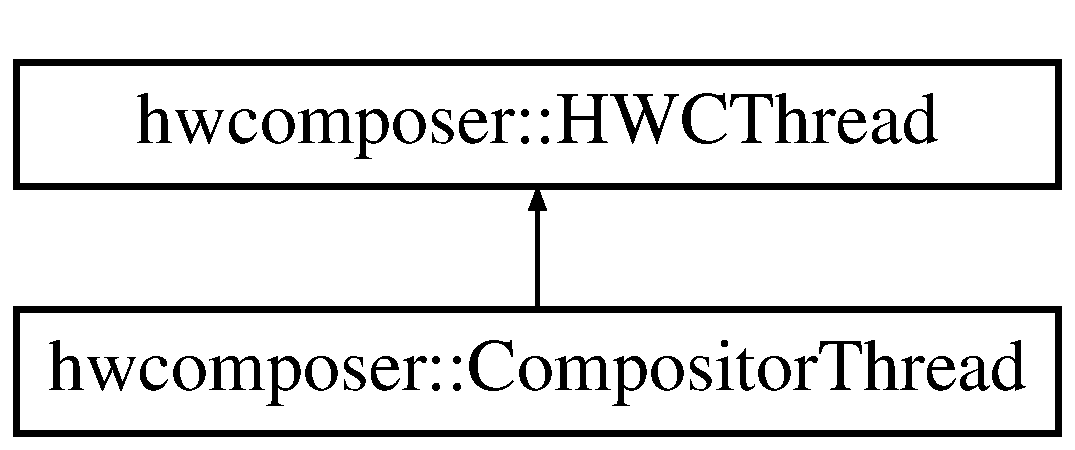
\includegraphics[height=2.000000cm]{classhwcomposer_1_1CompositorThread}
\end{center}
\end{figure}
\subsection*{Public Member Functions}
\begin{DoxyCompactItemize}
\item 
\mbox{\hyperlink{classhwcomposer_1_1CompositorThread_a28f5c6de7aee95706fed421ecf3f2ff5}{Compositor\+Thread}} ()
\item 
\mbox{\hyperlink{classhwcomposer_1_1CompositorThread_aa93b1c77c0d6d55bf30a86cb429724b7}{$\sim$\+Compositor\+Thread}} () override
\item 
void \mbox{\hyperlink{classhwcomposer_1_1CompositorThread_a0e36f2bd6e14959ffd8eff5faeefcbef}{Initialize}} (\mbox{\hyperlink{classhwcomposer_1_1ResourceManager}{Resource\+Manager}} $\ast$resource\+\_\+manager, uint32\+\_\+t gpu\+\_\+fd, \mbox{\hyperlink{classhwcomposer_1_1FrameBufferManager}{Frame\+Buffer\+Manager}} $\ast$frame\+\_\+buffer\+\_\+manager)
\item 
bool \mbox{\hyperlink{classhwcomposer_1_1CompositorThread_a16c0227a122423a7f83a8369f600923b}{Draw}} (std\+::vector$<$ \mbox{\hyperlink{structhwcomposer_1_1DrawState}{Draw\+State}} $>$ \&states, std\+::vector$<$ \mbox{\hyperlink{structhwcomposer_1_1DrawState}{Draw\+State}} $>$ \&media\+\_\+states, const std\+::vector$<$ \mbox{\hyperlink{structhwcomposer_1_1OverlayLayer}{Overlay\+Layer}} $>$ \&layers)
\item 
void \mbox{\hyperlink{classhwcomposer_1_1CompositorThread_a9a304d478866ab7518765ce632eca964}{Set\+Explicit\+Sync\+Support}} (bool disable\+\_\+explicit\+\_\+sync)
\item 
void \mbox{\hyperlink{classhwcomposer_1_1CompositorThread_af48eb5b73445e424b74c7e9375bf8f7c}{Free\+Resources}} ()
\item 
void \mbox{\hyperlink{classhwcomposer_1_1CompositorThread_af80e4eb7864b2f83a1eaa266a17b3a28}{Handle\+Routine}} () override
\item 
void \mbox{\hyperlink{classhwcomposer_1_1CompositorThread_a15f97ae71050432ba2780555368a3fca}{Handle\+Exit}} () override
\item 
void \mbox{\hyperlink{classhwcomposer_1_1CompositorThread_a700ec2d3412ae4a3cbc5742c6003e660}{Exit\+Thread}} ()
\end{DoxyCompactItemize}
\subsection*{Additional Inherited Members}


\subsection{Detailed Description}


Definition at line 41 of file compositorthread.\+h.



\subsection{Constructor \& Destructor Documentation}
\mbox{\Hypertarget{classhwcomposer_1_1CompositorThread_a28f5c6de7aee95706fed421ecf3f2ff5}\label{classhwcomposer_1_1CompositorThread_a28f5c6de7aee95706fed421ecf3f2ff5}} 
\index{hwcomposer\+::\+Compositor\+Thread@{hwcomposer\+::\+Compositor\+Thread}!Compositor\+Thread@{Compositor\+Thread}}
\index{Compositor\+Thread@{Compositor\+Thread}!hwcomposer\+::\+Compositor\+Thread@{hwcomposer\+::\+Compositor\+Thread}}
\subsubsection{\texorpdfstring{Compositor\+Thread()}{CompositorThread()}}
{\footnotesize\ttfamily hwcomposer\+::\+Compositor\+Thread\+::\+Compositor\+Thread (\begin{DoxyParamCaption}{ }\end{DoxyParamCaption})}



Definition at line 33 of file compositorthread.\+cpp.


\begin{DoxyCode}{0}
\DoxyCodeLine{33                                    : \mbox{\hyperlink{classhwcomposer_1_1HWCThread_a8780175b1679005955a94aa89fa62be1}{HWCThread}}(-8, \textcolor{stringliteral}{"CompositorThread"}) \{}
\DoxyCodeLine{34   \textcolor{keywordflow}{if} (!cevent\_.\mbox{\hyperlink{classhwcomposer_1_1HWCEvent_a5b5ee0d26d11c5697e20cde63a255e97}{Initialize}}())}
\DoxyCodeLine{35     \textcolor{keywordflow}{return};}
\DoxyCodeLine{36 }
\DoxyCodeLine{37   fd\_chandler\_.\mbox{\hyperlink{classhwcomposer_1_1FDHandler_aee421fa4ae54b7d4fcc352ebea15b4f8}{AddFd}}(cevent\_.\mbox{\hyperlink{classhwcomposer_1_1HWCEvent_a103324deefcbf4402fd302b737474416}{get\_fd}}());}
\DoxyCodeLine{38 \}}
\end{DoxyCode}
\mbox{\Hypertarget{classhwcomposer_1_1CompositorThread_aa93b1c77c0d6d55bf30a86cb429724b7}\label{classhwcomposer_1_1CompositorThread_aa93b1c77c0d6d55bf30a86cb429724b7}} 
\index{hwcomposer\+::\+Compositor\+Thread@{hwcomposer\+::\+Compositor\+Thread}!````~Compositor\+Thread@{$\sim$\+Compositor\+Thread}}
\index{````~Compositor\+Thread@{$\sim$\+Compositor\+Thread}!hwcomposer\+::\+Compositor\+Thread@{hwcomposer\+::\+Compositor\+Thread}}
\subsubsection{\texorpdfstring{$\sim$\+Compositor\+Thread()}{~CompositorThread()}}
{\footnotesize\ttfamily hwcomposer\+::\+Compositor\+Thread\+::$\sim$\+Compositor\+Thread (\begin{DoxyParamCaption}{ }\end{DoxyParamCaption})\hspace{0.3cm}{\ttfamily [override]}}



Definition at line 40 of file compositorthread.\+cpp.


\begin{DoxyCode}{0}
\DoxyCodeLine{40                                     \{}
\DoxyCodeLine{41 \}}
\end{DoxyCode}


\subsection{Member Function Documentation}
\mbox{\Hypertarget{classhwcomposer_1_1CompositorThread_a16c0227a122423a7f83a8369f600923b}\label{classhwcomposer_1_1CompositorThread_a16c0227a122423a7f83a8369f600923b}} 
\index{hwcomposer\+::\+Compositor\+Thread@{hwcomposer\+::\+Compositor\+Thread}!Draw@{Draw}}
\index{Draw@{Draw}!hwcomposer\+::\+Compositor\+Thread@{hwcomposer\+::\+Compositor\+Thread}}
\subsubsection{\texorpdfstring{Draw()}{Draw()}}
{\footnotesize\ttfamily bool hwcomposer\+::\+Compositor\+Thread\+::\+Draw (\begin{DoxyParamCaption}\item[{std\+::vector$<$ \mbox{\hyperlink{structhwcomposer_1_1DrawState}{Draw\+State}} $>$ \&}]{states,  }\item[{std\+::vector$<$ \mbox{\hyperlink{structhwcomposer_1_1DrawState}{Draw\+State}} $>$ \&}]{media\+\_\+states,  }\item[{const std\+::vector$<$ \mbox{\hyperlink{structhwcomposer_1_1OverlayLayer}{Overlay\+Layer}} $>$ \&}]{layers }\end{DoxyParamCaption})}



Definition at line 83 of file compositorthread.\+cpp.


\begin{DoxyCode}{0}
\DoxyCodeLine{85                                                                    \{}
\DoxyCodeLine{86   states\_.swap(states);}
\DoxyCodeLine{87   tasks\_lock\_.\mbox{\hyperlink{classhwcomposer_1_1SpinLock_a863f9d0f1b270f863a9298161b52faf1}{lock}}();}
\DoxyCodeLine{88 }
\DoxyCodeLine{89   \textcolor{keywordflow}{if} (!states\_.empty()) \{}
\DoxyCodeLine{90     std::vector<OverlayBuffer *>().swap(buffers\_);}
\DoxyCodeLine{91     buffers\_.reserve(layers.size());}
\DoxyCodeLine{92     \textcolor{keywordflow}{for} (\textcolor{keyword}{auto} \&layer : layers) \{}
\DoxyCodeLine{93       buffers\_.emplace\_back(layer.GetBuffer());}
\DoxyCodeLine{94     \}}
\DoxyCodeLine{95 }
\DoxyCodeLine{96     tasks\_ |= kRender3D;}
\DoxyCodeLine{97   \}}
\DoxyCodeLine{98 }
\DoxyCodeLine{99   \textcolor{keywordflow}{if} (!media\_states.empty()) \{}
\DoxyCodeLine{100     media\_states\_.swap(media\_states);}
\DoxyCodeLine{101     tasks\_ |= kRenderMedia;}
\DoxyCodeLine{102   \}}
\DoxyCodeLine{103 }
\DoxyCodeLine{104   \textcolor{comment}{// We start of assuming that the draw calls}}
\DoxyCodeLine{105   \textcolor{comment}{// succeed.}}
\DoxyCodeLine{106   draw\_succeeded\_ = \textcolor{keyword}{true};}
\DoxyCodeLine{107   tasks\_lock\_.\mbox{\hyperlink{classhwcomposer_1_1SpinLock_ae5cf624b4f0ec710833ce44e945b85d7}{unlock}}();}
\DoxyCodeLine{108 }
\DoxyCodeLine{109   \textcolor{comment}{// Adding check to avoid waiting in this}}
\DoxyCodeLine{110   \textcolor{comment}{// thread in certain corner case.}}
\DoxyCodeLine{111   \textcolor{keywordflow}{if} (states\_.empty() \&\& media\_states\_.empty()) \{}
\DoxyCodeLine{112     \textcolor{keywordflow}{return} draw\_succeeded\_;}
\DoxyCodeLine{113   \}}
\DoxyCodeLine{114 }
\DoxyCodeLine{115   \mbox{\hyperlink{classhwcomposer_1_1HWCThread_a5f38525b892525beaa7f37d2d4c50bde}{Resume}}();}
\DoxyCodeLine{116   Wait();}
\DoxyCodeLine{117   \textcolor{keywordflow}{return} draw\_succeeded\_;}
\DoxyCodeLine{118 \}}
\end{DoxyCode}
\mbox{\Hypertarget{classhwcomposer_1_1CompositorThread_a700ec2d3412ae4a3cbc5742c6003e660}\label{classhwcomposer_1_1CompositorThread_a700ec2d3412ae4a3cbc5742c6003e660}} 
\index{hwcomposer\+::\+Compositor\+Thread@{hwcomposer\+::\+Compositor\+Thread}!Exit\+Thread@{Exit\+Thread}}
\index{Exit\+Thread@{Exit\+Thread}!hwcomposer\+::\+Compositor\+Thread@{hwcomposer\+::\+Compositor\+Thread}}
\subsubsection{\texorpdfstring{Exit\+Thread()}{ExitThread()}}
{\footnotesize\ttfamily void hwcomposer\+::\+Compositor\+Thread\+::\+Exit\+Thread (\begin{DoxyParamCaption}{ }\end{DoxyParamCaption})}



Definition at line 120 of file compositorthread.\+cpp.


\begin{DoxyCode}{0}
\DoxyCodeLine{120                                   \{}
\DoxyCodeLine{121   \mbox{\hyperlink{classhwcomposer_1_1HWCThread_aa360360e4c27cbc7fed745f79990a190}{HWCThread::Exit}}();}
\DoxyCodeLine{122   std::vector<DrawState>().swap(states\_);}
\DoxyCodeLine{123   std::vector<OverlayBuffer *>().swap(buffers\_);}
\DoxyCodeLine{124 \}}
\end{DoxyCode}
\mbox{\Hypertarget{classhwcomposer_1_1CompositorThread_af48eb5b73445e424b74c7e9375bf8f7c}\label{classhwcomposer_1_1CompositorThread_af48eb5b73445e424b74c7e9375bf8f7c}} 
\index{hwcomposer\+::\+Compositor\+Thread@{hwcomposer\+::\+Compositor\+Thread}!Free\+Resources@{Free\+Resources}}
\index{Free\+Resources@{Free\+Resources}!hwcomposer\+::\+Compositor\+Thread@{hwcomposer\+::\+Compositor\+Thread}}
\subsubsection{\texorpdfstring{Free\+Resources()}{FreeResources()}}
{\footnotesize\ttfamily void hwcomposer\+::\+Compositor\+Thread\+::\+Free\+Resources (\begin{DoxyParamCaption}{ }\end{DoxyParamCaption})}



Definition at line 63 of file compositorthread.\+cpp.


\begin{DoxyCode}{0}
\DoxyCodeLine{63                                      \{}
\DoxyCodeLine{64   tasks\_lock\_.\mbox{\hyperlink{classhwcomposer_1_1SpinLock_a863f9d0f1b270f863a9298161b52faf1}{lock}}();}
\DoxyCodeLine{65   tasks\_ |= kReleaseResources;}
\DoxyCodeLine{66   tasks\_lock\_.\mbox{\hyperlink{classhwcomposer_1_1SpinLock_ae5cf624b4f0ec710833ce44e945b85d7}{unlock}}();}
\DoxyCodeLine{67   \mbox{\hyperlink{classhwcomposer_1_1HWCThread_a5f38525b892525beaa7f37d2d4c50bde}{Resume}}();}
\DoxyCodeLine{68 \}}
\end{DoxyCode}
\mbox{\Hypertarget{classhwcomposer_1_1CompositorThread_a15f97ae71050432ba2780555368a3fca}\label{classhwcomposer_1_1CompositorThread_a15f97ae71050432ba2780555368a3fca}} 
\index{hwcomposer\+::\+Compositor\+Thread@{hwcomposer\+::\+Compositor\+Thread}!Handle\+Exit@{Handle\+Exit}}
\index{Handle\+Exit@{Handle\+Exit}!hwcomposer\+::\+Compositor\+Thread@{hwcomposer\+::\+Compositor\+Thread}}
\subsubsection{\texorpdfstring{Handle\+Exit()}{HandleExit()}}
{\footnotesize\ttfamily void hwcomposer\+::\+Compositor\+Thread\+::\+Handle\+Exit (\begin{DoxyParamCaption}{ }\end{DoxyParamCaption})\hspace{0.3cm}{\ttfamily [override]}, {\ttfamily [virtual]}}



Reimplemented from \mbox{\hyperlink{classhwcomposer_1_1HWCThread_a39a94bd0b12451fe3060729787921cbf}{hwcomposer\+::\+H\+W\+C\+Thread}}.



Definition at line 126 of file compositorthread.\+cpp.


\begin{DoxyCode}{0}
\DoxyCodeLine{126                                   \{}
\DoxyCodeLine{127   HandleReleaseRequest();}
\DoxyCodeLine{128   gl\_renderer\_.reset(\textcolor{keyword}{nullptr});}
\DoxyCodeLine{129   gpu\_resource\_handler\_.reset(\textcolor{keyword}{nullptr});}
\DoxyCodeLine{130 \}}
\end{DoxyCode}
\mbox{\Hypertarget{classhwcomposer_1_1CompositorThread_af80e4eb7864b2f83a1eaa266a17b3a28}\label{classhwcomposer_1_1CompositorThread_af80e4eb7864b2f83a1eaa266a17b3a28}} 
\index{hwcomposer\+::\+Compositor\+Thread@{hwcomposer\+::\+Compositor\+Thread}!Handle\+Routine@{Handle\+Routine}}
\index{Handle\+Routine@{Handle\+Routine}!hwcomposer\+::\+Compositor\+Thread@{hwcomposer\+::\+Compositor\+Thread}}
\subsubsection{\texorpdfstring{Handle\+Routine()}{HandleRoutine()}}
{\footnotesize\ttfamily void hwcomposer\+::\+Compositor\+Thread\+::\+Handle\+Routine (\begin{DoxyParamCaption}{ }\end{DoxyParamCaption})\hspace{0.3cm}{\ttfamily [override]}, {\ttfamily [virtual]}}



Implements \mbox{\hyperlink{classhwcomposer_1_1HWCThread_a539ea080e6bf0e6cffe08e2341be1ee4}{hwcomposer\+::\+H\+W\+C\+Thread}}.



Definition at line 132 of file compositorthread.\+cpp.


\begin{DoxyCode}{0}
\DoxyCodeLine{132                                      \{}
\DoxyCodeLine{133   \textcolor{keywordtype}{bool} signal = \textcolor{keyword}{false};}
\DoxyCodeLine{134   \textcolor{keywordflow}{if} (tasks\_ \& kRender3D) \{}
\DoxyCodeLine{135     Handle3DDrawRequest();}
\DoxyCodeLine{136     signal = \textcolor{keyword}{true};}
\DoxyCodeLine{137   \}}
\DoxyCodeLine{138 }
\DoxyCodeLine{139   \textcolor{keywordflow}{if} (tasks\_ \& kRenderMedia) \{}
\DoxyCodeLine{140     HandleMediaDrawRequest();}
\DoxyCodeLine{141     signal = \textcolor{keyword}{true};}
\DoxyCodeLine{142   \}}
\DoxyCodeLine{143 }
\DoxyCodeLine{144   \textcolor{keywordflow}{if} (tasks\_ \& kReleaseResources) \{}
\DoxyCodeLine{145     HandleReleaseRequest();}
\DoxyCodeLine{146   \}}
\DoxyCodeLine{147 }
\DoxyCodeLine{148   \textcolor{keywordflow}{if} (signal) \{}
\DoxyCodeLine{149     cevent\_.\mbox{\hyperlink{classhwcomposer_1_1HWCEvent_a3cd16bda8f4fd8bcbda6dae72ff15f57}{Signal}}();}
\DoxyCodeLine{150   \}}
\DoxyCodeLine{151 \}}
\end{DoxyCode}
\mbox{\Hypertarget{classhwcomposer_1_1CompositorThread_a0e36f2bd6e14959ffd8eff5faeefcbef}\label{classhwcomposer_1_1CompositorThread_a0e36f2bd6e14959ffd8eff5faeefcbef}} 
\index{hwcomposer\+::\+Compositor\+Thread@{hwcomposer\+::\+Compositor\+Thread}!Initialize@{Initialize}}
\index{Initialize@{Initialize}!hwcomposer\+::\+Compositor\+Thread@{hwcomposer\+::\+Compositor\+Thread}}
\subsubsection{\texorpdfstring{Initialize()}{Initialize()}}
{\footnotesize\ttfamily void hwcomposer\+::\+Compositor\+Thread\+::\+Initialize (\begin{DoxyParamCaption}\item[{\mbox{\hyperlink{classhwcomposer_1_1ResourceManager}{Resource\+Manager}} $\ast$}]{resource\+\_\+manager,  }\item[{uint32\+\_\+t}]{gpu\+\_\+fd,  }\item[{\mbox{\hyperlink{classhwcomposer_1_1FrameBufferManager}{Frame\+Buffer\+Manager}} $\ast$}]{frame\+\_\+buffer\+\_\+manager }\end{DoxyParamCaption})}



Definition at line 43 of file compositorthread.\+cpp.


\begin{DoxyCode}{0}
\DoxyCodeLine{45                                                                             \{}
\DoxyCodeLine{46   fb\_manager\_ = frame\_buffer\_manager;}
\DoxyCodeLine{47   tasks\_lock\_.\mbox{\hyperlink{classhwcomposer_1_1SpinLock_a863f9d0f1b270f863a9298161b52faf1}{lock}}();}
\DoxyCodeLine{48   \textcolor{keywordflow}{if} (!gpu\_resource\_handler\_)}
\DoxyCodeLine{49     gpu\_resource\_handler\_.reset(\mbox{\hyperlink{namespacehwcomposer_a37cb4c79bf84a69887ed09adb9c5b4b0}{CreateNativeGpuResourceHandler}}());}
\DoxyCodeLine{50 }
\DoxyCodeLine{51   resource\_manager\_ = resource\_manager;}
\DoxyCodeLine{52   gpu\_fd\_ = gpu\_fd;}
\DoxyCodeLine{53   tasks\_lock\_.\mbox{\hyperlink{classhwcomposer_1_1SpinLock_ae5cf624b4f0ec710833ce44e945b85d7}{unlock}}();}
\DoxyCodeLine{54   \textcolor{keywordflow}{if} (!\mbox{\hyperlink{classhwcomposer_1_1HWCThread_a7162d49a6b4026673f77ac048eb4d07b}{InitWorker}}()) \{}
\DoxyCodeLine{55     \mbox{\hyperlink{alios_2platformdefines_8h_a226d6c99e4bcfca193c095e085e9097d}{ETRACE}}(\textcolor{stringliteral}{"Failed to initalize CompositorThread. \%s"}, \mbox{\hyperlink{hwctrace_8h_a791a01fa8fe130cef13d68a706df9034}{PRINTERROR}}());}
\DoxyCodeLine{56   \}}
\DoxyCodeLine{57 \}}
\end{DoxyCode}
\mbox{\Hypertarget{classhwcomposer_1_1CompositorThread_a9a304d478866ab7518765ce632eca964}\label{classhwcomposer_1_1CompositorThread_a9a304d478866ab7518765ce632eca964}} 
\index{hwcomposer\+::\+Compositor\+Thread@{hwcomposer\+::\+Compositor\+Thread}!Set\+Explicit\+Sync\+Support@{Set\+Explicit\+Sync\+Support}}
\index{Set\+Explicit\+Sync\+Support@{Set\+Explicit\+Sync\+Support}!hwcomposer\+::\+Compositor\+Thread@{hwcomposer\+::\+Compositor\+Thread}}
\subsubsection{\texorpdfstring{Set\+Explicit\+Sync\+Support()}{SetExplicitSyncSupport()}}
{\footnotesize\ttfamily void hwcomposer\+::\+Compositor\+Thread\+::\+Set\+Explicit\+Sync\+Support (\begin{DoxyParamCaption}\item[{bool}]{disable\+\_\+explicit\+\_\+sync }\end{DoxyParamCaption})}



Definition at line 59 of file compositorthread.\+cpp.


\begin{DoxyCode}{0}
\DoxyCodeLine{59                                                                         \{}
\DoxyCodeLine{60   disable\_explicit\_sync\_ = disable\_explicit\_sync;}
\DoxyCodeLine{61 \}}
\end{DoxyCode}


The documentation for this class was generated from the following files\+:\begin{DoxyCompactItemize}
\item 
common/compositor/\mbox{\hyperlink{compositorthread_8h}{compositorthread.\+h}}\item 
common/compositor/\mbox{\hyperlink{compositorthread_8cpp}{compositorthread.\+cpp}}\end{DoxyCompactItemize}

\hypertarget{classandroid_1_1HwcService_1_1Controls}{}\section{android\+:\+:Hwc\+Service\+:\+:Controls Class Reference}
\label{classandroid_1_1HwcService_1_1Controls}\index{android\+::\+Hwc\+Service\+::\+Controls@{android\+::\+Hwc\+Service\+::\+Controls}}


{\ttfamily \#include $<$hwcservice.\+h$>$}

Inheritance diagram for android\+:\+:Hwc\+Service\+:\+:Controls\+:\begin{figure}[H]
\begin{center}
\leavevmode
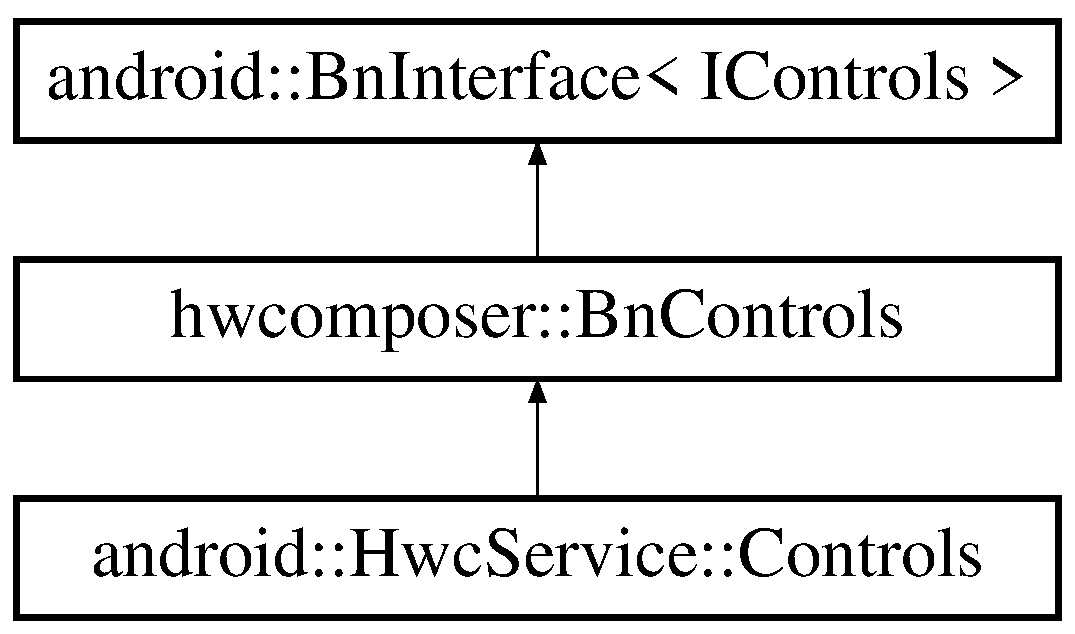
\includegraphics[height=3.000000cm]{classandroid_1_1HwcService_1_1Controls}
\end{center}
\end{figure}
\subsection*{Public Member Functions}
\begin{DoxyCompactItemize}
\item 
\mbox{\hyperlink{classandroid_1_1HwcService_1_1Controls_aeacac33397b3210a02241d5d477f81e5}{Controls}} (\mbox{\hyperlink{classandroid_1_1IAHWC2}{I\+A\+H\+W\+C2}} \&hwc, \mbox{\hyperlink{classandroid_1_1HwcService}{Hwc\+Service}} \&hwc\+Service)
\item 
virtual \mbox{\hyperlink{classandroid_1_1HwcService_1_1Controls_aa36cd79cbdaae3d5993f5159682cce25}{$\sim$\+Controls}} ()
\item 
\mbox{\hyperlink{hwcserviceapi_8h_a3806fb2027d9a316d8ca8d9b8b8eb96f}{status\+\_\+t}} \mbox{\hyperlink{classandroid_1_1HwcService_1_1Controls_adcf1f387f3090dc329279f9d0c433baf}{Display\+Set\+Overscan}} (uint32\+\_\+t display, int32\+\_\+t xoverscan, int32\+\_\+t yoverscan)
\item 
\mbox{\hyperlink{hwcserviceapi_8h_a3806fb2027d9a316d8ca8d9b8b8eb96f}{status\+\_\+t}} \mbox{\hyperlink{classandroid_1_1HwcService_1_1Controls_ae9070f7ea0cce4a96d95bdcda6447324}{Display\+Get\+Overscan}} (uint32\+\_\+t display, int32\+\_\+t $\ast$xoverscan, int32\+\_\+t $\ast$yoverscan)
\item 
\mbox{\hyperlink{hwcserviceapi_8h_a3806fb2027d9a316d8ca8d9b8b8eb96f}{status\+\_\+t}} \mbox{\hyperlink{classandroid_1_1HwcService_1_1Controls_a5fb40a804ceea847a8ec98de7387d2ec}{Display\+Set\+Scaling}} (uint32\+\_\+t display, \mbox{\hyperlink{hwcserviceapi_8h_acdadfd5e7f15097833789174e442083f}{E\+Hwcs\+Scaling\+Mode}} e\+Scaling\+Mode)
\item 
\mbox{\hyperlink{hwcserviceapi_8h_a3806fb2027d9a316d8ca8d9b8b8eb96f}{status\+\_\+t}} \mbox{\hyperlink{classandroid_1_1HwcService_1_1Controls_a374b5ef0ffbe6cfc6cce6981b0647431}{Display\+Get\+Scaling}} (uint32\+\_\+t display, \mbox{\hyperlink{hwcserviceapi_8h_acdadfd5e7f15097833789174e442083f}{E\+Hwcs\+Scaling\+Mode}} $\ast$e\+Scaling\+Mode)
\item 
\mbox{\hyperlink{hwcserviceapi_8h_a3806fb2027d9a316d8ca8d9b8b8eb96f}{status\+\_\+t}} \mbox{\hyperlink{classandroid_1_1HwcService_1_1Controls_ab38acaba6b6dfa89a91f1fd12bfc1943}{Display\+Enable\+Blank}} (uint32\+\_\+t display, bool blank)
\item 
\mbox{\hyperlink{hwcserviceapi_8h_a3806fb2027d9a316d8ca8d9b8b8eb96f}{status\+\_\+t}} \mbox{\hyperlink{classandroid_1_1HwcService_1_1Controls_abbb4cbd0508e1faf4ee4141a9c64b5b0}{Display\+Restore\+Default\+Color\+Param}} (uint32\+\_\+t display, \mbox{\hyperlink{hwcserviceapi_8h_a1d1cbf448ce748672cf3dd96675d70e4}{E\+Hwcs\+Color\+Control}} color)
\item 
\mbox{\hyperlink{hwcserviceapi_8h_a3806fb2027d9a316d8ca8d9b8b8eb96f}{status\+\_\+t}} \mbox{\hyperlink{classandroid_1_1HwcService_1_1Controls_a25d328152f7bc1f79dd5f06b9b59c24d}{Display\+Restore\+Default\+Deinterlace\+Param}} (uint32\+\_\+t display)
\item 
\mbox{\hyperlink{hwcserviceapi_8h_a3806fb2027d9a316d8ca8d9b8b8eb96f}{status\+\_\+t}} \mbox{\hyperlink{classandroid_1_1HwcService_1_1Controls_a949dc7e60f66edf99982523e53cb5691}{Display\+Get\+Color\+Param}} (uint32\+\_\+t display, \mbox{\hyperlink{hwcserviceapi_8h_a1d1cbf448ce748672cf3dd96675d70e4}{E\+Hwcs\+Color\+Control}} color, float $\ast$value, float $\ast$startvalue, float $\ast$endvalue)
\item 
\mbox{\hyperlink{hwcserviceapi_8h_a3806fb2027d9a316d8ca8d9b8b8eb96f}{status\+\_\+t}} \mbox{\hyperlink{classandroid_1_1HwcService_1_1Controls_a87f1656780eb437cefb9f398713af762}{Display\+Set\+Color\+Param}} (uint32\+\_\+t display, \mbox{\hyperlink{hwcserviceapi_8h_a1d1cbf448ce748672cf3dd96675d70e4}{E\+Hwcs\+Color\+Control}} color, float value)
\item 
\mbox{\hyperlink{hwcserviceapi_8h_a3806fb2027d9a316d8ca8d9b8b8eb96f}{status\+\_\+t}} \mbox{\hyperlink{classandroid_1_1HwcService_1_1Controls_adb0bdb522323be0ea0122464227459ef}{Display\+Set\+Deinterlace\+Param}} (uint32\+\_\+t display, \mbox{\hyperlink{hwcserviceapi_8h_a8473f2ec9e7333e67be46a1bea689113}{E\+Hwcs\+Deinterlace\+Control}} mode)
\item 
std\+::vector$<$ \mbox{\hyperlink{hwcserviceapi_8h_a6e13f5285374b86aab82ec0c0ba62d7a}{Hwcs\+Display\+Mode\+Info}} $>$ \mbox{\hyperlink{classandroid_1_1HwcService_1_1Controls_aae5310df10b584ddb537266bcb9399b5}{Display\+Mode\+Get\+Available\+Modes}} (uint32\+\_\+t display)
\item 
\mbox{\hyperlink{hwcserviceapi_8h_a3806fb2027d9a316d8ca8d9b8b8eb96f}{status\+\_\+t}} \mbox{\hyperlink{classandroid_1_1HwcService_1_1Controls_a359b41bbda3b6b5507dd23436cdca678}{Display\+Mode\+Get\+Mode}} (uint32\+\_\+t display, \mbox{\hyperlink{hwcserviceapi_8h_a6e13f5285374b86aab82ec0c0ba62d7a}{Hwcs\+Display\+Mode\+Info}} $\ast$p\+Mode)
\item 
\mbox{\hyperlink{hwcserviceapi_8h_a3806fb2027d9a316d8ca8d9b8b8eb96f}{status\+\_\+t}} \mbox{\hyperlink{classandroid_1_1HwcService_1_1Controls_a93a09106cc484a459e73b0d250937509}{Display\+Mode\+Set\+Mode}} (uint32\+\_\+t display, const uint32\+\_\+t config)
\item 
\mbox{\hyperlink{hwcserviceapi_8h_a3806fb2027d9a316d8ca8d9b8b8eb96f}{status\+\_\+t}} \mbox{\hyperlink{classandroid_1_1HwcService_1_1Controls_a142e297708c613277cb7721c040b0a77}{Enable\+H\+D\+C\+P\+Session\+For\+Display}} (uint32\+\_\+t display, \mbox{\hyperlink{hwcserviceapi_8h_a69e9b3a54e4c8e504845398c66eab655}{E\+Hwcs\+Content\+Type}} content\+\_\+type)
\item 
\mbox{\hyperlink{hwcserviceapi_8h_a3806fb2027d9a316d8ca8d9b8b8eb96f}{status\+\_\+t}} \mbox{\hyperlink{classandroid_1_1HwcService_1_1Controls_ae703b526fe5b7a155afba4ff1b476a29}{Enable\+H\+D\+C\+P\+Session\+For\+All\+Displays}} (\mbox{\hyperlink{hwcserviceapi_8h_a69e9b3a54e4c8e504845398c66eab655}{E\+Hwcs\+Content\+Type}} content\+\_\+type)
\item 
\mbox{\hyperlink{hwcserviceapi_8h_a3806fb2027d9a316d8ca8d9b8b8eb96f}{status\+\_\+t}} \mbox{\hyperlink{classandroid_1_1HwcService_1_1Controls_a7dcb46dcf375714e13431a237b82374f}{Disable\+H\+D\+C\+P\+Session\+For\+Display}} (uint32\+\_\+t display)
\item 
\mbox{\hyperlink{hwcserviceapi_8h_a3806fb2027d9a316d8ca8d9b8b8eb96f}{status\+\_\+t}} \mbox{\hyperlink{classandroid_1_1HwcService_1_1Controls_aefda1ddf238e363f7b3fbae760f9658d}{Disable\+H\+D\+C\+P\+Session\+For\+All\+Displays}} ()
\item 
\mbox{\hyperlink{hwcserviceapi_8h_a3806fb2027d9a316d8ca8d9b8b8eb96f}{status\+\_\+t}} \mbox{\hyperlink{classandroid_1_1HwcService_1_1Controls_a17836d295dcf16b98ee2471d52a21d3f}{Video\+Enable\+Encrypted\+Session}} (uint32\+\_\+t session\+ID, uint32\+\_\+t instance\+ID)
\item 
\mbox{\hyperlink{hwcserviceapi_8h_a3806fb2027d9a316d8ca8d9b8b8eb96f}{status\+\_\+t}} \mbox{\hyperlink{classandroid_1_1HwcService_1_1Controls_a199821eab8be184fbc910305da592ff0}{Video\+Disable\+All\+Encrypted\+Sessions}} (uint32\+\_\+t session\+ID)
\item 
\mbox{\hyperlink{hwcserviceapi_8h_a3806fb2027d9a316d8ca8d9b8b8eb96f}{status\+\_\+t}} \mbox{\hyperlink{classandroid_1_1HwcService_1_1Controls_ae4da8d03acf7eb18dfd91b41cfc55887}{Video\+Disable\+All\+Encrypted\+Sessions}} ()
\item 
bool \mbox{\hyperlink{classandroid_1_1HwcService_1_1Controls_a6e1af9c9130f6850c2e1a89df4a15158}{Video\+Is\+Encrypted\+Session\+Enabled}} (uint32\+\_\+t session\+ID, uint32\+\_\+t instance\+ID)
\item 
bool \mbox{\hyperlink{classandroid_1_1HwcService_1_1Controls_a298a713544146bc768127b2f1aaebd7f}{need\+Set\+Key\+Frame\+Hint}} ()
\item 
\mbox{\hyperlink{hwcserviceapi_8h_a3806fb2027d9a316d8ca8d9b8b8eb96f}{status\+\_\+t}} \mbox{\hyperlink{classandroid_1_1HwcService_1_1Controls_a288b633b5e5e29d4778bcc4bff7e346b}{Video\+Set\+Optimization\+Mode}} (\mbox{\hyperlink{hwcserviceapi_8h_a73044de23b8f474352d6753e21fca06d}{E\+Hwcs\+Optimization\+Mode}} mode)
\item 
\mbox{\hyperlink{hwcserviceapi_8h_a3806fb2027d9a316d8ca8d9b8b8eb96f}{status\+\_\+t}} \mbox{\hyperlink{classandroid_1_1HwcService_1_1Controls_abed610ae73b7c38693a2f2d2221c2910}{Mds\+Update\+Video\+State}} (int64\+\_\+t video\+Session\+ID, bool is\+Prepared)
\item 
\mbox{\hyperlink{hwcserviceapi_8h_a3806fb2027d9a316d8ca8d9b8b8eb96f}{status\+\_\+t}} \mbox{\hyperlink{classandroid_1_1HwcService_1_1Controls_aa87c6a814f7cf0473ecd5c10c7b0e2de}{Mds\+Update\+Video\+F\+PS}} (int64\+\_\+t video\+Session\+ID, int32\+\_\+t fps)
\item 
\mbox{\hyperlink{hwcserviceapi_8h_a3806fb2027d9a316d8ca8d9b8b8eb96f}{status\+\_\+t}} \mbox{\hyperlink{classandroid_1_1HwcService_1_1Controls_a9d0b5be8274a1e794186369c5e0f8384}{Mds\+Update\+Input\+State}} (bool state)
\item 
\mbox{\hyperlink{hwcserviceapi_8h_a3806fb2027d9a316d8ca8d9b8b8eb96f}{status\+\_\+t}} \mbox{\hyperlink{classandroid_1_1HwcService_1_1Controls_a1fa6ed897de094545383b2e865753834}{Widi\+Get\+Single\+Display}} (bool $\ast$p\+Enabled)
\item 
\mbox{\hyperlink{hwcserviceapi_8h_a3806fb2027d9a316d8ca8d9b8b8eb96f}{status\+\_\+t}} \mbox{\hyperlink{classandroid_1_1HwcService_1_1Controls_a60113daf8a701fcef054ac2da704a2b9}{Widi\+Set\+Single\+Display}} (bool enable)
\end{DoxyCompactItemize}


\subsection{Detailed Description}


Definition at line 62 of file hwcservice.\+h.



\subsection{Constructor \& Destructor Documentation}
\mbox{\Hypertarget{classandroid_1_1HwcService_1_1Controls_aeacac33397b3210a02241d5d477f81e5}\label{classandroid_1_1HwcService_1_1Controls_aeacac33397b3210a02241d5d477f81e5}} 
\index{android\+::\+Hwc\+Service\+::\+Controls@{android\+::\+Hwc\+Service\+::\+Controls}!Controls@{Controls}}
\index{Controls@{Controls}!android\+::\+Hwc\+Service\+::\+Controls@{android\+::\+Hwc\+Service\+::\+Controls}}
\subsubsection{\texorpdfstring{Controls()}{Controls()}}
{\footnotesize\ttfamily android\+::\+Hwc\+Service\+::\+Controls\+::\+Controls (\begin{DoxyParamCaption}\item[{\mbox{\hyperlink{classandroid_1_1IAHWC2}{I\+A\+H\+W\+C2}} \&}]{hwc,  }\item[{\mbox{\hyperlink{classandroid_1_1HwcService}{Hwc\+Service}} \&}]{hwc\+Service }\end{DoxyParamCaption})}



Definition at line 138 of file hwcservice.\+cpp.


\begin{DoxyCode}{0}
\DoxyCodeLine{139     : mHwc(hwc),}
\DoxyCodeLine{140       mHwcService(hwcService),}
\DoxyCodeLine{141       mbHaveSessionsEnabled(\textcolor{keyword}{false}),}
\DoxyCodeLine{142       mCurrentOptimizationMode(\mbox{\hyperlink{hwcserviceapi_8h_abbce4018fab4dc54c5d3994ac2f6bf58a410bfe259d70975cc9a5098758309844}{HWCS\_OPTIMIZE\_NORMAL}}) \{}
\DoxyCodeLine{143 \}}
\end{DoxyCode}
\mbox{\Hypertarget{classandroid_1_1HwcService_1_1Controls_aa36cd79cbdaae3d5993f5159682cce25}\label{classandroid_1_1HwcService_1_1Controls_aa36cd79cbdaae3d5993f5159682cce25}} 
\index{android\+::\+Hwc\+Service\+::\+Controls@{android\+::\+Hwc\+Service\+::\+Controls}!````~Controls@{$\sim$\+Controls}}
\index{````~Controls@{$\sim$\+Controls}!android\+::\+Hwc\+Service\+::\+Controls@{android\+::\+Hwc\+Service\+::\+Controls}}
\subsubsection{\texorpdfstring{$\sim$\+Controls()}{~Controls()}}
{\footnotesize\ttfamily android\+::\+Hwc\+Service\+::\+Controls\+::$\sim$\+Controls (\begin{DoxyParamCaption}{ }\end{DoxyParamCaption})\hspace{0.3cm}{\ttfamily [virtual]}}



Definition at line 145 of file hwcservice.\+cpp.


\begin{DoxyCode}{0}
\DoxyCodeLine{145                               \{}
\DoxyCodeLine{146 \}}
\end{DoxyCode}


\subsection{Member Function Documentation}
\mbox{\Hypertarget{classandroid_1_1HwcService_1_1Controls_aefda1ddf238e363f7b3fbae760f9658d}\label{classandroid_1_1HwcService_1_1Controls_aefda1ddf238e363f7b3fbae760f9658d}} 
\index{android\+::\+Hwc\+Service\+::\+Controls@{android\+::\+Hwc\+Service\+::\+Controls}!Disable\+H\+D\+C\+P\+Session\+For\+All\+Displays@{Disable\+H\+D\+C\+P\+Session\+For\+All\+Displays}}
\index{Disable\+H\+D\+C\+P\+Session\+For\+All\+Displays@{Disable\+H\+D\+C\+P\+Session\+For\+All\+Displays}!android\+::\+Hwc\+Service\+::\+Controls@{android\+::\+Hwc\+Service\+::\+Controls}}
\subsubsection{\texorpdfstring{Disable\+H\+D\+C\+P\+Session\+For\+All\+Displays()}{DisableHDCPSessionForAllDisplays()}}
{\footnotesize\ttfamily \mbox{\hyperlink{hwcserviceapi_8h_a3806fb2027d9a316d8ca8d9b8b8eb96f}{status\+\_\+t}} android\+::\+Hwc\+Service\+::\+Controls\+::\+Disable\+H\+D\+C\+P\+Session\+For\+All\+Displays (\begin{DoxyParamCaption}{ }\end{DoxyParamCaption})}



Definition at line 384 of file hwcservice.\+cpp.


\begin{DoxyCode}{0}
\DoxyCodeLine{384                                                               \{}
\DoxyCodeLine{385   mHwc.\mbox{\hyperlink{classandroid_1_1IAHWC2_aab6e5e72a11dea3b84889e7df3ca76ee}{DisableHDCPSessionForAllDisplays}}();}
\DoxyCodeLine{386   \textcolor{keywordflow}{return} OK;}
\DoxyCodeLine{387 \}}
\end{DoxyCode}
\mbox{\Hypertarget{classandroid_1_1HwcService_1_1Controls_a7dcb46dcf375714e13431a237b82374f}\label{classandroid_1_1HwcService_1_1Controls_a7dcb46dcf375714e13431a237b82374f}} 
\index{android\+::\+Hwc\+Service\+::\+Controls@{android\+::\+Hwc\+Service\+::\+Controls}!Disable\+H\+D\+C\+P\+Session\+For\+Display@{Disable\+H\+D\+C\+P\+Session\+For\+Display}}
\index{Disable\+H\+D\+C\+P\+Session\+For\+Display@{Disable\+H\+D\+C\+P\+Session\+For\+Display}!android\+::\+Hwc\+Service\+::\+Controls@{android\+::\+Hwc\+Service\+::\+Controls}}
\subsubsection{\texorpdfstring{Disable\+H\+D\+C\+P\+Session\+For\+Display()}{DisableHDCPSessionForDisplay()}}
{\footnotesize\ttfamily \mbox{\hyperlink{hwcserviceapi_8h_a3806fb2027d9a316d8ca8d9b8b8eb96f}{status\+\_\+t}} android\+::\+Hwc\+Service\+::\+Controls\+::\+Disable\+H\+D\+C\+P\+Session\+For\+Display (\begin{DoxyParamCaption}\item[{uint32\+\_\+t}]{display }\end{DoxyParamCaption})}



Definition at line 379 of file hwcservice.\+cpp.


\begin{DoxyCode}{0}
\DoxyCodeLine{379                                                                           \{}
\DoxyCodeLine{380   mHwc.\mbox{\hyperlink{classandroid_1_1IAHWC2_aaf25b167aeb33efb991f4872f421061f}{DisableHDCPSessionForDisplay}}(display);}
\DoxyCodeLine{381   \textcolor{keywordflow}{return} OK;}
\DoxyCodeLine{382 \}}
\end{DoxyCode}
\mbox{\Hypertarget{classandroid_1_1HwcService_1_1Controls_ab38acaba6b6dfa89a91f1fd12bfc1943}\label{classandroid_1_1HwcService_1_1Controls_ab38acaba6b6dfa89a91f1fd12bfc1943}} 
\index{android\+::\+Hwc\+Service\+::\+Controls@{android\+::\+Hwc\+Service\+::\+Controls}!Display\+Enable\+Blank@{Display\+Enable\+Blank}}
\index{Display\+Enable\+Blank@{Display\+Enable\+Blank}!android\+::\+Hwc\+Service\+::\+Controls@{android\+::\+Hwc\+Service\+::\+Controls}}
\subsubsection{\texorpdfstring{Display\+Enable\+Blank()}{DisplayEnableBlank()}}
{\footnotesize\ttfamily \mbox{\hyperlink{hwcserviceapi_8h_a3806fb2027d9a316d8ca8d9b8b8eb96f}{status\+\_\+t}} android\+::\+Hwc\+Service\+::\+Controls\+::\+Display\+Enable\+Blank (\begin{DoxyParamCaption}\item[{uint32\+\_\+t}]{display,  }\item[{bool}]{blank }\end{DoxyParamCaption})}



Definition at line 221 of file hwcservice.\+cpp.


\begin{DoxyCode}{0}
\DoxyCodeLine{222                                                               \{}
\DoxyCodeLine{223   \textcolor{comment}{// TO DO}}
\DoxyCodeLine{224   \textcolor{keywordflow}{return} OK;}
\DoxyCodeLine{225 \}}
\end{DoxyCode}
\mbox{\Hypertarget{classandroid_1_1HwcService_1_1Controls_a949dc7e60f66edf99982523e53cb5691}\label{classandroid_1_1HwcService_1_1Controls_a949dc7e60f66edf99982523e53cb5691}} 
\index{android\+::\+Hwc\+Service\+::\+Controls@{android\+::\+Hwc\+Service\+::\+Controls}!Display\+Get\+Color\+Param@{Display\+Get\+Color\+Param}}
\index{Display\+Get\+Color\+Param@{Display\+Get\+Color\+Param}!android\+::\+Hwc\+Service\+::\+Controls@{android\+::\+Hwc\+Service\+::\+Controls}}
\subsubsection{\texorpdfstring{Display\+Get\+Color\+Param()}{DisplayGetColorParam()}}
{\footnotesize\ttfamily \mbox{\hyperlink{hwcserviceapi_8h_a3806fb2027d9a316d8ca8d9b8b8eb96f}{status\+\_\+t}} android\+::\+Hwc\+Service\+::\+Controls\+::\+Display\+Get\+Color\+Param (\begin{DoxyParamCaption}\item[{uint32\+\_\+t}]{display,  }\item[{\mbox{\hyperlink{hwcserviceapi_8h_a1d1cbf448ce748672cf3dd96675d70e4}{E\+Hwcs\+Color\+Control}}}]{color,  }\item[{float $\ast$}]{value,  }\item[{float $\ast$}]{startvalue,  }\item[{float $\ast$}]{endvalue }\end{DoxyParamCaption})}



Definition at line 251 of file hwcservice.\+cpp.


\begin{DoxyCode}{0}
\DoxyCodeLine{255                                                                      \{}
\DoxyCodeLine{256   \mbox{\hyperlink{classhwcomposer_1_1NativeDisplay}{hwcomposer::NativeDisplay}} *phyDisplay;}
\DoxyCodeLine{257   \textcolor{keywordflow}{if} (!display) \{}
\DoxyCodeLine{258     phyDisplay = mHwc.\mbox{\hyperlink{classandroid_1_1IAHWC2_a2ccc293910577a09cfe0a0f6c1f786ea}{GetPrimaryDisplay}}();}
\DoxyCodeLine{259   \} \textcolor{keywordflow}{else} \{}
\DoxyCodeLine{260     phyDisplay = mHwc.\mbox{\hyperlink{classandroid_1_1IAHWC2_a9b5b98f12f0580b5d328e6fc6b1465dc}{GetExtendedDisplay}}(display - 1);}
\DoxyCodeLine{261   \}}
\DoxyCodeLine{262   phyDisplay->\mbox{\hyperlink{classhwcomposer_1_1NativeDisplay_a2db52a8a234064113a0e250a059663ac}{GetVideoColor}}(HWCS2HWC(color), value, startvalue, endvalue);}
\DoxyCodeLine{263   \textcolor{keywordflow}{return} OK;}
\DoxyCodeLine{264 \}}
\end{DoxyCode}
\mbox{\Hypertarget{classandroid_1_1HwcService_1_1Controls_ae9070f7ea0cce4a96d95bdcda6447324}\label{classandroid_1_1HwcService_1_1Controls_ae9070f7ea0cce4a96d95bdcda6447324}} 
\index{android\+::\+Hwc\+Service\+::\+Controls@{android\+::\+Hwc\+Service\+::\+Controls}!Display\+Get\+Overscan@{Display\+Get\+Overscan}}
\index{Display\+Get\+Overscan@{Display\+Get\+Overscan}!android\+::\+Hwc\+Service\+::\+Controls@{android\+::\+Hwc\+Service\+::\+Controls}}
\subsubsection{\texorpdfstring{Display\+Get\+Overscan()}{DisplayGetOverscan()}}
{\footnotesize\ttfamily \mbox{\hyperlink{hwcserviceapi_8h_a3806fb2027d9a316d8ca8d9b8b8eb96f}{status\+\_\+t}} android\+::\+Hwc\+Service\+::\+Controls\+::\+Display\+Get\+Overscan (\begin{DoxyParamCaption}\item[{uint32\+\_\+t}]{display,  }\item[{int32\+\_\+t $\ast$}]{xoverscan,  }\item[{int32\+\_\+t $\ast$}]{yoverscan }\end{DoxyParamCaption})}



Definition at line 202 of file hwcservice.\+cpp.


\begin{DoxyCode}{0}
\DoxyCodeLine{204                                                                       \{}
\DoxyCodeLine{205   \textcolor{comment}{// TO DO}}
\DoxyCodeLine{206   \textcolor{keywordflow}{return} OK;}
\DoxyCodeLine{207 \}}
\end{DoxyCode}
\mbox{\Hypertarget{classandroid_1_1HwcService_1_1Controls_a374b5ef0ffbe6cfc6cce6981b0647431}\label{classandroid_1_1HwcService_1_1Controls_a374b5ef0ffbe6cfc6cce6981b0647431}} 
\index{android\+::\+Hwc\+Service\+::\+Controls@{android\+::\+Hwc\+Service\+::\+Controls}!Display\+Get\+Scaling@{Display\+Get\+Scaling}}
\index{Display\+Get\+Scaling@{Display\+Get\+Scaling}!android\+::\+Hwc\+Service\+::\+Controls@{android\+::\+Hwc\+Service\+::\+Controls}}
\subsubsection{\texorpdfstring{Display\+Get\+Scaling()}{DisplayGetScaling()}}
{\footnotesize\ttfamily \mbox{\hyperlink{hwcserviceapi_8h_a3806fb2027d9a316d8ca8d9b8b8eb96f}{status\+\_\+t}} android\+::\+Hwc\+Service\+::\+Controls\+::\+Display\+Get\+Scaling (\begin{DoxyParamCaption}\item[{uint32\+\_\+t}]{display,  }\item[{\mbox{\hyperlink{hwcserviceapi_8h_acdadfd5e7f15097833789174e442083f}{E\+Hwcs\+Scaling\+Mode}} $\ast$}]{e\+Scaling\+Mode }\end{DoxyParamCaption})}



Definition at line 215 of file hwcservice.\+cpp.


\begin{DoxyCode}{0}
\DoxyCodeLine{216                                                        \{}
\DoxyCodeLine{217   \textcolor{comment}{// TO DO}}
\DoxyCodeLine{218   \textcolor{keywordflow}{return} OK;}
\DoxyCodeLine{219 \}}
\end{DoxyCode}
\mbox{\Hypertarget{classandroid_1_1HwcService_1_1Controls_aae5310df10b584ddb537266bcb9399b5}\label{classandroid_1_1HwcService_1_1Controls_aae5310df10b584ddb537266bcb9399b5}} 
\index{android\+::\+Hwc\+Service\+::\+Controls@{android\+::\+Hwc\+Service\+::\+Controls}!Display\+Mode\+Get\+Available\+Modes@{Display\+Mode\+Get\+Available\+Modes}}
\index{Display\+Mode\+Get\+Available\+Modes@{Display\+Mode\+Get\+Available\+Modes}!android\+::\+Hwc\+Service\+::\+Controls@{android\+::\+Hwc\+Service\+::\+Controls}}
\subsubsection{\texorpdfstring{Display\+Mode\+Get\+Available\+Modes()}{DisplayModeGetAvailableModes()}}
{\footnotesize\ttfamily std\+::vector$<$ \mbox{\hyperlink{hwcserviceapi_8h_a6e13f5285374b86aab82ec0c0ba62d7a}{Hwcs\+Display\+Mode\+Info}} $>$ android\+::\+Hwc\+Service\+::\+Controls\+::\+Display\+Mode\+Get\+Available\+Modes (\begin{DoxyParamCaption}\item[{uint32\+\_\+t}]{display }\end{DoxyParamCaption})}



Definition at line 293 of file hwcservice.\+cpp.


\begin{DoxyCode}{0}
\DoxyCodeLine{293                                                                  \{}
\DoxyCodeLine{294   std::vector<HwcsDisplayModeInfo> modes;}
\DoxyCodeLine{295   \mbox{\hyperlink{classhwcomposer_1_1NativeDisplay}{hwcomposer::NativeDisplay}} *phyDisplay;}
\DoxyCodeLine{296   \textcolor{keywordflow}{if} (!display) \{}
\DoxyCodeLine{297     phyDisplay = mHwc.\mbox{\hyperlink{classandroid_1_1IAHWC2_a2ccc293910577a09cfe0a0f6c1f786ea}{GetPrimaryDisplay}}();}
\DoxyCodeLine{298   \} \textcolor{keywordflow}{else} \{}
\DoxyCodeLine{299     phyDisplay = mHwc.\mbox{\hyperlink{classandroid_1_1IAHWC2_a9b5b98f12f0580b5d328e6fc6b1465dc}{GetExtendedDisplay}}(display - 1);}
\DoxyCodeLine{300   \}}
\DoxyCodeLine{301   uint32\_t numConfigs;}
\DoxyCodeLine{302   int32\_t tempValue;}
\DoxyCodeLine{303   phyDisplay->\mbox{\hyperlink{classhwcomposer_1_1NativeDisplay_a9479dcf82765996db6d7ea1cdcef3864}{GetDisplayConfigs}}(\&numConfigs, \mbox{\hyperlink{alios_2platformdefines_8h_a070d2ce7b6bb7e5c05602aa8c308d0c4}{NULL}});}
\DoxyCodeLine{304   \textcolor{keywordflow}{for} (uint32\_t i = 0; i < numConfigs; i++) \{}
\DoxyCodeLine{305     \mbox{\hyperlink{struct__HwcsDisplayModeInfo}{HwcsDisplayModeInfo}} mode;}
\DoxyCodeLine{306     phyDisplay->\mbox{\hyperlink{classhwcomposer_1_1NativeDisplay_aeb880e4a295eab49a98804380c2dcb84}{GetDisplayAttribute}}(i, hwcomposer::HWCDisplayAttribute::kWidth,}
\DoxyCodeLine{307                                     \&tempValue);}
\DoxyCodeLine{308     mode.\mbox{\hyperlink{struct__HwcsDisplayModeInfo_a50ed795465b52cda71e38e0c5eae2804}{width}} = tempValue;}
\DoxyCodeLine{309     phyDisplay->\mbox{\hyperlink{classhwcomposer_1_1NativeDisplay_aeb880e4a295eab49a98804380c2dcb84}{GetDisplayAttribute}}(i, hwcomposer::HWCDisplayAttribute::kHeight,}
\DoxyCodeLine{310                                     \&tempValue);}
\DoxyCodeLine{311     mode.\mbox{\hyperlink{struct__HwcsDisplayModeInfo_a89f5474962a13b045ce25b84929c6be3}{height}} = tempValue;}
\DoxyCodeLine{312     phyDisplay->\mbox{\hyperlink{classhwcomposer_1_1NativeDisplay_aeb880e4a295eab49a98804380c2dcb84}{GetDisplayAttribute}}(}
\DoxyCodeLine{313         i, hwcomposer::HWCDisplayAttribute::kRefreshRate, \&tempValue);}
\DoxyCodeLine{314     mode.\mbox{\hyperlink{struct__HwcsDisplayModeInfo_afbc17f7325634fd5b86eeb0a2023c635}{refresh}} = tempValue;}
\DoxyCodeLine{315     phyDisplay->\mbox{\hyperlink{classhwcomposer_1_1NativeDisplay_aeb880e4a295eab49a98804380c2dcb84}{GetDisplayAttribute}}(i, hwcomposer::HWCDisplayAttribute::kDpiX,}
\DoxyCodeLine{316                                     \&tempValue);}
\DoxyCodeLine{317     mode.\mbox{\hyperlink{struct__HwcsDisplayModeInfo_ad8d33821439c3aeb8b125296cb62dbbb}{xdpi}} = tempValue;}
\DoxyCodeLine{318     phyDisplay->\mbox{\hyperlink{classhwcomposer_1_1NativeDisplay_aeb880e4a295eab49a98804380c2dcb84}{GetDisplayAttribute}}(i, hwcomposer::HWCDisplayAttribute::kDpiY,}
\DoxyCodeLine{319                                     \&tempValue);}
\DoxyCodeLine{320     mode.\mbox{\hyperlink{struct__HwcsDisplayModeInfo_a53ef1f5ece0baea9b74b76dbf9c0fc19}{ydpi}} = tempValue;}
\DoxyCodeLine{321     modes.push\_back(mode);}
\DoxyCodeLine{322   \}}
\DoxyCodeLine{323   \textcolor{keywordflow}{return} modes;}
\DoxyCodeLine{324 \}}
\end{DoxyCode}
\mbox{\Hypertarget{classandroid_1_1HwcService_1_1Controls_a359b41bbda3b6b5507dd23436cdca678}\label{classandroid_1_1HwcService_1_1Controls_a359b41bbda3b6b5507dd23436cdca678}} 
\index{android\+::\+Hwc\+Service\+::\+Controls@{android\+::\+Hwc\+Service\+::\+Controls}!Display\+Mode\+Get\+Mode@{Display\+Mode\+Get\+Mode}}
\index{Display\+Mode\+Get\+Mode@{Display\+Mode\+Get\+Mode}!android\+::\+Hwc\+Service\+::\+Controls@{android\+::\+Hwc\+Service\+::\+Controls}}
\subsubsection{\texorpdfstring{Display\+Mode\+Get\+Mode()}{DisplayModeGetMode()}}
{\footnotesize\ttfamily \mbox{\hyperlink{hwcserviceapi_8h_a3806fb2027d9a316d8ca8d9b8b8eb96f}{status\+\_\+t}} android\+::\+Hwc\+Service\+::\+Controls\+::\+Display\+Mode\+Get\+Mode (\begin{DoxyParamCaption}\item[{uint32\+\_\+t}]{display,  }\item[{\mbox{\hyperlink{hwcserviceapi_8h_a6e13f5285374b86aab82ec0c0ba62d7a}{Hwcs\+Display\+Mode\+Info}} $\ast$}]{p\+Mode }\end{DoxyParamCaption})}



Definition at line 326 of file hwcservice.\+cpp.


\begin{DoxyCode}{0}
\DoxyCodeLine{327                                                                               \{}
\DoxyCodeLine{328   \mbox{\hyperlink{classhwcomposer_1_1NativeDisplay}{hwcomposer::NativeDisplay}} *phyDisplay;}
\DoxyCodeLine{329   \textcolor{keywordflow}{if} (!display) \{}
\DoxyCodeLine{330     phyDisplay = mHwc.\mbox{\hyperlink{classandroid_1_1IAHWC2_a2ccc293910577a09cfe0a0f6c1f786ea}{GetPrimaryDisplay}}();}
\DoxyCodeLine{331   \} \textcolor{keywordflow}{else} \{}
\DoxyCodeLine{332     phyDisplay = mHwc.\mbox{\hyperlink{classandroid_1_1IAHWC2_a9b5b98f12f0580b5d328e6fc6b1465dc}{GetExtendedDisplay}}(display - 1);}
\DoxyCodeLine{333   \}}
\DoxyCodeLine{334   uint32\_t config;}
\DoxyCodeLine{335   int32\_t tempValue;}
\DoxyCodeLine{336   phyDisplay->\mbox{\hyperlink{classhwcomposer_1_1NativeDisplay_a9d4d9d2f6633fe37025210cac6e8cc6c}{GetActiveConfig}}(\&config);}
\DoxyCodeLine{337   phyDisplay->\mbox{\hyperlink{classhwcomposer_1_1NativeDisplay_aeb880e4a295eab49a98804380c2dcb84}{GetDisplayAttribute}}(}
\DoxyCodeLine{338       config, hwcomposer::HWCDisplayAttribute::kWidth, \&tempValue);}
\DoxyCodeLine{339   pMode->\mbox{\hyperlink{struct__HwcsDisplayModeInfo_a50ed795465b52cda71e38e0c5eae2804}{width}} = tempValue;}
\DoxyCodeLine{340   phyDisplay->\mbox{\hyperlink{classhwcomposer_1_1NativeDisplay_aeb880e4a295eab49a98804380c2dcb84}{GetDisplayAttribute}}(}
\DoxyCodeLine{341       config, hwcomposer::HWCDisplayAttribute::kHeight, \&tempValue);}
\DoxyCodeLine{342   pMode->\mbox{\hyperlink{struct__HwcsDisplayModeInfo_a89f5474962a13b045ce25b84929c6be3}{height}} = tempValue;}
\DoxyCodeLine{343   phyDisplay->\mbox{\hyperlink{classhwcomposer_1_1NativeDisplay_aeb880e4a295eab49a98804380c2dcb84}{GetDisplayAttribute}}(}
\DoxyCodeLine{344       config, hwcomposer::HWCDisplayAttribute::kRefreshRate, \&tempValue);}
\DoxyCodeLine{345   pMode->\mbox{\hyperlink{struct__HwcsDisplayModeInfo_afbc17f7325634fd5b86eeb0a2023c635}{refresh}} = tempValue;}
\DoxyCodeLine{346   phyDisplay->\mbox{\hyperlink{classhwcomposer_1_1NativeDisplay_aeb880e4a295eab49a98804380c2dcb84}{GetDisplayAttribute}}(}
\DoxyCodeLine{347       config, hwcomposer::HWCDisplayAttribute::kDpiX, \&tempValue);}
\DoxyCodeLine{348   pMode->\mbox{\hyperlink{struct__HwcsDisplayModeInfo_ad8d33821439c3aeb8b125296cb62dbbb}{xdpi}} = tempValue;}
\DoxyCodeLine{349   phyDisplay->\mbox{\hyperlink{classhwcomposer_1_1NativeDisplay_aeb880e4a295eab49a98804380c2dcb84}{GetDisplayAttribute}}(}
\DoxyCodeLine{350       config, hwcomposer::HWCDisplayAttribute::kDpiY, \&tempValue);}
\DoxyCodeLine{351   pMode->\mbox{\hyperlink{struct__HwcsDisplayModeInfo_a53ef1f5ece0baea9b74b76dbf9c0fc19}{ydpi}} = tempValue;}
\DoxyCodeLine{352   \textcolor{keywordflow}{return} OK;}
\DoxyCodeLine{353 \}}
\end{DoxyCode}
\mbox{\Hypertarget{classandroid_1_1HwcService_1_1Controls_a93a09106cc484a459e73b0d250937509}\label{classandroid_1_1HwcService_1_1Controls_a93a09106cc484a459e73b0d250937509}} 
\index{android\+::\+Hwc\+Service\+::\+Controls@{android\+::\+Hwc\+Service\+::\+Controls}!Display\+Mode\+Set\+Mode@{Display\+Mode\+Set\+Mode}}
\index{Display\+Mode\+Set\+Mode@{Display\+Mode\+Set\+Mode}!android\+::\+Hwc\+Service\+::\+Controls@{android\+::\+Hwc\+Service\+::\+Controls}}
\subsubsection{\texorpdfstring{Display\+Mode\+Set\+Mode()}{DisplayModeSetMode()}}
{\footnotesize\ttfamily \mbox{\hyperlink{hwcserviceapi_8h_a3806fb2027d9a316d8ca8d9b8b8eb96f}{status\+\_\+t}} android\+::\+Hwc\+Service\+::\+Controls\+::\+Display\+Mode\+Set\+Mode (\begin{DoxyParamCaption}\item[{uint32\+\_\+t}]{display,  }\item[{const uint32\+\_\+t}]{config }\end{DoxyParamCaption})}



Definition at line 355 of file hwcservice.\+cpp.


\begin{DoxyCode}{0}
\DoxyCodeLine{356                                                                          \{}
\DoxyCodeLine{357   \mbox{\hyperlink{classhwcomposer_1_1NativeDisplay}{hwcomposer::NativeDisplay}} *phyDisplay;}
\DoxyCodeLine{358   \textcolor{keywordflow}{if} (!display) \{}
\DoxyCodeLine{359     phyDisplay = mHwc.\mbox{\hyperlink{classandroid_1_1IAHWC2_a2ccc293910577a09cfe0a0f6c1f786ea}{GetPrimaryDisplay}}();}
\DoxyCodeLine{360   \} \textcolor{keywordflow}{else} \{}
\DoxyCodeLine{361     phyDisplay = mHwc.\mbox{\hyperlink{classandroid_1_1IAHWC2_a9b5b98f12f0580b5d328e6fc6b1465dc}{GetExtendedDisplay}}(display - 1);}
\DoxyCodeLine{362   \}}
\DoxyCodeLine{363   phyDisplay->\mbox{\hyperlink{classhwcomposer_1_1NativeDisplay_a63c51853e0d82baf9d6445cf831a5ad1}{SetActiveConfig}}(config);}
\DoxyCodeLine{364   \textcolor{keywordflow}{return} OK;}
\DoxyCodeLine{365 \}}
\end{DoxyCode}
\mbox{\Hypertarget{classandroid_1_1HwcService_1_1Controls_abbb4cbd0508e1faf4ee4141a9c64b5b0}\label{classandroid_1_1HwcService_1_1Controls_abbb4cbd0508e1faf4ee4141a9c64b5b0}} 
\index{android\+::\+Hwc\+Service\+::\+Controls@{android\+::\+Hwc\+Service\+::\+Controls}!Display\+Restore\+Default\+Color\+Param@{Display\+Restore\+Default\+Color\+Param}}
\index{Display\+Restore\+Default\+Color\+Param@{Display\+Restore\+Default\+Color\+Param}!android\+::\+Hwc\+Service\+::\+Controls@{android\+::\+Hwc\+Service\+::\+Controls}}
\subsubsection{\texorpdfstring{Display\+Restore\+Default\+Color\+Param()}{DisplayRestoreDefaultColorParam()}}
{\footnotesize\ttfamily \mbox{\hyperlink{hwcserviceapi_8h_a3806fb2027d9a316d8ca8d9b8b8eb96f}{status\+\_\+t}} android\+::\+Hwc\+Service\+::\+Controls\+::\+Display\+Restore\+Default\+Color\+Param (\begin{DoxyParamCaption}\item[{uint32\+\_\+t}]{display,  }\item[{\mbox{\hyperlink{hwcserviceapi_8h_a1d1cbf448ce748672cf3dd96675d70e4}{E\+Hwcs\+Color\+Control}}}]{color }\end{DoxyParamCaption})}



Definition at line 227 of file hwcservice.\+cpp.


\begin{DoxyCode}{0}
\DoxyCodeLine{228                                                \{}
\DoxyCodeLine{229   \mbox{\hyperlink{classhwcomposer_1_1NativeDisplay}{hwcomposer::NativeDisplay}} *phyDisplay;}
\DoxyCodeLine{230   \textcolor{keywordflow}{if} (!display) \{}
\DoxyCodeLine{231     phyDisplay = mHwc.\mbox{\hyperlink{classandroid_1_1IAHWC2_a2ccc293910577a09cfe0a0f6c1f786ea}{GetPrimaryDisplay}}();}
\DoxyCodeLine{232   \} \textcolor{keywordflow}{else} \{}
\DoxyCodeLine{233     phyDisplay = mHwc.\mbox{\hyperlink{classandroid_1_1IAHWC2_a9b5b98f12f0580b5d328e6fc6b1465dc}{GetExtendedDisplay}}(display - 1);}
\DoxyCodeLine{234   \}}
\DoxyCodeLine{235   phyDisplay->\mbox{\hyperlink{classhwcomposer_1_1NativeDisplay_a06390d47f61b776338a03bee737634b3}{RestoreVideoDefaultColor}}(HWCS2HWC(color));}
\DoxyCodeLine{236   \textcolor{keywordflow}{return} OK;}
\DoxyCodeLine{237 \}}
\end{DoxyCode}
\mbox{\Hypertarget{classandroid_1_1HwcService_1_1Controls_a25d328152f7bc1f79dd5f06b9b59c24d}\label{classandroid_1_1HwcService_1_1Controls_a25d328152f7bc1f79dd5f06b9b59c24d}} 
\index{android\+::\+Hwc\+Service\+::\+Controls@{android\+::\+Hwc\+Service\+::\+Controls}!Display\+Restore\+Default\+Deinterlace\+Param@{Display\+Restore\+Default\+Deinterlace\+Param}}
\index{Display\+Restore\+Default\+Deinterlace\+Param@{Display\+Restore\+Default\+Deinterlace\+Param}!android\+::\+Hwc\+Service\+::\+Controls@{android\+::\+Hwc\+Service\+::\+Controls}}
\subsubsection{\texorpdfstring{Display\+Restore\+Default\+Deinterlace\+Param()}{DisplayRestoreDefaultDeinterlaceParam()}}
{\footnotesize\ttfamily \mbox{\hyperlink{hwcserviceapi_8h_a3806fb2027d9a316d8ca8d9b8b8eb96f}{status\+\_\+t}} android\+::\+Hwc\+Service\+::\+Controls\+::\+Display\+Restore\+Default\+Deinterlace\+Param (\begin{DoxyParamCaption}\item[{uint32\+\_\+t}]{display }\end{DoxyParamCaption})}



Definition at line 239 of file hwcservice.\+cpp.


\begin{DoxyCode}{0}
\DoxyCodeLine{240                       \{}
\DoxyCodeLine{241   \mbox{\hyperlink{classhwcomposer_1_1NativeDisplay}{hwcomposer::NativeDisplay}} *phyDisplay;}
\DoxyCodeLine{242   \textcolor{keywordflow}{if} (!display) \{}
\DoxyCodeLine{243     phyDisplay = mHwc.\mbox{\hyperlink{classandroid_1_1IAHWC2_a2ccc293910577a09cfe0a0f6c1f786ea}{GetPrimaryDisplay}}();}
\DoxyCodeLine{244   \} \textcolor{keywordflow}{else} \{}
\DoxyCodeLine{245     phyDisplay = mHwc.\mbox{\hyperlink{classandroid_1_1IAHWC2_a9b5b98f12f0580b5d328e6fc6b1465dc}{GetExtendedDisplay}}(display - 1);}
\DoxyCodeLine{246   \}}
\DoxyCodeLine{247   phyDisplay->\mbox{\hyperlink{classhwcomposer_1_1NativeDisplay_a686a2906dbe6543523a9f5fb5b4ae3f7}{RestoreVideoDefaultDeinterlace}}();}
\DoxyCodeLine{248   \textcolor{keywordflow}{return} OK;}
\DoxyCodeLine{249 \}}
\end{DoxyCode}
\mbox{\Hypertarget{classandroid_1_1HwcService_1_1Controls_a87f1656780eb437cefb9f398713af762}\label{classandroid_1_1HwcService_1_1Controls_a87f1656780eb437cefb9f398713af762}} 
\index{android\+::\+Hwc\+Service\+::\+Controls@{android\+::\+Hwc\+Service\+::\+Controls}!Display\+Set\+Color\+Param@{Display\+Set\+Color\+Param}}
\index{Display\+Set\+Color\+Param@{Display\+Set\+Color\+Param}!android\+::\+Hwc\+Service\+::\+Controls@{android\+::\+Hwc\+Service\+::\+Controls}}
\subsubsection{\texorpdfstring{Display\+Set\+Color\+Param()}{DisplaySetColorParam()}}
{\footnotesize\ttfamily \mbox{\hyperlink{hwcserviceapi_8h_a3806fb2027d9a316d8ca8d9b8b8eb96f}{status\+\_\+t}} android\+::\+Hwc\+Service\+::\+Controls\+::\+Display\+Set\+Color\+Param (\begin{DoxyParamCaption}\item[{uint32\+\_\+t}]{display,  }\item[{\mbox{\hyperlink{hwcserviceapi_8h_a1d1cbf448ce748672cf3dd96675d70e4}{E\+Hwcs\+Color\+Control}}}]{color,  }\item[{float}]{value }\end{DoxyParamCaption})}



Definition at line 266 of file hwcservice.\+cpp.


\begin{DoxyCode}{0}
\DoxyCodeLine{268                                                                  \{}
\DoxyCodeLine{269   \mbox{\hyperlink{classhwcomposer_1_1NativeDisplay}{hwcomposer::NativeDisplay}} *phyDisplay;}
\DoxyCodeLine{270   \textcolor{keywordflow}{if} (!display) \{}
\DoxyCodeLine{271     phyDisplay = mHwc.\mbox{\hyperlink{classandroid_1_1IAHWC2_a2ccc293910577a09cfe0a0f6c1f786ea}{GetPrimaryDisplay}}();}
\DoxyCodeLine{272   \} \textcolor{keywordflow}{else} \{}
\DoxyCodeLine{273     phyDisplay = mHwc.\mbox{\hyperlink{classandroid_1_1IAHWC2_a9b5b98f12f0580b5d328e6fc6b1465dc}{GetExtendedDisplay}}(display - 1);}
\DoxyCodeLine{274   \}}
\DoxyCodeLine{275   phyDisplay->\mbox{\hyperlink{classhwcomposer_1_1NativeDisplay_a373e7c998f9d2767bafedc918c4001bc}{SetVideoColor}}(HWCS2HWC(color), value);}
\DoxyCodeLine{276   \textcolor{keywordflow}{return} OK;}
\DoxyCodeLine{277 \}}
\end{DoxyCode}
\mbox{\Hypertarget{classandroid_1_1HwcService_1_1Controls_adb0bdb522323be0ea0122464227459ef}\label{classandroid_1_1HwcService_1_1Controls_adb0bdb522323be0ea0122464227459ef}} 
\index{android\+::\+Hwc\+Service\+::\+Controls@{android\+::\+Hwc\+Service\+::\+Controls}!Display\+Set\+Deinterlace\+Param@{Display\+Set\+Deinterlace\+Param}}
\index{Display\+Set\+Deinterlace\+Param@{Display\+Set\+Deinterlace\+Param}!android\+::\+Hwc\+Service\+::\+Controls@{android\+::\+Hwc\+Service\+::\+Controls}}
\subsubsection{\texorpdfstring{Display\+Set\+Deinterlace\+Param()}{DisplaySetDeinterlaceParam()}}
{\footnotesize\ttfamily \mbox{\hyperlink{hwcserviceapi_8h_a3806fb2027d9a316d8ca8d9b8b8eb96f}{status\+\_\+t}} android\+::\+Hwc\+Service\+::\+Controls\+::\+Display\+Set\+Deinterlace\+Param (\begin{DoxyParamCaption}\item[{uint32\+\_\+t}]{display,  }\item[{\mbox{\hyperlink{hwcserviceapi_8h_a8473f2ec9e7333e67be46a1bea689113}{E\+Hwcs\+Deinterlace\+Control}}}]{mode }\end{DoxyParamCaption})}



Definition at line 279 of file hwcservice.\+cpp.


\begin{DoxyCode}{0}
\DoxyCodeLine{280                                                     \{}
\DoxyCodeLine{281   \mbox{\hyperlink{classhwcomposer_1_1NativeDisplay}{hwcomposer::NativeDisplay}} *phyDisplay;}
\DoxyCodeLine{282   \textcolor{keywordflow}{if} (!display) \{}
\DoxyCodeLine{283     phyDisplay = mHwc.\mbox{\hyperlink{classandroid_1_1IAHWC2_a2ccc293910577a09cfe0a0f6c1f786ea}{GetPrimaryDisplay}}();}
\DoxyCodeLine{284   \} \textcolor{keywordflow}{else} \{}
\DoxyCodeLine{285     phyDisplay = mHwc.\mbox{\hyperlink{classandroid_1_1IAHWC2_a9b5b98f12f0580b5d328e6fc6b1465dc}{GetExtendedDisplay}}(display - 1);}
\DoxyCodeLine{286   \}}
\DoxyCodeLine{287   phyDisplay->\mbox{\hyperlink{classhwcomposer_1_1NativeDisplay_ae0c6d8eebaae9cdacd1e4bfba84585bf}{SetVideoDeinterlace}}(HWCDeinterlaceFlag::kDeinterlaceFlagForce,}
\DoxyCodeLine{288                                   HWCS2HWCDeinterlace(mode));}
\DoxyCodeLine{289   \textcolor{keywordflow}{return} OK;}
\DoxyCodeLine{290 \}}
\end{DoxyCode}
\mbox{\Hypertarget{classandroid_1_1HwcService_1_1Controls_adcf1f387f3090dc329279f9d0c433baf}\label{classandroid_1_1HwcService_1_1Controls_adcf1f387f3090dc329279f9d0c433baf}} 
\index{android\+::\+Hwc\+Service\+::\+Controls@{android\+::\+Hwc\+Service\+::\+Controls}!Display\+Set\+Overscan@{Display\+Set\+Overscan}}
\index{Display\+Set\+Overscan@{Display\+Set\+Overscan}!android\+::\+Hwc\+Service\+::\+Controls@{android\+::\+Hwc\+Service\+::\+Controls}}
\subsubsection{\texorpdfstring{Display\+Set\+Overscan()}{DisplaySetOverscan()}}
{\footnotesize\ttfamily \mbox{\hyperlink{hwcserviceapi_8h_a3806fb2027d9a316d8ca8d9b8b8eb96f}{status\+\_\+t}} android\+::\+Hwc\+Service\+::\+Controls\+::\+Display\+Set\+Overscan (\begin{DoxyParamCaption}\item[{uint32\+\_\+t}]{display,  }\item[{int32\+\_\+t}]{xoverscan,  }\item[{int32\+\_\+t}]{yoverscan }\end{DoxyParamCaption})}



Definition at line 195 of file hwcservice.\+cpp.


\begin{DoxyCode}{0}
\DoxyCodeLine{197                                                                      \{}
\DoxyCodeLine{198   \textcolor{comment}{// TO DO}}
\DoxyCodeLine{199   \textcolor{keywordflow}{return} OK;}
\DoxyCodeLine{200 \}}
\end{DoxyCode}
\mbox{\Hypertarget{classandroid_1_1HwcService_1_1Controls_a5fb40a804ceea847a8ec98de7387d2ec}\label{classandroid_1_1HwcService_1_1Controls_a5fb40a804ceea847a8ec98de7387d2ec}} 
\index{android\+::\+Hwc\+Service\+::\+Controls@{android\+::\+Hwc\+Service\+::\+Controls}!Display\+Set\+Scaling@{Display\+Set\+Scaling}}
\index{Display\+Set\+Scaling@{Display\+Set\+Scaling}!android\+::\+Hwc\+Service\+::\+Controls@{android\+::\+Hwc\+Service\+::\+Controls}}
\subsubsection{\texorpdfstring{Display\+Set\+Scaling()}{DisplaySetScaling()}}
{\footnotesize\ttfamily \mbox{\hyperlink{hwcserviceapi_8h_a3806fb2027d9a316d8ca8d9b8b8eb96f}{status\+\_\+t}} android\+::\+Hwc\+Service\+::\+Controls\+::\+Display\+Set\+Scaling (\begin{DoxyParamCaption}\item[{uint32\+\_\+t}]{display,  }\item[{\mbox{\hyperlink{hwcserviceapi_8h_acdadfd5e7f15097833789174e442083f}{E\+Hwcs\+Scaling\+Mode}}}]{e\+Scaling\+Mode }\end{DoxyParamCaption})}



Definition at line 209 of file hwcservice.\+cpp.


\begin{DoxyCode}{0}
\DoxyCodeLine{210                                                      \{}
\DoxyCodeLine{211   \textcolor{comment}{// TO DO}}
\DoxyCodeLine{212   \textcolor{keywordflow}{return} OK;}
\DoxyCodeLine{213 \}}
\end{DoxyCode}
\mbox{\Hypertarget{classandroid_1_1HwcService_1_1Controls_ae703b526fe5b7a155afba4ff1b476a29}\label{classandroid_1_1HwcService_1_1Controls_ae703b526fe5b7a155afba4ff1b476a29}} 
\index{android\+::\+Hwc\+Service\+::\+Controls@{android\+::\+Hwc\+Service\+::\+Controls}!Enable\+H\+D\+C\+P\+Session\+For\+All\+Displays@{Enable\+H\+D\+C\+P\+Session\+For\+All\+Displays}}
\index{Enable\+H\+D\+C\+P\+Session\+For\+All\+Displays@{Enable\+H\+D\+C\+P\+Session\+For\+All\+Displays}!android\+::\+Hwc\+Service\+::\+Controls@{android\+::\+Hwc\+Service\+::\+Controls}}
\subsubsection{\texorpdfstring{Enable\+H\+D\+C\+P\+Session\+For\+All\+Displays()}{EnableHDCPSessionForAllDisplays()}}
{\footnotesize\ttfamily \mbox{\hyperlink{hwcserviceapi_8h_a3806fb2027d9a316d8ca8d9b8b8eb96f}{status\+\_\+t}} android\+::\+Hwc\+Service\+::\+Controls\+::\+Enable\+H\+D\+C\+P\+Session\+For\+All\+Displays (\begin{DoxyParamCaption}\item[{\mbox{\hyperlink{hwcserviceapi_8h_a69e9b3a54e4c8e504845398c66eab655}{E\+Hwcs\+Content\+Type}}}]{content\+\_\+type }\end{DoxyParamCaption})}



Definition at line 373 of file hwcservice.\+cpp.


\begin{DoxyCode}{0}
\DoxyCodeLine{374                                    \{}
\DoxyCodeLine{375   mHwc.\mbox{\hyperlink{classandroid_1_1IAHWC2_aafac4b9c0d47342441cb104b9df8b52c}{EnableHDCPSessionForAllDisplays}}(content\_type);}
\DoxyCodeLine{376   \textcolor{keywordflow}{return} OK;}
\DoxyCodeLine{377 \}}
\end{DoxyCode}
\mbox{\Hypertarget{classandroid_1_1HwcService_1_1Controls_a142e297708c613277cb7721c040b0a77}\label{classandroid_1_1HwcService_1_1Controls_a142e297708c613277cb7721c040b0a77}} 
\index{android\+::\+Hwc\+Service\+::\+Controls@{android\+::\+Hwc\+Service\+::\+Controls}!Enable\+H\+D\+C\+P\+Session\+For\+Display@{Enable\+H\+D\+C\+P\+Session\+For\+Display}}
\index{Enable\+H\+D\+C\+P\+Session\+For\+Display@{Enable\+H\+D\+C\+P\+Session\+For\+Display}!android\+::\+Hwc\+Service\+::\+Controls@{android\+::\+Hwc\+Service\+::\+Controls}}
\subsubsection{\texorpdfstring{Enable\+H\+D\+C\+P\+Session\+For\+Display()}{EnableHDCPSessionForDisplay()}}
{\footnotesize\ttfamily \mbox{\hyperlink{hwcserviceapi_8h_a3806fb2027d9a316d8ca8d9b8b8eb96f}{status\+\_\+t}} android\+::\+Hwc\+Service\+::\+Controls\+::\+Enable\+H\+D\+C\+P\+Session\+For\+Display (\begin{DoxyParamCaption}\item[{uint32\+\_\+t}]{display,  }\item[{\mbox{\hyperlink{hwcserviceapi_8h_a69e9b3a54e4c8e504845398c66eab655}{E\+Hwcs\+Content\+Type}}}]{content\+\_\+type }\end{DoxyParamCaption})}



Definition at line 367 of file hwcservice.\+cpp.


\begin{DoxyCode}{0}
\DoxyCodeLine{368                                                      \{}
\DoxyCodeLine{369   mHwc.\mbox{\hyperlink{classandroid_1_1IAHWC2_a473d60e8aa343e77381a6e0b04d18a23}{EnableHDCPSessionForDisplay}}(display, content\_type);}
\DoxyCodeLine{370   \textcolor{keywordflow}{return} OK;}
\DoxyCodeLine{371 \}}
\end{DoxyCode}
\mbox{\Hypertarget{classandroid_1_1HwcService_1_1Controls_a9d0b5be8274a1e794186369c5e0f8384}\label{classandroid_1_1HwcService_1_1Controls_a9d0b5be8274a1e794186369c5e0f8384}} 
\index{android\+::\+Hwc\+Service\+::\+Controls@{android\+::\+Hwc\+Service\+::\+Controls}!Mds\+Update\+Input\+State@{Mds\+Update\+Input\+State}}
\index{Mds\+Update\+Input\+State@{Mds\+Update\+Input\+State}!android\+::\+Hwc\+Service\+::\+Controls@{android\+::\+Hwc\+Service\+::\+Controls}}
\subsubsection{\texorpdfstring{Mds\+Update\+Input\+State()}{MdsUpdateInputState()}}
{\footnotesize\ttfamily \mbox{\hyperlink{hwcserviceapi_8h_a3806fb2027d9a316d8ca8d9b8b8eb96f}{status\+\_\+t}} android\+::\+Hwc\+Service\+::\+Controls\+::\+Mds\+Update\+Input\+State (\begin{DoxyParamCaption}\item[{bool}]{state }\end{DoxyParamCaption})}



Definition at line 435 of file hwcservice.\+cpp.


\begin{DoxyCode}{0}
\DoxyCodeLine{435                                                            \{}
\DoxyCodeLine{436   \textcolor{comment}{// TO DO}}
\DoxyCodeLine{437   \textcolor{keywordflow}{return} OK;}
\DoxyCodeLine{438 \}}
\end{DoxyCode}
\mbox{\Hypertarget{classandroid_1_1HwcService_1_1Controls_aa87c6a814f7cf0473ecd5c10c7b0e2de}\label{classandroid_1_1HwcService_1_1Controls_aa87c6a814f7cf0473ecd5c10c7b0e2de}} 
\index{android\+::\+Hwc\+Service\+::\+Controls@{android\+::\+Hwc\+Service\+::\+Controls}!Mds\+Update\+Video\+F\+PS@{Mds\+Update\+Video\+F\+PS}}
\index{Mds\+Update\+Video\+F\+PS@{Mds\+Update\+Video\+F\+PS}!android\+::\+Hwc\+Service\+::\+Controls@{android\+::\+Hwc\+Service\+::\+Controls}}
\subsubsection{\texorpdfstring{Mds\+Update\+Video\+F\+P\+S()}{MdsUpdateVideoFPS()}}
{\footnotesize\ttfamily \mbox{\hyperlink{hwcserviceapi_8h_a3806fb2027d9a316d8ca8d9b8b8eb96f}{status\+\_\+t}} android\+::\+Hwc\+Service\+::\+Controls\+::\+Mds\+Update\+Video\+F\+PS (\begin{DoxyParamCaption}\item[{int64\+\_\+t}]{video\+Session\+ID,  }\item[{int32\+\_\+t}]{fps }\end{DoxyParamCaption})}



Definition at line 429 of file hwcservice.\+cpp.


\begin{DoxyCode}{0}
\DoxyCodeLine{430                                                               \{}
\DoxyCodeLine{431   \textcolor{comment}{// TO DO}}
\DoxyCodeLine{432   \textcolor{keywordflow}{return} OK;}
\DoxyCodeLine{433 \}}
\end{DoxyCode}
\mbox{\Hypertarget{classandroid_1_1HwcService_1_1Controls_abed610ae73b7c38693a2f2d2221c2910}\label{classandroid_1_1HwcService_1_1Controls_abed610ae73b7c38693a2f2d2221c2910}} 
\index{android\+::\+Hwc\+Service\+::\+Controls@{android\+::\+Hwc\+Service\+::\+Controls}!Mds\+Update\+Video\+State@{Mds\+Update\+Video\+State}}
\index{Mds\+Update\+Video\+State@{Mds\+Update\+Video\+State}!android\+::\+Hwc\+Service\+::\+Controls@{android\+::\+Hwc\+Service\+::\+Controls}}
\subsubsection{\texorpdfstring{Mds\+Update\+Video\+State()}{MdsUpdateVideoState()}}
{\footnotesize\ttfamily \mbox{\hyperlink{hwcserviceapi_8h_a3806fb2027d9a316d8ca8d9b8b8eb96f}{status\+\_\+t}} android\+::\+Hwc\+Service\+::\+Controls\+::\+Mds\+Update\+Video\+State (\begin{DoxyParamCaption}\item[{int64\+\_\+t}]{video\+Session\+ID,  }\item[{bool}]{is\+Prepared }\end{DoxyParamCaption})}



Definition at line 423 of file hwcservice.\+cpp.


\begin{DoxyCode}{0}
\DoxyCodeLine{424                                                                     \{}
\DoxyCodeLine{425   \textcolor{comment}{// TO DO}}
\DoxyCodeLine{426   \textcolor{keywordflow}{return} OK;}
\DoxyCodeLine{427 \}}
\end{DoxyCode}
\mbox{\Hypertarget{classandroid_1_1HwcService_1_1Controls_a298a713544146bc768127b2f1aaebd7f}\label{classandroid_1_1HwcService_1_1Controls_a298a713544146bc768127b2f1aaebd7f}} 
\index{android\+::\+Hwc\+Service\+::\+Controls@{android\+::\+Hwc\+Service\+::\+Controls}!need\+Set\+Key\+Frame\+Hint@{need\+Set\+Key\+Frame\+Hint}}
\index{need\+Set\+Key\+Frame\+Hint@{need\+Set\+Key\+Frame\+Hint}!android\+::\+Hwc\+Service\+::\+Controls@{android\+::\+Hwc\+Service\+::\+Controls}}
\subsubsection{\texorpdfstring{need\+Set\+Key\+Frame\+Hint()}{needSetKeyFrameHint()}}
{\footnotesize\ttfamily bool android\+::\+Hwc\+Service\+::\+Controls\+::need\+Set\+Key\+Frame\+Hint (\begin{DoxyParamCaption}{ }\end{DoxyParamCaption})}



Definition at line 412 of file hwcservice.\+cpp.


\begin{DoxyCode}{0}
\DoxyCodeLine{412                                              \{}
\DoxyCodeLine{413   \textcolor{comment}{// TO DO}}
\DoxyCodeLine{414   \textcolor{keywordflow}{return} OK;}
\DoxyCodeLine{415 \}}
\end{DoxyCode}
\mbox{\Hypertarget{classandroid_1_1HwcService_1_1Controls_a199821eab8be184fbc910305da592ff0}\label{classandroid_1_1HwcService_1_1Controls_a199821eab8be184fbc910305da592ff0}} 
\index{android\+::\+Hwc\+Service\+::\+Controls@{android\+::\+Hwc\+Service\+::\+Controls}!Video\+Disable\+All\+Encrypted\+Sessions@{Video\+Disable\+All\+Encrypted\+Sessions}}
\index{Video\+Disable\+All\+Encrypted\+Sessions@{Video\+Disable\+All\+Encrypted\+Sessions}!android\+::\+Hwc\+Service\+::\+Controls@{android\+::\+Hwc\+Service\+::\+Controls}}
\subsubsection{\texorpdfstring{Video\+Disable\+All\+Encrypted\+Sessions()}{VideoDisableAllEncryptedSessions()}\hspace{0.1cm}{\footnotesize\ttfamily [1/2]}}
{\footnotesize\ttfamily \mbox{\hyperlink{hwcserviceapi_8h_a3806fb2027d9a316d8ca8d9b8b8eb96f}{status\+\_\+t}} android\+::\+Hwc\+Service\+::\+Controls\+::\+Video\+Disable\+All\+Encrypted\+Sessions (\begin{DoxyParamCaption}\item[{uint32\+\_\+t}]{session\+ID }\end{DoxyParamCaption})}



Definition at line 395 of file hwcservice.\+cpp.


\begin{DoxyCode}{0}
\DoxyCodeLine{396                         \{}
\DoxyCodeLine{397   \textcolor{comment}{// TO DO}}
\DoxyCodeLine{398   \textcolor{keywordflow}{return} OK;}
\DoxyCodeLine{399 \}}
\end{DoxyCode}
\mbox{\Hypertarget{classandroid_1_1HwcService_1_1Controls_ae4da8d03acf7eb18dfd91b41cfc55887}\label{classandroid_1_1HwcService_1_1Controls_ae4da8d03acf7eb18dfd91b41cfc55887}} 
\index{android\+::\+Hwc\+Service\+::\+Controls@{android\+::\+Hwc\+Service\+::\+Controls}!Video\+Disable\+All\+Encrypted\+Sessions@{Video\+Disable\+All\+Encrypted\+Sessions}}
\index{Video\+Disable\+All\+Encrypted\+Sessions@{Video\+Disable\+All\+Encrypted\+Sessions}!android\+::\+Hwc\+Service\+::\+Controls@{android\+::\+Hwc\+Service\+::\+Controls}}
\subsubsection{\texorpdfstring{Video\+Disable\+All\+Encrypted\+Sessions()}{VideoDisableAllEncryptedSessions()}\hspace{0.1cm}{\footnotesize\ttfamily [2/2]}}
{\footnotesize\ttfamily \mbox{\hyperlink{hwcserviceapi_8h_a3806fb2027d9a316d8ca8d9b8b8eb96f}{status\+\_\+t}} android\+::\+Hwc\+Service\+::\+Controls\+::\+Video\+Disable\+All\+Encrypted\+Sessions (\begin{DoxyParamCaption}{ }\end{DoxyParamCaption})}



Definition at line 401 of file hwcservice.\+cpp.


\begin{DoxyCode}{0}
\DoxyCodeLine{401                                                               \{}
\DoxyCodeLine{402   \textcolor{comment}{// TO DO}}
\DoxyCodeLine{403   \textcolor{keywordflow}{return} OK;}
\DoxyCodeLine{404 \}}
\end{DoxyCode}
\mbox{\Hypertarget{classandroid_1_1HwcService_1_1Controls_a17836d295dcf16b98ee2471d52a21d3f}\label{classandroid_1_1HwcService_1_1Controls_a17836d295dcf16b98ee2471d52a21d3f}} 
\index{android\+::\+Hwc\+Service\+::\+Controls@{android\+::\+Hwc\+Service\+::\+Controls}!Video\+Enable\+Encrypted\+Session@{Video\+Enable\+Encrypted\+Session}}
\index{Video\+Enable\+Encrypted\+Session@{Video\+Enable\+Encrypted\+Session}!android\+::\+Hwc\+Service\+::\+Controls@{android\+::\+Hwc\+Service\+::\+Controls}}
\subsubsection{\texorpdfstring{Video\+Enable\+Encrypted\+Session()}{VideoEnableEncryptedSession()}}
{\footnotesize\ttfamily \mbox{\hyperlink{hwcserviceapi_8h_a3806fb2027d9a316d8ca8d9b8b8eb96f}{status\+\_\+t}} android\+::\+Hwc\+Service\+::\+Controls\+::\+Video\+Enable\+Encrypted\+Session (\begin{DoxyParamCaption}\item[{uint32\+\_\+t}]{session\+ID,  }\item[{uint32\+\_\+t}]{instance\+ID }\end{DoxyParamCaption})}



Definition at line 389 of file hwcservice.\+cpp.


\begin{DoxyCode}{0}
\DoxyCodeLine{390                                              \{}
\DoxyCodeLine{391   \textcolor{comment}{// TO DO}}
\DoxyCodeLine{392   \textcolor{keywordflow}{return} OK;}
\DoxyCodeLine{393 \}}
\end{DoxyCode}
\mbox{\Hypertarget{classandroid_1_1HwcService_1_1Controls_a6e1af9c9130f6850c2e1a89df4a15158}\label{classandroid_1_1HwcService_1_1Controls_a6e1af9c9130f6850c2e1a89df4a15158}} 
\index{android\+::\+Hwc\+Service\+::\+Controls@{android\+::\+Hwc\+Service\+::\+Controls}!Video\+Is\+Encrypted\+Session\+Enabled@{Video\+Is\+Encrypted\+Session\+Enabled}}
\index{Video\+Is\+Encrypted\+Session\+Enabled@{Video\+Is\+Encrypted\+Session\+Enabled}!android\+::\+Hwc\+Service\+::\+Controls@{android\+::\+Hwc\+Service\+::\+Controls}}
\subsubsection{\texorpdfstring{Video\+Is\+Encrypted\+Session\+Enabled()}{VideoIsEncryptedSessionEnabled()}}
{\footnotesize\ttfamily bool android\+::\+Hwc\+Service\+::\+Controls\+::\+Video\+Is\+Encrypted\+Session\+Enabled (\begin{DoxyParamCaption}\item[{uint32\+\_\+t}]{session\+ID,  }\item[{uint32\+\_\+t}]{instance\+ID }\end{DoxyParamCaption})}



Definition at line 406 of file hwcservice.\+cpp.


\begin{DoxyCode}{0}
\DoxyCodeLine{407                                                                                \{}
\DoxyCodeLine{408   \textcolor{comment}{// TO DO}}
\DoxyCodeLine{409   \textcolor{keywordflow}{return} OK;}
\DoxyCodeLine{410 \}}
\end{DoxyCode}
\mbox{\Hypertarget{classandroid_1_1HwcService_1_1Controls_a288b633b5e5e29d4778bcc4bff7e346b}\label{classandroid_1_1HwcService_1_1Controls_a288b633b5e5e29d4778bcc4bff7e346b}} 
\index{android\+::\+Hwc\+Service\+::\+Controls@{android\+::\+Hwc\+Service\+::\+Controls}!Video\+Set\+Optimization\+Mode@{Video\+Set\+Optimization\+Mode}}
\index{Video\+Set\+Optimization\+Mode@{Video\+Set\+Optimization\+Mode}!android\+::\+Hwc\+Service\+::\+Controls@{android\+::\+Hwc\+Service\+::\+Controls}}
\subsubsection{\texorpdfstring{Video\+Set\+Optimization\+Mode()}{VideoSetOptimizationMode()}}
{\footnotesize\ttfamily \mbox{\hyperlink{hwcserviceapi_8h_a3806fb2027d9a316d8ca8d9b8b8eb96f}{status\+\_\+t}} android\+::\+Hwc\+Service\+::\+Controls\+::\+Video\+Set\+Optimization\+Mode (\begin{DoxyParamCaption}\item[{\mbox{\hyperlink{hwcserviceapi_8h_a73044de23b8f474352d6753e21fca06d}{E\+Hwcs\+Optimization\+Mode}}}]{mode }\end{DoxyParamCaption})}



Definition at line 417 of file hwcservice.\+cpp.


\begin{DoxyCode}{0}
\DoxyCodeLine{418                                 \{}
\DoxyCodeLine{419   \textcolor{comment}{// TO DO}}
\DoxyCodeLine{420   \textcolor{keywordflow}{return} OK;}
\DoxyCodeLine{421 \}}
\end{DoxyCode}
\mbox{\Hypertarget{classandroid_1_1HwcService_1_1Controls_a1fa6ed897de094545383b2e865753834}\label{classandroid_1_1HwcService_1_1Controls_a1fa6ed897de094545383b2e865753834}} 
\index{android\+::\+Hwc\+Service\+::\+Controls@{android\+::\+Hwc\+Service\+::\+Controls}!Widi\+Get\+Single\+Display@{Widi\+Get\+Single\+Display}}
\index{Widi\+Get\+Single\+Display@{Widi\+Get\+Single\+Display}!android\+::\+Hwc\+Service\+::\+Controls@{android\+::\+Hwc\+Service\+::\+Controls}}
\subsubsection{\texorpdfstring{Widi\+Get\+Single\+Display()}{WidiGetSingleDisplay()}}
{\footnotesize\ttfamily \mbox{\hyperlink{hwcserviceapi_8h_a3806fb2027d9a316d8ca8d9b8b8eb96f}{status\+\_\+t}} android\+::\+Hwc\+Service\+::\+Controls\+::\+Widi\+Get\+Single\+Display (\begin{DoxyParamCaption}\item[{bool $\ast$}]{p\+Enabled }\end{DoxyParamCaption})}



Definition at line 440 of file hwcservice.\+cpp.


\begin{DoxyCode}{0}
\DoxyCodeLine{440                                                                 \{}
\DoxyCodeLine{441   \textcolor{comment}{// TO DO}}
\DoxyCodeLine{442   \textcolor{keywordflow}{return} OK;}
\DoxyCodeLine{443 \}}
\end{DoxyCode}
\mbox{\Hypertarget{classandroid_1_1HwcService_1_1Controls_a60113daf8a701fcef054ac2da704a2b9}\label{classandroid_1_1HwcService_1_1Controls_a60113daf8a701fcef054ac2da704a2b9}} 
\index{android\+::\+Hwc\+Service\+::\+Controls@{android\+::\+Hwc\+Service\+::\+Controls}!Widi\+Set\+Single\+Display@{Widi\+Set\+Single\+Display}}
\index{Widi\+Set\+Single\+Display@{Widi\+Set\+Single\+Display}!android\+::\+Hwc\+Service\+::\+Controls@{android\+::\+Hwc\+Service\+::\+Controls}}
\subsubsection{\texorpdfstring{Widi\+Set\+Single\+Display()}{WidiSetSingleDisplay()}}
{\footnotesize\ttfamily \mbox{\hyperlink{hwcserviceapi_8h_a3806fb2027d9a316d8ca8d9b8b8eb96f}{status\+\_\+t}} android\+::\+Hwc\+Service\+::\+Controls\+::\+Widi\+Set\+Single\+Display (\begin{DoxyParamCaption}\item[{bool}]{enable }\end{DoxyParamCaption})}



Definition at line 445 of file hwcservice.\+cpp.


\begin{DoxyCode}{0}
\DoxyCodeLine{445                                                              \{}
\DoxyCodeLine{446   \textcolor{comment}{// TO DO}}
\DoxyCodeLine{447   \textcolor{keywordflow}{return} OK;}
\DoxyCodeLine{448 \}}
\end{DoxyCode}


The documentation for this class was generated from the following files\+:\begin{DoxyCompactItemize}
\item 
os/android/\mbox{\hyperlink{hwcservice_8h}{hwcservice.\+h}}\item 
os/android/\mbox{\hyperlink{hwcservice_8cpp}{hwcservice.\+cpp}}\end{DoxyCompactItemize}

\hypertarget{classandroid_1_1HwcService_1_1Diagnostic}{}\section{android\+:\+:Hwc\+Service\+:\+:Diagnostic Class Reference}
\label{classandroid_1_1HwcService_1_1Diagnostic}\index{android\+::\+Hwc\+Service\+::\+Diagnostic@{android\+::\+Hwc\+Service\+::\+Diagnostic}}


{\ttfamily \#include $<$hwcservice.\+h$>$}

Inheritance diagram for android\+:\+:Hwc\+Service\+:\+:Diagnostic\+:\begin{figure}[H]
\begin{center}
\leavevmode
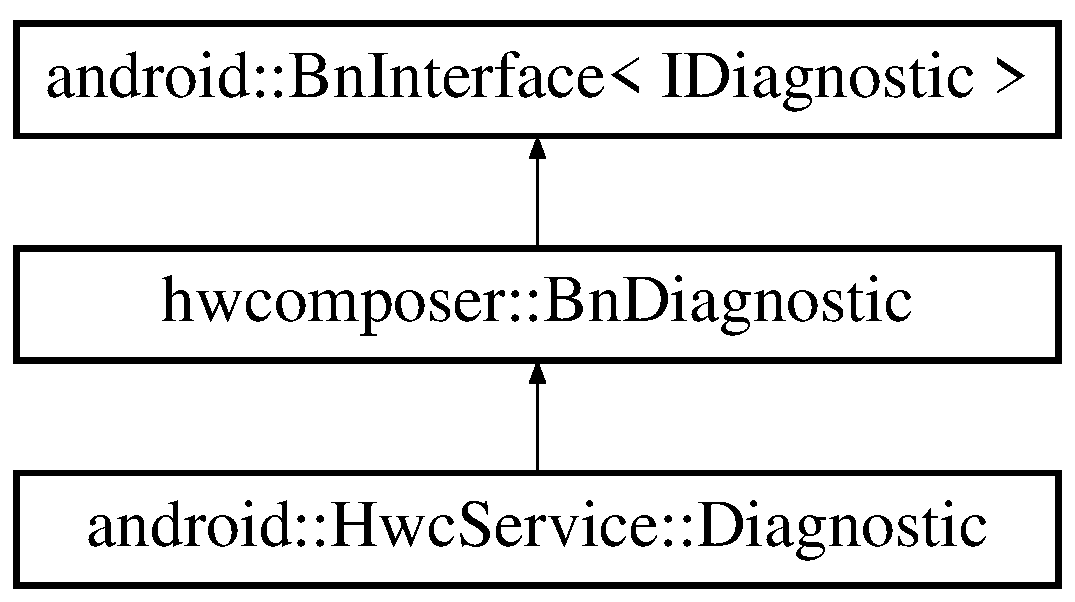
\includegraphics[height=3.000000cm]{classandroid_1_1HwcService_1_1Diagnostic}
\end{center}
\end{figure}
\subsection*{Public Member Functions}
\begin{DoxyCompactItemize}
\item 
\mbox{\hyperlink{classandroid_1_1HwcService_1_1Diagnostic_a415e65935b1c00ddcdc68c3fbac876cd}{Diagnostic}} (\mbox{\hyperlink{classandroid_1_1IAHWC2}{I\+A\+H\+W\+C2}} \&\mbox{\hyperlink{classandroid_1_1IAHWC2}{I\+A\+H\+W\+C2}})
\item 
\mbox{\hyperlink{hwcserviceapi_8h_a3806fb2027d9a316d8ca8d9b8b8eb96f}{status\+\_\+t}} \mbox{\hyperlink{classandroid_1_1HwcService_1_1Diagnostic_a201369c6711b3b26f64fbf8262ad2618}{Read\+Log\+Parcel}} (Parcel $\ast$parcel) override
\item 
void \mbox{\hyperlink{classandroid_1_1HwcService_1_1Diagnostic_a405d3f313ca6b1a8848a802a3e56a0a5}{Enable\+Display}} (uint32\+\_\+t d) override
\item 
void \mbox{\hyperlink{classandroid_1_1HwcService_1_1Diagnostic_ac9cd5bafbc4f622450327c63cb3b7746}{Disable\+Display}} (uint32\+\_\+t d, bool b\+Blank) override
\item 
void \mbox{\hyperlink{classandroid_1_1HwcService_1_1Diagnostic_afe11cd5e9e11147eebb0f2c57e693395}{Mask\+Layer}} (uint32\+\_\+t d, uint32\+\_\+t layer, bool b\+Hide) override
\item 
void \mbox{\hyperlink{classandroid_1_1HwcService_1_1Diagnostic_a6a44a6c97a8e4afc4d8940b7df671ef6}{Dump\+Frames}} (uint32\+\_\+t d, int32\+\_\+t frames, bool b\+Sync) override
\end{DoxyCompactItemize}


\subsection{Detailed Description}


Definition at line 35 of file hwcservice.\+h.



\subsection{Constructor \& Destructor Documentation}
\mbox{\Hypertarget{classandroid_1_1HwcService_1_1Diagnostic_a415e65935b1c00ddcdc68c3fbac876cd}\label{classandroid_1_1HwcService_1_1Diagnostic_a415e65935b1c00ddcdc68c3fbac876cd}} 
\index{android\+::\+Hwc\+Service\+::\+Diagnostic@{android\+::\+Hwc\+Service\+::\+Diagnostic}!Diagnostic@{Diagnostic}}
\index{Diagnostic@{Diagnostic}!android\+::\+Hwc\+Service\+::\+Diagnostic@{android\+::\+Hwc\+Service\+::\+Diagnostic}}
\subsubsection{\texorpdfstring{Diagnostic()}{Diagnostic()}}
{\footnotesize\ttfamily android\+::\+Hwc\+Service\+::\+Diagnostic\+::\+Diagnostic (\begin{DoxyParamCaption}\item[{\mbox{\hyperlink{classandroid_1_1IAHWC2}{I\+A\+H\+W\+C2}} \&}]{I\+A\+H\+W\+C2 }\end{DoxyParamCaption})\hspace{0.3cm}{\ttfamily [inline]}}



Definition at line 37 of file hwcservice.\+h.


\begin{DoxyCode}{0}
\DoxyCodeLine{37                                : mHwc(\mbox{\hyperlink{classandroid_1_1IAHWC2}{IAHWC2}}) \{}
\DoxyCodeLine{38       \mbox{\hyperlink{platformcommondefines_8h_a55010dd9f045ede43b1c4fa3d249b1eb}{HWC\_UNUSED}}(mHwc);}
\DoxyCodeLine{39     \}}
\end{DoxyCode}


\subsection{Member Function Documentation}
\mbox{\Hypertarget{classandroid_1_1HwcService_1_1Diagnostic_ac9cd5bafbc4f622450327c63cb3b7746}\label{classandroid_1_1HwcService_1_1Diagnostic_ac9cd5bafbc4f622450327c63cb3b7746}} 
\index{android\+::\+Hwc\+Service\+::\+Diagnostic@{android\+::\+Hwc\+Service\+::\+Diagnostic}!Disable\+Display@{Disable\+Display}}
\index{Disable\+Display@{Disable\+Display}!android\+::\+Hwc\+Service\+::\+Diagnostic@{android\+::\+Hwc\+Service\+::\+Diagnostic}}
\subsubsection{\texorpdfstring{Disable\+Display()}{DisableDisplay()}}
{\footnotesize\ttfamily void android\+::\+Hwc\+Service\+::\+Diagnostic\+::\+Disable\+Display (\begin{DoxyParamCaption}\item[{uint32\+\_\+t}]{d,  }\item[{bool}]{b\+Blank }\end{DoxyParamCaption})\hspace{0.3cm}{\ttfamily [override]}}



Definition at line 131 of file hwcservice.\+cpp.


\begin{DoxyCode}{0}
\DoxyCodeLine{131                                                         \{ \textcolor{comment}{/* nothing */}}
\DoxyCodeLine{132 \}}
\end{DoxyCode}
\mbox{\Hypertarget{classandroid_1_1HwcService_1_1Diagnostic_a6a44a6c97a8e4afc4d8940b7df671ef6}\label{classandroid_1_1HwcService_1_1Diagnostic_a6a44a6c97a8e4afc4d8940b7df671ef6}} 
\index{android\+::\+Hwc\+Service\+::\+Diagnostic@{android\+::\+Hwc\+Service\+::\+Diagnostic}!Dump\+Frames@{Dump\+Frames}}
\index{Dump\+Frames@{Dump\+Frames}!android\+::\+Hwc\+Service\+::\+Diagnostic@{android\+::\+Hwc\+Service\+::\+Diagnostic}}
\subsubsection{\texorpdfstring{Dump\+Frames()}{DumpFrames()}}
{\footnotesize\ttfamily void android\+::\+Hwc\+Service\+::\+Diagnostic\+::\+Dump\+Frames (\begin{DoxyParamCaption}\item[{uint32\+\_\+t}]{d,  }\item[{int32\+\_\+t}]{frames,  }\item[{bool}]{b\+Sync }\end{DoxyParamCaption})\hspace{0.3cm}{\ttfamily [override]}}



Definition at line 135 of file hwcservice.\+cpp.


\begin{DoxyCode}{0}
\DoxyCodeLine{135                                                              \{ \textcolor{comment}{/* nothing */}}
\DoxyCodeLine{136 \}}
\end{DoxyCode}
\mbox{\Hypertarget{classandroid_1_1HwcService_1_1Diagnostic_a405d3f313ca6b1a8848a802a3e56a0a5}\label{classandroid_1_1HwcService_1_1Diagnostic_a405d3f313ca6b1a8848a802a3e56a0a5}} 
\index{android\+::\+Hwc\+Service\+::\+Diagnostic@{android\+::\+Hwc\+Service\+::\+Diagnostic}!Enable\+Display@{Enable\+Display}}
\index{Enable\+Display@{Enable\+Display}!android\+::\+Hwc\+Service\+::\+Diagnostic@{android\+::\+Hwc\+Service\+::\+Diagnostic}}
\subsubsection{\texorpdfstring{Enable\+Display()}{EnableDisplay()}}
{\footnotesize\ttfamily void android\+::\+Hwc\+Service\+::\+Diagnostic\+::\+Enable\+Display (\begin{DoxyParamCaption}\item[{uint32\+\_\+t}]{d }\end{DoxyParamCaption})\hspace{0.3cm}{\ttfamily [override]}}



Definition at line 129 of file hwcservice.\+cpp.


\begin{DoxyCode}{0}
\DoxyCodeLine{129                                                  \{ \textcolor{comment}{/* nothing */}}
\DoxyCodeLine{130 \}}
\end{DoxyCode}
\mbox{\Hypertarget{classandroid_1_1HwcService_1_1Diagnostic_afe11cd5e9e11147eebb0f2c57e693395}\label{classandroid_1_1HwcService_1_1Diagnostic_afe11cd5e9e11147eebb0f2c57e693395}} 
\index{android\+::\+Hwc\+Service\+::\+Diagnostic@{android\+::\+Hwc\+Service\+::\+Diagnostic}!Mask\+Layer@{Mask\+Layer}}
\index{Mask\+Layer@{Mask\+Layer}!android\+::\+Hwc\+Service\+::\+Diagnostic@{android\+::\+Hwc\+Service\+::\+Diagnostic}}
\subsubsection{\texorpdfstring{Mask\+Layer()}{MaskLayer()}}
{\footnotesize\ttfamily void android\+::\+Hwc\+Service\+::\+Diagnostic\+::\+Mask\+Layer (\begin{DoxyParamCaption}\item[{uint32\+\_\+t}]{d,  }\item[{uint32\+\_\+t}]{layer,  }\item[{bool}]{b\+Hide }\end{DoxyParamCaption})\hspace{0.3cm}{\ttfamily [override]}}



Definition at line 133 of file hwcservice.\+cpp.


\begin{DoxyCode}{0}
\DoxyCodeLine{133                                                              \{ \textcolor{comment}{/* nothing */}}
\DoxyCodeLine{134 \}}
\end{DoxyCode}
\mbox{\Hypertarget{classandroid_1_1HwcService_1_1Diagnostic_a201369c6711b3b26f64fbf8262ad2618}\label{classandroid_1_1HwcService_1_1Diagnostic_a201369c6711b3b26f64fbf8262ad2618}} 
\index{android\+::\+Hwc\+Service\+::\+Diagnostic@{android\+::\+Hwc\+Service\+::\+Diagnostic}!Read\+Log\+Parcel@{Read\+Log\+Parcel}}
\index{Read\+Log\+Parcel@{Read\+Log\+Parcel}!android\+::\+Hwc\+Service\+::\+Diagnostic@{android\+::\+Hwc\+Service\+::\+Diagnostic}}
\subsubsection{\texorpdfstring{Read\+Log\+Parcel()}{ReadLogParcel()}}
{\footnotesize\ttfamily \mbox{\hyperlink{hwcserviceapi_8h_a3806fb2027d9a316d8ca8d9b8b8eb96f}{status\+\_\+t}} android\+::\+Hwc\+Service\+::\+Diagnostic\+::\+Read\+Log\+Parcel (\begin{DoxyParamCaption}\item[{Parcel $\ast$}]{parcel }\end{DoxyParamCaption})\hspace{0.3cm}{\ttfamily [override]}}



Definition at line 124 of file hwcservice.\+cpp.


\begin{DoxyCode}{0}
\DoxyCodeLine{124                                                            \{}
\DoxyCodeLine{125   \textcolor{comment}{// TO DO}}
\DoxyCodeLine{126   \textcolor{keywordflow}{return} OK;}
\DoxyCodeLine{127 \}}
\end{DoxyCode}


The documentation for this class was generated from the following files\+:\begin{DoxyCompactItemize}
\item 
os/android/\mbox{\hyperlink{hwcservice_8h}{hwcservice.\+h}}\item 
os/android/\mbox{\hyperlink{hwcservice_8cpp}{hwcservice.\+cpp}}\end{DoxyCompactItemize}

\hypertarget{classhwcomposer_1_1DisplayHotPlugEventCallback}{}\section{hwcomposer\+:\+:Display\+Hot\+Plug\+Event\+Callback Class Reference}
\label{classhwcomposer_1_1DisplayHotPlugEventCallback}\index{hwcomposer\+::\+Display\+Hot\+Plug\+Event\+Callback@{hwcomposer\+::\+Display\+Hot\+Plug\+Event\+Callback}}


{\ttfamily \#include $<$nativedisplay.\+h$>$}

\subsection*{Public Member Functions}
\begin{DoxyCompactItemize}
\item 
virtual \mbox{\hyperlink{classhwcomposer_1_1DisplayHotPlugEventCallback_aac65c3af5e35ca7b5865746503787fdb}{$\sim$\+Display\+Hot\+Plug\+Event\+Callback}} ()
\item 
virtual void \mbox{\hyperlink{classhwcomposer_1_1DisplayHotPlugEventCallback_aa0185bcd7a64dda124cd63ef8d0e46ec}{Callback}} (std\+::vector$<$ \mbox{\hyperlink{classhwcomposer_1_1NativeDisplay}{Native\+Display}} $\ast$$>$ connected\+\_\+displays)=0
\end{DoxyCompactItemize}


\subsection{Detailed Description}
This is provided for Convenience in case one doesnt want to register for hot plug callback per display. 

Definition at line 452 of file nativedisplay.\+h.



\subsection{Constructor \& Destructor Documentation}
\mbox{\Hypertarget{classhwcomposer_1_1DisplayHotPlugEventCallback_aac65c3af5e35ca7b5865746503787fdb}\label{classhwcomposer_1_1DisplayHotPlugEventCallback_aac65c3af5e35ca7b5865746503787fdb}} 
\index{hwcomposer\+::\+Display\+Hot\+Plug\+Event\+Callback@{hwcomposer\+::\+Display\+Hot\+Plug\+Event\+Callback}!````~Display\+Hot\+Plug\+Event\+Callback@{$\sim$\+Display\+Hot\+Plug\+Event\+Callback}}
\index{````~Display\+Hot\+Plug\+Event\+Callback@{$\sim$\+Display\+Hot\+Plug\+Event\+Callback}!hwcomposer\+::\+Display\+Hot\+Plug\+Event\+Callback@{hwcomposer\+::\+Display\+Hot\+Plug\+Event\+Callback}}
\subsubsection{\texorpdfstring{$\sim$\+Display\+Hot\+Plug\+Event\+Callback()}{~DisplayHotPlugEventCallback()}}
{\footnotesize\ttfamily virtual hwcomposer\+::\+Display\+Hot\+Plug\+Event\+Callback\+::$\sim$\+Display\+Hot\+Plug\+Event\+Callback (\begin{DoxyParamCaption}{ }\end{DoxyParamCaption})\hspace{0.3cm}{\ttfamily [inline]}, {\ttfamily [virtual]}}



Definition at line 454 of file nativedisplay.\+h.


\begin{DoxyCode}{0}
\DoxyCodeLine{454                                          \{}
\DoxyCodeLine{455   \}}
\end{DoxyCode}


\subsection{Member Function Documentation}
\mbox{\Hypertarget{classhwcomposer_1_1DisplayHotPlugEventCallback_aa0185bcd7a64dda124cd63ef8d0e46ec}\label{classhwcomposer_1_1DisplayHotPlugEventCallback_aa0185bcd7a64dda124cd63ef8d0e46ec}} 
\index{hwcomposer\+::\+Display\+Hot\+Plug\+Event\+Callback@{hwcomposer\+::\+Display\+Hot\+Plug\+Event\+Callback}!Callback@{Callback}}
\index{Callback@{Callback}!hwcomposer\+::\+Display\+Hot\+Plug\+Event\+Callback@{hwcomposer\+::\+Display\+Hot\+Plug\+Event\+Callback}}
\subsubsection{\texorpdfstring{Callback()}{Callback()}}
{\footnotesize\ttfamily virtual void hwcomposer\+::\+Display\+Hot\+Plug\+Event\+Callback\+::\+Callback (\begin{DoxyParamCaption}\item[{std\+::vector$<$ \mbox{\hyperlink{classhwcomposer_1_1NativeDisplay}{Native\+Display}} $\ast$$>$}]{connected\+\_\+displays }\end{DoxyParamCaption})\hspace{0.3cm}{\ttfamily [pure virtual]}}



The documentation for this class was generated from the following file\+:\begin{DoxyCompactItemize}
\item 
public/\mbox{\hyperlink{nativedisplay_8h}{nativedisplay.\+h}}\end{DoxyCompactItemize}

\hypertarget{classhwcomposer_1_1DisplayManager}{}\section{hwcomposer\+:\+:Display\+Manager Class Reference}
\label{classhwcomposer_1_1DisplayManager}\index{hwcomposer\+::\+Display\+Manager@{hwcomposer\+::\+Display\+Manager}}


{\ttfamily \#include $<$displaymanager.\+h$>$}

Inheritance diagram for hwcomposer\+:\+:Display\+Manager\+:\begin{figure}[H]
\begin{center}
\leavevmode
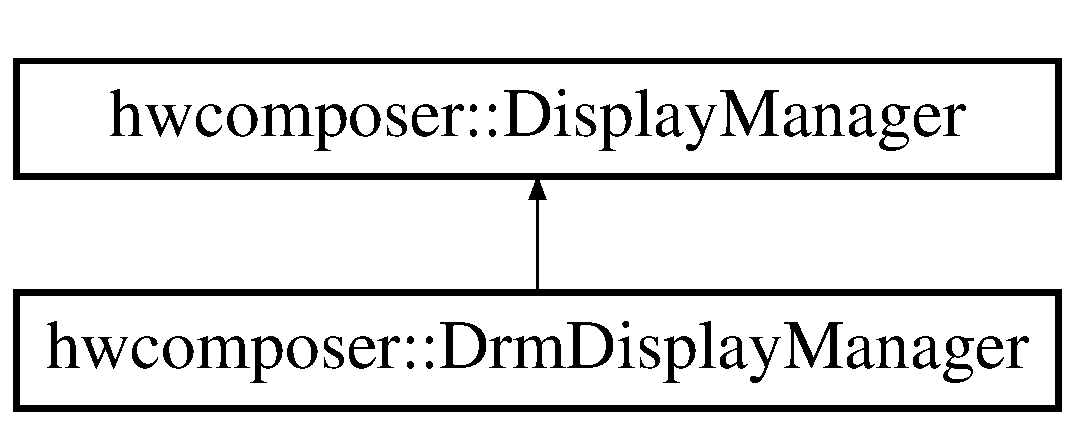
\includegraphics[height=2.000000cm]{classhwcomposer_1_1DisplayManager}
\end{center}
\end{figure}
\subsection*{Public Member Functions}
\begin{DoxyCompactItemize}
\item 
\mbox{\hyperlink{classhwcomposer_1_1DisplayManager_ae0d38f8308c54359c9de7e1c8e8f13c2}{Display\+Manager}} ()=default
\item 
virtual \mbox{\hyperlink{classhwcomposer_1_1DisplayManager_a34d71bf6f39f064b958920bbdc07c761}{$\sim$\+Display\+Manager}} ()
\item 
virtual bool \mbox{\hyperlink{classhwcomposer_1_1DisplayManager_abb67b1deed55bf20584f86aea2ae5167}{Initialize}} ()=0
\item 
virtual void \mbox{\hyperlink{classhwcomposer_1_1DisplayManager_a26b46eb7c0d15384fceaecdd8be9be45}{Initialize\+Display\+Resources}} ()=0
\item 
virtual void \mbox{\hyperlink{classhwcomposer_1_1DisplayManager_a9728735ff10a6e52861c4201bf8c6fb2}{Start\+Hot\+Plug\+Monitor}} ()=0
\item 
virtual void \mbox{\hyperlink{classhwcomposer_1_1DisplayManager_a678df886d9faff854111d8ace155befc}{Force\+Refresh}} ()=0
\item 
virtual void \mbox{\hyperlink{classhwcomposer_1_1DisplayManager_ac5d98f9c1c32dc2dbc3afb342a113af5}{Ignore\+Updates}} ()=0
\item 
virtual uint32\+\_\+t \mbox{\hyperlink{classhwcomposer_1_1DisplayManager_a7af00ef1c1c9dc8f3fd58699460ab14d}{Get\+FD}} () const =0
\item 
virtual \mbox{\hyperlink{classhwcomposer_1_1NativeDisplay}{Native\+Display}} $\ast$ \mbox{\hyperlink{classhwcomposer_1_1DisplayManager_a5fa2b92896cab774d8a85215dfac1d62}{Get\+Virtual\+Display}} ()=0
\item 
virtual \mbox{\hyperlink{classhwcomposer_1_1NativeDisplay}{Native\+Display}} $\ast$ \mbox{\hyperlink{classhwcomposer_1_1DisplayManager_ac05cc0db0d8191465746828b2027a6f7}{Get\+Nested\+Display}} ()=0
\item 
virtual std\+::vector$<$ \mbox{\hyperlink{classhwcomposer_1_1NativeDisplay}{Native\+Display}} $\ast$ $>$ \mbox{\hyperlink{classhwcomposer_1_1DisplayManager_aec3ebc4b4d22031e983856a424dd43a6}{Get\+All\+Displays}} ()=0
\item 
virtual void \mbox{\hyperlink{classhwcomposer_1_1DisplayManager_a2c1138176c411a5164052e83f623595d}{Register\+Hot\+Plug\+Event\+Callback}} (std\+::shared\+\_\+ptr$<$ \mbox{\hyperlink{classhwcomposer_1_1DisplayHotPlugEventCallback}{Display\+Hot\+Plug\+Event\+Callback}} $>$ callback)=0
\end{DoxyCompactItemize}
\subsection*{Static Public Member Functions}
\begin{DoxyCompactItemize}
\item 
static \mbox{\hyperlink{classhwcomposer_1_1DisplayManager}{Display\+Manager}} $\ast$ \mbox{\hyperlink{classhwcomposer_1_1DisplayManager_aed4adf531c3ea168ff4e2f7c82fd1cbb}{Create\+Display\+Manager}} (\mbox{\hyperlink{classhwcomposer_1_1GpuDevice}{Gpu\+Device}} $\ast$device)
\end{DoxyCompactItemize}


\subsection{Detailed Description}


Definition at line 27 of file displaymanager.\+h.



\subsection{Constructor \& Destructor Documentation}
\mbox{\Hypertarget{classhwcomposer_1_1DisplayManager_ae0d38f8308c54359c9de7e1c8e8f13c2}\label{classhwcomposer_1_1DisplayManager_ae0d38f8308c54359c9de7e1c8e8f13c2}} 
\index{hwcomposer\+::\+Display\+Manager@{hwcomposer\+::\+Display\+Manager}!Display\+Manager@{Display\+Manager}}
\index{Display\+Manager@{Display\+Manager}!hwcomposer\+::\+Display\+Manager@{hwcomposer\+::\+Display\+Manager}}
\subsubsection{\texorpdfstring{Display\+Manager()}{DisplayManager()}}
{\footnotesize\ttfamily hwcomposer\+::\+Display\+Manager\+::\+Display\+Manager (\begin{DoxyParamCaption}{ }\end{DoxyParamCaption})\hspace{0.3cm}{\ttfamily [default]}}

\mbox{\Hypertarget{classhwcomposer_1_1DisplayManager_a34d71bf6f39f064b958920bbdc07c761}\label{classhwcomposer_1_1DisplayManager_a34d71bf6f39f064b958920bbdc07c761}} 
\index{hwcomposer\+::\+Display\+Manager@{hwcomposer\+::\+Display\+Manager}!````~Display\+Manager@{$\sim$\+Display\+Manager}}
\index{````~Display\+Manager@{$\sim$\+Display\+Manager}!hwcomposer\+::\+Display\+Manager@{hwcomposer\+::\+Display\+Manager}}
\subsubsection{\texorpdfstring{$\sim$\+Display\+Manager()}{~DisplayManager()}}
{\footnotesize\ttfamily virtual hwcomposer\+::\+Display\+Manager\+::$\sim$\+Display\+Manager (\begin{DoxyParamCaption}{ }\end{DoxyParamCaption})\hspace{0.3cm}{\ttfamily [inline]}, {\ttfamily [virtual]}}



Definition at line 31 of file displaymanager.\+h.


\begin{DoxyCode}{0}
\DoxyCodeLine{31                             \{}
\DoxyCodeLine{32   \}}
\end{DoxyCode}


\subsection{Member Function Documentation}
\mbox{\Hypertarget{classhwcomposer_1_1DisplayManager_aed4adf531c3ea168ff4e2f7c82fd1cbb}\label{classhwcomposer_1_1DisplayManager_aed4adf531c3ea168ff4e2f7c82fd1cbb}} 
\index{hwcomposer\+::\+Display\+Manager@{hwcomposer\+::\+Display\+Manager}!Create\+Display\+Manager@{Create\+Display\+Manager}}
\index{Create\+Display\+Manager@{Create\+Display\+Manager}!hwcomposer\+::\+Display\+Manager@{hwcomposer\+::\+Display\+Manager}}
\subsubsection{\texorpdfstring{Create\+Display\+Manager()}{CreateDisplayManager()}}
{\footnotesize\ttfamily \mbox{\hyperlink{classhwcomposer_1_1DisplayManager}{Display\+Manager}} $\ast$ hwcomposer\+::\+Display\+Manager\+::\+Create\+Display\+Manager (\begin{DoxyParamCaption}\item[{\mbox{\hyperlink{classhwcomposer_1_1GpuDevice}{Gpu\+Device}} $\ast$}]{device }\end{DoxyParamCaption})\hspace{0.3cm}{\ttfamily [static]}}



Definition at line 452 of file drmdisplaymanager.\+cpp.


\begin{DoxyCode}{0}
\DoxyCodeLine{452                                                                       \{}
\DoxyCodeLine{453   \textcolor{keywordflow}{return} \textcolor{keyword}{new} DrmDisplayManager(device);}
\DoxyCodeLine{454 \}}
\end{DoxyCode}
\mbox{\Hypertarget{classhwcomposer_1_1DisplayManager_a678df886d9faff854111d8ace155befc}\label{classhwcomposer_1_1DisplayManager_a678df886d9faff854111d8ace155befc}} 
\index{hwcomposer\+::\+Display\+Manager@{hwcomposer\+::\+Display\+Manager}!Force\+Refresh@{Force\+Refresh}}
\index{Force\+Refresh@{Force\+Refresh}!hwcomposer\+::\+Display\+Manager@{hwcomposer\+::\+Display\+Manager}}
\subsubsection{\texorpdfstring{Force\+Refresh()}{ForceRefresh()}}
{\footnotesize\ttfamily virtual void hwcomposer\+::\+Display\+Manager\+::\+Force\+Refresh (\begin{DoxyParamCaption}{ }\end{DoxyParamCaption})\hspace{0.3cm}{\ttfamily [pure virtual]}}



Implemented in \mbox{\hyperlink{classhwcomposer_1_1DrmDisplayManager_a254ab8fd550f20f056c2ec1e458442c9}{hwcomposer\+::\+Drm\+Display\+Manager}}.

\mbox{\Hypertarget{classhwcomposer_1_1DisplayManager_aec3ebc4b4d22031e983856a424dd43a6}\label{classhwcomposer_1_1DisplayManager_aec3ebc4b4d22031e983856a424dd43a6}} 
\index{hwcomposer\+::\+Display\+Manager@{hwcomposer\+::\+Display\+Manager}!Get\+All\+Displays@{Get\+All\+Displays}}
\index{Get\+All\+Displays@{Get\+All\+Displays}!hwcomposer\+::\+Display\+Manager@{hwcomposer\+::\+Display\+Manager}}
\subsubsection{\texorpdfstring{Get\+All\+Displays()}{GetAllDisplays()}}
{\footnotesize\ttfamily virtual std\+::vector$<$\mbox{\hyperlink{classhwcomposer_1_1NativeDisplay}{Native\+Display}} $\ast$$>$ hwcomposer\+::\+Display\+Manager\+::\+Get\+All\+Displays (\begin{DoxyParamCaption}{ }\end{DoxyParamCaption})\hspace{0.3cm}{\ttfamily [pure virtual]}}



Implemented in \mbox{\hyperlink{classhwcomposer_1_1DrmDisplayManager_acff7605550c750e5f799f698e9b82d2a}{hwcomposer\+::\+Drm\+Display\+Manager}}.

\mbox{\Hypertarget{classhwcomposer_1_1DisplayManager_a7af00ef1c1c9dc8f3fd58699460ab14d}\label{classhwcomposer_1_1DisplayManager_a7af00ef1c1c9dc8f3fd58699460ab14d}} 
\index{hwcomposer\+::\+Display\+Manager@{hwcomposer\+::\+Display\+Manager}!Get\+FD@{Get\+FD}}
\index{Get\+FD@{Get\+FD}!hwcomposer\+::\+Display\+Manager@{hwcomposer\+::\+Display\+Manager}}
\subsubsection{\texorpdfstring{Get\+F\+D()}{GetFD()}}
{\footnotesize\ttfamily virtual uint32\+\_\+t hwcomposer\+::\+Display\+Manager\+::\+Get\+FD (\begin{DoxyParamCaption}{ }\end{DoxyParamCaption}) const\hspace{0.3cm}{\ttfamily [pure virtual]}}



Implemented in \mbox{\hyperlink{classhwcomposer_1_1DrmDisplayManager_aed1b4e61f4bbda4069138675156a9564}{hwcomposer\+::\+Drm\+Display\+Manager}}.

\mbox{\Hypertarget{classhwcomposer_1_1DisplayManager_ac05cc0db0d8191465746828b2027a6f7}\label{classhwcomposer_1_1DisplayManager_ac05cc0db0d8191465746828b2027a6f7}} 
\index{hwcomposer\+::\+Display\+Manager@{hwcomposer\+::\+Display\+Manager}!Get\+Nested\+Display@{Get\+Nested\+Display}}
\index{Get\+Nested\+Display@{Get\+Nested\+Display}!hwcomposer\+::\+Display\+Manager@{hwcomposer\+::\+Display\+Manager}}
\subsubsection{\texorpdfstring{Get\+Nested\+Display()}{GetNestedDisplay()}}
{\footnotesize\ttfamily virtual \mbox{\hyperlink{classhwcomposer_1_1NativeDisplay}{Native\+Display}}$\ast$ hwcomposer\+::\+Display\+Manager\+::\+Get\+Nested\+Display (\begin{DoxyParamCaption}{ }\end{DoxyParamCaption})\hspace{0.3cm}{\ttfamily [pure virtual]}}



Implemented in \mbox{\hyperlink{classhwcomposer_1_1DrmDisplayManager_ae3df43b4c4c9cc1181ec13cbefd764f1}{hwcomposer\+::\+Drm\+Display\+Manager}}.

\mbox{\Hypertarget{classhwcomposer_1_1DisplayManager_a5fa2b92896cab774d8a85215dfac1d62}\label{classhwcomposer_1_1DisplayManager_a5fa2b92896cab774d8a85215dfac1d62}} 
\index{hwcomposer\+::\+Display\+Manager@{hwcomposer\+::\+Display\+Manager}!Get\+Virtual\+Display@{Get\+Virtual\+Display}}
\index{Get\+Virtual\+Display@{Get\+Virtual\+Display}!hwcomposer\+::\+Display\+Manager@{hwcomposer\+::\+Display\+Manager}}
\subsubsection{\texorpdfstring{Get\+Virtual\+Display()}{GetVirtualDisplay()}}
{\footnotesize\ttfamily virtual \mbox{\hyperlink{classhwcomposer_1_1NativeDisplay}{Native\+Display}}$\ast$ hwcomposer\+::\+Display\+Manager\+::\+Get\+Virtual\+Display (\begin{DoxyParamCaption}{ }\end{DoxyParamCaption})\hspace{0.3cm}{\ttfamily [pure virtual]}}



Implemented in \mbox{\hyperlink{classhwcomposer_1_1DrmDisplayManager_a80e39b4389e271ed5a72421c46ce5f36}{hwcomposer\+::\+Drm\+Display\+Manager}}.

\mbox{\Hypertarget{classhwcomposer_1_1DisplayManager_ac5d98f9c1c32dc2dbc3afb342a113af5}\label{classhwcomposer_1_1DisplayManager_ac5d98f9c1c32dc2dbc3afb342a113af5}} 
\index{hwcomposer\+::\+Display\+Manager@{hwcomposer\+::\+Display\+Manager}!Ignore\+Updates@{Ignore\+Updates}}
\index{Ignore\+Updates@{Ignore\+Updates}!hwcomposer\+::\+Display\+Manager@{hwcomposer\+::\+Display\+Manager}}
\subsubsection{\texorpdfstring{Ignore\+Updates()}{IgnoreUpdates()}}
{\footnotesize\ttfamily virtual void hwcomposer\+::\+Display\+Manager\+::\+Ignore\+Updates (\begin{DoxyParamCaption}{ }\end{DoxyParamCaption})\hspace{0.3cm}{\ttfamily [pure virtual]}}



Implemented in \mbox{\hyperlink{classhwcomposer_1_1DrmDisplayManager_ac10c8fb07bf822c4430cd54722ceee16}{hwcomposer\+::\+Drm\+Display\+Manager}}.

\mbox{\Hypertarget{classhwcomposer_1_1DisplayManager_abb67b1deed55bf20584f86aea2ae5167}\label{classhwcomposer_1_1DisplayManager_abb67b1deed55bf20584f86aea2ae5167}} 
\index{hwcomposer\+::\+Display\+Manager@{hwcomposer\+::\+Display\+Manager}!Initialize@{Initialize}}
\index{Initialize@{Initialize}!hwcomposer\+::\+Display\+Manager@{hwcomposer\+::\+Display\+Manager}}
\subsubsection{\texorpdfstring{Initialize()}{Initialize()}}
{\footnotesize\ttfamily virtual bool hwcomposer\+::\+Display\+Manager\+::\+Initialize (\begin{DoxyParamCaption}{ }\end{DoxyParamCaption})\hspace{0.3cm}{\ttfamily [pure virtual]}}



Implemented in \mbox{\hyperlink{classhwcomposer_1_1DrmDisplayManager_a1597ef6208030337c9554b70dcdf0a95}{hwcomposer\+::\+Drm\+Display\+Manager}}.

\mbox{\Hypertarget{classhwcomposer_1_1DisplayManager_a26b46eb7c0d15384fceaecdd8be9be45}\label{classhwcomposer_1_1DisplayManager_a26b46eb7c0d15384fceaecdd8be9be45}} 
\index{hwcomposer\+::\+Display\+Manager@{hwcomposer\+::\+Display\+Manager}!Initialize\+Display\+Resources@{Initialize\+Display\+Resources}}
\index{Initialize\+Display\+Resources@{Initialize\+Display\+Resources}!hwcomposer\+::\+Display\+Manager@{hwcomposer\+::\+Display\+Manager}}
\subsubsection{\texorpdfstring{Initialize\+Display\+Resources()}{InitializeDisplayResources()}}
{\footnotesize\ttfamily virtual void hwcomposer\+::\+Display\+Manager\+::\+Initialize\+Display\+Resources (\begin{DoxyParamCaption}{ }\end{DoxyParamCaption})\hspace{0.3cm}{\ttfamily [pure virtual]}}



Implemented in \mbox{\hyperlink{classhwcomposer_1_1DrmDisplayManager_a775eee42523dabde8e4187770cbe9c6c}{hwcomposer\+::\+Drm\+Display\+Manager}}.

\mbox{\Hypertarget{classhwcomposer_1_1DisplayManager_a2c1138176c411a5164052e83f623595d}\label{classhwcomposer_1_1DisplayManager_a2c1138176c411a5164052e83f623595d}} 
\index{hwcomposer\+::\+Display\+Manager@{hwcomposer\+::\+Display\+Manager}!Register\+Hot\+Plug\+Event\+Callback@{Register\+Hot\+Plug\+Event\+Callback}}
\index{Register\+Hot\+Plug\+Event\+Callback@{Register\+Hot\+Plug\+Event\+Callback}!hwcomposer\+::\+Display\+Manager@{hwcomposer\+::\+Display\+Manager}}
\subsubsection{\texorpdfstring{Register\+Hot\+Plug\+Event\+Callback()}{RegisterHotPlugEventCallback()}}
{\footnotesize\ttfamily virtual void hwcomposer\+::\+Display\+Manager\+::\+Register\+Hot\+Plug\+Event\+Callback (\begin{DoxyParamCaption}\item[{std\+::shared\+\_\+ptr$<$ \mbox{\hyperlink{classhwcomposer_1_1DisplayHotPlugEventCallback}{Display\+Hot\+Plug\+Event\+Callback}} $>$}]{callback }\end{DoxyParamCaption})\hspace{0.3cm}{\ttfamily [pure virtual]}}



Implemented in \mbox{\hyperlink{classhwcomposer_1_1DrmDisplayManager_ab11e4353cddc68652abcae61dd26027d}{hwcomposer\+::\+Drm\+Display\+Manager}}.

\mbox{\Hypertarget{classhwcomposer_1_1DisplayManager_a9728735ff10a6e52861c4201bf8c6fb2}\label{classhwcomposer_1_1DisplayManager_a9728735ff10a6e52861c4201bf8c6fb2}} 
\index{hwcomposer\+::\+Display\+Manager@{hwcomposer\+::\+Display\+Manager}!Start\+Hot\+Plug\+Monitor@{Start\+Hot\+Plug\+Monitor}}
\index{Start\+Hot\+Plug\+Monitor@{Start\+Hot\+Plug\+Monitor}!hwcomposer\+::\+Display\+Manager@{hwcomposer\+::\+Display\+Manager}}
\subsubsection{\texorpdfstring{Start\+Hot\+Plug\+Monitor()}{StartHotPlugMonitor()}}
{\footnotesize\ttfamily virtual void hwcomposer\+::\+Display\+Manager\+::\+Start\+Hot\+Plug\+Monitor (\begin{DoxyParamCaption}{ }\end{DoxyParamCaption})\hspace{0.3cm}{\ttfamily [pure virtual]}}



Implemented in \mbox{\hyperlink{classhwcomposer_1_1DrmDisplayManager_a103a45f1e7e31c813dc7e185e244d944}{hwcomposer\+::\+Drm\+Display\+Manager}}.



The documentation for this class was generated from the following files\+:\begin{DoxyCompactItemize}
\item 
wsi/\mbox{\hyperlink{displaymanager_8h}{displaymanager.\+h}}\item 
wsi/drm/\mbox{\hyperlink{drmdisplaymanager_8cpp}{drmdisplaymanager.\+cpp}}\end{DoxyCompactItemize}

\hypertarget{classhwcomposer_1_1DisplayPlane}{}\section{hwcomposer\+:\+:Display\+Plane Class Reference}
\label{classhwcomposer_1_1DisplayPlane}\index{hwcomposer\+::\+Display\+Plane@{hwcomposer\+::\+Display\+Plane}}


{\ttfamily \#include $<$displayplane.\+h$>$}

Inheritance diagram for hwcomposer\+:\+:Display\+Plane\+:\begin{figure}[H]
\begin{center}
\leavevmode
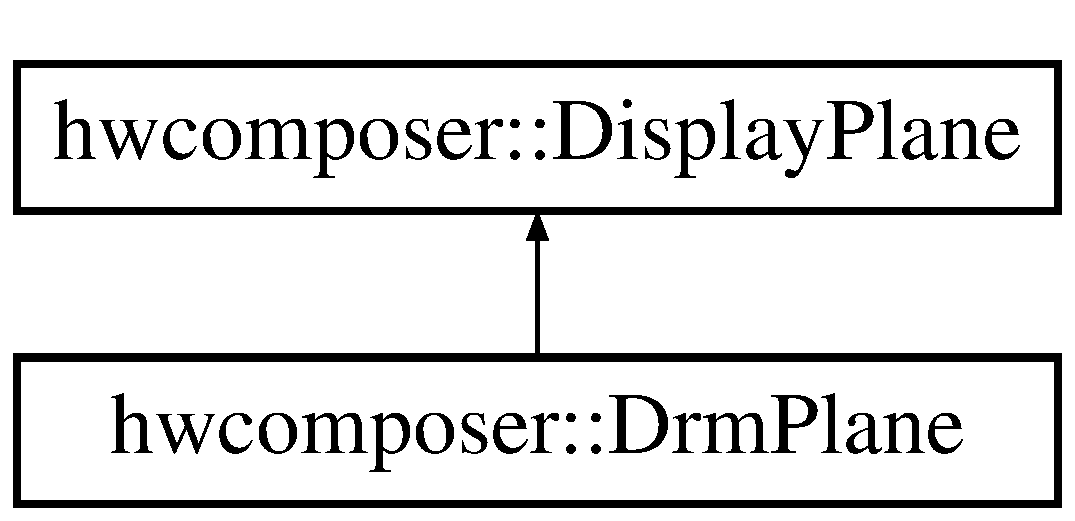
\includegraphics[height=2.000000cm]{classhwcomposer_1_1DisplayPlane}
\end{center}
\end{figure}
\subsection*{Public Member Functions}
\begin{DoxyCompactItemize}
\item 
virtual \mbox{\hyperlink{classhwcomposer_1_1DisplayPlane_aff38293d2f39ff6d298aa1a50f14409c}{$\sim$\+Display\+Plane}} ()
\item 
virtual uint32\+\_\+t \mbox{\hyperlink{classhwcomposer_1_1DisplayPlane_a0af461a6ac4beccb8ed21aec933b6eed}{id}} () const =0
\item 
virtual bool \mbox{\hyperlink{classhwcomposer_1_1DisplayPlane_a138f43531c6320ad6622ea48ab86df13}{Validate\+Layer}} (const \mbox{\hyperlink{structhwcomposer_1_1OverlayLayer}{Overlay\+Layer}} $\ast$layer)=0
\item 
virtual bool \mbox{\hyperlink{classhwcomposer_1_1DisplayPlane_a057c78a4a3657a04c5117ee0f1dba8be}{Is\+Supported\+Format}} (uint32\+\_\+t format)=0
\item 
virtual bool \mbox{\hyperlink{classhwcomposer_1_1DisplayPlane_ade9032b0c8991b0e79d321e946c8f625}{Is\+Supported\+Transform}} (uint32\+\_\+t transform) const =0
\item 
virtual uint32\+\_\+t \mbox{\hyperlink{classhwcomposer_1_1DisplayPlane_aab8aae5944b1107e4efc9d0d79c43c40}{Get\+Preferred\+Video\+Format}} () const =0
\item 
virtual uint32\+\_\+t \mbox{\hyperlink{classhwcomposer_1_1DisplayPlane_a963d17ec10be62d13f35a0b4ced4e8e1}{Get\+Preferred\+Format}} () const =0
\item 
virtual uint64\+\_\+t \mbox{\hyperlink{classhwcomposer_1_1DisplayPlane_ad95d2bd823ccf74fe3deccad7352f672}{Get\+Preferred\+Format\+Modifier}} () const =0
\item 
virtual void \mbox{\hyperlink{classhwcomposer_1_1DisplayPlane_a397270389f37f6c706a639be5225e62e}{Black\+List\+Preferred\+Format\+Modifier}} ()=0
\item 
virtual void \mbox{\hyperlink{classhwcomposer_1_1DisplayPlane_a8d2d4175bec7646f1f4216d3488bb2f6}{Preferred\+Format\+Modifier\+Validated}} ()=0
\item 
virtual void \mbox{\hyperlink{classhwcomposer_1_1DisplayPlane_a6f74f9f29977ae00d534f2488505d7d7}{Set\+In\+Use}} (bool in\+\_\+use)=0
\item 
virtual bool \mbox{\hyperlink{classhwcomposer_1_1DisplayPlane_a8461ec31b18379cc371cd0656ca0e615}{In\+Use}} () const =0
\item 
virtual bool \mbox{\hyperlink{classhwcomposer_1_1DisplayPlane_a7b374ba9e799f7d0b53afbd939961c51}{Is\+Universal}} ()=0
\item 
virtual void \mbox{\hyperlink{classhwcomposer_1_1DisplayPlane_a3754165ab1101fba4229b842c7f14556}{Dump}} () const =0
\end{DoxyCompactItemize}


\subsection{Detailed Description}


Definition at line 27 of file displayplane.\+h.



\subsection{Constructor \& Destructor Documentation}
\mbox{\Hypertarget{classhwcomposer_1_1DisplayPlane_aff38293d2f39ff6d298aa1a50f14409c}\label{classhwcomposer_1_1DisplayPlane_aff38293d2f39ff6d298aa1a50f14409c}} 
\index{hwcomposer\+::\+Display\+Plane@{hwcomposer\+::\+Display\+Plane}!````~Display\+Plane@{$\sim$\+Display\+Plane}}
\index{````~Display\+Plane@{$\sim$\+Display\+Plane}!hwcomposer\+::\+Display\+Plane@{hwcomposer\+::\+Display\+Plane}}
\subsubsection{\texorpdfstring{$\sim$\+Display\+Plane()}{~DisplayPlane()}}
{\footnotesize\ttfamily virtual hwcomposer\+::\+Display\+Plane\+::$\sim$\+Display\+Plane (\begin{DoxyParamCaption}{ }\end{DoxyParamCaption})\hspace{0.3cm}{\ttfamily [inline]}, {\ttfamily [virtual]}}



Definition at line 29 of file displayplane.\+h.


\begin{DoxyCode}{0}
\DoxyCodeLine{29                           \{}
\DoxyCodeLine{30   \}}
\end{DoxyCode}


\subsection{Member Function Documentation}
\mbox{\Hypertarget{classhwcomposer_1_1DisplayPlane_a397270389f37f6c706a639be5225e62e}\label{classhwcomposer_1_1DisplayPlane_a397270389f37f6c706a639be5225e62e}} 
\index{hwcomposer\+::\+Display\+Plane@{hwcomposer\+::\+Display\+Plane}!Black\+List\+Preferred\+Format\+Modifier@{Black\+List\+Preferred\+Format\+Modifier}}
\index{Black\+List\+Preferred\+Format\+Modifier@{Black\+List\+Preferred\+Format\+Modifier}!hwcomposer\+::\+Display\+Plane@{hwcomposer\+::\+Display\+Plane}}
\subsubsection{\texorpdfstring{Black\+List\+Preferred\+Format\+Modifier()}{BlackListPreferredFormatModifier()}}
{\footnotesize\ttfamily virtual void hwcomposer\+::\+Display\+Plane\+::\+Black\+List\+Preferred\+Format\+Modifier (\begin{DoxyParamCaption}{ }\end{DoxyParamCaption})\hspace{0.3cm}{\ttfamily [pure virtual]}}

A\+PI for blacklisting preferred format modifier. This happens in case we failed to create FB for the buffer. 

Implemented in \mbox{\hyperlink{classhwcomposer_1_1DrmPlane_a6159712388e26258e14fcb3139d7cd19}{hwcomposer\+::\+Drm\+Plane}}.

\mbox{\Hypertarget{classhwcomposer_1_1DisplayPlane_a3754165ab1101fba4229b842c7f14556}\label{classhwcomposer_1_1DisplayPlane_a3754165ab1101fba4229b842c7f14556}} 
\index{hwcomposer\+::\+Display\+Plane@{hwcomposer\+::\+Display\+Plane}!Dump@{Dump}}
\index{Dump@{Dump}!hwcomposer\+::\+Display\+Plane@{hwcomposer\+::\+Display\+Plane}}
\subsubsection{\texorpdfstring{Dump()}{Dump()}}
{\footnotesize\ttfamily virtual void hwcomposer\+::\+Display\+Plane\+::\+Dump (\begin{DoxyParamCaption}{ }\end{DoxyParamCaption}) const\hspace{0.3cm}{\ttfamily [pure virtual]}}



Implemented in \mbox{\hyperlink{classhwcomposer_1_1DrmPlane_abc9ca4823dfd433aa45747b8596cc673}{hwcomposer\+::\+Drm\+Plane}}.

\mbox{\Hypertarget{classhwcomposer_1_1DisplayPlane_a963d17ec10be62d13f35a0b4ced4e8e1}\label{classhwcomposer_1_1DisplayPlane_a963d17ec10be62d13f35a0b4ced4e8e1}} 
\index{hwcomposer\+::\+Display\+Plane@{hwcomposer\+::\+Display\+Plane}!Get\+Preferred\+Format@{Get\+Preferred\+Format}}
\index{Get\+Preferred\+Format@{Get\+Preferred\+Format}!hwcomposer\+::\+Display\+Plane@{hwcomposer\+::\+Display\+Plane}}
\subsubsection{\texorpdfstring{Get\+Preferred\+Format()}{GetPreferredFormat()}}
{\footnotesize\ttfamily virtual uint32\+\_\+t hwcomposer\+::\+Display\+Plane\+::\+Get\+Preferred\+Format (\begin{DoxyParamCaption}{ }\end{DoxyParamCaption}) const\hspace{0.3cm}{\ttfamily [pure virtual]}}

A\+PI for querying preferred format supported by this plane for non-\/media content. 

Implemented in \mbox{\hyperlink{classhwcomposer_1_1DrmPlane_a3bca39231ec7b099980474b279c58ce8}{hwcomposer\+::\+Drm\+Plane}}.

\mbox{\Hypertarget{classhwcomposer_1_1DisplayPlane_ad95d2bd823ccf74fe3deccad7352f672}\label{classhwcomposer_1_1DisplayPlane_ad95d2bd823ccf74fe3deccad7352f672}} 
\index{hwcomposer\+::\+Display\+Plane@{hwcomposer\+::\+Display\+Plane}!Get\+Preferred\+Format\+Modifier@{Get\+Preferred\+Format\+Modifier}}
\index{Get\+Preferred\+Format\+Modifier@{Get\+Preferred\+Format\+Modifier}!hwcomposer\+::\+Display\+Plane@{hwcomposer\+::\+Display\+Plane}}
\subsubsection{\texorpdfstring{Get\+Preferred\+Format\+Modifier()}{GetPreferredFormatModifier()}}
{\footnotesize\ttfamily virtual uint64\+\_\+t hwcomposer\+::\+Display\+Plane\+::\+Get\+Preferred\+Format\+Modifier (\begin{DoxyParamCaption}{ }\end{DoxyParamCaption}) const\hspace{0.3cm}{\ttfamily [pure virtual]}}

A\+PI for querying preferred modifier supported by this plane\textquotesingle{}s preferred format for non-\/media content. 

Implemented in \mbox{\hyperlink{classhwcomposer_1_1DrmPlane_a185538f3aca7f84830f75f23efe551d6}{hwcomposer\+::\+Drm\+Plane}}.

\mbox{\Hypertarget{classhwcomposer_1_1DisplayPlane_aab8aae5944b1107e4efc9d0d79c43c40}\label{classhwcomposer_1_1DisplayPlane_aab8aae5944b1107e4efc9d0d79c43c40}} 
\index{hwcomposer\+::\+Display\+Plane@{hwcomposer\+::\+Display\+Plane}!Get\+Preferred\+Video\+Format@{Get\+Preferred\+Video\+Format}}
\index{Get\+Preferred\+Video\+Format@{Get\+Preferred\+Video\+Format}!hwcomposer\+::\+Display\+Plane@{hwcomposer\+::\+Display\+Plane}}
\subsubsection{\texorpdfstring{Get\+Preferred\+Video\+Format()}{GetPreferredVideoFormat()}}
{\footnotesize\ttfamily virtual uint32\+\_\+t hwcomposer\+::\+Display\+Plane\+::\+Get\+Preferred\+Video\+Format (\begin{DoxyParamCaption}{ }\end{DoxyParamCaption}) const\hspace{0.3cm}{\ttfamily [pure virtual]}}

A\+PI for querying preferred Video format supported by this plane. 

Implemented in \mbox{\hyperlink{classhwcomposer_1_1DrmPlane_a061caae8c703189ae6d05dbe8b303f12}{hwcomposer\+::\+Drm\+Plane}}.

\mbox{\Hypertarget{classhwcomposer_1_1DisplayPlane_a0af461a6ac4beccb8ed21aec933b6eed}\label{classhwcomposer_1_1DisplayPlane_a0af461a6ac4beccb8ed21aec933b6eed}} 
\index{hwcomposer\+::\+Display\+Plane@{hwcomposer\+::\+Display\+Plane}!id@{id}}
\index{id@{id}!hwcomposer\+::\+Display\+Plane@{hwcomposer\+::\+Display\+Plane}}
\subsubsection{\texorpdfstring{id()}{id()}}
{\footnotesize\ttfamily virtual uint32\+\_\+t hwcomposer\+::\+Display\+Plane\+::id (\begin{DoxyParamCaption}{ }\end{DoxyParamCaption}) const\hspace{0.3cm}{\ttfamily [pure virtual]}}



Implemented in \mbox{\hyperlink{classhwcomposer_1_1DrmPlane_ae84fc513bfb1f3ee35715ff9a808f447}{hwcomposer\+::\+Drm\+Plane}}.

\mbox{\Hypertarget{classhwcomposer_1_1DisplayPlane_a8461ec31b18379cc371cd0656ca0e615}\label{classhwcomposer_1_1DisplayPlane_a8461ec31b18379cc371cd0656ca0e615}} 
\index{hwcomposer\+::\+Display\+Plane@{hwcomposer\+::\+Display\+Plane}!In\+Use@{In\+Use}}
\index{In\+Use@{In\+Use}!hwcomposer\+::\+Display\+Plane@{hwcomposer\+::\+Display\+Plane}}
\subsubsection{\texorpdfstring{In\+Use()}{InUse()}}
{\footnotesize\ttfamily virtual bool hwcomposer\+::\+Display\+Plane\+::\+In\+Use (\begin{DoxyParamCaption}{ }\end{DoxyParamCaption}) const\hspace{0.3cm}{\ttfamily [pure virtual]}}



Implemented in \mbox{\hyperlink{classhwcomposer_1_1DrmPlane_aeb8c1aecd933645e7e2743b149b06302}{hwcomposer\+::\+Drm\+Plane}}.

\mbox{\Hypertarget{classhwcomposer_1_1DisplayPlane_a057c78a4a3657a04c5117ee0f1dba8be}\label{classhwcomposer_1_1DisplayPlane_a057c78a4a3657a04c5117ee0f1dba8be}} 
\index{hwcomposer\+::\+Display\+Plane@{hwcomposer\+::\+Display\+Plane}!Is\+Supported\+Format@{Is\+Supported\+Format}}
\index{Is\+Supported\+Format@{Is\+Supported\+Format}!hwcomposer\+::\+Display\+Plane@{hwcomposer\+::\+Display\+Plane}}
\subsubsection{\texorpdfstring{Is\+Supported\+Format()}{IsSupportedFormat()}}
{\footnotesize\ttfamily virtual bool hwcomposer\+::\+Display\+Plane\+::\+Is\+Supported\+Format (\begin{DoxyParamCaption}\item[{uint32\+\_\+t}]{format }\end{DoxyParamCaption})\hspace{0.3cm}{\ttfamily [pure virtual]}}



Implemented in \mbox{\hyperlink{classhwcomposer_1_1DrmPlane_a50940fd94a65453bd22d20011581796e}{hwcomposer\+::\+Drm\+Plane}}.

\mbox{\Hypertarget{classhwcomposer_1_1DisplayPlane_ade9032b0c8991b0e79d321e946c8f625}\label{classhwcomposer_1_1DisplayPlane_ade9032b0c8991b0e79d321e946c8f625}} 
\index{hwcomposer\+::\+Display\+Plane@{hwcomposer\+::\+Display\+Plane}!Is\+Supported\+Transform@{Is\+Supported\+Transform}}
\index{Is\+Supported\+Transform@{Is\+Supported\+Transform}!hwcomposer\+::\+Display\+Plane@{hwcomposer\+::\+Display\+Plane}}
\subsubsection{\texorpdfstring{Is\+Supported\+Transform()}{IsSupportedTransform()}}
{\footnotesize\ttfamily virtual bool hwcomposer\+::\+Display\+Plane\+::\+Is\+Supported\+Transform (\begin{DoxyParamCaption}\item[{uint32\+\_\+t}]{transform }\end{DoxyParamCaption}) const\hspace{0.3cm}{\ttfamily [pure virtual]}}

A\+PI for querying if transform is supported by this plane. 

Implemented in \mbox{\hyperlink{classhwcomposer_1_1DrmPlane_ac3feae2eaa4adfb5678a47c835c2c2af}{hwcomposer\+::\+Drm\+Plane}}.

\mbox{\Hypertarget{classhwcomposer_1_1DisplayPlane_a7b374ba9e799f7d0b53afbd939961c51}\label{classhwcomposer_1_1DisplayPlane_a7b374ba9e799f7d0b53afbd939961c51}} 
\index{hwcomposer\+::\+Display\+Plane@{hwcomposer\+::\+Display\+Plane}!Is\+Universal@{Is\+Universal}}
\index{Is\+Universal@{Is\+Universal}!hwcomposer\+::\+Display\+Plane@{hwcomposer\+::\+Display\+Plane}}
\subsubsection{\texorpdfstring{Is\+Universal()}{IsUniversal()}}
{\footnotesize\ttfamily virtual bool hwcomposer\+::\+Display\+Plane\+::\+Is\+Universal (\begin{DoxyParamCaption}{ }\end{DoxyParamCaption})\hspace{0.3cm}{\ttfamily [pure virtual]}}

A\+PI for querying if this plane can support content other than cursor or can be used only for cursor. Should return false if this plane cannot be used for anything else than cursor. 

Implemented in \mbox{\hyperlink{classhwcomposer_1_1DrmPlane_a25b4218371d1c5984777b74553b554a4}{hwcomposer\+::\+Drm\+Plane}}.

\mbox{\Hypertarget{classhwcomposer_1_1DisplayPlane_a8d2d4175bec7646f1f4216d3488bb2f6}\label{classhwcomposer_1_1DisplayPlane_a8d2d4175bec7646f1f4216d3488bb2f6}} 
\index{hwcomposer\+::\+Display\+Plane@{hwcomposer\+::\+Display\+Plane}!Preferred\+Format\+Modifier\+Validated@{Preferred\+Format\+Modifier\+Validated}}
\index{Preferred\+Format\+Modifier\+Validated@{Preferred\+Format\+Modifier\+Validated}!hwcomposer\+::\+Display\+Plane@{hwcomposer\+::\+Display\+Plane}}
\subsubsection{\texorpdfstring{Preferred\+Format\+Modifier\+Validated()}{PreferredFormatModifierValidated()}}
{\footnotesize\ttfamily virtual void hwcomposer\+::\+Display\+Plane\+::\+Preferred\+Format\+Modifier\+Validated (\begin{DoxyParamCaption}{ }\end{DoxyParamCaption})\hspace{0.3cm}{\ttfamily [pure virtual]}}

A\+PI for informing Display Plane that preferred format modifier has been validated to work by \mbox{\hyperlink{classhwcomposer_1_1DisplayPlaneManager}{Display\+Plane\+Manager}}. If this is not called before Black\+List\+Preferred\+Format\+Modifier than Preferred\+Format\+Modifier should be set to 0. 

Implemented in \mbox{\hyperlink{classhwcomposer_1_1DrmPlane_a476d9d42a81eddb775bb285cc1c68cfb}{hwcomposer\+::\+Drm\+Plane}}.

\mbox{\Hypertarget{classhwcomposer_1_1DisplayPlane_a6f74f9f29977ae00d534f2488505d7d7}\label{classhwcomposer_1_1DisplayPlane_a6f74f9f29977ae00d534f2488505d7d7}} 
\index{hwcomposer\+::\+Display\+Plane@{hwcomposer\+::\+Display\+Plane}!Set\+In\+Use@{Set\+In\+Use}}
\index{Set\+In\+Use@{Set\+In\+Use}!hwcomposer\+::\+Display\+Plane@{hwcomposer\+::\+Display\+Plane}}
\subsubsection{\texorpdfstring{Set\+In\+Use()}{SetInUse()}}
{\footnotesize\ttfamily virtual void hwcomposer\+::\+Display\+Plane\+::\+Set\+In\+Use (\begin{DoxyParamCaption}\item[{bool}]{in\+\_\+use }\end{DoxyParamCaption})\hspace{0.3cm}{\ttfamily [pure virtual]}}



Implemented in \mbox{\hyperlink{classhwcomposer_1_1DrmPlane_aed0ac04d949d6457dd638e121c3618d5}{hwcomposer\+::\+Drm\+Plane}}.

\mbox{\Hypertarget{classhwcomposer_1_1DisplayPlane_a138f43531c6320ad6622ea48ab86df13}\label{classhwcomposer_1_1DisplayPlane_a138f43531c6320ad6622ea48ab86df13}} 
\index{hwcomposer\+::\+Display\+Plane@{hwcomposer\+::\+Display\+Plane}!Validate\+Layer@{Validate\+Layer}}
\index{Validate\+Layer@{Validate\+Layer}!hwcomposer\+::\+Display\+Plane@{hwcomposer\+::\+Display\+Plane}}
\subsubsection{\texorpdfstring{Validate\+Layer()}{ValidateLayer()}}
{\footnotesize\ttfamily virtual bool hwcomposer\+::\+Display\+Plane\+::\+Validate\+Layer (\begin{DoxyParamCaption}\item[{const \mbox{\hyperlink{structhwcomposer_1_1OverlayLayer}{Overlay\+Layer}} $\ast$}]{layer }\end{DoxyParamCaption})\hspace{0.3cm}{\ttfamily [pure virtual]}}



Implemented in \mbox{\hyperlink{classhwcomposer_1_1DrmPlane_ad07df42def289d2dbbf9be4ad6748db8}{hwcomposer\+::\+Drm\+Plane}}.



The documentation for this class was generated from the following file\+:\begin{DoxyCompactItemize}
\item 
wsi/\mbox{\hyperlink{displayplane_8h}{displayplane.\+h}}\end{DoxyCompactItemize}

\hypertarget{classhwcomposer_1_1DisplayPlaneHandler}{}\section{hwcomposer\+:\+:Display\+Plane\+Handler Class Reference}
\label{classhwcomposer_1_1DisplayPlaneHandler}\index{hwcomposer\+::\+Display\+Plane\+Handler@{hwcomposer\+::\+Display\+Plane\+Handler}}


{\ttfamily \#include $<$displayplanehandler.\+h$>$}

Inheritance diagram for hwcomposer\+:\+:Display\+Plane\+Handler\+:\begin{figure}[H]
\begin{center}
\leavevmode
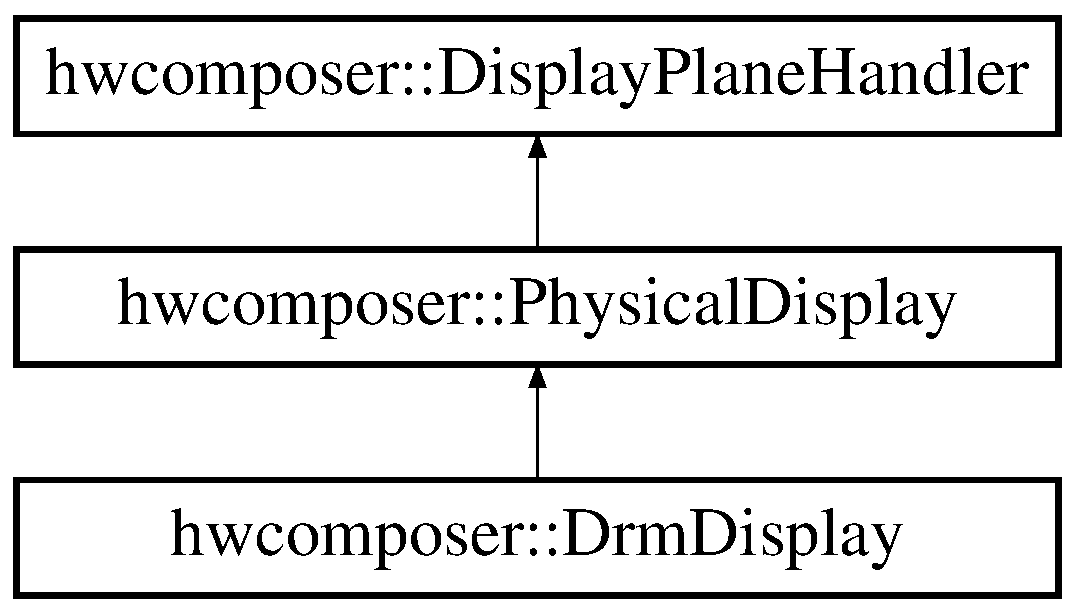
\includegraphics[height=3.000000cm]{classhwcomposer_1_1DisplayPlaneHandler}
\end{center}
\end{figure}
\subsection*{Public Member Functions}
\begin{DoxyCompactItemize}
\item 
virtual \mbox{\hyperlink{classhwcomposer_1_1DisplayPlaneHandler_aeab8a4a0c1db272293b3b6db6c7cd7b6}{$\sim$\+Display\+Plane\+Handler}} ()
\item 
virtual bool \mbox{\hyperlink{classhwcomposer_1_1DisplayPlaneHandler_aa4d32269c693dbf4a4c91c31ed577784}{Populate\+Planes}} (std\+::vector$<$ std\+::unique\+\_\+ptr$<$ \mbox{\hyperlink{classhwcomposer_1_1DisplayPlane}{Display\+Plane}} $>$$>$ \&overlay\+\_\+planes)=0
\item 
virtual bool \mbox{\hyperlink{classhwcomposer_1_1DisplayPlaneHandler_a1135b134010e6736aa49304100c9d3b9}{Test\+Commit}} (const std\+::vector$<$ \mbox{\hyperlink{structhwcomposer_1_1OverlayPlane}{Overlay\+Plane}} $>$ \&commit\+\_\+planes) const =0
\end{DoxyCompactItemize}


\subsection{Detailed Description}


Definition at line 34 of file displayplanehandler.\+h.



\subsection{Constructor \& Destructor Documentation}
\mbox{\Hypertarget{classhwcomposer_1_1DisplayPlaneHandler_aeab8a4a0c1db272293b3b6db6c7cd7b6}\label{classhwcomposer_1_1DisplayPlaneHandler_aeab8a4a0c1db272293b3b6db6c7cd7b6}} 
\index{hwcomposer\+::\+Display\+Plane\+Handler@{hwcomposer\+::\+Display\+Plane\+Handler}!````~Display\+Plane\+Handler@{$\sim$\+Display\+Plane\+Handler}}
\index{````~Display\+Plane\+Handler@{$\sim$\+Display\+Plane\+Handler}!hwcomposer\+::\+Display\+Plane\+Handler@{hwcomposer\+::\+Display\+Plane\+Handler}}
\subsubsection{\texorpdfstring{$\sim$\+Display\+Plane\+Handler()}{~DisplayPlaneHandler()}}
{\footnotesize\ttfamily virtual hwcomposer\+::\+Display\+Plane\+Handler\+::$\sim$\+Display\+Plane\+Handler (\begin{DoxyParamCaption}{ }\end{DoxyParamCaption})\hspace{0.3cm}{\ttfamily [inline]}, {\ttfamily [virtual]}}



Definition at line 36 of file displayplanehandler.\+h.


\begin{DoxyCode}{0}
\DoxyCodeLine{36                                  \{}
\DoxyCodeLine{37   \}}
\end{DoxyCode}


\subsection{Member Function Documentation}
\mbox{\Hypertarget{classhwcomposer_1_1DisplayPlaneHandler_aa4d32269c693dbf4a4c91c31ed577784}\label{classhwcomposer_1_1DisplayPlaneHandler_aa4d32269c693dbf4a4c91c31ed577784}} 
\index{hwcomposer\+::\+Display\+Plane\+Handler@{hwcomposer\+::\+Display\+Plane\+Handler}!Populate\+Planes@{Populate\+Planes}}
\index{Populate\+Planes@{Populate\+Planes}!hwcomposer\+::\+Display\+Plane\+Handler@{hwcomposer\+::\+Display\+Plane\+Handler}}
\subsubsection{\texorpdfstring{Populate\+Planes()}{PopulatePlanes()}}
{\footnotesize\ttfamily virtual bool hwcomposer\+::\+Display\+Plane\+Handler\+::\+Populate\+Planes (\begin{DoxyParamCaption}\item[{std\+::vector$<$ std\+::unique\+\_\+ptr$<$ \mbox{\hyperlink{classhwcomposer_1_1DisplayPlane}{Display\+Plane}} $>$$>$ \&}]{overlay\+\_\+planes }\end{DoxyParamCaption})\hspace{0.3cm}{\ttfamily [pure virtual]}}



Implemented in \mbox{\hyperlink{classhwcomposer_1_1PhysicalDisplay_afe0c0a304dab32918d3c40520f00d991}{hwcomposer\+::\+Physical\+Display}}, and \mbox{\hyperlink{classhwcomposer_1_1DrmDisplay_acbf817afffc6ad6f2879d914a0335dd0}{hwcomposer\+::\+Drm\+Display}}.

\mbox{\Hypertarget{classhwcomposer_1_1DisplayPlaneHandler_a1135b134010e6736aa49304100c9d3b9}\label{classhwcomposer_1_1DisplayPlaneHandler_a1135b134010e6736aa49304100c9d3b9}} 
\index{hwcomposer\+::\+Display\+Plane\+Handler@{hwcomposer\+::\+Display\+Plane\+Handler}!Test\+Commit@{Test\+Commit}}
\index{Test\+Commit@{Test\+Commit}!hwcomposer\+::\+Display\+Plane\+Handler@{hwcomposer\+::\+Display\+Plane\+Handler}}
\subsubsection{\texorpdfstring{Test\+Commit()}{TestCommit()}}
{\footnotesize\ttfamily virtual bool hwcomposer\+::\+Display\+Plane\+Handler\+::\+Test\+Commit (\begin{DoxyParamCaption}\item[{const std\+::vector$<$ \mbox{\hyperlink{structhwcomposer_1_1OverlayPlane}{Overlay\+Plane}} $>$ \&}]{commit\+\_\+planes }\end{DoxyParamCaption}) const\hspace{0.3cm}{\ttfamily [pure virtual]}}



Implemented in \mbox{\hyperlink{classhwcomposer_1_1PhysicalDisplay_a3c71b07e973c29b5603c35c333a42991}{hwcomposer\+::\+Physical\+Display}}, and \mbox{\hyperlink{classhwcomposer_1_1DrmDisplay_a7aaa318ce853a36ebcaf837fe1801f88}{hwcomposer\+::\+Drm\+Display}}.



The documentation for this class was generated from the following file\+:\begin{DoxyCompactItemize}
\item 
wsi/\mbox{\hyperlink{displayplanehandler_8h}{displayplanehandler.\+h}}\end{DoxyCompactItemize}

\hypertarget{classhwcomposer_1_1DisplayPlaneManager}{}\section{hwcomposer\+:\+:Display\+Plane\+Manager Class Reference}
\label{classhwcomposer_1_1DisplayPlaneManager}\index{hwcomposer\+::\+Display\+Plane\+Manager@{hwcomposer\+::\+Display\+Plane\+Manager}}


{\ttfamily \#include $<$displayplanemanager.\+h$>$}

\subsection*{Public Member Functions}
\begin{DoxyCompactItemize}
\item 
\mbox{\hyperlink{classhwcomposer_1_1DisplayPlaneManager_ad14eef5182a0ca73ed585de5db43b9f7}{Display\+Plane\+Manager}} (\mbox{\hyperlink{classhwcomposer_1_1DisplayPlaneHandler}{Display\+Plane\+Handler}} $\ast$plane\+\_\+handler, \mbox{\hyperlink{classhwcomposer_1_1ResourceManager}{Resource\+Manager}} $\ast$resource\+\_\+manager)
\item 
virtual \mbox{\hyperlink{classhwcomposer_1_1DisplayPlaneManager_a897ab790611539e024ecdd1497b7d579}{$\sim$\+Display\+Plane\+Manager}} ()
\item 
bool \mbox{\hyperlink{classhwcomposer_1_1DisplayPlaneManager_ab1d0c1f3132a46d2ab2ba323a418eebf}{Initialize}} (uint32\+\_\+t width, uint32\+\_\+t height, \mbox{\hyperlink{classhwcomposer_1_1FrameBufferManager}{Frame\+Buffer\+Manager}} $\ast$frame\+\_\+buffer\+\_\+manager)
\item 
bool \mbox{\hyperlink{classhwcomposer_1_1DisplayPlaneManager_ab619680feec679f90c733f104bab43d4}{Validate\+Layers}} (std\+::vector$<$ \mbox{\hyperlink{structhwcomposer_1_1OverlayLayer}{Overlay\+Layer}} $>$ \&layers, int add\+\_\+index, bool disable\+\_\+overlay, bool $\ast$commit\+\_\+checked, bool $\ast$re\+\_\+validation\+\_\+needed, \mbox{\hyperlink{namespacehwcomposer_adf383ae435d39a5631a8ad82e7fa18a4}{Display\+Plane\+State\+List}} \&composition, \mbox{\hyperlink{namespacehwcomposer_adf383ae435d39a5631a8ad82e7fa18a4}{Display\+Plane\+State\+List}} \&previous\+\_\+composition, std\+::vector$<$ \mbox{\hyperlink{classhwcomposer_1_1NativeSurface}{Native\+Surface}} $\ast$$>$ \&mark\+\_\+later)
\item 
void \mbox{\hyperlink{classhwcomposer_1_1DisplayPlaneManager_adafd342e7e70017f40491d6ba3e70360}{Mark\+Surfaces\+For\+Recycling}} (\mbox{\hyperlink{classhwcomposer_1_1DisplayPlaneState}{Display\+Plane\+State}} $\ast$plane, std\+::vector$<$ \mbox{\hyperlink{classhwcomposer_1_1NativeSurface}{Native\+Surface}} $\ast$$>$ \&mark\+\_\+later, bool recycle\+\_\+resources, bool reset\+\_\+plane\+\_\+surfaces=true)
\item 
void \mbox{\hyperlink{classhwcomposer_1_1DisplayPlaneManager_a027bc17f4b4b7f61056ba93616e5787f}{Released\+Surfaces}} ()
\item 
bool \mbox{\hyperlink{classhwcomposer_1_1DisplayPlaneManager_a2d428d923d493cfca4b14e9a0ea5b952}{Re\+Validate\+Planes}} (\mbox{\hyperlink{namespacehwcomposer_adf383ae435d39a5631a8ad82e7fa18a4}{Display\+Plane\+State\+List}} \&list, std\+::vector$<$ \mbox{\hyperlink{structhwcomposer_1_1OverlayLayer}{Overlay\+Layer}} $>$ \&layers, std\+::vector$<$ \mbox{\hyperlink{classhwcomposer_1_1NativeSurface}{Native\+Surface}} $\ast$$>$ \&mark\+\_\+later, bool $\ast$request\+\_\+full\+\_\+validation, bool needs\+\_\+revalidation\+\_\+checks, bool re\+\_\+validate\+\_\+commit)
\item 
bool \mbox{\hyperlink{classhwcomposer_1_1DisplayPlaneManager_ac5fa79927587781837c103df3aa8fb3d}{Check\+Plane\+Format}} (uint32\+\_\+t format)
\item 
void \mbox{\hyperlink{classhwcomposer_1_1DisplayPlaneManager_af76e9e632a76792f65bcde3a9e025169}{Set\+Off\+Screen\+Plane\+Target}} (\mbox{\hyperlink{classhwcomposer_1_1DisplayPlaneState}{Display\+Plane\+State}} \&plane)
\item 
void \mbox{\hyperlink{classhwcomposer_1_1DisplayPlaneManager_a953f9760e8a6a692213c32e66928d527}{Release\+Free\+Off\+Screen\+Targets}} (bool forced=false)
\item 
void \mbox{\hyperlink{classhwcomposer_1_1DisplayPlaneManager_aaafa069e84d1ae52f0f7dd8c973e5620}{Release\+All\+Off\+Screen\+Targets}} ()
\item 
bool \mbox{\hyperlink{classhwcomposer_1_1DisplayPlaneManager_a5d6b465f2867254778f611f2afddb0af}{Has\+Surfaces}} () const
\item 
uint32\+\_\+t \mbox{\hyperlink{classhwcomposer_1_1DisplayPlaneManager_abfa5fe391e308c60cea394a131d87d35}{Get\+Height}} () const
\item 
uint32\+\_\+t \mbox{\hyperlink{classhwcomposer_1_1DisplayPlaneManager_a8a2bbba4ec1dea9578e8f6103a636e24}{Get\+Total\+Overlays}} () const
\item 
void \mbox{\hyperlink{classhwcomposer_1_1DisplayPlaneManager_ac9eeb5875537f8ca624760e04bead0fd}{Set\+Last\+Plane\+Usage}} (bool enable)
\item 
void \mbox{\hyperlink{classhwcomposer_1_1DisplayPlaneManager_a80527bbdb1b4f5c9fe8a58241e27f559}{Set\+Display\+Transform}} (uint32\+\_\+t transform)
\item 
bool \mbox{\hyperlink{classhwcomposer_1_1DisplayPlaneManager_ada91a47d462537740543db7c70d07f8e}{Squash\+Planes\+As\+Needed}} (const std\+::vector$<$ \mbox{\hyperlink{structhwcomposer_1_1OverlayLayer}{Overlay\+Layer}} $>$ \&layers, \mbox{\hyperlink{namespacehwcomposer_adf383ae435d39a5631a8ad82e7fa18a4}{Display\+Plane\+State\+List}} \&composition, std\+::vector$<$ \mbox{\hyperlink{structhwcomposer_1_1OverlayPlane}{Overlay\+Plane}} $>$ \&commit\+\_\+planes, std\+::vector$<$ \mbox{\hyperlink{classhwcomposer_1_1NativeSurface}{Native\+Surface}} $\ast$$>$ \&mark\+\_\+later, bool $\ast$validate\+\_\+final\+\_\+layers)
\item 
bool \mbox{\hyperlink{classhwcomposer_1_1DisplayPlaneManager_afd4d9af275a937a7afa49a1d37ab0063}{Force\+Separate\+Plane}} (const std\+::vector$<$ \mbox{\hyperlink{structhwcomposer_1_1OverlayLayer}{Overlay\+Layer}} $>$ \&layers, const \mbox{\hyperlink{classhwcomposer_1_1DisplayPlaneState}{Display\+Plane\+State}} \&last\+\_\+plane, const \mbox{\hyperlink{structhwcomposer_1_1OverlayLayer}{Overlay\+Layer}} $\ast$target\+\_\+layer)
\end{DoxyCompactItemize}


\subsection{Detailed Description}


Definition at line 37 of file displayplanemanager.\+h.



\subsection{Constructor \& Destructor Documentation}
\mbox{\Hypertarget{classhwcomposer_1_1DisplayPlaneManager_ad14eef5182a0ca73ed585de5db43b9f7}\label{classhwcomposer_1_1DisplayPlaneManager_ad14eef5182a0ca73ed585de5db43b9f7}} 
\index{hwcomposer\+::\+Display\+Plane\+Manager@{hwcomposer\+::\+Display\+Plane\+Manager}!Display\+Plane\+Manager@{Display\+Plane\+Manager}}
\index{Display\+Plane\+Manager@{Display\+Plane\+Manager}!hwcomposer\+::\+Display\+Plane\+Manager@{hwcomposer\+::\+Display\+Plane\+Manager}}
\subsubsection{\texorpdfstring{Display\+Plane\+Manager()}{DisplayPlaneManager()}}
{\footnotesize\ttfamily hwcomposer\+::\+Display\+Plane\+Manager\+::\+Display\+Plane\+Manager (\begin{DoxyParamCaption}\item[{\mbox{\hyperlink{classhwcomposer_1_1DisplayPlaneHandler}{Display\+Plane\+Handler}} $\ast$}]{plane\+\_\+handler,  }\item[{\mbox{\hyperlink{classhwcomposer_1_1ResourceManager}{Resource\+Manager}} $\ast$}]{resource\+\_\+manager }\end{DoxyParamCaption})}



Definition at line 29 of file displayplanemanager.\+cpp.


\begin{DoxyCode}{0}
\DoxyCodeLine{31     : plane\_handler\_(plane\_handler),}
\DoxyCodeLine{32       resource\_manager\_(resource\_manager),}
\DoxyCodeLine{33       cursor\_plane\_(\textcolor{keyword}{nullptr}),}
\DoxyCodeLine{34       width\_(0),}
\DoxyCodeLine{35       height\_(0),}
\DoxyCodeLine{36       total\_overlays\_(0),}
\DoxyCodeLine{37       display\_transform\_(kIdentity),}
\DoxyCodeLine{38 \textcolor{preprocessor}{\#ifdef DISABLE\_CURSOR\_PLANE}}
\DoxyCodeLine{39       release\_surfaces\_(\textcolor{keyword}{false}),}
\DoxyCodeLine{40       enable\_last\_plane\_(\textcolor{keyword}{true}) \{}
\DoxyCodeLine{41 \textcolor{preprocessor}{\#else}}
\DoxyCodeLine{42       release\_surfaces\_(\textcolor{keyword}{false}) \{}
\DoxyCodeLine{43 \textcolor{preprocessor}{\#endif}}
\DoxyCodeLine{44 \}}
\end{DoxyCode}
\mbox{\Hypertarget{classhwcomposer_1_1DisplayPlaneManager_a897ab790611539e024ecdd1497b7d579}\label{classhwcomposer_1_1DisplayPlaneManager_a897ab790611539e024ecdd1497b7d579}} 
\index{hwcomposer\+::\+Display\+Plane\+Manager@{hwcomposer\+::\+Display\+Plane\+Manager}!````~Display\+Plane\+Manager@{$\sim$\+Display\+Plane\+Manager}}
\index{````~Display\+Plane\+Manager@{$\sim$\+Display\+Plane\+Manager}!hwcomposer\+::\+Display\+Plane\+Manager@{hwcomposer\+::\+Display\+Plane\+Manager}}
\subsubsection{\texorpdfstring{$\sim$\+Display\+Plane\+Manager()}{~DisplayPlaneManager()}}
{\footnotesize\ttfamily hwcomposer\+::\+Display\+Plane\+Manager\+::$\sim$\+Display\+Plane\+Manager (\begin{DoxyParamCaption}{ }\end{DoxyParamCaption})\hspace{0.3cm}{\ttfamily [virtual]}}



Definition at line 46 of file displayplanemanager.\+cpp.


\begin{DoxyCode}{0}
\DoxyCodeLine{46                                           \{}
\DoxyCodeLine{47 \}}
\end{DoxyCode}


\subsection{Member Function Documentation}
\mbox{\Hypertarget{classhwcomposer_1_1DisplayPlaneManager_ac5fa79927587781837c103df3aa8fb3d}\label{classhwcomposer_1_1DisplayPlaneManager_ac5fa79927587781837c103df3aa8fb3d}} 
\index{hwcomposer\+::\+Display\+Plane\+Manager@{hwcomposer\+::\+Display\+Plane\+Manager}!Check\+Plane\+Format@{Check\+Plane\+Format}}
\index{Check\+Plane\+Format@{Check\+Plane\+Format}!hwcomposer\+::\+Display\+Plane\+Manager@{hwcomposer\+::\+Display\+Plane\+Manager}}
\subsubsection{\texorpdfstring{Check\+Plane\+Format()}{CheckPlaneFormat()}}
{\footnotesize\ttfamily bool hwcomposer\+::\+Display\+Plane\+Manager\+::\+Check\+Plane\+Format (\begin{DoxyParamCaption}\item[{uint32\+\_\+t}]{format }\end{DoxyParamCaption})}



Definition at line 813 of file displayplanemanager.\+cpp.


\begin{DoxyCode}{0}
\DoxyCodeLine{813                                                           \{}
\DoxyCodeLine{814   \textcolor{keywordflow}{return} overlay\_planes\_.at(0)->IsSupportedFormat(format);}
\DoxyCodeLine{815 \}}
\end{DoxyCode}
\mbox{\Hypertarget{classhwcomposer_1_1DisplayPlaneManager_afd4d9af275a937a7afa49a1d37ab0063}\label{classhwcomposer_1_1DisplayPlaneManager_afd4d9af275a937a7afa49a1d37ab0063}} 
\index{hwcomposer\+::\+Display\+Plane\+Manager@{hwcomposer\+::\+Display\+Plane\+Manager}!Force\+Separate\+Plane@{Force\+Separate\+Plane}}
\index{Force\+Separate\+Plane@{Force\+Separate\+Plane}!hwcomposer\+::\+Display\+Plane\+Manager@{hwcomposer\+::\+Display\+Plane\+Manager}}
\subsubsection{\texorpdfstring{Force\+Separate\+Plane()}{ForceSeparatePlane()}}
{\footnotesize\ttfamily bool hwcomposer\+::\+Display\+Plane\+Manager\+::\+Force\+Separate\+Plane (\begin{DoxyParamCaption}\item[{const std\+::vector$<$ \mbox{\hyperlink{structhwcomposer_1_1OverlayLayer}{Overlay\+Layer}} $>$ \&}]{layers,  }\item[{const \mbox{\hyperlink{classhwcomposer_1_1DisplayPlaneState}{Display\+Plane\+State}} \&}]{last\+\_\+plane,  }\item[{const \mbox{\hyperlink{structhwcomposer_1_1OverlayLayer}{Overlay\+Layer}} $\ast$}]{target\+\_\+layer }\end{DoxyParamCaption})}



Definition at line 1176 of file displayplanemanager.\+cpp.


\begin{DoxyCode}{0}
\DoxyCodeLine{1178                                                                            \{}
\DoxyCodeLine{1179   \textcolor{keyword}{const} std::vector<size\_t> \&new\_layers = last\_plane.GetSourceLayers();}
\DoxyCodeLine{1180   \textcolor{keyword}{const} HwcRect<int> \&display\_frame = last\_plane.GetDisplayFrame();}
\DoxyCodeLine{1181   HwcRect<int> target\_display\_frame = display\_frame;}
\DoxyCodeLine{1182   uint32\_t total\_width = 0;}
\DoxyCodeLine{1183   uint32\_t total\_height = 0;}
\DoxyCodeLine{1184   \textcolor{keywordflow}{if} (target\_layer) \{}
\DoxyCodeLine{1185     total\_width = target\_layer->GetDisplayFrameWidth();}
\DoxyCodeLine{1186     total\_height = target\_layer->GetDisplayFrameHeight();}
\DoxyCodeLine{1187     target\_display\_frame = target\_layer->GetDisplayFrame();}
\DoxyCodeLine{1188     \mbox{\hyperlink{namespacehwcomposer_a472acec9a1b2eedf8a58f690edd21652}{CalculateRect}}(display\_frame, target\_display\_frame);}
\DoxyCodeLine{1189   \}}
\DoxyCodeLine{1190 }
\DoxyCodeLine{1191   \textcolor{keywordtype}{bool} force\_separate = \textcolor{keyword}{false};}
\DoxyCodeLine{1192   \textcolor{keywordflow}{for} (\textcolor{keyword}{const} \textcolor{keywordtype}{size\_t} \&index : new\_layers) \{}
\DoxyCodeLine{1193     \textcolor{keyword}{const} OverlayLayer \&layer = layers.at(index);}
\DoxyCodeLine{1194     total\_width = std::max(total\_width, layer.GetDisplayFrameWidth());}
\DoxyCodeLine{1195     total\_height = std::max(total\_height, layer.GetDisplayFrameHeight());}
\DoxyCodeLine{1196   \}}
\DoxyCodeLine{1197 }
\DoxyCodeLine{1198   uint32\_t target\_width =}
\DoxyCodeLine{1199       target\_display\_frame.right - target\_display\_frame.left;}
\DoxyCodeLine{1200   uint32\_t target\_height =}
\DoxyCodeLine{1201       target\_display\_frame.bottom - target\_display\_frame.top;}
\DoxyCodeLine{1202   \textcolor{keywordflow}{if} ((total\_width != target\_width) || (total\_height != target\_height)) \{}
\DoxyCodeLine{1203     force\_separate = \textcolor{keyword}{true};}
\DoxyCodeLine{1204   \}}
\DoxyCodeLine{1205 }
\DoxyCodeLine{1206   \textcolor{keywordflow}{return} force\_separate;}
\DoxyCodeLine{1207 \}}
\end{DoxyCode}
\mbox{\Hypertarget{classhwcomposer_1_1DisplayPlaneManager_abfa5fe391e308c60cea394a131d87d35}\label{classhwcomposer_1_1DisplayPlaneManager_abfa5fe391e308c60cea394a131d87d35}} 
\index{hwcomposer\+::\+Display\+Plane\+Manager@{hwcomposer\+::\+Display\+Plane\+Manager}!Get\+Height@{Get\+Height}}
\index{Get\+Height@{Get\+Height}!hwcomposer\+::\+Display\+Plane\+Manager@{hwcomposer\+::\+Display\+Plane\+Manager}}
\subsubsection{\texorpdfstring{Get\+Height()}{GetHeight()}}
{\footnotesize\ttfamily uint32\+\_\+t hwcomposer\+::\+Display\+Plane\+Manager\+::\+Get\+Height (\begin{DoxyParamCaption}{ }\end{DoxyParamCaption}) const\hspace{0.3cm}{\ttfamily [inline]}}



Definition at line 84 of file displayplanemanager.\+h.


\begin{DoxyCode}{0}
\DoxyCodeLine{84                              \{}
\DoxyCodeLine{85     \textcolor{keywordflow}{return} height\_;}
\DoxyCodeLine{86   \}}
\end{DoxyCode}
\mbox{\Hypertarget{classhwcomposer_1_1DisplayPlaneManager_a8a2bbba4ec1dea9578e8f6103a636e24}\label{classhwcomposer_1_1DisplayPlaneManager_a8a2bbba4ec1dea9578e8f6103a636e24}} 
\index{hwcomposer\+::\+Display\+Plane\+Manager@{hwcomposer\+::\+Display\+Plane\+Manager}!Get\+Total\+Overlays@{Get\+Total\+Overlays}}
\index{Get\+Total\+Overlays@{Get\+Total\+Overlays}!hwcomposer\+::\+Display\+Plane\+Manager@{hwcomposer\+::\+Display\+Plane\+Manager}}
\subsubsection{\texorpdfstring{Get\+Total\+Overlays()}{GetTotalOverlays()}}
{\footnotesize\ttfamily uint32\+\_\+t hwcomposer\+::\+Display\+Plane\+Manager\+::\+Get\+Total\+Overlays (\begin{DoxyParamCaption}{ }\end{DoxyParamCaption}) const\hspace{0.3cm}{\ttfamily [inline]}}



Definition at line 88 of file displayplanemanager.\+h.


\begin{DoxyCode}{0}
\DoxyCodeLine{88                                     \{}
\DoxyCodeLine{89     \textcolor{keywordflow}{return} total\_overlays\_;}
\DoxyCodeLine{90   \}}
\end{DoxyCode}
\mbox{\Hypertarget{classhwcomposer_1_1DisplayPlaneManager_a5d6b465f2867254778f611f2afddb0af}\label{classhwcomposer_1_1DisplayPlaneManager_a5d6b465f2867254778f611f2afddb0af}} 
\index{hwcomposer\+::\+Display\+Plane\+Manager@{hwcomposer\+::\+Display\+Plane\+Manager}!Has\+Surfaces@{Has\+Surfaces}}
\index{Has\+Surfaces@{Has\+Surfaces}!hwcomposer\+::\+Display\+Plane\+Manager@{hwcomposer\+::\+Display\+Plane\+Manager}}
\subsubsection{\texorpdfstring{Has\+Surfaces()}{HasSurfaces()}}
{\footnotesize\ttfamily bool hwcomposer\+::\+Display\+Plane\+Manager\+::\+Has\+Surfaces (\begin{DoxyParamCaption}{ }\end{DoxyParamCaption}) const\hspace{0.3cm}{\ttfamily [inline]}}



Definition at line 80 of file displayplanemanager.\+h.


\begin{DoxyCode}{0}
\DoxyCodeLine{80                            \{}
\DoxyCodeLine{81     \textcolor{keywordflow}{return} !surfaces\_.empty();}
\DoxyCodeLine{82   \}}
\end{DoxyCode}
\mbox{\Hypertarget{classhwcomposer_1_1DisplayPlaneManager_ab1d0c1f3132a46d2ab2ba323a418eebf}\label{classhwcomposer_1_1DisplayPlaneManager_ab1d0c1f3132a46d2ab2ba323a418eebf}} 
\index{hwcomposer\+::\+Display\+Plane\+Manager@{hwcomposer\+::\+Display\+Plane\+Manager}!Initialize@{Initialize}}
\index{Initialize@{Initialize}!hwcomposer\+::\+Display\+Plane\+Manager@{hwcomposer\+::\+Display\+Plane\+Manager}}
\subsubsection{\texorpdfstring{Initialize()}{Initialize()}}
{\footnotesize\ttfamily bool hwcomposer\+::\+Display\+Plane\+Manager\+::\+Initialize (\begin{DoxyParamCaption}\item[{uint32\+\_\+t}]{width,  }\item[{uint32\+\_\+t}]{height,  }\item[{\mbox{\hyperlink{classhwcomposer_1_1FrameBufferManager}{Frame\+Buffer\+Manager}} $\ast$}]{frame\+\_\+buffer\+\_\+manager }\end{DoxyParamCaption})}



Definition at line 49 of file displayplanemanager.\+cpp.


\begin{DoxyCode}{0}
\DoxyCodeLine{50                                                                                \{}
\DoxyCodeLine{51   fb\_manager\_ = frame\_buffer\_manager;}
\DoxyCodeLine{52   width\_ = width;}
\DoxyCodeLine{53   height\_ = height;}
\DoxyCodeLine{54   \textcolor{keywordtype}{bool} status = plane\_handler\_->\mbox{\hyperlink{classhwcomposer_1_1DisplayPlaneHandler_aa4d32269c693dbf4a4c91c31ed577784}{PopulatePlanes}}(overlay\_planes\_);}
\DoxyCodeLine{55   \textcolor{keywordflow}{if} (!overlay\_planes\_.empty()) \{}
\DoxyCodeLine{56     total\_overlays\_ = overlay\_planes\_.size();}
\DoxyCodeLine{57     \textcolor{keywordflow}{if} (total\_overlays\_ > 1) \{}
\DoxyCodeLine{58       cursor\_plane\_ = overlay\_planes\_.back().get();}
\DoxyCodeLine{59       \textcolor{comment}{// If this is a universal plane, let's not restrict it to}}
\DoxyCodeLine{60       \textcolor{comment}{// cursor usage only.}}
\DoxyCodeLine{61       \textcolor{keywordflow}{if} (cursor\_plane\_->\mbox{\hyperlink{classhwcomposer_1_1DisplayPlane_a7b374ba9e799f7d0b53afbd939961c51}{IsUniversal}}()) \{}
\DoxyCodeLine{62         cursor\_plane\_ = \mbox{\hyperlink{alios_2platformdefines_8h_a070d2ce7b6bb7e5c05602aa8c308d0c4}{NULL}};}
\DoxyCodeLine{63       \} \textcolor{keywordflow}{else} \{}
\DoxyCodeLine{64         total\_overlays\_--;}
\DoxyCodeLine{65       \}}
\DoxyCodeLine{66     \}}
\DoxyCodeLine{67   \}}
\DoxyCodeLine{68 }
\DoxyCodeLine{69   \textcolor{keywordflow}{return} status;}
\DoxyCodeLine{70 \}}
\end{DoxyCode}
\mbox{\Hypertarget{classhwcomposer_1_1DisplayPlaneManager_adafd342e7e70017f40491d6ba3e70360}\label{classhwcomposer_1_1DisplayPlaneManager_adafd342e7e70017f40491d6ba3e70360}} 
\index{hwcomposer\+::\+Display\+Plane\+Manager@{hwcomposer\+::\+Display\+Plane\+Manager}!Mark\+Surfaces\+For\+Recycling@{Mark\+Surfaces\+For\+Recycling}}
\index{Mark\+Surfaces\+For\+Recycling@{Mark\+Surfaces\+For\+Recycling}!hwcomposer\+::\+Display\+Plane\+Manager@{hwcomposer\+::\+Display\+Plane\+Manager}}
\subsubsection{\texorpdfstring{Mark\+Surfaces\+For\+Recycling()}{MarkSurfacesForRecycling()}}
{\footnotesize\ttfamily void hwcomposer\+::\+Display\+Plane\+Manager\+::\+Mark\+Surfaces\+For\+Recycling (\begin{DoxyParamCaption}\item[{\mbox{\hyperlink{classhwcomposer_1_1DisplayPlaneState}{Display\+Plane\+State}} $\ast$}]{plane,  }\item[{std\+::vector$<$ \mbox{\hyperlink{classhwcomposer_1_1NativeSurface}{Native\+Surface}} $\ast$$>$ \&}]{mark\+\_\+later,  }\item[{bool}]{recycle\+\_\+resources,  }\item[{bool}]{reset\+\_\+plane\+\_\+surfaces = {\ttfamily true} }\end{DoxyParamCaption})}



Definition at line 876 of file displayplanemanager.\+cpp.


\begin{DoxyCode}{0}
\DoxyCodeLine{878                                                        \{}
\DoxyCodeLine{879   \textcolor{keyword}{const} std::vector<NativeSurface *> \&surfaces = plane->GetSurfaces();}
\DoxyCodeLine{880   \textcolor{keywordflow}{if} (!surfaces.empty()) \{}
\DoxyCodeLine{881     release\_surfaces\_ = \textcolor{keyword}{true};}
\DoxyCodeLine{882     \textcolor{keywordtype}{size\_t} size = surfaces.size();}
\DoxyCodeLine{883     \textcolor{keywordflow}{if} (recycle\_resources) \{}
\DoxyCodeLine{884       \textcolor{comment}{// Make sure we don't mark current on-screen surface or}}
\DoxyCodeLine{885       \textcolor{comment}{// one in flight. These surfaces will be added as part of}}
\DoxyCodeLine{886       \textcolor{comment}{// mark\_later to be recycled later.}}
\DoxyCodeLine{887       \textcolor{keywordflow}{for} (uint32\_t i = 0; i < size; i++) \{}
\DoxyCodeLine{888         NativeSurface *surface = surfaces.at(i);}
\DoxyCodeLine{889         \textcolor{keywordflow}{if} (surface->GetSurfaceAge() >= 0 \&\& surface->IsOnScreen()) \{}
\DoxyCodeLine{890           mark\_later.emplace\_back(surface);}
\DoxyCodeLine{891         \} \textcolor{keywordflow}{else} \{}
\DoxyCodeLine{892           surface->SetSurfaceAge(-1);}
\DoxyCodeLine{893         \}}
\DoxyCodeLine{894       \}}
\DoxyCodeLine{895     \} \textcolor{keywordflow}{else} \{}
\DoxyCodeLine{896       \textcolor{keywordflow}{for} (uint32\_t i = 0; i < size; i++) \{}
\DoxyCodeLine{897         NativeSurface *surface = surfaces.at(i);}
\DoxyCodeLine{898         surface->SetSurfaceAge(-1);}
\DoxyCodeLine{899       \}}
\DoxyCodeLine{900     \}}
\DoxyCodeLine{901 }
\DoxyCodeLine{902     \textcolor{keywordflow}{if} (reset\_plane\_surfaces)}
\DoxyCodeLine{903       plane->ReleaseSurfaces();}
\DoxyCodeLine{904   \}}
\DoxyCodeLine{905 \}}
\end{DoxyCode}
\mbox{\Hypertarget{classhwcomposer_1_1DisplayPlaneManager_aaafa069e84d1ae52f0f7dd8c973e5620}\label{classhwcomposer_1_1DisplayPlaneManager_aaafa069e84d1ae52f0f7dd8c973e5620}} 
\index{hwcomposer\+::\+Display\+Plane\+Manager@{hwcomposer\+::\+Display\+Plane\+Manager}!Release\+All\+Off\+Screen\+Targets@{Release\+All\+Off\+Screen\+Targets}}
\index{Release\+All\+Off\+Screen\+Targets@{Release\+All\+Off\+Screen\+Targets}!hwcomposer\+::\+Display\+Plane\+Manager@{hwcomposer\+::\+Display\+Plane\+Manager}}
\subsubsection{\texorpdfstring{Release\+All\+Off\+Screen\+Targets()}{ReleaseAllOffScreenTargets()}}
{\footnotesize\ttfamily void hwcomposer\+::\+Display\+Plane\+Manager\+::\+Release\+All\+Off\+Screen\+Targets (\begin{DoxyParamCaption}{ }\end{DoxyParamCaption})}



Definition at line 660 of file displayplanemanager.\+cpp.


\begin{DoxyCode}{0}
\DoxyCodeLine{660                                                      \{}
\DoxyCodeLine{661   \mbox{\hyperlink{hwctrace_8h_a539a95897071c72babce1012d503b3ca}{CTRACE}}();}
\DoxyCodeLine{662   std::vector<std::unique\_ptr<NativeSurface>>().swap(surfaces\_);}
\DoxyCodeLine{663 \}}
\end{DoxyCode}
\mbox{\Hypertarget{classhwcomposer_1_1DisplayPlaneManager_a027bc17f4b4b7f61056ba93616e5787f}\label{classhwcomposer_1_1DisplayPlaneManager_a027bc17f4b4b7f61056ba93616e5787f}} 
\index{hwcomposer\+::\+Display\+Plane\+Manager@{hwcomposer\+::\+Display\+Plane\+Manager}!Released\+Surfaces@{Released\+Surfaces}}
\index{Released\+Surfaces@{Released\+Surfaces}!hwcomposer\+::\+Display\+Plane\+Manager@{hwcomposer\+::\+Display\+Plane\+Manager}}
\subsubsection{\texorpdfstring{Released\+Surfaces()}{ReleasedSurfaces()}}
{\footnotesize\ttfamily void hwcomposer\+::\+Display\+Plane\+Manager\+::\+Released\+Surfaces (\begin{DoxyParamCaption}{ }\end{DoxyParamCaption})}



Definition at line 872 of file displayplanemanager.\+cpp.


\begin{DoxyCode}{0}
\DoxyCodeLine{872                                            \{}
\DoxyCodeLine{873   release\_surfaces\_ = \textcolor{keyword}{true};}
\DoxyCodeLine{874 \}}
\end{DoxyCode}
\mbox{\Hypertarget{classhwcomposer_1_1DisplayPlaneManager_a953f9760e8a6a692213c32e66928d527}\label{classhwcomposer_1_1DisplayPlaneManager_a953f9760e8a6a692213c32e66928d527}} 
\index{hwcomposer\+::\+Display\+Plane\+Manager@{hwcomposer\+::\+Display\+Plane\+Manager}!Release\+Free\+Off\+Screen\+Targets@{Release\+Free\+Off\+Screen\+Targets}}
\index{Release\+Free\+Off\+Screen\+Targets@{Release\+Free\+Off\+Screen\+Targets}!hwcomposer\+::\+Display\+Plane\+Manager@{hwcomposer\+::\+Display\+Plane\+Manager}}
\subsubsection{\texorpdfstring{Release\+Free\+Off\+Screen\+Targets()}{ReleaseFreeOffScreenTargets()}}
{\footnotesize\ttfamily void hwcomposer\+::\+Display\+Plane\+Manager\+::\+Release\+Free\+Off\+Screen\+Targets (\begin{DoxyParamCaption}\item[{bool}]{forced = {\ttfamily false} }\end{DoxyParamCaption})}



Definition at line 665 of file displayplanemanager.\+cpp.


\begin{DoxyCode}{0}
\DoxyCodeLine{665                                                                  \{}
\DoxyCodeLine{666   \textcolor{keywordflow}{if} (!release\_surfaces\_ \&\& !forced)}
\DoxyCodeLine{667     \textcolor{keywordflow}{return};}
\DoxyCodeLine{668 }
\DoxyCodeLine{669   std::vector<std::unique\_ptr<NativeSurface>> surfaces;}
\DoxyCodeLine{670   \textcolor{keywordflow}{for} (\textcolor{keyword}{auto} \&fb : surfaces\_) \{}
\DoxyCodeLine{671     \textcolor{keywordflow}{if} (fb->IsOnScreen()) \{}
\DoxyCodeLine{672       surfaces.emplace\_back(fb.release());}
\DoxyCodeLine{673     \}}
\DoxyCodeLine{674   \}}
\DoxyCodeLine{675 }
\DoxyCodeLine{676   surfaces.swap(surfaces\_);}
\DoxyCodeLine{677   release\_surfaces\_ = \textcolor{keyword}{false};}
\DoxyCodeLine{678 \}}
\end{DoxyCode}
\mbox{\Hypertarget{classhwcomposer_1_1DisplayPlaneManager_a2d428d923d493cfca4b14e9a0ea5b952}\label{classhwcomposer_1_1DisplayPlaneManager_a2d428d923d493cfca4b14e9a0ea5b952}} 
\index{hwcomposer\+::\+Display\+Plane\+Manager@{hwcomposer\+::\+Display\+Plane\+Manager}!Re\+Validate\+Planes@{Re\+Validate\+Planes}}
\index{Re\+Validate\+Planes@{Re\+Validate\+Planes}!hwcomposer\+::\+Display\+Plane\+Manager@{hwcomposer\+::\+Display\+Plane\+Manager}}
\subsubsection{\texorpdfstring{Re\+Validate\+Planes()}{ReValidatePlanes()}}
{\footnotesize\ttfamily bool hwcomposer\+::\+Display\+Plane\+Manager\+::\+Re\+Validate\+Planes (\begin{DoxyParamCaption}\item[{\mbox{\hyperlink{namespacehwcomposer_adf383ae435d39a5631a8ad82e7fa18a4}{Display\+Plane\+State\+List}} \&}]{list,  }\item[{std\+::vector$<$ \mbox{\hyperlink{structhwcomposer_1_1OverlayLayer}{Overlay\+Layer}} $>$ \&}]{layers,  }\item[{std\+::vector$<$ \mbox{\hyperlink{classhwcomposer_1_1NativeSurface}{Native\+Surface}} $\ast$$>$ \&}]{mark\+\_\+later,  }\item[{bool $\ast$}]{request\+\_\+full\+\_\+validation,  }\item[{bool}]{needs\+\_\+revalidation\+\_\+checks,  }\item[{bool}]{re\+\_\+validate\+\_\+commit }\end{DoxyParamCaption})}



Definition at line 907 of file displayplanemanager.\+cpp.


\begin{DoxyCode}{0}
\DoxyCodeLine{910                                                              \{}
\DoxyCodeLine{911 \textcolor{preprocessor}{\#ifdef SURFACE\_TRACING}}
\DoxyCodeLine{912   \mbox{\hyperlink{hwctrace_8h_a13ce5e3bbbbc8b8abe718d0c4631ee1d}{ISURFACETRACE}}(}
\DoxyCodeLine{913       \textcolor{stringliteral}{"ReValidatePlanes called needs\_revalidation\_checks \%d re\_validate\_commit "}}
\DoxyCodeLine{914       \textcolor{stringliteral}{"\%d  \(\backslash\)n"},}
\DoxyCodeLine{915       needs\_revalidation\_checks, re\_validate\_commit);}
\DoxyCodeLine{916 \textcolor{preprocessor}{\#endif}}
\DoxyCodeLine{917   \textcolor{comment}{// Let's first check the current combination works.}}
\DoxyCodeLine{918   *request\_full\_validation = \textcolor{keyword}{false};}
\DoxyCodeLine{919   \textcolor{keywordtype}{bool} render = \textcolor{keyword}{false};}
\DoxyCodeLine{920   \textcolor{keywordtype}{bool} reset\_composition\_region = \textcolor{keyword}{false};}
\DoxyCodeLine{921   std::vector<OverlayPlane> commit\_planes;}
\DoxyCodeLine{922   \textcolor{keywordflow}{for} (DisplayPlaneState \&temp : composition) \{}
\DoxyCodeLine{923     commit\_planes.emplace\_back(}
\DoxyCodeLine{924         OverlayPlane(temp.GetDisplayPlane(), temp.GetOverlayLayer()));}
\DoxyCodeLine{925 }
\DoxyCodeLine{926     \textcolor{keywordflow}{if} (temp.Scanout()) \{}
\DoxyCodeLine{927       \textcolor{keywordflow}{continue};}
\DoxyCodeLine{928     \}}
\DoxyCodeLine{929 }
\DoxyCodeLine{930     render = \textcolor{keyword}{true};}
\DoxyCodeLine{931   \}}
\DoxyCodeLine{932 }
\DoxyCodeLine{933   \textcolor{keywordflow}{if} (re\_validate\_commit) \{}
\DoxyCodeLine{934     \textcolor{comment}{// If this combination fails just fall back to full validation.}}
\DoxyCodeLine{935     \textcolor{keywordflow}{if} (!plane\_handler\_->\mbox{\hyperlink{classhwcomposer_1_1DisplayPlaneHandler_a1135b134010e6736aa49304100c9d3b9}{TestCommit}}(commit\_planes)) \{}
\DoxyCodeLine{936 \textcolor{preprocessor}{\#ifdef SURFACE\_TRACING}}
\DoxyCodeLine{937       \mbox{\hyperlink{hwctrace_8h_a13ce5e3bbbbc8b8abe718d0c4631ee1d}{ISURFACETRACE}}(}
\DoxyCodeLine{938           \textcolor{stringliteral}{"ReValidatePlanes Test commit failed. Forcing full validation. \(\backslash\)n"});}
\DoxyCodeLine{939 \textcolor{preprocessor}{\#endif}}
\DoxyCodeLine{940       *request\_full\_validation = \textcolor{keyword}{true};}
\DoxyCodeLine{941       \textcolor{keywordflow}{return} render;}
\DoxyCodeLine{942     \}}
\DoxyCodeLine{943   \}}
\DoxyCodeLine{944 }
\DoxyCodeLine{945   \textcolor{keywordflow}{if} (!needs\_revalidation\_checks) \{}
\DoxyCodeLine{946     \textcolor{keywordflow}{return} render;}
\DoxyCodeLine{947   \}}
\DoxyCodeLine{948 }
\DoxyCodeLine{949   uint32\_t index = 0;}
\DoxyCodeLine{950 }
\DoxyCodeLine{951   \textcolor{keywordflow}{for} (DisplayPlaneState \&last\_plane : composition) \{}
\DoxyCodeLine{952     \textcolor{keywordflow}{if} (!last\_plane.NeedsOffScreenComposition()) \{}
\DoxyCodeLine{953       index++;}
\DoxyCodeLine{954       reset\_composition\_region = \textcolor{keyword}{false};}
\DoxyCodeLine{955       \textcolor{keywordflow}{continue};}
\DoxyCodeLine{956     \}}
\DoxyCodeLine{957 }
\DoxyCodeLine{958     \textcolor{keywordflow}{if} (reset\_composition\_region) \{}
\DoxyCodeLine{959       last\_plane.RefreshSurfaces(\mbox{\hyperlink{classhwcomposer_1_1NativeSurface_a0d0f955fc1e9f95c9684e9524f4217d6a28fd0ed803677f131961bf65544b9f83}{NativeSurface::kFullClear}}, \textcolor{keyword}{true});}
\DoxyCodeLine{960     \}}
\DoxyCodeLine{961 }
\DoxyCodeLine{962     reset\_composition\_region = \textcolor{keyword}{false};}
\DoxyCodeLine{963     uint32\_t revalidation\_type = last\_plane.RevalidationType();}
\DoxyCodeLine{964 }
\DoxyCodeLine{965     \textcolor{keywordflow}{if} (!revalidation\_type) \{}
\DoxyCodeLine{966       render = \textcolor{keyword}{true};}
\DoxyCodeLine{967       index++;}
\DoxyCodeLine{968       \textcolor{keywordflow}{continue};}
\DoxyCodeLine{969     \}}
\DoxyCodeLine{970 }
\DoxyCodeLine{971     uint32\_t validation\_done = DisplayPlaneState::ReValidationType::kScanout;}
\DoxyCodeLine{972     \textcolor{keywordflow}{if} (revalidation\_type \& DisplayPlaneState::ReValidationType::kScanout) \{}
\DoxyCodeLine{973       \textcolor{keyword}{const} std::vector<size\_t> \&source\_layers = last\_plane.GetSourceLayers();}
\DoxyCodeLine{974       \textcolor{keywordtype}{bool} uses\_scalar = last\_plane.IsUsingPlaneScalar();}
\DoxyCodeLine{975       \textcolor{comment}{// Store current layer to re-set in case commit fails.}}
\DoxyCodeLine{976       \textcolor{keyword}{const} OverlayLayer *current\_layer = last\_plane.GetOverlayLayer();}
\DoxyCodeLine{977       OverlayLayer *layer = \&(layers.at(source\_layers.at(0)));}
\DoxyCodeLine{978       last\_plane.SetOverlayLayer(layer);}
\DoxyCodeLine{979       \textcolor{comment}{// Disable GPU Rendering.}}
\DoxyCodeLine{980       last\_plane.DisableGPURendering();}
\DoxyCodeLine{981       \textcolor{keywordflow}{if} (uses\_scalar)}
\DoxyCodeLine{982         last\_plane.UsePlaneScalar(\textcolor{keyword}{false}, \textcolor{keyword}{false});}
\DoxyCodeLine{983 }
\DoxyCodeLine{984       layer->SetLayerComposition(\mbox{\hyperlink{structhwcomposer_1_1OverlayLayer_a937ae4fd43f1005ad8c0c89a9673f1e1af648548e814dc8e01fbe35d1679861c9}{OverlayLayer::kDisplay}});}
\DoxyCodeLine{985 }
\DoxyCodeLine{986       commit\_planes.at(index).layer = last\_plane.GetOverlayLayer();}
\DoxyCodeLine{987 }
\DoxyCodeLine{988       \textcolor{comment}{// If this combination fails just fall back to original state.}}
\DoxyCodeLine{989       \textcolor{keywordflow}{if} (FallbacktoGPU(last\_plane.GetDisplayPlane(), layer, commit\_planes)) \{}
\DoxyCodeLine{990         \textcolor{comment}{// Reset to old state.}}
\DoxyCodeLine{991         last\_plane.ForceGPURendering();}
\DoxyCodeLine{992         layer->SetLayerComposition(\mbox{\hyperlink{structhwcomposer_1_1OverlayLayer_a937ae4fd43f1005ad8c0c89a9673f1e1a6ee064d87ae6078bfc5c2de8cc4cd29b}{OverlayLayer::kGpu}});}
\DoxyCodeLine{993         last\_plane.SetOverlayLayer(current\_layer);}
\DoxyCodeLine{994         commit\_planes.at(index).layer = last\_plane.GetOverlayLayer();}
\DoxyCodeLine{995         \textcolor{keywordflow}{if} (uses\_scalar)}
\DoxyCodeLine{996           last\_plane.UsePlaneScalar(\textcolor{keyword}{true}, \textcolor{keyword}{false});}
\DoxyCodeLine{997       \} \textcolor{keywordflow}{else} \{}
\DoxyCodeLine{998 \textcolor{preprocessor}{\#ifdef SURFACE\_TRACING}}
\DoxyCodeLine{999         \mbox{\hyperlink{hwctrace_8h_a13ce5e3bbbbc8b8abe718d0c4631ee1d}{ISURFACETRACE}}(\textcolor{stringliteral}{"ReValidatePlanes called: moving to scan \(\backslash\)n"});}
\DoxyCodeLine{1000 \textcolor{preprocessor}{\#endif}}
\DoxyCodeLine{1001         \mbox{\hyperlink{classhwcomposer_1_1DisplayPlaneManager_adafd342e7e70017f40491d6ba3e70360}{MarkSurfacesForRecycling}}(\&last\_plane, mark\_later, \textcolor{keyword}{true});}
\DoxyCodeLine{1002         last\_plane.SetOverlayLayer(layer);}
\DoxyCodeLine{1003         reset\_composition\_region = \textcolor{keyword}{true};}
\DoxyCodeLine{1004       \}}
\DoxyCodeLine{1005     \}}
\DoxyCodeLine{1006 }
\DoxyCodeLine{1007     render = \textcolor{keyword}{true};}
\DoxyCodeLine{1008     index++;}
\DoxyCodeLine{1009     \textcolor{keywordflow}{if} (revalidation\_type \& DisplayPlaneState::ReValidationType::kUpScalar) \{}
\DoxyCodeLine{1010       ValidateForDisplayScaling(last\_plane, commit\_planes);}
\DoxyCodeLine{1011       validation\_done |= DisplayPlaneState::ReValidationType::kUpScalar;}
\DoxyCodeLine{1012     \}}
\DoxyCodeLine{1013 }
\DoxyCodeLine{1014     \textcolor{keywordflow}{if} (revalidation\_type \& DisplayPlaneState::ReValidationType::kRotation) \{}
\DoxyCodeLine{1015       validation\_done |= DisplayPlaneState::ReValidationType::kRotation;}
\DoxyCodeLine{1016       \textcolor{comment}{// Save old rotation type.}}
\DoxyCodeLine{1017       \mbox{\hyperlink{classhwcomposer_1_1DisplayPlaneState_a907c53d6739ccbfb5058a0f34f3de657}{DisplayPlaneState::RotationType}} old\_type = last\_plane.GetRotationType();}
\DoxyCodeLine{1018       \mbox{\hyperlink{classhwcomposer_1_1DisplayPlaneState_a907c53d6739ccbfb5058a0f34f3de657}{DisplayPlaneState::RotationType}} new\_type = old\_type;}
\DoxyCodeLine{1019       \textcolor{keywordflow}{if} (old\_type == \mbox{\hyperlink{classhwcomposer_1_1DisplayPlaneState_a907c53d6739ccbfb5058a0f34f3de657a5b98db46be3ebb427a634f7a07033357}{DisplayPlaneState::RotationType::kGPURotation}}) \{}
\DoxyCodeLine{1020         last\_plane.SetRotationType(}
\DoxyCodeLine{1021             \mbox{\hyperlink{classhwcomposer_1_1DisplayPlaneState_a907c53d6739ccbfb5058a0f34f3de657a91c319c8bcf2c5686169929c170c8d2e}{DisplayPlaneState::RotationType::kDisplayRotation}}, \textcolor{keyword}{false});}
\DoxyCodeLine{1022       \} \textcolor{keywordflow}{else} \textcolor{keywordflow}{if} (re\_validate\_commit) \{}
\DoxyCodeLine{1023         \textcolor{comment}{// We should have already done a full commit check above.}}
\DoxyCodeLine{1024         \textcolor{comment}{// As their is no state change we can avoid another test}}
\DoxyCodeLine{1025         \textcolor{comment}{// commit here.}}
\DoxyCodeLine{1026         last\_plane.RevalidationDone(validation\_done);}
\DoxyCodeLine{1027         \textcolor{keywordflow}{continue};}
\DoxyCodeLine{1028       \}}
\DoxyCodeLine{1029 }
\DoxyCodeLine{1030       \textcolor{comment}{// Check if we can rotate using Display plane.}}
\DoxyCodeLine{1031       \textcolor{keywordflow}{if} (FallbacktoGPU(last\_plane.GetDisplayPlane(),}
\DoxyCodeLine{1032                         last\_plane.GetOffScreenTarget()->GetLayer(),}
\DoxyCodeLine{1033                         commit\_planes)) \{}
\DoxyCodeLine{1034         new\_type = \mbox{\hyperlink{classhwcomposer_1_1DisplayPlaneState_a907c53d6739ccbfb5058a0f34f3de657a5b98db46be3ebb427a634f7a07033357}{DisplayPlaneState::RotationType::kGPURotation}};}
\DoxyCodeLine{1035       \}}
\DoxyCodeLine{1036 }
\DoxyCodeLine{1037       \textcolor{keywordflow}{if} (old\_type != new\_type) \{}
\DoxyCodeLine{1038         \textcolor{comment}{// Set new rotation type. Clear surfaces in case type has changed.}}
\DoxyCodeLine{1039         last\_plane.SetRotationType(new\_type, \textcolor{keyword}{true});}
\DoxyCodeLine{1040       \}}
\DoxyCodeLine{1041     \}}
\DoxyCodeLine{1042 }
\DoxyCodeLine{1043     \textcolor{keywordflow}{if} (revalidation\_type \& DisplayPlaneState::ReValidationType::kDownScaling) \{}
\DoxyCodeLine{1044       validation\_done |= DisplayPlaneState::ReValidationType::kDownScaling;}
\DoxyCodeLine{1045       \textcolor{comment}{// Make sure we are not handling upscaling.}}
\DoxyCodeLine{1046       \textcolor{keywordflow}{if} (last\_plane.IsUsingPlaneScalar()) \{}
\DoxyCodeLine{1047         \mbox{\hyperlink{alios_2platformdefines_8h_a226d6c99e4bcfca193c095e085e9097d}{ETRACE}}(}
\DoxyCodeLine{1048             \textcolor{stringliteral}{"We are using upscaling and also trying to validate for "}}
\DoxyCodeLine{1049             \textcolor{stringliteral}{"downscaling \(\backslash\)n"});}
\DoxyCodeLine{1050         \textcolor{keywordflow}{if} (last\_plane.GetDownScalingFactor() > 1)}
\DoxyCodeLine{1051           last\_plane.SetDisplayDownScalingFactor(1, \textcolor{keyword}{true});}
\DoxyCodeLine{1052       \} \textcolor{keywordflow}{else} \{}
\DoxyCodeLine{1053         \textcolor{comment}{// Check for Downscaling.}}
\DoxyCodeLine{1054         ValidateForDownScaling(last\_plane, commit\_planes);}
\DoxyCodeLine{1055       \}}
\DoxyCodeLine{1056     \}}
\DoxyCodeLine{1057 }
\DoxyCodeLine{1058     last\_plane.RevalidationDone(validation\_done);}
\DoxyCodeLine{1059   \}}
\DoxyCodeLine{1060 }
\DoxyCodeLine{1061   \textcolor{keywordflow}{return} render;}
\DoxyCodeLine{1062 \}}
\end{DoxyCode}
\mbox{\Hypertarget{classhwcomposer_1_1DisplayPlaneManager_a80527bbdb1b4f5c9fe8a58241e27f559}\label{classhwcomposer_1_1DisplayPlaneManager_a80527bbdb1b4f5c9fe8a58241e27f559}} 
\index{hwcomposer\+::\+Display\+Plane\+Manager@{hwcomposer\+::\+Display\+Plane\+Manager}!Set\+Display\+Transform@{Set\+Display\+Transform}}
\index{Set\+Display\+Transform@{Set\+Display\+Transform}!hwcomposer\+::\+Display\+Plane\+Manager@{hwcomposer\+::\+Display\+Plane\+Manager}}
\subsubsection{\texorpdfstring{Set\+Display\+Transform()}{SetDisplayTransform()}}
{\footnotesize\ttfamily void hwcomposer\+::\+Display\+Plane\+Manager\+::\+Set\+Display\+Transform (\begin{DoxyParamCaption}\item[{uint32\+\_\+t}]{transform }\end{DoxyParamCaption})}



Definition at line 713 of file displayplanemanager.\+cpp.


\begin{DoxyCode}{0}
\DoxyCodeLine{713                                                                 \{}
\DoxyCodeLine{714   display\_transform\_ = transform;}
\DoxyCodeLine{715 \}}
\end{DoxyCode}
\mbox{\Hypertarget{classhwcomposer_1_1DisplayPlaneManager_ac9eeb5875537f8ca624760e04bead0fd}\label{classhwcomposer_1_1DisplayPlaneManager_ac9eeb5875537f8ca624760e04bead0fd}} 
\index{hwcomposer\+::\+Display\+Plane\+Manager@{hwcomposer\+::\+Display\+Plane\+Manager}!Set\+Last\+Plane\+Usage@{Set\+Last\+Plane\+Usage}}
\index{Set\+Last\+Plane\+Usage@{Set\+Last\+Plane\+Usage}!hwcomposer\+::\+Display\+Plane\+Manager@{hwcomposer\+::\+Display\+Plane\+Manager}}
\subsubsection{\texorpdfstring{Set\+Last\+Plane\+Usage()}{SetLastPlaneUsage()}}
{\footnotesize\ttfamily void hwcomposer\+::\+Display\+Plane\+Manager\+::\+Set\+Last\+Plane\+Usage (\begin{DoxyParamCaption}\item[{bool}]{enable }\end{DoxyParamCaption})}



Definition at line 680 of file displayplanemanager.\+cpp.


\begin{DoxyCode}{0}
\DoxyCodeLine{680                                                        \{}
\DoxyCodeLine{681 \textcolor{preprocessor}{\#ifdef DISABLE\_CURSOR\_PLANE}}
\DoxyCodeLine{682   \textcolor{keywordflow}{if} (total\_overlays\_ < 3 \&\& enable\_last\_plane\_) \{}
\DoxyCodeLine{683     \textcolor{comment}{// If planes are less than 3, we don't need to enable any W/A.}}
\DoxyCodeLine{684     \textcolor{comment}{// enable\_last\_plane\_ needs to be checked to handle case where}}
\DoxyCodeLine{685     \textcolor{comment}{// we manually decremented total\_overlays\_ in any previous}}
\DoxyCodeLine{686     \textcolor{comment}{// calls.}}
\DoxyCodeLine{687     \textcolor{keywordflow}{return};}
\DoxyCodeLine{688   \}}
\DoxyCodeLine{689 }
\DoxyCodeLine{690   \textcolor{keywordflow}{if} (enable\_last\_plane\_ != enable) \{}
\DoxyCodeLine{691     enable\_last\_plane\_ = enable;}
\DoxyCodeLine{692     \textcolor{comment}{// If we have cursor plane, we can use all overlays and just}}
\DoxyCodeLine{693     \textcolor{comment}{// ignore cursor plane in case  W/A need's to be enabled.}}
\DoxyCodeLine{694     \textcolor{keywordflow}{if} (cursor\_plane\_) \{}
\DoxyCodeLine{695       \textcolor{keywordflow}{return};}
\DoxyCodeLine{696     \}}
\DoxyCodeLine{697 }
\DoxyCodeLine{698     \textcolor{comment}{// We are running on a hypervisor. We could}}
\DoxyCodeLine{699     \textcolor{comment}{// be sharing plane with others.}}
\DoxyCodeLine{700     \textcolor{keywordflow}{if} (enable) \{}
\DoxyCodeLine{701       total\_overlays\_++;}
\DoxyCodeLine{702       enable\_last\_plane\_ = \textcolor{keyword}{true};}
\DoxyCodeLine{703     \} \textcolor{keywordflow}{else} \{}
\DoxyCodeLine{704       total\_overlays\_--;}
\DoxyCodeLine{705       enable\_last\_plane\_ = \textcolor{keyword}{false};}
\DoxyCodeLine{706     \}}
\DoxyCodeLine{707   \}}
\DoxyCodeLine{708 \textcolor{preprocessor}{\#else}}
\DoxyCodeLine{709   \mbox{\hyperlink{platformcommondefines_8h_a55010dd9f045ede43b1c4fa3d249b1eb}{HWC\_UNUSED}}(enable);}
\DoxyCodeLine{710 \textcolor{preprocessor}{\#endif}}
\DoxyCodeLine{711 \}}
\end{DoxyCode}
\mbox{\Hypertarget{classhwcomposer_1_1DisplayPlaneManager_af76e9e632a76792f65bcde3a9e025169}\label{classhwcomposer_1_1DisplayPlaneManager_af76e9e632a76792f65bcde3a9e025169}} 
\index{hwcomposer\+::\+Display\+Plane\+Manager@{hwcomposer\+::\+Display\+Plane\+Manager}!Set\+Off\+Screen\+Plane\+Target@{Set\+Off\+Screen\+Plane\+Target}}
\index{Set\+Off\+Screen\+Plane\+Target@{Set\+Off\+Screen\+Plane\+Target}!hwcomposer\+::\+Display\+Plane\+Manager@{hwcomposer\+::\+Display\+Plane\+Manager}}
\subsubsection{\texorpdfstring{Set\+Off\+Screen\+Plane\+Target()}{SetOffScreenPlaneTarget()}}
{\footnotesize\ttfamily void hwcomposer\+::\+Display\+Plane\+Manager\+::\+Set\+Off\+Screen\+Plane\+Target (\begin{DoxyParamCaption}\item[{\mbox{\hyperlink{classhwcomposer_1_1DisplayPlaneState}{Display\+Plane\+State}} \&}]{plane }\end{DoxyParamCaption})}



Definition at line 650 of file displayplanemanager.\+cpp.


\begin{DoxyCode}{0}
\DoxyCodeLine{650                                                                           \{}
\DoxyCodeLine{651   \textcolor{keywordflow}{if} (plane.NeedsSurfaceAllocation()) \{}
\DoxyCodeLine{652     EnsureOffScreenTarget(plane);}
\DoxyCodeLine{653   \}}
\DoxyCodeLine{654 }
\DoxyCodeLine{655   \textcolor{comment}{// Case where we have just one layer which needs to be composited using}}
\DoxyCodeLine{656   \textcolor{comment}{// GPU.}}
\DoxyCodeLine{657   plane.ForceGPURendering();}
\DoxyCodeLine{658 \}}
\end{DoxyCode}
\mbox{\Hypertarget{classhwcomposer_1_1DisplayPlaneManager_ada91a47d462537740543db7c70d07f8e}\label{classhwcomposer_1_1DisplayPlaneManager_ada91a47d462537740543db7c70d07f8e}} 
\index{hwcomposer\+::\+Display\+Plane\+Manager@{hwcomposer\+::\+Display\+Plane\+Manager}!Squash\+Planes\+As\+Needed@{Squash\+Planes\+As\+Needed}}
\index{Squash\+Planes\+As\+Needed@{Squash\+Planes\+As\+Needed}!hwcomposer\+::\+Display\+Plane\+Manager@{hwcomposer\+::\+Display\+Plane\+Manager}}
\subsubsection{\texorpdfstring{Squash\+Planes\+As\+Needed()}{SquashPlanesAsNeeded()}}
{\footnotesize\ttfamily bool hwcomposer\+::\+Display\+Plane\+Manager\+::\+Squash\+Planes\+As\+Needed (\begin{DoxyParamCaption}\item[{const std\+::vector$<$ \mbox{\hyperlink{structhwcomposer_1_1OverlayLayer}{Overlay\+Layer}} $>$ \&}]{layers,  }\item[{\mbox{\hyperlink{namespacehwcomposer_adf383ae435d39a5631a8ad82e7fa18a4}{Display\+Plane\+State\+List}} \&}]{composition,  }\item[{std\+::vector$<$ \mbox{\hyperlink{structhwcomposer_1_1OverlayPlane}{Overlay\+Plane}} $>$ \&}]{commit\+\_\+planes,  }\item[{std\+::vector$<$ \mbox{\hyperlink{classhwcomposer_1_1NativeSurface}{Native\+Surface}} $\ast$$>$ \&}]{mark\+\_\+later,  }\item[{bool $\ast$}]{validate\+\_\+final\+\_\+layers }\end{DoxyParamCaption})}



Definition at line 1098 of file displayplanemanager.\+cpp.


\begin{DoxyCode}{0}
\DoxyCodeLine{1101                                                                          \{}
\DoxyCodeLine{1102   \textcolor{keywordtype}{bool} status = \textcolor{keyword}{false};}
\DoxyCodeLine{1103   \textcolor{keywordflow}{if} (composition.size() > 1) \{}
\DoxyCodeLine{1104     DisplayPlaneState \&last\_plane = composition.back();}
\DoxyCodeLine{1105     DisplayPlaneState \&scanout\_plane = composition.at(composition.size() - 2);}
\DoxyCodeLine{1106 \textcolor{preprocessor}{\#ifdef SURFACE\_TRACING}}
\DoxyCodeLine{1107     \mbox{\hyperlink{hwctrace_8h_a13ce5e3bbbbc8b8abe718d0c4631ee1d}{ISURFACETRACE}}(}
\DoxyCodeLine{1108         \textcolor{stringliteral}{"ANALAYZE scanout\_plane: scanout\_plane.NeedsOffScreenComposition() \%d "}}
\DoxyCodeLine{1109         \textcolor{stringliteral}{"scanout\_plane.IsCursorPlane() \%d scanout\_plane.IsVideoPlane() \%d  \(\backslash\)n"},}
\DoxyCodeLine{1110         scanout\_plane.NeedsOffScreenComposition(),}
\DoxyCodeLine{1111         scanout\_plane.IsCursorPlane(), scanout\_plane.IsVideoPlane());}
\DoxyCodeLine{1112 }
\DoxyCodeLine{1113     \mbox{\hyperlink{hwctrace_8h_a13ce5e3bbbbc8b8abe718d0c4631ee1d}{ISURFACETRACE}}(}
\DoxyCodeLine{1114         \textcolor{stringliteral}{"ANALAYZE last\_plane: scanout\_plane.NeedsOffScreenComposition() \%d "}}
\DoxyCodeLine{1115         \textcolor{stringliteral}{"scanout\_plane.IsCursorPlane() \%d scanout\_plane.IsVideoPlane() \%d  \(\backslash\)n"},}
\DoxyCodeLine{1116         scanout\_plane.NeedsOffScreenComposition(),}
\DoxyCodeLine{1117         scanout\_plane.IsCursorPlane(), scanout\_plane.IsVideoPlane());}
\DoxyCodeLine{1118 }
\DoxyCodeLine{1119     \textcolor{keywordflow}{if} (!scanout\_plane.IsCursorPlane() \&\& !scanout\_plane.IsVideoPlane()) \{}
\DoxyCodeLine{1120       \mbox{\hyperlink{hwctrace_8h_a13ce5e3bbbbc8b8abe718d0c4631ee1d}{ISURFACETRACE}}(\textcolor{stringliteral}{"ANALAYZE AnalyseOverlap: \%d \(\backslash\)n"},}
\DoxyCodeLine{1121                     \mbox{\hyperlink{namespacehwcomposer_a2775b56090a031398e48a7b77b1dee05}{AnalyseOverlap}}(scanout\_plane.GetDisplayFrame(),}
\DoxyCodeLine{1122                                    last\_plane.GetDisplayFrame()));}
\DoxyCodeLine{1123       \mbox{\hyperlink{hwctrace_8h_a13ce5e3bbbbc8b8abe718d0c4631ee1d}{ISURFACETRACE}}(\textcolor{stringliteral}{"ANALAYZE Scanout Display Rect \%d \%d \%d \%d \(\backslash\)n"},}
\DoxyCodeLine{1124                     scanout\_plane.GetDisplayFrame().left,}
\DoxyCodeLine{1125                     scanout\_plane.GetDisplayFrame().top,}
\DoxyCodeLine{1126                     scanout\_plane.GetDisplayFrame().right,}
\DoxyCodeLine{1127                     scanout\_plane.GetDisplayFrame().bottom);}
\DoxyCodeLine{1128       \mbox{\hyperlink{hwctrace_8h_a13ce5e3bbbbc8b8abe718d0c4631ee1d}{ISURFACETRACE}}(\textcolor{stringliteral}{"ANALAYZE Last offscreen plane rect \%d \%d \%d \%d \(\backslash\)n"},}
\DoxyCodeLine{1129                     last\_plane.GetDisplayFrame().left,}
\DoxyCodeLine{1130                     last\_plane.GetDisplayFrame().top,}
\DoxyCodeLine{1131                     last\_plane.GetDisplayFrame().right,}
\DoxyCodeLine{1132                     last\_plane.GetDisplayFrame().bottom);}
\DoxyCodeLine{1133     \}}
\DoxyCodeLine{1134 \textcolor{preprocessor}{\#endif}}
\DoxyCodeLine{1135     \textcolor{keyword}{const} HwcRect<int> \&display\_frame = scanout\_plane.GetDisplayFrame();}
\DoxyCodeLine{1136     \textcolor{keyword}{const} HwcRect<int> \&target\_frame = last\_plane.GetDisplayFrame();}
\DoxyCodeLine{1137     \textcolor{keywordflow}{if} (!scanout\_plane.IsCursorPlane() \&\& !scanout\_plane.IsVideoPlane() \&\&}
\DoxyCodeLine{1138         (\mbox{\hyperlink{namespacehwcomposer_a2775b56090a031398e48a7b77b1dee05}{AnalyseOverlap}}(display\_frame, target\_frame) != \mbox{\hyperlink{namespacehwcomposer_a343d36a60de234fac01fc5982b8d0e38a7ab351e5e1da3b8232419a34e1dd9559}{kOutside}})) \{}
\DoxyCodeLine{1139       \textcolor{keywordflow}{if} (\mbox{\hyperlink{classhwcomposer_1_1DisplayPlaneManager_afd4d9af275a937a7afa49a1d37ab0063}{ForceSeparatePlane}}(layers, last\_plane, \mbox{\hyperlink{alios_2platformdefines_8h_a070d2ce7b6bb7e5c05602aa8c308d0c4}{NULL}})) \{}
\DoxyCodeLine{1140 \textcolor{preprocessor}{\#ifdef SURFACE\_TRACING}}
\DoxyCodeLine{1141         \mbox{\hyperlink{hwctrace_8h_a13ce5e3bbbbc8b8abe718d0c4631ee1d}{ISURFACETRACE}}(\textcolor{stringliteral}{"Squasing planes. \(\backslash\)n"});}
\DoxyCodeLine{1142 \textcolor{preprocessor}{\#endif}}
\DoxyCodeLine{1143         \textcolor{keyword}{const} std::vector<size\_t> \&new\_layers = last\_plane.GetSourceLayers();}
\DoxyCodeLine{1144         \textcolor{keywordflow}{for} (\textcolor{keyword}{const} \textcolor{keywordtype}{size\_t} \&index : new\_layers) \{}
\DoxyCodeLine{1145           scanout\_plane.AddLayer(\&(layers.at(index)));}
\DoxyCodeLine{1146         \}}
\DoxyCodeLine{1147 }
\DoxyCodeLine{1148         scanout\_plane.RefreshSurfaces(\mbox{\hyperlink{classhwcomposer_1_1NativeSurface_a0d0f955fc1e9f95c9684e9524f4217d6a28fd0ed803677f131961bf65544b9f83}{NativeSurface::kFullClear}}, \textcolor{keyword}{true});}
\DoxyCodeLine{1149 }
\DoxyCodeLine{1150         last\_plane.GetDisplayPlane()->SetInUse(\textcolor{keyword}{false});}
\DoxyCodeLine{1151         \mbox{\hyperlink{classhwcomposer_1_1DisplayPlaneManager_adafd342e7e70017f40491d6ba3e70360}{MarkSurfacesForRecycling}}(\&last\_plane, mark\_later, \textcolor{keyword}{true});}
\DoxyCodeLine{1152         composition.pop\_back();}
\DoxyCodeLine{1153         status = \textcolor{keyword}{true};}
\DoxyCodeLine{1154 }
\DoxyCodeLine{1155         DisplayPlaneState \&squashed\_plane = composition.back();}
\DoxyCodeLine{1156         \textcolor{keywordflow}{if} (squashed\_plane.NeedsSurfaceAllocation()) \{}
\DoxyCodeLine{1157           \mbox{\hyperlink{classhwcomposer_1_1DisplayPlaneManager_af76e9e632a76792f65bcde3a9e025169}{SetOffScreenPlaneTarget}}(squashed\_plane);}
\DoxyCodeLine{1158           *validate\_final\_layers = \textcolor{keyword}{true};}
\DoxyCodeLine{1159         \}}
\DoxyCodeLine{1160 }
\DoxyCodeLine{1161         \textcolor{keywordflow}{if} (!commit\_planes.empty()) \{}
\DoxyCodeLine{1162           \textcolor{comment}{// Layer for the plane should have changed, reset commit planes.}}
\DoxyCodeLine{1163           std::vector<OverlayPlane>().swap(commit\_planes);}
\DoxyCodeLine{1164           \textcolor{keywordflow}{for} (DisplayPlaneState \&temp : composition) \{}
\DoxyCodeLine{1165             commit\_planes.emplace\_back(}
\DoxyCodeLine{1166                 OverlayPlane(temp.GetDisplayPlane(), temp.GetOverlayLayer()));}
\DoxyCodeLine{1167           \}}
\DoxyCodeLine{1168         \}}
\DoxyCodeLine{1169       \}}
\DoxyCodeLine{1170     \}}
\DoxyCodeLine{1171   \}}
\DoxyCodeLine{1172 }
\DoxyCodeLine{1173   \textcolor{keywordflow}{return} status;}
\DoxyCodeLine{1174 \}}
\end{DoxyCode}
\mbox{\Hypertarget{classhwcomposer_1_1DisplayPlaneManager_ab619680feec679f90c733f104bab43d4}\label{classhwcomposer_1_1DisplayPlaneManager_ab619680feec679f90c733f104bab43d4}} 
\index{hwcomposer\+::\+Display\+Plane\+Manager@{hwcomposer\+::\+Display\+Plane\+Manager}!Validate\+Layers@{Validate\+Layers}}
\index{Validate\+Layers@{Validate\+Layers}!hwcomposer\+::\+Display\+Plane\+Manager@{hwcomposer\+::\+Display\+Plane\+Manager}}
\subsubsection{\texorpdfstring{Validate\+Layers()}{ValidateLayers()}}
{\footnotesize\ttfamily bool hwcomposer\+::\+Display\+Plane\+Manager\+::\+Validate\+Layers (\begin{DoxyParamCaption}\item[{std\+::vector$<$ \mbox{\hyperlink{structhwcomposer_1_1OverlayLayer}{Overlay\+Layer}} $>$ \&}]{layers,  }\item[{int}]{add\+\_\+index,  }\item[{bool}]{disable\+\_\+overlay,  }\item[{bool $\ast$}]{commit\+\_\+checked,  }\item[{bool $\ast$}]{re\+\_\+validation\+\_\+needed,  }\item[{\mbox{\hyperlink{namespacehwcomposer_adf383ae435d39a5631a8ad82e7fa18a4}{Display\+Plane\+State\+List}} \&}]{composition,  }\item[{\mbox{\hyperlink{namespacehwcomposer_adf383ae435d39a5631a8ad82e7fa18a4}{Display\+Plane\+State\+List}} \&}]{previous\+\_\+composition,  }\item[{std\+::vector$<$ \mbox{\hyperlink{classhwcomposer_1_1NativeSurface}{Native\+Surface}} $\ast$$>$ \&}]{mark\+\_\+later }\end{DoxyParamCaption})}



Definition at line 72 of file displayplanemanager.\+cpp.


\begin{DoxyCode}{0}
\DoxyCodeLine{77                                             \{}
\DoxyCodeLine{78   \mbox{\hyperlink{hwctrace_8h_a539a95897071c72babce1012d503b3ca}{CTRACE}}();}
\DoxyCodeLine{79 }
\DoxyCodeLine{80   \textcolor{keywordflow}{if} (add\_index <= 0) \{}
\DoxyCodeLine{81     \textcolor{keywordflow}{if} (!previous\_composition.empty()) \{}
\DoxyCodeLine{82       \textcolor{keywordflow}{for} (DisplayPlaneState \&plane : previous\_composition) \{}
\DoxyCodeLine{83         \mbox{\hyperlink{classhwcomposer_1_1DisplayPlaneManager_adafd342e7e70017f40491d6ba3e70360}{MarkSurfacesForRecycling}}(\&plane, mark\_later, \textcolor{keyword}{true});}
\DoxyCodeLine{84       \}}
\DoxyCodeLine{85     \}}
\DoxyCodeLine{86 }
\DoxyCodeLine{87     \textcolor{keywordflow}{if} (!composition.empty()) \{}
\DoxyCodeLine{88       \textcolor{keywordflow}{for} (DisplayPlaneState \&plane : previous\_composition) \{}
\DoxyCodeLine{89         \mbox{\hyperlink{classhwcomposer_1_1DisplayPlaneManager_adafd342e7e70017f40491d6ba3e70360}{MarkSurfacesForRecycling}}(\&plane, mark\_later, \textcolor{keyword}{true});}
\DoxyCodeLine{90       \}}
\DoxyCodeLine{91 }
\DoxyCodeLine{92       \mbox{\hyperlink{namespacehwcomposer_adf383ae435d39a5631a8ad82e7fa18a4}{DisplayPlaneStateList}}().swap(composition);}
\DoxyCodeLine{93     \}}
\DoxyCodeLine{94 }
\DoxyCodeLine{95 \textcolor{preprocessor}{\#ifdef SURFACE\_TRACING}}
\DoxyCodeLine{96     \textcolor{keywordflow}{if} (add\_index <= 0) \{}
\DoxyCodeLine{97       \mbox{\hyperlink{hwctrace_8h_a13ce5e3bbbbc8b8abe718d0c4631ee1d}{ISURFACETRACE}}(\textcolor{stringliteral}{"Full validation being performed. \(\backslash\)n"});}
\DoxyCodeLine{98     \}}
\DoxyCodeLine{99 \textcolor{preprocessor}{\#endif}}
\DoxyCodeLine{100   \}}
\DoxyCodeLine{101 }
\DoxyCodeLine{102   std::vector<OverlayPlane> commit\_planes;}
\DoxyCodeLine{103 }
\DoxyCodeLine{104   \textcolor{keywordflow}{for} (DisplayPlaneState \&temp : composition) \{}
\DoxyCodeLine{105     commit\_planes.emplace\_back(}
\DoxyCodeLine{106         OverlayPlane(temp.GetDisplayPlane(), temp.GetOverlayLayer()));}
\DoxyCodeLine{107   \}}
\DoxyCodeLine{108 }
\DoxyCodeLine{109   \textcolor{comment}{// In case we are forcing GPU composition for all layers and using a single}}
\DoxyCodeLine{110   \textcolor{comment}{// plane.}}
\DoxyCodeLine{111   \textcolor{keywordflow}{if} (disable\_overlay) \{}
\DoxyCodeLine{112 \textcolor{preprocessor}{\#ifdef SURFACE\_TRACING}}
\DoxyCodeLine{113     \mbox{\hyperlink{hwctrace_8h_a13ce5e3bbbbc8b8abe718d0c4631ee1d}{ISURFACETRACE}}(\textcolor{stringliteral}{"Forcing GPU For all layers \%d \%d \%d \%d \(\backslash\)n"}, disable\_overlay,}
\DoxyCodeLine{114                   composition.empty(), add\_index <= 0, layers.size());}
\DoxyCodeLine{115 \textcolor{preprocessor}{\#endif}}
\DoxyCodeLine{116     ForceGpuForAllLayers(commit\_planes, composition, layers, mark\_later, \textcolor{keyword}{false});}
\DoxyCodeLine{117 }
\DoxyCodeLine{118     *re\_validation\_needed = \textcolor{keyword}{false};}
\DoxyCodeLine{119     *commit\_checked = \textcolor{keyword}{true};}
\DoxyCodeLine{120     \textcolor{keywordflow}{return} \textcolor{keyword}{true};}
\DoxyCodeLine{121   \}}
\DoxyCodeLine{122 }
\DoxyCodeLine{123   \textcolor{keyword}{auto} overlay\_begin = overlay\_planes\_.begin();}
\DoxyCodeLine{124   \textcolor{keywordflow}{if} (!composition.empty()) \{}
\DoxyCodeLine{125     overlay\_begin = overlay\_planes\_.begin() + composition.size();}
\DoxyCodeLine{126   \}}
\DoxyCodeLine{127 }
\DoxyCodeLine{128   \textcolor{comment}{// Let's mark all planes as free to be used.}}
\DoxyCodeLine{129   \textcolor{keywordflow}{for} (\textcolor{keyword}{auto} j = overlay\_begin; j != overlay\_planes\_.end(); ++j) \{}
\DoxyCodeLine{130     j->get()->SetInUse(\textcolor{keyword}{false});}
\DoxyCodeLine{131   \}}
\DoxyCodeLine{132 }
\DoxyCodeLine{133   std::vector<OverlayLayer *> cursor\_layers;}
\DoxyCodeLine{134   \textcolor{keyword}{auto} layer\_begin = layers.begin();}
\DoxyCodeLine{135   \textcolor{keyword}{auto} layer\_end = layers.end();}
\DoxyCodeLine{136   \textcolor{keywordtype}{bool} validate\_final\_layers = \textcolor{keyword}{false};}
\DoxyCodeLine{137   \textcolor{keywordtype}{bool} test\_commit\_done = \textcolor{keyword}{false};}
\DoxyCodeLine{138   OverlayLayer *previous\_layer = \mbox{\hyperlink{alios_2platformdefines_8h_a070d2ce7b6bb7e5c05602aa8c308d0c4}{NULL}};}
\DoxyCodeLine{139 }
\DoxyCodeLine{140   \textcolor{keywordflow}{if} (add\_index > 0) \{}
\DoxyCodeLine{141     layer\_begin = layers.begin() + add\_index;}
\DoxyCodeLine{142   \}}
\DoxyCodeLine{143 }
\DoxyCodeLine{144   \textcolor{keywordflow}{if} (layer\_begin != layer\_end) \{}
\DoxyCodeLine{145     \textcolor{keyword}{auto} overlay\_end = overlay\_planes\_.end();}
\DoxyCodeLine{146 \textcolor{preprocessor}{\#ifdef DISABLE\_CURSOR\_PLANE}}
\DoxyCodeLine{147     \textcolor{keywordflow}{if} (!enable\_last\_plane\_ || cursor\_plane\_) \{}
\DoxyCodeLine{148       overlay\_end = overlay\_planes\_.end() - 1;}
\DoxyCodeLine{149     \}}
\DoxyCodeLine{150 \textcolor{preprocessor}{\#else}}
\DoxyCodeLine{151     \textcolor{keywordflow}{if} (cursor\_plane\_) \{}
\DoxyCodeLine{152       overlay\_end = overlay\_planes\_.end() - 1;}
\DoxyCodeLine{153     \}}
\DoxyCodeLine{154 \textcolor{preprocessor}{\#endif}}
\DoxyCodeLine{155 }
\DoxyCodeLine{156     \textcolor{comment}{// Handle layers for overlays.}}
\DoxyCodeLine{157     \textcolor{keywordflow}{for} (\textcolor{keyword}{auto} j = overlay\_begin; j < overlay\_end; ++j) \{}
\DoxyCodeLine{158       DisplayPlane *plane = j->get();}
\DoxyCodeLine{159       \textcolor{keywordflow}{if} (previous\_layer \&\& !composition.empty()) \{}
\DoxyCodeLine{160         DisplayPlaneState \&last\_plane = composition.back();}
\DoxyCodeLine{161         \textcolor{keywordflow}{if} (last\_plane.NeedsOffScreenComposition()) \{}
\DoxyCodeLine{162           ValidateForDisplayScaling(composition.back(), commit\_planes);}
\DoxyCodeLine{163         \}}
\DoxyCodeLine{164       \}}
\DoxyCodeLine{165 }
\DoxyCodeLine{166       \textcolor{comment}{// Let's break in case we have already mapped all our}}
\DoxyCodeLine{167       \textcolor{comment}{// layers.}}
\DoxyCodeLine{168       \textcolor{keywordflow}{if} (layer\_begin == layer\_end)}
\DoxyCodeLine{169         \textcolor{keywordflow}{break};}
\DoxyCodeLine{170 }
\DoxyCodeLine{171       \textcolor{comment}{// Handle remaining overlay planes.}}
\DoxyCodeLine{172       \textcolor{keywordflow}{for} (\textcolor{keyword}{auto} i = layer\_begin; i != layer\_end; ++i) \{}
\DoxyCodeLine{173         OverlayLayer *layer = \&(*(i));}
\DoxyCodeLine{174         ++layer\_begin;}
\DoxyCodeLine{175         \textcolor{comment}{// Ignore cursor layer as it will handled separately.}}
\DoxyCodeLine{176         \textcolor{keywordflow}{if} (layer->IsCursorLayer()) \{}
\DoxyCodeLine{177           cursor\_layers.emplace\_back(layer);}
\DoxyCodeLine{178           \textcolor{keywordflow}{continue};}
\DoxyCodeLine{179         \}}
\DoxyCodeLine{180 }
\DoxyCodeLine{181         \textcolor{keywordtype}{bool} prefer\_seperate\_plane = layer->PreferSeparatePlane();}
\DoxyCodeLine{182         \textcolor{keywordflow}{if} (!prefer\_seperate\_plane \&\& previous\_layer) \{}
\DoxyCodeLine{183           prefer\_seperate\_plane = previous\_layer->PreferSeparatePlane();}
\DoxyCodeLine{184         \}}
\DoxyCodeLine{185 }
\DoxyCodeLine{186         \textcolor{comment}{// Previous layer should not be used anywhere below, so can be}}
\DoxyCodeLine{187         \textcolor{comment}{// safely reset to current layer.}}
\DoxyCodeLine{188         previous\_layer = layer;}
\DoxyCodeLine{189 }
\DoxyCodeLine{190         commit\_planes.emplace\_back(OverlayPlane(plane, layer));}
\DoxyCodeLine{191         \textcolor{comment}{// If we are able to composite buffer with the given plane, lets use}}
\DoxyCodeLine{192         \textcolor{comment}{// it.}}
\DoxyCodeLine{193         \textcolor{keywordtype}{bool} fall\_back = FallbacktoGPU(plane, layer, commit\_planes);}
\DoxyCodeLine{194         test\_commit\_done = \textcolor{keyword}{true};}
\DoxyCodeLine{195         \textcolor{keywordtype}{bool} force\_separate = \textcolor{keyword}{false};}
\DoxyCodeLine{196         \textcolor{keywordflow}{if} (fall\_back \&\& !prefer\_seperate\_plane \&\& !composition.empty()) \{}
\DoxyCodeLine{197           force\_separate =}
\DoxyCodeLine{198               \mbox{\hyperlink{classhwcomposer_1_1DisplayPlaneManager_afd4d9af275a937a7afa49a1d37ab0063}{ForceSeparatePlane}}(layers, composition.back(), layer);}
\DoxyCodeLine{199         \}}
\DoxyCodeLine{200 }
\DoxyCodeLine{201         \textcolor{keywordflow}{if} (!fall\_back || prefer\_seperate\_plane || force\_separate) \{}
\DoxyCodeLine{202           \textcolor{keywordflow}{if} (validate\_final\_layers)}
\DoxyCodeLine{203             validate\_final\_layers = fall\_back;}
\DoxyCodeLine{204 }
\DoxyCodeLine{205           composition.emplace\_back(plane, layer, \textcolor{keyword}{this}, layer->GetZorder(),}
\DoxyCodeLine{206                                    display\_transform\_);}
\DoxyCodeLine{207 \textcolor{preprocessor}{\#ifdef SURFACE\_TRACING}}
\DoxyCodeLine{208           \mbox{\hyperlink{hwctrace_8h_a13ce5e3bbbbc8b8abe718d0c4631ee1d}{ISURFACETRACE}}(}
\DoxyCodeLine{209               \textcolor{stringliteral}{"Added Layer for direct Scanout: layer index: \%d "}}
\DoxyCodeLine{210               \textcolor{stringliteral}{"validate\_final\_layers: \%d force\_separate: \%d fall\_back: \%d \(\backslash\)n"},}
\DoxyCodeLine{211               layer->GetZorder(), validate\_final\_layers, force\_separate,}
\DoxyCodeLine{212               fall\_back);}
\DoxyCodeLine{213 \textcolor{preprocessor}{\#endif}}
\DoxyCodeLine{214           plane->SetInUse(\textcolor{keyword}{true});}
\DoxyCodeLine{215           DisplayPlaneState \&last\_plane = composition.back();}
\DoxyCodeLine{216           \textcolor{keywordflow}{if} (layer->IsVideoLayer()) \{}
\DoxyCodeLine{217             last\_plane.SetVideoPlane(\textcolor{keyword}{true});}
\DoxyCodeLine{218           \}}
\DoxyCodeLine{219           \textcolor{keywordflow}{if} (fall\_back) \{}
\DoxyCodeLine{220             \textcolor{keywordflow}{if} (!validate\_final\_layers)}
\DoxyCodeLine{221               validate\_final\_layers = !(last\_plane.GetOffScreenTarget());}
\DoxyCodeLine{222 }
\DoxyCodeLine{223             ResetPlaneTarget(last\_plane, commit\_planes.back());}
\DoxyCodeLine{224           \}}
\DoxyCodeLine{225 }
\DoxyCodeLine{226           \textcolor{keywordflow}{break};}
\DoxyCodeLine{227         \} \textcolor{keywordflow}{else} \{}
\DoxyCodeLine{228           \textcolor{keywordflow}{if} (composition.empty()) \{}
\DoxyCodeLine{229             composition.emplace\_back(plane, layer, \textcolor{keyword}{this}, layer->GetZorder(),}
\DoxyCodeLine{230                                      display\_transform\_);}
\DoxyCodeLine{231 \textcolor{preprocessor}{\#ifdef SURFACE\_TRACING}}
\DoxyCodeLine{232             \mbox{\hyperlink{hwctrace_8h_a13ce5e3bbbbc8b8abe718d0c4631ee1d}{ISURFACETRACE}}(\textcolor{stringliteral}{"Added Layer: \%d \%d validate\_final\_layers: \%d  \(\backslash\)n"},}
\DoxyCodeLine{233                           layer->GetZorder(), composition.size(),}
\DoxyCodeLine{234                           validate\_final\_layers);}
\DoxyCodeLine{235 \textcolor{preprocessor}{\#endif}}
\DoxyCodeLine{236             DisplayPlaneState \&last\_plane = composition.back();}
\DoxyCodeLine{237             ResetPlaneTarget(last\_plane, commit\_planes.back());}
\DoxyCodeLine{238             validate\_final\_layers = \textcolor{keyword}{true};}
\DoxyCodeLine{239             \textcolor{keywordflow}{if} (display\_transform\_ != kIdentity) \{}
\DoxyCodeLine{240               \textcolor{comment}{// If DisplayTransform is not supported, let's check if}}
\DoxyCodeLine{241               \textcolor{comment}{// we can fallback to GPU rotation for this plane.}}
\DoxyCodeLine{242               \textcolor{keywordflow}{if} (last\_plane.GetRotationType() ==}
\DoxyCodeLine{243                   \mbox{\hyperlink{classhwcomposer_1_1DisplayPlaneState_a907c53d6739ccbfb5058a0f34f3de657a91c319c8bcf2c5686169929c170c8d2e}{DisplayPlaneState::RotationType::kDisplayRotation}}) \{}
\DoxyCodeLine{244                 last\_plane.SetRotationType(}
\DoxyCodeLine{245                     \mbox{\hyperlink{classhwcomposer_1_1DisplayPlaneState_a907c53d6739ccbfb5058a0f34f3de657a5b98db46be3ebb427a634f7a07033357}{DisplayPlaneState::RotationType::kGPURotation}}, \textcolor{keyword}{false});}
\DoxyCodeLine{246 }
\DoxyCodeLine{247                 \textcolor{comment}{// Check if we can rotate using Display plane.}}
\DoxyCodeLine{248                 \textcolor{keywordflow}{if} (FallbacktoGPU(last\_plane.GetDisplayPlane(),}
\DoxyCodeLine{249                                   last\_plane.GetOffScreenTarget()->GetLayer(),}
\DoxyCodeLine{250                                   commit\_planes)) \{}
\DoxyCodeLine{251                   last\_plane.SetRotationType(}
\DoxyCodeLine{252                       \mbox{\hyperlink{classhwcomposer_1_1DisplayPlaneState_a907c53d6739ccbfb5058a0f34f3de657a5b98db46be3ebb427a634f7a07033357}{DisplayPlaneState::RotationType::kGPURotation}}, \textcolor{keyword}{true});}
\DoxyCodeLine{253                 \} \textcolor{keywordflow}{else} \{}
\DoxyCodeLine{254                   validate\_final\_layers = \textcolor{keyword}{false};}
\DoxyCodeLine{255                 \}}
\DoxyCodeLine{256               \}}
\DoxyCodeLine{257             \}}
\DoxyCodeLine{258 }
\DoxyCodeLine{259             \textcolor{keywordflow}{break};}
\DoxyCodeLine{260           \} \textcolor{keywordflow}{else} \{}
\DoxyCodeLine{261             commit\_planes.pop\_back();}
\DoxyCodeLine{262 \textcolor{preprocessor}{\#ifdef SURFACE\_TRACING}}
\DoxyCodeLine{263             \mbox{\hyperlink{hwctrace_8h_a13ce5e3bbbbc8b8abe718d0c4631ee1d}{ISURFACETRACE}}(\textcolor{stringliteral}{"Added Layer: \%d \%d validate\_final\_layers: \%d  \(\backslash\)n"},}
\DoxyCodeLine{264                           layer->GetZorder(), composition.size(),}
\DoxyCodeLine{265                           validate\_final\_layers);}
\DoxyCodeLine{266 \textcolor{preprocessor}{\#endif}}
\DoxyCodeLine{267             composition.back().AddLayer(layer);}
\DoxyCodeLine{268             \textcolor{keywordflow}{while} (\mbox{\hyperlink{classhwcomposer_1_1DisplayPlaneManager_ada91a47d462537740543db7c70d07f8e}{SquashPlanesAsNeeded}}(layers, composition, commit\_planes,}
\DoxyCodeLine{269                                         mark\_later, \&validate\_final\_layers)) \{}
\DoxyCodeLine{270               j--;}
\DoxyCodeLine{271               plane = j->get();}
\DoxyCodeLine{272             \}}
\DoxyCodeLine{273 }
\DoxyCodeLine{274             DisplayPlaneState \&last\_plane = composition.back();}
\DoxyCodeLine{275             \textcolor{keywordflow}{if} (!validate\_final\_layers)}
\DoxyCodeLine{276               validate\_final\_layers = !(last\_plane.GetOffScreenTarget());}
\DoxyCodeLine{277             ResetPlaneTarget(last\_plane, commit\_planes.back());}
\DoxyCodeLine{278           \}}
\DoxyCodeLine{279         \}}
\DoxyCodeLine{280       \}}
\DoxyCodeLine{281     \}}
\DoxyCodeLine{282 }
\DoxyCodeLine{283     \textcolor{keywordflow}{if} ((layer\_begin != layer\_end) \&\& (!composition.empty())) \{}
\DoxyCodeLine{284       \textcolor{keywordtype}{bool} is\_video = composition.back().IsVideoPlane();}
\DoxyCodeLine{285       previous\_layer = \mbox{\hyperlink{alios_2platformdefines_8h_a070d2ce7b6bb7e5c05602aa8c308d0c4}{NULL}};}
\DoxyCodeLine{286       DisplayPlaneState \&last\_plane = composition.back();}
\DoxyCodeLine{287       \textcolor{comment}{// We dont have any additional planes. Pre composite remaining layers}}
\DoxyCodeLine{288       \textcolor{comment}{// to the last overlay plane.}}
\DoxyCodeLine{289       \textcolor{keywordflow}{for} (\textcolor{keyword}{auto} i = layer\_begin; i != layer\_end; ++i) \{}
\DoxyCodeLine{290         previous\_layer = \&(*(i));}
\DoxyCodeLine{291         \textcolor{comment}{// Ignore cursor layer as it will handled separately.}}
\DoxyCodeLine{292         \textcolor{keywordflow}{if} (previous\_layer->IsCursorLayer()) \{}
\DoxyCodeLine{293           cursor\_layers.emplace\_back(previous\_layer);}
\DoxyCodeLine{294           previous\_layer = \mbox{\hyperlink{alios_2platformdefines_8h_a070d2ce7b6bb7e5c05602aa8c308d0c4}{NULL}};}
\DoxyCodeLine{295           \textcolor{keywordflow}{continue};}
\DoxyCodeLine{296         \}}
\DoxyCodeLine{297 \textcolor{preprocessor}{\#ifdef SURFACE\_TRACING}}
\DoxyCodeLine{298         \mbox{\hyperlink{hwctrace_8h_a13ce5e3bbbbc8b8abe718d0c4631ee1d}{ISURFACETRACE}}(\textcolor{stringliteral}{"Added Layer: \%d \(\backslash\)n"}, previous\_layer->GetZorder());}
\DoxyCodeLine{299 \textcolor{preprocessor}{\#endif}}
\DoxyCodeLine{300         last\_plane.AddLayer(previous\_layer);}
\DoxyCodeLine{301       \}}
\DoxyCodeLine{302 }
\DoxyCodeLine{303       \textcolor{keywordflow}{if} (composition.back().NeedsOffScreenComposition()) \{}
\DoxyCodeLine{304         \textcolor{keywordflow}{while} (\mbox{\hyperlink{classhwcomposer_1_1DisplayPlaneManager_ada91a47d462537740543db7c70d07f8e}{SquashPlanesAsNeeded}}(layers, composition, commit\_planes,}
\DoxyCodeLine{305                                     mark\_later, \&validate\_final\_layers)) \{}
\DoxyCodeLine{306           \textcolor{keywordflow}{continue};}
\DoxyCodeLine{307         \}}
\DoxyCodeLine{308         DisplayPlaneState \&squashed\_plane = composition.back();}
\DoxyCodeLine{309         \textcolor{comment}{// In this case we need to fallback to 3Dcomposition till Media}}
\DoxyCodeLine{310         \textcolor{comment}{// backend adds support for multiple layers.}}
\DoxyCodeLine{311         \textcolor{keywordtype}{bool} force\_buffer = \textcolor{keyword}{false};}
\DoxyCodeLine{312         \textcolor{keywordflow}{if} (is\_video \&\& squashed\_plane.GetSourceLayers().size() > 1 \&\&}
\DoxyCodeLine{313             squashed\_plane.GetOffScreenTarget()) \{}
\DoxyCodeLine{314           \mbox{\hyperlink{classhwcomposer_1_1DisplayPlaneManager_adafd342e7e70017f40491d6ba3e70360}{MarkSurfacesForRecycling}}(\&squashed\_plane, mark\_later, \textcolor{keyword}{true});}
\DoxyCodeLine{315           force\_buffer = \textcolor{keyword}{true};}
\DoxyCodeLine{316         \}}
\DoxyCodeLine{317 }
\DoxyCodeLine{318         \textcolor{keywordflow}{if} (force\_buffer || squashed\_plane.NeedsSurfaceAllocation()) \{}
\DoxyCodeLine{319           ResetPlaneTarget(squashed\_plane, commit\_planes.back());}
\DoxyCodeLine{320           validate\_final\_layers = \textcolor{keyword}{true};}
\DoxyCodeLine{321         \}}
\DoxyCodeLine{322 }
\DoxyCodeLine{323         \textcolor{keywordflow}{if} (previous\_layer) \{}
\DoxyCodeLine{324           squashed\_plane.UsePlaneScalar(\textcolor{keyword}{false});}
\DoxyCodeLine{325         \}}
\DoxyCodeLine{326 }
\DoxyCodeLine{327         commit\_planes.back().layer = squashed\_plane.GetOverlayLayer();}
\DoxyCodeLine{328       \}}
\DoxyCodeLine{329     \}}
\DoxyCodeLine{330   \}}
\DoxyCodeLine{331 }
\DoxyCodeLine{332   \textcolor{keywordflow}{if} (!cursor\_layers.empty()) \{}
\DoxyCodeLine{333     ValidateCursorLayer(layers, commit\_planes, cursor\_layers, mark\_later,}
\DoxyCodeLine{334                         composition, \&validate\_final\_layers, \&test\_commit\_done,}
\DoxyCodeLine{335                         \textcolor{keyword}{false});}
\DoxyCodeLine{336 }
\DoxyCodeLine{337     \textcolor{keywordflow}{if} (validate\_final\_layers \&\& add\_index > 0 \&\&}
\DoxyCodeLine{338         (composition.size() == (overlay\_planes\_.size() - 1))) \{}
\DoxyCodeLine{339       \textcolor{comment}{// If commit failed here and we are doing incremental validation,}}
\DoxyCodeLine{340       \textcolor{comment}{// something might be wrong with other layer+plane combinations.}}
\DoxyCodeLine{341       \textcolor{comment}{// Let's ensure DisplayQueue, checks final combination again and}}
\DoxyCodeLine{342       \textcolor{comment}{// request full validation if needed.}}
\DoxyCodeLine{343       *commit\_checked = \textcolor{keyword}{false};}
\DoxyCodeLine{344       \textcolor{keywordflow}{return} \textcolor{keyword}{true};}
\DoxyCodeLine{345     \}}
\DoxyCodeLine{346   \}}
\DoxyCodeLine{347 }
\DoxyCodeLine{348   \textcolor{keywordflow}{if} (composition.empty()) \{}
\DoxyCodeLine{349     *re\_validation\_needed = \textcolor{keyword}{false};}
\DoxyCodeLine{350     *commit\_checked = \textcolor{keyword}{true};}
\DoxyCodeLine{351     \textcolor{keywordflow}{return} \textcolor{keyword}{true};}
\DoxyCodeLine{352   \}}
\DoxyCodeLine{353 }
\DoxyCodeLine{354   \textcolor{keywordflow}{if} (validate\_final\_layers) \{}
\DoxyCodeLine{355     ValidateFinalLayers(commit\_planes, composition, layers, mark\_later, \textcolor{keyword}{false});}
\DoxyCodeLine{356     test\_commit\_done = \textcolor{keyword}{true};}
\DoxyCodeLine{357   \}}
\DoxyCodeLine{358 }
\DoxyCodeLine{359   \textcolor{keywordtype}{bool} render\_layers = \textcolor{keyword}{false};}
\DoxyCodeLine{360   FinalizeValidation(composition, commit\_planes, \&render\_layers,}
\DoxyCodeLine{361                      re\_validation\_needed);}
\DoxyCodeLine{362 }
\DoxyCodeLine{363   *commit\_checked = test\_commit\_done;}
\DoxyCodeLine{364   \textcolor{keywordflow}{return} render\_layers;}
\DoxyCodeLine{365 \}}
\end{DoxyCode}


The documentation for this class was generated from the following files\+:\begin{DoxyCompactItemize}
\item 
common/display/\mbox{\hyperlink{displayplanemanager_8h}{displayplanemanager.\+h}}\item 
common/display/\mbox{\hyperlink{displayplanemanager_8cpp}{displayplanemanager.\+cpp}}\end{DoxyCompactItemize}

\hypertarget{classhwcomposer_1_1DisplayPlaneState}{}\section{hwcomposer\+:\+:Display\+Plane\+State Class Reference}
\label{classhwcomposer_1_1DisplayPlaneState}\index{hwcomposer\+::\+Display\+Plane\+State@{hwcomposer\+::\+Display\+Plane\+State}}


{\ttfamily \#include $<$displayplanestate.\+h$>$}

\subsection*{Public Types}
\begin{DoxyCompactItemize}
\item 
enum \mbox{\hyperlink{classhwcomposer_1_1DisplayPlaneState_ad2e0ccaa6d76d538d9338563c91db589}{Re\+Validation\+Type}} \{ \newline
\mbox{\hyperlink{classhwcomposer_1_1DisplayPlaneState_ad2e0ccaa6d76d538d9338563c91db589aeade1efaa3a8e110807cd742c00c73c3}{k\+None}} = 0, 
\mbox{\hyperlink{classhwcomposer_1_1DisplayPlaneState_ad2e0ccaa6d76d538d9338563c91db589aedc800f15466d51911516344e13b0a2d}{k\+Scanout}} = 1 $<$$<$ 0, 
\mbox{\hyperlink{classhwcomposer_1_1DisplayPlaneState_ad2e0ccaa6d76d538d9338563c91db589a0f91100752f5d2f143b10222f264c133}{k\+Up\+Scalar}} = 1 $<$$<$ 1, 
\mbox{\hyperlink{classhwcomposer_1_1DisplayPlaneState_ad2e0ccaa6d76d538d9338563c91db589a9295f4ad53b9f22fe8b976dd4afd84e0}{k\+Down\+Scaling}} = 1 $<$$<$ 2, 
\newline
\mbox{\hyperlink{classhwcomposer_1_1DisplayPlaneState_ad2e0ccaa6d76d538d9338563c91db589a7d1a994f2b7c02f18851dca8471a1450}{k\+Rotation}} = 1 $<$$<$ 3
 \}
\item 
enum \mbox{\hyperlink{classhwcomposer_1_1DisplayPlaneState_a907c53d6739ccbfb5058a0f34f3de657}{Rotation\+Type}} \+: int32\+\_\+t \{ \mbox{\hyperlink{classhwcomposer_1_1DisplayPlaneState_a907c53d6739ccbfb5058a0f34f3de657a91c319c8bcf2c5686169929c170c8d2e}{Rotation\+Type\+::k\+Display\+Rotation}}, 
\mbox{\hyperlink{classhwcomposer_1_1DisplayPlaneState_a907c53d6739ccbfb5058a0f34f3de657a5b98db46be3ebb427a634f7a07033357}{Rotation\+Type\+::k\+G\+P\+U\+Rotation}}
 \}
\end{DoxyCompactItemize}
\subsection*{Public Member Functions}
\begin{DoxyCompactItemize}
\item 
\mbox{\hyperlink{classhwcomposer_1_1DisplayPlaneState_a40f04a556f4e9871aa7cdf1ca5f6372a}{Display\+Plane\+State}} ()=default
\item 
\mbox{\hyperlink{classhwcomposer_1_1DisplayPlaneState_a6db912c3342b64ccdf674ad77b8c7db1}{Display\+Plane\+State}} (\mbox{\hyperlink{classhwcomposer_1_1DisplayPlaneState}{Display\+Plane\+State}} \&\&rhs)=default
\item 
\mbox{\hyperlink{classhwcomposer_1_1DisplayPlaneState}{Display\+Plane\+State}} \& \mbox{\hyperlink{classhwcomposer_1_1DisplayPlaneState_a8b6171b63e92d58b6f61742b7d816fd3}{operator=}} (\mbox{\hyperlink{classhwcomposer_1_1DisplayPlaneState}{Display\+Plane\+State}} \&\&other)=default
\item 
\mbox{\hyperlink{classhwcomposer_1_1DisplayPlaneState_a84ba73405579800349219c7105e3dce4}{Display\+Plane\+State}} (\mbox{\hyperlink{classhwcomposer_1_1DisplayPlane}{Display\+Plane}} $\ast$plane, \mbox{\hyperlink{structhwcomposer_1_1OverlayLayer}{Overlay\+Layer}} $\ast$layer, \mbox{\hyperlink{classhwcomposer_1_1DisplayPlaneManager}{Display\+Plane\+Manager}} $\ast$plane\+\_\+manager, uint32\+\_\+t index, uint32\+\_\+t plane\+\_\+transform)
\item 
void \mbox{\hyperlink{classhwcomposer_1_1DisplayPlaneState_a9d078f6263568fea78ba7915e4a6a385}{Copy\+State}} (\mbox{\hyperlink{classhwcomposer_1_1DisplayPlaneState}{Display\+Plane\+State}} \&state)
\item 
void \mbox{\hyperlink{classhwcomposer_1_1DisplayPlaneState_aa983a44ace5cc424fa95d1c6b4cfebfc}{Add\+Layer}} (const \mbox{\hyperlink{structhwcomposer_1_1OverlayLayer}{Overlay\+Layer}} $\ast$layer)
\item 
void \mbox{\hyperlink{classhwcomposer_1_1DisplayPlaneState_a639a5b33751b90cc4a76a94d6d5032e2}{Reset\+Layers}} (const std\+::vector$<$ \mbox{\hyperlink{structhwcomposer_1_1OverlayLayer}{Overlay\+Layer}} $>$ \&layers, size\+\_\+t remove\+\_\+index, bool $\ast$rects\+\_\+updated)
\item 
void \mbox{\hyperlink{classhwcomposer_1_1DisplayPlaneState_acdbd9b16d22e9100bfa6b5700998ba44}{Refresh\+Layer\+Rects}} (const std\+::vector$<$ \mbox{\hyperlink{structhwcomposer_1_1OverlayLayer}{Overlay\+Layer}} $>$ \&layers)
\item 
void \mbox{\hyperlink{classhwcomposer_1_1DisplayPlaneState_a6caea69cc46139ce6548ff2b029acbb0}{Force\+G\+P\+U\+Rendering}} ()
\item 
void \mbox{\hyperlink{classhwcomposer_1_1DisplayPlaneState_a2da76e8aad6edf53502f2ca68030edf4}{Disable\+G\+P\+U\+Rendering}} ()
\item 
void \mbox{\hyperlink{classhwcomposer_1_1DisplayPlaneState_aeb81a113ccac011bf1b26d1850307220}{Set\+Overlay\+Layer}} (const \mbox{\hyperlink{structhwcomposer_1_1OverlayLayer}{Overlay\+Layer}} $\ast$layer)
\item 
void \mbox{\hyperlink{classhwcomposer_1_1DisplayPlaneState_aa0aa12bd8efdabce1acd003eae3f77aa}{Set\+Off\+Screen\+Target}} (\mbox{\hyperlink{classhwcomposer_1_1NativeSurface}{Native\+Surface}} $\ast$target)
\item 
const Hwc\+Rect$<$ int $>$ \& \mbox{\hyperlink{classhwcomposer_1_1DisplayPlaneState_ab25f0fdaa944c5d4e4381f0b16f5fe5f}{Get\+Display\+Frame}} () const
\item 
const Hwc\+Rect$<$ float $>$ \& \mbox{\hyperlink{classhwcomposer_1_1DisplayPlaneState_afc3838db64b5f6b368056c2d752540ee}{Get\+Source\+Crop}} () const
\item 
const \mbox{\hyperlink{structhwcomposer_1_1OverlayLayer}{Overlay\+Layer}} $\ast$ \mbox{\hyperlink{classhwcomposer_1_1DisplayPlaneState_ac2efa7f10a97d64c9bcb8a41c49366ba}{Get\+Overlay\+Layer}} () const
\item 
\mbox{\hyperlink{classhwcomposer_1_1NativeSurface}{Native\+Surface}} $\ast$ \mbox{\hyperlink{classhwcomposer_1_1DisplayPlaneState_a1f7fe7a4a76b65cf04dbbde8ecaf6efa}{Get\+Off\+Screen\+Target}} () const
\item 
const std\+::vector$<$ \mbox{\hyperlink{classhwcomposer_1_1NativeSurface}{Native\+Surface}} $\ast$ $>$ \& \mbox{\hyperlink{classhwcomposer_1_1DisplayPlaneState_a8b725592feb3ae11620bfce898c4d5be}{Get\+Surfaces}} () const
\item 
void \mbox{\hyperlink{classhwcomposer_1_1DisplayPlaneState_a10c469b7a0d06ffe86bfdbd211cc7c1a}{Release\+Surfaces}} ()
\item 
void \mbox{\hyperlink{classhwcomposer_1_1DisplayPlaneState_a53b2ef41b70c5339e691eb43afc5ff92}{Refresh\+Surfaces}} (\mbox{\hyperlink{classhwcomposer_1_1NativeSurface_a0d0f955fc1e9f95c9684e9524f4217d6}{Native\+Surface\+::\+Clear\+Type}} clear\+\_\+surface, bool force=false)
\item 
void \mbox{\hyperlink{classhwcomposer_1_1DisplayPlaneState_a49ce8c1f129155876a310a60a8609fae}{Update\+Damage}} (const Hwc\+Rect$<$ int $>$ \&surface\+\_\+damage)
\item 
\mbox{\hyperlink{classhwcomposer_1_1DisplayPlane}{Display\+Plane}} $\ast$ \mbox{\hyperlink{classhwcomposer_1_1DisplayPlaneState_a80539fcee6c9dff4f48f03f27474c7b0}{Get\+Display\+Plane}} () const
\item 
const std\+::vector$<$ size\+\_\+t $>$ \& \mbox{\hyperlink{classhwcomposer_1_1DisplayPlaneState_a7b64f85b76a5d69e28cdec6ad6012c85}{Get\+Source\+Layers}} () const
\item 
std\+::vector$<$ \mbox{\hyperlink{structhwcomposer_1_1CompositionRegion}{Composition\+Region}} $>$ \& \mbox{\hyperlink{classhwcomposer_1_1DisplayPlaneState_a82bcf9816ab0727cb9c015b93da6458c}{Get\+Composition\+Region}} ()
\item 
void \mbox{\hyperlink{classhwcomposer_1_1DisplayPlaneState_a075df3470b1301fbbfa05b4b6cd98168}{Reset\+Composition\+Region}} ()
\item 
bool \mbox{\hyperlink{classhwcomposer_1_1DisplayPlaneState_ac555ba37fe851fee55a7ffda0b5be599}{Is\+Cursor\+Plane}} () const
\item 
bool \mbox{\hyperlink{classhwcomposer_1_1DisplayPlaneState_ae7bb8080cc8ee5b5361d2a024a806192}{Has\+Cursor\+Layer}} () const
\item 
bool \mbox{\hyperlink{classhwcomposer_1_1DisplayPlaneState_a6d938a233ed083ac445272d3ac068a48}{Is\+Video\+Plane}} () const
\item 
void \mbox{\hyperlink{classhwcomposer_1_1DisplayPlaneState_a192ea4a1150ab368a53ac75f8caa888a}{Set\+Video\+Plane}} (bool enable)
\item 
void \mbox{\hyperlink{classhwcomposer_1_1DisplayPlaneState_aa09162c79c85636721823091e7af9f66}{Use\+Plane\+Scalar}} (bool enable, bool force\+\_\+refresh=true)
\item 
bool \mbox{\hyperlink{classhwcomposer_1_1DisplayPlaneState_a15e55a34c3b5ca53096f50c7b499483b}{Is\+Using\+Plane\+Scalar}} () const
\item 
void \mbox{\hyperlink{classhwcomposer_1_1DisplayPlaneState_a4fd65b7fd1dacb02778349a95c6adbaf}{Set\+Apply\+Effects}} (bool apply\+\_\+effects)
\item 
bool \mbox{\hyperlink{classhwcomposer_1_1DisplayPlaneState_a3f56e95cfe47bc77b72682827930ed2c}{Apply\+Effects}} () const
\item 
bool \mbox{\hyperlink{classhwcomposer_1_1DisplayPlaneState_a69b12573e464516fa0a96fc55eed8ba8}{Scanout}} () const
\item 
bool \mbox{\hyperlink{classhwcomposer_1_1DisplayPlaneState_aa560fed729358bea301f0dcfee1b4b98}{Needs\+Off\+Screen\+Composition}} () const
\item 
uint32\+\_\+t \mbox{\hyperlink{classhwcomposer_1_1DisplayPlaneState_a1df1d57e6ec6d9c79d520c5f9b48f8c3}{Revalidation\+Type}} () const
\item 
void \mbox{\hyperlink{classhwcomposer_1_1DisplayPlaneState_aed4135ad5bbd3274d2729f8984b25549}{Revalidation\+Done}} (uint32\+\_\+t validation\+\_\+done)
\item 
void \mbox{\hyperlink{classhwcomposer_1_1DisplayPlaneState_abe1d277b77a97323c588993484312dd3}{Validate\+Re\+Validation}} ()
\item 
bool \mbox{\hyperlink{classhwcomposer_1_1DisplayPlaneState_a2ac64be5259b1970748f2904cd9fb9ad}{Can\+Squash}} () const
\item 
bool \mbox{\hyperlink{classhwcomposer_1_1DisplayPlaneState_a1bf41f47af43cae6b25f4e69c117f31b}{Can\+Use\+Display\+Up\+Scaling}} () const
\item 
bool \mbox{\hyperlink{classhwcomposer_1_1DisplayPlaneState_a0388118f03e5d1504565fa72150a7d98}{Can\+Use\+G\+P\+U\+Down\+Scaling}} () const
\item 
void \mbox{\hyperlink{classhwcomposer_1_1DisplayPlaneState_a47bb9fccfaf18b5eeacd2a5142cb3910}{Set\+Rotation\+Type}} (\mbox{\hyperlink{classhwcomposer_1_1DisplayPlaneState_a907c53d6739ccbfb5058a0f34f3de657}{Rotation\+Type}} type, bool refresh)
\item 
\mbox{\hyperlink{classhwcomposer_1_1DisplayPlaneState_a907c53d6739ccbfb5058a0f34f3de657}{Rotation\+Type}} \mbox{\hyperlink{classhwcomposer_1_1DisplayPlaneState_a952636f7cf311678e40ad2b85812f2f0}{Get\+Rotation\+Type}} () const
\item 
void \mbox{\hyperlink{classhwcomposer_1_1DisplayPlaneState_a5ab29e4685340c83b8c71bfffc5adbba}{Set\+Display\+Down\+Scaling\+Factor}} (uint32\+\_\+t factor, bool clear\+\_\+surfaces)
\item 
uint32\+\_\+t \mbox{\hyperlink{classhwcomposer_1_1DisplayPlaneState_ab4e0c78ad49efbe3c0b3853ebe4d0489}{Get\+Down\+Scaling\+Factor}} () const
\item 
bool \mbox{\hyperlink{classhwcomposer_1_1DisplayPlaneState_ac4f2030aecdb55059e7177597f5887d6}{Needs\+Surface\+Allocation}} () const
\item 
void \mbox{\hyperlink{classhwcomposer_1_1DisplayPlaneState_a7f6188cc61cbe9897f7f6ea7bc5979f9}{Swap\+Surface\+If\+Needed}} ()
\item 
void \mbox{\hyperlink{classhwcomposer_1_1DisplayPlaneState_a1459f66800f0c8a2dd2f466b3c8b41d1}{Handle\+Commit\+Failure}} ()
\item 
bool \mbox{\hyperlink{classhwcomposer_1_1DisplayPlaneState_ae87c91a3015833eb4882e42276d55925}{Is\+Surface\+Recycled}} () const
\item 
bool \mbox{\hyperlink{classhwcomposer_1_1DisplayPlaneState_a4769a056f7c76cb1e3fadf0269ff399d}{Can\+Support\+Video}} () const
\item 
void \mbox{\hyperlink{classhwcomposer_1_1DisplayPlaneState_a620538eec4a6a5dbfd62c5ddb697d95d}{Dump}} ()
\end{DoxyCompactItemize}


\subsection{Detailed Description}


Definition at line 38 of file displayplanestate.\+h.



\subsection{Member Enumeration Documentation}
\mbox{\Hypertarget{classhwcomposer_1_1DisplayPlaneState_ad2e0ccaa6d76d538d9338563c91db589}\label{classhwcomposer_1_1DisplayPlaneState_ad2e0ccaa6d76d538d9338563c91db589}} 
\index{hwcomposer\+::\+Display\+Plane\+State@{hwcomposer\+::\+Display\+Plane\+State}!Re\+Validation\+Type@{Re\+Validation\+Type}}
\index{Re\+Validation\+Type@{Re\+Validation\+Type}!hwcomposer\+::\+Display\+Plane\+State@{hwcomposer\+::\+Display\+Plane\+State}}
\subsubsection{\texorpdfstring{Re\+Validation\+Type}{ReValidationType}}
{\footnotesize\ttfamily enum \mbox{\hyperlink{classhwcomposer_1_1DisplayPlaneState_ad2e0ccaa6d76d538d9338563c91db589}{hwcomposer\+::\+Display\+Plane\+State\+::\+Re\+Validation\+Type}}}

\begin{DoxyEnumFields}{Enumerator}
\raisebox{\heightof{T}}[0pt][0pt]{\index{k\+None@{k\+None}!hwcomposer\+::\+Display\+Plane\+State@{hwcomposer\+::\+Display\+Plane\+State}}\index{hwcomposer\+::\+Display\+Plane\+State@{hwcomposer\+::\+Display\+Plane\+State}!k\+None@{k\+None}}}\mbox{\Hypertarget{classhwcomposer_1_1DisplayPlaneState_ad2e0ccaa6d76d538d9338563c91db589aeade1efaa3a8e110807cd742c00c73c3}\label{classhwcomposer_1_1DisplayPlaneState_ad2e0ccaa6d76d538d9338563c91db589aeade1efaa3a8e110807cd742c00c73c3}} 
k\+None&\\
\hline

\raisebox{\heightof{T}}[0pt][0pt]{\index{k\+Scanout@{k\+Scanout}!hwcomposer\+::\+Display\+Plane\+State@{hwcomposer\+::\+Display\+Plane\+State}}\index{hwcomposer\+::\+Display\+Plane\+State@{hwcomposer\+::\+Display\+Plane\+State}!k\+Scanout@{k\+Scanout}}}\mbox{\Hypertarget{classhwcomposer_1_1DisplayPlaneState_ad2e0ccaa6d76d538d9338563c91db589aedc800f15466d51911516344e13b0a2d}\label{classhwcomposer_1_1DisplayPlaneState_ad2e0ccaa6d76d538d9338563c91db589aedc800f15466d51911516344e13b0a2d}} 
k\+Scanout&\\
\hline

\raisebox{\heightof{T}}[0pt][0pt]{\index{k\+Up\+Scalar@{k\+Up\+Scalar}!hwcomposer\+::\+Display\+Plane\+State@{hwcomposer\+::\+Display\+Plane\+State}}\index{hwcomposer\+::\+Display\+Plane\+State@{hwcomposer\+::\+Display\+Plane\+State}!k\+Up\+Scalar@{k\+Up\+Scalar}}}\mbox{\Hypertarget{classhwcomposer_1_1DisplayPlaneState_ad2e0ccaa6d76d538d9338563c91db589a0f91100752f5d2f143b10222f264c133}\label{classhwcomposer_1_1DisplayPlaneState_ad2e0ccaa6d76d538d9338563c91db589a0f91100752f5d2f143b10222f264c133}} 
k\+Up\+Scalar&\\
\hline

\raisebox{\heightof{T}}[0pt][0pt]{\index{k\+Down\+Scaling@{k\+Down\+Scaling}!hwcomposer\+::\+Display\+Plane\+State@{hwcomposer\+::\+Display\+Plane\+State}}\index{hwcomposer\+::\+Display\+Plane\+State@{hwcomposer\+::\+Display\+Plane\+State}!k\+Down\+Scaling@{k\+Down\+Scaling}}}\mbox{\Hypertarget{classhwcomposer_1_1DisplayPlaneState_ad2e0ccaa6d76d538d9338563c91db589a9295f4ad53b9f22fe8b976dd4afd84e0}\label{classhwcomposer_1_1DisplayPlaneState_ad2e0ccaa6d76d538d9338563c91db589a9295f4ad53b9f22fe8b976dd4afd84e0}} 
k\+Down\+Scaling&\\
\hline

\raisebox{\heightof{T}}[0pt][0pt]{\index{k\+Rotation@{k\+Rotation}!hwcomposer\+::\+Display\+Plane\+State@{hwcomposer\+::\+Display\+Plane\+State}}\index{hwcomposer\+::\+Display\+Plane\+State@{hwcomposer\+::\+Display\+Plane\+State}!k\+Rotation@{k\+Rotation}}}\mbox{\Hypertarget{classhwcomposer_1_1DisplayPlaneState_ad2e0ccaa6d76d538d9338563c91db589a7d1a994f2b7c02f18851dca8471a1450}\label{classhwcomposer_1_1DisplayPlaneState_ad2e0ccaa6d76d538d9338563c91db589a7d1a994f2b7c02f18851dca8471a1450}} 
k\+Rotation&\\
\hline

\end{DoxyEnumFields}


Definition at line 40 of file displayplanestate.\+h.


\begin{DoxyCode}{0}
\DoxyCodeLine{40                         \{}
\DoxyCodeLine{41     \mbox{\hyperlink{classhwcomposer_1_1DisplayPlaneState_ad2e0ccaa6d76d538d9338563c91db589aeade1efaa3a8e110807cd742c00c73c3}{kNone}} = 0,              \textcolor{comment}{// No Revalidation Needed.}}
\DoxyCodeLine{42     \mbox{\hyperlink{classhwcomposer_1_1DisplayPlaneState_ad2e0ccaa6d76d538d9338563c91db589aedc800f15466d51911516344e13b0a2d}{kScanout}} = 1 << 0,      \textcolor{comment}{// Check if layer can be scanned out directly.}}
\DoxyCodeLine{43     \mbox{\hyperlink{classhwcomposer_1_1DisplayPlaneState_ad2e0ccaa6d76d538d9338563c91db589a0f91100752f5d2f143b10222f264c133}{kUpScalar}} = 1 << 1,     \textcolor{comment}{// Check if layer can use plane scalar.}}
\DoxyCodeLine{44     \mbox{\hyperlink{classhwcomposer_1_1DisplayPlaneState_ad2e0ccaa6d76d538d9338563c91db589a9295f4ad53b9f22fe8b976dd4afd84e0}{kDownScaling}} = 1 << 2,  \textcolor{comment}{// Check if layer can be downscaled.}}
\DoxyCodeLine{45     \mbox{\hyperlink{classhwcomposer_1_1DisplayPlaneState_ad2e0ccaa6d76d538d9338563c91db589a7d1a994f2b7c02f18851dca8471a1450}{kRotation}} = 1 << 3      \textcolor{comment}{// Check if display transform can be supported.}}
\DoxyCodeLine{46   \};}
\end{DoxyCode}
\mbox{\Hypertarget{classhwcomposer_1_1DisplayPlaneState_a907c53d6739ccbfb5058a0f34f3de657}\label{classhwcomposer_1_1DisplayPlaneState_a907c53d6739ccbfb5058a0f34f3de657}} 
\index{hwcomposer\+::\+Display\+Plane\+State@{hwcomposer\+::\+Display\+Plane\+State}!Rotation\+Type@{Rotation\+Type}}
\index{Rotation\+Type@{Rotation\+Type}!hwcomposer\+::\+Display\+Plane\+State@{hwcomposer\+::\+Display\+Plane\+State}}
\subsubsection{\texorpdfstring{Rotation\+Type}{RotationType}}
{\footnotesize\ttfamily enum \mbox{\hyperlink{classhwcomposer_1_1DisplayPlaneState_a907c53d6739ccbfb5058a0f34f3de657}{hwcomposer\+::\+Display\+Plane\+State\+::\+Rotation\+Type}} \+: int32\+\_\+t\hspace{0.3cm}{\ttfamily [strong]}}

\begin{DoxyEnumFields}{Enumerator}
\raisebox{\heightof{T}}[0pt][0pt]{\index{k\+Display\+Rotation@{k\+Display\+Rotation}!hwcomposer\+::\+Display\+Plane\+State@{hwcomposer\+::\+Display\+Plane\+State}}\index{hwcomposer\+::\+Display\+Plane\+State@{hwcomposer\+::\+Display\+Plane\+State}!k\+Display\+Rotation@{k\+Display\+Rotation}}}\mbox{\Hypertarget{classhwcomposer_1_1DisplayPlaneState_a907c53d6739ccbfb5058a0f34f3de657a91c319c8bcf2c5686169929c170c8d2e}\label{classhwcomposer_1_1DisplayPlaneState_a907c53d6739ccbfb5058a0f34f3de657a91c319c8bcf2c5686169929c170c8d2e}} 
k\+Display\+Rotation&\\
\hline

\raisebox{\heightof{T}}[0pt][0pt]{\index{k\+G\+P\+U\+Rotation@{k\+G\+P\+U\+Rotation}!hwcomposer\+::\+Display\+Plane\+State@{hwcomposer\+::\+Display\+Plane\+State}}\index{hwcomposer\+::\+Display\+Plane\+State@{hwcomposer\+::\+Display\+Plane\+State}!k\+G\+P\+U\+Rotation@{k\+G\+P\+U\+Rotation}}}\mbox{\Hypertarget{classhwcomposer_1_1DisplayPlaneState_a907c53d6739ccbfb5058a0f34f3de657a5b98db46be3ebb427a634f7a07033357}\label{classhwcomposer_1_1DisplayPlaneState_a907c53d6739ccbfb5058a0f34f3de657a5b98db46be3ebb427a634f7a07033357}} 
k\+G\+P\+U\+Rotation&\\
\hline

\end{DoxyEnumFields}


Definition at line 48 of file displayplanestate.\+h.


\begin{DoxyCode}{0}
\DoxyCodeLine{48                           : int32\_t \{}
\DoxyCodeLine{49     kDisplayRotation,  \textcolor{comment}{// Plane will be rotated during display composition.}}
\DoxyCodeLine{50     kGPURotation       \textcolor{comment}{// Plane will be rotated during 3D composition.}}
\DoxyCodeLine{51   \};}
\end{DoxyCode}


\subsection{Constructor \& Destructor Documentation}
\mbox{\Hypertarget{classhwcomposer_1_1DisplayPlaneState_a40f04a556f4e9871aa7cdf1ca5f6372a}\label{classhwcomposer_1_1DisplayPlaneState_a40f04a556f4e9871aa7cdf1ca5f6372a}} 
\index{hwcomposer\+::\+Display\+Plane\+State@{hwcomposer\+::\+Display\+Plane\+State}!Display\+Plane\+State@{Display\+Plane\+State}}
\index{Display\+Plane\+State@{Display\+Plane\+State}!hwcomposer\+::\+Display\+Plane\+State@{hwcomposer\+::\+Display\+Plane\+State}}
\subsubsection{\texorpdfstring{Display\+Plane\+State()}{DisplayPlaneState()}\hspace{0.1cm}{\footnotesize\ttfamily [1/3]}}
{\footnotesize\ttfamily hwcomposer\+::\+Display\+Plane\+State\+::\+Display\+Plane\+State (\begin{DoxyParamCaption}{ }\end{DoxyParamCaption})\hspace{0.3cm}{\ttfamily [default]}}

\mbox{\Hypertarget{classhwcomposer_1_1DisplayPlaneState_a6db912c3342b64ccdf674ad77b8c7db1}\label{classhwcomposer_1_1DisplayPlaneState_a6db912c3342b64ccdf674ad77b8c7db1}} 
\index{hwcomposer\+::\+Display\+Plane\+State@{hwcomposer\+::\+Display\+Plane\+State}!Display\+Plane\+State@{Display\+Plane\+State}}
\index{Display\+Plane\+State@{Display\+Plane\+State}!hwcomposer\+::\+Display\+Plane\+State@{hwcomposer\+::\+Display\+Plane\+State}}
\subsubsection{\texorpdfstring{Display\+Plane\+State()}{DisplayPlaneState()}\hspace{0.1cm}{\footnotesize\ttfamily [2/3]}}
{\footnotesize\ttfamily hwcomposer\+::\+Display\+Plane\+State\+::\+Display\+Plane\+State (\begin{DoxyParamCaption}\item[{\mbox{\hyperlink{classhwcomposer_1_1DisplayPlaneState}{Display\+Plane\+State}} \&\&}]{rhs }\end{DoxyParamCaption})\hspace{0.3cm}{\ttfamily [default]}}

\mbox{\Hypertarget{classhwcomposer_1_1DisplayPlaneState_a84ba73405579800349219c7105e3dce4}\label{classhwcomposer_1_1DisplayPlaneState_a84ba73405579800349219c7105e3dce4}} 
\index{hwcomposer\+::\+Display\+Plane\+State@{hwcomposer\+::\+Display\+Plane\+State}!Display\+Plane\+State@{Display\+Plane\+State}}
\index{Display\+Plane\+State@{Display\+Plane\+State}!hwcomposer\+::\+Display\+Plane\+State@{hwcomposer\+::\+Display\+Plane\+State}}
\subsubsection{\texorpdfstring{Display\+Plane\+State()}{DisplayPlaneState()}\hspace{0.1cm}{\footnotesize\ttfamily [3/3]}}
{\footnotesize\ttfamily hwcomposer\+::\+Display\+Plane\+State\+::\+Display\+Plane\+State (\begin{DoxyParamCaption}\item[{\mbox{\hyperlink{classhwcomposer_1_1DisplayPlane}{Display\+Plane}} $\ast$}]{plane,  }\item[{\mbox{\hyperlink{structhwcomposer_1_1OverlayLayer}{Overlay\+Layer}} $\ast$}]{layer,  }\item[{\mbox{\hyperlink{classhwcomposer_1_1DisplayPlaneManager}{Display\+Plane\+Manager}} $\ast$}]{plane\+\_\+manager,  }\item[{uint32\+\_\+t}]{index,  }\item[{uint32\+\_\+t}]{plane\+\_\+transform }\end{DoxyParamCaption})}



Definition at line 39 of file displayplanestate.\+cpp.


\begin{DoxyCode}{0}
\DoxyCodeLine{41                                                                                \{}
\DoxyCodeLine{42   private\_data\_ = std::make\_shared<DisplayPlanePrivateState>();}
\DoxyCodeLine{43   private\_data\_->source\_layers\_.emplace\_back(index);}
\DoxyCodeLine{44   private\_data\_->display\_frame\_ = layer->GetDisplayFrame();}
\DoxyCodeLine{45   private\_data\_->rect\_updated\_ = \textcolor{keyword}{true};}
\DoxyCodeLine{46   private\_data\_->source\_crop\_ = layer->GetSourceCrop();}
\DoxyCodeLine{47   \textcolor{keywordflow}{if} (layer->IsCursorLayer()) \{}
\DoxyCodeLine{48     private\_data\_->type\_ = DisplayPlanePrivateState::PlaneType::kCursor;}
\DoxyCodeLine{49     private\_data\_->has\_cursor\_layer\_ = \textcolor{keyword}{true};}
\DoxyCodeLine{50   \}}
\DoxyCodeLine{51 }
\DoxyCodeLine{52   plane->SetInUse(\textcolor{keyword}{true});}
\DoxyCodeLine{53   private\_data\_->plane\_ = plane;}
\DoxyCodeLine{54   private\_data\_->layer\_ = layer;}
\DoxyCodeLine{55   private\_data\_->plane\_transform\_ = plane\_transform;}
\DoxyCodeLine{56   \textcolor{keywordflow}{if} (!private\_data\_->plane\_->IsSupportedTransform(plane\_transform)) \{}
\DoxyCodeLine{57     private\_data\_->rotation\_type\_ =}
\DoxyCodeLine{58         \mbox{\hyperlink{classhwcomposer_1_1DisplayPlaneState_a907c53d6739ccbfb5058a0f34f3de657a5b98db46be3ebb427a634f7a07033357}{DisplayPlaneState::RotationType::kGPURotation}};}
\DoxyCodeLine{59     private\_data\_->unsupported\_display\_rotation\_ = \textcolor{keyword}{true};}
\DoxyCodeLine{60   \} \textcolor{keywordflow}{else} \{}
\DoxyCodeLine{61     private\_data\_->rotation\_type\_ = \mbox{\hyperlink{classhwcomposer_1_1DisplayPlaneState_a907c53d6739ccbfb5058a0f34f3de657a91c319c8bcf2c5686169929c170c8d2e}{RotationType::kDisplayRotation}};}
\DoxyCodeLine{62   \}}
\DoxyCodeLine{63 }
\DoxyCodeLine{64   private\_data\_->plane\_manager\_ = plane\_manager;}
\DoxyCodeLine{65 }
\DoxyCodeLine{66   recycled\_surface\_ = \textcolor{keyword}{false};}
\DoxyCodeLine{67 \}}
\end{DoxyCode}


\subsection{Member Function Documentation}
\mbox{\Hypertarget{classhwcomposer_1_1DisplayPlaneState_aa983a44ace5cc424fa95d1c6b4cfebfc}\label{classhwcomposer_1_1DisplayPlaneState_aa983a44ace5cc424fa95d1c6b4cfebfc}} 
\index{hwcomposer\+::\+Display\+Plane\+State@{hwcomposer\+::\+Display\+Plane\+State}!Add\+Layer@{Add\+Layer}}
\index{Add\+Layer@{Add\+Layer}!hwcomposer\+::\+Display\+Plane\+State@{hwcomposer\+::\+Display\+Plane\+State}}
\subsubsection{\texorpdfstring{Add\+Layer()}{AddLayer()}}
{\footnotesize\ttfamily void hwcomposer\+::\+Display\+Plane\+State\+::\+Add\+Layer (\begin{DoxyParamCaption}\item[{const \mbox{\hyperlink{structhwcomposer_1_1OverlayLayer}{Overlay\+Layer}} $\ast$}]{layer }\end{DoxyParamCaption})}



Definition at line 86 of file displayplanestate.\+cpp.


\begin{DoxyCode}{0}
\DoxyCodeLine{86                                                           \{}
\DoxyCodeLine{87   \textcolor{keyword}{const} HwcRect<int> \&display\_frame = layer->GetDisplayFrame();}
\DoxyCodeLine{88   HwcRect<int> target\_display\_frame = private\_data\_->display\_frame\_;}
\DoxyCodeLine{89   \mbox{\hyperlink{namespacehwcomposer_a472acec9a1b2eedf8a58f690edd21652}{CalculateRect}}(display\_frame, target\_display\_frame);}
\DoxyCodeLine{90   HwcRect<float> target\_source\_crop = private\_data\_->source\_crop\_;}
\DoxyCodeLine{91   \mbox{\hyperlink{namespacehwcomposer_a8b391b601cac0f823b0378aecc48062e}{CalculateSourceRect}}(layer->GetSourceCrop(), target\_source\_crop);}
\DoxyCodeLine{92   private\_data\_->source\_layers\_.emplace\_back(layer->GetZorder());}
\DoxyCodeLine{93 }
\DoxyCodeLine{94   private\_data\_->state\_ = DisplayPlanePrivateState::State::kRender;}
\DoxyCodeLine{95 }
\DoxyCodeLine{96   \textcolor{comment}{// If layers are less than 2, we need to enforce rect checks as}}
\DoxyCodeLine{97   \textcolor{comment}{// we shouldn't have done them yet (i.e. Previous state could have}}
\DoxyCodeLine{98   \textcolor{comment}{// been direct scanout.)}}
\DoxyCodeLine{99   \textcolor{keywordtype}{bool} rect\_updated = \textcolor{keyword}{true};}
\DoxyCodeLine{100   \textcolor{keywordflow}{for} (NativeSurface *surface : private\_data\_->surfaces\_) \{}
\DoxyCodeLine{101     \textcolor{comment}{// Damage whole old rect.}}
\DoxyCodeLine{102     surface->UpdateSurfaceDamage(private\_data\_->display\_frame\_, \textcolor{keyword}{true});}
\DoxyCodeLine{103   \}}
\DoxyCodeLine{104 }
\DoxyCodeLine{105   \textcolor{keywordflow}{if} (private\_data\_->source\_layers\_.size() > 2 \&\&}
\DoxyCodeLine{106       (private\_data\_->display\_frame\_ == target\_display\_frame) \&\&}
\DoxyCodeLine{107       ((private\_data\_->source\_crop\_ == target\_source\_crop))) \{}
\DoxyCodeLine{108     rect\_updated = \textcolor{keyword}{false};}
\DoxyCodeLine{109   \} \textcolor{keywordflow}{else} \{}
\DoxyCodeLine{110     private\_data\_->display\_frame\_ = target\_display\_frame;}
\DoxyCodeLine{111     private\_data\_->source\_crop\_ = target\_source\_crop;}
\DoxyCodeLine{112     \textcolor{keywordflow}{for} (NativeSurface *surface : private\_data\_->surfaces\_) \{}
\DoxyCodeLine{113       surface->UpdateSurfaceDamage(private\_data\_->display\_frame\_, \textcolor{keyword}{true});}
\DoxyCodeLine{114     \}}
\DoxyCodeLine{115   \}}
\DoxyCodeLine{116 }
\DoxyCodeLine{117   \textcolor{keywordflow}{if} (!private\_data\_->rect\_updated\_)}
\DoxyCodeLine{118     private\_data\_->rect\_updated\_ = rect\_updated;}
\DoxyCodeLine{119 }
\DoxyCodeLine{120   \textcolor{keywordflow}{if} (!private\_data\_->has\_cursor\_layer\_)}
\DoxyCodeLine{121     private\_data\_->has\_cursor\_layer\_ = layer->IsCursorLayer();}
\DoxyCodeLine{122 }
\DoxyCodeLine{123   \textcolor{comment}{// TODO: Add checks for Video type once our}}
\DoxyCodeLine{124   \textcolor{comment}{// Media backend can support compositing more}}
\DoxyCodeLine{125   \textcolor{comment}{// than one layer together.}}
\DoxyCodeLine{126   private\_data\_->type\_ = DisplayPlanePrivateState::PlaneType::kNormal;}
\DoxyCodeLine{127   private\_data\_->apply\_effects\_ = \textcolor{keyword}{false};}
\DoxyCodeLine{128 }
\DoxyCodeLine{129   \textcolor{comment}{// Reset Validation state.}}
\DoxyCodeLine{130   \textcolor{keywordflow}{if} (re\_validate\_layer\_ \& ReValidationType::kScanout)}
\DoxyCodeLine{131     re\_validate\_layer\_ \&= ~\mbox{\hyperlink{classhwcomposer_1_1DisplayPlaneState_ad2e0ccaa6d76d538d9338563c91db589}{ReValidationType}}\mbox{\hyperlink{classhwcomposer_1_1DisplayPlaneState_ad2e0ccaa6d76d538d9338563c91db589aedc800f15466d51911516344e13b0a2d}{::kScanout}};}
\DoxyCodeLine{132 }
\DoxyCodeLine{133   private\_data\_->refresh\_surface\_ = \textcolor{keyword}{true};}
\DoxyCodeLine{134   \mbox{\hyperlink{classhwcomposer_1_1DisplayPlaneState_a53b2ef41b70c5339e691eb43afc5ff92}{RefreshSurfaces}}(\mbox{\hyperlink{classhwcomposer_1_1NativeSurface_a0d0f955fc1e9f95c9684e9524f4217d6a9013ff88c3057374f48271defba26707}{NativeSurface::kPartialClear}});}
\DoxyCodeLine{135 }
\DoxyCodeLine{136   recycled\_surface\_ = \textcolor{keyword}{false};}
\DoxyCodeLine{137 \}}
\end{DoxyCode}
\mbox{\Hypertarget{classhwcomposer_1_1DisplayPlaneState_a3f56e95cfe47bc77b72682827930ed2c}\label{classhwcomposer_1_1DisplayPlaneState_a3f56e95cfe47bc77b72682827930ed2c}} 
\index{hwcomposer\+::\+Display\+Plane\+State@{hwcomposer\+::\+Display\+Plane\+State}!Apply\+Effects@{Apply\+Effects}}
\index{Apply\+Effects@{Apply\+Effects}!hwcomposer\+::\+Display\+Plane\+State@{hwcomposer\+::\+Display\+Plane\+State}}
\subsubsection{\texorpdfstring{Apply\+Effects()}{ApplyEffects()}}
{\footnotesize\ttfamily bool hwcomposer\+::\+Display\+Plane\+State\+::\+Apply\+Effects (\begin{DoxyParamCaption}{ }\end{DoxyParamCaption}) const}



Definition at line 527 of file displayplanestate.\+cpp.


\begin{DoxyCode}{0}
\DoxyCodeLine{527                                            \{}
\DoxyCodeLine{528   \textcolor{keywordflow}{return} private\_data\_->apply\_effects\_;}
\DoxyCodeLine{529 \}}
\end{DoxyCode}
\mbox{\Hypertarget{classhwcomposer_1_1DisplayPlaneState_a2ac64be5259b1970748f2904cd9fb9ad}\label{classhwcomposer_1_1DisplayPlaneState_a2ac64be5259b1970748f2904cd9fb9ad}} 
\index{hwcomposer\+::\+Display\+Plane\+State@{hwcomposer\+::\+Display\+Plane\+State}!Can\+Squash@{Can\+Squash}}
\index{Can\+Squash@{Can\+Squash}!hwcomposer\+::\+Display\+Plane\+State@{hwcomposer\+::\+Display\+Plane\+State}}
\subsubsection{\texorpdfstring{Can\+Squash()}{CanSquash()}}
{\footnotesize\ttfamily bool hwcomposer\+::\+Display\+Plane\+State\+::\+Can\+Squash (\begin{DoxyParamCaption}{ }\end{DoxyParamCaption}) const}



Definition at line 581 of file displayplanestate.\+cpp.


\begin{DoxyCode}{0}
\DoxyCodeLine{581                                         \{}
\DoxyCodeLine{582   \textcolor{keywordflow}{if} (private\_data\_->state\_ == DisplayPlanePrivateState::State::kScanout)}
\DoxyCodeLine{583     \textcolor{keywordflow}{return} \textcolor{keyword}{false};}
\DoxyCodeLine{584 }
\DoxyCodeLine{585   \textcolor{keywordflow}{if} (private\_data\_->type\_ == DisplayPlanePrivateState::PlaneType::kVideo)}
\DoxyCodeLine{586     \textcolor{keywordflow}{return} \textcolor{keyword}{false};}
\DoxyCodeLine{587 }
\DoxyCodeLine{588   \textcolor{keywordflow}{return} \textcolor{keyword}{true};}
\DoxyCodeLine{589 \}}
\end{DoxyCode}
\mbox{\Hypertarget{classhwcomposer_1_1DisplayPlaneState_a4769a056f7c76cb1e3fadf0269ff399d}\label{classhwcomposer_1_1DisplayPlaneState_a4769a056f7c76cb1e3fadf0269ff399d}} 
\index{hwcomposer\+::\+Display\+Plane\+State@{hwcomposer\+::\+Display\+Plane\+State}!Can\+Support\+Video@{Can\+Support\+Video}}
\index{Can\+Support\+Video@{Can\+Support\+Video}!hwcomposer\+::\+Display\+Plane\+State@{hwcomposer\+::\+Display\+Plane\+State}}
\subsubsection{\texorpdfstring{Can\+Support\+Video()}{CanSupportVideo()}}
{\footnotesize\ttfamily bool hwcomposer\+::\+Display\+Plane\+State\+::\+Can\+Support\+Video (\begin{DoxyParamCaption}{ }\end{DoxyParamCaption}) const\hspace{0.3cm}{\ttfamily [inline]}}



Definition at line 229 of file displayplanestate.\+h.


\begin{DoxyCode}{0}
\DoxyCodeLine{229                                \{}
\DoxyCodeLine{230     \textcolor{keywordflow}{return} private\_data\_->supports\_video\_;}
\DoxyCodeLine{231   \}}
\end{DoxyCode}
\mbox{\Hypertarget{classhwcomposer_1_1DisplayPlaneState_a1bf41f47af43cae6b25f4e69c117f31b}\label{classhwcomposer_1_1DisplayPlaneState_a1bf41f47af43cae6b25f4e69c117f31b}} 
\index{hwcomposer\+::\+Display\+Plane\+State@{hwcomposer\+::\+Display\+Plane\+State}!Can\+Use\+Display\+Up\+Scaling@{Can\+Use\+Display\+Up\+Scaling}}
\index{Can\+Use\+Display\+Up\+Scaling@{Can\+Use\+Display\+Up\+Scaling}!hwcomposer\+::\+Display\+Plane\+State@{hwcomposer\+::\+Display\+Plane\+State}}
\subsubsection{\texorpdfstring{Can\+Use\+Display\+Up\+Scaling()}{CanUseDisplayUpScaling()}}
{\footnotesize\ttfamily bool hwcomposer\+::\+Display\+Plane\+State\+::\+Can\+Use\+Display\+Up\+Scaling (\begin{DoxyParamCaption}{ }\end{DoxyParamCaption}) const}



Definition at line 620 of file displayplanestate.\+cpp.


\begin{DoxyCode}{0}
\DoxyCodeLine{620                                                      \{}
\DoxyCodeLine{621   \textcolor{keywordflow}{if} (!private\_data\_->rect\_updated\_) \{}
\DoxyCodeLine{622     \textcolor{keywordflow}{return} private\_data\_->can\_use\_display\_scalar\_;}
\DoxyCodeLine{623   \}}
\DoxyCodeLine{624 }
\DoxyCodeLine{625   \textcolor{keywordtype}{bool} value = \textcolor{keyword}{true};}
\DoxyCodeLine{626 }
\DoxyCodeLine{627   \textcolor{comment}{// We cannot use plane scaling for Layers with different scaling ratio.}}
\DoxyCodeLine{628   \textcolor{keywordflow}{if} (private\_data\_->source\_layers\_.size() > 1) \{}
\DoxyCodeLine{629     value = \textcolor{keyword}{false};}
\DoxyCodeLine{630   \} \textcolor{keywordflow}{else} \textcolor{keywordflow}{if} (private\_data\_->use\_plane\_scalar\_ \&\&}
\DoxyCodeLine{631              !private\_data\_->can\_use\_downscaling\_) \{}
\DoxyCodeLine{632     value = \textcolor{keyword}{false};}
\DoxyCodeLine{633   \}}
\DoxyCodeLine{634 }
\DoxyCodeLine{635   \textcolor{keywordflow}{if} (value) \{}
\DoxyCodeLine{636     \textcolor{keyword}{const} HwcRect<int> \&target\_display\_frame = private\_data\_->display\_frame\_;}
\DoxyCodeLine{637     \textcolor{keyword}{const} HwcRect<float> \&target\_src\_rect = private\_data\_->source\_crop\_;}
\DoxyCodeLine{638     uint32\_t display\_frame\_width =}
\DoxyCodeLine{639         target\_display\_frame.right - target\_display\_frame.left;}
\DoxyCodeLine{640     uint32\_t display\_frame\_height =}
\DoxyCodeLine{641         target\_display\_frame.bottom - target\_display\_frame.top;}
\DoxyCodeLine{642     uint32\_t source\_crop\_width = \textcolor{keyword}{static\_cast<}uint32\_t\textcolor{keyword}{>}(}
\DoxyCodeLine{643         ceilf(target\_src\_rect.right - target\_src\_rect.left));}
\DoxyCodeLine{644     uint32\_t source\_crop\_height = \textcolor{keyword}{static\_cast<}uint32\_t\textcolor{keyword}{>}(}
\DoxyCodeLine{645         ceilf(target\_src\_rect.bottom - target\_src\_rect.top));}
\DoxyCodeLine{646 }
\DoxyCodeLine{647     \textcolor{keywordflow}{if} (value) \{}
\DoxyCodeLine{648       \textcolor{comment}{// Source and Display frame width, height are same and scaling is not}}
\DoxyCodeLine{649       \textcolor{comment}{// needed.}}
\DoxyCodeLine{650       \textcolor{keywordflow}{if} ((display\_frame\_width == source\_crop\_width) \&\&}
\DoxyCodeLine{651           (display\_frame\_height == source\_crop\_height)) \{}
\DoxyCodeLine{652         value = \textcolor{keyword}{false};}
\DoxyCodeLine{653       \}}
\DoxyCodeLine{654 }
\DoxyCodeLine{655       \textcolor{keywordflow}{if} (value) \{}
\DoxyCodeLine{656         \textcolor{comment}{// Display frame width, height is lesser than Source. Let's downscale}}
\DoxyCodeLine{657         \textcolor{comment}{// it with our compositor backend.}}
\DoxyCodeLine{658         \textcolor{keywordflow}{if} ((display\_frame\_width < source\_crop\_width) \&\&}
\DoxyCodeLine{659             (display\_frame\_height < source\_crop\_height)) \{}
\DoxyCodeLine{660           value = \textcolor{keyword}{false};}
\DoxyCodeLine{661         \}}
\DoxyCodeLine{662       \}}
\DoxyCodeLine{663 }
\DoxyCodeLine{664       \textcolor{keywordflow}{if} (value) \{}
\DoxyCodeLine{665         \textcolor{comment}{// Display frame height is less. If the cost of upscaling width is less}}
\DoxyCodeLine{666         \textcolor{comment}{// than downscaling height, than return.}}
\DoxyCodeLine{667         \textcolor{keywordflow}{if} ((display\_frame\_width > source\_crop\_width) \&\&}
\DoxyCodeLine{668             (display\_frame\_height < source\_crop\_height)) \{}
\DoxyCodeLine{669           uint32\_t width\_cost =}
\DoxyCodeLine{670               (display\_frame\_width - source\_crop\_width) * display\_frame\_height;}
\DoxyCodeLine{671           uint32\_t height\_cost =}
\DoxyCodeLine{672               (source\_crop\_height - display\_frame\_height) * display\_frame\_width;}
\DoxyCodeLine{673           \textcolor{keywordflow}{if} (height\_cost > width\_cost) \{}
\DoxyCodeLine{674             value = \textcolor{keyword}{false};}
\DoxyCodeLine{675           \}}
\DoxyCodeLine{676         \}}
\DoxyCodeLine{677       \}}
\DoxyCodeLine{678 }
\DoxyCodeLine{679       \textcolor{keywordflow}{if} (value) \{}
\DoxyCodeLine{680         \textcolor{comment}{// Display frame width is less. If the cost of upscaling height is less}}
\DoxyCodeLine{681         \textcolor{comment}{// than downscaling width, than return.}}
\DoxyCodeLine{682         \textcolor{keywordflow}{if} ((display\_frame\_width < source\_crop\_width) \&\&}
\DoxyCodeLine{683             (display\_frame\_height > source\_crop\_height)) \{}
\DoxyCodeLine{684           uint32\_t width\_cost =}
\DoxyCodeLine{685               (source\_crop\_width - display\_frame\_width) * display\_frame\_height;}
\DoxyCodeLine{686           uint32\_t height\_cost =}
\DoxyCodeLine{687               (display\_frame\_height - source\_crop\_height) * display\_frame\_width;}
\DoxyCodeLine{688           \textcolor{keywordflow}{if} (width\_cost > height\_cost) \{}
\DoxyCodeLine{689             value = \textcolor{keyword}{false};}
\DoxyCodeLine{690           \}}
\DoxyCodeLine{691         \}}
\DoxyCodeLine{692       \}}
\DoxyCodeLine{693     \}}
\DoxyCodeLine{694   \}}
\DoxyCodeLine{695 }
\DoxyCodeLine{696   private\_data\_->can\_use\_display\_scalar\_ = value;}
\DoxyCodeLine{697 }
\DoxyCodeLine{698   \textcolor{keywordflow}{return} private\_data\_->can\_use\_display\_scalar\_;}
\DoxyCodeLine{699 \}}
\end{DoxyCode}
\mbox{\Hypertarget{classhwcomposer_1_1DisplayPlaneState_a0388118f03e5d1504565fa72150a7d98}\label{classhwcomposer_1_1DisplayPlaneState_a0388118f03e5d1504565fa72150a7d98}} 
\index{hwcomposer\+::\+Display\+Plane\+State@{hwcomposer\+::\+Display\+Plane\+State}!Can\+Use\+G\+P\+U\+Down\+Scaling@{Can\+Use\+G\+P\+U\+Down\+Scaling}}
\index{Can\+Use\+G\+P\+U\+Down\+Scaling@{Can\+Use\+G\+P\+U\+Down\+Scaling}!hwcomposer\+::\+Display\+Plane\+State@{hwcomposer\+::\+Display\+Plane\+State}}
\subsubsection{\texorpdfstring{Can\+Use\+G\+P\+U\+Down\+Scaling()}{CanUseGPUDownScaling()}}
{\footnotesize\ttfamily bool hwcomposer\+::\+Display\+Plane\+State\+::\+Can\+Use\+G\+P\+U\+Down\+Scaling (\begin{DoxyParamCaption}{ }\end{DoxyParamCaption}) const}



Definition at line 701 of file displayplanestate.\+cpp.


\begin{DoxyCode}{0}
\DoxyCodeLine{701                                                    \{}
\DoxyCodeLine{702 \textcolor{preprocessor}{\#ifndef ENABLE\_DOWNSCALING}}
\DoxyCodeLine{703   private\_data\_->can\_use\_downscaling\_ = \textcolor{keyword}{false};}
\DoxyCodeLine{704   \textcolor{keywordflow}{return} \textcolor{keyword}{false};}
\DoxyCodeLine{705 \textcolor{preprocessor}{\#endif}}
\DoxyCodeLine{706   \textcolor{keywordflow}{if} (!private\_data\_->rect\_updated\_) \{}
\DoxyCodeLine{707     \textcolor{keywordflow}{return} private\_data\_->can\_use\_downscaling\_;}
\DoxyCodeLine{708   \}}
\DoxyCodeLine{709 }
\DoxyCodeLine{710   \textcolor{keywordtype}{bool} value = \textcolor{keyword}{false};}
\DoxyCodeLine{711   private\_data\_->can\_use\_downscaling\_ = \textcolor{keyword}{false};}
\DoxyCodeLine{712   \textcolor{keywordflow}{if} (!\mbox{\hyperlink{classhwcomposer_1_1DisplayPlaneState_aa560fed729358bea301f0dcfee1b4b98}{NeedsOffScreenComposition}}()) \{}
\DoxyCodeLine{713     value = \textcolor{keyword}{false};}
\DoxyCodeLine{714   \} \textcolor{keywordflow}{else} \textcolor{keywordflow}{if} (private\_data\_->use\_plane\_scalar\_ \&\&}
\DoxyCodeLine{715              private\_data\_->can\_use\_display\_scalar\_) \{}
\DoxyCodeLine{716     value = \textcolor{keyword}{false};}
\DoxyCodeLine{717   \} \textcolor{keywordflow}{else} \{}
\DoxyCodeLine{718     \textcolor{keyword}{const} HwcRect<int> \&target\_display\_frame = private\_data\_->display\_frame\_;}
\DoxyCodeLine{719     \textcolor{keyword}{const} HwcRect<float> \&target\_src\_rect = private\_data\_->source\_crop\_;}
\DoxyCodeLine{720 }
\DoxyCodeLine{721     uint32\_t display\_frame\_width =}
\DoxyCodeLine{722         target\_display\_frame.right - target\_display\_frame.left;}
\DoxyCodeLine{723     uint32\_t display\_frame\_height =}
\DoxyCodeLine{724         target\_display\_frame.bottom - target\_display\_frame.top;}
\DoxyCodeLine{725     uint32\_t source\_crop\_width = \textcolor{keyword}{static\_cast<}uint32\_t\textcolor{keyword}{>}(}
\DoxyCodeLine{726         ceilf(target\_src\_rect.right - target\_src\_rect.left));}
\DoxyCodeLine{727     uint32\_t source\_crop\_height = \textcolor{keyword}{static\_cast<}uint32\_t\textcolor{keyword}{>}(}
\DoxyCodeLine{728         ceilf(target\_src\_rect.bottom - target\_src\_rect.top));}
\DoxyCodeLine{729     \textcolor{keywordflow}{if} (display\_frame\_width < 500) \{}
\DoxyCodeLine{730       \textcolor{comment}{// Ignore < 500 pixels.}}
\DoxyCodeLine{731       value = \textcolor{keyword}{false};}
\DoxyCodeLine{732     \} \textcolor{keywordflow}{else} \textcolor{keywordflow}{if} ((display\_frame\_width == source\_crop\_width) \&\&}
\DoxyCodeLine{733                (display\_frame\_height == source\_crop\_height)) \{}
\DoxyCodeLine{734       value = \textcolor{keyword}{true};}
\DoxyCodeLine{735     \} \textcolor{keywordflow}{else} \{}
\DoxyCodeLine{736       \textcolor{comment}{// If we are already downscaling content by less than 25\%, no need}}
\DoxyCodeLine{737       \textcolor{comment}{// for any further downscaling.}}
\DoxyCodeLine{738       \textcolor{keywordflow}{if} (display\_frame\_width >}
\DoxyCodeLine{739           (source\_crop\_width -}
\DoxyCodeLine{740            (source\_crop\_width / private\_data\_->down\_scaling\_factor\_))) \{}
\DoxyCodeLine{741         value = \textcolor{keyword}{true};}
\DoxyCodeLine{742       \}}
\DoxyCodeLine{743     \}}
\DoxyCodeLine{744   \}}
\DoxyCodeLine{745 }
\DoxyCodeLine{746   private\_data\_->can\_use\_downscaling\_ = value;}
\DoxyCodeLine{747 }
\DoxyCodeLine{748   \textcolor{keywordflow}{return} private\_data\_->can\_use\_display\_scalar\_;}
\DoxyCodeLine{749 \}}
\end{DoxyCode}
\mbox{\Hypertarget{classhwcomposer_1_1DisplayPlaneState_a9d078f6263568fea78ba7915e4a6a385}\label{classhwcomposer_1_1DisplayPlaneState_a9d078f6263568fea78ba7915e4a6a385}} 
\index{hwcomposer\+::\+Display\+Plane\+State@{hwcomposer\+::\+Display\+Plane\+State}!Copy\+State@{Copy\+State}}
\index{Copy\+State@{Copy\+State}!hwcomposer\+::\+Display\+Plane\+State@{hwcomposer\+::\+Display\+Plane\+State}}
\subsubsection{\texorpdfstring{Copy\+State()}{CopyState()}}
{\footnotesize\ttfamily void hwcomposer\+::\+Display\+Plane\+State\+::\+Copy\+State (\begin{DoxyParamCaption}\item[{\mbox{\hyperlink{classhwcomposer_1_1DisplayPlaneState}{Display\+Plane\+State}} \&}]{state }\end{DoxyParamCaption})}



Definition at line 69 of file displayplanestate.\+cpp.


\begin{DoxyCode}{0}
\DoxyCodeLine{69                                                           \{}
\DoxyCodeLine{70   private\_data\_ = state.private\_data\_;}
\DoxyCodeLine{71   \textcolor{keywordflow}{if} (private\_data\_->surfaces\_.size() == 3)}
\DoxyCodeLine{72     needs\_surface\_allocation\_ = \textcolor{keyword}{false};}
\DoxyCodeLine{73 }
\DoxyCodeLine{74   \textcolor{comment}{// We don't copy recycled\_surface\_ state as this}}
\DoxyCodeLine{75   \textcolor{comment}{// should be determined in DisplayQueue for every frame.}}
\DoxyCodeLine{76 \}}
\end{DoxyCode}
\mbox{\Hypertarget{classhwcomposer_1_1DisplayPlaneState_a2da76e8aad6edf53502f2ca68030edf4}\label{classhwcomposer_1_1DisplayPlaneState_a2da76e8aad6edf53502f2ca68030edf4}} 
\index{hwcomposer\+::\+Display\+Plane\+State@{hwcomposer\+::\+Display\+Plane\+State}!Disable\+G\+P\+U\+Rendering@{Disable\+G\+P\+U\+Rendering}}
\index{Disable\+G\+P\+U\+Rendering@{Disable\+G\+P\+U\+Rendering}!hwcomposer\+::\+Display\+Plane\+State@{hwcomposer\+::\+Display\+Plane\+State}}
\subsubsection{\texorpdfstring{Disable\+G\+P\+U\+Rendering()}{DisableGPURendering()}}
{\footnotesize\ttfamily void hwcomposer\+::\+Display\+Plane\+State\+::\+Disable\+G\+P\+U\+Rendering (\begin{DoxyParamCaption}{ }\end{DoxyParamCaption})}



Definition at line 296 of file displayplanestate.\+cpp.


\begin{DoxyCode}{0}
\DoxyCodeLine{296                                             \{}
\DoxyCodeLine{297   private\_data\_->state\_ = DisplayPlanePrivateState::State::kScanout;}
\DoxyCodeLine{298   recycled\_surface\_ = \textcolor{keyword}{false};}
\DoxyCodeLine{299 \}}
\end{DoxyCode}
\mbox{\Hypertarget{classhwcomposer_1_1DisplayPlaneState_a620538eec4a6a5dbfd62c5ddb697d95d}\label{classhwcomposer_1_1DisplayPlaneState_a620538eec4a6a5dbfd62c5ddb697d95d}} 
\index{hwcomposer\+::\+Display\+Plane\+State@{hwcomposer\+::\+Display\+Plane\+State}!Dump@{Dump}}
\index{Dump@{Dump}!hwcomposer\+::\+Display\+Plane\+State@{hwcomposer\+::\+Display\+Plane\+State}}
\subsubsection{\texorpdfstring{Dump()}{Dump()}}
{\footnotesize\ttfamily void hwcomposer\+::\+Display\+Plane\+State\+::\+Dump (\begin{DoxyParamCaption}{ }\end{DoxyParamCaption})}



Definition at line 813 of file displayplanestate.\+cpp.


\begin{DoxyCode}{0}
\DoxyCodeLine{813                              \{}
\DoxyCodeLine{814   HwcRect<float> scaled\_rect;}
\DoxyCodeLine{815   CalculateSourceCrop(scaled\_rect);}
\DoxyCodeLine{816   \mbox{\hyperlink{hwctrace_8h_a8f0916f7778d78a386afc1e5d8be8a25}{DUMPTRACE}}(\textcolor{stringliteral}{"SourceWidth: \%f"}, scaled\_rect.right - scaled\_rect.left);}
\DoxyCodeLine{817   \mbox{\hyperlink{hwctrace_8h_a8f0916f7778d78a386afc1e5d8be8a25}{DUMPTRACE}}(\textcolor{stringliteral}{"SourceHeight: \%f"}, scaled\_rect.bottom - scaled\_rect.top);}
\DoxyCodeLine{818   \mbox{\hyperlink{hwctrace_8h_a8f0916f7778d78a386afc1e5d8be8a25}{DUMPTRACE}}(\textcolor{stringliteral}{"DstWidth: \%d"}, private\_data\_->display\_frame\_.right -}
\DoxyCodeLine{819                                 private\_data\_->display\_frame\_.left);}
\DoxyCodeLine{820   \mbox{\hyperlink{hwctrace_8h_a8f0916f7778d78a386afc1e5d8be8a25}{DUMPTRACE}}(\textcolor{stringliteral}{"DstHeight: \%d"}, private\_data\_->display\_frame\_.bottom -}
\DoxyCodeLine{821                                  private\_data\_->display\_frame\_.top);}
\DoxyCodeLine{822 \}}
\end{DoxyCode}
\mbox{\Hypertarget{classhwcomposer_1_1DisplayPlaneState_a6caea69cc46139ce6548ff2b029acbb0}\label{classhwcomposer_1_1DisplayPlaneState_a6caea69cc46139ce6548ff2b029acbb0}} 
\index{hwcomposer\+::\+Display\+Plane\+State@{hwcomposer\+::\+Display\+Plane\+State}!Force\+G\+P\+U\+Rendering@{Force\+G\+P\+U\+Rendering}}
\index{Force\+G\+P\+U\+Rendering@{Force\+G\+P\+U\+Rendering}!hwcomposer\+::\+Display\+Plane\+State@{hwcomposer\+::\+Display\+Plane\+State}}
\subsubsection{\texorpdfstring{Force\+G\+P\+U\+Rendering()}{ForceGPURendering()}}
{\footnotesize\ttfamily void hwcomposer\+::\+Display\+Plane\+State\+::\+Force\+G\+P\+U\+Rendering (\begin{DoxyParamCaption}{ }\end{DoxyParamCaption})}



Definition at line 291 of file displayplanestate.\+cpp.


\begin{DoxyCode}{0}
\DoxyCodeLine{291                                           \{}
\DoxyCodeLine{292   private\_data\_->state\_ = DisplayPlanePrivateState::State::kRender;}
\DoxyCodeLine{293   recycled\_surface\_ = \textcolor{keyword}{false};}
\DoxyCodeLine{294 \}}
\end{DoxyCode}
\mbox{\Hypertarget{classhwcomposer_1_1DisplayPlaneState_a82bcf9816ab0727cb9c015b93da6458c}\label{classhwcomposer_1_1DisplayPlaneState_a82bcf9816ab0727cb9c015b93da6458c}} 
\index{hwcomposer\+::\+Display\+Plane\+State@{hwcomposer\+::\+Display\+Plane\+State}!Get\+Composition\+Region@{Get\+Composition\+Region}}
\index{Get\+Composition\+Region@{Get\+Composition\+Region}!hwcomposer\+::\+Display\+Plane\+State@{hwcomposer\+::\+Display\+Plane\+State}}
\subsubsection{\texorpdfstring{Get\+Composition\+Region()}{GetCompositionRegion()}}
{\footnotesize\ttfamily std\+::vector$<$ \mbox{\hyperlink{structhwcomposer_1_1CompositionRegion}{Composition\+Region}} $>$ \& hwcomposer\+::\+Display\+Plane\+State\+::\+Get\+Composition\+Region (\begin{DoxyParamCaption}{ }\end{DoxyParamCaption})}



Definition at line 452 of file displayplanestate.\+cpp.


\begin{DoxyCode}{0}
\DoxyCodeLine{452                                                                       \{}
\DoxyCodeLine{453   \textcolor{keywordflow}{return} private\_data\_->composition\_region\_;}
\DoxyCodeLine{454 \}}
\end{DoxyCode}
\mbox{\Hypertarget{classhwcomposer_1_1DisplayPlaneState_ab25f0fdaa944c5d4e4381f0b16f5fe5f}\label{classhwcomposer_1_1DisplayPlaneState_ab25f0fdaa944c5d4e4381f0b16f5fe5f}} 
\index{hwcomposer\+::\+Display\+Plane\+State@{hwcomposer\+::\+Display\+Plane\+State}!Get\+Display\+Frame@{Get\+Display\+Frame}}
\index{Get\+Display\+Frame@{Get\+Display\+Frame}!hwcomposer\+::\+Display\+Plane\+State@{hwcomposer\+::\+Display\+Plane\+State}}
\subsubsection{\texorpdfstring{Get\+Display\+Frame()}{GetDisplayFrame()}}
{\footnotesize\ttfamily const Hwc\+Rect$<$ int $>$ \& hwcomposer\+::\+Display\+Plane\+State\+::\+Get\+Display\+Frame (\begin{DoxyParamCaption}{ }\end{DoxyParamCaption}) const}



Definition at line 78 of file displayplanestate.\+cpp.


\begin{DoxyCode}{0}
\DoxyCodeLine{78                                                              \{}
\DoxyCodeLine{79   \textcolor{keywordflow}{return} private\_data\_->display\_frame\_;}
\DoxyCodeLine{80 \}}
\end{DoxyCode}
\mbox{\Hypertarget{classhwcomposer_1_1DisplayPlaneState_a80539fcee6c9dff4f48f03f27474c7b0}\label{classhwcomposer_1_1DisplayPlaneState_a80539fcee6c9dff4f48f03f27474c7b0}} 
\index{hwcomposer\+::\+Display\+Plane\+State@{hwcomposer\+::\+Display\+Plane\+State}!Get\+Display\+Plane@{Get\+Display\+Plane}}
\index{Get\+Display\+Plane@{Get\+Display\+Plane}!hwcomposer\+::\+Display\+Plane\+State@{hwcomposer\+::\+Display\+Plane\+State}}
\subsubsection{\texorpdfstring{Get\+Display\+Plane()}{GetDisplayPlane()}}
{\footnotesize\ttfamily \mbox{\hyperlink{classhwcomposer_1_1DisplayPlane}{Display\+Plane}} $\ast$ hwcomposer\+::\+Display\+Plane\+State\+::\+Get\+Display\+Plane (\begin{DoxyParamCaption}{ }\end{DoxyParamCaption}) const}



Definition at line 444 of file displayplanestate.\+cpp.


\begin{DoxyCode}{0}
\DoxyCodeLine{444                                                        \{}
\DoxyCodeLine{445   \textcolor{keywordflow}{return} private\_data\_->plane\_;}
\DoxyCodeLine{446 \}}
\end{DoxyCode}
\mbox{\Hypertarget{classhwcomposer_1_1DisplayPlaneState_ab4e0c78ad49efbe3c0b3853ebe4d0489}\label{classhwcomposer_1_1DisplayPlaneState_ab4e0c78ad49efbe3c0b3853ebe4d0489}} 
\index{hwcomposer\+::\+Display\+Plane\+State@{hwcomposer\+::\+Display\+Plane\+State}!Get\+Down\+Scaling\+Factor@{Get\+Down\+Scaling\+Factor}}
\index{Get\+Down\+Scaling\+Factor@{Get\+Down\+Scaling\+Factor}!hwcomposer\+::\+Display\+Plane\+State@{hwcomposer\+::\+Display\+Plane\+State}}
\subsubsection{\texorpdfstring{Get\+Down\+Scaling\+Factor()}{GetDownScalingFactor()}}
{\footnotesize\ttfamily uint32\+\_\+t hwcomposer\+::\+Display\+Plane\+State\+::\+Get\+Down\+Scaling\+Factor (\begin{DoxyParamCaption}{ }\end{DoxyParamCaption}) const}



Definition at line 794 of file displayplanestate.\+cpp.


\begin{DoxyCode}{0}
\DoxyCodeLine{794                                                        \{}
\DoxyCodeLine{795   \textcolor{keywordflow}{return} private\_data\_->down\_scaling\_factor\_;}
\DoxyCodeLine{796 \}}
\end{DoxyCode}
\mbox{\Hypertarget{classhwcomposer_1_1DisplayPlaneState_a1f7fe7a4a76b65cf04dbbde8ecaf6efa}\label{classhwcomposer_1_1DisplayPlaneState_a1f7fe7a4a76b65cf04dbbde8ecaf6efa}} 
\index{hwcomposer\+::\+Display\+Plane\+State@{hwcomposer\+::\+Display\+Plane\+State}!Get\+Off\+Screen\+Target@{Get\+Off\+Screen\+Target}}
\index{Get\+Off\+Screen\+Target@{Get\+Off\+Screen\+Target}!hwcomposer\+::\+Display\+Plane\+State@{hwcomposer\+::\+Display\+Plane\+State}}
\subsubsection{\texorpdfstring{Get\+Off\+Screen\+Target()}{GetOffScreenTarget()}}
{\footnotesize\ttfamily \mbox{\hyperlink{classhwcomposer_1_1NativeSurface}{Native\+Surface}} $\ast$ hwcomposer\+::\+Display\+Plane\+State\+::\+Get\+Off\+Screen\+Target (\begin{DoxyParamCaption}{ }\end{DoxyParamCaption}) const}



Definition at line 325 of file displayplanestate.\+cpp.


\begin{DoxyCode}{0}
\DoxyCodeLine{325                                                            \{}
\DoxyCodeLine{326   \textcolor{keywordflow}{if} (private\_data\_->surfaces\_.size() == 0) \{}
\DoxyCodeLine{327     \textcolor{keywordflow}{return} \mbox{\hyperlink{alios_2platformdefines_8h_a070d2ce7b6bb7e5c05602aa8c308d0c4}{NULL}};}
\DoxyCodeLine{328   \}}
\DoxyCodeLine{329 }
\DoxyCodeLine{330   \textcolor{keywordflow}{return} private\_data\_->surfaces\_.at(0);}
\DoxyCodeLine{331 \}}
\end{DoxyCode}
\mbox{\Hypertarget{classhwcomposer_1_1DisplayPlaneState_ac2efa7f10a97d64c9bcb8a41c49366ba}\label{classhwcomposer_1_1DisplayPlaneState_ac2efa7f10a97d64c9bcb8a41c49366ba}} 
\index{hwcomposer\+::\+Display\+Plane\+State@{hwcomposer\+::\+Display\+Plane\+State}!Get\+Overlay\+Layer@{Get\+Overlay\+Layer}}
\index{Get\+Overlay\+Layer@{Get\+Overlay\+Layer}!hwcomposer\+::\+Display\+Plane\+State@{hwcomposer\+::\+Display\+Plane\+State}}
\subsubsection{\texorpdfstring{Get\+Overlay\+Layer()}{GetOverlayLayer()}}
{\footnotesize\ttfamily const \mbox{\hyperlink{structhwcomposer_1_1OverlayLayer}{Overlay\+Layer}} $\ast$ hwcomposer\+::\+Display\+Plane\+State\+::\+Get\+Overlay\+Layer (\begin{DoxyParamCaption}{ }\end{DoxyParamCaption}) const}



Definition at line 306 of file displayplanestate.\+cpp.


\begin{DoxyCode}{0}
\DoxyCodeLine{306                                                              \{}
\DoxyCodeLine{307   \textcolor{keywordflow}{return} private\_data\_->layer\_;}
\DoxyCodeLine{308 \}}
\end{DoxyCode}
\mbox{\Hypertarget{classhwcomposer_1_1DisplayPlaneState_a952636f7cf311678e40ad2b85812f2f0}\label{classhwcomposer_1_1DisplayPlaneState_a952636f7cf311678e40ad2b85812f2f0}} 
\index{hwcomposer\+::\+Display\+Plane\+State@{hwcomposer\+::\+Display\+Plane\+State}!Get\+Rotation\+Type@{Get\+Rotation\+Type}}
\index{Get\+Rotation\+Type@{Get\+Rotation\+Type}!hwcomposer\+::\+Display\+Plane\+State@{hwcomposer\+::\+Display\+Plane\+State}}
\subsubsection{\texorpdfstring{Get\+Rotation\+Type()}{GetRotationType()}}
{\footnotesize\ttfamily \mbox{\hyperlink{classhwcomposer_1_1DisplayPlaneState_a907c53d6739ccbfb5058a0f34f3de657}{Display\+Plane\+State\+::\+Rotation\+Type}} hwcomposer\+::\+Display\+Plane\+State\+::\+Get\+Rotation\+Type (\begin{DoxyParamCaption}{ }\end{DoxyParamCaption}) const}



Definition at line 770 of file displayplanestate.\+cpp.


\begin{DoxyCode}{0}
\DoxyCodeLine{770                                                                        \{}
\DoxyCodeLine{771   \textcolor{keywordflow}{return} private\_data\_->rotation\_type\_;}
\DoxyCodeLine{772 \}}
\end{DoxyCode}
\mbox{\Hypertarget{classhwcomposer_1_1DisplayPlaneState_afc3838db64b5f6b368056c2d752540ee}\label{classhwcomposer_1_1DisplayPlaneState_afc3838db64b5f6b368056c2d752540ee}} 
\index{hwcomposer\+::\+Display\+Plane\+State@{hwcomposer\+::\+Display\+Plane\+State}!Get\+Source\+Crop@{Get\+Source\+Crop}}
\index{Get\+Source\+Crop@{Get\+Source\+Crop}!hwcomposer\+::\+Display\+Plane\+State@{hwcomposer\+::\+Display\+Plane\+State}}
\subsubsection{\texorpdfstring{Get\+Source\+Crop()}{GetSourceCrop()}}
{\footnotesize\ttfamily const Hwc\+Rect$<$ float $>$ \& hwcomposer\+::\+Display\+Plane\+State\+::\+Get\+Source\+Crop (\begin{DoxyParamCaption}{ }\end{DoxyParamCaption}) const}



Definition at line 82 of file displayplanestate.\+cpp.


\begin{DoxyCode}{0}
\DoxyCodeLine{82                                                              \{}
\DoxyCodeLine{83   \textcolor{keywordflow}{return} private\_data\_->source\_crop\_;}
\DoxyCodeLine{84 \}}
\end{DoxyCode}
\mbox{\Hypertarget{classhwcomposer_1_1DisplayPlaneState_a7b64f85b76a5d69e28cdec6ad6012c85}\label{classhwcomposer_1_1DisplayPlaneState_a7b64f85b76a5d69e28cdec6ad6012c85}} 
\index{hwcomposer\+::\+Display\+Plane\+State@{hwcomposer\+::\+Display\+Plane\+State}!Get\+Source\+Layers@{Get\+Source\+Layers}}
\index{Get\+Source\+Layers@{Get\+Source\+Layers}!hwcomposer\+::\+Display\+Plane\+State@{hwcomposer\+::\+Display\+Plane\+State}}
\subsubsection{\texorpdfstring{Get\+Source\+Layers()}{GetSourceLayers()}}
{\footnotesize\ttfamily const std\+::vector$<$ size\+\_\+t $>$ \& hwcomposer\+::\+Display\+Plane\+State\+::\+Get\+Source\+Layers (\begin{DoxyParamCaption}{ }\end{DoxyParamCaption}) const}



Definition at line 448 of file displayplanestate.\+cpp.


\begin{DoxyCode}{0}
\DoxyCodeLine{448                                                                   \{}
\DoxyCodeLine{449   \textcolor{keywordflow}{return} private\_data\_->source\_layers\_;}
\DoxyCodeLine{450 \}}
\end{DoxyCode}
\mbox{\Hypertarget{classhwcomposer_1_1DisplayPlaneState_a8b725592feb3ae11620bfce898c4d5be}\label{classhwcomposer_1_1DisplayPlaneState_a8b725592feb3ae11620bfce898c4d5be}} 
\index{hwcomposer\+::\+Display\+Plane\+State@{hwcomposer\+::\+Display\+Plane\+State}!Get\+Surfaces@{Get\+Surfaces}}
\index{Get\+Surfaces@{Get\+Surfaces}!hwcomposer\+::\+Display\+Plane\+State@{hwcomposer\+::\+Display\+Plane\+State}}
\subsubsection{\texorpdfstring{Get\+Surfaces()}{GetSurfaces()}}
{\footnotesize\ttfamily const std\+::vector$<$ \mbox{\hyperlink{classhwcomposer_1_1NativeSurface}{Native\+Surface}} $\ast$ $>$ \& hwcomposer\+::\+Display\+Plane\+State\+::\+Get\+Surfaces (\begin{DoxyParamCaption}{ }\end{DoxyParamCaption}) const}



Definition at line 385 of file displayplanestate.\+cpp.


\begin{DoxyCode}{0}
\DoxyCodeLine{385                                                                        \{}
\DoxyCodeLine{386   \textcolor{keywordflow}{return} private\_data\_->surfaces\_;}
\DoxyCodeLine{387 \}}
\end{DoxyCode}
\mbox{\Hypertarget{classhwcomposer_1_1DisplayPlaneState_a1459f66800f0c8a2dd2f466b3c8b41d1}\label{classhwcomposer_1_1DisplayPlaneState_a1459f66800f0c8a2dd2f466b3c8b41d1}} 
\index{hwcomposer\+::\+Display\+Plane\+State@{hwcomposer\+::\+Display\+Plane\+State}!Handle\+Commit\+Failure@{Handle\+Commit\+Failure}}
\index{Handle\+Commit\+Failure@{Handle\+Commit\+Failure}!hwcomposer\+::\+Display\+Plane\+State@{hwcomposer\+::\+Display\+Plane\+State}}
\subsubsection{\texorpdfstring{Handle\+Commit\+Failure()}{HandleCommitFailure()}}
{\footnotesize\ttfamily void hwcomposer\+::\+Display\+Plane\+State\+::\+Handle\+Commit\+Failure (\begin{DoxyParamCaption}{ }\end{DoxyParamCaption})}



Definition at line 358 of file displayplanestate.\+cpp.


\begin{DoxyCode}{0}
\DoxyCodeLine{358                                             \{}
\DoxyCodeLine{359   \textcolor{keywordtype}{size\_t} size = private\_data\_->surfaces\_.size();}
\DoxyCodeLine{360   \textcolor{keywordflow}{if} (size == 0)}
\DoxyCodeLine{361     \textcolor{keywordflow}{return};}
\DoxyCodeLine{362 }
\DoxyCodeLine{363   \textcolor{keywordflow}{if} (surface\_swapped\_) \{}
\DoxyCodeLine{364     \textcolor{keywordflow}{if} (size == 3) \{}
\DoxyCodeLine{365       std::vector<NativeSurface *> temp;}
\DoxyCodeLine{366       temp.reserve(size);}
\DoxyCodeLine{367       \textcolor{comment}{// Lets make sure we restore the buffer queue.}}
\DoxyCodeLine{368       temp.emplace\_back(private\_data\_->surfaces\_.at(1));}
\DoxyCodeLine{369       temp.emplace\_back(private\_data\_->surfaces\_.at(2));}
\DoxyCodeLine{370       temp.emplace\_back(private\_data\_->surfaces\_.at(0));}
\DoxyCodeLine{371       private\_data\_->surfaces\_.swap(temp);}
\DoxyCodeLine{372     \}}
\DoxyCodeLine{373 }
\DoxyCodeLine{374     NativeSurface *surface = private\_data\_->surfaces\_.at(0);}
\DoxyCodeLine{375     private\_data\_->layer\_ = surface->GetLayer();}
\DoxyCodeLine{376   \}}
\DoxyCodeLine{377 }
\DoxyCodeLine{378   \textcolor{keywordflow}{for} (uint32\_t i = 0; i < size; i++) \{}
\DoxyCodeLine{379     NativeSurface *surface = private\_data\_->surfaces\_.at(i);}
\DoxyCodeLine{380     surface->SetSurfaceAge(2 - i);}
\DoxyCodeLine{381     surface->SetClearSurface(\mbox{\hyperlink{classhwcomposer_1_1NativeSurface_a0d0f955fc1e9f95c9684e9524f4217d6a28fd0ed803677f131961bf65544b9f83}{NativeSurface::kFullClear}});}
\DoxyCodeLine{382   \}}
\DoxyCodeLine{383 \}}
\end{DoxyCode}
\mbox{\Hypertarget{classhwcomposer_1_1DisplayPlaneState_ae7bb8080cc8ee5b5361d2a024a806192}\label{classhwcomposer_1_1DisplayPlaneState_ae7bb8080cc8ee5b5361d2a024a806192}} 
\index{hwcomposer\+::\+Display\+Plane\+State@{hwcomposer\+::\+Display\+Plane\+State}!Has\+Cursor\+Layer@{Has\+Cursor\+Layer}}
\index{Has\+Cursor\+Layer@{Has\+Cursor\+Layer}!hwcomposer\+::\+Display\+Plane\+State@{hwcomposer\+::\+Display\+Plane\+State}}
\subsubsection{\texorpdfstring{Has\+Cursor\+Layer()}{HasCursorLayer()}}
{\footnotesize\ttfamily bool hwcomposer\+::\+Display\+Plane\+State\+::\+Has\+Cursor\+Layer (\begin{DoxyParamCaption}{ }\end{DoxyParamCaption}) const}



Definition at line 467 of file displayplanestate.\+cpp.


\begin{DoxyCode}{0}
\DoxyCodeLine{467                                              \{}
\DoxyCodeLine{468   \textcolor{keywordflow}{return} private\_data\_->has\_cursor\_layer\_;}
\DoxyCodeLine{469 \}}
\end{DoxyCode}
\mbox{\Hypertarget{classhwcomposer_1_1DisplayPlaneState_ac555ba37fe851fee55a7ffda0b5be599}\label{classhwcomposer_1_1DisplayPlaneState_ac555ba37fe851fee55a7ffda0b5be599}} 
\index{hwcomposer\+::\+Display\+Plane\+State@{hwcomposer\+::\+Display\+Plane\+State}!Is\+Cursor\+Plane@{Is\+Cursor\+Plane}}
\index{Is\+Cursor\+Plane@{Is\+Cursor\+Plane}!hwcomposer\+::\+Display\+Plane\+State@{hwcomposer\+::\+Display\+Plane\+State}}
\subsubsection{\texorpdfstring{Is\+Cursor\+Plane()}{IsCursorPlane()}}
{\footnotesize\ttfamily bool hwcomposer\+::\+Display\+Plane\+State\+::\+Is\+Cursor\+Plane (\begin{DoxyParamCaption}{ }\end{DoxyParamCaption}) const}



Definition at line 463 of file displayplanestate.\+cpp.


\begin{DoxyCode}{0}
\DoxyCodeLine{463                                             \{}
\DoxyCodeLine{464   \textcolor{keywordflow}{return} private\_data\_->type\_ == DisplayPlanePrivateState::PlaneType::kCursor;}
\DoxyCodeLine{465 \}}
\end{DoxyCode}
\mbox{\Hypertarget{classhwcomposer_1_1DisplayPlaneState_ae87c91a3015833eb4882e42276d55925}\label{classhwcomposer_1_1DisplayPlaneState_ae87c91a3015833eb4882e42276d55925}} 
\index{hwcomposer\+::\+Display\+Plane\+State@{hwcomposer\+::\+Display\+Plane\+State}!Is\+Surface\+Recycled@{Is\+Surface\+Recycled}}
\index{Is\+Surface\+Recycled@{Is\+Surface\+Recycled}!hwcomposer\+::\+Display\+Plane\+State@{hwcomposer\+::\+Display\+Plane\+State}}
\subsubsection{\texorpdfstring{Is\+Surface\+Recycled()}{IsSurfaceRecycled()}}
{\footnotesize\ttfamily bool hwcomposer\+::\+Display\+Plane\+State\+::\+Is\+Surface\+Recycled (\begin{DoxyParamCaption}{ }\end{DoxyParamCaption}) const\hspace{0.3cm}{\ttfamily [inline]}}



Definition at line 223 of file displayplanestate.\+h.


\begin{DoxyCode}{0}
\DoxyCodeLine{223                                  \{}
\DoxyCodeLine{224     \textcolor{keywordflow}{return} recycled\_surface\_;}
\DoxyCodeLine{225   \}}
\end{DoxyCode}
\mbox{\Hypertarget{classhwcomposer_1_1DisplayPlaneState_a15e55a34c3b5ca53096f50c7b499483b}\label{classhwcomposer_1_1DisplayPlaneState_a15e55a34c3b5ca53096f50c7b499483b}} 
\index{hwcomposer\+::\+Display\+Plane\+State@{hwcomposer\+::\+Display\+Plane\+State}!Is\+Using\+Plane\+Scalar@{Is\+Using\+Plane\+Scalar}}
\index{Is\+Using\+Plane\+Scalar@{Is\+Using\+Plane\+Scalar}!hwcomposer\+::\+Display\+Plane\+State@{hwcomposer\+::\+Display\+Plane\+State}}
\subsubsection{\texorpdfstring{Is\+Using\+Plane\+Scalar()}{IsUsingPlaneScalar()}}
{\footnotesize\ttfamily bool hwcomposer\+::\+Display\+Plane\+State\+::\+Is\+Using\+Plane\+Scalar (\begin{DoxyParamCaption}{ }\end{DoxyParamCaption}) const}



Definition at line 508 of file displayplanestate.\+cpp.


\begin{DoxyCode}{0}
\DoxyCodeLine{508                                                  \{}
\DoxyCodeLine{509   \textcolor{keywordflow}{return} private\_data\_->use\_plane\_scalar\_;}
\DoxyCodeLine{510 \}}
\end{DoxyCode}
\mbox{\Hypertarget{classhwcomposer_1_1DisplayPlaneState_a6d938a233ed083ac445272d3ac068a48}\label{classhwcomposer_1_1DisplayPlaneState_a6d938a233ed083ac445272d3ac068a48}} 
\index{hwcomposer\+::\+Display\+Plane\+State@{hwcomposer\+::\+Display\+Plane\+State}!Is\+Video\+Plane@{Is\+Video\+Plane}}
\index{Is\+Video\+Plane@{Is\+Video\+Plane}!hwcomposer\+::\+Display\+Plane\+State@{hwcomposer\+::\+Display\+Plane\+State}}
\subsubsection{\texorpdfstring{Is\+Video\+Plane()}{IsVideoPlane()}}
{\footnotesize\ttfamily bool hwcomposer\+::\+Display\+Plane\+State\+::\+Is\+Video\+Plane (\begin{DoxyParamCaption}{ }\end{DoxyParamCaption}) const}



Definition at line 471 of file displayplanestate.\+cpp.


\begin{DoxyCode}{0}
\DoxyCodeLine{471                                            \{}
\DoxyCodeLine{472   \textcolor{keywordflow}{return} private\_data\_->type\_ == DisplayPlanePrivateState::PlaneType::kVideo;}
\DoxyCodeLine{473 \}}
\end{DoxyCode}
\mbox{\Hypertarget{classhwcomposer_1_1DisplayPlaneState_aa560fed729358bea301f0dcfee1b4b98}\label{classhwcomposer_1_1DisplayPlaneState_aa560fed729358bea301f0dcfee1b4b98}} 
\index{hwcomposer\+::\+Display\+Plane\+State@{hwcomposer\+::\+Display\+Plane\+State}!Needs\+Off\+Screen\+Composition@{Needs\+Off\+Screen\+Composition}}
\index{Needs\+Off\+Screen\+Composition@{Needs\+Off\+Screen\+Composition}!hwcomposer\+::\+Display\+Plane\+State@{hwcomposer\+::\+Display\+Plane\+State}}
\subsubsection{\texorpdfstring{Needs\+Off\+Screen\+Composition()}{NeedsOffScreenComposition()}}
{\footnotesize\ttfamily bool hwcomposer\+::\+Display\+Plane\+State\+::\+Needs\+Off\+Screen\+Composition (\begin{DoxyParamCaption}{ }\end{DoxyParamCaption}) const}



Definition at line 543 of file displayplanestate.\+cpp.


\begin{DoxyCode}{0}
\DoxyCodeLine{543                                                         \{}
\DoxyCodeLine{544   \textcolor{keywordflow}{if} (private\_data\_->state\_ == DisplayPlanePrivateState::State::kRender)}
\DoxyCodeLine{545     \textcolor{keywordflow}{return} \textcolor{keyword}{true};}
\DoxyCodeLine{546 }
\DoxyCodeLine{547   \textcolor{keywordflow}{if} (private\_data\_->apply\_effects\_) \{}
\DoxyCodeLine{548     \textcolor{keywordflow}{return} \textcolor{keyword}{true};}
\DoxyCodeLine{549   \}}
\DoxyCodeLine{550 }
\DoxyCodeLine{551   \textcolor{keywordflow}{return} \textcolor{keyword}{false};}
\DoxyCodeLine{552 \}}
\end{DoxyCode}
\mbox{\Hypertarget{classhwcomposer_1_1DisplayPlaneState_ac4f2030aecdb55059e7177597f5887d6}\label{classhwcomposer_1_1DisplayPlaneState_ac4f2030aecdb55059e7177597f5887d6}} 
\index{hwcomposer\+::\+Display\+Plane\+State@{hwcomposer\+::\+Display\+Plane\+State}!Needs\+Surface\+Allocation@{Needs\+Surface\+Allocation}}
\index{Needs\+Surface\+Allocation@{Needs\+Surface\+Allocation}!hwcomposer\+::\+Display\+Plane\+State@{hwcomposer\+::\+Display\+Plane\+State}}
\subsubsection{\texorpdfstring{Needs\+Surface\+Allocation()}{NeedsSurfaceAllocation()}}
{\footnotesize\ttfamily bool hwcomposer\+::\+Display\+Plane\+State\+::\+Needs\+Surface\+Allocation (\begin{DoxyParamCaption}{ }\end{DoxyParamCaption}) const\hspace{0.3cm}{\ttfamily [inline]}}



Definition at line 211 of file displayplanestate.\+h.


\begin{DoxyCode}{0}
\DoxyCodeLine{211                                       \{}
\DoxyCodeLine{212     \textcolor{keywordflow}{return} needs\_surface\_allocation\_;}
\DoxyCodeLine{213   \}}
\end{DoxyCode}
\mbox{\Hypertarget{classhwcomposer_1_1DisplayPlaneState_a8b6171b63e92d58b6f61742b7d816fd3}\label{classhwcomposer_1_1DisplayPlaneState_a8b6171b63e92d58b6f61742b7d816fd3}} 
\index{hwcomposer\+::\+Display\+Plane\+State@{hwcomposer\+::\+Display\+Plane\+State}!operator=@{operator=}}
\index{operator=@{operator=}!hwcomposer\+::\+Display\+Plane\+State@{hwcomposer\+::\+Display\+Plane\+State}}
\subsubsection{\texorpdfstring{operator=()}{operator=()}}
{\footnotesize\ttfamily \mbox{\hyperlink{classhwcomposer_1_1DisplayPlaneState}{Display\+Plane\+State}}\& hwcomposer\+::\+Display\+Plane\+State\+::operator= (\begin{DoxyParamCaption}\item[{\mbox{\hyperlink{classhwcomposer_1_1DisplayPlaneState}{Display\+Plane\+State}} \&\&}]{other }\end{DoxyParamCaption})\hspace{0.3cm}{\ttfamily [default]}}

\mbox{\Hypertarget{classhwcomposer_1_1DisplayPlaneState_acdbd9b16d22e9100bfa6b5700998ba44}\label{classhwcomposer_1_1DisplayPlaneState_acdbd9b16d22e9100bfa6b5700998ba44}} 
\index{hwcomposer\+::\+Display\+Plane\+State@{hwcomposer\+::\+Display\+Plane\+State}!Refresh\+Layer\+Rects@{Refresh\+Layer\+Rects}}
\index{Refresh\+Layer\+Rects@{Refresh\+Layer\+Rects}!hwcomposer\+::\+Display\+Plane\+State@{hwcomposer\+::\+Display\+Plane\+State}}
\subsubsection{\texorpdfstring{Refresh\+Layer\+Rects()}{RefreshLayerRects()}}
{\footnotesize\ttfamily void hwcomposer\+::\+Display\+Plane\+State\+::\+Refresh\+Layer\+Rects (\begin{DoxyParamCaption}\item[{const std\+::vector$<$ \mbox{\hyperlink{structhwcomposer_1_1OverlayLayer}{Overlay\+Layer}} $>$ \&}]{layers }\end{DoxyParamCaption})}



Definition at line 239 of file displayplanestate.\+cpp.


\begin{DoxyCode}{0}
\DoxyCodeLine{240                                            \{}
\DoxyCodeLine{241   \textcolor{keyword}{const} std::vector<size\_t> \&current\_layers = private\_data\_->source\_layers\_;}
\DoxyCodeLine{242   HwcRect<int> target\_display\_frame;}
\DoxyCodeLine{243   HwcRect<float> target\_source\_crop;}
\DoxyCodeLine{244   HwcRect<int> surface\_damage = HwcRect<int>(0, 0, 0, 0);}
\DoxyCodeLine{245   \textcolor{keywordtype}{bool} only\_cursor\_layer = \textcolor{keyword}{true};}
\DoxyCodeLine{246   \textcolor{keywordflow}{for} (\textcolor{keyword}{const} \textcolor{keywordtype}{size\_t} \&index : current\_layers) \{}
\DoxyCodeLine{247     \textcolor{keyword}{const} OverlayLayer \&layer = layers.at(index);}
\DoxyCodeLine{248     \textcolor{keyword}{const} HwcRect<int> \&df = layer.GetDisplayFrame();}
\DoxyCodeLine{249     \textcolor{keyword}{const} HwcRect<float> \&source\_crop = layer.GetSourceCrop();}
\DoxyCodeLine{250     \mbox{\hyperlink{namespacehwcomposer_a472acec9a1b2eedf8a58f690edd21652}{CalculateRect}}(df, target\_display\_frame);}
\DoxyCodeLine{251     \mbox{\hyperlink{namespacehwcomposer_a8b391b601cac0f823b0378aecc48062e}{CalculateSourceRect}}(source\_crop, target\_source\_crop);}
\DoxyCodeLine{252     \textcolor{keywordflow}{if} (!layer.IsCursorLayer() \&\& (layer.HasDimensionsChanged())) \{}
\DoxyCodeLine{253       only\_cursor\_layer = \textcolor{keyword}{false};}
\DoxyCodeLine{254     \}}
\DoxyCodeLine{255 }
\DoxyCodeLine{256     \textcolor{keywordflow}{if} (layer.HasLayerContentChanged()) \{}
\DoxyCodeLine{257       \mbox{\hyperlink{namespacehwcomposer_a472acec9a1b2eedf8a58f690edd21652}{CalculateRect}}(layer.GetSurfaceDamage(), surface\_damage);}
\DoxyCodeLine{258     \}}
\DoxyCodeLine{259   \}}
\DoxyCodeLine{260 }
\DoxyCodeLine{261   \textcolor{keywordflow}{if} (!only\_cursor\_layer) \{}
\DoxyCodeLine{262     \mbox{\hyperlink{namespacehwcomposer_a472acec9a1b2eedf8a58f690edd21652}{CalculateRect}}(private\_data\_->display\_frame\_, surface\_damage);}
\DoxyCodeLine{263   \}}
\DoxyCodeLine{264 }
\DoxyCodeLine{265   \textcolor{keywordtype}{bool} rect\_updated = \textcolor{keyword}{true};}
\DoxyCodeLine{266   \textcolor{keywordflow}{if} ((private\_data\_->display\_frame\_ == target\_display\_frame) \&\&}
\DoxyCodeLine{267       ((private\_data\_->source\_crop\_ == target\_source\_crop))) \{}
\DoxyCodeLine{268     rect\_updated = \textcolor{keyword}{false};}
\DoxyCodeLine{269   \} \textcolor{keywordflow}{else} \{}
\DoxyCodeLine{270     private\_data\_->display\_frame\_ = target\_display\_frame;}
\DoxyCodeLine{271     private\_data\_->source\_crop\_ = target\_source\_crop;}
\DoxyCodeLine{272     \textcolor{keywordflow}{if} (!only\_cursor\_layer) \{}
\DoxyCodeLine{273       \mbox{\hyperlink{namespacehwcomposer_a472acec9a1b2eedf8a58f690edd21652}{CalculateRect}}(private\_data\_->display\_frame\_, surface\_damage);}
\DoxyCodeLine{274     \}}
\DoxyCodeLine{275   \}}
\DoxyCodeLine{276 }
\DoxyCodeLine{277   \textcolor{keywordflow}{if} (!private\_data\_->rect\_updated\_)}
\DoxyCodeLine{278     private\_data\_->rect\_updated\_ = rect\_updated;}
\DoxyCodeLine{279 }
\DoxyCodeLine{280   private\_data\_->refresh\_surface\_ = \textcolor{keyword}{true};}
\DoxyCodeLine{281   recycled\_surface\_ = \textcolor{keyword}{false};}
\DoxyCodeLine{282   \textcolor{keywordflow}{if} (!surface\_damage.empty()) \{}
\DoxyCodeLine{283     \textcolor{keywordflow}{for} (NativeSurface *surface : private\_data\_->surfaces\_) \{}
\DoxyCodeLine{284       surface->UpdateSurfaceDamage(surface\_damage, \textcolor{keyword}{true});}
\DoxyCodeLine{285     \}}
\DoxyCodeLine{286 }
\DoxyCodeLine{287     \mbox{\hyperlink{classhwcomposer_1_1DisplayPlaneState_a53b2ef41b70c5339e691eb43afc5ff92}{RefreshSurfaces}}(\mbox{\hyperlink{classhwcomposer_1_1NativeSurface_a0d0f955fc1e9f95c9684e9524f4217d6a9013ff88c3057374f48271defba26707}{NativeSurface::kPartialClear}});}
\DoxyCodeLine{288   \}}
\DoxyCodeLine{289 \}}
\end{DoxyCode}
\mbox{\Hypertarget{classhwcomposer_1_1DisplayPlaneState_a53b2ef41b70c5339e691eb43afc5ff92}\label{classhwcomposer_1_1DisplayPlaneState_a53b2ef41b70c5339e691eb43afc5ff92}} 
\index{hwcomposer\+::\+Display\+Plane\+State@{hwcomposer\+::\+Display\+Plane\+State}!Refresh\+Surfaces@{Refresh\+Surfaces}}
\index{Refresh\+Surfaces@{Refresh\+Surfaces}!hwcomposer\+::\+Display\+Plane\+State@{hwcomposer\+::\+Display\+Plane\+State}}
\subsubsection{\texorpdfstring{Refresh\+Surfaces()}{RefreshSurfaces()}}
{\footnotesize\ttfamily void hwcomposer\+::\+Display\+Plane\+State\+::\+Refresh\+Surfaces (\begin{DoxyParamCaption}\item[{\mbox{\hyperlink{classhwcomposer_1_1NativeSurface_a0d0f955fc1e9f95c9684e9524f4217d6}{Native\+Surface\+::\+Clear\+Type}}}]{clear\+\_\+surface,  }\item[{bool}]{force = {\ttfamily false} }\end{DoxyParamCaption})}



Definition at line 399 of file displayplanestate.\+cpp.


\begin{DoxyCode}{0}
\DoxyCodeLine{400                                                     \{}
\DoxyCodeLine{401   \textcolor{keywordflow}{if} (!private\_data\_->refresh\_surface\_ \&\& !force) \{}
\DoxyCodeLine{402     \textcolor{keywordflow}{return};}
\DoxyCodeLine{403   \}}
\DoxyCodeLine{404 }
\DoxyCodeLine{405   \textcolor{keyword}{const} HwcRect<int> \&target\_display\_frame = private\_data\_->display\_frame\_;}
\DoxyCodeLine{406   HwcRect<float> scaled\_rect;}
\DoxyCodeLine{407   CalculateSourceCrop(scaled\_rect);}
\DoxyCodeLine{408 }
\DoxyCodeLine{409   \textcolor{keywordflow}{for} (NativeSurface *surface : private\_data\_->surfaces\_) \{}
\DoxyCodeLine{410     surface->ResetDisplayFrame(target\_display\_frame);}
\DoxyCodeLine{411     surface->ResetSourceCrop(scaled\_rect);}
\DoxyCodeLine{412 }
\DoxyCodeLine{413     \textcolor{keywordtype}{bool} clear = surface->ClearSurface();}
\DoxyCodeLine{414     \textcolor{keywordtype}{bool} partial\_clear = surface->IsPartialClear();}
\DoxyCodeLine{415 }
\DoxyCodeLine{416     \textcolor{keywordflow}{if} (clear\_surface == \mbox{\hyperlink{classhwcomposer_1_1NativeSurface_a0d0f955fc1e9f95c9684e9524f4217d6a28fd0ed803677f131961bf65544b9f83}{NativeSurface::kFullClear}}) \{}
\DoxyCodeLine{417       surface->SetClearSurface(\mbox{\hyperlink{classhwcomposer_1_1NativeSurface_a0d0f955fc1e9f95c9684e9524f4217d6a28fd0ed803677f131961bf65544b9f83}{NativeSurface::kFullClear}});}
\DoxyCodeLine{418     \} \textcolor{keywordflow}{else} \textcolor{keywordflow}{if} (!clear \&\& !partial\_clear) \{}
\DoxyCodeLine{419       surface->SetClearSurface(clear\_surface);}
\DoxyCodeLine{420     \}}
\DoxyCodeLine{421   \}}
\DoxyCodeLine{422 }
\DoxyCodeLine{423   \textcolor{keywordflow}{if} (private\_data\_->rect\_updated\_) \{}
\DoxyCodeLine{424     \mbox{\hyperlink{classhwcomposer_1_1DisplayPlaneState_abe1d277b77a97323c588993484312dd3}{ValidateReValidation}}();}
\DoxyCodeLine{425   \}}
\DoxyCodeLine{426 }
\DoxyCodeLine{427   recycled\_surface\_ = \textcolor{keyword}{false};}
\DoxyCodeLine{428   private\_data\_->refresh\_surface\_ = \textcolor{keyword}{false};}
\DoxyCodeLine{429 \}}
\end{DoxyCode}
\mbox{\Hypertarget{classhwcomposer_1_1DisplayPlaneState_a10c469b7a0d06ffe86bfdbd211cc7c1a}\label{classhwcomposer_1_1DisplayPlaneState_a10c469b7a0d06ffe86bfdbd211cc7c1a}} 
\index{hwcomposer\+::\+Display\+Plane\+State@{hwcomposer\+::\+Display\+Plane\+State}!Release\+Surfaces@{Release\+Surfaces}}
\index{Release\+Surfaces@{Release\+Surfaces}!hwcomposer\+::\+Display\+Plane\+State@{hwcomposer\+::\+Display\+Plane\+State}}
\subsubsection{\texorpdfstring{Release\+Surfaces()}{ReleaseSurfaces()}}
{\footnotesize\ttfamily void hwcomposer\+::\+Display\+Plane\+State\+::\+Release\+Surfaces (\begin{DoxyParamCaption}{ }\end{DoxyParamCaption})}



Definition at line 389 of file displayplanestate.\+cpp.


\begin{DoxyCode}{0}
\DoxyCodeLine{389                                         \{}
\DoxyCodeLine{390   \textcolor{keywordflow}{if} (!private\_data\_->surfaces\_.empty()) \{}
\DoxyCodeLine{391     std::vector<NativeSurface *>().swap(private\_data\_->surfaces\_);}
\DoxyCodeLine{392     private\_data\_->layer\_ = \mbox{\hyperlink{alios_2platformdefines_8h_a070d2ce7b6bb7e5c05602aa8c308d0c4}{NULL}};}
\DoxyCodeLine{393   \}}
\DoxyCodeLine{394 }
\DoxyCodeLine{395   needs\_surface\_allocation\_ = \textcolor{keyword}{true};}
\DoxyCodeLine{396   recycled\_surface\_ = \textcolor{keyword}{false};}
\DoxyCodeLine{397 \}}
\end{DoxyCode}
\mbox{\Hypertarget{classhwcomposer_1_1DisplayPlaneState_a075df3470b1301fbbfa05b4b6cd98168}\label{classhwcomposer_1_1DisplayPlaneState_a075df3470b1301fbbfa05b4b6cd98168}} 
\index{hwcomposer\+::\+Display\+Plane\+State@{hwcomposer\+::\+Display\+Plane\+State}!Reset\+Composition\+Region@{Reset\+Composition\+Region}}
\index{Reset\+Composition\+Region@{Reset\+Composition\+Region}!hwcomposer\+::\+Display\+Plane\+State@{hwcomposer\+::\+Display\+Plane\+State}}
\subsubsection{\texorpdfstring{Reset\+Composition\+Region()}{ResetCompositionRegion()}}
{\footnotesize\ttfamily void hwcomposer\+::\+Display\+Plane\+State\+::\+Reset\+Composition\+Region (\begin{DoxyParamCaption}{ }\end{DoxyParamCaption})}



Definition at line 456 of file displayplanestate.\+cpp.


\begin{DoxyCode}{0}
\DoxyCodeLine{456                                                \{}
\DoxyCodeLine{457   \textcolor{keywordflow}{if} (!private\_data\_->composition\_region\_.empty())}
\DoxyCodeLine{458     std::vector<CompositionRegion>().swap(private\_data\_->composition\_region\_);}
\DoxyCodeLine{459 }
\DoxyCodeLine{460   recycled\_surface\_ = \textcolor{keyword}{false};}
\DoxyCodeLine{461 \}}
\end{DoxyCode}
\mbox{\Hypertarget{classhwcomposer_1_1DisplayPlaneState_a639a5b33751b90cc4a76a94d6d5032e2}\label{classhwcomposer_1_1DisplayPlaneState_a639a5b33751b90cc4a76a94d6d5032e2}} 
\index{hwcomposer\+::\+Display\+Plane\+State@{hwcomposer\+::\+Display\+Plane\+State}!Reset\+Layers@{Reset\+Layers}}
\index{Reset\+Layers@{Reset\+Layers}!hwcomposer\+::\+Display\+Plane\+State@{hwcomposer\+::\+Display\+Plane\+State}}
\subsubsection{\texorpdfstring{Reset\+Layers()}{ResetLayers()}}
{\footnotesize\ttfamily void hwcomposer\+::\+Display\+Plane\+State\+::\+Reset\+Layers (\begin{DoxyParamCaption}\item[{const std\+::vector$<$ \mbox{\hyperlink{structhwcomposer_1_1OverlayLayer}{Overlay\+Layer}} $>$ \&}]{layers,  }\item[{size\+\_\+t}]{remove\+\_\+index,  }\item[{bool $\ast$}]{rects\+\_\+updated }\end{DoxyParamCaption})}



Definition at line 139 of file displayplanestate.\+cpp.


\begin{DoxyCode}{0}
\DoxyCodeLine{140                                                                               \{}
\DoxyCodeLine{141   std::vector<size\_t> current\_layers = private\_data\_->source\_layers\_;}
\DoxyCodeLine{142   std::vector<size\_t>().swap(private\_data\_->source\_layers\_);}
\DoxyCodeLine{143   std::vector<size\_t> \&new\_layers = private\_data\_->source\_layers\_;}
\DoxyCodeLine{144 }
\DoxyCodeLine{145   private\_data\_->has\_cursor\_layer\_ = \textcolor{keyword}{false};}
\DoxyCodeLine{146   HwcRect<int> target\_display\_frame;}
\DoxyCodeLine{147   HwcRect<float> target\_source\_crop;}
\DoxyCodeLine{148   \textcolor{keywordtype}{bool} has\_video = \textcolor{keyword}{false};}
\DoxyCodeLine{149   \textcolor{keywordtype}{bool} layer\_removed = \textcolor{keyword}{false};}
\DoxyCodeLine{150   \textcolor{keywordflow}{for} (\textcolor{keyword}{const} \textcolor{keywordtype}{size\_t} \&index : current\_layers) \{}
\DoxyCodeLine{151     \textcolor{keywordflow}{if} (index >= remove\_index) \{}
\DoxyCodeLine{152 \textcolor{preprocessor}{\#ifdef SURFACE\_TRACING}}
\DoxyCodeLine{153       \mbox{\hyperlink{hwctrace_8h_a13ce5e3bbbbc8b8abe718d0c4631ee1d}{ISURFACETRACE}}(\textcolor{stringliteral}{"Reset breaks index: \%d remove\_index \%d \(\backslash\)n"}, index,}
\DoxyCodeLine{154                     remove\_index);}
\DoxyCodeLine{155 \textcolor{preprocessor}{\#endif}}
\DoxyCodeLine{156       layer\_removed = \textcolor{keyword}{true};}
\DoxyCodeLine{157       \textcolor{keywordflow}{break};}
\DoxyCodeLine{158     \}}
\DoxyCodeLine{159 }
\DoxyCodeLine{160     \textcolor{keyword}{const} OverlayLayer \&layer = layers.at(index);}
\DoxyCodeLine{161     \textcolor{keywordtype}{bool} is\_cursor = layer.IsCursorLayer();}
\DoxyCodeLine{162 }
\DoxyCodeLine{163     \textcolor{keywordflow}{if} (is\_cursor) \{}
\DoxyCodeLine{164       private\_data\_->has\_cursor\_layer\_ = \textcolor{keyword}{true};}
\DoxyCodeLine{165     \} \textcolor{keywordflow}{else} \textcolor{keywordflow}{if} (!has\_video) \{}
\DoxyCodeLine{166       has\_video = layer.IsVideoLayer();}
\DoxyCodeLine{167     \}}
\DoxyCodeLine{168 }
\DoxyCodeLine{169     \textcolor{keyword}{const} HwcRect<int> \&df = layer.GetDisplayFrame();}
\DoxyCodeLine{170     \textcolor{keyword}{const} HwcRect<float> \&source\_crop = layer.GetSourceCrop();}
\DoxyCodeLine{171     \mbox{\hyperlink{namespacehwcomposer_a472acec9a1b2eedf8a58f690edd21652}{CalculateRect}}(df, target\_display\_frame);}
\DoxyCodeLine{172     \mbox{\hyperlink{namespacehwcomposer_a8b391b601cac0f823b0378aecc48062e}{CalculateSourceRect}}(source\_crop, target\_source\_crop);}
\DoxyCodeLine{173 \textcolor{preprocessor}{\#ifdef SURFACE\_TRACING}}
\DoxyCodeLine{174     \mbox{\hyperlink{hwctrace_8h_a13ce5e3bbbbc8b8abe718d0c4631ee1d}{ISURFACETRACE}}(\textcolor{stringliteral}{"Reset adds index: \%d \(\backslash\)n"}, layer.GetZorder());}
\DoxyCodeLine{175 \textcolor{preprocessor}{\#endif}}
\DoxyCodeLine{176     new\_layers.emplace\_back(layer.GetZorder());}
\DoxyCodeLine{177   \}}
\DoxyCodeLine{178 }
\DoxyCodeLine{179 \textcolor{preprocessor}{\#ifdef SURFACE\_TRACING}}
\DoxyCodeLine{180   \mbox{\hyperlink{hwctrace_8h_a13ce5e3bbbbc8b8abe718d0c4631ee1d}{ISURFACETRACE}}(}
\DoxyCodeLine{181       \textcolor{stringliteral}{"Reset called has\_video: \%d Source Layers Size: \%d Previous Source "}}
\DoxyCodeLine{182       \textcolor{stringliteral}{"Layers Size: \%d Has Cursor: \%d Total Layers Size: \%d \(\backslash\)n"},}
\DoxyCodeLine{183       has\_video, private\_data\_->source\_layers\_.size(), current\_layers.size(),}
\DoxyCodeLine{184       private\_data\_->has\_cursor\_layer\_, layers.size());}
\DoxyCodeLine{185 \textcolor{preprocessor}{\#endif}}
\DoxyCodeLine{186 }
\DoxyCodeLine{187   \textcolor{keywordflow}{if} (private\_data\_->source\_layers\_.empty()) \{}
\DoxyCodeLine{188     \textcolor{keywordflow}{return};}
\DoxyCodeLine{189   \}}
\DoxyCodeLine{190 }
\DoxyCodeLine{191   \textcolor{keywordflow}{for} (NativeSurface *surface : private\_data\_->surfaces\_) \{}
\DoxyCodeLine{192     \textcolor{comment}{// Damage whole old rect.}}
\DoxyCodeLine{193     surface->UpdateSurfaceDamage(private\_data\_->display\_frame\_, \textcolor{keyword}{true});}
\DoxyCodeLine{194   \}}
\DoxyCodeLine{195 }
\DoxyCodeLine{196   \textcolor{keywordtype}{bool} rect\_updated = \textcolor{keyword}{true};}
\DoxyCodeLine{197   \textcolor{keywordflow}{if} ((private\_data\_->display\_frame\_ == target\_display\_frame) \&\&}
\DoxyCodeLine{198       ((private\_data\_->source\_crop\_ == target\_source\_crop))) \{}
\DoxyCodeLine{199     rect\_updated = \textcolor{keyword}{false};}
\DoxyCodeLine{200   \} \textcolor{keywordflow}{else} \{}
\DoxyCodeLine{201     private\_data\_->display\_frame\_ = target\_display\_frame;}
\DoxyCodeLine{202     private\_data\_->source\_crop\_ = target\_source\_crop;}
\DoxyCodeLine{203     \textcolor{keywordflow}{for} (NativeSurface *surface : private\_data\_->surfaces\_) \{}
\DoxyCodeLine{204       surface->UpdateSurfaceDamage(private\_data\_->display\_frame\_, \textcolor{keyword}{true});}
\DoxyCodeLine{205     \}}
\DoxyCodeLine{206   \}}
\DoxyCodeLine{207 }
\DoxyCodeLine{208   \textcolor{keywordflow}{if} (!private\_data\_->rect\_updated\_)}
\DoxyCodeLine{209     private\_data\_->rect\_updated\_ = rect\_updated;}
\DoxyCodeLine{210 }
\DoxyCodeLine{211   *rects\_updated = rect\_updated;}
\DoxyCodeLine{212 }
\DoxyCodeLine{213   \textcolor{keywordflow}{if} (private\_data\_->source\_layers\_.size() == 1) \{}
\DoxyCodeLine{214     \textcolor{keywordflow}{if} (private\_data\_->has\_cursor\_layer\_) \{}
\DoxyCodeLine{215       private\_data\_->type\_ = DisplayPlanePrivateState::PlaneType::kCursor;}
\DoxyCodeLine{216     \} \textcolor{keywordflow}{else} \textcolor{keywordflow}{if} (has\_video) \{}
\DoxyCodeLine{217       private\_data\_->type\_ = DisplayPlanePrivateState::PlaneType::kVideo;}
\DoxyCodeLine{218     \} \textcolor{keywordflow}{else} \{}
\DoxyCodeLine{219       private\_data\_->type\_ = DisplayPlanePrivateState::PlaneType::kNormal;}
\DoxyCodeLine{220     \}}
\DoxyCodeLine{221 }
\DoxyCodeLine{222     \textcolor{keywordflow}{if} (!has\_video) \{}
\DoxyCodeLine{223       re\_validate\_layer\_ |= ReValidationType::kScanout;}
\DoxyCodeLine{224     \} \textcolor{keywordflow}{else} \{}
\DoxyCodeLine{225       \textcolor{comment}{// Reset Validation state.}}
\DoxyCodeLine{226       re\_validate\_layer\_ \&= ~\mbox{\hyperlink{classhwcomposer_1_1DisplayPlaneState_ad2e0ccaa6d76d538d9338563c91db589}{ReValidationType}}\mbox{\hyperlink{classhwcomposer_1_1DisplayPlaneState_ad2e0ccaa6d76d538d9338563c91db589aedc800f15466d51911516344e13b0a2d}{::kScanout}};}
\DoxyCodeLine{227     \}}
\DoxyCodeLine{228   \} \textcolor{keywordflow}{else} \{}
\DoxyCodeLine{229     private\_data\_->type\_ = DisplayPlanePrivateState::PlaneType::kNormal;}
\DoxyCodeLine{230     \textcolor{comment}{// Reset Validation state.}}
\DoxyCodeLine{231     re\_validate\_layer\_ \&= ~\mbox{\hyperlink{classhwcomposer_1_1DisplayPlaneState_ad2e0ccaa6d76d538d9338563c91db589}{ReValidationType}}\mbox{\hyperlink{classhwcomposer_1_1DisplayPlaneState_ad2e0ccaa6d76d538d9338563c91db589aedc800f15466d51911516344e13b0a2d}{::kScanout}};}
\DoxyCodeLine{232   \}}
\DoxyCodeLine{233 }
\DoxyCodeLine{234   private\_data\_->refresh\_surface\_ = \textcolor{keyword}{true};}
\DoxyCodeLine{235   recycled\_surface\_ = \textcolor{keyword}{false};}
\DoxyCodeLine{236   \mbox{\hyperlink{classhwcomposer_1_1DisplayPlaneState_a53b2ef41b70c5339e691eb43afc5ff92}{RefreshSurfaces}}(\mbox{\hyperlink{classhwcomposer_1_1NativeSurface_a0d0f955fc1e9f95c9684e9524f4217d6a9013ff88c3057374f48271defba26707}{NativeSurface::kPartialClear}});}
\DoxyCodeLine{237 \}}
\end{DoxyCode}
\mbox{\Hypertarget{classhwcomposer_1_1DisplayPlaneState_aed4135ad5bbd3274d2729f8984b25549}\label{classhwcomposer_1_1DisplayPlaneState_aed4135ad5bbd3274d2729f8984b25549}} 
\index{hwcomposer\+::\+Display\+Plane\+State@{hwcomposer\+::\+Display\+Plane\+State}!Revalidation\+Done@{Revalidation\+Done}}
\index{Revalidation\+Done@{Revalidation\+Done}!hwcomposer\+::\+Display\+Plane\+State@{hwcomposer\+::\+Display\+Plane\+State}}
\subsubsection{\texorpdfstring{Revalidation\+Done()}{RevalidationDone()}}
{\footnotesize\ttfamily void hwcomposer\+::\+Display\+Plane\+State\+::\+Revalidation\+Done (\begin{DoxyParamCaption}\item[{uint32\+\_\+t}]{validation\+\_\+done }\end{DoxyParamCaption})}



Definition at line 558 of file displayplanestate.\+cpp.


\begin{DoxyCode}{0}
\DoxyCodeLine{558                                                                  \{}
\DoxyCodeLine{559   \textcolor{keywordflow}{if} (validation\_done == ReValidationType::kNone)}
\DoxyCodeLine{560     \textcolor{keywordflow}{return};}
\DoxyCodeLine{561 }
\DoxyCodeLine{562   \textcolor{keywordflow}{if} (validation\_done \& ReValidationType::kScanout) \{}
\DoxyCodeLine{563     re\_validate\_layer\_ \&= ~\mbox{\hyperlink{classhwcomposer_1_1DisplayPlaneState_ad2e0ccaa6d76d538d9338563c91db589}{ReValidationType}}\mbox{\hyperlink{classhwcomposer_1_1DisplayPlaneState_ad2e0ccaa6d76d538d9338563c91db589aedc800f15466d51911516344e13b0a2d}{::kScanout}};}
\DoxyCodeLine{564   \}}
\DoxyCodeLine{565 }
\DoxyCodeLine{566   \textcolor{keywordflow}{if} (validation\_done \& ReValidationType::kUpScalar) \{}
\DoxyCodeLine{567     re\_validate\_layer\_ \&= ~\mbox{\hyperlink{classhwcomposer_1_1DisplayPlaneState_ad2e0ccaa6d76d538d9338563c91db589}{ReValidationType}}\mbox{\hyperlink{classhwcomposer_1_1DisplayPlaneState_ad2e0ccaa6d76d538d9338563c91db589a0f91100752f5d2f143b10222f264c133}{::kUpScalar}};}
\DoxyCodeLine{568   \}}
\DoxyCodeLine{569 }
\DoxyCodeLine{570   \textcolor{keywordflow}{if} (validation\_done \& ReValidationType::kRotation) \{}
\DoxyCodeLine{571     re\_validate\_layer\_ \&= ~\mbox{\hyperlink{classhwcomposer_1_1DisplayPlaneState_ad2e0ccaa6d76d538d9338563c91db589}{ReValidationType}}\mbox{\hyperlink{classhwcomposer_1_1DisplayPlaneState_ad2e0ccaa6d76d538d9338563c91db589a7d1a994f2b7c02f18851dca8471a1450}{::kRotation}};}
\DoxyCodeLine{572   \}}
\DoxyCodeLine{573 }
\DoxyCodeLine{574   \textcolor{keywordflow}{if} (validation\_done \& ReValidationType::kDownScaling) \{}
\DoxyCodeLine{575     re\_validate\_layer\_ \&= ~\mbox{\hyperlink{classhwcomposer_1_1DisplayPlaneState_ad2e0ccaa6d76d538d9338563c91db589}{ReValidationType}}\mbox{\hyperlink{classhwcomposer_1_1DisplayPlaneState_ad2e0ccaa6d76d538d9338563c91db589a9295f4ad53b9f22fe8b976dd4afd84e0}{::kDownScaling}};}
\DoxyCodeLine{576   \}}
\DoxyCodeLine{577 }
\DoxyCodeLine{578   recycled\_surface\_ = \textcolor{keyword}{false};}
\DoxyCodeLine{579 \}}
\end{DoxyCode}
\mbox{\Hypertarget{classhwcomposer_1_1DisplayPlaneState_a1df1d57e6ec6d9c79d520c5f9b48f8c3}\label{classhwcomposer_1_1DisplayPlaneState_a1df1d57e6ec6d9c79d520c5f9b48f8c3}} 
\index{hwcomposer\+::\+Display\+Plane\+State@{hwcomposer\+::\+Display\+Plane\+State}!Revalidation\+Type@{Revalidation\+Type}}
\index{Revalidation\+Type@{Revalidation\+Type}!hwcomposer\+::\+Display\+Plane\+State@{hwcomposer\+::\+Display\+Plane\+State}}
\subsubsection{\texorpdfstring{Revalidation\+Type()}{RevalidationType()}}
{\footnotesize\ttfamily uint32\+\_\+t hwcomposer\+::\+Display\+Plane\+State\+::\+Revalidation\+Type (\begin{DoxyParamCaption}{ }\end{DoxyParamCaption}) const}



Definition at line 554 of file displayplanestate.\+cpp.


\begin{DoxyCode}{0}
\DoxyCodeLine{554                                                    \{}
\DoxyCodeLine{555   \textcolor{keywordflow}{return} re\_validate\_layer\_;}
\DoxyCodeLine{556 \}}
\end{DoxyCode}
\mbox{\Hypertarget{classhwcomposer_1_1DisplayPlaneState_a69b12573e464516fa0a96fc55eed8ba8}\label{classhwcomposer_1_1DisplayPlaneState_a69b12573e464516fa0a96fc55eed8ba8}} 
\index{hwcomposer\+::\+Display\+Plane\+State@{hwcomposer\+::\+Display\+Plane\+State}!Scanout@{Scanout}}
\index{Scanout@{Scanout}!hwcomposer\+::\+Display\+Plane\+State@{hwcomposer\+::\+Display\+Plane\+State}}
\subsubsection{\texorpdfstring{Scanout()}{Scanout()}}
{\footnotesize\ttfamily bool hwcomposer\+::\+Display\+Plane\+State\+::\+Scanout (\begin{DoxyParamCaption}{ }\end{DoxyParamCaption}) const}



Definition at line 531 of file displayplanestate.\+cpp.


\begin{DoxyCode}{0}
\DoxyCodeLine{531                                       \{}
\DoxyCodeLine{532   \textcolor{keywordflow}{if} (recycled\_surface\_) \{}
\DoxyCodeLine{533     \textcolor{keywordflow}{return} \textcolor{keyword}{true};}
\DoxyCodeLine{534   \}}
\DoxyCodeLine{535 }
\DoxyCodeLine{536   \textcolor{keywordflow}{if} (private\_data\_->apply\_effects\_) \{}
\DoxyCodeLine{537     \textcolor{keywordflow}{return} \textcolor{keyword}{false};}
\DoxyCodeLine{538   \}}
\DoxyCodeLine{539 }
\DoxyCodeLine{540   \textcolor{keywordflow}{return} private\_data\_->state\_ == DisplayPlanePrivateState::State::kScanout;}
\DoxyCodeLine{541 \}}
\end{DoxyCode}
\mbox{\Hypertarget{classhwcomposer_1_1DisplayPlaneState_a4fd65b7fd1dacb02778349a95c6adbaf}\label{classhwcomposer_1_1DisplayPlaneState_a4fd65b7fd1dacb02778349a95c6adbaf}} 
\index{hwcomposer\+::\+Display\+Plane\+State@{hwcomposer\+::\+Display\+Plane\+State}!Set\+Apply\+Effects@{Set\+Apply\+Effects}}
\index{Set\+Apply\+Effects@{Set\+Apply\+Effects}!hwcomposer\+::\+Display\+Plane\+State@{hwcomposer\+::\+Display\+Plane\+State}}
\subsubsection{\texorpdfstring{Set\+Apply\+Effects()}{SetApplyEffects()}}
{\footnotesize\ttfamily void hwcomposer\+::\+Display\+Plane\+State\+::\+Set\+Apply\+Effects (\begin{DoxyParamCaption}\item[{bool}]{apply\+\_\+effects }\end{DoxyParamCaption})}



Definition at line 512 of file displayplanestate.\+cpp.


\begin{DoxyCode}{0}
\DoxyCodeLine{512                                                           \{}
\DoxyCodeLine{513   \textcolor{keywordflow}{if} (private\_data\_->apply\_effects\_ != apply\_effects) \{}
\DoxyCodeLine{514     private\_data\_->apply\_effects\_ = apply\_effects;}
\DoxyCodeLine{515     \textcolor{comment}{// Doesn't have any impact on planes which}}
\DoxyCodeLine{516     \textcolor{comment}{// are not meant for video.}}
\DoxyCodeLine{517     \textcolor{keywordflow}{if} (apply\_effects \&\&}
\DoxyCodeLine{518         private\_data\_->type\_ != DisplayPlanePrivateState::PlaneType::kVideo) \{}
\DoxyCodeLine{519       private\_data\_->apply\_effects\_ = \textcolor{keyword}{false};}
\DoxyCodeLine{520     \}}
\DoxyCodeLine{521 }
\DoxyCodeLine{522     \mbox{\hyperlink{classhwcomposer_1_1DisplayPlaneState_a075df3470b1301fbbfa05b4b6cd98168}{ResetCompositionRegion}}();}
\DoxyCodeLine{523     recycled\_surface\_ = \textcolor{keyword}{false};}
\DoxyCodeLine{524   \}}
\DoxyCodeLine{525 \}}
\end{DoxyCode}
\mbox{\Hypertarget{classhwcomposer_1_1DisplayPlaneState_a5ab29e4685340c83b8c71bfffc5adbba}\label{classhwcomposer_1_1DisplayPlaneState_a5ab29e4685340c83b8c71bfffc5adbba}} 
\index{hwcomposer\+::\+Display\+Plane\+State@{hwcomposer\+::\+Display\+Plane\+State}!Set\+Display\+Down\+Scaling\+Factor@{Set\+Display\+Down\+Scaling\+Factor}}
\index{Set\+Display\+Down\+Scaling\+Factor@{Set\+Display\+Down\+Scaling\+Factor}!hwcomposer\+::\+Display\+Plane\+State@{hwcomposer\+::\+Display\+Plane\+State}}
\subsubsection{\texorpdfstring{Set\+Display\+Down\+Scaling\+Factor()}{SetDisplayDownScalingFactor()}}
{\footnotesize\ttfamily void hwcomposer\+::\+Display\+Plane\+State\+::\+Set\+Display\+Down\+Scaling\+Factor (\begin{DoxyParamCaption}\item[{uint32\+\_\+t}]{factor,  }\item[{bool}]{clear\+\_\+surfaces }\end{DoxyParamCaption})}



Definition at line 774 of file displayplanestate.\+cpp.


\begin{DoxyCode}{0}
\DoxyCodeLine{775                                                                          \{}
\DoxyCodeLine{776 \textcolor{preprocessor}{\#ifndef ENABLE\_DOWNSCALING}}
\DoxyCodeLine{777   \mbox{\hyperlink{platformcommondefines_8h_a55010dd9f045ede43b1c4fa3d249b1eb}{HWC\_UNUSED}}(factor);}
\DoxyCodeLine{778   \mbox{\hyperlink{platformcommondefines_8h_a55010dd9f045ede43b1c4fa3d249b1eb}{HWC\_UNUSED}}(clear\_surfaces);}
\DoxyCodeLine{779   \textcolor{keywordflow}{return};}
\DoxyCodeLine{780 \textcolor{preprocessor}{\#endif}}
\DoxyCodeLine{781   \textcolor{keywordflow}{if} (private\_data\_->down\_scaling\_factor\_ == factor)}
\DoxyCodeLine{782     \textcolor{keywordflow}{return};}
\DoxyCodeLine{783 }
\DoxyCodeLine{784   private\_data\_->down\_scaling\_factor\_ = factor;}
\DoxyCodeLine{785   \mbox{\hyperlink{classhwcomposer_1_1NativeSurface_a0d0f955fc1e9f95c9684e9524f4217d6}{NativeSurface::ClearType}} type = \mbox{\hyperlink{classhwcomposer_1_1NativeSurface_a0d0f955fc1e9f95c9684e9524f4217d6a61ab9864bcc7860917f12c33382befbc}{NativeSurface::kNone}};}
\DoxyCodeLine{786 }
\DoxyCodeLine{787   \textcolor{keywordflow}{if} (clear\_surfaces) \{}
\DoxyCodeLine{788     type = \mbox{\hyperlink{classhwcomposer_1_1NativeSurface_a0d0f955fc1e9f95c9684e9524f4217d6a28fd0ed803677f131961bf65544b9f83}{NativeSurface::kFullClear}};}
\DoxyCodeLine{789   \}}
\DoxyCodeLine{790 }
\DoxyCodeLine{791   \mbox{\hyperlink{classhwcomposer_1_1DisplayPlaneState_a53b2ef41b70c5339e691eb43afc5ff92}{RefreshSurfaces}}(type, \textcolor{keyword}{true});}
\DoxyCodeLine{792 \}}
\end{DoxyCode}
\mbox{\Hypertarget{classhwcomposer_1_1DisplayPlaneState_aa0aa12bd8efdabce1acd003eae3f77aa}\label{classhwcomposer_1_1DisplayPlaneState_aa0aa12bd8efdabce1acd003eae3f77aa}} 
\index{hwcomposer\+::\+Display\+Plane\+State@{hwcomposer\+::\+Display\+Plane\+State}!Set\+Off\+Screen\+Target@{Set\+Off\+Screen\+Target}}
\index{Set\+Off\+Screen\+Target@{Set\+Off\+Screen\+Target}!hwcomposer\+::\+Display\+Plane\+State@{hwcomposer\+::\+Display\+Plane\+State}}
\subsubsection{\texorpdfstring{Set\+Off\+Screen\+Target()}{SetOffScreenTarget()}}
{\footnotesize\ttfamily void hwcomposer\+::\+Display\+Plane\+State\+::\+Set\+Off\+Screen\+Target (\begin{DoxyParamCaption}\item[{\mbox{\hyperlink{classhwcomposer_1_1NativeSurface}{Native\+Surface}} $\ast$}]{target }\end{DoxyParamCaption})}



Definition at line 310 of file displayplanestate.\+cpp.


\begin{DoxyCode}{0}
\DoxyCodeLine{310                                                                 \{}
\DoxyCodeLine{311   private\_data\_->layer\_ = target->GetLayer();}
\DoxyCodeLine{312   uint32\_t rotation = private\_data\_->plane\_transform\_;}
\DoxyCodeLine{313   \textcolor{keywordflow}{if} (private\_data\_->rotation\_type\_ != \mbox{\hyperlink{classhwcomposer_1_1DisplayPlaneState_a907c53d6739ccbfb5058a0f34f3de657a91c319c8bcf2c5686169929c170c8d2e}{RotationType::kDisplayRotation}})}
\DoxyCodeLine{314     rotation = kIdentity;}
\DoxyCodeLine{315 }
\DoxyCodeLine{316   target->SetTransform(rotation);}
\DoxyCodeLine{317   private\_data\_->surfaces\_.emplace(private\_data\_->surfaces\_.begin(), target);}
\DoxyCodeLine{318   recycled\_surface\_ = \textcolor{keyword}{false};}
\DoxyCodeLine{319   surface\_swapped\_ = \textcolor{keyword}{true};}
\DoxyCodeLine{320   private\_data\_->refresh\_surface\_ = \textcolor{keyword}{true};}
\DoxyCodeLine{321   \mbox{\hyperlink{classhwcomposer_1_1DisplayPlaneState_a53b2ef41b70c5339e691eb43afc5ff92}{RefreshSurfaces}}(\mbox{\hyperlink{classhwcomposer_1_1NativeSurface_a0d0f955fc1e9f95c9684e9524f4217d6a28fd0ed803677f131961bf65544b9f83}{NativeSurface::kFullClear}});}
\DoxyCodeLine{322   needs\_surface\_allocation\_ = \textcolor{keyword}{false};}
\DoxyCodeLine{323 \}}
\end{DoxyCode}
\mbox{\Hypertarget{classhwcomposer_1_1DisplayPlaneState_aeb81a113ccac011bf1b26d1850307220}\label{classhwcomposer_1_1DisplayPlaneState_aeb81a113ccac011bf1b26d1850307220}} 
\index{hwcomposer\+::\+Display\+Plane\+State@{hwcomposer\+::\+Display\+Plane\+State}!Set\+Overlay\+Layer@{Set\+Overlay\+Layer}}
\index{Set\+Overlay\+Layer@{Set\+Overlay\+Layer}!hwcomposer\+::\+Display\+Plane\+State@{hwcomposer\+::\+Display\+Plane\+State}}
\subsubsection{\texorpdfstring{Set\+Overlay\+Layer()}{SetOverlayLayer()}}
{\footnotesize\ttfamily void hwcomposer\+::\+Display\+Plane\+State\+::\+Set\+Overlay\+Layer (\begin{DoxyParamCaption}\item[{const \mbox{\hyperlink{structhwcomposer_1_1OverlayLayer}{Overlay\+Layer}} $\ast$}]{layer }\end{DoxyParamCaption})}



Definition at line 301 of file displayplanestate.\+cpp.


\begin{DoxyCode}{0}
\DoxyCodeLine{301                                                                  \{}
\DoxyCodeLine{302   private\_data\_->layer\_ = layer;}
\DoxyCodeLine{303   recycled\_surface\_ = \textcolor{keyword}{false};}
\DoxyCodeLine{304 \}}
\end{DoxyCode}
\mbox{\Hypertarget{classhwcomposer_1_1DisplayPlaneState_a47bb9fccfaf18b5eeacd2a5142cb3910}\label{classhwcomposer_1_1DisplayPlaneState_a47bb9fccfaf18b5eeacd2a5142cb3910}} 
\index{hwcomposer\+::\+Display\+Plane\+State@{hwcomposer\+::\+Display\+Plane\+State}!Set\+Rotation\+Type@{Set\+Rotation\+Type}}
\index{Set\+Rotation\+Type@{Set\+Rotation\+Type}!hwcomposer\+::\+Display\+Plane\+State@{hwcomposer\+::\+Display\+Plane\+State}}
\subsubsection{\texorpdfstring{Set\+Rotation\+Type()}{SetRotationType()}}
{\footnotesize\ttfamily void hwcomposer\+::\+Display\+Plane\+State\+::\+Set\+Rotation\+Type (\begin{DoxyParamCaption}\item[{\mbox{\hyperlink{classhwcomposer_1_1DisplayPlaneState_a907c53d6739ccbfb5058a0f34f3de657}{Rotation\+Type}}}]{type,  }\item[{bool}]{refresh }\end{DoxyParamCaption})}



Definition at line 751 of file displayplanestate.\+cpp.


\begin{DoxyCode}{0}
\DoxyCodeLine{751                                                                        \{}
\DoxyCodeLine{752   \textcolor{keywordflow}{if} (private\_data\_->rotation\_type\_ != type) \{}
\DoxyCodeLine{753     private\_data\_->rotation\_type\_ = type;}
\DoxyCodeLine{754     \textcolor{keywordflow}{if} (refresh) \{}
\DoxyCodeLine{755       \mbox{\hyperlink{classhwcomposer_1_1DisplayPlaneState_a53b2ef41b70c5339e691eb43afc5ff92}{RefreshSurfaces}}(\mbox{\hyperlink{classhwcomposer_1_1NativeSurface_a0d0f955fc1e9f95c9684e9524f4217d6a28fd0ed803677f131961bf65544b9f83}{NativeSurface::kFullClear}}, \textcolor{keyword}{true});}
\DoxyCodeLine{756     \} \textcolor{keywordflow}{else} \{}
\DoxyCodeLine{757       recycled\_surface\_ = \textcolor{keyword}{false};}
\DoxyCodeLine{758     \}}
\DoxyCodeLine{759 }
\DoxyCodeLine{760     uint32\_t rotation = private\_data\_->plane\_transform\_;}
\DoxyCodeLine{761     \textcolor{keywordflow}{if} (type != \mbox{\hyperlink{classhwcomposer_1_1DisplayPlaneState_a907c53d6739ccbfb5058a0f34f3de657a91c319c8bcf2c5686169929c170c8d2e}{RotationType::kDisplayRotation}})}
\DoxyCodeLine{762       rotation = kIdentity;}
\DoxyCodeLine{763 }
\DoxyCodeLine{764     \textcolor{keywordflow}{for} (NativeSurface *surface : private\_data\_->surfaces\_) \{}
\DoxyCodeLine{765       surface->SetTransform(rotation);}
\DoxyCodeLine{766     \}}
\DoxyCodeLine{767   \}}
\DoxyCodeLine{768 \}}
\end{DoxyCode}
\mbox{\Hypertarget{classhwcomposer_1_1DisplayPlaneState_a192ea4a1150ab368a53ac75f8caa888a}\label{classhwcomposer_1_1DisplayPlaneState_a192ea4a1150ab368a53ac75f8caa888a}} 
\index{hwcomposer\+::\+Display\+Plane\+State@{hwcomposer\+::\+Display\+Plane\+State}!Set\+Video\+Plane@{Set\+Video\+Plane}}
\index{Set\+Video\+Plane@{Set\+Video\+Plane}!hwcomposer\+::\+Display\+Plane\+State@{hwcomposer\+::\+Display\+Plane\+State}}
\subsubsection{\texorpdfstring{Set\+Video\+Plane()}{SetVideoPlane()}}
{\footnotesize\ttfamily void hwcomposer\+::\+Display\+Plane\+State\+::\+Set\+Video\+Plane (\begin{DoxyParamCaption}\item[{bool}]{enable }\end{DoxyParamCaption})}



Definition at line 475 of file displayplanestate.\+cpp.


\begin{DoxyCode}{0}
\DoxyCodeLine{475                                                        \{}
\DoxyCodeLine{476 \textcolor{preprocessor}{\#ifndef DISABLE\_VA}}
\DoxyCodeLine{477   \textcolor{keywordflow}{if} (enable\_video) \{}
\DoxyCodeLine{478     private\_data\_->type\_ = DisplayPlanePrivateState::PlaneType::kVideo;}
\DoxyCodeLine{479     private\_data\_->supports\_video\_ = \textcolor{keyword}{true};}
\DoxyCodeLine{480   \} \textcolor{keywordflow}{else} \{}
\DoxyCodeLine{481     private\_data\_->type\_ = DisplayPlanePrivateState::PlaneType::kNormal;}
\DoxyCodeLine{482   \}}
\DoxyCodeLine{483 \textcolor{preprocessor}{\#endif}}
\DoxyCodeLine{484 \}}
\end{DoxyCode}
\mbox{\Hypertarget{classhwcomposer_1_1DisplayPlaneState_a7f6188cc61cbe9897f7f6ea7bc5979f9}\label{classhwcomposer_1_1DisplayPlaneState_a7f6188cc61cbe9897f7f6ea7bc5979f9}} 
\index{hwcomposer\+::\+Display\+Plane\+State@{hwcomposer\+::\+Display\+Plane\+State}!Swap\+Surface\+If\+Needed@{Swap\+Surface\+If\+Needed}}
\index{Swap\+Surface\+If\+Needed@{Swap\+Surface\+If\+Needed}!hwcomposer\+::\+Display\+Plane\+State@{hwcomposer\+::\+Display\+Plane\+State}}
\subsubsection{\texorpdfstring{Swap\+Surface\+If\+Needed()}{SwapSurfaceIfNeeded()}}
{\footnotesize\ttfamily void hwcomposer\+::\+Display\+Plane\+State\+::\+Swap\+Surface\+If\+Needed (\begin{DoxyParamCaption}{ }\end{DoxyParamCaption})}



Definition at line 333 of file displayplanestate.\+cpp.


\begin{DoxyCode}{0}
\DoxyCodeLine{333                                             \{}
\DoxyCodeLine{334   \textcolor{keywordflow}{if} (surface\_swapped\_) \{}
\DoxyCodeLine{335     \textcolor{keywordflow}{return};}
\DoxyCodeLine{336   \}}
\DoxyCodeLine{337 }
\DoxyCodeLine{338   \textcolor{keywordtype}{size\_t} size = private\_data\_->surfaces\_.size();}
\DoxyCodeLine{339   \textcolor{keywordflow}{if} (size == 0)}
\DoxyCodeLine{340     \textcolor{keywordflow}{return};}
\DoxyCodeLine{341 }
\DoxyCodeLine{342   \textcolor{keywordflow}{if} (size == 3) \{}
\DoxyCodeLine{343     std::vector<NativeSurface *> temp;}
\DoxyCodeLine{344     temp.reserve(size);}
\DoxyCodeLine{345     \textcolor{comment}{// Lets make sure front buffer is now back in the list.}}
\DoxyCodeLine{346     temp.emplace\_back(private\_data\_->surfaces\_.at(2));}
\DoxyCodeLine{347     temp.emplace\_back(private\_data\_->surfaces\_.at(0));}
\DoxyCodeLine{348     temp.emplace\_back(private\_data\_->surfaces\_.at(1));}
\DoxyCodeLine{349     private\_data\_->surfaces\_.swap(temp);}
\DoxyCodeLine{350   \}}
\DoxyCodeLine{351 }
\DoxyCodeLine{352   surface\_swapped\_ = \textcolor{keyword}{true};}
\DoxyCodeLine{353   recycled\_surface\_ = \textcolor{keyword}{false};}
\DoxyCodeLine{354   NativeSurface *surface = private\_data\_->surfaces\_.at(0);}
\DoxyCodeLine{355   private\_data\_->layer\_ = surface->GetLayer();}
\DoxyCodeLine{356 \}}
\end{DoxyCode}
\mbox{\Hypertarget{classhwcomposer_1_1DisplayPlaneState_a49ce8c1f129155876a310a60a8609fae}\label{classhwcomposer_1_1DisplayPlaneState_a49ce8c1f129155876a310a60a8609fae}} 
\index{hwcomposer\+::\+Display\+Plane\+State@{hwcomposer\+::\+Display\+Plane\+State}!Update\+Damage@{Update\+Damage}}
\index{Update\+Damage@{Update\+Damage}!hwcomposer\+::\+Display\+Plane\+State@{hwcomposer\+::\+Display\+Plane\+State}}
\subsubsection{\texorpdfstring{Update\+Damage()}{UpdateDamage()}}
{\footnotesize\ttfamily void hwcomposer\+::\+Display\+Plane\+State\+::\+Update\+Damage (\begin{DoxyParamCaption}\item[{const Hwc\+Rect$<$ int $>$ \&}]{surface\+\_\+damage }\end{DoxyParamCaption})}



Definition at line 431 of file displayplanestate.\+cpp.


\begin{DoxyCode}{0}
\DoxyCodeLine{431                                                                        \{}
\DoxyCodeLine{432   \textcolor{keywordflow}{if} (surface\_damage.empty()) \{}
\DoxyCodeLine{433     \textcolor{keywordflow}{for} (NativeSurface *surface : private\_data\_->surfaces\_) \{}
\DoxyCodeLine{434       surface->ResetDamage();}
\DoxyCodeLine{435     \}}
\DoxyCodeLine{436   \} \textcolor{keywordflow}{else} \{}
\DoxyCodeLine{437     recycled\_surface\_ = \textcolor{keyword}{false};}
\DoxyCodeLine{438     \textcolor{keywordflow}{for} (NativeSurface *surface : private\_data\_->surfaces\_) \{}
\DoxyCodeLine{439       surface->UpdateSurfaceDamage(surface\_damage, \textcolor{keyword}{false});}
\DoxyCodeLine{440     \}}
\DoxyCodeLine{441   \}}
\DoxyCodeLine{442 \}}
\end{DoxyCode}
\mbox{\Hypertarget{classhwcomposer_1_1DisplayPlaneState_aa09162c79c85636721823091e7af9f66}\label{classhwcomposer_1_1DisplayPlaneState_aa09162c79c85636721823091e7af9f66}} 
\index{hwcomposer\+::\+Display\+Plane\+State@{hwcomposer\+::\+Display\+Plane\+State}!Use\+Plane\+Scalar@{Use\+Plane\+Scalar}}
\index{Use\+Plane\+Scalar@{Use\+Plane\+Scalar}!hwcomposer\+::\+Display\+Plane\+State@{hwcomposer\+::\+Display\+Plane\+State}}
\subsubsection{\texorpdfstring{Use\+Plane\+Scalar()}{UsePlaneScalar()}}
{\footnotesize\ttfamily void hwcomposer\+::\+Display\+Plane\+State\+::\+Use\+Plane\+Scalar (\begin{DoxyParamCaption}\item[{bool}]{enable,  }\item[{bool}]{force\+\_\+refresh = {\ttfamily true} }\end{DoxyParamCaption})}



Definition at line 486 of file displayplanestate.\+cpp.


\begin{DoxyCode}{0}
\DoxyCodeLine{486                                                                       \{}
\DoxyCodeLine{487   \textcolor{keywordflow}{if} (private\_data\_->use\_plane\_scalar\_ != enable) \{}
\DoxyCodeLine{488     private\_data\_->use\_plane\_scalar\_ = enable;}
\DoxyCodeLine{489     \textcolor{keywordflow}{if} (force\_refresh) \{}
\DoxyCodeLine{490       \mbox{\hyperlink{classhwcomposer_1_1DisplayPlaneState_a53b2ef41b70c5339e691eb43afc5ff92}{RefreshSurfaces}}(\mbox{\hyperlink{classhwcomposer_1_1NativeSurface_a0d0f955fc1e9f95c9684e9524f4217d6a28fd0ed803677f131961bf65544b9f83}{NativeSurface::kFullClear}}, \textcolor{keyword}{true});}
\DoxyCodeLine{491     \} \textcolor{keywordflow}{else} \{}
\DoxyCodeLine{492       \textcolor{keyword}{const} HwcRect<int> \&target\_display\_frame = private\_data\_->display\_frame\_;}
\DoxyCodeLine{493       HwcRect<float> scaled\_rect;}
\DoxyCodeLine{494       CalculateSourceCrop(scaled\_rect);}
\DoxyCodeLine{495       \textcolor{keywordflow}{for} (NativeSurface *surface : private\_data\_->surfaces\_) \{}
\DoxyCodeLine{496         surface->ResetDisplayFrame(target\_display\_frame);}
\DoxyCodeLine{497         surface->ResetSourceCrop(scaled\_rect);}
\DoxyCodeLine{498         \textcolor{keywordflow}{if} (surface->ClearSurface()) \{}
\DoxyCodeLine{499           surface->UpdateSurfaceDamage(scaled\_rect, \textcolor{keyword}{true});}
\DoxyCodeLine{500         \}}
\DoxyCodeLine{501       \}}
\DoxyCodeLine{502 }
\DoxyCodeLine{503       recycled\_surface\_ = \textcolor{keyword}{false};}
\DoxyCodeLine{504     \}}
\DoxyCodeLine{505   \}}
\DoxyCodeLine{506 \}}
\end{DoxyCode}
\mbox{\Hypertarget{classhwcomposer_1_1DisplayPlaneState_abe1d277b77a97323c588993484312dd3}\label{classhwcomposer_1_1DisplayPlaneState_abe1d277b77a97323c588993484312dd3}} 
\index{hwcomposer\+::\+Display\+Plane\+State@{hwcomposer\+::\+Display\+Plane\+State}!Validate\+Re\+Validation@{Validate\+Re\+Validation}}
\index{Validate\+Re\+Validation@{Validate\+Re\+Validation}!hwcomposer\+::\+Display\+Plane\+State@{hwcomposer\+::\+Display\+Plane\+State}}
\subsubsection{\texorpdfstring{Validate\+Re\+Validation()}{ValidateReValidation()}}
{\footnotesize\ttfamily void hwcomposer\+::\+Display\+Plane\+State\+::\+Validate\+Re\+Validation (\begin{DoxyParamCaption}{ }\end{DoxyParamCaption})}



Definition at line 591 of file displayplanestate.\+cpp.


\begin{DoxyCode}{0}
\DoxyCodeLine{591                                              \{}
\DoxyCodeLine{592   \textcolor{keywordflow}{if} (!private\_data\_->rect\_updated\_)}
\DoxyCodeLine{593     \textcolor{keywordflow}{return};}
\DoxyCodeLine{594 }
\DoxyCodeLine{595   \textcolor{keywordflow}{if} (private\_data\_->plane\_transform\_ != kIdentity \&\&}
\DoxyCodeLine{596       !private\_data\_->unsupported\_display\_rotation\_) \{}
\DoxyCodeLine{597     re\_validate\_layer\_ |= ReValidationType::kRotation;}
\DoxyCodeLine{598   \}}
\DoxyCodeLine{599 }
\DoxyCodeLine{600   \textcolor{keywordflow}{if} (private\_data\_->source\_layers\_.size() == 1 \&\&}
\DoxyCodeLine{601       !(private\_data\_->type\_ == DisplayPlanePrivateState::PlaneType::kVideo)) \{}
\DoxyCodeLine{602     re\_validate\_layer\_ |= ReValidationType::kScanout;}
\DoxyCodeLine{603   \} \textcolor{keywordflow}{else} \{}
\DoxyCodeLine{604     \textcolor{keywordtype}{bool} use\_scalar = \mbox{\hyperlink{classhwcomposer_1_1DisplayPlaneState_a1bf41f47af43cae6b25f4e69c117f31b}{CanUseDisplayUpScaling}}();}
\DoxyCodeLine{605     \textcolor{keywordflow}{if} (private\_data\_->use\_plane\_scalar\_ != use\_scalar) \{}
\DoxyCodeLine{606       re\_validate\_layer\_ |= ReValidationType::kUpScalar;}
\DoxyCodeLine{607 \textcolor{preprocessor}{\#ifdef ENABLE\_DOWNSCALING}}
\DoxyCodeLine{608     \} \textcolor{keywordflow}{else} \{}
\DoxyCodeLine{609       \textcolor{keywordtype}{bool} down\_scale = \mbox{\hyperlink{classhwcomposer_1_1DisplayPlaneState_a0388118f03e5d1504565fa72150a7d98}{CanUseGPUDownScaling}}();}
\DoxyCodeLine{610       \textcolor{keywordflow}{if} ((private\_data\_->down\_scaling\_factor\_ > 0) != down\_scale) \{}
\DoxyCodeLine{611         re\_validate\_layer\_ = ReValidationType::kDownScaling;}
\DoxyCodeLine{612       \}}
\DoxyCodeLine{613 \textcolor{preprocessor}{\#endif}}
\DoxyCodeLine{614     \}}
\DoxyCodeLine{615   \}}
\DoxyCodeLine{616 }
\DoxyCodeLine{617   private\_data\_->rect\_updated\_ = \textcolor{keyword}{false};}
\DoxyCodeLine{618 \}}
\end{DoxyCode}


The documentation for this class was generated from the following files\+:\begin{DoxyCompactItemize}
\item 
common/display/\mbox{\hyperlink{displayplanestate_8h}{displayplanestate.\+h}}\item 
common/display/\mbox{\hyperlink{displayplanestate_8cpp}{displayplanestate.\+cpp}}\end{DoxyCompactItemize}

\hypertarget{classhwcomposer_1_1DisplayQueue}{}\section{hwcomposer\+:\+:Display\+Queue Class Reference}
\label{classhwcomposer_1_1DisplayQueue}\index{hwcomposer\+::\+Display\+Queue@{hwcomposer\+::\+Display\+Queue}}


{\ttfamily \#include $<$displayqueue.\+h$>$}

\subsection*{Public Member Functions}
\begin{DoxyCompactItemize}
\item 
\mbox{\hyperlink{classhwcomposer_1_1DisplayQueue_ac02bc414cc8093869e1de9cb5cddb869}{Display\+Queue}} (uint32\+\_\+t gpu\+\_\+fd, bool disable\+\_\+overlay, \mbox{\hyperlink{classhwcomposer_1_1NativeBufferHandler}{Native\+Buffer\+Handler}} $\ast$buffer\+\_\+handler, \mbox{\hyperlink{classhwcomposer_1_1PhysicalDisplay}{Physical\+Display}} $\ast$display)
\item 
\mbox{\hyperlink{classhwcomposer_1_1DisplayQueue_ac9eb3ffff04441f086f0a17c795ce5c1}{$\sim$\+Display\+Queue}} ()
\item 
bool \mbox{\hyperlink{classhwcomposer_1_1DisplayQueue_a88b95def4d501f85e2a83bef8b1c832d}{Initialize}} (uint32\+\_\+t pipe, uint32\+\_\+t width, uint32\+\_\+t height, \mbox{\hyperlink{classhwcomposer_1_1DisplayPlaneHandler}{Display\+Plane\+Handler}} $\ast$plane\+\_\+manager, \mbox{\hyperlink{classhwcomposer_1_1FrameBufferManager}{Frame\+Buffer\+Manager}} $\ast$frame\+\_\+buffer\+\_\+manager)
\item 
bool \mbox{\hyperlink{classhwcomposer_1_1DisplayQueue_ae3e70e00eba870771703c41b0753216a}{Queue\+Update}} (std\+::vector$<$ \mbox{\hyperlink{structhwcomposer_1_1HwcLayer}{Hwc\+Layer}} $\ast$$>$ \&source\+\_\+layers, int32\+\_\+t $\ast$retire\+\_\+fence, bool $\ast$ignore\+\_\+clone\+\_\+update, \mbox{\hyperlink{classhwcomposer_1_1PixelUploaderCallback}{Pixel\+Uploader\+Callback}} $\ast$call\+\_\+back, bool handle\+\_\+constraints)
\item 
bool \mbox{\hyperlink{classhwcomposer_1_1DisplayQueue_aa8ae9ab4014c0950196f2687ddc6fbb0}{Set\+Power\+Mode}} (uint32\+\_\+t power\+\_\+mode)
\item 
bool \mbox{\hyperlink{classhwcomposer_1_1DisplayQueue_a3b69d049bda17e67403bc782159a6aae}{Check\+Plane\+Format}} (uint32\+\_\+t format)
\item 
void \mbox{\hyperlink{classhwcomposer_1_1DisplayQueue_a04cd89eacae444e6f626bbf0351ce23a}{Set\+Gamma}} (float red, float green, float blue)
\item 
void \mbox{\hyperlink{classhwcomposer_1_1DisplayQueue_a212d623ab62b8b3d57a95dd6eec67869}{Set\+Color\+Transform}} (const float $\ast$matrix, \mbox{\hyperlink{hwcdefs_8h_a1a2c55aec4fbd12a1e323f2bdb3e9b88}{H\+W\+C\+Color\+Transform}} hint)
\item 
void \mbox{\hyperlink{classhwcomposer_1_1DisplayQueue_a6e8b07f2613ead8eb7c15a3118e386f5}{Set\+Contrast}} (uint32\+\_\+t red, uint32\+\_\+t green, uint32\+\_\+t blue)
\item 
void \mbox{\hyperlink{classhwcomposer_1_1DisplayQueue_aa7de8c877ac00ff5ab8589535eccbc12}{Set\+Brightness}} (uint32\+\_\+t red, uint32\+\_\+t green, uint32\+\_\+t blue)
\item 
void \mbox{\hyperlink{classhwcomposer_1_1DisplayQueue_ac20dcfb66475f60f8f45244592be057e}{Set\+Explicit\+Sync\+Support}} (bool disable\+\_\+explicit\+\_\+sync)
\item 
void \mbox{\hyperlink{classhwcomposer_1_1DisplayQueue_af9685778a5edd676f1cb53384e45f043}{Set\+Video\+Scaling\+Mode}} (uint32\+\_\+t mode)
\item 
void \mbox{\hyperlink{classhwcomposer_1_1DisplayQueue_af0af87df114aead2719fd8b4169262a2}{Set\+Video\+Color}} (H\+W\+C\+Color\+Control color, float value)
\item 
void \mbox{\hyperlink{classhwcomposer_1_1DisplayQueue_a23e8d5eeba9ca1a1a9c1cbeef4825733}{Get\+Video\+Color}} (H\+W\+C\+Color\+Control color, float $\ast$value, float $\ast$start, float $\ast$end)
\item 
void \mbox{\hyperlink{classhwcomposer_1_1DisplayQueue_a7da63db0845b4c79e3bd856edf4009cb}{Set\+Canvas\+Color}} (uint16\+\_\+t bpc, uint16\+\_\+t red, uint16\+\_\+t green, uint16\+\_\+t blue, uint16\+\_\+t alpha)
\item 
void \mbox{\hyperlink{classhwcomposer_1_1DisplayQueue_a899b71a818bcc2063e8fe8684e90841c}{Restore\+Video\+Default\+Color}} (H\+W\+C\+Color\+Control color)
\item 
void \mbox{\hyperlink{classhwcomposer_1_1DisplayQueue_a5da13b8f765fe2e6816dcd156a363a47}{Set\+Video\+Deinterlace}} (H\+W\+C\+Deinterlace\+Flag flag, H\+W\+C\+Deinterlace\+Control mode)
\item 
void \mbox{\hyperlink{classhwcomposer_1_1DisplayQueue_a36a5b423e28bc63003dd0440dcb55e0b}{Restore\+Video\+Default\+Deinterlace}} ()
\item 
int \mbox{\hyperlink{classhwcomposer_1_1DisplayQueue_a704b865c6302cfb8fcda1a593544dc92}{Register\+Vsync\+Callback}} (std\+::shared\+\_\+ptr$<$ \mbox{\hyperlink{classhwcomposer_1_1VsyncCallback}{Vsync\+Callback}} $>$ callback, uint32\+\_\+t display\+\_\+id)
\item 
void \mbox{\hyperlink{classhwcomposer_1_1DisplayQueue_afde8d6a7c9b823e2300dcb3d9e26765f}{Register\+Refresh\+Callback}} (std\+::shared\+\_\+ptr$<$ \mbox{\hyperlink{classhwcomposer_1_1RefreshCallback}{Refresh\+Callback}} $>$ callback, uint32\+\_\+t display\+\_\+id)
\item 
void \mbox{\hyperlink{classhwcomposer_1_1DisplayQueue_ae62d50d722c5cd5fe0161149db137534}{V\+Sync\+Control}} (bool enabled)
\item 
void \mbox{\hyperlink{classhwcomposer_1_1DisplayQueue_aac8954f6842a697c37ea023687bbcafa}{Handle\+Idle\+Case}} ()
\item 
void \mbox{\hyperlink{classhwcomposer_1_1DisplayQueue_ae4315f2af3673e1f4065fabe897529de}{Display\+Configuration\+Changed}} ()
\item 
bool \mbox{\hyperlink{classhwcomposer_1_1DisplayQueue_af3ff9ed930230b52624bbb0fea4a753c}{Is\+Ignore\+Updates}} ()
\item 
void \mbox{\hyperlink{classhwcomposer_1_1DisplayQueue_a7aabbaa2b30bef9941b19694f55bc065}{Force\+Refresh}} ()
\item 
void \mbox{\hyperlink{classhwcomposer_1_1DisplayQueue_af7a7db40de2431b949dc66e757983fea}{Update\+Scaling\+Ratio}} (uint32\+\_\+t primary\+\_\+width, uint32\+\_\+t primary\+\_\+height, uint32\+\_\+t display\+\_\+width, uint32\+\_\+t display\+\_\+height)
\item 
void \mbox{\hyperlink{classhwcomposer_1_1DisplayQueue_a385e83725a9ace5ba2444701f56230fb}{Set\+Clone\+Mode}} (bool cloned)
\item 
void \mbox{\hyperlink{classhwcomposer_1_1DisplayQueue_aa195d43bfa58dbd7dbb4b64935d3fdc9}{Rotate\+Display}} (H\+W\+C\+Rotation rotation)
\item 
void \mbox{\hyperlink{classhwcomposer_1_1DisplayQueue_a846279cb773b60d9c6408c95e686c479}{Ignore\+Updates}} ()
\item 
void \mbox{\hyperlink{classhwcomposer_1_1DisplayQueue_aa7bffa150112ffae0780fce86129693f}{Present\+Cloned\+Commit}} (\mbox{\hyperlink{classhwcomposer_1_1DisplayQueue}{Display\+Queue}} $\ast$queue)
\item 
void \mbox{\hyperlink{classhwcomposer_1_1DisplayQueue_acee236565010db0f1634c0771e251f88}{Notify\+Display\+WA}} (bool enable\+\_\+wa)
\item 
const \mbox{\hyperlink{namespacehwcomposer_adf383ae435d39a5631a8ad82e7fa18a4}{Display\+Plane\+State\+List}} \& \mbox{\hyperlink{classhwcomposer_1_1DisplayQueue_a0d2c19cad60b60fd3234aa649656d889}{Get\+Current\+Composition\+Planes}} () const
\item 
bool \mbox{\hyperlink{classhwcomposer_1_1DisplayQueue_a352a161dfc0e142d06d1606ffd35863d}{Needs\+Clone\+Validation}} () const
\item 
const \mbox{\hyperlink{classhwcomposer_1_1NativeBufferHandler}{Native\+Buffer\+Handler}} $\ast$ \mbox{\hyperlink{classhwcomposer_1_1DisplayQueue_a6efa456f61a20d722b2dc0860dd59296}{Get\+Native\+Buffer\+Handler}} () const
\end{DoxyCompactItemize}


\subsection{Detailed Description}


Definition at line 58 of file displayqueue.\+h.



\subsection{Constructor \& Destructor Documentation}
\mbox{\Hypertarget{classhwcomposer_1_1DisplayQueue_ac02bc414cc8093869e1de9cb5cddb869}\label{classhwcomposer_1_1DisplayQueue_ac02bc414cc8093869e1de9cb5cddb869}} 
\index{hwcomposer\+::\+Display\+Queue@{hwcomposer\+::\+Display\+Queue}!Display\+Queue@{Display\+Queue}}
\index{Display\+Queue@{Display\+Queue}!hwcomposer\+::\+Display\+Queue@{hwcomposer\+::\+Display\+Queue}}
\subsubsection{\texorpdfstring{Display\+Queue()}{DisplayQueue()}}
{\footnotesize\ttfamily hwcomposer\+::\+Display\+Queue\+::\+Display\+Queue (\begin{DoxyParamCaption}\item[{uint32\+\_\+t}]{gpu\+\_\+fd,  }\item[{bool}]{disable\+\_\+overlay,  }\item[{\mbox{\hyperlink{classhwcomposer_1_1NativeBufferHandler}{Native\+Buffer\+Handler}} $\ast$}]{buffer\+\_\+handler,  }\item[{\mbox{\hyperlink{classhwcomposer_1_1PhysicalDisplay}{Physical\+Display}} $\ast$}]{display }\end{DoxyParamCaption})}



Definition at line 37 of file displayqueue.\+cpp.


\begin{DoxyCode}{0}
\DoxyCodeLine{40     : gpu\_fd\_(gpu\_fd), display\_(display) \{}
\DoxyCodeLine{41   \textcolor{keywordflow}{if} (disable\_overlay) \{}
\DoxyCodeLine{42     state\_ |= kDisableOverlayUsage;}
\DoxyCodeLine{43   \} \textcolor{keywordflow}{else} \{}
\DoxyCodeLine{44     state\_ \&= ~kDisableOverlayUsage;}
\DoxyCodeLine{45   \}}
\DoxyCodeLine{46 }
\DoxyCodeLine{47   vblank\_handler\_.reset(\textcolor{keyword}{new} VblankEventHandler(\textcolor{keyword}{this}));}
\DoxyCodeLine{48   resource\_manager\_.reset(\textcolor{keyword}{new} ResourceManager(buffer\_handler));}
\DoxyCodeLine{49 }
\DoxyCodeLine{50   \textcolor{comment}{/* use 0x80 as default brightness for all colors */}}
\DoxyCodeLine{51   brightness\_ = 0x808080;}
\DoxyCodeLine{52   \textcolor{comment}{/* use HWCColorTransform::kIdentical as default color transform hint */}}
\DoxyCodeLine{53   color\_transform\_hint\_ = \mbox{\hyperlink{hwcdefs_8h_a1a2c55aec4fbd12a1e323f2bdb3e9b88adfd734ecbb8f5b0b82da1f17bfcef923}{HWCColorTransform::kIdentical}};}
\DoxyCodeLine{54   \textcolor{comment}{/* use 0x80 as default brightness for all colors */}}
\DoxyCodeLine{55   contrast\_ = 0x808080;}
\DoxyCodeLine{56   \textcolor{comment}{/* use 1 as default gamma value */}}
\DoxyCodeLine{57   gamma\_.\mbox{\hyperlink{structhwcomposer_1_1gamma__colors_a02c6848074b1bf52bedf0a97a791fbbd}{red}} = 1;}
\DoxyCodeLine{58   gamma\_.\mbox{\hyperlink{structhwcomposer_1_1gamma__colors_a920b8cb1cd029474bbbcbfae61d0feb2}{green}} = 1;}
\DoxyCodeLine{59   gamma\_.\mbox{\hyperlink{structhwcomposer_1_1gamma__colors_a3e2055501bf5bd0be915deb952f26097}{blue}} = 1;}
\DoxyCodeLine{60   \textcolor{comment}{/* use 0x0 (black) as default canvas/background color for pipe */}}
\DoxyCodeLine{61   canvas\_.\mbox{\hyperlink{structhwcomposer_1_1canvas__color__comps_acc36ffbe065c257719324261a5132a34}{bpc}} = 8;}
\DoxyCodeLine{62   canvas\_.\mbox{\hyperlink{structhwcomposer_1_1canvas__color__comps_a1fe32ff54751b722cf22aa5552bbf639}{red}} = 0x0;}
\DoxyCodeLine{63   canvas\_.\mbox{\hyperlink{structhwcomposer_1_1canvas__color__comps_ac32b9c45f1b36efde1daf1ff611f91a2}{green}} = 0x0;}
\DoxyCodeLine{64   canvas\_.\mbox{\hyperlink{structhwcomposer_1_1canvas__color__comps_a27ec3e90465f37afc780b4667553c476}{blue}} = 0x0;}
\DoxyCodeLine{65   canvas\_.\mbox{\hyperlink{structhwcomposer_1_1canvas__color__comps_aa3bc7ed2376661512398ec6be09bde4e}{alpha}} = 0x0;}
\DoxyCodeLine{66   state\_ |= kNeedsColorCorrection;}
\DoxyCodeLine{67 \}}
\end{DoxyCode}
\mbox{\Hypertarget{classhwcomposer_1_1DisplayQueue_ac9eb3ffff04441f086f0a17c795ce5c1}\label{classhwcomposer_1_1DisplayQueue_ac9eb3ffff04441f086f0a17c795ce5c1}} 
\index{hwcomposer\+::\+Display\+Queue@{hwcomposer\+::\+Display\+Queue}!````~Display\+Queue@{$\sim$\+Display\+Queue}}
\index{````~Display\+Queue@{$\sim$\+Display\+Queue}!hwcomposer\+::\+Display\+Queue@{hwcomposer\+::\+Display\+Queue}}
\subsubsection{\texorpdfstring{$\sim$\+Display\+Queue()}{~DisplayQueue()}}
{\footnotesize\ttfamily hwcomposer\+::\+Display\+Queue\+::$\sim$\+Display\+Queue (\begin{DoxyParamCaption}{ }\end{DoxyParamCaption})}



Definition at line 69 of file displayqueue.\+cpp.


\begin{DoxyCode}{0}
\DoxyCodeLine{69                             \{}
\DoxyCodeLine{70 \}}
\end{DoxyCode}


\subsection{Member Function Documentation}
\mbox{\Hypertarget{classhwcomposer_1_1DisplayQueue_a3b69d049bda17e67403bc782159a6aae}\label{classhwcomposer_1_1DisplayQueue_a3b69d049bda17e67403bc782159a6aae}} 
\index{hwcomposer\+::\+Display\+Queue@{hwcomposer\+::\+Display\+Queue}!Check\+Plane\+Format@{Check\+Plane\+Format}}
\index{Check\+Plane\+Format@{Check\+Plane\+Format}!hwcomposer\+::\+Display\+Queue@{hwcomposer\+::\+Display\+Queue}}
\subsubsection{\texorpdfstring{Check\+Plane\+Format()}{CheckPlaneFormat()}}
{\footnotesize\ttfamily bool hwcomposer\+::\+Display\+Queue\+::\+Check\+Plane\+Format (\begin{DoxyParamCaption}\item[{uint32\+\_\+t}]{format }\end{DoxyParamCaption})}



Definition at line 1334 of file displayqueue.\+cpp.


\begin{DoxyCode}{0}
\DoxyCodeLine{1334                                                    \{}
\DoxyCodeLine{1335   \textcolor{keywordflow}{return} display\_plane\_manager\_->CheckPlaneFormat(format);}
\DoxyCodeLine{1336 \}}
\end{DoxyCode}
\mbox{\Hypertarget{classhwcomposer_1_1DisplayQueue_ae4315f2af3673e1f4065fabe897529de}\label{classhwcomposer_1_1DisplayQueue_ae4315f2af3673e1f4065fabe897529de}} 
\index{hwcomposer\+::\+Display\+Queue@{hwcomposer\+::\+Display\+Queue}!Display\+Configuration\+Changed@{Display\+Configuration\+Changed}}
\index{Display\+Configuration\+Changed@{Display\+Configuration\+Changed}!hwcomposer\+::\+Display\+Queue@{hwcomposer\+::\+Display\+Queue}}
\subsubsection{\texorpdfstring{Display\+Configuration\+Changed()}{DisplayConfigurationChanged()}}
{\footnotesize\ttfamily void hwcomposer\+::\+Display\+Queue\+::\+Display\+Configuration\+Changed (\begin{DoxyParamCaption}{ }\end{DoxyParamCaption})}



Definition at line 1496 of file displayqueue.\+cpp.


\begin{DoxyCode}{0}
\DoxyCodeLine{1496                                                \{}
\DoxyCodeLine{1497   \textcolor{comment}{// Mark it as needs modeset, so that in next queue update we do a modeset}}
\DoxyCodeLine{1498   state\_ |= kConfigurationChanged;}
\DoxyCodeLine{1499 \}}
\end{DoxyCode}
\mbox{\Hypertarget{classhwcomposer_1_1DisplayQueue_a7aabbaa2b30bef9941b19694f55bc065}\label{classhwcomposer_1_1DisplayQueue_a7aabbaa2b30bef9941b19694f55bc065}} 
\index{hwcomposer\+::\+Display\+Queue@{hwcomposer\+::\+Display\+Queue}!Force\+Refresh@{Force\+Refresh}}
\index{Force\+Refresh@{Force\+Refresh}!hwcomposer\+::\+Display\+Queue@{hwcomposer\+::\+Display\+Queue}}
\subsubsection{\texorpdfstring{Force\+Refresh()}{ForceRefresh()}}
{\footnotesize\ttfamily void hwcomposer\+::\+Display\+Queue\+::\+Force\+Refresh (\begin{DoxyParamCaption}{ }\end{DoxyParamCaption})}



Definition at line 1483 of file displayqueue.\+cpp.


\begin{DoxyCode}{0}
\DoxyCodeLine{1483                                 \{}
\DoxyCodeLine{1484   idle\_tracker\_.idle\_lock\_.lock();}
\DoxyCodeLine{1485   idle\_tracker\_.state\_ \&= ~FrameStateTracker::kIgnoreUpdates;}
\DoxyCodeLine{1486   idle\_tracker\_.state\_ |= FrameStateTracker::kRevalidateLayers;}
\DoxyCodeLine{1487   idle\_tracker\_.idle\_lock\_.unlock();}
\DoxyCodeLine{1488   power\_mode\_lock\_.\mbox{\hyperlink{classhwcomposer_1_1SpinLock_a863f9d0f1b270f863a9298161b52faf1}{lock}}();}
\DoxyCodeLine{1489   \textcolor{keywordflow}{if} (!(state\_ \& kIgnoreIdleRefresh) \&\& refresh\_callback\_ \&\&}
\DoxyCodeLine{1490       (state\_ \& kPoweredOn)) \{}
\DoxyCodeLine{1491     refresh\_callback\_->Callback(refrsh\_display\_id\_);}
\DoxyCodeLine{1492   \}}
\DoxyCodeLine{1493   power\_mode\_lock\_.\mbox{\hyperlink{classhwcomposer_1_1SpinLock_ae5cf624b4f0ec710833ce44e945b85d7}{unlock}}();}
\DoxyCodeLine{1494 \}}
\end{DoxyCode}
\mbox{\Hypertarget{classhwcomposer_1_1DisplayQueue_a0d2c19cad60b60fd3234aa649656d889}\label{classhwcomposer_1_1DisplayQueue_a0d2c19cad60b60fd3234aa649656d889}} 
\index{hwcomposer\+::\+Display\+Queue@{hwcomposer\+::\+Display\+Queue}!Get\+Current\+Composition\+Planes@{Get\+Current\+Composition\+Planes}}
\index{Get\+Current\+Composition\+Planes@{Get\+Current\+Composition\+Planes}!hwcomposer\+::\+Display\+Queue@{hwcomposer\+::\+Display\+Queue}}
\subsubsection{\texorpdfstring{Get\+Current\+Composition\+Planes()}{GetCurrentCompositionPlanes()}}
{\footnotesize\ttfamily const \mbox{\hyperlink{namespacehwcomposer_adf383ae435d39a5631a8ad82e7fa18a4}{Display\+Plane\+State\+List}}\& hwcomposer\+::\+Display\+Queue\+::\+Get\+Current\+Composition\+Planes (\begin{DoxyParamCaption}{ }\end{DoxyParamCaption}) const\hspace{0.3cm}{\ttfamily [inline]}}



Definition at line 116 of file displayqueue.\+h.


\begin{DoxyCode}{0}
\DoxyCodeLine{116                                                                    \{}
\DoxyCodeLine{117     \textcolor{keywordflow}{return} previous\_plane\_state\_;}
\DoxyCodeLine{118   \}}
\end{DoxyCode}
\mbox{\Hypertarget{classhwcomposer_1_1DisplayQueue_a6efa456f61a20d722b2dc0860dd59296}\label{classhwcomposer_1_1DisplayQueue_a6efa456f61a20d722b2dc0860dd59296}} 
\index{hwcomposer\+::\+Display\+Queue@{hwcomposer\+::\+Display\+Queue}!Get\+Native\+Buffer\+Handler@{Get\+Native\+Buffer\+Handler}}
\index{Get\+Native\+Buffer\+Handler@{Get\+Native\+Buffer\+Handler}!hwcomposer\+::\+Display\+Queue@{hwcomposer\+::\+Display\+Queue}}
\subsubsection{\texorpdfstring{Get\+Native\+Buffer\+Handler()}{GetNativeBufferHandler()}}
{\footnotesize\ttfamily const \mbox{\hyperlink{classhwcomposer_1_1NativeBufferHandler}{Native\+Buffer\+Handler}}$\ast$ hwcomposer\+::\+Display\+Queue\+::\+Get\+Native\+Buffer\+Handler (\begin{DoxyParamCaption}{ }\end{DoxyParamCaption}) const\hspace{0.3cm}{\ttfamily [inline]}}



Definition at line 124 of file displayqueue.\+h.


\begin{DoxyCode}{0}
\DoxyCodeLine{124                                                             \{}
\DoxyCodeLine{125     \textcolor{keywordflow}{if} (resource\_manager\_) \{}
\DoxyCodeLine{126       \textcolor{keywordflow}{return} resource\_manager\_->GetNativeBufferHandler();}
\DoxyCodeLine{127     \}}
\DoxyCodeLine{128 }
\DoxyCodeLine{129     \textcolor{keywordflow}{return} \mbox{\hyperlink{alios_2platformdefines_8h_a070d2ce7b6bb7e5c05602aa8c308d0c4}{NULL}};}
\DoxyCodeLine{130   \}}
\end{DoxyCode}
\mbox{\Hypertarget{classhwcomposer_1_1DisplayQueue_a23e8d5eeba9ca1a1a9c1cbeef4825733}\label{classhwcomposer_1_1DisplayQueue_a23e8d5eeba9ca1a1a9c1cbeef4825733}} 
\index{hwcomposer\+::\+Display\+Queue@{hwcomposer\+::\+Display\+Queue}!Get\+Video\+Color@{Get\+Video\+Color}}
\index{Get\+Video\+Color@{Get\+Video\+Color}!hwcomposer\+::\+Display\+Queue@{hwcomposer\+::\+Display\+Queue}}
\subsubsection{\texorpdfstring{Get\+Video\+Color()}{GetVideoColor()}}
{\footnotesize\ttfamily void hwcomposer\+::\+Display\+Queue\+::\+Get\+Video\+Color (\begin{DoxyParamCaption}\item[{H\+W\+C\+Color\+Control}]{color,  }\item[{float $\ast$}]{value,  }\item[{float $\ast$}]{start,  }\item[{float $\ast$}]{end }\end{DoxyParamCaption})}



Definition at line 1394 of file displayqueue.\+cpp.


\begin{DoxyCode}{0}
\DoxyCodeLine{1395                                                            \{}
\DoxyCodeLine{1396   compositor\_.\mbox{\hyperlink{classhwcomposer_1_1Compositor_a736674112ad74dfb5b6f84a4521623d6}{GetVideoColor}}(color, value, start, end);}
\DoxyCodeLine{1397 \}}
\end{DoxyCode}
\mbox{\Hypertarget{classhwcomposer_1_1DisplayQueue_aac8954f6842a697c37ea023687bbcafa}\label{classhwcomposer_1_1DisplayQueue_aac8954f6842a697c37ea023687bbcafa}} 
\index{hwcomposer\+::\+Display\+Queue@{hwcomposer\+::\+Display\+Queue}!Handle\+Idle\+Case@{Handle\+Idle\+Case}}
\index{Handle\+Idle\+Case@{Handle\+Idle\+Case}!hwcomposer\+::\+Display\+Queue@{hwcomposer\+::\+Display\+Queue}}
\subsubsection{\texorpdfstring{Handle\+Idle\+Case()}{HandleIdleCase()}}
{\footnotesize\ttfamily void hwcomposer\+::\+Display\+Queue\+::\+Handle\+Idle\+Case (\begin{DoxyParamCaption}{ }\end{DoxyParamCaption})}



Definition at line 1447 of file displayqueue.\+cpp.


\begin{DoxyCode}{0}
\DoxyCodeLine{1447                                   \{}
\DoxyCodeLine{1448   idle\_tracker\_.idle\_lock\_.lock();}
\DoxyCodeLine{1449   \textcolor{keywordflow}{if} (idle\_tracker\_.state\_ \& FrameStateTracker::kPrepareComposition) \{}
\DoxyCodeLine{1450     idle\_tracker\_.idle\_lock\_.unlock();}
\DoxyCodeLine{1451     \textcolor{keywordflow}{return};}
\DoxyCodeLine{1452   \}}
\DoxyCodeLine{1453 }
\DoxyCodeLine{1454   \textcolor{keywordflow}{if} (idle\_tracker\_.total\_planes\_ <= 1 ||}
\DoxyCodeLine{1455       (idle\_tracker\_.state\_ \& FrameStateTracker::kTrackingFrames) ||}
\DoxyCodeLine{1456       (idle\_tracker\_.state\_ \& FrameStateTracker::kRevalidateLayers) ||}
\DoxyCodeLine{1457       idle\_tracker\_.has\_cursor\_layer\_) \{}
\DoxyCodeLine{1458     idle\_tracker\_.idle\_lock\_.unlock();}
\DoxyCodeLine{1459     \textcolor{keywordflow}{return};}
\DoxyCodeLine{1460   \}}
\DoxyCodeLine{1461 }
\DoxyCodeLine{1462   \textcolor{keywordflow}{if} (idle\_tracker\_.idle\_frames\_ > kidleframes) \{}
\DoxyCodeLine{1463     idle\_tracker\_.idle\_lock\_.unlock();}
\DoxyCodeLine{1464     \textcolor{keywordflow}{return};}
\DoxyCodeLine{1465   \}}
\DoxyCodeLine{1466 }
\DoxyCodeLine{1467   \textcolor{keywordflow}{if} (idle\_tracker\_.idle\_frames\_ < kidleframes) \{}
\DoxyCodeLine{1468     idle\_tracker\_.idle\_frames\_++;}
\DoxyCodeLine{1469     idle\_tracker\_.idle\_lock\_.unlock();}
\DoxyCodeLine{1470     \textcolor{keywordflow}{return};}
\DoxyCodeLine{1471   \}}
\DoxyCodeLine{1472 }
\DoxyCodeLine{1473   idle\_tracker\_.idle\_frames\_++;}
\DoxyCodeLine{1474   power\_mode\_lock\_.\mbox{\hyperlink{classhwcomposer_1_1SpinLock_a863f9d0f1b270f863a9298161b52faf1}{lock}}();}
\DoxyCodeLine{1475   \textcolor{keywordflow}{if} (!(state\_ \& kIgnoreIdleRefresh) \&\& refresh\_callback\_ \&\&}
\DoxyCodeLine{1476       (state\_ \& kPoweredOn)) \{}
\DoxyCodeLine{1477     refresh\_callback\_->Callback(refrsh\_display\_id\_);}
\DoxyCodeLine{1478     idle\_tracker\_.state\_ |= FrameStateTracker::kPrepareIdleComposition;}
\DoxyCodeLine{1479   \}}
\DoxyCodeLine{1480   power\_mode\_lock\_.\mbox{\hyperlink{classhwcomposer_1_1SpinLock_ae5cf624b4f0ec710833ce44e945b85d7}{unlock}}();}
\DoxyCodeLine{1481   idle\_tracker\_.idle\_lock\_.unlock();}
\DoxyCodeLine{1482 \}}
\end{DoxyCode}
\mbox{\Hypertarget{classhwcomposer_1_1DisplayQueue_a846279cb773b60d9c6408c95e686c479}\label{classhwcomposer_1_1DisplayQueue_a846279cb773b60d9c6408c95e686c479}} 
\index{hwcomposer\+::\+Display\+Queue@{hwcomposer\+::\+Display\+Queue}!Ignore\+Updates@{Ignore\+Updates}}
\index{Ignore\+Updates@{Ignore\+Updates}!hwcomposer\+::\+Display\+Queue@{hwcomposer\+::\+Display\+Queue}}
\subsubsection{\texorpdfstring{Ignore\+Updates()}{IgnoreUpdates()}}
{\footnotesize\ttfamily void hwcomposer\+::\+Display\+Queue\+::\+Ignore\+Updates (\begin{DoxyParamCaption}{ }\end{DoxyParamCaption})}



Definition at line 1177 of file displayqueue.\+cpp.


\begin{DoxyCode}{0}
\DoxyCodeLine{1177                                  \{}
\DoxyCodeLine{1178   idle\_tracker\_.idle\_frames\_ = 0;}
\DoxyCodeLine{1179   idle\_tracker\_.state\_ = FrameStateTracker::kIgnoreUpdates;}
\DoxyCodeLine{1180   idle\_tracker\_.revalidate\_frames\_counter\_ = 0;}
\DoxyCodeLine{1181 \}}
\end{DoxyCode}
\mbox{\Hypertarget{classhwcomposer_1_1DisplayQueue_a88b95def4d501f85e2a83bef8b1c832d}\label{classhwcomposer_1_1DisplayQueue_a88b95def4d501f85e2a83bef8b1c832d}} 
\index{hwcomposer\+::\+Display\+Queue@{hwcomposer\+::\+Display\+Queue}!Initialize@{Initialize}}
\index{Initialize@{Initialize}!hwcomposer\+::\+Display\+Queue@{hwcomposer\+::\+Display\+Queue}}
\subsubsection{\texorpdfstring{Initialize()}{Initialize()}}
{\footnotesize\ttfamily bool hwcomposer\+::\+Display\+Queue\+::\+Initialize (\begin{DoxyParamCaption}\item[{uint32\+\_\+t}]{pipe,  }\item[{uint32\+\_\+t}]{width,  }\item[{uint32\+\_\+t}]{height,  }\item[{\mbox{\hyperlink{classhwcomposer_1_1DisplayPlaneHandler}{Display\+Plane\+Handler}} $\ast$}]{plane\+\_\+manager,  }\item[{\mbox{\hyperlink{classhwcomposer_1_1FrameBufferManager}{Frame\+Buffer\+Manager}} $\ast$}]{frame\+\_\+buffer\+\_\+manager }\end{DoxyParamCaption})}



Definition at line 72 of file displayqueue.\+cpp.


\begin{DoxyCode}{0}
\DoxyCodeLine{74                                                                         \{}
\DoxyCodeLine{75   fb\_manager\_ = frame\_buffer\_manager;}
\DoxyCodeLine{76   \textcolor{keywordflow}{if} (!resource\_manager\_) \{}
\DoxyCodeLine{77     \mbox{\hyperlink{alios_2platformdefines_8h_a226d6c99e4bcfca193c095e085e9097d}{ETRACE}}(\textcolor{stringliteral}{"Failed to construct hwc layer buffer manager"});}
\DoxyCodeLine{78     \textcolor{keywordflow}{return} \textcolor{keyword}{false};}
\DoxyCodeLine{79   \}}
\DoxyCodeLine{80 }
\DoxyCodeLine{81   display\_plane\_manager\_.reset(}
\DoxyCodeLine{82       \textcolor{keyword}{new} DisplayPlaneManager(plane\_handler, resource\_manager\_.get()));}
\DoxyCodeLine{83   \textcolor{keywordflow}{if} (!display\_plane\_manager\_->Initialize(width, height, fb\_manager\_)) \{}
\DoxyCodeLine{84     \mbox{\hyperlink{alios_2platformdefines_8h_a226d6c99e4bcfca193c095e085e9097d}{ETRACE}}(\textcolor{stringliteral}{"Failed to initialize DisplayPlane Manager."});}
\DoxyCodeLine{85     \textcolor{keywordflow}{return} \textcolor{keyword}{false};}
\DoxyCodeLine{86   \}}
\DoxyCodeLine{87 }
\DoxyCodeLine{88   display\_plane\_manager\_->SetDisplayTransform(plane\_transform\_);}
\DoxyCodeLine{89   display\_plane\_manager\_->SetLastPlaneUsage(!enable\_wa\_);}
\DoxyCodeLine{90   ResetQueue();}
\DoxyCodeLine{91   vblank\_handler\_->SetPowerMode(\mbox{\hyperlink{hwcdefs_8h_afeed7d73a1340d1260c45cbe952c97bea24f95f47dddd4bbea91b334f1d6711cc}{kOff}});}
\DoxyCodeLine{92   vblank\_handler\_->Init(gpu\_fd\_, pipe);}
\DoxyCodeLine{93   \textcolor{keywordflow}{return} \textcolor{keyword}{true};}
\DoxyCodeLine{94 \}}
\end{DoxyCode}
\mbox{\Hypertarget{classhwcomposer_1_1DisplayQueue_af3ff9ed930230b52624bbb0fea4a753c}\label{classhwcomposer_1_1DisplayQueue_af3ff9ed930230b52624bbb0fea4a753c}} 
\index{hwcomposer\+::\+Display\+Queue@{hwcomposer\+::\+Display\+Queue}!Is\+Ignore\+Updates@{Is\+Ignore\+Updates}}
\index{Is\+Ignore\+Updates@{Is\+Ignore\+Updates}!hwcomposer\+::\+Display\+Queue@{hwcomposer\+::\+Display\+Queue}}
\subsubsection{\texorpdfstring{Is\+Ignore\+Updates()}{IsIgnoreUpdates()}}
{\footnotesize\ttfamily bool hwcomposer\+::\+Display\+Queue\+::\+Is\+Ignore\+Updates (\begin{DoxyParamCaption}{ }\end{DoxyParamCaption})}



Definition at line 1183 of file displayqueue.\+cpp.


\begin{DoxyCode}{0}
\DoxyCodeLine{1183                                    \{}
\DoxyCodeLine{1184   \textcolor{keywordflow}{return} idle\_tracker\_.state\_ \& FrameStateTracker::kIgnoreUpdates;}
\DoxyCodeLine{1185 \}}
\end{DoxyCode}
\mbox{\Hypertarget{classhwcomposer_1_1DisplayQueue_a352a161dfc0e142d06d1606ffd35863d}\label{classhwcomposer_1_1DisplayQueue_a352a161dfc0e142d06d1606ffd35863d}} 
\index{hwcomposer\+::\+Display\+Queue@{hwcomposer\+::\+Display\+Queue}!Needs\+Clone\+Validation@{Needs\+Clone\+Validation}}
\index{Needs\+Clone\+Validation@{Needs\+Clone\+Validation}!hwcomposer\+::\+Display\+Queue@{hwcomposer\+::\+Display\+Queue}}
\subsubsection{\texorpdfstring{Needs\+Clone\+Validation()}{NeedsCloneValidation()}}
{\footnotesize\ttfamily bool hwcomposer\+::\+Display\+Queue\+::\+Needs\+Clone\+Validation (\begin{DoxyParamCaption}{ }\end{DoxyParamCaption}) const\hspace{0.3cm}{\ttfamily [inline]}}



Definition at line 120 of file displayqueue.\+h.


\begin{DoxyCode}{0}
\DoxyCodeLine{120                                     \{}
\DoxyCodeLine{121     \textcolor{keywordflow}{return} needs\_clone\_validation\_;}
\DoxyCodeLine{122   \}}
\end{DoxyCode}
\mbox{\Hypertarget{classhwcomposer_1_1DisplayQueue_acee236565010db0f1634c0771e251f88}\label{classhwcomposer_1_1DisplayQueue_acee236565010db0f1634c0771e251f88}} 
\index{hwcomposer\+::\+Display\+Queue@{hwcomposer\+::\+Display\+Queue}!Notify\+Display\+WA@{Notify\+Display\+WA}}
\index{Notify\+Display\+WA@{Notify\+Display\+WA}!hwcomposer\+::\+Display\+Queue@{hwcomposer\+::\+Display\+Queue}}
\subsubsection{\texorpdfstring{Notify\+Display\+W\+A()}{NotifyDisplayWA()}}
{\footnotesize\ttfamily void hwcomposer\+::\+Display\+Queue\+::\+Notify\+Display\+WA (\begin{DoxyParamCaption}\item[{bool}]{enable\+\_\+wa }\end{DoxyParamCaption})}



Definition at line 1140 of file displayqueue.\+cpp.


\begin{DoxyCode}{0}
\DoxyCodeLine{1140                                                  \{}
\DoxyCodeLine{1141   \textcolor{keywordflow}{if} (enable\_wa\_ == enable\_wa)}
\DoxyCodeLine{1142     \textcolor{keywordflow}{return};}
\DoxyCodeLine{1143 }
\DoxyCodeLine{1144   enable\_wa\_ = enable\_wa;}
\DoxyCodeLine{1145   \textcolor{keywordflow}{if} (display\_plane\_manager\_)}
\DoxyCodeLine{1146     display\_plane\_manager\_->SetLastPlaneUsage(!enable\_wa\_);}
\DoxyCodeLine{1147 \}}
\end{DoxyCode}
\mbox{\Hypertarget{classhwcomposer_1_1DisplayQueue_aa7bffa150112ffae0780fce86129693f}\label{classhwcomposer_1_1DisplayQueue_aa7bffa150112ffae0780fce86129693f}} 
\index{hwcomposer\+::\+Display\+Queue@{hwcomposer\+::\+Display\+Queue}!Present\+Cloned\+Commit@{Present\+Cloned\+Commit}}
\index{Present\+Cloned\+Commit@{Present\+Cloned\+Commit}!hwcomposer\+::\+Display\+Queue@{hwcomposer\+::\+Display\+Queue}}
\subsubsection{\texorpdfstring{Present\+Cloned\+Commit()}{PresentClonedCommit()}}
{\footnotesize\ttfamily void hwcomposer\+::\+Display\+Queue\+::\+Present\+Cloned\+Commit (\begin{DoxyParamCaption}\item[{\mbox{\hyperlink{classhwcomposer_1_1DisplayQueue}{Display\+Queue}} $\ast$}]{queue }\end{DoxyParamCaption})}



Definition at line 931 of file displayqueue.\+cpp.


\begin{DoxyCode}{0}
\DoxyCodeLine{931                                                           \{}
\DoxyCodeLine{932   ScopedCloneStateTracker tracker(compositor\_, resource\_manager\_.get(), \textcolor{keyword}{this});}
\DoxyCodeLine{933   \textcolor{keyword}{const} \mbox{\hyperlink{namespacehwcomposer_adf383ae435d39a5631a8ad82e7fa18a4}{DisplayPlaneStateList}}\& source\_planes =}
\DoxyCodeLine{934       queue->GetCurrentCompositionPlanes();}
\DoxyCodeLine{935   \textcolor{keywordflow}{if} (source\_planes.empty()) \{}
\DoxyCodeLine{936     \textcolor{comment}{// Mark any surfaces as not in use. These surfaces}}
\DoxyCodeLine{937     \textcolor{comment}{// where not marked earlier as they where onscreen.}}
\DoxyCodeLine{938     \textcolor{comment}{// Doing it here also ensures that if this surface}}
\DoxyCodeLine{939     \textcolor{comment}{// is still in use than it will be marked in use}}
\DoxyCodeLine{940     \textcolor{comment}{// below.}}
\DoxyCodeLine{941     \textcolor{keywordflow}{if} (!mark\_not\_inuse\_.empty()) \{}
\DoxyCodeLine{942       \textcolor{keywordtype}{size\_t} size = mark\_not\_inuse\_.size();}
\DoxyCodeLine{943       \textcolor{keywordflow}{for} (uint32\_t i = 0; i < size; i++) \{}
\DoxyCodeLine{944         mark\_not\_inuse\_.at(i)->SetSurfaceAge(-1);}
\DoxyCodeLine{945       \}}
\DoxyCodeLine{946 }
\DoxyCodeLine{947       std::vector<NativeSurface*>().swap(mark\_not\_inuse\_);}
\DoxyCodeLine{948       tracker.ForceSurfaceRelease();}
\DoxyCodeLine{949     \}}
\DoxyCodeLine{950 }
\DoxyCodeLine{951     \textcolor{keywordflow}{return};}
\DoxyCodeLine{952   \}}
\DoxyCodeLine{953 }
\DoxyCodeLine{954   std::vector<OverlayLayer> layers;}
\DoxyCodeLine{955   \textcolor{keywordtype}{int} add\_index = -1;}
\DoxyCodeLine{956   \textcolor{keywordflow}{for} (\textcolor{keyword}{const} DisplayPlaneState\& previous\_plane : source\_planes) \{}
\DoxyCodeLine{957     layers.emplace\_back();}
\DoxyCodeLine{958     OverlayLayer\& layer = layers.back();}
\DoxyCodeLine{959     HwcRect<int> display\_frame =}
\DoxyCodeLine{960         previous\_plane.GetOverlayLayer()->GetDisplayFrame();}
\DoxyCodeLine{961     \textcolor{keywordflow}{if} (scaling\_tracker\_.scaling\_state\_ == ScalingTracker::kNeedsScaling) \{}
\DoxyCodeLine{962       display\_frame.left =}
\DoxyCodeLine{963           display\_frame.left +}
\DoxyCodeLine{964           (display\_frame.left * scaling\_tracker\_.scaling\_width);}
\DoxyCodeLine{965       display\_frame.top = display\_frame.top +}
\DoxyCodeLine{966                           (display\_frame.top * scaling\_tracker\_.scaling\_height);}
\DoxyCodeLine{967       display\_frame.right =}
\DoxyCodeLine{968           display\_frame.right +}
\DoxyCodeLine{969           (display\_frame.right * scaling\_tracker\_.scaling\_width);}
\DoxyCodeLine{970       display\_frame.bottom =}
\DoxyCodeLine{971           display\_frame.bottom +}
\DoxyCodeLine{972           (display\_frame.bottom * scaling\_tracker\_.scaling\_height);}
\DoxyCodeLine{973     \}}
\DoxyCodeLine{974 }
\DoxyCodeLine{975     layer.CloneLayer(previous\_plane.GetOverlayLayer(), display\_frame,}
\DoxyCodeLine{976                      resource\_manager\_.get(), layers.size() - 1, fb\_manager\_);}
\DoxyCodeLine{977   \}}
\DoxyCodeLine{978 }
\DoxyCodeLine{979   \textcolor{keywordtype}{bool} test\_commit = \textcolor{keyword}{false};}
\DoxyCodeLine{980   \textcolor{keywordtype}{bool} render\_layers = \textcolor{keyword}{false};}
\DoxyCodeLine{981   \textcolor{keywordtype}{bool} validate\_layers = last\_commit\_failed\_update\_ ||}
\DoxyCodeLine{982                          queue->needs\_clone\_validation\_ ||}
\DoxyCodeLine{983                          previous\_plane\_state\_.empty();}
\DoxyCodeLine{984   \textcolor{keywordflow}{if} (previous\_plane\_state\_.size() != source\_planes.size())}
\DoxyCodeLine{985     validate\_layers = \textcolor{keyword}{true};}
\DoxyCodeLine{986 }
\DoxyCodeLine{987   \mbox{\hyperlink{namespacehwcomposer_adf383ae435d39a5631a8ad82e7fa18a4}{DisplayPlaneStateList}} current\_composition\_planes;}
\DoxyCodeLine{988   \textcolor{comment}{// Validate Overlays and Layers usage.}}
\DoxyCodeLine{989   \textcolor{keywordflow}{if} (!validate\_layers) \{}
\DoxyCodeLine{990     \textcolor{keywordtype}{bool} can\_ignore\_commit = \textcolor{keyword}{false};}
\DoxyCodeLine{991     \textcolor{comment}{// Before forcing layer validation, check if content has changed}}
\DoxyCodeLine{992     \textcolor{comment}{// if not continue showing the current buffer.}}
\DoxyCodeLine{993     \textcolor{keywordtype}{bool} commit\_checked = \textcolor{keyword}{false};}
\DoxyCodeLine{994     \textcolor{keywordtype}{bool} needs\_plane\_validation = \textcolor{keyword}{false};}
\DoxyCodeLine{995     GetCachedLayers(layers, -1, \&current\_composition\_planes, \&render\_layers,}
\DoxyCodeLine{996                     \&can\_ignore\_commit, \&needs\_plane\_validation,}
\DoxyCodeLine{997                     \&validate\_layers, \&add\_index);}
\DoxyCodeLine{998     \textcolor{keywordflow}{if} (add\_index == 0) \{}
\DoxyCodeLine{999       validate\_layers = \textcolor{keyword}{true};}
\DoxyCodeLine{1000     \}}
\DoxyCodeLine{1001 }
\DoxyCodeLine{1002     \textcolor{keywordflow}{if} (!validate\_layers \&\& add\_index > 0) \{}
\DoxyCodeLine{1003       \textcolor{keywordtype}{bool} render\_cursor = display\_plane\_manager\_->ValidateLayers(}
\DoxyCodeLine{1004           layers, add\_index, \textcolor{keyword}{false}, \&commit\_checked, \&needs\_plane\_validation,}
\DoxyCodeLine{1005           current\_composition\_planes, previous\_plane\_state\_,}
\DoxyCodeLine{1006           surfaces\_not\_inuse\_);}
\DoxyCodeLine{1007 }
\DoxyCodeLine{1008       \textcolor{keywordflow}{if} (!render\_layers)}
\DoxyCodeLine{1009         render\_layers = render\_cursor;}
\DoxyCodeLine{1010       can\_ignore\_commit = \textcolor{keyword}{false};}
\DoxyCodeLine{1011     \}}
\DoxyCodeLine{1012 }
\DoxyCodeLine{1013     \textcolor{keywordflow}{if} (!validate\_layers \&\& needs\_plane\_validation) \{}
\DoxyCodeLine{1014       \textcolor{keywordtype}{bool} render = display\_plane\_manager\_->ReValidatePlanes(}
\DoxyCodeLine{1015           current\_composition\_planes, layers, surfaces\_not\_inuse\_,}
\DoxyCodeLine{1016           \&validate\_layers, needs\_plane\_validation, \textcolor{keyword}{false});}
\DoxyCodeLine{1017       can\_ignore\_commit = \textcolor{keyword}{false};}
\DoxyCodeLine{1018       \textcolor{keywordflow}{if} (!render\_layers)}
\DoxyCodeLine{1019         render\_layers = render;}
\DoxyCodeLine{1020     \}}
\DoxyCodeLine{1021 }
\DoxyCodeLine{1022     \textcolor{keywordflow}{if} (!validate\_layers) \{}
\DoxyCodeLine{1023       \textcolor{keywordflow}{if} (can\_ignore\_commit) \{}
\DoxyCodeLine{1024         \textcolor{comment}{// Free any surfaces.}}
\DoxyCodeLine{1025         \textcolor{keywordflow}{if} (!mark\_not\_inuse\_.empty()) \{}
\DoxyCodeLine{1026           \textcolor{keywordtype}{size\_t} size = mark\_not\_inuse\_.size();}
\DoxyCodeLine{1027           \textcolor{keywordflow}{for} (uint32\_t i = 0; i < size; i++) \{}
\DoxyCodeLine{1028             mark\_not\_inuse\_.at(i)->SetSurfaceAge(-1);}
\DoxyCodeLine{1029           \}}
\DoxyCodeLine{1030 }
\DoxyCodeLine{1031           std::vector<NativeSurface*>().swap(mark\_not\_inuse\_);}
\DoxyCodeLine{1032           tracker.ForceSurfaceRelease();}
\DoxyCodeLine{1033         \}}
\DoxyCodeLine{1034 }
\DoxyCodeLine{1035         \textcolor{keywordflow}{return};}
\DoxyCodeLine{1036       \}}
\DoxyCodeLine{1037     \}}
\DoxyCodeLine{1038   \}}
\DoxyCodeLine{1039 }
\DoxyCodeLine{1040   \textcolor{comment}{// Reset last commit failure state.}}
\DoxyCodeLine{1041   last\_commit\_failed\_update\_ = \textcolor{keyword}{false};}
\DoxyCodeLine{1042 }
\DoxyCodeLine{1043   \textcolor{keywordflow}{if} (validate\_layers) \{}
\DoxyCodeLine{1044     render\_layers = display\_plane\_manager\_->ValidateLayers(}
\DoxyCodeLine{1045         layers, 0, \textcolor{keyword}{false}, \&test\_commit, \&test\_commit,}
\DoxyCodeLine{1046         current\_composition\_planes, previous\_plane\_state\_, surfaces\_not\_inuse\_);}
\DoxyCodeLine{1047   \}}
\DoxyCodeLine{1048 }
\DoxyCodeLine{1049   \mbox{\hyperlink{hwctrace_8h_a69f77c8158af1ada4ca0299b9232f1d3}{DUMP\_CURRENT\_COMPOSITION\_PLANES}}();}
\DoxyCodeLine{1050   \mbox{\hyperlink{hwctrace_8h_a23419e5261b9851ad679bcbf01916a5b}{DUMP\_CURRENT\_LAYER\_PLANE\_COMBINATIONS}}();}
\DoxyCodeLine{1051   \mbox{\hyperlink{hwctrace_8h_a2ceba86ff4c70e833f0ad289202baf22}{DUMP\_CURRENT\_DUPLICATE\_LAYER\_COMBINATIONS}}();}
\DoxyCodeLine{1052 }
\DoxyCodeLine{1053   \textcolor{keywordtype}{bool} composition\_passed = \textcolor{keyword}{true};}
\DoxyCodeLine{1054   clone\_rendered\_ = \textcolor{keyword}{false};}
\DoxyCodeLine{1055   \textcolor{comment}{// Handle any 3D Composition.}}
\DoxyCodeLine{1056   \textcolor{keywordflow}{if} (render\_layers) \{}
\DoxyCodeLine{1057     clone\_rendered\_ = \textcolor{keyword}{true};}
\DoxyCodeLine{1058     compositor\_.\mbox{\hyperlink{classhwcomposer_1_1Compositor_a2a9da9e986a230cb68e322ed18ba4866}{BeginFrame}}(\textcolor{keyword}{false});}
\DoxyCodeLine{1059 }
\DoxyCodeLine{1060     std::vector<HwcRect<int>> layers\_rects;}
\DoxyCodeLine{1061     \textcolor{keywordtype}{size\_t} size = layers.size();}
\DoxyCodeLine{1062     \textcolor{keywordflow}{for} (\textcolor{keywordtype}{size\_t} layer\_index = 0; layer\_index < size; layer\_index++) \{}
\DoxyCodeLine{1063       \textcolor{keyword}{const} OverlayLayer\& layer = layers.at(layer\_index);}
\DoxyCodeLine{1064       layers\_rects.emplace\_back(layer.GetDisplayFrame());}
\DoxyCodeLine{1065     \}}
\DoxyCodeLine{1066 }
\DoxyCodeLine{1067     \textcolor{comment}{// Prepare for final composition.}}
\DoxyCodeLine{1068     \textcolor{keywordflow}{if} (!compositor\_.\mbox{\hyperlink{classhwcomposer_1_1Compositor_ad1b2b9db52224ab8e5ae906df0c58a28}{Draw}}(current\_composition\_planes, layers, layers\_rects)) \{}
\DoxyCodeLine{1069       \mbox{\hyperlink{alios_2platformdefines_8h_a226d6c99e4bcfca193c095e085e9097d}{ETRACE}}(\textcolor{stringliteral}{"Failed to prepare for the frame composition. "});}
\DoxyCodeLine{1070       composition\_passed = \textcolor{keyword}{false};}
\DoxyCodeLine{1071     \}}
\DoxyCodeLine{1072   \}}
\DoxyCodeLine{1073 }
\DoxyCodeLine{1074   \textcolor{keywordflow}{if} (!composition\_passed) \{}
\DoxyCodeLine{1075     HandleCommitFailure(current\_composition\_planes);}
\DoxyCodeLine{1076     last\_commit\_failed\_update\_ = \textcolor{keyword}{true};}
\DoxyCodeLine{1077     \textcolor{keywordflow}{return};}
\DoxyCodeLine{1078   \}}
\DoxyCodeLine{1079 }
\DoxyCodeLine{1080   int32\_t fence = 0;}
\DoxyCodeLine{1081   \textcolor{keywordtype}{bool} fence\_released = \textcolor{keyword}{false};}
\DoxyCodeLine{1082   composition\_passed =}
\DoxyCodeLine{1083       display\_->\mbox{\hyperlink{classhwcomposer_1_1PhysicalDisplay_a1db680248cf31fdf1d2d1e926355916d}{Commit}}(current\_composition\_planes, previous\_plane\_state\_, \textcolor{keyword}{false},}
\DoxyCodeLine{1084                        kms\_fence\_, \&fence, \&fence\_released);}
\DoxyCodeLine{1085 }
\DoxyCodeLine{1086   \textcolor{keywordflow}{if} (fence\_released) \{}
\DoxyCodeLine{1087     kms\_fence\_ = 0;}
\DoxyCodeLine{1088   \}}
\DoxyCodeLine{1089 }
\DoxyCodeLine{1090   \textcolor{keywordflow}{if} (!composition\_passed) \{}
\DoxyCodeLine{1091     last\_commit\_failed\_update\_ = \textcolor{keyword}{true};}
\DoxyCodeLine{1092     HandleCommitFailure(current\_composition\_planes);}
\DoxyCodeLine{1093     \textcolor{keywordflow}{return};}
\DoxyCodeLine{1094   \}}
\DoxyCodeLine{1095 }
\DoxyCodeLine{1096   \textcolor{comment}{// Mark any surfaces as not in use. These surfaces}}
\DoxyCodeLine{1097   \textcolor{comment}{// where not marked earlier as they where onscreen.}}
\DoxyCodeLine{1098   \textcolor{comment}{// Doing it here also ensures that if this surface}}
\DoxyCodeLine{1099   \textcolor{comment}{// is still in use than it will be marked in use}}
\DoxyCodeLine{1100   \textcolor{comment}{// below.}}
\DoxyCodeLine{1101   \textcolor{keywordflow}{if} (!mark\_not\_inuse\_.empty()) \{}
\DoxyCodeLine{1102     \textcolor{keywordtype}{size\_t} size = mark\_not\_inuse\_.size();}
\DoxyCodeLine{1103     \textcolor{keywordflow}{for} (uint32\_t i = 0; i < size; i++) \{}
\DoxyCodeLine{1104       mark\_not\_inuse\_.at(i)->SetSurfaceAge(-1);}
\DoxyCodeLine{1105     \}}
\DoxyCodeLine{1106 }
\DoxyCodeLine{1107     std::vector<NativeSurface*>().swap(mark\_not\_inuse\_);}
\DoxyCodeLine{1108   \}}
\DoxyCodeLine{1109 }
\DoxyCodeLine{1110   in\_flight\_layers\_.swap(layers);}
\DoxyCodeLine{1111   current\_composition\_planes.swap(previous\_plane\_state\_);}
\DoxyCodeLine{1112 }
\DoxyCodeLine{1113   \textcolor{comment}{// Set Age for all offscreen surfaces.}}
\DoxyCodeLine{1114   UpdateOnScreenSurfaces();}
\DoxyCodeLine{1115 }
\DoxyCodeLine{1116   \textcolor{comment}{// Swap any surfaces which are to be marked as not in}}
\DoxyCodeLine{1117   \textcolor{comment}{// use next frame.}}
\DoxyCodeLine{1118   \textcolor{keywordflow}{if} (!surfaces\_not\_inuse\_.empty()) \{}
\DoxyCodeLine{1119     \textcolor{keywordtype}{size\_t} size = surfaces\_not\_inuse\_.size();}
\DoxyCodeLine{1120     std::vector<NativeSurface*> temp;}
\DoxyCodeLine{1121     \textcolor{keywordflow}{for} (uint32\_t i = 0; i < size; i++) \{}
\DoxyCodeLine{1122       NativeSurface* surface = surfaces\_not\_inuse\_.at(i);}
\DoxyCodeLine{1123       uint32\_t age = surface->GetSurfaceAge();}
\DoxyCodeLine{1124       \textcolor{keywordflow}{if} (age > 0) \{}
\DoxyCodeLine{1125         temp.emplace\_back(surface);}
\DoxyCodeLine{1126         surface->SetSurfaceAge(surface->GetSurfaceAge() - 1);}
\DoxyCodeLine{1127       \} \textcolor{keywordflow}{else} \{}
\DoxyCodeLine{1128         mark\_not\_inuse\_.emplace\_back(surface);}
\DoxyCodeLine{1129       \}}
\DoxyCodeLine{1130     \}}
\DoxyCodeLine{1131 }
\DoxyCodeLine{1132     surfaces\_not\_inuse\_.swap(temp);}
\DoxyCodeLine{1133   \}}
\DoxyCodeLine{1134 }
\DoxyCodeLine{1135   \textcolor{keywordflow}{if} (fence > 0) \{}
\DoxyCodeLine{1136     kms\_fence\_ = fence;}
\DoxyCodeLine{1137   \}}
\DoxyCodeLine{1138 \}}
\end{DoxyCode}
\mbox{\Hypertarget{classhwcomposer_1_1DisplayQueue_ae3e70e00eba870771703c41b0753216a}\label{classhwcomposer_1_1DisplayQueue_ae3e70e00eba870771703c41b0753216a}} 
\index{hwcomposer\+::\+Display\+Queue@{hwcomposer\+::\+Display\+Queue}!Queue\+Update@{Queue\+Update}}
\index{Queue\+Update@{Queue\+Update}!hwcomposer\+::\+Display\+Queue@{hwcomposer\+::\+Display\+Queue}}
\subsubsection{\texorpdfstring{Queue\+Update()}{QueueUpdate()}}
{\footnotesize\ttfamily bool hwcomposer\+::\+Display\+Queue\+::\+Queue\+Update (\begin{DoxyParamCaption}\item[{std\+::vector$<$ \mbox{\hyperlink{structhwcomposer_1_1HwcLayer}{Hwc\+Layer}} $\ast$$>$ \&}]{source\+\_\+layers,  }\item[{int32\+\_\+t $\ast$}]{retire\+\_\+fence,  }\item[{bool $\ast$}]{ignore\+\_\+clone\+\_\+update,  }\item[{\mbox{\hyperlink{classhwcomposer_1_1PixelUploaderCallback}{Pixel\+Uploader\+Callback}} $\ast$}]{call\+\_\+back,  }\item[{bool}]{handle\+\_\+constraints }\end{DoxyParamCaption})}



Definition at line 529 of file displayqueue.\+cpp.


\begin{DoxyCode}{0}
\DoxyCodeLine{532                                                         \{}
\DoxyCodeLine{533   \mbox{\hyperlink{hwctrace_8h_a539a95897071c72babce1012d503b3ca}{CTRACE}}();}
\DoxyCodeLine{534   ScopedIdleStateTracker tracker(idle\_tracker\_, compositor\_,}
\DoxyCodeLine{535                                  resource\_manager\_.get(), \textcolor{keyword}{this});}
\DoxyCodeLine{536   \textcolor{keywordflow}{if} (tracker.IgnoreUpdate()) \{}
\DoxyCodeLine{537     \textcolor{keywordflow}{return} \textcolor{keyword}{true};}
\DoxyCodeLine{538   \}}
\DoxyCodeLine{539 }
\DoxyCodeLine{540   \textcolor{keywordtype}{size\_t} size = source\_layers.size();}
\DoxyCodeLine{541   \textcolor{keywordtype}{size\_t} previous\_size = in\_flight\_layers\_.size();}
\DoxyCodeLine{542   std::vector<OverlayLayer> layers;}
\DoxyCodeLine{543   \textcolor{keywordtype}{int} remove\_index = -1;}
\DoxyCodeLine{544   \textcolor{keywordtype}{int} add\_index = -1;}
\DoxyCodeLine{545   \textcolor{comment}{// If last commit failed, lets force full validation as}}
\DoxyCodeLine{546   \textcolor{comment}{// state might be all wrong in our side.}}
\DoxyCodeLine{547   \textcolor{keywordtype}{bool} idle\_frame = tracker.RenderIdleMode();}
\DoxyCodeLine{548   \textcolor{keywordtype}{bool} validate\_layers =}
\DoxyCodeLine{549       last\_commit\_failed\_update\_ || previous\_plane\_state\_.empty();}
\DoxyCodeLine{550   *retire\_fence = -1;}
\DoxyCodeLine{551   uint32\_t z\_order = 0;}
\DoxyCodeLine{552   \textcolor{keywordtype}{bool} has\_video\_layer = \textcolor{keyword}{false};}
\DoxyCodeLine{553   \textcolor{keywordtype}{bool} re\_validate\_commit = \textcolor{keyword}{false};}
\DoxyCodeLine{554   needs\_clone\_validation\_ = \textcolor{keyword}{false};}
\DoxyCodeLine{555 }
\DoxyCodeLine{556   \textcolor{keywordflow}{for} (\textcolor{keywordtype}{size\_t} layer\_index = 0; layer\_index < size; layer\_index++) \{}
\DoxyCodeLine{557     HwcLayer* layer = source\_layers.at(layer\_index);}
\DoxyCodeLine{558     layer->SetReleaseFence(-1);}
\DoxyCodeLine{559     \textcolor{keywordflow}{if} (!layer->IsVisible())}
\DoxyCodeLine{560       \textcolor{keywordflow}{continue};}
\DoxyCodeLine{561 }
\DoxyCodeLine{562     layers.emplace\_back();}
\DoxyCodeLine{563     OverlayLayer* overlay\_layer = \&(layers.back());}
\DoxyCodeLine{564     OverlayLayer* previous\_layer = \mbox{\hyperlink{alios_2platformdefines_8h_a070d2ce7b6bb7e5c05602aa8c308d0c4}{NULL}};}
\DoxyCodeLine{565     \textcolor{keywordflow}{if} (previous\_size > z\_order) \{}
\DoxyCodeLine{566       previous\_layer = \&(in\_flight\_layers\_.at(z\_order));}
\DoxyCodeLine{567     \} \textcolor{keywordflow}{else} \textcolor{keywordflow}{if} (add\_index == -1) \{}
\DoxyCodeLine{568       add\_index = z\_order;}
\DoxyCodeLine{569     \}}
\DoxyCodeLine{570 }
\DoxyCodeLine{571     \textcolor{keywordflow}{if} (scaling\_tracker\_.scaling\_state\_ == ScalingTracker::kNeedsScaling) \{}
\DoxyCodeLine{572       HwcRect<int> display\_frame = layer->GetDisplayFrame();}
\DoxyCodeLine{573       display\_frame.left =}
\DoxyCodeLine{574           display\_frame.left +}
\DoxyCodeLine{575           (display\_frame.left * scaling\_tracker\_.scaling\_width);}
\DoxyCodeLine{576       display\_frame.top = display\_frame.top +}
\DoxyCodeLine{577                           (display\_frame.top * scaling\_tracker\_.scaling\_height);}
\DoxyCodeLine{578       display\_frame.right =}
\DoxyCodeLine{579           display\_frame.right +}
\DoxyCodeLine{580           (display\_frame.right * scaling\_tracker\_.scaling\_width);}
\DoxyCodeLine{581       display\_frame.bottom =}
\DoxyCodeLine{582           display\_frame.bottom +}
\DoxyCodeLine{583           (display\_frame.bottom * scaling\_tracker\_.scaling\_height);}
\DoxyCodeLine{584 }
\DoxyCodeLine{585       overlay\_layer->InitializeFromScaledHwcLayer(}
\DoxyCodeLine{586           layer, resource\_manager\_.get(), previous\_layer, z\_order, layer\_index,}
\DoxyCodeLine{587           display\_frame, display\_plane\_manager\_->GetHeight(), plane\_transform\_,}
\DoxyCodeLine{588           handle\_constraints, fb\_manager\_);}
\DoxyCodeLine{589     \} \textcolor{keywordflow}{else} \{}
\DoxyCodeLine{590       overlay\_layer->InitializeFromHwcLayer(}
\DoxyCodeLine{591           layer, resource\_manager\_.get(), previous\_layer, z\_order, layer\_index,}
\DoxyCodeLine{592           display\_plane\_manager\_->GetHeight(), plane\_transform\_,}
\DoxyCodeLine{593           handle\_constraints, fb\_manager\_);}
\DoxyCodeLine{594     \}}
\DoxyCodeLine{595 }
\DoxyCodeLine{596     \textcolor{keywordflow}{if} (!overlay\_layer->IsVisible()) \{}
\DoxyCodeLine{597       layers.pop\_back();}
\DoxyCodeLine{598       \textcolor{keywordflow}{continue};}
\DoxyCodeLine{599     \}}
\DoxyCodeLine{600 }
\DoxyCodeLine{601     \textcolor{keywordflow}{if} (overlay\_layer->IsVideoLayer()) \{}
\DoxyCodeLine{602       has\_video\_layer = \textcolor{keyword}{true};}
\DoxyCodeLine{603     \}}
\DoxyCodeLine{604 }
\DoxyCodeLine{605     \textcolor{keywordflow}{if} (overlay\_layer->NeedsRevalidation()) \{}
\DoxyCodeLine{606       re\_validate\_commit = \textcolor{keyword}{true};}
\DoxyCodeLine{607     \} \textcolor{keywordflow}{else} \textcolor{keywordflow}{if} (overlay\_layer->HasLayerContentChanged()) \{}
\DoxyCodeLine{608       idle\_frame = \textcolor{keyword}{false};}
\DoxyCodeLine{609     \}}
\DoxyCodeLine{610 }
\DoxyCodeLine{611     \textcolor{keywordflow}{if} (overlay\_layer->IsCursorLayer()) \{}
\DoxyCodeLine{612       tracker.FrameHasCursor();}
\DoxyCodeLine{613     \}}
\DoxyCodeLine{614 }
\DoxyCodeLine{615     z\_order++;}
\DoxyCodeLine{616 }
\DoxyCodeLine{617     \textcolor{comment}{// Handle case where Media layer has been destroyed/created or has changed}}
\DoxyCodeLine{618     \textcolor{comment}{// z-order.}}
\DoxyCodeLine{619     \textcolor{keywordflow}{if} (add\_index != 0 \&\& overlay\_layer->IsVideoLayer()) \{}
\DoxyCodeLine{620       \textcolor{keywordflow}{if} ((previous\_layer \&\& !previous\_layer->IsVideoLayer()) ||}
\DoxyCodeLine{621           !previous\_layer) \{}
\DoxyCodeLine{622         add\_index = 0;}
\DoxyCodeLine{623 \textcolor{preprocessor}{\#ifdef SURFACE\_TRACING}}
\DoxyCodeLine{624         \mbox{\hyperlink{hwctrace_8h_a13ce5e3bbbbc8b8abe718d0c4631ee1d}{ISURFACETRACE}}(}
\DoxyCodeLine{625             \textcolor{stringliteral}{"Video layer has changed between frames: remove\_index: \%d "}}
\DoxyCodeLine{626             \textcolor{stringliteral}{"add\_index: "}}
\DoxyCodeLine{627             \textcolor{stringliteral}{"\%d \(\backslash\)n"},}
\DoxyCodeLine{628             remove\_index, add\_index);}
\DoxyCodeLine{629 \textcolor{preprocessor}{\#endif}}
\DoxyCodeLine{630         \textcolor{keywordflow}{continue};}
\DoxyCodeLine{631       \}}
\DoxyCodeLine{632     \}}
\DoxyCodeLine{633 }
\DoxyCodeLine{634     \textcolor{keywordflow}{if} (add\_index == 0 || validate\_layers ||}
\DoxyCodeLine{635         ((add\_index != -1) \&\& (remove\_index != -1))) \{}
\DoxyCodeLine{636       needs\_clone\_validation\_ = \textcolor{keyword}{true};}
\DoxyCodeLine{637       \textcolor{keywordflow}{continue};}
\DoxyCodeLine{638     \}}
\DoxyCodeLine{639 }
\DoxyCodeLine{640     \textcolor{comment}{// Handle case where Cursor layer has been destroyed/created or has changed}}
\DoxyCodeLine{641     \textcolor{comment}{// z-order.}}
\DoxyCodeLine{642     \textcolor{keywordflow}{if} (previous\_layer \&\&}
\DoxyCodeLine{643         previous\_layer->IsCursorLayer() != overlay\_layer->IsCursorLayer()) \{}
\DoxyCodeLine{644       \textcolor{keywordflow}{if} (remove\_index == -1)}
\DoxyCodeLine{645         remove\_index = previous\_layer->GetZorder();}
\DoxyCodeLine{646 }
\DoxyCodeLine{647       \textcolor{comment}{// Treat this case as if a new layer has been created.}}
\DoxyCodeLine{648       \textcolor{keywordflow}{if} (add\_index == -1)}
\DoxyCodeLine{649         add\_index = overlay\_layer->GetZorder();}
\DoxyCodeLine{650 }
\DoxyCodeLine{651 \textcolor{preprocessor}{\#ifdef SURFACE\_TRACING}}
\DoxyCodeLine{652       \mbox{\hyperlink{hwctrace_8h_a13ce5e3bbbbc8b8abe718d0c4631ee1d}{ISURFACETRACE}}(}
\DoxyCodeLine{653           \textcolor{stringliteral}{"Cursor layer has changed between frames: remove\_index: \%d "}}
\DoxyCodeLine{654           \textcolor{stringliteral}{"add\_index: "}}
\DoxyCodeLine{655           \textcolor{stringliteral}{"\%d \(\backslash\)n"},}
\DoxyCodeLine{656           remove\_index, add\_index);}
\DoxyCodeLine{657 \textcolor{preprocessor}{\#endif}}
\DoxyCodeLine{658     \}}
\DoxyCodeLine{659   \}}
\DoxyCodeLine{660 }
\DoxyCodeLine{661   \textcolor{comment}{// We may have skipped layers which are not visible.}}
\DoxyCodeLine{662   size = layers.size();}
\DoxyCodeLine{663   \textcolor{keywordflow}{if} ((add\_index == 0) || validate\_layers) \{}
\DoxyCodeLine{664     \textcolor{comment}{// If index is zero, no point trying for incremental validation.}}
\DoxyCodeLine{665     validate\_layers = \textcolor{keyword}{true};}
\DoxyCodeLine{666   \} \textcolor{keywordflow}{else} \textcolor{keywordflow}{if} (previous\_size > size) \{}
\DoxyCodeLine{667     \textcolor{keywordflow}{if} (remove\_index == -1) \{}
\DoxyCodeLine{668       remove\_index = size;}
\DoxyCodeLine{669     \} \textcolor{keywordflow}{else} \textcolor{keywordflow}{if} (add\_index != -1) \{}
\DoxyCodeLine{670       remove\_index = std::min(add\_index, remove\_index);}
\DoxyCodeLine{671     \}}
\DoxyCodeLine{672   \}}
\DoxyCodeLine{673 }
\DoxyCodeLine{674   \textcolor{keywordflow}{if} (idle\_frame) \{}
\DoxyCodeLine{675     \textcolor{keywordflow}{if} ((add\_index != -1) || (remove\_index != -1) || re\_validate\_commit) \{}
\DoxyCodeLine{676       idle\_frame = \textcolor{keyword}{false};}
\DoxyCodeLine{677     \}}
\DoxyCodeLine{678   \}}
\DoxyCodeLine{679 }
\DoxyCodeLine{680   \textcolor{keywordflow}{if} (!validate\_layers)}
\DoxyCodeLine{681     validate\_layers = idle\_frame;}
\DoxyCodeLine{682 \textcolor{preprocessor}{\#ifdef SURFACE\_TRACING}}
\DoxyCodeLine{683   \textcolor{keywordflow}{if} ((remove\_index != -1) || (add\_index != -1)) \{}
\DoxyCodeLine{684     \mbox{\hyperlink{hwctrace_8h_a13ce5e3bbbbc8b8abe718d0c4631ee1d}{ISURFACETRACE}}(}
\DoxyCodeLine{685         \textcolor{stringliteral}{"Remove index For this Frame: \%d Add index For this Frame: \%d Total "}}
\DoxyCodeLine{686         \textcolor{stringliteral}{"Layers: \%d previous\_size \%d size \%d re\_validate\_commit \%d \(\backslash\)n"},}
\DoxyCodeLine{687         remove\_index, add\_index, layers.size(), previous\_size, size,}
\DoxyCodeLine{688         re\_validate\_commit);}
\DoxyCodeLine{689   \}}
\DoxyCodeLine{690 }
\DoxyCodeLine{691   \textcolor{keywordflow}{if} (validate\_layers) \{}
\DoxyCodeLine{692     \mbox{\hyperlink{hwctrace_8h_a13ce5e3bbbbc8b8abe718d0c4631ee1d}{ISURFACETRACE}}(}
\DoxyCodeLine{693         \textcolor{stringliteral}{"Full Validation Forced: add\_index: \%d last\_commit\_failed\_update\_: \%d "}}
\DoxyCodeLine{694         \textcolor{stringliteral}{"tracker.RevalidateLayers(): \%d  previous\_plane\_state\_.empty(): \%d "}}
\DoxyCodeLine{695         \textcolor{stringliteral}{"tracker.RenderIdleMode():\%d \(\backslash\)n"},}
\DoxyCodeLine{696         add\_index, last\_commit\_failed\_update\_, tracker.RevalidateLayers(),}
\DoxyCodeLine{697         previous\_plane\_state\_.empty(), tracker.RenderIdleMode());}
\DoxyCodeLine{698   \}}
\DoxyCodeLine{699 \textcolor{preprocessor}{\#endif}}
\DoxyCodeLine{700 }
\DoxyCodeLine{701   \mbox{\hyperlink{namespacehwcomposer_adf383ae435d39a5631a8ad82e7fa18a4}{DisplayPlaneStateList}} current\_composition\_planes;}
\DoxyCodeLine{702   \textcolor{keywordtype}{bool} render\_layers;}
\DoxyCodeLine{703   \textcolor{keywordtype}{bool} force\_media\_composition = \textcolor{keyword}{false};}
\DoxyCodeLine{704   \textcolor{keywordtype}{bool} requested\_video\_effect = \textcolor{keyword}{false};}
\DoxyCodeLine{705   \textcolor{keywordflow}{if} (has\_video\_layer) \{}
\DoxyCodeLine{706     video\_lock\_.\mbox{\hyperlink{classhwcomposer_1_1SpinLock_a863f9d0f1b270f863a9298161b52faf1}{lock}}();}
\DoxyCodeLine{707     \textcolor{keywordflow}{if} (requested\_video\_effect\_ != applied\_video\_effect\_) \{}
\DoxyCodeLine{708       \textcolor{comment}{// Let's ensure Media planes take this into account.}}
\DoxyCodeLine{709       force\_media\_composition = \textcolor{keyword}{true};}
\DoxyCodeLine{710       applied\_video\_effect\_ = requested\_video\_effect\_;}
\DoxyCodeLine{711       requested\_video\_effect = requested\_video\_effect\_;}
\DoxyCodeLine{712       idle\_frame = \textcolor{keyword}{false};}
\DoxyCodeLine{713       validate\_layers = \textcolor{keyword}{true};}
\DoxyCodeLine{714     \}}
\DoxyCodeLine{715     video\_lock\_.\mbox{\hyperlink{classhwcomposer_1_1SpinLock_ae5cf624b4f0ec710833ce44e945b85d7}{unlock}}();}
\DoxyCodeLine{716   \}}
\DoxyCodeLine{717 }
\DoxyCodeLine{718   \textcolor{keywordtype}{bool} composition\_passed = \textcolor{keyword}{true};}
\DoxyCodeLine{719   \textcolor{keywordtype}{bool} disable\_ovelays = state\_ \& kDisableOverlayUsage;}
\DoxyCodeLine{720   \textcolor{keywordflow}{if} (!validate\_layers \&\& tracker.RevalidateLayers()) \{}
\DoxyCodeLine{721     validate\_layers = \textcolor{keyword}{true};}
\DoxyCodeLine{722   \}}
\DoxyCodeLine{723 }
\DoxyCodeLine{724   \textcolor{comment}{// Validate Overlays and Layers usage.}}
\DoxyCodeLine{725   \textcolor{keywordflow}{if} (!validate\_layers) \{}
\DoxyCodeLine{726     \textcolor{keywordtype}{bool} can\_ignore\_commit = \textcolor{keyword}{false};}
\DoxyCodeLine{727     \textcolor{comment}{// Before forcing layer validation, check if content has changed}}
\DoxyCodeLine{728     \textcolor{comment}{// if not continue showing the current buffer.}}
\DoxyCodeLine{729     \textcolor{keywordtype}{bool} commit\_checked = \textcolor{keyword}{false};}
\DoxyCodeLine{730     \textcolor{keywordtype}{bool} needs\_plane\_validation = \textcolor{keyword}{false};}
\DoxyCodeLine{731     GetCachedLayers(layers, remove\_index, \&current\_composition\_planes,}
\DoxyCodeLine{732                     \&render\_layers, \&can\_ignore\_commit, \&needs\_plane\_validation,}
\DoxyCodeLine{733                     \&validate\_layers, \&add\_index);}
\DoxyCodeLine{734     \textcolor{keywordflow}{if} (add\_index == 0) \{}
\DoxyCodeLine{735       validate\_layers = \textcolor{keyword}{true};}
\DoxyCodeLine{736     \}}
\DoxyCodeLine{737 }
\DoxyCodeLine{738     \textcolor{keywordflow}{if} (!validate\_layers \&\& add\_index > 0) \{}
\DoxyCodeLine{739       \textcolor{keywordtype}{bool} render\_cursor = display\_plane\_manager\_->ValidateLayers(}
\DoxyCodeLine{740           layers, add\_index, disable\_ovelays, \&commit\_checked,}
\DoxyCodeLine{741           \&needs\_plane\_validation, current\_composition\_planes,}
\DoxyCodeLine{742           previous\_plane\_state\_, surfaces\_not\_inuse\_);}
\DoxyCodeLine{743 }
\DoxyCodeLine{744       \textcolor{keywordflow}{if} (!render\_layers)}
\DoxyCodeLine{745         render\_layers = render\_cursor;}
\DoxyCodeLine{746       can\_ignore\_commit = \textcolor{keyword}{false};}
\DoxyCodeLine{747       \textcolor{keywordflow}{if} (commit\_checked) \{}
\DoxyCodeLine{748         re\_validate\_commit = \textcolor{keyword}{false};}
\DoxyCodeLine{749         needs\_clone\_validation\_ = \textcolor{keyword}{true};}
\DoxyCodeLine{750       \}}
\DoxyCodeLine{751     \}}
\DoxyCodeLine{752 }
\DoxyCodeLine{753     \textcolor{keywordflow}{if} (!validate\_layers \&\& (re\_validate\_commit || needs\_plane\_validation)) \{}
\DoxyCodeLine{754       \textcolor{keywordtype}{bool} render = display\_plane\_manager\_->ReValidatePlanes(}
\DoxyCodeLine{755           current\_composition\_planes, layers, surfaces\_not\_inuse\_,}
\DoxyCodeLine{756           \&validate\_layers, needs\_plane\_validation, re\_validate\_commit);}
\DoxyCodeLine{757       can\_ignore\_commit = \textcolor{keyword}{false};}
\DoxyCodeLine{758       needs\_clone\_validation\_ = \textcolor{keyword}{true};}
\DoxyCodeLine{759       \textcolor{keywordflow}{if} (!render\_layers)}
\DoxyCodeLine{760         render\_layers = render;}
\DoxyCodeLine{761     \}}
\DoxyCodeLine{762 }
\DoxyCodeLine{763     \textcolor{keywordflow}{if} (!validate\_layers) \{}
\DoxyCodeLine{764       \textcolor{keywordflow}{if} (force\_media\_composition) \{}
\DoxyCodeLine{765         SetMediaEffectsState(requested\_video\_effect, layers,}
\DoxyCodeLine{766                              current\_composition\_planes);}
\DoxyCodeLine{767         render\_layers = \textcolor{keyword}{true};}
\DoxyCodeLine{768         can\_ignore\_commit = \textcolor{keyword}{false};}
\DoxyCodeLine{769       \}}
\DoxyCodeLine{770 }
\DoxyCodeLine{771       \textcolor{keywordflow}{if} (can\_ignore\_commit) \{}
\DoxyCodeLine{772         *ignore\_clone\_update = \textcolor{keyword}{true};}
\DoxyCodeLine{773         \textcolor{comment}{// Free any surfaces.}}
\DoxyCodeLine{774         \textcolor{keywordflow}{if} (!mark\_not\_inuse\_.empty()) \{}
\DoxyCodeLine{775           \textcolor{keywordtype}{size\_t} size = mark\_not\_inuse\_.size();}
\DoxyCodeLine{776           \textcolor{keywordflow}{for} (uint32\_t i = 0; i < size; i++) \{}
\DoxyCodeLine{777             mark\_not\_inuse\_.at(i)->SetSurfaceAge(-1);}
\DoxyCodeLine{778           \}}
\DoxyCodeLine{779 }
\DoxyCodeLine{780           std::vector<NativeSurface*>().swap(mark\_not\_inuse\_);}
\DoxyCodeLine{781           tracker.ForceSurfaceRelease();}
\DoxyCodeLine{782         \}}
\DoxyCodeLine{783 }
\DoxyCodeLine{784         \textcolor{keywordflow}{return} \textcolor{keyword}{true};}
\DoxyCodeLine{785       \}}
\DoxyCodeLine{786     \}}
\DoxyCodeLine{787   \}}
\DoxyCodeLine{788 }
\DoxyCodeLine{789   \textcolor{comment}{// Reset last commit failure state.}}
\DoxyCodeLine{790   last\_commit\_failed\_update\_ = \textcolor{keyword}{false};}
\DoxyCodeLine{791 }
\DoxyCodeLine{792   \textcolor{keywordflow}{if} (validate\_layers) \{}
\DoxyCodeLine{793     \textcolor{keywordflow}{if} (!idle\_frame)}
\DoxyCodeLine{794       tracker.ResetTrackerState();}
\DoxyCodeLine{795 }
\DoxyCodeLine{796     needs\_clone\_validation\_ = \textcolor{keyword}{true};}
\DoxyCodeLine{797 }
\DoxyCodeLine{798     \textcolor{comment}{// We are doing a full re-validation.}}
\DoxyCodeLine{799     add\_index = 0;}
\DoxyCodeLine{800     \textcolor{keywordtype}{bool} force\_gpu = disable\_ovelays || idle\_frame ||}
\DoxyCodeLine{801                      ((state\_ \& kConfigurationChanged) \&\& (layers.size() > 1));}
\DoxyCodeLine{802     \textcolor{keywordtype}{bool} test\_commit = \textcolor{keyword}{false};}
\DoxyCodeLine{803     render\_layers = display\_plane\_manager\_->ValidateLayers(}
\DoxyCodeLine{804         layers, add\_index, force\_gpu, \&test\_commit, \&test\_commit,}
\DoxyCodeLine{805         current\_composition\_planes, previous\_plane\_state\_, surfaces\_not\_inuse\_);}
\DoxyCodeLine{806     \textcolor{comment}{// If Video effects need to be applied, let's make sure}}
\DoxyCodeLine{807     \textcolor{comment}{// we go through the composition pass for Video Layers.}}
\DoxyCodeLine{808     \textcolor{keywordflow}{if} (force\_media\_composition \&\& requested\_video\_effect) \{}
\DoxyCodeLine{809       SetMediaEffectsState(requested\_video\_effect, layers,}
\DoxyCodeLine{810                            current\_composition\_planes);}
\DoxyCodeLine{811       render\_layers = \textcolor{keyword}{true};}
\DoxyCodeLine{812     \}}
\DoxyCodeLine{813     state\_ \&= ~kConfigurationChanged;}
\DoxyCodeLine{814   \}}
\DoxyCodeLine{815 }
\DoxyCodeLine{816   \mbox{\hyperlink{hwctrace_8h_a69f77c8158af1ada4ca0299b9232f1d3}{DUMP\_CURRENT\_COMPOSITION\_PLANES}}();}
\DoxyCodeLine{817   \mbox{\hyperlink{hwctrace_8h_a23419e5261b9851ad679bcbf01916a5b}{DUMP\_CURRENT\_LAYER\_PLANE\_COMBINATIONS}}();}
\DoxyCodeLine{818   \mbox{\hyperlink{hwctrace_8h_a2ceba86ff4c70e833f0ad289202baf22}{DUMP\_CURRENT\_DUPLICATE\_LAYER\_COMBINATIONS}}();}
\DoxyCodeLine{819 }
\DoxyCodeLine{820   \textcolor{comment}{// Ensure all pixel buffer uploads are done.}}
\DoxyCodeLine{821   \textcolor{keywordflow}{if} (call\_back) \{}
\DoxyCodeLine{822     call\_back->Synchronize();}
\DoxyCodeLine{823   \}}
\DoxyCodeLine{824   \textcolor{comment}{// Handle any 3D Composition.}}
\DoxyCodeLine{825   \textcolor{keywordflow}{if} (render\_layers) \{}
\DoxyCodeLine{826     compositor\_.\mbox{\hyperlink{classhwcomposer_1_1Compositor_a2a9da9e986a230cb68e322ed18ba4866}{BeginFrame}}(disable\_ovelays);}
\DoxyCodeLine{827 }
\DoxyCodeLine{828     std::vector<HwcRect<int>> layers\_rects;}
\DoxyCodeLine{829     \textcolor{keywordflow}{for} (\textcolor{keywordtype}{size\_t} layer\_index = 0; layer\_index < size; layer\_index++) \{}
\DoxyCodeLine{830       \textcolor{keyword}{const} OverlayLayer\& layer = layers.at(layer\_index);}
\DoxyCodeLine{831       layers\_rects.emplace\_back(layer.GetDisplayFrame());}
\DoxyCodeLine{832     \}}
\DoxyCodeLine{833 }
\DoxyCodeLine{834     \textcolor{comment}{// Prepare for final composition.}}
\DoxyCodeLine{835     \textcolor{keywordflow}{if} (!compositor\_.\mbox{\hyperlink{classhwcomposer_1_1Compositor_ad1b2b9db52224ab8e5ae906df0c58a28}{Draw}}(current\_composition\_planes, layers, layers\_rects)) \{}
\DoxyCodeLine{836       \mbox{\hyperlink{alios_2platformdefines_8h_a226d6c99e4bcfca193c095e085e9097d}{ETRACE}}(\textcolor{stringliteral}{"Failed to prepare for the frame composition. "});}
\DoxyCodeLine{837       composition\_passed = \textcolor{keyword}{false};}
\DoxyCodeLine{838     \}}
\DoxyCodeLine{839   \}}
\DoxyCodeLine{840 }
\DoxyCodeLine{841   \textcolor{keywordflow}{if} (!composition\_passed) \{}
\DoxyCodeLine{842     HandleCommitFailure(current\_composition\_planes);}
\DoxyCodeLine{843     last\_commit\_failed\_update\_ = \textcolor{keyword}{true};}
\DoxyCodeLine{844     \textcolor{keywordflow}{return} \textcolor{keyword}{false};}
\DoxyCodeLine{845   \}}
\DoxyCodeLine{846 }
\DoxyCodeLine{847   \textcolor{keywordflow}{if} (state\_ \& kNeedsColorCorrection) \{}
\DoxyCodeLine{848     display\_->\mbox{\hyperlink{classhwcomposer_1_1PhysicalDisplay_a81bddc91d8f593a1f1cb2248d7206386}{SetColorCorrection}}(gamma\_, contrast\_, brightness\_);}
\DoxyCodeLine{849     display\_->\mbox{\hyperlink{classhwcomposer_1_1PhysicalDisplay_a89ded7e09902c8c3c707c041412f1c02}{SetColorTransformMatrix}}(color\_transform\_matrix\_,}
\DoxyCodeLine{850                                       color\_transform\_hint\_);}
\DoxyCodeLine{851     state\_ \&= ~kNeedsColorCorrection;}
\DoxyCodeLine{852   \}}
\DoxyCodeLine{853 }
\DoxyCodeLine{854   display\_->\mbox{\hyperlink{classhwcomposer_1_1PhysicalDisplay_a3aeed39dd1af137ed16d83c4dfdcafad}{SetPipeCanvasColor}}(canvas\_.\mbox{\hyperlink{structhwcomposer_1_1canvas__color__comps_acc36ffbe065c257719324261a5132a34}{bpc}}, canvas\_.\mbox{\hyperlink{structhwcomposer_1_1canvas__color__comps_a1fe32ff54751b722cf22aa5552bbf639}{red}}, canvas\_.
      \mbox{\hyperlink{structhwcomposer_1_1canvas__color__comps_ac32b9c45f1b36efde1daf1ff611f91a2}{green}},}
\DoxyCodeLine{855                                canvas\_.\mbox{\hyperlink{structhwcomposer_1_1canvas__color__comps_a27ec3e90465f37afc780b4667553c476}{blue}}, canvas\_.\mbox{\hyperlink{structhwcomposer_1_1canvas__color__comps_aa3bc7ed2376661512398ec6be09bde4e}{alpha}});}
\DoxyCodeLine{856 }
\DoxyCodeLine{857   int32\_t fence = 0;}
\DoxyCodeLine{858   \textcolor{keywordtype}{bool} fence\_released = \textcolor{keyword}{false};}
\DoxyCodeLine{859   composition\_passed =}
\DoxyCodeLine{860       display\_->\mbox{\hyperlink{classhwcomposer_1_1PhysicalDisplay_a1db680248cf31fdf1d2d1e926355916d}{Commit}}(current\_composition\_planes, previous\_plane\_state\_,}
\DoxyCodeLine{861                        disable\_ovelays, kms\_fence\_, \&fence, \&fence\_released);}
\DoxyCodeLine{862 }
\DoxyCodeLine{863   \textcolor{keywordflow}{if} (fence\_released) \{}
\DoxyCodeLine{864     kms\_fence\_ = 0;}
\DoxyCodeLine{865   \}}
\DoxyCodeLine{866 }
\DoxyCodeLine{867   \textcolor{keywordflow}{if} (!composition\_passed) \{}
\DoxyCodeLine{868     last\_commit\_failed\_update\_ = \textcolor{keyword}{true};}
\DoxyCodeLine{869     HandleCommitFailure(current\_composition\_planes);}
\DoxyCodeLine{870     \textcolor{keywordflow}{return} \textcolor{keyword}{false};}
\DoxyCodeLine{871   \}}
\DoxyCodeLine{872 }
\DoxyCodeLine{873   \textcolor{comment}{// Mark any surfaces as not in use. These surfaces}}
\DoxyCodeLine{874   \textcolor{comment}{// where not marked earlier as they where onscreen.}}
\DoxyCodeLine{875   \textcolor{comment}{// Doing it here also ensures that if this surface}}
\DoxyCodeLine{876   \textcolor{comment}{// is still in use than it will be marked in use}}
\DoxyCodeLine{877   \textcolor{comment}{// below.}}
\DoxyCodeLine{878   \textcolor{keywordflow}{if} (!mark\_not\_inuse\_.empty()) \{}
\DoxyCodeLine{879     \textcolor{keywordtype}{size\_t} size = mark\_not\_inuse\_.size();}
\DoxyCodeLine{880     \textcolor{keywordflow}{for} (uint32\_t i = 0; i < size; i++) \{}
\DoxyCodeLine{881       mark\_not\_inuse\_.at(i)->SetSurfaceAge(-1);}
\DoxyCodeLine{882     \}}
\DoxyCodeLine{883 }
\DoxyCodeLine{884     std::vector<NativeSurface*>().swap(mark\_not\_inuse\_);}
\DoxyCodeLine{885     tracker.ForceSurfaceRelease();}
\DoxyCodeLine{886   \}}
\DoxyCodeLine{887 }
\DoxyCodeLine{888   in\_flight\_layers\_.swap(layers);}
\DoxyCodeLine{889 }
\DoxyCodeLine{890   \textcolor{comment}{// Swap current and previous composition results.}}
\DoxyCodeLine{891   previous\_plane\_state\_.swap(current\_composition\_planes);}
\DoxyCodeLine{892 }
\DoxyCodeLine{893   \textcolor{comment}{// Set Age for all offscreen surfaces.}}
\DoxyCodeLine{894   UpdateOnScreenSurfaces();}
\DoxyCodeLine{895 }
\DoxyCodeLine{896   \textcolor{comment}{// Swap any surfaces which are to be marked as not in}}
\DoxyCodeLine{897   \textcolor{comment}{// use next frame.}}
\DoxyCodeLine{898   \textcolor{keywordflow}{if} (!surfaces\_not\_inuse\_.empty()) \{}
\DoxyCodeLine{899     \textcolor{keywordtype}{size\_t} size = surfaces\_not\_inuse\_.size();}
\DoxyCodeLine{900     std::vector<NativeSurface*> temp;}
\DoxyCodeLine{901     \textcolor{keywordflow}{for} (uint32\_t i = 0; i < size; i++) \{}
\DoxyCodeLine{902       NativeSurface* surface = surfaces\_not\_inuse\_.at(i);}
\DoxyCodeLine{903       uint32\_t age = surface->GetSurfaceAge();}
\DoxyCodeLine{904       \textcolor{keywordflow}{if} (age > 0) \{}
\DoxyCodeLine{905         temp.emplace\_back(surface);}
\DoxyCodeLine{906         surface->SetSurfaceAge(surface->GetSurfaceAge() - 1);}
\DoxyCodeLine{907       \} \textcolor{keywordflow}{else} \{}
\DoxyCodeLine{908         mark\_not\_inuse\_.emplace\_back(surface);}
\DoxyCodeLine{909       \}}
\DoxyCodeLine{910     \}}
\DoxyCodeLine{911 }
\DoxyCodeLine{912     surfaces\_not\_inuse\_.swap(temp);}
\DoxyCodeLine{913   \}}
\DoxyCodeLine{914 }
\DoxyCodeLine{915   \textcolor{keywordflow}{if} (fence > 0) \{}
\DoxyCodeLine{916     *retire\_fence = dup(fence);}
\DoxyCodeLine{917     kms\_fence\_ = fence;}
\DoxyCodeLine{918 }
\DoxyCodeLine{919     SetReleaseFenceToLayers(fence, source\_layers);}
\DoxyCodeLine{920   \}}
\DoxyCodeLine{921 }
\DoxyCodeLine{922   \textcolor{comment}{// Let Display handle any lazy initalizations.}}
\DoxyCodeLine{923   \textcolor{keywordflow}{if} (handle\_display\_initializations\_) \{}
\DoxyCodeLine{924     handle\_display\_initializations\_ = \textcolor{keyword}{false};}
\DoxyCodeLine{925     display\_->\mbox{\hyperlink{classhwcomposer_1_1PhysicalDisplay_ab8e24e90adf5eaa76da5cb827ad82c65}{HandleLazyInitialization}}();}
\DoxyCodeLine{926   \}}
\DoxyCodeLine{927 }
\DoxyCodeLine{928   \textcolor{keywordflow}{return} \textcolor{keyword}{true};}
\DoxyCodeLine{929 \}}
\end{DoxyCode}
\mbox{\Hypertarget{classhwcomposer_1_1DisplayQueue_afde8d6a7c9b823e2300dcb3d9e26765f}\label{classhwcomposer_1_1DisplayQueue_afde8d6a7c9b823e2300dcb3d9e26765f}} 
\index{hwcomposer\+::\+Display\+Queue@{hwcomposer\+::\+Display\+Queue}!Register\+Refresh\+Callback@{Register\+Refresh\+Callback}}
\index{Register\+Refresh\+Callback@{Register\+Refresh\+Callback}!hwcomposer\+::\+Display\+Queue@{hwcomposer\+::\+Display\+Queue}}
\subsubsection{\texorpdfstring{Register\+Refresh\+Callback()}{RegisterRefreshCallback()}}
{\footnotesize\ttfamily void hwcomposer\+::\+Display\+Queue\+::\+Register\+Refresh\+Callback (\begin{DoxyParamCaption}\item[{std\+::shared\+\_\+ptr$<$ \mbox{\hyperlink{classhwcomposer_1_1RefreshCallback}{Refresh\+Callback}} $>$}]{callback,  }\item[{uint32\+\_\+t}]{display\+\_\+id }\end{DoxyParamCaption})}



Definition at line 1435 of file displayqueue.\+cpp.


\begin{DoxyCode}{0}
\DoxyCodeLine{1436                                                                   \{}
\DoxyCodeLine{1437   idle\_tracker\_.idle\_lock\_.lock();}
\DoxyCodeLine{1438   refresh\_callback\_ = callback;}
\DoxyCodeLine{1439   refrsh\_display\_id\_ = display\_id;}
\DoxyCodeLine{1440   idle\_tracker\_.idle\_lock\_.unlock();}
\DoxyCodeLine{1441 \}}
\end{DoxyCode}
\mbox{\Hypertarget{classhwcomposer_1_1DisplayQueue_a704b865c6302cfb8fcda1a593544dc92}\label{classhwcomposer_1_1DisplayQueue_a704b865c6302cfb8fcda1a593544dc92}} 
\index{hwcomposer\+::\+Display\+Queue@{hwcomposer\+::\+Display\+Queue}!Register\+Vsync\+Callback@{Register\+Vsync\+Callback}}
\index{Register\+Vsync\+Callback@{Register\+Vsync\+Callback}!hwcomposer\+::\+Display\+Queue@{hwcomposer\+::\+Display\+Queue}}
\subsubsection{\texorpdfstring{Register\+Vsync\+Callback()}{RegisterVsyncCallback()}}
{\footnotesize\ttfamily int hwcomposer\+::\+Display\+Queue\+::\+Register\+Vsync\+Callback (\begin{DoxyParamCaption}\item[{std\+::shared\+\_\+ptr$<$ \mbox{\hyperlink{classhwcomposer_1_1VsyncCallback}{Vsync\+Callback}} $>$}]{callback,  }\item[{uint32\+\_\+t}]{display\+\_\+id }\end{DoxyParamCaption})}



Definition at line 1430 of file displayqueue.\+cpp.


\begin{DoxyCode}{0}
\DoxyCodeLine{1431                                                              \{}
\DoxyCodeLine{1432   \textcolor{keywordflow}{return} vblank\_handler\_->RegisterCallback(callback, display\_id);}
\DoxyCodeLine{1433 \}}
\end{DoxyCode}
\mbox{\Hypertarget{classhwcomposer_1_1DisplayQueue_a899b71a818bcc2063e8fe8684e90841c}\label{classhwcomposer_1_1DisplayQueue_a899b71a818bcc2063e8fe8684e90841c}} 
\index{hwcomposer\+::\+Display\+Queue@{hwcomposer\+::\+Display\+Queue}!Restore\+Video\+Default\+Color@{Restore\+Video\+Default\+Color}}
\index{Restore\+Video\+Default\+Color@{Restore\+Video\+Default\+Color}!hwcomposer\+::\+Display\+Queue@{hwcomposer\+::\+Display\+Queue}}
\subsubsection{\texorpdfstring{Restore\+Video\+Default\+Color()}{RestoreVideoDefaultColor()}}
{\footnotesize\ttfamily void hwcomposer\+::\+Display\+Queue\+::\+Restore\+Video\+Default\+Color (\begin{DoxyParamCaption}\item[{H\+W\+C\+Color\+Control}]{color }\end{DoxyParamCaption})}



Definition at line 1399 of file displayqueue.\+cpp.


\begin{DoxyCode}{0}
\DoxyCodeLine{1399                                                                  \{}
\DoxyCodeLine{1400   video\_lock\_.\mbox{\hyperlink{classhwcomposer_1_1SpinLock_a863f9d0f1b270f863a9298161b52faf1}{lock}}();}
\DoxyCodeLine{1401   requested\_video\_effect\_ = \textcolor{keyword}{false};}
\DoxyCodeLine{1402   compositor\_.\mbox{\hyperlink{classhwcomposer_1_1Compositor_a2e970fc6261ed6ea871a16bf28e53cc5}{RestoreVideoDefaultColor}}(color);}
\DoxyCodeLine{1403   video\_lock\_.\mbox{\hyperlink{classhwcomposer_1_1SpinLock_ae5cf624b4f0ec710833ce44e945b85d7}{unlock}}();}
\DoxyCodeLine{1404 \}}
\end{DoxyCode}
\mbox{\Hypertarget{classhwcomposer_1_1DisplayQueue_a36a5b423e28bc63003dd0440dcb55e0b}\label{classhwcomposer_1_1DisplayQueue_a36a5b423e28bc63003dd0440dcb55e0b}} 
\index{hwcomposer\+::\+Display\+Queue@{hwcomposer\+::\+Display\+Queue}!Restore\+Video\+Default\+Deinterlace@{Restore\+Video\+Default\+Deinterlace}}
\index{Restore\+Video\+Default\+Deinterlace@{Restore\+Video\+Default\+Deinterlace}!hwcomposer\+::\+Display\+Queue@{hwcomposer\+::\+Display\+Queue}}
\subsubsection{\texorpdfstring{Restore\+Video\+Default\+Deinterlace()}{RestoreVideoDefaultDeinterlace()}}
{\footnotesize\ttfamily void hwcomposer\+::\+Display\+Queue\+::\+Restore\+Video\+Default\+Deinterlace (\begin{DoxyParamCaption}{ }\end{DoxyParamCaption})}



Definition at line 1414 of file displayqueue.\+cpp.


\begin{DoxyCode}{0}
\DoxyCodeLine{1414                                                   \{}
\DoxyCodeLine{1415   video\_lock\_.\mbox{\hyperlink{classhwcomposer_1_1SpinLock_a863f9d0f1b270f863a9298161b52faf1}{lock}}();}
\DoxyCodeLine{1416   requested\_video\_effect\_ = \textcolor{keyword}{false};}
\DoxyCodeLine{1417   compositor\_.\mbox{\hyperlink{classhwcomposer_1_1Compositor_a3e6cdd578394ba6611b8efdd3ff9c2e1}{RestoreVideoDefaultDeinterlace}}();}
\DoxyCodeLine{1418   video\_lock\_.\mbox{\hyperlink{classhwcomposer_1_1SpinLock_ae5cf624b4f0ec710833ce44e945b85d7}{unlock}}();}
\DoxyCodeLine{1419 \}}
\end{DoxyCode}
\mbox{\Hypertarget{classhwcomposer_1_1DisplayQueue_aa195d43bfa58dbd7dbb4b64935d3fdc9}\label{classhwcomposer_1_1DisplayQueue_aa195d43bfa58dbd7dbb4b64935d3fdc9}} 
\index{hwcomposer\+::\+Display\+Queue@{hwcomposer\+::\+Display\+Queue}!Rotate\+Display@{Rotate\+Display}}
\index{Rotate\+Display@{Rotate\+Display}!hwcomposer\+::\+Display\+Queue@{hwcomposer\+::\+Display\+Queue}}
\subsubsection{\texorpdfstring{Rotate\+Display()}{RotateDisplay()}}
{\footnotesize\ttfamily void hwcomposer\+::\+Display\+Queue\+::\+Rotate\+Display (\begin{DoxyParamCaption}\item[{H\+W\+C\+Rotation}]{rotation }\end{DoxyParamCaption})}



Definition at line 123 of file displayqueue.\+cpp.


\begin{DoxyCode}{0}
\DoxyCodeLine{123                                                      \{}
\DoxyCodeLine{124   \textcolor{keywordflow}{switch} (rotation) \{}
\DoxyCodeLine{125     \textcolor{keywordflow}{case} kRotate90:}
\DoxyCodeLine{126       plane\_transform\_ |= kTransform90;}
\DoxyCodeLine{127       \textcolor{keywordflow}{break};}
\DoxyCodeLine{128     \textcolor{keywordflow}{case} kRotate270:}
\DoxyCodeLine{129       plane\_transform\_ |= kTransform270;}
\DoxyCodeLine{130       \textcolor{keywordflow}{break};}
\DoxyCodeLine{131     \textcolor{keywordflow}{case} kRotate180:}
\DoxyCodeLine{132       plane\_transform\_ |= kTransform180;}
\DoxyCodeLine{133       \textcolor{keywordflow}{break};}
\DoxyCodeLine{134     \textcolor{keywordflow}{default}:}
\DoxyCodeLine{135       \textcolor{keywordflow}{break};}
\DoxyCodeLine{136   \}}
\DoxyCodeLine{137 }
\DoxyCodeLine{138   display\_plane\_manager\_->SetDisplayTransform(plane\_transform\_);}
\DoxyCodeLine{139 \}}
\end{DoxyCode}
\mbox{\Hypertarget{classhwcomposer_1_1DisplayQueue_aa7de8c877ac00ff5ab8589535eccbc12}\label{classhwcomposer_1_1DisplayQueue_aa7de8c877ac00ff5ab8589535eccbc12}} 
\index{hwcomposer\+::\+Display\+Queue@{hwcomposer\+::\+Display\+Queue}!Set\+Brightness@{Set\+Brightness}}
\index{Set\+Brightness@{Set\+Brightness}!hwcomposer\+::\+Display\+Queue@{hwcomposer\+::\+Display\+Queue}}
\subsubsection{\texorpdfstring{Set\+Brightness()}{SetBrightness()}}
{\footnotesize\ttfamily void hwcomposer\+::\+Display\+Queue\+::\+Set\+Brightness (\begin{DoxyParamCaption}\item[{uint32\+\_\+t}]{red,  }\item[{uint32\+\_\+t}]{green,  }\item[{uint32\+\_\+t}]{blue }\end{DoxyParamCaption})}



Definition at line 1364 of file displayqueue.\+cpp.


\begin{DoxyCode}{0}
\DoxyCodeLine{1364                                                                             \{}
\DoxyCodeLine{1365   red \&= 0xFF;}
\DoxyCodeLine{1366   green \&= 0xFF;}
\DoxyCodeLine{1367   blue \&= 0xFF;}
\DoxyCodeLine{1368   brightness\_ = (red << 16) | (green << 8) | (blue);}
\DoxyCodeLine{1369   state\_ |= kNeedsColorCorrection;}
\DoxyCodeLine{1370 \}}
\end{DoxyCode}
\mbox{\Hypertarget{classhwcomposer_1_1DisplayQueue_a7da63db0845b4c79e3bd856edf4009cb}\label{classhwcomposer_1_1DisplayQueue_a7da63db0845b4c79e3bd856edf4009cb}} 
\index{hwcomposer\+::\+Display\+Queue@{hwcomposer\+::\+Display\+Queue}!Set\+Canvas\+Color@{Set\+Canvas\+Color}}
\index{Set\+Canvas\+Color@{Set\+Canvas\+Color}!hwcomposer\+::\+Display\+Queue@{hwcomposer\+::\+Display\+Queue}}
\subsubsection{\texorpdfstring{Set\+Canvas\+Color()}{SetCanvasColor()}}
{\footnotesize\ttfamily void hwcomposer\+::\+Display\+Queue\+::\+Set\+Canvas\+Color (\begin{DoxyParamCaption}\item[{uint16\+\_\+t}]{bpc,  }\item[{uint16\+\_\+t}]{red,  }\item[{uint16\+\_\+t}]{green,  }\item[{uint16\+\_\+t}]{blue,  }\item[{uint16\+\_\+t}]{alpha }\end{DoxyParamCaption})}



Definition at line 1421 of file displayqueue.\+cpp.


\begin{DoxyCode}{0}
\DoxyCodeLine{1422                                                                  \{}
\DoxyCodeLine{1423   canvas\_.\mbox{\hyperlink{structhwcomposer_1_1canvas__color__comps_acc36ffbe065c257719324261a5132a34}{bpc}} = bpc;}
\DoxyCodeLine{1424   canvas\_.\mbox{\hyperlink{structhwcomposer_1_1canvas__color__comps_a1fe32ff54751b722cf22aa5552bbf639}{red}} = red;}
\DoxyCodeLine{1425   canvas\_.\mbox{\hyperlink{structhwcomposer_1_1canvas__color__comps_ac32b9c45f1b36efde1daf1ff611f91a2}{green}} = green;}
\DoxyCodeLine{1426   canvas\_.\mbox{\hyperlink{structhwcomposer_1_1canvas__color__comps_a27ec3e90465f37afc780b4667553c476}{blue}} = blue;}
\DoxyCodeLine{1427   canvas\_.\mbox{\hyperlink{structhwcomposer_1_1canvas__color__comps_aa3bc7ed2376661512398ec6be09bde4e}{alpha}} = alpha;}
\DoxyCodeLine{1428 \}}
\end{DoxyCode}
\mbox{\Hypertarget{classhwcomposer_1_1DisplayQueue_a385e83725a9ace5ba2444701f56230fb}\label{classhwcomposer_1_1DisplayQueue_a385e83725a9ace5ba2444701f56230fb}} 
\index{hwcomposer\+::\+Display\+Queue@{hwcomposer\+::\+Display\+Queue}!Set\+Clone\+Mode@{Set\+Clone\+Mode}}
\index{Set\+Clone\+Mode@{Set\+Clone\+Mode}!hwcomposer\+::\+Display\+Queue@{hwcomposer\+::\+Display\+Queue}}
\subsubsection{\texorpdfstring{Set\+Clone\+Mode()}{SetCloneMode()}}
{\footnotesize\ttfamily void hwcomposer\+::\+Display\+Queue\+::\+Set\+Clone\+Mode (\begin{DoxyParamCaption}\item[{bool}]{cloned }\end{DoxyParamCaption})}



Definition at line 1149 of file displayqueue.\+cpp.


\begin{DoxyCode}{0}
\DoxyCodeLine{1149                                            \{}
\DoxyCodeLine{1150   \textcolor{keywordflow}{if} (clone\_mode\_ == cloned)}
\DoxyCodeLine{1151     \textcolor{keywordflow}{return};}
\DoxyCodeLine{1152 }
\DoxyCodeLine{1153   \textcolor{keywordflow}{if} (vblank\_handler\_) \{}
\DoxyCodeLine{1154     \textcolor{keywordflow}{if} (cloned) \{}
\DoxyCodeLine{1155       vblank\_handler\_->SetPowerMode(\mbox{\hyperlink{hwcdefs_8h_afeed7d73a1340d1260c45cbe952c97bea24f95f47dddd4bbea91b334f1d6711cc}{kOff}});}
\DoxyCodeLine{1156     \} \textcolor{keywordflow}{else} \{}
\DoxyCodeLine{1157       vblank\_handler\_->SetPowerMode(\mbox{\hyperlink{hwcdefs_8h_afeed7d73a1340d1260c45cbe952c97bea67b46c19ded71fc8128a6c1f5aa361df}{kOn}});}
\DoxyCodeLine{1158     \}}
\DoxyCodeLine{1159   \}}
\DoxyCodeLine{1160 }
\DoxyCodeLine{1161   \textcolor{keywordflow}{if} (display\_plane\_manager\_) \{}
\DoxyCodeLine{1162     \textcolor{comment}{// Set Age for all offscreen surfaces.}}
\DoxyCodeLine{1163     UpdateOnScreenSurfaces();}
\DoxyCodeLine{1164 }
\DoxyCodeLine{1165     \textcolor{keywordflow}{for} (DisplayPlaneState\& previous\_plane : previous\_plane\_state\_) \{}
\DoxyCodeLine{1166       display\_plane\_manager\_->MarkSurfacesForRecycling(}
\DoxyCodeLine{1167           \&previous\_plane, surfaces\_not\_inuse\_, \textcolor{keyword}{true});}
\DoxyCodeLine{1168     \}}
\DoxyCodeLine{1169 }
\DoxyCodeLine{1170     \mbox{\hyperlink{namespacehwcomposer_adf383ae435d39a5631a8ad82e7fa18a4}{DisplayPlaneStateList}}().swap(previous\_plane\_state\_);}
\DoxyCodeLine{1171   \}}
\DoxyCodeLine{1172 }
\DoxyCodeLine{1173   clone\_mode\_ = cloned;}
\DoxyCodeLine{1174   clone\_rendered\_ = \textcolor{keyword}{false};}
\DoxyCodeLine{1175 \}}
\end{DoxyCode}
\mbox{\Hypertarget{classhwcomposer_1_1DisplayQueue_a212d623ab62b8b3d57a95dd6eec67869}\label{classhwcomposer_1_1DisplayQueue_a212d623ab62b8b3d57a95dd6eec67869}} 
\index{hwcomposer\+::\+Display\+Queue@{hwcomposer\+::\+Display\+Queue}!Set\+Color\+Transform@{Set\+Color\+Transform}}
\index{Set\+Color\+Transform@{Set\+Color\+Transform}!hwcomposer\+::\+Display\+Queue@{hwcomposer\+::\+Display\+Queue}}
\subsubsection{\texorpdfstring{Set\+Color\+Transform()}{SetColorTransform()}}
{\footnotesize\ttfamily void hwcomposer\+::\+Display\+Queue\+::\+Set\+Color\+Transform (\begin{DoxyParamCaption}\item[{const float $\ast$}]{matrix,  }\item[{\mbox{\hyperlink{hwcdefs_8h_a1a2c55aec4fbd12a1e323f2bdb3e9b88}{H\+W\+C\+Color\+Transform}}}]{hint }\end{DoxyParamCaption})}



Definition at line 1345 of file displayqueue.\+cpp.


\begin{DoxyCode}{0}
\DoxyCodeLine{1346                                                              \{}
\DoxyCodeLine{1347   color\_transform\_hint\_ = hint;}
\DoxyCodeLine{1348 }
\DoxyCodeLine{1349   \textcolor{keywordflow}{if} (hint == \mbox{\hyperlink{hwcdefs_8h_a1a2c55aec4fbd12a1e323f2bdb3e9b88a009f3b96a52fc5cbf696f781dd55c05e}{HWCColorTransform::kArbitraryMatrix}}) \{}
\DoxyCodeLine{1350     memcpy(color\_transform\_matrix\_, matrix, \textcolor{keyword}{sizeof}(color\_transform\_matrix\_));}
\DoxyCodeLine{1351   \}}
\DoxyCodeLine{1352 }
\DoxyCodeLine{1353   state\_ |= kNeedsColorCorrection;}
\DoxyCodeLine{1354 \}}
\end{DoxyCode}
\mbox{\Hypertarget{classhwcomposer_1_1DisplayQueue_a6e8b07f2613ead8eb7c15a3118e386f5}\label{classhwcomposer_1_1DisplayQueue_a6e8b07f2613ead8eb7c15a3118e386f5}} 
\index{hwcomposer\+::\+Display\+Queue@{hwcomposer\+::\+Display\+Queue}!Set\+Contrast@{Set\+Contrast}}
\index{Set\+Contrast@{Set\+Contrast}!hwcomposer\+::\+Display\+Queue@{hwcomposer\+::\+Display\+Queue}}
\subsubsection{\texorpdfstring{Set\+Contrast()}{SetContrast()}}
{\footnotesize\ttfamily void hwcomposer\+::\+Display\+Queue\+::\+Set\+Contrast (\begin{DoxyParamCaption}\item[{uint32\+\_\+t}]{red,  }\item[{uint32\+\_\+t}]{green,  }\item[{uint32\+\_\+t}]{blue }\end{DoxyParamCaption})}



Definition at line 1356 of file displayqueue.\+cpp.


\begin{DoxyCode}{0}
\DoxyCodeLine{1356                                                                           \{}
\DoxyCodeLine{1357   red \&= 0xFF;}
\DoxyCodeLine{1358   green \&= 0xFF;}
\DoxyCodeLine{1359   blue \&= 0xFF;}
\DoxyCodeLine{1360   contrast\_ = (red << 16) | (green << 8) | (blue);}
\DoxyCodeLine{1361   state\_ |= kNeedsColorCorrection;}
\DoxyCodeLine{1362 \}}
\end{DoxyCode}
\mbox{\Hypertarget{classhwcomposer_1_1DisplayQueue_ac20dcfb66475f60f8f45244592be057e}\label{classhwcomposer_1_1DisplayQueue_ac20dcfb66475f60f8f45244592be057e}} 
\index{hwcomposer\+::\+Display\+Queue@{hwcomposer\+::\+Display\+Queue}!Set\+Explicit\+Sync\+Support@{Set\+Explicit\+Sync\+Support}}
\index{Set\+Explicit\+Sync\+Support@{Set\+Explicit\+Sync\+Support}!hwcomposer\+::\+Display\+Queue@{hwcomposer\+::\+Display\+Queue}}
\subsubsection{\texorpdfstring{Set\+Explicit\+Sync\+Support()}{SetExplicitSyncSupport()}}
{\footnotesize\ttfamily void hwcomposer\+::\+Display\+Queue\+::\+Set\+Explicit\+Sync\+Support (\begin{DoxyParamCaption}\item[{bool}]{disable\+\_\+explicit\+\_\+sync }\end{DoxyParamCaption})}



Definition at line 1372 of file displayqueue.\+cpp.


\begin{DoxyCode}{0}
\DoxyCodeLine{1372                                                                     \{}
\DoxyCodeLine{1373   \textcolor{keywordflow}{if} (disable\_explicit\_sync) \{}
\DoxyCodeLine{1374     state\_ |= kDisableOverlayUsage;}
\DoxyCodeLine{1375   \} \textcolor{keywordflow}{else} \{}
\DoxyCodeLine{1376     state\_ \&= ~kDisableOverlayUsage;}
\DoxyCodeLine{1377   \}}
\DoxyCodeLine{1378 \}}
\end{DoxyCode}
\mbox{\Hypertarget{classhwcomposer_1_1DisplayQueue_a04cd89eacae444e6f626bbf0351ce23a}\label{classhwcomposer_1_1DisplayQueue_a04cd89eacae444e6f626bbf0351ce23a}} 
\index{hwcomposer\+::\+Display\+Queue@{hwcomposer\+::\+Display\+Queue}!Set\+Gamma@{Set\+Gamma}}
\index{Set\+Gamma@{Set\+Gamma}!hwcomposer\+::\+Display\+Queue@{hwcomposer\+::\+Display\+Queue}}
\subsubsection{\texorpdfstring{Set\+Gamma()}{SetGamma()}}
{\footnotesize\ttfamily void hwcomposer\+::\+Display\+Queue\+::\+Set\+Gamma (\begin{DoxyParamCaption}\item[{float}]{red,  }\item[{float}]{green,  }\item[{float}]{blue }\end{DoxyParamCaption})}



Definition at line 1338 of file displayqueue.\+cpp.


\begin{DoxyCode}{0}
\DoxyCodeLine{1338                                                               \{}
\DoxyCodeLine{1339   gamma\_.\mbox{\hyperlink{structhwcomposer_1_1gamma__colors_a02c6848074b1bf52bedf0a97a791fbbd}{red}} = red;}
\DoxyCodeLine{1340   gamma\_.\mbox{\hyperlink{structhwcomposer_1_1gamma__colors_a920b8cb1cd029474bbbcbfae61d0feb2}{green}} = green;}
\DoxyCodeLine{1341   gamma\_.\mbox{\hyperlink{structhwcomposer_1_1gamma__colors_a3e2055501bf5bd0be915deb952f26097}{blue}} = blue;}
\DoxyCodeLine{1342   state\_ |= kNeedsColorCorrection;}
\DoxyCodeLine{1343 \}}
\end{DoxyCode}
\mbox{\Hypertarget{classhwcomposer_1_1DisplayQueue_aa8ae9ab4014c0950196f2687ddc6fbb0}\label{classhwcomposer_1_1DisplayQueue_aa8ae9ab4014c0950196f2687ddc6fbb0}} 
\index{hwcomposer\+::\+Display\+Queue@{hwcomposer\+::\+Display\+Queue}!Set\+Power\+Mode@{Set\+Power\+Mode}}
\index{Set\+Power\+Mode@{Set\+Power\+Mode}!hwcomposer\+::\+Display\+Queue@{hwcomposer\+::\+Display\+Queue}}
\subsubsection{\texorpdfstring{Set\+Power\+Mode()}{SetPowerMode()}}
{\footnotesize\ttfamily bool hwcomposer\+::\+Display\+Queue\+::\+Set\+Power\+Mode (\begin{DoxyParamCaption}\item[{uint32\+\_\+t}]{power\+\_\+mode }\end{DoxyParamCaption})}



Definition at line 96 of file displayqueue.\+cpp.


\begin{DoxyCode}{0}
\DoxyCodeLine{96                                                    \{}
\DoxyCodeLine{97   \textcolor{keywordflow}{switch} (power\_mode) \{}
\DoxyCodeLine{98     \textcolor{keywordflow}{case} \mbox{\hyperlink{hwcdefs_8h_afeed7d73a1340d1260c45cbe952c97bea24f95f47dddd4bbea91b334f1d6711cc}{kOff}}:}
\DoxyCodeLine{99       HandleExit();}
\DoxyCodeLine{100       \textcolor{keywordflow}{break};}
\DoxyCodeLine{101     \textcolor{keywordflow}{case} \mbox{\hyperlink{hwcdefs_8h_afeed7d73a1340d1260c45cbe952c97bea8bccbb926a1dc31f9d9f572fdd95e608}{kDoze}}:}
\DoxyCodeLine{102       HandleExit();}
\DoxyCodeLine{103       \textcolor{keywordflow}{break};}
\DoxyCodeLine{104     \textcolor{keywordflow}{case} \mbox{\hyperlink{hwcdefs_8h_afeed7d73a1340d1260c45cbe952c97bea35f99ee0a3c1ecc81db3f51e82f1f103}{kDozeSuspend}}:}
\DoxyCodeLine{105       vblank\_handler\_->SetPowerMode(\mbox{\hyperlink{hwcdefs_8h_afeed7d73a1340d1260c45cbe952c97bea35f99ee0a3c1ecc81db3f51e82f1f103}{kDozeSuspend}});}
\DoxyCodeLine{106       state\_ |= kPoweredOn;}
\DoxyCodeLine{107       \textcolor{keywordflow}{break};}
\DoxyCodeLine{108     \textcolor{keywordflow}{case} \mbox{\hyperlink{hwcdefs_8h_afeed7d73a1340d1260c45cbe952c97bea67b46c19ded71fc8128a6c1f5aa361df}{kOn}}:}
\DoxyCodeLine{109       state\_ |= kPoweredOn | kConfigurationChanged | kNeedsColorCorrection;}
\DoxyCodeLine{110       vblank\_handler\_->SetPowerMode(\mbox{\hyperlink{hwcdefs_8h_afeed7d73a1340d1260c45cbe952c97bea67b46c19ded71fc8128a6c1f5aa361df}{kOn}});}
\DoxyCodeLine{111       power\_mode\_lock\_.\mbox{\hyperlink{classhwcomposer_1_1SpinLock_a863f9d0f1b270f863a9298161b52faf1}{lock}}();}
\DoxyCodeLine{112       state\_ \&= ~kIgnoreIdleRefresh;}
\DoxyCodeLine{113       compositor\_.\mbox{\hyperlink{classhwcomposer_1_1Compositor_a5ad90c739aabb16ec737b9b6f8ceb991}{Init}}(resource\_manager\_.get(), gpu\_fd\_, fb\_manager\_);}
\DoxyCodeLine{114       power\_mode\_lock\_.\mbox{\hyperlink{classhwcomposer_1_1SpinLock_ae5cf624b4f0ec710833ce44e945b85d7}{unlock}}();}
\DoxyCodeLine{115       \textcolor{keywordflow}{break};}
\DoxyCodeLine{116     \textcolor{keywordflow}{default}:}
\DoxyCodeLine{117       \textcolor{keywordflow}{break};}
\DoxyCodeLine{118   \}}
\DoxyCodeLine{119 }
\DoxyCodeLine{120   \textcolor{keywordflow}{return} \textcolor{keyword}{true};}
\DoxyCodeLine{121 \}}
\end{DoxyCode}
\mbox{\Hypertarget{classhwcomposer_1_1DisplayQueue_af0af87df114aead2719fd8b4169262a2}\label{classhwcomposer_1_1DisplayQueue_af0af87df114aead2719fd8b4169262a2}} 
\index{hwcomposer\+::\+Display\+Queue@{hwcomposer\+::\+Display\+Queue}!Set\+Video\+Color@{Set\+Video\+Color}}
\index{Set\+Video\+Color@{Set\+Video\+Color}!hwcomposer\+::\+Display\+Queue@{hwcomposer\+::\+Display\+Queue}}
\subsubsection{\texorpdfstring{Set\+Video\+Color()}{SetVideoColor()}}
{\footnotesize\ttfamily void hwcomposer\+::\+Display\+Queue\+::\+Set\+Video\+Color (\begin{DoxyParamCaption}\item[{H\+W\+C\+Color\+Control}]{color,  }\item[{float}]{value }\end{DoxyParamCaption})}



Definition at line 1387 of file displayqueue.\+cpp.


\begin{DoxyCode}{0}
\DoxyCodeLine{1387                                                                    \{}
\DoxyCodeLine{1388   video\_lock\_.\mbox{\hyperlink{classhwcomposer_1_1SpinLock_a863f9d0f1b270f863a9298161b52faf1}{lock}}();}
\DoxyCodeLine{1389   requested\_video\_effect\_ = \textcolor{keyword}{true};}
\DoxyCodeLine{1390   compositor\_.\mbox{\hyperlink{classhwcomposer_1_1Compositor_a150659a25023edf4aa162e2482959e87}{SetVideoColor}}(color, value);}
\DoxyCodeLine{1391   video\_lock\_.\mbox{\hyperlink{classhwcomposer_1_1SpinLock_ae5cf624b4f0ec710833ce44e945b85d7}{unlock}}();}
\DoxyCodeLine{1392 \}}
\end{DoxyCode}
\mbox{\Hypertarget{classhwcomposer_1_1DisplayQueue_a5da13b8f765fe2e6816dcd156a363a47}\label{classhwcomposer_1_1DisplayQueue_a5da13b8f765fe2e6816dcd156a363a47}} 
\index{hwcomposer\+::\+Display\+Queue@{hwcomposer\+::\+Display\+Queue}!Set\+Video\+Deinterlace@{Set\+Video\+Deinterlace}}
\index{Set\+Video\+Deinterlace@{Set\+Video\+Deinterlace}!hwcomposer\+::\+Display\+Queue@{hwcomposer\+::\+Display\+Queue}}
\subsubsection{\texorpdfstring{Set\+Video\+Deinterlace()}{SetVideoDeinterlace()}}
{\footnotesize\ttfamily void hwcomposer\+::\+Display\+Queue\+::\+Set\+Video\+Deinterlace (\begin{DoxyParamCaption}\item[{H\+W\+C\+Deinterlace\+Flag}]{flag,  }\item[{H\+W\+C\+Deinterlace\+Control}]{mode }\end{DoxyParamCaption})}



Definition at line 1406 of file displayqueue.\+cpp.


\begin{DoxyCode}{0}
\DoxyCodeLine{1407                                                                    \{}
\DoxyCodeLine{1408   video\_lock\_.\mbox{\hyperlink{classhwcomposer_1_1SpinLock_a863f9d0f1b270f863a9298161b52faf1}{lock}}();}
\DoxyCodeLine{1409   requested\_video\_effect\_ = \textcolor{keyword}{true};}
\DoxyCodeLine{1410   compositor\_.\mbox{\hyperlink{classhwcomposer_1_1Compositor_a9ee296456a843a9f1e9230afbd7576e2}{SetVideoDeinterlace}}(flag, mode);}
\DoxyCodeLine{1411   video\_lock\_.\mbox{\hyperlink{classhwcomposer_1_1SpinLock_ae5cf624b4f0ec710833ce44e945b85d7}{unlock}}();}
\DoxyCodeLine{1412 \}}
\end{DoxyCode}
\mbox{\Hypertarget{classhwcomposer_1_1DisplayQueue_af9685778a5edd676f1cb53384e45f043}\label{classhwcomposer_1_1DisplayQueue_af9685778a5edd676f1cb53384e45f043}} 
\index{hwcomposer\+::\+Display\+Queue@{hwcomposer\+::\+Display\+Queue}!Set\+Video\+Scaling\+Mode@{Set\+Video\+Scaling\+Mode}}
\index{Set\+Video\+Scaling\+Mode@{Set\+Video\+Scaling\+Mode}!hwcomposer\+::\+Display\+Queue@{hwcomposer\+::\+Display\+Queue}}
\subsubsection{\texorpdfstring{Set\+Video\+Scaling\+Mode()}{SetVideoScalingMode()}}
{\footnotesize\ttfamily void hwcomposer\+::\+Display\+Queue\+::\+Set\+Video\+Scaling\+Mode (\begin{DoxyParamCaption}\item[{uint32\+\_\+t}]{mode }\end{DoxyParamCaption})}



Definition at line 1380 of file displayqueue.\+cpp.


\begin{DoxyCode}{0}
\DoxyCodeLine{1380                                                     \{}
\DoxyCodeLine{1381   video\_lock\_.\mbox{\hyperlink{classhwcomposer_1_1SpinLock_a863f9d0f1b270f863a9298161b52faf1}{lock}}();}
\DoxyCodeLine{1382   \textcolor{comment}{// requested\_video\_effect\_ = true;}}
\DoxyCodeLine{1383   compositor\_.\mbox{\hyperlink{classhwcomposer_1_1Compositor_a82b92f88271cc0c95555b5ca97620e59}{SetVideoScalingMode}}(mode);}
\DoxyCodeLine{1384   video\_lock\_.\mbox{\hyperlink{classhwcomposer_1_1SpinLock_ae5cf624b4f0ec710833ce44e945b85d7}{unlock}}();}
\DoxyCodeLine{1385 \}}
\end{DoxyCode}
\mbox{\Hypertarget{classhwcomposer_1_1DisplayQueue_af7a7db40de2431b949dc66e757983fea}\label{classhwcomposer_1_1DisplayQueue_af7a7db40de2431b949dc66e757983fea}} 
\index{hwcomposer\+::\+Display\+Queue@{hwcomposer\+::\+Display\+Queue}!Update\+Scaling\+Ratio@{Update\+Scaling\+Ratio}}
\index{Update\+Scaling\+Ratio@{Update\+Scaling\+Ratio}!hwcomposer\+::\+Display\+Queue@{hwcomposer\+::\+Display\+Queue}}
\subsubsection{\texorpdfstring{Update\+Scaling\+Ratio()}{UpdateScalingRatio()}}
{\footnotesize\ttfamily void hwcomposer\+::\+Display\+Queue\+::\+Update\+Scaling\+Ratio (\begin{DoxyParamCaption}\item[{uint32\+\_\+t}]{primary\+\_\+width,  }\item[{uint32\+\_\+t}]{primary\+\_\+height,  }\item[{uint32\+\_\+t}]{display\+\_\+width,  }\item[{uint32\+\_\+t}]{display\+\_\+height }\end{DoxyParamCaption})}



Definition at line 1501 of file displayqueue.\+cpp.


\begin{DoxyCode}{0}
\DoxyCodeLine{1504                                                                \{}
\DoxyCodeLine{1505   scaling\_tracker\_.scaling\_state\_ = ScalingTracker::kNeeedsNoSclaing;}
\DoxyCodeLine{1506   uint32\_t primary\_area = primary\_width * primary\_height;}
\DoxyCodeLine{1507   uint32\_t display\_area = display\_width * display\_height;}
\DoxyCodeLine{1508   \textcolor{keywordflow}{if} (primary\_area != display\_area) \{}
\DoxyCodeLine{1509     scaling\_tracker\_.scaling\_state\_ = ScalingTracker::kNeedsScaling;}
\DoxyCodeLine{1510     scaling\_tracker\_.scaling\_width =}
\DoxyCodeLine{1511         float(display\_width - primary\_width) / float(primary\_width);}
\DoxyCodeLine{1512     scaling\_tracker\_.scaling\_height =}
\DoxyCodeLine{1513         float(display\_height - primary\_height) / float(primary\_height);}
\DoxyCodeLine{1514   \}}
\DoxyCodeLine{1515 }
\DoxyCodeLine{1516   state\_ |= kConfigurationChanged;}
\DoxyCodeLine{1517 \}}
\end{DoxyCode}
\mbox{\Hypertarget{classhwcomposer_1_1DisplayQueue_ae62d50d722c5cd5fe0161149db137534}\label{classhwcomposer_1_1DisplayQueue_ae62d50d722c5cd5fe0161149db137534}} 
\index{hwcomposer\+::\+Display\+Queue@{hwcomposer\+::\+Display\+Queue}!V\+Sync\+Control@{V\+Sync\+Control}}
\index{V\+Sync\+Control@{V\+Sync\+Control}!hwcomposer\+::\+Display\+Queue@{hwcomposer\+::\+Display\+Queue}}
\subsubsection{\texorpdfstring{V\+Sync\+Control()}{VSyncControl()}}
{\footnotesize\ttfamily void hwcomposer\+::\+Display\+Queue\+::\+V\+Sync\+Control (\begin{DoxyParamCaption}\item[{bool}]{enabled }\end{DoxyParamCaption})}



Definition at line 1443 of file displayqueue.\+cpp.


\begin{DoxyCode}{0}
\DoxyCodeLine{1443                                             \{}
\DoxyCodeLine{1444   vblank\_handler\_->VSyncControl(enabled);}
\DoxyCodeLine{1445 \}}
\end{DoxyCode}


The documentation for this class was generated from the following files\+:\begin{DoxyCompactItemize}
\item 
common/display/\mbox{\hyperlink{displayqueue_8h}{displayqueue.\+h}}\item 
common/display/\mbox{\hyperlink{displayqueue_8cpp}{displayqueue.\+cpp}}\end{DoxyCompactItemize}

\hypertarget{classhwcomposer_1_1DisplayTimeLine}{}\section{hwcomposer\+:\+:Display\+Time\+Line Class Reference}
\label{classhwcomposer_1_1DisplayTimeLine}\index{hwcomposer\+::\+Display\+Time\+Line@{hwcomposer\+::\+Display\+Time\+Line}}


{\ttfamily \#include $<$hwf\+\_\+alioshal.\+h$>$}

\subsection*{Public Member Functions}
\begin{DoxyCompactItemize}
\item 
int \mbox{\hyperlink{classhwcomposer_1_1DisplayTimeLine_a8f29703a84e1a0bcd0687831d6e59e44}{Init}} ()
\item 
\mbox{\hyperlink{classhwcomposer_1_1DisplayTimeLine_a35b0b3c94f729a0356126ef7a89a81ef}{$\sim$\+Display\+Time\+Line}} ()
\item 
int32\+\_\+t \mbox{\hyperlink{classhwcomposer_1_1DisplayTimeLine_ad42e159c9bc63e507dfdae95a157f156}{Increment\+Time\+Line}} ()
\end{DoxyCompactItemize}


\subsection{Detailed Description}


Definition at line 44 of file hwf\+\_\+alioshal.\+h.



\subsection{Constructor \& Destructor Documentation}
\mbox{\Hypertarget{classhwcomposer_1_1DisplayTimeLine_a35b0b3c94f729a0356126ef7a89a81ef}\label{classhwcomposer_1_1DisplayTimeLine_a35b0b3c94f729a0356126ef7a89a81ef}} 
\index{hwcomposer\+::\+Display\+Time\+Line@{hwcomposer\+::\+Display\+Time\+Line}!````~Display\+Time\+Line@{$\sim$\+Display\+Time\+Line}}
\index{````~Display\+Time\+Line@{$\sim$\+Display\+Time\+Line}!hwcomposer\+::\+Display\+Time\+Line@{hwcomposer\+::\+Display\+Time\+Line}}
\subsubsection{\texorpdfstring{$\sim$\+Display\+Time\+Line()}{~DisplayTimeLine()}}
{\footnotesize\ttfamily hwcomposer\+::\+Display\+Time\+Line\+::$\sim$\+Display\+Time\+Line (\begin{DoxyParamCaption}{ }\end{DoxyParamCaption})\hspace{0.3cm}{\ttfamily [inline]}}



Definition at line 59 of file hwf\+\_\+alioshal.\+h.


\begin{DoxyCode}{0}
\DoxyCodeLine{59                      \{}
\DoxyCodeLine{60 \textcolor{preprocessor}{\#if USER\_FENCE\_SYNC}}
\DoxyCodeLine{61     \textcolor{keywordflow}{if} (timeline\_fd\_ > 0) \{}
\DoxyCodeLine{62       close(timeline\_fd\_);}
\DoxyCodeLine{63     \}}
\DoxyCodeLine{64 \textcolor{preprocessor}{\#endif}}
\DoxyCodeLine{65   \}}
\end{DoxyCode}


\subsection{Member Function Documentation}
\mbox{\Hypertarget{classhwcomposer_1_1DisplayTimeLine_ad42e159c9bc63e507dfdae95a157f156}\label{classhwcomposer_1_1DisplayTimeLine_ad42e159c9bc63e507dfdae95a157f156}} 
\index{hwcomposer\+::\+Display\+Time\+Line@{hwcomposer\+::\+Display\+Time\+Line}!Increment\+Time\+Line@{Increment\+Time\+Line}}
\index{Increment\+Time\+Line@{Increment\+Time\+Line}!hwcomposer\+::\+Display\+Time\+Line@{hwcomposer\+::\+Display\+Time\+Line}}
\subsubsection{\texorpdfstring{Increment\+Time\+Line()}{IncrementTimeLine()}}
{\footnotesize\ttfamily int32\+\_\+t hwcomposer\+::\+Display\+Time\+Line\+::\+Increment\+Time\+Line (\begin{DoxyParamCaption}{ }\end{DoxyParamCaption})\hspace{0.3cm}{\ttfamily [inline]}}



Definition at line 67 of file hwf\+\_\+alioshal.\+h.


\begin{DoxyCode}{0}
\DoxyCodeLine{67                               \{}
\DoxyCodeLine{68 \textcolor{preprocessor}{\#if USER\_FENCE\_SYNC}}
\DoxyCodeLine{69     \textcolor{keywordtype}{int} ret =}
\DoxyCodeLine{70         sw\_sync\_fence\_create(timeline\_fd\_, \textcolor{stringliteral}{"display fence"}, timeline\_pt\_ + 1);}
\DoxyCodeLine{71     \textcolor{keywordflow}{if} (ret < 0) \{}
\DoxyCodeLine{72       LOG\_E(\textcolor{stringliteral}{"Failed to create display fence \%d \%d"}, ret, timeline\_fd\_);}
\DoxyCodeLine{73       \textcolor{keywordflow}{return} ret;}
\DoxyCodeLine{74     \}:}
\DoxyCodeLine{75 }
\DoxyCodeLine{76       int32\_t ret\_fd(ret);}
\DoxyCodeLine{77 }
\DoxyCodeLine{78     ret = sw\_sync\_timeline\_inc(timeline\_fd\_, 1);}
\DoxyCodeLine{79     \textcolor{keywordflow}{if} (ret) \{}
\DoxyCodeLine{80       LOG\_E(\textcolor{stringliteral}{"Failed to increment display sync timeline \%d"}, ret);}
\DoxyCodeLine{81       \textcolor{keywordflow}{return} ret;}
\DoxyCodeLine{82     \}}
\DoxyCodeLine{83 }
\DoxyCodeLine{84     ++timeline\_pt\_;}
\DoxyCodeLine{85     \textcolor{keywordflow}{return} ret\_fd;}
\DoxyCodeLine{86 }
\DoxyCodeLine{87 \textcolor{preprocessor}{\#else}}
\DoxyCodeLine{88     \textcolor{keywordflow}{return} -1;}
\DoxyCodeLine{89 \textcolor{preprocessor}{\#endif}}
\DoxyCodeLine{90   \}}
\end{DoxyCode}
\mbox{\Hypertarget{classhwcomposer_1_1DisplayTimeLine_a8f29703a84e1a0bcd0687831d6e59e44}\label{classhwcomposer_1_1DisplayTimeLine_a8f29703a84e1a0bcd0687831d6e59e44}} 
\index{hwcomposer\+::\+Display\+Time\+Line@{hwcomposer\+::\+Display\+Time\+Line}!Init@{Init}}
\index{Init@{Init}!hwcomposer\+::\+Display\+Time\+Line@{hwcomposer\+::\+Display\+Time\+Line}}
\subsubsection{\texorpdfstring{Init()}{Init()}}
{\footnotesize\ttfamily int hwcomposer\+::\+Display\+Time\+Line\+::\+Init (\begin{DoxyParamCaption}{ }\end{DoxyParamCaption})\hspace{0.3cm}{\ttfamily [inline]}}



Definition at line 46 of file hwf\+\_\+alioshal.\+h.


\begin{DoxyCode}{0}
\DoxyCodeLine{46              \{}
\DoxyCodeLine{47 \textcolor{preprocessor}{\#if USER\_FENCE\_SYNC}}
\DoxyCodeLine{48     timeline\_fd\_ = open(\textcolor{stringliteral}{"/dev/sw\_sync"}, O\_RDWR);}
\DoxyCodeLine{49     \textcolor{keywordflow}{if} (timeline\_fd\_ < 0)}
\DoxyCodeLine{50       \textcolor{keywordflow}{return} -1;}
\DoxyCodeLine{51 }
\DoxyCodeLine{52     \textcolor{keywordflow}{return} 0;}
\DoxyCodeLine{53 }
\DoxyCodeLine{54 \textcolor{preprocessor}{\#else}}
\DoxyCodeLine{55     \textcolor{keywordflow}{return} -1;}
\DoxyCodeLine{56 \textcolor{preprocessor}{\#endif}}
\DoxyCodeLine{57   \}}
\end{DoxyCode}


The documentation for this class was generated from the following file\+:\begin{DoxyCompactItemize}
\item 
os/alios/\mbox{\hyperlink{hwf__alioshal_8h}{hwf\+\_\+alioshal.\+h}}\end{DoxyCompactItemize}

\hypertarget{classandroid_1_1DisplayTimeLine}{}\section{android\+:\+:Display\+Time\+Line Class Reference}
\label{classandroid_1_1DisplayTimeLine}\index{android\+::\+Display\+Time\+Line@{android\+::\+Display\+Time\+Line}}
\subsection*{Public Member Functions}
\begin{DoxyCompactItemize}
\item 
int \mbox{\hyperlink{classandroid_1_1DisplayTimeLine_a71a4ce575620d5535dd336add3e1acdc}{Init}} ()
\item 
\mbox{\hyperlink{classandroid_1_1DisplayTimeLine_aee213d6965ebb6dd13f9c3765ba43aae}{$\sim$\+Display\+Time\+Line}} ()
\item 
int32\+\_\+t \mbox{\hyperlink{classandroid_1_1DisplayTimeLine_a536fff91c0116195b9ee7d1e58538d52}{Increment\+Time\+Line}} ()
\end{DoxyCompactItemize}


\subsection{Detailed Description}


Definition at line 39 of file iahwc1.\+cpp.



\subsection{Constructor \& Destructor Documentation}
\mbox{\Hypertarget{classandroid_1_1DisplayTimeLine_aee213d6965ebb6dd13f9c3765ba43aae}\label{classandroid_1_1DisplayTimeLine_aee213d6965ebb6dd13f9c3765ba43aae}} 
\index{android\+::\+Display\+Time\+Line@{android\+::\+Display\+Time\+Line}!````~Display\+Time\+Line@{$\sim$\+Display\+Time\+Line}}
\index{````~Display\+Time\+Line@{$\sim$\+Display\+Time\+Line}!android\+::\+Display\+Time\+Line@{android\+::\+Display\+Time\+Line}}
\subsubsection{\texorpdfstring{$\sim$\+Display\+Time\+Line()}{~DisplayTimeLine()}}
{\footnotesize\ttfamily android\+::\+Display\+Time\+Line\+::$\sim$\+Display\+Time\+Line (\begin{DoxyParamCaption}{ }\end{DoxyParamCaption})\hspace{0.3cm}{\ttfamily [inline]}}



Definition at line 49 of file iahwc1.\+cpp.


\begin{DoxyCode}{0}
\DoxyCodeLine{49                      \{}
\DoxyCodeLine{50     \textcolor{keywordflow}{if} (timeline\_fd\_ > 0) \{}
\DoxyCodeLine{51       close(timeline\_fd\_);}
\DoxyCodeLine{52     \}}
\DoxyCodeLine{53   \}}
\end{DoxyCode}


\subsection{Member Function Documentation}
\mbox{\Hypertarget{classandroid_1_1DisplayTimeLine_a536fff91c0116195b9ee7d1e58538d52}\label{classandroid_1_1DisplayTimeLine_a536fff91c0116195b9ee7d1e58538d52}} 
\index{android\+::\+Display\+Time\+Line@{android\+::\+Display\+Time\+Line}!Increment\+Time\+Line@{Increment\+Time\+Line}}
\index{Increment\+Time\+Line@{Increment\+Time\+Line}!android\+::\+Display\+Time\+Line@{android\+::\+Display\+Time\+Line}}
\subsubsection{\texorpdfstring{Increment\+Time\+Line()}{IncrementTimeLine()}}
{\footnotesize\ttfamily int32\+\_\+t android\+::\+Display\+Time\+Line\+::\+Increment\+Time\+Line (\begin{DoxyParamCaption}{ }\end{DoxyParamCaption})\hspace{0.3cm}{\ttfamily [inline]}}



Definition at line 55 of file iahwc1.\+cpp.


\begin{DoxyCode}{0}
\DoxyCodeLine{55                               \{}
\DoxyCodeLine{56     \textcolor{keywordtype}{int} ret =}
\DoxyCodeLine{57         sw\_sync\_fence\_create(timeline\_fd\_, \textcolor{stringliteral}{"display fence"}, timeline\_pt\_ + 1);}
\DoxyCodeLine{58     \textcolor{keywordflow}{if} (ret < 0) \{}
\DoxyCodeLine{59       ALOGE(\textcolor{stringliteral}{"Failed to create display fence \%d \%d"}, ret, timeline\_fd\_);}
\DoxyCodeLine{60       \textcolor{keywordflow}{return} ret;}
\DoxyCodeLine{61     \}}
\DoxyCodeLine{62 }
\DoxyCodeLine{63     int32\_t ret\_fd(ret);}
\DoxyCodeLine{64 }
\DoxyCodeLine{65     ret = sw\_sync\_timeline\_inc(timeline\_fd\_, 1);}
\DoxyCodeLine{66     \textcolor{keywordflow}{if} (ret) \{}
\DoxyCodeLine{67       ALOGE(\textcolor{stringliteral}{"Failed to increment display sync timeline \%d"}, ret);}
\DoxyCodeLine{68       \textcolor{keywordflow}{return} ret;}
\DoxyCodeLine{69     \}}
\DoxyCodeLine{70 }
\DoxyCodeLine{71     ++timeline\_pt\_;}
\DoxyCodeLine{72     \textcolor{keywordflow}{return} ret\_fd;}
\DoxyCodeLine{73   \}}
\end{DoxyCode}
\mbox{\Hypertarget{classandroid_1_1DisplayTimeLine_a71a4ce575620d5535dd336add3e1acdc}\label{classandroid_1_1DisplayTimeLine_a71a4ce575620d5535dd336add3e1acdc}} 
\index{android\+::\+Display\+Time\+Line@{android\+::\+Display\+Time\+Line}!Init@{Init}}
\index{Init@{Init}!android\+::\+Display\+Time\+Line@{android\+::\+Display\+Time\+Line}}
\subsubsection{\texorpdfstring{Init()}{Init()}}
{\footnotesize\ttfamily int android\+::\+Display\+Time\+Line\+::\+Init (\begin{DoxyParamCaption}{ }\end{DoxyParamCaption})\hspace{0.3cm}{\ttfamily [inline]}}



Definition at line 41 of file iahwc1.\+cpp.


\begin{DoxyCode}{0}
\DoxyCodeLine{41              \{}
\DoxyCodeLine{42     timeline\_fd\_ = open(\textcolor{stringliteral}{"/dev/sw\_sync"}, O\_RDWR);}
\DoxyCodeLine{43     \textcolor{keywordflow}{if} (timeline\_fd\_ < 0)}
\DoxyCodeLine{44       \textcolor{keywordflow}{return} -1;}
\DoxyCodeLine{45 }
\DoxyCodeLine{46     \textcolor{keywordflow}{return} 0;}
\DoxyCodeLine{47   \}}
\end{DoxyCode}


The documentation for this class was generated from the following file\+:\begin{DoxyCompactItemize}
\item 
os/android/\mbox{\hyperlink{iahwc1_8cpp}{iahwc1.\+cpp}}\end{DoxyCompactItemize}

\hypertarget{structhwcomposer_1_1dma__buf__sync}{}\section{hwcomposer\+:\+:dma\+\_\+buf\+\_\+sync Struct Reference}
\label{structhwcomposer_1_1dma__buf__sync}\index{hwcomposer\+::dma\+\_\+buf\+\_\+sync@{hwcomposer\+::dma\+\_\+buf\+\_\+sync}}
\subsection*{Public Attributes}
\begin{DoxyCompactItemize}
\item 
\+\_\+\+\_\+u64 \mbox{\hyperlink{structhwcomposer_1_1dma__buf__sync_aa388bae6dfe6dbefb6a75336c20a98e1}{flags}}
\end{DoxyCompactItemize}


\subsection{Detailed Description}


Definition at line 43 of file pixeluploader.\+cpp.



\subsection{Member Data Documentation}
\mbox{\Hypertarget{structhwcomposer_1_1dma__buf__sync_aa388bae6dfe6dbefb6a75336c20a98e1}\label{structhwcomposer_1_1dma__buf__sync_aa388bae6dfe6dbefb6a75336c20a98e1}} 
\index{hwcomposer\+::dma\+\_\+buf\+\_\+sync@{hwcomposer\+::dma\+\_\+buf\+\_\+sync}!flags@{flags}}
\index{flags@{flags}!hwcomposer\+::dma\+\_\+buf\+\_\+sync@{hwcomposer\+::dma\+\_\+buf\+\_\+sync}}
\subsubsection{\texorpdfstring{flags}{flags}}
{\footnotesize\ttfamily \+\_\+\+\_\+u64 hwcomposer\+::dma\+\_\+buf\+\_\+sync\+::flags}



Definition at line 44 of file pixeluploader.\+cpp.



The documentation for this struct was generated from the following file\+:\begin{DoxyCompactItemize}
\item 
os/linux/\mbox{\hyperlink{pixeluploader_8cpp}{pixeluploader.\+cpp}}\end{DoxyCompactItemize}

\hypertarget{structhwcomposer_1_1DrawState}{}\section{hwcomposer\+:\+:Draw\+State Struct Reference}
\label{structhwcomposer_1_1DrawState}\index{hwcomposer\+::\+Draw\+State@{hwcomposer\+::\+Draw\+State}}


{\ttfamily \#include $<$renderstate.\+h$>$}

\subsection*{Public Member Functions}
\begin{DoxyCompactItemize}
\item 
\mbox{\hyperlink{structhwcomposer_1_1DrawState_a26084dd9adbf3d49e554a2f332da65a4}{$\sim$\+Draw\+State}} ()
\end{DoxyCompactItemize}
\subsection*{Public Attributes}
\begin{DoxyCompactItemize}
\item 
std\+::vector$<$ \mbox{\hyperlink{structhwcomposer_1_1RenderState}{Render\+State}} $>$ \mbox{\hyperlink{structhwcomposer_1_1DrawState_ae756fae051e787e29f88e99817e47d9e}{states\+\_\+}}
\item 
\mbox{\hyperlink{structhwcomposer_1_1MediaState}{Media\+State}} \mbox{\hyperlink{structhwcomposer_1_1DrawState_a6eb63ee2e16ae80dd4fec5bc8338b95a}{media\+\_\+state\+\_\+}}
\item 
\mbox{\hyperlink{classhwcomposer_1_1NativeSurface}{Native\+Surface}} $\ast$ \mbox{\hyperlink{structhwcomposer_1_1DrawState_a4d54482d23b17eb7da0dab3be1fa2e52}{surface\+\_\+}}
\item 
bool \mbox{\hyperlink{structhwcomposer_1_1DrawState_a68f9831f1f9dcfc09ec71fe1ddd50ce4}{destroy\+\_\+surface\+\_\+}} = false
\item 
int32\+\_\+t \mbox{\hyperlink{structhwcomposer_1_1DrawState_ab8ef923f9bdefc5965a143656b3fe188}{retire\+\_\+fence\+\_\+}} = -\/1
\item 
std\+::vector$<$ int32\+\_\+t $>$ \mbox{\hyperlink{structhwcomposer_1_1DrawState_aa711cbfc5683b64a5d9dec5e0d997427}{acquire\+\_\+fences\+\_\+}}
\end{DoxyCompactItemize}


\subsection{Detailed Description}


Definition at line 69 of file renderstate.\+h.



\subsection{Constructor \& Destructor Documentation}
\mbox{\Hypertarget{structhwcomposer_1_1DrawState_a26084dd9adbf3d49e554a2f332da65a4}\label{structhwcomposer_1_1DrawState_a26084dd9adbf3d49e554a2f332da65a4}} 
\index{hwcomposer\+::\+Draw\+State@{hwcomposer\+::\+Draw\+State}!````~Draw\+State@{$\sim$\+Draw\+State}}
\index{````~Draw\+State@{$\sim$\+Draw\+State}!hwcomposer\+::\+Draw\+State@{hwcomposer\+::\+Draw\+State}}
\subsubsection{\texorpdfstring{$\sim$\+Draw\+State()}{~DrawState()}}
{\footnotesize\ttfamily hwcomposer\+::\+Draw\+State\+::$\sim$\+Draw\+State (\begin{DoxyParamCaption}{ }\end{DoxyParamCaption})\hspace{0.3cm}{\ttfamily [inline]}}



Definition at line 70 of file renderstate.\+h.


\begin{DoxyCode}{0}
\DoxyCodeLine{70                \{}
\DoxyCodeLine{71     \textcolor{keywordflow}{for} (int32\_t fence : \mbox{\hyperlink{structhwcomposer_1_1DrawState_aa711cbfc5683b64a5d9dec5e0d997427}{acquire\_fences\_}}) \{}
\DoxyCodeLine{72       close(fence);}
\DoxyCodeLine{73     \}}
\DoxyCodeLine{74   \}}
\end{DoxyCode}


\subsection{Member Data Documentation}
\mbox{\Hypertarget{structhwcomposer_1_1DrawState_aa711cbfc5683b64a5d9dec5e0d997427}\label{structhwcomposer_1_1DrawState_aa711cbfc5683b64a5d9dec5e0d997427}} 
\index{hwcomposer\+::\+Draw\+State@{hwcomposer\+::\+Draw\+State}!acquire\+\_\+fences\+\_\+@{acquire\+\_\+fences\+\_\+}}
\index{acquire\+\_\+fences\+\_\+@{acquire\+\_\+fences\+\_\+}!hwcomposer\+::\+Draw\+State@{hwcomposer\+::\+Draw\+State}}
\subsubsection{\texorpdfstring{acquire\+\_\+fences\+\_\+}{acquire\_fences\_}}
{\footnotesize\ttfamily std\+::vector$<$int32\+\_\+t$>$ hwcomposer\+::\+Draw\+State\+::acquire\+\_\+fences\+\_\+}



Definition at line 81 of file renderstate.\+h.

\mbox{\Hypertarget{structhwcomposer_1_1DrawState_a68f9831f1f9dcfc09ec71fe1ddd50ce4}\label{structhwcomposer_1_1DrawState_a68f9831f1f9dcfc09ec71fe1ddd50ce4}} 
\index{hwcomposer\+::\+Draw\+State@{hwcomposer\+::\+Draw\+State}!destroy\+\_\+surface\+\_\+@{destroy\+\_\+surface\+\_\+}}
\index{destroy\+\_\+surface\+\_\+@{destroy\+\_\+surface\+\_\+}!hwcomposer\+::\+Draw\+State@{hwcomposer\+::\+Draw\+State}}
\subsubsection{\texorpdfstring{destroy\+\_\+surface\+\_\+}{destroy\_surface\_}}
{\footnotesize\ttfamily bool hwcomposer\+::\+Draw\+State\+::destroy\+\_\+surface\+\_\+ = false}



Definition at line 79 of file renderstate.\+h.

\mbox{\Hypertarget{structhwcomposer_1_1DrawState_a6eb63ee2e16ae80dd4fec5bc8338b95a}\label{structhwcomposer_1_1DrawState_a6eb63ee2e16ae80dd4fec5bc8338b95a}} 
\index{hwcomposer\+::\+Draw\+State@{hwcomposer\+::\+Draw\+State}!media\+\_\+state\+\_\+@{media\+\_\+state\+\_\+}}
\index{media\+\_\+state\+\_\+@{media\+\_\+state\+\_\+}!hwcomposer\+::\+Draw\+State@{hwcomposer\+::\+Draw\+State}}
\subsubsection{\texorpdfstring{media\+\_\+state\+\_\+}{media\_state\_}}
{\footnotesize\ttfamily \mbox{\hyperlink{structhwcomposer_1_1MediaState}{Media\+State}} hwcomposer\+::\+Draw\+State\+::media\+\_\+state\+\_\+}



Definition at line 77 of file renderstate.\+h.

\mbox{\Hypertarget{structhwcomposer_1_1DrawState_ab8ef923f9bdefc5965a143656b3fe188}\label{structhwcomposer_1_1DrawState_ab8ef923f9bdefc5965a143656b3fe188}} 
\index{hwcomposer\+::\+Draw\+State@{hwcomposer\+::\+Draw\+State}!retire\+\_\+fence\+\_\+@{retire\+\_\+fence\+\_\+}}
\index{retire\+\_\+fence\+\_\+@{retire\+\_\+fence\+\_\+}!hwcomposer\+::\+Draw\+State@{hwcomposer\+::\+Draw\+State}}
\subsubsection{\texorpdfstring{retire\+\_\+fence\+\_\+}{retire\_fence\_}}
{\footnotesize\ttfamily int32\+\_\+t hwcomposer\+::\+Draw\+State\+::retire\+\_\+fence\+\_\+ = -\/1}



Definition at line 80 of file renderstate.\+h.

\mbox{\Hypertarget{structhwcomposer_1_1DrawState_ae756fae051e787e29f88e99817e47d9e}\label{structhwcomposer_1_1DrawState_ae756fae051e787e29f88e99817e47d9e}} 
\index{hwcomposer\+::\+Draw\+State@{hwcomposer\+::\+Draw\+State}!states\+\_\+@{states\+\_\+}}
\index{states\+\_\+@{states\+\_\+}!hwcomposer\+::\+Draw\+State@{hwcomposer\+::\+Draw\+State}}
\subsubsection{\texorpdfstring{states\+\_\+}{states\_}}
{\footnotesize\ttfamily std\+::vector$<$\mbox{\hyperlink{structhwcomposer_1_1RenderState}{Render\+State}}$>$ hwcomposer\+::\+Draw\+State\+::states\+\_\+}



Definition at line 76 of file renderstate.\+h.

\mbox{\Hypertarget{structhwcomposer_1_1DrawState_a4d54482d23b17eb7da0dab3be1fa2e52}\label{structhwcomposer_1_1DrawState_a4d54482d23b17eb7da0dab3be1fa2e52}} 
\index{hwcomposer\+::\+Draw\+State@{hwcomposer\+::\+Draw\+State}!surface\+\_\+@{surface\+\_\+}}
\index{surface\+\_\+@{surface\+\_\+}!hwcomposer\+::\+Draw\+State@{hwcomposer\+::\+Draw\+State}}
\subsubsection{\texorpdfstring{surface\+\_\+}{surface\_}}
{\footnotesize\ttfamily \mbox{\hyperlink{classhwcomposer_1_1NativeSurface}{Native\+Surface}}$\ast$ hwcomposer\+::\+Draw\+State\+::surface\+\_\+}



Definition at line 78 of file renderstate.\+h.



The documentation for this struct was generated from the following file\+:\begin{DoxyCompactItemize}
\item 
common/compositor/\mbox{\hyperlink{renderstate_8h}{renderstate.\+h}}\end{DoxyCompactItemize}

\hypertarget{structdrm__color__ctm__post__offset}{}\section{drm\+\_\+color\+\_\+ctm\+\_\+post\+\_\+offset Struct Reference}
\label{structdrm__color__ctm__post__offset}\index{drm\+\_\+color\+\_\+ctm\+\_\+post\+\_\+offset@{drm\+\_\+color\+\_\+ctm\+\_\+post\+\_\+offset}}


{\ttfamily \#include $<$platformcommondefines.\+h$>$}

\subsection*{Public Attributes}
\begin{DoxyCompactItemize}
\item 
\+\_\+\+\_\+u16 \mbox{\hyperlink{structdrm__color__ctm__post__offset_a5b7b2feda04ca2d62ba2c569d2458dc3}{red}}
\item 
\+\_\+\+\_\+u16 \mbox{\hyperlink{structdrm__color__ctm__post__offset_a1deb06f90eac8e9e1f21e6d2728af1b4}{green}}
\item 
\+\_\+\+\_\+u16 \mbox{\hyperlink{structdrm__color__ctm__post__offset_a0e188b6d4e15dca3cb42acfc17a63a6b}{blue}}
\end{DoxyCompactItemize}


\subsection{Detailed Description}


Definition at line 74 of file platformcommondefines.\+h.



\subsection{Member Data Documentation}
\mbox{\Hypertarget{structdrm__color__ctm__post__offset_a0e188b6d4e15dca3cb42acfc17a63a6b}\label{structdrm__color__ctm__post__offset_a0e188b6d4e15dca3cb42acfc17a63a6b}} 
\index{drm\+\_\+color\+\_\+ctm\+\_\+post\+\_\+offset@{drm\+\_\+color\+\_\+ctm\+\_\+post\+\_\+offset}!blue@{blue}}
\index{blue@{blue}!drm\+\_\+color\+\_\+ctm\+\_\+post\+\_\+offset@{drm\+\_\+color\+\_\+ctm\+\_\+post\+\_\+offset}}
\subsubsection{\texorpdfstring{blue}{blue}}
{\footnotesize\ttfamily \+\_\+\+\_\+u16 drm\+\_\+color\+\_\+ctm\+\_\+post\+\_\+offset\+::blue}



Definition at line 78 of file platformcommondefines.\+h.

\mbox{\Hypertarget{structdrm__color__ctm__post__offset_a1deb06f90eac8e9e1f21e6d2728af1b4}\label{structdrm__color__ctm__post__offset_a1deb06f90eac8e9e1f21e6d2728af1b4}} 
\index{drm\+\_\+color\+\_\+ctm\+\_\+post\+\_\+offset@{drm\+\_\+color\+\_\+ctm\+\_\+post\+\_\+offset}!green@{green}}
\index{green@{green}!drm\+\_\+color\+\_\+ctm\+\_\+post\+\_\+offset@{drm\+\_\+color\+\_\+ctm\+\_\+post\+\_\+offset}}
\subsubsection{\texorpdfstring{green}{green}}
{\footnotesize\ttfamily \+\_\+\+\_\+u16 drm\+\_\+color\+\_\+ctm\+\_\+post\+\_\+offset\+::green}



Definition at line 77 of file platformcommondefines.\+h.

\mbox{\Hypertarget{structdrm__color__ctm__post__offset_a5b7b2feda04ca2d62ba2c569d2458dc3}\label{structdrm__color__ctm__post__offset_a5b7b2feda04ca2d62ba2c569d2458dc3}} 
\index{drm\+\_\+color\+\_\+ctm\+\_\+post\+\_\+offset@{drm\+\_\+color\+\_\+ctm\+\_\+post\+\_\+offset}!red@{red}}
\index{red@{red}!drm\+\_\+color\+\_\+ctm\+\_\+post\+\_\+offset@{drm\+\_\+color\+\_\+ctm\+\_\+post\+\_\+offset}}
\subsubsection{\texorpdfstring{red}{red}}
{\footnotesize\ttfamily \+\_\+\+\_\+u16 drm\+\_\+color\+\_\+ctm\+\_\+post\+\_\+offset\+::red}



Definition at line 76 of file platformcommondefines.\+h.



The documentation for this struct was generated from the following file\+:\begin{DoxyCompactItemize}
\item 
os/\mbox{\hyperlink{platformcommondefines_8h}{platformcommondefines.\+h}}\end{DoxyCompactItemize}

\hypertarget{structhwcomposer_1_1DrmAtomicReqDeleter}{}\section{hwcomposer\+:\+:Drm\+Atomic\+Req\+Deleter Struct Reference}
\label{structhwcomposer_1_1DrmAtomicReqDeleter}\index{hwcomposer\+::\+Drm\+Atomic\+Req\+Deleter@{hwcomposer\+::\+Drm\+Atomic\+Req\+Deleter}}


{\ttfamily \#include $<$drmscopedtypes.\+h$>$}

\subsection*{Public Member Functions}
\begin{DoxyCompactItemize}
\item 
void \mbox{\hyperlink{structhwcomposer_1_1DrmAtomicReqDeleter_aaeed58939f975e58157cac39ade689f7}{operator()}} (\mbox{\hyperlink{drmscopedtypes_8h_a6d8c8b40283089c14de1005f7fb2ee0c}{drm\+Mode\+Atomic\+Req}} $\ast$property) const
\end{DoxyCompactItemize}


\subsection{Detailed Description}


Definition at line 60 of file drmscopedtypes.\+h.



\subsection{Member Function Documentation}
\mbox{\Hypertarget{structhwcomposer_1_1DrmAtomicReqDeleter_aaeed58939f975e58157cac39ade689f7}\label{structhwcomposer_1_1DrmAtomicReqDeleter_aaeed58939f975e58157cac39ade689f7}} 
\index{hwcomposer\+::\+Drm\+Atomic\+Req\+Deleter@{hwcomposer\+::\+Drm\+Atomic\+Req\+Deleter}!operator()@{operator()}}
\index{operator()@{operator()}!hwcomposer\+::\+Drm\+Atomic\+Req\+Deleter@{hwcomposer\+::\+Drm\+Atomic\+Req\+Deleter}}
\subsubsection{\texorpdfstring{operator()()}{operator()()}}
{\footnotesize\ttfamily void hwcomposer\+::\+Drm\+Atomic\+Req\+Deleter\+::operator() (\begin{DoxyParamCaption}\item[{\mbox{\hyperlink{drmscopedtypes_8h_a6d8c8b40283089c14de1005f7fb2ee0c}{drm\+Mode\+Atomic\+Req}} $\ast$}]{property }\end{DoxyParamCaption}) const}



Definition at line 56 of file drmscopedtypes.\+cpp.


\begin{DoxyCode}{0}
\DoxyCodeLine{56                                                                      \{}
\DoxyCodeLine{57   drmModeAtomicFree(property);}
\DoxyCodeLine{58 \}}
\end{DoxyCode}


The documentation for this struct was generated from the following files\+:\begin{DoxyCompactItemize}
\item 
wsi/drm/\mbox{\hyperlink{drmscopedtypes_8h}{drmscopedtypes.\+h}}\item 
wsi/drm/\mbox{\hyperlink{drmscopedtypes_8cpp}{drmscopedtypes.\+cpp}}\end{DoxyCompactItemize}

\hypertarget{classhwcomposer_1_1DrmBuffer}{}\section{hwcomposer\+:\+:Drm\+Buffer Class Reference}
\label{classhwcomposer_1_1DrmBuffer}\index{hwcomposer\+::\+Drm\+Buffer@{hwcomposer\+::\+Drm\+Buffer}}


{\ttfamily \#include $<$drmbuffer.\+h$>$}

Inheritance diagram for hwcomposer\+:\+:Drm\+Buffer\+:\begin{figure}[H]
\begin{center}
\leavevmode
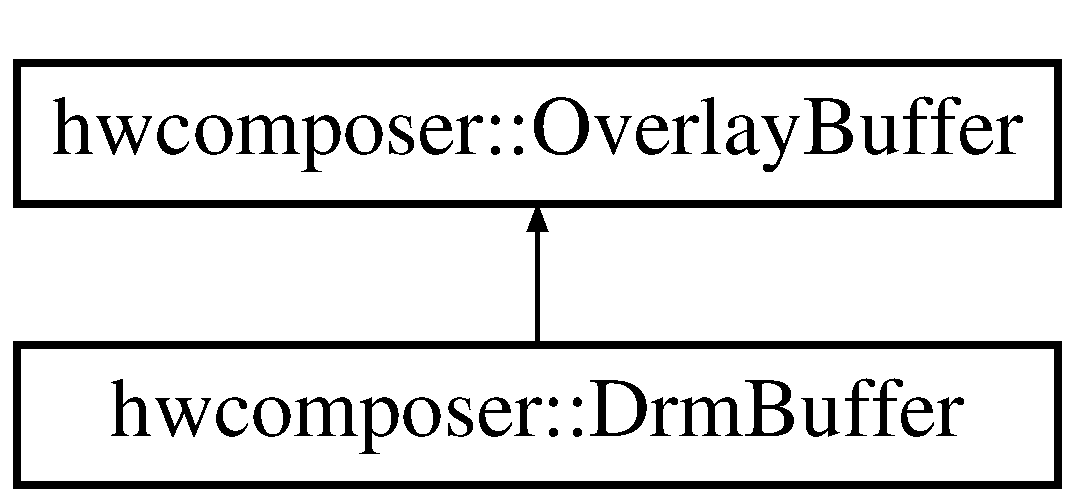
\includegraphics[height=2.000000cm]{classhwcomposer_1_1DrmBuffer}
\end{center}
\end{figure}
\subsection*{Public Member Functions}
\begin{DoxyCompactItemize}
\item 
\mbox{\hyperlink{classhwcomposer_1_1DrmBuffer_a9e23026b53d528ccd9f1a71fbc153ef1}{Drm\+Buffer}} (\mbox{\hyperlink{classhwcomposer_1_1DrmBuffer}{Drm\+Buffer}} \&\&rhs)=default
\item 
\mbox{\hyperlink{classhwcomposer_1_1DrmBuffer}{Drm\+Buffer}} \& \mbox{\hyperlink{classhwcomposer_1_1DrmBuffer_a6d58dec7ca17507de42f722d1af88baa}{operator=}} (\mbox{\hyperlink{classhwcomposer_1_1DrmBuffer}{Drm\+Buffer}} \&\&other)=default
\item 
\mbox{\hyperlink{classhwcomposer_1_1DrmBuffer_a74144267227d5213648330cd9d9a6bfe}{Drm\+Buffer}} ()=default
\item 
\mbox{\hyperlink{classhwcomposer_1_1DrmBuffer_adc5f481329b7469ae558a3b12474f390}{$\sim$\+Drm\+Buffer}} () override
\item 
void \mbox{\hyperlink{classhwcomposer_1_1DrmBuffer_afced6df8661c057ca6b7195d16c49a80}{Initialize\+From\+Native\+Handle}} (\mbox{\hyperlink{alios_2platformdefines_8h_ac0a2eaf260f556d17fe489911f017bdf}{H\+W\+C\+Native\+Handle}} handle, \mbox{\hyperlink{classhwcomposer_1_1ResourceManager}{Resource\+Manager}} $\ast$buffer\+\_\+manager, \mbox{\hyperlink{classhwcomposer_1_1FrameBufferManager}{Frame\+Buffer\+Manager}} $\ast$frame\+\_\+buffer\+\_\+manager) override
\item 
uint32\+\_\+t \mbox{\hyperlink{classhwcomposer_1_1DrmBuffer_ac4af6516c644cfb6bbf34083bbdc94ae}{Get\+Width}} () const override
\item 
uint32\+\_\+t \mbox{\hyperlink{classhwcomposer_1_1DrmBuffer_a42a02adf7559b89d4f9f958242880b61}{Get\+Height}} () const override
\item 
uint32\+\_\+t \mbox{\hyperlink{classhwcomposer_1_1DrmBuffer_a35eecd412bab8ea5822ec7a81c2fc34a}{Get\+Format}} () const override
\item 
H\+W\+C\+Layer\+Type \mbox{\hyperlink{classhwcomposer_1_1DrmBuffer_a41cb25d650c188e8be9ffa972776680b}{Get\+Usage}} () const override
\item 
uint32\+\_\+t \mbox{\hyperlink{classhwcomposer_1_1DrmBuffer_accd7dc14e04bd76beca146fc3d265f81}{Get\+Fb}} () const override
\item 
uint32\+\_\+t \mbox{\hyperlink{classhwcomposer_1_1DrmBuffer_a5844745322eb108eddb1e41eb1cf4f40}{Get\+Prime\+FD}} () const override
\item 
const uint32\+\_\+t $\ast$ \mbox{\hyperlink{classhwcomposer_1_1DrmBuffer_a6241968d9bcfff9e6e746feb75422f17}{Get\+Pitches}} () const override
\item 
const uint32\+\_\+t $\ast$ \mbox{\hyperlink{classhwcomposer_1_1DrmBuffer_a4545b534f1266e287d351ddb6fc2e2db}{Get\+Offsets}} () const override
\item 
uint32\+\_\+t \mbox{\hyperlink{classhwcomposer_1_1DrmBuffer_ae559626c3e3029ab95906bbc5c9319f7}{Get\+Tiling\+Mode}} () const override
\item 
const \mbox{\hyperlink{namespacehwcomposer_a963c5a1d5902d2d05710dba19af35b48}{Resource\+Handle}} \& \mbox{\hyperlink{classhwcomposer_1_1DrmBuffer_a7a2a0fe73ce6ef5468c1dc6b3b099d88}{Get\+Gpu\+Resource}} (\mbox{\hyperlink{namespacehwcomposer_ace90739a34de8ec5b30559423cdef990}{Gpu\+Display}} egl\+\_\+display, bool external\+\_\+import) override
\item 
const \mbox{\hyperlink{namespacehwcomposer_a963c5a1d5902d2d05710dba19af35b48}{Resource\+Handle}} \& \mbox{\hyperlink{classhwcomposer_1_1DrmBuffer_a1dc65623ff13c470c9d71c4054bc6b36}{Get\+Gpu\+Resource}} () override
\item 
const \mbox{\hyperlink{namespacehwcomposer_aa99e35835961ac7d6baa59a04131ff42}{Media\+Resource\+Handle}} \& \mbox{\hyperlink{classhwcomposer_1_1DrmBuffer_a816ad1d2e1f7698eba57d58096b532dc}{Get\+Media\+Resource}} (\mbox{\hyperlink{namespacehwcomposer_a10d64930907cc775f9cea6b39d8cb404}{Media\+Display}} display, uint32\+\_\+t width, uint32\+\_\+t height) override
\item 
bool \mbox{\hyperlink{classhwcomposer_1_1DrmBuffer_af80ec38c8f6728e9448a9593e08ecf4b}{Create\+Frame\+Buffer}} () override
\item 
bool \mbox{\hyperlink{classhwcomposer_1_1DrmBuffer_a3055296aa0dc5fb96553c62217d0f08d}{Create\+Frame\+Buffer\+With\+Modifier}} (uint64\+\_\+t modifier) override
\item 
\mbox{\hyperlink{alios_2platformdefines_8h_ac0a2eaf260f556d17fe489911f017bdf}{H\+W\+C\+Native\+Handle}} \mbox{\hyperlink{classhwcomposer_1_1DrmBuffer_a66a876cebee293bc84bf0dc6edd35f0c}{Get\+Original\+Handle}} () const override
\item 
void \mbox{\hyperlink{classhwcomposer_1_1DrmBuffer_a2d7dbadddf5cce8260aa224af1b495c1}{Set\+Original\+Handle}} (\mbox{\hyperlink{alios_2platformdefines_8h_ac0a2eaf260f556d17fe489911f017bdf}{H\+W\+C\+Native\+Handle}} handle) override
\item 
void \mbox{\hyperlink{classhwcomposer_1_1DrmBuffer_ac4087d8c1084fede3414f6e578de9183}{Dump}} () override
\end{DoxyCompactItemize}
\subsection*{Additional Inherited Members}


\subsection{Detailed Description}


Definition at line 28 of file drmbuffer.\+h.



\subsection{Constructor \& Destructor Documentation}
\mbox{\Hypertarget{classhwcomposer_1_1DrmBuffer_a9e23026b53d528ccd9f1a71fbc153ef1}\label{classhwcomposer_1_1DrmBuffer_a9e23026b53d528ccd9f1a71fbc153ef1}} 
\index{hwcomposer\+::\+Drm\+Buffer@{hwcomposer\+::\+Drm\+Buffer}!Drm\+Buffer@{Drm\+Buffer}}
\index{Drm\+Buffer@{Drm\+Buffer}!hwcomposer\+::\+Drm\+Buffer@{hwcomposer\+::\+Drm\+Buffer}}
\subsubsection{\texorpdfstring{Drm\+Buffer()}{DrmBuffer()}\hspace{0.1cm}{\footnotesize\ttfamily [1/2]}}
{\footnotesize\ttfamily hwcomposer\+::\+Drm\+Buffer\+::\+Drm\+Buffer (\begin{DoxyParamCaption}\item[{\mbox{\hyperlink{classhwcomposer_1_1DrmBuffer}{Drm\+Buffer}} \&\&}]{rhs }\end{DoxyParamCaption})\hspace{0.3cm}{\ttfamily [default]}}

\mbox{\Hypertarget{classhwcomposer_1_1DrmBuffer_a74144267227d5213648330cd9d9a6bfe}\label{classhwcomposer_1_1DrmBuffer_a74144267227d5213648330cd9d9a6bfe}} 
\index{hwcomposer\+::\+Drm\+Buffer@{hwcomposer\+::\+Drm\+Buffer}!Drm\+Buffer@{Drm\+Buffer}}
\index{Drm\+Buffer@{Drm\+Buffer}!hwcomposer\+::\+Drm\+Buffer@{hwcomposer\+::\+Drm\+Buffer}}
\subsubsection{\texorpdfstring{Drm\+Buffer()}{DrmBuffer()}\hspace{0.1cm}{\footnotesize\ttfamily [2/2]}}
{\footnotesize\ttfamily hwcomposer\+::\+Drm\+Buffer\+::\+Drm\+Buffer (\begin{DoxyParamCaption}{ }\end{DoxyParamCaption})\hspace{0.3cm}{\ttfamily [default]}}

\mbox{\Hypertarget{classhwcomposer_1_1DrmBuffer_adc5f481329b7469ae558a3b12474f390}\label{classhwcomposer_1_1DrmBuffer_adc5f481329b7469ae558a3b12474f390}} 
\index{hwcomposer\+::\+Drm\+Buffer@{hwcomposer\+::\+Drm\+Buffer}!````~Drm\+Buffer@{$\sim$\+Drm\+Buffer}}
\index{````~Drm\+Buffer@{$\sim$\+Drm\+Buffer}!hwcomposer\+::\+Drm\+Buffer@{hwcomposer\+::\+Drm\+Buffer}}
\subsubsection{\texorpdfstring{$\sim$\+Drm\+Buffer()}{~DrmBuffer()}}
{\footnotesize\ttfamily hwcomposer\+::\+Drm\+Buffer\+::$\sim$\+Drm\+Buffer (\begin{DoxyParamCaption}{ }\end{DoxyParamCaption})\hspace{0.3cm}{\ttfamily [override]}}



Definition at line 55 of file drmbuffer.\+cpp.


\begin{DoxyCode}{0}
\DoxyCodeLine{55                       \{}
\DoxyCodeLine{56   \textcolor{keywordtype}{bool} texture\_initialized = \textcolor{keyword}{false};}
\DoxyCodeLine{57 \textcolor{preprocessor}{\#if USE\_GL}}
\DoxyCodeLine{58   texture\_initialized = image\_.texture\_ > 0;}
\DoxyCodeLine{59 \textcolor{preprocessor}{\#elif USE\_VK}}
\DoxyCodeLine{60   texture\_initialized = image\_.texture\_ != VK\_NULL\_HANDLE;}
\DoxyCodeLine{61 \textcolor{preprocessor}{\#endif}}
\DoxyCodeLine{62 }
\DoxyCodeLine{63 \textcolor{preprocessor}{\#ifndef DISABLE\_VA}}
\DoxyCodeLine{64   \textcolor{keywordflow}{if} (media\_image\_.\mbox{\hyperlink{structhwcomposer_1_1media__import_af82420941f64a848639e0ac80a7b2861}{surface\_}} == VA\_INVALID\_ID) \{}
\DoxyCodeLine{65     resource\_manager\_->\mbox{\hyperlink{classhwcomposer_1_1ResourceManager_aed72efa73f3037049b1328ea35f162b3}{MarkResourceForDeletion}}(image\_, texture\_initialized);}
\DoxyCodeLine{66   \} \textcolor{keywordflow}{else} \{}
\DoxyCodeLine{67     \textcolor{keywordflow}{if} (texture\_initialized) \{}
\DoxyCodeLine{68       image\_.handle\_ = 0;}
\DoxyCodeLine{69       image\_.drm\_fd\_ = 0;}
\DoxyCodeLine{70       resource\_manager\_->\mbox{\hyperlink{classhwcomposer_1_1ResourceManager_aed72efa73f3037049b1328ea35f162b3}{MarkResourceForDeletion}}(image\_, \textcolor{keyword}{true});}
\DoxyCodeLine{71     \}}
\DoxyCodeLine{72 }
\DoxyCodeLine{73     resource\_manager\_->\mbox{\hyperlink{classhwcomposer_1_1ResourceManager_a0813f1ac50652ca59c3f4b03291dd4b4}{MarkMediaResourceForDeletion}}(media\_image\_);}
\DoxyCodeLine{74   \}}
\DoxyCodeLine{75 \textcolor{preprocessor}{\#else}}
\DoxyCodeLine{76   resource\_manager\_->\mbox{\hyperlink{classhwcomposer_1_1ResourceManager_aed72efa73f3037049b1328ea35f162b3}{MarkResourceForDeletion}}(image\_, texture\_initialized);}
\DoxyCodeLine{77 \textcolor{preprocessor}{\#endif}}
\DoxyCodeLine{78 \}}
\end{DoxyCode}


\subsection{Member Function Documentation}
\mbox{\Hypertarget{classhwcomposer_1_1DrmBuffer_af80ec38c8f6728e9448a9593e08ecf4b}\label{classhwcomposer_1_1DrmBuffer_af80ec38c8f6728e9448a9593e08ecf4b}} 
\index{hwcomposer\+::\+Drm\+Buffer@{hwcomposer\+::\+Drm\+Buffer}!Create\+Frame\+Buffer@{Create\+Frame\+Buffer}}
\index{Create\+Frame\+Buffer@{Create\+Frame\+Buffer}!hwcomposer\+::\+Drm\+Buffer@{hwcomposer\+::\+Drm\+Buffer}}
\subsubsection{\texorpdfstring{Create\+Frame\+Buffer()}{CreateFrameBuffer()}}
{\footnotesize\ttfamily bool hwcomposer\+::\+Drm\+Buffer\+::\+Create\+Frame\+Buffer (\begin{DoxyParamCaption}{ }\end{DoxyParamCaption})\hspace{0.3cm}{\ttfamily [override]}, {\ttfamily [virtual]}}



Implements \mbox{\hyperlink{classhwcomposer_1_1OverlayBuffer_ac680ba90c1b51512ad7c0b2a6483b39c}{hwcomposer\+::\+Overlay\+Buffer}}.



Definition at line 392 of file drmbuffer.\+cpp.


\begin{DoxyCode}{0}
\DoxyCodeLine{392                                   \{}
\DoxyCodeLine{393   \textcolor{keywordflow}{if} (image\_.drm\_fd\_) \{}
\DoxyCodeLine{394     \textcolor{keywordflow}{return} \textcolor{keyword}{true};}
\DoxyCodeLine{395   \}}
\DoxyCodeLine{396 }
\DoxyCodeLine{397   image\_.drm\_fd\_ = 0;}
\DoxyCodeLine{398   media\_image\_.\mbox{\hyperlink{structhwcomposer_1_1media__import_add4939656c584a9b2f25e38eb845602f}{drm\_fd\_}} = 0;}
\DoxyCodeLine{399 }
\DoxyCodeLine{400   image\_.drm\_fd\_ = fb\_manager\_->\mbox{\hyperlink{classhwcomposer_1_1FrameBufferManager_a05c6f8e84120746c4aa6fede497142e0}{FindFB}}(width\_, height\_, 0, frame\_buffer\_format\_,}
\DoxyCodeLine{401                                        image\_.handle\_->meta\_data\_.num\_planes\_,}
\DoxyCodeLine{402                                        gem\_handles\_, pitches\_, offsets\_);}
\DoxyCodeLine{403   media\_image\_.\mbox{\hyperlink{structhwcomposer_1_1media__import_add4939656c584a9b2f25e38eb845602f}{drm\_fd\_}} = image\_.drm\_fd\_;}
\DoxyCodeLine{404   \textcolor{keywordflow}{return} \textcolor{keyword}{true};}
\DoxyCodeLine{405 \}}
\end{DoxyCode}
\mbox{\Hypertarget{classhwcomposer_1_1DrmBuffer_a3055296aa0dc5fb96553c62217d0f08d}\label{classhwcomposer_1_1DrmBuffer_a3055296aa0dc5fb96553c62217d0f08d}} 
\index{hwcomposer\+::\+Drm\+Buffer@{hwcomposer\+::\+Drm\+Buffer}!Create\+Frame\+Buffer\+With\+Modifier@{Create\+Frame\+Buffer\+With\+Modifier}}
\index{Create\+Frame\+Buffer\+With\+Modifier@{Create\+Frame\+Buffer\+With\+Modifier}!hwcomposer\+::\+Drm\+Buffer@{hwcomposer\+::\+Drm\+Buffer}}
\subsubsection{\texorpdfstring{Create\+Frame\+Buffer\+With\+Modifier()}{CreateFrameBufferWithModifier()}}
{\footnotesize\ttfamily bool hwcomposer\+::\+Drm\+Buffer\+::\+Create\+Frame\+Buffer\+With\+Modifier (\begin{DoxyParamCaption}\item[{uint64\+\_\+t}]{modifier }\end{DoxyParamCaption})\hspace{0.3cm}{\ttfamily [override]}, {\ttfamily [virtual]}}



Implements \mbox{\hyperlink{classhwcomposer_1_1OverlayBuffer_ab7f56dcd75f7724d8b1b2ca384f91312}{hwcomposer\+::\+Overlay\+Buffer}}.



Definition at line 407 of file drmbuffer.\+cpp.


\begin{DoxyCode}{0}
\DoxyCodeLine{407                                                                \{}
\DoxyCodeLine{408   \textcolor{keywordflow}{if} (image\_.drm\_fd\_) \{}
\DoxyCodeLine{409     \textcolor{keywordflow}{return} \textcolor{keyword}{true};}
\DoxyCodeLine{410   \}}
\DoxyCodeLine{411 }
\DoxyCodeLine{412   image\_.drm\_fd\_ = 0;}
\DoxyCodeLine{413   media\_image\_.\mbox{\hyperlink{structhwcomposer_1_1media__import_add4939656c584a9b2f25e38eb845602f}{drm\_fd\_}} = 0;}
\DoxyCodeLine{414 }
\DoxyCodeLine{415   image\_.drm\_fd\_ = fb\_manager\_->\mbox{\hyperlink{classhwcomposer_1_1FrameBufferManager_a05c6f8e84120746c4aa6fede497142e0}{FindFB}}(}
\DoxyCodeLine{416       width\_, height\_, modifier, frame\_buffer\_format\_,}
\DoxyCodeLine{417       image\_.handle\_->meta\_data\_.num\_planes\_, gem\_handles\_, pitches\_, offsets\_);}
\DoxyCodeLine{418   media\_image\_.\mbox{\hyperlink{structhwcomposer_1_1media__import_add4939656c584a9b2f25e38eb845602f}{drm\_fd\_}} = image\_.drm\_fd\_;}
\DoxyCodeLine{419   \textcolor{keywordflow}{return} \textcolor{keyword}{true};}
\DoxyCodeLine{420 \}}
\end{DoxyCode}
\mbox{\Hypertarget{classhwcomposer_1_1DrmBuffer_ac4087d8c1084fede3414f6e578de9183}\label{classhwcomposer_1_1DrmBuffer_ac4087d8c1084fede3414f6e578de9183}} 
\index{hwcomposer\+::\+Drm\+Buffer@{hwcomposer\+::\+Drm\+Buffer}!Dump@{Dump}}
\index{Dump@{Dump}!hwcomposer\+::\+Drm\+Buffer@{hwcomposer\+::\+Drm\+Buffer}}
\subsubsection{\texorpdfstring{Dump()}{Dump()}}
{\footnotesize\ttfamily void hwcomposer\+::\+Drm\+Buffer\+::\+Dump (\begin{DoxyParamCaption}{ }\end{DoxyParamCaption})\hspace{0.3cm}{\ttfamily [override]}, {\ttfamily [virtual]}}



Implements \mbox{\hyperlink{classhwcomposer_1_1OverlayBuffer_a0f1c365c9c73e7608d07cf699279ddcb}{hwcomposer\+::\+Overlay\+Buffer}}.



Definition at line 426 of file drmbuffer.\+cpp.


\begin{DoxyCode}{0}
\DoxyCodeLine{426                      \{}
\DoxyCodeLine{427   \mbox{\hyperlink{hwctrace_8h_a8f0916f7778d78a386afc1e5d8be8a25}{DUMPTRACE}}(\textcolor{stringliteral}{"DrmBuffer Information Starts. -------------"});}
\DoxyCodeLine{428   \textcolor{keywordflow}{if} (usage\_ == kLayerNormal)}
\DoxyCodeLine{429     \mbox{\hyperlink{hwctrace_8h_a8f0916f7778d78a386afc1e5d8be8a25}{DUMPTRACE}}(\textcolor{stringliteral}{"BufferUsage: kLayerNormal."});}
\DoxyCodeLine{430   \textcolor{keywordflow}{if} (usage\_ == kLayerCursor)}
\DoxyCodeLine{431     \mbox{\hyperlink{hwctrace_8h_a8f0916f7778d78a386afc1e5d8be8a25}{DUMPTRACE}}(\textcolor{stringliteral}{"BufferUsage: kLayerCursor."});}
\DoxyCodeLine{432   \textcolor{keywordflow}{if} (usage\_ == kLayerProtected)}
\DoxyCodeLine{433     \mbox{\hyperlink{hwctrace_8h_a8f0916f7778d78a386afc1e5d8be8a25}{DUMPTRACE}}(\textcolor{stringliteral}{"BufferUsage: kLayerProtected."});}
\DoxyCodeLine{434   \textcolor{keywordflow}{if} (usage\_ == kLayerVideo)}
\DoxyCodeLine{435     \mbox{\hyperlink{hwctrace_8h_a8f0916f7778d78a386afc1e5d8be8a25}{DUMPTRACE}}(\textcolor{stringliteral}{"BufferUsage: kLayerVideo."});}
\DoxyCodeLine{436   \mbox{\hyperlink{hwctrace_8h_a8f0916f7778d78a386afc1e5d8be8a25}{DUMPTRACE}}(\textcolor{stringliteral}{"Width: \%d"}, width\_);}
\DoxyCodeLine{437   \mbox{\hyperlink{hwctrace_8h_a8f0916f7778d78a386afc1e5d8be8a25}{DUMPTRACE}}(\textcolor{stringliteral}{"Height: \%d"}, height\_);}
\DoxyCodeLine{438   \mbox{\hyperlink{hwctrace_8h_a8f0916f7778d78a386afc1e5d8be8a25}{DUMPTRACE}}(\textcolor{stringliteral}{"Fb: \%d"}, image\_.drm\_fd\_);}
\DoxyCodeLine{439   \mbox{\hyperlink{hwctrace_8h_a8f0916f7778d78a386afc1e5d8be8a25}{DUMPTRACE}}(\textcolor{stringliteral}{"Prime Handle: \%d"}, image\_.handle\_->meta\_data\_.prime\_fds\_[0]);}
\DoxyCodeLine{440   \mbox{\hyperlink{hwctrace_8h_a8f0916f7778d78a386afc1e5d8be8a25}{DUMPTRACE}}(\textcolor{stringliteral}{"Format: \%4.4s"}, (\textcolor{keywordtype}{char}*)\&format\_);}
\DoxyCodeLine{441   \textcolor{keywordflow}{for} (uint32\_t i = 0; i < 4; i++) \{}
\DoxyCodeLine{442     \mbox{\hyperlink{hwctrace_8h_a8f0916f7778d78a386afc1e5d8be8a25}{DUMPTRACE}}(\textcolor{stringliteral}{"Pitch:\%d value:\%d"}, i, pitches\_[i]);}
\DoxyCodeLine{443     \mbox{\hyperlink{hwctrace_8h_a8f0916f7778d78a386afc1e5d8be8a25}{DUMPTRACE}}(\textcolor{stringliteral}{"Offset:\%d value:\%d"}, i, offsets\_[i]);}
\DoxyCodeLine{444     \mbox{\hyperlink{hwctrace_8h_a8f0916f7778d78a386afc1e5d8be8a25}{DUMPTRACE}}(\textcolor{stringliteral}{"Gem Handles:\%d value:\%d"}, i, gem\_handles\_[i]);}
\DoxyCodeLine{445   \}}
\DoxyCodeLine{446   \mbox{\hyperlink{hwctrace_8h_a8f0916f7778d78a386afc1e5d8be8a25}{DUMPTRACE}}(\textcolor{stringliteral}{"DrmBuffer Information Ends. -------------"});}
\DoxyCodeLine{447 \}}
\end{DoxyCode}
\mbox{\Hypertarget{classhwcomposer_1_1DrmBuffer_accd7dc14e04bd76beca146fc3d265f81}\label{classhwcomposer_1_1DrmBuffer_accd7dc14e04bd76beca146fc3d265f81}} 
\index{hwcomposer\+::\+Drm\+Buffer@{hwcomposer\+::\+Drm\+Buffer}!Get\+Fb@{Get\+Fb}}
\index{Get\+Fb@{Get\+Fb}!hwcomposer\+::\+Drm\+Buffer@{hwcomposer\+::\+Drm\+Buffer}}
\subsubsection{\texorpdfstring{Get\+Fb()}{GetFb()}}
{\footnotesize\ttfamily uint32\+\_\+t hwcomposer\+::\+Drm\+Buffer\+::\+Get\+Fb (\begin{DoxyParamCaption}{ }\end{DoxyParamCaption}) const\hspace{0.3cm}{\ttfamily [inline]}, {\ttfamily [override]}, {\ttfamily [virtual]}}



Implements \mbox{\hyperlink{classhwcomposer_1_1OverlayBuffer_a9860269bb8712eee5c7c4ca1c8846e9a}{hwcomposer\+::\+Overlay\+Buffer}}.



Definition at line 57 of file drmbuffer.\+h.


\begin{DoxyCode}{0}
\DoxyCodeLine{57                                   \{}
\DoxyCodeLine{58     \textcolor{keywordflow}{return} image\_.drm\_fd\_;}
\DoxyCodeLine{59   \}}
\end{DoxyCode}
\mbox{\Hypertarget{classhwcomposer_1_1DrmBuffer_a35eecd412bab8ea5822ec7a81c2fc34a}\label{classhwcomposer_1_1DrmBuffer_a35eecd412bab8ea5822ec7a81c2fc34a}} 
\index{hwcomposer\+::\+Drm\+Buffer@{hwcomposer\+::\+Drm\+Buffer}!Get\+Format@{Get\+Format}}
\index{Get\+Format@{Get\+Format}!hwcomposer\+::\+Drm\+Buffer@{hwcomposer\+::\+Drm\+Buffer}}
\subsubsection{\texorpdfstring{Get\+Format()}{GetFormat()}}
{\footnotesize\ttfamily uint32\+\_\+t hwcomposer\+::\+Drm\+Buffer\+::\+Get\+Format (\begin{DoxyParamCaption}{ }\end{DoxyParamCaption}) const\hspace{0.3cm}{\ttfamily [inline]}, {\ttfamily [override]}, {\ttfamily [virtual]}}



Implements \mbox{\hyperlink{classhwcomposer_1_1OverlayBuffer_af12a31161149b0f89e92e5dfc18732c5}{hwcomposer\+::\+Overlay\+Buffer}}.



Definition at line 49 of file drmbuffer.\+h.


\begin{DoxyCode}{0}
\DoxyCodeLine{49                                       \{}
\DoxyCodeLine{50     \textcolor{keywordflow}{return} format\_;}
\DoxyCodeLine{51   \}}
\end{DoxyCode}
\mbox{\Hypertarget{classhwcomposer_1_1DrmBuffer_a7a2a0fe73ce6ef5468c1dc6b3b099d88}\label{classhwcomposer_1_1DrmBuffer_a7a2a0fe73ce6ef5468c1dc6b3b099d88}} 
\index{hwcomposer\+::\+Drm\+Buffer@{hwcomposer\+::\+Drm\+Buffer}!Get\+Gpu\+Resource@{Get\+Gpu\+Resource}}
\index{Get\+Gpu\+Resource@{Get\+Gpu\+Resource}!hwcomposer\+::\+Drm\+Buffer@{hwcomposer\+::\+Drm\+Buffer}}
\subsubsection{\texorpdfstring{Get\+Gpu\+Resource()}{GetGpuResource()}\hspace{0.1cm}{\footnotesize\ttfamily [1/2]}}
{\footnotesize\ttfamily const \mbox{\hyperlink{namespacehwcomposer_a963c5a1d5902d2d05710dba19af35b48}{Resource\+Handle}} \& hwcomposer\+::\+Drm\+Buffer\+::\+Get\+Gpu\+Resource (\begin{DoxyParamCaption}\item[{\mbox{\hyperlink{namespacehwcomposer_ace90739a34de8ec5b30559423cdef990}{Gpu\+Display}}}]{egl\+\_\+display,  }\item[{bool}]{external\+\_\+import }\end{DoxyParamCaption})\hspace{0.3cm}{\ttfamily [override]}, {\ttfamily [virtual]}}



Implements \mbox{\hyperlink{classhwcomposer_1_1OverlayBuffer_a121d2b77c40a30725d804cee4d2107a5}{hwcomposer\+::\+Overlay\+Buffer}}.



Definition at line 128 of file drmbuffer.\+cpp.


\begin{DoxyCode}{0}
\DoxyCodeLine{129                                                                       \{}
\DoxyCodeLine{130 \textcolor{preprocessor}{\#if USE\_GL}}
\DoxyCodeLine{131   \textcolor{keywordflow}{if} (image\_.image\_ == 0) \{}
\DoxyCodeLine{132     EGLImageKHR image = EGL\_NO\_IMAGE\_KHR;}
\DoxyCodeLine{133     uint32\_t total\_planes = image\_.handle\_->meta\_data\_.num\_planes\_;}
\DoxyCodeLine{134     \textcolor{comment}{// Note: If eglCreateImageKHR is successful for a EGL\_LINUX\_DMA\_BUF\_EXT}}
\DoxyCodeLine{135     \textcolor{comment}{// target, the EGL will take a reference to the dma\_buf.}}
\DoxyCodeLine{136     \textcolor{keywordflow}{if} ((usage\_ == kLayerVideo) \&\& total\_planes > 1) \{}
\DoxyCodeLine{137       \textcolor{keywordflow}{if} (total\_planes == 2) \{}
\DoxyCodeLine{138         \textcolor{keyword}{const} EGLint attr\_list\_nv12[] = \{}
\DoxyCodeLine{139             EGL\_WIDTH,}
\DoxyCodeLine{140             \textcolor{keyword}{static\_cast<}EGLint\textcolor{keyword}{>}(width\_),}
\DoxyCodeLine{141             EGL\_HEIGHT,}
\DoxyCodeLine{142             static\_cast<EGLint>(height\_),}
\DoxyCodeLine{143             EGL\_LINUX\_DRM\_FOURCC\_EXT,}
\DoxyCodeLine{144             \textcolor{keyword}{static\_cast<}EGLint\textcolor{keyword}{>}(format\_),}
\DoxyCodeLine{145             EGL\_DMA\_BUF\_PLANE0\_FD\_EXT,}
\DoxyCodeLine{146             static\_cast<EGLint>(image\_.handle\_->meta\_data\_.prime\_fds\_[0]),}
\DoxyCodeLine{147             EGL\_DMA\_BUF\_PLANE0\_PITCH\_EXT,}
\DoxyCodeLine{148             \textcolor{keyword}{static\_cast<}EGLint\textcolor{keyword}{>}(pitches\_[0]),}
\DoxyCodeLine{149             EGL\_DMA\_BUF\_PLANE0\_OFFSET\_EXT,}
\DoxyCodeLine{150             static\_cast<EGLint>(offsets\_[0]),}
\DoxyCodeLine{151             EGL\_DMA\_BUF\_PLANE1\_FD\_EXT,}
\DoxyCodeLine{152             \textcolor{keyword}{static\_cast<}EGLint\textcolor{keyword}{>}(image\_.handle\_->meta\_data\_.prime\_fds\_[1]),}
\DoxyCodeLine{153             EGL\_DMA\_BUF\_PLANE1\_PITCH\_EXT,}
\DoxyCodeLine{154             static\_cast<EGLint>(pitches\_[1]),}
\DoxyCodeLine{155             EGL\_DMA\_BUF\_PLANE1\_OFFSET\_EXT,}
\DoxyCodeLine{156             \textcolor{keyword}{static\_cast<}EGLint\textcolor{keyword}{>}(offsets\_[1]),}
\DoxyCodeLine{157             EGL\_NONE,}
\DoxyCodeLine{158             0\};}
\DoxyCodeLine{159         image = \mbox{\hyperlink{namespacehwcomposer_a1b9b71782e10965d5f44995bac78ac92}{eglCreateImageKHR}}(}
\DoxyCodeLine{160             egl\_display, EGL\_NO\_CONTEXT, EGL\_LINUX\_DMA\_BUF\_EXT,}
\DoxyCodeLine{161             static\_cast<EGLClientBuffer>(\textcolor{keyword}{nullptr}), attr\_list\_nv12);}
\DoxyCodeLine{162       \} \textcolor{keywordflow}{else} \{}
\DoxyCodeLine{163         \textcolor{keyword}{const} EGLint attr\_list\_yv12[] = \{}
\DoxyCodeLine{164             EGL\_WIDTH,}
\DoxyCodeLine{165             \textcolor{keyword}{static\_cast<}EGLint\textcolor{keyword}{>}(width\_),}
\DoxyCodeLine{166             EGL\_HEIGHT,}
\DoxyCodeLine{167             static\_cast<EGLint>(height\_),}
\DoxyCodeLine{168             EGL\_LINUX\_DRM\_FOURCC\_EXT,}
\DoxyCodeLine{169             \textcolor{keyword}{static\_cast<}EGLint\textcolor{keyword}{>}(format\_),}
\DoxyCodeLine{170             EGL\_DMA\_BUF\_PLANE0\_FD\_EXT,}
\DoxyCodeLine{171             static\_cast<EGLint>(image\_.handle\_->meta\_data\_.prime\_fds\_[0]),}
\DoxyCodeLine{172             EGL\_DMA\_BUF\_PLANE0\_PITCH\_EXT,}
\DoxyCodeLine{173             \textcolor{keyword}{static\_cast<}EGLint\textcolor{keyword}{>}(pitches\_[0]),}
\DoxyCodeLine{174             EGL\_DMA\_BUF\_PLANE0\_OFFSET\_EXT,}
\DoxyCodeLine{175             static\_cast<EGLint>(offsets\_[0]),}
\DoxyCodeLine{176             EGL\_DMA\_BUF\_PLANE1\_FD\_EXT,}
\DoxyCodeLine{177             \textcolor{keyword}{static\_cast<}EGLint\textcolor{keyword}{>}(image\_.handle\_->meta\_data\_.prime\_fds\_[1]),}
\DoxyCodeLine{178             EGL\_DMA\_BUF\_PLANE1\_PITCH\_EXT,}
\DoxyCodeLine{179             static\_cast<EGLint>(pitches\_[1]),}
\DoxyCodeLine{180             EGL\_DMA\_BUF\_PLANE1\_OFFSET\_EXT,}
\DoxyCodeLine{181             \textcolor{keyword}{static\_cast<}EGLint\textcolor{keyword}{>}(offsets\_[1]),}
\DoxyCodeLine{182             EGL\_DMA\_BUF\_PLANE2\_FD\_EXT,}
\DoxyCodeLine{183             static\_cast<EGLint>(image\_.handle\_->meta\_data\_.prime\_fds\_[2]),}
\DoxyCodeLine{184             EGL\_DMA\_BUF\_PLANE2\_PITCH\_EXT,}
\DoxyCodeLine{185             \textcolor{keyword}{static\_cast<}EGLint\textcolor{keyword}{>}(pitches\_[2]),}
\DoxyCodeLine{186             EGL\_DMA\_BUF\_PLANE2\_OFFSET\_EXT,}
\DoxyCodeLine{187             static\_cast<EGLint>(offsets\_[2]),}
\DoxyCodeLine{188             EGL\_NONE,}
\DoxyCodeLine{189             0\};}
\DoxyCodeLine{190         image = \mbox{\hyperlink{namespacehwcomposer_a1b9b71782e10965d5f44995bac78ac92}{eglCreateImageKHR}}(}
\DoxyCodeLine{191             egl\_display, EGL\_NO\_CONTEXT, EGL\_LINUX\_DMA\_BUF\_EXT,}
\DoxyCodeLine{192             static\_cast<EGLClientBuffer>(\textcolor{keyword}{nullptr}), attr\_list\_yv12);}
\DoxyCodeLine{193       \}}
\DoxyCodeLine{194     \} \textcolor{keywordflow}{else} \textcolor{keywordflow}{if} (image\_.handle\_->meta\_data\_.fb\_modifiers\_[0] > 0 \&\&}
\DoxyCodeLine{195                total\_planes == 2) \{}
\DoxyCodeLine{196       EGLint modifier\_low =}
\DoxyCodeLine{197           \textcolor{keyword}{static\_cast<}EGLint\textcolor{keyword}{>}(image\_.handle\_->meta\_data\_.fb\_modifiers\_[1]);}
\DoxyCodeLine{198       EGLint modifier\_high =}
\DoxyCodeLine{199           \textcolor{keyword}{static\_cast<}EGLint\textcolor{keyword}{>}(image\_.handle\_->meta\_data\_.fb\_modifiers\_[0]);}
\DoxyCodeLine{200       \textcolor{keyword}{const} EGLint image\_attrs[] = \{}
\DoxyCodeLine{201           EGL\_WIDTH,}
\DoxyCodeLine{202           \textcolor{keyword}{static\_cast<}EGLint\textcolor{keyword}{>}(width\_),}
\DoxyCodeLine{203           EGL\_HEIGHT,}
\DoxyCodeLine{204           static\_cast<EGLint>(height\_),}
\DoxyCodeLine{205           EGL\_LINUX\_DRM\_FOURCC\_EXT,}
\DoxyCodeLine{206           \textcolor{keyword}{static\_cast<}EGLint\textcolor{keyword}{>}(format\_),}
\DoxyCodeLine{207           EGL\_DMA\_BUF\_PLANE0\_FD\_EXT,}
\DoxyCodeLine{208           static\_cast<EGLint>(image\_.handle\_->meta\_data\_.prime\_fds\_[0]),}
\DoxyCodeLine{209           EGL\_DMA\_BUF\_PLANE0\_PITCH\_EXT,}
\DoxyCodeLine{210           \textcolor{keyword}{static\_cast<}EGLint\textcolor{keyword}{>}(pitches\_[0]),}
\DoxyCodeLine{211           EGL\_DMA\_BUF\_PLANE0\_OFFSET\_EXT,}
\DoxyCodeLine{212           static\_cast<EGLint>(offsets\_[0]),}
\DoxyCodeLine{213           \mbox{\hyperlink{drmbuffer_8cpp_ae47c847a6b891b8e589177b36901085c}{EGL\_DMA\_BUF\_PLANE0\_MODIFIER\_LO\_EXT}},}
\DoxyCodeLine{214           modifier\_low,}
\DoxyCodeLine{215           \mbox{\hyperlink{drmbuffer_8cpp_aaffb6f543f514e8d31b29839fb30c2fd}{EGL\_DMA\_BUF\_PLANE0\_MODIFIER\_HI\_EXT}},}
\DoxyCodeLine{216           modifier\_high,}
\DoxyCodeLine{217           EGL\_DMA\_BUF\_PLANE1\_FD\_EXT,}
\DoxyCodeLine{218           \textcolor{keyword}{static\_cast<}EGLint\textcolor{keyword}{>}(image\_.handle\_->meta\_data\_.prime\_fds\_[1]),}
\DoxyCodeLine{219           EGL\_DMA\_BUF\_PLANE1\_PITCH\_EXT,}
\DoxyCodeLine{220           static\_cast<EGLint>(pitches\_[1]),}
\DoxyCodeLine{221           EGL\_DMA\_BUF\_PLANE1\_OFFSET\_EXT,}
\DoxyCodeLine{222           \textcolor{keyword}{static\_cast<}EGLint\textcolor{keyword}{>}(offsets\_[1]),}
\DoxyCodeLine{223           \mbox{\hyperlink{drmbuffer_8cpp_a72a8ef96c90fd2930cbc9ee5f5049b6d}{EGL\_DMA\_BUF\_PLANE1\_MODIFIER\_LO\_EXT}},}
\DoxyCodeLine{224           modifier\_low,}
\DoxyCodeLine{225           \mbox{\hyperlink{drmbuffer_8cpp_a1a2b5bfe379b69767306ca63455788da}{EGL\_DMA\_BUF\_PLANE1\_MODIFIER\_HI\_EXT}},}
\DoxyCodeLine{226           modifier\_high,}
\DoxyCodeLine{227           EGL\_NONE,}
\DoxyCodeLine{228       \};}
\DoxyCodeLine{229 }
\DoxyCodeLine{230       image =}
\DoxyCodeLine{231           \mbox{\hyperlink{namespacehwcomposer_a1b9b71782e10965d5f44995bac78ac92}{eglCreateImageKHR}}(egl\_display, EGL\_NO\_CONTEXT, EGL\_LINUX\_DMA\_BUF\_EXT,}
\DoxyCodeLine{232                             static\_cast<EGLClientBuffer>(\textcolor{keyword}{nullptr}), image\_attrs);}
\DoxyCodeLine{233     \} \textcolor{keywordflow}{else} \{}
\DoxyCodeLine{234       \textcolor{keyword}{const} EGLint attr\_list[] = \{}
\DoxyCodeLine{235           EGL\_WIDTH,}
\DoxyCodeLine{236           \textcolor{keyword}{static\_cast<}EGLint\textcolor{keyword}{>}(width\_),}
\DoxyCodeLine{237           EGL\_HEIGHT,}
\DoxyCodeLine{238           static\_cast<EGLint>(height\_),}
\DoxyCodeLine{239           EGL\_LINUX\_DRM\_FOURCC\_EXT,}
\DoxyCodeLine{240           \textcolor{keyword}{static\_cast<}EGLint\textcolor{keyword}{>}(format\_),}
\DoxyCodeLine{241           EGL\_DMA\_BUF\_PLANE0\_FD\_EXT,}
\DoxyCodeLine{242           static\_cast<EGLint>(image\_.handle\_->meta\_data\_.prime\_fds\_[0]),}
\DoxyCodeLine{243           EGL\_DMA\_BUF\_PLANE0\_PITCH\_EXT,}
\DoxyCodeLine{244           \textcolor{keyword}{static\_cast<}EGLint\textcolor{keyword}{>}(pitches\_[0]),}
\DoxyCodeLine{245           EGL\_DMA\_BUF\_PLANE0\_OFFSET\_EXT,}
\DoxyCodeLine{246           0,}
\DoxyCodeLine{247           EGL\_NONE,}
\DoxyCodeLine{248           0\};}
\DoxyCodeLine{249       image =}
\DoxyCodeLine{250           \mbox{\hyperlink{namespacehwcomposer_a1b9b71782e10965d5f44995bac78ac92}{eglCreateImageKHR}}(egl\_display, EGL\_NO\_CONTEXT, EGL\_LINUX\_DMA\_BUF\_EXT,}
\DoxyCodeLine{251                             static\_cast<EGLClientBuffer>(\textcolor{keyword}{nullptr}), attr\_list);}
\DoxyCodeLine{252     \}}
\DoxyCodeLine{253 }
\DoxyCodeLine{254     \textcolor{keywordflow}{if} (image == EGL\_NO\_IMAGE\_KHR) \{}
\DoxyCodeLine{255       \mbox{\hyperlink{alios_2platformdefines_8h_a226d6c99e4bcfca193c095e085e9097d}{ETRACE}}(\textcolor{stringliteral}{"eglCreateKHR failed to create image for DrmBuffer"});}
\DoxyCodeLine{256     \}}
\DoxyCodeLine{257     image\_.image\_ = image;}
\DoxyCodeLine{258   \}}
\DoxyCodeLine{259 }
\DoxyCodeLine{260   GLenum target = GL\_TEXTURE\_EXTERNAL\_OES;}
\DoxyCodeLine{261   \textcolor{keywordflow}{if} (!external\_import) \{}
\DoxyCodeLine{262     target = GL\_TEXTURE\_2D;}
\DoxyCodeLine{263   \}}
\DoxyCodeLine{264 }
\DoxyCodeLine{265   \textcolor{keywordflow}{if} (!image\_.texture\_) \{}
\DoxyCodeLine{266     GLuint texture;}
\DoxyCodeLine{267     glGenTextures(1, \&texture);}
\DoxyCodeLine{268     image\_.texture\_ = texture;}
\DoxyCodeLine{269   \}}
\DoxyCodeLine{270 }
\DoxyCodeLine{271   glBindTexture(target, image\_.texture\_);}
\DoxyCodeLine{272   \mbox{\hyperlink{namespacehwcomposer_ae0c1af9f8e55e18591c646640bb289a3}{glEGLImageTargetTexture2DOES}}(target, (GLeglImageOES)image\_.image\_);}
\DoxyCodeLine{273 }
\DoxyCodeLine{274   glBindTexture(target, 0);}
\DoxyCodeLine{275 }
\DoxyCodeLine{276   \textcolor{keywordflow}{if} (!external\_import \&\& image\_.fb\_ == 0) \{}
\DoxyCodeLine{277     glGenFramebuffers(1, \&image\_.fb\_);}
\DoxyCodeLine{278   \}}
\DoxyCodeLine{279 \textcolor{preprocessor}{\#elif USE\_VK}}
\DoxyCodeLine{280   \textcolor{keywordflow}{if} (image\_.image\_ == VK\_NULL\_HANDLE) \{}
\DoxyCodeLine{281     VkDevice dev = egl\_display;}
\DoxyCodeLine{282     VkResult res;}
\DoxyCodeLine{283 }
\DoxyCodeLine{284     PFN\_vkCreateDmaBufImageINTEL vkCreateDmaBufImageINTEL =}
\DoxyCodeLine{285         (PFN\_vkCreateDmaBufImageINTEL)vkGetDeviceProcAddr(}
\DoxyCodeLine{286             dev, \textcolor{stringliteral}{"vkCreateDmaBufImageINTEL"});}
\DoxyCodeLine{287     \textcolor{keywordflow}{if} (vkCreateDmaBufImageINTEL == \mbox{\hyperlink{alios_2platformdefines_8h_a070d2ce7b6bb7e5c05602aa8c308d0c4}{NULL}}) \{}
\DoxyCodeLine{288       \mbox{\hyperlink{alios_2platformdefines_8h_a226d6c99e4bcfca193c095e085e9097d}{ETRACE}}(\textcolor{stringliteral}{"vkGetDeviceProcAddr(\(\backslash\)"vkCreateDmaBufImageINTEL\(\backslash\)") failed\(\backslash\)n"});}
\DoxyCodeLine{289     \}}
\DoxyCodeLine{290 }
\DoxyCodeLine{291     VkFormat vk\_format = NativeToVkFormat(format\_);}
\DoxyCodeLine{292     \textcolor{keywordflow}{if} (vk\_format == VK\_FORMAT\_UNDEFINED) \{}
\DoxyCodeLine{293       \mbox{\hyperlink{alios_2platformdefines_8h_a226d6c99e4bcfca193c095e085e9097d}{ETRACE}}(\textcolor{stringliteral}{"Failed DRM -> Vulkan format conversion\(\backslash\)n"});}
\DoxyCodeLine{294     \}}
\DoxyCodeLine{295 }
\DoxyCodeLine{296     VkExtent3D image\_extent = \{\};}
\DoxyCodeLine{297     image\_extent.width = width\_;}
\DoxyCodeLine{298     image\_extent.height = height\_;}
\DoxyCodeLine{299     image\_extent.depth = 1;}
\DoxyCodeLine{300 }
\DoxyCodeLine{301     VkDmaBufImageCreateInfo image\_create = \{\};}
\DoxyCodeLine{302     image\_create.sType =}
\DoxyCodeLine{303         (\textcolor{keyword}{enum} VkStructureType)VK\_STRUCTURE\_TYPE\_DMA\_BUF\_IMAGE\_CREATE\_INFO\_INTEL;}
\DoxyCodeLine{304     image\_create.fd =}
\DoxyCodeLine{305         \textcolor{keyword}{static\_cast<}\textcolor{keywordtype}{int}\textcolor{keyword}{>}(image\_.handle\_->meta\_data\_.prime\_fds\_[0]);}
\DoxyCodeLine{306     image\_create.format = vk\_format;}
\DoxyCodeLine{307     image\_create.extent = image\_extent;}
\DoxyCodeLine{308     image\_create.strideInBytes = pitches\_[0];}
\DoxyCodeLine{309 }
\DoxyCodeLine{310     res = vkCreateDmaBufImageINTEL(dev, \&image\_create, \mbox{\hyperlink{alios_2platformdefines_8h_a070d2ce7b6bb7e5c05602aa8c308d0c4}{NULL}}, \&image\_.memory\_,}
\DoxyCodeLine{311                                    \&image\_.image\_);}
\DoxyCodeLine{312     \textcolor{keywordflow}{if} (res != VK\_SUCCESS) \{}
\DoxyCodeLine{313       \mbox{\hyperlink{alios_2platformdefines_8h_a226d6c99e4bcfca193c095e085e9097d}{ETRACE}}(\textcolor{stringliteral}{"vkCreateDmaBufImageINTEL failed\(\backslash\)n"});}
\DoxyCodeLine{314     \}}
\DoxyCodeLine{315   \}}
\DoxyCodeLine{316 \textcolor{preprocessor}{\#endif}}
\DoxyCodeLine{317   \textcolor{keywordflow}{return} image\_;}
\DoxyCodeLine{318 \}}
\end{DoxyCode}
\mbox{\Hypertarget{classhwcomposer_1_1DrmBuffer_a1dc65623ff13c470c9d71c4054bc6b36}\label{classhwcomposer_1_1DrmBuffer_a1dc65623ff13c470c9d71c4054bc6b36}} 
\index{hwcomposer\+::\+Drm\+Buffer@{hwcomposer\+::\+Drm\+Buffer}!Get\+Gpu\+Resource@{Get\+Gpu\+Resource}}
\index{Get\+Gpu\+Resource@{Get\+Gpu\+Resource}!hwcomposer\+::\+Drm\+Buffer@{hwcomposer\+::\+Drm\+Buffer}}
\subsubsection{\texorpdfstring{Get\+Gpu\+Resource()}{GetGpuResource()}\hspace{0.1cm}{\footnotesize\ttfamily [2/2]}}
{\footnotesize\ttfamily const \mbox{\hyperlink{namespacehwcomposer_a963c5a1d5902d2d05710dba19af35b48}{Resource\+Handle}} \& hwcomposer\+::\+Drm\+Buffer\+::\+Get\+Gpu\+Resource (\begin{DoxyParamCaption}{ }\end{DoxyParamCaption})\hspace{0.3cm}{\ttfamily [override]}, {\ttfamily [virtual]}}



Implements \mbox{\hyperlink{classhwcomposer_1_1OverlayBuffer_a8cf41eb9f46a27d3ac2c6e5cf4f310b4}{hwcomposer\+::\+Overlay\+Buffer}}.



Definition at line 388 of file drmbuffer.\+cpp.


\begin{DoxyCode}{0}
\DoxyCodeLine{388                                                 \{}
\DoxyCodeLine{389   \textcolor{keywordflow}{return} image\_;}
\DoxyCodeLine{390 \}}
\end{DoxyCode}
\mbox{\Hypertarget{classhwcomposer_1_1DrmBuffer_a42a02adf7559b89d4f9f958242880b61}\label{classhwcomposer_1_1DrmBuffer_a42a02adf7559b89d4f9f958242880b61}} 
\index{hwcomposer\+::\+Drm\+Buffer@{hwcomposer\+::\+Drm\+Buffer}!Get\+Height@{Get\+Height}}
\index{Get\+Height@{Get\+Height}!hwcomposer\+::\+Drm\+Buffer@{hwcomposer\+::\+Drm\+Buffer}}
\subsubsection{\texorpdfstring{Get\+Height()}{GetHeight()}}
{\footnotesize\ttfamily uint32\+\_\+t hwcomposer\+::\+Drm\+Buffer\+::\+Get\+Height (\begin{DoxyParamCaption}{ }\end{DoxyParamCaption}) const\hspace{0.3cm}{\ttfamily [inline]}, {\ttfamily [override]}, {\ttfamily [virtual]}}



Implements \mbox{\hyperlink{classhwcomposer_1_1OverlayBuffer_a30b6043a9da6a8116d0471d66f836878}{hwcomposer\+::\+Overlay\+Buffer}}.



Definition at line 45 of file drmbuffer.\+h.


\begin{DoxyCode}{0}
\DoxyCodeLine{45                                       \{}
\DoxyCodeLine{46     \textcolor{keywordflow}{return} height\_;}
\DoxyCodeLine{47   \}}
\end{DoxyCode}
\mbox{\Hypertarget{classhwcomposer_1_1DrmBuffer_a816ad1d2e1f7698eba57d58096b532dc}\label{classhwcomposer_1_1DrmBuffer_a816ad1d2e1f7698eba57d58096b532dc}} 
\index{hwcomposer\+::\+Drm\+Buffer@{hwcomposer\+::\+Drm\+Buffer}!Get\+Media\+Resource@{Get\+Media\+Resource}}
\index{Get\+Media\+Resource@{Get\+Media\+Resource}!hwcomposer\+::\+Drm\+Buffer@{hwcomposer\+::\+Drm\+Buffer}}
\subsubsection{\texorpdfstring{Get\+Media\+Resource()}{GetMediaResource()}}
{\footnotesize\ttfamily const \mbox{\hyperlink{namespacehwcomposer_aa99e35835961ac7d6baa59a04131ff42}{Media\+Resource\+Handle}} \& hwcomposer\+::\+Drm\+Buffer\+::\+Get\+Media\+Resource (\begin{DoxyParamCaption}\item[{\mbox{\hyperlink{namespacehwcomposer_a10d64930907cc775f9cea6b39d8cb404}{Media\+Display}}}]{display,  }\item[{uint32\+\_\+t}]{width,  }\item[{uint32\+\_\+t}]{height }\end{DoxyParamCaption})\hspace{0.3cm}{\ttfamily [override]}, {\ttfamily [virtual]}}



Implements \mbox{\hyperlink{classhwcomposer_1_1OverlayBuffer_a947d4a8ef39b9a1a254325e32d4a45c2}{hwcomposer\+::\+Overlay\+Buffer}}.



Definition at line 320 of file drmbuffer.\+cpp.


\begin{DoxyCode}{0}
\DoxyCodeLine{322                                                                         \{}
\DoxyCodeLine{323 \textcolor{preprocessor}{\#ifndef DISABLE\_VA}}
\DoxyCodeLine{324   \textcolor{keywordflow}{if} (media\_image\_.\mbox{\hyperlink{structhwcomposer_1_1media__import_af82420941f64a848639e0ac80a7b2861}{surface\_}} != VA\_INVALID\_ID) \{}
\DoxyCodeLine{325     \textcolor{keywordflow}{if} ((previous\_width\_ == width) \&\& (previous\_height\_ == height)) \{}
\DoxyCodeLine{326       \textcolor{keywordflow}{return} media\_image\_;}
\DoxyCodeLine{327     \}}
\DoxyCodeLine{328 }
\DoxyCodeLine{329     \mbox{\hyperlink{namespacehwcomposer_aa99e35835961ac7d6baa59a04131ff42}{MediaResourceHandle}} media\_resource;}
\DoxyCodeLine{330     media\_resource.\mbox{\hyperlink{structhwcomposer_1_1media__import_af82420941f64a848639e0ac80a7b2861}{surface\_}} = media\_image\_.\mbox{\hyperlink{structhwcomposer_1_1media__import_af82420941f64a848639e0ac80a7b2861}{surface\_}};}
\DoxyCodeLine{331     media\_image\_.\mbox{\hyperlink{structhwcomposer_1_1media__import_af82420941f64a848639e0ac80a7b2861}{surface\_}} = VA\_INVALID\_ID;}
\DoxyCodeLine{332     resource\_manager\_->\mbox{\hyperlink{classhwcomposer_1_1ResourceManager_a0813f1ac50652ca59c3f4b03291dd4b4}{MarkMediaResourceForDeletion}}(media\_resource);}
\DoxyCodeLine{333   \}}
\DoxyCodeLine{334 }
\DoxyCodeLine{335   previous\_width\_ = width;}
\DoxyCodeLine{336   previous\_height\_ = height;}
\DoxyCodeLine{337 }
\DoxyCodeLine{338   VASurfaceAttribExternalBuffers external;}
\DoxyCodeLine{339   memset(\&external, 0, \textcolor{keyword}{sizeof}(external));}
\DoxyCodeLine{340   uint32\_t rt\_format = \mbox{\hyperlink{namespacehwcomposer_a487f8d9f8fe8490d7057be9a1c67b42e}{DrmFormatToRTFormat}}(format\_);}
\DoxyCodeLine{341   uint32\_t total\_planes = image\_.handle\_->meta\_data\_.num\_planes\_;}
\DoxyCodeLine{342   external.pixel\_format = \mbox{\hyperlink{namespacehwcomposer_a74da6820276a700b866ddcb92330b81b}{DrmFormatToVAFormat}}(format\_);}
\DoxyCodeLine{343   external.width = width\_;}
\DoxyCodeLine{344   external.height = height\_;}
\DoxyCodeLine{345   external.num\_planes = total\_planes;}
\DoxyCodeLine{346 \textcolor{preprocessor}{\#if VA\_MAJOR\_VERSION < 1}}
\DoxyCodeLine{347   \textcolor{keywordtype}{unsigned} \textcolor{keywordtype}{long} prime\_fds[total\_planes];}
\DoxyCodeLine{348 \textcolor{preprocessor}{\#else}}
\DoxyCodeLine{349   uintptr\_t prime\_fds[total\_planes];}
\DoxyCodeLine{350 \textcolor{preprocessor}{\#endif}}
\DoxyCodeLine{351   \textcolor{keywordflow}{for} (\textcolor{keywordtype}{unsigned} \textcolor{keywordtype}{int} i = 0; i < total\_planes; i++) \{}
\DoxyCodeLine{352     external.pitches[i] = pitches\_[i];}
\DoxyCodeLine{353     external.offsets[i] = offsets\_[i];}
\DoxyCodeLine{354     prime\_fds[i] = image\_.handle\_->meta\_data\_.prime\_fds\_[i];}
\DoxyCodeLine{355   \}}
\DoxyCodeLine{356 }
\DoxyCodeLine{357   external.num\_buffers = total\_planes;}
\DoxyCodeLine{358   external.buffers = prime\_fds;}
\DoxyCodeLine{359 }
\DoxyCodeLine{360   VASurfaceAttrib attribs[2];}
\DoxyCodeLine{361   attribs[0].flags = VA\_SURFACE\_ATTRIB\_SETTABLE;}
\DoxyCodeLine{362   attribs[0].type = VASurfaceAttribMemoryType;}
\DoxyCodeLine{363   attribs[0].value.type = VAGenericValueTypeInteger;}
\DoxyCodeLine{364   attribs[0].value.value.i = VA\_SURFACE\_ATTRIB\_MEM\_TYPE\_DRM\_PRIME;}
\DoxyCodeLine{365 }
\DoxyCodeLine{366   attribs[1].flags = VA\_SURFACE\_ATTRIB\_SETTABLE;}
\DoxyCodeLine{367   attribs[1].type = VASurfaceAttribExternalBufferDescriptor;}
\DoxyCodeLine{368   attribs[1].value.type = VAGenericValueTypePointer;}
\DoxyCodeLine{369   attribs[1].value.value.p = \&external;}
\DoxyCodeLine{370 }
\DoxyCodeLine{371   VAStatus ret =}
\DoxyCodeLine{372       vaCreateSurfaces(display, rt\_format, external.width, external.height,}
\DoxyCodeLine{373                        \&media\_image\_.\mbox{\hyperlink{structhwcomposer_1_1media__import_af82420941f64a848639e0ac80a7b2861}{surface\_}}, 1, attribs, 2);}
\DoxyCodeLine{374   \textcolor{keywordflow}{if} (ret != VA\_STATUS\_SUCCESS)}
\DoxyCodeLine{375     \mbox{\hyperlink{alios_2platformdefines_8h_a226d6c99e4bcfca193c095e085e9097d}{ETRACE}}(\textcolor{stringliteral}{"Failed to create VASurface from drmbuffer with ret \%x"}, ret);}
\DoxyCodeLine{376 }
\DoxyCodeLine{377   \textcolor{keywordflow}{return} media\_image\_;}
\DoxyCodeLine{378 \textcolor{preprocessor}{\#else}}
\DoxyCodeLine{379 }
\DoxyCodeLine{380   \textcolor{comment}{// FIXME: when va is disabled, this function should}}
\DoxyCodeLine{381   \textcolor{comment}{// not been called or left to be defined if other media}}
\DoxyCodeLine{382   \textcolor{comment}{// backend}}
\DoxyCodeLine{383   \mbox{\hyperlink{alios_2platformdefines_8h_a226d6c99e4bcfca193c095e085e9097d}{ETRACE}}(\textcolor{stringliteral}{"GetMediaResource is not implemented for this Media Backend."});}
\DoxyCodeLine{384   \textcolor{keywordflow}{return} media\_image\_;}
\DoxyCodeLine{385 \textcolor{preprocessor}{\#endif}}
\DoxyCodeLine{386 \}}
\end{DoxyCode}
\mbox{\Hypertarget{classhwcomposer_1_1DrmBuffer_a4545b534f1266e287d351ddb6fc2e2db}\label{classhwcomposer_1_1DrmBuffer_a4545b534f1266e287d351ddb6fc2e2db}} 
\index{hwcomposer\+::\+Drm\+Buffer@{hwcomposer\+::\+Drm\+Buffer}!Get\+Offsets@{Get\+Offsets}}
\index{Get\+Offsets@{Get\+Offsets}!hwcomposer\+::\+Drm\+Buffer@{hwcomposer\+::\+Drm\+Buffer}}
\subsubsection{\texorpdfstring{Get\+Offsets()}{GetOffsets()}}
{\footnotesize\ttfamily const uint32\+\_\+t$\ast$ hwcomposer\+::\+Drm\+Buffer\+::\+Get\+Offsets (\begin{DoxyParamCaption}{ }\end{DoxyParamCaption}) const\hspace{0.3cm}{\ttfamily [inline]}, {\ttfamily [override]}, {\ttfamily [virtual]}}



Implements \mbox{\hyperlink{classhwcomposer_1_1OverlayBuffer_ab2ebf4c92de3d7ad57f108871fa58d24}{hwcomposer\+::\+Overlay\+Buffer}}.



Definition at line 69 of file drmbuffer.\+h.


\begin{DoxyCode}{0}
\DoxyCodeLine{69                                               \{}
\DoxyCodeLine{70     \textcolor{keywordflow}{return} offsets\_;}
\DoxyCodeLine{71   \}}
\end{DoxyCode}
\mbox{\Hypertarget{classhwcomposer_1_1DrmBuffer_a66a876cebee293bc84bf0dc6edd35f0c}\label{classhwcomposer_1_1DrmBuffer_a66a876cebee293bc84bf0dc6edd35f0c}} 
\index{hwcomposer\+::\+Drm\+Buffer@{hwcomposer\+::\+Drm\+Buffer}!Get\+Original\+Handle@{Get\+Original\+Handle}}
\index{Get\+Original\+Handle@{Get\+Original\+Handle}!hwcomposer\+::\+Drm\+Buffer@{hwcomposer\+::\+Drm\+Buffer}}
\subsubsection{\texorpdfstring{Get\+Original\+Handle()}{GetOriginalHandle()}}
{\footnotesize\ttfamily \mbox{\hyperlink{alios_2platformdefines_8h_ac0a2eaf260f556d17fe489911f017bdf}{H\+W\+C\+Native\+Handle}} hwcomposer\+::\+Drm\+Buffer\+::\+Get\+Original\+Handle (\begin{DoxyParamCaption}{ }\end{DoxyParamCaption}) const\hspace{0.3cm}{\ttfamily [inline]}, {\ttfamily [override]}, {\ttfamily [virtual]}}



Implements \mbox{\hyperlink{classhwcomposer_1_1OverlayBuffer_a29ba52c586290b087991e195212c53f2}{hwcomposer\+::\+Overlay\+Buffer}}.



Definition at line 90 of file drmbuffer.\+h.


\begin{DoxyCode}{0}
\DoxyCodeLine{90                                                      \{}
\DoxyCodeLine{91     \textcolor{keywordflow}{return} original\_handle\_;}
\DoxyCodeLine{92   \}}
\end{DoxyCode}
\mbox{\Hypertarget{classhwcomposer_1_1DrmBuffer_a6241968d9bcfff9e6e746feb75422f17}\label{classhwcomposer_1_1DrmBuffer_a6241968d9bcfff9e6e746feb75422f17}} 
\index{hwcomposer\+::\+Drm\+Buffer@{hwcomposer\+::\+Drm\+Buffer}!Get\+Pitches@{Get\+Pitches}}
\index{Get\+Pitches@{Get\+Pitches}!hwcomposer\+::\+Drm\+Buffer@{hwcomposer\+::\+Drm\+Buffer}}
\subsubsection{\texorpdfstring{Get\+Pitches()}{GetPitches()}}
{\footnotesize\ttfamily const uint32\+\_\+t$\ast$ hwcomposer\+::\+Drm\+Buffer\+::\+Get\+Pitches (\begin{DoxyParamCaption}{ }\end{DoxyParamCaption}) const\hspace{0.3cm}{\ttfamily [inline]}, {\ttfamily [override]}, {\ttfamily [virtual]}}



Implements \mbox{\hyperlink{classhwcomposer_1_1OverlayBuffer_aa359c9f8d8c6fbcaf4ee2268e4d377f6}{hwcomposer\+::\+Overlay\+Buffer}}.



Definition at line 65 of file drmbuffer.\+h.


\begin{DoxyCode}{0}
\DoxyCodeLine{65                                               \{}
\DoxyCodeLine{66     \textcolor{keywordflow}{return} pitches\_;}
\DoxyCodeLine{67   \}}
\end{DoxyCode}
\mbox{\Hypertarget{classhwcomposer_1_1DrmBuffer_a5844745322eb108eddb1e41eb1cf4f40}\label{classhwcomposer_1_1DrmBuffer_a5844745322eb108eddb1e41eb1cf4f40}} 
\index{hwcomposer\+::\+Drm\+Buffer@{hwcomposer\+::\+Drm\+Buffer}!Get\+Prime\+FD@{Get\+Prime\+FD}}
\index{Get\+Prime\+FD@{Get\+Prime\+FD}!hwcomposer\+::\+Drm\+Buffer@{hwcomposer\+::\+Drm\+Buffer}}
\subsubsection{\texorpdfstring{Get\+Prime\+F\+D()}{GetPrimeFD()}}
{\footnotesize\ttfamily uint32\+\_\+t hwcomposer\+::\+Drm\+Buffer\+::\+Get\+Prime\+FD (\begin{DoxyParamCaption}{ }\end{DoxyParamCaption}) const\hspace{0.3cm}{\ttfamily [inline]}, {\ttfamily [override]}, {\ttfamily [virtual]}}



Implements \mbox{\hyperlink{classhwcomposer_1_1OverlayBuffer_a32b5e1284161f9c129ad79ac11da760e}{hwcomposer\+::\+Overlay\+Buffer}}.



Definition at line 61 of file drmbuffer.\+h.


\begin{DoxyCode}{0}
\DoxyCodeLine{61                                        \{}
\DoxyCodeLine{62     \textcolor{keywordflow}{return} image\_.handle\_->meta\_data\_.prime\_fds\_[0];}
\DoxyCodeLine{63   \}}
\end{DoxyCode}
\mbox{\Hypertarget{classhwcomposer_1_1DrmBuffer_ae559626c3e3029ab95906bbc5c9319f7}\label{classhwcomposer_1_1DrmBuffer_ae559626c3e3029ab95906bbc5c9319f7}} 
\index{hwcomposer\+::\+Drm\+Buffer@{hwcomposer\+::\+Drm\+Buffer}!Get\+Tiling\+Mode@{Get\+Tiling\+Mode}}
\index{Get\+Tiling\+Mode@{Get\+Tiling\+Mode}!hwcomposer\+::\+Drm\+Buffer@{hwcomposer\+::\+Drm\+Buffer}}
\subsubsection{\texorpdfstring{Get\+Tiling\+Mode()}{GetTilingMode()}}
{\footnotesize\ttfamily uint32\+\_\+t hwcomposer\+::\+Drm\+Buffer\+::\+Get\+Tiling\+Mode (\begin{DoxyParamCaption}{ }\end{DoxyParamCaption}) const\hspace{0.3cm}{\ttfamily [inline]}, {\ttfamily [override]}, {\ttfamily [virtual]}}



Implements \mbox{\hyperlink{classhwcomposer_1_1OverlayBuffer_a031e9b24c6dcbdd8a4ae6d842dac5db0}{hwcomposer\+::\+Overlay\+Buffer}}.



Definition at line 73 of file drmbuffer.\+h.


\begin{DoxyCode}{0}
\DoxyCodeLine{73                                           \{}
\DoxyCodeLine{74     \textcolor{keywordflow}{return} tiling\_mode\_;}
\DoxyCodeLine{75   \}}
\end{DoxyCode}
\mbox{\Hypertarget{classhwcomposer_1_1DrmBuffer_a41cb25d650c188e8be9ffa972776680b}\label{classhwcomposer_1_1DrmBuffer_a41cb25d650c188e8be9ffa972776680b}} 
\index{hwcomposer\+::\+Drm\+Buffer@{hwcomposer\+::\+Drm\+Buffer}!Get\+Usage@{Get\+Usage}}
\index{Get\+Usage@{Get\+Usage}!hwcomposer\+::\+Drm\+Buffer@{hwcomposer\+::\+Drm\+Buffer}}
\subsubsection{\texorpdfstring{Get\+Usage()}{GetUsage()}}
{\footnotesize\ttfamily H\+W\+C\+Layer\+Type hwcomposer\+::\+Drm\+Buffer\+::\+Get\+Usage (\begin{DoxyParamCaption}{ }\end{DoxyParamCaption}) const\hspace{0.3cm}{\ttfamily [inline]}, {\ttfamily [override]}, {\ttfamily [virtual]}}



Implements \mbox{\hyperlink{classhwcomposer_1_1OverlayBuffer_ab504f33fc91e6e49b1168331ff71b622}{hwcomposer\+::\+Overlay\+Buffer}}.



Definition at line 53 of file drmbuffer.\+h.


\begin{DoxyCode}{0}
\DoxyCodeLine{53                                          \{}
\DoxyCodeLine{54     \textcolor{keywordflow}{return} usage\_;}
\DoxyCodeLine{55   \}}
\end{DoxyCode}
\mbox{\Hypertarget{classhwcomposer_1_1DrmBuffer_ac4af6516c644cfb6bbf34083bbdc94ae}\label{classhwcomposer_1_1DrmBuffer_ac4af6516c644cfb6bbf34083bbdc94ae}} 
\index{hwcomposer\+::\+Drm\+Buffer@{hwcomposer\+::\+Drm\+Buffer}!Get\+Width@{Get\+Width}}
\index{Get\+Width@{Get\+Width}!hwcomposer\+::\+Drm\+Buffer@{hwcomposer\+::\+Drm\+Buffer}}
\subsubsection{\texorpdfstring{Get\+Width()}{GetWidth()}}
{\footnotesize\ttfamily uint32\+\_\+t hwcomposer\+::\+Drm\+Buffer\+::\+Get\+Width (\begin{DoxyParamCaption}{ }\end{DoxyParamCaption}) const\hspace{0.3cm}{\ttfamily [inline]}, {\ttfamily [override]}, {\ttfamily [virtual]}}



Implements \mbox{\hyperlink{classhwcomposer_1_1OverlayBuffer_aa9d60e96c1b059944dfb952bbaf76f3b}{hwcomposer\+::\+Overlay\+Buffer}}.



Definition at line 41 of file drmbuffer.\+h.


\begin{DoxyCode}{0}
\DoxyCodeLine{41                                      \{}
\DoxyCodeLine{42     \textcolor{keywordflow}{return} width\_;}
\DoxyCodeLine{43   \}}
\end{DoxyCode}
\mbox{\Hypertarget{classhwcomposer_1_1DrmBuffer_afced6df8661c057ca6b7195d16c49a80}\label{classhwcomposer_1_1DrmBuffer_afced6df8661c057ca6b7195d16c49a80}} 
\index{hwcomposer\+::\+Drm\+Buffer@{hwcomposer\+::\+Drm\+Buffer}!Initialize\+From\+Native\+Handle@{Initialize\+From\+Native\+Handle}}
\index{Initialize\+From\+Native\+Handle@{Initialize\+From\+Native\+Handle}!hwcomposer\+::\+Drm\+Buffer@{hwcomposer\+::\+Drm\+Buffer}}
\subsubsection{\texorpdfstring{Initialize\+From\+Native\+Handle()}{InitializeFromNativeHandle()}}
{\footnotesize\ttfamily void hwcomposer\+::\+Drm\+Buffer\+::\+Initialize\+From\+Native\+Handle (\begin{DoxyParamCaption}\item[{\mbox{\hyperlink{alios_2platformdefines_8h_ac0a2eaf260f556d17fe489911f017bdf}{H\+W\+C\+Native\+Handle}}}]{handle,  }\item[{\mbox{\hyperlink{classhwcomposer_1_1ResourceManager}{Resource\+Manager}} $\ast$}]{buffer\+\_\+manager,  }\item[{\mbox{\hyperlink{classhwcomposer_1_1FrameBufferManager}{Frame\+Buffer\+Manager}} $\ast$}]{frame\+\_\+buffer\+\_\+manager }\end{DoxyParamCaption})\hspace{0.3cm}{\ttfamily [override]}, {\ttfamily [virtual]}}



Implements \mbox{\hyperlink{classhwcomposer_1_1OverlayBuffer_afcb712b3cc25aa9d5d4ee719ea660451}{hwcomposer\+::\+Overlay\+Buffer}}.



Definition at line 109 of file drmbuffer.\+cpp.


\begin{DoxyCode}{0}
\DoxyCodeLine{111                                               \{}
\DoxyCodeLine{112   fb\_manager\_ = frame\_buffer\_manager;}
\DoxyCodeLine{113   resource\_manager\_ = resource\_manager;}
\DoxyCodeLine{114   \textcolor{keyword}{const} NativeBufferHandler* handler =}
\DoxyCodeLine{115       resource\_manager\_->\mbox{\hyperlink{classhwcomposer_1_1ResourceManager_a3835ffcbf6c6ca862ad72744c95d087d}{GetNativeBufferHandler}}();}
\DoxyCodeLine{116 }
\DoxyCodeLine{117   handler->\mbox{\hyperlink{classhwcomposer_1_1NativeBufferHandler_a96581fb8bd36e959c8da6b9f634ecd32}{CopyHandle}}(handle, \&image\_.handle\_);}
\DoxyCodeLine{118   \textcolor{keywordflow}{if} (!handler->ImportBuffer(image\_.handle\_)) \{}
\DoxyCodeLine{119     \mbox{\hyperlink{alios_2platformdefines_8h_a226d6c99e4bcfca193c095e085e9097d}{ETRACE}}(\textcolor{stringliteral}{"Failed to Import buffer."});}
\DoxyCodeLine{120     \textcolor{keywordflow}{return};}
\DoxyCodeLine{121   \}}
\DoxyCodeLine{122 }
\DoxyCodeLine{123   media\_image\_.\mbox{\hyperlink{structhwcomposer_1_1media__import_ab43515fb27f0e91598d906ae81acb6cd}{handle\_}} = image\_.handle\_;}
\DoxyCodeLine{124   Initialize(image\_.handle\_->meta\_data\_);}
\DoxyCodeLine{125   original\_handle\_ = handle;}
\DoxyCodeLine{126 \}}
\end{DoxyCode}
\mbox{\Hypertarget{classhwcomposer_1_1DrmBuffer_a6d58dec7ca17507de42f722d1af88baa}\label{classhwcomposer_1_1DrmBuffer_a6d58dec7ca17507de42f722d1af88baa}} 
\index{hwcomposer\+::\+Drm\+Buffer@{hwcomposer\+::\+Drm\+Buffer}!operator=@{operator=}}
\index{operator=@{operator=}!hwcomposer\+::\+Drm\+Buffer@{hwcomposer\+::\+Drm\+Buffer}}
\subsubsection{\texorpdfstring{operator=()}{operator=()}}
{\footnotesize\ttfamily \mbox{\hyperlink{classhwcomposer_1_1DrmBuffer}{Drm\+Buffer}}\& hwcomposer\+::\+Drm\+Buffer\+::operator= (\begin{DoxyParamCaption}\item[{\mbox{\hyperlink{classhwcomposer_1_1DrmBuffer}{Drm\+Buffer}} \&\&}]{other }\end{DoxyParamCaption})\hspace{0.3cm}{\ttfamily [default]}}

\mbox{\Hypertarget{classhwcomposer_1_1DrmBuffer_a2d7dbadddf5cce8260aa224af1b495c1}\label{classhwcomposer_1_1DrmBuffer_a2d7dbadddf5cce8260aa224af1b495c1}} 
\index{hwcomposer\+::\+Drm\+Buffer@{hwcomposer\+::\+Drm\+Buffer}!Set\+Original\+Handle@{Set\+Original\+Handle}}
\index{Set\+Original\+Handle@{Set\+Original\+Handle}!hwcomposer\+::\+Drm\+Buffer@{hwcomposer\+::\+Drm\+Buffer}}
\subsubsection{\texorpdfstring{Set\+Original\+Handle()}{SetOriginalHandle()}}
{\footnotesize\ttfamily void hwcomposer\+::\+Drm\+Buffer\+::\+Set\+Original\+Handle (\begin{DoxyParamCaption}\item[{\mbox{\hyperlink{alios_2platformdefines_8h_ac0a2eaf260f556d17fe489911f017bdf}{H\+W\+C\+Native\+Handle}}}]{handle }\end{DoxyParamCaption})\hspace{0.3cm}{\ttfamily [override]}, {\ttfamily [virtual]}}



Implements \mbox{\hyperlink{classhwcomposer_1_1OverlayBuffer_a458dd8327bacb7a6560ac539e76ae408}{hwcomposer\+::\+Overlay\+Buffer}}.



Definition at line 422 of file drmbuffer.\+cpp.


\begin{DoxyCode}{0}
\DoxyCodeLine{422                                                         \{}
\DoxyCodeLine{423   original\_handle\_ = handle;}
\DoxyCodeLine{424 \}}
\end{DoxyCode}


The documentation for this class was generated from the following files\+:\begin{DoxyCompactItemize}
\item 
wsi/drm/\mbox{\hyperlink{drmbuffer_8h}{drmbuffer.\+h}}\item 
wsi/drm/\mbox{\hyperlink{drmbuffer_8cpp}{drmbuffer.\+cpp}}\end{DoxyCompactItemize}

\hypertarget{structhwcomposer_1_1DrmConnectorDeleter}{}\section{hwcomposer\+:\+:Drm\+Connector\+Deleter Struct Reference}
\label{structhwcomposer_1_1DrmConnectorDeleter}\index{hwcomposer\+::\+Drm\+Connector\+Deleter@{hwcomposer\+::\+Drm\+Connector\+Deleter}}


{\ttfamily \#include $<$drmscopedtypes.\+h$>$}

\subsection*{Public Member Functions}
\begin{DoxyCompactItemize}
\item 
void \mbox{\hyperlink{structhwcomposer_1_1DrmConnectorDeleter_abc3ead91a19b383f40ee06a926a46841}{operator()}} (\mbox{\hyperlink{nativedisplay_8h_a16ea3fc6b16060fd1e1257707006440e}{drm\+Mode\+Connector}} $\ast$connector) const
\end{DoxyCompactItemize}


\subsection{Detailed Description}


Definition at line 38 of file drmscopedtypes.\+h.



\subsection{Member Function Documentation}
\mbox{\Hypertarget{structhwcomposer_1_1DrmConnectorDeleter_abc3ead91a19b383f40ee06a926a46841}\label{structhwcomposer_1_1DrmConnectorDeleter_abc3ead91a19b383f40ee06a926a46841}} 
\index{hwcomposer\+::\+Drm\+Connector\+Deleter@{hwcomposer\+::\+Drm\+Connector\+Deleter}!operator()@{operator()}}
\index{operator()@{operator()}!hwcomposer\+::\+Drm\+Connector\+Deleter@{hwcomposer\+::\+Drm\+Connector\+Deleter}}
\subsubsection{\texorpdfstring{operator()()}{operator()()}}
{\footnotesize\ttfamily void hwcomposer\+::\+Drm\+Connector\+Deleter\+::operator() (\begin{DoxyParamCaption}\item[{\mbox{\hyperlink{nativedisplay_8h_a16ea3fc6b16060fd1e1257707006440e}{drm\+Mode\+Connector}} $\ast$}]{connector }\end{DoxyParamCaption}) const}



Definition at line 27 of file drmscopedtypes.\+cpp.


\begin{DoxyCode}{0}
\DoxyCodeLine{27                                                                       \{}
\DoxyCodeLine{28   drmModeFreeConnector(connector);}
\DoxyCodeLine{29 \}}
\end{DoxyCode}


The documentation for this struct was generated from the following files\+:\begin{DoxyCompactItemize}
\item 
wsi/drm/\mbox{\hyperlink{drmscopedtypes_8h}{drmscopedtypes.\+h}}\item 
wsi/drm/\mbox{\hyperlink{drmscopedtypes_8cpp}{drmscopedtypes.\+cpp}}\end{DoxyCompactItemize}

\hypertarget{structhwcomposer_1_1DrmCrtcDeleter}{}\section{hwcomposer\+:\+:Drm\+Crtc\+Deleter Struct Reference}
\label{structhwcomposer_1_1DrmCrtcDeleter}\index{hwcomposer\+::\+Drm\+Crtc\+Deleter@{hwcomposer\+::\+Drm\+Crtc\+Deleter}}


{\ttfamily \#include $<$drmscopedtypes.\+h$>$}

\subsection*{Public Member Functions}
\begin{DoxyCompactItemize}
\item 
void \mbox{\hyperlink{structhwcomposer_1_1DrmCrtcDeleter_a2a3db04810a8ad4a2fa5f7169ff3cc2e}{operator()}} (\mbox{\hyperlink{drmscopedtypes_8h_a847e3d935cfc3d51910e1a3934e88a1b}{drm\+Mode\+Crtc}} $\ast$crtc) const
\end{DoxyCompactItemize}


\subsection{Detailed Description}


Definition at line 41 of file drmscopedtypes.\+h.



\subsection{Member Function Documentation}
\mbox{\Hypertarget{structhwcomposer_1_1DrmCrtcDeleter_a2a3db04810a8ad4a2fa5f7169ff3cc2e}\label{structhwcomposer_1_1DrmCrtcDeleter_a2a3db04810a8ad4a2fa5f7169ff3cc2e}} 
\index{hwcomposer\+::\+Drm\+Crtc\+Deleter@{hwcomposer\+::\+Drm\+Crtc\+Deleter}!operator()@{operator()}}
\index{operator()@{operator()}!hwcomposer\+::\+Drm\+Crtc\+Deleter@{hwcomposer\+::\+Drm\+Crtc\+Deleter}}
\subsubsection{\texorpdfstring{operator()()}{operator()()}}
{\footnotesize\ttfamily void hwcomposer\+::\+Drm\+Crtc\+Deleter\+::operator() (\begin{DoxyParamCaption}\item[{\mbox{\hyperlink{drmscopedtypes_8h_a847e3d935cfc3d51910e1a3934e88a1b}{drm\+Mode\+Crtc}} $\ast$}]{crtc }\end{DoxyParamCaption}) const}



Definition at line 31 of file drmscopedtypes.\+cpp.


\begin{DoxyCode}{0}
\DoxyCodeLine{31                                                        \{}
\DoxyCodeLine{32   drmModeFreeCrtc(crtc);}
\DoxyCodeLine{33 \}}
\end{DoxyCode}


The documentation for this struct was generated from the following files\+:\begin{DoxyCompactItemize}
\item 
wsi/drm/\mbox{\hyperlink{drmscopedtypes_8h}{drmscopedtypes.\+h}}\item 
wsi/drm/\mbox{\hyperlink{drmscopedtypes_8cpp}{drmscopedtypes.\+cpp}}\end{DoxyCompactItemize}

\hypertarget{classhwcomposer_1_1DrmDisplay}{}\section{hwcomposer\+:\+:Drm\+Display Class Reference}
\label{classhwcomposer_1_1DrmDisplay}\index{hwcomposer\+::\+Drm\+Display@{hwcomposer\+::\+Drm\+Display}}


{\ttfamily \#include $<$drmdisplay.\+h$>$}

Inheritance diagram for hwcomposer\+:\+:Drm\+Display\+:\begin{figure}[H]
\begin{center}
\leavevmode
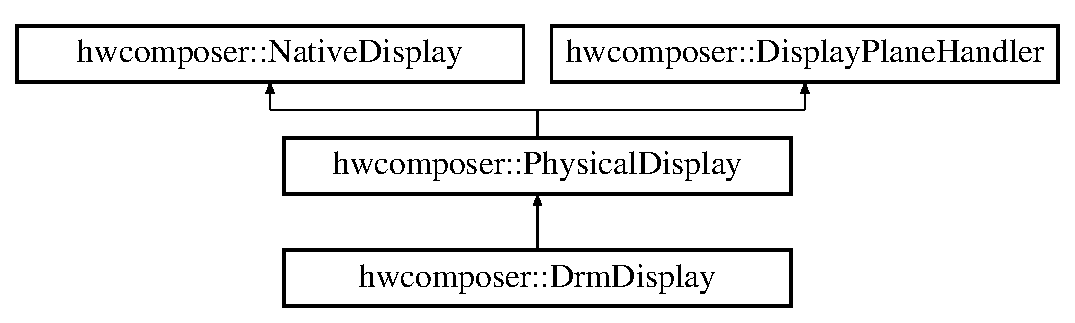
\includegraphics[height=3.000000cm]{classhwcomposer_1_1DrmDisplay}
\end{center}
\end{figure}
\subsection*{Public Member Functions}
\begin{DoxyCompactItemize}
\item 
\mbox{\hyperlink{classhwcomposer_1_1DrmDisplay_af465e6d3c061a21372fcc2c1da960e79}{Drm\+Display}} (uint32\+\_\+t gpu\+\_\+fd, uint32\+\_\+t pipe\+\_\+id, uint32\+\_\+t crtc\+\_\+id, \mbox{\hyperlink{classhwcomposer_1_1DrmDisplayManager}{Drm\+Display\+Manager}} $\ast$manager)
\item 
\mbox{\hyperlink{classhwcomposer_1_1DrmDisplay_a10adc5ea0028976604fa467efcfb1880}{$\sim$\+Drm\+Display}} () override
\item 
bool \mbox{\hyperlink{classhwcomposer_1_1DrmDisplay_a7625a0b44daa5be9b7acf1bce235663e}{Get\+Display\+Attribute}} (uint32\+\_\+t config, H\+W\+C\+Display\+Attribute attribute, int32\+\_\+t $\ast$value) override
\item 
bool \mbox{\hyperlink{classhwcomposer_1_1DrmDisplay_a44114f544fbb9328f385085e30d900f1}{Get\+Display\+Configs}} (uint32\+\_\+t $\ast$num\+\_\+configs, uint32\+\_\+t $\ast$configs) override
\item 
bool \mbox{\hyperlink{classhwcomposer_1_1DrmDisplay_ac1feeb5b5c7b1f9dbb0faf1a2bd8befe}{Get\+Display\+Name}} (uint32\+\_\+t $\ast$size, char $\ast$name) override
\item 
bool \mbox{\hyperlink{classhwcomposer_1_1DrmDisplay_abf4285912666230bf6172dae5a867ba7}{Set\+Broadcast\+R\+GB}} (const char $\ast$range\+\_\+property) override
\item 
void \mbox{\hyperlink{classhwcomposer_1_1DrmDisplay_a8ea456de0530370e0ad5f57ba4c6d20a}{Set\+H\+D\+C\+P\+State}} (H\+W\+C\+Content\+Protection state, H\+W\+C\+Content\+Type content\+\_\+type) override
\item 
bool \mbox{\hyperlink{classhwcomposer_1_1DrmDisplay_a6dd7060290f6be414485d743d1e7d226}{Initialize\+Display}} () override
\item 
void \mbox{\hyperlink{classhwcomposer_1_1DrmDisplay_a0212cd45757cc2a74dac62094da103ec}{Power\+On}} () override
\item 
void \mbox{\hyperlink{classhwcomposer_1_1DrmDisplay_aa235de1fc4a01177e1afea36d4554870}{Update\+Display\+Config}} () override
\item 
void \mbox{\hyperlink{classhwcomposer_1_1DrmDisplay_a8da99b54fe8c1261f1bf9a3d00474133}{Set\+Color\+Correction}} (struct \mbox{\hyperlink{structhwcomposer_1_1gamma__colors}{gamma\+\_\+colors}} gamma, uint32\+\_\+t contrast, uint32\+\_\+t brightness) const override
\item 
void \mbox{\hyperlink{classhwcomposer_1_1DrmDisplay_aca6b6791dc9c5a4498895509e854bcfa}{Set\+Pipe\+Canvas\+Color}} (uint16\+\_\+t bpc, uint16\+\_\+t red, uint16\+\_\+t green, uint16\+\_\+t blue, uint16\+\_\+t alpha) const override
\item 
void \mbox{\hyperlink{classhwcomposer_1_1DrmDisplay_a43bbf2421bd4b0b4e7b0612020060e3e}{Set\+Color\+Transform\+Matrix}} (const float $\ast$color\+\_\+transform\+\_\+matrix, \mbox{\hyperlink{hwcdefs_8h_a1a2c55aec4fbd12a1e323f2bdb3e9b88}{H\+W\+C\+Color\+Transform}} color\+\_\+transform\+\_\+hint) const override
\item 
void \mbox{\hyperlink{classhwcomposer_1_1DrmDisplay_a4596c2736f70fdd4c87ceb2dccf14848}{Disable}} (const \mbox{\hyperlink{namespacehwcomposer_adf383ae435d39a5631a8ad82e7fa18a4}{Display\+Plane\+State\+List}} \&composition\+\_\+planes) override
\item 
bool \mbox{\hyperlink{classhwcomposer_1_1DrmDisplay_a83b00eac01a21d6a5e50b4664df6b279}{Commit}} (const \mbox{\hyperlink{namespacehwcomposer_adf383ae435d39a5631a8ad82e7fa18a4}{Display\+Plane\+State\+List}} \&composition\+\_\+planes, const \mbox{\hyperlink{namespacehwcomposer_adf383ae435d39a5631a8ad82e7fa18a4}{Display\+Plane\+State\+List}} \&previous\+\_\+composition\+\_\+planes, bool disable\+\_\+explicit\+\_\+fence, int32\+\_\+t previous\+\_\+fence, int32\+\_\+t $\ast$commit\+\_\+fence, bool $\ast$previous\+\_\+fence\+\_\+released) override
\item 
uint32\+\_\+t \mbox{\hyperlink{classhwcomposer_1_1DrmDisplay_ac4ec96746c9dba9cce59b4bdce0a87ff}{Crtc\+Id}} () const
\item 
bool \mbox{\hyperlink{classhwcomposer_1_1DrmDisplay_abbf3b8fc423292df5fe6b9df791977c4}{Connect\+Display}} (const \mbox{\hyperlink{nativedisplay_8h_a00e4eec8ca028fd8f4672b5e60fbf2cd}{drm\+Mode\+Mode\+Info}} \&mode\+\_\+info, const \mbox{\hyperlink{nativedisplay_8h_a16ea3fc6b16060fd1e1257707006440e}{drm\+Mode\+Connector}} $\ast$connector, uint32\+\_\+t config)
\item 
void \mbox{\hyperlink{classhwcomposer_1_1DrmDisplay_a922407311e0d418894e4968712f2bf03}{Set\+Drm\+Mode\+Info}} (const std\+::vector$<$ \mbox{\hyperlink{nativedisplay_8h_a00e4eec8ca028fd8f4672b5e60fbf2cd}{drm\+Mode\+Mode\+Info}} $>$ \&mode\+\_\+info)
\item 
void \mbox{\hyperlink{classhwcomposer_1_1DrmDisplay_a1a72c20b148b0cf2c1174a34da8a95dc}{Set\+Display\+Attribute}} (const \mbox{\hyperlink{nativedisplay_8h_a00e4eec8ca028fd8f4672b5e60fbf2cd}{drm\+Mode\+Mode\+Info}} \&mode\+\_\+info)
\item 
bool \mbox{\hyperlink{classhwcomposer_1_1DrmDisplay_a7aaa318ce853a36ebcaf837fe1801f88}{Test\+Commit}} (const std\+::vector$<$ \mbox{\hyperlink{structhwcomposer_1_1OverlayPlane}{Overlay\+Plane}} $>$ \&commit\+\_\+planes) const override
\item 
bool \mbox{\hyperlink{classhwcomposer_1_1DrmDisplay_acbf817afffc6ad6f2879d914a0335dd0}{Populate\+Planes}} (std\+::vector$<$ std\+::unique\+\_\+ptr$<$ \mbox{\hyperlink{classhwcomposer_1_1DisplayPlane}{Display\+Plane}} $>$$>$ \&overlay\+\_\+planes) override
\item 
void \mbox{\hyperlink{classhwcomposer_1_1DrmDisplay_af4cf9ce1ea43e3520506dfc75c751c1f}{Notify\+Clients\+Of\+Display\+Change\+Status}} () override
\item 
void \mbox{\hyperlink{classhwcomposer_1_1DrmDisplay_a787d5eac9ba60ad9ae6f51cb028e8790}{Force\+Refresh}} ()
\item 
void \mbox{\hyperlink{classhwcomposer_1_1DrmDisplay_a0ac8713e1c6c26d0721295c8c6277540}{Ignore\+Updates}} ()
\item 
void \mbox{\hyperlink{classhwcomposer_1_1DrmDisplay_a7dd459cd835df8ff956350d3b53628e8}{Handle\+Lazy\+Initialization}} () override
\end{DoxyCompactItemize}
\subsection*{Additional Inherited Members}


\subsection{Detailed Description}


Definition at line 42 of file drmdisplay.\+h.



\subsection{Constructor \& Destructor Documentation}
\mbox{\Hypertarget{classhwcomposer_1_1DrmDisplay_af465e6d3c061a21372fcc2c1da960e79}\label{classhwcomposer_1_1DrmDisplay_af465e6d3c061a21372fcc2c1da960e79}} 
\index{hwcomposer\+::\+Drm\+Display@{hwcomposer\+::\+Drm\+Display}!Drm\+Display@{Drm\+Display}}
\index{Drm\+Display@{Drm\+Display}!hwcomposer\+::\+Drm\+Display@{hwcomposer\+::\+Drm\+Display}}
\subsubsection{\texorpdfstring{Drm\+Display()}{DrmDisplay()}}
{\footnotesize\ttfamily hwcomposer\+::\+Drm\+Display\+::\+Drm\+Display (\begin{DoxyParamCaption}\item[{uint32\+\_\+t}]{gpu\+\_\+fd,  }\item[{uint32\+\_\+t}]{pipe\+\_\+id,  }\item[{uint32\+\_\+t}]{crtc\+\_\+id,  }\item[{\mbox{\hyperlink{classhwcomposer_1_1DrmDisplayManager}{Drm\+Display\+Manager}} $\ast$}]{manager }\end{DoxyParamCaption})}



Definition at line 41 of file drmdisplay.\+cpp.


\begin{DoxyCode}{0}
\DoxyCodeLine{43     : \mbox{\hyperlink{classhwcomposer_1_1PhysicalDisplay_af08453e7ec5a9f8e792063b09b2e9305}{PhysicalDisplay}}(gpu\_fd, pipe\_id),}
\DoxyCodeLine{44       crtc\_id\_(crtc\_id),}
\DoxyCodeLine{45       connector\_(0),}
\DoxyCodeLine{46       manager\_(manager) \{}
\DoxyCodeLine{47   memset(\&current\_mode\_, 0, \textcolor{keyword}{sizeof}(current\_mode\_));}
\DoxyCodeLine{48 \}}
\end{DoxyCode}
\mbox{\Hypertarget{classhwcomposer_1_1DrmDisplay_a10adc5ea0028976604fa467efcfb1880}\label{classhwcomposer_1_1DrmDisplay_a10adc5ea0028976604fa467efcfb1880}} 
\index{hwcomposer\+::\+Drm\+Display@{hwcomposer\+::\+Drm\+Display}!````~Drm\+Display@{$\sim$\+Drm\+Display}}
\index{````~Drm\+Display@{$\sim$\+Drm\+Display}!hwcomposer\+::\+Drm\+Display@{hwcomposer\+::\+Drm\+Display}}
\subsubsection{\texorpdfstring{$\sim$\+Drm\+Display()}{~DrmDisplay()}}
{\footnotesize\ttfamily hwcomposer\+::\+Drm\+Display\+::$\sim$\+Drm\+Display (\begin{DoxyParamCaption}{ }\end{DoxyParamCaption})\hspace{0.3cm}{\ttfamily [override]}}



Definition at line 50 of file drmdisplay.\+cpp.


\begin{DoxyCode}{0}
\DoxyCodeLine{50                         \{}
\DoxyCodeLine{51   \textcolor{keywordflow}{if} (blob\_id\_)}
\DoxyCodeLine{52     drmModeDestroyPropertyBlob(\mbox{\hyperlink{classhwcomposer_1_1PhysicalDisplay_af0c3283a588887be1f8871ae2abd44f1}{gpu\_fd\_}}, blob\_id\_);}
\DoxyCodeLine{53 }
\DoxyCodeLine{54   \textcolor{keywordflow}{if} (old\_blob\_id\_)}
\DoxyCodeLine{55     drmModeDestroyPropertyBlob(\mbox{\hyperlink{classhwcomposer_1_1PhysicalDisplay_af0c3283a588887be1f8871ae2abd44f1}{gpu\_fd\_}}, old\_blob\_id\_);}
\DoxyCodeLine{56 }
\DoxyCodeLine{57   \mbox{\hyperlink{classhwcomposer_1_1PhysicalDisplay_a64283661ac59ad590ecbbe828e969b86}{display\_queue\_}}->SetPowerMode(\mbox{\hyperlink{hwcdefs_8h_afeed7d73a1340d1260c45cbe952c97bea24f95f47dddd4bbea91b334f1d6711cc}{kOff}});}
\DoxyCodeLine{58 \}}
\end{DoxyCode}


\subsection{Member Function Documentation}
\mbox{\Hypertarget{classhwcomposer_1_1DrmDisplay_a83b00eac01a21d6a5e50b4664df6b279}\label{classhwcomposer_1_1DrmDisplay_a83b00eac01a21d6a5e50b4664df6b279}} 
\index{hwcomposer\+::\+Drm\+Display@{hwcomposer\+::\+Drm\+Display}!Commit@{Commit}}
\index{Commit@{Commit}!hwcomposer\+::\+Drm\+Display@{hwcomposer\+::\+Drm\+Display}}
\subsubsection{\texorpdfstring{Commit()}{Commit()}}
{\footnotesize\ttfamily bool hwcomposer\+::\+Drm\+Display\+::\+Commit (\begin{DoxyParamCaption}\item[{const \mbox{\hyperlink{namespacehwcomposer_adf383ae435d39a5631a8ad82e7fa18a4}{Display\+Plane\+State\+List}} \&}]{composition\+\_\+planes,  }\item[{const \mbox{\hyperlink{namespacehwcomposer_adf383ae435d39a5631a8ad82e7fa18a4}{Display\+Plane\+State\+List}} \&}]{previous\+\_\+composition\+\_\+planes,  }\item[{bool}]{disable\+\_\+explicit\+\_\+fence,  }\item[{int32\+\_\+t}]{previous\+\_\+fence,  }\item[{int32\+\_\+t $\ast$}]{commit\+\_\+fence,  }\item[{bool $\ast$}]{previous\+\_\+fence\+\_\+released }\end{DoxyParamCaption})\hspace{0.3cm}{\ttfamily [override]}, {\ttfamily [virtual]}}

A\+PI for showing content on display 
\begin{DoxyParams}{Parameters}
{\em composition\+\_\+planes} & contains list of layers which need to displayed. \\
\hline
{\em previous\+\_\+composition\+\_\+planes} & contains list of planes enabled last frame. \\
\hline
{\em disable\+\_\+explicit\+\_\+fence} & is set to true if we want a hardware fence associated with this commit request set to commit\+\_\+fence. \\
\hline
{\em commit\+\_\+fence} & hardware fence associated with this commit request. \\
\hline
\end{DoxyParams}


Implements \mbox{\hyperlink{classhwcomposer_1_1PhysicalDisplay_a1db680248cf31fdf1d2d1e926355916d}{hwcomposer\+::\+Physical\+Display}}.



Definition at line 360 of file drmdisplay.\+cpp.


\begin{DoxyCode}{0}
\DoxyCodeLine{364                                    \{}
\DoxyCodeLine{365   \textcolor{comment}{// Do the actual commit.}}
\DoxyCodeLine{366   \mbox{\hyperlink{namespacehwcomposer_a1db01e0534b5b990ac7d35376c4b7e03}{ScopedDrmAtomicReqPtr}} pset(drmModeAtomicAlloc());}
\DoxyCodeLine{367   *previous\_fence\_released = \textcolor{keyword}{false};}
\DoxyCodeLine{368 }
\DoxyCodeLine{369   \textcolor{keywordflow}{if} (!pset) \{}
\DoxyCodeLine{370     \mbox{\hyperlink{alios_2platformdefines_8h_a226d6c99e4bcfca193c095e085e9097d}{ETRACE}}(\textcolor{stringliteral}{"Failed to allocate property set \%d"}, -ENOMEM);}
\DoxyCodeLine{371     \textcolor{keywordflow}{return} \textcolor{keyword}{false};}
\DoxyCodeLine{372   \}}
\DoxyCodeLine{373 }
\DoxyCodeLine{374   \textcolor{keywordflow}{if} (\mbox{\hyperlink{classhwcomposer_1_1PhysicalDisplay_aa0a736c951942f62a8c9514548dbfa0b}{display\_state\_}} \& \mbox{\hyperlink{classhwcomposer_1_1PhysicalDisplay_ae390ba5a8a0970767736459801b5d5fba52e2505c897030e88bcaa6498019cb4e}{kNeedsModeset}}) \{}
\DoxyCodeLine{375     \textcolor{keywordflow}{if} (!ApplyPendingModeset(pset.get())) \{}
\DoxyCodeLine{376       \mbox{\hyperlink{alios_2platformdefines_8h_a226d6c99e4bcfca193c095e085e9097d}{ETRACE}}(\textcolor{stringliteral}{"Failed to Modeset."});}
\DoxyCodeLine{377       \textcolor{keywordflow}{return} \textcolor{keyword}{false};}
\DoxyCodeLine{378     \}}
\DoxyCodeLine{379   \} \textcolor{keywordflow}{else} \textcolor{keywordflow}{if} (!disable\_explicit\_fence \&\& out\_fence\_ptr\_prop\_) \{}
\DoxyCodeLine{380     GetFence(pset.get(), commit\_fence);}
\DoxyCodeLine{381   \}}
\DoxyCodeLine{382 }
\DoxyCodeLine{383   \textcolor{keywordflow}{if} (!CommitFrame(composition\_planes, previous\_composition\_planes, pset.get(),}
\DoxyCodeLine{384                    flags\_, previous\_fence, previous\_fence\_released)) \{}
\DoxyCodeLine{385     \mbox{\hyperlink{alios_2platformdefines_8h_a226d6c99e4bcfca193c095e085e9097d}{ETRACE}}(\textcolor{stringliteral}{"Failed to Commit layers."});}
\DoxyCodeLine{386     \textcolor{keywordflow}{return} \textcolor{keyword}{false};}
\DoxyCodeLine{387   \}}
\DoxyCodeLine{388 }
\DoxyCodeLine{389   \textcolor{keywordflow}{if} (\mbox{\hyperlink{classhwcomposer_1_1PhysicalDisplay_aa0a736c951942f62a8c9514548dbfa0b}{display\_state\_}} \& \mbox{\hyperlink{classhwcomposer_1_1PhysicalDisplay_ae390ba5a8a0970767736459801b5d5fba52e2505c897030e88bcaa6498019cb4e}{kNeedsModeset}}) \{}
\DoxyCodeLine{390     \mbox{\hyperlink{classhwcomposer_1_1PhysicalDisplay_aa0a736c951942f62a8c9514548dbfa0b}{display\_state\_}} \&= ~\mbox{\hyperlink{classhwcomposer_1_1PhysicalDisplay_ae390ba5a8a0970767736459801b5d5fba52e2505c897030e88bcaa6498019cb4e}{kNeedsModeset}};}
\DoxyCodeLine{391     \textcolor{keywordflow}{if} (!disable\_explicit\_fence) \{}
\DoxyCodeLine{392       flags\_ = 0;}
\DoxyCodeLine{393       flags\_ |= DRM\_MODE\_ATOMIC\_NONBLOCK;}
\DoxyCodeLine{394     \}}
\DoxyCodeLine{395   \}}
\DoxyCodeLine{396 }
\DoxyCodeLine{397 \textcolor{preprocessor}{\#ifdef ENABLE\_DOUBLE\_BUFFERING}}
\DoxyCodeLine{398   int32\_t fence = *commit\_fence;}
\DoxyCodeLine{399   \textcolor{keywordflow}{if} (fence > 0) \{}
\DoxyCodeLine{400     \mbox{\hyperlink{namespacehwcomposer_a095356a61c96d5f48d4ada5e8e193549}{HWCPoll}}(fence, -1);}
\DoxyCodeLine{401     close(fence);}
\DoxyCodeLine{402     *commit\_fence = 0;}
\DoxyCodeLine{403   \}}
\DoxyCodeLine{404 \textcolor{preprocessor}{\#endif}}
\DoxyCodeLine{405 }
\DoxyCodeLine{406   \textcolor{keywordflow}{return} \textcolor{keyword}{true};}
\DoxyCodeLine{407 \}}
\end{DoxyCode}
\mbox{\Hypertarget{classhwcomposer_1_1DrmDisplay_abbf3b8fc423292df5fe6b9df791977c4}\label{classhwcomposer_1_1DrmDisplay_abbf3b8fc423292df5fe6b9df791977c4}} 
\index{hwcomposer\+::\+Drm\+Display@{hwcomposer\+::\+Drm\+Display}!Connect\+Display@{Connect\+Display}}
\index{Connect\+Display@{Connect\+Display}!hwcomposer\+::\+Drm\+Display@{hwcomposer\+::\+Drm\+Display}}
\subsubsection{\texorpdfstring{Connect\+Display()}{ConnectDisplay()}}
{\footnotesize\ttfamily bool hwcomposer\+::\+Drm\+Display\+::\+Connect\+Display (\begin{DoxyParamCaption}\item[{const \mbox{\hyperlink{nativedisplay_8h_a00e4eec8ca028fd8f4672b5e60fbf2cd}{drm\+Mode\+Mode\+Info}} \&}]{mode\+\_\+info,  }\item[{const \mbox{\hyperlink{nativedisplay_8h_a16ea3fc6b16060fd1e1257707006440e}{drm\+Mode\+Connector}} $\ast$}]{connector,  }\item[{uint32\+\_\+t}]{config }\end{DoxyParamCaption})}



Definition at line 76 of file drmdisplay.\+cpp.


\begin{DoxyCode}{0}
\DoxyCodeLine{78                                                  \{}
\DoxyCodeLine{79   \mbox{\hyperlink{hwctrace_8h_af8c38c979e9089c283d2f5923089b538}{IHOTPLUGEVENTTRACE}}(\textcolor{stringliteral}{"DrmDisplay::Connect recieved."});}
\DoxyCodeLine{80   \textcolor{comment}{// TODO(kalyan): Add support for multi monitor case.}}
\DoxyCodeLine{81   \textcolor{keywordflow}{if} (connector\_ \&\& connector->connector\_id == connector\_) \{}
\DoxyCodeLine{82     \mbox{\hyperlink{hwctrace_8h_af8c38c979e9089c283d2f5923089b538}{IHOTPLUGEVENTTRACE}}(}
\DoxyCodeLine{83         \textcolor{stringliteral}{"Display is already connected to this connector. \%d \%d \%p \(\backslash\)n"},}
\DoxyCodeLine{84         connector->connector\_id, connector\_, \textcolor{keyword}{this});}
\DoxyCodeLine{85     \mbox{\hyperlink{classhwcomposer_1_1PhysicalDisplay_a83777a9b17a33aa45295c7c354e802b2}{PhysicalDisplay::Connect}}();}
\DoxyCodeLine{86     \textcolor{keywordflow}{return} \textcolor{keyword}{true};}
\DoxyCodeLine{87   \}}
\DoxyCodeLine{88 }
\DoxyCodeLine{89   \mbox{\hyperlink{hwctrace_8h_af8c38c979e9089c283d2f5923089b538}{IHOTPLUGEVENTTRACE}}(}
\DoxyCodeLine{90       \textcolor{stringliteral}{"Display is being connected to a new connector.\%d \%d \%p \(\backslash\)n"},}
\DoxyCodeLine{91       connector->connector\_id, connector\_, \textcolor{keyword}{this});}
\DoxyCodeLine{92   connector\_ = connector->connector\_id;}
\DoxyCodeLine{93   mmWidth\_ = connector->mmWidth;}
\DoxyCodeLine{94   mmHeight\_ = connector->mmHeight;}
\DoxyCodeLine{95   \mbox{\hyperlink{classhwcomposer_1_1DrmDisplay_a1a72c20b148b0cf2c1174a34da8a95dc}{SetDisplayAttribute}}(mode\_info);}
\DoxyCodeLine{96   \mbox{\hyperlink{classhwcomposer_1_1PhysicalDisplay_a75eb0d6243de4021ad8e49141becc4a0}{config\_}} = config;}
\DoxyCodeLine{97 }
\DoxyCodeLine{98   \mbox{\hyperlink{namespacehwcomposer_ace195c2e057b634efb3013a5a4413799}{ScopedDrmObjectPropertyPtr}} connector\_props(drmModeObjectGetProperties(}
\DoxyCodeLine{99       \mbox{\hyperlink{classhwcomposer_1_1PhysicalDisplay_af0c3283a588887be1f8871ae2abd44f1}{gpu\_fd\_}}, connector\_, DRM\_MODE\_OBJECT\_CONNECTOR));}
\DoxyCodeLine{100   \textcolor{keywordflow}{if} (!connector\_props) \{}
\DoxyCodeLine{101     \mbox{\hyperlink{alios_2platformdefines_8h_a226d6c99e4bcfca193c095e085e9097d}{ETRACE}}(\textcolor{stringliteral}{"Unable to get connector properties."});}
\DoxyCodeLine{102     \textcolor{keywordflow}{return} \textcolor{keyword}{false};}
\DoxyCodeLine{103   \}}
\DoxyCodeLine{104 }
\DoxyCodeLine{105   \textcolor{keywordtype}{int} value = -1;}
\DoxyCodeLine{106   GetDrmHDCPObjectProperty(\textcolor{stringliteral}{"Content Protection"}, connector, connector\_props,}
\DoxyCodeLine{107                            \&hdcp\_id\_prop\_, \&value);}
\DoxyCodeLine{108 }
\DoxyCodeLine{109   \textcolor{keywordflow}{if} (value >= 0) \{}
\DoxyCodeLine{110     \textcolor{keywordflow}{switch} (value) \{}
\DoxyCodeLine{111       \textcolor{keywordflow}{case} 0:}
\DoxyCodeLine{112         current\_protection\_support\_ = HWCContentProtection::kUnDesired;}
\DoxyCodeLine{113         \textcolor{keywordflow}{break};}
\DoxyCodeLine{114       \textcolor{keywordflow}{case} 1:}
\DoxyCodeLine{115         current\_protection\_support\_ = HWCContentProtection::kDesired;}
\DoxyCodeLine{116         \textcolor{keywordflow}{break};}
\DoxyCodeLine{117       \textcolor{keywordflow}{default}:}
\DoxyCodeLine{118         \textcolor{keywordflow}{break};}
\DoxyCodeLine{119     \}}
\DoxyCodeLine{120 }
\DoxyCodeLine{121     \textcolor{keywordflow}{if} (desired\_protection\_support\_ == HWCContentProtection::kUnSupported) \{}
\DoxyCodeLine{122       desired\_protection\_support\_ = current\_protection\_support\_;}
\DoxyCodeLine{123     \}}
\DoxyCodeLine{124   \}}
\DoxyCodeLine{125 }
\DoxyCodeLine{126   GetDrmObjectProperty(\textcolor{stringliteral}{"CRTC\_ID"}, connector\_props, \&crtc\_prop\_);}
\DoxyCodeLine{127   GetDrmObjectProperty(\textcolor{stringliteral}{"Broadcast RGB"}, connector\_props, \&broadcastrgb\_id\_);}
\DoxyCodeLine{128   GetDrmObjectProperty(\textcolor{stringliteral}{"DPMS"}, connector\_props, \&dpms\_prop\_);}
\DoxyCodeLine{129 }
\DoxyCodeLine{130   \mbox{\hyperlink{classhwcomposer_1_1PhysicalDisplay_a83777a9b17a33aa45295c7c354e802b2}{PhysicalDisplay::Connect}}();}
\DoxyCodeLine{131   \mbox{\hyperlink{classhwcomposer_1_1DrmDisplay_a8ea456de0530370e0ad5f57ba4c6d20a}{SetHDCPState}}(desired\_protection\_support\_, content\_type\_);}
\DoxyCodeLine{132 }
\DoxyCodeLine{133   drmModePropertyPtr broadcastrgb\_props =}
\DoxyCodeLine{134       drmModeGetProperty(\mbox{\hyperlink{classhwcomposer_1_1PhysicalDisplay_af0c3283a588887be1f8871ae2abd44f1}{gpu\_fd\_}}, broadcastrgb\_id\_);}
\DoxyCodeLine{135 }
\DoxyCodeLine{136   \mbox{\hyperlink{classhwcomposer_1_1PhysicalDisplay_a4fc0fbe6c307de00cd10a3c998c74b51}{SetPowerMode}}(\mbox{\hyperlink{classhwcomposer_1_1PhysicalDisplay_ac2f383cc7b186eab567292239c700c50}{power\_mode\_}});}
\DoxyCodeLine{137 }
\DoxyCodeLine{138   \textcolor{comment}{// This is a valid case on DSI panels.}}
\DoxyCodeLine{139   \textcolor{keywordflow}{if} (broadcastrgb\_props == \mbox{\hyperlink{alios_2platformdefines_8h_a070d2ce7b6bb7e5c05602aa8c308d0c4}{NULL}}) \{}
\DoxyCodeLine{140     \mbox{\hyperlink{alios_2platformdefines_8h_acf170c48646d06441f4ea26cd5cf8acb}{WTRACE}}(\textcolor{stringliteral}{"Unable to get Broadcast RGB properties\(\backslash\)n"});}
\DoxyCodeLine{141     \textcolor{keywordflow}{return} \textcolor{keyword}{true};}
\DoxyCodeLine{142   \}}
\DoxyCodeLine{143 }
\DoxyCodeLine{144   \textcolor{keywordflow}{if} (!(broadcastrgb\_props->flags \& DRM\_MODE\_PROP\_ENUM)) \{}
\DoxyCodeLine{145     drmModeFreeProperty(broadcastrgb\_props);}
\DoxyCodeLine{146     \textcolor{keywordflow}{return} \textcolor{keyword}{false};}
\DoxyCodeLine{147   \}}
\DoxyCodeLine{148 }
\DoxyCodeLine{149   \textcolor{keywordflow}{if} (broadcastrgb\_props->enums != \mbox{\hyperlink{alios_2platformdefines_8h_a070d2ce7b6bb7e5c05602aa8c308d0c4}{NULL}}) \{}
\DoxyCodeLine{150     \textcolor{keywordflow}{for} (\textcolor{keywordtype}{int} i = 0; i < broadcastrgb\_props->count\_enums; i++) \{}
\DoxyCodeLine{151       \textcolor{keywordflow}{if} (!strcmp(broadcastrgb\_props->enums[i].name, \textcolor{stringliteral}{"Full"})) \{}
\DoxyCodeLine{152         broadcastrgb\_full\_ = broadcastrgb\_props->enums[i].value;}
\DoxyCodeLine{153       \} \textcolor{keywordflow}{else} \textcolor{keywordflow}{if} (!strcmp(broadcastrgb\_props->enums[i].name, \textcolor{stringliteral}{"Automatic"})) \{}
\DoxyCodeLine{154         broadcastrgb\_automatic\_ = broadcastrgb\_props->enums[i].value;}
\DoxyCodeLine{155       \}}
\DoxyCodeLine{156     \}}
\DoxyCodeLine{157   \}}
\DoxyCodeLine{158 }
\DoxyCodeLine{159   drmModeFreeProperty(broadcastrgb\_props);}
\DoxyCodeLine{160 }
\DoxyCodeLine{161   \textcolor{keywordflow}{return} \textcolor{keyword}{true};}
\DoxyCodeLine{162 \}}
\end{DoxyCode}
\mbox{\Hypertarget{classhwcomposer_1_1DrmDisplay_ac4ec96746c9dba9cce59b4bdce0a87ff}\label{classhwcomposer_1_1DrmDisplay_ac4ec96746c9dba9cce59b4bdce0a87ff}} 
\index{hwcomposer\+::\+Drm\+Display@{hwcomposer\+::\+Drm\+Display}!Crtc\+Id@{Crtc\+Id}}
\index{Crtc\+Id@{Crtc\+Id}!hwcomposer\+::\+Drm\+Display@{hwcomposer\+::\+Drm\+Display}}
\subsubsection{\texorpdfstring{Crtc\+Id()}{CrtcId()}}
{\footnotesize\ttfamily uint32\+\_\+t hwcomposer\+::\+Drm\+Display\+::\+Crtc\+Id (\begin{DoxyParamCaption}{ }\end{DoxyParamCaption}) const\hspace{0.3cm}{\ttfamily [inline]}}



Definition at line 75 of file drmdisplay.\+h.


\begin{DoxyCode}{0}
\DoxyCodeLine{75                           \{}
\DoxyCodeLine{76     \textcolor{keywordflow}{return} crtc\_id\_;}
\DoxyCodeLine{77   \}}
\end{DoxyCode}
\mbox{\Hypertarget{classhwcomposer_1_1DrmDisplay_a4596c2736f70fdd4c87ceb2dccf14848}\label{classhwcomposer_1_1DrmDisplay_a4596c2736f70fdd4c87ceb2dccf14848}} 
\index{hwcomposer\+::\+Drm\+Display@{hwcomposer\+::\+Drm\+Display}!Disable@{Disable}}
\index{Disable@{Disable}!hwcomposer\+::\+Drm\+Display@{hwcomposer\+::\+Drm\+Display}}
\subsubsection{\texorpdfstring{Disable()}{Disable()}}
{\footnotesize\ttfamily void hwcomposer\+::\+Drm\+Display\+::\+Disable (\begin{DoxyParamCaption}\item[{const \mbox{\hyperlink{namespacehwcomposer_adf383ae435d39a5631a8ad82e7fa18a4}{Display\+Plane\+State\+List}} \&}]{composition\+\_\+planes }\end{DoxyParamCaption})\hspace{0.3cm}{\ttfamily [override]}, {\ttfamily [virtual]}}

A\+PI is called when display needs to be disabled. 
\begin{DoxyParams}{Parameters}
{\em composition\+\_\+planes} & contains list of planes enabled last frame. \\
\hline
\end{DoxyParams}


Implements \mbox{\hyperlink{classhwcomposer_1_1PhysicalDisplay_af309ebed456ecdf3eb935ce693f326d1}{hwcomposer\+::\+Physical\+Display}}.



Definition at line 836 of file drmdisplay.\+cpp.


\begin{DoxyCode}{0}
\DoxyCodeLine{836                                                                         \{}
\DoxyCodeLine{837   \mbox{\hyperlink{hwctrace_8h_af8c38c979e9089c283d2f5923089b538}{IHOTPLUGEVENTTRACE}}(\textcolor{stringliteral}{"Disable: Disabling Display: \%p"}, \textcolor{keyword}{this});}
\DoxyCodeLine{838 }
\DoxyCodeLine{839   \textcolor{keywordflow}{for} (\textcolor{keyword}{const} DisplayPlaneState \&comp\_plane : composition\_planes) \{}
\DoxyCodeLine{840     DrmPlane *plane = \textcolor{keyword}{static\_cast<}DrmPlane *\textcolor{keyword}{>}(comp\_plane.GetDisplayPlane());}
\DoxyCodeLine{841     plane->SetInUse(\textcolor{keyword}{false});}
\DoxyCodeLine{842     plane->SetNativeFence(-1);}
\DoxyCodeLine{843   \}}
\DoxyCodeLine{844 }
\DoxyCodeLine{845   drmModeConnectorSetProperty(\mbox{\hyperlink{classhwcomposer_1_1PhysicalDisplay_af0c3283a588887be1f8871ae2abd44f1}{gpu\_fd\_}}, connector\_, dpms\_prop\_,}
\DoxyCodeLine{846                               DRM\_MODE\_DPMS\_OFF);}
\DoxyCodeLine{847 \}}
\end{DoxyCode}
\mbox{\Hypertarget{classhwcomposer_1_1DrmDisplay_a787d5eac9ba60ad9ae6f51cb028e8790}\label{classhwcomposer_1_1DrmDisplay_a787d5eac9ba60ad9ae6f51cb028e8790}} 
\index{hwcomposer\+::\+Drm\+Display@{hwcomposer\+::\+Drm\+Display}!Force\+Refresh@{Force\+Refresh}}
\index{Force\+Refresh@{Force\+Refresh}!hwcomposer\+::\+Drm\+Display@{hwcomposer\+::\+Drm\+Display}}
\subsubsection{\texorpdfstring{Force\+Refresh()}{ForceRefresh()}}
{\footnotesize\ttfamily void hwcomposer\+::\+Drm\+Display\+::\+Force\+Refresh (\begin{DoxyParamCaption}{ }\end{DoxyParamCaption})}



Definition at line 907 of file drmdisplay.\+cpp.


\begin{DoxyCode}{0}
\DoxyCodeLine{907                               \{}
\DoxyCodeLine{908   \mbox{\hyperlink{classhwcomposer_1_1PhysicalDisplay_a64283661ac59ad590ecbbe828e969b86}{display\_queue\_}}->ForceRefresh();}
\DoxyCodeLine{909 \}}
\end{DoxyCode}
\mbox{\Hypertarget{classhwcomposer_1_1DrmDisplay_a7625a0b44daa5be9b7acf1bce235663e}\label{classhwcomposer_1_1DrmDisplay_a7625a0b44daa5be9b7acf1bce235663e}} 
\index{hwcomposer\+::\+Drm\+Display@{hwcomposer\+::\+Drm\+Display}!Get\+Display\+Attribute@{Get\+Display\+Attribute}}
\index{Get\+Display\+Attribute@{Get\+Display\+Attribute}!hwcomposer\+::\+Drm\+Display@{hwcomposer\+::\+Drm\+Display}}
\subsubsection{\texorpdfstring{Get\+Display\+Attribute()}{GetDisplayAttribute()}}
{\footnotesize\ttfamily bool hwcomposer\+::\+Drm\+Display\+::\+Get\+Display\+Attribute (\begin{DoxyParamCaption}\item[{uint32\+\_\+t}]{config,  }\item[{H\+W\+C\+Display\+Attribute}]{attribute,  }\item[{int32\+\_\+t $\ast$}]{value }\end{DoxyParamCaption})\hspace{0.3cm}{\ttfamily [override]}, {\ttfamily [virtual]}}



Implements \mbox{\hyperlink{classhwcomposer_1_1NativeDisplay_aeb880e4a295eab49a98804380c2dcb84}{hwcomposer\+::\+Native\+Display}}.



Definition at line 164 of file drmdisplay.\+cpp.


\begin{DoxyCode}{0}
\DoxyCodeLine{166                                                      \{}
\DoxyCodeLine{167   \mbox{\hyperlink{wsi__utils_8h_ab309378939794fdebc2f4e5ea2dd730b}{SPIN\_LOCK}}(display\_lock\_);}
\DoxyCodeLine{168   \textcolor{keywordflow}{if} (modes\_.empty()) \{}
\DoxyCodeLine{169     \mbox{\hyperlink{wsi__utils_8h_a7dc41490a7065ff852ccc0faa466d815}{SPIN\_UNLOCK}}(display\_lock\_);}
\DoxyCodeLine{170     \textcolor{keywordflow}{return} \mbox{\hyperlink{classhwcomposer_1_1PhysicalDisplay_a7a76ed244ccea12e69c0fad38be23b84}{PhysicalDisplay::GetDisplayAttribute}}(config, attribute, value);}
\DoxyCodeLine{171   \}}
\DoxyCodeLine{172 }
\DoxyCodeLine{173   \textcolor{keywordtype}{float} refresh;}
\DoxyCodeLine{174   \textcolor{keywordtype}{bool} status = \textcolor{keyword}{true};}
\DoxyCodeLine{175 }
\DoxyCodeLine{176   \textcolor{keywordflow}{switch} (attribute) \{}
\DoxyCodeLine{177     \textcolor{keywordflow}{case} HWCDisplayAttribute::kWidth:}
\DoxyCodeLine{178       \textcolor{keywordflow}{if} (!\mbox{\hyperlink{classhwcomposer_1_1PhysicalDisplay_adac42ad60327a0ad4ebbaef554a4fafa}{custom\_resolution\_}}) \{}
\DoxyCodeLine{179         *value = modes\_[config].hdisplay;}
\DoxyCodeLine{180       \} \textcolor{keywordflow}{else} \{}
\DoxyCodeLine{181         *value = \mbox{\hyperlink{classhwcomposer_1_1PhysicalDisplay_aa50206430baa8d901e604787a73fe9b8}{rect\_}}.right - \mbox{\hyperlink{classhwcomposer_1_1PhysicalDisplay_aa50206430baa8d901e604787a73fe9b8}{rect\_}}.left;}
\DoxyCodeLine{182       \}}
\DoxyCodeLine{183       \mbox{\hyperlink{hwctrace_8h_af8c38c979e9089c283d2f5923089b538}{IHOTPLUGEVENTTRACE}}(\textcolor{stringliteral}{"GetDisplayAttribute: width \%d set"}, *value);}
\DoxyCodeLine{184       \textcolor{keywordflow}{break};}
\DoxyCodeLine{185     \textcolor{keywordflow}{case} HWCDisplayAttribute::kHeight:}
\DoxyCodeLine{186       \textcolor{keywordflow}{if} (!\mbox{\hyperlink{classhwcomposer_1_1PhysicalDisplay_adac42ad60327a0ad4ebbaef554a4fafa}{custom\_resolution\_}}) \{}
\DoxyCodeLine{187         *value = modes\_[config].vdisplay;}
\DoxyCodeLine{188       \} \textcolor{keywordflow}{else} \{}
\DoxyCodeLine{189         *value = \mbox{\hyperlink{classhwcomposer_1_1PhysicalDisplay_aa50206430baa8d901e604787a73fe9b8}{rect\_}}.bottom - \mbox{\hyperlink{classhwcomposer_1_1PhysicalDisplay_aa50206430baa8d901e604787a73fe9b8}{rect\_}}.top;}
\DoxyCodeLine{190       \}}
\DoxyCodeLine{191       \mbox{\hyperlink{hwctrace_8h_af8c38c979e9089c283d2f5923089b538}{IHOTPLUGEVENTTRACE}}(\textcolor{stringliteral}{"GetDisplayAttribute: height \%d set"}, *value);}
\DoxyCodeLine{192       \textcolor{keywordflow}{break};}
\DoxyCodeLine{193     \textcolor{keywordflow}{case} HWCDisplayAttribute::kRefreshRate:}
\DoxyCodeLine{194       \textcolor{keywordflow}{if} (!\mbox{\hyperlink{classhwcomposer_1_1PhysicalDisplay_adac42ad60327a0ad4ebbaef554a4fafa}{custom\_resolution\_}}) \{}
\DoxyCodeLine{195         refresh = (modes\_[config].clock * 1000.0f) /}
\DoxyCodeLine{196                   (modes\_[config].htotal * modes\_[config].vtotal);}
\DoxyCodeLine{197       \} \textcolor{keywordflow}{else} \{}
\DoxyCodeLine{198         refresh = (modes\_[config].clock * 1000.0f) /}
\DoxyCodeLine{199                   ((\mbox{\hyperlink{classhwcomposer_1_1PhysicalDisplay_aa50206430baa8d901e604787a73fe9b8}{rect\_}}.right - \mbox{\hyperlink{classhwcomposer_1_1PhysicalDisplay_aa50206430baa8d901e604787a73fe9b8}{rect\_}}.left) * (\mbox{\hyperlink{classhwcomposer_1_1PhysicalDisplay_aa50206430baa8d901e604787a73fe9b8}{rect\_}}.bottom - 
      \mbox{\hyperlink{classhwcomposer_1_1PhysicalDisplay_aa50206430baa8d901e604787a73fe9b8}{rect\_}}.top));}
\DoxyCodeLine{200       \}}
\DoxyCodeLine{201 }
\DoxyCodeLine{202       \textcolor{keywordflow}{if} (modes\_[config].flags \& DRM\_MODE\_FLAG\_INTERLACE)}
\DoxyCodeLine{203         refresh *= 2;}
\DoxyCodeLine{204 }
\DoxyCodeLine{205       \textcolor{keywordflow}{if} (modes\_[config].flags \& DRM\_MODE\_FLAG\_DBLSCAN)}
\DoxyCodeLine{206         refresh /= 2;}
\DoxyCodeLine{207 }
\DoxyCodeLine{208       \textcolor{keywordflow}{if} (modes\_[config].vscan > 1)}
\DoxyCodeLine{209         refresh /= modes\_[config].vscan;}
\DoxyCodeLine{210 }
\DoxyCodeLine{211       \textcolor{comment}{// in nanoseconds}}
\DoxyCodeLine{212       *value = 1e9 / refresh;}
\DoxyCodeLine{213       \textcolor{keywordflow}{break};}
\DoxyCodeLine{214     \textcolor{keywordflow}{case} HWCDisplayAttribute::kDpiX:}
\DoxyCodeLine{215       \textcolor{comment}{// Dots per 1000 inches}}
\DoxyCodeLine{216       \textcolor{keywordflow}{if} (!\mbox{\hyperlink{classhwcomposer_1_1PhysicalDisplay_adac42ad60327a0ad4ebbaef554a4fafa}{custom\_resolution\_}}) \{}
\DoxyCodeLine{217         *value =}
\DoxyCodeLine{218           mmWidth\_ ? (modes\_[config].hdisplay * kUmPerInch) / mmWidth\_ : -1;}
\DoxyCodeLine{219       \} \textcolor{keywordflow}{else} \{}
\DoxyCodeLine{220         *value =}
\DoxyCodeLine{221           mmWidth\_ ? ((\mbox{\hyperlink{classhwcomposer_1_1PhysicalDisplay_aa50206430baa8d901e604787a73fe9b8}{rect\_}}.right - \mbox{\hyperlink{classhwcomposer_1_1PhysicalDisplay_aa50206430baa8d901e604787a73fe9b8}{rect\_}}.left) * kUmPerInch) / mmWidth\_ : -1;}
\DoxyCodeLine{222       \}}
\DoxyCodeLine{223       \textcolor{keywordflow}{break};}
\DoxyCodeLine{224     \textcolor{keywordflow}{case} HWCDisplayAttribute::kDpiY:}
\DoxyCodeLine{225       \textcolor{comment}{// Dots per 1000 inches}}
\DoxyCodeLine{226       \textcolor{keywordflow}{if} (!\mbox{\hyperlink{classhwcomposer_1_1PhysicalDisplay_adac42ad60327a0ad4ebbaef554a4fafa}{custom\_resolution\_}}) \{}
\DoxyCodeLine{227         *value =}
\DoxyCodeLine{228           mmHeight\_ ? (modes\_[config].vdisplay * kUmPerInch) / mmHeight\_ : -1;}
\DoxyCodeLine{229       \} \textcolor{keywordflow}{else} \{}
\DoxyCodeLine{230         *value =}
\DoxyCodeLine{231           mmHeight\_ ? ((\mbox{\hyperlink{classhwcomposer_1_1PhysicalDisplay_aa50206430baa8d901e604787a73fe9b8}{rect\_}}.bottom - \mbox{\hyperlink{classhwcomposer_1_1PhysicalDisplay_aa50206430baa8d901e604787a73fe9b8}{rect\_}}.top) * kUmPerInch) /mmHeight\_: -1;}
\DoxyCodeLine{232       \}}
\DoxyCodeLine{233       \textcolor{keywordflow}{break};}
\DoxyCodeLine{234     \textcolor{keywordflow}{default}:}
\DoxyCodeLine{235       *value = -1;}
\DoxyCodeLine{236       status = \textcolor{keyword}{false};}
\DoxyCodeLine{237   \}}
\DoxyCodeLine{238 }
\DoxyCodeLine{239   \mbox{\hyperlink{wsi__utils_8h_a7dc41490a7065ff852ccc0faa466d815}{SPIN\_UNLOCK}}(display\_lock\_);}
\DoxyCodeLine{240   \textcolor{keywordflow}{return} status;}
\DoxyCodeLine{241 \}}
\end{DoxyCode}
\mbox{\Hypertarget{classhwcomposer_1_1DrmDisplay_a44114f544fbb9328f385085e30d900f1}\label{classhwcomposer_1_1DrmDisplay_a44114f544fbb9328f385085e30d900f1}} 
\index{hwcomposer\+::\+Drm\+Display@{hwcomposer\+::\+Drm\+Display}!Get\+Display\+Configs@{Get\+Display\+Configs}}
\index{Get\+Display\+Configs@{Get\+Display\+Configs}!hwcomposer\+::\+Drm\+Display@{hwcomposer\+::\+Drm\+Display}}
\subsubsection{\texorpdfstring{Get\+Display\+Configs()}{GetDisplayConfigs()}}
{\footnotesize\ttfamily bool hwcomposer\+::\+Drm\+Display\+::\+Get\+Display\+Configs (\begin{DoxyParamCaption}\item[{uint32\+\_\+t $\ast$}]{num\+\_\+configs,  }\item[{uint32\+\_\+t $\ast$}]{configs }\end{DoxyParamCaption})\hspace{0.3cm}{\ttfamily [override]}, {\ttfamily [virtual]}}



Implements \mbox{\hyperlink{classhwcomposer_1_1NativeDisplay_a9479dcf82765996db6d7ea1cdcef3864}{hwcomposer\+::\+Native\+Display}}.



Definition at line 243 of file drmdisplay.\+cpp.


\begin{DoxyCode}{0}
\DoxyCodeLine{243                                                                            \{}
\DoxyCodeLine{244   \mbox{\hyperlink{wsi__utils_8h_ab309378939794fdebc2f4e5ea2dd730b}{SPIN\_LOCK}}(display\_lock\_);}
\DoxyCodeLine{245   \textcolor{keywordtype}{size\_t} modes\_size = modes\_.size();}
\DoxyCodeLine{246   \mbox{\hyperlink{wsi__utils_8h_a7dc41490a7065ff852ccc0faa466d815}{SPIN\_UNLOCK}}(display\_lock\_);}
\DoxyCodeLine{247 }
\DoxyCodeLine{248   \textcolor{keywordflow}{if} (modes\_size == 0) \{}
\DoxyCodeLine{249     \textcolor{keywordflow}{return} \mbox{\hyperlink{classhwcomposer_1_1PhysicalDisplay_af02d333622a2c80fd79387ce40253e62}{PhysicalDisplay::GetDisplayConfigs}}(num\_configs, configs);}
\DoxyCodeLine{250   \}}
\DoxyCodeLine{251 }
\DoxyCodeLine{252   \textcolor{keywordflow}{if} (!configs) \{}
\DoxyCodeLine{253     *num\_configs = modes\_size;}
\DoxyCodeLine{254     \mbox{\hyperlink{hwctrace_8h_af8c38c979e9089c283d2f5923089b538}{IHOTPLUGEVENTTRACE}}(}
\DoxyCodeLine{255         \textcolor{stringliteral}{"GetDisplayConfigs: Total Configs: \%d pipe: \%d display: \%p"},}
\DoxyCodeLine{256         *num\_configs, \mbox{\hyperlink{classhwcomposer_1_1PhysicalDisplay_a6e44cfaecf46642d3c0f0347e26d2d6a}{pipe\_}}, \textcolor{keyword}{this});}
\DoxyCodeLine{257     \textcolor{keywordflow}{return} \textcolor{keyword}{true};}
\DoxyCodeLine{258   \}}
\DoxyCodeLine{259 }
\DoxyCodeLine{260   \mbox{\hyperlink{hwctrace_8h_af8c38c979e9089c283d2f5923089b538}{IHOTPLUGEVENTTRACE}}(}
\DoxyCodeLine{261       \textcolor{stringliteral}{"GetDisplayConfigs: Populating Configs: \%d pipe: \%d display: \%p"},}
\DoxyCodeLine{262       *num\_configs, \mbox{\hyperlink{classhwcomposer_1_1PhysicalDisplay_a6e44cfaecf46642d3c0f0347e26d2d6a}{pipe\_}}, \textcolor{keyword}{this});}
\DoxyCodeLine{263 }
\DoxyCodeLine{264   uint32\_t size = *num\_configs;}
\DoxyCodeLine{265   \textcolor{keywordflow}{for} (uint32\_t i = 0; i < size; i++)}
\DoxyCodeLine{266     configs[i] = i;}
\DoxyCodeLine{267 }
\DoxyCodeLine{268   \textcolor{keywordflow}{return} \textcolor{keyword}{true};}
\DoxyCodeLine{269 \}}
\end{DoxyCode}
\mbox{\Hypertarget{classhwcomposer_1_1DrmDisplay_ac1feeb5b5c7b1f9dbb0faf1a2bd8befe}\label{classhwcomposer_1_1DrmDisplay_ac1feeb5b5c7b1f9dbb0faf1a2bd8befe}} 
\index{hwcomposer\+::\+Drm\+Display@{hwcomposer\+::\+Drm\+Display}!Get\+Display\+Name@{Get\+Display\+Name}}
\index{Get\+Display\+Name@{Get\+Display\+Name}!hwcomposer\+::\+Drm\+Display@{hwcomposer\+::\+Drm\+Display}}
\subsubsection{\texorpdfstring{Get\+Display\+Name()}{GetDisplayName()}}
{\footnotesize\ttfamily bool hwcomposer\+::\+Drm\+Display\+::\+Get\+Display\+Name (\begin{DoxyParamCaption}\item[{uint32\+\_\+t $\ast$}]{size,  }\item[{char $\ast$}]{name }\end{DoxyParamCaption})\hspace{0.3cm}{\ttfamily [override]}, {\ttfamily [virtual]}}



Implements \mbox{\hyperlink{classhwcomposer_1_1NativeDisplay_a28c095d6d08c84e40b5d5160d038f0b5}{hwcomposer\+::\+Native\+Display}}.



Definition at line 271 of file drmdisplay.\+cpp.


\begin{DoxyCode}{0}
\DoxyCodeLine{271                                                           \{}
\DoxyCodeLine{272   \mbox{\hyperlink{wsi__utils_8h_ab309378939794fdebc2f4e5ea2dd730b}{SPIN\_LOCK}}(display\_lock\_);}
\DoxyCodeLine{273   \textcolor{keywordflow}{if} (modes\_.empty()) \{}
\DoxyCodeLine{274     \mbox{\hyperlink{wsi__utils_8h_a7dc41490a7065ff852ccc0faa466d815}{SPIN\_UNLOCK}}(display\_lock\_);}
\DoxyCodeLine{275     \textcolor{keywordflow}{return} \mbox{\hyperlink{classhwcomposer_1_1PhysicalDisplay_a1d0fe5aac11bc35aa95a55289993d9a8}{PhysicalDisplay::GetDisplayName}}(size, name);}
\DoxyCodeLine{276   \}}
\DoxyCodeLine{277   \mbox{\hyperlink{wsi__utils_8h_a7dc41490a7065ff852ccc0faa466d815}{SPIN\_UNLOCK}}(display\_lock\_)}
\DoxyCodeLine{278   std::ostringstream stream;}
\DoxyCodeLine{279   stream << \textcolor{stringliteral}{"Display-"} << connector\_;}
\DoxyCodeLine{280   std::string \textcolor{keywordtype}{string} = stream.str();}
\DoxyCodeLine{281   \textcolor{keywordtype}{size\_t} length = \textcolor{keywordtype}{string}.length();}
\DoxyCodeLine{282   \textcolor{keywordflow}{if} (!name) \{}
\DoxyCodeLine{283     *size = length;}
\DoxyCodeLine{284     \textcolor{keywordflow}{return} \textcolor{keyword}{true};}
\DoxyCodeLine{285   \}}
\DoxyCodeLine{286 }
\DoxyCodeLine{287   *size = std::min<uint32\_t>(\textcolor{keyword}{static\_cast<}uint32\_t\textcolor{keyword}{>}(length + 1), *size);}
\DoxyCodeLine{288   strncpy(name, \textcolor{keywordtype}{string}.c\_str(), *size);}
\DoxyCodeLine{289   \textcolor{keywordflow}{return} \textcolor{keyword}{true};}
\DoxyCodeLine{290 \}}
\end{DoxyCode}
\mbox{\Hypertarget{classhwcomposer_1_1DrmDisplay_a7dd459cd835df8ff956350d3b53628e8}\label{classhwcomposer_1_1DrmDisplay_a7dd459cd835df8ff956350d3b53628e8}} 
\index{hwcomposer\+::\+Drm\+Display@{hwcomposer\+::\+Drm\+Display}!Handle\+Lazy\+Initialization@{Handle\+Lazy\+Initialization}}
\index{Handle\+Lazy\+Initialization@{Handle\+Lazy\+Initialization}!hwcomposer\+::\+Drm\+Display@{hwcomposer\+::\+Drm\+Display}}
\subsubsection{\texorpdfstring{Handle\+Lazy\+Initialization()}{HandleLazyInitialization()}}
{\footnotesize\ttfamily void hwcomposer\+::\+Drm\+Display\+::\+Handle\+Lazy\+Initialization (\begin{DoxyParamCaption}{ }\end{DoxyParamCaption})\hspace{0.3cm}{\ttfamily [override]}, {\ttfamily [virtual]}}

A\+PI to handle any lazy initializations which need to be handled during first present call. 

Reimplemented from \mbox{\hyperlink{classhwcomposer_1_1PhysicalDisplay_ab8e24e90adf5eaa76da5cb827ad82c65}{hwcomposer\+::\+Physical\+Display}}.



Definition at line 915 of file drmdisplay.\+cpp.


\begin{DoxyCode}{0}
\DoxyCodeLine{915                                           \{}
\DoxyCodeLine{916   manager\_->\mbox{\hyperlink{classhwcomposer_1_1DrmDisplayManager_a9d52e745e20b0872b57d04ebdd3d12b6}{HandleLazyInitialization}}();}
\DoxyCodeLine{917 \}}
\end{DoxyCode}
\mbox{\Hypertarget{classhwcomposer_1_1DrmDisplay_a0ac8713e1c6c26d0721295c8c6277540}\label{classhwcomposer_1_1DrmDisplay_a0ac8713e1c6c26d0721295c8c6277540}} 
\index{hwcomposer\+::\+Drm\+Display@{hwcomposer\+::\+Drm\+Display}!Ignore\+Updates@{Ignore\+Updates}}
\index{Ignore\+Updates@{Ignore\+Updates}!hwcomposer\+::\+Drm\+Display@{hwcomposer\+::\+Drm\+Display}}
\subsubsection{\texorpdfstring{Ignore\+Updates()}{IgnoreUpdates()}}
{\footnotesize\ttfamily void hwcomposer\+::\+Drm\+Display\+::\+Ignore\+Updates (\begin{DoxyParamCaption}{ }\end{DoxyParamCaption})}



Definition at line 911 of file drmdisplay.\+cpp.


\begin{DoxyCode}{0}
\DoxyCodeLine{911                                \{}
\DoxyCodeLine{912   \mbox{\hyperlink{classhwcomposer_1_1PhysicalDisplay_a64283661ac59ad590ecbbe828e969b86}{display\_queue\_}}->IgnoreUpdates();}
\DoxyCodeLine{913 \}}
\end{DoxyCode}
\mbox{\Hypertarget{classhwcomposer_1_1DrmDisplay_a6dd7060290f6be414485d743d1e7d226}\label{classhwcomposer_1_1DrmDisplay_a6dd7060290f6be414485d743d1e7d226}} 
\index{hwcomposer\+::\+Drm\+Display@{hwcomposer\+::\+Drm\+Display}!Initialize\+Display@{Initialize\+Display}}
\index{Initialize\+Display@{Initialize\+Display}!hwcomposer\+::\+Drm\+Display@{hwcomposer\+::\+Drm\+Display}}
\subsubsection{\texorpdfstring{Initialize\+Display()}{InitializeDisplay()}}
{\footnotesize\ttfamily bool hwcomposer\+::\+Drm\+Display\+::\+Initialize\+Display (\begin{DoxyParamCaption}{ }\end{DoxyParamCaption})\hspace{0.3cm}{\ttfamily [override]}, {\ttfamily [virtual]}}

A\+PI for initializing display. Implementation needs to handle all things needed to set up the physical display. 

Implements \mbox{\hyperlink{classhwcomposer_1_1PhysicalDisplay_a1800b4ee66d4ec790d661106564b6fca}{hwcomposer\+::\+Physical\+Display}}.



Definition at line 60 of file drmdisplay.\+cpp.


\begin{DoxyCode}{0}
\DoxyCodeLine{60                                    \{}
\DoxyCodeLine{61   \mbox{\hyperlink{namespacehwcomposer_ace195c2e057b634efb3013a5a4413799}{ScopedDrmObjectPropertyPtr}} crtc\_props(}
\DoxyCodeLine{62       drmModeObjectGetProperties(\mbox{\hyperlink{classhwcomposer_1_1PhysicalDisplay_af0c3283a588887be1f8871ae2abd44f1}{gpu\_fd\_}}, crtc\_id\_, DRM\_MODE\_OBJECT\_CRTC));}
\DoxyCodeLine{63   GetDrmObjectProperty(\textcolor{stringliteral}{"ACTIVE"}, crtc\_props, \&active\_prop\_);}
\DoxyCodeLine{64   GetDrmObjectProperty(\textcolor{stringliteral}{"MODE\_ID"}, crtc\_props, \&mode\_id\_prop\_);}
\DoxyCodeLine{65   GetDrmObjectProperty(\textcolor{stringliteral}{"CTM"}, crtc\_props, \&ctm\_id\_prop\_);}
\DoxyCodeLine{66   GetDrmObjectProperty(\textcolor{stringliteral}{"CTM\_POST\_OFFSET"}, crtc\_props,}
\DoxyCodeLine{67                        \&ctm\_post\_offset\_id\_prop\_);}
\DoxyCodeLine{68   GetDrmObjectProperty(\textcolor{stringliteral}{"GAMMA\_LUT"}, crtc\_props, \&lut\_id\_prop\_);}
\DoxyCodeLine{69   GetDrmObjectPropertyValue(\textcolor{stringliteral}{"GAMMA\_LUT\_SIZE"}, crtc\_props, \&lut\_size\_);}
\DoxyCodeLine{70   GetDrmObjectProperty(\textcolor{stringliteral}{"OUT\_FENCE\_PTR"}, crtc\_props, \&out\_fence\_ptr\_prop\_);}
\DoxyCodeLine{71   GetDrmObjectProperty(\textcolor{stringliteral}{"background\_color"}, crtc\_props, \&canvas\_color\_prop\_);}
\DoxyCodeLine{72 }
\DoxyCodeLine{73   \textcolor{keywordflow}{return} \textcolor{keyword}{true};}
\DoxyCodeLine{74 \}}
\end{DoxyCode}
\mbox{\Hypertarget{classhwcomposer_1_1DrmDisplay_af4cf9ce1ea43e3520506dfc75c751c1f}\label{classhwcomposer_1_1DrmDisplay_af4cf9ce1ea43e3520506dfc75c751c1f}} 
\index{hwcomposer\+::\+Drm\+Display@{hwcomposer\+::\+Drm\+Display}!Notify\+Clients\+Of\+Display\+Change\+Status@{Notify\+Clients\+Of\+Display\+Change\+Status}}
\index{Notify\+Clients\+Of\+Display\+Change\+Status@{Notify\+Clients\+Of\+Display\+Change\+Status}!hwcomposer\+::\+Drm\+Display@{hwcomposer\+::\+Drm\+Display}}
\subsubsection{\texorpdfstring{Notify\+Clients\+Of\+Display\+Change\+Status()}{NotifyClientsOfDisplayChangeStatus()}}
{\footnotesize\ttfamily void hwcomposer\+::\+Drm\+Display\+::\+Notify\+Clients\+Of\+Display\+Change\+Status (\begin{DoxyParamCaption}{ }\end{DoxyParamCaption})\hspace{0.3cm}{\ttfamily [override]}, {\ttfamily [virtual]}}



Implements \mbox{\hyperlink{classhwcomposer_1_1PhysicalDisplay_aefba7f9543d7ef74d42f9e06dd0f1a58}{hwcomposer\+::\+Physical\+Display}}.



Definition at line 919 of file drmdisplay.\+cpp.


\begin{DoxyCode}{0}
\DoxyCodeLine{919                                                     \{}
\DoxyCodeLine{920   manager\_->\mbox{\hyperlink{classhwcomposer_1_1DrmDisplayManager_a087e35e0b0be34e4ff5efdb37c8a5684}{NotifyClientsOfDisplayChangeStatus}}();}
\DoxyCodeLine{921 \}}
\end{DoxyCode}
\mbox{\Hypertarget{classhwcomposer_1_1DrmDisplay_acbf817afffc6ad6f2879d914a0335dd0}\label{classhwcomposer_1_1DrmDisplay_acbf817afffc6ad6f2879d914a0335dd0}} 
\index{hwcomposer\+::\+Drm\+Display@{hwcomposer\+::\+Drm\+Display}!Populate\+Planes@{Populate\+Planes}}
\index{Populate\+Planes@{Populate\+Planes}!hwcomposer\+::\+Drm\+Display@{hwcomposer\+::\+Drm\+Display}}
\subsubsection{\texorpdfstring{Populate\+Planes()}{PopulatePlanes()}}
{\footnotesize\ttfamily bool hwcomposer\+::\+Drm\+Display\+::\+Populate\+Planes (\begin{DoxyParamCaption}\item[{std\+::vector$<$ std\+::unique\+\_\+ptr$<$ \mbox{\hyperlink{classhwcomposer_1_1DisplayPlane}{Display\+Plane}} $>$$>$ \&}]{overlay\+\_\+planes }\end{DoxyParamCaption})\hspace{0.3cm}{\ttfamily [override]}, {\ttfamily [virtual]}}



Implements \mbox{\hyperlink{classhwcomposer_1_1DisplayPlaneHandler_aa4d32269c693dbf4a4c91c31ed577784}{hwcomposer\+::\+Display\+Plane\+Handler}}.



Definition at line 849 of file drmdisplay.\+cpp.


\begin{DoxyCode}{0}
\DoxyCodeLine{850                                                             \{}
\DoxyCodeLine{851   \mbox{\hyperlink{namespacehwcomposer_a0f1486ef5a49e79373fe75dfd767b85f}{ScopedDrmPlaneResPtr}} plane\_resources(drmModeGetPlaneResources(
      \mbox{\hyperlink{classhwcomposer_1_1PhysicalDisplay_af0c3283a588887be1f8871ae2abd44f1}{gpu\_fd\_}}));}
\DoxyCodeLine{852   \textcolor{keywordflow}{if} (!plane\_resources) \{}
\DoxyCodeLine{853     \mbox{\hyperlink{alios_2platformdefines_8h_a226d6c99e4bcfca193c095e085e9097d}{ETRACE}}(\textcolor{stringliteral}{"Failed to get plane resources"});}
\DoxyCodeLine{854     \textcolor{keywordflow}{return} \textcolor{keyword}{false};}
\DoxyCodeLine{855   \}}
\DoxyCodeLine{856 }
\DoxyCodeLine{857   uint32\_t num\_planes = plane\_resources->count\_planes;}
\DoxyCodeLine{858   uint32\_t pipe\_bit = 1 << \mbox{\hyperlink{classhwcomposer_1_1PhysicalDisplay_a6e44cfaecf46642d3c0f0347e26d2d6a}{pipe\_}};}
\DoxyCodeLine{859   std::set<uint32\_t> plane\_ids;}
\DoxyCodeLine{860   std::unique\_ptr<DisplayPlane> cursor\_plane;}
\DoxyCodeLine{861   \textcolor{keywordflow}{for} (uint32\_t i = 0; i < num\_planes; ++i) \{}
\DoxyCodeLine{862     \mbox{\hyperlink{namespacehwcomposer_a65038450f2af31da16cb0817ad1725c8}{ScopedDrmPlanePtr}} drm\_plane(}
\DoxyCodeLine{863         drmModeGetPlane(\mbox{\hyperlink{classhwcomposer_1_1PhysicalDisplay_af0c3283a588887be1f8871ae2abd44f1}{gpu\_fd\_}}, plane\_resources->planes[i]));}
\DoxyCodeLine{864     \textcolor{keywordflow}{if} (!drm\_plane) \{}
\DoxyCodeLine{865       \mbox{\hyperlink{alios_2platformdefines_8h_a226d6c99e4bcfca193c095e085e9097d}{ETRACE}}(\textcolor{stringliteral}{"Failed to get plane "});}
\DoxyCodeLine{866       \textcolor{keywordflow}{return} \textcolor{keyword}{false};}
\DoxyCodeLine{867     \}}
\DoxyCodeLine{868 }
\DoxyCodeLine{869     \textcolor{keywordflow}{if} (!(pipe\_bit \& drm\_plane->possible\_crtcs))}
\DoxyCodeLine{870       \textcolor{keywordflow}{continue};}
\DoxyCodeLine{871 }
\DoxyCodeLine{872     uint32\_t formats\_size = drm\_plane->count\_formats;}
\DoxyCodeLine{873     plane\_ids.insert(drm\_plane->plane\_id);}
\DoxyCodeLine{874     std::unique\_ptr<DrmPlane> plane(}
\DoxyCodeLine{875         CreatePlane(drm\_plane->plane\_id, drm\_plane->possible\_crtcs));}
\DoxyCodeLine{876     std::vector<uint32\_t> supported\_formats(formats\_size);}
\DoxyCodeLine{877     \textcolor{keywordflow}{for} (uint32\_t j = 0; j < formats\_size; j++)}
\DoxyCodeLine{878       supported\_formats[j] = drm\_plane->formats[j];}
\DoxyCodeLine{879 }
\DoxyCodeLine{880     if (plane->Initialize(\mbox{\hyperlink{classhwcomposer_1_1PhysicalDisplay_af0c3283a588887be1f8871ae2abd44f1}{gpu\_fd\_}}, supported\_formats)) \{}
\DoxyCodeLine{881       \textcolor{keywordflow}{if} (plane->type() == DRM\_PLANE\_TYPE\_CURSOR) \{}
\DoxyCodeLine{882         cursor\_plane.reset(plane.release());}
\DoxyCodeLine{883       \} \textcolor{keywordflow}{else} \{}
\DoxyCodeLine{884         overlay\_planes.emplace\_back(plane.release());}
\DoxyCodeLine{885       \}}
\DoxyCodeLine{886     \}}
\DoxyCodeLine{887   \}}
\DoxyCodeLine{888 }
\DoxyCodeLine{889   \textcolor{keywordflow}{if} (overlay\_planes.empty()) \{}
\DoxyCodeLine{890     \mbox{\hyperlink{alios_2platformdefines_8h_a226d6c99e4bcfca193c095e085e9097d}{ETRACE}}(\textcolor{stringliteral}{"Failed to get primary plane for display \%d"}, crtc\_id\_);}
\DoxyCodeLine{891     \textcolor{keywordflow}{return} \textcolor{keyword}{false};}
\DoxyCodeLine{892   \}}
\DoxyCodeLine{893 }
\DoxyCodeLine{894   \textcolor{comment}{// We expect layers to be in ascending order.}}
\DoxyCodeLine{895   std::sort(}
\DoxyCodeLine{896       overlay\_planes.begin(), overlay\_planes.end(),}
\DoxyCodeLine{897       [](\textcolor{keyword}{const} std::unique\_ptr<DisplayPlane> \&l,}
\DoxyCodeLine{898          \textcolor{keyword}{const} std::unique\_ptr<DisplayPlane> \&r) \{ \textcolor{keywordflow}{return} l->id() < r->id(); \});}
\DoxyCodeLine{899 }
\DoxyCodeLine{900   \textcolor{keywordflow}{if} (cursor\_plane) \{}
\DoxyCodeLine{901     overlay\_planes.emplace\_back(cursor\_plane.release());}
\DoxyCodeLine{902   \}}
\DoxyCodeLine{903 }
\DoxyCodeLine{904   \textcolor{keywordflow}{return} \textcolor{keyword}{true};}
\DoxyCodeLine{905 \}}
\end{DoxyCode}
\mbox{\Hypertarget{classhwcomposer_1_1DrmDisplay_a0212cd45757cc2a74dac62094da103ec}\label{classhwcomposer_1_1DrmDisplay_a0212cd45757cc2a74dac62094da103ec}} 
\index{hwcomposer\+::\+Drm\+Display@{hwcomposer\+::\+Drm\+Display}!Power\+On@{Power\+On}}
\index{Power\+On@{Power\+On}!hwcomposer\+::\+Drm\+Display@{hwcomposer\+::\+Drm\+Display}}
\subsubsection{\texorpdfstring{Power\+On()}{PowerOn()}}
{\footnotesize\ttfamily void hwcomposer\+::\+Drm\+Display\+::\+Power\+On (\begin{DoxyParamCaption}{ }\end{DoxyParamCaption})\hspace{0.3cm}{\ttfamily [override]}, {\ttfamily [virtual]}}

A\+PI for powering on the display 

Implements \mbox{\hyperlink{classhwcomposer_1_1PhysicalDisplay_a954fbb8be8c69890094ddacc510f4a85}{hwcomposer\+::\+Physical\+Display}}.



Definition at line 304 of file drmdisplay.\+cpp.


\begin{DoxyCode}{0}
\DoxyCodeLine{304                          \{}
\DoxyCodeLine{305   flags\_ = 0;}
\DoxyCodeLine{306   flags\_ |= DRM\_MODE\_ATOMIC\_ALLOW\_MODESET;}
\DoxyCodeLine{307   drmModeConnectorSetProperty(\mbox{\hyperlink{classhwcomposer_1_1PhysicalDisplay_af0c3283a588887be1f8871ae2abd44f1}{gpu\_fd\_}}, connector\_, dpms\_prop\_,}
\DoxyCodeLine{308                               DRM\_MODE\_DPMS\_ON);}
\DoxyCodeLine{309   \mbox{\hyperlink{hwctrace_8h_af8c38c979e9089c283d2f5923089b538}{IHOTPLUGEVENTTRACE}}(\textcolor{stringliteral}{"PowerOn: Powered on Pipe: \%d display: \%p"}, 
      \mbox{\hyperlink{classhwcomposer_1_1PhysicalDisplay_a6e44cfaecf46642d3c0f0347e26d2d6a}{pipe\_}}, \textcolor{keyword}{this});}
\DoxyCodeLine{310 \}}
\end{DoxyCode}
\mbox{\Hypertarget{classhwcomposer_1_1DrmDisplay_abf4285912666230bf6172dae5a867ba7}\label{classhwcomposer_1_1DrmDisplay_abf4285912666230bf6172dae5a867ba7}} 
\index{hwcomposer\+::\+Drm\+Display@{hwcomposer\+::\+Drm\+Display}!Set\+Broadcast\+R\+GB@{Set\+Broadcast\+R\+GB}}
\index{Set\+Broadcast\+R\+GB@{Set\+Broadcast\+R\+GB}!hwcomposer\+::\+Drm\+Display@{hwcomposer\+::\+Drm\+Display}}
\subsubsection{\texorpdfstring{Set\+Broadcast\+R\+G\+B()}{SetBroadcastRGB()}}
{\footnotesize\ttfamily bool hwcomposer\+::\+Drm\+Display\+::\+Set\+Broadcast\+R\+GB (\begin{DoxyParamCaption}\item[{const char $\ast$}]{ }\end{DoxyParamCaption})\hspace{0.3cm}{\ttfamily [override]}, {\ttfamily [virtual]}}

A\+PI for setting display Broadcast R\+GB range property 
\begin{DoxyParams}{Parameters}
{\em range\+\_\+property} & supported property string, e.\+g. \char`\"{}\+Full\char`\"{}, \char`\"{}\+Automatic\char`\"{} \\
\hline
\end{DoxyParams}


Reimplemented from \mbox{\hyperlink{classhwcomposer_1_1NativeDisplay_ae7c13718b2b297caa04479a6782e38ea}{hwcomposer\+::\+Native\+Display}}.



Definition at line 312 of file drmdisplay.\+cpp.


\begin{DoxyCode}{0}
\DoxyCodeLine{312                                                            \{}
\DoxyCodeLine{313   int64\_t p\_value = -1;}
\DoxyCodeLine{314 }
\DoxyCodeLine{315   \textcolor{keywordflow}{if} (!strcmp(range\_property, \textcolor{stringliteral}{"Full"})) \{}
\DoxyCodeLine{316     p\_value = broadcastrgb\_full\_;}
\DoxyCodeLine{317   \} \textcolor{keywordflow}{else} \textcolor{keywordflow}{if} (!strcmp(range\_property, \textcolor{stringliteral}{"Automatic"})) \{}
\DoxyCodeLine{318     p\_value = broadcastrgb\_automatic\_;}
\DoxyCodeLine{319   \} \textcolor{keywordflow}{else} \{}
\DoxyCodeLine{320     \mbox{\hyperlink{alios_2platformdefines_8h_a226d6c99e4bcfca193c095e085e9097d}{ETRACE}}(\textcolor{stringliteral}{"Wrong Broadcast RGB value \%s"}, range\_property);}
\DoxyCodeLine{321     \textcolor{keywordflow}{return} \textcolor{keyword}{false};}
\DoxyCodeLine{322   \}}
\DoxyCodeLine{323 }
\DoxyCodeLine{324   \textcolor{keywordflow}{if} (p\_value < 0)}
\DoxyCodeLine{325     \textcolor{keywordflow}{return} \textcolor{keyword}{false};}
\DoxyCodeLine{326 }
\DoxyCodeLine{327   \textcolor{keywordflow}{if} (drmModeObjectSetProperty(\mbox{\hyperlink{classhwcomposer_1_1PhysicalDisplay_af0c3283a588887be1f8871ae2abd44f1}{gpu\_fd\_}}, connector\_, DRM\_MODE\_OBJECT\_CONNECTOR,}
\DoxyCodeLine{328                                broadcastrgb\_id\_, (uint64\_t)p\_value) != 0)}
\DoxyCodeLine{329     \textcolor{keywordflow}{return} \textcolor{keyword}{false};}
\DoxyCodeLine{330 }
\DoxyCodeLine{331   \textcolor{keywordflow}{return} \textcolor{keyword}{true};}
\DoxyCodeLine{332 \}}
\end{DoxyCode}
\mbox{\Hypertarget{classhwcomposer_1_1DrmDisplay_a8da99b54fe8c1261f1bf9a3d00474133}\label{classhwcomposer_1_1DrmDisplay_a8da99b54fe8c1261f1bf9a3d00474133}} 
\index{hwcomposer\+::\+Drm\+Display@{hwcomposer\+::\+Drm\+Display}!Set\+Color\+Correction@{Set\+Color\+Correction}}
\index{Set\+Color\+Correction@{Set\+Color\+Correction}!hwcomposer\+::\+Drm\+Display@{hwcomposer\+::\+Drm\+Display}}
\subsubsection{\texorpdfstring{Set\+Color\+Correction()}{SetColorCorrection()}}
{\footnotesize\ttfamily void hwcomposer\+::\+Drm\+Display\+::\+Set\+Color\+Correction (\begin{DoxyParamCaption}\item[{struct \mbox{\hyperlink{structhwcomposer_1_1gamma__colors}{gamma\+\_\+colors}}}]{gamma,  }\item[{uint32\+\_\+t}]{contrast,  }\item[{uint32\+\_\+t}]{brightness }\end{DoxyParamCaption}) const\hspace{0.3cm}{\ttfamily [override]}, {\ttfamily [virtual]}}

A\+PI for setting color correction for display. 

Implements \mbox{\hyperlink{classhwcomposer_1_1PhysicalDisplay_a81bddc91d8f593a1f1cb2248d7206386}{hwcomposer\+::\+Physical\+Display}}.



Definition at line 724 of file drmdisplay.\+cpp.


\begin{DoxyCode}{0}
\DoxyCodeLine{726                                                                  \{}
\DoxyCodeLine{727   \textcolor{keyword}{struct }drm\_color\_lut *lut;}
\DoxyCodeLine{728   \textcolor{keywordtype}{float} brightness[3];}
\DoxyCodeLine{729   \textcolor{keywordtype}{float} contrast[3];}
\DoxyCodeLine{730   uint8\_t temp[3];}
\DoxyCodeLine{731 }
\DoxyCodeLine{732   \textcolor{comment}{/* reset lut when contrast and brightness are all 0 */}}
\DoxyCodeLine{733   \textcolor{keywordflow}{if} (contrast\_c == 0 \&\& brightness\_c == 0) \{}
\DoxyCodeLine{734     lut = \mbox{\hyperlink{alios_2platformdefines_8h_a070d2ce7b6bb7e5c05602aa8c308d0c4}{NULL}};}
\DoxyCodeLine{735     ApplyPendingLUT(lut);}
\DoxyCodeLine{736     free(lut);}
\DoxyCodeLine{737     \textcolor{keywordflow}{return};}
\DoxyCodeLine{738   \}}
\DoxyCodeLine{739 }
\DoxyCodeLine{740   lut =}
\DoxyCodeLine{741       (\textcolor{keyword}{struct }drm\_color\_lut *)malloc(\textcolor{keyword}{sizeof}(\textcolor{keyword}{struct} drm\_color\_lut) * lut\_size\_);}
\DoxyCodeLine{742   \textcolor{keywordflow}{if} (!lut) \{}
\DoxyCodeLine{743     \mbox{\hyperlink{alios_2platformdefines_8h_a226d6c99e4bcfca193c095e085e9097d}{ETRACE}}(\textcolor{stringliteral}{"Cannot allocate LUT memory"});}
\DoxyCodeLine{744     \textcolor{keywordflow}{return};}
\DoxyCodeLine{745   \}}
\DoxyCodeLine{746 }
\DoxyCodeLine{747   \textcolor{comment}{/* Unpack brightness values for each channel */}}
\DoxyCodeLine{748   temp[0] = (brightness\_c >> 16) \& 0xFF;}
\DoxyCodeLine{749   temp[1] = (brightness\_c >> 8) \& 0xFF;}
\DoxyCodeLine{750   temp[2] = (brightness\_c)\&0xFF;}
\DoxyCodeLine{751 }
\DoxyCodeLine{752   \textcolor{comment}{/* Map brightness from -128 - 127 range into -0.5 - 0.5 range */}}
\DoxyCodeLine{753   brightness[0] = (float)(temp[0]) / 255 - 0.5;}
\DoxyCodeLine{754   brightness[1] = (float)(temp[1]) / 255 - 0.5;}
\DoxyCodeLine{755   brightness[2] = (float)(temp[2]) / 255 - 0.5;}
\DoxyCodeLine{756 }
\DoxyCodeLine{757   \textcolor{comment}{/* Unpack contrast values for each channel */}}
\DoxyCodeLine{758   temp[0] = (contrast\_c >> 16) \& 0xFF;}
\DoxyCodeLine{759   temp[1] = (contrast\_c >> 8) \& 0xFF;}
\DoxyCodeLine{760   temp[2] = (contrast\_c)\&0xFF;}
\DoxyCodeLine{761 }
\DoxyCodeLine{762   \textcolor{comment}{/* Map contrast from 0 - 255 range into 0.0 - 2.0 range */}}
\DoxyCodeLine{763   contrast[0] = (float)(temp[0]) / 128;}
\DoxyCodeLine{764   contrast[1] = (float)(temp[1]) / 128;}
\DoxyCodeLine{765   contrast[2] = (float)(temp[2]) / 128;}
\DoxyCodeLine{766 }
\DoxyCodeLine{767   \textcolor{keywordflow}{for} (uint64\_t i = 0; i < lut\_size\_; i++) \{}
\DoxyCodeLine{768     \textcolor{comment}{/* Set lut[0] as 0 always as the darkest color should has brightness 0 */}}
\DoxyCodeLine{769     \textcolor{keywordflow}{if} (i == 0) \{}
\DoxyCodeLine{770       lut[i].red = 0;}
\DoxyCodeLine{771       lut[i].green = 0;}
\DoxyCodeLine{772       lut[i].blue = 0;}
\DoxyCodeLine{773       \textcolor{keywordflow}{continue};}
\DoxyCodeLine{774     \}}
\DoxyCodeLine{775 }
\DoxyCodeLine{776     lut[i].red = 0xFFFF * TransformGamma(TransformContrastBrightness(}
\DoxyCodeLine{777                                              (\textcolor{keywordtype}{float})(i) / lut\_size\_,}
\DoxyCodeLine{778                                              brightness[0], contrast[0]),}
\DoxyCodeLine{779                                          gamma.red);}
\DoxyCodeLine{780     lut[i].green = 0xFFFF * TransformGamma(TransformContrastBrightness(}
\DoxyCodeLine{781                                                (\textcolor{keywordtype}{float})(i) / lut\_size\_,}
\DoxyCodeLine{782                                                brightness[1], contrast[1]),}
\DoxyCodeLine{783                                            gamma.green);}
\DoxyCodeLine{784     lut[i].blue = 0xFFFF * TransformGamma(TransformContrastBrightness(}
\DoxyCodeLine{785                                               (\textcolor{keywordtype}{float})(i) / lut\_size\_,}
\DoxyCodeLine{786                                               brightness[2], contrast[2]),}
\DoxyCodeLine{787                                           gamma.blue);}
\DoxyCodeLine{788   \}}
\DoxyCodeLine{789 }
\DoxyCodeLine{790   ApplyPendingLUT(lut);}
\DoxyCodeLine{791   free(lut);}
\DoxyCodeLine{792 \}}
\end{DoxyCode}
\mbox{\Hypertarget{classhwcomposer_1_1DrmDisplay_a43bbf2421bd4b0b4e7b0612020060e3e}\label{classhwcomposer_1_1DrmDisplay_a43bbf2421bd4b0b4e7b0612020060e3e}} 
\index{hwcomposer\+::\+Drm\+Display@{hwcomposer\+::\+Drm\+Display}!Set\+Color\+Transform\+Matrix@{Set\+Color\+Transform\+Matrix}}
\index{Set\+Color\+Transform\+Matrix@{Set\+Color\+Transform\+Matrix}!hwcomposer\+::\+Drm\+Display@{hwcomposer\+::\+Drm\+Display}}
\subsubsection{\texorpdfstring{Set\+Color\+Transform\+Matrix()}{SetColorTransformMatrix()}}
{\footnotesize\ttfamily void hwcomposer\+::\+Drm\+Display\+::\+Set\+Color\+Transform\+Matrix (\begin{DoxyParamCaption}\item[{const float $\ast$}]{color\+\_\+transform\+\_\+matrix,  }\item[{\mbox{\hyperlink{hwcdefs_8h_a1a2c55aec4fbd12a1e323f2bdb3e9b88}{H\+W\+C\+Color\+Transform}}}]{color\+\_\+transform\+\_\+hint }\end{DoxyParamCaption}) const\hspace{0.3cm}{\ttfamily [override]}, {\ttfamily [virtual]}}

A\+PI for setting color transform matrix. 

Implements \mbox{\hyperlink{classhwcomposer_1_1PhysicalDisplay_a89ded7e09902c8c3c707c041412f1c02}{hwcomposer\+::\+Physical\+Display}}.



Definition at line 677 of file drmdisplay.\+cpp.


\begin{DoxyCode}{0}
\DoxyCodeLine{679                                                   \{}
\DoxyCodeLine{680   \textcolor{keyword}{struct }drm\_color\_ctm *ctm =}
\DoxyCodeLine{681       (\textcolor{keyword}{struct }drm\_color\_ctm *)malloc(\textcolor{keyword}{sizeof}(\textcolor{keyword}{struct} drm\_color\_ctm));}
\DoxyCodeLine{682   \textcolor{keywordflow}{if} (!ctm) \{}
\DoxyCodeLine{683     \mbox{\hyperlink{alios_2platformdefines_8h_a226d6c99e4bcfca193c095e085e9097d}{ETRACE}}(\textcolor{stringliteral}{"Cannot allocate CTM memory"});}
\DoxyCodeLine{684     \textcolor{keywordflow}{return};}
\DoxyCodeLine{685   \}}
\DoxyCodeLine{686 }
\DoxyCodeLine{687   \textcolor{keyword}{struct }\mbox{\hyperlink{structdrm__color__ctm__post__offset}{drm\_color\_ctm\_post\_offset}} *ctm\_post\_offset =}
\DoxyCodeLine{688       (\textcolor{keyword}{struct }\mbox{\hyperlink{structdrm__color__ctm__post__offset}{drm\_color\_ctm\_post\_offset}} *)malloc(}
\DoxyCodeLine{689           \textcolor{keyword}{sizeof}(\textcolor{keyword}{struct} \mbox{\hyperlink{structdrm__color__ctm__post__offset}{drm\_color\_ctm\_post\_offset}}));}
\DoxyCodeLine{690   \textcolor{keywordflow}{if} (!ctm\_post\_offset) \{}
\DoxyCodeLine{691     free(ctm);}
\DoxyCodeLine{692     \mbox{\hyperlink{alios_2platformdefines_8h_a226d6c99e4bcfca193c095e085e9097d}{ETRACE}}(\textcolor{stringliteral}{"Cannot allocate ctm\_post\_offset memory"});}
\DoxyCodeLine{693     \textcolor{keywordflow}{return};}
\DoxyCodeLine{694   \}}
\DoxyCodeLine{695 }
\DoxyCodeLine{696   \textcolor{keywordflow}{switch} (color\_transform\_hint) \{}
\DoxyCodeLine{697     \textcolor{keywordflow}{case} \mbox{\hyperlink{hwcdefs_8h_a1a2c55aec4fbd12a1e323f2bdb3e9b88adfd734ecbb8f5b0b82da1f17bfcef923}{HWCColorTransform::kIdentical}}: \{}
\DoxyCodeLine{698       memset(ctm->matrix, 0, \textcolor{keyword}{sizeof}(ctm->matrix));}
\DoxyCodeLine{699       \textcolor{keywordflow}{for} (\textcolor{keywordtype}{int} i = 0; i < 3; i++) \{}
\DoxyCodeLine{700         ctm->matrix[i * 3 + i] = (1ll << 32);}
\DoxyCodeLine{701       \}}
\DoxyCodeLine{702       ctm\_post\_offset->\mbox{\hyperlink{structdrm__color__ctm__post__offset_a5b7b2feda04ca2d62ba2c569d2458dc3}{red}} = 0;}
\DoxyCodeLine{703       ctm\_post\_offset->\mbox{\hyperlink{structdrm__color__ctm__post__offset_a1deb06f90eac8e9e1f21e6d2728af1b4}{green}} = 0;}
\DoxyCodeLine{704       ctm\_post\_offset->\mbox{\hyperlink{structdrm__color__ctm__post__offset_a0e188b6d4e15dca3cb42acfc17a63a6b}{blue}} = 0;}
\DoxyCodeLine{705       ApplyPendingCTM(ctm, ctm\_post\_offset);}
\DoxyCodeLine{706       \textcolor{keywordflow}{break};}
\DoxyCodeLine{707     \}}
\DoxyCodeLine{708     \textcolor{keywordflow}{case} \mbox{\hyperlink{hwcdefs_8h_a1a2c55aec4fbd12a1e323f2bdb3e9b88a009f3b96a52fc5cbf696f781dd55c05e}{HWCColorTransform::kArbitraryMatrix}}: \{}
\DoxyCodeLine{709       \textcolor{keywordflow}{for} (\textcolor{keywordtype}{int} i = 0; i < 3; i++) \{}
\DoxyCodeLine{710         \textcolor{keywordflow}{for} (\textcolor{keywordtype}{int} j = 0; j < 3; j++) \{}
\DoxyCodeLine{711           ctm->matrix[i * 3 + j] =}
\DoxyCodeLine{712               FloatToFixedPoint(color\_transform\_matrix[j * 4 + i]);}
\DoxyCodeLine{713         \}}
\DoxyCodeLine{714       \}}
\DoxyCodeLine{715       ctm\_post\_offset->\mbox{\hyperlink{structdrm__color__ctm__post__offset_a5b7b2feda04ca2d62ba2c569d2458dc3}{red}} = color\_transform\_matrix[12] * 0xffff;}
\DoxyCodeLine{716       ctm\_post\_offset->\mbox{\hyperlink{structdrm__color__ctm__post__offset_a1deb06f90eac8e9e1f21e6d2728af1b4}{green}} = color\_transform\_matrix[13] * 0xffff;}
\DoxyCodeLine{717       ctm\_post\_offset->\mbox{\hyperlink{structdrm__color__ctm__post__offset_a0e188b6d4e15dca3cb42acfc17a63a6b}{blue}} = color\_transform\_matrix[14] * 0xffff;}
\DoxyCodeLine{718       ApplyPendingCTM(ctm, ctm\_post\_offset);}
\DoxyCodeLine{719       \textcolor{keywordflow}{break};}
\DoxyCodeLine{720     \}}
\DoxyCodeLine{721   \}}
\DoxyCodeLine{722   free(ctm);}
\DoxyCodeLine{723 \}}
\end{DoxyCode}
\mbox{\Hypertarget{classhwcomposer_1_1DrmDisplay_a1a72c20b148b0cf2c1174a34da8a95dc}\label{classhwcomposer_1_1DrmDisplay_a1a72c20b148b0cf2c1174a34da8a95dc}} 
\index{hwcomposer\+::\+Drm\+Display@{hwcomposer\+::\+Drm\+Display}!Set\+Display\+Attribute@{Set\+Display\+Attribute}}
\index{Set\+Display\+Attribute@{Set\+Display\+Attribute}!hwcomposer\+::\+Drm\+Display@{hwcomposer\+::\+Drm\+Display}}
\subsubsection{\texorpdfstring{Set\+Display\+Attribute()}{SetDisplayAttribute()}}
{\footnotesize\ttfamily void hwcomposer\+::\+Drm\+Display\+::\+Set\+Display\+Attribute (\begin{DoxyParamCaption}\item[{const \mbox{\hyperlink{nativedisplay_8h_a00e4eec8ca028fd8f4672b5e60fbf2cd}{drm\+Mode\+Mode\+Info}} \&}]{mode\+\_\+info }\end{DoxyParamCaption})}



Definition at line 478 of file drmdisplay.\+cpp.


\begin{DoxyCode}{0}
\DoxyCodeLine{478                                                                      \{}
\DoxyCodeLine{479   \textcolor{comment}{// Default resolution of the display}}
\DoxyCodeLine{480   \textcolor{keywordflow}{if} (!\mbox{\hyperlink{classhwcomposer_1_1PhysicalDisplay_adac42ad60327a0ad4ebbaef554a4fafa}{custom\_resolution\_}}) \{}
\DoxyCodeLine{481     \mbox{\hyperlink{classhwcomposer_1_1PhysicalDisplay_a87ad7236b44be5af4e29233fab50408c}{width\_}} = mode\_info.hdisplay;}
\DoxyCodeLine{482     \mbox{\hyperlink{classhwcomposer_1_1PhysicalDisplay_af7c7ae74664eee51055985f0035aac8c}{height\_}} = mode\_info.vdisplay;}
\DoxyCodeLine{483   \} \textcolor{keywordflow}{else} \{}
\DoxyCodeLine{484     \mbox{\hyperlink{classhwcomposer_1_1PhysicalDisplay_a87ad7236b44be5af4e29233fab50408c}{width\_}} = \mbox{\hyperlink{classhwcomposer_1_1PhysicalDisplay_aa50206430baa8d901e604787a73fe9b8}{rect\_}}.right - \mbox{\hyperlink{classhwcomposer_1_1PhysicalDisplay_aa50206430baa8d901e604787a73fe9b8}{rect\_}}.left;}
\DoxyCodeLine{485     \mbox{\hyperlink{classhwcomposer_1_1PhysicalDisplay_af7c7ae74664eee51055985f0035aac8c}{height\_}} = \mbox{\hyperlink{classhwcomposer_1_1PhysicalDisplay_aa50206430baa8d901e604787a73fe9b8}{rect\_}}.bottom - \mbox{\hyperlink{classhwcomposer_1_1PhysicalDisplay_aa50206430baa8d901e604787a73fe9b8}{rect\_}}.top;}
\DoxyCodeLine{486   \}}
\DoxyCodeLine{487   \mbox{\hyperlink{hwctrace_8h_af8c38c979e9089c283d2f5923089b538}{IHOTPLUGEVENTTRACE}}(\textcolor{stringliteral}{"SetDisplayAttribute: width \%d, height \%d"}, 
      \mbox{\hyperlink{classhwcomposer_1_1PhysicalDisplay_a87ad7236b44be5af4e29233fab50408c}{width\_}},}
\DoxyCodeLine{488                      \mbox{\hyperlink{classhwcomposer_1_1PhysicalDisplay_af7c7ae74664eee51055985f0035aac8c}{height\_}});}
\DoxyCodeLine{489 }
\DoxyCodeLine{490   current\_mode\_ = mode\_info;}
\DoxyCodeLine{491 \}}
\end{DoxyCode}
\mbox{\Hypertarget{classhwcomposer_1_1DrmDisplay_a922407311e0d418894e4968712f2bf03}\label{classhwcomposer_1_1DrmDisplay_a922407311e0d418894e4968712f2bf03}} 
\index{hwcomposer\+::\+Drm\+Display@{hwcomposer\+::\+Drm\+Display}!Set\+Drm\+Mode\+Info@{Set\+Drm\+Mode\+Info}}
\index{Set\+Drm\+Mode\+Info@{Set\+Drm\+Mode\+Info}!hwcomposer\+::\+Drm\+Display@{hwcomposer\+::\+Drm\+Display}}
\subsubsection{\texorpdfstring{Set\+Drm\+Mode\+Info()}{SetDrmModeInfo()}}
{\footnotesize\ttfamily void hwcomposer\+::\+Drm\+Display\+::\+Set\+Drm\+Mode\+Info (\begin{DoxyParamCaption}\item[{const std\+::vector$<$ \mbox{\hyperlink{nativedisplay_8h_a00e4eec8ca028fd8f4672b5e60fbf2cd}{drm\+Mode\+Mode\+Info}} $>$ \&}]{mode\+\_\+info }\end{DoxyParamCaption})}



Definition at line 462 of file drmdisplay.\+cpp.


\begin{DoxyCode}{0}
\DoxyCodeLine{462                                                                            \{}
\DoxyCodeLine{463   \mbox{\hyperlink{wsi__utils_8h_ab309378939794fdebc2f4e5ea2dd730b}{SPIN\_LOCK}}(display\_lock\_);}
\DoxyCodeLine{464   uint32\_t size = mode\_info.size();}
\DoxyCodeLine{465   std::vector<drmModeModeInfo>().swap(modes\_);}
\DoxyCodeLine{466   \textcolor{keywordflow}{for} (uint32\_t i = 0; i < size; ++i) \{}
\DoxyCodeLine{467 \textcolor{preprocessor}{\#ifdef ENABLE\_ANDROID\_WA}}
\DoxyCodeLine{468     \textcolor{comment}{//FIXME: SurfaceFlinger can't distinguish interlace mode config.}}
\DoxyCodeLine{469     \textcolor{comment}{//interlace mode is not requirement for android, ignore them.}}
\DoxyCodeLine{470     \textcolor{keywordflow}{if} (!(mode\_info[i].flags \& DRM\_MODE\_FLAG\_INTERLACE))}
\DoxyCodeLine{471 \textcolor{preprocessor}{\#endif}}
\DoxyCodeLine{472       modes\_.emplace\_back(mode\_info[i]);}
\DoxyCodeLine{473   \}}
\DoxyCodeLine{474 }
\DoxyCodeLine{475   \mbox{\hyperlink{wsi__utils_8h_a7dc41490a7065ff852ccc0faa466d815}{SPIN\_UNLOCK}}(display\_lock\_);}
\DoxyCodeLine{476 \}}
\end{DoxyCode}
\mbox{\Hypertarget{classhwcomposer_1_1DrmDisplay_a8ea456de0530370e0ad5f57ba4c6d20a}\label{classhwcomposer_1_1DrmDisplay_a8ea456de0530370e0ad5f57ba4c6d20a}} 
\index{hwcomposer\+::\+Drm\+Display@{hwcomposer\+::\+Drm\+Display}!Set\+H\+D\+C\+P\+State@{Set\+H\+D\+C\+P\+State}}
\index{Set\+H\+D\+C\+P\+State@{Set\+H\+D\+C\+P\+State}!hwcomposer\+::\+Drm\+Display@{hwcomposer\+::\+Drm\+Display}}
\subsubsection{\texorpdfstring{Set\+H\+D\+C\+P\+State()}{SetHDCPState()}}
{\footnotesize\ttfamily void hwcomposer\+::\+Drm\+Display\+::\+Set\+H\+D\+C\+P\+State (\begin{DoxyParamCaption}\item[{H\+W\+C\+Content\+Protection}]{,  }\item[{H\+W\+C\+Content\+Type}]{ }\end{DoxyParamCaption})\hspace{0.3cm}{\ttfamily [override]}, {\ttfamily [virtual]}}

Call this to set H\+D\+CP state for this display. This function tries to take advantage of any H\+D\+CP support advertised by the Kernel. 

Reimplemented from \mbox{\hyperlink{classhwcomposer_1_1NativeDisplay_ac65fa12ceb6737a2971cd2faa1a7785d}{hwcomposer\+::\+Native\+Display}}.



Definition at line 334 of file drmdisplay.\+cpp.


\begin{DoxyCode}{0}
\DoxyCodeLine{335                                                            \{}
\DoxyCodeLine{336   desired\_protection\_support\_ = state;}
\DoxyCodeLine{337   content\_type\_ = content\_type;}
\DoxyCodeLine{338   \textcolor{keywordflow}{if} (desired\_protection\_support\_ == current\_protection\_support\_)}
\DoxyCodeLine{339     \textcolor{keywordflow}{return};}
\DoxyCodeLine{340 }
\DoxyCodeLine{341   \textcolor{keywordflow}{if} (hdcp\_id\_prop\_ <= 0) \{}
\DoxyCodeLine{342     \mbox{\hyperlink{alios_2platformdefines_8h_a226d6c99e4bcfca193c095e085e9097d}{ETRACE}}(\textcolor{stringliteral}{"Cannot set HDCP state as Connector property is not supported \(\backslash\)n"});}
\DoxyCodeLine{343     \textcolor{keywordflow}{return};}
\DoxyCodeLine{344   \}}
\DoxyCodeLine{345 }
\DoxyCodeLine{346   \textcolor{keywordflow}{if} (!(\mbox{\hyperlink{classhwcomposer_1_1PhysicalDisplay_ab51d20d93d47856931757c5cf5b6bf5d}{connection\_state\_}} \& \mbox{\hyperlink{classhwcomposer_1_1PhysicalDisplay_a40c6d87f2869356fbeba00d353da2b5ea3658f44ac4c87db6afc1679584a59d94}{kConnected}})) \{}
\DoxyCodeLine{347     \textcolor{keywordflow}{return};}
\DoxyCodeLine{348   \}}
\DoxyCodeLine{349 }
\DoxyCodeLine{350   current\_protection\_support\_ = desired\_protection\_support\_;}
\DoxyCodeLine{351   uint32\_t value = 0;}
\DoxyCodeLine{352   \textcolor{keywordflow}{if} (current\_protection\_support\_ == kDesired) \{}
\DoxyCodeLine{353     value = 1;}
\DoxyCodeLine{354   \}}
\DoxyCodeLine{355 }
\DoxyCodeLine{356   drmModeConnectorSetProperty(\mbox{\hyperlink{classhwcomposer_1_1PhysicalDisplay_af0c3283a588887be1f8871ae2abd44f1}{gpu\_fd\_}}, connector\_, hdcp\_id\_prop\_, value);}
\DoxyCodeLine{357   \mbox{\hyperlink{alios_2platformdefines_8h_a226d6c99e4bcfca193c095e085e9097d}{ETRACE}}(\textcolor{stringliteral}{"Ignored Content type. \(\backslash\)n"});}
\DoxyCodeLine{358 \}}
\end{DoxyCode}
\mbox{\Hypertarget{classhwcomposer_1_1DrmDisplay_aca6b6791dc9c5a4498895509e854bcfa}\label{classhwcomposer_1_1DrmDisplay_aca6b6791dc9c5a4498895509e854bcfa}} 
\index{hwcomposer\+::\+Drm\+Display@{hwcomposer\+::\+Drm\+Display}!Set\+Pipe\+Canvas\+Color@{Set\+Pipe\+Canvas\+Color}}
\index{Set\+Pipe\+Canvas\+Color@{Set\+Pipe\+Canvas\+Color}!hwcomposer\+::\+Drm\+Display@{hwcomposer\+::\+Drm\+Display}}
\subsubsection{\texorpdfstring{Set\+Pipe\+Canvas\+Color()}{SetPipeCanvasColor()}}
{\footnotesize\ttfamily void hwcomposer\+::\+Drm\+Display\+::\+Set\+Pipe\+Canvas\+Color (\begin{DoxyParamCaption}\item[{uint16\+\_\+t}]{bpc,  }\item[{uint16\+\_\+t}]{red,  }\item[{uint16\+\_\+t}]{green,  }\item[{uint16\+\_\+t}]{blue,  }\item[{uint16\+\_\+t}]{alpha }\end{DoxyParamCaption}) const\hspace{0.3cm}{\ttfamily [override]}, {\ttfamily [virtual]}}

A\+PI for setting the color of the pipe canvas. 

Implements \mbox{\hyperlink{classhwcomposer_1_1PhysicalDisplay_a3aeed39dd1af137ed16d83c4dfdcafad}{hwcomposer\+::\+Physical\+Display}}.



Definition at line 638 of file drmdisplay.\+cpp.


\begin{DoxyCode}{0}
\DoxyCodeLine{639                                                                          \{}
\DoxyCodeLine{640   \textcolor{keywordflow}{if} (canvas\_color\_prop\_ == 0)}
\DoxyCodeLine{641     \textcolor{keywordflow}{return};}
\DoxyCodeLine{642 }
\DoxyCodeLine{643   uint64\_t canvas\_color = 0;}
\DoxyCodeLine{644   \textcolor{keywordflow}{if} (bpc == 8)}
\DoxyCodeLine{645     canvas\_color = \mbox{\hyperlink{drmdisplay_8h_abaded99a59931bc7c0137cf1d481961c}{DRM\_RGBA8888}}(\mbox{\hyperlink{structdrm__color__ctm__post__offset_a5b7b2feda04ca2d62ba2c569d2458dc3}{red}}, \mbox{\hyperlink{structdrm__color__ctm__post__offset_a1deb06f90eac8e9e1f21e6d2728af1b4}{green}}, \mbox{\hyperlink{structdrm__color__ctm__post__offset_a0e188b6d4e15dca3cb42acfc17a63a6b}{blue}}, alpha);}
\DoxyCodeLine{646   \textcolor{keywordflow}{else} \textcolor{keywordflow}{if} (bpc == 16)}
\DoxyCodeLine{647     canvas\_color = \mbox{\hyperlink{drmdisplay_8h_a4d48a43b8798d7c544ee4427aabb55ab}{DRM\_RGBA16161616}}(\mbox{\hyperlink{structdrm__color__ctm__post__offset_a5b7b2feda04ca2d62ba2c569d2458dc3}{red}}, \mbox{\hyperlink{structdrm__color__ctm__post__offset_a1deb06f90eac8e9e1f21e6d2728af1b4}{green}}, \mbox{\hyperlink{structdrm__color__ctm__post__offset_a0e188b6d4e15dca3cb42acfc17a63a6b}{blue}}, alpha);}
\DoxyCodeLine{648 }
\DoxyCodeLine{649   drmModeObjectSetProperty(\mbox{\hyperlink{classhwcomposer_1_1PhysicalDisplay_af0c3283a588887be1f8871ae2abd44f1}{gpu\_fd\_}}, crtc\_id\_, DRM\_MODE\_OBJECT\_CRTC,}
\DoxyCodeLine{650                            canvas\_color\_prop\_, canvas\_color);}
\DoxyCodeLine{651 \}}
\end{DoxyCode}
\mbox{\Hypertarget{classhwcomposer_1_1DrmDisplay_a7aaa318ce853a36ebcaf837fe1801f88}\label{classhwcomposer_1_1DrmDisplay_a7aaa318ce853a36ebcaf837fe1801f88}} 
\index{hwcomposer\+::\+Drm\+Display@{hwcomposer\+::\+Drm\+Display}!Test\+Commit@{Test\+Commit}}
\index{Test\+Commit@{Test\+Commit}!hwcomposer\+::\+Drm\+Display@{hwcomposer\+::\+Drm\+Display}}
\subsubsection{\texorpdfstring{Test\+Commit()}{TestCommit()}}
{\footnotesize\ttfamily bool hwcomposer\+::\+Drm\+Display\+::\+Test\+Commit (\begin{DoxyParamCaption}\item[{const std\+::vector$<$ \mbox{\hyperlink{structhwcomposer_1_1OverlayPlane}{Overlay\+Plane}} $>$ \&}]{commit\+\_\+planes }\end{DoxyParamCaption}) const\hspace{0.3cm}{\ttfamily [override]}, {\ttfamily [virtual]}}



Implements \mbox{\hyperlink{classhwcomposer_1_1DisplayPlaneHandler_a1135b134010e6736aa49304100c9d3b9}{hwcomposer\+::\+Display\+Plane\+Handler}}.



Definition at line 923 of file drmdisplay.\+cpp.


\begin{DoxyCode}{0}
\DoxyCodeLine{924                                                         \{}
\DoxyCodeLine{925   \mbox{\hyperlink{namespacehwcomposer_a1db01e0534b5b990ac7d35376c4b7e03}{ScopedDrmAtomicReqPtr}} pset(drmModeAtomicAlloc());}
\DoxyCodeLine{926   \textcolor{keywordflow}{for} (\textcolor{keyword}{auto} i = commit\_planes.begin(); i != commit\_planes.end(); i++) \{}
\DoxyCodeLine{927     DrmPlane *plane = \textcolor{keyword}{static\_cast<}DrmPlane *\textcolor{keyword}{>}(i->plane);}
\DoxyCodeLine{928     \textcolor{keywordflow}{if} (!(plane->UpdateProperties(pset.get(), crtc\_id\_, i->layer, \textcolor{keyword}{true}))) \{}
\DoxyCodeLine{929       \textcolor{keywordflow}{return} \textcolor{keyword}{false};}
\DoxyCodeLine{930     \}}
\DoxyCodeLine{931   \}}
\DoxyCodeLine{932 }
\DoxyCodeLine{933   \textcolor{keywordflow}{if} (drmModeAtomicCommit(\mbox{\hyperlink{classhwcomposer_1_1PhysicalDisplay_af0c3283a588887be1f8871ae2abd44f1}{gpu\_fd\_}}, pset.get(), DRM\_MODE\_ATOMIC\_TEST\_ONLY,}
\DoxyCodeLine{934                           \mbox{\hyperlink{alios_2platformdefines_8h_a070d2ce7b6bb7e5c05602aa8c308d0c4}{NULL}})) \{}
\DoxyCodeLine{935     \mbox{\hyperlink{hwctrace_8h_a6dea43d052a49723fcc708e2f2c84148}{IDISPLAYMANAGERTRACE}}(\textcolor{stringliteral}{"Test Commit Failed. \%s "}, 
      \mbox{\hyperlink{hwctrace_8h_a791a01fa8fe130cef13d68a706df9034}{PRINTERROR}}());}
\DoxyCodeLine{936     \textcolor{keywordflow}{return} \textcolor{keyword}{false};}
\DoxyCodeLine{937   \}}
\DoxyCodeLine{938 }
\DoxyCodeLine{939   \textcolor{keywordflow}{return} \textcolor{keyword}{true};}
\DoxyCodeLine{940 \}}
\end{DoxyCode}
\mbox{\Hypertarget{classhwcomposer_1_1DrmDisplay_aa235de1fc4a01177e1afea36d4554870}\label{classhwcomposer_1_1DrmDisplay_aa235de1fc4a01177e1afea36d4554870}} 
\index{hwcomposer\+::\+Drm\+Display@{hwcomposer\+::\+Drm\+Display}!Update\+Display\+Config@{Update\+Display\+Config}}
\index{Update\+Display\+Config@{Update\+Display\+Config}!hwcomposer\+::\+Drm\+Display@{hwcomposer\+::\+Drm\+Display}}
\subsubsection{\texorpdfstring{Update\+Display\+Config()}{UpdateDisplayConfig()}}
{\footnotesize\ttfamily void hwcomposer\+::\+Drm\+Display\+::\+Update\+Display\+Config (\begin{DoxyParamCaption}{ }\end{DoxyParamCaption})\hspace{0.3cm}{\ttfamily [override]}, {\ttfamily [virtual]}}

A\+PI is called if current active display configuration has changed. Implementations need to reset any state in this case. 

Implements \mbox{\hyperlink{classhwcomposer_1_1PhysicalDisplay_aa3cb8537967c34dce7e8ba7762cbd48c}{hwcomposer\+::\+Physical\+Display}}.



Definition at line 292 of file drmdisplay.\+cpp.


\begin{DoxyCode}{0}
\DoxyCodeLine{292                                      \{}
\DoxyCodeLine{293   \textcolor{comment}{// update the activeConfig}}
\DoxyCodeLine{294   \mbox{\hyperlink{wsi__utils_8h_ab309378939794fdebc2f4e5ea2dd730b}{SPIN\_LOCK}}(display\_lock\_);}
\DoxyCodeLine{295   \textcolor{keywordflow}{if} (modes\_.empty()) \{}
\DoxyCodeLine{296     \mbox{\hyperlink{wsi__utils_8h_a7dc41490a7065ff852ccc0faa466d815}{SPIN\_UNLOCK}}(display\_lock\_);}
\DoxyCodeLine{297     \textcolor{keywordflow}{return};}
\DoxyCodeLine{298   \}}
\DoxyCodeLine{299   flags\_ |= DRM\_MODE\_ATOMIC\_ALLOW\_MODESET;}
\DoxyCodeLine{300   \mbox{\hyperlink{classhwcomposer_1_1DrmDisplay_a1a72c20b148b0cf2c1174a34da8a95dc}{SetDisplayAttribute}}(modes\_[\mbox{\hyperlink{classhwcomposer_1_1PhysicalDisplay_a75eb0d6243de4021ad8e49141becc4a0}{config\_}}]);}
\DoxyCodeLine{301   \mbox{\hyperlink{wsi__utils_8h_a7dc41490a7065ff852ccc0faa466d815}{SPIN\_UNLOCK}}(display\_lock\_);}
\DoxyCodeLine{302 \}}
\end{DoxyCode}


The documentation for this class was generated from the following files\+:\begin{DoxyCompactItemize}
\item 
wsi/drm/\mbox{\hyperlink{drmdisplay_8h}{drmdisplay.\+h}}\item 
wsi/drm/\mbox{\hyperlink{drmdisplay_8cpp}{drmdisplay.\+cpp}}\end{DoxyCompactItemize}

\hypertarget{classhwcomposer_1_1DrmDisplayManager}{}\section{hwcomposer\+:\+:Drm\+Display\+Manager Class Reference}
\label{classhwcomposer_1_1DrmDisplayManager}\index{hwcomposer\+::\+Drm\+Display\+Manager@{hwcomposer\+::\+Drm\+Display\+Manager}}


{\ttfamily \#include $<$drmdisplaymanager.\+h$>$}

Inheritance diagram for hwcomposer\+:\+:Drm\+Display\+Manager\+:\begin{figure}[H]
\begin{center}
\leavevmode
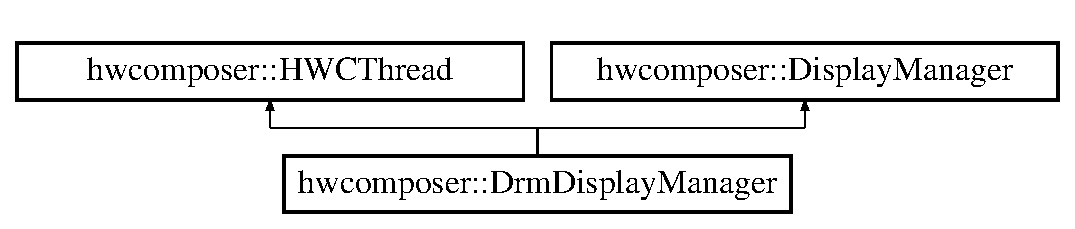
\includegraphics[height=2.000000cm]{classhwcomposer_1_1DrmDisplayManager}
\end{center}
\end{figure}
\subsection*{Public Member Functions}
\begin{DoxyCompactItemize}
\item 
\mbox{\hyperlink{classhwcomposer_1_1DrmDisplayManager_a7fa49119fbf2a4aece3a9e299e9a9919}{Drm\+Display\+Manager}} (\mbox{\hyperlink{classhwcomposer_1_1GpuDevice}{Gpu\+Device}} $\ast$device)
\item 
\mbox{\hyperlink{classhwcomposer_1_1DrmDisplayManager_a740d07df781fec91467ed8f6f240b407}{$\sim$\+Drm\+Display\+Manager}} () override
\item 
bool \mbox{\hyperlink{classhwcomposer_1_1DrmDisplayManager_a1597ef6208030337c9554b70dcdf0a95}{Initialize}} () override
\item 
void \mbox{\hyperlink{classhwcomposer_1_1DrmDisplayManager_a775eee42523dabde8e4187770cbe9c6c}{Initialize\+Display\+Resources}} () override
\item 
void \mbox{\hyperlink{classhwcomposer_1_1DrmDisplayManager_a103a45f1e7e31c813dc7e185e244d944}{Start\+Hot\+Plug\+Monitor}} () override
\item 
\mbox{\hyperlink{classhwcomposer_1_1NativeDisplay}{Native\+Display}} $\ast$ \mbox{\hyperlink{classhwcomposer_1_1DrmDisplayManager_a80e39b4389e271ed5a72421c46ce5f36}{Get\+Virtual\+Display}} () override
\item 
\mbox{\hyperlink{classhwcomposer_1_1NativeDisplay}{Native\+Display}} $\ast$ \mbox{\hyperlink{classhwcomposer_1_1DrmDisplayManager_ae3df43b4c4c9cc1181ec13cbefd764f1}{Get\+Nested\+Display}} () override
\item 
std\+::vector$<$ \mbox{\hyperlink{classhwcomposer_1_1NativeDisplay}{Native\+Display}} $\ast$ $>$ \mbox{\hyperlink{classhwcomposer_1_1DrmDisplayManager_acff7605550c750e5f799f698e9b82d2a}{Get\+All\+Displays}} () override
\item 
void \mbox{\hyperlink{classhwcomposer_1_1DrmDisplayManager_ab11e4353cddc68652abcae61dd26027d}{Register\+Hot\+Plug\+Event\+Callback}} (std\+::shared\+\_\+ptr$<$ \mbox{\hyperlink{classhwcomposer_1_1DisplayHotPlugEventCallback}{Display\+Hot\+Plug\+Event\+Callback}} $>$ callback) override
\item 
void \mbox{\hyperlink{classhwcomposer_1_1DrmDisplayManager_a254ab8fd550f20f056c2ec1e458442c9}{Force\+Refresh}} () override
\item 
void \mbox{\hyperlink{classhwcomposer_1_1DrmDisplayManager_ac10c8fb07bf822c4430cd54722ceee16}{Ignore\+Updates}} () override
\item 
uint32\+\_\+t \mbox{\hyperlink{classhwcomposer_1_1DrmDisplayManager_aed1b4e61f4bbda4069138675156a9564}{Get\+FD}} () const override
\item 
void \mbox{\hyperlink{classhwcomposer_1_1DrmDisplayManager_a087e35e0b0be34e4ff5efdb37c8a5684}{Notify\+Clients\+Of\+Display\+Change\+Status}} ()
\item 
void \mbox{\hyperlink{classhwcomposer_1_1DrmDisplayManager_a9d52e745e20b0872b57d04ebdd3d12b6}{Handle\+Lazy\+Initialization}} ()
\end{DoxyCompactItemize}
\subsection*{Protected Member Functions}
\begin{DoxyCompactItemize}
\item 
void \mbox{\hyperlink{classhwcomposer_1_1DrmDisplayManager_abcf8a2a9394d722a58b79060f9f51dbc}{Handle\+Wait}} () override
\item 
void \mbox{\hyperlink{classhwcomposer_1_1DrmDisplayManager_a3f29044c35ff76edb4718ed19f340794}{Handle\+Routine}} () override
\end{DoxyCompactItemize}
\subsection*{Additional Inherited Members}


\subsection{Detailed Description}


Definition at line 44 of file drmdisplaymanager.\+h.



\subsection{Constructor \& Destructor Documentation}
\mbox{\Hypertarget{classhwcomposer_1_1DrmDisplayManager_a7fa49119fbf2a4aece3a9e299e9a9919}\label{classhwcomposer_1_1DrmDisplayManager_a7fa49119fbf2a4aece3a9e299e9a9919}} 
\index{hwcomposer\+::\+Drm\+Display\+Manager@{hwcomposer\+::\+Drm\+Display\+Manager}!Drm\+Display\+Manager@{Drm\+Display\+Manager}}
\index{Drm\+Display\+Manager@{Drm\+Display\+Manager}!hwcomposer\+::\+Drm\+Display\+Manager@{hwcomposer\+::\+Drm\+Display\+Manager}}
\subsubsection{\texorpdfstring{Drm\+Display\+Manager()}{DrmDisplayManager()}}
{\footnotesize\ttfamily hwcomposer\+::\+Drm\+Display\+Manager\+::\+Drm\+Display\+Manager (\begin{DoxyParamCaption}\item[{\mbox{\hyperlink{classhwcomposer_1_1GpuDevice}{Gpu\+Device}} $\ast$}]{device }\end{DoxyParamCaption})}



Definition at line 41 of file drmdisplaymanager.\+cpp.


\begin{DoxyCode}{0}
\DoxyCodeLine{42     : \mbox{\hyperlink{classhwcomposer_1_1HWCThread_a8780175b1679005955a94aa89fa62be1}{HWCThread}}(-8, \textcolor{stringliteral}{"DisplayManager"}), device\_(device) \{}
\DoxyCodeLine{43   \mbox{\hyperlink{hwctrace_8h_a539a95897071c72babce1012d503b3ca}{CTRACE}}();}
\DoxyCodeLine{44 \}}
\end{DoxyCode}
\mbox{\Hypertarget{classhwcomposer_1_1DrmDisplayManager_a740d07df781fec91467ed8f6f240b407}\label{classhwcomposer_1_1DrmDisplayManager_a740d07df781fec91467ed8f6f240b407}} 
\index{hwcomposer\+::\+Drm\+Display\+Manager@{hwcomposer\+::\+Drm\+Display\+Manager}!````~Drm\+Display\+Manager@{$\sim$\+Drm\+Display\+Manager}}
\index{````~Drm\+Display\+Manager@{$\sim$\+Drm\+Display\+Manager}!hwcomposer\+::\+Drm\+Display\+Manager@{hwcomposer\+::\+Drm\+Display\+Manager}}
\subsubsection{\texorpdfstring{$\sim$\+Drm\+Display\+Manager()}{~DrmDisplayManager()}}
{\footnotesize\ttfamily hwcomposer\+::\+Drm\+Display\+Manager\+::$\sim$\+Drm\+Display\+Manager (\begin{DoxyParamCaption}{ }\end{DoxyParamCaption})\hspace{0.3cm}{\ttfamily [override]}}



Definition at line 46 of file drmdisplaymanager.\+cpp.


\begin{DoxyCode}{0}
\DoxyCodeLine{46                                       \{}
\DoxyCodeLine{47   \mbox{\hyperlink{hwctrace_8h_a539a95897071c72babce1012d503b3ca}{CTRACE}}();}
\DoxyCodeLine{48   std::vector<std::unique\_ptr<DrmDisplay>>().swap(displays\_);}
\DoxyCodeLine{49 \textcolor{preprocessor}{\#ifndef DISABLE\_HOTPLUG\_NOTIFICATION}}
\DoxyCodeLine{50   close(hotplug\_fd\_);}
\DoxyCodeLine{51 \textcolor{preprocessor}{\#endif}}
\DoxyCodeLine{52   drmClose(fd\_);}
\DoxyCodeLine{53 \}}
\end{DoxyCode}


\subsection{Member Function Documentation}
\mbox{\Hypertarget{classhwcomposer_1_1DrmDisplayManager_a254ab8fd550f20f056c2ec1e458442c9}\label{classhwcomposer_1_1DrmDisplayManager_a254ab8fd550f20f056c2ec1e458442c9}} 
\index{hwcomposer\+::\+Drm\+Display\+Manager@{hwcomposer\+::\+Drm\+Display\+Manager}!Force\+Refresh@{Force\+Refresh}}
\index{Force\+Refresh@{Force\+Refresh}!hwcomposer\+::\+Drm\+Display\+Manager@{hwcomposer\+::\+Drm\+Display\+Manager}}
\subsubsection{\texorpdfstring{Force\+Refresh()}{ForceRefresh()}}
{\footnotesize\ttfamily void hwcomposer\+::\+Drm\+Display\+Manager\+::\+Force\+Refresh (\begin{DoxyParamCaption}{ }\end{DoxyParamCaption})\hspace{0.3cm}{\ttfamily [override]}, {\ttfamily [virtual]}}



Implements \mbox{\hyperlink{classhwcomposer_1_1DisplayManager_a678df886d9faff854111d8ace155befc}{hwcomposer\+::\+Display\+Manager}}.



Definition at line 425 of file drmdisplaymanager.\+cpp.


\begin{DoxyCode}{0}
\DoxyCodeLine{425                                      \{}
\DoxyCodeLine{426   spin\_lock\_.\mbox{\hyperlink{classhwcomposer_1_1SpinLock_a863f9d0f1b270f863a9298161b52faf1}{lock}}();}
\DoxyCodeLine{427   \textcolor{keywordtype}{size\_t} size = displays\_.size();}
\DoxyCodeLine{428   \textcolor{keywordflow}{for} (\textcolor{keywordtype}{size\_t} i = 0; i < size; ++i) \{}
\DoxyCodeLine{429     displays\_.at(i)->ForceRefresh();}
\DoxyCodeLine{430   \}}
\DoxyCodeLine{431 }
\DoxyCodeLine{432   release\_lock\_ = \textcolor{keyword}{true};}
\DoxyCodeLine{433   spin\_lock\_.\mbox{\hyperlink{classhwcomposer_1_1SpinLock_ae5cf624b4f0ec710833ce44e945b85d7}{unlock}}();}
\DoxyCodeLine{434 \}}
\end{DoxyCode}
\mbox{\Hypertarget{classhwcomposer_1_1DrmDisplayManager_acff7605550c750e5f799f698e9b82d2a}\label{classhwcomposer_1_1DrmDisplayManager_acff7605550c750e5f799f698e9b82d2a}} 
\index{hwcomposer\+::\+Drm\+Display\+Manager@{hwcomposer\+::\+Drm\+Display\+Manager}!Get\+All\+Displays@{Get\+All\+Displays}}
\index{Get\+All\+Displays@{Get\+All\+Displays}!hwcomposer\+::\+Drm\+Display\+Manager@{hwcomposer\+::\+Drm\+Display\+Manager}}
\subsubsection{\texorpdfstring{Get\+All\+Displays()}{GetAllDisplays()}}
{\footnotesize\ttfamily std\+::vector$<$ \mbox{\hyperlink{classhwcomposer_1_1NativeDisplay}{Native\+Display}} $\ast$ $>$ hwcomposer\+::\+Drm\+Display\+Manager\+::\+Get\+All\+Displays (\begin{DoxyParamCaption}{ }\end{DoxyParamCaption})\hspace{0.3cm}{\ttfamily [override]}, {\ttfamily [virtual]}}



Implements \mbox{\hyperlink{classhwcomposer_1_1DisplayManager_aec3ebc4b4d22031e983856a424dd43a6}{hwcomposer\+::\+Display\+Manager}}.



Definition at line 407 of file drmdisplaymanager.\+cpp.


\begin{DoxyCode}{0}
\DoxyCodeLine{407                                                              \{}
\DoxyCodeLine{408   spin\_lock\_.\mbox{\hyperlink{classhwcomposer_1_1SpinLock_a863f9d0f1b270f863a9298161b52faf1}{lock}}();}
\DoxyCodeLine{409   std::vector<NativeDisplay *> all\_displays;}
\DoxyCodeLine{410   \textcolor{keywordtype}{size\_t} size = displays\_.size();}
\DoxyCodeLine{411   \textcolor{keywordflow}{for} (\textcolor{keywordtype}{size\_t} i = 0; i < size; ++i) \{}
\DoxyCodeLine{412     all\_displays.emplace\_back(displays\_.at(i).get());}
\DoxyCodeLine{413   \}}
\DoxyCodeLine{414   spin\_lock\_.\mbox{\hyperlink{classhwcomposer_1_1SpinLock_ae5cf624b4f0ec710833ce44e945b85d7}{unlock}}();}
\DoxyCodeLine{415   \textcolor{keywordflow}{return} all\_displays;}
\DoxyCodeLine{416 \}}
\end{DoxyCode}
\mbox{\Hypertarget{classhwcomposer_1_1DrmDisplayManager_aed1b4e61f4bbda4069138675156a9564}\label{classhwcomposer_1_1DrmDisplayManager_aed1b4e61f4bbda4069138675156a9564}} 
\index{hwcomposer\+::\+Drm\+Display\+Manager@{hwcomposer\+::\+Drm\+Display\+Manager}!Get\+FD@{Get\+FD}}
\index{Get\+FD@{Get\+FD}!hwcomposer\+::\+Drm\+Display\+Manager@{hwcomposer\+::\+Drm\+Display\+Manager}}
\subsubsection{\texorpdfstring{Get\+F\+D()}{GetFD()}}
{\footnotesize\ttfamily uint32\+\_\+t hwcomposer\+::\+Drm\+Display\+Manager\+::\+Get\+FD (\begin{DoxyParamCaption}{ }\end{DoxyParamCaption}) const\hspace{0.3cm}{\ttfamily [inline]}, {\ttfamily [override]}, {\ttfamily [virtual]}}



Implements \mbox{\hyperlink{classhwcomposer_1_1DisplayManager_a7af00ef1c1c9dc8f3fd58699460ab14d}{hwcomposer\+::\+Display\+Manager}}.



Definition at line 67 of file drmdisplaymanager.\+h.


\begin{DoxyCode}{0}
\DoxyCodeLine{67                                   \{}
\DoxyCodeLine{68     \textcolor{keywordflow}{return} fd\_;}
\DoxyCodeLine{69   \}}
\end{DoxyCode}
\mbox{\Hypertarget{classhwcomposer_1_1DrmDisplayManager_ae3df43b4c4c9cc1181ec13cbefd764f1}\label{classhwcomposer_1_1DrmDisplayManager_ae3df43b4c4c9cc1181ec13cbefd764f1}} 
\index{hwcomposer\+::\+Drm\+Display\+Manager@{hwcomposer\+::\+Drm\+Display\+Manager}!Get\+Nested\+Display@{Get\+Nested\+Display}}
\index{Get\+Nested\+Display@{Get\+Nested\+Display}!hwcomposer\+::\+Drm\+Display\+Manager@{hwcomposer\+::\+Drm\+Display\+Manager}}
\subsubsection{\texorpdfstring{Get\+Nested\+Display()}{GetNestedDisplay()}}
{\footnotesize\ttfamily \mbox{\hyperlink{classhwcomposer_1_1NativeDisplay}{Native\+Display}} $\ast$ hwcomposer\+::\+Drm\+Display\+Manager\+::\+Get\+Nested\+Display (\begin{DoxyParamCaption}{ }\end{DoxyParamCaption})\hspace{0.3cm}{\ttfamily [override]}, {\ttfamily [virtual]}}



Implements \mbox{\hyperlink{classhwcomposer_1_1DisplayManager_ac05cc0db0d8191465746828b2027a6f7}{hwcomposer\+::\+Display\+Manager}}.



Definition at line 400 of file drmdisplaymanager.\+cpp.


\begin{DoxyCode}{0}
\DoxyCodeLine{400                                                    \{}
\DoxyCodeLine{401   spin\_lock\_.\mbox{\hyperlink{classhwcomposer_1_1SpinLock_a863f9d0f1b270f863a9298161b52faf1}{lock}}();}
\DoxyCodeLine{402   NativeDisplay *display = nested\_display\_.get();}
\DoxyCodeLine{403   spin\_lock\_.\mbox{\hyperlink{classhwcomposer_1_1SpinLock_ae5cf624b4f0ec710833ce44e945b85d7}{unlock}}();}
\DoxyCodeLine{404   \textcolor{keywordflow}{return} display;}
\DoxyCodeLine{405 \}}
\end{DoxyCode}
\mbox{\Hypertarget{classhwcomposer_1_1DrmDisplayManager_a80e39b4389e271ed5a72421c46ce5f36}\label{classhwcomposer_1_1DrmDisplayManager_a80e39b4389e271ed5a72421c46ce5f36}} 
\index{hwcomposer\+::\+Drm\+Display\+Manager@{hwcomposer\+::\+Drm\+Display\+Manager}!Get\+Virtual\+Display@{Get\+Virtual\+Display}}
\index{Get\+Virtual\+Display@{Get\+Virtual\+Display}!hwcomposer\+::\+Drm\+Display\+Manager@{hwcomposer\+::\+Drm\+Display\+Manager}}
\subsubsection{\texorpdfstring{Get\+Virtual\+Display()}{GetVirtualDisplay()}}
{\footnotesize\ttfamily \mbox{\hyperlink{classhwcomposer_1_1NativeDisplay}{Native\+Display}} $\ast$ hwcomposer\+::\+Drm\+Display\+Manager\+::\+Get\+Virtual\+Display (\begin{DoxyParamCaption}{ }\end{DoxyParamCaption})\hspace{0.3cm}{\ttfamily [override]}, {\ttfamily [virtual]}}



Implements \mbox{\hyperlink{classhwcomposer_1_1DisplayManager_a5fa2b92896cab774d8a85215dfac1d62}{hwcomposer\+::\+Display\+Manager}}.



Definition at line 393 of file drmdisplaymanager.\+cpp.


\begin{DoxyCode}{0}
\DoxyCodeLine{393                                                     \{}
\DoxyCodeLine{394   spin\_lock\_.\mbox{\hyperlink{classhwcomposer_1_1SpinLock_a863f9d0f1b270f863a9298161b52faf1}{lock}}();}
\DoxyCodeLine{395   NativeDisplay *display = virtual\_display\_.get();}
\DoxyCodeLine{396   spin\_lock\_.\mbox{\hyperlink{classhwcomposer_1_1SpinLock_ae5cf624b4f0ec710833ce44e945b85d7}{unlock}}();}
\DoxyCodeLine{397   \textcolor{keywordflow}{return} display;}
\DoxyCodeLine{398 \}}
\end{DoxyCode}
\mbox{\Hypertarget{classhwcomposer_1_1DrmDisplayManager_a9d52e745e20b0872b57d04ebdd3d12b6}\label{classhwcomposer_1_1DrmDisplayManager_a9d52e745e20b0872b57d04ebdd3d12b6}} 
\index{hwcomposer\+::\+Drm\+Display\+Manager@{hwcomposer\+::\+Drm\+Display\+Manager}!Handle\+Lazy\+Initialization@{Handle\+Lazy\+Initialization}}
\index{Handle\+Lazy\+Initialization@{Handle\+Lazy\+Initialization}!hwcomposer\+::\+Drm\+Display\+Manager@{hwcomposer\+::\+Drm\+Display\+Manager}}
\subsubsection{\texorpdfstring{Handle\+Lazy\+Initialization()}{HandleLazyInitialization()}}
{\footnotesize\ttfamily void hwcomposer\+::\+Drm\+Display\+Manager\+::\+Handle\+Lazy\+Initialization (\begin{DoxyParamCaption}{ }\end{DoxyParamCaption})}



Definition at line 443 of file drmdisplaymanager.\+cpp.


\begin{DoxyCode}{0}
\DoxyCodeLine{443                                                  \{}
\DoxyCodeLine{444   spin\_lock\_.\mbox{\hyperlink{classhwcomposer_1_1SpinLock_a863f9d0f1b270f863a9298161b52faf1}{lock}}();}
\DoxyCodeLine{445   \textcolor{keywordflow}{if} (release\_lock\_) \{}
\DoxyCodeLine{446     device\_->DisableWatch();}
\DoxyCodeLine{447     release\_lock\_ = \textcolor{keyword}{false};}
\DoxyCodeLine{448   \}}
\DoxyCodeLine{449   spin\_lock\_.\mbox{\hyperlink{classhwcomposer_1_1SpinLock_ae5cf624b4f0ec710833ce44e945b85d7}{unlock}}();}
\DoxyCodeLine{450 \}}
\end{DoxyCode}
\mbox{\Hypertarget{classhwcomposer_1_1DrmDisplayManager_a3f29044c35ff76edb4718ed19f340794}\label{classhwcomposer_1_1DrmDisplayManager_a3f29044c35ff76edb4718ed19f340794}} 
\index{hwcomposer\+::\+Drm\+Display\+Manager@{hwcomposer\+::\+Drm\+Display\+Manager}!Handle\+Routine@{Handle\+Routine}}
\index{Handle\+Routine@{Handle\+Routine}!hwcomposer\+::\+Drm\+Display\+Manager@{hwcomposer\+::\+Drm\+Display\+Manager}}
\subsubsection{\texorpdfstring{Handle\+Routine()}{HandleRoutine()}}
{\footnotesize\ttfamily void hwcomposer\+::\+Drm\+Display\+Manager\+::\+Handle\+Routine (\begin{DoxyParamCaption}{ }\end{DoxyParamCaption})\hspace{0.3cm}{\ttfamily [override]}, {\ttfamily [protected]}, {\ttfamily [virtual]}}



Implements \mbox{\hyperlink{classhwcomposer_1_1HWCThread_a539ea080e6bf0e6cffe08e2341be1ee4}{hwcomposer\+::\+H\+W\+C\+Thread}}.



Definition at line 200 of file drmdisplaymanager.\+cpp.


\begin{DoxyCode}{0}
\DoxyCodeLine{200                                       \{}
\DoxyCodeLine{201   \mbox{\hyperlink{hwctrace_8h_a539a95897071c72babce1012d503b3ca}{CTRACE}}();}
\DoxyCodeLine{202   \mbox{\hyperlink{hwctrace_8h_af8c38c979e9089c283d2f5923089b538}{IHOTPLUGEVENTTRACE}}(\textcolor{stringliteral}{"DisplayManager::Routine."});}
\DoxyCodeLine{203   \textcolor{keywordflow}{if} (\mbox{\hyperlink{classhwcomposer_1_1HWCThread_a26ef5b90fd394e2002d903ffd2521faf}{fd\_handler\_}}.\mbox{\hyperlink{classhwcomposer_1_1FDHandler_ad635c0c7631838aa99e0140c4164425f}{IsReady}}(hotplug\_fd\_)) \{}
\DoxyCodeLine{204     \mbox{\hyperlink{hwctrace_8h_af8c38c979e9089c283d2f5923089b538}{IHOTPLUGEVENTTRACE}}(\textcolor{stringliteral}{"Recieved Hot plug notification."});}
\DoxyCodeLine{205     HotPlugEventHandler();}
\DoxyCodeLine{206   \}}
\DoxyCodeLine{207 \}}
\end{DoxyCode}
\mbox{\Hypertarget{classhwcomposer_1_1DrmDisplayManager_abcf8a2a9394d722a58b79060f9f51dbc}\label{classhwcomposer_1_1DrmDisplayManager_abcf8a2a9394d722a58b79060f9f51dbc}} 
\index{hwcomposer\+::\+Drm\+Display\+Manager@{hwcomposer\+::\+Drm\+Display\+Manager}!Handle\+Wait@{Handle\+Wait}}
\index{Handle\+Wait@{Handle\+Wait}!hwcomposer\+::\+Drm\+Display\+Manager@{hwcomposer\+::\+Drm\+Display\+Manager}}
\subsubsection{\texorpdfstring{Handle\+Wait()}{HandleWait()}}
{\footnotesize\ttfamily void hwcomposer\+::\+Drm\+Display\+Manager\+::\+Handle\+Wait (\begin{DoxyParamCaption}{ }\end{DoxyParamCaption})\hspace{0.3cm}{\ttfamily [override]}, {\ttfamily [protected]}, {\ttfamily [virtual]}}



Reimplemented from \mbox{\hyperlink{classhwcomposer_1_1HWCThread_ab5acded48bbd1bf4d7c3a54dadb91ef9}{hwcomposer\+::\+H\+W\+C\+Thread}}.



Definition at line 163 of file drmdisplaymanager.\+cpp.


\begin{DoxyCode}{0}
\DoxyCodeLine{163                                    \{}
\DoxyCodeLine{164   \textcolor{keywordflow}{if} (\mbox{\hyperlink{classhwcomposer_1_1HWCThread_a26ef5b90fd394e2002d903ffd2521faf}{fd\_handler\_}}.\mbox{\hyperlink{classhwcomposer_1_1FDHandler_a5ab233d1f474eab69552321e87159a9d}{Poll}}(-1) <= 0) \{}
\DoxyCodeLine{165     \mbox{\hyperlink{alios_2platformdefines_8h_a226d6c99e4bcfca193c095e085e9097d}{ETRACE}}(\textcolor{stringliteral}{"Poll Failed in DisplayManager \%s"}, \mbox{\hyperlink{hwctrace_8h_a791a01fa8fe130cef13d68a706df9034}{PRINTERROR}}());}
\DoxyCodeLine{166   \}}
\DoxyCodeLine{167 \}}
\end{DoxyCode}
\mbox{\Hypertarget{classhwcomposer_1_1DrmDisplayManager_ac10c8fb07bf822c4430cd54722ceee16}\label{classhwcomposer_1_1DrmDisplayManager_ac10c8fb07bf822c4430cd54722ceee16}} 
\index{hwcomposer\+::\+Drm\+Display\+Manager@{hwcomposer\+::\+Drm\+Display\+Manager}!Ignore\+Updates@{Ignore\+Updates}}
\index{Ignore\+Updates@{Ignore\+Updates}!hwcomposer\+::\+Drm\+Display\+Manager@{hwcomposer\+::\+Drm\+Display\+Manager}}
\subsubsection{\texorpdfstring{Ignore\+Updates()}{IgnoreUpdates()}}
{\footnotesize\ttfamily void hwcomposer\+::\+Drm\+Display\+Manager\+::\+Ignore\+Updates (\begin{DoxyParamCaption}{ }\end{DoxyParamCaption})\hspace{0.3cm}{\ttfamily [override]}, {\ttfamily [virtual]}}



Implements \mbox{\hyperlink{classhwcomposer_1_1DisplayManager_ac5d98f9c1c32dc2dbc3afb342a113af5}{hwcomposer\+::\+Display\+Manager}}.



Definition at line 436 of file drmdisplaymanager.\+cpp.


\begin{DoxyCode}{0}
\DoxyCodeLine{436                                       \{}
\DoxyCodeLine{437   \textcolor{keywordtype}{size\_t} size = displays\_.size();}
\DoxyCodeLine{438   \textcolor{keywordflow}{for} (\textcolor{keywordtype}{size\_t} i = 0; i < size; ++i) \{}
\DoxyCodeLine{439     displays\_.at(i)->IgnoreUpdates();}
\DoxyCodeLine{440   \}}
\DoxyCodeLine{441 \}}
\end{DoxyCode}
\mbox{\Hypertarget{classhwcomposer_1_1DrmDisplayManager_a1597ef6208030337c9554b70dcdf0a95}\label{classhwcomposer_1_1DrmDisplayManager_a1597ef6208030337c9554b70dcdf0a95}} 
\index{hwcomposer\+::\+Drm\+Display\+Manager@{hwcomposer\+::\+Drm\+Display\+Manager}!Initialize@{Initialize}}
\index{Initialize@{Initialize}!hwcomposer\+::\+Drm\+Display\+Manager@{hwcomposer\+::\+Drm\+Display\+Manager}}
\subsubsection{\texorpdfstring{Initialize()}{Initialize()}}
{\footnotesize\ttfamily bool hwcomposer\+::\+Drm\+Display\+Manager\+::\+Initialize (\begin{DoxyParamCaption}{ }\end{DoxyParamCaption})\hspace{0.3cm}{\ttfamily [override]}, {\ttfamily [virtual]}}



Implements \mbox{\hyperlink{classhwcomposer_1_1DisplayManager_abb67b1deed55bf20584f86aea2ae5167}{hwcomposer\+::\+Display\+Manager}}.



Definition at line 55 of file drmdisplaymanager.\+cpp.


\begin{DoxyCode}{0}
\DoxyCodeLine{55                                    \{}
\DoxyCodeLine{56   \mbox{\hyperlink{hwctrace_8h_a539a95897071c72babce1012d503b3ca}{CTRACE}}();}
\DoxyCodeLine{57   fd\_ = drmOpen(\textcolor{stringliteral}{"i915"}, \mbox{\hyperlink{alios_2platformdefines_8h_a070d2ce7b6bb7e5c05602aa8c308d0c4}{NULL}});}
\DoxyCodeLine{58   \textcolor{keywordflow}{if} (fd\_ < 0) \{}
\DoxyCodeLine{59     \mbox{\hyperlink{alios_2platformdefines_8h_a226d6c99e4bcfca193c095e085e9097d}{ETRACE}}(\textcolor{stringliteral}{"Failed to open dri \%s"}, \mbox{\hyperlink{hwctrace_8h_a791a01fa8fe130cef13d68a706df9034}{PRINTERROR}}());}
\DoxyCodeLine{60     \textcolor{keywordflow}{return} -ENODEV;}
\DoxyCodeLine{61   \}}
\DoxyCodeLine{62 }
\DoxyCodeLine{63   \textcolor{keyword}{struct }drm\_set\_client\_cap cap = \{DRM\_CLIENT\_CAP\_UNIVERSAL\_PLANES, 1\};}
\DoxyCodeLine{64   drmIoctl(fd\_, DRM\_IOCTL\_SET\_CLIENT\_CAP, \&cap);}
\DoxyCodeLine{65   \textcolor{keywordtype}{int} ret = drmSetClientCap(fd\_, DRM\_CLIENT\_CAP\_ATOMIC, 1);}
\DoxyCodeLine{66   \textcolor{keywordflow}{if} (ret) \{}
\DoxyCodeLine{67     \mbox{\hyperlink{alios_2platformdefines_8h_a226d6c99e4bcfca193c095e085e9097d}{ETRACE}}(\textcolor{stringliteral}{"Failed to set atomic cap \%s"}, \mbox{\hyperlink{hwctrace_8h_a791a01fa8fe130cef13d68a706df9034}{PRINTERROR}}());}
\DoxyCodeLine{68     \textcolor{keywordflow}{return} \textcolor{keyword}{false};}
\DoxyCodeLine{69   \}}
\DoxyCodeLine{70 }
\DoxyCodeLine{71   ret = drmSetClientCap(fd\_, DRM\_CLIENT\_CAP\_ATOMIC, 1);}
\DoxyCodeLine{72   \textcolor{keywordflow}{if} (ret) \{}
\DoxyCodeLine{73     \mbox{\hyperlink{alios_2platformdefines_8h_a226d6c99e4bcfca193c095e085e9097d}{ETRACE}}(\textcolor{stringliteral}{"Failed to set atomic cap \%d"}, ret);}
\DoxyCodeLine{74     \textcolor{keywordflow}{return} \textcolor{keyword}{false};}
\DoxyCodeLine{75   \}}
\DoxyCodeLine{76 }
\DoxyCodeLine{77   \mbox{\hyperlink{namespacehwcomposer_a88e61b5e1ae620a5424a9497d554aea7}{ScopedDrmResourcesPtr}} res(drmModeGetResources(fd\_));}
\DoxyCodeLine{78 }
\DoxyCodeLine{79   \textcolor{keywordflow}{for} (int32\_t i = 0; i < res->count\_crtcs; ++i) \{}
\DoxyCodeLine{80     \mbox{\hyperlink{namespacehwcomposer_a9571d0c874674e369f17aa93c5d863e8}{ScopedDrmCrtcPtr}} c(drmModeGetCrtc(fd\_, res->crtcs[i]));}
\DoxyCodeLine{81     \textcolor{keywordflow}{if} (!c) \{}
\DoxyCodeLine{82       \mbox{\hyperlink{alios_2platformdefines_8h_a226d6c99e4bcfca193c095e085e9097d}{ETRACE}}(\textcolor{stringliteral}{"Failed to get crtc \%d"}, res->crtcs[i]);}
\DoxyCodeLine{83       \textcolor{keywordflow}{return} \textcolor{keyword}{false};}
\DoxyCodeLine{84     \}}
\DoxyCodeLine{85 }
\DoxyCodeLine{86     std::unique\_ptr<DrmDisplay> display(}
\DoxyCodeLine{87         \textcolor{keyword}{new} DrmDisplay(fd\_, i, c->crtc\_id, \textcolor{keyword}{this}));}
\DoxyCodeLine{88 }
\DoxyCodeLine{89     displays\_.emplace\_back(std::move(display));}
\DoxyCodeLine{90   \}}
\DoxyCodeLine{91 }
\DoxyCodeLine{92 \textcolor{preprocessor}{\#ifndef DISABLE\_HOTPLUG\_NOTIFICATION}}
\DoxyCodeLine{93   hotplug\_fd\_ = socket(PF\_NETLINK, SOCK\_DGRAM, NETLINK\_KOBJECT\_UEVENT);}
\DoxyCodeLine{94   \textcolor{keywordflow}{if} (hotplug\_fd\_ < 0) \{}
\DoxyCodeLine{95     \mbox{\hyperlink{alios_2platformdefines_8h_a226d6c99e4bcfca193c095e085e9097d}{ETRACE}}(\textcolor{stringliteral}{"Failed to create socket for hot plug monitor. \%s"}, \mbox{\hyperlink{hwctrace_8h_a791a01fa8fe130cef13d68a706df9034}{PRINTERROR}}());}
\DoxyCodeLine{96     \textcolor{keywordflow}{return} \textcolor{keyword}{true};}
\DoxyCodeLine{97   \}}
\DoxyCodeLine{98 }
\DoxyCodeLine{99   \textcolor{keyword}{struct }sockaddr\_nl addr;}
\DoxyCodeLine{100   memset(\&addr, 0, \textcolor{keyword}{sizeof}(addr));}
\DoxyCodeLine{101   addr.nl\_family = AF\_NETLINK;}
\DoxyCodeLine{102   addr.nl\_pid = getpid();}
\DoxyCodeLine{103   addr.nl\_groups = 0xffffffff;}
\DoxyCodeLine{104 }
\DoxyCodeLine{105   ret = bind(hotplug\_fd\_, (\textcolor{keyword}{struct} sockaddr *)\&addr, \textcolor{keyword}{sizeof}(addr));}
\DoxyCodeLine{106   \textcolor{keywordflow}{if} (ret) \{}
\DoxyCodeLine{107     \mbox{\hyperlink{alios_2platformdefines_8h_a226d6c99e4bcfca193c095e085e9097d}{ETRACE}}(\textcolor{stringliteral}{"Failed to bind sockaddr\_nl and hot plug monitor fd. \%s"},}
\DoxyCodeLine{108            \mbox{\hyperlink{hwctrace_8h_a791a01fa8fe130cef13d68a706df9034}{PRINTERROR}}());}
\DoxyCodeLine{109     \textcolor{keywordflow}{return} \textcolor{keyword}{true};}
\DoxyCodeLine{110   \}}
\DoxyCodeLine{111 }
\DoxyCodeLine{112   \mbox{\hyperlink{classhwcomposer_1_1HWCThread_a26ef5b90fd394e2002d903ffd2521faf}{fd\_handler\_}}.\mbox{\hyperlink{classhwcomposer_1_1FDHandler_aee421fa4ae54b7d4fcc352ebea15b4f8}{AddFd}}(hotplug\_fd\_);}
\DoxyCodeLine{113 \textcolor{preprocessor}{\#endif}}
\DoxyCodeLine{114   \mbox{\hyperlink{hwctrace_8h_af8c38c979e9089c283d2f5923089b538}{IHOTPLUGEVENTTRACE}}(\textcolor{stringliteral}{"DisplayManager Initialization succeeded."});}
\DoxyCodeLine{115   \textcolor{keywordflow}{return} \textcolor{keyword}{true};}
\DoxyCodeLine{116 \}}
\end{DoxyCode}
\mbox{\Hypertarget{classhwcomposer_1_1DrmDisplayManager_a775eee42523dabde8e4187770cbe9c6c}\label{classhwcomposer_1_1DrmDisplayManager_a775eee42523dabde8e4187770cbe9c6c}} 
\index{hwcomposer\+::\+Drm\+Display\+Manager@{hwcomposer\+::\+Drm\+Display\+Manager}!Initialize\+Display\+Resources@{Initialize\+Display\+Resources}}
\index{Initialize\+Display\+Resources@{Initialize\+Display\+Resources}!hwcomposer\+::\+Drm\+Display\+Manager@{hwcomposer\+::\+Drm\+Display\+Manager}}
\subsubsection{\texorpdfstring{Initialize\+Display\+Resources()}{InitializeDisplayResources()}}
{\footnotesize\ttfamily void hwcomposer\+::\+Drm\+Display\+Manager\+::\+Initialize\+Display\+Resources (\begin{DoxyParamCaption}{ }\end{DoxyParamCaption})\hspace{0.3cm}{\ttfamily [override]}, {\ttfamily [virtual]}}



Implements \mbox{\hyperlink{classhwcomposer_1_1DisplayManager_a26b46eb7c0d15384fceaecdd8be9be45}{hwcomposer\+::\+Display\+Manager}}.



Definition at line 169 of file drmdisplaymanager.\+cpp.


\begin{DoxyCode}{0}
\DoxyCodeLine{169                                                    \{}
\DoxyCodeLine{170   buffer\_handler\_.reset(\mbox{\hyperlink{classhwcomposer_1_1NativeBufferHandler_a7cd90f5d6e7ba6a46758e7891168c332}{NativeBufferHandler::CreateInstance}}(fd\_));}
\DoxyCodeLine{171   frame\_buffer\_manager\_.reset(\textcolor{keyword}{new} FrameBufferManager(fd\_));}
\DoxyCodeLine{172   \textcolor{keywordflow}{if} (!buffer\_handler\_) \{}
\DoxyCodeLine{173     \mbox{\hyperlink{alios_2platformdefines_8h_a226d6c99e4bcfca193c095e085e9097d}{ETRACE}}(\textcolor{stringliteral}{"Failed to create native buffer handler instance"});}
\DoxyCodeLine{174     \textcolor{keywordflow}{return};}
\DoxyCodeLine{175   \}}
\DoxyCodeLine{176 }
\DoxyCodeLine{177   \textcolor{keywordtype}{int} size = displays\_.size();}
\DoxyCodeLine{178   \textcolor{keywordflow}{for} (\textcolor{keywordtype}{int} i = 0; i < size; ++i) \{}
\DoxyCodeLine{179     \textcolor{keywordflow}{if} (!displays\_.at(i)->Initialize(buffer\_handler\_.get(),}
\DoxyCodeLine{180                                      frame\_buffer\_manager\_.get())) \{}
\DoxyCodeLine{181       \mbox{\hyperlink{alios_2platformdefines_8h_a226d6c99e4bcfca193c095e085e9097d}{ETRACE}}(\textcolor{stringliteral}{"Failed to Initialize Display \%d"}, i);}
\DoxyCodeLine{182     \}}
\DoxyCodeLine{183   \}}
\DoxyCodeLine{184 }
\DoxyCodeLine{185   virtual\_display\_.reset(\textcolor{keyword}{new} VirtualDisplay(fd\_, buffer\_handler\_.get(), 0, 0));}
\DoxyCodeLine{186   nested\_display\_.reset(\textcolor{keyword}{new} NestedDisplay(fd\_, buffer\_handler\_.get()));}
\DoxyCodeLine{187 \}}
\end{DoxyCode}
\mbox{\Hypertarget{classhwcomposer_1_1DrmDisplayManager_a087e35e0b0be34e4ff5efdb37c8a5684}\label{classhwcomposer_1_1DrmDisplayManager_a087e35e0b0be34e4ff5efdb37c8a5684}} 
\index{hwcomposer\+::\+Drm\+Display\+Manager@{hwcomposer\+::\+Drm\+Display\+Manager}!Notify\+Clients\+Of\+Display\+Change\+Status@{Notify\+Clients\+Of\+Display\+Change\+Status}}
\index{Notify\+Clients\+Of\+Display\+Change\+Status@{Notify\+Clients\+Of\+Display\+Change\+Status}!hwcomposer\+::\+Drm\+Display\+Manager@{hwcomposer\+::\+Drm\+Display\+Manager}}
\subsubsection{\texorpdfstring{Notify\+Clients\+Of\+Display\+Change\+Status()}{NotifyClientsOfDisplayChangeStatus()}}
{\footnotesize\ttfamily void hwcomposer\+::\+Drm\+Display\+Manager\+::\+Notify\+Clients\+Of\+Display\+Change\+Status (\begin{DoxyParamCaption}{ }\end{DoxyParamCaption})}



Definition at line 351 of file drmdisplaymanager.\+cpp.


\begin{DoxyCode}{0}
\DoxyCodeLine{351                                                            \{}
\DoxyCodeLine{352   spin\_lock\_.\mbox{\hyperlink{classhwcomposer_1_1SpinLock_a863f9d0f1b270f863a9298161b52faf1}{lock}}();}
\DoxyCodeLine{353   \textcolor{keywordtype}{bool} disable\_last\_plane\_usage = \textcolor{keyword}{false};}
\DoxyCodeLine{354   uint32\_t total\_connected\_displays = 0;}
\DoxyCodeLine{355   \textcolor{keywordflow}{for} (\textcolor{keyword}{auto} \&display : displays\_) \{}
\DoxyCodeLine{356     \textcolor{keywordflow}{if} (display->IsConnected()) \{}
\DoxyCodeLine{357       display->NotifyClientOfDisConnectedState();}
\DoxyCodeLine{358       total\_connected\_displays++;}
\DoxyCodeLine{359     \}}
\DoxyCodeLine{360 }
\DoxyCodeLine{361     \textcolor{keywordflow}{if} (total\_connected\_displays > 1) \{}
\DoxyCodeLine{362       disable\_last\_plane\_usage = \textcolor{keyword}{true};}
\DoxyCodeLine{363       \textcolor{keywordflow}{break};}
\DoxyCodeLine{364     \}}
\DoxyCodeLine{365   \}}
\DoxyCodeLine{366 }
\DoxyCodeLine{367   \textcolor{keywordflow}{for} (\textcolor{keyword}{auto} \&display : displays\_) \{}
\DoxyCodeLine{368     display->NotifyDisplayWA(disable\_last\_plane\_usage);}
\DoxyCodeLine{369     display->ForceRefresh();}
\DoxyCodeLine{370   \}}
\DoxyCodeLine{371 }
\DoxyCodeLine{372   \textcolor{keywordflow}{for} (\textcolor{keyword}{auto} \&display : displays\_) \{}
\DoxyCodeLine{373     \textcolor{keywordflow}{if} (!display->IsConnected()) \{}
\DoxyCodeLine{374       display->NotifyClientOfDisConnectedState();}
\DoxyCodeLine{375     \} \textcolor{keywordflow}{else} \{}
\DoxyCodeLine{376       display->NotifyClientOfConnectedState();}
\DoxyCodeLine{377     \}}
\DoxyCodeLine{378   \}}
\DoxyCodeLine{379 }
\DoxyCodeLine{380   \textcolor{keyword}{static} \textcolor{keywordtype}{bool} nested\_display\_registered = \textcolor{keyword}{false};}
\DoxyCodeLine{381   \textcolor{keywordflow}{if} (!nested\_display\_registered) \{}
\DoxyCodeLine{382     nested\_display\_->HotPlugUpdate(\textcolor{keyword}{true});}
\DoxyCodeLine{383     nested\_display\_registered = \textcolor{keyword}{true};}
\DoxyCodeLine{384   \}}
\DoxyCodeLine{385 }
\DoxyCodeLine{386 \textcolor{preprocessor}{\#ifdef ENABLE\_ANDROID\_WA}}
\DoxyCodeLine{387   notify\_client\_ = \textcolor{keyword}{true};}
\DoxyCodeLine{388 \textcolor{preprocessor}{\#endif}}
\DoxyCodeLine{389 }
\DoxyCodeLine{390   spin\_lock\_.\mbox{\hyperlink{classhwcomposer_1_1SpinLock_ae5cf624b4f0ec710833ce44e945b85d7}{unlock}}();}
\DoxyCodeLine{391 \}}
\end{DoxyCode}
\mbox{\Hypertarget{classhwcomposer_1_1DrmDisplayManager_ab11e4353cddc68652abcae61dd26027d}\label{classhwcomposer_1_1DrmDisplayManager_ab11e4353cddc68652abcae61dd26027d}} 
\index{hwcomposer\+::\+Drm\+Display\+Manager@{hwcomposer\+::\+Drm\+Display\+Manager}!Register\+Hot\+Plug\+Event\+Callback@{Register\+Hot\+Plug\+Event\+Callback}}
\index{Register\+Hot\+Plug\+Event\+Callback@{Register\+Hot\+Plug\+Event\+Callback}!hwcomposer\+::\+Drm\+Display\+Manager@{hwcomposer\+::\+Drm\+Display\+Manager}}
\subsubsection{\texorpdfstring{Register\+Hot\+Plug\+Event\+Callback()}{RegisterHotPlugEventCallback()}}
{\footnotesize\ttfamily void hwcomposer\+::\+Drm\+Display\+Manager\+::\+Register\+Hot\+Plug\+Event\+Callback (\begin{DoxyParamCaption}\item[{std\+::shared\+\_\+ptr$<$ \mbox{\hyperlink{classhwcomposer_1_1DisplayHotPlugEventCallback}{Display\+Hot\+Plug\+Event\+Callback}} $>$}]{callback }\end{DoxyParamCaption})\hspace{0.3cm}{\ttfamily [override]}, {\ttfamily [virtual]}}



Implements \mbox{\hyperlink{classhwcomposer_1_1DisplayManager_a2c1138176c411a5164052e83f623595d}{hwcomposer\+::\+Display\+Manager}}.



Definition at line 418 of file drmdisplaymanager.\+cpp.


\begin{DoxyCode}{0}
\DoxyCodeLine{419                                                          \{}
\DoxyCodeLine{420   spin\_lock\_.\mbox{\hyperlink{classhwcomposer_1_1SpinLock_a863f9d0f1b270f863a9298161b52faf1}{lock}}();}
\DoxyCodeLine{421   callback\_ = callback;}
\DoxyCodeLine{422   spin\_lock\_.\mbox{\hyperlink{classhwcomposer_1_1SpinLock_ae5cf624b4f0ec710833ce44e945b85d7}{unlock}}();}
\DoxyCodeLine{423 \}}
\end{DoxyCode}
\mbox{\Hypertarget{classhwcomposer_1_1DrmDisplayManager_a103a45f1e7e31c813dc7e185e244d944}\label{classhwcomposer_1_1DrmDisplayManager_a103a45f1e7e31c813dc7e185e244d944}} 
\index{hwcomposer\+::\+Drm\+Display\+Manager@{hwcomposer\+::\+Drm\+Display\+Manager}!Start\+Hot\+Plug\+Monitor@{Start\+Hot\+Plug\+Monitor}}
\index{Start\+Hot\+Plug\+Monitor@{Start\+Hot\+Plug\+Monitor}!hwcomposer\+::\+Drm\+Display\+Manager@{hwcomposer\+::\+Drm\+Display\+Manager}}
\subsubsection{\texorpdfstring{Start\+Hot\+Plug\+Monitor()}{StartHotPlugMonitor()}}
{\footnotesize\ttfamily void hwcomposer\+::\+Drm\+Display\+Manager\+::\+Start\+Hot\+Plug\+Monitor (\begin{DoxyParamCaption}{ }\end{DoxyParamCaption})\hspace{0.3cm}{\ttfamily [override]}, {\ttfamily [virtual]}}



Implements \mbox{\hyperlink{classhwcomposer_1_1DisplayManager_a9728735ff10a6e52861c4201bf8c6fb2}{hwcomposer\+::\+Display\+Manager}}.



Definition at line 189 of file drmdisplaymanager.\+cpp.


\begin{DoxyCode}{0}
\DoxyCodeLine{189                                             \{}
\DoxyCodeLine{190   \textcolor{keywordflow}{if} (!UpdateDisplayState()) \{}
\DoxyCodeLine{191     \mbox{\hyperlink{alios_2platformdefines_8h_a226d6c99e4bcfca193c095e085e9097d}{ETRACE}}(\textcolor{stringliteral}{"Failed to connect display."});}
\DoxyCodeLine{192   \}}
\DoxyCodeLine{193 }
\DoxyCodeLine{194   \textcolor{keywordflow}{if} (!\mbox{\hyperlink{classhwcomposer_1_1HWCThread_a7162d49a6b4026673f77ac048eb4d07b}{InitWorker}}()) \{}
\DoxyCodeLine{195     \mbox{\hyperlink{alios_2platformdefines_8h_a226d6c99e4bcfca193c095e085e9097d}{ETRACE}}(\textcolor{stringliteral}{"Failed to initalizer thread to monitor Hot Plug events. \%s"},}
\DoxyCodeLine{196            \mbox{\hyperlink{hwctrace_8h_a791a01fa8fe130cef13d68a706df9034}{PRINTERROR}}());}
\DoxyCodeLine{197   \}}
\DoxyCodeLine{198 \}}
\end{DoxyCode}


The documentation for this class was generated from the following files\+:\begin{DoxyCompactItemize}
\item 
wsi/drm/\mbox{\hyperlink{drmdisplaymanager_8h}{drmdisplaymanager.\+h}}\item 
wsi/drm/\mbox{\hyperlink{drmdisplaymanager_8cpp}{drmdisplaymanager.\+cpp}}\end{DoxyCompactItemize}

\hypertarget{structhwcomposer_1_1DrmEncoderDeleter}{}\section{hwcomposer\+:\+:Drm\+Encoder\+Deleter Struct Reference}
\label{structhwcomposer_1_1DrmEncoderDeleter}\index{hwcomposer\+::\+Drm\+Encoder\+Deleter@{hwcomposer\+::\+Drm\+Encoder\+Deleter}}


{\ttfamily \#include $<$drmscopedtypes.\+h$>$}

\subsection*{Public Member Functions}
\begin{DoxyCompactItemize}
\item 
void \mbox{\hyperlink{structhwcomposer_1_1DrmEncoderDeleter_a1b4a4962fa31546fd6dc2f1ff2c161e2}{operator()}} (\mbox{\hyperlink{drmscopedtypes_8h_a6a3ef235514bbe2e938575fc4d2c919c}{drm\+Mode\+Encoder}} $\ast$encoder) const
\end{DoxyCompactItemize}


\subsection{Detailed Description}


Definition at line 44 of file drmscopedtypes.\+h.



\subsection{Member Function Documentation}
\mbox{\Hypertarget{structhwcomposer_1_1DrmEncoderDeleter_a1b4a4962fa31546fd6dc2f1ff2c161e2}\label{structhwcomposer_1_1DrmEncoderDeleter_a1b4a4962fa31546fd6dc2f1ff2c161e2}} 
\index{hwcomposer\+::\+Drm\+Encoder\+Deleter@{hwcomposer\+::\+Drm\+Encoder\+Deleter}!operator()@{operator()}}
\index{operator()@{operator()}!hwcomposer\+::\+Drm\+Encoder\+Deleter@{hwcomposer\+::\+Drm\+Encoder\+Deleter}}
\subsubsection{\texorpdfstring{operator()()}{operator()()}}
{\footnotesize\ttfamily void hwcomposer\+::\+Drm\+Encoder\+Deleter\+::operator() (\begin{DoxyParamCaption}\item[{\mbox{\hyperlink{drmscopedtypes_8h_a6a3ef235514bbe2e938575fc4d2c919c}{drm\+Mode\+Encoder}} $\ast$}]{encoder }\end{DoxyParamCaption}) const}



Definition at line 35 of file drmscopedtypes.\+cpp.


\begin{DoxyCode}{0}
\DoxyCodeLine{35                                                                 \{}
\DoxyCodeLine{36   drmModeFreeEncoder(encoder);}
\DoxyCodeLine{37 \}}
\end{DoxyCode}


The documentation for this struct was generated from the following files\+:\begin{DoxyCompactItemize}
\item 
wsi/drm/\mbox{\hyperlink{drmscopedtypes_8h}{drmscopedtypes.\+h}}\item 
wsi/drm/\mbox{\hyperlink{drmscopedtypes_8cpp}{drmscopedtypes.\+cpp}}\end{DoxyCompactItemize}

\hypertarget{structhwcomposer_1_1DrmObjectPropertiesDeleter}{}\section{hwcomposer\+:\+:Drm\+Object\+Properties\+Deleter Struct Reference}
\label{structhwcomposer_1_1DrmObjectPropertiesDeleter}\index{hwcomposer\+::\+Drm\+Object\+Properties\+Deleter@{hwcomposer\+::\+Drm\+Object\+Properties\+Deleter}}


{\ttfamily \#include $<$drmscopedtypes.\+h$>$}

\subsection*{Public Member Functions}
\begin{DoxyCompactItemize}
\item 
void \mbox{\hyperlink{structhwcomposer_1_1DrmObjectPropertiesDeleter_a422077ad73073131fc20ebf884d9587e}{operator()}} (\mbox{\hyperlink{drmscopedtypes_8h_a5b9e41a0b21c1a9017be96cfdf9f049c}{drm\+Mode\+Object\+Properties}} $\ast$properties) const
\end{DoxyCompactItemize}


\subsection{Detailed Description}


Definition at line 47 of file drmscopedtypes.\+h.



\subsection{Member Function Documentation}
\mbox{\Hypertarget{structhwcomposer_1_1DrmObjectPropertiesDeleter_a422077ad73073131fc20ebf884d9587e}\label{structhwcomposer_1_1DrmObjectPropertiesDeleter_a422077ad73073131fc20ebf884d9587e}} 
\index{hwcomposer\+::\+Drm\+Object\+Properties\+Deleter@{hwcomposer\+::\+Drm\+Object\+Properties\+Deleter}!operator()@{operator()}}
\index{operator()@{operator()}!hwcomposer\+::\+Drm\+Object\+Properties\+Deleter@{hwcomposer\+::\+Drm\+Object\+Properties\+Deleter}}
\subsubsection{\texorpdfstring{operator()()}{operator()()}}
{\footnotesize\ttfamily void hwcomposer\+::\+Drm\+Object\+Properties\+Deleter\+::operator() (\begin{DoxyParamCaption}\item[{\mbox{\hyperlink{drmscopedtypes_8h_a5b9e41a0b21c1a9017be96cfdf9f049c}{drm\+Mode\+Object\+Properties}} $\ast$}]{properties }\end{DoxyParamCaption}) const}



Definition at line 39 of file drmscopedtypes.\+cpp.


\begin{DoxyCode}{0}
\DoxyCodeLine{40                                                \{}
\DoxyCodeLine{41   drmModeFreeObjectProperties(properties);}
\DoxyCodeLine{42 \}}
\end{DoxyCode}


The documentation for this struct was generated from the following files\+:\begin{DoxyCompactItemize}
\item 
wsi/drm/\mbox{\hyperlink{drmscopedtypes_8h}{drmscopedtypes.\+h}}\item 
wsi/drm/\mbox{\hyperlink{drmscopedtypes_8cpp}{drmscopedtypes.\+cpp}}\end{DoxyCompactItemize}

\hypertarget{classhwcomposer_1_1DrmPlane}{}\section{hwcomposer\+:\+:Drm\+Plane Class Reference}
\label{classhwcomposer_1_1DrmPlane}\index{hwcomposer\+::\+Drm\+Plane@{hwcomposer\+::\+Drm\+Plane}}


{\ttfamily \#include $<$drmplane.\+h$>$}

Inheritance diagram for hwcomposer\+:\+:Drm\+Plane\+:\begin{figure}[H]
\begin{center}
\leavevmode
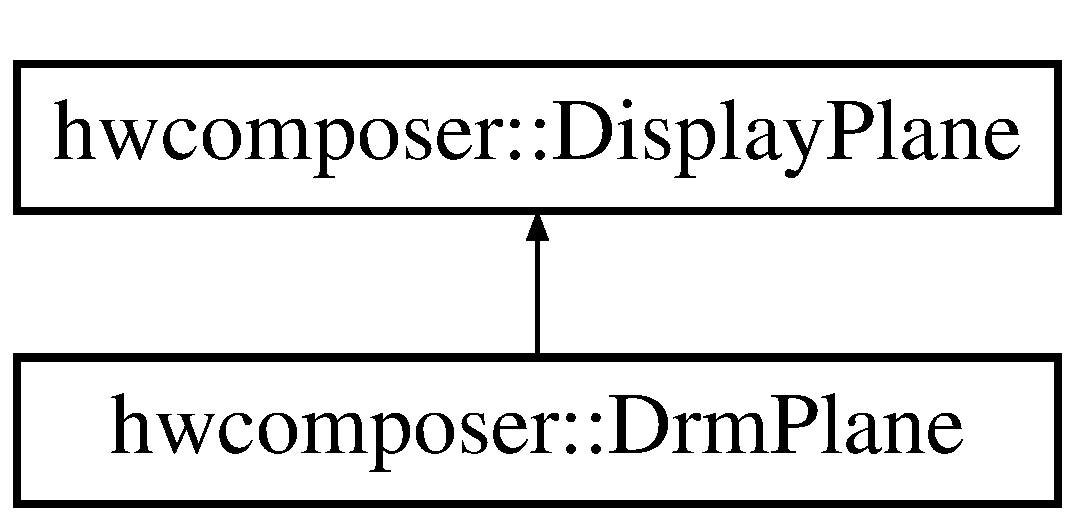
\includegraphics[height=2.000000cm]{classhwcomposer_1_1DrmPlane}
\end{center}
\end{figure}
\subsection*{Public Member Functions}
\begin{DoxyCompactItemize}
\item 
\mbox{\hyperlink{classhwcomposer_1_1DrmPlane_ae2208912c8f4a58e3fc769ed98bb2b58}{Drm\+Plane}} (uint32\+\_\+t plane\+\_\+id, uint32\+\_\+t possible\+\_\+crtcs)
\item 
\mbox{\hyperlink{classhwcomposer_1_1DrmPlane_a5830385ee2e49d18c8dc7abf7b1da8ab}{$\sim$\+Drm\+Plane}} ()
\item 
bool \mbox{\hyperlink{classhwcomposer_1_1DrmPlane_ae6062735cfb8f43881b9f25ad4e8e1a7}{Initialize}} (uint32\+\_\+t gpu\+\_\+fd, const std\+::vector$<$ uint32\+\_\+t $>$ \&formats)
\item 
bool \mbox{\hyperlink{classhwcomposer_1_1DrmPlane_a50a1d74a0acdd8c4b213733f387fa695}{Update\+Properties}} (drm\+Mode\+Atomic\+Req\+Ptr property\+\_\+set, uint32\+\_\+t crtc\+\_\+id, const \mbox{\hyperlink{structhwcomposer_1_1OverlayLayer}{Overlay\+Layer}} $\ast$layer, bool test\+\_\+commit=false) const
\item 
void \mbox{\hyperlink{classhwcomposer_1_1DrmPlane_a8f904c14af7bfc4265640be4788d2096}{Set\+Native\+Fence}} (int32\+\_\+t fd)
\item 
void \mbox{\hyperlink{classhwcomposer_1_1DrmPlane_a17dbc59adab79a264b50e8727a6ad281}{Set\+Buffer}} (std\+::shared\+\_\+ptr$<$ \mbox{\hyperlink{classhwcomposer_1_1OverlayBuffer}{Overlay\+Buffer}} $>$ \&buffer)
\item 
bool \mbox{\hyperlink{classhwcomposer_1_1DrmPlane_a0efdb0b47954f95bb0ef0e99c2a3b697}{Disable}} (drm\+Mode\+Atomic\+Req\+Ptr property\+\_\+set)
\item 
bool \mbox{\hyperlink{classhwcomposer_1_1DrmPlane_a98c439ae5a59e4699183ad2ffed4e278}{Get\+Crtc\+Supported}} (uint32\+\_\+t pipe\+\_\+id) const
\item 
uint32\+\_\+t \mbox{\hyperlink{classhwcomposer_1_1DrmPlane_aeedfc2e6824d27a9dd754bf4ee27b274}{type}} () const
\item 
uint32\+\_\+t \mbox{\hyperlink{classhwcomposer_1_1DrmPlane_ae84fc513bfb1f3ee35715ff9a808f447}{id}} () const override
\item 
bool \mbox{\hyperlink{classhwcomposer_1_1DrmPlane_ad07df42def289d2dbbf9be4ad6748db8}{Validate\+Layer}} (const \mbox{\hyperlink{structhwcomposer_1_1OverlayLayer}{Overlay\+Layer}} $\ast$layer) override
\item 
bool \mbox{\hyperlink{classhwcomposer_1_1DrmPlane_a50940fd94a65453bd22d20011581796e}{Is\+Supported\+Format}} (uint32\+\_\+t format) override
\item 
bool \mbox{\hyperlink{classhwcomposer_1_1DrmPlane_ac3feae2eaa4adfb5678a47c835c2c2af}{Is\+Supported\+Transform}} (uint32\+\_\+t transform) const override
\item 
uint32\+\_\+t \mbox{\hyperlink{classhwcomposer_1_1DrmPlane_a061caae8c703189ae6d05dbe8b303f12}{Get\+Preferred\+Video\+Format}} () const override
\item 
uint32\+\_\+t \mbox{\hyperlink{classhwcomposer_1_1DrmPlane_a3bca39231ec7b099980474b279c58ce8}{Get\+Preferred\+Format}} () const override
\item 
uint64\+\_\+t \mbox{\hyperlink{classhwcomposer_1_1DrmPlane_a185538f3aca7f84830f75f23efe551d6}{Get\+Preferred\+Format\+Modifier}} () const override
\item 
void \mbox{\hyperlink{classhwcomposer_1_1DrmPlane_a6159712388e26258e14fcb3139d7cd19}{Black\+List\+Preferred\+Format\+Modifier}} () override
\item 
void \mbox{\hyperlink{classhwcomposer_1_1DrmPlane_a476d9d42a81eddb775bb285cc1c68cfb}{Preferred\+Format\+Modifier\+Validated}} () override
\item 
void \mbox{\hyperlink{classhwcomposer_1_1DrmPlane_abc9ca4823dfd433aa45747b8596cc673}{Dump}} () const override
\item 
void \mbox{\hyperlink{classhwcomposer_1_1DrmPlane_aed0ac04d949d6457dd638e121c3618d5}{Set\+In\+Use}} (bool in\+\_\+use) override
\item 
bool \mbox{\hyperlink{classhwcomposer_1_1DrmPlane_aeb8c1aecd933645e7e2743b149b06302}{In\+Use}} () const override
\item 
bool \mbox{\hyperlink{classhwcomposer_1_1DrmPlane_a25b4218371d1c5984777b74553b554a4}{Is\+Universal}} () override
\item 
bool \mbox{\hyperlink{classhwcomposer_1_1DrmPlane_a82a0274af9e3e94889e8df8dedbe3eea}{Is\+Supported\+Modifier}} (uint64\+\_\+t modifier, uint32\+\_\+t format)
\end{DoxyCompactItemize}


\subsection{Detailed Description}


Definition at line 37 of file drmplane.\+h.



\subsection{Constructor \& Destructor Documentation}
\mbox{\Hypertarget{classhwcomposer_1_1DrmPlane_ae2208912c8f4a58e3fc769ed98bb2b58}\label{classhwcomposer_1_1DrmPlane_ae2208912c8f4a58e3fc769ed98bb2b58}} 
\index{hwcomposer\+::\+Drm\+Plane@{hwcomposer\+::\+Drm\+Plane}!Drm\+Plane@{Drm\+Plane}}
\index{Drm\+Plane@{Drm\+Plane}!hwcomposer\+::\+Drm\+Plane@{hwcomposer\+::\+Drm\+Plane}}
\subsubsection{\texorpdfstring{Drm\+Plane()}{DrmPlane()}}
{\footnotesize\ttfamily hwcomposer\+::\+Drm\+Plane\+::\+Drm\+Plane (\begin{DoxyParamCaption}\item[{uint32\+\_\+t}]{plane\+\_\+id,  }\item[{uint32\+\_\+t}]{possible\+\_\+crtcs }\end{DoxyParamCaption})}



Definition at line 76 of file drmplane.\+cpp.


\begin{DoxyCode}{0}
\DoxyCodeLine{77     : id\_(plane\_id),}
\DoxyCodeLine{78       possible\_crtc\_mask\_(possible\_crtcs),}
\DoxyCodeLine{79       type\_(0),}
\DoxyCodeLine{80       last\_valid\_format\_(0),}
\DoxyCodeLine{81       in\_use\_(\textcolor{keyword}{false}) \{}
\DoxyCodeLine{82 \}}
\end{DoxyCode}
\mbox{\Hypertarget{classhwcomposer_1_1DrmPlane_a5830385ee2e49d18c8dc7abf7b1da8ab}\label{classhwcomposer_1_1DrmPlane_a5830385ee2e49d18c8dc7abf7b1da8ab}} 
\index{hwcomposer\+::\+Drm\+Plane@{hwcomposer\+::\+Drm\+Plane}!````~Drm\+Plane@{$\sim$\+Drm\+Plane}}
\index{````~Drm\+Plane@{$\sim$\+Drm\+Plane}!hwcomposer\+::\+Drm\+Plane@{hwcomposer\+::\+Drm\+Plane}}
\subsubsection{\texorpdfstring{$\sim$\+Drm\+Plane()}{~DrmPlane()}}
{\footnotesize\ttfamily hwcomposer\+::\+Drm\+Plane\+::$\sim$\+Drm\+Plane (\begin{DoxyParamCaption}{ }\end{DoxyParamCaption})}



Definition at line 84 of file drmplane.\+cpp.


\begin{DoxyCode}{0}
\DoxyCodeLine{84                     \{}
\DoxyCodeLine{85   \mbox{\hyperlink{classhwcomposer_1_1DrmPlane_a8f904c14af7bfc4265640be4788d2096}{SetNativeFence}}(-1);}
\DoxyCodeLine{86 \}}
\end{DoxyCode}


\subsection{Member Function Documentation}
\mbox{\Hypertarget{classhwcomposer_1_1DrmPlane_a6159712388e26258e14fcb3139d7cd19}\label{classhwcomposer_1_1DrmPlane_a6159712388e26258e14fcb3139d7cd19}} 
\index{hwcomposer\+::\+Drm\+Plane@{hwcomposer\+::\+Drm\+Plane}!Black\+List\+Preferred\+Format\+Modifier@{Black\+List\+Preferred\+Format\+Modifier}}
\index{Black\+List\+Preferred\+Format\+Modifier@{Black\+List\+Preferred\+Format\+Modifier}!hwcomposer\+::\+Drm\+Plane@{hwcomposer\+::\+Drm\+Plane}}
\subsubsection{\texorpdfstring{Black\+List\+Preferred\+Format\+Modifier()}{BlackListPreferredFormatModifier()}}
{\footnotesize\ttfamily void hwcomposer\+::\+Drm\+Plane\+::\+Black\+List\+Preferred\+Format\+Modifier (\begin{DoxyParamCaption}{ }\end{DoxyParamCaption})\hspace{0.3cm}{\ttfamily [override]}, {\ttfamily [virtual]}}

A\+PI for blacklisting preferred format modifier. This happens in case we failed to create FB for the buffer. 

Implements \mbox{\hyperlink{classhwcomposer_1_1DisplayPlane_a397270389f37f6c706a639be5225e62e}{hwcomposer\+::\+Display\+Plane}}.



Definition at line 370 of file drmplane.\+cpp.


\begin{DoxyCode}{0}
\DoxyCodeLine{370                                                 \{}
\DoxyCodeLine{371   \textcolor{keywordflow}{if} (!prefered\_modifier\_succeeded\_)}
\DoxyCodeLine{372     prefered\_modifier\_ = 0;}
\DoxyCodeLine{373 \}}
\end{DoxyCode}
\mbox{\Hypertarget{classhwcomposer_1_1DrmPlane_a0efdb0b47954f95bb0ef0e99c2a3b697}\label{classhwcomposer_1_1DrmPlane_a0efdb0b47954f95bb0ef0e99c2a3b697}} 
\index{hwcomposer\+::\+Drm\+Plane@{hwcomposer\+::\+Drm\+Plane}!Disable@{Disable}}
\index{Disable@{Disable}!hwcomposer\+::\+Drm\+Plane@{hwcomposer\+::\+Drm\+Plane}}
\subsubsection{\texorpdfstring{Disable()}{Disable()}}
{\footnotesize\ttfamily bool hwcomposer\+::\+Drm\+Plane\+::\+Disable (\begin{DoxyParamCaption}\item[{drm\+Mode\+Atomic\+Req\+Ptr}]{property\+\_\+set }\end{DoxyParamCaption})}



Definition at line 379 of file drmplane.\+cpp.


\begin{DoxyCode}{0}
\DoxyCodeLine{379                                                        \{}
\DoxyCodeLine{380   in\_use\_ = \textcolor{keyword}{false};}
\DoxyCodeLine{381   \textcolor{keywordtype}{int} success =}
\DoxyCodeLine{382       drmModeAtomicAddProperty(property\_set, id\_, crtc\_prop\_.id, 0) < 0;}
\DoxyCodeLine{383   success |= drmModeAtomicAddProperty(property\_set, id\_, fb\_prop\_.id, 0) < 0;}
\DoxyCodeLine{384   success |=}
\DoxyCodeLine{385       drmModeAtomicAddProperty(property\_set, id\_, crtc\_x\_prop\_.id, 0) < 0;}
\DoxyCodeLine{386   success |=}
\DoxyCodeLine{387       drmModeAtomicAddProperty(property\_set, id\_, crtc\_y\_prop\_.id, 0) < 0;}
\DoxyCodeLine{388   success |=}
\DoxyCodeLine{389       drmModeAtomicAddProperty(property\_set, id\_, crtc\_w\_prop\_.id, 0) < 0;}
\DoxyCodeLine{390   success |=}
\DoxyCodeLine{391       drmModeAtomicAddProperty(property\_set, id\_, crtc\_h\_prop\_.id, 0) < 0;}
\DoxyCodeLine{392   success |= drmModeAtomicAddProperty(property\_set, id\_, src\_x\_prop\_.id, 0) < 0;}
\DoxyCodeLine{393   success |= drmModeAtomicAddProperty(property\_set, id\_, src\_y\_prop\_.id, 0) < 0;}
\DoxyCodeLine{394   success |= drmModeAtomicAddProperty(property\_set, id\_, src\_w\_prop\_.id, 0) < 0;}
\DoxyCodeLine{395   success |= drmModeAtomicAddProperty(property\_set, id\_, src\_h\_prop\_.id, 0) < 0;}
\DoxyCodeLine{396 }
\DoxyCodeLine{397   \textcolor{keywordflow}{if} (success) \{}
\DoxyCodeLine{398     \mbox{\hyperlink{alios_2platformdefines_8h_a226d6c99e4bcfca193c095e085e9097d}{ETRACE}}(\textcolor{stringliteral}{"Could not update properties for plane with id: \%d"}, id\_);}
\DoxyCodeLine{399     \textcolor{keywordflow}{return} \textcolor{keyword}{false};}
\DoxyCodeLine{400   \}}
\DoxyCodeLine{401 }
\DoxyCodeLine{402   \mbox{\hyperlink{classhwcomposer_1_1DrmPlane_a8f904c14af7bfc4265640be4788d2096}{SetNativeFence}}(-1);}
\DoxyCodeLine{403   buffer\_.reset();}
\DoxyCodeLine{404 }
\DoxyCodeLine{405   \textcolor{keywordflow}{return} \textcolor{keyword}{true};}
\DoxyCodeLine{406 \}}
\end{DoxyCode}
\mbox{\Hypertarget{classhwcomposer_1_1DrmPlane_abc9ca4823dfd433aa45747b8596cc673}\label{classhwcomposer_1_1DrmPlane_abc9ca4823dfd433aa45747b8596cc673}} 
\index{hwcomposer\+::\+Drm\+Plane@{hwcomposer\+::\+Drm\+Plane}!Dump@{Dump}}
\index{Dump@{Dump}!hwcomposer\+::\+Drm\+Plane@{hwcomposer\+::\+Drm\+Plane}}
\subsubsection{\texorpdfstring{Dump()}{Dump()}}
{\footnotesize\ttfamily void hwcomposer\+::\+Drm\+Plane\+::\+Dump (\begin{DoxyParamCaption}{ }\end{DoxyParamCaption}) const\hspace{0.3cm}{\ttfamily [override]}, {\ttfamily [virtual]}}



Implements \mbox{\hyperlink{classhwcomposer_1_1DisplayPlane_a3754165ab1101fba4229b842c7f14556}{hwcomposer\+::\+Display\+Plane}}.



Definition at line 522 of file drmplane.\+cpp.


\begin{DoxyCode}{0}
\DoxyCodeLine{522                           \{}
\DoxyCodeLine{523   \mbox{\hyperlink{hwctrace_8h_a8f0916f7778d78a386afc1e5d8be8a25}{DUMPTRACE}}(\textcolor{stringliteral}{"Plane Information Starts. -------------"});}
\DoxyCodeLine{524   \mbox{\hyperlink{hwctrace_8h_a8f0916f7778d78a386afc1e5d8be8a25}{DUMPTRACE}}(\textcolor{stringliteral}{"Plane ID: \%d"}, id\_);}
\DoxyCodeLine{525   \textcolor{keywordflow}{switch} (type\_) \{}
\DoxyCodeLine{526     \textcolor{keywordflow}{case} DRM\_PLANE\_TYPE\_OVERLAY:}
\DoxyCodeLine{527       \mbox{\hyperlink{hwctrace_8h_a8f0916f7778d78a386afc1e5d8be8a25}{DUMPTRACE}}(\textcolor{stringliteral}{"Type: Overlay."});}
\DoxyCodeLine{528       \textcolor{keywordflow}{break};}
\DoxyCodeLine{529     \textcolor{keywordflow}{case} DRM\_PLANE\_TYPE\_PRIMARY:}
\DoxyCodeLine{530       \mbox{\hyperlink{hwctrace_8h_a8f0916f7778d78a386afc1e5d8be8a25}{DUMPTRACE}}(\textcolor{stringliteral}{"Type: Primary."});}
\DoxyCodeLine{531       \textcolor{keywordflow}{break};}
\DoxyCodeLine{532     \textcolor{keywordflow}{case} DRM\_PLANE\_TYPE\_CURSOR:}
\DoxyCodeLine{533       \mbox{\hyperlink{hwctrace_8h_a8f0916f7778d78a386afc1e5d8be8a25}{DUMPTRACE}}(\textcolor{stringliteral}{"Type: Cursor."});}
\DoxyCodeLine{534       \textcolor{keywordflow}{break};}
\DoxyCodeLine{535     \textcolor{keywordflow}{default}:}
\DoxyCodeLine{536       \mbox{\hyperlink{alios_2platformdefines_8h_a226d6c99e4bcfca193c095e085e9097d}{ETRACE}}(\textcolor{stringliteral}{"Invalid plane type \%d"}, type\_);}
\DoxyCodeLine{537   \}}
\DoxyCodeLine{538 }
\DoxyCodeLine{539   \textcolor{keywordflow}{for} (uint32\_t j = 0; j < supported\_formats\_.size(); j++)}
\DoxyCodeLine{540     \mbox{\hyperlink{hwctrace_8h_a8f0916f7778d78a386afc1e5d8be8a25}{DUMPTRACE}}(\textcolor{stringliteral}{"Format: \%4.4s"}, (\textcolor{keywordtype}{char}*)\&supported\_formats\_[j]);}
\DoxyCodeLine{541 }
\DoxyCodeLine{542   \mbox{\hyperlink{hwctrace_8h_a8f0916f7778d78a386afc1e5d8be8a25}{DUMPTRACE}}(\textcolor{stringliteral}{"Enabled: \%d"}, in\_use\_);}
\DoxyCodeLine{543 }
\DoxyCodeLine{544   \textcolor{keywordflow}{if} (alpha\_prop\_.id != 0)}
\DoxyCodeLine{545     \mbox{\hyperlink{hwctrace_8h_a8f0916f7778d78a386afc1e5d8be8a25}{DUMPTRACE}}(\textcolor{stringliteral}{"Alpha property is supported."});}
\DoxyCodeLine{546 }
\DoxyCodeLine{547   \textcolor{keywordflow}{if} (rotation\_prop\_.id != 0)}
\DoxyCodeLine{548     \mbox{\hyperlink{hwctrace_8h_a8f0916f7778d78a386afc1e5d8be8a25}{DUMPTRACE}}(\textcolor{stringliteral}{"Rotation property is supported."});}
\DoxyCodeLine{549 }
\DoxyCodeLine{550   \textcolor{keywordflow}{if} (crtc\_prop\_.id != 0)}
\DoxyCodeLine{551     \mbox{\hyperlink{hwctrace_8h_a8f0916f7778d78a386afc1e5d8be8a25}{DUMPTRACE}}(\textcolor{stringliteral}{"CRTC\_ID property is supported."});}
\DoxyCodeLine{552 }
\DoxyCodeLine{553   \textcolor{keywordflow}{if} (fb\_prop\_.id != 0)}
\DoxyCodeLine{554     \mbox{\hyperlink{hwctrace_8h_a8f0916f7778d78a386afc1e5d8be8a25}{DUMPTRACE}}(\textcolor{stringliteral}{"FB\_ID property is supported."});}
\DoxyCodeLine{555 }
\DoxyCodeLine{556   \textcolor{keywordflow}{if} (crtc\_x\_prop\_.id != 0)}
\DoxyCodeLine{557     \mbox{\hyperlink{hwctrace_8h_a8f0916f7778d78a386afc1e5d8be8a25}{DUMPTRACE}}(\textcolor{stringliteral}{"CRTC\_X property is supported."});}
\DoxyCodeLine{558 }
\DoxyCodeLine{559   \textcolor{keywordflow}{if} (crtc\_y\_prop\_.id != 0)}
\DoxyCodeLine{560     \mbox{\hyperlink{hwctrace_8h_a8f0916f7778d78a386afc1e5d8be8a25}{DUMPTRACE}}(\textcolor{stringliteral}{"CRTC\_Y property is supported."});}
\DoxyCodeLine{561 }
\DoxyCodeLine{562   \textcolor{keywordflow}{if} (crtc\_w\_prop\_.id != 0)}
\DoxyCodeLine{563     \mbox{\hyperlink{hwctrace_8h_a8f0916f7778d78a386afc1e5d8be8a25}{DUMPTRACE}}(\textcolor{stringliteral}{"CRTC\_W property is supported."});}
\DoxyCodeLine{564 }
\DoxyCodeLine{565   \textcolor{keywordflow}{if} (crtc\_h\_prop\_.id != 0)}
\DoxyCodeLine{566     \mbox{\hyperlink{hwctrace_8h_a8f0916f7778d78a386afc1e5d8be8a25}{DUMPTRACE}}(\textcolor{stringliteral}{"CRTC\_H property is supported."});}
\DoxyCodeLine{567 }
\DoxyCodeLine{568   \textcolor{keywordflow}{if} (src\_x\_prop\_.id != 0)}
\DoxyCodeLine{569     \mbox{\hyperlink{hwctrace_8h_a8f0916f7778d78a386afc1e5d8be8a25}{DUMPTRACE}}(\textcolor{stringliteral}{"SRC\_X property is supported."});}
\DoxyCodeLine{570 }
\DoxyCodeLine{571   \textcolor{keywordflow}{if} (src\_y\_prop\_.id != 0)}
\DoxyCodeLine{572     \mbox{\hyperlink{hwctrace_8h_a8f0916f7778d78a386afc1e5d8be8a25}{DUMPTRACE}}(\textcolor{stringliteral}{"SRC\_Y property is supported."});}
\DoxyCodeLine{573 }
\DoxyCodeLine{574   \textcolor{keywordflow}{if} (src\_w\_prop\_.id != 0)}
\DoxyCodeLine{575     \mbox{\hyperlink{hwctrace_8h_a8f0916f7778d78a386afc1e5d8be8a25}{DUMPTRACE}}(\textcolor{stringliteral}{"SRC\_W property is supported."});}
\DoxyCodeLine{576 }
\DoxyCodeLine{577   \textcolor{keywordflow}{if} (src\_h\_prop\_.id != 0)}
\DoxyCodeLine{578     \mbox{\hyperlink{hwctrace_8h_a8f0916f7778d78a386afc1e5d8be8a25}{DUMPTRACE}}(\textcolor{stringliteral}{"SRC\_H property is supported."});}
\DoxyCodeLine{579 }
\DoxyCodeLine{580   \textcolor{keywordflow}{if} (in\_fence\_fd\_prop\_.id != 0)}
\DoxyCodeLine{581     \mbox{\hyperlink{hwctrace_8h_a8f0916f7778d78a386afc1e5d8be8a25}{DUMPTRACE}}(\textcolor{stringliteral}{"IN\_FENCE\_FD is supported."});}
\DoxyCodeLine{582 }
\DoxyCodeLine{583   \textcolor{keywordflow}{if} (in\_formats\_prop\_.id != 0)}
\DoxyCodeLine{584     \mbox{\hyperlink{hwctrace_8h_a8f0916f7778d78a386afc1e5d8be8a25}{DUMPTRACE}}(\textcolor{stringliteral}{"IN\_FORMATS property is supported."});}
\DoxyCodeLine{585 }
\DoxyCodeLine{586   \mbox{\hyperlink{hwctrace_8h_a8f0916f7778d78a386afc1e5d8be8a25}{DUMPTRACE}}(\textcolor{stringliteral}{"Preferred Video Format: \%4.4s"}, (\textcolor{keywordtype}{char}*)\&(prefered\_video\_format\_));}
\DoxyCodeLine{587   \mbox{\hyperlink{hwctrace_8h_a8f0916f7778d78a386afc1e5d8be8a25}{DUMPTRACE}}(\textcolor{stringliteral}{"Preferred Video Format: \%4.4s"}, (\textcolor{keywordtype}{char}*)\&(prefered\_format\_));}
\DoxyCodeLine{588 }
\DoxyCodeLine{589   \mbox{\hyperlink{hwctrace_8h_a8f0916f7778d78a386afc1e5d8be8a25}{DUMPTRACE}}(\textcolor{stringliteral}{"Plane Information Ends. -------------"});}
\DoxyCodeLine{590 \}}
\end{DoxyCode}
\mbox{\Hypertarget{classhwcomposer_1_1DrmPlane_a98c439ae5a59e4699183ad2ffed4e278}\label{classhwcomposer_1_1DrmPlane_a98c439ae5a59e4699183ad2ffed4e278}} 
\index{hwcomposer\+::\+Drm\+Plane@{hwcomposer\+::\+Drm\+Plane}!Get\+Crtc\+Supported@{Get\+Crtc\+Supported}}
\index{Get\+Crtc\+Supported@{Get\+Crtc\+Supported}!hwcomposer\+::\+Drm\+Plane@{hwcomposer\+::\+Drm\+Plane}}
\subsubsection{\texorpdfstring{Get\+Crtc\+Supported()}{GetCrtcSupported()}}
{\footnotesize\ttfamily bool hwcomposer\+::\+Drm\+Plane\+::\+Get\+Crtc\+Supported (\begin{DoxyParamCaption}\item[{uint32\+\_\+t}]{pipe\+\_\+id }\end{DoxyParamCaption}) const}



Definition at line 412 of file drmplane.\+cpp.


\begin{DoxyCode}{0}
\DoxyCodeLine{412                                                       \{}
\DoxyCodeLine{413   \textcolor{keywordflow}{return} !!((1 << pipe\_id) \& possible\_crtc\_mask\_);}
\DoxyCodeLine{414 \}}
\end{DoxyCode}
\mbox{\Hypertarget{classhwcomposer_1_1DrmPlane_a3bca39231ec7b099980474b279c58ce8}\label{classhwcomposer_1_1DrmPlane_a3bca39231ec7b099980474b279c58ce8}} 
\index{hwcomposer\+::\+Drm\+Plane@{hwcomposer\+::\+Drm\+Plane}!Get\+Preferred\+Format@{Get\+Preferred\+Format}}
\index{Get\+Preferred\+Format@{Get\+Preferred\+Format}!hwcomposer\+::\+Drm\+Plane@{hwcomposer\+::\+Drm\+Plane}}
\subsubsection{\texorpdfstring{Get\+Preferred\+Format()}{GetPreferredFormat()}}
{\footnotesize\ttfamily uint32\+\_\+t hwcomposer\+::\+Drm\+Plane\+::\+Get\+Preferred\+Format (\begin{DoxyParamCaption}{ }\end{DoxyParamCaption}) const\hspace{0.3cm}{\ttfamily [override]}, {\ttfamily [virtual]}}

A\+PI for querying preferred format supported by this plane for non-\/media content. 

Implements \mbox{\hyperlink{classhwcomposer_1_1DisplayPlane_a963d17ec10be62d13f35a0b4ced4e8e1}{hwcomposer\+::\+Display\+Plane}}.



Definition at line 495 of file drmplane.\+cpp.


\begin{DoxyCode}{0}
\DoxyCodeLine{495                                             \{}
\DoxyCodeLine{496   \textcolor{keywordflow}{return} prefered\_format\_;}
\DoxyCodeLine{497 \}}
\end{DoxyCode}
\mbox{\Hypertarget{classhwcomposer_1_1DrmPlane_a185538f3aca7f84830f75f23efe551d6}\label{classhwcomposer_1_1DrmPlane_a185538f3aca7f84830f75f23efe551d6}} 
\index{hwcomposer\+::\+Drm\+Plane@{hwcomposer\+::\+Drm\+Plane}!Get\+Preferred\+Format\+Modifier@{Get\+Preferred\+Format\+Modifier}}
\index{Get\+Preferred\+Format\+Modifier@{Get\+Preferred\+Format\+Modifier}!hwcomposer\+::\+Drm\+Plane@{hwcomposer\+::\+Drm\+Plane}}
\subsubsection{\texorpdfstring{Get\+Preferred\+Format\+Modifier()}{GetPreferredFormatModifier()}}
{\footnotesize\ttfamily uint64\+\_\+t hwcomposer\+::\+Drm\+Plane\+::\+Get\+Preferred\+Format\+Modifier (\begin{DoxyParamCaption}{ }\end{DoxyParamCaption}) const\hspace{0.3cm}{\ttfamily [override]}, {\ttfamily [virtual]}}

A\+PI for querying preferred modifier supported by this plane\textquotesingle{}s preferred format for non-\/media content. 

Implements \mbox{\hyperlink{classhwcomposer_1_1DisplayPlane_ad95d2bd823ccf74fe3deccad7352f672}{hwcomposer\+::\+Display\+Plane}}.



Definition at line 499 of file drmplane.\+cpp.


\begin{DoxyCode}{0}
\DoxyCodeLine{499                                                     \{}
\DoxyCodeLine{500   \textcolor{keywordflow}{return} prefered\_modifier\_;}
\DoxyCodeLine{501 \}}
\end{DoxyCode}
\mbox{\Hypertarget{classhwcomposer_1_1DrmPlane_a061caae8c703189ae6d05dbe8b303f12}\label{classhwcomposer_1_1DrmPlane_a061caae8c703189ae6d05dbe8b303f12}} 
\index{hwcomposer\+::\+Drm\+Plane@{hwcomposer\+::\+Drm\+Plane}!Get\+Preferred\+Video\+Format@{Get\+Preferred\+Video\+Format}}
\index{Get\+Preferred\+Video\+Format@{Get\+Preferred\+Video\+Format}!hwcomposer\+::\+Drm\+Plane@{hwcomposer\+::\+Drm\+Plane}}
\subsubsection{\texorpdfstring{Get\+Preferred\+Video\+Format()}{GetPreferredVideoFormat()}}
{\footnotesize\ttfamily uint32\+\_\+t hwcomposer\+::\+Drm\+Plane\+::\+Get\+Preferred\+Video\+Format (\begin{DoxyParamCaption}{ }\end{DoxyParamCaption}) const\hspace{0.3cm}{\ttfamily [override]}, {\ttfamily [virtual]}}

A\+PI for querying preferred Video format supported by this plane. 

Implements \mbox{\hyperlink{classhwcomposer_1_1DisplayPlane_aab8aae5944b1107e4efc9d0d79c43c40}{hwcomposer\+::\+Display\+Plane}}.



Definition at line 491 of file drmplane.\+cpp.


\begin{DoxyCode}{0}
\DoxyCodeLine{491                                                  \{}
\DoxyCodeLine{492   \textcolor{keywordflow}{return} prefered\_video\_format\_;}
\DoxyCodeLine{493 \}}
\end{DoxyCode}
\mbox{\Hypertarget{classhwcomposer_1_1DrmPlane_ae84fc513bfb1f3ee35715ff9a808f447}\label{classhwcomposer_1_1DrmPlane_ae84fc513bfb1f3ee35715ff9a808f447}} 
\index{hwcomposer\+::\+Drm\+Plane@{hwcomposer\+::\+Drm\+Plane}!id@{id}}
\index{id@{id}!hwcomposer\+::\+Drm\+Plane@{hwcomposer\+::\+Drm\+Plane}}
\subsubsection{\texorpdfstring{id()}{id()}}
{\footnotesize\ttfamily uint32\+\_\+t hwcomposer\+::\+Drm\+Plane\+::id (\begin{DoxyParamCaption}{ }\end{DoxyParamCaption}) const\hspace{0.3cm}{\ttfamily [override]}, {\ttfamily [virtual]}}



Implements \mbox{\hyperlink{classhwcomposer_1_1DisplayPlane_a0af461a6ac4beccb8ed21aec933b6eed}{hwcomposer\+::\+Display\+Plane}}.



Definition at line 408 of file drmplane.\+cpp.


\begin{DoxyCode}{0}
\DoxyCodeLine{408                             \{}
\DoxyCodeLine{409   \textcolor{keywordflow}{return} id\_;}
\DoxyCodeLine{410 \}}
\end{DoxyCode}
\mbox{\Hypertarget{classhwcomposer_1_1DrmPlane_ae6062735cfb8f43881b9f25ad4e8e1a7}\label{classhwcomposer_1_1DrmPlane_ae6062735cfb8f43881b9f25ad4e8e1a7}} 
\index{hwcomposer\+::\+Drm\+Plane@{hwcomposer\+::\+Drm\+Plane}!Initialize@{Initialize}}
\index{Initialize@{Initialize}!hwcomposer\+::\+Drm\+Plane@{hwcomposer\+::\+Drm\+Plane}}
\subsubsection{\texorpdfstring{Initialize()}{Initialize()}}
{\footnotesize\ttfamily bool hwcomposer\+::\+Drm\+Plane\+::\+Initialize (\begin{DoxyParamCaption}\item[{uint32\+\_\+t}]{gpu\+\_\+fd,  }\item[{const std\+::vector$<$ uint32\+\_\+t $>$ \&}]{formats }\end{DoxyParamCaption})}



Definition at line 88 of file drmplane.\+cpp.


\begin{DoxyCode}{0}
\DoxyCodeLine{89                                                               \{}
\DoxyCodeLine{90   supported\_formats\_ = formats;}
\DoxyCodeLine{91   uint32\_t total\_size = supported\_formats\_.size();}
\DoxyCodeLine{92   \textcolor{keywordflow}{for} (uint32\_t j = 0; j < total\_size; j++) \{}
\DoxyCodeLine{93     uint32\_t format = supported\_formats\_.at(j);}
\DoxyCodeLine{94     \textcolor{keywordflow}{if} (\mbox{\hyperlink{namespacehwcomposer_a96195339fc55ee57f41cc4597a56746c}{IsSupportedMediaFormat}}(format)) \{}
\DoxyCodeLine{95       prefered\_video\_format\_ = format;}
\DoxyCodeLine{96       \textcolor{keywordflow}{break};}
\DoxyCodeLine{97     \}}
\DoxyCodeLine{98   \}}
\DoxyCodeLine{99 }
\DoxyCodeLine{100   \textcolor{keywordflow}{for} (uint32\_t j = 0; j < total\_size; j++) \{}
\DoxyCodeLine{101     uint32\_t format = supported\_formats\_.at(j);}
\DoxyCodeLine{102     \textcolor{keywordflow}{switch} (format) \{}
\DoxyCodeLine{103       \textcolor{keywordflow}{case} DRM\_FORMAT\_BGRA8888:}
\DoxyCodeLine{104       \textcolor{keywordflow}{case} DRM\_FORMAT\_RGBA8888:}
\DoxyCodeLine{105       \textcolor{keywordflow}{case} DRM\_FORMAT\_ABGR8888:}
\DoxyCodeLine{106       \textcolor{keywordflow}{case} DRM\_FORMAT\_ARGB8888:}
\DoxyCodeLine{107       \textcolor{keywordflow}{case} DRM\_FORMAT\_RGB888:}
\DoxyCodeLine{108       \textcolor{keywordflow}{case} DRM\_FORMAT\_XRGB8888:}
\DoxyCodeLine{109       \textcolor{keywordflow}{case} DRM\_FORMAT\_XBGR8888:}
\DoxyCodeLine{110       \textcolor{keywordflow}{case} DRM\_FORMAT\_RGBX8888:}
\DoxyCodeLine{111         prefered\_format\_ = format;}
\DoxyCodeLine{112         \textcolor{keywordflow}{break};}
\DoxyCodeLine{113     \}}
\DoxyCodeLine{114   \}}
\DoxyCodeLine{115 }
\DoxyCodeLine{116   \textcolor{keywordflow}{if} (type\_ == DRM\_PLANE\_TYPE\_PRIMARY) \{}
\DoxyCodeLine{117     \textcolor{keywordflow}{if} (prefered\_format\_ != DRM\_FORMAT\_XBGR8888 \&\&}
\DoxyCodeLine{118         \mbox{\hyperlink{classhwcomposer_1_1DrmPlane_a50940fd94a65453bd22d20011581796e}{IsSupportedFormat}}(DRM\_FORMAT\_XBGR8888)) \{}
\DoxyCodeLine{119       prefered\_format\_ = DRM\_FORMAT\_XBGR8888;}
\DoxyCodeLine{120     \}}
\DoxyCodeLine{121   \}}
\DoxyCodeLine{122 }
\DoxyCodeLine{123   \textcolor{keywordflow}{if} (prefered\_video\_format\_ == 0) \{}
\DoxyCodeLine{124     prefered\_video\_format\_ = prefered\_format\_;}
\DoxyCodeLine{125   \}}
\DoxyCodeLine{126 }
\DoxyCodeLine{127   \mbox{\hyperlink{namespacehwcomposer_ace195c2e057b634efb3013a5a4413799}{ScopedDrmObjectPropertyPtr}} plane\_props(}
\DoxyCodeLine{128       drmModeObjectGetProperties(gpu\_fd, id\_, DRM\_MODE\_OBJECT\_PLANE));}
\DoxyCodeLine{129   \textcolor{keywordflow}{if} (!plane\_props) \{}
\DoxyCodeLine{130     \mbox{\hyperlink{alios_2platformdefines_8h_a226d6c99e4bcfca193c095e085e9097d}{ETRACE}}(\textcolor{stringliteral}{"Unable to get plane properties."});}
\DoxyCodeLine{131     \textcolor{keywordflow}{return} \textcolor{keyword}{false};}
\DoxyCodeLine{132   \}}
\DoxyCodeLine{133   uint32\_t count\_props = plane\_props->count\_props;}
\DoxyCodeLine{134   \textcolor{keywordflow}{for} (uint32\_t i = 0; i < count\_props; i++) \{}
\DoxyCodeLine{135     \mbox{\hyperlink{namespacehwcomposer_ae4038d517ff95af940c1f9cdf40e3834}{ScopedDrmPropertyPtr}} property(}
\DoxyCodeLine{136         drmModeGetProperty(gpu\_fd, plane\_props->props[i]));}
\DoxyCodeLine{137     \textcolor{keywordflow}{if} (property \&\& !strcmp(property->name, \textcolor{stringliteral}{"type"})) \{}
\DoxyCodeLine{138       type\_ = plane\_props->prop\_values[i];}
\DoxyCodeLine{139       \textcolor{keywordflow}{break};}
\DoxyCodeLine{140     \}}
\DoxyCodeLine{141   \}}
\DoxyCodeLine{142 }
\DoxyCodeLine{143   \textcolor{keywordtype}{bool} ret = crtc\_prop\_.Initialize(gpu\_fd, \textcolor{stringliteral}{"CRTC\_ID"}, plane\_props);}
\DoxyCodeLine{144   \textcolor{keywordflow}{if} (!ret)}
\DoxyCodeLine{145     \textcolor{keywordflow}{return} \textcolor{keyword}{false};}
\DoxyCodeLine{146 }
\DoxyCodeLine{147   ret = fb\_prop\_.Initialize(gpu\_fd, \textcolor{stringliteral}{"FB\_ID"}, plane\_props);}
\DoxyCodeLine{148   \textcolor{keywordflow}{if} (!ret)}
\DoxyCodeLine{149     \textcolor{keywordflow}{return} \textcolor{keyword}{false};}
\DoxyCodeLine{150 }
\DoxyCodeLine{151   ret = crtc\_x\_prop\_.Initialize(gpu\_fd, \textcolor{stringliteral}{"CRTC\_X"}, plane\_props);}
\DoxyCodeLine{152   \textcolor{keywordflow}{if} (!ret)}
\DoxyCodeLine{153     \textcolor{keywordflow}{return} \textcolor{keyword}{false};}
\DoxyCodeLine{154 }
\DoxyCodeLine{155   ret = crtc\_y\_prop\_.Initialize(gpu\_fd, \textcolor{stringliteral}{"CRTC\_Y"}, plane\_props);}
\DoxyCodeLine{156   \textcolor{keywordflow}{if} (!ret)}
\DoxyCodeLine{157     \textcolor{keywordflow}{return} \textcolor{keyword}{false};}
\DoxyCodeLine{158 }
\DoxyCodeLine{159   ret = crtc\_w\_prop\_.Initialize(gpu\_fd, \textcolor{stringliteral}{"CRTC\_W"}, plane\_props);}
\DoxyCodeLine{160   \textcolor{keywordflow}{if} (!ret)}
\DoxyCodeLine{161     \textcolor{keywordflow}{return} \textcolor{keyword}{false};}
\DoxyCodeLine{162 }
\DoxyCodeLine{163   ret = crtc\_h\_prop\_.Initialize(gpu\_fd, \textcolor{stringliteral}{"CRTC\_H"}, plane\_props);}
\DoxyCodeLine{164   \textcolor{keywordflow}{if} (!ret)}
\DoxyCodeLine{165     \textcolor{keywordflow}{return} \textcolor{keyword}{false};}
\DoxyCodeLine{166 }
\DoxyCodeLine{167   ret = src\_x\_prop\_.Initialize(gpu\_fd, \textcolor{stringliteral}{"SRC\_X"}, plane\_props);}
\DoxyCodeLine{168   \textcolor{keywordflow}{if} (!ret)}
\DoxyCodeLine{169     \textcolor{keywordflow}{return} \textcolor{keyword}{false};}
\DoxyCodeLine{170 }
\DoxyCodeLine{171   ret = src\_y\_prop\_.Initialize(gpu\_fd, \textcolor{stringliteral}{"SRC\_Y"}, plane\_props);}
\DoxyCodeLine{172   \textcolor{keywordflow}{if} (!ret)}
\DoxyCodeLine{173     \textcolor{keywordflow}{return} \textcolor{keyword}{false};}
\DoxyCodeLine{174 }
\DoxyCodeLine{175   ret = src\_w\_prop\_.Initialize(gpu\_fd, \textcolor{stringliteral}{"SRC\_W"}, plane\_props);}
\DoxyCodeLine{176   \textcolor{keywordflow}{if} (!ret)}
\DoxyCodeLine{177     \textcolor{keywordflow}{return} \textcolor{keyword}{false};}
\DoxyCodeLine{178 }
\DoxyCodeLine{179   ret = src\_h\_prop\_.Initialize(gpu\_fd, \textcolor{stringliteral}{"SRC\_H"}, plane\_props);}
\DoxyCodeLine{180   \textcolor{keywordflow}{if} (!ret)}
\DoxyCodeLine{181     \textcolor{keywordflow}{return} \textcolor{keyword}{false};}
\DoxyCodeLine{182 }
\DoxyCodeLine{183   ret = rotation\_prop\_.Initialize(gpu\_fd, \textcolor{stringliteral}{"rotation"}, plane\_props, \&rotation\_);}
\DoxyCodeLine{184   \textcolor{keywordflow}{if} (!ret)}
\DoxyCodeLine{185     \mbox{\hyperlink{alios_2platformdefines_8h_a226d6c99e4bcfca193c095e085e9097d}{ETRACE}}(\textcolor{stringliteral}{"Could not get rotation property"});}
\DoxyCodeLine{186 }
\DoxyCodeLine{187   ret = alpha\_prop\_.Initialize(gpu\_fd, \textcolor{stringliteral}{"alpha"}, plane\_props);}
\DoxyCodeLine{188   \textcolor{keywordflow}{if} (!ret)}
\DoxyCodeLine{189     \mbox{\hyperlink{alios_2platformdefines_8h_a226d6c99e4bcfca193c095e085e9097d}{ETRACE}}(\textcolor{stringliteral}{"Could not get alpha property"});}
\DoxyCodeLine{190 }
\DoxyCodeLine{191   ret = in\_fence\_fd\_prop\_.Initialize(gpu\_fd, \textcolor{stringliteral}{"IN\_FENCE\_FD"}, plane\_props);}
\DoxyCodeLine{192   \textcolor{keywordflow}{if} (!ret) \{}
\DoxyCodeLine{193     \mbox{\hyperlink{alios_2platformdefines_8h_a226d6c99e4bcfca193c095e085e9097d}{ETRACE}}(\textcolor{stringliteral}{"Could not get IN\_FENCE\_FD property"});}
\DoxyCodeLine{194     in\_fence\_fd\_prop\_.id = 0;}
\DoxyCodeLine{195   \}}
\DoxyCodeLine{196 }
\DoxyCodeLine{197   \textcolor{comment}{// query and store supported modifiers for format, from in\_formats}}
\DoxyCodeLine{198   \textcolor{comment}{// property}}
\DoxyCodeLine{199   uint64\_t in\_formats\_prop\_value = 0;}
\DoxyCodeLine{200   ret = in\_formats\_prop\_.Initialize(gpu\_fd, \textcolor{stringliteral}{"IN\_FORMATS"}, plane\_props, \mbox{\hyperlink{alios_2platformdefines_8h_a070d2ce7b6bb7e5c05602aa8c308d0c4}{NULL}},}
\DoxyCodeLine{201                                     \&in\_formats\_prop\_value);}
\DoxyCodeLine{202   \textcolor{keywordflow}{if} (!ret) \{}
\DoxyCodeLine{203     \mbox{\hyperlink{alios_2platformdefines_8h_a226d6c99e4bcfca193c095e085e9097d}{ETRACE}}(\textcolor{stringliteral}{"Could not get IN\_FORMATS property"});}
\DoxyCodeLine{204   \}}
\DoxyCodeLine{205 }
\DoxyCodeLine{206   \textcolor{keywordflow}{if} (in\_formats\_prop\_value != 0) \{}
\DoxyCodeLine{207     drmModePropertyBlobPtr blob =}
\DoxyCodeLine{208         drmModeGetPropertyBlob(gpu\_fd, in\_formats\_prop\_value);}
\DoxyCodeLine{209     \textcolor{keywordflow}{if} (blob == \textcolor{keyword}{nullptr} || blob->data == \textcolor{keyword}{nullptr}) \{}
\DoxyCodeLine{210       \mbox{\hyperlink{alios_2platformdefines_8h_a226d6c99e4bcfca193c095e085e9097d}{ETRACE}}(\textcolor{stringliteral}{"Unable to get property data\(\backslash\)n"});}
\DoxyCodeLine{211       \textcolor{keywordflow}{return} \textcolor{keyword}{false};}
\DoxyCodeLine{212     \}}
\DoxyCodeLine{213 }
\DoxyCodeLine{214     \textcolor{keyword}{struct }drm\_format\_modifier\_blob* m =}
\DoxyCodeLine{215         (\textcolor{keyword}{struct }drm\_format\_modifier\_blob*)(blob->data);}
\DoxyCodeLine{216     \textcolor{keyword}{struct }drm\_format\_modifier* mod\_o =}
\DoxyCodeLine{217         (\textcolor{keyword}{struct }drm\_format\_modifier*)(\textcolor{keywordtype}{void}*)(((\textcolor{keywordtype}{char}*)m) + m->modifiers\_offset);}
\DoxyCodeLine{218 }
\DoxyCodeLine{219     \textcolor{keywordtype}{bool} y\_tiled\_ccs\_supported = \textcolor{keyword}{false};}
\DoxyCodeLine{220     \textcolor{keywordtype}{bool} y\_tiled\_yf\_ccs\_supported = \textcolor{keyword}{false};}
\DoxyCodeLine{221 }
\DoxyCodeLine{222     \textcolor{keywordflow}{for} (uint32\_t j = 0; j < total\_size; j++) \{}
\DoxyCodeLine{223       uint32\_t format = supported\_formats\_.at(j);}
\DoxyCodeLine{224       format\_mods modifiers\_obj;}
\DoxyCodeLine{225       modifiers\_obj.format = format;}
\DoxyCodeLine{226       uint32\_t format\_index = j;}
\DoxyCodeLine{227 }
\DoxyCodeLine{228       \textcolor{keyword}{struct }drm\_format\_modifier* mod = mod\_o;}
\DoxyCodeLine{229       \textcolor{keywordflow}{for} (\textcolor{keywordtype}{int} i = 0; i < (int)m->count\_modifiers; i++, mod++) \{}
\DoxyCodeLine{230         \textcolor{keywordflow}{if} (mod->formats \& (1ULL << format\_index)) \{}
\DoxyCodeLine{231           modifiers\_obj.mods.emplace\_back(mod->modifier);}
\DoxyCodeLine{232           \textcolor{keywordflow}{if} (mod->modifier == I915\_FORMAT\_MOD\_Y\_TILED\_CCS) \{}
\DoxyCodeLine{233             y\_tiled\_ccs\_supported = \textcolor{keyword}{true};}
\DoxyCodeLine{234           \} \textcolor{keywordflow}{else} \textcolor{keywordflow}{if} (mod->modifier == I915\_FORMAT\_MOD\_Yf\_TILED\_CCS) \{}
\DoxyCodeLine{235             y\_tiled\_yf\_ccs\_supported = \textcolor{keyword}{true};}
\DoxyCodeLine{236           \}}
\DoxyCodeLine{237         \}}
\DoxyCodeLine{238       \}}
\DoxyCodeLine{239 }
\DoxyCodeLine{240       \textcolor{keywordflow}{if} (modifiers\_obj.mods.size() == 0) \{}
\DoxyCodeLine{241         modifiers\_obj.mods.emplace\_back(DRM\_FORMAT\_MOD\_NONE);}
\DoxyCodeLine{242         prefered\_modifier\_ = DRM\_FORMAT\_MOD\_NONE;}
\DoxyCodeLine{243       \} \textcolor{keywordflow}{else} \{}
\DoxyCodeLine{244         \textcolor{keywordflow}{if} (y\_tiled\_ccs\_supported) \{}
\DoxyCodeLine{245           prefered\_modifier\_ = I915\_FORMAT\_MOD\_Y\_TILED\_CCS;}
\DoxyCodeLine{246         \} \textcolor{keywordflow}{else} \textcolor{keywordflow}{if} (y\_tiled\_yf\_ccs\_supported) \{}
\DoxyCodeLine{247           prefered\_modifier\_ = I915\_FORMAT\_MOD\_Yf\_TILED\_CCS;}
\DoxyCodeLine{248         \} \textcolor{keywordflow}{else} \{}
\DoxyCodeLine{249           prefered\_modifier\_ = modifiers\_obj.mods.at(0);}
\DoxyCodeLine{250         \}}
\DoxyCodeLine{251       \}}
\DoxyCodeLine{252 }
\DoxyCodeLine{253       formats\_modifiers\_.emplace\_back(modifiers\_obj);}
\DoxyCodeLine{254     \}}
\DoxyCodeLine{255 }
\DoxyCodeLine{256     drmModeFreePropertyBlob(blob);}
\DoxyCodeLine{257   \}}
\DoxyCodeLine{258   \textcolor{keywordflow}{return} \textcolor{keyword}{true};}
\DoxyCodeLine{259 \}}
\end{DoxyCode}
\mbox{\Hypertarget{classhwcomposer_1_1DrmPlane_aeb8c1aecd933645e7e2743b149b06302}\label{classhwcomposer_1_1DrmPlane_aeb8c1aecd933645e7e2743b149b06302}} 
\index{hwcomposer\+::\+Drm\+Plane@{hwcomposer\+::\+Drm\+Plane}!In\+Use@{In\+Use}}
\index{In\+Use@{In\+Use}!hwcomposer\+::\+Drm\+Plane@{hwcomposer\+::\+Drm\+Plane}}
\subsubsection{\texorpdfstring{In\+Use()}{InUse()}}
{\footnotesize\ttfamily bool hwcomposer\+::\+Drm\+Plane\+::\+In\+Use (\begin{DoxyParamCaption}{ }\end{DoxyParamCaption}) const\hspace{0.3cm}{\ttfamily [inline]}, {\ttfamily [override]}, {\ttfamily [virtual]}}



Implements \mbox{\hyperlink{classhwcomposer_1_1DisplayPlane_a8461ec31b18379cc371cd0656ca0e615}{hwcomposer\+::\+Display\+Plane}}.



Definition at line 79 of file drmplane.\+h.


\begin{DoxyCode}{0}
\DoxyCodeLine{79                               \{}
\DoxyCodeLine{80     \textcolor{keywordflow}{return} in\_use\_;}
\DoxyCodeLine{81   \}}
\end{DoxyCode}
\mbox{\Hypertarget{classhwcomposer_1_1DrmPlane_a50940fd94a65453bd22d20011581796e}\label{classhwcomposer_1_1DrmPlane_a50940fd94a65453bd22d20011581796e}} 
\index{hwcomposer\+::\+Drm\+Plane@{hwcomposer\+::\+Drm\+Plane}!Is\+Supported\+Format@{Is\+Supported\+Format}}
\index{Is\+Supported\+Format@{Is\+Supported\+Format}!hwcomposer\+::\+Drm\+Plane@{hwcomposer\+::\+Drm\+Plane}}
\subsubsection{\texorpdfstring{Is\+Supported\+Format()}{IsSupportedFormat()}}
{\footnotesize\ttfamily bool hwcomposer\+::\+Drm\+Plane\+::\+Is\+Supported\+Format (\begin{DoxyParamCaption}\item[{uint32\+\_\+t}]{format }\end{DoxyParamCaption})\hspace{0.3cm}{\ttfamily [override]}, {\ttfamily [virtual]}}



Implements \mbox{\hyperlink{classhwcomposer_1_1DisplayPlane_a057c78a4a3657a04c5117ee0f1dba8be}{hwcomposer\+::\+Display\+Plane}}.



Definition at line 455 of file drmplane.\+cpp.


\begin{DoxyCode}{0}
\DoxyCodeLine{455                                                 \{}
\DoxyCodeLine{456   \textcolor{keywordflow}{if} (last\_valid\_format\_ == format)}
\DoxyCodeLine{457     \textcolor{keywordflow}{return} \textcolor{keyword}{true};}
\DoxyCodeLine{458 }
\DoxyCodeLine{459   \textcolor{keywordflow}{for} (\textcolor{keyword}{auto}\& element : supported\_formats\_) \{}
\DoxyCodeLine{460     \textcolor{keywordflow}{if} (element == format) \{}
\DoxyCodeLine{461       last\_valid\_format\_ = format;}
\DoxyCodeLine{462       \textcolor{keywordflow}{return} \textcolor{keyword}{true};}
\DoxyCodeLine{463     \}}
\DoxyCodeLine{464   \}}
\DoxyCodeLine{465 }
\DoxyCodeLine{466   \textcolor{keywordflow}{return} \textcolor{keyword}{false};}
\DoxyCodeLine{467 \}}
\end{DoxyCode}
\mbox{\Hypertarget{classhwcomposer_1_1DrmPlane_a82a0274af9e3e94889e8df8dedbe3eea}\label{classhwcomposer_1_1DrmPlane_a82a0274af9e3e94889e8df8dedbe3eea}} 
\index{hwcomposer\+::\+Drm\+Plane@{hwcomposer\+::\+Drm\+Plane}!Is\+Supported\+Modifier@{Is\+Supported\+Modifier}}
\index{Is\+Supported\+Modifier@{Is\+Supported\+Modifier}!hwcomposer\+::\+Drm\+Plane@{hwcomposer\+::\+Drm\+Plane}}
\subsubsection{\texorpdfstring{Is\+Supported\+Modifier()}{IsSupportedModifier()}}
{\footnotesize\ttfamily bool hwcomposer\+::\+Drm\+Plane\+::\+Is\+Supported\+Modifier (\begin{DoxyParamCaption}\item[{uint64\+\_\+t}]{modifier,  }\item[{uint32\+\_\+t}]{format }\end{DoxyParamCaption})}



Definition at line 507 of file drmplane.\+cpp.


\begin{DoxyCode}{0}
\DoxyCodeLine{507                                                                      \{}
\DoxyCodeLine{508   uint32\_t count = formats\_modifiers\_.size();}
\DoxyCodeLine{509   \textcolor{keywordflow}{for} (uint32\_t i = 0; i < count; i++) \{}
\DoxyCodeLine{510     \textcolor{keyword}{const} format\_mods\& obj = formats\_modifiers\_.at(i);}
\DoxyCodeLine{511     \textcolor{keywordflow}{if} (obj.format == format) \{}
\DoxyCodeLine{512       std::vector<uint64\_t>::const\_iterator it;}
\DoxyCodeLine{513       it = std::find(obj.mods.begin(), obj.mods.end(), modifier);}
\DoxyCodeLine{514       \textcolor{keywordflow}{if} (it != obj.mods.end()) \{}
\DoxyCodeLine{515         \textcolor{keywordflow}{return} \textcolor{keyword}{true};}
\DoxyCodeLine{516       \}}
\DoxyCodeLine{517     \}}
\DoxyCodeLine{518   \}}
\DoxyCodeLine{519   \textcolor{keywordflow}{return} \textcolor{keyword}{false};}
\DoxyCodeLine{520 \}}
\end{DoxyCode}
\mbox{\Hypertarget{classhwcomposer_1_1DrmPlane_ac3feae2eaa4adfb5678a47c835c2c2af}\label{classhwcomposer_1_1DrmPlane_ac3feae2eaa4adfb5678a47c835c2c2af}} 
\index{hwcomposer\+::\+Drm\+Plane@{hwcomposer\+::\+Drm\+Plane}!Is\+Supported\+Transform@{Is\+Supported\+Transform}}
\index{Is\+Supported\+Transform@{Is\+Supported\+Transform}!hwcomposer\+::\+Drm\+Plane@{hwcomposer\+::\+Drm\+Plane}}
\subsubsection{\texorpdfstring{Is\+Supported\+Transform()}{IsSupportedTransform()}}
{\footnotesize\ttfamily bool hwcomposer\+::\+Drm\+Plane\+::\+Is\+Supported\+Transform (\begin{DoxyParamCaption}\item[{uint32\+\_\+t}]{transform }\end{DoxyParamCaption}) const\hspace{0.3cm}{\ttfamily [override]}, {\ttfamily [virtual]}}

A\+PI for querying if transform is supported by this plane. 

Implements \mbox{\hyperlink{classhwcomposer_1_1DisplayPlane_ade9032b0c8991b0e79d321e946c8f625}{hwcomposer\+::\+Display\+Plane}}.



Definition at line 469 of file drmplane.\+cpp.


\begin{DoxyCode}{0}
\DoxyCodeLine{469                                                             \{}
\DoxyCodeLine{470   \textcolor{keywordflow}{if} (transform \& kTransform90) \{}
\DoxyCodeLine{471     \textcolor{keywordflow}{if} (!(rotation\_ \& \mbox{\hyperlink{alios_2platformdefines_8h_a954a6976fc4d6ef96dac7e27cce71952}{DRM\_MODE\_ROTATE\_90}})) \{}
\DoxyCodeLine{472       \textcolor{keywordflow}{return} \textcolor{keyword}{false};}
\DoxyCodeLine{473     \}}
\DoxyCodeLine{474   \} \textcolor{keywordflow}{else} \textcolor{keywordflow}{if} (transform \& kTransform180) \{}
\DoxyCodeLine{475     \textcolor{keywordflow}{if} (!(rotation\_ \& \mbox{\hyperlink{alios_2platformdefines_8h_a019c4f0d3d2d5a68b42619f75086faad}{DRM\_MODE\_ROTATE\_180}})) \{}
\DoxyCodeLine{476       \textcolor{keywordflow}{return} \textcolor{keyword}{false};}
\DoxyCodeLine{477     \}}
\DoxyCodeLine{478   \} \textcolor{keywordflow}{else} \textcolor{keywordflow}{if} (transform \& kTransform270) \{}
\DoxyCodeLine{479     \textcolor{keywordflow}{if} (!(rotation\_ \& \mbox{\hyperlink{alios_2platformdefines_8h_abcad06812f0613349db81e97b2c2ddc4}{DRM\_MODE\_ROTATE\_270}})) \{}
\DoxyCodeLine{480       \textcolor{keywordflow}{return} \textcolor{keyword}{false};}
\DoxyCodeLine{481     \}}
\DoxyCodeLine{482   \} \textcolor{keywordflow}{else} \{}
\DoxyCodeLine{483     \textcolor{keywordflow}{if} (!(rotation\_ \& \mbox{\hyperlink{alios_2platformdefines_8h_ac7f4f38deaf02263903d4391e529bfb4}{DRM\_MODE\_ROTATE\_0}})) \{}
\DoxyCodeLine{484       \textcolor{keywordflow}{return} \textcolor{keyword}{false};}
\DoxyCodeLine{485     \}}
\DoxyCodeLine{486   \}}
\DoxyCodeLine{487 }
\DoxyCodeLine{488   \textcolor{keywordflow}{return} \textcolor{keyword}{true};}
\DoxyCodeLine{489 \}}
\end{DoxyCode}
\mbox{\Hypertarget{classhwcomposer_1_1DrmPlane_a25b4218371d1c5984777b74553b554a4}\label{classhwcomposer_1_1DrmPlane_a25b4218371d1c5984777b74553b554a4}} 
\index{hwcomposer\+::\+Drm\+Plane@{hwcomposer\+::\+Drm\+Plane}!Is\+Universal@{Is\+Universal}}
\index{Is\+Universal@{Is\+Universal}!hwcomposer\+::\+Drm\+Plane@{hwcomposer\+::\+Drm\+Plane}}
\subsubsection{\texorpdfstring{Is\+Universal()}{IsUniversal()}}
{\footnotesize\ttfamily bool hwcomposer\+::\+Drm\+Plane\+::\+Is\+Universal (\begin{DoxyParamCaption}{ }\end{DoxyParamCaption})\hspace{0.3cm}{\ttfamily [inline]}, {\ttfamily [override]}, {\ttfamily [virtual]}}

A\+PI for querying if this plane can support content other than cursor or can be used only for cursor. Should return false if this plane cannot be used for anything else than cursor. 

Implements \mbox{\hyperlink{classhwcomposer_1_1DisplayPlane_a7b374ba9e799f7d0b53afbd939961c51}{hwcomposer\+::\+Display\+Plane}}.



Definition at line 83 of file drmplane.\+h.


\begin{DoxyCode}{0}
\DoxyCodeLine{83                               \{}
\DoxyCodeLine{84     \textcolor{keywordflow}{return} !(type\_ == DRM\_PLANE\_TYPE\_CURSOR);}
\DoxyCodeLine{85   \}}
\end{DoxyCode}
\mbox{\Hypertarget{classhwcomposer_1_1DrmPlane_a476d9d42a81eddb775bb285cc1c68cfb}\label{classhwcomposer_1_1DrmPlane_a476d9d42a81eddb775bb285cc1c68cfb}} 
\index{hwcomposer\+::\+Drm\+Plane@{hwcomposer\+::\+Drm\+Plane}!Preferred\+Format\+Modifier\+Validated@{Preferred\+Format\+Modifier\+Validated}}
\index{Preferred\+Format\+Modifier\+Validated@{Preferred\+Format\+Modifier\+Validated}!hwcomposer\+::\+Drm\+Plane@{hwcomposer\+::\+Drm\+Plane}}
\subsubsection{\texorpdfstring{Preferred\+Format\+Modifier\+Validated()}{PreferredFormatModifierValidated()}}
{\footnotesize\ttfamily void hwcomposer\+::\+Drm\+Plane\+::\+Preferred\+Format\+Modifier\+Validated (\begin{DoxyParamCaption}{ }\end{DoxyParamCaption})\hspace{0.3cm}{\ttfamily [override]}, {\ttfamily [virtual]}}

A\+PI for informing Display Plane that preferred format modifier has been validated to work by \mbox{\hyperlink{classhwcomposer_1_1DisplayPlaneManager}{Display\+Plane\+Manager}}. If this is not called before Black\+List\+Preferred\+Format\+Modifier than Preferred\+Format\+Modifier should be set to 0. 

Implements \mbox{\hyperlink{classhwcomposer_1_1DisplayPlane_a8d2d4175bec7646f1f4216d3488bb2f6}{hwcomposer\+::\+Display\+Plane}}.



Definition at line 375 of file drmplane.\+cpp.


\begin{DoxyCode}{0}
\DoxyCodeLine{375                                                 \{}
\DoxyCodeLine{376   prefered\_modifier\_succeeded\_ = \textcolor{keyword}{true};}
\DoxyCodeLine{377 \}}
\end{DoxyCode}
\mbox{\Hypertarget{classhwcomposer_1_1DrmPlane_a17dbc59adab79a264b50e8727a6ad281}\label{classhwcomposer_1_1DrmPlane_a17dbc59adab79a264b50e8727a6ad281}} 
\index{hwcomposer\+::\+Drm\+Plane@{hwcomposer\+::\+Drm\+Plane}!Set\+Buffer@{Set\+Buffer}}
\index{Set\+Buffer@{Set\+Buffer}!hwcomposer\+::\+Drm\+Plane@{hwcomposer\+::\+Drm\+Plane}}
\subsubsection{\texorpdfstring{Set\+Buffer()}{SetBuffer()}}
{\footnotesize\ttfamily void hwcomposer\+::\+Drm\+Plane\+::\+Set\+Buffer (\begin{DoxyParamCaption}\item[{std\+::shared\+\_\+ptr$<$ \mbox{\hyperlink{classhwcomposer_1_1OverlayBuffer}{Overlay\+Buffer}} $>$ \&}]{buffer }\end{DoxyParamCaption})}



Definition at line 366 of file drmplane.\+cpp.


\begin{DoxyCode}{0}
\DoxyCodeLine{366                                                              \{}
\DoxyCodeLine{367   buffer\_ = buffer;}
\DoxyCodeLine{368 \}}
\end{DoxyCode}
\mbox{\Hypertarget{classhwcomposer_1_1DrmPlane_aed0ac04d949d6457dd638e121c3618d5}\label{classhwcomposer_1_1DrmPlane_aed0ac04d949d6457dd638e121c3618d5}} 
\index{hwcomposer\+::\+Drm\+Plane@{hwcomposer\+::\+Drm\+Plane}!Set\+In\+Use@{Set\+In\+Use}}
\index{Set\+In\+Use@{Set\+In\+Use}!hwcomposer\+::\+Drm\+Plane@{hwcomposer\+::\+Drm\+Plane}}
\subsubsection{\texorpdfstring{Set\+In\+Use()}{SetInUse()}}
{\footnotesize\ttfamily void hwcomposer\+::\+Drm\+Plane\+::\+Set\+In\+Use (\begin{DoxyParamCaption}\item[{bool}]{in\+\_\+use }\end{DoxyParamCaption})\hspace{0.3cm}{\ttfamily [override]}, {\ttfamily [virtual]}}



Implements \mbox{\hyperlink{classhwcomposer_1_1DisplayPlane_a6f74f9f29977ae00d534f2488505d7d7}{hwcomposer\+::\+Display\+Plane}}.



Definition at line 503 of file drmplane.\+cpp.


\begin{DoxyCode}{0}
\DoxyCodeLine{503                                    \{}
\DoxyCodeLine{504   in\_use\_ = in\_use;}
\DoxyCodeLine{505 \}}
\end{DoxyCode}
\mbox{\Hypertarget{classhwcomposer_1_1DrmPlane_a8f904c14af7bfc4265640be4788d2096}\label{classhwcomposer_1_1DrmPlane_a8f904c14af7bfc4265640be4788d2096}} 
\index{hwcomposer\+::\+Drm\+Plane@{hwcomposer\+::\+Drm\+Plane}!Set\+Native\+Fence@{Set\+Native\+Fence}}
\index{Set\+Native\+Fence@{Set\+Native\+Fence}!hwcomposer\+::\+Drm\+Plane@{hwcomposer\+::\+Drm\+Plane}}
\subsubsection{\texorpdfstring{Set\+Native\+Fence()}{SetNativeFence()}}
{\footnotesize\ttfamily void hwcomposer\+::\+Drm\+Plane\+::\+Set\+Native\+Fence (\begin{DoxyParamCaption}\item[{int32\+\_\+t}]{fd }\end{DoxyParamCaption})}



Definition at line 357 of file drmplane.\+cpp.


\begin{DoxyCode}{0}
\DoxyCodeLine{357                                         \{}
\DoxyCodeLine{358   \textcolor{comment}{// Release any existing fence.}}
\DoxyCodeLine{359   \textcolor{keywordflow}{if} (kms\_fence\_ > 0) \{}
\DoxyCodeLine{360     close(kms\_fence\_);}
\DoxyCodeLine{361   \}}
\DoxyCodeLine{362 }
\DoxyCodeLine{363   kms\_fence\_ = fd;}
\DoxyCodeLine{364 \}}
\end{DoxyCode}
\mbox{\Hypertarget{classhwcomposer_1_1DrmPlane_aeedfc2e6824d27a9dd754bf4ee27b274}\label{classhwcomposer_1_1DrmPlane_aeedfc2e6824d27a9dd754bf4ee27b274}} 
\index{hwcomposer\+::\+Drm\+Plane@{hwcomposer\+::\+Drm\+Plane}!type@{type}}
\index{type@{type}!hwcomposer\+::\+Drm\+Plane@{hwcomposer\+::\+Drm\+Plane}}
\subsubsection{\texorpdfstring{type()}{type()}}
{\footnotesize\ttfamily uint32\+\_\+t hwcomposer\+::\+Drm\+Plane\+::type (\begin{DoxyParamCaption}{ }\end{DoxyParamCaption}) const}



Definition at line 416 of file drmplane.\+cpp.


\begin{DoxyCode}{0}
\DoxyCodeLine{416                               \{}
\DoxyCodeLine{417   \textcolor{keywordflow}{return} type\_;}
\DoxyCodeLine{418 \}}
\end{DoxyCode}
\mbox{\Hypertarget{classhwcomposer_1_1DrmPlane_a50a1d74a0acdd8c4b213733f387fa695}\label{classhwcomposer_1_1DrmPlane_a50a1d74a0acdd8c4b213733f387fa695}} 
\index{hwcomposer\+::\+Drm\+Plane@{hwcomposer\+::\+Drm\+Plane}!Update\+Properties@{Update\+Properties}}
\index{Update\+Properties@{Update\+Properties}!hwcomposer\+::\+Drm\+Plane@{hwcomposer\+::\+Drm\+Plane}}
\subsubsection{\texorpdfstring{Update\+Properties()}{UpdateProperties()}}
{\footnotesize\ttfamily bool hwcomposer\+::\+Drm\+Plane\+::\+Update\+Properties (\begin{DoxyParamCaption}\item[{drm\+Mode\+Atomic\+Req\+Ptr}]{property\+\_\+set,  }\item[{uint32\+\_\+t}]{crtc\+\_\+id,  }\item[{const \mbox{\hyperlink{structhwcomposer_1_1OverlayLayer}{Overlay\+Layer}} $\ast$}]{layer,  }\item[{bool}]{test\+\_\+commit = {\ttfamily false} }\end{DoxyParamCaption}) const}



Definition at line 261 of file drmplane.\+cpp.


\begin{DoxyCode}{0}
\DoxyCodeLine{263                                                         \{}
\DoxyCodeLine{264   uint64\_t alpha = 0xFF;}
\DoxyCodeLine{265   OverlayBuffer* buffer = layer->GetBuffer();}
\DoxyCodeLine{266   \textcolor{keyword}{const} HwcRect<int>\& display\_frame = layer->GetDisplayFrame();}
\DoxyCodeLine{267   \textcolor{keyword}{const} HwcRect<float>\& source\_crop = layer->GetSourceCrop();}
\DoxyCodeLine{268   \textcolor{keywordtype}{int} fence = kms\_fence\_;}
\DoxyCodeLine{269   \textcolor{keywordflow}{if} (test\_commit) \{}
\DoxyCodeLine{270     fence = layer->GetAcquireFence();}
\DoxyCodeLine{271   \}}
\DoxyCodeLine{272 }
\DoxyCodeLine{273   \textcolor{keywordflow}{if} (layer->GetBlending() == HWCBlending::kBlendingPremult)}
\DoxyCodeLine{274     alpha = layer->GetAlpha();}
\DoxyCodeLine{275 }
\DoxyCodeLine{276   \mbox{\hyperlink{hwctrace_8h_a6dea43d052a49723fcc708e2f2c84148}{IDISPLAYMANAGERTRACE}}(\textcolor{stringliteral}{"buffer->GetFb() ---------------------- STARTS \%d"},}
\DoxyCodeLine{277                        buffer->GetFb());}
\DoxyCodeLine{278   \textcolor{keywordtype}{int} success =}
\DoxyCodeLine{279       drmModeAtomicAddProperty(property\_set, id\_, crtc\_prop\_.id, crtc\_id) < 0;}
\DoxyCodeLine{280   success |= drmModeAtomicAddProperty(property\_set, id\_, fb\_prop\_.id,}
\DoxyCodeLine{281                                       buffer->GetFb()) < 0;}
\DoxyCodeLine{282   success |= drmModeAtomicAddProperty(property\_set, id\_, crtc\_x\_prop\_.id,}
\DoxyCodeLine{283                                       display\_frame.left) < 0;}
\DoxyCodeLine{284   success |= drmModeAtomicAddProperty(property\_set, id\_, crtc\_y\_prop\_.id,}
\DoxyCodeLine{285                                       display\_frame.top) < 0;}
\DoxyCodeLine{286 }
\DoxyCodeLine{287   \textcolor{keywordflow}{if} (layer->IsCursorLayer()) \{}
\DoxyCodeLine{288     success |= drmModeAtomicAddProperty(property\_set, id\_, crtc\_w\_prop\_.id,}
\DoxyCodeLine{289                                         buffer->GetWidth()) < 0;}
\DoxyCodeLine{290     success |= drmModeAtomicAddProperty(property\_set, id\_, crtc\_h\_prop\_.id,}
\DoxyCodeLine{291                                         buffer->GetHeight()) < 0;}
\DoxyCodeLine{292     success |=}
\DoxyCodeLine{293         drmModeAtomicAddProperty(property\_set, id\_, src\_x\_prop\_.id, 0) < 0;}
\DoxyCodeLine{294     success |=}
\DoxyCodeLine{295         drmModeAtomicAddProperty(property\_set, id\_, src\_y\_prop\_.id, 0) < 0;}
\DoxyCodeLine{296 }
\DoxyCodeLine{297     success |= drmModeAtomicAddProperty(property\_set, id\_, src\_w\_prop\_.id,}
\DoxyCodeLine{298                                         buffer->GetWidth() << 16) < 0;}
\DoxyCodeLine{299     success |= drmModeAtomicAddProperty(property\_set, id\_, src\_h\_prop\_.id,}
\DoxyCodeLine{300                                         buffer->GetHeight() << 16) < 0;}
\DoxyCodeLine{301   \} \textcolor{keywordflow}{else} \{}
\DoxyCodeLine{302     success |= drmModeAtomicAddProperty(property\_set, id\_, crtc\_w\_prop\_.id,}
\DoxyCodeLine{303                                         layer->GetDisplayFrameWidth()) < 0;}
\DoxyCodeLine{304     success |= drmModeAtomicAddProperty(property\_set, id\_, crtc\_h\_prop\_.id,}
\DoxyCodeLine{305                                         layer->GetDisplayFrameHeight()) < 0;}
\DoxyCodeLine{306     success |= drmModeAtomicAddProperty(}
\DoxyCodeLine{307                    property\_set, id\_, src\_x\_prop\_.id,}
\DoxyCodeLine{308                    static\_cast<int>(ceilf(source\_crop.left)) << 16) < 0;}
\DoxyCodeLine{309     success |= drmModeAtomicAddProperty(}
\DoxyCodeLine{310                    property\_set, id\_, src\_y\_prop\_.id,}
\DoxyCodeLine{311                    static\_cast<int>(ceilf((source\_crop.top))) << 16) < 0;}
\DoxyCodeLine{312     success |= drmModeAtomicAddProperty(property\_set, id\_, src\_w\_prop\_.id,}
\DoxyCodeLine{313                                         layer->GetSourceCropWidth() << 16) < 0;}
\DoxyCodeLine{314     success |= drmModeAtomicAddProperty(property\_set, id\_, src\_h\_prop\_.id,}
\DoxyCodeLine{315                                         layer->GetSourceCropHeight() << 16) < 0;}
\DoxyCodeLine{316   \}}
\DoxyCodeLine{317 }
\DoxyCodeLine{318   \textcolor{keywordflow}{if} (rotation\_prop\_.id) \{}
\DoxyCodeLine{319     uint32\_t rotation = 0;}
\DoxyCodeLine{320     uint32\_t transform = layer->GetPlaneTransform();}
\DoxyCodeLine{321     \textcolor{keywordflow}{if} (transform \& kTransform90) \{}
\DoxyCodeLine{322       rotation |= \mbox{\hyperlink{alios_2platformdefines_8h_a954a6976fc4d6ef96dac7e27cce71952}{DRM\_MODE\_ROTATE\_90}};}
\DoxyCodeLine{323       \textcolor{keywordflow}{if} (transform \& kReflectX)}
\DoxyCodeLine{324         rotation |= \mbox{\hyperlink{alios_2platformdefines_8h_a3b51e7a82789b666caa9102d18a8b976}{DRM\_MODE\_REFLECT\_X}};}
\DoxyCodeLine{325       \textcolor{keywordflow}{if} (transform \& kReflectY)}
\DoxyCodeLine{326         rotation |= \mbox{\hyperlink{alios_2platformdefines_8h_a68aa23551c218c80b4a593d81a2fa403}{DRM\_MODE\_REFLECT\_Y}};}
\DoxyCodeLine{327     \} \textcolor{keywordflow}{else} \textcolor{keywordflow}{if} (transform \& kTransform180)}
\DoxyCodeLine{328       rotation |= \mbox{\hyperlink{alios_2platformdefines_8h_a019c4f0d3d2d5a68b42619f75086faad}{DRM\_MODE\_ROTATE\_180}};}
\DoxyCodeLine{329     \textcolor{keywordflow}{else} \textcolor{keywordflow}{if} (transform \& kTransform270)}
\DoxyCodeLine{330       rotation |= \mbox{\hyperlink{alios_2platformdefines_8h_abcad06812f0613349db81e97b2c2ddc4}{DRM\_MODE\_ROTATE\_270}};}
\DoxyCodeLine{331     \textcolor{keywordflow}{else}}
\DoxyCodeLine{332       rotation |= \mbox{\hyperlink{alios_2platformdefines_8h_ac7f4f38deaf02263903d4391e529bfb4}{DRM\_MODE\_ROTATE\_0}};}
\DoxyCodeLine{333 }
\DoxyCodeLine{334     success = drmModeAtomicAddProperty(property\_set, id\_, rotation\_prop\_.id,}
\DoxyCodeLine{335                                        rotation) < 0;}
\DoxyCodeLine{336   \}}
\DoxyCodeLine{337 }
\DoxyCodeLine{338   \textcolor{keywordflow}{if} (alpha\_prop\_.id) \{}
\DoxyCodeLine{339     success =}
\DoxyCodeLine{340         drmModeAtomicAddProperty(property\_set, id\_, alpha\_prop\_.id, alpha) < 0;}
\DoxyCodeLine{341   \}}
\DoxyCodeLine{342 }
\DoxyCodeLine{343   \textcolor{keywordflow}{if} (fence > 0 \&\& in\_fence\_fd\_prop\_.id) \{}
\DoxyCodeLine{344     success = drmModeAtomicAddProperty(property\_set, id\_, in\_fence\_fd\_prop\_.id,}
\DoxyCodeLine{345                                        fence) < 0;}
\DoxyCodeLine{346   \}}
\DoxyCodeLine{347 }
\DoxyCodeLine{348   \textcolor{keywordflow}{if} (success) \{}
\DoxyCodeLine{349     \mbox{\hyperlink{alios_2platformdefines_8h_a226d6c99e4bcfca193c095e085e9097d}{ETRACE}}(\textcolor{stringliteral}{"Could not update properties for plane with id: \%d"}, id\_);}
\DoxyCodeLine{350     \textcolor{keywordflow}{return} \textcolor{keyword}{false};}
\DoxyCodeLine{351   \}}
\DoxyCodeLine{352   \mbox{\hyperlink{hwctrace_8h_a6dea43d052a49723fcc708e2f2c84148}{IDISPLAYMANAGERTRACE}}(\textcolor{stringliteral}{"buffer->GetFb() ---------------------- ENDS\%d"},}
\DoxyCodeLine{353                        buffer->GetFb());}
\DoxyCodeLine{354   \textcolor{keywordflow}{return} \textcolor{keyword}{true};}
\DoxyCodeLine{355 \}}
\end{DoxyCode}
\mbox{\Hypertarget{classhwcomposer_1_1DrmPlane_ad07df42def289d2dbbf9be4ad6748db8}\label{classhwcomposer_1_1DrmPlane_ad07df42def289d2dbbf9be4ad6748db8}} 
\index{hwcomposer\+::\+Drm\+Plane@{hwcomposer\+::\+Drm\+Plane}!Validate\+Layer@{Validate\+Layer}}
\index{Validate\+Layer@{Validate\+Layer}!hwcomposer\+::\+Drm\+Plane@{hwcomposer\+::\+Drm\+Plane}}
\subsubsection{\texorpdfstring{Validate\+Layer()}{ValidateLayer()}}
{\footnotesize\ttfamily bool hwcomposer\+::\+Drm\+Plane\+::\+Validate\+Layer (\begin{DoxyParamCaption}\item[{const \mbox{\hyperlink{structhwcomposer_1_1OverlayLayer}{Overlay\+Layer}} $\ast$}]{layer }\end{DoxyParamCaption})\hspace{0.3cm}{\ttfamily [override]}, {\ttfamily [virtual]}}



Implements \mbox{\hyperlink{classhwcomposer_1_1DisplayPlane_a138f43531c6320ad6622ea48ab86df13}{hwcomposer\+::\+Display\+Plane}}.



Definition at line 420 of file drmplane.\+cpp.


\begin{DoxyCode}{0}
\DoxyCodeLine{420                                                       \{}
\DoxyCodeLine{421   uint64\_t alpha = 0xFF;}
\DoxyCodeLine{422 }
\DoxyCodeLine{423   \textcolor{keywordflow}{if} (layer->GetBlending() == HWCBlending::kBlendingPremult)}
\DoxyCodeLine{424     alpha = layer->GetAlpha();}
\DoxyCodeLine{425 }
\DoxyCodeLine{426   \textcolor{keywordflow}{if} (type\_ == DRM\_PLANE\_TYPE\_OVERLAY \&\& (alpha != 0 \&\& alpha != 0xFF) \&\&}
\DoxyCodeLine{427       alpha\_prop\_.id == 0) \{}
\DoxyCodeLine{428     \mbox{\hyperlink{hwctrace_8h_a6dea43d052a49723fcc708e2f2c84148}{IDISPLAYMANAGERTRACE}}(}
\DoxyCodeLine{429         \textcolor{stringliteral}{"Alpha property not supported, Cannot composite layer using Overlay."});}
\DoxyCodeLine{430     \textcolor{keywordflow}{return} \textcolor{keyword}{false};}
\DoxyCodeLine{431   \}}
\DoxyCodeLine{432 }
\DoxyCodeLine{433   \textcolor{keywordtype}{bool} zero\_rotation = \textcolor{keyword}{false};}
\DoxyCodeLine{434   uint32\_t transform = layer->GetPlaneTransform();}
\DoxyCodeLine{435   \textcolor{keywordflow}{if} (transform == kIdentity) \{}
\DoxyCodeLine{436     zero\_rotation = \textcolor{keyword}{true};}
\DoxyCodeLine{437   \}}
\DoxyCodeLine{438 }
\DoxyCodeLine{439   \textcolor{keywordflow}{if} (!zero\_rotation \&\& rotation\_prop\_.id == 0) \{}
\DoxyCodeLine{440     \mbox{\hyperlink{hwctrace_8h_a6dea43d052a49723fcc708e2f2c84148}{IDISPLAYMANAGERTRACE}}(}
\DoxyCodeLine{441         \textcolor{stringliteral}{"Rotation property not supported, Cannot composite layer using "}}
\DoxyCodeLine{442         \textcolor{stringliteral}{"Overlay."});}
\DoxyCodeLine{443     \textcolor{keywordflow}{return} \textcolor{keyword}{false};}
\DoxyCodeLine{444   \}}
\DoxyCodeLine{445 }
\DoxyCodeLine{446   \textcolor{keywordflow}{if} (!\mbox{\hyperlink{classhwcomposer_1_1DrmPlane_a50940fd94a65453bd22d20011581796e}{IsSupportedFormat}}(layer->GetBuffer()->GetFormat())) \{}
\DoxyCodeLine{447     \mbox{\hyperlink{hwctrace_8h_a6dea43d052a49723fcc708e2f2c84148}{IDISPLAYMANAGERTRACE}}(}
\DoxyCodeLine{448         \textcolor{stringliteral}{"Layer cannot be supported as format is not supported."});}
\DoxyCodeLine{449     \textcolor{keywordflow}{return} \textcolor{keyword}{false};}
\DoxyCodeLine{450   \}}
\DoxyCodeLine{451 }
\DoxyCodeLine{452   \textcolor{keywordflow}{return} \mbox{\hyperlink{classhwcomposer_1_1DrmPlane_ac3feae2eaa4adfb5678a47c835c2c2af}{IsSupportedTransform}}(transform);}
\DoxyCodeLine{453 \}}
\end{DoxyCode}


The documentation for this class was generated from the following files\+:\begin{DoxyCompactItemize}
\item 
wsi/drm/\mbox{\hyperlink{drmplane_8h}{drmplane.\+h}}\item 
wsi/drm/\mbox{\hyperlink{drmplane_8cpp}{drmplane.\+cpp}}\end{DoxyCompactItemize}

\hypertarget{structhwcomposer_1_1DrmPlaneDeleter}{}\section{hwcomposer\+:\+:Drm\+Plane\+Deleter Struct Reference}
\label{structhwcomposer_1_1DrmPlaneDeleter}\index{hwcomposer\+::\+Drm\+Plane\+Deleter@{hwcomposer\+::\+Drm\+Plane\+Deleter}}


{\ttfamily \#include $<$drmscopedtypes.\+h$>$}

\subsection*{Public Member Functions}
\begin{DoxyCompactItemize}
\item 
void \mbox{\hyperlink{structhwcomposer_1_1DrmPlaneDeleter_ab7ca49d08c4397de86e270144c1b89de}{operator()}} (\mbox{\hyperlink{drmscopedtypes_8h_a41627c0f0f83a8fc263e592ae28ae6b4}{drm\+Mode\+Plane}} $\ast$plane) const
\end{DoxyCompactItemize}


\subsection{Detailed Description}


Definition at line 50 of file drmscopedtypes.\+h.



\subsection{Member Function Documentation}
\mbox{\Hypertarget{structhwcomposer_1_1DrmPlaneDeleter_ab7ca49d08c4397de86e270144c1b89de}\label{structhwcomposer_1_1DrmPlaneDeleter_ab7ca49d08c4397de86e270144c1b89de}} 
\index{hwcomposer\+::\+Drm\+Plane\+Deleter@{hwcomposer\+::\+Drm\+Plane\+Deleter}!operator()@{operator()}}
\index{operator()@{operator()}!hwcomposer\+::\+Drm\+Plane\+Deleter@{hwcomposer\+::\+Drm\+Plane\+Deleter}}
\subsubsection{\texorpdfstring{operator()()}{operator()()}}
{\footnotesize\ttfamily void hwcomposer\+::\+Drm\+Plane\+Deleter\+::operator() (\begin{DoxyParamCaption}\item[{\mbox{\hyperlink{drmscopedtypes_8h_a41627c0f0f83a8fc263e592ae28ae6b4}{drm\+Mode\+Plane}} $\ast$}]{plane }\end{DoxyParamCaption}) const}



Definition at line 44 of file drmscopedtypes.\+cpp.


\begin{DoxyCode}{0}
\DoxyCodeLine{44                                                           \{}
\DoxyCodeLine{45   drmModeFreePlane(plane);}
\DoxyCodeLine{46 \}}
\end{DoxyCode}


The documentation for this struct was generated from the following files\+:\begin{DoxyCompactItemize}
\item 
wsi/drm/\mbox{\hyperlink{drmscopedtypes_8h}{drmscopedtypes.\+h}}\item 
wsi/drm/\mbox{\hyperlink{drmscopedtypes_8cpp}{drmscopedtypes.\+cpp}}\end{DoxyCompactItemize}

\hypertarget{structhwcomposer_1_1DrmPlaneResDeleter}{}\section{hwcomposer\+:\+:Drm\+Plane\+Res\+Deleter Struct Reference}
\label{structhwcomposer_1_1DrmPlaneResDeleter}\index{hwcomposer\+::\+Drm\+Plane\+Res\+Deleter@{hwcomposer\+::\+Drm\+Plane\+Res\+Deleter}}


{\ttfamily \#include $<$drmscopedtypes.\+h$>$}

\subsection*{Public Member Functions}
\begin{DoxyCompactItemize}
\item 
void \mbox{\hyperlink{structhwcomposer_1_1DrmPlaneResDeleter_a51c95387d3216d64570acb8d543d0f41}{operator()}} (\mbox{\hyperlink{drmscopedtypes_8h_abc090a2f00ebaea9426f9a5636f40994}{drm\+Mode\+Plane\+Res}} $\ast$plane\+\_\+res) const
\end{DoxyCompactItemize}


\subsection{Detailed Description}


Definition at line 53 of file drmscopedtypes.\+h.



\subsection{Member Function Documentation}
\mbox{\Hypertarget{structhwcomposer_1_1DrmPlaneResDeleter_a51c95387d3216d64570acb8d543d0f41}\label{structhwcomposer_1_1DrmPlaneResDeleter_a51c95387d3216d64570acb8d543d0f41}} 
\index{hwcomposer\+::\+Drm\+Plane\+Res\+Deleter@{hwcomposer\+::\+Drm\+Plane\+Res\+Deleter}!operator()@{operator()}}
\index{operator()@{operator()}!hwcomposer\+::\+Drm\+Plane\+Res\+Deleter@{hwcomposer\+::\+Drm\+Plane\+Res\+Deleter}}
\subsubsection{\texorpdfstring{operator()()}{operator()()}}
{\footnotesize\ttfamily void hwcomposer\+::\+Drm\+Plane\+Res\+Deleter\+::operator() (\begin{DoxyParamCaption}\item[{\mbox{\hyperlink{drmscopedtypes_8h_abc090a2f00ebaea9426f9a5636f40994}{drm\+Mode\+Plane\+Res}} $\ast$}]{plane\+\_\+res }\end{DoxyParamCaption}) const}



Definition at line 48 of file drmscopedtypes.\+cpp.


\begin{DoxyCode}{0}
\DoxyCodeLine{48                                                                 \{}
\DoxyCodeLine{49   drmModeFreePlaneResources(plane);}
\DoxyCodeLine{50 \}}
\end{DoxyCode}


The documentation for this struct was generated from the following files\+:\begin{DoxyCompactItemize}
\item 
wsi/drm/\mbox{\hyperlink{drmscopedtypes_8h}{drmscopedtypes.\+h}}\item 
wsi/drm/\mbox{\hyperlink{drmscopedtypes_8cpp}{drmscopedtypes.\+cpp}}\end{DoxyCompactItemize}

\hypertarget{structhwcomposer_1_1DrmPropertyDeleter}{}\section{hwcomposer\+:\+:Drm\+Property\+Deleter Struct Reference}
\label{structhwcomposer_1_1DrmPropertyDeleter}\index{hwcomposer\+::\+Drm\+Property\+Deleter@{hwcomposer\+::\+Drm\+Property\+Deleter}}


{\ttfamily \#include $<$drmscopedtypes.\+h$>$}

\subsection*{Public Member Functions}
\begin{DoxyCompactItemize}
\item 
void \mbox{\hyperlink{structhwcomposer_1_1DrmPropertyDeleter_a81b69451ae6918bb92a1fe4cdcb083ba}{operator()}} (\mbox{\hyperlink{drmscopedtypes_8h_a4fb7f6f576c5cfbc7ee86d566c5c8673}{drm\+Mode\+Property\+Res}} $\ast$property) const
\end{DoxyCompactItemize}


\subsection{Detailed Description}


Definition at line 56 of file drmscopedtypes.\+h.



\subsection{Member Function Documentation}
\mbox{\Hypertarget{structhwcomposer_1_1DrmPropertyDeleter_a81b69451ae6918bb92a1fe4cdcb083ba}\label{structhwcomposer_1_1DrmPropertyDeleter_a81b69451ae6918bb92a1fe4cdcb083ba}} 
\index{hwcomposer\+::\+Drm\+Property\+Deleter@{hwcomposer\+::\+Drm\+Property\+Deleter}!operator()@{operator()}}
\index{operator()@{operator()}!hwcomposer\+::\+Drm\+Property\+Deleter@{hwcomposer\+::\+Drm\+Property\+Deleter}}
\subsubsection{\texorpdfstring{operator()()}{operator()()}}
{\footnotesize\ttfamily void hwcomposer\+::\+Drm\+Property\+Deleter\+::operator() (\begin{DoxyParamCaption}\item[{\mbox{\hyperlink{drmscopedtypes_8h_a4fb7f6f576c5cfbc7ee86d566c5c8673}{drm\+Mode\+Property\+Res}} $\ast$}]{property }\end{DoxyParamCaption}) const}



Definition at line 52 of file drmscopedtypes.\+cpp.


\begin{DoxyCode}{0}
\DoxyCodeLine{52                                                                       \{}
\DoxyCodeLine{53   drmModeFreeProperty(property);}
\DoxyCodeLine{54 \}}
\end{DoxyCode}


The documentation for this struct was generated from the following files\+:\begin{DoxyCompactItemize}
\item 
wsi/drm/\mbox{\hyperlink{drmscopedtypes_8h}{drmscopedtypes.\+h}}\item 
wsi/drm/\mbox{\hyperlink{drmscopedtypes_8cpp}{drmscopedtypes.\+cpp}}\end{DoxyCompactItemize}

\hypertarget{structhwcomposer_1_1DrmResourcesDeleter}{}\section{hwcomposer\+:\+:Drm\+Resources\+Deleter Struct Reference}
\label{structhwcomposer_1_1DrmResourcesDeleter}\index{hwcomposer\+::\+Drm\+Resources\+Deleter@{hwcomposer\+::\+Drm\+Resources\+Deleter}}


{\ttfamily \#include $<$drmscopedtypes.\+h$>$}

\subsection*{Public Member Functions}
\begin{DoxyCompactItemize}
\item 
void \mbox{\hyperlink{structhwcomposer_1_1DrmResourcesDeleter_a1907aa858b4fdea7bf0b7578adc77647}{operator()}} (\mbox{\hyperlink{drmscopedtypes_8h_a394774c7e66da001652fbd93d026b853}{drm\+Mode\+Res}} $\ast$resources) const
\end{DoxyCompactItemize}


\subsection{Detailed Description}


Definition at line 35 of file drmscopedtypes.\+h.



\subsection{Member Function Documentation}
\mbox{\Hypertarget{structhwcomposer_1_1DrmResourcesDeleter_a1907aa858b4fdea7bf0b7578adc77647}\label{structhwcomposer_1_1DrmResourcesDeleter_a1907aa858b4fdea7bf0b7578adc77647}} 
\index{hwcomposer\+::\+Drm\+Resources\+Deleter@{hwcomposer\+::\+Drm\+Resources\+Deleter}!operator()@{operator()}}
\index{operator()@{operator()}!hwcomposer\+::\+Drm\+Resources\+Deleter@{hwcomposer\+::\+Drm\+Resources\+Deleter}}
\subsubsection{\texorpdfstring{operator()()}{operator()()}}
{\footnotesize\ttfamily void hwcomposer\+::\+Drm\+Resources\+Deleter\+::operator() (\begin{DoxyParamCaption}\item[{\mbox{\hyperlink{drmscopedtypes_8h_a394774c7e66da001652fbd93d026b853}{drm\+Mode\+Res}} $\ast$}]{resources }\end{DoxyParamCaption}) const}



Definition at line 23 of file drmscopedtypes.\+cpp.


\begin{DoxyCode}{0}
\DoxyCodeLine{23                                                                 \{}
\DoxyCodeLine{24   drmModeFreeResources(resources);}
\DoxyCodeLine{25 \}}
\end{DoxyCode}


The documentation for this struct was generated from the following files\+:\begin{DoxyCompactItemize}
\item 
wsi/drm/\mbox{\hyperlink{drmscopedtypes_8h}{drmscopedtypes.\+h}}\item 
wsi/drm/\mbox{\hyperlink{drmscopedtypes_8cpp}{drmscopedtypes.\+cpp}}\end{DoxyCompactItemize}

\hypertarget{classhwcomposer_1_1EGLOffScreenContext}{}\section{hwcomposer\+:\+:E\+G\+L\+Off\+Screen\+Context Class Reference}
\label{classhwcomposer_1_1EGLOffScreenContext}\index{hwcomposer\+::\+E\+G\+L\+Off\+Screen\+Context@{hwcomposer\+::\+E\+G\+L\+Off\+Screen\+Context}}


{\ttfamily \#include $<$egloffscreencontext.\+h$>$}

\subsection*{Public Member Functions}
\begin{DoxyCompactItemize}
\item 
\mbox{\hyperlink{classhwcomposer_1_1EGLOffScreenContext_ad90e8e959cbcfab300b9e240d39d8b26}{E\+G\+L\+Off\+Screen\+Context}} ()
\item 
\mbox{\hyperlink{classhwcomposer_1_1EGLOffScreenContext_ace13930052a6c2461e8143abbc89bb53}{$\sim$\+E\+G\+L\+Off\+Screen\+Context}} ()
\item 
bool \mbox{\hyperlink{classhwcomposer_1_1EGLOffScreenContext_a70b98f401e88080f13a6df4b2cc4c8e2}{Init}} ()
\item 
E\+G\+Lint \mbox{\hyperlink{classhwcomposer_1_1EGLOffScreenContext_a8f98b9bb56923114d3d4c6051968e543}{Get\+Sync\+FD}} ()
\item 
E\+G\+L\+Display \mbox{\hyperlink{classhwcomposer_1_1EGLOffScreenContext_a8fbaabaa0eb7d4c18143932d44d68ee2}{Get\+Display}} () const
\item 
bool \mbox{\hyperlink{classhwcomposer_1_1EGLOffScreenContext_a6a02ca4cb2ad6f22af3343ac473baf2a}{Make\+Current}} ()
\end{DoxyCompactItemize}


\subsection{Detailed Description}


Definition at line 24 of file egloffscreencontext.\+h.



\subsection{Constructor \& Destructor Documentation}
\mbox{\Hypertarget{classhwcomposer_1_1EGLOffScreenContext_ad90e8e959cbcfab300b9e240d39d8b26}\label{classhwcomposer_1_1EGLOffScreenContext_ad90e8e959cbcfab300b9e240d39d8b26}} 
\index{hwcomposer\+::\+E\+G\+L\+Off\+Screen\+Context@{hwcomposer\+::\+E\+G\+L\+Off\+Screen\+Context}!E\+G\+L\+Off\+Screen\+Context@{E\+G\+L\+Off\+Screen\+Context}}
\index{E\+G\+L\+Off\+Screen\+Context@{E\+G\+L\+Off\+Screen\+Context}!hwcomposer\+::\+E\+G\+L\+Off\+Screen\+Context@{hwcomposer\+::\+E\+G\+L\+Off\+Screen\+Context}}
\subsubsection{\texorpdfstring{E\+G\+L\+Off\+Screen\+Context()}{EGLOffScreenContext()}}
{\footnotesize\ttfamily hwcomposer\+::\+E\+G\+L\+Off\+Screen\+Context\+::\+E\+G\+L\+Off\+Screen\+Context (\begin{DoxyParamCaption}{ }\end{DoxyParamCaption})}



Definition at line 23 of file egloffscreencontext.\+cpp.


\begin{DoxyCode}{0}
\DoxyCodeLine{24     : egl\_display\_(EGL\_NO\_DISPLAY), egl\_ctx\_(EGL\_NO\_CONTEXT) \{}
\DoxyCodeLine{25 \}}
\end{DoxyCode}
\mbox{\Hypertarget{classhwcomposer_1_1EGLOffScreenContext_ace13930052a6c2461e8143abbc89bb53}\label{classhwcomposer_1_1EGLOffScreenContext_ace13930052a6c2461e8143abbc89bb53}} 
\index{hwcomposer\+::\+E\+G\+L\+Off\+Screen\+Context@{hwcomposer\+::\+E\+G\+L\+Off\+Screen\+Context}!````~E\+G\+L\+Off\+Screen\+Context@{$\sim$\+E\+G\+L\+Off\+Screen\+Context}}
\index{````~E\+G\+L\+Off\+Screen\+Context@{$\sim$\+E\+G\+L\+Off\+Screen\+Context}!hwcomposer\+::\+E\+G\+L\+Off\+Screen\+Context@{hwcomposer\+::\+E\+G\+L\+Off\+Screen\+Context}}
\subsubsection{\texorpdfstring{$\sim$\+E\+G\+L\+Off\+Screen\+Context()}{~EGLOffScreenContext()}}
{\footnotesize\ttfamily hwcomposer\+::\+E\+G\+L\+Off\+Screen\+Context\+::$\sim$\+E\+G\+L\+Off\+Screen\+Context (\begin{DoxyParamCaption}{ }\end{DoxyParamCaption})}



Definition at line 27 of file egloffscreencontext.\+cpp.


\begin{DoxyCode}{0}
\DoxyCodeLine{27                                           \{}
\DoxyCodeLine{28   \textcolor{keywordflow}{if} (egl\_display\_ != EGL\_NO\_DISPLAY \&\& egl\_ctx\_ != EGL\_NO\_CONTEXT)}
\DoxyCodeLine{29     \textcolor{keywordflow}{if} (eglDestroyContext(egl\_display\_, egl\_ctx\_) == EGL\_FALSE)}
\DoxyCodeLine{30       \mbox{\hyperlink{alios_2platformdefines_8h_a226d6c99e4bcfca193c095e085e9097d}{ETRACE}}(\textcolor{stringliteral}{"Failed to destroy OpenGL ES Context."});}
\DoxyCodeLine{31 \}}
\end{DoxyCode}


\subsection{Member Function Documentation}
\mbox{\Hypertarget{classhwcomposer_1_1EGLOffScreenContext_a8fbaabaa0eb7d4c18143932d44d68ee2}\label{classhwcomposer_1_1EGLOffScreenContext_a8fbaabaa0eb7d4c18143932d44d68ee2}} 
\index{hwcomposer\+::\+E\+G\+L\+Off\+Screen\+Context@{hwcomposer\+::\+E\+G\+L\+Off\+Screen\+Context}!Get\+Display@{Get\+Display}}
\index{Get\+Display@{Get\+Display}!hwcomposer\+::\+E\+G\+L\+Off\+Screen\+Context@{hwcomposer\+::\+E\+G\+L\+Off\+Screen\+Context}}
\subsubsection{\texorpdfstring{Get\+Display()}{GetDisplay()}}
{\footnotesize\ttfamily E\+G\+L\+Display hwcomposer\+::\+E\+G\+L\+Off\+Screen\+Context\+::\+Get\+Display (\begin{DoxyParamCaption}{ }\end{DoxyParamCaption}) const\hspace{0.3cm}{\ttfamily [inline]}}



Definition at line 33 of file egloffscreencontext.\+h.


\begin{DoxyCode}{0}
\DoxyCodeLine{33                                 \{}
\DoxyCodeLine{34     \textcolor{keywordflow}{return} egl\_display\_;}
\DoxyCodeLine{35   \}}
\end{DoxyCode}
\mbox{\Hypertarget{classhwcomposer_1_1EGLOffScreenContext_a8f98b9bb56923114d3d4c6051968e543}\label{classhwcomposer_1_1EGLOffScreenContext_a8f98b9bb56923114d3d4c6051968e543}} 
\index{hwcomposer\+::\+E\+G\+L\+Off\+Screen\+Context@{hwcomposer\+::\+E\+G\+L\+Off\+Screen\+Context}!Get\+Sync\+FD@{Get\+Sync\+FD}}
\index{Get\+Sync\+FD@{Get\+Sync\+FD}!hwcomposer\+::\+E\+G\+L\+Off\+Screen\+Context@{hwcomposer\+::\+E\+G\+L\+Off\+Screen\+Context}}
\subsubsection{\texorpdfstring{Get\+Sync\+F\+D()}{GetSyncFD()}}
{\footnotesize\ttfamily E\+G\+Lint hwcomposer\+::\+E\+G\+L\+Off\+Screen\+Context\+::\+Get\+Sync\+FD (\begin{DoxyParamCaption}{ }\end{DoxyParamCaption})}



Definition at line 90 of file egloffscreencontext.\+cpp.


\begin{DoxyCode}{0}
\DoxyCodeLine{90                                       \{}
\DoxyCodeLine{91   EGLint sync\_fd = -1;}
\DoxyCodeLine{92 }
\DoxyCodeLine{93   EGLSyncKHR egl\_sync =}
\DoxyCodeLine{94       \mbox{\hyperlink{namespacehwcomposer_aa4f7bf2ebb58d75fd8c42abff106d278}{eglCreateSyncKHR}}(egl\_display\_, EGL\_SYNC\_NATIVE\_FENCE\_ANDROID, 
      \mbox{\hyperlink{alios_2platformdefines_8h_a070d2ce7b6bb7e5c05602aa8c308d0c4}{NULL}});}
\DoxyCodeLine{95   \textcolor{keywordflow}{if} (egl\_sync == EGL\_NO\_SYNC\_KHR) \{}
\DoxyCodeLine{96     \mbox{\hyperlink{alios_2platformdefines_8h_a226d6c99e4bcfca193c095e085e9097d}{ETRACE}}(\textcolor{stringliteral}{"Failed to make sync object."});}
\DoxyCodeLine{97     \textcolor{keywordflow}{return} -1;}
\DoxyCodeLine{98   \}}
\DoxyCodeLine{99 }
\DoxyCodeLine{100   sync\_fd = \mbox{\hyperlink{namespacehwcomposer_a25459e53d7cddc64d03b86d5c6a961a3}{eglDupNativeFenceFDANDROID}}(egl\_display\_, egl\_sync);}
\DoxyCodeLine{101   \textcolor{keywordflow}{if} (sync\_fd == EGL\_NO\_NATIVE\_FENCE\_FD\_ANDROID) \{}
\DoxyCodeLine{102     \mbox{\hyperlink{alios_2platformdefines_8h_a226d6c99e4bcfca193c095e085e9097d}{ETRACE}}(\textcolor{stringliteral}{"Failed to duplicate native fence object."});}
\DoxyCodeLine{103     sync\_fd = -1;}
\DoxyCodeLine{104   \}}
\DoxyCodeLine{105 }
\DoxyCodeLine{106   \mbox{\hyperlink{namespacehwcomposer_afdd4be68020d78ee60456fbb07576228}{eglDestroySyncKHR}}(egl\_display\_, egl\_sync);}
\DoxyCodeLine{107 }
\DoxyCodeLine{108   \textcolor{keywordflow}{return} sync\_fd;}
\DoxyCodeLine{109 \}}
\end{DoxyCode}
\mbox{\Hypertarget{classhwcomposer_1_1EGLOffScreenContext_a70b98f401e88080f13a6df4b2cc4c8e2}\label{classhwcomposer_1_1EGLOffScreenContext_a70b98f401e88080f13a6df4b2cc4c8e2}} 
\index{hwcomposer\+::\+E\+G\+L\+Off\+Screen\+Context@{hwcomposer\+::\+E\+G\+L\+Off\+Screen\+Context}!Init@{Init}}
\index{Init@{Init}!hwcomposer\+::\+E\+G\+L\+Off\+Screen\+Context@{hwcomposer\+::\+E\+G\+L\+Off\+Screen\+Context}}
\subsubsection{\texorpdfstring{Init()}{Init()}}
{\footnotesize\ttfamily bool hwcomposer\+::\+E\+G\+L\+Off\+Screen\+Context\+::\+Init (\begin{DoxyParamCaption}{ }\end{DoxyParamCaption})}



Definition at line 33 of file egloffscreencontext.\+cpp.


\begin{DoxyCode}{0}
\DoxyCodeLine{33                                \{}
\DoxyCodeLine{34   EGLint num\_configs;}
\DoxyCodeLine{35   EGLConfig egl\_config;}
\DoxyCodeLine{36   \textcolor{keyword}{static} \textcolor{keyword}{const} EGLint context\_attribs[] = \{}
\DoxyCodeLine{37       EGL\_CONTEXT\_CLIENT\_VERSION, 3, EGL\_CONTEXT\_PRIORITY\_LEVEL\_IMG,}
\DoxyCodeLine{38       EGL\_CONTEXT\_PRIORITY\_HIGH\_IMG, EGL\_NONE\};}
\DoxyCodeLine{39 }
\DoxyCodeLine{40   \textcolor{keyword}{static} \textcolor{keyword}{const} EGLint config\_attribs[] = \{EGL\_SURFACE\_TYPE, EGL\_DONT\_CARE,}
\DoxyCodeLine{41                                           EGL\_NONE\};}
\DoxyCodeLine{42 }
\DoxyCodeLine{43   egl\_display\_ = eglGetDisplay(EGL\_DEFAULT\_DISPLAY);}
\DoxyCodeLine{44   \textcolor{keywordflow}{if} (egl\_display\_ == EGL\_NO\_DISPLAY) \{}
\DoxyCodeLine{45     \mbox{\hyperlink{alios_2platformdefines_8h_a226d6c99e4bcfca193c095e085e9097d}{ETRACE}}(\textcolor{stringliteral}{"Failed to get egl display"});}
\DoxyCodeLine{46     \textcolor{keywordflow}{return} \textcolor{keyword}{false};}
\DoxyCodeLine{47   \}}
\DoxyCodeLine{48 }
\DoxyCodeLine{49   \textcolor{keywordflow}{if} (!eglInitialize(egl\_display\_, \mbox{\hyperlink{alios_2platformdefines_8h_a070d2ce7b6bb7e5c05602aa8c308d0c4}{NULL}}, \mbox{\hyperlink{alios_2platformdefines_8h_a070d2ce7b6bb7e5c05602aa8c308d0c4}{NULL}})) \{}
\DoxyCodeLine{50     \mbox{\hyperlink{alios_2platformdefines_8h_a226d6c99e4bcfca193c095e085e9097d}{ETRACE}}(\textcolor{stringliteral}{"Egl Initialization failed."});}
\DoxyCodeLine{51     \textcolor{keywordflow}{return} \textcolor{keyword}{false};}
\DoxyCodeLine{52   \}}
\DoxyCodeLine{53 }
\DoxyCodeLine{54   \textcolor{keywordflow}{if} (!eglChooseConfig(egl\_display\_, config\_attribs, \&egl\_config, 1,}
\DoxyCodeLine{55                        \&num\_configs)) \{}
\DoxyCodeLine{56     \mbox{\hyperlink{alios_2platformdefines_8h_a226d6c99e4bcfca193c095e085e9097d}{ETRACE}}(\textcolor{stringliteral}{"Failed to choose a valid EGLConfig."});}
\DoxyCodeLine{57     \textcolor{keywordflow}{return} \textcolor{keyword}{false};}
\DoxyCodeLine{58   \}}
\DoxyCodeLine{59 }
\DoxyCodeLine{60   egl\_ctx\_ = eglCreateContext(egl\_display\_, egl\_config, EGL\_NO\_CONTEXT,}
\DoxyCodeLine{61                               context\_attribs);}
\DoxyCodeLine{62 }
\DoxyCodeLine{63   \textcolor{keywordflow}{if} (egl\_ctx\_ == EGL\_NO\_CONTEXT) \{}
\DoxyCodeLine{64     \mbox{\hyperlink{alios_2platformdefines_8h_a226d6c99e4bcfca193c095e085e9097d}{ETRACE}}(\textcolor{stringliteral}{"Failed to create EGL Context."});}
\DoxyCodeLine{65     \textcolor{keywordflow}{return} \textcolor{keyword}{false};}
\DoxyCodeLine{66   \}}
\DoxyCodeLine{67 }
\DoxyCodeLine{68   \textcolor{keywordflow}{return} \textcolor{keyword}{true};}
\DoxyCodeLine{69 \}}
\end{DoxyCode}
\mbox{\Hypertarget{classhwcomposer_1_1EGLOffScreenContext_a6a02ca4cb2ad6f22af3343ac473baf2a}\label{classhwcomposer_1_1EGLOffScreenContext_a6a02ca4cb2ad6f22af3343ac473baf2a}} 
\index{hwcomposer\+::\+E\+G\+L\+Off\+Screen\+Context@{hwcomposer\+::\+E\+G\+L\+Off\+Screen\+Context}!Make\+Current@{Make\+Current}}
\index{Make\+Current@{Make\+Current}!hwcomposer\+::\+E\+G\+L\+Off\+Screen\+Context@{hwcomposer\+::\+E\+G\+L\+Off\+Screen\+Context}}
\subsubsection{\texorpdfstring{Make\+Current()}{MakeCurrent()}}
{\footnotesize\ttfamily bool hwcomposer\+::\+E\+G\+L\+Off\+Screen\+Context\+::\+Make\+Current (\begin{DoxyParamCaption}{ }\end{DoxyParamCaption})}



Definition at line 71 of file egloffscreencontext.\+cpp.


\begin{DoxyCode}{0}
\DoxyCodeLine{71                                       \{}
\DoxyCodeLine{72   saved\_egl\_display\_ = eglGetCurrentDisplay();}
\DoxyCodeLine{73   saved\_egl\_ctx\_ = eglGetCurrentContext();}
\DoxyCodeLine{74   saved\_egl\_read\_ = eglGetCurrentSurface(EGL\_READ);}
\DoxyCodeLine{75   saved\_egl\_draw\_ = eglGetCurrentSurface(EGL\_DRAW);}
\DoxyCodeLine{76 }
\DoxyCodeLine{77   \textcolor{keywordflow}{if} (saved\_egl\_display\_ != egl\_display\_ || saved\_egl\_ctx\_ != egl\_ctx\_ ||}
\DoxyCodeLine{78       saved\_egl\_read\_ != EGL\_NO\_SURFACE || saved\_egl\_draw\_ != EGL\_NO\_SURFACE) \{}
\DoxyCodeLine{79     \textcolor{keywordflow}{if} (eglMakeCurrent(egl\_display\_, EGL\_NO\_SURFACE, EGL\_NO\_SURFACE,}
\DoxyCodeLine{80                        egl\_ctx\_)) \{}
\DoxyCodeLine{81     \} \textcolor{keywordflow}{else} \{}
\DoxyCodeLine{82       \mbox{\hyperlink{alios_2platformdefines_8h_a226d6c99e4bcfca193c095e085e9097d}{ETRACE}}(\textcolor{stringliteral}{"failed to make context current"});}
\DoxyCodeLine{83       \textcolor{keywordflow}{return} \textcolor{keyword}{false};}
\DoxyCodeLine{84     \}}
\DoxyCodeLine{85   \}}
\DoxyCodeLine{86 }
\DoxyCodeLine{87   \textcolor{keywordflow}{return} \textcolor{keyword}{true};}
\DoxyCodeLine{88 \}}
\end{DoxyCode}


The documentation for this class was generated from the following files\+:\begin{DoxyCompactItemize}
\item 
common/compositor/gl/\mbox{\hyperlink{egloffscreencontext_8h}{egloffscreencontext.\+h}}\item 
common/compositor/gl/\mbox{\hyperlink{egloffscreencontext_8cpp}{egloffscreencontext.\+cpp}}\end{DoxyCompactItemize}

\hypertarget{structhwcomposer_1_1FBEqual}{}\section{hwcomposer\+:\+:F\+B\+Equal Struct Reference}
\label{structhwcomposer_1_1FBEqual}\index{hwcomposer\+::\+F\+B\+Equal@{hwcomposer\+::\+F\+B\+Equal}}


{\ttfamily \#include $<$framebuffermanager.\+h$>$}

\subsection*{Public Member Functions}
\begin{DoxyCompactItemize}
\item 
bool \mbox{\hyperlink{structhwcomposer_1_1FBEqual_ab9a95e7c00167cf1c81c8164868040ae}{operator()}} (const \mbox{\hyperlink{structFBKey}{F\+B\+Key}} \&p1, const \mbox{\hyperlink{structFBKey}{F\+B\+Key}} \&p2) const
\end{DoxyCompactItemize}


\subsection{Detailed Description}


Definition at line 68 of file framebuffermanager.\+h.



\subsection{Member Function Documentation}
\mbox{\Hypertarget{structhwcomposer_1_1FBEqual_ab9a95e7c00167cf1c81c8164868040ae}\label{structhwcomposer_1_1FBEqual_ab9a95e7c00167cf1c81c8164868040ae}} 
\index{hwcomposer\+::\+F\+B\+Equal@{hwcomposer\+::\+F\+B\+Equal}!operator()@{operator()}}
\index{operator()@{operator()}!hwcomposer\+::\+F\+B\+Equal@{hwcomposer\+::\+F\+B\+Equal}}
\subsubsection{\texorpdfstring{operator()()}{operator()()}}
{\footnotesize\ttfamily bool hwcomposer\+::\+F\+B\+Equal\+::operator() (\begin{DoxyParamCaption}\item[{const \mbox{\hyperlink{structFBKey}{F\+B\+Key}} \&}]{p1,  }\item[{const \mbox{\hyperlink{structFBKey}{F\+B\+Key}} \&}]{p2 }\end{DoxyParamCaption}) const\hspace{0.3cm}{\ttfamily [inline]}}



Definition at line 69 of file framebuffermanager.\+h.


\begin{DoxyCode}{0}
\DoxyCodeLine{69                                                           \{}
\DoxyCodeLine{70     \textcolor{keywordtype}{bool} equal = (p1.\mbox{\hyperlink{structFBKey_af9c338051a21174ecb54479cf78116c8}{gem\_handles\_}}[0] == p2.\mbox{\hyperlink{structFBKey_af9c338051a21174ecb54479cf78116c8}{gem\_handles\_}}[0]) \&\&}
\DoxyCodeLine{71                  (p1.\mbox{\hyperlink{structFBKey_af9c338051a21174ecb54479cf78116c8}{gem\_handles\_}}[1] == p2.\mbox{\hyperlink{structFBKey_af9c338051a21174ecb54479cf78116c8}{gem\_handles\_}}[1]) \&\&}
\DoxyCodeLine{72                  (p1.\mbox{\hyperlink{structFBKey_af9c338051a21174ecb54479cf78116c8}{gem\_handles\_}}[2] == p2.\mbox{\hyperlink{structFBKey_af9c338051a21174ecb54479cf78116c8}{gem\_handles\_}}[2]) \&\&}
\DoxyCodeLine{73                  (p1.\mbox{\hyperlink{structFBKey_af9c338051a21174ecb54479cf78116c8}{gem\_handles\_}}[3] == p2.\mbox{\hyperlink{structFBKey_af9c338051a21174ecb54479cf78116c8}{gem\_handles\_}}[3]);}
\DoxyCodeLine{74     \textcolor{keywordflow}{return} equal;}
\DoxyCodeLine{75   \}}
\end{DoxyCode}


The documentation for this struct was generated from the following file\+:\begin{DoxyCompactItemize}
\item 
common/core/\mbox{\hyperlink{framebuffermanager_8h}{framebuffermanager.\+h}}\end{DoxyCompactItemize}

\hypertarget{structhwcomposer_1_1FBHash}{}\section{hwcomposer\+:\+:F\+B\+Hash Struct Reference}
\label{structhwcomposer_1_1FBHash}\index{hwcomposer\+::\+F\+B\+Hash@{hwcomposer\+::\+F\+B\+Hash}}


{\ttfamily \#include $<$framebuffermanager.\+h$>$}

\subsection*{Public Member Functions}
\begin{DoxyCompactItemize}
\item 
size\+\_\+t \mbox{\hyperlink{structhwcomposer_1_1FBHash_af4ac56dfeeeef744245c376b533bd359}{operator()}} (\mbox{\hyperlink{structFBKey}{F\+B\+Key}} const \&key) const
\end{DoxyCompactItemize}


\subsection{Detailed Description}


Definition at line 62 of file framebuffermanager.\+h.



\subsection{Member Function Documentation}
\mbox{\Hypertarget{structhwcomposer_1_1FBHash_af4ac56dfeeeef744245c376b533bd359}\label{structhwcomposer_1_1FBHash_af4ac56dfeeeef744245c376b533bd359}} 
\index{hwcomposer\+::\+F\+B\+Hash@{hwcomposer\+::\+F\+B\+Hash}!operator()@{operator()}}
\index{operator()@{operator()}!hwcomposer\+::\+F\+B\+Hash@{hwcomposer\+::\+F\+B\+Hash}}
\subsubsection{\texorpdfstring{operator()()}{operator()()}}
{\footnotesize\ttfamily size\+\_\+t hwcomposer\+::\+F\+B\+Hash\+::operator() (\begin{DoxyParamCaption}\item[{\mbox{\hyperlink{structFBKey}{F\+B\+Key}} const \&}]{key }\end{DoxyParamCaption}) const\hspace{0.3cm}{\ttfamily [inline]}}



Definition at line 63 of file framebuffermanager.\+h.


\begin{DoxyCode}{0}
\DoxyCodeLine{63                                             \{}
\DoxyCodeLine{64     \textcolor{keywordflow}{return} key.gem\_handles\_[0];}
\DoxyCodeLine{65   \}}
\end{DoxyCode}


The documentation for this struct was generated from the following file\+:\begin{DoxyCompactItemize}
\item 
common/core/\mbox{\hyperlink{framebuffermanager_8h}{framebuffermanager.\+h}}\end{DoxyCompactItemize}

\hypertarget{structFBKey}{}\section{F\+B\+Key Struct Reference}
\label{structFBKey}\index{F\+B\+Key@{F\+B\+Key}}


{\ttfamily \#include $<$platformcommondefines.\+h$>$}

\subsection*{Public Member Functions}
\begin{DoxyCompactItemize}
\item 
\mbox{\hyperlink{structFBKey_a1b7fd45290caeb682dd7d23bcc567d4d}{F\+B\+Key}} (const uint32\+\_\+t \&num\+\_\+planes, const uint32\+\_\+t(\&igem\+\_\+handles)\mbox{[}4\mbox{]})
\end{DoxyCompactItemize}
\subsection*{Public Attributes}
\begin{DoxyCompactItemize}
\item 
uint32\+\_\+t \mbox{\hyperlink{structFBKey_af9c338051a21174ecb54479cf78116c8}{gem\+\_\+handles\+\_\+}} \mbox{[}4\mbox{]}
\item 
uint32\+\_\+t \mbox{\hyperlink{structFBKey_a3d3bda0ee29a63ca3f9c676d23a472e3}{num\+\_\+planes\+\_\+}}
\end{DoxyCompactItemize}


\subsection{Detailed Description}


Definition at line 85 of file platformcommondefines.\+h.



\subsection{Constructor \& Destructor Documentation}
\mbox{\Hypertarget{structFBKey_a1b7fd45290caeb682dd7d23bcc567d4d}\label{structFBKey_a1b7fd45290caeb682dd7d23bcc567d4d}} 
\index{F\+B\+Key@{F\+B\+Key}!F\+B\+Key@{F\+B\+Key}}
\index{F\+B\+Key@{F\+B\+Key}!F\+B\+Key@{F\+B\+Key}}
\subsubsection{\texorpdfstring{F\+B\+Key()}{FBKey()}}
{\footnotesize\ttfamily F\+B\+Key\+::\+F\+B\+Key (\begin{DoxyParamCaption}\item[{const uint32\+\_\+t \&}]{num\+\_\+planes,  }\item[{const uint32\+\_\+t(\&)}]{igem\+\_\+handles\mbox{[}4\mbox{]} }\end{DoxyParamCaption})\hspace{0.3cm}{\ttfamily [inline]}}



Definition at line 89 of file platformcommondefines.\+h.


\begin{DoxyCode}{0}
\DoxyCodeLine{89                                                                        \{}
\DoxyCodeLine{90     \textcolor{keywordflow}{for} (uint32\_t i = 0; i < 4; i++) \{}
\DoxyCodeLine{91       \mbox{\hyperlink{structFBKey_af9c338051a21174ecb54479cf78116c8}{gem\_handles\_}}[i] = igem\_handles[i];}
\DoxyCodeLine{92     \}}
\DoxyCodeLine{93     \mbox{\hyperlink{structFBKey_a3d3bda0ee29a63ca3f9c676d23a472e3}{num\_planes\_}} = num\_planes;}
\DoxyCodeLine{94   \}}
\end{DoxyCode}


\subsection{Member Data Documentation}
\mbox{\Hypertarget{structFBKey_af9c338051a21174ecb54479cf78116c8}\label{structFBKey_af9c338051a21174ecb54479cf78116c8}} 
\index{F\+B\+Key@{F\+B\+Key}!gem\+\_\+handles\+\_\+@{gem\+\_\+handles\+\_\+}}
\index{gem\+\_\+handles\+\_\+@{gem\+\_\+handles\+\_\+}!F\+B\+Key@{F\+B\+Key}}
\subsubsection{\texorpdfstring{gem\+\_\+handles\+\_\+}{gem\_handles\_}}
{\footnotesize\ttfamily uint32\+\_\+t F\+B\+Key\+::gem\+\_\+handles\+\_\+\mbox{[}4\mbox{]}}



Definition at line 86 of file platformcommondefines.\+h.

\mbox{\Hypertarget{structFBKey_a3d3bda0ee29a63ca3f9c676d23a472e3}\label{structFBKey_a3d3bda0ee29a63ca3f9c676d23a472e3}} 
\index{F\+B\+Key@{F\+B\+Key}!num\+\_\+planes\+\_\+@{num\+\_\+planes\+\_\+}}
\index{num\+\_\+planes\+\_\+@{num\+\_\+planes\+\_\+}!F\+B\+Key@{F\+B\+Key}}
\subsubsection{\texorpdfstring{num\+\_\+planes\+\_\+}{num\_planes\_}}
{\footnotesize\ttfamily uint32\+\_\+t F\+B\+Key\+::num\+\_\+planes\+\_\+}



Definition at line 87 of file platformcommondefines.\+h.



The documentation for this struct was generated from the following file\+:\begin{DoxyCompactItemize}
\item 
os/\mbox{\hyperlink{platformcommondefines_8h}{platformcommondefines.\+h}}\end{DoxyCompactItemize}

\hypertarget{structhwcomposer_1_1FBValue}{}\section{hwcomposer\+:\+:F\+B\+Value Struct Reference}
\label{structhwcomposer_1_1FBValue}\index{hwcomposer\+::\+F\+B\+Value@{hwcomposer\+::\+F\+B\+Value}}


{\ttfamily \#include $<$framebuffermanager.\+h$>$}

\subsection*{Public Attributes}
\begin{DoxyCompactItemize}
\item 
uint32\+\_\+t \mbox{\hyperlink{structhwcomposer_1_1FBValue_ae0c9875a23f139b972e17f626a36eb8b}{fb\+\_\+id}}
\item 
uint32\+\_\+t \mbox{\hyperlink{structhwcomposer_1_1FBValue_af5f43ee16be807bb84de9396c210d338}{fb\+\_\+ref}}
\item 
bool \mbox{\hyperlink{structhwcomposer_1_1FBValue_aac7b4736239c68709726d87a88f0ef38}{fb\+\_\+created}}
\end{DoxyCompactItemize}


\subsection{Detailed Description}


Definition at line 56 of file framebuffermanager.\+h.



\subsection{Member Data Documentation}
\mbox{\Hypertarget{structhwcomposer_1_1FBValue_aac7b4736239c68709726d87a88f0ef38}\label{structhwcomposer_1_1FBValue_aac7b4736239c68709726d87a88f0ef38}} 
\index{hwcomposer\+::\+F\+B\+Value@{hwcomposer\+::\+F\+B\+Value}!fb\+\_\+created@{fb\+\_\+created}}
\index{fb\+\_\+created@{fb\+\_\+created}!hwcomposer\+::\+F\+B\+Value@{hwcomposer\+::\+F\+B\+Value}}
\subsubsection{\texorpdfstring{fb\+\_\+created}{fb\_created}}
{\footnotesize\ttfamily bool hwcomposer\+::\+F\+B\+Value\+::fb\+\_\+created}



Definition at line 59 of file framebuffermanager.\+h.

\mbox{\Hypertarget{structhwcomposer_1_1FBValue_ae0c9875a23f139b972e17f626a36eb8b}\label{structhwcomposer_1_1FBValue_ae0c9875a23f139b972e17f626a36eb8b}} 
\index{hwcomposer\+::\+F\+B\+Value@{hwcomposer\+::\+F\+B\+Value}!fb\+\_\+id@{fb\+\_\+id}}
\index{fb\+\_\+id@{fb\+\_\+id}!hwcomposer\+::\+F\+B\+Value@{hwcomposer\+::\+F\+B\+Value}}
\subsubsection{\texorpdfstring{fb\+\_\+id}{fb\_id}}
{\footnotesize\ttfamily uint32\+\_\+t hwcomposer\+::\+F\+B\+Value\+::fb\+\_\+id}



Definition at line 57 of file framebuffermanager.\+h.

\mbox{\Hypertarget{structhwcomposer_1_1FBValue_af5f43ee16be807bb84de9396c210d338}\label{structhwcomposer_1_1FBValue_af5f43ee16be807bb84de9396c210d338}} 
\index{hwcomposer\+::\+F\+B\+Value@{hwcomposer\+::\+F\+B\+Value}!fb\+\_\+ref@{fb\+\_\+ref}}
\index{fb\+\_\+ref@{fb\+\_\+ref}!hwcomposer\+::\+F\+B\+Value@{hwcomposer\+::\+F\+B\+Value}}
\subsubsection{\texorpdfstring{fb\+\_\+ref}{fb\_ref}}
{\footnotesize\ttfamily uint32\+\_\+t hwcomposer\+::\+F\+B\+Value\+::fb\+\_\+ref}



Definition at line 58 of file framebuffermanager.\+h.



The documentation for this struct was generated from the following file\+:\begin{DoxyCompactItemize}
\item 
common/core/\mbox{\hyperlink{framebuffermanager_8h}{framebuffermanager.\+h}}\end{DoxyCompactItemize}

\hypertarget{classhwcomposer_1_1FDHandler}{}\section{hwcomposer\+:\+:F\+D\+Handler Class Reference}
\label{classhwcomposer_1_1FDHandler}\index{hwcomposer\+::\+F\+D\+Handler@{hwcomposer\+::\+F\+D\+Handler}}


{\ttfamily \#include $<$fdhandler.\+h$>$}

\subsection*{Public Member Functions}
\begin{DoxyCompactItemize}
\item 
\mbox{\hyperlink{classhwcomposer_1_1FDHandler_aa11b62797841898883bbf3b3f9b55726}{F\+D\+Handler}} ()
\item 
virtual \mbox{\hyperlink{classhwcomposer_1_1FDHandler_ace6e0ca1463839042229d717b9a2ae3a}{$\sim$\+F\+D\+Handler}} ()
\item 
bool \mbox{\hyperlink{classhwcomposer_1_1FDHandler_aee421fa4ae54b7d4fcc352ebea15b4f8}{Add\+Fd}} (int fd)
\item 
bool \mbox{\hyperlink{classhwcomposer_1_1FDHandler_a41262bff4e932281e66b8cebaabced1d}{Remove\+Fd}} (int fd)
\item 
int \mbox{\hyperlink{classhwcomposer_1_1FDHandler_a5ab233d1f474eab69552321e87159a9d}{Poll}} (int timeout)
\item 
int \mbox{\hyperlink{classhwcomposer_1_1FDHandler_ad635c0c7631838aa99e0140c4164425f}{Is\+Ready}} (int fd) const
\end{DoxyCompactItemize}


\subsection{Detailed Description}


Definition at line 27 of file fdhandler.\+h.



\subsection{Constructor \& Destructor Documentation}
\mbox{\Hypertarget{classhwcomposer_1_1FDHandler_aa11b62797841898883bbf3b3f9b55726}\label{classhwcomposer_1_1FDHandler_aa11b62797841898883bbf3b3f9b55726}} 
\index{hwcomposer\+::\+F\+D\+Handler@{hwcomposer\+::\+F\+D\+Handler}!F\+D\+Handler@{F\+D\+Handler}}
\index{F\+D\+Handler@{F\+D\+Handler}!hwcomposer\+::\+F\+D\+Handler@{hwcomposer\+::\+F\+D\+Handler}}
\subsubsection{\texorpdfstring{F\+D\+Handler()}{FDHandler()}}
{\footnotesize\ttfamily hwcomposer\+::\+F\+D\+Handler\+::\+F\+D\+Handler (\begin{DoxyParamCaption}{ }\end{DoxyParamCaption})}



Definition at line 28 of file fdhandler.\+cpp.


\begin{DoxyCode}{0}
\DoxyCodeLine{28                      \{}
\DoxyCodeLine{29 \}}
\end{DoxyCode}
\mbox{\Hypertarget{classhwcomposer_1_1FDHandler_ace6e0ca1463839042229d717b9a2ae3a}\label{classhwcomposer_1_1FDHandler_ace6e0ca1463839042229d717b9a2ae3a}} 
\index{hwcomposer\+::\+F\+D\+Handler@{hwcomposer\+::\+F\+D\+Handler}!````~F\+D\+Handler@{$\sim$\+F\+D\+Handler}}
\index{````~F\+D\+Handler@{$\sim$\+F\+D\+Handler}!hwcomposer\+::\+F\+D\+Handler@{hwcomposer\+::\+F\+D\+Handler}}
\subsubsection{\texorpdfstring{$\sim$\+F\+D\+Handler()}{~FDHandler()}}
{\footnotesize\ttfamily hwcomposer\+::\+F\+D\+Handler\+::$\sim$\+F\+D\+Handler (\begin{DoxyParamCaption}{ }\end{DoxyParamCaption})\hspace{0.3cm}{\ttfamily [virtual]}}



Definition at line 31 of file fdhandler.\+cpp.


\begin{DoxyCode}{0}
\DoxyCodeLine{31                       \{}
\DoxyCodeLine{32 \}}
\end{DoxyCode}


\subsection{Member Function Documentation}
\mbox{\Hypertarget{classhwcomposer_1_1FDHandler_aee421fa4ae54b7d4fcc352ebea15b4f8}\label{classhwcomposer_1_1FDHandler_aee421fa4ae54b7d4fcc352ebea15b4f8}} 
\index{hwcomposer\+::\+F\+D\+Handler@{hwcomposer\+::\+F\+D\+Handler}!Add\+Fd@{Add\+Fd}}
\index{Add\+Fd@{Add\+Fd}!hwcomposer\+::\+F\+D\+Handler@{hwcomposer\+::\+F\+D\+Handler}}
\subsubsection{\texorpdfstring{Add\+Fd()}{AddFd()}}
{\footnotesize\ttfamily bool hwcomposer\+::\+F\+D\+Handler\+::\+Add\+Fd (\begin{DoxyParamCaption}\item[{int}]{fd }\end{DoxyParamCaption})}



Definition at line 34 of file fdhandler.\+cpp.


\begin{DoxyCode}{0}
\DoxyCodeLine{34                             \{}
\DoxyCodeLine{35   \textcolor{keywordflow}{if} (fd < 0) \{}
\DoxyCodeLine{36     \mbox{\hyperlink{alios_2platformdefines_8h_a226d6c99e4bcfca193c095e085e9097d}{ETRACE}}(\textcolor{stringliteral}{"Cannot add negative fd: \%d"}, fd);}
\DoxyCodeLine{37     \textcolor{keywordflow}{return} \textcolor{keyword}{false};}
\DoxyCodeLine{38   \}}
\DoxyCodeLine{39 }
\DoxyCodeLine{40   \textcolor{keyword}{auto} it = fds\_.find(fd);}
\DoxyCodeLine{41   \textcolor{keywordflow}{if} (it != fds\_.end()) \{}
\DoxyCodeLine{42     \mbox{\hyperlink{alios_2platformdefines_8h_a226d6c99e4bcfca193c095e085e9097d}{ETRACE}}(\textcolor{stringliteral}{"FD already being watched: \%d\(\backslash\)n"}, it->first);}
\DoxyCodeLine{43     \textcolor{keywordflow}{return} \textcolor{keyword}{false};}
\DoxyCodeLine{44   \}}
\DoxyCodeLine{45 }
\DoxyCodeLine{46   fds\_.emplace(fd, FDWatch());}
\DoxyCodeLine{47 }
\DoxyCodeLine{48   \textcolor{keywordflow}{return} \textcolor{keyword}{true};}
\DoxyCodeLine{49 \}}
\end{DoxyCode}
\mbox{\Hypertarget{classhwcomposer_1_1FDHandler_ad635c0c7631838aa99e0140c4164425f}\label{classhwcomposer_1_1FDHandler_ad635c0c7631838aa99e0140c4164425f}} 
\index{hwcomposer\+::\+F\+D\+Handler@{hwcomposer\+::\+F\+D\+Handler}!Is\+Ready@{Is\+Ready}}
\index{Is\+Ready@{Is\+Ready}!hwcomposer\+::\+F\+D\+Handler@{hwcomposer\+::\+F\+D\+Handler}}
\subsubsection{\texorpdfstring{Is\+Ready()}{IsReady()}}
{\footnotesize\ttfamily int hwcomposer\+::\+F\+D\+Handler\+::\+Is\+Ready (\begin{DoxyParamCaption}\item[{int}]{fd }\end{DoxyParamCaption}) const}



Definition at line 83 of file fdhandler.\+cpp.


\begin{DoxyCode}{0}
\DoxyCodeLine{83                                    \{}
\DoxyCodeLine{84   \textcolor{keyword}{const} \textcolor{keyword}{auto} \&it = fds\_.find(fd);}
\DoxyCodeLine{85   \textcolor{keywordflow}{if} (it == fds\_.end()) \{}
\DoxyCodeLine{86     \mbox{\hyperlink{alios_2platformdefines_8h_a226d6c99e4bcfca193c095e085e9097d}{ETRACE}}(\textcolor{stringliteral}{"FD \%d is being watched but we can't find it.\(\backslash\)n"}, fd);}
\DoxyCodeLine{87     \textcolor{keywordflow}{return} \textcolor{keyword}{false};}
\DoxyCodeLine{88   \}}
\DoxyCodeLine{89 }
\DoxyCodeLine{90   \textcolor{keywordtype}{int} revents = it->second.revents;}
\DoxyCodeLine{91   \textcolor{keywordflow}{if} (revents \& POLLIN)}
\DoxyCodeLine{92     \textcolor{keywordflow}{return} 1;}
\DoxyCodeLine{93   \textcolor{keywordflow}{else} \textcolor{keywordflow}{if} (revents \& POLLERR)}
\DoxyCodeLine{94     \textcolor{keywordflow}{return} -1;}
\DoxyCodeLine{95   \textcolor{keywordflow}{else} \textcolor{keywordflow}{if} (revents \& POLLNVAL)}
\DoxyCodeLine{96     \textcolor{keywordflow}{return} -2;}
\DoxyCodeLine{97   \textcolor{keywordflow}{else}}
\DoxyCodeLine{98     \textcolor{keywordflow}{return} 0;}
\DoxyCodeLine{99 \}}
\end{DoxyCode}
\mbox{\Hypertarget{classhwcomposer_1_1FDHandler_a5ab233d1f474eab69552321e87159a9d}\label{classhwcomposer_1_1FDHandler_a5ab233d1f474eab69552321e87159a9d}} 
\index{hwcomposer\+::\+F\+D\+Handler@{hwcomposer\+::\+F\+D\+Handler}!Poll@{Poll}}
\index{Poll@{Poll}!hwcomposer\+::\+F\+D\+Handler@{hwcomposer\+::\+F\+D\+Handler}}
\subsubsection{\texorpdfstring{Poll()}{Poll()}}
{\footnotesize\ttfamily int hwcomposer\+::\+F\+D\+Handler\+::\+Poll (\begin{DoxyParamCaption}\item[{int}]{timeout }\end{DoxyParamCaption})}



Definition at line 62 of file fdhandler.\+cpp.


\begin{DoxyCode}{0}
\DoxyCodeLine{62                                \{}
\DoxyCodeLine{63   nfds\_t nfds = fds\_.size();}
\DoxyCodeLine{64   \textcolor{keyword}{struct }pollfd fds[nfds];}
\DoxyCodeLine{65 }
\DoxyCodeLine{66   \textcolor{keywordtype}{int} i = 0;}
\DoxyCodeLine{67   \textcolor{keywordflow}{for} (\textcolor{keyword}{auto} \&it : fds\_) \{}
\DoxyCodeLine{68     fds[i].fd = it.first;}
\DoxyCodeLine{69     fds[i].events = POLLIN;}
\DoxyCodeLine{70     it.second.idx = i;}
\DoxyCodeLine{71     i++;}
\DoxyCodeLine{72   \}}
\DoxyCodeLine{73 }
\DoxyCodeLine{74   \textcolor{keywordtype}{int} ret = poll(fds, nfds, timeout);}
\DoxyCodeLine{75 }
\DoxyCodeLine{76   \textcolor{keywordflow}{for} (\textcolor{keyword}{auto} \&it : fds\_) \{}
\DoxyCodeLine{77     it.second.revents = fds[it.second.idx].revents;}
\DoxyCodeLine{78   \}}
\DoxyCodeLine{79 }
\DoxyCodeLine{80   \textcolor{keywordflow}{return} ret;}
\DoxyCodeLine{81 \}}
\end{DoxyCode}
\mbox{\Hypertarget{classhwcomposer_1_1FDHandler_a41262bff4e932281e66b8cebaabced1d}\label{classhwcomposer_1_1FDHandler_a41262bff4e932281e66b8cebaabced1d}} 
\index{hwcomposer\+::\+F\+D\+Handler@{hwcomposer\+::\+F\+D\+Handler}!Remove\+Fd@{Remove\+Fd}}
\index{Remove\+Fd@{Remove\+Fd}!hwcomposer\+::\+F\+D\+Handler@{hwcomposer\+::\+F\+D\+Handler}}
\subsubsection{\texorpdfstring{Remove\+Fd()}{RemoveFd()}}
{\footnotesize\ttfamily bool hwcomposer\+::\+F\+D\+Handler\+::\+Remove\+Fd (\begin{DoxyParamCaption}\item[{int}]{fd }\end{DoxyParamCaption})}



Definition at line 51 of file fdhandler.\+cpp.


\begin{DoxyCode}{0}
\DoxyCodeLine{51                                \{}
\DoxyCodeLine{52   \textcolor{keyword}{const} \textcolor{keyword}{auto} \&fd\_iter = fds\_.find(fd);}
\DoxyCodeLine{53   \textcolor{keywordflow}{if} (fd\_iter == fds\_.end()) \{}
\DoxyCodeLine{54     \mbox{\hyperlink{alios_2platformdefines_8h_a226d6c99e4bcfca193c095e085e9097d}{ETRACE}}(\textcolor{stringliteral}{"FD \%d is not being watched.\(\backslash\)n"}, fd);}
\DoxyCodeLine{55     \textcolor{keywordflow}{return} \textcolor{keyword}{false};}
\DoxyCodeLine{56   \}}
\DoxyCodeLine{57 }
\DoxyCodeLine{58   fds\_.erase(fd\_iter);}
\DoxyCodeLine{59   \textcolor{keywordflow}{return} \textcolor{keyword}{true};}
\DoxyCodeLine{60 \}}
\end{DoxyCode}


The documentation for this class was generated from the following files\+:\begin{DoxyCompactItemize}
\item 
common/utils/\mbox{\hyperlink{fdhandler_8h}{fdhandler.\+h}}\item 
common/utils/\mbox{\hyperlink{fdhandler_8cpp}{fdhandler.\+cpp}}\end{DoxyCompactItemize}

\hypertarget{classhwcomposer_1_1FrameBufferManager}{}\section{hwcomposer\+:\+:Frame\+Buffer\+Manager Class Reference}
\label{classhwcomposer_1_1FrameBufferManager}\index{hwcomposer\+::\+Frame\+Buffer\+Manager@{hwcomposer\+::\+Frame\+Buffer\+Manager}}


{\ttfamily \#include $<$framebuffermanager.\+h$>$}

\subsection*{Public Member Functions}
\begin{DoxyCompactItemize}
\item 
\mbox{\hyperlink{classhwcomposer_1_1FrameBufferManager_a8f45d7e5a1fa710844b3a1584821fa06}{Frame\+Buffer\+Manager}} (uint32\+\_\+t gpu\+\_\+fd)
\item 
\mbox{\hyperlink{classhwcomposer_1_1FrameBufferManager_ad0e2c6b841fa8384c0da6727d1ee3ac8}{$\sim$\+Frame\+Buffer\+Manager}} ()
\item 
void \mbox{\hyperlink{classhwcomposer_1_1FrameBufferManager_aab2dd56fad91e4504cb846b7b73d8caf}{Register\+Gem\+Handles}} (const uint32\+\_\+t \&num\+\_\+planes, const uint32\+\_\+t(\&igem\+\_\+handles)\mbox{[}4\mbox{]})
\item 
uint32\+\_\+t \mbox{\hyperlink{classhwcomposer_1_1FrameBufferManager_a05c6f8e84120746c4aa6fede497142e0}{Find\+FB}} (const uint32\+\_\+t \&iwidth, const uint32\+\_\+t \&iheight, const uint64\+\_\+t \&modifier, const uint32\+\_\+t \&iframe\+\_\+buffer\+\_\+format, const uint32\+\_\+t \&num\+\_\+planes, const uint32\+\_\+t(\&igem\+\_\+handles)\mbox{[}4\mbox{]}, const uint32\+\_\+t(\&ipitches)\mbox{[}4\mbox{]}, const uint32\+\_\+t(\&ioffsets)\mbox{[}4\mbox{]})
\item 
int \mbox{\hyperlink{classhwcomposer_1_1FrameBufferManager_a77843c241c2631819a637f227dbc273d}{Remove\+FB}} (uint32\+\_\+t num\+\_\+planes, const uint32\+\_\+t(\&igem\+\_\+handles)\mbox{[}4\mbox{]})
\end{DoxyCompactItemize}


\subsection{Detailed Description}


Definition at line 78 of file framebuffermanager.\+h.



\subsection{Constructor \& Destructor Documentation}
\mbox{\Hypertarget{classhwcomposer_1_1FrameBufferManager_a8f45d7e5a1fa710844b3a1584821fa06}\label{classhwcomposer_1_1FrameBufferManager_a8f45d7e5a1fa710844b3a1584821fa06}} 
\index{hwcomposer\+::\+Frame\+Buffer\+Manager@{hwcomposer\+::\+Frame\+Buffer\+Manager}!Frame\+Buffer\+Manager@{Frame\+Buffer\+Manager}}
\index{Frame\+Buffer\+Manager@{Frame\+Buffer\+Manager}!hwcomposer\+::\+Frame\+Buffer\+Manager@{hwcomposer\+::\+Frame\+Buffer\+Manager}}
\subsubsection{\texorpdfstring{Frame\+Buffer\+Manager()}{FrameBufferManager()}}
{\footnotesize\ttfamily hwcomposer\+::\+Frame\+Buffer\+Manager\+::\+Frame\+Buffer\+Manager (\begin{DoxyParamCaption}\item[{uint32\+\_\+t}]{gpu\+\_\+fd }\end{DoxyParamCaption})\hspace{0.3cm}{\ttfamily [inline]}}



Definition at line 80 of file framebuffermanager.\+h.


\begin{DoxyCode}{0}
\DoxyCodeLine{80                                       : gpu\_fd\_(gpu\_fd) \{}
\DoxyCodeLine{81   \}}
\end{DoxyCode}
\mbox{\Hypertarget{classhwcomposer_1_1FrameBufferManager_ad0e2c6b841fa8384c0da6727d1ee3ac8}\label{classhwcomposer_1_1FrameBufferManager_ad0e2c6b841fa8384c0da6727d1ee3ac8}} 
\index{hwcomposer\+::\+Frame\+Buffer\+Manager@{hwcomposer\+::\+Frame\+Buffer\+Manager}!````~Frame\+Buffer\+Manager@{$\sim$\+Frame\+Buffer\+Manager}}
\index{````~Frame\+Buffer\+Manager@{$\sim$\+Frame\+Buffer\+Manager}!hwcomposer\+::\+Frame\+Buffer\+Manager@{hwcomposer\+::\+Frame\+Buffer\+Manager}}
\subsubsection{\texorpdfstring{$\sim$\+Frame\+Buffer\+Manager()}{~FrameBufferManager()}}
{\footnotesize\ttfamily hwcomposer\+::\+Frame\+Buffer\+Manager\+::$\sim$\+Frame\+Buffer\+Manager (\begin{DoxyParamCaption}{ }\end{DoxyParamCaption})\hspace{0.3cm}{\ttfamily [inline]}}



Definition at line 82 of file framebuffermanager.\+h.


\begin{DoxyCode}{0}
\DoxyCodeLine{82                         \{}
\DoxyCodeLine{83     PurgeAllFBs();}
\DoxyCodeLine{84   \}}
\end{DoxyCode}


\subsection{Member Function Documentation}
\mbox{\Hypertarget{classhwcomposer_1_1FrameBufferManager_a05c6f8e84120746c4aa6fede497142e0}\label{classhwcomposer_1_1FrameBufferManager_a05c6f8e84120746c4aa6fede497142e0}} 
\index{hwcomposer\+::\+Frame\+Buffer\+Manager@{hwcomposer\+::\+Frame\+Buffer\+Manager}!Find\+FB@{Find\+FB}}
\index{Find\+FB@{Find\+FB}!hwcomposer\+::\+Frame\+Buffer\+Manager@{hwcomposer\+::\+Frame\+Buffer\+Manager}}
\subsubsection{\texorpdfstring{Find\+F\+B()}{FindFB()}}
{\footnotesize\ttfamily uint32\+\_\+t hwcomposer\+::\+Frame\+Buffer\+Manager\+::\+Find\+FB (\begin{DoxyParamCaption}\item[{const uint32\+\_\+t \&}]{iwidth,  }\item[{const uint32\+\_\+t \&}]{iheight,  }\item[{const uint64\+\_\+t \&}]{modifier,  }\item[{const uint32\+\_\+t \&}]{iframe\+\_\+buffer\+\_\+format,  }\item[{const uint32\+\_\+t \&}]{num\+\_\+planes,  }\item[{const uint32\+\_\+t(\&)}]{igem\+\_\+handles\mbox{[}4\mbox{]},  }\item[{const uint32\+\_\+t(\&)}]{ipitches\mbox{[}4\mbox{]},  }\item[{const uint32\+\_\+t(\&)}]{ioffsets\mbox{[}4\mbox{]} }\end{DoxyParamCaption})}



Definition at line 41 of file framebuffermanager.\+cpp.


\begin{DoxyCode}{0}
\DoxyCodeLine{45                                    \{}
\DoxyCodeLine{46   lock\_.\mbox{\hyperlink{classhwcomposer_1_1SpinLock_a863f9d0f1b270f863a9298161b52faf1}{lock}}();}
\DoxyCodeLine{47   \mbox{\hyperlink{structFBKey}{FBKey}} key(num\_planes, igem\_handles);}
\DoxyCodeLine{48   uint32\_t fb\_id = 0;}
\DoxyCodeLine{49   \textcolor{keyword}{auto} it = fb\_map\_.find(key);}
\DoxyCodeLine{50   \textcolor{keywordflow}{if} (it != fb\_map\_.end()) \{}
\DoxyCodeLine{51     \textcolor{keywordflow}{if} (!it->second.fb\_created) \{}
\DoxyCodeLine{52       it->second.fb\_created = \textcolor{keyword}{true};}
\DoxyCodeLine{53       \mbox{\hyperlink{platformcommondefines_8h_a5050e57370d5385378dd668cfef1e3d7}{CreateFrameBuffer}}(iwidth, iheight, modifier, iframe\_buffer\_format,}
\DoxyCodeLine{54                         num\_planes, igem\_handles, ipitches, ioffsets, gpu\_fd\_,}
\DoxyCodeLine{55                         \&it->second.fb\_id);}
\DoxyCodeLine{56     \}}
\DoxyCodeLine{57 }
\DoxyCodeLine{58     fb\_id = it->second.fb\_id;}
\DoxyCodeLine{59   \} \textcolor{keywordflow}{else} \{}
\DoxyCodeLine{60     \mbox{\hyperlink{alios_2platformdefines_8h_a226d6c99e4bcfca193c095e085e9097d}{ETRACE}}(\textcolor{stringliteral}{"Handle not found in Cache \(\backslash\)n"});}
\DoxyCodeLine{61   \}}
\DoxyCodeLine{62 }
\DoxyCodeLine{63   lock\_.\mbox{\hyperlink{classhwcomposer_1_1SpinLock_ae5cf624b4f0ec710833ce44e945b85d7}{unlock}}();}
\DoxyCodeLine{64   \textcolor{keywordflow}{return} fb\_id;}
\DoxyCodeLine{65 \}}
\end{DoxyCode}
\mbox{\Hypertarget{classhwcomposer_1_1FrameBufferManager_aab2dd56fad91e4504cb846b7b73d8caf}\label{classhwcomposer_1_1FrameBufferManager_aab2dd56fad91e4504cb846b7b73d8caf}} 
\index{hwcomposer\+::\+Frame\+Buffer\+Manager@{hwcomposer\+::\+Frame\+Buffer\+Manager}!Register\+Gem\+Handles@{Register\+Gem\+Handles}}
\index{Register\+Gem\+Handles@{Register\+Gem\+Handles}!hwcomposer\+::\+Frame\+Buffer\+Manager@{hwcomposer\+::\+Frame\+Buffer\+Manager}}
\subsubsection{\texorpdfstring{Register\+Gem\+Handles()}{RegisterGemHandles()}}
{\footnotesize\ttfamily void hwcomposer\+::\+Frame\+Buffer\+Manager\+::\+Register\+Gem\+Handles (\begin{DoxyParamCaption}\item[{const uint32\+\_\+t \&}]{num\+\_\+planes,  }\item[{const uint32\+\_\+t(\&)}]{igem\+\_\+handles\mbox{[}4\mbox{]} }\end{DoxyParamCaption})}



Definition at line 23 of file framebuffermanager.\+cpp.


\begin{DoxyCode}{0}
\DoxyCodeLine{24                                                                                \{}
\DoxyCodeLine{25   lock\_.\mbox{\hyperlink{classhwcomposer_1_1SpinLock_a863f9d0f1b270f863a9298161b52faf1}{lock}}();}
\DoxyCodeLine{26   \mbox{\hyperlink{structFBKey}{FBKey}} key(num\_planes, igem\_handles);}
\DoxyCodeLine{27   \textcolor{keyword}{auto} it = fb\_map\_.find(key);}
\DoxyCodeLine{28   \textcolor{keywordflow}{if} (it != fb\_map\_.end()) \{}
\DoxyCodeLine{29     it->second.fb\_ref++;}
\DoxyCodeLine{30   \} \textcolor{keywordflow}{else} \{}
\DoxyCodeLine{31     FBValue value;}
\DoxyCodeLine{32     value.fb\_ref = 1;}
\DoxyCodeLine{33     value.fb\_id = 0;}
\DoxyCodeLine{34     value.fb\_created = \textcolor{keyword}{false};}
\DoxyCodeLine{35     fb\_map\_.emplace(std::make\_pair(key, value));}
\DoxyCodeLine{36   \}}
\DoxyCodeLine{37 }
\DoxyCodeLine{38   lock\_.\mbox{\hyperlink{classhwcomposer_1_1SpinLock_ae5cf624b4f0ec710833ce44e945b85d7}{unlock}}();}
\DoxyCodeLine{39 \}}
\end{DoxyCode}
\mbox{\Hypertarget{classhwcomposer_1_1FrameBufferManager_a77843c241c2631819a637f227dbc273d}\label{classhwcomposer_1_1FrameBufferManager_a77843c241c2631819a637f227dbc273d}} 
\index{hwcomposer\+::\+Frame\+Buffer\+Manager@{hwcomposer\+::\+Frame\+Buffer\+Manager}!Remove\+FB@{Remove\+FB}}
\index{Remove\+FB@{Remove\+FB}!hwcomposer\+::\+Frame\+Buffer\+Manager@{hwcomposer\+::\+Frame\+Buffer\+Manager}}
\subsubsection{\texorpdfstring{Remove\+F\+B()}{RemoveFB()}}
{\footnotesize\ttfamily int hwcomposer\+::\+Frame\+Buffer\+Manager\+::\+Remove\+FB (\begin{DoxyParamCaption}\item[{uint32\+\_\+t}]{num\+\_\+planes,  }\item[{const uint32\+\_\+t(\&)}]{igem\+\_\+handles\mbox{[}4\mbox{]} }\end{DoxyParamCaption})}



Definition at line 67 of file framebuffermanager.\+cpp.


\begin{DoxyCode}{0}
\DoxyCodeLine{68                                                                     \{}
\DoxyCodeLine{69   lock\_.\mbox{\hyperlink{classhwcomposer_1_1SpinLock_a863f9d0f1b270f863a9298161b52faf1}{lock}}();}
\DoxyCodeLine{70 }
\DoxyCodeLine{71   \textcolor{keywordtype}{int} ret = 0;}
\DoxyCodeLine{72   \mbox{\hyperlink{structFBKey}{FBKey}} key(num\_planes, igem\_handles);}
\DoxyCodeLine{73 }
\DoxyCodeLine{74   \textcolor{keyword}{auto} it = fb\_map\_.find(key);}
\DoxyCodeLine{75   \textcolor{keywordflow}{if} (it != fb\_map\_.end()) \{}
\DoxyCodeLine{76     it->second.fb\_ref -= 1;}
\DoxyCodeLine{77     \textcolor{keywordflow}{if} (it->second.fb\_ref == 0) \{}
\DoxyCodeLine{78       ret = \mbox{\hyperlink{platformcommondefines_8h_ad633af7e3020e4d9004f19fac18c6296}{ReleaseFrameBuffer}}(it->first, it->second.fb\_id, gpu\_fd\_);}
\DoxyCodeLine{79       fb\_map\_.erase(it);}
\DoxyCodeLine{80     \}}
\DoxyCodeLine{81   \}}
\DoxyCodeLine{82 }
\DoxyCodeLine{83   \textcolor{keywordflow}{if} (it == fb\_map\_.end()) \{}
\DoxyCodeLine{84     \textcolor{keywordflow}{if} (igem\_handles[0] != 0 || igem\_handles[1] != 0 || igem\_handles[2] != 0 ||}
\DoxyCodeLine{85         igem\_handles[3] != 0) \{}
\DoxyCodeLine{86       \mbox{\hyperlink{alios_2platformdefines_8h_a226d6c99e4bcfca193c095e085e9097d}{ETRACE}}(\textcolor{stringliteral}{"Unable to find fb in cache. \%d \%d \%d \%d \(\backslash\)n"}, igem\_handles[0],}
\DoxyCodeLine{87              igem\_handles[1], igem\_handles[2], igem\_handles[3]);}
\DoxyCodeLine{88     \}}
\DoxyCodeLine{89   \}}
\DoxyCodeLine{90 }
\DoxyCodeLine{91   lock\_.\mbox{\hyperlink{classhwcomposer_1_1SpinLock_ae5cf624b4f0ec710833ce44e945b85d7}{unlock}}();}
\DoxyCodeLine{92 }
\DoxyCodeLine{93   \textcolor{keywordflow}{return} ret;}
\DoxyCodeLine{94 \}}
\end{DoxyCode}


The documentation for this class was generated from the following files\+:\begin{DoxyCompactItemize}
\item 
common/core/\mbox{\hyperlink{framebuffermanager_8h}{framebuffermanager.\+h}}\item 
common/core/\mbox{\hyperlink{framebuffermanager_8cpp}{framebuffermanager.\+cpp}}\end{DoxyCompactItemize}

\hypertarget{structhwcomposer_1_1gamma__colors}{}\section{hwcomposer\+:\+:gamma\+\_\+colors Struct Reference}
\label{structhwcomposer_1_1gamma__colors}\index{hwcomposer\+::gamma\+\_\+colors@{hwcomposer\+::gamma\+\_\+colors}}


{\ttfamily \#include $<$displayqueue.\+h$>$}

\subsection*{Public Attributes}
\begin{DoxyCompactItemize}
\item 
float \mbox{\hyperlink{structhwcomposer_1_1gamma__colors_a02c6848074b1bf52bedf0a97a791fbbd}{red}}
\item 
float \mbox{\hyperlink{structhwcomposer_1_1gamma__colors_a920b8cb1cd029474bbbcbfae61d0feb2}{green}}
\item 
float \mbox{\hyperlink{structhwcomposer_1_1gamma__colors_a3e2055501bf5bd0be915deb952f26097}{blue}}
\end{DoxyCompactItemize}


\subsection{Detailed Description}


Definition at line 37 of file displayqueue.\+h.



\subsection{Member Data Documentation}
\mbox{\Hypertarget{structhwcomposer_1_1gamma__colors_a3e2055501bf5bd0be915deb952f26097}\label{structhwcomposer_1_1gamma__colors_a3e2055501bf5bd0be915deb952f26097}} 
\index{hwcomposer\+::gamma\+\_\+colors@{hwcomposer\+::gamma\+\_\+colors}!blue@{blue}}
\index{blue@{blue}!hwcomposer\+::gamma\+\_\+colors@{hwcomposer\+::gamma\+\_\+colors}}
\subsubsection{\texorpdfstring{blue}{blue}}
{\footnotesize\ttfamily float hwcomposer\+::gamma\+\_\+colors\+::blue}



Definition at line 40 of file displayqueue.\+h.

\mbox{\Hypertarget{structhwcomposer_1_1gamma__colors_a920b8cb1cd029474bbbcbfae61d0feb2}\label{structhwcomposer_1_1gamma__colors_a920b8cb1cd029474bbbcbfae61d0feb2}} 
\index{hwcomposer\+::gamma\+\_\+colors@{hwcomposer\+::gamma\+\_\+colors}!green@{green}}
\index{green@{green}!hwcomposer\+::gamma\+\_\+colors@{hwcomposer\+::gamma\+\_\+colors}}
\subsubsection{\texorpdfstring{green}{green}}
{\footnotesize\ttfamily float hwcomposer\+::gamma\+\_\+colors\+::green}



Definition at line 39 of file displayqueue.\+h.

\mbox{\Hypertarget{structhwcomposer_1_1gamma__colors_a02c6848074b1bf52bedf0a97a791fbbd}\label{structhwcomposer_1_1gamma__colors_a02c6848074b1bf52bedf0a97a791fbbd}} 
\index{hwcomposer\+::gamma\+\_\+colors@{hwcomposer\+::gamma\+\_\+colors}!red@{red}}
\index{red@{red}!hwcomposer\+::gamma\+\_\+colors@{hwcomposer\+::gamma\+\_\+colors}}
\subsubsection{\texorpdfstring{red}{red}}
{\footnotesize\ttfamily float hwcomposer\+::gamma\+\_\+colors\+::red}



Definition at line 38 of file displayqueue.\+h.



The documentation for this struct was generated from the following file\+:\begin{DoxyCompactItemize}
\item 
common/display/\mbox{\hyperlink{displayqueue_8h}{displayqueue.\+h}}\end{DoxyCompactItemize}

\hypertarget{structgbm__handle}{}\section{gbm\+\_\+handle Struct Reference}
\label{structgbm__handle}\index{gbm\+\_\+handle@{gbm\+\_\+handle}}


{\ttfamily \#include $<$platformdefines.\+h$>$}

\subsection*{Public Attributes}
\begin{DoxyCompactItemize}
\item 
\begin{tabbing}
xx\=xx\=xx\=xx\=xx\=xx\=xx\=xx\=xx\=\kill
union \{\\
\>struct gbm\_import\_fd\_data \mbox{\hyperlink{structgbm__handle_ae11f3776ec272cc4b10ec0625b647170}{fd\_data}}\\
\>struct gbm\_import\_fd\_modifier\_data \mbox{\hyperlink{structgbm__handle_af706ddaa68480c1cf930a67d6698c1d6}{fd\_modifier\_data}}\\
\} \mbox{\hyperlink{structgbm__handle_ac2450148a271a449b35ff12966de8518}{import\_data}}\\

\end{tabbing}\item 
struct gbm\+\_\+bo $\ast$ \mbox{\hyperlink{structgbm__handle_a9010ca6ee25cee546643f6d6c5b6c4cf}{bo}} = \mbox{\hyperlink{alios_2platformdefines_8h_a070d2ce7b6bb7e5c05602aa8c308d0c4}{N\+U\+LL}}
\item 
struct gbm\+\_\+bo $\ast$ \mbox{\hyperlink{structgbm__handle_a4b2a575f5ac73f3979610fae70b44ffd}{imported\+\_\+bo}} = \mbox{\hyperlink{alios_2platformdefines_8h_a070d2ce7b6bb7e5c05602aa8c308d0c4}{N\+U\+LL}}
\item 
\mbox{\hyperlink{structHwcBuffer}{Hwc\+Buffer}} \mbox{\hyperlink{structgbm__handle_a2d3bce2c387abbf976b37d52b272ebbe}{meta\+\_\+data\+\_\+}}
\item 
bool \mbox{\hyperlink{structgbm__handle_aa98e98315d3cd7596b980b80e1199649}{hwc\+\_\+buffer\+\_\+}} = false
\item 
void $\ast$ \mbox{\hyperlink{structgbm__handle_ade4ce7c6a2df0e1e351af03309098005}{pixel\+\_\+memory\+\_\+}} = \mbox{\hyperlink{alios_2platformdefines_8h_a070d2ce7b6bb7e5c05602aa8c308d0c4}{N\+U\+LL}}
\item 
uint32\+\_\+t \mbox{\hyperlink{structgbm__handle_a5deee85dd01fe245644d1971dcdd1f89}{gbm\+\_\+flags}} = 0
\item 
uint32\+\_\+t \mbox{\hyperlink{structgbm__handle_aeaaf0fd4477abfe406de45109d6af33c}{layer\+\_\+type\+\_\+}} = hwcomposer\+::k\+Layer\+Normal
\end{DoxyCompactItemize}


\subsection{Detailed Description}


Definition at line 35 of file platformdefines.\+h.



\subsection{Member Data Documentation}
\mbox{\Hypertarget{structgbm__handle_a9010ca6ee25cee546643f6d6c5b6c4cf}\label{structgbm__handle_a9010ca6ee25cee546643f6d6c5b6c4cf}} 
\index{gbm\+\_\+handle@{gbm\+\_\+handle}!bo@{bo}}
\index{bo@{bo}!gbm\+\_\+handle@{gbm\+\_\+handle}}
\subsubsection{\texorpdfstring{bo}{bo}}
{\footnotesize\ttfamily struct gbm\+\_\+bo$\ast$ gbm\+\_\+handle\+::bo = \mbox{\hyperlink{alios_2platformdefines_8h_a070d2ce7b6bb7e5c05602aa8c308d0c4}{N\+U\+LL}}}



Definition at line 42 of file platformdefines.\+h.

\mbox{\Hypertarget{structgbm__handle_ae11f3776ec272cc4b10ec0625b647170}\label{structgbm__handle_ae11f3776ec272cc4b10ec0625b647170}} 
\index{gbm\+\_\+handle@{gbm\+\_\+handle}!fd\+\_\+data@{fd\+\_\+data}}
\index{fd\+\_\+data@{fd\+\_\+data}!gbm\+\_\+handle@{gbm\+\_\+handle}}
\subsubsection{\texorpdfstring{fd\+\_\+data}{fd\_data}}
{\footnotesize\ttfamily struct gbm\+\_\+import\+\_\+fd\+\_\+data gbm\+\_\+handle\+::fd\+\_\+data}



Definition at line 38 of file platformdefines.\+h.

\mbox{\Hypertarget{structgbm__handle_af706ddaa68480c1cf930a67d6698c1d6}\label{structgbm__handle_af706ddaa68480c1cf930a67d6698c1d6}} 
\index{gbm\+\_\+handle@{gbm\+\_\+handle}!fd\+\_\+modifier\+\_\+data@{fd\+\_\+modifier\+\_\+data}}
\index{fd\+\_\+modifier\+\_\+data@{fd\+\_\+modifier\+\_\+data}!gbm\+\_\+handle@{gbm\+\_\+handle}}
\subsubsection{\texorpdfstring{fd\+\_\+modifier\+\_\+data}{fd\_modifier\_data}}
{\footnotesize\ttfamily struct gbm\+\_\+import\+\_\+fd\+\_\+modifier\+\_\+data gbm\+\_\+handle\+::fd\+\_\+modifier\+\_\+data}



Definition at line 40 of file platformdefines.\+h.

\mbox{\Hypertarget{structgbm__handle_a5deee85dd01fe245644d1971dcdd1f89}\label{structgbm__handle_a5deee85dd01fe245644d1971dcdd1f89}} 
\index{gbm\+\_\+handle@{gbm\+\_\+handle}!gbm\+\_\+flags@{gbm\+\_\+flags}}
\index{gbm\+\_\+flags@{gbm\+\_\+flags}!gbm\+\_\+handle@{gbm\+\_\+handle}}
\subsubsection{\texorpdfstring{gbm\+\_\+flags}{gbm\_flags}}
{\footnotesize\ttfamily uint32\+\_\+t gbm\+\_\+handle\+::gbm\+\_\+flags = 0}



Definition at line 47 of file platformdefines.\+h.

\mbox{\Hypertarget{structgbm__handle_aa98e98315d3cd7596b980b80e1199649}\label{structgbm__handle_aa98e98315d3cd7596b980b80e1199649}} 
\index{gbm\+\_\+handle@{gbm\+\_\+handle}!hwc\+\_\+buffer\+\_\+@{hwc\+\_\+buffer\+\_\+}}
\index{hwc\+\_\+buffer\+\_\+@{hwc\+\_\+buffer\+\_\+}!gbm\+\_\+handle@{gbm\+\_\+handle}}
\subsubsection{\texorpdfstring{hwc\+\_\+buffer\+\_\+}{hwc\_buffer\_}}
{\footnotesize\ttfamily bool gbm\+\_\+handle\+::hwc\+\_\+buffer\+\_\+ = false}



Definition at line 45 of file platformdefines.\+h.

\mbox{\Hypertarget{structgbm__handle_ac2450148a271a449b35ff12966de8518}\label{structgbm__handle_ac2450148a271a449b35ff12966de8518}} 
\index{gbm\+\_\+handle@{gbm\+\_\+handle}!import\+\_\+data@{import\+\_\+data}}
\index{import\+\_\+data@{import\+\_\+data}!gbm\+\_\+handle@{gbm\+\_\+handle}}
\subsubsection{\texorpdfstring{import\+\_\+data}{import\_data}}
{\footnotesize\ttfamily union \{ ... \}   gbm\+\_\+handle\+::import\+\_\+data}

\mbox{\Hypertarget{structgbm__handle_a4b2a575f5ac73f3979610fae70b44ffd}\label{structgbm__handle_a4b2a575f5ac73f3979610fae70b44ffd}} 
\index{gbm\+\_\+handle@{gbm\+\_\+handle}!imported\+\_\+bo@{imported\+\_\+bo}}
\index{imported\+\_\+bo@{imported\+\_\+bo}!gbm\+\_\+handle@{gbm\+\_\+handle}}
\subsubsection{\texorpdfstring{imported\+\_\+bo}{imported\_bo}}
{\footnotesize\ttfamily struct gbm\+\_\+bo$\ast$ gbm\+\_\+handle\+::imported\+\_\+bo = \mbox{\hyperlink{alios_2platformdefines_8h_a070d2ce7b6bb7e5c05602aa8c308d0c4}{N\+U\+LL}}}



Definition at line 43 of file platformdefines.\+h.

\mbox{\Hypertarget{structgbm__handle_aeaaf0fd4477abfe406de45109d6af33c}\label{structgbm__handle_aeaaf0fd4477abfe406de45109d6af33c}} 
\index{gbm\+\_\+handle@{gbm\+\_\+handle}!layer\+\_\+type\+\_\+@{layer\+\_\+type\+\_\+}}
\index{layer\+\_\+type\+\_\+@{layer\+\_\+type\+\_\+}!gbm\+\_\+handle@{gbm\+\_\+handle}}
\subsubsection{\texorpdfstring{layer\+\_\+type\+\_\+}{layer\_type\_}}
{\footnotesize\ttfamily uint32\+\_\+t gbm\+\_\+handle\+::layer\+\_\+type\+\_\+ = hwcomposer\+::k\+Layer\+Normal}



Definition at line 48 of file platformdefines.\+h.

\mbox{\Hypertarget{structgbm__handle_a2d3bce2c387abbf976b37d52b272ebbe}\label{structgbm__handle_a2d3bce2c387abbf976b37d52b272ebbe}} 
\index{gbm\+\_\+handle@{gbm\+\_\+handle}!meta\+\_\+data\+\_\+@{meta\+\_\+data\+\_\+}}
\index{meta\+\_\+data\+\_\+@{meta\+\_\+data\+\_\+}!gbm\+\_\+handle@{gbm\+\_\+handle}}
\subsubsection{\texorpdfstring{meta\+\_\+data\+\_\+}{meta\_data\_}}
{\footnotesize\ttfamily \mbox{\hyperlink{structHwcBuffer}{Hwc\+Buffer}} gbm\+\_\+handle\+::meta\+\_\+data\+\_\+}



Definition at line 44 of file platformdefines.\+h.

\mbox{\Hypertarget{structgbm__handle_ade4ce7c6a2df0e1e351af03309098005}\label{structgbm__handle_ade4ce7c6a2df0e1e351af03309098005}} 
\index{gbm\+\_\+handle@{gbm\+\_\+handle}!pixel\+\_\+memory\+\_\+@{pixel\+\_\+memory\+\_\+}}
\index{pixel\+\_\+memory\+\_\+@{pixel\+\_\+memory\+\_\+}!gbm\+\_\+handle@{gbm\+\_\+handle}}
\subsubsection{\texorpdfstring{pixel\+\_\+memory\+\_\+}{pixel\_memory\_}}
{\footnotesize\ttfamily void$\ast$ gbm\+\_\+handle\+::pixel\+\_\+memory\+\_\+ = \mbox{\hyperlink{alios_2platformdefines_8h_a070d2ce7b6bb7e5c05602aa8c308d0c4}{N\+U\+LL}}}



Definition at line 46 of file platformdefines.\+h.



The documentation for this struct was generated from the following file\+:\begin{DoxyCompactItemize}
\item 
os/linux/\mbox{\hyperlink{linux_2platformdefines_8h}{platformdefines.\+h}}\end{DoxyCompactItemize}

\hypertarget{classhwcomposer_1_1GbmBufferHandler}{}\section{hwcomposer\+:\+:Gbm\+Buffer\+Handler Class Reference}
\label{classhwcomposer_1_1GbmBufferHandler}\index{hwcomposer\+::\+Gbm\+Buffer\+Handler@{hwcomposer\+::\+Gbm\+Buffer\+Handler}}


{\ttfamily \#include $<$gbmbufferhandler.\+h$>$}

Inheritance diagram for hwcomposer\+:\+:Gbm\+Buffer\+Handler\+:\begin{figure}[H]
\begin{center}
\leavevmode
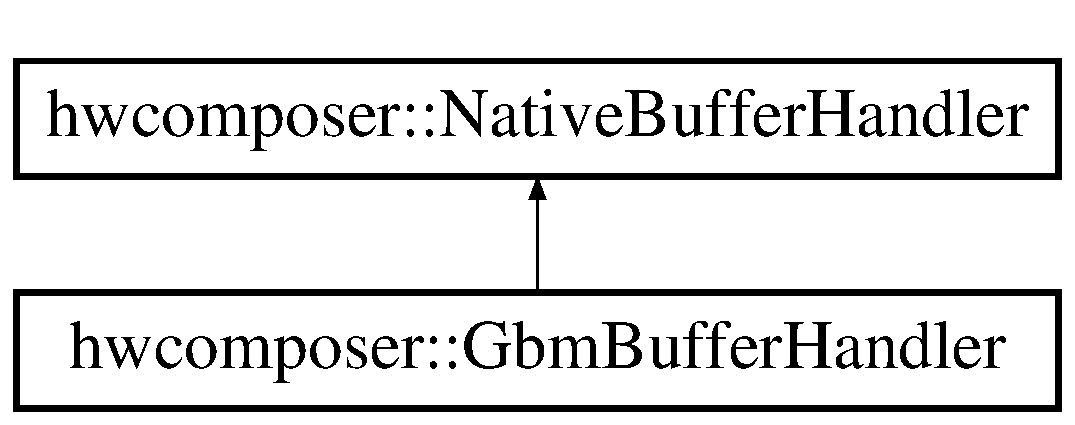
\includegraphics[height=2.000000cm]{classhwcomposer_1_1GbmBufferHandler}
\end{center}
\end{figure}
\subsection*{Public Member Functions}
\begin{DoxyCompactItemize}
\item 
\mbox{\hyperlink{classhwcomposer_1_1GbmBufferHandler_a2dd2cbac7542ffaead762e797ab673cc}{Gbm\+Buffer\+Handler}} (uint32\+\_\+t fd)
\item 
\mbox{\hyperlink{classhwcomposer_1_1GbmBufferHandler_a253daef320a4a3376640a5add7f3bc15}{$\sim$\+Gbm\+Buffer\+Handler}} () override
\item 
bool \mbox{\hyperlink{classhwcomposer_1_1GbmBufferHandler_a2338ce2352177ab7a3d01376bcce7381}{Init}} ()
\item 
bool \mbox{\hyperlink{classhwcomposer_1_1GbmBufferHandler_adf982a610866df90e9a2ee4f04801387}{Create\+Buffer}} (uint32\+\_\+t w, uint32\+\_\+t h, int format, \mbox{\hyperlink{alios_2platformdefines_8h_ac0a2eaf260f556d17fe489911f017bdf}{H\+W\+C\+Native\+Handle}} $\ast$handle, uint32\+\_\+t layer\+\_\+type=k\+Layer\+Normal, bool $\ast$modifier\+\_\+used=\mbox{\hyperlink{alios_2platformdefines_8h_a070d2ce7b6bb7e5c05602aa8c308d0c4}{N\+U\+LL}}, int64\+\_\+t modifier=-\/1, bool raw\+\_\+pixel\+\_\+buffer=false) const override
\item 
bool \mbox{\hyperlink{classhwcomposer_1_1GbmBufferHandler_a9c2554d5c2fe0a76b785352754d369a1}{Release\+Buffer}} (\mbox{\hyperlink{alios_2platformdefines_8h_ac0a2eaf260f556d17fe489911f017bdf}{H\+W\+C\+Native\+Handle}} handle) const override
\item 
void \mbox{\hyperlink{classhwcomposer_1_1GbmBufferHandler_a0786f7b82b504105c71881eced9b5270}{Destroy\+Handle}} (\mbox{\hyperlink{alios_2platformdefines_8h_ac0a2eaf260f556d17fe489911f017bdf}{H\+W\+C\+Native\+Handle}} handle) const override
\item 
void \mbox{\hyperlink{classhwcomposer_1_1GbmBufferHandler_ae730a1b13a177dcf02084c0c60bcafb6}{Copy\+Handle}} (\mbox{\hyperlink{alios_2platformdefines_8h_ac0a2eaf260f556d17fe489911f017bdf}{H\+W\+C\+Native\+Handle}} source, \mbox{\hyperlink{alios_2platformdefines_8h_ac0a2eaf260f556d17fe489911f017bdf}{H\+W\+C\+Native\+Handle}} $\ast$target) const override
\item 
bool \mbox{\hyperlink{classhwcomposer_1_1GbmBufferHandler_a552812693a793705e94138855daaead0}{Import\+Buffer}} (\mbox{\hyperlink{alios_2platformdefines_8h_ac0a2eaf260f556d17fe489911f017bdf}{H\+W\+C\+Native\+Handle}} handle) const override
\item 
uint32\+\_\+t \mbox{\hyperlink{classhwcomposer_1_1GbmBufferHandler_a55b6cac51fced2198ae9aee706d03452}{Get\+Total\+Planes}} (\mbox{\hyperlink{alios_2platformdefines_8h_ac0a2eaf260f556d17fe489911f017bdf}{H\+W\+C\+Native\+Handle}} handle) const override
\item 
void $\ast$ \mbox{\hyperlink{classhwcomposer_1_1GbmBufferHandler_ad6120de07407c36ed5ab99c8fcb628fd}{Map}} (\mbox{\hyperlink{alios_2platformdefines_8h_ac0a2eaf260f556d17fe489911f017bdf}{H\+W\+C\+Native\+Handle}} handle, uint32\+\_\+t x, uint32\+\_\+t y, uint32\+\_\+t width, uint32\+\_\+t height, uint32\+\_\+t $\ast$stride, void $\ast$$\ast$map\+\_\+data, size\+\_\+t plane) const override
\item 
int32\+\_\+t \mbox{\hyperlink{classhwcomposer_1_1GbmBufferHandler_af26a61bbdd91d36780e41b406e8b8dd9}{Un\+Map}} (\mbox{\hyperlink{alios_2platformdefines_8h_ac0a2eaf260f556d17fe489911f017bdf}{H\+W\+C\+Native\+Handle}} handle, void $\ast$map\+\_\+data) const override
\item 
uint32\+\_\+t \mbox{\hyperlink{classhwcomposer_1_1GbmBufferHandler_ac204254aef6007d09474f8e76f9b6470}{Get\+Fd}} () const override
\end{DoxyCompactItemize}
\subsection*{Additional Inherited Members}


\subsection{Detailed Description}


Definition at line 28 of file gbmbufferhandler.\+h.



\subsection{Constructor \& Destructor Documentation}
\mbox{\Hypertarget{classhwcomposer_1_1GbmBufferHandler_a2dd2cbac7542ffaead762e797ab673cc}\label{classhwcomposer_1_1GbmBufferHandler_a2dd2cbac7542ffaead762e797ab673cc}} 
\index{hwcomposer\+::\+Gbm\+Buffer\+Handler@{hwcomposer\+::\+Gbm\+Buffer\+Handler}!Gbm\+Buffer\+Handler@{Gbm\+Buffer\+Handler}}
\index{Gbm\+Buffer\+Handler@{Gbm\+Buffer\+Handler}!hwcomposer\+::\+Gbm\+Buffer\+Handler@{hwcomposer\+::\+Gbm\+Buffer\+Handler}}
\subsubsection{\texorpdfstring{Gbm\+Buffer\+Handler()}{GbmBufferHandler()}}
{\footnotesize\ttfamily hwcomposer\+::\+Gbm\+Buffer\+Handler\+::\+Gbm\+Buffer\+Handler (\begin{DoxyParamCaption}\item[{uint32\+\_\+t}]{fd }\end{DoxyParamCaption})\hspace{0.3cm}{\ttfamily [explicit]}}



Definition at line 47 of file gbmbufferhandler.\+cpp.


\begin{DoxyCode}{0}
\DoxyCodeLine{48     : fd\_(fd),}
\DoxyCodeLine{49       device\_(0),}
\DoxyCodeLine{50       preferred\_cursor\_width\_(0),}
\DoxyCodeLine{51       preferred\_cursor\_height\_(0) \{}
\DoxyCodeLine{52 \}}
\end{DoxyCode}
\mbox{\Hypertarget{classhwcomposer_1_1GbmBufferHandler_a253daef320a4a3376640a5add7f3bc15}\label{classhwcomposer_1_1GbmBufferHandler_a253daef320a4a3376640a5add7f3bc15}} 
\index{hwcomposer\+::\+Gbm\+Buffer\+Handler@{hwcomposer\+::\+Gbm\+Buffer\+Handler}!````~Gbm\+Buffer\+Handler@{$\sim$\+Gbm\+Buffer\+Handler}}
\index{````~Gbm\+Buffer\+Handler@{$\sim$\+Gbm\+Buffer\+Handler}!hwcomposer\+::\+Gbm\+Buffer\+Handler@{hwcomposer\+::\+Gbm\+Buffer\+Handler}}
\subsubsection{\texorpdfstring{$\sim$\+Gbm\+Buffer\+Handler()}{~GbmBufferHandler()}}
{\footnotesize\ttfamily hwcomposer\+::\+Gbm\+Buffer\+Handler\+::$\sim$\+Gbm\+Buffer\+Handler (\begin{DoxyParamCaption}{ }\end{DoxyParamCaption})\hspace{0.3cm}{\ttfamily [override]}}



Definition at line 54 of file gbmbufferhandler.\+cpp.


\begin{DoxyCode}{0}
\DoxyCodeLine{54                                     \{}
\DoxyCodeLine{55   \textcolor{keywordflow}{if} (device\_)}
\DoxyCodeLine{56     gbm\_device\_destroy(device\_);}
\DoxyCodeLine{57 \}}
\end{DoxyCode}


\subsection{Member Function Documentation}
\mbox{\Hypertarget{classhwcomposer_1_1GbmBufferHandler_ae730a1b13a177dcf02084c0c60bcafb6}\label{classhwcomposer_1_1GbmBufferHandler_ae730a1b13a177dcf02084c0c60bcafb6}} 
\index{hwcomposer\+::\+Gbm\+Buffer\+Handler@{hwcomposer\+::\+Gbm\+Buffer\+Handler}!Copy\+Handle@{Copy\+Handle}}
\index{Copy\+Handle@{Copy\+Handle}!hwcomposer\+::\+Gbm\+Buffer\+Handler@{hwcomposer\+::\+Gbm\+Buffer\+Handler}}
\subsubsection{\texorpdfstring{Copy\+Handle()}{CopyHandle()}}
{\footnotesize\ttfamily void hwcomposer\+::\+Gbm\+Buffer\+Handler\+::\+Copy\+Handle (\begin{DoxyParamCaption}\item[{\mbox{\hyperlink{alios_2platformdefines_8h_ac0a2eaf260f556d17fe489911f017bdf}{H\+W\+C\+Native\+Handle}}}]{source,  }\item[{\mbox{\hyperlink{alios_2platformdefines_8h_ac0a2eaf260f556d17fe489911f017bdf}{H\+W\+C\+Native\+Handle}} $\ast$}]{target }\end{DoxyParamCaption}) const\hspace{0.3cm}{\ttfamily [override]}, {\ttfamily [virtual]}}



Implements \mbox{\hyperlink{classhwcomposer_1_1NativeBufferHandler_a96581fb8bd36e959c8da6b9f634ecd32}{hwcomposer\+::\+Native\+Buffer\+Handler}}.



Definition at line 220 of file gbmbufferhandler.\+cpp.


\begin{DoxyCode}{0}
\DoxyCodeLine{221                                                                  \{}
\DoxyCodeLine{222   \textcolor{keyword}{struct }\mbox{\hyperlink{structgbm__handle}{gbm\_handle}} *temp = \textcolor{keyword}{new} \textcolor{keyword}{struct }\mbox{\hyperlink{structgbm__handle}{gbm\_handle}}();}
\DoxyCodeLine{223 }
\DoxyCodeLine{224   \textcolor{keywordflow}{if} (!source->\mbox{\hyperlink{structyalloc__handle_a2dfa4e2505a052e5ddbbe66e32b33875}{meta\_data\_}}.\mbox{\hyperlink{structHwcBuffer_ad16028811f8af57430b65129bf7ae67a}{fb\_modifiers\_}}[0]) \{}
\DoxyCodeLine{225     temp->\mbox{\hyperlink{structgbm__handle_ac2450148a271a449b35ff12966de8518}{import\_data}}.\mbox{\hyperlink{structgbm__handle_ae11f3776ec272cc4b10ec0625b647170}{fd\_data}}.width = source->import\_data.fd\_data.width;}
\DoxyCodeLine{226     temp->\mbox{\hyperlink{structgbm__handle_ac2450148a271a449b35ff12966de8518}{import\_data}}.\mbox{\hyperlink{structgbm__handle_ae11f3776ec272cc4b10ec0625b647170}{fd\_data}}.height = source->import\_data.fd\_data.height;}
\DoxyCodeLine{227     temp->\mbox{\hyperlink{structgbm__handle_ac2450148a271a449b35ff12966de8518}{import\_data}}.\mbox{\hyperlink{structgbm__handle_ae11f3776ec272cc4b10ec0625b647170}{fd\_data}}.format = source->import\_data.fd\_data.format;}
\DoxyCodeLine{228     temp->\mbox{\hyperlink{structgbm__handle_ac2450148a271a449b35ff12966de8518}{import\_data}}.\mbox{\hyperlink{structgbm__handle_ae11f3776ec272cc4b10ec0625b647170}{fd\_data}}.fd = dup(source->import\_data.fd\_data.fd);}
\DoxyCodeLine{229     temp->\mbox{\hyperlink{structgbm__handle_ac2450148a271a449b35ff12966de8518}{import\_data}}.\mbox{\hyperlink{structgbm__handle_ae11f3776ec272cc4b10ec0625b647170}{fd\_data}}.stride = source->import\_data.fd\_data.stride;}
\DoxyCodeLine{230   \} \textcolor{keywordflow}{else} \{}
\DoxyCodeLine{231     temp->\mbox{\hyperlink{structgbm__handle_ac2450148a271a449b35ff12966de8518}{import\_data}}.\mbox{\hyperlink{structgbm__handle_af706ddaa68480c1cf930a67d6698c1d6}{fd\_modifier\_data}}.width =}
\DoxyCodeLine{232         source->import\_data.fd\_modifier\_data.width;}
\DoxyCodeLine{233     temp->\mbox{\hyperlink{structgbm__handle_ac2450148a271a449b35ff12966de8518}{import\_data}}.\mbox{\hyperlink{structgbm__handle_af706ddaa68480c1cf930a67d6698c1d6}{fd\_modifier\_data}}.height =}
\DoxyCodeLine{234         source->import\_data.fd\_modifier\_data.height;}
\DoxyCodeLine{235     temp->\mbox{\hyperlink{structgbm__handle_ac2450148a271a449b35ff12966de8518}{import\_data}}.\mbox{\hyperlink{structgbm__handle_af706ddaa68480c1cf930a67d6698c1d6}{fd\_modifier\_data}}.format =}
\DoxyCodeLine{236         source->import\_data.fd\_modifier\_data.format;}
\DoxyCodeLine{237     temp->\mbox{\hyperlink{structgbm__handle_ac2450148a271a449b35ff12966de8518}{import\_data}}.\mbox{\hyperlink{structgbm__handle_af706ddaa68480c1cf930a67d6698c1d6}{fd\_modifier\_data}}.num\_fds =}
\DoxyCodeLine{238         source->import\_data.fd\_modifier\_data.num\_fds;}
\DoxyCodeLine{239 }
\DoxyCodeLine{240     \textcolor{keywordflow}{for} (\textcolor{keywordtype}{size\_t} i = 0; i < temp->\mbox{\hyperlink{structgbm__handle_ac2450148a271a449b35ff12966de8518}{import\_data}}.\mbox{\hyperlink{structgbm__handle_af706ddaa68480c1cf930a67d6698c1d6}{fd\_modifier\_data}}.num\_fds; i++) \{}
\DoxyCodeLine{241       temp->\mbox{\hyperlink{structgbm__handle_ac2450148a271a449b35ff12966de8518}{import\_data}}.\mbox{\hyperlink{structgbm__handle_af706ddaa68480c1cf930a67d6698c1d6}{fd\_modifier\_data}}.fds[i] =}
\DoxyCodeLine{242           dup(source->import\_data.fd\_modifier\_data.fds[i]);}
\DoxyCodeLine{243     \}}
\DoxyCodeLine{244 }
\DoxyCodeLine{245     \textcolor{keywordtype}{size\_t} total\_planes = source->\mbox{\hyperlink{structyalloc__handle_a2dfa4e2505a052e5ddbbe66e32b33875}{meta\_data\_}}.\mbox{\hyperlink{structHwcBuffer_ab48df5577e8ecd60f18b4b5e6ec6544d}{num\_planes\_}};}
\DoxyCodeLine{246 }
\DoxyCodeLine{247     \textcolor{keywordflow}{for} (\textcolor{keywordtype}{size\_t} i = 0; i < total\_planes; i++) \{}
\DoxyCodeLine{248       temp->\mbox{\hyperlink{structgbm__handle_ac2450148a271a449b35ff12966de8518}{import\_data}}.\mbox{\hyperlink{structgbm__handle_af706ddaa68480c1cf930a67d6698c1d6}{fd\_modifier\_data}}.offsets[i] =}
\DoxyCodeLine{249           source->import\_data.fd\_modifier\_data.offsets[i];}
\DoxyCodeLine{250       temp->\mbox{\hyperlink{structgbm__handle_ac2450148a271a449b35ff12966de8518}{import\_data}}.\mbox{\hyperlink{structgbm__handle_af706ddaa68480c1cf930a67d6698c1d6}{fd\_modifier\_data}}.strides[i] =}
\DoxyCodeLine{251           source->import\_data.fd\_modifier\_data.strides[i];}
\DoxyCodeLine{252       temp->\mbox{\hyperlink{structgbm__handle_a2d3bce2c387abbf976b37d52b272ebbe}{meta\_data\_}}.\mbox{\hyperlink{structHwcBuffer_ad16028811f8af57430b65129bf7ae67a}{fb\_modifiers\_}}[2 * i] =}
\DoxyCodeLine{253           source->\mbox{\hyperlink{structyalloc__handle_a2dfa4e2505a052e5ddbbe66e32b33875}{meta\_data\_}}.\mbox{\hyperlink{structHwcBuffer_ad16028811f8af57430b65129bf7ae67a}{fb\_modifiers\_}}[2 * i];}
\DoxyCodeLine{254       temp->\mbox{\hyperlink{structgbm__handle_a2d3bce2c387abbf976b37d52b272ebbe}{meta\_data\_}}.\mbox{\hyperlink{structHwcBuffer_ad16028811f8af57430b65129bf7ae67a}{fb\_modifiers\_}}[2 * i + 1] =}
\DoxyCodeLine{255           source->\mbox{\hyperlink{structyalloc__handle_a2dfa4e2505a052e5ddbbe66e32b33875}{meta\_data\_}}.\mbox{\hyperlink{structHwcBuffer_ad16028811f8af57430b65129bf7ae67a}{fb\_modifiers\_}}[2 * i + 1];}
\DoxyCodeLine{256     \}}
\DoxyCodeLine{257 }
\DoxyCodeLine{258     temp->\mbox{\hyperlink{structgbm__handle_ac2450148a271a449b35ff12966de8518}{import\_data}}.\mbox{\hyperlink{structgbm__handle_af706ddaa68480c1cf930a67d6698c1d6}{fd\_modifier\_data}}.modifier =}
\DoxyCodeLine{259         source->import\_data.fd\_modifier\_data.modifier;}
\DoxyCodeLine{260   \}}
\DoxyCodeLine{261 }
\DoxyCodeLine{262   temp->\mbox{\hyperlink{structgbm__handle_a9010ca6ee25cee546643f6d6c5b6c4cf}{bo}} = source->bo;}
\DoxyCodeLine{263   temp->\mbox{\hyperlink{structgbm__handle_a2d3bce2c387abbf976b37d52b272ebbe}{meta\_data\_}}.\mbox{\hyperlink{structHwcBuffer_ab48df5577e8ecd60f18b4b5e6ec6544d}{num\_planes\_}} = source->\mbox{\hyperlink{structyalloc__handle_a2dfa4e2505a052e5ddbbe66e32b33875}{meta\_data\_}}.
      \mbox{\hyperlink{structHwcBuffer_ab48df5577e8ecd60f18b4b5e6ec6544d}{num\_planes\_}};}
\DoxyCodeLine{264   temp->\mbox{\hyperlink{structgbm__handle_a5deee85dd01fe245644d1971dcdd1f89}{gbm\_flags}} = source->gbm\_flags;}
\DoxyCodeLine{265   temp->\mbox{\hyperlink{structgbm__handle_aeaaf0fd4477abfe406de45109d6af33c}{layer\_type\_}} = source->layer\_type\_;}
\DoxyCodeLine{266   *target = temp;}
\DoxyCodeLine{267 \}}
\end{DoxyCode}
\mbox{\Hypertarget{classhwcomposer_1_1GbmBufferHandler_adf982a610866df90e9a2ee4f04801387}\label{classhwcomposer_1_1GbmBufferHandler_adf982a610866df90e9a2ee4f04801387}} 
\index{hwcomposer\+::\+Gbm\+Buffer\+Handler@{hwcomposer\+::\+Gbm\+Buffer\+Handler}!Create\+Buffer@{Create\+Buffer}}
\index{Create\+Buffer@{Create\+Buffer}!hwcomposer\+::\+Gbm\+Buffer\+Handler@{hwcomposer\+::\+Gbm\+Buffer\+Handler}}
\subsubsection{\texorpdfstring{Create\+Buffer()}{CreateBuffer()}}
{\footnotesize\ttfamily bool hwcomposer\+::\+Gbm\+Buffer\+Handler\+::\+Create\+Buffer (\begin{DoxyParamCaption}\item[{uint32\+\_\+t}]{w,  }\item[{uint32\+\_\+t}]{h,  }\item[{int}]{format,  }\item[{\mbox{\hyperlink{alios_2platformdefines_8h_ac0a2eaf260f556d17fe489911f017bdf}{H\+W\+C\+Native\+Handle}} $\ast$}]{handle,  }\item[{uint32\+\_\+t}]{layer\+\_\+type = {\ttfamily kLayerNormal},  }\item[{bool $\ast$}]{modifier\+\_\+used = {\ttfamily \mbox{\hyperlink{alios_2platformdefines_8h_a070d2ce7b6bb7e5c05602aa8c308d0c4}{N\+U\+LL}}},  }\item[{int64\+\_\+t}]{modifier = {\ttfamily -\/1},  }\item[{bool}]{raw\+\_\+pixel\+\_\+buffer = {\ttfamily false} }\end{DoxyParamCaption}) const\hspace{0.3cm}{\ttfamily [override]}, {\ttfamily [virtual]}}



Implements \mbox{\hyperlink{classhwcomposer_1_1NativeBufferHandler_a7e58e3d81d3f56cbee34c963b4999fde}{hwcomposer\+::\+Native\+Buffer\+Handler}}.



Definition at line 84 of file gbmbufferhandler.\+cpp.


\begin{DoxyCode}{0}
\DoxyCodeLine{88                                                                  \{}
\DoxyCodeLine{89   uint32\_t gbm\_format = format;}
\DoxyCodeLine{90   \textcolor{keywordflow}{if} (gbm\_format == 0)}
\DoxyCodeLine{91     gbm\_format = GBM\_FORMAT\_XRGB8888;}
\DoxyCodeLine{92 }
\DoxyCodeLine{93   uint32\_t flags = 0;}
\DoxyCodeLine{94 }
\DoxyCodeLine{95   \textcolor{keywordflow}{if} (layer\_type == kLayerNormal || layer\_type == kLayerCursor) \{}
\DoxyCodeLine{96     flags |= (GBM\_BO\_USE\_SCANOUT | GBM\_BO\_USE\_RENDERING);}
\DoxyCodeLine{97   \}}
\DoxyCodeLine{98 }
\DoxyCodeLine{99   \textcolor{keywordflow}{if} (raw\_pixel\_buffer) \{}
\DoxyCodeLine{100     flags |= GBM\_BO\_USE\_LINEAR;}
\DoxyCodeLine{101   \}}
\DoxyCodeLine{102 }
\DoxyCodeLine{103   \textcolor{keywordflow}{if} (layer\_type == kLayerCursor) \{}
\DoxyCodeLine{104     \textcolor{keywordflow}{if} (w < preferred\_cursor\_width\_)}
\DoxyCodeLine{105       w = preferred\_cursor\_width\_;}
\DoxyCodeLine{106 }
\DoxyCodeLine{107     \textcolor{keywordflow}{if} (h < preferred\_cursor\_height\_)}
\DoxyCodeLine{108       h = preferred\_cursor\_height\_;}
\DoxyCodeLine{109   \}}
\DoxyCodeLine{110 }
\DoxyCodeLine{111   \textcolor{keyword}{struct }gbm\_bo *bo = \mbox{\hyperlink{alios_2platformdefines_8h_a070d2ce7b6bb7e5c05602aa8c308d0c4}{NULL}};}
\DoxyCodeLine{112 }
\DoxyCodeLine{113   \textcolor{keywordtype}{bool} rbc\_enabled = \textcolor{keyword}{false};}
\DoxyCodeLine{114   uint64\_t modifier = DRM\_FORMAT\_MOD\_NONE;}
\DoxyCodeLine{115 \textcolor{preprocessor}{\#ifdef ENABLE\_RBC}}
\DoxyCodeLine{116   \textcolor{keywordflow}{if} (preferred\_modifier != -1) \{}
\DoxyCodeLine{117     modifier = preferred\_modifier;}
\DoxyCodeLine{118   \} \textcolor{keywordflow}{else} \{}
\DoxyCodeLine{119     modifier = choose\_drm\_modifier(gbm\_format);}
\DoxyCodeLine{120   \}}
\DoxyCodeLine{121 }
\DoxyCodeLine{122   \textcolor{keywordflow}{if} (modifier\_used) \{}
\DoxyCodeLine{123     *modifier\_used = \textcolor{keyword}{true};}
\DoxyCodeLine{124   \}}
\DoxyCodeLine{125 \textcolor{preprocessor}{\#else}}
\DoxyCodeLine{126   \textcolor{keywordflow}{if} (modifier\_used) \{}
\DoxyCodeLine{127     *modifier\_used = \textcolor{keyword}{false};}
\DoxyCodeLine{128   \}}
\DoxyCodeLine{129 \textcolor{preprocessor}{\#endif}}
\DoxyCodeLine{130 }
\DoxyCodeLine{131   \textcolor{keywordflow}{if} (modifier != DRM\_FORMAT\_MOD\_NONE) \{}
\DoxyCodeLine{132     bo = gbm\_bo\_create\_with\_modifiers(device\_, w, h, gbm\_format, \&modifier, 1);}
\DoxyCodeLine{133     rbc\_enabled = \textcolor{keyword}{true};}
\DoxyCodeLine{134   \} \textcolor{keywordflow}{else} \{}
\DoxyCodeLine{135     bo = gbm\_bo\_create(device\_, w, h, gbm\_format, flags);}
\DoxyCodeLine{136   \}}
\DoxyCodeLine{137 }
\DoxyCodeLine{138   \textcolor{keywordflow}{if} (!bo) \{}
\DoxyCodeLine{139     flags \&= ~GBM\_BO\_USE\_SCANOUT;}
\DoxyCodeLine{140     bo = gbm\_bo\_create(device\_, w, h, gbm\_format, flags);}
\DoxyCodeLine{141     rbc\_enabled = \textcolor{keyword}{false};}
\DoxyCodeLine{142   \}}
\DoxyCodeLine{143 }
\DoxyCodeLine{144   \textcolor{keywordflow}{if} (!bo) \{}
\DoxyCodeLine{145     flags \&= ~GBM\_BO\_USE\_RENDERING;}
\DoxyCodeLine{146     bo = gbm\_bo\_create(device\_, w, h, gbm\_format, flags);}
\DoxyCodeLine{147   \}}
\DoxyCodeLine{148 }
\DoxyCodeLine{149   \textcolor{keywordflow}{if} (!bo) \{}
\DoxyCodeLine{150     \mbox{\hyperlink{alios_2platformdefines_8h_a226d6c99e4bcfca193c095e085e9097d}{ETRACE}}(\textcolor{stringliteral}{"GbmBufferHandler: failed to create gbm\_bo"});}
\DoxyCodeLine{151     \textcolor{keywordflow}{return} \textcolor{keyword}{false};}
\DoxyCodeLine{152   \}}
\DoxyCodeLine{153 }
\DoxyCodeLine{154   \textcolor{keyword}{struct }\mbox{\hyperlink{structgbm__handle}{gbm\_handle}} *temp = \textcolor{keyword}{new} \textcolor{keyword}{struct }\mbox{\hyperlink{structgbm__handle}{gbm\_handle}}();}
\DoxyCodeLine{155   uint64\_t mod = 0;}
\DoxyCodeLine{156 }
\DoxyCodeLine{157   \textcolor{keywordflow}{if} (rbc\_enabled) \{}
\DoxyCodeLine{158     temp->\mbox{\hyperlink{structgbm__handle_a2d3bce2c387abbf976b37d52b272ebbe}{meta\_data\_}}.\mbox{\hyperlink{structHwcBuffer_ab48df5577e8ecd60f18b4b5e6ec6544d}{num\_planes\_}} = gbm\_bo\_get\_plane\_count(
      \mbox{\hyperlink{structgbm__handle_a9010ca6ee25cee546643f6d6c5b6c4cf}{bo}});}
\DoxyCodeLine{159     temp->\mbox{\hyperlink{structgbm__handle_ac2450148a271a449b35ff12966de8518}{import\_data}}.\mbox{\hyperlink{structgbm__handle_af706ddaa68480c1cf930a67d6698c1d6}{fd\_modifier\_data}}.width = gbm\_bo\_get\_width(
      \mbox{\hyperlink{structgbm__handle_a9010ca6ee25cee546643f6d6c5b6c4cf}{bo}});}
\DoxyCodeLine{160     temp->\mbox{\hyperlink{structgbm__handle_ac2450148a271a449b35ff12966de8518}{import\_data}}.\mbox{\hyperlink{structgbm__handle_af706ddaa68480c1cf930a67d6698c1d6}{fd\_modifier\_data}}.height = gbm\_bo\_get\_height(
      \mbox{\hyperlink{structgbm__handle_a9010ca6ee25cee546643f6d6c5b6c4cf}{bo}});}
\DoxyCodeLine{161     temp->\mbox{\hyperlink{structgbm__handle_ac2450148a271a449b35ff12966de8518}{import\_data}}.\mbox{\hyperlink{structgbm__handle_af706ddaa68480c1cf930a67d6698c1d6}{fd\_modifier\_data}}.format = gbm\_bo\_get\_format(
      \mbox{\hyperlink{structgbm__handle_a9010ca6ee25cee546643f6d6c5b6c4cf}{bo}});}
\DoxyCodeLine{162     temp->\mbox{\hyperlink{structgbm__handle_ac2450148a271a449b35ff12966de8518}{import\_data}}.\mbox{\hyperlink{structgbm__handle_af706ddaa68480c1cf930a67d6698c1d6}{fd\_modifier\_data}}.num\_fds = 1;}
\DoxyCodeLine{163     temp->\mbox{\hyperlink{structgbm__handle_ac2450148a271a449b35ff12966de8518}{import\_data}}.\mbox{\hyperlink{structgbm__handle_af706ddaa68480c1cf930a67d6698c1d6}{fd\_modifier\_data}}.fds[0] = gbm\_bo\_get\_fd(
      \mbox{\hyperlink{structgbm__handle_a9010ca6ee25cee546643f6d6c5b6c4cf}{bo}});}
\DoxyCodeLine{164 }
\DoxyCodeLine{165     temp->\mbox{\hyperlink{structgbm__handle_ac2450148a271a449b35ff12966de8518}{import\_data}}.\mbox{\hyperlink{structgbm__handle_af706ddaa68480c1cf930a67d6698c1d6}{fd\_modifier\_data}}.modifier = gbm\_bo\_get\_modifier(
      \mbox{\hyperlink{structgbm__handle_a9010ca6ee25cee546643f6d6c5b6c4cf}{bo}});}
\DoxyCodeLine{166     mod = temp->\mbox{\hyperlink{structgbm__handle_ac2450148a271a449b35ff12966de8518}{import\_data}}.\mbox{\hyperlink{structgbm__handle_af706ddaa68480c1cf930a67d6698c1d6}{fd\_modifier\_data}}.modifier;}
\DoxyCodeLine{167     uint32\_t modifier\_low = \textcolor{keyword}{static\_cast<}uint32\_t\textcolor{keyword}{>}(mod >> 32);}
\DoxyCodeLine{168     uint32\_t modifier\_high = \textcolor{keyword}{static\_cast<}uint32\_t\textcolor{keyword}{>}(mod);}
\DoxyCodeLine{169 }
\DoxyCodeLine{170     \textcolor{keywordflow}{for} (\textcolor{keywordtype}{size\_t} i = 0; i < temp->\mbox{\hyperlink{structgbm__handle_a2d3bce2c387abbf976b37d52b272ebbe}{meta\_data\_}}.\mbox{\hyperlink{structHwcBuffer_ab48df5577e8ecd60f18b4b5e6ec6544d}{num\_planes\_}}; i++) \{}
\DoxyCodeLine{171       temp->\mbox{\hyperlink{structgbm__handle_ac2450148a271a449b35ff12966de8518}{import\_data}}.\mbox{\hyperlink{structgbm__handle_af706ddaa68480c1cf930a67d6698c1d6}{fd\_modifier\_data}}.offsets[i] = gbm\_bo\_get\_offset(
      \mbox{\hyperlink{structgbm__handle_a9010ca6ee25cee546643f6d6c5b6c4cf}{bo}}, i);}
\DoxyCodeLine{172       temp->\mbox{\hyperlink{structgbm__handle_ac2450148a271a449b35ff12966de8518}{import\_data}}.\mbox{\hyperlink{structgbm__handle_af706ddaa68480c1cf930a67d6698c1d6}{fd\_modifier\_data}}.strides[i] =}
\DoxyCodeLine{173           gbm\_bo\_get\_stride\_for\_plane(\mbox{\hyperlink{structgbm__handle_a9010ca6ee25cee546643f6d6c5b6c4cf}{bo}}, i);}
\DoxyCodeLine{174       temp->\mbox{\hyperlink{structgbm__handle_a2d3bce2c387abbf976b37d52b272ebbe}{meta\_data\_}}.\mbox{\hyperlink{structHwcBuffer_ad16028811f8af57430b65129bf7ae67a}{fb\_modifiers\_}}[2 * i] = modifier\_low;}
\DoxyCodeLine{175       temp->\mbox{\hyperlink{structgbm__handle_a2d3bce2c387abbf976b37d52b272ebbe}{meta\_data\_}}.\mbox{\hyperlink{structHwcBuffer_ad16028811f8af57430b65129bf7ae67a}{fb\_modifiers\_}}[2 * i + 1] = modifier\_high;}
\DoxyCodeLine{176     \}}
\DoxyCodeLine{177   \} \textcolor{keywordflow}{else} \{}
\DoxyCodeLine{178     temp->\mbox{\hyperlink{structgbm__handle_ac2450148a271a449b35ff12966de8518}{import\_data}}.\mbox{\hyperlink{structgbm__handle_ae11f3776ec272cc4b10ec0625b647170}{fd\_data}}.width = gbm\_bo\_get\_width(\mbox{\hyperlink{structgbm__handle_a9010ca6ee25cee546643f6d6c5b6c4cf}{bo}});}
\DoxyCodeLine{179     temp->\mbox{\hyperlink{structgbm__handle_ac2450148a271a449b35ff12966de8518}{import\_data}}.\mbox{\hyperlink{structgbm__handle_ae11f3776ec272cc4b10ec0625b647170}{fd\_data}}.height = gbm\_bo\_get\_height(\mbox{\hyperlink{structgbm__handle_a9010ca6ee25cee546643f6d6c5b6c4cf}{bo}});}
\DoxyCodeLine{180     temp->\mbox{\hyperlink{structgbm__handle_ac2450148a271a449b35ff12966de8518}{import\_data}}.\mbox{\hyperlink{structgbm__handle_ae11f3776ec272cc4b10ec0625b647170}{fd\_data}}.format = gbm\_bo\_get\_format(\mbox{\hyperlink{structgbm__handle_a9010ca6ee25cee546643f6d6c5b6c4cf}{bo}});}
\DoxyCodeLine{181     temp->\mbox{\hyperlink{structgbm__handle_ac2450148a271a449b35ff12966de8518}{import\_data}}.\mbox{\hyperlink{structgbm__handle_ae11f3776ec272cc4b10ec0625b647170}{fd\_data}}.fd = gbm\_bo\_get\_fd(\mbox{\hyperlink{structgbm__handle_a9010ca6ee25cee546643f6d6c5b6c4cf}{bo}});}
\DoxyCodeLine{182     temp->\mbox{\hyperlink{structgbm__handle_ac2450148a271a449b35ff12966de8518}{import\_data}}.\mbox{\hyperlink{structgbm__handle_ae11f3776ec272cc4b10ec0625b647170}{fd\_data}}.stride = gbm\_bo\_get\_stride(\mbox{\hyperlink{structgbm__handle_a9010ca6ee25cee546643f6d6c5b6c4cf}{bo}});}
\DoxyCodeLine{183   \}}
\DoxyCodeLine{184 }
\DoxyCodeLine{185   temp->\mbox{\hyperlink{structgbm__handle_a9010ca6ee25cee546643f6d6c5b6c4cf}{bo}} = \mbox{\hyperlink{structgbm__handle_a9010ca6ee25cee546643f6d6c5b6c4cf}{bo}};}
\DoxyCodeLine{186   temp->\mbox{\hyperlink{structgbm__handle_aa98e98315d3cd7596b980b80e1199649}{hwc\_buffer\_}} = \textcolor{keyword}{true};}
\DoxyCodeLine{187   temp->\mbox{\hyperlink{structgbm__handle_a5deee85dd01fe245644d1971dcdd1f89}{gbm\_flags}} = flags;}
\DoxyCodeLine{188   temp->\mbox{\hyperlink{structgbm__handle_aeaaf0fd4477abfe406de45109d6af33c}{layer\_type\_}} = layer\_type;}
\DoxyCodeLine{189   *handle = temp;}
\DoxyCodeLine{190 }
\DoxyCodeLine{191   \textcolor{keywordflow}{return} \textcolor{keyword}{true};}
\DoxyCodeLine{192 \}}
\end{DoxyCode}
\mbox{\Hypertarget{classhwcomposer_1_1GbmBufferHandler_a0786f7b82b504105c71881eced9b5270}\label{classhwcomposer_1_1GbmBufferHandler_a0786f7b82b504105c71881eced9b5270}} 
\index{hwcomposer\+::\+Gbm\+Buffer\+Handler@{hwcomposer\+::\+Gbm\+Buffer\+Handler}!Destroy\+Handle@{Destroy\+Handle}}
\index{Destroy\+Handle@{Destroy\+Handle}!hwcomposer\+::\+Gbm\+Buffer\+Handler@{hwcomposer\+::\+Gbm\+Buffer\+Handler}}
\subsubsection{\texorpdfstring{Destroy\+Handle()}{DestroyHandle()}}
{\footnotesize\ttfamily void hwcomposer\+::\+Gbm\+Buffer\+Handler\+::\+Destroy\+Handle (\begin{DoxyParamCaption}\item[{\mbox{\hyperlink{alios_2platformdefines_8h_ac0a2eaf260f556d17fe489911f017bdf}{H\+W\+C\+Native\+Handle}}}]{handle }\end{DoxyParamCaption}) const\hspace{0.3cm}{\ttfamily [override]}, {\ttfamily [virtual]}}



Implements \mbox{\hyperlink{classhwcomposer_1_1NativeBufferHandler_ab1e22d9737ca9f6c3e75d1b550e34ce9}{hwcomposer\+::\+Native\+Buffer\+Handler}}.



Definition at line 215 of file gbmbufferhandler.\+cpp.


\begin{DoxyCode}{0}
\DoxyCodeLine{215                                                                  \{}
\DoxyCodeLine{216   \textcolor{keyword}{delete} handle;}
\DoxyCodeLine{217   handle = \mbox{\hyperlink{alios_2platformdefines_8h_a070d2ce7b6bb7e5c05602aa8c308d0c4}{NULL}};}
\DoxyCodeLine{218 \}}
\end{DoxyCode}
\mbox{\Hypertarget{classhwcomposer_1_1GbmBufferHandler_ac204254aef6007d09474f8e76f9b6470}\label{classhwcomposer_1_1GbmBufferHandler_ac204254aef6007d09474f8e76f9b6470}} 
\index{hwcomposer\+::\+Gbm\+Buffer\+Handler@{hwcomposer\+::\+Gbm\+Buffer\+Handler}!Get\+Fd@{Get\+Fd}}
\index{Get\+Fd@{Get\+Fd}!hwcomposer\+::\+Gbm\+Buffer\+Handler@{hwcomposer\+::\+Gbm\+Buffer\+Handler}}
\subsubsection{\texorpdfstring{Get\+Fd()}{GetFd()}}
{\footnotesize\ttfamily uint32\+\_\+t hwcomposer\+::\+Gbm\+Buffer\+Handler\+::\+Get\+Fd (\begin{DoxyParamCaption}{ }\end{DoxyParamCaption}) const\hspace{0.3cm}{\ttfamily [inline]}, {\ttfamily [override]}, {\ttfamily [virtual]}}



Implements \mbox{\hyperlink{classhwcomposer_1_1NativeBufferHandler_adb5a4c6d14c012f8a5c71fbb2c984438}{hwcomposer\+::\+Native\+Buffer\+Handler}}.



Definition at line 49 of file gbmbufferhandler.\+h.


\begin{DoxyCode}{0}
\DoxyCodeLine{49                                   \{}
\DoxyCodeLine{50     \textcolor{keywordflow}{return} fd\_;}
\DoxyCodeLine{51   \}}
\end{DoxyCode}
\mbox{\Hypertarget{classhwcomposer_1_1GbmBufferHandler_a55b6cac51fced2198ae9aee706d03452}\label{classhwcomposer_1_1GbmBufferHandler_a55b6cac51fced2198ae9aee706d03452}} 
\index{hwcomposer\+::\+Gbm\+Buffer\+Handler@{hwcomposer\+::\+Gbm\+Buffer\+Handler}!Get\+Total\+Planes@{Get\+Total\+Planes}}
\index{Get\+Total\+Planes@{Get\+Total\+Planes}!hwcomposer\+::\+Gbm\+Buffer\+Handler@{hwcomposer\+::\+Gbm\+Buffer\+Handler}}
\subsubsection{\texorpdfstring{Get\+Total\+Planes()}{GetTotalPlanes()}}
{\footnotesize\ttfamily uint32\+\_\+t hwcomposer\+::\+Gbm\+Buffer\+Handler\+::\+Get\+Total\+Planes (\begin{DoxyParamCaption}\item[{\mbox{\hyperlink{alios_2platformdefines_8h_ac0a2eaf260f556d17fe489911f017bdf}{H\+W\+C\+Native\+Handle}}}]{handle }\end{DoxyParamCaption}) const\hspace{0.3cm}{\ttfamily [override]}, {\ttfamily [virtual]}}



Implements \mbox{\hyperlink{classhwcomposer_1_1NativeBufferHandler_a3b4115de8c13c53b6cd233f755f46dc9}{hwcomposer\+::\+Native\+Buffer\+Handler}}.



Definition at line 358 of file gbmbufferhandler.\+cpp.


\begin{DoxyCode}{0}
\DoxyCodeLine{358                                                                       \{}
\DoxyCodeLine{359   \textcolor{keywordflow}{return} handle->\mbox{\hyperlink{structyalloc__handle_a2dfa4e2505a052e5ddbbe66e32b33875}{meta\_data\_}}.\mbox{\hyperlink{structHwcBuffer_ab48df5577e8ecd60f18b4b5e6ec6544d}{num\_planes\_}};}
\DoxyCodeLine{360 \}}
\end{DoxyCode}
\mbox{\Hypertarget{classhwcomposer_1_1GbmBufferHandler_a552812693a793705e94138855daaead0}\label{classhwcomposer_1_1GbmBufferHandler_a552812693a793705e94138855daaead0}} 
\index{hwcomposer\+::\+Gbm\+Buffer\+Handler@{hwcomposer\+::\+Gbm\+Buffer\+Handler}!Import\+Buffer@{Import\+Buffer}}
\index{Import\+Buffer@{Import\+Buffer}!hwcomposer\+::\+Gbm\+Buffer\+Handler@{hwcomposer\+::\+Gbm\+Buffer\+Handler}}
\subsubsection{\texorpdfstring{Import\+Buffer()}{ImportBuffer()}}
{\footnotesize\ttfamily bool hwcomposer\+::\+Gbm\+Buffer\+Handler\+::\+Import\+Buffer (\begin{DoxyParamCaption}\item[{\mbox{\hyperlink{alios_2platformdefines_8h_ac0a2eaf260f556d17fe489911f017bdf}{H\+W\+C\+Native\+Handle}}}]{handle }\end{DoxyParamCaption}) const\hspace{0.3cm}{\ttfamily [override]}, {\ttfamily [virtual]}}



Implements \mbox{\hyperlink{classhwcomposer_1_1NativeBufferHandler_a5841be467d2aa11e8c4d7233596fda3c}{hwcomposer\+::\+Native\+Buffer\+Handler}}.



Definition at line 269 of file gbmbufferhandler.\+cpp.


\begin{DoxyCode}{0}
\DoxyCodeLine{269                                                                 \{}
\DoxyCodeLine{270   uint32\_t gem\_handle = 0;}
\DoxyCodeLine{271   \mbox{\hyperlink{structHwcBuffer}{HwcBuffer}} *\mbox{\hyperlink{structgbm__handle_a9010ca6ee25cee546643f6d6c5b6c4cf}{bo}} = \&(handle->\mbox{\hyperlink{structyalloc__handle_a2dfa4e2505a052e5ddbbe66e32b33875}{meta\_data\_}});}
\DoxyCodeLine{272   \textcolor{keywordtype}{bool} use\_modifier = \textcolor{keyword}{true};}
\DoxyCodeLine{273   uint64\_t mod = 0;}
\DoxyCodeLine{274 }
\DoxyCodeLine{275   \textcolor{keywordflow}{if} (!handle->imported\_bo) \{}
\DoxyCodeLine{276     \textcolor{keywordflow}{if} (!handle->\mbox{\hyperlink{structyalloc__handle_a2dfa4e2505a052e5ddbbe66e32b33875}{meta\_data\_}}.\mbox{\hyperlink{structHwcBuffer_ad16028811f8af57430b65129bf7ae67a}{fb\_modifiers\_}}[0]) \{}
\DoxyCodeLine{277       use\_modifier = \textcolor{keyword}{false};}
\DoxyCodeLine{278       \mbox{\hyperlink{structgbm__handle_a9010ca6ee25cee546643f6d6c5b6c4cf}{bo}}->format\_ = handle->import\_data.fd\_data.format;}
\DoxyCodeLine{279       \mbox{\hyperlink{structgbm__handle_a9010ca6ee25cee546643f6d6c5b6c4cf}{bo}}->native\_format\_ = handle->import\_data.fd\_data.format;}
\DoxyCodeLine{280 }
\DoxyCodeLine{281       handle->imported\_bo =}
\DoxyCodeLine{282           gbm\_bo\_import(device\_, GBM\_BO\_IMPORT\_FD, \&handle->import\_data.fd\_data,}
\DoxyCodeLine{283                         handle->gbm\_flags);}
\DoxyCodeLine{284     \} \textcolor{keywordflow}{else} \{}
\DoxyCodeLine{285       \mbox{\hyperlink{structgbm__handle_a9010ca6ee25cee546643f6d6c5b6c4cf}{bo}}->format\_ = handle->import\_data.fd\_modifier\_data.format;}
\DoxyCodeLine{286       \mbox{\hyperlink{structgbm__handle_a9010ca6ee25cee546643f6d6c5b6c4cf}{bo}}->native\_format\_ = handle->import\_data.fd\_modifier\_data.format;}
\DoxyCodeLine{287       handle->imported\_bo = gbm\_bo\_import(device\_, GBM\_BO\_IMPORT\_FD\_MODIFIER,}
\DoxyCodeLine{288                                           \&handle->import\_data.fd\_modifier\_data,}
\DoxyCodeLine{289                                           handle->gbm\_flags);}
\DoxyCodeLine{290     \}}
\DoxyCodeLine{291 }
\DoxyCodeLine{292     \textcolor{keywordflow}{if} (!handle->imported\_bo) \{}
\DoxyCodeLine{293       \mbox{\hyperlink{alios_2platformdefines_8h_a226d6c99e4bcfca193c095e085e9097d}{ETRACE}}(\textcolor{stringliteral}{"can't import bo"});}
\DoxyCodeLine{294     \}}
\DoxyCodeLine{295   \}}
\DoxyCodeLine{296 }
\DoxyCodeLine{297   gem\_handle = gbm\_bo\_get\_handle(handle->imported\_bo).u32;}
\DoxyCodeLine{298 }
\DoxyCodeLine{299   \textcolor{keywordflow}{if} (!gem\_handle) \{}
\DoxyCodeLine{300     \mbox{\hyperlink{alios_2platformdefines_8h_a226d6c99e4bcfca193c095e085e9097d}{ETRACE}}(\textcolor{stringliteral}{"Invalid GEM handle. \(\backslash\)n"});}
\DoxyCodeLine{301     \textcolor{keywordflow}{return} \textcolor{keyword}{false};}
\DoxyCodeLine{302   \}}
\DoxyCodeLine{303 }
\DoxyCodeLine{304   \textcolor{keywordflow}{if} (!use\_modifier) \{}
\DoxyCodeLine{305     handle->\mbox{\hyperlink{structyalloc__handle_a2dfa4e2505a052e5ddbbe66e32b33875}{meta\_data\_}}.\mbox{\hyperlink{structHwcBuffer_a30619ecf0d453e5f26717b4faa62a0ef}{width\_}} = handle->import\_data.fd\_data.width;}
\DoxyCodeLine{306     handle->\mbox{\hyperlink{structyalloc__handle_a2dfa4e2505a052e5ddbbe66e32b33875}{meta\_data\_}}.\mbox{\hyperlink{structHwcBuffer_a0cdc2e30a285f500ebf3da7390b68d6a}{height\_}} = handle->import\_data.fd\_data.height;}
\DoxyCodeLine{307   \} \textcolor{keywordflow}{else} \{}
\DoxyCodeLine{308     handle->\mbox{\hyperlink{structyalloc__handle_a2dfa4e2505a052e5ddbbe66e32b33875}{meta\_data\_}}.\mbox{\hyperlink{structHwcBuffer_a30619ecf0d453e5f26717b4faa62a0ef}{width\_}} = handle->import\_data.fd\_modifier\_data.width;}
\DoxyCodeLine{309     handle->\mbox{\hyperlink{structyalloc__handle_a2dfa4e2505a052e5ddbbe66e32b33875}{meta\_data\_}}.\mbox{\hyperlink{structHwcBuffer_a0cdc2e30a285f500ebf3da7390b68d6a}{height\_}} = handle->import\_data.fd\_modifier\_data.height;}
\DoxyCodeLine{310   \}}
\DoxyCodeLine{311 }
\DoxyCodeLine{312   \textcolor{keywordflow}{if} (handle->layer\_type\_ == hwcomposer::kLayerCursor) \{}
\DoxyCodeLine{313     handle->\mbox{\hyperlink{structyalloc__handle_a2dfa4e2505a052e5ddbbe66e32b33875}{meta\_data\_}}.\mbox{\hyperlink{structHwcBuffer_aa3db6171195a29eb453006b3d5e5c5d9}{usage\_}} = hwcomposer::kLayerCursor;}
\DoxyCodeLine{314     \textcolor{comment}{// We support DRM\_FORMAT\_ARGB8888 for cursor.}}
\DoxyCodeLine{315     handle->\mbox{\hyperlink{structyalloc__handle_a2dfa4e2505a052e5ddbbe66e32b33875}{meta\_data\_}}.\mbox{\hyperlink{structHwcBuffer_ae37e601e5fe0b02095f6f8426657001c}{format\_}} = DRM\_FORMAT\_ARGB8888;}
\DoxyCodeLine{316   \} \textcolor{keywordflow}{else} \textcolor{keywordflow}{if} (\mbox{\hyperlink{namespacehwcomposer_a96195339fc55ee57f41cc4597a56746c}{hwcomposer::IsSupportedMediaFormat}}(handle->
      \mbox{\hyperlink{structyalloc__handle_a2dfa4e2505a052e5ddbbe66e32b33875}{meta\_data\_}}.\mbox{\hyperlink{structHwcBuffer_ae37e601e5fe0b02095f6f8426657001c}{format\_}})) \{}
\DoxyCodeLine{317     handle->\mbox{\hyperlink{structyalloc__handle_a2dfa4e2505a052e5ddbbe66e32b33875}{meta\_data\_}}.\mbox{\hyperlink{structHwcBuffer_aa3db6171195a29eb453006b3d5e5c5d9}{usage\_}} = hwcomposer::kLayerVideo;}
\DoxyCodeLine{318   \} \textcolor{keywordflow}{else} \{}
\DoxyCodeLine{319     handle->\mbox{\hyperlink{structyalloc__handle_a2dfa4e2505a052e5ddbbe66e32b33875}{meta\_data\_}}.\mbox{\hyperlink{structHwcBuffer_aa3db6171195a29eb453006b3d5e5c5d9}{usage\_}} = hwcomposer::kLayerNormal;}
\DoxyCodeLine{320   \}}
\DoxyCodeLine{321 }
\DoxyCodeLine{322   \textcolor{keywordtype}{size\_t} total\_planes = gbm\_bo\_get\_plane\_count(handle->imported\_bo);}
\DoxyCodeLine{323   handle->\mbox{\hyperlink{structyalloc__handle_a2dfa4e2505a052e5ddbbe66e32b33875}{meta\_data\_}}.\mbox{\hyperlink{structHwcBuffer_ab48df5577e8ecd60f18b4b5e6ec6544d}{num\_planes\_}} = total\_planes;}
\DoxyCodeLine{324 }
\DoxyCodeLine{325   \textcolor{keywordflow}{if} (!use\_modifier) \{}
\DoxyCodeLine{326     \mbox{\hyperlink{structgbm__handle_a9010ca6ee25cee546643f6d6c5b6c4cf}{bo}}->prime\_fds\_[0] = handle->import\_data.fd\_data.fd;}
\DoxyCodeLine{327     \textcolor{keywordflow}{for} (\textcolor{keywordtype}{size\_t} i = 0; i < total\_planes; i++) \{}
\DoxyCodeLine{328       handle->\mbox{\hyperlink{structyalloc__handle_a2dfa4e2505a052e5ddbbe66e32b33875}{meta\_data\_}}.\mbox{\hyperlink{structHwcBuffer_a0454a1651446654d1a863e844af23759}{gem\_handles\_}}[i] = gem\_handle;}
\DoxyCodeLine{329       handle->\mbox{\hyperlink{structyalloc__handle_a2dfa4e2505a052e5ddbbe66e32b33875}{meta\_data\_}}.\mbox{\hyperlink{structHwcBuffer_acc511f1aa09a69ae1d9ee9d948730f5e}{offsets\_}}[i] =}
\DoxyCodeLine{330           gbm\_bo\_get\_offset(handle->imported\_bo, i);}
\DoxyCodeLine{331       handle->\mbox{\hyperlink{structyalloc__handle_a2dfa4e2505a052e5ddbbe66e32b33875}{meta\_data\_}}.\mbox{\hyperlink{structHwcBuffer_ac387888cb4382f70e7f498a964ca7ce5}{pitches\_}}[i] =}
\DoxyCodeLine{332           gbm\_bo\_get\_stride\_for\_plane(handle->imported\_bo, i);}
\DoxyCodeLine{333       handle->\mbox{\hyperlink{structyalloc__handle_a2dfa4e2505a052e5ddbbe66e32b33875}{meta\_data\_}}.\mbox{\hyperlink{structHwcBuffer_a51f659d550dae6ea7b6208019cc08169}{prime\_fds\_}}[i] = handle->import\_data.fd\_data.fd;}
\DoxyCodeLine{334     \}}
\DoxyCodeLine{335   \} \textcolor{keywordflow}{else} \{}
\DoxyCodeLine{336     \mbox{\hyperlink{structgbm__handle_a9010ca6ee25cee546643f6d6c5b6c4cf}{bo}}->prime\_fds\_[0] = handle->import\_data.fd\_modifier\_data.fds[0];}
\DoxyCodeLine{337 }
\DoxyCodeLine{338     mod = gbm\_bo\_get\_modifier(handle->imported\_bo);}
\DoxyCodeLine{339     uint32\_t modifier\_low = \textcolor{keyword}{static\_cast<}uint32\_t\textcolor{keyword}{>}(mod >> 32);}
\DoxyCodeLine{340     uint32\_t modifier\_high = \textcolor{keyword}{static\_cast<}uint32\_t\textcolor{keyword}{>}(mod);}
\DoxyCodeLine{341 }
\DoxyCodeLine{342     \textcolor{keywordflow}{for} (\textcolor{keywordtype}{size\_t} i = 0; i < total\_planes; i++) \{}
\DoxyCodeLine{343       handle->\mbox{\hyperlink{structyalloc__handle_a2dfa4e2505a052e5ddbbe66e32b33875}{meta\_data\_}}.\mbox{\hyperlink{structHwcBuffer_a0454a1651446654d1a863e844af23759}{gem\_handles\_}}[i] = gem\_handle;}
\DoxyCodeLine{344       handle->\mbox{\hyperlink{structyalloc__handle_a2dfa4e2505a052e5ddbbe66e32b33875}{meta\_data\_}}.\mbox{\hyperlink{structHwcBuffer_acc511f1aa09a69ae1d9ee9d948730f5e}{offsets\_}}[i] =}
\DoxyCodeLine{345           gbm\_bo\_get\_offset(handle->imported\_bo, i);}
\DoxyCodeLine{346       handle->\mbox{\hyperlink{structyalloc__handle_a2dfa4e2505a052e5ddbbe66e32b33875}{meta\_data\_}}.\mbox{\hyperlink{structHwcBuffer_ac387888cb4382f70e7f498a964ca7ce5}{pitches\_}}[i] =}
\DoxyCodeLine{347           gbm\_bo\_get\_stride\_for\_plane(handle->imported\_bo, i);}
\DoxyCodeLine{348       handle->\mbox{\hyperlink{structyalloc__handle_a2dfa4e2505a052e5ddbbe66e32b33875}{meta\_data\_}}.\mbox{\hyperlink{structHwcBuffer_a51f659d550dae6ea7b6208019cc08169}{prime\_fds\_}}[i] =}
\DoxyCodeLine{349           handle->import\_data.fd\_modifier\_data.fds[0];}
\DoxyCodeLine{350       \mbox{\hyperlink{structgbm__handle_a9010ca6ee25cee546643f6d6c5b6c4cf}{bo}}->fb\_modifiers\_[2 * i] = modifier\_low;}
\DoxyCodeLine{351       \mbox{\hyperlink{structgbm__handle_a9010ca6ee25cee546643f6d6c5b6c4cf}{bo}}->fb\_modifiers\_[2 * i + 1] = modifier\_high;}
\DoxyCodeLine{352     \}}
\DoxyCodeLine{353   \}}
\DoxyCodeLine{354 }
\DoxyCodeLine{355   \textcolor{keywordflow}{return} \textcolor{keyword}{true};}
\DoxyCodeLine{356 \}}
\end{DoxyCode}
\mbox{\Hypertarget{classhwcomposer_1_1GbmBufferHandler_a2338ce2352177ab7a3d01376bcce7381}\label{classhwcomposer_1_1GbmBufferHandler_a2338ce2352177ab7a3d01376bcce7381}} 
\index{hwcomposer\+::\+Gbm\+Buffer\+Handler@{hwcomposer\+::\+Gbm\+Buffer\+Handler}!Init@{Init}}
\index{Init@{Init}!hwcomposer\+::\+Gbm\+Buffer\+Handler@{hwcomposer\+::\+Gbm\+Buffer\+Handler}}
\subsubsection{\texorpdfstring{Init()}{Init()}}
{\footnotesize\ttfamily bool hwcomposer\+::\+Gbm\+Buffer\+Handler\+::\+Init (\begin{DoxyParamCaption}{ }\end{DoxyParamCaption})}



Definition at line 59 of file gbmbufferhandler.\+cpp.


\begin{DoxyCode}{0}
\DoxyCodeLine{59                             \{}
\DoxyCodeLine{60   device\_ = gbm\_create\_device(fd\_);}
\DoxyCodeLine{61   \textcolor{keywordflow}{if} (!device\_) \{}
\DoxyCodeLine{62     \mbox{\hyperlink{alios_2platformdefines_8h_a226d6c99e4bcfca193c095e085e9097d}{ETRACE}}(\textcolor{stringliteral}{"failed to create gbm device \(\backslash\)n"});}
\DoxyCodeLine{63     \textcolor{keywordflow}{return} \textcolor{keyword}{false};}
\DoxyCodeLine{64   \}}
\DoxyCodeLine{65 }
\DoxyCodeLine{66   uint64\_t width = 0, height = 0;}
\DoxyCodeLine{67 }
\DoxyCodeLine{68   \textcolor{keywordflow}{if} (drmGetCap(fd\_, DRM\_CAP\_CURSOR\_WIDTH, \&width)) \{}
\DoxyCodeLine{69     width = 64;}
\DoxyCodeLine{70     \mbox{\hyperlink{alios_2platformdefines_8h_a226d6c99e4bcfca193c095e085e9097d}{ETRACE}}(\textcolor{stringliteral}{"could not get cursor width."});}
\DoxyCodeLine{71   \}}
\DoxyCodeLine{72 }
\DoxyCodeLine{73   \textcolor{keywordflow}{if} (drmGetCap(fd\_, DRM\_CAP\_CURSOR\_HEIGHT, \&height)) \{}
\DoxyCodeLine{74     height = 64;}
\DoxyCodeLine{75     \mbox{\hyperlink{alios_2platformdefines_8h_a226d6c99e4bcfca193c095e085e9097d}{ETRACE}}(\textcolor{stringliteral}{"could not get cursor height."});}
\DoxyCodeLine{76   \}}
\DoxyCodeLine{77 }
\DoxyCodeLine{78   preferred\_cursor\_width\_ = width;}
\DoxyCodeLine{79   preferred\_cursor\_height\_ = height;}
\DoxyCodeLine{80 }
\DoxyCodeLine{81   \textcolor{keywordflow}{return} \textcolor{keyword}{true};}
\DoxyCodeLine{82 \}}
\end{DoxyCode}
\mbox{\Hypertarget{classhwcomposer_1_1GbmBufferHandler_ad6120de07407c36ed5ab99c8fcb628fd}\label{classhwcomposer_1_1GbmBufferHandler_ad6120de07407c36ed5ab99c8fcb628fd}} 
\index{hwcomposer\+::\+Gbm\+Buffer\+Handler@{hwcomposer\+::\+Gbm\+Buffer\+Handler}!Map@{Map}}
\index{Map@{Map}!hwcomposer\+::\+Gbm\+Buffer\+Handler@{hwcomposer\+::\+Gbm\+Buffer\+Handler}}
\subsubsection{\texorpdfstring{Map()}{Map()}}
{\footnotesize\ttfamily void $\ast$ hwcomposer\+::\+Gbm\+Buffer\+Handler\+::\+Map (\begin{DoxyParamCaption}\item[{\mbox{\hyperlink{alios_2platformdefines_8h_ac0a2eaf260f556d17fe489911f017bdf}{H\+W\+C\+Native\+Handle}}}]{handle,  }\item[{uint32\+\_\+t}]{x,  }\item[{uint32\+\_\+t}]{y,  }\item[{uint32\+\_\+t}]{width,  }\item[{uint32\+\_\+t}]{height,  }\item[{uint32\+\_\+t $\ast$}]{stride,  }\item[{void $\ast$$\ast$}]{map\+\_\+data,  }\item[{size\+\_\+t}]{plane }\end{DoxyParamCaption}) const\hspace{0.3cm}{\ttfamily [override]}, {\ttfamily [virtual]}}



Implements \mbox{\hyperlink{classhwcomposer_1_1NativeBufferHandler_a4ef1e64030d28540265fac46d503e9b8}{hwcomposer\+::\+Native\+Buffer\+Handler}}.



Definition at line 362 of file gbmbufferhandler.\+cpp.


\begin{DoxyCode}{0}
\DoxyCodeLine{364                                                                  \{}
\DoxyCodeLine{365   \textcolor{keywordflow}{if} (!handle->bo)}
\DoxyCodeLine{366     \textcolor{keywordflow}{return} \mbox{\hyperlink{alios_2platformdefines_8h_a070d2ce7b6bb7e5c05602aa8c308d0c4}{NULL}};}
\DoxyCodeLine{367 }
\DoxyCodeLine{368   \textcolor{keywordflow}{return} gbm\_bo\_map(handle->bo, x, y, width, height, GBM\_BO\_TRANSFER\_WRITE,}
\DoxyCodeLine{369                     stride, map\_data);}
\DoxyCodeLine{370 \}}
\end{DoxyCode}
\mbox{\Hypertarget{classhwcomposer_1_1GbmBufferHandler_a9c2554d5c2fe0a76b785352754d369a1}\label{classhwcomposer_1_1GbmBufferHandler_a9c2554d5c2fe0a76b785352754d369a1}} 
\index{hwcomposer\+::\+Gbm\+Buffer\+Handler@{hwcomposer\+::\+Gbm\+Buffer\+Handler}!Release\+Buffer@{Release\+Buffer}}
\index{Release\+Buffer@{Release\+Buffer}!hwcomposer\+::\+Gbm\+Buffer\+Handler@{hwcomposer\+::\+Gbm\+Buffer\+Handler}}
\subsubsection{\texorpdfstring{Release\+Buffer()}{ReleaseBuffer()}}
{\footnotesize\ttfamily bool hwcomposer\+::\+Gbm\+Buffer\+Handler\+::\+Release\+Buffer (\begin{DoxyParamCaption}\item[{\mbox{\hyperlink{alios_2platformdefines_8h_ac0a2eaf260f556d17fe489911f017bdf}{H\+W\+C\+Native\+Handle}}}]{handle }\end{DoxyParamCaption}) const\hspace{0.3cm}{\ttfamily [override]}, {\ttfamily [virtual]}}



Implements \mbox{\hyperlink{classhwcomposer_1_1NativeBufferHandler_abff911db92343545a36a0cc44a8d2eb8}{hwcomposer\+::\+Native\+Buffer\+Handler}}.



Definition at line 194 of file gbmbufferhandler.\+cpp.


\begin{DoxyCode}{0}
\DoxyCodeLine{194                                                                  \{}
\DoxyCodeLine{195   \textcolor{keywordflow}{if} (handle->bo || handle->imported\_bo) \{}
\DoxyCodeLine{196     \textcolor{keywordflow}{if} (handle->bo \&\& handle->\mbox{\hyperlink{structyalloc__handle_ad1b5a7934204f6636871eb6270329654}{hwc\_buffer\_}}) \{}
\DoxyCodeLine{197       gbm\_bo\_destroy(handle->bo);}
\DoxyCodeLine{198     \}}
\DoxyCodeLine{199 }
\DoxyCodeLine{200     \textcolor{keywordflow}{if} (handle->imported\_bo) \{}
\DoxyCodeLine{201       gbm\_bo\_destroy(handle->imported\_bo);}
\DoxyCodeLine{202     \}}
\DoxyCodeLine{203 }
\DoxyCodeLine{204     \textcolor{keywordflow}{if} (!handle->\mbox{\hyperlink{structyalloc__handle_a2dfa4e2505a052e5ddbbe66e32b33875}{meta\_data\_}}.\mbox{\hyperlink{structHwcBuffer_ad16028811f8af57430b65129bf7ae67a}{fb\_modifiers\_}}[0]) \{}
\DoxyCodeLine{205       close(handle->import\_data.fd\_data.fd);}
\DoxyCodeLine{206     \} \textcolor{keywordflow}{else} \{}
\DoxyCodeLine{207       \textcolor{keywordflow}{for} (\textcolor{keywordtype}{size\_t} i = 0; i < handle->import\_data.fd\_modifier\_data.num\_fds; i++)}
\DoxyCodeLine{208         close(handle->import\_data.fd\_modifier\_data.fds[i]);}
\DoxyCodeLine{209     \}}
\DoxyCodeLine{210   \}}
\DoxyCodeLine{211 }
\DoxyCodeLine{212   \textcolor{keywordflow}{return} \textcolor{keyword}{true};}
\DoxyCodeLine{213 \}}
\end{DoxyCode}
\mbox{\Hypertarget{classhwcomposer_1_1GbmBufferHandler_af26a61bbdd91d36780e41b406e8b8dd9}\label{classhwcomposer_1_1GbmBufferHandler_af26a61bbdd91d36780e41b406e8b8dd9}} 
\index{hwcomposer\+::\+Gbm\+Buffer\+Handler@{hwcomposer\+::\+Gbm\+Buffer\+Handler}!Un\+Map@{Un\+Map}}
\index{Un\+Map@{Un\+Map}!hwcomposer\+::\+Gbm\+Buffer\+Handler@{hwcomposer\+::\+Gbm\+Buffer\+Handler}}
\subsubsection{\texorpdfstring{Un\+Map()}{UnMap()}}
{\footnotesize\ttfamily int32\+\_\+t hwcomposer\+::\+Gbm\+Buffer\+Handler\+::\+Un\+Map (\begin{DoxyParamCaption}\item[{\mbox{\hyperlink{alios_2platformdefines_8h_ac0a2eaf260f556d17fe489911f017bdf}{H\+W\+C\+Native\+Handle}}}]{handle,  }\item[{void $\ast$}]{map\+\_\+data }\end{DoxyParamCaption}) const\hspace{0.3cm}{\ttfamily [override]}, {\ttfamily [virtual]}}



Implements \mbox{\hyperlink{classhwcomposer_1_1NativeBufferHandler_ae0da63bfef3f8342460fa1a958f8359c}{hwcomposer\+::\+Native\+Buffer\+Handler}}.



Definition at line 372 of file gbmbufferhandler.\+cpp.


\begin{DoxyCode}{0}
\DoxyCodeLine{372                                                                             \{}
\DoxyCodeLine{373   \textcolor{keywordflow}{if} (!handle->bo)}
\DoxyCodeLine{374     \textcolor{keywordflow}{return} -1;}
\DoxyCodeLine{375 }
\DoxyCodeLine{376   gbm\_bo\_unmap(handle->bo, map\_data);}
\DoxyCodeLine{377   \textcolor{keywordflow}{return} 0;}
\DoxyCodeLine{378 \}}
\end{DoxyCode}


The documentation for this class was generated from the following files\+:\begin{DoxyCompactItemize}
\item 
os/linux/\mbox{\hyperlink{gbmbufferhandler_8h}{gbmbufferhandler.\+h}}\item 
os/linux/\mbox{\hyperlink{gbmbufferhandler_8cpp}{gbmbufferhandler.\+cpp}}\end{DoxyCompactItemize}

\hypertarget{classhwcomposer_1_1GLProgram}{}\section{hwcomposer\+:\+:G\+L\+Program Class Reference}
\label{classhwcomposer_1_1GLProgram}\index{hwcomposer\+::\+G\+L\+Program@{hwcomposer\+::\+G\+L\+Program}}


{\ttfamily \#include $<$glprogram.\+h$>$}

\subsection*{Public Member Functions}
\begin{DoxyCompactItemize}
\item 
\mbox{\hyperlink{classhwcomposer_1_1GLProgram_a845d1b2a0bd592416096deb38fde602a}{G\+L\+Program}} ()
\item 
\mbox{\hyperlink{classhwcomposer_1_1GLProgram_ac6d8b653f16b95ef5d46aa6bbb6f692b}{G\+L\+Program}} (const \mbox{\hyperlink{classhwcomposer_1_1GLProgram}{G\+L\+Program}} \&rhs)=delete
\item 
\mbox{\hyperlink{classhwcomposer_1_1GLProgram}{G\+L\+Program}} \& \mbox{\hyperlink{classhwcomposer_1_1GLProgram_a59c20c8a8960d691d6962777922d2c20}{operator=}} (const \mbox{\hyperlink{classhwcomposer_1_1GLProgram}{G\+L\+Program}} \&rhs)=delete
\item 
\mbox{\hyperlink{classhwcomposer_1_1GLProgram_a5ff19da08cd1ebf54338891adb2b86e9}{$\sim$\+G\+L\+Program}} ()
\item 
bool \mbox{\hyperlink{classhwcomposer_1_1GLProgram_acdb8a88311314231b1dfcd001dea4c36}{Init}} (unsigned texture\+\_\+count)
\item 
void \mbox{\hyperlink{classhwcomposer_1_1GLProgram_a59b867819bd92a020986adf4da964892}{Use\+Program}} (const \mbox{\hyperlink{structhwcomposer_1_1RenderState}{Render\+State}} \&cmd, G\+Luint viewport\+\_\+width, G\+Luint viewport\+\_\+height)
\end{DoxyCompactItemize}


\subsection{Detailed Description}


Definition at line 28 of file glprogram.\+h.



\subsection{Constructor \& Destructor Documentation}
\mbox{\Hypertarget{classhwcomposer_1_1GLProgram_a845d1b2a0bd592416096deb38fde602a}\label{classhwcomposer_1_1GLProgram_a845d1b2a0bd592416096deb38fde602a}} 
\index{hwcomposer\+::\+G\+L\+Program@{hwcomposer\+::\+G\+L\+Program}!G\+L\+Program@{G\+L\+Program}}
\index{G\+L\+Program@{G\+L\+Program}!hwcomposer\+::\+G\+L\+Program@{hwcomposer\+::\+G\+L\+Program}}
\subsubsection{\texorpdfstring{G\+L\+Program()}{GLProgram()}\hspace{0.1cm}{\footnotesize\ttfamily [1/2]}}
{\footnotesize\ttfamily hwcomposer\+::\+G\+L\+Program\+::\+G\+L\+Program (\begin{DoxyParamCaption}{ }\end{DoxyParamCaption})}



Definition at line 291 of file glprogram.\+cpp.


\begin{DoxyCode}{0}
\DoxyCodeLine{292     : program\_(0),}
\DoxyCodeLine{293       viewport\_loc\_(0),}
\DoxyCodeLine{294       crop\_loc\_(0),}
\DoxyCodeLine{295       alpha\_loc\_(0),}
\DoxyCodeLine{296       premult\_loc\_(0),}
\DoxyCodeLine{297       tex\_matrix\_loc\_(0),}
\DoxyCodeLine{298       initialized\_(\textcolor{keyword}{false}) \{}
\DoxyCodeLine{299 \}}
\end{DoxyCode}
\mbox{\Hypertarget{classhwcomposer_1_1GLProgram_ac6d8b653f16b95ef5d46aa6bbb6f692b}\label{classhwcomposer_1_1GLProgram_ac6d8b653f16b95ef5d46aa6bbb6f692b}} 
\index{hwcomposer\+::\+G\+L\+Program@{hwcomposer\+::\+G\+L\+Program}!G\+L\+Program@{G\+L\+Program}}
\index{G\+L\+Program@{G\+L\+Program}!hwcomposer\+::\+G\+L\+Program@{hwcomposer\+::\+G\+L\+Program}}
\subsubsection{\texorpdfstring{G\+L\+Program()}{GLProgram()}\hspace{0.1cm}{\footnotesize\ttfamily [2/2]}}
{\footnotesize\ttfamily hwcomposer\+::\+G\+L\+Program\+::\+G\+L\+Program (\begin{DoxyParamCaption}\item[{const \mbox{\hyperlink{classhwcomposer_1_1GLProgram}{G\+L\+Program}} \&}]{rhs }\end{DoxyParamCaption})\hspace{0.3cm}{\ttfamily [delete]}}

\mbox{\Hypertarget{classhwcomposer_1_1GLProgram_a5ff19da08cd1ebf54338891adb2b86e9}\label{classhwcomposer_1_1GLProgram_a5ff19da08cd1ebf54338891adb2b86e9}} 
\index{hwcomposer\+::\+G\+L\+Program@{hwcomposer\+::\+G\+L\+Program}!````~G\+L\+Program@{$\sim$\+G\+L\+Program}}
\index{````~G\+L\+Program@{$\sim$\+G\+L\+Program}!hwcomposer\+::\+G\+L\+Program@{hwcomposer\+::\+G\+L\+Program}}
\subsubsection{\texorpdfstring{$\sim$\+G\+L\+Program()}{~GLProgram()}}
{\footnotesize\ttfamily hwcomposer\+::\+G\+L\+Program\+::$\sim$\+G\+L\+Program (\begin{DoxyParamCaption}{ }\end{DoxyParamCaption})}



Definition at line 301 of file glprogram.\+cpp.


\begin{DoxyCode}{0}
\DoxyCodeLine{301                       \{}
\DoxyCodeLine{302   \textcolor{keywordflow}{if} (program\_ != 0)}
\DoxyCodeLine{303     glDeleteProgram(program\_);}
\DoxyCodeLine{304 \}}
\end{DoxyCode}


\subsection{Member Function Documentation}
\mbox{\Hypertarget{classhwcomposer_1_1GLProgram_acdb8a88311314231b1dfcd001dea4c36}\label{classhwcomposer_1_1GLProgram_acdb8a88311314231b1dfcd001dea4c36}} 
\index{hwcomposer\+::\+G\+L\+Program@{hwcomposer\+::\+G\+L\+Program}!Init@{Init}}
\index{Init@{Init}!hwcomposer\+::\+G\+L\+Program@{hwcomposer\+::\+G\+L\+Program}}
\subsubsection{\texorpdfstring{Init()}{Init()}}
{\footnotesize\ttfamily bool hwcomposer\+::\+G\+L\+Program\+::\+Init (\begin{DoxyParamCaption}\item[{unsigned}]{texture\+\_\+count }\end{DoxyParamCaption})}



Definition at line 306 of file glprogram.\+cpp.


\begin{DoxyCode}{0}
\DoxyCodeLine{306                                            \{}
\DoxyCodeLine{307   std::ostringstream shader\_log;}
\DoxyCodeLine{308   program\_ = GenerateProgram(texture\_count, \&shader\_log);}
\DoxyCodeLine{309   \textcolor{keywordflow}{if} (!program\_) \{}
\DoxyCodeLine{310     \mbox{\hyperlink{alios_2platformdefines_8h_a226d6c99e4bcfca193c095e085e9097d}{ETRACE}}(\textcolor{stringliteral}{"\%s"}, shader\_log.str().c\_str());}
\DoxyCodeLine{311     \textcolor{keywordflow}{return} \textcolor{keyword}{false};}
\DoxyCodeLine{312   \}}
\DoxyCodeLine{313 }
\DoxyCodeLine{314   \textcolor{keywordflow}{return} \textcolor{keyword}{true};}
\DoxyCodeLine{315 \}}
\end{DoxyCode}
\mbox{\Hypertarget{classhwcomposer_1_1GLProgram_a59c20c8a8960d691d6962777922d2c20}\label{classhwcomposer_1_1GLProgram_a59c20c8a8960d691d6962777922d2c20}} 
\index{hwcomposer\+::\+G\+L\+Program@{hwcomposer\+::\+G\+L\+Program}!operator=@{operator=}}
\index{operator=@{operator=}!hwcomposer\+::\+G\+L\+Program@{hwcomposer\+::\+G\+L\+Program}}
\subsubsection{\texorpdfstring{operator=()}{operator=()}}
{\footnotesize\ttfamily \mbox{\hyperlink{classhwcomposer_1_1GLProgram}{G\+L\+Program}}\& hwcomposer\+::\+G\+L\+Program\+::operator= (\begin{DoxyParamCaption}\item[{const \mbox{\hyperlink{classhwcomposer_1_1GLProgram}{G\+L\+Program}} \&}]{rhs }\end{DoxyParamCaption})\hspace{0.3cm}{\ttfamily [delete]}}

\mbox{\Hypertarget{classhwcomposer_1_1GLProgram_a59b867819bd92a020986adf4da964892}\label{classhwcomposer_1_1GLProgram_a59b867819bd92a020986adf4da964892}} 
\index{hwcomposer\+::\+G\+L\+Program@{hwcomposer\+::\+G\+L\+Program}!Use\+Program@{Use\+Program}}
\index{Use\+Program@{Use\+Program}!hwcomposer\+::\+G\+L\+Program@{hwcomposer\+::\+G\+L\+Program}}
\subsubsection{\texorpdfstring{Use\+Program()}{UseProgram()}}
{\footnotesize\ttfamily void hwcomposer\+::\+G\+L\+Program\+::\+Use\+Program (\begin{DoxyParamCaption}\item[{const \mbox{\hyperlink{structhwcomposer_1_1RenderState}{Render\+State}} \&}]{cmd,  }\item[{G\+Luint}]{viewport\+\_\+width,  }\item[{G\+Luint}]{viewport\+\_\+height }\end{DoxyParamCaption})}



Definition at line 317 of file glprogram.\+cpp.


\begin{DoxyCode}{0}
\DoxyCodeLine{318                                                    \{}
\DoxyCodeLine{319   glUseProgram(program\_);}
\DoxyCodeLine{320   \textcolor{keywordtype}{unsigned} size = state.layer\_state\_.size();}
\DoxyCodeLine{321   \textcolor{keywordflow}{if} (!initialized\_) \{}
\DoxyCodeLine{322     viewport\_loc\_ = glGetUniformLocation(program\_, \textcolor{stringliteral}{"uViewport"});}
\DoxyCodeLine{323     crop\_loc\_ = glGetUniformLocation(program\_, \textcolor{stringliteral}{"uLayerCrop"});}
\DoxyCodeLine{324     alpha\_loc\_ = glGetUniformLocation(program\_, \textcolor{stringliteral}{"uLayerAlpha"});}
\DoxyCodeLine{325     premult\_loc\_ = glGetUniformLocation(program\_, \textcolor{stringliteral}{"uLayerPremult"});}
\DoxyCodeLine{326     tex\_matrix\_loc\_ = glGetUniformLocation(program\_, \textcolor{stringliteral}{"uTexMatrix"});}
\DoxyCodeLine{327     \textcolor{keywordflow}{for} (\textcolor{keywordtype}{unsigned} src\_index = 0; src\_index < size; src\_index++) \{}
\DoxyCodeLine{328       std::ostringstream texture\_name\_formatter;}
\DoxyCodeLine{329       texture\_name\_formatter << \textcolor{stringliteral}{"uLayerTexture"} << src\_index;}
\DoxyCodeLine{330       GLuint tex\_loc =}
\DoxyCodeLine{331           glGetUniformLocation(program\_, texture\_name\_formatter.str().c\_str());}
\DoxyCodeLine{332       glUniform1i(tex\_loc, src\_index);}
\DoxyCodeLine{333     \}}
\DoxyCodeLine{334 }
\DoxyCodeLine{335     initialized\_ = \textcolor{keyword}{true};}
\DoxyCodeLine{336   \}}
\DoxyCodeLine{337 }
\DoxyCodeLine{338   glUniform4f(viewport\_loc\_, state.x\_ / (\textcolor{keywordtype}{float})viewport\_width,}
\DoxyCodeLine{339               state.y\_ / (\textcolor{keywordtype}{float})viewport\_height,}
\DoxyCodeLine{340               (state.width\_) / (\textcolor{keywordtype}{float})viewport\_width,}
\DoxyCodeLine{341               (state.height\_) / (\textcolor{keywordtype}{float})viewport\_height);}
\DoxyCodeLine{342 }
\DoxyCodeLine{343   \textcolor{keywordflow}{for} (\textcolor{keywordtype}{unsigned} src\_index = 0; src\_index < size; src\_index++) \{}
\DoxyCodeLine{344     \textcolor{keyword}{const} RenderState::LayerState \&src = state.layer\_state\_[src\_index];}
\DoxyCodeLine{345     glUniform1f(alpha\_loc\_ + src\_index, src.alpha\_);}
\DoxyCodeLine{346     glUniform1f(premult\_loc\_ + src\_index, src.premult\_);}
\DoxyCodeLine{347     glUniform4f(crop\_loc\_ + src\_index, src.crop\_bounds\_[0], src.crop\_bounds\_[1],}
\DoxyCodeLine{348                 src.crop\_bounds\_[2] - src.crop\_bounds\_[0],}
\DoxyCodeLine{349                 src.crop\_bounds\_[3] - src.crop\_bounds\_[1]);}
\DoxyCodeLine{350     glUniformMatrix2fv(tex\_matrix\_loc\_ + src\_index, 1, GL\_FALSE,}
\DoxyCodeLine{351                        src.texture\_matrix\_);}
\DoxyCodeLine{352     glActiveTexture(GL\_TEXTURE0 + src\_index);}
\DoxyCodeLine{353     glBindTexture(GL\_TEXTURE\_EXTERNAL\_OES, src.handle\_);}
\DoxyCodeLine{354   \}}
\DoxyCodeLine{355 \}}
\end{DoxyCode}


The documentation for this class was generated from the following files\+:\begin{DoxyCompactItemize}
\item 
common/compositor/gl/\mbox{\hyperlink{glprogram_8h}{glprogram.\+h}}\item 
common/compositor/gl/\mbox{\hyperlink{glprogram_8cpp}{glprogram.\+cpp}}\end{DoxyCompactItemize}

\hypertarget{classhwcomposer_1_1GLRenderer}{}\section{hwcomposer\+:\+:G\+L\+Renderer Class Reference}
\label{classhwcomposer_1_1GLRenderer}\index{hwcomposer\+::\+G\+L\+Renderer@{hwcomposer\+::\+G\+L\+Renderer}}


{\ttfamily \#include $<$glrenderer.\+h$>$}

Inheritance diagram for hwcomposer\+:\+:G\+L\+Renderer\+:\begin{figure}[H]
\begin{center}
\leavevmode
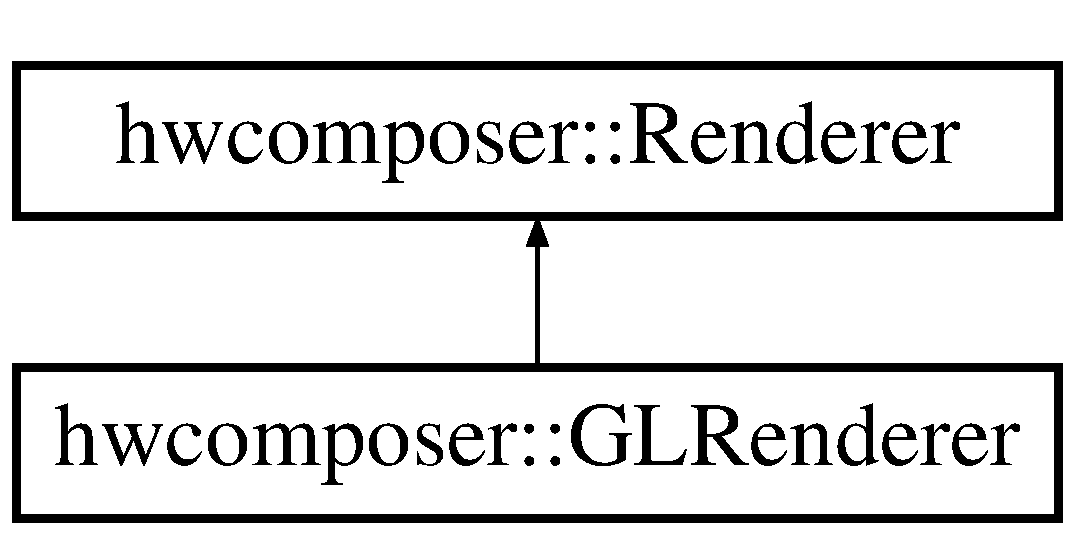
\includegraphics[height=2.000000cm]{classhwcomposer_1_1GLRenderer}
\end{center}
\end{figure}
\subsection*{Public Member Functions}
\begin{DoxyCompactItemize}
\item 
\mbox{\hyperlink{classhwcomposer_1_1GLRenderer_ad7df946c8af9df0bf948c04ecbf043d2}{G\+L\+Renderer}} ()=default
\item 
\mbox{\hyperlink{classhwcomposer_1_1GLRenderer_a8d398306fa084b620d309e9713b197d1}{$\sim$\+G\+L\+Renderer}} ()
\item 
bool \mbox{\hyperlink{classhwcomposer_1_1GLRenderer_a13460f969b8fd85b74ae1fecadff744e}{Init}} () override
\item 
bool \mbox{\hyperlink{classhwcomposer_1_1GLRenderer_a961208b3640ffb78a15438ca4504fe1a}{Draw}} (const std\+::vector$<$ \mbox{\hyperlink{structhwcomposer_1_1RenderState}{Render\+State}} $>$ \&commands, \mbox{\hyperlink{classhwcomposer_1_1NativeSurface}{Native\+Surface}} $\ast$surface) override
\item 
void \mbox{\hyperlink{classhwcomposer_1_1GLRenderer_af9eecc3a31c3acadaae84d2b31cf4807}{Insert\+Fence}} (int32\+\_\+t kms\+\_\+fence) override
\item 
void \mbox{\hyperlink{classhwcomposer_1_1GLRenderer_a8bd09dabfc0bd223f783454609b48a82}{Set\+Explicit\+Sync\+Support}} (bool disable\+\_\+explicit\+\_\+sync) override
\end{DoxyCompactItemize}


\subsection{Detailed Description}


Definition at line 30 of file glrenderer.\+h.



\subsection{Constructor \& Destructor Documentation}
\mbox{\Hypertarget{classhwcomposer_1_1GLRenderer_ad7df946c8af9df0bf948c04ecbf043d2}\label{classhwcomposer_1_1GLRenderer_ad7df946c8af9df0bf948c04ecbf043d2}} 
\index{hwcomposer\+::\+G\+L\+Renderer@{hwcomposer\+::\+G\+L\+Renderer}!G\+L\+Renderer@{G\+L\+Renderer}}
\index{G\+L\+Renderer@{G\+L\+Renderer}!hwcomposer\+::\+G\+L\+Renderer@{hwcomposer\+::\+G\+L\+Renderer}}
\subsubsection{\texorpdfstring{G\+L\+Renderer()}{GLRenderer()}}
{\footnotesize\ttfamily hwcomposer\+::\+G\+L\+Renderer\+::\+G\+L\+Renderer (\begin{DoxyParamCaption}{ }\end{DoxyParamCaption})\hspace{0.3cm}{\ttfamily [default]}}

\mbox{\Hypertarget{classhwcomposer_1_1GLRenderer_a8d398306fa084b620d309e9713b197d1}\label{classhwcomposer_1_1GLRenderer_a8d398306fa084b620d309e9713b197d1}} 
\index{hwcomposer\+::\+G\+L\+Renderer@{hwcomposer\+::\+G\+L\+Renderer}!````~G\+L\+Renderer@{$\sim$\+G\+L\+Renderer}}
\index{````~G\+L\+Renderer@{$\sim$\+G\+L\+Renderer}!hwcomposer\+::\+G\+L\+Renderer@{hwcomposer\+::\+G\+L\+Renderer}}
\subsubsection{\texorpdfstring{$\sim$\+G\+L\+Renderer()}{~GLRenderer()}}
{\footnotesize\ttfamily hwcomposer\+::\+G\+L\+Renderer\+::$\sim$\+G\+L\+Renderer (\begin{DoxyParamCaption}{ }\end{DoxyParamCaption})}



Definition at line 30 of file glrenderer.\+cpp.


\begin{DoxyCode}{0}
\DoxyCodeLine{30                         \{}
\DoxyCodeLine{31   \textcolor{keywordflow}{if} (!context\_.\mbox{\hyperlink{classhwcomposer_1_1EGLOffScreenContext_a6a02ca4cb2ad6f22af3343ac473baf2a}{MakeCurrent}}()) \{}
\DoxyCodeLine{32     \mbox{\hyperlink{alios_2platformdefines_8h_a226d6c99e4bcfca193c095e085e9097d}{ETRACE}}(\textcolor{stringliteral}{"Failed make current context."});}
\DoxyCodeLine{33     \textcolor{keywordflow}{return};}
\DoxyCodeLine{34   \}}
\DoxyCodeLine{35 }
\DoxyCodeLine{36   \textcolor{keywordflow}{if} (vertex\_array\_)}
\DoxyCodeLine{37     \mbox{\hyperlink{namespacehwcomposer_a46185e5ed06a45be5a194dc535e742dc}{glDeleteVertexArraysOES}}(1, \&vertex\_array\_);}
\DoxyCodeLine{38 \}}
\end{DoxyCode}


\subsection{Member Function Documentation}
\mbox{\Hypertarget{classhwcomposer_1_1GLRenderer_a961208b3640ffb78a15438ca4504fe1a}\label{classhwcomposer_1_1GLRenderer_a961208b3640ffb78a15438ca4504fe1a}} 
\index{hwcomposer\+::\+G\+L\+Renderer@{hwcomposer\+::\+G\+L\+Renderer}!Draw@{Draw}}
\index{Draw@{Draw}!hwcomposer\+::\+G\+L\+Renderer@{hwcomposer\+::\+G\+L\+Renderer}}
\subsubsection{\texorpdfstring{Draw()}{Draw()}}
{\footnotesize\ttfamily bool hwcomposer\+::\+G\+L\+Renderer\+::\+Draw (\begin{DoxyParamCaption}\item[{const std\+::vector$<$ \mbox{\hyperlink{structhwcomposer_1_1RenderState}{Render\+State}} $>$ \&}]{commands,  }\item[{\mbox{\hyperlink{classhwcomposer_1_1NativeSurface}{Native\+Surface}} $\ast$}]{surface }\end{DoxyParamCaption})\hspace{0.3cm}{\ttfamily [override]}, {\ttfamily [virtual]}}



Reimplemented from \mbox{\hyperlink{classhwcomposer_1_1Renderer_ab147e6d44d429c0ada5a3212ef7100f1}{hwcomposer\+::\+Renderer}}.



Definition at line 86 of file glrenderer.\+cpp.


\begin{DoxyCode}{0}
\DoxyCodeLine{87                                               \{}
\DoxyCodeLine{88   GLuint frame\_width = surface->GetWidth();}
\DoxyCodeLine{89   GLuint frame\_height = surface->GetHeight();}
\DoxyCodeLine{90   GLuint left = 0;}
\DoxyCodeLine{91   GLuint top = 0;}
\DoxyCodeLine{92 }
\DoxyCodeLine{93   \textcolor{keywordflow}{if} (!surface->MakeCurrent())}
\DoxyCodeLine{94     \textcolor{keywordflow}{return} \textcolor{keyword}{false};}
\DoxyCodeLine{95 \textcolor{preprocessor}{\#ifdef COMPOSITOR\_TRACING}}
\DoxyCodeLine{96   \mbox{\hyperlink{hwctrace_8h_a58cbc02f40ecc84e207b9a5fa9dd4437}{ICOMPOSITORTRACE}}(\textcolor{stringliteral}{"Draw starts \(\backslash\)n"});}
\DoxyCodeLine{97 \textcolor{preprocessor}{\#endif}}
\DoxyCodeLine{98 }
\DoxyCodeLine{99   \textcolor{keywordtype}{bool} clear\_surface = surface->ClearSurface();}
\DoxyCodeLine{100   \textcolor{keywordtype}{bool} partial\_clear = surface->IsPartialClear();}
\DoxyCodeLine{101 }
\DoxyCodeLine{102   surface->SetClearSurface(\mbox{\hyperlink{classhwcomposer_1_1NativeSurface_a0d0f955fc1e9f95c9684e9524f4217d6a61ab9864bcc7860917f12c33382befbc}{NativeSurface::kNone}});}
\DoxyCodeLine{103 }
\DoxyCodeLine{104   glViewport(left, top, frame\_width, frame\_height);}
\DoxyCodeLine{105 }
\DoxyCodeLine{106   \textcolor{keywordflow}{if} (clear\_surface || partial\_clear) \{}
\DoxyCodeLine{107     \textcolor{keyword}{const} HwcRect<int> \&damage = surface->GetSurfaceDamage();}
\DoxyCodeLine{108     GLuint clear\_width = damage.right - damage.left;}
\DoxyCodeLine{109     GLuint clear\_height = damage.bottom - damage.top;}
\DoxyCodeLine{110     \textcolor{keywordflow}{if} (surface->IsOnScreen() \&\&}
\DoxyCodeLine{111         ((frame\_width != clear\_width) || (frame\_height != clear\_height))) \{}
\DoxyCodeLine{112       glEnable(GL\_SCISSOR\_TEST);}
\DoxyCodeLine{113       glScissor(damage.left, damage.top, clear\_width, clear\_height);}
\DoxyCodeLine{114       glClear(GL\_COLOR\_BUFFER\_BIT);}
\DoxyCodeLine{115     \} \textcolor{keywordflow}{else} \{}
\DoxyCodeLine{116       glClear(GL\_COLOR\_BUFFER\_BIT);}
\DoxyCodeLine{117       glEnable(GL\_SCISSOR\_TEST);}
\DoxyCodeLine{118     \}}
\DoxyCodeLine{119   \} \textcolor{keywordflow}{else} \{}
\DoxyCodeLine{120     glEnable(GL\_SCISSOR\_TEST);}
\DoxyCodeLine{121   \}}
\DoxyCodeLine{122 }
\DoxyCodeLine{123 \textcolor{preprocessor}{\#ifdef COMPOSITOR\_TRACING}}
\DoxyCodeLine{124   \textcolor{keyword}{const} HwcRect<int> \&damage = surface->GetSurfaceDamage();}
\DoxyCodeLine{125   uint32\_t total\_width = 0;}
\DoxyCodeLine{126   uint32\_t total\_height = 0;}
\DoxyCodeLine{127   \mbox{\hyperlink{hwctrace_8h_a58cbc02f40ecc84e207b9a5fa9dd4437}{ICOMPOSITORTRACE}}(}
\DoxyCodeLine{128       \textcolor{stringliteral}{"Full clear: \%d Partial clear: \%d Skipped clear: \%d damage.left: \%d "}}
\DoxyCodeLine{129       \textcolor{stringliteral}{"damage.top: \%d damage.right - "}}
\DoxyCodeLine{130       \textcolor{stringliteral}{"damage.left \%d damage.bottom - damage.top \%d \(\backslash\)n"},}
\DoxyCodeLine{131       clear\_surface, partial\_clear, !(clear\_surface || partial\_clear),}
\DoxyCodeLine{132       damage.left, damage.top, damage.right - damage.left,}
\DoxyCodeLine{133       damage.bottom - damage.top);}
\DoxyCodeLine{134 \textcolor{preprocessor}{\#endif}}
\DoxyCodeLine{135   \textcolor{keywordflow}{for} (\textcolor{keyword}{const} RenderState \&state : render\_states) \{}
\DoxyCodeLine{136     \textcolor{keywordtype}{unsigned} size = state.layer\_state\_.size();}
\DoxyCodeLine{137     GLProgram *program = GetProgram(size);}
\DoxyCodeLine{138     \textcolor{keywordflow}{if} (!program)}
\DoxyCodeLine{139       \textcolor{keywordflow}{continue};}
\DoxyCodeLine{140 }
\DoxyCodeLine{141     program->UseProgram(state, frame\_width, frame\_height);}
\DoxyCodeLine{142 \textcolor{preprocessor}{\#ifdef COMPOSITOR\_TRACING}}
\DoxyCodeLine{143     \mbox{\hyperlink{hwctrace_8h_a58cbc02f40ecc84e207b9a5fa9dd4437}{ICOMPOSITORTRACE}}(}
\DoxyCodeLine{144         \textcolor{stringliteral}{"scissor\_x\_: \%d state.scissor\_y\_: \%d scissor\_width\_: \%d "}}
\DoxyCodeLine{145         \textcolor{stringliteral}{"scissor\_height\_: \%d \(\backslash\)n"},}
\DoxyCodeLine{146         state.scissor\_x\_, state.scissor\_y\_, state.scissor\_width\_,}
\DoxyCodeLine{147         state.scissor\_height\_);}
\DoxyCodeLine{148     total\_width += std::max(total\_width, state.scissor\_width\_);}
\DoxyCodeLine{149     total\_height += state.scissor\_height\_;}
\DoxyCodeLine{150     \textcolor{keyword}{const} HwcRect<int> \&damage = surface->GetSurfaceDamage();}
\DoxyCodeLine{151     \textcolor{keywordflow}{if} (\mbox{\hyperlink{namespacehwcomposer_a2775b56090a031398e48a7b77b1dee05}{AnalyseOverlap}}(}
\DoxyCodeLine{152             damage, HwcRect<int>(state.scissor\_x\_, state.scissor\_y\_,}
\DoxyCodeLine{153                                  state.scissor\_x\_ + state.scissor\_width\_,}
\DoxyCodeLine{154                                  state.scissor\_y\_ + state.scissor\_height\_)) ==}
\DoxyCodeLine{155         \mbox{\hyperlink{namespacehwcomposer_a343d36a60de234fac01fc5982b8d0e38a7ab351e5e1da3b8232419a34e1dd9559}{kOutside}}) \{}
\DoxyCodeLine{156       \mbox{\hyperlink{hwctrace_8h_a58cbc02f40ecc84e207b9a5fa9dd4437}{ICOMPOSITORTRACE}}(\textcolor{stringliteral}{"ALERT: Rendering Layer outside Damaged Region. \(\backslash\)n"});}
\DoxyCodeLine{157     \}}
\DoxyCodeLine{158 \textcolor{preprocessor}{\#endif}}
\DoxyCodeLine{159     glScissor(state.scissor\_x\_, state.scissor\_y\_, state.scissor\_width\_,}
\DoxyCodeLine{160               state.scissor\_height\_);}
\DoxyCodeLine{161 }
\DoxyCodeLine{162     glDrawArrays(GL\_TRIANGLES, 0, 3);}
\DoxyCodeLine{163 }
\DoxyCodeLine{164     \textcolor{keywordflow}{for} (\textcolor{keywordtype}{unsigned} src\_index = 0; src\_index < size; src\_index++) \{}
\DoxyCodeLine{165       glActiveTexture(GL\_TEXTURE0 + src\_index);}
\DoxyCodeLine{166       glBindTexture(GL\_TEXTURE\_EXTERNAL\_OES, 0);}
\DoxyCodeLine{167     \}}
\DoxyCodeLine{168   \}}
\DoxyCodeLine{169 }
\DoxyCodeLine{170   glDisable(GL\_SCISSOR\_TEST);}
\DoxyCodeLine{171 }
\DoxyCodeLine{172   \textcolor{keywordflow}{if} (!disable\_explicit\_sync\_)}
\DoxyCodeLine{173     surface->SetNativeFence(context\_.\mbox{\hyperlink{classhwcomposer_1_1EGLOffScreenContext_a8f98b9bb56923114d3d4c6051968e543}{GetSyncFD}}());}
\DoxyCodeLine{174 }
\DoxyCodeLine{175   surface->ResetDamage();}
\DoxyCodeLine{176 \textcolor{preprocessor}{\#ifdef COMPOSITOR\_TRACING}}
\DoxyCodeLine{177   \textcolor{keywordflow}{if} ((clear\_surface || partial\_clear) \&\&}
\DoxyCodeLine{178       ((total\_width != surface->GetLayer()->GetDisplayFrameWidth()) ||}
\DoxyCodeLine{179        (total\_height != surface->GetLayer()->GetDisplayFrameHeight()))) \{}
\DoxyCodeLine{180     \mbox{\hyperlink{hwctrace_8h_a58cbc02f40ecc84e207b9a5fa9dd4437}{ICOMPOSITORTRACE}}(}
\DoxyCodeLine{181         \textcolor{stringliteral}{"Alert Wong composition total\_width: \%d "}}
\DoxyCodeLine{182         \textcolor{stringliteral}{"surface->GetLayer()->GetDisplayFrameWidth() \%d total\_height \%d "}}
\DoxyCodeLine{183         \textcolor{stringliteral}{"surface->GetLayer()->GetDisplayFrameHeight() \%d. \(\backslash\)n"},}
\DoxyCodeLine{184         total\_width, surface->GetLayer()->GetDisplayFrameWidth(), total\_height,}
\DoxyCodeLine{185         surface->GetLayer()->GetDisplayFrameHeight());}
\DoxyCodeLine{186   \}}
\DoxyCodeLine{187   \mbox{\hyperlink{hwctrace_8h_a58cbc02f40ecc84e207b9a5fa9dd4437}{ICOMPOSITORTRACE}}(\textcolor{stringliteral}{"Draw Ends. \(\backslash\)n"});}
\DoxyCodeLine{188 \textcolor{preprocessor}{\#endif}}
\DoxyCodeLine{189   \textcolor{keywordflow}{return} \textcolor{keyword}{true};}
\DoxyCodeLine{190 \}}
\end{DoxyCode}
\mbox{\Hypertarget{classhwcomposer_1_1GLRenderer_a13460f969b8fd85b74ae1fecadff744e}\label{classhwcomposer_1_1GLRenderer_a13460f969b8fd85b74ae1fecadff744e}} 
\index{hwcomposer\+::\+G\+L\+Renderer@{hwcomposer\+::\+G\+L\+Renderer}!Init@{Init}}
\index{Init@{Init}!hwcomposer\+::\+G\+L\+Renderer@{hwcomposer\+::\+G\+L\+Renderer}}
\subsubsection{\texorpdfstring{Init()}{Init()}}
{\footnotesize\ttfamily bool hwcomposer\+::\+G\+L\+Renderer\+::\+Init (\begin{DoxyParamCaption}{ }\end{DoxyParamCaption})\hspace{0.3cm}{\ttfamily [override]}, {\ttfamily [virtual]}}



Reimplemented from \mbox{\hyperlink{classhwcomposer_1_1Renderer_aa7f5e7d36857fb67093b9f0cc3a7e606}{hwcomposer\+::\+Renderer}}.



Definition at line 40 of file glrenderer.\+cpp.


\begin{DoxyCode}{0}
\DoxyCodeLine{40                       \{}
\DoxyCodeLine{41   \textcolor{comment}{// clang-format off}}
\DoxyCodeLine{42   \textcolor{keyword}{const} GLfloat verts[] = \{0.0f, 0.0f, 0.0f, 0.0f, 0.0f, 2.0f,}
\DoxyCodeLine{43                            0.0f, 2.0f, 2.0f, 0.0f, 2.0f, 0.0f\};}
\DoxyCodeLine{44   \textcolor{comment}{// clang-format on}}
\DoxyCodeLine{45   \textcolor{keywordflow}{if} (!context\_.\mbox{\hyperlink{classhwcomposer_1_1EGLOffScreenContext_a70b98f401e88080f13a6df4b2cc4c8e2}{Init}}()) \{}
\DoxyCodeLine{46     \mbox{\hyperlink{alios_2platformdefines_8h_a226d6c99e4bcfca193c095e085e9097d}{ETRACE}}(\textcolor{stringliteral}{"Failed to initialize EGLContext."});}
\DoxyCodeLine{47     \textcolor{keywordflow}{return} \textcolor{keyword}{false};}
\DoxyCodeLine{48   \}}
\DoxyCodeLine{49 }
\DoxyCodeLine{50   \textcolor{keywordflow}{if} (!context\_.\mbox{\hyperlink{classhwcomposer_1_1EGLOffScreenContext_a6a02ca4cb2ad6f22af3343ac473baf2a}{MakeCurrent}}()) \{}
\DoxyCodeLine{51     \mbox{\hyperlink{alios_2platformdefines_8h_a226d6c99e4bcfca193c095e085e9097d}{ETRACE}}(\textcolor{stringliteral}{"Failed to initialize GLRenderer."});}
\DoxyCodeLine{52     \textcolor{keywordflow}{return} \textcolor{keyword}{false};}
\DoxyCodeLine{53   \}}
\DoxyCodeLine{54 }
\DoxyCodeLine{55   \mbox{\hyperlink{namespacehwcomposer_a1e2712274f1d2ee3a6b1662cca909699}{InitializeShims}}();}
\DoxyCodeLine{56 }
\DoxyCodeLine{57   \textcolor{comment}{// generate the VAO \& bind}}
\DoxyCodeLine{58   GLuint vertex\_array;}
\DoxyCodeLine{59   \mbox{\hyperlink{namespacehwcomposer_a593d085270cdd62b18ad5f33429025fd}{glGenVertexArraysOES}}(1, \&vertex\_array);}
\DoxyCodeLine{60   \mbox{\hyperlink{namespacehwcomposer_a01ff1e215a53e156ec5064e53af6ab65}{glBindVertexArrayOES}}(vertex\_array);}
\DoxyCodeLine{61 }
\DoxyCodeLine{62   GLuint vertex\_buffer;}
\DoxyCodeLine{63   glGenBuffers(1, \&vertex\_buffer);}
\DoxyCodeLine{64   glBindBuffer(GL\_ARRAY\_BUFFER, vertex\_buffer);}
\DoxyCodeLine{65   glBufferData(GL\_ARRAY\_BUFFER, \textcolor{keyword}{sizeof}(verts), verts, GL\_STATIC\_DRAW);}
\DoxyCodeLine{66 }
\DoxyCodeLine{67   std::unique\_ptr<GLProgram> program(\textcolor{keyword}{new} GLProgram());}
\DoxyCodeLine{68   \textcolor{keywordflow}{if} (program->Init(1)) \{}
\DoxyCodeLine{69     programs\_.emplace\_back(std::move(program));}
\DoxyCodeLine{70   \}}
\DoxyCodeLine{71 }
\DoxyCodeLine{72   glEnableVertexAttribArray(0);}
\DoxyCodeLine{73   glEnableVertexAttribArray(1);}
\DoxyCodeLine{74 }
\DoxyCodeLine{75   glVertexAttribPointer(0, 2, GL\_FLOAT, GL\_FALSE, \textcolor{keyword}{sizeof}(\textcolor{keywordtype}{float}) * 4, \mbox{\hyperlink{alios_2platformdefines_8h_a070d2ce7b6bb7e5c05602aa8c308d0c4}{NULL}});}
\DoxyCodeLine{76   glVertexAttribPointer(1, 2, GL\_FLOAT, GL\_FALSE, \textcolor{keyword}{sizeof}(\textcolor{keywordtype}{float}) * 4,}
\DoxyCodeLine{77                         (\textcolor{keywordtype}{void} *)(\textcolor{keyword}{sizeof}(\textcolor{keywordtype}{float}) * 2));}
\DoxyCodeLine{78 }
\DoxyCodeLine{79   glBindBuffer(GL\_ARRAY\_BUFFER, 0);}
\DoxyCodeLine{80 }
\DoxyCodeLine{81   vertex\_array\_ = vertex\_array;}
\DoxyCodeLine{82 }
\DoxyCodeLine{83   \textcolor{keywordflow}{return} \textcolor{keyword}{true};}
\DoxyCodeLine{84 \}}
\end{DoxyCode}
\mbox{\Hypertarget{classhwcomposer_1_1GLRenderer_af9eecc3a31c3acadaae84d2b31cf4807}\label{classhwcomposer_1_1GLRenderer_af9eecc3a31c3acadaae84d2b31cf4807}} 
\index{hwcomposer\+::\+G\+L\+Renderer@{hwcomposer\+::\+G\+L\+Renderer}!Insert\+Fence@{Insert\+Fence}}
\index{Insert\+Fence@{Insert\+Fence}!hwcomposer\+::\+G\+L\+Renderer@{hwcomposer\+::\+G\+L\+Renderer}}
\subsubsection{\texorpdfstring{Insert\+Fence()}{InsertFence()}}
{\footnotesize\ttfamily void hwcomposer\+::\+G\+L\+Renderer\+::\+Insert\+Fence (\begin{DoxyParamCaption}\item[{int32\+\_\+t}]{kms\+\_\+fence }\end{DoxyParamCaption})\hspace{0.3cm}{\ttfamily [override]}, {\ttfamily [virtual]}}



Implements \mbox{\hyperlink{classhwcomposer_1_1Renderer_a0b7be67ed8f89c994cf3bcfd418ef0a4}{hwcomposer\+::\+Renderer}}.



Definition at line 192 of file glrenderer.\+cpp.


\begin{DoxyCode}{0}
\DoxyCodeLine{192                                               \{}
\DoxyCodeLine{193   \textcolor{keywordflow}{if} (kms\_fence > 0) \{}
\DoxyCodeLine{194     EGLint attrib\_list[] = \{}
\DoxyCodeLine{195         EGL\_SYNC\_NATIVE\_FENCE\_FD\_ANDROID, \textcolor{keyword}{static\_cast<}EGLint\textcolor{keyword}{>}(kms\_fence),}
\DoxyCodeLine{196         EGL\_NONE,}
\DoxyCodeLine{197     \};}
\DoxyCodeLine{198     EGLSyncKHR fence = \mbox{\hyperlink{namespacehwcomposer_aa4f7bf2ebb58d75fd8c42abff106d278}{eglCreateSyncKHR}}(}
\DoxyCodeLine{199         context\_.\mbox{\hyperlink{classhwcomposer_1_1EGLOffScreenContext_a8fbaabaa0eb7d4c18143932d44d68ee2}{GetDisplay}}(), EGL\_SYNC\_NATIVE\_FENCE\_ANDROID, attrib\_list);}
\DoxyCodeLine{200     \mbox{\hyperlink{namespacehwcomposer_a8e34f7fe887f616d18cdb67570c15963}{eglWaitSyncKHR}}(context\_.\mbox{\hyperlink{classhwcomposer_1_1EGLOffScreenContext_a8fbaabaa0eb7d4c18143932d44d68ee2}{GetDisplay}}(), fence, 0);}
\DoxyCodeLine{201     \mbox{\hyperlink{namespacehwcomposer_afdd4be68020d78ee60456fbb07576228}{eglDestroySyncKHR}}(context\_.\mbox{\hyperlink{classhwcomposer_1_1EGLOffScreenContext_a8fbaabaa0eb7d4c18143932d44d68ee2}{GetDisplay}}(), fence);}
\DoxyCodeLine{202   \} \textcolor{keywordflow}{else} \{}
\DoxyCodeLine{203     glFlush();}
\DoxyCodeLine{204   \}}
\DoxyCodeLine{205 \}}
\end{DoxyCode}
\mbox{\Hypertarget{classhwcomposer_1_1GLRenderer_a8bd09dabfc0bd223f783454609b48a82}\label{classhwcomposer_1_1GLRenderer_a8bd09dabfc0bd223f783454609b48a82}} 
\index{hwcomposer\+::\+G\+L\+Renderer@{hwcomposer\+::\+G\+L\+Renderer}!Set\+Explicit\+Sync\+Support@{Set\+Explicit\+Sync\+Support}}
\index{Set\+Explicit\+Sync\+Support@{Set\+Explicit\+Sync\+Support}!hwcomposer\+::\+G\+L\+Renderer@{hwcomposer\+::\+G\+L\+Renderer}}
\subsubsection{\texorpdfstring{Set\+Explicit\+Sync\+Support()}{SetExplicitSyncSupport()}}
{\footnotesize\ttfamily void hwcomposer\+::\+G\+L\+Renderer\+::\+Set\+Explicit\+Sync\+Support (\begin{DoxyParamCaption}\item[{bool}]{disable\+\_\+explicit\+\_\+sync }\end{DoxyParamCaption})\hspace{0.3cm}{\ttfamily [override]}, {\ttfamily [virtual]}}



Implements \mbox{\hyperlink{classhwcomposer_1_1Renderer_a8f889bf7b26aa7d1436e9ecf6d15e629}{hwcomposer\+::\+Renderer}}.



Definition at line 207 of file glrenderer.\+cpp.


\begin{DoxyCode}{0}
\DoxyCodeLine{207                                                                   \{}
\DoxyCodeLine{208   disable\_explicit\_sync\_ = disable\_explicit\_sync;}
\DoxyCodeLine{209 \}}
\end{DoxyCode}


The documentation for this class was generated from the following files\+:\begin{DoxyCompactItemize}
\item 
common/compositor/gl/\mbox{\hyperlink{glrenderer_8h}{glrenderer.\+h}}\item 
common/compositor/gl/\mbox{\hyperlink{glrenderer_8cpp}{glrenderer.\+cpp}}\end{DoxyCompactItemize}

\hypertarget{classhwcomposer_1_1GLSurface}{}\section{hwcomposer\+:\+:G\+L\+Surface Class Reference}
\label{classhwcomposer_1_1GLSurface}\index{hwcomposer\+::\+G\+L\+Surface@{hwcomposer\+::\+G\+L\+Surface}}


{\ttfamily \#include $<$glsurface.\+h$>$}

Inheritance diagram for hwcomposer\+:\+:G\+L\+Surface\+:\begin{figure}[H]
\begin{center}
\leavevmode
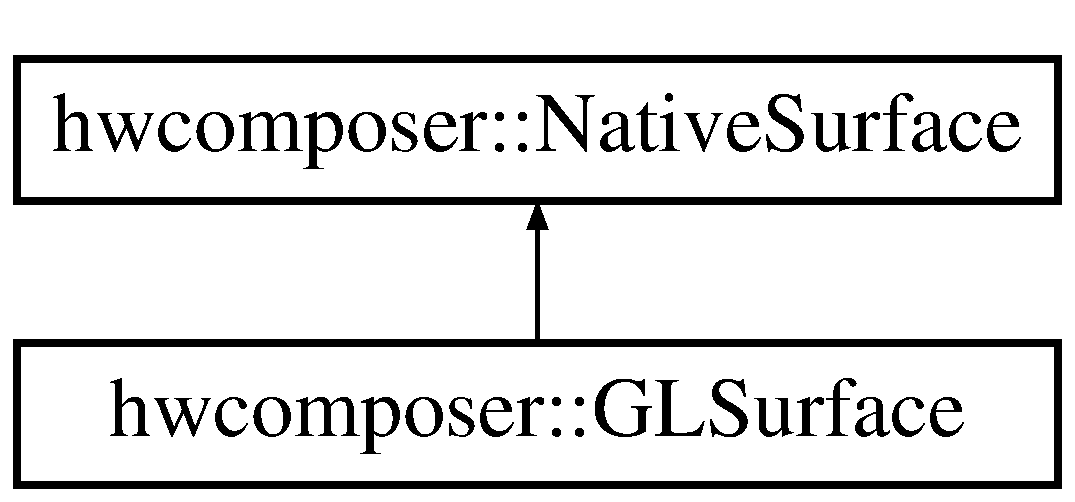
\includegraphics[height=2.000000cm]{classhwcomposer_1_1GLSurface}
\end{center}
\end{figure}
\subsection*{Public Member Functions}
\begin{DoxyCompactItemize}
\item 
\mbox{\hyperlink{classhwcomposer_1_1GLSurface_a6991d7d1f3fe126c67033052a93376d4}{G\+L\+Surface}} ()=default
\item 
\mbox{\hyperlink{classhwcomposer_1_1GLSurface_a94567e025b956b3a1fe65837d721ab99}{$\sim$\+G\+L\+Surface}} () override
\item 
\mbox{\hyperlink{classhwcomposer_1_1GLSurface_ac971667e5cfd76fd34f551e3e8547e9a}{G\+L\+Surface}} (uint32\+\_\+t width, uint32\+\_\+t height)
\item 
bool \mbox{\hyperlink{classhwcomposer_1_1GLSurface_a5d2720365cbfe670344bc74831a7895a}{Make\+Current}} () override
\end{DoxyCompactItemize}
\subsection*{Additional Inherited Members}


\subsection{Detailed Description}


Definition at line 26 of file glsurface.\+h.



\subsection{Constructor \& Destructor Documentation}
\mbox{\Hypertarget{classhwcomposer_1_1GLSurface_a6991d7d1f3fe126c67033052a93376d4}\label{classhwcomposer_1_1GLSurface_a6991d7d1f3fe126c67033052a93376d4}} 
\index{hwcomposer\+::\+G\+L\+Surface@{hwcomposer\+::\+G\+L\+Surface}!G\+L\+Surface@{G\+L\+Surface}}
\index{G\+L\+Surface@{G\+L\+Surface}!hwcomposer\+::\+G\+L\+Surface@{hwcomposer\+::\+G\+L\+Surface}}
\subsubsection{\texorpdfstring{G\+L\+Surface()}{GLSurface()}\hspace{0.1cm}{\footnotesize\ttfamily [1/2]}}
{\footnotesize\ttfamily hwcomposer\+::\+G\+L\+Surface\+::\+G\+L\+Surface (\begin{DoxyParamCaption}{ }\end{DoxyParamCaption})\hspace{0.3cm}{\ttfamily [default]}}

\mbox{\Hypertarget{classhwcomposer_1_1GLSurface_a94567e025b956b3a1fe65837d721ab99}\label{classhwcomposer_1_1GLSurface_a94567e025b956b3a1fe65837d721ab99}} 
\index{hwcomposer\+::\+G\+L\+Surface@{hwcomposer\+::\+G\+L\+Surface}!````~G\+L\+Surface@{$\sim$\+G\+L\+Surface}}
\index{````~G\+L\+Surface@{$\sim$\+G\+L\+Surface}!hwcomposer\+::\+G\+L\+Surface@{hwcomposer\+::\+G\+L\+Surface}}
\subsubsection{\texorpdfstring{$\sim$\+G\+L\+Surface()}{~GLSurface()}}
{\footnotesize\ttfamily hwcomposer\+::\+G\+L\+Surface\+::$\sim$\+G\+L\+Surface (\begin{DoxyParamCaption}{ }\end{DoxyParamCaption})\hspace{0.3cm}{\ttfamily [override]}}



Definition at line 30 of file glsurface.\+cpp.


\begin{DoxyCode}{0}
\DoxyCodeLine{30                       \{}
\DoxyCodeLine{31 \}}
\end{DoxyCode}
\mbox{\Hypertarget{classhwcomposer_1_1GLSurface_ac971667e5cfd76fd34f551e3e8547e9a}\label{classhwcomposer_1_1GLSurface_ac971667e5cfd76fd34f551e3e8547e9a}} 
\index{hwcomposer\+::\+G\+L\+Surface@{hwcomposer\+::\+G\+L\+Surface}!G\+L\+Surface@{G\+L\+Surface}}
\index{G\+L\+Surface@{G\+L\+Surface}!hwcomposer\+::\+G\+L\+Surface@{hwcomposer\+::\+G\+L\+Surface}}
\subsubsection{\texorpdfstring{G\+L\+Surface()}{GLSurface()}\hspace{0.1cm}{\footnotesize\ttfamily [2/2]}}
{\footnotesize\ttfamily hwcomposer\+::\+G\+L\+Surface\+::\+G\+L\+Surface (\begin{DoxyParamCaption}\item[{uint32\+\_\+t}]{width,  }\item[{uint32\+\_\+t}]{height }\end{DoxyParamCaption})}



Definition at line 26 of file glsurface.\+cpp.


\begin{DoxyCode}{0}
\DoxyCodeLine{27     : \mbox{\hyperlink{classhwcomposer_1_1NativeSurface_a17e5ae7ecfd166faa21ccba1e6b03197}{NativeSurface}}(width, height) \{}
\DoxyCodeLine{28 \}}
\end{DoxyCode}


\subsection{Member Function Documentation}
\mbox{\Hypertarget{classhwcomposer_1_1GLSurface_a5d2720365cbfe670344bc74831a7895a}\label{classhwcomposer_1_1GLSurface_a5d2720365cbfe670344bc74831a7895a}} 
\index{hwcomposer\+::\+G\+L\+Surface@{hwcomposer\+::\+G\+L\+Surface}!Make\+Current@{Make\+Current}}
\index{Make\+Current@{Make\+Current}!hwcomposer\+::\+G\+L\+Surface@{hwcomposer\+::\+G\+L\+Surface}}
\subsubsection{\texorpdfstring{Make\+Current()}{MakeCurrent()}}
{\footnotesize\ttfamily bool hwcomposer\+::\+G\+L\+Surface\+::\+Make\+Current (\begin{DoxyParamCaption}{ }\end{DoxyParamCaption})\hspace{0.3cm}{\ttfamily [override]}, {\ttfamily [virtual]}}



Reimplemented from \mbox{\hyperlink{classhwcomposer_1_1NativeSurface_a2e3bdea36f4b2d3f655a5f6d38670d51}{hwcomposer\+::\+Native\+Surface}}.



Definition at line 74 of file glsurface.\+cpp.


\begin{DoxyCode}{0}
\DoxyCodeLine{74                             \{}
\DoxyCodeLine{75   \textcolor{keywordflow}{if} (!fb\_ \&\& !InitializeGPUResources()) \{}
\DoxyCodeLine{76     \mbox{\hyperlink{alios_2platformdefines_8h_a226d6c99e4bcfca193c095e085e9097d}{ETRACE}}(\textcolor{stringliteral}{"Failed to initialize gpu resources."});}
\DoxyCodeLine{77     \textcolor{keywordflow}{return} \textcolor{keyword}{false};}
\DoxyCodeLine{78   \}}
\DoxyCodeLine{79 }
\DoxyCodeLine{80   glBindFramebuffer(GL\_FRAMEBUFFER, fb\_);}
\DoxyCodeLine{81   \textcolor{keywordflow}{return} \textcolor{keyword}{true};}
\DoxyCodeLine{82 \}}
\end{DoxyCode}


The documentation for this class was generated from the following files\+:\begin{DoxyCompactItemize}
\item 
common/compositor/gl/\mbox{\hyperlink{glsurface_8h}{glsurface.\+h}}\item 
common/compositor/gl/\mbox{\hyperlink{glsurface_8cpp}{glsurface.\+cpp}}\end{DoxyCompactItemize}

\hypertarget{classhwcomposer_1_1GpuDevice}{}\section{hwcomposer\+:\+:Gpu\+Device Class Reference}
\label{classhwcomposer_1_1GpuDevice}\index{hwcomposer\+::\+Gpu\+Device@{hwcomposer\+::\+Gpu\+Device}}


{\ttfamily \#include $<$gpudevice.\+h$>$}

Inheritance diagram for hwcomposer\+:\+:Gpu\+Device\+:\begin{figure}[H]
\begin{center}
\leavevmode
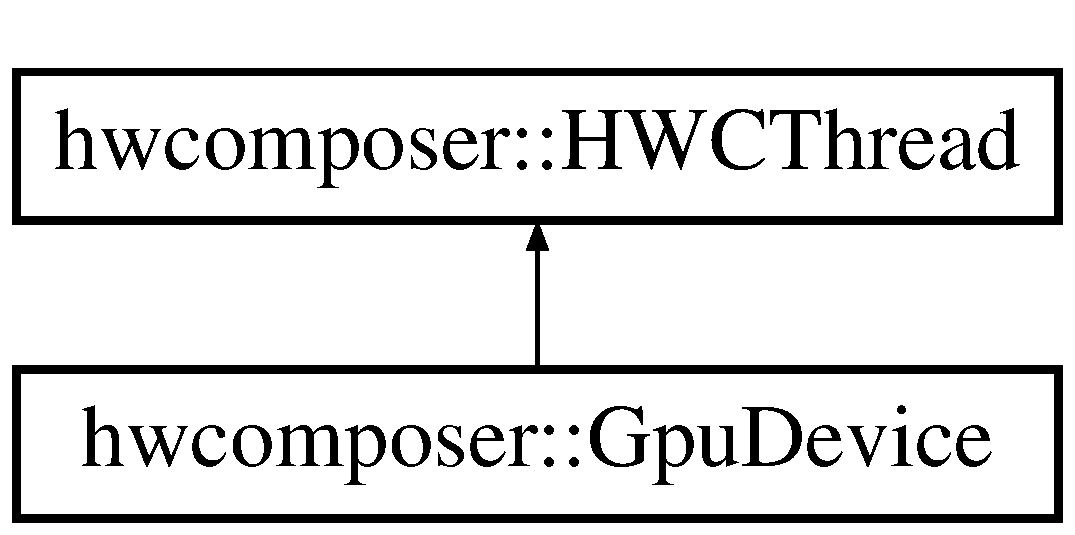
\includegraphics[height=2.000000cm]{classhwcomposer_1_1GpuDevice}
\end{center}
\end{figure}
\subsection*{Public Member Functions}
\begin{DoxyCompactItemize}
\item 
\mbox{\hyperlink{classhwcomposer_1_1GpuDevice_a058336b2b96090c51011b2d8e24a9765}{Gpu\+Device}} ()
\item 
virtual \mbox{\hyperlink{classhwcomposer_1_1GpuDevice_a2ccba76dae02bd1b810a90bb5c3c4183}{$\sim$\+Gpu\+Device}} ()
\item 
bool \mbox{\hyperlink{classhwcomposer_1_1GpuDevice_a794b3bd7590853c44f59e32252d2b3d7}{Initialize}} ()
\item 
uint32\+\_\+t \mbox{\hyperlink{classhwcomposer_1_1GpuDevice_a5b79c50e063249ae797255e73726df87}{Get\+FD}} () const
\item 
\mbox{\hyperlink{classhwcomposer_1_1NativeDisplay}{Native\+Display}} $\ast$ \mbox{\hyperlink{classhwcomposer_1_1GpuDevice_aca453b8ff7b694b6c0580f0c30573978}{Get\+Display}} (uint32\+\_\+t display)
\item 
\mbox{\hyperlink{classhwcomposer_1_1NativeDisplay}{Native\+Display}} $\ast$ \mbox{\hyperlink{classhwcomposer_1_1GpuDevice_adfec63ead3453ee2cd80b5183d4961d8}{Get\+Virtual\+Display}} ()
\item 
\mbox{\hyperlink{classhwcomposer_1_1NativeDisplay}{Native\+Display}} $\ast$ \mbox{\hyperlink{classhwcomposer_1_1GpuDevice_aa5ea5011fbcb67cddb67faca689c97d1}{Get\+Nested\+Display}} ()
\item 
void \mbox{\hyperlink{classhwcomposer_1_1GpuDevice_a1283357881144bc77606b18505fc8fce}{Get\+Connected\+Physical\+Displays}} (std\+::vector$<$ \mbox{\hyperlink{classhwcomposer_1_1NativeDisplay}{Native\+Display}} $\ast$$>$ \&displays)
\item 
const std\+::vector$<$ \mbox{\hyperlink{classhwcomposer_1_1NativeDisplay}{Native\+Display}} $\ast$ $>$ \& \mbox{\hyperlink{classhwcomposer_1_1GpuDevice_a36bad6a205218da9546f18e282af05a5}{Get\+All\+Displays}} ()
\item 
void \mbox{\hyperlink{classhwcomposer_1_1GpuDevice_a5d28fa3fc5eda73115f36d371aa37664}{Register\+Hot\+Plug\+Event\+Callback}} (std\+::shared\+\_\+ptr$<$ \mbox{\hyperlink{classhwcomposer_1_1DisplayHotPlugEventCallback}{Display\+Hot\+Plug\+Event\+Callback}} $>$ callback)
\item 
void \mbox{\hyperlink{classhwcomposer_1_1GpuDevice_aa558c97ab2f80eac47ede0a788a59a28}{Enable\+H\+D\+C\+P\+Session\+For\+Display}} (uint32\+\_\+t display, H\+W\+C\+Content\+Type content\+\_\+type)
\item 
void \mbox{\hyperlink{classhwcomposer_1_1GpuDevice_a5a42e70ab1648c6e7741b2322f898691}{Enable\+H\+D\+C\+P\+Session\+For\+All\+Displays}} (H\+W\+C\+Content\+Type content\+\_\+type)
\item 
void \mbox{\hyperlink{classhwcomposer_1_1GpuDevice_ae61aa61ee1591464e7e5a703b2c6c848}{Disable\+H\+D\+C\+P\+Session\+For\+Display}} (uint32\+\_\+t display)
\item 
void \mbox{\hyperlink{classhwcomposer_1_1GpuDevice_a7038e1dc3d4a2be7206e6a35717521e2}{Disable\+H\+D\+C\+P\+Session\+For\+All\+Displays}} ()
\end{DoxyCompactItemize}
\subsection*{Friends}
\begin{DoxyCompactItemize}
\item 
class \mbox{\hyperlink{classhwcomposer_1_1GpuDevice_a4f7966ae9851735e6eddc713ec174b2f}{Drm\+Display\+Manager}}
\end{DoxyCompactItemize}
\subsection*{Additional Inherited Members}


\subsection{Detailed Description}


Definition at line 34 of file gpudevice.\+h.



\subsection{Constructor \& Destructor Documentation}
\mbox{\Hypertarget{classhwcomposer_1_1GpuDevice_a058336b2b96090c51011b2d8e24a9765}\label{classhwcomposer_1_1GpuDevice_a058336b2b96090c51011b2d8e24a9765}} 
\index{hwcomposer\+::\+Gpu\+Device@{hwcomposer\+::\+Gpu\+Device}!Gpu\+Device@{Gpu\+Device}}
\index{Gpu\+Device@{Gpu\+Device}!hwcomposer\+::\+Gpu\+Device@{hwcomposer\+::\+Gpu\+Device}}
\subsubsection{\texorpdfstring{Gpu\+Device()}{GpuDevice()}}
{\footnotesize\ttfamily hwcomposer\+::\+Gpu\+Device\+::\+Gpu\+Device (\begin{DoxyParamCaption}{ }\end{DoxyParamCaption})}



Definition at line 27 of file gpudevice.\+cpp.


\begin{DoxyCode}{0}
\DoxyCodeLine{27                      : \mbox{\hyperlink{classhwcomposer_1_1HWCThread_a8780175b1679005955a94aa89fa62be1}{HWCThread}}(-8, \textcolor{stringliteral}{"GpuDevice"}) \{}
\DoxyCodeLine{28 \}}
\end{DoxyCode}
\mbox{\Hypertarget{classhwcomposer_1_1GpuDevice_a2ccba76dae02bd1b810a90bb5c3c4183}\label{classhwcomposer_1_1GpuDevice_a2ccba76dae02bd1b810a90bb5c3c4183}} 
\index{hwcomposer\+::\+Gpu\+Device@{hwcomposer\+::\+Gpu\+Device}!````~Gpu\+Device@{$\sim$\+Gpu\+Device}}
\index{````~Gpu\+Device@{$\sim$\+Gpu\+Device}!hwcomposer\+::\+Gpu\+Device@{hwcomposer\+::\+Gpu\+Device}}
\subsubsection{\texorpdfstring{$\sim$\+Gpu\+Device()}{~GpuDevice()}}
{\footnotesize\ttfamily hwcomposer\+::\+Gpu\+Device\+::$\sim$\+Gpu\+Device (\begin{DoxyParamCaption}{ }\end{DoxyParamCaption})\hspace{0.3cm}{\ttfamily [virtual]}}



Definition at line 30 of file gpudevice.\+cpp.


\begin{DoxyCode}{0}
\DoxyCodeLine{30                       \{}
\DoxyCodeLine{31   display\_manager\_.reset(\textcolor{keyword}{nullptr});}
\DoxyCodeLine{32 \}}
\end{DoxyCode}


\subsection{Member Function Documentation}
\mbox{\Hypertarget{classhwcomposer_1_1GpuDevice_a7038e1dc3d4a2be7206e6a35717521e2}\label{classhwcomposer_1_1GpuDevice_a7038e1dc3d4a2be7206e6a35717521e2}} 
\index{hwcomposer\+::\+Gpu\+Device@{hwcomposer\+::\+Gpu\+Device}!Disable\+H\+D\+C\+P\+Session\+For\+All\+Displays@{Disable\+H\+D\+C\+P\+Session\+For\+All\+Displays}}
\index{Disable\+H\+D\+C\+P\+Session\+For\+All\+Displays@{Disable\+H\+D\+C\+P\+Session\+For\+All\+Displays}!hwcomposer\+::\+Gpu\+Device@{hwcomposer\+::\+Gpu\+Device}}
\subsubsection{\texorpdfstring{Disable\+H\+D\+C\+P\+Session\+For\+All\+Displays()}{DisableHDCPSessionForAllDisplays()}}
{\footnotesize\ttfamily void hwcomposer\+::\+Gpu\+Device\+::\+Disable\+H\+D\+C\+P\+Session\+For\+All\+Displays (\begin{DoxyParamCaption}{ }\end{DoxyParamCaption})}



Definition at line 617 of file gpudevice.\+cpp.


\begin{DoxyCode}{0}
\DoxyCodeLine{617                                                  \{}
\DoxyCodeLine{618   \textcolor{keywordtype}{size\_t} size = total\_displays\_.size();}
\DoxyCodeLine{619   \textcolor{keywordflow}{for} (\textcolor{keywordtype}{size\_t} i = 0; i < size; i++) \{}
\DoxyCodeLine{620     total\_displays\_.at(i)->SetHDCPState(HWCContentProtection::kUnDesired,}
\DoxyCodeLine{621                                         HWCContentType::kInvalid);}
\DoxyCodeLine{622   \}}
\DoxyCodeLine{623 \}}
\end{DoxyCode}
\mbox{\Hypertarget{classhwcomposer_1_1GpuDevice_ae61aa61ee1591464e7e5a703b2c6c848}\label{classhwcomposer_1_1GpuDevice_ae61aa61ee1591464e7e5a703b2c6c848}} 
\index{hwcomposer\+::\+Gpu\+Device@{hwcomposer\+::\+Gpu\+Device}!Disable\+H\+D\+C\+P\+Session\+For\+Display@{Disable\+H\+D\+C\+P\+Session\+For\+Display}}
\index{Disable\+H\+D\+C\+P\+Session\+For\+Display@{Disable\+H\+D\+C\+P\+Session\+For\+Display}!hwcomposer\+::\+Gpu\+Device@{hwcomposer\+::\+Gpu\+Device}}
\subsubsection{\texorpdfstring{Disable\+H\+D\+C\+P\+Session\+For\+Display()}{DisableHDCPSessionForDisplay()}}
{\footnotesize\ttfamily void hwcomposer\+::\+Gpu\+Device\+::\+Disable\+H\+D\+C\+P\+Session\+For\+Display (\begin{DoxyParamCaption}\item[{uint32\+\_\+t}]{display }\end{DoxyParamCaption})}



Definition at line 606 of file gpudevice.\+cpp.


\begin{DoxyCode}{0}
\DoxyCodeLine{606                                                              \{}
\DoxyCodeLine{607   \textcolor{keywordflow}{if} (total\_displays\_.size() <= display) \{}
\DoxyCodeLine{608     \mbox{\hyperlink{alios_2platformdefines_8h_a226d6c99e4bcfca193c095e085e9097d}{ETRACE}}(\textcolor{stringliteral}{"Tried to enable HDCP for invalid display \%u \(\backslash\)n"}, display);}
\DoxyCodeLine{609     \textcolor{keywordflow}{return};}
\DoxyCodeLine{610   \}}
\DoxyCodeLine{611 }
\DoxyCodeLine{612   NativeDisplay *native\_display = total\_displays\_.at(display);}
\DoxyCodeLine{613   native\_display->SetHDCPState(HWCContentProtection::kUnDesired,}
\DoxyCodeLine{614                                HWCContentType::kInvalid);}
\DoxyCodeLine{615 \}}
\end{DoxyCode}
\mbox{\Hypertarget{classhwcomposer_1_1GpuDevice_a5a42e70ab1648c6e7741b2322f898691}\label{classhwcomposer_1_1GpuDevice_a5a42e70ab1648c6e7741b2322f898691}} 
\index{hwcomposer\+::\+Gpu\+Device@{hwcomposer\+::\+Gpu\+Device}!Enable\+H\+D\+C\+P\+Session\+For\+All\+Displays@{Enable\+H\+D\+C\+P\+Session\+For\+All\+Displays}}
\index{Enable\+H\+D\+C\+P\+Session\+For\+All\+Displays@{Enable\+H\+D\+C\+P\+Session\+For\+All\+Displays}!hwcomposer\+::\+Gpu\+Device@{hwcomposer\+::\+Gpu\+Device}}
\subsubsection{\texorpdfstring{Enable\+H\+D\+C\+P\+Session\+For\+All\+Displays()}{EnableHDCPSessionForAllDisplays()}}
{\footnotesize\ttfamily void hwcomposer\+::\+Gpu\+Device\+::\+Enable\+H\+D\+C\+P\+Session\+For\+All\+Displays (\begin{DoxyParamCaption}\item[{H\+W\+C\+Content\+Type}]{content\+\_\+type }\end{DoxyParamCaption})}



Definition at line 598 of file gpudevice.\+cpp.


\begin{DoxyCode}{0}
\DoxyCodeLine{598                                                                            \{}
\DoxyCodeLine{599   \textcolor{keywordtype}{size\_t} size = total\_displays\_.size();}
\DoxyCodeLine{600   \textcolor{keywordflow}{for} (\textcolor{keywordtype}{size\_t} i = 0; i < size; i++) \{}
\DoxyCodeLine{601     total\_displays\_.at(i)}
\DoxyCodeLine{602         ->SetHDCPState(HWCContentProtection::kDesired, content\_type);}
\DoxyCodeLine{603   \}}
\DoxyCodeLine{604 \}}
\end{DoxyCode}
\mbox{\Hypertarget{classhwcomposer_1_1GpuDevice_aa558c97ab2f80eac47ede0a788a59a28}\label{classhwcomposer_1_1GpuDevice_aa558c97ab2f80eac47ede0a788a59a28}} 
\index{hwcomposer\+::\+Gpu\+Device@{hwcomposer\+::\+Gpu\+Device}!Enable\+H\+D\+C\+P\+Session\+For\+Display@{Enable\+H\+D\+C\+P\+Session\+For\+Display}}
\index{Enable\+H\+D\+C\+P\+Session\+For\+Display@{Enable\+H\+D\+C\+P\+Session\+For\+Display}!hwcomposer\+::\+Gpu\+Device@{hwcomposer\+::\+Gpu\+Device}}
\subsubsection{\texorpdfstring{Enable\+H\+D\+C\+P\+Session\+For\+Display()}{EnableHDCPSessionForDisplay()}}
{\footnotesize\ttfamily void hwcomposer\+::\+Gpu\+Device\+::\+Enable\+H\+D\+C\+P\+Session\+For\+Display (\begin{DoxyParamCaption}\item[{uint32\+\_\+t}]{display,  }\item[{H\+W\+C\+Content\+Type}]{content\+\_\+type }\end{DoxyParamCaption})}



Definition at line 587 of file gpudevice.\+cpp.


\begin{DoxyCode}{0}
\DoxyCodeLine{588                                                                          \{}
\DoxyCodeLine{589   \textcolor{keywordflow}{if} (total\_displays\_.size() <= display) \{}
\DoxyCodeLine{590     \mbox{\hyperlink{alios_2platformdefines_8h_a226d6c99e4bcfca193c095e085e9097d}{ETRACE}}(\textcolor{stringliteral}{"Tried to enable HDCP for invalid display \%u \(\backslash\)n"}, display);}
\DoxyCodeLine{591     \textcolor{keywordflow}{return};}
\DoxyCodeLine{592   \}}
\DoxyCodeLine{593 }
\DoxyCodeLine{594   NativeDisplay *native\_display = total\_displays\_.at(display);}
\DoxyCodeLine{595   native\_display->SetHDCPState(HWCContentProtection::kDesired, content\_type);}
\DoxyCodeLine{596 \}}
\end{DoxyCode}
\mbox{\Hypertarget{classhwcomposer_1_1GpuDevice_a36bad6a205218da9546f18e282af05a5}\label{classhwcomposer_1_1GpuDevice_a36bad6a205218da9546f18e282af05a5}} 
\index{hwcomposer\+::\+Gpu\+Device@{hwcomposer\+::\+Gpu\+Device}!Get\+All\+Displays@{Get\+All\+Displays}}
\index{Get\+All\+Displays@{Get\+All\+Displays}!hwcomposer\+::\+Gpu\+Device@{hwcomposer\+::\+Gpu\+Device}}
\subsubsection{\texorpdfstring{Get\+All\+Displays()}{GetAllDisplays()}}
{\footnotesize\ttfamily const std\+::vector$<$ \mbox{\hyperlink{classhwcomposer_1_1NativeDisplay}{Native\+Display}} $\ast$ $>$ \& hwcomposer\+::\+Gpu\+Device\+::\+Get\+All\+Displays (\begin{DoxyParamCaption}{ }\end{DoxyParamCaption})}



Definition at line 98 of file gpudevice.\+cpp.


\begin{DoxyCode}{0}
\DoxyCodeLine{98                                                             \{}
\DoxyCodeLine{99   \textcolor{keywordflow}{return} total\_displays\_;}
\DoxyCodeLine{100 \}}
\end{DoxyCode}
\mbox{\Hypertarget{classhwcomposer_1_1GpuDevice_a1283357881144bc77606b18505fc8fce}\label{classhwcomposer_1_1GpuDevice_a1283357881144bc77606b18505fc8fce}} 
\index{hwcomposer\+::\+Gpu\+Device@{hwcomposer\+::\+Gpu\+Device}!Get\+Connected\+Physical\+Displays@{Get\+Connected\+Physical\+Displays}}
\index{Get\+Connected\+Physical\+Displays@{Get\+Connected\+Physical\+Displays}!hwcomposer\+::\+Gpu\+Device@{hwcomposer\+::\+Gpu\+Device}}
\subsubsection{\texorpdfstring{Get\+Connected\+Physical\+Displays()}{GetConnectedPhysicalDisplays()}}
{\footnotesize\ttfamily void hwcomposer\+::\+Gpu\+Device\+::\+Get\+Connected\+Physical\+Displays (\begin{DoxyParamCaption}\item[{std\+::vector$<$ \mbox{\hyperlink{classhwcomposer_1_1NativeDisplay}{Native\+Display}} $\ast$$>$ \&}]{displays }\end{DoxyParamCaption})}



Definition at line 88 of file gpudevice.\+cpp.


\begin{DoxyCode}{0}
\DoxyCodeLine{89                                           \{}
\DoxyCodeLine{90   \textcolor{keywordtype}{size\_t} size = total\_displays\_.size();}
\DoxyCodeLine{91   \textcolor{keywordflow}{for} (\textcolor{keywordtype}{size\_t} i = 0; i < size; i++) \{}
\DoxyCodeLine{92     \textcolor{keywordflow}{if} (total\_displays\_.at(i)->IsConnected()) \{}
\DoxyCodeLine{93       displays.emplace\_back(total\_displays\_.at(i));}
\DoxyCodeLine{94     \}}
\DoxyCodeLine{95   \}}
\DoxyCodeLine{96 \}}
\end{DoxyCode}
\mbox{\Hypertarget{classhwcomposer_1_1GpuDevice_aca453b8ff7b694b6c0580f0c30573978}\label{classhwcomposer_1_1GpuDevice_aca453b8ff7b694b6c0580f0c30573978}} 
\index{hwcomposer\+::\+Gpu\+Device@{hwcomposer\+::\+Gpu\+Device}!Get\+Display@{Get\+Display}}
\index{Get\+Display@{Get\+Display}!hwcomposer\+::\+Gpu\+Device@{hwcomposer\+::\+Gpu\+Device}}
\subsubsection{\texorpdfstring{Get\+Display()}{GetDisplay()}}
{\footnotesize\ttfamily \mbox{\hyperlink{classhwcomposer_1_1NativeDisplay}{Native\+Display}} $\ast$ hwcomposer\+::\+Gpu\+Device\+::\+Get\+Display (\begin{DoxyParamCaption}\item[{uint32\+\_\+t}]{display }\end{DoxyParamCaption})}



Definition at line 72 of file gpudevice.\+cpp.


\begin{DoxyCode}{0}
\DoxyCodeLine{72                                                         \{}
\DoxyCodeLine{73   \textcolor{keywordflow}{if} (total\_displays\_.size() > display\_id)}
\DoxyCodeLine{74     \textcolor{keywordflow}{return} total\_displays\_.at(display\_id);}
\DoxyCodeLine{75 }
\DoxyCodeLine{76   \textcolor{keywordflow}{return} \mbox{\hyperlink{alios_2platformdefines_8h_a070d2ce7b6bb7e5c05602aa8c308d0c4}{NULL}};}
\DoxyCodeLine{77 \}}
\end{DoxyCode}
\mbox{\Hypertarget{classhwcomposer_1_1GpuDevice_a5b79c50e063249ae797255e73726df87}\label{classhwcomposer_1_1GpuDevice_a5b79c50e063249ae797255e73726df87}} 
\index{hwcomposer\+::\+Gpu\+Device@{hwcomposer\+::\+Gpu\+Device}!Get\+FD@{Get\+FD}}
\index{Get\+FD@{Get\+FD}!hwcomposer\+::\+Gpu\+Device@{hwcomposer\+::\+Gpu\+Device}}
\subsubsection{\texorpdfstring{Get\+F\+D()}{GetFD()}}
{\footnotesize\ttfamily uint32\+\_\+t hwcomposer\+::\+Gpu\+Device\+::\+Get\+FD (\begin{DoxyParamCaption}{ }\end{DoxyParamCaption}) const}



Definition at line 68 of file gpudevice.\+cpp.


\begin{DoxyCode}{0}
\DoxyCodeLine{68                                 \{}
\DoxyCodeLine{69   \textcolor{keywordflow}{return} display\_manager\_->GetFD();}
\DoxyCodeLine{70 \}}
\end{DoxyCode}
\mbox{\Hypertarget{classhwcomposer_1_1GpuDevice_aa5ea5011fbcb67cddb67faca689c97d1}\label{classhwcomposer_1_1GpuDevice_aa5ea5011fbcb67cddb67faca689c97d1}} 
\index{hwcomposer\+::\+Gpu\+Device@{hwcomposer\+::\+Gpu\+Device}!Get\+Nested\+Display@{Get\+Nested\+Display}}
\index{Get\+Nested\+Display@{Get\+Nested\+Display}!hwcomposer\+::\+Gpu\+Device@{hwcomposer\+::\+Gpu\+Device}}
\subsubsection{\texorpdfstring{Get\+Nested\+Display()}{GetNestedDisplay()}}
{\footnotesize\ttfamily \mbox{\hyperlink{classhwcomposer_1_1NativeDisplay}{Native\+Display}} $\ast$ hwcomposer\+::\+Gpu\+Device\+::\+Get\+Nested\+Display (\begin{DoxyParamCaption}{ }\end{DoxyParamCaption})}



Definition at line 84 of file gpudevice.\+cpp.


\begin{DoxyCode}{0}
\DoxyCodeLine{84                                            \{}
\DoxyCodeLine{85   \textcolor{keywordflow}{return} display\_manager\_->GetNestedDisplay();}
\DoxyCodeLine{86 \}}
\end{DoxyCode}
\mbox{\Hypertarget{classhwcomposer_1_1GpuDevice_adfec63ead3453ee2cd80b5183d4961d8}\label{classhwcomposer_1_1GpuDevice_adfec63ead3453ee2cd80b5183d4961d8}} 
\index{hwcomposer\+::\+Gpu\+Device@{hwcomposer\+::\+Gpu\+Device}!Get\+Virtual\+Display@{Get\+Virtual\+Display}}
\index{Get\+Virtual\+Display@{Get\+Virtual\+Display}!hwcomposer\+::\+Gpu\+Device@{hwcomposer\+::\+Gpu\+Device}}
\subsubsection{\texorpdfstring{Get\+Virtual\+Display()}{GetVirtualDisplay()}}
{\footnotesize\ttfamily \mbox{\hyperlink{classhwcomposer_1_1NativeDisplay}{Native\+Display}} $\ast$ hwcomposer\+::\+Gpu\+Device\+::\+Get\+Virtual\+Display (\begin{DoxyParamCaption}{ }\end{DoxyParamCaption})}



Definition at line 79 of file gpudevice.\+cpp.


\begin{DoxyCode}{0}
\DoxyCodeLine{79                                             \{}
\DoxyCodeLine{80   \textcolor{keywordflow}{return} display\_manager\_->GetVirtualDisplay();}
\DoxyCodeLine{81 \}}
\end{DoxyCode}
\mbox{\Hypertarget{classhwcomposer_1_1GpuDevice_a794b3bd7590853c44f59e32252d2b3d7}\label{classhwcomposer_1_1GpuDevice_a794b3bd7590853c44f59e32252d2b3d7}} 
\index{hwcomposer\+::\+Gpu\+Device@{hwcomposer\+::\+Gpu\+Device}!Initialize@{Initialize}}
\index{Initialize@{Initialize}!hwcomposer\+::\+Gpu\+Device@{hwcomposer\+::\+Gpu\+Device}}
\subsubsection{\texorpdfstring{Initialize()}{Initialize()}}
{\footnotesize\ttfamily bool hwcomposer\+::\+Gpu\+Device\+::\+Initialize (\begin{DoxyParamCaption}{ }\end{DoxyParamCaption})}



Definition at line 34 of file gpudevice.\+cpp.


\begin{DoxyCode}{0}
\DoxyCodeLine{34                            \{}
\DoxyCodeLine{35   initialization\_state\_lock\_.\mbox{\hyperlink{classhwcomposer_1_1SpinLock_a863f9d0f1b270f863a9298161b52faf1}{lock}}();}
\DoxyCodeLine{36   \textcolor{keywordflow}{if} (initialization\_state\_ \& kInitialized) \{}
\DoxyCodeLine{37     initialization\_state\_lock\_.\mbox{\hyperlink{classhwcomposer_1_1SpinLock_ae5cf624b4f0ec710833ce44e945b85d7}{unlock}}();}
\DoxyCodeLine{38     \textcolor{keywordflow}{return} \textcolor{keyword}{true};}
\DoxyCodeLine{39   \}}
\DoxyCodeLine{40 }
\DoxyCodeLine{41   initialization\_state\_ |= kInitialized;}
\DoxyCodeLine{42   initialization\_state\_lock\_.\mbox{\hyperlink{classhwcomposer_1_1SpinLock_ae5cf624b4f0ec710833ce44e945b85d7}{unlock}}();}
\DoxyCodeLine{43 }
\DoxyCodeLine{44   display\_manager\_.reset(\mbox{\hyperlink{classhwcomposer_1_1DisplayManager_aed4adf531c3ea168ff4e2f7c82fd1cbb}{DisplayManager::CreateDisplayManager}}(\textcolor{keyword}{this}));}
\DoxyCodeLine{45 }
\DoxyCodeLine{46   \textcolor{keywordtype}{bool} success = display\_manager\_->Initialize();}
\DoxyCodeLine{47   \textcolor{keywordflow}{if} (!success) \{}
\DoxyCodeLine{48     \textcolor{keywordflow}{return} \textcolor{keyword}{false};}
\DoxyCodeLine{49   \}}
\DoxyCodeLine{50 }
\DoxyCodeLine{51   display\_manager\_->InitializeDisplayResources();}
\DoxyCodeLine{52   display\_manager\_->StartHotPlugMonitor();}
\DoxyCodeLine{53 }
\DoxyCodeLine{54   HandleHWCSettings();}
\DoxyCodeLine{55 }
\DoxyCodeLine{56   lock\_fd\_ = open(\textcolor{stringliteral}{"/vendor/hwc.lock"}, O\_RDONLY);}
\DoxyCodeLine{57   \textcolor{keywordflow}{if} (-1 != lock\_fd\_) \{}
\DoxyCodeLine{58     \textcolor{keywordflow}{if} (!\mbox{\hyperlink{classhwcomposer_1_1HWCThread_a7162d49a6b4026673f77ac048eb4d07b}{InitWorker}}()) \{}
\DoxyCodeLine{59       \mbox{\hyperlink{alios_2platformdefines_8h_a226d6c99e4bcfca193c095e085e9097d}{ETRACE}}(\textcolor{stringliteral}{"Failed to initalize thread for GpuDevice. \%s"}, \mbox{\hyperlink{hwctrace_8h_a791a01fa8fe130cef13d68a706df9034}{PRINTERROR}}());}
\DoxyCodeLine{60     \}}
\DoxyCodeLine{61   \} \textcolor{keywordflow}{else} \{}
\DoxyCodeLine{62     \mbox{\hyperlink{alios_2platformdefines_8h_a2407a03fb42f0c0d39cdf7fe4850ec87}{ITRACE}}(\textcolor{stringliteral}{"Failed to open "} LOCK\_DIR\_PREFIX \textcolor{stringliteral}{"/hwc.lock file!"});}
\DoxyCodeLine{63   \}}
\DoxyCodeLine{64 }
\DoxyCodeLine{65   \textcolor{keywordflow}{return} \textcolor{keyword}{true};}
\DoxyCodeLine{66 \}}
\end{DoxyCode}
\mbox{\Hypertarget{classhwcomposer_1_1GpuDevice_a5d28fa3fc5eda73115f36d371aa37664}\label{classhwcomposer_1_1GpuDevice_a5d28fa3fc5eda73115f36d371aa37664}} 
\index{hwcomposer\+::\+Gpu\+Device@{hwcomposer\+::\+Gpu\+Device}!Register\+Hot\+Plug\+Event\+Callback@{Register\+Hot\+Plug\+Event\+Callback}}
\index{Register\+Hot\+Plug\+Event\+Callback@{Register\+Hot\+Plug\+Event\+Callback}!hwcomposer\+::\+Gpu\+Device@{hwcomposer\+::\+Gpu\+Device}}
\subsubsection{\texorpdfstring{Register\+Hot\+Plug\+Event\+Callback()}{RegisterHotPlugEventCallback()}}
{\footnotesize\ttfamily void hwcomposer\+::\+Gpu\+Device\+::\+Register\+Hot\+Plug\+Event\+Callback (\begin{DoxyParamCaption}\item[{std\+::shared\+\_\+ptr$<$ \mbox{\hyperlink{classhwcomposer_1_1DisplayHotPlugEventCallback}{Display\+Hot\+Plug\+Event\+Callback}} $>$}]{callback }\end{DoxyParamCaption})}



Definition at line 102 of file gpudevice.\+cpp.


\begin{DoxyCode}{0}
\DoxyCodeLine{103                                                          \{}
\DoxyCodeLine{104   display\_manager\_->RegisterHotPlugEventCallback(callback);}
\DoxyCodeLine{105 \}}
\end{DoxyCode}


\subsection{Friends And Related Function Documentation}
\mbox{\Hypertarget{classhwcomposer_1_1GpuDevice_a4f7966ae9851735e6eddc713ec174b2f}\label{classhwcomposer_1_1GpuDevice_a4f7966ae9851735e6eddc713ec174b2f}} 
\index{hwcomposer\+::\+Gpu\+Device@{hwcomposer\+::\+Gpu\+Device}!Drm\+Display\+Manager@{Drm\+Display\+Manager}}
\index{Drm\+Display\+Manager@{Drm\+Display\+Manager}!hwcomposer\+::\+Gpu\+Device@{hwcomposer\+::\+Gpu\+Device}}
\subsubsection{\texorpdfstring{Drm\+Display\+Manager}{DrmDisplayManager}}
{\footnotesize\ttfamily friend class \mbox{\hyperlink{classhwcomposer_1_1DrmDisplayManager}{Drm\+Display\+Manager}}\hspace{0.3cm}{\ttfamily [friend]}}



Definition at line 102 of file gpudevice.\+h.



The documentation for this class was generated from the following files\+:\begin{DoxyCompactItemize}
\item 
public/\mbox{\hyperlink{gpudevice_8h}{gpudevice.\+h}}\item 
common/core/\mbox{\hyperlink{gpudevice_8cpp}{gpudevice.\+cpp}}\end{DoxyCompactItemize}

\hypertarget{classhwcomposer_1_1Gralloc1BufferHandler}{}\section{hwcomposer\+:\+:Gralloc1Buffer\+Handler Class Reference}
\label{classhwcomposer_1_1Gralloc1BufferHandler}\index{hwcomposer\+::\+Gralloc1\+Buffer\+Handler@{hwcomposer\+::\+Gralloc1\+Buffer\+Handler}}


{\ttfamily \#include $<$gralloc1bufferhandler.\+h$>$}

Inheritance diagram for hwcomposer\+:\+:Gralloc1Buffer\+Handler\+:\begin{figure}[H]
\begin{center}
\leavevmode
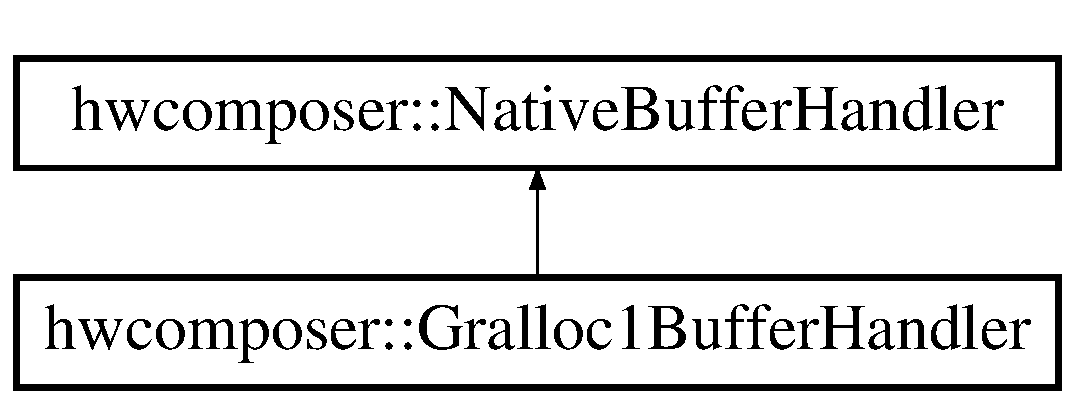
\includegraphics[height=2.000000cm]{classhwcomposer_1_1Gralloc1BufferHandler}
\end{center}
\end{figure}
\subsection*{Public Member Functions}
\begin{DoxyCompactItemize}
\item 
\mbox{\hyperlink{classhwcomposer_1_1Gralloc1BufferHandler_a07552c435b9ccdd99c898a81d805cdd2}{Gralloc1\+Buffer\+Handler}} (uint32\+\_\+t fd)
\item 
\mbox{\hyperlink{classhwcomposer_1_1Gralloc1BufferHandler_a4802221a9b764fcb8c319a162d004be7}{$\sim$\+Gralloc1\+Buffer\+Handler}} () override
\item 
bool \mbox{\hyperlink{classhwcomposer_1_1Gralloc1BufferHandler_a1d70874f4b535fe0763be57f3d9b2efd}{Init}} ()
\item 
bool \mbox{\hyperlink{classhwcomposer_1_1Gralloc1BufferHandler_a980ee5c0aa77d99861a89bdf6294d2db}{Create\+Buffer}} (uint32\+\_\+t w, uint32\+\_\+t h, int format, \mbox{\hyperlink{alios_2platformdefines_8h_ac0a2eaf260f556d17fe489911f017bdf}{H\+W\+C\+Native\+Handle}} $\ast$handle, uint32\+\_\+t layer\+\_\+type=k\+Layer\+Normal, bool $\ast$modifier\+\_\+used=\mbox{\hyperlink{alios_2platformdefines_8h_a070d2ce7b6bb7e5c05602aa8c308d0c4}{N\+U\+LL}}, int64\+\_\+t modifier=-\/1, bool raw\+\_\+pixel\+\_\+buffer=false) const override
\item 
bool \mbox{\hyperlink{classhwcomposer_1_1Gralloc1BufferHandler_a21b27b52da92605736b164e8088b93fe}{Release\+Buffer}} (\mbox{\hyperlink{alios_2platformdefines_8h_ac0a2eaf260f556d17fe489911f017bdf}{H\+W\+C\+Native\+Handle}} handle) const override
\item 
void \mbox{\hyperlink{classhwcomposer_1_1Gralloc1BufferHandler_aac10a3d48f5dab43e3057ef9783bd6ea}{Destroy\+Handle}} (\mbox{\hyperlink{alios_2platformdefines_8h_ac0a2eaf260f556d17fe489911f017bdf}{H\+W\+C\+Native\+Handle}} handle) const override
\item 
bool \mbox{\hyperlink{classhwcomposer_1_1Gralloc1BufferHandler_a0341cd413ba6e7d422edf30a161cd2b9}{Import\+Buffer}} (\mbox{\hyperlink{alios_2platformdefines_8h_ac0a2eaf260f556d17fe489911f017bdf}{H\+W\+C\+Native\+Handle}} handle) const override
\item 
void \mbox{\hyperlink{classhwcomposer_1_1Gralloc1BufferHandler_a87adf9132b6567a3b167741beebcd9d3}{Copy\+Handle}} (\mbox{\hyperlink{alios_2platformdefines_8h_ac0a2eaf260f556d17fe489911f017bdf}{H\+W\+C\+Native\+Handle}} source, \mbox{\hyperlink{alios_2platformdefines_8h_ac0a2eaf260f556d17fe489911f017bdf}{H\+W\+C\+Native\+Handle}} $\ast$target) const override
\item 
uint32\+\_\+t \mbox{\hyperlink{classhwcomposer_1_1Gralloc1BufferHandler_ad86921fa69dbb60b82581bd6f893decc}{Get\+Total\+Planes}} (\mbox{\hyperlink{alios_2platformdefines_8h_ac0a2eaf260f556d17fe489911f017bdf}{H\+W\+C\+Native\+Handle}} handle) const override
\item 
void $\ast$ \mbox{\hyperlink{classhwcomposer_1_1Gralloc1BufferHandler_a55e32dbd6cc8c32cb3fd3cac11d3f9f8}{Map}} (\mbox{\hyperlink{alios_2platformdefines_8h_ac0a2eaf260f556d17fe489911f017bdf}{H\+W\+C\+Native\+Handle}} handle, uint32\+\_\+t x, uint32\+\_\+t y, uint32\+\_\+t width, uint32\+\_\+t height, uint32\+\_\+t $\ast$stride, void $\ast$$\ast$map\+\_\+data, size\+\_\+t plane) const override
\item 
int32\+\_\+t \mbox{\hyperlink{classhwcomposer_1_1Gralloc1BufferHandler_a147ec425ec0fda400f1d4dd5c60764d9}{Un\+Map}} (\mbox{\hyperlink{alios_2platformdefines_8h_ac0a2eaf260f556d17fe489911f017bdf}{H\+W\+C\+Native\+Handle}} handle, void $\ast$map\+\_\+data) const override
\item 
uint32\+\_\+t \mbox{\hyperlink{classhwcomposer_1_1Gralloc1BufferHandler_aee03106dfff3a4b68b2a29a0d0350d07}{Get\+Fd}} () const override
\end{DoxyCompactItemize}
\subsection*{Additional Inherited Members}


\subsection{Detailed Description}


Definition at line 30 of file gralloc1bufferhandler.\+h.



\subsection{Constructor \& Destructor Documentation}
\mbox{\Hypertarget{classhwcomposer_1_1Gralloc1BufferHandler_a07552c435b9ccdd99c898a81d805cdd2}\label{classhwcomposer_1_1Gralloc1BufferHandler_a07552c435b9ccdd99c898a81d805cdd2}} 
\index{hwcomposer\+::\+Gralloc1\+Buffer\+Handler@{hwcomposer\+::\+Gralloc1\+Buffer\+Handler}!Gralloc1\+Buffer\+Handler@{Gralloc1\+Buffer\+Handler}}
\index{Gralloc1\+Buffer\+Handler@{Gralloc1\+Buffer\+Handler}!hwcomposer\+::\+Gralloc1\+Buffer\+Handler@{hwcomposer\+::\+Gralloc1\+Buffer\+Handler}}
\subsubsection{\texorpdfstring{Gralloc1\+Buffer\+Handler()}{Gralloc1BufferHandler()}}
{\footnotesize\ttfamily hwcomposer\+::\+Gralloc1\+Buffer\+Handler\+::\+Gralloc1\+Buffer\+Handler (\begin{DoxyParamCaption}\item[{uint32\+\_\+t}]{fd }\end{DoxyParamCaption})\hspace{0.3cm}{\ttfamily [explicit]}}



Definition at line 47 of file gralloc1bufferhandler.\+cpp.


\begin{DoxyCode}{0}
\DoxyCodeLine{48     : fd\_(fd),}
\DoxyCodeLine{49       gralloc\_(\textcolor{keyword}{nullptr}),}
\DoxyCodeLine{50       device\_(\textcolor{keyword}{nullptr}),}
\DoxyCodeLine{51       register\_(\textcolor{keyword}{nullptr}),}
\DoxyCodeLine{52       release\_(\textcolor{keyword}{nullptr}),}
\DoxyCodeLine{53       dimensions\_(\textcolor{keyword}{nullptr}),}
\DoxyCodeLine{54       lock\_(\textcolor{keyword}{nullptr}),}
\DoxyCodeLine{55       unlock\_(\textcolor{keyword}{nullptr}),}
\DoxyCodeLine{56       create\_descriptor\_(\textcolor{keyword}{nullptr}),}
\DoxyCodeLine{57       destroy\_descriptor\_(\textcolor{keyword}{nullptr}),}
\DoxyCodeLine{58       set\_consumer\_usage\_(\textcolor{keyword}{nullptr}),}
\DoxyCodeLine{59       set\_dimensions\_(\textcolor{keyword}{nullptr}),}
\DoxyCodeLine{60       set\_format\_(\textcolor{keyword}{nullptr}),}
\DoxyCodeLine{61       set\_producer\_usage\_(\textcolor{keyword}{nullptr}),}
\DoxyCodeLine{62       allocate\_(\textcolor{keyword}{nullptr}),}
\DoxyCodeLine{63       set\_modifier\_(\textcolor{keyword}{nullptr}) \{}
\DoxyCodeLine{64 \}}
\end{DoxyCode}
\mbox{\Hypertarget{classhwcomposer_1_1Gralloc1BufferHandler_a4802221a9b764fcb8c319a162d004be7}\label{classhwcomposer_1_1Gralloc1BufferHandler_a4802221a9b764fcb8c319a162d004be7}} 
\index{hwcomposer\+::\+Gralloc1\+Buffer\+Handler@{hwcomposer\+::\+Gralloc1\+Buffer\+Handler}!````~Gralloc1\+Buffer\+Handler@{$\sim$\+Gralloc1\+Buffer\+Handler}}
\index{````~Gralloc1\+Buffer\+Handler@{$\sim$\+Gralloc1\+Buffer\+Handler}!hwcomposer\+::\+Gralloc1\+Buffer\+Handler@{hwcomposer\+::\+Gralloc1\+Buffer\+Handler}}
\subsubsection{\texorpdfstring{$\sim$\+Gralloc1\+Buffer\+Handler()}{~Gralloc1BufferHandler()}}
{\footnotesize\ttfamily hwcomposer\+::\+Gralloc1\+Buffer\+Handler\+::$\sim$\+Gralloc1\+Buffer\+Handler (\begin{DoxyParamCaption}{ }\end{DoxyParamCaption})\hspace{0.3cm}{\ttfamily [override]}}



Definition at line 66 of file gralloc1bufferhandler.\+cpp.


\begin{DoxyCode}{0}
\DoxyCodeLine{66                                               \{}
\DoxyCodeLine{67   gralloc1\_device\_t *gralloc1\_dvc =}
\DoxyCodeLine{68       \textcolor{keyword}{reinterpret\_cast<}gralloc1\_device\_t *\textcolor{keyword}{>}(device\_);}
\DoxyCodeLine{69   gralloc1\_dvc->common.close(device\_);}
\DoxyCodeLine{70 \}}
\end{DoxyCode}


\subsection{Member Function Documentation}
\mbox{\Hypertarget{classhwcomposer_1_1Gralloc1BufferHandler_a87adf9132b6567a3b167741beebcd9d3}\label{classhwcomposer_1_1Gralloc1BufferHandler_a87adf9132b6567a3b167741beebcd9d3}} 
\index{hwcomposer\+::\+Gralloc1\+Buffer\+Handler@{hwcomposer\+::\+Gralloc1\+Buffer\+Handler}!Copy\+Handle@{Copy\+Handle}}
\index{Copy\+Handle@{Copy\+Handle}!hwcomposer\+::\+Gralloc1\+Buffer\+Handler@{hwcomposer\+::\+Gralloc1\+Buffer\+Handler}}
\subsubsection{\texorpdfstring{Copy\+Handle()}{CopyHandle()}}
{\footnotesize\ttfamily void hwcomposer\+::\+Gralloc1\+Buffer\+Handler\+::\+Copy\+Handle (\begin{DoxyParamCaption}\item[{\mbox{\hyperlink{alios_2platformdefines_8h_ac0a2eaf260f556d17fe489911f017bdf}{H\+W\+C\+Native\+Handle}}}]{source,  }\item[{\mbox{\hyperlink{alios_2platformdefines_8h_ac0a2eaf260f556d17fe489911f017bdf}{H\+W\+C\+Native\+Handle}} $\ast$}]{target }\end{DoxyParamCaption}) const\hspace{0.3cm}{\ttfamily [override]}, {\ttfamily [virtual]}}



Implements \mbox{\hyperlink{classhwcomposer_1_1NativeBufferHandler_a96581fb8bd36e959c8da6b9f634ecd32}{hwcomposer\+::\+Native\+Buffer\+Handler}}.



Definition at line 255 of file gralloc1bufferhandler.\+cpp.


\begin{DoxyCode}{0}
\DoxyCodeLine{256                                                                       \{}
\DoxyCodeLine{257   CopyBufferHandle(source, target);}
\DoxyCodeLine{258 \}}
\end{DoxyCode}
\mbox{\Hypertarget{classhwcomposer_1_1Gralloc1BufferHandler_a980ee5c0aa77d99861a89bdf6294d2db}\label{classhwcomposer_1_1Gralloc1BufferHandler_a980ee5c0aa77d99861a89bdf6294d2db}} 
\index{hwcomposer\+::\+Gralloc1\+Buffer\+Handler@{hwcomposer\+::\+Gralloc1\+Buffer\+Handler}!Create\+Buffer@{Create\+Buffer}}
\index{Create\+Buffer@{Create\+Buffer}!hwcomposer\+::\+Gralloc1\+Buffer\+Handler@{hwcomposer\+::\+Gralloc1\+Buffer\+Handler}}
\subsubsection{\texorpdfstring{Create\+Buffer()}{CreateBuffer()}}
{\footnotesize\ttfamily bool hwcomposer\+::\+Gralloc1\+Buffer\+Handler\+::\+Create\+Buffer (\begin{DoxyParamCaption}\item[{uint32\+\_\+t}]{w,  }\item[{uint32\+\_\+t}]{h,  }\item[{int}]{format,  }\item[{\mbox{\hyperlink{alios_2platformdefines_8h_ac0a2eaf260f556d17fe489911f017bdf}{H\+W\+C\+Native\+Handle}} $\ast$}]{handle,  }\item[{uint32\+\_\+t}]{layer\+\_\+type = {\ttfamily kLayerNormal},  }\item[{bool $\ast$}]{modifier\+\_\+used = {\ttfamily \mbox{\hyperlink{alios_2platformdefines_8h_a070d2ce7b6bb7e5c05602aa8c308d0c4}{N\+U\+LL}}},  }\item[{int64\+\_\+t}]{modifier = {\ttfamily -\/1},  }\item[{bool}]{raw\+\_\+pixel\+\_\+buffer = {\ttfamily false} }\end{DoxyParamCaption}) const\hspace{0.3cm}{\ttfamily [override]}, {\ttfamily [virtual]}}



Implements \mbox{\hyperlink{classhwcomposer_1_1NativeBufferHandler_a7e58e3d81d3f56cbee34c963b4999fde}{hwcomposer\+::\+Native\+Buffer\+Handler}}.



Definition at line 128 of file gralloc1bufferhandler.\+cpp.


\begin{DoxyCode}{0}
\DoxyCodeLine{133                                                        \{}
\DoxyCodeLine{134   \textcolor{keyword}{struct }\mbox{\hyperlink{structgralloc__handle}{gralloc\_handle}} *temp = \textcolor{keyword}{new} \textcolor{keyword}{struct }\mbox{\hyperlink{structgralloc__handle}{gralloc\_handle}}();}
\DoxyCodeLine{135   gralloc1\_device\_t *gralloc1\_dvc =}
\DoxyCodeLine{136       \textcolor{keyword}{reinterpret\_cast<}gralloc1\_device\_t *\textcolor{keyword}{>}(device\_);}
\DoxyCodeLine{137 }
\DoxyCodeLine{138   create\_descriptor\_(gralloc1\_dvc, \&temp->\mbox{\hyperlink{structgralloc__handle_a3b9885580cfaa575a8e159512e247d9f}{gralloc1\_buffer\_descriptor\_t\_}});}
\DoxyCodeLine{139   uint32\_t usage = 0;}
\DoxyCodeLine{140   uint32\_t pixel\_format = 0;}
\DoxyCodeLine{141   \textcolor{keywordtype}{bool} force\_normal\_usage = \textcolor{keyword}{false};}
\DoxyCodeLine{142   \textcolor{keywordflow}{if} (format != 0) \{}
\DoxyCodeLine{143     pixel\_format = DrmFormatToHALFormat(format);}
\DoxyCodeLine{144   \}}
\DoxyCodeLine{145 }
\DoxyCodeLine{146   \textcolor{keywordflow}{if} (pixel\_format == 0) \{}
\DoxyCodeLine{147     pixel\_format = HAL\_PIXEL\_FORMAT\_RGBA\_8888;}
\DoxyCodeLine{148   \}}
\DoxyCodeLine{149 }
\DoxyCodeLine{150   set\_format\_(gralloc1\_dvc, temp->\mbox{\hyperlink{structgralloc__handle_a3b9885580cfaa575a8e159512e247d9f}{gralloc1\_buffer\_descriptor\_t\_}}, pixel\_format);}
\DoxyCodeLine{151 \textcolor{preprocessor}{\#ifdef ENABLE\_RBC}}
\DoxyCodeLine{152   \textcolor{keywordflow}{if} (set\_modifier\_) \{}
\DoxyCodeLine{153     uint64\_t modifier = 0;}
\DoxyCodeLine{154     \textcolor{keywordflow}{if} (preferred\_modifier != -1) \{}
\DoxyCodeLine{155       modifier = preferred\_modifier;}
\DoxyCodeLine{156     \} \textcolor{keywordflow}{else} \{}
\DoxyCodeLine{157       modifier = choose\_drm\_modifier(format);}
\DoxyCodeLine{158     \}}
\DoxyCodeLine{159 }
\DoxyCodeLine{160     set\_modifier\_(gralloc1\_dvc, temp->\mbox{\hyperlink{structgralloc__handle_a3b9885580cfaa575a8e159512e247d9f}{gralloc1\_buffer\_descriptor\_t\_}}, modifier);}
\DoxyCodeLine{161   \}}
\DoxyCodeLine{162 }
\DoxyCodeLine{163   \textcolor{keywordflow}{if} (modifier\_used) \{}
\DoxyCodeLine{164     *modifier\_used = \textcolor{keyword}{true};}
\DoxyCodeLine{165   \}}
\DoxyCodeLine{166 \textcolor{preprocessor}{\#else}}
\DoxyCodeLine{167   \textcolor{keywordflow}{if} (modifier\_used) \{}
\DoxyCodeLine{168     *modifier\_used = \textcolor{keyword}{false};}
\DoxyCodeLine{169   \}}
\DoxyCodeLine{170 \textcolor{preprocessor}{\#endif}}
\DoxyCodeLine{171 }
\DoxyCodeLine{172   \textcolor{keywordflow}{if} ((layer\_type == hwcomposer::kLayerVideo) \&\&}
\DoxyCodeLine{173       !\mbox{\hyperlink{namespacehwcomposer_a96195339fc55ee57f41cc4597a56746c}{IsSupportedMediaFormat}}(format)) \{}
\DoxyCodeLine{174     \mbox{\hyperlink{alios_2platformdefines_8h_a226d6c99e4bcfca193c095e085e9097d}{ETRACE}}(\textcolor{stringliteral}{"Forcing normal usage for Video Layer. \(\backslash\)n"});}
\DoxyCodeLine{175     force\_normal\_usage = \textcolor{keyword}{true};}
\DoxyCodeLine{176   \}}
\DoxyCodeLine{177 }
\DoxyCodeLine{178   \textcolor{keywordflow}{if} ((layer\_type == hwcomposer::kLayerNormal) || force\_normal\_usage) \{}
\DoxyCodeLine{179     usage |= GRALLOC1\_CONSUMER\_USAGE\_HWCOMPOSER |}
\DoxyCodeLine{180              GRALLOC1\_PRODUCER\_USAGE\_GPU\_RENDER\_TARGET |}
\DoxyCodeLine{181              GRALLOC1\_CONSUMER\_USAGE\_GPU\_TEXTURE;}
\DoxyCodeLine{182   \} \textcolor{keywordflow}{else} \textcolor{keywordflow}{if} (layer\_type == hwcomposer::kLayerVideo) \{}
\DoxyCodeLine{183     \textcolor{keywordflow}{switch} (pixel\_format) \{}
\DoxyCodeLine{184       \textcolor{keywordflow}{case} HAL\_PIXEL\_FORMAT\_YCbCr\_422\_I:}
\DoxyCodeLine{185       \textcolor{keywordflow}{case} HAL\_PIXEL\_FORMAT\_Y8:}
\DoxyCodeLine{186         usage |= GRALLOC1\_CONSUMER\_USAGE\_GPU\_TEXTURE |}
\DoxyCodeLine{187                  GRALLOC1\_PRODUCER\_USAGE\_VIDEO\_DECODER;}
\DoxyCodeLine{188         \textcolor{keywordflow}{break};}
\DoxyCodeLine{189       \textcolor{keywordflow}{default}:}
\DoxyCodeLine{190         usage |= GRALLOC1\_PRODUCER\_USAGE\_CAMERA |}
\DoxyCodeLine{191                  GRALLOC1\_CONSUMER\_USAGE\_CAMERA |}
\DoxyCodeLine{192                  GRALLOC1\_PRODUCER\_USAGE\_VIDEO\_DECODER |}
\DoxyCodeLine{193                  GRALLOC1\_CONSUMER\_USAGE\_GPU\_TEXTURE;}
\DoxyCodeLine{194     \}}
\DoxyCodeLine{195   \} \textcolor{keywordflow}{else} \textcolor{keywordflow}{if} (layer\_type == hwcomposer::kLayerCursor) \{}
\DoxyCodeLine{196     usage |= GRALLOC1\_CONSUMER\_USAGE\_CURSOR;}
\DoxyCodeLine{197   \}}
\DoxyCodeLine{198 }
\DoxyCodeLine{199   set\_consumer\_usage\_(gralloc1\_dvc, temp->\mbox{\hyperlink{structgralloc__handle_a3b9885580cfaa575a8e159512e247d9f}{gralloc1\_buffer\_descriptor\_t\_}}, usage);}
\DoxyCodeLine{200   set\_producer\_usage\_(gralloc1\_dvc, temp->\mbox{\hyperlink{structgralloc__handle_a3b9885580cfaa575a8e159512e247d9f}{gralloc1\_buffer\_descriptor\_t\_}}, usage);}
\DoxyCodeLine{201   set\_dimensions\_(gralloc1\_dvc, temp->\mbox{\hyperlink{structgralloc__handle_a3b9885580cfaa575a8e159512e247d9f}{gralloc1\_buffer\_descriptor\_t\_}}, w, h);}
\DoxyCodeLine{202   allocate\_(gralloc1\_dvc, 1, \&temp->\mbox{\hyperlink{structgralloc__handle_a3b9885580cfaa575a8e159512e247d9f}{gralloc1\_buffer\_descriptor\_t\_}},}
\DoxyCodeLine{203             \&temp->\mbox{\hyperlink{structgralloc__handle_a7ab2601be21b021ab2a14d6549c6a537}{handle\_}});}
\DoxyCodeLine{204 }
\DoxyCodeLine{205   \textcolor{keywordflow}{if} (!temp->\mbox{\hyperlink{structgralloc__handle_a7ab2601be21b021ab2a14d6549c6a537}{handle\_}}) \{}
\DoxyCodeLine{206     \mbox{\hyperlink{alios_2platformdefines_8h_a226d6c99e4bcfca193c095e085e9097d}{ETRACE}}(\textcolor{stringliteral}{"Failed to allocate buffer \(\backslash\)n"});}
\DoxyCodeLine{207   \}}
\DoxyCodeLine{208 }
\DoxyCodeLine{209   temp->\mbox{\hyperlink{structgralloc__handle_a3ed360c5ac62fea5f6e171371ba6bb2a}{hwc\_buffer\_}} = \textcolor{keyword}{true};}
\DoxyCodeLine{210   *handle = temp;}
\DoxyCodeLine{211 }
\DoxyCodeLine{212   \textcolor{keywordflow}{return} \textcolor{keyword}{true};}
\DoxyCodeLine{213 \}}
\end{DoxyCode}
\mbox{\Hypertarget{classhwcomposer_1_1Gralloc1BufferHandler_aac10a3d48f5dab43e3057ef9783bd6ea}\label{classhwcomposer_1_1Gralloc1BufferHandler_aac10a3d48f5dab43e3057ef9783bd6ea}} 
\index{hwcomposer\+::\+Gralloc1\+Buffer\+Handler@{hwcomposer\+::\+Gralloc1\+Buffer\+Handler}!Destroy\+Handle@{Destroy\+Handle}}
\index{Destroy\+Handle@{Destroy\+Handle}!hwcomposer\+::\+Gralloc1\+Buffer\+Handler@{hwcomposer\+::\+Gralloc1\+Buffer\+Handler}}
\subsubsection{\texorpdfstring{Destroy\+Handle()}{DestroyHandle()}}
{\footnotesize\ttfamily void hwcomposer\+::\+Gralloc1\+Buffer\+Handler\+::\+Destroy\+Handle (\begin{DoxyParamCaption}\item[{\mbox{\hyperlink{alios_2platformdefines_8h_ac0a2eaf260f556d17fe489911f017bdf}{H\+W\+C\+Native\+Handle}}}]{handle }\end{DoxyParamCaption}) const\hspace{0.3cm}{\ttfamily [override]}, {\ttfamily [virtual]}}



Implements \mbox{\hyperlink{classhwcomposer_1_1NativeBufferHandler_ab1e22d9737ca9f6c3e75d1b550e34ce9}{hwcomposer\+::\+Native\+Buffer\+Handler}}.



Definition at line 231 of file gralloc1bufferhandler.\+cpp.


\begin{DoxyCode}{0}
\DoxyCodeLine{231                                                                       \{}
\DoxyCodeLine{232   DestroyBufferHandle(handle);}
\DoxyCodeLine{233 \}}
\end{DoxyCode}
\mbox{\Hypertarget{classhwcomposer_1_1Gralloc1BufferHandler_aee03106dfff3a4b68b2a29a0d0350d07}\label{classhwcomposer_1_1Gralloc1BufferHandler_aee03106dfff3a4b68b2a29a0d0350d07}} 
\index{hwcomposer\+::\+Gralloc1\+Buffer\+Handler@{hwcomposer\+::\+Gralloc1\+Buffer\+Handler}!Get\+Fd@{Get\+Fd}}
\index{Get\+Fd@{Get\+Fd}!hwcomposer\+::\+Gralloc1\+Buffer\+Handler@{hwcomposer\+::\+Gralloc1\+Buffer\+Handler}}
\subsubsection{\texorpdfstring{Get\+Fd()}{GetFd()}}
{\footnotesize\ttfamily uint32\+\_\+t hwcomposer\+::\+Gralloc1\+Buffer\+Handler\+::\+Get\+Fd (\begin{DoxyParamCaption}{ }\end{DoxyParamCaption}) const\hspace{0.3cm}{\ttfamily [inline]}, {\ttfamily [override]}, {\ttfamily [virtual]}}



Implements \mbox{\hyperlink{classhwcomposer_1_1NativeBufferHandler_adb5a4c6d14c012f8a5c71fbb2c984438}{hwcomposer\+::\+Native\+Buffer\+Handler}}.



Definition at line 52 of file gralloc1bufferhandler.\+h.


\begin{DoxyCode}{0}
\DoxyCodeLine{52                                   \{}
\DoxyCodeLine{53     \textcolor{keywordflow}{return} fd\_;}
\DoxyCodeLine{54   \}}
\end{DoxyCode}
\mbox{\Hypertarget{classhwcomposer_1_1Gralloc1BufferHandler_ad86921fa69dbb60b82581bd6f893decc}\label{classhwcomposer_1_1Gralloc1BufferHandler_ad86921fa69dbb60b82581bd6f893decc}} 
\index{hwcomposer\+::\+Gralloc1\+Buffer\+Handler@{hwcomposer\+::\+Gralloc1\+Buffer\+Handler}!Get\+Total\+Planes@{Get\+Total\+Planes}}
\index{Get\+Total\+Planes@{Get\+Total\+Planes}!hwcomposer\+::\+Gralloc1\+Buffer\+Handler@{hwcomposer\+::\+Gralloc1\+Buffer\+Handler}}
\subsubsection{\texorpdfstring{Get\+Total\+Planes()}{GetTotalPlanes()}}
{\footnotesize\ttfamily uint32\+\_\+t hwcomposer\+::\+Gralloc1\+Buffer\+Handler\+::\+Get\+Total\+Planes (\begin{DoxyParamCaption}\item[{\mbox{\hyperlink{alios_2platformdefines_8h_ac0a2eaf260f556d17fe489911f017bdf}{H\+W\+C\+Native\+Handle}}}]{handle }\end{DoxyParamCaption}) const\hspace{0.3cm}{\ttfamily [override]}, {\ttfamily [virtual]}}



Implements \mbox{\hyperlink{classhwcomposer_1_1NativeBufferHandler_a3b4115de8c13c53b6cd233f755f46dc9}{hwcomposer\+::\+Native\+Buffer\+Handler}}.



Definition at line 251 of file gralloc1bufferhandler.\+cpp.


\begin{DoxyCode}{0}
\DoxyCodeLine{251                                                                            \{}
\DoxyCodeLine{252   \textcolor{keywordflow}{return} handle->\mbox{\hyperlink{structyalloc__handle_a2dfa4e2505a052e5ddbbe66e32b33875}{meta\_data\_}}.\mbox{\hyperlink{structHwcBuffer_ab48df5577e8ecd60f18b4b5e6ec6544d}{num\_planes\_}};}
\DoxyCodeLine{253 \}}
\end{DoxyCode}
\mbox{\Hypertarget{classhwcomposer_1_1Gralloc1BufferHandler_a0341cd413ba6e7d422edf30a161cd2b9}\label{classhwcomposer_1_1Gralloc1BufferHandler_a0341cd413ba6e7d422edf30a161cd2b9}} 
\index{hwcomposer\+::\+Gralloc1\+Buffer\+Handler@{hwcomposer\+::\+Gralloc1\+Buffer\+Handler}!Import\+Buffer@{Import\+Buffer}}
\index{Import\+Buffer@{Import\+Buffer}!hwcomposer\+::\+Gralloc1\+Buffer\+Handler@{hwcomposer\+::\+Gralloc1\+Buffer\+Handler}}
\subsubsection{\texorpdfstring{Import\+Buffer()}{ImportBuffer()}}
{\footnotesize\ttfamily bool hwcomposer\+::\+Gralloc1\+Buffer\+Handler\+::\+Import\+Buffer (\begin{DoxyParamCaption}\item[{\mbox{\hyperlink{alios_2platformdefines_8h_ac0a2eaf260f556d17fe489911f017bdf}{H\+W\+C\+Native\+Handle}}}]{handle }\end{DoxyParamCaption}) const\hspace{0.3cm}{\ttfamily [override]}, {\ttfamily [virtual]}}



Implements \mbox{\hyperlink{classhwcomposer_1_1NativeBufferHandler_a5841be467d2aa11e8c4d7233596fda3c}{hwcomposer\+::\+Native\+Buffer\+Handler}}.



Definition at line 235 of file gralloc1bufferhandler.\+cpp.


\begin{DoxyCode}{0}
\DoxyCodeLine{235                                                                      \{}
\DoxyCodeLine{236   \textcolor{keywordflow}{if} (!handle->imported\_handle\_) \{}
\DoxyCodeLine{237     \mbox{\hyperlink{alios_2platformdefines_8h_a226d6c99e4bcfca193c095e085e9097d}{ETRACE}}(\textcolor{stringliteral}{"could not find gralloc drm handle"});}
\DoxyCodeLine{238     \textcolor{keywordflow}{return} \textcolor{keyword}{false};}
\DoxyCodeLine{239   \}}
\DoxyCodeLine{240 }
\DoxyCodeLine{241   gralloc1\_device\_t *gralloc1\_dvc =}
\DoxyCodeLine{242       \textcolor{keyword}{reinterpret\_cast<}gralloc1\_device\_t *\textcolor{keyword}{>}(device\_);}
\DoxyCodeLine{243   register\_(gralloc1\_dvc, handle->imported\_handle\_);}
\DoxyCodeLine{244   \textcolor{keywordflow}{if} (!ImportGraphicsBuffer(handle, fd\_)) \{}
\DoxyCodeLine{245     \textcolor{keywordflow}{return} \textcolor{keyword}{false};}
\DoxyCodeLine{246   \}}
\DoxyCodeLine{247 }
\DoxyCodeLine{248   \textcolor{keywordflow}{return} \textcolor{keyword}{true};}
\DoxyCodeLine{249 \}}
\end{DoxyCode}
\mbox{\Hypertarget{classhwcomposer_1_1Gralloc1BufferHandler_a1d70874f4b535fe0763be57f3d9b2efd}\label{classhwcomposer_1_1Gralloc1BufferHandler_a1d70874f4b535fe0763be57f3d9b2efd}} 
\index{hwcomposer\+::\+Gralloc1\+Buffer\+Handler@{hwcomposer\+::\+Gralloc1\+Buffer\+Handler}!Init@{Init}}
\index{Init@{Init}!hwcomposer\+::\+Gralloc1\+Buffer\+Handler@{hwcomposer\+::\+Gralloc1\+Buffer\+Handler}}
\subsubsection{\texorpdfstring{Init()}{Init()}}
{\footnotesize\ttfamily bool hwcomposer\+::\+Gralloc1\+Buffer\+Handler\+::\+Init (\begin{DoxyParamCaption}{ }\end{DoxyParamCaption})}



Definition at line 72 of file gralloc1bufferhandler.\+cpp.


\begin{DoxyCode}{0}
\DoxyCodeLine{72                                  \{}
\DoxyCodeLine{73   \textcolor{keywordtype}{int} ret = hw\_get\_module(GRALLOC\_HARDWARE\_MODULE\_ID,}
\DoxyCodeLine{74                           (\textcolor{keyword}{const} hw\_module\_t **)\&gralloc\_);}
\DoxyCodeLine{75   \textcolor{keywordflow}{if} (ret) \{}
\DoxyCodeLine{76     \mbox{\hyperlink{alios_2platformdefines_8h_a226d6c99e4bcfca193c095e085e9097d}{ETRACE}}(\textcolor{stringliteral}{"Failed to get gralloc module"});}
\DoxyCodeLine{77     \textcolor{keywordflow}{return} \textcolor{keyword}{false};}
\DoxyCodeLine{78   \}}
\DoxyCodeLine{79 }
\DoxyCodeLine{80   ret = gralloc\_->methods->open(gralloc\_, GRALLOC\_HARDWARE\_MODULE\_ID, \&device\_);}
\DoxyCodeLine{81   \textcolor{keywordflow}{if} (ret) \{}
\DoxyCodeLine{82     \mbox{\hyperlink{alios_2platformdefines_8h_a226d6c99e4bcfca193c095e085e9097d}{ETRACE}}(\textcolor{stringliteral}{"Failed to open gralloc module"});}
\DoxyCodeLine{83     \textcolor{keywordflow}{return} \textcolor{keyword}{false};}
\DoxyCodeLine{84   \}}
\DoxyCodeLine{85 }
\DoxyCodeLine{86   gralloc1\_device\_t *gralloc1\_dvc =}
\DoxyCodeLine{87       \textcolor{keyword}{reinterpret\_cast<}gralloc1\_device\_t *\textcolor{keyword}{>}(device\_);}
\DoxyCodeLine{88   register\_ = \textcolor{keyword}{reinterpret\_cast<}GRALLOC1\_PFN\_RETAIN\textcolor{keyword}{>}(}
\DoxyCodeLine{89       gralloc1\_dvc->getFunction(gralloc1\_dvc, GRALLOC1\_FUNCTION\_RETAIN));}
\DoxyCodeLine{90   release\_ = \textcolor{keyword}{reinterpret\_cast<}GRALLOC1\_PFN\_RELEASE\textcolor{keyword}{>}(}
\DoxyCodeLine{91       gralloc1\_dvc->getFunction(gralloc1\_dvc, GRALLOC1\_FUNCTION\_RELEASE));}
\DoxyCodeLine{92   lock\_ = \textcolor{keyword}{reinterpret\_cast<}GRALLOC1\_PFN\_LOCK\textcolor{keyword}{>}(}
\DoxyCodeLine{93       gralloc1\_dvc->getFunction(gralloc1\_dvc, GRALLOC1\_FUNCTION\_LOCK));}
\DoxyCodeLine{94   unlock\_ = \textcolor{keyword}{reinterpret\_cast<}GRALLOC1\_PFN\_UNLOCK\textcolor{keyword}{>}(}
\DoxyCodeLine{95       gralloc1\_dvc->getFunction(gralloc1\_dvc, GRALLOC1\_FUNCTION\_UNLOCK));}
\DoxyCodeLine{96 }
\DoxyCodeLine{97   dimensions\_ =}
\DoxyCodeLine{98       \textcolor{keyword}{reinterpret\_cast<}GRALLOC1\_PFN\_GET\_DIMENSIONS\textcolor{keyword}{>}(gralloc1\_dvc->getFunction(}
\DoxyCodeLine{99           gralloc1\_dvc, GRALLOC1\_FUNCTION\_GET\_DIMENSIONS));}
\DoxyCodeLine{100 }
\DoxyCodeLine{101   create\_descriptor\_ = \textcolor{keyword}{reinterpret\_cast<}GRALLOC1\_PFN\_CREATE\_DESCRIPTOR\textcolor{keyword}{>}(}
\DoxyCodeLine{102       gralloc1\_dvc->getFunction(gralloc1\_dvc,}
\DoxyCodeLine{103                                 GRALLOC1\_FUNCTION\_CREATE\_DESCRIPTOR));}
\DoxyCodeLine{104   destroy\_descriptor\_ = \textcolor{keyword}{reinterpret\_cast<}GRALLOC1\_PFN\_DESTROY\_DESCRIPTOR\textcolor{keyword}{>}(}
\DoxyCodeLine{105       gralloc1\_dvc->getFunction(gralloc1\_dvc,}
\DoxyCodeLine{106                                 GRALLOC1\_FUNCTION\_DESTROY\_DESCRIPTOR));}
\DoxyCodeLine{107 }
\DoxyCodeLine{108   set\_consumer\_usage\_ = \textcolor{keyword}{reinterpret\_cast<}GRALLOC1\_PFN\_SET\_CONSUMER\_USAGE\textcolor{keyword}{>}(}
\DoxyCodeLine{109       gralloc1\_dvc->getFunction(gralloc1\_dvc,}
\DoxyCodeLine{110                                 GRALLOC1\_FUNCTION\_SET\_CONSUMER\_USAGE));}
\DoxyCodeLine{111   set\_dimensions\_ =}
\DoxyCodeLine{112       \textcolor{keyword}{reinterpret\_cast<}GRALLOC1\_PFN\_SET\_DIMENSIONS\textcolor{keyword}{>}(gralloc1\_dvc->getFunction(}
\DoxyCodeLine{113           gralloc1\_dvc, GRALLOC1\_FUNCTION\_SET\_DIMENSIONS));}
\DoxyCodeLine{114   set\_format\_ = \textcolor{keyword}{reinterpret\_cast<}GRALLOC1\_PFN\_SET\_FORMAT\textcolor{keyword}{>}(}
\DoxyCodeLine{115       gralloc1\_dvc->getFunction(gralloc1\_dvc, GRALLOC1\_FUNCTION\_SET\_FORMAT));}
\DoxyCodeLine{116   set\_producer\_usage\_ = \textcolor{keyword}{reinterpret\_cast<}GRALLOC1\_PFN\_SET\_PRODUCER\_USAGE\textcolor{keyword}{>}(}
\DoxyCodeLine{117       gralloc1\_dvc->getFunction(gralloc1\_dvc,}
\DoxyCodeLine{118                                 GRALLOC1\_FUNCTION\_SET\_PRODUCER\_USAGE));}
\DoxyCodeLine{119   allocate\_ = \textcolor{keyword}{reinterpret\_cast<}GRALLOC1\_PFN\_ALLOCATE\textcolor{keyword}{>}(}
\DoxyCodeLine{120       gralloc1\_dvc->getFunction(gralloc1\_dvc, GRALLOC1\_FUNCTION\_ALLOCATE));}
\DoxyCodeLine{121 \textcolor{preprocessor}{\#ifdef USE\_GRALLOC1}}
\DoxyCodeLine{122   set\_modifier\_ = \textcolor{keyword}{reinterpret\_cast<}GRALLOC1\_PFN\_SET\_MODIFIER\textcolor{keyword}{>}(}
\DoxyCodeLine{123       gralloc1\_dvc->getFunction(gralloc1\_dvc, GRALLOC1\_FUNCTION\_SET\_MODIFIER));}
\DoxyCodeLine{124 \textcolor{preprocessor}{\#endif}}
\DoxyCodeLine{125   \textcolor{keywordflow}{return} \textcolor{keyword}{true};}
\DoxyCodeLine{126 \}}
\end{DoxyCode}
\mbox{\Hypertarget{classhwcomposer_1_1Gralloc1BufferHandler_a55e32dbd6cc8c32cb3fd3cac11d3f9f8}\label{classhwcomposer_1_1Gralloc1BufferHandler_a55e32dbd6cc8c32cb3fd3cac11d3f9f8}} 
\index{hwcomposer\+::\+Gralloc1\+Buffer\+Handler@{hwcomposer\+::\+Gralloc1\+Buffer\+Handler}!Map@{Map}}
\index{Map@{Map}!hwcomposer\+::\+Gralloc1\+Buffer\+Handler@{hwcomposer\+::\+Gralloc1\+Buffer\+Handler}}
\subsubsection{\texorpdfstring{Map()}{Map()}}
{\footnotesize\ttfamily void $\ast$ hwcomposer\+::\+Gralloc1\+Buffer\+Handler\+::\+Map (\begin{DoxyParamCaption}\item[{\mbox{\hyperlink{alios_2platformdefines_8h_ac0a2eaf260f556d17fe489911f017bdf}{H\+W\+C\+Native\+Handle}}}]{handle,  }\item[{uint32\+\_\+t}]{x,  }\item[{uint32\+\_\+t}]{y,  }\item[{uint32\+\_\+t}]{width,  }\item[{uint32\+\_\+t}]{height,  }\item[{uint32\+\_\+t $\ast$}]{stride,  }\item[{void $\ast$$\ast$}]{map\+\_\+data,  }\item[{size\+\_\+t}]{plane }\end{DoxyParamCaption}) const\hspace{0.3cm}{\ttfamily [override]}, {\ttfamily [virtual]}}



Implements \mbox{\hyperlink{classhwcomposer_1_1NativeBufferHandler_a4ef1e64030d28540265fac46d503e9b8}{hwcomposer\+::\+Native\+Buffer\+Handler}}.



Definition at line 260 of file gralloc1bufferhandler.\+cpp.


\begin{DoxyCode}{0}
\DoxyCodeLine{263                                                  \{}
\DoxyCodeLine{264   \textcolor{keyword}{auto} gr\_handle = (\textcolor{keyword}{struct }cros\_gralloc\_handle *)handle->imported\_handle\_;}
\DoxyCodeLine{265   if (!gr\_handle) \{}
\DoxyCodeLine{266     \mbox{\hyperlink{alios_2platformdefines_8h_a226d6c99e4bcfca193c095e085e9097d}{ETRACE}}(\textcolor{stringliteral}{"could not find gralloc drm handle"});}
\DoxyCodeLine{267     \textcolor{keywordflow}{return} \mbox{\hyperlink{alios_2platformdefines_8h_a070d2ce7b6bb7e5c05602aa8c308d0c4}{NULL}};}
\DoxyCodeLine{268   \}}
\DoxyCodeLine{269 }
\DoxyCodeLine{270   \textcolor{keywordtype}{int} acquireFence = -1;}
\DoxyCodeLine{271   gralloc1\_rect\_t rect\{\};}
\DoxyCodeLine{272   rect.left = x;}
\DoxyCodeLine{273   rect.top = y;}
\DoxyCodeLine{274   rect.width = width;}
\DoxyCodeLine{275   rect.height = height;}
\DoxyCodeLine{276 }
\DoxyCodeLine{277   gralloc1\_device\_t *gralloc1\_dvc =}
\DoxyCodeLine{278       \textcolor{keyword}{reinterpret\_cast<}gralloc1\_device\_t *\textcolor{keyword}{>}(device\_);}
\DoxyCodeLine{279   uint32\_t status = lock\_(gralloc1\_dvc, handle->imported\_handle\_,}
\DoxyCodeLine{280                           GRALLOC1\_PRODUCER\_USAGE\_CPU\_WRITE\_OFTEN,}
\DoxyCodeLine{281                           GRALLOC1\_CONSUMER\_USAGE\_CPU\_READ\_OFTEN, \&rect,}
\DoxyCodeLine{282                           map\_data, acquireFence);}
\DoxyCodeLine{283   \textcolor{keywordflow}{return} (GRALLOC1\_ERROR\_NONE == status) ? *map\_data : \mbox{\hyperlink{alios_2platformdefines_8h_a070d2ce7b6bb7e5c05602aa8c308d0c4}{NULL}};}
\DoxyCodeLine{284 \}}
\end{DoxyCode}
\mbox{\Hypertarget{classhwcomposer_1_1Gralloc1BufferHandler_a21b27b52da92605736b164e8088b93fe}\label{classhwcomposer_1_1Gralloc1BufferHandler_a21b27b52da92605736b164e8088b93fe}} 
\index{hwcomposer\+::\+Gralloc1\+Buffer\+Handler@{hwcomposer\+::\+Gralloc1\+Buffer\+Handler}!Release\+Buffer@{Release\+Buffer}}
\index{Release\+Buffer@{Release\+Buffer}!hwcomposer\+::\+Gralloc1\+Buffer\+Handler@{hwcomposer\+::\+Gralloc1\+Buffer\+Handler}}
\subsubsection{\texorpdfstring{Release\+Buffer()}{ReleaseBuffer()}}
{\footnotesize\ttfamily bool hwcomposer\+::\+Gralloc1\+Buffer\+Handler\+::\+Release\+Buffer (\begin{DoxyParamCaption}\item[{\mbox{\hyperlink{alios_2platformdefines_8h_ac0a2eaf260f556d17fe489911f017bdf}{H\+W\+C\+Native\+Handle}}}]{handle }\end{DoxyParamCaption}) const\hspace{0.3cm}{\ttfamily [override]}, {\ttfamily [virtual]}}



Implements \mbox{\hyperlink{classhwcomposer_1_1NativeBufferHandler_abff911db92343545a36a0cc44a8d2eb8}{hwcomposer\+::\+Native\+Buffer\+Handler}}.



Definition at line 215 of file gralloc1bufferhandler.\+cpp.


\begin{DoxyCode}{0}
\DoxyCodeLine{215                                                                       \{}
\DoxyCodeLine{216   gralloc1\_device\_t *gralloc1\_dvc =}
\DoxyCodeLine{217       \textcolor{keyword}{reinterpret\_cast<}gralloc1\_device\_t *\textcolor{keyword}{>}(device\_);}
\DoxyCodeLine{218 }
\DoxyCodeLine{219   \textcolor{keywordflow}{if} (handle->\mbox{\hyperlink{structyalloc__handle_ad1b5a7934204f6636871eb6270329654}{hwc\_buffer\_}}) \{}
\DoxyCodeLine{220     release\_(gralloc1\_dvc, handle->handle\_);}
\DoxyCodeLine{221   \} \textcolor{keywordflow}{else} \textcolor{keywordflow}{if} (handle->imported\_handle\_) \{}
\DoxyCodeLine{222     release\_(gralloc1\_dvc, handle->imported\_handle\_);}
\DoxyCodeLine{223   \}}
\DoxyCodeLine{224 }
\DoxyCodeLine{225   \textcolor{keywordflow}{if} (handle->gralloc1\_buffer\_descriptor\_t\_ > 0)}
\DoxyCodeLine{226     destroy\_descriptor\_(gralloc1\_dvc, handle->gralloc1\_buffer\_descriptor\_t\_);}
\DoxyCodeLine{227 }
\DoxyCodeLine{228   \textcolor{keywordflow}{return} \textcolor{keyword}{true};}
\DoxyCodeLine{229 \}}
\end{DoxyCode}
\mbox{\Hypertarget{classhwcomposer_1_1Gralloc1BufferHandler_a147ec425ec0fda400f1d4dd5c60764d9}\label{classhwcomposer_1_1Gralloc1BufferHandler_a147ec425ec0fda400f1d4dd5c60764d9}} 
\index{hwcomposer\+::\+Gralloc1\+Buffer\+Handler@{hwcomposer\+::\+Gralloc1\+Buffer\+Handler}!Un\+Map@{Un\+Map}}
\index{Un\+Map@{Un\+Map}!hwcomposer\+::\+Gralloc1\+Buffer\+Handler@{hwcomposer\+::\+Gralloc1\+Buffer\+Handler}}
\subsubsection{\texorpdfstring{Un\+Map()}{UnMap()}}
{\footnotesize\ttfamily int32\+\_\+t hwcomposer\+::\+Gralloc1\+Buffer\+Handler\+::\+Un\+Map (\begin{DoxyParamCaption}\item[{\mbox{\hyperlink{alios_2platformdefines_8h_ac0a2eaf260f556d17fe489911f017bdf}{H\+W\+C\+Native\+Handle}}}]{handle,  }\item[{void $\ast$}]{map\+\_\+data }\end{DoxyParamCaption}) const\hspace{0.3cm}{\ttfamily [override]}, {\ttfamily [virtual]}}



Implements \mbox{\hyperlink{classhwcomposer_1_1NativeBufferHandler_ae0da63bfef3f8342460fa1a958f8359c}{hwcomposer\+::\+Native\+Buffer\+Handler}}.



Definition at line 286 of file gralloc1bufferhandler.\+cpp.


\begin{DoxyCode}{0}
\DoxyCodeLine{287                                                      \{}
\DoxyCodeLine{288   \textcolor{keyword}{auto} gr\_handle = (\textcolor{keyword}{struct }cros\_gralloc\_handle *)handle->imported\_handle\_;}
\DoxyCodeLine{289   if (!gr\_handle) \{}
\DoxyCodeLine{290     \mbox{\hyperlink{alios_2platformdefines_8h_a226d6c99e4bcfca193c095e085e9097d}{ETRACE}}(\textcolor{stringliteral}{"could not find gralloc drm handle"});}
\DoxyCodeLine{291     \textcolor{keywordflow}{return} GRALLOC1\_ERROR\_BAD\_HANDLE;}
\DoxyCodeLine{292   \}}
\DoxyCodeLine{293 }
\DoxyCodeLine{294   \textcolor{keywordtype}{int} releaseFence = 0;}
\DoxyCodeLine{295   gralloc1\_device\_t *gralloc1\_dvc =}
\DoxyCodeLine{296       \textcolor{keyword}{reinterpret\_cast<}gralloc1\_device\_t *\textcolor{keyword}{>}(device\_);}
\DoxyCodeLine{297   \textcolor{keywordflow}{return} unlock\_(gralloc1\_dvc, handle->imported\_handle\_, \&releaseFence);}
\DoxyCodeLine{298 \}}
\end{DoxyCode}


The documentation for this class was generated from the following files\+:\begin{DoxyCompactItemize}
\item 
os/android/\mbox{\hyperlink{gralloc1bufferhandler_8h}{gralloc1bufferhandler.\+h}}\item 
os/android/\mbox{\hyperlink{gralloc1bufferhandler_8cpp}{gralloc1bufferhandler.\+cpp}}\end{DoxyCompactItemize}

\hypertarget{structgralloc__handle}{}\section{gralloc\+\_\+handle Struct Reference}
\label{structgralloc__handle}\index{gralloc\+\_\+handle@{gralloc\+\_\+handle}}


{\ttfamily \#include $<$platformdefines.\+h$>$}

\subsection*{Public Attributes}
\begin{DoxyCompactItemize}
\item 
buffer\+\_\+handle\+\_\+t \mbox{\hyperlink{structgralloc__handle_a7ab2601be21b021ab2a14d6549c6a537}{handle\+\_\+}} = \mbox{\hyperlink{alios_2platformdefines_8h_a070d2ce7b6bb7e5c05602aa8c308d0c4}{N\+U\+LL}}
\item 
native\+\_\+handle\+\_\+t $\ast$ \mbox{\hyperlink{structgralloc__handle_a6164b11702467313a0276cd7f823696a}{imported\+\_\+handle\+\_\+}} = \mbox{\hyperlink{alios_2platformdefines_8h_a070d2ce7b6bb7e5c05602aa8c308d0c4}{N\+U\+LL}}
\item 
\mbox{\hyperlink{structHwcBuffer}{Hwc\+Buffer}} \mbox{\hyperlink{structgralloc__handle_aa5c246b4955a8c51868b7915c6d512ab}{meta\+\_\+data\+\_\+}}
\item 
uint64\+\_\+t \mbox{\hyperlink{structgralloc__handle_a3b9885580cfaa575a8e159512e247d9f}{gralloc1\+\_\+buffer\+\_\+descriptor\+\_\+t\+\_\+}} = 0
\item 
bool \mbox{\hyperlink{structgralloc__handle_a3ed360c5ac62fea5f6e171371ba6bb2a}{hwc\+\_\+buffer\+\_\+}} = false
\item 
void $\ast$ \mbox{\hyperlink{structgralloc__handle_a23cae3e928fd07aced2f0c3f3690b9f9}{pixel\+\_\+memory\+\_\+}} = \mbox{\hyperlink{alios_2platformdefines_8h_a070d2ce7b6bb7e5c05602aa8c308d0c4}{N\+U\+LL}}
\end{DoxyCompactItemize}


\subsection{Detailed Description}


Definition at line 43 of file platformdefines.\+h.



\subsection{Member Data Documentation}
\mbox{\Hypertarget{structgralloc__handle_a3b9885580cfaa575a8e159512e247d9f}\label{structgralloc__handle_a3b9885580cfaa575a8e159512e247d9f}} 
\index{gralloc\+\_\+handle@{gralloc\+\_\+handle}!gralloc1\+\_\+buffer\+\_\+descriptor\+\_\+t\+\_\+@{gralloc1\+\_\+buffer\+\_\+descriptor\+\_\+t\+\_\+}}
\index{gralloc1\+\_\+buffer\+\_\+descriptor\+\_\+t\+\_\+@{gralloc1\+\_\+buffer\+\_\+descriptor\+\_\+t\+\_\+}!gralloc\+\_\+handle@{gralloc\+\_\+handle}}
\subsubsection{\texorpdfstring{gralloc1\+\_\+buffer\+\_\+descriptor\+\_\+t\+\_\+}{gralloc1\_buffer\_descriptor\_t\_}}
{\footnotesize\ttfamily uint64\+\_\+t gralloc\+\_\+handle\+::gralloc1\+\_\+buffer\+\_\+descriptor\+\_\+t\+\_\+ = 0}



Definition at line 47 of file platformdefines.\+h.

\mbox{\Hypertarget{structgralloc__handle_a7ab2601be21b021ab2a14d6549c6a537}\label{structgralloc__handle_a7ab2601be21b021ab2a14d6549c6a537}} 
\index{gralloc\+\_\+handle@{gralloc\+\_\+handle}!handle\+\_\+@{handle\+\_\+}}
\index{handle\+\_\+@{handle\+\_\+}!gralloc\+\_\+handle@{gralloc\+\_\+handle}}
\subsubsection{\texorpdfstring{handle\+\_\+}{handle\_}}
{\footnotesize\ttfamily buffer\+\_\+handle\+\_\+t gralloc\+\_\+handle\+::handle\+\_\+ = \mbox{\hyperlink{alios_2platformdefines_8h_a070d2ce7b6bb7e5c05602aa8c308d0c4}{N\+U\+LL}}}



Definition at line 44 of file platformdefines.\+h.

\mbox{\Hypertarget{structgralloc__handle_a3ed360c5ac62fea5f6e171371ba6bb2a}\label{structgralloc__handle_a3ed360c5ac62fea5f6e171371ba6bb2a}} 
\index{gralloc\+\_\+handle@{gralloc\+\_\+handle}!hwc\+\_\+buffer\+\_\+@{hwc\+\_\+buffer\+\_\+}}
\index{hwc\+\_\+buffer\+\_\+@{hwc\+\_\+buffer\+\_\+}!gralloc\+\_\+handle@{gralloc\+\_\+handle}}
\subsubsection{\texorpdfstring{hwc\+\_\+buffer\+\_\+}{hwc\_buffer\_}}
{\footnotesize\ttfamily bool gralloc\+\_\+handle\+::hwc\+\_\+buffer\+\_\+ = false}



Definition at line 48 of file platformdefines.\+h.

\mbox{\Hypertarget{structgralloc__handle_a6164b11702467313a0276cd7f823696a}\label{structgralloc__handle_a6164b11702467313a0276cd7f823696a}} 
\index{gralloc\+\_\+handle@{gralloc\+\_\+handle}!imported\+\_\+handle\+\_\+@{imported\+\_\+handle\+\_\+}}
\index{imported\+\_\+handle\+\_\+@{imported\+\_\+handle\+\_\+}!gralloc\+\_\+handle@{gralloc\+\_\+handle}}
\subsubsection{\texorpdfstring{imported\+\_\+handle\+\_\+}{imported\_handle\_}}
{\footnotesize\ttfamily native\+\_\+handle\+\_\+t$\ast$ gralloc\+\_\+handle\+::imported\+\_\+handle\+\_\+ = \mbox{\hyperlink{alios_2platformdefines_8h_a070d2ce7b6bb7e5c05602aa8c308d0c4}{N\+U\+LL}}}



Definition at line 45 of file platformdefines.\+h.

\mbox{\Hypertarget{structgralloc__handle_aa5c246b4955a8c51868b7915c6d512ab}\label{structgralloc__handle_aa5c246b4955a8c51868b7915c6d512ab}} 
\index{gralloc\+\_\+handle@{gralloc\+\_\+handle}!meta\+\_\+data\+\_\+@{meta\+\_\+data\+\_\+}}
\index{meta\+\_\+data\+\_\+@{meta\+\_\+data\+\_\+}!gralloc\+\_\+handle@{gralloc\+\_\+handle}}
\subsubsection{\texorpdfstring{meta\+\_\+data\+\_\+}{meta\_data\_}}
{\footnotesize\ttfamily \mbox{\hyperlink{structHwcBuffer}{Hwc\+Buffer}} gralloc\+\_\+handle\+::meta\+\_\+data\+\_\+}



Definition at line 46 of file platformdefines.\+h.

\mbox{\Hypertarget{structgralloc__handle_a23cae3e928fd07aced2f0c3f3690b9f9}\label{structgralloc__handle_a23cae3e928fd07aced2f0c3f3690b9f9}} 
\index{gralloc\+\_\+handle@{gralloc\+\_\+handle}!pixel\+\_\+memory\+\_\+@{pixel\+\_\+memory\+\_\+}}
\index{pixel\+\_\+memory\+\_\+@{pixel\+\_\+memory\+\_\+}!gralloc\+\_\+handle@{gralloc\+\_\+handle}}
\subsubsection{\texorpdfstring{pixel\+\_\+memory\+\_\+}{pixel\_memory\_}}
{\footnotesize\ttfamily void$\ast$ gralloc\+\_\+handle\+::pixel\+\_\+memory\+\_\+ = \mbox{\hyperlink{alios_2platformdefines_8h_a070d2ce7b6bb7e5c05602aa8c308d0c4}{N\+U\+LL}}}



Definition at line 49 of file platformdefines.\+h.



The documentation for this struct was generated from the following file\+:\begin{DoxyCompactItemize}
\item 
os/android/\mbox{\hyperlink{android_2platformdefines_8h}{platformdefines.\+h}}\end{DoxyCompactItemize}

\hypertarget{classhwcomposer_1_1HotPlugCallback}{}\section{hwcomposer\+:\+:Hot\+Plug\+Callback Class Reference}
\label{classhwcomposer_1_1HotPlugCallback}\index{hwcomposer\+::\+Hot\+Plug\+Callback@{hwcomposer\+::\+Hot\+Plug\+Callback}}


{\ttfamily \#include $<$nativedisplay.\+h$>$}

Inheritance diagram for hwcomposer\+:\+:Hot\+Plug\+Callback\+:\begin{figure}[H]
\begin{center}
\leavevmode
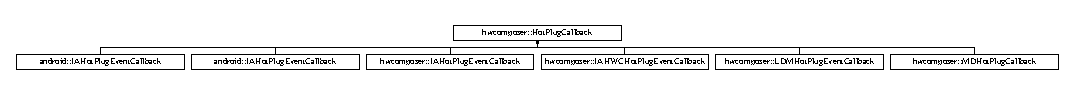
\includegraphics[height=0.709759cm]{classhwcomposer_1_1HotPlugCallback}
\end{center}
\end{figure}
\subsection*{Public Member Functions}
\begin{DoxyCompactItemize}
\item 
virtual \mbox{\hyperlink{classhwcomposer_1_1HotPlugCallback_a66fb4d75a8df0e0ef5f1bcf0954863b4}{$\sim$\+Hot\+Plug\+Callback}} ()
\item 
virtual void \mbox{\hyperlink{classhwcomposer_1_1HotPlugCallback_a455c8913e1da9b165134a05c9cb441ba}{Callback}} (uint32\+\_\+t display, bool connected)=0
\end{DoxyCompactItemize}


\subsection{Detailed Description}


Definition at line 51 of file nativedisplay.\+h.



\subsection{Constructor \& Destructor Documentation}
\mbox{\Hypertarget{classhwcomposer_1_1HotPlugCallback_a66fb4d75a8df0e0ef5f1bcf0954863b4}\label{classhwcomposer_1_1HotPlugCallback_a66fb4d75a8df0e0ef5f1bcf0954863b4}} 
\index{hwcomposer\+::\+Hot\+Plug\+Callback@{hwcomposer\+::\+Hot\+Plug\+Callback}!````~Hot\+Plug\+Callback@{$\sim$\+Hot\+Plug\+Callback}}
\index{````~Hot\+Plug\+Callback@{$\sim$\+Hot\+Plug\+Callback}!hwcomposer\+::\+Hot\+Plug\+Callback@{hwcomposer\+::\+Hot\+Plug\+Callback}}
\subsubsection{\texorpdfstring{$\sim$\+Hot\+Plug\+Callback()}{~HotPlugCallback()}}
{\footnotesize\ttfamily virtual hwcomposer\+::\+Hot\+Plug\+Callback\+::$\sim$\+Hot\+Plug\+Callback (\begin{DoxyParamCaption}{ }\end{DoxyParamCaption})\hspace{0.3cm}{\ttfamily [inline]}, {\ttfamily [virtual]}}



Definition at line 53 of file nativedisplay.\+h.


\begin{DoxyCode}{0}
\DoxyCodeLine{53                              \{}
\DoxyCodeLine{54   \}}
\end{DoxyCode}


\subsection{Member Function Documentation}
\mbox{\Hypertarget{classhwcomposer_1_1HotPlugCallback_a455c8913e1da9b165134a05c9cb441ba}\label{classhwcomposer_1_1HotPlugCallback_a455c8913e1da9b165134a05c9cb441ba}} 
\index{hwcomposer\+::\+Hot\+Plug\+Callback@{hwcomposer\+::\+Hot\+Plug\+Callback}!Callback@{Callback}}
\index{Callback@{Callback}!hwcomposer\+::\+Hot\+Plug\+Callback@{hwcomposer\+::\+Hot\+Plug\+Callback}}
\subsubsection{\texorpdfstring{Callback()}{Callback()}}
{\footnotesize\ttfamily virtual void hwcomposer\+::\+Hot\+Plug\+Callback\+::\+Callback (\begin{DoxyParamCaption}\item[{uint32\+\_\+t}]{display,  }\item[{bool}]{connected }\end{DoxyParamCaption})\hspace{0.3cm}{\ttfamily [pure virtual]}}



Implemented in \mbox{\hyperlink{classhwcomposer_1_1IAHotPlugEventCallback_a77b86b9fb88073abf1cab0b5aed4be1d}{hwcomposer\+::\+I\+A\+Hot\+Plug\+Event\+Callback}}, \mbox{\hyperlink{classandroid_1_1IAHotPlugEventCallback_af5cbfe8fc04fa828f75153f2b5f548b8}{android\+::\+I\+A\+Hot\+Plug\+Event\+Callback}}, \mbox{\hyperlink{classandroid_1_1IAHotPlugEventCallback_a8808ed272ecfd7006c28f0e54d6ba9e4}{android\+::\+I\+A\+Hot\+Plug\+Event\+Callback}}, \mbox{\hyperlink{classhwcomposer_1_1IAHWCHotPlugEventCallback_a06b3866efbc8e72c992e71357de1b4cb}{hwcomposer\+::\+I\+A\+H\+W\+C\+Hot\+Plug\+Event\+Callback}}, \mbox{\hyperlink{classhwcomposer_1_1MDHotPlugCallback_a56a4bfc5b98f35a0c27aa97afb119a7a}{hwcomposer\+::\+M\+D\+Hot\+Plug\+Callback}}, and \mbox{\hyperlink{classhwcomposer_1_1LDMHotPlugEventCallback_ab5e17c96c17c3707c3ef98d856807822}{hwcomposer\+::\+L\+D\+M\+Hot\+Plug\+Event\+Callback}}.



The documentation for this class was generated from the following file\+:\begin{DoxyCompactItemize}
\item 
public/\mbox{\hyperlink{nativedisplay_8h}{nativedisplay.\+h}}\end{DoxyCompactItemize}

\hypertarget{classandroid_1_1IAHWC2_1_1Hwc2Layer}{}\section{android\+:\+:I\+A\+H\+WC2\+:\+:Hwc2Layer Class Reference}
\label{classandroid_1_1IAHWC2_1_1Hwc2Layer}\index{android\+::\+I\+A\+H\+W\+C2\+::\+Hwc2\+Layer@{android\+::\+I\+A\+H\+W\+C2\+::\+Hwc2\+Layer}}


{\ttfamily \#include $<$iahwc2.\+h$>$}

\subsection*{Public Member Functions}
\begin{DoxyCompactItemize}
\item 
H\+W\+C2\+::\+Composition \mbox{\hyperlink{classandroid_1_1IAHWC2_1_1Hwc2Layer_ac39c5bf2230de7659a0dc3c61e3c14d9}{sf\+\_\+type}} () const
\item 
H\+W\+C2\+::\+Composition \mbox{\hyperlink{classandroid_1_1IAHWC2_1_1Hwc2Layer_a2361920d8d15d65eaee2ccb2c57c5623}{validated\+\_\+type}} () const
\item 
void \mbox{\hyperlink{classandroid_1_1IAHWC2_1_1Hwc2Layer_a8aaa19adc3ed5349d78178585bb9cc74}{accept\+\_\+type\+\_\+change}} ()
\item 
void \mbox{\hyperlink{classandroid_1_1IAHWC2_1_1Hwc2Layer_aea68551bf03014f5db39d6eb5bfea003}{set\+\_\+validated\+\_\+type}} (H\+W\+C2\+::\+Composition type)
\item 
bool \mbox{\hyperlink{classandroid_1_1IAHWC2_1_1Hwc2Layer_a21d5564c293990c35601edffc4b9b8b5}{type\+\_\+changed}} () const
\item 
uint32\+\_\+t \mbox{\hyperlink{classandroid_1_1IAHWC2_1_1Hwc2Layer_ab073755e350cf633747e67ac5cff7ee4}{z\+\_\+order}} () const
\item 
void \mbox{\hyperlink{classandroid_1_1IAHWC2_1_1Hwc2Layer_affc53396e897779e83bf3ab80268824c}{set\+\_\+buffer}} (buffer\+\_\+handle\+\_\+t buffer)
\item 
void \mbox{\hyperlink{classandroid_1_1IAHWC2_1_1Hwc2Layer_afec15cb870559a76d049d1e6c4aadde9}{X\+Translate\+Coordinates}} (uint32\+\_\+t x\+\_\+translation)
\item 
void \mbox{\hyperlink{classandroid_1_1IAHWC2_1_1Hwc2Layer_ae6de5e2f3be86c531587dd803f60d653}{Y\+Translate\+Coordinates}} (uint32\+\_\+t y\+\_\+translation)
\item 
void \mbox{\hyperlink{classandroid_1_1IAHWC2_1_1Hwc2Layer_adc68c4adc41b317552bb0a89a0e39ede}{set\+\_\+acquire\+\_\+fence}} (int acquire\+\_\+fence)
\item 
\mbox{\hyperlink{structhwcomposer_1_1HwcLayer}{hwcomposer\+::\+Hwc\+Layer}} $\ast$ \mbox{\hyperlink{classandroid_1_1IAHWC2_1_1Hwc2Layer_a743e0967bebe3cfefe1bff652cfae999}{Get\+Layer}} ()
\item 
bool \mbox{\hyperlink{classandroid_1_1IAHWC2_1_1Hwc2Layer_ae200b22303db92403a3526e3ce03fba7}{Is\+Cursor\+Layer}} () const
\item 
H\+W\+C2\+::\+Error \mbox{\hyperlink{classandroid_1_1IAHWC2_1_1Hwc2Layer_ae0e07b5f0856ec0358cb1c3e5101a9d8}{Set\+Cursor\+Position}} (int32\+\_\+t x, int32\+\_\+t y)
\item 
H\+W\+C2\+::\+Error \mbox{\hyperlink{classandroid_1_1IAHWC2_1_1Hwc2Layer_aeebdea172047373bebe04aacd0c12984}{Set\+Layer\+Blend\+Mode}} (int32\+\_\+t mode)
\item 
H\+W\+C2\+::\+Error \mbox{\hyperlink{classandroid_1_1IAHWC2_1_1Hwc2Layer_a748f182bf70067e273088e19bc55c4de}{Set\+Layer\+Buffer}} (buffer\+\_\+handle\+\_\+t buffer, int32\+\_\+t acquire\+\_\+fence)
\item 
H\+W\+C2\+::\+Error \mbox{\hyperlink{classandroid_1_1IAHWC2_1_1Hwc2Layer_a13c6379bb7319dcb0fc8ae6b6df3ae85}{Set\+Layer\+Color}} (hwc\+\_\+color\+\_\+t color)
\item 
H\+W\+C2\+::\+Error \mbox{\hyperlink{classandroid_1_1IAHWC2_1_1Hwc2Layer_a04088743426ddc86a6cbf0e989a7c583}{Set\+Layer\+Composition\+Type}} (int32\+\_\+t type)
\item 
H\+W\+C2\+::\+Error \mbox{\hyperlink{classandroid_1_1IAHWC2_1_1Hwc2Layer_a8623df440e40f374a16bcc0880f0a8d0}{Set\+Layer\+Dataspace}} (int32\+\_\+t dataspace)
\item 
H\+W\+C2\+::\+Error \mbox{\hyperlink{classandroid_1_1IAHWC2_1_1Hwc2Layer_a224e34e2bfd8844cc884b940a43440d4}{Set\+Layer\+Display\+Frame}} (hwc\+\_\+rect\+\_\+t frame)
\item 
H\+W\+C2\+::\+Error \mbox{\hyperlink{classandroid_1_1IAHWC2_1_1Hwc2Layer_a5e24e6a5a3cea60c8988b707893e0b6f}{Set\+Layer\+Plane\+Alpha}} (float alpha)
\item 
H\+W\+C2\+::\+Error \mbox{\hyperlink{classandroid_1_1IAHWC2_1_1Hwc2Layer_af54a365509e49e3229e21ce63dc1475d}{Set\+Layer\+Sideband\+Stream}} (const native\+\_\+handle\+\_\+t $\ast$stream)
\item 
H\+W\+C2\+::\+Error \mbox{\hyperlink{classandroid_1_1IAHWC2_1_1Hwc2Layer_ac093db321158cb01dfcdd646ddd037fe}{Set\+Layer\+Source\+Crop}} (hwc\+\_\+frect\+\_\+t crop)
\item 
H\+W\+C2\+::\+Error \mbox{\hyperlink{classandroid_1_1IAHWC2_1_1Hwc2Layer_a7d67bc2cbcef22cf7d4bdd603d56ddd6}{Set\+Layer\+Surface\+Damage}} (hwc\+\_\+region\+\_\+t damage)
\item 
H\+W\+C2\+::\+Error \mbox{\hyperlink{classandroid_1_1IAHWC2_1_1Hwc2Layer_af8f8b97ad63f413d0c16d8e95662c054}{Set\+Layer\+Transform}} (int32\+\_\+t transform)
\item 
H\+W\+C2\+::\+Error \mbox{\hyperlink{classandroid_1_1IAHWC2_1_1Hwc2Layer_af1a6d7d40ce690e300ff37b933ac44eb}{Set\+Layer\+Visible\+Region}} (hwc\+\_\+region\+\_\+t visible)
\item 
H\+W\+C2\+::\+Error \mbox{\hyperlink{classandroid_1_1IAHWC2_1_1Hwc2Layer_a73c282c185dbd4c86d86f666eaf241ad}{Set\+Layer\+Z\+Order}} (uint32\+\_\+t z)
\end{DoxyCompactItemize}


\subsection{Detailed Description}


Definition at line 59 of file iahwc2.\+h.



\subsection{Member Function Documentation}
\mbox{\Hypertarget{classandroid_1_1IAHWC2_1_1Hwc2Layer_a8aaa19adc3ed5349d78178585bb9cc74}\label{classandroid_1_1IAHWC2_1_1Hwc2Layer_a8aaa19adc3ed5349d78178585bb9cc74}} 
\index{android\+::\+I\+A\+H\+W\+C2\+::\+Hwc2\+Layer@{android\+::\+I\+A\+H\+W\+C2\+::\+Hwc2\+Layer}!accept\+\_\+type\+\_\+change@{accept\+\_\+type\+\_\+change}}
\index{accept\+\_\+type\+\_\+change@{accept\+\_\+type\+\_\+change}!android\+::\+I\+A\+H\+W\+C2\+::\+Hwc2\+Layer@{android\+::\+I\+A\+H\+W\+C2\+::\+Hwc2\+Layer}}
\subsubsection{\texorpdfstring{accept\+\_\+type\+\_\+change()}{accept\_type\_change()}}
{\footnotesize\ttfamily void android\+::\+I\+A\+H\+W\+C2\+::\+Hwc2\+Layer\+::accept\+\_\+type\+\_\+change (\begin{DoxyParamCaption}{ }\end{DoxyParamCaption})\hspace{0.3cm}{\ttfamily [inline]}}



Definition at line 67 of file iahwc2.\+h.


\begin{DoxyCode}{0}
\DoxyCodeLine{67                               \{}
\DoxyCodeLine{68       sf\_type\_ = validated\_type\_;}
\DoxyCodeLine{69     \}}
\end{DoxyCode}
\mbox{\Hypertarget{classandroid_1_1IAHWC2_1_1Hwc2Layer_a743e0967bebe3cfefe1bff652cfae999}\label{classandroid_1_1IAHWC2_1_1Hwc2Layer_a743e0967bebe3cfefe1bff652cfae999}} 
\index{android\+::\+I\+A\+H\+W\+C2\+::\+Hwc2\+Layer@{android\+::\+I\+A\+H\+W\+C2\+::\+Hwc2\+Layer}!Get\+Layer@{Get\+Layer}}
\index{Get\+Layer@{Get\+Layer}!android\+::\+I\+A\+H\+W\+C2\+::\+Hwc2\+Layer@{android\+::\+I\+A\+H\+W\+C2\+::\+Hwc2\+Layer}}
\subsubsection{\texorpdfstring{Get\+Layer()}{GetLayer()}}
{\footnotesize\ttfamily \mbox{\hyperlink{structhwcomposer_1_1HwcLayer}{hwcomposer\+::\+Hwc\+Layer}}$\ast$ android\+::\+I\+A\+H\+W\+C2\+::\+Hwc2\+Layer\+::\+Get\+Layer (\begin{DoxyParamCaption}{ }\end{DoxyParamCaption})\hspace{0.3cm}{\ttfamily [inline]}}



Definition at line 99 of file iahwc2.\+h.


\begin{DoxyCode}{0}
\DoxyCodeLine{99                                    \{}
\DoxyCodeLine{100       \textcolor{keywordflow}{return} \&hwc\_layer\_;}
\DoxyCodeLine{101     \}}
\end{DoxyCode}
\mbox{\Hypertarget{classandroid_1_1IAHWC2_1_1Hwc2Layer_ae200b22303db92403a3526e3ce03fba7}\label{classandroid_1_1IAHWC2_1_1Hwc2Layer_ae200b22303db92403a3526e3ce03fba7}} 
\index{android\+::\+I\+A\+H\+W\+C2\+::\+Hwc2\+Layer@{android\+::\+I\+A\+H\+W\+C2\+::\+Hwc2\+Layer}!Is\+Cursor\+Layer@{Is\+Cursor\+Layer}}
\index{Is\+Cursor\+Layer@{Is\+Cursor\+Layer}!android\+::\+I\+A\+H\+W\+C2\+::\+Hwc2\+Layer@{android\+::\+I\+A\+H\+W\+C2\+::\+Hwc2\+Layer}}
\subsubsection{\texorpdfstring{Is\+Cursor\+Layer()}{IsCursorLayer()}}
{\footnotesize\ttfamily bool android\+::\+I\+A\+H\+W\+C2\+::\+Hwc2\+Layer\+::\+Is\+Cursor\+Layer (\begin{DoxyParamCaption}{ }\end{DoxyParamCaption}) const\hspace{0.3cm}{\ttfamily [inline]}}



Definition at line 103 of file iahwc2.\+h.


\begin{DoxyCode}{0}
\DoxyCodeLine{103                                \{}
\DoxyCodeLine{104       \textcolor{keywordflow}{return} hwc\_layer\_.\mbox{\hyperlink{structhwcomposer_1_1HwcLayer_ac6692424ce0f4839a3e59793cf3efd16}{IsCursorLayer}}();}
\DoxyCodeLine{105     \}}
\end{DoxyCode}
\mbox{\Hypertarget{classandroid_1_1IAHWC2_1_1Hwc2Layer_adc68c4adc41b317552bb0a89a0e39ede}\label{classandroid_1_1IAHWC2_1_1Hwc2Layer_adc68c4adc41b317552bb0a89a0e39ede}} 
\index{android\+::\+I\+A\+H\+W\+C2\+::\+Hwc2\+Layer@{android\+::\+I\+A\+H\+W\+C2\+::\+Hwc2\+Layer}!set\+\_\+acquire\+\_\+fence@{set\+\_\+acquire\+\_\+fence}}
\index{set\+\_\+acquire\+\_\+fence@{set\+\_\+acquire\+\_\+fence}!android\+::\+I\+A\+H\+W\+C2\+::\+Hwc2\+Layer@{android\+::\+I\+A\+H\+W\+C2\+::\+Hwc2\+Layer}}
\subsubsection{\texorpdfstring{set\+\_\+acquire\+\_\+fence()}{set\_acquire\_fence()}}
{\footnotesize\ttfamily void android\+::\+I\+A\+H\+W\+C2\+::\+Hwc2\+Layer\+::set\+\_\+acquire\+\_\+fence (\begin{DoxyParamCaption}\item[{int}]{acquire\+\_\+fence }\end{DoxyParamCaption})\hspace{0.3cm}{\ttfamily [inline]}}



Definition at line 94 of file iahwc2.\+h.


\begin{DoxyCode}{0}
\DoxyCodeLine{94                                               \{}
\DoxyCodeLine{95       \textcolor{keywordflow}{if} (acquire\_fence > 0)}
\DoxyCodeLine{96         hwc\_layer\_.\mbox{\hyperlink{structhwcomposer_1_1HwcLayer_aaa01965ccb44cf807ec30956651c431a}{SetAcquireFence}}(acquire\_fence);}
\DoxyCodeLine{97     \}}
\end{DoxyCode}
\mbox{\Hypertarget{classandroid_1_1IAHWC2_1_1Hwc2Layer_affc53396e897779e83bf3ab80268824c}\label{classandroid_1_1IAHWC2_1_1Hwc2Layer_affc53396e897779e83bf3ab80268824c}} 
\index{android\+::\+I\+A\+H\+W\+C2\+::\+Hwc2\+Layer@{android\+::\+I\+A\+H\+W\+C2\+::\+Hwc2\+Layer}!set\+\_\+buffer@{set\+\_\+buffer}}
\index{set\+\_\+buffer@{set\+\_\+buffer}!android\+::\+I\+A\+H\+W\+C2\+::\+Hwc2\+Layer@{android\+::\+I\+A\+H\+W\+C2\+::\+Hwc2\+Layer}}
\subsubsection{\texorpdfstring{set\+\_\+buffer()}{set\_buffer()}}
{\footnotesize\ttfamily void android\+::\+I\+A\+H\+W\+C2\+::\+Hwc2\+Layer\+::set\+\_\+buffer (\begin{DoxyParamCaption}\item[{buffer\+\_\+handle\+\_\+t}]{buffer }\end{DoxyParamCaption})\hspace{0.3cm}{\ttfamily [inline]}}



Definition at line 81 of file iahwc2.\+h.


\begin{DoxyCode}{0}
\DoxyCodeLine{81                                             \{}
\DoxyCodeLine{82       native\_handle\_.\mbox{\hyperlink{structgralloc__handle_a7ab2601be21b021ab2a14d6549c6a537}{handle\_}} = buffer;}
\DoxyCodeLine{83       hwc\_layer\_.\mbox{\hyperlink{structhwcomposer_1_1HwcLayer_aeaeb1f0fd1d4c5754e0946b43c6eef84}{SetNativeHandle}}(\&native\_handle\_);}
\DoxyCodeLine{84     \}}
\end{DoxyCode}
\mbox{\Hypertarget{classandroid_1_1IAHWC2_1_1Hwc2Layer_aea68551bf03014f5db39d6eb5bfea003}\label{classandroid_1_1IAHWC2_1_1Hwc2Layer_aea68551bf03014f5db39d6eb5bfea003}} 
\index{android\+::\+I\+A\+H\+W\+C2\+::\+Hwc2\+Layer@{android\+::\+I\+A\+H\+W\+C2\+::\+Hwc2\+Layer}!set\+\_\+validated\+\_\+type@{set\+\_\+validated\+\_\+type}}
\index{set\+\_\+validated\+\_\+type@{set\+\_\+validated\+\_\+type}!android\+::\+I\+A\+H\+W\+C2\+::\+Hwc2\+Layer@{android\+::\+I\+A\+H\+W\+C2\+::\+Hwc2\+Layer}}
\subsubsection{\texorpdfstring{set\+\_\+validated\+\_\+type()}{set\_validated\_type()}}
{\footnotesize\ttfamily void android\+::\+I\+A\+H\+W\+C2\+::\+Hwc2\+Layer\+::set\+\_\+validated\+\_\+type (\begin{DoxyParamCaption}\item[{H\+W\+C2\+::\+Composition}]{type }\end{DoxyParamCaption})\hspace{0.3cm}{\ttfamily [inline]}}



Definition at line 70 of file iahwc2.\+h.


\begin{DoxyCode}{0}
\DoxyCodeLine{70                                                   \{}
\DoxyCodeLine{71       validated\_type\_ = type;}
\DoxyCodeLine{72     \}}
\end{DoxyCode}
\mbox{\Hypertarget{classandroid_1_1IAHWC2_1_1Hwc2Layer_ae0e07b5f0856ec0358cb1c3e5101a9d8}\label{classandroid_1_1IAHWC2_1_1Hwc2Layer_ae0e07b5f0856ec0358cb1c3e5101a9d8}} 
\index{android\+::\+I\+A\+H\+W\+C2\+::\+Hwc2\+Layer@{android\+::\+I\+A\+H\+W\+C2\+::\+Hwc2\+Layer}!Set\+Cursor\+Position@{Set\+Cursor\+Position}}
\index{Set\+Cursor\+Position@{Set\+Cursor\+Position}!android\+::\+I\+A\+H\+W\+C2\+::\+Hwc2\+Layer@{android\+::\+I\+A\+H\+W\+C2\+::\+Hwc2\+Layer}}
\subsubsection{\texorpdfstring{Set\+Cursor\+Position()}{SetCursorPosition()}}
{\footnotesize\ttfamily H\+W\+C2\+::\+Error android\+::\+I\+A\+H\+W\+C2\+::\+Hwc2\+Layer\+::\+Set\+Cursor\+Position (\begin{DoxyParamCaption}\item[{int32\+\_\+t}]{x,  }\item[{int32\+\_\+t}]{y }\end{DoxyParamCaption})}



Definition at line 854 of file iahwc2.\+cpp.


\begin{DoxyCode}{0}
\DoxyCodeLine{854                                                                  \{}
\DoxyCodeLine{855   supported(\_\_func\_\_);}
\DoxyCodeLine{856   \textcolor{keywordflow}{return} HWC2::Error::None;}
\DoxyCodeLine{857 \}}
\end{DoxyCode}
\mbox{\Hypertarget{classandroid_1_1IAHWC2_1_1Hwc2Layer_aeebdea172047373bebe04aacd0c12984}\label{classandroid_1_1IAHWC2_1_1Hwc2Layer_aeebdea172047373bebe04aacd0c12984}} 
\index{android\+::\+I\+A\+H\+W\+C2\+::\+Hwc2\+Layer@{android\+::\+I\+A\+H\+W\+C2\+::\+Hwc2\+Layer}!Set\+Layer\+Blend\+Mode@{Set\+Layer\+Blend\+Mode}}
\index{Set\+Layer\+Blend\+Mode@{Set\+Layer\+Blend\+Mode}!android\+::\+I\+A\+H\+W\+C2\+::\+Hwc2\+Layer@{android\+::\+I\+A\+H\+W\+C2\+::\+Hwc2\+Layer}}
\subsubsection{\texorpdfstring{Set\+Layer\+Blend\+Mode()}{SetLayerBlendMode()}}
{\footnotesize\ttfamily H\+W\+C2\+::\+Error android\+::\+I\+A\+H\+W\+C2\+::\+Hwc2\+Layer\+::\+Set\+Layer\+Blend\+Mode (\begin{DoxyParamCaption}\item[{int32\+\_\+t}]{mode }\end{DoxyParamCaption})}



Definition at line 859 of file iahwc2.\+cpp.


\begin{DoxyCode}{0}
\DoxyCodeLine{859                                                          \{}
\DoxyCodeLine{860   supported(\_\_func\_\_);}
\DoxyCodeLine{861   \textcolor{keywordflow}{switch} (static\_cast<HWC2::BlendMode>(mode)) \{}
\DoxyCodeLine{862     \textcolor{keywordflow}{case} HWC2::BlendMode::None:}
\DoxyCodeLine{863       hwc\_layer\_.\mbox{\hyperlink{structhwcomposer_1_1HwcLayer_a7705d2ba4b36529f37dc0f7e706417eb}{SetBlending}}(hwcomposer::HWCBlending::kBlendingNone);}
\DoxyCodeLine{864       \textcolor{keywordflow}{break};}
\DoxyCodeLine{865     \textcolor{keywordflow}{case} HWC2::BlendMode::Premultiplied:}
\DoxyCodeLine{866       hwc\_layer\_.\mbox{\hyperlink{structhwcomposer_1_1HwcLayer_a7705d2ba4b36529f37dc0f7e706417eb}{SetBlending}}(hwcomposer::HWCBlending::kBlendingPremult);}
\DoxyCodeLine{867       \textcolor{keywordflow}{break};}
\DoxyCodeLine{868     \textcolor{keywordflow}{case} HWC2::BlendMode::Coverage:}
\DoxyCodeLine{869       hwc\_layer\_.\mbox{\hyperlink{structhwcomposer_1_1HwcLayer_a7705d2ba4b36529f37dc0f7e706417eb}{SetBlending}}(hwcomposer::HWCBlending::kBlendingCoverage);}
\DoxyCodeLine{870       \textcolor{keywordflow}{break};}
\DoxyCodeLine{871     \textcolor{keywordflow}{default}:}
\DoxyCodeLine{872       ALOGE(\textcolor{stringliteral}{"Unknown blending mode b=\%d"}, mode);}
\DoxyCodeLine{873       hwc\_layer\_.\mbox{\hyperlink{structhwcomposer_1_1HwcLayer_a7705d2ba4b36529f37dc0f7e706417eb}{SetBlending}}(hwcomposer::HWCBlending::kBlendingNone);}
\DoxyCodeLine{874       \textcolor{keywordflow}{break};}
\DoxyCodeLine{875   \}}
\DoxyCodeLine{876   \textcolor{keywordflow}{return} HWC2::Error::None;}
\DoxyCodeLine{877 \}}
\end{DoxyCode}
\mbox{\Hypertarget{classandroid_1_1IAHWC2_1_1Hwc2Layer_a748f182bf70067e273088e19bc55c4de}\label{classandroid_1_1IAHWC2_1_1Hwc2Layer_a748f182bf70067e273088e19bc55c4de}} 
\index{android\+::\+I\+A\+H\+W\+C2\+::\+Hwc2\+Layer@{android\+::\+I\+A\+H\+W\+C2\+::\+Hwc2\+Layer}!Set\+Layer\+Buffer@{Set\+Layer\+Buffer}}
\index{Set\+Layer\+Buffer@{Set\+Layer\+Buffer}!android\+::\+I\+A\+H\+W\+C2\+::\+Hwc2\+Layer@{android\+::\+I\+A\+H\+W\+C2\+::\+Hwc2\+Layer}}
\subsubsection{\texorpdfstring{Set\+Layer\+Buffer()}{SetLayerBuffer()}}
{\footnotesize\ttfamily H\+W\+C2\+::\+Error android\+::\+I\+A\+H\+W\+C2\+::\+Hwc2\+Layer\+::\+Set\+Layer\+Buffer (\begin{DoxyParamCaption}\item[{buffer\+\_\+handle\+\_\+t}]{buffer,  }\item[{int32\+\_\+t}]{acquire\+\_\+fence }\end{DoxyParamCaption})}



Definition at line 879 of file iahwc2.\+cpp.


\begin{DoxyCode}{0}
\DoxyCodeLine{880                                                                      \{}
\DoxyCodeLine{881   supported(\_\_func\_\_);}
\DoxyCodeLine{882 }
\DoxyCodeLine{883   \textcolor{comment}{// The buffer and acquire\_fence are handled elsewhere}}
\DoxyCodeLine{884   \textcolor{keywordflow}{if} (sf\_type\_ == HWC2::Composition::Client ||}
\DoxyCodeLine{885       sf\_type\_ == HWC2::Composition::Sideband)}
\DoxyCodeLine{886     \textcolor{keywordflow}{return} HWC2::Error::None;}
\DoxyCodeLine{887 }
\DoxyCodeLine{888   native\_handle\_.\mbox{\hyperlink{structgralloc__handle_a7ab2601be21b021ab2a14d6549c6a537}{handle\_}} = buffer;}
\DoxyCodeLine{889   hwc\_layer\_.\mbox{\hyperlink{structhwcomposer_1_1HwcLayer_aeaeb1f0fd1d4c5754e0946b43c6eef84}{SetNativeHandle}}(\&native\_handle\_);}
\DoxyCodeLine{890   \textcolor{keywordflow}{if} (acquire\_fence > 0)}
\DoxyCodeLine{891     hwc\_layer\_.\mbox{\hyperlink{structhwcomposer_1_1HwcLayer_aaa01965ccb44cf807ec30956651c431a}{SetAcquireFence}}(acquire\_fence);}
\DoxyCodeLine{892   \textcolor{keywordflow}{return} HWC2::Error::None;}
\DoxyCodeLine{893 \}}
\end{DoxyCode}
\mbox{\Hypertarget{classandroid_1_1IAHWC2_1_1Hwc2Layer_a13c6379bb7319dcb0fc8ae6b6df3ae85}\label{classandroid_1_1IAHWC2_1_1Hwc2Layer_a13c6379bb7319dcb0fc8ae6b6df3ae85}} 
\index{android\+::\+I\+A\+H\+W\+C2\+::\+Hwc2\+Layer@{android\+::\+I\+A\+H\+W\+C2\+::\+Hwc2\+Layer}!Set\+Layer\+Color@{Set\+Layer\+Color}}
\index{Set\+Layer\+Color@{Set\+Layer\+Color}!android\+::\+I\+A\+H\+W\+C2\+::\+Hwc2\+Layer@{android\+::\+I\+A\+H\+W\+C2\+::\+Hwc2\+Layer}}
\subsubsection{\texorpdfstring{Set\+Layer\+Color()}{SetLayerColor()}}
{\footnotesize\ttfamily H\+W\+C2\+::\+Error android\+::\+I\+A\+H\+W\+C2\+::\+Hwc2\+Layer\+::\+Set\+Layer\+Color (\begin{DoxyParamCaption}\item[{hwc\+\_\+color\+\_\+t}]{color }\end{DoxyParamCaption})}



Definition at line 895 of file iahwc2.\+cpp.


\begin{DoxyCode}{0}
\DoxyCodeLine{895                                                           \{}
\DoxyCodeLine{896   \textcolor{comment}{// We only support Opaque colors so far.}}
\DoxyCodeLine{897   \textcolor{keywordflow}{if} (color.r == 0 \&\& color.g == 0 \&\& color.b == 0 \&\& color.a == 255) \{}
\DoxyCodeLine{898     sf\_type\_ = HWC2::Composition::SolidColor;}
\DoxyCodeLine{899     \textcolor{keywordflow}{return} HWC2::Error::None;}
\DoxyCodeLine{900   \}}
\DoxyCodeLine{901 }
\DoxyCodeLine{902   sf\_type\_ = HWC2::Composition::Client;}
\DoxyCodeLine{903   \textcolor{keywordflow}{return} HWC2::Error::None;}
\DoxyCodeLine{904 \}}
\end{DoxyCode}
\mbox{\Hypertarget{classandroid_1_1IAHWC2_1_1Hwc2Layer_a04088743426ddc86a6cbf0e989a7c583}\label{classandroid_1_1IAHWC2_1_1Hwc2Layer_a04088743426ddc86a6cbf0e989a7c583}} 
\index{android\+::\+I\+A\+H\+W\+C2\+::\+Hwc2\+Layer@{android\+::\+I\+A\+H\+W\+C2\+::\+Hwc2\+Layer}!Set\+Layer\+Composition\+Type@{Set\+Layer\+Composition\+Type}}
\index{Set\+Layer\+Composition\+Type@{Set\+Layer\+Composition\+Type}!android\+::\+I\+A\+H\+W\+C2\+::\+Hwc2\+Layer@{android\+::\+I\+A\+H\+W\+C2\+::\+Hwc2\+Layer}}
\subsubsection{\texorpdfstring{Set\+Layer\+Composition\+Type()}{SetLayerCompositionType()}}
{\footnotesize\ttfamily H\+W\+C2\+::\+Error android\+::\+I\+A\+H\+W\+C2\+::\+Hwc2\+Layer\+::\+Set\+Layer\+Composition\+Type (\begin{DoxyParamCaption}\item[{int32\+\_\+t}]{type }\end{DoxyParamCaption})}



Definition at line 906 of file iahwc2.\+cpp.


\begin{DoxyCode}{0}
\DoxyCodeLine{906                                                                \{}
\DoxyCodeLine{907   sf\_type\_ = \textcolor{keyword}{static\_cast<}HWC2::Composition\textcolor{keyword}{>}(type);}
\DoxyCodeLine{908   \textcolor{keywordflow}{if} (sf\_type\_ == HWC2::Composition::Cursor) \{}
\DoxyCodeLine{909     hwc\_layer\_.\mbox{\hyperlink{structhwcomposer_1_1HwcLayer_a7556bacbb2697f51b2c2cc30a9ed661a}{MarkAsCursorLayer}}();}
\DoxyCodeLine{910   \}}
\DoxyCodeLine{911 }
\DoxyCodeLine{912   \textcolor{keywordflow}{return} HWC2::Error::None;}
\DoxyCodeLine{913 \}}
\end{DoxyCode}
\mbox{\Hypertarget{classandroid_1_1IAHWC2_1_1Hwc2Layer_a8623df440e40f374a16bcc0880f0a8d0}\label{classandroid_1_1IAHWC2_1_1Hwc2Layer_a8623df440e40f374a16bcc0880f0a8d0}} 
\index{android\+::\+I\+A\+H\+W\+C2\+::\+Hwc2\+Layer@{android\+::\+I\+A\+H\+W\+C2\+::\+Hwc2\+Layer}!Set\+Layer\+Dataspace@{Set\+Layer\+Dataspace}}
\index{Set\+Layer\+Dataspace@{Set\+Layer\+Dataspace}!android\+::\+I\+A\+H\+W\+C2\+::\+Hwc2\+Layer@{android\+::\+I\+A\+H\+W\+C2\+::\+Hwc2\+Layer}}
\subsubsection{\texorpdfstring{Set\+Layer\+Dataspace()}{SetLayerDataspace()}}
{\footnotesize\ttfamily H\+W\+C2\+::\+Error android\+::\+I\+A\+H\+W\+C2\+::\+Hwc2\+Layer\+::\+Set\+Layer\+Dataspace (\begin{DoxyParamCaption}\item[{int32\+\_\+t}]{dataspace }\end{DoxyParamCaption})}



Definition at line 915 of file iahwc2.\+cpp.


\begin{DoxyCode}{0}
\DoxyCodeLine{915                                                               \{}
\DoxyCodeLine{916   supported(\_\_func\_\_);}
\DoxyCodeLine{917   dataspace\_ = \textcolor{keyword}{static\_cast<}android\_dataspace\_t\textcolor{keyword}{>}(dataspace);}
\DoxyCodeLine{918   \textcolor{keywordflow}{return} HWC2::Error::None;}
\DoxyCodeLine{919 \}}
\end{DoxyCode}
\mbox{\Hypertarget{classandroid_1_1IAHWC2_1_1Hwc2Layer_a224e34e2bfd8844cc884b940a43440d4}\label{classandroid_1_1IAHWC2_1_1Hwc2Layer_a224e34e2bfd8844cc884b940a43440d4}} 
\index{android\+::\+I\+A\+H\+W\+C2\+::\+Hwc2\+Layer@{android\+::\+I\+A\+H\+W\+C2\+::\+Hwc2\+Layer}!Set\+Layer\+Display\+Frame@{Set\+Layer\+Display\+Frame}}
\index{Set\+Layer\+Display\+Frame@{Set\+Layer\+Display\+Frame}!android\+::\+I\+A\+H\+W\+C2\+::\+Hwc2\+Layer@{android\+::\+I\+A\+H\+W\+C2\+::\+Hwc2\+Layer}}
\subsubsection{\texorpdfstring{Set\+Layer\+Display\+Frame()}{SetLayerDisplayFrame()}}
{\footnotesize\ttfamily H\+W\+C2\+::\+Error android\+::\+I\+A\+H\+W\+C2\+::\+Hwc2\+Layer\+::\+Set\+Layer\+Display\+Frame (\begin{DoxyParamCaption}\item[{hwc\+\_\+rect\+\_\+t}]{frame }\end{DoxyParamCaption})}



Definition at line 921 of file iahwc2.\+cpp.


\begin{DoxyCode}{0}
\DoxyCodeLine{921                                                                 \{}
\DoxyCodeLine{922   supported(\_\_func\_\_);}
\DoxyCodeLine{923   hwc\_layer\_.\mbox{\hyperlink{structhwcomposer_1_1HwcLayer_a0bf1d6ab9b9d45a7e118567b493dd346}{SetDisplayFrame}}(}
\DoxyCodeLine{924       hwcomposer::HwcRect<int>(frame.left, frame.top, frame.right,}
\DoxyCodeLine{925                                frame.bottom),}
\DoxyCodeLine{926       x\_translation\_, y\_translation\_);}
\DoxyCodeLine{927   \textcolor{keywordflow}{return} HWC2::Error::None;}
\DoxyCodeLine{928 \}}
\end{DoxyCode}
\mbox{\Hypertarget{classandroid_1_1IAHWC2_1_1Hwc2Layer_a5e24e6a5a3cea60c8988b707893e0b6f}\label{classandroid_1_1IAHWC2_1_1Hwc2Layer_a5e24e6a5a3cea60c8988b707893e0b6f}} 
\index{android\+::\+I\+A\+H\+W\+C2\+::\+Hwc2\+Layer@{android\+::\+I\+A\+H\+W\+C2\+::\+Hwc2\+Layer}!Set\+Layer\+Plane\+Alpha@{Set\+Layer\+Plane\+Alpha}}
\index{Set\+Layer\+Plane\+Alpha@{Set\+Layer\+Plane\+Alpha}!android\+::\+I\+A\+H\+W\+C2\+::\+Hwc2\+Layer@{android\+::\+I\+A\+H\+W\+C2\+::\+Hwc2\+Layer}}
\subsubsection{\texorpdfstring{Set\+Layer\+Plane\+Alpha()}{SetLayerPlaneAlpha()}}
{\footnotesize\ttfamily H\+W\+C2\+::\+Error android\+::\+I\+A\+H\+W\+C2\+::\+Hwc2\+Layer\+::\+Set\+Layer\+Plane\+Alpha (\begin{DoxyParamCaption}\item[{float}]{alpha }\end{DoxyParamCaption})}



Definition at line 930 of file iahwc2.\+cpp.


\begin{DoxyCode}{0}
\DoxyCodeLine{930                                                          \{}
\DoxyCodeLine{931   supported(\_\_func\_\_);}
\DoxyCodeLine{932   hwc\_layer\_.\mbox{\hyperlink{structhwcomposer_1_1HwcLayer_a312a7530c7cdca364df62c950ccbd024}{SetAlpha}}(static\_cast<uint8\_t>(255.0f * alpha + 0.5f));}
\DoxyCodeLine{933   \textcolor{keywordflow}{return} HWC2::Error::None;}
\DoxyCodeLine{934 \}}
\end{DoxyCode}
\mbox{\Hypertarget{classandroid_1_1IAHWC2_1_1Hwc2Layer_af54a365509e49e3229e21ce63dc1475d}\label{classandroid_1_1IAHWC2_1_1Hwc2Layer_af54a365509e49e3229e21ce63dc1475d}} 
\index{android\+::\+I\+A\+H\+W\+C2\+::\+Hwc2\+Layer@{android\+::\+I\+A\+H\+W\+C2\+::\+Hwc2\+Layer}!Set\+Layer\+Sideband\+Stream@{Set\+Layer\+Sideband\+Stream}}
\index{Set\+Layer\+Sideband\+Stream@{Set\+Layer\+Sideband\+Stream}!android\+::\+I\+A\+H\+W\+C2\+::\+Hwc2\+Layer@{android\+::\+I\+A\+H\+W\+C2\+::\+Hwc2\+Layer}}
\subsubsection{\texorpdfstring{Set\+Layer\+Sideband\+Stream()}{SetLayerSidebandStream()}}
{\footnotesize\ttfamily H\+W\+C2\+::\+Error android\+::\+I\+A\+H\+W\+C2\+::\+Hwc2\+Layer\+::\+Set\+Layer\+Sideband\+Stream (\begin{DoxyParamCaption}\item[{const native\+\_\+handle\+\_\+t $\ast$}]{stream }\end{DoxyParamCaption})}



Definition at line 936 of file iahwc2.\+cpp.


\begin{DoxyCode}{0}
\DoxyCodeLine{937                                    \{}
\DoxyCodeLine{938   supported(\_\_func\_\_);}
\DoxyCodeLine{939   \textcolor{comment}{// TODO: We don't support sideband}}
\DoxyCodeLine{940   \textcolor{keywordflow}{return} unsupported(\_\_func\_\_, stream);}
\DoxyCodeLine{941 \}}
\end{DoxyCode}
\mbox{\Hypertarget{classandroid_1_1IAHWC2_1_1Hwc2Layer_ac093db321158cb01dfcdd646ddd037fe}\label{classandroid_1_1IAHWC2_1_1Hwc2Layer_ac093db321158cb01dfcdd646ddd037fe}} 
\index{android\+::\+I\+A\+H\+W\+C2\+::\+Hwc2\+Layer@{android\+::\+I\+A\+H\+W\+C2\+::\+Hwc2\+Layer}!Set\+Layer\+Source\+Crop@{Set\+Layer\+Source\+Crop}}
\index{Set\+Layer\+Source\+Crop@{Set\+Layer\+Source\+Crop}!android\+::\+I\+A\+H\+W\+C2\+::\+Hwc2\+Layer@{android\+::\+I\+A\+H\+W\+C2\+::\+Hwc2\+Layer}}
\subsubsection{\texorpdfstring{Set\+Layer\+Source\+Crop()}{SetLayerSourceCrop()}}
{\footnotesize\ttfamily H\+W\+C2\+::\+Error android\+::\+I\+A\+H\+W\+C2\+::\+Hwc2\+Layer\+::\+Set\+Layer\+Source\+Crop (\begin{DoxyParamCaption}\item[{hwc\+\_\+frect\+\_\+t}]{crop }\end{DoxyParamCaption})}



Definition at line 943 of file iahwc2.\+cpp.


\begin{DoxyCode}{0}
\DoxyCodeLine{943                                                               \{}
\DoxyCodeLine{944   supported(\_\_func\_\_);}
\DoxyCodeLine{945   hwc\_layer\_.\mbox{\hyperlink{structhwcomposer_1_1HwcLayer_a83bafbef5b9c98ad5821acdeddd9a26e}{SetSourceCrop}}(}
\DoxyCodeLine{946       hwcomposer::HwcRect<float>(crop.left, crop.top, crop.right, crop.bottom));}
\DoxyCodeLine{947   \textcolor{keywordflow}{return} HWC2::Error::None;}
\DoxyCodeLine{948 \}}
\end{DoxyCode}
\mbox{\Hypertarget{classandroid_1_1IAHWC2_1_1Hwc2Layer_a7d67bc2cbcef22cf7d4bdd603d56ddd6}\label{classandroid_1_1IAHWC2_1_1Hwc2Layer_a7d67bc2cbcef22cf7d4bdd603d56ddd6}} 
\index{android\+::\+I\+A\+H\+W\+C2\+::\+Hwc2\+Layer@{android\+::\+I\+A\+H\+W\+C2\+::\+Hwc2\+Layer}!Set\+Layer\+Surface\+Damage@{Set\+Layer\+Surface\+Damage}}
\index{Set\+Layer\+Surface\+Damage@{Set\+Layer\+Surface\+Damage}!android\+::\+I\+A\+H\+W\+C2\+::\+Hwc2\+Layer@{android\+::\+I\+A\+H\+W\+C2\+::\+Hwc2\+Layer}}
\subsubsection{\texorpdfstring{Set\+Layer\+Surface\+Damage()}{SetLayerSurfaceDamage()}}
{\footnotesize\ttfamily H\+W\+C2\+::\+Error android\+::\+I\+A\+H\+W\+C2\+::\+Hwc2\+Layer\+::\+Set\+Layer\+Surface\+Damage (\begin{DoxyParamCaption}\item[{hwc\+\_\+region\+\_\+t}]{damage }\end{DoxyParamCaption})}



Definition at line 950 of file iahwc2.\+cpp.


\begin{DoxyCode}{0}
\DoxyCodeLine{950                                                                     \{}
\DoxyCodeLine{951   uint32\_t num\_rects = damage.numRects;}
\DoxyCodeLine{952   hwcomposer::HwcRegion hwc\_region;}
\DoxyCodeLine{953 }
\DoxyCodeLine{954   \textcolor{keywordflow}{for} (\textcolor{keywordtype}{size\_t} rect = 0; rect < num\_rects; ++rect) \{}
\DoxyCodeLine{955     hwc\_region.emplace\_back(damage.rects[rect].left, damage.rects[rect].top,}
\DoxyCodeLine{956                             damage.rects[rect].right,}
\DoxyCodeLine{957                             damage.rects[rect].bottom);}
\DoxyCodeLine{958   \}}
\DoxyCodeLine{959 }
\DoxyCodeLine{960   hwc\_layer\_.\mbox{\hyperlink{structhwcomposer_1_1HwcLayer_a25ec3931c5bb7108c4b8c39c839b26dc}{SetSurfaceDamage}}(hwc\_region);}
\DoxyCodeLine{961 }
\DoxyCodeLine{962   \textcolor{keywordflow}{return} HWC2::Error::None;}
\DoxyCodeLine{963 \}}
\end{DoxyCode}
\mbox{\Hypertarget{classandroid_1_1IAHWC2_1_1Hwc2Layer_af8f8b97ad63f413d0c16d8e95662c054}\label{classandroid_1_1IAHWC2_1_1Hwc2Layer_af8f8b97ad63f413d0c16d8e95662c054}} 
\index{android\+::\+I\+A\+H\+W\+C2\+::\+Hwc2\+Layer@{android\+::\+I\+A\+H\+W\+C2\+::\+Hwc2\+Layer}!Set\+Layer\+Transform@{Set\+Layer\+Transform}}
\index{Set\+Layer\+Transform@{Set\+Layer\+Transform}!android\+::\+I\+A\+H\+W\+C2\+::\+Hwc2\+Layer@{android\+::\+I\+A\+H\+W\+C2\+::\+Hwc2\+Layer}}
\subsubsection{\texorpdfstring{Set\+Layer\+Transform()}{SetLayerTransform()}}
{\footnotesize\ttfamily H\+W\+C2\+::\+Error android\+::\+I\+A\+H\+W\+C2\+::\+Hwc2\+Layer\+::\+Set\+Layer\+Transform (\begin{DoxyParamCaption}\item[{int32\+\_\+t}]{transform }\end{DoxyParamCaption})}



Definition at line 965 of file iahwc2.\+cpp.


\begin{DoxyCode}{0}
\DoxyCodeLine{965                                                               \{}
\DoxyCodeLine{966   supported(\_\_func\_\_);}
\DoxyCodeLine{967   \textcolor{comment}{// 270* and 180* cannot be combined with flips. More specifically, they}}
\DoxyCodeLine{968   \textcolor{comment}{// already contain both horizontal and vertical flips, so those fields are}}
\DoxyCodeLine{969   \textcolor{comment}{// redundant in this case. 90* rotation can be combined with either horizontal}}
\DoxyCodeLine{970   \textcolor{comment}{// flip or vertical flip, so treat it differently}}
\DoxyCodeLine{971   int32\_t temp = 0;}
\DoxyCodeLine{972   \textcolor{keywordflow}{if} (transform == HWC\_TRANSFORM\_ROT\_270) \{}
\DoxyCodeLine{973     temp = hwcomposer::HWCTransform::kTransform270;}
\DoxyCodeLine{974   \} \textcolor{keywordflow}{else} \textcolor{keywordflow}{if} (transform == HWC\_TRANSFORM\_ROT\_180) \{}
\DoxyCodeLine{975     temp = hwcomposer::HWCTransform::kTransform180;}
\DoxyCodeLine{976   \} \textcolor{keywordflow}{else} \{}
\DoxyCodeLine{977     \textcolor{keywordflow}{if} (transform \& HWC\_TRANSFORM\_FLIP\_H)}
\DoxyCodeLine{978       temp |= hwcomposer::HWCTransform::kReflectX;}
\DoxyCodeLine{979     \textcolor{keywordflow}{if} (transform \& HWC\_TRANSFORM\_FLIP\_V)}
\DoxyCodeLine{980       temp |= hwcomposer::HWCTransform::kReflectY;}
\DoxyCodeLine{981     \textcolor{keywordflow}{if} (transform \& HWC\_TRANSFORM\_ROT\_90)}
\DoxyCodeLine{982       temp |= hwcomposer::HWCTransform::kTransform90;}
\DoxyCodeLine{983   \}}
\DoxyCodeLine{984   hwc\_layer\_.\mbox{\hyperlink{structhwcomposer_1_1HwcLayer_ab30467eafc63b3b95059ff6ca3738933}{SetTransform}}(temp);}
\DoxyCodeLine{985   \textcolor{keywordflow}{return} HWC2::Error::None;}
\DoxyCodeLine{986 \}}
\end{DoxyCode}
\mbox{\Hypertarget{classandroid_1_1IAHWC2_1_1Hwc2Layer_af1a6d7d40ce690e300ff37b933ac44eb}\label{classandroid_1_1IAHWC2_1_1Hwc2Layer_af1a6d7d40ce690e300ff37b933ac44eb}} 
\index{android\+::\+I\+A\+H\+W\+C2\+::\+Hwc2\+Layer@{android\+::\+I\+A\+H\+W\+C2\+::\+Hwc2\+Layer}!Set\+Layer\+Visible\+Region@{Set\+Layer\+Visible\+Region}}
\index{Set\+Layer\+Visible\+Region@{Set\+Layer\+Visible\+Region}!android\+::\+I\+A\+H\+W\+C2\+::\+Hwc2\+Layer@{android\+::\+I\+A\+H\+W\+C2\+::\+Hwc2\+Layer}}
\subsubsection{\texorpdfstring{Set\+Layer\+Visible\+Region()}{SetLayerVisibleRegion()}}
{\footnotesize\ttfamily H\+W\+C2\+::\+Error android\+::\+I\+A\+H\+W\+C2\+::\+Hwc2\+Layer\+::\+Set\+Layer\+Visible\+Region (\begin{DoxyParamCaption}\item[{hwc\+\_\+region\+\_\+t}]{visible }\end{DoxyParamCaption})}



Definition at line 988 of file iahwc2.\+cpp.


\begin{DoxyCode}{0}
\DoxyCodeLine{988                                                                      \{}
\DoxyCodeLine{989   uint32\_t num\_rects = visible.numRects;}
\DoxyCodeLine{990   hwcomposer::HwcRegion hwc\_region;}
\DoxyCodeLine{991 }
\DoxyCodeLine{992   \textcolor{keywordflow}{for} (\textcolor{keywordtype}{size\_t} rect = 0; rect < num\_rects; ++rect) \{}
\DoxyCodeLine{993     hwc\_region.emplace\_back(visible.rects[rect].left, visible.rects[rect].top,}
\DoxyCodeLine{994                             visible.rects[rect].right,}
\DoxyCodeLine{995                             visible.rects[rect].bottom);}
\DoxyCodeLine{996   \}}
\DoxyCodeLine{997 }
\DoxyCodeLine{998   hwc\_layer\_.\mbox{\hyperlink{structhwcomposer_1_1HwcLayer_a27744cfd952d0648168a1d28c65ff092}{SetVisibleRegion}}(hwc\_region);}
\DoxyCodeLine{999   \textcolor{keywordflow}{return} HWC2::Error::None;}
\DoxyCodeLine{1000 \}}
\end{DoxyCode}
\mbox{\Hypertarget{classandroid_1_1IAHWC2_1_1Hwc2Layer_a73c282c185dbd4c86d86f666eaf241ad}\label{classandroid_1_1IAHWC2_1_1Hwc2Layer_a73c282c185dbd4c86d86f666eaf241ad}} 
\index{android\+::\+I\+A\+H\+W\+C2\+::\+Hwc2\+Layer@{android\+::\+I\+A\+H\+W\+C2\+::\+Hwc2\+Layer}!Set\+Layer\+Z\+Order@{Set\+Layer\+Z\+Order}}
\index{Set\+Layer\+Z\+Order@{Set\+Layer\+Z\+Order}!android\+::\+I\+A\+H\+W\+C2\+::\+Hwc2\+Layer@{android\+::\+I\+A\+H\+W\+C2\+::\+Hwc2\+Layer}}
\subsubsection{\texorpdfstring{Set\+Layer\+Z\+Order()}{SetLayerZOrder()}}
{\footnotesize\ttfamily H\+W\+C2\+::\+Error android\+::\+I\+A\+H\+W\+C2\+::\+Hwc2\+Layer\+::\+Set\+Layer\+Z\+Order (\begin{DoxyParamCaption}\item[{uint32\+\_\+t}]{z }\end{DoxyParamCaption})}



Definition at line 1002 of file iahwc2.\+cpp.


\begin{DoxyCode}{0}
\DoxyCodeLine{1002                                                         \{}
\DoxyCodeLine{1003   supported(\_\_func\_\_);}
\DoxyCodeLine{1004 }
\DoxyCodeLine{1005   hwc\_layer\_.\mbox{\hyperlink{structhwcomposer_1_1HwcLayer_af77099fee2df8a72be63df308622f40e}{SetLayerZOrder}}(order);}
\DoxyCodeLine{1006   \textcolor{keywordflow}{return} HWC2::Error::None;}
\DoxyCodeLine{1007 \}}
\end{DoxyCode}
\mbox{\Hypertarget{classandroid_1_1IAHWC2_1_1Hwc2Layer_ac39c5bf2230de7659a0dc3c61e3c14d9}\label{classandroid_1_1IAHWC2_1_1Hwc2Layer_ac39c5bf2230de7659a0dc3c61e3c14d9}} 
\index{android\+::\+I\+A\+H\+W\+C2\+::\+Hwc2\+Layer@{android\+::\+I\+A\+H\+W\+C2\+::\+Hwc2\+Layer}!sf\+\_\+type@{sf\+\_\+type}}
\index{sf\+\_\+type@{sf\+\_\+type}!android\+::\+I\+A\+H\+W\+C2\+::\+Hwc2\+Layer@{android\+::\+I\+A\+H\+W\+C2\+::\+Hwc2\+Layer}}
\subsubsection{\texorpdfstring{sf\+\_\+type()}{sf\_type()}}
{\footnotesize\ttfamily H\+W\+C2\+::\+Composition android\+::\+I\+A\+H\+W\+C2\+::\+Hwc2\+Layer\+::sf\+\_\+type (\begin{DoxyParamCaption}{ }\end{DoxyParamCaption}) const\hspace{0.3cm}{\ttfamily [inline]}}



Definition at line 61 of file iahwc2.\+h.


\begin{DoxyCode}{0}
\DoxyCodeLine{61                                     \{}
\DoxyCodeLine{62       \textcolor{keywordflow}{return} sf\_type\_;}
\DoxyCodeLine{63     \}}
\end{DoxyCode}
\mbox{\Hypertarget{classandroid_1_1IAHWC2_1_1Hwc2Layer_a21d5564c293990c35601edffc4b9b8b5}\label{classandroid_1_1IAHWC2_1_1Hwc2Layer_a21d5564c293990c35601edffc4b9b8b5}} 
\index{android\+::\+I\+A\+H\+W\+C2\+::\+Hwc2\+Layer@{android\+::\+I\+A\+H\+W\+C2\+::\+Hwc2\+Layer}!type\+\_\+changed@{type\+\_\+changed}}
\index{type\+\_\+changed@{type\+\_\+changed}!android\+::\+I\+A\+H\+W\+C2\+::\+Hwc2\+Layer@{android\+::\+I\+A\+H\+W\+C2\+::\+Hwc2\+Layer}}
\subsubsection{\texorpdfstring{type\+\_\+changed()}{type\_changed()}}
{\footnotesize\ttfamily bool android\+::\+I\+A\+H\+W\+C2\+::\+Hwc2\+Layer\+::type\+\_\+changed (\begin{DoxyParamCaption}{ }\end{DoxyParamCaption}) const\hspace{0.3cm}{\ttfamily [inline]}}



Definition at line 73 of file iahwc2.\+h.


\begin{DoxyCode}{0}
\DoxyCodeLine{73                               \{}
\DoxyCodeLine{74       \textcolor{keywordflow}{return} sf\_type\_ != validated\_type\_;}
\DoxyCodeLine{75     \}}
\end{DoxyCode}
\mbox{\Hypertarget{classandroid_1_1IAHWC2_1_1Hwc2Layer_a2361920d8d15d65eaee2ccb2c57c5623}\label{classandroid_1_1IAHWC2_1_1Hwc2Layer_a2361920d8d15d65eaee2ccb2c57c5623}} 
\index{android\+::\+I\+A\+H\+W\+C2\+::\+Hwc2\+Layer@{android\+::\+I\+A\+H\+W\+C2\+::\+Hwc2\+Layer}!validated\+\_\+type@{validated\+\_\+type}}
\index{validated\+\_\+type@{validated\+\_\+type}!android\+::\+I\+A\+H\+W\+C2\+::\+Hwc2\+Layer@{android\+::\+I\+A\+H\+W\+C2\+::\+Hwc2\+Layer}}
\subsubsection{\texorpdfstring{validated\+\_\+type()}{validated\_type()}}
{\footnotesize\ttfamily H\+W\+C2\+::\+Composition android\+::\+I\+A\+H\+W\+C2\+::\+Hwc2\+Layer\+::validated\+\_\+type (\begin{DoxyParamCaption}{ }\end{DoxyParamCaption}) const\hspace{0.3cm}{\ttfamily [inline]}}



Definition at line 64 of file iahwc2.\+h.


\begin{DoxyCode}{0}
\DoxyCodeLine{64                                            \{}
\DoxyCodeLine{65       \textcolor{keywordflow}{return} validated\_type\_;}
\DoxyCodeLine{66     \}}
\end{DoxyCode}
\mbox{\Hypertarget{classandroid_1_1IAHWC2_1_1Hwc2Layer_afec15cb870559a76d049d1e6c4aadde9}\label{classandroid_1_1IAHWC2_1_1Hwc2Layer_afec15cb870559a76d049d1e6c4aadde9}} 
\index{android\+::\+I\+A\+H\+W\+C2\+::\+Hwc2\+Layer@{android\+::\+I\+A\+H\+W\+C2\+::\+Hwc2\+Layer}!X\+Translate\+Coordinates@{X\+Translate\+Coordinates}}
\index{X\+Translate\+Coordinates@{X\+Translate\+Coordinates}!android\+::\+I\+A\+H\+W\+C2\+::\+Hwc2\+Layer@{android\+::\+I\+A\+H\+W\+C2\+::\+Hwc2\+Layer}}
\subsubsection{\texorpdfstring{X\+Translate\+Coordinates()}{XTranslateCoordinates()}}
{\footnotesize\ttfamily void android\+::\+I\+A\+H\+W\+C2\+::\+Hwc2\+Layer\+::\+X\+Translate\+Coordinates (\begin{DoxyParamCaption}\item[{uint32\+\_\+t}]{x\+\_\+translation }\end{DoxyParamCaption})\hspace{0.3cm}{\ttfamily [inline]}}



Definition at line 86 of file iahwc2.\+h.


\begin{DoxyCode}{0}
\DoxyCodeLine{86                                                        \{}
\DoxyCodeLine{87       x\_translation\_ = x\_translation;}
\DoxyCodeLine{88     \}}
\end{DoxyCode}
\mbox{\Hypertarget{classandroid_1_1IAHWC2_1_1Hwc2Layer_ae6de5e2f3be86c531587dd803f60d653}\label{classandroid_1_1IAHWC2_1_1Hwc2Layer_ae6de5e2f3be86c531587dd803f60d653}} 
\index{android\+::\+I\+A\+H\+W\+C2\+::\+Hwc2\+Layer@{android\+::\+I\+A\+H\+W\+C2\+::\+Hwc2\+Layer}!Y\+Translate\+Coordinates@{Y\+Translate\+Coordinates}}
\index{Y\+Translate\+Coordinates@{Y\+Translate\+Coordinates}!android\+::\+I\+A\+H\+W\+C2\+::\+Hwc2\+Layer@{android\+::\+I\+A\+H\+W\+C2\+::\+Hwc2\+Layer}}
\subsubsection{\texorpdfstring{Y\+Translate\+Coordinates()}{YTranslateCoordinates()}}
{\footnotesize\ttfamily void android\+::\+I\+A\+H\+W\+C2\+::\+Hwc2\+Layer\+::\+Y\+Translate\+Coordinates (\begin{DoxyParamCaption}\item[{uint32\+\_\+t}]{y\+\_\+translation }\end{DoxyParamCaption})\hspace{0.3cm}{\ttfamily [inline]}}



Definition at line 90 of file iahwc2.\+h.


\begin{DoxyCode}{0}
\DoxyCodeLine{90                                                        \{}
\DoxyCodeLine{91       y\_translation\_ = y\_translation;}
\DoxyCodeLine{92     \}}
\end{DoxyCode}
\mbox{\Hypertarget{classandroid_1_1IAHWC2_1_1Hwc2Layer_ab073755e350cf633747e67ac5cff7ee4}\label{classandroid_1_1IAHWC2_1_1Hwc2Layer_ab073755e350cf633747e67ac5cff7ee4}} 
\index{android\+::\+I\+A\+H\+W\+C2\+::\+Hwc2\+Layer@{android\+::\+I\+A\+H\+W\+C2\+::\+Hwc2\+Layer}!z\+\_\+order@{z\+\_\+order}}
\index{z\+\_\+order@{z\+\_\+order}!android\+::\+I\+A\+H\+W\+C2\+::\+Hwc2\+Layer@{android\+::\+I\+A\+H\+W\+C2\+::\+Hwc2\+Layer}}
\subsubsection{\texorpdfstring{z\+\_\+order()}{z\_order()}}
{\footnotesize\ttfamily uint32\+\_\+t android\+::\+I\+A\+H\+W\+C2\+::\+Hwc2\+Layer\+::z\+\_\+order (\begin{DoxyParamCaption}{ }\end{DoxyParamCaption}) const\hspace{0.3cm}{\ttfamily [inline]}}



Definition at line 77 of file iahwc2.\+h.


\begin{DoxyCode}{0}
\DoxyCodeLine{77                              \{}
\DoxyCodeLine{78       \textcolor{keywordflow}{return} hwc\_layer\_.\mbox{\hyperlink{structhwcomposer_1_1HwcLayer_a66c6767ed9f3df9daf20ed8439d34eaf}{GetZorder}}();}
\DoxyCodeLine{79     \}}
\end{DoxyCode}


The documentation for this class was generated from the following files\+:\begin{DoxyCompactItemize}
\item 
os/android/\mbox{\hyperlink{iahwc2_8h}{iahwc2.\+h}}\item 
os/android/\mbox{\hyperlink{iahwc2_8cpp}{iahwc2.\+cpp}}\end{DoxyCompactItemize}

\hypertarget{structandroid_1_1hwc__context__t}{}\section{android\+:\+:hwc\+\_\+context\+\_\+t Struct Reference}
\label{structandroid_1_1hwc__context__t}\index{android\+::hwc\+\_\+context\+\_\+t@{android\+::hwc\+\_\+context\+\_\+t}}
\subsection*{Public Member Functions}
\begin{DoxyCompactItemize}
\item 
\mbox{\hyperlink{structandroid_1_1hwc__context__t_a0661dcf76ae2fbbf413231f92884b95e}{$\sim$hwc\+\_\+context\+\_\+t}} ()
\end{DoxyCompactItemize}
\subsection*{Public Attributes}
\begin{DoxyCompactItemize}
\item 
hwc\+\_\+composer\+\_\+device\+\_\+1\+\_\+t \mbox{\hyperlink{structandroid_1_1hwc__context__t_aa6c71037a0f08ff676446e7550d6dc6e}{device}}
\item 
hwc\+\_\+procs\+\_\+t const  $\ast$ \mbox{\hyperlink{structandroid_1_1hwc__context__t_a6c22dd3733a9036176987ae60f925c72}{procs}} = \mbox{\hyperlink{alios_2platformdefines_8h_a070d2ce7b6bb7e5c05602aa8c308d0c4}{N\+U\+LL}}
\item 
\mbox{\hyperlink{classhwcomposer_1_1GpuDevice}{hwcomposer\+::\+Gpu\+Device}} \mbox{\hyperlink{structandroid_1_1hwc__context__t_ad4c60120c8e34bd4a95ce5db53ab0cee}{device\+\_\+}}
\item 
std\+::vector$<$ \mbox{\hyperlink{structandroid_1_1HwcDisplay}{Hwc\+Display}} $>$ \mbox{\hyperlink{structandroid_1_1hwc__context__t_adf667b3b03a5784c7efb2b552d8c4ddd}{extended\+\_\+displays\+\_\+}}
\item 
\mbox{\hyperlink{structandroid_1_1HwcDisplay}{Hwc\+Display}} \mbox{\hyperlink{structandroid_1_1hwc__context__t_ab4808690795b2de67cad626a470bf73f}{primary\+\_\+display\+\_\+}}
\item 
\mbox{\hyperlink{structandroid_1_1HwcDisplay}{Hwc\+Display}} \mbox{\hyperlink{structandroid_1_1hwc__context__t_aec682e5272f36dfe59e6a03c7242022a}{virtual\+\_\+display\+\_\+}}
\item 
bool \mbox{\hyperlink{structandroid_1_1hwc__context__t_af7908a5832baa08cb77cdd5032df1529}{disable\+\_\+explicit\+\_\+sync\+\_\+}} = false
\end{DoxyCompactItemize}


\subsection{Detailed Description}


Definition at line 109 of file iahwc1.\+cpp.



\subsection{Constructor \& Destructor Documentation}
\mbox{\Hypertarget{structandroid_1_1hwc__context__t_a0661dcf76ae2fbbf413231f92884b95e}\label{structandroid_1_1hwc__context__t_a0661dcf76ae2fbbf413231f92884b95e}} 
\index{android\+::hwc\+\_\+context\+\_\+t@{android\+::hwc\+\_\+context\+\_\+t}!````~hwc\+\_\+context\+\_\+t@{$\sim$hwc\+\_\+context\+\_\+t}}
\index{````~hwc\+\_\+context\+\_\+t@{$\sim$hwc\+\_\+context\+\_\+t}!android\+::hwc\+\_\+context\+\_\+t@{android\+::hwc\+\_\+context\+\_\+t}}
\subsubsection{\texorpdfstring{$\sim$hwc\+\_\+context\+\_\+t()}{~hwc\_context\_t()}}
{\footnotesize\ttfamily android\+::hwc\+\_\+context\+\_\+t\+::$\sim$hwc\+\_\+context\+\_\+t (\begin{DoxyParamCaption}{ }\end{DoxyParamCaption})\hspace{0.3cm}{\ttfamily [inline]}}



Definition at line 110 of file iahwc1.\+cpp.


\begin{DoxyCode}{0}
\DoxyCodeLine{110                    \{}
\DoxyCodeLine{111   \}}
\end{DoxyCode}


\subsection{Member Data Documentation}
\mbox{\Hypertarget{structandroid_1_1hwc__context__t_aa6c71037a0f08ff676446e7550d6dc6e}\label{structandroid_1_1hwc__context__t_aa6c71037a0f08ff676446e7550d6dc6e}} 
\index{android\+::hwc\+\_\+context\+\_\+t@{android\+::hwc\+\_\+context\+\_\+t}!device@{device}}
\index{device@{device}!android\+::hwc\+\_\+context\+\_\+t@{android\+::hwc\+\_\+context\+\_\+t}}
\subsubsection{\texorpdfstring{device}{device}}
{\footnotesize\ttfamily hwc\+\_\+composer\+\_\+device\+\_\+1\+\_\+t android\+::hwc\+\_\+context\+\_\+t\+::device}



Definition at line 113 of file iahwc1.\+cpp.

\mbox{\Hypertarget{structandroid_1_1hwc__context__t_ad4c60120c8e34bd4a95ce5db53ab0cee}\label{structandroid_1_1hwc__context__t_ad4c60120c8e34bd4a95ce5db53ab0cee}} 
\index{android\+::hwc\+\_\+context\+\_\+t@{android\+::hwc\+\_\+context\+\_\+t}!device\+\_\+@{device\+\_\+}}
\index{device\+\_\+@{device\+\_\+}!android\+::hwc\+\_\+context\+\_\+t@{android\+::hwc\+\_\+context\+\_\+t}}
\subsubsection{\texorpdfstring{device\+\_\+}{device\_}}
{\footnotesize\ttfamily \mbox{\hyperlink{classhwcomposer_1_1GpuDevice}{hwcomposer\+::\+Gpu\+Device}} android\+::hwc\+\_\+context\+\_\+t\+::device\+\_\+}



Definition at line 116 of file iahwc1.\+cpp.

\mbox{\Hypertarget{structandroid_1_1hwc__context__t_af7908a5832baa08cb77cdd5032df1529}\label{structandroid_1_1hwc__context__t_af7908a5832baa08cb77cdd5032df1529}} 
\index{android\+::hwc\+\_\+context\+\_\+t@{android\+::hwc\+\_\+context\+\_\+t}!disable\+\_\+explicit\+\_\+sync\+\_\+@{disable\+\_\+explicit\+\_\+sync\+\_\+}}
\index{disable\+\_\+explicit\+\_\+sync\+\_\+@{disable\+\_\+explicit\+\_\+sync\+\_\+}!android\+::hwc\+\_\+context\+\_\+t@{android\+::hwc\+\_\+context\+\_\+t}}
\subsubsection{\texorpdfstring{disable\+\_\+explicit\+\_\+sync\+\_\+}{disable\_explicit\_sync\_}}
{\footnotesize\ttfamily bool android\+::hwc\+\_\+context\+\_\+t\+::disable\+\_\+explicit\+\_\+sync\+\_\+ = false}



Definition at line 121 of file iahwc1.\+cpp.

\mbox{\Hypertarget{structandroid_1_1hwc__context__t_adf667b3b03a5784c7efb2b552d8c4ddd}\label{structandroid_1_1hwc__context__t_adf667b3b03a5784c7efb2b552d8c4ddd}} 
\index{android\+::hwc\+\_\+context\+\_\+t@{android\+::hwc\+\_\+context\+\_\+t}!extended\+\_\+displays\+\_\+@{extended\+\_\+displays\+\_\+}}
\index{extended\+\_\+displays\+\_\+@{extended\+\_\+displays\+\_\+}!android\+::hwc\+\_\+context\+\_\+t@{android\+::hwc\+\_\+context\+\_\+t}}
\subsubsection{\texorpdfstring{extended\+\_\+displays\+\_\+}{extended\_displays\_}}
{\footnotesize\ttfamily std\+::vector$<$\mbox{\hyperlink{structandroid_1_1HwcDisplay}{Hwc\+Display}}$>$ android\+::hwc\+\_\+context\+\_\+t\+::extended\+\_\+displays\+\_\+}



Definition at line 117 of file iahwc1.\+cpp.

\mbox{\Hypertarget{structandroid_1_1hwc__context__t_ab4808690795b2de67cad626a470bf73f}\label{structandroid_1_1hwc__context__t_ab4808690795b2de67cad626a470bf73f}} 
\index{android\+::hwc\+\_\+context\+\_\+t@{android\+::hwc\+\_\+context\+\_\+t}!primary\+\_\+display\+\_\+@{primary\+\_\+display\+\_\+}}
\index{primary\+\_\+display\+\_\+@{primary\+\_\+display\+\_\+}!android\+::hwc\+\_\+context\+\_\+t@{android\+::hwc\+\_\+context\+\_\+t}}
\subsubsection{\texorpdfstring{primary\+\_\+display\+\_\+}{primary\_display\_}}
{\footnotesize\ttfamily \mbox{\hyperlink{structandroid_1_1HwcDisplay}{Hwc\+Display}} android\+::hwc\+\_\+context\+\_\+t\+::primary\+\_\+display\+\_\+}



Definition at line 118 of file iahwc1.\+cpp.

\mbox{\Hypertarget{structandroid_1_1hwc__context__t_a6c22dd3733a9036176987ae60f925c72}\label{structandroid_1_1hwc__context__t_a6c22dd3733a9036176987ae60f925c72}} 
\index{android\+::hwc\+\_\+context\+\_\+t@{android\+::hwc\+\_\+context\+\_\+t}!procs@{procs}}
\index{procs@{procs}!android\+::hwc\+\_\+context\+\_\+t@{android\+::hwc\+\_\+context\+\_\+t}}
\subsubsection{\texorpdfstring{procs}{procs}}
{\footnotesize\ttfamily hwc\+\_\+procs\+\_\+t const$\ast$ android\+::hwc\+\_\+context\+\_\+t\+::procs = \mbox{\hyperlink{alios_2platformdefines_8h_a070d2ce7b6bb7e5c05602aa8c308d0c4}{N\+U\+LL}}}



Definition at line 114 of file iahwc1.\+cpp.

\mbox{\Hypertarget{structandroid_1_1hwc__context__t_aec682e5272f36dfe59e6a03c7242022a}\label{structandroid_1_1hwc__context__t_aec682e5272f36dfe59e6a03c7242022a}} 
\index{android\+::hwc\+\_\+context\+\_\+t@{android\+::hwc\+\_\+context\+\_\+t}!virtual\+\_\+display\+\_\+@{virtual\+\_\+display\+\_\+}}
\index{virtual\+\_\+display\+\_\+@{virtual\+\_\+display\+\_\+}!android\+::hwc\+\_\+context\+\_\+t@{android\+::hwc\+\_\+context\+\_\+t}}
\subsubsection{\texorpdfstring{virtual\+\_\+display\+\_\+}{virtual\_display\_}}
{\footnotesize\ttfamily \mbox{\hyperlink{structandroid_1_1HwcDisplay}{Hwc\+Display}} android\+::hwc\+\_\+context\+\_\+t\+::virtual\+\_\+display\+\_\+}



Definition at line 119 of file iahwc1.\+cpp.



The documentation for this struct was generated from the following file\+:\begin{DoxyCompactItemize}
\item 
os/android/\mbox{\hyperlink{iahwc1_8cpp}{iahwc1.\+cpp}}\end{DoxyCompactItemize}

\hypertarget{structHwcBuffer}{}\section{Hwc\+Buffer Struct Reference}
\label{structHwcBuffer}\index{Hwc\+Buffer@{Hwc\+Buffer}}


{\ttfamily \#include $<$hwcbuffer.\+h$>$}

\subsection*{Public Member Functions}
\begin{DoxyCompactItemize}
\item 
\mbox{\hyperlink{structHwcBuffer_a51e8350e17e2fa84730c1b4feb83e33b}{Hwc\+Buffer}} ()=default
\item 
\mbox{\hyperlink{structHwcBuffer}{Hwc\+Buffer}} \& \mbox{\hyperlink{structHwcBuffer_a052afdbba36b220c5053ebb9c54992ce}{operator=}} (const \mbox{\hyperlink{structHwcBuffer}{Hwc\+Buffer}} \&rhs)=delete
\end{DoxyCompactItemize}
\subsection*{Public Attributes}
\begin{DoxyCompactItemize}
\item 
uint32\+\_\+t \mbox{\hyperlink{structHwcBuffer_a30619ecf0d453e5f26717b4faa62a0ef}{width\+\_\+}} = 0
\item 
uint32\+\_\+t \mbox{\hyperlink{structHwcBuffer_a0cdc2e30a285f500ebf3da7390b68d6a}{height\+\_\+}} = 0
\item 
uint32\+\_\+t \mbox{\hyperlink{structHwcBuffer_ae37e601e5fe0b02095f6f8426657001c}{format\+\_\+}} = 0
\item 
uint32\+\_\+t \mbox{\hyperlink{structHwcBuffer_ad054bfc2a178522d502d612ee45f4ac7}{tiling\+\_\+mode\+\_\+}} = 0
\item 
uint32\+\_\+t \mbox{\hyperlink{structHwcBuffer_a3e1efcaa23962cbabcef343aeb6a7c4e}{native\+\_\+format\+\_\+}} = 0
\item 
uint32\+\_\+t \mbox{\hyperlink{structHwcBuffer_ac387888cb4382f70e7f498a964ca7ce5}{pitches\+\_\+}} \mbox{[}4\mbox{]}
\item 
uint32\+\_\+t \mbox{\hyperlink{structHwcBuffer_acc511f1aa09a69ae1d9ee9d948730f5e}{offsets\+\_\+}} \mbox{[}4\mbox{]}
\item 
uint32\+\_\+t \mbox{\hyperlink{structHwcBuffer_a0454a1651446654d1a863e844af23759}{gem\+\_\+handles\+\_\+}} \mbox{[}4\mbox{]}
\item 
int \mbox{\hyperlink{structHwcBuffer_a51f659d550dae6ea7b6208019cc08169}{prime\+\_\+fds\+\_\+}} \mbox{[}4\mbox{]}
\item 
uint32\+\_\+t \mbox{\hyperlink{structHwcBuffer_ab48df5577e8ecd60f18b4b5e6ec6544d}{num\+\_\+planes\+\_\+}} = 0
\item 
uint32\+\_\+t \mbox{\hyperlink{structHwcBuffer_ad16028811f8af57430b65129bf7ae67a}{fb\+\_\+modifiers\+\_\+}} \mbox{[}8\mbox{]}
\item 
hwcomposer\+::\+H\+W\+C\+Layer\+Type \mbox{\hyperlink{structHwcBuffer_aa3db6171195a29eb453006b3d5e5c5d9}{usage\+\_\+}} = hwcomposer\+::k\+Layer\+Normal
\end{DoxyCompactItemize}


\subsection{Detailed Description}


Definition at line 25 of file hwcbuffer.\+h.



\subsection{Constructor \& Destructor Documentation}
\mbox{\Hypertarget{structHwcBuffer_a51e8350e17e2fa84730c1b4feb83e33b}\label{structHwcBuffer_a51e8350e17e2fa84730c1b4feb83e33b}} 
\index{Hwc\+Buffer@{Hwc\+Buffer}!Hwc\+Buffer@{Hwc\+Buffer}}
\index{Hwc\+Buffer@{Hwc\+Buffer}!Hwc\+Buffer@{Hwc\+Buffer}}
\subsubsection{\texorpdfstring{Hwc\+Buffer()}{HwcBuffer()}}
{\footnotesize\ttfamily Hwc\+Buffer\+::\+Hwc\+Buffer (\begin{DoxyParamCaption}{ }\end{DoxyParamCaption})\hspace{0.3cm}{\ttfamily [default]}}



\subsection{Member Function Documentation}
\mbox{\Hypertarget{structHwcBuffer_a052afdbba36b220c5053ebb9c54992ce}\label{structHwcBuffer_a052afdbba36b220c5053ebb9c54992ce}} 
\index{Hwc\+Buffer@{Hwc\+Buffer}!operator=@{operator=}}
\index{operator=@{operator=}!Hwc\+Buffer@{Hwc\+Buffer}}
\subsubsection{\texorpdfstring{operator=()}{operator=()}}
{\footnotesize\ttfamily \mbox{\hyperlink{structHwcBuffer}{Hwc\+Buffer}}\& Hwc\+Buffer\+::operator= (\begin{DoxyParamCaption}\item[{const \mbox{\hyperlink{structHwcBuffer}{Hwc\+Buffer}} \&}]{rhs }\end{DoxyParamCaption})\hspace{0.3cm}{\ttfamily [delete]}}



\subsection{Member Data Documentation}
\mbox{\Hypertarget{structHwcBuffer_ad16028811f8af57430b65129bf7ae67a}\label{structHwcBuffer_ad16028811f8af57430b65129bf7ae67a}} 
\index{Hwc\+Buffer@{Hwc\+Buffer}!fb\+\_\+modifiers\+\_\+@{fb\+\_\+modifiers\+\_\+}}
\index{fb\+\_\+modifiers\+\_\+@{fb\+\_\+modifiers\+\_\+}!Hwc\+Buffer@{Hwc\+Buffer}}
\subsubsection{\texorpdfstring{fb\+\_\+modifiers\+\_\+}{fb\_modifiers\_}}
{\footnotesize\ttfamily uint32\+\_\+t Hwc\+Buffer\+::fb\+\_\+modifiers\+\_\+\mbox{[}8\mbox{]}}



Definition at line 40 of file hwcbuffer.\+h.

\mbox{\Hypertarget{structHwcBuffer_ae37e601e5fe0b02095f6f8426657001c}\label{structHwcBuffer_ae37e601e5fe0b02095f6f8426657001c}} 
\index{Hwc\+Buffer@{Hwc\+Buffer}!format\+\_\+@{format\+\_\+}}
\index{format\+\_\+@{format\+\_\+}!Hwc\+Buffer@{Hwc\+Buffer}}
\subsubsection{\texorpdfstring{format\+\_\+}{format\_}}
{\footnotesize\ttfamily uint32\+\_\+t Hwc\+Buffer\+::format\+\_\+ = 0}



Definition at line 32 of file hwcbuffer.\+h.

\mbox{\Hypertarget{structHwcBuffer_a0454a1651446654d1a863e844af23759}\label{structHwcBuffer_a0454a1651446654d1a863e844af23759}} 
\index{Hwc\+Buffer@{Hwc\+Buffer}!gem\+\_\+handles\+\_\+@{gem\+\_\+handles\+\_\+}}
\index{gem\+\_\+handles\+\_\+@{gem\+\_\+handles\+\_\+}!Hwc\+Buffer@{Hwc\+Buffer}}
\subsubsection{\texorpdfstring{gem\+\_\+handles\+\_\+}{gem\_handles\_}}
{\footnotesize\ttfamily uint32\+\_\+t Hwc\+Buffer\+::gem\+\_\+handles\+\_\+\mbox{[}4\mbox{]}}



Definition at line 37 of file hwcbuffer.\+h.

\mbox{\Hypertarget{structHwcBuffer_a0cdc2e30a285f500ebf3da7390b68d6a}\label{structHwcBuffer_a0cdc2e30a285f500ebf3da7390b68d6a}} 
\index{Hwc\+Buffer@{Hwc\+Buffer}!height\+\_\+@{height\+\_\+}}
\index{height\+\_\+@{height\+\_\+}!Hwc\+Buffer@{Hwc\+Buffer}}
\subsubsection{\texorpdfstring{height\+\_\+}{height\_}}
{\footnotesize\ttfamily uint32\+\_\+t Hwc\+Buffer\+::height\+\_\+ = 0}



Definition at line 31 of file hwcbuffer.\+h.

\mbox{\Hypertarget{structHwcBuffer_a3e1efcaa23962cbabcef343aeb6a7c4e}\label{structHwcBuffer_a3e1efcaa23962cbabcef343aeb6a7c4e}} 
\index{Hwc\+Buffer@{Hwc\+Buffer}!native\+\_\+format\+\_\+@{native\+\_\+format\+\_\+}}
\index{native\+\_\+format\+\_\+@{native\+\_\+format\+\_\+}!Hwc\+Buffer@{Hwc\+Buffer}}
\subsubsection{\texorpdfstring{native\+\_\+format\+\_\+}{native\_format\_}}
{\footnotesize\ttfamily uint32\+\_\+t Hwc\+Buffer\+::native\+\_\+format\+\_\+ = 0}



Definition at line 34 of file hwcbuffer.\+h.

\mbox{\Hypertarget{structHwcBuffer_ab48df5577e8ecd60f18b4b5e6ec6544d}\label{structHwcBuffer_ab48df5577e8ecd60f18b4b5e6ec6544d}} 
\index{Hwc\+Buffer@{Hwc\+Buffer}!num\+\_\+planes\+\_\+@{num\+\_\+planes\+\_\+}}
\index{num\+\_\+planes\+\_\+@{num\+\_\+planes\+\_\+}!Hwc\+Buffer@{Hwc\+Buffer}}
\subsubsection{\texorpdfstring{num\+\_\+planes\+\_\+}{num\_planes\_}}
{\footnotesize\ttfamily uint32\+\_\+t Hwc\+Buffer\+::num\+\_\+planes\+\_\+ = 0}



Definition at line 39 of file hwcbuffer.\+h.

\mbox{\Hypertarget{structHwcBuffer_acc511f1aa09a69ae1d9ee9d948730f5e}\label{structHwcBuffer_acc511f1aa09a69ae1d9ee9d948730f5e}} 
\index{Hwc\+Buffer@{Hwc\+Buffer}!offsets\+\_\+@{offsets\+\_\+}}
\index{offsets\+\_\+@{offsets\+\_\+}!Hwc\+Buffer@{Hwc\+Buffer}}
\subsubsection{\texorpdfstring{offsets\+\_\+}{offsets\_}}
{\footnotesize\ttfamily uint32\+\_\+t Hwc\+Buffer\+::offsets\+\_\+\mbox{[}4\mbox{]}}



Definition at line 36 of file hwcbuffer.\+h.

\mbox{\Hypertarget{structHwcBuffer_ac387888cb4382f70e7f498a964ca7ce5}\label{structHwcBuffer_ac387888cb4382f70e7f498a964ca7ce5}} 
\index{Hwc\+Buffer@{Hwc\+Buffer}!pitches\+\_\+@{pitches\+\_\+}}
\index{pitches\+\_\+@{pitches\+\_\+}!Hwc\+Buffer@{Hwc\+Buffer}}
\subsubsection{\texorpdfstring{pitches\+\_\+}{pitches\_}}
{\footnotesize\ttfamily uint32\+\_\+t Hwc\+Buffer\+::pitches\+\_\+\mbox{[}4\mbox{]}}



Definition at line 35 of file hwcbuffer.\+h.

\mbox{\Hypertarget{structHwcBuffer_a51f659d550dae6ea7b6208019cc08169}\label{structHwcBuffer_a51f659d550dae6ea7b6208019cc08169}} 
\index{Hwc\+Buffer@{Hwc\+Buffer}!prime\+\_\+fds\+\_\+@{prime\+\_\+fds\+\_\+}}
\index{prime\+\_\+fds\+\_\+@{prime\+\_\+fds\+\_\+}!Hwc\+Buffer@{Hwc\+Buffer}}
\subsubsection{\texorpdfstring{prime\+\_\+fds\+\_\+}{prime\_fds\_}}
{\footnotesize\ttfamily int Hwc\+Buffer\+::prime\+\_\+fds\+\_\+\mbox{[}4\mbox{]}}



Definition at line 38 of file hwcbuffer.\+h.

\mbox{\Hypertarget{structHwcBuffer_ad054bfc2a178522d502d612ee45f4ac7}\label{structHwcBuffer_ad054bfc2a178522d502d612ee45f4ac7}} 
\index{Hwc\+Buffer@{Hwc\+Buffer}!tiling\+\_\+mode\+\_\+@{tiling\+\_\+mode\+\_\+}}
\index{tiling\+\_\+mode\+\_\+@{tiling\+\_\+mode\+\_\+}!Hwc\+Buffer@{Hwc\+Buffer}}
\subsubsection{\texorpdfstring{tiling\+\_\+mode\+\_\+}{tiling\_mode\_}}
{\footnotesize\ttfamily uint32\+\_\+t Hwc\+Buffer\+::tiling\+\_\+mode\+\_\+ = 0}



Definition at line 33 of file hwcbuffer.\+h.

\mbox{\Hypertarget{structHwcBuffer_aa3db6171195a29eb453006b3d5e5c5d9}\label{structHwcBuffer_aa3db6171195a29eb453006b3d5e5c5d9}} 
\index{Hwc\+Buffer@{Hwc\+Buffer}!usage\+\_\+@{usage\+\_\+}}
\index{usage\+\_\+@{usage\+\_\+}!Hwc\+Buffer@{Hwc\+Buffer}}
\subsubsection{\texorpdfstring{usage\+\_\+}{usage\_}}
{\footnotesize\ttfamily hwcomposer\+::\+H\+W\+C\+Layer\+Type Hwc\+Buffer\+::usage\+\_\+ = hwcomposer\+::k\+Layer\+Normal}



Definition at line 41 of file hwcbuffer.\+h.

\mbox{\Hypertarget{structHwcBuffer_a30619ecf0d453e5f26717b4faa62a0ef}\label{structHwcBuffer_a30619ecf0d453e5f26717b4faa62a0ef}} 
\index{Hwc\+Buffer@{Hwc\+Buffer}!width\+\_\+@{width\+\_\+}}
\index{width\+\_\+@{width\+\_\+}!Hwc\+Buffer@{Hwc\+Buffer}}
\subsubsection{\texorpdfstring{width\+\_\+}{width\_}}
{\footnotesize\ttfamily uint32\+\_\+t Hwc\+Buffer\+::width\+\_\+ = 0}



Definition at line 30 of file hwcbuffer.\+h.



The documentation for this struct was generated from the following file\+:\begin{DoxyCompactItemize}
\item 
public/\mbox{\hyperlink{hwcbuffer_8h}{hwcbuffer.\+h}}\end{DoxyCompactItemize}

\hypertarget{structhwcomposer_1_1HwcColorBalanceCap}{}\section{hwcomposer\+:\+:Hwc\+Color\+Balance\+Cap Struct Reference}
\label{structhwcomposer_1_1HwcColorBalanceCap}\index{hwcomposer\+::\+Hwc\+Color\+Balance\+Cap@{hwcomposer\+::\+Hwc\+Color\+Balance\+Cap}}


{\ttfamily \#include $<$varenderer.\+h$>$}

\subsection*{Public Attributes}
\begin{DoxyCompactItemize}
\item 
V\+A\+Proc\+Filter\+Cap\+Color\+Balance \mbox{\hyperlink{structhwcomposer_1_1HwcColorBalanceCap_aa30a2c4929e1994c25d3611dd209a1bd}{caps\+\_\+}}
\item 
float \mbox{\hyperlink{structhwcomposer_1_1HwcColorBalanceCap_a1f01561c63da1f130bb07682ae9fec34}{value\+\_\+}}
\item 
bool \mbox{\hyperlink{structhwcomposer_1_1HwcColorBalanceCap_a6f1a302a943743d07f51a79da718c646}{use\+\_\+default\+\_\+}} = true
\end{DoxyCompactItemize}


\subsection{Detailed Description}


Definition at line 67 of file varenderer.\+h.



\subsection{Member Data Documentation}
\mbox{\Hypertarget{structhwcomposer_1_1HwcColorBalanceCap_aa30a2c4929e1994c25d3611dd209a1bd}\label{structhwcomposer_1_1HwcColorBalanceCap_aa30a2c4929e1994c25d3611dd209a1bd}} 
\index{hwcomposer\+::\+Hwc\+Color\+Balance\+Cap@{hwcomposer\+::\+Hwc\+Color\+Balance\+Cap}!caps\+\_\+@{caps\+\_\+}}
\index{caps\+\_\+@{caps\+\_\+}!hwcomposer\+::\+Hwc\+Color\+Balance\+Cap@{hwcomposer\+::\+Hwc\+Color\+Balance\+Cap}}
\subsubsection{\texorpdfstring{caps\+\_\+}{caps\_}}
{\footnotesize\ttfamily V\+A\+Proc\+Filter\+Cap\+Color\+Balance hwcomposer\+::\+Hwc\+Color\+Balance\+Cap\+::caps\+\_\+}



Definition at line 68 of file varenderer.\+h.

\mbox{\Hypertarget{structhwcomposer_1_1HwcColorBalanceCap_a6f1a302a943743d07f51a79da718c646}\label{structhwcomposer_1_1HwcColorBalanceCap_a6f1a302a943743d07f51a79da718c646}} 
\index{hwcomposer\+::\+Hwc\+Color\+Balance\+Cap@{hwcomposer\+::\+Hwc\+Color\+Balance\+Cap}!use\+\_\+default\+\_\+@{use\+\_\+default\+\_\+}}
\index{use\+\_\+default\+\_\+@{use\+\_\+default\+\_\+}!hwcomposer\+::\+Hwc\+Color\+Balance\+Cap@{hwcomposer\+::\+Hwc\+Color\+Balance\+Cap}}
\subsubsection{\texorpdfstring{use\+\_\+default\+\_\+}{use\_default\_}}
{\footnotesize\ttfamily bool hwcomposer\+::\+Hwc\+Color\+Balance\+Cap\+::use\+\_\+default\+\_\+ = true}



Definition at line 70 of file varenderer.\+h.

\mbox{\Hypertarget{structhwcomposer_1_1HwcColorBalanceCap_a1f01561c63da1f130bb07682ae9fec34}\label{structhwcomposer_1_1HwcColorBalanceCap_a1f01561c63da1f130bb07682ae9fec34}} 
\index{hwcomposer\+::\+Hwc\+Color\+Balance\+Cap@{hwcomposer\+::\+Hwc\+Color\+Balance\+Cap}!value\+\_\+@{value\+\_\+}}
\index{value\+\_\+@{value\+\_\+}!hwcomposer\+::\+Hwc\+Color\+Balance\+Cap@{hwcomposer\+::\+Hwc\+Color\+Balance\+Cap}}
\subsubsection{\texorpdfstring{value\+\_\+}{value\_}}
{\footnotesize\ttfamily float hwcomposer\+::\+Hwc\+Color\+Balance\+Cap\+::value\+\_\+}



Definition at line 69 of file varenderer.\+h.



The documentation for this struct was generated from the following file\+:\begin{DoxyCompactItemize}
\item 
common/compositor/va/\mbox{\hyperlink{varenderer_8h}{varenderer.\+h}}\end{DoxyCompactItemize}

\hypertarget{structandroid_1_1HwcDisplay}{}\section{android\+:\+:Hwc\+Display Struct Reference}
\label{structandroid_1_1HwcDisplay}\index{android\+::\+Hwc\+Display@{android\+::\+Hwc\+Display}}
\subsection*{Public Attributes}
\begin{DoxyCompactItemize}
\item 
struct \mbox{\hyperlink{structandroid_1_1hwc__context__t}{hwc\+\_\+context\+\_\+t}} $\ast$ \mbox{\hyperlink{structandroid_1_1HwcDisplay_a66a47d55af0cc45dfa51bad548194c9b}{ctx}}
\item 
\mbox{\hyperlink{classhwcomposer_1_1NativeDisplay}{hwcomposer\+::\+Native\+Display}} $\ast$ \mbox{\hyperlink{structandroid_1_1HwcDisplay_a2859906e828a920a80a55f2d251be045}{display\+\_\+}} = \mbox{\hyperlink{alios_2platformdefines_8h_a070d2ce7b6bb7e5c05602aa8c308d0c4}{N\+U\+LL}}
\item 
uint32\+\_\+t \mbox{\hyperlink{structandroid_1_1HwcDisplay_af42dd352ac6360fa0b1a5c5988030b25}{display\+\_\+id\+\_\+}} = 0
\item 
int32\+\_\+t \mbox{\hyperlink{structandroid_1_1HwcDisplay_a169a475fd4c441d9136904190cb76b3d}{fence\+\_\+}} = -\/1
\item 
int \mbox{\hyperlink{structandroid_1_1HwcDisplay_a0c739b9c05495cd8a6bf4d8f2406af9f}{last\+\_\+render\+\_\+layers\+\_\+size}} = -\/1
\item 
std\+::vector$<$ \mbox{\hyperlink{structandroid_1_1IAHwc1Layer}{I\+A\+Hwc1\+Layer}} $\ast$ $>$ \mbox{\hyperlink{structandroid_1_1HwcDisplay_af86b0c8dd4767715caafb550a486b615}{layers\+\_\+}}
\item 
\mbox{\hyperlink{classhwcomposer_1_1DisplayTimeLine}{Display\+Time\+Line}} \mbox{\hyperlink{structandroid_1_1HwcDisplay_ae774424292626edbeaecba6596e8879a}{timeline\+\_\+}}
\item 
bool \mbox{\hyperlink{structandroid_1_1HwcDisplay_a4c3b90194e270884c2c0c995220556e8}{gl\+\_\+composition\+\_\+}} = false
\end{DoxyCompactItemize}


\subsection{Detailed Description}


Definition at line 98 of file iahwc1.\+cpp.



\subsection{Member Data Documentation}
\mbox{\Hypertarget{structandroid_1_1HwcDisplay_a66a47d55af0cc45dfa51bad548194c9b}\label{structandroid_1_1HwcDisplay_a66a47d55af0cc45dfa51bad548194c9b}} 
\index{android\+::\+Hwc\+Display@{android\+::\+Hwc\+Display}!ctx@{ctx}}
\index{ctx@{ctx}!android\+::\+Hwc\+Display@{android\+::\+Hwc\+Display}}
\subsubsection{\texorpdfstring{ctx}{ctx}}
{\footnotesize\ttfamily struct \mbox{\hyperlink{structandroid_1_1hwc__context__t}{hwc\+\_\+context\+\_\+t}}$\ast$ android\+::\+Hwc\+Display\+::ctx}



Definition at line 99 of file iahwc1.\+cpp.

\mbox{\Hypertarget{structandroid_1_1HwcDisplay_a2859906e828a920a80a55f2d251be045}\label{structandroid_1_1HwcDisplay_a2859906e828a920a80a55f2d251be045}} 
\index{android\+::\+Hwc\+Display@{android\+::\+Hwc\+Display}!display\+\_\+@{display\+\_\+}}
\index{display\+\_\+@{display\+\_\+}!android\+::\+Hwc\+Display@{android\+::\+Hwc\+Display}}
\subsubsection{\texorpdfstring{display\+\_\+}{display\_}}
{\footnotesize\ttfamily \mbox{\hyperlink{classhwcomposer_1_1NativeDisplay}{hwcomposer\+::\+Native\+Display}}$\ast$ android\+::\+Hwc\+Display\+::display\+\_\+ = \mbox{\hyperlink{alios_2platformdefines_8h_a070d2ce7b6bb7e5c05602aa8c308d0c4}{N\+U\+LL}}}



Definition at line 100 of file iahwc1.\+cpp.

\mbox{\Hypertarget{structandroid_1_1HwcDisplay_af42dd352ac6360fa0b1a5c5988030b25}\label{structandroid_1_1HwcDisplay_af42dd352ac6360fa0b1a5c5988030b25}} 
\index{android\+::\+Hwc\+Display@{android\+::\+Hwc\+Display}!display\+\_\+id\+\_\+@{display\+\_\+id\+\_\+}}
\index{display\+\_\+id\+\_\+@{display\+\_\+id\+\_\+}!android\+::\+Hwc\+Display@{android\+::\+Hwc\+Display}}
\subsubsection{\texorpdfstring{display\+\_\+id\+\_\+}{display\_id\_}}
{\footnotesize\ttfamily uint32\+\_\+t android\+::\+Hwc\+Display\+::display\+\_\+id\+\_\+ = 0}



Definition at line 101 of file iahwc1.\+cpp.

\mbox{\Hypertarget{structandroid_1_1HwcDisplay_a169a475fd4c441d9136904190cb76b3d}\label{structandroid_1_1HwcDisplay_a169a475fd4c441d9136904190cb76b3d}} 
\index{android\+::\+Hwc\+Display@{android\+::\+Hwc\+Display}!fence\+\_\+@{fence\+\_\+}}
\index{fence\+\_\+@{fence\+\_\+}!android\+::\+Hwc\+Display@{android\+::\+Hwc\+Display}}
\subsubsection{\texorpdfstring{fence\+\_\+}{fence\_}}
{\footnotesize\ttfamily int32\+\_\+t android\+::\+Hwc\+Display\+::fence\+\_\+ = -\/1}



Definition at line 102 of file iahwc1.\+cpp.

\mbox{\Hypertarget{structandroid_1_1HwcDisplay_a4c3b90194e270884c2c0c995220556e8}\label{structandroid_1_1HwcDisplay_a4c3b90194e270884c2c0c995220556e8}} 
\index{android\+::\+Hwc\+Display@{android\+::\+Hwc\+Display}!gl\+\_\+composition\+\_\+@{gl\+\_\+composition\+\_\+}}
\index{gl\+\_\+composition\+\_\+@{gl\+\_\+composition\+\_\+}!android\+::\+Hwc\+Display@{android\+::\+Hwc\+Display}}
\subsubsection{\texorpdfstring{gl\+\_\+composition\+\_\+}{gl\_composition\_}}
{\footnotesize\ttfamily bool android\+::\+Hwc\+Display\+::gl\+\_\+composition\+\_\+ = false}



Definition at line 106 of file iahwc1.\+cpp.

\mbox{\Hypertarget{structandroid_1_1HwcDisplay_a0c739b9c05495cd8a6bf4d8f2406af9f}\label{structandroid_1_1HwcDisplay_a0c739b9c05495cd8a6bf4d8f2406af9f}} 
\index{android\+::\+Hwc\+Display@{android\+::\+Hwc\+Display}!last\+\_\+render\+\_\+layers\+\_\+size@{last\+\_\+render\+\_\+layers\+\_\+size}}
\index{last\+\_\+render\+\_\+layers\+\_\+size@{last\+\_\+render\+\_\+layers\+\_\+size}!android\+::\+Hwc\+Display@{android\+::\+Hwc\+Display}}
\subsubsection{\texorpdfstring{last\+\_\+render\+\_\+layers\+\_\+size}{last\_render\_layers\_size}}
{\footnotesize\ttfamily int android\+::\+Hwc\+Display\+::last\+\_\+render\+\_\+layers\+\_\+size = -\/1}



Definition at line 103 of file iahwc1.\+cpp.

\mbox{\Hypertarget{structandroid_1_1HwcDisplay_af86b0c8dd4767715caafb550a486b615}\label{structandroid_1_1HwcDisplay_af86b0c8dd4767715caafb550a486b615}} 
\index{android\+::\+Hwc\+Display@{android\+::\+Hwc\+Display}!layers\+\_\+@{layers\+\_\+}}
\index{layers\+\_\+@{layers\+\_\+}!android\+::\+Hwc\+Display@{android\+::\+Hwc\+Display}}
\subsubsection{\texorpdfstring{layers\+\_\+}{layers\_}}
{\footnotesize\ttfamily std\+::vector$<$\mbox{\hyperlink{structandroid_1_1IAHwc1Layer}{I\+A\+Hwc1\+Layer}} $\ast$$>$ android\+::\+Hwc\+Display\+::layers\+\_\+}



Definition at line 104 of file iahwc1.\+cpp.

\mbox{\Hypertarget{structandroid_1_1HwcDisplay_ae774424292626edbeaecba6596e8879a}\label{structandroid_1_1HwcDisplay_ae774424292626edbeaecba6596e8879a}} 
\index{android\+::\+Hwc\+Display@{android\+::\+Hwc\+Display}!timeline\+\_\+@{timeline\+\_\+}}
\index{timeline\+\_\+@{timeline\+\_\+}!android\+::\+Hwc\+Display@{android\+::\+Hwc\+Display}}
\subsubsection{\texorpdfstring{timeline\+\_\+}{timeline\_}}
{\footnotesize\ttfamily \mbox{\hyperlink{classhwcomposer_1_1DisplayTimeLine}{Display\+Time\+Line}} android\+::\+Hwc\+Display\+::timeline\+\_\+}



Definition at line 105 of file iahwc1.\+cpp.



The documentation for this struct was generated from the following file\+:\begin{DoxyCompactItemize}
\item 
os/android/\mbox{\hyperlink{iahwc1_8cpp}{iahwc1.\+cpp}}\end{DoxyCompactItemize}

\hypertarget{classandroid_1_1IAHWC2_1_1HwcDisplay}{}\section{android\+:\+:I\+A\+H\+WC2\+:\+:Hwc\+Display Class Reference}
\label{classandroid_1_1IAHWC2_1_1HwcDisplay}\index{android\+::\+I\+A\+H\+W\+C2\+::\+Hwc\+Display@{android\+::\+I\+A\+H\+W\+C2\+::\+Hwc\+Display}}


{\ttfamily \#include $<$iahwc2.\+h$>$}

\subsection*{Public Member Functions}
\begin{DoxyCompactItemize}
\item 
\mbox{\hyperlink{classandroid_1_1IAHWC2_1_1HwcDisplay_ac2608957e4e981b04d89ccc25da9c460}{Hwc\+Display}} ()
\item 
\mbox{\hyperlink{classandroid_1_1IAHWC2_1_1HwcDisplay_affdca7e920257f9fabd9c829d3c6f036}{Hwc\+Display}} (const \mbox{\hyperlink{classandroid_1_1IAHWC2_1_1HwcDisplay}{Hwc\+Display}} \&)=delete
\item 
\mbox{\hyperlink{classandroid_1_1IAHWC2_1_1HwcDisplay}{Hwc\+Display}} \& \mbox{\hyperlink{classandroid_1_1IAHWC2_1_1HwcDisplay_ae648da2a5ddf4cbcc5531402fb63f394}{operator=}} (const \mbox{\hyperlink{classandroid_1_1IAHWC2_1_1HwcDisplay}{Hwc\+Display}} \&)=delete
\item 
H\+W\+C2\+::\+Error \mbox{\hyperlink{classandroid_1_1IAHWC2_1_1HwcDisplay_abbc9a0659cb5229f3b8741e9823190e2}{Init}} (\mbox{\hyperlink{classhwcomposer_1_1NativeDisplay}{hwcomposer\+::\+Native\+Display}} $\ast$display, int display\+\_\+index, bool disable\+\_\+explicit\+\_\+sync, uint32\+\_\+t scaling\+\_\+mode)
\item 
H\+W\+C2\+::\+Error \mbox{\hyperlink{classandroid_1_1IAHWC2_1_1HwcDisplay_aca926207d2bfcbd4599519c6bef5ce76}{Init\+Virtual\+Display}} (\mbox{\hyperlink{classhwcomposer_1_1NativeDisplay}{hwcomposer\+::\+Native\+Display}} $\ast$display, uint32\+\_\+t width, uint32\+\_\+t height, bool disable\+\_\+explicit\+\_\+sync)
\item 
H\+W\+C2\+::\+Error \mbox{\hyperlink{classandroid_1_1IAHWC2_1_1HwcDisplay_a87a9694e43f5d0aed5735efccbde0a7e}{Init\+Nested\+Display}} (\mbox{\hyperlink{classhwcomposer_1_1NativeDisplay}{hwcomposer\+::\+Native\+Display}} $\ast$display, bool disable\+\_\+explicit\+\_\+sync)
\item 
H\+W\+C2\+::\+Error \mbox{\hyperlink{classandroid_1_1IAHWC2_1_1HwcDisplay_af8985b36e15ec94773805aca9f7df96e}{Register\+Vsync\+Callback}} (hwc2\+\_\+callback\+\_\+data\+\_\+t data, hwc2\+\_\+function\+\_\+pointer\+\_\+t func)
\item 
H\+W\+C2\+::\+Error \mbox{\hyperlink{classandroid_1_1IAHWC2_1_1HwcDisplay_ab165973e4324d38db10f9584e59eacfc}{Register\+Refresh\+Callback}} (hwc2\+\_\+callback\+\_\+data\+\_\+t data, hwc2\+\_\+function\+\_\+pointer\+\_\+t func)
\item 
H\+W\+C2\+::\+Error \mbox{\hyperlink{classandroid_1_1IAHWC2_1_1HwcDisplay_a433d61b77535463d4d2a0cefd4b45349}{Register\+Hot\+Plug\+Callback}} (hwc2\+\_\+callback\+\_\+data\+\_\+t data, hwc2\+\_\+function\+\_\+pointer\+\_\+t func)
\item 
void \mbox{\hyperlink{classandroid_1_1IAHWC2_1_1HwcDisplay_a26c6de4c4a210954ea627be435dab3d7}{Free\+All\+Layers}} ()
\item 
H\+W\+C2\+::\+Error \mbox{\hyperlink{classandroid_1_1IAHWC2_1_1HwcDisplay_a497e8468963a8f99091b0adf26e88d22}{Accept\+Display\+Changes}} ()
\item 
H\+W\+C2\+::\+Error \mbox{\hyperlink{classandroid_1_1IAHWC2_1_1HwcDisplay_ada75fdd0198f4af8c9d788e40ae3c2cf}{Create\+Layer}} (hwc2\+\_\+layer\+\_\+t $\ast$layer)
\item 
H\+W\+C2\+::\+Error \mbox{\hyperlink{classandroid_1_1IAHWC2_1_1HwcDisplay_a91b01f1cfa215f977198b586f9166a12}{Destroy\+Layer}} (hwc2\+\_\+layer\+\_\+t layer)
\item 
H\+W\+C2\+::\+Error \mbox{\hyperlink{classandroid_1_1IAHWC2_1_1HwcDisplay_af4afd09113abd2aeb5ad4f589f2e2925}{Get\+Active\+Config}} (hwc2\+\_\+config\+\_\+t $\ast$config)
\item 
H\+W\+C2\+::\+Error \mbox{\hyperlink{classandroid_1_1IAHWC2_1_1HwcDisplay_a189cf471b80eb0d791d18489410e4e9e}{Get\+Changed\+Composition\+Types}} (uint32\+\_\+t $\ast$num\+\_\+elements, hwc2\+\_\+layer\+\_\+t $\ast$layers, int32\+\_\+t $\ast$types)
\item 
H\+W\+C2\+::\+Error \mbox{\hyperlink{classandroid_1_1IAHWC2_1_1HwcDisplay_aed9220827da7c1223bdd057936dfdda9}{Get\+Client\+Target\+Support}} (uint32\+\_\+t width, uint32\+\_\+t height, int32\+\_\+t format, int32\+\_\+t dataspace)
\item 
H\+W\+C2\+::\+Error \mbox{\hyperlink{classandroid_1_1IAHWC2_1_1HwcDisplay_ae327c73dee0e2a29a0552ecbabb787c6}{Get\+Color\+Modes}} (uint32\+\_\+t $\ast$num\+\_\+modes, int32\+\_\+t $\ast$modes)
\item 
H\+W\+C2\+::\+Error \mbox{\hyperlink{classandroid_1_1IAHWC2_1_1HwcDisplay_a221b06873ece677e034281d6d6ba4a7d}{Get\+Display\+Attribute}} (hwc2\+\_\+config\+\_\+t config, int32\+\_\+t attribute, int32\+\_\+t $\ast$value)
\item 
H\+W\+C2\+::\+Error \mbox{\hyperlink{classandroid_1_1IAHWC2_1_1HwcDisplay_a2585af6362380b84bb7a0371168a619a}{Get\+Display\+Configs}} (uint32\+\_\+t $\ast$num\+\_\+configs, hwc2\+\_\+config\+\_\+t $\ast$configs)
\item 
H\+W\+C2\+::\+Error \mbox{\hyperlink{classandroid_1_1IAHWC2_1_1HwcDisplay_a85c2cf183556e94c5c7cda586c92065f}{Get\+Display\+Name}} (uint32\+\_\+t $\ast$size, char $\ast$name)
\item 
H\+W\+C2\+::\+Error \mbox{\hyperlink{classandroid_1_1IAHWC2_1_1HwcDisplay_adb14a11cab4edf27c0dbe32ac345fadc}{Get\+Display\+Requests}} (int32\+\_\+t $\ast$display\+\_\+requests, uint32\+\_\+t $\ast$num\+\_\+elements, hwc2\+\_\+layer\+\_\+t $\ast$layers, int32\+\_\+t $\ast$layer\+\_\+requests)
\item 
H\+W\+C2\+::\+Error \mbox{\hyperlink{classandroid_1_1IAHWC2_1_1HwcDisplay_a21303b0cf590a97e2e20ea0270ba77df}{Get\+Display\+Type}} (int32\+\_\+t $\ast$type)
\item 
H\+W\+C2\+::\+Error \mbox{\hyperlink{classandroid_1_1IAHWC2_1_1HwcDisplay_a19ec46021d167d9cb0b0e57b7a9378d2}{Get\+Doze\+Support}} (int32\+\_\+t $\ast$support)
\item 
H\+W\+C2\+::\+Error \mbox{\hyperlink{classandroid_1_1IAHWC2_1_1HwcDisplay_ab94580c5495c24067ecd159c4bce2853}{Get\+Hdr\+Capabilities}} (uint32\+\_\+t $\ast$num\+\_\+types, int32\+\_\+t $\ast$types, float $\ast$max\+\_\+luminance, float $\ast$max\+\_\+average\+\_\+luminance, float $\ast$min\+\_\+luminance)
\item 
H\+W\+C2\+::\+Error \mbox{\hyperlink{classandroid_1_1IAHWC2_1_1HwcDisplay_a66f3567d548e8b875dd39697fe3f0015}{Get\+Release\+Fences}} (uint32\+\_\+t $\ast$num\+\_\+elements, hwc2\+\_\+layer\+\_\+t $\ast$layers, int32\+\_\+t $\ast$fences)
\item 
H\+W\+C2\+::\+Error \mbox{\hyperlink{classandroid_1_1IAHWC2_1_1HwcDisplay_a03669d74faa9a067891fb601a8ae6d40}{Present\+Display}} (int32\+\_\+t $\ast$retire\+\_\+fence)
\item 
H\+W\+C2\+::\+Error \mbox{\hyperlink{classandroid_1_1IAHWC2_1_1HwcDisplay_ab5538a77eb9b7d95fed27394d60a9c86}{Set\+Active\+Config}} (hwc2\+\_\+config\+\_\+t config)
\item 
H\+W\+C2\+::\+Error \mbox{\hyperlink{classandroid_1_1IAHWC2_1_1HwcDisplay_a7fbc348863a5e2d392895f51d338125b}{Set\+Client\+Target}} (buffer\+\_\+handle\+\_\+t target, int32\+\_\+t acquire\+\_\+fence, int32\+\_\+t dataspace, hwc\+\_\+region\+\_\+t damage)
\item 
H\+W\+C2\+::\+Error \mbox{\hyperlink{classandroid_1_1IAHWC2_1_1HwcDisplay_a991fb4d388962047ffacf245632dcff6}{Set\+Color\+Mode}} (int32\+\_\+t mode)
\item 
H\+W\+C2\+::\+Error \mbox{\hyperlink{classandroid_1_1IAHWC2_1_1HwcDisplay_a4656f7766ace6c2b088f95baf9890e78}{Set\+Color\+Transform}} (const float $\ast$matrix, int32\+\_\+t hint)
\item 
H\+W\+C2\+::\+Error \mbox{\hyperlink{classandroid_1_1IAHWC2_1_1HwcDisplay_a6c583df41684be8b95a614f93cbf32f3}{Set\+Output\+Buffer}} (buffer\+\_\+handle\+\_\+t buffer, int32\+\_\+t release\+\_\+fence)
\item 
H\+W\+C2\+::\+Error \mbox{\hyperlink{classandroid_1_1IAHWC2_1_1HwcDisplay_a21001029de1f371883f15e0c6cca0737}{Set\+Power\+Mode}} (int32\+\_\+t mode)
\item 
H\+W\+C2\+::\+Error \mbox{\hyperlink{classandroid_1_1IAHWC2_1_1HwcDisplay_ab8d230817aae3252a868cf626080b331}{Set\+Vsync\+Enabled}} (int32\+\_\+t enabled)
\item 
H\+W\+C2\+::\+Error \mbox{\hyperlink{classandroid_1_1IAHWC2_1_1HwcDisplay_ac1db2f4e2030edf976a113401d46d42a}{Validate\+Display}} (uint32\+\_\+t $\ast$num\+\_\+types, uint32\+\_\+t $\ast$num\+\_\+requests)
\item 
\mbox{\hyperlink{classandroid_1_1IAHWC2_1_1Hwc2Layer}{Hwc2\+Layer}} \& \mbox{\hyperlink{classandroid_1_1IAHWC2_1_1HwcDisplay_a6e9542b7195dfa8292dd70b2225d43bc}{get\+\_\+layer}} (hwc2\+\_\+layer\+\_\+t layer)
\item 
\mbox{\hyperlink{classhwcomposer_1_1NativeDisplay}{hwcomposer\+::\+Native\+Display}} $\ast$ \mbox{\hyperlink{classandroid_1_1IAHWC2_1_1HwcDisplay_a78b8d9cfdd2a0831798b705a16612271}{Get\+Display}} ()
\end{DoxyCompactItemize}


\subsection{Detailed Description}


Definition at line 135 of file iahwc2.\+h.



\subsection{Constructor \& Destructor Documentation}
\mbox{\Hypertarget{classandroid_1_1IAHWC2_1_1HwcDisplay_ac2608957e4e981b04d89ccc25da9c460}\label{classandroid_1_1IAHWC2_1_1HwcDisplay_ac2608957e4e981b04d89ccc25da9c460}} 
\index{android\+::\+I\+A\+H\+W\+C2\+::\+Hwc\+Display@{android\+::\+I\+A\+H\+W\+C2\+::\+Hwc\+Display}!Hwc\+Display@{Hwc\+Display}}
\index{Hwc\+Display@{Hwc\+Display}!android\+::\+I\+A\+H\+W\+C2\+::\+Hwc\+Display@{android\+::\+I\+A\+H\+W\+C2\+::\+Hwc\+Display}}
\subsubsection{\texorpdfstring{Hwc\+Display()}{HwcDisplay()}\hspace{0.1cm}{\footnotesize\ttfamily [1/2]}}
{\footnotesize\ttfamily android\+::\+I\+A\+H\+W\+C2\+::\+Hwc\+Display\+::\+Hwc\+Display (\begin{DoxyParamCaption}{ }\end{DoxyParamCaption})}



Definition at line 285 of file iahwc2.\+cpp.


\begin{DoxyCode}{0}
\DoxyCodeLine{286     : display\_(\textcolor{keyword}{nullptr}),}
\DoxyCodeLine{287       handle\_(0),}
\DoxyCodeLine{288       type\_(HWC2::DisplayType::Invalid),}
\DoxyCodeLine{289       frame\_no\_(0),}
\DoxyCodeLine{290       check\_validate\_display\_(\textcolor{keyword}{false}),}
\DoxyCodeLine{291       disable\_explicit\_sync\_(\textcolor{keyword}{false}),}
\DoxyCodeLine{292       enable\_nested\_display\_compose\_(\textcolor{keyword}{false}),}
\DoxyCodeLine{293       scaling\_mode\_(0) \{}
\DoxyCodeLine{294   supported(\_\_func\_\_);}
\DoxyCodeLine{295 \}}
\end{DoxyCode}
\mbox{\Hypertarget{classandroid_1_1IAHWC2_1_1HwcDisplay_affdca7e920257f9fabd9c829d3c6f036}\label{classandroid_1_1IAHWC2_1_1HwcDisplay_affdca7e920257f9fabd9c829d3c6f036}} 
\index{android\+::\+I\+A\+H\+W\+C2\+::\+Hwc\+Display@{android\+::\+I\+A\+H\+W\+C2\+::\+Hwc\+Display}!Hwc\+Display@{Hwc\+Display}}
\index{Hwc\+Display@{Hwc\+Display}!android\+::\+I\+A\+H\+W\+C2\+::\+Hwc\+Display@{android\+::\+I\+A\+H\+W\+C2\+::\+Hwc\+Display}}
\subsubsection{\texorpdfstring{Hwc\+Display()}{HwcDisplay()}\hspace{0.1cm}{\footnotesize\ttfamily [2/2]}}
{\footnotesize\ttfamily android\+::\+I\+A\+H\+W\+C2\+::\+Hwc\+Display\+::\+Hwc\+Display (\begin{DoxyParamCaption}\item[{const \mbox{\hyperlink{classandroid_1_1IAHWC2_1_1HwcDisplay}{Hwc\+Display}} \&}]{ }\end{DoxyParamCaption})\hspace{0.3cm}{\ttfamily [delete]}}



\subsection{Member Function Documentation}
\mbox{\Hypertarget{classandroid_1_1IAHWC2_1_1HwcDisplay_a497e8468963a8f99091b0adf26e88d22}\label{classandroid_1_1IAHWC2_1_1HwcDisplay_a497e8468963a8f99091b0adf26e88d22}} 
\index{android\+::\+I\+A\+H\+W\+C2\+::\+Hwc\+Display@{android\+::\+I\+A\+H\+W\+C2\+::\+Hwc\+Display}!Accept\+Display\+Changes@{Accept\+Display\+Changes}}
\index{Accept\+Display\+Changes@{Accept\+Display\+Changes}!android\+::\+I\+A\+H\+W\+C2\+::\+Hwc\+Display@{android\+::\+I\+A\+H\+W\+C2\+::\+Hwc\+Display}}
\subsubsection{\texorpdfstring{Accept\+Display\+Changes()}{AcceptDisplayChanges()}}
{\footnotesize\ttfamily H\+W\+C2\+::\+Error android\+::\+I\+A\+H\+W\+C2\+::\+Hwc\+Display\+::\+Accept\+Display\+Changes (\begin{DoxyParamCaption}{ }\end{DoxyParamCaption})}



Definition at line 404 of file iahwc2.\+cpp.


\begin{DoxyCode}{0}
\DoxyCodeLine{404                                                  \{}
\DoxyCodeLine{405   supported(\_\_func\_\_);}
\DoxyCodeLine{406   \textcolor{keywordflow}{if} (!check\_validate\_display\_) \{}
\DoxyCodeLine{407     ALOGV(\textcolor{stringliteral}{"AcceptChanges failed, not validated"});}
\DoxyCodeLine{408     \textcolor{keywordflow}{return} HWC2::Error::NotValidated;}
\DoxyCodeLine{409   \}}
\DoxyCodeLine{410 }
\DoxyCodeLine{411   \textcolor{keywordflow}{for} (std::pair<const hwc2\_layer\_t, IAHWC2::Hwc2Layer> \&l : layers\_)}
\DoxyCodeLine{412     l.second.accept\_type\_change();}
\DoxyCodeLine{413 }
\DoxyCodeLine{414   \textcolor{comment}{// reset the value to false}}
\DoxyCodeLine{415   check\_validate\_display\_ = \textcolor{keyword}{false};}
\DoxyCodeLine{416   \textcolor{keywordflow}{return} HWC2::Error::None;}
\DoxyCodeLine{417 \}}
\end{DoxyCode}
\mbox{\Hypertarget{classandroid_1_1IAHWC2_1_1HwcDisplay_ada75fdd0198f4af8c9d788e40ae3c2cf}\label{classandroid_1_1IAHWC2_1_1HwcDisplay_ada75fdd0198f4af8c9d788e40ae3c2cf}} 
\index{android\+::\+I\+A\+H\+W\+C2\+::\+Hwc\+Display@{android\+::\+I\+A\+H\+W\+C2\+::\+Hwc\+Display}!Create\+Layer@{Create\+Layer}}
\index{Create\+Layer@{Create\+Layer}!android\+::\+I\+A\+H\+W\+C2\+::\+Hwc\+Display@{android\+::\+I\+A\+H\+W\+C2\+::\+Hwc\+Display}}
\subsubsection{\texorpdfstring{Create\+Layer()}{CreateLayer()}}
{\footnotesize\ttfamily H\+W\+C2\+::\+Error android\+::\+I\+A\+H\+W\+C2\+::\+Hwc\+Display\+::\+Create\+Layer (\begin{DoxyParamCaption}\item[{hwc2\+\_\+layer\+\_\+t $\ast$}]{layer }\end{DoxyParamCaption})}



Definition at line 419 of file iahwc2.\+cpp.


\begin{DoxyCode}{0}
\DoxyCodeLine{419                                                            \{}
\DoxyCodeLine{420   supported(\_\_func\_\_);}
\DoxyCodeLine{421   uint64\_t \textcolor{keywordtype}{id} = display\_->\mbox{\hyperlink{classhwcomposer_1_1NativeDisplay_a20416186adee927aa4a72dd9ae1b0e87}{AcquireId}}();}
\DoxyCodeLine{422   layers\_.emplace(static\_cast<hwc2\_layer\_t>(\textcolor{keywordtype}{id}), IAHWC2::Hwc2Layer());}
\DoxyCodeLine{423   layers\_.at(\textcolor{keywordtype}{id}).XTranslateCoordinates(display\_->\mbox{\hyperlink{classhwcomposer_1_1NativeDisplay_a1f934e9ab6149fb35bd2868605c215dd}{GetXTranslation}}());}
\DoxyCodeLine{424   layers\_.at(\textcolor{keywordtype}{id}).YTranslateCoordinates(display\_->\mbox{\hyperlink{classhwcomposer_1_1NativeDisplay_a761f39e34a12a88b4f8a4c1ef49e2b10}{GetYTranslation}}());}
\DoxyCodeLine{425   *layer = \textcolor{keyword}{static\_cast<}hwc2\_layer\_t\textcolor{keyword}{>}(id);}
\DoxyCodeLine{426   \textcolor{keywordflow}{return} HWC2::Error::None;}
\DoxyCodeLine{427 \}}
\end{DoxyCode}
\mbox{\Hypertarget{classandroid_1_1IAHWC2_1_1HwcDisplay_a91b01f1cfa215f977198b586f9166a12}\label{classandroid_1_1IAHWC2_1_1HwcDisplay_a91b01f1cfa215f977198b586f9166a12}} 
\index{android\+::\+I\+A\+H\+W\+C2\+::\+Hwc\+Display@{android\+::\+I\+A\+H\+W\+C2\+::\+Hwc\+Display}!Destroy\+Layer@{Destroy\+Layer}}
\index{Destroy\+Layer@{Destroy\+Layer}!android\+::\+I\+A\+H\+W\+C2\+::\+Hwc\+Display@{android\+::\+I\+A\+H\+W\+C2\+::\+Hwc\+Display}}
\subsubsection{\texorpdfstring{Destroy\+Layer()}{DestroyLayer()}}
{\footnotesize\ttfamily H\+W\+C2\+::\+Error android\+::\+I\+A\+H\+W\+C2\+::\+Hwc\+Display\+::\+Destroy\+Layer (\begin{DoxyParamCaption}\item[{hwc2\+\_\+layer\+\_\+t}]{layer }\end{DoxyParamCaption})}



Definition at line 429 of file iahwc2.\+cpp.


\begin{DoxyCode}{0}
\DoxyCodeLine{429                                                            \{}
\DoxyCodeLine{430   supported(\_\_func\_\_);}
\DoxyCodeLine{431   \textcolor{keywordflow}{if} (layers\_.empty())}
\DoxyCodeLine{432     \textcolor{keywordflow}{return} HWC2::Error::None;}
\DoxyCodeLine{433 }
\DoxyCodeLine{434   \textcolor{keywordflow}{if} (layers\_.erase(layer))}
\DoxyCodeLine{435     display\_->\mbox{\hyperlink{classhwcomposer_1_1NativeDisplay_abce90b16515ced50d859da54b34ed4f0}{ReleaseId}}(layer);}
\DoxyCodeLine{436 }
\DoxyCodeLine{437   \textcolor{keywordflow}{return} HWC2::Error::None;}
\DoxyCodeLine{438 \}}
\end{DoxyCode}
\mbox{\Hypertarget{classandroid_1_1IAHWC2_1_1HwcDisplay_a26c6de4c4a210954ea627be435dab3d7}\label{classandroid_1_1IAHWC2_1_1HwcDisplay_a26c6de4c4a210954ea627be435dab3d7}} 
\index{android\+::\+I\+A\+H\+W\+C2\+::\+Hwc\+Display@{android\+::\+I\+A\+H\+W\+C2\+::\+Hwc\+Display}!Free\+All\+Layers@{Free\+All\+Layers}}
\index{Free\+All\+Layers@{Free\+All\+Layers}!android\+::\+I\+A\+H\+W\+C2\+::\+Hwc\+Display@{android\+::\+I\+A\+H\+W\+C2\+::\+Hwc\+Display}}
\subsubsection{\texorpdfstring{Free\+All\+Layers()}{FreeAllLayers()}}
{\footnotesize\ttfamily void android\+::\+I\+A\+H\+W\+C2\+::\+Hwc\+Display\+::\+Free\+All\+Layers (\begin{DoxyParamCaption}{ }\end{DoxyParamCaption})}



Definition at line 440 of file iahwc2.\+cpp.


\begin{DoxyCode}{0}
\DoxyCodeLine{440                                      \{}
\DoxyCodeLine{441   \textcolor{keywordflow}{if} (layers\_.empty())}
\DoxyCodeLine{442     \textcolor{keywordflow}{return};}
\DoxyCodeLine{443 }
\DoxyCodeLine{444   display\_->\mbox{\hyperlink{classhwcomposer_1_1NativeDisplay_a63f75b429e692fbdd9259afd8145a44e}{ResetLayerHashGenerator}}();}
\DoxyCodeLine{445   std::map<hwc2\_layer\_t, Hwc2Layer>().swap(layers\_);}
\DoxyCodeLine{446 \}}
\end{DoxyCode}
\mbox{\Hypertarget{classandroid_1_1IAHWC2_1_1HwcDisplay_a6e9542b7195dfa8292dd70b2225d43bc}\label{classandroid_1_1IAHWC2_1_1HwcDisplay_a6e9542b7195dfa8292dd70b2225d43bc}} 
\index{android\+::\+I\+A\+H\+W\+C2\+::\+Hwc\+Display@{android\+::\+I\+A\+H\+W\+C2\+::\+Hwc\+Display}!get\+\_\+layer@{get\+\_\+layer}}
\index{get\+\_\+layer@{get\+\_\+layer}!android\+::\+I\+A\+H\+W\+C2\+::\+Hwc\+Display@{android\+::\+I\+A\+H\+W\+C2\+::\+Hwc\+Display}}
\subsubsection{\texorpdfstring{get\+\_\+layer()}{get\_layer()}}
{\footnotesize\ttfamily \mbox{\hyperlink{classandroid_1_1IAHWC2_1_1Hwc2Layer}{Hwc2\+Layer}}\& android\+::\+I\+A\+H\+W\+C2\+::\+Hwc\+Display\+::get\+\_\+layer (\begin{DoxyParamCaption}\item[{hwc2\+\_\+layer\+\_\+t}]{layer }\end{DoxyParamCaption})\hspace{0.3cm}{\ttfamily [inline]}}



Definition at line 196 of file iahwc2.\+h.


\begin{DoxyCode}{0}
\DoxyCodeLine{196                                              \{}
\DoxyCodeLine{197       \textcolor{keywordflow}{return} layers\_.at(layer);}
\DoxyCodeLine{198     \}}
\end{DoxyCode}
\mbox{\Hypertarget{classandroid_1_1IAHWC2_1_1HwcDisplay_af4afd09113abd2aeb5ad4f589f2e2925}\label{classandroid_1_1IAHWC2_1_1HwcDisplay_af4afd09113abd2aeb5ad4f589f2e2925}} 
\index{android\+::\+I\+A\+H\+W\+C2\+::\+Hwc\+Display@{android\+::\+I\+A\+H\+W\+C2\+::\+Hwc\+Display}!Get\+Active\+Config@{Get\+Active\+Config}}
\index{Get\+Active\+Config@{Get\+Active\+Config}!android\+::\+I\+A\+H\+W\+C2\+::\+Hwc\+Display@{android\+::\+I\+A\+H\+W\+C2\+::\+Hwc\+Display}}
\subsubsection{\texorpdfstring{Get\+Active\+Config()}{GetActiveConfig()}}
{\footnotesize\ttfamily H\+W\+C2\+::\+Error android\+::\+I\+A\+H\+W\+C2\+::\+Hwc\+Display\+::\+Get\+Active\+Config (\begin{DoxyParamCaption}\item[{hwc2\+\_\+config\+\_\+t $\ast$}]{config }\end{DoxyParamCaption})}



Definition at line 448 of file iahwc2.\+cpp.


\begin{DoxyCode}{0}
\DoxyCodeLine{448                                                                  \{}
\DoxyCodeLine{449   supported(\_\_func\_\_);}
\DoxyCodeLine{450   \mbox{\hyperlink{hwctrace_8h_af8c38c979e9089c283d2f5923089b538}{IHOTPLUGEVENTTRACE}}(\textcolor{stringliteral}{"GetActiveConfig called for Display: \%p \(\backslash\)n"}, display\_);}
\DoxyCodeLine{451 }
\DoxyCodeLine{452   \textcolor{keywordflow}{if} (!display\_->\mbox{\hyperlink{classhwcomposer_1_1NativeDisplay_a9d4d9d2f6633fe37025210cac6e8cc6c}{GetActiveConfig}}(config))}
\DoxyCodeLine{453     \textcolor{keywordflow}{return} HWC2::Error::BadConfig;}
\DoxyCodeLine{454 }
\DoxyCodeLine{455   \textcolor{keywordflow}{return} HWC2::Error::None;}
\DoxyCodeLine{456 \}}
\end{DoxyCode}
\mbox{\Hypertarget{classandroid_1_1IAHWC2_1_1HwcDisplay_a189cf471b80eb0d791d18489410e4e9e}\label{classandroid_1_1IAHWC2_1_1HwcDisplay_a189cf471b80eb0d791d18489410e4e9e}} 
\index{android\+::\+I\+A\+H\+W\+C2\+::\+Hwc\+Display@{android\+::\+I\+A\+H\+W\+C2\+::\+Hwc\+Display}!Get\+Changed\+Composition\+Types@{Get\+Changed\+Composition\+Types}}
\index{Get\+Changed\+Composition\+Types@{Get\+Changed\+Composition\+Types}!android\+::\+I\+A\+H\+W\+C2\+::\+Hwc\+Display@{android\+::\+I\+A\+H\+W\+C2\+::\+Hwc\+Display}}
\subsubsection{\texorpdfstring{Get\+Changed\+Composition\+Types()}{GetChangedCompositionTypes()}}
{\footnotesize\ttfamily H\+W\+C2\+::\+Error android\+::\+I\+A\+H\+W\+C2\+::\+Hwc\+Display\+::\+Get\+Changed\+Composition\+Types (\begin{DoxyParamCaption}\item[{uint32\+\_\+t $\ast$}]{num\+\_\+elements,  }\item[{hwc2\+\_\+layer\+\_\+t $\ast$}]{layers,  }\item[{int32\+\_\+t $\ast$}]{types }\end{DoxyParamCaption})}



Definition at line 458 of file iahwc2.\+cpp.


\begin{DoxyCode}{0}
\DoxyCodeLine{459                                                                   \{}
\DoxyCodeLine{460   supported(\_\_func\_\_);}
\DoxyCodeLine{461   uint32\_t num\_changes = 0;}
\DoxyCodeLine{462   \textcolor{keywordflow}{for} (std::pair<const hwc2\_layer\_t, IAHWC2::Hwc2Layer> \&l : layers\_) \{}
\DoxyCodeLine{463     \textcolor{keywordflow}{if} (l.second.type\_changed()) \{}
\DoxyCodeLine{464       \textcolor{keywordflow}{if} (layers \&\& num\_changes < *num\_elements)}
\DoxyCodeLine{465         layers[num\_changes] = l.first;}
\DoxyCodeLine{466       \textcolor{keywordflow}{if} (types \&\& num\_changes < *num\_elements)}
\DoxyCodeLine{467         types[num\_changes] = \textcolor{keyword}{static\_cast<}int32\_t\textcolor{keyword}{>}(l.second.validated\_type());}
\DoxyCodeLine{468       ++num\_changes;}
\DoxyCodeLine{469     \}}
\DoxyCodeLine{470   \}}
\DoxyCodeLine{471   \textcolor{keywordflow}{if} (!layers \&\& !types)}
\DoxyCodeLine{472     *num\_elements = num\_changes;}
\DoxyCodeLine{473   \textcolor{keywordflow}{return} HWC2::Error::None;}
\DoxyCodeLine{474 \}}
\end{DoxyCode}
\mbox{\Hypertarget{classandroid_1_1IAHWC2_1_1HwcDisplay_aed9220827da7c1223bdd057936dfdda9}\label{classandroid_1_1IAHWC2_1_1HwcDisplay_aed9220827da7c1223bdd057936dfdda9}} 
\index{android\+::\+I\+A\+H\+W\+C2\+::\+Hwc\+Display@{android\+::\+I\+A\+H\+W\+C2\+::\+Hwc\+Display}!Get\+Client\+Target\+Support@{Get\+Client\+Target\+Support}}
\index{Get\+Client\+Target\+Support@{Get\+Client\+Target\+Support}!android\+::\+I\+A\+H\+W\+C2\+::\+Hwc\+Display@{android\+::\+I\+A\+H\+W\+C2\+::\+Hwc\+Display}}
\subsubsection{\texorpdfstring{Get\+Client\+Target\+Support()}{GetClientTargetSupport()}}
{\footnotesize\ttfamily H\+W\+C2\+::\+Error android\+::\+I\+A\+H\+W\+C2\+::\+Hwc\+Display\+::\+Get\+Client\+Target\+Support (\begin{DoxyParamCaption}\item[{uint32\+\_\+t}]{width,  }\item[{uint32\+\_\+t}]{height,  }\item[{int32\+\_\+t}]{format,  }\item[{int32\+\_\+t}]{dataspace }\end{DoxyParamCaption})}



Definition at line 476 of file iahwc2.\+cpp.


\begin{DoxyCode}{0}
\DoxyCodeLine{479                                                                           \{}
\DoxyCodeLine{480   \textcolor{keywordflow}{if} (width != display\_->\mbox{\hyperlink{classhwcomposer_1_1NativeDisplay_a9a18c3dfba567c86c088b06febda4019}{Width}}() || height != display\_->\mbox{\hyperlink{classhwcomposer_1_1NativeDisplay_a09a19377e64e1fed90ae8315a8e71864}{Height}}()) \{}
\DoxyCodeLine{481     \textcolor{keywordflow}{return} HWC2::Error::Unsupported;}
\DoxyCodeLine{482   \}}
\DoxyCodeLine{483 }
\DoxyCodeLine{484   \textcolor{keywordflow}{if} (format == HAL\_PIXEL\_FORMAT\_RGBA\_8888 \&\&}
\DoxyCodeLine{485       (dataspace == HAL\_DATASPACE\_UNKNOWN ||}
\DoxyCodeLine{486        dataspace == HAL\_DATASPACE\_STANDARD\_UNSPECIFIED)) \{}
\DoxyCodeLine{487     \textcolor{keywordflow}{return} HWC2::Error::None;}
\DoxyCodeLine{488   \} \textcolor{keywordflow}{else} \{}
\DoxyCodeLine{489     \textcolor{comment}{// Convert HAL to fourcc-based DRM formats}}
\DoxyCodeLine{490     uint32\_t drm\_format = GetDrmFormatFromHALFormat(format);}
\DoxyCodeLine{491     \textcolor{keywordflow}{if} (display\_->\mbox{\hyperlink{classhwcomposer_1_1NativeDisplay_a4e856b5754054bdf77467e6663cb5b50}{CheckPlaneFormat}}(drm\_format) \&\&}
\DoxyCodeLine{492         (dataspace == HAL\_DATASPACE\_UNKNOWN ||}
\DoxyCodeLine{493          dataspace == HAL\_DATASPACE\_STANDARD\_UNSPECIFIED))}
\DoxyCodeLine{494       \textcolor{keywordflow}{return} HWC2::Error::None;}
\DoxyCodeLine{495   \}}
\DoxyCodeLine{496 }
\DoxyCodeLine{497   \textcolor{keywordflow}{return} HWC2::Error::Unsupported;}
\DoxyCodeLine{498 \}}
\end{DoxyCode}
\mbox{\Hypertarget{classandroid_1_1IAHWC2_1_1HwcDisplay_ae327c73dee0e2a29a0552ecbabb787c6}\label{classandroid_1_1IAHWC2_1_1HwcDisplay_ae327c73dee0e2a29a0552ecbabb787c6}} 
\index{android\+::\+I\+A\+H\+W\+C2\+::\+Hwc\+Display@{android\+::\+I\+A\+H\+W\+C2\+::\+Hwc\+Display}!Get\+Color\+Modes@{Get\+Color\+Modes}}
\index{Get\+Color\+Modes@{Get\+Color\+Modes}!android\+::\+I\+A\+H\+W\+C2\+::\+Hwc\+Display@{android\+::\+I\+A\+H\+W\+C2\+::\+Hwc\+Display}}
\subsubsection{\texorpdfstring{Get\+Color\+Modes()}{GetColorModes()}}
{\footnotesize\ttfamily H\+W\+C2\+::\+Error android\+::\+I\+A\+H\+W\+C2\+::\+Hwc\+Display\+::\+Get\+Color\+Modes (\begin{DoxyParamCaption}\item[{uint32\+\_\+t $\ast$}]{num\+\_\+modes,  }\item[{int32\+\_\+t $\ast$}]{modes }\end{DoxyParamCaption})}



Definition at line 500 of file iahwc2.\+cpp.


\begin{DoxyCode}{0}
\DoxyCodeLine{501                                                               \{}
\DoxyCodeLine{502   supported(\_\_func\_\_);}
\DoxyCodeLine{503   \textcolor{keywordflow}{if} (!modes)}
\DoxyCodeLine{504     *num\_modes = 1;}
\DoxyCodeLine{505 }
\DoxyCodeLine{506   \textcolor{keywordflow}{if} (modes)}
\DoxyCodeLine{507     *modes = HAL\_COLOR\_MODE\_NATIVE;}
\DoxyCodeLine{508 }
\DoxyCodeLine{509   \textcolor{keywordflow}{return} HWC2::Error::None;}
\DoxyCodeLine{510 \}}
\end{DoxyCode}
\mbox{\Hypertarget{classandroid_1_1IAHWC2_1_1HwcDisplay_a78b8d9cfdd2a0831798b705a16612271}\label{classandroid_1_1IAHWC2_1_1HwcDisplay_a78b8d9cfdd2a0831798b705a16612271}} 
\index{android\+::\+I\+A\+H\+W\+C2\+::\+Hwc\+Display@{android\+::\+I\+A\+H\+W\+C2\+::\+Hwc\+Display}!Get\+Display@{Get\+Display}}
\index{Get\+Display@{Get\+Display}!android\+::\+I\+A\+H\+W\+C2\+::\+Hwc\+Display@{android\+::\+I\+A\+H\+W\+C2\+::\+Hwc\+Display}}
\subsubsection{\texorpdfstring{Get\+Display()}{GetDisplay()}}
{\footnotesize\ttfamily \mbox{\hyperlink{classhwcomposer_1_1NativeDisplay}{hwcomposer\+::\+Native\+Display}} $\ast$ android\+::\+I\+A\+H\+W\+C2\+::\+Hwc\+Display\+::\+Get\+Display (\begin{DoxyParamCaption}{ }\end{DoxyParamCaption})}



Definition at line 1253 of file iahwc2.\+cpp.


\begin{DoxyCode}{0}
\DoxyCodeLine{1253                                                       \{}
\DoxyCodeLine{1254   \textcolor{keywordflow}{return} display\_;}
\DoxyCodeLine{1255 \}}
\end{DoxyCode}
\mbox{\Hypertarget{classandroid_1_1IAHWC2_1_1HwcDisplay_a221b06873ece677e034281d6d6ba4a7d}\label{classandroid_1_1IAHWC2_1_1HwcDisplay_a221b06873ece677e034281d6d6ba4a7d}} 
\index{android\+::\+I\+A\+H\+W\+C2\+::\+Hwc\+Display@{android\+::\+I\+A\+H\+W\+C2\+::\+Hwc\+Display}!Get\+Display\+Attribute@{Get\+Display\+Attribute}}
\index{Get\+Display\+Attribute@{Get\+Display\+Attribute}!android\+::\+I\+A\+H\+W\+C2\+::\+Hwc\+Display@{android\+::\+I\+A\+H\+W\+C2\+::\+Hwc\+Display}}
\subsubsection{\texorpdfstring{Get\+Display\+Attribute()}{GetDisplayAttribute()}}
{\footnotesize\ttfamily H\+W\+C2\+::\+Error android\+::\+I\+A\+H\+W\+C2\+::\+Hwc\+Display\+::\+Get\+Display\+Attribute (\begin{DoxyParamCaption}\item[{hwc2\+\_\+config\+\_\+t}]{config,  }\item[{int32\+\_\+t}]{attribute,  }\item[{int32\+\_\+t $\ast$}]{value }\end{DoxyParamCaption})}



Definition at line 512 of file iahwc2.\+cpp.


\begin{DoxyCode}{0}
\DoxyCodeLine{514                                                                     \{}
\DoxyCodeLine{515   supported(\_\_func\_\_);}
\DoxyCodeLine{516   \textcolor{keyword}{auto} attribute = \textcolor{keyword}{static\_cast<}HWC2::Attribute\textcolor{keyword}{>}(attribute\_in);}
\DoxyCodeLine{517   \textcolor{keywordflow}{switch} (attribute) \{}
\DoxyCodeLine{518     \textcolor{keywordflow}{case} HWC2::Attribute::Width:}
\DoxyCodeLine{519       display\_->\mbox{\hyperlink{classhwcomposer_1_1NativeDisplay_aeb880e4a295eab49a98804380c2dcb84}{GetDisplayAttribute}}(}
\DoxyCodeLine{520           config, hwcomposer::HWCDisplayAttribute::kWidth, value);}
\DoxyCodeLine{521       \textcolor{keywordflow}{break};}
\DoxyCodeLine{522     \textcolor{keywordflow}{case} HWC2::Attribute::Height:}
\DoxyCodeLine{523       display\_->\mbox{\hyperlink{classhwcomposer_1_1NativeDisplay_aeb880e4a295eab49a98804380c2dcb84}{GetDisplayAttribute}}(}
\DoxyCodeLine{524           config, hwcomposer::HWCDisplayAttribute::kHeight, value);}
\DoxyCodeLine{525       \textcolor{keywordflow}{break};}
\DoxyCodeLine{526     \textcolor{keywordflow}{case} HWC2::Attribute::VsyncPeriod:}
\DoxyCodeLine{527       \textcolor{comment}{// in nanoseconds}}
\DoxyCodeLine{528       display\_->\mbox{\hyperlink{classhwcomposer_1_1NativeDisplay_aeb880e4a295eab49a98804380c2dcb84}{GetDisplayAttribute}}(}
\DoxyCodeLine{529           config, hwcomposer::HWCDisplayAttribute::kRefreshRate, value);}
\DoxyCodeLine{530       \textcolor{keywordflow}{break};}
\DoxyCodeLine{531     \textcolor{keywordflow}{case} HWC2::Attribute::DpiX:}
\DoxyCodeLine{532       \textcolor{comment}{// Dots per 1000 inches}}
\DoxyCodeLine{533       display\_->\mbox{\hyperlink{classhwcomposer_1_1NativeDisplay_aeb880e4a295eab49a98804380c2dcb84}{GetDisplayAttribute}}(}
\DoxyCodeLine{534           config, hwcomposer::HWCDisplayAttribute::kDpiX, value);}
\DoxyCodeLine{535       \textcolor{keywordflow}{break};}
\DoxyCodeLine{536     \textcolor{keywordflow}{case} HWC2::Attribute::DpiY:}
\DoxyCodeLine{537       \textcolor{comment}{// Dots per 1000 inches}}
\DoxyCodeLine{538       display\_->\mbox{\hyperlink{classhwcomposer_1_1NativeDisplay_aeb880e4a295eab49a98804380c2dcb84}{GetDisplayAttribute}}(}
\DoxyCodeLine{539           config, hwcomposer::HWCDisplayAttribute::kDpiY, value);}
\DoxyCodeLine{540       \textcolor{keywordflow}{break};}
\DoxyCodeLine{541     \textcolor{keywordflow}{default}:}
\DoxyCodeLine{542       *value = -1;}
\DoxyCodeLine{543       \textcolor{keywordflow}{return} HWC2::Error::BadConfig;}
\DoxyCodeLine{544   \}}
\DoxyCodeLine{545   \textcolor{keywordflow}{return} HWC2::Error::None;}
\DoxyCodeLine{546 \}}
\end{DoxyCode}
\mbox{\Hypertarget{classandroid_1_1IAHWC2_1_1HwcDisplay_a2585af6362380b84bb7a0371168a619a}\label{classandroid_1_1IAHWC2_1_1HwcDisplay_a2585af6362380b84bb7a0371168a619a}} 
\index{android\+::\+I\+A\+H\+W\+C2\+::\+Hwc\+Display@{android\+::\+I\+A\+H\+W\+C2\+::\+Hwc\+Display}!Get\+Display\+Configs@{Get\+Display\+Configs}}
\index{Get\+Display\+Configs@{Get\+Display\+Configs}!android\+::\+I\+A\+H\+W\+C2\+::\+Hwc\+Display@{android\+::\+I\+A\+H\+W\+C2\+::\+Hwc\+Display}}
\subsubsection{\texorpdfstring{Get\+Display\+Configs()}{GetDisplayConfigs()}}
{\footnotesize\ttfamily H\+W\+C2\+::\+Error android\+::\+I\+A\+H\+W\+C2\+::\+Hwc\+Display\+::\+Get\+Display\+Configs (\begin{DoxyParamCaption}\item[{uint32\+\_\+t $\ast$}]{num\+\_\+configs,  }\item[{hwc2\+\_\+config\+\_\+t $\ast$}]{configs }\end{DoxyParamCaption})}



Definition at line 548 of file iahwc2.\+cpp.


\begin{DoxyCode}{0}
\DoxyCodeLine{549                                                                           \{}
\DoxyCodeLine{550   supported(\_\_func\_\_);}
\DoxyCodeLine{551   \textcolor{keywordflow}{if} (!display\_->\mbox{\hyperlink{classhwcomposer_1_1NativeDisplay_a9479dcf82765996db6d7ea1cdcef3864}{GetDisplayConfigs}}(num\_configs, configs))}
\DoxyCodeLine{552     \textcolor{keywordflow}{return} HWC2::Error::BadDisplay;}
\DoxyCodeLine{553 }
\DoxyCodeLine{554   \textcolor{keywordflow}{return} HWC2::Error::None;}
\DoxyCodeLine{555 \}}
\end{DoxyCode}
\mbox{\Hypertarget{classandroid_1_1IAHWC2_1_1HwcDisplay_a85c2cf183556e94c5c7cda586c92065f}\label{classandroid_1_1IAHWC2_1_1HwcDisplay_a85c2cf183556e94c5c7cda586c92065f}} 
\index{android\+::\+I\+A\+H\+W\+C2\+::\+Hwc\+Display@{android\+::\+I\+A\+H\+W\+C2\+::\+Hwc\+Display}!Get\+Display\+Name@{Get\+Display\+Name}}
\index{Get\+Display\+Name@{Get\+Display\+Name}!android\+::\+I\+A\+H\+W\+C2\+::\+Hwc\+Display@{android\+::\+I\+A\+H\+W\+C2\+::\+Hwc\+Display}}
\subsubsection{\texorpdfstring{Get\+Display\+Name()}{GetDisplayName()}}
{\footnotesize\ttfamily H\+W\+C2\+::\+Error android\+::\+I\+A\+H\+W\+C2\+::\+Hwc\+Display\+::\+Get\+Display\+Name (\begin{DoxyParamCaption}\item[{uint32\+\_\+t $\ast$}]{size,  }\item[{char $\ast$}]{name }\end{DoxyParamCaption})}



Definition at line 557 of file iahwc2.\+cpp.


\begin{DoxyCode}{0}
\DoxyCodeLine{557                                                                      \{}
\DoxyCodeLine{558   supported(\_\_func\_\_);}
\DoxyCodeLine{559   \textcolor{keywordflow}{if} (!display\_->\mbox{\hyperlink{classhwcomposer_1_1NativeDisplay_a28c095d6d08c84e40b5d5160d038f0b5}{GetDisplayName}}(size, name))}
\DoxyCodeLine{560     \textcolor{keywordflow}{return} HWC2::Error::BadDisplay;}
\DoxyCodeLine{561 }
\DoxyCodeLine{562   \textcolor{keywordflow}{return} HWC2::Error::None;}
\DoxyCodeLine{563 \}}
\end{DoxyCode}
\mbox{\Hypertarget{classandroid_1_1IAHWC2_1_1HwcDisplay_adb14a11cab4edf27c0dbe32ac345fadc}\label{classandroid_1_1IAHWC2_1_1HwcDisplay_adb14a11cab4edf27c0dbe32ac345fadc}} 
\index{android\+::\+I\+A\+H\+W\+C2\+::\+Hwc\+Display@{android\+::\+I\+A\+H\+W\+C2\+::\+Hwc\+Display}!Get\+Display\+Requests@{Get\+Display\+Requests}}
\index{Get\+Display\+Requests@{Get\+Display\+Requests}!android\+::\+I\+A\+H\+W\+C2\+::\+Hwc\+Display@{android\+::\+I\+A\+H\+W\+C2\+::\+Hwc\+Display}}
\subsubsection{\texorpdfstring{Get\+Display\+Requests()}{GetDisplayRequests()}}
{\footnotesize\ttfamily H\+W\+C2\+::\+Error android\+::\+I\+A\+H\+W\+C2\+::\+Hwc\+Display\+::\+Get\+Display\+Requests (\begin{DoxyParamCaption}\item[{int32\+\_\+t $\ast$}]{display\+\_\+requests,  }\item[{uint32\+\_\+t $\ast$}]{num\+\_\+elements,  }\item[{hwc2\+\_\+layer\+\_\+t $\ast$}]{layers,  }\item[{int32\+\_\+t $\ast$}]{layer\+\_\+requests }\end{DoxyParamCaption})}



Definition at line 565 of file iahwc2.\+cpp.


\begin{DoxyCode}{0}
\DoxyCodeLine{568                                                                             \{}
\DoxyCodeLine{569   supported(\_\_func\_\_);}
\DoxyCodeLine{570   \textcolor{comment}{// TODO: I think virtual display should request}}
\DoxyCodeLine{571   \textcolor{comment}{//      HWC2\_DISPLAY\_REQUEST\_WRITE\_CLIENT\_TARGET\_TO\_OUTPUT here}}
\DoxyCodeLine{572   unsupported(\_\_func\_\_, display\_requests, num\_elements, layers, layer\_requests);}
\DoxyCodeLine{573   *num\_elements = 0;}
\DoxyCodeLine{574   \textcolor{keywordflow}{return} HWC2::Error::None;}
\DoxyCodeLine{575 \}}
\end{DoxyCode}
\mbox{\Hypertarget{classandroid_1_1IAHWC2_1_1HwcDisplay_a21303b0cf590a97e2e20ea0270ba77df}\label{classandroid_1_1IAHWC2_1_1HwcDisplay_a21303b0cf590a97e2e20ea0270ba77df}} 
\index{android\+::\+I\+A\+H\+W\+C2\+::\+Hwc\+Display@{android\+::\+I\+A\+H\+W\+C2\+::\+Hwc\+Display}!Get\+Display\+Type@{Get\+Display\+Type}}
\index{Get\+Display\+Type@{Get\+Display\+Type}!android\+::\+I\+A\+H\+W\+C2\+::\+Hwc\+Display@{android\+::\+I\+A\+H\+W\+C2\+::\+Hwc\+Display}}
\subsubsection{\texorpdfstring{Get\+Display\+Type()}{GetDisplayType()}}
{\footnotesize\ttfamily H\+W\+C2\+::\+Error android\+::\+I\+A\+H\+W\+C2\+::\+Hwc\+Display\+::\+Get\+Display\+Type (\begin{DoxyParamCaption}\item[{int32\+\_\+t $\ast$}]{type }\end{DoxyParamCaption})}



Definition at line 577 of file iahwc2.\+cpp.


\begin{DoxyCode}{0}
\DoxyCodeLine{577                                                         \{}
\DoxyCodeLine{578   supported(\_\_func\_\_);}
\DoxyCodeLine{579   *type = \textcolor{keyword}{static\_cast<}int32\_t\textcolor{keyword}{>}(type\_);}
\DoxyCodeLine{580   \textcolor{keywordflow}{return} HWC2::Error::None;}
\DoxyCodeLine{581 \}}
\end{DoxyCode}
\mbox{\Hypertarget{classandroid_1_1IAHWC2_1_1HwcDisplay_a19ec46021d167d9cb0b0e57b7a9378d2}\label{classandroid_1_1IAHWC2_1_1HwcDisplay_a19ec46021d167d9cb0b0e57b7a9378d2}} 
\index{android\+::\+I\+A\+H\+W\+C2\+::\+Hwc\+Display@{android\+::\+I\+A\+H\+W\+C2\+::\+Hwc\+Display}!Get\+Doze\+Support@{Get\+Doze\+Support}}
\index{Get\+Doze\+Support@{Get\+Doze\+Support}!android\+::\+I\+A\+H\+W\+C2\+::\+Hwc\+Display@{android\+::\+I\+A\+H\+W\+C2\+::\+Hwc\+Display}}
\subsubsection{\texorpdfstring{Get\+Doze\+Support()}{GetDozeSupport()}}
{\footnotesize\ttfamily H\+W\+C2\+::\+Error android\+::\+I\+A\+H\+W\+C2\+::\+Hwc\+Display\+::\+Get\+Doze\+Support (\begin{DoxyParamCaption}\item[{int32\+\_\+t $\ast$}]{support }\end{DoxyParamCaption})}



Definition at line 583 of file iahwc2.\+cpp.


\begin{DoxyCode}{0}
\DoxyCodeLine{583                                                            \{}
\DoxyCodeLine{584   supported(\_\_func\_\_);}
\DoxyCodeLine{585   *support = \textcolor{keyword}{true};}
\DoxyCodeLine{586   \textcolor{keywordflow}{return} HWC2::Error::None;}
\DoxyCodeLine{587 \}}
\end{DoxyCode}
\mbox{\Hypertarget{classandroid_1_1IAHWC2_1_1HwcDisplay_ab94580c5495c24067ecd159c4bce2853}\label{classandroid_1_1IAHWC2_1_1HwcDisplay_ab94580c5495c24067ecd159c4bce2853}} 
\index{android\+::\+I\+A\+H\+W\+C2\+::\+Hwc\+Display@{android\+::\+I\+A\+H\+W\+C2\+::\+Hwc\+Display}!Get\+Hdr\+Capabilities@{Get\+Hdr\+Capabilities}}
\index{Get\+Hdr\+Capabilities@{Get\+Hdr\+Capabilities}!android\+::\+I\+A\+H\+W\+C2\+::\+Hwc\+Display@{android\+::\+I\+A\+H\+W\+C2\+::\+Hwc\+Display}}
\subsubsection{\texorpdfstring{Get\+Hdr\+Capabilities()}{GetHdrCapabilities()}}
{\footnotesize\ttfamily H\+W\+C2\+::\+Error android\+::\+I\+A\+H\+W\+C2\+::\+Hwc\+Display\+::\+Get\+Hdr\+Capabilities (\begin{DoxyParamCaption}\item[{uint32\+\_\+t $\ast$}]{num\+\_\+types,  }\item[{int32\+\_\+t $\ast$}]{types,  }\item[{float $\ast$}]{max\+\_\+luminance,  }\item[{float $\ast$}]{max\+\_\+average\+\_\+luminance,  }\item[{float $\ast$}]{min\+\_\+luminance }\end{DoxyParamCaption})}



Definition at line 589 of file iahwc2.\+cpp.


\begin{DoxyCode}{0}
\DoxyCodeLine{591                           \{}
\DoxyCodeLine{592   supported(\_\_func\_\_);}
\DoxyCodeLine{593   *num\_types = 0;}
\DoxyCodeLine{594   \textcolor{keywordflow}{return} HWC2::Error::None;}
\DoxyCodeLine{595 \}}
\end{DoxyCode}
\mbox{\Hypertarget{classandroid_1_1IAHWC2_1_1HwcDisplay_a66f3567d548e8b875dd39697fe3f0015}\label{classandroid_1_1IAHWC2_1_1HwcDisplay_a66f3567d548e8b875dd39697fe3f0015}} 
\index{android\+::\+I\+A\+H\+W\+C2\+::\+Hwc\+Display@{android\+::\+I\+A\+H\+W\+C2\+::\+Hwc\+Display}!Get\+Release\+Fences@{Get\+Release\+Fences}}
\index{Get\+Release\+Fences@{Get\+Release\+Fences}!android\+::\+I\+A\+H\+W\+C2\+::\+Hwc\+Display@{android\+::\+I\+A\+H\+W\+C2\+::\+Hwc\+Display}}
\subsubsection{\texorpdfstring{Get\+Release\+Fences()}{GetReleaseFences()}}
{\footnotesize\ttfamily H\+W\+C2\+::\+Error android\+::\+I\+A\+H\+W\+C2\+::\+Hwc\+Display\+::\+Get\+Release\+Fences (\begin{DoxyParamCaption}\item[{uint32\+\_\+t $\ast$}]{num\+\_\+elements,  }\item[{hwc2\+\_\+layer\+\_\+t $\ast$}]{layers,  }\item[{int32\+\_\+t $\ast$}]{fences }\end{DoxyParamCaption})}



Definition at line 597 of file iahwc2.\+cpp.


\begin{DoxyCode}{0}
\DoxyCodeLine{599                                                                   \{}
\DoxyCodeLine{600   supported(\_\_func\_\_);}
\DoxyCodeLine{601   \textcolor{keywordflow}{if} (layers == \mbox{\hyperlink{alios_2platformdefines_8h_a070d2ce7b6bb7e5c05602aa8c308d0c4}{NULL}} || fences == \mbox{\hyperlink{alios_2platformdefines_8h_a070d2ce7b6bb7e5c05602aa8c308d0c4}{NULL}}) \{}
\DoxyCodeLine{602     *num\_elements = layers\_.size();}
\DoxyCodeLine{603     \textcolor{keywordflow}{return} HWC2::Error::None;}
\DoxyCodeLine{604   \}}
\DoxyCodeLine{605 }
\DoxyCodeLine{606   uint32\_t num\_layers = 0;}
\DoxyCodeLine{607   \textcolor{keywordflow}{for} (std::pair<const hwc2\_layer\_t, IAHWC2::Hwc2Layer> \&l : layers\_) \{}
\DoxyCodeLine{608     ++num\_layers;}
\DoxyCodeLine{609     \textcolor{keywordflow}{if} (num\_layers > *num\_elements) \{}
\DoxyCodeLine{610       ALOGW(\textcolor{stringliteral}{"Overflow num\_elements \%d/\%d"}, num\_layers, *num\_elements);}
\DoxyCodeLine{611       \textcolor{keywordflow}{return} HWC2::Error::None;}
\DoxyCodeLine{612     \}}
\DoxyCodeLine{613 }
\DoxyCodeLine{614     layers[num\_layers - 1] = l.first;}
\DoxyCodeLine{615     fences[num\_layers - 1] = l.second.GetLayer()->GetReleaseFence();}
\DoxyCodeLine{616   \}}
\DoxyCodeLine{617 }
\DoxyCodeLine{618   *num\_elements = num\_layers;}
\DoxyCodeLine{619   \textcolor{keywordflow}{return} HWC2::Error::None;}
\DoxyCodeLine{620 \}}
\end{DoxyCode}
\mbox{\Hypertarget{classandroid_1_1IAHWC2_1_1HwcDisplay_abbc9a0659cb5229f3b8741e9823190e2}\label{classandroid_1_1IAHWC2_1_1HwcDisplay_abbc9a0659cb5229f3b8741e9823190e2}} 
\index{android\+::\+I\+A\+H\+W\+C2\+::\+Hwc\+Display@{android\+::\+I\+A\+H\+W\+C2\+::\+Hwc\+Display}!Init@{Init}}
\index{Init@{Init}!android\+::\+I\+A\+H\+W\+C2\+::\+Hwc\+Display@{android\+::\+I\+A\+H\+W\+C2\+::\+Hwc\+Display}}
\subsubsection{\texorpdfstring{Init()}{Init()}}
{\footnotesize\ttfamily H\+W\+C2\+::\+Error android\+::\+I\+A\+H\+W\+C2\+::\+Hwc\+Display\+::\+Init (\begin{DoxyParamCaption}\item[{\mbox{\hyperlink{classhwcomposer_1_1NativeDisplay}{hwcomposer\+::\+Native\+Display}} $\ast$}]{display,  }\item[{int}]{display\+\_\+index,  }\item[{bool}]{disable\+\_\+explicit\+\_\+sync,  }\item[{uint32\+\_\+t}]{scaling\+\_\+mode }\end{DoxyParamCaption})}



Definition at line 338 of file iahwc2.\+cpp.


\begin{DoxyCode}{0}
\DoxyCodeLine{341                                                             \{}
\DoxyCodeLine{342   supported(\_\_func\_\_);}
\DoxyCodeLine{343   display\_ = display;}
\DoxyCodeLine{344   type\_ = HWC2::DisplayType::Physical;}
\DoxyCodeLine{345   handle\_ = display\_index;}
\DoxyCodeLine{346 }
\DoxyCodeLine{347   disable\_explicit\_sync\_ = disable\_explicit\_sync;}
\DoxyCodeLine{348   scaling\_mode\_ = scaling\_mode;}
\DoxyCodeLine{349   display\_->\mbox{\hyperlink{classhwcomposer_1_1NativeDisplay_a986975322078e900da95f78be42ad88b}{SetExplicitSyncSupport}}(disable\_explicit\_sync\_);}
\DoxyCodeLine{350   display\_->\mbox{\hyperlink{classhwcomposer_1_1NativeDisplay_ad35507d4c266627b1b20a0ebd116f907}{SetVideoScalingMode}}(scaling\_mode\_);}
\DoxyCodeLine{351 }
\DoxyCodeLine{352   \textcolor{keywordflow}{if} (!display\_->\mbox{\hyperlink{classhwcomposer_1_1NativeDisplay_af22694b3396866fd4f003755f4951b18}{IsConnected}}()) \{}
\DoxyCodeLine{353     \textcolor{keywordflow}{return} HWC2::Error::None;}
\DoxyCodeLine{354   \}}
\DoxyCodeLine{355   \textcolor{comment}{// Fetch the number of modes from the display}}
\DoxyCodeLine{356   uint32\_t num\_configs;}
\DoxyCodeLine{357   HWC2::Error err = \mbox{\hyperlink{classandroid_1_1IAHWC2_1_1HwcDisplay_a2585af6362380b84bb7a0371168a619a}{GetDisplayConfigs}}(\&num\_configs, \mbox{\hyperlink{alios_2platformdefines_8h_a070d2ce7b6bb7e5c05602aa8c308d0c4}{NULL}});}
\DoxyCodeLine{358   \textcolor{keywordflow}{if} (err != HWC2::Error::None || !num\_configs)}
\DoxyCodeLine{359     \textcolor{keywordflow}{return} err;}
\DoxyCodeLine{360 }
\DoxyCodeLine{361   \textcolor{comment}{// Grab the first mode, we'll choose this as the active mode}}
\DoxyCodeLine{362   hwc2\_config\_t default\_config;}
\DoxyCodeLine{363   num\_configs = 1;}
\DoxyCodeLine{364   err = \mbox{\hyperlink{classandroid_1_1IAHWC2_1_1HwcDisplay_a2585af6362380b84bb7a0371168a619a}{GetDisplayConfigs}}(\&num\_configs, \&default\_config);}
\DoxyCodeLine{365   \textcolor{keywordflow}{if} (err != HWC2::Error::None)}
\DoxyCodeLine{366     \textcolor{keywordflow}{return} err;}
\DoxyCodeLine{367 }
\DoxyCodeLine{368   display\_->\mbox{\hyperlink{classhwcomposer_1_1NativeDisplay_ae6fdebc523f394adc23f10a8df58e296}{InitializeLayerHashGenerator}}(32);}
\DoxyCodeLine{369 }
\DoxyCodeLine{370   \textcolor{keywordflow}{return} \mbox{\hyperlink{classandroid_1_1IAHWC2_1_1HwcDisplay_ab5538a77eb9b7d95fed27394d60a9c86}{SetActiveConfig}}(default\_config);}
\DoxyCodeLine{371 \}}
\end{DoxyCode}
\mbox{\Hypertarget{classandroid_1_1IAHWC2_1_1HwcDisplay_a87a9694e43f5d0aed5735efccbde0a7e}\label{classandroid_1_1IAHWC2_1_1HwcDisplay_a87a9694e43f5d0aed5735efccbde0a7e}} 
\index{android\+::\+I\+A\+H\+W\+C2\+::\+Hwc\+Display@{android\+::\+I\+A\+H\+W\+C2\+::\+Hwc\+Display}!Init\+Nested\+Display@{Init\+Nested\+Display}}
\index{Init\+Nested\+Display@{Init\+Nested\+Display}!android\+::\+I\+A\+H\+W\+C2\+::\+Hwc\+Display@{android\+::\+I\+A\+H\+W\+C2\+::\+Hwc\+Display}}
\subsubsection{\texorpdfstring{Init\+Nested\+Display()}{InitNestedDisplay()}}
{\footnotesize\ttfamily H\+W\+C2\+::\+Error android\+::\+I\+A\+H\+W\+C2\+::\+Hwc\+Display\+::\+Init\+Nested\+Display (\begin{DoxyParamCaption}\item[{\mbox{\hyperlink{classhwcomposer_1_1NativeDisplay}{hwcomposer\+::\+Native\+Display}} $\ast$}]{display,  }\item[{bool}]{disable\+\_\+explicit\+\_\+sync }\end{DoxyParamCaption})}



Definition at line 312 of file iahwc2.\+cpp.


\begin{DoxyCode}{0}
\DoxyCodeLine{313                                                                   \{}
\DoxyCodeLine{314   supported(\_\_func\_\_);}
\DoxyCodeLine{315 }
\DoxyCodeLine{316   \textcolor{keywordtype}{char} value[PROPERTY\_VALUE\_MAX];}
\DoxyCodeLine{317   uint32\_t width, height, port;}
\DoxyCodeLine{318   property\_get(\textcolor{stringliteral}{"debug.hwc.nested-display"}, value, \textcolor{stringliteral}{"0"});}
\DoxyCodeLine{319   enable\_nested\_display\_compose\_ = atoi(value);}
\DoxyCodeLine{320   property\_get(\textcolor{stringliteral}{"debug.hwc.nested-display.width"}, value, \textcolor{stringliteral}{"1920"});}
\DoxyCodeLine{321   width = atoi(value);}
\DoxyCodeLine{322   property\_get(\textcolor{stringliteral}{"debug.hwc.nested-display.height"}, value, \textcolor{stringliteral}{"1080"});}
\DoxyCodeLine{323   height = atoi(value);}
\DoxyCodeLine{324   property\_get(\textcolor{stringliteral}{"debug.hwc.nested-display.port"}, value, \textcolor{stringliteral}{"2345"});}
\DoxyCodeLine{325   port = atoi(value);}
\DoxyCodeLine{326 }
\DoxyCodeLine{327   display\_ = display;}
\DoxyCodeLine{328 \textcolor{preprocessor}{\#ifdef NESTED\_DISPLAY\_SUPPORT}}
\DoxyCodeLine{329   type\_ = HWC2::DisplayType::Nested;}
\DoxyCodeLine{330   handle\_ = HWC\_DISPLAY\_NESTED;}
\DoxyCodeLine{331   display\_->\mbox{\hyperlink{classhwcomposer_1_1NativeDisplay_abeaa73138aad163b3da6263818990ba4}{InitNestedDisplay}}(width, height, port);}
\DoxyCodeLine{332 \textcolor{preprocessor}{\#endif}}
\DoxyCodeLine{333   disable\_explicit\_sync\_ = disable\_explicit\_sync;}
\DoxyCodeLine{334   display\_->\mbox{\hyperlink{classhwcomposer_1_1NativeDisplay_a986975322078e900da95f78be42ad88b}{SetExplicitSyncSupport}}(disable\_explicit\_sync\_);}
\DoxyCodeLine{335   \textcolor{keywordflow}{return} HWC2::Error::None;}
\DoxyCodeLine{336 \}}
\end{DoxyCode}
\mbox{\Hypertarget{classandroid_1_1IAHWC2_1_1HwcDisplay_aca926207d2bfcbd4599519c6bef5ce76}\label{classandroid_1_1IAHWC2_1_1HwcDisplay_aca926207d2bfcbd4599519c6bef5ce76}} 
\index{android\+::\+I\+A\+H\+W\+C2\+::\+Hwc\+Display@{android\+::\+I\+A\+H\+W\+C2\+::\+Hwc\+Display}!Init\+Virtual\+Display@{Init\+Virtual\+Display}}
\index{Init\+Virtual\+Display@{Init\+Virtual\+Display}!android\+::\+I\+A\+H\+W\+C2\+::\+Hwc\+Display@{android\+::\+I\+A\+H\+W\+C2\+::\+Hwc\+Display}}
\subsubsection{\texorpdfstring{Init\+Virtual\+Display()}{InitVirtualDisplay()}}
{\footnotesize\ttfamily H\+W\+C2\+::\+Error android\+::\+I\+A\+H\+W\+C2\+::\+Hwc\+Display\+::\+Init\+Virtual\+Display (\begin{DoxyParamCaption}\item[{\mbox{\hyperlink{classhwcomposer_1_1NativeDisplay}{hwcomposer\+::\+Native\+Display}} $\ast$}]{display,  }\item[{uint32\+\_\+t}]{width,  }\item[{uint32\+\_\+t}]{height,  }\item[{bool}]{disable\+\_\+explicit\+\_\+sync }\end{DoxyParamCaption})}



Definition at line 298 of file iahwc2.\+cpp.


\begin{DoxyCode}{0}
\DoxyCodeLine{300                                 \{}
\DoxyCodeLine{301   supported(\_\_func\_\_);}
\DoxyCodeLine{302   display\_ = display;}
\DoxyCodeLine{303   type\_ = HWC2::DisplayType::Virtual;}
\DoxyCodeLine{304   handle\_ = HWC\_DISPLAY\_VIRTUAL;}
\DoxyCodeLine{305   display\_->\mbox{\hyperlink{classhwcomposer_1_1NativeDisplay_afea85ea07de4c4985b611873dac9af50}{InitVirtualDisplay}}(width, height);}
\DoxyCodeLine{306   disable\_explicit\_sync\_ = disable\_explicit\_sync;}
\DoxyCodeLine{307   display\_->\mbox{\hyperlink{classhwcomposer_1_1NativeDisplay_a986975322078e900da95f78be42ad88b}{SetExplicitSyncSupport}}(disable\_explicit\_sync\_);}
\DoxyCodeLine{308   \textcolor{keywordflow}{return} HWC2::Error::None;}
\DoxyCodeLine{309 \}}
\end{DoxyCode}
\mbox{\Hypertarget{classandroid_1_1IAHWC2_1_1HwcDisplay_ae648da2a5ddf4cbcc5531402fb63f394}\label{classandroid_1_1IAHWC2_1_1HwcDisplay_ae648da2a5ddf4cbcc5531402fb63f394}} 
\index{android\+::\+I\+A\+H\+W\+C2\+::\+Hwc\+Display@{android\+::\+I\+A\+H\+W\+C2\+::\+Hwc\+Display}!operator=@{operator=}}
\index{operator=@{operator=}!android\+::\+I\+A\+H\+W\+C2\+::\+Hwc\+Display@{android\+::\+I\+A\+H\+W\+C2\+::\+Hwc\+Display}}
\subsubsection{\texorpdfstring{operator=()}{operator=()}}
{\footnotesize\ttfamily \mbox{\hyperlink{classandroid_1_1IAHWC2_1_1HwcDisplay}{Hwc\+Display}}\& android\+::\+I\+A\+H\+W\+C2\+::\+Hwc\+Display\+::operator= (\begin{DoxyParamCaption}\item[{const \mbox{\hyperlink{classandroid_1_1IAHWC2_1_1HwcDisplay}{Hwc\+Display}} \&}]{ }\end{DoxyParamCaption})\hspace{0.3cm}{\ttfamily [delete]}}

\mbox{\Hypertarget{classandroid_1_1IAHWC2_1_1HwcDisplay_a03669d74faa9a067891fb601a8ae6d40}\label{classandroid_1_1IAHWC2_1_1HwcDisplay_a03669d74faa9a067891fb601a8ae6d40}} 
\index{android\+::\+I\+A\+H\+W\+C2\+::\+Hwc\+Display@{android\+::\+I\+A\+H\+W\+C2\+::\+Hwc\+Display}!Present\+Display@{Present\+Display}}
\index{Present\+Display@{Present\+Display}!android\+::\+I\+A\+H\+W\+C2\+::\+Hwc\+Display@{android\+::\+I\+A\+H\+W\+C2\+::\+Hwc\+Display}}
\subsubsection{\texorpdfstring{Present\+Display()}{PresentDisplay()}}
{\footnotesize\ttfamily H\+W\+C2\+::\+Error android\+::\+I\+A\+H\+W\+C2\+::\+Hwc\+Display\+::\+Present\+Display (\begin{DoxyParamCaption}\item[{int32\+\_\+t $\ast$}]{retire\+\_\+fence }\end{DoxyParamCaption})}



Definition at line 622 of file iahwc2.\+cpp.


\begin{DoxyCode}{0}
\DoxyCodeLine{622                                                                 \{}
\DoxyCodeLine{623   supported(\_\_func\_\_);}
\DoxyCodeLine{624   \textcolor{comment}{// order the layers by z-order}}
\DoxyCodeLine{625   \textcolor{keywordtype}{bool} use\_client\_layer = \textcolor{keyword}{false};}
\DoxyCodeLine{626   uint32\_t client\_z\_order = 0;}
\DoxyCodeLine{627   \textcolor{keywordtype}{bool} use\_cursor\_layer = \textcolor{keyword}{false};}
\DoxyCodeLine{628   uint32\_t cursor\_z\_order = 0;}
\DoxyCodeLine{629   IAHWC2::Hwc2Layer *cursor\_layer;}
\DoxyCodeLine{630   *retire\_fence = -1;}
\DoxyCodeLine{631   std::map<uint32\_t, IAHWC2::Hwc2Layer *> z\_map;}
\DoxyCodeLine{632 }
\DoxyCodeLine{633   \textcolor{comment}{// if the power mode is doze suspend then its the hint that the drawing}}
\DoxyCodeLine{634   \textcolor{comment}{// into the display has suspended and remain in the low power state and}}
\DoxyCodeLine{635   \textcolor{comment}{// continue displaying the current state and stop applying display}}
\DoxyCodeLine{636   \textcolor{comment}{// update from the client}}
\DoxyCodeLine{637   \textcolor{keywordflow}{if} (display\_->\mbox{\hyperlink{classhwcomposer_1_1NativeDisplay_af03b22112e421559c5f59837a2209716}{PowerMode}}() == HWC2\_POWER\_MODE\_DOZE\_SUSPEND)}
\DoxyCodeLine{638     \textcolor{keywordflow}{return} HWC2::Error::None;}
\DoxyCodeLine{639   \textcolor{keywordflow}{for} (std::pair<const hwc2\_layer\_t, IAHWC2::Hwc2Layer> \&l : layers\_) \{}
\DoxyCodeLine{640     \textcolor{keywordflow}{if} (l.second.IsCursorLayer()) \{}
\DoxyCodeLine{641       use\_cursor\_layer = \textcolor{keyword}{true};}
\DoxyCodeLine{642       cursor\_layer = \&l.second;}
\DoxyCodeLine{643       cursor\_z\_order = l.second.z\_order();}
\DoxyCodeLine{644       \textcolor{keywordflow}{continue};}
\DoxyCodeLine{645     \}}
\DoxyCodeLine{646 }
\DoxyCodeLine{647     \textcolor{keywordflow}{switch} (l.second.validated\_type()) \{}
\DoxyCodeLine{648       \textcolor{keywordflow}{case} HWC2::Composition::Device:}
\DoxyCodeLine{649         z\_map.emplace(std::make\_pair(l.second.z\_order(), \&l.second));}
\DoxyCodeLine{650         \textcolor{keywordflow}{break};}
\DoxyCodeLine{651       \textcolor{keywordflow}{case} HWC2::Composition::Client:}
\DoxyCodeLine{652         \textcolor{comment}{// Place it at the z\_order of the highest client layer}}
\DoxyCodeLine{653         use\_client\_layer = \textcolor{keyword}{true};}
\DoxyCodeLine{654         client\_z\_order = std::max(client\_z\_order, l.second.z\_order());}
\DoxyCodeLine{655         \textcolor{keywordflow}{break};}
\DoxyCodeLine{656       \textcolor{keywordflow}{default}:}
\DoxyCodeLine{657         \textcolor{keywordflow}{continue};}
\DoxyCodeLine{658     \}}
\DoxyCodeLine{659   \}}
\DoxyCodeLine{660   \textcolor{keywordflow}{if} (use\_client\_layer \&\& client\_layer\_.\mbox{\hyperlink{classandroid_1_1IAHWC2_1_1Hwc2Layer_a743e0967bebe3cfefe1bff652cfae999}{GetLayer}}() \&\&}
\DoxyCodeLine{661       client\_layer\_.\mbox{\hyperlink{classandroid_1_1IAHWC2_1_1Hwc2Layer_a743e0967bebe3cfefe1bff652cfae999}{GetLayer}}()->\mbox{\hyperlink{structhwcomposer_1_1HwcLayer_a970873c68e816a7cfdbbe900262b8b44}{GetNativeHandle}}() \&\&}
\DoxyCodeLine{662       client\_layer\_.\mbox{\hyperlink{classandroid_1_1IAHWC2_1_1Hwc2Layer_a743e0967bebe3cfefe1bff652cfae999}{GetLayer}}()->\mbox{\hyperlink{structhwcomposer_1_1HwcLayer_a970873c68e816a7cfdbbe900262b8b44}{GetNativeHandle}}()->handle\_) \{}
\DoxyCodeLine{663     z\_map.emplace(std::make\_pair(client\_z\_order, \&client\_layer\_));}
\DoxyCodeLine{664   \}}
\DoxyCodeLine{665 }
\DoxyCodeLine{666   \textcolor{comment}{// Place the cursor at the highest z-order}}
\DoxyCodeLine{667   \textcolor{keywordflow}{if} (use\_cursor\_layer) \{}
\DoxyCodeLine{668     \textcolor{keywordflow}{if} (z\_map.size()) \{}
\DoxyCodeLine{669       \textcolor{keywordflow}{if} (z\_map.rbegin()->second->z\_order() > cursor\_z\_order)}
\DoxyCodeLine{670         cursor\_z\_order = z\_map.rbegin()->second->z\_order() + 1;}
\DoxyCodeLine{671       \textcolor{keywordflow}{else} \textcolor{keywordflow}{if} (client\_z\_order > cursor\_z\_order)}
\DoxyCodeLine{672         cursor\_z\_order = client\_z\_order + 1;}
\DoxyCodeLine{673     \}}
\DoxyCodeLine{674     z\_map.emplace(std::make\_pair(cursor\_z\_order, cursor\_layer));}
\DoxyCodeLine{675   \}}
\DoxyCodeLine{676 }
\DoxyCodeLine{677   std::vector<hwcomposer::HwcLayer *> layers;}
\DoxyCodeLine{678   \textcolor{comment}{// now that they're ordered by z, add them to the composition}}
\DoxyCodeLine{679   \textcolor{keywordflow}{for} (std::pair<const uint32\_t, IAHWC2::Hwc2Layer *> \&l : z\_map) \{}
\DoxyCodeLine{680     layers.emplace\_back(l.second->GetLayer());}
\DoxyCodeLine{681   \}}
\DoxyCodeLine{682 }
\DoxyCodeLine{683   \textcolor{keywordflow}{if} (layers.empty())}
\DoxyCodeLine{684     \textcolor{keywordflow}{return} HWC2::Error::None;}
\DoxyCodeLine{685 }
\DoxyCodeLine{686   \mbox{\hyperlink{hwctrace_8h_af8c38c979e9089c283d2f5923089b538}{IHOTPLUGEVENTTRACE}}(\textcolor{stringliteral}{"PhysicalDisplay called for Display: \%p \(\backslash\)n"}, display\_);}
\DoxyCodeLine{687 }
\DoxyCodeLine{688   \textcolor{keywordtype}{bool} success = display\_->\mbox{\hyperlink{classhwcomposer_1_1NativeDisplay_a4825b8bc4b85e03b396ed6d2cf5bd8c0}{Present}}(layers, retire\_fence);}
\DoxyCodeLine{689   \textcolor{keywordflow}{if} (!success) \{}
\DoxyCodeLine{690     ALOGE(\textcolor{stringliteral}{"Failed to set layers in the composition"});}
\DoxyCodeLine{691     \textcolor{keywordflow}{return} HWC2::Error::BadLayer;}
\DoxyCodeLine{692   \}}
\DoxyCodeLine{693 }
\DoxyCodeLine{694   ++frame\_no\_;}
\DoxyCodeLine{695 }
\DoxyCodeLine{696   \textcolor{keywordflow}{return} HWC2::Error::None;}
\DoxyCodeLine{697 \}}
\end{DoxyCode}
\mbox{\Hypertarget{classandroid_1_1IAHWC2_1_1HwcDisplay_a433d61b77535463d4d2a0cefd4b45349}\label{classandroid_1_1IAHWC2_1_1HwcDisplay_a433d61b77535463d4d2a0cefd4b45349}} 
\index{android\+::\+I\+A\+H\+W\+C2\+::\+Hwc\+Display@{android\+::\+I\+A\+H\+W\+C2\+::\+Hwc\+Display}!Register\+Hot\+Plug\+Callback@{Register\+Hot\+Plug\+Callback}}
\index{Register\+Hot\+Plug\+Callback@{Register\+Hot\+Plug\+Callback}!android\+::\+I\+A\+H\+W\+C2\+::\+Hwc\+Display@{android\+::\+I\+A\+H\+W\+C2\+::\+Hwc\+Display}}
\subsubsection{\texorpdfstring{Register\+Hot\+Plug\+Callback()}{RegisterHotPlugCallback()}}
{\footnotesize\ttfamily H\+W\+C2\+::\+Error android\+::\+I\+A\+H\+W\+C2\+::\+Hwc\+Display\+::\+Register\+Hot\+Plug\+Callback (\begin{DoxyParamCaption}\item[{hwc2\+\_\+callback\+\_\+data\+\_\+t}]{data,  }\item[{hwc2\+\_\+function\+\_\+pointer\+\_\+t}]{func }\end{DoxyParamCaption})}



Definition at line 395 of file iahwc2.\+cpp.


\begin{DoxyCode}{0}
\DoxyCodeLine{396                                                              \{}
\DoxyCodeLine{397   supported(\_\_func\_\_);}
\DoxyCodeLine{398   \textcolor{keyword}{auto} callback = std::make\_shared<IAHotPlugEventCallback>(data, func, \textcolor{keyword}{this});}
\DoxyCodeLine{399   display\_->\mbox{\hyperlink{classhwcomposer_1_1NativeDisplay_a4080879c203571d6404ba3b3aff53631}{RegisterHotPlugCallback}}(std::move(callback),}
\DoxyCodeLine{400                                     static\_cast<int>(handle\_));}
\DoxyCodeLine{401   \textcolor{keywordflow}{return} HWC2::Error::None;}
\DoxyCodeLine{402 \}}
\end{DoxyCode}
\mbox{\Hypertarget{classandroid_1_1IAHWC2_1_1HwcDisplay_ab165973e4324d38db10f9584e59eacfc}\label{classandroid_1_1IAHWC2_1_1HwcDisplay_ab165973e4324d38db10f9584e59eacfc}} 
\index{android\+::\+I\+A\+H\+W\+C2\+::\+Hwc\+Display@{android\+::\+I\+A\+H\+W\+C2\+::\+Hwc\+Display}!Register\+Refresh\+Callback@{Register\+Refresh\+Callback}}
\index{Register\+Refresh\+Callback@{Register\+Refresh\+Callback}!android\+::\+I\+A\+H\+W\+C2\+::\+Hwc\+Display@{android\+::\+I\+A\+H\+W\+C2\+::\+Hwc\+Display}}
\subsubsection{\texorpdfstring{Register\+Refresh\+Callback()}{RegisterRefreshCallback()}}
{\footnotesize\ttfamily H\+W\+C2\+::\+Error android\+::\+I\+A\+H\+W\+C2\+::\+Hwc\+Display\+::\+Register\+Refresh\+Callback (\begin{DoxyParamCaption}\item[{hwc2\+\_\+callback\+\_\+data\+\_\+t}]{data,  }\item[{hwc2\+\_\+function\+\_\+pointer\+\_\+t}]{func }\end{DoxyParamCaption})}



Definition at line 386 of file iahwc2.\+cpp.


\begin{DoxyCode}{0}
\DoxyCodeLine{387                                                              \{}
\DoxyCodeLine{388   supported(\_\_func\_\_);}
\DoxyCodeLine{389   \textcolor{keyword}{auto} callback = std::make\_shared<IARefreshCallback>(data, func);}
\DoxyCodeLine{390   display\_->\mbox{\hyperlink{classhwcomposer_1_1NativeDisplay_a237627e6cacf9246813bc7f48c5817cd}{RegisterRefreshCallback}}(std::move(callback),}
\DoxyCodeLine{391                                     static\_cast<int>(handle\_));}
\DoxyCodeLine{392   \textcolor{keywordflow}{return} HWC2::Error::None;}
\DoxyCodeLine{393 \}}
\end{DoxyCode}
\mbox{\Hypertarget{classandroid_1_1IAHWC2_1_1HwcDisplay_af8985b36e15ec94773805aca9f7df96e}\label{classandroid_1_1IAHWC2_1_1HwcDisplay_af8985b36e15ec94773805aca9f7df96e}} 
\index{android\+::\+I\+A\+H\+W\+C2\+::\+Hwc\+Display@{android\+::\+I\+A\+H\+W\+C2\+::\+Hwc\+Display}!Register\+Vsync\+Callback@{Register\+Vsync\+Callback}}
\index{Register\+Vsync\+Callback@{Register\+Vsync\+Callback}!android\+::\+I\+A\+H\+W\+C2\+::\+Hwc\+Display@{android\+::\+I\+A\+H\+W\+C2\+::\+Hwc\+Display}}
\subsubsection{\texorpdfstring{Register\+Vsync\+Callback()}{RegisterVsyncCallback()}}
{\footnotesize\ttfamily H\+W\+C2\+::\+Error android\+::\+I\+A\+H\+W\+C2\+::\+Hwc\+Display\+::\+Register\+Vsync\+Callback (\begin{DoxyParamCaption}\item[{hwc2\+\_\+callback\+\_\+data\+\_\+t}]{data,  }\item[{hwc2\+\_\+function\+\_\+pointer\+\_\+t}]{func }\end{DoxyParamCaption})}



Definition at line 373 of file iahwc2.\+cpp.


\begin{DoxyCode}{0}
\DoxyCodeLine{374                                                              \{}
\DoxyCodeLine{375   supported(\_\_func\_\_);}
\DoxyCodeLine{376   \textcolor{keyword}{auto} callback = std::make\_shared<IAVsyncCallback>(data, func);}
\DoxyCodeLine{377   \textcolor{keywordtype}{int} ret = display\_->\mbox{\hyperlink{classhwcomposer_1_1NativeDisplay_a0732e4b24a348aaf1e0b801b9a5f3c39}{RegisterVsyncCallback}}(std::move(callback),}
\DoxyCodeLine{378                                             static\_cast<int>(handle\_));}
\DoxyCodeLine{379   \textcolor{keywordflow}{if} (ret) \{}
\DoxyCodeLine{380     ALOGE(\textcolor{stringliteral}{"Failed to register callback d=\%"} PRIu64 \textcolor{stringliteral}{" ret=\%d"}, handle\_, ret);}
\DoxyCodeLine{381     \textcolor{keywordflow}{return} HWC2::Error::BadDisplay;}
\DoxyCodeLine{382   \}}
\DoxyCodeLine{383   \textcolor{keywordflow}{return} HWC2::Error::None;}
\DoxyCodeLine{384 \}}
\end{DoxyCode}
\mbox{\Hypertarget{classandroid_1_1IAHWC2_1_1HwcDisplay_ab5538a77eb9b7d95fed27394d60a9c86}\label{classandroid_1_1IAHWC2_1_1HwcDisplay_ab5538a77eb9b7d95fed27394d60a9c86}} 
\index{android\+::\+I\+A\+H\+W\+C2\+::\+Hwc\+Display@{android\+::\+I\+A\+H\+W\+C2\+::\+Hwc\+Display}!Set\+Active\+Config@{Set\+Active\+Config}}
\index{Set\+Active\+Config@{Set\+Active\+Config}!android\+::\+I\+A\+H\+W\+C2\+::\+Hwc\+Display@{android\+::\+I\+A\+H\+W\+C2\+::\+Hwc\+Display}}
\subsubsection{\texorpdfstring{Set\+Active\+Config()}{SetActiveConfig()}}
{\footnotesize\ttfamily H\+W\+C2\+::\+Error android\+::\+I\+A\+H\+W\+C2\+::\+Hwc\+Display\+::\+Set\+Active\+Config (\begin{DoxyParamCaption}\item[{hwc2\+\_\+config\+\_\+t}]{config }\end{DoxyParamCaption})}



Definition at line 699 of file iahwc2.\+cpp.


\begin{DoxyCode}{0}
\DoxyCodeLine{699                                                                 \{}
\DoxyCodeLine{700   supported(\_\_func\_\_);}
\DoxyCodeLine{701   \textcolor{keywordflow}{if} (!display\_->\mbox{\hyperlink{classhwcomposer_1_1NativeDisplay_a63c51853e0d82baf9d6445cf831a5ad1}{SetActiveConfig}}(config)) \{}
\DoxyCodeLine{702     ALOGE(\textcolor{stringliteral}{"Could not find active mode for \%d"}, config);}
\DoxyCodeLine{703     \textcolor{keywordflow}{return} HWC2::Error::BadConfig;}
\DoxyCodeLine{704   \}}
\DoxyCodeLine{705 }
\DoxyCodeLine{706   \textcolor{comment}{// Setup the client layer's dimensions}}
\DoxyCodeLine{707   hwc\_rect\_t display\_frame = \{.left = 0,}
\DoxyCodeLine{708                               .top = 0,}
\DoxyCodeLine{709                               .right = \textcolor{keyword}{static\_cast<}\textcolor{keywordtype}{int}\textcolor{keyword}{>}(display\_->\mbox{\hyperlink{classhwcomposer_1_1NativeDisplay_a9a18c3dfba567c86c088b06febda4019}{Width}}()),}
\DoxyCodeLine{710                               .bottom = static\_cast<int>(display\_->\mbox{\hyperlink{classhwcomposer_1_1NativeDisplay_a09a19377e64e1fed90ae8315a8e71864}{Height}}())\};}
\DoxyCodeLine{711   client\_layer\_.\mbox{\hyperlink{classandroid_1_1IAHWC2_1_1Hwc2Layer_a224e34e2bfd8844cc884b940a43440d4}{SetLayerDisplayFrame}}(display\_frame);}
\DoxyCodeLine{712   hwc\_frect\_t source\_crop = \{.left = 0.0f,}
\DoxyCodeLine{713                              .top = 0.0f,}
\DoxyCodeLine{714                              .right = display\_->\mbox{\hyperlink{classhwcomposer_1_1NativeDisplay_a9a18c3dfba567c86c088b06febda4019}{Width}}() + 0.0f,}
\DoxyCodeLine{715                              .bottom = display\_->\mbox{\hyperlink{classhwcomposer_1_1NativeDisplay_a09a19377e64e1fed90ae8315a8e71864}{Height}}() + 0.0f\};}
\DoxyCodeLine{716   client\_layer\_.\mbox{\hyperlink{classandroid_1_1IAHWC2_1_1Hwc2Layer_ac093db321158cb01dfcdd646ddd037fe}{SetLayerSourceCrop}}(source\_crop);}
\DoxyCodeLine{717 }
\DoxyCodeLine{718   \textcolor{keywordflow}{return} HWC2::Error::None;}
\DoxyCodeLine{719 \}}
\end{DoxyCode}
\mbox{\Hypertarget{classandroid_1_1IAHWC2_1_1HwcDisplay_a7fbc348863a5e2d392895f51d338125b}\label{classandroid_1_1IAHWC2_1_1HwcDisplay_a7fbc348863a5e2d392895f51d338125b}} 
\index{android\+::\+I\+A\+H\+W\+C2\+::\+Hwc\+Display@{android\+::\+I\+A\+H\+W\+C2\+::\+Hwc\+Display}!Set\+Client\+Target@{Set\+Client\+Target}}
\index{Set\+Client\+Target@{Set\+Client\+Target}!android\+::\+I\+A\+H\+W\+C2\+::\+Hwc\+Display@{android\+::\+I\+A\+H\+W\+C2\+::\+Hwc\+Display}}
\subsubsection{\texorpdfstring{Set\+Client\+Target()}{SetClientTarget()}}
{\footnotesize\ttfamily H\+W\+C2\+::\+Error android\+::\+I\+A\+H\+W\+C2\+::\+Hwc\+Display\+::\+Set\+Client\+Target (\begin{DoxyParamCaption}\item[{buffer\+\_\+handle\+\_\+t}]{target,  }\item[{int32\+\_\+t}]{acquire\+\_\+fence,  }\item[{int32\+\_\+t}]{dataspace,  }\item[{hwc\+\_\+region\+\_\+t}]{damage }\end{DoxyParamCaption})}



Definition at line 721 of file iahwc2.\+cpp.


\begin{DoxyCode}{0}
\DoxyCodeLine{724                                                                      \{}
\DoxyCodeLine{725   supported(\_\_func\_\_);}
\DoxyCodeLine{726   client\_layer\_.\mbox{\hyperlink{classandroid_1_1IAHWC2_1_1Hwc2Layer_affc53396e897779e83bf3ab80268824c}{set\_buffer}}(target);}
\DoxyCodeLine{727   client\_layer\_.\mbox{\hyperlink{classandroid_1_1IAHWC2_1_1Hwc2Layer_adc68c4adc41b317552bb0a89a0e39ede}{set\_acquire\_fence}}(acquire\_fence);}
\DoxyCodeLine{728   client\_layer\_.\mbox{\hyperlink{classandroid_1_1IAHWC2_1_1Hwc2Layer_a8623df440e40f374a16bcc0880f0a8d0}{SetLayerDataspace}}(dataspace);}
\DoxyCodeLine{729   client\_layer\_.\mbox{\hyperlink{classandroid_1_1IAHWC2_1_1Hwc2Layer_a7d67bc2cbcef22cf7d4bdd603d56ddd6}{SetLayerSurfaceDamage}}(damage);}
\DoxyCodeLine{730 }
\DoxyCodeLine{731   \textcolor{keywordflow}{return} HWC2::Error::None;}
\DoxyCodeLine{732 \}}
\end{DoxyCode}
\mbox{\Hypertarget{classandroid_1_1IAHWC2_1_1HwcDisplay_a991fb4d388962047ffacf245632dcff6}\label{classandroid_1_1IAHWC2_1_1HwcDisplay_a991fb4d388962047ffacf245632dcff6}} 
\index{android\+::\+I\+A\+H\+W\+C2\+::\+Hwc\+Display@{android\+::\+I\+A\+H\+W\+C2\+::\+Hwc\+Display}!Set\+Color\+Mode@{Set\+Color\+Mode}}
\index{Set\+Color\+Mode@{Set\+Color\+Mode}!android\+::\+I\+A\+H\+W\+C2\+::\+Hwc\+Display@{android\+::\+I\+A\+H\+W\+C2\+::\+Hwc\+Display}}
\subsubsection{\texorpdfstring{Set\+Color\+Mode()}{SetColorMode()}}
{\footnotesize\ttfamily H\+W\+C2\+::\+Error android\+::\+I\+A\+H\+W\+C2\+::\+Hwc\+Display\+::\+Set\+Color\+Mode (\begin{DoxyParamCaption}\item[{int32\+\_\+t}]{mode }\end{DoxyParamCaption})}



Definition at line 734 of file iahwc2.\+cpp.


\begin{DoxyCode}{0}
\DoxyCodeLine{734                                                      \{}
\DoxyCodeLine{735   supported(\_\_func\_\_);}
\DoxyCodeLine{736   \textcolor{comment}{// TODO: Use the parameter mode to set the color mode for the display to be}}
\DoxyCodeLine{737   \textcolor{comment}{// used.}}
\DoxyCodeLine{738 }
\DoxyCodeLine{739   \textcolor{keywordflow}{return} HWC2::Error::None;}
\DoxyCodeLine{740 \}}
\end{DoxyCode}
\mbox{\Hypertarget{classandroid_1_1IAHWC2_1_1HwcDisplay_a4656f7766ace6c2b088f95baf9890e78}\label{classandroid_1_1IAHWC2_1_1HwcDisplay_a4656f7766ace6c2b088f95baf9890e78}} 
\index{android\+::\+I\+A\+H\+W\+C2\+::\+Hwc\+Display@{android\+::\+I\+A\+H\+W\+C2\+::\+Hwc\+Display}!Set\+Color\+Transform@{Set\+Color\+Transform}}
\index{Set\+Color\+Transform@{Set\+Color\+Transform}!android\+::\+I\+A\+H\+W\+C2\+::\+Hwc\+Display@{android\+::\+I\+A\+H\+W\+C2\+::\+Hwc\+Display}}
\subsubsection{\texorpdfstring{Set\+Color\+Transform()}{SetColorTransform()}}
{\footnotesize\ttfamily H\+W\+C2\+::\+Error android\+::\+I\+A\+H\+W\+C2\+::\+Hwc\+Display\+::\+Set\+Color\+Transform (\begin{DoxyParamCaption}\item[{const float $\ast$}]{matrix,  }\item[{int32\+\_\+t}]{hint }\end{DoxyParamCaption})}



Definition at line 742 of file iahwc2.\+cpp.


\begin{DoxyCode}{0}
\DoxyCodeLine{743                                                                 \{}
\DoxyCodeLine{744   supported(\_\_func\_\_);}
\DoxyCodeLine{745   \textcolor{comment}{// TODO: Force client composition if we get this}}
\DoxyCodeLine{746 }
\DoxyCodeLine{747   \textcolor{keywordflow}{if} (hint != HAL\_COLOR\_TRANSFORM\_IDENTITY \&\&}
\DoxyCodeLine{748       hint != HAL\_COLOR\_TRANSFORM\_ARBITRARY\_MATRIX \&\&}
\DoxyCodeLine{749       hint != HAL\_COLOR\_TRANSFORM\_VALUE\_INVERSE \&\&}
\DoxyCodeLine{750       hint != HAL\_COLOR\_TRANSFORM\_GRAYSCALE \&\&}
\DoxyCodeLine{751       hint != HAL\_COLOR\_TRANSFORM\_CORRECT\_PROTANOPIA \&\&}
\DoxyCodeLine{752       hint != HAL\_COLOR\_TRANSFORM\_CORRECT\_DEUTERANOPIA \&\&}
\DoxyCodeLine{753       hint != HAL\_COLOR\_TRANSFORM\_CORRECT\_TRITANOPIA)}
\DoxyCodeLine{754     \textcolor{keywordflow}{return} HWC2::Error::BadParameter;}
\DoxyCodeLine{755 }
\DoxyCodeLine{756   display\_->\mbox{\hyperlink{classhwcomposer_1_1NativeDisplay_adcce47013e2de6f18ef7384954a95d4e}{SetColorTransform}}(matrix, (\mbox{\hyperlink{hwcdefs_8h_a1a2c55aec4fbd12a1e323f2bdb3e9b88}{HWCColorTransform}})hint);}
\DoxyCodeLine{757 }
\DoxyCodeLine{758   \textcolor{keywordflow}{return} HWC2::Error::None;}
\DoxyCodeLine{759 \}}
\end{DoxyCode}
\mbox{\Hypertarget{classandroid_1_1IAHWC2_1_1HwcDisplay_a6c583df41684be8b95a614f93cbf32f3}\label{classandroid_1_1IAHWC2_1_1HwcDisplay_a6c583df41684be8b95a614f93cbf32f3}} 
\index{android\+::\+I\+A\+H\+W\+C2\+::\+Hwc\+Display@{android\+::\+I\+A\+H\+W\+C2\+::\+Hwc\+Display}!Set\+Output\+Buffer@{Set\+Output\+Buffer}}
\index{Set\+Output\+Buffer@{Set\+Output\+Buffer}!android\+::\+I\+A\+H\+W\+C2\+::\+Hwc\+Display@{android\+::\+I\+A\+H\+W\+C2\+::\+Hwc\+Display}}
\subsubsection{\texorpdfstring{Set\+Output\+Buffer()}{SetOutputBuffer()}}
{\footnotesize\ttfamily H\+W\+C2\+::\+Error android\+::\+I\+A\+H\+W\+C2\+::\+Hwc\+Display\+::\+Set\+Output\+Buffer (\begin{DoxyParamCaption}\item[{buffer\+\_\+handle\+\_\+t}]{buffer,  }\item[{int32\+\_\+t}]{release\+\_\+fence }\end{DoxyParamCaption})}



Definition at line 761 of file iahwc2.\+cpp.


\begin{DoxyCode}{0}
\DoxyCodeLine{762                                                                        \{}
\DoxyCodeLine{763   supported(\_\_func\_\_);}
\DoxyCodeLine{764 }
\DoxyCodeLine{765   \textcolor{keyword}{struct }\mbox{\hyperlink{structgralloc__handle}{gralloc\_handle}} *temp = \textcolor{keyword}{new} \textcolor{keyword}{struct }\mbox{\hyperlink{structgralloc__handle}{gralloc\_handle}}();}
\DoxyCodeLine{766   temp->\mbox{\hyperlink{structgralloc__handle_a7ab2601be21b021ab2a14d6549c6a537}{handle\_}} = buffer;}
\DoxyCodeLine{767   display\_->\mbox{\hyperlink{classhwcomposer_1_1NativeDisplay_ab4214c41977cee260c2703cb01dfd030}{SetOutputBuffer}}(temp, release\_fence);}
\DoxyCodeLine{768   \textcolor{keywordflow}{return} HWC2::Error::None;}
\DoxyCodeLine{769 \}}
\end{DoxyCode}
\mbox{\Hypertarget{classandroid_1_1IAHWC2_1_1HwcDisplay_a21001029de1f371883f15e0c6cca0737}\label{classandroid_1_1IAHWC2_1_1HwcDisplay_a21001029de1f371883f15e0c6cca0737}} 
\index{android\+::\+I\+A\+H\+W\+C2\+::\+Hwc\+Display@{android\+::\+I\+A\+H\+W\+C2\+::\+Hwc\+Display}!Set\+Power\+Mode@{Set\+Power\+Mode}}
\index{Set\+Power\+Mode@{Set\+Power\+Mode}!android\+::\+I\+A\+H\+W\+C2\+::\+Hwc\+Display@{android\+::\+I\+A\+H\+W\+C2\+::\+Hwc\+Display}}
\subsubsection{\texorpdfstring{Set\+Power\+Mode()}{SetPowerMode()}}
{\footnotesize\ttfamily H\+W\+C2\+::\+Error android\+::\+I\+A\+H\+W\+C2\+::\+Hwc\+Display\+::\+Set\+Power\+Mode (\begin{DoxyParamCaption}\item[{int32\+\_\+t}]{mode }\end{DoxyParamCaption})}



Definition at line 771 of file iahwc2.\+cpp.


\begin{DoxyCode}{0}
\DoxyCodeLine{771                                                         \{}
\DoxyCodeLine{772   supported(\_\_func\_\_);}
\DoxyCodeLine{773   uint32\_t power\_mode = 0;}
\DoxyCodeLine{774   \textcolor{keyword}{auto} mode = \textcolor{keyword}{static\_cast<}HWC2::PowerMode\textcolor{keyword}{>}(mode\_in);}
\DoxyCodeLine{775   \textcolor{keywordflow}{switch} (mode) \{}
\DoxyCodeLine{776     \textcolor{keywordflow}{case} HWC2::PowerMode::Off:}
\DoxyCodeLine{777       power\_mode = HWC2\_POWER\_MODE\_OFF;}
\DoxyCodeLine{778       \textcolor{keywordflow}{break};}
\DoxyCodeLine{779     \textcolor{keywordflow}{case} HWC2::PowerMode::Doze:}
\DoxyCodeLine{780       power\_mode = HWC2\_POWER\_MODE\_DOZE;}
\DoxyCodeLine{781       \textcolor{keywordflow}{break};}
\DoxyCodeLine{782     \textcolor{keywordflow}{case} HWC2::PowerMode::DozeSuspend:}
\DoxyCodeLine{783       power\_mode = HWC2\_POWER\_MODE\_DOZE\_SUSPEND;}
\DoxyCodeLine{784       \textcolor{keywordflow}{break};}
\DoxyCodeLine{785     \textcolor{keywordflow}{case} HWC2::PowerMode::On:}
\DoxyCodeLine{786       power\_mode = HWC2\_POWER\_MODE\_ON;}
\DoxyCodeLine{787       \textcolor{keywordflow}{break};}
\DoxyCodeLine{788     \textcolor{keywordflow}{default}:}
\DoxyCodeLine{789       ALOGI(\textcolor{stringliteral}{"Power mode \%d is unsupported\(\backslash\)n"}, mode);}
\DoxyCodeLine{790       \textcolor{keywordflow}{return} HWC2::Error::BadParameter;}
\DoxyCodeLine{791   \};}
\DoxyCodeLine{792 }
\DoxyCodeLine{793   display\_->\mbox{\hyperlink{classhwcomposer_1_1NativeDisplay_a9ea847cb1e75677fca7dabbcfb59a26a}{SetPowerMode}}(power\_mode);}
\DoxyCodeLine{794 }
\DoxyCodeLine{795   \textcolor{keywordflow}{return} HWC2::Error::None;}
\DoxyCodeLine{796 \}}
\end{DoxyCode}
\mbox{\Hypertarget{classandroid_1_1IAHWC2_1_1HwcDisplay_ab8d230817aae3252a868cf626080b331}\label{classandroid_1_1IAHWC2_1_1HwcDisplay_ab8d230817aae3252a868cf626080b331}} 
\index{android\+::\+I\+A\+H\+W\+C2\+::\+Hwc\+Display@{android\+::\+I\+A\+H\+W\+C2\+::\+Hwc\+Display}!Set\+Vsync\+Enabled@{Set\+Vsync\+Enabled}}
\index{Set\+Vsync\+Enabled@{Set\+Vsync\+Enabled}!android\+::\+I\+A\+H\+W\+C2\+::\+Hwc\+Display@{android\+::\+I\+A\+H\+W\+C2\+::\+Hwc\+Display}}
\subsubsection{\texorpdfstring{Set\+Vsync\+Enabled()}{SetVsyncEnabled()}}
{\footnotesize\ttfamily H\+W\+C2\+::\+Error android\+::\+I\+A\+H\+W\+C2\+::\+Hwc\+Display\+::\+Set\+Vsync\+Enabled (\begin{DoxyParamCaption}\item[{int32\+\_\+t}]{enabled }\end{DoxyParamCaption})}



Definition at line 798 of file iahwc2.\+cpp.


\begin{DoxyCode}{0}
\DoxyCodeLine{798                                                            \{}
\DoxyCodeLine{799   supported(\_\_func\_\_);}
\DoxyCodeLine{800   \textcolor{keywordflow}{switch} (enabled) \{}
\DoxyCodeLine{801     \textcolor{keywordflow}{case} HWC2\_VSYNC\_ENABLE:}
\DoxyCodeLine{802       display\_->\mbox{\hyperlink{classhwcomposer_1_1NativeDisplay_a6817e88bc9def8ae1ae8088922803dc1}{VSyncControl}}(\textcolor{keyword}{true});}
\DoxyCodeLine{803       \textcolor{keywordflow}{break};}
\DoxyCodeLine{804     \textcolor{keywordflow}{case} HWC2\_VSYNC\_DISABLE:}
\DoxyCodeLine{805       display\_->\mbox{\hyperlink{classhwcomposer_1_1NativeDisplay_a6817e88bc9def8ae1ae8088922803dc1}{VSyncControl}}(\textcolor{keyword}{false});}
\DoxyCodeLine{806       \textcolor{keywordflow}{break};}
\DoxyCodeLine{807     \textcolor{keywordflow}{default}:}
\DoxyCodeLine{808       ALOGE(\textcolor{stringliteral}{"SetVsyncEnabled called with invalid parameter"});}
\DoxyCodeLine{809       \textcolor{keywordflow}{return} HWC2::Error::BadParameter;}
\DoxyCodeLine{810   \}}
\DoxyCodeLine{811   \textcolor{keywordflow}{return} HWC2::Error::None;}
\DoxyCodeLine{812 \}}
\end{DoxyCode}
\mbox{\Hypertarget{classandroid_1_1IAHWC2_1_1HwcDisplay_ac1db2f4e2030edf976a113401d46d42a}\label{classandroid_1_1IAHWC2_1_1HwcDisplay_ac1db2f4e2030edf976a113401d46d42a}} 
\index{android\+::\+I\+A\+H\+W\+C2\+::\+Hwc\+Display@{android\+::\+I\+A\+H\+W\+C2\+::\+Hwc\+Display}!Validate\+Display@{Validate\+Display}}
\index{Validate\+Display@{Validate\+Display}!android\+::\+I\+A\+H\+W\+C2\+::\+Hwc\+Display@{android\+::\+I\+A\+H\+W\+C2\+::\+Hwc\+Display}}
\subsubsection{\texorpdfstring{Validate\+Display()}{ValidateDisplay()}}
{\footnotesize\ttfamily H\+W\+C2\+::\+Error android\+::\+I\+A\+H\+W\+C2\+::\+Hwc\+Display\+::\+Validate\+Display (\begin{DoxyParamCaption}\item[{uint32\+\_\+t $\ast$}]{num\+\_\+types,  }\item[{uint32\+\_\+t $\ast$}]{num\+\_\+requests }\end{DoxyParamCaption})}



Definition at line 814 of file iahwc2.\+cpp.


\begin{DoxyCode}{0}
\DoxyCodeLine{815                                                                         \{}
\DoxyCodeLine{816   supported(\_\_func\_\_);}
\DoxyCodeLine{817   *num\_types = 0;}
\DoxyCodeLine{818   *num\_requests = 0;}
\DoxyCodeLine{819   \textcolor{keywordflow}{for} (std::pair<const hwc2\_layer\_t, IAHWC2::Hwc2Layer> \&l : layers\_) \{}
\DoxyCodeLine{820     IAHWC2::Hwc2Layer \&layer = l.second;}
\DoxyCodeLine{821 }
\DoxyCodeLine{822 \textcolor{preprocessor}{\#ifdef NESTED\_DISPLAY\_SUPPORT}}
\DoxyCodeLine{823     \textcolor{comment}{/*Cluster will leverage surfaceflinger do compostion*/}}
\DoxyCodeLine{824     \textcolor{keywordflow}{if} (\mbox{\hyperlink{structgralloc__handle_a7ab2601be21b021ab2a14d6549c6a537}{handle\_}} == HWC\_DISPLAY\_NESTED \&\& display\_->\mbox{\hyperlink{classhwcomposer_1_1NativeDisplay_af22694b3396866fd4f003755f4951b18}{IsConnected}}()) \{}
\DoxyCodeLine{825       layer.set\_validated\_type(HWC2::Composition::Client);}
\DoxyCodeLine{826       \textcolor{keywordflow}{continue};}
\DoxyCodeLine{827     \}}
\DoxyCodeLine{828 \textcolor{preprocessor}{\#endif}}
\DoxyCodeLine{829 }
\DoxyCodeLine{830     \textcolor{keywordflow}{switch} (layer.sf\_type()) \{}
\DoxyCodeLine{831       \textcolor{keywordflow}{case} HWC2::Composition::Sideband:}
\DoxyCodeLine{832         layer.set\_validated\_type(HWC2::Composition::Client);}
\DoxyCodeLine{833         ++*num\_types;}
\DoxyCodeLine{834         \textcolor{keywordflow}{break};}
\DoxyCodeLine{835       \textcolor{keywordflow}{case} HWC2::Composition::Cursor:}
\DoxyCodeLine{836         layer.set\_validated\_type(HWC2::Composition::Device);}
\DoxyCodeLine{837         ++*num\_types;}
\DoxyCodeLine{838         \textcolor{keywordflow}{break};}
\DoxyCodeLine{839       \textcolor{keywordflow}{default}:}
\DoxyCodeLine{840         \textcolor{keywordflow}{if} (disable\_explicit\_sync\_ ||}
\DoxyCodeLine{841             display\_->\mbox{\hyperlink{classhwcomposer_1_1NativeDisplay_af03b22112e421559c5f59837a2209716}{PowerMode}}() == HWC2\_POWER\_MODE\_DOZE\_SUSPEND) \{}
\DoxyCodeLine{842           layer.set\_validated\_type(HWC2::Composition::Client);}
\DoxyCodeLine{843         \} \textcolor{keywordflow}{else} \{}
\DoxyCodeLine{844           layer.set\_validated\_type(layer.sf\_type());}
\DoxyCodeLine{845         \}}
\DoxyCodeLine{846         \textcolor{keywordflow}{break};}
\DoxyCodeLine{847     \}}
\DoxyCodeLine{848   \}}
\DoxyCodeLine{849 }
\DoxyCodeLine{850   check\_validate\_display\_ = \textcolor{keyword}{true};}
\DoxyCodeLine{851   \textcolor{keywordflow}{return} HWC2::Error::None;}
\DoxyCodeLine{852 \}}
\end{DoxyCode}


The documentation for this class was generated from the following files\+:\begin{DoxyCompactItemize}
\item 
os/android/\mbox{\hyperlink{iahwc2_8h}{iahwc2.\+h}}\item 
os/android/\mbox{\hyperlink{iahwc2_8cpp}{iahwc2.\+cpp}}\end{DoxyCompactItemize}

\hypertarget{classhwcomposer_1_1HWCEvent}{}\section{hwcomposer\+:\+:H\+W\+C\+Event Class Reference}
\label{classhwcomposer_1_1HWCEvent}\index{hwcomposer\+::\+H\+W\+C\+Event@{hwcomposer\+::\+H\+W\+C\+Event}}


{\ttfamily \#include $<$hwcevent.\+h$>$}

\subsection*{Public Member Functions}
\begin{DoxyCompactItemize}
\item 
\mbox{\hyperlink{classhwcomposer_1_1HWCEvent_a23337d4e705665043c9180dd38125e14}{H\+W\+C\+Event}} ()
\item 
virtual \mbox{\hyperlink{classhwcomposer_1_1HWCEvent_acdf1ef033d2add5c6651ee89c4710130}{$\sim$\+H\+W\+C\+Event}} ()
\item 
bool \mbox{\hyperlink{classhwcomposer_1_1HWCEvent_a5b5ee0d26d11c5697e20cde63a255e97}{Initialize}} ()
\item 
bool \mbox{\hyperlink{classhwcomposer_1_1HWCEvent_a3cd16bda8f4fd8bcbda6dae72ff15f57}{Signal}} ()
\item 
bool \mbox{\hyperlink{classhwcomposer_1_1HWCEvent_a013f137de83e0e45988d72317179a7ef}{Wait}} ()
\item 
int \mbox{\hyperlink{classhwcomposer_1_1HWCEvent_a103324deefcbf4402fd302b737474416}{get\+\_\+fd}} () const
\end{DoxyCompactItemize}


\subsection{Detailed Description}


Definition at line 25 of file hwcevent.\+h.



\subsection{Constructor \& Destructor Documentation}
\mbox{\Hypertarget{classhwcomposer_1_1HWCEvent_a23337d4e705665043c9180dd38125e14}\label{classhwcomposer_1_1HWCEvent_a23337d4e705665043c9180dd38125e14}} 
\index{hwcomposer\+::\+H\+W\+C\+Event@{hwcomposer\+::\+H\+W\+C\+Event}!H\+W\+C\+Event@{H\+W\+C\+Event}}
\index{H\+W\+C\+Event@{H\+W\+C\+Event}!hwcomposer\+::\+H\+W\+C\+Event@{hwcomposer\+::\+H\+W\+C\+Event}}
\subsubsection{\texorpdfstring{H\+W\+C\+Event()}{HWCEvent()}}
{\footnotesize\ttfamily hwcomposer\+::\+H\+W\+C\+Event\+::\+H\+W\+C\+Event (\begin{DoxyParamCaption}{ }\end{DoxyParamCaption})}



Definition at line 30 of file hwcevent.\+cpp.


\begin{DoxyCode}{0}
\DoxyCodeLine{30                    : fd\_(0) \{}
\DoxyCodeLine{31 \}}
\end{DoxyCode}
\mbox{\Hypertarget{classhwcomposer_1_1HWCEvent_acdf1ef033d2add5c6651ee89c4710130}\label{classhwcomposer_1_1HWCEvent_acdf1ef033d2add5c6651ee89c4710130}} 
\index{hwcomposer\+::\+H\+W\+C\+Event@{hwcomposer\+::\+H\+W\+C\+Event}!````~H\+W\+C\+Event@{$\sim$\+H\+W\+C\+Event}}
\index{````~H\+W\+C\+Event@{$\sim$\+H\+W\+C\+Event}!hwcomposer\+::\+H\+W\+C\+Event@{hwcomposer\+::\+H\+W\+C\+Event}}
\subsubsection{\texorpdfstring{$\sim$\+H\+W\+C\+Event()}{~HWCEvent()}}
{\footnotesize\ttfamily hwcomposer\+::\+H\+W\+C\+Event\+::$\sim$\+H\+W\+C\+Event (\begin{DoxyParamCaption}{ }\end{DoxyParamCaption})\hspace{0.3cm}{\ttfamily [virtual]}}



Definition at line 33 of file hwcevent.\+cpp.


\begin{DoxyCode}{0}
\DoxyCodeLine{33                     \{}
\DoxyCodeLine{34   \textcolor{keywordflow}{if} (fd\_ >= 0)}
\DoxyCodeLine{35     close(fd\_);}
\DoxyCodeLine{36 }
\DoxyCodeLine{37   fd\_ = -1;}
\DoxyCodeLine{38 \}}
\end{DoxyCode}


\subsection{Member Function Documentation}
\mbox{\Hypertarget{classhwcomposer_1_1HWCEvent_a103324deefcbf4402fd302b737474416}\label{classhwcomposer_1_1HWCEvent_a103324deefcbf4402fd302b737474416}} 
\index{hwcomposer\+::\+H\+W\+C\+Event@{hwcomposer\+::\+H\+W\+C\+Event}!get\+\_\+fd@{get\+\_\+fd}}
\index{get\+\_\+fd@{get\+\_\+fd}!hwcomposer\+::\+H\+W\+C\+Event@{hwcomposer\+::\+H\+W\+C\+Event}}
\subsubsection{\texorpdfstring{get\+\_\+fd()}{get\_fd()}}
{\footnotesize\ttfamily int hwcomposer\+::\+H\+W\+C\+Event\+::get\+\_\+fd (\begin{DoxyParamCaption}{ }\end{DoxyParamCaption}) const\hspace{0.3cm}{\ttfamily [inline]}}



Definition at line 43 of file hwcevent.\+h.


\begin{DoxyCode}{0}
\DoxyCodeLine{43                      \{}
\DoxyCodeLine{44     \textcolor{keywordflow}{return} fd\_;}
\DoxyCodeLine{45   \}}
\end{DoxyCode}
\mbox{\Hypertarget{classhwcomposer_1_1HWCEvent_a5b5ee0d26d11c5697e20cde63a255e97}\label{classhwcomposer_1_1HWCEvent_a5b5ee0d26d11c5697e20cde63a255e97}} 
\index{hwcomposer\+::\+H\+W\+C\+Event@{hwcomposer\+::\+H\+W\+C\+Event}!Initialize@{Initialize}}
\index{Initialize@{Initialize}!hwcomposer\+::\+H\+W\+C\+Event@{hwcomposer\+::\+H\+W\+C\+Event}}
\subsubsection{\texorpdfstring{Initialize()}{Initialize()}}
{\footnotesize\ttfamily bool hwcomposer\+::\+H\+W\+C\+Event\+::\+Initialize (\begin{DoxyParamCaption}{ }\end{DoxyParamCaption})}



Definition at line 40 of file hwcevent.\+cpp.


\begin{DoxyCode}{0}
\DoxyCodeLine{40                           \{}
\DoxyCodeLine{41   \textcolor{keywordflow}{if} (fd\_ > 0) \{}
\DoxyCodeLine{42     \textcolor{keywordflow}{return} \textcolor{keyword}{true};}
\DoxyCodeLine{43   \}}
\DoxyCodeLine{44 }
\DoxyCodeLine{45   fd\_ = eventfd(0, \mbox{\hyperlink{hwcevent_8cpp_aa1cf1f9ea4d84916ad5fdf7105d4ee1f}{EFD\_SEMAPHORE}});}
\DoxyCodeLine{46   \textcolor{keywordflow}{if} (fd\_ < 0) \{}
\DoxyCodeLine{47     \mbox{\hyperlink{alios_2platformdefines_8h_a226d6c99e4bcfca193c095e085e9097d}{ETRACE}}(\textcolor{stringliteral}{"Failed to initialize eventfd: \%s"}, \mbox{\hyperlink{hwctrace_8h_a791a01fa8fe130cef13d68a706df9034}{PRINTERROR}}());}
\DoxyCodeLine{48     \textcolor{keywordflow}{return} \textcolor{keyword}{false};}
\DoxyCodeLine{49   \}}
\DoxyCodeLine{50 }
\DoxyCodeLine{51   \textcolor{keywordflow}{return} \textcolor{keyword}{true};}
\DoxyCodeLine{52 \}}
\end{DoxyCode}
\mbox{\Hypertarget{classhwcomposer_1_1HWCEvent_a3cd16bda8f4fd8bcbda6dae72ff15f57}\label{classhwcomposer_1_1HWCEvent_a3cd16bda8f4fd8bcbda6dae72ff15f57}} 
\index{hwcomposer\+::\+H\+W\+C\+Event@{hwcomposer\+::\+H\+W\+C\+Event}!Signal@{Signal}}
\index{Signal@{Signal}!hwcomposer\+::\+H\+W\+C\+Event@{hwcomposer\+::\+H\+W\+C\+Event}}
\subsubsection{\texorpdfstring{Signal()}{Signal()}}
{\footnotesize\ttfamily bool hwcomposer\+::\+H\+W\+C\+Event\+::\+Signal (\begin{DoxyParamCaption}{ }\end{DoxyParamCaption})}



Definition at line 54 of file hwcevent.\+cpp.


\begin{DoxyCode}{0}
\DoxyCodeLine{54                       \{}
\DoxyCodeLine{55   uint64\_t inc = 1;}
\DoxyCodeLine{56   ssize\_t ret = write(fd\_, \&inc, \textcolor{keyword}{sizeof}(inc));}
\DoxyCodeLine{57   \textcolor{keywordflow}{if} (ret < 0) \{}
\DoxyCodeLine{58     \mbox{\hyperlink{alios_2platformdefines_8h_a226d6c99e4bcfca193c095e085e9097d}{ETRACE}}(\textcolor{stringliteral}{"couldn't write to eventfd: \%zd (\%s)"}, ret, \mbox{\hyperlink{hwctrace_8h_a791a01fa8fe130cef13d68a706df9034}{PRINTERROR}}());}
\DoxyCodeLine{59     \textcolor{keywordflow}{return} \textcolor{keyword}{false};}
\DoxyCodeLine{60   \}}
\DoxyCodeLine{61 }
\DoxyCodeLine{62   \textcolor{keywordflow}{return} \textcolor{keyword}{true};}
\DoxyCodeLine{63 \}}
\end{DoxyCode}
\mbox{\Hypertarget{classhwcomposer_1_1HWCEvent_a013f137de83e0e45988d72317179a7ef}\label{classhwcomposer_1_1HWCEvent_a013f137de83e0e45988d72317179a7ef}} 
\index{hwcomposer\+::\+H\+W\+C\+Event@{hwcomposer\+::\+H\+W\+C\+Event}!Wait@{Wait}}
\index{Wait@{Wait}!hwcomposer\+::\+H\+W\+C\+Event@{hwcomposer\+::\+H\+W\+C\+Event}}
\subsubsection{\texorpdfstring{Wait()}{Wait()}}
{\footnotesize\ttfamily bool hwcomposer\+::\+H\+W\+C\+Event\+::\+Wait (\begin{DoxyParamCaption}{ }\end{DoxyParamCaption})}



Definition at line 65 of file hwcevent.\+cpp.


\begin{DoxyCode}{0}
\DoxyCodeLine{65                     \{}
\DoxyCodeLine{66   \textcolor{keywordflow}{if} (fd\_ < 0) \{}
\DoxyCodeLine{67     \mbox{\hyperlink{alios_2platformdefines_8h_a226d6c99e4bcfca193c095e085e9097d}{ETRACE}}(\textcolor{stringliteral}{"invalid eventfd: \%d"}, fd\_);}
\DoxyCodeLine{68     \textcolor{keywordflow}{return} \textcolor{keyword}{false};}
\DoxyCodeLine{69   \}}
\DoxyCodeLine{70 }
\DoxyCodeLine{71   uint64\_t result;}
\DoxyCodeLine{72   ssize\_t ret = read(fd\_, \&result, \textcolor{keyword}{sizeof}(result));}
\DoxyCodeLine{73   \textcolor{keywordflow}{if} (ret < 0) \{}
\DoxyCodeLine{74     \mbox{\hyperlink{alios_2platformdefines_8h_a226d6c99e4bcfca193c095e085e9097d}{ETRACE}}(\textcolor{stringliteral}{"couldn't read from eventfd: \%zd (\%s)"}, ret, \mbox{\hyperlink{hwctrace_8h_a791a01fa8fe130cef13d68a706df9034}{PRINTERROR}}());}
\DoxyCodeLine{75     \textcolor{keywordflow}{return} \textcolor{keyword}{false};}
\DoxyCodeLine{76   \}}
\DoxyCodeLine{77 }
\DoxyCodeLine{78   \textcolor{keywordflow}{if} (result != 1) \{}
\DoxyCodeLine{79     \mbox{\hyperlink{alios_2platformdefines_8h_a226d6c99e4bcfca193c095e085e9097d}{ETRACE}}(\textcolor{stringliteral}{"read from eventfd has wrong value: \%"} PRIu64 \textcolor{stringliteral}{" (should be 1)"}, result);}
\DoxyCodeLine{80     \textcolor{keywordflow}{return} \textcolor{keyword}{false};}
\DoxyCodeLine{81   \}}
\DoxyCodeLine{82 }
\DoxyCodeLine{83   \textcolor{keywordflow}{return} \textcolor{keyword}{true};}
\DoxyCodeLine{84 \}}
\end{DoxyCode}


The documentation for this class was generated from the following files\+:\begin{DoxyCompactItemize}
\item 
common/utils/\mbox{\hyperlink{hwcevent_8h}{hwcevent.\+h}}\item 
common/utils/\mbox{\hyperlink{hwcevent_8cpp}{hwcevent.\+cpp}}\end{DoxyCompactItemize}

\hypertarget{structhwcomposer_1_1HwcFilterCap}{}\section{hwcomposer\+:\+:Hwc\+Filter\+Cap Struct Reference}
\label{structhwcomposer_1_1HwcFilterCap}\index{hwcomposer\+::\+Hwc\+Filter\+Cap@{hwcomposer\+::\+Hwc\+Filter\+Cap}}


{\ttfamily \#include $<$varenderer.\+h$>$}

\subsection*{Public Attributes}
\begin{DoxyCompactItemize}
\item 
V\+A\+Proc\+Filter\+Cap \mbox{\hyperlink{structhwcomposer_1_1HwcFilterCap_a142f15f008008849faa7f8102e7ed7c3}{caps\+\_\+}}
\item 
float \mbox{\hyperlink{structhwcomposer_1_1HwcFilterCap_add5d14e96796b2c0230f11a99fa1254f}{value\+\_\+}}
\item 
bool \mbox{\hyperlink{structhwcomposer_1_1HwcFilterCap_ab934d5bbd9e4f61bdafccd6d620f3e09}{use\+\_\+default\+\_\+}} = true
\end{DoxyCompactItemize}


\subsection{Detailed Description}


Definition at line 73 of file varenderer.\+h.



\subsection{Member Data Documentation}
\mbox{\Hypertarget{structhwcomposer_1_1HwcFilterCap_a142f15f008008849faa7f8102e7ed7c3}\label{structhwcomposer_1_1HwcFilterCap_a142f15f008008849faa7f8102e7ed7c3}} 
\index{hwcomposer\+::\+Hwc\+Filter\+Cap@{hwcomposer\+::\+Hwc\+Filter\+Cap}!caps\+\_\+@{caps\+\_\+}}
\index{caps\+\_\+@{caps\+\_\+}!hwcomposer\+::\+Hwc\+Filter\+Cap@{hwcomposer\+::\+Hwc\+Filter\+Cap}}
\subsubsection{\texorpdfstring{caps\+\_\+}{caps\_}}
{\footnotesize\ttfamily V\+A\+Proc\+Filter\+Cap hwcomposer\+::\+Hwc\+Filter\+Cap\+::caps\+\_\+}



Definition at line 74 of file varenderer.\+h.

\mbox{\Hypertarget{structhwcomposer_1_1HwcFilterCap_ab934d5bbd9e4f61bdafccd6d620f3e09}\label{structhwcomposer_1_1HwcFilterCap_ab934d5bbd9e4f61bdafccd6d620f3e09}} 
\index{hwcomposer\+::\+Hwc\+Filter\+Cap@{hwcomposer\+::\+Hwc\+Filter\+Cap}!use\+\_\+default\+\_\+@{use\+\_\+default\+\_\+}}
\index{use\+\_\+default\+\_\+@{use\+\_\+default\+\_\+}!hwcomposer\+::\+Hwc\+Filter\+Cap@{hwcomposer\+::\+Hwc\+Filter\+Cap}}
\subsubsection{\texorpdfstring{use\+\_\+default\+\_\+}{use\_default\_}}
{\footnotesize\ttfamily bool hwcomposer\+::\+Hwc\+Filter\+Cap\+::use\+\_\+default\+\_\+ = true}



Definition at line 76 of file varenderer.\+h.

\mbox{\Hypertarget{structhwcomposer_1_1HwcFilterCap_add5d14e96796b2c0230f11a99fa1254f}\label{structhwcomposer_1_1HwcFilterCap_add5d14e96796b2c0230f11a99fa1254f}} 
\index{hwcomposer\+::\+Hwc\+Filter\+Cap@{hwcomposer\+::\+Hwc\+Filter\+Cap}!value\+\_\+@{value\+\_\+}}
\index{value\+\_\+@{value\+\_\+}!hwcomposer\+::\+Hwc\+Filter\+Cap@{hwcomposer\+::\+Hwc\+Filter\+Cap}}
\subsubsection{\texorpdfstring{value\+\_\+}{value\_}}
{\footnotesize\ttfamily float hwcomposer\+::\+Hwc\+Filter\+Cap\+::value\+\_\+}



Definition at line 75 of file varenderer.\+h.



The documentation for this struct was generated from the following file\+:\begin{DoxyCompactItemize}
\item 
common/compositor/va/\mbox{\hyperlink{varenderer_8h}{varenderer.\+h}}\end{DoxyCompactItemize}

\hypertarget{structhwcomposer_1_1HwcLayer}{}\section{hwcomposer\+:\+:Hwc\+Layer Struct Reference}
\label{structhwcomposer_1_1HwcLayer}\index{hwcomposer\+::\+Hwc\+Layer@{hwcomposer\+::\+Hwc\+Layer}}


{\ttfamily \#include $<$hwclayer.\+h$>$}

\subsection*{Public Member Functions}
\begin{DoxyCompactItemize}
\item 
\mbox{\hyperlink{structhwcomposer_1_1HwcLayer_a209e2bfb04df70ba732ef94ca8f394aa}{$\sim$\+Hwc\+Layer}} ()
\item 
\mbox{\hyperlink{structhwcomposer_1_1HwcLayer_abaf8cc652a8f941398bdd54be6eeeba2}{Hwc\+Layer}} ()=default
\item 
\mbox{\hyperlink{structhwcomposer_1_1HwcLayer}{Hwc\+Layer}} \& \mbox{\hyperlink{structhwcomposer_1_1HwcLayer_a7aecfe497014881ef0dee984ee20a006}{operator=}} (const \mbox{\hyperlink{structhwcomposer_1_1HwcLayer}{Hwc\+Layer}} \&rhs)=delete
\item 
void \mbox{\hyperlink{structhwcomposer_1_1HwcLayer_aeaeb1f0fd1d4c5754e0946b43c6eef84}{Set\+Native\+Handle}} (\mbox{\hyperlink{alios_2platformdefines_8h_ac0a2eaf260f556d17fe489911f017bdf}{H\+W\+C\+Native\+Handle}} handle)
\item 
\mbox{\hyperlink{alios_2platformdefines_8h_ac0a2eaf260f556d17fe489911f017bdf}{H\+W\+C\+Native\+Handle}} \mbox{\hyperlink{structhwcomposer_1_1HwcLayer_a970873c68e816a7cfdbbe900262b8b44}{Get\+Native\+Handle}} () const
\item 
void \mbox{\hyperlink{structhwcomposer_1_1HwcLayer_ab30467eafc63b3b95059ff6ca3738933}{Set\+Transform}} (int32\+\_\+t sf\+\_\+transform)
\item 
uint32\+\_\+t \mbox{\hyperlink{structhwcomposer_1_1HwcLayer_a93f6c42bb261d8ce5899d7058948b1f7}{Get\+Transform}} () const
\item 
void \mbox{\hyperlink{structhwcomposer_1_1HwcLayer_a312a7530c7cdca364df62c950ccbd024}{Set\+Alpha}} (uint8\+\_\+t alpha)
\item 
uint8\+\_\+t \mbox{\hyperlink{structhwcomposer_1_1HwcLayer_a3108c9e303ad88d33782dd44d228e50e}{Get\+Alpha}} () const
\item 
void \mbox{\hyperlink{structhwcomposer_1_1HwcLayer_a7705d2ba4b36529f37dc0f7e706417eb}{Set\+Blending}} (H\+W\+C\+Blending blending)
\item 
H\+W\+C\+Blending \mbox{\hyperlink{structhwcomposer_1_1HwcLayer_abbe3b975bb12172acb20688b734b9b35}{Get\+Blending}} () const
\item 
void \mbox{\hyperlink{structhwcomposer_1_1HwcLayer_a83bafbef5b9c98ad5821acdeddd9a26e}{Set\+Source\+Crop}} (const Hwc\+Rect$<$ float $>$ \&source\+\_\+crop)
\item 
const Hwc\+Rect$<$ float $>$ \& \mbox{\hyperlink{structhwcomposer_1_1HwcLayer_a354a0a0e70a92dc2f0b2f13aacba99d6}{Get\+Source\+Crop}} () const
\item 
void \mbox{\hyperlink{structhwcomposer_1_1HwcLayer_a0bf1d6ab9b9d45a7e118567b493dd346}{Set\+Display\+Frame}} (const Hwc\+Rect$<$ int $>$ \&display\+\_\+frame, int translate\+\_\+x\+\_\+pos, int translate\+\_\+y\+\_\+pos)
\item 
const Hwc\+Rect$<$ int $>$ \& \mbox{\hyperlink{structhwcomposer_1_1HwcLayer_af16f9a9bd3043eb237a4cf4f46846e66}{Get\+Display\+Frame}} () const
\item 
uint32\+\_\+t \mbox{\hyperlink{structhwcomposer_1_1HwcLayer_af844642f16862bedc2617030a87f7ab4}{Get\+Source\+Crop\+Width}} () const
\item 
uint32\+\_\+t \mbox{\hyperlink{structhwcomposer_1_1HwcLayer_af6a9eb3cc6b6c2eec606b3646d40e183}{Get\+Source\+Crop\+Height}} () const
\item 
uint32\+\_\+t \mbox{\hyperlink{structhwcomposer_1_1HwcLayer_acc6d5b593c0fda37daa52928f8491cc4}{Get\+Display\+Frame\+Width}} () const
\item 
uint32\+\_\+t \mbox{\hyperlink{structhwcomposer_1_1HwcLayer_a60e360a2299f130894b65fa1515d4746}{Get\+Display\+Frame\+Height}} () const
\item 
void \mbox{\hyperlink{structhwcomposer_1_1HwcLayer_a25ec3931c5bb7108c4b8c39c839b26dc}{Set\+Surface\+Damage}} (const Hwc\+Region \&surface\+\_\+damage)
\item 
const Hwc\+Rect$<$ int $>$ \& \mbox{\hyperlink{structhwcomposer_1_1HwcLayer_ada1b7ecdb1a62513e4c985deccb60cd7}{Get\+Surface\+Damage}} () const
\item 
bool \mbox{\hyperlink{structhwcomposer_1_1HwcLayer_afdc82d35f4385b0f3caa3541aa8abedb}{Has\+Surface\+Damage\+Region\+Changed}} () const
\item 
bool \mbox{\hyperlink{structhwcomposer_1_1HwcLayer_a1cb06b2874c743a6dce634b037a49794}{Has\+Layer\+Content\+Changed}} () const
\item 
void \mbox{\hyperlink{structhwcomposer_1_1HwcLayer_a27744cfd952d0648168a1d28c65ff092}{Set\+Visible\+Region}} (const Hwc\+Region \&visible\+\_\+region)
\item 
const Hwc\+Rect$<$ int $>$ \& \mbox{\hyperlink{structhwcomposer_1_1HwcLayer_a610c7437c3e292b6b8cc7384891fbfc2}{Get\+Visible\+Rect}} () const
\item 
bool \mbox{\hyperlink{structhwcomposer_1_1HwcLayer_a609fb3677b99ffd99c2ebd0b312ef3c9}{Has\+Visible\+Region\+Changed}} () const
\item 
bool \mbox{\hyperlink{structhwcomposer_1_1HwcLayer_a9d448b96cbef38c1f174f17d43a49c6b}{Has\+Display\+Rect\+Changed}} () const
\item 
bool \mbox{\hyperlink{structhwcomposer_1_1HwcLayer_a2dbe49a6892208c58f09858f6f01a311}{Has\+Source\+Rect\+Changed}} () const
\item 
bool \mbox{\hyperlink{structhwcomposer_1_1HwcLayer_a9c5860d1891bc9bbd1349e03455880e1}{Is\+Visible}} () const
\item 
bool \mbox{\hyperlink{structhwcomposer_1_1HwcLayer_a1721d8448311768aad11378bbc76f659}{Has\+Layer\+Attributes\+Changed}} () const
\item 
void \mbox{\hyperlink{structhwcomposer_1_1HwcLayer_a07742b64885d1461243ee38d2b0dc37a}{Set\+Release\+Fence}} (int32\+\_\+t fd)
\item 
int32\+\_\+t \mbox{\hyperlink{structhwcomposer_1_1HwcLayer_a48545fc3311aa7dd014d697ec461e348}{Get\+Release\+Fence}} ()
\item 
void \mbox{\hyperlink{structhwcomposer_1_1HwcLayer_aaa01965ccb44cf807ec30956651c431a}{Set\+Acquire\+Fence}} (int32\+\_\+t fd)
\item 
int32\+\_\+t \mbox{\hyperlink{structhwcomposer_1_1HwcLayer_add109f8c8a6e9051c10a34ad9535a822}{Get\+Acquire\+Fence}} ()
\item 
bool \mbox{\hyperlink{structhwcomposer_1_1HwcLayer_a57e83759a42bcbc3cc2351ab7239bbc5}{Is\+Validated}} () const
\item 
void \mbox{\hyperlink{structhwcomposer_1_1HwcLayer_af77099fee2df8a72be63df308622f40e}{Set\+Layer\+Z\+Order}} (uint32\+\_\+t z\+\_\+order)
\item 
uint32\+\_\+t \mbox{\hyperlink{structhwcomposer_1_1HwcLayer_a66c6767ed9f3df9daf20ed8439d34eaf}{Get\+Zorder}} () const
\item 
bool \mbox{\hyperlink{structhwcomposer_1_1HwcLayer_a1696a94398a763306db26829088ea45b}{Has\+Zorder\+Changed}} () const
\item 
void \mbox{\hyperlink{structhwcomposer_1_1HwcLayer_aa7d4d6bfadb5492c28d795f5d3197a86}{Set\+Left\+Constraint}} (int32\+\_\+t left\+\_\+constraint)
\item 
int32\+\_\+t \mbox{\hyperlink{structhwcomposer_1_1HwcLayer_ab1fcb6990d20cf2aabe9fa48fc24d45d}{Get\+Left\+Constraint}} ()
\item 
void \mbox{\hyperlink{structhwcomposer_1_1HwcLayer_aae0fe742a000713f6e77a093f3f4729b}{Set\+Right\+Constraint}} (int32\+\_\+t right\+\_\+constraint)
\item 
int32\+\_\+t \mbox{\hyperlink{structhwcomposer_1_1HwcLayer_aab827de433954ca578f981e25f340747}{Get\+Right\+Constraint}} ()
\item 
void \mbox{\hyperlink{structhwcomposer_1_1HwcLayer_ae0efd88202c2ecda46279405e7618db2}{Set\+Left\+Source\+Constraint}} (int32\+\_\+t left\+\_\+constraint)
\item 
int32\+\_\+t \mbox{\hyperlink{structhwcomposer_1_1HwcLayer_a6e67d33007cd1fd5d7b4882e9c9e27b4}{Get\+Left\+Source\+Constraint}} ()
\item 
void \mbox{\hyperlink{structhwcomposer_1_1HwcLayer_a1c089e26cd35485fd7a8a368434298ab}{Set\+Right\+Source\+Constraint}} (int32\+\_\+t right\+\_\+constraint)
\item 
int32\+\_\+t \mbox{\hyperlink{structhwcomposer_1_1HwcLayer_a6ab5474e985f9f88d8eaac4de4dda5a5}{Get\+Right\+Source\+Constraint}} ()
\item 
void \mbox{\hyperlink{structhwcomposer_1_1HwcLayer_a7556bacbb2697f51b2c2cc30a9ed661a}{Mark\+As\+Cursor\+Layer}} ()
\item 
bool \mbox{\hyperlink{structhwcomposer_1_1HwcLayer_ac6692424ce0f4839a3e59793cf3efd16}{Is\+Cursor\+Layer}} () const
\item 
const Hwc\+Rect$<$ int $>$ \& \mbox{\hyperlink{structhwcomposer_1_1HwcLayer_a223024192844b0dec2cbfa695874b8d8}{Get\+Layer\+Damage}} ()
\end{DoxyCompactItemize}
\subsection*{Friends}
\begin{DoxyCompactItemize}
\item 
class \mbox{\hyperlink{structhwcomposer_1_1HwcLayer_a95c8d2c73f3d42e358849aecbd0d691a}{Virtual\+Display}}
\item 
class \mbox{\hyperlink{structhwcomposer_1_1HwcLayer_a3e381d9464ef96b091fe38d2919fda4a}{Physical\+Display}}
\item 
class \mbox{\hyperlink{structhwcomposer_1_1HwcLayer_a8bb316b15cb60543aa8339f1d11a8ae1}{Mosaic\+Display}}
\end{DoxyCompactItemize}


\subsection{Detailed Description}


Definition at line 26 of file hwclayer.\+h.



\subsection{Constructor \& Destructor Documentation}
\mbox{\Hypertarget{structhwcomposer_1_1HwcLayer_a209e2bfb04df70ba732ef94ca8f394aa}\label{structhwcomposer_1_1HwcLayer_a209e2bfb04df70ba732ef94ca8f394aa}} 
\index{hwcomposer\+::\+Hwc\+Layer@{hwcomposer\+::\+Hwc\+Layer}!````~Hwc\+Layer@{$\sim$\+Hwc\+Layer}}
\index{````~Hwc\+Layer@{$\sim$\+Hwc\+Layer}!hwcomposer\+::\+Hwc\+Layer@{hwcomposer\+::\+Hwc\+Layer}}
\subsubsection{\texorpdfstring{$\sim$\+Hwc\+Layer()}{~HwcLayer()}}
{\footnotesize\ttfamily hwcomposer\+::\+Hwc\+Layer\+::$\sim$\+Hwc\+Layer (\begin{DoxyParamCaption}{ }\end{DoxyParamCaption})}



Definition at line 25 of file hwclayer.\+cpp.


\begin{DoxyCode}{0}
\DoxyCodeLine{25                     \{}
\DoxyCodeLine{26   \textcolor{keywordflow}{if} (release\_fd\_ > 0) \{}
\DoxyCodeLine{27     close(release\_fd\_);}
\DoxyCodeLine{28   \}}
\DoxyCodeLine{29 }
\DoxyCodeLine{30   \textcolor{keywordflow}{if} (acquire\_fence\_ > 0) \{}
\DoxyCodeLine{31     close(acquire\_fence\_);}
\DoxyCodeLine{32   \}}
\DoxyCodeLine{33 \}}
\end{DoxyCode}
\mbox{\Hypertarget{structhwcomposer_1_1HwcLayer_abaf8cc652a8f941398bdd54be6eeeba2}\label{structhwcomposer_1_1HwcLayer_abaf8cc652a8f941398bdd54be6eeeba2}} 
\index{hwcomposer\+::\+Hwc\+Layer@{hwcomposer\+::\+Hwc\+Layer}!Hwc\+Layer@{Hwc\+Layer}}
\index{Hwc\+Layer@{Hwc\+Layer}!hwcomposer\+::\+Hwc\+Layer@{hwcomposer\+::\+Hwc\+Layer}}
\subsubsection{\texorpdfstring{Hwc\+Layer()}{HwcLayer()}}
{\footnotesize\ttfamily hwcomposer\+::\+Hwc\+Layer\+::\+Hwc\+Layer (\begin{DoxyParamCaption}{ }\end{DoxyParamCaption})\hspace{0.3cm}{\ttfamily [default]}}



\subsection{Member Function Documentation}
\mbox{\Hypertarget{structhwcomposer_1_1HwcLayer_add109f8c8a6e9051c10a34ad9535a822}\label{structhwcomposer_1_1HwcLayer_add109f8c8a6e9051c10a34ad9535a822}} 
\index{hwcomposer\+::\+Hwc\+Layer@{hwcomposer\+::\+Hwc\+Layer}!Get\+Acquire\+Fence@{Get\+Acquire\+Fence}}
\index{Get\+Acquire\+Fence@{Get\+Acquire\+Fence}!hwcomposer\+::\+Hwc\+Layer@{hwcomposer\+::\+Hwc\+Layer}}
\subsubsection{\texorpdfstring{Get\+Acquire\+Fence()}{GetAcquireFence()}}
{\footnotesize\ttfamily int32\+\_\+t hwcomposer\+::\+Hwc\+Layer\+::\+Get\+Acquire\+Fence (\begin{DoxyParamCaption}{ }\end{DoxyParamCaption})}

A\+PI for getting acquire fence of this layer. \begin{DoxyReturn}{Returns}
\char`\"{}-\/1\char`\"{} if no valid acquire fence present for this layer. Ownership of acquire fence is passed to caller and caller is responsible for closing the fd. 
\end{DoxyReturn}


Definition at line 187 of file hwclayer.\+cpp.


\begin{DoxyCode}{0}
\DoxyCodeLine{187                                   \{}
\DoxyCodeLine{188   int32\_t old\_fd = acquire\_fence\_;}
\DoxyCodeLine{189   acquire\_fence\_ = -1;}
\DoxyCodeLine{190   \textcolor{keywordflow}{return} old\_fd;}
\DoxyCodeLine{191 \}}
\end{DoxyCode}
\mbox{\Hypertarget{structhwcomposer_1_1HwcLayer_a3108c9e303ad88d33782dd44d228e50e}\label{structhwcomposer_1_1HwcLayer_a3108c9e303ad88d33782dd44d228e50e}} 
\index{hwcomposer\+::\+Hwc\+Layer@{hwcomposer\+::\+Hwc\+Layer}!Get\+Alpha@{Get\+Alpha}}
\index{Get\+Alpha@{Get\+Alpha}!hwcomposer\+::\+Hwc\+Layer@{hwcomposer\+::\+Hwc\+Layer}}
\subsubsection{\texorpdfstring{Get\+Alpha()}{GetAlpha()}}
{\footnotesize\ttfamily uint8\+\_\+t hwcomposer\+::\+Hwc\+Layer\+::\+Get\+Alpha (\begin{DoxyParamCaption}{ }\end{DoxyParamCaption}) const\hspace{0.3cm}{\ttfamily [inline]}}



Definition at line 47 of file hwclayer.\+h.


\begin{DoxyCode}{0}
\DoxyCodeLine{47                            \{}
\DoxyCodeLine{48     \textcolor{keywordflow}{return} alpha\_;}
\DoxyCodeLine{49   \}}
\end{DoxyCode}
\mbox{\Hypertarget{structhwcomposer_1_1HwcLayer_abbe3b975bb12172acb20688b734b9b35}\label{structhwcomposer_1_1HwcLayer_abbe3b975bb12172acb20688b734b9b35}} 
\index{hwcomposer\+::\+Hwc\+Layer@{hwcomposer\+::\+Hwc\+Layer}!Get\+Blending@{Get\+Blending}}
\index{Get\+Blending@{Get\+Blending}!hwcomposer\+::\+Hwc\+Layer@{hwcomposer\+::\+Hwc\+Layer}}
\subsubsection{\texorpdfstring{Get\+Blending()}{GetBlending()}}
{\footnotesize\ttfamily H\+W\+C\+Blending hwcomposer\+::\+Hwc\+Layer\+::\+Get\+Blending (\begin{DoxyParamCaption}{ }\end{DoxyParamCaption}) const\hspace{0.3cm}{\ttfamily [inline]}}



Definition at line 53 of file hwclayer.\+h.


\begin{DoxyCode}{0}
\DoxyCodeLine{53                                   \{}
\DoxyCodeLine{54     \textcolor{keywordflow}{return} blending\_;}
\DoxyCodeLine{55   \}}
\end{DoxyCode}
\mbox{\Hypertarget{structhwcomposer_1_1HwcLayer_af16f9a9bd3043eb237a4cf4f46846e66}\label{structhwcomposer_1_1HwcLayer_af16f9a9bd3043eb237a4cf4f46846e66}} 
\index{hwcomposer\+::\+Hwc\+Layer@{hwcomposer\+::\+Hwc\+Layer}!Get\+Display\+Frame@{Get\+Display\+Frame}}
\index{Get\+Display\+Frame@{Get\+Display\+Frame}!hwcomposer\+::\+Hwc\+Layer@{hwcomposer\+::\+Hwc\+Layer}}
\subsubsection{\texorpdfstring{Get\+Display\+Frame()}{GetDisplayFrame()}}
{\footnotesize\ttfamily const Hwc\+Rect$<$int$>$\& hwcomposer\+::\+Hwc\+Layer\+::\+Get\+Display\+Frame (\begin{DoxyParamCaption}{ }\end{DoxyParamCaption}) const\hspace{0.3cm}{\ttfamily [inline]}}



Definition at line 65 of file hwclayer.\+h.


\begin{DoxyCode}{0}
\DoxyCodeLine{65                                               \{}
\DoxyCodeLine{66     \textcolor{keywordflow}{return} display\_frame\_;}
\DoxyCodeLine{67   \}}
\end{DoxyCode}
\mbox{\Hypertarget{structhwcomposer_1_1HwcLayer_a60e360a2299f130894b65fa1515d4746}\label{structhwcomposer_1_1HwcLayer_a60e360a2299f130894b65fa1515d4746}} 
\index{hwcomposer\+::\+Hwc\+Layer@{hwcomposer\+::\+Hwc\+Layer}!Get\+Display\+Frame\+Height@{Get\+Display\+Frame\+Height}}
\index{Get\+Display\+Frame\+Height@{Get\+Display\+Frame\+Height}!hwcomposer\+::\+Hwc\+Layer@{hwcomposer\+::\+Hwc\+Layer}}
\subsubsection{\texorpdfstring{Get\+Display\+Frame\+Height()}{GetDisplayFrameHeight()}}
{\footnotesize\ttfamily uint32\+\_\+t hwcomposer\+::\+Hwc\+Layer\+::\+Get\+Display\+Frame\+Height (\begin{DoxyParamCaption}{ }\end{DoxyParamCaption}) const\hspace{0.3cm}{\ttfamily [inline]}}



Definition at line 81 of file hwclayer.\+h.


\begin{DoxyCode}{0}
\DoxyCodeLine{81                                          \{}
\DoxyCodeLine{82     \textcolor{keywordflow}{return} display\_frame\_height\_;}
\DoxyCodeLine{83   \}}
\end{DoxyCode}
\mbox{\Hypertarget{structhwcomposer_1_1HwcLayer_acc6d5b593c0fda37daa52928f8491cc4}\label{structhwcomposer_1_1HwcLayer_acc6d5b593c0fda37daa52928f8491cc4}} 
\index{hwcomposer\+::\+Hwc\+Layer@{hwcomposer\+::\+Hwc\+Layer}!Get\+Display\+Frame\+Width@{Get\+Display\+Frame\+Width}}
\index{Get\+Display\+Frame\+Width@{Get\+Display\+Frame\+Width}!hwcomposer\+::\+Hwc\+Layer@{hwcomposer\+::\+Hwc\+Layer}}
\subsubsection{\texorpdfstring{Get\+Display\+Frame\+Width()}{GetDisplayFrameWidth()}}
{\footnotesize\ttfamily uint32\+\_\+t hwcomposer\+::\+Hwc\+Layer\+::\+Get\+Display\+Frame\+Width (\begin{DoxyParamCaption}{ }\end{DoxyParamCaption}) const\hspace{0.3cm}{\ttfamily [inline]}}



Definition at line 77 of file hwclayer.\+h.


\begin{DoxyCode}{0}
\DoxyCodeLine{77                                         \{}
\DoxyCodeLine{78     \textcolor{keywordflow}{return} display\_frame\_width\_;}
\DoxyCodeLine{79   \}}
\end{DoxyCode}
\mbox{\Hypertarget{structhwcomposer_1_1HwcLayer_a223024192844b0dec2cbfa695874b8d8}\label{structhwcomposer_1_1HwcLayer_a223024192844b0dec2cbfa695874b8d8}} 
\index{hwcomposer\+::\+Hwc\+Layer@{hwcomposer\+::\+Hwc\+Layer}!Get\+Layer\+Damage@{Get\+Layer\+Damage}}
\index{Get\+Layer\+Damage@{Get\+Layer\+Damage}!hwcomposer\+::\+Hwc\+Layer@{hwcomposer\+::\+Hwc\+Layer}}
\subsubsection{\texorpdfstring{Get\+Layer\+Damage()}{GetLayerDamage()}}
{\footnotesize\ttfamily const Hwc\+Rect$<$ int $>$ \& hwcomposer\+::\+Hwc\+Layer\+::\+Get\+Layer\+Damage (\begin{DoxyParamCaption}{ }\end{DoxyParamCaption})}

A\+PI for getting damage area caused by this layer for current frame update. 

Definition at line 328 of file hwclayer.\+cpp.


\begin{DoxyCode}{0}
\DoxyCodeLine{328                                              \{}
\DoxyCodeLine{329   \textcolor{keywordflow}{if} (!damage\_dirty\_) \{}
\DoxyCodeLine{330     \textcolor{keywordflow}{return} current\_rendering\_damage\_;}
\DoxyCodeLine{331   \}}
\DoxyCodeLine{332 }
\DoxyCodeLine{333   current\_rendering\_damage\_.reset();}
\DoxyCodeLine{334 }
\DoxyCodeLine{335   \textcolor{keywordtype}{int} ox = 0, oy = 0;}
\DoxyCodeLine{336   HwcRect<int> translated\_damage =}
\DoxyCodeLine{337       \mbox{\hyperlink{namespacehwcomposer_ac60601bf8e2068d963dbbf172e08a317}{TranslateRect}}(surface\_damage\_, -source\_crop\_.left, -source\_crop\_.top);}
\DoxyCodeLine{338 }
\DoxyCodeLine{339   \textcolor{keywordflow}{if} (transform\_ == hwcomposer::HWCTransform::kTransform270) \{}
\DoxyCodeLine{340     ox = display\_frame\_.left;}
\DoxyCodeLine{341     oy = display\_frame\_.bottom;}
\DoxyCodeLine{342     current\_rendering\_damage\_.left = ox + translated\_damage.top;}
\DoxyCodeLine{343     current\_rendering\_damage\_.top = oy - translated\_damage.right;}
\DoxyCodeLine{344     current\_rendering\_damage\_.right = ox + translated\_damage.bottom;}
\DoxyCodeLine{345     current\_rendering\_damage\_.bottom = oy - translated\_damage.left;}
\DoxyCodeLine{346   \} \textcolor{keywordflow}{else} \textcolor{keywordflow}{if} (transform\_ == hwcomposer::HWCTransform::kTransform180) \{}
\DoxyCodeLine{347     ox = display\_frame\_.right;}
\DoxyCodeLine{348     oy = display\_frame\_.bottom;}
\DoxyCodeLine{349     current\_rendering\_damage\_.left = ox - translated\_damage.right;}
\DoxyCodeLine{350     current\_rendering\_damage\_.top = oy - translated\_damage.bottom;}
\DoxyCodeLine{351     current\_rendering\_damage\_.right = ox - translated\_damage.left;}
\DoxyCodeLine{352     current\_rendering\_damage\_.bottom = oy - translated\_damage.top;}
\DoxyCodeLine{353   \} \textcolor{keywordflow}{else} \textcolor{keywordflow}{if} (transform\_ \& hwcomposer::HWCTransform::kTransform90) \{}
\DoxyCodeLine{354     \textcolor{keywordflow}{if} (transform\_ \& hwcomposer::HWCTransform::kReflectX) \{}
\DoxyCodeLine{355       ox = display\_frame\_.left;}
\DoxyCodeLine{356       oy = display\_frame\_.top;}
\DoxyCodeLine{357       current\_rendering\_damage\_.left = ox + translated\_damage.top;}
\DoxyCodeLine{358       current\_rendering\_damage\_.top = oy + translated\_damage.left;}
\DoxyCodeLine{359       current\_rendering\_damage\_.right = ox + translated\_damage.bottom;}
\DoxyCodeLine{360       current\_rendering\_damage\_.bottom = oy + translated\_damage.right;}
\DoxyCodeLine{361     \} \textcolor{keywordflow}{else} \textcolor{keywordflow}{if} (transform\_ \& hwcomposer::HWCTransform::kReflectY) \{}
\DoxyCodeLine{362       ox = display\_frame\_.right;}
\DoxyCodeLine{363       oy = display\_frame\_.bottom;}
\DoxyCodeLine{364       current\_rendering\_damage\_.left = ox - translated\_damage.bottom;}
\DoxyCodeLine{365       current\_rendering\_damage\_.top = oy - translated\_damage.right;}
\DoxyCodeLine{366       current\_rendering\_damage\_.right = ox - translated\_damage.top;}
\DoxyCodeLine{367       current\_rendering\_damage\_.bottom = oy - translated\_damage.left;}
\DoxyCodeLine{368     \} \textcolor{keywordflow}{else} \{}
\DoxyCodeLine{369       ox = display\_frame\_.right;}
\DoxyCodeLine{370       oy = display\_frame\_.top;}
\DoxyCodeLine{371       current\_rendering\_damage\_.left = ox - translated\_damage.bottom;}
\DoxyCodeLine{372       current\_rendering\_damage\_.top = oy + translated\_damage.left;}
\DoxyCodeLine{373       current\_rendering\_damage\_.right = ox - translated\_damage.top;}
\DoxyCodeLine{374       current\_rendering\_damage\_.bottom = oy + translated\_damage.right;}
\DoxyCodeLine{375     \}}
\DoxyCodeLine{376   \} \textcolor{keywordflow}{else} \textcolor{keywordflow}{if} (transform\_ == 0) \{}
\DoxyCodeLine{377     ox = display\_frame\_.left;}
\DoxyCodeLine{378     oy = display\_frame\_.top;}
\DoxyCodeLine{379     current\_rendering\_damage\_.left = ox + translated\_damage.left;}
\DoxyCodeLine{380     current\_rendering\_damage\_.top = oy + translated\_damage.top;}
\DoxyCodeLine{381     current\_rendering\_damage\_.right = ox + translated\_damage.right;}
\DoxyCodeLine{382     current\_rendering\_damage\_.bottom = oy + translated\_damage.bottom;}
\DoxyCodeLine{383   \}}
\DoxyCodeLine{384 }
\DoxyCodeLine{385   \textcolor{keywordflow}{if} (state\_ \& kVisibleRegionSet) \{}
\DoxyCodeLine{386     current\_rendering\_damage\_ =}
\DoxyCodeLine{387         \mbox{\hyperlink{namespacehwcomposer_a7e2b9700821805cf321089445e486447}{Intersection}}(current\_rendering\_damage\_, visible\_rect\_);}
\DoxyCodeLine{388   \}}
\DoxyCodeLine{389 }
\DoxyCodeLine{390   damage\_dirty\_ = \textcolor{keyword}{false};}
\DoxyCodeLine{391 }
\DoxyCodeLine{392   \textcolor{keywordflow}{return} current\_rendering\_damage\_;}
\DoxyCodeLine{393 \}}
\end{DoxyCode}
\mbox{\Hypertarget{structhwcomposer_1_1HwcLayer_ab1fcb6990d20cf2aabe9fa48fc24d45d}\label{structhwcomposer_1_1HwcLayer_ab1fcb6990d20cf2aabe9fa48fc24d45d}} 
\index{hwcomposer\+::\+Hwc\+Layer@{hwcomposer\+::\+Hwc\+Layer}!Get\+Left\+Constraint@{Get\+Left\+Constraint}}
\index{Get\+Left\+Constraint@{Get\+Left\+Constraint}!hwcomposer\+::\+Hwc\+Layer@{hwcomposer\+::\+Hwc\+Layer}}
\subsubsection{\texorpdfstring{Get\+Left\+Constraint()}{GetLeftConstraint()}}
{\footnotesize\ttfamily int32\+\_\+t hwcomposer\+::\+Hwc\+Layer\+::\+Get\+Left\+Constraint (\begin{DoxyParamCaption}{ }\end{DoxyParamCaption})}



Definition at line 240 of file hwclayer.\+cpp.


\begin{DoxyCode}{0}
\DoxyCodeLine{240                                     \{}
\DoxyCodeLine{241   \textcolor{keywordtype}{size\_t} total = left\_constraint\_.size();}
\DoxyCodeLine{242   \textcolor{keywordflow}{if} (total == 0)}
\DoxyCodeLine{243     \textcolor{keywordflow}{return} -1;}
\DoxyCodeLine{244 }
\DoxyCodeLine{245   \textcolor{keywordflow}{if} (total == 1)}
\DoxyCodeLine{246     \textcolor{keywordflow}{return} left\_constraint\_.at(0);}
\DoxyCodeLine{247 }
\DoxyCodeLine{248   std::vector<int32\_t> temp;}
\DoxyCodeLine{249   \textcolor{keywordflow}{for} (\textcolor{keywordtype}{size\_t} i = 1; i < total; i++) \{}
\DoxyCodeLine{250     temp.emplace\_back(left\_constraint\_.at(i));}
\DoxyCodeLine{251   \}}
\DoxyCodeLine{252 }
\DoxyCodeLine{253   uint32\_t value = left\_constraint\_.at(0);}
\DoxyCodeLine{254   left\_constraint\_.swap(temp);}
\DoxyCodeLine{255   \textcolor{keywordflow}{return} value;}
\DoxyCodeLine{256 \}}
\end{DoxyCode}
\mbox{\Hypertarget{structhwcomposer_1_1HwcLayer_a6e67d33007cd1fd5d7b4882e9c9e27b4}\label{structhwcomposer_1_1HwcLayer_a6e67d33007cd1fd5d7b4882e9c9e27b4}} 
\index{hwcomposer\+::\+Hwc\+Layer@{hwcomposer\+::\+Hwc\+Layer}!Get\+Left\+Source\+Constraint@{Get\+Left\+Source\+Constraint}}
\index{Get\+Left\+Source\+Constraint@{Get\+Left\+Source\+Constraint}!hwcomposer\+::\+Hwc\+Layer@{hwcomposer\+::\+Hwc\+Layer}}
\subsubsection{\texorpdfstring{Get\+Left\+Source\+Constraint()}{GetLeftSourceConstraint()}}
{\footnotesize\ttfamily int32\+\_\+t hwcomposer\+::\+Hwc\+Layer\+::\+Get\+Left\+Source\+Constraint (\begin{DoxyParamCaption}{ }\end{DoxyParamCaption})}



Definition at line 284 of file hwclayer.\+cpp.


\begin{DoxyCode}{0}
\DoxyCodeLine{284                                           \{}
\DoxyCodeLine{285   \textcolor{keywordtype}{size\_t} total = left\_source\_constraint\_.size();}
\DoxyCodeLine{286   \textcolor{keywordflow}{if} (total == 0)}
\DoxyCodeLine{287     \textcolor{keywordflow}{return} -1;}
\DoxyCodeLine{288 }
\DoxyCodeLine{289   \textcolor{keywordflow}{if} (total == 1)}
\DoxyCodeLine{290     \textcolor{keywordflow}{return} left\_source\_constraint\_.at(0);}
\DoxyCodeLine{291 }
\DoxyCodeLine{292   std::vector<int32\_t> temp;}
\DoxyCodeLine{293   \textcolor{keywordflow}{for} (\textcolor{keywordtype}{size\_t} i = 1; i < total; i++) \{}
\DoxyCodeLine{294     temp.emplace\_back(left\_source\_constraint\_.at(i));}
\DoxyCodeLine{295   \}}
\DoxyCodeLine{296 }
\DoxyCodeLine{297   uint32\_t value = left\_source\_constraint\_.at(0);}
\DoxyCodeLine{298   left\_source\_constraint\_.swap(temp);}
\DoxyCodeLine{299   \textcolor{keywordflow}{return} value;}
\DoxyCodeLine{300 \}}
\end{DoxyCode}
\mbox{\Hypertarget{structhwcomposer_1_1HwcLayer_a970873c68e816a7cfdbbe900262b8b44}\label{structhwcomposer_1_1HwcLayer_a970873c68e816a7cfdbbe900262b8b44}} 
\index{hwcomposer\+::\+Hwc\+Layer@{hwcomposer\+::\+Hwc\+Layer}!Get\+Native\+Handle@{Get\+Native\+Handle}}
\index{Get\+Native\+Handle@{Get\+Native\+Handle}!hwcomposer\+::\+Hwc\+Layer@{hwcomposer\+::\+Hwc\+Layer}}
\subsubsection{\texorpdfstring{Get\+Native\+Handle()}{GetNativeHandle()}}
{\footnotesize\ttfamily \mbox{\hyperlink{alios_2platformdefines_8h_ac0a2eaf260f556d17fe489911f017bdf}{H\+W\+C\+Native\+Handle}} hwcomposer\+::\+Hwc\+Layer\+::\+Get\+Native\+Handle (\begin{DoxyParamCaption}{ }\end{DoxyParamCaption}) const\hspace{0.3cm}{\ttfamily [inline]}}



Definition at line 35 of file hwclayer.\+h.


\begin{DoxyCode}{0}
\DoxyCodeLine{35                                           \{}
\DoxyCodeLine{36     \textcolor{keywordflow}{return} sf\_handle\_;}
\DoxyCodeLine{37   \}}
\end{DoxyCode}
\mbox{\Hypertarget{structhwcomposer_1_1HwcLayer_a48545fc3311aa7dd014d697ec461e348}\label{structhwcomposer_1_1HwcLayer_a48545fc3311aa7dd014d697ec461e348}} 
\index{hwcomposer\+::\+Hwc\+Layer@{hwcomposer\+::\+Hwc\+Layer}!Get\+Release\+Fence@{Get\+Release\+Fence}}
\index{Get\+Release\+Fence@{Get\+Release\+Fence}!hwcomposer\+::\+Hwc\+Layer@{hwcomposer\+::\+Hwc\+Layer}}
\subsubsection{\texorpdfstring{Get\+Release\+Fence()}{GetReleaseFence()}}
{\footnotesize\ttfamily int32\+\_\+t hwcomposer\+::\+Hwc\+Layer\+::\+Get\+Release\+Fence (\begin{DoxyParamCaption}{ }\end{DoxyParamCaption})}

A\+PI for getting release fence of this layer. \begin{DoxyReturn}{Returns}
\char`\"{}-\/1\char`\"{} if no valid release fence present for this layer. Ownership of fd is passed to caller and caller is responsible for closing the fd. 
\end{DoxyReturn}


Definition at line 172 of file hwclayer.\+cpp.


\begin{DoxyCode}{0}
\DoxyCodeLine{172                                   \{}
\DoxyCodeLine{173   int32\_t old\_fd = release\_fd\_;}
\DoxyCodeLine{174   release\_fd\_ = -1;}
\DoxyCodeLine{175   \textcolor{keywordflow}{return} old\_fd;}
\DoxyCodeLine{176 \}}
\end{DoxyCode}
\mbox{\Hypertarget{structhwcomposer_1_1HwcLayer_aab827de433954ca578f981e25f340747}\label{structhwcomposer_1_1HwcLayer_aab827de433954ca578f981e25f340747}} 
\index{hwcomposer\+::\+Hwc\+Layer@{hwcomposer\+::\+Hwc\+Layer}!Get\+Right\+Constraint@{Get\+Right\+Constraint}}
\index{Get\+Right\+Constraint@{Get\+Right\+Constraint}!hwcomposer\+::\+Hwc\+Layer@{hwcomposer\+::\+Hwc\+Layer}}
\subsubsection{\texorpdfstring{Get\+Right\+Constraint()}{GetRightConstraint()}}
{\footnotesize\ttfamily int32\+\_\+t hwcomposer\+::\+Hwc\+Layer\+::\+Get\+Right\+Constraint (\begin{DoxyParamCaption}{ }\end{DoxyParamCaption})}



Definition at line 258 of file hwclayer.\+cpp.


\begin{DoxyCode}{0}
\DoxyCodeLine{258                                      \{}
\DoxyCodeLine{259   \textcolor{keywordtype}{size\_t} total = right\_constraint\_.size();}
\DoxyCodeLine{260   \textcolor{keywordflow}{if} (total == 0)}
\DoxyCodeLine{261     \textcolor{keywordflow}{return} -1;}
\DoxyCodeLine{262 }
\DoxyCodeLine{263   \textcolor{keywordflow}{if} (total == 1)}
\DoxyCodeLine{264     \textcolor{keywordflow}{return} right\_constraint\_.at(0);}
\DoxyCodeLine{265 }
\DoxyCodeLine{266   std::vector<int32\_t> temp;}
\DoxyCodeLine{267   \textcolor{keywordflow}{for} (\textcolor{keywordtype}{size\_t} i = 1; i < total; i++) \{}
\DoxyCodeLine{268     temp.emplace\_back(right\_constraint\_.at(i));}
\DoxyCodeLine{269   \}}
\DoxyCodeLine{270 }
\DoxyCodeLine{271   uint32\_t value = right\_constraint\_.at(0);}
\DoxyCodeLine{272   right\_constraint\_.swap(temp);}
\DoxyCodeLine{273   \textcolor{keywordflow}{return} value;}
\DoxyCodeLine{274 \}}
\end{DoxyCode}
\mbox{\Hypertarget{structhwcomposer_1_1HwcLayer_a6ab5474e985f9f88d8eaac4de4dda5a5}\label{structhwcomposer_1_1HwcLayer_a6ab5474e985f9f88d8eaac4de4dda5a5}} 
\index{hwcomposer\+::\+Hwc\+Layer@{hwcomposer\+::\+Hwc\+Layer}!Get\+Right\+Source\+Constraint@{Get\+Right\+Source\+Constraint}}
\index{Get\+Right\+Source\+Constraint@{Get\+Right\+Source\+Constraint}!hwcomposer\+::\+Hwc\+Layer@{hwcomposer\+::\+Hwc\+Layer}}
\subsubsection{\texorpdfstring{Get\+Right\+Source\+Constraint()}{GetRightSourceConstraint()}}
{\footnotesize\ttfamily int32\+\_\+t hwcomposer\+::\+Hwc\+Layer\+::\+Get\+Right\+Source\+Constraint (\begin{DoxyParamCaption}{ }\end{DoxyParamCaption})}



Definition at line 302 of file hwclayer.\+cpp.


\begin{DoxyCode}{0}
\DoxyCodeLine{302                                            \{}
\DoxyCodeLine{303   \textcolor{keywordtype}{size\_t} total = right\_source\_constraint\_.size();}
\DoxyCodeLine{304   \textcolor{keywordflow}{if} (total == 0)}
\DoxyCodeLine{305     \textcolor{keywordflow}{return} -1;}
\DoxyCodeLine{306 }
\DoxyCodeLine{307   \textcolor{keywordflow}{if} (total == 1)}
\DoxyCodeLine{308     \textcolor{keywordflow}{return} right\_source\_constraint\_.at(0);}
\DoxyCodeLine{309 }
\DoxyCodeLine{310   std::vector<int32\_t> temp;}
\DoxyCodeLine{311   \textcolor{keywordflow}{for} (\textcolor{keywordtype}{size\_t} i = 1; i < total; i++) \{}
\DoxyCodeLine{312     temp.emplace\_back(right\_source\_constraint\_.at(i));}
\DoxyCodeLine{313   \}}
\DoxyCodeLine{314 }
\DoxyCodeLine{315   uint32\_t value = right\_source\_constraint\_.at(0);}
\DoxyCodeLine{316   right\_source\_constraint\_.swap(temp);}
\DoxyCodeLine{317   \textcolor{keywordflow}{return} value;}
\DoxyCodeLine{318 \}}
\end{DoxyCode}
\mbox{\Hypertarget{structhwcomposer_1_1HwcLayer_a354a0a0e70a92dc2f0b2f13aacba99d6}\label{structhwcomposer_1_1HwcLayer_a354a0a0e70a92dc2f0b2f13aacba99d6}} 
\index{hwcomposer\+::\+Hwc\+Layer@{hwcomposer\+::\+Hwc\+Layer}!Get\+Source\+Crop@{Get\+Source\+Crop}}
\index{Get\+Source\+Crop@{Get\+Source\+Crop}!hwcomposer\+::\+Hwc\+Layer@{hwcomposer\+::\+Hwc\+Layer}}
\subsubsection{\texorpdfstring{Get\+Source\+Crop()}{GetSourceCrop()}}
{\footnotesize\ttfamily const Hwc\+Rect$<$float$>$\& hwcomposer\+::\+Hwc\+Layer\+::\+Get\+Source\+Crop (\begin{DoxyParamCaption}{ }\end{DoxyParamCaption}) const\hspace{0.3cm}{\ttfamily [inline]}}



Definition at line 58 of file hwclayer.\+h.


\begin{DoxyCode}{0}
\DoxyCodeLine{58                                               \{}
\DoxyCodeLine{59     \textcolor{keywordflow}{return} source\_crop\_;}
\DoxyCodeLine{60   \}}
\end{DoxyCode}
\mbox{\Hypertarget{structhwcomposer_1_1HwcLayer_af6a9eb3cc6b6c2eec606b3646d40e183}\label{structhwcomposer_1_1HwcLayer_af6a9eb3cc6b6c2eec606b3646d40e183}} 
\index{hwcomposer\+::\+Hwc\+Layer@{hwcomposer\+::\+Hwc\+Layer}!Get\+Source\+Crop\+Height@{Get\+Source\+Crop\+Height}}
\index{Get\+Source\+Crop\+Height@{Get\+Source\+Crop\+Height}!hwcomposer\+::\+Hwc\+Layer@{hwcomposer\+::\+Hwc\+Layer}}
\subsubsection{\texorpdfstring{Get\+Source\+Crop\+Height()}{GetSourceCropHeight()}}
{\footnotesize\ttfamily uint32\+\_\+t hwcomposer\+::\+Hwc\+Layer\+::\+Get\+Source\+Crop\+Height (\begin{DoxyParamCaption}{ }\end{DoxyParamCaption}) const\hspace{0.3cm}{\ttfamily [inline]}}



Definition at line 73 of file hwclayer.\+h.


\begin{DoxyCode}{0}
\DoxyCodeLine{73                                        \{}
\DoxyCodeLine{74     \textcolor{keywordflow}{return} source\_crop\_height\_;}
\DoxyCodeLine{75   \}}
\end{DoxyCode}
\mbox{\Hypertarget{structhwcomposer_1_1HwcLayer_af844642f16862bedc2617030a87f7ab4}\label{structhwcomposer_1_1HwcLayer_af844642f16862bedc2617030a87f7ab4}} 
\index{hwcomposer\+::\+Hwc\+Layer@{hwcomposer\+::\+Hwc\+Layer}!Get\+Source\+Crop\+Width@{Get\+Source\+Crop\+Width}}
\index{Get\+Source\+Crop\+Width@{Get\+Source\+Crop\+Width}!hwcomposer\+::\+Hwc\+Layer@{hwcomposer\+::\+Hwc\+Layer}}
\subsubsection{\texorpdfstring{Get\+Source\+Crop\+Width()}{GetSourceCropWidth()}}
{\footnotesize\ttfamily uint32\+\_\+t hwcomposer\+::\+Hwc\+Layer\+::\+Get\+Source\+Crop\+Width (\begin{DoxyParamCaption}{ }\end{DoxyParamCaption}) const\hspace{0.3cm}{\ttfamily [inline]}}



Definition at line 69 of file hwclayer.\+h.


\begin{DoxyCode}{0}
\DoxyCodeLine{69                                       \{}
\DoxyCodeLine{70     \textcolor{keywordflow}{return} source\_crop\_width\_;}
\DoxyCodeLine{71   \}}
\end{DoxyCode}
\mbox{\Hypertarget{structhwcomposer_1_1HwcLayer_ada1b7ecdb1a62513e4c985deccb60cd7}\label{structhwcomposer_1_1HwcLayer_ada1b7ecdb1a62513e4c985deccb60cd7}} 
\index{hwcomposer\+::\+Hwc\+Layer@{hwcomposer\+::\+Hwc\+Layer}!Get\+Surface\+Damage@{Get\+Surface\+Damage}}
\index{Get\+Surface\+Damage@{Get\+Surface\+Damage}!hwcomposer\+::\+Hwc\+Layer@{hwcomposer\+::\+Hwc\+Layer}}
\subsubsection{\texorpdfstring{Get\+Surface\+Damage()}{GetSurfaceDamage()}}
{\footnotesize\ttfamily const Hwc\+Rect$<$int$>$\& hwcomposer\+::\+Hwc\+Layer\+::\+Get\+Surface\+Damage (\begin{DoxyParamCaption}{ }\end{DoxyParamCaption}) const\hspace{0.3cm}{\ttfamily [inline]}}

A\+PI for getting surface damage of this layer. 

Definition at line 99 of file hwclayer.\+h.


\begin{DoxyCode}{0}
\DoxyCodeLine{99                                                \{}
\DoxyCodeLine{100     \textcolor{keywordflow}{return} surface\_damage\_;}
\DoxyCodeLine{101   \}}
\end{DoxyCode}
\mbox{\Hypertarget{structhwcomposer_1_1HwcLayer_a93f6c42bb261d8ce5899d7058948b1f7}\label{structhwcomposer_1_1HwcLayer_a93f6c42bb261d8ce5899d7058948b1f7}} 
\index{hwcomposer\+::\+Hwc\+Layer@{hwcomposer\+::\+Hwc\+Layer}!Get\+Transform@{Get\+Transform}}
\index{Get\+Transform@{Get\+Transform}!hwcomposer\+::\+Hwc\+Layer@{hwcomposer\+::\+Hwc\+Layer}}
\subsubsection{\texorpdfstring{Get\+Transform()}{GetTransform()}}
{\footnotesize\ttfamily uint32\+\_\+t hwcomposer\+::\+Hwc\+Layer\+::\+Get\+Transform (\begin{DoxyParamCaption}{ }\end{DoxyParamCaption}) const\hspace{0.3cm}{\ttfamily [inline]}}



Definition at line 41 of file hwclayer.\+h.


\begin{DoxyCode}{0}
\DoxyCodeLine{41                                 \{}
\DoxyCodeLine{42     \textcolor{keywordflow}{return} transform\_;}
\DoxyCodeLine{43   \}}
\end{DoxyCode}
\mbox{\Hypertarget{structhwcomposer_1_1HwcLayer_a610c7437c3e292b6b8cc7384891fbfc2}\label{structhwcomposer_1_1HwcLayer_a610c7437c3e292b6b8cc7384891fbfc2}} 
\index{hwcomposer\+::\+Hwc\+Layer@{hwcomposer\+::\+Hwc\+Layer}!Get\+Visible\+Rect@{Get\+Visible\+Rect}}
\index{Get\+Visible\+Rect@{Get\+Visible\+Rect}!hwcomposer\+::\+Hwc\+Layer@{hwcomposer\+::\+Hwc\+Layer}}
\subsubsection{\texorpdfstring{Get\+Visible\+Rect()}{GetVisibleRect()}}
{\footnotesize\ttfamily const Hwc\+Rect$<$int$>$\& hwcomposer\+::\+Hwc\+Layer\+::\+Get\+Visible\+Rect (\begin{DoxyParamCaption}{ }\end{DoxyParamCaption}) const\hspace{0.3cm}{\ttfamily [inline]}}

A\+PI for getting visible rect of this layer. 

Definition at line 132 of file hwclayer.\+h.


\begin{DoxyCode}{0}
\DoxyCodeLine{132                                              \{}
\DoxyCodeLine{133     \textcolor{keywordflow}{return} visible\_rect\_;}
\DoxyCodeLine{134   \}}
\end{DoxyCode}
\mbox{\Hypertarget{structhwcomposer_1_1HwcLayer_a66c6767ed9f3df9daf20ed8439d34eaf}\label{structhwcomposer_1_1HwcLayer_a66c6767ed9f3df9daf20ed8439d34eaf}} 
\index{hwcomposer\+::\+Hwc\+Layer@{hwcomposer\+::\+Hwc\+Layer}!Get\+Zorder@{Get\+Zorder}}
\index{Get\+Zorder@{Get\+Zorder}!hwcomposer\+::\+Hwc\+Layer@{hwcomposer\+::\+Hwc\+Layer}}
\subsubsection{\texorpdfstring{Get\+Zorder()}{GetZorder()}}
{\footnotesize\ttfamily uint32\+\_\+t hwcomposer\+::\+Hwc\+Layer\+::\+Get\+Zorder (\begin{DoxyParamCaption}{ }\end{DoxyParamCaption}) const\hspace{0.3cm}{\ttfamily [inline]}}

A\+PI for getting Z\+Order for this layer. 

Definition at line 227 of file hwclayer.\+h.


\begin{DoxyCode}{0}
\DoxyCodeLine{227                              \{}
\DoxyCodeLine{228     \textcolor{keywordflow}{return} z\_order\_;}
\DoxyCodeLine{229   \}}
\end{DoxyCode}
\mbox{\Hypertarget{structhwcomposer_1_1HwcLayer_a9d448b96cbef38c1f174f17d43a49c6b}\label{structhwcomposer_1_1HwcLayer_a9d448b96cbef38c1f174f17d43a49c6b}} 
\index{hwcomposer\+::\+Hwc\+Layer@{hwcomposer\+::\+Hwc\+Layer}!Has\+Display\+Rect\+Changed@{Has\+Display\+Rect\+Changed}}
\index{Has\+Display\+Rect\+Changed@{Has\+Display\+Rect\+Changed}!hwcomposer\+::\+Hwc\+Layer@{hwcomposer\+::\+Hwc\+Layer}}
\subsubsection{\texorpdfstring{Has\+Display\+Rect\+Changed()}{HasDisplayRectChanged()}}
{\footnotesize\ttfamily bool hwcomposer\+::\+Hwc\+Layer\+::\+Has\+Display\+Rect\+Changed (\begin{DoxyParamCaption}{ }\end{DoxyParamCaption}) const\hspace{0.3cm}{\ttfamily [inline]}}

A\+PI for querying if Display Frame\+Rect has changed from last Present call to \mbox{\hyperlink{classhwcomposer_1_1NativeDisplay}{Native\+Display}}. 

Definition at line 148 of file hwclayer.\+h.


\begin{DoxyCode}{0}
\DoxyCodeLine{148                                      \{}
\DoxyCodeLine{149     \textcolor{keywordflow}{return} layer\_cache\_ \& kDisplayFrameRectChanged;}
\DoxyCodeLine{150   \}}
\end{DoxyCode}
\mbox{\Hypertarget{structhwcomposer_1_1HwcLayer_a1721d8448311768aad11378bbc76f659}\label{structhwcomposer_1_1HwcLayer_a1721d8448311768aad11378bbc76f659}} 
\index{hwcomposer\+::\+Hwc\+Layer@{hwcomposer\+::\+Hwc\+Layer}!Has\+Layer\+Attributes\+Changed@{Has\+Layer\+Attributes\+Changed}}
\index{Has\+Layer\+Attributes\+Changed@{Has\+Layer\+Attributes\+Changed}!hwcomposer\+::\+Hwc\+Layer@{hwcomposer\+::\+Hwc\+Layer}}
\subsubsection{\texorpdfstring{Has\+Layer\+Attributes\+Changed()}{HasLayerAttributesChanged()}}
{\footnotesize\ttfamily bool hwcomposer\+::\+Hwc\+Layer\+::\+Has\+Layer\+Attributes\+Changed (\begin{DoxyParamCaption}{ }\end{DoxyParamCaption}) const\hspace{0.3cm}{\ttfamily [inline]}}

A\+PI for querying if layer attributes has changed from last Present call to \mbox{\hyperlink{classhwcomposer_1_1NativeDisplay}{Native\+Display}}. This takes into consideration any changes to transform of the layer. 

Definition at line 173 of file hwclayer.\+h.


\begin{DoxyCode}{0}
\DoxyCodeLine{173                                          \{}
\DoxyCodeLine{174     \textcolor{keywordflow}{return} layer\_cache\_ \& kLayerAttributesChanged;}
\DoxyCodeLine{175   \}}
\end{DoxyCode}
\mbox{\Hypertarget{structhwcomposer_1_1HwcLayer_a1cb06b2874c743a6dce634b037a49794}\label{structhwcomposer_1_1HwcLayer_a1cb06b2874c743a6dce634b037a49794}} 
\index{hwcomposer\+::\+Hwc\+Layer@{hwcomposer\+::\+Hwc\+Layer}!Has\+Layer\+Content\+Changed@{Has\+Layer\+Content\+Changed}}
\index{Has\+Layer\+Content\+Changed@{Has\+Layer\+Content\+Changed}!hwcomposer\+::\+Hwc\+Layer@{hwcomposer\+::\+Hwc\+Layer}}
\subsubsection{\texorpdfstring{Has\+Layer\+Content\+Changed()}{HasLayerContentChanged()}}
{\footnotesize\ttfamily bool hwcomposer\+::\+Hwc\+Layer\+::\+Has\+Layer\+Content\+Changed (\begin{DoxyParamCaption}{ }\end{DoxyParamCaption}) const\hspace{0.3cm}{\ttfamily [inline]}}

A\+PI for querying if content of layer has changed for last Present call to \mbox{\hyperlink{classhwcomposer_1_1NativeDisplay}{Native\+Display}}. 

Definition at line 116 of file hwclayer.\+h.


\begin{DoxyCode}{0}
\DoxyCodeLine{116                                       \{}
\DoxyCodeLine{117     \textcolor{keywordflow}{return} state\_ \& kLayerContentChanged;}
\DoxyCodeLine{118   \}}
\end{DoxyCode}
\mbox{\Hypertarget{structhwcomposer_1_1HwcLayer_a2dbe49a6892208c58f09858f6f01a311}\label{structhwcomposer_1_1HwcLayer_a2dbe49a6892208c58f09858f6f01a311}} 
\index{hwcomposer\+::\+Hwc\+Layer@{hwcomposer\+::\+Hwc\+Layer}!Has\+Source\+Rect\+Changed@{Has\+Source\+Rect\+Changed}}
\index{Has\+Source\+Rect\+Changed@{Has\+Source\+Rect\+Changed}!hwcomposer\+::\+Hwc\+Layer@{hwcomposer\+::\+Hwc\+Layer}}
\subsubsection{\texorpdfstring{Has\+Source\+Rect\+Changed()}{HasSourceRectChanged()}}
{\footnotesize\ttfamily bool hwcomposer\+::\+Hwc\+Layer\+::\+Has\+Source\+Rect\+Changed (\begin{DoxyParamCaption}{ }\end{DoxyParamCaption}) const\hspace{0.3cm}{\ttfamily [inline]}}

A\+PI for querying if Layer source rect has changed from last Present call to \mbox{\hyperlink{classhwcomposer_1_1NativeDisplay}{Native\+Display}}. 

Definition at line 156 of file hwclayer.\+h.


\begin{DoxyCode}{0}
\DoxyCodeLine{156                                     \{}
\DoxyCodeLine{157     \textcolor{keywordflow}{return} layer\_cache\_ \& kSourceRectChanged;}
\DoxyCodeLine{158   \}}
\end{DoxyCode}
\mbox{\Hypertarget{structhwcomposer_1_1HwcLayer_afdc82d35f4385b0f3caa3541aa8abedb}\label{structhwcomposer_1_1HwcLayer_afdc82d35f4385b0f3caa3541aa8abedb}} 
\index{hwcomposer\+::\+Hwc\+Layer@{hwcomposer\+::\+Hwc\+Layer}!Has\+Surface\+Damage\+Region\+Changed@{Has\+Surface\+Damage\+Region\+Changed}}
\index{Has\+Surface\+Damage\+Region\+Changed@{Has\+Surface\+Damage\+Region\+Changed}!hwcomposer\+::\+Hwc\+Layer@{hwcomposer\+::\+Hwc\+Layer}}
\subsubsection{\texorpdfstring{Has\+Surface\+Damage\+Region\+Changed()}{HasSurfaceDamageRegionChanged()}}
{\footnotesize\ttfamily bool hwcomposer\+::\+Hwc\+Layer\+::\+Has\+Surface\+Damage\+Region\+Changed (\begin{DoxyParamCaption}{ }\end{DoxyParamCaption}) const\hspace{0.3cm}{\ttfamily [inline]}}

A\+PI for querying damage region of this layer has changed from last Present call to \mbox{\hyperlink{classhwcomposer_1_1NativeDisplay}{Native\+Display}}. 

Definition at line 108 of file hwclayer.\+h.


\begin{DoxyCode}{0}
\DoxyCodeLine{108                                              \{}
\DoxyCodeLine{109     \textcolor{keywordflow}{return} state\_ \& kSurfaceDamageChanged;}
\DoxyCodeLine{110   \}}
\end{DoxyCode}
\mbox{\Hypertarget{structhwcomposer_1_1HwcLayer_a609fb3677b99ffd99c2ebd0b312ef3c9}\label{structhwcomposer_1_1HwcLayer_a609fb3677b99ffd99c2ebd0b312ef3c9}} 
\index{hwcomposer\+::\+Hwc\+Layer@{hwcomposer\+::\+Hwc\+Layer}!Has\+Visible\+Region\+Changed@{Has\+Visible\+Region\+Changed}}
\index{Has\+Visible\+Region\+Changed@{Has\+Visible\+Region\+Changed}!hwcomposer\+::\+Hwc\+Layer@{hwcomposer\+::\+Hwc\+Layer}}
\subsubsection{\texorpdfstring{Has\+Visible\+Region\+Changed()}{HasVisibleRegionChanged()}}
{\footnotesize\ttfamily bool hwcomposer\+::\+Hwc\+Layer\+::\+Has\+Visible\+Region\+Changed (\begin{DoxyParamCaption}{ }\end{DoxyParamCaption}) const\hspace{0.3cm}{\ttfamily [inline]}}

A\+PI for querying if visible region has changed from last Present call to \mbox{\hyperlink{classhwcomposer_1_1NativeDisplay}{Native\+Display}}. 

Definition at line 140 of file hwclayer.\+h.


\begin{DoxyCode}{0}
\DoxyCodeLine{140                                        \{}
\DoxyCodeLine{141     \textcolor{keywordflow}{return} state\_ \& kVisibleRegionChanged;}
\DoxyCodeLine{142   \}}
\end{DoxyCode}
\mbox{\Hypertarget{structhwcomposer_1_1HwcLayer_a1696a94398a763306db26829088ea45b}\label{structhwcomposer_1_1HwcLayer_a1696a94398a763306db26829088ea45b}} 
\index{hwcomposer\+::\+Hwc\+Layer@{hwcomposer\+::\+Hwc\+Layer}!Has\+Zorder\+Changed@{Has\+Zorder\+Changed}}
\index{Has\+Zorder\+Changed@{Has\+Zorder\+Changed}!hwcomposer\+::\+Hwc\+Layer@{hwcomposer\+::\+Hwc\+Layer}}
\subsubsection{\texorpdfstring{Has\+Zorder\+Changed()}{HasZorderChanged()}}
{\footnotesize\ttfamily bool hwcomposer\+::\+Hwc\+Layer\+::\+Has\+Zorder\+Changed (\begin{DoxyParamCaption}{ }\end{DoxyParamCaption}) const\hspace{0.3cm}{\ttfamily [inline]}}



Definition at line 231 of file hwclayer.\+h.


\begin{DoxyCode}{0}
\DoxyCodeLine{231                                 \{}
\DoxyCodeLine{232     \textcolor{keywordflow}{return} state\_ \& kZorderChanged;}
\DoxyCodeLine{233   \}}
\end{DoxyCode}
\mbox{\Hypertarget{structhwcomposer_1_1HwcLayer_ac6692424ce0f4839a3e59793cf3efd16}\label{structhwcomposer_1_1HwcLayer_ac6692424ce0f4839a3e59793cf3efd16}} 
\index{hwcomposer\+::\+Hwc\+Layer@{hwcomposer\+::\+Hwc\+Layer}!Is\+Cursor\+Layer@{Is\+Cursor\+Layer}}
\index{Is\+Cursor\+Layer@{Is\+Cursor\+Layer}!hwcomposer\+::\+Hwc\+Layer@{hwcomposer\+::\+Hwc\+Layer}}
\subsubsection{\texorpdfstring{Is\+Cursor\+Layer()}{IsCursorLayer()}}
{\footnotesize\ttfamily bool hwcomposer\+::\+Hwc\+Layer\+::\+Is\+Cursor\+Layer (\begin{DoxyParamCaption}{ }\end{DoxyParamCaption}) const}



Definition at line 324 of file hwclayer.\+cpp.


\begin{DoxyCode}{0}
\DoxyCodeLine{324                                    \{}
\DoxyCodeLine{325   \textcolor{keywordflow}{return} is\_cursor\_layer\_;}
\DoxyCodeLine{326 \}}
\end{DoxyCode}
\mbox{\Hypertarget{structhwcomposer_1_1HwcLayer_a57e83759a42bcbc3cc2351ab7239bbc5}\label{structhwcomposer_1_1HwcLayer_a57e83759a42bcbc3cc2351ab7239bbc5}} 
\index{hwcomposer\+::\+Hwc\+Layer@{hwcomposer\+::\+Hwc\+Layer}!Is\+Validated@{Is\+Validated}}
\index{Is\+Validated@{Is\+Validated}!hwcomposer\+::\+Hwc\+Layer@{hwcomposer\+::\+Hwc\+Layer}}
\subsubsection{\texorpdfstring{Is\+Validated()}{IsValidated()}}
{\footnotesize\ttfamily bool hwcomposer\+::\+Hwc\+Layer\+::\+Is\+Validated (\begin{DoxyParamCaption}{ }\end{DoxyParamCaption}) const\hspace{0.3cm}{\ttfamily [inline]}}

A\+PI for querying if this layer has been presented atleast once during Present call to \mbox{\hyperlink{classhwcomposer_1_1NativeDisplay}{Native\+Display}}. 

Definition at line 215 of file hwclayer.\+h.


\begin{DoxyCode}{0}
\DoxyCodeLine{215                            \{}
\DoxyCodeLine{216     \textcolor{keywordflow}{return} state\_ \& kLayerValidated;}
\DoxyCodeLine{217   \}}
\end{DoxyCode}
\mbox{\Hypertarget{structhwcomposer_1_1HwcLayer_a9c5860d1891bc9bbd1349e03455880e1}\label{structhwcomposer_1_1HwcLayer_a9c5860d1891bc9bbd1349e03455880e1}} 
\index{hwcomposer\+::\+Hwc\+Layer@{hwcomposer\+::\+Hwc\+Layer}!Is\+Visible@{Is\+Visible}}
\index{Is\+Visible@{Is\+Visible}!hwcomposer\+::\+Hwc\+Layer@{hwcomposer\+::\+Hwc\+Layer}}
\subsubsection{\texorpdfstring{Is\+Visible()}{IsVisible()}}
{\footnotesize\ttfamily bool hwcomposer\+::\+Hwc\+Layer\+::\+Is\+Visible (\begin{DoxyParamCaption}{ }\end{DoxyParamCaption}) const\hspace{0.3cm}{\ttfamily [inline]}}

A\+PI for querying if layer is visible. 

Definition at line 163 of file hwclayer.\+h.


\begin{DoxyCode}{0}
\DoxyCodeLine{163                          \{}
\DoxyCodeLine{164     \textcolor{keywordflow}{return} state\_ \& kVisible;}
\DoxyCodeLine{165   \}}
\end{DoxyCode}
\mbox{\Hypertarget{structhwcomposer_1_1HwcLayer_a7556bacbb2697f51b2c2cc30a9ed661a}\label{structhwcomposer_1_1HwcLayer_a7556bacbb2697f51b2c2cc30a9ed661a}} 
\index{hwcomposer\+::\+Hwc\+Layer@{hwcomposer\+::\+Hwc\+Layer}!Mark\+As\+Cursor\+Layer@{Mark\+As\+Cursor\+Layer}}
\index{Mark\+As\+Cursor\+Layer@{Mark\+As\+Cursor\+Layer}!hwcomposer\+::\+Hwc\+Layer@{hwcomposer\+::\+Hwc\+Layer}}
\subsubsection{\texorpdfstring{Mark\+As\+Cursor\+Layer()}{MarkAsCursorLayer()}}
{\footnotesize\ttfamily void hwcomposer\+::\+Hwc\+Layer\+::\+Mark\+As\+Cursor\+Layer (\begin{DoxyParamCaption}{ }\end{DoxyParamCaption})}



Definition at line 320 of file hwclayer.\+cpp.


\begin{DoxyCode}{0}
\DoxyCodeLine{320                                  \{}
\DoxyCodeLine{321   is\_cursor\_layer\_ = \textcolor{keyword}{true};}
\DoxyCodeLine{322 \}}
\end{DoxyCode}
\mbox{\Hypertarget{structhwcomposer_1_1HwcLayer_a7aecfe497014881ef0dee984ee20a006}\label{structhwcomposer_1_1HwcLayer_a7aecfe497014881ef0dee984ee20a006}} 
\index{hwcomposer\+::\+Hwc\+Layer@{hwcomposer\+::\+Hwc\+Layer}!operator=@{operator=}}
\index{operator=@{operator=}!hwcomposer\+::\+Hwc\+Layer@{hwcomposer\+::\+Hwc\+Layer}}
\subsubsection{\texorpdfstring{operator=()}{operator=()}}
{\footnotesize\ttfamily \mbox{\hyperlink{structhwcomposer_1_1HwcLayer}{Hwc\+Layer}}\& hwcomposer\+::\+Hwc\+Layer\+::operator= (\begin{DoxyParamCaption}\item[{const \mbox{\hyperlink{structhwcomposer_1_1HwcLayer}{Hwc\+Layer}} \&}]{rhs }\end{DoxyParamCaption})\hspace{0.3cm}{\ttfamily [delete]}}

\mbox{\Hypertarget{structhwcomposer_1_1HwcLayer_aaa01965ccb44cf807ec30956651c431a}\label{structhwcomposer_1_1HwcLayer_aaa01965ccb44cf807ec30956651c431a}} 
\index{hwcomposer\+::\+Hwc\+Layer@{hwcomposer\+::\+Hwc\+Layer}!Set\+Acquire\+Fence@{Set\+Acquire\+Fence}}
\index{Set\+Acquire\+Fence@{Set\+Acquire\+Fence}!hwcomposer\+::\+Hwc\+Layer@{hwcomposer\+::\+Hwc\+Layer}}
\subsubsection{\texorpdfstring{Set\+Acquire\+Fence()}{SetAcquireFence()}}
{\footnotesize\ttfamily void hwcomposer\+::\+Hwc\+Layer\+::\+Set\+Acquire\+Fence (\begin{DoxyParamCaption}\item[{int32\+\_\+t}]{fd }\end{DoxyParamCaption})}

A\+PI for setting acquire fence for this layer. 
\begin{DoxyParams}{Parameters}
{\em fd} & will be populated with Native Fence object. When fd is signalled, the buffer associated with the layer is ready to be read from. \\
\hline
\end{DoxyParams}


Definition at line 178 of file hwclayer.\+cpp.


\begin{DoxyCode}{0}
\DoxyCodeLine{178                                          \{}
\DoxyCodeLine{179   \textcolor{keywordflow}{if} (acquire\_fence\_ > 0) \{}
\DoxyCodeLine{180     close(acquire\_fence\_);}
\DoxyCodeLine{181     acquire\_fence\_ = -1;}
\DoxyCodeLine{182   \}}
\DoxyCodeLine{183 }
\DoxyCodeLine{184   acquire\_fence\_ = fd;}
\DoxyCodeLine{185 \}}
\end{DoxyCode}
\mbox{\Hypertarget{structhwcomposer_1_1HwcLayer_a312a7530c7cdca364df62c950ccbd024}\label{structhwcomposer_1_1HwcLayer_a312a7530c7cdca364df62c950ccbd024}} 
\index{hwcomposer\+::\+Hwc\+Layer@{hwcomposer\+::\+Hwc\+Layer}!Set\+Alpha@{Set\+Alpha}}
\index{Set\+Alpha@{Set\+Alpha}!hwcomposer\+::\+Hwc\+Layer@{hwcomposer\+::\+Hwc\+Layer}}
\subsubsection{\texorpdfstring{Set\+Alpha()}{SetAlpha()}}
{\footnotesize\ttfamily void hwcomposer\+::\+Hwc\+Layer\+::\+Set\+Alpha (\begin{DoxyParamCaption}\item[{uint8\+\_\+t}]{alpha }\end{DoxyParamCaption})}



Definition at line 46 of file hwclayer.\+cpp.


\begin{DoxyCode}{0}
\DoxyCodeLine{46                                      \{}
\DoxyCodeLine{47   \textcolor{keywordflow}{if} (alpha\_ != alpha) \{}
\DoxyCodeLine{48     alpha\_ = alpha;}
\DoxyCodeLine{49   \}}
\DoxyCodeLine{50 \}}
\end{DoxyCode}
\mbox{\Hypertarget{structhwcomposer_1_1HwcLayer_a7705d2ba4b36529f37dc0f7e706417eb}\label{structhwcomposer_1_1HwcLayer_a7705d2ba4b36529f37dc0f7e706417eb}} 
\index{hwcomposer\+::\+Hwc\+Layer@{hwcomposer\+::\+Hwc\+Layer}!Set\+Blending@{Set\+Blending}}
\index{Set\+Blending@{Set\+Blending}!hwcomposer\+::\+Hwc\+Layer@{hwcomposer\+::\+Hwc\+Layer}}
\subsubsection{\texorpdfstring{Set\+Blending()}{SetBlending()}}
{\footnotesize\ttfamily void hwcomposer\+::\+Hwc\+Layer\+::\+Set\+Blending (\begin{DoxyParamCaption}\item[{H\+W\+C\+Blending}]{blending }\end{DoxyParamCaption})}



Definition at line 52 of file hwclayer.\+cpp.


\begin{DoxyCode}{0}
\DoxyCodeLine{52                                                \{}
\DoxyCodeLine{53   \textcolor{keywordflow}{if} (blending != blending\_) \{}
\DoxyCodeLine{54     blending\_ = blending;}
\DoxyCodeLine{55   \}}
\DoxyCodeLine{56 \}}
\end{DoxyCode}
\mbox{\Hypertarget{structhwcomposer_1_1HwcLayer_a0bf1d6ab9b9d45a7e118567b493dd346}\label{structhwcomposer_1_1HwcLayer_a0bf1d6ab9b9d45a7e118567b493dd346}} 
\index{hwcomposer\+::\+Hwc\+Layer@{hwcomposer\+::\+Hwc\+Layer}!Set\+Display\+Frame@{Set\+Display\+Frame}}
\index{Set\+Display\+Frame@{Set\+Display\+Frame}!hwcomposer\+::\+Hwc\+Layer@{hwcomposer\+::\+Hwc\+Layer}}
\subsubsection{\texorpdfstring{Set\+Display\+Frame()}{SetDisplayFrame()}}
{\footnotesize\ttfamily void hwcomposer\+::\+Hwc\+Layer\+::\+Set\+Display\+Frame (\begin{DoxyParamCaption}\item[{const Hwc\+Rect$<$ int $>$ \&}]{display\+\_\+frame,  }\item[{int}]{translate\+\_\+x\+\_\+pos,  }\item[{int}]{translate\+\_\+y\+\_\+pos }\end{DoxyParamCaption})}



Definition at line 72 of file hwclayer.\+cpp.


\begin{DoxyCode}{0}
\DoxyCodeLine{73                                                                          \{}
\DoxyCodeLine{74   \textcolor{keywordflow}{if} (((display\_frame.left + translate\_x\_pos) != display\_frame\_.left) ||}
\DoxyCodeLine{75       ((display\_frame.right + translate\_x\_pos) != display\_frame\_.right) ||}
\DoxyCodeLine{76       ((display\_frame.top + translate\_y\_pos) != display\_frame\_.top) ||}
\DoxyCodeLine{77       ((display\_frame.bottom + translate\_y\_pos) != display\_frame\_.bottom)) \{}
\DoxyCodeLine{78     layer\_cache\_ |= kDisplayFrameRectChanged;}
\DoxyCodeLine{79     HwcRect<int> frame = display\_frame;}
\DoxyCodeLine{80     frame.left += translate\_x\_pos;}
\DoxyCodeLine{81     frame.right += translate\_x\_pos;}
\DoxyCodeLine{82     frame.top += translate\_y\_pos;}
\DoxyCodeLine{83     frame.bottom += translate\_y\_pos;}
\DoxyCodeLine{84 }
\DoxyCodeLine{85     display\_frame\_ = frame;}
\DoxyCodeLine{86     display\_frame\_width\_ = display\_frame\_.right - display\_frame\_.left;}
\DoxyCodeLine{87     display\_frame\_height\_ = display\_frame\_.bottom - display\_frame\_.top;}
\DoxyCodeLine{88     damage\_dirty\_ = \textcolor{keyword}{true};}
\DoxyCodeLine{89   \}}
\DoxyCodeLine{90 }
\DoxyCodeLine{91   \textcolor{keywordflow}{if} (!(state\_ \& kVisibleRegionSet)) \{}
\DoxyCodeLine{92     visible\_rect\_ = display\_frame\_;}
\DoxyCodeLine{93   \}}
\DoxyCodeLine{94 \}}
\end{DoxyCode}
\mbox{\Hypertarget{structhwcomposer_1_1HwcLayer_af77099fee2df8a72be63df308622f40e}\label{structhwcomposer_1_1HwcLayer_af77099fee2df8a72be63df308622f40e}} 
\index{hwcomposer\+::\+Hwc\+Layer@{hwcomposer\+::\+Hwc\+Layer}!Set\+Layer\+Z\+Order@{Set\+Layer\+Z\+Order}}
\index{Set\+Layer\+Z\+Order@{Set\+Layer\+Z\+Order}!hwcomposer\+::\+Hwc\+Layer@{hwcomposer\+::\+Hwc\+Layer}}
\subsubsection{\texorpdfstring{Set\+Layer\+Z\+Order()}{SetLayerZOrder()}}
{\footnotesize\ttfamily void hwcomposer\+::\+Hwc\+Layer\+::\+Set\+Layer\+Z\+Order (\begin{DoxyParamCaption}\item[{uint32\+\_\+t}]{z\+\_\+order }\end{DoxyParamCaption})}

A\+PI for setting Z\+Order for this layer. 

Definition at line 225 of file hwclayer.\+cpp.


\begin{DoxyCode}{0}
\DoxyCodeLine{225                                             \{}
\DoxyCodeLine{226   \textcolor{keywordflow}{if} (z\_order\_ != static\_cast<int>(order)) \{}
\DoxyCodeLine{227     z\_order\_ = order;}
\DoxyCodeLine{228     state\_ |= kZorderChanged;}
\DoxyCodeLine{229   \}}
\DoxyCodeLine{230 \}}
\end{DoxyCode}
\mbox{\Hypertarget{structhwcomposer_1_1HwcLayer_aa7d4d6bfadb5492c28d795f5d3197a86}\label{structhwcomposer_1_1HwcLayer_aa7d4d6bfadb5492c28d795f5d3197a86}} 
\index{hwcomposer\+::\+Hwc\+Layer@{hwcomposer\+::\+Hwc\+Layer}!Set\+Left\+Constraint@{Set\+Left\+Constraint}}
\index{Set\+Left\+Constraint@{Set\+Left\+Constraint}!hwcomposer\+::\+Hwc\+Layer@{hwcomposer\+::\+Hwc\+Layer}}
\subsubsection{\texorpdfstring{Set\+Left\+Constraint()}{SetLeftConstraint()}}
{\footnotesize\ttfamily void hwcomposer\+::\+Hwc\+Layer\+::\+Set\+Left\+Constraint (\begin{DoxyParamCaption}\item[{int32\+\_\+t}]{left\+\_\+constraint }\end{DoxyParamCaption})}



Definition at line 232 of file hwclayer.\+cpp.


\begin{DoxyCode}{0}
\DoxyCodeLine{232                                                         \{}
\DoxyCodeLine{233   left\_constraint\_.emplace\_back(left\_constraint);}
\DoxyCodeLine{234 \}}
\end{DoxyCode}
\mbox{\Hypertarget{structhwcomposer_1_1HwcLayer_ae0efd88202c2ecda46279405e7618db2}\label{structhwcomposer_1_1HwcLayer_ae0efd88202c2ecda46279405e7618db2}} 
\index{hwcomposer\+::\+Hwc\+Layer@{hwcomposer\+::\+Hwc\+Layer}!Set\+Left\+Source\+Constraint@{Set\+Left\+Source\+Constraint}}
\index{Set\+Left\+Source\+Constraint@{Set\+Left\+Source\+Constraint}!hwcomposer\+::\+Hwc\+Layer@{hwcomposer\+::\+Hwc\+Layer}}
\subsubsection{\texorpdfstring{Set\+Left\+Source\+Constraint()}{SetLeftSourceConstraint()}}
{\footnotesize\ttfamily void hwcomposer\+::\+Hwc\+Layer\+::\+Set\+Left\+Source\+Constraint (\begin{DoxyParamCaption}\item[{int32\+\_\+t}]{left\+\_\+constraint }\end{DoxyParamCaption})}



Definition at line 276 of file hwclayer.\+cpp.


\begin{DoxyCode}{0}
\DoxyCodeLine{276                                                               \{}
\DoxyCodeLine{277   left\_source\_constraint\_.emplace\_back(left\_constraint);}
\DoxyCodeLine{278 \}}
\end{DoxyCode}
\mbox{\Hypertarget{structhwcomposer_1_1HwcLayer_aeaeb1f0fd1d4c5754e0946b43c6eef84}\label{structhwcomposer_1_1HwcLayer_aeaeb1f0fd1d4c5754e0946b43c6eef84}} 
\index{hwcomposer\+::\+Hwc\+Layer@{hwcomposer\+::\+Hwc\+Layer}!Set\+Native\+Handle@{Set\+Native\+Handle}}
\index{Set\+Native\+Handle@{Set\+Native\+Handle}!hwcomposer\+::\+Hwc\+Layer@{hwcomposer\+::\+Hwc\+Layer}}
\subsubsection{\texorpdfstring{Set\+Native\+Handle()}{SetNativeHandle()}}
{\footnotesize\ttfamily void hwcomposer\+::\+Hwc\+Layer\+::\+Set\+Native\+Handle (\begin{DoxyParamCaption}\item[{\mbox{\hyperlink{alios_2platformdefines_8h_ac0a2eaf260f556d17fe489911f017bdf}{H\+W\+C\+Native\+Handle}}}]{handle }\end{DoxyParamCaption})}



Definition at line 35 of file hwclayer.\+cpp.


\begin{DoxyCode}{0}
\DoxyCodeLine{35                                                      \{}
\DoxyCodeLine{36   sf\_handle\_ = handle;}
\DoxyCodeLine{37 \}}
\end{DoxyCode}
\mbox{\Hypertarget{structhwcomposer_1_1HwcLayer_a07742b64885d1461243ee38d2b0dc37a}\label{structhwcomposer_1_1HwcLayer_a07742b64885d1461243ee38d2b0dc37a}} 
\index{hwcomposer\+::\+Hwc\+Layer@{hwcomposer\+::\+Hwc\+Layer}!Set\+Release\+Fence@{Set\+Release\+Fence}}
\index{Set\+Release\+Fence@{Set\+Release\+Fence}!hwcomposer\+::\+Hwc\+Layer@{hwcomposer\+::\+Hwc\+Layer}}
\subsubsection{\texorpdfstring{Set\+Release\+Fence()}{SetReleaseFence()}}
{\footnotesize\ttfamily void hwcomposer\+::\+Hwc\+Layer\+::\+Set\+Release\+Fence (\begin{DoxyParamCaption}\item[{int32\+\_\+t}]{fd }\end{DoxyParamCaption})}

A\+PI for setting release fence for this layer. 
\begin{DoxyParams}{Parameters}
{\em fd} & will be populated with Native Fence object. When fd is signalled, any previous frame composition results can be invalidated. \\
\hline
\end{DoxyParams}


Definition at line 163 of file hwclayer.\+cpp.


\begin{DoxyCode}{0}
\DoxyCodeLine{163                                          \{}
\DoxyCodeLine{164   \textcolor{keywordflow}{if} (release\_fd\_ > 0) \{}
\DoxyCodeLine{165     close(release\_fd\_);}
\DoxyCodeLine{166     release\_fd\_ = -1;}
\DoxyCodeLine{167   \}}
\DoxyCodeLine{168 }
\DoxyCodeLine{169   release\_fd\_ = fd;}
\DoxyCodeLine{170 \}}
\end{DoxyCode}
\mbox{\Hypertarget{structhwcomposer_1_1HwcLayer_aae0fe742a000713f6e77a093f3f4729b}\label{structhwcomposer_1_1HwcLayer_aae0fe742a000713f6e77a093f3f4729b}} 
\index{hwcomposer\+::\+Hwc\+Layer@{hwcomposer\+::\+Hwc\+Layer}!Set\+Right\+Constraint@{Set\+Right\+Constraint}}
\index{Set\+Right\+Constraint@{Set\+Right\+Constraint}!hwcomposer\+::\+Hwc\+Layer@{hwcomposer\+::\+Hwc\+Layer}}
\subsubsection{\texorpdfstring{Set\+Right\+Constraint()}{SetRightConstraint()}}
{\footnotesize\ttfamily void hwcomposer\+::\+Hwc\+Layer\+::\+Set\+Right\+Constraint (\begin{DoxyParamCaption}\item[{int32\+\_\+t}]{right\+\_\+constraint }\end{DoxyParamCaption})}



Definition at line 236 of file hwclayer.\+cpp.


\begin{DoxyCode}{0}
\DoxyCodeLine{236                                                           \{}
\DoxyCodeLine{237   right\_constraint\_.emplace\_back(right\_constraint);}
\DoxyCodeLine{238 \}}
\end{DoxyCode}
\mbox{\Hypertarget{structhwcomposer_1_1HwcLayer_a1c089e26cd35485fd7a8a368434298ab}\label{structhwcomposer_1_1HwcLayer_a1c089e26cd35485fd7a8a368434298ab}} 
\index{hwcomposer\+::\+Hwc\+Layer@{hwcomposer\+::\+Hwc\+Layer}!Set\+Right\+Source\+Constraint@{Set\+Right\+Source\+Constraint}}
\index{Set\+Right\+Source\+Constraint@{Set\+Right\+Source\+Constraint}!hwcomposer\+::\+Hwc\+Layer@{hwcomposer\+::\+Hwc\+Layer}}
\subsubsection{\texorpdfstring{Set\+Right\+Source\+Constraint()}{SetRightSourceConstraint()}}
{\footnotesize\ttfamily void hwcomposer\+::\+Hwc\+Layer\+::\+Set\+Right\+Source\+Constraint (\begin{DoxyParamCaption}\item[{int32\+\_\+t}]{right\+\_\+constraint }\end{DoxyParamCaption})}



Definition at line 280 of file hwclayer.\+cpp.


\begin{DoxyCode}{0}
\DoxyCodeLine{280                                                                 \{}
\DoxyCodeLine{281   right\_source\_constraint\_.emplace\_back(right\_constraint);}
\DoxyCodeLine{282 \}}
\end{DoxyCode}
\mbox{\Hypertarget{structhwcomposer_1_1HwcLayer_a83bafbef5b9c98ad5821acdeddd9a26e}\label{structhwcomposer_1_1HwcLayer_a83bafbef5b9c98ad5821acdeddd9a26e}} 
\index{hwcomposer\+::\+Hwc\+Layer@{hwcomposer\+::\+Hwc\+Layer}!Set\+Source\+Crop@{Set\+Source\+Crop}}
\index{Set\+Source\+Crop@{Set\+Source\+Crop}!hwcomposer\+::\+Hwc\+Layer@{hwcomposer\+::\+Hwc\+Layer}}
\subsubsection{\texorpdfstring{Set\+Source\+Crop()}{SetSourceCrop()}}
{\footnotesize\ttfamily void hwcomposer\+::\+Hwc\+Layer\+::\+Set\+Source\+Crop (\begin{DoxyParamCaption}\item[{const Hwc\+Rect$<$ float $>$ \&}]{source\+\_\+crop }\end{DoxyParamCaption})}



Definition at line 58 of file hwclayer.\+cpp.


\begin{DoxyCode}{0}
\DoxyCodeLine{58                                                               \{}
\DoxyCodeLine{59   \textcolor{keywordflow}{if} ((source\_crop.left != source\_crop\_.left) ||}
\DoxyCodeLine{60       (source\_crop.right != source\_crop\_.right) ||}
\DoxyCodeLine{61       (source\_crop.top != source\_crop\_.top) ||}
\DoxyCodeLine{62       (source\_crop.bottom != source\_crop\_.bottom)) \{}
\DoxyCodeLine{63     layer\_cache\_ |= kSourceRectChanged;}
\DoxyCodeLine{64     source\_crop\_ = source\_crop;}
\DoxyCodeLine{65     source\_crop\_width\_ =}
\DoxyCodeLine{66         \textcolor{keyword}{static\_cast<}\textcolor{keywordtype}{int}\textcolor{keyword}{>}(ceilf(source\_crop.right - source\_crop.left));}
\DoxyCodeLine{67     source\_crop\_height\_ =}
\DoxyCodeLine{68         \textcolor{keyword}{static\_cast<}\textcolor{keywordtype}{int}\textcolor{keyword}{>}(ceilf(source\_crop.bottom - source\_crop.top));}
\DoxyCodeLine{69   \}}
\DoxyCodeLine{70 \}}
\end{DoxyCode}
\mbox{\Hypertarget{structhwcomposer_1_1HwcLayer_a25ec3931c5bb7108c4b8c39c839b26dc}\label{structhwcomposer_1_1HwcLayer_a25ec3931c5bb7108c4b8c39c839b26dc}} 
\index{hwcomposer\+::\+Hwc\+Layer@{hwcomposer\+::\+Hwc\+Layer}!Set\+Surface\+Damage@{Set\+Surface\+Damage}}
\index{Set\+Surface\+Damage@{Set\+Surface\+Damage}!hwcomposer\+::\+Hwc\+Layer@{hwcomposer\+::\+Hwc\+Layer}}
\subsubsection{\texorpdfstring{Set\+Surface\+Damage()}{SetSurfaceDamage()}}
{\footnotesize\ttfamily void hwcomposer\+::\+Hwc\+Layer\+::\+Set\+Surface\+Damage (\begin{DoxyParamCaption}\item[{const Hwc\+Region \&}]{surface\+\_\+damage }\end{DoxyParamCaption})}

A\+PI for setting surface damage for this layer. 
\begin{DoxyParams}{Parameters}
{\em surface\+\_\+damage} & should contain exactly 1 rect with all zeros if content of the layer has not changed from last Present call. If no of rects is zero than assumption is that the contents of layer has completely changed from last Present call. \\
\hline
\end{DoxyParams}


Definition at line 96 of file hwclayer.\+cpp.


\begin{DoxyCode}{0}
\DoxyCodeLine{96                                                                \{}
\DoxyCodeLine{97   uint32\_t rects = surface\_damage.size();}
\DoxyCodeLine{98   state\_ |= kLayerContentChanged;}
\DoxyCodeLine{99   HwcRect<int> rect;}
\DoxyCodeLine{100   \mbox{\hyperlink{namespacehwcomposer_a691c500dd8ba703991673286e1920bd9}{ResetRectToRegion}}(surface\_damage, rect);}
\DoxyCodeLine{101   \textcolor{keywordflow}{if} (rects == 1) \{}
\DoxyCodeLine{102     \textcolor{keywordflow}{if} ((rect.top == 0) \&\& (rect.bottom == 0) \&\& (rect.left == 0) \&\&}
\DoxyCodeLine{103         (rect.right == 0)) \{}
\DoxyCodeLine{104       state\_ \&= ~kLayerContentChanged;}
\DoxyCodeLine{105       state\_ \&= ~kSurfaceDamageChanged;}
\DoxyCodeLine{106       \textcolor{keywordflow}{if} (!surface\_damage\_.empty()) \{}
\DoxyCodeLine{107         damage\_dirty\_ = \textcolor{keyword}{true};}
\DoxyCodeLine{108         surface\_damage\_.reset();}
\DoxyCodeLine{109       \}}
\DoxyCodeLine{110       \textcolor{keywordflow}{return};}
\DoxyCodeLine{111     \}}
\DoxyCodeLine{112   \} \textcolor{keywordflow}{else} \textcolor{keywordflow}{if} (rects == 0) \{}
\DoxyCodeLine{113     rect = display\_frame\_;}
\DoxyCodeLine{114   \}}
\DoxyCodeLine{115 }
\DoxyCodeLine{116   \textcolor{keywordflow}{if} ((surface\_damage\_.left == rect.left) \&\&}
\DoxyCodeLine{117       (surface\_damage\_.top == rect.top) \&\&}
\DoxyCodeLine{118       (surface\_damage\_.right == rect.right) \&\&}
\DoxyCodeLine{119       (surface\_damage\_.bottom == rect.bottom)) \{}
\DoxyCodeLine{120     \textcolor{keywordflow}{return};}
\DoxyCodeLine{121   \}}
\DoxyCodeLine{122 }
\DoxyCodeLine{123   state\_ |= kSurfaceDamageChanged;}
\DoxyCodeLine{124   damage\_dirty\_ = \textcolor{keyword}{true};}
\DoxyCodeLine{125 }
\DoxyCodeLine{126   surface\_damage\_ = rect;}
\DoxyCodeLine{127 \}}
\end{DoxyCode}
\mbox{\Hypertarget{structhwcomposer_1_1HwcLayer_ab30467eafc63b3b95059ff6ca3738933}\label{structhwcomposer_1_1HwcLayer_ab30467eafc63b3b95059ff6ca3738933}} 
\index{hwcomposer\+::\+Hwc\+Layer@{hwcomposer\+::\+Hwc\+Layer}!Set\+Transform@{Set\+Transform}}
\index{Set\+Transform@{Set\+Transform}!hwcomposer\+::\+Hwc\+Layer@{hwcomposer\+::\+Hwc\+Layer}}
\subsubsection{\texorpdfstring{Set\+Transform()}{SetTransform()}}
{\footnotesize\ttfamily void hwcomposer\+::\+Hwc\+Layer\+::\+Set\+Transform (\begin{DoxyParamCaption}\item[{int32\+\_\+t}]{sf\+\_\+transform }\end{DoxyParamCaption})}



Definition at line 39 of file hwclayer.\+cpp.


\begin{DoxyCode}{0}
\DoxyCodeLine{39                                              \{}
\DoxyCodeLine{40   \textcolor{keywordflow}{if} (transform != transform\_) \{}
\DoxyCodeLine{41     layer\_cache\_ |= kLayerAttributesChanged;}
\DoxyCodeLine{42     transform\_ = transform;}
\DoxyCodeLine{43   \}}
\DoxyCodeLine{44 \}}
\end{DoxyCode}
\mbox{\Hypertarget{structhwcomposer_1_1HwcLayer_a27744cfd952d0648168a1d28c65ff092}\label{structhwcomposer_1_1HwcLayer_a27744cfd952d0648168a1d28c65ff092}} 
\index{hwcomposer\+::\+Hwc\+Layer@{hwcomposer\+::\+Hwc\+Layer}!Set\+Visible\+Region@{Set\+Visible\+Region}}
\index{Set\+Visible\+Region@{Set\+Visible\+Region}!hwcomposer\+::\+Hwc\+Layer@{hwcomposer\+::\+Hwc\+Layer}}
\subsubsection{\texorpdfstring{Set\+Visible\+Region()}{SetVisibleRegion()}}
{\footnotesize\ttfamily void hwcomposer\+::\+Hwc\+Layer\+::\+Set\+Visible\+Region (\begin{DoxyParamCaption}\item[{const Hwc\+Region \&}]{visible\+\_\+region }\end{DoxyParamCaption})}

A\+PI for setting visible region for this layer. The new visible region will take into effect in next Present call, by default this would be same as default frame. 
\begin{DoxyParams}{Parameters}
{\em visible\+\_\+region} & should contain regions of layer which are visible. \\
\hline
\end{DoxyParams}


Definition at line 129 of file hwclayer.\+cpp.


\begin{DoxyCode}{0}
\DoxyCodeLine{129                                                                \{}
\DoxyCodeLine{130   uint32\_t rects = visible\_region.size();}
\DoxyCodeLine{131   \textcolor{keyword}{const} HwcRect<int>\& new\_region = visible\_region.at(0);}
\DoxyCodeLine{132   HwcRect<int> new\_visible\_rect = new\_region;}
\DoxyCodeLine{133   state\_ |= kVisibleRegionSet;}
\DoxyCodeLine{134   state\_ \&= ~kVisibleRegionChanged;}
\DoxyCodeLine{135 }
\DoxyCodeLine{136   \textcolor{keywordflow}{for} (uint32\_t r = 1; r < rects; r++) \{}
\DoxyCodeLine{137     \textcolor{keyword}{const} HwcRect<int>\& rect = visible\_region.at(r);}
\DoxyCodeLine{138     new\_visible\_rect.left = std::min(new\_region.left, rect.left);}
\DoxyCodeLine{139     new\_visible\_rect.top = std::min(new\_region.top, rect.top);}
\DoxyCodeLine{140     new\_visible\_rect.right = std::max(new\_region.right, rect.right);}
\DoxyCodeLine{141     new\_visible\_rect.bottom = std::max(new\_region.bottom, rect.bottom);}
\DoxyCodeLine{142   \}}
\DoxyCodeLine{143 }
\DoxyCodeLine{144   \textcolor{keywordflow}{if} ((visible\_rect\_.left == new\_visible\_rect.left) \&\&}
\DoxyCodeLine{145       (visible\_rect\_.top == new\_visible\_rect.top) \&\&}
\DoxyCodeLine{146       (visible\_rect\_.right == new\_visible\_rect.right) \&\&}
\DoxyCodeLine{147       (visible\_rect\_.bottom == new\_visible\_rect.bottom)) \{}
\DoxyCodeLine{148     \textcolor{keywordflow}{return};}
\DoxyCodeLine{149   \}}
\DoxyCodeLine{150 }
\DoxyCodeLine{151   state\_ |= kVisibleRegionChanged;}
\DoxyCodeLine{152   damage\_dirty\_ = \textcolor{keyword}{true};}
\DoxyCodeLine{153   visible\_rect\_ = new\_visible\_rect;}
\DoxyCodeLine{154 }
\DoxyCodeLine{155   \textcolor{keywordflow}{if} ((visible\_rect\_.top == 0) \&\& (visible\_rect\_.bottom == 0) \&\&}
\DoxyCodeLine{156       (visible\_rect\_.left == 0) \&\& (visible\_rect\_.right == 0)) \{}
\DoxyCodeLine{157     state\_ \&= ~kVisible;}
\DoxyCodeLine{158   \} \textcolor{keywordflow}{else} \{}
\DoxyCodeLine{159     state\_ |= kVisible;}
\DoxyCodeLine{160   \}}
\DoxyCodeLine{161 \}}
\end{DoxyCode}


\subsection{Friends And Related Function Documentation}
\mbox{\Hypertarget{structhwcomposer_1_1HwcLayer_a8bb316b15cb60543aa8339f1d11a8ae1}\label{structhwcomposer_1_1HwcLayer_a8bb316b15cb60543aa8339f1d11a8ae1}} 
\index{hwcomposer\+::\+Hwc\+Layer@{hwcomposer\+::\+Hwc\+Layer}!Mosaic\+Display@{Mosaic\+Display}}
\index{Mosaic\+Display@{Mosaic\+Display}!hwcomposer\+::\+Hwc\+Layer@{hwcomposer\+::\+Hwc\+Layer}}
\subsubsection{\texorpdfstring{Mosaic\+Display}{MosaicDisplay}}
{\footnotesize\ttfamily friend class \mbox{\hyperlink{classhwcomposer_1_1MosaicDisplay}{Mosaic\+Display}}\hspace{0.3cm}{\ttfamily [friend]}}



Definition at line 261 of file hwclayer.\+h.

\mbox{\Hypertarget{structhwcomposer_1_1HwcLayer_a3e381d9464ef96b091fe38d2919fda4a}\label{structhwcomposer_1_1HwcLayer_a3e381d9464ef96b091fe38d2919fda4a}} 
\index{hwcomposer\+::\+Hwc\+Layer@{hwcomposer\+::\+Hwc\+Layer}!Physical\+Display@{Physical\+Display}}
\index{Physical\+Display@{Physical\+Display}!hwcomposer\+::\+Hwc\+Layer@{hwcomposer\+::\+Hwc\+Layer}}
\subsubsection{\texorpdfstring{Physical\+Display}{PhysicalDisplay}}
{\footnotesize\ttfamily friend class \mbox{\hyperlink{classhwcomposer_1_1PhysicalDisplay}{Physical\+Display}}\hspace{0.3cm}{\ttfamily [friend]}}



Definition at line 260 of file hwclayer.\+h.

\mbox{\Hypertarget{structhwcomposer_1_1HwcLayer_a95c8d2c73f3d42e358849aecbd0d691a}\label{structhwcomposer_1_1HwcLayer_a95c8d2c73f3d42e358849aecbd0d691a}} 
\index{hwcomposer\+::\+Hwc\+Layer@{hwcomposer\+::\+Hwc\+Layer}!Virtual\+Display@{Virtual\+Display}}
\index{Virtual\+Display@{Virtual\+Display}!hwcomposer\+::\+Hwc\+Layer@{hwcomposer\+::\+Hwc\+Layer}}
\subsubsection{\texorpdfstring{Virtual\+Display}{VirtualDisplay}}
{\footnotesize\ttfamily friend class \mbox{\hyperlink{classhwcomposer_1_1VirtualDisplay}{Virtual\+Display}}\hspace{0.3cm}{\ttfamily [friend]}}



Definition at line 259 of file hwclayer.\+h.



The documentation for this struct was generated from the following files\+:\begin{DoxyCompactItemize}
\item 
public/\mbox{\hyperlink{hwclayer_8h}{hwclayer.\+h}}\item 
common/core/\mbox{\hyperlink{hwclayer_8cpp}{hwclayer.\+cpp}}\end{DoxyCompactItemize}

\hypertarget{structHwcsContext}{}\section{Hwcs\+Context Struct Reference}
\label{structHwcsContext}\index{Hwcs\+Context@{Hwcs\+Context}}
\subsection*{Public Attributes}
\begin{DoxyCompactItemize}
\item 
sp$<$ \mbox{\hyperlink{classhwcomposer_1_1IService}{I\+Service}} $>$ \mbox{\hyperlink{structHwcsContext_abf6c1271671afe3edc9b193df2fa320d}{m\+Hwc\+Service}}
\item 
sp$<$ \mbox{\hyperlink{classhwcomposer_1_1IControls}{I\+Controls}} $>$ \mbox{\hyperlink{structHwcsContext_a70d64a8f6b439384a60d911982ecfb1a}{m\+Controls}}
\end{DoxyCompactItemize}


\subsection{Detailed Description}


Definition at line 34 of file hwcserviceapi.\+cpp.



\subsection{Member Data Documentation}
\mbox{\Hypertarget{structHwcsContext_a70d64a8f6b439384a60d911982ecfb1a}\label{structHwcsContext_a70d64a8f6b439384a60d911982ecfb1a}} 
\index{Hwcs\+Context@{Hwcs\+Context}!m\+Controls@{m\+Controls}}
\index{m\+Controls@{m\+Controls}!Hwcs\+Context@{Hwcs\+Context}}
\subsubsection{\texorpdfstring{m\+Controls}{mControls}}
{\footnotesize\ttfamily sp$<$\mbox{\hyperlink{classhwcomposer_1_1IControls}{I\+Controls}}$>$ Hwcs\+Context\+::m\+Controls}



Definition at line 36 of file hwcserviceapi.\+cpp.

\mbox{\Hypertarget{structHwcsContext_abf6c1271671afe3edc9b193df2fa320d}\label{structHwcsContext_abf6c1271671afe3edc9b193df2fa320d}} 
\index{Hwcs\+Context@{Hwcs\+Context}!m\+Hwc\+Service@{m\+Hwc\+Service}}
\index{m\+Hwc\+Service@{m\+Hwc\+Service}!Hwcs\+Context@{Hwcs\+Context}}
\subsubsection{\texorpdfstring{m\+Hwc\+Service}{mHwcService}}
{\footnotesize\ttfamily sp$<$\mbox{\hyperlink{classhwcomposer_1_1IService}{I\+Service}}$>$ Hwcs\+Context\+::m\+Hwc\+Service}



Definition at line 35 of file hwcserviceapi.\+cpp.



The documentation for this struct was generated from the following file\+:\begin{DoxyCompactItemize}
\item 
os/android/libhwcservice/\mbox{\hyperlink{hwcserviceapi_8cpp}{hwcserviceapi.\+cpp}}\end{DoxyCompactItemize}

\hypertarget{classandroid_1_1HwcService}{}\section{android\+:\+:Hwc\+Service Class Reference}
\label{classandroid_1_1HwcService}\index{android\+::\+Hwc\+Service@{android\+::\+Hwc\+Service}}


{\ttfamily \#include $<$hwcservice.\+h$>$}

Inheritance diagram for android\+:\+:Hwc\+Service\+:\begin{figure}[H]
\begin{center}
\leavevmode
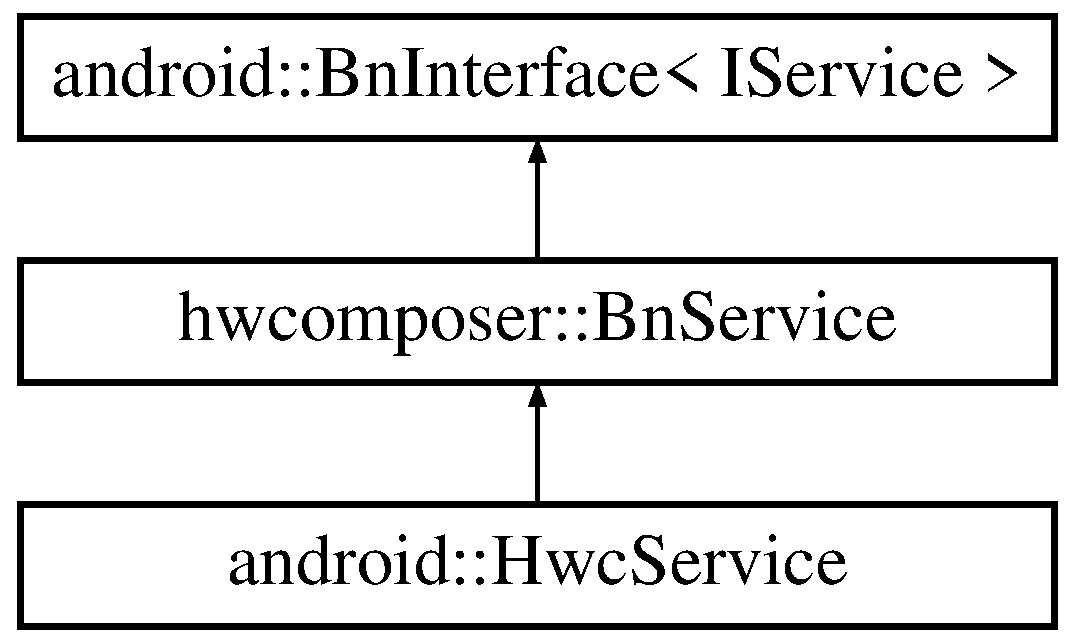
\includegraphics[height=3.000000cm]{classandroid_1_1HwcService}
\end{center}
\end{figure}
\subsection*{Classes}
\begin{DoxyCompactItemize}
\item 
class \mbox{\hyperlink{classandroid_1_1HwcService_1_1Controls}{Controls}}
\item 
class \mbox{\hyperlink{classandroid_1_1HwcService_1_1Diagnostic}{Diagnostic}}
\item 
class \mbox{\hyperlink{classandroid_1_1HwcService_1_1NotifyCallback}{Notify\+Callback}}
\end{DoxyCompactItemize}
\subsection*{Public Types}
\begin{DoxyCompactItemize}
\item 
enum \mbox{\hyperlink{classandroid_1_1HwcService_a34049a831dd1c85ef002e59be99d1bd8}{E\+Notification}} \{ \newline
\mbox{\hyperlink{classandroid_1_1HwcService_a34049a831dd1c85ef002e59be99d1bd8ad7f33ea927d7d401fd7490eb4b491e02}{e\+Invalid\+Nofiy}} = 0, 
\mbox{\hyperlink{classandroid_1_1HwcService_a34049a831dd1c85ef002e59be99d1bd8a6e3e5162fb367793dfcf25397ff5a4c2}{e\+Optimization\+Mode}}, 
\mbox{\hyperlink{classandroid_1_1HwcService_a34049a831dd1c85ef002e59be99d1bd8ab303c6dcf4d5fa1444af02bb33bee625}{e\+Mds\+Update\+Video\+State}}, 
\mbox{\hyperlink{classandroid_1_1HwcService_a34049a831dd1c85ef002e59be99d1bd8aefca037092bb4ffbc9d60bdc9aa94189}{e\+Mds\+Update\+Input\+State}}, 
\newline
\mbox{\hyperlink{classandroid_1_1HwcService_a34049a831dd1c85ef002e59be99d1bd8abb2c3f69b090433de84041389c7cafd2}{e\+Mds\+Update\+Video\+Fps}}, 
\mbox{\hyperlink{classandroid_1_1HwcService_a34049a831dd1c85ef002e59be99d1bd8ac17d3b6fb8703dbdbafed791889e33e4}{e\+Pavp\+Enable\+Encrypted\+Session}}, 
\mbox{\hyperlink{classandroid_1_1HwcService_a34049a831dd1c85ef002e59be99d1bd8acf6bbc015ac59c3762259abbd1f143e2}{e\+Pavp\+Disable\+Encrypted\+Session}}, 
\mbox{\hyperlink{classandroid_1_1HwcService_a34049a831dd1c85ef002e59be99d1bd8a85200caa728fb636f387e69a8d71bcda}{e\+Pavp\+Disable\+All\+Encrypted\+Sessions}}, 
\newline
\mbox{\hyperlink{classandroid_1_1HwcService_a34049a831dd1c85ef002e59be99d1bd8a51d121657eeb30c9315f5a06c3cd8849}{e\+Pavp\+Is\+Encrypted\+Session\+Enabled}}, 
\mbox{\hyperlink{classandroid_1_1HwcService_a34049a831dd1c85ef002e59be99d1bd8abc5fa09841febcae7d3548f84e518b99}{e\+Widi\+Get\+Single\+Display}}, 
\mbox{\hyperlink{classandroid_1_1HwcService_a34049a831dd1c85ef002e59be99d1bd8afc7209f9d74f0a07624397ef62c3bc33}{e\+Widi\+Set\+Single\+Display}}, 
\mbox{\hyperlink{classandroid_1_1HwcService_a34049a831dd1c85ef002e59be99d1bd8af22535a2747d5bca0031cf5047ccde9d}{e\+Need\+Set\+Key\+Frame\+Hint}}
 \}
\end{DoxyCompactItemize}
\subsection*{Public Member Functions}
\begin{DoxyCompactItemize}
\item 
bool \mbox{\hyperlink{classandroid_1_1HwcService_a696bd30240b25fb0ec210fbaa943b3e9}{Start}} (\mbox{\hyperlink{classandroid_1_1IAHWC2}{I\+A\+H\+W\+C2}} \&hwc)
\item 
sp$<$ \mbox{\hyperlink{classhwcomposer_1_1IDiagnostic}{I\+Diagnostic}} $>$ \mbox{\hyperlink{classandroid_1_1HwcService_ad8be9ec253b8072a1055700d88e5d8c1}{Get\+Diagnostic}} ()
\item 
sp$<$ \mbox{\hyperlink{classhwcomposer_1_1IControls}{I\+Controls}} $>$ \mbox{\hyperlink{classandroid_1_1HwcService_af5edb452f1564f0b4b70e3d58e4982f7}{Get\+Controls}} ()
\item 
android\+::\+String8 \mbox{\hyperlink{classandroid_1_1HwcService_a322632377b643c73a461dca0475d5e1f}{Get\+Hwc\+Version}} ()
\item 
void \mbox{\hyperlink{classandroid_1_1HwcService_addb78964103305845ce09edf2ef31a5c}{Dump\+Options}} (void)
\item 
\mbox{\hyperlink{hwcserviceapi_8h_a3806fb2027d9a316d8ca8d9b8b8eb96f}{status\+\_\+t}} \mbox{\hyperlink{classandroid_1_1HwcService_afbbee67c5f3220d22d7a319f09dc0314}{Set\+Option}} (android\+::\+String8 option, android\+::\+String8 option\+Value)
\item 
\mbox{\hyperlink{hwcserviceapi_8h_a3806fb2027d9a316d8ca8d9b8b8eb96f}{status\+\_\+t}} \mbox{\hyperlink{classandroid_1_1HwcService_a3a1044ce7389aae85f309c159a533f73}{Enable\+Logview\+To\+Logcat}} (bool enable=true)
\item 
void \mbox{\hyperlink{classandroid_1_1HwcService_a70e88e6da20467baf70f33cfe341583c}{Register\+Listener}} (\mbox{\hyperlink{classandroid_1_1HwcService_a34049a831dd1c85ef002e59be99d1bd8}{E\+Notification}} notify, \mbox{\hyperlink{classandroid_1_1HwcService_1_1NotifyCallback}{Notify\+Callback}} $\ast$p\+Callback)
\item 
void \mbox{\hyperlink{classandroid_1_1HwcService_a8da7d6a6c098ab6334308a94c9508e84}{Unregister\+Listener}} (\mbox{\hyperlink{classandroid_1_1HwcService_a34049a831dd1c85ef002e59be99d1bd8}{E\+Notification}} notify, \mbox{\hyperlink{classandroid_1_1HwcService_1_1NotifyCallback}{Notify\+Callback}} $\ast$p\+Callback)
\item 
void \mbox{\hyperlink{classandroid_1_1HwcService_a9ad9aea8e753da4d2267fd5ffa0afff4}{Notify}} (\mbox{\hyperlink{classandroid_1_1HwcService_a34049a831dd1c85ef002e59be99d1bd8}{E\+Notification}} notify, int32\+\_\+t para\+Cnt, int64\+\_\+t para\mbox{[}$\,$\mbox{]})
\end{DoxyCompactItemize}
\subsection*{Friends}
\begin{DoxyCompactItemize}
\item 
class \mbox{\hyperlink{classandroid_1_1HwcService_a20f0fd2b9eaf2e89f95db870a0156930}{I\+A\+H\+W\+C2}}
\end{DoxyCompactItemize}


\subsection{Detailed Description}


Definition at line 33 of file hwcservice.\+h.



\subsection{Member Enumeration Documentation}
\mbox{\Hypertarget{classandroid_1_1HwcService_a34049a831dd1c85ef002e59be99d1bd8}\label{classandroid_1_1HwcService_a34049a831dd1c85ef002e59be99d1bd8}} 
\index{android\+::\+Hwc\+Service@{android\+::\+Hwc\+Service}!E\+Notification@{E\+Notification}}
\index{E\+Notification@{E\+Notification}!android\+::\+Hwc\+Service@{android\+::\+Hwc\+Service}}
\subsubsection{\texorpdfstring{E\+Notification}{ENotification}}
{\footnotesize\ttfamily enum \mbox{\hyperlink{classandroid_1_1HwcService_a34049a831dd1c85ef002e59be99d1bd8}{android\+::\+Hwc\+Service\+::\+E\+Notification}}}

\begin{DoxyEnumFields}{Enumerator}
\raisebox{\heightof{T}}[0pt][0pt]{\index{e\+Invalid\+Nofiy@{e\+Invalid\+Nofiy}!android\+::\+Hwc\+Service@{android\+::\+Hwc\+Service}}\index{android\+::\+Hwc\+Service@{android\+::\+Hwc\+Service}!e\+Invalid\+Nofiy@{e\+Invalid\+Nofiy}}}\mbox{\Hypertarget{classandroid_1_1HwcService_a34049a831dd1c85ef002e59be99d1bd8ad7f33ea927d7d401fd7490eb4b491e02}\label{classandroid_1_1HwcService_a34049a831dd1c85ef002e59be99d1bd8ad7f33ea927d7d401fd7490eb4b491e02}} 
e\+Invalid\+Nofiy&\\
\hline

\raisebox{\heightof{T}}[0pt][0pt]{\index{e\+Optimization\+Mode@{e\+Optimization\+Mode}!android\+::\+Hwc\+Service@{android\+::\+Hwc\+Service}}\index{android\+::\+Hwc\+Service@{android\+::\+Hwc\+Service}!e\+Optimization\+Mode@{e\+Optimization\+Mode}}}\mbox{\Hypertarget{classandroid_1_1HwcService_a34049a831dd1c85ef002e59be99d1bd8a6e3e5162fb367793dfcf25397ff5a4c2}\label{classandroid_1_1HwcService_a34049a831dd1c85ef002e59be99d1bd8a6e3e5162fb367793dfcf25397ff5a4c2}} 
e\+Optimization\+Mode&\\
\hline

\raisebox{\heightof{T}}[0pt][0pt]{\index{e\+Mds\+Update\+Video\+State@{e\+Mds\+Update\+Video\+State}!android\+::\+Hwc\+Service@{android\+::\+Hwc\+Service}}\index{android\+::\+Hwc\+Service@{android\+::\+Hwc\+Service}!e\+Mds\+Update\+Video\+State@{e\+Mds\+Update\+Video\+State}}}\mbox{\Hypertarget{classandroid_1_1HwcService_a34049a831dd1c85ef002e59be99d1bd8ab303c6dcf4d5fa1444af02bb33bee625}\label{classandroid_1_1HwcService_a34049a831dd1c85ef002e59be99d1bd8ab303c6dcf4d5fa1444af02bb33bee625}} 
e\+Mds\+Update\+Video\+State&\\
\hline

\raisebox{\heightof{T}}[0pt][0pt]{\index{e\+Mds\+Update\+Input\+State@{e\+Mds\+Update\+Input\+State}!android\+::\+Hwc\+Service@{android\+::\+Hwc\+Service}}\index{android\+::\+Hwc\+Service@{android\+::\+Hwc\+Service}!e\+Mds\+Update\+Input\+State@{e\+Mds\+Update\+Input\+State}}}\mbox{\Hypertarget{classandroid_1_1HwcService_a34049a831dd1c85ef002e59be99d1bd8aefca037092bb4ffbc9d60bdc9aa94189}\label{classandroid_1_1HwcService_a34049a831dd1c85ef002e59be99d1bd8aefca037092bb4ffbc9d60bdc9aa94189}} 
e\+Mds\+Update\+Input\+State&\\
\hline

\raisebox{\heightof{T}}[0pt][0pt]{\index{e\+Mds\+Update\+Video\+Fps@{e\+Mds\+Update\+Video\+Fps}!android\+::\+Hwc\+Service@{android\+::\+Hwc\+Service}}\index{android\+::\+Hwc\+Service@{android\+::\+Hwc\+Service}!e\+Mds\+Update\+Video\+Fps@{e\+Mds\+Update\+Video\+Fps}}}\mbox{\Hypertarget{classandroid_1_1HwcService_a34049a831dd1c85ef002e59be99d1bd8abb2c3f69b090433de84041389c7cafd2}\label{classandroid_1_1HwcService_a34049a831dd1c85ef002e59be99d1bd8abb2c3f69b090433de84041389c7cafd2}} 
e\+Mds\+Update\+Video\+Fps&\\
\hline

\raisebox{\heightof{T}}[0pt][0pt]{\index{e\+Pavp\+Enable\+Encrypted\+Session@{e\+Pavp\+Enable\+Encrypted\+Session}!android\+::\+Hwc\+Service@{android\+::\+Hwc\+Service}}\index{android\+::\+Hwc\+Service@{android\+::\+Hwc\+Service}!e\+Pavp\+Enable\+Encrypted\+Session@{e\+Pavp\+Enable\+Encrypted\+Session}}}\mbox{\Hypertarget{classandroid_1_1HwcService_a34049a831dd1c85ef002e59be99d1bd8ac17d3b6fb8703dbdbafed791889e33e4}\label{classandroid_1_1HwcService_a34049a831dd1c85ef002e59be99d1bd8ac17d3b6fb8703dbdbafed791889e33e4}} 
e\+Pavp\+Enable\+Encrypted\+Session&\\
\hline

\raisebox{\heightof{T}}[0pt][0pt]{\index{e\+Pavp\+Disable\+Encrypted\+Session@{e\+Pavp\+Disable\+Encrypted\+Session}!android\+::\+Hwc\+Service@{android\+::\+Hwc\+Service}}\index{android\+::\+Hwc\+Service@{android\+::\+Hwc\+Service}!e\+Pavp\+Disable\+Encrypted\+Session@{e\+Pavp\+Disable\+Encrypted\+Session}}}\mbox{\Hypertarget{classandroid_1_1HwcService_a34049a831dd1c85ef002e59be99d1bd8acf6bbc015ac59c3762259abbd1f143e2}\label{classandroid_1_1HwcService_a34049a831dd1c85ef002e59be99d1bd8acf6bbc015ac59c3762259abbd1f143e2}} 
e\+Pavp\+Disable\+Encrypted\+Session&\\
\hline

\raisebox{\heightof{T}}[0pt][0pt]{\index{e\+Pavp\+Disable\+All\+Encrypted\+Sessions@{e\+Pavp\+Disable\+All\+Encrypted\+Sessions}!android\+::\+Hwc\+Service@{android\+::\+Hwc\+Service}}\index{android\+::\+Hwc\+Service@{android\+::\+Hwc\+Service}!e\+Pavp\+Disable\+All\+Encrypted\+Sessions@{e\+Pavp\+Disable\+All\+Encrypted\+Sessions}}}\mbox{\Hypertarget{classandroid_1_1HwcService_a34049a831dd1c85ef002e59be99d1bd8a85200caa728fb636f387e69a8d71bcda}\label{classandroid_1_1HwcService_a34049a831dd1c85ef002e59be99d1bd8a85200caa728fb636f387e69a8d71bcda}} 
e\+Pavp\+Disable\+All\+Encrypted\+Sessions&\\
\hline

\raisebox{\heightof{T}}[0pt][0pt]{\index{e\+Pavp\+Is\+Encrypted\+Session\+Enabled@{e\+Pavp\+Is\+Encrypted\+Session\+Enabled}!android\+::\+Hwc\+Service@{android\+::\+Hwc\+Service}}\index{android\+::\+Hwc\+Service@{android\+::\+Hwc\+Service}!e\+Pavp\+Is\+Encrypted\+Session\+Enabled@{e\+Pavp\+Is\+Encrypted\+Session\+Enabled}}}\mbox{\Hypertarget{classandroid_1_1HwcService_a34049a831dd1c85ef002e59be99d1bd8a51d121657eeb30c9315f5a06c3cd8849}\label{classandroid_1_1HwcService_a34049a831dd1c85ef002e59be99d1bd8a51d121657eeb30c9315f5a06c3cd8849}} 
e\+Pavp\+Is\+Encrypted\+Session\+Enabled&\\
\hline

\raisebox{\heightof{T}}[0pt][0pt]{\index{e\+Widi\+Get\+Single\+Display@{e\+Widi\+Get\+Single\+Display}!android\+::\+Hwc\+Service@{android\+::\+Hwc\+Service}}\index{android\+::\+Hwc\+Service@{android\+::\+Hwc\+Service}!e\+Widi\+Get\+Single\+Display@{e\+Widi\+Get\+Single\+Display}}}\mbox{\Hypertarget{classandroid_1_1HwcService_a34049a831dd1c85ef002e59be99d1bd8abc5fa09841febcae7d3548f84e518b99}\label{classandroid_1_1HwcService_a34049a831dd1c85ef002e59be99d1bd8abc5fa09841febcae7d3548f84e518b99}} 
e\+Widi\+Get\+Single\+Display&\\
\hline

\raisebox{\heightof{T}}[0pt][0pt]{\index{e\+Widi\+Set\+Single\+Display@{e\+Widi\+Set\+Single\+Display}!android\+::\+Hwc\+Service@{android\+::\+Hwc\+Service}}\index{android\+::\+Hwc\+Service@{android\+::\+Hwc\+Service}!e\+Widi\+Set\+Single\+Display@{e\+Widi\+Set\+Single\+Display}}}\mbox{\Hypertarget{classandroid_1_1HwcService_a34049a831dd1c85ef002e59be99d1bd8afc7209f9d74f0a07624397ef62c3bc33}\label{classandroid_1_1HwcService_a34049a831dd1c85ef002e59be99d1bd8afc7209f9d74f0a07624397ef62c3bc33}} 
e\+Widi\+Set\+Single\+Display&\\
\hline

\raisebox{\heightof{T}}[0pt][0pt]{\index{e\+Need\+Set\+Key\+Frame\+Hint@{e\+Need\+Set\+Key\+Frame\+Hint}!android\+::\+Hwc\+Service@{android\+::\+Hwc\+Service}}\index{android\+::\+Hwc\+Service@{android\+::\+Hwc\+Service}!e\+Need\+Set\+Key\+Frame\+Hint@{e\+Need\+Set\+Key\+Frame\+Hint}}}\mbox{\Hypertarget{classandroid_1_1HwcService_a34049a831dd1c85ef002e59be99d1bd8af22535a2747d5bca0031cf5047ccde9d}\label{classandroid_1_1HwcService_a34049a831dd1c85ef002e59be99d1bd8af22535a2747d5bca0031cf5047ccde9d}} 
e\+Need\+Set\+Key\+Frame\+Hint&\\
\hline

\end{DoxyEnumFields}


Definition at line 121 of file hwcservice.\+h.


\begin{DoxyCode}{0}
\DoxyCodeLine{121                      \{}
\DoxyCodeLine{122     \mbox{\hyperlink{classandroid_1_1HwcService_a34049a831dd1c85ef002e59be99d1bd8ad7f33ea927d7d401fd7490eb4b491e02}{eInvalidNofiy}} = 0,}
\DoxyCodeLine{123     \mbox{\hyperlink{classandroid_1_1HwcService_a34049a831dd1c85ef002e59be99d1bd8a6e3e5162fb367793dfcf25397ff5a4c2}{eOptimizationMode}},}
\DoxyCodeLine{124     \mbox{\hyperlink{classandroid_1_1HwcService_a34049a831dd1c85ef002e59be99d1bd8ab303c6dcf4d5fa1444af02bb33bee625}{eMdsUpdateVideoState}},}
\DoxyCodeLine{125     \mbox{\hyperlink{classandroid_1_1HwcService_a34049a831dd1c85ef002e59be99d1bd8aefca037092bb4ffbc9d60bdc9aa94189}{eMdsUpdateInputState}},}
\DoxyCodeLine{126     \mbox{\hyperlink{classandroid_1_1HwcService_a34049a831dd1c85ef002e59be99d1bd8abb2c3f69b090433de84041389c7cafd2}{eMdsUpdateVideoFps}},}
\DoxyCodeLine{127     \mbox{\hyperlink{classandroid_1_1HwcService_a34049a831dd1c85ef002e59be99d1bd8ac17d3b6fb8703dbdbafed791889e33e4}{ePavpEnableEncryptedSession}},}
\DoxyCodeLine{128     \mbox{\hyperlink{classandroid_1_1HwcService_a34049a831dd1c85ef002e59be99d1bd8acf6bbc015ac59c3762259abbd1f143e2}{ePavpDisableEncryptedSession}},}
\DoxyCodeLine{129     \mbox{\hyperlink{classandroid_1_1HwcService_a34049a831dd1c85ef002e59be99d1bd8a85200caa728fb636f387e69a8d71bcda}{ePavpDisableAllEncryptedSessions}},}
\DoxyCodeLine{130     \mbox{\hyperlink{classandroid_1_1HwcService_a34049a831dd1c85ef002e59be99d1bd8a51d121657eeb30c9315f5a06c3cd8849}{ePavpIsEncryptedSessionEnabled}},}
\DoxyCodeLine{131     \mbox{\hyperlink{classandroid_1_1HwcService_a34049a831dd1c85ef002e59be99d1bd8abc5fa09841febcae7d3548f84e518b99}{eWidiGetSingleDisplay}},}
\DoxyCodeLine{132     \mbox{\hyperlink{classandroid_1_1HwcService_a34049a831dd1c85ef002e59be99d1bd8afc7209f9d74f0a07624397ef62c3bc33}{eWidiSetSingleDisplay}},}
\DoxyCodeLine{133     \mbox{\hyperlink{classandroid_1_1HwcService_a34049a831dd1c85ef002e59be99d1bd8af22535a2747d5bca0031cf5047ccde9d}{eNeedSetKeyFrameHint}},}
\DoxyCodeLine{134   \};}
\end{DoxyCode}


\subsection{Member Function Documentation}
\mbox{\Hypertarget{classandroid_1_1HwcService_addb78964103305845ce09edf2ef31a5c}\label{classandroid_1_1HwcService_addb78964103305845ce09edf2ef31a5c}} 
\index{android\+::\+Hwc\+Service@{android\+::\+Hwc\+Service}!Dump\+Options@{Dump\+Options}}
\index{Dump\+Options@{Dump\+Options}!android\+::\+Hwc\+Service@{android\+::\+Hwc\+Service}}
\subsubsection{\texorpdfstring{Dump\+Options()}{DumpOptions()}}
{\footnotesize\ttfamily void android\+::\+Hwc\+Service\+::\+Dump\+Options (\begin{DoxyParamCaption}\item[{void}]{ }\end{DoxyParamCaption})}



Definition at line 95 of file hwcservice.\+cpp.


\begin{DoxyCode}{0}
\DoxyCodeLine{95                                  \{}
\DoxyCodeLine{96   \textcolor{comment}{// ALOGD("\%s", OptionManager::getInstance().dump().string());}}
\DoxyCodeLine{97 \}}
\end{DoxyCode}
\mbox{\Hypertarget{classandroid_1_1HwcService_a3a1044ce7389aae85f309c159a533f73}\label{classandroid_1_1HwcService_a3a1044ce7389aae85f309c159a533f73}} 
\index{android\+::\+Hwc\+Service@{android\+::\+Hwc\+Service}!Enable\+Logview\+To\+Logcat@{Enable\+Logview\+To\+Logcat}}
\index{Enable\+Logview\+To\+Logcat@{Enable\+Logview\+To\+Logcat}!android\+::\+Hwc\+Service@{android\+::\+Hwc\+Service}}
\subsubsection{\texorpdfstring{Enable\+Logview\+To\+Logcat()}{EnableLogviewToLogcat()}}
{\footnotesize\ttfamily \mbox{\hyperlink{hwcserviceapi_8h_a3806fb2027d9a316d8ca8d9b8b8eb96f}{status\+\_\+t}} android\+::\+Hwc\+Service\+::\+Enable\+Logview\+To\+Logcat (\begin{DoxyParamCaption}\item[{bool}]{enable = {\ttfamily true} }\end{DoxyParamCaption})}



Definition at line 99 of file hwcservice.\+cpp.


\begin{DoxyCode}{0}
\DoxyCodeLine{99                                                       \{}
\DoxyCodeLine{100   \textcolor{comment}{// TO DO}}
\DoxyCodeLine{101   \textcolor{keywordflow}{return} OK;}
\DoxyCodeLine{102 \}}
\end{DoxyCode}
\mbox{\Hypertarget{classandroid_1_1HwcService_af5edb452f1564f0b4b70e3d58e4982f7}\label{classandroid_1_1HwcService_af5edb452f1564f0b4b70e3d58e4982f7}} 
\index{android\+::\+Hwc\+Service@{android\+::\+Hwc\+Service}!Get\+Controls@{Get\+Controls}}
\index{Get\+Controls@{Get\+Controls}!android\+::\+Hwc\+Service@{android\+::\+Hwc\+Service}}
\subsubsection{\texorpdfstring{Get\+Controls()}{GetControls()}}
{\footnotesize\ttfamily sp$<$ \mbox{\hyperlink{classhwcomposer_1_1IControls}{I\+Controls}} $>$ android\+::\+Hwc\+Service\+::\+Get\+Controls (\begin{DoxyParamCaption}{ }\end{DoxyParamCaption})}



Definition at line 118 of file hwcservice.\+cpp.


\begin{DoxyCode}{0}
\DoxyCodeLine{118                                       \{}
\DoxyCodeLine{119   \textcolor{comment}{// TODO: Check the need for lock}}
\DoxyCodeLine{120   ALOG\_ASSERT(mpHwc);}
\DoxyCodeLine{121   \textcolor{keywordflow}{return} \textcolor{keyword}{new} Controls(*mpHwc, *\textcolor{keyword}{this});}
\DoxyCodeLine{122 \}}
\end{DoxyCode}
\mbox{\Hypertarget{classandroid_1_1HwcService_ad8be9ec253b8072a1055700d88e5d8c1}\label{classandroid_1_1HwcService_ad8be9ec253b8072a1055700d88e5d8c1}} 
\index{android\+::\+Hwc\+Service@{android\+::\+Hwc\+Service}!Get\+Diagnostic@{Get\+Diagnostic}}
\index{Get\+Diagnostic@{Get\+Diagnostic}!android\+::\+Hwc\+Service@{android\+::\+Hwc\+Service}}
\subsubsection{\texorpdfstring{Get\+Diagnostic()}{GetDiagnostic()}}
{\footnotesize\ttfamily sp$<$ \mbox{\hyperlink{classhwcomposer_1_1IDiagnostic}{I\+Diagnostic}} $>$ android\+::\+Hwc\+Service\+::\+Get\+Diagnostic (\begin{DoxyParamCaption}{ }\end{DoxyParamCaption})}



Definition at line 104 of file hwcservice.\+cpp.


\begin{DoxyCode}{0}
\DoxyCodeLine{104                                           \{}
\DoxyCodeLine{105   \textcolor{comment}{// if (sbInternalBuild || sbLogViewerBuild)}}
\DoxyCodeLine{106   \{}
\DoxyCodeLine{107     lock\_.\mbox{\hyperlink{classhwcomposer_1_1SpinLock_a863f9d0f1b270f863a9298161b52faf1}{lock}}();}
\DoxyCodeLine{108     ALOG\_ASSERT(mpHwc);}
\DoxyCodeLine{109     \textcolor{keywordflow}{if} (mpDiagnostic == \mbox{\hyperlink{alios_2platformdefines_8h_a070d2ce7b6bb7e5c05602aa8c308d0c4}{NULL}})}
\DoxyCodeLine{110       mpDiagnostic = \textcolor{keyword}{new} Diagnostic(*mpHwc);}
\DoxyCodeLine{111 }
\DoxyCodeLine{112     lock\_.\mbox{\hyperlink{classhwcomposer_1_1SpinLock_ae5cf624b4f0ec710833ce44e945b85d7}{unlock}}();}
\DoxyCodeLine{113   \}}
\DoxyCodeLine{114 }
\DoxyCodeLine{115   \textcolor{keywordflow}{return} mpDiagnostic;}
\DoxyCodeLine{116 \}}
\end{DoxyCode}
\mbox{\Hypertarget{classandroid_1_1HwcService_a322632377b643c73a461dca0475d5e1f}\label{classandroid_1_1HwcService_a322632377b643c73a461dca0475d5e1f}} 
\index{android\+::\+Hwc\+Service@{android\+::\+Hwc\+Service}!Get\+Hwc\+Version@{Get\+Hwc\+Version}}
\index{Get\+Hwc\+Version@{Get\+Hwc\+Version}!android\+::\+Hwc\+Service@{android\+::\+Hwc\+Service}}
\subsubsection{\texorpdfstring{Get\+Hwc\+Version()}{GetHwcVersion()}}
{\footnotesize\ttfamily String8 android\+::\+Hwc\+Service\+::\+Get\+Hwc\+Version (\begin{DoxyParamCaption}{ }\end{DoxyParamCaption})}



Definition at line 87 of file hwcservice.\+cpp.


\begin{DoxyCode}{0}
\DoxyCodeLine{87                                   \{}
\DoxyCodeLine{88   \textcolor{keywordflow}{return} String8((\mbox{\hyperlink{hwcservice_8cpp_a1dc46151b8c227cd440f0f34a34825b9}{HWC\_VERSION\_STRING}}));}
\DoxyCodeLine{89 \}}
\end{DoxyCode}
\mbox{\Hypertarget{classandroid_1_1HwcService_a9ad9aea8e753da4d2267fd5ffa0afff4}\label{classandroid_1_1HwcService_a9ad9aea8e753da4d2267fd5ffa0afff4}} 
\index{android\+::\+Hwc\+Service@{android\+::\+Hwc\+Service}!Notify@{Notify}}
\index{Notify@{Notify}!android\+::\+Hwc\+Service@{android\+::\+Hwc\+Service}}
\subsubsection{\texorpdfstring{Notify()}{Notify()}}
{\footnotesize\ttfamily void android\+::\+Hwc\+Service\+::\+Notify (\begin{DoxyParamCaption}\item[{\mbox{\hyperlink{classandroid_1_1HwcService_a34049a831dd1c85ef002e59be99d1bd8}{E\+Notification}}}]{notify,  }\item[{int32\+\_\+t}]{para\+Cnt,  }\item[{int64\+\_\+t}]{para\mbox{[}$\,$\mbox{]} }\end{DoxyParamCaption})}



Definition at line 459 of file hwcservice.\+cpp.


\begin{DoxyCode}{0}
\DoxyCodeLine{459                                                                              \{}
\DoxyCodeLine{460   \textcolor{comment}{// TO DO}}
\DoxyCodeLine{461 \}}
\end{DoxyCode}
\mbox{\Hypertarget{classandroid_1_1HwcService_a70e88e6da20467baf70f33cfe341583c}\label{classandroid_1_1HwcService_a70e88e6da20467baf70f33cfe341583c}} 
\index{android\+::\+Hwc\+Service@{android\+::\+Hwc\+Service}!Register\+Listener@{Register\+Listener}}
\index{Register\+Listener@{Register\+Listener}!android\+::\+Hwc\+Service@{android\+::\+Hwc\+Service}}
\subsubsection{\texorpdfstring{Register\+Listener()}{RegisterListener()}}
{\footnotesize\ttfamily void android\+::\+Hwc\+Service\+::\+Register\+Listener (\begin{DoxyParamCaption}\item[{\mbox{\hyperlink{classandroid_1_1HwcService_a34049a831dd1c85ef002e59be99d1bd8}{E\+Notification}}}]{notify,  }\item[{\mbox{\hyperlink{classandroid_1_1HwcService_1_1NotifyCallback}{Notify\+Callback}} $\ast$}]{p\+Callback }\end{DoxyParamCaption})}



Definition at line 449 of file hwcservice.\+cpp.


\begin{DoxyCode}{0}
\DoxyCodeLine{450                                                              \{}
\DoxyCodeLine{451   \textcolor{comment}{// TO DO}}
\DoxyCodeLine{452 \}}
\end{DoxyCode}
\mbox{\Hypertarget{classandroid_1_1HwcService_afbbee67c5f3220d22d7a319f09dc0314}\label{classandroid_1_1HwcService_afbbee67c5f3220d22d7a319f09dc0314}} 
\index{android\+::\+Hwc\+Service@{android\+::\+Hwc\+Service}!Set\+Option@{Set\+Option}}
\index{Set\+Option@{Set\+Option}!android\+::\+Hwc\+Service@{android\+::\+Hwc\+Service}}
\subsubsection{\texorpdfstring{Set\+Option()}{SetOption()}}
{\footnotesize\ttfamily \mbox{\hyperlink{hwcserviceapi_8h_a3806fb2027d9a316d8ca8d9b8b8eb96f}{status\+\_\+t}} android\+::\+Hwc\+Service\+::\+Set\+Option (\begin{DoxyParamCaption}\item[{android\+::\+String8}]{option,  }\item[{android\+::\+String8}]{option\+Value }\end{DoxyParamCaption})}



Definition at line 91 of file hwcservice.\+cpp.


\begin{DoxyCode}{0}
\DoxyCodeLine{91                                                             \{}
\DoxyCodeLine{92   \textcolor{keywordflow}{return} OK;}
\DoxyCodeLine{93 \}}
\end{DoxyCode}
\mbox{\Hypertarget{classandroid_1_1HwcService_a696bd30240b25fb0ec210fbaa943b3e9}\label{classandroid_1_1HwcService_a696bd30240b25fb0ec210fbaa943b3e9}} 
\index{android\+::\+Hwc\+Service@{android\+::\+Hwc\+Service}!Start@{Start}}
\index{Start@{Start}!android\+::\+Hwc\+Service@{android\+::\+Hwc\+Service}}
\subsubsection{\texorpdfstring{Start()}{Start()}}
{\footnotesize\ttfamily bool android\+::\+Hwc\+Service\+::\+Start (\begin{DoxyParamCaption}\item[{\mbox{\hyperlink{classandroid_1_1IAHWC2}{I\+A\+H\+W\+C2}} \&}]{hwc }\end{DoxyParamCaption})}



Definition at line 73 of file hwcservice.\+cpp.


\begin{DoxyCode}{0}
\DoxyCodeLine{73                                   \{}
\DoxyCodeLine{74   \textcolor{keywordflow}{if} (initialized\_)}
\DoxyCodeLine{75     \textcolor{keywordflow}{return} \textcolor{keyword}{true};}
\DoxyCodeLine{76 }
\DoxyCodeLine{77   mpHwc = \&hwc;}
\DoxyCodeLine{78   sp<IServiceManager> sm(defaultServiceManager());}
\DoxyCodeLine{79   \textcolor{keywordflow}{if} (sm->addService(String16(\mbox{\hyperlink{iservice_8h_a03d122faa3f4367040f301a1a6d90091}{IA\_HWC\_SERVICE\_NAME}}), \textcolor{keyword}{this}, \textcolor{keyword}{false})) \{}
\DoxyCodeLine{80     ALOGE(\textcolor{stringliteral}{"Failed to start \%s service"}, \mbox{\hyperlink{iservice_8h_a03d122faa3f4367040f301a1a6d90091}{IA\_HWC\_SERVICE\_NAME}});}
\DoxyCodeLine{81     \textcolor{keywordflow}{return} \textcolor{keyword}{false};}
\DoxyCodeLine{82   \}}
\DoxyCodeLine{83   initialized\_ = \textcolor{keyword}{true};}
\DoxyCodeLine{84   \textcolor{keywordflow}{return} \textcolor{keyword}{true};}
\DoxyCodeLine{85 \}}
\end{DoxyCode}
\mbox{\Hypertarget{classandroid_1_1HwcService_a8da7d6a6c098ab6334308a94c9508e84}\label{classandroid_1_1HwcService_a8da7d6a6c098ab6334308a94c9508e84}} 
\index{android\+::\+Hwc\+Service@{android\+::\+Hwc\+Service}!Unregister\+Listener@{Unregister\+Listener}}
\index{Unregister\+Listener@{Unregister\+Listener}!android\+::\+Hwc\+Service@{android\+::\+Hwc\+Service}}
\subsubsection{\texorpdfstring{Unregister\+Listener()}{UnregisterListener()}}
{\footnotesize\ttfamily void android\+::\+Hwc\+Service\+::\+Unregister\+Listener (\begin{DoxyParamCaption}\item[{\mbox{\hyperlink{classandroid_1_1HwcService_a34049a831dd1c85ef002e59be99d1bd8}{E\+Notification}}}]{notify,  }\item[{\mbox{\hyperlink{classandroid_1_1HwcService_1_1NotifyCallback}{Notify\+Callback}} $\ast$}]{p\+Callback }\end{DoxyParamCaption})}



Definition at line 454 of file hwcservice.\+cpp.


\begin{DoxyCode}{0}
\DoxyCodeLine{455                                                                \{}
\DoxyCodeLine{456   \textcolor{comment}{// TO DO}}
\DoxyCodeLine{457 \}}
\end{DoxyCode}


\subsection{Friends And Related Function Documentation}
\mbox{\Hypertarget{classandroid_1_1HwcService_a20f0fd2b9eaf2e89f95db870a0156930}\label{classandroid_1_1HwcService_a20f0fd2b9eaf2e89f95db870a0156930}} 
\index{android\+::\+Hwc\+Service@{android\+::\+Hwc\+Service}!I\+A\+H\+W\+C2@{I\+A\+H\+W\+C2}}
\index{I\+A\+H\+W\+C2@{I\+A\+H\+W\+C2}!android\+::\+Hwc\+Service@{android\+::\+Hwc\+Service}}
\subsubsection{\texorpdfstring{I\+A\+H\+W\+C2}{IAHWC2}}
{\footnotesize\ttfamily friend class \mbox{\hyperlink{classandroid_1_1IAHWC2}{I\+A\+H\+W\+C2}}\hspace{0.3cm}{\ttfamily [friend]}}



Definition at line 151 of file hwcservice.\+h.



The documentation for this class was generated from the following files\+:\begin{DoxyCompactItemize}
\item 
os/android/\mbox{\hyperlink{hwcservice_8h}{hwcservice.\+h}}\item 
os/android/\mbox{\hyperlink{hwcservice_8cpp}{hwcservice.\+cpp}}\end{DoxyCompactItemize}

\hypertarget{classhwcomposer_1_1HWCThread}{}\section{hwcomposer\+:\+:H\+W\+C\+Thread Class Reference}
\label{classhwcomposer_1_1HWCThread}\index{hwcomposer\+::\+H\+W\+C\+Thread@{hwcomposer\+::\+H\+W\+C\+Thread}}


{\ttfamily \#include $<$hwcthread.\+h$>$}

Inheritance diagram for hwcomposer\+:\+:H\+W\+C\+Thread\+:\begin{figure}[H]
\begin{center}
\leavevmode
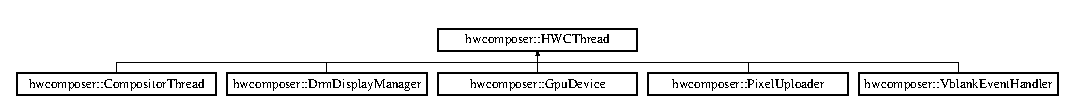
\includegraphics[height=1.051643cm]{classhwcomposer_1_1HWCThread}
\end{center}
\end{figure}
\subsection*{Protected Member Functions}
\begin{DoxyCompactItemize}
\item 
\mbox{\hyperlink{classhwcomposer_1_1HWCThread_a8780175b1679005955a94aa89fa62be1}{H\+W\+C\+Thread}} (int priority, const char $\ast$name)
\item 
virtual \mbox{\hyperlink{classhwcomposer_1_1HWCThread_a48920a9e68258c345e5fc7d8507d7ce4}{$\sim$\+H\+W\+C\+Thread}} ()
\item 
bool \mbox{\hyperlink{classhwcomposer_1_1HWCThread_a7162d49a6b4026673f77ac048eb4d07b}{Init\+Worker}} ()
\item 
void \mbox{\hyperlink{classhwcomposer_1_1HWCThread_a5f38525b892525beaa7f37d2d4c50bde}{Resume}} ()
\item 
void \mbox{\hyperlink{classhwcomposer_1_1HWCThread_aa360360e4c27cbc7fed745f79990a190}{Exit}} ()
\item 
virtual void \mbox{\hyperlink{classhwcomposer_1_1HWCThread_a539ea080e6bf0e6cffe08e2341be1ee4}{Handle\+Routine}} ()=0
\item 
virtual void \mbox{\hyperlink{classhwcomposer_1_1HWCThread_a39a94bd0b12451fe3060729787921cbf}{Handle\+Exit}} ()
\item 
virtual void \mbox{\hyperlink{classhwcomposer_1_1HWCThread_ab5acded48bbd1bf4d7c3a54dadb91ef9}{Handle\+Wait}} ()
\end{DoxyCompactItemize}
\subsection*{Protected Attributes}
\begin{DoxyCompactItemize}
\item 
\mbox{\hyperlink{classhwcomposer_1_1FDHandler}{F\+D\+Handler}} \mbox{\hyperlink{classhwcomposer_1_1HWCThread_a26ef5b90fd394e2002d903ffd2521faf}{fd\+\_\+handler\+\_\+}}
\item 
bool \mbox{\hyperlink{classhwcomposer_1_1HWCThread_a7461f5a7553b74324ad6744d532c731b}{initialized\+\_\+}}
\end{DoxyCompactItemize}


\subsection{Detailed Description}


Definition at line 30 of file hwcthread.\+h.



\subsection{Constructor \& Destructor Documentation}
\mbox{\Hypertarget{classhwcomposer_1_1HWCThread_a8780175b1679005955a94aa89fa62be1}\label{classhwcomposer_1_1HWCThread_a8780175b1679005955a94aa89fa62be1}} 
\index{hwcomposer\+::\+H\+W\+C\+Thread@{hwcomposer\+::\+H\+W\+C\+Thread}!H\+W\+C\+Thread@{H\+W\+C\+Thread}}
\index{H\+W\+C\+Thread@{H\+W\+C\+Thread}!hwcomposer\+::\+H\+W\+C\+Thread@{hwcomposer\+::\+H\+W\+C\+Thread}}
\subsubsection{\texorpdfstring{H\+W\+C\+Thread()}{HWCThread()}}
{\footnotesize\ttfamily hwcomposer\+::\+H\+W\+C\+Thread\+::\+H\+W\+C\+Thread (\begin{DoxyParamCaption}\item[{int}]{priority,  }\item[{const char $\ast$}]{name }\end{DoxyParamCaption})\hspace{0.3cm}{\ttfamily [protected]}}



Definition at line 27 of file hwcthread.\+cpp.


\begin{DoxyCode}{0}
\DoxyCodeLine{28     : \mbox{\hyperlink{classhwcomposer_1_1HWCThread_a7461f5a7553b74324ad6744d532c731b}{initialized\_}}(\textcolor{keyword}{false}), priority\_(priority), name\_(name) \{}
\DoxyCodeLine{29 \}}
\end{DoxyCode}
\mbox{\Hypertarget{classhwcomposer_1_1HWCThread_a48920a9e68258c345e5fc7d8507d7ce4}\label{classhwcomposer_1_1HWCThread_a48920a9e68258c345e5fc7d8507d7ce4}} 
\index{hwcomposer\+::\+H\+W\+C\+Thread@{hwcomposer\+::\+H\+W\+C\+Thread}!````~H\+W\+C\+Thread@{$\sim$\+H\+W\+C\+Thread}}
\index{````~H\+W\+C\+Thread@{$\sim$\+H\+W\+C\+Thread}!hwcomposer\+::\+H\+W\+C\+Thread@{hwcomposer\+::\+H\+W\+C\+Thread}}
\subsubsection{\texorpdfstring{$\sim$\+H\+W\+C\+Thread()}{~HWCThread()}}
{\footnotesize\ttfamily hwcomposer\+::\+H\+W\+C\+Thread\+::$\sim$\+H\+W\+C\+Thread (\begin{DoxyParamCaption}{ }\end{DoxyParamCaption})\hspace{0.3cm}{\ttfamily [protected]}, {\ttfamily [virtual]}}



Definition at line 31 of file hwcthread.\+cpp.


\begin{DoxyCode}{0}
\DoxyCodeLine{31                       \{}
\DoxyCodeLine{32   \mbox{\hyperlink{classhwcomposer_1_1HWCThread_aa360360e4c27cbc7fed745f79990a190}{Exit}}();}
\DoxyCodeLine{33 \}}
\end{DoxyCode}


\subsection{Member Function Documentation}
\mbox{\Hypertarget{classhwcomposer_1_1HWCThread_aa360360e4c27cbc7fed745f79990a190}\label{classhwcomposer_1_1HWCThread_aa360360e4c27cbc7fed745f79990a190}} 
\index{hwcomposer\+::\+H\+W\+C\+Thread@{hwcomposer\+::\+H\+W\+C\+Thread}!Exit@{Exit}}
\index{Exit@{Exit}!hwcomposer\+::\+H\+W\+C\+Thread@{hwcomposer\+::\+H\+W\+C\+Thread}}
\subsubsection{\texorpdfstring{Exit()}{Exit()}}
{\footnotesize\ttfamily void hwcomposer\+::\+H\+W\+C\+Thread\+::\+Exit (\begin{DoxyParamCaption}{ }\end{DoxyParamCaption})\hspace{0.3cm}{\ttfamily [protected]}}



Definition at line 59 of file hwcthread.\+cpp.


\begin{DoxyCode}{0}
\DoxyCodeLine{59                      \{}
\DoxyCodeLine{60   \textcolor{keywordflow}{if} (!\mbox{\hyperlink{classhwcomposer_1_1HWCThread_a7461f5a7553b74324ad6744d532c731b}{initialized\_}})}
\DoxyCodeLine{61     \textcolor{keywordflow}{return};}
\DoxyCodeLine{62 }
\DoxyCodeLine{63   \mbox{\hyperlink{classhwcomposer_1_1HWCThread_a7461f5a7553b74324ad6744d532c731b}{initialized\_}} = \textcolor{keyword}{false};}
\DoxyCodeLine{64   exit\_ = \textcolor{keyword}{true};}
\DoxyCodeLine{65   \mbox{\hyperlink{hwctrace_8h_af8c38c979e9089c283d2f5923089b538}{IHOTPLUGEVENTTRACE}}(\textcolor{stringliteral}{"HWCThread::Exit recieved."});}
\DoxyCodeLine{66   event\_.\mbox{\hyperlink{classhwcomposer_1_1HWCEvent_a3cd16bda8f4fd8bcbda6dae72ff15f57}{Signal}}();}
\DoxyCodeLine{67   thread\_->join();}
\DoxyCodeLine{68 \}}
\end{DoxyCode}
\mbox{\Hypertarget{classhwcomposer_1_1HWCThread_a39a94bd0b12451fe3060729787921cbf}\label{classhwcomposer_1_1HWCThread_a39a94bd0b12451fe3060729787921cbf}} 
\index{hwcomposer\+::\+H\+W\+C\+Thread@{hwcomposer\+::\+H\+W\+C\+Thread}!Handle\+Exit@{Handle\+Exit}}
\index{Handle\+Exit@{Handle\+Exit}!hwcomposer\+::\+H\+W\+C\+Thread@{hwcomposer\+::\+H\+W\+C\+Thread}}
\subsubsection{\texorpdfstring{Handle\+Exit()}{HandleExit()}}
{\footnotesize\ttfamily void hwcomposer\+::\+H\+W\+C\+Thread\+::\+Handle\+Exit (\begin{DoxyParamCaption}{ }\end{DoxyParamCaption})\hspace{0.3cm}{\ttfamily [protected]}, {\ttfamily [virtual]}}



Reimplemented in \mbox{\hyperlink{classhwcomposer_1_1PixelUploader_ae6bfd528de70bc53d8eb30eb76b8d8fd}{hwcomposer\+::\+Pixel\+Uploader}}, and \mbox{\hyperlink{classhwcomposer_1_1CompositorThread_a15f97ae71050432ba2780555368a3fca}{hwcomposer\+::\+Compositor\+Thread}}.



Definition at line 70 of file hwcthread.\+cpp.


\begin{DoxyCode}{0}
\DoxyCodeLine{70                            \{}
\DoxyCodeLine{71 \}}
\end{DoxyCode}
\mbox{\Hypertarget{classhwcomposer_1_1HWCThread_a539ea080e6bf0e6cffe08e2341be1ee4}\label{classhwcomposer_1_1HWCThread_a539ea080e6bf0e6cffe08e2341be1ee4}} 
\index{hwcomposer\+::\+H\+W\+C\+Thread@{hwcomposer\+::\+H\+W\+C\+Thread}!Handle\+Routine@{Handle\+Routine}}
\index{Handle\+Routine@{Handle\+Routine}!hwcomposer\+::\+H\+W\+C\+Thread@{hwcomposer\+::\+H\+W\+C\+Thread}}
\subsubsection{\texorpdfstring{Handle\+Routine()}{HandleRoutine()}}
{\footnotesize\ttfamily virtual void hwcomposer\+::\+H\+W\+C\+Thread\+::\+Handle\+Routine (\begin{DoxyParamCaption}{ }\end{DoxyParamCaption})\hspace{0.3cm}{\ttfamily [protected]}, {\ttfamily [pure virtual]}}



Implemented in \mbox{\hyperlink{classhwcomposer_1_1DrmDisplayManager_a3f29044c35ff76edb4718ed19f340794}{hwcomposer\+::\+Drm\+Display\+Manager}}, \mbox{\hyperlink{classhwcomposer_1_1PixelUploader_a73abd205b50c5cdcc693886536553889}{hwcomposer\+::\+Pixel\+Uploader}}, \mbox{\hyperlink{classhwcomposer_1_1CompositorThread_af80e4eb7864b2f83a1eaa266a17b3a28}{hwcomposer\+::\+Compositor\+Thread}}, and \mbox{\hyperlink{classhwcomposer_1_1VblankEventHandler_a229ed2c06dc41d88000fdebcc3dd81f9}{hwcomposer\+::\+Vblank\+Event\+Handler}}.

\mbox{\Hypertarget{classhwcomposer_1_1HWCThread_ab5acded48bbd1bf4d7c3a54dadb91ef9}\label{classhwcomposer_1_1HWCThread_ab5acded48bbd1bf4d7c3a54dadb91ef9}} 
\index{hwcomposer\+::\+H\+W\+C\+Thread@{hwcomposer\+::\+H\+W\+C\+Thread}!Handle\+Wait@{Handle\+Wait}}
\index{Handle\+Wait@{Handle\+Wait}!hwcomposer\+::\+H\+W\+C\+Thread@{hwcomposer\+::\+H\+W\+C\+Thread}}
\subsubsection{\texorpdfstring{Handle\+Wait()}{HandleWait()}}
{\footnotesize\ttfamily void hwcomposer\+::\+H\+W\+C\+Thread\+::\+Handle\+Wait (\begin{DoxyParamCaption}{ }\end{DoxyParamCaption})\hspace{0.3cm}{\ttfamily [protected]}, {\ttfamily [virtual]}}



Reimplemented in \mbox{\hyperlink{classhwcomposer_1_1DrmDisplayManager_abcf8a2a9394d722a58b79060f9f51dbc}{hwcomposer\+::\+Drm\+Display\+Manager}}, and \mbox{\hyperlink{classhwcomposer_1_1VblankEventHandler_a567c783bd9baa74b99fdf4ae98fe25b1}{hwcomposer\+::\+Vblank\+Event\+Handler}}.



Definition at line 73 of file hwcthread.\+cpp.


\begin{DoxyCode}{0}
\DoxyCodeLine{73                            \{}
\DoxyCodeLine{74   \textcolor{keywordflow}{if} (\mbox{\hyperlink{classhwcomposer_1_1HWCThread_a26ef5b90fd394e2002d903ffd2521faf}{fd\_handler\_}}.\mbox{\hyperlink{classhwcomposer_1_1FDHandler_a5ab233d1f474eab69552321e87159a9d}{Poll}}(-1) <= 0) \{}
\DoxyCodeLine{75     \mbox{\hyperlink{alios_2platformdefines_8h_a226d6c99e4bcfca193c095e085e9097d}{ETRACE}}(\textcolor{stringliteral}{"Poll Failed in DisplayManager \%s"}, \mbox{\hyperlink{hwctrace_8h_a791a01fa8fe130cef13d68a706df9034}{PRINTERROR}}());}
\DoxyCodeLine{76     \textcolor{keywordflow}{return};}
\DoxyCodeLine{77   \}}
\DoxyCodeLine{78 }
\DoxyCodeLine{79   \textcolor{keywordflow}{if} (\mbox{\hyperlink{classhwcomposer_1_1HWCThread_a26ef5b90fd394e2002d903ffd2521faf}{fd\_handler\_}}.\mbox{\hyperlink{classhwcomposer_1_1FDHandler_ad635c0c7631838aa99e0140c4164425f}{IsReady}}(event\_.\mbox{\hyperlink{classhwcomposer_1_1HWCEvent_a103324deefcbf4402fd302b737474416}{get\_fd}}())) \{}
\DoxyCodeLine{80     \textcolor{comment}{// If eventfd\_ is ready, we need to wait on it (using read()) to clean}}
\DoxyCodeLine{81     \textcolor{comment}{// the flag that says it is ready.}}
\DoxyCodeLine{82     event\_.\mbox{\hyperlink{classhwcomposer_1_1HWCEvent_a013f137de83e0e45988d72317179a7ef}{Wait}}();}
\DoxyCodeLine{83   \}}
\DoxyCodeLine{84 \}}
\end{DoxyCode}
\mbox{\Hypertarget{classhwcomposer_1_1HWCThread_a7162d49a6b4026673f77ac048eb4d07b}\label{classhwcomposer_1_1HWCThread_a7162d49a6b4026673f77ac048eb4d07b}} 
\index{hwcomposer\+::\+H\+W\+C\+Thread@{hwcomposer\+::\+H\+W\+C\+Thread}!Init\+Worker@{Init\+Worker}}
\index{Init\+Worker@{Init\+Worker}!hwcomposer\+::\+H\+W\+C\+Thread@{hwcomposer\+::\+H\+W\+C\+Thread}}
\subsubsection{\texorpdfstring{Init\+Worker()}{InitWorker()}}
{\footnotesize\ttfamily bool hwcomposer\+::\+H\+W\+C\+Thread\+::\+Init\+Worker (\begin{DoxyParamCaption}{ }\end{DoxyParamCaption})\hspace{0.3cm}{\ttfamily [protected]}}



Definition at line 35 of file hwcthread.\+cpp.


\begin{DoxyCode}{0}
\DoxyCodeLine{35                            \{}
\DoxyCodeLine{36   \textcolor{keywordflow}{if} (\mbox{\hyperlink{classhwcomposer_1_1HWCThread_a7461f5a7553b74324ad6744d532c731b}{initialized\_}})}
\DoxyCodeLine{37     \textcolor{keywordflow}{return} \textcolor{keyword}{true};}
\DoxyCodeLine{38 }
\DoxyCodeLine{39   \mbox{\hyperlink{classhwcomposer_1_1HWCThread_a7461f5a7553b74324ad6744d532c731b}{initialized\_}} = \textcolor{keyword}{true};}
\DoxyCodeLine{40   exit\_ = \textcolor{keyword}{false};}
\DoxyCodeLine{41 }
\DoxyCodeLine{42   \textcolor{keywordflow}{if} (!event\_.\mbox{\hyperlink{classhwcomposer_1_1HWCEvent_a5b5ee0d26d11c5697e20cde63a255e97}{Initialize}}())}
\DoxyCodeLine{43     \textcolor{keywordflow}{return} \textcolor{keyword}{false};}
\DoxyCodeLine{44 }
\DoxyCodeLine{45   \mbox{\hyperlink{classhwcomposer_1_1HWCThread_a26ef5b90fd394e2002d903ffd2521faf}{fd\_handler\_}}.\mbox{\hyperlink{classhwcomposer_1_1FDHandler_aee421fa4ae54b7d4fcc352ebea15b4f8}{AddFd}}(event\_.\mbox{\hyperlink{classhwcomposer_1_1HWCEvent_a103324deefcbf4402fd302b737474416}{get\_fd}}());}
\DoxyCodeLine{46   thread\_ = std::unique\_ptr<std::thread>(}
\DoxyCodeLine{47       \textcolor{keyword}{new} std::thread(\&HWCThread::ProcessThread, \textcolor{keyword}{this}));}
\DoxyCodeLine{48 }
\DoxyCodeLine{49   \textcolor{keywordflow}{return} \textcolor{keyword}{true};}
\DoxyCodeLine{50 \}}
\end{DoxyCode}
\mbox{\Hypertarget{classhwcomposer_1_1HWCThread_a5f38525b892525beaa7f37d2d4c50bde}\label{classhwcomposer_1_1HWCThread_a5f38525b892525beaa7f37d2d4c50bde}} 
\index{hwcomposer\+::\+H\+W\+C\+Thread@{hwcomposer\+::\+H\+W\+C\+Thread}!Resume@{Resume}}
\index{Resume@{Resume}!hwcomposer\+::\+H\+W\+C\+Thread@{hwcomposer\+::\+H\+W\+C\+Thread}}
\subsubsection{\texorpdfstring{Resume()}{Resume()}}
{\footnotesize\ttfamily void hwcomposer\+::\+H\+W\+C\+Thread\+::\+Resume (\begin{DoxyParamCaption}{ }\end{DoxyParamCaption})\hspace{0.3cm}{\ttfamily [protected]}}



Definition at line 52 of file hwcthread.\+cpp.


\begin{DoxyCode}{0}
\DoxyCodeLine{52                        \{}
\DoxyCodeLine{53   \textcolor{keywordflow}{if} (exit\_ || !\mbox{\hyperlink{classhwcomposer_1_1HWCThread_a7461f5a7553b74324ad6744d532c731b}{initialized\_}})}
\DoxyCodeLine{54     \textcolor{keywordflow}{return};}
\DoxyCodeLine{55 }
\DoxyCodeLine{56   event\_.\mbox{\hyperlink{classhwcomposer_1_1HWCEvent_a3cd16bda8f4fd8bcbda6dae72ff15f57}{Signal}}();}
\DoxyCodeLine{57 \}}
\end{DoxyCode}


\subsection{Member Data Documentation}
\mbox{\Hypertarget{classhwcomposer_1_1HWCThread_a26ef5b90fd394e2002d903ffd2521faf}\label{classhwcomposer_1_1HWCThread_a26ef5b90fd394e2002d903ffd2521faf}} 
\index{hwcomposer\+::\+H\+W\+C\+Thread@{hwcomposer\+::\+H\+W\+C\+Thread}!fd\+\_\+handler\+\_\+@{fd\+\_\+handler\+\_\+}}
\index{fd\+\_\+handler\+\_\+@{fd\+\_\+handler\+\_\+}!hwcomposer\+::\+H\+W\+C\+Thread@{hwcomposer\+::\+H\+W\+C\+Thread}}
\subsubsection{\texorpdfstring{fd\+\_\+handler\+\_\+}{fd\_handler\_}}
{\footnotesize\ttfamily \mbox{\hyperlink{classhwcomposer_1_1FDHandler}{F\+D\+Handler}} hwcomposer\+::\+H\+W\+C\+Thread\+::fd\+\_\+handler\+\_\+\hspace{0.3cm}{\ttfamily [protected]}}



Definition at line 44 of file hwcthread.\+h.

\mbox{\Hypertarget{classhwcomposer_1_1HWCThread_a7461f5a7553b74324ad6744d532c731b}\label{classhwcomposer_1_1HWCThread_a7461f5a7553b74324ad6744d532c731b}} 
\index{hwcomposer\+::\+H\+W\+C\+Thread@{hwcomposer\+::\+H\+W\+C\+Thread}!initialized\+\_\+@{initialized\+\_\+}}
\index{initialized\+\_\+@{initialized\+\_\+}!hwcomposer\+::\+H\+W\+C\+Thread@{hwcomposer\+::\+H\+W\+C\+Thread}}
\subsubsection{\texorpdfstring{initialized\+\_\+}{initialized\_}}
{\footnotesize\ttfamily bool hwcomposer\+::\+H\+W\+C\+Thread\+::initialized\+\_\+\hspace{0.3cm}{\ttfamily [protected]}}



Definition at line 45 of file hwcthread.\+h.



The documentation for this class was generated from the following files\+:\begin{DoxyCompactItemize}
\item 
common/utils/\mbox{\hyperlink{hwcthread_8h}{hwcthread.\+h}}\item 
common/utils/\mbox{\hyperlink{hwcthread_8cpp}{hwcthread.\+cpp}}\end{DoxyCompactItemize}

\hypertarget{structhwcomposer_1_1HwfDevice}{}\section{hwcomposer\+:\+:Hwf\+Device Struct Reference}
\label{structhwcomposer_1_1HwfDevice}\index{hwcomposer\+::\+Hwf\+Device@{hwcomposer\+::\+Hwf\+Device}}


{\ttfamily \#include $<$hwf\+\_\+alioshal.\+h$>$}

\subsection*{Public Member Functions}
\begin{DoxyCompactItemize}
\item 
\mbox{\hyperlink{structhwcomposer_1_1HwfDevice_a027a1b50b40fbab4398e755956cfa416}{$\sim$\+Hwf\+Device}} ()
\item 
\mbox{\hyperlink{structhwcomposer_1_1HwfDisplay}{Hwf\+Display}} $\ast$ \mbox{\hyperlink{structhwcomposer_1_1HwfDevice_a1c88092007418ad866571a31cba36675}{Get\+Display}} (int display)
\end{DoxyCompactItemize}
\subsection*{Static Public Member Functions}
\begin{DoxyCompactItemize}
\item 
static int \mbox{\hyperlink{structhwcomposer_1_1HwfDevice_a5bd285f65735f896968db942ca18f22b}{detect}} (struct hwf\+\_\+device\+\_\+t $\ast$device, int disp\+Count, hwf\+\_\+display\+\_\+t $\ast$$\ast$displays)
\item 
static int \mbox{\hyperlink{structhwcomposer_1_1HwfDevice_a17f2fc575a1c6228cc6f5747fadbe065}{flip}} (struct hwf\+\_\+device\+\_\+t $\ast$device, int disp\+Count, hwf\+\_\+display\+\_\+t $\ast$$\ast$displays)
\item 
static int \mbox{\hyperlink{structhwcomposer_1_1HwfDevice_aa1f6362cd358f5a2cc87d7ccfdad5af5}{set\+Event\+State}} (struct hwf\+\_\+device\+\_\+t $\ast$device, int disp, int event, int enabled)
\item 
static int \mbox{\hyperlink{structhwcomposer_1_1HwfDevice_adb550a7520ececbd89da42098cd6e461}{set\+Display\+State}} (struct hwf\+\_\+device\+\_\+t $\ast$device, int disp, int state)
\item 
static int \mbox{\hyperlink{structhwcomposer_1_1HwfDevice_aa9ceccea3b836aa5abf8fbf2a36ce280}{lookup}} (struct hwf\+\_\+device\+\_\+t $\ast$device, int what, int $\ast$value)
\item 
static void \mbox{\hyperlink{structhwcomposer_1_1HwfDevice_a3c68e078ccdf371b51b04c095d51eb57}{register\+Callback}} (struct hwf\+\_\+device\+\_\+t $\ast$device, hwf\+\_\+callback\+\_\+t const $\ast$callback)
\item 
static int \mbox{\hyperlink{structhwcomposer_1_1HwfDevice_ae706c9f4d8a292f6f3e98a15c9b13cfc}{query\+Disp\+Configs}} (struct hwf\+\_\+device\+\_\+t $\ast$device, int disp, uint32\+\_\+t $\ast$configs, int $\ast$num\+Configs)
\item 
static int \mbox{\hyperlink{structhwcomposer_1_1HwfDevice_a13d2160d0425e6336c4501e95581de01}{query\+Disp\+Attribs}} (struct hwf\+\_\+device\+\_\+t $\ast$device, int disp, uint32\+\_\+t config, const uint32\+\_\+t $\ast$attributes, int32\+\_\+t $\ast$values)
\item 
static void \mbox{\hyperlink{structhwcomposer_1_1HwfDevice_a356a08f9f098807ddccd2ea1fd3c71e2}{dump}} (struct hwf\+\_\+device\+\_\+t $\ast$device, char $\ast$buff, int buff\+\_\+len)
\end{DoxyCompactItemize}
\subsection*{Public Attributes}
\begin{DoxyCompactItemize}
\item 
hwf\+\_\+device\+\_\+t \mbox{\hyperlink{structhwcomposer_1_1HwfDevice_a44bf25fa996653bdd769356877474aae}{base}}
\item 
\mbox{\hyperlink{classhwcomposer_1_1GpuDevice}{hwcomposer\+::\+Gpu\+Device}} \mbox{\hyperlink{structhwcomposer_1_1HwfDevice_ac4ffa82a5663159ad68529ab7e09df5c}{device\+\_\+}}
\item 
std\+::vector$<$ \mbox{\hyperlink{structhwcomposer_1_1HwfDisplay}{Hwf\+Display}} $>$ \mbox{\hyperlink{structhwcomposer_1_1HwfDevice_a33ce7da50d06832599339852177db522}{extended\+\_\+displays\+\_\+}}
\item 
\mbox{\hyperlink{structhwcomposer_1_1HwfDisplay}{Hwf\+Display}} \mbox{\hyperlink{structhwcomposer_1_1HwfDevice_add5f0488c9457a804425aaaada99fbca}{primary\+\_\+display\+\_\+}}
\item 
\mbox{\hyperlink{structhwcomposer_1_1HwfDisplay}{Hwf\+Display}} \mbox{\hyperlink{structhwcomposer_1_1HwfDevice_aa60208853a0712082aeda933846564ba}{virtual\+\_\+display\+\_\+}}
\item 
bool \mbox{\hyperlink{structhwcomposer_1_1HwfDevice_ad6575f785289998ddeb31a33ec6af76b}{disable\+\_\+explicit\+\_\+sync\+\_\+}} = false
\item 
hwf\+\_\+callback $\ast$ \mbox{\hyperlink{structhwcomposer_1_1HwfDevice_a92b0a0567112606aa0a8324cc2c8c7b7}{m\+\_\+phwf\+\_\+callback}}
\end{DoxyCompactItemize}


\subsection{Detailed Description}


Definition at line 126 of file hwf\+\_\+alioshal.\+h.



\subsection{Constructor \& Destructor Documentation}
\mbox{\Hypertarget{structhwcomposer_1_1HwfDevice_a027a1b50b40fbab4398e755956cfa416}\label{structhwcomposer_1_1HwfDevice_a027a1b50b40fbab4398e755956cfa416}} 
\index{hwcomposer\+::\+Hwf\+Device@{hwcomposer\+::\+Hwf\+Device}!````~Hwf\+Device@{$\sim$\+Hwf\+Device}}
\index{````~Hwf\+Device@{$\sim$\+Hwf\+Device}!hwcomposer\+::\+Hwf\+Device@{hwcomposer\+::\+Hwf\+Device}}
\subsubsection{\texorpdfstring{$\sim$\+Hwf\+Device()}{~HwfDevice()}}
{\footnotesize\ttfamily hwcomposer\+::\+Hwf\+Device\+::$\sim$\+Hwf\+Device (\begin{DoxyParamCaption}{ }\end{DoxyParamCaption})\hspace{0.3cm}{\ttfamily [inline]}}



Definition at line 129 of file hwf\+\_\+alioshal.\+h.


\begin{DoxyCode}{0}
\DoxyCodeLine{129                \{}
\DoxyCodeLine{130   \}}
\end{DoxyCode}


\subsection{Member Function Documentation}
\mbox{\Hypertarget{structhwcomposer_1_1HwfDevice_a5bd285f65735f896968db942ca18f22b}\label{structhwcomposer_1_1HwfDevice_a5bd285f65735f896968db942ca18f22b}} 
\index{hwcomposer\+::\+Hwf\+Device@{hwcomposer\+::\+Hwf\+Device}!detect@{detect}}
\index{detect@{detect}!hwcomposer\+::\+Hwf\+Device@{hwcomposer\+::\+Hwf\+Device}}
\subsubsection{\texorpdfstring{detect()}{detect()}}
{\footnotesize\ttfamily int hwcomposer\+::\+Hwf\+Device\+::detect (\begin{DoxyParamCaption}\item[{struct hwf\+\_\+device\+\_\+t $\ast$}]{device,  }\item[{int}]{disp\+Count,  }\item[{hwf\+\_\+display\+\_\+t $\ast$$\ast$}]{displays }\end{DoxyParamCaption})\hspace{0.3cm}{\ttfamily [static]}}



Definition at line 183 of file hwf\+\_\+alioshal.\+cpp.


\begin{DoxyCode}{0}
\DoxyCodeLine{184                                                 \{}
\DoxyCodeLine{185   \mbox{\hyperlink{hwctrace_8h_a539a95897071c72babce1012d503b3ca}{CTRACE}}();}
\DoxyCodeLine{186   LOG\_I(\textcolor{stringliteral}{"HwfDevice::detect --> dispCount: \%d\(\backslash\)n"}, dispCount);}
\DoxyCodeLine{187 }
\DoxyCodeLine{188   HwfDevice *hwf\_device = (HwfDevice *)device;}
\DoxyCodeLine{189 }
\DoxyCodeLine{190   \textcolor{keywordtype}{int} total\_displays = (int)dispCount;}
\DoxyCodeLine{191   \textcolor{keywordtype}{bool} disable\_overlays = hwf\_device->disable\_explicit\_sync\_;  \textcolor{comment}{// TODO: review}}
\DoxyCodeLine{192 }
\DoxyCodeLine{193   \textcolor{keywordflow}{for} (\textcolor{keywordtype}{int} i = 0; i < total\_displays; ++i) \{}
\DoxyCodeLine{194     \textcolor{keywordflow}{if} (!displays[i])}
\DoxyCodeLine{195       \textcolor{keywordflow}{continue};}
\DoxyCodeLine{196 }
\DoxyCodeLine{197     \textcolor{keywordflow}{if} (i == HWF\_DISPLAY\_VIRTUAL) \{}
\DoxyCodeLine{198       disable\_overlays = \textcolor{keyword}{true};}
\DoxyCodeLine{199     \} \textcolor{keywordflow}{else} \{}
\DoxyCodeLine{200       disable\_overlays = hwf\_device->disable\_explicit\_sync\_;}
\DoxyCodeLine{201     \}}
\DoxyCodeLine{202 }
\DoxyCodeLine{203     \textcolor{keywordtype}{int} num\_layers = displays[i]->numLayers;}
\DoxyCodeLine{204     \mbox{\hyperlink{namespacehwcomposer_a04bc26c3d4bbc34c05959dca8eaea1f4}{HwfDisplay}} *native\_display = hwf\_device->GetDisplay(i);}
\DoxyCodeLine{205     native\_display->\mbox{\hyperlink{structhwcomposer_1_1HwfDisplay_ab546edf06ccbf05fd6bd299b650e0b40}{gl\_composition\_}} = disable\_overlays;}
\DoxyCodeLine{206 }
\DoxyCodeLine{207     \textcolor{keywordflow}{for} (\textcolor{keywordtype}{int} j = 0; j < num\_layers; ++j) \{}
\DoxyCodeLine{208       hwf\_layer\_t *layer = \&displays[i]->hwfLayers[j];}
\DoxyCodeLine{209 }
\DoxyCodeLine{210       \textcolor{keywordflow}{if} (!disable\_overlays) \{}
\DoxyCodeLine{211         \textcolor{keywordflow}{switch} (layer->composeMode) \{}
\DoxyCodeLine{212           \textcolor{comment}{/*}}
\DoxyCodeLine{213 \textcolor{comment}{        //case HWC\_BACKGROUND:  // TODO:}}
\DoxyCodeLine{214 \textcolor{comment}{        //case HWC\_SIDEBAND:}}
\DoxyCodeLine{215 \textcolor{comment}{          layer->composeMode = HWF\_FB;}}
\DoxyCodeLine{216 \textcolor{comment}{          native\_display->gl\_composition\_ = true;}}
\DoxyCodeLine{217 \textcolor{comment}{          break;}}
\DoxyCodeLine{218 \textcolor{comment}{          */}}
\DoxyCodeLine{219           \textcolor{keywordflow}{case} HWF\_FB\_TARGET:}
\DoxyCodeLine{220             \textcolor{keywordflow}{break};}
\DoxyCodeLine{221           \textcolor{keywordflow}{default}:}
\DoxyCodeLine{222             layer->composeMode = HWF\_OVERLAY;}
\DoxyCodeLine{223             \textcolor{keywordflow}{break};}
\DoxyCodeLine{224         \}}
\DoxyCodeLine{225       \} \textcolor{keywordflow}{else} \{}
\DoxyCodeLine{226         layer->composeMode = HWF\_FB;}
\DoxyCodeLine{227       \}}
\DoxyCodeLine{228     \}}
\DoxyCodeLine{229   \}}
\DoxyCodeLine{230 }
\DoxyCodeLine{231   \mbox{\hyperlink{namespacehwcomposer_ad88999c228f7a7e6b7909139f75d8d21}{DBG\_DumpHwfLayerInfo}}(device, dispCount, displays);}
\DoxyCodeLine{232 }
\DoxyCodeLine{233   \textcolor{keywordflow}{return} 0;}
\DoxyCodeLine{234 \}}
\end{DoxyCode}
\mbox{\Hypertarget{structhwcomposer_1_1HwfDevice_a356a08f9f098807ddccd2ea1fd3c71e2}\label{structhwcomposer_1_1HwfDevice_a356a08f9f098807ddccd2ea1fd3c71e2}} 
\index{hwcomposer\+::\+Hwf\+Device@{hwcomposer\+::\+Hwf\+Device}!dump@{dump}}
\index{dump@{dump}!hwcomposer\+::\+Hwf\+Device@{hwcomposer\+::\+Hwf\+Device}}
\subsubsection{\texorpdfstring{dump()}{dump()}}
{\footnotesize\ttfamily void hwcomposer\+::\+Hwf\+Device\+::dump (\begin{DoxyParamCaption}\item[{struct hwf\+\_\+device\+\_\+t $\ast$}]{device,  }\item[{char $\ast$}]{buff,  }\item[{int}]{buff\+\_\+len }\end{DoxyParamCaption})\hspace{0.3cm}{\ttfamily [static]}}



Definition at line 524 of file hwf\+\_\+alioshal.\+cpp.


\begin{DoxyCode}{0}
\DoxyCodeLine{524                                                                           \{}
\DoxyCodeLine{525   \mbox{\hyperlink{hwctrace_8h_a539a95897071c72babce1012d503b3ca}{CTRACE}}();}
\DoxyCodeLine{526   LOG\_I(\textcolor{stringliteral}{"HwfDevice::dump --> called.\(\backslash\)n"});}
\DoxyCodeLine{527 \}}
\end{DoxyCode}
\mbox{\Hypertarget{structhwcomposer_1_1HwfDevice_a17f2fc575a1c6228cc6f5747fadbe065}\label{structhwcomposer_1_1HwfDevice_a17f2fc575a1c6228cc6f5747fadbe065}} 
\index{hwcomposer\+::\+Hwf\+Device@{hwcomposer\+::\+Hwf\+Device}!flip@{flip}}
\index{flip@{flip}!hwcomposer\+::\+Hwf\+Device@{hwcomposer\+::\+Hwf\+Device}}
\subsubsection{\texorpdfstring{flip()}{flip()}}
{\footnotesize\ttfamily int hwcomposer\+::\+Hwf\+Device\+::flip (\begin{DoxyParamCaption}\item[{struct hwf\+\_\+device\+\_\+t $\ast$}]{device,  }\item[{int}]{disp\+Count,  }\item[{hwf\+\_\+display\+\_\+t $\ast$$\ast$}]{displays }\end{DoxyParamCaption})\hspace{0.3cm}{\ttfamily [static]}}



Definition at line 236 of file hwf\+\_\+alioshal.\+cpp.


\begin{DoxyCode}{0}
\DoxyCodeLine{237                                               \{}
\DoxyCodeLine{238   \mbox{\hyperlink{hwctrace_8h_a539a95897071c72babce1012d503b3ca}{CTRACE}}();}
\DoxyCodeLine{239   LOG\_I(\textcolor{stringliteral}{"HwfDevice::flip --> enter.\(\backslash\)n"});}
\DoxyCodeLine{240   LOG\_I(\textcolor{stringliteral}{"HwfDevice::flip --> dispCount: \%d\(\backslash\)n"}, dispCount);}
\DoxyCodeLine{241 }
\DoxyCodeLine{242   HwfDevice *hwf\_device = (HwfDevice *)device;}
\DoxyCodeLine{243 }
\DoxyCodeLine{244   \textcolor{keywordflow}{for} (\textcolor{keywordtype}{int} i = 0; i < dispCount; ++i) \{}
\DoxyCodeLine{245     LOG\_I(\textcolor{stringliteral}{"\(\backslash\)tflip --> display[\%d] -- begin.\(\backslash\)n"}, i);}
\DoxyCodeLine{246     hwf\_display\_t *dc = displays[i];}
\DoxyCodeLine{247     \textcolor{keywordflow}{if} (!dc || i == HWF\_DISPLAY\_VIRTUAL)}
\DoxyCodeLine{248       \textcolor{keywordflow}{continue};}
\DoxyCodeLine{249 }
\DoxyCodeLine{250     \textcolor{keywordtype}{size\_t} num\_dc\_layers = dc->numLayers;}
\DoxyCodeLine{251     \mbox{\hyperlink{namespacehwcomposer_a04bc26c3d4bbc34c05959dca8eaea1f4}{HwfDisplay}} *native\_display = hwf\_device->GetDisplay(i);}
\DoxyCodeLine{252     dc->retireSyncFd = native\_display->\mbox{\hyperlink{structhwcomposer_1_1HwfDisplay_acf9eacafe04e405a33c36eeb5219a02a}{timeline\_}}.\mbox{\hyperlink{classhwcomposer_1_1DisplayTimeLine_ad42e159c9bc63e507dfdae95a157f156}{IncrementTimeLine}}();}
\DoxyCodeLine{253     \mbox{\hyperlink{classhwcomposer_1_1NativeDisplay}{hwcomposer::NativeDisplay}} *display = native\_display->display\_;}
\DoxyCodeLine{254     std::vector<HwfLayer *> \&old\_layers = native\_display->layers\_;}
\DoxyCodeLine{255     std::vector<HwfLayer *> new\_layers;}
\DoxyCodeLine{256     \textcolor{keywordtype}{size\_t} size = old\_layers.size();}
\DoxyCodeLine{257     std::vector<hwcomposer::HwcLayer *> source\_layers;}
\DoxyCodeLine{258     \textcolor{keywordflow}{for} (\textcolor{keywordtype}{size\_t} j = 0; j < num\_dc\_layers; ++j) \{}
\DoxyCodeLine{259       hwf\_layer\_t *sf\_layer = \&dc->hwfLayers[j];}
\DoxyCodeLine{260       \textcolor{keywordflow}{if} (!sf\_layer || !sf\_layer->target ||}
\DoxyCodeLine{261           (sf\_layer->flags \& HWF\_LAYER\_IGNORED))}
\DoxyCodeLine{262         \textcolor{keywordflow}{continue};}
\DoxyCodeLine{263 }
\DoxyCodeLine{264       \textcolor{keywordflow}{if} (!native\_display->gl\_composition\_ \&\&}
\DoxyCodeLine{265           (sf\_layer->composeMode == HWF\_FB\_TARGET)) \{}
\DoxyCodeLine{266         \textcolor{keywordflow}{continue};}
\DoxyCodeLine{267       \}}
\DoxyCodeLine{268 }
\DoxyCodeLine{269       \mbox{\hyperlink{namespacehwcomposer_a153bd861ad56f99f647093306b5d51ed}{HwfLayer}} *new\_layer = \textcolor{keyword}{new} \mbox{\hyperlink{namespacehwcomposer_a153bd861ad56f99f647093306b5d51ed}{HwfLayer}}();}
\DoxyCodeLine{270       \textcolor{keywordflow}{if} (size > j) \{}
\DoxyCodeLine{271         \mbox{\hyperlink{namespacehwcomposer_a153bd861ad56f99f647093306b5d51ed}{HwfLayer}} *old\_layer = old\_layers.at(j);}
\DoxyCodeLine{272         new\_layer->\mbox{\hyperlink{structhwcomposer_1_1HwfLayer_a02efa34343c78c9903973f69cca6f842}{hwc\_layer\_}} = old\_layer->hwc\_layer\_;}
\DoxyCodeLine{273         old\_layer->hwc\_layer\_ = \mbox{\hyperlink{alios_2platformdefines_8h_a070d2ce7b6bb7e5c05602aa8c308d0c4}{NULL}};}
\DoxyCodeLine{274       \}}
\DoxyCodeLine{275 }
\DoxyCodeLine{276       new\_layer->InitFromHwcLayer(sf\_layer);}
\DoxyCodeLine{277       source\_layers.emplace\_back(new\_layer->hwc\_layer\_);}
\DoxyCodeLine{278       new\_layer->index\_ = j;}
\DoxyCodeLine{279       new\_layers.emplace\_back(new\_layer);}
\DoxyCodeLine{280       sf\_layer->acquireSyncFd = -1;}
\DoxyCodeLine{281       sf\_layer->releaseSyncFd = -1;}
\DoxyCodeLine{282     \}}
\DoxyCodeLine{283 }
\DoxyCodeLine{284     \textcolor{keywordflow}{if} (source\_layers.empty()) \{}
\DoxyCodeLine{285       \textcolor{keywordflow}{return} 0;}
\DoxyCodeLine{286     \}}
\DoxyCodeLine{287 }
\DoxyCodeLine{288     int32\_t retire\_fence = -1;}
\DoxyCodeLine{289     old\_layers.swap(new\_layers);}
\DoxyCodeLine{290     size = new\_layers.size();}
\DoxyCodeLine{291     \textcolor{keywordflow}{for} (\textcolor{keywordtype}{size\_t} i = 0; i < size; i++) \{}
\DoxyCodeLine{292       \mbox{\hyperlink{namespacehwcomposer_a153bd861ad56f99f647093306b5d51ed}{HwfLayer}} *layer = new\_layers.at(i);}
\DoxyCodeLine{293       \textcolor{keyword}{delete} layer;}
\DoxyCodeLine{294     \}}
\DoxyCodeLine{295 }
\DoxyCodeLine{296     std::vector<HwfLayer *>().swap(new\_layers);}
\DoxyCodeLine{297 }
\DoxyCodeLine{298     LOG\_I(\textcolor{stringliteral}{"\(\backslash\)tWill to present.\(\backslash\)n"});}
\DoxyCodeLine{299     \textcolor{keywordtype}{bool} success = display->\mbox{\hyperlink{classhwcomposer_1_1NativeDisplay_a4825b8bc4b85e03b396ed6d2cf5bd8c0}{Present}}(source\_layers, \&retire\_fence);}
\DoxyCodeLine{300     \textcolor{keywordflow}{if} (!success) \{}
\DoxyCodeLine{301       LOG\_E(\textcolor{stringliteral}{"Failed to set layers in the composition"});}
\DoxyCodeLine{302       \textcolor{keywordflow}{return} -1;}
\DoxyCodeLine{303     \}}
\DoxyCodeLine{304 }
\DoxyCodeLine{305     \textcolor{keywordflow}{if} (retire\_fence > 0)}
\DoxyCodeLine{306       close(retire\_fence);}
\DoxyCodeLine{307 }
\DoxyCodeLine{308     size = old\_layers.size();}
\DoxyCodeLine{309     \textcolor{keywordflow}{for} (\textcolor{keywordtype}{size\_t} i = 0; i < size; i++) \{}
\DoxyCodeLine{310       \mbox{\hyperlink{structhwcomposer_1_1HwcLayer}{hwcomposer::HwcLayer}} *layer = old\_layers.at(i)->hwc\_layer\_;}
\DoxyCodeLine{311       int32\_t release\_fence = layer->\mbox{\hyperlink{structhwcomposer_1_1HwcLayer_a48545fc3311aa7dd014d697ec461e348}{GetReleaseFence}}();}
\DoxyCodeLine{312 }
\DoxyCodeLine{313       \textcolor{keywordflow}{if} (release\_fence <= 0)}
\DoxyCodeLine{314         \textcolor{keywordflow}{continue};}
\DoxyCodeLine{315 }
\DoxyCodeLine{316       hwf\_layer\_t *sf\_layer = \&dc->hwfLayers[old\_layers.at(i)->index\_];}
\DoxyCodeLine{317       sf\_layer->releaseSyncFd = release\_fence;}
\DoxyCodeLine{318     \}}
\DoxyCodeLine{319 }
\DoxyCodeLine{320     std::vector<hwcomposer::HwcLayer *>().swap(source\_layers);}
\DoxyCodeLine{321 }
\DoxyCodeLine{322     LOG\_I(\textcolor{stringliteral}{"\(\backslash\)tflip --> display[\%d] -- end.\(\backslash\)n"}, i);}
\DoxyCodeLine{323   \}}
\DoxyCodeLine{324 }
\DoxyCodeLine{325   LOG\_I(\textcolor{stringliteral}{"HwfDevice::flip --> exit.\(\backslash\)n"});}
\DoxyCodeLine{326 }
\DoxyCodeLine{327   \textcolor{keywordflow}{return} 0;}
\DoxyCodeLine{328 \}}
\end{DoxyCode}
\mbox{\Hypertarget{structhwcomposer_1_1HwfDevice_a1c88092007418ad866571a31cba36675}\label{structhwcomposer_1_1HwfDevice_a1c88092007418ad866571a31cba36675}} 
\index{hwcomposer\+::\+Hwf\+Device@{hwcomposer\+::\+Hwf\+Device}!Get\+Display@{Get\+Display}}
\index{Get\+Display@{Get\+Display}!hwcomposer\+::\+Hwf\+Device@{hwcomposer\+::\+Hwf\+Device}}
\subsubsection{\texorpdfstring{Get\+Display()}{GetDisplay()}}
{\footnotesize\ttfamily \mbox{\hyperlink{structhwcomposer_1_1HwfDisplay}{Hwf\+Display}} $\ast$ hwcomposer\+::\+Hwf\+Device\+::\+Get\+Display (\begin{DoxyParamCaption}\item[{int}]{display }\end{DoxyParamCaption})}



Definition at line 127 of file hwf\+\_\+alioshal.\+cpp.


\begin{DoxyCode}{0}
\DoxyCodeLine{127                                              \{}
\DoxyCodeLine{128   \textcolor{keywordflow}{if} (display == HWF\_DISPLAY\_PRIMARY) \{}
\DoxyCodeLine{129     \textcolor{keywordflow}{return} \&\mbox{\hyperlink{structhwcomposer_1_1HwfDevice_add5f0488c9457a804425aaaada99fbca}{primary\_display\_}};}
\DoxyCodeLine{130   \}}
\DoxyCodeLine{131 }
\DoxyCodeLine{132   \textcolor{keywordflow}{if} (display == HWF\_DISPLAY\_VIRTUAL) \{}
\DoxyCodeLine{133     \textcolor{keywordflow}{return} \&\mbox{\hyperlink{structhwcomposer_1_1HwfDevice_aa60208853a0712082aeda933846564ba}{virtual\_display\_}};}
\DoxyCodeLine{134   \}}
\DoxyCodeLine{135 }
\DoxyCodeLine{136   \textcolor{keywordflow}{return} \&\mbox{\hyperlink{structhwcomposer_1_1HwfDevice_a33ce7da50d06832599339852177db522}{extended\_displays\_}}.at(0);}
\DoxyCodeLine{137 \}}
\end{DoxyCode}
\mbox{\Hypertarget{structhwcomposer_1_1HwfDevice_aa9ceccea3b836aa5abf8fbf2a36ce280}\label{structhwcomposer_1_1HwfDevice_aa9ceccea3b836aa5abf8fbf2a36ce280}} 
\index{hwcomposer\+::\+Hwf\+Device@{hwcomposer\+::\+Hwf\+Device}!lookup@{lookup}}
\index{lookup@{lookup}!hwcomposer\+::\+Hwf\+Device@{hwcomposer\+::\+Hwf\+Device}}
\subsubsection{\texorpdfstring{lookup()}{lookup()}}
{\footnotesize\ttfamily int hwcomposer\+::\+Hwf\+Device\+::lookup (\begin{DoxyParamCaption}\item[{struct hwf\+\_\+device\+\_\+t $\ast$}]{device,  }\item[{int}]{what,  }\item[{int $\ast$}]{value }\end{DoxyParamCaption})\hspace{0.3cm}{\ttfamily [static]}}



Definition at line 381 of file hwf\+\_\+alioshal.\+cpp.


\begin{DoxyCode}{0}
\DoxyCodeLine{381                                                                        \{}
\DoxyCodeLine{382   LOG\_I(\textcolor{stringliteral}{"HwfDevice::setDisplayState --> called.\(\backslash\)n"});}
\DoxyCodeLine{383 }
\DoxyCodeLine{384   \textcolor{keywordflow}{return} 0;}
\DoxyCodeLine{385 \}}
\end{DoxyCode}
\mbox{\Hypertarget{structhwcomposer_1_1HwfDevice_a13d2160d0425e6336c4501e95581de01}\label{structhwcomposer_1_1HwfDevice_a13d2160d0425e6336c4501e95581de01}} 
\index{hwcomposer\+::\+Hwf\+Device@{hwcomposer\+::\+Hwf\+Device}!query\+Disp\+Attribs@{query\+Disp\+Attribs}}
\index{query\+Disp\+Attribs@{query\+Disp\+Attribs}!hwcomposer\+::\+Hwf\+Device@{hwcomposer\+::\+Hwf\+Device}}
\subsubsection{\texorpdfstring{query\+Disp\+Attribs()}{queryDispAttribs()}}
{\footnotesize\ttfamily int hwcomposer\+::\+Hwf\+Device\+::query\+Disp\+Attribs (\begin{DoxyParamCaption}\item[{struct hwf\+\_\+device\+\_\+t $\ast$}]{device,  }\item[{int}]{disp,  }\item[{uint32\+\_\+t}]{config,  }\item[{const uint32\+\_\+t $\ast$}]{attributes,  }\item[{int32\+\_\+t $\ast$}]{values }\end{DoxyParamCaption})\hspace{0.3cm}{\ttfamily [static]}}



Definition at line 478 of file hwf\+\_\+alioshal.\+cpp.


\begin{DoxyCode}{0}
\DoxyCodeLine{480                                                  \{}
\DoxyCodeLine{481   \mbox{\hyperlink{hwctrace_8h_a539a95897071c72babce1012d503b3ca}{CTRACE}}();}
\DoxyCodeLine{482   LOG\_I(\textcolor{stringliteral}{"    HwfDevice::queryDispAttribs --> disp: \%d.\(\backslash\)n"}, disp);}
\DoxyCodeLine{483   HwfDevice *hwf\_device = (HwfDevice *)device;}
\DoxyCodeLine{484 }
\DoxyCodeLine{485   \mbox{\hyperlink{namespacehwcomposer_a04bc26c3d4bbc34c05959dca8eaea1f4}{HwfDisplay}} *native\_display = hwf\_device->GetDisplay(disp);}
\DoxyCodeLine{486   \mbox{\hyperlink{classhwcomposer_1_1NativeDisplay}{hwcomposer::NativeDisplay}} *temp = native\_display->display\_;}
\DoxyCodeLine{487   \textcolor{keywordflow}{for} (\textcolor{keywordtype}{int} i = 0; attributes[i] != HWF\_DISPLAY\_NO\_ATTRIBUTE; ++i) \{}
\DoxyCodeLine{488     \textcolor{keywordflow}{switch} (attributes[i]) \{}
\DoxyCodeLine{489       \textcolor{keywordflow}{case} HWF\_DISPLAY\_WIDTH:}
\DoxyCodeLine{490         temp->\mbox{\hyperlink{classhwcomposer_1_1NativeDisplay_aeb880e4a295eab49a98804380c2dcb84}{GetDisplayAttribute}}(}
\DoxyCodeLine{491             config, hwcomposer::HWCDisplayAttribute::kWidth, \&values[i]);}
\DoxyCodeLine{492         \textcolor{keywordflow}{break};}
\DoxyCodeLine{493       \textcolor{keywordflow}{case} HWF\_DISPLAY\_HEIGHT:}
\DoxyCodeLine{494         temp->\mbox{\hyperlink{classhwcomposer_1_1NativeDisplay_aeb880e4a295eab49a98804380c2dcb84}{GetDisplayAttribute}}(}
\DoxyCodeLine{495             config, hwcomposer::HWCDisplayAttribute::kHeight, \&values[i]);}
\DoxyCodeLine{496         \textcolor{keywordflow}{break};}
\DoxyCodeLine{497       \textcolor{keywordflow}{case} HWF\_DISPLAY\_VSYNC\_PERIOD:}
\DoxyCodeLine{498         \textcolor{comment}{// in nanoseconds}}
\DoxyCodeLine{499         temp->\mbox{\hyperlink{classhwcomposer_1_1NativeDisplay_aeb880e4a295eab49a98804380c2dcb84}{GetDisplayAttribute}}(}
\DoxyCodeLine{500             config, hwcomposer::HWCDisplayAttribute::kRefreshRate, \&values[i]);}
\DoxyCodeLine{501         \textcolor{keywordflow}{break};}
\DoxyCodeLine{502       \textcolor{keywordflow}{case} HWF\_DISPLAY\_DPI\_X:}
\DoxyCodeLine{503         \textcolor{comment}{// Dots per 1000 inches}}
\DoxyCodeLine{504         temp->\mbox{\hyperlink{classhwcomposer_1_1NativeDisplay_aeb880e4a295eab49a98804380c2dcb84}{GetDisplayAttribute}}(}
\DoxyCodeLine{505             config, hwcomposer::HWCDisplayAttribute::kDpiX, \&values[i]);}
\DoxyCodeLine{506         \textcolor{keywordflow}{break};}
\DoxyCodeLine{507       \textcolor{keywordflow}{case} HWF\_DISPLAY\_DPI\_Y:}
\DoxyCodeLine{508         \textcolor{comment}{// Dots per 1000 inches}}
\DoxyCodeLine{509         temp->\mbox{\hyperlink{classhwcomposer_1_1NativeDisplay_aeb880e4a295eab49a98804380c2dcb84}{GetDisplayAttribute}}(}
\DoxyCodeLine{510             config, hwcomposer::HWCDisplayAttribute::kDpiY, \&values[i]);}
\DoxyCodeLine{511         \textcolor{keywordflow}{break};}
\DoxyCodeLine{512       \textcolor{keywordflow}{default}:}
\DoxyCodeLine{513         values[i] = -1;}
\DoxyCodeLine{514         \textcolor{keywordflow}{return} -1;}
\DoxyCodeLine{515     \}}
\DoxyCodeLine{516 }
\DoxyCodeLine{517     LOG\_I(\textcolor{stringliteral}{"    HwfDevice::queryDispAttribs --> attributes[\%d]: \%d.\(\backslash\)n"}, i,}
\DoxyCodeLine{518           values[i]);}
\DoxyCodeLine{519   \}}
\DoxyCodeLine{520 }
\DoxyCodeLine{521   \textcolor{keywordflow}{return} 0;}
\DoxyCodeLine{522 \}}
\end{DoxyCode}
\mbox{\Hypertarget{structhwcomposer_1_1HwfDevice_ae706c9f4d8a292f6f3e98a15c9b13cfc}\label{structhwcomposer_1_1HwfDevice_ae706c9f4d8a292f6f3e98a15c9b13cfc}} 
\index{hwcomposer\+::\+Hwf\+Device@{hwcomposer\+::\+Hwf\+Device}!query\+Disp\+Configs@{query\+Disp\+Configs}}
\index{query\+Disp\+Configs@{query\+Disp\+Configs}!hwcomposer\+::\+Hwf\+Device@{hwcomposer\+::\+Hwf\+Device}}
\subsubsection{\texorpdfstring{query\+Disp\+Configs()}{queryDispConfigs()}}
{\footnotesize\ttfamily int hwcomposer\+::\+Hwf\+Device\+::query\+Disp\+Configs (\begin{DoxyParamCaption}\item[{struct hwf\+\_\+device\+\_\+t $\ast$}]{device,  }\item[{int}]{disp,  }\item[{uint32\+\_\+t $\ast$}]{configs,  }\item[{int $\ast$}]{num\+Configs }\end{DoxyParamCaption})\hspace{0.3cm}{\ttfamily [static]}}



Definition at line 455 of file hwf\+\_\+alioshal.\+cpp.


\begin{DoxyCode}{0}
\DoxyCodeLine{456                                                                     \{}
\DoxyCodeLine{457   \mbox{\hyperlink{hwctrace_8h_a539a95897071c72babce1012d503b3ca}{CTRACE}}();}
\DoxyCodeLine{458   HwfDevice *hwf\_device = (HwfDevice *)device;}
\DoxyCodeLine{459 }
\DoxyCodeLine{460   uint32\_t size = *numConfigs;}
\DoxyCodeLine{461   \mbox{\hyperlink{namespacehwcomposer_a04bc26c3d4bbc34c05959dca8eaea1f4}{HwfDisplay}} *native\_display = hwf\_device->GetDisplay(disp);}
\DoxyCodeLine{462   \mbox{\hyperlink{classhwcomposer_1_1NativeDisplay}{hwcomposer::NativeDisplay}} *temp = native\_display->display\_;}
\DoxyCodeLine{463 }
\DoxyCodeLine{464   \textcolor{keywordflow}{if} (!temp->\mbox{\hyperlink{classhwcomposer_1_1NativeDisplay_a9479dcf82765996db6d7ea1cdcef3864}{GetDisplayConfigs}}(\&size, configs)) \{}
\DoxyCodeLine{465     LOG\_E(\textcolor{stringliteral}{"GetDisplayConfigs failed @ Display: \%d, size: \%d, configs: \%u."},}
\DoxyCodeLine{466           disp, size, *configs);}
\DoxyCodeLine{467     \textcolor{keywordflow}{return} -1;}
\DoxyCodeLine{468   \}}
\DoxyCodeLine{469 }
\DoxyCodeLine{470   *numConfigs = size;}
\DoxyCodeLine{471 }
\DoxyCodeLine{472   LOG\_I(\textcolor{stringliteral}{"HwfDevice::queryDispConfigs --> disp: \%d, numConfigs: \%d.\(\backslash\)n"}, disp,}
\DoxyCodeLine{473         *numConfigs);}
\DoxyCodeLine{474 }
\DoxyCodeLine{475   \textcolor{keywordflow}{return} *numConfigs == 0 ? -1 : 0;}
\DoxyCodeLine{476 \}}
\end{DoxyCode}
\mbox{\Hypertarget{structhwcomposer_1_1HwfDevice_a3c68e078ccdf371b51b04c095d51eb57}\label{structhwcomposer_1_1HwfDevice_a3c68e078ccdf371b51b04c095d51eb57}} 
\index{hwcomposer\+::\+Hwf\+Device@{hwcomposer\+::\+Hwf\+Device}!register\+Callback@{register\+Callback}}
\index{register\+Callback@{register\+Callback}!hwcomposer\+::\+Hwf\+Device@{hwcomposer\+::\+Hwf\+Device}}
\subsubsection{\texorpdfstring{register\+Callback()}{registerCallback()}}
{\footnotesize\ttfamily void hwcomposer\+::\+Hwf\+Device\+::register\+Callback (\begin{DoxyParamCaption}\item[{struct hwf\+\_\+device\+\_\+t $\ast$}]{device,  }\item[{hwf\+\_\+callback\+\_\+t const $\ast$}]{callback }\end{DoxyParamCaption})\hspace{0.3cm}{\ttfamily [static]}}



Definition at line 426 of file hwf\+\_\+alioshal.\+cpp.


\begin{DoxyCode}{0}
\DoxyCodeLine{427                                                                  \{}
\DoxyCodeLine{428   \mbox{\hyperlink{hwctrace_8h_a539a95897071c72babce1012d503b3ca}{CTRACE}}();}
\DoxyCodeLine{429   LOG\_I(\textcolor{stringliteral}{"HwfDevice::registerCallback --> called.\(\backslash\)n"});}
\DoxyCodeLine{430 }
\DoxyCodeLine{431   HwfDevice *hwf\_device = (HwfDevice *)device;}
\DoxyCodeLine{432 }
\DoxyCodeLine{433   hwf\_device->m\_phwf\_callback = (hwf\_callback *)callback;}
\DoxyCodeLine{434 }
\DoxyCodeLine{435   \mbox{\hyperlink{classhwcomposer_1_1NativeDisplay}{hwcomposer::NativeDisplay}} *display = hwf\_device->primary\_display\_.display\_;}
\DoxyCodeLine{436 }
\DoxyCodeLine{437   \textcolor{keyword}{auto} vsync\_callback = std::make\_shared<IAVsyncCallback>(callback);}
\DoxyCodeLine{438   display->\mbox{\hyperlink{classhwcomposer_1_1NativeDisplay_a0732e4b24a348aaf1e0b801b9a5f3c39}{RegisterVsyncCallback}}(std::move(vsync\_callback), 0);}
\DoxyCodeLine{439 }
\DoxyCodeLine{440   std::vector<HwfDisplay> \&extended = hwf\_device->extended\_displays\_;}
\DoxyCodeLine{441   \textcolor{keywordtype}{size\_t} size = extended.size();}
\DoxyCodeLine{442   \textcolor{keywordflow}{for} (\textcolor{keywordtype}{size\_t} i = 0; i < size; i++) \{}
\DoxyCodeLine{443     \textcolor{keyword}{auto} extended\_callback = std::make\_shared<IAVsyncCallback>(callback);}
\DoxyCodeLine{444     extended.at(i)}
\DoxyCodeLine{445         .display\_->RegisterVsyncCallback(std::move(extended\_callback), 1);}
\DoxyCodeLine{446 }
\DoxyCodeLine{447     \textcolor{keyword}{auto} hotplug\_callback = std::make\_shared<IAHotPlugEventCallback>(callback);}
\DoxyCodeLine{448     extended.at(i)}
\DoxyCodeLine{449         .display\_->RegisterHotPlugCallback(std::move(hotplug\_callback), 1);}
\DoxyCodeLine{450   \}}
\DoxyCodeLine{451 }
\DoxyCodeLine{452   \textcolor{keywordflow}{return};}
\DoxyCodeLine{453 \}}
\end{DoxyCode}
\mbox{\Hypertarget{structhwcomposer_1_1HwfDevice_adb550a7520ececbd89da42098cd6e461}\label{structhwcomposer_1_1HwfDevice_adb550a7520ececbd89da42098cd6e461}} 
\index{hwcomposer\+::\+Hwf\+Device@{hwcomposer\+::\+Hwf\+Device}!set\+Display\+State@{set\+Display\+State}}
\index{set\+Display\+State@{set\+Display\+State}!hwcomposer\+::\+Hwf\+Device@{hwcomposer\+::\+Hwf\+Device}}
\subsubsection{\texorpdfstring{set\+Display\+State()}{setDisplayState()}}
{\footnotesize\ttfamily int hwcomposer\+::\+Hwf\+Device\+::set\+Display\+State (\begin{DoxyParamCaption}\item[{struct hwf\+\_\+device\+\_\+t $\ast$}]{device,  }\item[{int}]{disp,  }\item[{int}]{state }\end{DoxyParamCaption})\hspace{0.3cm}{\ttfamily [static]}}



Definition at line 348 of file hwf\+\_\+alioshal.\+cpp.


\begin{DoxyCode}{0}
\DoxyCodeLine{349                                           \{}
\DoxyCodeLine{350   \mbox{\hyperlink{hwctrace_8h_a539a95897071c72babce1012d503b3ca}{CTRACE}}();}
\DoxyCodeLine{351   LOG\_I(\textcolor{stringliteral}{"HwfDevice::setDisplayState --> disp:\%d, state: \%d.\(\backslash\)n"}, disp, state);}
\DoxyCodeLine{352 }
\DoxyCodeLine{353   HwfDevice *hwf\_device = (HwfDevice *)device;}
\DoxyCodeLine{354 }
\DoxyCodeLine{355   uint32\_t power\_mode = \mbox{\hyperlink{hwcdefs_8h_afeed7d73a1340d1260c45cbe952c97bea67b46c19ded71fc8128a6c1f5aa361df}{hwcomposer::kOn}};}
\DoxyCodeLine{356   \textcolor{keywordflow}{switch} (state) \{}
\DoxyCodeLine{357     \textcolor{keywordflow}{case} HWF\_DISPLAY\_STATE\_OFF:}
\DoxyCodeLine{358       power\_mode = \mbox{\hyperlink{hwcdefs_8h_afeed7d73a1340d1260c45cbe952c97bea24f95f47dddd4bbea91b334f1d6711cc}{hwcomposer::kOff}};}
\DoxyCodeLine{359       \textcolor{keywordflow}{break};}
\DoxyCodeLine{360     \textcolor{keywordflow}{case} HWF\_DISPLAY\_STATE\_IDLE:}
\DoxyCodeLine{361       power\_mode = \mbox{\hyperlink{hwcdefs_8h_afeed7d73a1340d1260c45cbe952c97bea8bccbb926a1dc31f9d9f572fdd95e608}{hwcomposer::kDoze}};}
\DoxyCodeLine{362       \textcolor{keywordflow}{break};}
\DoxyCodeLine{363     \textcolor{keywordflow}{case} HWF\_DISPLAY\_STATE\_IDLE\_SUSPEND:}
\DoxyCodeLine{364       power\_mode = \mbox{\hyperlink{hwcdefs_8h_afeed7d73a1340d1260c45cbe952c97bea35f99ee0a3c1ecc81db3f51e82f1f103}{hwcomposer::kDozeSuspend}};}
\DoxyCodeLine{365       \textcolor{keywordflow}{break};}
\DoxyCodeLine{366     \textcolor{keywordflow}{case} HWF\_DISPLAY\_STATE\_NORMAL:}
\DoxyCodeLine{367       power\_mode = \mbox{\hyperlink{hwcdefs_8h_afeed7d73a1340d1260c45cbe952c97bea67b46c19ded71fc8128a6c1f5aa361df}{hwcomposer::kOn}};}
\DoxyCodeLine{368       \textcolor{keywordflow}{break};}
\DoxyCodeLine{369     \textcolor{keywordflow}{default}:}
\DoxyCodeLine{370       LOG\_I(\textcolor{stringliteral}{"Power mode \%d is unsupported\(\backslash\)n"}, state);}
\DoxyCodeLine{371       \textcolor{keywordflow}{return} -1;}
\DoxyCodeLine{372   \};}
\DoxyCodeLine{373 }
\DoxyCodeLine{374   \mbox{\hyperlink{namespacehwcomposer_a04bc26c3d4bbc34c05959dca8eaea1f4}{HwfDisplay}} *native\_display = hwf\_device->GetDisplay(disp);}
\DoxyCodeLine{375   \mbox{\hyperlink{classhwcomposer_1_1NativeDisplay}{hwcomposer::NativeDisplay}} *temp = native\_display->display\_;}
\DoxyCodeLine{376   temp->\mbox{\hyperlink{classhwcomposer_1_1NativeDisplay_a9ea847cb1e75677fca7dabbcfb59a26a}{SetPowerMode}}(power\_mode);}
\DoxyCodeLine{377 }
\DoxyCodeLine{378   \textcolor{keywordflow}{return} 0;}
\DoxyCodeLine{379 \}}
\end{DoxyCode}
\mbox{\Hypertarget{structhwcomposer_1_1HwfDevice_aa1f6362cd358f5a2cc87d7ccfdad5af5}\label{structhwcomposer_1_1HwfDevice_aa1f6362cd358f5a2cc87d7ccfdad5af5}} 
\index{hwcomposer\+::\+Hwf\+Device@{hwcomposer\+::\+Hwf\+Device}!set\+Event\+State@{set\+Event\+State}}
\index{set\+Event\+State@{set\+Event\+State}!hwcomposer\+::\+Hwf\+Device@{hwcomposer\+::\+Hwf\+Device}}
\subsubsection{\texorpdfstring{set\+Event\+State()}{setEventState()}}
{\footnotesize\ttfamily int hwcomposer\+::\+Hwf\+Device\+::set\+Event\+State (\begin{DoxyParamCaption}\item[{struct hwf\+\_\+device\+\_\+t $\ast$}]{device,  }\item[{int}]{disp,  }\item[{int}]{event,  }\item[{int}]{enabled }\end{DoxyParamCaption})\hspace{0.3cm}{\ttfamily [static]}}



Definition at line 330 of file hwf\+\_\+alioshal.\+cpp.


\begin{DoxyCode}{0}
\DoxyCodeLine{331                                           \{}
\DoxyCodeLine{332   \mbox{\hyperlink{hwctrace_8h_a539a95897071c72babce1012d503b3ca}{CTRACE}}();}
\DoxyCodeLine{333   LOG\_I(\textcolor{stringliteral}{"HwfDevice::setEventState --> disp:\%d, event: \%d, enabled: \%d.\(\backslash\)n"}, disp,}
\DoxyCodeLine{334         event, enabled);}
\DoxyCodeLine{335 }
\DoxyCodeLine{336   \textcolor{keywordflow}{if} (event != HWF\_EVENT\_VSYNC || (enabled != 0 \&\& enabled != 1))}
\DoxyCodeLine{337     \textcolor{keywordflow}{return} -EINVAL;}
\DoxyCodeLine{338 }
\DoxyCodeLine{339   HwfDevice *hwf\_device = (HwfDevice *)device;}
\DoxyCodeLine{340 }
\DoxyCodeLine{341   \mbox{\hyperlink{namespacehwcomposer_a04bc26c3d4bbc34c05959dca8eaea1f4}{HwfDisplay}} *native\_display = hwf\_device->GetDisplay(disp);}
\DoxyCodeLine{342   \mbox{\hyperlink{classhwcomposer_1_1NativeDisplay}{hwcomposer::NativeDisplay}} *temp = native\_display->display\_;}
\DoxyCodeLine{343   temp->\mbox{\hyperlink{classhwcomposer_1_1NativeDisplay_a6817e88bc9def8ae1ae8088922803dc1}{VSyncControl}}(enabled);}
\DoxyCodeLine{344 }
\DoxyCodeLine{345   \textcolor{keywordflow}{return} 0;}
\DoxyCodeLine{346 \}}
\end{DoxyCode}


\subsection{Member Data Documentation}
\mbox{\Hypertarget{structhwcomposer_1_1HwfDevice_a44bf25fa996653bdd769356877474aae}\label{structhwcomposer_1_1HwfDevice_a44bf25fa996653bdd769356877474aae}} 
\index{hwcomposer\+::\+Hwf\+Device@{hwcomposer\+::\+Hwf\+Device}!base@{base}}
\index{base@{base}!hwcomposer\+::\+Hwf\+Device@{hwcomposer\+::\+Hwf\+Device}}
\subsubsection{\texorpdfstring{base}{base}}
{\footnotesize\ttfamily hwf\+\_\+device\+\_\+t hwcomposer\+::\+Hwf\+Device\+::base}



Definition at line 127 of file hwf\+\_\+alioshal.\+h.

\mbox{\Hypertarget{structhwcomposer_1_1HwfDevice_ac4ffa82a5663159ad68529ab7e09df5c}\label{structhwcomposer_1_1HwfDevice_ac4ffa82a5663159ad68529ab7e09df5c}} 
\index{hwcomposer\+::\+Hwf\+Device@{hwcomposer\+::\+Hwf\+Device}!device\+\_\+@{device\+\_\+}}
\index{device\+\_\+@{device\+\_\+}!hwcomposer\+::\+Hwf\+Device@{hwcomposer\+::\+Hwf\+Device}}
\subsubsection{\texorpdfstring{device\+\_\+}{device\_}}
{\footnotesize\ttfamily \mbox{\hyperlink{classhwcomposer_1_1GpuDevice}{hwcomposer\+::\+Gpu\+Device}} hwcomposer\+::\+Hwf\+Device\+::device\+\_\+}



Definition at line 132 of file hwf\+\_\+alioshal.\+h.

\mbox{\Hypertarget{structhwcomposer_1_1HwfDevice_ad6575f785289998ddeb31a33ec6af76b}\label{structhwcomposer_1_1HwfDevice_ad6575f785289998ddeb31a33ec6af76b}} 
\index{hwcomposer\+::\+Hwf\+Device@{hwcomposer\+::\+Hwf\+Device}!disable\+\_\+explicit\+\_\+sync\+\_\+@{disable\+\_\+explicit\+\_\+sync\+\_\+}}
\index{disable\+\_\+explicit\+\_\+sync\+\_\+@{disable\+\_\+explicit\+\_\+sync\+\_\+}!hwcomposer\+::\+Hwf\+Device@{hwcomposer\+::\+Hwf\+Device}}
\subsubsection{\texorpdfstring{disable\+\_\+explicit\+\_\+sync\+\_\+}{disable\_explicit\_sync\_}}
{\footnotesize\ttfamily bool hwcomposer\+::\+Hwf\+Device\+::disable\+\_\+explicit\+\_\+sync\+\_\+ = false}



Definition at line 140 of file hwf\+\_\+alioshal.\+h.

\mbox{\Hypertarget{structhwcomposer_1_1HwfDevice_a33ce7da50d06832599339852177db522}\label{structhwcomposer_1_1HwfDevice_a33ce7da50d06832599339852177db522}} 
\index{hwcomposer\+::\+Hwf\+Device@{hwcomposer\+::\+Hwf\+Device}!extended\+\_\+displays\+\_\+@{extended\+\_\+displays\+\_\+}}
\index{extended\+\_\+displays\+\_\+@{extended\+\_\+displays\+\_\+}!hwcomposer\+::\+Hwf\+Device@{hwcomposer\+::\+Hwf\+Device}}
\subsubsection{\texorpdfstring{extended\+\_\+displays\+\_\+}{extended\_displays\_}}
{\footnotesize\ttfamily std\+::vector$<$\mbox{\hyperlink{structhwcomposer_1_1HwfDisplay}{Hwf\+Display}}$>$ hwcomposer\+::\+Hwf\+Device\+::extended\+\_\+displays\+\_\+}



Definition at line 133 of file hwf\+\_\+alioshal.\+h.

\mbox{\Hypertarget{structhwcomposer_1_1HwfDevice_a92b0a0567112606aa0a8324cc2c8c7b7}\label{structhwcomposer_1_1HwfDevice_a92b0a0567112606aa0a8324cc2c8c7b7}} 
\index{hwcomposer\+::\+Hwf\+Device@{hwcomposer\+::\+Hwf\+Device}!m\+\_\+phwf\+\_\+callback@{m\+\_\+phwf\+\_\+callback}}
\index{m\+\_\+phwf\+\_\+callback@{m\+\_\+phwf\+\_\+callback}!hwcomposer\+::\+Hwf\+Device@{hwcomposer\+::\+Hwf\+Device}}
\subsubsection{\texorpdfstring{m\+\_\+phwf\+\_\+callback}{m\_phwf\_callback}}
{\footnotesize\ttfamily hwf\+\_\+callback$\ast$ hwcomposer\+::\+Hwf\+Device\+::m\+\_\+phwf\+\_\+callback}



Definition at line 142 of file hwf\+\_\+alioshal.\+h.

\mbox{\Hypertarget{structhwcomposer_1_1HwfDevice_add5f0488c9457a804425aaaada99fbca}\label{structhwcomposer_1_1HwfDevice_add5f0488c9457a804425aaaada99fbca}} 
\index{hwcomposer\+::\+Hwf\+Device@{hwcomposer\+::\+Hwf\+Device}!primary\+\_\+display\+\_\+@{primary\+\_\+display\+\_\+}}
\index{primary\+\_\+display\+\_\+@{primary\+\_\+display\+\_\+}!hwcomposer\+::\+Hwf\+Device@{hwcomposer\+::\+Hwf\+Device}}
\subsubsection{\texorpdfstring{primary\+\_\+display\+\_\+}{primary\_display\_}}
{\footnotesize\ttfamily \mbox{\hyperlink{structhwcomposer_1_1HwfDisplay}{Hwf\+Display}} hwcomposer\+::\+Hwf\+Device\+::primary\+\_\+display\+\_\+}



Definition at line 134 of file hwf\+\_\+alioshal.\+h.

\mbox{\Hypertarget{structhwcomposer_1_1HwfDevice_aa60208853a0712082aeda933846564ba}\label{structhwcomposer_1_1HwfDevice_aa60208853a0712082aeda933846564ba}} 
\index{hwcomposer\+::\+Hwf\+Device@{hwcomposer\+::\+Hwf\+Device}!virtual\+\_\+display\+\_\+@{virtual\+\_\+display\+\_\+}}
\index{virtual\+\_\+display\+\_\+@{virtual\+\_\+display\+\_\+}!hwcomposer\+::\+Hwf\+Device@{hwcomposer\+::\+Hwf\+Device}}
\subsubsection{\texorpdfstring{virtual\+\_\+display\+\_\+}{virtual\_display\_}}
{\footnotesize\ttfamily \mbox{\hyperlink{structhwcomposer_1_1HwfDisplay}{Hwf\+Display}} hwcomposer\+::\+Hwf\+Device\+::virtual\+\_\+display\+\_\+}



Definition at line 135 of file hwf\+\_\+alioshal.\+h.



The documentation for this struct was generated from the following files\+:\begin{DoxyCompactItemize}
\item 
os/alios/\mbox{\hyperlink{hwf__alioshal_8h}{hwf\+\_\+alioshal.\+h}}\item 
os/alios/\mbox{\hyperlink{hwf__alioshal_8cpp}{hwf\+\_\+alioshal.\+cpp}}\end{DoxyCompactItemize}

\hypertarget{structhwcomposer_1_1HwfDisplay}{}\section{hwcomposer\+:\+:Hwf\+Display Struct Reference}
\label{structhwcomposer_1_1HwfDisplay}\index{hwcomposer\+::\+Hwf\+Display@{hwcomposer\+::\+Hwf\+Display}}


{\ttfamily \#include $<$hwf\+\_\+alioshal.\+h$>$}

\subsection*{Public Attributes}
\begin{DoxyCompactItemize}
\item 
\mbox{\hyperlink{classhwcomposer_1_1NativeDisplay}{hwcomposer\+::\+Native\+Display}} $\ast$ \mbox{\hyperlink{structhwcomposer_1_1HwfDisplay_aa058badaba3f9338b59d1a7d5a892be1}{display\+\_\+}} = \mbox{\hyperlink{alios_2platformdefines_8h_a070d2ce7b6bb7e5c05602aa8c308d0c4}{N\+U\+LL}}
\item 
uint32\+\_\+t \mbox{\hyperlink{structhwcomposer_1_1HwfDisplay_a8f9fc339b8dbf1b3b2629cb00d5c2495}{display\+\_\+id\+\_\+}} = 0
\item 
int32\+\_\+t \mbox{\hyperlink{structhwcomposer_1_1HwfDisplay_a29f79393f69b80fb9e49b83fa20e74cf}{fence\+\_\+}} = -\/1
\item 
int \mbox{\hyperlink{structhwcomposer_1_1HwfDisplay_a96f9765d3366afea4a805eb1db9ba614}{last\+\_\+render\+\_\+layers\+\_\+size}} = -\/1
\item 
std\+::vector$<$ \mbox{\hyperlink{structhwcomposer_1_1HwfLayer}{Hwf\+Layer}} $\ast$ $>$ \mbox{\hyperlink{structhwcomposer_1_1HwfDisplay_a9fe68f49c093c79f0c5525f964c35239}{layers\+\_\+}}
\item 
\mbox{\hyperlink{classhwcomposer_1_1DisplayTimeLine}{Display\+Time\+Line}} \mbox{\hyperlink{structhwcomposer_1_1HwfDisplay_acf9eacafe04e405a33c36eeb5219a02a}{timeline\+\_\+}}
\item 
bool \mbox{\hyperlink{structhwcomposer_1_1HwfDisplay_ab546edf06ccbf05fd6bd299b650e0b40}{gl\+\_\+composition\+\_\+}} = false
\end{DoxyCompactItemize}


\subsection{Detailed Description}


Definition at line 115 of file hwf\+\_\+alioshal.\+h.



\subsection{Member Data Documentation}
\mbox{\Hypertarget{structhwcomposer_1_1HwfDisplay_aa058badaba3f9338b59d1a7d5a892be1}\label{structhwcomposer_1_1HwfDisplay_aa058badaba3f9338b59d1a7d5a892be1}} 
\index{hwcomposer\+::\+Hwf\+Display@{hwcomposer\+::\+Hwf\+Display}!display\+\_\+@{display\+\_\+}}
\index{display\+\_\+@{display\+\_\+}!hwcomposer\+::\+Hwf\+Display@{hwcomposer\+::\+Hwf\+Display}}
\subsubsection{\texorpdfstring{display\+\_\+}{display\_}}
{\footnotesize\ttfamily \mbox{\hyperlink{classhwcomposer_1_1NativeDisplay}{hwcomposer\+::\+Native\+Display}}$\ast$ hwcomposer\+::\+Hwf\+Display\+::display\+\_\+ = \mbox{\hyperlink{alios_2platformdefines_8h_a070d2ce7b6bb7e5c05602aa8c308d0c4}{N\+U\+LL}}}



Definition at line 117 of file hwf\+\_\+alioshal.\+h.

\mbox{\Hypertarget{structhwcomposer_1_1HwfDisplay_a8f9fc339b8dbf1b3b2629cb00d5c2495}\label{structhwcomposer_1_1HwfDisplay_a8f9fc339b8dbf1b3b2629cb00d5c2495}} 
\index{hwcomposer\+::\+Hwf\+Display@{hwcomposer\+::\+Hwf\+Display}!display\+\_\+id\+\_\+@{display\+\_\+id\+\_\+}}
\index{display\+\_\+id\+\_\+@{display\+\_\+id\+\_\+}!hwcomposer\+::\+Hwf\+Display@{hwcomposer\+::\+Hwf\+Display}}
\subsubsection{\texorpdfstring{display\+\_\+id\+\_\+}{display\_id\_}}
{\footnotesize\ttfamily uint32\+\_\+t hwcomposer\+::\+Hwf\+Display\+::display\+\_\+id\+\_\+ = 0}



Definition at line 118 of file hwf\+\_\+alioshal.\+h.

\mbox{\Hypertarget{structhwcomposer_1_1HwfDisplay_a29f79393f69b80fb9e49b83fa20e74cf}\label{structhwcomposer_1_1HwfDisplay_a29f79393f69b80fb9e49b83fa20e74cf}} 
\index{hwcomposer\+::\+Hwf\+Display@{hwcomposer\+::\+Hwf\+Display}!fence\+\_\+@{fence\+\_\+}}
\index{fence\+\_\+@{fence\+\_\+}!hwcomposer\+::\+Hwf\+Display@{hwcomposer\+::\+Hwf\+Display}}
\subsubsection{\texorpdfstring{fence\+\_\+}{fence\_}}
{\footnotesize\ttfamily int32\+\_\+t hwcomposer\+::\+Hwf\+Display\+::fence\+\_\+ = -\/1}



Definition at line 119 of file hwf\+\_\+alioshal.\+h.

\mbox{\Hypertarget{structhwcomposer_1_1HwfDisplay_ab546edf06ccbf05fd6bd299b650e0b40}\label{structhwcomposer_1_1HwfDisplay_ab546edf06ccbf05fd6bd299b650e0b40}} 
\index{hwcomposer\+::\+Hwf\+Display@{hwcomposer\+::\+Hwf\+Display}!gl\+\_\+composition\+\_\+@{gl\+\_\+composition\+\_\+}}
\index{gl\+\_\+composition\+\_\+@{gl\+\_\+composition\+\_\+}!hwcomposer\+::\+Hwf\+Display@{hwcomposer\+::\+Hwf\+Display}}
\subsubsection{\texorpdfstring{gl\+\_\+composition\+\_\+}{gl\_composition\_}}
{\footnotesize\ttfamily bool hwcomposer\+::\+Hwf\+Display\+::gl\+\_\+composition\+\_\+ = false}



Definition at line 123 of file hwf\+\_\+alioshal.\+h.

\mbox{\Hypertarget{structhwcomposer_1_1HwfDisplay_a96f9765d3366afea4a805eb1db9ba614}\label{structhwcomposer_1_1HwfDisplay_a96f9765d3366afea4a805eb1db9ba614}} 
\index{hwcomposer\+::\+Hwf\+Display@{hwcomposer\+::\+Hwf\+Display}!last\+\_\+render\+\_\+layers\+\_\+size@{last\+\_\+render\+\_\+layers\+\_\+size}}
\index{last\+\_\+render\+\_\+layers\+\_\+size@{last\+\_\+render\+\_\+layers\+\_\+size}!hwcomposer\+::\+Hwf\+Display@{hwcomposer\+::\+Hwf\+Display}}
\subsubsection{\texorpdfstring{last\+\_\+render\+\_\+layers\+\_\+size}{last\_render\_layers\_size}}
{\footnotesize\ttfamily int hwcomposer\+::\+Hwf\+Display\+::last\+\_\+render\+\_\+layers\+\_\+size = -\/1}



Definition at line 120 of file hwf\+\_\+alioshal.\+h.

\mbox{\Hypertarget{structhwcomposer_1_1HwfDisplay_a9fe68f49c093c79f0c5525f964c35239}\label{structhwcomposer_1_1HwfDisplay_a9fe68f49c093c79f0c5525f964c35239}} 
\index{hwcomposer\+::\+Hwf\+Display@{hwcomposer\+::\+Hwf\+Display}!layers\+\_\+@{layers\+\_\+}}
\index{layers\+\_\+@{layers\+\_\+}!hwcomposer\+::\+Hwf\+Display@{hwcomposer\+::\+Hwf\+Display}}
\subsubsection{\texorpdfstring{layers\+\_\+}{layers\_}}
{\footnotesize\ttfamily std\+::vector$<$\mbox{\hyperlink{structhwcomposer_1_1HwfLayer}{Hwf\+Layer}}$\ast$$>$ hwcomposer\+::\+Hwf\+Display\+::layers\+\_\+}



Definition at line 121 of file hwf\+\_\+alioshal.\+h.

\mbox{\Hypertarget{structhwcomposer_1_1HwfDisplay_acf9eacafe04e405a33c36eeb5219a02a}\label{structhwcomposer_1_1HwfDisplay_acf9eacafe04e405a33c36eeb5219a02a}} 
\index{hwcomposer\+::\+Hwf\+Display@{hwcomposer\+::\+Hwf\+Display}!timeline\+\_\+@{timeline\+\_\+}}
\index{timeline\+\_\+@{timeline\+\_\+}!hwcomposer\+::\+Hwf\+Display@{hwcomposer\+::\+Hwf\+Display}}
\subsubsection{\texorpdfstring{timeline\+\_\+}{timeline\_}}
{\footnotesize\ttfamily \mbox{\hyperlink{classhwcomposer_1_1DisplayTimeLine}{Display\+Time\+Line}} hwcomposer\+::\+Hwf\+Display\+::timeline\+\_\+}



Definition at line 122 of file hwf\+\_\+alioshal.\+h.



The documentation for this struct was generated from the following file\+:\begin{DoxyCompactItemize}
\item 
os/alios/\mbox{\hyperlink{hwf__alioshal_8h}{hwf\+\_\+alioshal.\+h}}\end{DoxyCompactItemize}

\hypertarget{structhwcomposer_1_1HwfLayer}{}\section{hwcomposer\+:\+:Hwf\+Layer Struct Reference}
\label{structhwcomposer_1_1HwfLayer}\index{hwcomposer\+::\+Hwf\+Layer@{hwcomposer\+::\+Hwf\+Layer}}


{\ttfamily \#include $<$hwf\+\_\+alioshal.\+h$>$}

\subsection*{Public Member Functions}
\begin{DoxyCompactItemize}
\item 
\mbox{\hyperlink{structhwcomposer_1_1HwfLayer_a37d86dd6882069242e98dfbe210c4263}{$\sim$\+Hwf\+Layer}} ()
\item 
\mbox{\hyperlink{structhwcomposer_1_1HwfLayer_a33387806d7d38a3d253f102abfeddfdd}{Hwf\+Layer}} ()=default
\item 
\mbox{\hyperlink{structhwcomposer_1_1HwfLayer_a5d306079ca0f1c7995b54b1415e6ca32}{Hwf\+Layer}} (const \mbox{\hyperlink{structhwcomposer_1_1HwfLayer}{Hwf\+Layer}} \&rhs)=delete
\item 
\mbox{\hyperlink{structhwcomposer_1_1HwfLayer}{Hwf\+Layer}} \& \mbox{\hyperlink{structhwcomposer_1_1HwfLayer_a76f2388744229f57a4ab440dcd73f778}{operator=}} (const \mbox{\hyperlink{structhwcomposer_1_1HwfLayer}{Hwf\+Layer}} \&rhs)=delete
\item 
int \mbox{\hyperlink{structhwcomposer_1_1HwfLayer_a78c4b1590cf54cfad77fc3382cce9ce5}{Init\+From\+Hwc\+Layer}} (hwf\+\_\+layer\+\_\+t $\ast$sf\+\_\+layer)
\end{DoxyCompactItemize}
\subsection*{Public Attributes}
\begin{DoxyCompactItemize}
\item 
struct \mbox{\hyperlink{structyalloc__handle}{yalloc\+\_\+handle}} \mbox{\hyperlink{structhwcomposer_1_1HwfLayer_a6dc6b7acf0edab3cf5f49a9e3c389ce3}{native\+\_\+handle\+\_\+}}
\item 
\mbox{\hyperlink{structhwcomposer_1_1HwcLayer}{hwcomposer\+::\+Hwc\+Layer}} $\ast$ \mbox{\hyperlink{structhwcomposer_1_1HwfLayer_a02efa34343c78c9903973f69cca6f842}{hwc\+\_\+layer\+\_\+}} = \mbox{\hyperlink{alios_2platformdefines_8h_a070d2ce7b6bb7e5c05602aa8c308d0c4}{N\+U\+LL}}
\item 
uint32\+\_\+t \mbox{\hyperlink{structhwcomposer_1_1HwfLayer_af8ca4030957aaef1c746b178592bb5cc}{index\+\_\+}} = 0
\end{DoxyCompactItemize}


\subsection{Detailed Description}


Definition at line 97 of file hwf\+\_\+alioshal.\+h.



\subsection{Constructor \& Destructor Documentation}
\mbox{\Hypertarget{structhwcomposer_1_1HwfLayer_a37d86dd6882069242e98dfbe210c4263}\label{structhwcomposer_1_1HwfLayer_a37d86dd6882069242e98dfbe210c4263}} 
\index{hwcomposer\+::\+Hwf\+Layer@{hwcomposer\+::\+Hwf\+Layer}!````~Hwf\+Layer@{$\sim$\+Hwf\+Layer}}
\index{````~Hwf\+Layer@{$\sim$\+Hwf\+Layer}!hwcomposer\+::\+Hwf\+Layer@{hwcomposer\+::\+Hwf\+Layer}}
\subsubsection{\texorpdfstring{$\sim$\+Hwf\+Layer()}{~HwfLayer()}}
{\footnotesize\ttfamily hwcomposer\+::\+Hwf\+Layer\+::$\sim$\+Hwf\+Layer (\begin{DoxyParamCaption}{ }\end{DoxyParamCaption})\hspace{0.3cm}{\ttfamily [inline]}}



Definition at line 98 of file hwf\+\_\+alioshal.\+h.


\begin{DoxyCode}{0}
\DoxyCodeLine{98               \{}
\DoxyCodeLine{99     \textcolor{keyword}{delete} \mbox{\hyperlink{structhwcomposer_1_1HwfLayer_a02efa34343c78c9903973f69cca6f842}{hwc\_layer\_}};  \textcolor{comment}{// TO DO}}
\DoxyCodeLine{100     \mbox{\hyperlink{structhwcomposer_1_1HwfLayer_a02efa34343c78c9903973f69cca6f842}{hwc\_layer\_}} = \mbox{\hyperlink{alios_2platformdefines_8h_a070d2ce7b6bb7e5c05602aa8c308d0c4}{NULL}};}
\DoxyCodeLine{101   \}}
\end{DoxyCode}
\mbox{\Hypertarget{structhwcomposer_1_1HwfLayer_a33387806d7d38a3d253f102abfeddfdd}\label{structhwcomposer_1_1HwfLayer_a33387806d7d38a3d253f102abfeddfdd}} 
\index{hwcomposer\+::\+Hwf\+Layer@{hwcomposer\+::\+Hwf\+Layer}!Hwf\+Layer@{Hwf\+Layer}}
\index{Hwf\+Layer@{Hwf\+Layer}!hwcomposer\+::\+Hwf\+Layer@{hwcomposer\+::\+Hwf\+Layer}}
\subsubsection{\texorpdfstring{Hwf\+Layer()}{HwfLayer()}\hspace{0.1cm}{\footnotesize\ttfamily [1/2]}}
{\footnotesize\ttfamily hwcomposer\+::\+Hwf\+Layer\+::\+Hwf\+Layer (\begin{DoxyParamCaption}{ }\end{DoxyParamCaption})\hspace{0.3cm}{\ttfamily [default]}}

\mbox{\Hypertarget{structhwcomposer_1_1HwfLayer_a5d306079ca0f1c7995b54b1415e6ca32}\label{structhwcomposer_1_1HwfLayer_a5d306079ca0f1c7995b54b1415e6ca32}} 
\index{hwcomposer\+::\+Hwf\+Layer@{hwcomposer\+::\+Hwf\+Layer}!Hwf\+Layer@{Hwf\+Layer}}
\index{Hwf\+Layer@{Hwf\+Layer}!hwcomposer\+::\+Hwf\+Layer@{hwcomposer\+::\+Hwf\+Layer}}
\subsubsection{\texorpdfstring{Hwf\+Layer()}{HwfLayer()}\hspace{0.1cm}{\footnotesize\ttfamily [2/2]}}
{\footnotesize\ttfamily hwcomposer\+::\+Hwf\+Layer\+::\+Hwf\+Layer (\begin{DoxyParamCaption}\item[{const \mbox{\hyperlink{structhwcomposer_1_1HwfLayer}{Hwf\+Layer}} \&}]{rhs }\end{DoxyParamCaption})\hspace{0.3cm}{\ttfamily [delete]}}



\subsection{Member Function Documentation}
\mbox{\Hypertarget{structhwcomposer_1_1HwfLayer_a78c4b1590cf54cfad77fc3382cce9ce5}\label{structhwcomposer_1_1HwfLayer_a78c4b1590cf54cfad77fc3382cce9ce5}} 
\index{hwcomposer\+::\+Hwf\+Layer@{hwcomposer\+::\+Hwf\+Layer}!Init\+From\+Hwc\+Layer@{Init\+From\+Hwc\+Layer}}
\index{Init\+From\+Hwc\+Layer@{Init\+From\+Hwc\+Layer}!hwcomposer\+::\+Hwf\+Layer@{hwcomposer\+::\+Hwf\+Layer}}
\subsubsection{\texorpdfstring{Init\+From\+Hwc\+Layer()}{InitFromHwcLayer()}}
{\footnotesize\ttfamily int hwcomposer\+::\+Hwf\+Layer\+::\+Init\+From\+Hwc\+Layer (\begin{DoxyParamCaption}\item[{hwf\+\_\+layer\+\_\+t $\ast$}]{sf\+\_\+layer }\end{DoxyParamCaption})}



Definition at line 32 of file hwf\+\_\+alioshal.\+cpp.


\begin{DoxyCode}{0}
\DoxyCodeLine{32                                                     \{}
\DoxyCodeLine{33   \textcolor{keywordflow}{if} (!\mbox{\hyperlink{structhwcomposer_1_1HwfLayer_a02efa34343c78c9903973f69cca6f842}{hwc\_layer\_}}) \{}
\DoxyCodeLine{34     \mbox{\hyperlink{structhwcomposer_1_1HwfLayer_a02efa34343c78c9903973f69cca6f842}{hwc\_layer\_}} = \textcolor{keyword}{new} \mbox{\hyperlink{structhwcomposer_1_1HwcLayer}{hwcomposer::HwcLayer}}();}
\DoxyCodeLine{35   \}}
\DoxyCodeLine{36 }
\DoxyCodeLine{37   \textcolor{keywordtype}{bool} surface\_damage = \textcolor{keyword}{true};}
\DoxyCodeLine{38 }
\DoxyCodeLine{39   \textcolor{keywordflow}{if} (\mbox{\hyperlink{structhwcomposer_1_1HwfLayer_a02efa34343c78c9903973f69cca6f842}{hwc\_layer\_}}->\mbox{\hyperlink{structhwcomposer_1_1HwcLayer_a970873c68e816a7cfdbbe900262b8b44}{GetNativeHandle}}() \&\&}
\DoxyCodeLine{40       (\mbox{\hyperlink{structhwcomposer_1_1HwfLayer_a02efa34343c78c9903973f69cca6f842}{hwc\_layer\_}}->\mbox{\hyperlink{structhwcomposer_1_1HwcLayer_a970873c68e816a7cfdbbe900262b8b44}{GetNativeHandle}}()->\mbox{\hyperlink{structyalloc__handle_a36250e79fcdc6f1e58020a9d2b891a48}{target\_}} == sf\_layer->target))}
\DoxyCodeLine{41     surface\_damage = \textcolor{keyword}{false};}
\DoxyCodeLine{42 }
\DoxyCodeLine{43   \mbox{\hyperlink{structhwcomposer_1_1HwfLayer_a6dc6b7acf0edab3cf5f49a9e3c389ce3}{native\_handle\_}}.\mbox{\hyperlink{structyalloc__handle_a36250e79fcdc6f1e58020a9d2b891a48}{target\_}} = sf\_layer->target;}
\DoxyCodeLine{44   \mbox{\hyperlink{structhwcomposer_1_1HwfLayer_a02efa34343c78c9903973f69cca6f842}{hwc\_layer\_}}->\mbox{\hyperlink{structhwcomposer_1_1HwcLayer_aeaeb1f0fd1d4c5754e0946b43c6eef84}{SetNativeHandle}}(\&\mbox{\hyperlink{structhwcomposer_1_1HwfLayer_a6dc6b7acf0edab3cf5f49a9e3c389ce3}{native\_handle\_}});}
\DoxyCodeLine{45   \mbox{\hyperlink{structhwcomposer_1_1HwfLayer_a02efa34343c78c9903973f69cca6f842}{hwc\_layer\_}}->\mbox{\hyperlink{structhwcomposer_1_1HwcLayer_a312a7530c7cdca364df62c950ccbd024}{SetAlpha}}(sf\_layer->globalAlpha);}
\DoxyCodeLine{46   \mbox{\hyperlink{structhwcomposer_1_1HwfLayer_a02efa34343c78c9903973f69cca6f842}{hwc\_layer\_}}->\mbox{\hyperlink{structhwcomposer_1_1HwcLayer_a83bafbef5b9c98ad5821acdeddd9a26e}{SetSourceCrop}}(hwcomposer::HwcRect<float>(}
\DoxyCodeLine{47       sf\_layer->srcRect.left, sf\_layer->srcRect.top, sf\_layer->srcRect.right,}
\DoxyCodeLine{48       sf\_layer->srcRect.bottom));}
\DoxyCodeLine{49 }
\DoxyCodeLine{50   \mbox{\hyperlink{structhwcomposer_1_1HwfLayer_a02efa34343c78c9903973f69cca6f842}{hwc\_layer\_}}->\mbox{\hyperlink{structhwcomposer_1_1HwcLayer_a0bf1d6ab9b9d45a7e118567b493dd346}{SetDisplayFrame}}(}
\DoxyCodeLine{51       hwcomposer::HwcRect<int>(sf\_layer->destRect.left, sf\_layer->destRect.top,}
\DoxyCodeLine{52                                sf\_layer->destRect.right,}
\DoxyCodeLine{53                                sf\_layer->destRect.bottom),}
\DoxyCodeLine{54       0, 0);}
\DoxyCodeLine{55 }
\DoxyCodeLine{56   uint32\_t transform = 0;}
\DoxyCodeLine{57   \textcolor{keywordflow}{if} (sf\_layer->transform == HWF\_TRANSFORM\_ROT\_270) \{}
\DoxyCodeLine{58     transform = hwcomposer::HWCTransform::kTransform270;}
\DoxyCodeLine{59   \} \textcolor{keywordflow}{else} \textcolor{keywordflow}{if} (sf\_layer->transform == HWF\_TRANSFORM\_ROT\_180) \{}
\DoxyCodeLine{60     transform = hwcomposer::HWCTransform::kTransform180;}
\DoxyCodeLine{61   \} \textcolor{keywordflow}{else} \{}
\DoxyCodeLine{62     \textcolor{keywordflow}{if} (sf\_layer->transform \& HWF\_TRANSFORM\_FLIP\_H)}
\DoxyCodeLine{63       transform |= hwcomposer::HWCTransform::kReflectX;}
\DoxyCodeLine{64     \textcolor{keywordflow}{if} (sf\_layer->transform \& HWF\_TRANSFORM\_FLIP\_V)}
\DoxyCodeLine{65       transform |= hwcomposer::HWCTransform::kReflectY;}
\DoxyCodeLine{66     \textcolor{keywordflow}{if} (sf\_layer->transform \& HWF\_TRANSFORM\_ROT\_90)}
\DoxyCodeLine{67       transform |= hwcomposer::HWCTransform::kTransform90;}
\DoxyCodeLine{68   \}}
\DoxyCodeLine{69 }
\DoxyCodeLine{70   \mbox{\hyperlink{structhwcomposer_1_1HwfLayer_a02efa34343c78c9903973f69cca6f842}{hwc\_layer\_}}->\mbox{\hyperlink{structhwcomposer_1_1HwcLayer_ab30467eafc63b3b95059ff6ca3738933}{SetTransform}}(transform);}
\DoxyCodeLine{71   \mbox{\hyperlink{structhwcomposer_1_1HwfLayer_a02efa34343c78c9903973f69cca6f842}{hwc\_layer\_}}->\mbox{\hyperlink{structhwcomposer_1_1HwcLayer_aaa01965ccb44cf807ec30956651c431a}{SetAcquireFence}}(dup(sf\_layer->acquireSyncFd));}
\DoxyCodeLine{72 }
\DoxyCodeLine{73   \textcolor{keywordflow}{switch} (sf\_layer->blendMode) \{}
\DoxyCodeLine{74     \textcolor{keywordflow}{case} HWF\_BLENDING\_NONE:}
\DoxyCodeLine{75       \mbox{\hyperlink{structhwcomposer_1_1HwfLayer_a02efa34343c78c9903973f69cca6f842}{hwc\_layer\_}}->\mbox{\hyperlink{structhwcomposer_1_1HwcLayer_a7705d2ba4b36529f37dc0f7e706417eb}{SetBlending}}(hwcomposer::HWCBlending::kBlendingNone);}
\DoxyCodeLine{76       \textcolor{keywordflow}{break};}
\DoxyCodeLine{77 }
\DoxyCodeLine{78     \textcolor{keywordflow}{case} HWF\_BLENDING\_PREMULT:}
\DoxyCodeLine{79       \mbox{\hyperlink{structhwcomposer_1_1HwfLayer_a02efa34343c78c9903973f69cca6f842}{hwc\_layer\_}}->\mbox{\hyperlink{structhwcomposer_1_1HwcLayer_a7705d2ba4b36529f37dc0f7e706417eb}{SetBlending}}(hwcomposer::HWCBlending::kBlendingPremult);}
\DoxyCodeLine{80       \textcolor{keywordflow}{break};}
\DoxyCodeLine{81 }
\DoxyCodeLine{82     \textcolor{keywordflow}{case} HWF\_BLENDING\_COVERAGE:}
\DoxyCodeLine{83       \mbox{\hyperlink{structhwcomposer_1_1HwfLayer_a02efa34343c78c9903973f69cca6f842}{hwc\_layer\_}}->\mbox{\hyperlink{structhwcomposer_1_1HwcLayer_a7705d2ba4b36529f37dc0f7e706417eb}{SetBlending}}(hwcomposer::HWCBlending::kBlendingCoverage);}
\DoxyCodeLine{84       \textcolor{keywordflow}{break};}
\DoxyCodeLine{85 }
\DoxyCodeLine{86     \textcolor{keywordflow}{default}:}
\DoxyCodeLine{87       LOG\_E(\textcolor{stringliteral}{"Invalid blendMode in hwc\_layer\_1\_t \%d"}, sf\_layer->blendMode);}
\DoxyCodeLine{88       \textcolor{keywordflow}{return} -EINVAL;}
\DoxyCodeLine{89   \}}
\DoxyCodeLine{90 }
\DoxyCodeLine{91   \textcolor{comment}{// TODO: Add the damage detection.}}
\DoxyCodeLine{92   \textcolor{keywordflow}{if} (surface\_damage) \{}
\DoxyCodeLine{93     hwcomposer::HwcRegion hwc\_region;}
\DoxyCodeLine{94 \textcolor{preprocessor}{\#if 0}}
\DoxyCodeLine{95     uint32\_t num\_rects = sf\_layer->surfaceDamage.numRects;}
\DoxyCodeLine{96     \textcolor{keywordflow}{for} (\textcolor{keywordtype}{size\_t} rect = 0; rect < num\_rects; ++rect) \{}
\DoxyCodeLine{97         hwc\_region.emplace\_back(sf\_layer->surfaceDamage.rects[rect].left,}
\DoxyCodeLine{98                   sf\_layer->surfaceDamage.rects[rect].top,}
\DoxyCodeLine{99                   sf\_layer->surfaceDamage.rects[rect].right,}
\DoxyCodeLine{100                   sf\_layer->surfaceDamage.rects[rect].bottom);}
\DoxyCodeLine{101         \}}
\DoxyCodeLine{102 \textcolor{preprocessor}{\#endif}}
\DoxyCodeLine{103     \mbox{\hyperlink{structhwcomposer_1_1HwfLayer_a02efa34343c78c9903973f69cca6f842}{hwc\_layer\_}}->\mbox{\hyperlink{structhwcomposer_1_1HwcLayer_a25ec3931c5bb7108c4b8c39c839b26dc}{SetSurfaceDamage}}(hwc\_region);}
\DoxyCodeLine{104   \} \textcolor{keywordflow}{else} \{}
\DoxyCodeLine{105     hwcomposer::HwcRegion hwc\_region;}
\DoxyCodeLine{106     hwc\_region.emplace\_back(0, 0, 0, 0);}
\DoxyCodeLine{107     \mbox{\hyperlink{structhwcomposer_1_1HwfLayer_a02efa34343c78c9903973f69cca6f842}{hwc\_layer\_}}->\mbox{\hyperlink{structhwcomposer_1_1HwcLayer_a25ec3931c5bb7108c4b8c39c839b26dc}{SetSurfaceDamage}}(hwc\_region);}
\DoxyCodeLine{108   \}}
\DoxyCodeLine{109 }
\DoxyCodeLine{110   uint32\_t num\_rects = sf\_layer->visibleRegion.num;}
\DoxyCodeLine{111   hwcomposer::HwcRegion visible\_region;}
\DoxyCodeLine{112 }
\DoxyCodeLine{113   \textcolor{keywordflow}{for} (\textcolor{keywordtype}{size\_t} rect = 0; rect < num\_rects; ++rect) \{}
\DoxyCodeLine{114     visible\_region.emplace\_back(sf\_layer->visibleRegion.rects[rect].left,}
\DoxyCodeLine{115                                 sf\_layer->visibleRegion.rects[rect].top,}
\DoxyCodeLine{116                                 sf\_layer->visibleRegion.rects[rect].right,}
\DoxyCodeLine{117                                 sf\_layer->visibleRegion.rects[rect].bottom);}
\DoxyCodeLine{118   \}}
\DoxyCodeLine{119 }
\DoxyCodeLine{120   \mbox{\hyperlink{structhwcomposer_1_1HwfLayer_a02efa34343c78c9903973f69cca6f842}{hwc\_layer\_}}->\mbox{\hyperlink{structhwcomposer_1_1HwcLayer_a27744cfd952d0648168a1d28c65ff092}{SetVisibleRegion}}(visible\_region);}
\DoxyCodeLine{121 }
\DoxyCodeLine{122   \textcolor{keywordflow}{return} 0;}
\DoxyCodeLine{123 \}}
\end{DoxyCode}
\mbox{\Hypertarget{structhwcomposer_1_1HwfLayer_a76f2388744229f57a4ab440dcd73f778}\label{structhwcomposer_1_1HwfLayer_a76f2388744229f57a4ab440dcd73f778}} 
\index{hwcomposer\+::\+Hwf\+Layer@{hwcomposer\+::\+Hwf\+Layer}!operator=@{operator=}}
\index{operator=@{operator=}!hwcomposer\+::\+Hwf\+Layer@{hwcomposer\+::\+Hwf\+Layer}}
\subsubsection{\texorpdfstring{operator=()}{operator=()}}
{\footnotesize\ttfamily \mbox{\hyperlink{structhwcomposer_1_1HwfLayer}{Hwf\+Layer}}\& hwcomposer\+::\+Hwf\+Layer\+::operator= (\begin{DoxyParamCaption}\item[{const \mbox{\hyperlink{structhwcomposer_1_1HwfLayer}{Hwf\+Layer}} \&}]{rhs }\end{DoxyParamCaption})\hspace{0.3cm}{\ttfamily [delete]}}



\subsection{Member Data Documentation}
\mbox{\Hypertarget{structhwcomposer_1_1HwfLayer_a02efa34343c78c9903973f69cca6f842}\label{structhwcomposer_1_1HwfLayer_a02efa34343c78c9903973f69cca6f842}} 
\index{hwcomposer\+::\+Hwf\+Layer@{hwcomposer\+::\+Hwf\+Layer}!hwc\+\_\+layer\+\_\+@{hwc\+\_\+layer\+\_\+}}
\index{hwc\+\_\+layer\+\_\+@{hwc\+\_\+layer\+\_\+}!hwcomposer\+::\+Hwf\+Layer@{hwcomposer\+::\+Hwf\+Layer}}
\subsubsection{\texorpdfstring{hwc\+\_\+layer\+\_\+}{hwc\_layer\_}}
{\footnotesize\ttfamily \mbox{\hyperlink{structhwcomposer_1_1HwcLayer}{hwcomposer\+::\+Hwc\+Layer}}$\ast$ hwcomposer\+::\+Hwf\+Layer\+::hwc\+\_\+layer\+\_\+ = \mbox{\hyperlink{alios_2platformdefines_8h_a070d2ce7b6bb7e5c05602aa8c308d0c4}{N\+U\+LL}}}



Definition at line 109 of file hwf\+\_\+alioshal.\+h.

\mbox{\Hypertarget{structhwcomposer_1_1HwfLayer_af8ca4030957aaef1c746b178592bb5cc}\label{structhwcomposer_1_1HwfLayer_af8ca4030957aaef1c746b178592bb5cc}} 
\index{hwcomposer\+::\+Hwf\+Layer@{hwcomposer\+::\+Hwf\+Layer}!index\+\_\+@{index\+\_\+}}
\index{index\+\_\+@{index\+\_\+}!hwcomposer\+::\+Hwf\+Layer@{hwcomposer\+::\+Hwf\+Layer}}
\subsubsection{\texorpdfstring{index\+\_\+}{index\_}}
{\footnotesize\ttfamily uint32\+\_\+t hwcomposer\+::\+Hwf\+Layer\+::index\+\_\+ = 0}



Definition at line 110 of file hwf\+\_\+alioshal.\+h.

\mbox{\Hypertarget{structhwcomposer_1_1HwfLayer_a6dc6b7acf0edab3cf5f49a9e3c389ce3}\label{structhwcomposer_1_1HwfLayer_a6dc6b7acf0edab3cf5f49a9e3c389ce3}} 
\index{hwcomposer\+::\+Hwf\+Layer@{hwcomposer\+::\+Hwf\+Layer}!native\+\_\+handle\+\_\+@{native\+\_\+handle\+\_\+}}
\index{native\+\_\+handle\+\_\+@{native\+\_\+handle\+\_\+}!hwcomposer\+::\+Hwf\+Layer@{hwcomposer\+::\+Hwf\+Layer}}
\subsubsection{\texorpdfstring{native\+\_\+handle\+\_\+}{native\_handle\_}}
{\footnotesize\ttfamily struct \mbox{\hyperlink{structyalloc__handle}{yalloc\+\_\+handle}} hwcomposer\+::\+Hwf\+Layer\+::native\+\_\+handle\+\_\+}



Definition at line 108 of file hwf\+\_\+alioshal.\+h.



The documentation for this struct was generated from the following files\+:\begin{DoxyCompactItemize}
\item 
os/alios/\mbox{\hyperlink{hwf__alioshal_8h}{hwf\+\_\+alioshal.\+h}}\item 
os/alios/\mbox{\hyperlink{hwf__alioshal_8cpp}{hwf\+\_\+alioshal.\+cpp}}\end{DoxyCompactItemize}

\hypertarget{classhwcomposer_1_1ia__hwf__yunhal}{}\section{hwcomposer\+:\+:ia\+\_\+hwf\+\_\+yunhal Class Reference}
\label{classhwcomposer_1_1ia__hwf__yunhal}\index{hwcomposer\+::ia\+\_\+hwf\+\_\+yunhal@{hwcomposer\+::ia\+\_\+hwf\+\_\+yunhal}}


{\ttfamily \#include $<$hwf\+\_\+alioshal.\+h$>$}

\subsection*{Public Member Functions}
\begin{DoxyCompactItemize}
\item 
\mbox{\hyperlink{classhwcomposer_1_1ia__hwf__yunhal_af5afbd95acb262411e2e5a7d71a6aa4e}{ia\+\_\+hwf\+\_\+yunhal}} ()
\item 
\mbox{\hyperlink{classhwcomposer_1_1ia__hwf__yunhal_aa9e8f2cb623db54a19932c5939f6b739}{$\sim$ia\+\_\+hwf\+\_\+yunhal}} ()
\item 
\mbox{\hyperlink{structhwcomposer_1_1HwfDevice}{Hwf\+Device}} $\ast$ \mbox{\hyperlink{classhwcomposer_1_1ia__hwf__yunhal_ab9de8cdc6e6fc4bbb2eb354afa86a597}{get\+\_\+hwf\+\_\+hw}} ()
\end{DoxyCompactItemize}


\subsection{Detailed Description}


Definition at line 172 of file hwf\+\_\+alioshal.\+h.



\subsection{Constructor \& Destructor Documentation}
\mbox{\Hypertarget{classhwcomposer_1_1ia__hwf__yunhal_af5afbd95acb262411e2e5a7d71a6aa4e}\label{classhwcomposer_1_1ia__hwf__yunhal_af5afbd95acb262411e2e5a7d71a6aa4e}} 
\index{hwcomposer\+::ia\+\_\+hwf\+\_\+yunhal@{hwcomposer\+::ia\+\_\+hwf\+\_\+yunhal}!ia\+\_\+hwf\+\_\+yunhal@{ia\+\_\+hwf\+\_\+yunhal}}
\index{ia\+\_\+hwf\+\_\+yunhal@{ia\+\_\+hwf\+\_\+yunhal}!hwcomposer\+::ia\+\_\+hwf\+\_\+yunhal@{hwcomposer\+::ia\+\_\+hwf\+\_\+yunhal}}
\subsubsection{\texorpdfstring{ia\+\_\+hwf\+\_\+yunhal()}{ia\_hwf\_yunhal()}}
{\footnotesize\ttfamily hwcomposer\+::ia\+\_\+hwf\+\_\+yunhal\+::ia\+\_\+hwf\+\_\+yunhal (\begin{DoxyParamCaption}{ }\end{DoxyParamCaption})}

\mbox{\Hypertarget{classhwcomposer_1_1ia__hwf__yunhal_aa9e8f2cb623db54a19932c5939f6b739}\label{classhwcomposer_1_1ia__hwf__yunhal_aa9e8f2cb623db54a19932c5939f6b739}} 
\index{hwcomposer\+::ia\+\_\+hwf\+\_\+yunhal@{hwcomposer\+::ia\+\_\+hwf\+\_\+yunhal}!````~ia\+\_\+hwf\+\_\+yunhal@{$\sim$ia\+\_\+hwf\+\_\+yunhal}}
\index{````~ia\+\_\+hwf\+\_\+yunhal@{$\sim$ia\+\_\+hwf\+\_\+yunhal}!hwcomposer\+::ia\+\_\+hwf\+\_\+yunhal@{hwcomposer\+::ia\+\_\+hwf\+\_\+yunhal}}
\subsubsection{\texorpdfstring{$\sim$ia\+\_\+hwf\+\_\+yunhal()}{~ia\_hwf\_yunhal()}}
{\footnotesize\ttfamily hwcomposer\+::ia\+\_\+hwf\+\_\+yunhal\+::$\sim$ia\+\_\+hwf\+\_\+yunhal (\begin{DoxyParamCaption}{ }\end{DoxyParamCaption})}



\subsection{Member Function Documentation}
\mbox{\Hypertarget{classhwcomposer_1_1ia__hwf__yunhal_ab9de8cdc6e6fc4bbb2eb354afa86a597}\label{classhwcomposer_1_1ia__hwf__yunhal_ab9de8cdc6e6fc4bbb2eb354afa86a597}} 
\index{hwcomposer\+::ia\+\_\+hwf\+\_\+yunhal@{hwcomposer\+::ia\+\_\+hwf\+\_\+yunhal}!get\+\_\+hwf\+\_\+hw@{get\+\_\+hwf\+\_\+hw}}
\index{get\+\_\+hwf\+\_\+hw@{get\+\_\+hwf\+\_\+hw}!hwcomposer\+::ia\+\_\+hwf\+\_\+yunhal@{hwcomposer\+::ia\+\_\+hwf\+\_\+yunhal}}
\subsubsection{\texorpdfstring{get\+\_\+hwf\+\_\+hw()}{get\_hwf\_hw()}}
{\footnotesize\ttfamily \mbox{\hyperlink{structhwcomposer_1_1HwfDevice}{Hwf\+Device}}$\ast$ hwcomposer\+::ia\+\_\+hwf\+\_\+yunhal\+::get\+\_\+hwf\+\_\+hw (\begin{DoxyParamCaption}{ }\end{DoxyParamCaption})}



The documentation for this class was generated from the following file\+:\begin{DoxyCompactItemize}
\item 
os/alios/\mbox{\hyperlink{hwf__alioshal_8h}{hwf\+\_\+alioshal.\+h}}\end{DoxyCompactItemize}

\hypertarget{classhwcomposer_1_1IAHotPlugEventCallback}{}\section{hwcomposer\+:\+:I\+A\+Hot\+Plug\+Event\+Callback Class Reference}
\label{classhwcomposer_1_1IAHotPlugEventCallback}\index{hwcomposer\+::\+I\+A\+Hot\+Plug\+Event\+Callback@{hwcomposer\+::\+I\+A\+Hot\+Plug\+Event\+Callback}}
Inheritance diagram for hwcomposer\+:\+:I\+A\+Hot\+Plug\+Event\+Callback\+:\begin{figure}[H]
\begin{center}
\leavevmode
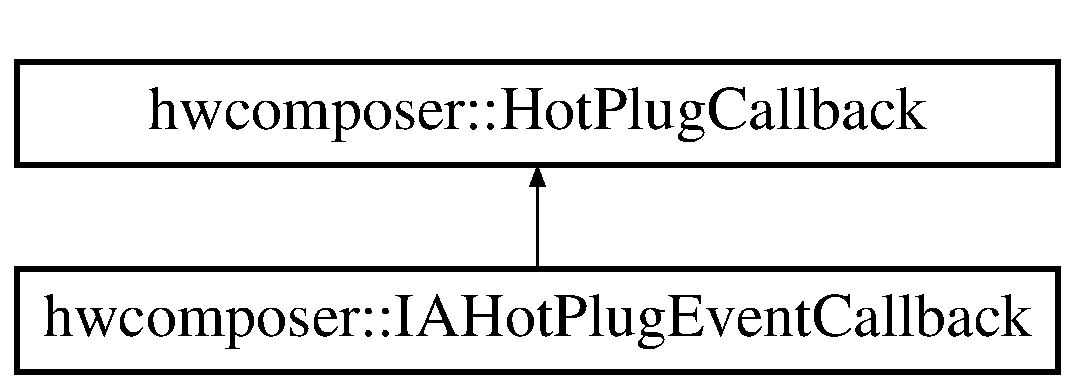
\includegraphics[height=2.000000cm]{classhwcomposer_1_1IAHotPlugEventCallback}
\end{center}
\end{figure}
\subsection*{Public Member Functions}
\begin{DoxyCompactItemize}
\item 
\mbox{\hyperlink{classhwcomposer_1_1IAHotPlugEventCallback_a1d6052a2e63656b115589f9daeca04c4}{I\+A\+Hot\+Plug\+Event\+Callback}} (hwf\+\_\+callback const $\ast$procs)
\item 
void \mbox{\hyperlink{classhwcomposer_1_1IAHotPlugEventCallback_a77b86b9fb88073abf1cab0b5aed4be1d}{Callback}} (uint32\+\_\+t, bool connected)
\end{DoxyCompactItemize}


\subsection{Detailed Description}


Definition at line 403 of file hwf\+\_\+alioshal.\+cpp.



\subsection{Constructor \& Destructor Documentation}
\mbox{\Hypertarget{classhwcomposer_1_1IAHotPlugEventCallback_a1d6052a2e63656b115589f9daeca04c4}\label{classhwcomposer_1_1IAHotPlugEventCallback_a1d6052a2e63656b115589f9daeca04c4}} 
\index{hwcomposer\+::\+I\+A\+Hot\+Plug\+Event\+Callback@{hwcomposer\+::\+I\+A\+Hot\+Plug\+Event\+Callback}!I\+A\+Hot\+Plug\+Event\+Callback@{I\+A\+Hot\+Plug\+Event\+Callback}}
\index{I\+A\+Hot\+Plug\+Event\+Callback@{I\+A\+Hot\+Plug\+Event\+Callback}!hwcomposer\+::\+I\+A\+Hot\+Plug\+Event\+Callback@{hwcomposer\+::\+I\+A\+Hot\+Plug\+Event\+Callback}}
\subsubsection{\texorpdfstring{I\+A\+Hot\+Plug\+Event\+Callback()}{IAHotPlugEventCallback()}}
{\footnotesize\ttfamily hwcomposer\+::\+I\+A\+Hot\+Plug\+Event\+Callback\+::\+I\+A\+Hot\+Plug\+Event\+Callback (\begin{DoxyParamCaption}\item[{hwf\+\_\+callback const $\ast$}]{procs }\end{DoxyParamCaption})\hspace{0.3cm}{\ttfamily [inline]}}



Definition at line 405 of file hwf\+\_\+alioshal.\+cpp.


\begin{DoxyCode}{0}
\DoxyCodeLine{405                                                     : m\_pCB(procs) \{}
\DoxyCodeLine{406   \}}
\end{DoxyCode}


\subsection{Member Function Documentation}
\mbox{\Hypertarget{classhwcomposer_1_1IAHotPlugEventCallback_a77b86b9fb88073abf1cab0b5aed4be1d}\label{classhwcomposer_1_1IAHotPlugEventCallback_a77b86b9fb88073abf1cab0b5aed4be1d}} 
\index{hwcomposer\+::\+I\+A\+Hot\+Plug\+Event\+Callback@{hwcomposer\+::\+I\+A\+Hot\+Plug\+Event\+Callback}!Callback@{Callback}}
\index{Callback@{Callback}!hwcomposer\+::\+I\+A\+Hot\+Plug\+Event\+Callback@{hwcomposer\+::\+I\+A\+Hot\+Plug\+Event\+Callback}}
\subsubsection{\texorpdfstring{Callback()}{Callback()}}
{\footnotesize\ttfamily void hwcomposer\+::\+I\+A\+Hot\+Plug\+Event\+Callback\+::\+Callback (\begin{DoxyParamCaption}\item[{uint32\+\_\+t}]{,  }\item[{bool}]{connected }\end{DoxyParamCaption})\hspace{0.3cm}{\ttfamily [inline]}, {\ttfamily [virtual]}}



Implements \mbox{\hyperlink{classhwcomposer_1_1HotPlugCallback_a455c8913e1da9b165134a05c9cb441ba}{hwcomposer\+::\+Hot\+Plug\+Callback}}.



Definition at line 408 of file hwf\+\_\+alioshal.\+cpp.


\begin{DoxyCode}{0}
\DoxyCodeLine{408                                             \{}
\DoxyCodeLine{409     \textcolor{keywordflow}{if} (ignore\_) \{}
\DoxyCodeLine{410       ignore\_ = \textcolor{keyword}{false};}
\DoxyCodeLine{411       \textcolor{keywordflow}{return};}
\DoxyCodeLine{412     \}}
\DoxyCodeLine{413 }
\DoxyCodeLine{414     LOG\_I(\textcolor{stringliteral}{"IAHotPlugEventCallback --> called.\(\backslash\)n"});}
\DoxyCodeLine{415 }
\DoxyCodeLine{416     m\_pCB->hotplugEvent(m\_pCB, HWF\_DISPLAY\_EXTERNAL, connected);}
\DoxyCodeLine{417   \}}
\end{DoxyCode}


The documentation for this class was generated from the following file\+:\begin{DoxyCompactItemize}
\item 
os/alios/\mbox{\hyperlink{hwf__alioshal_8cpp}{hwf\+\_\+alioshal.\+cpp}}\end{DoxyCompactItemize}

\hypertarget{classandroid_1_1IAHotPlugEventCallback}{}\section{android\+:\+:I\+A\+Hot\+Plug\+Event\+Callback Class Reference}
\label{classandroid_1_1IAHotPlugEventCallback}\index{android\+::\+I\+A\+Hot\+Plug\+Event\+Callback@{android\+::\+I\+A\+Hot\+Plug\+Event\+Callback}}
Inheritance diagram for android\+:\+:I\+A\+Hot\+Plug\+Event\+Callback\+:\begin{figure}[H]
\begin{center}
\leavevmode
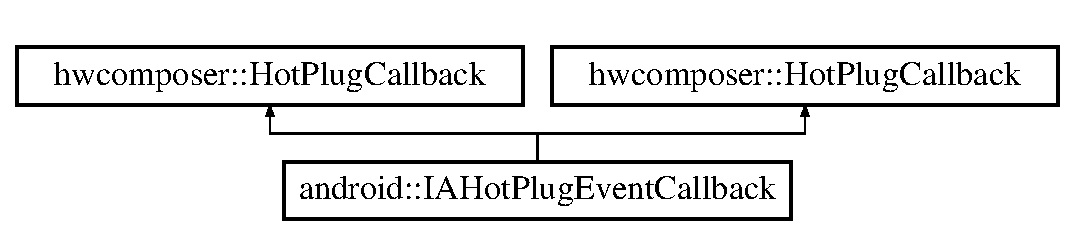
\includegraphics[height=2.000000cm]{classandroid_1_1IAHotPlugEventCallback}
\end{center}
\end{figure}
\subsection*{Public Member Functions}
\begin{DoxyCompactItemize}
\item 
\mbox{\hyperlink{classandroid_1_1IAHotPlugEventCallback_a90284f657664842ccaa6eabe5dba38d8}{I\+A\+Hot\+Plug\+Event\+Callback}} (hwc\+\_\+procs\+\_\+t const $\ast$procs)
\item 
void \mbox{\hyperlink{classandroid_1_1IAHotPlugEventCallback_af5cbfe8fc04fa828f75153f2b5f548b8}{Callback}} (uint32\+\_\+t, bool connected)
\item 
\mbox{\hyperlink{classandroid_1_1IAHotPlugEventCallback_a359be2fe86c68b5cce9f8d4fac36909a}{I\+A\+Hot\+Plug\+Event\+Callback}} (hwc2\+\_\+callback\+\_\+data\+\_\+t data, hwc2\+\_\+function\+\_\+pointer\+\_\+t hook, \mbox{\hyperlink{classandroid_1_1IAHWC2_1_1HwcDisplay}{I\+A\+H\+W\+C2\+::\+Hwc\+Display}} $\ast$display)
\item 
void \mbox{\hyperlink{classandroid_1_1IAHotPlugEventCallback_a8808ed272ecfd7006c28f0e54d6ba9e4}{Callback}} (uint32\+\_\+t display, bool connected)
\end{DoxyCompactItemize}


\subsection{Detailed Description}


Definition at line 139 of file iahwc1.\+cpp.



\subsection{Constructor \& Destructor Documentation}
\mbox{\Hypertarget{classandroid_1_1IAHotPlugEventCallback_a90284f657664842ccaa6eabe5dba38d8}\label{classandroid_1_1IAHotPlugEventCallback_a90284f657664842ccaa6eabe5dba38d8}} 
\index{android\+::\+I\+A\+Hot\+Plug\+Event\+Callback@{android\+::\+I\+A\+Hot\+Plug\+Event\+Callback}!I\+A\+Hot\+Plug\+Event\+Callback@{I\+A\+Hot\+Plug\+Event\+Callback}}
\index{I\+A\+Hot\+Plug\+Event\+Callback@{I\+A\+Hot\+Plug\+Event\+Callback}!android\+::\+I\+A\+Hot\+Plug\+Event\+Callback@{android\+::\+I\+A\+Hot\+Plug\+Event\+Callback}}
\subsubsection{\texorpdfstring{I\+A\+Hot\+Plug\+Event\+Callback()}{IAHotPlugEventCallback()}\hspace{0.1cm}{\footnotesize\ttfamily [1/2]}}
{\footnotesize\ttfamily android\+::\+I\+A\+Hot\+Plug\+Event\+Callback\+::\+I\+A\+Hot\+Plug\+Event\+Callback (\begin{DoxyParamCaption}\item[{hwc\+\_\+procs\+\_\+t const $\ast$}]{procs }\end{DoxyParamCaption})\hspace{0.3cm}{\ttfamily [inline]}}



Definition at line 141 of file iahwc1.\+cpp.


\begin{DoxyCode}{0}
\DoxyCodeLine{141                                                    : procs\_(procs) \{}
\DoxyCodeLine{142   \}}
\end{DoxyCode}
\mbox{\Hypertarget{classandroid_1_1IAHotPlugEventCallback_a359be2fe86c68b5cce9f8d4fac36909a}\label{classandroid_1_1IAHotPlugEventCallback_a359be2fe86c68b5cce9f8d4fac36909a}} 
\index{android\+::\+I\+A\+Hot\+Plug\+Event\+Callback@{android\+::\+I\+A\+Hot\+Plug\+Event\+Callback}!I\+A\+Hot\+Plug\+Event\+Callback@{I\+A\+Hot\+Plug\+Event\+Callback}}
\index{I\+A\+Hot\+Plug\+Event\+Callback@{I\+A\+Hot\+Plug\+Event\+Callback}!android\+::\+I\+A\+Hot\+Plug\+Event\+Callback@{android\+::\+I\+A\+Hot\+Plug\+Event\+Callback}}
\subsubsection{\texorpdfstring{I\+A\+Hot\+Plug\+Event\+Callback()}{IAHotPlugEventCallback()}\hspace{0.1cm}{\footnotesize\ttfamily [2/2]}}
{\footnotesize\ttfamily android\+::\+I\+A\+Hot\+Plug\+Event\+Callback\+::\+I\+A\+Hot\+Plug\+Event\+Callback (\begin{DoxyParamCaption}\item[{hwc2\+\_\+callback\+\_\+data\+\_\+t}]{data,  }\item[{hwc2\+\_\+function\+\_\+pointer\+\_\+t}]{hook,  }\item[{\mbox{\hyperlink{classandroid_1_1IAHWC2_1_1HwcDisplay}{I\+A\+H\+W\+C2\+::\+Hwc\+Display}} $\ast$}]{display }\end{DoxyParamCaption})\hspace{0.3cm}{\ttfamily [inline]}}



Definition at line 80 of file iahwc2.\+cpp.


\begin{DoxyCode}{0}
\DoxyCodeLine{83       : data\_(data), hook\_(hook), display\_(display) \{}
\DoxyCodeLine{84   \}}
\end{DoxyCode}


\subsection{Member Function Documentation}
\mbox{\Hypertarget{classandroid_1_1IAHotPlugEventCallback_a8808ed272ecfd7006c28f0e54d6ba9e4}\label{classandroid_1_1IAHotPlugEventCallback_a8808ed272ecfd7006c28f0e54d6ba9e4}} 
\index{android\+::\+I\+A\+Hot\+Plug\+Event\+Callback@{android\+::\+I\+A\+Hot\+Plug\+Event\+Callback}!Callback@{Callback}}
\index{Callback@{Callback}!android\+::\+I\+A\+Hot\+Plug\+Event\+Callback@{android\+::\+I\+A\+Hot\+Plug\+Event\+Callback}}
\subsubsection{\texorpdfstring{Callback()}{Callback()}\hspace{0.1cm}{\footnotesize\ttfamily [1/2]}}
{\footnotesize\ttfamily void android\+::\+I\+A\+Hot\+Plug\+Event\+Callback\+::\+Callback (\begin{DoxyParamCaption}\item[{uint32\+\_\+t}]{display,  }\item[{bool}]{connected }\end{DoxyParamCaption})\hspace{0.3cm}{\ttfamily [inline]}, {\ttfamily [virtual]}}



Implements \mbox{\hyperlink{classhwcomposer_1_1HotPlugCallback_a455c8913e1da9b165134a05c9cb441ba}{hwcomposer\+::\+Hot\+Plug\+Callback}}.



Definition at line 86 of file iahwc2.\+cpp.


\begin{DoxyCode}{0}
\DoxyCodeLine{86                                                   \{}
\DoxyCodeLine{87     \textcolor{keywordflow}{if} (display == 0) \{}
\DoxyCodeLine{88       \textcolor{comment}{// SF expects primary display to be always}}
\DoxyCodeLine{89       \textcolor{comment}{// connected. Let's notify it first time and ignore}}
\DoxyCodeLine{90       \textcolor{comment}{// any followup status changes.}}
\DoxyCodeLine{91       \textcolor{keywordflow}{if} (notified\_) \{}
\DoxyCodeLine{92         \textcolor{keywordflow}{return};}
\DoxyCodeLine{93       \}}
\DoxyCodeLine{94 }
\DoxyCodeLine{95       \textcolor{keywordflow}{if} (connected)}
\DoxyCodeLine{96         notified\_ = \textcolor{keyword}{true};}
\DoxyCodeLine{97     \}}
\DoxyCodeLine{98 }
\DoxyCodeLine{99     \textcolor{keyword}{auto} hook = \textcolor{keyword}{reinterpret\_cast<}HWC2\_PFN\_HOTPLUG\textcolor{keyword}{>}(hook\_);}
\DoxyCodeLine{100     int32\_t status = \textcolor{keyword}{static\_cast<}int32\_t\textcolor{keyword}{>}(HWC2::Connection::Connected);}
\DoxyCodeLine{101     \textcolor{keywordflow}{if} (!connected) \{}
\DoxyCodeLine{102       status = \textcolor{keyword}{static\_cast<}int32\_t\textcolor{keyword}{>}(HWC2::Connection::Disconnected);}
\DoxyCodeLine{103     \}}
\DoxyCodeLine{104 }
\DoxyCodeLine{105     \mbox{\hyperlink{hwctrace_8h_af8c38c979e9089c283d2f5923089b538}{IHOTPLUGEVENTTRACE}}(}
\DoxyCodeLine{106         \textcolor{stringliteral}{"IAHotPlugEventCallback called displayid: \%d status: \%d \(\backslash\)n"}, display,}
\DoxyCodeLine{107         status);}
\DoxyCodeLine{108     \textcolor{keywordflow}{if} (hook)}
\DoxyCodeLine{109       hook(data\_, display, status);}
\DoxyCodeLine{110 }
\DoxyCodeLine{111     \textcolor{comment}{// FIXME: SurfaceFlinger doesn't seem to reset layers correctly}}
\DoxyCodeLine{112     \textcolor{comment}{// when display is connected/disconnected. We force it here.}}
\DoxyCodeLine{113     \textcolor{comment}{// Remove this workaround once fixed correctly in SurfaceFlinger.}}
\DoxyCodeLine{114     \textcolor{keywordflow}{if} (!connected \&\& display > 0) \{}
\DoxyCodeLine{115       display\_->\mbox{\hyperlink{classandroid_1_1IAHWC2_1_1HwcDisplay_a26c6de4c4a210954ea627be435dab3d7}{FreeAllLayers}}();}
\DoxyCodeLine{116     \}}
\DoxyCodeLine{117   \}}
\end{DoxyCode}
\mbox{\Hypertarget{classandroid_1_1IAHotPlugEventCallback_af5cbfe8fc04fa828f75153f2b5f548b8}\label{classandroid_1_1IAHotPlugEventCallback_af5cbfe8fc04fa828f75153f2b5f548b8}} 
\index{android\+::\+I\+A\+Hot\+Plug\+Event\+Callback@{android\+::\+I\+A\+Hot\+Plug\+Event\+Callback}!Callback@{Callback}}
\index{Callback@{Callback}!android\+::\+I\+A\+Hot\+Plug\+Event\+Callback@{android\+::\+I\+A\+Hot\+Plug\+Event\+Callback}}
\subsubsection{\texorpdfstring{Callback()}{Callback()}\hspace{0.1cm}{\footnotesize\ttfamily [2/2]}}
{\footnotesize\ttfamily void android\+::\+I\+A\+Hot\+Plug\+Event\+Callback\+::\+Callback (\begin{DoxyParamCaption}\item[{uint32\+\_\+t}]{,  }\item[{bool}]{connected }\end{DoxyParamCaption})\hspace{0.3cm}{\ttfamily [inline]}, {\ttfamily [virtual]}}



Implements \mbox{\hyperlink{classhwcomposer_1_1HotPlugCallback_a455c8913e1da9b165134a05c9cb441ba}{hwcomposer\+::\+Hot\+Plug\+Callback}}.



Definition at line 144 of file iahwc1.\+cpp.


\begin{DoxyCode}{0}
\DoxyCodeLine{144                                             \{}
\DoxyCodeLine{145     \textcolor{keywordflow}{if} (ignore\_) \{}
\DoxyCodeLine{146       ignore\_ = \textcolor{keyword}{false};}
\DoxyCodeLine{147       \textcolor{keywordflow}{return};}
\DoxyCodeLine{148     \}}
\DoxyCodeLine{149 }
\DoxyCodeLine{150     procs\_->hotplug(procs\_, HWC\_DISPLAY\_EXTERNAL\_BIT, connected);}
\DoxyCodeLine{151   \}}
\end{DoxyCode}


The documentation for this class was generated from the following files\+:\begin{DoxyCompactItemize}
\item 
os/android/\mbox{\hyperlink{iahwc1_8cpp}{iahwc1.\+cpp}}\item 
os/android/\mbox{\hyperlink{iahwc2_8cpp}{iahwc2.\+cpp}}\end{DoxyCompactItemize}

\hypertarget{classhwcomposer_1_1IAHWC}{}\section{hwcomposer\+:\+:I\+A\+H\+WC Class Reference}
\label{classhwcomposer_1_1IAHWC}\index{hwcomposer\+::\+I\+A\+H\+WC@{hwcomposer\+::\+I\+A\+H\+WC}}


{\ttfamily \#include $<$linux\+\_\+frontend.\+h$>$}

Inheritance diagram for hwcomposer\+:\+:I\+A\+H\+WC\+:\begin{figure}[H]
\begin{center}
\leavevmode
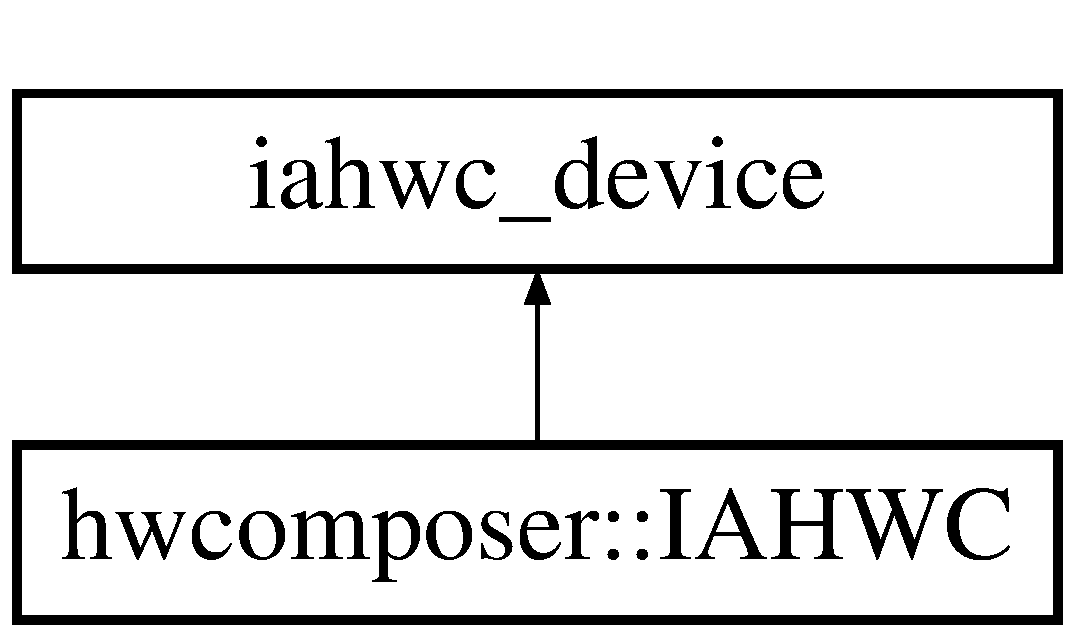
\includegraphics[height=2.000000cm]{classhwcomposer_1_1IAHWC}
\end{center}
\end{figure}
\subsection*{Classes}
\begin{DoxyCompactItemize}
\item 
class \mbox{\hyperlink{classhwcomposer_1_1IAHWC_1_1IAHWCDisplay}{I\+A\+H\+W\+C\+Display}}
\item 
class \mbox{\hyperlink{classhwcomposer_1_1IAHWC_1_1IAHWCLayer}{I\+A\+H\+W\+C\+Layer}}
\end{DoxyCompactItemize}
\subsection*{Public Member Functions}
\begin{DoxyCompactItemize}
\item 
\mbox{\hyperlink{classhwcomposer_1_1IAHWC_a5dcce49d920bb707fc1bcd6357c87006}{I\+A\+H\+WC}} ()
\item 
int32\+\_\+t \mbox{\hyperlink{classhwcomposer_1_1IAHWC_afdb49a5ff4e943fb5f874b9c6fbb431f}{Init}} ()
\end{DoxyCompactItemize}
\subsection*{Static Public Member Functions}
\begin{DoxyCompactItemize}
\item 
static \mbox{\hyperlink{classhwcomposer_1_1IAHWC}{I\+A\+H\+WC}} $\ast$ \mbox{\hyperlink{classhwcomposer_1_1IAHWC_a9f236ac26693721c4c25f64a01e24307}{to\+I\+A\+H\+WC}} (\mbox{\hyperlink{iahwc_8h_aa44e63a48d7c328d160f28888a6b3edd}{iahwc\+\_\+device\+\_\+t}} $\ast$dev)
\item 
static int \mbox{\hyperlink{classhwcomposer_1_1IAHWC_af4d87455f682c18ae34901c59abc9e3e}{Hook\+Open}} (const \mbox{\hyperlink{iahwc_8h_a6a0009d570fc041f403dee1e0fd68cf9}{iahwc\+\_\+module\+\_\+t}} $\ast$, \mbox{\hyperlink{iahwc_8h_aa44e63a48d7c328d160f28888a6b3edd}{iahwc\+\_\+device\+\_\+t}} $\ast$$\ast$)
\item 
static int \mbox{\hyperlink{classhwcomposer_1_1IAHWC_a215e268fcbbc3e7f8b025d2835f9cf35}{Hook\+Close}} (\mbox{\hyperlink{iahwc_8h_aa44e63a48d7c328d160f28888a6b3edd}{iahwc\+\_\+device\+\_\+t}} $\ast$)
\item 
static \mbox{\hyperlink{iahwc_8h_a214bf51cce821fdb7b24210088c12cad}{iahwc\+\_\+function\+\_\+ptr\+\_\+t}} \mbox{\hyperlink{classhwcomposer_1_1IAHWC_aa5e1fbf26a4ea394a6acf30104e87c75}{Hook\+Get\+Function\+Ptr}} (\mbox{\hyperlink{iahwc_8h_aa44e63a48d7c328d160f28888a6b3edd}{iahwc\+\_\+device\+\_\+t}} $\ast$, int)
\item 
{\footnotesize template$<$typename P\+FN , typename T $>$ }\\static \mbox{\hyperlink{iahwc_8h_a214bf51cce821fdb7b24210088c12cad}{iahwc\+\_\+function\+\_\+ptr\+\_\+t}} \mbox{\hyperlink{classhwcomposer_1_1IAHWC_a87c94f049fd6c0212a94478e2e4faa1d}{To\+Hook}} (T function)
\item 
{\footnotesize template$<$typename T , typename Hook\+Type , Hook\+Type func, typename... Args$>$ }\\static T \mbox{\hyperlink{classhwcomposer_1_1IAHWC_a85c7dbeca1457ee0dff40336e74a8b19}{Device\+Hook}} (\mbox{\hyperlink{iahwc_8h_aa44e63a48d7c328d160f28888a6b3edd}{iahwc\+\_\+device\+\_\+t}} $\ast$dev, Args... args)
\item 
{\footnotesize template$<$typename Hook\+Type , Hook\+Type func, typename... Args$>$ }\\static int32\+\_\+t \mbox{\hyperlink{classhwcomposer_1_1IAHWC_aea66337d6982d1d9522e15d35eeee1d6}{Display\+Hook}} (\mbox{\hyperlink{iahwc_8h_aa44e63a48d7c328d160f28888a6b3edd}{iahwc\+\_\+device\+\_\+t}} $\ast$dev, \mbox{\hyperlink{iahwc_8h_a026bdbdf86a828fa3a4d800226e8f8c0}{iahwc\+\_\+display\+\_\+t}} display\+\_\+handle, Args... args)
\item 
{\footnotesize template$<$typename Hook\+Type , Hook\+Type func, typename... Args$>$ }\\static int32\+\_\+t \mbox{\hyperlink{classhwcomposer_1_1IAHWC_ae8dc63a7d2f1784242689fd1f7b2e9d4}{Layer\+Hook}} (\mbox{\hyperlink{iahwc_8h_aa44e63a48d7c328d160f28888a6b3edd}{iahwc\+\_\+device\+\_\+t}} $\ast$dev, \mbox{\hyperlink{iahwc_8h_a026bdbdf86a828fa3a4d800226e8f8c0}{iahwc\+\_\+display\+\_\+t}} display\+\_\+handle, \mbox{\hyperlink{iahwc_8h_a603c5018c43d1f6b98fbb7eeef6a43ac}{iahwc\+\_\+layer\+\_\+t}} layer\+\_\+handle, Args... args)
\end{DoxyCompactItemize}
\subsection*{Additional Inherited Members}


\subsection{Detailed Description}


Definition at line 35 of file linux\+\_\+frontend.\+h.



\subsection{Constructor \& Destructor Documentation}
\mbox{\Hypertarget{classhwcomposer_1_1IAHWC_a5dcce49d920bb707fc1bcd6357c87006}\label{classhwcomposer_1_1IAHWC_a5dcce49d920bb707fc1bcd6357c87006}} 
\index{hwcomposer\+::\+I\+A\+H\+WC@{hwcomposer\+::\+I\+A\+H\+WC}!I\+A\+H\+WC@{I\+A\+H\+WC}}
\index{I\+A\+H\+WC@{I\+A\+H\+WC}!hwcomposer\+::\+I\+A\+H\+WC@{hwcomposer\+::\+I\+A\+H\+WC}}
\subsubsection{\texorpdfstring{I\+A\+H\+W\+C()}{IAHWC()}}
{\footnotesize\ttfamily hwcomposer\+::\+I\+A\+H\+W\+C\+::\+I\+A\+H\+WC (\begin{DoxyParamCaption}{ }\end{DoxyParamCaption})}



Definition at line 96 of file linux\+\_\+frontend.\+cpp.


\begin{DoxyCode}{0}
\DoxyCodeLine{96              \{}
\DoxyCodeLine{97   \mbox{\hyperlink{structiahwc__device_af5514f45ede1ab95ab6eafa8c3f40ad3}{getFunctionPtr}} = \mbox{\hyperlink{classhwcomposer_1_1IAHWC_aa5e1fbf26a4ea394a6acf30104e87c75}{HookGetFunctionPtr}};}
\DoxyCodeLine{98   \mbox{\hyperlink{structiahwc__device_a147ff8b5cced2b745222742c89fd3e08}{close}} = \mbox{\hyperlink{classhwcomposer_1_1IAHWC_a215e268fcbbc3e7f8b025d2835f9cf35}{HookClose}};}
\DoxyCodeLine{99 \}}
\end{DoxyCode}


\subsection{Member Function Documentation}
\mbox{\Hypertarget{classhwcomposer_1_1IAHWC_a85c7dbeca1457ee0dff40336e74a8b19}\label{classhwcomposer_1_1IAHWC_a85c7dbeca1457ee0dff40336e74a8b19}} 
\index{hwcomposer\+::\+I\+A\+H\+WC@{hwcomposer\+::\+I\+A\+H\+WC}!Device\+Hook@{Device\+Hook}}
\index{Device\+Hook@{Device\+Hook}!hwcomposer\+::\+I\+A\+H\+WC@{hwcomposer\+::\+I\+A\+H\+WC}}
\subsubsection{\texorpdfstring{Device\+Hook()}{DeviceHook()}}
{\footnotesize\ttfamily template$<$typename T , typename Hook\+Type , Hook\+Type func, typename... Args$>$ \\
static T hwcomposer\+::\+I\+A\+H\+W\+C\+::\+Device\+Hook (\begin{DoxyParamCaption}\item[{\mbox{\hyperlink{iahwc_8h_aa44e63a48d7c328d160f28888a6b3edd}{iahwc\+\_\+device\+\_\+t}} $\ast$}]{dev,  }\item[{Args...}]{args }\end{DoxyParamCaption})\hspace{0.3cm}{\ttfamily [inline]}, {\ttfamily [static]}}



Definition at line 134 of file linux\+\_\+frontend.\+h.


\begin{DoxyCode}{0}
\DoxyCodeLine{134                                                          \{}
\DoxyCodeLine{135     \mbox{\hyperlink{classhwcomposer_1_1IAHWC_a5dcce49d920bb707fc1bcd6357c87006}{IAHWC}}* hwc = \mbox{\hyperlink{classhwcomposer_1_1IAHWC_a9f236ac26693721c4c25f64a01e24307}{toIAHWC}}(dev);}
\DoxyCodeLine{136     \textcolor{keywordflow}{return} \textcolor{keyword}{static\_cast<}T\textcolor{keyword}{>}(((*hwc).*func)(std::forward<Args>(args)...));}
\DoxyCodeLine{137   \}}
\end{DoxyCode}
\mbox{\Hypertarget{classhwcomposer_1_1IAHWC_aea66337d6982d1d9522e15d35eeee1d6}\label{classhwcomposer_1_1IAHWC_aea66337d6982d1d9522e15d35eeee1d6}} 
\index{hwcomposer\+::\+I\+A\+H\+WC@{hwcomposer\+::\+I\+A\+H\+WC}!Display\+Hook@{Display\+Hook}}
\index{Display\+Hook@{Display\+Hook}!hwcomposer\+::\+I\+A\+H\+WC@{hwcomposer\+::\+I\+A\+H\+WC}}
\subsubsection{\texorpdfstring{Display\+Hook()}{DisplayHook()}}
{\footnotesize\ttfamily template$<$typename Hook\+Type , Hook\+Type func, typename... Args$>$ \\
static int32\+\_\+t hwcomposer\+::\+I\+A\+H\+W\+C\+::\+Display\+Hook (\begin{DoxyParamCaption}\item[{\mbox{\hyperlink{iahwc_8h_aa44e63a48d7c328d160f28888a6b3edd}{iahwc\+\_\+device\+\_\+t}} $\ast$}]{dev,  }\item[{\mbox{\hyperlink{iahwc_8h_a026bdbdf86a828fa3a4d800226e8f8c0}{iahwc\+\_\+display\+\_\+t}}}]{display\+\_\+handle,  }\item[{Args...}]{args }\end{DoxyParamCaption})\hspace{0.3cm}{\ttfamily [inline]}, {\ttfamily [static]}}



Definition at line 140 of file linux\+\_\+frontend.\+h.


\begin{DoxyCode}{0}
\DoxyCodeLine{141                                                                            \{}
\DoxyCodeLine{142     \mbox{\hyperlink{classhwcomposer_1_1IAHWC_a5dcce49d920bb707fc1bcd6357c87006}{IAHWC}}* hwc = \mbox{\hyperlink{classhwcomposer_1_1IAHWC_a9f236ac26693721c4c25f64a01e24307}{toIAHWC}}(dev);}
\DoxyCodeLine{143     IAHWCDisplay* display = hwc->displays\_.at(display\_handle);}
\DoxyCodeLine{144     \textcolor{keywordflow}{return} \textcolor{keyword}{static\_cast<}int32\_t\textcolor{keyword}{>}((display->*func)(std::forward<Args>(args)...));}
\DoxyCodeLine{145   \}}
\end{DoxyCode}
\mbox{\Hypertarget{classhwcomposer_1_1IAHWC_a215e268fcbbc3e7f8b025d2835f9cf35}\label{classhwcomposer_1_1IAHWC_a215e268fcbbc3e7f8b025d2835f9cf35}} 
\index{hwcomposer\+::\+I\+A\+H\+WC@{hwcomposer\+::\+I\+A\+H\+WC}!Hook\+Close@{Hook\+Close}}
\index{Hook\+Close@{Hook\+Close}!hwcomposer\+::\+I\+A\+H\+WC@{hwcomposer\+::\+I\+A\+H\+WC}}
\subsubsection{\texorpdfstring{Hook\+Close()}{HookClose()}}
{\footnotesize\ttfamily int hwcomposer\+::\+I\+A\+H\+W\+C\+::\+Hook\+Close (\begin{DoxyParamCaption}\item[{\mbox{\hyperlink{iahwc_8h_aa44e63a48d7c328d160f28888a6b3edd}{iahwc\+\_\+device\+\_\+t}} $\ast$}]{dev }\end{DoxyParamCaption})\hspace{0.3cm}{\ttfamily [static]}}



Definition at line 236 of file linux\+\_\+frontend.\+cpp.


\begin{DoxyCode}{0}
\DoxyCodeLine{236                                         \{}
\DoxyCodeLine{237   \textcolor{keyword}{delete} dev;}
\DoxyCodeLine{238   \textcolor{keywordflow}{return} 0;}
\DoxyCodeLine{239 \}}
\end{DoxyCode}
\mbox{\Hypertarget{classhwcomposer_1_1IAHWC_aa5e1fbf26a4ea394a6acf30104e87c75}\label{classhwcomposer_1_1IAHWC_aa5e1fbf26a4ea394a6acf30104e87c75}} 
\index{hwcomposer\+::\+I\+A\+H\+WC@{hwcomposer\+::\+I\+A\+H\+WC}!Hook\+Get\+Function\+Ptr@{Hook\+Get\+Function\+Ptr}}
\index{Hook\+Get\+Function\+Ptr@{Hook\+Get\+Function\+Ptr}!hwcomposer\+::\+I\+A\+H\+WC@{hwcomposer\+::\+I\+A\+H\+WC}}
\subsubsection{\texorpdfstring{Hook\+Get\+Function\+Ptr()}{HookGetFunctionPtr()}}
{\footnotesize\ttfamily \mbox{\hyperlink{iahwc_8h_a214bf51cce821fdb7b24210088c12cad}{iahwc\+\_\+function\+\_\+ptr\+\_\+t}} hwcomposer\+::\+I\+A\+H\+W\+C\+::\+Hook\+Get\+Function\+Ptr (\begin{DoxyParamCaption}\item[{\mbox{\hyperlink{iahwc_8h_aa44e63a48d7c328d160f28888a6b3edd}{iahwc\+\_\+device\+\_\+t}} $\ast$}]{,  }\item[{int}]{func\+\_\+descriptor }\end{DoxyParamCaption})\hspace{0.3cm}{\ttfamily [static]}}



Definition at line 127 of file linux\+\_\+frontend.\+cpp.


\begin{DoxyCode}{0}
\DoxyCodeLine{128                                                                     \{}
\DoxyCodeLine{129   \textcolor{keywordflow}{switch} (func\_descriptor) \{}
\DoxyCodeLine{130     \textcolor{keywordflow}{case} \mbox{\hyperlink{iahwc_8h_a9531afe3077246a1921c90bd893c632aa2599f399f6e4611f806434999e53648c}{IAHWC\_FUNC\_GET\_NUM\_DISPLAYS}}:}
\DoxyCodeLine{131       \textcolor{keywordflow}{return} ToHook<IAHWC\_PFN\_GET\_NUM\_DISPLAYS>(}
\DoxyCodeLine{132           \mbox{\hyperlink{classhwcomposer_1_1IAHWC_a85c7dbeca1457ee0dff40336e74a8b19}{DeviceHook}}<int32\_t, decltype(\&IAHWC::GetNumDisplays),}
\DoxyCodeLine{133                      \&IAHWC::GetNumDisplays, \textcolor{keywordtype}{int}*>);}
\DoxyCodeLine{134     \textcolor{keywordflow}{case} \mbox{\hyperlink{iahwc_8h_a9531afe3077246a1921c90bd893c632aaa77ea736de2f6982bb75fcb91757c970}{IAHWC\_FUNC\_REGISTER\_CALLBACK}}:}
\DoxyCodeLine{135       \textcolor{keywordflow}{return} ToHook<IAHWC\_PFN\_REGISTER\_CALLBACK>(}
\DoxyCodeLine{136           \mbox{\hyperlink{classhwcomposer_1_1IAHWC_a85c7dbeca1457ee0dff40336e74a8b19}{DeviceHook}}<int32\_t, decltype(\&IAHWC::RegisterCallback),}
\DoxyCodeLine{137                      \&IAHWC::RegisterCallback, int, uint32\_t,}
\DoxyCodeLine{138                      \mbox{\hyperlink{iahwc_8h_a07fb4f73baa8a0cfbd40f64071e56a7c}{iahwc\_callback\_data\_t}}, 
      \mbox{\hyperlink{iahwc_8h_a214bf51cce821fdb7b24210088c12cad}{iahwc\_function\_ptr\_t}}>);}
\DoxyCodeLine{139     \textcolor{keywordflow}{case} \mbox{\hyperlink{iahwc_8h_a9531afe3077246a1921c90bd893c632aa72817c7a1667dd9e0638f47606fddba1}{IAHWC\_FUNC\_DISPLAY\_GET\_INFO}}:}
\DoxyCodeLine{140       \textcolor{keywordflow}{return} ToHook<IAHWC\_PFN\_DISPLAY\_GET\_INFO>(}
\DoxyCodeLine{141           \mbox{\hyperlink{classhwcomposer_1_1IAHWC_aea66337d6982d1d9522e15d35eeee1d6}{DisplayHook}}<decltype(\&\mbox{\hyperlink{classhwcomposer_1_1IAHWC_1_1IAHWCDisplay_abac8759ae7be9065fb6a579e1b384c23}{IAHWCDisplay::GetDisplayInfo}}),}
\DoxyCodeLine{142                       \&\mbox{\hyperlink{classhwcomposer_1_1IAHWC_1_1IAHWCDisplay_abac8759ae7be9065fb6a579e1b384c23}{IAHWCDisplay::GetDisplayInfo}}, uint32\_t, int, int32\_t*>);}
\DoxyCodeLine{143     \textcolor{keywordflow}{case} \mbox{\hyperlink{iahwc_8h_a9531afe3077246a1921c90bd893c632aaef43b66aef00346956420ded92c64957}{IAHWC\_FUNC\_DISPLAY\_GET\_NAME}}:}
\DoxyCodeLine{144       \textcolor{keywordflow}{return} ToHook<IAHWC\_PFN\_DISPLAY\_GET\_NAME>(}
\DoxyCodeLine{145           \mbox{\hyperlink{classhwcomposer_1_1IAHWC_aea66337d6982d1d9522e15d35eeee1d6}{DisplayHook}}<decltype(\&\mbox{\hyperlink{classhwcomposer_1_1IAHWC_1_1IAHWCDisplay_af090eee5e7afcef5e96f8990815cf712}{IAHWCDisplay::GetDisplayName}}),}
\DoxyCodeLine{146                       \&\mbox{\hyperlink{classhwcomposer_1_1IAHWC_1_1IAHWCDisplay_af090eee5e7afcef5e96f8990815cf712}{IAHWCDisplay::GetDisplayName}}, uint32\_t*, \textcolor{keywordtype}{char}*>);}
\DoxyCodeLine{147     \textcolor{keywordflow}{case} \mbox{\hyperlink{iahwc_8h_a9531afe3077246a1921c90bd893c632aa90bdf4d5e62d9c1f276cd1d96644daa7}{IAHWC\_FUNC\_DISPLAY\_GET\_CONFIGS}}:}
\DoxyCodeLine{148       \textcolor{keywordflow}{return} ToHook<IAHWC\_PFN\_DISPLAY\_GET\_CONFIGS>(}
\DoxyCodeLine{149           \mbox{\hyperlink{classhwcomposer_1_1IAHWC_aea66337d6982d1d9522e15d35eeee1d6}{DisplayHook}}<decltype(\&\mbox{\hyperlink{classhwcomposer_1_1IAHWC_1_1IAHWCDisplay_a186346b470891a51643e415468ca5550}{IAHWCDisplay::GetDisplayConfigs}}),}
\DoxyCodeLine{150                       \&\mbox{\hyperlink{classhwcomposer_1_1IAHWC_1_1IAHWCDisplay_a186346b470891a51643e415468ca5550}{IAHWCDisplay::GetDisplayConfigs}}, uint32\_t*, uint32\_t*>);}
\DoxyCodeLine{151     \textcolor{keywordflow}{case} \mbox{\hyperlink{iahwc_8h_a9531afe3077246a1921c90bd893c632aace7ff80a1225c6a2b4ce85834f3793e0}{IAHWC\_FUNC\_DISPLAY\_SET\_POWER\_MODE}}:}
\DoxyCodeLine{152       \textcolor{keywordflow}{return} ToHook<IAHWC\_PFN\_DISPLAY\_SET\_POWER\_MODE>(}
\DoxyCodeLine{153           \mbox{\hyperlink{classhwcomposer_1_1IAHWC_aea66337d6982d1d9522e15d35eeee1d6}{DisplayHook}}<decltype(\&\mbox{\hyperlink{classhwcomposer_1_1IAHWC_1_1IAHWCDisplay_abff19b5001304bd1f0e3c582a409f672}{IAHWCDisplay::SetPowerMode}}),}
\DoxyCodeLine{154                       \&\mbox{\hyperlink{classhwcomposer_1_1IAHWC_1_1IAHWCDisplay_abff19b5001304bd1f0e3c582a409f672}{IAHWCDisplay::SetPowerMode}}, uint32\_t>);}
\DoxyCodeLine{155     \textcolor{keywordflow}{case} \mbox{\hyperlink{iahwc_8h_a9531afe3077246a1921c90bd893c632aaeabaf8333bea8057c88dd51edf8a7c24}{IAHWC\_FUNC\_DISPLAY\_SET\_GAMMA}}:}
\DoxyCodeLine{156       \textcolor{keywordflow}{return} ToHook<IAHWC\_PFN\_DISPLAY\_SET\_GAMMA>(}
\DoxyCodeLine{157           \mbox{\hyperlink{classhwcomposer_1_1IAHWC_aea66337d6982d1d9522e15d35eeee1d6}{DisplayHook}}<decltype(\&\mbox{\hyperlink{classhwcomposer_1_1IAHWC_1_1IAHWCDisplay_af334fba3fe056cf75884939ed8cf6fbc}{IAHWCDisplay::SetDisplayGamma}}),}
\DoxyCodeLine{158                       \&\mbox{\hyperlink{classhwcomposer_1_1IAHWC_1_1IAHWCDisplay_af334fba3fe056cf75884939ed8cf6fbc}{IAHWCDisplay::SetDisplayGamma}}, float, float, \textcolor{keywordtype}{float}>);}
\DoxyCodeLine{159     \textcolor{keywordflow}{case} \mbox{\hyperlink{iahwc_8h_a9531afe3077246a1921c90bd893c632aa30cc95a2c9a458368bd6c979d88d2790}{IAHWC\_FUNC\_DISPLAY\_SET\_CONFIG}}:}
\DoxyCodeLine{160       \textcolor{keywordflow}{return} ToHook<IAHWC\_PFN\_DISPLAY\_SET\_CONFIG>(}
\DoxyCodeLine{161           \mbox{\hyperlink{classhwcomposer_1_1IAHWC_aea66337d6982d1d9522e15d35eeee1d6}{DisplayHook}}<decltype(\&\mbox{\hyperlink{classhwcomposer_1_1IAHWC_1_1IAHWCDisplay_ae4a7bf880a35f4df5e649003f7f7a212}{IAHWCDisplay::SetDisplayConfig}}),}
\DoxyCodeLine{162                       \&\mbox{\hyperlink{classhwcomposer_1_1IAHWC_1_1IAHWCDisplay_ae4a7bf880a35f4df5e649003f7f7a212}{IAHWCDisplay::SetDisplayConfig}}, uint32\_t>);}
\DoxyCodeLine{163     \textcolor{keywordflow}{case} \mbox{\hyperlink{iahwc_8h_a9531afe3077246a1921c90bd893c632aa06df410294487e04938bda0cc46707c2}{IAHWC\_FUNC\_DISPLAY\_GET\_CONFIG}}:}
\DoxyCodeLine{164       \textcolor{keywordflow}{return} ToHook<IAHWC\_PFN\_DISPLAY\_GET\_CONFIG>(}
\DoxyCodeLine{165           \mbox{\hyperlink{classhwcomposer_1_1IAHWC_aea66337d6982d1d9522e15d35eeee1d6}{DisplayHook}}<decltype(\&\mbox{\hyperlink{classhwcomposer_1_1IAHWC_1_1IAHWCDisplay_a7088d0da276eca2dc2b4458f20270258}{IAHWCDisplay::GetDisplayConfig}}),}
\DoxyCodeLine{166                       \&\mbox{\hyperlink{classhwcomposer_1_1IAHWC_1_1IAHWCDisplay_a7088d0da276eca2dc2b4458f20270258}{IAHWCDisplay::GetDisplayConfig}}, uint32\_t*>);}
\DoxyCodeLine{167     \textcolor{keywordflow}{case} \mbox{\hyperlink{iahwc_8h_a9531afe3077246a1921c90bd893c632aa812474441bd12edeb01bda3313217eac}{IAHWC\_FUNC\_DISPLAY\_CLEAR\_ALL\_LAYERS}}:}
\DoxyCodeLine{168       \textcolor{keywordflow}{return} ToHook<IAHWC\_PFN\_DISPLAY\_CLEAR\_ALL\_LAYERS>(}
\DoxyCodeLine{169           \mbox{\hyperlink{classhwcomposer_1_1IAHWC_aea66337d6982d1d9522e15d35eeee1d6}{DisplayHook}}<decltype(\&\mbox{\hyperlink{classhwcomposer_1_1IAHWC_1_1IAHWCDisplay_a5dcd39e69f99da275fa1d7b64f0dd3b2}{IAHWCDisplay::ClearAllLayers}}),}
\DoxyCodeLine{170                       \&\mbox{\hyperlink{classhwcomposer_1_1IAHWC_1_1IAHWCDisplay_a5dcd39e69f99da275fa1d7b64f0dd3b2}{IAHWCDisplay::ClearAllLayers}}>);}
\DoxyCodeLine{171     \textcolor{keywordflow}{case} \mbox{\hyperlink{iahwc_8h_a9531afe3077246a1921c90bd893c632aae1b3009747c0937a6a03fc40d74c01c6}{IAHWC\_FUNC\_PRESENT\_DISPLAY}}:}
\DoxyCodeLine{172       \textcolor{keywordflow}{return} ToHook<IAHWC\_PFN\_PRESENT\_DISPLAY>(}
\DoxyCodeLine{173           \mbox{\hyperlink{classhwcomposer_1_1IAHWC_aea66337d6982d1d9522e15d35eeee1d6}{DisplayHook}}<decltype(\&\mbox{\hyperlink{classhwcomposer_1_1IAHWC_1_1IAHWCDisplay_a530a804beb0192c173f7311b35d0909f}{IAHWCDisplay::PresentDisplay}}),}
\DoxyCodeLine{174                       \&\mbox{\hyperlink{classhwcomposer_1_1IAHWC_1_1IAHWCDisplay_a530a804beb0192c173f7311b35d0909f}{IAHWCDisplay::PresentDisplay}}, int32\_t*>);}
\DoxyCodeLine{175     \textcolor{keywordflow}{case} \mbox{\hyperlink{iahwc_8h_a9531afe3077246a1921c90bd893c632aa2be9d3b0b48ea43aa62292c7b21bfe84}{IAHWC\_FUNC\_DISABLE\_OVERLAY\_USAGE}}:}
\DoxyCodeLine{176       \textcolor{keywordflow}{return} ToHook<IAHWC\_PFN\_DISABLE\_OVERLAY\_USAGE>(}
\DoxyCodeLine{177           \mbox{\hyperlink{classhwcomposer_1_1IAHWC_aea66337d6982d1d9522e15d35eeee1d6}{DisplayHook}}<decltype(\&\mbox{\hyperlink{classhwcomposer_1_1IAHWC_1_1IAHWCDisplay_ac5d4d8c593d2aa79f1b76a19501b2c08}{IAHWCDisplay::DisableOverlayUsage}}),}
\DoxyCodeLine{178                       \&\mbox{\hyperlink{classhwcomposer_1_1IAHWC_1_1IAHWCDisplay_ac5d4d8c593d2aa79f1b76a19501b2c08}{IAHWCDisplay::DisableOverlayUsage}}>);}
\DoxyCodeLine{179     \textcolor{keywordflow}{case} \mbox{\hyperlink{iahwc_8h_a9531afe3077246a1921c90bd893c632aadbd03bc00b0474ac1642757b4e378086}{IAHWC\_FUNC\_ENABLE\_OVERLAY\_USAGE}}:}
\DoxyCodeLine{180       \textcolor{keywordflow}{return} ToHook<IAHWC\_PFN\_ENABLE\_OVERLAY\_USAGE>(}
\DoxyCodeLine{181           \mbox{\hyperlink{classhwcomposer_1_1IAHWC_aea66337d6982d1d9522e15d35eeee1d6}{DisplayHook}}<decltype(\&\mbox{\hyperlink{classhwcomposer_1_1IAHWC_1_1IAHWCDisplay_af95bd016a960dbc57da39b41f5b05cb7}{IAHWCDisplay::EnableOverlayUsage}}),}
\DoxyCodeLine{182                       \&\mbox{\hyperlink{classhwcomposer_1_1IAHWC_1_1IAHWCDisplay_af95bd016a960dbc57da39b41f5b05cb7}{IAHWCDisplay::EnableOverlayUsage}}>);}
\DoxyCodeLine{183     \textcolor{keywordflow}{case} \mbox{\hyperlink{iahwc_8h_a9531afe3077246a1921c90bd893c632aa79e1605c1bada33385fa382f356eae66}{IAHWC\_FUNC\_CREATE\_LAYER}}:}
\DoxyCodeLine{184       \textcolor{keywordflow}{return} ToHook<IAHWC\_PFN\_CREATE\_LAYER>(}
\DoxyCodeLine{185           \mbox{\hyperlink{classhwcomposer_1_1IAHWC_aea66337d6982d1d9522e15d35eeee1d6}{DisplayHook}}<decltype(\&\mbox{\hyperlink{classhwcomposer_1_1IAHWC_1_1IAHWCDisplay_ab8ad988a0d79affe7116a0487b8cf72b}{IAHWCDisplay::CreateLayer}}),}
\DoxyCodeLine{186                       \&\mbox{\hyperlink{classhwcomposer_1_1IAHWC_1_1IAHWCDisplay_ab8ad988a0d79affe7116a0487b8cf72b}{IAHWCDisplay::CreateLayer}}, uint32\_t*>);}
\DoxyCodeLine{187     \textcolor{keywordflow}{case} \mbox{\hyperlink{iahwc_8h_a9531afe3077246a1921c90bd893c632aac97d3db0c2411787ff8e94cb86c2ef85}{IAHWC\_FUNC\_DESTROY\_LAYER}}:}
\DoxyCodeLine{188       \textcolor{keywordflow}{return} ToHook<IAHWC\_PFN\_DESTROY\_LAYER>(}
\DoxyCodeLine{189           \mbox{\hyperlink{classhwcomposer_1_1IAHWC_aea66337d6982d1d9522e15d35eeee1d6}{DisplayHook}}<decltype(\&\mbox{\hyperlink{classhwcomposer_1_1IAHWC_1_1IAHWCDisplay_a36b592a04e93dba90b1f33587c3e4e11}{IAHWCDisplay::DestroyLayer}}),}
\DoxyCodeLine{190                       \&\mbox{\hyperlink{classhwcomposer_1_1IAHWC_1_1IAHWCDisplay_a36b592a04e93dba90b1f33587c3e4e11}{IAHWCDisplay::DestroyLayer}}, uint32\_t>);}
\DoxyCodeLine{191     \textcolor{keywordflow}{case} \mbox{\hyperlink{iahwc_8h_a9531afe3077246a1921c90bd893c632aaabf5a7a21e0a0d8bd2b3e29a86ae0724}{IAHWC\_FUNC\_LAYER\_SET\_BO}}:}
\DoxyCodeLine{192       \textcolor{keywordflow}{return} ToHook<IAHWC\_PFN\_LAYER\_SET\_BO>(}
\DoxyCodeLine{193           LayerHook<decltype(\&IAHWCLayer::SetBo), \&IAHWCLayer::SetBo, gbm\_bo*>);}
\DoxyCodeLine{194     \textcolor{keywordflow}{case} \mbox{\hyperlink{iahwc_8h_a9531afe3077246a1921c90bd893c632aad6f4826e476a3656249fb5329e8fbf0f}{IAHWC\_FUNC\_LAYER\_SET\_RAW\_PIXEL\_DATA}}:}
\DoxyCodeLine{195       \textcolor{keywordflow}{return} ToHook<IAHWC\_PFN\_LAYER\_SET\_RAW\_PIXEL\_DATA>(}
\DoxyCodeLine{196           \mbox{\hyperlink{classhwcomposer_1_1IAHWC_ae8dc63a7d2f1784242689fd1f7b2e9d4}{LayerHook}}<decltype(\&\mbox{\hyperlink{classhwcomposer_1_1IAHWC_1_1IAHWCLayer_a39640aa3fd041b26da6b81d05655d55d}{IAHWCLayer::SetRawPixelData}}),}
\DoxyCodeLine{197                     \&\mbox{\hyperlink{classhwcomposer_1_1IAHWC_1_1IAHWCLayer_a39640aa3fd041b26da6b81d05655d55d}{IAHWCLayer::SetRawPixelData}}, 
      \mbox{\hyperlink{structiahwc__raw__pixel__data}{iahwc\_raw\_pixel\_data}}>);}
\DoxyCodeLine{198     \textcolor{keywordflow}{case} \mbox{\hyperlink{iahwc_8h_a9531afe3077246a1921c90bd893c632aa23bf019fd1bb035a63337c3b84f9bd02}{IAHWC\_FUNC\_LAYER\_SET\_ACQUIRE\_FENCE}}:}
\DoxyCodeLine{199       \textcolor{keywordflow}{return} ToHook<IAHWC\_PFN\_LAYER\_SET\_ACQUIRE\_FENCE>(}
\DoxyCodeLine{200           \mbox{\hyperlink{classhwcomposer_1_1IAHWC_ae8dc63a7d2f1784242689fd1f7b2e9d4}{LayerHook}}<decltype(\&\mbox{\hyperlink{classhwcomposer_1_1IAHWC_1_1IAHWCLayer_a8837b3203e3146661dc4b4945ec718aa}{IAHWCLayer::SetAcquireFence}}),}
\DoxyCodeLine{201                     \&\mbox{\hyperlink{classhwcomposer_1_1IAHWC_1_1IAHWCLayer_a8837b3203e3146661dc4b4945ec718aa}{IAHWCLayer::SetAcquireFence}}, int32\_t>);}
\DoxyCodeLine{202     \textcolor{keywordflow}{case} \mbox{\hyperlink{iahwc_8h_a9531afe3077246a1921c90bd893c632aa3f8ecba07b6c13a56ded26c81a9433da}{IAHWC\_FUNC\_LAYER\_SET\_USAGE}}:}
\DoxyCodeLine{203       \textcolor{keywordflow}{return} ToHook<IAHWC\_PFN\_LAYER\_SET\_USAGE>(}
\DoxyCodeLine{204           \mbox{\hyperlink{classhwcomposer_1_1IAHWC_ae8dc63a7d2f1784242689fd1f7b2e9d4}{LayerHook}}<decltype(\&\mbox{\hyperlink{classhwcomposer_1_1IAHWC_1_1IAHWCLayer_ace10db167a3829db79ed6f8c58dcd835}{IAHWCLayer::SetLayerUsage}}),}
\DoxyCodeLine{205                     \&\mbox{\hyperlink{classhwcomposer_1_1IAHWC_1_1IAHWCLayer_ace10db167a3829db79ed6f8c58dcd835}{IAHWCLayer::SetLayerUsage}}, int32\_t>);}
\DoxyCodeLine{206     \textcolor{keywordflow}{case} \mbox{\hyperlink{iahwc_8h_a9531afe3077246a1921c90bd893c632aa51f21bcdb7d076f998cf1d25f830d604}{IAHWC\_FUNC\_LAYER\_SET\_TRANSFORM}}:}
\DoxyCodeLine{207       \textcolor{keywordflow}{return} ToHook<IAHWC\_PFN\_LAYER\_SET\_TRANSFORM>(}
\DoxyCodeLine{208           \mbox{\hyperlink{classhwcomposer_1_1IAHWC_ae8dc63a7d2f1784242689fd1f7b2e9d4}{LayerHook}}<decltype(\&\mbox{\hyperlink{classhwcomposer_1_1IAHWC_1_1IAHWCLayer_a35664e00f7b1bb14da7069e28d088ddc}{IAHWCLayer::SetLayerTransform}}),}
\DoxyCodeLine{209                     \&\mbox{\hyperlink{classhwcomposer_1_1IAHWC_1_1IAHWCLayer_a35664e00f7b1bb14da7069e28d088ddc}{IAHWCLayer::SetLayerTransform}}, int32\_t>);}
\DoxyCodeLine{210     \textcolor{keywordflow}{case} \mbox{\hyperlink{iahwc_8h_a9531afe3077246a1921c90bd893c632aa676e3b537153e487d90df80353836b14}{IAHWC\_FUNC\_LAYER\_SET\_SOURCE\_CROP}}:}
\DoxyCodeLine{211       \textcolor{keywordflow}{return} ToHook<IAHWC\_PFN\_LAYER\_SET\_SOURCE\_CROP>(}
\DoxyCodeLine{212           \mbox{\hyperlink{classhwcomposer_1_1IAHWC_ae8dc63a7d2f1784242689fd1f7b2e9d4}{LayerHook}}<decltype(\&\mbox{\hyperlink{classhwcomposer_1_1IAHWC_1_1IAHWCLayer_a40436b42ea0e7252a27a8c025461ec56}{IAHWCLayer::SetLayerSourceCrop}}),}
\DoxyCodeLine{213                     \&\mbox{\hyperlink{classhwcomposer_1_1IAHWC_1_1IAHWCLayer_a40436b42ea0e7252a27a8c025461ec56}{IAHWCLayer::SetLayerSourceCrop}}, 
      \mbox{\hyperlink{structiahwc__rect}{iahwc\_rect\_t}}>);}
\DoxyCodeLine{214     \textcolor{keywordflow}{case} \mbox{\hyperlink{iahwc_8h_a9531afe3077246a1921c90bd893c632aad9328c4a7275dbae2e8dc0ef5ed0b842}{IAHWC\_FUNC\_LAYER\_SET\_DISPLAY\_FRAME}}:}
\DoxyCodeLine{215       \textcolor{keywordflow}{return} ToHook<IAHWC\_PFN\_LAYER\_SET\_DISPLAY\_FRAME>(}
\DoxyCodeLine{216           \mbox{\hyperlink{classhwcomposer_1_1IAHWC_ae8dc63a7d2f1784242689fd1f7b2e9d4}{LayerHook}}<decltype(\&\mbox{\hyperlink{classhwcomposer_1_1IAHWC_1_1IAHWCLayer_aa8077a3f1267b477a2b1a5ee62e55220}{IAHWCLayer::SetLayerDisplayFrame}}),}
\DoxyCodeLine{217                     \&\mbox{\hyperlink{classhwcomposer_1_1IAHWC_1_1IAHWCLayer_aa8077a3f1267b477a2b1a5ee62e55220}{IAHWCLayer::SetLayerDisplayFrame}}, 
      \mbox{\hyperlink{structiahwc__rect}{iahwc\_rect\_t}}>);}
\DoxyCodeLine{218     \textcolor{keywordflow}{case} \mbox{\hyperlink{iahwc_8h_a9531afe3077246a1921c90bd893c632aa6e24c2f4b09ee591c2651f64cab0e776}{IAHWC\_FUNC\_LAYER\_SET\_SURFACE\_DAMAGE}}:}
\DoxyCodeLine{219       \textcolor{keywordflow}{return} ToHook<IAHWC\_PFN\_LAYER\_SET\_SURFACE\_DAMAGE>(}
\DoxyCodeLine{220           \mbox{\hyperlink{classhwcomposer_1_1IAHWC_ae8dc63a7d2f1784242689fd1f7b2e9d4}{LayerHook}}<decltype(\&\mbox{\hyperlink{classhwcomposer_1_1IAHWC_1_1IAHWCLayer_ad06ed34aff071b07ba4afa8e00fc5e34}{IAHWCLayer::SetLayerSurfaceDamage}}),}
\DoxyCodeLine{221                     \&\mbox{\hyperlink{classhwcomposer_1_1IAHWC_1_1IAHWCLayer_ad06ed34aff071b07ba4afa8e00fc5e34}{IAHWCLayer::SetLayerSurfaceDamage}}, 
      \mbox{\hyperlink{structiahwc__region}{iahwc\_region\_t}}>);}
\DoxyCodeLine{222     \textcolor{keywordflow}{case} \mbox{\hyperlink{iahwc_8h_a9531afe3077246a1921c90bd893c632aa8df9158a214b5ffa6e9c5eae523c61fa}{IAHWC\_FUNC\_LAYER\_SET\_PLANE\_ALPHA}}:}
\DoxyCodeLine{223       \textcolor{keywordflow}{return} ToHook<IAHWC\_PFN\_LAYER\_SET\_PLANE\_ALPHA>(}
\DoxyCodeLine{224           \mbox{\hyperlink{classhwcomposer_1_1IAHWC_ae8dc63a7d2f1784242689fd1f7b2e9d4}{LayerHook}}<decltype(\&\mbox{\hyperlink{classhwcomposer_1_1IAHWC_1_1IAHWCLayer_ada748eee83ec62b8e3f242583ab2e0bb}{IAHWCLayer::SetLayerPlaneAlpha}}),}
\DoxyCodeLine{225                     \&\mbox{\hyperlink{classhwcomposer_1_1IAHWC_1_1IAHWCLayer_ada748eee83ec62b8e3f242583ab2e0bb}{IAHWCLayer::SetLayerPlaneAlpha}}, \textcolor{keywordtype}{float}>);}
\DoxyCodeLine{226     \textcolor{keywordflow}{case} \mbox{\hyperlink{iahwc_8h_a9531afe3077246a1921c90bd893c632aa57e4081f8959961da528ebc7b2ef625d}{IAHWC\_FUNC\_LAYER\_SET\_INDEX}}:}
\DoxyCodeLine{227       \textcolor{keywordflow}{return} ToHook<IAHWC\_PFN\_LAYER\_SET\_INDEX>(}
\DoxyCodeLine{228           \mbox{\hyperlink{classhwcomposer_1_1IAHWC_ae8dc63a7d2f1784242689fd1f7b2e9d4}{LayerHook}}<decltype(\&\mbox{\hyperlink{classhwcomposer_1_1IAHWC_1_1IAHWCLayer_a4e4374244d15639d4e94e6ac6aa33b92}{IAHWCLayer::SetLayerIndex}}),}
\DoxyCodeLine{229                     \&\mbox{\hyperlink{classhwcomposer_1_1IAHWC_1_1IAHWCLayer_a4e4374244d15639d4e94e6ac6aa33b92}{IAHWCLayer::SetLayerIndex}}, uint32\_t>);}
\DoxyCodeLine{230     \textcolor{keywordflow}{case} \mbox{\hyperlink{iahwc_8h_a9531afe3077246a1921c90bd893c632aa3cd462dc630969a5b945c91767be2bba}{IAHWC\_FUNC\_INVALID}}:}
\DoxyCodeLine{231     \textcolor{keywordflow}{default}:}
\DoxyCodeLine{232       \textcolor{keywordflow}{return} \mbox{\hyperlink{alios_2platformdefines_8h_a070d2ce7b6bb7e5c05602aa8c308d0c4}{NULL}};}
\DoxyCodeLine{233   \}}
\DoxyCodeLine{234 \}}
\end{DoxyCode}
\mbox{\Hypertarget{classhwcomposer_1_1IAHWC_af4d87455f682c18ae34901c59abc9e3e}\label{classhwcomposer_1_1IAHWC_af4d87455f682c18ae34901c59abc9e3e}} 
\index{hwcomposer\+::\+I\+A\+H\+WC@{hwcomposer\+::\+I\+A\+H\+WC}!Hook\+Open@{Hook\+Open}}
\index{Hook\+Open@{Hook\+Open}!hwcomposer\+::\+I\+A\+H\+WC@{hwcomposer\+::\+I\+A\+H\+WC}}
\subsubsection{\texorpdfstring{Hook\+Open()}{HookOpen()}}
{\footnotesize\ttfamily int hwcomposer\+::\+I\+A\+H\+W\+C\+::\+Hook\+Open (\begin{DoxyParamCaption}\item[{const \mbox{\hyperlink{iahwc_8h_a6a0009d570fc041f403dee1e0fd68cf9}{iahwc\+\_\+module\+\_\+t}} $\ast$}]{module,  }\item[{\mbox{\hyperlink{iahwc_8h_aa44e63a48d7c328d160f28888a6b3edd}{iahwc\+\_\+device\+\_\+t}} $\ast$$\ast$}]{device }\end{DoxyParamCaption})\hspace{0.3cm}{\ttfamily [static]}}



Definition at line 119 of file linux\+\_\+frontend.\+cpp.


\begin{DoxyCode}{0}
\DoxyCodeLine{119                                                                          \{}
\DoxyCodeLine{120   \mbox{\hyperlink{classhwcomposer_1_1IAHWC_a5dcce49d920bb707fc1bcd6357c87006}{IAHWC}}* iahwc = \textcolor{keyword}{new} \mbox{\hyperlink{classhwcomposer_1_1IAHWC_a5dcce49d920bb707fc1bcd6357c87006}{IAHWC}}();}
\DoxyCodeLine{121   iahwc->Init();}
\DoxyCodeLine{122   *device = iahwc;}
\DoxyCodeLine{123 }
\DoxyCodeLine{124   \textcolor{keywordflow}{return} \mbox{\hyperlink{iahwc_8h_a3ae9e9f48343f1ca3ad7f13a0f000568a4cbfac667065e764d037daea4df0cb42}{IAHWC\_ERROR\_NONE}};}
\DoxyCodeLine{125 \}}
\end{DoxyCode}
\mbox{\Hypertarget{classhwcomposer_1_1IAHWC_afdb49a5ff4e943fb5f874b9c6fbb431f}\label{classhwcomposer_1_1IAHWC_afdb49a5ff4e943fb5f874b9c6fbb431f}} 
\index{hwcomposer\+::\+I\+A\+H\+WC@{hwcomposer\+::\+I\+A\+H\+WC}!Init@{Init}}
\index{Init@{Init}!hwcomposer\+::\+I\+A\+H\+WC@{hwcomposer\+::\+I\+A\+H\+WC}}
\subsubsection{\texorpdfstring{Init()}{Init()}}
{\footnotesize\ttfamily int32\+\_\+t hwcomposer\+::\+I\+A\+H\+W\+C\+::\+Init (\begin{DoxyParamCaption}{ }\end{DoxyParamCaption})}



Definition at line 101 of file linux\+\_\+frontend.\+cpp.


\begin{DoxyCode}{0}
\DoxyCodeLine{101                     \{}
\DoxyCodeLine{102   \textcolor{keywordflow}{if} (!device\_.\mbox{\hyperlink{classhwcomposer_1_1GpuDevice_a794b3bd7590853c44f59e32252d2b3d7}{Initialize}}()) \{}
\DoxyCodeLine{103     fprintf(stderr, \textcolor{stringliteral}{"Unable to initialize GPU DEVICE"});}
\DoxyCodeLine{104     \textcolor{keywordflow}{return} \mbox{\hyperlink{iahwc_8h_a3ae9e9f48343f1ca3ad7f13a0f000568aa7d9713c00f2aba2417e7b030f4839ce}{IAHWC\_ERROR\_NO\_RESOURCES}};}
\DoxyCodeLine{105   \}}
\DoxyCodeLine{106 }
\DoxyCodeLine{107   \textcolor{keyword}{const} std::vector<hwcomposer::NativeDisplay*>\& displays =}
\DoxyCodeLine{108       device\_.\mbox{\hyperlink{classhwcomposer_1_1GpuDevice_a36bad6a205218da9546f18e282af05a5}{GetAllDisplays}}();}
\DoxyCodeLine{109 }
\DoxyCodeLine{110   \textcolor{keywordflow}{for} (\mbox{\hyperlink{classhwcomposer_1_1NativeDisplay}{hwcomposer::NativeDisplay}}* display : displays) \{}
\DoxyCodeLine{111     displays\_.emplace\_back(\textcolor{keyword}{new} IAHWCDisplay());}
\DoxyCodeLine{112     IAHWCDisplay* iahwc\_display = displays\_.back();}
\DoxyCodeLine{113     iahwc\_display->Init(display, device\_.\mbox{\hyperlink{classhwcomposer_1_1GpuDevice_a5b79c50e063249ae797255e73726df87}{GetFD}}());}
\DoxyCodeLine{114   \}}
\DoxyCodeLine{115 }
\DoxyCodeLine{116   \textcolor{keywordflow}{return} \mbox{\hyperlink{iahwc_8h_a3ae9e9f48343f1ca3ad7f13a0f000568a4cbfac667065e764d037daea4df0cb42}{IAHWC\_ERROR\_NONE}};}
\DoxyCodeLine{117 \}}
\end{DoxyCode}
\mbox{\Hypertarget{classhwcomposer_1_1IAHWC_ae8dc63a7d2f1784242689fd1f7b2e9d4}\label{classhwcomposer_1_1IAHWC_ae8dc63a7d2f1784242689fd1f7b2e9d4}} 
\index{hwcomposer\+::\+I\+A\+H\+WC@{hwcomposer\+::\+I\+A\+H\+WC}!Layer\+Hook@{Layer\+Hook}}
\index{Layer\+Hook@{Layer\+Hook}!hwcomposer\+::\+I\+A\+H\+WC@{hwcomposer\+::\+I\+A\+H\+WC}}
\subsubsection{\texorpdfstring{Layer\+Hook()}{LayerHook()}}
{\footnotesize\ttfamily template$<$typename Hook\+Type , Hook\+Type func, typename... Args$>$ \\
static int32\+\_\+t hwcomposer\+::\+I\+A\+H\+W\+C\+::\+Layer\+Hook (\begin{DoxyParamCaption}\item[{\mbox{\hyperlink{iahwc_8h_aa44e63a48d7c328d160f28888a6b3edd}{iahwc\+\_\+device\+\_\+t}} $\ast$}]{dev,  }\item[{\mbox{\hyperlink{iahwc_8h_a026bdbdf86a828fa3a4d800226e8f8c0}{iahwc\+\_\+display\+\_\+t}}}]{display\+\_\+handle,  }\item[{\mbox{\hyperlink{iahwc_8h_a603c5018c43d1f6b98fbb7eeef6a43ac}{iahwc\+\_\+layer\+\_\+t}}}]{layer\+\_\+handle,  }\item[{Args...}]{args }\end{DoxyParamCaption})\hspace{0.3cm}{\ttfamily [inline]}, {\ttfamily [static]}}



Definition at line 148 of file linux\+\_\+frontend.\+h.


\begin{DoxyCode}{0}
\DoxyCodeLine{149                                                                      \{}
\DoxyCodeLine{150     \mbox{\hyperlink{classhwcomposer_1_1IAHWC_a5dcce49d920bb707fc1bcd6357c87006}{IAHWC}}* hwc = \mbox{\hyperlink{classhwcomposer_1_1IAHWC_a9f236ac26693721c4c25f64a01e24307}{toIAHWC}}(dev);}
\DoxyCodeLine{151     IAHWCDisplay* display = hwc->displays\_.at(display\_handle);}
\DoxyCodeLine{152     IAHWCLayer\& layer = display->get\_layer(layer\_handle);}
\DoxyCodeLine{153 }
\DoxyCodeLine{154     \textcolor{keywordflow}{return} \textcolor{keyword}{static\_cast<}int32\_t\textcolor{keyword}{>}((layer.*func)(std::forward<Args>(args)...));}
\DoxyCodeLine{155   \}}
\end{DoxyCode}
\mbox{\Hypertarget{classhwcomposer_1_1IAHWC_a87c94f049fd6c0212a94478e2e4faa1d}\label{classhwcomposer_1_1IAHWC_a87c94f049fd6c0212a94478e2e4faa1d}} 
\index{hwcomposer\+::\+I\+A\+H\+WC@{hwcomposer\+::\+I\+A\+H\+WC}!To\+Hook@{To\+Hook}}
\index{To\+Hook@{To\+Hook}!hwcomposer\+::\+I\+A\+H\+WC@{hwcomposer\+::\+I\+A\+H\+WC}}
\subsubsection{\texorpdfstring{To\+Hook()}{ToHook()}}
{\footnotesize\ttfamily template$<$typename P\+FN , typename T $>$ \\
static \mbox{\hyperlink{iahwc_8h_a214bf51cce821fdb7b24210088c12cad}{iahwc\+\_\+function\+\_\+ptr\+\_\+t}} hwcomposer\+::\+I\+A\+H\+W\+C\+::\+To\+Hook (\begin{DoxyParamCaption}\item[{T}]{function }\end{DoxyParamCaption})\hspace{0.3cm}{\ttfamily [inline]}, {\ttfamily [static]}}



Definition at line 128 of file linux\+\_\+frontend.\+h.


\begin{DoxyCode}{0}
\DoxyCodeLine{128                                                  \{}
\DoxyCodeLine{129     static\_assert(std::is\_same<PFN, T>::value, \textcolor{stringliteral}{"Incompatible fn pointer"});}
\DoxyCodeLine{130     \textcolor{keywordflow}{return} \textcolor{keyword}{reinterpret\_cast<}\mbox{\hyperlink{iahwc_8h_a214bf51cce821fdb7b24210088c12cad}{iahwc\_function\_ptr\_t}}\textcolor{keyword}{>}(\textcolor{keyword}{function});}
\DoxyCodeLine{131   \}}
\end{DoxyCode}
\mbox{\Hypertarget{classhwcomposer_1_1IAHWC_a9f236ac26693721c4c25f64a01e24307}\label{classhwcomposer_1_1IAHWC_a9f236ac26693721c4c25f64a01e24307}} 
\index{hwcomposer\+::\+I\+A\+H\+WC@{hwcomposer\+::\+I\+A\+H\+WC}!to\+I\+A\+H\+WC@{to\+I\+A\+H\+WC}}
\index{to\+I\+A\+H\+WC@{to\+I\+A\+H\+WC}!hwcomposer\+::\+I\+A\+H\+WC@{hwcomposer\+::\+I\+A\+H\+WC}}
\subsubsection{\texorpdfstring{to\+I\+A\+H\+W\+C()}{toIAHWC()}}
{\footnotesize\ttfamily static \mbox{\hyperlink{classhwcomposer_1_1IAHWC}{I\+A\+H\+WC}}$\ast$ hwcomposer\+::\+I\+A\+H\+W\+C\+::to\+I\+A\+H\+WC (\begin{DoxyParamCaption}\item[{\mbox{\hyperlink{iahwc_8h_aa44e63a48d7c328d160f28888a6b3edd}{iahwc\+\_\+device\+\_\+t}} $\ast$}]{dev }\end{DoxyParamCaption})\hspace{0.3cm}{\ttfamily [inline]}, {\ttfamily [static]}}



Definition at line 119 of file linux\+\_\+frontend.\+h.


\begin{DoxyCode}{0}
\DoxyCodeLine{119                                              \{}
\DoxyCodeLine{120     \textcolor{keywordflow}{return} \textcolor{keyword}{static\_cast<}\mbox{\hyperlink{classhwcomposer_1_1IAHWC_a5dcce49d920bb707fc1bcd6357c87006}{IAHWC}}*\textcolor{keyword}{>}(dev);}
\DoxyCodeLine{121   \}}
\end{DoxyCode}


The documentation for this class was generated from the following files\+:\begin{DoxyCompactItemize}
\item 
os/linux/\mbox{\hyperlink{linux__frontend_8h}{linux\+\_\+frontend.\+h}}\item 
os/linux/\mbox{\hyperlink{linux__frontend_8cpp}{linux\+\_\+frontend.\+cpp}}\end{DoxyCompactItemize}

\hypertarget{structandroid_1_1IAHwc1Layer}{}\section{android\+:\+:I\+A\+Hwc1Layer Struct Reference}
\label{structandroid_1_1IAHwc1Layer}\index{android\+::\+I\+A\+Hwc1\+Layer@{android\+::\+I\+A\+Hwc1\+Layer}}
\subsection*{Public Member Functions}
\begin{DoxyCompactItemize}
\item 
\mbox{\hyperlink{structandroid_1_1IAHwc1Layer_adbcac701e32e99206ceb911be824939b}{$\sim$\+I\+A\+Hwc1\+Layer}} ()
\item 
\mbox{\hyperlink{structandroid_1_1IAHwc1Layer_ae51948343602ce0238d90b88d5eb2006}{I\+A\+Hwc1\+Layer}} ()=default
\item 
\mbox{\hyperlink{structandroid_1_1IAHwc1Layer_a43a8e6a94f32bad32521134468b70ea0}{I\+A\+Hwc1\+Layer}} (const \mbox{\hyperlink{structandroid_1_1IAHwc1Layer}{I\+A\+Hwc1\+Layer}} \&rhs)=delete
\item 
\mbox{\hyperlink{structandroid_1_1IAHwc1Layer}{I\+A\+Hwc1\+Layer}} \& \mbox{\hyperlink{structandroid_1_1IAHwc1Layer_ad88da4784772f560e2c8e84c4e179099}{operator=}} (const \mbox{\hyperlink{structandroid_1_1IAHwc1Layer}{I\+A\+Hwc1\+Layer}} \&rhs)=delete
\item 
int \mbox{\hyperlink{structandroid_1_1IAHwc1Layer_a0a89271f00ea9f41b4d6c538c88e4db3}{Init\+From\+Hwc\+Layer}} (hwc\+\_\+layer\+\_\+1\+\_\+t $\ast$sf\+\_\+layer)
\end{DoxyCompactItemize}
\subsection*{Public Attributes}
\begin{DoxyCompactItemize}
\item 
struct \mbox{\hyperlink{structgralloc__handle}{gralloc\+\_\+handle}} \mbox{\hyperlink{structandroid_1_1IAHwc1Layer_a81d694f9efc870a94da031fe93cedc2c}{native\+\_\+handle\+\_\+}}
\item 
\mbox{\hyperlink{structhwcomposer_1_1HwcLayer}{hwcomposer\+::\+Hwc\+Layer}} $\ast$ \mbox{\hyperlink{structandroid_1_1IAHwc1Layer_a98d5f605974a027cf3fda34ede0860fb}{hwc\+\_\+layer\+\_\+}} = \mbox{\hyperlink{alios_2platformdefines_8h_a070d2ce7b6bb7e5c05602aa8c308d0c4}{N\+U\+LL}}
\item 
uint32\+\_\+t \mbox{\hyperlink{structandroid_1_1IAHwc1Layer_a3cc6f201467654efe8814e2264f927e1}{index\+\_\+}} = 0
\end{DoxyCompactItemize}


\subsection{Detailed Description}


Definition at line 80 of file iahwc1.\+cpp.



\subsection{Constructor \& Destructor Documentation}
\mbox{\Hypertarget{structandroid_1_1IAHwc1Layer_adbcac701e32e99206ceb911be824939b}\label{structandroid_1_1IAHwc1Layer_adbcac701e32e99206ceb911be824939b}} 
\index{android\+::\+I\+A\+Hwc1\+Layer@{android\+::\+I\+A\+Hwc1\+Layer}!````~I\+A\+Hwc1\+Layer@{$\sim$\+I\+A\+Hwc1\+Layer}}
\index{````~I\+A\+Hwc1\+Layer@{$\sim$\+I\+A\+Hwc1\+Layer}!android\+::\+I\+A\+Hwc1\+Layer@{android\+::\+I\+A\+Hwc1\+Layer}}
\subsubsection{\texorpdfstring{$\sim$\+I\+A\+Hwc1\+Layer()}{~IAHwc1Layer()}}
{\footnotesize\ttfamily android\+::\+I\+A\+Hwc1\+Layer\+::$\sim$\+I\+A\+Hwc1\+Layer (\begin{DoxyParamCaption}{ }\end{DoxyParamCaption})\hspace{0.3cm}{\ttfamily [inline]}}



Definition at line 81 of file iahwc1.\+cpp.


\begin{DoxyCode}{0}
\DoxyCodeLine{81                  \{}
\DoxyCodeLine{82     \textcolor{keyword}{delete} \mbox{\hyperlink{structandroid_1_1IAHwc1Layer_a98d5f605974a027cf3fda34ede0860fb}{hwc\_layer\_}};}
\DoxyCodeLine{83     \mbox{\hyperlink{structandroid_1_1IAHwc1Layer_a98d5f605974a027cf3fda34ede0860fb}{hwc\_layer\_}} = \mbox{\hyperlink{alios_2platformdefines_8h_a070d2ce7b6bb7e5c05602aa8c308d0c4}{NULL}};}
\DoxyCodeLine{84   \}}
\end{DoxyCode}
\mbox{\Hypertarget{structandroid_1_1IAHwc1Layer_ae51948343602ce0238d90b88d5eb2006}\label{structandroid_1_1IAHwc1Layer_ae51948343602ce0238d90b88d5eb2006}} 
\index{android\+::\+I\+A\+Hwc1\+Layer@{android\+::\+I\+A\+Hwc1\+Layer}!I\+A\+Hwc1\+Layer@{I\+A\+Hwc1\+Layer}}
\index{I\+A\+Hwc1\+Layer@{I\+A\+Hwc1\+Layer}!android\+::\+I\+A\+Hwc1\+Layer@{android\+::\+I\+A\+Hwc1\+Layer}}
\subsubsection{\texorpdfstring{I\+A\+Hwc1\+Layer()}{IAHwc1Layer()}\hspace{0.1cm}{\footnotesize\ttfamily [1/2]}}
{\footnotesize\ttfamily android\+::\+I\+A\+Hwc1\+Layer\+::\+I\+A\+Hwc1\+Layer (\begin{DoxyParamCaption}{ }\end{DoxyParamCaption})\hspace{0.3cm}{\ttfamily [default]}}

\mbox{\Hypertarget{structandroid_1_1IAHwc1Layer_a43a8e6a94f32bad32521134468b70ea0}\label{structandroid_1_1IAHwc1Layer_a43a8e6a94f32bad32521134468b70ea0}} 
\index{android\+::\+I\+A\+Hwc1\+Layer@{android\+::\+I\+A\+Hwc1\+Layer}!I\+A\+Hwc1\+Layer@{I\+A\+Hwc1\+Layer}}
\index{I\+A\+Hwc1\+Layer@{I\+A\+Hwc1\+Layer}!android\+::\+I\+A\+Hwc1\+Layer@{android\+::\+I\+A\+Hwc1\+Layer}}
\subsubsection{\texorpdfstring{I\+A\+Hwc1\+Layer()}{IAHwc1Layer()}\hspace{0.1cm}{\footnotesize\ttfamily [2/2]}}
{\footnotesize\ttfamily android\+::\+I\+A\+Hwc1\+Layer\+::\+I\+A\+Hwc1\+Layer (\begin{DoxyParamCaption}\item[{const \mbox{\hyperlink{structandroid_1_1IAHwc1Layer}{I\+A\+Hwc1\+Layer}} \&}]{rhs }\end{DoxyParamCaption})\hspace{0.3cm}{\ttfamily [delete]}}



\subsection{Member Function Documentation}
\mbox{\Hypertarget{structandroid_1_1IAHwc1Layer_a0a89271f00ea9f41b4d6c538c88e4db3}\label{structandroid_1_1IAHwc1Layer_a0a89271f00ea9f41b4d6c538c88e4db3}} 
\index{android\+::\+I\+A\+Hwc1\+Layer@{android\+::\+I\+A\+Hwc1\+Layer}!Init\+From\+Hwc\+Layer@{Init\+From\+Hwc\+Layer}}
\index{Init\+From\+Hwc\+Layer@{Init\+From\+Hwc\+Layer}!android\+::\+I\+A\+Hwc1\+Layer@{android\+::\+I\+A\+Hwc1\+Layer}}
\subsubsection{\texorpdfstring{Init\+From\+Hwc\+Layer()}{InitFromHwcLayer()}}
{\footnotesize\ttfamily int android\+::\+I\+A\+Hwc1\+Layer\+::\+Init\+From\+Hwc\+Layer (\begin{DoxyParamCaption}\item[{hwc\+\_\+layer\+\_\+1\+\_\+t $\ast$}]{sf\+\_\+layer }\end{DoxyParamCaption})}



Definition at line 171 of file iahwc1.\+cpp.


\begin{DoxyCode}{0}
\DoxyCodeLine{171                                                          \{}
\DoxyCodeLine{172   \textcolor{keywordflow}{if} (!\mbox{\hyperlink{structandroid_1_1IAHwc1Layer_a98d5f605974a027cf3fda34ede0860fb}{hwc\_layer\_}}) \{}
\DoxyCodeLine{173     \mbox{\hyperlink{structandroid_1_1IAHwc1Layer_a98d5f605974a027cf3fda34ede0860fb}{hwc\_layer\_}} = \textcolor{keyword}{new} \mbox{\hyperlink{structhwcomposer_1_1HwcLayer}{hwcomposer::HwcLayer}}();}
\DoxyCodeLine{174   \}}
\DoxyCodeLine{175 }
\DoxyCodeLine{176   \textcolor{keywordtype}{bool} surface\_damage = \textcolor{keyword}{true};}
\DoxyCodeLine{177 }
\DoxyCodeLine{178   \textcolor{keywordflow}{if} (\mbox{\hyperlink{structandroid_1_1IAHwc1Layer_a98d5f605974a027cf3fda34ede0860fb}{hwc\_layer\_}}->\mbox{\hyperlink{structhwcomposer_1_1HwcLayer_a970873c68e816a7cfdbbe900262b8b44}{GetNativeHandle}}() \&\&}
\DoxyCodeLine{179       (\mbox{\hyperlink{structandroid_1_1IAHwc1Layer_a98d5f605974a027cf3fda34ede0860fb}{hwc\_layer\_}}->\mbox{\hyperlink{structhwcomposer_1_1HwcLayer_a970873c68e816a7cfdbbe900262b8b44}{GetNativeHandle}}()->handle\_ == sf\_layer->handle))}
\DoxyCodeLine{180     surface\_damage = \textcolor{keyword}{false};}
\DoxyCodeLine{181 }
\DoxyCodeLine{182   \mbox{\hyperlink{structandroid_1_1IAHwc1Layer_a81d694f9efc870a94da031fe93cedc2c}{native\_handle\_}}.\mbox{\hyperlink{structgralloc__handle_a7ab2601be21b021ab2a14d6549c6a537}{handle\_}} = sf\_layer->handle;}
\DoxyCodeLine{183   \mbox{\hyperlink{structandroid_1_1IAHwc1Layer_a98d5f605974a027cf3fda34ede0860fb}{hwc\_layer\_}}->\mbox{\hyperlink{structhwcomposer_1_1HwcLayer_aeaeb1f0fd1d4c5754e0946b43c6eef84}{SetNativeHandle}}(\&\mbox{\hyperlink{structandroid_1_1IAHwc1Layer_a81d694f9efc870a94da031fe93cedc2c}{native\_handle\_}});}
\DoxyCodeLine{184   \mbox{\hyperlink{structandroid_1_1IAHwc1Layer_a98d5f605974a027cf3fda34ede0860fb}{hwc\_layer\_}}->\mbox{\hyperlink{structhwcomposer_1_1HwcLayer_a312a7530c7cdca364df62c950ccbd024}{SetAlpha}}(sf\_layer->planeAlpha);}
\DoxyCodeLine{185   \mbox{\hyperlink{structandroid_1_1IAHwc1Layer_a98d5f605974a027cf3fda34ede0860fb}{hwc\_layer\_}}->\mbox{\hyperlink{structhwcomposer_1_1HwcLayer_a83bafbef5b9c98ad5821acdeddd9a26e}{SetSourceCrop}}(hwcomposer::HwcRect<float>(}
\DoxyCodeLine{186       sf\_layer->sourceCropf.left, sf\_layer->sourceCropf.top,}
\DoxyCodeLine{187       sf\_layer->sourceCropf.right, sf\_layer->sourceCropf.bottom));}
\DoxyCodeLine{188   \mbox{\hyperlink{structandroid_1_1IAHwc1Layer_a98d5f605974a027cf3fda34ede0860fb}{hwc\_layer\_}}->\mbox{\hyperlink{structhwcomposer_1_1HwcLayer_a0bf1d6ab9b9d45a7e118567b493dd346}{SetDisplayFrame}}(hwcomposer::HwcRect<int>(}
\DoxyCodeLine{189       sf\_layer->displayFrame.left, sf\_layer->displayFrame.top,}
\DoxyCodeLine{190       sf\_layer->displayFrame.right, sf\_layer->displayFrame.bottom));}
\DoxyCodeLine{191 }
\DoxyCodeLine{192   uint32\_t transform = 0;}
\DoxyCodeLine{193   \textcolor{keywordflow}{if} (sf\_layer->transform == HWC\_TRANSFORM\_ROT\_270) \{}
\DoxyCodeLine{194     transform = hwcomposer::HWCTransform::kTransform270;}
\DoxyCodeLine{195   \} \textcolor{keywordflow}{else} \textcolor{keywordflow}{if} (sf\_layer->transform == HWC\_TRANSFORM\_ROT\_180) \{}
\DoxyCodeLine{196     transform = hwcomposer::HWCTransform::kTransform180;}
\DoxyCodeLine{197   \} \textcolor{keywordflow}{else} \{}
\DoxyCodeLine{198     \textcolor{keywordflow}{if} (sf\_layer->transform \& HWC\_TRANSFORM\_FLIP\_H)}
\DoxyCodeLine{199       transform |= hwcomposer::HWCTransform::kReflectX;}
\DoxyCodeLine{200     \textcolor{keywordflow}{if} (sf\_layer->transform \& HWC\_TRANSFORM\_FLIP\_V)}
\DoxyCodeLine{201       transform |= hwcomposer::HWCTransform::kReflectY;}
\DoxyCodeLine{202     \textcolor{keywordflow}{if} (sf\_layer->transform \& HWC\_TRANSFORM\_ROT\_90)}
\DoxyCodeLine{203       transform |= hwcomposer::HWCTransform::kTransform90;}
\DoxyCodeLine{204   \}}
\DoxyCodeLine{205 }
\DoxyCodeLine{206   \mbox{\hyperlink{structandroid_1_1IAHwc1Layer_a98d5f605974a027cf3fda34ede0860fb}{hwc\_layer\_}}->\mbox{\hyperlink{structhwcomposer_1_1HwcLayer_ab30467eafc63b3b95059ff6ca3738933}{SetTransform}}(transform);}
\DoxyCodeLine{207   \mbox{\hyperlink{structandroid_1_1IAHwc1Layer_a98d5f605974a027cf3fda34ede0860fb}{hwc\_layer\_}}->\mbox{\hyperlink{structhwcomposer_1_1HwcLayer_aaa01965ccb44cf807ec30956651c431a}{SetAcquireFence}}(dup(sf\_layer->acquireFenceFd));}
\DoxyCodeLine{208 }
\DoxyCodeLine{209   \textcolor{keywordflow}{switch} (sf\_layer->blending) \{}
\DoxyCodeLine{210     \textcolor{keywordflow}{case} HWC\_BLENDING\_NONE:}
\DoxyCodeLine{211       \mbox{\hyperlink{structandroid_1_1IAHwc1Layer_a98d5f605974a027cf3fda34ede0860fb}{hwc\_layer\_}}->\mbox{\hyperlink{structhwcomposer_1_1HwcLayer_a7705d2ba4b36529f37dc0f7e706417eb}{SetBlending}}(hwcomposer::HWCBlending::kBlendingNone);}
\DoxyCodeLine{212       \textcolor{keywordflow}{break};}
\DoxyCodeLine{213     \textcolor{keywordflow}{case} HWC\_BLENDING\_PREMULT:}
\DoxyCodeLine{214       \mbox{\hyperlink{structandroid_1_1IAHwc1Layer_a98d5f605974a027cf3fda34ede0860fb}{hwc\_layer\_}}->\mbox{\hyperlink{structhwcomposer_1_1HwcLayer_a7705d2ba4b36529f37dc0f7e706417eb}{SetBlending}}(hwcomposer::HWCBlending::kBlendingPremult);}
\DoxyCodeLine{215       \textcolor{keywordflow}{break};}
\DoxyCodeLine{216     \textcolor{keywordflow}{case} HWC\_BLENDING\_COVERAGE:}
\DoxyCodeLine{217       \mbox{\hyperlink{structandroid_1_1IAHwc1Layer_a98d5f605974a027cf3fda34ede0860fb}{hwc\_layer\_}}->\mbox{\hyperlink{structhwcomposer_1_1HwcLayer_a7705d2ba4b36529f37dc0f7e706417eb}{SetBlending}}(hwcomposer::HWCBlending::kBlendingCoverage);}
\DoxyCodeLine{218       \textcolor{keywordflow}{break};}
\DoxyCodeLine{219     \textcolor{keywordflow}{default}:}
\DoxyCodeLine{220       ALOGE(\textcolor{stringliteral}{"Invalid blending in hwc\_layer\_1\_t \%d"}, sf\_layer->blending);}
\DoxyCodeLine{221       \textcolor{keywordflow}{return} -EINVAL;}
\DoxyCodeLine{222   \}}
\DoxyCodeLine{223 }
\DoxyCodeLine{224   \textcolor{keywordflow}{if} (surface\_damage) \{}
\DoxyCodeLine{225     uint32\_t num\_rects = sf\_layer->surfaceDamage.numRects;}
\DoxyCodeLine{226     hwcomposer::HwcRegion hwc\_region;}
\DoxyCodeLine{227 }
\DoxyCodeLine{228     \textcolor{keywordflow}{for} (\textcolor{keywordtype}{size\_t} rect = 0; rect < num\_rects; ++rect) \{}
\DoxyCodeLine{229       hwc\_region.emplace\_back(sf\_layer->surfaceDamage.rects[rect].left,}
\DoxyCodeLine{230                               sf\_layer->surfaceDamage.rects[rect].top,}
\DoxyCodeLine{231                               sf\_layer->surfaceDamage.rects[rect].right,}
\DoxyCodeLine{232                               sf\_layer->surfaceDamage.rects[rect].bottom);}
\DoxyCodeLine{233     \}}
\DoxyCodeLine{234 }
\DoxyCodeLine{235     \mbox{\hyperlink{structandroid_1_1IAHwc1Layer_a98d5f605974a027cf3fda34ede0860fb}{hwc\_layer\_}}->\mbox{\hyperlink{structhwcomposer_1_1HwcLayer_a25ec3931c5bb7108c4b8c39c839b26dc}{SetSurfaceDamage}}(hwc\_region);}
\DoxyCodeLine{236   \} \textcolor{keywordflow}{else} \{}
\DoxyCodeLine{237     hwcomposer::HwcRegion hwc\_region;}
\DoxyCodeLine{238     hwc\_region.emplace\_back(0, 0, 0, 0);}
\DoxyCodeLine{239     \mbox{\hyperlink{structandroid_1_1IAHwc1Layer_a98d5f605974a027cf3fda34ede0860fb}{hwc\_layer\_}}->\mbox{\hyperlink{structhwcomposer_1_1HwcLayer_a25ec3931c5bb7108c4b8c39c839b26dc}{SetSurfaceDamage}}(hwc\_region);}
\DoxyCodeLine{240   \}}
\DoxyCodeLine{241 }
\DoxyCodeLine{242   uint32\_t num\_rects = sf\_layer->visibleRegionScreen.numRects;}
\DoxyCodeLine{243   hwcomposer::HwcRegion visible\_region;}
\DoxyCodeLine{244 }
\DoxyCodeLine{245   \textcolor{keywordflow}{for} (\textcolor{keywordtype}{size\_t} rect = 0; rect < num\_rects; ++rect) \{}
\DoxyCodeLine{246     visible\_region.emplace\_back(}
\DoxyCodeLine{247         sf\_layer->visibleRegionScreen.rects[rect].left,}
\DoxyCodeLine{248         sf\_layer->visibleRegionScreen.rects[rect].top,}
\DoxyCodeLine{249         sf\_layer->visibleRegionScreen.rects[rect].right,}
\DoxyCodeLine{250         sf\_layer->visibleRegionScreen.rects[rect].bottom);}
\DoxyCodeLine{251   \}}
\DoxyCodeLine{252 }
\DoxyCodeLine{253   \mbox{\hyperlink{structandroid_1_1IAHwc1Layer_a98d5f605974a027cf3fda34ede0860fb}{hwc\_layer\_}}->\mbox{\hyperlink{structhwcomposer_1_1HwcLayer_a27744cfd952d0648168a1d28c65ff092}{SetVisibleRegion}}(visible\_region);}
\DoxyCodeLine{254   \textcolor{keywordflow}{return} 0;}
\DoxyCodeLine{255 \}}
\end{DoxyCode}
\mbox{\Hypertarget{structandroid_1_1IAHwc1Layer_ad88da4784772f560e2c8e84c4e179099}\label{structandroid_1_1IAHwc1Layer_ad88da4784772f560e2c8e84c4e179099}} 
\index{android\+::\+I\+A\+Hwc1\+Layer@{android\+::\+I\+A\+Hwc1\+Layer}!operator=@{operator=}}
\index{operator=@{operator=}!android\+::\+I\+A\+Hwc1\+Layer@{android\+::\+I\+A\+Hwc1\+Layer}}
\subsubsection{\texorpdfstring{operator=()}{operator=()}}
{\footnotesize\ttfamily \mbox{\hyperlink{structandroid_1_1IAHwc1Layer}{I\+A\+Hwc1\+Layer}}\& android\+::\+I\+A\+Hwc1\+Layer\+::operator= (\begin{DoxyParamCaption}\item[{const \mbox{\hyperlink{structandroid_1_1IAHwc1Layer}{I\+A\+Hwc1\+Layer}} \&}]{rhs }\end{DoxyParamCaption})\hspace{0.3cm}{\ttfamily [delete]}}



\subsection{Member Data Documentation}
\mbox{\Hypertarget{structandroid_1_1IAHwc1Layer_a98d5f605974a027cf3fda34ede0860fb}\label{structandroid_1_1IAHwc1Layer_a98d5f605974a027cf3fda34ede0860fb}} 
\index{android\+::\+I\+A\+Hwc1\+Layer@{android\+::\+I\+A\+Hwc1\+Layer}!hwc\+\_\+layer\+\_\+@{hwc\+\_\+layer\+\_\+}}
\index{hwc\+\_\+layer\+\_\+@{hwc\+\_\+layer\+\_\+}!android\+::\+I\+A\+Hwc1\+Layer@{android\+::\+I\+A\+Hwc1\+Layer}}
\subsubsection{\texorpdfstring{hwc\+\_\+layer\+\_\+}{hwc\_layer\_}}
{\footnotesize\ttfamily \mbox{\hyperlink{structhwcomposer_1_1HwcLayer}{hwcomposer\+::\+Hwc\+Layer}}$\ast$ android\+::\+I\+A\+Hwc1\+Layer\+::hwc\+\_\+layer\+\_\+ = \mbox{\hyperlink{alios_2platformdefines_8h_a070d2ce7b6bb7e5c05602aa8c308d0c4}{N\+U\+LL}}}



Definition at line 92 of file iahwc1.\+cpp.

\mbox{\Hypertarget{structandroid_1_1IAHwc1Layer_a3cc6f201467654efe8814e2264f927e1}\label{structandroid_1_1IAHwc1Layer_a3cc6f201467654efe8814e2264f927e1}} 
\index{android\+::\+I\+A\+Hwc1\+Layer@{android\+::\+I\+A\+Hwc1\+Layer}!index\+\_\+@{index\+\_\+}}
\index{index\+\_\+@{index\+\_\+}!android\+::\+I\+A\+Hwc1\+Layer@{android\+::\+I\+A\+Hwc1\+Layer}}
\subsubsection{\texorpdfstring{index\+\_\+}{index\_}}
{\footnotesize\ttfamily uint32\+\_\+t android\+::\+I\+A\+Hwc1\+Layer\+::index\+\_\+ = 0}



Definition at line 93 of file iahwc1.\+cpp.

\mbox{\Hypertarget{structandroid_1_1IAHwc1Layer_a81d694f9efc870a94da031fe93cedc2c}\label{structandroid_1_1IAHwc1Layer_a81d694f9efc870a94da031fe93cedc2c}} 
\index{android\+::\+I\+A\+Hwc1\+Layer@{android\+::\+I\+A\+Hwc1\+Layer}!native\+\_\+handle\+\_\+@{native\+\_\+handle\+\_\+}}
\index{native\+\_\+handle\+\_\+@{native\+\_\+handle\+\_\+}!android\+::\+I\+A\+Hwc1\+Layer@{android\+::\+I\+A\+Hwc1\+Layer}}
\subsubsection{\texorpdfstring{native\+\_\+handle\+\_\+}{native\_handle\_}}
{\footnotesize\ttfamily struct \mbox{\hyperlink{structgralloc__handle}{gralloc\+\_\+handle}} android\+::\+I\+A\+Hwc1\+Layer\+::native\+\_\+handle\+\_\+}



Definition at line 91 of file iahwc1.\+cpp.



The documentation for this struct was generated from the following file\+:\begin{DoxyCompactItemize}
\item 
os/android/\mbox{\hyperlink{iahwc1_8cpp}{iahwc1.\+cpp}}\end{DoxyCompactItemize}

\hypertarget{classandroid_1_1IAHWC2}{}\section{android\+:\+:I\+A\+H\+WC2 Class Reference}
\label{classandroid_1_1IAHWC2}\index{android\+::\+I\+A\+H\+W\+C2@{android\+::\+I\+A\+H\+W\+C2}}


{\ttfamily \#include $<$iahwc2.\+h$>$}

Inheritance diagram for android\+:\+:I\+A\+H\+WC2\+:\begin{figure}[H]
\begin{center}
\leavevmode
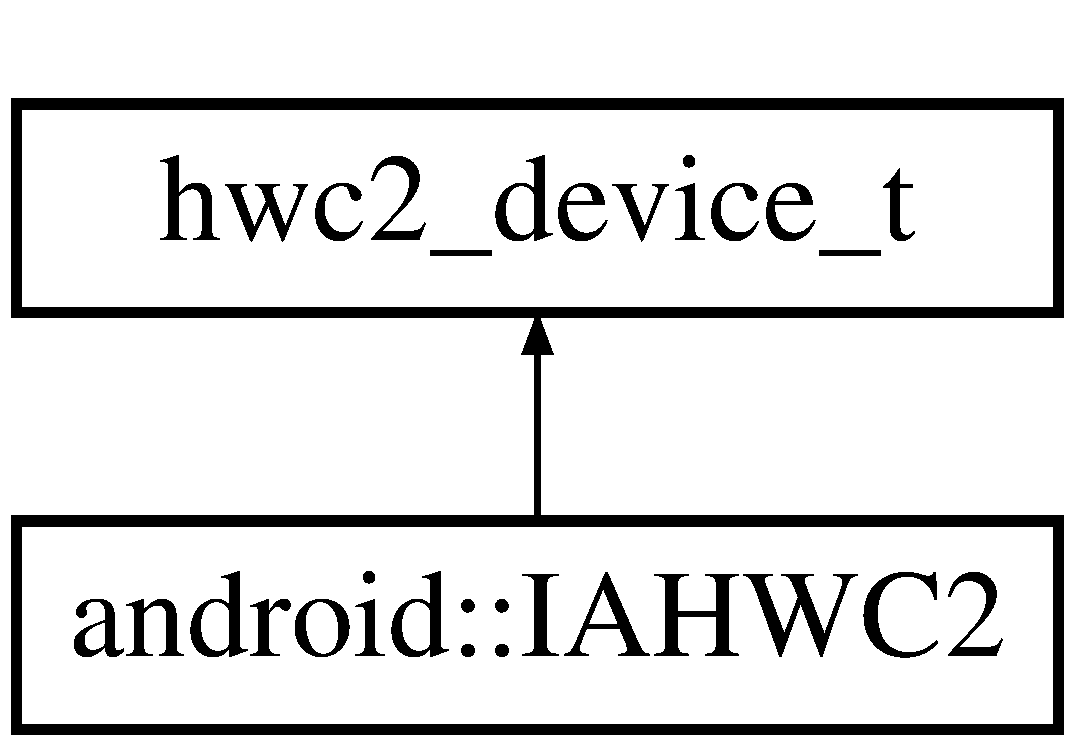
\includegraphics[height=2.000000cm]{classandroid_1_1IAHWC2}
\end{center}
\end{figure}
\subsection*{Classes}
\begin{DoxyCompactItemize}
\item 
class \mbox{\hyperlink{classandroid_1_1IAHWC2_1_1Hwc2Layer}{Hwc2\+Layer}}
\item 
class \mbox{\hyperlink{classandroid_1_1IAHWC2_1_1HwcDisplay}{Hwc\+Display}}
\end{DoxyCompactItemize}
\subsection*{Public Member Functions}
\begin{DoxyCompactItemize}
\item 
\mbox{\hyperlink{classandroid_1_1IAHWC2_ae360eef66e03be710114293b9988c8a4}{I\+A\+H\+W\+C2}} ()
\item 
H\+W\+C2\+::\+Error \mbox{\hyperlink{classandroid_1_1IAHWC2_a3661dacf6f3f03be404f9dfcfdeb00a9}{Init}} ()
\item 
\mbox{\hyperlink{classhwcomposer_1_1NativeDisplay}{hwcomposer\+::\+Native\+Display}} $\ast$ \mbox{\hyperlink{classandroid_1_1IAHWC2_a2ccc293910577a09cfe0a0f6c1f786ea}{Get\+Primary\+Display}} ()
\item 
\mbox{\hyperlink{classhwcomposer_1_1NativeDisplay}{hwcomposer\+::\+Native\+Display}} $\ast$ \mbox{\hyperlink{classandroid_1_1IAHWC2_a9b5b98f12f0580b5d328e6fc6b1465dc}{Get\+Extended\+Display}} (uint32\+\_\+t)
\item 
void \mbox{\hyperlink{classandroid_1_1IAHWC2_a473d60e8aa343e77381a6e0b04d18a23}{Enable\+H\+D\+C\+P\+Session\+For\+Display}} (uint32\+\_\+t display, \mbox{\hyperlink{hwcserviceapi_8h_a69e9b3a54e4c8e504845398c66eab655}{E\+Hwcs\+Content\+Type}} content\+\_\+type)
\item 
void \mbox{\hyperlink{classandroid_1_1IAHWC2_aafac4b9c0d47342441cb104b9df8b52c}{Enable\+H\+D\+C\+P\+Session\+For\+All\+Displays}} (\mbox{\hyperlink{hwcserviceapi_8h_a69e9b3a54e4c8e504845398c66eab655}{E\+Hwcs\+Content\+Type}} content\+\_\+type)
\item 
void \mbox{\hyperlink{classandroid_1_1IAHWC2_aaf25b167aeb33efb991f4872f421061f}{Disable\+H\+D\+C\+P\+Session\+For\+Display}} (uint32\+\_\+t display)
\item 
void \mbox{\hyperlink{classandroid_1_1IAHWC2_aab6e5e72a11dea3b84889e7df3ca76ee}{Disable\+H\+D\+C\+P\+Session\+For\+All\+Displays}} ()
\item 
H\+W\+C2\+::\+Error \mbox{\hyperlink{classandroid_1_1IAHWC2_a54263b4dff8e34603246c9ddb5b4f8a1}{Create\+Virtual\+Display}} (uint32\+\_\+t width, uint32\+\_\+t height, int32\+\_\+t $\ast$format, hwc2\+\_\+display\+\_\+t $\ast$display)
\item 
H\+W\+C2\+::\+Error \mbox{\hyperlink{classandroid_1_1IAHWC2_a25898776b812d1d34e309aa4348b191e}{Destroy\+Virtual\+Display}} (hwc2\+\_\+display\+\_\+t display)
\item 
void \mbox{\hyperlink{classandroid_1_1IAHWC2_a09a0fe32d95d6d75613458a906b8e4c5}{Dump}} (uint32\+\_\+t $\ast$size, char $\ast$buffer)
\item 
uint32\+\_\+t \mbox{\hyperlink{classandroid_1_1IAHWC2_a0be35c4807be335ebe48af20f66b9bdd}{Get\+Max\+Virtual\+Display\+Count}} ()
\item 
H\+W\+C2\+::\+Error \mbox{\hyperlink{classandroid_1_1IAHWC2_aa31f7c1a1085b8f3e65efc7dcdac957e}{Register\+Callback}} (int32\+\_\+t descriptor, hwc2\+\_\+callback\+\_\+data\+\_\+t data, hwc2\+\_\+function\+\_\+pointer\+\_\+t function)
\end{DoxyCompactItemize}
\subsection*{Static Public Member Functions}
\begin{DoxyCompactItemize}
\item 
static int \mbox{\hyperlink{classandroid_1_1IAHWC2_a9a000bc25e85fbc053408f3885688e33}{Hook\+Dev\+Open}} (const struct hw\+\_\+module\+\_\+t $\ast$module, const char $\ast$name, struct hw\+\_\+device\+\_\+t $\ast$$\ast$dev)
\item 
static \mbox{\hyperlink{classandroid_1_1IAHWC2}{I\+A\+H\+W\+C2}} $\ast$ \mbox{\hyperlink{classandroid_1_1IAHWC2_a8a800faee2b34f1362effb240bedd921}{to\+I\+A\+H\+W\+C2}} (hwc2\+\_\+device\+\_\+t $\ast$dev)
\item 
{\footnotesize template$<$typename P\+FN , typename T $>$ }\\static hwc2\+\_\+function\+\_\+pointer\+\_\+t \mbox{\hyperlink{classandroid_1_1IAHWC2_a456dbb88757cb56b49e90d543984c1a9}{To\+Hook}} (T function)
\item 
{\footnotesize template$<$typename T , typename Hook\+Type , Hook\+Type func, typename... Args$>$ }\\static T \mbox{\hyperlink{classandroid_1_1IAHWC2_a994749ea99efb163360648e408a00e4e}{Device\+Hook}} (hwc2\+\_\+device\+\_\+t $\ast$dev, Args... args)
\item 
{\footnotesize template$<$typename Hook\+Type , Hook\+Type func, typename... Args$>$ }\\static int32\+\_\+t \mbox{\hyperlink{classandroid_1_1IAHWC2_ac200f209fed5da229b857a6be2a417d3}{Display\+Hook}} (hwc2\+\_\+device\+\_\+t $\ast$dev, hwc2\+\_\+display\+\_\+t display\+\_\+handle, Args... args)
\item 
{\footnotesize template$<$typename Hook\+Type , Hook\+Type func, typename... Args$>$ }\\static int32\+\_\+t \mbox{\hyperlink{classandroid_1_1IAHWC2_a8e25d258ac3a7c539c0fca11623773dd}{Layer\+Hook}} (hwc2\+\_\+device\+\_\+t $\ast$dev, hwc2\+\_\+display\+\_\+t display\+\_\+handle, hwc2\+\_\+layer\+\_\+t layer\+\_\+handle, Args... args)
\item 
static int \mbox{\hyperlink{classandroid_1_1IAHWC2_ac3298b89f4ebcb2cdd242699e1f75e89}{Hook\+Dev\+Close}} (hw\+\_\+device\+\_\+t $\ast$dev)
\item 
static void \mbox{\hyperlink{classandroid_1_1IAHWC2_af72ba2d7fbae030b39b208e34f458f5a}{Hook\+Dev\+Get\+Capabilities}} (hwc2\+\_\+device\+\_\+t $\ast$dev, uint32\+\_\+t $\ast$out\+\_\+count, int32\+\_\+t $\ast$out\+\_\+capabilities)
\item 
static hwc2\+\_\+function\+\_\+pointer\+\_\+t \mbox{\hyperlink{classandroid_1_1IAHWC2_a71d1f51b751729750a04a18f11d5fd64}{Hook\+Dev\+Get\+Function}} (struct hwc2\+\_\+device $\ast$device, int32\+\_\+t descriptor)
\end{DoxyCompactItemize}
\subsection*{Public Attributes}
\begin{DoxyCompactItemize}
\item 
\mbox{\hyperlink{classhwcomposer_1_1GpuDevice}{hwcomposer\+::\+Gpu\+Device}} \mbox{\hyperlink{classandroid_1_1IAHWC2_ac20faf581346c9dace9127e3681a0666}{device\+\_\+}}
\item 
std\+::vector$<$ std\+::unique\+\_\+ptr$<$ \mbox{\hyperlink{classandroid_1_1IAHWC2_1_1HwcDisplay}{Hwc\+Display}} $>$ $>$ \mbox{\hyperlink{classandroid_1_1IAHWC2_a898debffb7438ad1174b7424ba99972c}{extended\+\_\+displays\+\_\+}}
\item 
\mbox{\hyperlink{classandroid_1_1IAHWC2_1_1HwcDisplay}{Hwc\+Display}} \mbox{\hyperlink{classandroid_1_1IAHWC2_ab6fc4580e0296ab10ecae375ced67e4c}{primary\+\_\+display\+\_\+}}
\item 
\mbox{\hyperlink{classandroid_1_1IAHWC2_1_1HwcDisplay}{Hwc\+Display}} \mbox{\hyperlink{classandroid_1_1IAHWC2_a37e11529251134e7fcb74d72330f1d43}{virtual\+\_\+display\+\_\+}}
\item 
\mbox{\hyperlink{classandroid_1_1IAHWC2_1_1HwcDisplay}{Hwc\+Display}} \mbox{\hyperlink{classandroid_1_1IAHWC2_a63c04984ca69519a5c094f9a8f66841c}{nested\+\_\+display\+\_\+}}
\item 
bool \mbox{\hyperlink{classandroid_1_1IAHWC2_adc8645c0a2315d4884f26f886002096e}{disable\+\_\+explicit\+\_\+sync\+\_\+}} = false
\item 
\mbox{\hyperlink{classandroid_1_1HwcService}{android\+::\+Hwc\+Service}} \mbox{\hyperlink{classandroid_1_1IAHWC2_aeacec4376e02e5c5da31fa7ed3986ce2}{hwc\+Service\+\_\+}}
\item 
uint32\+\_\+t \mbox{\hyperlink{classandroid_1_1IAHWC2_a7bcc5119aa74196920162eb37790fafc}{scaling\+\_\+mode\+\_\+}} = 0
\end{DoxyCompactItemize}


\subsection{Detailed Description}


Definition at line 38 of file iahwc2.\+h.



\subsection{Constructor \& Destructor Documentation}
\mbox{\Hypertarget{classandroid_1_1IAHWC2_ae360eef66e03be710114293b9988c8a4}\label{classandroid_1_1IAHWC2_ae360eef66e03be710114293b9988c8a4}} 
\index{android\+::\+I\+A\+H\+W\+C2@{android\+::\+I\+A\+H\+W\+C2}!I\+A\+H\+W\+C2@{I\+A\+H\+W\+C2}}
\index{I\+A\+H\+W\+C2@{I\+A\+H\+W\+C2}!android\+::\+I\+A\+H\+W\+C2@{android\+::\+I\+A\+H\+W\+C2}}
\subsubsection{\texorpdfstring{I\+A\+H\+W\+C2()}{IAHWC2()}}
{\footnotesize\ttfamily android\+::\+I\+A\+H\+W\+C2\+::\+I\+A\+H\+W\+C2 (\begin{DoxyParamCaption}{ }\end{DoxyParamCaption})}



Definition at line 126 of file iahwc2.\+cpp.


\begin{DoxyCode}{0}
\DoxyCodeLine{126                \{}
\DoxyCodeLine{127   common.tag = HARDWARE\_DEVICE\_TAG;}
\DoxyCodeLine{128   common.version = HWC\_DEVICE\_API\_VERSION\_2\_0;}
\DoxyCodeLine{129   common.close = \mbox{\hyperlink{classandroid_1_1IAHWC2_ac3298b89f4ebcb2cdd242699e1f75e89}{HookDevClose}};}
\DoxyCodeLine{130   getCapabilities = \mbox{\hyperlink{classandroid_1_1IAHWC2_af72ba2d7fbae030b39b208e34f458f5a}{HookDevGetCapabilities}};}
\DoxyCodeLine{131   getFunction = \mbox{\hyperlink{classandroid_1_1IAHWC2_a71d1f51b751729750a04a18f11d5fd64}{HookDevGetFunction}};}
\DoxyCodeLine{132 \}}
\end{DoxyCode}


\subsection{Member Function Documentation}
\mbox{\Hypertarget{classandroid_1_1IAHWC2_a54263b4dff8e34603246c9ddb5b4f8a1}\label{classandroid_1_1IAHWC2_a54263b4dff8e34603246c9ddb5b4f8a1}} 
\index{android\+::\+I\+A\+H\+W\+C2@{android\+::\+I\+A\+H\+W\+C2}!Create\+Virtual\+Display@{Create\+Virtual\+Display}}
\index{Create\+Virtual\+Display@{Create\+Virtual\+Display}!android\+::\+I\+A\+H\+W\+C2@{android\+::\+I\+A\+H\+W\+C2}}
\subsubsection{\texorpdfstring{Create\+Virtual\+Display()}{CreateVirtualDisplay()}}
{\footnotesize\ttfamily H\+W\+C2\+::\+Error android\+::\+I\+A\+H\+W\+C2\+::\+Create\+Virtual\+Display (\begin{DoxyParamCaption}\item[{uint32\+\_\+t}]{width,  }\item[{uint32\+\_\+t}]{height,  }\item[{int32\+\_\+t $\ast$}]{format,  }\item[{hwc2\+\_\+display\+\_\+t $\ast$}]{display }\end{DoxyParamCaption})}



Definition at line 207 of file iahwc2.\+cpp.


\begin{DoxyCode}{0}
\DoxyCodeLine{209                                                                   \{}
\DoxyCodeLine{210   *display = (hwc2\_display\_t)HWC\_DISPLAY\_VIRTUAL;}
\DoxyCodeLine{211   \mbox{\hyperlink{classandroid_1_1IAHWC2_a37e11529251134e7fcb74d72330f1d43}{virtual\_display\_}}.\mbox{\hyperlink{classandroid_1_1IAHWC2_1_1HwcDisplay_aca926207d2bfcbd4599519c6bef5ce76}{InitVirtualDisplay}}(\mbox{\hyperlink{classandroid_1_1IAHWC2_ac20faf581346c9dace9127e3681a0666}{device\_}}.
      \mbox{\hyperlink{classhwcomposer_1_1GpuDevice_adfec63ead3453ee2cd80b5183d4961d8}{GetVirtualDisplay}}(), width,}
\DoxyCodeLine{212                                       height, \mbox{\hyperlink{classandroid_1_1IAHWC2_adc8645c0a2315d4884f26f886002096e}{disable\_explicit\_sync\_}});}
\DoxyCodeLine{213   \textcolor{keywordflow}{if} (*format == HAL\_PIXEL\_FORMAT\_IMPLEMENTATION\_DEFINED) \{}
\DoxyCodeLine{214     \textcolor{comment}{// fallback to RGBA\_8888, align with framework requirement}}
\DoxyCodeLine{215     *format = HAL\_PIXEL\_FORMAT\_RGBA\_8888;}
\DoxyCodeLine{216   \}}
\DoxyCodeLine{217 }
\DoxyCodeLine{218   \textcolor{keywordflow}{return} HWC2::Error::None;}
\DoxyCodeLine{219 \}}
\end{DoxyCode}
\mbox{\Hypertarget{classandroid_1_1IAHWC2_a25898776b812d1d34e309aa4348b191e}\label{classandroid_1_1IAHWC2_a25898776b812d1d34e309aa4348b191e}} 
\index{android\+::\+I\+A\+H\+W\+C2@{android\+::\+I\+A\+H\+W\+C2}!Destroy\+Virtual\+Display@{Destroy\+Virtual\+Display}}
\index{Destroy\+Virtual\+Display@{Destroy\+Virtual\+Display}!android\+::\+I\+A\+H\+W\+C2@{android\+::\+I\+A\+H\+W\+C2}}
\subsubsection{\texorpdfstring{Destroy\+Virtual\+Display()}{DestroyVirtualDisplay()}}
{\footnotesize\ttfamily H\+W\+C2\+::\+Error android\+::\+I\+A\+H\+W\+C2\+::\+Destroy\+Virtual\+Display (\begin{DoxyParamCaption}\item[{hwc2\+\_\+display\+\_\+t}]{display }\end{DoxyParamCaption})}



Definition at line 221 of file iahwc2.\+cpp.


\begin{DoxyCode}{0}
\DoxyCodeLine{221                                                               \{}
\DoxyCodeLine{222   \textcolor{keywordflow}{if} (display != (hwc2\_display\_t)HWC\_DISPLAY\_VIRTUAL) \{}
\DoxyCodeLine{223     ALOGE(\textcolor{stringliteral}{"Not Virtual Display Type in DestroyVirtualDisplay"});}
\DoxyCodeLine{224     \textcolor{keywordflow}{return} HWC2::Error::BadDisplay;}
\DoxyCodeLine{225   \}}
\DoxyCodeLine{226 }
\DoxyCodeLine{227   \textcolor{keywordflow}{return} HWC2::Error::None;}
\DoxyCodeLine{228 \}}
\end{DoxyCode}
\mbox{\Hypertarget{classandroid_1_1IAHWC2_a994749ea99efb163360648e408a00e4e}\label{classandroid_1_1IAHWC2_a994749ea99efb163360648e408a00e4e}} 
\index{android\+::\+I\+A\+H\+W\+C2@{android\+::\+I\+A\+H\+W\+C2}!Device\+Hook@{Device\+Hook}}
\index{Device\+Hook@{Device\+Hook}!android\+::\+I\+A\+H\+W\+C2@{android\+::\+I\+A\+H\+W\+C2}}
\subsubsection{\texorpdfstring{Device\+Hook()}{DeviceHook()}}
{\footnotesize\ttfamily template$<$typename T , typename Hook\+Type , Hook\+Type func, typename... Args$>$ \\
static T android\+::\+I\+A\+H\+W\+C2\+::\+Device\+Hook (\begin{DoxyParamCaption}\item[{hwc2\+\_\+device\+\_\+t $\ast$}]{dev,  }\item[{Args...}]{args }\end{DoxyParamCaption})\hspace{0.3cm}{\ttfamily [inline]}, {\ttfamily [static]}}



Definition at line 227 of file iahwc2.\+h.


\begin{DoxyCode}{0}
\DoxyCodeLine{227                                                         \{}
\DoxyCodeLine{228     \mbox{\hyperlink{classandroid_1_1IAHWC2_ae360eef66e03be710114293b9988c8a4}{IAHWC2}} *hwc = \mbox{\hyperlink{classandroid_1_1IAHWC2_a8a800faee2b34f1362effb240bedd921}{toIAHWC2}}(dev);}
\DoxyCodeLine{229     \textcolor{keywordflow}{return} \textcolor{keyword}{static\_cast<}T\textcolor{keyword}{>}(((*hwc).*func)(std::forward<Args>(args)...));}
\DoxyCodeLine{230   \}}
\end{DoxyCode}
\mbox{\Hypertarget{classandroid_1_1IAHWC2_aab6e5e72a11dea3b84889e7df3ca76ee}\label{classandroid_1_1IAHWC2_aab6e5e72a11dea3b84889e7df3ca76ee}} 
\index{android\+::\+I\+A\+H\+W\+C2@{android\+::\+I\+A\+H\+W\+C2}!Disable\+H\+D\+C\+P\+Session\+For\+All\+Displays@{Disable\+H\+D\+C\+P\+Session\+For\+All\+Displays}}
\index{Disable\+H\+D\+C\+P\+Session\+For\+All\+Displays@{Disable\+H\+D\+C\+P\+Session\+For\+All\+Displays}!android\+::\+I\+A\+H\+W\+C2@{android\+::\+I\+A\+H\+W\+C2}}
\subsubsection{\texorpdfstring{Disable\+H\+D\+C\+P\+Session\+For\+All\+Displays()}{DisableHDCPSessionForAllDisplays()}}
{\footnotesize\ttfamily void android\+::\+I\+A\+H\+W\+C2\+::\+Disable\+H\+D\+C\+P\+Session\+For\+All\+Displays (\begin{DoxyParamCaption}{ }\end{DoxyParamCaption})}



Definition at line 1279 of file iahwc2.\+cpp.


\begin{DoxyCode}{0}
\DoxyCodeLine{1279                                               \{}
\DoxyCodeLine{1280   \mbox{\hyperlink{classandroid_1_1IAHWC2_ac20faf581346c9dace9127e3681a0666}{device\_}}.\mbox{\hyperlink{classhwcomposer_1_1GpuDevice_a7038e1dc3d4a2be7206e6a35717521e2}{DisableHDCPSessionForAllDisplays}}();}
\DoxyCodeLine{1281 \}}
\end{DoxyCode}
\mbox{\Hypertarget{classandroid_1_1IAHWC2_aaf25b167aeb33efb991f4872f421061f}\label{classandroid_1_1IAHWC2_aaf25b167aeb33efb991f4872f421061f}} 
\index{android\+::\+I\+A\+H\+W\+C2@{android\+::\+I\+A\+H\+W\+C2}!Disable\+H\+D\+C\+P\+Session\+For\+Display@{Disable\+H\+D\+C\+P\+Session\+For\+Display}}
\index{Disable\+H\+D\+C\+P\+Session\+For\+Display@{Disable\+H\+D\+C\+P\+Session\+For\+Display}!android\+::\+I\+A\+H\+W\+C2@{android\+::\+I\+A\+H\+W\+C2}}
\subsubsection{\texorpdfstring{Disable\+H\+D\+C\+P\+Session\+For\+Display()}{DisableHDCPSessionForDisplay()}}
{\footnotesize\ttfamily void android\+::\+I\+A\+H\+W\+C2\+::\+Disable\+H\+D\+C\+P\+Session\+For\+Display (\begin{DoxyParamCaption}\item[{uint32\+\_\+t}]{display }\end{DoxyParamCaption})}



Definition at line 1275 of file iahwc2.\+cpp.


\begin{DoxyCode}{0}
\DoxyCodeLine{1275                                                           \{}
\DoxyCodeLine{1276   \mbox{\hyperlink{classandroid_1_1IAHWC2_ac20faf581346c9dace9127e3681a0666}{device\_}}.\mbox{\hyperlink{classhwcomposer_1_1GpuDevice_ae61aa61ee1591464e7e5a703b2c6c848}{DisableHDCPSessionForDisplay}}(display);}
\DoxyCodeLine{1277 \}}
\end{DoxyCode}
\mbox{\Hypertarget{classandroid_1_1IAHWC2_ac200f209fed5da229b857a6be2a417d3}\label{classandroid_1_1IAHWC2_ac200f209fed5da229b857a6be2a417d3}} 
\index{android\+::\+I\+A\+H\+W\+C2@{android\+::\+I\+A\+H\+W\+C2}!Display\+Hook@{Display\+Hook}}
\index{Display\+Hook@{Display\+Hook}!android\+::\+I\+A\+H\+W\+C2@{android\+::\+I\+A\+H\+W\+C2}}
\subsubsection{\texorpdfstring{Display\+Hook()}{DisplayHook()}}
{\footnotesize\ttfamily template$<$typename Hook\+Type , Hook\+Type func, typename... Args$>$ \\
static int32\+\_\+t android\+::\+I\+A\+H\+W\+C2\+::\+Display\+Hook (\begin{DoxyParamCaption}\item[{hwc2\+\_\+device\+\_\+t $\ast$}]{dev,  }\item[{hwc2\+\_\+display\+\_\+t}]{display\+\_\+handle,  }\item[{Args...}]{args }\end{DoxyParamCaption})\hspace{0.3cm}{\ttfamily [inline]}, {\ttfamily [static]}}



Definition at line 233 of file iahwc2.\+h.


\begin{DoxyCode}{0}
\DoxyCodeLine{234                                            \{}
\DoxyCodeLine{235     \mbox{\hyperlink{classandroid_1_1IAHWC2_ae360eef66e03be710114293b9988c8a4}{IAHWC2}} *hwc = \mbox{\hyperlink{classandroid_1_1IAHWC2_a8a800faee2b34f1362effb240bedd921}{toIAHWC2}}(dev);}
\DoxyCodeLine{236     \textcolor{keywordflow}{if} (display\_handle == HWC\_DISPLAY\_PRIMARY) \{}
\DoxyCodeLine{237       HwcDisplay \&display = hwc->primary\_display\_;}
\DoxyCodeLine{238       \textcolor{keywordflow}{return} \textcolor{keyword}{static\_cast<}int32\_t\textcolor{keyword}{>}((display.*func)(std::forward<Args>(args)...));}
\DoxyCodeLine{239     \}}
\DoxyCodeLine{240 }
\DoxyCodeLine{241     \textcolor{keywordflow}{if} (display\_handle == HWC\_DISPLAY\_VIRTUAL) \{}
\DoxyCodeLine{242       \textcolor{keywordflow}{return} \textcolor{keyword}{static\_cast<}int32\_t\textcolor{keyword}{>}(}
\DoxyCodeLine{243           (hwc->virtual\_display\_.*func)(std::forward<Args>(args)...));}
\DoxyCodeLine{244     \}}
\DoxyCodeLine{245 \textcolor{preprocessor}{\#ifdef NESTED\_DISPLAY\_SUPPORT}}
\DoxyCodeLine{246     \textcolor{keywordflow}{if} (display\_handle == HWC\_DISPLAY\_NESTED) \{}
\DoxyCodeLine{247       \textcolor{keywordflow}{return} \textcolor{keyword}{static\_cast<}int32\_t\textcolor{keyword}{>}(}
\DoxyCodeLine{248           (hwc->nested\_display\_.*func)(std::forward<Args>(args)...));}
\DoxyCodeLine{249     \}}
\DoxyCodeLine{250 \textcolor{preprocessor}{\#endif}}
\DoxyCodeLine{251     \textcolor{keywordflow}{if} (display\_handle == HWC\_DISPLAY\_EXTERNAL) \{}
\DoxyCodeLine{252       HwcDisplay *display = hwc->extended\_displays\_.at(0).get();}
\DoxyCodeLine{253       \textcolor{keywordflow}{return} \textcolor{keyword}{static\_cast<}int32\_t\textcolor{keyword}{>}(}
\DoxyCodeLine{254           (display->*func)(std::forward<Args>(args)...));}
\DoxyCodeLine{255     \}}
\DoxyCodeLine{256 }
\DoxyCodeLine{257     HwcDisplay *display = hwc->extended\_displays\_.at(1).get();}
\DoxyCodeLine{258     \textcolor{keywordflow}{return} \textcolor{keyword}{static\_cast<}int32\_t\textcolor{keyword}{>}((display->*func)(std::forward<Args>(args)...));}
\DoxyCodeLine{259   \}}
\end{DoxyCode}
\mbox{\Hypertarget{classandroid_1_1IAHWC2_a09a0fe32d95d6d75613458a906b8e4c5}\label{classandroid_1_1IAHWC2_a09a0fe32d95d6d75613458a906b8e4c5}} 
\index{android\+::\+I\+A\+H\+W\+C2@{android\+::\+I\+A\+H\+W\+C2}!Dump@{Dump}}
\index{Dump@{Dump}!android\+::\+I\+A\+H\+W\+C2@{android\+::\+I\+A\+H\+W\+C2}}
\subsubsection{\texorpdfstring{Dump()}{Dump()}}
{\footnotesize\ttfamily void android\+::\+I\+A\+H\+W\+C2\+::\+Dump (\begin{DoxyParamCaption}\item[{uint32\+\_\+t $\ast$}]{size,  }\item[{char $\ast$}]{buffer }\end{DoxyParamCaption})}



Definition at line 230 of file iahwc2.\+cpp.


\begin{DoxyCode}{0}
\DoxyCodeLine{230                                               \{}
\DoxyCodeLine{231   \textcolor{comment}{// TODO: Implement dump}}
\DoxyCodeLine{232   unsupported(\_\_func\_\_, size, buffer);}
\DoxyCodeLine{233 \}}
\end{DoxyCode}
\mbox{\Hypertarget{classandroid_1_1IAHWC2_aafac4b9c0d47342441cb104b9df8b52c}\label{classandroid_1_1IAHWC2_aafac4b9c0d47342441cb104b9df8b52c}} 
\index{android\+::\+I\+A\+H\+W\+C2@{android\+::\+I\+A\+H\+W\+C2}!Enable\+H\+D\+C\+P\+Session\+For\+All\+Displays@{Enable\+H\+D\+C\+P\+Session\+For\+All\+Displays}}
\index{Enable\+H\+D\+C\+P\+Session\+For\+All\+Displays@{Enable\+H\+D\+C\+P\+Session\+For\+All\+Displays}!android\+::\+I\+A\+H\+W\+C2@{android\+::\+I\+A\+H\+W\+C2}}
\subsubsection{\texorpdfstring{Enable\+H\+D\+C\+P\+Session\+For\+All\+Displays()}{EnableHDCPSessionForAllDisplays()}}
{\footnotesize\ttfamily void android\+::\+I\+A\+H\+W\+C2\+::\+Enable\+H\+D\+C\+P\+Session\+For\+All\+Displays (\begin{DoxyParamCaption}\item[{\mbox{\hyperlink{hwcserviceapi_8h_a69e9b3a54e4c8e504845398c66eab655}{E\+Hwcs\+Content\+Type}}}]{content\+\_\+type }\end{DoxyParamCaption})}



Definition at line 1267 of file iahwc2.\+cpp.


\begin{DoxyCode}{0}
\DoxyCodeLine{1267                                                                           \{}
\DoxyCodeLine{1268   HWCContentType type = kCONTENT\_TYPE0;}
\DoxyCodeLine{1269   \textcolor{keywordflow}{if} (content\_type == \mbox{\hyperlink{hwcserviceapi_8h_ad7fa0f48e8d945fd273ba9984a6d9142af0fc741639c5bd530c1d21db89198688}{HWCS\_CP\_CONTENT\_TYPE1}}) \{}
\DoxyCodeLine{1270     type = kCONTENT\_TYPE1;}
\DoxyCodeLine{1271   \}}
\DoxyCodeLine{1272   \mbox{\hyperlink{classandroid_1_1IAHWC2_ac20faf581346c9dace9127e3681a0666}{device\_}}.\mbox{\hyperlink{classhwcomposer_1_1GpuDevice_a5a42e70ab1648c6e7741b2322f898691}{EnableHDCPSessionForAllDisplays}}(type);}
\DoxyCodeLine{1273 \}}
\end{DoxyCode}
\mbox{\Hypertarget{classandroid_1_1IAHWC2_a473d60e8aa343e77381a6e0b04d18a23}\label{classandroid_1_1IAHWC2_a473d60e8aa343e77381a6e0b04d18a23}} 
\index{android\+::\+I\+A\+H\+W\+C2@{android\+::\+I\+A\+H\+W\+C2}!Enable\+H\+D\+C\+P\+Session\+For\+Display@{Enable\+H\+D\+C\+P\+Session\+For\+Display}}
\index{Enable\+H\+D\+C\+P\+Session\+For\+Display@{Enable\+H\+D\+C\+P\+Session\+For\+Display}!android\+::\+I\+A\+H\+W\+C2@{android\+::\+I\+A\+H\+W\+C2}}
\subsubsection{\texorpdfstring{Enable\+H\+D\+C\+P\+Session\+For\+Display()}{EnableHDCPSessionForDisplay()}}
{\footnotesize\ttfamily void android\+::\+I\+A\+H\+W\+C2\+::\+Enable\+H\+D\+C\+P\+Session\+For\+Display (\begin{DoxyParamCaption}\item[{uint32\+\_\+t}]{display,  }\item[{\mbox{\hyperlink{hwcserviceapi_8h_a69e9b3a54e4c8e504845398c66eab655}{E\+Hwcs\+Content\+Type}}}]{content\+\_\+type }\end{DoxyParamCaption})}



Definition at line 1257 of file iahwc2.\+cpp.


\begin{DoxyCode}{0}
\DoxyCodeLine{1258                                                                         \{}
\DoxyCodeLine{1259   HWCContentType type = kCONTENT\_TYPE0;}
\DoxyCodeLine{1260   \textcolor{keywordflow}{if} (content\_type == \mbox{\hyperlink{hwcserviceapi_8h_ad7fa0f48e8d945fd273ba9984a6d9142af0fc741639c5bd530c1d21db89198688}{HWCS\_CP\_CONTENT\_TYPE1}}) \{}
\DoxyCodeLine{1261     type = kCONTENT\_TYPE1;}
\DoxyCodeLine{1262   \}}
\DoxyCodeLine{1263 }
\DoxyCodeLine{1264   \mbox{\hyperlink{classandroid_1_1IAHWC2_ac20faf581346c9dace9127e3681a0666}{device\_}}.\mbox{\hyperlink{classhwcomposer_1_1GpuDevice_aa558c97ab2f80eac47ede0a788a59a28}{EnableHDCPSessionForDisplay}}(display, type);}
\DoxyCodeLine{1265 \}}
\end{DoxyCode}
\mbox{\Hypertarget{classandroid_1_1IAHWC2_a9b5b98f12f0580b5d328e6fc6b1465dc}\label{classandroid_1_1IAHWC2_a9b5b98f12f0580b5d328e6fc6b1465dc}} 
\index{android\+::\+I\+A\+H\+W\+C2@{android\+::\+I\+A\+H\+W\+C2}!Get\+Extended\+Display@{Get\+Extended\+Display}}
\index{Get\+Extended\+Display@{Get\+Extended\+Display}!android\+::\+I\+A\+H\+W\+C2@{android\+::\+I\+A\+H\+W\+C2}}
\subsubsection{\texorpdfstring{Get\+Extended\+Display()}{GetExtendedDisplay()}}
{\footnotesize\ttfamily \mbox{\hyperlink{classhwcomposer_1_1NativeDisplay}{hwcomposer\+::\+Native\+Display}} $\ast$ android\+::\+I\+A\+H\+W\+C2\+::\+Get\+Extended\+Display (\begin{DoxyParamCaption}\item[{uint32\+\_\+t}]{disp\+Index }\end{DoxyParamCaption})}



Definition at line 1245 of file iahwc2.\+cpp.


\begin{DoxyCode}{0}
\DoxyCodeLine{1245                                                                       \{}
\DoxyCodeLine{1246   \textcolor{keywordflow}{return} \mbox{\hyperlink{classandroid_1_1IAHWC2_a898debffb7438ad1174b7424ba99972c}{extended\_displays\_}}.at(dispIndex)->GetDisplay();}
\DoxyCodeLine{1247 \}}
\end{DoxyCode}
\mbox{\Hypertarget{classandroid_1_1IAHWC2_a0be35c4807be335ebe48af20f66b9bdd}\label{classandroid_1_1IAHWC2_a0be35c4807be335ebe48af20f66b9bdd}} 
\index{android\+::\+I\+A\+H\+W\+C2@{android\+::\+I\+A\+H\+W\+C2}!Get\+Max\+Virtual\+Display\+Count@{Get\+Max\+Virtual\+Display\+Count}}
\index{Get\+Max\+Virtual\+Display\+Count@{Get\+Max\+Virtual\+Display\+Count}!android\+::\+I\+A\+H\+W\+C2@{android\+::\+I\+A\+H\+W\+C2}}
\subsubsection{\texorpdfstring{Get\+Max\+Virtual\+Display\+Count()}{GetMaxVirtualDisplayCount()}}
{\footnotesize\ttfamily uint32\+\_\+t android\+::\+I\+A\+H\+W\+C2\+::\+Get\+Max\+Virtual\+Display\+Count (\begin{DoxyParamCaption}{ }\end{DoxyParamCaption})}



Definition at line 235 of file iahwc2.\+cpp.


\begin{DoxyCode}{0}
\DoxyCodeLine{235                                            \{}
\DoxyCodeLine{236   \textcolor{keywordflow}{return} 2;}
\DoxyCodeLine{237 \}}
\end{DoxyCode}
\mbox{\Hypertarget{classandroid_1_1IAHWC2_a2ccc293910577a09cfe0a0f6c1f786ea}\label{classandroid_1_1IAHWC2_a2ccc293910577a09cfe0a0f6c1f786ea}} 
\index{android\+::\+I\+A\+H\+W\+C2@{android\+::\+I\+A\+H\+W\+C2}!Get\+Primary\+Display@{Get\+Primary\+Display}}
\index{Get\+Primary\+Display@{Get\+Primary\+Display}!android\+::\+I\+A\+H\+W\+C2@{android\+::\+I\+A\+H\+W\+C2}}
\subsubsection{\texorpdfstring{Get\+Primary\+Display()}{GetPrimaryDisplay()}}
{\footnotesize\ttfamily \mbox{\hyperlink{classhwcomposer_1_1NativeDisplay}{hwcomposer\+::\+Native\+Display}} $\ast$ android\+::\+I\+A\+H\+W\+C2\+::\+Get\+Primary\+Display (\begin{DoxyParamCaption}{ }\end{DoxyParamCaption})}



Definition at line 1249 of file iahwc2.\+cpp.


\begin{DoxyCode}{0}
\DoxyCodeLine{1249                                                    \{}
\DoxyCodeLine{1250   \textcolor{keywordflow}{return} \mbox{\hyperlink{classandroid_1_1IAHWC2_ab6fc4580e0296ab10ecae375ced67e4c}{primary\_display\_}}.\mbox{\hyperlink{classandroid_1_1IAHWC2_1_1HwcDisplay_a78b8d9cfdd2a0831798b705a16612271}{GetDisplay}}();}
\DoxyCodeLine{1251 \}}
\end{DoxyCode}
\mbox{\Hypertarget{classandroid_1_1IAHWC2_ac3298b89f4ebcb2cdd242699e1f75e89}\label{classandroid_1_1IAHWC2_ac3298b89f4ebcb2cdd242699e1f75e89}} 
\index{android\+::\+I\+A\+H\+W\+C2@{android\+::\+I\+A\+H\+W\+C2}!Hook\+Dev\+Close@{Hook\+Dev\+Close}}
\index{Hook\+Dev\+Close@{Hook\+Dev\+Close}!android\+::\+I\+A\+H\+W\+C2@{android\+::\+I\+A\+H\+W\+C2}}
\subsubsection{\texorpdfstring{Hook\+Dev\+Close()}{HookDevClose()}}
{\footnotesize\ttfamily int android\+::\+I\+A\+H\+W\+C2\+::\+Hook\+Dev\+Close (\begin{DoxyParamCaption}\item[{hw\+\_\+device\+\_\+t $\ast$}]{dev }\end{DoxyParamCaption})\hspace{0.3cm}{\ttfamily [static]}}



Definition at line 1010 of file iahwc2.\+cpp.


\begin{DoxyCode}{0}
\DoxyCodeLine{1010                                         \{}
\DoxyCodeLine{1011   unsupported(\_\_func\_\_);}
\DoxyCodeLine{1012   \textcolor{keywordflow}{return} 0;}
\DoxyCodeLine{1013 \}}
\end{DoxyCode}
\mbox{\Hypertarget{classandroid_1_1IAHWC2_af72ba2d7fbae030b39b208e34f458f5a}\label{classandroid_1_1IAHWC2_af72ba2d7fbae030b39b208e34f458f5a}} 
\index{android\+::\+I\+A\+H\+W\+C2@{android\+::\+I\+A\+H\+W\+C2}!Hook\+Dev\+Get\+Capabilities@{Hook\+Dev\+Get\+Capabilities}}
\index{Hook\+Dev\+Get\+Capabilities@{Hook\+Dev\+Get\+Capabilities}!android\+::\+I\+A\+H\+W\+C2@{android\+::\+I\+A\+H\+W\+C2}}
\subsubsection{\texorpdfstring{Hook\+Dev\+Get\+Capabilities()}{HookDevGetCapabilities()}}
{\footnotesize\ttfamily void android\+::\+I\+A\+H\+W\+C2\+::\+Hook\+Dev\+Get\+Capabilities (\begin{DoxyParamCaption}\item[{hwc2\+\_\+device\+\_\+t $\ast$}]{dev,  }\item[{uint32\+\_\+t $\ast$}]{out\+\_\+count,  }\item[{int32\+\_\+t $\ast$}]{out\+\_\+capabilities }\end{DoxyParamCaption})\hspace{0.3cm}{\ttfamily [static]}}



Definition at line 1016 of file iahwc2.\+cpp.


\begin{DoxyCode}{0}
\DoxyCodeLine{1018                                                  \{}
\DoxyCodeLine{1019   supported(\_\_func\_\_);}
\DoxyCodeLine{1020   *out\_count = 0;}
\DoxyCodeLine{1021 \}}
\end{DoxyCode}
\mbox{\Hypertarget{classandroid_1_1IAHWC2_a71d1f51b751729750a04a18f11d5fd64}\label{classandroid_1_1IAHWC2_a71d1f51b751729750a04a18f11d5fd64}} 
\index{android\+::\+I\+A\+H\+W\+C2@{android\+::\+I\+A\+H\+W\+C2}!Hook\+Dev\+Get\+Function@{Hook\+Dev\+Get\+Function}}
\index{Hook\+Dev\+Get\+Function@{Hook\+Dev\+Get\+Function}!android\+::\+I\+A\+H\+W\+C2@{android\+::\+I\+A\+H\+W\+C2}}
\subsubsection{\texorpdfstring{Hook\+Dev\+Get\+Function()}{HookDevGetFunction()}}
{\footnotesize\ttfamily hwc2\+\_\+function\+\_\+pointer\+\_\+t android\+::\+I\+A\+H\+W\+C2\+::\+Hook\+Dev\+Get\+Function (\begin{DoxyParamCaption}\item[{struct hwc2\+\_\+device $\ast$}]{device,  }\item[{int32\+\_\+t}]{descriptor }\end{DoxyParamCaption})\hspace{0.3cm}{\ttfamily [static]}}



Definition at line 1024 of file iahwc2.\+cpp.


\begin{DoxyCode}{0}
\DoxyCodeLine{1025                                                                        \{}
\DoxyCodeLine{1026   supported(\_\_func\_\_);}
\DoxyCodeLine{1027   \textcolor{keyword}{auto} func = \textcolor{keyword}{static\_cast<}HWC2::FunctionDescriptor\textcolor{keyword}{>}(descriptor);}
\DoxyCodeLine{1028   \textcolor{keywordflow}{switch} (func) \{}
\DoxyCodeLine{1029     \textcolor{comment}{// Device functions}}
\DoxyCodeLine{1030     \textcolor{keywordflow}{case} HWC2::FunctionDescriptor::CreateVirtualDisplay:}
\DoxyCodeLine{1031       \textcolor{keywordflow}{return} ToHook<HWC2\_PFN\_CREATE\_VIRTUAL\_DISPLAY>(}
\DoxyCodeLine{1032           \mbox{\hyperlink{classandroid_1_1IAHWC2_a994749ea99efb163360648e408a00e4e}{DeviceHook}}<int32\_t, decltype(\&\mbox{\hyperlink{classandroid_1_1IAHWC2_a54263b4dff8e34603246c9ddb5b4f8a1}{IAHWC2::CreateVirtualDisplay}}),}
\DoxyCodeLine{1033                      \&\mbox{\hyperlink{classandroid_1_1IAHWC2_a54263b4dff8e34603246c9ddb5b4f8a1}{IAHWC2::CreateVirtualDisplay}}, uint32\_t, uint32\_t,}
\DoxyCodeLine{1034                      int32\_t *, hwc2\_display\_t *>);}
\DoxyCodeLine{1035     \textcolor{keywordflow}{case} HWC2::FunctionDescriptor::DestroyVirtualDisplay:}
\DoxyCodeLine{1036       \textcolor{keywordflow}{return} ToHook<HWC2\_PFN\_DESTROY\_VIRTUAL\_DISPLAY>(}
\DoxyCodeLine{1037           \mbox{\hyperlink{classandroid_1_1IAHWC2_a994749ea99efb163360648e408a00e4e}{DeviceHook}}<int32\_t, decltype(\&\mbox{\hyperlink{classandroid_1_1IAHWC2_a25898776b812d1d34e309aa4348b191e}{IAHWC2::DestroyVirtualDisplay}}),}
\DoxyCodeLine{1038                      \&\mbox{\hyperlink{classandroid_1_1IAHWC2_a25898776b812d1d34e309aa4348b191e}{IAHWC2::DestroyVirtualDisplay}}, hwc2\_display\_t>);}
\DoxyCodeLine{1039     \textcolor{keywordflow}{case} HWC2::FunctionDescriptor::Dump:}
\DoxyCodeLine{1040       \textcolor{keywordflow}{return} ToHook<HWC2\_PFN\_DUMP>(\mbox{\hyperlink{classandroid_1_1IAHWC2_a994749ea99efb163360648e408a00e4e}{DeviceHook}}<}
\DoxyCodeLine{1041           void, decltype(\&\mbox{\hyperlink{classandroid_1_1IAHWC2_a09a0fe32d95d6d75613458a906b8e4c5}{IAHWC2::Dump}}), \&\mbox{\hyperlink{classandroid_1_1IAHWC2_a09a0fe32d95d6d75613458a906b8e4c5}{IAHWC2::Dump}}, uint32\_t *, \textcolor{keywordtype}{char} *>);}
\DoxyCodeLine{1042     \textcolor{keywordflow}{case} HWC2::FunctionDescriptor::GetMaxVirtualDisplayCount:}
\DoxyCodeLine{1043       \textcolor{keywordflow}{return} ToHook<HWC2\_PFN\_GET\_MAX\_VIRTUAL\_DISPLAY\_COUNT>(}
\DoxyCodeLine{1044           \mbox{\hyperlink{classandroid_1_1IAHWC2_a994749ea99efb163360648e408a00e4e}{DeviceHook}}<uint32\_t, decltype(\&
      \mbox{\hyperlink{classandroid_1_1IAHWC2_a0be35c4807be335ebe48af20f66b9bdd}{IAHWC2::GetMaxVirtualDisplayCount}}),}
\DoxyCodeLine{1045                      \&\mbox{\hyperlink{classandroid_1_1IAHWC2_a0be35c4807be335ebe48af20f66b9bdd}{IAHWC2::GetMaxVirtualDisplayCount}}>);}
\DoxyCodeLine{1046     \textcolor{keywordflow}{case} HWC2::FunctionDescriptor::RegisterCallback:}
\DoxyCodeLine{1047       \textcolor{keywordflow}{return} ToHook<HWC2\_PFN\_REGISTER\_CALLBACK>(}
\DoxyCodeLine{1048           \mbox{\hyperlink{classandroid_1_1IAHWC2_a994749ea99efb163360648e408a00e4e}{DeviceHook}}<int32\_t, decltype(\&\mbox{\hyperlink{classandroid_1_1IAHWC2_aa31f7c1a1085b8f3e65efc7dcdac957e}{IAHWC2::RegisterCallback}}),}
\DoxyCodeLine{1049                      \&\mbox{\hyperlink{classandroid_1_1IAHWC2_aa31f7c1a1085b8f3e65efc7dcdac957e}{IAHWC2::RegisterCallback}}, int32\_t, hwc2\_callback\_data\_t,}
\DoxyCodeLine{1050                      hwc2\_function\_pointer\_t>);}
\DoxyCodeLine{1051 }
\DoxyCodeLine{1052     \textcolor{comment}{// Display functions}}
\DoxyCodeLine{1053     \textcolor{keywordflow}{case} HWC2::FunctionDescriptor::AcceptDisplayChanges:}
\DoxyCodeLine{1054       \textcolor{keywordflow}{return} ToHook<HWC2\_PFN\_ACCEPT\_DISPLAY\_CHANGES>(}
\DoxyCodeLine{1055           \mbox{\hyperlink{classandroid_1_1IAHWC2_ac200f209fed5da229b857a6be2a417d3}{DisplayHook}}<decltype(\&\mbox{\hyperlink{classandroid_1_1IAHWC2_1_1HwcDisplay_a497e8468963a8f99091b0adf26e88d22}{HwcDisplay::AcceptDisplayChanges}}),}
\DoxyCodeLine{1056                       \&\mbox{\hyperlink{classandroid_1_1IAHWC2_1_1HwcDisplay_a497e8468963a8f99091b0adf26e88d22}{HwcDisplay::AcceptDisplayChanges}}>);}
\DoxyCodeLine{1057     \textcolor{keywordflow}{case} HWC2::FunctionDescriptor::CreateLayer:}
\DoxyCodeLine{1058       \textcolor{keywordflow}{return} ToHook<HWC2\_PFN\_CREATE\_LAYER>(}
\DoxyCodeLine{1059           \mbox{\hyperlink{classandroid_1_1IAHWC2_ac200f209fed5da229b857a6be2a417d3}{DisplayHook}}<decltype(\&\mbox{\hyperlink{classandroid_1_1IAHWC2_1_1HwcDisplay_ada75fdd0198f4af8c9d788e40ae3c2cf}{HwcDisplay::CreateLayer}}),}
\DoxyCodeLine{1060                       \&\mbox{\hyperlink{classandroid_1_1IAHWC2_1_1HwcDisplay_ada75fdd0198f4af8c9d788e40ae3c2cf}{HwcDisplay::CreateLayer}}, hwc2\_layer\_t *>);}
\DoxyCodeLine{1061     \textcolor{keywordflow}{case} HWC2::FunctionDescriptor::DestroyLayer:}
\DoxyCodeLine{1062       \textcolor{keywordflow}{return} ToHook<HWC2\_PFN\_DESTROY\_LAYER>(}
\DoxyCodeLine{1063           \mbox{\hyperlink{classandroid_1_1IAHWC2_ac200f209fed5da229b857a6be2a417d3}{DisplayHook}}<decltype(\&\mbox{\hyperlink{classandroid_1_1IAHWC2_1_1HwcDisplay_a91b01f1cfa215f977198b586f9166a12}{HwcDisplay::DestroyLayer}}),}
\DoxyCodeLine{1064                       \&\mbox{\hyperlink{classandroid_1_1IAHWC2_1_1HwcDisplay_a91b01f1cfa215f977198b586f9166a12}{HwcDisplay::DestroyLayer}}, hwc2\_layer\_t>);}
\DoxyCodeLine{1065     \textcolor{keywordflow}{case} HWC2::FunctionDescriptor::GetActiveConfig:}
\DoxyCodeLine{1066       \textcolor{keywordflow}{return} ToHook<HWC2\_PFN\_GET\_ACTIVE\_CONFIG>(}
\DoxyCodeLine{1067           \mbox{\hyperlink{classandroid_1_1IAHWC2_ac200f209fed5da229b857a6be2a417d3}{DisplayHook}}<decltype(\&\mbox{\hyperlink{classandroid_1_1IAHWC2_1_1HwcDisplay_af4afd09113abd2aeb5ad4f589f2e2925}{HwcDisplay::GetActiveConfig}}),}
\DoxyCodeLine{1068                       \&\mbox{\hyperlink{classandroid_1_1IAHWC2_1_1HwcDisplay_af4afd09113abd2aeb5ad4f589f2e2925}{HwcDisplay::GetActiveConfig}}, hwc2\_config\_t *>);}
\DoxyCodeLine{1069     \textcolor{keywordflow}{case} HWC2::FunctionDescriptor::GetChangedCompositionTypes:}
\DoxyCodeLine{1070       \textcolor{keywordflow}{return} ToHook<HWC2\_PFN\_GET\_CHANGED\_COMPOSITION\_TYPES>(}
\DoxyCodeLine{1071           \mbox{\hyperlink{classandroid_1_1IAHWC2_ac200f209fed5da229b857a6be2a417d3}{DisplayHook}}<decltype(\&
      \mbox{\hyperlink{classandroid_1_1IAHWC2_1_1HwcDisplay_a189cf471b80eb0d791d18489410e4e9e}{HwcDisplay::GetChangedCompositionTypes}}),}
\DoxyCodeLine{1072                       \&\mbox{\hyperlink{classandroid_1_1IAHWC2_1_1HwcDisplay_a189cf471b80eb0d791d18489410e4e9e}{HwcDisplay::GetChangedCompositionTypes}}, uint32\_t *,}
\DoxyCodeLine{1073                       hwc2\_layer\_t *, int32\_t *>);}
\DoxyCodeLine{1074     \textcolor{keywordflow}{case} HWC2::FunctionDescriptor::GetClientTargetSupport:}
\DoxyCodeLine{1075       \textcolor{keywordflow}{return} ToHook<HWC2\_PFN\_GET\_CLIENT\_TARGET\_SUPPORT>(}
\DoxyCodeLine{1076           \mbox{\hyperlink{classandroid_1_1IAHWC2_ac200f209fed5da229b857a6be2a417d3}{DisplayHook}}<decltype(\&\mbox{\hyperlink{classandroid_1_1IAHWC2_1_1HwcDisplay_aed9220827da7c1223bdd057936dfdda9}{HwcDisplay::GetClientTargetSupport}}),}
\DoxyCodeLine{1077                       \&\mbox{\hyperlink{classandroid_1_1IAHWC2_1_1HwcDisplay_aed9220827da7c1223bdd057936dfdda9}{HwcDisplay::GetClientTargetSupport}}, uint32\_t, uint32\_t,}
\DoxyCodeLine{1078                       int32\_t, int32\_t>);}
\DoxyCodeLine{1079     \textcolor{keywordflow}{case} HWC2::FunctionDescriptor::GetColorModes:}
\DoxyCodeLine{1080       \textcolor{keywordflow}{return} ToHook<HWC2\_PFN\_GET\_COLOR\_MODES>(}
\DoxyCodeLine{1081           \mbox{\hyperlink{classandroid_1_1IAHWC2_ac200f209fed5da229b857a6be2a417d3}{DisplayHook}}<decltype(\&\mbox{\hyperlink{classandroid_1_1IAHWC2_1_1HwcDisplay_ae327c73dee0e2a29a0552ecbabb787c6}{HwcDisplay::GetColorModes}}),}
\DoxyCodeLine{1082                       \&\mbox{\hyperlink{classandroid_1_1IAHWC2_1_1HwcDisplay_ae327c73dee0e2a29a0552ecbabb787c6}{HwcDisplay::GetColorModes}}, uint32\_t *, int32\_t *>);}
\DoxyCodeLine{1083     \textcolor{keywordflow}{case} HWC2::FunctionDescriptor::GetDisplayAttribute:}
\DoxyCodeLine{1084       \textcolor{keywordflow}{return} ToHook<HWC2\_PFN\_GET\_DISPLAY\_ATTRIBUTE>(\mbox{\hyperlink{classandroid_1_1IAHWC2_ac200f209fed5da229b857a6be2a417d3}{DisplayHook}}<}
\DoxyCodeLine{1085           decltype(\&\mbox{\hyperlink{classandroid_1_1IAHWC2_1_1HwcDisplay_a221b06873ece677e034281d6d6ba4a7d}{HwcDisplay::GetDisplayAttribute}}),}
\DoxyCodeLine{1086           \&\mbox{\hyperlink{classandroid_1_1IAHWC2_1_1HwcDisplay_a221b06873ece677e034281d6d6ba4a7d}{HwcDisplay::GetDisplayAttribute}}, hwc2\_config\_t, int32\_t, int32\_t *>);}
\DoxyCodeLine{1087     \textcolor{keywordflow}{case} HWC2::FunctionDescriptor::GetDisplayConfigs:}
\DoxyCodeLine{1088       \textcolor{keywordflow}{return} ToHook<HWC2\_PFN\_GET\_DISPLAY\_CONFIGS>(\mbox{\hyperlink{classandroid_1_1IAHWC2_ac200f209fed5da229b857a6be2a417d3}{DisplayHook}}<}
\DoxyCodeLine{1089           decltype(\&\mbox{\hyperlink{classandroid_1_1IAHWC2_1_1HwcDisplay_a2585af6362380b84bb7a0371168a619a}{HwcDisplay::GetDisplayConfigs}}),}
\DoxyCodeLine{1090           \&\mbox{\hyperlink{classandroid_1_1IAHWC2_1_1HwcDisplay_a2585af6362380b84bb7a0371168a619a}{HwcDisplay::GetDisplayConfigs}}, uint32\_t *, hwc2\_config\_t *>);}
\DoxyCodeLine{1091     \textcolor{keywordflow}{case} HWC2::FunctionDescriptor::GetDisplayName:}
\DoxyCodeLine{1092       \textcolor{keywordflow}{return} ToHook<HWC2\_PFN\_GET\_DISPLAY\_NAME>(}
\DoxyCodeLine{1093           \mbox{\hyperlink{classandroid_1_1IAHWC2_ac200f209fed5da229b857a6be2a417d3}{DisplayHook}}<decltype(\&\mbox{\hyperlink{classandroid_1_1IAHWC2_1_1HwcDisplay_a85c2cf183556e94c5c7cda586c92065f}{HwcDisplay::GetDisplayName}}),}
\DoxyCodeLine{1094                       \&\mbox{\hyperlink{classandroid_1_1IAHWC2_1_1HwcDisplay_a85c2cf183556e94c5c7cda586c92065f}{HwcDisplay::GetDisplayName}}, uint32\_t *, \textcolor{keywordtype}{char} *>);}
\DoxyCodeLine{1095     \textcolor{keywordflow}{case} HWC2::FunctionDescriptor::GetDisplayRequests:}
\DoxyCodeLine{1096       \textcolor{keywordflow}{return} ToHook<HWC2\_PFN\_GET\_DISPLAY\_REQUESTS>(}
\DoxyCodeLine{1097           \mbox{\hyperlink{classandroid_1_1IAHWC2_ac200f209fed5da229b857a6be2a417d3}{DisplayHook}}<decltype(\&\mbox{\hyperlink{classandroid_1_1IAHWC2_1_1HwcDisplay_adb14a11cab4edf27c0dbe32ac345fadc}{HwcDisplay::GetDisplayRequests}}),}
\DoxyCodeLine{1098                       \&\mbox{\hyperlink{classandroid_1_1IAHWC2_1_1HwcDisplay_adb14a11cab4edf27c0dbe32ac345fadc}{HwcDisplay::GetDisplayRequests}}, int32\_t *, uint32\_t *,}
\DoxyCodeLine{1099                       hwc2\_layer\_t *, int32\_t *>);}
\DoxyCodeLine{1100     \textcolor{keywordflow}{case} HWC2::FunctionDescriptor::GetDisplayType:}
\DoxyCodeLine{1101       \textcolor{keywordflow}{return} ToHook<HWC2\_PFN\_GET\_DISPLAY\_TYPE>(}
\DoxyCodeLine{1102           \mbox{\hyperlink{classandroid_1_1IAHWC2_ac200f209fed5da229b857a6be2a417d3}{DisplayHook}}<decltype(\&\mbox{\hyperlink{classandroid_1_1IAHWC2_1_1HwcDisplay_a21303b0cf590a97e2e20ea0270ba77df}{HwcDisplay::GetDisplayType}}),}
\DoxyCodeLine{1103                       \&\mbox{\hyperlink{classandroid_1_1IAHWC2_1_1HwcDisplay_a21303b0cf590a97e2e20ea0270ba77df}{HwcDisplay::GetDisplayType}}, int32\_t *>);}
\DoxyCodeLine{1104     \textcolor{keywordflow}{case} HWC2::FunctionDescriptor::GetDozeSupport:}
\DoxyCodeLine{1105       \textcolor{keywordflow}{return} ToHook<HWC2\_PFN\_GET\_DOZE\_SUPPORT>(}
\DoxyCodeLine{1106           \mbox{\hyperlink{classandroid_1_1IAHWC2_ac200f209fed5da229b857a6be2a417d3}{DisplayHook}}<decltype(\&\mbox{\hyperlink{classandroid_1_1IAHWC2_1_1HwcDisplay_a19ec46021d167d9cb0b0e57b7a9378d2}{HwcDisplay::GetDozeSupport}}),}
\DoxyCodeLine{1107                       \&\mbox{\hyperlink{classandroid_1_1IAHWC2_1_1HwcDisplay_a19ec46021d167d9cb0b0e57b7a9378d2}{HwcDisplay::GetDozeSupport}}, int32\_t *>);}
\DoxyCodeLine{1108     \textcolor{keywordflow}{case} HWC2::FunctionDescriptor::GetHdrCapabilities:}
\DoxyCodeLine{1109       \textcolor{keywordflow}{return} ToHook<HWC2\_PFN\_GET\_HDR\_CAPABILITIES>(}
\DoxyCodeLine{1110           \mbox{\hyperlink{classandroid_1_1IAHWC2_ac200f209fed5da229b857a6be2a417d3}{DisplayHook}}<decltype(\&\mbox{\hyperlink{classandroid_1_1IAHWC2_1_1HwcDisplay_ab94580c5495c24067ecd159c4bce2853}{HwcDisplay::GetHdrCapabilities}}),}
\DoxyCodeLine{1111                       \&\mbox{\hyperlink{classandroid_1_1IAHWC2_1_1HwcDisplay_ab94580c5495c24067ecd159c4bce2853}{HwcDisplay::GetHdrCapabilities}}, uint32\_t *, int32\_t *,}
\DoxyCodeLine{1112                       \textcolor{keywordtype}{float} *, \textcolor{keywordtype}{float} *, \textcolor{keywordtype}{float} *>);}
\DoxyCodeLine{1113     \textcolor{keywordflow}{case} HWC2::FunctionDescriptor::GetReleaseFences:}
\DoxyCodeLine{1114       \textcolor{keywordflow}{return} ToHook<HWC2\_PFN\_GET\_RELEASE\_FENCES>(}
\DoxyCodeLine{1115           \mbox{\hyperlink{classandroid_1_1IAHWC2_ac200f209fed5da229b857a6be2a417d3}{DisplayHook}}<decltype(\&\mbox{\hyperlink{classandroid_1_1IAHWC2_1_1HwcDisplay_a66f3567d548e8b875dd39697fe3f0015}{HwcDisplay::GetReleaseFences}}),}
\DoxyCodeLine{1116                       \&\mbox{\hyperlink{classandroid_1_1IAHWC2_1_1HwcDisplay_a66f3567d548e8b875dd39697fe3f0015}{HwcDisplay::GetReleaseFences}}, uint32\_t *, hwc2\_layer\_t *,}
\DoxyCodeLine{1117                       int32\_t *>);}
\DoxyCodeLine{1118     \textcolor{keywordflow}{case} HWC2::FunctionDescriptor::PresentDisplay:}
\DoxyCodeLine{1119       \textcolor{keywordflow}{return} ToHook<HWC2\_PFN\_PRESENT\_DISPLAY>(}
\DoxyCodeLine{1120           \mbox{\hyperlink{classandroid_1_1IAHWC2_ac200f209fed5da229b857a6be2a417d3}{DisplayHook}}<decltype(\&\mbox{\hyperlink{classandroid_1_1IAHWC2_1_1HwcDisplay_a03669d74faa9a067891fb601a8ae6d40}{HwcDisplay::PresentDisplay}}),}
\DoxyCodeLine{1121                       \&\mbox{\hyperlink{classandroid_1_1IAHWC2_1_1HwcDisplay_a03669d74faa9a067891fb601a8ae6d40}{HwcDisplay::PresentDisplay}}, int32\_t *>);}
\DoxyCodeLine{1122     \textcolor{keywordflow}{case} HWC2::FunctionDescriptor::SetActiveConfig:}
\DoxyCodeLine{1123       \textcolor{keywordflow}{return} ToHook<HWC2\_PFN\_SET\_ACTIVE\_CONFIG>(}
\DoxyCodeLine{1124           \mbox{\hyperlink{classandroid_1_1IAHWC2_ac200f209fed5da229b857a6be2a417d3}{DisplayHook}}<decltype(\&\mbox{\hyperlink{classandroid_1_1IAHWC2_1_1HwcDisplay_ab5538a77eb9b7d95fed27394d60a9c86}{HwcDisplay::SetActiveConfig}}),}
\DoxyCodeLine{1125                       \&\mbox{\hyperlink{classandroid_1_1IAHWC2_1_1HwcDisplay_ab5538a77eb9b7d95fed27394d60a9c86}{HwcDisplay::SetActiveConfig}}, hwc2\_config\_t>);}
\DoxyCodeLine{1126     \textcolor{keywordflow}{case} HWC2::FunctionDescriptor::SetClientTarget:}
\DoxyCodeLine{1127       \textcolor{keywordflow}{return} ToHook<HWC2\_PFN\_SET\_CLIENT\_TARGET>(\mbox{\hyperlink{classandroid_1_1IAHWC2_ac200f209fed5da229b857a6be2a417d3}{DisplayHook}}<}
\DoxyCodeLine{1128           decltype(\&\mbox{\hyperlink{classandroid_1_1IAHWC2_1_1HwcDisplay_a7fbc348863a5e2d392895f51d338125b}{HwcDisplay::SetClientTarget}}), \&
      \mbox{\hyperlink{classandroid_1_1IAHWC2_1_1HwcDisplay_a7fbc348863a5e2d392895f51d338125b}{HwcDisplay::SetClientTarget}},}
\DoxyCodeLine{1129           buffer\_handle\_t, int32\_t, int32\_t, hwc\_region\_t>);}
\DoxyCodeLine{1130     \textcolor{keywordflow}{case} HWC2::FunctionDescriptor::SetColorMode:}
\DoxyCodeLine{1131       \textcolor{keywordflow}{return} ToHook<HWC2\_PFN\_SET\_COLOR\_MODE>(}
\DoxyCodeLine{1132           \mbox{\hyperlink{classandroid_1_1IAHWC2_ac200f209fed5da229b857a6be2a417d3}{DisplayHook}}<decltype(\&\mbox{\hyperlink{classandroid_1_1IAHWC2_1_1HwcDisplay_a991fb4d388962047ffacf245632dcff6}{HwcDisplay::SetColorMode}}),}
\DoxyCodeLine{1133                       \&\mbox{\hyperlink{classandroid_1_1IAHWC2_1_1HwcDisplay_a991fb4d388962047ffacf245632dcff6}{HwcDisplay::SetColorMode}}, int32\_t>);}
\DoxyCodeLine{1134     \textcolor{keywordflow}{case} HWC2::FunctionDescriptor::SetColorTransform:}
\DoxyCodeLine{1135       \textcolor{keywordflow}{return} ToHook<HWC2\_PFN\_SET\_COLOR\_TRANSFORM>(}
\DoxyCodeLine{1136           \mbox{\hyperlink{classandroid_1_1IAHWC2_ac200f209fed5da229b857a6be2a417d3}{DisplayHook}}<decltype(\&\mbox{\hyperlink{classandroid_1_1IAHWC2_1_1HwcDisplay_a4656f7766ace6c2b088f95baf9890e78}{HwcDisplay::SetColorTransform}}),}
\DoxyCodeLine{1137                       \&\mbox{\hyperlink{classandroid_1_1IAHWC2_1_1HwcDisplay_a4656f7766ace6c2b088f95baf9890e78}{HwcDisplay::SetColorTransform}}, \textcolor{keyword}{const} \textcolor{keywordtype}{float} *, int32\_t>);}
\DoxyCodeLine{1138     \textcolor{keywordflow}{case} HWC2::FunctionDescriptor::SetOutputBuffer:}
\DoxyCodeLine{1139       \textcolor{keywordflow}{return} ToHook<HWC2\_PFN\_SET\_OUTPUT\_BUFFER>(}
\DoxyCodeLine{1140           \mbox{\hyperlink{classandroid_1_1IAHWC2_ac200f209fed5da229b857a6be2a417d3}{DisplayHook}}<decltype(\&\mbox{\hyperlink{classandroid_1_1IAHWC2_1_1HwcDisplay_a6c583df41684be8b95a614f93cbf32f3}{HwcDisplay::SetOutputBuffer}}),}
\DoxyCodeLine{1141                       \&\mbox{\hyperlink{classandroid_1_1IAHWC2_1_1HwcDisplay_a6c583df41684be8b95a614f93cbf32f3}{HwcDisplay::SetOutputBuffer}}, buffer\_handle\_t, int32\_t>);}
\DoxyCodeLine{1142     \textcolor{keywordflow}{case} HWC2::FunctionDescriptor::SetPowerMode:}
\DoxyCodeLine{1143       \textcolor{keywordflow}{return} ToHook<HWC2\_PFN\_SET\_POWER\_MODE>(}
\DoxyCodeLine{1144           \mbox{\hyperlink{classandroid_1_1IAHWC2_ac200f209fed5da229b857a6be2a417d3}{DisplayHook}}<decltype(\&\mbox{\hyperlink{classandroid_1_1IAHWC2_1_1HwcDisplay_a21001029de1f371883f15e0c6cca0737}{HwcDisplay::SetPowerMode}}),}
\DoxyCodeLine{1145                       \&\mbox{\hyperlink{classandroid_1_1IAHWC2_1_1HwcDisplay_a21001029de1f371883f15e0c6cca0737}{HwcDisplay::SetPowerMode}}, int32\_t>);}
\DoxyCodeLine{1146     \textcolor{keywordflow}{case} HWC2::FunctionDescriptor::SetVsyncEnabled:}
\DoxyCodeLine{1147       \textcolor{keywordflow}{return} ToHook<HWC2\_PFN\_SET\_VSYNC\_ENABLED>(}
\DoxyCodeLine{1148           \mbox{\hyperlink{classandroid_1_1IAHWC2_ac200f209fed5da229b857a6be2a417d3}{DisplayHook}}<decltype(\&\mbox{\hyperlink{classandroid_1_1IAHWC2_1_1HwcDisplay_ab8d230817aae3252a868cf626080b331}{HwcDisplay::SetVsyncEnabled}}),}
\DoxyCodeLine{1149                       \&\mbox{\hyperlink{classandroid_1_1IAHWC2_1_1HwcDisplay_ab8d230817aae3252a868cf626080b331}{HwcDisplay::SetVsyncEnabled}}, int32\_t>);}
\DoxyCodeLine{1150     \textcolor{keywordflow}{case} HWC2::FunctionDescriptor::ValidateDisplay:}
\DoxyCodeLine{1151       \textcolor{keywordflow}{return} ToHook<HWC2\_PFN\_VALIDATE\_DISPLAY>(}
\DoxyCodeLine{1152           \mbox{\hyperlink{classandroid_1_1IAHWC2_ac200f209fed5da229b857a6be2a417d3}{DisplayHook}}<decltype(\&\mbox{\hyperlink{classandroid_1_1IAHWC2_1_1HwcDisplay_ac1db2f4e2030edf976a113401d46d42a}{HwcDisplay::ValidateDisplay}}),}
\DoxyCodeLine{1153                       \&\mbox{\hyperlink{classandroid_1_1IAHWC2_1_1HwcDisplay_ac1db2f4e2030edf976a113401d46d42a}{HwcDisplay::ValidateDisplay}}, uint32\_t *, uint32\_t *>);}
\DoxyCodeLine{1154 }
\DoxyCodeLine{1155     \textcolor{comment}{// Layer functions}}
\DoxyCodeLine{1156     \textcolor{keywordflow}{case} HWC2::FunctionDescriptor::SetCursorPosition:}
\DoxyCodeLine{1157       \textcolor{keywordflow}{return} ToHook<HWC2\_PFN\_SET\_CURSOR\_POSITION>(}
\DoxyCodeLine{1158           \mbox{\hyperlink{classandroid_1_1IAHWC2_a8e25d258ac3a7c539c0fca11623773dd}{LayerHook}}<decltype(\&\mbox{\hyperlink{classandroid_1_1IAHWC2_1_1Hwc2Layer_ae0e07b5f0856ec0358cb1c3e5101a9d8}{Hwc2Layer::SetCursorPosition}}),}
\DoxyCodeLine{1159                     \&\mbox{\hyperlink{classandroid_1_1IAHWC2_1_1Hwc2Layer_ae0e07b5f0856ec0358cb1c3e5101a9d8}{Hwc2Layer::SetCursorPosition}}, int32\_t, int32\_t>);}
\DoxyCodeLine{1160     \textcolor{keywordflow}{case} HWC2::FunctionDescriptor::SetLayerBlendMode:}
\DoxyCodeLine{1161       \textcolor{keywordflow}{return} ToHook<HWC2\_PFN\_SET\_LAYER\_BLEND\_MODE>(}
\DoxyCodeLine{1162           \mbox{\hyperlink{classandroid_1_1IAHWC2_a8e25d258ac3a7c539c0fca11623773dd}{LayerHook}}<decltype(\&\mbox{\hyperlink{classandroid_1_1IAHWC2_1_1Hwc2Layer_aeebdea172047373bebe04aacd0c12984}{Hwc2Layer::SetLayerBlendMode}}),}
\DoxyCodeLine{1163                     \&\mbox{\hyperlink{classandroid_1_1IAHWC2_1_1Hwc2Layer_aeebdea172047373bebe04aacd0c12984}{Hwc2Layer::SetLayerBlendMode}}, int32\_t>);}
\DoxyCodeLine{1164     \textcolor{keywordflow}{case} HWC2::FunctionDescriptor::SetLayerBuffer:}
\DoxyCodeLine{1165       \textcolor{keywordflow}{return} ToHook<HWC2\_PFN\_SET\_LAYER\_BUFFER>(}
\DoxyCodeLine{1166           \mbox{\hyperlink{classandroid_1_1IAHWC2_a8e25d258ac3a7c539c0fca11623773dd}{LayerHook}}<decltype(\&\mbox{\hyperlink{classandroid_1_1IAHWC2_1_1Hwc2Layer_a748f182bf70067e273088e19bc55c4de}{Hwc2Layer::SetLayerBuffer}}),}
\DoxyCodeLine{1167                     \&\mbox{\hyperlink{classandroid_1_1IAHWC2_1_1Hwc2Layer_a748f182bf70067e273088e19bc55c4de}{Hwc2Layer::SetLayerBuffer}}, buffer\_handle\_t, int32\_t>);}
\DoxyCodeLine{1168     \textcolor{keywordflow}{case} HWC2::FunctionDescriptor::SetLayerColor:}
\DoxyCodeLine{1169       \textcolor{keywordflow}{return} ToHook<HWC2\_PFN\_SET\_LAYER\_COLOR>(}
\DoxyCodeLine{1170           \mbox{\hyperlink{classandroid_1_1IAHWC2_a8e25d258ac3a7c539c0fca11623773dd}{LayerHook}}<decltype(\&\mbox{\hyperlink{classandroid_1_1IAHWC2_1_1Hwc2Layer_a13c6379bb7319dcb0fc8ae6b6df3ae85}{Hwc2Layer::SetLayerColor}}),}
\DoxyCodeLine{1171                     \&\mbox{\hyperlink{classandroid_1_1IAHWC2_1_1Hwc2Layer_a13c6379bb7319dcb0fc8ae6b6df3ae85}{Hwc2Layer::SetLayerColor}}, hwc\_color\_t>);}
\DoxyCodeLine{1172     \textcolor{keywordflow}{case} HWC2::FunctionDescriptor::SetLayerCompositionType:}
\DoxyCodeLine{1173       \textcolor{keywordflow}{return} ToHook<HWC2\_PFN\_SET\_LAYER\_COMPOSITION\_TYPE>(}
\DoxyCodeLine{1174           \mbox{\hyperlink{classandroid_1_1IAHWC2_a8e25d258ac3a7c539c0fca11623773dd}{LayerHook}}<decltype(\&\mbox{\hyperlink{classandroid_1_1IAHWC2_1_1Hwc2Layer_a04088743426ddc86a6cbf0e989a7c583}{Hwc2Layer::SetLayerCompositionType}}),}
\DoxyCodeLine{1175                     \&\mbox{\hyperlink{classandroid_1_1IAHWC2_1_1Hwc2Layer_a04088743426ddc86a6cbf0e989a7c583}{Hwc2Layer::SetLayerCompositionType}}, int32\_t>);}
\DoxyCodeLine{1176     \textcolor{keywordflow}{case} HWC2::FunctionDescriptor::SetLayerDataspace:}
\DoxyCodeLine{1177       \textcolor{keywordflow}{return} ToHook<HWC2\_PFN\_SET\_LAYER\_DATASPACE>(}
\DoxyCodeLine{1178           \mbox{\hyperlink{classandroid_1_1IAHWC2_a8e25d258ac3a7c539c0fca11623773dd}{LayerHook}}<decltype(\&\mbox{\hyperlink{classandroid_1_1IAHWC2_1_1Hwc2Layer_a8623df440e40f374a16bcc0880f0a8d0}{Hwc2Layer::SetLayerDataspace}}),}
\DoxyCodeLine{1179                     \&\mbox{\hyperlink{classandroid_1_1IAHWC2_1_1Hwc2Layer_a8623df440e40f374a16bcc0880f0a8d0}{Hwc2Layer::SetLayerDataspace}}, int32\_t>);}
\DoxyCodeLine{1180     \textcolor{keywordflow}{case} HWC2::FunctionDescriptor::SetLayerDisplayFrame:}
\DoxyCodeLine{1181       \textcolor{keywordflow}{return} ToHook<HWC2\_PFN\_SET\_LAYER\_DISPLAY\_FRAME>(}
\DoxyCodeLine{1182           \mbox{\hyperlink{classandroid_1_1IAHWC2_a8e25d258ac3a7c539c0fca11623773dd}{LayerHook}}<decltype(\&\mbox{\hyperlink{classandroid_1_1IAHWC2_1_1Hwc2Layer_a224e34e2bfd8844cc884b940a43440d4}{Hwc2Layer::SetLayerDisplayFrame}}),}
\DoxyCodeLine{1183                     \&\mbox{\hyperlink{classandroid_1_1IAHWC2_1_1Hwc2Layer_a224e34e2bfd8844cc884b940a43440d4}{Hwc2Layer::SetLayerDisplayFrame}}, hwc\_rect\_t>);}
\DoxyCodeLine{1184     \textcolor{keywordflow}{case} HWC2::FunctionDescriptor::SetLayerPlaneAlpha:}
\DoxyCodeLine{1185       \textcolor{keywordflow}{return} ToHook<HWC2\_PFN\_SET\_LAYER\_PLANE\_ALPHA>(}
\DoxyCodeLine{1186           \mbox{\hyperlink{classandroid_1_1IAHWC2_a8e25d258ac3a7c539c0fca11623773dd}{LayerHook}}<decltype(\&\mbox{\hyperlink{classandroid_1_1IAHWC2_1_1Hwc2Layer_a5e24e6a5a3cea60c8988b707893e0b6f}{Hwc2Layer::SetLayerPlaneAlpha}}),}
\DoxyCodeLine{1187                     \&\mbox{\hyperlink{classandroid_1_1IAHWC2_1_1Hwc2Layer_a5e24e6a5a3cea60c8988b707893e0b6f}{Hwc2Layer::SetLayerPlaneAlpha}}, \textcolor{keywordtype}{float}>);}
\DoxyCodeLine{1188     \textcolor{keywordflow}{case} HWC2::FunctionDescriptor::SetLayerSidebandStream:}
\DoxyCodeLine{1189       \textcolor{keywordflow}{return} ToHook<HWC2\_PFN\_SET\_LAYER\_SIDEBAND\_STREAM>(\mbox{\hyperlink{classandroid_1_1IAHWC2_a8e25d258ac3a7c539c0fca11623773dd}{LayerHook}}<}
\DoxyCodeLine{1190           decltype(\&\mbox{\hyperlink{classandroid_1_1IAHWC2_1_1Hwc2Layer_af54a365509e49e3229e21ce63dc1475d}{Hwc2Layer::SetLayerSidebandStream}}),}
\DoxyCodeLine{1191           \&\mbox{\hyperlink{classandroid_1_1IAHWC2_1_1Hwc2Layer_af54a365509e49e3229e21ce63dc1475d}{Hwc2Layer::SetLayerSidebandStream}}, \textcolor{keyword}{const} native\_handle\_t *>);}
\DoxyCodeLine{1192     \textcolor{keywordflow}{case} HWC2::FunctionDescriptor::SetLayerSourceCrop:}
\DoxyCodeLine{1193       \textcolor{keywordflow}{return} ToHook<HWC2\_PFN\_SET\_LAYER\_SOURCE\_CROP>(}
\DoxyCodeLine{1194           \mbox{\hyperlink{classandroid_1_1IAHWC2_a8e25d258ac3a7c539c0fca11623773dd}{LayerHook}}<decltype(\&\mbox{\hyperlink{classandroid_1_1IAHWC2_1_1Hwc2Layer_ac093db321158cb01dfcdd646ddd037fe}{Hwc2Layer::SetLayerSourceCrop}}),}
\DoxyCodeLine{1195                     \&\mbox{\hyperlink{classandroid_1_1IAHWC2_1_1Hwc2Layer_ac093db321158cb01dfcdd646ddd037fe}{Hwc2Layer::SetLayerSourceCrop}}, hwc\_frect\_t>);}
\DoxyCodeLine{1196     \textcolor{keywordflow}{case} HWC2::FunctionDescriptor::SetLayerSurfaceDamage:}
\DoxyCodeLine{1197       \textcolor{keywordflow}{return} ToHook<HWC2\_PFN\_SET\_LAYER\_SURFACE\_DAMAGE>(}
\DoxyCodeLine{1198           \mbox{\hyperlink{classandroid_1_1IAHWC2_a8e25d258ac3a7c539c0fca11623773dd}{LayerHook}}<decltype(\&\mbox{\hyperlink{classandroid_1_1IAHWC2_1_1Hwc2Layer_a7d67bc2cbcef22cf7d4bdd603d56ddd6}{Hwc2Layer::SetLayerSurfaceDamage}}),}
\DoxyCodeLine{1199                     \&\mbox{\hyperlink{classandroid_1_1IAHWC2_1_1Hwc2Layer_a7d67bc2cbcef22cf7d4bdd603d56ddd6}{Hwc2Layer::SetLayerSurfaceDamage}}, hwc\_region\_t>);}
\DoxyCodeLine{1200     \textcolor{keywordflow}{case} HWC2::FunctionDescriptor::SetLayerTransform:}
\DoxyCodeLine{1201       \textcolor{keywordflow}{return} ToHook<HWC2\_PFN\_SET\_LAYER\_TRANSFORM>(}
\DoxyCodeLine{1202           \mbox{\hyperlink{classandroid_1_1IAHWC2_a8e25d258ac3a7c539c0fca11623773dd}{LayerHook}}<decltype(\&\mbox{\hyperlink{classandroid_1_1IAHWC2_1_1Hwc2Layer_af8f8b97ad63f413d0c16d8e95662c054}{Hwc2Layer::SetLayerTransform}}),}
\DoxyCodeLine{1203                     \&\mbox{\hyperlink{classandroid_1_1IAHWC2_1_1Hwc2Layer_af8f8b97ad63f413d0c16d8e95662c054}{Hwc2Layer::SetLayerTransform}}, int32\_t>);}
\DoxyCodeLine{1204     \textcolor{keywordflow}{case} HWC2::FunctionDescriptor::SetLayerVisibleRegion:}
\DoxyCodeLine{1205       \textcolor{keywordflow}{return} ToHook<HWC2\_PFN\_SET\_LAYER\_VISIBLE\_REGION>(}
\DoxyCodeLine{1206           \mbox{\hyperlink{classandroid_1_1IAHWC2_a8e25d258ac3a7c539c0fca11623773dd}{LayerHook}}<decltype(\&\mbox{\hyperlink{classandroid_1_1IAHWC2_1_1Hwc2Layer_af1a6d7d40ce690e300ff37b933ac44eb}{Hwc2Layer::SetLayerVisibleRegion}}),}
\DoxyCodeLine{1207                     \&\mbox{\hyperlink{classandroid_1_1IAHWC2_1_1Hwc2Layer_af1a6d7d40ce690e300ff37b933ac44eb}{Hwc2Layer::SetLayerVisibleRegion}}, hwc\_region\_t>);}
\DoxyCodeLine{1208     \textcolor{keywordflow}{case} HWC2::FunctionDescriptor::SetLayerZOrder:}
\DoxyCodeLine{1209       \textcolor{keywordflow}{return} ToHook<HWC2\_PFN\_SET\_LAYER\_Z\_ORDER>(}
\DoxyCodeLine{1210           \mbox{\hyperlink{classandroid_1_1IAHWC2_a8e25d258ac3a7c539c0fca11623773dd}{LayerHook}}<decltype(\&\mbox{\hyperlink{classandroid_1_1IAHWC2_1_1Hwc2Layer_a73c282c185dbd4c86d86f666eaf241ad}{Hwc2Layer::SetLayerZOrder}}),}
\DoxyCodeLine{1211                     \&\mbox{\hyperlink{classandroid_1_1IAHWC2_1_1Hwc2Layer_a73c282c185dbd4c86d86f666eaf241ad}{Hwc2Layer::SetLayerZOrder}}, uint32\_t>);}
\DoxyCodeLine{1212     \textcolor{keywordflow}{case} HWC2::FunctionDescriptor::Invalid:}
\DoxyCodeLine{1213     \textcolor{keywordflow}{default}:}
\DoxyCodeLine{1214       \textcolor{keywordflow}{return} \mbox{\hyperlink{alios_2platformdefines_8h_a070d2ce7b6bb7e5c05602aa8c308d0c4}{NULL}};}
\DoxyCodeLine{1215   \}}
\DoxyCodeLine{1216 \}}
\end{DoxyCode}
\mbox{\Hypertarget{classandroid_1_1IAHWC2_a9a000bc25e85fbc053408f3885688e33}\label{classandroid_1_1IAHWC2_a9a000bc25e85fbc053408f3885688e33}} 
\index{android\+::\+I\+A\+H\+W\+C2@{android\+::\+I\+A\+H\+W\+C2}!Hook\+Dev\+Open@{Hook\+Dev\+Open}}
\index{Hook\+Dev\+Open@{Hook\+Dev\+Open}!android\+::\+I\+A\+H\+W\+C2@{android\+::\+I\+A\+H\+W\+C2}}
\subsubsection{\texorpdfstring{Hook\+Dev\+Open()}{HookDevOpen()}}
{\footnotesize\ttfamily int android\+::\+I\+A\+H\+W\+C2\+::\+Hook\+Dev\+Open (\begin{DoxyParamCaption}\item[{const struct hw\+\_\+module\+\_\+t $\ast$}]{module,  }\item[{const char $\ast$}]{name,  }\item[{struct hw\+\_\+device\+\_\+t $\ast$$\ast$}]{dev }\end{DoxyParamCaption})\hspace{0.3cm}{\ttfamily [static]}}



Definition at line 1219 of file iahwc2.\+cpp.


\begin{DoxyCode}{0}
\DoxyCodeLine{1220                                                   \{}
\DoxyCodeLine{1221   supported(\_\_func\_\_);}
\DoxyCodeLine{1222   \textcolor{keywordflow}{if} (strcmp(name, HWC\_HARDWARE\_COMPOSER)) \{}
\DoxyCodeLine{1223     ALOGE(\textcolor{stringliteral}{"Invalid module name- \%s"}, name);}
\DoxyCodeLine{1224     \textcolor{keywordflow}{return} -EINVAL;}
\DoxyCodeLine{1225   \}}
\DoxyCodeLine{1226 }
\DoxyCodeLine{1227   std::unique\_ptr<IAHWC2> ctx(\textcolor{keyword}{new} \mbox{\hyperlink{classandroid_1_1IAHWC2_ae360eef66e03be710114293b9988c8a4}{IAHWC2}}());}
\DoxyCodeLine{1228   \textcolor{keywordflow}{if} (!ctx) \{}
\DoxyCodeLine{1229     ALOGE(\textcolor{stringliteral}{"Failed to allocate IAHWC2"});}
\DoxyCodeLine{1230     \textcolor{keywordflow}{return} -ENOMEM;}
\DoxyCodeLine{1231   \}}
\DoxyCodeLine{1232 }
\DoxyCodeLine{1233   HWC2::Error err = ctx->Init();}
\DoxyCodeLine{1234   \textcolor{keywordflow}{if} (err != HWC2::Error::None) \{}
\DoxyCodeLine{1235     ALOGE(\textcolor{stringliteral}{"Failed to initialize IAHWC2 err=\%d\(\backslash\)n"}, err);}
\DoxyCodeLine{1236     \textcolor{keywordflow}{return} -EINVAL;}
\DoxyCodeLine{1237   \}}
\DoxyCodeLine{1238 }
\DoxyCodeLine{1239   ctx->common.module = \textcolor{keyword}{const\_cast<}hw\_module\_t *\textcolor{keyword}{>}(module);}
\DoxyCodeLine{1240   *dev = \&ctx->common;}
\DoxyCodeLine{1241   ctx.release();}
\DoxyCodeLine{1242   \textcolor{keywordflow}{return} 0;}
\DoxyCodeLine{1243 \}}
\end{DoxyCode}
\mbox{\Hypertarget{classandroid_1_1IAHWC2_a3661dacf6f3f03be404f9dfcfdeb00a9}\label{classandroid_1_1IAHWC2_a3661dacf6f3f03be404f9dfcfdeb00a9}} 
\index{android\+::\+I\+A\+H\+W\+C2@{android\+::\+I\+A\+H\+W\+C2}!Init@{Init}}
\index{Init@{Init}!android\+::\+I\+A\+H\+W\+C2@{android\+::\+I\+A\+H\+W\+C2}}
\subsubsection{\texorpdfstring{Init()}{Init()}}
{\footnotesize\ttfamily H\+W\+C2\+::\+Error android\+::\+I\+A\+H\+W\+C2\+::\+Init (\begin{DoxyParamCaption}{ }\end{DoxyParamCaption})}



Definition at line 134 of file iahwc2.\+cpp.


\begin{DoxyCode}{0}
\DoxyCodeLine{134                        \{}
\DoxyCodeLine{135   \textcolor{keywordtype}{char} value[PROPERTY\_VALUE\_MAX];}
\DoxyCodeLine{136   property\_get(\textcolor{stringliteral}{"board.disable.explicit.sync"}, value, \textcolor{stringliteral}{"0"});}
\DoxyCodeLine{137   \mbox{\hyperlink{classandroid_1_1IAHWC2_adc8645c0a2315d4884f26f886002096e}{disable\_explicit\_sync\_}} = atoi(value);}
\DoxyCodeLine{138   \textcolor{keywordflow}{if} (\mbox{\hyperlink{classandroid_1_1IAHWC2_adc8645c0a2315d4884f26f886002096e}{disable\_explicit\_sync\_}})}
\DoxyCodeLine{139     ALOGI(\textcolor{stringliteral}{"EXPLICIT SYNC support is disabled"});}
\DoxyCodeLine{140   \textcolor{keywordflow}{else}}
\DoxyCodeLine{141     ALOGI(\textcolor{stringliteral}{"EXPLICIT SYNC support is enabled"});}
\DoxyCodeLine{142 }
\DoxyCodeLine{143   property\_get(\textcolor{stringliteral}{"board.hwc.scaling.mode"}, value, \textcolor{stringliteral}{"2"});}
\DoxyCodeLine{144   \mbox{\hyperlink{classandroid_1_1IAHWC2_a7bcc5119aa74196920162eb37790fafc}{scaling\_mode\_}} = atoi(value);}
\DoxyCodeLine{145   \textcolor{keywordflow}{switch} (\mbox{\hyperlink{classandroid_1_1IAHWC2_a7bcc5119aa74196920162eb37790fafc}{scaling\_mode\_}}) \{}
\DoxyCodeLine{146     \textcolor{keywordflow}{case} 1:}
\DoxyCodeLine{147       ALOGI(\textcolor{stringliteral}{"HWC Scaling Mode Fast"});}
\DoxyCodeLine{148       \textcolor{keywordflow}{break};}
\DoxyCodeLine{149     \textcolor{keywordflow}{case} 2:}
\DoxyCodeLine{150       ALOGI(\textcolor{stringliteral}{"HWC Scaling Mode High Quality"});}
\DoxyCodeLine{151       \textcolor{keywordflow}{break};}
\DoxyCodeLine{152     \textcolor{keywordflow}{default}:}
\DoxyCodeLine{153       ALOGI(\textcolor{stringliteral}{"Unsupport HWC Scaling Mode"});}
\DoxyCodeLine{154       \textcolor{keywordflow}{break};}
\DoxyCodeLine{155   \}}
\DoxyCodeLine{156 }
\DoxyCodeLine{157   \textcolor{keywordflow}{if} (!\mbox{\hyperlink{classandroid_1_1IAHWC2_ac20faf581346c9dace9127e3681a0666}{device\_}}.\mbox{\hyperlink{classhwcomposer_1_1GpuDevice_a794b3bd7590853c44f59e32252d2b3d7}{Initialize}}()) \{}
\DoxyCodeLine{158     ALOGE(\textcolor{stringliteral}{"Can't initialize drm object."});}
\DoxyCodeLine{159     \textcolor{keywordflow}{return} HWC2::Error::NoResources;}
\DoxyCodeLine{160   \}}
\DoxyCodeLine{161 }
\DoxyCodeLine{162   \textcolor{keyword}{const} std::vector<NativeDisplay *> \&displays = \mbox{\hyperlink{classandroid_1_1IAHWC2_ac20faf581346c9dace9127e3681a0666}{device\_}}.\mbox{\hyperlink{classhwcomposer_1_1GpuDevice_a36bad6a205218da9546f18e282af05a5}{GetAllDisplays}}();}
\DoxyCodeLine{163   NativeDisplay *primary\_display = displays.at(0);}
\DoxyCodeLine{164   uint32\_t external\_display\_id = 1;}
\DoxyCodeLine{165   \mbox{\hyperlink{classandroid_1_1IAHWC2_ab6fc4580e0296ab10ecae375ced67e4c}{primary\_display\_}}.\mbox{\hyperlink{classandroid_1_1IAHWC2_1_1HwcDisplay_abbc9a0659cb5229f3b8741e9823190e2}{Init}}(primary\_display, 0, 
      \mbox{\hyperlink{classandroid_1_1IAHWC2_adc8645c0a2315d4884f26f886002096e}{disable\_explicit\_sync\_}},}
\DoxyCodeLine{166                         \mbox{\hyperlink{classandroid_1_1IAHWC2_a7bcc5119aa74196920162eb37790fafc}{scaling\_mode\_}});}
\DoxyCodeLine{167   \textcolor{keywordtype}{size\_t} size = displays.size();}
\DoxyCodeLine{168 }
\DoxyCodeLine{169   \textcolor{comment}{// Add nested display which is expected to use the output of this display and}}
\DoxyCodeLine{170   \textcolor{comment}{// show it himself. Nested display can be implemented with real HW display.}}
\DoxyCodeLine{171   \textcolor{comment}{// It's different from virtual display.}}
\DoxyCodeLine{172   \mbox{\hyperlink{classandroid_1_1IAHWC2_a63c04984ca69519a5c094f9a8f66841c}{nested\_display\_}}.\mbox{\hyperlink{classandroid_1_1IAHWC2_1_1HwcDisplay_a87a9694e43f5d0aed5735efccbde0a7e}{InitNestedDisplay}}(\mbox{\hyperlink{classandroid_1_1IAHWC2_ac20faf581346c9dace9127e3681a0666}{device\_}}.
      \mbox{\hyperlink{classhwcomposer_1_1GpuDevice_aa5ea5011fbcb67cddb67faca689c97d1}{GetNestedDisplay}}(),}
\DoxyCodeLine{173                                     \mbox{\hyperlink{classandroid_1_1IAHWC2_adc8645c0a2315d4884f26f886002096e}{disable\_explicit\_sync\_}});}
\DoxyCodeLine{174 }
\DoxyCodeLine{175   \textcolor{keywordflow}{for} (\textcolor{keywordtype}{size\_t} i = 0; i < size; ++i) \{}
\DoxyCodeLine{176     \mbox{\hyperlink{classhwcomposer_1_1NativeDisplay}{hwcomposer::NativeDisplay}} *display = displays.at(i);}
\DoxyCodeLine{177     \textcolor{keywordflow}{if} (display == primary\_display)}
\DoxyCodeLine{178       \textcolor{keywordflow}{continue};}
\DoxyCodeLine{179 }
\DoxyCodeLine{180     std::unique\_ptr<HwcDisplay> temp(\textcolor{keyword}{new} HwcDisplay());}
\DoxyCodeLine{181     temp->Init(display, external\_display\_id, \mbox{\hyperlink{classandroid_1_1IAHWC2_adc8645c0a2315d4884f26f886002096e}{disable\_explicit\_sync\_}},}
\DoxyCodeLine{182                \mbox{\hyperlink{classandroid_1_1IAHWC2_a7bcc5119aa74196920162eb37790fafc}{scaling\_mode\_}});}
\DoxyCodeLine{183     \mbox{\hyperlink{classandroid_1_1IAHWC2_a898debffb7438ad1174b7424ba99972c}{extended\_displays\_}}.emplace\_back(std::move(temp));}
\DoxyCodeLine{184     external\_display\_id++;}
\DoxyCodeLine{185 }
\DoxyCodeLine{186     \textcolor{comment}{// Let's not confuse things with Virtual Display.}}
\DoxyCodeLine{187     \textcolor{keywordflow}{if} (external\_display\_id == HWC\_DISPLAY\_VIRTUAL)}
\DoxyCodeLine{188       external\_display\_id = HWC\_DISPLAY\_VIRTUAL + 1;}
\DoxyCodeLine{189   \}}
\DoxyCodeLine{190 }
\DoxyCodeLine{191   \textcolor{comment}{// Start the hwc service}}
\DoxyCodeLine{192   \mbox{\hyperlink{classandroid_1_1IAHWC2_aeacec4376e02e5c5da31fa7ed3986ce2}{hwcService\_}}.\mbox{\hyperlink{classandroid_1_1HwcService_a696bd30240b25fb0ec210fbaa943b3e9}{Start}}(*\textcolor{keyword}{this});}
\DoxyCodeLine{193 }
\DoxyCodeLine{194   \textcolor{keywordflow}{return} HWC2::Error::None;}
\DoxyCodeLine{195 \}}
\end{DoxyCode}
\mbox{\Hypertarget{classandroid_1_1IAHWC2_a8e25d258ac3a7c539c0fca11623773dd}\label{classandroid_1_1IAHWC2_a8e25d258ac3a7c539c0fca11623773dd}} 
\index{android\+::\+I\+A\+H\+W\+C2@{android\+::\+I\+A\+H\+W\+C2}!Layer\+Hook@{Layer\+Hook}}
\index{Layer\+Hook@{Layer\+Hook}!android\+::\+I\+A\+H\+W\+C2@{android\+::\+I\+A\+H\+W\+C2}}
\subsubsection{\texorpdfstring{Layer\+Hook()}{LayerHook()}}
{\footnotesize\ttfamily template$<$typename Hook\+Type , Hook\+Type func, typename... Args$>$ \\
static int32\+\_\+t android\+::\+I\+A\+H\+W\+C2\+::\+Layer\+Hook (\begin{DoxyParamCaption}\item[{hwc2\+\_\+device\+\_\+t $\ast$}]{dev,  }\item[{hwc2\+\_\+display\+\_\+t}]{display\+\_\+handle,  }\item[{hwc2\+\_\+layer\+\_\+t}]{layer\+\_\+handle,  }\item[{Args...}]{args }\end{DoxyParamCaption})\hspace{0.3cm}{\ttfamily [inline]}, {\ttfamily [static]}}



Definition at line 262 of file iahwc2.\+h.


\begin{DoxyCode}{0}
\DoxyCodeLine{263                                                                     \{}
\DoxyCodeLine{264     \mbox{\hyperlink{classandroid_1_1IAHWC2_ae360eef66e03be710114293b9988c8a4}{IAHWC2}} *hwc = \mbox{\hyperlink{classandroid_1_1IAHWC2_a8a800faee2b34f1362effb240bedd921}{toIAHWC2}}(dev);}
\DoxyCodeLine{265     \textcolor{keywordflow}{if} (display\_handle == HWC\_DISPLAY\_PRIMARY) \{}
\DoxyCodeLine{266       HwcDisplay \&display = hwc->primary\_display\_;}
\DoxyCodeLine{267       Hwc2Layer \&layer = display.get\_layer(layer\_handle);}
\DoxyCodeLine{268       \textcolor{keywordflow}{return} \textcolor{keyword}{static\_cast<}int32\_t\textcolor{keyword}{>}((layer.*func)(std::forward<Args>(args)...));}
\DoxyCodeLine{269     \}}
\DoxyCodeLine{270 }
\DoxyCodeLine{271     \textcolor{keywordflow}{if} (display\_handle == HWC\_DISPLAY\_VIRTUAL) \{}
\DoxyCodeLine{272       Hwc2Layer \&layer = hwc->virtual\_display\_.get\_layer(layer\_handle);}
\DoxyCodeLine{273       \textcolor{keywordflow}{return} \textcolor{keyword}{static\_cast<}int32\_t\textcolor{keyword}{>}((layer.*func)(std::forward<Args>(args)...));}
\DoxyCodeLine{274     \}}
\DoxyCodeLine{275 \textcolor{preprocessor}{\#ifdef NESTED\_DISPLAY\_SUPPORT}}
\DoxyCodeLine{276     \textcolor{keywordflow}{if} (display\_handle == HWC\_DISPLAY\_NESTED) \{}
\DoxyCodeLine{277       Hwc2Layer \&layer = hwc->nested\_display\_.get\_layer(layer\_handle);}
\DoxyCodeLine{278       \textcolor{keywordflow}{return} \textcolor{keyword}{static\_cast<}int32\_t\textcolor{keyword}{>}((layer.*func)(std::forward<Args>(args)...));}
\DoxyCodeLine{279     \}}
\DoxyCodeLine{280 \textcolor{preprocessor}{\#endif}}
\DoxyCodeLine{281     \textcolor{keywordflow}{if} (display\_handle == HWC\_DISPLAY\_EXTERNAL) \{}
\DoxyCodeLine{282       HwcDisplay *display = hwc->extended\_displays\_.at(0).get();}
\DoxyCodeLine{283       Hwc2Layer \&layer = display->get\_layer(layer\_handle);}
\DoxyCodeLine{284       \textcolor{keywordflow}{return} \textcolor{keyword}{static\_cast<}int32\_t\textcolor{keyword}{>}((layer.*func)(std::forward<Args>(args)...));}
\DoxyCodeLine{285     \}}
\DoxyCodeLine{286 }
\DoxyCodeLine{287     HwcDisplay *display = hwc->extended\_displays\_.at(1).get();}
\DoxyCodeLine{288     Hwc2Layer \&layer = display->get\_layer(layer\_handle);}
\DoxyCodeLine{289     \textcolor{keywordflow}{return} \textcolor{keyword}{static\_cast<}int32\_t\textcolor{keyword}{>}((layer.*func)(std::forward<Args>(args)...));}
\DoxyCodeLine{290   \}}
\end{DoxyCode}
\mbox{\Hypertarget{classandroid_1_1IAHWC2_aa31f7c1a1085b8f3e65efc7dcdac957e}\label{classandroid_1_1IAHWC2_aa31f7c1a1085b8f3e65efc7dcdac957e}} 
\index{android\+::\+I\+A\+H\+W\+C2@{android\+::\+I\+A\+H\+W\+C2}!Register\+Callback@{Register\+Callback}}
\index{Register\+Callback@{Register\+Callback}!android\+::\+I\+A\+H\+W\+C2@{android\+::\+I\+A\+H\+W\+C2}}
\subsubsection{\texorpdfstring{Register\+Callback()}{RegisterCallback()}}
{\footnotesize\ttfamily H\+W\+C2\+::\+Error android\+::\+I\+A\+H\+W\+C2\+::\+Register\+Callback (\begin{DoxyParamCaption}\item[{int32\+\_\+t}]{descriptor,  }\item[{hwc2\+\_\+callback\+\_\+data\+\_\+t}]{data,  }\item[{hwc2\+\_\+function\+\_\+pointer\+\_\+t}]{function }\end{DoxyParamCaption})}



Definition at line 239 of file iahwc2.\+cpp.


\begin{DoxyCode}{0}
\DoxyCodeLine{241                                                                        \{}
\DoxyCodeLine{242   supported(\_\_func\_\_);}
\DoxyCodeLine{243   \textcolor{keyword}{auto} callback = \textcolor{keyword}{static\_cast<}HWC2::Callback\textcolor{keyword}{>}(descriptor);}
\DoxyCodeLine{244   \textcolor{keywordtype}{size\_t} size = \mbox{\hyperlink{classandroid_1_1IAHWC2_a898debffb7438ad1174b7424ba99972c}{extended\_displays\_}}.size();}
\DoxyCodeLine{245   HWC2::Error error = HWC2::Error::None;}
\DoxyCodeLine{246 }
\DoxyCodeLine{247   \textcolor{keywordflow}{switch} (callback) \{}
\DoxyCodeLine{248     \textcolor{keywordflow}{case} HWC2::Callback::Hotplug: \{}
\DoxyCodeLine{249       \mbox{\hyperlink{classandroid_1_1IAHWC2_ab6fc4580e0296ab10ecae375ced67e4c}{primary\_display\_}}.\mbox{\hyperlink{classandroid_1_1IAHWC2_1_1HwcDisplay_a433d61b77535463d4d2a0cefd4b45349}{RegisterHotPlugCallback}}(data, \textcolor{keyword}{function});}
\DoxyCodeLine{250 \textcolor{preprocessor}{\#ifdef NESTED\_DISPLAY\_SUPPORT}}
\DoxyCodeLine{251       \mbox{\hyperlink{classandroid_1_1IAHWC2_a63c04984ca69519a5c094f9a8f66841c}{nested\_display\_}}.\mbox{\hyperlink{classandroid_1_1IAHWC2_1_1HwcDisplay_a433d61b77535463d4d2a0cefd4b45349}{RegisterHotPlugCallback}}(data, \textcolor{keyword}{function});}
\DoxyCodeLine{252 \textcolor{preprocessor}{\#endif}}
\DoxyCodeLine{253       \textcolor{keywordflow}{for} (\textcolor{keywordtype}{size\_t} i = 0; i < size; ++i) \{}
\DoxyCodeLine{254         IAHWC2::HwcDisplay *display = \mbox{\hyperlink{classandroid_1_1IAHWC2_a898debffb7438ad1174b7424ba99972c}{extended\_displays\_}}.at(i).get();}
\DoxyCodeLine{255         display->RegisterHotPlugCallback(data, \textcolor{keyword}{function});}
\DoxyCodeLine{256       \}}
\DoxyCodeLine{257 }
\DoxyCodeLine{258       \textcolor{keywordflow}{break};}
\DoxyCodeLine{259     \}}
\DoxyCodeLine{260     \textcolor{keywordflow}{case} HWC2::Callback::Vsync: \{}
\DoxyCodeLine{261       \mbox{\hyperlink{classandroid_1_1IAHWC2_ab6fc4580e0296ab10ecae375ced67e4c}{primary\_display\_}}.\mbox{\hyperlink{classandroid_1_1IAHWC2_1_1HwcDisplay_af8985b36e15ec94773805aca9f7df96e}{RegisterVsyncCallback}}(data, \textcolor{keyword}{function});}
\DoxyCodeLine{262       \textcolor{keywordflow}{for} (\textcolor{keywordtype}{size\_t} i = 0; i < size; ++i) \{}
\DoxyCodeLine{263         IAHWC2::HwcDisplay *display = \mbox{\hyperlink{classandroid_1_1IAHWC2_a898debffb7438ad1174b7424ba99972c}{extended\_displays\_}}.at(i).get();}
\DoxyCodeLine{264         display->RegisterVsyncCallback(data, \textcolor{keyword}{function});}
\DoxyCodeLine{265       \}}
\DoxyCodeLine{266 }
\DoxyCodeLine{267       \textcolor{keywordflow}{break};}
\DoxyCodeLine{268     \}}
\DoxyCodeLine{269     \textcolor{keywordflow}{case} HWC2::Callback::Refresh: \{}
\DoxyCodeLine{270       \mbox{\hyperlink{classandroid_1_1IAHWC2_ab6fc4580e0296ab10ecae375ced67e4c}{primary\_display\_}}.\mbox{\hyperlink{classandroid_1_1IAHWC2_1_1HwcDisplay_ab165973e4324d38db10f9584e59eacfc}{RegisterRefreshCallback}}(data, \textcolor{keyword}{function});}
\DoxyCodeLine{271       \textcolor{keywordflow}{for} (\textcolor{keywordtype}{size\_t} i = 0; i < size; ++i) \{}
\DoxyCodeLine{272         IAHWC2::HwcDisplay *display = \mbox{\hyperlink{classandroid_1_1IAHWC2_a898debffb7438ad1174b7424ba99972c}{extended\_displays\_}}.at(i).get();}
\DoxyCodeLine{273         display->RegisterRefreshCallback(data, \textcolor{keyword}{function});}
\DoxyCodeLine{274       \}}
\DoxyCodeLine{275 }
\DoxyCodeLine{276       \textcolor{keywordflow}{break};}
\DoxyCodeLine{277     \}}
\DoxyCodeLine{278     \textcolor{keywordflow}{default}:}
\DoxyCodeLine{279       error = HWC2::Error::BadParameter;}
\DoxyCodeLine{280       \textcolor{keywordflow}{break};}
\DoxyCodeLine{281   \}}
\DoxyCodeLine{282   \textcolor{keywordflow}{return} error;}
\DoxyCodeLine{283 \}}
\end{DoxyCode}
\mbox{\Hypertarget{classandroid_1_1IAHWC2_a456dbb88757cb56b49e90d543984c1a9}\label{classandroid_1_1IAHWC2_a456dbb88757cb56b49e90d543984c1a9}} 
\index{android\+::\+I\+A\+H\+W\+C2@{android\+::\+I\+A\+H\+W\+C2}!To\+Hook@{To\+Hook}}
\index{To\+Hook@{To\+Hook}!android\+::\+I\+A\+H\+W\+C2@{android\+::\+I\+A\+H\+W\+C2}}
\subsubsection{\texorpdfstring{To\+Hook()}{ToHook()}}
{\footnotesize\ttfamily template$<$typename P\+FN , typename T $>$ \\
static hwc2\+\_\+function\+\_\+pointer\+\_\+t android\+::\+I\+A\+H\+W\+C2\+::\+To\+Hook (\begin{DoxyParamCaption}\item[{T}]{function }\end{DoxyParamCaption})\hspace{0.3cm}{\ttfamily [inline]}, {\ttfamily [static]}}



Definition at line 221 of file iahwc2.\+h.


\begin{DoxyCode}{0}
\DoxyCodeLine{221                                                     \{}
\DoxyCodeLine{222     static\_assert(std::is\_same<PFN, T>::value, \textcolor{stringliteral}{"Incompatible fn pointer"});}
\DoxyCodeLine{223     \textcolor{keywordflow}{return} \textcolor{keyword}{reinterpret\_cast<}hwc2\_function\_pointer\_t\textcolor{keyword}{>}(\textcolor{keyword}{function});}
\DoxyCodeLine{224   \}}
\end{DoxyCode}
\mbox{\Hypertarget{classandroid_1_1IAHWC2_a8a800faee2b34f1362effb240bedd921}\label{classandroid_1_1IAHWC2_a8a800faee2b34f1362effb240bedd921}} 
\index{android\+::\+I\+A\+H\+W\+C2@{android\+::\+I\+A\+H\+W\+C2}!to\+I\+A\+H\+W\+C2@{to\+I\+A\+H\+W\+C2}}
\index{to\+I\+A\+H\+W\+C2@{to\+I\+A\+H\+W\+C2}!android\+::\+I\+A\+H\+W\+C2@{android\+::\+I\+A\+H\+W\+C2}}
\subsubsection{\texorpdfstring{to\+I\+A\+H\+W\+C2()}{toIAHWC2()}}
{\footnotesize\ttfamily static \mbox{\hyperlink{classandroid_1_1IAHWC2}{I\+A\+H\+W\+C2}}$\ast$ android\+::\+I\+A\+H\+W\+C2\+::to\+I\+A\+H\+W\+C2 (\begin{DoxyParamCaption}\item[{hwc2\+\_\+device\+\_\+t $\ast$}]{dev }\end{DoxyParamCaption})\hspace{0.3cm}{\ttfamily [inline]}, {\ttfamily [static]}}



Definition at line 216 of file iahwc2.\+h.


\begin{DoxyCode}{0}
\DoxyCodeLine{216                                               \{}
\DoxyCodeLine{217     \textcolor{keywordflow}{return} \textcolor{keyword}{static\_cast<}\mbox{\hyperlink{classandroid_1_1IAHWC2_ae360eef66e03be710114293b9988c8a4}{IAHWC2}} *\textcolor{keyword}{>}(dev);}
\DoxyCodeLine{218   \}}
\end{DoxyCode}


\subsection{Member Data Documentation}
\mbox{\Hypertarget{classandroid_1_1IAHWC2_ac20faf581346c9dace9127e3681a0666}\label{classandroid_1_1IAHWC2_ac20faf581346c9dace9127e3681a0666}} 
\index{android\+::\+I\+A\+H\+W\+C2@{android\+::\+I\+A\+H\+W\+C2}!device\+\_\+@{device\+\_\+}}
\index{device\+\_\+@{device\+\_\+}!android\+::\+I\+A\+H\+W\+C2@{android\+::\+I\+A\+H\+W\+C2}}
\subsubsection{\texorpdfstring{device\+\_\+}{device\_}}
{\footnotesize\ttfamily \mbox{\hyperlink{classhwcomposer_1_1GpuDevice}{hwcomposer\+::\+Gpu\+Device}} android\+::\+I\+A\+H\+W\+C2\+::device\+\_\+}



Definition at line 308 of file iahwc2.\+h.

\mbox{\Hypertarget{classandroid_1_1IAHWC2_adc8645c0a2315d4884f26f886002096e}\label{classandroid_1_1IAHWC2_adc8645c0a2315d4884f26f886002096e}} 
\index{android\+::\+I\+A\+H\+W\+C2@{android\+::\+I\+A\+H\+W\+C2}!disable\+\_\+explicit\+\_\+sync\+\_\+@{disable\+\_\+explicit\+\_\+sync\+\_\+}}
\index{disable\+\_\+explicit\+\_\+sync\+\_\+@{disable\+\_\+explicit\+\_\+sync\+\_\+}!android\+::\+I\+A\+H\+W\+C2@{android\+::\+I\+A\+H\+W\+C2}}
\subsubsection{\texorpdfstring{disable\+\_\+explicit\+\_\+sync\+\_\+}{disable\_explicit\_sync\_}}
{\footnotesize\ttfamily bool android\+::\+I\+A\+H\+W\+C2\+::disable\+\_\+explicit\+\_\+sync\+\_\+ = false}



Definition at line 314 of file iahwc2.\+h.

\mbox{\Hypertarget{classandroid_1_1IAHWC2_a898debffb7438ad1174b7424ba99972c}\label{classandroid_1_1IAHWC2_a898debffb7438ad1174b7424ba99972c}} 
\index{android\+::\+I\+A\+H\+W\+C2@{android\+::\+I\+A\+H\+W\+C2}!extended\+\_\+displays\+\_\+@{extended\+\_\+displays\+\_\+}}
\index{extended\+\_\+displays\+\_\+@{extended\+\_\+displays\+\_\+}!android\+::\+I\+A\+H\+W\+C2@{android\+::\+I\+A\+H\+W\+C2}}
\subsubsection{\texorpdfstring{extended\+\_\+displays\+\_\+}{extended\_displays\_}}
{\footnotesize\ttfamily std\+::vector$<$std\+::unique\+\_\+ptr$<$\mbox{\hyperlink{classandroid_1_1IAHWC2_1_1HwcDisplay}{Hwc\+Display}}$>$ $>$ android\+::\+I\+A\+H\+W\+C2\+::extended\+\_\+displays\+\_\+}



Definition at line 309 of file iahwc2.\+h.

\mbox{\Hypertarget{classandroid_1_1IAHWC2_aeacec4376e02e5c5da31fa7ed3986ce2}\label{classandroid_1_1IAHWC2_aeacec4376e02e5c5da31fa7ed3986ce2}} 
\index{android\+::\+I\+A\+H\+W\+C2@{android\+::\+I\+A\+H\+W\+C2}!hwc\+Service\+\_\+@{hwc\+Service\+\_\+}}
\index{hwc\+Service\+\_\+@{hwc\+Service\+\_\+}!android\+::\+I\+A\+H\+W\+C2@{android\+::\+I\+A\+H\+W\+C2}}
\subsubsection{\texorpdfstring{hwc\+Service\+\_\+}{hwcService\_}}
{\footnotesize\ttfamily \mbox{\hyperlink{classandroid_1_1HwcService}{android\+::\+Hwc\+Service}} android\+::\+I\+A\+H\+W\+C2\+::hwc\+Service\+\_\+}



Definition at line 315 of file iahwc2.\+h.

\mbox{\Hypertarget{classandroid_1_1IAHWC2_a63c04984ca69519a5c094f9a8f66841c}\label{classandroid_1_1IAHWC2_a63c04984ca69519a5c094f9a8f66841c}} 
\index{android\+::\+I\+A\+H\+W\+C2@{android\+::\+I\+A\+H\+W\+C2}!nested\+\_\+display\+\_\+@{nested\+\_\+display\+\_\+}}
\index{nested\+\_\+display\+\_\+@{nested\+\_\+display\+\_\+}!android\+::\+I\+A\+H\+W\+C2@{android\+::\+I\+A\+H\+W\+C2}}
\subsubsection{\texorpdfstring{nested\+\_\+display\+\_\+}{nested\_display\_}}
{\footnotesize\ttfamily \mbox{\hyperlink{classandroid_1_1IAHWC2_1_1HwcDisplay}{Hwc\+Display}} android\+::\+I\+A\+H\+W\+C2\+::nested\+\_\+display\+\_\+}



Definition at line 312 of file iahwc2.\+h.

\mbox{\Hypertarget{classandroid_1_1IAHWC2_ab6fc4580e0296ab10ecae375ced67e4c}\label{classandroid_1_1IAHWC2_ab6fc4580e0296ab10ecae375ced67e4c}} 
\index{android\+::\+I\+A\+H\+W\+C2@{android\+::\+I\+A\+H\+W\+C2}!primary\+\_\+display\+\_\+@{primary\+\_\+display\+\_\+}}
\index{primary\+\_\+display\+\_\+@{primary\+\_\+display\+\_\+}!android\+::\+I\+A\+H\+W\+C2@{android\+::\+I\+A\+H\+W\+C2}}
\subsubsection{\texorpdfstring{primary\+\_\+display\+\_\+}{primary\_display\_}}
{\footnotesize\ttfamily \mbox{\hyperlink{classandroid_1_1IAHWC2_1_1HwcDisplay}{Hwc\+Display}} android\+::\+I\+A\+H\+W\+C2\+::primary\+\_\+display\+\_\+}



Definition at line 310 of file iahwc2.\+h.

\mbox{\Hypertarget{classandroid_1_1IAHWC2_a7bcc5119aa74196920162eb37790fafc}\label{classandroid_1_1IAHWC2_a7bcc5119aa74196920162eb37790fafc}} 
\index{android\+::\+I\+A\+H\+W\+C2@{android\+::\+I\+A\+H\+W\+C2}!scaling\+\_\+mode\+\_\+@{scaling\+\_\+mode\+\_\+}}
\index{scaling\+\_\+mode\+\_\+@{scaling\+\_\+mode\+\_\+}!android\+::\+I\+A\+H\+W\+C2@{android\+::\+I\+A\+H\+W\+C2}}
\subsubsection{\texorpdfstring{scaling\+\_\+mode\+\_\+}{scaling\_mode\_}}
{\footnotesize\ttfamily uint32\+\_\+t android\+::\+I\+A\+H\+W\+C2\+::scaling\+\_\+mode\+\_\+ = 0}



Definition at line 316 of file iahwc2.\+h.

\mbox{\Hypertarget{classandroid_1_1IAHWC2_a37e11529251134e7fcb74d72330f1d43}\label{classandroid_1_1IAHWC2_a37e11529251134e7fcb74d72330f1d43}} 
\index{android\+::\+I\+A\+H\+W\+C2@{android\+::\+I\+A\+H\+W\+C2}!virtual\+\_\+display\+\_\+@{virtual\+\_\+display\+\_\+}}
\index{virtual\+\_\+display\+\_\+@{virtual\+\_\+display\+\_\+}!android\+::\+I\+A\+H\+W\+C2@{android\+::\+I\+A\+H\+W\+C2}}
\subsubsection{\texorpdfstring{virtual\+\_\+display\+\_\+}{virtual\_display\_}}
{\footnotesize\ttfamily \mbox{\hyperlink{classandroid_1_1IAHWC2_1_1HwcDisplay}{Hwc\+Display}} android\+::\+I\+A\+H\+W\+C2\+::virtual\+\_\+display\+\_\+}



Definition at line 311 of file iahwc2.\+h.



The documentation for this class was generated from the following files\+:\begin{DoxyCompactItemize}
\item 
os/android/\mbox{\hyperlink{iahwc2_8h}{iahwc2.\+h}}\item 
os/android/\mbox{\hyperlink{iahwc2_8cpp}{iahwc2.\+cpp}}\end{DoxyCompactItemize}

\hypertarget{structiahwc__backend}{}\section{iahwc\+\_\+backend Struct Reference}
\label{structiahwc__backend}\index{iahwc\+\_\+backend@{iahwc\+\_\+backend}}
\subsection*{Public Attributes}
\begin{DoxyCompactItemize}
\item 
struct weston\+\_\+backend \mbox{\hyperlink{structiahwc__backend_ae18b2807a275166da755b8d581fed9df}{base}}
\item 
struct weston\+\_\+compositor $\ast$ \mbox{\hyperlink{structiahwc__backend_aff09ba1b906f8c90ab72d6ea9e2604d1}{compositor}}
\item 
\mbox{\hyperlink{iahwc_8h_a6a0009d570fc041f403dee1e0fd68cf9}{iahwc\+\_\+module\+\_\+t}} $\ast$ \mbox{\hyperlink{structiahwc__backend_a2461d5cf72f5c1a53021d8a0cfc13ced}{iahwc\+\_\+module}}
\item 
\mbox{\hyperlink{iahwc_8h_aa44e63a48d7c328d160f28888a6b3edd}{iahwc\+\_\+device\+\_\+t}} $\ast$ \mbox{\hyperlink{structiahwc__backend_a51a72ed97e57edb8d9ac90a0331cd5c4}{iahwc\+\_\+device}}
\item 
struct udev $\ast$ \mbox{\hyperlink{structiahwc__backend_abeae3866ace09fded61e453b79f65bb3}{udev}}
\item 
struct wl\+\_\+event\+\_\+source $\ast$ \mbox{\hyperlink{structiahwc__backend_af61090e88d7d5da92836b2e8ca24e200}{iahwc\+\_\+source}}
\item 
struct udev\+\_\+monitor $\ast$ \mbox{\hyperlink{structiahwc__backend_ac719de9c1f60ef6a7467146430f5f017}{udev\+\_\+monitor}}
\item 
struct wl\+\_\+event\+\_\+source $\ast$ \mbox{\hyperlink{structiahwc__backend_aa0eec87be32613771a08de5b9db049ed}{udev\+\_\+iahwc\+\_\+source}}
\item 
\begin{tabbing}
xx\=xx\=xx\=xx\=xx\=xx\=xx\=xx\=xx\=\kill
struct \{\\
\>int \mbox{\hyperlink{structiahwc__backend_ab40e91d97ef75d0dfcedf72629ab9e41}{id}}\\
\>int \mbox{\hyperlink{structiahwc__backend_ab041d01c689a974d72c2515470c3c441}{fd}}\\
\>char $\ast$ \mbox{\hyperlink{structiahwc__backend_af34ed10fa4d2996a450c37e4337f111b}{filename}}\\
\} \mbox{\hyperlink{structiahwc__backend_a1a0cf789154c92044ad8ac724258ea26}{iahwc}}\\

\end{tabbing}\item 
struct gbm\+\_\+device $\ast$ \mbox{\hyperlink{structiahwc__backend_a7e7a9ad912e8a70a7e87a6c571583953}{gbm}}
\item 
struct wl\+\_\+listener \mbox{\hyperlink{structiahwc__backend_a12f886ff09a8cbe3c0e59537cc17c237}{session\+\_\+listener}}
\item 
uint32\+\_\+t \mbox{\hyperlink{structiahwc__backend_a983b85b4da49b9cfaa8c2bb2d1a96660}{gbm\+\_\+format}}
\item 
\mbox{\hyperlink{iahwc_8h_ac94a67ed01b360e5d07e47e73666d01a}{I\+A\+H\+W\+C\+\_\+\+P\+F\+N\+\_\+\+G\+E\+T\+\_\+\+N\+U\+M\+\_\+\+D\+I\+S\+P\+L\+A\+YS}} \mbox{\hyperlink{structiahwc__backend_a6ee376e76dc4568bba993f155a977bd5}{iahwc\+\_\+get\+\_\+num\+\_\+displays}}
\item 
\mbox{\hyperlink{iahwc_8h_a6cf69c9a3a26fbdf5fec62d16485e5cf}{I\+A\+H\+W\+C\+\_\+\+P\+F\+N\+\_\+\+R\+E\+G\+I\+S\+T\+E\+R\+\_\+\+C\+A\+L\+L\+B\+A\+CK}} \mbox{\hyperlink{structiahwc__backend_a0a12d7395fba844cdfd4ffc2093e80fe}{iahwc\+\_\+register\+\_\+callback}}
\item 
\mbox{\hyperlink{iahwc_8h_a79bdf92b174300d2af098db065a6f0fd}{I\+A\+H\+W\+C\+\_\+\+P\+F\+N\+\_\+\+D\+I\+S\+P\+L\+A\+Y\+\_\+\+G\+E\+T\+\_\+\+I\+N\+FO}} \mbox{\hyperlink{structiahwc__backend_a85bf879c1fbd6ad3c4b60093fd81fd8f}{iahwc\+\_\+get\+\_\+display\+\_\+info}}
\item 
\mbox{\hyperlink{iahwc_8h_ad2adbed7924879769d74abf89313f6d6}{I\+A\+H\+W\+C\+\_\+\+P\+F\+N\+\_\+\+D\+I\+S\+P\+L\+A\+Y\+\_\+\+G\+E\+T\+\_\+\+N\+A\+ME}} \mbox{\hyperlink{structiahwc__backend_acd2af93ffe7dd200b432b95e9f74552e}{iahwc\+\_\+get\+\_\+display\+\_\+name}}
\item 
\mbox{\hyperlink{iahwc_8h_a2dfc704af6f663d2fdec94baa5192687}{I\+A\+H\+W\+C\+\_\+\+P\+F\+N\+\_\+\+D\+I\+S\+P\+L\+A\+Y\+\_\+\+G\+E\+T\+\_\+\+C\+O\+N\+F\+I\+GS}} \mbox{\hyperlink{structiahwc__backend_a8c8b683d490c99df7dbd5f0080cb7728}{iahwc\+\_\+get\+\_\+display\+\_\+configs}}
\item 
\mbox{\hyperlink{iahwc_8h_a3f83a3da3341f6a8f0379f326cd909b6}{I\+A\+H\+W\+C\+\_\+\+P\+F\+N\+\_\+\+D\+I\+S\+P\+L\+A\+Y\+\_\+\+S\+E\+T\+\_\+\+G\+A\+M\+MA}} \mbox{\hyperlink{structiahwc__backend_a7788f472f5cdadb4dc8e620eadfd264d}{iahwc\+\_\+set\+\_\+display\+\_\+gamma}}
\item 
\mbox{\hyperlink{iahwc_8h_afcb6a612f77fca2fc5d6f1c80d8e2f78}{I\+A\+H\+W\+C\+\_\+\+P\+F\+N\+\_\+\+D\+I\+S\+P\+L\+A\+Y\+\_\+\+S\+E\+T\+\_\+\+C\+O\+N\+F\+IG}} \mbox{\hyperlink{structiahwc__backend_abe716daeccdcb10684aa103a5f8d0f7c}{iahwc\+\_\+set\+\_\+display\+\_\+config}}
\item 
\mbox{\hyperlink{iahwc_8h_a6038ea0f083ac033a6891bbcc4de917b}{I\+A\+H\+W\+C\+\_\+\+P\+F\+N\+\_\+\+D\+I\+S\+P\+L\+A\+Y\+\_\+\+G\+E\+T\+\_\+\+C\+O\+N\+F\+IG}} \mbox{\hyperlink{structiahwc__backend_af74cf4aa921a9fd29fa9af0b705e8dcb}{iahwc\+\_\+get\+\_\+display\+\_\+config}}
\item 
\mbox{\hyperlink{iahwc_8h_af6ed4d8004aabdfa73e634604204b186}{I\+A\+H\+W\+C\+\_\+\+P\+F\+N\+\_\+\+D\+I\+S\+P\+L\+A\+Y\+\_\+\+S\+E\+T\+\_\+\+P\+O\+W\+E\+R\+\_\+\+M\+O\+DE}} \mbox{\hyperlink{structiahwc__backend_adf78fcd106a4edfb0192d013f7401c6e}{iahwc\+\_\+display\+\_\+set\+\_\+power\+\_\+mode}}
\item 
\mbox{\hyperlink{iahwc_8h_aa17514d93b69c9a54c9d82ecf0d11a62}{I\+A\+H\+W\+C\+\_\+\+P\+F\+N\+\_\+\+D\+I\+S\+P\+L\+A\+Y\+\_\+\+C\+L\+E\+A\+R\+\_\+\+A\+L\+L\+\_\+\+L\+A\+Y\+E\+RS}} \mbox{\hyperlink{structiahwc__backend_a646d3bce546d9b5c350e72ae15e26873}{iahwc\+\_\+display\+\_\+clear\+\_\+all\+\_\+layers}}
\item 
\mbox{\hyperlink{iahwc_8h_a1415d2bd6d7268e5a19569bea1253d53}{I\+A\+H\+W\+C\+\_\+\+P\+F\+N\+\_\+\+P\+R\+E\+S\+E\+N\+T\+\_\+\+D\+I\+S\+P\+L\+AY}} \mbox{\hyperlink{structiahwc__backend_a88fa0cf8eac2b62782be05e11116658e}{iahwc\+\_\+present\+\_\+display}}
\item 
\mbox{\hyperlink{iahwc_8h_af4834e97f88b6d3621d46d3ae1886795}{I\+A\+H\+W\+C\+\_\+\+P\+F\+N\+\_\+\+D\+I\+S\+A\+B\+L\+E\+\_\+\+O\+V\+E\+R\+L\+A\+Y\+\_\+\+U\+S\+A\+GE}} \mbox{\hyperlink{structiahwc__backend_abaad0b59fa72161793343346912aaf0f}{iahwc\+\_\+disable\+\_\+overlay\+\_\+usage}}
\item 
\mbox{\hyperlink{iahwc_8h_a4cf034c28a745167ba7ca2c8a6440e6a}{I\+A\+H\+W\+C\+\_\+\+P\+F\+N\+\_\+\+E\+N\+A\+B\+L\+E\+\_\+\+O\+V\+E\+R\+L\+A\+Y\+\_\+\+U\+S\+A\+GE}} \mbox{\hyperlink{structiahwc__backend_acfdc89ce3877a820441c8268159bbf00}{iahwc\+\_\+enable\+\_\+overlay\+\_\+usage}}
\item 
\mbox{\hyperlink{iahwc_8h_ac4ba2d58145583caa8d4f483c38a9ca3}{I\+A\+H\+W\+C\+\_\+\+P\+F\+N\+\_\+\+C\+R\+E\+A\+T\+E\+\_\+\+L\+A\+Y\+ER}} \mbox{\hyperlink{structiahwc__backend_aa2c44d21d4005027a84fc589791ef7c0}{iahwc\+\_\+create\+\_\+layer}}
\item 
\mbox{\hyperlink{iahwc_8h_a258e5369457dcb3860d3ce84b35eaf2a}{I\+A\+H\+W\+C\+\_\+\+P\+F\+N\+\_\+\+D\+E\+S\+T\+R\+O\+Y\+\_\+\+L\+A\+Y\+ER}} \mbox{\hyperlink{structiahwc__backend_ada814727f58788eacd9410ab005b8f76}{iahwc\+\_\+destroy\+\_\+layer}}
\item 
\mbox{\hyperlink{iahwc_8h_a0b77b3ec5acd37ce148cf7e50edfc5cc}{I\+A\+H\+W\+C\+\_\+\+P\+F\+N\+\_\+\+L\+A\+Y\+E\+R\+\_\+\+S\+E\+T\+\_\+\+BO}} \mbox{\hyperlink{structiahwc__backend_ab926a60c3459282236e606c015eec784}{iahwc\+\_\+layer\+\_\+set\+\_\+bo}}
\item 
\mbox{\hyperlink{iahwc_8h_a1e1e576efc77f032d0550357bb0d98f1}{I\+A\+H\+W\+C\+\_\+\+P\+F\+N\+\_\+\+L\+A\+Y\+E\+R\+\_\+\+S\+E\+T\+\_\+\+R\+A\+W\+\_\+\+P\+I\+X\+E\+L\+\_\+\+D\+A\+TA}} \mbox{\hyperlink{structiahwc__backend_a21bf458ddb692a832ebae333b1cd77e3}{iahwc\+\_\+layer\+\_\+set\+\_\+raw\+\_\+pixel\+\_\+data}}
\item 
\mbox{\hyperlink{iahwc_8h_ac7b199c17ecff5d053dfdfae361b1bbe}{I\+A\+H\+W\+C\+\_\+\+P\+F\+N\+\_\+\+L\+A\+Y\+E\+R\+\_\+\+S\+E\+T\+\_\+\+S\+O\+U\+R\+C\+E\+\_\+\+C\+R\+OP}} \mbox{\hyperlink{structiahwc__backend_a9b4abeb6617a115f1679f919952906bd}{iahwc\+\_\+layer\+\_\+set\+\_\+source\+\_\+crop}}
\item 
\mbox{\hyperlink{iahwc_8h_a118f1525809f1ef328dd5688df041e35}{I\+A\+H\+W\+C\+\_\+\+P\+F\+N\+\_\+\+L\+A\+Y\+E\+R\+\_\+\+S\+E\+T\+\_\+\+D\+I\+S\+P\+L\+A\+Y\+\_\+\+F\+R\+A\+ME}} \mbox{\hyperlink{structiahwc__backend_a6826b4e3cd481f2e44bcfc0f4e2902b7}{iahwc\+\_\+layer\+\_\+set\+\_\+display\+\_\+frame}}
\item 
\mbox{\hyperlink{iahwc_8h_adcfd825452e18516d0fa2e4ff3925c93}{I\+A\+H\+W\+C\+\_\+\+P\+F\+N\+\_\+\+L\+A\+Y\+E\+R\+\_\+\+S\+E\+T\+\_\+\+S\+U\+R\+F\+A\+C\+E\+\_\+\+D\+A\+M\+A\+GE}} \mbox{\hyperlink{structiahwc__backend_aaf78efc58c573fe0d579f7e94cdf6c1f}{iahwc\+\_\+layer\+\_\+set\+\_\+surface\+\_\+damage}}
\item 
\mbox{\hyperlink{iahwc_8h_ab100143d2efa481cc3c432169016db23}{I\+A\+H\+W\+C\+\_\+\+P\+F\+N\+\_\+\+L\+A\+Y\+E\+R\+\_\+\+S\+E\+T\+\_\+\+P\+L\+A\+N\+E\+\_\+\+A\+L\+P\+HA}} \mbox{\hyperlink{structiahwc__backend_aae2c9d162d5de645e9b0ebcf307cb50d}{iahwc\+\_\+layer\+\_\+set\+\_\+plane\+\_\+alpha}}
\item 
\mbox{\hyperlink{iahwc_8h_a2c73f4cf07f8202b6234fe9888104112}{I\+A\+H\+W\+C\+\_\+\+P\+F\+N\+\_\+\+L\+A\+Y\+E\+R\+\_\+\+S\+E\+T\+\_\+\+A\+C\+Q\+U\+I\+R\+E\+\_\+\+F\+E\+N\+CE}} \mbox{\hyperlink{structiahwc__backend_a6cda4905154cccf3a82fa500a74430b8}{iahwc\+\_\+layer\+\_\+set\+\_\+acquire\+\_\+fence}}
\item 
\mbox{\hyperlink{iahwc_8h_a956199a9af0a303b122e92efc7b59538}{I\+A\+H\+W\+C\+\_\+\+P\+F\+N\+\_\+\+L\+A\+Y\+E\+R\+\_\+\+S\+E\+T\+\_\+\+U\+S\+A\+GE}} \mbox{\hyperlink{structiahwc__backend_afc0aa0cbc9e636caa6c64f6b3e625e72}{iahwc\+\_\+layer\+\_\+set\+\_\+usage}}
\item 
\mbox{\hyperlink{iahwc_8h_ad53e9282840022f0aa2169e3182f1f5b}{I\+A\+H\+W\+C\+\_\+\+P\+F\+N\+\_\+\+L\+A\+Y\+E\+R\+\_\+\+S\+E\+T\+\_\+\+I\+N\+D\+EX}} \mbox{\hyperlink{structiahwc__backend_a20bd8e070d00883888c78d19739d94a4}{iahwc\+\_\+layer\+\_\+set\+\_\+index}}
\item 
int \mbox{\hyperlink{structiahwc__backend_ad046cdbf61ed56df228151a267a93f5d}{sprites\+\_\+are\+\_\+broken}}
\item 
int \mbox{\hyperlink{structiahwc__backend_ac14877b403d04d40e989df9ae9482722}{sprites\+\_\+hidden}}
\item 
void $\ast$ \mbox{\hyperlink{structiahwc__backend_af4bd6373d3284521062a544c9b95f412}{repaint\+\_\+data}}
\item 
struct udev\+\_\+input \mbox{\hyperlink{structiahwc__backend_a1155955cbc2d37d6034d7f51de2cdba5}{input}}
\item 
int32\+\_\+t \mbox{\hyperlink{structiahwc__backend_a34129c63afc03d555d69bec8c60e6a5a}{cursor\+\_\+width}}
\item 
int32\+\_\+t \mbox{\hyperlink{structiahwc__backend_ac205deb5c98e8d2b25f7455948df5899}{cursor\+\_\+height}}
\end{DoxyCompactItemize}


\subsection{Detailed Description}


Definition at line 83 of file compositor-\/iahwc.\+c.



\subsection{Member Data Documentation}
\mbox{\Hypertarget{structiahwc__backend_ae18b2807a275166da755b8d581fed9df}\label{structiahwc__backend_ae18b2807a275166da755b8d581fed9df}} 
\index{iahwc\+\_\+backend@{iahwc\+\_\+backend}!base@{base}}
\index{base@{base}!iahwc\+\_\+backend@{iahwc\+\_\+backend}}
\subsubsection{\texorpdfstring{base}{base}}
{\footnotesize\ttfamily struct weston\+\_\+backend iahwc\+\_\+backend\+::base}



Definition at line 84 of file compositor-\/iahwc.\+c.

\mbox{\Hypertarget{structiahwc__backend_aff09ba1b906f8c90ab72d6ea9e2604d1}\label{structiahwc__backend_aff09ba1b906f8c90ab72d6ea9e2604d1}} 
\index{iahwc\+\_\+backend@{iahwc\+\_\+backend}!compositor@{compositor}}
\index{compositor@{compositor}!iahwc\+\_\+backend@{iahwc\+\_\+backend}}
\subsubsection{\texorpdfstring{compositor}{compositor}}
{\footnotesize\ttfamily struct weston\+\_\+compositor$\ast$ iahwc\+\_\+backend\+::compositor}



Definition at line 85 of file compositor-\/iahwc.\+c.

\mbox{\Hypertarget{structiahwc__backend_ac205deb5c98e8d2b25f7455948df5899}\label{structiahwc__backend_ac205deb5c98e8d2b25f7455948df5899}} 
\index{iahwc\+\_\+backend@{iahwc\+\_\+backend}!cursor\+\_\+height@{cursor\+\_\+height}}
\index{cursor\+\_\+height@{cursor\+\_\+height}!iahwc\+\_\+backend@{iahwc\+\_\+backend}}
\subsubsection{\texorpdfstring{cursor\+\_\+height}{cursor\_height}}
{\footnotesize\ttfamily int32\+\_\+t iahwc\+\_\+backend\+::cursor\+\_\+height}



Definition at line 139 of file compositor-\/iahwc.\+c.

\mbox{\Hypertarget{structiahwc__backend_a34129c63afc03d555d69bec8c60e6a5a}\label{structiahwc__backend_a34129c63afc03d555d69bec8c60e6a5a}} 
\index{iahwc\+\_\+backend@{iahwc\+\_\+backend}!cursor\+\_\+width@{cursor\+\_\+width}}
\index{cursor\+\_\+width@{cursor\+\_\+width}!iahwc\+\_\+backend@{iahwc\+\_\+backend}}
\subsubsection{\texorpdfstring{cursor\+\_\+width}{cursor\_width}}
{\footnotesize\ttfamily int32\+\_\+t iahwc\+\_\+backend\+::cursor\+\_\+width}



Definition at line 138 of file compositor-\/iahwc.\+c.

\mbox{\Hypertarget{structiahwc__backend_ab041d01c689a974d72c2515470c3c441}\label{structiahwc__backend_ab041d01c689a974d72c2515470c3c441}} 
\index{iahwc\+\_\+backend@{iahwc\+\_\+backend}!fd@{fd}}
\index{fd@{fd}!iahwc\+\_\+backend@{iahwc\+\_\+backend}}
\subsubsection{\texorpdfstring{fd}{fd}}
{\footnotesize\ttfamily int iahwc\+\_\+backend\+::fd}



Definition at line 98 of file compositor-\/iahwc.\+c.

\mbox{\Hypertarget{structiahwc__backend_af34ed10fa4d2996a450c37e4337f111b}\label{structiahwc__backend_af34ed10fa4d2996a450c37e4337f111b}} 
\index{iahwc\+\_\+backend@{iahwc\+\_\+backend}!filename@{filename}}
\index{filename@{filename}!iahwc\+\_\+backend@{iahwc\+\_\+backend}}
\subsubsection{\texorpdfstring{filename}{filename}}
{\footnotesize\ttfamily char$\ast$ iahwc\+\_\+backend\+::filename}



Definition at line 99 of file compositor-\/iahwc.\+c.

\mbox{\Hypertarget{structiahwc__backend_a7e7a9ad912e8a70a7e87a6c571583953}\label{structiahwc__backend_a7e7a9ad912e8a70a7e87a6c571583953}} 
\index{iahwc\+\_\+backend@{iahwc\+\_\+backend}!gbm@{gbm}}
\index{gbm@{gbm}!iahwc\+\_\+backend@{iahwc\+\_\+backend}}
\subsubsection{\texorpdfstring{gbm}{gbm}}
{\footnotesize\ttfamily struct gbm\+\_\+device$\ast$ iahwc\+\_\+backend\+::gbm}



Definition at line 102 of file compositor-\/iahwc.\+c.

\mbox{\Hypertarget{structiahwc__backend_a983b85b4da49b9cfaa8c2bb2d1a96660}\label{structiahwc__backend_a983b85b4da49b9cfaa8c2bb2d1a96660}} 
\index{iahwc\+\_\+backend@{iahwc\+\_\+backend}!gbm\+\_\+format@{gbm\+\_\+format}}
\index{gbm\+\_\+format@{gbm\+\_\+format}!iahwc\+\_\+backend@{iahwc\+\_\+backend}}
\subsubsection{\texorpdfstring{gbm\+\_\+format}{gbm\_format}}
{\footnotesize\ttfamily uint32\+\_\+t iahwc\+\_\+backend\+::gbm\+\_\+format}



Definition at line 104 of file compositor-\/iahwc.\+c.

\mbox{\Hypertarget{structiahwc__backend_a1a0cf789154c92044ad8ac724258ea26}\label{structiahwc__backend_a1a0cf789154c92044ad8ac724258ea26}} 
\index{iahwc\+\_\+backend@{iahwc\+\_\+backend}!iahwc@{iahwc}}
\index{iahwc@{iahwc}!iahwc\+\_\+backend@{iahwc\+\_\+backend}}
\subsubsection{\texorpdfstring{iahwc}{iahwc}}
{\footnotesize\ttfamily struct \{ ... \}   iahwc\+\_\+backend\+::iahwc}

\mbox{\Hypertarget{structiahwc__backend_aa2c44d21d4005027a84fc589791ef7c0}\label{structiahwc__backend_aa2c44d21d4005027a84fc589791ef7c0}} 
\index{iahwc\+\_\+backend@{iahwc\+\_\+backend}!iahwc\+\_\+create\+\_\+layer@{iahwc\+\_\+create\+\_\+layer}}
\index{iahwc\+\_\+create\+\_\+layer@{iahwc\+\_\+create\+\_\+layer}!iahwc\+\_\+backend@{iahwc\+\_\+backend}}
\subsubsection{\texorpdfstring{iahwc\+\_\+create\+\_\+layer}{iahwc\_create\_layer}}
{\footnotesize\ttfamily \mbox{\hyperlink{iahwc_8h_ac4ba2d58145583caa8d4f483c38a9ca3}{I\+A\+H\+W\+C\+\_\+\+P\+F\+N\+\_\+\+C\+R\+E\+A\+T\+E\+\_\+\+L\+A\+Y\+ER}} iahwc\+\_\+backend\+::iahwc\+\_\+create\+\_\+layer}



Definition at line 119 of file compositor-\/iahwc.\+c.

\mbox{\Hypertarget{structiahwc__backend_ada814727f58788eacd9410ab005b8f76}\label{structiahwc__backend_ada814727f58788eacd9410ab005b8f76}} 
\index{iahwc\+\_\+backend@{iahwc\+\_\+backend}!iahwc\+\_\+destroy\+\_\+layer@{iahwc\+\_\+destroy\+\_\+layer}}
\index{iahwc\+\_\+destroy\+\_\+layer@{iahwc\+\_\+destroy\+\_\+layer}!iahwc\+\_\+backend@{iahwc\+\_\+backend}}
\subsubsection{\texorpdfstring{iahwc\+\_\+destroy\+\_\+layer}{iahwc\_destroy\_layer}}
{\footnotesize\ttfamily \mbox{\hyperlink{iahwc_8h_a258e5369457dcb3860d3ce84b35eaf2a}{I\+A\+H\+W\+C\+\_\+\+P\+F\+N\+\_\+\+D\+E\+S\+T\+R\+O\+Y\+\_\+\+L\+A\+Y\+ER}} iahwc\+\_\+backend\+::iahwc\+\_\+destroy\+\_\+layer}



Definition at line 120 of file compositor-\/iahwc.\+c.

\mbox{\Hypertarget{structiahwc__backend_a51a72ed97e57edb8d9ac90a0331cd5c4}\label{structiahwc__backend_a51a72ed97e57edb8d9ac90a0331cd5c4}} 
\index{iahwc\+\_\+backend@{iahwc\+\_\+backend}!iahwc\+\_\+device@{iahwc\+\_\+device}}
\index{iahwc\+\_\+device@{iahwc\+\_\+device}!iahwc\+\_\+backend@{iahwc\+\_\+backend}}
\subsubsection{\texorpdfstring{iahwc\+\_\+device}{iahwc\_device}}
{\footnotesize\ttfamily \mbox{\hyperlink{iahwc_8h_aa44e63a48d7c328d160f28888a6b3edd}{iahwc\+\_\+device\+\_\+t}}$\ast$ iahwc\+\_\+backend\+::iahwc\+\_\+device}



Definition at line 88 of file compositor-\/iahwc.\+c.

\mbox{\Hypertarget{structiahwc__backend_abaad0b59fa72161793343346912aaf0f}\label{structiahwc__backend_abaad0b59fa72161793343346912aaf0f}} 
\index{iahwc\+\_\+backend@{iahwc\+\_\+backend}!iahwc\+\_\+disable\+\_\+overlay\+\_\+usage@{iahwc\+\_\+disable\+\_\+overlay\+\_\+usage}}
\index{iahwc\+\_\+disable\+\_\+overlay\+\_\+usage@{iahwc\+\_\+disable\+\_\+overlay\+\_\+usage}!iahwc\+\_\+backend@{iahwc\+\_\+backend}}
\subsubsection{\texorpdfstring{iahwc\+\_\+disable\+\_\+overlay\+\_\+usage}{iahwc\_disable\_overlay\_usage}}
{\footnotesize\ttfamily \mbox{\hyperlink{iahwc_8h_af4834e97f88b6d3621d46d3ae1886795}{I\+A\+H\+W\+C\+\_\+\+P\+F\+N\+\_\+\+D\+I\+S\+A\+B\+L\+E\+\_\+\+O\+V\+E\+R\+L\+A\+Y\+\_\+\+U\+S\+A\+GE}} iahwc\+\_\+backend\+::iahwc\+\_\+disable\+\_\+overlay\+\_\+usage}



Definition at line 117 of file compositor-\/iahwc.\+c.

\mbox{\Hypertarget{structiahwc__backend_a646d3bce546d9b5c350e72ae15e26873}\label{structiahwc__backend_a646d3bce546d9b5c350e72ae15e26873}} 
\index{iahwc\+\_\+backend@{iahwc\+\_\+backend}!iahwc\+\_\+display\+\_\+clear\+\_\+all\+\_\+layers@{iahwc\+\_\+display\+\_\+clear\+\_\+all\+\_\+layers}}
\index{iahwc\+\_\+display\+\_\+clear\+\_\+all\+\_\+layers@{iahwc\+\_\+display\+\_\+clear\+\_\+all\+\_\+layers}!iahwc\+\_\+backend@{iahwc\+\_\+backend}}
\subsubsection{\texorpdfstring{iahwc\+\_\+display\+\_\+clear\+\_\+all\+\_\+layers}{iahwc\_display\_clear\_all\_layers}}
{\footnotesize\ttfamily \mbox{\hyperlink{iahwc_8h_aa17514d93b69c9a54c9d82ecf0d11a62}{I\+A\+H\+W\+C\+\_\+\+P\+F\+N\+\_\+\+D\+I\+S\+P\+L\+A\+Y\+\_\+\+C\+L\+E\+A\+R\+\_\+\+A\+L\+L\+\_\+\+L\+A\+Y\+E\+RS}} iahwc\+\_\+backend\+::iahwc\+\_\+display\+\_\+clear\+\_\+all\+\_\+layers}



Definition at line 115 of file compositor-\/iahwc.\+c.

\mbox{\Hypertarget{structiahwc__backend_adf78fcd106a4edfb0192d013f7401c6e}\label{structiahwc__backend_adf78fcd106a4edfb0192d013f7401c6e}} 
\index{iahwc\+\_\+backend@{iahwc\+\_\+backend}!iahwc\+\_\+display\+\_\+set\+\_\+power\+\_\+mode@{iahwc\+\_\+display\+\_\+set\+\_\+power\+\_\+mode}}
\index{iahwc\+\_\+display\+\_\+set\+\_\+power\+\_\+mode@{iahwc\+\_\+display\+\_\+set\+\_\+power\+\_\+mode}!iahwc\+\_\+backend@{iahwc\+\_\+backend}}
\subsubsection{\texorpdfstring{iahwc\+\_\+display\+\_\+set\+\_\+power\+\_\+mode}{iahwc\_display\_set\_power\_mode}}
{\footnotesize\ttfamily \mbox{\hyperlink{iahwc_8h_af6ed4d8004aabdfa73e634604204b186}{I\+A\+H\+W\+C\+\_\+\+P\+F\+N\+\_\+\+D\+I\+S\+P\+L\+A\+Y\+\_\+\+S\+E\+T\+\_\+\+P\+O\+W\+E\+R\+\_\+\+M\+O\+DE}} iahwc\+\_\+backend\+::iahwc\+\_\+display\+\_\+set\+\_\+power\+\_\+mode}



Definition at line 114 of file compositor-\/iahwc.\+c.

\mbox{\Hypertarget{structiahwc__backend_acfdc89ce3877a820441c8268159bbf00}\label{structiahwc__backend_acfdc89ce3877a820441c8268159bbf00}} 
\index{iahwc\+\_\+backend@{iahwc\+\_\+backend}!iahwc\+\_\+enable\+\_\+overlay\+\_\+usage@{iahwc\+\_\+enable\+\_\+overlay\+\_\+usage}}
\index{iahwc\+\_\+enable\+\_\+overlay\+\_\+usage@{iahwc\+\_\+enable\+\_\+overlay\+\_\+usage}!iahwc\+\_\+backend@{iahwc\+\_\+backend}}
\subsubsection{\texorpdfstring{iahwc\+\_\+enable\+\_\+overlay\+\_\+usage}{iahwc\_enable\_overlay\_usage}}
{\footnotesize\ttfamily \mbox{\hyperlink{iahwc_8h_a4cf034c28a745167ba7ca2c8a6440e6a}{I\+A\+H\+W\+C\+\_\+\+P\+F\+N\+\_\+\+E\+N\+A\+B\+L\+E\+\_\+\+O\+V\+E\+R\+L\+A\+Y\+\_\+\+U\+S\+A\+GE}} iahwc\+\_\+backend\+::iahwc\+\_\+enable\+\_\+overlay\+\_\+usage}



Definition at line 118 of file compositor-\/iahwc.\+c.

\mbox{\Hypertarget{structiahwc__backend_af74cf4aa921a9fd29fa9af0b705e8dcb}\label{structiahwc__backend_af74cf4aa921a9fd29fa9af0b705e8dcb}} 
\index{iahwc\+\_\+backend@{iahwc\+\_\+backend}!iahwc\+\_\+get\+\_\+display\+\_\+config@{iahwc\+\_\+get\+\_\+display\+\_\+config}}
\index{iahwc\+\_\+get\+\_\+display\+\_\+config@{iahwc\+\_\+get\+\_\+display\+\_\+config}!iahwc\+\_\+backend@{iahwc\+\_\+backend}}
\subsubsection{\texorpdfstring{iahwc\+\_\+get\+\_\+display\+\_\+config}{iahwc\_get\_display\_config}}
{\footnotesize\ttfamily \mbox{\hyperlink{iahwc_8h_a6038ea0f083ac033a6891bbcc4de917b}{I\+A\+H\+W\+C\+\_\+\+P\+F\+N\+\_\+\+D\+I\+S\+P\+L\+A\+Y\+\_\+\+G\+E\+T\+\_\+\+C\+O\+N\+F\+IG}} iahwc\+\_\+backend\+::iahwc\+\_\+get\+\_\+display\+\_\+config}



Definition at line 113 of file compositor-\/iahwc.\+c.

\mbox{\Hypertarget{structiahwc__backend_a8c8b683d490c99df7dbd5f0080cb7728}\label{structiahwc__backend_a8c8b683d490c99df7dbd5f0080cb7728}} 
\index{iahwc\+\_\+backend@{iahwc\+\_\+backend}!iahwc\+\_\+get\+\_\+display\+\_\+configs@{iahwc\+\_\+get\+\_\+display\+\_\+configs}}
\index{iahwc\+\_\+get\+\_\+display\+\_\+configs@{iahwc\+\_\+get\+\_\+display\+\_\+configs}!iahwc\+\_\+backend@{iahwc\+\_\+backend}}
\subsubsection{\texorpdfstring{iahwc\+\_\+get\+\_\+display\+\_\+configs}{iahwc\_get\_display\_configs}}
{\footnotesize\ttfamily \mbox{\hyperlink{iahwc_8h_a2dfc704af6f663d2fdec94baa5192687}{I\+A\+H\+W\+C\+\_\+\+P\+F\+N\+\_\+\+D\+I\+S\+P\+L\+A\+Y\+\_\+\+G\+E\+T\+\_\+\+C\+O\+N\+F\+I\+GS}} iahwc\+\_\+backend\+::iahwc\+\_\+get\+\_\+display\+\_\+configs}



Definition at line 110 of file compositor-\/iahwc.\+c.

\mbox{\Hypertarget{structiahwc__backend_a85bf879c1fbd6ad3c4b60093fd81fd8f}\label{structiahwc__backend_a85bf879c1fbd6ad3c4b60093fd81fd8f}} 
\index{iahwc\+\_\+backend@{iahwc\+\_\+backend}!iahwc\+\_\+get\+\_\+display\+\_\+info@{iahwc\+\_\+get\+\_\+display\+\_\+info}}
\index{iahwc\+\_\+get\+\_\+display\+\_\+info@{iahwc\+\_\+get\+\_\+display\+\_\+info}!iahwc\+\_\+backend@{iahwc\+\_\+backend}}
\subsubsection{\texorpdfstring{iahwc\+\_\+get\+\_\+display\+\_\+info}{iahwc\_get\_display\_info}}
{\footnotesize\ttfamily \mbox{\hyperlink{iahwc_8h_a79bdf92b174300d2af098db065a6f0fd}{I\+A\+H\+W\+C\+\_\+\+P\+F\+N\+\_\+\+D\+I\+S\+P\+L\+A\+Y\+\_\+\+G\+E\+T\+\_\+\+I\+N\+FO}} iahwc\+\_\+backend\+::iahwc\+\_\+get\+\_\+display\+\_\+info}



Definition at line 108 of file compositor-\/iahwc.\+c.

\mbox{\Hypertarget{structiahwc__backend_acd2af93ffe7dd200b432b95e9f74552e}\label{structiahwc__backend_acd2af93ffe7dd200b432b95e9f74552e}} 
\index{iahwc\+\_\+backend@{iahwc\+\_\+backend}!iahwc\+\_\+get\+\_\+display\+\_\+name@{iahwc\+\_\+get\+\_\+display\+\_\+name}}
\index{iahwc\+\_\+get\+\_\+display\+\_\+name@{iahwc\+\_\+get\+\_\+display\+\_\+name}!iahwc\+\_\+backend@{iahwc\+\_\+backend}}
\subsubsection{\texorpdfstring{iahwc\+\_\+get\+\_\+display\+\_\+name}{iahwc\_get\_display\_name}}
{\footnotesize\ttfamily \mbox{\hyperlink{iahwc_8h_ad2adbed7924879769d74abf89313f6d6}{I\+A\+H\+W\+C\+\_\+\+P\+F\+N\+\_\+\+D\+I\+S\+P\+L\+A\+Y\+\_\+\+G\+E\+T\+\_\+\+N\+A\+ME}} iahwc\+\_\+backend\+::iahwc\+\_\+get\+\_\+display\+\_\+name}



Definition at line 109 of file compositor-\/iahwc.\+c.

\mbox{\Hypertarget{structiahwc__backend_a6ee376e76dc4568bba993f155a977bd5}\label{structiahwc__backend_a6ee376e76dc4568bba993f155a977bd5}} 
\index{iahwc\+\_\+backend@{iahwc\+\_\+backend}!iahwc\+\_\+get\+\_\+num\+\_\+displays@{iahwc\+\_\+get\+\_\+num\+\_\+displays}}
\index{iahwc\+\_\+get\+\_\+num\+\_\+displays@{iahwc\+\_\+get\+\_\+num\+\_\+displays}!iahwc\+\_\+backend@{iahwc\+\_\+backend}}
\subsubsection{\texorpdfstring{iahwc\+\_\+get\+\_\+num\+\_\+displays}{iahwc\_get\_num\_displays}}
{\footnotesize\ttfamily \mbox{\hyperlink{iahwc_8h_ac94a67ed01b360e5d07e47e73666d01a}{I\+A\+H\+W\+C\+\_\+\+P\+F\+N\+\_\+\+G\+E\+T\+\_\+\+N\+U\+M\+\_\+\+D\+I\+S\+P\+L\+A\+YS}} iahwc\+\_\+backend\+::iahwc\+\_\+get\+\_\+num\+\_\+displays}



Definition at line 106 of file compositor-\/iahwc.\+c.

\mbox{\Hypertarget{structiahwc__backend_a6cda4905154cccf3a82fa500a74430b8}\label{structiahwc__backend_a6cda4905154cccf3a82fa500a74430b8}} 
\index{iahwc\+\_\+backend@{iahwc\+\_\+backend}!iahwc\+\_\+layer\+\_\+set\+\_\+acquire\+\_\+fence@{iahwc\+\_\+layer\+\_\+set\+\_\+acquire\+\_\+fence}}
\index{iahwc\+\_\+layer\+\_\+set\+\_\+acquire\+\_\+fence@{iahwc\+\_\+layer\+\_\+set\+\_\+acquire\+\_\+fence}!iahwc\+\_\+backend@{iahwc\+\_\+backend}}
\subsubsection{\texorpdfstring{iahwc\+\_\+layer\+\_\+set\+\_\+acquire\+\_\+fence}{iahwc\_layer\_set\_acquire\_fence}}
{\footnotesize\ttfamily \mbox{\hyperlink{iahwc_8h_a2c73f4cf07f8202b6234fe9888104112}{I\+A\+H\+W\+C\+\_\+\+P\+F\+N\+\_\+\+L\+A\+Y\+E\+R\+\_\+\+S\+E\+T\+\_\+\+A\+C\+Q\+U\+I\+R\+E\+\_\+\+F\+E\+N\+CE}} iahwc\+\_\+backend\+::iahwc\+\_\+layer\+\_\+set\+\_\+acquire\+\_\+fence}



Definition at line 127 of file compositor-\/iahwc.\+c.

\mbox{\Hypertarget{structiahwc__backend_ab926a60c3459282236e606c015eec784}\label{structiahwc__backend_ab926a60c3459282236e606c015eec784}} 
\index{iahwc\+\_\+backend@{iahwc\+\_\+backend}!iahwc\+\_\+layer\+\_\+set\+\_\+bo@{iahwc\+\_\+layer\+\_\+set\+\_\+bo}}
\index{iahwc\+\_\+layer\+\_\+set\+\_\+bo@{iahwc\+\_\+layer\+\_\+set\+\_\+bo}!iahwc\+\_\+backend@{iahwc\+\_\+backend}}
\subsubsection{\texorpdfstring{iahwc\+\_\+layer\+\_\+set\+\_\+bo}{iahwc\_layer\_set\_bo}}
{\footnotesize\ttfamily \mbox{\hyperlink{iahwc_8h_a0b77b3ec5acd37ce148cf7e50edfc5cc}{I\+A\+H\+W\+C\+\_\+\+P\+F\+N\+\_\+\+L\+A\+Y\+E\+R\+\_\+\+S\+E\+T\+\_\+\+BO}} iahwc\+\_\+backend\+::iahwc\+\_\+layer\+\_\+set\+\_\+bo}



Definition at line 121 of file compositor-\/iahwc.\+c.

\mbox{\Hypertarget{structiahwc__backend_a6826b4e3cd481f2e44bcfc0f4e2902b7}\label{structiahwc__backend_a6826b4e3cd481f2e44bcfc0f4e2902b7}} 
\index{iahwc\+\_\+backend@{iahwc\+\_\+backend}!iahwc\+\_\+layer\+\_\+set\+\_\+display\+\_\+frame@{iahwc\+\_\+layer\+\_\+set\+\_\+display\+\_\+frame}}
\index{iahwc\+\_\+layer\+\_\+set\+\_\+display\+\_\+frame@{iahwc\+\_\+layer\+\_\+set\+\_\+display\+\_\+frame}!iahwc\+\_\+backend@{iahwc\+\_\+backend}}
\subsubsection{\texorpdfstring{iahwc\+\_\+layer\+\_\+set\+\_\+display\+\_\+frame}{iahwc\_layer\_set\_display\_frame}}
{\footnotesize\ttfamily \mbox{\hyperlink{iahwc_8h_a118f1525809f1ef328dd5688df041e35}{I\+A\+H\+W\+C\+\_\+\+P\+F\+N\+\_\+\+L\+A\+Y\+E\+R\+\_\+\+S\+E\+T\+\_\+\+D\+I\+S\+P\+L\+A\+Y\+\_\+\+F\+R\+A\+ME}} iahwc\+\_\+backend\+::iahwc\+\_\+layer\+\_\+set\+\_\+display\+\_\+frame}



Definition at line 124 of file compositor-\/iahwc.\+c.

\mbox{\Hypertarget{structiahwc__backend_a20bd8e070d00883888c78d19739d94a4}\label{structiahwc__backend_a20bd8e070d00883888c78d19739d94a4}} 
\index{iahwc\+\_\+backend@{iahwc\+\_\+backend}!iahwc\+\_\+layer\+\_\+set\+\_\+index@{iahwc\+\_\+layer\+\_\+set\+\_\+index}}
\index{iahwc\+\_\+layer\+\_\+set\+\_\+index@{iahwc\+\_\+layer\+\_\+set\+\_\+index}!iahwc\+\_\+backend@{iahwc\+\_\+backend}}
\subsubsection{\texorpdfstring{iahwc\+\_\+layer\+\_\+set\+\_\+index}{iahwc\_layer\_set\_index}}
{\footnotesize\ttfamily \mbox{\hyperlink{iahwc_8h_ad53e9282840022f0aa2169e3182f1f5b}{I\+A\+H\+W\+C\+\_\+\+P\+F\+N\+\_\+\+L\+A\+Y\+E\+R\+\_\+\+S\+E\+T\+\_\+\+I\+N\+D\+EX}} iahwc\+\_\+backend\+::iahwc\+\_\+layer\+\_\+set\+\_\+index}



Definition at line 129 of file compositor-\/iahwc.\+c.

\mbox{\Hypertarget{structiahwc__backend_aae2c9d162d5de645e9b0ebcf307cb50d}\label{structiahwc__backend_aae2c9d162d5de645e9b0ebcf307cb50d}} 
\index{iahwc\+\_\+backend@{iahwc\+\_\+backend}!iahwc\+\_\+layer\+\_\+set\+\_\+plane\+\_\+alpha@{iahwc\+\_\+layer\+\_\+set\+\_\+plane\+\_\+alpha}}
\index{iahwc\+\_\+layer\+\_\+set\+\_\+plane\+\_\+alpha@{iahwc\+\_\+layer\+\_\+set\+\_\+plane\+\_\+alpha}!iahwc\+\_\+backend@{iahwc\+\_\+backend}}
\subsubsection{\texorpdfstring{iahwc\+\_\+layer\+\_\+set\+\_\+plane\+\_\+alpha}{iahwc\_layer\_set\_plane\_alpha}}
{\footnotesize\ttfamily \mbox{\hyperlink{iahwc_8h_ab100143d2efa481cc3c432169016db23}{I\+A\+H\+W\+C\+\_\+\+P\+F\+N\+\_\+\+L\+A\+Y\+E\+R\+\_\+\+S\+E\+T\+\_\+\+P\+L\+A\+N\+E\+\_\+\+A\+L\+P\+HA}} iahwc\+\_\+backend\+::iahwc\+\_\+layer\+\_\+set\+\_\+plane\+\_\+alpha}



Definition at line 126 of file compositor-\/iahwc.\+c.

\mbox{\Hypertarget{structiahwc__backend_a21bf458ddb692a832ebae333b1cd77e3}\label{structiahwc__backend_a21bf458ddb692a832ebae333b1cd77e3}} 
\index{iahwc\+\_\+backend@{iahwc\+\_\+backend}!iahwc\+\_\+layer\+\_\+set\+\_\+raw\+\_\+pixel\+\_\+data@{iahwc\+\_\+layer\+\_\+set\+\_\+raw\+\_\+pixel\+\_\+data}}
\index{iahwc\+\_\+layer\+\_\+set\+\_\+raw\+\_\+pixel\+\_\+data@{iahwc\+\_\+layer\+\_\+set\+\_\+raw\+\_\+pixel\+\_\+data}!iahwc\+\_\+backend@{iahwc\+\_\+backend}}
\subsubsection{\texorpdfstring{iahwc\+\_\+layer\+\_\+set\+\_\+raw\+\_\+pixel\+\_\+data}{iahwc\_layer\_set\_raw\_pixel\_data}}
{\footnotesize\ttfamily \mbox{\hyperlink{iahwc_8h_a1e1e576efc77f032d0550357bb0d98f1}{I\+A\+H\+W\+C\+\_\+\+P\+F\+N\+\_\+\+L\+A\+Y\+E\+R\+\_\+\+S\+E\+T\+\_\+\+R\+A\+W\+\_\+\+P\+I\+X\+E\+L\+\_\+\+D\+A\+TA}} iahwc\+\_\+backend\+::iahwc\+\_\+layer\+\_\+set\+\_\+raw\+\_\+pixel\+\_\+data}



Definition at line 122 of file compositor-\/iahwc.\+c.

\mbox{\Hypertarget{structiahwc__backend_a9b4abeb6617a115f1679f919952906bd}\label{structiahwc__backend_a9b4abeb6617a115f1679f919952906bd}} 
\index{iahwc\+\_\+backend@{iahwc\+\_\+backend}!iahwc\+\_\+layer\+\_\+set\+\_\+source\+\_\+crop@{iahwc\+\_\+layer\+\_\+set\+\_\+source\+\_\+crop}}
\index{iahwc\+\_\+layer\+\_\+set\+\_\+source\+\_\+crop@{iahwc\+\_\+layer\+\_\+set\+\_\+source\+\_\+crop}!iahwc\+\_\+backend@{iahwc\+\_\+backend}}
\subsubsection{\texorpdfstring{iahwc\+\_\+layer\+\_\+set\+\_\+source\+\_\+crop}{iahwc\_layer\_set\_source\_crop}}
{\footnotesize\ttfamily \mbox{\hyperlink{iahwc_8h_ac7b199c17ecff5d053dfdfae361b1bbe}{I\+A\+H\+W\+C\+\_\+\+P\+F\+N\+\_\+\+L\+A\+Y\+E\+R\+\_\+\+S\+E\+T\+\_\+\+S\+O\+U\+R\+C\+E\+\_\+\+C\+R\+OP}} iahwc\+\_\+backend\+::iahwc\+\_\+layer\+\_\+set\+\_\+source\+\_\+crop}



Definition at line 123 of file compositor-\/iahwc.\+c.

\mbox{\Hypertarget{structiahwc__backend_aaf78efc58c573fe0d579f7e94cdf6c1f}\label{structiahwc__backend_aaf78efc58c573fe0d579f7e94cdf6c1f}} 
\index{iahwc\+\_\+backend@{iahwc\+\_\+backend}!iahwc\+\_\+layer\+\_\+set\+\_\+surface\+\_\+damage@{iahwc\+\_\+layer\+\_\+set\+\_\+surface\+\_\+damage}}
\index{iahwc\+\_\+layer\+\_\+set\+\_\+surface\+\_\+damage@{iahwc\+\_\+layer\+\_\+set\+\_\+surface\+\_\+damage}!iahwc\+\_\+backend@{iahwc\+\_\+backend}}
\subsubsection{\texorpdfstring{iahwc\+\_\+layer\+\_\+set\+\_\+surface\+\_\+damage}{iahwc\_layer\_set\_surface\_damage}}
{\footnotesize\ttfamily \mbox{\hyperlink{iahwc_8h_adcfd825452e18516d0fa2e4ff3925c93}{I\+A\+H\+W\+C\+\_\+\+P\+F\+N\+\_\+\+L\+A\+Y\+E\+R\+\_\+\+S\+E\+T\+\_\+\+S\+U\+R\+F\+A\+C\+E\+\_\+\+D\+A\+M\+A\+GE}} iahwc\+\_\+backend\+::iahwc\+\_\+layer\+\_\+set\+\_\+surface\+\_\+damage}



Definition at line 125 of file compositor-\/iahwc.\+c.

\mbox{\Hypertarget{structiahwc__backend_afc0aa0cbc9e636caa6c64f6b3e625e72}\label{structiahwc__backend_afc0aa0cbc9e636caa6c64f6b3e625e72}} 
\index{iahwc\+\_\+backend@{iahwc\+\_\+backend}!iahwc\+\_\+layer\+\_\+set\+\_\+usage@{iahwc\+\_\+layer\+\_\+set\+\_\+usage}}
\index{iahwc\+\_\+layer\+\_\+set\+\_\+usage@{iahwc\+\_\+layer\+\_\+set\+\_\+usage}!iahwc\+\_\+backend@{iahwc\+\_\+backend}}
\subsubsection{\texorpdfstring{iahwc\+\_\+layer\+\_\+set\+\_\+usage}{iahwc\_layer\_set\_usage}}
{\footnotesize\ttfamily \mbox{\hyperlink{iahwc_8h_a956199a9af0a303b122e92efc7b59538}{I\+A\+H\+W\+C\+\_\+\+P\+F\+N\+\_\+\+L\+A\+Y\+E\+R\+\_\+\+S\+E\+T\+\_\+\+U\+S\+A\+GE}} iahwc\+\_\+backend\+::iahwc\+\_\+layer\+\_\+set\+\_\+usage}



Definition at line 128 of file compositor-\/iahwc.\+c.

\mbox{\Hypertarget{structiahwc__backend_a2461d5cf72f5c1a53021d8a0cfc13ced}\label{structiahwc__backend_a2461d5cf72f5c1a53021d8a0cfc13ced}} 
\index{iahwc\+\_\+backend@{iahwc\+\_\+backend}!iahwc\+\_\+module@{iahwc\+\_\+module}}
\index{iahwc\+\_\+module@{iahwc\+\_\+module}!iahwc\+\_\+backend@{iahwc\+\_\+backend}}
\subsubsection{\texorpdfstring{iahwc\+\_\+module}{iahwc\_module}}
{\footnotesize\ttfamily \mbox{\hyperlink{iahwc_8h_a6a0009d570fc041f403dee1e0fd68cf9}{iahwc\+\_\+module\+\_\+t}}$\ast$ iahwc\+\_\+backend\+::iahwc\+\_\+module}



Definition at line 87 of file compositor-\/iahwc.\+c.

\mbox{\Hypertarget{structiahwc__backend_a88fa0cf8eac2b62782be05e11116658e}\label{structiahwc__backend_a88fa0cf8eac2b62782be05e11116658e}} 
\index{iahwc\+\_\+backend@{iahwc\+\_\+backend}!iahwc\+\_\+present\+\_\+display@{iahwc\+\_\+present\+\_\+display}}
\index{iahwc\+\_\+present\+\_\+display@{iahwc\+\_\+present\+\_\+display}!iahwc\+\_\+backend@{iahwc\+\_\+backend}}
\subsubsection{\texorpdfstring{iahwc\+\_\+present\+\_\+display}{iahwc\_present\_display}}
{\footnotesize\ttfamily \mbox{\hyperlink{iahwc_8h_a1415d2bd6d7268e5a19569bea1253d53}{I\+A\+H\+W\+C\+\_\+\+P\+F\+N\+\_\+\+P\+R\+E\+S\+E\+N\+T\+\_\+\+D\+I\+S\+P\+L\+AY}} iahwc\+\_\+backend\+::iahwc\+\_\+present\+\_\+display}



Definition at line 116 of file compositor-\/iahwc.\+c.

\mbox{\Hypertarget{structiahwc__backend_a0a12d7395fba844cdfd4ffc2093e80fe}\label{structiahwc__backend_a0a12d7395fba844cdfd4ffc2093e80fe}} 
\index{iahwc\+\_\+backend@{iahwc\+\_\+backend}!iahwc\+\_\+register\+\_\+callback@{iahwc\+\_\+register\+\_\+callback}}
\index{iahwc\+\_\+register\+\_\+callback@{iahwc\+\_\+register\+\_\+callback}!iahwc\+\_\+backend@{iahwc\+\_\+backend}}
\subsubsection{\texorpdfstring{iahwc\+\_\+register\+\_\+callback}{iahwc\_register\_callback}}
{\footnotesize\ttfamily \mbox{\hyperlink{iahwc_8h_a6cf69c9a3a26fbdf5fec62d16485e5cf}{I\+A\+H\+W\+C\+\_\+\+P\+F\+N\+\_\+\+R\+E\+G\+I\+S\+T\+E\+R\+\_\+\+C\+A\+L\+L\+B\+A\+CK}} iahwc\+\_\+backend\+::iahwc\+\_\+register\+\_\+callback}



Definition at line 107 of file compositor-\/iahwc.\+c.

\mbox{\Hypertarget{structiahwc__backend_abe716daeccdcb10684aa103a5f8d0f7c}\label{structiahwc__backend_abe716daeccdcb10684aa103a5f8d0f7c}} 
\index{iahwc\+\_\+backend@{iahwc\+\_\+backend}!iahwc\+\_\+set\+\_\+display\+\_\+config@{iahwc\+\_\+set\+\_\+display\+\_\+config}}
\index{iahwc\+\_\+set\+\_\+display\+\_\+config@{iahwc\+\_\+set\+\_\+display\+\_\+config}!iahwc\+\_\+backend@{iahwc\+\_\+backend}}
\subsubsection{\texorpdfstring{iahwc\+\_\+set\+\_\+display\+\_\+config}{iahwc\_set\_display\_config}}
{\footnotesize\ttfamily \mbox{\hyperlink{iahwc_8h_afcb6a612f77fca2fc5d6f1c80d8e2f78}{I\+A\+H\+W\+C\+\_\+\+P\+F\+N\+\_\+\+D\+I\+S\+P\+L\+A\+Y\+\_\+\+S\+E\+T\+\_\+\+C\+O\+N\+F\+IG}} iahwc\+\_\+backend\+::iahwc\+\_\+set\+\_\+display\+\_\+config}



Definition at line 112 of file compositor-\/iahwc.\+c.

\mbox{\Hypertarget{structiahwc__backend_a7788f472f5cdadb4dc8e620eadfd264d}\label{structiahwc__backend_a7788f472f5cdadb4dc8e620eadfd264d}} 
\index{iahwc\+\_\+backend@{iahwc\+\_\+backend}!iahwc\+\_\+set\+\_\+display\+\_\+gamma@{iahwc\+\_\+set\+\_\+display\+\_\+gamma}}
\index{iahwc\+\_\+set\+\_\+display\+\_\+gamma@{iahwc\+\_\+set\+\_\+display\+\_\+gamma}!iahwc\+\_\+backend@{iahwc\+\_\+backend}}
\subsubsection{\texorpdfstring{iahwc\+\_\+set\+\_\+display\+\_\+gamma}{iahwc\_set\_display\_gamma}}
{\footnotesize\ttfamily \mbox{\hyperlink{iahwc_8h_a3f83a3da3341f6a8f0379f326cd909b6}{I\+A\+H\+W\+C\+\_\+\+P\+F\+N\+\_\+\+D\+I\+S\+P\+L\+A\+Y\+\_\+\+S\+E\+T\+\_\+\+G\+A\+M\+MA}} iahwc\+\_\+backend\+::iahwc\+\_\+set\+\_\+display\+\_\+gamma}



Definition at line 111 of file compositor-\/iahwc.\+c.

\mbox{\Hypertarget{structiahwc__backend_af61090e88d7d5da92836b2e8ca24e200}\label{structiahwc__backend_af61090e88d7d5da92836b2e8ca24e200}} 
\index{iahwc\+\_\+backend@{iahwc\+\_\+backend}!iahwc\+\_\+source@{iahwc\+\_\+source}}
\index{iahwc\+\_\+source@{iahwc\+\_\+source}!iahwc\+\_\+backend@{iahwc\+\_\+backend}}
\subsubsection{\texorpdfstring{iahwc\+\_\+source}{iahwc\_source}}
{\footnotesize\ttfamily struct wl\+\_\+event\+\_\+source$\ast$ iahwc\+\_\+backend\+::iahwc\+\_\+source}



Definition at line 91 of file compositor-\/iahwc.\+c.

\mbox{\Hypertarget{structiahwc__backend_ab40e91d97ef75d0dfcedf72629ab9e41}\label{structiahwc__backend_ab40e91d97ef75d0dfcedf72629ab9e41}} 
\index{iahwc\+\_\+backend@{iahwc\+\_\+backend}!id@{id}}
\index{id@{id}!iahwc\+\_\+backend@{iahwc\+\_\+backend}}
\subsubsection{\texorpdfstring{id}{id}}
{\footnotesize\ttfamily int iahwc\+\_\+backend\+::id}



Definition at line 97 of file compositor-\/iahwc.\+c.

\mbox{\Hypertarget{structiahwc__backend_a1155955cbc2d37d6034d7f51de2cdba5}\label{structiahwc__backend_a1155955cbc2d37d6034d7f51de2cdba5}} 
\index{iahwc\+\_\+backend@{iahwc\+\_\+backend}!input@{input}}
\index{input@{input}!iahwc\+\_\+backend@{iahwc\+\_\+backend}}
\subsubsection{\texorpdfstring{input}{input}}
{\footnotesize\ttfamily struct udev\+\_\+input iahwc\+\_\+backend\+::input}



Definition at line 136 of file compositor-\/iahwc.\+c.

\mbox{\Hypertarget{structiahwc__backend_af4bd6373d3284521062a544c9b95f412}\label{structiahwc__backend_af4bd6373d3284521062a544c9b95f412}} 
\index{iahwc\+\_\+backend@{iahwc\+\_\+backend}!repaint\+\_\+data@{repaint\+\_\+data}}
\index{repaint\+\_\+data@{repaint\+\_\+data}!iahwc\+\_\+backend@{iahwc\+\_\+backend}}
\subsubsection{\texorpdfstring{repaint\+\_\+data}{repaint\_data}}
{\footnotesize\ttfamily void$\ast$ iahwc\+\_\+backend\+::repaint\+\_\+data}



Definition at line 134 of file compositor-\/iahwc.\+c.

\mbox{\Hypertarget{structiahwc__backend_a12f886ff09a8cbe3c0e59537cc17c237}\label{structiahwc__backend_a12f886ff09a8cbe3c0e59537cc17c237}} 
\index{iahwc\+\_\+backend@{iahwc\+\_\+backend}!session\+\_\+listener@{session\+\_\+listener}}
\index{session\+\_\+listener@{session\+\_\+listener}!iahwc\+\_\+backend@{iahwc\+\_\+backend}}
\subsubsection{\texorpdfstring{session\+\_\+listener}{session\_listener}}
{\footnotesize\ttfamily struct wl\+\_\+listener iahwc\+\_\+backend\+::session\+\_\+listener}



Definition at line 103 of file compositor-\/iahwc.\+c.

\mbox{\Hypertarget{structiahwc__backend_ad046cdbf61ed56df228151a267a93f5d}\label{structiahwc__backend_ad046cdbf61ed56df228151a267a93f5d}} 
\index{iahwc\+\_\+backend@{iahwc\+\_\+backend}!sprites\+\_\+are\+\_\+broken@{sprites\+\_\+are\+\_\+broken}}
\index{sprites\+\_\+are\+\_\+broken@{sprites\+\_\+are\+\_\+broken}!iahwc\+\_\+backend@{iahwc\+\_\+backend}}
\subsubsection{\texorpdfstring{sprites\+\_\+are\+\_\+broken}{sprites\_are\_broken}}
{\footnotesize\ttfamily int iahwc\+\_\+backend\+::sprites\+\_\+are\+\_\+broken}



Definition at line 131 of file compositor-\/iahwc.\+c.

\mbox{\Hypertarget{structiahwc__backend_ac14877b403d04d40e989df9ae9482722}\label{structiahwc__backend_ac14877b403d04d40e989df9ae9482722}} 
\index{iahwc\+\_\+backend@{iahwc\+\_\+backend}!sprites\+\_\+hidden@{sprites\+\_\+hidden}}
\index{sprites\+\_\+hidden@{sprites\+\_\+hidden}!iahwc\+\_\+backend@{iahwc\+\_\+backend}}
\subsubsection{\texorpdfstring{sprites\+\_\+hidden}{sprites\_hidden}}
{\footnotesize\ttfamily int iahwc\+\_\+backend\+::sprites\+\_\+hidden}



Definition at line 132 of file compositor-\/iahwc.\+c.

\mbox{\Hypertarget{structiahwc__backend_abeae3866ace09fded61e453b79f65bb3}\label{structiahwc__backend_abeae3866ace09fded61e453b79f65bb3}} 
\index{iahwc\+\_\+backend@{iahwc\+\_\+backend}!udev@{udev}}
\index{udev@{udev}!iahwc\+\_\+backend@{iahwc\+\_\+backend}}
\subsubsection{\texorpdfstring{udev}{udev}}
{\footnotesize\ttfamily struct udev$\ast$ iahwc\+\_\+backend\+::udev}



Definition at line 90 of file compositor-\/iahwc.\+c.

\mbox{\Hypertarget{structiahwc__backend_aa0eec87be32613771a08de5b9db049ed}\label{structiahwc__backend_aa0eec87be32613771a08de5b9db049ed}} 
\index{iahwc\+\_\+backend@{iahwc\+\_\+backend}!udev\+\_\+iahwc\+\_\+source@{udev\+\_\+iahwc\+\_\+source}}
\index{udev\+\_\+iahwc\+\_\+source@{udev\+\_\+iahwc\+\_\+source}!iahwc\+\_\+backend@{iahwc\+\_\+backend}}
\subsubsection{\texorpdfstring{udev\+\_\+iahwc\+\_\+source}{udev\_iahwc\_source}}
{\footnotesize\ttfamily struct wl\+\_\+event\+\_\+source$\ast$ iahwc\+\_\+backend\+::udev\+\_\+iahwc\+\_\+source}



Definition at line 94 of file compositor-\/iahwc.\+c.

\mbox{\Hypertarget{structiahwc__backend_ac719de9c1f60ef6a7467146430f5f017}\label{structiahwc__backend_ac719de9c1f60ef6a7467146430f5f017}} 
\index{iahwc\+\_\+backend@{iahwc\+\_\+backend}!udev\+\_\+monitor@{udev\+\_\+monitor}}
\index{udev\+\_\+monitor@{udev\+\_\+monitor}!iahwc\+\_\+backend@{iahwc\+\_\+backend}}
\subsubsection{\texorpdfstring{udev\+\_\+monitor}{udev\_monitor}}
{\footnotesize\ttfamily struct udev\+\_\+monitor$\ast$ iahwc\+\_\+backend\+::udev\+\_\+monitor}



Definition at line 93 of file compositor-\/iahwc.\+c.



The documentation for this struct was generated from the following file\+:\begin{DoxyCompactItemize}
\item 
os/linux/weston/plugin/\mbox{\hyperlink{compositor-iahwc_8c}{compositor-\/iahwc.\+c}}\end{DoxyCompactItemize}

\hypertarget{structiahwc__device}{}\section{iahwc\+\_\+device Struct Reference}
\label{structiahwc__device}\index{iahwc\+\_\+device@{iahwc\+\_\+device}}


{\ttfamily \#include $<$iahwc.\+h$>$}

Inheritance diagram for iahwc\+\_\+device\+:\begin{figure}[H]
\begin{center}
\leavevmode
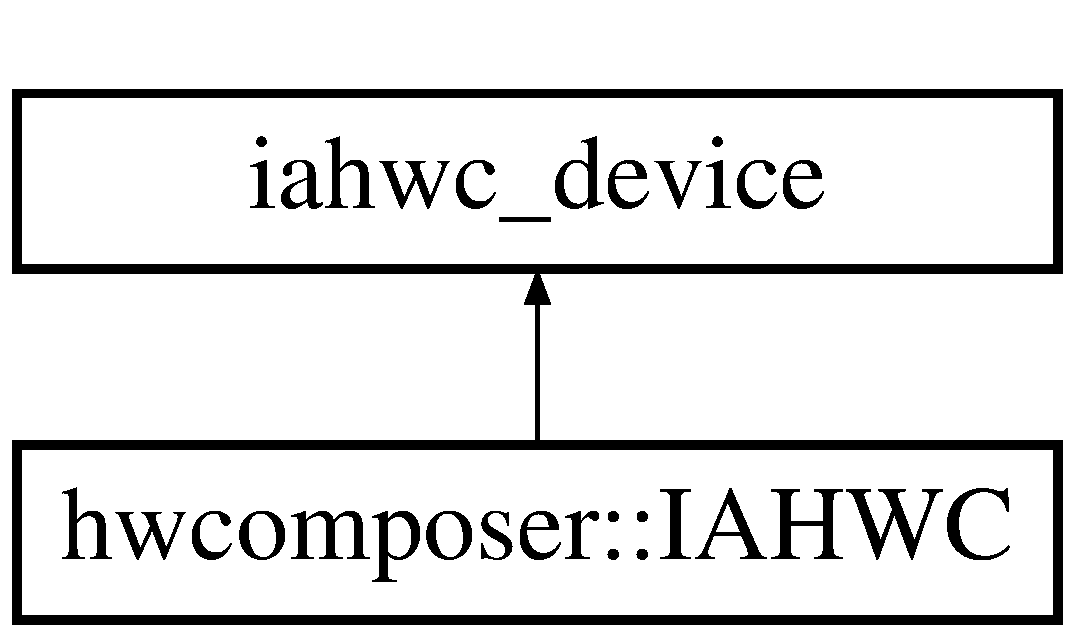
\includegraphics[height=2.000000cm]{structiahwc__device}
\end{center}
\end{figure}
\subsection*{Public Attributes}
\begin{DoxyCompactItemize}
\item 
struct \mbox{\hyperlink{structiahwc__module}{iahwc\+\_\+module}} \mbox{\hyperlink{structiahwc__device_a0aefc811fc58971ae303276df5fec646}{module}}
\item 
int($\ast$ \mbox{\hyperlink{structiahwc__device_a147ff8b5cced2b745222742c89fd3e08}{close}} )(struct \mbox{\hyperlink{structiahwc__device}{iahwc\+\_\+device}} $\ast$device)
\item 
\mbox{\hyperlink{iahwc_8h_a214bf51cce821fdb7b24210088c12cad}{iahwc\+\_\+function\+\_\+ptr\+\_\+t}}($\ast$ \mbox{\hyperlink{structiahwc__device_af5514f45ede1ab95ab6eafa8c3f40ad3}{get\+Function\+Ptr}} )(struct \mbox{\hyperlink{structiahwc__device}{iahwc\+\_\+device}} $\ast$device, int descriptor)
\end{DoxyCompactItemize}


\subsection{Detailed Description}


Definition at line 39 of file iahwc.\+h.



\subsection{Member Data Documentation}
\mbox{\Hypertarget{structiahwc__device_a147ff8b5cced2b745222742c89fd3e08}\label{structiahwc__device_a147ff8b5cced2b745222742c89fd3e08}} 
\index{iahwc\+\_\+device@{iahwc\+\_\+device}!close@{close}}
\index{close@{close}!iahwc\+\_\+device@{iahwc\+\_\+device}}
\subsubsection{\texorpdfstring{close}{close}}
{\footnotesize\ttfamily int($\ast$ iahwc\+\_\+device\+::close) (struct \mbox{\hyperlink{structiahwc__device}{iahwc\+\_\+device}} $\ast$device)}



Definition at line 41 of file iahwc.\+h.

\mbox{\Hypertarget{structiahwc__device_af5514f45ede1ab95ab6eafa8c3f40ad3}\label{structiahwc__device_af5514f45ede1ab95ab6eafa8c3f40ad3}} 
\index{iahwc\+\_\+device@{iahwc\+\_\+device}!get\+Function\+Ptr@{get\+Function\+Ptr}}
\index{get\+Function\+Ptr@{get\+Function\+Ptr}!iahwc\+\_\+device@{iahwc\+\_\+device}}
\subsubsection{\texorpdfstring{get\+Function\+Ptr}{getFunctionPtr}}
{\footnotesize\ttfamily \mbox{\hyperlink{iahwc_8h_a214bf51cce821fdb7b24210088c12cad}{iahwc\+\_\+function\+\_\+ptr\+\_\+t}}($\ast$ iahwc\+\_\+device\+::get\+Function\+Ptr) (struct \mbox{\hyperlink{structiahwc__device}{iahwc\+\_\+device}} $\ast$device, int descriptor)}



Definition at line 42 of file iahwc.\+h.

\mbox{\Hypertarget{structiahwc__device_a0aefc811fc58971ae303276df5fec646}\label{structiahwc__device_a0aefc811fc58971ae303276df5fec646}} 
\index{iahwc\+\_\+device@{iahwc\+\_\+device}!module@{module}}
\index{module@{module}!iahwc\+\_\+device@{iahwc\+\_\+device}}
\subsubsection{\texorpdfstring{module}{module}}
{\footnotesize\ttfamily struct \mbox{\hyperlink{structiahwc__module}{iahwc\+\_\+module}} iahwc\+\_\+device\+::module}



Definition at line 40 of file iahwc.\+h.



The documentation for this struct was generated from the following file\+:\begin{DoxyCompactItemize}
\item 
os/linux/\mbox{\hyperlink{iahwc_8h}{iahwc.\+h}}\end{DoxyCompactItemize}

\hypertarget{structiahwc__edid}{}\section{iahwc\+\_\+edid Struct Reference}
\label{structiahwc__edid}\index{iahwc\+\_\+edid@{iahwc\+\_\+edid}}
\subsection*{Public Attributes}
\begin{DoxyCompactItemize}
\item 
char \mbox{\hyperlink{structiahwc__edid_a91cd81f2e24739b635800a0f292d3d1d}{eisa\+\_\+id}} \mbox{[}13\mbox{]}
\item 
char \mbox{\hyperlink{structiahwc__edid_a8ac7bf02ad2abf916be5bc2ce10c9349}{monitor\+\_\+name}} \mbox{[}13\mbox{]}
\item 
char \mbox{\hyperlink{structiahwc__edid_a6e9458c0d30020543837fe1212ff431a}{pnp\+\_\+id}} \mbox{[}5\mbox{]}
\item 
char \mbox{\hyperlink{structiahwc__edid_abeb28c4382a7d860385907cde82ce58d}{serial\+\_\+number}} \mbox{[}13\mbox{]}
\end{DoxyCompactItemize}


\subsection{Detailed Description}


Definition at line 147 of file compositor-\/iahwc.\+c.



\subsection{Member Data Documentation}
\mbox{\Hypertarget{structiahwc__edid_a91cd81f2e24739b635800a0f292d3d1d}\label{structiahwc__edid_a91cd81f2e24739b635800a0f292d3d1d}} 
\index{iahwc\+\_\+edid@{iahwc\+\_\+edid}!eisa\+\_\+id@{eisa\+\_\+id}}
\index{eisa\+\_\+id@{eisa\+\_\+id}!iahwc\+\_\+edid@{iahwc\+\_\+edid}}
\subsubsection{\texorpdfstring{eisa\+\_\+id}{eisa\_id}}
{\footnotesize\ttfamily char iahwc\+\_\+edid\+::eisa\+\_\+id\mbox{[}13\mbox{]}}



Definition at line 148 of file compositor-\/iahwc.\+c.

\mbox{\Hypertarget{structiahwc__edid_a8ac7bf02ad2abf916be5bc2ce10c9349}\label{structiahwc__edid_a8ac7bf02ad2abf916be5bc2ce10c9349}} 
\index{iahwc\+\_\+edid@{iahwc\+\_\+edid}!monitor\+\_\+name@{monitor\+\_\+name}}
\index{monitor\+\_\+name@{monitor\+\_\+name}!iahwc\+\_\+edid@{iahwc\+\_\+edid}}
\subsubsection{\texorpdfstring{monitor\+\_\+name}{monitor\_name}}
{\footnotesize\ttfamily char iahwc\+\_\+edid\+::monitor\+\_\+name\mbox{[}13\mbox{]}}



Definition at line 149 of file compositor-\/iahwc.\+c.

\mbox{\Hypertarget{structiahwc__edid_a6e9458c0d30020543837fe1212ff431a}\label{structiahwc__edid_a6e9458c0d30020543837fe1212ff431a}} 
\index{iahwc\+\_\+edid@{iahwc\+\_\+edid}!pnp\+\_\+id@{pnp\+\_\+id}}
\index{pnp\+\_\+id@{pnp\+\_\+id}!iahwc\+\_\+edid@{iahwc\+\_\+edid}}
\subsubsection{\texorpdfstring{pnp\+\_\+id}{pnp\_id}}
{\footnotesize\ttfamily char iahwc\+\_\+edid\+::pnp\+\_\+id\mbox{[}5\mbox{]}}



Definition at line 150 of file compositor-\/iahwc.\+c.

\mbox{\Hypertarget{structiahwc__edid_abeb28c4382a7d860385907cde82ce58d}\label{structiahwc__edid_abeb28c4382a7d860385907cde82ce58d}} 
\index{iahwc\+\_\+edid@{iahwc\+\_\+edid}!serial\+\_\+number@{serial\+\_\+number}}
\index{serial\+\_\+number@{serial\+\_\+number}!iahwc\+\_\+edid@{iahwc\+\_\+edid}}
\subsubsection{\texorpdfstring{serial\+\_\+number}{serial\_number}}
{\footnotesize\ttfamily char iahwc\+\_\+edid\+::serial\+\_\+number\mbox{[}13\mbox{]}}



Definition at line 151 of file compositor-\/iahwc.\+c.



The documentation for this struct was generated from the following file\+:\begin{DoxyCompactItemize}
\item 
os/linux/weston/plugin/\mbox{\hyperlink{compositor-iahwc_8c}{compositor-\/iahwc.\+c}}\end{DoxyCompactItemize}

\hypertarget{structiahwc__mode}{}\section{iahwc\+\_\+mode Struct Reference}
\label{structiahwc__mode}\index{iahwc\+\_\+mode@{iahwc\+\_\+mode}}
\subsection*{Public Attributes}
\begin{DoxyCompactItemize}
\item 
struct weston\+\_\+mode \mbox{\hyperlink{structiahwc__mode_ab04ed41f29ad4c89b11120c9db01a93c}{base}}
\item 
uint32\+\_\+t \mbox{\hyperlink{structiahwc__mode_a38ce4032966c7348a378c1eb1a04113a}{config\+\_\+id}}
\end{DoxyCompactItemize}


\subsection{Detailed Description}


Definition at line 142 of file compositor-\/iahwc.\+c.



\subsection{Member Data Documentation}
\mbox{\Hypertarget{structiahwc__mode_ab04ed41f29ad4c89b11120c9db01a93c}\label{structiahwc__mode_ab04ed41f29ad4c89b11120c9db01a93c}} 
\index{iahwc\+\_\+mode@{iahwc\+\_\+mode}!base@{base}}
\index{base@{base}!iahwc\+\_\+mode@{iahwc\+\_\+mode}}
\subsubsection{\texorpdfstring{base}{base}}
{\footnotesize\ttfamily struct weston\+\_\+mode iahwc\+\_\+mode\+::base}



Definition at line 143 of file compositor-\/iahwc.\+c.

\mbox{\Hypertarget{structiahwc__mode_a38ce4032966c7348a378c1eb1a04113a}\label{structiahwc__mode_a38ce4032966c7348a378c1eb1a04113a}} 
\index{iahwc\+\_\+mode@{iahwc\+\_\+mode}!config\+\_\+id@{config\+\_\+id}}
\index{config\+\_\+id@{config\+\_\+id}!iahwc\+\_\+mode@{iahwc\+\_\+mode}}
\subsubsection{\texorpdfstring{config\+\_\+id}{config\_id}}
{\footnotesize\ttfamily uint32\+\_\+t iahwc\+\_\+mode\+::config\+\_\+id}



Definition at line 144 of file compositor-\/iahwc.\+c.



The documentation for this struct was generated from the following file\+:\begin{DoxyCompactItemize}
\item 
os/linux/weston/plugin/\mbox{\hyperlink{compositor-iahwc_8c}{compositor-\/iahwc.\+c}}\end{DoxyCompactItemize}

\hypertarget{structiahwc__module}{}\section{iahwc\+\_\+module Struct Reference}
\label{structiahwc__module}\index{iahwc\+\_\+module@{iahwc\+\_\+module}}


{\ttfamily \#include $<$iahwc.\+h$>$}

\subsection*{Public Attributes}
\begin{DoxyCompactItemize}
\item 
const char $\ast$ \mbox{\hyperlink{structiahwc__module_a8aca00107399693835af2abd3d6a2af9}{name}}
\item 
int($\ast$ \mbox{\hyperlink{structiahwc__module_a4d021a5ef4c5cc54e58ce6aa84f81402}{open}} )(const struct \mbox{\hyperlink{structiahwc__module}{iahwc\+\_\+module}} $\ast$module, struct \mbox{\hyperlink{structiahwc__device}{iahwc\+\_\+device}} $\ast$$\ast$device)
\end{DoxyCompactItemize}


\subsection{Detailed Description}


Definition at line 34 of file iahwc.\+h.



\subsection{Member Data Documentation}
\mbox{\Hypertarget{structiahwc__module_a8aca00107399693835af2abd3d6a2af9}\label{structiahwc__module_a8aca00107399693835af2abd3d6a2af9}} 
\index{iahwc\+\_\+module@{iahwc\+\_\+module}!name@{name}}
\index{name@{name}!iahwc\+\_\+module@{iahwc\+\_\+module}}
\subsubsection{\texorpdfstring{name}{name}}
{\footnotesize\ttfamily const char$\ast$ iahwc\+\_\+module\+::name}



Definition at line 35 of file iahwc.\+h.

\mbox{\Hypertarget{structiahwc__module_a4d021a5ef4c5cc54e58ce6aa84f81402}\label{structiahwc__module_a4d021a5ef4c5cc54e58ce6aa84f81402}} 
\index{iahwc\+\_\+module@{iahwc\+\_\+module}!open@{open}}
\index{open@{open}!iahwc\+\_\+module@{iahwc\+\_\+module}}
\subsubsection{\texorpdfstring{open}{open}}
{\footnotesize\ttfamily int($\ast$ iahwc\+\_\+module\+::open) (const struct \mbox{\hyperlink{structiahwc__module}{iahwc\+\_\+module}} $\ast$module, struct \mbox{\hyperlink{structiahwc__device}{iahwc\+\_\+device}} $\ast$$\ast$device)}



Definition at line 36 of file iahwc.\+h.



The documentation for this struct was generated from the following file\+:\begin{DoxyCompactItemize}
\item 
os/linux/\mbox{\hyperlink{iahwc_8h}{iahwc.\+h}}\end{DoxyCompactItemize}

\hypertarget{structiahwc__output}{}\section{iahwc\+\_\+output Struct Reference}
\label{structiahwc__output}\index{iahwc\+\_\+output@{iahwc\+\_\+output}}
\subsection*{Public Attributes}
\begin{DoxyCompactItemize}
\item 
struct weston\+\_\+output \mbox{\hyperlink{structiahwc__output_a33611f9c8d1354ea9c4df7c6077f593e}{base}}
\item 
\mbox{\hyperlink{nativedisplay_8h_a16ea3fc6b16060fd1e1257707006440e}{drm\+Mode\+Connector}} $\ast$ \mbox{\hyperlink{structiahwc__output_ab3dc520b844eed75e64c4732b8355f35}{connector}}
\item 
uint32\+\_\+t \mbox{\hyperlink{structiahwc__output_a6e3ab85b62b65859fdb94afd042bfd00}{crtc\+\_\+id}}
\item 
int \mbox{\hyperlink{structiahwc__output_a34e4e1b6d16a36451f45dcd44de71592}{pipe}}
\item 
uint32\+\_\+t \mbox{\hyperlink{structiahwc__output_ae1cf365db62f007f6a3d30bd19b5b0c8}{connector\+\_\+id}}
\item 
struct \mbox{\hyperlink{structiahwc__edid}{iahwc\+\_\+edid}} \mbox{\hyperlink{structiahwc__output_a60fac1882a96e0bb4e1b6a6d14ac9f17}{edid}}
\item 
enum dpms\+\_\+enum \mbox{\hyperlink{structiahwc__output_ae2065bbaeeccc8c9b3515fd3423c808d}{dpms}}
\item 
struct backlight $\ast$ \mbox{\hyperlink{structiahwc__output_a1ebafa94e848666e5f28c124d9b6b72e}{backlight}}
\item 
bool \mbox{\hyperlink{structiahwc__output_a87777ec8691b7e6422bb02a20742f45c}{state\+\_\+invalid}}
\item 
bool \mbox{\hyperlink{structiahwc__output_aefcab2462cfed7d4bdebf45010df3caa}{overlay\+\_\+enabled}}
\item 
struct weston\+\_\+plane \mbox{\hyperlink{structiahwc__output_a2f4e89c3089e28c38b9eda40293e8b62}{overlay\+\_\+plane}}
\item 
struct wl\+\_\+list \mbox{\hyperlink{structiahwc__output_ac6a6632a6b51024f9a2f5516ffedf60b}{overlay\+\_\+list}}
\item 
uint32\+\_\+t \mbox{\hyperlink{structiahwc__output_a2523ed1ef619ab10f9da95c2e7abf731}{gbm\+\_\+format}}
\item 
pixman\+\_\+region32\+\_\+t \mbox{\hyperlink{structiahwc__output_a853f609b7a945b51ced6349755d9261c}{previous\+\_\+damage}}
\item 
struct vaapi\+\_\+recorder $\ast$ \mbox{\hyperlink{structiahwc__output_a3fe7dd1b11d07065ec10a0066bad6b0b}{recorder}}
\item 
struct wl\+\_\+listener \mbox{\hyperlink{structiahwc__output_a8d3cfee58372ebf417ed0e6b8ef08db1}{recorder\+\_\+frame\+\_\+listener}}
\item 
int \mbox{\hyperlink{structiahwc__output_a3137bfd94446ab2ee1cc823575894b2a}{release\+\_\+fence}}
\item 
struct wl\+\_\+event\+\_\+source $\ast$ \mbox{\hyperlink{structiahwc__output_a34dcb2b1a9089f0dcc5f36afb845e399}{release\+\_\+fence\+\_\+source}}
\item 
struct \mbox{\hyperlink{structiahwc__spinlock}{iahwc\+\_\+spinlock}} \mbox{\hyperlink{structiahwc__output_a4ba268dca4916063188a7ba33f2123cd}{spin\+\_\+lock}}
\item 
struct timespec \mbox{\hyperlink{structiahwc__output_aeb2dda1bb8a7ef76b2be89b059f3d524}{last\+\_\+vsync\+\_\+ts}}
\item 
uint32\+\_\+t \mbox{\hyperlink{structiahwc__output_a62bb8c46afae61d108af6c2f17cd6ff5}{total\+\_\+layers}}
\item 
enum dpms\+\_\+enum \mbox{\hyperlink{structiahwc__output_a20868af3c280be48cfcbf0b96b0ab67c}{current\+\_\+dpms}}
\end{DoxyCompactItemize}


\subsection{Detailed Description}


Definition at line 175 of file compositor-\/iahwc.\+c.



\subsection{Member Data Documentation}
\mbox{\Hypertarget{structiahwc__output_a1ebafa94e848666e5f28c124d9b6b72e}\label{structiahwc__output_a1ebafa94e848666e5f28c124d9b6b72e}} 
\index{iahwc\+\_\+output@{iahwc\+\_\+output}!backlight@{backlight}}
\index{backlight@{backlight}!iahwc\+\_\+output@{iahwc\+\_\+output}}
\subsubsection{\texorpdfstring{backlight}{backlight}}
{\footnotesize\ttfamily struct backlight$\ast$ iahwc\+\_\+output\+::backlight}



Definition at line 186 of file compositor-\/iahwc.\+c.

\mbox{\Hypertarget{structiahwc__output_a33611f9c8d1354ea9c4df7c6077f593e}\label{structiahwc__output_a33611f9c8d1354ea9c4df7c6077f593e}} 
\index{iahwc\+\_\+output@{iahwc\+\_\+output}!base@{base}}
\index{base@{base}!iahwc\+\_\+output@{iahwc\+\_\+output}}
\subsubsection{\texorpdfstring{base}{base}}
{\footnotesize\ttfamily struct weston\+\_\+output iahwc\+\_\+output\+::base}



Definition at line 176 of file compositor-\/iahwc.\+c.

\mbox{\Hypertarget{structiahwc__output_ab3dc520b844eed75e64c4732b8355f35}\label{structiahwc__output_ab3dc520b844eed75e64c4732b8355f35}} 
\index{iahwc\+\_\+output@{iahwc\+\_\+output}!connector@{connector}}
\index{connector@{connector}!iahwc\+\_\+output@{iahwc\+\_\+output}}
\subsubsection{\texorpdfstring{connector}{connector}}
{\footnotesize\ttfamily \mbox{\hyperlink{nativedisplay_8h_a16ea3fc6b16060fd1e1257707006440e}{drm\+Mode\+Connector}}$\ast$ iahwc\+\_\+output\+::connector}



Definition at line 177 of file compositor-\/iahwc.\+c.

\mbox{\Hypertarget{structiahwc__output_ae1cf365db62f007f6a3d30bd19b5b0c8}\label{structiahwc__output_ae1cf365db62f007f6a3d30bd19b5b0c8}} 
\index{iahwc\+\_\+output@{iahwc\+\_\+output}!connector\+\_\+id@{connector\+\_\+id}}
\index{connector\+\_\+id@{connector\+\_\+id}!iahwc\+\_\+output@{iahwc\+\_\+output}}
\subsubsection{\texorpdfstring{connector\+\_\+id}{connector\_id}}
{\footnotesize\ttfamily uint32\+\_\+t iahwc\+\_\+output\+::connector\+\_\+id}



Definition at line 181 of file compositor-\/iahwc.\+c.

\mbox{\Hypertarget{structiahwc__output_a6e3ab85b62b65859fdb94afd042bfd00}\label{structiahwc__output_a6e3ab85b62b65859fdb94afd042bfd00}} 
\index{iahwc\+\_\+output@{iahwc\+\_\+output}!crtc\+\_\+id@{crtc\+\_\+id}}
\index{crtc\+\_\+id@{crtc\+\_\+id}!iahwc\+\_\+output@{iahwc\+\_\+output}}
\subsubsection{\texorpdfstring{crtc\+\_\+id}{crtc\_id}}
{\footnotesize\ttfamily uint32\+\_\+t iahwc\+\_\+output\+::crtc\+\_\+id}



Definition at line 179 of file compositor-\/iahwc.\+c.

\mbox{\Hypertarget{structiahwc__output_a20868af3c280be48cfcbf0b96b0ab67c}\label{structiahwc__output_a20868af3c280be48cfcbf0b96b0ab67c}} 
\index{iahwc\+\_\+output@{iahwc\+\_\+output}!current\+\_\+dpms@{current\+\_\+dpms}}
\index{current\+\_\+dpms@{current\+\_\+dpms}!iahwc\+\_\+output@{iahwc\+\_\+output}}
\subsubsection{\texorpdfstring{current\+\_\+dpms}{current\_dpms}}
{\footnotesize\ttfamily enum dpms\+\_\+enum iahwc\+\_\+output\+::current\+\_\+dpms}



Definition at line 207 of file compositor-\/iahwc.\+c.

\mbox{\Hypertarget{structiahwc__output_ae2065bbaeeccc8c9b3515fd3423c808d}\label{structiahwc__output_ae2065bbaeeccc8c9b3515fd3423c808d}} 
\index{iahwc\+\_\+output@{iahwc\+\_\+output}!dpms@{dpms}}
\index{dpms@{dpms}!iahwc\+\_\+output@{iahwc\+\_\+output}}
\subsubsection{\texorpdfstring{dpms}{dpms}}
{\footnotesize\ttfamily enum dpms\+\_\+enum iahwc\+\_\+output\+::dpms}



Definition at line 185 of file compositor-\/iahwc.\+c.

\mbox{\Hypertarget{structiahwc__output_a60fac1882a96e0bb4e1b6a6d14ac9f17}\label{structiahwc__output_a60fac1882a96e0bb4e1b6a6d14ac9f17}} 
\index{iahwc\+\_\+output@{iahwc\+\_\+output}!edid@{edid}}
\index{edid@{edid}!iahwc\+\_\+output@{iahwc\+\_\+output}}
\subsubsection{\texorpdfstring{edid}{edid}}
{\footnotesize\ttfamily struct \mbox{\hyperlink{structiahwc__edid}{iahwc\+\_\+edid}} iahwc\+\_\+output\+::edid}



Definition at line 183 of file compositor-\/iahwc.\+c.

\mbox{\Hypertarget{structiahwc__output_a2523ed1ef619ab10f9da95c2e7abf731}\label{structiahwc__output_a2523ed1ef619ab10f9da95c2e7abf731}} 
\index{iahwc\+\_\+output@{iahwc\+\_\+output}!gbm\+\_\+format@{gbm\+\_\+format}}
\index{gbm\+\_\+format@{gbm\+\_\+format}!iahwc\+\_\+output@{iahwc\+\_\+output}}
\subsubsection{\texorpdfstring{gbm\+\_\+format}{gbm\_format}}
{\footnotesize\ttfamily uint32\+\_\+t iahwc\+\_\+output\+::gbm\+\_\+format}



Definition at line 194 of file compositor-\/iahwc.\+c.

\mbox{\Hypertarget{structiahwc__output_aeb2dda1bb8a7ef76b2be89b059f3d524}\label{structiahwc__output_aeb2dda1bb8a7ef76b2be89b059f3d524}} 
\index{iahwc\+\_\+output@{iahwc\+\_\+output}!last\+\_\+vsync\+\_\+ts@{last\+\_\+vsync\+\_\+ts}}
\index{last\+\_\+vsync\+\_\+ts@{last\+\_\+vsync\+\_\+ts}!iahwc\+\_\+output@{iahwc\+\_\+output}}
\subsubsection{\texorpdfstring{last\+\_\+vsync\+\_\+ts}{last\_vsync\_ts}}
{\footnotesize\ttfamily struct timespec iahwc\+\_\+output\+::last\+\_\+vsync\+\_\+ts}



Definition at line 204 of file compositor-\/iahwc.\+c.

\mbox{\Hypertarget{structiahwc__output_aefcab2462cfed7d4bdebf45010df3caa}\label{structiahwc__output_aefcab2462cfed7d4bdebf45010df3caa}} 
\index{iahwc\+\_\+output@{iahwc\+\_\+output}!overlay\+\_\+enabled@{overlay\+\_\+enabled}}
\index{overlay\+\_\+enabled@{overlay\+\_\+enabled}!iahwc\+\_\+output@{iahwc\+\_\+output}}
\subsubsection{\texorpdfstring{overlay\+\_\+enabled}{overlay\_enabled}}
{\footnotesize\ttfamily bool iahwc\+\_\+output\+::overlay\+\_\+enabled}



Definition at line 189 of file compositor-\/iahwc.\+c.

\mbox{\Hypertarget{structiahwc__output_ac6a6632a6b51024f9a2f5516ffedf60b}\label{structiahwc__output_ac6a6632a6b51024f9a2f5516ffedf60b}} 
\index{iahwc\+\_\+output@{iahwc\+\_\+output}!overlay\+\_\+list@{overlay\+\_\+list}}
\index{overlay\+\_\+list@{overlay\+\_\+list}!iahwc\+\_\+output@{iahwc\+\_\+output}}
\subsubsection{\texorpdfstring{overlay\+\_\+list}{overlay\_list}}
{\footnotesize\ttfamily struct wl\+\_\+list iahwc\+\_\+output\+::overlay\+\_\+list}



Definition at line 192 of file compositor-\/iahwc.\+c.

\mbox{\Hypertarget{structiahwc__output_a2f4e89c3089e28c38b9eda40293e8b62}\label{structiahwc__output_a2f4e89c3089e28c38b9eda40293e8b62}} 
\index{iahwc\+\_\+output@{iahwc\+\_\+output}!overlay\+\_\+plane@{overlay\+\_\+plane}}
\index{overlay\+\_\+plane@{overlay\+\_\+plane}!iahwc\+\_\+output@{iahwc\+\_\+output}}
\subsubsection{\texorpdfstring{overlay\+\_\+plane}{overlay\_plane}}
{\footnotesize\ttfamily struct weston\+\_\+plane iahwc\+\_\+output\+::overlay\+\_\+plane}



Definition at line 191 of file compositor-\/iahwc.\+c.

\mbox{\Hypertarget{structiahwc__output_a34e4e1b6d16a36451f45dcd44de71592}\label{structiahwc__output_a34e4e1b6d16a36451f45dcd44de71592}} 
\index{iahwc\+\_\+output@{iahwc\+\_\+output}!pipe@{pipe}}
\index{pipe@{pipe}!iahwc\+\_\+output@{iahwc\+\_\+output}}
\subsubsection{\texorpdfstring{pipe}{pipe}}
{\footnotesize\ttfamily int iahwc\+\_\+output\+::pipe}



Definition at line 180 of file compositor-\/iahwc.\+c.

\mbox{\Hypertarget{structiahwc__output_a853f609b7a945b51ced6349755d9261c}\label{structiahwc__output_a853f609b7a945b51ced6349755d9261c}} 
\index{iahwc\+\_\+output@{iahwc\+\_\+output}!previous\+\_\+damage@{previous\+\_\+damage}}
\index{previous\+\_\+damage@{previous\+\_\+damage}!iahwc\+\_\+output@{iahwc\+\_\+output}}
\subsubsection{\texorpdfstring{previous\+\_\+damage}{previous\_damage}}
{\footnotesize\ttfamily pixman\+\_\+region32\+\_\+t iahwc\+\_\+output\+::previous\+\_\+damage}



Definition at line 196 of file compositor-\/iahwc.\+c.

\mbox{\Hypertarget{structiahwc__output_a3fe7dd1b11d07065ec10a0066bad6b0b}\label{structiahwc__output_a3fe7dd1b11d07065ec10a0066bad6b0b}} 
\index{iahwc\+\_\+output@{iahwc\+\_\+output}!recorder@{recorder}}
\index{recorder@{recorder}!iahwc\+\_\+output@{iahwc\+\_\+output}}
\subsubsection{\texorpdfstring{recorder}{recorder}}
{\footnotesize\ttfamily struct vaapi\+\_\+recorder$\ast$ iahwc\+\_\+output\+::recorder}



Definition at line 198 of file compositor-\/iahwc.\+c.

\mbox{\Hypertarget{structiahwc__output_a8d3cfee58372ebf417ed0e6b8ef08db1}\label{structiahwc__output_a8d3cfee58372ebf417ed0e6b8ef08db1}} 
\index{iahwc\+\_\+output@{iahwc\+\_\+output}!recorder\+\_\+frame\+\_\+listener@{recorder\+\_\+frame\+\_\+listener}}
\index{recorder\+\_\+frame\+\_\+listener@{recorder\+\_\+frame\+\_\+listener}!iahwc\+\_\+output@{iahwc\+\_\+output}}
\subsubsection{\texorpdfstring{recorder\+\_\+frame\+\_\+listener}{recorder\_frame\_listener}}
{\footnotesize\ttfamily struct wl\+\_\+listener iahwc\+\_\+output\+::recorder\+\_\+frame\+\_\+listener}



Definition at line 199 of file compositor-\/iahwc.\+c.

\mbox{\Hypertarget{structiahwc__output_a3137bfd94446ab2ee1cc823575894b2a}\label{structiahwc__output_a3137bfd94446ab2ee1cc823575894b2a}} 
\index{iahwc\+\_\+output@{iahwc\+\_\+output}!release\+\_\+fence@{release\+\_\+fence}}
\index{release\+\_\+fence@{release\+\_\+fence}!iahwc\+\_\+output@{iahwc\+\_\+output}}
\subsubsection{\texorpdfstring{release\+\_\+fence}{release\_fence}}
{\footnotesize\ttfamily int iahwc\+\_\+output\+::release\+\_\+fence}



Definition at line 201 of file compositor-\/iahwc.\+c.

\mbox{\Hypertarget{structiahwc__output_a34dcb2b1a9089f0dcc5f36afb845e399}\label{structiahwc__output_a34dcb2b1a9089f0dcc5f36afb845e399}} 
\index{iahwc\+\_\+output@{iahwc\+\_\+output}!release\+\_\+fence\+\_\+source@{release\+\_\+fence\+\_\+source}}
\index{release\+\_\+fence\+\_\+source@{release\+\_\+fence\+\_\+source}!iahwc\+\_\+output@{iahwc\+\_\+output}}
\subsubsection{\texorpdfstring{release\+\_\+fence\+\_\+source}{release\_fence\_source}}
{\footnotesize\ttfamily struct wl\+\_\+event\+\_\+source$\ast$ iahwc\+\_\+output\+::release\+\_\+fence\+\_\+source}



Definition at line 202 of file compositor-\/iahwc.\+c.

\mbox{\Hypertarget{structiahwc__output_a4ba268dca4916063188a7ba33f2123cd}\label{structiahwc__output_a4ba268dca4916063188a7ba33f2123cd}} 
\index{iahwc\+\_\+output@{iahwc\+\_\+output}!spin\+\_\+lock@{spin\+\_\+lock}}
\index{spin\+\_\+lock@{spin\+\_\+lock}!iahwc\+\_\+output@{iahwc\+\_\+output}}
\subsubsection{\texorpdfstring{spin\+\_\+lock}{spin\_lock}}
{\footnotesize\ttfamily struct \mbox{\hyperlink{structiahwc__spinlock}{iahwc\+\_\+spinlock}} iahwc\+\_\+output\+::spin\+\_\+lock}



Definition at line 203 of file compositor-\/iahwc.\+c.

\mbox{\Hypertarget{structiahwc__output_a87777ec8691b7e6422bb02a20742f45c}\label{structiahwc__output_a87777ec8691b7e6422bb02a20742f45c}} 
\index{iahwc\+\_\+output@{iahwc\+\_\+output}!state\+\_\+invalid@{state\+\_\+invalid}}
\index{state\+\_\+invalid@{state\+\_\+invalid}!iahwc\+\_\+output@{iahwc\+\_\+output}}
\subsubsection{\texorpdfstring{state\+\_\+invalid}{state\_invalid}}
{\footnotesize\ttfamily bool iahwc\+\_\+output\+::state\+\_\+invalid}



Definition at line 188 of file compositor-\/iahwc.\+c.

\mbox{\Hypertarget{structiahwc__output_a62bb8c46afae61d108af6c2f17cd6ff5}\label{structiahwc__output_a62bb8c46afae61d108af6c2f17cd6ff5}} 
\index{iahwc\+\_\+output@{iahwc\+\_\+output}!total\+\_\+layers@{total\+\_\+layers}}
\index{total\+\_\+layers@{total\+\_\+layers}!iahwc\+\_\+output@{iahwc\+\_\+output}}
\subsubsection{\texorpdfstring{total\+\_\+layers}{total\_layers}}
{\footnotesize\ttfamily uint32\+\_\+t iahwc\+\_\+output\+::total\+\_\+layers}



Definition at line 205 of file compositor-\/iahwc.\+c.



The documentation for this struct was generated from the following file\+:\begin{DoxyCompactItemize}
\item 
os/linux/weston/plugin/\mbox{\hyperlink{compositor-iahwc_8c}{compositor-\/iahwc.\+c}}\end{DoxyCompactItemize}

\hypertarget{structiahwc__overlay}{}\section{iahwc\+\_\+overlay Struct Reference}
\label{structiahwc__overlay}\index{iahwc\+\_\+overlay@{iahwc\+\_\+overlay}}
\subsection*{Public Attributes}
\begin{DoxyCompactItemize}
\item 
struct wl\+\_\+list \mbox{\hyperlink{structiahwc__overlay_abfac33082f2c2b4e73136504d30ab648}{link}}
\item 
struct wl\+\_\+shm\+\_\+buffer $\ast$ \mbox{\hyperlink{structiahwc__overlay_a4ab6d321c6af6b1668b0bfe22081544c}{shm\+\_\+memory}}
\item 
struct gbm\+\_\+bo $\ast$ \mbox{\hyperlink{structiahwc__overlay_a50c366179b37b8ae5a6249fb0d6215d0}{overlay\+\_\+bo}}
\item 
uint32\+\_\+t \mbox{\hyperlink{structiahwc__overlay_a5e83b093028ccc18d0d688ffae5b078f}{overlay\+\_\+layer\+\_\+id}}
\item 
uint32\+\_\+t \mbox{\hyperlink{structiahwc__overlay_a3bd8d80d39125387f50e37d80516cc9a}{layer\+\_\+index}}
\item 
struct weston\+\_\+surface $\ast$ \mbox{\hyperlink{structiahwc__overlay_aef4d5a2d068b69fef352b918ffc17163}{es}}
\end{DoxyCompactItemize}


\subsection{Detailed Description}


Definition at line 164 of file compositor-\/iahwc.\+c.



\subsection{Member Data Documentation}
\mbox{\Hypertarget{structiahwc__overlay_aef4d5a2d068b69fef352b918ffc17163}\label{structiahwc__overlay_aef4d5a2d068b69fef352b918ffc17163}} 
\index{iahwc\+\_\+overlay@{iahwc\+\_\+overlay}!es@{es}}
\index{es@{es}!iahwc\+\_\+overlay@{iahwc\+\_\+overlay}}
\subsubsection{\texorpdfstring{es}{es}}
{\footnotesize\ttfamily struct weston\+\_\+surface$\ast$ iahwc\+\_\+overlay\+::es}



Definition at line 172 of file compositor-\/iahwc.\+c.

\mbox{\Hypertarget{structiahwc__overlay_a3bd8d80d39125387f50e37d80516cc9a}\label{structiahwc__overlay_a3bd8d80d39125387f50e37d80516cc9a}} 
\index{iahwc\+\_\+overlay@{iahwc\+\_\+overlay}!layer\+\_\+index@{layer\+\_\+index}}
\index{layer\+\_\+index@{layer\+\_\+index}!iahwc\+\_\+overlay@{iahwc\+\_\+overlay}}
\subsubsection{\texorpdfstring{layer\+\_\+index}{layer\_index}}
{\footnotesize\ttfamily uint32\+\_\+t iahwc\+\_\+overlay\+::layer\+\_\+index}



Definition at line 171 of file compositor-\/iahwc.\+c.

\mbox{\Hypertarget{structiahwc__overlay_abfac33082f2c2b4e73136504d30ab648}\label{structiahwc__overlay_abfac33082f2c2b4e73136504d30ab648}} 
\index{iahwc\+\_\+overlay@{iahwc\+\_\+overlay}!link@{link}}
\index{link@{link}!iahwc\+\_\+overlay@{iahwc\+\_\+overlay}}
\subsubsection{\texorpdfstring{link}{link}}
{\footnotesize\ttfamily struct wl\+\_\+list iahwc\+\_\+overlay\+::link}



Definition at line 165 of file compositor-\/iahwc.\+c.

\mbox{\Hypertarget{structiahwc__overlay_a50c366179b37b8ae5a6249fb0d6215d0}\label{structiahwc__overlay_a50c366179b37b8ae5a6249fb0d6215d0}} 
\index{iahwc\+\_\+overlay@{iahwc\+\_\+overlay}!overlay\+\_\+bo@{overlay\+\_\+bo}}
\index{overlay\+\_\+bo@{overlay\+\_\+bo}!iahwc\+\_\+overlay@{iahwc\+\_\+overlay}}
\subsubsection{\texorpdfstring{overlay\+\_\+bo}{overlay\_bo}}
{\footnotesize\ttfamily struct gbm\+\_\+bo$\ast$ iahwc\+\_\+overlay\+::overlay\+\_\+bo}



Definition at line 169 of file compositor-\/iahwc.\+c.

\mbox{\Hypertarget{structiahwc__overlay_a5e83b093028ccc18d0d688ffae5b078f}\label{structiahwc__overlay_a5e83b093028ccc18d0d688ffae5b078f}} 
\index{iahwc\+\_\+overlay@{iahwc\+\_\+overlay}!overlay\+\_\+layer\+\_\+id@{overlay\+\_\+layer\+\_\+id}}
\index{overlay\+\_\+layer\+\_\+id@{overlay\+\_\+layer\+\_\+id}!iahwc\+\_\+overlay@{iahwc\+\_\+overlay}}
\subsubsection{\texorpdfstring{overlay\+\_\+layer\+\_\+id}{overlay\_layer\_id}}
{\footnotesize\ttfamily uint32\+\_\+t iahwc\+\_\+overlay\+::overlay\+\_\+layer\+\_\+id}



Definition at line 170 of file compositor-\/iahwc.\+c.

\mbox{\Hypertarget{structiahwc__overlay_a4ab6d321c6af6b1668b0bfe22081544c}\label{structiahwc__overlay_a4ab6d321c6af6b1668b0bfe22081544c}} 
\index{iahwc\+\_\+overlay@{iahwc\+\_\+overlay}!shm\+\_\+memory@{shm\+\_\+memory}}
\index{shm\+\_\+memory@{shm\+\_\+memory}!iahwc\+\_\+overlay@{iahwc\+\_\+overlay}}
\subsubsection{\texorpdfstring{shm\+\_\+memory}{shm\_memory}}
{\footnotesize\ttfamily struct wl\+\_\+shm\+\_\+buffer$\ast$ iahwc\+\_\+overlay\+::shm\+\_\+memory}



Definition at line 167 of file compositor-\/iahwc.\+c.



The documentation for this struct was generated from the following file\+:\begin{DoxyCompactItemize}
\item 
os/linux/weston/plugin/\mbox{\hyperlink{compositor-iahwc_8c}{compositor-\/iahwc.\+c}}\end{DoxyCompactItemize}

\hypertarget{structiahwc__pending__state}{}\section{iahwc\+\_\+pending\+\_\+state Struct Reference}
\label{structiahwc__pending__state}\index{iahwc\+\_\+pending\+\_\+state@{iahwc\+\_\+pending\+\_\+state}}
\subsection*{Public Attributes}
\begin{DoxyCompactItemize}
\item 
struct \mbox{\hyperlink{structiahwc__backend}{iahwc\+\_\+backend}} $\ast$ \mbox{\hyperlink{structiahwc__pending__state_a3214eb70000dc28955b6d065d533d1eb}{backend}}
\end{DoxyCompactItemize}


\subsection{Detailed Description}
Pending state holds one or more iahwc\+\_\+output\+\_\+state structures, collected from performing repaint. This pending state is transient, and only lives between beginning a repaint group and flushing the results\+: after flush, each output state will complete and be retired separately. 

Definition at line 160 of file compositor-\/iahwc.\+c.



\subsection{Member Data Documentation}
\mbox{\Hypertarget{structiahwc__pending__state_a3214eb70000dc28955b6d065d533d1eb}\label{structiahwc__pending__state_a3214eb70000dc28955b6d065d533d1eb}} 
\index{iahwc\+\_\+pending\+\_\+state@{iahwc\+\_\+pending\+\_\+state}!backend@{backend}}
\index{backend@{backend}!iahwc\+\_\+pending\+\_\+state@{iahwc\+\_\+pending\+\_\+state}}
\subsubsection{\texorpdfstring{backend}{backend}}
{\footnotesize\ttfamily struct \mbox{\hyperlink{structiahwc__backend}{iahwc\+\_\+backend}}$\ast$ iahwc\+\_\+pending\+\_\+state\+::backend}



Definition at line 161 of file compositor-\/iahwc.\+c.



The documentation for this struct was generated from the following file\+:\begin{DoxyCompactItemize}
\item 
os/linux/weston/plugin/\mbox{\hyperlink{compositor-iahwc_8c}{compositor-\/iahwc.\+c}}\end{DoxyCompactItemize}

\hypertarget{structiahwc__raw__pixel__data}{}\section{iahwc\+\_\+raw\+\_\+pixel\+\_\+data Struct Reference}
\label{structiahwc__raw__pixel__data}\index{iahwc\+\_\+raw\+\_\+pixel\+\_\+data@{iahwc\+\_\+raw\+\_\+pixel\+\_\+data}}


{\ttfamily \#include $<$iahwc.\+h$>$}

\subsection*{Public Attributes}
\begin{DoxyCompactItemize}
\item 
void $\ast$ \mbox{\hyperlink{structiahwc__raw__pixel__data_ad7d42f2ede4d429072a20f791f3a2625}{buffer}}
\item 
void $\ast$ \mbox{\hyperlink{structiahwc__raw__pixel__data_ab7e2bf82485679c69226d5d42bbe7e1c}{callback\+\_\+data}}
\item 
uint64\+\_\+t \mbox{\hyperlink{structiahwc__raw__pixel__data_afa9b60fc4678e26c901c703837fdabb3}{width}}
\item 
uint64\+\_\+t \mbox{\hyperlink{structiahwc__raw__pixel__data_aa8ad90e89455a36ad2c423c33ff189fa}{height}}
\item 
uint64\+\_\+t \mbox{\hyperlink{structiahwc__raw__pixel__data_a7b63e928cb013a04cfe12a69a4cf7241}{stride}}
\item 
uint32\+\_\+t \mbox{\hyperlink{structiahwc__raw__pixel__data_afa6eeb611dda100904b14919b74b1d9d}{format}}
\end{DoxyCompactItemize}


\subsection{Detailed Description}


Definition at line 46 of file iahwc.\+h.



\subsection{Member Data Documentation}
\mbox{\Hypertarget{structiahwc__raw__pixel__data_ad7d42f2ede4d429072a20f791f3a2625}\label{structiahwc__raw__pixel__data_ad7d42f2ede4d429072a20f791f3a2625}} 
\index{iahwc\+\_\+raw\+\_\+pixel\+\_\+data@{iahwc\+\_\+raw\+\_\+pixel\+\_\+data}!buffer@{buffer}}
\index{buffer@{buffer}!iahwc\+\_\+raw\+\_\+pixel\+\_\+data@{iahwc\+\_\+raw\+\_\+pixel\+\_\+data}}
\subsubsection{\texorpdfstring{buffer}{buffer}}
{\footnotesize\ttfamily void$\ast$ iahwc\+\_\+raw\+\_\+pixel\+\_\+data\+::buffer}



Definition at line 47 of file iahwc.\+h.

\mbox{\Hypertarget{structiahwc__raw__pixel__data_ab7e2bf82485679c69226d5d42bbe7e1c}\label{structiahwc__raw__pixel__data_ab7e2bf82485679c69226d5d42bbe7e1c}} 
\index{iahwc\+\_\+raw\+\_\+pixel\+\_\+data@{iahwc\+\_\+raw\+\_\+pixel\+\_\+data}!callback\+\_\+data@{callback\+\_\+data}}
\index{callback\+\_\+data@{callback\+\_\+data}!iahwc\+\_\+raw\+\_\+pixel\+\_\+data@{iahwc\+\_\+raw\+\_\+pixel\+\_\+data}}
\subsubsection{\texorpdfstring{callback\+\_\+data}{callback\_data}}
{\footnotesize\ttfamily void$\ast$ iahwc\+\_\+raw\+\_\+pixel\+\_\+data\+::callback\+\_\+data}



Definition at line 48 of file iahwc.\+h.

\mbox{\Hypertarget{structiahwc__raw__pixel__data_afa6eeb611dda100904b14919b74b1d9d}\label{structiahwc__raw__pixel__data_afa6eeb611dda100904b14919b74b1d9d}} 
\index{iahwc\+\_\+raw\+\_\+pixel\+\_\+data@{iahwc\+\_\+raw\+\_\+pixel\+\_\+data}!format@{format}}
\index{format@{format}!iahwc\+\_\+raw\+\_\+pixel\+\_\+data@{iahwc\+\_\+raw\+\_\+pixel\+\_\+data}}
\subsubsection{\texorpdfstring{format}{format}}
{\footnotesize\ttfamily uint32\+\_\+t iahwc\+\_\+raw\+\_\+pixel\+\_\+data\+::format}



Definition at line 52 of file iahwc.\+h.

\mbox{\Hypertarget{structiahwc__raw__pixel__data_aa8ad90e89455a36ad2c423c33ff189fa}\label{structiahwc__raw__pixel__data_aa8ad90e89455a36ad2c423c33ff189fa}} 
\index{iahwc\+\_\+raw\+\_\+pixel\+\_\+data@{iahwc\+\_\+raw\+\_\+pixel\+\_\+data}!height@{height}}
\index{height@{height}!iahwc\+\_\+raw\+\_\+pixel\+\_\+data@{iahwc\+\_\+raw\+\_\+pixel\+\_\+data}}
\subsubsection{\texorpdfstring{height}{height}}
{\footnotesize\ttfamily uint64\+\_\+t iahwc\+\_\+raw\+\_\+pixel\+\_\+data\+::height}



Definition at line 50 of file iahwc.\+h.

\mbox{\Hypertarget{structiahwc__raw__pixel__data_a7b63e928cb013a04cfe12a69a4cf7241}\label{structiahwc__raw__pixel__data_a7b63e928cb013a04cfe12a69a4cf7241}} 
\index{iahwc\+\_\+raw\+\_\+pixel\+\_\+data@{iahwc\+\_\+raw\+\_\+pixel\+\_\+data}!stride@{stride}}
\index{stride@{stride}!iahwc\+\_\+raw\+\_\+pixel\+\_\+data@{iahwc\+\_\+raw\+\_\+pixel\+\_\+data}}
\subsubsection{\texorpdfstring{stride}{stride}}
{\footnotesize\ttfamily uint64\+\_\+t iahwc\+\_\+raw\+\_\+pixel\+\_\+data\+::stride}



Definition at line 51 of file iahwc.\+h.

\mbox{\Hypertarget{structiahwc__raw__pixel__data_afa9b60fc4678e26c901c703837fdabb3}\label{structiahwc__raw__pixel__data_afa9b60fc4678e26c901c703837fdabb3}} 
\index{iahwc\+\_\+raw\+\_\+pixel\+\_\+data@{iahwc\+\_\+raw\+\_\+pixel\+\_\+data}!width@{width}}
\index{width@{width}!iahwc\+\_\+raw\+\_\+pixel\+\_\+data@{iahwc\+\_\+raw\+\_\+pixel\+\_\+data}}
\subsubsection{\texorpdfstring{width}{width}}
{\footnotesize\ttfamily uint64\+\_\+t iahwc\+\_\+raw\+\_\+pixel\+\_\+data\+::width}



Definition at line 49 of file iahwc.\+h.



The documentation for this struct was generated from the following file\+:\begin{DoxyCompactItemize}
\item 
os/linux/\mbox{\hyperlink{iahwc_8h}{iahwc.\+h}}\end{DoxyCompactItemize}

\hypertarget{structiahwc__rect}{}\section{iahwc\+\_\+rect Struct Reference}
\label{structiahwc__rect}\index{iahwc\+\_\+rect@{iahwc\+\_\+rect}}


{\ttfamily \#include $<$iahwc.\+h$>$}

\subsection*{Public Attributes}
\begin{DoxyCompactItemize}
\item 
uint32\+\_\+t \mbox{\hyperlink{structiahwc__rect_abdce07c1eb024c79de94fbc1d7a8d40b}{left}}
\item 
uint32\+\_\+t \mbox{\hyperlink{structiahwc__rect_a16e4547c603c2367753b32a76e547d91}{top}}
\item 
uint32\+\_\+t \mbox{\hyperlink{structiahwc__rect_a94734af35b59300dd43a54e42bb68ea4}{right}}
\item 
uint32\+\_\+t \mbox{\hyperlink{structiahwc__rect_ad23d12c83244012abee2eb585d8f2052}{bottom}}
\end{DoxyCompactItemize}


\subsection{Detailed Description}


Definition at line 131 of file iahwc.\+h.



\subsection{Member Data Documentation}
\mbox{\Hypertarget{structiahwc__rect_ad23d12c83244012abee2eb585d8f2052}\label{structiahwc__rect_ad23d12c83244012abee2eb585d8f2052}} 
\index{iahwc\+\_\+rect@{iahwc\+\_\+rect}!bottom@{bottom}}
\index{bottom@{bottom}!iahwc\+\_\+rect@{iahwc\+\_\+rect}}
\subsubsection{\texorpdfstring{bottom}{bottom}}
{\footnotesize\ttfamily uint32\+\_\+t iahwc\+\_\+rect\+::bottom}



Definition at line 135 of file iahwc.\+h.

\mbox{\Hypertarget{structiahwc__rect_abdce07c1eb024c79de94fbc1d7a8d40b}\label{structiahwc__rect_abdce07c1eb024c79de94fbc1d7a8d40b}} 
\index{iahwc\+\_\+rect@{iahwc\+\_\+rect}!left@{left}}
\index{left@{left}!iahwc\+\_\+rect@{iahwc\+\_\+rect}}
\subsubsection{\texorpdfstring{left}{left}}
{\footnotesize\ttfamily uint32\+\_\+t iahwc\+\_\+rect\+::left}



Definition at line 132 of file iahwc.\+h.

\mbox{\Hypertarget{structiahwc__rect_a94734af35b59300dd43a54e42bb68ea4}\label{structiahwc__rect_a94734af35b59300dd43a54e42bb68ea4}} 
\index{iahwc\+\_\+rect@{iahwc\+\_\+rect}!right@{right}}
\index{right@{right}!iahwc\+\_\+rect@{iahwc\+\_\+rect}}
\subsubsection{\texorpdfstring{right}{right}}
{\footnotesize\ttfamily uint32\+\_\+t iahwc\+\_\+rect\+::right}



Definition at line 134 of file iahwc.\+h.

\mbox{\Hypertarget{structiahwc__rect_a16e4547c603c2367753b32a76e547d91}\label{structiahwc__rect_a16e4547c603c2367753b32a76e547d91}} 
\index{iahwc\+\_\+rect@{iahwc\+\_\+rect}!top@{top}}
\index{top@{top}!iahwc\+\_\+rect@{iahwc\+\_\+rect}}
\subsubsection{\texorpdfstring{top}{top}}
{\footnotesize\ttfamily uint32\+\_\+t iahwc\+\_\+rect\+::top}



Definition at line 133 of file iahwc.\+h.



The documentation for this struct was generated from the following file\+:\begin{DoxyCompactItemize}
\item 
os/linux/\mbox{\hyperlink{iahwc_8h}{iahwc.\+h}}\end{DoxyCompactItemize}

\hypertarget{structiahwc__region}{}\section{iahwc\+\_\+region Struct Reference}
\label{structiahwc__region}\index{iahwc\+\_\+region@{iahwc\+\_\+region}}


{\ttfamily \#include $<$iahwc.\+h$>$}

\subsection*{Public Attributes}
\begin{DoxyCompactItemize}
\item 
size\+\_\+t \mbox{\hyperlink{structiahwc__region_a72a48239f66d9b87cc76a2bbbbdc48a1}{num\+Rects}}
\item 
\mbox{\hyperlink{iahwc_8h_a163ae45b2470c0d300fe4ec4d017a603}{iahwc\+\_\+rect\+\_\+t}} const  $\ast$ \mbox{\hyperlink{structiahwc__region_a94a878c575f670019f83b1cac59094a5}{rects}}
\end{DoxyCompactItemize}


\subsection{Detailed Description}


Definition at line 138 of file iahwc.\+h.



\subsection{Member Data Documentation}
\mbox{\Hypertarget{structiahwc__region_a72a48239f66d9b87cc76a2bbbbdc48a1}\label{structiahwc__region_a72a48239f66d9b87cc76a2bbbbdc48a1}} 
\index{iahwc\+\_\+region@{iahwc\+\_\+region}!num\+Rects@{num\+Rects}}
\index{num\+Rects@{num\+Rects}!iahwc\+\_\+region@{iahwc\+\_\+region}}
\subsubsection{\texorpdfstring{num\+Rects}{numRects}}
{\footnotesize\ttfamily size\+\_\+t iahwc\+\_\+region\+::num\+Rects}



Definition at line 139 of file iahwc.\+h.

\mbox{\Hypertarget{structiahwc__region_a94a878c575f670019f83b1cac59094a5}\label{structiahwc__region_a94a878c575f670019f83b1cac59094a5}} 
\index{iahwc\+\_\+region@{iahwc\+\_\+region}!rects@{rects}}
\index{rects@{rects}!iahwc\+\_\+region@{iahwc\+\_\+region}}
\subsubsection{\texorpdfstring{rects}{rects}}
{\footnotesize\ttfamily \mbox{\hyperlink{iahwc_8h_a163ae45b2470c0d300fe4ec4d017a603}{iahwc\+\_\+rect\+\_\+t}} const$\ast$ iahwc\+\_\+region\+::rects}



Definition at line 140 of file iahwc.\+h.



The documentation for this struct was generated from the following file\+:\begin{DoxyCompactItemize}
\item 
os/linux/\mbox{\hyperlink{iahwc_8h}{iahwc.\+h}}\end{DoxyCompactItemize}

\hypertarget{structiahwc__spinlock}{}\section{iahwc\+\_\+spinlock Struct Reference}
\label{structiahwc__spinlock}\index{iahwc\+\_\+spinlock@{iahwc\+\_\+spinlock}}
\subsection*{Public Attributes}
\begin{DoxyCompactItemize}
\item 
int \mbox{\hyperlink{structiahwc__spinlock_a200e6951d15a64341d994bcefcc9f1d8}{atomic\+\_\+lock}}
\item 
bool \mbox{\hyperlink{structiahwc__spinlock_a31f33fe3ff4f8ecbf633363d5d6cdb22}{locked}}
\end{DoxyCompactItemize}


\subsection{Detailed Description}


Definition at line 66 of file compositor-\/iahwc.\+c.



\subsection{Member Data Documentation}
\mbox{\Hypertarget{structiahwc__spinlock_a200e6951d15a64341d994bcefcc9f1d8}\label{structiahwc__spinlock_a200e6951d15a64341d994bcefcc9f1d8}} 
\index{iahwc\+\_\+spinlock@{iahwc\+\_\+spinlock}!atomic\+\_\+lock@{atomic\+\_\+lock}}
\index{atomic\+\_\+lock@{atomic\+\_\+lock}!iahwc\+\_\+spinlock@{iahwc\+\_\+spinlock}}
\subsubsection{\texorpdfstring{atomic\+\_\+lock}{atomic\_lock}}
{\footnotesize\ttfamily int iahwc\+\_\+spinlock\+::atomic\+\_\+lock}



Definition at line 67 of file compositor-\/iahwc.\+c.

\mbox{\Hypertarget{structiahwc__spinlock_a31f33fe3ff4f8ecbf633363d5d6cdb22}\label{structiahwc__spinlock_a31f33fe3ff4f8ecbf633363d5d6cdb22}} 
\index{iahwc\+\_\+spinlock@{iahwc\+\_\+spinlock}!locked@{locked}}
\index{locked@{locked}!iahwc\+\_\+spinlock@{iahwc\+\_\+spinlock}}
\subsubsection{\texorpdfstring{locked}{locked}}
{\footnotesize\ttfamily bool iahwc\+\_\+spinlock\+::locked}



Definition at line 68 of file compositor-\/iahwc.\+c.



The documentation for this struct was generated from the following file\+:\begin{DoxyCompactItemize}
\item 
os/linux/weston/plugin/\mbox{\hyperlink{compositor-iahwc_8c}{compositor-\/iahwc.\+c}}\end{DoxyCompactItemize}

\hypertarget{classhwcomposer_1_1IAHWC_1_1IAHWCDisplay}{}\section{hwcomposer\+:\+:I\+A\+H\+WC\+:\+:I\+A\+H\+W\+C\+Display Class Reference}
\label{classhwcomposer_1_1IAHWC_1_1IAHWCDisplay}\index{hwcomposer\+::\+I\+A\+H\+W\+C\+::\+I\+A\+H\+W\+C\+Display@{hwcomposer\+::\+I\+A\+H\+W\+C\+::\+I\+A\+H\+W\+C\+Display}}


{\ttfamily \#include $<$linux\+\_\+frontend.\+h$>$}

Inheritance diagram for hwcomposer\+:\+:I\+A\+H\+WC\+:\+:I\+A\+H\+W\+C\+Display\+:\begin{figure}[H]
\begin{center}
\leavevmode
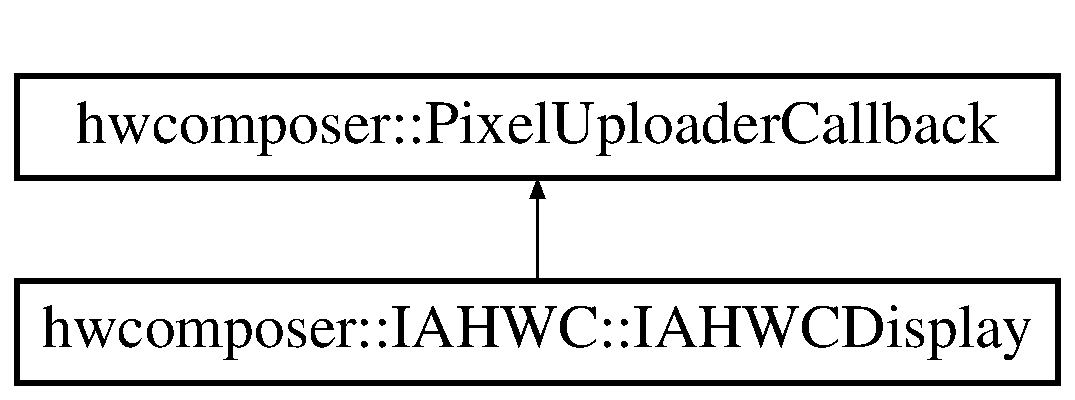
\includegraphics[height=2.000000cm]{classhwcomposer_1_1IAHWC_1_1IAHWCDisplay}
\end{center}
\end{figure}
\subsection*{Public Member Functions}
\begin{DoxyCompactItemize}
\item 
\mbox{\hyperlink{classhwcomposer_1_1IAHWC_1_1IAHWCDisplay_a19e2e52283f3cb2a9d75e5486a2d1746}{I\+A\+H\+W\+C\+Display}} ()
\item 
\mbox{\hyperlink{classhwcomposer_1_1IAHWC_1_1IAHWCDisplay_a506385cf1a72c499ed057af40a67eb08}{$\sim$\+I\+A\+H\+W\+C\+Display}} ()
\item 
int \mbox{\hyperlink{classhwcomposer_1_1IAHWC_1_1IAHWCDisplay_af339a6dc789ef156c41d19bf288f44e4}{Init}} (\mbox{\hyperlink{classhwcomposer_1_1NativeDisplay}{hwcomposer\+::\+Native\+Display}} $\ast$display, uint32\+\_\+t gpu\+\_\+fd)
\item 
int \mbox{\hyperlink{classhwcomposer_1_1IAHWC_1_1IAHWCDisplay_abac8759ae7be9065fb6a579e1b384c23}{Get\+Display\+Info}} (uint32\+\_\+t config, int attribute, int32\+\_\+t $\ast$value)
\item 
int \mbox{\hyperlink{classhwcomposer_1_1IAHWC_1_1IAHWCDisplay_af090eee5e7afcef5e96f8990815cf712}{Get\+Display\+Name}} (uint32\+\_\+t $\ast$size, char $\ast$name)
\item 
int \mbox{\hyperlink{classhwcomposer_1_1IAHWC_1_1IAHWCDisplay_a186346b470891a51643e415468ca5550}{Get\+Display\+Configs}} (uint32\+\_\+t $\ast$num\+\_\+configs, uint32\+\_\+t $\ast$configs)
\item 
int \mbox{\hyperlink{classhwcomposer_1_1IAHWC_1_1IAHWCDisplay_af334fba3fe056cf75884939ed8cf6fbc}{Set\+Display\+Gamma}} (float r, float b, float g)
\item 
int \mbox{\hyperlink{classhwcomposer_1_1IAHWC_1_1IAHWCDisplay_ae4a7bf880a35f4df5e649003f7f7a212}{Set\+Display\+Config}} (uint32\+\_\+t config)
\item 
int \mbox{\hyperlink{classhwcomposer_1_1IAHWC_1_1IAHWCDisplay_a7088d0da276eca2dc2b4458f20270258}{Get\+Display\+Config}} (uint32\+\_\+t $\ast$config)
\item 
int \mbox{\hyperlink{classhwcomposer_1_1IAHWC_1_1IAHWCDisplay_abff19b5001304bd1f0e3c582a409f672}{Set\+Power\+Mode}} (uint32\+\_\+t power\+\_\+mode)
\item 
int \mbox{\hyperlink{classhwcomposer_1_1IAHWC_1_1IAHWCDisplay_a5dcd39e69f99da275fa1d7b64f0dd3b2}{Clear\+All\+Layers}} ()
\item 
int \mbox{\hyperlink{classhwcomposer_1_1IAHWC_1_1IAHWCDisplay_a530a804beb0192c173f7311b35d0909f}{Present\+Display}} (int32\+\_\+t $\ast$release\+\_\+fd)
\item 
int \mbox{\hyperlink{classhwcomposer_1_1IAHWC_1_1IAHWCDisplay_af1ec4019ff9078b6e3971ede75ad9393}{Register\+Vsync\+Callback}} (\mbox{\hyperlink{iahwc_8h_a07fb4f73baa8a0cfbd40f64071e56a7c}{iahwc\+\_\+callback\+\_\+data\+\_\+t}} data, \mbox{\hyperlink{iahwc_8h_a214bf51cce821fdb7b24210088c12cad}{iahwc\+\_\+function\+\_\+ptr\+\_\+t}} hook)
\item 
void \mbox{\hyperlink{classhwcomposer_1_1IAHWC_1_1IAHWCDisplay_ac7299bb8f8312073ba44cf2858642b15}{Register\+Pixel\+Uploader\+Callback}} (\mbox{\hyperlink{iahwc_8h_a07fb4f73baa8a0cfbd40f64071e56a7c}{iahwc\+\_\+callback\+\_\+data\+\_\+t}} data, \mbox{\hyperlink{iahwc_8h_a214bf51cce821fdb7b24210088c12cad}{iahwc\+\_\+function\+\_\+ptr\+\_\+t}} hook)
\item 
int \mbox{\hyperlink{classhwcomposer_1_1IAHWC_1_1IAHWCDisplay_ab8ad988a0d79affe7116a0487b8cf72b}{Create\+Layer}} (uint32\+\_\+t $\ast$layer\+\_\+handle)
\item 
int \mbox{\hyperlink{classhwcomposer_1_1IAHWC_1_1IAHWCDisplay_a36b592a04e93dba90b1f33587c3e4e11}{Destroy\+Layer}} (uint32\+\_\+t layer\+\_\+handle)
\item 
bool \mbox{\hyperlink{classhwcomposer_1_1IAHWC_1_1IAHWCDisplay_a834ade616fea8f09f45b7d1867a2e113}{Is\+Connected}} ()
\item 
\mbox{\hyperlink{classhwcomposer_1_1IAHWC_1_1IAHWCLayer}{I\+A\+H\+W\+C\+Layer}} \& \mbox{\hyperlink{classhwcomposer_1_1IAHWC_1_1IAHWCDisplay_ad83653e1509f4fd12d93cb27848bbb93}{get\+\_\+layer}} (\mbox{\hyperlink{iahwc_8h_a603c5018c43d1f6b98fbb7eeef6a43ac}{iahwc\+\_\+layer\+\_\+t}} layer)
\item 
int \mbox{\hyperlink{classhwcomposer_1_1IAHWC_1_1IAHWCDisplay_ac5d4d8c593d2aa79f1b76a19501b2c08}{Disable\+Overlay\+Usage}} ()
\item 
int \mbox{\hyperlink{classhwcomposer_1_1IAHWC_1_1IAHWCDisplay_af95bd016a960dbc57da39b41f5b05cb7}{Enable\+Overlay\+Usage}} ()
\item 
void \mbox{\hyperlink{classhwcomposer_1_1IAHWC_1_1IAHWCDisplay_a5911dd47943840836040cdeb9b3ae67b}{Synchronize}} () override
\item 
int \mbox{\hyperlink{classhwcomposer_1_1IAHWC_1_1IAHWCDisplay_ad210be9712294200396ffaf911d31457}{Register\+Hot\+Plug\+Callback}} (\mbox{\hyperlink{iahwc_8h_a07fb4f73baa8a0cfbd40f64071e56a7c}{iahwc\+\_\+callback\+\_\+data\+\_\+t}} data, \mbox{\hyperlink{iahwc_8h_a214bf51cce821fdb7b24210088c12cad}{iahwc\+\_\+function\+\_\+ptr\+\_\+t}} func)
\item 
int \mbox{\hyperlink{classhwcomposer_1_1IAHWC_1_1IAHWCDisplay_a011a99d6cc9dda103cb57a76036bdd9b}{Run\+Pixel\+Uploader}} (bool enable)
\end{DoxyCompactItemize}


\subsection{Detailed Description}


Definition at line 78 of file linux\+\_\+frontend.\+h.



\subsection{Constructor \& Destructor Documentation}
\mbox{\Hypertarget{classhwcomposer_1_1IAHWC_1_1IAHWCDisplay_a19e2e52283f3cb2a9d75e5486a2d1746}\label{classhwcomposer_1_1IAHWC_1_1IAHWCDisplay_a19e2e52283f3cb2a9d75e5486a2d1746}} 
\index{hwcomposer\+::\+I\+A\+H\+W\+C\+::\+I\+A\+H\+W\+C\+Display@{hwcomposer\+::\+I\+A\+H\+W\+C\+::\+I\+A\+H\+W\+C\+Display}!I\+A\+H\+W\+C\+Display@{I\+A\+H\+W\+C\+Display}}
\index{I\+A\+H\+W\+C\+Display@{I\+A\+H\+W\+C\+Display}!hwcomposer\+::\+I\+A\+H\+W\+C\+::\+I\+A\+H\+W\+C\+Display@{hwcomposer\+::\+I\+A\+H\+W\+C\+::\+I\+A\+H\+W\+C\+Display}}
\subsubsection{\texorpdfstring{I\+A\+H\+W\+C\+Display()}{IAHWCDisplay()}}
{\footnotesize\ttfamily hwcomposer\+::\+I\+A\+H\+W\+C\+::\+I\+A\+H\+W\+C\+Display\+::\+I\+A\+H\+W\+C\+Display (\begin{DoxyParamCaption}{ }\end{DoxyParamCaption})}



Definition at line 284 of file linux\+\_\+frontend.\+cpp.


\begin{DoxyCode}{0}
\DoxyCodeLine{284                                 : native\_display\_(\mbox{\hyperlink{alios_2platformdefines_8h_a070d2ce7b6bb7e5c05602aa8c308d0c4}{NULL}}) \{}
\DoxyCodeLine{285 \}}
\end{DoxyCode}
\mbox{\Hypertarget{classhwcomposer_1_1IAHWC_1_1IAHWCDisplay_a506385cf1a72c499ed057af40a67eb08}\label{classhwcomposer_1_1IAHWC_1_1IAHWCDisplay_a506385cf1a72c499ed057af40a67eb08}} 
\index{hwcomposer\+::\+I\+A\+H\+W\+C\+::\+I\+A\+H\+W\+C\+Display@{hwcomposer\+::\+I\+A\+H\+W\+C\+::\+I\+A\+H\+W\+C\+Display}!````~I\+A\+H\+W\+C\+Display@{$\sim$\+I\+A\+H\+W\+C\+Display}}
\index{````~I\+A\+H\+W\+C\+Display@{$\sim$\+I\+A\+H\+W\+C\+Display}!hwcomposer\+::\+I\+A\+H\+W\+C\+::\+I\+A\+H\+W\+C\+Display@{hwcomposer\+::\+I\+A\+H\+W\+C\+::\+I\+A\+H\+W\+C\+Display}}
\subsubsection{\texorpdfstring{$\sim$\+I\+A\+H\+W\+C\+Display()}{~IAHWCDisplay()}}
{\footnotesize\ttfamily hwcomposer\+::\+I\+A\+H\+W\+C\+::\+I\+A\+H\+W\+C\+Display\+::$\sim$\+I\+A\+H\+W\+C\+Display (\begin{DoxyParamCaption}{ }\end{DoxyParamCaption})}



Definition at line 287 of file linux\+\_\+frontend.\+cpp.


\begin{DoxyCode}{0}
\DoxyCodeLine{287                                  \{}
\DoxyCodeLine{288   \textcolor{keyword}{delete} raw\_data\_uploader\_;}
\DoxyCodeLine{289 \}}
\end{DoxyCode}


\subsection{Member Function Documentation}
\mbox{\Hypertarget{classhwcomposer_1_1IAHWC_1_1IAHWCDisplay_a5dcd39e69f99da275fa1d7b64f0dd3b2}\label{classhwcomposer_1_1IAHWC_1_1IAHWCDisplay_a5dcd39e69f99da275fa1d7b64f0dd3b2}} 
\index{hwcomposer\+::\+I\+A\+H\+W\+C\+::\+I\+A\+H\+W\+C\+Display@{hwcomposer\+::\+I\+A\+H\+W\+C\+::\+I\+A\+H\+W\+C\+Display}!Clear\+All\+Layers@{Clear\+All\+Layers}}
\index{Clear\+All\+Layers@{Clear\+All\+Layers}!hwcomposer\+::\+I\+A\+H\+W\+C\+::\+I\+A\+H\+W\+C\+Display@{hwcomposer\+::\+I\+A\+H\+W\+C\+::\+I\+A\+H\+W\+C\+Display}}
\subsubsection{\texorpdfstring{Clear\+All\+Layers()}{ClearAllLayers()}}
{\footnotesize\ttfamily int hwcomposer\+::\+I\+A\+H\+W\+C\+::\+I\+A\+H\+W\+C\+Display\+::\+Clear\+All\+Layers (\begin{DoxyParamCaption}{ }\end{DoxyParamCaption})}



Definition at line 361 of file linux\+\_\+frontend.\+cpp.


\begin{DoxyCode}{0}
\DoxyCodeLine{361                                       \{}
\DoxyCodeLine{362   layers\_.clear();}
\DoxyCodeLine{363   native\_display\_->\mbox{\hyperlink{classhwcomposer_1_1NativeDisplay_a63f75b429e692fbdd9259afd8145a44e}{ResetLayerHashGenerator}}();}
\DoxyCodeLine{364 }
\DoxyCodeLine{365   \textcolor{keywordflow}{return} \mbox{\hyperlink{iahwc_8h_a3ae9e9f48343f1ca3ad7f13a0f000568a4cbfac667065e764d037daea4df0cb42}{IAHWC\_ERROR\_NONE}};}
\DoxyCodeLine{366 \}}
\end{DoxyCode}
\mbox{\Hypertarget{classhwcomposer_1_1IAHWC_1_1IAHWCDisplay_ab8ad988a0d79affe7116a0487b8cf72b}\label{classhwcomposer_1_1IAHWC_1_1IAHWCDisplay_ab8ad988a0d79affe7116a0487b8cf72b}} 
\index{hwcomposer\+::\+I\+A\+H\+W\+C\+::\+I\+A\+H\+W\+C\+Display@{hwcomposer\+::\+I\+A\+H\+W\+C\+::\+I\+A\+H\+W\+C\+Display}!Create\+Layer@{Create\+Layer}}
\index{Create\+Layer@{Create\+Layer}!hwcomposer\+::\+I\+A\+H\+W\+C\+::\+I\+A\+H\+W\+C\+Display@{hwcomposer\+::\+I\+A\+H\+W\+C\+::\+I\+A\+H\+W\+C\+Display}}
\subsubsection{\texorpdfstring{Create\+Layer()}{CreateLayer()}}
{\footnotesize\ttfamily int hwcomposer\+::\+I\+A\+H\+W\+C\+::\+I\+A\+H\+W\+C\+Display\+::\+Create\+Layer (\begin{DoxyParamCaption}\item[{uint32\+\_\+t $\ast$}]{layer\+\_\+handle }\end{DoxyParamCaption})}



Definition at line 420 of file linux\+\_\+frontend.\+cpp.


\begin{DoxyCode}{0}
\DoxyCodeLine{420                                                          \{}
\DoxyCodeLine{421   *layer\_handle = native\_display\_->\mbox{\hyperlink{classhwcomposer_1_1NativeDisplay_a20416186adee927aa4a72dd9ae1b0e87}{AcquireId}}();}
\DoxyCodeLine{422   layers\_.emplace(*layer\_handle, IAHWCLayer(raw\_data\_uploader\_));}
\DoxyCodeLine{423 }
\DoxyCodeLine{424   \textcolor{keywordflow}{return} \mbox{\hyperlink{iahwc_8h_a3ae9e9f48343f1ca3ad7f13a0f000568a4cbfac667065e764d037daea4df0cb42}{IAHWC\_ERROR\_NONE}};}
\DoxyCodeLine{425 \}}
\end{DoxyCode}
\mbox{\Hypertarget{classhwcomposer_1_1IAHWC_1_1IAHWCDisplay_a36b592a04e93dba90b1f33587c3e4e11}\label{classhwcomposer_1_1IAHWC_1_1IAHWCDisplay_a36b592a04e93dba90b1f33587c3e4e11}} 
\index{hwcomposer\+::\+I\+A\+H\+W\+C\+::\+I\+A\+H\+W\+C\+Display@{hwcomposer\+::\+I\+A\+H\+W\+C\+::\+I\+A\+H\+W\+C\+Display}!Destroy\+Layer@{Destroy\+Layer}}
\index{Destroy\+Layer@{Destroy\+Layer}!hwcomposer\+::\+I\+A\+H\+W\+C\+::\+I\+A\+H\+W\+C\+Display@{hwcomposer\+::\+I\+A\+H\+W\+C\+::\+I\+A\+H\+W\+C\+Display}}
\subsubsection{\texorpdfstring{Destroy\+Layer()}{DestroyLayer()}}
{\footnotesize\ttfamily int hwcomposer\+::\+I\+A\+H\+W\+C\+::\+I\+A\+H\+W\+C\+Display\+::\+Destroy\+Layer (\begin{DoxyParamCaption}\item[{uint32\+\_\+t}]{layer\+\_\+handle }\end{DoxyParamCaption})}



Definition at line 427 of file linux\+\_\+frontend.\+cpp.


\begin{DoxyCode}{0}
\DoxyCodeLine{427                                                          \{}
\DoxyCodeLine{428   \textcolor{keywordflow}{if} (layers\_.empty())}
\DoxyCodeLine{429     \textcolor{keywordflow}{return} \mbox{\hyperlink{iahwc_8h_a3ae9e9f48343f1ca3ad7f13a0f000568a4cbfac667065e764d037daea4df0cb42}{IAHWC\_ERROR\_NONE}};}
\DoxyCodeLine{430 }
\DoxyCodeLine{431   \textcolor{keywordflow}{if} (layers\_.erase(layer\_handle))}
\DoxyCodeLine{432     native\_display\_->\mbox{\hyperlink{classhwcomposer_1_1NativeDisplay_abce90b16515ced50d859da54b34ed4f0}{ReleaseId}}(layer\_handle);}
\DoxyCodeLine{433 }
\DoxyCodeLine{434   \textcolor{keywordflow}{return} \mbox{\hyperlink{iahwc_8h_a3ae9e9f48343f1ca3ad7f13a0f000568a4cbfac667065e764d037daea4df0cb42}{IAHWC\_ERROR\_NONE}};}
\DoxyCodeLine{435 \}}
\end{DoxyCode}
\mbox{\Hypertarget{classhwcomposer_1_1IAHWC_1_1IAHWCDisplay_ac5d4d8c593d2aa79f1b76a19501b2c08}\label{classhwcomposer_1_1IAHWC_1_1IAHWCDisplay_ac5d4d8c593d2aa79f1b76a19501b2c08}} 
\index{hwcomposer\+::\+I\+A\+H\+W\+C\+::\+I\+A\+H\+W\+C\+Display@{hwcomposer\+::\+I\+A\+H\+W\+C\+::\+I\+A\+H\+W\+C\+Display}!Disable\+Overlay\+Usage@{Disable\+Overlay\+Usage}}
\index{Disable\+Overlay\+Usage@{Disable\+Overlay\+Usage}!hwcomposer\+::\+I\+A\+H\+W\+C\+::\+I\+A\+H\+W\+C\+Display@{hwcomposer\+::\+I\+A\+H\+W\+C\+::\+I\+A\+H\+W\+C\+Display}}
\subsubsection{\texorpdfstring{Disable\+Overlay\+Usage()}{DisableOverlayUsage()}}
{\footnotesize\ttfamily int hwcomposer\+::\+I\+A\+H\+W\+C\+::\+I\+A\+H\+W\+C\+Display\+::\+Disable\+Overlay\+Usage (\begin{DoxyParamCaption}{ }\end{DoxyParamCaption})}



Definition at line 389 of file linux\+\_\+frontend.\+cpp.


\begin{DoxyCode}{0}
\DoxyCodeLine{389                                            \{}
\DoxyCodeLine{390   native\_display\_->\mbox{\hyperlink{classhwcomposer_1_1NativeDisplay_a986975322078e900da95f78be42ad88b}{SetExplicitSyncSupport}}(\textcolor{keyword}{false});}
\DoxyCodeLine{391   \textcolor{keywordflow}{return} 0;}
\DoxyCodeLine{392 \}}
\end{DoxyCode}
\mbox{\Hypertarget{classhwcomposer_1_1IAHWC_1_1IAHWCDisplay_af95bd016a960dbc57da39b41f5b05cb7}\label{classhwcomposer_1_1IAHWC_1_1IAHWCDisplay_af95bd016a960dbc57da39b41f5b05cb7}} 
\index{hwcomposer\+::\+I\+A\+H\+W\+C\+::\+I\+A\+H\+W\+C\+Display@{hwcomposer\+::\+I\+A\+H\+W\+C\+::\+I\+A\+H\+W\+C\+Display}!Enable\+Overlay\+Usage@{Enable\+Overlay\+Usage}}
\index{Enable\+Overlay\+Usage@{Enable\+Overlay\+Usage}!hwcomposer\+::\+I\+A\+H\+W\+C\+::\+I\+A\+H\+W\+C\+Display@{hwcomposer\+::\+I\+A\+H\+W\+C\+::\+I\+A\+H\+W\+C\+Display}}
\subsubsection{\texorpdfstring{Enable\+Overlay\+Usage()}{EnableOverlayUsage()}}
{\footnotesize\ttfamily int hwcomposer\+::\+I\+A\+H\+W\+C\+::\+I\+A\+H\+W\+C\+Display\+::\+Enable\+Overlay\+Usage (\begin{DoxyParamCaption}{ }\end{DoxyParamCaption})}



Definition at line 394 of file linux\+\_\+frontend.\+cpp.


\begin{DoxyCode}{0}
\DoxyCodeLine{394                                           \{}
\DoxyCodeLine{395   native\_display\_->\mbox{\hyperlink{classhwcomposer_1_1NativeDisplay_a986975322078e900da95f78be42ad88b}{SetExplicitSyncSupport}}(\textcolor{keyword}{true});}
\DoxyCodeLine{396   \textcolor{keywordflow}{return} 0;}
\DoxyCodeLine{397 \}}
\end{DoxyCode}
\mbox{\Hypertarget{classhwcomposer_1_1IAHWC_1_1IAHWCDisplay_ad83653e1509f4fd12d93cb27848bbb93}\label{classhwcomposer_1_1IAHWC_1_1IAHWCDisplay_ad83653e1509f4fd12d93cb27848bbb93}} 
\index{hwcomposer\+::\+I\+A\+H\+W\+C\+::\+I\+A\+H\+W\+C\+Display@{hwcomposer\+::\+I\+A\+H\+W\+C\+::\+I\+A\+H\+W\+C\+Display}!get\+\_\+layer@{get\+\_\+layer}}
\index{get\+\_\+layer@{get\+\_\+layer}!hwcomposer\+::\+I\+A\+H\+W\+C\+::\+I\+A\+H\+W\+C\+Display@{hwcomposer\+::\+I\+A\+H\+W\+C\+::\+I\+A\+H\+W\+C\+Display}}
\subsubsection{\texorpdfstring{get\+\_\+layer()}{get\_layer()}}
{\footnotesize\ttfamily \mbox{\hyperlink{classhwcomposer_1_1IAHWC_1_1IAHWCLayer}{I\+A\+H\+W\+C\+Layer}}\& hwcomposer\+::\+I\+A\+H\+W\+C\+::\+I\+A\+H\+W\+C\+Display\+::get\+\_\+layer (\begin{DoxyParamCaption}\item[{\mbox{\hyperlink{iahwc_8h_a603c5018c43d1f6b98fbb7eeef6a43ac}{iahwc\+\_\+layer\+\_\+t}}}]{layer }\end{DoxyParamCaption})\hspace{0.3cm}{\ttfamily [inline]}}



Definition at line 99 of file linux\+\_\+frontend.\+h.


\begin{DoxyCode}{0}
\DoxyCodeLine{99                                                \{}
\DoxyCodeLine{100       \textcolor{keywordflow}{return} layers\_.at(layer);}
\DoxyCodeLine{101     \}}
\end{DoxyCode}
\mbox{\Hypertarget{classhwcomposer_1_1IAHWC_1_1IAHWCDisplay_a7088d0da276eca2dc2b4458f20270258}\label{classhwcomposer_1_1IAHWC_1_1IAHWCDisplay_a7088d0da276eca2dc2b4458f20270258}} 
\index{hwcomposer\+::\+I\+A\+H\+W\+C\+::\+I\+A\+H\+W\+C\+Display@{hwcomposer\+::\+I\+A\+H\+W\+C\+::\+I\+A\+H\+W\+C\+Display}!Get\+Display\+Config@{Get\+Display\+Config}}
\index{Get\+Display\+Config@{Get\+Display\+Config}!hwcomposer\+::\+I\+A\+H\+W\+C\+::\+I\+A\+H\+W\+C\+Display@{hwcomposer\+::\+I\+A\+H\+W\+C\+::\+I\+A\+H\+W\+C\+Display}}
\subsubsection{\texorpdfstring{Get\+Display\+Config()}{GetDisplayConfig()}}
{\footnotesize\ttfamily int hwcomposer\+::\+I\+A\+H\+W\+C\+::\+I\+A\+H\+W\+C\+Display\+::\+Get\+Display\+Config (\begin{DoxyParamCaption}\item[{uint32\+\_\+t $\ast$}]{config }\end{DoxyParamCaption})}



Definition at line 352 of file linux\+\_\+frontend.\+cpp.


\begin{DoxyCode}{0}
\DoxyCodeLine{352                                                         \{}
\DoxyCodeLine{353   \textcolor{keywordtype}{bool} ret = native\_display\_->\mbox{\hyperlink{classhwcomposer_1_1NativeDisplay_a9d4d9d2f6633fe37025210cac6e8cc6c}{GetActiveConfig}}(config);}
\DoxyCodeLine{354 }
\DoxyCodeLine{355   \textcolor{keywordflow}{if} (!ret)}
\DoxyCodeLine{356     \textcolor{keywordflow}{return} \mbox{\hyperlink{iahwc_8h_a3ae9e9f48343f1ca3ad7f13a0f000568aa7d9713c00f2aba2417e7b030f4839ce}{IAHWC\_ERROR\_NO\_RESOURCES}};}
\DoxyCodeLine{357 }
\DoxyCodeLine{358   \textcolor{keywordflow}{return} \mbox{\hyperlink{iahwc_8h_a3ae9e9f48343f1ca3ad7f13a0f000568a4cbfac667065e764d037daea4df0cb42}{IAHWC\_ERROR\_NONE}};}
\DoxyCodeLine{359 \}}
\end{DoxyCode}
\mbox{\Hypertarget{classhwcomposer_1_1IAHWC_1_1IAHWCDisplay_a186346b470891a51643e415468ca5550}\label{classhwcomposer_1_1IAHWC_1_1IAHWCDisplay_a186346b470891a51643e415468ca5550}} 
\index{hwcomposer\+::\+I\+A\+H\+W\+C\+::\+I\+A\+H\+W\+C\+Display@{hwcomposer\+::\+I\+A\+H\+W\+C\+::\+I\+A\+H\+W\+C\+Display}!Get\+Display\+Configs@{Get\+Display\+Configs}}
\index{Get\+Display\+Configs@{Get\+Display\+Configs}!hwcomposer\+::\+I\+A\+H\+W\+C\+::\+I\+A\+H\+W\+C\+Display@{hwcomposer\+::\+I\+A\+H\+W\+C\+::\+I\+A\+H\+W\+C\+Display}}
\subsubsection{\texorpdfstring{Get\+Display\+Configs()}{GetDisplayConfigs()}}
{\footnotesize\ttfamily int hwcomposer\+::\+I\+A\+H\+W\+C\+::\+I\+A\+H\+W\+C\+Display\+::\+Get\+Display\+Configs (\begin{DoxyParamCaption}\item[{uint32\+\_\+t $\ast$}]{num\+\_\+configs,  }\item[{uint32\+\_\+t $\ast$}]{configs }\end{DoxyParamCaption})}



Definition at line 322 of file linux\+\_\+frontend.\+cpp.


\begin{DoxyCode}{0}
\DoxyCodeLine{323                                                               \{}
\DoxyCodeLine{324   \textcolor{keywordtype}{bool} ret = native\_display\_->\mbox{\hyperlink{classhwcomposer_1_1NativeDisplay_a9479dcf82765996db6d7ea1cdcef3864}{GetDisplayConfigs}}(num\_configs, configs);}
\DoxyCodeLine{325 }
\DoxyCodeLine{326   \textcolor{keywordflow}{if} (!ret)}
\DoxyCodeLine{327     \textcolor{keywordflow}{return} \mbox{\hyperlink{iahwc_8h_a3ae9e9f48343f1ca3ad7f13a0f000568aa7d9713c00f2aba2417e7b030f4839ce}{IAHWC\_ERROR\_NO\_RESOURCES}};}
\DoxyCodeLine{328 }
\DoxyCodeLine{329   \textcolor{keywordflow}{return} \mbox{\hyperlink{iahwc_8h_a3ae9e9f48343f1ca3ad7f13a0f000568a4cbfac667065e764d037daea4df0cb42}{IAHWC\_ERROR\_NONE}};}
\DoxyCodeLine{330 \}}
\end{DoxyCode}
\mbox{\Hypertarget{classhwcomposer_1_1IAHWC_1_1IAHWCDisplay_abac8759ae7be9065fb6a579e1b384c23}\label{classhwcomposer_1_1IAHWC_1_1IAHWCDisplay_abac8759ae7be9065fb6a579e1b384c23}} 
\index{hwcomposer\+::\+I\+A\+H\+W\+C\+::\+I\+A\+H\+W\+C\+Display@{hwcomposer\+::\+I\+A\+H\+W\+C\+::\+I\+A\+H\+W\+C\+Display}!Get\+Display\+Info@{Get\+Display\+Info}}
\index{Get\+Display\+Info@{Get\+Display\+Info}!hwcomposer\+::\+I\+A\+H\+W\+C\+::\+I\+A\+H\+W\+C\+Display@{hwcomposer\+::\+I\+A\+H\+W\+C\+::\+I\+A\+H\+W\+C\+Display}}
\subsubsection{\texorpdfstring{Get\+Display\+Info()}{GetDisplayInfo()}}
{\footnotesize\ttfamily int hwcomposer\+::\+I\+A\+H\+W\+C\+::\+I\+A\+H\+W\+C\+Display\+::\+Get\+Display\+Info (\begin{DoxyParamCaption}\item[{uint32\+\_\+t}]{config,  }\item[{int}]{attribute,  }\item[{int32\+\_\+t $\ast$}]{value }\end{DoxyParamCaption})}



Definition at line 300 of file linux\+\_\+frontend.\+cpp.


\begin{DoxyCode}{0}
\DoxyCodeLine{301                                                         \{}
\DoxyCodeLine{302   hwcomposer::HWCDisplayAttribute attrib =}
\DoxyCodeLine{303       \textcolor{keyword}{static\_cast<}hwcomposer::HWCDisplayAttribute\textcolor{keyword}{>}(attribute);}
\DoxyCodeLine{304 }
\DoxyCodeLine{305   \textcolor{keywordtype}{bool} ret = native\_display\_->\mbox{\hyperlink{classhwcomposer_1_1NativeDisplay_aeb880e4a295eab49a98804380c2dcb84}{GetDisplayAttribute}}(config, attrib, value);}
\DoxyCodeLine{306 }
\DoxyCodeLine{307   \textcolor{keywordflow}{if} (!ret)}
\DoxyCodeLine{308     \textcolor{keywordflow}{return} \mbox{\hyperlink{iahwc_8h_a3ae9e9f48343f1ca3ad7f13a0f000568aa7d9713c00f2aba2417e7b030f4839ce}{IAHWC\_ERROR\_NO\_RESOURCES}};}
\DoxyCodeLine{309 }
\DoxyCodeLine{310   \textcolor{keywordflow}{return} \mbox{\hyperlink{iahwc_8h_a3ae9e9f48343f1ca3ad7f13a0f000568a4cbfac667065e764d037daea4df0cb42}{IAHWC\_ERROR\_NONE}};}
\DoxyCodeLine{311 \}}
\end{DoxyCode}
\mbox{\Hypertarget{classhwcomposer_1_1IAHWC_1_1IAHWCDisplay_af090eee5e7afcef5e96f8990815cf712}\label{classhwcomposer_1_1IAHWC_1_1IAHWCDisplay_af090eee5e7afcef5e96f8990815cf712}} 
\index{hwcomposer\+::\+I\+A\+H\+W\+C\+::\+I\+A\+H\+W\+C\+Display@{hwcomposer\+::\+I\+A\+H\+W\+C\+::\+I\+A\+H\+W\+C\+Display}!Get\+Display\+Name@{Get\+Display\+Name}}
\index{Get\+Display\+Name@{Get\+Display\+Name}!hwcomposer\+::\+I\+A\+H\+W\+C\+::\+I\+A\+H\+W\+C\+Display@{hwcomposer\+::\+I\+A\+H\+W\+C\+::\+I\+A\+H\+W\+C\+Display}}
\subsubsection{\texorpdfstring{Get\+Display\+Name()}{GetDisplayName()}}
{\footnotesize\ttfamily int hwcomposer\+::\+I\+A\+H\+W\+C\+::\+I\+A\+H\+W\+C\+Display\+::\+Get\+Display\+Name (\begin{DoxyParamCaption}\item[{uint32\+\_\+t $\ast$}]{size,  }\item[{char $\ast$}]{name }\end{DoxyParamCaption})}



Definition at line 313 of file linux\+\_\+frontend.\+cpp.


\begin{DoxyCode}{0}
\DoxyCodeLine{313                                                                 \{}
\DoxyCodeLine{314   \textcolor{keywordtype}{bool} ret = native\_display\_->\mbox{\hyperlink{classhwcomposer_1_1NativeDisplay_a28c095d6d08c84e40b5d5160d038f0b5}{GetDisplayName}}(size, name);}
\DoxyCodeLine{315 }
\DoxyCodeLine{316   \textcolor{keywordflow}{if} (!ret)}
\DoxyCodeLine{317     \textcolor{keywordflow}{return} \mbox{\hyperlink{iahwc_8h_a3ae9e9f48343f1ca3ad7f13a0f000568aa7d9713c00f2aba2417e7b030f4839ce}{IAHWC\_ERROR\_NO\_RESOURCES}};}
\DoxyCodeLine{318 }
\DoxyCodeLine{319   \textcolor{keywordflow}{return} \mbox{\hyperlink{iahwc_8h_a3ae9e9f48343f1ca3ad7f13a0f000568a4cbfac667065e764d037daea4df0cb42}{IAHWC\_ERROR\_NONE}};}
\DoxyCodeLine{320 \}}
\end{DoxyCode}
\mbox{\Hypertarget{classhwcomposer_1_1IAHWC_1_1IAHWCDisplay_af339a6dc789ef156c41d19bf288f44e4}\label{classhwcomposer_1_1IAHWC_1_1IAHWCDisplay_af339a6dc789ef156c41d19bf288f44e4}} 
\index{hwcomposer\+::\+I\+A\+H\+W\+C\+::\+I\+A\+H\+W\+C\+Display@{hwcomposer\+::\+I\+A\+H\+W\+C\+::\+I\+A\+H\+W\+C\+Display}!Init@{Init}}
\index{Init@{Init}!hwcomposer\+::\+I\+A\+H\+W\+C\+::\+I\+A\+H\+W\+C\+Display@{hwcomposer\+::\+I\+A\+H\+W\+C\+::\+I\+A\+H\+W\+C\+Display}}
\subsubsection{\texorpdfstring{Init()}{Init()}}
{\footnotesize\ttfamily int hwcomposer\+::\+I\+A\+H\+W\+C\+::\+I\+A\+H\+W\+C\+Display\+::\+Init (\begin{DoxyParamCaption}\item[{\mbox{\hyperlink{classhwcomposer_1_1NativeDisplay}{hwcomposer\+::\+Native\+Display}} $\ast$}]{display,  }\item[{uint32\+\_\+t}]{gpu\+\_\+fd }\end{DoxyParamCaption})}



Definition at line 291 of file linux\+\_\+frontend.\+cpp.


\begin{DoxyCode}{0}
\DoxyCodeLine{292                                                \{}
\DoxyCodeLine{293   native\_display\_ = display;}
\DoxyCodeLine{294   native\_display\_->\mbox{\hyperlink{classhwcomposer_1_1NativeDisplay_ae6fdebc523f394adc23f10a8df58e296}{InitializeLayerHashGenerator}}(4);}
\DoxyCodeLine{295   raw\_data\_uploader\_ =}
\DoxyCodeLine{296       \textcolor{keyword}{new} PixelUploader(native\_display\_->\mbox{\hyperlink{classhwcomposer_1_1NativeDisplay_a3f15664f1f298f6109c6504bdd46019a}{GetNativeBufferHandler}}());}
\DoxyCodeLine{297   \textcolor{keywordflow}{return} 0;}
\DoxyCodeLine{298 \}}
\end{DoxyCode}
\mbox{\Hypertarget{classhwcomposer_1_1IAHWC_1_1IAHWCDisplay_a834ade616fea8f09f45b7d1867a2e113}\label{classhwcomposer_1_1IAHWC_1_1IAHWCDisplay_a834ade616fea8f09f45b7d1867a2e113}} 
\index{hwcomposer\+::\+I\+A\+H\+W\+C\+::\+I\+A\+H\+W\+C\+Display@{hwcomposer\+::\+I\+A\+H\+W\+C\+::\+I\+A\+H\+W\+C\+Display}!Is\+Connected@{Is\+Connected}}
\index{Is\+Connected@{Is\+Connected}!hwcomposer\+::\+I\+A\+H\+W\+C\+::\+I\+A\+H\+W\+C\+Display@{hwcomposer\+::\+I\+A\+H\+W\+C\+::\+I\+A\+H\+W\+C\+Display}}
\subsubsection{\texorpdfstring{Is\+Connected()}{IsConnected()}}
{\footnotesize\ttfamily bool hwcomposer\+::\+I\+A\+H\+W\+C\+::\+I\+A\+H\+W\+C\+Display\+::\+Is\+Connected (\begin{DoxyParamCaption}{ }\end{DoxyParamCaption})}



Definition at line 455 of file linux\+\_\+frontend.\+cpp.


\begin{DoxyCode}{0}
\DoxyCodeLine{455                                     \{}
\DoxyCodeLine{456   \textcolor{keywordflow}{return} native\_display\_->\mbox{\hyperlink{classhwcomposer_1_1NativeDisplay_af22694b3396866fd4f003755f4951b18}{IsConnected}}();}
\DoxyCodeLine{457 \}}
\end{DoxyCode}
\mbox{\Hypertarget{classhwcomposer_1_1IAHWC_1_1IAHWCDisplay_a530a804beb0192c173f7311b35d0909f}\label{classhwcomposer_1_1IAHWC_1_1IAHWCDisplay_a530a804beb0192c173f7311b35d0909f}} 
\index{hwcomposer\+::\+I\+A\+H\+W\+C\+::\+I\+A\+H\+W\+C\+Display@{hwcomposer\+::\+I\+A\+H\+W\+C\+::\+I\+A\+H\+W\+C\+Display}!Present\+Display@{Present\+Display}}
\index{Present\+Display@{Present\+Display}!hwcomposer\+::\+I\+A\+H\+W\+C\+::\+I\+A\+H\+W\+C\+Display@{hwcomposer\+::\+I\+A\+H\+W\+C\+::\+I\+A\+H\+W\+C\+Display}}
\subsubsection{\texorpdfstring{Present\+Display()}{PresentDisplay()}}
{\footnotesize\ttfamily int hwcomposer\+::\+I\+A\+H\+W\+C\+::\+I\+A\+H\+W\+C\+Display\+::\+Present\+Display (\begin{DoxyParamCaption}\item[{int32\+\_\+t $\ast$}]{release\+\_\+fd }\end{DoxyParamCaption})}



Definition at line 367 of file linux\+\_\+frontend.\+cpp.


\begin{DoxyCode}{0}
\DoxyCodeLine{367                                                          \{}
\DoxyCodeLine{368   std::vector<hwcomposer::HwcLayer*> layers;}
\DoxyCodeLine{369   \textcolor{comment}{/*}}
\DoxyCodeLine{370 \textcolor{comment}{   * Here the assumption is that the layer index set by the compositor}}
\DoxyCodeLine{371 \textcolor{comment}{   * is numbered from bottom -> top, i.e. the bottom most layer has the}}
\DoxyCodeLine{372 \textcolor{comment}{   * index of 0 and increases upwards.}}
\DoxyCodeLine{373 \textcolor{comment}{   */}}
\DoxyCodeLine{374   uint32\_t total\_layers = layers\_.size();}
\DoxyCodeLine{375   layers.resize(total\_layers);}
\DoxyCodeLine{376   total\_layers -= 1;}
\DoxyCodeLine{377 }
\DoxyCodeLine{378   \textcolor{keywordflow}{for} (std::pair<const iahwc\_layer\_t, IAHWCLayer>\& l : layers\_) \{}
\DoxyCodeLine{379     IAHWCLayer\& temp = l.second;}
\DoxyCodeLine{380     uint32\_t layer\_index = total\_layers - temp.GetLayerIndex();}
\DoxyCodeLine{381     layers[layer\_index] = temp.GetLayer();}
\DoxyCodeLine{382   \}}
\DoxyCodeLine{383 }
\DoxyCodeLine{384   native\_display\_->\mbox{\hyperlink{classhwcomposer_1_1NativeDisplay_a4825b8bc4b85e03b396ed6d2cf5bd8c0}{Present}}(layers, release\_fd, \textcolor{keyword}{this});}
\DoxyCodeLine{385 }
\DoxyCodeLine{386   \textcolor{keywordflow}{return} \mbox{\hyperlink{iahwc_8h_a3ae9e9f48343f1ca3ad7f13a0f000568a4cbfac667065e764d037daea4df0cb42}{IAHWC\_ERROR\_NONE}};}
\DoxyCodeLine{387 \}}
\end{DoxyCode}
\mbox{\Hypertarget{classhwcomposer_1_1IAHWC_1_1IAHWCDisplay_ad210be9712294200396ffaf911d31457}\label{classhwcomposer_1_1IAHWC_1_1IAHWCDisplay_ad210be9712294200396ffaf911d31457}} 
\index{hwcomposer\+::\+I\+A\+H\+W\+C\+::\+I\+A\+H\+W\+C\+Display@{hwcomposer\+::\+I\+A\+H\+W\+C\+::\+I\+A\+H\+W\+C\+Display}!Register\+Hot\+Plug\+Callback@{Register\+Hot\+Plug\+Callback}}
\index{Register\+Hot\+Plug\+Callback@{Register\+Hot\+Plug\+Callback}!hwcomposer\+::\+I\+A\+H\+W\+C\+::\+I\+A\+H\+W\+C\+Display@{hwcomposer\+::\+I\+A\+H\+W\+C\+::\+I\+A\+H\+W\+C\+Display}}
\subsubsection{\texorpdfstring{Register\+Hot\+Plug\+Callback()}{RegisterHotPlugCallback()}}
{\footnotesize\ttfamily int hwcomposer\+::\+I\+A\+H\+W\+C\+::\+I\+A\+H\+W\+C\+Display\+::\+Register\+Hot\+Plug\+Callback (\begin{DoxyParamCaption}\item[{\mbox{\hyperlink{iahwc_8h_a07fb4f73baa8a0cfbd40f64071e56a7c}{iahwc\+\_\+callback\+\_\+data\+\_\+t}}}]{data,  }\item[{\mbox{\hyperlink{iahwc_8h_a214bf51cce821fdb7b24210088c12cad}{iahwc\+\_\+function\+\_\+ptr\+\_\+t}}}]{func }\end{DoxyParamCaption})}



Definition at line 403 of file linux\+\_\+frontend.\+cpp.


\begin{DoxyCode}{0}
\DoxyCodeLine{404                                                                             \{}
\DoxyCodeLine{405   \textcolor{keyword}{auto} callback = std::make\_shared<IAHWCHotPlugEventCallback>(data, func, \textcolor{keyword}{this});}
\DoxyCodeLine{406   \textcolor{comment}{// TODO:XXX send proper handle}}
\DoxyCodeLine{407   native\_display\_->\mbox{\hyperlink{classhwcomposer_1_1NativeDisplay_a4080879c203571d6404ba3b3aff53631}{RegisterHotPlugCallback}}(std::move(callback),}
\DoxyCodeLine{408                                            static\_cast<int>(0));}
\DoxyCodeLine{409   \textcolor{keywordflow}{return} \mbox{\hyperlink{iahwc_8h_a3ae9e9f48343f1ca3ad7f13a0f000568a4cbfac667065e764d037daea4df0cb42}{IAHWC\_ERROR\_NONE}};}
\DoxyCodeLine{410 \}}
\end{DoxyCode}
\mbox{\Hypertarget{classhwcomposer_1_1IAHWC_1_1IAHWCDisplay_ac7299bb8f8312073ba44cf2858642b15}\label{classhwcomposer_1_1IAHWC_1_1IAHWCDisplay_ac7299bb8f8312073ba44cf2858642b15}} 
\index{hwcomposer\+::\+I\+A\+H\+W\+C\+::\+I\+A\+H\+W\+C\+Display@{hwcomposer\+::\+I\+A\+H\+W\+C\+::\+I\+A\+H\+W\+C\+Display}!Register\+Pixel\+Uploader\+Callback@{Register\+Pixel\+Uploader\+Callback}}
\index{Register\+Pixel\+Uploader\+Callback@{Register\+Pixel\+Uploader\+Callback}!hwcomposer\+::\+I\+A\+H\+W\+C\+::\+I\+A\+H\+W\+C\+Display@{hwcomposer\+::\+I\+A\+H\+W\+C\+::\+I\+A\+H\+W\+C\+Display}}
\subsubsection{\texorpdfstring{Register\+Pixel\+Uploader\+Callback()}{RegisterPixelUploaderCallback()}}
{\footnotesize\ttfamily void hwcomposer\+::\+I\+A\+H\+W\+C\+::\+I\+A\+H\+W\+C\+Display\+::\+Register\+Pixel\+Uploader\+Callback (\begin{DoxyParamCaption}\item[{\mbox{\hyperlink{iahwc_8h_a07fb4f73baa8a0cfbd40f64071e56a7c}{iahwc\+\_\+callback\+\_\+data\+\_\+t}}}]{data,  }\item[{\mbox{\hyperlink{iahwc_8h_a214bf51cce821fdb7b24210088c12cad}{iahwc\+\_\+function\+\_\+ptr\+\_\+t}}}]{hook }\end{DoxyParamCaption})}



Definition at line 449 of file linux\+\_\+frontend.\+cpp.


\begin{DoxyCode}{0}
\DoxyCodeLine{450                                                            \{}
\DoxyCodeLine{451   \textcolor{keyword}{auto} callback = std::make\_shared<IAPixelUploaderCallback>(data, hook, 0);}
\DoxyCodeLine{452   raw\_data\_uploader\_->\mbox{\hyperlink{classhwcomposer_1_1PixelUploader_a8318f648f5452cffdb1dd2c54f452ef2}{RegisterPixelUploaderCallback}}(std::move(callback));}
\DoxyCodeLine{453 \}}
\end{DoxyCode}
\mbox{\Hypertarget{classhwcomposer_1_1IAHWC_1_1IAHWCDisplay_af1ec4019ff9078b6e3971ede75ad9393}\label{classhwcomposer_1_1IAHWC_1_1IAHWCDisplay_af1ec4019ff9078b6e3971ede75ad9393}} 
\index{hwcomposer\+::\+I\+A\+H\+W\+C\+::\+I\+A\+H\+W\+C\+Display@{hwcomposer\+::\+I\+A\+H\+W\+C\+::\+I\+A\+H\+W\+C\+Display}!Register\+Vsync\+Callback@{Register\+Vsync\+Callback}}
\index{Register\+Vsync\+Callback@{Register\+Vsync\+Callback}!hwcomposer\+::\+I\+A\+H\+W\+C\+::\+I\+A\+H\+W\+C\+Display@{hwcomposer\+::\+I\+A\+H\+W\+C\+::\+I\+A\+H\+W\+C\+Display}}
\subsubsection{\texorpdfstring{Register\+Vsync\+Callback()}{RegisterVsyncCallback()}}
{\footnotesize\ttfamily int hwcomposer\+::\+I\+A\+H\+W\+C\+::\+I\+A\+H\+W\+C\+Display\+::\+Register\+Vsync\+Callback (\begin{DoxyParamCaption}\item[{\mbox{\hyperlink{iahwc_8h_a07fb4f73baa8a0cfbd40f64071e56a7c}{iahwc\+\_\+callback\+\_\+data\+\_\+t}}}]{data,  }\item[{\mbox{\hyperlink{iahwc_8h_a214bf51cce821fdb7b24210088c12cad}{iahwc\+\_\+function\+\_\+ptr\+\_\+t}}}]{hook }\end{DoxyParamCaption})}



Definition at line 437 of file linux\+\_\+frontend.\+cpp.


\begin{DoxyCode}{0}
\DoxyCodeLine{438                                                                           \{}
\DoxyCodeLine{439   \textcolor{keyword}{auto} callback = std::make\_shared<IAHWCVsyncCallback>(data, hook);}
\DoxyCodeLine{440   native\_display\_->\mbox{\hyperlink{classhwcomposer_1_1NativeDisplay_a6817e88bc9def8ae1ae8088922803dc1}{VSyncControl}}(\textcolor{keyword}{true});}
\DoxyCodeLine{441   \textcolor{keywordtype}{int} ret = native\_display\_->\mbox{\hyperlink{classhwcomposer_1_1NativeDisplay_a0732e4b24a348aaf1e0b801b9a5f3c39}{RegisterVsyncCallback}}(std::move(callback),}
\DoxyCodeLine{442                                                    static\_cast<int>(0));}
\DoxyCodeLine{443   \textcolor{keywordflow}{if} (ret) \{}
\DoxyCodeLine{444     \textcolor{keywordflow}{return} \mbox{\hyperlink{iahwc_8h_a3ae9e9f48343f1ca3ad7f13a0f000568ac823ecf7b5f576845d9924ed4f62f01e}{IAHWC\_ERROR\_BAD\_DISPLAY}};}
\DoxyCodeLine{445   \}}
\DoxyCodeLine{446   \textcolor{keywordflow}{return} \mbox{\hyperlink{iahwc_8h_a3ae9e9f48343f1ca3ad7f13a0f000568a4cbfac667065e764d037daea4df0cb42}{IAHWC\_ERROR\_NONE}};}
\DoxyCodeLine{447 \}}
\end{DoxyCode}
\mbox{\Hypertarget{classhwcomposer_1_1IAHWC_1_1IAHWCDisplay_a011a99d6cc9dda103cb57a76036bdd9b}\label{classhwcomposer_1_1IAHWC_1_1IAHWCDisplay_a011a99d6cc9dda103cb57a76036bdd9b}} 
\index{hwcomposer\+::\+I\+A\+H\+W\+C\+::\+I\+A\+H\+W\+C\+Display@{hwcomposer\+::\+I\+A\+H\+W\+C\+::\+I\+A\+H\+W\+C\+Display}!Run\+Pixel\+Uploader@{Run\+Pixel\+Uploader}}
\index{Run\+Pixel\+Uploader@{Run\+Pixel\+Uploader}!hwcomposer\+::\+I\+A\+H\+W\+C\+::\+I\+A\+H\+W\+C\+Display@{hwcomposer\+::\+I\+A\+H\+W\+C\+::\+I\+A\+H\+W\+C\+Display}}
\subsubsection{\texorpdfstring{Run\+Pixel\+Uploader()}{RunPixelUploader()}}
{\footnotesize\ttfamily int hwcomposer\+::\+I\+A\+H\+W\+C\+::\+I\+A\+H\+W\+C\+Display\+::\+Run\+Pixel\+Uploader (\begin{DoxyParamCaption}\item[{bool}]{enable }\end{DoxyParamCaption})}



Definition at line 412 of file linux\+\_\+frontend.\+cpp.


\begin{DoxyCode}{0}
\DoxyCodeLine{412                                                    \{}
\DoxyCodeLine{413   \textcolor{keywordflow}{if} (enable)}
\DoxyCodeLine{414     raw\_data\_uploader\_->\mbox{\hyperlink{classhwcomposer_1_1PixelUploader_a6d835746b222526f59cb5df426d7885d}{Initialize}}();}
\DoxyCodeLine{415   \textcolor{keywordflow}{else}}
\DoxyCodeLine{416     raw\_data\_uploader\_->\mbox{\hyperlink{classhwcomposer_1_1PixelUploader_a445ba292fde6978ce93994706574e6ed}{ExitThread}}();}
\DoxyCodeLine{417   \textcolor{keywordflow}{return} 0;}
\DoxyCodeLine{418 \}}
\end{DoxyCode}
\mbox{\Hypertarget{classhwcomposer_1_1IAHWC_1_1IAHWCDisplay_ae4a7bf880a35f4df5e649003f7f7a212}\label{classhwcomposer_1_1IAHWC_1_1IAHWCDisplay_ae4a7bf880a35f4df5e649003f7f7a212}} 
\index{hwcomposer\+::\+I\+A\+H\+W\+C\+::\+I\+A\+H\+W\+C\+Display@{hwcomposer\+::\+I\+A\+H\+W\+C\+::\+I\+A\+H\+W\+C\+Display}!Set\+Display\+Config@{Set\+Display\+Config}}
\index{Set\+Display\+Config@{Set\+Display\+Config}!hwcomposer\+::\+I\+A\+H\+W\+C\+::\+I\+A\+H\+W\+C\+Display@{hwcomposer\+::\+I\+A\+H\+W\+C\+::\+I\+A\+H\+W\+C\+Display}}
\subsubsection{\texorpdfstring{Set\+Display\+Config()}{SetDisplayConfig()}}
{\footnotesize\ttfamily int hwcomposer\+::\+I\+A\+H\+W\+C\+::\+I\+A\+H\+W\+C\+Display\+::\+Set\+Display\+Config (\begin{DoxyParamCaption}\item[{uint32\+\_\+t}]{config }\end{DoxyParamCaption})}



Definition at line 343 of file linux\+\_\+frontend.\+cpp.


\begin{DoxyCode}{0}
\DoxyCodeLine{343                                                        \{}
\DoxyCodeLine{344   \textcolor{keywordtype}{bool} ret = native\_display\_->\mbox{\hyperlink{classhwcomposer_1_1NativeDisplay_a63c51853e0d82baf9d6445cf831a5ad1}{SetActiveConfig}}(config);}
\DoxyCodeLine{345 }
\DoxyCodeLine{346   \textcolor{keywordflow}{if} (!ret)}
\DoxyCodeLine{347     \textcolor{keywordflow}{return} \mbox{\hyperlink{iahwc_8h_a3ae9e9f48343f1ca3ad7f13a0f000568aa7d9713c00f2aba2417e7b030f4839ce}{IAHWC\_ERROR\_NO\_RESOURCES}};}
\DoxyCodeLine{348 }
\DoxyCodeLine{349   \textcolor{keywordflow}{return} \mbox{\hyperlink{iahwc_8h_a3ae9e9f48343f1ca3ad7f13a0f000568a4cbfac667065e764d037daea4df0cb42}{IAHWC\_ERROR\_NONE}};}
\DoxyCodeLine{350 \}}
\end{DoxyCode}
\mbox{\Hypertarget{classhwcomposer_1_1IAHWC_1_1IAHWCDisplay_af334fba3fe056cf75884939ed8cf6fbc}\label{classhwcomposer_1_1IAHWC_1_1IAHWCDisplay_af334fba3fe056cf75884939ed8cf6fbc}} 
\index{hwcomposer\+::\+I\+A\+H\+W\+C\+::\+I\+A\+H\+W\+C\+Display@{hwcomposer\+::\+I\+A\+H\+W\+C\+::\+I\+A\+H\+W\+C\+Display}!Set\+Display\+Gamma@{Set\+Display\+Gamma}}
\index{Set\+Display\+Gamma@{Set\+Display\+Gamma}!hwcomposer\+::\+I\+A\+H\+W\+C\+::\+I\+A\+H\+W\+C\+Display@{hwcomposer\+::\+I\+A\+H\+W\+C\+::\+I\+A\+H\+W\+C\+Display}}
\subsubsection{\texorpdfstring{Set\+Display\+Gamma()}{SetDisplayGamma()}}
{\footnotesize\ttfamily int hwcomposer\+::\+I\+A\+H\+W\+C\+::\+I\+A\+H\+W\+C\+Display\+::\+Set\+Display\+Gamma (\begin{DoxyParamCaption}\item[{float}]{r,  }\item[{float}]{b,  }\item[{float}]{g }\end{DoxyParamCaption})}



Definition at line 338 of file linux\+\_\+frontend.\+cpp.


\begin{DoxyCode}{0}
\DoxyCodeLine{338                                                                 \{}
\DoxyCodeLine{339   native\_display\_->\mbox{\hyperlink{classhwcomposer_1_1NativeDisplay_a2956fb8a26ec77521a613ae1c0eaaf49}{SetGamma}}(r, g, b);}
\DoxyCodeLine{340   \textcolor{keywordflow}{return} \mbox{\hyperlink{iahwc_8h_a3ae9e9f48343f1ca3ad7f13a0f000568a4cbfac667065e764d037daea4df0cb42}{IAHWC\_ERROR\_NONE}};}
\DoxyCodeLine{341 \}}
\end{DoxyCode}
\mbox{\Hypertarget{classhwcomposer_1_1IAHWC_1_1IAHWCDisplay_abff19b5001304bd1f0e3c582a409f672}\label{classhwcomposer_1_1IAHWC_1_1IAHWCDisplay_abff19b5001304bd1f0e3c582a409f672}} 
\index{hwcomposer\+::\+I\+A\+H\+W\+C\+::\+I\+A\+H\+W\+C\+Display@{hwcomposer\+::\+I\+A\+H\+W\+C\+::\+I\+A\+H\+W\+C\+Display}!Set\+Power\+Mode@{Set\+Power\+Mode}}
\index{Set\+Power\+Mode@{Set\+Power\+Mode}!hwcomposer\+::\+I\+A\+H\+W\+C\+::\+I\+A\+H\+W\+C\+Display@{hwcomposer\+::\+I\+A\+H\+W\+C\+::\+I\+A\+H\+W\+C\+Display}}
\subsubsection{\texorpdfstring{Set\+Power\+Mode()}{SetPowerMode()}}
{\footnotesize\ttfamily int hwcomposer\+::\+I\+A\+H\+W\+C\+::\+I\+A\+H\+W\+C\+Display\+::\+Set\+Power\+Mode (\begin{DoxyParamCaption}\item[{uint32\+\_\+t}]{power\+\_\+mode }\end{DoxyParamCaption})}



Definition at line 332 of file linux\+\_\+frontend.\+cpp.


\begin{DoxyCode}{0}
\DoxyCodeLine{332                                                        \{}
\DoxyCodeLine{333   native\_display\_->\mbox{\hyperlink{classhwcomposer_1_1NativeDisplay_a9ea847cb1e75677fca7dabbcfb59a26a}{SetPowerMode}}(power\_mode);}
\DoxyCodeLine{334 }
\DoxyCodeLine{335   \textcolor{keywordflow}{return} \mbox{\hyperlink{iahwc_8h_a3ae9e9f48343f1ca3ad7f13a0f000568a4cbfac667065e764d037daea4df0cb42}{IAHWC\_ERROR\_NONE}};}
\DoxyCodeLine{336 \}}
\end{DoxyCode}
\mbox{\Hypertarget{classhwcomposer_1_1IAHWC_1_1IAHWCDisplay_a5911dd47943840836040cdeb9b3ae67b}\label{classhwcomposer_1_1IAHWC_1_1IAHWCDisplay_a5911dd47943840836040cdeb9b3ae67b}} 
\index{hwcomposer\+::\+I\+A\+H\+W\+C\+::\+I\+A\+H\+W\+C\+Display@{hwcomposer\+::\+I\+A\+H\+W\+C\+::\+I\+A\+H\+W\+C\+Display}!Synchronize@{Synchronize}}
\index{Synchronize@{Synchronize}!hwcomposer\+::\+I\+A\+H\+W\+C\+::\+I\+A\+H\+W\+C\+Display@{hwcomposer\+::\+I\+A\+H\+W\+C\+::\+I\+A\+H\+W\+C\+Display}}
\subsubsection{\texorpdfstring{Synchronize()}{Synchronize()}}
{\footnotesize\ttfamily void hwcomposer\+::\+I\+A\+H\+W\+C\+::\+I\+A\+H\+W\+C\+Display\+::\+Synchronize (\begin{DoxyParamCaption}{ }\end{DoxyParamCaption})\hspace{0.3cm}{\ttfamily [override]}, {\ttfamily [virtual]}}



Implements \mbox{\hyperlink{classhwcomposer_1_1PixelUploaderCallback_aba7239332010fd18deb7152b1c4cecc3}{hwcomposer\+::\+Pixel\+Uploader\+Callback}}.



Definition at line 399 of file linux\+\_\+frontend.\+cpp.


\begin{DoxyCode}{0}
\DoxyCodeLine{399                                     \{}
\DoxyCodeLine{400   raw\_data\_uploader\_->\mbox{\hyperlink{classhwcomposer_1_1PixelUploader_a1ae866ac73ce4866d88479cebeb16e41}{Synchronize}}();}
\DoxyCodeLine{401 \}}
\end{DoxyCode}


The documentation for this class was generated from the following files\+:\begin{DoxyCompactItemize}
\item 
os/linux/\mbox{\hyperlink{linux__frontend_8h}{linux\+\_\+frontend.\+h}}\item 
os/linux/\mbox{\hyperlink{linux__frontend_8cpp}{linux\+\_\+frontend.\+cpp}}\end{DoxyCompactItemize}

\hypertarget{classhwcomposer_1_1IAHWCHotPlugEventCallback}{}\section{hwcomposer\+:\+:I\+A\+H\+W\+C\+Hot\+Plug\+Event\+Callback Class Reference}
\label{classhwcomposer_1_1IAHWCHotPlugEventCallback}\index{hwcomposer\+::\+I\+A\+H\+W\+C\+Hot\+Plug\+Event\+Callback@{hwcomposer\+::\+I\+A\+H\+W\+C\+Hot\+Plug\+Event\+Callback}}
Inheritance diagram for hwcomposer\+:\+:I\+A\+H\+W\+C\+Hot\+Plug\+Event\+Callback\+:\begin{figure}[H]
\begin{center}
\leavevmode
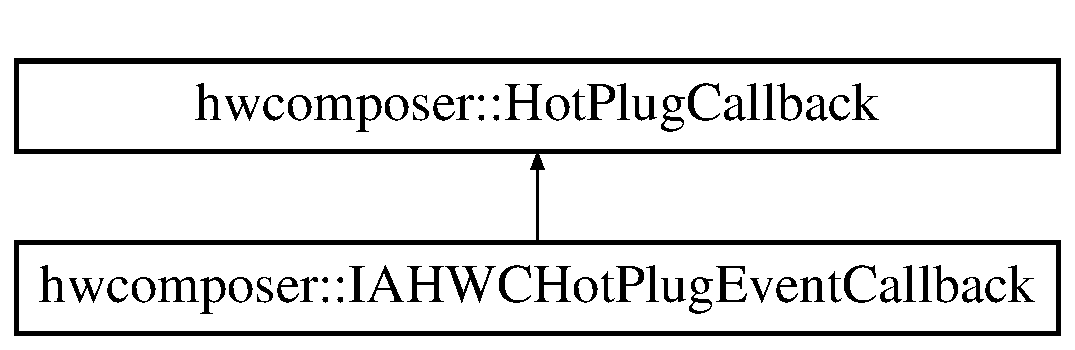
\includegraphics[height=2.000000cm]{classhwcomposer_1_1IAHWCHotPlugEventCallback}
\end{center}
\end{figure}
\subsection*{Public Member Functions}
\begin{DoxyCompactItemize}
\item 
\mbox{\hyperlink{classhwcomposer_1_1IAHWCHotPlugEventCallback_aaa1565ab0f86ac5b78118a5e9a9db977}{I\+A\+H\+W\+C\+Hot\+Plug\+Event\+Callback}} (\mbox{\hyperlink{iahwc_8h_a07fb4f73baa8a0cfbd40f64071e56a7c}{iahwc\+\_\+callback\+\_\+data\+\_\+t}} data, \mbox{\hyperlink{iahwc_8h_a214bf51cce821fdb7b24210088c12cad}{iahwc\+\_\+function\+\_\+ptr\+\_\+t}} hook, \mbox{\hyperlink{classhwcomposer_1_1IAHWC_1_1IAHWCDisplay}{I\+A\+H\+W\+C\+::\+I\+A\+H\+W\+C\+Display}} $\ast$display)
\item 
void \mbox{\hyperlink{classhwcomposer_1_1IAHWCHotPlugEventCallback_a06b3866efbc8e72c992e71357de1b4cb}{Callback}} (uint32\+\_\+t display, bool connected)
\end{DoxyCompactItemize}


\subsection{Detailed Description}


Definition at line 65 of file linux\+\_\+frontend.\+cpp.



\subsection{Constructor \& Destructor Documentation}
\mbox{\Hypertarget{classhwcomposer_1_1IAHWCHotPlugEventCallback_aaa1565ab0f86ac5b78118a5e9a9db977}\label{classhwcomposer_1_1IAHWCHotPlugEventCallback_aaa1565ab0f86ac5b78118a5e9a9db977}} 
\index{hwcomposer\+::\+I\+A\+H\+W\+C\+Hot\+Plug\+Event\+Callback@{hwcomposer\+::\+I\+A\+H\+W\+C\+Hot\+Plug\+Event\+Callback}!I\+A\+H\+W\+C\+Hot\+Plug\+Event\+Callback@{I\+A\+H\+W\+C\+Hot\+Plug\+Event\+Callback}}
\index{I\+A\+H\+W\+C\+Hot\+Plug\+Event\+Callback@{I\+A\+H\+W\+C\+Hot\+Plug\+Event\+Callback}!hwcomposer\+::\+I\+A\+H\+W\+C\+Hot\+Plug\+Event\+Callback@{hwcomposer\+::\+I\+A\+H\+W\+C\+Hot\+Plug\+Event\+Callback}}
\subsubsection{\texorpdfstring{I\+A\+H\+W\+C\+Hot\+Plug\+Event\+Callback()}{IAHWCHotPlugEventCallback()}}
{\footnotesize\ttfamily hwcomposer\+::\+I\+A\+H\+W\+C\+Hot\+Plug\+Event\+Callback\+::\+I\+A\+H\+W\+C\+Hot\+Plug\+Event\+Callback (\begin{DoxyParamCaption}\item[{\mbox{\hyperlink{iahwc_8h_a07fb4f73baa8a0cfbd40f64071e56a7c}{iahwc\+\_\+callback\+\_\+data\+\_\+t}}}]{data,  }\item[{\mbox{\hyperlink{iahwc_8h_a214bf51cce821fdb7b24210088c12cad}{iahwc\+\_\+function\+\_\+ptr\+\_\+t}}}]{hook,  }\item[{\mbox{\hyperlink{classhwcomposer_1_1IAHWC_1_1IAHWCDisplay}{I\+A\+H\+W\+C\+::\+I\+A\+H\+W\+C\+Display}} $\ast$}]{display }\end{DoxyParamCaption})\hspace{0.3cm}{\ttfamily [inline]}}



Definition at line 67 of file linux\+\_\+frontend.\+cpp.


\begin{DoxyCode}{0}
\DoxyCodeLine{70       : data\_(data), hook\_(hook), display\_(display) \{}
\DoxyCodeLine{71   \}}
\end{DoxyCode}


\subsection{Member Function Documentation}
\mbox{\Hypertarget{classhwcomposer_1_1IAHWCHotPlugEventCallback_a06b3866efbc8e72c992e71357de1b4cb}\label{classhwcomposer_1_1IAHWCHotPlugEventCallback_a06b3866efbc8e72c992e71357de1b4cb}} 
\index{hwcomposer\+::\+I\+A\+H\+W\+C\+Hot\+Plug\+Event\+Callback@{hwcomposer\+::\+I\+A\+H\+W\+C\+Hot\+Plug\+Event\+Callback}!Callback@{Callback}}
\index{Callback@{Callback}!hwcomposer\+::\+I\+A\+H\+W\+C\+Hot\+Plug\+Event\+Callback@{hwcomposer\+::\+I\+A\+H\+W\+C\+Hot\+Plug\+Event\+Callback}}
\subsubsection{\texorpdfstring{Callback()}{Callback()}}
{\footnotesize\ttfamily void hwcomposer\+::\+I\+A\+H\+W\+C\+Hot\+Plug\+Event\+Callback\+::\+Callback (\begin{DoxyParamCaption}\item[{uint32\+\_\+t}]{display,  }\item[{bool}]{connected }\end{DoxyParamCaption})\hspace{0.3cm}{\ttfamily [inline]}, {\ttfamily [virtual]}}



Implements \mbox{\hyperlink{classhwcomposer_1_1HotPlugCallback_a455c8913e1da9b165134a05c9cb441ba}{hwcomposer\+::\+Hot\+Plug\+Callback}}.



Definition at line 73 of file linux\+\_\+frontend.\+cpp.


\begin{DoxyCode}{0}
\DoxyCodeLine{73                                                   \{}
\DoxyCodeLine{74     \textcolor{keyword}{auto} hook = \textcolor{keyword}{reinterpret\_cast<}\mbox{\hyperlink{iahwc_8h_a3427a400b38f4c021fd6777bcda36959}{IAHWC\_PFN\_HOTPLUG}}\textcolor{keyword}{>}(hook\_);}
\DoxyCodeLine{75     uint32\_t status;}
\DoxyCodeLine{76     \textcolor{keywordflow}{if} (connected) \{}
\DoxyCodeLine{77       status = \textcolor{keyword}{static\_cast<}uint32\_t\textcolor{keyword}{>}(\mbox{\hyperlink{iahwc_8h_a7bfdefb19187657cb5e884bea59ff672a7cf94b8eb753f8535ea68f5bad15e288}{IAHWC\_DISPLAY\_STATUS\_CONNECTED}});}
\DoxyCodeLine{78       \textcolor{keywordflow}{if} (display\_)}
\DoxyCodeLine{79         display\_->\mbox{\hyperlink{classhwcomposer_1_1IAHWC_1_1IAHWCDisplay_a011a99d6cc9dda103cb57a76036bdd9b}{RunPixelUploader}}(\textcolor{keyword}{true});}
\DoxyCodeLine{80     \} \textcolor{keywordflow}{else} \{}
\DoxyCodeLine{81       status = \textcolor{keyword}{static\_cast<}uint32\_t\textcolor{keyword}{>}(\mbox{\hyperlink{iahwc_8h_a7bfdefb19187657cb5e884bea59ff672a3e45bd4781e15ebcf398937ce031e949}{IAHWC\_DISPLAY\_STATUS\_DISCONNECTED}});}
\DoxyCodeLine{82       \textcolor{keywordflow}{if} (display\_)}
\DoxyCodeLine{83         display\_->\mbox{\hyperlink{classhwcomposer_1_1IAHWC_1_1IAHWCDisplay_a011a99d6cc9dda103cb57a76036bdd9b}{RunPixelUploader}}(\textcolor{keyword}{false});}
\DoxyCodeLine{84     \}}
\DoxyCodeLine{85 }
\DoxyCodeLine{86     \textcolor{keywordflow}{if} (hook)}
\DoxyCodeLine{87       hook(data\_, display, status);}
\DoxyCodeLine{88   \}}
\end{DoxyCode}


The documentation for this class was generated from the following file\+:\begin{DoxyCompactItemize}
\item 
os/linux/\mbox{\hyperlink{linux__frontend_8cpp}{linux\+\_\+frontend.\+cpp}}\end{DoxyCompactItemize}

\hypertarget{classhwcomposer_1_1IAHWC_1_1IAHWCLayer}{}\section{hwcomposer\+:\+:I\+A\+H\+WC\+:\+:I\+A\+H\+W\+C\+Layer Class Reference}
\label{classhwcomposer_1_1IAHWC_1_1IAHWCLayer}\index{hwcomposer\+::\+I\+A\+H\+W\+C\+::\+I\+A\+H\+W\+C\+Layer@{hwcomposer\+::\+I\+A\+H\+W\+C\+::\+I\+A\+H\+W\+C\+Layer}}


{\ttfamily \#include $<$linux\+\_\+frontend.\+h$>$}

Inheritance diagram for hwcomposer\+:\+:I\+A\+H\+WC\+:\+:I\+A\+H\+W\+C\+Layer\+:\begin{figure}[H]
\begin{center}
\leavevmode
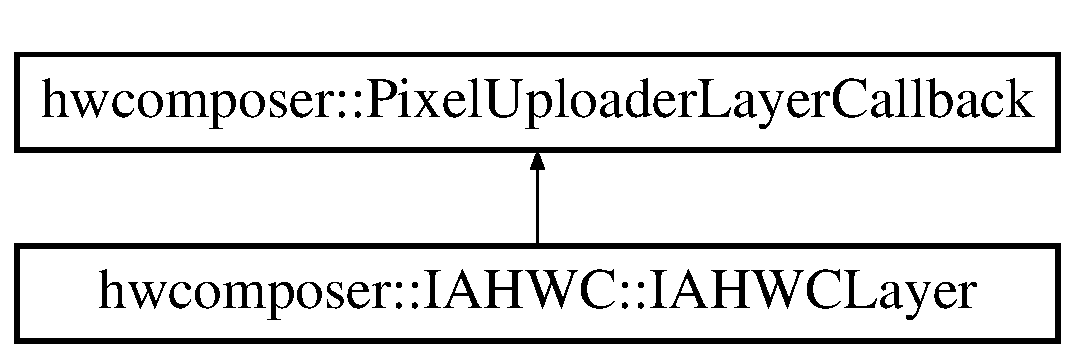
\includegraphics[height=2.000000cm]{classhwcomposer_1_1IAHWC_1_1IAHWCLayer}
\end{center}
\end{figure}
\subsection*{Public Member Functions}
\begin{DoxyCompactItemize}
\item 
\mbox{\hyperlink{classhwcomposer_1_1IAHWC_1_1IAHWCLayer_ae122add62cc7f3cd678c50e496d4c47a}{I\+A\+H\+W\+C\+Layer}} (\mbox{\hyperlink{classhwcomposer_1_1PixelUploader}{Pixel\+Uploader}} $\ast$uploader)
\item 
\mbox{\hyperlink{classhwcomposer_1_1IAHWC_1_1IAHWCLayer_a2892f299cd177f11eb74df9395c8a4aa}{$\sim$\+I\+A\+H\+W\+C\+Layer}} () override
\item 
int \mbox{\hyperlink{classhwcomposer_1_1IAHWC_1_1IAHWCLayer_afedbf8d41373ce7db62460a2da85aeb8}{Set\+Bo}} (gbm\+\_\+bo $\ast$bo)
\item 
int \mbox{\hyperlink{classhwcomposer_1_1IAHWC_1_1IAHWCLayer_a39640aa3fd041b26da6b81d05655d55d}{Set\+Raw\+Pixel\+Data}} (\mbox{\hyperlink{structiahwc__raw__pixel__data}{iahwc\+\_\+raw\+\_\+pixel\+\_\+data}} bo)
\item 
int \mbox{\hyperlink{classhwcomposer_1_1IAHWC_1_1IAHWCLayer_a8837b3203e3146661dc4b4945ec718aa}{Set\+Acquire\+Fence}} (int32\+\_\+t acquire\+\_\+fence)
\item 
int \mbox{\hyperlink{classhwcomposer_1_1IAHWC_1_1IAHWCLayer_ace10db167a3829db79ed6f8c58dcd835}{Set\+Layer\+Usage}} (int32\+\_\+t layer\+\_\+usage)
\item 
int32\+\_\+t \mbox{\hyperlink{classhwcomposer_1_1IAHWC_1_1IAHWCLayer_a6783dc674ff0be10fefab1dd1380e03e}{Get\+Layer\+Usage}} ()
\item 
int \mbox{\hyperlink{classhwcomposer_1_1IAHWC_1_1IAHWCLayer_a35664e00f7b1bb14da7069e28d088ddc}{Set\+Layer\+Transform}} (int32\+\_\+t layer\+\_\+transform)
\item 
int \mbox{\hyperlink{classhwcomposer_1_1IAHWC_1_1IAHWCLayer_a40436b42ea0e7252a27a8c025461ec56}{Set\+Layer\+Source\+Crop}} (\mbox{\hyperlink{iahwc_8h_a163ae45b2470c0d300fe4ec4d017a603}{iahwc\+\_\+rect\+\_\+t}} rect)
\item 
int \mbox{\hyperlink{classhwcomposer_1_1IAHWC_1_1IAHWCLayer_aa8077a3f1267b477a2b1a5ee62e55220}{Set\+Layer\+Display\+Frame}} (\mbox{\hyperlink{iahwc_8h_a163ae45b2470c0d300fe4ec4d017a603}{iahwc\+\_\+rect\+\_\+t}} rect)
\item 
int \mbox{\hyperlink{classhwcomposer_1_1IAHWC_1_1IAHWCLayer_ad06ed34aff071b07ba4afa8e00fc5e34}{Set\+Layer\+Surface\+Damage}} (\mbox{\hyperlink{iahwc_8h_a465287f127b987e53fe91592c12eed43}{iahwc\+\_\+region\+\_\+t}} region)
\item 
int \mbox{\hyperlink{classhwcomposer_1_1IAHWC_1_1IAHWCLayer_ada748eee83ec62b8e3f242583ab2e0bb}{Set\+Layer\+Plane\+Alpha}} (float alpha)
\item 
int \mbox{\hyperlink{classhwcomposer_1_1IAHWC_1_1IAHWCLayer_a4e4374244d15639d4e94e6ac6aa33b92}{Set\+Layer\+Index}} (uint32\+\_\+t layer\+\_\+index)
\item 
uint32\+\_\+t \mbox{\hyperlink{classhwcomposer_1_1IAHWC_1_1IAHWCLayer_ad6659d6ae025b1945a6942bb53842930}{Get\+Layer\+Index}} ()
\item 
\mbox{\hyperlink{structhwcomposer_1_1HwcLayer}{hwcomposer\+::\+Hwc\+Layer}} $\ast$ \mbox{\hyperlink{classhwcomposer_1_1IAHWC_1_1IAHWCLayer_a1c86b8885b0b4cb9cb431fc1e139222d}{Get\+Layer}} ()
\item 
void \mbox{\hyperlink{classhwcomposer_1_1IAHWC_1_1IAHWCLayer_a70158d804e3bf021d32847ffaa33d98d}{Upload\+Done}} () override
\end{DoxyCompactItemize}


\subsection{Detailed Description}


Definition at line 40 of file linux\+\_\+frontend.\+h.



\subsection{Constructor \& Destructor Documentation}
\mbox{\Hypertarget{classhwcomposer_1_1IAHWC_1_1IAHWCLayer_ae122add62cc7f3cd678c50e496d4c47a}\label{classhwcomposer_1_1IAHWC_1_1IAHWCLayer_ae122add62cc7f3cd678c50e496d4c47a}} 
\index{hwcomposer\+::\+I\+A\+H\+W\+C\+::\+I\+A\+H\+W\+C\+Layer@{hwcomposer\+::\+I\+A\+H\+W\+C\+::\+I\+A\+H\+W\+C\+Layer}!I\+A\+H\+W\+C\+Layer@{I\+A\+H\+W\+C\+Layer}}
\index{I\+A\+H\+W\+C\+Layer@{I\+A\+H\+W\+C\+Layer}!hwcomposer\+::\+I\+A\+H\+W\+C\+::\+I\+A\+H\+W\+C\+Layer@{hwcomposer\+::\+I\+A\+H\+W\+C\+::\+I\+A\+H\+W\+C\+Layer}}
\subsubsection{\texorpdfstring{I\+A\+H\+W\+C\+Layer()}{IAHWCLayer()}}
{\footnotesize\ttfamily hwcomposer\+::\+I\+A\+H\+W\+C\+::\+I\+A\+H\+W\+C\+Layer\+::\+I\+A\+H\+W\+C\+Layer (\begin{DoxyParamCaption}\item[{\mbox{\hyperlink{classhwcomposer_1_1PixelUploader}{Pixel\+Uploader}} $\ast$}]{uploader }\end{DoxyParamCaption})}



Definition at line 459 of file linux\+\_\+frontend.\+cpp.


\begin{DoxyCode}{0}
\DoxyCodeLine{460     : raw\_data\_uploader\_(uploader) \{}
\DoxyCodeLine{461   layer\_usage\_ = \mbox{\hyperlink{iahwc_8h_a588980a65b77c13bc2477e3cb31211b8abba2d9f0630811b9208bbf41f40bb2cf}{IAHWC\_LAYER\_USAGE\_NORMAL}};}
\DoxyCodeLine{462   layer\_index\_ = 0;}
\DoxyCodeLine{463   memset(\&hwc\_handle\_.\mbox{\hyperlink{structgbm__handle_ac2450148a271a449b35ff12966de8518}{import\_data}}, 0, \textcolor{keyword}{sizeof}(hwc\_handle\_.\mbox{\hyperlink{structgbm__handle_ac2450148a271a449b35ff12966de8518}{import\_data}}));}
\DoxyCodeLine{464   memset(\&hwc\_handle\_.\mbox{\hyperlink{structgbm__handle_a2d3bce2c387abbf976b37d52b272ebbe}{meta\_data\_}}, 0, \textcolor{keyword}{sizeof}(hwc\_handle\_.\mbox{\hyperlink{structgbm__handle_a2d3bce2c387abbf976b37d52b272ebbe}{meta\_data\_}}));}
\DoxyCodeLine{465   iahwc\_layer\_.\mbox{\hyperlink{structhwcomposer_1_1HwcLayer_a7705d2ba4b36529f37dc0f7e706417eb}{SetBlending}}(hwcomposer::HWCBlending::kBlendingPremult);}
\DoxyCodeLine{466 \}}
\end{DoxyCode}
\mbox{\Hypertarget{classhwcomposer_1_1IAHWC_1_1IAHWCLayer_a2892f299cd177f11eb74df9395c8a4aa}\label{classhwcomposer_1_1IAHWC_1_1IAHWCLayer_a2892f299cd177f11eb74df9395c8a4aa}} 
\index{hwcomposer\+::\+I\+A\+H\+W\+C\+::\+I\+A\+H\+W\+C\+Layer@{hwcomposer\+::\+I\+A\+H\+W\+C\+::\+I\+A\+H\+W\+C\+Layer}!````~I\+A\+H\+W\+C\+Layer@{$\sim$\+I\+A\+H\+W\+C\+Layer}}
\index{````~I\+A\+H\+W\+C\+Layer@{$\sim$\+I\+A\+H\+W\+C\+Layer}!hwcomposer\+::\+I\+A\+H\+W\+C\+::\+I\+A\+H\+W\+C\+Layer@{hwcomposer\+::\+I\+A\+H\+W\+C\+::\+I\+A\+H\+W\+C\+Layer}}
\subsubsection{\texorpdfstring{$\sim$\+I\+A\+H\+W\+C\+Layer()}{~IAHWCLayer()}}
{\footnotesize\ttfamily hwcomposer\+::\+I\+A\+H\+W\+C\+::\+I\+A\+H\+W\+C\+Layer\+::$\sim$\+I\+A\+H\+W\+C\+Layer (\begin{DoxyParamCaption}{ }\end{DoxyParamCaption})\hspace{0.3cm}{\ttfamily [override]}}



Definition at line 468 of file linux\+\_\+frontend.\+cpp.


\begin{DoxyCode}{0}
\DoxyCodeLine{468                              \{}
\DoxyCodeLine{469   \textcolor{keywordflow}{if} (pixel\_buffer\_) \{}
\DoxyCodeLine{470     \textcolor{keyword}{const} NativeBufferHandler* buffer\_handler =}
\DoxyCodeLine{471         raw\_data\_uploader\_->\mbox{\hyperlink{classhwcomposer_1_1PixelUploader_a5fbbbd29b8712fe6fa6278e9422dd1e9}{GetNativeBufferHandler}}();}
\DoxyCodeLine{472     \textcolor{keywordflow}{if} (upload\_in\_progress\_) \{}
\DoxyCodeLine{473       raw\_data\_uploader\_->\mbox{\hyperlink{classhwcomposer_1_1PixelUploader_a1ae866ac73ce4866d88479cebeb16e41}{Synchronize}}();}
\DoxyCodeLine{474     \}}
\DoxyCodeLine{475     buffer\_handler->ReleaseBuffer(pixel\_buffer\_);}
\DoxyCodeLine{476     buffer\_handler->DestroyHandle(pixel\_buffer\_);}
\DoxyCodeLine{477     pixel\_buffer\_ = \mbox{\hyperlink{alios_2platformdefines_8h_a070d2ce7b6bb7e5c05602aa8c308d0c4}{NULL}};}
\DoxyCodeLine{478   \} \textcolor{keywordflow}{else} \{}
\DoxyCodeLine{479     ClosePrimeHandles();}
\DoxyCodeLine{480   \}}
\DoxyCodeLine{481 \}}
\end{DoxyCode}


\subsection{Member Function Documentation}
\mbox{\Hypertarget{classhwcomposer_1_1IAHWC_1_1IAHWCLayer_a1c86b8885b0b4cb9cb431fc1e139222d}\label{classhwcomposer_1_1IAHWC_1_1IAHWCLayer_a1c86b8885b0b4cb9cb431fc1e139222d}} 
\index{hwcomposer\+::\+I\+A\+H\+W\+C\+::\+I\+A\+H\+W\+C\+Layer@{hwcomposer\+::\+I\+A\+H\+W\+C\+::\+I\+A\+H\+W\+C\+Layer}!Get\+Layer@{Get\+Layer}}
\index{Get\+Layer@{Get\+Layer}!hwcomposer\+::\+I\+A\+H\+W\+C\+::\+I\+A\+H\+W\+C\+Layer@{hwcomposer\+::\+I\+A\+H\+W\+C\+::\+I\+A\+H\+W\+C\+Layer}}
\subsubsection{\texorpdfstring{Get\+Layer()}{GetLayer()}}
{\footnotesize\ttfamily \mbox{\hyperlink{structhwcomposer_1_1HwcLayer}{hwcomposer\+::\+Hwc\+Layer}} $\ast$ hwcomposer\+::\+I\+A\+H\+W\+C\+::\+I\+A\+H\+W\+C\+Layer\+::\+Get\+Layer (\begin{DoxyParamCaption}{ }\end{DoxyParamCaption})}



Definition at line 666 of file linux\+\_\+frontend.\+cpp.


\begin{DoxyCode}{0}
\DoxyCodeLine{666                                               \{}
\DoxyCodeLine{667   \textcolor{keywordflow}{return} \&iahwc\_layer\_;}
\DoxyCodeLine{668 \}}
\end{DoxyCode}
\mbox{\Hypertarget{classhwcomposer_1_1IAHWC_1_1IAHWCLayer_ad6659d6ae025b1945a6942bb53842930}\label{classhwcomposer_1_1IAHWC_1_1IAHWCLayer_ad6659d6ae025b1945a6942bb53842930}} 
\index{hwcomposer\+::\+I\+A\+H\+W\+C\+::\+I\+A\+H\+W\+C\+Layer@{hwcomposer\+::\+I\+A\+H\+W\+C\+::\+I\+A\+H\+W\+C\+Layer}!Get\+Layer\+Index@{Get\+Layer\+Index}}
\index{Get\+Layer\+Index@{Get\+Layer\+Index}!hwcomposer\+::\+I\+A\+H\+W\+C\+::\+I\+A\+H\+W\+C\+Layer@{hwcomposer\+::\+I\+A\+H\+W\+C\+::\+I\+A\+H\+W\+C\+Layer}}
\subsubsection{\texorpdfstring{Get\+Layer\+Index()}{GetLayerIndex()}}
{\footnotesize\ttfamily uint32\+\_\+t hwcomposer\+::\+I\+A\+H\+W\+C\+::\+I\+A\+H\+W\+C\+Layer\+::\+Get\+Layer\+Index (\begin{DoxyParamCaption}{ }\end{DoxyParamCaption})\hspace{0.3cm}{\ttfamily [inline]}}



Definition at line 57 of file linux\+\_\+frontend.\+h.


\begin{DoxyCode}{0}
\DoxyCodeLine{57                              \{}
\DoxyCodeLine{58       \textcolor{keywordflow}{return} layer\_index\_;}
\DoxyCodeLine{59     \}}
\end{DoxyCode}
\mbox{\Hypertarget{classhwcomposer_1_1IAHWC_1_1IAHWCLayer_a6783dc674ff0be10fefab1dd1380e03e}\label{classhwcomposer_1_1IAHWC_1_1IAHWCLayer_a6783dc674ff0be10fefab1dd1380e03e}} 
\index{hwcomposer\+::\+I\+A\+H\+W\+C\+::\+I\+A\+H\+W\+C\+Layer@{hwcomposer\+::\+I\+A\+H\+W\+C\+::\+I\+A\+H\+W\+C\+Layer}!Get\+Layer\+Usage@{Get\+Layer\+Usage}}
\index{Get\+Layer\+Usage@{Get\+Layer\+Usage}!hwcomposer\+::\+I\+A\+H\+W\+C\+::\+I\+A\+H\+W\+C\+Layer@{hwcomposer\+::\+I\+A\+H\+W\+C\+::\+I\+A\+H\+W\+C\+Layer}}
\subsubsection{\texorpdfstring{Get\+Layer\+Usage()}{GetLayerUsage()}}
{\footnotesize\ttfamily int32\+\_\+t hwcomposer\+::\+I\+A\+H\+W\+C\+::\+I\+A\+H\+W\+C\+Layer\+::\+Get\+Layer\+Usage (\begin{DoxyParamCaption}{ }\end{DoxyParamCaption})\hspace{0.3cm}{\ttfamily [inline]}}



Definition at line 48 of file linux\+\_\+frontend.\+h.


\begin{DoxyCode}{0}
\DoxyCodeLine{48                             \{}
\DoxyCodeLine{49       \textcolor{keywordflow}{return} layer\_usage\_;}
\DoxyCodeLine{50     \}}
\end{DoxyCode}
\mbox{\Hypertarget{classhwcomposer_1_1IAHWC_1_1IAHWCLayer_a8837b3203e3146661dc4b4945ec718aa}\label{classhwcomposer_1_1IAHWC_1_1IAHWCLayer_a8837b3203e3146661dc4b4945ec718aa}} 
\index{hwcomposer\+::\+I\+A\+H\+W\+C\+::\+I\+A\+H\+W\+C\+Layer@{hwcomposer\+::\+I\+A\+H\+W\+C\+::\+I\+A\+H\+W\+C\+Layer}!Set\+Acquire\+Fence@{Set\+Acquire\+Fence}}
\index{Set\+Acquire\+Fence@{Set\+Acquire\+Fence}!hwcomposer\+::\+I\+A\+H\+W\+C\+::\+I\+A\+H\+W\+C\+Layer@{hwcomposer\+::\+I\+A\+H\+W\+C\+::\+I\+A\+H\+W\+C\+Layer}}
\subsubsection{\texorpdfstring{Set\+Acquire\+Fence()}{SetAcquireFence()}}
{\footnotesize\ttfamily int hwcomposer\+::\+I\+A\+H\+W\+C\+::\+I\+A\+H\+W\+C\+Layer\+::\+Set\+Acquire\+Fence (\begin{DoxyParamCaption}\item[{int32\+\_\+t}]{acquire\+\_\+fence }\end{DoxyParamCaption})}



Definition at line 573 of file linux\+\_\+frontend.\+cpp.


\begin{DoxyCode}{0}
\DoxyCodeLine{573                                                           \{}
\DoxyCodeLine{574   iahwc\_layer\_.\mbox{\hyperlink{structhwcomposer_1_1HwcLayer_aaa01965ccb44cf807ec30956651c431a}{SetAcquireFence}}(acquire\_fence);}
\DoxyCodeLine{575 }
\DoxyCodeLine{576   \textcolor{keywordflow}{return} \mbox{\hyperlink{iahwc_8h_a3ae9e9f48343f1ca3ad7f13a0f000568a4cbfac667065e764d037daea4df0cb42}{IAHWC\_ERROR\_NONE}};}
\DoxyCodeLine{577 \}}
\end{DoxyCode}
\mbox{\Hypertarget{classhwcomposer_1_1IAHWC_1_1IAHWCLayer_afedbf8d41373ce7db62460a2da85aeb8}\label{classhwcomposer_1_1IAHWC_1_1IAHWCLayer_afedbf8d41373ce7db62460a2da85aeb8}} 
\index{hwcomposer\+::\+I\+A\+H\+W\+C\+::\+I\+A\+H\+W\+C\+Layer@{hwcomposer\+::\+I\+A\+H\+W\+C\+::\+I\+A\+H\+W\+C\+Layer}!Set\+Bo@{Set\+Bo}}
\index{Set\+Bo@{Set\+Bo}!hwcomposer\+::\+I\+A\+H\+W\+C\+::\+I\+A\+H\+W\+C\+Layer@{hwcomposer\+::\+I\+A\+H\+W\+C\+::\+I\+A\+H\+W\+C\+Layer}}
\subsubsection{\texorpdfstring{Set\+Bo()}{SetBo()}}
{\footnotesize\ttfamily int hwcomposer\+::\+I\+A\+H\+W\+C\+::\+I\+A\+H\+W\+C\+Layer\+::\+Set\+Bo (\begin{DoxyParamCaption}\item[{gbm\+\_\+bo $\ast$}]{bo }\end{DoxyParamCaption})}



Definition at line 483 of file linux\+\_\+frontend.\+cpp.


\begin{DoxyCode}{0}
\DoxyCodeLine{483                                      \{}
\DoxyCodeLine{484   int32\_t width, height;}
\DoxyCodeLine{485 }
\DoxyCodeLine{486   \textcolor{keywordflow}{if} (pixel\_buffer\_) \{}
\DoxyCodeLine{487     \textcolor{keyword}{const} NativeBufferHandler* buffer\_handler =}
\DoxyCodeLine{488         raw\_data\_uploader\_->\mbox{\hyperlink{classhwcomposer_1_1PixelUploader_a5fbbbd29b8712fe6fa6278e9422dd1e9}{GetNativeBufferHandler}}();}
\DoxyCodeLine{489     \textcolor{keywordflow}{if} (upload\_in\_progress\_) \{}
\DoxyCodeLine{490       raw\_data\_uploader\_->\mbox{\hyperlink{classhwcomposer_1_1PixelUploader_a1ae866ac73ce4866d88479cebeb16e41}{Synchronize}}();}
\DoxyCodeLine{491     \}}
\DoxyCodeLine{492     buffer\_handler->ReleaseBuffer(pixel\_buffer\_);}
\DoxyCodeLine{493     buffer\_handler->DestroyHandle(pixel\_buffer\_);}
\DoxyCodeLine{494     pixel\_buffer\_ = \mbox{\hyperlink{alios_2platformdefines_8h_a070d2ce7b6bb7e5c05602aa8c308d0c4}{NULL}};}
\DoxyCodeLine{495   \} \textcolor{keywordflow}{else} \{}
\DoxyCodeLine{496     ClosePrimeHandles();}
\DoxyCodeLine{497   \}}
\DoxyCodeLine{498 }
\DoxyCodeLine{499   width = gbm\_bo\_get\_width(bo);}
\DoxyCodeLine{500   height = gbm\_bo\_get\_height(bo);}
\DoxyCodeLine{501 }
\DoxyCodeLine{502   hwc\_handle\_.\mbox{\hyperlink{structgbm__handle_ac2450148a271a449b35ff12966de8518}{import\_data}}.\mbox{\hyperlink{structgbm__handle_ae11f3776ec272cc4b10ec0625b647170}{fd\_data}}.width = width;}
\DoxyCodeLine{503   hwc\_handle\_.\mbox{\hyperlink{structgbm__handle_ac2450148a271a449b35ff12966de8518}{import\_data}}.\mbox{\hyperlink{structgbm__handle_ae11f3776ec272cc4b10ec0625b647170}{fd\_data}}.height = height;}
\DoxyCodeLine{504   hwc\_handle\_.\mbox{\hyperlink{structgbm__handle_ac2450148a271a449b35ff12966de8518}{import\_data}}.\mbox{\hyperlink{structgbm__handle_ae11f3776ec272cc4b10ec0625b647170}{fd\_data}}.format = gbm\_bo\_get\_format(bo);}
\DoxyCodeLine{505   hwc\_handle\_.\mbox{\hyperlink{structgbm__handle_ac2450148a271a449b35ff12966de8518}{import\_data}}.\mbox{\hyperlink{structgbm__handle_ae11f3776ec272cc4b10ec0625b647170}{fd\_data}}.fd = gbm\_bo\_get\_fd(bo);}
\DoxyCodeLine{506   hwc\_handle\_.\mbox{\hyperlink{structgbm__handle_ac2450148a271a449b35ff12966de8518}{import\_data}}.\mbox{\hyperlink{structgbm__handle_ae11f3776ec272cc4b10ec0625b647170}{fd\_data}}.stride = gbm\_bo\_get\_stride(bo);}
\DoxyCodeLine{507   hwc\_handle\_.\mbox{\hyperlink{structgbm__handle_a2d3bce2c387abbf976b37d52b272ebbe}{meta\_data\_}}.\mbox{\hyperlink{structHwcBuffer_ab48df5577e8ecd60f18b4b5e6ec6544d}{num\_planes\_}} =}
\DoxyCodeLine{508       drm\_bo\_get\_num\_planes(hwc\_handle\_.\mbox{\hyperlink{structgbm__handle_ac2450148a271a449b35ff12966de8518}{import\_data}}.\mbox{\hyperlink{structgbm__handle_ae11f3776ec272cc4b10ec0625b647170}{fd\_data}}.format);}
\DoxyCodeLine{509 }
\DoxyCodeLine{510   hwc\_handle\_.\mbox{\hyperlink{structgbm__handle_a9010ca6ee25cee546643f6d6c5b6c4cf}{bo}} = bo;}
\DoxyCodeLine{511   hwc\_handle\_.\mbox{\hyperlink{structgbm__handle_aa98e98315d3cd7596b980b80e1199649}{hwc\_buffer\_}} = \textcolor{keyword}{true};}
\DoxyCodeLine{512   hwc\_handle\_.\mbox{\hyperlink{structgbm__handle_a5deee85dd01fe245644d1971dcdd1f89}{gbm\_flags}} = 0;}
\DoxyCodeLine{513 }
\DoxyCodeLine{514   iahwc\_layer\_.\mbox{\hyperlink{structhwcomposer_1_1HwcLayer_aeaeb1f0fd1d4c5754e0946b43c6eef84}{SetNativeHandle}}(\&hwc\_handle\_);}
\DoxyCodeLine{515 }
\DoxyCodeLine{516   \textcolor{keywordflow}{return} \mbox{\hyperlink{iahwc_8h_a3ae9e9f48343f1ca3ad7f13a0f000568a4cbfac667065e764d037daea4df0cb42}{IAHWC\_ERROR\_NONE}};}
\DoxyCodeLine{517 \}}
\end{DoxyCode}
\mbox{\Hypertarget{classhwcomposer_1_1IAHWC_1_1IAHWCLayer_aa8077a3f1267b477a2b1a5ee62e55220}\label{classhwcomposer_1_1IAHWC_1_1IAHWCLayer_aa8077a3f1267b477a2b1a5ee62e55220}} 
\index{hwcomposer\+::\+I\+A\+H\+W\+C\+::\+I\+A\+H\+W\+C\+Layer@{hwcomposer\+::\+I\+A\+H\+W\+C\+::\+I\+A\+H\+W\+C\+Layer}!Set\+Layer\+Display\+Frame@{Set\+Layer\+Display\+Frame}}
\index{Set\+Layer\+Display\+Frame@{Set\+Layer\+Display\+Frame}!hwcomposer\+::\+I\+A\+H\+W\+C\+::\+I\+A\+H\+W\+C\+Layer@{hwcomposer\+::\+I\+A\+H\+W\+C\+::\+I\+A\+H\+W\+C\+Layer}}
\subsubsection{\texorpdfstring{Set\+Layer\+Display\+Frame()}{SetLayerDisplayFrame()}}
{\footnotesize\ttfamily int hwcomposer\+::\+I\+A\+H\+W\+C\+::\+I\+A\+H\+W\+C\+Layer\+::\+Set\+Layer\+Display\+Frame (\begin{DoxyParamCaption}\item[{\mbox{\hyperlink{iahwc_8h_a163ae45b2470c0d300fe4ec4d017a603}{iahwc\+\_\+rect\+\_\+t}}}]{rect }\end{DoxyParamCaption})}



Definition at line 628 of file linux\+\_\+frontend.\+cpp.


\begin{DoxyCode}{0}
\DoxyCodeLine{628                                                            \{}
\DoxyCodeLine{629   iahwc\_layer\_.\mbox{\hyperlink{structhwcomposer_1_1HwcLayer_a0bf1d6ab9b9d45a7e118567b493dd346}{SetDisplayFrame}}(}
\DoxyCodeLine{630       hwcomposer::HwcRect<float>(rect.\mbox{\hyperlink{structiahwc__rect_abdce07c1eb024c79de94fbc1d7a8d40b}{left}}, rect.\mbox{\hyperlink{structiahwc__rect_a16e4547c603c2367753b32a76e547d91}{top}}, rect.\mbox{\hyperlink{structiahwc__rect_a94734af35b59300dd43a54e42bb68ea4}{right}}, rect.
      \mbox{\hyperlink{structiahwc__rect_ad23d12c83244012abee2eb585d8f2052}{bottom}}),}
\DoxyCodeLine{631       0, 0);}
\DoxyCodeLine{632 }
\DoxyCodeLine{633   \textcolor{keywordflow}{return} \mbox{\hyperlink{iahwc_8h_a3ae9e9f48343f1ca3ad7f13a0f000568a4cbfac667065e764d037daea4df0cb42}{IAHWC\_ERROR\_NONE}};}
\DoxyCodeLine{634 \}}
\end{DoxyCode}
\mbox{\Hypertarget{classhwcomposer_1_1IAHWC_1_1IAHWCLayer_a4e4374244d15639d4e94e6ac6aa33b92}\label{classhwcomposer_1_1IAHWC_1_1IAHWCLayer_a4e4374244d15639d4e94e6ac6aa33b92}} 
\index{hwcomposer\+::\+I\+A\+H\+W\+C\+::\+I\+A\+H\+W\+C\+Layer@{hwcomposer\+::\+I\+A\+H\+W\+C\+::\+I\+A\+H\+W\+C\+Layer}!Set\+Layer\+Index@{Set\+Layer\+Index}}
\index{Set\+Layer\+Index@{Set\+Layer\+Index}!hwcomposer\+::\+I\+A\+H\+W\+C\+::\+I\+A\+H\+W\+C\+Layer@{hwcomposer\+::\+I\+A\+H\+W\+C\+::\+I\+A\+H\+W\+C\+Layer}}
\subsubsection{\texorpdfstring{Set\+Layer\+Index()}{SetLayerIndex()}}
{\footnotesize\ttfamily int hwcomposer\+::\+I\+A\+H\+W\+C\+::\+I\+A\+H\+W\+C\+Layer\+::\+Set\+Layer\+Index (\begin{DoxyParamCaption}\item[{uint32\+\_\+t}]{layer\+\_\+index }\end{DoxyParamCaption})}



Definition at line 660 of file linux\+\_\+frontend.\+cpp.


\begin{DoxyCode}{0}
\DoxyCodeLine{660                                                        \{}
\DoxyCodeLine{661   layer\_index\_ = layer\_index;}
\DoxyCodeLine{662 }
\DoxyCodeLine{663   \textcolor{keywordflow}{return} \mbox{\hyperlink{iahwc_8h_a3ae9e9f48343f1ca3ad7f13a0f000568a4cbfac667065e764d037daea4df0cb42}{IAHWC\_ERROR\_NONE}};}
\DoxyCodeLine{664 \}}
\end{DoxyCode}
\mbox{\Hypertarget{classhwcomposer_1_1IAHWC_1_1IAHWCLayer_ada748eee83ec62b8e3f242583ab2e0bb}\label{classhwcomposer_1_1IAHWC_1_1IAHWCLayer_ada748eee83ec62b8e3f242583ab2e0bb}} 
\index{hwcomposer\+::\+I\+A\+H\+W\+C\+::\+I\+A\+H\+W\+C\+Layer@{hwcomposer\+::\+I\+A\+H\+W\+C\+::\+I\+A\+H\+W\+C\+Layer}!Set\+Layer\+Plane\+Alpha@{Set\+Layer\+Plane\+Alpha}}
\index{Set\+Layer\+Plane\+Alpha@{Set\+Layer\+Plane\+Alpha}!hwcomposer\+::\+I\+A\+H\+W\+C\+::\+I\+A\+H\+W\+C\+Layer@{hwcomposer\+::\+I\+A\+H\+W\+C\+::\+I\+A\+H\+W\+C\+Layer}}
\subsubsection{\texorpdfstring{Set\+Layer\+Plane\+Alpha()}{SetLayerPlaneAlpha()}}
{\footnotesize\ttfamily int hwcomposer\+::\+I\+A\+H\+W\+C\+::\+I\+A\+H\+W\+C\+Layer\+::\+Set\+Layer\+Plane\+Alpha (\begin{DoxyParamCaption}\item[{float}]{alpha }\end{DoxyParamCaption})}



Definition at line 651 of file linux\+\_\+frontend.\+cpp.


\begin{DoxyCode}{0}
\DoxyCodeLine{651                                                    \{}
\DoxyCodeLine{652   iahwc\_layer\_.\mbox{\hyperlink{structhwcomposer_1_1HwcLayer_a312a7530c7cdca364df62c950ccbd024}{SetAlpha}}(alpha);}
\DoxyCodeLine{653   \textcolor{keywordflow}{if} (alpha != 1.0) \{}
\DoxyCodeLine{654     iahwc\_layer\_.\mbox{\hyperlink{structhwcomposer_1_1HwcLayer_a7705d2ba4b36529f37dc0f7e706417eb}{SetBlending}}(HWCBlending::kBlendingPremult);}
\DoxyCodeLine{655   \}}
\DoxyCodeLine{656 }
\DoxyCodeLine{657   \textcolor{keywordflow}{return} \mbox{\hyperlink{iahwc_8h_a3ae9e9f48343f1ca3ad7f13a0f000568a4cbfac667065e764d037daea4df0cb42}{IAHWC\_ERROR\_NONE}};}
\DoxyCodeLine{658 \}}
\end{DoxyCode}
\mbox{\Hypertarget{classhwcomposer_1_1IAHWC_1_1IAHWCLayer_a40436b42ea0e7252a27a8c025461ec56}\label{classhwcomposer_1_1IAHWC_1_1IAHWCLayer_a40436b42ea0e7252a27a8c025461ec56}} 
\index{hwcomposer\+::\+I\+A\+H\+W\+C\+::\+I\+A\+H\+W\+C\+Layer@{hwcomposer\+::\+I\+A\+H\+W\+C\+::\+I\+A\+H\+W\+C\+Layer}!Set\+Layer\+Source\+Crop@{Set\+Layer\+Source\+Crop}}
\index{Set\+Layer\+Source\+Crop@{Set\+Layer\+Source\+Crop}!hwcomposer\+::\+I\+A\+H\+W\+C\+::\+I\+A\+H\+W\+C\+Layer@{hwcomposer\+::\+I\+A\+H\+W\+C\+::\+I\+A\+H\+W\+C\+Layer}}
\subsubsection{\texorpdfstring{Set\+Layer\+Source\+Crop()}{SetLayerSourceCrop()}}
{\footnotesize\ttfamily int hwcomposer\+::\+I\+A\+H\+W\+C\+::\+I\+A\+H\+W\+C\+Layer\+::\+Set\+Layer\+Source\+Crop (\begin{DoxyParamCaption}\item[{\mbox{\hyperlink{iahwc_8h_a163ae45b2470c0d300fe4ec4d017a603}{iahwc\+\_\+rect\+\_\+t}}}]{rect }\end{DoxyParamCaption})}



Definition at line 621 of file linux\+\_\+frontend.\+cpp.


\begin{DoxyCode}{0}
\DoxyCodeLine{621                                                          \{}
\DoxyCodeLine{622   iahwc\_layer\_.\mbox{\hyperlink{structhwcomposer_1_1HwcLayer_a83bafbef5b9c98ad5821acdeddd9a26e}{SetSourceCrop}}(}
\DoxyCodeLine{623       hwcomposer::HwcRect<float>(rect.\mbox{\hyperlink{structiahwc__rect_abdce07c1eb024c79de94fbc1d7a8d40b}{left}}, rect.\mbox{\hyperlink{structiahwc__rect_a16e4547c603c2367753b32a76e547d91}{top}}, rect.\mbox{\hyperlink{structiahwc__rect_a94734af35b59300dd43a54e42bb68ea4}{right}}, rect.
      \mbox{\hyperlink{structiahwc__rect_ad23d12c83244012abee2eb585d8f2052}{bottom}}));}
\DoxyCodeLine{624 }
\DoxyCodeLine{625   \textcolor{keywordflow}{return} \mbox{\hyperlink{iahwc_8h_a3ae9e9f48343f1ca3ad7f13a0f000568a4cbfac667065e764d037daea4df0cb42}{IAHWC\_ERROR\_NONE}};}
\DoxyCodeLine{626 \}}
\end{DoxyCode}
\mbox{\Hypertarget{classhwcomposer_1_1IAHWC_1_1IAHWCLayer_ad06ed34aff071b07ba4afa8e00fc5e34}\label{classhwcomposer_1_1IAHWC_1_1IAHWCLayer_ad06ed34aff071b07ba4afa8e00fc5e34}} 
\index{hwcomposer\+::\+I\+A\+H\+W\+C\+::\+I\+A\+H\+W\+C\+Layer@{hwcomposer\+::\+I\+A\+H\+W\+C\+::\+I\+A\+H\+W\+C\+Layer}!Set\+Layer\+Surface\+Damage@{Set\+Layer\+Surface\+Damage}}
\index{Set\+Layer\+Surface\+Damage@{Set\+Layer\+Surface\+Damage}!hwcomposer\+::\+I\+A\+H\+W\+C\+::\+I\+A\+H\+W\+C\+Layer@{hwcomposer\+::\+I\+A\+H\+W\+C\+::\+I\+A\+H\+W\+C\+Layer}}
\subsubsection{\texorpdfstring{Set\+Layer\+Surface\+Damage()}{SetLayerSurfaceDamage()}}
{\footnotesize\ttfamily int hwcomposer\+::\+I\+A\+H\+W\+C\+::\+I\+A\+H\+W\+C\+Layer\+::\+Set\+Layer\+Surface\+Damage (\begin{DoxyParamCaption}\item[{\mbox{\hyperlink{iahwc_8h_a465287f127b987e53fe91592c12eed43}{iahwc\+\_\+region\+\_\+t}}}]{region }\end{DoxyParamCaption})}



Definition at line 636 of file linux\+\_\+frontend.\+cpp.


\begin{DoxyCode}{0}
\DoxyCodeLine{636                                                                 \{}
\DoxyCodeLine{637   uint32\_t num\_rects = region.\mbox{\hyperlink{structiahwc__region_a72a48239f66d9b87cc76a2bbbbdc48a1}{numRects}};}
\DoxyCodeLine{638   hwcomposer::HwcRegion hwc\_region;}
\DoxyCodeLine{639 }
\DoxyCodeLine{640   \textcolor{keywordflow}{for} (\textcolor{keywordtype}{size\_t} rect = 0; rect < num\_rects; ++rect) \{}
\DoxyCodeLine{641     hwc\_region.emplace\_back(region.\mbox{\hyperlink{structiahwc__region_a94a878c575f670019f83b1cac59094a5}{rects}}[rect].\mbox{\hyperlink{structiahwc__rect_abdce07c1eb024c79de94fbc1d7a8d40b}{left}}, region.\mbox{\hyperlink{structiahwc__region_a94a878c575f670019f83b1cac59094a5}{rects}}[rect].
      \mbox{\hyperlink{structiahwc__rect_a16e4547c603c2367753b32a76e547d91}{top}},}
\DoxyCodeLine{642                             region.\mbox{\hyperlink{structiahwc__region_a94a878c575f670019f83b1cac59094a5}{rects}}[rect].\mbox{\hyperlink{structiahwc__rect_a94734af35b59300dd43a54e42bb68ea4}{right}},}
\DoxyCodeLine{643                             region.\mbox{\hyperlink{structiahwc__region_a94a878c575f670019f83b1cac59094a5}{rects}}[rect].\mbox{\hyperlink{structiahwc__rect_ad23d12c83244012abee2eb585d8f2052}{bottom}});}
\DoxyCodeLine{644   \}}
\DoxyCodeLine{645 }
\DoxyCodeLine{646   iahwc\_layer\_.\mbox{\hyperlink{structhwcomposer_1_1HwcLayer_a25ec3931c5bb7108c4b8c39c839b26dc}{SetSurfaceDamage}}(hwc\_region);}
\DoxyCodeLine{647 }
\DoxyCodeLine{648   \textcolor{keywordflow}{return} \mbox{\hyperlink{iahwc_8h_a3ae9e9f48343f1ca3ad7f13a0f000568a4cbfac667065e764d037daea4df0cb42}{IAHWC\_ERROR\_NONE}};}
\DoxyCodeLine{649 \}}
\end{DoxyCode}
\mbox{\Hypertarget{classhwcomposer_1_1IAHWC_1_1IAHWCLayer_a35664e00f7b1bb14da7069e28d088ddc}\label{classhwcomposer_1_1IAHWC_1_1IAHWCLayer_a35664e00f7b1bb14da7069e28d088ddc}} 
\index{hwcomposer\+::\+I\+A\+H\+W\+C\+::\+I\+A\+H\+W\+C\+Layer@{hwcomposer\+::\+I\+A\+H\+W\+C\+::\+I\+A\+H\+W\+C\+Layer}!Set\+Layer\+Transform@{Set\+Layer\+Transform}}
\index{Set\+Layer\+Transform@{Set\+Layer\+Transform}!hwcomposer\+::\+I\+A\+H\+W\+C\+::\+I\+A\+H\+W\+C\+Layer@{hwcomposer\+::\+I\+A\+H\+W\+C\+::\+I\+A\+H\+W\+C\+Layer}}
\subsubsection{\texorpdfstring{Set\+Layer\+Transform()}{SetLayerTransform()}}
{\footnotesize\ttfamily int hwcomposer\+::\+I\+A\+H\+W\+C\+::\+I\+A\+H\+W\+C\+Layer\+::\+Set\+Layer\+Transform (\begin{DoxyParamCaption}\item[{int32\+\_\+t}]{layer\+\_\+transform }\end{DoxyParamCaption})}



Definition at line 598 of file linux\+\_\+frontend.\+cpp.


\begin{DoxyCode}{0}
\DoxyCodeLine{598                                                               \{}
\DoxyCodeLine{599   \textcolor{comment}{// 270* and 180* cannot be combined with flips. More specifically, they}}
\DoxyCodeLine{600   \textcolor{comment}{// already contain both horizontal and vertical flips, so those fields are}}
\DoxyCodeLine{601   \textcolor{comment}{// redundant in this case. 90* rotation can be combined with either horizontal}}
\DoxyCodeLine{602   \textcolor{comment}{// flip or vertical flip, so treat it differently}}
\DoxyCodeLine{603   int32\_t temp = 0;}
\DoxyCodeLine{604   \textcolor{keywordflow}{if} (layer\_transform == \mbox{\hyperlink{iahwc_8h_ad2ccc6d0ea95b717646105fd0d5409e8a4361db3afc90d8fbe616cd37c11102ae}{IAHWC\_TRANSFORM\_ROT\_270}}) \{}
\DoxyCodeLine{605     temp = hwcomposer::HWCTransform::kTransform270;}
\DoxyCodeLine{606   \} \textcolor{keywordflow}{else} \textcolor{keywordflow}{if} (layer\_transform == \mbox{\hyperlink{iahwc_8h_ad2ccc6d0ea95b717646105fd0d5409e8a8bcec79257b91c13f5f0544f52d4c77e}{IAHWC\_TRANSFORM\_ROT\_180}}) \{}
\DoxyCodeLine{607     temp = hwcomposer::HWCTransform::kTransform180;}
\DoxyCodeLine{608   \} \textcolor{keywordflow}{else} \{}
\DoxyCodeLine{609     \textcolor{keywordflow}{if} (layer\_transform \& \mbox{\hyperlink{iahwc_8h_ad2ccc6d0ea95b717646105fd0d5409e8acb13fb681c8a80d8a104d9edceab4eec}{IAHWC\_TRANSFORM\_FLIP\_H}})}
\DoxyCodeLine{610       temp |= hwcomposer::HWCTransform::kReflectX;}
\DoxyCodeLine{611     \textcolor{keywordflow}{if} (layer\_transform \& \mbox{\hyperlink{iahwc_8h_ad2ccc6d0ea95b717646105fd0d5409e8a2431bd128ed51fa7758118bfb6514b74}{IAHWC\_TRANSFORM\_FLIP\_V}})}
\DoxyCodeLine{612       temp |= hwcomposer::HWCTransform::kReflectY;}
\DoxyCodeLine{613     \textcolor{keywordflow}{if} (layer\_transform \& \mbox{\hyperlink{iahwc_8h_ad2ccc6d0ea95b717646105fd0d5409e8a254df9b28eef149a1429db57859d3d85}{IAHWC\_TRANSFORM\_ROT\_90}})}
\DoxyCodeLine{614       temp |= hwcomposer::HWCTransform::kTransform90;}
\DoxyCodeLine{615   \}}
\DoxyCodeLine{616   iahwc\_layer\_.\mbox{\hyperlink{structhwcomposer_1_1HwcLayer_ab30467eafc63b3b95059ff6ca3738933}{SetTransform}}(temp);}
\DoxyCodeLine{617 }
\DoxyCodeLine{618   \textcolor{keywordflow}{return} \mbox{\hyperlink{iahwc_8h_a3ae9e9f48343f1ca3ad7f13a0f000568a4cbfac667065e764d037daea4df0cb42}{IAHWC\_ERROR\_NONE}};}
\DoxyCodeLine{619 \}}
\end{DoxyCode}
\mbox{\Hypertarget{classhwcomposer_1_1IAHWC_1_1IAHWCLayer_ace10db167a3829db79ed6f8c58dcd835}\label{classhwcomposer_1_1IAHWC_1_1IAHWCLayer_ace10db167a3829db79ed6f8c58dcd835}} 
\index{hwcomposer\+::\+I\+A\+H\+W\+C\+::\+I\+A\+H\+W\+C\+Layer@{hwcomposer\+::\+I\+A\+H\+W\+C\+::\+I\+A\+H\+W\+C\+Layer}!Set\+Layer\+Usage@{Set\+Layer\+Usage}}
\index{Set\+Layer\+Usage@{Set\+Layer\+Usage}!hwcomposer\+::\+I\+A\+H\+W\+C\+::\+I\+A\+H\+W\+C\+Layer@{hwcomposer\+::\+I\+A\+H\+W\+C\+::\+I\+A\+H\+W\+C\+Layer}}
\subsubsection{\texorpdfstring{Set\+Layer\+Usage()}{SetLayerUsage()}}
{\footnotesize\ttfamily int hwcomposer\+::\+I\+A\+H\+W\+C\+::\+I\+A\+H\+W\+C\+Layer\+::\+Set\+Layer\+Usage (\begin{DoxyParamCaption}\item[{int32\+\_\+t}]{layer\+\_\+usage }\end{DoxyParamCaption})}



Definition at line 579 of file linux\+\_\+frontend.\+cpp.


\begin{DoxyCode}{0}
\DoxyCodeLine{579                                                       \{}
\DoxyCodeLine{580   \textcolor{keywordflow}{if} (layer\_usage\_ != layer\_usage) \{}
\DoxyCodeLine{581     layer\_usage\_ = layer\_usage;}
\DoxyCodeLine{582     \textcolor{keywordflow}{if} (layer\_usage\_ == \mbox{\hyperlink{iahwc_8h_a588980a65b77c13bc2477e3cb31211b8a403b21c8497356bda1e7d1957b4f940a}{IAHWC\_LAYER\_USAGE\_CURSOR}}) \{}
\DoxyCodeLine{583       iahwc\_layer\_.\mbox{\hyperlink{structhwcomposer_1_1HwcLayer_a7556bacbb2697f51b2c2cc30a9ed661a}{MarkAsCursorLayer}}();}
\DoxyCodeLine{584     \}}
\DoxyCodeLine{585 }
\DoxyCodeLine{586     \textcolor{keywordflow}{if} (pixel\_buffer\_) \{}
\DoxyCodeLine{587       \textcolor{keyword}{const} NativeBufferHandler* buffer\_handler =}
\DoxyCodeLine{588           raw\_data\_uploader\_->\mbox{\hyperlink{classhwcomposer_1_1PixelUploader_a5fbbbd29b8712fe6fa6278e9422dd1e9}{GetNativeBufferHandler}}();}
\DoxyCodeLine{589       buffer\_handler->\mbox{\hyperlink{classhwcomposer_1_1NativeBufferHandler_abff911db92343545a36a0cc44a8d2eb8}{ReleaseBuffer}}(pixel\_buffer\_);}
\DoxyCodeLine{590       buffer\_handler->DestroyHandle(pixel\_buffer\_);}
\DoxyCodeLine{591       pixel\_buffer\_ = \mbox{\hyperlink{alios_2platformdefines_8h_a070d2ce7b6bb7e5c05602aa8c308d0c4}{NULL}};}
\DoxyCodeLine{592     \}}
\DoxyCodeLine{593   \}}
\DoxyCodeLine{594 }
\DoxyCodeLine{595   \textcolor{keywordflow}{return} \mbox{\hyperlink{iahwc_8h_a3ae9e9f48343f1ca3ad7f13a0f000568a4cbfac667065e764d037daea4df0cb42}{IAHWC\_ERROR\_NONE}};}
\DoxyCodeLine{596 \}}
\end{DoxyCode}
\mbox{\Hypertarget{classhwcomposer_1_1IAHWC_1_1IAHWCLayer_a39640aa3fd041b26da6b81d05655d55d}\label{classhwcomposer_1_1IAHWC_1_1IAHWCLayer_a39640aa3fd041b26da6b81d05655d55d}} 
\index{hwcomposer\+::\+I\+A\+H\+W\+C\+::\+I\+A\+H\+W\+C\+Layer@{hwcomposer\+::\+I\+A\+H\+W\+C\+::\+I\+A\+H\+W\+C\+Layer}!Set\+Raw\+Pixel\+Data@{Set\+Raw\+Pixel\+Data}}
\index{Set\+Raw\+Pixel\+Data@{Set\+Raw\+Pixel\+Data}!hwcomposer\+::\+I\+A\+H\+W\+C\+::\+I\+A\+H\+W\+C\+Layer@{hwcomposer\+::\+I\+A\+H\+W\+C\+::\+I\+A\+H\+W\+C\+Layer}}
\subsubsection{\texorpdfstring{Set\+Raw\+Pixel\+Data()}{SetRawPixelData()}}
{\footnotesize\ttfamily int hwcomposer\+::\+I\+A\+H\+W\+C\+::\+I\+A\+H\+W\+C\+Layer\+::\+Set\+Raw\+Pixel\+Data (\begin{DoxyParamCaption}\item[{\mbox{\hyperlink{structiahwc__raw__pixel__data}{iahwc\+\_\+raw\+\_\+pixel\+\_\+data}}}]{bo }\end{DoxyParamCaption})}



Definition at line 519 of file linux\+\_\+frontend.\+cpp.


\begin{DoxyCode}{0}
\DoxyCodeLine{519                                                             \{}
\DoxyCodeLine{520   \textcolor{keyword}{const} NativeBufferHandler* buffer\_handler =}
\DoxyCodeLine{521       raw\_data\_uploader\_->\mbox{\hyperlink{classhwcomposer_1_1PixelUploader_a5fbbbd29b8712fe6fa6278e9422dd1e9}{GetNativeBufferHandler}}();}
\DoxyCodeLine{522   ClosePrimeHandles();}
\DoxyCodeLine{523   \textcolor{keywordflow}{if} (pixel\_buffer\_ \&\&}
\DoxyCodeLine{524       ((orig\_height\_ != bo.\mbox{\hyperlink{structiahwc__raw__pixel__data_aa8ad90e89455a36ad2c423c33ff189fa}{height}}) || (orig\_stride\_ != bo.\mbox{\hyperlink{structiahwc__raw__pixel__data_a7b63e928cb013a04cfe12a69a4cf7241}{stride}}))) \{}
\DoxyCodeLine{525     \textcolor{keywordflow}{if} (upload\_in\_progress\_) \{}
\DoxyCodeLine{526       raw\_data\_uploader\_->\mbox{\hyperlink{classhwcomposer_1_1PixelUploader_a1ae866ac73ce4866d88479cebeb16e41}{Synchronize}}();}
\DoxyCodeLine{527     \}}
\DoxyCodeLine{528 }
\DoxyCodeLine{529     buffer\_handler->ReleaseBuffer(pixel\_buffer\_);}
\DoxyCodeLine{530     buffer\_handler->DestroyHandle(pixel\_buffer\_);}
\DoxyCodeLine{531     pixel\_buffer\_ = \mbox{\hyperlink{alios_2platformdefines_8h_a070d2ce7b6bb7e5c05602aa8c308d0c4}{NULL}};}
\DoxyCodeLine{532   \}}
\DoxyCodeLine{533 }
\DoxyCodeLine{534   \textcolor{keywordflow}{if} (!pixel\_buffer\_) \{}
\DoxyCodeLine{535     \textcolor{keywordtype}{int} layer\_type =}
\DoxyCodeLine{536         layer\_usage\_ == \mbox{\hyperlink{iahwc_8h_a588980a65b77c13bc2477e3cb31211b8a403b21c8497356bda1e7d1957b4f940a}{IAHWC\_LAYER\_USAGE\_CURSOR}} ? kLayerCursor : kLayerNormal;}
\DoxyCodeLine{537     \textcolor{keywordtype}{bool} modifier\_used = \textcolor{keyword}{false};}
\DoxyCodeLine{538     \textcolor{keywordflow}{if} (!buffer\_handler->CreateBuffer(bo.\mbox{\hyperlink{structiahwc__raw__pixel__data_afa9b60fc4678e26c901c703837fdabb3}{width}}, bo.\mbox{\hyperlink{structiahwc__raw__pixel__data_aa8ad90e89455a36ad2c423c33ff189fa}{height}}, bo.\mbox{\hyperlink{structiahwc__raw__pixel__data_afa6eeb611dda100904b14919b74b1d9d}{format}},}
\DoxyCodeLine{539                                       \&pixel\_buffer\_, layer\_type,}
\DoxyCodeLine{540                                       \&modifier\_used, 0, \textcolor{keyword}{true})) \{}
\DoxyCodeLine{541       \mbox{\hyperlink{alios_2platformdefines_8h_a226d6c99e4bcfca193c095e085e9097d}{ETRACE}}(\textcolor{stringliteral}{"PixelBuffer: CreateBuffer failed"});}
\DoxyCodeLine{542       \textcolor{keywordflow}{return} -1;}
\DoxyCodeLine{543     \}}
\DoxyCodeLine{544 }
\DoxyCodeLine{545     \textcolor{keywordflow}{if} (!buffer\_handler->ImportBuffer(pixel\_buffer\_)) \{}
\DoxyCodeLine{546       \mbox{\hyperlink{alios_2platformdefines_8h_a226d6c99e4bcfca193c095e085e9097d}{ETRACE}}(\textcolor{stringliteral}{"PixelBuffer: ImportBuffer failed"});}
\DoxyCodeLine{547       \textcolor{keywordflow}{return} -1;}
\DoxyCodeLine{548     \}}
\DoxyCodeLine{549 }
\DoxyCodeLine{550     \textcolor{keywordflow}{if} (pixel\_buffer\_->\mbox{\hyperlink{structyalloc__handle_a2dfa4e2505a052e5ddbbe66e32b33875}{meta\_data\_}}.\mbox{\hyperlink{structHwcBuffer_a51f659d550dae6ea7b6208019cc08169}{prime\_fds\_}}[0] <= 0) \{}
\DoxyCodeLine{551       \mbox{\hyperlink{alios_2platformdefines_8h_a226d6c99e4bcfca193c095e085e9097d}{ETRACE}}(\textcolor{stringliteral}{"PixelBuffer: prime\_fd\_ is invalid."});}
\DoxyCodeLine{552       \textcolor{keywordflow}{return} -1;}
\DoxyCodeLine{553     \}}
\DoxyCodeLine{554 }
\DoxyCodeLine{555     orig\_width\_ = bo.\mbox{\hyperlink{structiahwc__raw__pixel__data_afa9b60fc4678e26c901c703837fdabb3}{width}};}
\DoxyCodeLine{556     orig\_height\_ = bo.\mbox{\hyperlink{structiahwc__raw__pixel__data_aa8ad90e89455a36ad2c423c33ff189fa}{height}};}
\DoxyCodeLine{557     orig\_stride\_ = bo.\mbox{\hyperlink{structiahwc__raw__pixel__data_a7b63e928cb013a04cfe12a69a4cf7241}{stride}};}
\DoxyCodeLine{558     iahwc\_layer\_.\mbox{\hyperlink{structhwcomposer_1_1HwcLayer_aeaeb1f0fd1d4c5754e0946b43c6eef84}{SetNativeHandle}}(pixel\_buffer\_);}
\DoxyCodeLine{559   \}}
\DoxyCodeLine{560 }
\DoxyCodeLine{561   upload\_in\_progress\_ = \textcolor{keyword}{true};}
\DoxyCodeLine{562   raw\_data\_uploader\_->\mbox{\hyperlink{classhwcomposer_1_1PixelUploader_ae2154e6039f703b8ce95ac3ffe8e8c8b}{UpdateLayerPixelData}}(}
\DoxyCodeLine{563       pixel\_buffer\_, orig\_width\_, orig\_height\_, orig\_stride\_, bo.\mbox{\hyperlink{structiahwc__raw__pixel__data_ab7e2bf82485679c69226d5d42bbe7e1c}{callback\_data}},}
\DoxyCodeLine{564       (uint8\_t*)bo.\mbox{\hyperlink{structiahwc__raw__pixel__data_ad7d42f2ede4d429072a20f791f3a2625}{buffer}}, \textcolor{keyword}{this}, iahwc\_layer\_.\mbox{\hyperlink{structhwcomposer_1_1HwcLayer_ada1b7ecdb1a62513e4c985deccb60cd7}{GetSurfaceDamage}}());}
\DoxyCodeLine{565 }
\DoxyCodeLine{566   \textcolor{keywordflow}{return} \mbox{\hyperlink{iahwc_8h_a3ae9e9f48343f1ca3ad7f13a0f000568a4cbfac667065e764d037daea4df0cb42}{IAHWC\_ERROR\_NONE}};}
\DoxyCodeLine{567 \}}
\end{DoxyCode}
\mbox{\Hypertarget{classhwcomposer_1_1IAHWC_1_1IAHWCLayer_a70158d804e3bf021d32847ffaa33d98d}\label{classhwcomposer_1_1IAHWC_1_1IAHWCLayer_a70158d804e3bf021d32847ffaa33d98d}} 
\index{hwcomposer\+::\+I\+A\+H\+W\+C\+::\+I\+A\+H\+W\+C\+Layer@{hwcomposer\+::\+I\+A\+H\+W\+C\+::\+I\+A\+H\+W\+C\+Layer}!Upload\+Done@{Upload\+Done}}
\index{Upload\+Done@{Upload\+Done}!hwcomposer\+::\+I\+A\+H\+W\+C\+::\+I\+A\+H\+W\+C\+Layer@{hwcomposer\+::\+I\+A\+H\+W\+C\+::\+I\+A\+H\+W\+C\+Layer}}
\subsubsection{\texorpdfstring{Upload\+Done()}{UploadDone()}}
{\footnotesize\ttfamily void hwcomposer\+::\+I\+A\+H\+W\+C\+::\+I\+A\+H\+W\+C\+Layer\+::\+Upload\+Done (\begin{DoxyParamCaption}{ }\end{DoxyParamCaption})\hspace{0.3cm}{\ttfamily [override]}, {\ttfamily [virtual]}}



Implements \mbox{\hyperlink{classhwcomposer_1_1PixelUploaderLayerCallback_a3234bfd4e803b50e8f41cb53ff430559}{hwcomposer\+::\+Pixel\+Uploader\+Layer\+Callback}}.



Definition at line 569 of file linux\+\_\+frontend.\+cpp.


\begin{DoxyCode}{0}
\DoxyCodeLine{569                                  \{}
\DoxyCodeLine{570   upload\_in\_progress\_ = \textcolor{keyword}{false};}
\DoxyCodeLine{571 \}}
\end{DoxyCode}


The documentation for this class was generated from the following files\+:\begin{DoxyCompactItemize}
\item 
os/linux/\mbox{\hyperlink{linux__frontend_8h}{linux\+\_\+frontend.\+h}}\item 
os/linux/\mbox{\hyperlink{linux__frontend_8cpp}{linux\+\_\+frontend.\+cpp}}\end{DoxyCompactItemize}

\hypertarget{classhwcomposer_1_1IAHWCVsyncCallback}{}\section{hwcomposer\+:\+:I\+A\+H\+W\+C\+Vsync\+Callback Class Reference}
\label{classhwcomposer_1_1IAHWCVsyncCallback}\index{hwcomposer\+::\+I\+A\+H\+W\+C\+Vsync\+Callback@{hwcomposer\+::\+I\+A\+H\+W\+C\+Vsync\+Callback}}
Inheritance diagram for hwcomposer\+:\+:I\+A\+H\+W\+C\+Vsync\+Callback\+:\begin{figure}[H]
\begin{center}
\leavevmode
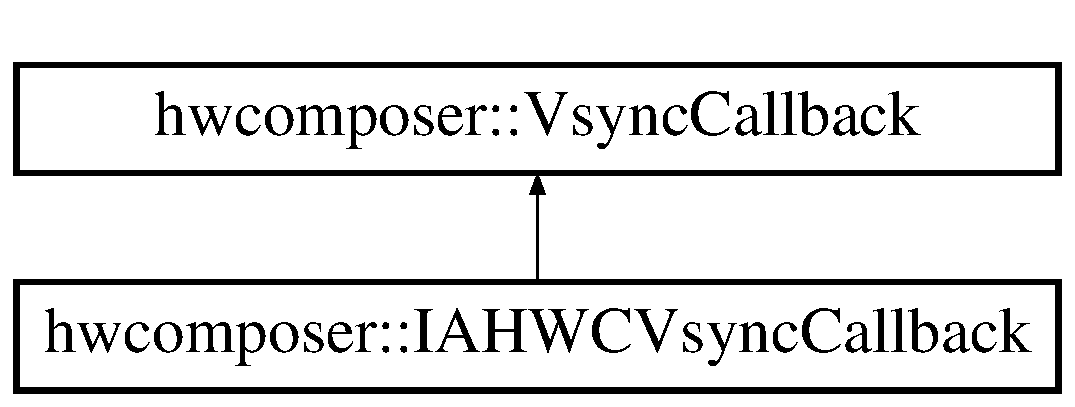
\includegraphics[height=2.000000cm]{classhwcomposer_1_1IAHWCVsyncCallback}
\end{center}
\end{figure}
\subsection*{Public Member Functions}
\begin{DoxyCompactItemize}
\item 
\mbox{\hyperlink{classhwcomposer_1_1IAHWCVsyncCallback_a7710057d33beeaa74157a070aaad0972}{I\+A\+H\+W\+C\+Vsync\+Callback}} (\mbox{\hyperlink{iahwc_8h_a07fb4f73baa8a0cfbd40f64071e56a7c}{iahwc\+\_\+callback\+\_\+data\+\_\+t}} data, \mbox{\hyperlink{iahwc_8h_a214bf51cce821fdb7b24210088c12cad}{iahwc\+\_\+function\+\_\+ptr\+\_\+t}} hook)
\item 
void \mbox{\hyperlink{classhwcomposer_1_1IAHWCVsyncCallback_a8e89987e4a1f85b917f82166978ede94}{Callback}} (uint32\+\_\+t display, int64\+\_\+t timestamp)
\end{DoxyCompactItemize}


\subsection{Detailed Description}


Definition at line 27 of file linux\+\_\+frontend.\+cpp.



\subsection{Constructor \& Destructor Documentation}
\mbox{\Hypertarget{classhwcomposer_1_1IAHWCVsyncCallback_a7710057d33beeaa74157a070aaad0972}\label{classhwcomposer_1_1IAHWCVsyncCallback_a7710057d33beeaa74157a070aaad0972}} 
\index{hwcomposer\+::\+I\+A\+H\+W\+C\+Vsync\+Callback@{hwcomposer\+::\+I\+A\+H\+W\+C\+Vsync\+Callback}!I\+A\+H\+W\+C\+Vsync\+Callback@{I\+A\+H\+W\+C\+Vsync\+Callback}}
\index{I\+A\+H\+W\+C\+Vsync\+Callback@{I\+A\+H\+W\+C\+Vsync\+Callback}!hwcomposer\+::\+I\+A\+H\+W\+C\+Vsync\+Callback@{hwcomposer\+::\+I\+A\+H\+W\+C\+Vsync\+Callback}}
\subsubsection{\texorpdfstring{I\+A\+H\+W\+C\+Vsync\+Callback()}{IAHWCVsyncCallback()}}
{\footnotesize\ttfamily hwcomposer\+::\+I\+A\+H\+W\+C\+Vsync\+Callback\+::\+I\+A\+H\+W\+C\+Vsync\+Callback (\begin{DoxyParamCaption}\item[{\mbox{\hyperlink{iahwc_8h_a07fb4f73baa8a0cfbd40f64071e56a7c}{iahwc\+\_\+callback\+\_\+data\+\_\+t}}}]{data,  }\item[{\mbox{\hyperlink{iahwc_8h_a214bf51cce821fdb7b24210088c12cad}{iahwc\+\_\+function\+\_\+ptr\+\_\+t}}}]{hook }\end{DoxyParamCaption})\hspace{0.3cm}{\ttfamily [inline]}}



Definition at line 29 of file linux\+\_\+frontend.\+cpp.


\begin{DoxyCode}{0}
\DoxyCodeLine{30       : data\_(data), hook\_(hook) \{}
\DoxyCodeLine{31   \}}
\end{DoxyCode}


\subsection{Member Function Documentation}
\mbox{\Hypertarget{classhwcomposer_1_1IAHWCVsyncCallback_a8e89987e4a1f85b917f82166978ede94}\label{classhwcomposer_1_1IAHWCVsyncCallback_a8e89987e4a1f85b917f82166978ede94}} 
\index{hwcomposer\+::\+I\+A\+H\+W\+C\+Vsync\+Callback@{hwcomposer\+::\+I\+A\+H\+W\+C\+Vsync\+Callback}!Callback@{Callback}}
\index{Callback@{Callback}!hwcomposer\+::\+I\+A\+H\+W\+C\+Vsync\+Callback@{hwcomposer\+::\+I\+A\+H\+W\+C\+Vsync\+Callback}}
\subsubsection{\texorpdfstring{Callback()}{Callback()}}
{\footnotesize\ttfamily void hwcomposer\+::\+I\+A\+H\+W\+C\+Vsync\+Callback\+::\+Callback (\begin{DoxyParamCaption}\item[{uint32\+\_\+t}]{display,  }\item[{int64\+\_\+t}]{timestamp }\end{DoxyParamCaption})\hspace{0.3cm}{\ttfamily [inline]}, {\ttfamily [virtual]}}



Implements \mbox{\hyperlink{classhwcomposer_1_1VsyncCallback_a632ac6a2e13e1b387df9508507a2ed4d}{hwcomposer\+::\+Vsync\+Callback}}.



Definition at line 33 of file linux\+\_\+frontend.\+cpp.


\begin{DoxyCode}{0}
\DoxyCodeLine{33                                                      \{}
\DoxyCodeLine{34     \textcolor{keywordflow}{if} (hook\_ != \mbox{\hyperlink{alios_2platformdefines_8h_a070d2ce7b6bb7e5c05602aa8c308d0c4}{NULL}}) \{}
\DoxyCodeLine{35       \textcolor{keyword}{auto} hook = \textcolor{keyword}{reinterpret\_cast<}\mbox{\hyperlink{iahwc_8h_a17fc9ccb2b851174b75f6eaca8c2fdb5}{IAHWC\_PFN\_VSYNC}}\textcolor{keyword}{>}(hook\_);}
\DoxyCodeLine{36       hook(data\_, display, timestamp);}
\DoxyCodeLine{37     \}}
\DoxyCodeLine{38   \}}
\end{DoxyCode}


The documentation for this class was generated from the following file\+:\begin{DoxyCompactItemize}
\item 
os/linux/\mbox{\hyperlink{linux__frontend_8cpp}{linux\+\_\+frontend.\+cpp}}\end{DoxyCompactItemize}

\hypertarget{classhwcomposer_1_1IAPixelUploaderCallback}{}\section{hwcomposer\+:\+:I\+A\+Pixel\+Uploader\+Callback Class Reference}
\label{classhwcomposer_1_1IAPixelUploaderCallback}\index{hwcomposer\+::\+I\+A\+Pixel\+Uploader\+Callback@{hwcomposer\+::\+I\+A\+Pixel\+Uploader\+Callback}}
Inheritance diagram for hwcomposer\+:\+:I\+A\+Pixel\+Uploader\+Callback\+:\begin{figure}[H]
\begin{center}
\leavevmode
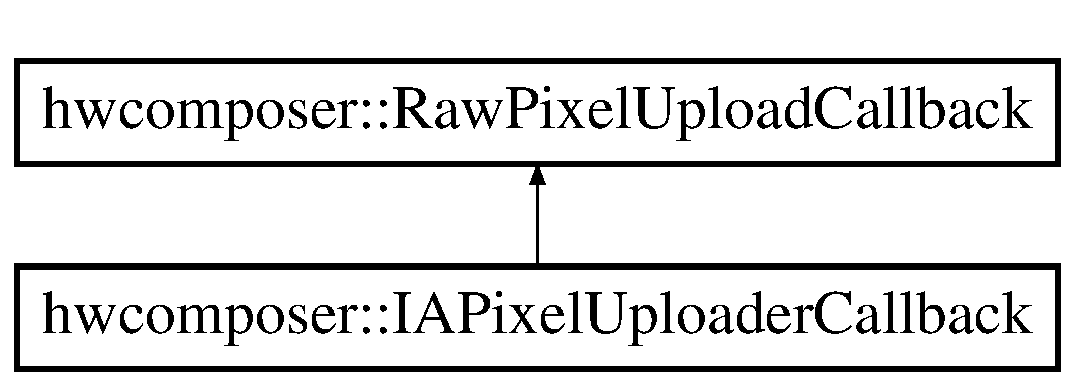
\includegraphics[height=2.000000cm]{classhwcomposer_1_1IAPixelUploaderCallback}
\end{center}
\end{figure}
\subsection*{Public Member Functions}
\begin{DoxyCompactItemize}
\item 
\mbox{\hyperlink{classhwcomposer_1_1IAPixelUploaderCallback_afe6ad27fcab01574ec2f70197f69e54e}{I\+A\+Pixel\+Uploader\+Callback}} (\mbox{\hyperlink{iahwc_8h_a07fb4f73baa8a0cfbd40f64071e56a7c}{iahwc\+\_\+callback\+\_\+data\+\_\+t}} data, \mbox{\hyperlink{iahwc_8h_a214bf51cce821fdb7b24210088c12cad}{iahwc\+\_\+function\+\_\+ptr\+\_\+t}} hook, uint32\+\_\+t display\+\_\+id)
\item 
void \mbox{\hyperlink{classhwcomposer_1_1IAPixelUploaderCallback_aadcf6756b46e8d237ac52a87199fc4eb}{Callback}} (bool start\+\_\+access, void $\ast$call\+\_\+back\+\_\+data)
\end{DoxyCompactItemize}


\subsection{Detailed Description}


Definition at line 45 of file linux\+\_\+frontend.\+cpp.



\subsection{Constructor \& Destructor Documentation}
\mbox{\Hypertarget{classhwcomposer_1_1IAPixelUploaderCallback_afe6ad27fcab01574ec2f70197f69e54e}\label{classhwcomposer_1_1IAPixelUploaderCallback_afe6ad27fcab01574ec2f70197f69e54e}} 
\index{hwcomposer\+::\+I\+A\+Pixel\+Uploader\+Callback@{hwcomposer\+::\+I\+A\+Pixel\+Uploader\+Callback}!I\+A\+Pixel\+Uploader\+Callback@{I\+A\+Pixel\+Uploader\+Callback}}
\index{I\+A\+Pixel\+Uploader\+Callback@{I\+A\+Pixel\+Uploader\+Callback}!hwcomposer\+::\+I\+A\+Pixel\+Uploader\+Callback@{hwcomposer\+::\+I\+A\+Pixel\+Uploader\+Callback}}
\subsubsection{\texorpdfstring{I\+A\+Pixel\+Uploader\+Callback()}{IAPixelUploaderCallback()}}
{\footnotesize\ttfamily hwcomposer\+::\+I\+A\+Pixel\+Uploader\+Callback\+::\+I\+A\+Pixel\+Uploader\+Callback (\begin{DoxyParamCaption}\item[{\mbox{\hyperlink{iahwc_8h_a07fb4f73baa8a0cfbd40f64071e56a7c}{iahwc\+\_\+callback\+\_\+data\+\_\+t}}}]{data,  }\item[{\mbox{\hyperlink{iahwc_8h_a214bf51cce821fdb7b24210088c12cad}{iahwc\+\_\+function\+\_\+ptr\+\_\+t}}}]{hook,  }\item[{uint32\+\_\+t}]{display\+\_\+id }\end{DoxyParamCaption})\hspace{0.3cm}{\ttfamily [inline]}}



Definition at line 47 of file linux\+\_\+frontend.\+cpp.


\begin{DoxyCode}{0}
\DoxyCodeLine{49       : data\_(data), hook\_(hook), display\_(display\_id) \{}
\DoxyCodeLine{50   \}}
\end{DoxyCode}


\subsection{Member Function Documentation}
\mbox{\Hypertarget{classhwcomposer_1_1IAPixelUploaderCallback_aadcf6756b46e8d237ac52a87199fc4eb}\label{classhwcomposer_1_1IAPixelUploaderCallback_aadcf6756b46e8d237ac52a87199fc4eb}} 
\index{hwcomposer\+::\+I\+A\+Pixel\+Uploader\+Callback@{hwcomposer\+::\+I\+A\+Pixel\+Uploader\+Callback}!Callback@{Callback}}
\index{Callback@{Callback}!hwcomposer\+::\+I\+A\+Pixel\+Uploader\+Callback@{hwcomposer\+::\+I\+A\+Pixel\+Uploader\+Callback}}
\subsubsection{\texorpdfstring{Callback()}{Callback()}}
{\footnotesize\ttfamily void hwcomposer\+::\+I\+A\+Pixel\+Uploader\+Callback\+::\+Callback (\begin{DoxyParamCaption}\item[{bool}]{start\+\_\+access,  }\item[{void $\ast$}]{call\+\_\+back\+\_\+data }\end{DoxyParamCaption})\hspace{0.3cm}{\ttfamily [inline]}, {\ttfamily [virtual]}}



Implements \mbox{\hyperlink{classhwcomposer_1_1RawPixelUploadCallback_a37aa7f3e3a5b5e9b43d1a11f56806979}{hwcomposer\+::\+Raw\+Pixel\+Upload\+Callback}}.



Definition at line 52 of file linux\+\_\+frontend.\+cpp.


\begin{DoxyCode}{0}
\DoxyCodeLine{52                                                          \{}
\DoxyCodeLine{53     \textcolor{keywordflow}{if} (hook\_ != \mbox{\hyperlink{alios_2platformdefines_8h_a070d2ce7b6bb7e5c05602aa8c308d0c4}{NULL}}) \{}
\DoxyCodeLine{54       \textcolor{keyword}{auto} hook = \textcolor{keyword}{reinterpret\_cast<}\mbox{\hyperlink{iahwc_8h_a12bf4b9fb3dc27eddd9f199c7ea8bb54}{IAHWC\_PFN\_PIXEL\_UPLOADER}}\textcolor{keyword}{>}(hook\_);}
\DoxyCodeLine{55       hook(data\_, display\_, start\_access ? 1 : 0, call\_back\_data);}
\DoxyCodeLine{56     \}}
\DoxyCodeLine{57   \}}
\end{DoxyCode}


The documentation for this class was generated from the following file\+:\begin{DoxyCompactItemize}
\item 
os/linux/\mbox{\hyperlink{linux__frontend_8cpp}{linux\+\_\+frontend.\+cpp}}\end{DoxyCompactItemize}

\hypertarget{classandroid_1_1IARefreshCallback}{}\section{android\+:\+:I\+A\+Refresh\+Callback Class Reference}
\label{classandroid_1_1IARefreshCallback}\index{android\+::\+I\+A\+Refresh\+Callback@{android\+::\+I\+A\+Refresh\+Callback}}
Inheritance diagram for android\+:\+:I\+A\+Refresh\+Callback\+:\begin{figure}[H]
\begin{center}
\leavevmode
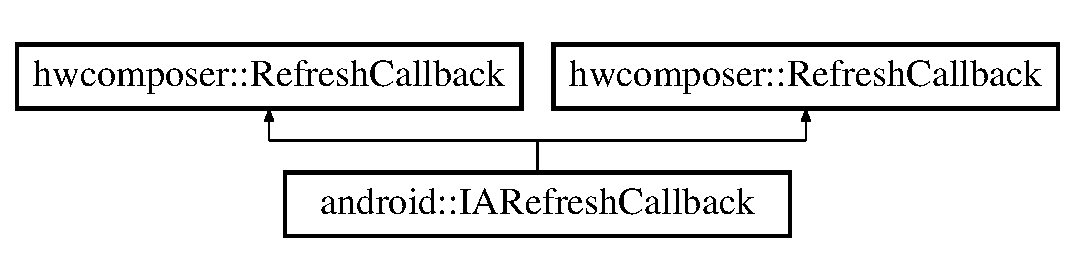
\includegraphics[height=2.000000cm]{classandroid_1_1IARefreshCallback}
\end{center}
\end{figure}
\subsection*{Public Member Functions}
\begin{DoxyCompactItemize}
\item 
\mbox{\hyperlink{classandroid_1_1IARefreshCallback_a2df870a0c492ee9b34800e398e3db2b3}{I\+A\+Refresh\+Callback}} (hwc\+\_\+procs\+\_\+t const $\ast$procs)
\item 
void \mbox{\hyperlink{classandroid_1_1IARefreshCallback_ab43c3e9561417b640ff0091265097c4c}{Callback}} (uint32\+\_\+t)
\item 
\mbox{\hyperlink{classandroid_1_1IARefreshCallback_a21b1a0c87a4c494754c203adcb91fc34}{I\+A\+Refresh\+Callback}} (hwc2\+\_\+callback\+\_\+data\+\_\+t data, hwc2\+\_\+function\+\_\+pointer\+\_\+t hook)
\item 
void \mbox{\hyperlink{classandroid_1_1IARefreshCallback_a7828a460befba5fc2cf3e9e5274b4e6f}{Callback}} (uint32\+\_\+t display)
\end{DoxyCompactItemize}


\subsection{Detailed Description}


Definition at line 158 of file iahwc1.\+cpp.



\subsection{Constructor \& Destructor Documentation}
\mbox{\Hypertarget{classandroid_1_1IARefreshCallback_a2df870a0c492ee9b34800e398e3db2b3}\label{classandroid_1_1IARefreshCallback_a2df870a0c492ee9b34800e398e3db2b3}} 
\index{android\+::\+I\+A\+Refresh\+Callback@{android\+::\+I\+A\+Refresh\+Callback}!I\+A\+Refresh\+Callback@{I\+A\+Refresh\+Callback}}
\index{I\+A\+Refresh\+Callback@{I\+A\+Refresh\+Callback}!android\+::\+I\+A\+Refresh\+Callback@{android\+::\+I\+A\+Refresh\+Callback}}
\subsubsection{\texorpdfstring{I\+A\+Refresh\+Callback()}{IARefreshCallback()}\hspace{0.1cm}{\footnotesize\ttfamily [1/2]}}
{\footnotesize\ttfamily android\+::\+I\+A\+Refresh\+Callback\+::\+I\+A\+Refresh\+Callback (\begin{DoxyParamCaption}\item[{hwc\+\_\+procs\+\_\+t const $\ast$}]{procs }\end{DoxyParamCaption})\hspace{0.3cm}{\ttfamily [inline]}}



Definition at line 160 of file iahwc1.\+cpp.


\begin{DoxyCode}{0}
\DoxyCodeLine{160                                               : procs\_(procs) \{}
\DoxyCodeLine{161   \}}
\end{DoxyCode}
\mbox{\Hypertarget{classandroid_1_1IARefreshCallback_a21b1a0c87a4c494754c203adcb91fc34}\label{classandroid_1_1IARefreshCallback_a21b1a0c87a4c494754c203adcb91fc34}} 
\index{android\+::\+I\+A\+Refresh\+Callback@{android\+::\+I\+A\+Refresh\+Callback}!I\+A\+Refresh\+Callback@{I\+A\+Refresh\+Callback}}
\index{I\+A\+Refresh\+Callback@{I\+A\+Refresh\+Callback}!android\+::\+I\+A\+Refresh\+Callback@{android\+::\+I\+A\+Refresh\+Callback}}
\subsubsection{\texorpdfstring{I\+A\+Refresh\+Callback()}{IARefreshCallback()}\hspace{0.1cm}{\footnotesize\ttfamily [2/2]}}
{\footnotesize\ttfamily android\+::\+I\+A\+Refresh\+Callback\+::\+I\+A\+Refresh\+Callback (\begin{DoxyParamCaption}\item[{hwc2\+\_\+callback\+\_\+data\+\_\+t}]{data,  }\item[{hwc2\+\_\+function\+\_\+pointer\+\_\+t}]{hook }\end{DoxyParamCaption})\hspace{0.3cm}{\ttfamily [inline]}}



Definition at line 62 of file iahwc2.\+cpp.


\begin{DoxyCode}{0}
\DoxyCodeLine{63       : data\_(data), hook\_(hook) \{}
\DoxyCodeLine{64   \}}
\end{DoxyCode}


\subsection{Member Function Documentation}
\mbox{\Hypertarget{classandroid_1_1IARefreshCallback_a7828a460befba5fc2cf3e9e5274b4e6f}\label{classandroid_1_1IARefreshCallback_a7828a460befba5fc2cf3e9e5274b4e6f}} 
\index{android\+::\+I\+A\+Refresh\+Callback@{android\+::\+I\+A\+Refresh\+Callback}!Callback@{Callback}}
\index{Callback@{Callback}!android\+::\+I\+A\+Refresh\+Callback@{android\+::\+I\+A\+Refresh\+Callback}}
\subsubsection{\texorpdfstring{Callback()}{Callback()}\hspace{0.1cm}{\footnotesize\ttfamily [1/2]}}
{\footnotesize\ttfamily void android\+::\+I\+A\+Refresh\+Callback\+::\+Callback (\begin{DoxyParamCaption}\item[{uint32\+\_\+t}]{display }\end{DoxyParamCaption})\hspace{0.3cm}{\ttfamily [inline]}, {\ttfamily [virtual]}}



Implements \mbox{\hyperlink{classhwcomposer_1_1RefreshCallback_a5637a4b1437bbf8c93d8356addbf7c87}{hwcomposer\+::\+Refresh\+Callback}}.



Definition at line 66 of file iahwc2.\+cpp.


\begin{DoxyCode}{0}
\DoxyCodeLine{66                                   \{}
\DoxyCodeLine{67     \textcolor{keywordflow}{if} (hook\_ != \mbox{\hyperlink{alios_2platformdefines_8h_a070d2ce7b6bb7e5c05602aa8c308d0c4}{NULL}}) \{}
\DoxyCodeLine{68       \textcolor{keyword}{auto} hook = \textcolor{keyword}{reinterpret\_cast<}HWC2\_PFN\_REFRESH\textcolor{keyword}{>}(hook\_);}
\DoxyCodeLine{69       hook(data\_, display);}
\DoxyCodeLine{70     \}}
\DoxyCodeLine{71   \}}
\end{DoxyCode}
\mbox{\Hypertarget{classandroid_1_1IARefreshCallback_ab43c3e9561417b640ff0091265097c4c}\label{classandroid_1_1IARefreshCallback_ab43c3e9561417b640ff0091265097c4c}} 
\index{android\+::\+I\+A\+Refresh\+Callback@{android\+::\+I\+A\+Refresh\+Callback}!Callback@{Callback}}
\index{Callback@{Callback}!android\+::\+I\+A\+Refresh\+Callback@{android\+::\+I\+A\+Refresh\+Callback}}
\subsubsection{\texorpdfstring{Callback()}{Callback()}\hspace{0.1cm}{\footnotesize\ttfamily [2/2]}}
{\footnotesize\ttfamily void android\+::\+I\+A\+Refresh\+Callback\+::\+Callback (\begin{DoxyParamCaption}\item[{uint32\+\_\+t}]{ }\end{DoxyParamCaption})\hspace{0.3cm}{\ttfamily [inline]}, {\ttfamily [virtual]}}



Implements \mbox{\hyperlink{classhwcomposer_1_1RefreshCallback_a5637a4b1437bbf8c93d8356addbf7c87}{hwcomposer\+::\+Refresh\+Callback}}.



Definition at line 163 of file iahwc1.\+cpp.


\begin{DoxyCode}{0}
\DoxyCodeLine{163                             \{}
\DoxyCodeLine{164     procs\_->invalidate(procs\_);}
\DoxyCodeLine{165   \}}
\end{DoxyCode}


The documentation for this class was generated from the following files\+:\begin{DoxyCompactItemize}
\item 
os/android/\mbox{\hyperlink{iahwc1_8cpp}{iahwc1.\+cpp}}\item 
os/android/\mbox{\hyperlink{iahwc2_8cpp}{iahwc2.\+cpp}}\end{DoxyCompactItemize}

\hypertarget{classandroid_1_1IAVsyncCallback}{}\section{android\+:\+:I\+A\+Vsync\+Callback Class Reference}
\label{classandroid_1_1IAVsyncCallback}\index{android\+::\+I\+A\+Vsync\+Callback@{android\+::\+I\+A\+Vsync\+Callback}}
Inheritance diagram for android\+:\+:I\+A\+Vsync\+Callback\+:\begin{figure}[H]
\begin{center}
\leavevmode
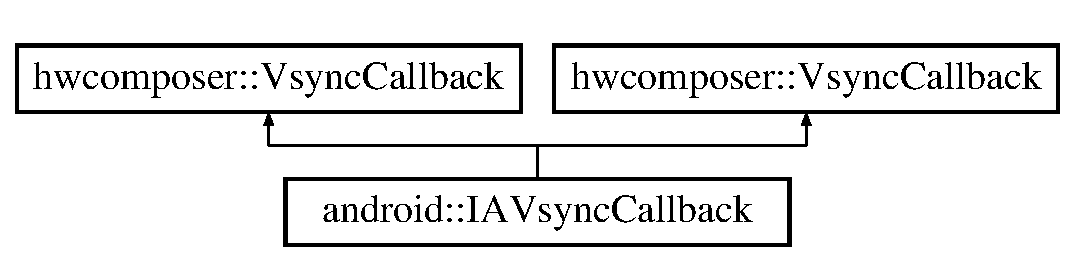
\includegraphics[height=2.000000cm]{classandroid_1_1IAVsyncCallback}
\end{center}
\end{figure}
\subsection*{Public Member Functions}
\begin{DoxyCompactItemize}
\item 
\mbox{\hyperlink{classandroid_1_1IAVsyncCallback_a32db4a2123be74e0a801392871bfe48d}{I\+A\+Vsync\+Callback}} (hwc\+\_\+procs\+\_\+t const $\ast$procs)
\item 
void \mbox{\hyperlink{classandroid_1_1IAVsyncCallback_ab5d04e5b2c2c36fc58639bbd9867cb54}{Callback}} (uint32\+\_\+t display, int64\+\_\+t timestamp)
\item 
\mbox{\hyperlink{classandroid_1_1IAVsyncCallback_a52e1c4e87b7667af7d10a94079785716}{I\+A\+Vsync\+Callback}} (hwc2\+\_\+callback\+\_\+data\+\_\+t data, hwc2\+\_\+function\+\_\+pointer\+\_\+t hook)
\item 
void \mbox{\hyperlink{classandroid_1_1IAVsyncCallback_ab5d04e5b2c2c36fc58639bbd9867cb54}{Callback}} (uint32\+\_\+t display, int64\+\_\+t timestamp)
\end{DoxyCompactItemize}


\subsection{Detailed Description}


Definition at line 124 of file iahwc1.\+cpp.



\subsection{Constructor \& Destructor Documentation}
\mbox{\Hypertarget{classandroid_1_1IAVsyncCallback_a32db4a2123be74e0a801392871bfe48d}\label{classandroid_1_1IAVsyncCallback_a32db4a2123be74e0a801392871bfe48d}} 
\index{android\+::\+I\+A\+Vsync\+Callback@{android\+::\+I\+A\+Vsync\+Callback}!I\+A\+Vsync\+Callback@{I\+A\+Vsync\+Callback}}
\index{I\+A\+Vsync\+Callback@{I\+A\+Vsync\+Callback}!android\+::\+I\+A\+Vsync\+Callback@{android\+::\+I\+A\+Vsync\+Callback}}
\subsubsection{\texorpdfstring{I\+A\+Vsync\+Callback()}{IAVsyncCallback()}\hspace{0.1cm}{\footnotesize\ttfamily [1/2]}}
{\footnotesize\ttfamily android\+::\+I\+A\+Vsync\+Callback\+::\+I\+A\+Vsync\+Callback (\begin{DoxyParamCaption}\item[{hwc\+\_\+procs\+\_\+t const $\ast$}]{procs }\end{DoxyParamCaption})\hspace{0.3cm}{\ttfamily [inline]}}



Definition at line 126 of file iahwc1.\+cpp.


\begin{DoxyCode}{0}
\DoxyCodeLine{126                                             : procs\_(procs) \{}
\DoxyCodeLine{127   \}}
\end{DoxyCode}
\mbox{\Hypertarget{classandroid_1_1IAVsyncCallback_a52e1c4e87b7667af7d10a94079785716}\label{classandroid_1_1IAVsyncCallback_a52e1c4e87b7667af7d10a94079785716}} 
\index{android\+::\+I\+A\+Vsync\+Callback@{android\+::\+I\+A\+Vsync\+Callback}!I\+A\+Vsync\+Callback@{I\+A\+Vsync\+Callback}}
\index{I\+A\+Vsync\+Callback@{I\+A\+Vsync\+Callback}!android\+::\+I\+A\+Vsync\+Callback@{android\+::\+I\+A\+Vsync\+Callback}}
\subsubsection{\texorpdfstring{I\+A\+Vsync\+Callback()}{IAVsyncCallback()}\hspace{0.1cm}{\footnotesize\ttfamily [2/2]}}
{\footnotesize\ttfamily android\+::\+I\+A\+Vsync\+Callback\+::\+I\+A\+Vsync\+Callback (\begin{DoxyParamCaption}\item[{hwc2\+\_\+callback\+\_\+data\+\_\+t}]{data,  }\item[{hwc2\+\_\+function\+\_\+pointer\+\_\+t}]{hook }\end{DoxyParamCaption})\hspace{0.3cm}{\ttfamily [inline]}}



Definition at line 44 of file iahwc2.\+cpp.


\begin{DoxyCode}{0}
\DoxyCodeLine{45       : data\_(data), hook\_(hook) \{}
\DoxyCodeLine{46   \}}
\end{DoxyCode}


\subsection{Member Function Documentation}
\mbox{\Hypertarget{classandroid_1_1IAVsyncCallback_ab5d04e5b2c2c36fc58639bbd9867cb54}\label{classandroid_1_1IAVsyncCallback_ab5d04e5b2c2c36fc58639bbd9867cb54}} 
\index{android\+::\+I\+A\+Vsync\+Callback@{android\+::\+I\+A\+Vsync\+Callback}!Callback@{Callback}}
\index{Callback@{Callback}!android\+::\+I\+A\+Vsync\+Callback@{android\+::\+I\+A\+Vsync\+Callback}}
\subsubsection{\texorpdfstring{Callback()}{Callback()}\hspace{0.1cm}{\footnotesize\ttfamily [1/2]}}
{\footnotesize\ttfamily void android\+::\+I\+A\+Vsync\+Callback\+::\+Callback (\begin{DoxyParamCaption}\item[{uint32\+\_\+t}]{display,  }\item[{int64\+\_\+t}]{timestamp }\end{DoxyParamCaption})\hspace{0.3cm}{\ttfamily [inline]}, {\ttfamily [virtual]}}



Implements \mbox{\hyperlink{classhwcomposer_1_1VsyncCallback_a632ac6a2e13e1b387df9508507a2ed4d}{hwcomposer\+::\+Vsync\+Callback}}.



Definition at line 48 of file iahwc2.\+cpp.


\begin{DoxyCode}{0}
\DoxyCodeLine{48                                                      \{}
\DoxyCodeLine{49     \textcolor{keywordflow}{if} (hook\_ != \mbox{\hyperlink{alios_2platformdefines_8h_a070d2ce7b6bb7e5c05602aa8c308d0c4}{NULL}}) \{}
\DoxyCodeLine{50       \textcolor{keyword}{auto} hook = \textcolor{keyword}{reinterpret\_cast<}HWC2\_PFN\_VSYNC\textcolor{keyword}{>}(hook\_);}
\DoxyCodeLine{51       hook(data\_, display, timestamp);}
\DoxyCodeLine{52     \}}
\DoxyCodeLine{53   \}}
\end{DoxyCode}
\mbox{\Hypertarget{classandroid_1_1IAVsyncCallback_ab5d04e5b2c2c36fc58639bbd9867cb54}\label{classandroid_1_1IAVsyncCallback_ab5d04e5b2c2c36fc58639bbd9867cb54}} 
\index{android\+::\+I\+A\+Vsync\+Callback@{android\+::\+I\+A\+Vsync\+Callback}!Callback@{Callback}}
\index{Callback@{Callback}!android\+::\+I\+A\+Vsync\+Callback@{android\+::\+I\+A\+Vsync\+Callback}}
\subsubsection{\texorpdfstring{Callback()}{Callback()}\hspace{0.1cm}{\footnotesize\ttfamily [2/2]}}
{\footnotesize\ttfamily void android\+::\+I\+A\+Vsync\+Callback\+::\+Callback (\begin{DoxyParamCaption}\item[{uint32\+\_\+t}]{display,  }\item[{int64\+\_\+t}]{timestamp }\end{DoxyParamCaption})\hspace{0.3cm}{\ttfamily [inline]}, {\ttfamily [virtual]}}



Implements \mbox{\hyperlink{classhwcomposer_1_1VsyncCallback_a632ac6a2e13e1b387df9508507a2ed4d}{hwcomposer\+::\+Vsync\+Callback}}.



Definition at line 129 of file iahwc1.\+cpp.


\begin{DoxyCode}{0}
\DoxyCodeLine{129                                                      \{}
\DoxyCodeLine{130     procs\_->vsync(procs\_, display > 0 ? HWC\_DISPLAY\_EXTERNAL\_BIT}
\DoxyCodeLine{131                                       : HWC\_DISPLAY\_PRIMARY\_BIT,}
\DoxyCodeLine{132                   timestamp);}
\DoxyCodeLine{133   \}}
\end{DoxyCode}


The documentation for this class was generated from the following files\+:\begin{DoxyCompactItemize}
\item 
os/android/\mbox{\hyperlink{iahwc1_8cpp}{iahwc1.\+cpp}}\item 
os/android/\mbox{\hyperlink{iahwc2_8cpp}{iahwc2.\+cpp}}\end{DoxyCompactItemize}

\hypertarget{classhwcomposer_1_1IAVsyncCallback}{}\section{hwcomposer\+:\+:I\+A\+Vsync\+Callback Class Reference}
\label{classhwcomposer_1_1IAVsyncCallback}\index{hwcomposer\+::\+I\+A\+Vsync\+Callback@{hwcomposer\+::\+I\+A\+Vsync\+Callback}}
Inheritance diagram for hwcomposer\+:\+:I\+A\+Vsync\+Callback\+:\begin{figure}[H]
\begin{center}
\leavevmode
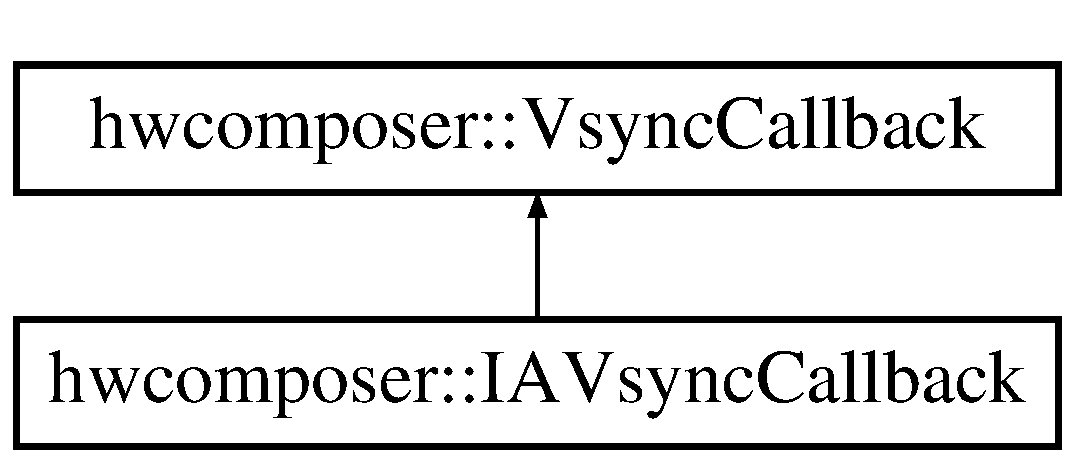
\includegraphics[height=2.000000cm]{classhwcomposer_1_1IAVsyncCallback}
\end{center}
\end{figure}
\subsection*{Public Member Functions}
\begin{DoxyCompactItemize}
\item 
\mbox{\hyperlink{classhwcomposer_1_1IAVsyncCallback_afdf960ef784e276e17e6d0775b2c9142}{I\+A\+Vsync\+Callback}} (hwf\+\_\+callback const $\ast$procs)
\item 
void \mbox{\hyperlink{classhwcomposer_1_1IAVsyncCallback_a9ccc6eb6a50d308473716a225e320c8d}{Callback}} (uint32\+\_\+t display, int64\+\_\+t timestamp)
\end{DoxyCompactItemize}


\subsection{Detailed Description}


Definition at line 388 of file hwf\+\_\+alioshal.\+cpp.



\subsection{Constructor \& Destructor Documentation}
\mbox{\Hypertarget{classhwcomposer_1_1IAVsyncCallback_afdf960ef784e276e17e6d0775b2c9142}\label{classhwcomposer_1_1IAVsyncCallback_afdf960ef784e276e17e6d0775b2c9142}} 
\index{hwcomposer\+::\+I\+A\+Vsync\+Callback@{hwcomposer\+::\+I\+A\+Vsync\+Callback}!I\+A\+Vsync\+Callback@{I\+A\+Vsync\+Callback}}
\index{I\+A\+Vsync\+Callback@{I\+A\+Vsync\+Callback}!hwcomposer\+::\+I\+A\+Vsync\+Callback@{hwcomposer\+::\+I\+A\+Vsync\+Callback}}
\subsubsection{\texorpdfstring{I\+A\+Vsync\+Callback()}{IAVsyncCallback()}}
{\footnotesize\ttfamily hwcomposer\+::\+I\+A\+Vsync\+Callback\+::\+I\+A\+Vsync\+Callback (\begin{DoxyParamCaption}\item[{hwf\+\_\+callback const $\ast$}]{procs }\end{DoxyParamCaption})\hspace{0.3cm}{\ttfamily [inline]}}



Definition at line 390 of file hwf\+\_\+alioshal.\+cpp.


\begin{DoxyCode}{0}
\DoxyCodeLine{390                                              : m\_pCB(procs) \{}
\DoxyCodeLine{391   \}}
\end{DoxyCode}


\subsection{Member Function Documentation}
\mbox{\Hypertarget{classhwcomposer_1_1IAVsyncCallback_a9ccc6eb6a50d308473716a225e320c8d}\label{classhwcomposer_1_1IAVsyncCallback_a9ccc6eb6a50d308473716a225e320c8d}} 
\index{hwcomposer\+::\+I\+A\+Vsync\+Callback@{hwcomposer\+::\+I\+A\+Vsync\+Callback}!Callback@{Callback}}
\index{Callback@{Callback}!hwcomposer\+::\+I\+A\+Vsync\+Callback@{hwcomposer\+::\+I\+A\+Vsync\+Callback}}
\subsubsection{\texorpdfstring{Callback()}{Callback()}}
{\footnotesize\ttfamily void hwcomposer\+::\+I\+A\+Vsync\+Callback\+::\+Callback (\begin{DoxyParamCaption}\item[{uint32\+\_\+t}]{display,  }\item[{int64\+\_\+t}]{timestamp }\end{DoxyParamCaption})\hspace{0.3cm}{\ttfamily [inline]}, {\ttfamily [virtual]}}



Implements \mbox{\hyperlink{classhwcomposer_1_1VsyncCallback_a632ac6a2e13e1b387df9508507a2ed4d}{hwcomposer\+::\+Vsync\+Callback}}.



Definition at line 393 of file hwf\+\_\+alioshal.\+cpp.


\begin{DoxyCode}{0}
\DoxyCodeLine{393                                                      \{}
\DoxyCodeLine{394     m\_pCB->vsyncEvent(m\_pCB,}
\DoxyCodeLine{395                       display > 0 ? HWF\_DISPLAY\_EXTERNAL : HWF\_DISPLAY\_PRIMARY,}
\DoxyCodeLine{396                       timestamp);}
\DoxyCodeLine{397   \}}
\end{DoxyCode}


The documentation for this class was generated from the following file\+:\begin{DoxyCompactItemize}
\item 
os/alios/\mbox{\hyperlink{hwf__alioshal_8cpp}{hwf\+\_\+alioshal.\+cpp}}\end{DoxyCompactItemize}

\hypertarget{classhwcomposer_1_1IControls}{}\section{hwcomposer\+:\+:I\+Controls Class Reference}
\label{classhwcomposer_1_1IControls}\index{hwcomposer\+::\+I\+Controls@{hwcomposer\+::\+I\+Controls}}


{\ttfamily \#include $<$icontrols.\+h$>$}

Inheritance diagram for hwcomposer\+:\+:I\+Controls\+:\begin{figure}[H]
\begin{center}
\leavevmode
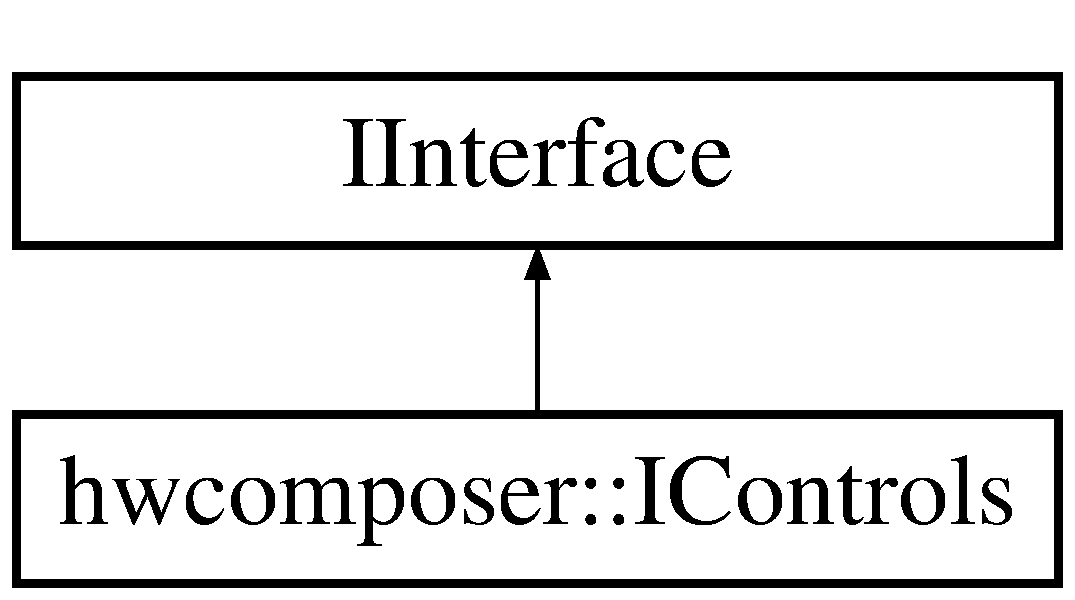
\includegraphics[height=2.000000cm]{classhwcomposer_1_1IControls}
\end{center}
\end{figure}
\subsection*{Public Member Functions}
\begin{DoxyCompactItemize}
\item 
\mbox{\hyperlink{classhwcomposer_1_1IControls_a1049f9600bef7b150a7fb457a79e4756}{D\+E\+C\+L\+A\+R\+E\+\_\+\+M\+E\+T\+A\+\_\+\+I\+N\+T\+E\+R\+F\+A\+CE}} (Controls)
\item 
virtual \mbox{\hyperlink{hwcserviceapi_8h_a3806fb2027d9a316d8ca8d9b8b8eb96f}{status\+\_\+t}} \mbox{\hyperlink{classhwcomposer_1_1IControls_a3f14720a7ba5e37f42a8d19f37187331}{Display\+Set\+Overscan}} (uint32\+\_\+t display, int32\+\_\+t xoverscan, int32\+\_\+t yoverscan)=0
\item 
virtual \mbox{\hyperlink{hwcserviceapi_8h_a3806fb2027d9a316d8ca8d9b8b8eb96f}{status\+\_\+t}} \mbox{\hyperlink{classhwcomposer_1_1IControls_a2234b4ef06ed8dee33283b4630fdf4a1}{Display\+Get\+Overscan}} (uint32\+\_\+t display, int32\+\_\+t $\ast$xoverscan, int32\+\_\+t $\ast$yoverscan)=0
\item 
virtual \mbox{\hyperlink{hwcserviceapi_8h_a3806fb2027d9a316d8ca8d9b8b8eb96f}{status\+\_\+t}} \mbox{\hyperlink{classhwcomposer_1_1IControls_a3c4fb4608f3de4adaafce6c3d058aa74}{Display\+Set\+Scaling}} (uint32\+\_\+t display, \mbox{\hyperlink{hwcserviceapi_8h_acdadfd5e7f15097833789174e442083f}{E\+Hwcs\+Scaling\+Mode}} e\+Scaling\+Mode)=0
\item 
virtual \mbox{\hyperlink{hwcserviceapi_8h_a3806fb2027d9a316d8ca8d9b8b8eb96f}{status\+\_\+t}} \mbox{\hyperlink{classhwcomposer_1_1IControls_a341b79ec50b6145db4f46d1cd878b47c}{Display\+Get\+Scaling}} (uint32\+\_\+t display, \mbox{\hyperlink{hwcserviceapi_8h_acdadfd5e7f15097833789174e442083f}{E\+Hwcs\+Scaling\+Mode}} $\ast$e\+Scaling\+Mode)=0
\item 
virtual \mbox{\hyperlink{hwcserviceapi_8h_a3806fb2027d9a316d8ca8d9b8b8eb96f}{status\+\_\+t}} \mbox{\hyperlink{classhwcomposer_1_1IControls_af509cfd6ea30e5524ac8f2d5dd7482c1}{Display\+Enable\+Blank}} (uint32\+\_\+t display, bool blank)=0
\item 
virtual \mbox{\hyperlink{hwcserviceapi_8h_a3806fb2027d9a316d8ca8d9b8b8eb96f}{status\+\_\+t}} \mbox{\hyperlink{classhwcomposer_1_1IControls_ac3eec02e6b87c04fc9856e0b5b28b9b9}{Display\+Restore\+Default\+Color\+Param}} (uint32\+\_\+t display, \mbox{\hyperlink{hwcserviceapi_8h_a1d1cbf448ce748672cf3dd96675d70e4}{E\+Hwcs\+Color\+Control}} color)=0
\item 
virtual \mbox{\hyperlink{hwcserviceapi_8h_a3806fb2027d9a316d8ca8d9b8b8eb96f}{status\+\_\+t}} \mbox{\hyperlink{classhwcomposer_1_1IControls_aeb24361552467205e292bfe7a733760e}{Display\+Restore\+Default\+Deinterlace\+Param}} (uint32\+\_\+t display)=0
\item 
virtual \mbox{\hyperlink{hwcserviceapi_8h_a3806fb2027d9a316d8ca8d9b8b8eb96f}{status\+\_\+t}} \mbox{\hyperlink{classhwcomposer_1_1IControls_a2cf04dc4db1f9e1501dbd381fd390206}{Display\+Get\+Color\+Param}} (uint32\+\_\+t display, \mbox{\hyperlink{hwcserviceapi_8h_a1d1cbf448ce748672cf3dd96675d70e4}{E\+Hwcs\+Color\+Control}} color, float $\ast$value, float $\ast$startvalue, float $\ast$endvalue)=0
\item 
virtual \mbox{\hyperlink{hwcserviceapi_8h_a3806fb2027d9a316d8ca8d9b8b8eb96f}{status\+\_\+t}} \mbox{\hyperlink{classhwcomposer_1_1IControls_a85a46964e57700804a3e6f6289f8046f}{Display\+Set\+Color\+Param}} (uint32\+\_\+t display, \mbox{\hyperlink{hwcserviceapi_8h_a1d1cbf448ce748672cf3dd96675d70e4}{E\+Hwcs\+Color\+Control}} color, float value)=0
\item 
virtual \mbox{\hyperlink{hwcserviceapi_8h_a3806fb2027d9a316d8ca8d9b8b8eb96f}{status\+\_\+t}} \mbox{\hyperlink{classhwcomposer_1_1IControls_ac1e0de62aefa375f4f6dfd565046ba1d}{Display\+Set\+Deinterlace\+Param}} (uint32\+\_\+t display, \mbox{\hyperlink{hwcserviceapi_8h_a8473f2ec9e7333e67be46a1bea689113}{E\+Hwcs\+Deinterlace\+Control}} mode)=0
\item 
virtual std\+::vector$<$ \mbox{\hyperlink{hwcserviceapi_8h_a6e13f5285374b86aab82ec0c0ba62d7a}{Hwcs\+Display\+Mode\+Info}} $>$ \mbox{\hyperlink{classhwcomposer_1_1IControls_a89180fa507885f5d7ed1d02595f2be49}{Display\+Mode\+Get\+Available\+Modes}} (uint32\+\_\+t display)=0
\item 
virtual \mbox{\hyperlink{hwcserviceapi_8h_a3806fb2027d9a316d8ca8d9b8b8eb96f}{status\+\_\+t}} \mbox{\hyperlink{classhwcomposer_1_1IControls_aa26011465d8f977f12a4ba19a646f917}{Display\+Mode\+Get\+Mode}} (uint32\+\_\+t display, \mbox{\hyperlink{hwcserviceapi_8h_a6e13f5285374b86aab82ec0c0ba62d7a}{Hwcs\+Display\+Mode\+Info}} $\ast$p\+Mode)=0
\item 
virtual \mbox{\hyperlink{hwcserviceapi_8h_a3806fb2027d9a316d8ca8d9b8b8eb96f}{status\+\_\+t}} \mbox{\hyperlink{classhwcomposer_1_1IControls_a276c0ad9ee6973cab285da547f929e3f}{Display\+Mode\+Set\+Mode}} (uint32\+\_\+t display, const uint32\+\_\+t config)=0
\item 
virtual \mbox{\hyperlink{hwcserviceapi_8h_a3806fb2027d9a316d8ca8d9b8b8eb96f}{status\+\_\+t}} \mbox{\hyperlink{classhwcomposer_1_1IControls_a99550456802b4989806ac630f65db636}{Enable\+H\+D\+C\+P\+Session\+For\+Display}} (uint32\+\_\+t display, \mbox{\hyperlink{hwcserviceapi_8h_a69e9b3a54e4c8e504845398c66eab655}{E\+Hwcs\+Content\+Type}} content\+\_\+type)=0
\item 
virtual \mbox{\hyperlink{hwcserviceapi_8h_a3806fb2027d9a316d8ca8d9b8b8eb96f}{status\+\_\+t}} \mbox{\hyperlink{classhwcomposer_1_1IControls_a29659284e29653ae4d7fe9767794c06e}{Enable\+H\+D\+C\+P\+Session\+For\+All\+Displays}} (\mbox{\hyperlink{hwcserviceapi_8h_a69e9b3a54e4c8e504845398c66eab655}{E\+Hwcs\+Content\+Type}} content\+\_\+type)=0
\item 
virtual \mbox{\hyperlink{hwcserviceapi_8h_a3806fb2027d9a316d8ca8d9b8b8eb96f}{status\+\_\+t}} \mbox{\hyperlink{classhwcomposer_1_1IControls_adfce6c02fc64430969111173989e0a9a}{Disable\+H\+D\+C\+P\+Session\+For\+Display}} (uint32\+\_\+t display)=0
\item 
virtual \mbox{\hyperlink{hwcserviceapi_8h_a3806fb2027d9a316d8ca8d9b8b8eb96f}{status\+\_\+t}} \mbox{\hyperlink{classhwcomposer_1_1IControls_a15854915f926445f5c67f2959e2b2131}{Disable\+H\+D\+C\+P\+Session\+For\+All\+Displays}} ()=0
\item 
virtual \mbox{\hyperlink{hwcserviceapi_8h_a3806fb2027d9a316d8ca8d9b8b8eb96f}{status\+\_\+t}} \mbox{\hyperlink{classhwcomposer_1_1IControls_a502ec367dd15a58771d4290e610641e6}{Video\+Enable\+Encrypted\+Session}} (uint32\+\_\+t session\+ID, uint32\+\_\+t instance\+ID)=0
\item 
virtual \mbox{\hyperlink{hwcserviceapi_8h_a3806fb2027d9a316d8ca8d9b8b8eb96f}{status\+\_\+t}} \mbox{\hyperlink{classhwcomposer_1_1IControls_a947e4a84ae4623fa3ff4df85db45be97}{Video\+Disable\+All\+Encrypted\+Sessions}} (uint32\+\_\+t session\+ID)=0
\item 
virtual \mbox{\hyperlink{hwcserviceapi_8h_a3806fb2027d9a316d8ca8d9b8b8eb96f}{status\+\_\+t}} \mbox{\hyperlink{classhwcomposer_1_1IControls_a3f60e4c78208d5ee55d0409cd7d96258}{Video\+Disable\+All\+Encrypted\+Sessions}} ()=0
\item 
virtual bool \mbox{\hyperlink{classhwcomposer_1_1IControls_a8a3368ae60a036bf5fa9ab5c3bdb9073}{Video\+Is\+Encrypted\+Session\+Enabled}} (uint32\+\_\+t session\+ID, uint32\+\_\+t instance\+ID)=0
\item 
virtual \mbox{\hyperlink{hwcserviceapi_8h_a3806fb2027d9a316d8ca8d9b8b8eb96f}{status\+\_\+t}} \mbox{\hyperlink{classhwcomposer_1_1IControls_a6ab5735df81c42f725641165136912f2}{Video\+Set\+Optimization\+Mode}} (\mbox{\hyperlink{hwcserviceapi_8h_a73044de23b8f474352d6753e21fca06d}{E\+Hwcs\+Optimization\+Mode}} mode)=0
\item 
virtual \mbox{\hyperlink{hwcserviceapi_8h_a3806fb2027d9a316d8ca8d9b8b8eb96f}{status\+\_\+t}} \mbox{\hyperlink{classhwcomposer_1_1IControls_ad2d374da82a11a7a6b2bade97dc87955}{Mds\+Update\+Video\+State}} (int64\+\_\+t video\+Session\+ID, bool is\+Prepared)=0
\item 
virtual \mbox{\hyperlink{hwcserviceapi_8h_a3806fb2027d9a316d8ca8d9b8b8eb96f}{status\+\_\+t}} \mbox{\hyperlink{classhwcomposer_1_1IControls_a15c005a5a1c9c0a5a30ffebefdfb6b6f}{Mds\+Update\+Video\+F\+PS}} (int64\+\_\+t video\+Session\+ID, int32\+\_\+t fps)=0
\item 
virtual \mbox{\hyperlink{hwcserviceapi_8h_a3806fb2027d9a316d8ca8d9b8b8eb96f}{status\+\_\+t}} \mbox{\hyperlink{classhwcomposer_1_1IControls_a762f814efdb6c21fdc156a5a19014a0e}{Mds\+Update\+Input\+State}} (bool state)=0
\item 
virtual \mbox{\hyperlink{hwcserviceapi_8h_a3806fb2027d9a316d8ca8d9b8b8eb96f}{status\+\_\+t}} \mbox{\hyperlink{classhwcomposer_1_1IControls_a69047ef7180e98e50661dc75ab8fc794}{Widi\+Get\+Single\+Display}} (bool $\ast$p\+Enabled)=0
\item 
virtual \mbox{\hyperlink{hwcserviceapi_8h_a3806fb2027d9a316d8ca8d9b8b8eb96f}{status\+\_\+t}} \mbox{\hyperlink{classhwcomposer_1_1IControls_abebb8408a1525be64b060b2af76f06f9}{Widi\+Set\+Single\+Display}} (bool enable)=0
\end{DoxyCompactItemize}


\subsection{Detailed Description}


Definition at line 26 of file icontrols.\+h.



\subsection{Member Function Documentation}
\mbox{\Hypertarget{classhwcomposer_1_1IControls_a1049f9600bef7b150a7fb457a79e4756}\label{classhwcomposer_1_1IControls_a1049f9600bef7b150a7fb457a79e4756}} 
\index{hwcomposer\+::\+I\+Controls@{hwcomposer\+::\+I\+Controls}!D\+E\+C\+L\+A\+R\+E\+\_\+\+M\+E\+T\+A\+\_\+\+I\+N\+T\+E\+R\+F\+A\+CE@{D\+E\+C\+L\+A\+R\+E\+\_\+\+M\+E\+T\+A\+\_\+\+I\+N\+T\+E\+R\+F\+A\+CE}}
\index{D\+E\+C\+L\+A\+R\+E\+\_\+\+M\+E\+T\+A\+\_\+\+I\+N\+T\+E\+R\+F\+A\+CE@{D\+E\+C\+L\+A\+R\+E\+\_\+\+M\+E\+T\+A\+\_\+\+I\+N\+T\+E\+R\+F\+A\+CE}!hwcomposer\+::\+I\+Controls@{hwcomposer\+::\+I\+Controls}}
\subsubsection{\texorpdfstring{D\+E\+C\+L\+A\+R\+E\+\_\+\+M\+E\+T\+A\+\_\+\+I\+N\+T\+E\+R\+F\+A\+C\+E()}{DECLARE\_META\_INTERFACE()}}
{\footnotesize\ttfamily hwcomposer\+::\+I\+Controls\+::\+D\+E\+C\+L\+A\+R\+E\+\_\+\+M\+E\+T\+A\+\_\+\+I\+N\+T\+E\+R\+F\+A\+CE (\begin{DoxyParamCaption}\item[{Controls}]{ }\end{DoxyParamCaption})}

\mbox{\Hypertarget{classhwcomposer_1_1IControls_a15854915f926445f5c67f2959e2b2131}\label{classhwcomposer_1_1IControls_a15854915f926445f5c67f2959e2b2131}} 
\index{hwcomposer\+::\+I\+Controls@{hwcomposer\+::\+I\+Controls}!Disable\+H\+D\+C\+P\+Session\+For\+All\+Displays@{Disable\+H\+D\+C\+P\+Session\+For\+All\+Displays}}
\index{Disable\+H\+D\+C\+P\+Session\+For\+All\+Displays@{Disable\+H\+D\+C\+P\+Session\+For\+All\+Displays}!hwcomposer\+::\+I\+Controls@{hwcomposer\+::\+I\+Controls}}
\subsubsection{\texorpdfstring{Disable\+H\+D\+C\+P\+Session\+For\+All\+Displays()}{DisableHDCPSessionForAllDisplays()}}
{\footnotesize\ttfamily virtual \mbox{\hyperlink{hwcserviceapi_8h_a3806fb2027d9a316d8ca8d9b8b8eb96f}{status\+\_\+t}} hwcomposer\+::\+I\+Controls\+::\+Disable\+H\+D\+C\+P\+Session\+For\+All\+Displays (\begin{DoxyParamCaption}{ }\end{DoxyParamCaption})\hspace{0.3cm}{\ttfamily [pure virtual]}}

\mbox{\Hypertarget{classhwcomposer_1_1IControls_adfce6c02fc64430969111173989e0a9a}\label{classhwcomposer_1_1IControls_adfce6c02fc64430969111173989e0a9a}} 
\index{hwcomposer\+::\+I\+Controls@{hwcomposer\+::\+I\+Controls}!Disable\+H\+D\+C\+P\+Session\+For\+Display@{Disable\+H\+D\+C\+P\+Session\+For\+Display}}
\index{Disable\+H\+D\+C\+P\+Session\+For\+Display@{Disable\+H\+D\+C\+P\+Session\+For\+Display}!hwcomposer\+::\+I\+Controls@{hwcomposer\+::\+I\+Controls}}
\subsubsection{\texorpdfstring{Disable\+H\+D\+C\+P\+Session\+For\+Display()}{DisableHDCPSessionForDisplay()}}
{\footnotesize\ttfamily virtual \mbox{\hyperlink{hwcserviceapi_8h_a3806fb2027d9a316d8ca8d9b8b8eb96f}{status\+\_\+t}} hwcomposer\+::\+I\+Controls\+::\+Disable\+H\+D\+C\+P\+Session\+For\+Display (\begin{DoxyParamCaption}\item[{uint32\+\_\+t}]{display }\end{DoxyParamCaption})\hspace{0.3cm}{\ttfamily [pure virtual]}}

\mbox{\Hypertarget{classhwcomposer_1_1IControls_af509cfd6ea30e5524ac8f2d5dd7482c1}\label{classhwcomposer_1_1IControls_af509cfd6ea30e5524ac8f2d5dd7482c1}} 
\index{hwcomposer\+::\+I\+Controls@{hwcomposer\+::\+I\+Controls}!Display\+Enable\+Blank@{Display\+Enable\+Blank}}
\index{Display\+Enable\+Blank@{Display\+Enable\+Blank}!hwcomposer\+::\+I\+Controls@{hwcomposer\+::\+I\+Controls}}
\subsubsection{\texorpdfstring{Display\+Enable\+Blank()}{DisplayEnableBlank()}}
{\footnotesize\ttfamily virtual \mbox{\hyperlink{hwcserviceapi_8h_a3806fb2027d9a316d8ca8d9b8b8eb96f}{status\+\_\+t}} hwcomposer\+::\+I\+Controls\+::\+Display\+Enable\+Blank (\begin{DoxyParamCaption}\item[{uint32\+\_\+t}]{display,  }\item[{bool}]{blank }\end{DoxyParamCaption})\hspace{0.3cm}{\ttfamily [pure virtual]}}

\mbox{\Hypertarget{classhwcomposer_1_1IControls_a2cf04dc4db1f9e1501dbd381fd390206}\label{classhwcomposer_1_1IControls_a2cf04dc4db1f9e1501dbd381fd390206}} 
\index{hwcomposer\+::\+I\+Controls@{hwcomposer\+::\+I\+Controls}!Display\+Get\+Color\+Param@{Display\+Get\+Color\+Param}}
\index{Display\+Get\+Color\+Param@{Display\+Get\+Color\+Param}!hwcomposer\+::\+I\+Controls@{hwcomposer\+::\+I\+Controls}}
\subsubsection{\texorpdfstring{Display\+Get\+Color\+Param()}{DisplayGetColorParam()}}
{\footnotesize\ttfamily virtual \mbox{\hyperlink{hwcserviceapi_8h_a3806fb2027d9a316d8ca8d9b8b8eb96f}{status\+\_\+t}} hwcomposer\+::\+I\+Controls\+::\+Display\+Get\+Color\+Param (\begin{DoxyParamCaption}\item[{uint32\+\_\+t}]{display,  }\item[{\mbox{\hyperlink{hwcserviceapi_8h_a1d1cbf448ce748672cf3dd96675d70e4}{E\+Hwcs\+Color\+Control}}}]{color,  }\item[{float $\ast$}]{value,  }\item[{float $\ast$}]{startvalue,  }\item[{float $\ast$}]{endvalue }\end{DoxyParamCaption})\hspace{0.3cm}{\ttfamily [pure virtual]}}

\mbox{\Hypertarget{classhwcomposer_1_1IControls_a2234b4ef06ed8dee33283b4630fdf4a1}\label{classhwcomposer_1_1IControls_a2234b4ef06ed8dee33283b4630fdf4a1}} 
\index{hwcomposer\+::\+I\+Controls@{hwcomposer\+::\+I\+Controls}!Display\+Get\+Overscan@{Display\+Get\+Overscan}}
\index{Display\+Get\+Overscan@{Display\+Get\+Overscan}!hwcomposer\+::\+I\+Controls@{hwcomposer\+::\+I\+Controls}}
\subsubsection{\texorpdfstring{Display\+Get\+Overscan()}{DisplayGetOverscan()}}
{\footnotesize\ttfamily virtual \mbox{\hyperlink{hwcserviceapi_8h_a3806fb2027d9a316d8ca8d9b8b8eb96f}{status\+\_\+t}} hwcomposer\+::\+I\+Controls\+::\+Display\+Get\+Overscan (\begin{DoxyParamCaption}\item[{uint32\+\_\+t}]{display,  }\item[{int32\+\_\+t $\ast$}]{xoverscan,  }\item[{int32\+\_\+t $\ast$}]{yoverscan }\end{DoxyParamCaption})\hspace{0.3cm}{\ttfamily [pure virtual]}}

\mbox{\Hypertarget{classhwcomposer_1_1IControls_a341b79ec50b6145db4f46d1cd878b47c}\label{classhwcomposer_1_1IControls_a341b79ec50b6145db4f46d1cd878b47c}} 
\index{hwcomposer\+::\+I\+Controls@{hwcomposer\+::\+I\+Controls}!Display\+Get\+Scaling@{Display\+Get\+Scaling}}
\index{Display\+Get\+Scaling@{Display\+Get\+Scaling}!hwcomposer\+::\+I\+Controls@{hwcomposer\+::\+I\+Controls}}
\subsubsection{\texorpdfstring{Display\+Get\+Scaling()}{DisplayGetScaling()}}
{\footnotesize\ttfamily virtual \mbox{\hyperlink{hwcserviceapi_8h_a3806fb2027d9a316d8ca8d9b8b8eb96f}{status\+\_\+t}} hwcomposer\+::\+I\+Controls\+::\+Display\+Get\+Scaling (\begin{DoxyParamCaption}\item[{uint32\+\_\+t}]{display,  }\item[{\mbox{\hyperlink{hwcserviceapi_8h_acdadfd5e7f15097833789174e442083f}{E\+Hwcs\+Scaling\+Mode}} $\ast$}]{e\+Scaling\+Mode }\end{DoxyParamCaption})\hspace{0.3cm}{\ttfamily [pure virtual]}}

\mbox{\Hypertarget{classhwcomposer_1_1IControls_a89180fa507885f5d7ed1d02595f2be49}\label{classhwcomposer_1_1IControls_a89180fa507885f5d7ed1d02595f2be49}} 
\index{hwcomposer\+::\+I\+Controls@{hwcomposer\+::\+I\+Controls}!Display\+Mode\+Get\+Available\+Modes@{Display\+Mode\+Get\+Available\+Modes}}
\index{Display\+Mode\+Get\+Available\+Modes@{Display\+Mode\+Get\+Available\+Modes}!hwcomposer\+::\+I\+Controls@{hwcomposer\+::\+I\+Controls}}
\subsubsection{\texorpdfstring{Display\+Mode\+Get\+Available\+Modes()}{DisplayModeGetAvailableModes()}}
{\footnotesize\ttfamily virtual std\+::vector$<$\mbox{\hyperlink{hwcserviceapi_8h_a6e13f5285374b86aab82ec0c0ba62d7a}{Hwcs\+Display\+Mode\+Info}}$>$ hwcomposer\+::\+I\+Controls\+::\+Display\+Mode\+Get\+Available\+Modes (\begin{DoxyParamCaption}\item[{uint32\+\_\+t}]{display }\end{DoxyParamCaption})\hspace{0.3cm}{\ttfamily [pure virtual]}}

\mbox{\Hypertarget{classhwcomposer_1_1IControls_aa26011465d8f977f12a4ba19a646f917}\label{classhwcomposer_1_1IControls_aa26011465d8f977f12a4ba19a646f917}} 
\index{hwcomposer\+::\+I\+Controls@{hwcomposer\+::\+I\+Controls}!Display\+Mode\+Get\+Mode@{Display\+Mode\+Get\+Mode}}
\index{Display\+Mode\+Get\+Mode@{Display\+Mode\+Get\+Mode}!hwcomposer\+::\+I\+Controls@{hwcomposer\+::\+I\+Controls}}
\subsubsection{\texorpdfstring{Display\+Mode\+Get\+Mode()}{DisplayModeGetMode()}}
{\footnotesize\ttfamily virtual \mbox{\hyperlink{hwcserviceapi_8h_a3806fb2027d9a316d8ca8d9b8b8eb96f}{status\+\_\+t}} hwcomposer\+::\+I\+Controls\+::\+Display\+Mode\+Get\+Mode (\begin{DoxyParamCaption}\item[{uint32\+\_\+t}]{display,  }\item[{\mbox{\hyperlink{hwcserviceapi_8h_a6e13f5285374b86aab82ec0c0ba62d7a}{Hwcs\+Display\+Mode\+Info}} $\ast$}]{p\+Mode }\end{DoxyParamCaption})\hspace{0.3cm}{\ttfamily [pure virtual]}}

\mbox{\Hypertarget{classhwcomposer_1_1IControls_a276c0ad9ee6973cab285da547f929e3f}\label{classhwcomposer_1_1IControls_a276c0ad9ee6973cab285da547f929e3f}} 
\index{hwcomposer\+::\+I\+Controls@{hwcomposer\+::\+I\+Controls}!Display\+Mode\+Set\+Mode@{Display\+Mode\+Set\+Mode}}
\index{Display\+Mode\+Set\+Mode@{Display\+Mode\+Set\+Mode}!hwcomposer\+::\+I\+Controls@{hwcomposer\+::\+I\+Controls}}
\subsubsection{\texorpdfstring{Display\+Mode\+Set\+Mode()}{DisplayModeSetMode()}}
{\footnotesize\ttfamily virtual \mbox{\hyperlink{hwcserviceapi_8h_a3806fb2027d9a316d8ca8d9b8b8eb96f}{status\+\_\+t}} hwcomposer\+::\+I\+Controls\+::\+Display\+Mode\+Set\+Mode (\begin{DoxyParamCaption}\item[{uint32\+\_\+t}]{display,  }\item[{const uint32\+\_\+t}]{config }\end{DoxyParamCaption})\hspace{0.3cm}{\ttfamily [pure virtual]}}

\mbox{\Hypertarget{classhwcomposer_1_1IControls_ac3eec02e6b87c04fc9856e0b5b28b9b9}\label{classhwcomposer_1_1IControls_ac3eec02e6b87c04fc9856e0b5b28b9b9}} 
\index{hwcomposer\+::\+I\+Controls@{hwcomposer\+::\+I\+Controls}!Display\+Restore\+Default\+Color\+Param@{Display\+Restore\+Default\+Color\+Param}}
\index{Display\+Restore\+Default\+Color\+Param@{Display\+Restore\+Default\+Color\+Param}!hwcomposer\+::\+I\+Controls@{hwcomposer\+::\+I\+Controls}}
\subsubsection{\texorpdfstring{Display\+Restore\+Default\+Color\+Param()}{DisplayRestoreDefaultColorParam()}}
{\footnotesize\ttfamily virtual \mbox{\hyperlink{hwcserviceapi_8h_a3806fb2027d9a316d8ca8d9b8b8eb96f}{status\+\_\+t}} hwcomposer\+::\+I\+Controls\+::\+Display\+Restore\+Default\+Color\+Param (\begin{DoxyParamCaption}\item[{uint32\+\_\+t}]{display,  }\item[{\mbox{\hyperlink{hwcserviceapi_8h_a1d1cbf448ce748672cf3dd96675d70e4}{E\+Hwcs\+Color\+Control}}}]{color }\end{DoxyParamCaption})\hspace{0.3cm}{\ttfamily [pure virtual]}}

\mbox{\Hypertarget{classhwcomposer_1_1IControls_aeb24361552467205e292bfe7a733760e}\label{classhwcomposer_1_1IControls_aeb24361552467205e292bfe7a733760e}} 
\index{hwcomposer\+::\+I\+Controls@{hwcomposer\+::\+I\+Controls}!Display\+Restore\+Default\+Deinterlace\+Param@{Display\+Restore\+Default\+Deinterlace\+Param}}
\index{Display\+Restore\+Default\+Deinterlace\+Param@{Display\+Restore\+Default\+Deinterlace\+Param}!hwcomposer\+::\+I\+Controls@{hwcomposer\+::\+I\+Controls}}
\subsubsection{\texorpdfstring{Display\+Restore\+Default\+Deinterlace\+Param()}{DisplayRestoreDefaultDeinterlaceParam()}}
{\footnotesize\ttfamily virtual \mbox{\hyperlink{hwcserviceapi_8h_a3806fb2027d9a316d8ca8d9b8b8eb96f}{status\+\_\+t}} hwcomposer\+::\+I\+Controls\+::\+Display\+Restore\+Default\+Deinterlace\+Param (\begin{DoxyParamCaption}\item[{uint32\+\_\+t}]{display }\end{DoxyParamCaption})\hspace{0.3cm}{\ttfamily [pure virtual]}}

\mbox{\Hypertarget{classhwcomposer_1_1IControls_a85a46964e57700804a3e6f6289f8046f}\label{classhwcomposer_1_1IControls_a85a46964e57700804a3e6f6289f8046f}} 
\index{hwcomposer\+::\+I\+Controls@{hwcomposer\+::\+I\+Controls}!Display\+Set\+Color\+Param@{Display\+Set\+Color\+Param}}
\index{Display\+Set\+Color\+Param@{Display\+Set\+Color\+Param}!hwcomposer\+::\+I\+Controls@{hwcomposer\+::\+I\+Controls}}
\subsubsection{\texorpdfstring{Display\+Set\+Color\+Param()}{DisplaySetColorParam()}}
{\footnotesize\ttfamily virtual \mbox{\hyperlink{hwcserviceapi_8h_a3806fb2027d9a316d8ca8d9b8b8eb96f}{status\+\_\+t}} hwcomposer\+::\+I\+Controls\+::\+Display\+Set\+Color\+Param (\begin{DoxyParamCaption}\item[{uint32\+\_\+t}]{display,  }\item[{\mbox{\hyperlink{hwcserviceapi_8h_a1d1cbf448ce748672cf3dd96675d70e4}{E\+Hwcs\+Color\+Control}}}]{color,  }\item[{float}]{value }\end{DoxyParamCaption})\hspace{0.3cm}{\ttfamily [pure virtual]}}

\mbox{\Hypertarget{classhwcomposer_1_1IControls_ac1e0de62aefa375f4f6dfd565046ba1d}\label{classhwcomposer_1_1IControls_ac1e0de62aefa375f4f6dfd565046ba1d}} 
\index{hwcomposer\+::\+I\+Controls@{hwcomposer\+::\+I\+Controls}!Display\+Set\+Deinterlace\+Param@{Display\+Set\+Deinterlace\+Param}}
\index{Display\+Set\+Deinterlace\+Param@{Display\+Set\+Deinterlace\+Param}!hwcomposer\+::\+I\+Controls@{hwcomposer\+::\+I\+Controls}}
\subsubsection{\texorpdfstring{Display\+Set\+Deinterlace\+Param()}{DisplaySetDeinterlaceParam()}}
{\footnotesize\ttfamily virtual \mbox{\hyperlink{hwcserviceapi_8h_a3806fb2027d9a316d8ca8d9b8b8eb96f}{status\+\_\+t}} hwcomposer\+::\+I\+Controls\+::\+Display\+Set\+Deinterlace\+Param (\begin{DoxyParamCaption}\item[{uint32\+\_\+t}]{display,  }\item[{\mbox{\hyperlink{hwcserviceapi_8h_a8473f2ec9e7333e67be46a1bea689113}{E\+Hwcs\+Deinterlace\+Control}}}]{mode }\end{DoxyParamCaption})\hspace{0.3cm}{\ttfamily [pure virtual]}}

\mbox{\Hypertarget{classhwcomposer_1_1IControls_a3f14720a7ba5e37f42a8d19f37187331}\label{classhwcomposer_1_1IControls_a3f14720a7ba5e37f42a8d19f37187331}} 
\index{hwcomposer\+::\+I\+Controls@{hwcomposer\+::\+I\+Controls}!Display\+Set\+Overscan@{Display\+Set\+Overscan}}
\index{Display\+Set\+Overscan@{Display\+Set\+Overscan}!hwcomposer\+::\+I\+Controls@{hwcomposer\+::\+I\+Controls}}
\subsubsection{\texorpdfstring{Display\+Set\+Overscan()}{DisplaySetOverscan()}}
{\footnotesize\ttfamily virtual \mbox{\hyperlink{hwcserviceapi_8h_a3806fb2027d9a316d8ca8d9b8b8eb96f}{status\+\_\+t}} hwcomposer\+::\+I\+Controls\+::\+Display\+Set\+Overscan (\begin{DoxyParamCaption}\item[{uint32\+\_\+t}]{display,  }\item[{int32\+\_\+t}]{xoverscan,  }\item[{int32\+\_\+t}]{yoverscan }\end{DoxyParamCaption})\hspace{0.3cm}{\ttfamily [pure virtual]}}

\mbox{\Hypertarget{classhwcomposer_1_1IControls_a3c4fb4608f3de4adaafce6c3d058aa74}\label{classhwcomposer_1_1IControls_a3c4fb4608f3de4adaafce6c3d058aa74}} 
\index{hwcomposer\+::\+I\+Controls@{hwcomposer\+::\+I\+Controls}!Display\+Set\+Scaling@{Display\+Set\+Scaling}}
\index{Display\+Set\+Scaling@{Display\+Set\+Scaling}!hwcomposer\+::\+I\+Controls@{hwcomposer\+::\+I\+Controls}}
\subsubsection{\texorpdfstring{Display\+Set\+Scaling()}{DisplaySetScaling()}}
{\footnotesize\ttfamily virtual \mbox{\hyperlink{hwcserviceapi_8h_a3806fb2027d9a316d8ca8d9b8b8eb96f}{status\+\_\+t}} hwcomposer\+::\+I\+Controls\+::\+Display\+Set\+Scaling (\begin{DoxyParamCaption}\item[{uint32\+\_\+t}]{display,  }\item[{\mbox{\hyperlink{hwcserviceapi_8h_acdadfd5e7f15097833789174e442083f}{E\+Hwcs\+Scaling\+Mode}}}]{e\+Scaling\+Mode }\end{DoxyParamCaption})\hspace{0.3cm}{\ttfamily [pure virtual]}}

\mbox{\Hypertarget{classhwcomposer_1_1IControls_a29659284e29653ae4d7fe9767794c06e}\label{classhwcomposer_1_1IControls_a29659284e29653ae4d7fe9767794c06e}} 
\index{hwcomposer\+::\+I\+Controls@{hwcomposer\+::\+I\+Controls}!Enable\+H\+D\+C\+P\+Session\+For\+All\+Displays@{Enable\+H\+D\+C\+P\+Session\+For\+All\+Displays}}
\index{Enable\+H\+D\+C\+P\+Session\+For\+All\+Displays@{Enable\+H\+D\+C\+P\+Session\+For\+All\+Displays}!hwcomposer\+::\+I\+Controls@{hwcomposer\+::\+I\+Controls}}
\subsubsection{\texorpdfstring{Enable\+H\+D\+C\+P\+Session\+For\+All\+Displays()}{EnableHDCPSessionForAllDisplays()}}
{\footnotesize\ttfamily virtual \mbox{\hyperlink{hwcserviceapi_8h_a3806fb2027d9a316d8ca8d9b8b8eb96f}{status\+\_\+t}} hwcomposer\+::\+I\+Controls\+::\+Enable\+H\+D\+C\+P\+Session\+For\+All\+Displays (\begin{DoxyParamCaption}\item[{\mbox{\hyperlink{hwcserviceapi_8h_a69e9b3a54e4c8e504845398c66eab655}{E\+Hwcs\+Content\+Type}}}]{content\+\_\+type }\end{DoxyParamCaption})\hspace{0.3cm}{\ttfamily [pure virtual]}}

\mbox{\Hypertarget{classhwcomposer_1_1IControls_a99550456802b4989806ac630f65db636}\label{classhwcomposer_1_1IControls_a99550456802b4989806ac630f65db636}} 
\index{hwcomposer\+::\+I\+Controls@{hwcomposer\+::\+I\+Controls}!Enable\+H\+D\+C\+P\+Session\+For\+Display@{Enable\+H\+D\+C\+P\+Session\+For\+Display}}
\index{Enable\+H\+D\+C\+P\+Session\+For\+Display@{Enable\+H\+D\+C\+P\+Session\+For\+Display}!hwcomposer\+::\+I\+Controls@{hwcomposer\+::\+I\+Controls}}
\subsubsection{\texorpdfstring{Enable\+H\+D\+C\+P\+Session\+For\+Display()}{EnableHDCPSessionForDisplay()}}
{\footnotesize\ttfamily virtual \mbox{\hyperlink{hwcserviceapi_8h_a3806fb2027d9a316d8ca8d9b8b8eb96f}{status\+\_\+t}} hwcomposer\+::\+I\+Controls\+::\+Enable\+H\+D\+C\+P\+Session\+For\+Display (\begin{DoxyParamCaption}\item[{uint32\+\_\+t}]{display,  }\item[{\mbox{\hyperlink{hwcserviceapi_8h_a69e9b3a54e4c8e504845398c66eab655}{E\+Hwcs\+Content\+Type}}}]{content\+\_\+type }\end{DoxyParamCaption})\hspace{0.3cm}{\ttfamily [pure virtual]}}

\mbox{\Hypertarget{classhwcomposer_1_1IControls_a762f814efdb6c21fdc156a5a19014a0e}\label{classhwcomposer_1_1IControls_a762f814efdb6c21fdc156a5a19014a0e}} 
\index{hwcomposer\+::\+I\+Controls@{hwcomposer\+::\+I\+Controls}!Mds\+Update\+Input\+State@{Mds\+Update\+Input\+State}}
\index{Mds\+Update\+Input\+State@{Mds\+Update\+Input\+State}!hwcomposer\+::\+I\+Controls@{hwcomposer\+::\+I\+Controls}}
\subsubsection{\texorpdfstring{Mds\+Update\+Input\+State()}{MdsUpdateInputState()}}
{\footnotesize\ttfamily virtual \mbox{\hyperlink{hwcserviceapi_8h_a3806fb2027d9a316d8ca8d9b8b8eb96f}{status\+\_\+t}} hwcomposer\+::\+I\+Controls\+::\+Mds\+Update\+Input\+State (\begin{DoxyParamCaption}\item[{bool}]{state }\end{DoxyParamCaption})\hspace{0.3cm}{\ttfamily [pure virtual]}}

\mbox{\Hypertarget{classhwcomposer_1_1IControls_a15c005a5a1c9c0a5a30ffebefdfb6b6f}\label{classhwcomposer_1_1IControls_a15c005a5a1c9c0a5a30ffebefdfb6b6f}} 
\index{hwcomposer\+::\+I\+Controls@{hwcomposer\+::\+I\+Controls}!Mds\+Update\+Video\+F\+PS@{Mds\+Update\+Video\+F\+PS}}
\index{Mds\+Update\+Video\+F\+PS@{Mds\+Update\+Video\+F\+PS}!hwcomposer\+::\+I\+Controls@{hwcomposer\+::\+I\+Controls}}
\subsubsection{\texorpdfstring{Mds\+Update\+Video\+F\+P\+S()}{MdsUpdateVideoFPS()}}
{\footnotesize\ttfamily virtual \mbox{\hyperlink{hwcserviceapi_8h_a3806fb2027d9a316d8ca8d9b8b8eb96f}{status\+\_\+t}} hwcomposer\+::\+I\+Controls\+::\+Mds\+Update\+Video\+F\+PS (\begin{DoxyParamCaption}\item[{int64\+\_\+t}]{video\+Session\+ID,  }\item[{int32\+\_\+t}]{fps }\end{DoxyParamCaption})\hspace{0.3cm}{\ttfamily [pure virtual]}}

\mbox{\Hypertarget{classhwcomposer_1_1IControls_ad2d374da82a11a7a6b2bade97dc87955}\label{classhwcomposer_1_1IControls_ad2d374da82a11a7a6b2bade97dc87955}} 
\index{hwcomposer\+::\+I\+Controls@{hwcomposer\+::\+I\+Controls}!Mds\+Update\+Video\+State@{Mds\+Update\+Video\+State}}
\index{Mds\+Update\+Video\+State@{Mds\+Update\+Video\+State}!hwcomposer\+::\+I\+Controls@{hwcomposer\+::\+I\+Controls}}
\subsubsection{\texorpdfstring{Mds\+Update\+Video\+State()}{MdsUpdateVideoState()}}
{\footnotesize\ttfamily virtual \mbox{\hyperlink{hwcserviceapi_8h_a3806fb2027d9a316d8ca8d9b8b8eb96f}{status\+\_\+t}} hwcomposer\+::\+I\+Controls\+::\+Mds\+Update\+Video\+State (\begin{DoxyParamCaption}\item[{int64\+\_\+t}]{video\+Session\+ID,  }\item[{bool}]{is\+Prepared }\end{DoxyParamCaption})\hspace{0.3cm}{\ttfamily [pure virtual]}}

\mbox{\Hypertarget{classhwcomposer_1_1IControls_a947e4a84ae4623fa3ff4df85db45be97}\label{classhwcomposer_1_1IControls_a947e4a84ae4623fa3ff4df85db45be97}} 
\index{hwcomposer\+::\+I\+Controls@{hwcomposer\+::\+I\+Controls}!Video\+Disable\+All\+Encrypted\+Sessions@{Video\+Disable\+All\+Encrypted\+Sessions}}
\index{Video\+Disable\+All\+Encrypted\+Sessions@{Video\+Disable\+All\+Encrypted\+Sessions}!hwcomposer\+::\+I\+Controls@{hwcomposer\+::\+I\+Controls}}
\subsubsection{\texorpdfstring{Video\+Disable\+All\+Encrypted\+Sessions()}{VideoDisableAllEncryptedSessions()}\hspace{0.1cm}{\footnotesize\ttfamily [1/2]}}
{\footnotesize\ttfamily virtual \mbox{\hyperlink{hwcserviceapi_8h_a3806fb2027d9a316d8ca8d9b8b8eb96f}{status\+\_\+t}} hwcomposer\+::\+I\+Controls\+::\+Video\+Disable\+All\+Encrypted\+Sessions (\begin{DoxyParamCaption}\item[{uint32\+\_\+t}]{session\+ID }\end{DoxyParamCaption})\hspace{0.3cm}{\ttfamily [pure virtual]}}

\mbox{\Hypertarget{classhwcomposer_1_1IControls_a3f60e4c78208d5ee55d0409cd7d96258}\label{classhwcomposer_1_1IControls_a3f60e4c78208d5ee55d0409cd7d96258}} 
\index{hwcomposer\+::\+I\+Controls@{hwcomposer\+::\+I\+Controls}!Video\+Disable\+All\+Encrypted\+Sessions@{Video\+Disable\+All\+Encrypted\+Sessions}}
\index{Video\+Disable\+All\+Encrypted\+Sessions@{Video\+Disable\+All\+Encrypted\+Sessions}!hwcomposer\+::\+I\+Controls@{hwcomposer\+::\+I\+Controls}}
\subsubsection{\texorpdfstring{Video\+Disable\+All\+Encrypted\+Sessions()}{VideoDisableAllEncryptedSessions()}\hspace{0.1cm}{\footnotesize\ttfamily [2/2]}}
{\footnotesize\ttfamily virtual \mbox{\hyperlink{hwcserviceapi_8h_a3806fb2027d9a316d8ca8d9b8b8eb96f}{status\+\_\+t}} hwcomposer\+::\+I\+Controls\+::\+Video\+Disable\+All\+Encrypted\+Sessions (\begin{DoxyParamCaption}{ }\end{DoxyParamCaption})\hspace{0.3cm}{\ttfamily [pure virtual]}}

\mbox{\Hypertarget{classhwcomposer_1_1IControls_a502ec367dd15a58771d4290e610641e6}\label{classhwcomposer_1_1IControls_a502ec367dd15a58771d4290e610641e6}} 
\index{hwcomposer\+::\+I\+Controls@{hwcomposer\+::\+I\+Controls}!Video\+Enable\+Encrypted\+Session@{Video\+Enable\+Encrypted\+Session}}
\index{Video\+Enable\+Encrypted\+Session@{Video\+Enable\+Encrypted\+Session}!hwcomposer\+::\+I\+Controls@{hwcomposer\+::\+I\+Controls}}
\subsubsection{\texorpdfstring{Video\+Enable\+Encrypted\+Session()}{VideoEnableEncryptedSession()}}
{\footnotesize\ttfamily virtual \mbox{\hyperlink{hwcserviceapi_8h_a3806fb2027d9a316d8ca8d9b8b8eb96f}{status\+\_\+t}} hwcomposer\+::\+I\+Controls\+::\+Video\+Enable\+Encrypted\+Session (\begin{DoxyParamCaption}\item[{uint32\+\_\+t}]{session\+ID,  }\item[{uint32\+\_\+t}]{instance\+ID }\end{DoxyParamCaption})\hspace{0.3cm}{\ttfamily [pure virtual]}}

\mbox{\Hypertarget{classhwcomposer_1_1IControls_a8a3368ae60a036bf5fa9ab5c3bdb9073}\label{classhwcomposer_1_1IControls_a8a3368ae60a036bf5fa9ab5c3bdb9073}} 
\index{hwcomposer\+::\+I\+Controls@{hwcomposer\+::\+I\+Controls}!Video\+Is\+Encrypted\+Session\+Enabled@{Video\+Is\+Encrypted\+Session\+Enabled}}
\index{Video\+Is\+Encrypted\+Session\+Enabled@{Video\+Is\+Encrypted\+Session\+Enabled}!hwcomposer\+::\+I\+Controls@{hwcomposer\+::\+I\+Controls}}
\subsubsection{\texorpdfstring{Video\+Is\+Encrypted\+Session\+Enabled()}{VideoIsEncryptedSessionEnabled()}}
{\footnotesize\ttfamily virtual bool hwcomposer\+::\+I\+Controls\+::\+Video\+Is\+Encrypted\+Session\+Enabled (\begin{DoxyParamCaption}\item[{uint32\+\_\+t}]{session\+ID,  }\item[{uint32\+\_\+t}]{instance\+ID }\end{DoxyParamCaption})\hspace{0.3cm}{\ttfamily [pure virtual]}}

\mbox{\Hypertarget{classhwcomposer_1_1IControls_a6ab5735df81c42f725641165136912f2}\label{classhwcomposer_1_1IControls_a6ab5735df81c42f725641165136912f2}} 
\index{hwcomposer\+::\+I\+Controls@{hwcomposer\+::\+I\+Controls}!Video\+Set\+Optimization\+Mode@{Video\+Set\+Optimization\+Mode}}
\index{Video\+Set\+Optimization\+Mode@{Video\+Set\+Optimization\+Mode}!hwcomposer\+::\+I\+Controls@{hwcomposer\+::\+I\+Controls}}
\subsubsection{\texorpdfstring{Video\+Set\+Optimization\+Mode()}{VideoSetOptimizationMode()}}
{\footnotesize\ttfamily virtual \mbox{\hyperlink{hwcserviceapi_8h_a3806fb2027d9a316d8ca8d9b8b8eb96f}{status\+\_\+t}} hwcomposer\+::\+I\+Controls\+::\+Video\+Set\+Optimization\+Mode (\begin{DoxyParamCaption}\item[{\mbox{\hyperlink{hwcserviceapi_8h_a73044de23b8f474352d6753e21fca06d}{E\+Hwcs\+Optimization\+Mode}}}]{mode }\end{DoxyParamCaption})\hspace{0.3cm}{\ttfamily [pure virtual]}}

\mbox{\Hypertarget{classhwcomposer_1_1IControls_a69047ef7180e98e50661dc75ab8fc794}\label{classhwcomposer_1_1IControls_a69047ef7180e98e50661dc75ab8fc794}} 
\index{hwcomposer\+::\+I\+Controls@{hwcomposer\+::\+I\+Controls}!Widi\+Get\+Single\+Display@{Widi\+Get\+Single\+Display}}
\index{Widi\+Get\+Single\+Display@{Widi\+Get\+Single\+Display}!hwcomposer\+::\+I\+Controls@{hwcomposer\+::\+I\+Controls}}
\subsubsection{\texorpdfstring{Widi\+Get\+Single\+Display()}{WidiGetSingleDisplay()}}
{\footnotesize\ttfamily virtual \mbox{\hyperlink{hwcserviceapi_8h_a3806fb2027d9a316d8ca8d9b8b8eb96f}{status\+\_\+t}} hwcomposer\+::\+I\+Controls\+::\+Widi\+Get\+Single\+Display (\begin{DoxyParamCaption}\item[{bool $\ast$}]{p\+Enabled }\end{DoxyParamCaption})\hspace{0.3cm}{\ttfamily [pure virtual]}}

\mbox{\Hypertarget{classhwcomposer_1_1IControls_abebb8408a1525be64b060b2af76f06f9}\label{classhwcomposer_1_1IControls_abebb8408a1525be64b060b2af76f06f9}} 
\index{hwcomposer\+::\+I\+Controls@{hwcomposer\+::\+I\+Controls}!Widi\+Set\+Single\+Display@{Widi\+Set\+Single\+Display}}
\index{Widi\+Set\+Single\+Display@{Widi\+Set\+Single\+Display}!hwcomposer\+::\+I\+Controls@{hwcomposer\+::\+I\+Controls}}
\subsubsection{\texorpdfstring{Widi\+Set\+Single\+Display()}{WidiSetSingleDisplay()}}
{\footnotesize\ttfamily virtual \mbox{\hyperlink{hwcserviceapi_8h_a3806fb2027d9a316d8ca8d9b8b8eb96f}{status\+\_\+t}} hwcomposer\+::\+I\+Controls\+::\+Widi\+Set\+Single\+Display (\begin{DoxyParamCaption}\item[{bool}]{enable }\end{DoxyParamCaption})\hspace{0.3cm}{\ttfamily [pure virtual]}}



The documentation for this class was generated from the following file\+:\begin{DoxyCompactItemize}
\item 
os/android/libhwcservice/\mbox{\hyperlink{icontrols_8h}{icontrols.\+h}}\end{DoxyCompactItemize}

\hypertarget{classhwcomposer_1_1IDiagnostic}{}\section{hwcomposer\+:\+:I\+Diagnostic Class Reference}
\label{classhwcomposer_1_1IDiagnostic}\index{hwcomposer\+::\+I\+Diagnostic@{hwcomposer\+::\+I\+Diagnostic}}


{\ttfamily \#include $<$idiagnostic.\+h$>$}

Inheritance diagram for hwcomposer\+:\+:I\+Diagnostic\+:\begin{figure}[H]
\begin{center}
\leavevmode
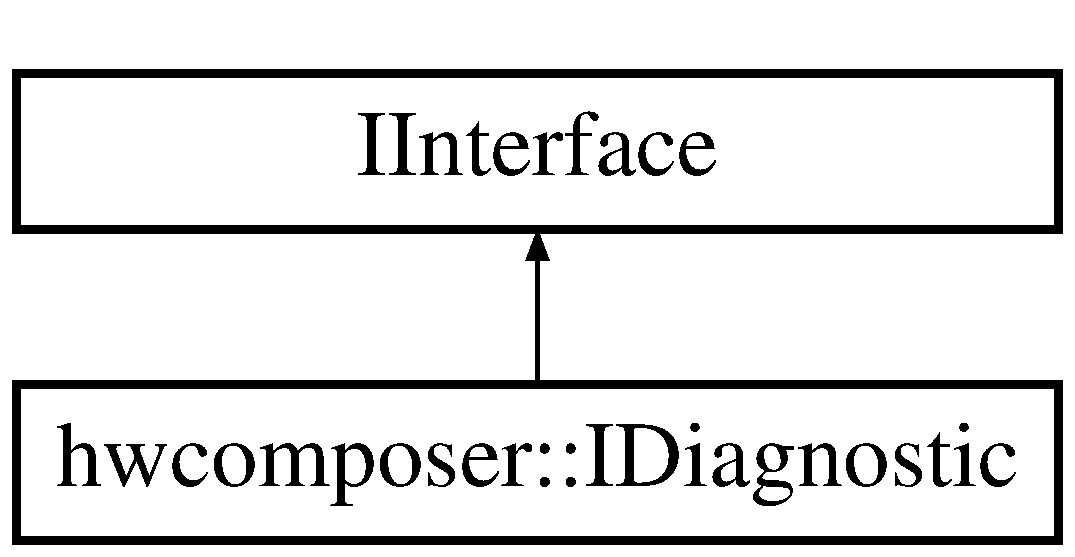
\includegraphics[height=2.000000cm]{classhwcomposer_1_1IDiagnostic}
\end{center}
\end{figure}
\subsection*{Public Types}
\begin{DoxyCompactItemize}
\item 
enum \{ \mbox{\hyperlink{classhwcomposer_1_1IDiagnostic_a56d1a1e037a9dfa35652205e24362776a58f5959ce571ee0e01c774fad36118b6}{e\+Log\+Truncated}}
 \}
\end{DoxyCompactItemize}
\subsection*{Public Member Functions}
\begin{DoxyCompactItemize}
\item 
\mbox{\hyperlink{classhwcomposer_1_1IDiagnostic_a9993955822071212ea5ccbc9e85987d2}{D\+E\+C\+L\+A\+R\+E\+\_\+\+M\+E\+T\+A\+\_\+\+I\+N\+T\+E\+R\+F\+A\+CE}} (Diagnostic)
\item 
virtual \mbox{\hyperlink{hwcserviceapi_8h_a3806fb2027d9a316d8ca8d9b8b8eb96f}{status\+\_\+t}} \mbox{\hyperlink{classhwcomposer_1_1IDiagnostic_ade22f6b73a1912c02dec2a2baaa14a4a}{Read\+Log\+Parcel}} (android\+::\+Parcel $\ast$reply)=0
\item 
virtual void \mbox{\hyperlink{classhwcomposer_1_1IDiagnostic_a56f95024619fc80d9f022462392818e3}{Enable\+Display}} (uint32\+\_\+t d)=0
\item 
virtual void \mbox{\hyperlink{classhwcomposer_1_1IDiagnostic_ad5ea1c34401b325c6d795f9417c2cd89}{Disable\+Display}} (uint32\+\_\+t d, bool b\+Blank)=0
\item 
virtual void \mbox{\hyperlink{classhwcomposer_1_1IDiagnostic_aadfea7c0adee73575567a580105f841e}{Mask\+Layer}} (uint32\+\_\+t d, uint32\+\_\+t layer, bool b\+Hide)=0
\item 
virtual void \mbox{\hyperlink{classhwcomposer_1_1IDiagnostic_ad3e81bebcbc3bf7dac6431eb50a33304}{Dump\+Frames}} (uint32\+\_\+t d, int32\+\_\+t frames, bool b\+Sync)=0
\end{DoxyCompactItemize}


\subsection{Detailed Description}


Definition at line 27 of file idiagnostic.\+h.



\subsection{Member Enumeration Documentation}
\mbox{\Hypertarget{classhwcomposer_1_1IDiagnostic_a56d1a1e037a9dfa35652205e24362776}\label{classhwcomposer_1_1IDiagnostic_a56d1a1e037a9dfa35652205e24362776}} 
\subsubsection{\texorpdfstring{anonymous enum}{anonymous enum}}
{\footnotesize\ttfamily anonymous enum}

\begin{DoxyEnumFields}{Enumerator}
\raisebox{\heightof{T}}[0pt][0pt]{\index{e\+Log\+Truncated@{e\+Log\+Truncated}!hwcomposer\+::\+I\+Diagnostic@{hwcomposer\+::\+I\+Diagnostic}}\index{hwcomposer\+::\+I\+Diagnostic@{hwcomposer\+::\+I\+Diagnostic}!e\+Log\+Truncated@{e\+Log\+Truncated}}}\mbox{\Hypertarget{classhwcomposer_1_1IDiagnostic_a56d1a1e037a9dfa35652205e24362776a58f5959ce571ee0e01c774fad36118b6}\label{classhwcomposer_1_1IDiagnostic_a56d1a1e037a9dfa35652205e24362776a58f5959ce571ee0e01c774fad36118b6}} 
e\+Log\+Truncated&\\
\hline

\end{DoxyEnumFields}


Definition at line 34 of file idiagnostic.\+h.


\begin{DoxyCode}{0}
\DoxyCodeLine{34        \{}
\DoxyCodeLine{35     \mbox{\hyperlink{classhwcomposer_1_1IDiagnostic_a56d1a1e037a9dfa35652205e24362776a58f5959ce571ee0e01c774fad36118b6}{eLogTruncated}} =}
\DoxyCodeLine{36         101,  \textcolor{comment}{// Status to indicate log entries have been overwritten}}
\DoxyCodeLine{37   \};}
\end{DoxyCode}


\subsection{Member Function Documentation}
\mbox{\Hypertarget{classhwcomposer_1_1IDiagnostic_a9993955822071212ea5ccbc9e85987d2}\label{classhwcomposer_1_1IDiagnostic_a9993955822071212ea5ccbc9e85987d2}} 
\index{hwcomposer\+::\+I\+Diagnostic@{hwcomposer\+::\+I\+Diagnostic}!D\+E\+C\+L\+A\+R\+E\+\_\+\+M\+E\+T\+A\+\_\+\+I\+N\+T\+E\+R\+F\+A\+CE@{D\+E\+C\+L\+A\+R\+E\+\_\+\+M\+E\+T\+A\+\_\+\+I\+N\+T\+E\+R\+F\+A\+CE}}
\index{D\+E\+C\+L\+A\+R\+E\+\_\+\+M\+E\+T\+A\+\_\+\+I\+N\+T\+E\+R\+F\+A\+CE@{D\+E\+C\+L\+A\+R\+E\+\_\+\+M\+E\+T\+A\+\_\+\+I\+N\+T\+E\+R\+F\+A\+CE}!hwcomposer\+::\+I\+Diagnostic@{hwcomposer\+::\+I\+Diagnostic}}
\subsubsection{\texorpdfstring{D\+E\+C\+L\+A\+R\+E\+\_\+\+M\+E\+T\+A\+\_\+\+I\+N\+T\+E\+R\+F\+A\+C\+E()}{DECLARE\_META\_INTERFACE()}}
{\footnotesize\ttfamily hwcomposer\+::\+I\+Diagnostic\+::\+D\+E\+C\+L\+A\+R\+E\+\_\+\+M\+E\+T\+A\+\_\+\+I\+N\+T\+E\+R\+F\+A\+CE (\begin{DoxyParamCaption}\item[{Diagnostic}]{ }\end{DoxyParamCaption})}

\mbox{\Hypertarget{classhwcomposer_1_1IDiagnostic_ad5ea1c34401b325c6d795f9417c2cd89}\label{classhwcomposer_1_1IDiagnostic_ad5ea1c34401b325c6d795f9417c2cd89}} 
\index{hwcomposer\+::\+I\+Diagnostic@{hwcomposer\+::\+I\+Diagnostic}!Disable\+Display@{Disable\+Display}}
\index{Disable\+Display@{Disable\+Display}!hwcomposer\+::\+I\+Diagnostic@{hwcomposer\+::\+I\+Diagnostic}}
\subsubsection{\texorpdfstring{Disable\+Display()}{DisableDisplay()}}
{\footnotesize\ttfamily virtual void hwcomposer\+::\+I\+Diagnostic\+::\+Disable\+Display (\begin{DoxyParamCaption}\item[{uint32\+\_\+t}]{d,  }\item[{bool}]{b\+Blank }\end{DoxyParamCaption})\hspace{0.3cm}{\ttfamily [pure virtual]}}

\mbox{\Hypertarget{classhwcomposer_1_1IDiagnostic_ad3e81bebcbc3bf7dac6431eb50a33304}\label{classhwcomposer_1_1IDiagnostic_ad3e81bebcbc3bf7dac6431eb50a33304}} 
\index{hwcomposer\+::\+I\+Diagnostic@{hwcomposer\+::\+I\+Diagnostic}!Dump\+Frames@{Dump\+Frames}}
\index{Dump\+Frames@{Dump\+Frames}!hwcomposer\+::\+I\+Diagnostic@{hwcomposer\+::\+I\+Diagnostic}}
\subsubsection{\texorpdfstring{Dump\+Frames()}{DumpFrames()}}
{\footnotesize\ttfamily virtual void hwcomposer\+::\+I\+Diagnostic\+::\+Dump\+Frames (\begin{DoxyParamCaption}\item[{uint32\+\_\+t}]{d,  }\item[{int32\+\_\+t}]{frames,  }\item[{bool}]{b\+Sync }\end{DoxyParamCaption})\hspace{0.3cm}{\ttfamily [pure virtual]}}

\mbox{\Hypertarget{classhwcomposer_1_1IDiagnostic_a56f95024619fc80d9f022462392818e3}\label{classhwcomposer_1_1IDiagnostic_a56f95024619fc80d9f022462392818e3}} 
\index{hwcomposer\+::\+I\+Diagnostic@{hwcomposer\+::\+I\+Diagnostic}!Enable\+Display@{Enable\+Display}}
\index{Enable\+Display@{Enable\+Display}!hwcomposer\+::\+I\+Diagnostic@{hwcomposer\+::\+I\+Diagnostic}}
\subsubsection{\texorpdfstring{Enable\+Display()}{EnableDisplay()}}
{\footnotesize\ttfamily virtual void hwcomposer\+::\+I\+Diagnostic\+::\+Enable\+Display (\begin{DoxyParamCaption}\item[{uint32\+\_\+t}]{d }\end{DoxyParamCaption})\hspace{0.3cm}{\ttfamily [pure virtual]}}

\mbox{\Hypertarget{classhwcomposer_1_1IDiagnostic_aadfea7c0adee73575567a580105f841e}\label{classhwcomposer_1_1IDiagnostic_aadfea7c0adee73575567a580105f841e}} 
\index{hwcomposer\+::\+I\+Diagnostic@{hwcomposer\+::\+I\+Diagnostic}!Mask\+Layer@{Mask\+Layer}}
\index{Mask\+Layer@{Mask\+Layer}!hwcomposer\+::\+I\+Diagnostic@{hwcomposer\+::\+I\+Diagnostic}}
\subsubsection{\texorpdfstring{Mask\+Layer()}{MaskLayer()}}
{\footnotesize\ttfamily virtual void hwcomposer\+::\+I\+Diagnostic\+::\+Mask\+Layer (\begin{DoxyParamCaption}\item[{uint32\+\_\+t}]{d,  }\item[{uint32\+\_\+t}]{layer,  }\item[{bool}]{b\+Hide }\end{DoxyParamCaption})\hspace{0.3cm}{\ttfamily [pure virtual]}}

\mbox{\Hypertarget{classhwcomposer_1_1IDiagnostic_ade22f6b73a1912c02dec2a2baaa14a4a}\label{classhwcomposer_1_1IDiagnostic_ade22f6b73a1912c02dec2a2baaa14a4a}} 
\index{hwcomposer\+::\+I\+Diagnostic@{hwcomposer\+::\+I\+Diagnostic}!Read\+Log\+Parcel@{Read\+Log\+Parcel}}
\index{Read\+Log\+Parcel@{Read\+Log\+Parcel}!hwcomposer\+::\+I\+Diagnostic@{hwcomposer\+::\+I\+Diagnostic}}
\subsubsection{\texorpdfstring{Read\+Log\+Parcel()}{ReadLogParcel()}}
{\footnotesize\ttfamily virtual \mbox{\hyperlink{hwcserviceapi_8h_a3806fb2027d9a316d8ca8d9b8b8eb96f}{status\+\_\+t}} hwcomposer\+::\+I\+Diagnostic\+::\+Read\+Log\+Parcel (\begin{DoxyParamCaption}\item[{android\+::\+Parcel $\ast$}]{reply }\end{DoxyParamCaption})\hspace{0.3cm}{\ttfamily [pure virtual]}}



The documentation for this class was generated from the following file\+:\begin{DoxyCompactItemize}
\item 
os/android/libhwcservice/\mbox{\hyperlink{idiagnostic_8h}{idiagnostic.\+h}}\end{DoxyCompactItemize}

\hypertarget{classhwcomposer_1_1IDisplayOverscanControl}{}\section{hwcomposer\+:\+:I\+Display\+Overscan\+Control Class Reference}
\label{classhwcomposer_1_1IDisplayOverscanControl}\index{hwcomposer\+::\+I\+Display\+Overscan\+Control@{hwcomposer\+::\+I\+Display\+Overscan\+Control}}


{\ttfamily \#include $<$idisplayoverscancontrol.\+h$>$}

Inheritance diagram for hwcomposer\+:\+:I\+Display\+Overscan\+Control\+:\begin{figure}[H]
\begin{center}
\leavevmode
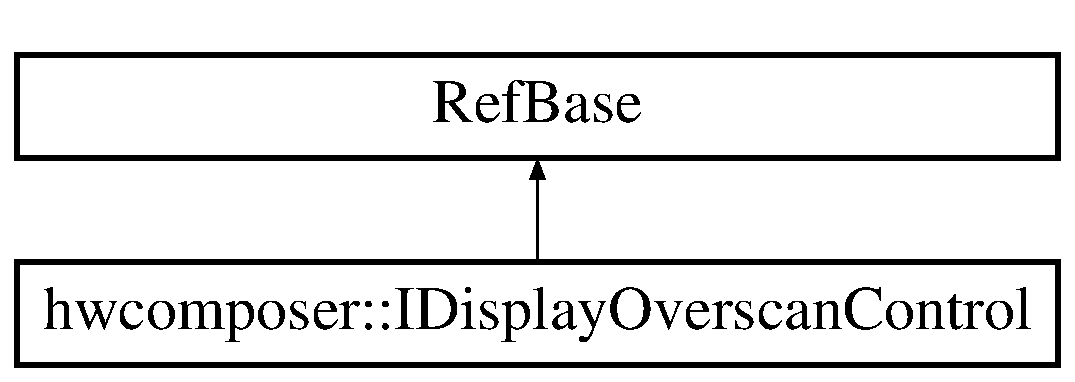
\includegraphics[height=2.000000cm]{classhwcomposer_1_1IDisplayOverscanControl}
\end{center}
\end{figure}
\subsection*{Public Types}
\begin{DoxyCompactItemize}
\item 
enum \{ \mbox{\hyperlink{classhwcomposer_1_1IDisplayOverscanControl_a864e169f204e86500afef542b1486b60a03e2374ea34aba79a543224df3bd7f74}{M\+A\+X\+\_\+\+O\+V\+E\+R\+S\+C\+AN}} = H\+W\+C\+S\+\_\+\+M\+A\+X\+\_\+\+O\+V\+E\+R\+S\+C\+AN, 
\mbox{\hyperlink{classhwcomposer_1_1IDisplayOverscanControl_a864e169f204e86500afef542b1486b60a67d0c9f5032c49e22f12aac2cc839c02}{R\+A\+N\+GE}} = H\+W\+C\+S\+\_\+\+O\+V\+E\+R\+S\+C\+A\+N\+\_\+\+R\+A\+N\+GE
 \}
\end{DoxyCompactItemize}
\subsection*{Public Member Functions}
\begin{DoxyCompactItemize}
\item 
\mbox{\hyperlink{classhwcomposer_1_1IDisplayOverscanControl_aa8f9a4f4ad30a0b07a1123d7dc16150e}{I\+Display\+Overscan\+Control}} (uint32\+\_\+t display)
\item 
\mbox{\hyperlink{hwcserviceapi_8h_a3806fb2027d9a316d8ca8d9b8b8eb96f}{status\+\_\+t}} \mbox{\hyperlink{classhwcomposer_1_1IDisplayOverscanControl_ae337988f284dbbf6844c814203d44d60}{set\+Overscan}} (int32\+\_\+t xoverscan, int32\+\_\+t yoverscan)
\begin{DoxyCompactList}\small\item\em Set overscan in the range +/-\/M\+A\+X\+\_\+\+O\+V\+E\+R\+S\+C\+AN inclusive. \end{DoxyCompactList}\item 
\mbox{\hyperlink{hwcserviceapi_8h_a3806fb2027d9a316d8ca8d9b8b8eb96f}{status\+\_\+t}} \mbox{\hyperlink{classhwcomposer_1_1IDisplayOverscanControl_a4617995aa4f6a5905eee9a0f8a3de3a6}{get\+Overscan}} (int32\+\_\+t $\ast$xoverscan, int32\+\_\+t $\ast$yoverscan)
\end{DoxyCompactItemize}


\subsection{Detailed Description}
Allows control of H\+D\+MI overscan 

Definition at line 28 of file idisplayoverscancontrol.\+h.



\subsection{Member Enumeration Documentation}
\mbox{\Hypertarget{classhwcomposer_1_1IDisplayOverscanControl_a864e169f204e86500afef542b1486b60}\label{classhwcomposer_1_1IDisplayOverscanControl_a864e169f204e86500afef542b1486b60}} 
\subsubsection{\texorpdfstring{anonymous enum}{anonymous enum}}
{\footnotesize\ttfamily anonymous enum}

\begin{DoxyEnumFields}{Enumerator}
\raisebox{\heightof{T}}[0pt][0pt]{\index{M\+A\+X\+\_\+\+O\+V\+E\+R\+S\+C\+AN@{M\+A\+X\+\_\+\+O\+V\+E\+R\+S\+C\+AN}!hwcomposer\+::\+I\+Display\+Overscan\+Control@{hwcomposer\+::\+I\+Display\+Overscan\+Control}}\index{hwcomposer\+::\+I\+Display\+Overscan\+Control@{hwcomposer\+::\+I\+Display\+Overscan\+Control}!M\+A\+X\+\_\+\+O\+V\+E\+R\+S\+C\+AN@{M\+A\+X\+\_\+\+O\+V\+E\+R\+S\+C\+AN}}}\mbox{\Hypertarget{classhwcomposer_1_1IDisplayOverscanControl_a864e169f204e86500afef542b1486b60a03e2374ea34aba79a543224df3bd7f74}\label{classhwcomposer_1_1IDisplayOverscanControl_a864e169f204e86500afef542b1486b60a03e2374ea34aba79a543224df3bd7f74}} 
M\+A\+X\+\_\+\+O\+V\+E\+R\+S\+C\+AN&\\
\hline

\raisebox{\heightof{T}}[0pt][0pt]{\index{R\+A\+N\+GE@{R\+A\+N\+GE}!hwcomposer\+::\+I\+Display\+Overscan\+Control@{hwcomposer\+::\+I\+Display\+Overscan\+Control}}\index{hwcomposer\+::\+I\+Display\+Overscan\+Control@{hwcomposer\+::\+I\+Display\+Overscan\+Control}!R\+A\+N\+GE@{R\+A\+N\+GE}}}\mbox{\Hypertarget{classhwcomposer_1_1IDisplayOverscanControl_a864e169f204e86500afef542b1486b60a67d0c9f5032c49e22f12aac2cc839c02}\label{classhwcomposer_1_1IDisplayOverscanControl_a864e169f204e86500afef542b1486b60a67d0c9f5032c49e22f12aac2cc839c02}} 
R\+A\+N\+GE&\\
\hline

\end{DoxyEnumFields}


Definition at line 33 of file idisplayoverscancontrol.\+h.


\begin{DoxyCode}{0}
\DoxyCodeLine{33        \{}
\DoxyCodeLine{34     \mbox{\hyperlink{classhwcomposer_1_1IDisplayOverscanControl_a864e169f204e86500afef542b1486b60a03e2374ea34aba79a543224df3bd7f74}{MAX\_OVERSCAN}} = \mbox{\hyperlink{hwcserviceapi_8h_a06fc87d81c62e9abb8790b6e5713c55ba0d3068e4f31603793a86ac1479935af3}{HWCS\_MAX\_OVERSCAN}},  \textcolor{comment}{// The limit of the control parameters}}
\DoxyCodeLine{35                                        \textcolor{comment}{// are +/-MAX\_OVERSCAN inclusive.}}
\DoxyCodeLine{36     \mbox{\hyperlink{classhwcomposer_1_1IDisplayOverscanControl_a864e169f204e86500afef542b1486b60a67d0c9f5032c49e22f12aac2cc839c02}{RANGE}} = \mbox{\hyperlink{hwcserviceapi_8h_a06fc87d81c62e9abb8790b6e5713c55ba608e6a23b6f025af3147af93cc61d130}{HWCS\_OVERSCAN\_RANGE}},  \textcolor{comment}{// RANGE describes the \% of the display size a}}
\DoxyCodeLine{37                                   \textcolor{comment}{// max control setting will adjust by.}}
\DoxyCodeLine{38   \};}
\end{DoxyCode}


\subsection{Constructor \& Destructor Documentation}
\mbox{\Hypertarget{classhwcomposer_1_1IDisplayOverscanControl_aa8f9a4f4ad30a0b07a1123d7dc16150e}\label{classhwcomposer_1_1IDisplayOverscanControl_aa8f9a4f4ad30a0b07a1123d7dc16150e}} 
\index{hwcomposer\+::\+I\+Display\+Overscan\+Control@{hwcomposer\+::\+I\+Display\+Overscan\+Control}!I\+Display\+Overscan\+Control@{I\+Display\+Overscan\+Control}}
\index{I\+Display\+Overscan\+Control@{I\+Display\+Overscan\+Control}!hwcomposer\+::\+I\+Display\+Overscan\+Control@{hwcomposer\+::\+I\+Display\+Overscan\+Control}}
\subsubsection{\texorpdfstring{I\+Display\+Overscan\+Control()}{IDisplayOverscanControl()}}
{\footnotesize\ttfamily hwcomposer\+::\+I\+Display\+Overscan\+Control\+::\+I\+Display\+Overscan\+Control (\begin{DoxyParamCaption}\item[{uint32\+\_\+t}]{display }\end{DoxyParamCaption})\hspace{0.3cm}{\ttfamily [inline]}}



Definition at line 30 of file idisplayoverscancontrol.\+h.


\begin{DoxyCode}{0}
\DoxyCodeLine{30                                             : mDisplay(display) \{}
\DoxyCodeLine{31   \}}
\end{DoxyCode}


\subsection{Member Function Documentation}
\mbox{\Hypertarget{classhwcomposer_1_1IDisplayOverscanControl_a4617995aa4f6a5905eee9a0f8a3de3a6}\label{classhwcomposer_1_1IDisplayOverscanControl_a4617995aa4f6a5905eee9a0f8a3de3a6}} 
\index{hwcomposer\+::\+I\+Display\+Overscan\+Control@{hwcomposer\+::\+I\+Display\+Overscan\+Control}!get\+Overscan@{get\+Overscan}}
\index{get\+Overscan@{get\+Overscan}!hwcomposer\+::\+I\+Display\+Overscan\+Control@{hwcomposer\+::\+I\+Display\+Overscan\+Control}}
\subsubsection{\texorpdfstring{get\+Overscan()}{getOverscan()}}
{\footnotesize\ttfamily \mbox{\hyperlink{hwcserviceapi_8h_a3806fb2027d9a316d8ca8d9b8b8eb96f}{status\+\_\+t}} hwcomposer\+::\+I\+Display\+Overscan\+Control\+::get\+Overscan (\begin{DoxyParamCaption}\item[{int32\+\_\+t $\ast$}]{xoverscan,  }\item[{int32\+\_\+t $\ast$}]{yoverscan }\end{DoxyParamCaption})\hspace{0.3cm}{\ttfamily [inline]}}



Definition at line 51 of file idisplayoverscancontrol.\+h.


\begin{DoxyCode}{0}
\DoxyCodeLine{51                                                                \{}
\DoxyCodeLine{52     \textcolor{keywordflow}{return} \mbox{\hyperlink{hwcserviceapi_8cpp_afb6ccb74db5380963898acbcefa6ffef}{HwcService\_Display\_GetOverscan}}(mHwcConn, mDisplay, xoverscan,}
\DoxyCodeLine{53                                           yoverscan);}
\DoxyCodeLine{54   \}}
\end{DoxyCode}
\mbox{\Hypertarget{classhwcomposer_1_1IDisplayOverscanControl_ae337988f284dbbf6844c814203d44d60}\label{classhwcomposer_1_1IDisplayOverscanControl_ae337988f284dbbf6844c814203d44d60}} 
\index{hwcomposer\+::\+I\+Display\+Overscan\+Control@{hwcomposer\+::\+I\+Display\+Overscan\+Control}!set\+Overscan@{set\+Overscan}}
\index{set\+Overscan@{set\+Overscan}!hwcomposer\+::\+I\+Display\+Overscan\+Control@{hwcomposer\+::\+I\+Display\+Overscan\+Control}}
\subsubsection{\texorpdfstring{set\+Overscan()}{setOverscan()}}
{\footnotesize\ttfamily \mbox{\hyperlink{hwcserviceapi_8h_a3806fb2027d9a316d8ca8d9b8b8eb96f}{status\+\_\+t}} hwcomposer\+::\+I\+Display\+Overscan\+Control\+::set\+Overscan (\begin{DoxyParamCaption}\item[{int32\+\_\+t}]{xoverscan,  }\item[{int32\+\_\+t}]{yoverscan }\end{DoxyParamCaption})\hspace{0.3cm}{\ttfamily [inline]}}



Set overscan in the range +/-\/M\+A\+X\+\_\+\+O\+V\+E\+R\+S\+C\+AN inclusive. 



Definition at line 43 of file idisplayoverscancontrol.\+h.


\begin{DoxyCode}{0}
\DoxyCodeLine{43                                                              \{}
\DoxyCodeLine{44     \textcolor{keywordflow}{return} \mbox{\hyperlink{hwcserviceapi_8cpp_a04907fdcdf1882fdc95179db91e68176}{HwcService\_Display\_SetOverscan}}(mHwcConn, mDisplay, xoverscan,}
\DoxyCodeLine{45                                           yoverscan);}
\DoxyCodeLine{46   \}}
\end{DoxyCode}


The documentation for this class was generated from the following file\+:\begin{DoxyCompactItemize}
\item 
os/android/libhwcservice/\mbox{\hyperlink{idisplayoverscancontrol_8h}{idisplayoverscancontrol.\+h}}\end{DoxyCompactItemize}

\hypertarget{classhwcomposer_1_1IDisplayScalingControl}{}\section{hwcomposer\+:\+:I\+Display\+Scaling\+Control Class Reference}
\label{classhwcomposer_1_1IDisplayScalingControl}\index{hwcomposer\+::\+I\+Display\+Scaling\+Control@{hwcomposer\+::\+I\+Display\+Scaling\+Control}}


{\ttfamily \#include $<$idisplayscalingcontrol.\+h$>$}

Inheritance diagram for hwcomposer\+:\+:I\+Display\+Scaling\+Control\+:\begin{figure}[H]
\begin{center}
\leavevmode
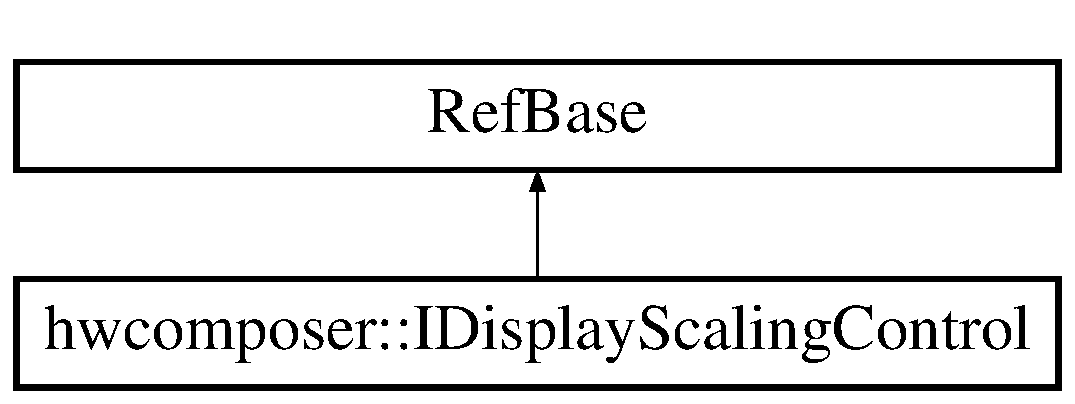
\includegraphics[height=2.000000cm]{classhwcomposer_1_1IDisplayScalingControl}
\end{center}
\end{figure}
\subsection*{Public Types}
\begin{DoxyCompactItemize}
\item 
enum \mbox{\hyperlink{classhwcomposer_1_1IDisplayScalingControl_a96b7ad3bec70da200ece1cd815807aab}{E\+Scaling\+Mode}} \{ \newline
\mbox{\hyperlink{classhwcomposer_1_1IDisplayScalingControl_a96b7ad3bec70da200ece1cd815807aaba51f3d108fdfe81971a4cf6ded8bb6227}{S\+C\+A\+L\+E\+\_\+\+C\+E\+N\+T\+RE}} = H\+W\+C\+S\+\_\+\+S\+C\+A\+L\+E\+\_\+\+C\+E\+N\+T\+RE, 
\mbox{\hyperlink{classhwcomposer_1_1IDisplayScalingControl_a96b7ad3bec70da200ece1cd815807aabaf3ef2341645b8973c40de2f1a65346de}{S\+C\+A\+L\+E\+\_\+\+S\+T\+R\+E\+T\+CH}} = H\+W\+C\+S\+\_\+\+S\+C\+A\+L\+E\+\_\+\+S\+T\+R\+E\+T\+CH, 
\mbox{\hyperlink{classhwcomposer_1_1IDisplayScalingControl_a96b7ad3bec70da200ece1cd815807aaba2a53b19fdbdedf81c19076e1ace09097}{S\+C\+A\+L\+E\+\_\+\+F\+IT}} = H\+W\+C\+S\+\_\+\+S\+C\+A\+L\+E\+\_\+\+F\+IT, 
\mbox{\hyperlink{classhwcomposer_1_1IDisplayScalingControl_a96b7ad3bec70da200ece1cd815807aabadabf7eb0f966f371bc37a29992a2576e}{S\+C\+A\+L\+E\+\_\+\+F\+I\+LL}} = H\+W\+C\+S\+\_\+\+S\+C\+A\+L\+E\+\_\+\+F\+I\+LL, 
\newline
\mbox{\hyperlink{classhwcomposer_1_1IDisplayScalingControl_a96b7ad3bec70da200ece1cd815807aaba4d197c09b66a1dbf7b725ece60bb0ef5}{S\+C\+A\+L\+E\+\_\+\+M\+A\+X\+\_\+\+E\+N\+UM}} = H\+W\+C\+S\+\_\+\+S\+C\+A\+L\+E\+\_\+\+M\+A\+X\+\_\+\+E\+N\+UM
 \}
\end{DoxyCompactItemize}
\subsection*{Public Member Functions}
\begin{DoxyCompactItemize}
\item 
\mbox{\hyperlink{classhwcomposer_1_1IDisplayScalingControl_a391bcc762fddd62b28b41c132e45eaf6}{I\+Display\+Scaling\+Control}} (uint32\+\_\+t display)
\item 
\mbox{\hyperlink{hwcserviceapi_8h_a3806fb2027d9a316d8ca8d9b8b8eb96f}{status\+\_\+t}} \mbox{\hyperlink{classhwcomposer_1_1IDisplayScalingControl_a424df506846f2347ec0d442227105735}{set\+Scaling}} (\mbox{\hyperlink{classhwcomposer_1_1IDisplayScalingControl_a96b7ad3bec70da200ece1cd815807aab}{E\+Scaling\+Mode}} e\+Scaling\+Mode)
\begin{DoxyCompactList}\small\item\em Set scaling to one of E\+Scaling\+Mode. \end{DoxyCompactList}\item 
\mbox{\hyperlink{hwcserviceapi_8h_a3806fb2027d9a316d8ca8d9b8b8eb96f}{status\+\_\+t}} \mbox{\hyperlink{classhwcomposer_1_1IDisplayScalingControl_ae95df0ea1728944684b91a80d0d9d6d0}{get\+Scaling}} (\mbox{\hyperlink{classhwcomposer_1_1IDisplayScalingControl_a96b7ad3bec70da200ece1cd815807aab}{E\+Scaling\+Mode}} $\ast$e\+Scaling\+Mode)
\end{DoxyCompactItemize}


\subsection{Detailed Description}
Allows control of H\+D\+MI scaling for content that does not match the native display resolution. 

Definition at line 29 of file idisplayscalingcontrol.\+h.



\subsection{Member Enumeration Documentation}
\mbox{\Hypertarget{classhwcomposer_1_1IDisplayScalingControl_a96b7ad3bec70da200ece1cd815807aab}\label{classhwcomposer_1_1IDisplayScalingControl_a96b7ad3bec70da200ece1cd815807aab}} 
\index{hwcomposer\+::\+I\+Display\+Scaling\+Control@{hwcomposer\+::\+I\+Display\+Scaling\+Control}!E\+Scaling\+Mode@{E\+Scaling\+Mode}}
\index{E\+Scaling\+Mode@{E\+Scaling\+Mode}!hwcomposer\+::\+I\+Display\+Scaling\+Control@{hwcomposer\+::\+I\+Display\+Scaling\+Control}}
\subsubsection{\texorpdfstring{E\+Scaling\+Mode}{EScalingMode}}
{\footnotesize\ttfamily enum \mbox{\hyperlink{classhwcomposer_1_1IDisplayScalingControl_a96b7ad3bec70da200ece1cd815807aab}{hwcomposer\+::\+I\+Display\+Scaling\+Control\+::\+E\+Scaling\+Mode}}}

\begin{DoxyEnumFields}{Enumerator}
\raisebox{\heightof{T}}[0pt][0pt]{\index{S\+C\+A\+L\+E\+\_\+\+C\+E\+N\+T\+RE@{S\+C\+A\+L\+E\+\_\+\+C\+E\+N\+T\+RE}!hwcomposer\+::\+I\+Display\+Scaling\+Control@{hwcomposer\+::\+I\+Display\+Scaling\+Control}}\index{hwcomposer\+::\+I\+Display\+Scaling\+Control@{hwcomposer\+::\+I\+Display\+Scaling\+Control}!S\+C\+A\+L\+E\+\_\+\+C\+E\+N\+T\+RE@{S\+C\+A\+L\+E\+\_\+\+C\+E\+N\+T\+RE}}}\mbox{\Hypertarget{classhwcomposer_1_1IDisplayScalingControl_a96b7ad3bec70da200ece1cd815807aaba51f3d108fdfe81971a4cf6ded8bb6227}\label{classhwcomposer_1_1IDisplayScalingControl_a96b7ad3bec70da200ece1cd815807aaba51f3d108fdfe81971a4cf6ded8bb6227}} 
S\+C\+A\+L\+E\+\_\+\+C\+E\+N\+T\+RE&\\
\hline

\raisebox{\heightof{T}}[0pt][0pt]{\index{S\+C\+A\+L\+E\+\_\+\+S\+T\+R\+E\+T\+CH@{S\+C\+A\+L\+E\+\_\+\+S\+T\+R\+E\+T\+CH}!hwcomposer\+::\+I\+Display\+Scaling\+Control@{hwcomposer\+::\+I\+Display\+Scaling\+Control}}\index{hwcomposer\+::\+I\+Display\+Scaling\+Control@{hwcomposer\+::\+I\+Display\+Scaling\+Control}!S\+C\+A\+L\+E\+\_\+\+S\+T\+R\+E\+T\+CH@{S\+C\+A\+L\+E\+\_\+\+S\+T\+R\+E\+T\+CH}}}\mbox{\Hypertarget{classhwcomposer_1_1IDisplayScalingControl_a96b7ad3bec70da200ece1cd815807aabaf3ef2341645b8973c40de2f1a65346de}\label{classhwcomposer_1_1IDisplayScalingControl_a96b7ad3bec70da200ece1cd815807aabaf3ef2341645b8973c40de2f1a65346de}} 
S\+C\+A\+L\+E\+\_\+\+S\+T\+R\+E\+T\+CH&\\
\hline

\raisebox{\heightof{T}}[0pt][0pt]{\index{S\+C\+A\+L\+E\+\_\+\+F\+IT@{S\+C\+A\+L\+E\+\_\+\+F\+IT}!hwcomposer\+::\+I\+Display\+Scaling\+Control@{hwcomposer\+::\+I\+Display\+Scaling\+Control}}\index{hwcomposer\+::\+I\+Display\+Scaling\+Control@{hwcomposer\+::\+I\+Display\+Scaling\+Control}!S\+C\+A\+L\+E\+\_\+\+F\+IT@{S\+C\+A\+L\+E\+\_\+\+F\+IT}}}\mbox{\Hypertarget{classhwcomposer_1_1IDisplayScalingControl_a96b7ad3bec70da200ece1cd815807aaba2a53b19fdbdedf81c19076e1ace09097}\label{classhwcomposer_1_1IDisplayScalingControl_a96b7ad3bec70da200ece1cd815807aaba2a53b19fdbdedf81c19076e1ace09097}} 
S\+C\+A\+L\+E\+\_\+\+F\+IT&\\
\hline

\raisebox{\heightof{T}}[0pt][0pt]{\index{S\+C\+A\+L\+E\+\_\+\+F\+I\+LL@{S\+C\+A\+L\+E\+\_\+\+F\+I\+LL}!hwcomposer\+::\+I\+Display\+Scaling\+Control@{hwcomposer\+::\+I\+Display\+Scaling\+Control}}\index{hwcomposer\+::\+I\+Display\+Scaling\+Control@{hwcomposer\+::\+I\+Display\+Scaling\+Control}!S\+C\+A\+L\+E\+\_\+\+F\+I\+LL@{S\+C\+A\+L\+E\+\_\+\+F\+I\+LL}}}\mbox{\Hypertarget{classhwcomposer_1_1IDisplayScalingControl_a96b7ad3bec70da200ece1cd815807aabadabf7eb0f966f371bc37a29992a2576e}\label{classhwcomposer_1_1IDisplayScalingControl_a96b7ad3bec70da200ece1cd815807aabadabf7eb0f966f371bc37a29992a2576e}} 
S\+C\+A\+L\+E\+\_\+\+F\+I\+LL&\\
\hline

\raisebox{\heightof{T}}[0pt][0pt]{\index{S\+C\+A\+L\+E\+\_\+\+M\+A\+X\+\_\+\+E\+N\+UM@{S\+C\+A\+L\+E\+\_\+\+M\+A\+X\+\_\+\+E\+N\+UM}!hwcomposer\+::\+I\+Display\+Scaling\+Control@{hwcomposer\+::\+I\+Display\+Scaling\+Control}}\index{hwcomposer\+::\+I\+Display\+Scaling\+Control@{hwcomposer\+::\+I\+Display\+Scaling\+Control}!S\+C\+A\+L\+E\+\_\+\+M\+A\+X\+\_\+\+E\+N\+UM@{S\+C\+A\+L\+E\+\_\+\+M\+A\+X\+\_\+\+E\+N\+UM}}}\mbox{\Hypertarget{classhwcomposer_1_1IDisplayScalingControl_a96b7ad3bec70da200ece1cd815807aaba4d197c09b66a1dbf7b725ece60bb0ef5}\label{classhwcomposer_1_1IDisplayScalingControl_a96b7ad3bec70da200ece1cd815807aaba4d197c09b66a1dbf7b725ece60bb0ef5}} 
S\+C\+A\+L\+E\+\_\+\+M\+A\+X\+\_\+\+E\+N\+UM&\\
\hline

\end{DoxyEnumFields}


Definition at line 34 of file idisplayscalingcontrol.\+h.


\begin{DoxyCode}{0}
\DoxyCodeLine{34                     \{}
\DoxyCodeLine{35     \mbox{\hyperlink{classhwcomposer_1_1IDisplayScalingControl_a96b7ad3bec70da200ece1cd815807aaba51f3d108fdfe81971a4cf6ded8bb6227}{SCALE\_CENTRE}} = \mbox{\hyperlink{hwcserviceapi_8h_ad4b6f7ee9b8ba932ea9308645ac64ee1a96c7d625ff253e13f1575381983bd403}{HWCS\_SCALE\_CENTRE}},    \textcolor{comment}{// Present the content centred at 1:1}}
\DoxyCodeLine{36                                          \textcolor{comment}{// source resolution.}}
\DoxyCodeLine{37     \mbox{\hyperlink{classhwcomposer_1_1IDisplayScalingControl_a96b7ad3bec70da200ece1cd815807aabaf3ef2341645b8973c40de2f1a65346de}{SCALE\_STRETCH}} = \mbox{\hyperlink{hwcserviceapi_8h_ad4b6f7ee9b8ba932ea9308645ac64ee1a960e072718da429448f6589acae0bc52}{HWCS\_SCALE\_STRETCH}},  \textcolor{comment}{// Do not preserve aspect ratio - scale}}
\DoxyCodeLine{38                                          \textcolor{comment}{// to fill the display without}}
\DoxyCodeLine{39                                          \textcolor{comment}{// cropping.}}
\DoxyCodeLine{40     \mbox{\hyperlink{classhwcomposer_1_1IDisplayScalingControl_a96b7ad3bec70da200ece1cd815807aaba2a53b19fdbdedf81c19076e1ace09097}{SCALE\_FIT}} = \mbox{\hyperlink{hwcserviceapi_8h_ad4b6f7ee9b8ba932ea9308645ac64ee1a9b6ca8b97bd4a138d2c4d434655ba24d}{HWCS\_SCALE\_FIT}},    \textcolor{comment}{// Preserve aspect ratio - scale to closest}}
\DoxyCodeLine{41                                    \textcolor{comment}{// edge (may be letterboxed or pillarboxed).}}
\DoxyCodeLine{42     \mbox{\hyperlink{classhwcomposer_1_1IDisplayScalingControl_a96b7ad3bec70da200ece1cd815807aabadabf7eb0f966f371bc37a29992a2576e}{SCALE\_FILL}} = \mbox{\hyperlink{hwcserviceapi_8h_ad4b6f7ee9b8ba932ea9308645ac64ee1adf38586562338ace55aecf9cd926474c}{HWCS\_SCALE\_FILL}},  \textcolor{comment}{// Preserve aspect ratio - scale to fill the}}
\DoxyCodeLine{43                                    \textcolor{comment}{// display (may crop the content).}}
\DoxyCodeLine{44     \mbox{\hyperlink{classhwcomposer_1_1IDisplayScalingControl_a96b7ad3bec70da200ece1cd815807aaba4d197c09b66a1dbf7b725ece60bb0ef5}{SCALE\_MAX\_ENUM}} = \mbox{\hyperlink{hwcserviceapi_8h_ad4b6f7ee9b8ba932ea9308645ac64ee1a2cdc0010ea4bdd4cd3756e67f7e64d27}{HWCS\_SCALE\_MAX\_ENUM}}  \textcolor{comment}{// End of enum.}}
\DoxyCodeLine{45   \};}
\end{DoxyCode}


\subsection{Constructor \& Destructor Documentation}
\mbox{\Hypertarget{classhwcomposer_1_1IDisplayScalingControl_a391bcc762fddd62b28b41c132e45eaf6}\label{classhwcomposer_1_1IDisplayScalingControl_a391bcc762fddd62b28b41c132e45eaf6}} 
\index{hwcomposer\+::\+I\+Display\+Scaling\+Control@{hwcomposer\+::\+I\+Display\+Scaling\+Control}!I\+Display\+Scaling\+Control@{I\+Display\+Scaling\+Control}}
\index{I\+Display\+Scaling\+Control@{I\+Display\+Scaling\+Control}!hwcomposer\+::\+I\+Display\+Scaling\+Control@{hwcomposer\+::\+I\+Display\+Scaling\+Control}}
\subsubsection{\texorpdfstring{I\+Display\+Scaling\+Control()}{IDisplayScalingControl()}}
{\footnotesize\ttfamily hwcomposer\+::\+I\+Display\+Scaling\+Control\+::\+I\+Display\+Scaling\+Control (\begin{DoxyParamCaption}\item[{uint32\+\_\+t}]{display }\end{DoxyParamCaption})\hspace{0.3cm}{\ttfamily [inline]}}



Definition at line 31 of file idisplayscalingcontrol.\+h.


\begin{DoxyCode}{0}
\DoxyCodeLine{31                                            : mDisplay(display) \{}
\DoxyCodeLine{32   \}}
\end{DoxyCode}


\subsection{Member Function Documentation}
\mbox{\Hypertarget{classhwcomposer_1_1IDisplayScalingControl_ae95df0ea1728944684b91a80d0d9d6d0}\label{classhwcomposer_1_1IDisplayScalingControl_ae95df0ea1728944684b91a80d0d9d6d0}} 
\index{hwcomposer\+::\+I\+Display\+Scaling\+Control@{hwcomposer\+::\+I\+Display\+Scaling\+Control}!get\+Scaling@{get\+Scaling}}
\index{get\+Scaling@{get\+Scaling}!hwcomposer\+::\+I\+Display\+Scaling\+Control@{hwcomposer\+::\+I\+Display\+Scaling\+Control}}
\subsubsection{\texorpdfstring{get\+Scaling()}{getScaling()}}
{\footnotesize\ttfamily \mbox{\hyperlink{hwcserviceapi_8h_a3806fb2027d9a316d8ca8d9b8b8eb96f}{status\+\_\+t}} hwcomposer\+::\+I\+Display\+Scaling\+Control\+::get\+Scaling (\begin{DoxyParamCaption}\item[{\mbox{\hyperlink{classhwcomposer_1_1IDisplayScalingControl_a96b7ad3bec70da200ece1cd815807aab}{E\+Scaling\+Mode}} $\ast$}]{e\+Scaling\+Mode }\end{DoxyParamCaption})\hspace{0.3cm}{\ttfamily [inline]}}



Definition at line 58 of file idisplayscalingcontrol.\+h.


\begin{DoxyCode}{0}
\DoxyCodeLine{58                                                   \{}
\DoxyCodeLine{59     \textcolor{keywordflow}{return} \mbox{\hyperlink{hwcserviceapi_8cpp_add41493b4309f8484e857e26c67f281c}{HwcService\_Display\_GetScaling}}(mHwcConn, mDisplay,}
\DoxyCodeLine{60                                          (\mbox{\hyperlink{hwcserviceapi_8h_acdadfd5e7f15097833789174e442083f}{EHwcsScalingMode}} *)eScalingMode);}
\DoxyCodeLine{61   \}}
\end{DoxyCode}
\mbox{\Hypertarget{classhwcomposer_1_1IDisplayScalingControl_a424df506846f2347ec0d442227105735}\label{classhwcomposer_1_1IDisplayScalingControl_a424df506846f2347ec0d442227105735}} 
\index{hwcomposer\+::\+I\+Display\+Scaling\+Control@{hwcomposer\+::\+I\+Display\+Scaling\+Control}!set\+Scaling@{set\+Scaling}}
\index{set\+Scaling@{set\+Scaling}!hwcomposer\+::\+I\+Display\+Scaling\+Control@{hwcomposer\+::\+I\+Display\+Scaling\+Control}}
\subsubsection{\texorpdfstring{set\+Scaling()}{setScaling()}}
{\footnotesize\ttfamily \mbox{\hyperlink{hwcserviceapi_8h_a3806fb2027d9a316d8ca8d9b8b8eb96f}{status\+\_\+t}} hwcomposer\+::\+I\+Display\+Scaling\+Control\+::set\+Scaling (\begin{DoxyParamCaption}\item[{\mbox{\hyperlink{classhwcomposer_1_1IDisplayScalingControl_a96b7ad3bec70da200ece1cd815807aab}{E\+Scaling\+Mode}}}]{e\+Scaling\+Mode }\end{DoxyParamCaption})\hspace{0.3cm}{\ttfamily [inline]}}



Set scaling to one of E\+Scaling\+Mode. 



Definition at line 49 of file idisplayscalingcontrol.\+h.


\begin{DoxyCode}{0}
\DoxyCodeLine{49                                                  \{}
\DoxyCodeLine{50     \textcolor{keywordflow}{return} \mbox{\hyperlink{hwcserviceapi_8cpp_a78003256892e1ddca556006b97dc4ce6}{HwcService\_Display\_SetScaling}}(mHwcConn, mDisplay,}
\DoxyCodeLine{51                                          (\mbox{\hyperlink{hwcserviceapi_8h_acdadfd5e7f15097833789174e442083f}{EHwcsScalingMode}})eScalingMode);}
\DoxyCodeLine{52   \}}
\end{DoxyCode}


The documentation for this class was generated from the following file\+:\begin{DoxyCompactItemize}
\item 
os/android/libhwcservice/\mbox{\hyperlink{idisplayscalingcontrol_8h}{idisplayscalingcontrol.\+h}}\end{DoxyCompactItemize}

\hypertarget{classhwcomposer_1_1IService}{}\section{hwcomposer\+:\+:I\+Service Class Reference}
\label{classhwcomposer_1_1IService}\index{hwcomposer\+::\+I\+Service@{hwcomposer\+::\+I\+Service}}


{\ttfamily \#include $<$iservice.\+h$>$}

Inheritance diagram for hwcomposer\+:\+:I\+Service\+:\begin{figure}[H]
\begin{center}
\leavevmode
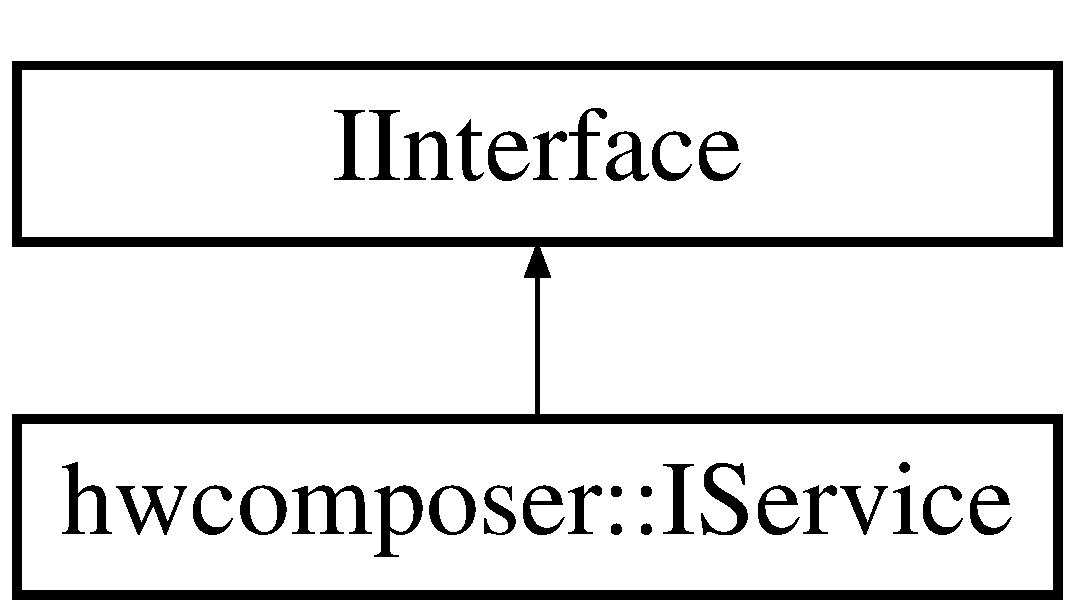
\includegraphics[height=2.000000cm]{classhwcomposer_1_1IService}
\end{center}
\end{figure}
\subsection*{Public Member Functions}
\begin{DoxyCompactItemize}
\item 
\mbox{\hyperlink{classhwcomposer_1_1IService_ad6bc53970c36eb2060aef96616c97367}{D\+E\+C\+L\+A\+R\+E\+\_\+\+M\+E\+T\+A\+\_\+\+I\+N\+T\+E\+R\+F\+A\+CE}} (Service)
\item 
virtual sp$<$ \mbox{\hyperlink{classhwcomposer_1_1IDiagnostic}{I\+Diagnostic}} $>$ \mbox{\hyperlink{classhwcomposer_1_1IService_ab8408be3aeef35ceef24739d85ca80fc}{Get\+Diagnostic}} ()=0
\item 
virtual sp$<$ \mbox{\hyperlink{classhwcomposer_1_1IControls}{I\+Controls}} $>$ \mbox{\hyperlink{classhwcomposer_1_1IService_a88d42bf367d37d06ef71f9eab33da2d7}{Get\+Controls}} ()=0
\item 
virtual String8 \mbox{\hyperlink{classhwcomposer_1_1IService_a74bd053098590c03cf3e374f396222f8}{Get\+Hwc\+Version}} ()=0
\item 
virtual void \mbox{\hyperlink{classhwcomposer_1_1IService_a5a418c67d99e61ad226210ad22bfa765}{Dump\+Options}} (void)=0
\item 
virtual \mbox{\hyperlink{hwcserviceapi_8h_a3806fb2027d9a316d8ca8d9b8b8eb96f}{status\+\_\+t}} \mbox{\hyperlink{classhwcomposer_1_1IService_a72bf2c3bbfbeeb72a2d1a4cbaadc97b7}{Set\+Option}} (String8 option, String8 option\+Value)=0
\item 
virtual \mbox{\hyperlink{hwcserviceapi_8h_a3806fb2027d9a316d8ca8d9b8b8eb96f}{status\+\_\+t}} \mbox{\hyperlink{classhwcomposer_1_1IService_aaddf58a1f2b64b1a05f7f68259b6c1f3}{Enable\+Logview\+To\+Logcat}} (bool enable=true)=0
\end{DoxyCompactItemize}


\subsection{Detailed Description}
Maintenance interface to control H\+WC activity. 

Definition at line 34 of file iservice.\+h.



\subsection{Member Function Documentation}
\mbox{\Hypertarget{classhwcomposer_1_1IService_ad6bc53970c36eb2060aef96616c97367}\label{classhwcomposer_1_1IService_ad6bc53970c36eb2060aef96616c97367}} 
\index{hwcomposer\+::\+I\+Service@{hwcomposer\+::\+I\+Service}!D\+E\+C\+L\+A\+R\+E\+\_\+\+M\+E\+T\+A\+\_\+\+I\+N\+T\+E\+R\+F\+A\+CE@{D\+E\+C\+L\+A\+R\+E\+\_\+\+M\+E\+T\+A\+\_\+\+I\+N\+T\+E\+R\+F\+A\+CE}}
\index{D\+E\+C\+L\+A\+R\+E\+\_\+\+M\+E\+T\+A\+\_\+\+I\+N\+T\+E\+R\+F\+A\+CE@{D\+E\+C\+L\+A\+R\+E\+\_\+\+M\+E\+T\+A\+\_\+\+I\+N\+T\+E\+R\+F\+A\+CE}!hwcomposer\+::\+I\+Service@{hwcomposer\+::\+I\+Service}}
\subsubsection{\texorpdfstring{D\+E\+C\+L\+A\+R\+E\+\_\+\+M\+E\+T\+A\+\_\+\+I\+N\+T\+E\+R\+F\+A\+C\+E()}{DECLARE\_META\_INTERFACE()}}
{\footnotesize\ttfamily hwcomposer\+::\+I\+Service\+::\+D\+E\+C\+L\+A\+R\+E\+\_\+\+M\+E\+T\+A\+\_\+\+I\+N\+T\+E\+R\+F\+A\+CE (\begin{DoxyParamCaption}\item[{Service}]{ }\end{DoxyParamCaption})}

\mbox{\Hypertarget{classhwcomposer_1_1IService_a5a418c67d99e61ad226210ad22bfa765}\label{classhwcomposer_1_1IService_a5a418c67d99e61ad226210ad22bfa765}} 
\index{hwcomposer\+::\+I\+Service@{hwcomposer\+::\+I\+Service}!Dump\+Options@{Dump\+Options}}
\index{Dump\+Options@{Dump\+Options}!hwcomposer\+::\+I\+Service@{hwcomposer\+::\+I\+Service}}
\subsubsection{\texorpdfstring{Dump\+Options()}{DumpOptions()}}
{\footnotesize\ttfamily virtual void hwcomposer\+::\+I\+Service\+::\+Dump\+Options (\begin{DoxyParamCaption}\item[{void}]{ }\end{DoxyParamCaption})\hspace{0.3cm}{\ttfamily [pure virtual]}}

\mbox{\Hypertarget{classhwcomposer_1_1IService_aaddf58a1f2b64b1a05f7f68259b6c1f3}\label{classhwcomposer_1_1IService_aaddf58a1f2b64b1a05f7f68259b6c1f3}} 
\index{hwcomposer\+::\+I\+Service@{hwcomposer\+::\+I\+Service}!Enable\+Logview\+To\+Logcat@{Enable\+Logview\+To\+Logcat}}
\index{Enable\+Logview\+To\+Logcat@{Enable\+Logview\+To\+Logcat}!hwcomposer\+::\+I\+Service@{hwcomposer\+::\+I\+Service}}
\subsubsection{\texorpdfstring{Enable\+Logview\+To\+Logcat()}{EnableLogviewToLogcat()}}
{\footnotesize\ttfamily virtual \mbox{\hyperlink{hwcserviceapi_8h_a3806fb2027d9a316d8ca8d9b8b8eb96f}{status\+\_\+t}} hwcomposer\+::\+I\+Service\+::\+Enable\+Logview\+To\+Logcat (\begin{DoxyParamCaption}\item[{bool}]{enable = {\ttfamily true} }\end{DoxyParamCaption})\hspace{0.3cm}{\ttfamily [pure virtual]}}

\mbox{\Hypertarget{classhwcomposer_1_1IService_a88d42bf367d37d06ef71f9eab33da2d7}\label{classhwcomposer_1_1IService_a88d42bf367d37d06ef71f9eab33da2d7}} 
\index{hwcomposer\+::\+I\+Service@{hwcomposer\+::\+I\+Service}!Get\+Controls@{Get\+Controls}}
\index{Get\+Controls@{Get\+Controls}!hwcomposer\+::\+I\+Service@{hwcomposer\+::\+I\+Service}}
\subsubsection{\texorpdfstring{Get\+Controls()}{GetControls()}}
{\footnotesize\ttfamily virtual sp$<$\mbox{\hyperlink{classhwcomposer_1_1IControls}{I\+Controls}}$>$ hwcomposer\+::\+I\+Service\+::\+Get\+Controls (\begin{DoxyParamCaption}{ }\end{DoxyParamCaption})\hspace{0.3cm}{\ttfamily [pure virtual]}}

\mbox{\Hypertarget{classhwcomposer_1_1IService_ab8408be3aeef35ceef24739d85ca80fc}\label{classhwcomposer_1_1IService_ab8408be3aeef35ceef24739d85ca80fc}} 
\index{hwcomposer\+::\+I\+Service@{hwcomposer\+::\+I\+Service}!Get\+Diagnostic@{Get\+Diagnostic}}
\index{Get\+Diagnostic@{Get\+Diagnostic}!hwcomposer\+::\+I\+Service@{hwcomposer\+::\+I\+Service}}
\subsubsection{\texorpdfstring{Get\+Diagnostic()}{GetDiagnostic()}}
{\footnotesize\ttfamily virtual sp$<$\mbox{\hyperlink{classhwcomposer_1_1IDiagnostic}{I\+Diagnostic}}$>$ hwcomposer\+::\+I\+Service\+::\+Get\+Diagnostic (\begin{DoxyParamCaption}{ }\end{DoxyParamCaption})\hspace{0.3cm}{\ttfamily [pure virtual]}}

\mbox{\Hypertarget{classhwcomposer_1_1IService_a74bd053098590c03cf3e374f396222f8}\label{classhwcomposer_1_1IService_a74bd053098590c03cf3e374f396222f8}} 
\index{hwcomposer\+::\+I\+Service@{hwcomposer\+::\+I\+Service}!Get\+Hwc\+Version@{Get\+Hwc\+Version}}
\index{Get\+Hwc\+Version@{Get\+Hwc\+Version}!hwcomposer\+::\+I\+Service@{hwcomposer\+::\+I\+Service}}
\subsubsection{\texorpdfstring{Get\+Hwc\+Version()}{GetHwcVersion()}}
{\footnotesize\ttfamily virtual String8 hwcomposer\+::\+I\+Service\+::\+Get\+Hwc\+Version (\begin{DoxyParamCaption}{ }\end{DoxyParamCaption})\hspace{0.3cm}{\ttfamily [pure virtual]}}

\mbox{\Hypertarget{classhwcomposer_1_1IService_a72bf2c3bbfbeeb72a2d1a4cbaadc97b7}\label{classhwcomposer_1_1IService_a72bf2c3bbfbeeb72a2d1a4cbaadc97b7}} 
\index{hwcomposer\+::\+I\+Service@{hwcomposer\+::\+I\+Service}!Set\+Option@{Set\+Option}}
\index{Set\+Option@{Set\+Option}!hwcomposer\+::\+I\+Service@{hwcomposer\+::\+I\+Service}}
\subsubsection{\texorpdfstring{Set\+Option()}{SetOption()}}
{\footnotesize\ttfamily virtual \mbox{\hyperlink{hwcserviceapi_8h_a3806fb2027d9a316d8ca8d9b8b8eb96f}{status\+\_\+t}} hwcomposer\+::\+I\+Service\+::\+Set\+Option (\begin{DoxyParamCaption}\item[{String8}]{option,  }\item[{String8}]{option\+Value }\end{DoxyParamCaption})\hspace{0.3cm}{\ttfamily [pure virtual]}}



The documentation for this class was generated from the following file\+:\begin{DoxyCompactItemize}
\item 
os/android/libhwcservice/\mbox{\hyperlink{iservice_8h}{iservice.\+h}}\end{DoxyCompactItemize}

\hypertarget{structhwcomposer_1_1RenderState_1_1LayerState}{}\section{hwcomposer\+:\+:Render\+State\+:\+:Layer\+State Struct Reference}
\label{structhwcomposer_1_1RenderState_1_1LayerState}\index{hwcomposer\+::\+Render\+State\+::\+Layer\+State@{hwcomposer\+::\+Render\+State\+::\+Layer\+State}}


{\ttfamily \#include $<$renderstate.\+h$>$}

\subsection*{Public Attributes}
\begin{DoxyCompactItemize}
\item 
float \mbox{\hyperlink{structhwcomposer_1_1RenderState_1_1LayerState_a2ae0d2985cd27e57fe473666a9e57243}{crop\+\_\+bounds\+\_\+}} \mbox{[}4\mbox{]}
\item 
float \mbox{\hyperlink{structhwcomposer_1_1RenderState_1_1LayerState_aafc535e52757f72e87afd87346e52f05}{alpha\+\_\+}}
\item 
float \mbox{\hyperlink{structhwcomposer_1_1RenderState_1_1LayerState_a43d36ca83789cac1c1957df1f032c1ee}{premult\+\_\+}}
\item 
float \mbox{\hyperlink{structhwcomposer_1_1RenderState_1_1LayerState_afd84107447feedca42841c54c877c96c}{texture\+\_\+matrix\+\_\+}} \mbox{[}4\mbox{]}
\item 
uint32\+\_\+t \mbox{\hyperlink{structhwcomposer_1_1RenderState_1_1LayerState_a2271499cd60f4416b96954d3e79187e0}{layer\+\_\+index\+\_\+}}
\item 
\mbox{\hyperlink{namespacehwcomposer_a3da411c7c0213da2ce847c654bdc180d}{Gpu\+Resource\+Handle}} \mbox{\hyperlink{structhwcomposer_1_1RenderState_1_1LayerState_a08fbf02b64aaf423f2281a9d9e283097}{handle\+\_\+}}
\end{DoxyCompactItemize}


\subsection{Detailed Description}


Definition at line 37 of file renderstate.\+h.



\subsection{Member Data Documentation}
\mbox{\Hypertarget{structhwcomposer_1_1RenderState_1_1LayerState_aafc535e52757f72e87afd87346e52f05}\label{structhwcomposer_1_1RenderState_1_1LayerState_aafc535e52757f72e87afd87346e52f05}} 
\index{hwcomposer\+::\+Render\+State\+::\+Layer\+State@{hwcomposer\+::\+Render\+State\+::\+Layer\+State}!alpha\+\_\+@{alpha\+\_\+}}
\index{alpha\+\_\+@{alpha\+\_\+}!hwcomposer\+::\+Render\+State\+::\+Layer\+State@{hwcomposer\+::\+Render\+State\+::\+Layer\+State}}
\subsubsection{\texorpdfstring{alpha\+\_\+}{alpha\_}}
{\footnotesize\ttfamily float hwcomposer\+::\+Render\+State\+::\+Layer\+State\+::alpha\+\_\+}



Definition at line 39 of file renderstate.\+h.

\mbox{\Hypertarget{structhwcomposer_1_1RenderState_1_1LayerState_a2ae0d2985cd27e57fe473666a9e57243}\label{structhwcomposer_1_1RenderState_1_1LayerState_a2ae0d2985cd27e57fe473666a9e57243}} 
\index{hwcomposer\+::\+Render\+State\+::\+Layer\+State@{hwcomposer\+::\+Render\+State\+::\+Layer\+State}!crop\+\_\+bounds\+\_\+@{crop\+\_\+bounds\+\_\+}}
\index{crop\+\_\+bounds\+\_\+@{crop\+\_\+bounds\+\_\+}!hwcomposer\+::\+Render\+State\+::\+Layer\+State@{hwcomposer\+::\+Render\+State\+::\+Layer\+State}}
\subsubsection{\texorpdfstring{crop\+\_\+bounds\+\_\+}{crop\_bounds\_}}
{\footnotesize\ttfamily float hwcomposer\+::\+Render\+State\+::\+Layer\+State\+::crop\+\_\+bounds\+\_\+\mbox{[}4\mbox{]}}



Definition at line 38 of file renderstate.\+h.

\mbox{\Hypertarget{structhwcomposer_1_1RenderState_1_1LayerState_a08fbf02b64aaf423f2281a9d9e283097}\label{structhwcomposer_1_1RenderState_1_1LayerState_a08fbf02b64aaf423f2281a9d9e283097}} 
\index{hwcomposer\+::\+Render\+State\+::\+Layer\+State@{hwcomposer\+::\+Render\+State\+::\+Layer\+State}!handle\+\_\+@{handle\+\_\+}}
\index{handle\+\_\+@{handle\+\_\+}!hwcomposer\+::\+Render\+State\+::\+Layer\+State@{hwcomposer\+::\+Render\+State\+::\+Layer\+State}}
\subsubsection{\texorpdfstring{handle\+\_\+}{handle\_}}
{\footnotesize\ttfamily \mbox{\hyperlink{namespacehwcomposer_a3da411c7c0213da2ce847c654bdc180d}{Gpu\+Resource\+Handle}} hwcomposer\+::\+Render\+State\+::\+Layer\+State\+::handle\+\_\+}



Definition at line 43 of file renderstate.\+h.

\mbox{\Hypertarget{structhwcomposer_1_1RenderState_1_1LayerState_a2271499cd60f4416b96954d3e79187e0}\label{structhwcomposer_1_1RenderState_1_1LayerState_a2271499cd60f4416b96954d3e79187e0}} 
\index{hwcomposer\+::\+Render\+State\+::\+Layer\+State@{hwcomposer\+::\+Render\+State\+::\+Layer\+State}!layer\+\_\+index\+\_\+@{layer\+\_\+index\+\_\+}}
\index{layer\+\_\+index\+\_\+@{layer\+\_\+index\+\_\+}!hwcomposer\+::\+Render\+State\+::\+Layer\+State@{hwcomposer\+::\+Render\+State\+::\+Layer\+State}}
\subsubsection{\texorpdfstring{layer\+\_\+index\+\_\+}{layer\_index\_}}
{\footnotesize\ttfamily uint32\+\_\+t hwcomposer\+::\+Render\+State\+::\+Layer\+State\+::layer\+\_\+index\+\_\+}



Definition at line 42 of file renderstate.\+h.

\mbox{\Hypertarget{structhwcomposer_1_1RenderState_1_1LayerState_a43d36ca83789cac1c1957df1f032c1ee}\label{structhwcomposer_1_1RenderState_1_1LayerState_a43d36ca83789cac1c1957df1f032c1ee}} 
\index{hwcomposer\+::\+Render\+State\+::\+Layer\+State@{hwcomposer\+::\+Render\+State\+::\+Layer\+State}!premult\+\_\+@{premult\+\_\+}}
\index{premult\+\_\+@{premult\+\_\+}!hwcomposer\+::\+Render\+State\+::\+Layer\+State@{hwcomposer\+::\+Render\+State\+::\+Layer\+State}}
\subsubsection{\texorpdfstring{premult\+\_\+}{premult\_}}
{\footnotesize\ttfamily float hwcomposer\+::\+Render\+State\+::\+Layer\+State\+::premult\+\_\+}



Definition at line 40 of file renderstate.\+h.

\mbox{\Hypertarget{structhwcomposer_1_1RenderState_1_1LayerState_afd84107447feedca42841c54c877c96c}\label{structhwcomposer_1_1RenderState_1_1LayerState_afd84107447feedca42841c54c877c96c}} 
\index{hwcomposer\+::\+Render\+State\+::\+Layer\+State@{hwcomposer\+::\+Render\+State\+::\+Layer\+State}!texture\+\_\+matrix\+\_\+@{texture\+\_\+matrix\+\_\+}}
\index{texture\+\_\+matrix\+\_\+@{texture\+\_\+matrix\+\_\+}!hwcomposer\+::\+Render\+State\+::\+Layer\+State@{hwcomposer\+::\+Render\+State\+::\+Layer\+State}}
\subsubsection{\texorpdfstring{texture\+\_\+matrix\+\_\+}{texture\_matrix\_}}
{\footnotesize\ttfamily float hwcomposer\+::\+Render\+State\+::\+Layer\+State\+::texture\+\_\+matrix\+\_\+\mbox{[}4\mbox{]}}



Definition at line 41 of file renderstate.\+h.



The documentation for this struct was generated from the following file\+:\begin{DoxyCompactItemize}
\item 
common/compositor/\mbox{\hyperlink{renderstate_8h}{renderstate.\+h}}\end{DoxyCompactItemize}

\hypertarget{classhwcomposer_1_1LDMHotPlugEventCallback}{}\section{hwcomposer\+:\+:L\+D\+M\+Hot\+Plug\+Event\+Callback Class Reference}
\label{classhwcomposer_1_1LDMHotPlugEventCallback}\index{hwcomposer\+::\+L\+D\+M\+Hot\+Plug\+Event\+Callback@{hwcomposer\+::\+L\+D\+M\+Hot\+Plug\+Event\+Callback}}
Inheritance diagram for hwcomposer\+:\+:L\+D\+M\+Hot\+Plug\+Event\+Callback\+:\begin{figure}[H]
\begin{center}
\leavevmode
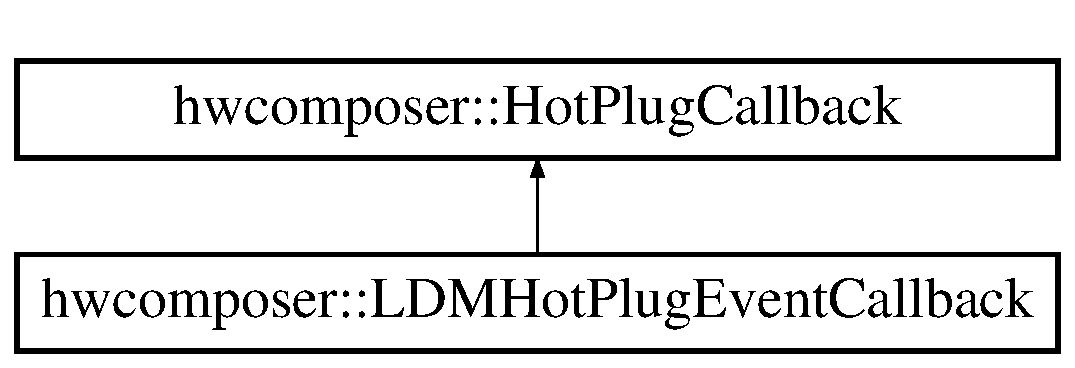
\includegraphics[height=2.000000cm]{classhwcomposer_1_1LDMHotPlugEventCallback}
\end{center}
\end{figure}
\subsection*{Public Member Functions}
\begin{DoxyCompactItemize}
\item 
\mbox{\hyperlink{classhwcomposer_1_1LDMHotPlugEventCallback_a81c6b48e6b3ac749d7810c8d47d7c4e8}{L\+D\+M\+Hot\+Plug\+Event\+Callback}} (\mbox{\hyperlink{classhwcomposer_1_1LogicalDisplayManager}{Logical\+Display\+Manager}} $\ast$manager)
\item 
void \mbox{\hyperlink{classhwcomposer_1_1LDMHotPlugEventCallback_ab5e17c96c17c3707c3ef98d856807822}{Callback}} (uint32\+\_\+t, bool connected)
\end{DoxyCompactItemize}


\subsection{Detailed Description}


Definition at line 50 of file logicaldisplaymanager.\+cpp.



\subsection{Constructor \& Destructor Documentation}
\mbox{\Hypertarget{classhwcomposer_1_1LDMHotPlugEventCallback_a81c6b48e6b3ac749d7810c8d47d7c4e8}\label{classhwcomposer_1_1LDMHotPlugEventCallback_a81c6b48e6b3ac749d7810c8d47d7c4e8}} 
\index{hwcomposer\+::\+L\+D\+M\+Hot\+Plug\+Event\+Callback@{hwcomposer\+::\+L\+D\+M\+Hot\+Plug\+Event\+Callback}!L\+D\+M\+Hot\+Plug\+Event\+Callback@{L\+D\+M\+Hot\+Plug\+Event\+Callback}}
\index{L\+D\+M\+Hot\+Plug\+Event\+Callback@{L\+D\+M\+Hot\+Plug\+Event\+Callback}!hwcomposer\+::\+L\+D\+M\+Hot\+Plug\+Event\+Callback@{hwcomposer\+::\+L\+D\+M\+Hot\+Plug\+Event\+Callback}}
\subsubsection{\texorpdfstring{L\+D\+M\+Hot\+Plug\+Event\+Callback()}{LDMHotPlugEventCallback()}}
{\footnotesize\ttfamily hwcomposer\+::\+L\+D\+M\+Hot\+Plug\+Event\+Callback\+::\+L\+D\+M\+Hot\+Plug\+Event\+Callback (\begin{DoxyParamCaption}\item[{\mbox{\hyperlink{classhwcomposer_1_1LogicalDisplayManager}{Logical\+Display\+Manager}} $\ast$}]{manager }\end{DoxyParamCaption})\hspace{0.3cm}{\ttfamily [inline]}}



Definition at line 52 of file logicaldisplaymanager.\+cpp.


\begin{DoxyCode}{0}
\DoxyCodeLine{52                                                           : manager\_(manager) \{}
\DoxyCodeLine{53   \}}
\end{DoxyCode}


\subsection{Member Function Documentation}
\mbox{\Hypertarget{classhwcomposer_1_1LDMHotPlugEventCallback_ab5e17c96c17c3707c3ef98d856807822}\label{classhwcomposer_1_1LDMHotPlugEventCallback_ab5e17c96c17c3707c3ef98d856807822}} 
\index{hwcomposer\+::\+L\+D\+M\+Hot\+Plug\+Event\+Callback@{hwcomposer\+::\+L\+D\+M\+Hot\+Plug\+Event\+Callback}!Callback@{Callback}}
\index{Callback@{Callback}!hwcomposer\+::\+L\+D\+M\+Hot\+Plug\+Event\+Callback@{hwcomposer\+::\+L\+D\+M\+Hot\+Plug\+Event\+Callback}}
\subsubsection{\texorpdfstring{Callback()}{Callback()}}
{\footnotesize\ttfamily void hwcomposer\+::\+L\+D\+M\+Hot\+Plug\+Event\+Callback\+::\+Callback (\begin{DoxyParamCaption}\item[{uint32\+\_\+t}]{,  }\item[{bool}]{connected }\end{DoxyParamCaption})\hspace{0.3cm}{\ttfamily [inline]}, {\ttfamily [virtual]}}



Implements \mbox{\hyperlink{classhwcomposer_1_1HotPlugCallback_a455c8913e1da9b165134a05c9cb441ba}{hwcomposer\+::\+Hot\+Plug\+Callback}}.



Definition at line 55 of file logicaldisplaymanager.\+cpp.


\begin{DoxyCode}{0}
\DoxyCodeLine{55                                             \{}
\DoxyCodeLine{56     manager\_->\mbox{\hyperlink{classhwcomposer_1_1LogicalDisplayManager_a486979f93dbb27770df066a633eef336}{HotPlugCallback}}(connected);}
\DoxyCodeLine{57   \}}
\end{DoxyCode}


The documentation for this class was generated from the following file\+:\begin{DoxyCompactItemize}
\item 
common/core/\mbox{\hyperlink{logicaldisplaymanager_8cpp}{logicaldisplaymanager.\+cpp}}\end{DoxyCompactItemize}

\hypertarget{classhwcomposer_1_1LDMRefreshCallback}{}\section{hwcomposer\+:\+:L\+D\+M\+Refresh\+Callback Class Reference}
\label{classhwcomposer_1_1LDMRefreshCallback}\index{hwcomposer\+::\+L\+D\+M\+Refresh\+Callback@{hwcomposer\+::\+L\+D\+M\+Refresh\+Callback}}
Inheritance diagram for hwcomposer\+:\+:L\+D\+M\+Refresh\+Callback\+:\begin{figure}[H]
\begin{center}
\leavevmode
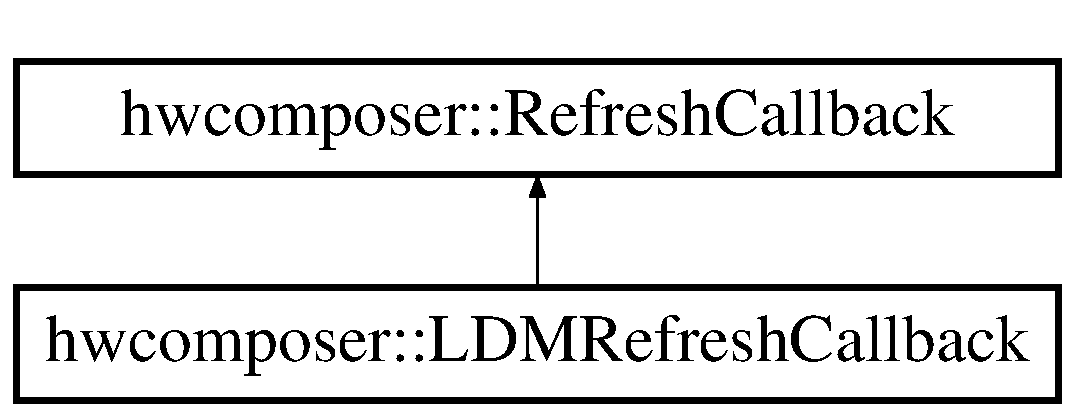
\includegraphics[height=2.000000cm]{classhwcomposer_1_1LDMRefreshCallback}
\end{center}
\end{figure}
\subsection*{Public Member Functions}
\begin{DoxyCompactItemize}
\item 
\mbox{\hyperlink{classhwcomposer_1_1LDMRefreshCallback_a6e7760306abac2b5b8715be31c99fe49}{L\+D\+M\+Refresh\+Callback}} (\mbox{\hyperlink{classhwcomposer_1_1LogicalDisplayManager}{Logical\+Display\+Manager}} $\ast$manager)
\item 
void \mbox{\hyperlink{classhwcomposer_1_1LDMRefreshCallback_a0bc9239fba543393d72ea68f9ee5abab}{Callback}} (uint32\+\_\+t)
\end{DoxyCompactItemize}


\subsection{Detailed Description}


Definition at line 37 of file logicaldisplaymanager.\+cpp.



\subsection{Constructor \& Destructor Documentation}
\mbox{\Hypertarget{classhwcomposer_1_1LDMRefreshCallback_a6e7760306abac2b5b8715be31c99fe49}\label{classhwcomposer_1_1LDMRefreshCallback_a6e7760306abac2b5b8715be31c99fe49}} 
\index{hwcomposer\+::\+L\+D\+M\+Refresh\+Callback@{hwcomposer\+::\+L\+D\+M\+Refresh\+Callback}!L\+D\+M\+Refresh\+Callback@{L\+D\+M\+Refresh\+Callback}}
\index{L\+D\+M\+Refresh\+Callback@{L\+D\+M\+Refresh\+Callback}!hwcomposer\+::\+L\+D\+M\+Refresh\+Callback@{hwcomposer\+::\+L\+D\+M\+Refresh\+Callback}}
\subsubsection{\texorpdfstring{L\+D\+M\+Refresh\+Callback()}{LDMRefreshCallback()}}
{\footnotesize\ttfamily hwcomposer\+::\+L\+D\+M\+Refresh\+Callback\+::\+L\+D\+M\+Refresh\+Callback (\begin{DoxyParamCaption}\item[{\mbox{\hyperlink{classhwcomposer_1_1LogicalDisplayManager}{Logical\+Display\+Manager}} $\ast$}]{manager }\end{DoxyParamCaption})\hspace{0.3cm}{\ttfamily [inline]}}



Definition at line 39 of file logicaldisplaymanager.\+cpp.


\begin{DoxyCode}{0}
\DoxyCodeLine{39                                                      : manager\_(manager) \{}
\DoxyCodeLine{40   \}}
\end{DoxyCode}


\subsection{Member Function Documentation}
\mbox{\Hypertarget{classhwcomposer_1_1LDMRefreshCallback_a0bc9239fba543393d72ea68f9ee5abab}\label{classhwcomposer_1_1LDMRefreshCallback_a0bc9239fba543393d72ea68f9ee5abab}} 
\index{hwcomposer\+::\+L\+D\+M\+Refresh\+Callback@{hwcomposer\+::\+L\+D\+M\+Refresh\+Callback}!Callback@{Callback}}
\index{Callback@{Callback}!hwcomposer\+::\+L\+D\+M\+Refresh\+Callback@{hwcomposer\+::\+L\+D\+M\+Refresh\+Callback}}
\subsubsection{\texorpdfstring{Callback()}{Callback()}}
{\footnotesize\ttfamily void hwcomposer\+::\+L\+D\+M\+Refresh\+Callback\+::\+Callback (\begin{DoxyParamCaption}\item[{uint32\+\_\+t}]{ }\end{DoxyParamCaption})\hspace{0.3cm}{\ttfamily [inline]}, {\ttfamily [virtual]}}



Implements \mbox{\hyperlink{classhwcomposer_1_1RefreshCallback_a5637a4b1437bbf8c93d8356addbf7c87}{hwcomposer\+::\+Refresh\+Callback}}.



Definition at line 42 of file logicaldisplaymanager.\+cpp.


\begin{DoxyCode}{0}
\DoxyCodeLine{42                             \{}
\DoxyCodeLine{43     manager\_->\mbox{\hyperlink{classhwcomposer_1_1LogicalDisplayManager_a9c4ee93396e79041eab1a7b9ce2838ca}{RefreshCallback}}();}
\DoxyCodeLine{44   \}}
\end{DoxyCode}


The documentation for this class was generated from the following file\+:\begin{DoxyCompactItemize}
\item 
common/core/\mbox{\hyperlink{logicaldisplaymanager_8cpp}{logicaldisplaymanager.\+cpp}}\end{DoxyCompactItemize}

\hypertarget{classhwcomposer_1_1LDMVsyncCallback}{}\section{hwcomposer\+:\+:L\+D\+M\+Vsync\+Callback Class Reference}
\label{classhwcomposer_1_1LDMVsyncCallback}\index{hwcomposer\+::\+L\+D\+M\+Vsync\+Callback@{hwcomposer\+::\+L\+D\+M\+Vsync\+Callback}}
Inheritance diagram for hwcomposer\+:\+:L\+D\+M\+Vsync\+Callback\+:\begin{figure}[H]
\begin{center}
\leavevmode
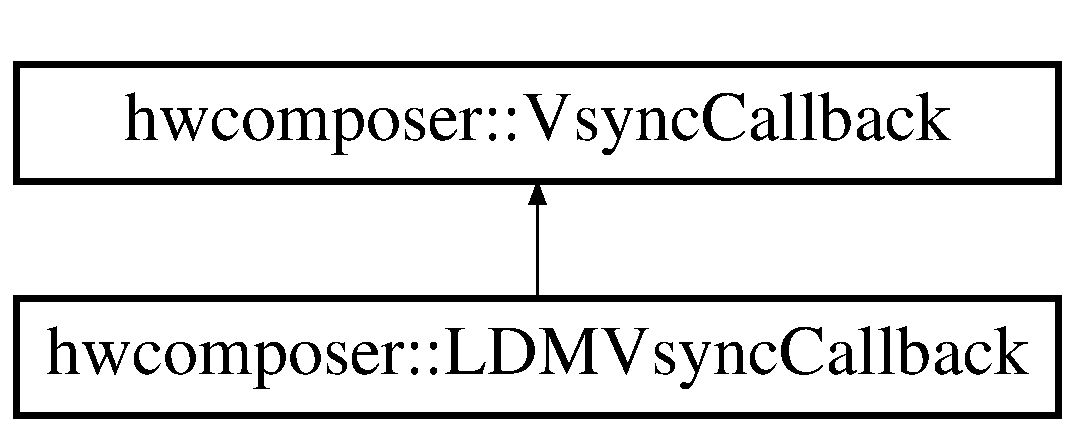
\includegraphics[height=2.000000cm]{classhwcomposer_1_1LDMVsyncCallback}
\end{center}
\end{figure}
\subsection*{Public Member Functions}
\begin{DoxyCompactItemize}
\item 
\mbox{\hyperlink{classhwcomposer_1_1LDMVsyncCallback_ad7dc0df06c853a09bf6f3469d5abebc6}{L\+D\+M\+Vsync\+Callback}} (\mbox{\hyperlink{classhwcomposer_1_1LogicalDisplayManager}{Logical\+Display\+Manager}} $\ast$manager)
\item 
void \mbox{\hyperlink{classhwcomposer_1_1LDMVsyncCallback_ae92d66fdf645fa105ac163e33e5e6526}{Callback}} (uint32\+\_\+t, int64\+\_\+t timestamp)
\end{DoxyCompactItemize}


\subsection{Detailed Description}


Definition at line 24 of file logicaldisplaymanager.\+cpp.



\subsection{Constructor \& Destructor Documentation}
\mbox{\Hypertarget{classhwcomposer_1_1LDMVsyncCallback_ad7dc0df06c853a09bf6f3469d5abebc6}\label{classhwcomposer_1_1LDMVsyncCallback_ad7dc0df06c853a09bf6f3469d5abebc6}} 
\index{hwcomposer\+::\+L\+D\+M\+Vsync\+Callback@{hwcomposer\+::\+L\+D\+M\+Vsync\+Callback}!L\+D\+M\+Vsync\+Callback@{L\+D\+M\+Vsync\+Callback}}
\index{L\+D\+M\+Vsync\+Callback@{L\+D\+M\+Vsync\+Callback}!hwcomposer\+::\+L\+D\+M\+Vsync\+Callback@{hwcomposer\+::\+L\+D\+M\+Vsync\+Callback}}
\subsubsection{\texorpdfstring{L\+D\+M\+Vsync\+Callback()}{LDMVsyncCallback()}}
{\footnotesize\ttfamily hwcomposer\+::\+L\+D\+M\+Vsync\+Callback\+::\+L\+D\+M\+Vsync\+Callback (\begin{DoxyParamCaption}\item[{\mbox{\hyperlink{classhwcomposer_1_1LogicalDisplayManager}{Logical\+Display\+Manager}} $\ast$}]{manager }\end{DoxyParamCaption})\hspace{0.3cm}{\ttfamily [inline]}}



Definition at line 26 of file logicaldisplaymanager.\+cpp.


\begin{DoxyCode}{0}
\DoxyCodeLine{26                                                    : manager\_(manager) \{}
\DoxyCodeLine{27   \}}
\end{DoxyCode}


\subsection{Member Function Documentation}
\mbox{\Hypertarget{classhwcomposer_1_1LDMVsyncCallback_ae92d66fdf645fa105ac163e33e5e6526}\label{classhwcomposer_1_1LDMVsyncCallback_ae92d66fdf645fa105ac163e33e5e6526}} 
\index{hwcomposer\+::\+L\+D\+M\+Vsync\+Callback@{hwcomposer\+::\+L\+D\+M\+Vsync\+Callback}!Callback@{Callback}}
\index{Callback@{Callback}!hwcomposer\+::\+L\+D\+M\+Vsync\+Callback@{hwcomposer\+::\+L\+D\+M\+Vsync\+Callback}}
\subsubsection{\texorpdfstring{Callback()}{Callback()}}
{\footnotesize\ttfamily void hwcomposer\+::\+L\+D\+M\+Vsync\+Callback\+::\+Callback (\begin{DoxyParamCaption}\item[{uint32\+\_\+t}]{,  }\item[{int64\+\_\+t}]{timestamp }\end{DoxyParamCaption})\hspace{0.3cm}{\ttfamily [inline]}, {\ttfamily [virtual]}}



Implements \mbox{\hyperlink{classhwcomposer_1_1VsyncCallback_a632ac6a2e13e1b387df9508507a2ed4d}{hwcomposer\+::\+Vsync\+Callback}}.



Definition at line 29 of file logicaldisplaymanager.\+cpp.


\begin{DoxyCode}{0}
\DoxyCodeLine{29                                                \{}
\DoxyCodeLine{30     manager\_->\mbox{\hyperlink{classhwcomposer_1_1LogicalDisplayManager_a799b4d580b33a54016d7694380aefcec}{VSyncCallback}}(timestamp);}
\DoxyCodeLine{31   \}}
\end{DoxyCode}


The documentation for this class was generated from the following file\+:\begin{DoxyCompactItemize}
\item 
common/core/\mbox{\hyperlink{logicaldisplaymanager_8cpp}{logicaldisplaymanager.\+cpp}}\end{DoxyCompactItemize}

\hypertarget{classLogEntry}{}\section{Log\+Entry Class Reference}
\label{classLogEntry}\index{Log\+Entry@{Log\+Entry}}


{\ttfamily \#include $<$logentry.\+h$>$}

Inheritance diagram for Log\+Entry\+:\begin{figure}[H]
\begin{center}
\leavevmode
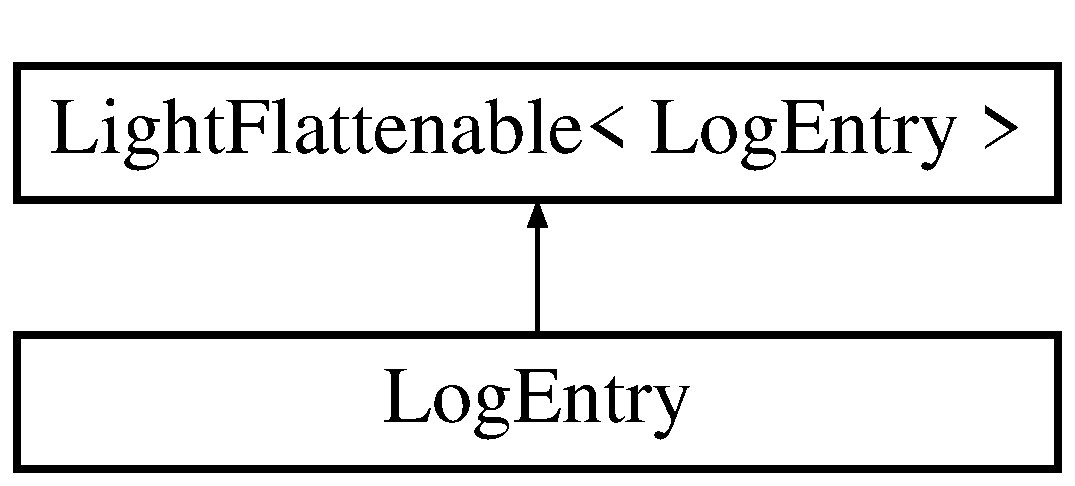
\includegraphics[height=2.000000cm]{classLogEntry}
\end{center}
\end{figure}
\subsection*{Public Member Functions}
\begin{DoxyCompactItemize}
\item 
\mbox{\hyperlink{classLogEntry_a78c2786c30d8d6ba4b2aa8b372f58305}{Log\+Entry}} ()
\item 
\mbox{\hyperlink{classLogEntry_a484dd0b15f1339e654b526a8a9a431a3}{Log\+Entry}} (nsecs\+\_\+t timestamp, String8 description)
\item 
\mbox{\hyperlink{classLogEntry_ae0da106e665ca859be1a30ea316cd7d2}{$\sim$\+Log\+Entry}} ()
\item 
pid\+\_\+t \mbox{\hyperlink{classLogEntry_a50403241bb451c7faabc6d7bb9650221}{get\+T\+ID}} () const
\item 
nsecs\+\_\+t \mbox{\hyperlink{classLogEntry_aaf6bd4d7c0c18071fdb39c49a2de6064}{get\+Timestamp}} () const
\item 
const String8 \& \mbox{\hyperlink{classLogEntry_a90c8f3d3f2f52c237d6a43ca801d1b6d}{get\+Description}} () const
\item 
bool \mbox{\hyperlink{classLogEntry_a5711231fdc0709752e67aa82fad051e1}{is\+Fixed\+Size}} () const
\item 
size\+\_\+t \mbox{\hyperlink{classLogEntry_aecaa8f3ac612c7faa86c2790d8d6d420}{get\+Flattened\+Size}} () const
\item 
\mbox{\hyperlink{hwcserviceapi_8h_a3806fb2027d9a316d8ca8d9b8b8eb96f}{status\+\_\+t}} \mbox{\hyperlink{classLogEntry_a479ac501aaf9e4fc11c5a6d118b65dc1}{flatten}} (void $\ast$buffer, size\+\_\+t size) const
\item 
\mbox{\hyperlink{hwcserviceapi_8h_a3806fb2027d9a316d8ca8d9b8b8eb96f}{status\+\_\+t}} \mbox{\hyperlink{classLogEntry_ae5b14d452a6f948ed9a00a5446d5aa1b}{unflatten}} (void const $\ast$buffer, size\+\_\+t size)
\item 
\mbox{\hyperlink{hwcserviceapi_8h_a3806fb2027d9a316d8ca8d9b8b8eb96f}{status\+\_\+t}} \mbox{\hyperlink{classLogEntry_a1c92a359f9d4e3635ae3c2f228ff6206}{read}} (sp$<$ \mbox{\hyperlink{classhwcomposer_1_1IDiagnostic}{I\+Diagnostic}} $>$ p\+Diagnostic)
\item 
void \mbox{\hyperlink{classLogEntry_a15620abfed3ae9b39e565de00b50cf00}{print}} (bool b\+Very\+Verbose=false, bool b\+Verbose=false, bool b\+Fences=false, bool b\+Buffer\+Manager=false, bool b\+Queue=false)
\end{DoxyCompactItemize}
\subsection*{Static Public Member Functions}
\begin{DoxyCompactItemize}
\item 
static void \mbox{\hyperlink{classLogEntry_ab914112fadd8cd8cf47a4e1e9e09fa72}{discard\+All}} (sp$<$ \mbox{\hyperlink{classhwcomposer_1_1IDiagnostic}{I\+Diagnostic}} $>$ p\+Diagnostic)
\item 
static void \mbox{\hyperlink{classLogEntry_ac8cfea6c35e82f5cae1f37059791738b}{print\+All}} (sp$<$ \mbox{\hyperlink{classhwcomposer_1_1IDiagnostic}{I\+Diagnostic}} $>$ p\+Diagnostic, bool b\+Very\+Verbose=false, bool b\+Verbose=false, bool b\+Fences=false, bool b\+Buffer\+Manager=false, bool b\+Queue=false)
\end{DoxyCompactItemize}


\subsection{Detailed Description}


Definition at line 28 of file logentry.\+h.



\subsection{Constructor \& Destructor Documentation}
\mbox{\Hypertarget{classLogEntry_a78c2786c30d8d6ba4b2aa8b372f58305}\label{classLogEntry_a78c2786c30d8d6ba4b2aa8b372f58305}} 
\index{Log\+Entry@{Log\+Entry}!Log\+Entry@{Log\+Entry}}
\index{Log\+Entry@{Log\+Entry}!Log\+Entry@{Log\+Entry}}
\subsubsection{\texorpdfstring{Log\+Entry()}{LogEntry()}\hspace{0.1cm}{\footnotesize\ttfamily [1/2]}}
{\footnotesize\ttfamily Log\+Entry\+::\+Log\+Entry (\begin{DoxyParamCaption}{ }\end{DoxyParamCaption})}



Definition at line 67 of file logentry.\+h.


\begin{DoxyCode}{0}
\DoxyCodeLine{67                    : mTID(0), mTimestamp(0) \{}
\DoxyCodeLine{68 \}}
\end{DoxyCode}
\mbox{\Hypertarget{classLogEntry_a484dd0b15f1339e654b526a8a9a431a3}\label{classLogEntry_a484dd0b15f1339e654b526a8a9a431a3}} 
\index{Log\+Entry@{Log\+Entry}!Log\+Entry@{Log\+Entry}}
\index{Log\+Entry@{Log\+Entry}!Log\+Entry@{Log\+Entry}}
\subsubsection{\texorpdfstring{Log\+Entry()}{LogEntry()}\hspace{0.1cm}{\footnotesize\ttfamily [2/2]}}
{\footnotesize\ttfamily Log\+Entry\+::\+Log\+Entry (\begin{DoxyParamCaption}\item[{nsecs\+\_\+t}]{timestamp,  }\item[{String8}]{description }\end{DoxyParamCaption})}



Definition at line 70 of file logentry.\+h.


\begin{DoxyCode}{0}
\DoxyCodeLine{71     : mTID(0), mTimestamp(timestamp), mDescription(description) \{}
\DoxyCodeLine{72 \}}
\end{DoxyCode}
\mbox{\Hypertarget{classLogEntry_ae0da106e665ca859be1a30ea316cd7d2}\label{classLogEntry_ae0da106e665ca859be1a30ea316cd7d2}} 
\index{Log\+Entry@{Log\+Entry}!````~Log\+Entry@{$\sim$\+Log\+Entry}}
\index{````~Log\+Entry@{$\sim$\+Log\+Entry}!Log\+Entry@{Log\+Entry}}
\subsubsection{\texorpdfstring{$\sim$\+Log\+Entry()}{~LogEntry()}}
{\footnotesize\ttfamily Log\+Entry\+::$\sim$\+Log\+Entry (\begin{DoxyParamCaption}{ }\end{DoxyParamCaption})}



Definition at line 74 of file logentry.\+h.


\begin{DoxyCode}{0}
\DoxyCodeLine{74                     \{}
\DoxyCodeLine{75 \}}
\end{DoxyCode}


\subsection{Member Function Documentation}
\mbox{\Hypertarget{classLogEntry_ab914112fadd8cd8cf47a4e1e9e09fa72}\label{classLogEntry_ab914112fadd8cd8cf47a4e1e9e09fa72}} 
\index{Log\+Entry@{Log\+Entry}!discard\+All@{discard\+All}}
\index{discard\+All@{discard\+All}!Log\+Entry@{Log\+Entry}}
\subsubsection{\texorpdfstring{discard\+All()}{discardAll()}}
{\footnotesize\ttfamily void Log\+Entry\+::discard\+All (\begin{DoxyParamCaption}\item[{sp$<$ \mbox{\hyperlink{classhwcomposer_1_1IDiagnostic}{I\+Diagnostic}} $>$}]{p\+Diagnostic }\end{DoxyParamCaption})\hspace{0.3cm}{\ttfamily [static]}}



Definition at line 175 of file logentry.\+h.


\begin{DoxyCode}{0}
\DoxyCodeLine{175                                                      \{}
\DoxyCodeLine{176   \textcolor{keywordflow}{while} (1) \{}
\DoxyCodeLine{177     \mbox{\hyperlink{classLogEntry}{LogEntry}} entry;}
\DoxyCodeLine{178     \mbox{\hyperlink{hwcserviceapi_8h_a3806fb2027d9a316d8ca8d9b8b8eb96f}{status\_t}} ret = entry.\mbox{\hyperlink{classLogEntry_a1c92a359f9d4e3635ae3c2f228ff6206}{read}}(pDiagnostic);}
\DoxyCodeLine{179     \textcolor{keywordflow}{if} (ret != OK)}
\DoxyCodeLine{180       \textcolor{keywordflow}{break};}
\DoxyCodeLine{181   \}}
\DoxyCodeLine{182 \}}
\end{DoxyCode}
\mbox{\Hypertarget{classLogEntry_a479ac501aaf9e4fc11c5a6d118b65dc1}\label{classLogEntry_a479ac501aaf9e4fc11c5a6d118b65dc1}} 
\index{Log\+Entry@{Log\+Entry}!flatten@{flatten}}
\index{flatten@{flatten}!Log\+Entry@{Log\+Entry}}
\subsubsection{\texorpdfstring{flatten()}{flatten()}}
{\footnotesize\ttfamily \mbox{\hyperlink{hwcserviceapi_8h_a3806fb2027d9a316d8ca8d9b8b8eb96f}{status\+\_\+t}} Log\+Entry\+::flatten (\begin{DoxyParamCaption}\item[{void $\ast$}]{buffer,  }\item[{size\+\_\+t}]{size }\end{DoxyParamCaption}) const}

\mbox{\Hypertarget{classLogEntry_a90c8f3d3f2f52c237d6a43ca801d1b6d}\label{classLogEntry_a90c8f3d3f2f52c237d6a43ca801d1b6d}} 
\index{Log\+Entry@{Log\+Entry}!get\+Description@{get\+Description}}
\index{get\+Description@{get\+Description}!Log\+Entry@{Log\+Entry}}
\subsubsection{\texorpdfstring{get\+Description()}{getDescription()}}
{\footnotesize\ttfamily const String8\& Log\+Entry\+::get\+Description (\begin{DoxyParamCaption}{ }\end{DoxyParamCaption}) const\hspace{0.3cm}{\ttfamily [inline]}}



Definition at line 40 of file logentry.\+h.


\begin{DoxyCode}{0}
\DoxyCodeLine{40                                         \{}
\DoxyCodeLine{41     \textcolor{keywordflow}{return} mDescription;}
\DoxyCodeLine{42   \}}
\end{DoxyCode}
\mbox{\Hypertarget{classLogEntry_aecaa8f3ac612c7faa86c2790d8d6d420}\label{classLogEntry_aecaa8f3ac612c7faa86c2790d8d6d420}} 
\index{Log\+Entry@{Log\+Entry}!get\+Flattened\+Size@{get\+Flattened\+Size}}
\index{get\+Flattened\+Size@{get\+Flattened\+Size}!Log\+Entry@{Log\+Entry}}
\subsubsection{\texorpdfstring{get\+Flattened\+Size()}{getFlattenedSize()}}
{\footnotesize\ttfamily size\+\_\+t Log\+Entry\+::get\+Flattened\+Size (\begin{DoxyParamCaption}{ }\end{DoxyParamCaption}) const\hspace{0.3cm}{\ttfamily [inline]}}



Definition at line 46 of file logentry.\+h.


\begin{DoxyCode}{0}
\DoxyCodeLine{46                                   \{}
\DoxyCodeLine{47     \textcolor{keywordflow}{return} 0;}
\DoxyCodeLine{48   \}}
\end{DoxyCode}
\mbox{\Hypertarget{classLogEntry_a50403241bb451c7faabc6d7bb9650221}\label{classLogEntry_a50403241bb451c7faabc6d7bb9650221}} 
\index{Log\+Entry@{Log\+Entry}!get\+T\+ID@{get\+T\+ID}}
\index{get\+T\+ID@{get\+T\+ID}!Log\+Entry@{Log\+Entry}}
\subsubsection{\texorpdfstring{get\+T\+I\+D()}{getTID()}}
{\footnotesize\ttfamily pid\+\_\+t Log\+Entry\+::get\+T\+ID (\begin{DoxyParamCaption}{ }\end{DoxyParamCaption}) const\hspace{0.3cm}{\ttfamily [inline]}}



Definition at line 34 of file logentry.\+h.


\begin{DoxyCode}{0}
\DoxyCodeLine{34                        \{}
\DoxyCodeLine{35     \textcolor{keywordflow}{return} mTID;}
\DoxyCodeLine{36   \}}
\end{DoxyCode}
\mbox{\Hypertarget{classLogEntry_aaf6bd4d7c0c18071fdb39c49a2de6064}\label{classLogEntry_aaf6bd4d7c0c18071fdb39c49a2de6064}} 
\index{Log\+Entry@{Log\+Entry}!get\+Timestamp@{get\+Timestamp}}
\index{get\+Timestamp@{get\+Timestamp}!Log\+Entry@{Log\+Entry}}
\subsubsection{\texorpdfstring{get\+Timestamp()}{getTimestamp()}}
{\footnotesize\ttfamily nsecs\+\_\+t Log\+Entry\+::get\+Timestamp (\begin{DoxyParamCaption}{ }\end{DoxyParamCaption}) const\hspace{0.3cm}{\ttfamily [inline]}}



Definition at line 37 of file logentry.\+h.


\begin{DoxyCode}{0}
\DoxyCodeLine{37                                \{}
\DoxyCodeLine{38     \textcolor{keywordflow}{return} mTimestamp;}
\DoxyCodeLine{39   \}}
\end{DoxyCode}
\mbox{\Hypertarget{classLogEntry_a5711231fdc0709752e67aa82fad051e1}\label{classLogEntry_a5711231fdc0709752e67aa82fad051e1}} 
\index{Log\+Entry@{Log\+Entry}!is\+Fixed\+Size@{is\+Fixed\+Size}}
\index{is\+Fixed\+Size@{is\+Fixed\+Size}!Log\+Entry@{Log\+Entry}}
\subsubsection{\texorpdfstring{is\+Fixed\+Size()}{isFixedSize()}}
{\footnotesize\ttfamily bool Log\+Entry\+::is\+Fixed\+Size (\begin{DoxyParamCaption}{ }\end{DoxyParamCaption}) const\hspace{0.3cm}{\ttfamily [inline]}}



Definition at line 43 of file logentry.\+h.


\begin{DoxyCode}{0}
\DoxyCodeLine{43                                   \{}
\DoxyCodeLine{44     \textcolor{keywordflow}{return} \textcolor{keyword}{false};}
\DoxyCodeLine{45   \}}
\end{DoxyCode}
\mbox{\Hypertarget{classLogEntry_a15620abfed3ae9b39e565de00b50cf00}\label{classLogEntry_a15620abfed3ae9b39e565de00b50cf00}} 
\index{Log\+Entry@{Log\+Entry}!print@{print}}
\index{print@{print}!Log\+Entry@{Log\+Entry}}
\subsubsection{\texorpdfstring{print()}{print()}}
{\footnotesize\ttfamily void Log\+Entry\+::print (\begin{DoxyParamCaption}\item[{bool}]{b\+Very\+Verbose = {\ttfamily false},  }\item[{bool}]{b\+Verbose = {\ttfamily false},  }\item[{bool}]{b\+Fences = {\ttfamily false},  }\item[{bool}]{b\+Buffer\+Manager = {\ttfamily false},  }\item[{bool}]{b\+Queue = {\ttfamily false} }\end{DoxyParamCaption})}



Definition at line 131 of file logentry.\+h.


\begin{DoxyCode}{0}
\DoxyCodeLine{132                                                        \{}
\DoxyCodeLine{133   \textcolor{keywordflow}{if} (strstr(\mbox{\hyperlink{classLogEntry_a90c8f3d3f2f52c237d6a43ca801d1b6d}{getDescription}}(), \textcolor{stringliteral}{"SF0 onPrepare Entry"}) ||}
\DoxyCodeLine{134       strstr(\mbox{\hyperlink{classLogEntry_a90c8f3d3f2f52c237d6a43ca801d1b6d}{getDescription}}(), \textcolor{stringliteral}{"InputAnalyzer SF0"})) \{}
\DoxyCodeLine{135     printf(\textcolor{stringliteral}{"\(\backslash\)n\(\backslash\)n"});}
\DoxyCodeLine{136   \}}
\DoxyCodeLine{137 }
\DoxyCodeLine{138   \textcolor{keywordflow}{if} (!bVeryVerbose \&\& bVerbose == \textcolor{keyword}{false}) \{}
\DoxyCodeLine{139     \textcolor{comment}{// Strip out any 'verbose' matching strings}}
\DoxyCodeLine{140     \textcolor{keywordflow}{if} (strstr(\mbox{\hyperlink{classLogEntry_a90c8f3d3f2f52c237d6a43ca801d1b6d}{getDescription}}(), \textcolor{stringliteral}{"onPrepare Entry"}) ||}
\DoxyCodeLine{141         strstr(\mbox{\hyperlink{classLogEntry_a90c8f3d3f2f52c237d6a43ca801d1b6d}{getDescription}}(), \textcolor{stringliteral}{"onPrepare Exit"}) ||}
\DoxyCodeLine{142         strstr(\mbox{\hyperlink{classLogEntry_a90c8f3d3f2f52c237d6a43ca801d1b6d}{getDescription}}(), \textcolor{stringliteral}{"onSet Exit"}) ||}
\DoxyCodeLine{143         strncmp(\mbox{\hyperlink{classLogEntry_a90c8f3d3f2f52c237d6a43ca801d1b6d}{getDescription}}(), \textcolor{stringliteral}{"InternalBuffer"}, 14) == 0 ||}
\DoxyCodeLine{144         strncmp(\mbox{\hyperlink{classLogEntry_a90c8f3d3f2f52c237d6a43ca801d1b6d}{getDescription}}(), \textcolor{stringliteral}{"drm"}, 3) == 0 ||}
\DoxyCodeLine{145         strncmp(\mbox{\hyperlink{classLogEntry_a90c8f3d3f2f52c237d6a43ca801d1b6d}{getDescription}}(), \textcolor{stringliteral}{"adf"}, 3) == 0)}
\DoxyCodeLine{146       \textcolor{keywordflow}{return};}
\DoxyCodeLine{147   \}}
\DoxyCodeLine{148   \textcolor{keywordflow}{if} (!bVeryVerbose \&\& bFences == \textcolor{keyword}{false}) \{}
\DoxyCodeLine{149     \textcolor{comment}{// Strip out any 'fence' matching strings.}}
\DoxyCodeLine{150     \textcolor{keywordflow}{if} (strncmp(\mbox{\hyperlink{classLogEntry_a90c8f3d3f2f52c237d6a43ca801d1b6d}{getDescription}}(), \textcolor{stringliteral}{"Fence:"}, 6) == 0)}
\DoxyCodeLine{151       \textcolor{keywordflow}{return};}
\DoxyCodeLine{152     \textcolor{keywordflow}{if} (strncmp(\mbox{\hyperlink{classLogEntry_a90c8f3d3f2f52c237d6a43ca801d1b6d}{getDescription}}(), \textcolor{stringliteral}{"NativeFence:"}, 12) == 0)}
\DoxyCodeLine{153       \textcolor{keywordflow}{return};}
\DoxyCodeLine{154   \}}
\DoxyCodeLine{155   \textcolor{keywordflow}{if} (!bVeryVerbose \&\& bBufferManager == \textcolor{keyword}{false}) \{}
\DoxyCodeLine{156     \textcolor{comment}{// Strip out any 'buffer manager' matching strings.}}
\DoxyCodeLine{157     \textcolor{keywordflow}{if} (strncmp(\mbox{\hyperlink{classLogEntry_a90c8f3d3f2f52c237d6a43ca801d1b6d}{getDescription}}(), \textcolor{stringliteral}{"BufferManager:"}, 14) == 0)}
\DoxyCodeLine{158       \textcolor{keywordflow}{return};}
\DoxyCodeLine{159   \}}
\DoxyCodeLine{160   \textcolor{keywordflow}{if} (!bVeryVerbose \&\& bQueue == \textcolor{keyword}{false}) \{}
\DoxyCodeLine{161     \textcolor{comment}{// Strip out any 'display queue' matching strings.}}
\DoxyCodeLine{162     \textcolor{keywordflow}{if} (strncmp(\mbox{\hyperlink{classLogEntry_a90c8f3d3f2f52c237d6a43ca801d1b6d}{getDescription}}(), \textcolor{stringliteral}{"Queue:"}, 6) == 0)}
\DoxyCodeLine{163       \textcolor{keywordflow}{return};}
\DoxyCodeLine{164   \}}
\DoxyCodeLine{165 }
\DoxyCodeLine{166   printf(\textcolor{stringliteral}{"\%"} PRIi64 \textcolor{stringliteral}{"s \%03"} PRIi64 \textcolor{stringliteral}{"ms"}, \mbox{\hyperlink{classLogEntry_aaf6bd4d7c0c18071fdb39c49a2de6064}{getTimestamp}}() / 1000000000,}
\DoxyCodeLine{167          (\mbox{\hyperlink{classLogEntry_aaf6bd4d7c0c18071fdb39c49a2de6064}{getTimestamp}}() \% 1000000000) / 1000000);}
\DoxyCodeLine{168   \textcolor{keywordflow}{if} (bVerbose) \{}
\DoxyCodeLine{169     printf(\textcolor{stringliteral}{" \%06"} PRIi64 \textcolor{stringliteral}{"ns"}, \mbox{\hyperlink{classLogEntry_aaf6bd4d7c0c18071fdb39c49a2de6064}{getTimestamp}}() \% 1000000);}
\DoxyCodeLine{170     printf(\textcolor{stringliteral}{" TID:\%d"}, \mbox{\hyperlink{classLogEntry_a50403241bb451c7faabc6d7bb9650221}{getTID}}());}
\DoxyCodeLine{171   \}}
\DoxyCodeLine{172   printf(\textcolor{stringliteral}{" \%s\(\backslash\)n"}, \mbox{\hyperlink{classLogEntry_a90c8f3d3f2f52c237d6a43ca801d1b6d}{getDescription}}().\textcolor{keywordtype}{string}());}
\DoxyCodeLine{173 \}}
\end{DoxyCode}
\mbox{\Hypertarget{classLogEntry_ac8cfea6c35e82f5cae1f37059791738b}\label{classLogEntry_ac8cfea6c35e82f5cae1f37059791738b}} 
\index{Log\+Entry@{Log\+Entry}!print\+All@{print\+All}}
\index{print\+All@{print\+All}!Log\+Entry@{Log\+Entry}}
\subsubsection{\texorpdfstring{print\+All()}{printAll()}}
{\footnotesize\ttfamily void Log\+Entry\+::print\+All (\begin{DoxyParamCaption}\item[{sp$<$ \mbox{\hyperlink{classhwcomposer_1_1IDiagnostic}{I\+Diagnostic}} $>$}]{p\+Diagnostic,  }\item[{bool}]{b\+Very\+Verbose = {\ttfamily false},  }\item[{bool}]{b\+Verbose = {\ttfamily false},  }\item[{bool}]{b\+Fences = {\ttfamily false},  }\item[{bool}]{b\+Buffer\+Manager = {\ttfamily false},  }\item[{bool}]{b\+Queue = {\ttfamily false} }\end{DoxyParamCaption})\hspace{0.3cm}{\ttfamily [static]}}



Definition at line 184 of file logentry.\+h.


\begin{DoxyCode}{0}
\DoxyCodeLine{186                                      \{}
\DoxyCodeLine{187   \textcolor{keywordflow}{while} (1) \{}
\DoxyCodeLine{188     \mbox{\hyperlink{classLogEntry}{LogEntry}} entry;}
\DoxyCodeLine{189     \mbox{\hyperlink{hwcserviceapi_8h_a3806fb2027d9a316d8ca8d9b8b8eb96f}{status\_t}} ret = entry.\mbox{\hyperlink{classLogEntry_a1c92a359f9d4e3635ae3c2f228ff6206}{read}}(pDiagnostic);}
\DoxyCodeLine{190     \textcolor{keywordflow}{if} (ret != OK)}
\DoxyCodeLine{191       \textcolor{keywordflow}{break};}
\DoxyCodeLine{192     entry.\mbox{\hyperlink{classLogEntry_a15620abfed3ae9b39e565de00b50cf00}{print}}(bVeryVerbose, bVerbose, bFences, bBufferManager, bQueue);}
\DoxyCodeLine{193   \}}
\DoxyCodeLine{194 \}}
\end{DoxyCode}
\mbox{\Hypertarget{classLogEntry_a1c92a359f9d4e3635ae3c2f228ff6206}\label{classLogEntry_a1c92a359f9d4e3635ae3c2f228ff6206}} 
\index{Log\+Entry@{Log\+Entry}!read@{read}}
\index{read@{read}!Log\+Entry@{Log\+Entry}}
\subsubsection{\texorpdfstring{read()}{read()}}
{\footnotesize\ttfamily \mbox{\hyperlink{hwcserviceapi_8h_a3806fb2027d9a316d8ca8d9b8b8eb96f}{status\+\_\+t}} Log\+Entry\+::read (\begin{DoxyParamCaption}\item[{sp$<$ \mbox{\hyperlink{classhwcomposer_1_1IDiagnostic}{I\+Diagnostic}} $>$}]{p\+Diagnostic }\end{DoxyParamCaption})}



Definition at line 98 of file logentry.\+h.


\begin{DoxyCode}{0}
\DoxyCodeLine{98                                                    \{}
\DoxyCodeLine{99   \mbox{\hyperlink{hwcserviceapi_8h_a3806fb2027d9a316d8ca8d9b8b8eb96f}{status\_t}} ret = NO\_ERROR;}
\DoxyCodeLine{100 }
\DoxyCodeLine{101   \textcolor{keyword}{static} Parcel* spReply = \mbox{\hyperlink{alios_2platformdefines_8h_a070d2ce7b6bb7e5c05602aa8c308d0c4}{NULL}};}
\DoxyCodeLine{102   \textcolor{keywordflow}{if} (spReply) \{}
\DoxyCodeLine{103     ret = spReply->readInt32();}
\DoxyCodeLine{104 }
\DoxyCodeLine{105     \textcolor{keywordflow}{if} (ret == NOT\_ENOUGH\_DATA) \{}
\DoxyCodeLine{106       \textcolor{comment}{// Marks end of parcel, time to fetch a new one}}
\DoxyCodeLine{107       \textcolor{keyword}{delete} spReply;}
\DoxyCodeLine{108       spReply = 0;}
\DoxyCodeLine{109     \}}
\DoxyCodeLine{110   \}}
\DoxyCodeLine{111 }
\DoxyCodeLine{112   \textcolor{keywordflow}{if} (spReply == 0) \{}
\DoxyCodeLine{113     spReply = \textcolor{keyword}{new} Parcel;}
\DoxyCodeLine{114     pDiagnostic = \mbox{\hyperlink{alios_2platformdefines_8h_a070d2ce7b6bb7e5c05602aa8c308d0c4}{NULL}};}
\DoxyCodeLine{115     \textcolor{comment}{// ret = pDiagnostic->readLogParcel(spReply);}}
\DoxyCodeLine{116 }
\DoxyCodeLine{117     \textcolor{keywordflow}{if} (ret >= 0)}
\DoxyCodeLine{118       ret = spReply->readInt32();}
\DoxyCodeLine{119   \}}
\DoxyCodeLine{120 }
\DoxyCodeLine{121   \textcolor{keywordflow}{if} (ret < 0) \{}
\DoxyCodeLine{122     \textcolor{keyword}{delete} spReply;}
\DoxyCodeLine{123     spReply = 0;}
\DoxyCodeLine{124     \textcolor{keywordflow}{return} ret;}
\DoxyCodeLine{125   \}}
\DoxyCodeLine{126 }
\DoxyCodeLine{127   spReply->read(*\textcolor{keyword}{this});}
\DoxyCodeLine{128   \textcolor{keywordflow}{return} ret;}
\DoxyCodeLine{129 \}}
\end{DoxyCode}
\mbox{\Hypertarget{classLogEntry_ae5b14d452a6f948ed9a00a5446d5aa1b}\label{classLogEntry_ae5b14d452a6f948ed9a00a5446d5aa1b}} 
\index{Log\+Entry@{Log\+Entry}!unflatten@{unflatten}}
\index{unflatten@{unflatten}!Log\+Entry@{Log\+Entry}}
\subsubsection{\texorpdfstring{unflatten()}{unflatten()}}
{\footnotesize\ttfamily \mbox{\hyperlink{hwcserviceapi_8h_a3806fb2027d9a316d8ca8d9b8b8eb96f}{status\+\_\+t}} Log\+Entry\+::unflatten (\begin{DoxyParamCaption}\item[{void const $\ast$}]{buffer,  }\item[{size\+\_\+t}]{size }\end{DoxyParamCaption})}



Definition at line 86 of file logentry.\+h.


\begin{DoxyCode}{0}
\DoxyCodeLine{86                                                             \{}
\DoxyCodeLine{87   \textcolor{comment}{// Delete any existing data structures}}
\DoxyCodeLine{88   \textcolor{keywordtype}{char} \textcolor{keyword}{const}* pBuffer = (\textcolor{keywordtype}{char} \textcolor{keyword}{const}*)buffer;}
\DoxyCodeLine{89   \textcolor{keywordtype}{char} \textcolor{keyword}{const}* pBufferEnd = ((\textcolor{keywordtype}{char} \textcolor{keyword}{const}*)buffer) + size;}
\DoxyCodeLine{90 }
\DoxyCodeLine{91   \mbox{\hyperlink{logentry_8h_a5684e7020dd011489e425f87e9d6be92}{unflattenFromBuffer}}(pBuffer, pBufferEnd, mTID);}
\DoxyCodeLine{92   \mbox{\hyperlink{logentry_8h_a5684e7020dd011489e425f87e9d6be92}{unflattenFromBuffer}}(pBuffer, pBufferEnd, mTimestamp);}
\DoxyCodeLine{93 }
\DoxyCodeLine{94   mDescription = pBuffer;}
\DoxyCodeLine{95   \textcolor{keywordflow}{return} NO\_ERROR;}
\DoxyCodeLine{96 \}}
\end{DoxyCode}


The documentation for this class was generated from the following file\+:\begin{DoxyCompactItemize}
\item 
common/utils/\mbox{\hyperlink{logentry_8h}{logentry.\+h}}\end{DoxyCompactItemize}

\hypertarget{classhwcomposer_1_1LogicalDisplay}{}\section{hwcomposer\+:\+:Logical\+Display Class Reference}
\label{classhwcomposer_1_1LogicalDisplay}\index{hwcomposer\+::\+Logical\+Display@{hwcomposer\+::\+Logical\+Display}}


{\ttfamily \#include $<$logicaldisplay.\+h$>$}

Inheritance diagram for hwcomposer\+:\+:Logical\+Display\+:\begin{figure}[H]
\begin{center}
\leavevmode
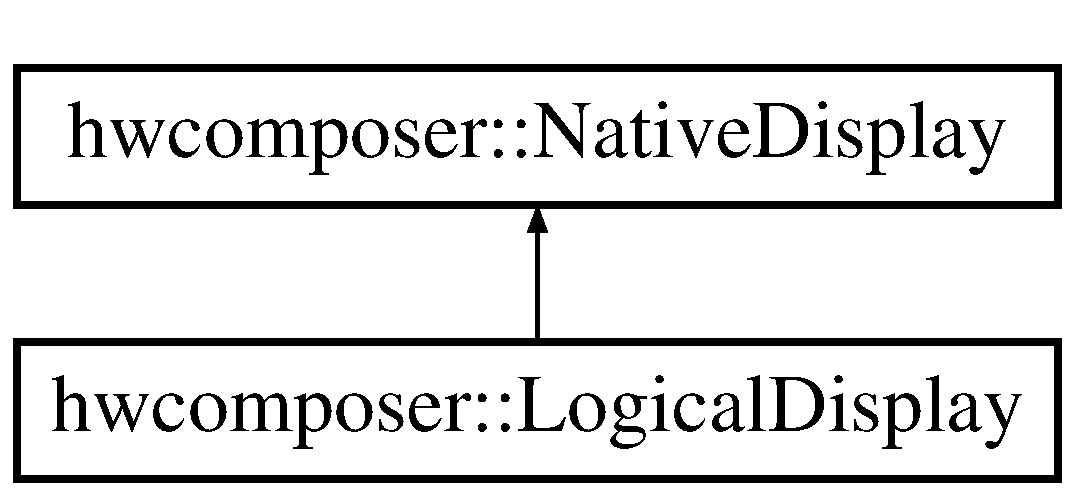
\includegraphics[height=2.000000cm]{classhwcomposer_1_1LogicalDisplay}
\end{center}
\end{figure}
\subsection*{Public Member Functions}
\begin{DoxyCompactItemize}
\item 
\mbox{\hyperlink{classhwcomposer_1_1LogicalDisplay_a1982d5bd3dd45fffdddfdba4cd648ae7}{Logical\+Display}} (\mbox{\hyperlink{classhwcomposer_1_1LogicalDisplayManager}{Logical\+Display\+Manager}} $\ast$display\+\_\+manager, \mbox{\hyperlink{classhwcomposer_1_1NativeDisplay}{Native\+Display}} $\ast$physical\+\_\+display, uint32\+\_\+t total\+\_\+divisions, uint32\+\_\+t index)
\item 
\mbox{\hyperlink{classhwcomposer_1_1LogicalDisplay_a6a86f5635e1dbb28026b048219ce562c}{$\sim$\+Logical\+Display}} () override
\item 
bool \mbox{\hyperlink{classhwcomposer_1_1LogicalDisplay_a280447edbcba240ec782928273d87c65}{Initialize}} (\mbox{\hyperlink{classhwcomposer_1_1NativeBufferHandler}{Native\+Buffer\+Handler}} $\ast$buffer\+\_\+handler, \mbox{\hyperlink{classhwcomposer_1_1FrameBufferManager}{Frame\+Buffer\+Manager}} $\ast$) override
\item 
Display\+Type \mbox{\hyperlink{classhwcomposer_1_1LogicalDisplay_a012b2a742cfd590405db34ff68f919a9}{Type}} () const override
\item 
uint32\+\_\+t \mbox{\hyperlink{classhwcomposer_1_1LogicalDisplay_a788d88b267f7d36ad6e70f523fd16c97}{Width}} () const override
\item 
uint32\+\_\+t \mbox{\hyperlink{classhwcomposer_1_1LogicalDisplay_a8c687fb1727e18b8a74db9740eccca88}{Height}} () const override
\item 
uint32\+\_\+t \mbox{\hyperlink{classhwcomposer_1_1LogicalDisplay_af0fd1b1d9b574403e9c4680f7b371c21}{Power\+Mode}} () const override
\item 
int \mbox{\hyperlink{classhwcomposer_1_1LogicalDisplay_acd2630578257e1156d5e00b304df2db8}{Get\+Display\+Pipe}} () override
\item 
bool \mbox{\hyperlink{classhwcomposer_1_1LogicalDisplay_aa758516a35c9f74cc34f4b679fa33307}{Set\+Active\+Config}} (uint32\+\_\+t config) override
\item 
bool \mbox{\hyperlink{classhwcomposer_1_1LogicalDisplay_a8a88b08fd54dd02debe436718c569fff}{Get\+Active\+Config}} (uint32\+\_\+t $\ast$config) override
\item 
bool \mbox{\hyperlink{classhwcomposer_1_1LogicalDisplay_aed95336a0e93791e9e97b5e1c0940a7e}{Set\+Power\+Mode}} (uint32\+\_\+t power\+\_\+mode) override
\item 
bool \mbox{\hyperlink{classhwcomposer_1_1LogicalDisplay_a2cc998518219938311c9bba35cac4935}{Present}} (std\+::vector$<$ \mbox{\hyperlink{structhwcomposer_1_1HwcLayer}{Hwc\+Layer}} $\ast$$>$ \&source\+\_\+layers, int32\+\_\+t $\ast$retire\+\_\+fence, \mbox{\hyperlink{classhwcomposer_1_1PixelUploaderCallback}{Pixel\+Uploader\+Callback}} $\ast$call\+\_\+back=\mbox{\hyperlink{alios_2platformdefines_8h_a070d2ce7b6bb7e5c05602aa8c308d0c4}{N\+U\+LL}}, bool handle\+\_\+constraints=false) override
\item 
int \mbox{\hyperlink{classhwcomposer_1_1LogicalDisplay_af99c6d2e779060cb006ee5d0039386da}{Register\+Vsync\+Callback}} (std\+::shared\+\_\+ptr$<$ \mbox{\hyperlink{classhwcomposer_1_1VsyncCallback}{Vsync\+Callback}} $>$ callback, uint32\+\_\+t display\+\_\+id) override
\item 
void \mbox{\hyperlink{classhwcomposer_1_1LogicalDisplay_a53dd3b4a4ee95af6a903327519278691}{Register\+Refresh\+Callback}} (std\+::shared\+\_\+ptr$<$ \mbox{\hyperlink{classhwcomposer_1_1RefreshCallback}{Refresh\+Callback}} $>$ callback, uint32\+\_\+t display\+\_\+id) override
\item 
void \mbox{\hyperlink{classhwcomposer_1_1LogicalDisplay_a04e78f9e54b66e91bab3f9744a2a18f3}{Register\+Hot\+Plug\+Callback}} (std\+::shared\+\_\+ptr$<$ \mbox{\hyperlink{classhwcomposer_1_1HotPlugCallback}{Hot\+Plug\+Callback}} $>$ callback, uint32\+\_\+t display\+\_\+id) override
\item 
void \mbox{\hyperlink{classhwcomposer_1_1LogicalDisplay_adfb3b051b8636f58226bc30da8fe1735}{V\+Sync\+Control}} (bool enabled) override
\item 
bool \mbox{\hyperlink{classhwcomposer_1_1LogicalDisplay_ae54b9d9a1d980ed587f43aef1c2a6f2c}{Check\+Plane\+Format}} (uint32\+\_\+t format) override
\item 
void \mbox{\hyperlink{classhwcomposer_1_1LogicalDisplay_aed2d919c0ee7f2eb177e062f0ac3cd1f}{Set\+Gamma}} (float red, float green, float blue) override
\item 
void \mbox{\hyperlink{classhwcomposer_1_1LogicalDisplay_a84a63a9f28391e92765316afacf22402}{Set\+Contrast}} (uint32\+\_\+t red, uint32\+\_\+t green, uint32\+\_\+t blue) override
\item 
void \mbox{\hyperlink{classhwcomposer_1_1LogicalDisplay_a3244bd17dbe005b1e8db94fd646f246f}{Set\+Brightness}} (uint32\+\_\+t red, uint32\+\_\+t green, uint32\+\_\+t blue) override
\item 
void \mbox{\hyperlink{classhwcomposer_1_1LogicalDisplay_aafa5f07e92a828651f2d66b09df4896d}{Set\+Explicit\+Sync\+Support}} (bool disable\+\_\+explicit\+\_\+sync) override
\item 
void \mbox{\hyperlink{classhwcomposer_1_1LogicalDisplay_a7f616d7c193e2afbf4b65df4775470c2}{Set\+Video\+Scaling\+Mode}} (uint32\+\_\+t mode) override
\item 
void \mbox{\hyperlink{classhwcomposer_1_1LogicalDisplay_af963f6dd39bb6d7f043b6908ea5c64e5}{Set\+Video\+Color}} (H\+W\+C\+Color\+Control color, float value) override
\item 
void \mbox{\hyperlink{classhwcomposer_1_1LogicalDisplay_a026e99a7fbdb31e02bba1c968c3e2842}{Get\+Video\+Color}} (H\+W\+C\+Color\+Control color, float $\ast$value, float $\ast$start, float $\ast$end) override
\item 
void \mbox{\hyperlink{classhwcomposer_1_1LogicalDisplay_a8368cd424259347984eac3e2469bb660}{Set\+Canvas\+Color}} (uint16\+\_\+t bpc, uint16\+\_\+t red, uint16\+\_\+t green, uint16\+\_\+t blue, uint16\+\_\+t alpha) override
\item 
void \mbox{\hyperlink{classhwcomposer_1_1LogicalDisplay_aabeca956b6c48031fd0c9c862e7cd9cc}{Restore\+Video\+Default\+Color}} (H\+W\+C\+Color\+Control color) override
\item 
void \mbox{\hyperlink{classhwcomposer_1_1LogicalDisplay_a556ac92994853a0b0053132a3917bc75}{Set\+Video\+Deinterlace}} (H\+W\+C\+Deinterlace\+Flag flag, H\+W\+C\+Deinterlace\+Control mode) override
\item 
void \mbox{\hyperlink{classhwcomposer_1_1LogicalDisplay_ad0d206b9c0e41732b2f9635fd6ffeb6c}{Restore\+Video\+Default\+Deinterlace}} () override
\item 
bool \mbox{\hyperlink{classhwcomposer_1_1LogicalDisplay_ad1eb84dcbc22cbadbe3d0dc85f18bde3}{Is\+Connected}} () const override
\item 
void \mbox{\hyperlink{classhwcomposer_1_1LogicalDisplay_ad4813941543f9765790888d7e7c6865f}{Update\+Scaling\+Ratio}} (uint32\+\_\+t primary\+\_\+width, uint32\+\_\+t primary\+\_\+height, uint32\+\_\+t display\+\_\+width, uint32\+\_\+t display\+\_\+height) override
\item 
void \mbox{\hyperlink{classhwcomposer_1_1LogicalDisplay_a14d300f193051c5cd3e259bb0534401b}{Clone\+Display}} (\mbox{\hyperlink{classhwcomposer_1_1NativeDisplay}{Native\+Display}} $\ast$source\+\_\+display) override
\item 
bool \mbox{\hyperlink{classhwcomposer_1_1LogicalDisplay_acd399ec20ae92f1c68db2fbcff91f8f0}{Present\+Clone}} (\mbox{\hyperlink{classhwcomposer_1_1NativeDisplay}{Native\+Display}} $\ast$) override
\item 
bool \mbox{\hyperlink{classhwcomposer_1_1LogicalDisplay_a0ccbb1903cf15c1459f491aa1d3b3619}{Get\+Display\+Attribute}} (uint32\+\_\+t, H\+W\+C\+Display\+Attribute attribute, int32\+\_\+t $\ast$value) override
\item 
bool \mbox{\hyperlink{classhwcomposer_1_1LogicalDisplay_a4df433d0a996e29197dfc23067a75ab4}{Get\+Display\+Configs}} (uint32\+\_\+t $\ast$num\+\_\+configs, uint32\+\_\+t $\ast$configs) override
\item 
bool \mbox{\hyperlink{classhwcomposer_1_1LogicalDisplay_a93e917448b225c7342d34ef589090987}{Get\+Display\+Name}} (uint32\+\_\+t $\ast$size, char $\ast$name) override
\item 
uint32\+\_\+t \mbox{\hyperlink{classhwcomposer_1_1LogicalDisplay_a1eea402be34da5de3ce4d3c9927768ae}{Get\+X\+Translation}} () override
\item 
uint32\+\_\+t \mbox{\hyperlink{classhwcomposer_1_1LogicalDisplay_a5d45569f5a91a82ff525bee68f9497a7}{Get\+Logical\+Index}} () const override
\item 
bool \mbox{\hyperlink{classhwcomposer_1_1LogicalDisplay_ab519c7398b8aad01c68ecc78e3e831a1}{Enable\+V\+Sync}} () const
\item 
void \mbox{\hyperlink{classhwcomposer_1_1LogicalDisplay_af97452d9abef74bef82c4cc49385a6e6}{V\+Sync\+Update}} (int64\+\_\+t timestamp)
\item 
void \mbox{\hyperlink{classhwcomposer_1_1LogicalDisplay_a2210f981e537004b940988e81fb42706}{Refresh\+Update}} ()
\item 
void \mbox{\hyperlink{classhwcomposer_1_1LogicalDisplay_ab216be63c504dc281fa1da2f7825e059}{Hot\+Plug\+Update}} (bool connected) override
\item 
void \mbox{\hyperlink{classhwcomposer_1_1LogicalDisplay_a161e6fd394b077071d4087314ac1fd8a}{Set\+H\+D\+C\+P\+State}} (H\+W\+C\+Content\+Protection state, H\+W\+C\+Content\+Type content\+\_\+type) override
\end{DoxyCompactItemize}
\subsection*{Additional Inherited Members}


\subsection{Detailed Description}


Definition at line 31 of file logicaldisplay.\+h.



\subsection{Constructor \& Destructor Documentation}
\mbox{\Hypertarget{classhwcomposer_1_1LogicalDisplay_a1982d5bd3dd45fffdddfdba4cd648ae7}\label{classhwcomposer_1_1LogicalDisplay_a1982d5bd3dd45fffdddfdba4cd648ae7}} 
\index{hwcomposer\+::\+Logical\+Display@{hwcomposer\+::\+Logical\+Display}!Logical\+Display@{Logical\+Display}}
\index{Logical\+Display@{Logical\+Display}!hwcomposer\+::\+Logical\+Display@{hwcomposer\+::\+Logical\+Display}}
\subsubsection{\texorpdfstring{Logical\+Display()}{LogicalDisplay()}}
{\footnotesize\ttfamily hwcomposer\+::\+Logical\+Display\+::\+Logical\+Display (\begin{DoxyParamCaption}\item[{\mbox{\hyperlink{classhwcomposer_1_1LogicalDisplayManager}{Logical\+Display\+Manager}} $\ast$}]{display\+\_\+manager,  }\item[{\mbox{\hyperlink{classhwcomposer_1_1NativeDisplay}{Native\+Display}} $\ast$}]{physical\+\_\+display,  }\item[{uint32\+\_\+t}]{total\+\_\+divisions,  }\item[{uint32\+\_\+t}]{index }\end{DoxyParamCaption})}



Definition at line 26 of file logicaldisplay.\+cpp.


\begin{DoxyCode}{0}
\DoxyCodeLine{29     : logical\_display\_manager\_(display\_manager),}
\DoxyCodeLine{30       physical\_display\_(physical\_display),}
\DoxyCodeLine{31       index\_(index),}
\DoxyCodeLine{32       total\_divisions\_(total\_divisions) \{}
\DoxyCodeLine{33 \}}
\end{DoxyCode}
\mbox{\Hypertarget{classhwcomposer_1_1LogicalDisplay_a6a86f5635e1dbb28026b048219ce562c}\label{classhwcomposer_1_1LogicalDisplay_a6a86f5635e1dbb28026b048219ce562c}} 
\index{hwcomposer\+::\+Logical\+Display@{hwcomposer\+::\+Logical\+Display}!````~Logical\+Display@{$\sim$\+Logical\+Display}}
\index{````~Logical\+Display@{$\sim$\+Logical\+Display}!hwcomposer\+::\+Logical\+Display@{hwcomposer\+::\+Logical\+Display}}
\subsubsection{\texorpdfstring{$\sim$\+Logical\+Display()}{~LogicalDisplay()}}
{\footnotesize\ttfamily hwcomposer\+::\+Logical\+Display\+::$\sim$\+Logical\+Display (\begin{DoxyParamCaption}{ }\end{DoxyParamCaption})\hspace{0.3cm}{\ttfamily [override]}}



Definition at line 35 of file logicaldisplay.\+cpp.


\begin{DoxyCode}{0}
\DoxyCodeLine{35                                 \{}
\DoxyCodeLine{36 \}}
\end{DoxyCode}


\subsection{Member Function Documentation}
\mbox{\Hypertarget{classhwcomposer_1_1LogicalDisplay_ae54b9d9a1d980ed587f43aef1c2a6f2c}\label{classhwcomposer_1_1LogicalDisplay_ae54b9d9a1d980ed587f43aef1c2a6f2c}} 
\index{hwcomposer\+::\+Logical\+Display@{hwcomposer\+::\+Logical\+Display}!Check\+Plane\+Format@{Check\+Plane\+Format}}
\index{Check\+Plane\+Format@{Check\+Plane\+Format}!hwcomposer\+::\+Logical\+Display@{hwcomposer\+::\+Logical\+Display}}
\subsubsection{\texorpdfstring{Check\+Plane\+Format()}{CheckPlaneFormat()}}
{\footnotesize\ttfamily bool hwcomposer\+::\+Logical\+Display\+::\+Check\+Plane\+Format (\begin{DoxyParamCaption}\item[{uint32\+\_\+t}]{format }\end{DoxyParamCaption})\hspace{0.3cm}{\ttfamily [override]}, {\ttfamily [virtual]}}

A\+PI to check the format support on the device 
\begin{DoxyParams}{Parameters}
{\em format} & valid D\+RM formats found in drm\+\_\+fourcc.\+h. \\
\hline
\end{DoxyParams}


Implements \mbox{\hyperlink{classhwcomposer_1_1NativeDisplay_a4e856b5754054bdf77467e6663cb5b50}{hwcomposer\+::\+Native\+Display}}.



Definition at line 134 of file logicaldisplay.\+cpp.


\begin{DoxyCode}{0}
\DoxyCodeLine{134                                                      \{}
\DoxyCodeLine{135   \textcolor{keywordflow}{return} physical\_display\_->\mbox{\hyperlink{classhwcomposer_1_1NativeDisplay_a4e856b5754054bdf77467e6663cb5b50}{CheckPlaneFormat}}(format);}
\DoxyCodeLine{136 \}}
\end{DoxyCode}
\mbox{\Hypertarget{classhwcomposer_1_1LogicalDisplay_a14d300f193051c5cd3e259bb0534401b}\label{classhwcomposer_1_1LogicalDisplay_a14d300f193051c5cd3e259bb0534401b}} 
\index{hwcomposer\+::\+Logical\+Display@{hwcomposer\+::\+Logical\+Display}!Clone\+Display@{Clone\+Display}}
\index{Clone\+Display@{Clone\+Display}!hwcomposer\+::\+Logical\+Display@{hwcomposer\+::\+Logical\+Display}}
\subsubsection{\texorpdfstring{Clone\+Display()}{CloneDisplay()}}
{\footnotesize\ttfamily void hwcomposer\+::\+Logical\+Display\+::\+Clone\+Display (\begin{DoxyParamCaption}\item[{\mbox{\hyperlink{classhwcomposer_1_1NativeDisplay}{Native\+Display}} $\ast$}]{ }\end{DoxyParamCaption})\hspace{0.3cm}{\ttfamily [override]}, {\ttfamily [virtual]}}

This display needs to clone source\+\_\+display. We cannot have a display in cloned mode and extended mode at same time or clone more than one source\+\_\+display at same time. 

Reimplemented from \mbox{\hyperlink{classhwcomposer_1_1NativeDisplay_ad244fa57c9c6380fb04bfd57da3cb28b}{hwcomposer\+::\+Native\+Display}}.



Definition at line 192 of file logicaldisplay.\+cpp.


\begin{DoxyCode}{0}
\DoxyCodeLine{192                                                    \{}
\DoxyCodeLine{193 \}}
\end{DoxyCode}
\mbox{\Hypertarget{classhwcomposer_1_1LogicalDisplay_ab519c7398b8aad01c68ecc78e3e831a1}\label{classhwcomposer_1_1LogicalDisplay_ab519c7398b8aad01c68ecc78e3e831a1}} 
\index{hwcomposer\+::\+Logical\+Display@{hwcomposer\+::\+Logical\+Display}!Enable\+V\+Sync@{Enable\+V\+Sync}}
\index{Enable\+V\+Sync@{Enable\+V\+Sync}!hwcomposer\+::\+Logical\+Display@{hwcomposer\+::\+Logical\+Display}}
\subsubsection{\texorpdfstring{Enable\+V\+Sync()}{EnableVSync()}}
{\footnotesize\ttfamily bool hwcomposer\+::\+Logical\+Display\+::\+Enable\+V\+Sync (\begin{DoxyParamCaption}{ }\end{DoxyParamCaption}) const\hspace{0.3cm}{\ttfamily [inline]}}



Definition at line 115 of file logicaldisplay.\+h.


\begin{DoxyCode}{0}
\DoxyCodeLine{115                            \{}
\DoxyCodeLine{116     \textcolor{keywordflow}{return} enable\_vsync\_;}
\DoxyCodeLine{117   \}}
\end{DoxyCode}
\mbox{\Hypertarget{classhwcomposer_1_1LogicalDisplay_a8a88b08fd54dd02debe436718c569fff}\label{classhwcomposer_1_1LogicalDisplay_a8a88b08fd54dd02debe436718c569fff}} 
\index{hwcomposer\+::\+Logical\+Display@{hwcomposer\+::\+Logical\+Display}!Get\+Active\+Config@{Get\+Active\+Config}}
\index{Get\+Active\+Config@{Get\+Active\+Config}!hwcomposer\+::\+Logical\+Display@{hwcomposer\+::\+Logical\+Display}}
\subsubsection{\texorpdfstring{Get\+Active\+Config()}{GetActiveConfig()}}
{\footnotesize\ttfamily bool hwcomposer\+::\+Logical\+Display\+::\+Get\+Active\+Config (\begin{DoxyParamCaption}\item[{uint32\+\_\+t $\ast$}]{config }\end{DoxyParamCaption})\hspace{0.3cm}{\ttfamily [override]}, {\ttfamily [virtual]}}



Implements \mbox{\hyperlink{classhwcomposer_1_1NativeDisplay_a9d4d9d2f6633fe37025210cac6e8cc6c}{hwcomposer\+::\+Native\+Display}}.



Definition at line 61 of file logicaldisplay.\+cpp.


\begin{DoxyCode}{0}
\DoxyCodeLine{61                                                      \{}
\DoxyCodeLine{62   \textcolor{keywordflow}{return} physical\_display\_->\mbox{\hyperlink{classhwcomposer_1_1NativeDisplay_a9d4d9d2f6633fe37025210cac6e8cc6c}{GetActiveConfig}}(config);}
\DoxyCodeLine{63 \}}
\end{DoxyCode}
\mbox{\Hypertarget{classhwcomposer_1_1LogicalDisplay_a0ccbb1903cf15c1459f491aa1d3b3619}\label{classhwcomposer_1_1LogicalDisplay_a0ccbb1903cf15c1459f491aa1d3b3619}} 
\index{hwcomposer\+::\+Logical\+Display@{hwcomposer\+::\+Logical\+Display}!Get\+Display\+Attribute@{Get\+Display\+Attribute}}
\index{Get\+Display\+Attribute@{Get\+Display\+Attribute}!hwcomposer\+::\+Logical\+Display@{hwcomposer\+::\+Logical\+Display}}
\subsubsection{\texorpdfstring{Get\+Display\+Attribute()}{GetDisplayAttribute()}}
{\footnotesize\ttfamily bool hwcomposer\+::\+Logical\+Display\+::\+Get\+Display\+Attribute (\begin{DoxyParamCaption}\item[{uint32\+\_\+t}]{config,  }\item[{H\+W\+C\+Display\+Attribute}]{attribute,  }\item[{int32\+\_\+t $\ast$}]{value }\end{DoxyParamCaption})\hspace{0.3cm}{\ttfamily [override]}, {\ttfamily [virtual]}}



Implements \mbox{\hyperlink{classhwcomposer_1_1NativeDisplay_aeb880e4a295eab49a98804380c2dcb84}{hwcomposer\+::\+Native\+Display}}.



Definition at line 195 of file logicaldisplay.\+cpp.


\begin{DoxyCode}{0}
\DoxyCodeLine{197                                                          \{}
\DoxyCodeLine{198   \textcolor{keywordflow}{switch} (attribute) \{}
\DoxyCodeLine{199     \textcolor{keywordflow}{case} HWCDisplayAttribute::kWidth:}
\DoxyCodeLine{200       physical\_display\_->\mbox{\hyperlink{classhwcomposer_1_1NativeDisplay_aeb880e4a295eab49a98804380c2dcb84}{GetDisplayAttribute}}(config, attribute, value);}
\DoxyCodeLine{201       *value = *value / total\_divisions\_;}
\DoxyCodeLine{202       \textcolor{keywordflow}{return} \textcolor{keyword}{true};}
\DoxyCodeLine{203     \textcolor{keywordflow}{default}:}
\DoxyCodeLine{204       \textcolor{keywordflow}{break};}
\DoxyCodeLine{205   \}}
\DoxyCodeLine{206 }
\DoxyCodeLine{207   \textcolor{keywordflow}{return} physical\_display\_->\mbox{\hyperlink{classhwcomposer_1_1NativeDisplay_aeb880e4a295eab49a98804380c2dcb84}{GetDisplayAttribute}}(config, attribute, value);}
\DoxyCodeLine{208 \}}
\end{DoxyCode}
\mbox{\Hypertarget{classhwcomposer_1_1LogicalDisplay_a4df433d0a996e29197dfc23067a75ab4}\label{classhwcomposer_1_1LogicalDisplay_a4df433d0a996e29197dfc23067a75ab4}} 
\index{hwcomposer\+::\+Logical\+Display@{hwcomposer\+::\+Logical\+Display}!Get\+Display\+Configs@{Get\+Display\+Configs}}
\index{Get\+Display\+Configs@{Get\+Display\+Configs}!hwcomposer\+::\+Logical\+Display@{hwcomposer\+::\+Logical\+Display}}
\subsubsection{\texorpdfstring{Get\+Display\+Configs()}{GetDisplayConfigs()}}
{\footnotesize\ttfamily bool hwcomposer\+::\+Logical\+Display\+::\+Get\+Display\+Configs (\begin{DoxyParamCaption}\item[{uint32\+\_\+t $\ast$}]{num\+\_\+configs,  }\item[{uint32\+\_\+t $\ast$}]{configs }\end{DoxyParamCaption})\hspace{0.3cm}{\ttfamily [override]}, {\ttfamily [virtual]}}



Implements \mbox{\hyperlink{classhwcomposer_1_1NativeDisplay_a9479dcf82765996db6d7ea1cdcef3864}{hwcomposer\+::\+Native\+Display}}.



Definition at line 210 of file logicaldisplay.\+cpp.


\begin{DoxyCode}{0}
\DoxyCodeLine{211                                                           \{}
\DoxyCodeLine{212   \textcolor{keywordflow}{return} physical\_display\_->\mbox{\hyperlink{classhwcomposer_1_1NativeDisplay_a9479dcf82765996db6d7ea1cdcef3864}{GetDisplayConfigs}}(num\_configs, configs);}
\DoxyCodeLine{213 \}}
\end{DoxyCode}
\mbox{\Hypertarget{classhwcomposer_1_1LogicalDisplay_a93e917448b225c7342d34ef589090987}\label{classhwcomposer_1_1LogicalDisplay_a93e917448b225c7342d34ef589090987}} 
\index{hwcomposer\+::\+Logical\+Display@{hwcomposer\+::\+Logical\+Display}!Get\+Display\+Name@{Get\+Display\+Name}}
\index{Get\+Display\+Name@{Get\+Display\+Name}!hwcomposer\+::\+Logical\+Display@{hwcomposer\+::\+Logical\+Display}}
\subsubsection{\texorpdfstring{Get\+Display\+Name()}{GetDisplayName()}}
{\footnotesize\ttfamily bool hwcomposer\+::\+Logical\+Display\+::\+Get\+Display\+Name (\begin{DoxyParamCaption}\item[{uint32\+\_\+t $\ast$}]{size,  }\item[{char $\ast$}]{name }\end{DoxyParamCaption})\hspace{0.3cm}{\ttfamily [override]}, {\ttfamily [virtual]}}



Implements \mbox{\hyperlink{classhwcomposer_1_1NativeDisplay_a28c095d6d08c84e40b5d5160d038f0b5}{hwcomposer\+::\+Native\+Display}}.



Definition at line 215 of file logicaldisplay.\+cpp.


\begin{DoxyCode}{0}
\DoxyCodeLine{215                                                               \{}
\DoxyCodeLine{216   std::ostringstream stream;}
\DoxyCodeLine{217   stream << \textcolor{stringliteral}{"Logical"};}
\DoxyCodeLine{218   std::string \textcolor{keywordtype}{string} = stream.str();}
\DoxyCodeLine{219   \textcolor{keywordtype}{size\_t} length = \textcolor{keywordtype}{string}.length();}
\DoxyCodeLine{220   \textcolor{keywordflow}{if} (!name) \{}
\DoxyCodeLine{221     *size = length;}
\DoxyCodeLine{222     \textcolor{keywordflow}{return} \textcolor{keyword}{true};}
\DoxyCodeLine{223   \}}
\DoxyCodeLine{224 }
\DoxyCodeLine{225   *size = std::min<uint32\_t>(\textcolor{keyword}{static\_cast<}uint32\_t\textcolor{keyword}{>}(length - 1), *size);}
\DoxyCodeLine{226   strncpy(name, \textcolor{keywordtype}{string}.c\_str(), *size);}
\DoxyCodeLine{227   \textcolor{keywordflow}{return} \textcolor{keyword}{true};}
\DoxyCodeLine{228 \}}
\end{DoxyCode}
\mbox{\Hypertarget{classhwcomposer_1_1LogicalDisplay_acd2630578257e1156d5e00b304df2db8}\label{classhwcomposer_1_1LogicalDisplay_acd2630578257e1156d5e00b304df2db8}} 
\index{hwcomposer\+::\+Logical\+Display@{hwcomposer\+::\+Logical\+Display}!Get\+Display\+Pipe@{Get\+Display\+Pipe}}
\index{Get\+Display\+Pipe@{Get\+Display\+Pipe}!hwcomposer\+::\+Logical\+Display@{hwcomposer\+::\+Logical\+Display}}
\subsubsection{\texorpdfstring{Get\+Display\+Pipe()}{GetDisplayPipe()}}
{\footnotesize\ttfamily int hwcomposer\+::\+Logical\+Display\+::\+Get\+Display\+Pipe (\begin{DoxyParamCaption}{ }\end{DoxyParamCaption})\hspace{0.3cm}{\ttfamily [override]}, {\ttfamily [virtual]}}

A\+PI for getting connected display\textquotesingle{}s pipe id. \begin{DoxyReturn}{Returns}
\char`\"{}-\/1\char`\"{} for unconnected display, valid values are 0 $\sim$ 2. 
\end{DoxyReturn}


Implements \mbox{\hyperlink{classhwcomposer_1_1NativeDisplay_aaf80095ae6aed35c64dd633a6a2f101a}{hwcomposer\+::\+Native\+Display}}.



Definition at line 51 of file logicaldisplay.\+cpp.


\begin{DoxyCode}{0}
\DoxyCodeLine{51                                    \{}
\DoxyCodeLine{52   \textcolor{keywordflow}{return} physical\_display\_->\mbox{\hyperlink{classhwcomposer_1_1NativeDisplay_aaf80095ae6aed35c64dd633a6a2f101a}{GetDisplayPipe}}();}
\DoxyCodeLine{53 \}}
\end{DoxyCode}
\mbox{\Hypertarget{classhwcomposer_1_1LogicalDisplay_a5d45569f5a91a82ff525bee68f9497a7}\label{classhwcomposer_1_1LogicalDisplay_a5d45569f5a91a82ff525bee68f9497a7}} 
\index{hwcomposer\+::\+Logical\+Display@{hwcomposer\+::\+Logical\+Display}!Get\+Logical\+Index@{Get\+Logical\+Index}}
\index{Get\+Logical\+Index@{Get\+Logical\+Index}!hwcomposer\+::\+Logical\+Display@{hwcomposer\+::\+Logical\+Display}}
\subsubsection{\texorpdfstring{Get\+Logical\+Index()}{GetLogicalIndex()}}
{\footnotesize\ttfamily uint32\+\_\+t hwcomposer\+::\+Logical\+Display\+::\+Get\+Logical\+Index (\begin{DoxyParamCaption}{ }\end{DoxyParamCaption}) const\hspace{0.3cm}{\ttfamily [inline]}, {\ttfamily [override]}, {\ttfamily [virtual]}}



Reimplemented from \mbox{\hyperlink{classhwcomposer_1_1NativeDisplay_a991eb1bf6b9dcdb8dd08c171bc8b8b08}{hwcomposer\+::\+Native\+Display}}.



Definition at line 111 of file logicaldisplay.\+h.


\begin{DoxyCode}{0}
\DoxyCodeLine{111                                             \{}
\DoxyCodeLine{112     \textcolor{keywordflow}{return} index\_;}
\DoxyCodeLine{113   \}}
\end{DoxyCode}
\mbox{\Hypertarget{classhwcomposer_1_1LogicalDisplay_a026e99a7fbdb31e02bba1c968c3e2842}\label{classhwcomposer_1_1LogicalDisplay_a026e99a7fbdb31e02bba1c968c3e2842}} 
\index{hwcomposer\+::\+Logical\+Display@{hwcomposer\+::\+Logical\+Display}!Get\+Video\+Color@{Get\+Video\+Color}}
\index{Get\+Video\+Color@{Get\+Video\+Color}!hwcomposer\+::\+Logical\+Display@{hwcomposer\+::\+Logical\+Display}}
\subsubsection{\texorpdfstring{Get\+Video\+Color()}{GetVideoColor()}}
{\footnotesize\ttfamily void hwcomposer\+::\+Logical\+Display\+::\+Get\+Video\+Color (\begin{DoxyParamCaption}\item[{H\+W\+C\+Color\+Control}]{,  }\item[{float $\ast$}]{,  }\item[{float $\ast$}]{,  }\item[{float $\ast$}]{ }\end{DoxyParamCaption})\hspace{0.3cm}{\ttfamily [override]}, {\ttfamily [virtual]}}

A\+PI for getting video color in H\+WC 

Reimplemented from \mbox{\hyperlink{classhwcomposer_1_1NativeDisplay_a2db52a8a234064113a0e250a059663ac}{hwcomposer\+::\+Native\+Display}}.



Definition at line 163 of file logicaldisplay.\+cpp.


\begin{DoxyCode}{0}
\DoxyCodeLine{164                                                              \{}
\DoxyCodeLine{165   physical\_display\_->\mbox{\hyperlink{classhwcomposer_1_1NativeDisplay_a2db52a8a234064113a0e250a059663ac}{GetVideoColor}}(color, value, start, end);}
\DoxyCodeLine{166 \}}
\end{DoxyCode}
\mbox{\Hypertarget{classhwcomposer_1_1LogicalDisplay_a1eea402be34da5de3ce4d3c9927768ae}\label{classhwcomposer_1_1LogicalDisplay_a1eea402be34da5de3ce4d3c9927768ae}} 
\index{hwcomposer\+::\+Logical\+Display@{hwcomposer\+::\+Logical\+Display}!Get\+X\+Translation@{Get\+X\+Translation}}
\index{Get\+X\+Translation@{Get\+X\+Translation}!hwcomposer\+::\+Logical\+Display@{hwcomposer\+::\+Logical\+Display}}
\subsubsection{\texorpdfstring{Get\+X\+Translation()}{GetXTranslation()}}
{\footnotesize\ttfamily uint32\+\_\+t hwcomposer\+::\+Logical\+Display\+::\+Get\+X\+Translation (\begin{DoxyParamCaption}{ }\end{DoxyParamCaption})\hspace{0.3cm}{\ttfamily [inline]}, {\ttfamily [override]}, {\ttfamily [virtual]}}



Reimplemented from \mbox{\hyperlink{classhwcomposer_1_1NativeDisplay_a1f934e9ab6149fb35bd2868605c215dd}{hwcomposer\+::\+Native\+Display}}.



Definition at line 107 of file logicaldisplay.\+h.


\begin{DoxyCode}{0}
\DoxyCodeLine{107                                       \{}
\DoxyCodeLine{108     \textcolor{keywordflow}{return} (((physical\_display\_->\mbox{\hyperlink{classhwcomposer_1_1NativeDisplay_a9a18c3dfba567c86c088b06febda4019}{Width}}()) / total\_divisions\_) * index\_);}
\DoxyCodeLine{109   \}}
\end{DoxyCode}
\mbox{\Hypertarget{classhwcomposer_1_1LogicalDisplay_a8c687fb1727e18b8a74db9740eccca88}\label{classhwcomposer_1_1LogicalDisplay_a8c687fb1727e18b8a74db9740eccca88}} 
\index{hwcomposer\+::\+Logical\+Display@{hwcomposer\+::\+Logical\+Display}!Height@{Height}}
\index{Height@{Height}!hwcomposer\+::\+Logical\+Display@{hwcomposer\+::\+Logical\+Display}}
\subsubsection{\texorpdfstring{Height()}{Height()}}
{\footnotesize\ttfamily uint32\+\_\+t hwcomposer\+::\+Logical\+Display\+::\+Height (\begin{DoxyParamCaption}{ }\end{DoxyParamCaption}) const\hspace{0.3cm}{\ttfamily [inline]}, {\ttfamily [override]}, {\ttfamily [virtual]}}



Implements \mbox{\hyperlink{classhwcomposer_1_1NativeDisplay_a09a19377e64e1fed90ae8315a8e71864}{hwcomposer\+::\+Native\+Display}}.



Definition at line 49 of file logicaldisplay.\+h.


\begin{DoxyCode}{0}
\DoxyCodeLine{49                                    \{}
\DoxyCodeLine{50     \textcolor{keywordflow}{return} physical\_display\_->\mbox{\hyperlink{classhwcomposer_1_1NativeDisplay_a09a19377e64e1fed90ae8315a8e71864}{Height}}();}
\DoxyCodeLine{51   \}}
\end{DoxyCode}
\mbox{\Hypertarget{classhwcomposer_1_1LogicalDisplay_ab216be63c504dc281fa1da2f7825e059}\label{classhwcomposer_1_1LogicalDisplay_ab216be63c504dc281fa1da2f7825e059}} 
\index{hwcomposer\+::\+Logical\+Display@{hwcomposer\+::\+Logical\+Display}!Hot\+Plug\+Update@{Hot\+Plug\+Update}}
\index{Hot\+Plug\+Update@{Hot\+Plug\+Update}!hwcomposer\+::\+Logical\+Display@{hwcomposer\+::\+Logical\+Display}}
\subsubsection{\texorpdfstring{Hot\+Plug\+Update()}{HotPlugUpdate()}}
{\footnotesize\ttfamily void hwcomposer\+::\+Logical\+Display\+::\+Hot\+Plug\+Update (\begin{DoxyParamCaption}\item[{bool}]{connected }\end{DoxyParamCaption})\hspace{0.3cm}{\ttfamily [override]}, {\ttfamily [virtual]}}



Reimplemented from \mbox{\hyperlink{classhwcomposer_1_1NativeDisplay_a30e5c044e3a84ed23d2b3a5cec3f9037}{hwcomposer\+::\+Native\+Display}}.



Definition at line 128 of file logicaldisplay.\+cpp.


\begin{DoxyCode}{0}
\DoxyCodeLine{128                                                  \{}
\DoxyCodeLine{129   \textcolor{keywordflow}{if} (hotplug\_callback\_) \{}
\DoxyCodeLine{130     hotplug\_callback\_->Callback(display\_id\_, connected);}
\DoxyCodeLine{131   \}}
\DoxyCodeLine{132 \}}
\end{DoxyCode}
\mbox{\Hypertarget{classhwcomposer_1_1LogicalDisplay_a280447edbcba240ec782928273d87c65}\label{classhwcomposer_1_1LogicalDisplay_a280447edbcba240ec782928273d87c65}} 
\index{hwcomposer\+::\+Logical\+Display@{hwcomposer\+::\+Logical\+Display}!Initialize@{Initialize}}
\index{Initialize@{Initialize}!hwcomposer\+::\+Logical\+Display@{hwcomposer\+::\+Logical\+Display}}
\subsubsection{\texorpdfstring{Initialize()}{Initialize()}}
{\footnotesize\ttfamily bool hwcomposer\+::\+Logical\+Display\+::\+Initialize (\begin{DoxyParamCaption}\item[{\mbox{\hyperlink{classhwcomposer_1_1NativeBufferHandler}{Native\+Buffer\+Handler}} $\ast$}]{buffer\+\_\+handler,  }\item[{\mbox{\hyperlink{classhwcomposer_1_1FrameBufferManager}{Frame\+Buffer\+Manager}} $\ast$}]{ }\end{DoxyParamCaption})\hspace{0.3cm}{\ttfamily [override]}, {\ttfamily [virtual]}}



Implements \mbox{\hyperlink{classhwcomposer_1_1NativeDisplay_a008eb015dda9b4ead93186b4897c2e3c}{hwcomposer\+::\+Native\+Display}}.



Definition at line 38 of file logicaldisplay.\+cpp.


\begin{DoxyCode}{0}
\DoxyCodeLine{39                                                         \{}
\DoxyCodeLine{40   \textcolor{keywordflow}{return} \textcolor{keyword}{true};}
\DoxyCodeLine{41 \}}
\end{DoxyCode}
\mbox{\Hypertarget{classhwcomposer_1_1LogicalDisplay_ad1eb84dcbc22cbadbe3d0dc85f18bde3}\label{classhwcomposer_1_1LogicalDisplay_ad1eb84dcbc22cbadbe3d0dc85f18bde3}} 
\index{hwcomposer\+::\+Logical\+Display@{hwcomposer\+::\+Logical\+Display}!Is\+Connected@{Is\+Connected}}
\index{Is\+Connected@{Is\+Connected}!hwcomposer\+::\+Logical\+Display@{hwcomposer\+::\+Logical\+Display}}
\subsubsection{\texorpdfstring{Is\+Connected()}{IsConnected()}}
{\footnotesize\ttfamily bool hwcomposer\+::\+Logical\+Display\+::\+Is\+Connected (\begin{DoxyParamCaption}{ }\end{DoxyParamCaption}) const\hspace{0.3cm}{\ttfamily [override]}, {\ttfamily [virtual]}}

A\+PI to check if display is connected. 

Reimplemented from \mbox{\hyperlink{classhwcomposer_1_1NativeDisplay_af22694b3396866fd4f003755f4951b18}{hwcomposer\+::\+Native\+Display}}.



Definition at line 43 of file logicaldisplay.\+cpp.


\begin{DoxyCode}{0}
\DoxyCodeLine{43                                        \{}
\DoxyCodeLine{44   \textcolor{keywordflow}{return} physical\_display\_->\mbox{\hyperlink{classhwcomposer_1_1NativeDisplay_af22694b3396866fd4f003755f4951b18}{IsConnected}}();}
\DoxyCodeLine{45 \}}
\end{DoxyCode}
\mbox{\Hypertarget{classhwcomposer_1_1LogicalDisplay_af0fd1b1d9b574403e9c4680f7b371c21}\label{classhwcomposer_1_1LogicalDisplay_af0fd1b1d9b574403e9c4680f7b371c21}} 
\index{hwcomposer\+::\+Logical\+Display@{hwcomposer\+::\+Logical\+Display}!Power\+Mode@{Power\+Mode}}
\index{Power\+Mode@{Power\+Mode}!hwcomposer\+::\+Logical\+Display@{hwcomposer\+::\+Logical\+Display}}
\subsubsection{\texorpdfstring{Power\+Mode()}{PowerMode()}}
{\footnotesize\ttfamily uint32\+\_\+t hwcomposer\+::\+Logical\+Display\+::\+Power\+Mode (\begin{DoxyParamCaption}{ }\end{DoxyParamCaption}) const\hspace{0.3cm}{\ttfamily [override]}, {\ttfamily [virtual]}}



Implements \mbox{\hyperlink{classhwcomposer_1_1NativeDisplay_af03b22112e421559c5f59837a2209716}{hwcomposer\+::\+Native\+Display}}.



Definition at line 47 of file logicaldisplay.\+cpp.


\begin{DoxyCode}{0}
\DoxyCodeLine{47                                          \{}
\DoxyCodeLine{48   \textcolor{keywordflow}{return} power\_mode\_;}
\DoxyCodeLine{49 \}}
\end{DoxyCode}
\mbox{\Hypertarget{classhwcomposer_1_1LogicalDisplay_a2cc998518219938311c9bba35cac4935}\label{classhwcomposer_1_1LogicalDisplay_a2cc998518219938311c9bba35cac4935}} 
\index{hwcomposer\+::\+Logical\+Display@{hwcomposer\+::\+Logical\+Display}!Present@{Present}}
\index{Present@{Present}!hwcomposer\+::\+Logical\+Display@{hwcomposer\+::\+Logical\+Display}}
\subsubsection{\texorpdfstring{Present()}{Present()}}
{\footnotesize\ttfamily bool hwcomposer\+::\+Logical\+Display\+::\+Present (\begin{DoxyParamCaption}\item[{std\+::vector$<$ \mbox{\hyperlink{structhwcomposer_1_1HwcLayer}{Hwc\+Layer}} $\ast$$>$ \&}]{source\+\_\+layers,  }\item[{int32\+\_\+t $\ast$}]{retire\+\_\+fence,  }\item[{\mbox{\hyperlink{classhwcomposer_1_1PixelUploaderCallback}{Pixel\+Uploader\+Callback}} $\ast$}]{call\+\_\+back = {\ttfamily \mbox{\hyperlink{alios_2platformdefines_8h_a070d2ce7b6bb7e5c05602aa8c308d0c4}{N\+U\+LL}}},  }\item[{bool}]{handle\+\_\+constraints = {\ttfamily false} }\end{DoxyParamCaption})\hspace{0.3cm}{\ttfamily [override]}, {\ttfamily [virtual]}}

A\+PI for showing content on screen. 
\begin{DoxyParams}{Parameters}
{\em source\+\_\+layers,are} & the layers to be shown on screen for this frame. \\
\hline
{\em retire\+\_\+fence} & will be populated with Native Fence object provided we are able to display source\+\_\+layers. When retire\+\_\+fence is signalled source\+\_\+layers are shown on the output and any previous frame composition results can be invalidated. \\
\hline
\end{DoxyParams}


Implements \mbox{\hyperlink{classhwcomposer_1_1NativeDisplay_a4825b8bc4b85e03b396ed6d2cf5bd8c0}{hwcomposer\+::\+Native\+Display}}.



Definition at line 76 of file logicaldisplay.\+cpp.


\begin{DoxyCode}{0}
\DoxyCodeLine{79                                                       \{}
\DoxyCodeLine{80   \textcolor{keywordflow}{if} (power\_mode\_ != \mbox{\hyperlink{hwcdefs_8h_afeed7d73a1340d1260c45cbe952c97bea67b46c19ded71fc8128a6c1f5aa361df}{kOn}})}
\DoxyCodeLine{81     \textcolor{keywordflow}{return} \textcolor{keyword}{true};}
\DoxyCodeLine{82 }
\DoxyCodeLine{83   \textcolor{keywordflow}{return} logical\_display\_manager\_->\mbox{\hyperlink{classhwcomposer_1_1LogicalDisplayManager_af8fd8256d46d61b64cb53371d86aaff0}{Present}}(source\_layers, retire\_fence,}
\DoxyCodeLine{84                                            call\_back, handle\_constraints);}
\DoxyCodeLine{85 \}}
\end{DoxyCode}
\mbox{\Hypertarget{classhwcomposer_1_1LogicalDisplay_acd399ec20ae92f1c68db2fbcff91f8f0}\label{classhwcomposer_1_1LogicalDisplay_acd399ec20ae92f1c68db2fbcff91f8f0}} 
\index{hwcomposer\+::\+Logical\+Display@{hwcomposer\+::\+Logical\+Display}!Present\+Clone@{Present\+Clone}}
\index{Present\+Clone@{Present\+Clone}!hwcomposer\+::\+Logical\+Display@{hwcomposer\+::\+Logical\+Display}}
\subsubsection{\texorpdfstring{Present\+Clone()}{PresentClone()}}
{\footnotesize\ttfamily bool hwcomposer\+::\+Logical\+Display\+::\+Present\+Clone (\begin{DoxyParamCaption}\item[{\mbox{\hyperlink{classhwcomposer_1_1NativeDisplay}{Native\+Display}} $\ast$}]{ }\end{DoxyParamCaption})\hspace{0.3cm}{\ttfamily [override]}, {\ttfamily [virtual]}}



Reimplemented from \mbox{\hyperlink{classhwcomposer_1_1NativeDisplay_ae031f7f90f8a4ab3fba24a31c4cc6b74}{hwcomposer\+::\+Native\+Display}}.



Definition at line 87 of file logicaldisplay.\+cpp.


\begin{DoxyCode}{0}
\DoxyCodeLine{87                                                    \{}
\DoxyCodeLine{88   \textcolor{keywordflow}{return} \textcolor{keyword}{false};}
\DoxyCodeLine{89 \}}
\end{DoxyCode}
\mbox{\Hypertarget{classhwcomposer_1_1LogicalDisplay_a2210f981e537004b940988e81fb42706}\label{classhwcomposer_1_1LogicalDisplay_a2210f981e537004b940988e81fb42706}} 
\index{hwcomposer\+::\+Logical\+Display@{hwcomposer\+::\+Logical\+Display}!Refresh\+Update@{Refresh\+Update}}
\index{Refresh\+Update@{Refresh\+Update}!hwcomposer\+::\+Logical\+Display@{hwcomposer\+::\+Logical\+Display}}
\subsubsection{\texorpdfstring{Refresh\+Update()}{RefreshUpdate()}}
{\footnotesize\ttfamily void hwcomposer\+::\+Logical\+Display\+::\+Refresh\+Update (\begin{DoxyParamCaption}{ }\end{DoxyParamCaption})}



Definition at line 122 of file logicaldisplay.\+cpp.


\begin{DoxyCode}{0}
\DoxyCodeLine{122                                    \{}
\DoxyCodeLine{123   \textcolor{keywordflow}{if} (refresh\_callback\_ \&\& power\_mode\_ == \mbox{\hyperlink{hwcdefs_8h_afeed7d73a1340d1260c45cbe952c97bea67b46c19ded71fc8128a6c1f5aa361df}{kOn}}) \{}
\DoxyCodeLine{124     refresh\_callback\_->Callback(display\_id\_);}
\DoxyCodeLine{125   \}}
\DoxyCodeLine{126 \}}
\end{DoxyCode}
\mbox{\Hypertarget{classhwcomposer_1_1LogicalDisplay_a04e78f9e54b66e91bab3f9744a2a18f3}\label{classhwcomposer_1_1LogicalDisplay_a04e78f9e54b66e91bab3f9744a2a18f3}} 
\index{hwcomposer\+::\+Logical\+Display@{hwcomposer\+::\+Logical\+Display}!Register\+Hot\+Plug\+Callback@{Register\+Hot\+Plug\+Callback}}
\index{Register\+Hot\+Plug\+Callback@{Register\+Hot\+Plug\+Callback}!hwcomposer\+::\+Logical\+Display@{hwcomposer\+::\+Logical\+Display}}
\subsubsection{\texorpdfstring{Register\+Hot\+Plug\+Callback()}{RegisterHotPlugCallback()}}
{\footnotesize\ttfamily void hwcomposer\+::\+Logical\+Display\+::\+Register\+Hot\+Plug\+Callback (\begin{DoxyParamCaption}\item[{std\+::shared\+\_\+ptr$<$ \mbox{\hyperlink{classhwcomposer_1_1HotPlugCallback}{Hot\+Plug\+Callback}} $>$}]{,  }\item[{uint32\+\_\+t}]{ }\end{DoxyParamCaption})\hspace{0.3cm}{\ttfamily [override]}, {\ttfamily [virtual]}}

A\+PI for registering for hotplug callback requests. 
\begin{DoxyParams}{Parameters}
{\em callback,function} & which will be used by H\+WC to notify client of a hot plug event. \\
\hline
{\em display\+\_\+id} & will be populated with id of the display. \\
\hline
\end{DoxyParams}


Reimplemented from \mbox{\hyperlink{classhwcomposer_1_1NativeDisplay_a4080879c203571d6404ba3b3aff53631}{hwcomposer\+::\+Native\+Display}}.



Definition at line 104 of file logicaldisplay.\+cpp.


\begin{DoxyCode}{0}
\DoxyCodeLine{105                                                                   \{}
\DoxyCodeLine{106   display\_id\_ = display\_id;}
\DoxyCodeLine{107   hotplug\_callback\_ = callback;}
\DoxyCodeLine{108   logical\_display\_manager\_->\mbox{\hyperlink{classhwcomposer_1_1LogicalDisplayManager_a3ce0f929bd07deb3b9f1bcf146a3cf3d}{RegisterHotPlugNotification}}();}
\DoxyCodeLine{109 \}}
\end{DoxyCode}
\mbox{\Hypertarget{classhwcomposer_1_1LogicalDisplay_a53dd3b4a4ee95af6a903327519278691}\label{classhwcomposer_1_1LogicalDisplay_a53dd3b4a4ee95af6a903327519278691}} 
\index{hwcomposer\+::\+Logical\+Display@{hwcomposer\+::\+Logical\+Display}!Register\+Refresh\+Callback@{Register\+Refresh\+Callback}}
\index{Register\+Refresh\+Callback@{Register\+Refresh\+Callback}!hwcomposer\+::\+Logical\+Display@{hwcomposer\+::\+Logical\+Display}}
\subsubsection{\texorpdfstring{Register\+Refresh\+Callback()}{RegisterRefreshCallback()}}
{\footnotesize\ttfamily void hwcomposer\+::\+Logical\+Display\+::\+Register\+Refresh\+Callback (\begin{DoxyParamCaption}\item[{std\+::shared\+\_\+ptr$<$ \mbox{\hyperlink{classhwcomposer_1_1RefreshCallback}{Refresh\+Callback}} $>$}]{,  }\item[{uint32\+\_\+t}]{ }\end{DoxyParamCaption})\hspace{0.3cm}{\ttfamily [override]}, {\ttfamily [virtual]}}

A\+PI for registering for refresh callback requests. 
\begin{DoxyParams}{Parameters}
{\em callback,function} & which will be used by H\+WC to request client to trigger a screen refresh. This will be used to optimize scenarios like idle mode. \\
\hline
{\em display\+\_\+id} & will be populated with id of the display. \\
\hline
\end{DoxyParams}


Reimplemented from \mbox{\hyperlink{classhwcomposer_1_1NativeDisplay_a237627e6cacf9246813bc7f48c5817cd}{hwcomposer\+::\+Native\+Display}}.



Definition at line 98 of file logicaldisplay.\+cpp.


\begin{DoxyCode}{0}
\DoxyCodeLine{99                                                                   \{}
\DoxyCodeLine{100   display\_id\_ = display\_id;}
\DoxyCodeLine{101   refresh\_callback\_ = callback;}
\DoxyCodeLine{102 \}}
\end{DoxyCode}
\mbox{\Hypertarget{classhwcomposer_1_1LogicalDisplay_af99c6d2e779060cb006ee5d0039386da}\label{classhwcomposer_1_1LogicalDisplay_af99c6d2e779060cb006ee5d0039386da}} 
\index{hwcomposer\+::\+Logical\+Display@{hwcomposer\+::\+Logical\+Display}!Register\+Vsync\+Callback@{Register\+Vsync\+Callback}}
\index{Register\+Vsync\+Callback@{Register\+Vsync\+Callback}!hwcomposer\+::\+Logical\+Display@{hwcomposer\+::\+Logical\+Display}}
\subsubsection{\texorpdfstring{Register\+Vsync\+Callback()}{RegisterVsyncCallback()}}
{\footnotesize\ttfamily int hwcomposer\+::\+Logical\+Display\+::\+Register\+Vsync\+Callback (\begin{DoxyParamCaption}\item[{std\+::shared\+\_\+ptr$<$ \mbox{\hyperlink{classhwcomposer_1_1VsyncCallback}{Vsync\+Callback}} $>$}]{callback,  }\item[{uint32\+\_\+t}]{display\+\_\+id }\end{DoxyParamCaption})\hspace{0.3cm}{\ttfamily [override]}, {\ttfamily [virtual]}}



Implements \mbox{\hyperlink{classhwcomposer_1_1NativeDisplay_a0732e4b24a348aaf1e0b801b9a5f3c39}{hwcomposer\+::\+Native\+Display}}.



Definition at line 91 of file logicaldisplay.\+cpp.


\begin{DoxyCode}{0}
\DoxyCodeLine{92                                                                 \{}
\DoxyCodeLine{93   display\_id\_ = display\_id;}
\DoxyCodeLine{94   vsync\_callback\_ = callback;}
\DoxyCodeLine{95   \textcolor{keywordflow}{return} 0;}
\DoxyCodeLine{96 \}}
\end{DoxyCode}
\mbox{\Hypertarget{classhwcomposer_1_1LogicalDisplay_aabeca956b6c48031fd0c9c862e7cd9cc}\label{classhwcomposer_1_1LogicalDisplay_aabeca956b6c48031fd0c9c862e7cd9cc}} 
\index{hwcomposer\+::\+Logical\+Display@{hwcomposer\+::\+Logical\+Display}!Restore\+Video\+Default\+Color@{Restore\+Video\+Default\+Color}}
\index{Restore\+Video\+Default\+Color@{Restore\+Video\+Default\+Color}!hwcomposer\+::\+Logical\+Display@{hwcomposer\+::\+Logical\+Display}}
\subsubsection{\texorpdfstring{Restore\+Video\+Default\+Color()}{RestoreVideoDefaultColor()}}
{\footnotesize\ttfamily void hwcomposer\+::\+Logical\+Display\+::\+Restore\+Video\+Default\+Color (\begin{DoxyParamCaption}\item[{H\+W\+C\+Color\+Control}]{ }\end{DoxyParamCaption})\hspace{0.3cm}{\ttfamily [override]}, {\ttfamily [virtual]}}

A\+PI for restoring video default color in H\+WC 

Reimplemented from \mbox{\hyperlink{classhwcomposer_1_1NativeDisplay_a06390d47f61b776338a03bee737634b3}{hwcomposer\+::\+Native\+Display}}.



Definition at line 168 of file logicaldisplay.\+cpp.


\begin{DoxyCode}{0}
\DoxyCodeLine{168                                                                    \{}
\DoxyCodeLine{169   physical\_display\_->\mbox{\hyperlink{classhwcomposer_1_1NativeDisplay_a06390d47f61b776338a03bee737634b3}{RestoreVideoDefaultColor}}(color);}
\DoxyCodeLine{170 \}}
\end{DoxyCode}
\mbox{\Hypertarget{classhwcomposer_1_1LogicalDisplay_ad0d206b9c0e41732b2f9635fd6ffeb6c}\label{classhwcomposer_1_1LogicalDisplay_ad0d206b9c0e41732b2f9635fd6ffeb6c}} 
\index{hwcomposer\+::\+Logical\+Display@{hwcomposer\+::\+Logical\+Display}!Restore\+Video\+Default\+Deinterlace@{Restore\+Video\+Default\+Deinterlace}}
\index{Restore\+Video\+Default\+Deinterlace@{Restore\+Video\+Default\+Deinterlace}!hwcomposer\+::\+Logical\+Display@{hwcomposer\+::\+Logical\+Display}}
\subsubsection{\texorpdfstring{Restore\+Video\+Default\+Deinterlace()}{RestoreVideoDefaultDeinterlace()}}
{\footnotesize\ttfamily void hwcomposer\+::\+Logical\+Display\+::\+Restore\+Video\+Default\+Deinterlace (\begin{DoxyParamCaption}{ }\end{DoxyParamCaption})\hspace{0.3cm}{\ttfamily [override]}, {\ttfamily [virtual]}}

A\+PI for restoring video default deinterlace in H\+WC 

Reimplemented from \mbox{\hyperlink{classhwcomposer_1_1NativeDisplay_a686a2906dbe6543523a9f5fb5b4ae3f7}{hwcomposer\+::\+Native\+Display}}.



Definition at line 177 of file logicaldisplay.\+cpp.


\begin{DoxyCode}{0}
\DoxyCodeLine{177                                                     \{}
\DoxyCodeLine{178   physical\_display\_->\mbox{\hyperlink{classhwcomposer_1_1NativeDisplay_a686a2906dbe6543523a9f5fb5b4ae3f7}{RestoreVideoDefaultDeinterlace}}();}
\DoxyCodeLine{179 \}}
\end{DoxyCode}
\mbox{\Hypertarget{classhwcomposer_1_1LogicalDisplay_aa758516a35c9f74cc34f4b679fa33307}\label{classhwcomposer_1_1LogicalDisplay_aa758516a35c9f74cc34f4b679fa33307}} 
\index{hwcomposer\+::\+Logical\+Display@{hwcomposer\+::\+Logical\+Display}!Set\+Active\+Config@{Set\+Active\+Config}}
\index{Set\+Active\+Config@{Set\+Active\+Config}!hwcomposer\+::\+Logical\+Display@{hwcomposer\+::\+Logical\+Display}}
\subsubsection{\texorpdfstring{Set\+Active\+Config()}{SetActiveConfig()}}
{\footnotesize\ttfamily bool hwcomposer\+::\+Logical\+Display\+::\+Set\+Active\+Config (\begin{DoxyParamCaption}\item[{uint32\+\_\+t}]{config }\end{DoxyParamCaption})\hspace{0.3cm}{\ttfamily [override]}, {\ttfamily [virtual]}}



Implements \mbox{\hyperlink{classhwcomposer_1_1NativeDisplay_a63c51853e0d82baf9d6445cf831a5ad1}{hwcomposer\+::\+Native\+Display}}.



Definition at line 55 of file logicaldisplay.\+cpp.


\begin{DoxyCode}{0}
\DoxyCodeLine{55                                                     \{}
\DoxyCodeLine{56   \textcolor{keywordtype}{bool} success = physical\_display\_->\mbox{\hyperlink{classhwcomposer_1_1NativeDisplay_a63c51853e0d82baf9d6445cf831a5ad1}{SetActiveConfig}}(config);}
\DoxyCodeLine{57   width\_ = (physical\_display\_->\mbox{\hyperlink{classhwcomposer_1_1NativeDisplay_a9a18c3dfba567c86c088b06febda4019}{Width}}()) / total\_divisions\_;}
\DoxyCodeLine{58   \textcolor{keywordflow}{return} success;}
\DoxyCodeLine{59 \}}
\end{DoxyCode}
\mbox{\Hypertarget{classhwcomposer_1_1LogicalDisplay_a3244bd17dbe005b1e8db94fd646f246f}\label{classhwcomposer_1_1LogicalDisplay_a3244bd17dbe005b1e8db94fd646f246f}} 
\index{hwcomposer\+::\+Logical\+Display@{hwcomposer\+::\+Logical\+Display}!Set\+Brightness@{Set\+Brightness}}
\index{Set\+Brightness@{Set\+Brightness}!hwcomposer\+::\+Logical\+Display@{hwcomposer\+::\+Logical\+Display}}
\subsubsection{\texorpdfstring{Set\+Brightness()}{SetBrightness()}}
{\footnotesize\ttfamily void hwcomposer\+::\+Logical\+Display\+::\+Set\+Brightness (\begin{DoxyParamCaption}\item[{uint32\+\_\+t}]{,  }\item[{uint32\+\_\+t}]{,  }\item[{uint32\+\_\+t}]{ }\end{DoxyParamCaption})\hspace{0.3cm}{\ttfamily [override]}, {\ttfamily [virtual]}}

A\+PI for setting display color brightness in H\+WC 
\begin{DoxyParams}{Parameters}
{\em red} & valid value is 0 $\sim$ 255, bigger value with stronger brightness \\
\hline
{\em green} & valid value is 0 $\sim$ 255, bigger value with stronger brightness \\
\hline
{\em blue} & valid value is 0 $\sim$ 255, bigger value with stronger brightness \\
\hline
\end{DoxyParams}


Reimplemented from \mbox{\hyperlink{classhwcomposer_1_1NativeDisplay_a6ebf02e96a0c6e674cf091dda937ebb2}{hwcomposer\+::\+Native\+Display}}.



Definition at line 146 of file logicaldisplay.\+cpp.


\begin{DoxyCode}{0}
\DoxyCodeLine{147                                                   \{}
\DoxyCodeLine{148   physical\_display\_->\mbox{\hyperlink{classhwcomposer_1_1NativeDisplay_a6ebf02e96a0c6e674cf091dda937ebb2}{SetBrightness}}(red, green, blue);}
\DoxyCodeLine{149 \}}
\end{DoxyCode}
\mbox{\Hypertarget{classhwcomposer_1_1LogicalDisplay_a8368cd424259347984eac3e2469bb660}\label{classhwcomposer_1_1LogicalDisplay_a8368cd424259347984eac3e2469bb660}} 
\index{hwcomposer\+::\+Logical\+Display@{hwcomposer\+::\+Logical\+Display}!Set\+Canvas\+Color@{Set\+Canvas\+Color}}
\index{Set\+Canvas\+Color@{Set\+Canvas\+Color}!hwcomposer\+::\+Logical\+Display@{hwcomposer\+::\+Logical\+Display}}
\subsubsection{\texorpdfstring{Set\+Canvas\+Color()}{SetCanvasColor()}}
{\footnotesize\ttfamily void hwcomposer\+::\+Logical\+Display\+::\+Set\+Canvas\+Color (\begin{DoxyParamCaption}\item[{uint16\+\_\+t}]{,  }\item[{uint16\+\_\+t}]{,  }\item[{uint16\+\_\+t}]{,  }\item[{uint16\+\_\+t}]{,  }\item[{uint16\+\_\+t}]{ }\end{DoxyParamCaption})\hspace{0.3cm}{\ttfamily [override]}, {\ttfamily [virtual]}}

A\+PI for setting the color of the pipe canvas. The caller of this function must pass the individual color component values which will all be used to convert into a format expected by the kernel driver.


\begin{DoxyParams}{Parameters}
{\em bpc} & specifies how many bits are used per color componenet \\
\hline
{\em red} & bits representing the red color componenet \\
\hline
{\em green} & bits representing the green color componenet \\
\hline
{\em blue} & bits representing the blue color componenet \\
\hline
{\em alpha} & bits representing the alpha color componenet \\
\hline
\end{DoxyParams}


Reimplemented from \mbox{\hyperlink{classhwcomposer_1_1NativeDisplay_aa0f5c182365aa5cf1f14db9cdf6e974b}{hwcomposer\+::\+Native\+Display}}.



Definition at line 181 of file logicaldisplay.\+cpp.


\begin{DoxyCode}{0}
\DoxyCodeLine{182                                                                    \{}
\DoxyCodeLine{183   physical\_display\_->\mbox{\hyperlink{classhwcomposer_1_1NativeDisplay_aa0f5c182365aa5cf1f14db9cdf6e974b}{SetCanvasColor}}(bpc, red, green, blue, alpha);}
\DoxyCodeLine{184 \}}
\end{DoxyCode}
\mbox{\Hypertarget{classhwcomposer_1_1LogicalDisplay_a84a63a9f28391e92765316afacf22402}\label{classhwcomposer_1_1LogicalDisplay_a84a63a9f28391e92765316afacf22402}} 
\index{hwcomposer\+::\+Logical\+Display@{hwcomposer\+::\+Logical\+Display}!Set\+Contrast@{Set\+Contrast}}
\index{Set\+Contrast@{Set\+Contrast}!hwcomposer\+::\+Logical\+Display@{hwcomposer\+::\+Logical\+Display}}
\subsubsection{\texorpdfstring{Set\+Contrast()}{SetContrast()}}
{\footnotesize\ttfamily void hwcomposer\+::\+Logical\+Display\+::\+Set\+Contrast (\begin{DoxyParamCaption}\item[{uint32\+\_\+t}]{,  }\item[{uint32\+\_\+t}]{,  }\item[{uint32\+\_\+t}]{ }\end{DoxyParamCaption})\hspace{0.3cm}{\ttfamily [override]}, {\ttfamily [virtual]}}

A\+PI for setting display color contrast in H\+WC 
\begin{DoxyParams}{Parameters}
{\em red} & valid value is 0 $\sim$ 255, bigger value with stronger contrast \\
\hline
{\em green} & valid value is 0 $\sim$ 255, bigger value with stronger contrast \\
\hline
{\em blue} & valid value is 0 $\sim$ 255, bigger value with stronger contrast \\
\hline
\end{DoxyParams}


Reimplemented from \mbox{\hyperlink{classhwcomposer_1_1NativeDisplay_ac12f3a73bcf169c4cca38f994431ddfb}{hwcomposer\+::\+Native\+Display}}.



Definition at line 142 of file logicaldisplay.\+cpp.


\begin{DoxyCode}{0}
\DoxyCodeLine{142                                                                             \{}
\DoxyCodeLine{143   physical\_display\_->\mbox{\hyperlink{classhwcomposer_1_1NativeDisplay_ac12f3a73bcf169c4cca38f994431ddfb}{SetContrast}}(red, green, blue);}
\DoxyCodeLine{144 \}}
\end{DoxyCode}
\mbox{\Hypertarget{classhwcomposer_1_1LogicalDisplay_aafa5f07e92a828651f2d66b09df4896d}\label{classhwcomposer_1_1LogicalDisplay_aafa5f07e92a828651f2d66b09df4896d}} 
\index{hwcomposer\+::\+Logical\+Display@{hwcomposer\+::\+Logical\+Display}!Set\+Explicit\+Sync\+Support@{Set\+Explicit\+Sync\+Support}}
\index{Set\+Explicit\+Sync\+Support@{Set\+Explicit\+Sync\+Support}!hwcomposer\+::\+Logical\+Display@{hwcomposer\+::\+Logical\+Display}}
\subsubsection{\texorpdfstring{Set\+Explicit\+Sync\+Support()}{SetExplicitSyncSupport()}}
{\footnotesize\ttfamily void hwcomposer\+::\+Logical\+Display\+::\+Set\+Explicit\+Sync\+Support (\begin{DoxyParamCaption}\item[{bool}]{disable\+\_\+explicit\+\_\+sync }\end{DoxyParamCaption})\hspace{0.3cm}{\ttfamily [override]}, {\ttfamily [virtual]}}



Reimplemented from \mbox{\hyperlink{classhwcomposer_1_1NativeDisplay_a986975322078e900da95f78be42ad88b}{hwcomposer\+::\+Native\+Display}}.



Definition at line 151 of file logicaldisplay.\+cpp.


\begin{DoxyCode}{0}
\DoxyCodeLine{151                                                                       \{}
\DoxyCodeLine{152   physical\_display\_->\mbox{\hyperlink{classhwcomposer_1_1NativeDisplay_a986975322078e900da95f78be42ad88b}{SetExplicitSyncSupport}}(disable\_explicit\_sync);}
\DoxyCodeLine{153 \}}
\end{DoxyCode}
\mbox{\Hypertarget{classhwcomposer_1_1LogicalDisplay_aed2d919c0ee7f2eb177e062f0ac3cd1f}\label{classhwcomposer_1_1LogicalDisplay_aed2d919c0ee7f2eb177e062f0ac3cd1f}} 
\index{hwcomposer\+::\+Logical\+Display@{hwcomposer\+::\+Logical\+Display}!Set\+Gamma@{Set\+Gamma}}
\index{Set\+Gamma@{Set\+Gamma}!hwcomposer\+::\+Logical\+Display@{hwcomposer\+::\+Logical\+Display}}
\subsubsection{\texorpdfstring{Set\+Gamma()}{SetGamma()}}
{\footnotesize\ttfamily void hwcomposer\+::\+Logical\+Display\+::\+Set\+Gamma (\begin{DoxyParamCaption}\item[{float}]{,  }\item[{float}]{,  }\item[{float}]{ }\end{DoxyParamCaption})\hspace{0.3cm}{\ttfamily [override]}, {\ttfamily [virtual]}}

A\+PI for setting color gamma value of display in H\+WC, which be used to remap original color brightness to new one by gamma color correction. H\+WC uses default gamma value 2.\+2 which popular display is using, and allow users to change gamma value for R\+GB colors by this A\+PI, e.\+g. 0 will remap all gradient brightness of the color to brightest value (solid color).


\begin{DoxyParams}{Parameters}
{\em red} & red color gamma value \\
\hline
{\em green} & blue color gamma value \\
\hline
{\em blue} & blue color gamma value \\
\hline
\end{DoxyParams}


Reimplemented from \mbox{\hyperlink{classhwcomposer_1_1NativeDisplay_a2956fb8a26ec77521a613ae1c0eaaf49}{hwcomposer\+::\+Native\+Display}}.



Definition at line 138 of file logicaldisplay.\+cpp.


\begin{DoxyCode}{0}
\DoxyCodeLine{138                                                                 \{}
\DoxyCodeLine{139   physical\_display\_->\mbox{\hyperlink{classhwcomposer_1_1NativeDisplay_a2956fb8a26ec77521a613ae1c0eaaf49}{SetGamma}}(red, green, blue);}
\DoxyCodeLine{140 \}}
\end{DoxyCode}
\mbox{\Hypertarget{classhwcomposer_1_1LogicalDisplay_a161e6fd394b077071d4087314ac1fd8a}\label{classhwcomposer_1_1LogicalDisplay_a161e6fd394b077071d4087314ac1fd8a}} 
\index{hwcomposer\+::\+Logical\+Display@{hwcomposer\+::\+Logical\+Display}!Set\+H\+D\+C\+P\+State@{Set\+H\+D\+C\+P\+State}}
\index{Set\+H\+D\+C\+P\+State@{Set\+H\+D\+C\+P\+State}!hwcomposer\+::\+Logical\+Display@{hwcomposer\+::\+Logical\+Display}}
\subsubsection{\texorpdfstring{Set\+H\+D\+C\+P\+State()}{SetHDCPState()}}
{\footnotesize\ttfamily void hwcomposer\+::\+Logical\+Display\+::\+Set\+H\+D\+C\+P\+State (\begin{DoxyParamCaption}\item[{H\+W\+C\+Content\+Protection}]{,  }\item[{H\+W\+C\+Content\+Type}]{ }\end{DoxyParamCaption})\hspace{0.3cm}{\ttfamily [override]}, {\ttfamily [virtual]}}

Call this to set H\+D\+CP state for this display. This function tries to take advantage of any H\+D\+CP support advertised by the Kernel. 

Reimplemented from \mbox{\hyperlink{classhwcomposer_1_1NativeDisplay_ac65fa12ceb6737a2971cd2faa1a7785d}{hwcomposer\+::\+Native\+Display}}.



Definition at line 71 of file logicaldisplay.\+cpp.


\begin{DoxyCode}{0}
\DoxyCodeLine{72                                                                \{}
\DoxyCodeLine{73   logical\_display\_manager\_->\mbox{\hyperlink{classhwcomposer_1_1LogicalDisplayManager_a6b25f88f36b16d9cee0b4e3574a63cb3}{SetHDCPState}}(state, content\_type);}
\DoxyCodeLine{74 \}}
\end{DoxyCode}
\mbox{\Hypertarget{classhwcomposer_1_1LogicalDisplay_aed95336a0e93791e9e97b5e1c0940a7e}\label{classhwcomposer_1_1LogicalDisplay_aed95336a0e93791e9e97b5e1c0940a7e}} 
\index{hwcomposer\+::\+Logical\+Display@{hwcomposer\+::\+Logical\+Display}!Set\+Power\+Mode@{Set\+Power\+Mode}}
\index{Set\+Power\+Mode@{Set\+Power\+Mode}!hwcomposer\+::\+Logical\+Display@{hwcomposer\+::\+Logical\+Display}}
\subsubsection{\texorpdfstring{Set\+Power\+Mode()}{SetPowerMode()}}
{\footnotesize\ttfamily bool hwcomposer\+::\+Logical\+Display\+::\+Set\+Power\+Mode (\begin{DoxyParamCaption}\item[{uint32\+\_\+t}]{power\+\_\+mode }\end{DoxyParamCaption})\hspace{0.3cm}{\ttfamily [override]}, {\ttfamily [virtual]}}



Implements \mbox{\hyperlink{classhwcomposer_1_1NativeDisplay_a9ea847cb1e75677fca7dabbcfb59a26a}{hwcomposer\+::\+Native\+Display}}.



Definition at line 65 of file logicaldisplay.\+cpp.


\begin{DoxyCode}{0}
\DoxyCodeLine{65                                                      \{}
\DoxyCodeLine{66   power\_mode\_ = power\_mode;}
\DoxyCodeLine{67   logical\_display\_manager\_->\mbox{\hyperlink{classhwcomposer_1_1LogicalDisplayManager_a8a297a2d1b94f5db2e3cf0b209abbecd}{UpdatePowerMode}}();}
\DoxyCodeLine{68   \textcolor{keywordflow}{return} \textcolor{keyword}{true};}
\DoxyCodeLine{69 \}}
\end{DoxyCode}
\mbox{\Hypertarget{classhwcomposer_1_1LogicalDisplay_af963f6dd39bb6d7f043b6908ea5c64e5}\label{classhwcomposer_1_1LogicalDisplay_af963f6dd39bb6d7f043b6908ea5c64e5}} 
\index{hwcomposer\+::\+Logical\+Display@{hwcomposer\+::\+Logical\+Display}!Set\+Video\+Color@{Set\+Video\+Color}}
\index{Set\+Video\+Color@{Set\+Video\+Color}!hwcomposer\+::\+Logical\+Display@{hwcomposer\+::\+Logical\+Display}}
\subsubsection{\texorpdfstring{Set\+Video\+Color()}{SetVideoColor()}}
{\footnotesize\ttfamily void hwcomposer\+::\+Logical\+Display\+::\+Set\+Video\+Color (\begin{DoxyParamCaption}\item[{H\+W\+C\+Color\+Control}]{,  }\item[{float}]{ }\end{DoxyParamCaption})\hspace{0.3cm}{\ttfamily [override]}, {\ttfamily [virtual]}}

A\+PI for setting video color in H\+WC 

Reimplemented from \mbox{\hyperlink{classhwcomposer_1_1NativeDisplay_a373e7c998f9d2767bafedc918c4001bc}{hwcomposer\+::\+Native\+Display}}.



Definition at line 159 of file logicaldisplay.\+cpp.


\begin{DoxyCode}{0}
\DoxyCodeLine{159                                                                      \{}
\DoxyCodeLine{160   physical\_display\_->\mbox{\hyperlink{classhwcomposer_1_1NativeDisplay_a373e7c998f9d2767bafedc918c4001bc}{SetVideoColor}}(color, value);}
\DoxyCodeLine{161 \}}
\end{DoxyCode}
\mbox{\Hypertarget{classhwcomposer_1_1LogicalDisplay_a556ac92994853a0b0053132a3917bc75}\label{classhwcomposer_1_1LogicalDisplay_a556ac92994853a0b0053132a3917bc75}} 
\index{hwcomposer\+::\+Logical\+Display@{hwcomposer\+::\+Logical\+Display}!Set\+Video\+Deinterlace@{Set\+Video\+Deinterlace}}
\index{Set\+Video\+Deinterlace@{Set\+Video\+Deinterlace}!hwcomposer\+::\+Logical\+Display@{hwcomposer\+::\+Logical\+Display}}
\subsubsection{\texorpdfstring{Set\+Video\+Deinterlace()}{SetVideoDeinterlace()}}
{\footnotesize\ttfamily void hwcomposer\+::\+Logical\+Display\+::\+Set\+Video\+Deinterlace (\begin{DoxyParamCaption}\item[{H\+W\+C\+Deinterlace\+Flag}]{,  }\item[{H\+W\+C\+Deinterlace\+Control}]{ }\end{DoxyParamCaption})\hspace{0.3cm}{\ttfamily [override]}, {\ttfamily [virtual]}}

A\+PI for setting video deinterlace in H\+WC 

Reimplemented from \mbox{\hyperlink{classhwcomposer_1_1NativeDisplay_ae0c6d8eebaae9cdacd1e4bfba84585bf}{hwcomposer\+::\+Native\+Display}}.



Definition at line 172 of file logicaldisplay.\+cpp.


\begin{DoxyCode}{0}
\DoxyCodeLine{173                                                                      \{}
\DoxyCodeLine{174   physical\_display\_->\mbox{\hyperlink{classhwcomposer_1_1NativeDisplay_ae0c6d8eebaae9cdacd1e4bfba84585bf}{SetVideoDeinterlace}}(flag, mode);}
\DoxyCodeLine{175 \}}
\end{DoxyCode}
\mbox{\Hypertarget{classhwcomposer_1_1LogicalDisplay_a7f616d7c193e2afbf4b65df4775470c2}\label{classhwcomposer_1_1LogicalDisplay_a7f616d7c193e2afbf4b65df4775470c2}} 
\index{hwcomposer\+::\+Logical\+Display@{hwcomposer\+::\+Logical\+Display}!Set\+Video\+Scaling\+Mode@{Set\+Video\+Scaling\+Mode}}
\index{Set\+Video\+Scaling\+Mode@{Set\+Video\+Scaling\+Mode}!hwcomposer\+::\+Logical\+Display@{hwcomposer\+::\+Logical\+Display}}
\subsubsection{\texorpdfstring{Set\+Video\+Scaling\+Mode()}{SetVideoScalingMode()}}
{\footnotesize\ttfamily void hwcomposer\+::\+Logical\+Display\+::\+Set\+Video\+Scaling\+Mode (\begin{DoxyParamCaption}\item[{uint32\+\_\+t}]{ }\end{DoxyParamCaption})\hspace{0.3cm}{\ttfamily [override]}, {\ttfamily [virtual]}}

A\+PI for setting video scaling mode in H\+WC 

Reimplemented from \mbox{\hyperlink{classhwcomposer_1_1NativeDisplay_ad35507d4c266627b1b20a0ebd116f907}{hwcomposer\+::\+Native\+Display}}.



Definition at line 155 of file logicaldisplay.\+cpp.


\begin{DoxyCode}{0}
\DoxyCodeLine{155                                                       \{}
\DoxyCodeLine{156   physical\_display\_->\mbox{\hyperlink{classhwcomposer_1_1NativeDisplay_ad35507d4c266627b1b20a0ebd116f907}{SetVideoScalingMode}}(mode);}
\DoxyCodeLine{157 \}}
\end{DoxyCode}
\mbox{\Hypertarget{classhwcomposer_1_1LogicalDisplay_a012b2a742cfd590405db34ff68f919a9}\label{classhwcomposer_1_1LogicalDisplay_a012b2a742cfd590405db34ff68f919a9}} 
\index{hwcomposer\+::\+Logical\+Display@{hwcomposer\+::\+Logical\+Display}!Type@{Type}}
\index{Type@{Type}!hwcomposer\+::\+Logical\+Display@{hwcomposer\+::\+Logical\+Display}}
\subsubsection{\texorpdfstring{Type()}{Type()}}
{\footnotesize\ttfamily Display\+Type hwcomposer\+::\+Logical\+Display\+::\+Type (\begin{DoxyParamCaption}{ }\end{DoxyParamCaption}) const\hspace{0.3cm}{\ttfamily [inline]}, {\ttfamily [override]}, {\ttfamily [virtual]}}



Implements \mbox{\hyperlink{classhwcomposer_1_1NativeDisplay_a67018275066174f9e5d4b801cd6fea31}{hwcomposer\+::\+Native\+Display}}.



Definition at line 41 of file logicaldisplay.\+h.


\begin{DoxyCode}{0}
\DoxyCodeLine{41                                     \{}
\DoxyCodeLine{42     \textcolor{keywordflow}{return} DisplayType::kLogical;}
\DoxyCodeLine{43   \}}
\end{DoxyCode}
\mbox{\Hypertarget{classhwcomposer_1_1LogicalDisplay_ad4813941543f9765790888d7e7c6865f}\label{classhwcomposer_1_1LogicalDisplay_ad4813941543f9765790888d7e7c6865f}} 
\index{hwcomposer\+::\+Logical\+Display@{hwcomposer\+::\+Logical\+Display}!Update\+Scaling\+Ratio@{Update\+Scaling\+Ratio}}
\index{Update\+Scaling\+Ratio@{Update\+Scaling\+Ratio}!hwcomposer\+::\+Logical\+Display@{hwcomposer\+::\+Logical\+Display}}
\subsubsection{\texorpdfstring{Update\+Scaling\+Ratio()}{UpdateScalingRatio()}}
{\footnotesize\ttfamily void hwcomposer\+::\+Logical\+Display\+::\+Update\+Scaling\+Ratio (\begin{DoxyParamCaption}\item[{uint32\+\_\+t}]{,  }\item[{uint32\+\_\+t}]{,  }\item[{uint32\+\_\+t}]{,  }\item[{uint32\+\_\+t}]{ }\end{DoxyParamCaption})\hspace{0.3cm}{\ttfamily [override]}, {\ttfamily [virtual]}}

Scales layers of display to match it\textquotesingle{}s resolutions in case this display is in cloned mode and resolution doesn\textquotesingle{}t match with Source Display. 

Reimplemented from \mbox{\hyperlink{classhwcomposer_1_1NativeDisplay_abfad592c2a5e956760c194fa7831171c}{hwcomposer\+::\+Native\+Display}}.



Definition at line 186 of file logicaldisplay.\+cpp.


\begin{DoxyCode}{0}
\DoxyCodeLine{189                                                     \{}
\DoxyCodeLine{190 \}}
\end{DoxyCode}
\mbox{\Hypertarget{classhwcomposer_1_1LogicalDisplay_adfb3b051b8636f58226bc30da8fe1735}\label{classhwcomposer_1_1LogicalDisplay_adfb3b051b8636f58226bc30da8fe1735}} 
\index{hwcomposer\+::\+Logical\+Display@{hwcomposer\+::\+Logical\+Display}!V\+Sync\+Control@{V\+Sync\+Control}}
\index{V\+Sync\+Control@{V\+Sync\+Control}!hwcomposer\+::\+Logical\+Display@{hwcomposer\+::\+Logical\+Display}}
\subsubsection{\texorpdfstring{V\+Sync\+Control()}{VSyncControl()}}
{\footnotesize\ttfamily void hwcomposer\+::\+Logical\+Display\+::\+V\+Sync\+Control (\begin{DoxyParamCaption}\item[{bool}]{enabled }\end{DoxyParamCaption})\hspace{0.3cm}{\ttfamily [override]}, {\ttfamily [virtual]}}



Implements \mbox{\hyperlink{classhwcomposer_1_1NativeDisplay_a6817e88bc9def8ae1ae8088922803dc1}{hwcomposer\+::\+Native\+Display}}.



Definition at line 111 of file logicaldisplay.\+cpp.


\begin{DoxyCode}{0}
\DoxyCodeLine{111                                               \{}
\DoxyCodeLine{112   enable\_vsync\_ = enabled;}
\DoxyCodeLine{113   logical\_display\_manager\_->\mbox{\hyperlink{classhwcomposer_1_1LogicalDisplayManager_aa3d7e2fdfaf389a38dc07861b980b81b}{UpdateVSyncControl}}();}
\DoxyCodeLine{114 \}}
\end{DoxyCode}
\mbox{\Hypertarget{classhwcomposer_1_1LogicalDisplay_af97452d9abef74bef82c4cc49385a6e6}\label{classhwcomposer_1_1LogicalDisplay_af97452d9abef74bef82c4cc49385a6e6}} 
\index{hwcomposer\+::\+Logical\+Display@{hwcomposer\+::\+Logical\+Display}!V\+Sync\+Update@{V\+Sync\+Update}}
\index{V\+Sync\+Update@{V\+Sync\+Update}!hwcomposer\+::\+Logical\+Display@{hwcomposer\+::\+Logical\+Display}}
\subsubsection{\texorpdfstring{V\+Sync\+Update()}{VSyncUpdate()}}
{\footnotesize\ttfamily void hwcomposer\+::\+Logical\+Display\+::\+V\+Sync\+Update (\begin{DoxyParamCaption}\item[{int64\+\_\+t}]{timestamp }\end{DoxyParamCaption})}



Definition at line 116 of file logicaldisplay.\+cpp.


\begin{DoxyCode}{0}
\DoxyCodeLine{116                                                   \{}
\DoxyCodeLine{117   \textcolor{keywordflow}{if} (vsync\_callback\_ \&\& enable\_vsync\_) \{}
\DoxyCodeLine{118     vsync\_callback\_->Callback(display\_id\_, timestamp);}
\DoxyCodeLine{119   \}}
\DoxyCodeLine{120 \}}
\end{DoxyCode}
\mbox{\Hypertarget{classhwcomposer_1_1LogicalDisplay_a788d88b267f7d36ad6e70f523fd16c97}\label{classhwcomposer_1_1LogicalDisplay_a788d88b267f7d36ad6e70f523fd16c97}} 
\index{hwcomposer\+::\+Logical\+Display@{hwcomposer\+::\+Logical\+Display}!Width@{Width}}
\index{Width@{Width}!hwcomposer\+::\+Logical\+Display@{hwcomposer\+::\+Logical\+Display}}
\subsubsection{\texorpdfstring{Width()}{Width()}}
{\footnotesize\ttfamily uint32\+\_\+t hwcomposer\+::\+Logical\+Display\+::\+Width (\begin{DoxyParamCaption}{ }\end{DoxyParamCaption}) const\hspace{0.3cm}{\ttfamily [inline]}, {\ttfamily [override]}, {\ttfamily [virtual]}}



Implements \mbox{\hyperlink{classhwcomposer_1_1NativeDisplay_a9a18c3dfba567c86c088b06febda4019}{hwcomposer\+::\+Native\+Display}}.



Definition at line 45 of file logicaldisplay.\+h.


\begin{DoxyCode}{0}
\DoxyCodeLine{45                                   \{}
\DoxyCodeLine{46     \textcolor{keywordflow}{return} width\_;}
\DoxyCodeLine{47   \}}
\end{DoxyCode}


The documentation for this class was generated from the following files\+:\begin{DoxyCompactItemize}
\item 
common/core/\mbox{\hyperlink{logicaldisplay_8h}{logicaldisplay.\+h}}\item 
common/core/\mbox{\hyperlink{logicaldisplay_8cpp}{logicaldisplay.\+cpp}}\end{DoxyCompactItemize}

\hypertarget{classhwcomposer_1_1LogicalDisplayManager}{}\section{hwcomposer\+:\+:Logical\+Display\+Manager Class Reference}
\label{classhwcomposer_1_1LogicalDisplayManager}\index{hwcomposer\+::\+Logical\+Display\+Manager@{hwcomposer\+::\+Logical\+Display\+Manager}}


{\ttfamily \#include $<$logicaldisplaymanager.\+h$>$}

\subsection*{Public Member Functions}
\begin{DoxyCompactItemize}
\item 
\mbox{\hyperlink{classhwcomposer_1_1LogicalDisplayManager_a0831d51c9223869945fd1dbb1c7a2472}{Logical\+Display\+Manager}} (\mbox{\hyperlink{classhwcomposer_1_1NativeDisplay}{Native\+Display}} $\ast$physical\+\_\+display)
\item 
\mbox{\hyperlink{classhwcomposer_1_1LogicalDisplayManager_a3eca76258ea847e523a15acb1f558069}{$\sim$\+Logical\+Display\+Manager}} ()
\item 
void \mbox{\hyperlink{classhwcomposer_1_1LogicalDisplayManager_a009d47157fe5b3290d9cbe3faa3414b0}{Initialize\+Logical\+Displays}} (uint32\+\_\+t total)
\item 
void \mbox{\hyperlink{classhwcomposer_1_1LogicalDisplayManager_a8a297a2d1b94f5db2e3cf0b209abbecd}{Update\+Power\+Mode}} ()
\item 
void \mbox{\hyperlink{classhwcomposer_1_1LogicalDisplayManager_aa3d7e2fdfaf389a38dc07861b980b81b}{Update\+V\+Sync\+Control}} ()
\item 
void \mbox{\hyperlink{classhwcomposer_1_1LogicalDisplayManager_a3ce0f929bd07deb3b9f1bcf146a3cf3d}{Register\+Hot\+Plug\+Notification}} ()
\item 
bool \mbox{\hyperlink{classhwcomposer_1_1LogicalDisplayManager_af8fd8256d46d61b64cb53371d86aaff0}{Present}} (std\+::vector$<$ \mbox{\hyperlink{structhwcomposer_1_1HwcLayer}{Hwc\+Layer}} $\ast$$>$ \&source\+\_\+layers, int32\+\_\+t $\ast$retire\+\_\+fence, \mbox{\hyperlink{classhwcomposer_1_1PixelUploaderCallback}{Pixel\+Uploader\+Callback}} $\ast$call\+\_\+back, bool handle\+\_\+constraints)
\item 
void \mbox{\hyperlink{classhwcomposer_1_1LogicalDisplayManager_a799b4d580b33a54016d7694380aefcec}{V\+Sync\+Callback}} (int64\+\_\+t timestamp)
\item 
void \mbox{\hyperlink{classhwcomposer_1_1LogicalDisplayManager_a9c4ee93396e79041eab1a7b9ce2838ca}{Refresh\+Callback}} ()
\item 
void \mbox{\hyperlink{classhwcomposer_1_1LogicalDisplayManager_a486979f93dbb27770df066a633eef336}{Hot\+Plug\+Callback}} (bool connected)
\item 
\mbox{\hyperlink{classhwcomposer_1_1NativeDisplay}{Native\+Display}} $\ast$ \mbox{\hyperlink{classhwcomposer_1_1LogicalDisplayManager_a12c8ae63b4cc087498caf1f4d35825b7}{Get\+Physical\+Display}} () const
\item 
void \mbox{\hyperlink{classhwcomposer_1_1LogicalDisplayManager_a84058e10e2f9a62eeea76ba586b07238}{Get\+Logical\+Displays}} (std\+::vector$<$ \mbox{\hyperlink{classhwcomposer_1_1LogicalDisplay}{Logical\+Display}} $\ast$$>$ \&displays)
\item 
void \mbox{\hyperlink{classhwcomposer_1_1LogicalDisplayManager_a6b25f88f36b16d9cee0b4e3574a63cb3}{Set\+H\+D\+C\+P\+State}} (H\+W\+C\+Content\+Protection state, H\+W\+C\+Content\+Type content\+\_\+type)
\end{DoxyCompactItemize}


\subsection{Detailed Description}


Definition at line 30 of file logicaldisplaymanager.\+h.



\subsection{Constructor \& Destructor Documentation}
\mbox{\Hypertarget{classhwcomposer_1_1LogicalDisplayManager_a0831d51c9223869945fd1dbb1c7a2472}\label{classhwcomposer_1_1LogicalDisplayManager_a0831d51c9223869945fd1dbb1c7a2472}} 
\index{hwcomposer\+::\+Logical\+Display\+Manager@{hwcomposer\+::\+Logical\+Display\+Manager}!Logical\+Display\+Manager@{Logical\+Display\+Manager}}
\index{Logical\+Display\+Manager@{Logical\+Display\+Manager}!hwcomposer\+::\+Logical\+Display\+Manager@{hwcomposer\+::\+Logical\+Display\+Manager}}
\subsubsection{\texorpdfstring{Logical\+Display\+Manager()}{LogicalDisplayManager()}}
{\footnotesize\ttfamily hwcomposer\+::\+Logical\+Display\+Manager\+::\+Logical\+Display\+Manager (\begin{DoxyParamCaption}\item[{\mbox{\hyperlink{classhwcomposer_1_1NativeDisplay}{Native\+Display}} $\ast$}]{physical\+\_\+display }\end{DoxyParamCaption})}



Definition at line 63 of file logicaldisplaymanager.\+cpp.


\begin{DoxyCode}{0}
\DoxyCodeLine{63                                                                             \{}
\DoxyCodeLine{64   physical\_display\_ = physical\_display;}
\DoxyCodeLine{65 \}}
\end{DoxyCode}
\mbox{\Hypertarget{classhwcomposer_1_1LogicalDisplayManager_a3eca76258ea847e523a15acb1f558069}\label{classhwcomposer_1_1LogicalDisplayManager_a3eca76258ea847e523a15acb1f558069}} 
\index{hwcomposer\+::\+Logical\+Display\+Manager@{hwcomposer\+::\+Logical\+Display\+Manager}!````~Logical\+Display\+Manager@{$\sim$\+Logical\+Display\+Manager}}
\index{````~Logical\+Display\+Manager@{$\sim$\+Logical\+Display\+Manager}!hwcomposer\+::\+Logical\+Display\+Manager@{hwcomposer\+::\+Logical\+Display\+Manager}}
\subsubsection{\texorpdfstring{$\sim$\+Logical\+Display\+Manager()}{~LogicalDisplayManager()}}
{\footnotesize\ttfamily hwcomposer\+::\+Logical\+Display\+Manager\+::$\sim$\+Logical\+Display\+Manager (\begin{DoxyParamCaption}{ }\end{DoxyParamCaption})}



Definition at line 67 of file logicaldisplaymanager.\+cpp.


\begin{DoxyCode}{0}
\DoxyCodeLine{67                                               \{}
\DoxyCodeLine{68   physical\_display\_->\mbox{\hyperlink{classhwcomposer_1_1NativeDisplay_a0732e4b24a348aaf1e0b801b9a5f3c39}{RegisterVsyncCallback}}(\textcolor{keyword}{nullptr}, 0);}
\DoxyCodeLine{69   physical\_display\_->\mbox{\hyperlink{classhwcomposer_1_1NativeDisplay_a237627e6cacf9246813bc7f48c5817cd}{RegisterRefreshCallback}}(\textcolor{keyword}{nullptr}, 0);}
\DoxyCodeLine{70   physical\_display\_->\mbox{\hyperlink{classhwcomposer_1_1NativeDisplay_a4080879c203571d6404ba3b3aff53631}{RegisterHotPlugCallback}}(\textcolor{keyword}{nullptr}, 0);}
\DoxyCodeLine{71 \}}
\end{DoxyCode}


\subsection{Member Function Documentation}
\mbox{\Hypertarget{classhwcomposer_1_1LogicalDisplayManager_a84058e10e2f9a62eeea76ba586b07238}\label{classhwcomposer_1_1LogicalDisplayManager_a84058e10e2f9a62eeea76ba586b07238}} 
\index{hwcomposer\+::\+Logical\+Display\+Manager@{hwcomposer\+::\+Logical\+Display\+Manager}!Get\+Logical\+Displays@{Get\+Logical\+Displays}}
\index{Get\+Logical\+Displays@{Get\+Logical\+Displays}!hwcomposer\+::\+Logical\+Display\+Manager@{hwcomposer\+::\+Logical\+Display\+Manager}}
\subsubsection{\texorpdfstring{Get\+Logical\+Displays()}{GetLogicalDisplays()}}
{\footnotesize\ttfamily void hwcomposer\+::\+Logical\+Display\+Manager\+::\+Get\+Logical\+Displays (\begin{DoxyParamCaption}\item[{std\+::vector$<$ \mbox{\hyperlink{classhwcomposer_1_1LogicalDisplay}{Logical\+Display}} $\ast$$>$ \&}]{displays }\end{DoxyParamCaption})}



Definition at line 218 of file logicaldisplaymanager.\+cpp.


\begin{DoxyCode}{0}
\DoxyCodeLine{219                                           \{}
\DoxyCodeLine{220   uint32\_t size = displays\_.size();}
\DoxyCodeLine{221   \textcolor{keywordflow}{for} (uint32\_t i = 0; i < size; i++) \{}
\DoxyCodeLine{222     displays.emplace\_back(displays\_.at(i).get());}
\DoxyCodeLine{223   \}}
\DoxyCodeLine{224 \}}
\end{DoxyCode}
\mbox{\Hypertarget{classhwcomposer_1_1LogicalDisplayManager_a12c8ae63b4cc087498caf1f4d35825b7}\label{classhwcomposer_1_1LogicalDisplayManager_a12c8ae63b4cc087498caf1f4d35825b7}} 
\index{hwcomposer\+::\+Logical\+Display\+Manager@{hwcomposer\+::\+Logical\+Display\+Manager}!Get\+Physical\+Display@{Get\+Physical\+Display}}
\index{Get\+Physical\+Display@{Get\+Physical\+Display}!hwcomposer\+::\+Logical\+Display\+Manager@{hwcomposer\+::\+Logical\+Display\+Manager}}
\subsubsection{\texorpdfstring{Get\+Physical\+Display()}{GetPhysicalDisplay()}}
{\footnotesize\ttfamily \mbox{\hyperlink{classhwcomposer_1_1NativeDisplay}{Native\+Display}}$\ast$ hwcomposer\+::\+Logical\+Display\+Manager\+::\+Get\+Physical\+Display (\begin{DoxyParamCaption}{ }\end{DoxyParamCaption}) const\hspace{0.3cm}{\ttfamily [inline]}}



Definition at line 49 of file logicaldisplaymanager.\+h.


\begin{DoxyCode}{0}
\DoxyCodeLine{49                                             \{}
\DoxyCodeLine{50     \textcolor{keywordflow}{return} physical\_display\_;}
\DoxyCodeLine{51   \}}
\end{DoxyCode}
\mbox{\Hypertarget{classhwcomposer_1_1LogicalDisplayManager_a486979f93dbb27770df066a633eef336}\label{classhwcomposer_1_1LogicalDisplayManager_a486979f93dbb27770df066a633eef336}} 
\index{hwcomposer\+::\+Logical\+Display\+Manager@{hwcomposer\+::\+Logical\+Display\+Manager}!Hot\+Plug\+Callback@{Hot\+Plug\+Callback}}
\index{Hot\+Plug\+Callback@{Hot\+Plug\+Callback}!hwcomposer\+::\+Logical\+Display\+Manager@{hwcomposer\+::\+Logical\+Display\+Manager}}
\subsubsection{\texorpdfstring{Hot\+Plug\+Callback()}{HotPlugCallback()}}
{\footnotesize\ttfamily void hwcomposer\+::\+Logical\+Display\+Manager\+::\+Hot\+Plug\+Callback (\begin{DoxyParamCaption}\item[{bool}]{connected }\end{DoxyParamCaption})}



Definition at line 211 of file logicaldisplaymanager.\+cpp.


\begin{DoxyCode}{0}
\DoxyCodeLine{211                                                           \{}
\DoxyCodeLine{212   uint32\_t size = displays\_.size();}
\DoxyCodeLine{213   \textcolor{keywordflow}{for} (uint32\_t i = 0; i < size; i++) \{}
\DoxyCodeLine{214     displays\_.at(i)->HotPlugUpdate(connected);}
\DoxyCodeLine{215   \}}
\DoxyCodeLine{216 \}}
\end{DoxyCode}
\mbox{\Hypertarget{classhwcomposer_1_1LogicalDisplayManager_a009d47157fe5b3290d9cbe3faa3414b0}\label{classhwcomposer_1_1LogicalDisplayManager_a009d47157fe5b3290d9cbe3faa3414b0}} 
\index{hwcomposer\+::\+Logical\+Display\+Manager@{hwcomposer\+::\+Logical\+Display\+Manager}!Initialize\+Logical\+Displays@{Initialize\+Logical\+Displays}}
\index{Initialize\+Logical\+Displays@{Initialize\+Logical\+Displays}!hwcomposer\+::\+Logical\+Display\+Manager@{hwcomposer\+::\+Logical\+Display\+Manager}}
\subsubsection{\texorpdfstring{Initialize\+Logical\+Displays()}{InitializeLogicalDisplays()}}
{\footnotesize\ttfamily void hwcomposer\+::\+Logical\+Display\+Manager\+::\+Initialize\+Logical\+Displays (\begin{DoxyParamCaption}\item[{uint32\+\_\+t}]{total }\end{DoxyParamCaption})}



Definition at line 73 of file logicaldisplaymanager.\+cpp.


\begin{DoxyCode}{0}
\DoxyCodeLine{73                                                                     \{}
\DoxyCodeLine{74   \textcolor{keywordflow}{for} (uint32\_t i = 0; i < total; i++) \{}
\DoxyCodeLine{75     std::unique\_ptr<LogicalDisplay> display(}
\DoxyCodeLine{76         \textcolor{keyword}{new} LogicalDisplay(\textcolor{keyword}{this}, physical\_display\_, total, i));}
\DoxyCodeLine{77     displays\_.emplace\_back(std::move(display));}
\DoxyCodeLine{78   \}}
\DoxyCodeLine{79 }
\DoxyCodeLine{80   \textcolor{keyword}{auto} r\_callback = std::make\_shared<LDMRefreshCallback>(\textcolor{keyword}{this});}
\DoxyCodeLine{81   physical\_display\_->\mbox{\hyperlink{classhwcomposer_1_1NativeDisplay_a237627e6cacf9246813bc7f48c5817cd}{RegisterRefreshCallback}}(}
\DoxyCodeLine{82       r\_callback, physical\_display\_->\mbox{\hyperlink{classhwcomposer_1_1NativeDisplay_aaf80095ae6aed35c64dd633a6a2f101a}{GetDisplayPipe}}());}
\DoxyCodeLine{83 }
\DoxyCodeLine{84   \textcolor{keyword}{auto} v\_callback = std::make\_shared<LDMVsyncCallback>(\textcolor{keyword}{this});}
\DoxyCodeLine{85   physical\_display\_->\mbox{\hyperlink{classhwcomposer_1_1NativeDisplay_a0732e4b24a348aaf1e0b801b9a5f3c39}{RegisterVsyncCallback}}(v\_callback,}
\DoxyCodeLine{86                                            physical\_display\_->\mbox{\hyperlink{classhwcomposer_1_1NativeDisplay_aaf80095ae6aed35c64dd633a6a2f101a}{GetDisplayPipe}}());}
\DoxyCodeLine{87 \}}
\end{DoxyCode}
\mbox{\Hypertarget{classhwcomposer_1_1LogicalDisplayManager_af8fd8256d46d61b64cb53371d86aaff0}\label{classhwcomposer_1_1LogicalDisplayManager_af8fd8256d46d61b64cb53371d86aaff0}} 
\index{hwcomposer\+::\+Logical\+Display\+Manager@{hwcomposer\+::\+Logical\+Display\+Manager}!Present@{Present}}
\index{Present@{Present}!hwcomposer\+::\+Logical\+Display\+Manager@{hwcomposer\+::\+Logical\+Display\+Manager}}
\subsubsection{\texorpdfstring{Present()}{Present()}}
{\footnotesize\ttfamily bool hwcomposer\+::\+Logical\+Display\+Manager\+::\+Present (\begin{DoxyParamCaption}\item[{std\+::vector$<$ \mbox{\hyperlink{structhwcomposer_1_1HwcLayer}{Hwc\+Layer}} $\ast$$>$ \&}]{source\+\_\+layers,  }\item[{int32\+\_\+t $\ast$}]{retire\+\_\+fence,  }\item[{\mbox{\hyperlink{classhwcomposer_1_1PixelUploaderCallback}{Pixel\+Uploader\+Callback}} $\ast$}]{call\+\_\+back,  }\item[{bool}]{handle\+\_\+constraints }\end{DoxyParamCaption})}



Definition at line 135 of file logicaldisplaymanager.\+cpp.


\begin{DoxyCode}{0}
\DoxyCodeLine{138                                                              \{}
\DoxyCodeLine{139   uint32\_t total\_size = displays\_.size();}
\DoxyCodeLine{140   \textcolor{keywordflow}{if} (handle\_hoplug\_notifications\_) \{}
\DoxyCodeLine{141     uint32\_t size = displays\_.size();}
\DoxyCodeLine{142     \textcolor{keywordflow}{for} (uint32\_t i = 1; i < size; i++) \{}
\DoxyCodeLine{143       displays\_.at(i)->HotPlugUpdate(\textcolor{keyword}{true});}
\DoxyCodeLine{144     \}}
\DoxyCodeLine{145     handle\_hoplug\_notifications\_ = \textcolor{keyword}{false};}
\DoxyCodeLine{146     \textcolor{comment}{// In Mosaic case, we expect Present calls for all}}
\DoxyCodeLine{147     \textcolor{comment}{// logical displays.}}
\DoxyCodeLine{148     \textcolor{keywordflow}{if} (!handle\_constraints)}
\DoxyCodeLine{149       total\_size = 1;}
\DoxyCodeLine{150   \} \textcolor{keywordflow}{else} \{}
\DoxyCodeLine{151     uint32\_t size = displays\_.size();}
\DoxyCodeLine{152     \textcolor{keywordflow}{for} (uint32\_t i = 0; i < size; i++) \{}
\DoxyCodeLine{153       \textcolor{keywordflow}{if} (displays\_.at(i)->PowerMode() == \mbox{\hyperlink{hwcdefs_8h_afeed7d73a1340d1260c45cbe952c97bea24f95f47dddd4bbea91b334f1d6711cc}{kOff}}) \{}
\DoxyCodeLine{154         total\_size--;}
\DoxyCodeLine{155       \}}
\DoxyCodeLine{156     \}}
\DoxyCodeLine{157   \}}
\DoxyCodeLine{158 }
\DoxyCodeLine{159   \textcolor{keywordflow}{if} (total\_size == 0) \{}
\DoxyCodeLine{160     std::vector<HwcLayer*>().swap(cursor\_layers\_);}
\DoxyCodeLine{161     std::vector<HwcLayer*>().swap(layers\_);}
\DoxyCodeLine{162     queued\_displays\_ = 0;}
\DoxyCodeLine{163     \mbox{\hyperlink{alios_2platformdefines_8h_a226d6c99e4bcfca193c095e085e9097d}{ETRACE}}(\textcolor{stringliteral}{"logical dpm total\_size == 0 \(\backslash\)n"});}
\DoxyCodeLine{164     \textcolor{keywordflow}{return} \textcolor{keyword}{true};}
\DoxyCodeLine{165   \}}
\DoxyCodeLine{166 }
\DoxyCodeLine{167   \textcolor{keywordflow}{if} (queued\_displays\_ != total\_size) \{}
\DoxyCodeLine{168     uint32\_t size = source\_layers.size();}
\DoxyCodeLine{169     \textcolor{keywordflow}{for} (uint32\_t i = 0; i < size; i++) \{}
\DoxyCodeLine{170       HwcLayer* layer = source\_layers.at(i);}
\DoxyCodeLine{171       \textcolor{keywordflow}{if} (layer->IsCursorLayer()) \{}
\DoxyCodeLine{172         cursor\_layers\_.emplace\_back(layer);}
\DoxyCodeLine{173       \} \textcolor{keywordflow}{else} \{}
\DoxyCodeLine{174         layers\_.emplace\_back(layer);}
\DoxyCodeLine{175       \}}
\DoxyCodeLine{176     \}}
\DoxyCodeLine{177 }
\DoxyCodeLine{178     queued\_displays\_++;}
\DoxyCodeLine{179     \textcolor{keywordflow}{if} (queued\_displays\_ < total\_size) \{}
\DoxyCodeLine{180       \textcolor{keywordflow}{return} \textcolor{keyword}{true};}
\DoxyCodeLine{181     \}}
\DoxyCodeLine{182   \}}
\DoxyCodeLine{183 }
\DoxyCodeLine{184   uint32\_t cursor\_layers = cursor\_layers\_.size();}
\DoxyCodeLine{185   \textcolor{keywordflow}{for} (uint32\_t j = 0; j < cursor\_layers; j++) \{}
\DoxyCodeLine{186     layers\_.emplace\_back(cursor\_layers\_.at(j));}
\DoxyCodeLine{187   \}}
\DoxyCodeLine{188 }
\DoxyCodeLine{189   \textcolor{keywordtype}{bool} success = physical\_display\_->\mbox{\hyperlink{classhwcomposer_1_1NativeDisplay_a4825b8bc4b85e03b396ed6d2cf5bd8c0}{Present}}(layers\_, retire\_fence, call\_back,}
\DoxyCodeLine{190                                             handle\_constraints);}
\DoxyCodeLine{191   std::vector<HwcLayer*>().swap(cursor\_layers\_);}
\DoxyCodeLine{192   std::vector<HwcLayer*>().swap(layers\_);}
\DoxyCodeLine{193   queued\_displays\_ = 0;}
\DoxyCodeLine{194   \textcolor{keywordflow}{return} success;}
\DoxyCodeLine{195 \}}
\end{DoxyCode}
\mbox{\Hypertarget{classhwcomposer_1_1LogicalDisplayManager_a9c4ee93396e79041eab1a7b9ce2838ca}\label{classhwcomposer_1_1LogicalDisplayManager_a9c4ee93396e79041eab1a7b9ce2838ca}} 
\index{hwcomposer\+::\+Logical\+Display\+Manager@{hwcomposer\+::\+Logical\+Display\+Manager}!Refresh\+Callback@{Refresh\+Callback}}
\index{Refresh\+Callback@{Refresh\+Callback}!hwcomposer\+::\+Logical\+Display\+Manager@{hwcomposer\+::\+Logical\+Display\+Manager}}
\subsubsection{\texorpdfstring{Refresh\+Callback()}{RefreshCallback()}}
{\footnotesize\ttfamily void hwcomposer\+::\+Logical\+Display\+Manager\+::\+Refresh\+Callback (\begin{DoxyParamCaption}{ }\end{DoxyParamCaption})}



Definition at line 204 of file logicaldisplaymanager.\+cpp.


\begin{DoxyCode}{0}
\DoxyCodeLine{204                                             \{}
\DoxyCodeLine{205   uint32\_t size = displays\_.size();}
\DoxyCodeLine{206   \textcolor{keywordflow}{for} (uint32\_t i = 0; i < size; i++) \{}
\DoxyCodeLine{207     displays\_.at(i)->RefreshUpdate();}
\DoxyCodeLine{208   \}}
\DoxyCodeLine{209 \}}
\end{DoxyCode}
\mbox{\Hypertarget{classhwcomposer_1_1LogicalDisplayManager_a3ce0f929bd07deb3b9f1bcf146a3cf3d}\label{classhwcomposer_1_1LogicalDisplayManager_a3ce0f929bd07deb3b9f1bcf146a3cf3d}} 
\index{hwcomposer\+::\+Logical\+Display\+Manager@{hwcomposer\+::\+Logical\+Display\+Manager}!Register\+Hot\+Plug\+Notification@{Register\+Hot\+Plug\+Notification}}
\index{Register\+Hot\+Plug\+Notification@{Register\+Hot\+Plug\+Notification}!hwcomposer\+::\+Logical\+Display\+Manager@{hwcomposer\+::\+Logical\+Display\+Manager}}
\subsubsection{\texorpdfstring{Register\+Hot\+Plug\+Notification()}{RegisterHotPlugNotification()}}
{\footnotesize\ttfamily void hwcomposer\+::\+Logical\+Display\+Manager\+::\+Register\+Hot\+Plug\+Notification (\begin{DoxyParamCaption}{ }\end{DoxyParamCaption})}



Definition at line 123 of file logicaldisplaymanager.\+cpp.


\begin{DoxyCode}{0}
\DoxyCodeLine{123                                                         \{}
\DoxyCodeLine{124   \textcolor{keywordflow}{if} (hot\_plug\_registered\_)}
\DoxyCodeLine{125     \textcolor{keywordflow}{return};}
\DoxyCodeLine{126 }
\DoxyCodeLine{127   hot\_plug\_registered\_ = \textcolor{keyword}{true};}
\DoxyCodeLine{128   handle\_hoplug\_notifications\_ = \textcolor{keyword}{true};}
\DoxyCodeLine{129 }
\DoxyCodeLine{130   \textcolor{keyword}{auto} h\_callback = std::make\_shared<LDMHotPlugEventCallback>(\textcolor{keyword}{this});}
\DoxyCodeLine{131   physical\_display\_->\mbox{\hyperlink{classhwcomposer_1_1NativeDisplay_a4080879c203571d6404ba3b3aff53631}{RegisterHotPlugCallback}}(}
\DoxyCodeLine{132       std::move(h\_callback), physical\_display\_->\mbox{\hyperlink{classhwcomposer_1_1NativeDisplay_aaf80095ae6aed35c64dd633a6a2f101a}{GetDisplayPipe}}());}
\DoxyCodeLine{133 \}}
\end{DoxyCode}
\mbox{\Hypertarget{classhwcomposer_1_1LogicalDisplayManager_a6b25f88f36b16d9cee0b4e3574a63cb3}\label{classhwcomposer_1_1LogicalDisplayManager_a6b25f88f36b16d9cee0b4e3574a63cb3}} 
\index{hwcomposer\+::\+Logical\+Display\+Manager@{hwcomposer\+::\+Logical\+Display\+Manager}!Set\+H\+D\+C\+P\+State@{Set\+H\+D\+C\+P\+State}}
\index{Set\+H\+D\+C\+P\+State@{Set\+H\+D\+C\+P\+State}!hwcomposer\+::\+Logical\+Display\+Manager@{hwcomposer\+::\+Logical\+Display\+Manager}}
\subsubsection{\texorpdfstring{Set\+H\+D\+C\+P\+State()}{SetHDCPState()}}
{\footnotesize\ttfamily void hwcomposer\+::\+Logical\+Display\+Manager\+::\+Set\+H\+D\+C\+P\+State (\begin{DoxyParamCaption}\item[{H\+W\+C\+Content\+Protection}]{state,  }\item[{H\+W\+C\+Content\+Type}]{content\+\_\+type }\end{DoxyParamCaption})}



Definition at line 226 of file logicaldisplaymanager.\+cpp.


\begin{DoxyCode}{0}
\DoxyCodeLine{227                                                                       \{}
\DoxyCodeLine{228   uint32\_t size = displays\_.size();}
\DoxyCodeLine{229   \textcolor{keywordflow}{for} (uint32\_t i = 0; i < size; i++) \{}
\DoxyCodeLine{230     displays\_.at(i)->SetHDCPState(state, content\_type);}
\DoxyCodeLine{231   \}}
\DoxyCodeLine{232 \}}
\end{DoxyCode}
\mbox{\Hypertarget{classhwcomposer_1_1LogicalDisplayManager_a8a297a2d1b94f5db2e3cf0b209abbecd}\label{classhwcomposer_1_1LogicalDisplayManager_a8a297a2d1b94f5db2e3cf0b209abbecd}} 
\index{hwcomposer\+::\+Logical\+Display\+Manager@{hwcomposer\+::\+Logical\+Display\+Manager}!Update\+Power\+Mode@{Update\+Power\+Mode}}
\index{Update\+Power\+Mode@{Update\+Power\+Mode}!hwcomposer\+::\+Logical\+Display\+Manager@{hwcomposer\+::\+Logical\+Display\+Manager}}
\subsubsection{\texorpdfstring{Update\+Power\+Mode()}{UpdatePowerMode()}}
{\footnotesize\ttfamily void hwcomposer\+::\+Logical\+Display\+Manager\+::\+Update\+Power\+Mode (\begin{DoxyParamCaption}{ }\end{DoxyParamCaption})}



Definition at line 89 of file logicaldisplaymanager.\+cpp.


\begin{DoxyCode}{0}
\DoxyCodeLine{89                                             \{}
\DoxyCodeLine{90   \textcolor{keywordtype}{bool} power\_off = \textcolor{keyword}{true};}
\DoxyCodeLine{91   uint32\_t size = displays\_.size();}
\DoxyCodeLine{92   \textcolor{keywordflow}{for} (uint32\_t i = 0; i < size; i++) \{}
\DoxyCodeLine{93     \textcolor{keywordflow}{if} (displays\_.at(i)->PowerMode() != \mbox{\hyperlink{hwcdefs_8h_afeed7d73a1340d1260c45cbe952c97bea24f95f47dddd4bbea91b334f1d6711cc}{kOff}}) \{}
\DoxyCodeLine{94       power\_off = \textcolor{keyword}{false};}
\DoxyCodeLine{95       \textcolor{keywordflow}{break};}
\DoxyCodeLine{96     \}}
\DoxyCodeLine{97   \}}
\DoxyCodeLine{98 }
\DoxyCodeLine{99   \textcolor{keywordflow}{if} (power\_off) \{}
\DoxyCodeLine{100     physical\_display\_->\mbox{\hyperlink{classhwcomposer_1_1NativeDisplay_a9ea847cb1e75677fca7dabbcfb59a26a}{SetPowerMode}}(\mbox{\hyperlink{hwcdefs_8h_afeed7d73a1340d1260c45cbe952c97bea24f95f47dddd4bbea91b334f1d6711cc}{kOff}});}
\DoxyCodeLine{101   \} \textcolor{keywordflow}{else} \{}
\DoxyCodeLine{102     physical\_display\_->\mbox{\hyperlink{classhwcomposer_1_1NativeDisplay_a9ea847cb1e75677fca7dabbcfb59a26a}{SetPowerMode}}(\mbox{\hyperlink{hwcdefs_8h_afeed7d73a1340d1260c45cbe952c97bea67b46c19ded71fc8128a6c1f5aa361df}{kOn}});}
\DoxyCodeLine{103   \}}
\DoxyCodeLine{104 \}}
\end{DoxyCode}
\mbox{\Hypertarget{classhwcomposer_1_1LogicalDisplayManager_aa3d7e2fdfaf389a38dc07861b980b81b}\label{classhwcomposer_1_1LogicalDisplayManager_aa3d7e2fdfaf389a38dc07861b980b81b}} 
\index{hwcomposer\+::\+Logical\+Display\+Manager@{hwcomposer\+::\+Logical\+Display\+Manager}!Update\+V\+Sync\+Control@{Update\+V\+Sync\+Control}}
\index{Update\+V\+Sync\+Control@{Update\+V\+Sync\+Control}!hwcomposer\+::\+Logical\+Display\+Manager@{hwcomposer\+::\+Logical\+Display\+Manager}}
\subsubsection{\texorpdfstring{Update\+V\+Sync\+Control()}{UpdateVSyncControl()}}
{\footnotesize\ttfamily void hwcomposer\+::\+Logical\+Display\+Manager\+::\+Update\+V\+Sync\+Control (\begin{DoxyParamCaption}{ }\end{DoxyParamCaption})}



Definition at line 106 of file logicaldisplaymanager.\+cpp.


\begin{DoxyCode}{0}
\DoxyCodeLine{106                                                \{}
\DoxyCodeLine{107   \textcolor{keywordtype}{bool} vsync\_control = \textcolor{keyword}{false};}
\DoxyCodeLine{108   uint32\_t size = displays\_.size();}
\DoxyCodeLine{109   \textcolor{keywordflow}{for} (uint32\_t i = 0; i < size; i++) \{}
\DoxyCodeLine{110     \textcolor{keywordflow}{if} (displays\_.at(i)->EnableVSync()) \{}
\DoxyCodeLine{111       vsync\_control = \textcolor{keyword}{true};}
\DoxyCodeLine{112       \textcolor{keywordflow}{break};}
\DoxyCodeLine{113     \}}
\DoxyCodeLine{114   \}}
\DoxyCodeLine{115 }
\DoxyCodeLine{116   \textcolor{keywordflow}{if} (vsync\_control) \{}
\DoxyCodeLine{117     physical\_display\_->\mbox{\hyperlink{classhwcomposer_1_1NativeDisplay_a6817e88bc9def8ae1ae8088922803dc1}{VSyncControl}}(\textcolor{keyword}{true});}
\DoxyCodeLine{118   \} \textcolor{keywordflow}{else} \{}
\DoxyCodeLine{119     physical\_display\_->\mbox{\hyperlink{classhwcomposer_1_1NativeDisplay_a6817e88bc9def8ae1ae8088922803dc1}{VSyncControl}}(\textcolor{keyword}{false});}
\DoxyCodeLine{120   \}}
\DoxyCodeLine{121 \}}
\end{DoxyCode}
\mbox{\Hypertarget{classhwcomposer_1_1LogicalDisplayManager_a799b4d580b33a54016d7694380aefcec}\label{classhwcomposer_1_1LogicalDisplayManager_a799b4d580b33a54016d7694380aefcec}} 
\index{hwcomposer\+::\+Logical\+Display\+Manager@{hwcomposer\+::\+Logical\+Display\+Manager}!V\+Sync\+Callback@{V\+Sync\+Callback}}
\index{V\+Sync\+Callback@{V\+Sync\+Callback}!hwcomposer\+::\+Logical\+Display\+Manager@{hwcomposer\+::\+Logical\+Display\+Manager}}
\subsubsection{\texorpdfstring{V\+Sync\+Callback()}{VSyncCallback()}}
{\footnotesize\ttfamily void hwcomposer\+::\+Logical\+Display\+Manager\+::\+V\+Sync\+Callback (\begin{DoxyParamCaption}\item[{int64\+\_\+t}]{timestamp }\end{DoxyParamCaption})}



Definition at line 197 of file logicaldisplaymanager.\+cpp.


\begin{DoxyCode}{0}
\DoxyCodeLine{197                                                            \{}
\DoxyCodeLine{198   uint32\_t size = displays\_.size();}
\DoxyCodeLine{199   \textcolor{keywordflow}{for} (uint32\_t i = 0; i < size; i++) \{}
\DoxyCodeLine{200     displays\_.at(i)->VSyncUpdate(timestamp);}
\DoxyCodeLine{201   \}}
\DoxyCodeLine{202 \}}
\end{DoxyCode}


The documentation for this class was generated from the following files\+:\begin{DoxyCompactItemize}
\item 
common/core/\mbox{\hyperlink{logicaldisplaymanager_8h}{logicaldisplaymanager.\+h}}\item 
common/core/\mbox{\hyperlink{logicaldisplaymanager_8cpp}{logicaldisplaymanager.\+cpp}}\end{DoxyCompactItemize}

\hypertarget{classhwcomposer_1_1MDHotPlugCallback}{}\section{hwcomposer\+:\+:M\+D\+Hot\+Plug\+Callback Class Reference}
\label{classhwcomposer_1_1MDHotPlugCallback}\index{hwcomposer\+::\+M\+D\+Hot\+Plug\+Callback@{hwcomposer\+::\+M\+D\+Hot\+Plug\+Callback}}
Inheritance diagram for hwcomposer\+:\+:M\+D\+Hot\+Plug\+Callback\+:\begin{figure}[H]
\begin{center}
\leavevmode
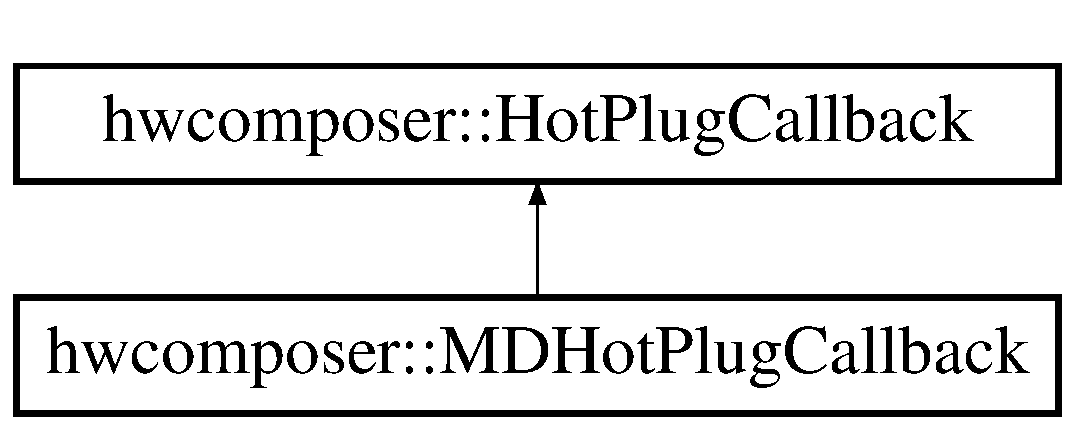
\includegraphics[height=2.000000cm]{classhwcomposer_1_1MDHotPlugCallback}
\end{center}
\end{figure}
\subsection*{Public Member Functions}
\begin{DoxyCompactItemize}
\item 
\mbox{\hyperlink{classhwcomposer_1_1MDHotPlugCallback_a5db491310051345bdf33332da48c581b}{M\+D\+Hot\+Plug\+Callback}} (\mbox{\hyperlink{classhwcomposer_1_1MosaicDisplay}{Mosaic\+Display}} $\ast$display)
\item 
void \mbox{\hyperlink{classhwcomposer_1_1MDHotPlugCallback_a56a4bfc5b98f35a0c27aa97afb119a7a}{Callback}} (uint32\+\_\+t, bool connected)
\end{DoxyCompactItemize}


\subsection{Detailed Description}


Definition at line 54 of file mosaicdisplay.\+cpp.



\subsection{Constructor \& Destructor Documentation}
\mbox{\Hypertarget{classhwcomposer_1_1MDHotPlugCallback_a5db491310051345bdf33332da48c581b}\label{classhwcomposer_1_1MDHotPlugCallback_a5db491310051345bdf33332da48c581b}} 
\index{hwcomposer\+::\+M\+D\+Hot\+Plug\+Callback@{hwcomposer\+::\+M\+D\+Hot\+Plug\+Callback}!M\+D\+Hot\+Plug\+Callback@{M\+D\+Hot\+Plug\+Callback}}
\index{M\+D\+Hot\+Plug\+Callback@{M\+D\+Hot\+Plug\+Callback}!hwcomposer\+::\+M\+D\+Hot\+Plug\+Callback@{hwcomposer\+::\+M\+D\+Hot\+Plug\+Callback}}
\subsubsection{\texorpdfstring{M\+D\+Hot\+Plug\+Callback()}{MDHotPlugCallback()}}
{\footnotesize\ttfamily hwcomposer\+::\+M\+D\+Hot\+Plug\+Callback\+::\+M\+D\+Hot\+Plug\+Callback (\begin{DoxyParamCaption}\item[{\mbox{\hyperlink{classhwcomposer_1_1MosaicDisplay}{Mosaic\+Display}} $\ast$}]{display }\end{DoxyParamCaption})\hspace{0.3cm}{\ttfamily [inline]}}



Definition at line 56 of file mosaicdisplay.\+cpp.


\begin{DoxyCode}{0}
\DoxyCodeLine{56                                             : display\_(display) \{}
\DoxyCodeLine{57   \}}
\end{DoxyCode}


\subsection{Member Function Documentation}
\mbox{\Hypertarget{classhwcomposer_1_1MDHotPlugCallback_a56a4bfc5b98f35a0c27aa97afb119a7a}\label{classhwcomposer_1_1MDHotPlugCallback_a56a4bfc5b98f35a0c27aa97afb119a7a}} 
\index{hwcomposer\+::\+M\+D\+Hot\+Plug\+Callback@{hwcomposer\+::\+M\+D\+Hot\+Plug\+Callback}!Callback@{Callback}}
\index{Callback@{Callback}!hwcomposer\+::\+M\+D\+Hot\+Plug\+Callback@{hwcomposer\+::\+M\+D\+Hot\+Plug\+Callback}}
\subsubsection{\texorpdfstring{Callback()}{Callback()}}
{\footnotesize\ttfamily void hwcomposer\+::\+M\+D\+Hot\+Plug\+Callback\+::\+Callback (\begin{DoxyParamCaption}\item[{uint32\+\_\+t}]{,  }\item[{bool}]{connected }\end{DoxyParamCaption})\hspace{0.3cm}{\ttfamily [inline]}, {\ttfamily [virtual]}}



Implements \mbox{\hyperlink{classhwcomposer_1_1HotPlugCallback_a455c8913e1da9b165134a05c9cb441ba}{hwcomposer\+::\+Hot\+Plug\+Callback}}.



Definition at line 59 of file mosaicdisplay.\+cpp.


\begin{DoxyCode}{0}
\DoxyCodeLine{59                                             \{}
\DoxyCodeLine{60     display\_->\mbox{\hyperlink{classhwcomposer_1_1MosaicDisplay_af529c96ce14e717b11759fa45648ea68}{HotPlugUpdate}}(connected);}
\DoxyCodeLine{61   \}}
\end{DoxyCode}


The documentation for this class was generated from the following file\+:\begin{DoxyCompactItemize}
\item 
common/core/\mbox{\hyperlink{mosaicdisplay_8cpp}{mosaicdisplay.\+cpp}}\end{DoxyCompactItemize}

\hypertarget{classhwcomposer_1_1MDRefreshCallback}{}\section{hwcomposer\+:\+:M\+D\+Refresh\+Callback Class Reference}
\label{classhwcomposer_1_1MDRefreshCallback}\index{hwcomposer\+::\+M\+D\+Refresh\+Callback@{hwcomposer\+::\+M\+D\+Refresh\+Callback}}
Inheritance diagram for hwcomposer\+:\+:M\+D\+Refresh\+Callback\+:\begin{figure}[H]
\begin{center}
\leavevmode
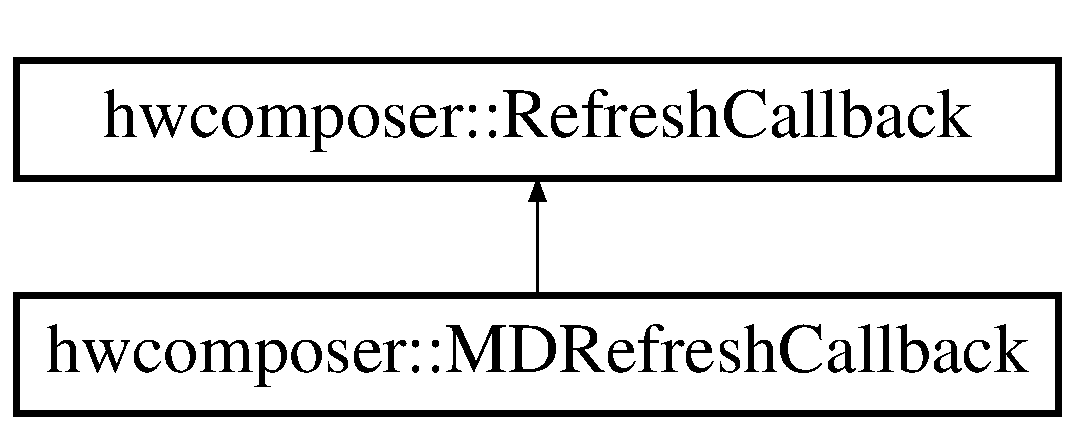
\includegraphics[height=2.000000cm]{classhwcomposer_1_1MDRefreshCallback}
\end{center}
\end{figure}
\subsection*{Public Member Functions}
\begin{DoxyCompactItemize}
\item 
\mbox{\hyperlink{classhwcomposer_1_1MDRefreshCallback_ace557bde20b0df08cadc970bf975acd0}{M\+D\+Refresh\+Callback}} (\mbox{\hyperlink{classhwcomposer_1_1MosaicDisplay}{Mosaic\+Display}} $\ast$display)
\item 
void \mbox{\hyperlink{classhwcomposer_1_1MDRefreshCallback_a398cbe9e48e0b40eb73588d772da6833}{Callback}} (uint32\+\_\+t)
\end{DoxyCompactItemize}


\subsection{Detailed Description}


Definition at line 41 of file mosaicdisplay.\+cpp.



\subsection{Constructor \& Destructor Documentation}
\mbox{\Hypertarget{classhwcomposer_1_1MDRefreshCallback_ace557bde20b0df08cadc970bf975acd0}\label{classhwcomposer_1_1MDRefreshCallback_ace557bde20b0df08cadc970bf975acd0}} 
\index{hwcomposer\+::\+M\+D\+Refresh\+Callback@{hwcomposer\+::\+M\+D\+Refresh\+Callback}!M\+D\+Refresh\+Callback@{M\+D\+Refresh\+Callback}}
\index{M\+D\+Refresh\+Callback@{M\+D\+Refresh\+Callback}!hwcomposer\+::\+M\+D\+Refresh\+Callback@{hwcomposer\+::\+M\+D\+Refresh\+Callback}}
\subsubsection{\texorpdfstring{M\+D\+Refresh\+Callback()}{MDRefreshCallback()}}
{\footnotesize\ttfamily hwcomposer\+::\+M\+D\+Refresh\+Callback\+::\+M\+D\+Refresh\+Callback (\begin{DoxyParamCaption}\item[{\mbox{\hyperlink{classhwcomposer_1_1MosaicDisplay}{Mosaic\+Display}} $\ast$}]{display }\end{DoxyParamCaption})\hspace{0.3cm}{\ttfamily [inline]}}



Definition at line 43 of file mosaicdisplay.\+cpp.


\begin{DoxyCode}{0}
\DoxyCodeLine{43                                             : display\_(display) \{}
\DoxyCodeLine{44   \}}
\end{DoxyCode}


\subsection{Member Function Documentation}
\mbox{\Hypertarget{classhwcomposer_1_1MDRefreshCallback_a398cbe9e48e0b40eb73588d772da6833}\label{classhwcomposer_1_1MDRefreshCallback_a398cbe9e48e0b40eb73588d772da6833}} 
\index{hwcomposer\+::\+M\+D\+Refresh\+Callback@{hwcomposer\+::\+M\+D\+Refresh\+Callback}!Callback@{Callback}}
\index{Callback@{Callback}!hwcomposer\+::\+M\+D\+Refresh\+Callback@{hwcomposer\+::\+M\+D\+Refresh\+Callback}}
\subsubsection{\texorpdfstring{Callback()}{Callback()}}
{\footnotesize\ttfamily void hwcomposer\+::\+M\+D\+Refresh\+Callback\+::\+Callback (\begin{DoxyParamCaption}\item[{uint32\+\_\+t}]{ }\end{DoxyParamCaption})\hspace{0.3cm}{\ttfamily [inline]}, {\ttfamily [virtual]}}



Implements \mbox{\hyperlink{classhwcomposer_1_1RefreshCallback_a5637a4b1437bbf8c93d8356addbf7c87}{hwcomposer\+::\+Refresh\+Callback}}.



Definition at line 46 of file mosaicdisplay.\+cpp.


\begin{DoxyCode}{0}
\DoxyCodeLine{46                             \{}
\DoxyCodeLine{47     display\_->\mbox{\hyperlink{classhwcomposer_1_1MosaicDisplay_aeb0d37462e1584fa329deaea3d7788e3}{RefreshUpdate}}();}
\DoxyCodeLine{48   \}}
\end{DoxyCode}


The documentation for this class was generated from the following file\+:\begin{DoxyCompactItemize}
\item 
common/core/\mbox{\hyperlink{mosaicdisplay_8cpp}{mosaicdisplay.\+cpp}}\end{DoxyCompactItemize}

\hypertarget{classhwcomposer_1_1MDVsyncCallback}{}\section{hwcomposer\+:\+:M\+D\+Vsync\+Callback Class Reference}
\label{classhwcomposer_1_1MDVsyncCallback}\index{hwcomposer\+::\+M\+D\+Vsync\+Callback@{hwcomposer\+::\+M\+D\+Vsync\+Callback}}
Inheritance diagram for hwcomposer\+:\+:M\+D\+Vsync\+Callback\+:\begin{figure}[H]
\begin{center}
\leavevmode
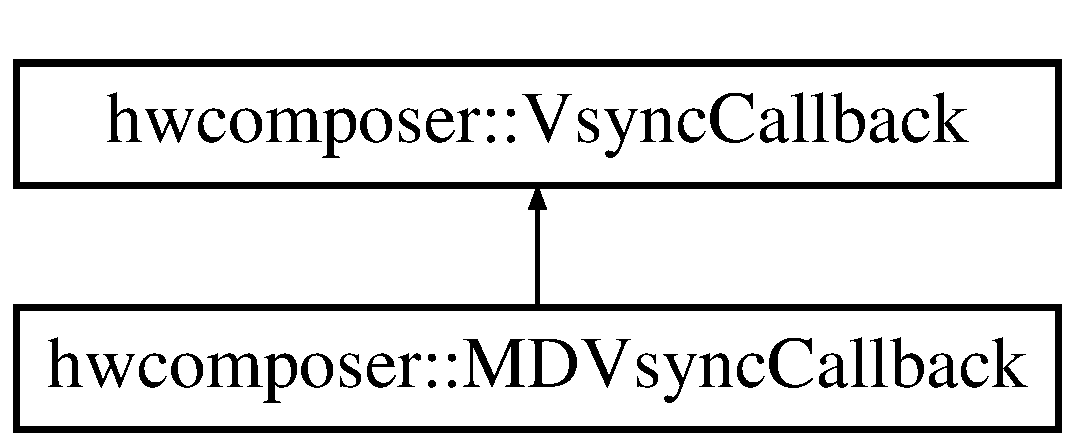
\includegraphics[height=2.000000cm]{classhwcomposer_1_1MDVsyncCallback}
\end{center}
\end{figure}
\subsection*{Public Member Functions}
\begin{DoxyCompactItemize}
\item 
\mbox{\hyperlink{classhwcomposer_1_1MDVsyncCallback_ae05a59bf1001e3b9932ca903f9f6439d}{M\+D\+Vsync\+Callback}} (\mbox{\hyperlink{classhwcomposer_1_1MosaicDisplay}{Mosaic\+Display}} $\ast$display)
\item 
void \mbox{\hyperlink{classhwcomposer_1_1MDVsyncCallback_af9ca73f30e00626c613f23871359f4d8}{Callback}} (uint32\+\_\+t, int64\+\_\+t timestamp)
\end{DoxyCompactItemize}


\subsection{Detailed Description}


Definition at line 28 of file mosaicdisplay.\+cpp.



\subsection{Constructor \& Destructor Documentation}
\mbox{\Hypertarget{classhwcomposer_1_1MDVsyncCallback_ae05a59bf1001e3b9932ca903f9f6439d}\label{classhwcomposer_1_1MDVsyncCallback_ae05a59bf1001e3b9932ca903f9f6439d}} 
\index{hwcomposer\+::\+M\+D\+Vsync\+Callback@{hwcomposer\+::\+M\+D\+Vsync\+Callback}!M\+D\+Vsync\+Callback@{M\+D\+Vsync\+Callback}}
\index{M\+D\+Vsync\+Callback@{M\+D\+Vsync\+Callback}!hwcomposer\+::\+M\+D\+Vsync\+Callback@{hwcomposer\+::\+M\+D\+Vsync\+Callback}}
\subsubsection{\texorpdfstring{M\+D\+Vsync\+Callback()}{MDVsyncCallback()}}
{\footnotesize\ttfamily hwcomposer\+::\+M\+D\+Vsync\+Callback\+::\+M\+D\+Vsync\+Callback (\begin{DoxyParamCaption}\item[{\mbox{\hyperlink{classhwcomposer_1_1MosaicDisplay}{Mosaic\+Display}} $\ast$}]{display }\end{DoxyParamCaption})\hspace{0.3cm}{\ttfamily [inline]}}



Definition at line 30 of file mosaicdisplay.\+cpp.


\begin{DoxyCode}{0}
\DoxyCodeLine{30                                           : display\_(display) \{}
\DoxyCodeLine{31   \}}
\end{DoxyCode}


\subsection{Member Function Documentation}
\mbox{\Hypertarget{classhwcomposer_1_1MDVsyncCallback_af9ca73f30e00626c613f23871359f4d8}\label{classhwcomposer_1_1MDVsyncCallback_af9ca73f30e00626c613f23871359f4d8}} 
\index{hwcomposer\+::\+M\+D\+Vsync\+Callback@{hwcomposer\+::\+M\+D\+Vsync\+Callback}!Callback@{Callback}}
\index{Callback@{Callback}!hwcomposer\+::\+M\+D\+Vsync\+Callback@{hwcomposer\+::\+M\+D\+Vsync\+Callback}}
\subsubsection{\texorpdfstring{Callback()}{Callback()}}
{\footnotesize\ttfamily void hwcomposer\+::\+M\+D\+Vsync\+Callback\+::\+Callback (\begin{DoxyParamCaption}\item[{uint32\+\_\+t}]{,  }\item[{int64\+\_\+t}]{timestamp }\end{DoxyParamCaption})\hspace{0.3cm}{\ttfamily [inline]}, {\ttfamily [virtual]}}



Implements \mbox{\hyperlink{classhwcomposer_1_1VsyncCallback_a632ac6a2e13e1b387df9508507a2ed4d}{hwcomposer\+::\+Vsync\+Callback}}.



Definition at line 33 of file mosaicdisplay.\+cpp.


\begin{DoxyCode}{0}
\DoxyCodeLine{33                                                \{}
\DoxyCodeLine{34     display\_->\mbox{\hyperlink{classhwcomposer_1_1MosaicDisplay_ab2d47bd2c1eac196990bb8d7c2f1ecd7}{VSyncUpdate}}(timestamp);}
\DoxyCodeLine{35   \}}
\end{DoxyCode}


The documentation for this class was generated from the following file\+:\begin{DoxyCompactItemize}
\item 
common/core/\mbox{\hyperlink{mosaicdisplay_8cpp}{mosaicdisplay.\+cpp}}\end{DoxyCompactItemize}

\hypertarget{structhwcomposer_1_1media__import}{}\section{hwcomposer\+:\+:media\+\_\+import Struct Reference}
\label{structhwcomposer_1_1media__import}\index{hwcomposer\+::media\+\_\+import@{hwcomposer\+::media\+\_\+import}}


{\ttfamily \#include $<$compositordefs.\+h$>$}

\subsection*{Public Attributes}
\begin{DoxyCompactItemize}
\item 
V\+A\+Surface\+ID \mbox{\hyperlink{structhwcomposer_1_1media__import_af82420941f64a848639e0ac80a7b2861}{surface\+\_\+}} = V\+A\+\_\+\+I\+N\+V\+A\+L\+I\+D\+\_\+\+ID
\item 
\mbox{\hyperlink{alios_2platformdefines_8h_ac0a2eaf260f556d17fe489911f017bdf}{H\+W\+C\+Native\+Handle}} \mbox{\hyperlink{structhwcomposer_1_1media__import_ab43515fb27f0e91598d906ae81acb6cd}{handle\+\_\+}} = 0
\item 
uint32\+\_\+t \mbox{\hyperlink{structhwcomposer_1_1media__import_add4939656c584a9b2f25e38eb845602f}{drm\+\_\+fd\+\_\+}} = 0
\end{DoxyCompactItemize}


\subsection{Detailed Description}


Definition at line 84 of file compositordefs.\+h.



\subsection{Member Data Documentation}
\mbox{\Hypertarget{structhwcomposer_1_1media__import_add4939656c584a9b2f25e38eb845602f}\label{structhwcomposer_1_1media__import_add4939656c584a9b2f25e38eb845602f}} 
\index{hwcomposer\+::media\+\_\+import@{hwcomposer\+::media\+\_\+import}!drm\+\_\+fd\+\_\+@{drm\+\_\+fd\+\_\+}}
\index{drm\+\_\+fd\+\_\+@{drm\+\_\+fd\+\_\+}!hwcomposer\+::media\+\_\+import@{hwcomposer\+::media\+\_\+import}}
\subsubsection{\texorpdfstring{drm\+\_\+fd\+\_\+}{drm\_fd\_}}
{\footnotesize\ttfamily uint32\+\_\+t hwcomposer\+::media\+\_\+import\+::drm\+\_\+fd\+\_\+ = 0}



Definition at line 89 of file compositordefs.\+h.

\mbox{\Hypertarget{structhwcomposer_1_1media__import_ab43515fb27f0e91598d906ae81acb6cd}\label{structhwcomposer_1_1media__import_ab43515fb27f0e91598d906ae81acb6cd}} 
\index{hwcomposer\+::media\+\_\+import@{hwcomposer\+::media\+\_\+import}!handle\+\_\+@{handle\+\_\+}}
\index{handle\+\_\+@{handle\+\_\+}!hwcomposer\+::media\+\_\+import@{hwcomposer\+::media\+\_\+import}}
\subsubsection{\texorpdfstring{handle\+\_\+}{handle\_}}
{\footnotesize\ttfamily \mbox{\hyperlink{alios_2platformdefines_8h_ac0a2eaf260f556d17fe489911f017bdf}{H\+W\+C\+Native\+Handle}} hwcomposer\+::media\+\_\+import\+::handle\+\_\+ = 0}



Definition at line 88 of file compositordefs.\+h.

\mbox{\Hypertarget{structhwcomposer_1_1media__import_af82420941f64a848639e0ac80a7b2861}\label{structhwcomposer_1_1media__import_af82420941f64a848639e0ac80a7b2861}} 
\index{hwcomposer\+::media\+\_\+import@{hwcomposer\+::media\+\_\+import}!surface\+\_\+@{surface\+\_\+}}
\index{surface\+\_\+@{surface\+\_\+}!hwcomposer\+::media\+\_\+import@{hwcomposer\+::media\+\_\+import}}
\subsubsection{\texorpdfstring{surface\+\_\+}{surface\_}}
{\footnotesize\ttfamily V\+A\+Surface\+ID hwcomposer\+::media\+\_\+import\+::surface\+\_\+ = V\+A\+\_\+\+I\+N\+V\+A\+L\+I\+D\+\_\+\+ID}



Definition at line 86 of file compositordefs.\+h.



The documentation for this struct was generated from the following file\+:\begin{DoxyCompactItemize}
\item 
common/compositor/\mbox{\hyperlink{compositordefs_8h}{compositordefs.\+h}}\end{DoxyCompactItemize}

\hypertarget{structhwcomposer_1_1MediaState}{}\section{hwcomposer\+:\+:Media\+State Struct Reference}
\label{structhwcomposer_1_1MediaState}\index{hwcomposer\+::\+Media\+State@{hwcomposer\+::\+Media\+State}}


{\ttfamily \#include $<$renderstate.\+h$>$}

\subsection*{Public Attributes}
\begin{DoxyCompactItemize}
\item 
const \mbox{\hyperlink{structhwcomposer_1_1OverlayLayer}{Overlay\+Layer}} $\ast$ \mbox{\hyperlink{structhwcomposer_1_1MediaState_a43e040e443a44a8c5ac653f49be17dca}{layer\+\_\+}}
\item 
H\+W\+C\+Color\+Map \mbox{\hyperlink{structhwcomposer_1_1MediaState_a63b705c25506563ee4b6fdde3f4b5817}{colors\+\_\+}}
\item 
H\+W\+C\+Deinterlace\+Prop \mbox{\hyperlink{structhwcomposer_1_1MediaState_a9326ae6dea06def21b8aba4bb4500002}{deinterlace\+\_\+}}
\item 
uint32\+\_\+t \mbox{\hyperlink{structhwcomposer_1_1MediaState_addeecd9addfdd71066eac26d6ef270c3}{scaling\+\_\+mode\+\_\+}}
\end{DoxyCompactItemize}


\subsection{Detailed Description}


Definition at line 62 of file renderstate.\+h.



\subsection{Member Data Documentation}
\mbox{\Hypertarget{structhwcomposer_1_1MediaState_a63b705c25506563ee4b6fdde3f4b5817}\label{structhwcomposer_1_1MediaState_a63b705c25506563ee4b6fdde3f4b5817}} 
\index{hwcomposer\+::\+Media\+State@{hwcomposer\+::\+Media\+State}!colors\+\_\+@{colors\+\_\+}}
\index{colors\+\_\+@{colors\+\_\+}!hwcomposer\+::\+Media\+State@{hwcomposer\+::\+Media\+State}}
\subsubsection{\texorpdfstring{colors\+\_\+}{colors\_}}
{\footnotesize\ttfamily H\+W\+C\+Color\+Map hwcomposer\+::\+Media\+State\+::colors\+\_\+}



Definition at line 64 of file renderstate.\+h.

\mbox{\Hypertarget{structhwcomposer_1_1MediaState_a9326ae6dea06def21b8aba4bb4500002}\label{structhwcomposer_1_1MediaState_a9326ae6dea06def21b8aba4bb4500002}} 
\index{hwcomposer\+::\+Media\+State@{hwcomposer\+::\+Media\+State}!deinterlace\+\_\+@{deinterlace\+\_\+}}
\index{deinterlace\+\_\+@{deinterlace\+\_\+}!hwcomposer\+::\+Media\+State@{hwcomposer\+::\+Media\+State}}
\subsubsection{\texorpdfstring{deinterlace\+\_\+}{deinterlace\_}}
{\footnotesize\ttfamily H\+W\+C\+Deinterlace\+Prop hwcomposer\+::\+Media\+State\+::deinterlace\+\_\+}



Definition at line 65 of file renderstate.\+h.

\mbox{\Hypertarget{structhwcomposer_1_1MediaState_a43e040e443a44a8c5ac653f49be17dca}\label{structhwcomposer_1_1MediaState_a43e040e443a44a8c5ac653f49be17dca}} 
\index{hwcomposer\+::\+Media\+State@{hwcomposer\+::\+Media\+State}!layer\+\_\+@{layer\+\_\+}}
\index{layer\+\_\+@{layer\+\_\+}!hwcomposer\+::\+Media\+State@{hwcomposer\+::\+Media\+State}}
\subsubsection{\texorpdfstring{layer\+\_\+}{layer\_}}
{\footnotesize\ttfamily const \mbox{\hyperlink{structhwcomposer_1_1OverlayLayer}{Overlay\+Layer}}$\ast$ hwcomposer\+::\+Media\+State\+::layer\+\_\+}



Definition at line 63 of file renderstate.\+h.

\mbox{\Hypertarget{structhwcomposer_1_1MediaState_addeecd9addfdd71066eac26d6ef270c3}\label{structhwcomposer_1_1MediaState_addeecd9addfdd71066eac26d6ef270c3}} 
\index{hwcomposer\+::\+Media\+State@{hwcomposer\+::\+Media\+State}!scaling\+\_\+mode\+\_\+@{scaling\+\_\+mode\+\_\+}}
\index{scaling\+\_\+mode\+\_\+@{scaling\+\_\+mode\+\_\+}!hwcomposer\+::\+Media\+State@{hwcomposer\+::\+Media\+State}}
\subsubsection{\texorpdfstring{scaling\+\_\+mode\+\_\+}{scaling\_mode\_}}
{\footnotesize\ttfamily uint32\+\_\+t hwcomposer\+::\+Media\+State\+::scaling\+\_\+mode\+\_\+}



Definition at line 66 of file renderstate.\+h.



The documentation for this struct was generated from the following file\+:\begin{DoxyCompactItemize}
\item 
common/compositor/\mbox{\hyperlink{renderstate_8h}{renderstate.\+h}}\end{DoxyCompactItemize}

\hypertarget{classhwcomposer_1_1MosaicDisplay}{}\section{hwcomposer\+:\+:Mosaic\+Display Class Reference}
\label{classhwcomposer_1_1MosaicDisplay}\index{hwcomposer\+::\+Mosaic\+Display@{hwcomposer\+::\+Mosaic\+Display}}


{\ttfamily \#include $<$mosaicdisplay.\+h$>$}

Inheritance diagram for hwcomposer\+:\+:Mosaic\+Display\+:\begin{figure}[H]
\begin{center}
\leavevmode
\includegraphics[height=2.000000cm]{classhwcomposer_1_1MosaicDisplay}
\end{center}
\end{figure}
\subsection*{Public Member Functions}
\begin{DoxyCompactItemize}
\item 
\mbox{\hyperlink{classhwcomposer_1_1MosaicDisplay_a55b36338b1f718942c94d309b3ee7138}{Mosaic\+Display}} (const std\+::vector$<$ \mbox{\hyperlink{classhwcomposer_1_1NativeDisplay}{Native\+Display}} $\ast$$>$ \&displays)
\item 
\mbox{\hyperlink{classhwcomposer_1_1MosaicDisplay_ab5d5f4afacab634238ec516723e6238a}{$\sim$\+Mosaic\+Display}} () override
\item 
bool \mbox{\hyperlink{classhwcomposer_1_1MosaicDisplay_a31b15aba0948d8e1c65f12f2d79f1ecf}{Initialize}} (\mbox{\hyperlink{classhwcomposer_1_1NativeBufferHandler}{Native\+Buffer\+Handler}} $\ast$buffer\+\_\+handler, \mbox{\hyperlink{classhwcomposer_1_1FrameBufferManager}{Frame\+Buffer\+Manager}} $\ast$) override
\item 
Display\+Type \mbox{\hyperlink{classhwcomposer_1_1MosaicDisplay_a7c5288febea28948c2689d7f6feee183}{Type}} () const override
\item 
uint32\+\_\+t \mbox{\hyperlink{classhwcomposer_1_1MosaicDisplay_a5123a951bd40adef34cbe1e11d0a8e69}{Width}} () const override
\item 
uint32\+\_\+t \mbox{\hyperlink{classhwcomposer_1_1MosaicDisplay_af15fda20d779888c521095542b505f9d}{Height}} () const override
\item 
uint32\+\_\+t \mbox{\hyperlink{classhwcomposer_1_1MosaicDisplay_a41e94410e4e73ee057ef672bb51aba65}{Power\+Mode}} () const override
\item 
int \mbox{\hyperlink{classhwcomposer_1_1MosaicDisplay_aab767066611a255bc84d50c4b53b3d5d}{Get\+Display\+Pipe}} () override
\item 
bool \mbox{\hyperlink{classhwcomposer_1_1MosaicDisplay_aaff4528ff2c22a7ec8ce8ab1bc8cbe07}{Set\+Active\+Config}} (uint32\+\_\+t config) override
\item 
bool \mbox{\hyperlink{classhwcomposer_1_1MosaicDisplay_a6283bdb8c3f0ababbb224d71726f4d2c}{Get\+Active\+Config}} (uint32\+\_\+t $\ast$config) override
\item 
bool \mbox{\hyperlink{classhwcomposer_1_1MosaicDisplay_a001b4f2775a2a50d380ff6eb33ba3683}{Set\+Power\+Mode}} (uint32\+\_\+t power\+\_\+mode) override
\item 
bool \mbox{\hyperlink{classhwcomposer_1_1MosaicDisplay_a84e8ddade543bca6659a1eb7bfe72bcd}{Present}} (std\+::vector$<$ \mbox{\hyperlink{structhwcomposer_1_1HwcLayer}{Hwc\+Layer}} $\ast$$>$ \&source\+\_\+layers, int32\+\_\+t $\ast$retire\+\_\+fence, \mbox{\hyperlink{classhwcomposer_1_1PixelUploaderCallback}{Pixel\+Uploader\+Callback}} $\ast$call\+\_\+back=\mbox{\hyperlink{alios_2platformdefines_8h_a070d2ce7b6bb7e5c05602aa8c308d0c4}{N\+U\+LL}}, bool handle\+\_\+constraints=false) override
\item 
int \mbox{\hyperlink{classhwcomposer_1_1MosaicDisplay_ab95984da914029b9dd2c5fb728926dbc}{Register\+Vsync\+Callback}} (std\+::shared\+\_\+ptr$<$ \mbox{\hyperlink{classhwcomposer_1_1VsyncCallback}{Vsync\+Callback}} $>$ callback, uint32\+\_\+t display\+\_\+id) override
\item 
void \mbox{\hyperlink{classhwcomposer_1_1MosaicDisplay_a1deecbf2ba9b007fa7529b31da47d575}{Register\+Refresh\+Callback}} (std\+::shared\+\_\+ptr$<$ \mbox{\hyperlink{classhwcomposer_1_1RefreshCallback}{Refresh\+Callback}} $>$ callback, uint32\+\_\+t display\+\_\+id) override
\item 
void \mbox{\hyperlink{classhwcomposer_1_1MosaicDisplay_a1d4f419cda4d1729dfb085f385a76afb}{Register\+Hot\+Plug\+Callback}} (std\+::shared\+\_\+ptr$<$ \mbox{\hyperlink{classhwcomposer_1_1HotPlugCallback}{Hot\+Plug\+Callback}} $>$ callback, uint32\+\_\+t display\+\_\+id) override
\item 
void \mbox{\hyperlink{classhwcomposer_1_1MosaicDisplay_a3843cd0fcbd50cfed44d7a0ebdf5539b}{V\+Sync\+Control}} (bool enabled) override
\item 
bool \mbox{\hyperlink{classhwcomposer_1_1MosaicDisplay_a8978685de8d614113e49b3b774c9b723}{Check\+Plane\+Format}} (uint32\+\_\+t format) override
\item 
void \mbox{\hyperlink{classhwcomposer_1_1MosaicDisplay_a99609427012ce9c2e3b4e16ed13211a3}{Set\+Gamma}} (float red, float green, float blue) override
\item 
void \mbox{\hyperlink{classhwcomposer_1_1MosaicDisplay_a6942a0aa562c459a89b014aa15fdcccd}{Set\+Contrast}} (uint32\+\_\+t red, uint32\+\_\+t green, uint32\+\_\+t blue) override
\item 
void \mbox{\hyperlink{classhwcomposer_1_1MosaicDisplay_a113c244569faf509d03062f794216981}{Set\+Brightness}} (uint32\+\_\+t red, uint32\+\_\+t green, uint32\+\_\+t blue) override
\item 
void \mbox{\hyperlink{classhwcomposer_1_1MosaicDisplay_af9053256b801c0334bd89ed7b5e97912}{Set\+Explicit\+Sync\+Support}} (bool disable\+\_\+explicit\+\_\+sync) override
\item 
void \mbox{\hyperlink{classhwcomposer_1_1MosaicDisplay_ac634db4100aa1707f28ff2bbb77b8460}{Set\+Video\+Scaling\+Mode}} (uint32\+\_\+t mode) override
\item 
void \mbox{\hyperlink{classhwcomposer_1_1MosaicDisplay_adba98086d56d0ccc2df7a57a87ddd4b0}{Set\+Video\+Color}} (H\+W\+C\+Color\+Control color, float value) override
\item 
void \mbox{\hyperlink{classhwcomposer_1_1MosaicDisplay_ab4b88eb3a5d9a811dada73b0f8d33c4d}{Get\+Video\+Color}} (H\+W\+C\+Color\+Control color, float $\ast$value, float $\ast$start, float $\ast$end) override
\item 
void \mbox{\hyperlink{classhwcomposer_1_1MosaicDisplay_aaf2a3e4f69753b92366c23434db3d133}{Restore\+Video\+Default\+Color}} (H\+W\+C\+Color\+Control color) override
\item 
void \mbox{\hyperlink{classhwcomposer_1_1MosaicDisplay_a28167d8f866c8b2c6ea01b42b442eb0f}{Set\+Video\+Deinterlace}} (H\+W\+C\+Deinterlace\+Flag flag, H\+W\+C\+Deinterlace\+Control mode) override
\item 
void \mbox{\hyperlink{classhwcomposer_1_1MosaicDisplay_a907f7b2e5c59a27e5335f8cfadba87f5}{Restore\+Video\+Default\+Deinterlace}} () override
\item 
bool \mbox{\hyperlink{classhwcomposer_1_1MosaicDisplay_a837d28f710438d462fd88b85721528b0}{Is\+Connected}} () const override
\item 
void \mbox{\hyperlink{classhwcomposer_1_1MosaicDisplay_aa0d5befb882537555f4476130863c27c}{Update\+Scaling\+Ratio}} (uint32\+\_\+t primary\+\_\+width, uint32\+\_\+t primary\+\_\+height, uint32\+\_\+t display\+\_\+width, uint32\+\_\+t display\+\_\+height) override
\item 
void \mbox{\hyperlink{classhwcomposer_1_1MosaicDisplay_a7944dd71d1efa68e0f94f68cc1bd30b2}{Clone\+Display}} (\mbox{\hyperlink{classhwcomposer_1_1NativeDisplay}{Native\+Display}} $\ast$source\+\_\+display) override
\item 
bool \mbox{\hyperlink{classhwcomposer_1_1MosaicDisplay_a989d240e0d3287ec2b9e6cfbe1041bda}{Present\+Clone}} (\mbox{\hyperlink{classhwcomposer_1_1NativeDisplay}{Native\+Display}} $\ast$) override
\item 
bool \mbox{\hyperlink{classhwcomposer_1_1MosaicDisplay_a7a03738eb7862a1b2e1585fbd80e710c}{Get\+Display\+Attribute}} (uint32\+\_\+t, H\+W\+C\+Display\+Attribute attribute, int32\+\_\+t $\ast$value) override
\item 
bool \mbox{\hyperlink{classhwcomposer_1_1MosaicDisplay_a18bc1bc98ff2814c710ee1202f868217}{Get\+Display\+Configs}} (uint32\+\_\+t $\ast$num\+\_\+configs, uint32\+\_\+t $\ast$configs) override
\item 
bool \mbox{\hyperlink{classhwcomposer_1_1MosaicDisplay_ac76216611bf8bebcf182a1c18b3d0c04}{Get\+Display\+Name}} (uint32\+\_\+t $\ast$size, char $\ast$name) override
\item 
uint32\+\_\+t \mbox{\hyperlink{classhwcomposer_1_1MosaicDisplay_a8f006e53e5d0e8c6caf8ac50f25ab407}{Get\+X\+Translation}} () override
\item 
bool \mbox{\hyperlink{classhwcomposer_1_1MosaicDisplay_a9a53f36574c2ed39f589413721b0fafa}{Enable\+V\+Sync}} () const
\item 
void \mbox{\hyperlink{classhwcomposer_1_1MosaicDisplay_ab2d47bd2c1eac196990bb8d7c2f1ecd7}{V\+Sync\+Update}} (int64\+\_\+t timestamp)
\item 
void \mbox{\hyperlink{classhwcomposer_1_1MosaicDisplay_aeb0d37462e1584fa329deaea3d7788e3}{Refresh\+Update}} ()
\item 
void \mbox{\hyperlink{classhwcomposer_1_1MosaicDisplay_af529c96ce14e717b11759fa45648ea68}{Hot\+Plug\+Update}} (bool connected)
\item 
void \mbox{\hyperlink{classhwcomposer_1_1MosaicDisplay_a406e652e251f8f88ef628704a1e57b1f}{Set\+H\+D\+C\+P\+State}} (H\+W\+C\+Content\+Protection state, H\+W\+C\+Content\+Type content\+\_\+type) override
\end{DoxyCompactItemize}
\subsection*{Additional Inherited Members}


\subsection{Detailed Description}


Definition at line 30 of file mosaicdisplay.\+h.



\subsection{Constructor \& Destructor Documentation}
\mbox{\Hypertarget{classhwcomposer_1_1MosaicDisplay_a55b36338b1f718942c94d309b3ee7138}\label{classhwcomposer_1_1MosaicDisplay_a55b36338b1f718942c94d309b3ee7138}} 
\index{hwcomposer\+::\+Mosaic\+Display@{hwcomposer\+::\+Mosaic\+Display}!Mosaic\+Display@{Mosaic\+Display}}
\index{Mosaic\+Display@{Mosaic\+Display}!hwcomposer\+::\+Mosaic\+Display@{hwcomposer\+::\+Mosaic\+Display}}
\subsubsection{\texorpdfstring{Mosaic\+Display()}{MosaicDisplay()}}
{\footnotesize\ttfamily hwcomposer\+::\+Mosaic\+Display\+::\+Mosaic\+Display (\begin{DoxyParamCaption}\item[{const std\+::vector$<$ \mbox{\hyperlink{classhwcomposer_1_1NativeDisplay}{Native\+Display}} $\ast$$>$ \&}]{displays }\end{DoxyParamCaption})}



Definition at line 67 of file mosaicdisplay.\+cpp.


\begin{DoxyCode}{0}
\DoxyCodeLine{68     : dpix\_(0), dpiy\_(0) \{}
\DoxyCodeLine{69   uint32\_t size = displays.size();}
\DoxyCodeLine{70   physical\_displays\_.reserve(size);}
\DoxyCodeLine{71   \textcolor{keywordflow}{for} (uint32\_t i = 0; i < size; i++) \{}
\DoxyCodeLine{72     physical\_displays\_.emplace\_back(displays.at(i));}
\DoxyCodeLine{73   \}}
\DoxyCodeLine{74 \}}
\end{DoxyCode}
\mbox{\Hypertarget{classhwcomposer_1_1MosaicDisplay_ab5d5f4afacab634238ec516723e6238a}\label{classhwcomposer_1_1MosaicDisplay_ab5d5f4afacab634238ec516723e6238a}} 
\index{hwcomposer\+::\+Mosaic\+Display@{hwcomposer\+::\+Mosaic\+Display}!````~Mosaic\+Display@{$\sim$\+Mosaic\+Display}}
\index{````~Mosaic\+Display@{$\sim$\+Mosaic\+Display}!hwcomposer\+::\+Mosaic\+Display@{hwcomposer\+::\+Mosaic\+Display}}
\subsubsection{\texorpdfstring{$\sim$\+Mosaic\+Display()}{~MosaicDisplay()}}
{\footnotesize\ttfamily hwcomposer\+::\+Mosaic\+Display\+::$\sim$\+Mosaic\+Display (\begin{DoxyParamCaption}{ }\end{DoxyParamCaption})\hspace{0.3cm}{\ttfamily [override]}}



Definition at line 76 of file mosaicdisplay.\+cpp.


\begin{DoxyCode}{0}
\DoxyCodeLine{76                               \{}
\DoxyCodeLine{77 \}}
\end{DoxyCode}


\subsection{Member Function Documentation}
\mbox{\Hypertarget{classhwcomposer_1_1MosaicDisplay_a8978685de8d614113e49b3b774c9b723}\label{classhwcomposer_1_1MosaicDisplay_a8978685de8d614113e49b3b774c9b723}} 
\index{hwcomposer\+::\+Mosaic\+Display@{hwcomposer\+::\+Mosaic\+Display}!Check\+Plane\+Format@{Check\+Plane\+Format}}
\index{Check\+Plane\+Format@{Check\+Plane\+Format}!hwcomposer\+::\+Mosaic\+Display@{hwcomposer\+::\+Mosaic\+Display}}
\subsubsection{\texorpdfstring{Check\+Plane\+Format()}{CheckPlaneFormat()}}
{\footnotesize\ttfamily bool hwcomposer\+::\+Mosaic\+Display\+::\+Check\+Plane\+Format (\begin{DoxyParamCaption}\item[{uint32\+\_\+t}]{format }\end{DoxyParamCaption})\hspace{0.3cm}{\ttfamily [override]}, {\ttfamily [virtual]}}

A\+PI to check the format support on the device 
\begin{DoxyParams}{Parameters}
{\em format} & valid D\+RM formats found in drm\+\_\+fourcc.\+h. \\
\hline
\end{DoxyParams}


Implements \mbox{\hyperlink{classhwcomposer_1_1NativeDisplay_a4e856b5754054bdf77467e6663cb5b50}{hwcomposer\+::\+Native\+Display}}.



Definition at line 373 of file mosaicdisplay.\+cpp.


\begin{DoxyCode}{0}
\DoxyCodeLine{373                                                     \{}
\DoxyCodeLine{374   \textcolor{keywordflow}{return} physical\_displays\_.at(0)->CheckPlaneFormat(format);}
\DoxyCodeLine{375 \}}
\end{DoxyCode}
\mbox{\Hypertarget{classhwcomposer_1_1MosaicDisplay_a7944dd71d1efa68e0f94f68cc1bd30b2}\label{classhwcomposer_1_1MosaicDisplay_a7944dd71d1efa68e0f94f68cc1bd30b2}} 
\index{hwcomposer\+::\+Mosaic\+Display@{hwcomposer\+::\+Mosaic\+Display}!Clone\+Display@{Clone\+Display}}
\index{Clone\+Display@{Clone\+Display}!hwcomposer\+::\+Mosaic\+Display@{hwcomposer\+::\+Mosaic\+Display}}
\subsubsection{\texorpdfstring{Clone\+Display()}{CloneDisplay()}}
{\footnotesize\ttfamily void hwcomposer\+::\+Mosaic\+Display\+::\+Clone\+Display (\begin{DoxyParamCaption}\item[{\mbox{\hyperlink{classhwcomposer_1_1NativeDisplay}{Native\+Display}} $\ast$}]{ }\end{DoxyParamCaption})\hspace{0.3cm}{\ttfamily [override]}, {\ttfamily [virtual]}}

This display needs to clone source\+\_\+display. We cannot have a display in cloned mode and extended mode at same time or clone more than one source\+\_\+display at same time. 

Reimplemented from \mbox{\hyperlink{classhwcomposer_1_1NativeDisplay_ad244fa57c9c6380fb04bfd57da3cb28b}{hwcomposer\+::\+Native\+Display}}.



Definition at line 452 of file mosaicdisplay.\+cpp.


\begin{DoxyCode}{0}
\DoxyCodeLine{452                                                   \{}
\DoxyCodeLine{453 \}}
\end{DoxyCode}
\mbox{\Hypertarget{classhwcomposer_1_1MosaicDisplay_a9a53f36574c2ed39f589413721b0fafa}\label{classhwcomposer_1_1MosaicDisplay_a9a53f36574c2ed39f589413721b0fafa}} 
\index{hwcomposer\+::\+Mosaic\+Display@{hwcomposer\+::\+Mosaic\+Display}!Enable\+V\+Sync@{Enable\+V\+Sync}}
\index{Enable\+V\+Sync@{Enable\+V\+Sync}!hwcomposer\+::\+Mosaic\+Display@{hwcomposer\+::\+Mosaic\+Display}}
\subsubsection{\texorpdfstring{Enable\+V\+Sync()}{EnableVSync()}}
{\footnotesize\ttfamily bool hwcomposer\+::\+Mosaic\+Display\+::\+Enable\+V\+Sync (\begin{DoxyParamCaption}{ }\end{DoxyParamCaption}) const\hspace{0.3cm}{\ttfamily [inline]}}



Definition at line 102 of file mosaicdisplay.\+h.


\begin{DoxyCode}{0}
\DoxyCodeLine{102                            \{}
\DoxyCodeLine{103     \textcolor{keywordflow}{return} enable\_vsync\_;}
\DoxyCodeLine{104   \}}
\end{DoxyCode}
\mbox{\Hypertarget{classhwcomposer_1_1MosaicDisplay_a6283bdb8c3f0ababbb224d71726f4d2c}\label{classhwcomposer_1_1MosaicDisplay_a6283bdb8c3f0ababbb224d71726f4d2c}} 
\index{hwcomposer\+::\+Mosaic\+Display@{hwcomposer\+::\+Mosaic\+Display}!Get\+Active\+Config@{Get\+Active\+Config}}
\index{Get\+Active\+Config@{Get\+Active\+Config}!hwcomposer\+::\+Mosaic\+Display@{hwcomposer\+::\+Mosaic\+Display}}
\subsubsection{\texorpdfstring{Get\+Active\+Config()}{GetActiveConfig()}}
{\footnotesize\ttfamily bool hwcomposer\+::\+Mosaic\+Display\+::\+Get\+Active\+Config (\begin{DoxyParamCaption}\item[{uint32\+\_\+t $\ast$}]{config }\end{DoxyParamCaption})\hspace{0.3cm}{\ttfamily [override]}, {\ttfamily [virtual]}}



Implements \mbox{\hyperlink{classhwcomposer_1_1NativeDisplay_a9d4d9d2f6633fe37025210cac6e8cc6c}{hwcomposer\+::\+Native\+Display}}.



Definition at line 154 of file mosaicdisplay.\+cpp.


\begin{DoxyCode}{0}
\DoxyCodeLine{154                                                     \{}
\DoxyCodeLine{155   \textcolor{keywordflow}{if} (!config)}
\DoxyCodeLine{156     \textcolor{keywordflow}{return} \textcolor{keyword}{false};}
\DoxyCodeLine{157 }
\DoxyCodeLine{158   *config = config\_;}
\DoxyCodeLine{159   \textcolor{keywordflow}{return} \textcolor{keyword}{true};}
\DoxyCodeLine{160 \}}
\end{DoxyCode}
\mbox{\Hypertarget{classhwcomposer_1_1MosaicDisplay_a7a03738eb7862a1b2e1585fbd80e710c}\label{classhwcomposer_1_1MosaicDisplay_a7a03738eb7862a1b2e1585fbd80e710c}} 
\index{hwcomposer\+::\+Mosaic\+Display@{hwcomposer\+::\+Mosaic\+Display}!Get\+Display\+Attribute@{Get\+Display\+Attribute}}
\index{Get\+Display\+Attribute@{Get\+Display\+Attribute}!hwcomposer\+::\+Mosaic\+Display@{hwcomposer\+::\+Mosaic\+Display}}
\subsubsection{\texorpdfstring{Get\+Display\+Attribute()}{GetDisplayAttribute()}}
{\footnotesize\ttfamily bool hwcomposer\+::\+Mosaic\+Display\+::\+Get\+Display\+Attribute (\begin{DoxyParamCaption}\item[{uint32\+\_\+t}]{,  }\item[{H\+W\+C\+Display\+Attribute}]{attribute,  }\item[{int32\+\_\+t $\ast$}]{value }\end{DoxyParamCaption})\hspace{0.3cm}{\ttfamily [override]}, {\ttfamily [virtual]}}



Implements \mbox{\hyperlink{classhwcomposer_1_1NativeDisplay_aeb880e4a295eab49a98804380c2dcb84}{hwcomposer\+::\+Native\+Display}}.



Definition at line 455 of file mosaicdisplay.\+cpp.


\begin{DoxyCode}{0}
\DoxyCodeLine{457                                                         \{}
\DoxyCodeLine{458   \textcolor{keywordtype}{bool} status = \textcolor{keyword}{true};}
\DoxyCodeLine{459   \textcolor{keywordflow}{switch} (attribute) \{}
\DoxyCodeLine{460     \textcolor{keywordflow}{case} HWCDisplayAttribute::kWidth:}
\DoxyCodeLine{461       *value = width\_;}
\DoxyCodeLine{462       \textcolor{keywordflow}{break};}
\DoxyCodeLine{463     \textcolor{keywordflow}{case} HWCDisplayAttribute::kHeight:}
\DoxyCodeLine{464       *value = height\_;}
\DoxyCodeLine{465       \textcolor{keywordflow}{break};}
\DoxyCodeLine{466     \textcolor{keywordflow}{case} HWCDisplayAttribute::kRefreshRate:}
\DoxyCodeLine{467       *value = refresh\_;}
\DoxyCodeLine{468       \textcolor{keywordflow}{break};}
\DoxyCodeLine{469     \textcolor{keywordflow}{case} HWCDisplayAttribute::kDpiX:}
\DoxyCodeLine{470       *value = dpix\_;}
\DoxyCodeLine{471       \textcolor{keywordflow}{break};}
\DoxyCodeLine{472     \textcolor{keywordflow}{case} HWCDisplayAttribute::kDpiY:}
\DoxyCodeLine{473       *value = dpiy\_;}
\DoxyCodeLine{474       \textcolor{keywordflow}{break};}
\DoxyCodeLine{475     \textcolor{keywordflow}{default}:}
\DoxyCodeLine{476       *value = -1;}
\DoxyCodeLine{477       status = \textcolor{keyword}{false};}
\DoxyCodeLine{478   \}}
\DoxyCodeLine{479 }
\DoxyCodeLine{480   \textcolor{keywordflow}{return} status;}
\DoxyCodeLine{481 \}}
\end{DoxyCode}
\mbox{\Hypertarget{classhwcomposer_1_1MosaicDisplay_a18bc1bc98ff2814c710ee1202f868217}\label{classhwcomposer_1_1MosaicDisplay_a18bc1bc98ff2814c710ee1202f868217}} 
\index{hwcomposer\+::\+Mosaic\+Display@{hwcomposer\+::\+Mosaic\+Display}!Get\+Display\+Configs@{Get\+Display\+Configs}}
\index{Get\+Display\+Configs@{Get\+Display\+Configs}!hwcomposer\+::\+Mosaic\+Display@{hwcomposer\+::\+Mosaic\+Display}}
\subsubsection{\texorpdfstring{Get\+Display\+Configs()}{GetDisplayConfigs()}}
{\footnotesize\ttfamily bool hwcomposer\+::\+Mosaic\+Display\+::\+Get\+Display\+Configs (\begin{DoxyParamCaption}\item[{uint32\+\_\+t $\ast$}]{num\+\_\+configs,  }\item[{uint32\+\_\+t $\ast$}]{configs }\end{DoxyParamCaption})\hspace{0.3cm}{\ttfamily [override]}, {\ttfamily [virtual]}}



Implements \mbox{\hyperlink{classhwcomposer_1_1NativeDisplay_a9479dcf82765996db6d7ea1cdcef3864}{hwcomposer\+::\+Native\+Display}}.



Definition at line 483 of file mosaicdisplay.\+cpp.


\begin{DoxyCode}{0}
\DoxyCodeLine{484                                                          \{}
\DoxyCodeLine{485   *num\_configs = 1;}
\DoxyCodeLine{486   \textcolor{keywordflow}{if} (configs) \{}
\DoxyCodeLine{487     configs[0] = 0;}
\DoxyCodeLine{488   \}}
\DoxyCodeLine{489   \textcolor{keywordflow}{return} \textcolor{keyword}{true};}
\DoxyCodeLine{490 \}}
\end{DoxyCode}
\mbox{\Hypertarget{classhwcomposer_1_1MosaicDisplay_ac76216611bf8bebcf182a1c18b3d0c04}\label{classhwcomposer_1_1MosaicDisplay_ac76216611bf8bebcf182a1c18b3d0c04}} 
\index{hwcomposer\+::\+Mosaic\+Display@{hwcomposer\+::\+Mosaic\+Display}!Get\+Display\+Name@{Get\+Display\+Name}}
\index{Get\+Display\+Name@{Get\+Display\+Name}!hwcomposer\+::\+Mosaic\+Display@{hwcomposer\+::\+Mosaic\+Display}}
\subsubsection{\texorpdfstring{Get\+Display\+Name()}{GetDisplayName()}}
{\footnotesize\ttfamily bool hwcomposer\+::\+Mosaic\+Display\+::\+Get\+Display\+Name (\begin{DoxyParamCaption}\item[{uint32\+\_\+t $\ast$}]{size,  }\item[{char $\ast$}]{name }\end{DoxyParamCaption})\hspace{0.3cm}{\ttfamily [override]}, {\ttfamily [virtual]}}



Implements \mbox{\hyperlink{classhwcomposer_1_1NativeDisplay_a28c095d6d08c84e40b5d5160d038f0b5}{hwcomposer\+::\+Native\+Display}}.



Definition at line 492 of file mosaicdisplay.\+cpp.


\begin{DoxyCode}{0}
\DoxyCodeLine{492                                                              \{}
\DoxyCodeLine{493   std::ostringstream stream;}
\DoxyCodeLine{494   stream << \textcolor{stringliteral}{"Mosaic"};}
\DoxyCodeLine{495   std::string \textcolor{keywordtype}{string} = stream.str();}
\DoxyCodeLine{496   \textcolor{keywordtype}{size\_t} length = \textcolor{keywordtype}{string}.length();}
\DoxyCodeLine{497   \textcolor{keywordflow}{if} (!name) \{}
\DoxyCodeLine{498     *size = length;}
\DoxyCodeLine{499     \textcolor{keywordflow}{return} \textcolor{keyword}{true};}
\DoxyCodeLine{500   \}}
\DoxyCodeLine{501 }
\DoxyCodeLine{502   *size = std::min<uint32\_t>(\textcolor{keyword}{static\_cast<}uint32\_t\textcolor{keyword}{>}(length - 1), *size);}
\DoxyCodeLine{503   strncpy(name, \textcolor{keywordtype}{string}.c\_str(), *size);}
\DoxyCodeLine{504   \textcolor{keywordflow}{return} \textcolor{keyword}{true};}
\DoxyCodeLine{505 \}}
\end{DoxyCode}
\mbox{\Hypertarget{classhwcomposer_1_1MosaicDisplay_aab767066611a255bc84d50c4b53b3d5d}\label{classhwcomposer_1_1MosaicDisplay_aab767066611a255bc84d50c4b53b3d5d}} 
\index{hwcomposer\+::\+Mosaic\+Display@{hwcomposer\+::\+Mosaic\+Display}!Get\+Display\+Pipe@{Get\+Display\+Pipe}}
\index{Get\+Display\+Pipe@{Get\+Display\+Pipe}!hwcomposer\+::\+Mosaic\+Display@{hwcomposer\+::\+Mosaic\+Display}}
\subsubsection{\texorpdfstring{Get\+Display\+Pipe()}{GetDisplayPipe()}}
{\footnotesize\ttfamily int hwcomposer\+::\+Mosaic\+Display\+::\+Get\+Display\+Pipe (\begin{DoxyParamCaption}{ }\end{DoxyParamCaption})\hspace{0.3cm}{\ttfamily [override]}, {\ttfamily [virtual]}}

A\+PI for getting connected display\textquotesingle{}s pipe id. \begin{DoxyReturn}{Returns}
\char`\"{}-\/1\char`\"{} for unconnected display, valid values are 0 $\sim$ 2. 
\end{DoxyReturn}


Implements \mbox{\hyperlink{classhwcomposer_1_1NativeDisplay_aaf80095ae6aed35c64dd633a6a2f101a}{hwcomposer\+::\+Native\+Display}}.



Definition at line 109 of file mosaicdisplay.\+cpp.


\begin{DoxyCode}{0}
\DoxyCodeLine{109                                   \{}
\DoxyCodeLine{110   \textcolor{keywordflow}{return} physical\_displays\_.at(0)->GetDisplayPipe();}
\DoxyCodeLine{111 \}}
\end{DoxyCode}
\mbox{\Hypertarget{classhwcomposer_1_1MosaicDisplay_ab4b88eb3a5d9a811dada73b0f8d33c4d}\label{classhwcomposer_1_1MosaicDisplay_ab4b88eb3a5d9a811dada73b0f8d33c4d}} 
\index{hwcomposer\+::\+Mosaic\+Display@{hwcomposer\+::\+Mosaic\+Display}!Get\+Video\+Color@{Get\+Video\+Color}}
\index{Get\+Video\+Color@{Get\+Video\+Color}!hwcomposer\+::\+Mosaic\+Display@{hwcomposer\+::\+Mosaic\+Display}}
\subsubsection{\texorpdfstring{Get\+Video\+Color()}{GetVideoColor()}}
{\footnotesize\ttfamily void hwcomposer\+::\+Mosaic\+Display\+::\+Get\+Video\+Color (\begin{DoxyParamCaption}\item[{H\+W\+C\+Color\+Control}]{,  }\item[{float $\ast$}]{,  }\item[{float $\ast$}]{,  }\item[{float $\ast$}]{ }\end{DoxyParamCaption})\hspace{0.3cm}{\ttfamily [override]}, {\ttfamily [virtual]}}

A\+PI for getting video color in H\+WC 

Reimplemented from \mbox{\hyperlink{classhwcomposer_1_1NativeDisplay_a2db52a8a234064113a0e250a059663ac}{hwcomposer\+::\+Native\+Display}}.



Definition at line 419 of file mosaicdisplay.\+cpp.


\begin{DoxyCode}{0}
\DoxyCodeLine{420                                                             \{}
\DoxyCodeLine{421   physical\_displays\_.at(0)->GetVideoColor(color, value, start, end);}
\DoxyCodeLine{422 \}}
\end{DoxyCode}
\mbox{\Hypertarget{classhwcomposer_1_1MosaicDisplay_a8f006e53e5d0e8c6caf8ac50f25ab407}\label{classhwcomposer_1_1MosaicDisplay_a8f006e53e5d0e8c6caf8ac50f25ab407}} 
\index{hwcomposer\+::\+Mosaic\+Display@{hwcomposer\+::\+Mosaic\+Display}!Get\+X\+Translation@{Get\+X\+Translation}}
\index{Get\+X\+Translation@{Get\+X\+Translation}!hwcomposer\+::\+Mosaic\+Display@{hwcomposer\+::\+Mosaic\+Display}}
\subsubsection{\texorpdfstring{Get\+X\+Translation()}{GetXTranslation()}}
{\footnotesize\ttfamily uint32\+\_\+t hwcomposer\+::\+Mosaic\+Display\+::\+Get\+X\+Translation (\begin{DoxyParamCaption}{ }\end{DoxyParamCaption})\hspace{0.3cm}{\ttfamily [inline]}, {\ttfamily [override]}, {\ttfamily [virtual]}}



Reimplemented from \mbox{\hyperlink{classhwcomposer_1_1NativeDisplay_a1f934e9ab6149fb35bd2868605c215dd}{hwcomposer\+::\+Native\+Display}}.



Definition at line 98 of file mosaicdisplay.\+h.


\begin{DoxyCode}{0}
\DoxyCodeLine{98                                       \{}
\DoxyCodeLine{99     \textcolor{keywordflow}{return} 0;}
\DoxyCodeLine{100   \}}
\end{DoxyCode}
\mbox{\Hypertarget{classhwcomposer_1_1MosaicDisplay_af15fda20d779888c521095542b505f9d}\label{classhwcomposer_1_1MosaicDisplay_af15fda20d779888c521095542b505f9d}} 
\index{hwcomposer\+::\+Mosaic\+Display@{hwcomposer\+::\+Mosaic\+Display}!Height@{Height}}
\index{Height@{Height}!hwcomposer\+::\+Mosaic\+Display@{hwcomposer\+::\+Mosaic\+Display}}
\subsubsection{\texorpdfstring{Height()}{Height()}}
{\footnotesize\ttfamily uint32\+\_\+t hwcomposer\+::\+Mosaic\+Display\+::\+Height (\begin{DoxyParamCaption}{ }\end{DoxyParamCaption}) const\hspace{0.3cm}{\ttfamily [override]}, {\ttfamily [virtual]}}



Implements \mbox{\hyperlink{classhwcomposer_1_1NativeDisplay_a09a19377e64e1fed90ae8315a8e71864}{hwcomposer\+::\+Native\+Display}}.



Definition at line 101 of file mosaicdisplay.\+cpp.


\begin{DoxyCode}{0}
\DoxyCodeLine{101                                      \{}
\DoxyCodeLine{102   \textcolor{keywordflow}{return} height\_;}
\DoxyCodeLine{103 \}}
\end{DoxyCode}
\mbox{\Hypertarget{classhwcomposer_1_1MosaicDisplay_af529c96ce14e717b11759fa45648ea68}\label{classhwcomposer_1_1MosaicDisplay_af529c96ce14e717b11759fa45648ea68}} 
\index{hwcomposer\+::\+Mosaic\+Display@{hwcomposer\+::\+Mosaic\+Display}!Hot\+Plug\+Update@{Hot\+Plug\+Update}}
\index{Hot\+Plug\+Update@{Hot\+Plug\+Update}!hwcomposer\+::\+Mosaic\+Display@{hwcomposer\+::\+Mosaic\+Display}}
\subsubsection{\texorpdfstring{Hot\+Plug\+Update()}{HotPlugUpdate()}}
{\footnotesize\ttfamily void hwcomposer\+::\+Mosaic\+Display\+::\+Hot\+Plug\+Update (\begin{DoxyParamCaption}\item[{bool}]{connected }\end{DoxyParamCaption})\hspace{0.3cm}{\ttfamily [virtual]}}



Reimplemented from \mbox{\hyperlink{classhwcomposer_1_1NativeDisplay_a30e5c044e3a84ed23d2b3a5cec3f9037}{hwcomposer\+::\+Native\+Display}}.



Definition at line 333 of file mosaicdisplay.\+cpp.


\begin{DoxyCode}{0}
\DoxyCodeLine{333                                                 \{}
\DoxyCodeLine{334   lock\_.\mbox{\hyperlink{classhwcomposer_1_1SpinLock_a863f9d0f1b270f863a9298161b52faf1}{lock}}();}
\DoxyCodeLine{335   update\_connected\_displays\_ = \textcolor{keyword}{true};}
\DoxyCodeLine{336   uint32\_t total\_connected\_displays = 0;}
\DoxyCodeLine{337   uint32\_t size = physical\_displays\_.size();}
\DoxyCodeLine{338   \textcolor{keywordflow}{for} (uint32\_t i = 0; i < size; i++) \{}
\DoxyCodeLine{339     \textcolor{keywordflow}{if} (physical\_displays\_.at(i)->IsConnected()) \{}
\DoxyCodeLine{340       total\_connected\_displays++;}
\DoxyCodeLine{341     \}}
\DoxyCodeLine{342   \}}
\DoxyCodeLine{343 }
\DoxyCodeLine{344   \textcolor{keywordflow}{if} (vsync\_callback\_ \&\& enable\_vsync\_ \&\& pending\_vsync\_ \&\&}
\DoxyCodeLine{345       (total\_connected\_displays > 0)) \{}
\DoxyCodeLine{346     \textcolor{keywordflow}{if} (vsync\_counter\_ == total\_connected\_displays) \{}
\DoxyCodeLine{347       vsync\_timestamp\_ /= total\_connected\_displays;}
\DoxyCodeLine{348       vsync\_callback\_->Callback(display\_id\_, vsync\_timestamp\_);}
\DoxyCodeLine{349       pending\_vsync\_ = \textcolor{keyword}{false};}
\DoxyCodeLine{350     \}}
\DoxyCodeLine{351   \}}
\DoxyCodeLine{352 }
\DoxyCodeLine{353   vsync\_counter\_ = total\_connected\_displays;}
\DoxyCodeLine{354   vsync\_divisor\_ = vsync\_counter\_;}
\DoxyCodeLine{355 }
\DoxyCodeLine{356   \textcolor{keywordflow}{if} (connected\_ == connected) \{}
\DoxyCodeLine{357     lock\_.\mbox{\hyperlink{classhwcomposer_1_1SpinLock_ae5cf624b4f0ec710833ce44e945b85d7}{unlock}}();}
\DoxyCodeLine{358     \textcolor{keywordflow}{return};}
\DoxyCodeLine{359   \}}
\DoxyCodeLine{360 }
\DoxyCodeLine{361   \textcolor{keywordflow}{if} (hotplug\_callback\_) \{}
\DoxyCodeLine{362     \textcolor{keywordflow}{if} (!connected \&\& connected\_ \&\& total\_connected\_displays) \{}
\DoxyCodeLine{363       lock\_.\mbox{\hyperlink{classhwcomposer_1_1SpinLock_ae5cf624b4f0ec710833ce44e945b85d7}{unlock}}();}
\DoxyCodeLine{364       \textcolor{keywordflow}{return};}
\DoxyCodeLine{365     \}}
\DoxyCodeLine{366 }
\DoxyCodeLine{367     connected\_ = connected;}
\DoxyCodeLine{368     hotplug\_callback\_->Callback(display\_id\_, connected);}
\DoxyCodeLine{369   \}}
\DoxyCodeLine{370   lock\_.\mbox{\hyperlink{classhwcomposer_1_1SpinLock_ae5cf624b4f0ec710833ce44e945b85d7}{unlock}}();}
\DoxyCodeLine{371 \}}
\end{DoxyCode}
\mbox{\Hypertarget{classhwcomposer_1_1MosaicDisplay_a31b15aba0948d8e1c65f12f2d79f1ecf}\label{classhwcomposer_1_1MosaicDisplay_a31b15aba0948d8e1c65f12f2d79f1ecf}} 
\index{hwcomposer\+::\+Mosaic\+Display@{hwcomposer\+::\+Mosaic\+Display}!Initialize@{Initialize}}
\index{Initialize@{Initialize}!hwcomposer\+::\+Mosaic\+Display@{hwcomposer\+::\+Mosaic\+Display}}
\subsubsection{\texorpdfstring{Initialize()}{Initialize()}}
{\footnotesize\ttfamily bool hwcomposer\+::\+Mosaic\+Display\+::\+Initialize (\begin{DoxyParamCaption}\item[{\mbox{\hyperlink{classhwcomposer_1_1NativeBufferHandler}{Native\+Buffer\+Handler}} $\ast$}]{buffer\+\_\+handler,  }\item[{\mbox{\hyperlink{classhwcomposer_1_1FrameBufferManager}{Frame\+Buffer\+Manager}} $\ast$}]{ }\end{DoxyParamCaption})\hspace{0.3cm}{\ttfamily [override]}, {\ttfamily [virtual]}}



Implements \mbox{\hyperlink{classhwcomposer_1_1NativeDisplay_a008eb015dda9b4ead93186b4897c2e3c}{hwcomposer\+::\+Native\+Display}}.



Definition at line 79 of file mosaicdisplay.\+cpp.


\begin{DoxyCode}{0}
\DoxyCodeLine{80                                                        \{}
\DoxyCodeLine{81   \textcolor{keywordflow}{return} \textcolor{keyword}{true};}
\DoxyCodeLine{82 \}}
\end{DoxyCode}
\mbox{\Hypertarget{classhwcomposer_1_1MosaicDisplay_a837d28f710438d462fd88b85721528b0}\label{classhwcomposer_1_1MosaicDisplay_a837d28f710438d462fd88b85721528b0}} 
\index{hwcomposer\+::\+Mosaic\+Display@{hwcomposer\+::\+Mosaic\+Display}!Is\+Connected@{Is\+Connected}}
\index{Is\+Connected@{Is\+Connected}!hwcomposer\+::\+Mosaic\+Display@{hwcomposer\+::\+Mosaic\+Display}}
\subsubsection{\texorpdfstring{Is\+Connected()}{IsConnected()}}
{\footnotesize\ttfamily bool hwcomposer\+::\+Mosaic\+Display\+::\+Is\+Connected (\begin{DoxyParamCaption}{ }\end{DoxyParamCaption}) const\hspace{0.3cm}{\ttfamily [override]}, {\ttfamily [virtual]}}

A\+PI to check if display is connected. 

Reimplemented from \mbox{\hyperlink{classhwcomposer_1_1NativeDisplay_af22694b3396866fd4f003755f4951b18}{hwcomposer\+::\+Native\+Display}}.



Definition at line 84 of file mosaicdisplay.\+cpp.


\begin{DoxyCode}{0}
\DoxyCodeLine{84                                       \{}
\DoxyCodeLine{85   uint32\_t size = physical\_displays\_.size();}
\DoxyCodeLine{86   \textcolor{keywordtype}{bool} connected = \textcolor{keyword}{false};}
\DoxyCodeLine{87   \textcolor{keywordflow}{for} (uint32\_t i = 0; i < size; i++) \{}
\DoxyCodeLine{88     \textcolor{keywordflow}{if} (physical\_displays\_.at(i)->IsConnected()) \{}
\DoxyCodeLine{89       connected = \textcolor{keyword}{true};}
\DoxyCodeLine{90       \textcolor{keywordflow}{break};}
\DoxyCodeLine{91     \}}
\DoxyCodeLine{92   \}}
\DoxyCodeLine{93 }
\DoxyCodeLine{94   \textcolor{keywordflow}{return} connected;}
\DoxyCodeLine{95 \}}
\end{DoxyCode}
\mbox{\Hypertarget{classhwcomposer_1_1MosaicDisplay_a41e94410e4e73ee057ef672bb51aba65}\label{classhwcomposer_1_1MosaicDisplay_a41e94410e4e73ee057ef672bb51aba65}} 
\index{hwcomposer\+::\+Mosaic\+Display@{hwcomposer\+::\+Mosaic\+Display}!Power\+Mode@{Power\+Mode}}
\index{Power\+Mode@{Power\+Mode}!hwcomposer\+::\+Mosaic\+Display@{hwcomposer\+::\+Mosaic\+Display}}
\subsubsection{\texorpdfstring{Power\+Mode()}{PowerMode()}}
{\footnotesize\ttfamily uint32\+\_\+t hwcomposer\+::\+Mosaic\+Display\+::\+Power\+Mode (\begin{DoxyParamCaption}{ }\end{DoxyParamCaption}) const\hspace{0.3cm}{\ttfamily [override]}, {\ttfamily [virtual]}}



Implements \mbox{\hyperlink{classhwcomposer_1_1NativeDisplay_af03b22112e421559c5f59837a2209716}{hwcomposer\+::\+Native\+Display}}.



Definition at line 105 of file mosaicdisplay.\+cpp.


\begin{DoxyCode}{0}
\DoxyCodeLine{105                                         \{}
\DoxyCodeLine{106   \textcolor{keywordflow}{return} power\_mode\_;}
\DoxyCodeLine{107 \}}
\end{DoxyCode}
\mbox{\Hypertarget{classhwcomposer_1_1MosaicDisplay_a84e8ddade543bca6659a1eb7bfe72bcd}\label{classhwcomposer_1_1MosaicDisplay_a84e8ddade543bca6659a1eb7bfe72bcd}} 
\index{hwcomposer\+::\+Mosaic\+Display@{hwcomposer\+::\+Mosaic\+Display}!Present@{Present}}
\index{Present@{Present}!hwcomposer\+::\+Mosaic\+Display@{hwcomposer\+::\+Mosaic\+Display}}
\subsubsection{\texorpdfstring{Present()}{Present()}}
{\footnotesize\ttfamily bool hwcomposer\+::\+Mosaic\+Display\+::\+Present (\begin{DoxyParamCaption}\item[{std\+::vector$<$ \mbox{\hyperlink{structhwcomposer_1_1HwcLayer}{Hwc\+Layer}} $\ast$$>$ \&}]{source\+\_\+layers,  }\item[{int32\+\_\+t $\ast$}]{retire\+\_\+fence,  }\item[{\mbox{\hyperlink{classhwcomposer_1_1PixelUploaderCallback}{Pixel\+Uploader\+Callback}} $\ast$}]{call\+\_\+back = {\ttfamily \mbox{\hyperlink{alios_2platformdefines_8h_a070d2ce7b6bb7e5c05602aa8c308d0c4}{N\+U\+LL}}},  }\item[{bool}]{handle\+\_\+constraints = {\ttfamily false} }\end{DoxyParamCaption})\hspace{0.3cm}{\ttfamily [override]}, {\ttfamily [virtual]}}

A\+PI for showing content on screen. 
\begin{DoxyParams}{Parameters}
{\em source\+\_\+layers,are} & the layers to be shown on screen for this frame. \\
\hline
{\em retire\+\_\+fence} & will be populated with Native Fence object provided we are able to display source\+\_\+layers. When retire\+\_\+fence is signalled source\+\_\+layers are shown on the output and any previous frame composition results can be invalidated. \\
\hline
\end{DoxyParams}


Implements \mbox{\hyperlink{classhwcomposer_1_1NativeDisplay_a4825b8bc4b85e03b396ed6d2cf5bd8c0}{hwcomposer\+::\+Native\+Display}}.



Definition at line 172 of file mosaicdisplay.\+cpp.


\begin{DoxyCode}{0}
\DoxyCodeLine{175                                     \{}
\DoxyCodeLine{176   \textcolor{keywordflow}{if} (power\_mode\_ != \mbox{\hyperlink{hwcdefs_8h_afeed7d73a1340d1260c45cbe952c97bea67b46c19ded71fc8128a6c1f5aa361df}{kOn}})}
\DoxyCodeLine{177     \textcolor{keywordflow}{return} \textcolor{keyword}{true};}
\DoxyCodeLine{178 }
\DoxyCodeLine{179   lock\_.\mbox{\hyperlink{classhwcomposer_1_1SpinLock_a863f9d0f1b270f863a9298161b52faf1}{lock}}();}
\DoxyCodeLine{180   \textcolor{keywordflow}{if} (update\_connected\_displays\_) \{}
\DoxyCodeLine{181     std::vector<NativeDisplay *>().swap(connected\_displays\_);}
\DoxyCodeLine{182     uint32\_t size = physical\_displays\_.size();}
\DoxyCodeLine{183     int32\_t previous\_refresh = 0;}
\DoxyCodeLine{184     \textcolor{keywordflow}{for} (uint32\_t i = 0; i < size; i++) \{}
\DoxyCodeLine{185       \textcolor{keywordflow}{if} (physical\_displays\_.at(i)->IsConnected()) \{}
\DoxyCodeLine{186         connected\_displays\_.emplace\_back(physical\_displays\_.at(i));}
\DoxyCodeLine{187         \textcolor{keywordflow}{for} (uint32\_t i = 0; i < size; i++) \{}
\DoxyCodeLine{188           int32\_t refresh = 0;}
\DoxyCodeLine{189           physical\_displays\_.at(i)->GetDisplayAttribute(}
\DoxyCodeLine{190               config\_, HWCDisplayAttribute::kRefreshRate, \&refresh);}
\DoxyCodeLine{191           \textcolor{keywordflow}{if} (previous\_refresh < refresh)}
\DoxyCodeLine{192             preferred\_display\_index\_ = i;}
\DoxyCodeLine{193         \}}
\DoxyCodeLine{194       \}}
\DoxyCodeLine{195     \}}
\DoxyCodeLine{196     update\_connected\_displays\_ = \textcolor{keyword}{false};}
\DoxyCodeLine{197   \}}
\DoxyCodeLine{198   lock\_.\mbox{\hyperlink{classhwcomposer_1_1SpinLock_ae5cf624b4f0ec710833ce44e945b85d7}{unlock}}();}
\DoxyCodeLine{199   uint32\_t size = connected\_displays\_.size();}
\DoxyCodeLine{200   int32\_t left\_constraint = 0;}
\DoxyCodeLine{201   \textcolor{keywordtype}{size\_t} total\_layers = source\_layers.size();}
\DoxyCodeLine{202   int32\_t fence = -1;}
\DoxyCodeLine{203   \textcolor{keywordflow}{for} (uint32\_t i = 0; i < size; i++) \{}
\DoxyCodeLine{204     \mbox{\hyperlink{classhwcomposer_1_1NativeDisplay_ab1dc6bceb8fe62a576a99c75c7ae732b}{NativeDisplay}} *display = connected\_displays\_.at(i);}
\DoxyCodeLine{205     int32\_t right\_constraint = left\_constraint + display->Width();}
\DoxyCodeLine{206     std::vector<HwcLayer *> layers;}
\DoxyCodeLine{207     uint32\_t dlconstraint = display->GetLogicalIndex() * display->Width();}
\DoxyCodeLine{208     uint32\_t drconstraint = dlconstraint + display->Width();}
\DoxyCodeLine{209     \mbox{\hyperlink{hwctrace_8h_a111568ee06382eb3cb6912168a5a57a4}{IMOSAICDISPLAYTRACE}}(\textcolor{stringliteral}{"Display index \%d \(\backslash\)n"}, i);}
\DoxyCodeLine{210     \mbox{\hyperlink{hwctrace_8h_a111568ee06382eb3cb6912168a5a57a4}{IMOSAICDISPLAYTRACE}}(\textcolor{stringliteral}{"dlconstraint \%d \(\backslash\)n"}, dlconstraint);}
\DoxyCodeLine{211     \mbox{\hyperlink{hwctrace_8h_a111568ee06382eb3cb6912168a5a57a4}{IMOSAICDISPLAYTRACE}}(\textcolor{stringliteral}{"drconstraint \%d \(\backslash\)n"}, drconstraint);}
\DoxyCodeLine{212     \mbox{\hyperlink{hwctrace_8h_a111568ee06382eb3cb6912168a5a57a4}{IMOSAICDISPLAYTRACE}}(\textcolor{stringliteral}{"right\_constraint \%d \(\backslash\)n"}, right\_constraint);}
\DoxyCodeLine{213     \mbox{\hyperlink{hwctrace_8h_a111568ee06382eb3cb6912168a5a57a4}{IMOSAICDISPLAYTRACE}}(\textcolor{stringliteral}{"left\_constraint \%d \(\backslash\)n"}, left\_constraint);}
\DoxyCodeLine{214     \textcolor{keywordflow}{for} (\textcolor{keywordtype}{size\_t} j = 0; j < total\_layers; j++) \{}
\DoxyCodeLine{215       HwcLayer *layer = source\_layers.at(j);}
\DoxyCodeLine{216       \textcolor{keyword}{const} HwcRect<int> \&frame\_Rect = layer->GetDisplayFrame();}
\DoxyCodeLine{217       \textcolor{keywordflow}{if} ((frame\_Rect.right < left\_constraint) ||}
\DoxyCodeLine{218           (frame\_Rect.left > right\_constraint)) \{}
\DoxyCodeLine{219         \textcolor{keywordflow}{continue};}
\DoxyCodeLine{220       \}}
\DoxyCodeLine{221 }
\DoxyCodeLine{222       layer->SetLeftConstraint(dlconstraint);}
\DoxyCodeLine{223       layer->SetRightConstraint(drconstraint);}
\DoxyCodeLine{224       layer->SetLeftSourceConstraint(left\_constraint);}
\DoxyCodeLine{225       layer->SetRightSourceConstraint(right\_constraint);}
\DoxyCodeLine{226       layer->SetTotalDisplays(size - i);}
\DoxyCodeLine{227 }
\DoxyCodeLine{228       layers.emplace\_back(layer);}
\DoxyCodeLine{229     \}}
\DoxyCodeLine{230 }
\DoxyCodeLine{231     \textcolor{keywordflow}{if} (layers.empty()) \{}
\DoxyCodeLine{232       \textcolor{keywordflow}{continue};}
\DoxyCodeLine{233     \}}
\DoxyCodeLine{234 }
\DoxyCodeLine{235     display->Present(layers, \&fence, call\_back, \textcolor{keyword}{true});}
\DoxyCodeLine{236     \mbox{\hyperlink{hwctrace_8h_a111568ee06382eb3cb6912168a5a57a4}{IMOSAICDISPLAYTRACE}}(\textcolor{stringliteral}{"Present called for Display index \%d \(\backslash\)n"}, i);}
\DoxyCodeLine{237     \textcolor{keywordflow}{if} (fence > 0 \&\& (i != preferred\_display\_index\_)) \{}
\DoxyCodeLine{238       close(fence);}
\DoxyCodeLine{239     \} \textcolor{keywordflow}{else} \{}
\DoxyCodeLine{240       *retire\_fence = fence;}
\DoxyCodeLine{241     \}}
\DoxyCodeLine{242 }
\DoxyCodeLine{243     left\_constraint = right\_constraint;}
\DoxyCodeLine{244   \}}
\DoxyCodeLine{245 }
\DoxyCodeLine{246   \textcolor{keywordflow}{return} \textcolor{keyword}{true};}
\DoxyCodeLine{247 \}}
\end{DoxyCode}
\mbox{\Hypertarget{classhwcomposer_1_1MosaicDisplay_a989d240e0d3287ec2b9e6cfbe1041bda}\label{classhwcomposer_1_1MosaicDisplay_a989d240e0d3287ec2b9e6cfbe1041bda}} 
\index{hwcomposer\+::\+Mosaic\+Display@{hwcomposer\+::\+Mosaic\+Display}!Present\+Clone@{Present\+Clone}}
\index{Present\+Clone@{Present\+Clone}!hwcomposer\+::\+Mosaic\+Display@{hwcomposer\+::\+Mosaic\+Display}}
\subsubsection{\texorpdfstring{Present\+Clone()}{PresentClone()}}
{\footnotesize\ttfamily bool hwcomposer\+::\+Mosaic\+Display\+::\+Present\+Clone (\begin{DoxyParamCaption}\item[{\mbox{\hyperlink{classhwcomposer_1_1NativeDisplay}{Native\+Display}} $\ast$}]{ }\end{DoxyParamCaption})\hspace{0.3cm}{\ttfamily [override]}, {\ttfamily [virtual]}}



Reimplemented from \mbox{\hyperlink{classhwcomposer_1_1NativeDisplay_ae031f7f90f8a4ab3fba24a31c4cc6b74}{hwcomposer\+::\+Native\+Display}}.



Definition at line 249 of file mosaicdisplay.\+cpp.


\begin{DoxyCode}{0}
\DoxyCodeLine{249                                                   \{}
\DoxyCodeLine{250   \textcolor{keywordflow}{return} \textcolor{keyword}{false};}
\DoxyCodeLine{251 \}}
\end{DoxyCode}
\mbox{\Hypertarget{classhwcomposer_1_1MosaicDisplay_aeb0d37462e1584fa329deaea3d7788e3}\label{classhwcomposer_1_1MosaicDisplay_aeb0d37462e1584fa329deaea3d7788e3}} 
\index{hwcomposer\+::\+Mosaic\+Display@{hwcomposer\+::\+Mosaic\+Display}!Refresh\+Update@{Refresh\+Update}}
\index{Refresh\+Update@{Refresh\+Update}!hwcomposer\+::\+Mosaic\+Display@{hwcomposer\+::\+Mosaic\+Display}}
\subsubsection{\texorpdfstring{Refresh\+Update()}{RefreshUpdate()}}
{\footnotesize\ttfamily void hwcomposer\+::\+Mosaic\+Display\+::\+Refresh\+Update (\begin{DoxyParamCaption}{ }\end{DoxyParamCaption})}



Definition at line 327 of file mosaicdisplay.\+cpp.


\begin{DoxyCode}{0}
\DoxyCodeLine{327                                   \{}
\DoxyCodeLine{328   \textcolor{keywordflow}{if} (connected\_ \&\& refresh\_callback\_ \&\& power\_mode\_ == \mbox{\hyperlink{hwcdefs_8h_afeed7d73a1340d1260c45cbe952c97bea67b46c19ded71fc8128a6c1f5aa361df}{kOn}}) \{}
\DoxyCodeLine{329     refresh\_callback\_->Callback(display\_id\_);}
\DoxyCodeLine{330   \}}
\DoxyCodeLine{331 \}}
\end{DoxyCode}
\mbox{\Hypertarget{classhwcomposer_1_1MosaicDisplay_a1d4f419cda4d1729dfb085f385a76afb}\label{classhwcomposer_1_1MosaicDisplay_a1d4f419cda4d1729dfb085f385a76afb}} 
\index{hwcomposer\+::\+Mosaic\+Display@{hwcomposer\+::\+Mosaic\+Display}!Register\+Hot\+Plug\+Callback@{Register\+Hot\+Plug\+Callback}}
\index{Register\+Hot\+Plug\+Callback@{Register\+Hot\+Plug\+Callback}!hwcomposer\+::\+Mosaic\+Display@{hwcomposer\+::\+Mosaic\+Display}}
\subsubsection{\texorpdfstring{Register\+Hot\+Plug\+Callback()}{RegisterHotPlugCallback()}}
{\footnotesize\ttfamily void hwcomposer\+::\+Mosaic\+Display\+::\+Register\+Hot\+Plug\+Callback (\begin{DoxyParamCaption}\item[{std\+::shared\+\_\+ptr$<$ \mbox{\hyperlink{classhwcomposer_1_1HotPlugCallback}{Hot\+Plug\+Callback}} $>$}]{,  }\item[{uint32\+\_\+t}]{ }\end{DoxyParamCaption})\hspace{0.3cm}{\ttfamily [override]}, {\ttfamily [virtual]}}

A\+PI for registering for hotplug callback requests. 
\begin{DoxyParams}{Parameters}
{\em callback,function} & which will be used by H\+WC to notify client of a hot plug event. \\
\hline
{\em display\+\_\+id} & will be populated with id of the display. \\
\hline
\end{DoxyParams}


Reimplemented from \mbox{\hyperlink{classhwcomposer_1_1NativeDisplay_a4080879c203571d6404ba3b3aff53631}{hwcomposer\+::\+Native\+Display}}.



Definition at line 281 of file mosaicdisplay.\+cpp.


\begin{DoxyCode}{0}
\DoxyCodeLine{282                                                                   \{}
\DoxyCodeLine{283   lock\_.\mbox{\hyperlink{classhwcomposer_1_1SpinLock_a863f9d0f1b270f863a9298161b52faf1}{lock}}();}
\DoxyCodeLine{284   display\_id\_ = display\_id;}
\DoxyCodeLine{285   hotplug\_callback\_ = callback;}
\DoxyCodeLine{286   lock\_.\mbox{\hyperlink{classhwcomposer_1_1SpinLock_ae5cf624b4f0ec710833ce44e945b85d7}{unlock}}();}
\DoxyCodeLine{287 }
\DoxyCodeLine{288   uint32\_t size = physical\_displays\_.size();}
\DoxyCodeLine{289   \textcolor{keyword}{auto} h\_callback = std::make\_shared<MDHotPlugCallback>(\textcolor{keyword}{this});}
\DoxyCodeLine{290   \textcolor{keywordflow}{for} (uint32\_t i = 0; i < size; i++) \{}
\DoxyCodeLine{291     physical\_displays\_.at(i)->RegisterHotPlugCallback(}
\DoxyCodeLine{292         h\_callback, physical\_displays\_.at(i)->GetDisplayPipe());}
\DoxyCodeLine{293   \}}
\DoxyCodeLine{294 \}}
\end{DoxyCode}
\mbox{\Hypertarget{classhwcomposer_1_1MosaicDisplay_a1deecbf2ba9b007fa7529b31da47d575}\label{classhwcomposer_1_1MosaicDisplay_a1deecbf2ba9b007fa7529b31da47d575}} 
\index{hwcomposer\+::\+Mosaic\+Display@{hwcomposer\+::\+Mosaic\+Display}!Register\+Refresh\+Callback@{Register\+Refresh\+Callback}}
\index{Register\+Refresh\+Callback@{Register\+Refresh\+Callback}!hwcomposer\+::\+Mosaic\+Display@{hwcomposer\+::\+Mosaic\+Display}}
\subsubsection{\texorpdfstring{Register\+Refresh\+Callback()}{RegisterRefreshCallback()}}
{\footnotesize\ttfamily void hwcomposer\+::\+Mosaic\+Display\+::\+Register\+Refresh\+Callback (\begin{DoxyParamCaption}\item[{std\+::shared\+\_\+ptr$<$ \mbox{\hyperlink{classhwcomposer_1_1RefreshCallback}{Refresh\+Callback}} $>$}]{,  }\item[{uint32\+\_\+t}]{ }\end{DoxyParamCaption})\hspace{0.3cm}{\ttfamily [override]}, {\ttfamily [virtual]}}

A\+PI for registering for refresh callback requests. 
\begin{DoxyParams}{Parameters}
{\em callback,function} & which will be used by H\+WC to request client to trigger a screen refresh. This will be used to optimize scenarios like idle mode. \\
\hline
{\em display\+\_\+id} & will be populated with id of the display. \\
\hline
\end{DoxyParams}


Reimplemented from \mbox{\hyperlink{classhwcomposer_1_1NativeDisplay_a237627e6cacf9246813bc7f48c5817cd}{hwcomposer\+::\+Native\+Display}}.



Definition at line 268 of file mosaicdisplay.\+cpp.


\begin{DoxyCode}{0}
\DoxyCodeLine{269                                                                   \{}
\DoxyCodeLine{270   display\_id\_ = display\_id;}
\DoxyCodeLine{271   refresh\_callback\_ = callback;}
\DoxyCodeLine{272 }
\DoxyCodeLine{273   uint32\_t size = physical\_displays\_.size();}
\DoxyCodeLine{274   \textcolor{keyword}{auto} r\_callback = std::make\_shared<MDRefreshCallback>(\textcolor{keyword}{this});}
\DoxyCodeLine{275   \textcolor{keywordflow}{for} (uint32\_t i = 0; i < size; i++) \{}
\DoxyCodeLine{276     physical\_displays\_.at(i)->RegisterRefreshCallback(}
\DoxyCodeLine{277         r\_callback, physical\_displays\_.at(i)->GetDisplayPipe());}
\DoxyCodeLine{278   \}}
\DoxyCodeLine{279 \}}
\end{DoxyCode}
\mbox{\Hypertarget{classhwcomposer_1_1MosaicDisplay_ab95984da914029b9dd2c5fb728926dbc}\label{classhwcomposer_1_1MosaicDisplay_ab95984da914029b9dd2c5fb728926dbc}} 
\index{hwcomposer\+::\+Mosaic\+Display@{hwcomposer\+::\+Mosaic\+Display}!Register\+Vsync\+Callback@{Register\+Vsync\+Callback}}
\index{Register\+Vsync\+Callback@{Register\+Vsync\+Callback}!hwcomposer\+::\+Mosaic\+Display@{hwcomposer\+::\+Mosaic\+Display}}
\subsubsection{\texorpdfstring{Register\+Vsync\+Callback()}{RegisterVsyncCallback()}}
{\footnotesize\ttfamily int hwcomposer\+::\+Mosaic\+Display\+::\+Register\+Vsync\+Callback (\begin{DoxyParamCaption}\item[{std\+::shared\+\_\+ptr$<$ \mbox{\hyperlink{classhwcomposer_1_1VsyncCallback}{Vsync\+Callback}} $>$}]{callback,  }\item[{uint32\+\_\+t}]{display\+\_\+id }\end{DoxyParamCaption})\hspace{0.3cm}{\ttfamily [override]}, {\ttfamily [virtual]}}



Implements \mbox{\hyperlink{classhwcomposer_1_1NativeDisplay_a0732e4b24a348aaf1e0b801b9a5f3c39}{hwcomposer\+::\+Native\+Display}}.



Definition at line 253 of file mosaicdisplay.\+cpp.


\begin{DoxyCode}{0}
\DoxyCodeLine{254                                                                 \{}
\DoxyCodeLine{255   display\_id\_ = display\_id;}
\DoxyCodeLine{256   vsync\_callback\_ = callback;}
\DoxyCodeLine{257 }
\DoxyCodeLine{258   uint32\_t size = physical\_displays\_.size();}
\DoxyCodeLine{259   \textcolor{keyword}{auto} v\_callback = std::make\_shared<MDVsyncCallback>(\textcolor{keyword}{this});}
\DoxyCodeLine{260   \textcolor{keywordflow}{for} (uint32\_t i = 0; i < size; i++) \{}
\DoxyCodeLine{261     physical\_displays\_.at(i)->RegisterVsyncCallback(}
\DoxyCodeLine{262         v\_callback, physical\_displays\_.at(i)->GetDisplayPipe());}
\DoxyCodeLine{263   \}}
\DoxyCodeLine{264 }
\DoxyCodeLine{265   \textcolor{keywordflow}{return} 0;}
\DoxyCodeLine{266 \}}
\end{DoxyCode}
\mbox{\Hypertarget{classhwcomposer_1_1MosaicDisplay_aaf2a3e4f69753b92366c23434db3d133}\label{classhwcomposer_1_1MosaicDisplay_aaf2a3e4f69753b92366c23434db3d133}} 
\index{hwcomposer\+::\+Mosaic\+Display@{hwcomposer\+::\+Mosaic\+Display}!Restore\+Video\+Default\+Color@{Restore\+Video\+Default\+Color}}
\index{Restore\+Video\+Default\+Color@{Restore\+Video\+Default\+Color}!hwcomposer\+::\+Mosaic\+Display@{hwcomposer\+::\+Mosaic\+Display}}
\subsubsection{\texorpdfstring{Restore\+Video\+Default\+Color()}{RestoreVideoDefaultColor()}}
{\footnotesize\ttfamily void hwcomposer\+::\+Mosaic\+Display\+::\+Restore\+Video\+Default\+Color (\begin{DoxyParamCaption}\item[{H\+W\+C\+Color\+Control}]{ }\end{DoxyParamCaption})\hspace{0.3cm}{\ttfamily [override]}, {\ttfamily [virtual]}}

A\+PI for restoring video default color in H\+WC 

Reimplemented from \mbox{\hyperlink{classhwcomposer_1_1NativeDisplay_a06390d47f61b776338a03bee737634b3}{hwcomposer\+::\+Native\+Display}}.



Definition at line 424 of file mosaicdisplay.\+cpp.


\begin{DoxyCode}{0}
\DoxyCodeLine{424                                                                   \{}
\DoxyCodeLine{425   uint32\_t size = physical\_displays\_.size();}
\DoxyCodeLine{426   \textcolor{keywordflow}{for} (uint32\_t i = 0; i < size; i++) \{}
\DoxyCodeLine{427     physical\_displays\_.at(i)->RestoreVideoDefaultColor(color);}
\DoxyCodeLine{428   \}}
\DoxyCodeLine{429 \}}
\end{DoxyCode}
\mbox{\Hypertarget{classhwcomposer_1_1MosaicDisplay_a907f7b2e5c59a27e5335f8cfadba87f5}\label{classhwcomposer_1_1MosaicDisplay_a907f7b2e5c59a27e5335f8cfadba87f5}} 
\index{hwcomposer\+::\+Mosaic\+Display@{hwcomposer\+::\+Mosaic\+Display}!Restore\+Video\+Default\+Deinterlace@{Restore\+Video\+Default\+Deinterlace}}
\index{Restore\+Video\+Default\+Deinterlace@{Restore\+Video\+Default\+Deinterlace}!hwcomposer\+::\+Mosaic\+Display@{hwcomposer\+::\+Mosaic\+Display}}
\subsubsection{\texorpdfstring{Restore\+Video\+Default\+Deinterlace()}{RestoreVideoDefaultDeinterlace()}}
{\footnotesize\ttfamily void hwcomposer\+::\+Mosaic\+Display\+::\+Restore\+Video\+Default\+Deinterlace (\begin{DoxyParamCaption}{ }\end{DoxyParamCaption})\hspace{0.3cm}{\ttfamily [override]}, {\ttfamily [virtual]}}

A\+PI for restoring video default deinterlace in H\+WC 

Reimplemented from \mbox{\hyperlink{classhwcomposer_1_1NativeDisplay_a686a2906dbe6543523a9f5fb5b4ae3f7}{hwcomposer\+::\+Native\+Display}}.



Definition at line 439 of file mosaicdisplay.\+cpp.


\begin{DoxyCode}{0}
\DoxyCodeLine{439                                                    \{}
\DoxyCodeLine{440   uint32\_t size = physical\_displays\_.size();}
\DoxyCodeLine{441   \textcolor{keywordflow}{for} (uint32\_t i = 0; i < size; i++) \{}
\DoxyCodeLine{442     physical\_displays\_.at(i)->RestoreVideoDefaultDeinterlace();}
\DoxyCodeLine{443   \}}
\DoxyCodeLine{444 \}}
\end{DoxyCode}
\mbox{\Hypertarget{classhwcomposer_1_1MosaicDisplay_aaff4528ff2c22a7ec8ce8ab1bc8cbe07}\label{classhwcomposer_1_1MosaicDisplay_aaff4528ff2c22a7ec8ce8ab1bc8cbe07}} 
\index{hwcomposer\+::\+Mosaic\+Display@{hwcomposer\+::\+Mosaic\+Display}!Set\+Active\+Config@{Set\+Active\+Config}}
\index{Set\+Active\+Config@{Set\+Active\+Config}!hwcomposer\+::\+Mosaic\+Display@{hwcomposer\+::\+Mosaic\+Display}}
\subsubsection{\texorpdfstring{Set\+Active\+Config()}{SetActiveConfig()}}
{\footnotesize\ttfamily bool hwcomposer\+::\+Mosaic\+Display\+::\+Set\+Active\+Config (\begin{DoxyParamCaption}\item[{uint32\+\_\+t}]{config }\end{DoxyParamCaption})\hspace{0.3cm}{\ttfamily [override]}, {\ttfamily [virtual]}}



Implements \mbox{\hyperlink{classhwcomposer_1_1NativeDisplay_a63c51853e0d82baf9d6445cf831a5ad1}{hwcomposer\+::\+Native\+Display}}.



Definition at line 113 of file mosaicdisplay.\+cpp.


\begin{DoxyCode}{0}
\DoxyCodeLine{113                                                    \{}
\DoxyCodeLine{114   config\_ = config;}
\DoxyCodeLine{115   width\_ = 0;}
\DoxyCodeLine{116   height\_ = 0;}
\DoxyCodeLine{117   uint32\_t size = physical\_displays\_.size();}
\DoxyCodeLine{118   \textcolor{keywordflow}{for} (uint32\_t i = 0; i < size; i++) \{}
\DoxyCodeLine{119     physical\_displays\_.at(i)->SetActiveConfig(config\_);}
\DoxyCodeLine{120   \}}
\DoxyCodeLine{121 }
\DoxyCodeLine{122   uint32\_t avg = 0;}
\DoxyCodeLine{123   int32\_t previous\_refresh = 0;}
\DoxyCodeLine{124   \textcolor{keywordflow}{for} (uint32\_t i = 0; i < size; i++) \{}
\DoxyCodeLine{125     int32\_t dpix = 0;}
\DoxyCodeLine{126     int32\_t dpiy = 0;}
\DoxyCodeLine{127     int32\_t refresh = 0;}
\DoxyCodeLine{128     height\_ = std::max(height\_, physical\_displays\_.at(i)->Height());}
\DoxyCodeLine{129     width\_ += physical\_displays\_.at(i)->Width();}
\DoxyCodeLine{130     physical\_displays\_.at(i)->GetDisplayAttribute(}
\DoxyCodeLine{131         config\_, HWCDisplayAttribute::kDpiX, \&dpix);}
\DoxyCodeLine{132     physical\_displays\_.at(i)->GetDisplayAttribute(}
\DoxyCodeLine{133         config\_, HWCDisplayAttribute::kDpiY, \&dpiy);}
\DoxyCodeLine{134     physical\_displays\_.at(i)->GetDisplayAttribute(}
\DoxyCodeLine{135         config\_, HWCDisplayAttribute::kRefreshRate, \&refresh);}
\DoxyCodeLine{136     dpix\_ += dpix;}
\DoxyCodeLine{137     dpiy\_ += dpiy;}
\DoxyCodeLine{138     refresh\_ += refresh;}
\DoxyCodeLine{139     \textcolor{keywordflow}{if} (previous\_refresh < refresh)}
\DoxyCodeLine{140       preferred\_display\_index\_ = i;}
\DoxyCodeLine{141 }
\DoxyCodeLine{142     avg++;}
\DoxyCodeLine{143   \}}
\DoxyCodeLine{144 }
\DoxyCodeLine{145   \textcolor{keywordflow}{if} (avg > 0) \{}
\DoxyCodeLine{146     refresh\_ /= avg;}
\DoxyCodeLine{147     dpix\_ /= avg;}
\DoxyCodeLine{148     dpiy\_ /= avg;}
\DoxyCodeLine{149   \}}
\DoxyCodeLine{150 }
\DoxyCodeLine{151   \textcolor{keywordflow}{return} \textcolor{keyword}{true};}
\DoxyCodeLine{152 \}}
\end{DoxyCode}
\mbox{\Hypertarget{classhwcomposer_1_1MosaicDisplay_a113c244569faf509d03062f794216981}\label{classhwcomposer_1_1MosaicDisplay_a113c244569faf509d03062f794216981}} 
\index{hwcomposer\+::\+Mosaic\+Display@{hwcomposer\+::\+Mosaic\+Display}!Set\+Brightness@{Set\+Brightness}}
\index{Set\+Brightness@{Set\+Brightness}!hwcomposer\+::\+Mosaic\+Display@{hwcomposer\+::\+Mosaic\+Display}}
\subsubsection{\texorpdfstring{Set\+Brightness()}{SetBrightness()}}
{\footnotesize\ttfamily void hwcomposer\+::\+Mosaic\+Display\+::\+Set\+Brightness (\begin{DoxyParamCaption}\item[{uint32\+\_\+t}]{,  }\item[{uint32\+\_\+t}]{,  }\item[{uint32\+\_\+t}]{ }\end{DoxyParamCaption})\hspace{0.3cm}{\ttfamily [override]}, {\ttfamily [virtual]}}

A\+PI for setting display color brightness in H\+WC 
\begin{DoxyParams}{Parameters}
{\em red} & valid value is 0 $\sim$ 255, bigger value with stronger brightness \\
\hline
{\em green} & valid value is 0 $\sim$ 255, bigger value with stronger brightness \\
\hline
{\em blue} & valid value is 0 $\sim$ 255, bigger value with stronger brightness \\
\hline
\end{DoxyParams}


Reimplemented from \mbox{\hyperlink{classhwcomposer_1_1NativeDisplay_a6ebf02e96a0c6e674cf091dda937ebb2}{hwcomposer\+::\+Native\+Display}}.



Definition at line 391 of file mosaicdisplay.\+cpp.


\begin{DoxyCode}{0}
\DoxyCodeLine{391                                                                              \{}
\DoxyCodeLine{392   uint32\_t size = physical\_displays\_.size();}
\DoxyCodeLine{393   \textcolor{keywordflow}{for} (uint32\_t i = 0; i < size; i++) \{}
\DoxyCodeLine{394     physical\_displays\_.at(i)->SetBrightness(red, green, blue);}
\DoxyCodeLine{395   \}}
\DoxyCodeLine{396 \}}
\end{DoxyCode}
\mbox{\Hypertarget{classhwcomposer_1_1MosaicDisplay_a6942a0aa562c459a89b014aa15fdcccd}\label{classhwcomposer_1_1MosaicDisplay_a6942a0aa562c459a89b014aa15fdcccd}} 
\index{hwcomposer\+::\+Mosaic\+Display@{hwcomposer\+::\+Mosaic\+Display}!Set\+Contrast@{Set\+Contrast}}
\index{Set\+Contrast@{Set\+Contrast}!hwcomposer\+::\+Mosaic\+Display@{hwcomposer\+::\+Mosaic\+Display}}
\subsubsection{\texorpdfstring{Set\+Contrast()}{SetContrast()}}
{\footnotesize\ttfamily void hwcomposer\+::\+Mosaic\+Display\+::\+Set\+Contrast (\begin{DoxyParamCaption}\item[{uint32\+\_\+t}]{,  }\item[{uint32\+\_\+t}]{,  }\item[{uint32\+\_\+t}]{ }\end{DoxyParamCaption})\hspace{0.3cm}{\ttfamily [override]}, {\ttfamily [virtual]}}

A\+PI for setting display color contrast in H\+WC 
\begin{DoxyParams}{Parameters}
{\em red} & valid value is 0 $\sim$ 255, bigger value with stronger contrast \\
\hline
{\em green} & valid value is 0 $\sim$ 255, bigger value with stronger contrast \\
\hline
{\em blue} & valid value is 0 $\sim$ 255, bigger value with stronger contrast \\
\hline
\end{DoxyParams}


Reimplemented from \mbox{\hyperlink{classhwcomposer_1_1NativeDisplay_ac12f3a73bcf169c4cca38f994431ddfb}{hwcomposer\+::\+Native\+Display}}.



Definition at line 384 of file mosaicdisplay.\+cpp.


\begin{DoxyCode}{0}
\DoxyCodeLine{384                                                                            \{}
\DoxyCodeLine{385   uint32\_t size = physical\_displays\_.size();}
\DoxyCodeLine{386   \textcolor{keywordflow}{for} (uint32\_t i = 0; i < size; i++) \{}
\DoxyCodeLine{387     physical\_displays\_.at(i)->SetContrast(red, green, blue);}
\DoxyCodeLine{388   \}}
\DoxyCodeLine{389 \}}
\end{DoxyCode}
\mbox{\Hypertarget{classhwcomposer_1_1MosaicDisplay_af9053256b801c0334bd89ed7b5e97912}\label{classhwcomposer_1_1MosaicDisplay_af9053256b801c0334bd89ed7b5e97912}} 
\index{hwcomposer\+::\+Mosaic\+Display@{hwcomposer\+::\+Mosaic\+Display}!Set\+Explicit\+Sync\+Support@{Set\+Explicit\+Sync\+Support}}
\index{Set\+Explicit\+Sync\+Support@{Set\+Explicit\+Sync\+Support}!hwcomposer\+::\+Mosaic\+Display@{hwcomposer\+::\+Mosaic\+Display}}
\subsubsection{\texorpdfstring{Set\+Explicit\+Sync\+Support()}{SetExplicitSyncSupport()}}
{\footnotesize\ttfamily void hwcomposer\+::\+Mosaic\+Display\+::\+Set\+Explicit\+Sync\+Support (\begin{DoxyParamCaption}\item[{bool}]{disable\+\_\+explicit\+\_\+sync }\end{DoxyParamCaption})\hspace{0.3cm}{\ttfamily [override]}, {\ttfamily [virtual]}}



Reimplemented from \mbox{\hyperlink{classhwcomposer_1_1NativeDisplay_a986975322078e900da95f78be42ad88b}{hwcomposer\+::\+Native\+Display}}.



Definition at line 398 of file mosaicdisplay.\+cpp.


\begin{DoxyCode}{0}
\DoxyCodeLine{398                                                                      \{}
\DoxyCodeLine{399   uint32\_t size = physical\_displays\_.size();}
\DoxyCodeLine{400   \textcolor{keywordflow}{for} (uint32\_t i = 0; i < size; i++) \{}
\DoxyCodeLine{401     physical\_displays\_.at(i)->SetExplicitSyncSupport(disable\_explicit\_sync);}
\DoxyCodeLine{402   \}}
\DoxyCodeLine{403 \}}
\end{DoxyCode}
\mbox{\Hypertarget{classhwcomposer_1_1MosaicDisplay_a99609427012ce9c2e3b4e16ed13211a3}\label{classhwcomposer_1_1MosaicDisplay_a99609427012ce9c2e3b4e16ed13211a3}} 
\index{hwcomposer\+::\+Mosaic\+Display@{hwcomposer\+::\+Mosaic\+Display}!Set\+Gamma@{Set\+Gamma}}
\index{Set\+Gamma@{Set\+Gamma}!hwcomposer\+::\+Mosaic\+Display@{hwcomposer\+::\+Mosaic\+Display}}
\subsubsection{\texorpdfstring{Set\+Gamma()}{SetGamma()}}
{\footnotesize\ttfamily void hwcomposer\+::\+Mosaic\+Display\+::\+Set\+Gamma (\begin{DoxyParamCaption}\item[{float}]{,  }\item[{float}]{,  }\item[{float}]{ }\end{DoxyParamCaption})\hspace{0.3cm}{\ttfamily [override]}, {\ttfamily [virtual]}}

A\+PI for setting color gamma value of display in H\+WC, which be used to remap original color brightness to new one by gamma color correction. H\+WC uses default gamma value 2.\+2 which popular display is using, and allow users to change gamma value for R\+GB colors by this A\+PI, e.\+g. 0 will remap all gradient brightness of the color to brightest value (solid color).


\begin{DoxyParams}{Parameters}
{\em red} & red color gamma value \\
\hline
{\em green} & blue color gamma value \\
\hline
{\em blue} & blue color gamma value \\
\hline
\end{DoxyParams}


Reimplemented from \mbox{\hyperlink{classhwcomposer_1_1NativeDisplay_a2956fb8a26ec77521a613ae1c0eaaf49}{hwcomposer\+::\+Native\+Display}}.



Definition at line 377 of file mosaicdisplay.\+cpp.


\begin{DoxyCode}{0}
\DoxyCodeLine{377                                                                \{}
\DoxyCodeLine{378   uint32\_t size = physical\_displays\_.size();}
\DoxyCodeLine{379   \textcolor{keywordflow}{for} (uint32\_t i = 0; i < size; i++) \{}
\DoxyCodeLine{380     physical\_displays\_.at(i)->SetGamma(red, green, blue);}
\DoxyCodeLine{381   \}}
\DoxyCodeLine{382 \}}
\end{DoxyCode}
\mbox{\Hypertarget{classhwcomposer_1_1MosaicDisplay_a406e652e251f8f88ef628704a1e57b1f}\label{classhwcomposer_1_1MosaicDisplay_a406e652e251f8f88ef628704a1e57b1f}} 
\index{hwcomposer\+::\+Mosaic\+Display@{hwcomposer\+::\+Mosaic\+Display}!Set\+H\+D\+C\+P\+State@{Set\+H\+D\+C\+P\+State}}
\index{Set\+H\+D\+C\+P\+State@{Set\+H\+D\+C\+P\+State}!hwcomposer\+::\+Mosaic\+Display@{hwcomposer\+::\+Mosaic\+Display}}
\subsubsection{\texorpdfstring{Set\+H\+D\+C\+P\+State()}{SetHDCPState()}}
{\footnotesize\ttfamily void hwcomposer\+::\+Mosaic\+Display\+::\+Set\+H\+D\+C\+P\+State (\begin{DoxyParamCaption}\item[{H\+W\+C\+Content\+Protection}]{,  }\item[{H\+W\+C\+Content\+Type}]{ }\end{DoxyParamCaption})\hspace{0.3cm}{\ttfamily [override]}, {\ttfamily [virtual]}}

Call this to set H\+D\+CP state for this display. This function tries to take advantage of any H\+D\+CP support advertised by the Kernel. 

Reimplemented from \mbox{\hyperlink{classhwcomposer_1_1NativeDisplay_ac65fa12ceb6737a2971cd2faa1a7785d}{hwcomposer\+::\+Native\+Display}}.



Definition at line 507 of file mosaicdisplay.\+cpp.


\begin{DoxyCode}{0}
\DoxyCodeLine{508                                                               \{}
\DoxyCodeLine{509   uint32\_t size = physical\_displays\_.size();}
\DoxyCodeLine{510   \textcolor{keywordflow}{for} (uint32\_t i = 0; i < size; i++) \{}
\DoxyCodeLine{511     physical\_displays\_.at(i)->SetHDCPState(state, content\_type);}
\DoxyCodeLine{512   \}}
\DoxyCodeLine{513 \}}
\end{DoxyCode}
\mbox{\Hypertarget{classhwcomposer_1_1MosaicDisplay_a001b4f2775a2a50d380ff6eb33ba3683}\label{classhwcomposer_1_1MosaicDisplay_a001b4f2775a2a50d380ff6eb33ba3683}} 
\index{hwcomposer\+::\+Mosaic\+Display@{hwcomposer\+::\+Mosaic\+Display}!Set\+Power\+Mode@{Set\+Power\+Mode}}
\index{Set\+Power\+Mode@{Set\+Power\+Mode}!hwcomposer\+::\+Mosaic\+Display@{hwcomposer\+::\+Mosaic\+Display}}
\subsubsection{\texorpdfstring{Set\+Power\+Mode()}{SetPowerMode()}}
{\footnotesize\ttfamily bool hwcomposer\+::\+Mosaic\+Display\+::\+Set\+Power\+Mode (\begin{DoxyParamCaption}\item[{uint32\+\_\+t}]{power\+\_\+mode }\end{DoxyParamCaption})\hspace{0.3cm}{\ttfamily [override]}, {\ttfamily [virtual]}}



Implements \mbox{\hyperlink{classhwcomposer_1_1NativeDisplay_a9ea847cb1e75677fca7dabbcfb59a26a}{hwcomposer\+::\+Native\+Display}}.



Definition at line 162 of file mosaicdisplay.\+cpp.


\begin{DoxyCode}{0}
\DoxyCodeLine{162                                                     \{}
\DoxyCodeLine{163   power\_mode\_ = power\_mode;}
\DoxyCodeLine{164   uint32\_t size = physical\_displays\_.size();}
\DoxyCodeLine{165   \textcolor{keywordflow}{for} (uint32\_t i = 0; i < size; i++) \{}
\DoxyCodeLine{166     physical\_displays\_.at(i)->SetPowerMode(power\_mode);}
\DoxyCodeLine{167   \}}
\DoxyCodeLine{168 }
\DoxyCodeLine{169   \textcolor{keywordflow}{return} \textcolor{keyword}{true};}
\DoxyCodeLine{170 \}}
\end{DoxyCode}
\mbox{\Hypertarget{classhwcomposer_1_1MosaicDisplay_adba98086d56d0ccc2df7a57a87ddd4b0}\label{classhwcomposer_1_1MosaicDisplay_adba98086d56d0ccc2df7a57a87ddd4b0}} 
\index{hwcomposer\+::\+Mosaic\+Display@{hwcomposer\+::\+Mosaic\+Display}!Set\+Video\+Color@{Set\+Video\+Color}}
\index{Set\+Video\+Color@{Set\+Video\+Color}!hwcomposer\+::\+Mosaic\+Display@{hwcomposer\+::\+Mosaic\+Display}}
\subsubsection{\texorpdfstring{Set\+Video\+Color()}{SetVideoColor()}}
{\footnotesize\ttfamily void hwcomposer\+::\+Mosaic\+Display\+::\+Set\+Video\+Color (\begin{DoxyParamCaption}\item[{H\+W\+C\+Color\+Control}]{,  }\item[{float}]{ }\end{DoxyParamCaption})\hspace{0.3cm}{\ttfamily [override]}, {\ttfamily [virtual]}}

A\+PI for setting video color in H\+WC 

Reimplemented from \mbox{\hyperlink{classhwcomposer_1_1NativeDisplay_a373e7c998f9d2767bafedc918c4001bc}{hwcomposer\+::\+Native\+Display}}.



Definition at line 412 of file mosaicdisplay.\+cpp.


\begin{DoxyCode}{0}
\DoxyCodeLine{412                                                                     \{}
\DoxyCodeLine{413   uint32\_t size = physical\_displays\_.size();}
\DoxyCodeLine{414   \textcolor{keywordflow}{for} (uint32\_t i = 0; i < size; i++) \{}
\DoxyCodeLine{415     physical\_displays\_.at(i)->SetVideoColor(color, value);}
\DoxyCodeLine{416   \}}
\DoxyCodeLine{417 \}}
\end{DoxyCode}
\mbox{\Hypertarget{classhwcomposer_1_1MosaicDisplay_a28167d8f866c8b2c6ea01b42b442eb0f}\label{classhwcomposer_1_1MosaicDisplay_a28167d8f866c8b2c6ea01b42b442eb0f}} 
\index{hwcomposer\+::\+Mosaic\+Display@{hwcomposer\+::\+Mosaic\+Display}!Set\+Video\+Deinterlace@{Set\+Video\+Deinterlace}}
\index{Set\+Video\+Deinterlace@{Set\+Video\+Deinterlace}!hwcomposer\+::\+Mosaic\+Display@{hwcomposer\+::\+Mosaic\+Display}}
\subsubsection{\texorpdfstring{Set\+Video\+Deinterlace()}{SetVideoDeinterlace()}}
{\footnotesize\ttfamily void hwcomposer\+::\+Mosaic\+Display\+::\+Set\+Video\+Deinterlace (\begin{DoxyParamCaption}\item[{H\+W\+C\+Deinterlace\+Flag}]{,  }\item[{H\+W\+C\+Deinterlace\+Control}]{ }\end{DoxyParamCaption})\hspace{0.3cm}{\ttfamily [override]}, {\ttfamily [virtual]}}

A\+PI for setting video deinterlace in H\+WC 

Reimplemented from \mbox{\hyperlink{classhwcomposer_1_1NativeDisplay_ae0c6d8eebaae9cdacd1e4bfba84585bf}{hwcomposer\+::\+Native\+Display}}.



Definition at line 431 of file mosaicdisplay.\+cpp.


\begin{DoxyCode}{0}
\DoxyCodeLine{432                                                                     \{}
\DoxyCodeLine{433   uint32\_t size = physical\_displays\_.size();}
\DoxyCodeLine{434   \textcolor{keywordflow}{for} (uint32\_t i = 0; i < size; i++) \{}
\DoxyCodeLine{435     physical\_displays\_.at(i)->SetVideoDeinterlace(flag, mode);}
\DoxyCodeLine{436   \}}
\DoxyCodeLine{437 \}}
\end{DoxyCode}
\mbox{\Hypertarget{classhwcomposer_1_1MosaicDisplay_ac634db4100aa1707f28ff2bbb77b8460}\label{classhwcomposer_1_1MosaicDisplay_ac634db4100aa1707f28ff2bbb77b8460}} 
\index{hwcomposer\+::\+Mosaic\+Display@{hwcomposer\+::\+Mosaic\+Display}!Set\+Video\+Scaling\+Mode@{Set\+Video\+Scaling\+Mode}}
\index{Set\+Video\+Scaling\+Mode@{Set\+Video\+Scaling\+Mode}!hwcomposer\+::\+Mosaic\+Display@{hwcomposer\+::\+Mosaic\+Display}}
\subsubsection{\texorpdfstring{Set\+Video\+Scaling\+Mode()}{SetVideoScalingMode()}}
{\footnotesize\ttfamily void hwcomposer\+::\+Mosaic\+Display\+::\+Set\+Video\+Scaling\+Mode (\begin{DoxyParamCaption}\item[{uint32\+\_\+t}]{ }\end{DoxyParamCaption})\hspace{0.3cm}{\ttfamily [override]}, {\ttfamily [virtual]}}

A\+PI for setting video scaling mode in H\+WC 

Reimplemented from \mbox{\hyperlink{classhwcomposer_1_1NativeDisplay_ad35507d4c266627b1b20a0ebd116f907}{hwcomposer\+::\+Native\+Display}}.



Definition at line 405 of file mosaicdisplay.\+cpp.


\begin{DoxyCode}{0}
\DoxyCodeLine{405                                                      \{}
\DoxyCodeLine{406   uint32\_t size = physical\_displays\_.size();}
\DoxyCodeLine{407   \textcolor{keywordflow}{for} (uint32\_t i = 0; i < size; i++) \{}
\DoxyCodeLine{408     physical\_displays\_.at(i)->SetVideoScalingMode(mode);}
\DoxyCodeLine{409   \}}
\DoxyCodeLine{410 \}}
\end{DoxyCode}
\mbox{\Hypertarget{classhwcomposer_1_1MosaicDisplay_a7c5288febea28948c2689d7f6feee183}\label{classhwcomposer_1_1MosaicDisplay_a7c5288febea28948c2689d7f6feee183}} 
\index{hwcomposer\+::\+Mosaic\+Display@{hwcomposer\+::\+Mosaic\+Display}!Type@{Type}}
\index{Type@{Type}!hwcomposer\+::\+Mosaic\+Display@{hwcomposer\+::\+Mosaic\+Display}}
\subsubsection{\texorpdfstring{Type()}{Type()}}
{\footnotesize\ttfamily Display\+Type hwcomposer\+::\+Mosaic\+Display\+::\+Type (\begin{DoxyParamCaption}{ }\end{DoxyParamCaption}) const\hspace{0.3cm}{\ttfamily [inline]}, {\ttfamily [override]}, {\ttfamily [virtual]}}



Implements \mbox{\hyperlink{classhwcomposer_1_1NativeDisplay_a67018275066174f9e5d4b801cd6fea31}{hwcomposer\+::\+Native\+Display}}.



Definition at line 38 of file mosaicdisplay.\+h.


\begin{DoxyCode}{0}
\DoxyCodeLine{38                                     \{}
\DoxyCodeLine{39     \textcolor{keywordflow}{return} DisplayType::kMosaic;}
\DoxyCodeLine{40   \}}
\end{DoxyCode}
\mbox{\Hypertarget{classhwcomposer_1_1MosaicDisplay_aa0d5befb882537555f4476130863c27c}\label{classhwcomposer_1_1MosaicDisplay_aa0d5befb882537555f4476130863c27c}} 
\index{hwcomposer\+::\+Mosaic\+Display@{hwcomposer\+::\+Mosaic\+Display}!Update\+Scaling\+Ratio@{Update\+Scaling\+Ratio}}
\index{Update\+Scaling\+Ratio@{Update\+Scaling\+Ratio}!hwcomposer\+::\+Mosaic\+Display@{hwcomposer\+::\+Mosaic\+Display}}
\subsubsection{\texorpdfstring{Update\+Scaling\+Ratio()}{UpdateScalingRatio()}}
{\footnotesize\ttfamily void hwcomposer\+::\+Mosaic\+Display\+::\+Update\+Scaling\+Ratio (\begin{DoxyParamCaption}\item[{uint32\+\_\+t}]{,  }\item[{uint32\+\_\+t}]{,  }\item[{uint32\+\_\+t}]{,  }\item[{uint32\+\_\+t}]{ }\end{DoxyParamCaption})\hspace{0.3cm}{\ttfamily [override]}, {\ttfamily [virtual]}}

Scales layers of display to match it\textquotesingle{}s resolutions in case this display is in cloned mode and resolution doesn\textquotesingle{}t match with Source Display. 

Reimplemented from \mbox{\hyperlink{classhwcomposer_1_1NativeDisplay_abfad592c2a5e956760c194fa7831171c}{hwcomposer\+::\+Native\+Display}}.



Definition at line 446 of file mosaicdisplay.\+cpp.


\begin{DoxyCode}{0}
\DoxyCodeLine{449                                                    \{}
\DoxyCodeLine{450 \}}
\end{DoxyCode}
\mbox{\Hypertarget{classhwcomposer_1_1MosaicDisplay_a3843cd0fcbd50cfed44d7a0ebdf5539b}\label{classhwcomposer_1_1MosaicDisplay_a3843cd0fcbd50cfed44d7a0ebdf5539b}} 
\index{hwcomposer\+::\+Mosaic\+Display@{hwcomposer\+::\+Mosaic\+Display}!V\+Sync\+Control@{V\+Sync\+Control}}
\index{V\+Sync\+Control@{V\+Sync\+Control}!hwcomposer\+::\+Mosaic\+Display@{hwcomposer\+::\+Mosaic\+Display}}
\subsubsection{\texorpdfstring{V\+Sync\+Control()}{VSyncControl()}}
{\footnotesize\ttfamily void hwcomposer\+::\+Mosaic\+Display\+::\+V\+Sync\+Control (\begin{DoxyParamCaption}\item[{bool}]{enabled }\end{DoxyParamCaption})\hspace{0.3cm}{\ttfamily [override]}, {\ttfamily [virtual]}}



Implements \mbox{\hyperlink{classhwcomposer_1_1NativeDisplay_a6817e88bc9def8ae1ae8088922803dc1}{hwcomposer\+::\+Native\+Display}}.



Definition at line 296 of file mosaicdisplay.\+cpp.


\begin{DoxyCode}{0}
\DoxyCodeLine{296                                              \{}
\DoxyCodeLine{297   \textcolor{keywordflow}{if} (enable\_vsync\_ == enabled)}
\DoxyCodeLine{298     \textcolor{keywordflow}{return};}
\DoxyCodeLine{299 }
\DoxyCodeLine{300   enable\_vsync\_ = enabled;}
\DoxyCodeLine{301   vsync\_timestamp\_ = 0;}
\DoxyCodeLine{302   uint32\_t size = physical\_displays\_.size();}
\DoxyCodeLine{303   \textcolor{keywordflow}{for} (uint32\_t i = 0; i < size; i++) \{}
\DoxyCodeLine{304     physical\_displays\_.at(i)->VSyncControl(enabled);}
\DoxyCodeLine{305   \}}
\DoxyCodeLine{306 \}}
\end{DoxyCode}
\mbox{\Hypertarget{classhwcomposer_1_1MosaicDisplay_ab2d47bd2c1eac196990bb8d7c2f1ecd7}\label{classhwcomposer_1_1MosaicDisplay_ab2d47bd2c1eac196990bb8d7c2f1ecd7}} 
\index{hwcomposer\+::\+Mosaic\+Display@{hwcomposer\+::\+Mosaic\+Display}!V\+Sync\+Update@{V\+Sync\+Update}}
\index{V\+Sync\+Update@{V\+Sync\+Update}!hwcomposer\+::\+Mosaic\+Display@{hwcomposer\+::\+Mosaic\+Display}}
\subsubsection{\texorpdfstring{V\+Sync\+Update()}{VSyncUpdate()}}
{\footnotesize\ttfamily void hwcomposer\+::\+Mosaic\+Display\+::\+V\+Sync\+Update (\begin{DoxyParamCaption}\item[{int64\+\_\+t}]{timestamp }\end{DoxyParamCaption})}



Definition at line 308 of file mosaicdisplay.\+cpp.


\begin{DoxyCode}{0}
\DoxyCodeLine{308                                                  \{}
\DoxyCodeLine{309   lock\_.\mbox{\hyperlink{classhwcomposer_1_1SpinLock_a863f9d0f1b270f863a9298161b52faf1}{lock}}();}
\DoxyCodeLine{310   \textcolor{keywordflow}{if} (vsync\_callback\_ \&\& enable\_vsync\_ \&\& vsync\_divisor\_ > 0) \{}
\DoxyCodeLine{311     vsync\_counter\_--;}
\DoxyCodeLine{312     vsync\_timestamp\_ += timestamp;}
\DoxyCodeLine{313     \textcolor{keywordflow}{if} (vsync\_counter\_ == 0) \{}
\DoxyCodeLine{314       vsync\_timestamp\_ /= vsync\_divisor\_;}
\DoxyCodeLine{315       vsync\_callback\_->Callback(display\_id\_, vsync\_timestamp\_);}
\DoxyCodeLine{316       vsync\_counter\_ = vsync\_divisor\_;}
\DoxyCodeLine{317       vsync\_timestamp\_ = 0;}
\DoxyCodeLine{318       pending\_vsync\_ = \textcolor{keyword}{false};}
\DoxyCodeLine{319     \} \textcolor{keywordflow}{else} \{}
\DoxyCodeLine{320       pending\_vsync\_ = \textcolor{keyword}{true};}
\DoxyCodeLine{321     \}}
\DoxyCodeLine{322   \}}
\DoxyCodeLine{323 }
\DoxyCodeLine{324   lock\_.\mbox{\hyperlink{classhwcomposer_1_1SpinLock_ae5cf624b4f0ec710833ce44e945b85d7}{unlock}}();}
\DoxyCodeLine{325 \}}
\end{DoxyCode}
\mbox{\Hypertarget{classhwcomposer_1_1MosaicDisplay_a5123a951bd40adef34cbe1e11d0a8e69}\label{classhwcomposer_1_1MosaicDisplay_a5123a951bd40adef34cbe1e11d0a8e69}} 
\index{hwcomposer\+::\+Mosaic\+Display@{hwcomposer\+::\+Mosaic\+Display}!Width@{Width}}
\index{Width@{Width}!hwcomposer\+::\+Mosaic\+Display@{hwcomposer\+::\+Mosaic\+Display}}
\subsubsection{\texorpdfstring{Width()}{Width()}}
{\footnotesize\ttfamily uint32\+\_\+t hwcomposer\+::\+Mosaic\+Display\+::\+Width (\begin{DoxyParamCaption}{ }\end{DoxyParamCaption}) const\hspace{0.3cm}{\ttfamily [override]}, {\ttfamily [virtual]}}



Implements \mbox{\hyperlink{classhwcomposer_1_1NativeDisplay_a9a18c3dfba567c86c088b06febda4019}{hwcomposer\+::\+Native\+Display}}.



Definition at line 97 of file mosaicdisplay.\+cpp.


\begin{DoxyCode}{0}
\DoxyCodeLine{97                                     \{}
\DoxyCodeLine{98   \textcolor{keywordflow}{return} width\_;}
\DoxyCodeLine{99 \}}
\end{DoxyCode}


The documentation for this class was generated from the following files\+:\begin{DoxyCompactItemize}
\item 
common/core/\mbox{\hyperlink{mosaicdisplay_8h}{mosaicdisplay.\+h}}\item 
common/core/\mbox{\hyperlink{mosaicdisplay_8cpp}{mosaicdisplay.\+cpp}}\end{DoxyCompactItemize}

\hypertarget{classhwcomposer_1_1NativeBufferHandler}{}\section{hwcomposer\+:\+:Native\+Buffer\+Handler Class Reference}
\label{classhwcomposer_1_1NativeBufferHandler}\index{hwcomposer\+::\+Native\+Buffer\+Handler@{hwcomposer\+::\+Native\+Buffer\+Handler}}


{\ttfamily \#include $<$nativebufferhandler.\+h$>$}

Inheritance diagram for hwcomposer\+:\+:Native\+Buffer\+Handler\+:\begin{figure}[H]
\begin{center}
\leavevmode
\includegraphics[height=1.659259cm]{classhwcomposer_1_1NativeBufferHandler}
\end{center}
\end{figure}
\subsection*{Public Member Functions}
\begin{DoxyCompactItemize}
\item 
virtual \mbox{\hyperlink{classhwcomposer_1_1NativeBufferHandler_a646333d259ac8d876282312b1dcd599f}{$\sim$\+Native\+Buffer\+Handler}} ()
\item 
virtual bool \mbox{\hyperlink{classhwcomposer_1_1NativeBufferHandler_a7e58e3d81d3f56cbee34c963b4999fde}{Create\+Buffer}} (uint32\+\_\+t w, uint32\+\_\+t h, int format, \mbox{\hyperlink{alios_2platformdefines_8h_ac0a2eaf260f556d17fe489911f017bdf}{H\+W\+C\+Native\+Handle}} $\ast$handle=\mbox{\hyperlink{alios_2platformdefines_8h_a070d2ce7b6bb7e5c05602aa8c308d0c4}{N\+U\+LL}}, uint32\+\_\+t layer\+\_\+type=k\+Layer\+Normal, bool $\ast$modifier\+\_\+used=\mbox{\hyperlink{alios_2platformdefines_8h_a070d2ce7b6bb7e5c05602aa8c308d0c4}{N\+U\+LL}}, int64\+\_\+t modifier=-\/1, bool raw\+\_\+pixel\+\_\+buffer=false) const =0
\item 
virtual bool \mbox{\hyperlink{classhwcomposer_1_1NativeBufferHandler_abff911db92343545a36a0cc44a8d2eb8}{Release\+Buffer}} (\mbox{\hyperlink{alios_2platformdefines_8h_ac0a2eaf260f556d17fe489911f017bdf}{H\+W\+C\+Native\+Handle}} handle) const =0
\item 
virtual void \mbox{\hyperlink{classhwcomposer_1_1NativeBufferHandler_ab1e22d9737ca9f6c3e75d1b550e34ce9}{Destroy\+Handle}} (\mbox{\hyperlink{alios_2platformdefines_8h_ac0a2eaf260f556d17fe489911f017bdf}{H\+W\+C\+Native\+Handle}} handle) const =0
\item 
virtual bool \mbox{\hyperlink{classhwcomposer_1_1NativeBufferHandler_a5841be467d2aa11e8c4d7233596fda3c}{Import\+Buffer}} (\mbox{\hyperlink{alios_2platformdefines_8h_ac0a2eaf260f556d17fe489911f017bdf}{H\+W\+C\+Native\+Handle}} handle) const =0
\item 
virtual void \mbox{\hyperlink{classhwcomposer_1_1NativeBufferHandler_a96581fb8bd36e959c8da6b9f634ecd32}{Copy\+Handle}} (\mbox{\hyperlink{alios_2platformdefines_8h_ac0a2eaf260f556d17fe489911f017bdf}{H\+W\+C\+Native\+Handle}} source, \mbox{\hyperlink{alios_2platformdefines_8h_ac0a2eaf260f556d17fe489911f017bdf}{H\+W\+C\+Native\+Handle}} $\ast$target) const =0
\item 
virtual uint32\+\_\+t \mbox{\hyperlink{classhwcomposer_1_1NativeBufferHandler_a3b4115de8c13c53b6cd233f755f46dc9}{Get\+Total\+Planes}} (\mbox{\hyperlink{alios_2platformdefines_8h_ac0a2eaf260f556d17fe489911f017bdf}{H\+W\+C\+Native\+Handle}} handle) const =0
\item 
virtual void $\ast$ \mbox{\hyperlink{classhwcomposer_1_1NativeBufferHandler_a4ef1e64030d28540265fac46d503e9b8}{Map}} (\mbox{\hyperlink{alios_2platformdefines_8h_ac0a2eaf260f556d17fe489911f017bdf}{H\+W\+C\+Native\+Handle}} handle, uint32\+\_\+t x, uint32\+\_\+t y, uint32\+\_\+t width, uint32\+\_\+t height, uint32\+\_\+t $\ast$stride, void $\ast$$\ast$map\+\_\+data, size\+\_\+t plane) const =0
\item 
virtual int32\+\_\+t \mbox{\hyperlink{classhwcomposer_1_1NativeBufferHandler_ae0da63bfef3f8342460fa1a958f8359c}{Un\+Map}} (\mbox{\hyperlink{alios_2platformdefines_8h_ac0a2eaf260f556d17fe489911f017bdf}{H\+W\+C\+Native\+Handle}} handle, void $\ast$map\+\_\+data) const =0
\item 
virtual uint32\+\_\+t \mbox{\hyperlink{classhwcomposer_1_1NativeBufferHandler_adb5a4c6d14c012f8a5c71fbb2c984438}{Get\+Fd}} () const =0
\end{DoxyCompactItemize}
\subsection*{Static Public Member Functions}
\begin{DoxyCompactItemize}
\item 
static \mbox{\hyperlink{classhwcomposer_1_1NativeBufferHandler}{Native\+Buffer\+Handler}} $\ast$ \mbox{\hyperlink{classhwcomposer_1_1NativeBufferHandler_a7cd90f5d6e7ba6a46758e7891168c332}{Create\+Instance}} (uint32\+\_\+t fd)
\end{DoxyCompactItemize}


\subsection{Detailed Description}


Definition at line 27 of file nativebufferhandler.\+h.



\subsection{Constructor \& Destructor Documentation}
\mbox{\Hypertarget{classhwcomposer_1_1NativeBufferHandler_a646333d259ac8d876282312b1dcd599f}\label{classhwcomposer_1_1NativeBufferHandler_a646333d259ac8d876282312b1dcd599f}} 
\index{hwcomposer\+::\+Native\+Buffer\+Handler@{hwcomposer\+::\+Native\+Buffer\+Handler}!````~Native\+Buffer\+Handler@{$\sim$\+Native\+Buffer\+Handler}}
\index{````~Native\+Buffer\+Handler@{$\sim$\+Native\+Buffer\+Handler}!hwcomposer\+::\+Native\+Buffer\+Handler@{hwcomposer\+::\+Native\+Buffer\+Handler}}
\subsubsection{\texorpdfstring{$\sim$\+Native\+Buffer\+Handler()}{~NativeBufferHandler()}}
{\footnotesize\ttfamily virtual hwcomposer\+::\+Native\+Buffer\+Handler\+::$\sim$\+Native\+Buffer\+Handler (\begin{DoxyParamCaption}{ }\end{DoxyParamCaption})\hspace{0.3cm}{\ttfamily [inline]}, {\ttfamily [virtual]}}



Definition at line 31 of file nativebufferhandler.\+h.


\begin{DoxyCode}{0}
\DoxyCodeLine{31                                  \{}
\DoxyCodeLine{32   \}}
\end{DoxyCode}


\subsection{Member Function Documentation}
\mbox{\Hypertarget{classhwcomposer_1_1NativeBufferHandler_a96581fb8bd36e959c8da6b9f634ecd32}\label{classhwcomposer_1_1NativeBufferHandler_a96581fb8bd36e959c8da6b9f634ecd32}} 
\index{hwcomposer\+::\+Native\+Buffer\+Handler@{hwcomposer\+::\+Native\+Buffer\+Handler}!Copy\+Handle@{Copy\+Handle}}
\index{Copy\+Handle@{Copy\+Handle}!hwcomposer\+::\+Native\+Buffer\+Handler@{hwcomposer\+::\+Native\+Buffer\+Handler}}
\subsubsection{\texorpdfstring{Copy\+Handle()}{CopyHandle()}}
{\footnotesize\ttfamily virtual void hwcomposer\+::\+Native\+Buffer\+Handler\+::\+Copy\+Handle (\begin{DoxyParamCaption}\item[{\mbox{\hyperlink{alios_2platformdefines_8h_ac0a2eaf260f556d17fe489911f017bdf}{H\+W\+C\+Native\+Handle}}}]{source,  }\item[{\mbox{\hyperlink{alios_2platformdefines_8h_ac0a2eaf260f556d17fe489911f017bdf}{H\+W\+C\+Native\+Handle}} $\ast$}]{target }\end{DoxyParamCaption}) const\hspace{0.3cm}{\ttfamily [pure virtual]}}



Implemented in \mbox{\hyperlink{classhwcomposer_1_1Gralloc1BufferHandler_a87adf9132b6567a3b167741beebcd9d3}{hwcomposer\+::\+Gralloc1\+Buffer\+Handler}}, \mbox{\hyperlink{classhwcomposer_1_1YallocBufferHandler_a25a75efa29a03adff56a37623ac6242c}{hwcomposer\+::\+Yalloc\+Buffer\+Handler}}, and \mbox{\hyperlink{classhwcomposer_1_1GbmBufferHandler_ae730a1b13a177dcf02084c0c60bcafb6}{hwcomposer\+::\+Gbm\+Buffer\+Handler}}.

\mbox{\Hypertarget{classhwcomposer_1_1NativeBufferHandler_a7e58e3d81d3f56cbee34c963b4999fde}\label{classhwcomposer_1_1NativeBufferHandler_a7e58e3d81d3f56cbee34c963b4999fde}} 
\index{hwcomposer\+::\+Native\+Buffer\+Handler@{hwcomposer\+::\+Native\+Buffer\+Handler}!Create\+Buffer@{Create\+Buffer}}
\index{Create\+Buffer@{Create\+Buffer}!hwcomposer\+::\+Native\+Buffer\+Handler@{hwcomposer\+::\+Native\+Buffer\+Handler}}
\subsubsection{\texorpdfstring{Create\+Buffer()}{CreateBuffer()}}
{\footnotesize\ttfamily virtual bool hwcomposer\+::\+Native\+Buffer\+Handler\+::\+Create\+Buffer (\begin{DoxyParamCaption}\item[{uint32\+\_\+t}]{w,  }\item[{uint32\+\_\+t}]{h,  }\item[{int}]{format,  }\item[{\mbox{\hyperlink{alios_2platformdefines_8h_ac0a2eaf260f556d17fe489911f017bdf}{H\+W\+C\+Native\+Handle}} $\ast$}]{handle = {\ttfamily \mbox{\hyperlink{alios_2platformdefines_8h_a070d2ce7b6bb7e5c05602aa8c308d0c4}{N\+U\+LL}}},  }\item[{uint32\+\_\+t}]{layer\+\_\+type = {\ttfamily kLayerNormal},  }\item[{bool $\ast$}]{modifier\+\_\+used = {\ttfamily \mbox{\hyperlink{alios_2platformdefines_8h_a070d2ce7b6bb7e5c05602aa8c308d0c4}{N\+U\+LL}}},  }\item[{int64\+\_\+t}]{modifier = {\ttfamily -\/1},  }\item[{bool}]{raw\+\_\+pixel\+\_\+buffer = {\ttfamily false} }\end{DoxyParamCaption}) const\hspace{0.3cm}{\ttfamily [pure virtual]}}



Implemented in \mbox{\hyperlink{classhwcomposer_1_1Gralloc1BufferHandler_a980ee5c0aa77d99861a89bdf6294d2db}{hwcomposer\+::\+Gralloc1\+Buffer\+Handler}}, \mbox{\hyperlink{classhwcomposer_1_1YallocBufferHandler_a33d2042ab272653ebac4fcab8e957c8f}{hwcomposer\+::\+Yalloc\+Buffer\+Handler}}, and \mbox{\hyperlink{classhwcomposer_1_1GbmBufferHandler_adf982a610866df90e9a2ee4f04801387}{hwcomposer\+::\+Gbm\+Buffer\+Handler}}.

\mbox{\Hypertarget{classhwcomposer_1_1NativeBufferHandler_a7cd90f5d6e7ba6a46758e7891168c332}\label{classhwcomposer_1_1NativeBufferHandler_a7cd90f5d6e7ba6a46758e7891168c332}} 
\index{hwcomposer\+::\+Native\+Buffer\+Handler@{hwcomposer\+::\+Native\+Buffer\+Handler}!Create\+Instance@{Create\+Instance}}
\index{Create\+Instance@{Create\+Instance}!hwcomposer\+::\+Native\+Buffer\+Handler@{hwcomposer\+::\+Native\+Buffer\+Handler}}
\subsubsection{\texorpdfstring{Create\+Instance()}{CreateInstance()}}
{\footnotesize\ttfamily \mbox{\hyperlink{classhwcomposer_1_1NativeBufferHandler}{Native\+Buffer\+Handler}} $\ast$ hwcomposer\+::\+Native\+Buffer\+Handler\+::\+Create\+Instance (\begin{DoxyParamCaption}\item[{uint32\+\_\+t}]{fd }\end{DoxyParamCaption})\hspace{0.3cm}{\ttfamily [static]}}



Definition at line 40 of file yallocbufferhandler.\+cpp.


\begin{DoxyCode}{0}
\DoxyCodeLine{40                                                                     \{}
\DoxyCodeLine{41   LOG\_I(\textcolor{stringliteral}{"\%s:\%d"}, \_\_func\_\_, \_\_LINE\_\_);}
\DoxyCodeLine{42   YallocBufferHandler *handler = \textcolor{keyword}{new} YallocBufferHandler(fd);}
\DoxyCodeLine{43   \textcolor{keywordflow}{if} (!handler)}
\DoxyCodeLine{44     \textcolor{keywordflow}{return} \mbox{\hyperlink{alios_2platformdefines_8h_a070d2ce7b6bb7e5c05602aa8c308d0c4}{NULL}};}
\DoxyCodeLine{45 }
\DoxyCodeLine{46   \textcolor{keywordflow}{if} (!handler->Init()) \{}
\DoxyCodeLine{47     \mbox{\hyperlink{alios_2platformdefines_8h_a226d6c99e4bcfca193c095e085e9097d}{ETRACE}}(\textcolor{stringliteral}{"Failed to initialize YallocBufferHandler."});}
\DoxyCodeLine{48     \textcolor{keyword}{delete} handler;}
\DoxyCodeLine{49     \textcolor{keywordflow}{return} \mbox{\hyperlink{alios_2platformdefines_8h_a070d2ce7b6bb7e5c05602aa8c308d0c4}{NULL}};}
\DoxyCodeLine{50   \}}
\DoxyCodeLine{51   \textcolor{keywordflow}{return} handler;}
\DoxyCodeLine{52 \}}
\end{DoxyCode}
\mbox{\Hypertarget{classhwcomposer_1_1NativeBufferHandler_ab1e22d9737ca9f6c3e75d1b550e34ce9}\label{classhwcomposer_1_1NativeBufferHandler_ab1e22d9737ca9f6c3e75d1b550e34ce9}} 
\index{hwcomposer\+::\+Native\+Buffer\+Handler@{hwcomposer\+::\+Native\+Buffer\+Handler}!Destroy\+Handle@{Destroy\+Handle}}
\index{Destroy\+Handle@{Destroy\+Handle}!hwcomposer\+::\+Native\+Buffer\+Handler@{hwcomposer\+::\+Native\+Buffer\+Handler}}
\subsubsection{\texorpdfstring{Destroy\+Handle()}{DestroyHandle()}}
{\footnotesize\ttfamily virtual void hwcomposer\+::\+Native\+Buffer\+Handler\+::\+Destroy\+Handle (\begin{DoxyParamCaption}\item[{\mbox{\hyperlink{alios_2platformdefines_8h_ac0a2eaf260f556d17fe489911f017bdf}{H\+W\+C\+Native\+Handle}}}]{handle }\end{DoxyParamCaption}) const\hspace{0.3cm}{\ttfamily [pure virtual]}}



Implemented in \mbox{\hyperlink{classhwcomposer_1_1Gralloc1BufferHandler_aac10a3d48f5dab43e3057ef9783bd6ea}{hwcomposer\+::\+Gralloc1\+Buffer\+Handler}}, \mbox{\hyperlink{classhwcomposer_1_1YallocBufferHandler_ae82e3553b77e8dfd8cbe2e30e7a153a3}{hwcomposer\+::\+Yalloc\+Buffer\+Handler}}, and \mbox{\hyperlink{classhwcomposer_1_1GbmBufferHandler_a0786f7b82b504105c71881eced9b5270}{hwcomposer\+::\+Gbm\+Buffer\+Handler}}.

\mbox{\Hypertarget{classhwcomposer_1_1NativeBufferHandler_adb5a4c6d14c012f8a5c71fbb2c984438}\label{classhwcomposer_1_1NativeBufferHandler_adb5a4c6d14c012f8a5c71fbb2c984438}} 
\index{hwcomposer\+::\+Native\+Buffer\+Handler@{hwcomposer\+::\+Native\+Buffer\+Handler}!Get\+Fd@{Get\+Fd}}
\index{Get\+Fd@{Get\+Fd}!hwcomposer\+::\+Native\+Buffer\+Handler@{hwcomposer\+::\+Native\+Buffer\+Handler}}
\subsubsection{\texorpdfstring{Get\+Fd()}{GetFd()}}
{\footnotesize\ttfamily virtual uint32\+\_\+t hwcomposer\+::\+Native\+Buffer\+Handler\+::\+Get\+Fd (\begin{DoxyParamCaption}{ }\end{DoxyParamCaption}) const\hspace{0.3cm}{\ttfamily [pure virtual]}}



Implemented in \mbox{\hyperlink{classhwcomposer_1_1Gralloc1BufferHandler_aee03106dfff3a4b68b2a29a0d0350d07}{hwcomposer\+::\+Gralloc1\+Buffer\+Handler}}, \mbox{\hyperlink{classhwcomposer_1_1YallocBufferHandler_a793b507e933f4cd256ea37e302152bb4}{hwcomposer\+::\+Yalloc\+Buffer\+Handler}}, and \mbox{\hyperlink{classhwcomposer_1_1GbmBufferHandler_ac204254aef6007d09474f8e76f9b6470}{hwcomposer\+::\+Gbm\+Buffer\+Handler}}.

\mbox{\Hypertarget{classhwcomposer_1_1NativeBufferHandler_a3b4115de8c13c53b6cd233f755f46dc9}\label{classhwcomposer_1_1NativeBufferHandler_a3b4115de8c13c53b6cd233f755f46dc9}} 
\index{hwcomposer\+::\+Native\+Buffer\+Handler@{hwcomposer\+::\+Native\+Buffer\+Handler}!Get\+Total\+Planes@{Get\+Total\+Planes}}
\index{Get\+Total\+Planes@{Get\+Total\+Planes}!hwcomposer\+::\+Native\+Buffer\+Handler@{hwcomposer\+::\+Native\+Buffer\+Handler}}
\subsubsection{\texorpdfstring{Get\+Total\+Planes()}{GetTotalPlanes()}}
{\footnotesize\ttfamily virtual uint32\+\_\+t hwcomposer\+::\+Native\+Buffer\+Handler\+::\+Get\+Total\+Planes (\begin{DoxyParamCaption}\item[{\mbox{\hyperlink{alios_2platformdefines_8h_ac0a2eaf260f556d17fe489911f017bdf}{H\+W\+C\+Native\+Handle}}}]{handle }\end{DoxyParamCaption}) const\hspace{0.3cm}{\ttfamily [pure virtual]}}



Implemented in \mbox{\hyperlink{classhwcomposer_1_1Gralloc1BufferHandler_ad86921fa69dbb60b82581bd6f893decc}{hwcomposer\+::\+Gralloc1\+Buffer\+Handler}}, \mbox{\hyperlink{classhwcomposer_1_1YallocBufferHandler_a257b6f65f6c57915ecabb0b6ecd43237}{hwcomposer\+::\+Yalloc\+Buffer\+Handler}}, and \mbox{\hyperlink{classhwcomposer_1_1GbmBufferHandler_a55b6cac51fced2198ae9aee706d03452}{hwcomposer\+::\+Gbm\+Buffer\+Handler}}.

\mbox{\Hypertarget{classhwcomposer_1_1NativeBufferHandler_a5841be467d2aa11e8c4d7233596fda3c}\label{classhwcomposer_1_1NativeBufferHandler_a5841be467d2aa11e8c4d7233596fda3c}} 
\index{hwcomposer\+::\+Native\+Buffer\+Handler@{hwcomposer\+::\+Native\+Buffer\+Handler}!Import\+Buffer@{Import\+Buffer}}
\index{Import\+Buffer@{Import\+Buffer}!hwcomposer\+::\+Native\+Buffer\+Handler@{hwcomposer\+::\+Native\+Buffer\+Handler}}
\subsubsection{\texorpdfstring{Import\+Buffer()}{ImportBuffer()}}
{\footnotesize\ttfamily virtual bool hwcomposer\+::\+Native\+Buffer\+Handler\+::\+Import\+Buffer (\begin{DoxyParamCaption}\item[{\mbox{\hyperlink{alios_2platformdefines_8h_ac0a2eaf260f556d17fe489911f017bdf}{H\+W\+C\+Native\+Handle}}}]{handle }\end{DoxyParamCaption}) const\hspace{0.3cm}{\ttfamily [pure virtual]}}



Implemented in \mbox{\hyperlink{classhwcomposer_1_1YallocBufferHandler_aac23a7e72fca258da40cd033c78ccd02}{hwcomposer\+::\+Yalloc\+Buffer\+Handler}}, \mbox{\hyperlink{classhwcomposer_1_1Gralloc1BufferHandler_a0341cd413ba6e7d422edf30a161cd2b9}{hwcomposer\+::\+Gralloc1\+Buffer\+Handler}}, and \mbox{\hyperlink{classhwcomposer_1_1GbmBufferHandler_a552812693a793705e94138855daaead0}{hwcomposer\+::\+Gbm\+Buffer\+Handler}}.

\mbox{\Hypertarget{classhwcomposer_1_1NativeBufferHandler_a4ef1e64030d28540265fac46d503e9b8}\label{classhwcomposer_1_1NativeBufferHandler_a4ef1e64030d28540265fac46d503e9b8}} 
\index{hwcomposer\+::\+Native\+Buffer\+Handler@{hwcomposer\+::\+Native\+Buffer\+Handler}!Map@{Map}}
\index{Map@{Map}!hwcomposer\+::\+Native\+Buffer\+Handler@{hwcomposer\+::\+Native\+Buffer\+Handler}}
\subsubsection{\texorpdfstring{Map()}{Map()}}
{\footnotesize\ttfamily virtual void$\ast$ hwcomposer\+::\+Native\+Buffer\+Handler\+::\+Map (\begin{DoxyParamCaption}\item[{\mbox{\hyperlink{alios_2platformdefines_8h_ac0a2eaf260f556d17fe489911f017bdf}{H\+W\+C\+Native\+Handle}}}]{handle,  }\item[{uint32\+\_\+t}]{x,  }\item[{uint32\+\_\+t}]{y,  }\item[{uint32\+\_\+t}]{width,  }\item[{uint32\+\_\+t}]{height,  }\item[{uint32\+\_\+t $\ast$}]{stride,  }\item[{void $\ast$$\ast$}]{map\+\_\+data,  }\item[{size\+\_\+t}]{plane }\end{DoxyParamCaption}) const\hspace{0.3cm}{\ttfamily [pure virtual]}}



Implemented in \mbox{\hyperlink{classhwcomposer_1_1Gralloc1BufferHandler_a55e32dbd6cc8c32cb3fd3cac11d3f9f8}{hwcomposer\+::\+Gralloc1\+Buffer\+Handler}}, \mbox{\hyperlink{classhwcomposer_1_1YallocBufferHandler_a855e524c54da7c897dfeb8dfabfdb29a}{hwcomposer\+::\+Yalloc\+Buffer\+Handler}}, and \mbox{\hyperlink{classhwcomposer_1_1GbmBufferHandler_ad6120de07407c36ed5ab99c8fcb628fd}{hwcomposer\+::\+Gbm\+Buffer\+Handler}}.

\mbox{\Hypertarget{classhwcomposer_1_1NativeBufferHandler_abff911db92343545a36a0cc44a8d2eb8}\label{classhwcomposer_1_1NativeBufferHandler_abff911db92343545a36a0cc44a8d2eb8}} 
\index{hwcomposer\+::\+Native\+Buffer\+Handler@{hwcomposer\+::\+Native\+Buffer\+Handler}!Release\+Buffer@{Release\+Buffer}}
\index{Release\+Buffer@{Release\+Buffer}!hwcomposer\+::\+Native\+Buffer\+Handler@{hwcomposer\+::\+Native\+Buffer\+Handler}}
\subsubsection{\texorpdfstring{Release\+Buffer()}{ReleaseBuffer()}}
{\footnotesize\ttfamily virtual bool hwcomposer\+::\+Native\+Buffer\+Handler\+::\+Release\+Buffer (\begin{DoxyParamCaption}\item[{\mbox{\hyperlink{alios_2platformdefines_8h_ac0a2eaf260f556d17fe489911f017bdf}{H\+W\+C\+Native\+Handle}}}]{handle }\end{DoxyParamCaption}) const\hspace{0.3cm}{\ttfamily [pure virtual]}}



Implemented in \mbox{\hyperlink{classhwcomposer_1_1Gralloc1BufferHandler_a21b27b52da92605736b164e8088b93fe}{hwcomposer\+::\+Gralloc1\+Buffer\+Handler}}, \mbox{\hyperlink{classhwcomposer_1_1YallocBufferHandler_a1d9ec2a830f6a8df3f454d1e2ac8893c}{hwcomposer\+::\+Yalloc\+Buffer\+Handler}}, and \mbox{\hyperlink{classhwcomposer_1_1GbmBufferHandler_a9c2554d5c2fe0a76b785352754d369a1}{hwcomposer\+::\+Gbm\+Buffer\+Handler}}.

\mbox{\Hypertarget{classhwcomposer_1_1NativeBufferHandler_ae0da63bfef3f8342460fa1a958f8359c}\label{classhwcomposer_1_1NativeBufferHandler_ae0da63bfef3f8342460fa1a958f8359c}} 
\index{hwcomposer\+::\+Native\+Buffer\+Handler@{hwcomposer\+::\+Native\+Buffer\+Handler}!Un\+Map@{Un\+Map}}
\index{Un\+Map@{Un\+Map}!hwcomposer\+::\+Native\+Buffer\+Handler@{hwcomposer\+::\+Native\+Buffer\+Handler}}
\subsubsection{\texorpdfstring{Un\+Map()}{UnMap()}}
{\footnotesize\ttfamily virtual int32\+\_\+t hwcomposer\+::\+Native\+Buffer\+Handler\+::\+Un\+Map (\begin{DoxyParamCaption}\item[{\mbox{\hyperlink{alios_2platformdefines_8h_ac0a2eaf260f556d17fe489911f017bdf}{H\+W\+C\+Native\+Handle}}}]{handle,  }\item[{void $\ast$}]{map\+\_\+data }\end{DoxyParamCaption}) const\hspace{0.3cm}{\ttfamily [pure virtual]}}



Implemented in \mbox{\hyperlink{classhwcomposer_1_1Gralloc1BufferHandler_a147ec425ec0fda400f1d4dd5c60764d9}{hwcomposer\+::\+Gralloc1\+Buffer\+Handler}}, \mbox{\hyperlink{classhwcomposer_1_1YallocBufferHandler_aea0fe826446e533862bea12e882c59ba}{hwcomposer\+::\+Yalloc\+Buffer\+Handler}}, and \mbox{\hyperlink{classhwcomposer_1_1GbmBufferHandler_af26a61bbdd91d36780e41b406e8b8dd9}{hwcomposer\+::\+Gbm\+Buffer\+Handler}}.



The documentation for this class was generated from the following files\+:\begin{DoxyCompactItemize}
\item 
public/\mbox{\hyperlink{nativebufferhandler_8h}{nativebufferhandler.\+h}}\item 
os/alios/\mbox{\hyperlink{yallocbufferhandler_8cpp}{yallocbufferhandler.\+cpp}}\item 
os/android/\mbox{\hyperlink{gralloc1bufferhandler_8cpp}{gralloc1bufferhandler.\+cpp}}\item 
os/linux/\mbox{\hyperlink{gbmbufferhandler_8cpp}{gbmbufferhandler.\+cpp}}\end{DoxyCompactItemize}

\hypertarget{classhwcomposer_1_1NativeDisplay}{}\section{hwcomposer\+:\+:Native\+Display Class Reference}
\label{classhwcomposer_1_1NativeDisplay}\index{hwcomposer\+::\+Native\+Display@{hwcomposer\+::\+Native\+Display}}


{\ttfamily \#include $<$nativedisplay.\+h$>$}

Inheritance diagram for hwcomposer\+:\+:Native\+Display\+:\begin{figure}[H]
\begin{center}
\leavevmode
\includegraphics[height=1.796791cm]{classhwcomposer_1_1NativeDisplay}
\end{center}
\end{figure}
\subsection*{Public Member Functions}
\begin{DoxyCompactItemize}
\item 
virtual \mbox{\hyperlink{classhwcomposer_1_1NativeDisplay_a7857bc77d2bcd1ff8352ab0b60698a57}{$\sim$\+Native\+Display}} ()
\item 
\mbox{\hyperlink{classhwcomposer_1_1NativeDisplay_ab1dc6bceb8fe62a576a99c75c7ae732b}{Native\+Display}} ()=default
\item 
\mbox{\hyperlink{classhwcomposer_1_1NativeDisplay_a6a0f2bcc4891497114cefa9fa8dd73f2}{Native\+Display}} (const \mbox{\hyperlink{classhwcomposer_1_1NativeDisplay}{Native\+Display}} \&rhs)=delete
\item 
\mbox{\hyperlink{classhwcomposer_1_1NativeDisplay}{Native\+Display}} \& \mbox{\hyperlink{classhwcomposer_1_1NativeDisplay_a548549436616b3b66b88fab4b4975f00}{operator=}} (const \mbox{\hyperlink{classhwcomposer_1_1NativeDisplay}{Native\+Display}} \&rhs)=delete
\item 
virtual bool \mbox{\hyperlink{classhwcomposer_1_1NativeDisplay_a008eb015dda9b4ead93186b4897c2e3c}{Initialize}} (\mbox{\hyperlink{classhwcomposer_1_1NativeBufferHandler}{Native\+Buffer\+Handler}} $\ast$buffer\+\_\+handler, \mbox{\hyperlink{classhwcomposer_1_1FrameBufferManager}{Frame\+Buffer\+Manager}} $\ast$frame\+\_\+buffer\+\_\+manager)=0
\item 
virtual Display\+Type \mbox{\hyperlink{classhwcomposer_1_1NativeDisplay_a67018275066174f9e5d4b801cd6fea31}{Type}} () const =0
\item 
virtual uint32\+\_\+t \mbox{\hyperlink{classhwcomposer_1_1NativeDisplay_a9a18c3dfba567c86c088b06febda4019}{Width}} () const =0
\item 
virtual uint32\+\_\+t \mbox{\hyperlink{classhwcomposer_1_1NativeDisplay_a09a19377e64e1fed90ae8315a8e71864}{Height}} () const =0
\item 
virtual uint32\+\_\+t \mbox{\hyperlink{classhwcomposer_1_1NativeDisplay_af03b22112e421559c5f59837a2209716}{Power\+Mode}} () const =0
\item 
virtual bool \mbox{\hyperlink{classhwcomposer_1_1NativeDisplay_aeb880e4a295eab49a98804380c2dcb84}{Get\+Display\+Attribute}} (uint32\+\_\+t config, H\+W\+C\+Display\+Attribute attribute, int32\+\_\+t $\ast$value)=0
\item 
virtual bool \mbox{\hyperlink{classhwcomposer_1_1NativeDisplay_a9479dcf82765996db6d7ea1cdcef3864}{Get\+Display\+Configs}} (uint32\+\_\+t $\ast$num\+\_\+configs, uint32\+\_\+t $\ast$configs)=0
\item 
virtual bool \mbox{\hyperlink{classhwcomposer_1_1NativeDisplay_a28c095d6d08c84e40b5d5160d038f0b5}{Get\+Display\+Name}} (uint32\+\_\+t $\ast$size, char $\ast$name)=0
\item 
virtual int \mbox{\hyperlink{classhwcomposer_1_1NativeDisplay_aaf80095ae6aed35c64dd633a6a2f101a}{Get\+Display\+Pipe}} ()=0
\item 
virtual bool \mbox{\hyperlink{classhwcomposer_1_1NativeDisplay_a63c51853e0d82baf9d6445cf831a5ad1}{Set\+Active\+Config}} (uint32\+\_\+t config)=0
\item 
virtual bool \mbox{\hyperlink{classhwcomposer_1_1NativeDisplay_a9d4d9d2f6633fe37025210cac6e8cc6c}{Get\+Active\+Config}} (uint32\+\_\+t $\ast$config)=0
\item 
virtual bool \mbox{\hyperlink{classhwcomposer_1_1NativeDisplay_a8c3c29de10cc3c6e33a90e176d65b003}{Set\+Custom\+Resolution}} (const Hwc\+Rect$<$ int32\+\_\+t $>$ \&)
\item 
virtual bool \mbox{\hyperlink{classhwcomposer_1_1NativeDisplay_a9ea847cb1e75677fca7dabbcfb59a26a}{Set\+Power\+Mode}} (uint32\+\_\+t power\+\_\+mode)=0
\item 
virtual bool \mbox{\hyperlink{classhwcomposer_1_1NativeDisplay_a4825b8bc4b85e03b396ed6d2cf5bd8c0}{Present}} (std\+::vector$<$ \mbox{\hyperlink{structhwcomposer_1_1HwcLayer}{Hwc\+Layer}} $\ast$$>$ \&source\+\_\+layers, int32\+\_\+t $\ast$retire\+\_\+fence, \mbox{\hyperlink{classhwcomposer_1_1PixelUploaderCallback}{Pixel\+Uploader\+Callback}} $\ast$call\+\_\+back=\mbox{\hyperlink{alios_2platformdefines_8h_a070d2ce7b6bb7e5c05602aa8c308d0c4}{N\+U\+LL}}, bool handle\+\_\+constraints=false)=0
\item 
virtual int \mbox{\hyperlink{classhwcomposer_1_1NativeDisplay_a0732e4b24a348aaf1e0b801b9a5f3c39}{Register\+Vsync\+Callback}} (std\+::shared\+\_\+ptr$<$ \mbox{\hyperlink{classhwcomposer_1_1VsyncCallback}{Vsync\+Callback}} $>$ callback, uint32\+\_\+t display\+\_\+id)=0
\item 
virtual void \mbox{\hyperlink{classhwcomposer_1_1NativeDisplay_a6817e88bc9def8ae1ae8088922803dc1}{V\+Sync\+Control}} (bool enabled)=0
\item 
virtual void \mbox{\hyperlink{classhwcomposer_1_1NativeDisplay_a237627e6cacf9246813bc7f48c5817cd}{Register\+Refresh\+Callback}} (std\+::shared\+\_\+ptr$<$ \mbox{\hyperlink{classhwcomposer_1_1RefreshCallback}{Refresh\+Callback}} $>$, uint32\+\_\+t)
\item 
virtual void \mbox{\hyperlink{classhwcomposer_1_1NativeDisplay_a4080879c203571d6404ba3b3aff53631}{Register\+Hot\+Plug\+Callback}} (std\+::shared\+\_\+ptr$<$ \mbox{\hyperlink{classhwcomposer_1_1HotPlugCallback}{Hot\+Plug\+Callback}} $>$, uint32\+\_\+t)
\item 
virtual void \mbox{\hyperlink{classhwcomposer_1_1NativeDisplay_a2956fb8a26ec77521a613ae1c0eaaf49}{Set\+Gamma}} (float, float, float)
\item 
virtual void \mbox{\hyperlink{classhwcomposer_1_1NativeDisplay_adcce47013e2de6f18ef7384954a95d4e}{Set\+Color\+Transform}} (const float $\ast$, \mbox{\hyperlink{hwcdefs_8h_a1a2c55aec4fbd12a1e323f2bdb3e9b88}{H\+W\+C\+Color\+Transform}})
\item 
virtual void \mbox{\hyperlink{classhwcomposer_1_1NativeDisplay_ac12f3a73bcf169c4cca38f994431ddfb}{Set\+Contrast}} (uint32\+\_\+t, uint32\+\_\+t, uint32\+\_\+t)
\item 
virtual void \mbox{\hyperlink{classhwcomposer_1_1NativeDisplay_a6ebf02e96a0c6e674cf091dda937ebb2}{Set\+Brightness}} (uint32\+\_\+t, uint32\+\_\+t, uint32\+\_\+t)
\item 
virtual void \mbox{\hyperlink{classhwcomposer_1_1NativeDisplay_a373e7c998f9d2767bafedc918c4001bc}{Set\+Video\+Color}} (H\+W\+C\+Color\+Control, float)
\item 
virtual void \mbox{\hyperlink{classhwcomposer_1_1NativeDisplay_a2db52a8a234064113a0e250a059663ac}{Get\+Video\+Color}} (H\+W\+C\+Color\+Control, float $\ast$, float $\ast$, float $\ast$)
\item 
virtual void \mbox{\hyperlink{classhwcomposer_1_1NativeDisplay_a06390d47f61b776338a03bee737634b3}{Restore\+Video\+Default\+Color}} (H\+W\+C\+Color\+Control)
\item 
virtual void \mbox{\hyperlink{classhwcomposer_1_1NativeDisplay_ad35507d4c266627b1b20a0ebd116f907}{Set\+Video\+Scaling\+Mode}} (uint32\+\_\+t)
\item 
virtual void \mbox{\hyperlink{classhwcomposer_1_1NativeDisplay_ae0c6d8eebaae9cdacd1e4bfba84585bf}{Set\+Video\+Deinterlace}} (H\+W\+C\+Deinterlace\+Flag, H\+W\+C\+Deinterlace\+Control)
\item 
virtual void \mbox{\hyperlink{classhwcomposer_1_1NativeDisplay_a686a2906dbe6543523a9f5fb5b4ae3f7}{Restore\+Video\+Default\+Deinterlace}} ()
\item 
virtual bool \mbox{\hyperlink{classhwcomposer_1_1NativeDisplay_ae7c13718b2b297caa04479a6782e38ea}{Set\+Broadcast\+R\+GB}} (const char $\ast$)
\item 
virtual void \mbox{\hyperlink{classhwcomposer_1_1NativeDisplay_aa0f5c182365aa5cf1f14db9cdf6e974b}{Set\+Canvas\+Color}} (uint16\+\_\+t, uint16\+\_\+t, uint16\+\_\+t, uint16\+\_\+t, uint16\+\_\+t)
\item 
virtual void \mbox{\hyperlink{classhwcomposer_1_1NativeDisplay_afea85ea07de4c4985b611873dac9af50}{Init\+Virtual\+Display}} (uint32\+\_\+t, uint32\+\_\+t)
\item 
virtual void \mbox{\hyperlink{classhwcomposer_1_1NativeDisplay_abeaa73138aad163b3da6263818990ba4}{Init\+Nested\+Display}} (uint32\+\_\+t, uint32\+\_\+t, uint32\+\_\+t)
\item 
virtual void \mbox{\hyperlink{classhwcomposer_1_1NativeDisplay_ab4214c41977cee260c2703cb01dfd030}{Set\+Output\+Buffer}} (\mbox{\hyperlink{alios_2platformdefines_8h_ac0a2eaf260f556d17fe489911f017bdf}{H\+W\+C\+Native\+Handle}}, int32\+\_\+t)
\item 
virtual bool \mbox{\hyperlink{classhwcomposer_1_1NativeDisplay_a4e856b5754054bdf77467e6663cb5b50}{Check\+Plane\+Format}} (uint32\+\_\+t format)=0
\item 
virtual void \mbox{\hyperlink{classhwcomposer_1_1NativeDisplay_a986975322078e900da95f78be42ad88b}{Set\+Explicit\+Sync\+Support}} (bool)
\item 
virtual void \mbox{\hyperlink{classhwcomposer_1_1NativeDisplay_a5c40ff028a9d547b1775b1c6f40df868}{Connect}} ()
\item 
virtual bool \mbox{\hyperlink{classhwcomposer_1_1NativeDisplay_af22694b3396866fd4f003755f4951b18}{Is\+Connected}} () const
\item 
virtual void \mbox{\hyperlink{classhwcomposer_1_1NativeDisplay_abfad592c2a5e956760c194fa7831171c}{Update\+Scaling\+Ratio}} (uint32\+\_\+t, uint32\+\_\+t, uint32\+\_\+t, uint32\+\_\+t)
\item 
virtual void \mbox{\hyperlink{classhwcomposer_1_1NativeDisplay_ad244fa57c9c6380fb04bfd57da3cb28b}{Clone\+Display}} (\mbox{\hyperlink{classhwcomposer_1_1NativeDisplay}{Native\+Display}} $\ast$)
\item 
virtual uint32\+\_\+t \mbox{\hyperlink{classhwcomposer_1_1NativeDisplay_a1f934e9ab6149fb35bd2868605c215dd}{Get\+X\+Translation}} ()
\item 
virtual uint32\+\_\+t \mbox{\hyperlink{classhwcomposer_1_1NativeDisplay_a761f39e34a12a88b4f8a4c1ef49e2b10}{Get\+Y\+Translation}} ()
\item 
virtual uint32\+\_\+t \mbox{\hyperlink{classhwcomposer_1_1NativeDisplay_a991eb1bf6b9dcdb8dd08c171bc8b8b08}{Get\+Logical\+Index}} () const
\item 
virtual void \mbox{\hyperlink{classhwcomposer_1_1NativeDisplay_a30e5c044e3a84ed23d2b3a5cec3f9037}{Hot\+Plug\+Update}} (bool)
\item 
virtual int \mbox{\hyperlink{classhwcomposer_1_1NativeDisplay_ae6fdebc523f394adc23f10a8df58e296}{Initialize\+Layer\+Hash\+Generator}} (int size)
\item 
virtual uint64\+\_\+t \mbox{\hyperlink{classhwcomposer_1_1NativeDisplay_a20416186adee927aa4a72dd9ae1b0e87}{Acquire\+Id}} ()
\item 
virtual void \mbox{\hyperlink{classhwcomposer_1_1NativeDisplay_abce90b16515ced50d859da54b34ed4f0}{Release\+Id}} (uint64\+\_\+t id)
\item 
virtual void \mbox{\hyperlink{classhwcomposer_1_1NativeDisplay_a63f75b429e692fbdd9259afd8145a44e}{Reset\+Layer\+Hash\+Generator}} ()
\item 
virtual void \mbox{\hyperlink{classhwcomposer_1_1NativeDisplay_ac65fa12ceb6737a2971cd2faa1a7785d}{Set\+H\+D\+C\+P\+State}} (H\+W\+C\+Content\+Protection, H\+W\+C\+Content\+Type)
\item 
virtual const \mbox{\hyperlink{classhwcomposer_1_1NativeBufferHandler}{Native\+Buffer\+Handler}} $\ast$ \mbox{\hyperlink{classhwcomposer_1_1NativeDisplay_a3f15664f1f298f6109c6504bdd46019a}{Get\+Native\+Buffer\+Handler}} () const
\end{DoxyCompactItemize}
\subsection*{Protected Member Functions}
\begin{DoxyCompactItemize}
\item 
virtual void \mbox{\hyperlink{classhwcomposer_1_1NativeDisplay_a47b40cd84fa21b50202ff14831826ae9}{Own\+Presentation}} (\mbox{\hyperlink{classhwcomposer_1_1NativeDisplay}{Native\+Display}} $\ast$)
\item 
virtual void \mbox{\hyperlink{classhwcomposer_1_1NativeDisplay_ac7d72bf8971e3b84068b9bd59099c854}{Dis\+Own\+Presentation}} (\mbox{\hyperlink{classhwcomposer_1_1NativeDisplay}{Native\+Display}} $\ast$)
\item 
virtual bool \mbox{\hyperlink{classhwcomposer_1_1NativeDisplay_ae031f7f90f8a4ab3fba24a31c4cc6b74}{Present\+Clone}} (\mbox{\hyperlink{classhwcomposer_1_1NativeDisplay}{Native\+Display}} $\ast$)
\item 
virtual void \mbox{\hyperlink{classhwcomposer_1_1NativeDisplay_a86dd66badac1df8de1ca56133249a222}{Set\+Display\+Order}} (uint32\+\_\+t)
\item 
virtual void \mbox{\hyperlink{classhwcomposer_1_1NativeDisplay_aae775a72140fa5ec526d30218b466348}{Rotate\+Display}} (H\+W\+C\+Rotation)
\end{DoxyCompactItemize}
\subsection*{Friends}
\begin{DoxyCompactItemize}
\item 
class \mbox{\hyperlink{classhwcomposer_1_1NativeDisplay_a3e381d9464ef96b091fe38d2919fda4a}{Physical\+Display}}
\item 
class \mbox{\hyperlink{classhwcomposer_1_1NativeDisplay_abf602e1622a3c4c754cc5c979a129a2c}{Gpu\+Device}}
\end{DoxyCompactItemize}


\subsection{Detailed Description}


Definition at line 65 of file nativedisplay.\+h.



\subsection{Constructor \& Destructor Documentation}
\mbox{\Hypertarget{classhwcomposer_1_1NativeDisplay_a7857bc77d2bcd1ff8352ab0b60698a57}\label{classhwcomposer_1_1NativeDisplay_a7857bc77d2bcd1ff8352ab0b60698a57}} 
\index{hwcomposer\+::\+Native\+Display@{hwcomposer\+::\+Native\+Display}!````~Native\+Display@{$\sim$\+Native\+Display}}
\index{````~Native\+Display@{$\sim$\+Native\+Display}!hwcomposer\+::\+Native\+Display@{hwcomposer\+::\+Native\+Display}}
\subsubsection{\texorpdfstring{$\sim$\+Native\+Display()}{~NativeDisplay()}}
{\footnotesize\ttfamily virtual hwcomposer\+::\+Native\+Display\+::$\sim$\+Native\+Display (\begin{DoxyParamCaption}{ }\end{DoxyParamCaption})\hspace{0.3cm}{\ttfamily [inline]}, {\ttfamily [virtual]}}



Definition at line 67 of file nativedisplay.\+h.


\begin{DoxyCode}{0}
\DoxyCodeLine{67                            \{}
\DoxyCodeLine{68   \}}
\end{DoxyCode}
\mbox{\Hypertarget{classhwcomposer_1_1NativeDisplay_ab1dc6bceb8fe62a576a99c75c7ae732b}\label{classhwcomposer_1_1NativeDisplay_ab1dc6bceb8fe62a576a99c75c7ae732b}} 
\index{hwcomposer\+::\+Native\+Display@{hwcomposer\+::\+Native\+Display}!Native\+Display@{Native\+Display}}
\index{Native\+Display@{Native\+Display}!hwcomposer\+::\+Native\+Display@{hwcomposer\+::\+Native\+Display}}
\subsubsection{\texorpdfstring{Native\+Display()}{NativeDisplay()}\hspace{0.1cm}{\footnotesize\ttfamily [1/2]}}
{\footnotesize\ttfamily hwcomposer\+::\+Native\+Display\+::\+Native\+Display (\begin{DoxyParamCaption}{ }\end{DoxyParamCaption})\hspace{0.3cm}{\ttfamily [default]}}

\mbox{\Hypertarget{classhwcomposer_1_1NativeDisplay_a6a0f2bcc4891497114cefa9fa8dd73f2}\label{classhwcomposer_1_1NativeDisplay_a6a0f2bcc4891497114cefa9fa8dd73f2}} 
\index{hwcomposer\+::\+Native\+Display@{hwcomposer\+::\+Native\+Display}!Native\+Display@{Native\+Display}}
\index{Native\+Display@{Native\+Display}!hwcomposer\+::\+Native\+Display@{hwcomposer\+::\+Native\+Display}}
\subsubsection{\texorpdfstring{Native\+Display()}{NativeDisplay()}\hspace{0.1cm}{\footnotesize\ttfamily [2/2]}}
{\footnotesize\ttfamily hwcomposer\+::\+Native\+Display\+::\+Native\+Display (\begin{DoxyParamCaption}\item[{const \mbox{\hyperlink{classhwcomposer_1_1NativeDisplay}{Native\+Display}} \&}]{rhs }\end{DoxyParamCaption})\hspace{0.3cm}{\ttfamily [delete]}}



\subsection{Member Function Documentation}
\mbox{\Hypertarget{classhwcomposer_1_1NativeDisplay_a20416186adee927aa4a72dd9ae1b0e87}\label{classhwcomposer_1_1NativeDisplay_a20416186adee927aa4a72dd9ae1b0e87}} 
\index{hwcomposer\+::\+Native\+Display@{hwcomposer\+::\+Native\+Display}!Acquire\+Id@{Acquire\+Id}}
\index{Acquire\+Id@{Acquire\+Id}!hwcomposer\+::\+Native\+Display@{hwcomposer\+::\+Native\+Display}}
\subsubsection{\texorpdfstring{Acquire\+Id()}{AcquireId()}}
{\footnotesize\ttfamily virtual uint64\+\_\+t hwcomposer\+::\+Native\+Display\+::\+Acquire\+Id (\begin{DoxyParamCaption}{ }\end{DoxyParamCaption})\hspace{0.3cm}{\ttfamily [inline]}, {\ttfamily [virtual]}}

Once the id pool is initialzed, use this to acquire an unused id for the layer. 

Definition at line 379 of file nativedisplay.\+h.


\begin{DoxyCode}{0}
\DoxyCodeLine{379                                \{}
\DoxyCodeLine{380     \textcolor{keywordflow}{if} (LayerIds\_.empty())}
\DoxyCodeLine{381       \textcolor{keywordflow}{return} ++current\_max\_layer\_ids\_;}
\DoxyCodeLine{382 }
\DoxyCodeLine{383     uint64\_t \textcolor{keywordtype}{id} = LayerIds\_.back();}
\DoxyCodeLine{384     LayerIds\_.pop\_back();}
\DoxyCodeLine{385 }
\DoxyCodeLine{386     \textcolor{keywordflow}{return} id;}
\DoxyCodeLine{387   \}}
\end{DoxyCode}
\mbox{\Hypertarget{classhwcomposer_1_1NativeDisplay_a4e856b5754054bdf77467e6663cb5b50}\label{classhwcomposer_1_1NativeDisplay_a4e856b5754054bdf77467e6663cb5b50}} 
\index{hwcomposer\+::\+Native\+Display@{hwcomposer\+::\+Native\+Display}!Check\+Plane\+Format@{Check\+Plane\+Format}}
\index{Check\+Plane\+Format@{Check\+Plane\+Format}!hwcomposer\+::\+Native\+Display@{hwcomposer\+::\+Native\+Display}}
\subsubsection{\texorpdfstring{Check\+Plane\+Format()}{CheckPlaneFormat()}}
{\footnotesize\ttfamily virtual bool hwcomposer\+::\+Native\+Display\+::\+Check\+Plane\+Format (\begin{DoxyParamCaption}\item[{uint32\+\_\+t}]{format }\end{DoxyParamCaption})\hspace{0.3cm}{\ttfamily [pure virtual]}}

A\+PI to check the format support on the device 
\begin{DoxyParams}{Parameters}
{\em format} & valid D\+RM formats found in drm\+\_\+fourcc.\+h. \\
\hline
\end{DoxyParams}


Implemented in \mbox{\hyperlink{classhwcomposer_1_1NestedDisplay_a5e44d76d34b86354540abbee20ab046d}{hwcomposer\+::\+Nested\+Display}}, \mbox{\hyperlink{classhwcomposer_1_1VirtualDisplay_a236888c443de310b6e0f23f575fd9d75}{hwcomposer\+::\+Virtual\+Display}}, \mbox{\hyperlink{classhwcomposer_1_1PhysicalDisplay_ad4986df79c02c4c30e205065028cc050}{hwcomposer\+::\+Physical\+Display}}, \mbox{\hyperlink{classhwcomposer_1_1LogicalDisplay_ae54b9d9a1d980ed587f43aef1c2a6f2c}{hwcomposer\+::\+Logical\+Display}}, and \mbox{\hyperlink{classhwcomposer_1_1MosaicDisplay_a8978685de8d614113e49b3b774c9b723}{hwcomposer\+::\+Mosaic\+Display}}.

\mbox{\Hypertarget{classhwcomposer_1_1NativeDisplay_ad244fa57c9c6380fb04bfd57da3cb28b}\label{classhwcomposer_1_1NativeDisplay_ad244fa57c9c6380fb04bfd57da3cb28b}} 
\index{hwcomposer\+::\+Native\+Display@{hwcomposer\+::\+Native\+Display}!Clone\+Display@{Clone\+Display}}
\index{Clone\+Display@{Clone\+Display}!hwcomposer\+::\+Native\+Display@{hwcomposer\+::\+Native\+Display}}
\subsubsection{\texorpdfstring{Clone\+Display()}{CloneDisplay()}}
{\footnotesize\ttfamily virtual void hwcomposer\+::\+Native\+Display\+::\+Clone\+Display (\begin{DoxyParamCaption}\item[{\mbox{\hyperlink{classhwcomposer_1_1NativeDisplay}{Native\+Display}} $\ast$}]{ }\end{DoxyParamCaption})\hspace{0.3cm}{\ttfamily [inline]}, {\ttfamily [virtual]}}

This display needs to clone source\+\_\+display. We cannot have a display in cloned mode and extended mode at same time or clone more than one source\+\_\+display at same time. 

Reimplemented in \mbox{\hyperlink{classhwcomposer_1_1NestedDisplay_a5dda0f532650e43eec782e81074563b3}{hwcomposer\+::\+Nested\+Display}}, \mbox{\hyperlink{classhwcomposer_1_1PhysicalDisplay_aca407c116394ab91581293e8a919cf78}{hwcomposer\+::\+Physical\+Display}}, \mbox{\hyperlink{classhwcomposer_1_1LogicalDisplay_a14d300f193051c5cd3e259bb0534401b}{hwcomposer\+::\+Logical\+Display}}, and \mbox{\hyperlink{classhwcomposer_1_1MosaicDisplay_a7944dd71d1efa68e0f94f68cc1bd30b2}{hwcomposer\+::\+Mosaic\+Display}}.



Definition at line 337 of file nativedisplay.\+h.


\begin{DoxyCode}{0}
\DoxyCodeLine{337                                                \{}
\DoxyCodeLine{338   \}}
\end{DoxyCode}
\mbox{\Hypertarget{classhwcomposer_1_1NativeDisplay_a5c40ff028a9d547b1775b1c6f40df868}\label{classhwcomposer_1_1NativeDisplay_a5c40ff028a9d547b1775b1c6f40df868}} 
\index{hwcomposer\+::\+Native\+Display@{hwcomposer\+::\+Native\+Display}!Connect@{Connect}}
\index{Connect@{Connect}!hwcomposer\+::\+Native\+Display@{hwcomposer\+::\+Native\+Display}}
\subsubsection{\texorpdfstring{Connect()}{Connect()}}
{\footnotesize\ttfamily virtual void hwcomposer\+::\+Native\+Display\+::\+Connect (\begin{DoxyParamCaption}{ }\end{DoxyParamCaption})\hspace{0.3cm}{\ttfamily [inline]}, {\ttfamily [virtual]}}

A\+PI to connect the display. Note that this doesn\textquotesingle{}t necessarily mean display is turned on. Implementation is free to reset any display state which they seem appropriate for this state. Any subsequent calls to Present after this call will show content on screen provided Powermode is kon. 

Reimplemented in \mbox{\hyperlink{classhwcomposer_1_1PhysicalDisplay_a83777a9b17a33aa45295c7c354e802b2}{hwcomposer\+::\+Physical\+Display}}.



Definition at line 311 of file nativedisplay.\+h.


\begin{DoxyCode}{0}
\DoxyCodeLine{311                          \{}
\DoxyCodeLine{312   \}}
\end{DoxyCode}
\mbox{\Hypertarget{classhwcomposer_1_1NativeDisplay_ac7d72bf8971e3b84068b9bd59099c854}\label{classhwcomposer_1_1NativeDisplay_ac7d72bf8971e3b84068b9bd59099c854}} 
\index{hwcomposer\+::\+Native\+Display@{hwcomposer\+::\+Native\+Display}!Dis\+Own\+Presentation@{Dis\+Own\+Presentation}}
\index{Dis\+Own\+Presentation@{Dis\+Own\+Presentation}!hwcomposer\+::\+Native\+Display@{hwcomposer\+::\+Native\+Display}}
\subsubsection{\texorpdfstring{Dis\+Own\+Presentation()}{DisOwnPresentation()}}
{\footnotesize\ttfamily virtual void hwcomposer\+::\+Native\+Display\+::\+Dis\+Own\+Presentation (\begin{DoxyParamCaption}\item[{\mbox{\hyperlink{classhwcomposer_1_1NativeDisplay}{Native\+Display}} $\ast$}]{ }\end{DoxyParamCaption})\hspace{0.3cm}{\ttfamily [inline]}, {\ttfamily [protected]}, {\ttfamily [virtual]}}



Reimplemented in \mbox{\hyperlink{classhwcomposer_1_1PhysicalDisplay_aba785358d36ee129092a1a9ec66f3ff4}{hwcomposer\+::\+Physical\+Display}}.



Definition at line 422 of file nativedisplay.\+h.


\begin{DoxyCode}{0}
\DoxyCodeLine{422                                                      \{}
\DoxyCodeLine{423   \}}
\end{DoxyCode}
\mbox{\Hypertarget{classhwcomposer_1_1NativeDisplay_a9d4d9d2f6633fe37025210cac6e8cc6c}\label{classhwcomposer_1_1NativeDisplay_a9d4d9d2f6633fe37025210cac6e8cc6c}} 
\index{hwcomposer\+::\+Native\+Display@{hwcomposer\+::\+Native\+Display}!Get\+Active\+Config@{Get\+Active\+Config}}
\index{Get\+Active\+Config@{Get\+Active\+Config}!hwcomposer\+::\+Native\+Display@{hwcomposer\+::\+Native\+Display}}
\subsubsection{\texorpdfstring{Get\+Active\+Config()}{GetActiveConfig()}}
{\footnotesize\ttfamily virtual bool hwcomposer\+::\+Native\+Display\+::\+Get\+Active\+Config (\begin{DoxyParamCaption}\item[{uint32\+\_\+t $\ast$}]{config }\end{DoxyParamCaption})\hspace{0.3cm}{\ttfamily [pure virtual]}}



Implemented in \mbox{\hyperlink{classhwcomposer_1_1NestedDisplay_ac29629de6ce1e74a1086e8de7239b45a}{hwcomposer\+::\+Nested\+Display}}, \mbox{\hyperlink{classhwcomposer_1_1PhysicalDisplay_a6dfc5d017719115af233f12911c71d84}{hwcomposer\+::\+Physical\+Display}}, \mbox{\hyperlink{classhwcomposer_1_1LogicalDisplay_a8a88b08fd54dd02debe436718c569fff}{hwcomposer\+::\+Logical\+Display}}, \mbox{\hyperlink{classhwcomposer_1_1MosaicDisplay_a6283bdb8c3f0ababbb224d71726f4d2c}{hwcomposer\+::\+Mosaic\+Display}}, and \mbox{\hyperlink{classhwcomposer_1_1VirtualDisplay_aec4f2f29aebee6947f69920ec832a655}{hwcomposer\+::\+Virtual\+Display}}.

\mbox{\Hypertarget{classhwcomposer_1_1NativeDisplay_aeb880e4a295eab49a98804380c2dcb84}\label{classhwcomposer_1_1NativeDisplay_aeb880e4a295eab49a98804380c2dcb84}} 
\index{hwcomposer\+::\+Native\+Display@{hwcomposer\+::\+Native\+Display}!Get\+Display\+Attribute@{Get\+Display\+Attribute}}
\index{Get\+Display\+Attribute@{Get\+Display\+Attribute}!hwcomposer\+::\+Native\+Display@{hwcomposer\+::\+Native\+Display}}
\subsubsection{\texorpdfstring{Get\+Display\+Attribute()}{GetDisplayAttribute()}}
{\footnotesize\ttfamily virtual bool hwcomposer\+::\+Native\+Display\+::\+Get\+Display\+Attribute (\begin{DoxyParamCaption}\item[{uint32\+\_\+t}]{config,  }\item[{H\+W\+C\+Display\+Attribute}]{attribute,  }\item[{int32\+\_\+t $\ast$}]{value }\end{DoxyParamCaption})\hspace{0.3cm}{\ttfamily [pure virtual]}}



Implemented in \mbox{\hyperlink{classhwcomposer_1_1NestedDisplay_aa63c8ca48c295a453afe8d9bec3d8561}{hwcomposer\+::\+Nested\+Display}}, \mbox{\hyperlink{classhwcomposer_1_1PhysicalDisplay_a7a76ed244ccea12e69c0fad38be23b84}{hwcomposer\+::\+Physical\+Display}}, \mbox{\hyperlink{classhwcomposer_1_1LogicalDisplay_a0ccbb1903cf15c1459f491aa1d3b3619}{hwcomposer\+::\+Logical\+Display}}, \mbox{\hyperlink{classhwcomposer_1_1MosaicDisplay_a7a03738eb7862a1b2e1585fbd80e710c}{hwcomposer\+::\+Mosaic\+Display}}, \mbox{\hyperlink{classhwcomposer_1_1VirtualDisplay_aa8dd83e78724b4b853a8d5e09ceffc56}{hwcomposer\+::\+Virtual\+Display}}, and \mbox{\hyperlink{classhwcomposer_1_1DrmDisplay_a7625a0b44daa5be9b7acf1bce235663e}{hwcomposer\+::\+Drm\+Display}}.

\mbox{\Hypertarget{classhwcomposer_1_1NativeDisplay_a9479dcf82765996db6d7ea1cdcef3864}\label{classhwcomposer_1_1NativeDisplay_a9479dcf82765996db6d7ea1cdcef3864}} 
\index{hwcomposer\+::\+Native\+Display@{hwcomposer\+::\+Native\+Display}!Get\+Display\+Configs@{Get\+Display\+Configs}}
\index{Get\+Display\+Configs@{Get\+Display\+Configs}!hwcomposer\+::\+Native\+Display@{hwcomposer\+::\+Native\+Display}}
\subsubsection{\texorpdfstring{Get\+Display\+Configs()}{GetDisplayConfigs()}}
{\footnotesize\ttfamily virtual bool hwcomposer\+::\+Native\+Display\+::\+Get\+Display\+Configs (\begin{DoxyParamCaption}\item[{uint32\+\_\+t $\ast$}]{num\+\_\+configs,  }\item[{uint32\+\_\+t $\ast$}]{configs }\end{DoxyParamCaption})\hspace{0.3cm}{\ttfamily [pure virtual]}}



Implemented in \mbox{\hyperlink{classhwcomposer_1_1NestedDisplay_a211f5d6783771f5bd7ffcf68566262ed}{hwcomposer\+::\+Nested\+Display}}, \mbox{\hyperlink{classhwcomposer_1_1PhysicalDisplay_af02d333622a2c80fd79387ce40253e62}{hwcomposer\+::\+Physical\+Display}}, \mbox{\hyperlink{classhwcomposer_1_1LogicalDisplay_a4df433d0a996e29197dfc23067a75ab4}{hwcomposer\+::\+Logical\+Display}}, \mbox{\hyperlink{classhwcomposer_1_1MosaicDisplay_a18bc1bc98ff2814c710ee1202f868217}{hwcomposer\+::\+Mosaic\+Display}}, \mbox{\hyperlink{classhwcomposer_1_1VirtualDisplay_ad432fc9a1edb46dff169f16f1bca6935}{hwcomposer\+::\+Virtual\+Display}}, and \mbox{\hyperlink{classhwcomposer_1_1DrmDisplay_a44114f544fbb9328f385085e30d900f1}{hwcomposer\+::\+Drm\+Display}}.

\mbox{\Hypertarget{classhwcomposer_1_1NativeDisplay_a28c095d6d08c84e40b5d5160d038f0b5}\label{classhwcomposer_1_1NativeDisplay_a28c095d6d08c84e40b5d5160d038f0b5}} 
\index{hwcomposer\+::\+Native\+Display@{hwcomposer\+::\+Native\+Display}!Get\+Display\+Name@{Get\+Display\+Name}}
\index{Get\+Display\+Name@{Get\+Display\+Name}!hwcomposer\+::\+Native\+Display@{hwcomposer\+::\+Native\+Display}}
\subsubsection{\texorpdfstring{Get\+Display\+Name()}{GetDisplayName()}}
{\footnotesize\ttfamily virtual bool hwcomposer\+::\+Native\+Display\+::\+Get\+Display\+Name (\begin{DoxyParamCaption}\item[{uint32\+\_\+t $\ast$}]{size,  }\item[{char $\ast$}]{name }\end{DoxyParamCaption})\hspace{0.3cm}{\ttfamily [pure virtual]}}



Implemented in \mbox{\hyperlink{classhwcomposer_1_1NestedDisplay_a0a1ca305ffa0ace0c2bd5ff601db9b18}{hwcomposer\+::\+Nested\+Display}}, \mbox{\hyperlink{classhwcomposer_1_1PhysicalDisplay_a1d0fe5aac11bc35aa95a55289993d9a8}{hwcomposer\+::\+Physical\+Display}}, \mbox{\hyperlink{classhwcomposer_1_1LogicalDisplay_a93e917448b225c7342d34ef589090987}{hwcomposer\+::\+Logical\+Display}}, \mbox{\hyperlink{classhwcomposer_1_1MosaicDisplay_ac76216611bf8bebcf182a1c18b3d0c04}{hwcomposer\+::\+Mosaic\+Display}}, \mbox{\hyperlink{classhwcomposer_1_1VirtualDisplay_a3f83c9978807be3b71c095f12d22359c}{hwcomposer\+::\+Virtual\+Display}}, and \mbox{\hyperlink{classhwcomposer_1_1DrmDisplay_ac1feeb5b5c7b1f9dbb0faf1a2bd8befe}{hwcomposer\+::\+Drm\+Display}}.

\mbox{\Hypertarget{classhwcomposer_1_1NativeDisplay_aaf80095ae6aed35c64dd633a6a2f101a}\label{classhwcomposer_1_1NativeDisplay_aaf80095ae6aed35c64dd633a6a2f101a}} 
\index{hwcomposer\+::\+Native\+Display@{hwcomposer\+::\+Native\+Display}!Get\+Display\+Pipe@{Get\+Display\+Pipe}}
\index{Get\+Display\+Pipe@{Get\+Display\+Pipe}!hwcomposer\+::\+Native\+Display@{hwcomposer\+::\+Native\+Display}}
\subsubsection{\texorpdfstring{Get\+Display\+Pipe()}{GetDisplayPipe()}}
{\footnotesize\ttfamily virtual int hwcomposer\+::\+Native\+Display\+::\+Get\+Display\+Pipe (\begin{DoxyParamCaption}{ }\end{DoxyParamCaption})\hspace{0.3cm}{\ttfamily [pure virtual]}}

A\+PI for getting connected display\textquotesingle{}s pipe id. \begin{DoxyReturn}{Returns}
\char`\"{}-\/1\char`\"{} for unconnected display, valid values are 0 $\sim$ 2. 
\end{DoxyReturn}


Implemented in \mbox{\hyperlink{classhwcomposer_1_1NestedDisplay_a71d26edcadd23a93362ca5643dc1f6cf}{hwcomposer\+::\+Nested\+Display}}, \mbox{\hyperlink{classhwcomposer_1_1VirtualDisplay_a7c627b12e08f7f95f85aad9d833cbc32}{hwcomposer\+::\+Virtual\+Display}}, \mbox{\hyperlink{classhwcomposer_1_1PhysicalDisplay_a8bcd7d925e60afbea75bf3aa18b7aa75}{hwcomposer\+::\+Physical\+Display}}, \mbox{\hyperlink{classhwcomposer_1_1LogicalDisplay_acd2630578257e1156d5e00b304df2db8}{hwcomposer\+::\+Logical\+Display}}, and \mbox{\hyperlink{classhwcomposer_1_1MosaicDisplay_aab767066611a255bc84d50c4b53b3d5d}{hwcomposer\+::\+Mosaic\+Display}}.

\mbox{\Hypertarget{classhwcomposer_1_1NativeDisplay_a991eb1bf6b9dcdb8dd08c171bc8b8b08}\label{classhwcomposer_1_1NativeDisplay_a991eb1bf6b9dcdb8dd08c171bc8b8b08}} 
\index{hwcomposer\+::\+Native\+Display@{hwcomposer\+::\+Native\+Display}!Get\+Logical\+Index@{Get\+Logical\+Index}}
\index{Get\+Logical\+Index@{Get\+Logical\+Index}!hwcomposer\+::\+Native\+Display@{hwcomposer\+::\+Native\+Display}}
\subsubsection{\texorpdfstring{Get\+Logical\+Index()}{GetLogicalIndex()}}
{\footnotesize\ttfamily virtual uint32\+\_\+t hwcomposer\+::\+Native\+Display\+::\+Get\+Logical\+Index (\begin{DoxyParamCaption}{ }\end{DoxyParamCaption}) const\hspace{0.3cm}{\ttfamily [inline]}, {\ttfamily [virtual]}}



Reimplemented in \mbox{\hyperlink{classhwcomposer_1_1LogicalDisplay_a5d45569f5a91a82ff525bee68f9497a7}{hwcomposer\+::\+Logical\+Display}}.



Definition at line 353 of file nativedisplay.\+h.


\begin{DoxyCode}{0}
\DoxyCodeLine{353                                            \{}
\DoxyCodeLine{354     \textcolor{keywordflow}{return} 0;}
\DoxyCodeLine{355   \}}
\end{DoxyCode}
\mbox{\Hypertarget{classhwcomposer_1_1NativeDisplay_a3f15664f1f298f6109c6504bdd46019a}\label{classhwcomposer_1_1NativeDisplay_a3f15664f1f298f6109c6504bdd46019a}} 
\index{hwcomposer\+::\+Native\+Display@{hwcomposer\+::\+Native\+Display}!Get\+Native\+Buffer\+Handler@{Get\+Native\+Buffer\+Handler}}
\index{Get\+Native\+Buffer\+Handler@{Get\+Native\+Buffer\+Handler}!hwcomposer\+::\+Native\+Display@{hwcomposer\+::\+Native\+Display}}
\subsubsection{\texorpdfstring{Get\+Native\+Buffer\+Handler()}{GetNativeBufferHandler()}}
{\footnotesize\ttfamily virtual const \mbox{\hyperlink{classhwcomposer_1_1NativeBufferHandler}{Native\+Buffer\+Handler}}$\ast$ hwcomposer\+::\+Native\+Display\+::\+Get\+Native\+Buffer\+Handler (\begin{DoxyParamCaption}{ }\end{DoxyParamCaption}) const\hspace{0.3cm}{\ttfamily [inline]}, {\ttfamily [virtual]}}



Reimplemented in \mbox{\hyperlink{classhwcomposer_1_1PhysicalDisplay_ab10ddca2b99e21d8fef188205900d021}{hwcomposer\+::\+Physical\+Display}}.



Definition at line 412 of file nativedisplay.\+h.


\begin{DoxyCode}{0}
\DoxyCodeLine{412                                                                     \{}
\DoxyCodeLine{413     \textcolor{keywordflow}{return} \mbox{\hyperlink{alios_2platformdefines_8h_a070d2ce7b6bb7e5c05602aa8c308d0c4}{NULL}};}
\DoxyCodeLine{414   \}}
\end{DoxyCode}
\mbox{\Hypertarget{classhwcomposer_1_1NativeDisplay_a2db52a8a234064113a0e250a059663ac}\label{classhwcomposer_1_1NativeDisplay_a2db52a8a234064113a0e250a059663ac}} 
\index{hwcomposer\+::\+Native\+Display@{hwcomposer\+::\+Native\+Display}!Get\+Video\+Color@{Get\+Video\+Color}}
\index{Get\+Video\+Color@{Get\+Video\+Color}!hwcomposer\+::\+Native\+Display@{hwcomposer\+::\+Native\+Display}}
\subsubsection{\texorpdfstring{Get\+Video\+Color()}{GetVideoColor()}}
{\footnotesize\ttfamily virtual void hwcomposer\+::\+Native\+Display\+::\+Get\+Video\+Color (\begin{DoxyParamCaption}\item[{H\+W\+C\+Color\+Control}]{,  }\item[{float $\ast$}]{,  }\item[{float $\ast$}]{,  }\item[{float $\ast$}]{ }\end{DoxyParamCaption})\hspace{0.3cm}{\ttfamily [inline]}, {\ttfamily [virtual]}}

A\+PI for getting video color in H\+WC 

Reimplemented in \mbox{\hyperlink{classhwcomposer_1_1PhysicalDisplay_a827605530b26ace9d48203c645d11b71}{hwcomposer\+::\+Physical\+Display}}, \mbox{\hyperlink{classhwcomposer_1_1LogicalDisplay_a026e99a7fbdb31e02bba1c968c3e2842}{hwcomposer\+::\+Logical\+Display}}, and \mbox{\hyperlink{classhwcomposer_1_1MosaicDisplay_ab4b88eb3a5d9a811dada73b0f8d33c4d}{hwcomposer\+::\+Mosaic\+Display}}.



Definition at line 225 of file nativedisplay.\+h.


\begin{DoxyCode}{0}
\DoxyCodeLine{226                                                    \{}
\DoxyCodeLine{227   \}}
\end{DoxyCode}
\mbox{\Hypertarget{classhwcomposer_1_1NativeDisplay_a1f934e9ab6149fb35bd2868605c215dd}\label{classhwcomposer_1_1NativeDisplay_a1f934e9ab6149fb35bd2868605c215dd}} 
\index{hwcomposer\+::\+Native\+Display@{hwcomposer\+::\+Native\+Display}!Get\+X\+Translation@{Get\+X\+Translation}}
\index{Get\+X\+Translation@{Get\+X\+Translation}!hwcomposer\+::\+Native\+Display@{hwcomposer\+::\+Native\+Display}}
\subsubsection{\texorpdfstring{Get\+X\+Translation()}{GetXTranslation()}}
{\footnotesize\ttfamily virtual uint32\+\_\+t hwcomposer\+::\+Native\+Display\+::\+Get\+X\+Translation (\begin{DoxyParamCaption}{ }\end{DoxyParamCaption})\hspace{0.3cm}{\ttfamily [inline]}, {\ttfamily [virtual]}}



Reimplemented in \mbox{\hyperlink{classhwcomposer_1_1PhysicalDisplay_a6ed8f896bdb7adc6a20bf25c3fe41f8f}{hwcomposer\+::\+Physical\+Display}}, \mbox{\hyperlink{classhwcomposer_1_1LogicalDisplay_a1eea402be34da5de3ce4d3c9927768ae}{hwcomposer\+::\+Logical\+Display}}, and \mbox{\hyperlink{classhwcomposer_1_1MosaicDisplay_a8f006e53e5d0e8c6caf8ac50f25ab407}{hwcomposer\+::\+Mosaic\+Display}}.



Definition at line 340 of file nativedisplay.\+h.


\begin{DoxyCode}{0}
\DoxyCodeLine{340                                      \{}
\DoxyCodeLine{341     \textcolor{keywordflow}{return} 0;}
\DoxyCodeLine{342   \}}
\end{DoxyCode}
\mbox{\Hypertarget{classhwcomposer_1_1NativeDisplay_a761f39e34a12a88b4f8a4c1ef49e2b10}\label{classhwcomposer_1_1NativeDisplay_a761f39e34a12a88b4f8a4c1ef49e2b10}} 
\index{hwcomposer\+::\+Native\+Display@{hwcomposer\+::\+Native\+Display}!Get\+Y\+Translation@{Get\+Y\+Translation}}
\index{Get\+Y\+Translation@{Get\+Y\+Translation}!hwcomposer\+::\+Native\+Display@{hwcomposer\+::\+Native\+Display}}
\subsubsection{\texorpdfstring{Get\+Y\+Translation()}{GetYTranslation()}}
{\footnotesize\ttfamily virtual uint32\+\_\+t hwcomposer\+::\+Native\+Display\+::\+Get\+Y\+Translation (\begin{DoxyParamCaption}{ }\end{DoxyParamCaption})\hspace{0.3cm}{\ttfamily [inline]}, {\ttfamily [virtual]}}

This is to position the composition to non-\/zero coordinates in display. When using float mode, the composition resolution is custom configured and it can be positioned as required. 

Reimplemented in \mbox{\hyperlink{classhwcomposer_1_1PhysicalDisplay_a7c390445fe926da9b501187678d1cb04}{hwcomposer\+::\+Physical\+Display}}.



Definition at line 349 of file nativedisplay.\+h.


\begin{DoxyCode}{0}
\DoxyCodeLine{349                                      \{}
\DoxyCodeLine{350     \textcolor{keywordflow}{return} 0;}
\DoxyCodeLine{351   \}}
\end{DoxyCode}
\mbox{\Hypertarget{classhwcomposer_1_1NativeDisplay_a09a19377e64e1fed90ae8315a8e71864}\label{classhwcomposer_1_1NativeDisplay_a09a19377e64e1fed90ae8315a8e71864}} 
\index{hwcomposer\+::\+Native\+Display@{hwcomposer\+::\+Native\+Display}!Height@{Height}}
\index{Height@{Height}!hwcomposer\+::\+Native\+Display@{hwcomposer\+::\+Native\+Display}}
\subsubsection{\texorpdfstring{Height()}{Height()}}
{\footnotesize\ttfamily virtual uint32\+\_\+t hwcomposer\+::\+Native\+Display\+::\+Height (\begin{DoxyParamCaption}{ }\end{DoxyParamCaption}) const\hspace{0.3cm}{\ttfamily [pure virtual]}}



Implemented in \mbox{\hyperlink{classhwcomposer_1_1NestedDisplay_ad83400a54d34d803fd427d9dc17ca95f}{hwcomposer\+::\+Nested\+Display}}, \mbox{\hyperlink{classhwcomposer_1_1VirtualDisplay_a7136ba46d348b88dae1908a928e6ce2d}{hwcomposer\+::\+Virtual\+Display}}, \mbox{\hyperlink{classhwcomposer_1_1PhysicalDisplay_aa6f009efb2eb6733c2476696b54c9461}{hwcomposer\+::\+Physical\+Display}}, \mbox{\hyperlink{classhwcomposer_1_1LogicalDisplay_a8c687fb1727e18b8a74db9740eccca88}{hwcomposer\+::\+Logical\+Display}}, and \mbox{\hyperlink{classhwcomposer_1_1MosaicDisplay_af15fda20d779888c521095542b505f9d}{hwcomposer\+::\+Mosaic\+Display}}.

\mbox{\Hypertarget{classhwcomposer_1_1NativeDisplay_a30e5c044e3a84ed23d2b3a5cec3f9037}\label{classhwcomposer_1_1NativeDisplay_a30e5c044e3a84ed23d2b3a5cec3f9037}} 
\index{hwcomposer\+::\+Native\+Display@{hwcomposer\+::\+Native\+Display}!Hot\+Plug\+Update@{Hot\+Plug\+Update}}
\index{Hot\+Plug\+Update@{Hot\+Plug\+Update}!hwcomposer\+::\+Native\+Display@{hwcomposer\+::\+Native\+Display}}
\subsubsection{\texorpdfstring{Hot\+Plug\+Update()}{HotPlugUpdate()}}
{\footnotesize\ttfamily virtual void hwcomposer\+::\+Native\+Display\+::\+Hot\+Plug\+Update (\begin{DoxyParamCaption}\item[{bool}]{ }\end{DoxyParamCaption})\hspace{0.3cm}{\ttfamily [inline]}, {\ttfamily [virtual]}}



Reimplemented in \mbox{\hyperlink{classhwcomposer_1_1NestedDisplay_a1da3837cf3cb8fd5f3f2e9bdd7b339ff}{hwcomposer\+::\+Nested\+Display}}, \mbox{\hyperlink{classhwcomposer_1_1LogicalDisplay_ab216be63c504dc281fa1da2f7825e059}{hwcomposer\+::\+Logical\+Display}}, and \mbox{\hyperlink{classhwcomposer_1_1MosaicDisplay_af529c96ce14e717b11759fa45648ea68}{hwcomposer\+::\+Mosaic\+Display}}.



Definition at line 357 of file nativedisplay.\+h.


\begin{DoxyCode}{0}
\DoxyCodeLine{357                                      \{}
\DoxyCodeLine{358   \}}
\end{DoxyCode}
\mbox{\Hypertarget{classhwcomposer_1_1NativeDisplay_a008eb015dda9b4ead93186b4897c2e3c}\label{classhwcomposer_1_1NativeDisplay_a008eb015dda9b4ead93186b4897c2e3c}} 
\index{hwcomposer\+::\+Native\+Display@{hwcomposer\+::\+Native\+Display}!Initialize@{Initialize}}
\index{Initialize@{Initialize}!hwcomposer\+::\+Native\+Display@{hwcomposer\+::\+Native\+Display}}
\subsubsection{\texorpdfstring{Initialize()}{Initialize()}}
{\footnotesize\ttfamily virtual bool hwcomposer\+::\+Native\+Display\+::\+Initialize (\begin{DoxyParamCaption}\item[{\mbox{\hyperlink{classhwcomposer_1_1NativeBufferHandler}{Native\+Buffer\+Handler}} $\ast$}]{buffer\+\_\+handler,  }\item[{\mbox{\hyperlink{classhwcomposer_1_1FrameBufferManager}{Frame\+Buffer\+Manager}} $\ast$}]{frame\+\_\+buffer\+\_\+manager }\end{DoxyParamCaption})\hspace{0.3cm}{\ttfamily [pure virtual]}}



Implemented in \mbox{\hyperlink{classhwcomposer_1_1NestedDisplay_a40b99528a66752bbdf03f253476e5255}{hwcomposer\+::\+Nested\+Display}}, \mbox{\hyperlink{classhwcomposer_1_1VirtualDisplay_a86d1fb5bdab8aa74d11d223313fb4fd0}{hwcomposer\+::\+Virtual\+Display}}, \mbox{\hyperlink{classhwcomposer_1_1PhysicalDisplay_a594319095f4b6c7078282c56d9cbe9f4}{hwcomposer\+::\+Physical\+Display}}, \mbox{\hyperlink{classhwcomposer_1_1LogicalDisplay_a280447edbcba240ec782928273d87c65}{hwcomposer\+::\+Logical\+Display}}, and \mbox{\hyperlink{classhwcomposer_1_1MosaicDisplay_a31b15aba0948d8e1c65f12f2d79f1ecf}{hwcomposer\+::\+Mosaic\+Display}}.

\mbox{\Hypertarget{classhwcomposer_1_1NativeDisplay_ae6fdebc523f394adc23f10a8df58e296}\label{classhwcomposer_1_1NativeDisplay_ae6fdebc523f394adc23f10a8df58e296}} 
\index{hwcomposer\+::\+Native\+Display@{hwcomposer\+::\+Native\+Display}!Initialize\+Layer\+Hash\+Generator@{Initialize\+Layer\+Hash\+Generator}}
\index{Initialize\+Layer\+Hash\+Generator@{Initialize\+Layer\+Hash\+Generator}!hwcomposer\+::\+Native\+Display@{hwcomposer\+::\+Native\+Display}}
\subsubsection{\texorpdfstring{Initialize\+Layer\+Hash\+Generator()}{InitializeLayerHashGenerator()}}
{\footnotesize\ttfamily virtual int hwcomposer\+::\+Native\+Display\+::\+Initialize\+Layer\+Hash\+Generator (\begin{DoxyParamCaption}\item[{int}]{size }\end{DoxyParamCaption})\hspace{0.3cm}{\ttfamily [inline]}, {\ttfamily [virtual]}}

Use this method to initalize the display\textquotesingle{}s pool of layer ids. The argument to the method is the initial size of the pool 

Definition at line 365 of file nativedisplay.\+h.


\begin{DoxyCode}{0}
\DoxyCodeLine{365                                                      \{}
\DoxyCodeLine{366     LayerIds\_.clear();}
\DoxyCodeLine{367     \textcolor{keywordflow}{for} (\textcolor{keywordtype}{int} i = size; i >= 0; i--) \{}
\DoxyCodeLine{368       LayerIds\_.push\_back(i);}
\DoxyCodeLine{369     \}}
\DoxyCodeLine{370 }
\DoxyCodeLine{371     current\_max\_layer\_ids\_ = size;}
\DoxyCodeLine{372     \textcolor{keywordflow}{return} 0;}
\DoxyCodeLine{373   \}}
\end{DoxyCode}
\mbox{\Hypertarget{classhwcomposer_1_1NativeDisplay_abeaa73138aad163b3da6263818990ba4}\label{classhwcomposer_1_1NativeDisplay_abeaa73138aad163b3da6263818990ba4}} 
\index{hwcomposer\+::\+Native\+Display@{hwcomposer\+::\+Native\+Display}!Init\+Nested\+Display@{Init\+Nested\+Display}}
\index{Init\+Nested\+Display@{Init\+Nested\+Display}!hwcomposer\+::\+Native\+Display@{hwcomposer\+::\+Native\+Display}}
\subsubsection{\texorpdfstring{Init\+Nested\+Display()}{InitNestedDisplay()}}
{\footnotesize\ttfamily virtual void hwcomposer\+::\+Native\+Display\+::\+Init\+Nested\+Display (\begin{DoxyParamCaption}\item[{uint32\+\_\+t}]{,  }\item[{uint32\+\_\+t}]{,  }\item[{uint32\+\_\+t}]{ }\end{DoxyParamCaption})\hspace{0.3cm}{\ttfamily [inline]}, {\ttfamily [virtual]}}



Reimplemented in \mbox{\hyperlink{classhwcomposer_1_1NestedDisplay_a39b326bbbe10454953815bb3e339c821}{hwcomposer\+::\+Nested\+Display}}.



Definition at line 284 of file nativedisplay.\+h.


\begin{DoxyCode}{0}
\DoxyCodeLine{285                                              \{}
\DoxyCodeLine{286   \}}
\end{DoxyCode}
\mbox{\Hypertarget{classhwcomposer_1_1NativeDisplay_afea85ea07de4c4985b611873dac9af50}\label{classhwcomposer_1_1NativeDisplay_afea85ea07de4c4985b611873dac9af50}} 
\index{hwcomposer\+::\+Native\+Display@{hwcomposer\+::\+Native\+Display}!Init\+Virtual\+Display@{Init\+Virtual\+Display}}
\index{Init\+Virtual\+Display@{Init\+Virtual\+Display}!hwcomposer\+::\+Native\+Display@{hwcomposer\+::\+Native\+Display}}
\subsubsection{\texorpdfstring{Init\+Virtual\+Display()}{InitVirtualDisplay()}}
{\footnotesize\ttfamily virtual void hwcomposer\+::\+Native\+Display\+::\+Init\+Virtual\+Display (\begin{DoxyParamCaption}\item[{uint32\+\_\+t}]{,  }\item[{uint32\+\_\+t}]{ }\end{DoxyParamCaption})\hspace{0.3cm}{\ttfamily [inline]}, {\ttfamily [virtual]}}



Reimplemented in \mbox{\hyperlink{classhwcomposer_1_1VirtualDisplay_ad0bde041f8a66ab112818ded26e650ad}{hwcomposer\+::\+Virtual\+Display}}.



Definition at line 280 of file nativedisplay.\+h.


\begin{DoxyCode}{0}
\DoxyCodeLine{280                                                           \{}
\DoxyCodeLine{281   \}}
\end{DoxyCode}
\mbox{\Hypertarget{classhwcomposer_1_1NativeDisplay_af22694b3396866fd4f003755f4951b18}\label{classhwcomposer_1_1NativeDisplay_af22694b3396866fd4f003755f4951b18}} 
\index{hwcomposer\+::\+Native\+Display@{hwcomposer\+::\+Native\+Display}!Is\+Connected@{Is\+Connected}}
\index{Is\+Connected@{Is\+Connected}!hwcomposer\+::\+Native\+Display@{hwcomposer\+::\+Native\+Display}}
\subsubsection{\texorpdfstring{Is\+Connected()}{IsConnected()}}
{\footnotesize\ttfamily virtual bool hwcomposer\+::\+Native\+Display\+::\+Is\+Connected (\begin{DoxyParamCaption}{ }\end{DoxyParamCaption}) const\hspace{0.3cm}{\ttfamily [inline]}, {\ttfamily [virtual]}}

A\+PI to check if display is connected. 

Reimplemented in \mbox{\hyperlink{classhwcomposer_1_1NestedDisplay_a3d55a6460b227f9f9e967d0f414d0159}{hwcomposer\+::\+Nested\+Display}}, \mbox{\hyperlink{classhwcomposer_1_1PhysicalDisplay_af6acaa76c25101eb47883a499311422f}{hwcomposer\+::\+Physical\+Display}}, \mbox{\hyperlink{classhwcomposer_1_1LogicalDisplay_ad1eb84dcbc22cbadbe3d0dc85f18bde3}{hwcomposer\+::\+Logical\+Display}}, and \mbox{\hyperlink{classhwcomposer_1_1MosaicDisplay_a837d28f710438d462fd88b85721528b0}{hwcomposer\+::\+Mosaic\+Display}}.



Definition at line 317 of file nativedisplay.\+h.


\begin{DoxyCode}{0}
\DoxyCodeLine{317                                    \{}
\DoxyCodeLine{318     \textcolor{keywordflow}{return} \textcolor{keyword}{false};}
\DoxyCodeLine{319   \}}
\end{DoxyCode}
\mbox{\Hypertarget{classhwcomposer_1_1NativeDisplay_a548549436616b3b66b88fab4b4975f00}\label{classhwcomposer_1_1NativeDisplay_a548549436616b3b66b88fab4b4975f00}} 
\index{hwcomposer\+::\+Native\+Display@{hwcomposer\+::\+Native\+Display}!operator=@{operator=}}
\index{operator=@{operator=}!hwcomposer\+::\+Native\+Display@{hwcomposer\+::\+Native\+Display}}
\subsubsection{\texorpdfstring{operator=()}{operator=()}}
{\footnotesize\ttfamily \mbox{\hyperlink{classhwcomposer_1_1NativeDisplay}{Native\+Display}}\& hwcomposer\+::\+Native\+Display\+::operator= (\begin{DoxyParamCaption}\item[{const \mbox{\hyperlink{classhwcomposer_1_1NativeDisplay}{Native\+Display}} \&}]{rhs }\end{DoxyParamCaption})\hspace{0.3cm}{\ttfamily [delete]}}

\mbox{\Hypertarget{classhwcomposer_1_1NativeDisplay_a47b40cd84fa21b50202ff14831826ae9}\label{classhwcomposer_1_1NativeDisplay_a47b40cd84fa21b50202ff14831826ae9}} 
\index{hwcomposer\+::\+Native\+Display@{hwcomposer\+::\+Native\+Display}!Own\+Presentation@{Own\+Presentation}}
\index{Own\+Presentation@{Own\+Presentation}!hwcomposer\+::\+Native\+Display@{hwcomposer\+::\+Native\+Display}}
\subsubsection{\texorpdfstring{Own\+Presentation()}{OwnPresentation()}}
{\footnotesize\ttfamily virtual void hwcomposer\+::\+Native\+Display\+::\+Own\+Presentation (\begin{DoxyParamCaption}\item[{\mbox{\hyperlink{classhwcomposer_1_1NativeDisplay}{Native\+Display}} $\ast$}]{ }\end{DoxyParamCaption})\hspace{0.3cm}{\ttfamily [inline]}, {\ttfamily [protected]}, {\ttfamily [virtual]}}



Reimplemented in \mbox{\hyperlink{classhwcomposer_1_1PhysicalDisplay_a3e66e1f2bd3cff0c0ad7e99b8d5fb2ba}{hwcomposer\+::\+Physical\+Display}}.



Definition at line 419 of file nativedisplay.\+h.


\begin{DoxyCode}{0}
\DoxyCodeLine{419                                                   \{}
\DoxyCodeLine{420   \}}
\end{DoxyCode}
\mbox{\Hypertarget{classhwcomposer_1_1NativeDisplay_af03b22112e421559c5f59837a2209716}\label{classhwcomposer_1_1NativeDisplay_af03b22112e421559c5f59837a2209716}} 
\index{hwcomposer\+::\+Native\+Display@{hwcomposer\+::\+Native\+Display}!Power\+Mode@{Power\+Mode}}
\index{Power\+Mode@{Power\+Mode}!hwcomposer\+::\+Native\+Display@{hwcomposer\+::\+Native\+Display}}
\subsubsection{\texorpdfstring{Power\+Mode()}{PowerMode()}}
{\footnotesize\ttfamily virtual uint32\+\_\+t hwcomposer\+::\+Native\+Display\+::\+Power\+Mode (\begin{DoxyParamCaption}{ }\end{DoxyParamCaption}) const\hspace{0.3cm}{\ttfamily [pure virtual]}}



Implemented in \mbox{\hyperlink{classhwcomposer_1_1NestedDisplay_a7f08b439ab7e67ba6344471b9efe7d62}{hwcomposer\+::\+Nested\+Display}}, \mbox{\hyperlink{classhwcomposer_1_1VirtualDisplay_a81f29d5b1642bb5f9dfc84fdfc497e8a}{hwcomposer\+::\+Virtual\+Display}}, \mbox{\hyperlink{classhwcomposer_1_1PhysicalDisplay_a8339a14dbaa5ac9a1d4d4c3dc3694a10}{hwcomposer\+::\+Physical\+Display}}, \mbox{\hyperlink{classhwcomposer_1_1LogicalDisplay_af0fd1b1d9b574403e9c4680f7b371c21}{hwcomposer\+::\+Logical\+Display}}, and \mbox{\hyperlink{classhwcomposer_1_1MosaicDisplay_a41e94410e4e73ee057ef672bb51aba65}{hwcomposer\+::\+Mosaic\+Display}}.

\mbox{\Hypertarget{classhwcomposer_1_1NativeDisplay_a4825b8bc4b85e03b396ed6d2cf5bd8c0}\label{classhwcomposer_1_1NativeDisplay_a4825b8bc4b85e03b396ed6d2cf5bd8c0}} 
\index{hwcomposer\+::\+Native\+Display@{hwcomposer\+::\+Native\+Display}!Present@{Present}}
\index{Present@{Present}!hwcomposer\+::\+Native\+Display@{hwcomposer\+::\+Native\+Display}}
\subsubsection{\texorpdfstring{Present()}{Present()}}
{\footnotesize\ttfamily virtual bool hwcomposer\+::\+Native\+Display\+::\+Present (\begin{DoxyParamCaption}\item[{std\+::vector$<$ \mbox{\hyperlink{structhwcomposer_1_1HwcLayer}{Hwc\+Layer}} $\ast$$>$ \&}]{source\+\_\+layers,  }\item[{int32\+\_\+t $\ast$}]{retire\+\_\+fence,  }\item[{\mbox{\hyperlink{classhwcomposer_1_1PixelUploaderCallback}{Pixel\+Uploader\+Callback}} $\ast$}]{call\+\_\+back = {\ttfamily \mbox{\hyperlink{alios_2platformdefines_8h_a070d2ce7b6bb7e5c05602aa8c308d0c4}{N\+U\+LL}}},  }\item[{bool}]{handle\+\_\+constraints = {\ttfamily false} }\end{DoxyParamCaption})\hspace{0.3cm}{\ttfamily [pure virtual]}}

A\+PI for showing content on screen. 
\begin{DoxyParams}{Parameters}
{\em source\+\_\+layers,are} & the layers to be shown on screen for this frame. \\
\hline
{\em retire\+\_\+fence} & will be populated with Native Fence object provided we are able to display source\+\_\+layers. When retire\+\_\+fence is signalled source\+\_\+layers are shown on the output and any previous frame composition results can be invalidated. \\
\hline
\end{DoxyParams}


Implemented in \mbox{\hyperlink{classhwcomposer_1_1NestedDisplay_af7983c8f6bafff1ab2077f7b3d38a0de}{hwcomposer\+::\+Nested\+Display}}, \mbox{\hyperlink{classhwcomposer_1_1PhysicalDisplay_aafc7fc562c026ce24ac7900c12023bd8}{hwcomposer\+::\+Physical\+Display}}, \mbox{\hyperlink{classhwcomposer_1_1LogicalDisplay_a2cc998518219938311c9bba35cac4935}{hwcomposer\+::\+Logical\+Display}}, \mbox{\hyperlink{classhwcomposer_1_1MosaicDisplay_a84e8ddade543bca6659a1eb7bfe72bcd}{hwcomposer\+::\+Mosaic\+Display}}, and \mbox{\hyperlink{classhwcomposer_1_1VirtualDisplay_ae97c6838a094e32117b496445e0a8c3e}{hwcomposer\+::\+Virtual\+Display}}.

\mbox{\Hypertarget{classhwcomposer_1_1NativeDisplay_ae031f7f90f8a4ab3fba24a31c4cc6b74}\label{classhwcomposer_1_1NativeDisplay_ae031f7f90f8a4ab3fba24a31c4cc6b74}} 
\index{hwcomposer\+::\+Native\+Display@{hwcomposer\+::\+Native\+Display}!Present\+Clone@{Present\+Clone}}
\index{Present\+Clone@{Present\+Clone}!hwcomposer\+::\+Native\+Display@{hwcomposer\+::\+Native\+Display}}
\subsubsection{\texorpdfstring{Present\+Clone()}{PresentClone()}}
{\footnotesize\ttfamily virtual bool hwcomposer\+::\+Native\+Display\+::\+Present\+Clone (\begin{DoxyParamCaption}\item[{\mbox{\hyperlink{classhwcomposer_1_1NativeDisplay}{Native\+Display}} $\ast$}]{ }\end{DoxyParamCaption})\hspace{0.3cm}{\ttfamily [inline]}, {\ttfamily [protected]}, {\ttfamily [virtual]}}



Reimplemented in \mbox{\hyperlink{classhwcomposer_1_1NestedDisplay_ae78bf526c8b23585edffc5e1d306647d}{hwcomposer\+::\+Nested\+Display}}, \mbox{\hyperlink{classhwcomposer_1_1PhysicalDisplay_a3432baaabedbb27e45ea64fcc894a344}{hwcomposer\+::\+Physical\+Display}}, \mbox{\hyperlink{classhwcomposer_1_1LogicalDisplay_acd399ec20ae92f1c68db2fbcff91f8f0}{hwcomposer\+::\+Logical\+Display}}, and \mbox{\hyperlink{classhwcomposer_1_1MosaicDisplay_a989d240e0d3287ec2b9e6cfbe1041bda}{hwcomposer\+::\+Mosaic\+Display}}.



Definition at line 425 of file nativedisplay.\+h.


\begin{DoxyCode}{0}
\DoxyCodeLine{425                                                \{}
\DoxyCodeLine{426     \textcolor{keywordflow}{return} \textcolor{keyword}{false};}
\DoxyCodeLine{427   \}}
\end{DoxyCode}
\mbox{\Hypertarget{classhwcomposer_1_1NativeDisplay_a4080879c203571d6404ba3b3aff53631}\label{classhwcomposer_1_1NativeDisplay_a4080879c203571d6404ba3b3aff53631}} 
\index{hwcomposer\+::\+Native\+Display@{hwcomposer\+::\+Native\+Display}!Register\+Hot\+Plug\+Callback@{Register\+Hot\+Plug\+Callback}}
\index{Register\+Hot\+Plug\+Callback@{Register\+Hot\+Plug\+Callback}!hwcomposer\+::\+Native\+Display@{hwcomposer\+::\+Native\+Display}}
\subsubsection{\texorpdfstring{Register\+Hot\+Plug\+Callback()}{RegisterHotPlugCallback()}}
{\footnotesize\ttfamily virtual void hwcomposer\+::\+Native\+Display\+::\+Register\+Hot\+Plug\+Callback (\begin{DoxyParamCaption}\item[{std\+::shared\+\_\+ptr$<$ \mbox{\hyperlink{classhwcomposer_1_1HotPlugCallback}{Hot\+Plug\+Callback}} $>$}]{,  }\item[{uint32\+\_\+t}]{ }\end{DoxyParamCaption})\hspace{0.3cm}{\ttfamily [inline]}, {\ttfamily [virtual]}}

A\+PI for registering for hotplug callback requests. 
\begin{DoxyParams}{Parameters}
{\em callback,function} & which will be used by H\+WC to notify client of a hot plug event. \\
\hline
{\em display\+\_\+id} & will be populated with id of the display. \\
\hline
\end{DoxyParams}


Reimplemented in \mbox{\hyperlink{classhwcomposer_1_1NestedDisplay_a0e9948e4763ef5abcdfcd12e42ef7267}{hwcomposer\+::\+Nested\+Display}}, \mbox{\hyperlink{classhwcomposer_1_1PhysicalDisplay_ac56013d7b3323ca84594779358aeb254}{hwcomposer\+::\+Physical\+Display}}, \mbox{\hyperlink{classhwcomposer_1_1LogicalDisplay_a04e78f9e54b66e91bab3f9744a2a18f3}{hwcomposer\+::\+Logical\+Display}}, and \mbox{\hyperlink{classhwcomposer_1_1MosaicDisplay_a1d4f419cda4d1729dfb085f385a76afb}{hwcomposer\+::\+Mosaic\+Display}}.



Definition at line 147 of file nativedisplay.\+h.


\begin{DoxyCode}{0}
\DoxyCodeLine{148                                                     \{}
\DoxyCodeLine{149   \}}
\end{DoxyCode}
\mbox{\Hypertarget{classhwcomposer_1_1NativeDisplay_a237627e6cacf9246813bc7f48c5817cd}\label{classhwcomposer_1_1NativeDisplay_a237627e6cacf9246813bc7f48c5817cd}} 
\index{hwcomposer\+::\+Native\+Display@{hwcomposer\+::\+Native\+Display}!Register\+Refresh\+Callback@{Register\+Refresh\+Callback}}
\index{Register\+Refresh\+Callback@{Register\+Refresh\+Callback}!hwcomposer\+::\+Native\+Display@{hwcomposer\+::\+Native\+Display}}
\subsubsection{\texorpdfstring{Register\+Refresh\+Callback()}{RegisterRefreshCallback()}}
{\footnotesize\ttfamily virtual void hwcomposer\+::\+Native\+Display\+::\+Register\+Refresh\+Callback (\begin{DoxyParamCaption}\item[{std\+::shared\+\_\+ptr$<$ \mbox{\hyperlink{classhwcomposer_1_1RefreshCallback}{Refresh\+Callback}} $>$}]{,  }\item[{uint32\+\_\+t}]{ }\end{DoxyParamCaption})\hspace{0.3cm}{\ttfamily [inline]}, {\ttfamily [virtual]}}

A\+PI for registering for refresh callback requests. 
\begin{DoxyParams}{Parameters}
{\em callback,function} & which will be used by H\+WC to request client to trigger a screen refresh. This will be used to optimize scenarios like idle mode. \\
\hline
{\em display\+\_\+id} & will be populated with id of the display. \\
\hline
\end{DoxyParams}


Reimplemented in \mbox{\hyperlink{classhwcomposer_1_1NestedDisplay_a821c1f2bf3622c4889e8c84f2a6935d3}{hwcomposer\+::\+Nested\+Display}}, \mbox{\hyperlink{classhwcomposer_1_1PhysicalDisplay_aaa21f6de6805e8e6d0d5771c3207cfd6}{hwcomposer\+::\+Physical\+Display}}, \mbox{\hyperlink{classhwcomposer_1_1LogicalDisplay_a53dd3b4a4ee95af6a903327519278691}{hwcomposer\+::\+Logical\+Display}}, and \mbox{\hyperlink{classhwcomposer_1_1MosaicDisplay_a1deecbf2ba9b007fa7529b31da47d575}{hwcomposer\+::\+Mosaic\+Display}}.



Definition at line 137 of file nativedisplay.\+h.


\begin{DoxyCode}{0}
\DoxyCodeLine{138                                                     \{}
\DoxyCodeLine{139   \}}
\end{DoxyCode}
\mbox{\Hypertarget{classhwcomposer_1_1NativeDisplay_a0732e4b24a348aaf1e0b801b9a5f3c39}\label{classhwcomposer_1_1NativeDisplay_a0732e4b24a348aaf1e0b801b9a5f3c39}} 
\index{hwcomposer\+::\+Native\+Display@{hwcomposer\+::\+Native\+Display}!Register\+Vsync\+Callback@{Register\+Vsync\+Callback}}
\index{Register\+Vsync\+Callback@{Register\+Vsync\+Callback}!hwcomposer\+::\+Native\+Display@{hwcomposer\+::\+Native\+Display}}
\subsubsection{\texorpdfstring{Register\+Vsync\+Callback()}{RegisterVsyncCallback()}}
{\footnotesize\ttfamily virtual int hwcomposer\+::\+Native\+Display\+::\+Register\+Vsync\+Callback (\begin{DoxyParamCaption}\item[{std\+::shared\+\_\+ptr$<$ \mbox{\hyperlink{classhwcomposer_1_1VsyncCallback}{Vsync\+Callback}} $>$}]{callback,  }\item[{uint32\+\_\+t}]{display\+\_\+id }\end{DoxyParamCaption})\hspace{0.3cm}{\ttfamily [pure virtual]}}



Implemented in \mbox{\hyperlink{classhwcomposer_1_1NestedDisplay_a09a16cff82bc26e862eaa2e8bb9cbe67}{hwcomposer\+::\+Nested\+Display}}, \mbox{\hyperlink{classhwcomposer_1_1VirtualDisplay_ac7c9e2ca6a7f2e4f4acef44e4dd14ea6}{hwcomposer\+::\+Virtual\+Display}}, \mbox{\hyperlink{classhwcomposer_1_1PhysicalDisplay_ac003447bfca005292fc052d5b573869e}{hwcomposer\+::\+Physical\+Display}}, \mbox{\hyperlink{classhwcomposer_1_1LogicalDisplay_af99c6d2e779060cb006ee5d0039386da}{hwcomposer\+::\+Logical\+Display}}, and \mbox{\hyperlink{classhwcomposer_1_1MosaicDisplay_ab95984da914029b9dd2c5fb728926dbc}{hwcomposer\+::\+Mosaic\+Display}}.

\mbox{\Hypertarget{classhwcomposer_1_1NativeDisplay_abce90b16515ced50d859da54b34ed4f0}\label{classhwcomposer_1_1NativeDisplay_abce90b16515ced50d859da54b34ed4f0}} 
\index{hwcomposer\+::\+Native\+Display@{hwcomposer\+::\+Native\+Display}!Release\+Id@{Release\+Id}}
\index{Release\+Id@{Release\+Id}!hwcomposer\+::\+Native\+Display@{hwcomposer\+::\+Native\+Display}}
\subsubsection{\texorpdfstring{Release\+Id()}{ReleaseId()}}
{\footnotesize\ttfamily virtual void hwcomposer\+::\+Native\+Display\+::\+Release\+Id (\begin{DoxyParamCaption}\item[{uint64\+\_\+t}]{id }\end{DoxyParamCaption})\hspace{0.3cm}{\ttfamily [inline]}, {\ttfamily [virtual]}}

Method to return a destroyed layer\textquotesingle{}s id back into the pool 

Definition at line 392 of file nativedisplay.\+h.


\begin{DoxyCode}{0}
\DoxyCodeLine{392                                       \{}
\DoxyCodeLine{393     LayerIds\_.push\_back(\textcolor{keywordtype}{id});}
\DoxyCodeLine{394   \}}
\end{DoxyCode}
\mbox{\Hypertarget{classhwcomposer_1_1NativeDisplay_a63f75b429e692fbdd9259afd8145a44e}\label{classhwcomposer_1_1NativeDisplay_a63f75b429e692fbdd9259afd8145a44e}} 
\index{hwcomposer\+::\+Native\+Display@{hwcomposer\+::\+Native\+Display}!Reset\+Layer\+Hash\+Generator@{Reset\+Layer\+Hash\+Generator}}
\index{Reset\+Layer\+Hash\+Generator@{Reset\+Layer\+Hash\+Generator}!hwcomposer\+::\+Native\+Display@{hwcomposer\+::\+Native\+Display}}
\subsubsection{\texorpdfstring{Reset\+Layer\+Hash\+Generator()}{ResetLayerHashGenerator()}}
{\footnotesize\ttfamily virtual void hwcomposer\+::\+Native\+Display\+::\+Reset\+Layer\+Hash\+Generator (\begin{DoxyParamCaption}{ }\end{DoxyParamCaption})\hspace{0.3cm}{\ttfamily [inline]}, {\ttfamily [virtual]}}

Call this to reset the id pool back to its initial state. 

Definition at line 399 of file nativedisplay.\+h.


\begin{DoxyCode}{0}
\DoxyCodeLine{399                                          \{}
\DoxyCodeLine{400     \mbox{\hyperlink{classhwcomposer_1_1NativeDisplay_ae6fdebc523f394adc23f10a8df58e296}{InitializeLayerHashGenerator}}(current\_max\_layer\_ids\_);}
\DoxyCodeLine{401   \}}
\end{DoxyCode}
\mbox{\Hypertarget{classhwcomposer_1_1NativeDisplay_a06390d47f61b776338a03bee737634b3}\label{classhwcomposer_1_1NativeDisplay_a06390d47f61b776338a03bee737634b3}} 
\index{hwcomposer\+::\+Native\+Display@{hwcomposer\+::\+Native\+Display}!Restore\+Video\+Default\+Color@{Restore\+Video\+Default\+Color}}
\index{Restore\+Video\+Default\+Color@{Restore\+Video\+Default\+Color}!hwcomposer\+::\+Native\+Display@{hwcomposer\+::\+Native\+Display}}
\subsubsection{\texorpdfstring{Restore\+Video\+Default\+Color()}{RestoreVideoDefaultColor()}}
{\footnotesize\ttfamily virtual void hwcomposer\+::\+Native\+Display\+::\+Restore\+Video\+Default\+Color (\begin{DoxyParamCaption}\item[{H\+W\+C\+Color\+Control}]{ }\end{DoxyParamCaption})\hspace{0.3cm}{\ttfamily [inline]}, {\ttfamily [virtual]}}

A\+PI for restoring video default color in H\+WC 

Reimplemented in \mbox{\hyperlink{classhwcomposer_1_1PhysicalDisplay_ac9b499aa64a9bbc3c49e55011c56e819}{hwcomposer\+::\+Physical\+Display}}, \mbox{\hyperlink{classhwcomposer_1_1LogicalDisplay_aabeca956b6c48031fd0c9c862e7cd9cc}{hwcomposer\+::\+Logical\+Display}}, and \mbox{\hyperlink{classhwcomposer_1_1MosaicDisplay_aaf2a3e4f69753b92366c23434db3d133}{hwcomposer\+::\+Mosaic\+Display}}.



Definition at line 232 of file nativedisplay.\+h.


\begin{DoxyCode}{0}
\DoxyCodeLine{232                                                            \{}
\DoxyCodeLine{233   \}}
\end{DoxyCode}
\mbox{\Hypertarget{classhwcomposer_1_1NativeDisplay_a686a2906dbe6543523a9f5fb5b4ae3f7}\label{classhwcomposer_1_1NativeDisplay_a686a2906dbe6543523a9f5fb5b4ae3f7}} 
\index{hwcomposer\+::\+Native\+Display@{hwcomposer\+::\+Native\+Display}!Restore\+Video\+Default\+Deinterlace@{Restore\+Video\+Default\+Deinterlace}}
\index{Restore\+Video\+Default\+Deinterlace@{Restore\+Video\+Default\+Deinterlace}!hwcomposer\+::\+Native\+Display@{hwcomposer\+::\+Native\+Display}}
\subsubsection{\texorpdfstring{Restore\+Video\+Default\+Deinterlace()}{RestoreVideoDefaultDeinterlace()}}
{\footnotesize\ttfamily virtual void hwcomposer\+::\+Native\+Display\+::\+Restore\+Video\+Default\+Deinterlace (\begin{DoxyParamCaption}{ }\end{DoxyParamCaption})\hspace{0.3cm}{\ttfamily [inline]}, {\ttfamily [virtual]}}

A\+PI for restoring video default deinterlace in H\+WC 

Reimplemented in \mbox{\hyperlink{classhwcomposer_1_1PhysicalDisplay_a9b8a4d32a3279f79f27878857c22d863}{hwcomposer\+::\+Physical\+Display}}, \mbox{\hyperlink{classhwcomposer_1_1LogicalDisplay_ad0d206b9c0e41732b2f9635fd6ffeb6c}{hwcomposer\+::\+Logical\+Display}}, and \mbox{\hyperlink{classhwcomposer_1_1MosaicDisplay_a907f7b2e5c59a27e5335f8cfadba87f5}{hwcomposer\+::\+Mosaic\+Display}}.



Definition at line 251 of file nativedisplay.\+h.


\begin{DoxyCode}{0}
\DoxyCodeLine{251                                                 \{}
\DoxyCodeLine{252   \}}
\end{DoxyCode}
\mbox{\Hypertarget{classhwcomposer_1_1NativeDisplay_aae775a72140fa5ec526d30218b466348}\label{classhwcomposer_1_1NativeDisplay_aae775a72140fa5ec526d30218b466348}} 
\index{hwcomposer\+::\+Native\+Display@{hwcomposer\+::\+Native\+Display}!Rotate\+Display@{Rotate\+Display}}
\index{Rotate\+Display@{Rotate\+Display}!hwcomposer\+::\+Native\+Display@{hwcomposer\+::\+Native\+Display}}
\subsubsection{\texorpdfstring{Rotate\+Display()}{RotateDisplay()}}
{\footnotesize\ttfamily virtual void hwcomposer\+::\+Native\+Display\+::\+Rotate\+Display (\begin{DoxyParamCaption}\item[{H\+W\+C\+Rotation}]{ }\end{DoxyParamCaption})\hspace{0.3cm}{\ttfamily [inline]}, {\ttfamily [protected]}, {\ttfamily [virtual]}}



Reimplemented in \mbox{\hyperlink{classhwcomposer_1_1PhysicalDisplay_ae9650158e46bd03af1d06aa0e64f3ae6}{hwcomposer\+::\+Physical\+Display}}.



Definition at line 439 of file nativedisplay.\+h.


\begin{DoxyCode}{0}
\DoxyCodeLine{439                                             \{}
\DoxyCodeLine{440   \}}
\end{DoxyCode}
\mbox{\Hypertarget{classhwcomposer_1_1NativeDisplay_a63c51853e0d82baf9d6445cf831a5ad1}\label{classhwcomposer_1_1NativeDisplay_a63c51853e0d82baf9d6445cf831a5ad1}} 
\index{hwcomposer\+::\+Native\+Display@{hwcomposer\+::\+Native\+Display}!Set\+Active\+Config@{Set\+Active\+Config}}
\index{Set\+Active\+Config@{Set\+Active\+Config}!hwcomposer\+::\+Native\+Display@{hwcomposer\+::\+Native\+Display}}
\subsubsection{\texorpdfstring{Set\+Active\+Config()}{SetActiveConfig()}}
{\footnotesize\ttfamily virtual bool hwcomposer\+::\+Native\+Display\+::\+Set\+Active\+Config (\begin{DoxyParamCaption}\item[{uint32\+\_\+t}]{config }\end{DoxyParamCaption})\hspace{0.3cm}{\ttfamily [pure virtual]}}



Implemented in \mbox{\hyperlink{classhwcomposer_1_1NestedDisplay_abfb4cca89f1ae116a487f92a6d1143a8}{hwcomposer\+::\+Nested\+Display}}, \mbox{\hyperlink{classhwcomposer_1_1PhysicalDisplay_a1b2e31ee497b3fec8178abe481462560}{hwcomposer\+::\+Physical\+Display}}, \mbox{\hyperlink{classhwcomposer_1_1LogicalDisplay_aa758516a35c9f74cc34f4b679fa33307}{hwcomposer\+::\+Logical\+Display}}, \mbox{\hyperlink{classhwcomposer_1_1MosaicDisplay_aaff4528ff2c22a7ec8ce8ab1bc8cbe07}{hwcomposer\+::\+Mosaic\+Display}}, and \mbox{\hyperlink{classhwcomposer_1_1VirtualDisplay_ae8a48c2d2449d3185b1653074e74e171}{hwcomposer\+::\+Virtual\+Display}}.

\mbox{\Hypertarget{classhwcomposer_1_1NativeDisplay_a6ebf02e96a0c6e674cf091dda937ebb2}\label{classhwcomposer_1_1NativeDisplay_a6ebf02e96a0c6e674cf091dda937ebb2}} 
\index{hwcomposer\+::\+Native\+Display@{hwcomposer\+::\+Native\+Display}!Set\+Brightness@{Set\+Brightness}}
\index{Set\+Brightness@{Set\+Brightness}!hwcomposer\+::\+Native\+Display@{hwcomposer\+::\+Native\+Display}}
\subsubsection{\texorpdfstring{Set\+Brightness()}{SetBrightness()}}
{\footnotesize\ttfamily virtual void hwcomposer\+::\+Native\+Display\+::\+Set\+Brightness (\begin{DoxyParamCaption}\item[{uint32\+\_\+t}]{,  }\item[{uint32\+\_\+t}]{,  }\item[{uint32\+\_\+t}]{ }\end{DoxyParamCaption})\hspace{0.3cm}{\ttfamily [inline]}, {\ttfamily [virtual]}}

A\+PI for setting display color brightness in H\+WC 
\begin{DoxyParams}{Parameters}
{\em red} & valid value is 0 $\sim$ 255, bigger value with stronger brightness \\
\hline
{\em green} & valid value is 0 $\sim$ 255, bigger value with stronger brightness \\
\hline
{\em blue} & valid value is 0 $\sim$ 255, bigger value with stronger brightness \\
\hline
\end{DoxyParams}


Reimplemented in \mbox{\hyperlink{classhwcomposer_1_1NestedDisplay_ada28a82438946b62966b8e3fb4ad3e9d}{hwcomposer\+::\+Nested\+Display}}, \mbox{\hyperlink{classhwcomposer_1_1PhysicalDisplay_ae2d98d76852bced610ccff933486a741}{hwcomposer\+::\+Physical\+Display}}, \mbox{\hyperlink{classhwcomposer_1_1LogicalDisplay_a3244bd17dbe005b1e8db94fd646f246f}{hwcomposer\+::\+Logical\+Display}}, and \mbox{\hyperlink{classhwcomposer_1_1MosaicDisplay_a113c244569faf509d03062f794216981}{hwcomposer\+::\+Mosaic\+Display}}.



Definition at line 212 of file nativedisplay.\+h.


\begin{DoxyCode}{0}
\DoxyCodeLine{213                                          \{}
\DoxyCodeLine{214   \}}
\end{DoxyCode}
\mbox{\Hypertarget{classhwcomposer_1_1NativeDisplay_ae7c13718b2b297caa04479a6782e38ea}\label{classhwcomposer_1_1NativeDisplay_ae7c13718b2b297caa04479a6782e38ea}} 
\index{hwcomposer\+::\+Native\+Display@{hwcomposer\+::\+Native\+Display}!Set\+Broadcast\+R\+GB@{Set\+Broadcast\+R\+GB}}
\index{Set\+Broadcast\+R\+GB@{Set\+Broadcast\+R\+GB}!hwcomposer\+::\+Native\+Display@{hwcomposer\+::\+Native\+Display}}
\subsubsection{\texorpdfstring{Set\+Broadcast\+R\+G\+B()}{SetBroadcastRGB()}}
{\footnotesize\ttfamily virtual bool hwcomposer\+::\+Native\+Display\+::\+Set\+Broadcast\+R\+GB (\begin{DoxyParamCaption}\item[{const char $\ast$}]{ }\end{DoxyParamCaption})\hspace{0.3cm}{\ttfamily [inline]}, {\ttfamily [virtual]}}

A\+PI for setting display Broadcast R\+GB range property 
\begin{DoxyParams}{Parameters}
{\em range\+\_\+property} & supported property string, e.\+g. \char`\"{}\+Full\char`\"{}, \char`\"{}\+Automatic\char`\"{} \\
\hline
\end{DoxyParams}


Reimplemented in \mbox{\hyperlink{classhwcomposer_1_1DrmDisplay_abf4285912666230bf6172dae5a867ba7}{hwcomposer\+::\+Drm\+Display}}.



Definition at line 258 of file nativedisplay.\+h.


\begin{DoxyCode}{0}
\DoxyCodeLine{258                                                \{}
\DoxyCodeLine{259     \textcolor{keywordflow}{return} \textcolor{keyword}{false};}
\DoxyCodeLine{260   \}}
\end{DoxyCode}
\mbox{\Hypertarget{classhwcomposer_1_1NativeDisplay_aa0f5c182365aa5cf1f14db9cdf6e974b}\label{classhwcomposer_1_1NativeDisplay_aa0f5c182365aa5cf1f14db9cdf6e974b}} 
\index{hwcomposer\+::\+Native\+Display@{hwcomposer\+::\+Native\+Display}!Set\+Canvas\+Color@{Set\+Canvas\+Color}}
\index{Set\+Canvas\+Color@{Set\+Canvas\+Color}!hwcomposer\+::\+Native\+Display@{hwcomposer\+::\+Native\+Display}}
\subsubsection{\texorpdfstring{Set\+Canvas\+Color()}{SetCanvasColor()}}
{\footnotesize\ttfamily virtual void hwcomposer\+::\+Native\+Display\+::\+Set\+Canvas\+Color (\begin{DoxyParamCaption}\item[{uint16\+\_\+t}]{,  }\item[{uint16\+\_\+t}]{,  }\item[{uint16\+\_\+t}]{,  }\item[{uint16\+\_\+t}]{,  }\item[{uint16\+\_\+t}]{ }\end{DoxyParamCaption})\hspace{0.3cm}{\ttfamily [inline]}, {\ttfamily [virtual]}}

A\+PI for setting the color of the pipe canvas. The caller of this function must pass the individual color component values which will all be used to convert into a format expected by the kernel driver.


\begin{DoxyParams}{Parameters}
{\em bpc} & specifies how many bits are used per color componenet \\
\hline
{\em red} & bits representing the red color componenet \\
\hline
{\em green} & bits representing the green color componenet \\
\hline
{\em blue} & bits representing the blue color componenet \\
\hline
{\em alpha} & bits representing the alpha color componenet \\
\hline
\end{DoxyParams}


Reimplemented in \mbox{\hyperlink{classhwcomposer_1_1PhysicalDisplay_a6d060b4d7ba7e8f53c1181c14163b188}{hwcomposer\+::\+Physical\+Display}}, and \mbox{\hyperlink{classhwcomposer_1_1LogicalDisplay_a8368cd424259347984eac3e2469bb660}{hwcomposer\+::\+Logical\+Display}}.



Definition at line 274 of file nativedisplay.\+h.


\begin{DoxyCode}{0}
\DoxyCodeLine{276                                           \{}
\DoxyCodeLine{277   \}}
\end{DoxyCode}
\mbox{\Hypertarget{classhwcomposer_1_1NativeDisplay_adcce47013e2de6f18ef7384954a95d4e}\label{classhwcomposer_1_1NativeDisplay_adcce47013e2de6f18ef7384954a95d4e}} 
\index{hwcomposer\+::\+Native\+Display@{hwcomposer\+::\+Native\+Display}!Set\+Color\+Transform@{Set\+Color\+Transform}}
\index{Set\+Color\+Transform@{Set\+Color\+Transform}!hwcomposer\+::\+Native\+Display@{hwcomposer\+::\+Native\+Display}}
\subsubsection{\texorpdfstring{Set\+Color\+Transform()}{SetColorTransform()}}
{\footnotesize\ttfamily virtual void hwcomposer\+::\+Native\+Display\+::\+Set\+Color\+Transform (\begin{DoxyParamCaption}\item[{const float $\ast$}]{,  }\item[{\mbox{\hyperlink{hwcdefs_8h_a1a2c55aec4fbd12a1e323f2bdb3e9b88}{H\+W\+C\+Color\+Transform}}}]{ }\end{DoxyParamCaption})\hspace{0.3cm}{\ttfamily [inline]}, {\ttfamily [virtual]}}

A\+PI for setting a color transform which will be applied after composition.

The matrix provided is an affine color transformation of the following form\+:

$\vert$r.r r.\+g r.\+b 0$\vert$ $\vert$g.r g.\+g g.\+b 0$\vert$ $\vert$b.r b.\+g b.\+b 0$\vert$ $\vert$\+Tr Tg Tb 1$\vert$

This matrix will be provided in row-\/major form\+: \{r.\+r, r.\+g, r.\+b, 0, g.\+r, ...\}.

Given a matrix of this form and an input color \mbox{[}R\+\_\+in, G\+\_\+in, B\+\_\+in\mbox{]}, the output color \mbox{[}R\+\_\+out, G\+\_\+out, B\+\_\+out\mbox{]} will be\+:

R\+\_\+out = R\+\_\+in $\ast$ r.\+r + G\+\_\+in $\ast$ g.\+r + B\+\_\+in $\ast$ b.\+r + Tr G\+\_\+out = R\+\_\+in $\ast$ r.\+g + G\+\_\+in $\ast$ g.\+g + B\+\_\+in $\ast$ b.\+g + Tg B\+\_\+out = R\+\_\+in $\ast$ r.\+b + G\+\_\+in $\ast$ g.\+b + B\+\_\+in $\ast$ b.\+b + Tb


\begin{DoxyParams}{Parameters}
{\em matrix} & a 4x4 transform matrix (16 floats) as described above \\
\hline
{\em hint} & a hint value to specify the transform type, applying no transform or applying transform defined by given matrix \\
\hline
\end{DoxyParams}


Reimplemented in \mbox{\hyperlink{classhwcomposer_1_1PhysicalDisplay_aa6a598f275a6b67ba5c256ee0d830b59}{hwcomposer\+::\+Physical\+Display}}.



Definition at line 193 of file nativedisplay.\+h.


\begin{DoxyCode}{0}
\DoxyCodeLine{194                                                       \{}
\DoxyCodeLine{195   \}}
\end{DoxyCode}
\mbox{\Hypertarget{classhwcomposer_1_1NativeDisplay_ac12f3a73bcf169c4cca38f994431ddfb}\label{classhwcomposer_1_1NativeDisplay_ac12f3a73bcf169c4cca38f994431ddfb}} 
\index{hwcomposer\+::\+Native\+Display@{hwcomposer\+::\+Native\+Display}!Set\+Contrast@{Set\+Contrast}}
\index{Set\+Contrast@{Set\+Contrast}!hwcomposer\+::\+Native\+Display@{hwcomposer\+::\+Native\+Display}}
\subsubsection{\texorpdfstring{Set\+Contrast()}{SetContrast()}}
{\footnotesize\ttfamily virtual void hwcomposer\+::\+Native\+Display\+::\+Set\+Contrast (\begin{DoxyParamCaption}\item[{uint32\+\_\+t}]{,  }\item[{uint32\+\_\+t}]{,  }\item[{uint32\+\_\+t}]{ }\end{DoxyParamCaption})\hspace{0.3cm}{\ttfamily [inline]}, {\ttfamily [virtual]}}

A\+PI for setting display color contrast in H\+WC 
\begin{DoxyParams}{Parameters}
{\em red} & valid value is 0 $\sim$ 255, bigger value with stronger contrast \\
\hline
{\em green} & valid value is 0 $\sim$ 255, bigger value with stronger contrast \\
\hline
{\em blue} & valid value is 0 $\sim$ 255, bigger value with stronger contrast \\
\hline
\end{DoxyParams}


Reimplemented in \mbox{\hyperlink{classhwcomposer_1_1NestedDisplay_aa3509b6c817d6ff091e3cf5000d64bc3}{hwcomposer\+::\+Nested\+Display}}, \mbox{\hyperlink{classhwcomposer_1_1PhysicalDisplay_af88a8e27861d615a2356fb749c3e0c7c}{hwcomposer\+::\+Physical\+Display}}, \mbox{\hyperlink{classhwcomposer_1_1LogicalDisplay_a84a63a9f28391e92765316afacf22402}{hwcomposer\+::\+Logical\+Display}}, and \mbox{\hyperlink{classhwcomposer_1_1MosaicDisplay_a6942a0aa562c459a89b014aa15fdcccd}{hwcomposer\+::\+Mosaic\+Display}}.



Definition at line 203 of file nativedisplay.\+h.


\begin{DoxyCode}{0}
\DoxyCodeLine{204                                        \{}
\DoxyCodeLine{205   \}}
\end{DoxyCode}
\mbox{\Hypertarget{classhwcomposer_1_1NativeDisplay_a8c3c29de10cc3c6e33a90e176d65b003}\label{classhwcomposer_1_1NativeDisplay_a8c3c29de10cc3c6e33a90e176d65b003}} 
\index{hwcomposer\+::\+Native\+Display@{hwcomposer\+::\+Native\+Display}!Set\+Custom\+Resolution@{Set\+Custom\+Resolution}}
\index{Set\+Custom\+Resolution@{Set\+Custom\+Resolution}!hwcomposer\+::\+Native\+Display@{hwcomposer\+::\+Native\+Display}}
\subsubsection{\texorpdfstring{Set\+Custom\+Resolution()}{SetCustomResolution()}}
{\footnotesize\ttfamily virtual bool hwcomposer\+::\+Native\+Display\+::\+Set\+Custom\+Resolution (\begin{DoxyParamCaption}\item[{const Hwc\+Rect$<$ int32\+\_\+t $>$ \&}]{ }\end{DoxyParamCaption})\hspace{0.3cm}{\ttfamily [inline]}, {\ttfamily [virtual]}}

A\+PI for setting custom resolution. By default the resolution is set as per the display hardware capability. This A\+PI sets the resolution from the configuration file. 
\begin{DoxyParams}{Parameters}
{\em rectangle} & as per the resolution required \\
\hline
\end{DoxyParams}
\begin{DoxyReturn}{Returns}
true if set passes, false otherwise 
\end{DoxyReturn}


Reimplemented in \mbox{\hyperlink{classhwcomposer_1_1PhysicalDisplay_a8f67530a852d9e6e65874e4835b35dab}{hwcomposer\+::\+Physical\+Display}}.



Definition at line 107 of file nativedisplay.\+h.


\begin{DoxyCode}{0}
\DoxyCodeLine{107                                                              \{}
\DoxyCodeLine{108     \textcolor{keywordflow}{return} \textcolor{keyword}{false};}
\DoxyCodeLine{109   \}}
\end{DoxyCode}
\mbox{\Hypertarget{classhwcomposer_1_1NativeDisplay_a86dd66badac1df8de1ca56133249a222}\label{classhwcomposer_1_1NativeDisplay_a86dd66badac1df8de1ca56133249a222}} 
\index{hwcomposer\+::\+Native\+Display@{hwcomposer\+::\+Native\+Display}!Set\+Display\+Order@{Set\+Display\+Order}}
\index{Set\+Display\+Order@{Set\+Display\+Order}!hwcomposer\+::\+Native\+Display@{hwcomposer\+::\+Native\+Display}}
\subsubsection{\texorpdfstring{Set\+Display\+Order()}{SetDisplayOrder()}}
{\footnotesize\ttfamily virtual void hwcomposer\+::\+Native\+Display\+::\+Set\+Display\+Order (\begin{DoxyParamCaption}\item[{uint32\+\_\+t}]{ }\end{DoxyParamCaption})\hspace{0.3cm}{\ttfamily [inline]}, {\ttfamily [protected]}, {\ttfamily [virtual]}}



Reimplemented in \mbox{\hyperlink{classhwcomposer_1_1PhysicalDisplay_ae5d26a97e43c84a53d396ca946afbbef}{hwcomposer\+::\+Physical\+Display}}.



Definition at line 433 of file nativedisplay.\+h.


\begin{DoxyCode}{0}
\DoxyCodeLine{433                                            \{}
\DoxyCodeLine{434   \}}
\end{DoxyCode}
\mbox{\Hypertarget{classhwcomposer_1_1NativeDisplay_a986975322078e900da95f78be42ad88b}\label{classhwcomposer_1_1NativeDisplay_a986975322078e900da95f78be42ad88b}} 
\index{hwcomposer\+::\+Native\+Display@{hwcomposer\+::\+Native\+Display}!Set\+Explicit\+Sync\+Support@{Set\+Explicit\+Sync\+Support}}
\index{Set\+Explicit\+Sync\+Support@{Set\+Explicit\+Sync\+Support}!hwcomposer\+::\+Native\+Display@{hwcomposer\+::\+Native\+Display}}
\subsubsection{\texorpdfstring{Set\+Explicit\+Sync\+Support()}{SetExplicitSyncSupport()}}
{\footnotesize\ttfamily virtual void hwcomposer\+::\+Native\+Display\+::\+Set\+Explicit\+Sync\+Support (\begin{DoxyParamCaption}\item[{bool}]{ }\end{DoxyParamCaption})\hspace{0.3cm}{\ttfamily [inline]}, {\ttfamily [virtual]}}



Reimplemented in \mbox{\hyperlink{classhwcomposer_1_1NestedDisplay_a9567352fc212a0e9a4530183a9ec96ea}{hwcomposer\+::\+Nested\+Display}}, \mbox{\hyperlink{classhwcomposer_1_1PhysicalDisplay_a995cabfaf5aca42854711dacef743373}{hwcomposer\+::\+Physical\+Display}}, \mbox{\hyperlink{classhwcomposer_1_1LogicalDisplay_aafa5f07e92a828651f2d66b09df4896d}{hwcomposer\+::\+Logical\+Display}}, and \mbox{\hyperlink{classhwcomposer_1_1MosaicDisplay_af9053256b801c0334bd89ed7b5e97912}{hwcomposer\+::\+Mosaic\+Display}}.



Definition at line 301 of file nativedisplay.\+h.


\begin{DoxyCode}{0}
\DoxyCodeLine{301                                               \{}
\DoxyCodeLine{302   \}}
\end{DoxyCode}
\mbox{\Hypertarget{classhwcomposer_1_1NativeDisplay_a2956fb8a26ec77521a613ae1c0eaaf49}\label{classhwcomposer_1_1NativeDisplay_a2956fb8a26ec77521a613ae1c0eaaf49}} 
\index{hwcomposer\+::\+Native\+Display@{hwcomposer\+::\+Native\+Display}!Set\+Gamma@{Set\+Gamma}}
\index{Set\+Gamma@{Set\+Gamma}!hwcomposer\+::\+Native\+Display@{hwcomposer\+::\+Native\+Display}}
\subsubsection{\texorpdfstring{Set\+Gamma()}{SetGamma()}}
{\footnotesize\ttfamily virtual void hwcomposer\+::\+Native\+Display\+::\+Set\+Gamma (\begin{DoxyParamCaption}\item[{float}]{,  }\item[{float}]{,  }\item[{float}]{ }\end{DoxyParamCaption})\hspace{0.3cm}{\ttfamily [inline]}, {\ttfamily [virtual]}}

A\+PI for setting color gamma value of display in H\+WC, which be used to remap original color brightness to new one by gamma color correction. H\+WC uses default gamma value 2.\+2 which popular display is using, and allow users to change gamma value for R\+GB colors by this A\+PI, e.\+g. 0 will remap all gradient brightness of the color to brightest value (solid color).


\begin{DoxyParams}{Parameters}
{\em red} & red color gamma value \\
\hline
{\em green} & blue color gamma value \\
\hline
{\em blue} & blue color gamma value \\
\hline
\end{DoxyParams}


Reimplemented in \mbox{\hyperlink{classhwcomposer_1_1NestedDisplay_ad43575ee1695666a74cf5cb44d64f98e}{hwcomposer\+::\+Nested\+Display}}, \mbox{\hyperlink{classhwcomposer_1_1PhysicalDisplay_a48f186ada1686b22a91a888482b8c915}{hwcomposer\+::\+Physical\+Display}}, \mbox{\hyperlink{classhwcomposer_1_1LogicalDisplay_aed2d919c0ee7f2eb177e062f0ac3cd1f}{hwcomposer\+::\+Logical\+Display}}, and \mbox{\hyperlink{classhwcomposer_1_1MosaicDisplay_a99609427012ce9c2e3b4e16ed13211a3}{hwcomposer\+::\+Mosaic\+Display}}.



Definition at line 163 of file nativedisplay.\+h.


\begin{DoxyCode}{0}
\DoxyCodeLine{163                                                    \{}
\DoxyCodeLine{164   \}}
\end{DoxyCode}
\mbox{\Hypertarget{classhwcomposer_1_1NativeDisplay_ac65fa12ceb6737a2971cd2faa1a7785d}\label{classhwcomposer_1_1NativeDisplay_ac65fa12ceb6737a2971cd2faa1a7785d}} 
\index{hwcomposer\+::\+Native\+Display@{hwcomposer\+::\+Native\+Display}!Set\+H\+D\+C\+P\+State@{Set\+H\+D\+C\+P\+State}}
\index{Set\+H\+D\+C\+P\+State@{Set\+H\+D\+C\+P\+State}!hwcomposer\+::\+Native\+Display@{hwcomposer\+::\+Native\+Display}}
\subsubsection{\texorpdfstring{Set\+H\+D\+C\+P\+State()}{SetHDCPState()}}
{\footnotesize\ttfamily virtual void hwcomposer\+::\+Native\+Display\+::\+Set\+H\+D\+C\+P\+State (\begin{DoxyParamCaption}\item[{H\+W\+C\+Content\+Protection}]{,  }\item[{H\+W\+C\+Content\+Type}]{ }\end{DoxyParamCaption})\hspace{0.3cm}{\ttfamily [inline]}, {\ttfamily [virtual]}}

Call this to set H\+D\+CP state for this display. This function tries to take advantage of any H\+D\+CP support advertised by the Kernel. 

Reimplemented in \mbox{\hyperlink{classhwcomposer_1_1LogicalDisplay_a161e6fd394b077071d4087314ac1fd8a}{hwcomposer\+::\+Logical\+Display}}, \mbox{\hyperlink{classhwcomposer_1_1MosaicDisplay_a406e652e251f8f88ef628704a1e57b1f}{hwcomposer\+::\+Mosaic\+Display}}, and \mbox{\hyperlink{classhwcomposer_1_1DrmDisplay_a8ea456de0530370e0ad5f57ba4c6d20a}{hwcomposer\+::\+Drm\+Display}}.



Definition at line 408 of file nativedisplay.\+h.


\begin{DoxyCode}{0}
\DoxyCodeLine{409                                               \{}
\DoxyCodeLine{410   \}}
\end{DoxyCode}
\mbox{\Hypertarget{classhwcomposer_1_1NativeDisplay_ab4214c41977cee260c2703cb01dfd030}\label{classhwcomposer_1_1NativeDisplay_ab4214c41977cee260c2703cb01dfd030}} 
\index{hwcomposer\+::\+Native\+Display@{hwcomposer\+::\+Native\+Display}!Set\+Output\+Buffer@{Set\+Output\+Buffer}}
\index{Set\+Output\+Buffer@{Set\+Output\+Buffer}!hwcomposer\+::\+Native\+Display@{hwcomposer\+::\+Native\+Display}}
\subsubsection{\texorpdfstring{Set\+Output\+Buffer()}{SetOutputBuffer()}}
{\footnotesize\ttfamily virtual void hwcomposer\+::\+Native\+Display\+::\+Set\+Output\+Buffer (\begin{DoxyParamCaption}\item[{\mbox{\hyperlink{alios_2platformdefines_8h_ac0a2eaf260f556d17fe489911f017bdf}{H\+W\+C\+Native\+Handle}}}]{,  }\item[{int32\+\_\+t}]{ }\end{DoxyParamCaption})\hspace{0.3cm}{\ttfamily [inline]}, {\ttfamily [virtual]}}

A\+PI for setting output buffer for virtual display. 
\begin{DoxyParams}{Parameters}
{\em buffer} & ownership is taken by display. \\
\hline
\end{DoxyParams}


Reimplemented in \mbox{\hyperlink{classhwcomposer_1_1VirtualDisplay_a392b98e9fbb3ee437212e10b0874512f}{hwcomposer\+::\+Virtual\+Display}}.



Definition at line 292 of file nativedisplay.\+h.


\begin{DoxyCode}{0}
\DoxyCodeLine{293                                           \{}
\DoxyCodeLine{294   \}}
\end{DoxyCode}
\mbox{\Hypertarget{classhwcomposer_1_1NativeDisplay_a9ea847cb1e75677fca7dabbcfb59a26a}\label{classhwcomposer_1_1NativeDisplay_a9ea847cb1e75677fca7dabbcfb59a26a}} 
\index{hwcomposer\+::\+Native\+Display@{hwcomposer\+::\+Native\+Display}!Set\+Power\+Mode@{Set\+Power\+Mode}}
\index{Set\+Power\+Mode@{Set\+Power\+Mode}!hwcomposer\+::\+Native\+Display@{hwcomposer\+::\+Native\+Display}}
\subsubsection{\texorpdfstring{Set\+Power\+Mode()}{SetPowerMode()}}
{\footnotesize\ttfamily virtual bool hwcomposer\+::\+Native\+Display\+::\+Set\+Power\+Mode (\begin{DoxyParamCaption}\item[{uint32\+\_\+t}]{power\+\_\+mode }\end{DoxyParamCaption})\hspace{0.3cm}{\ttfamily [pure virtual]}}



Implemented in \mbox{\hyperlink{classhwcomposer_1_1NestedDisplay_a4cab919931af541339c97f3b2d8b032d}{hwcomposer\+::\+Nested\+Display}}, \mbox{\hyperlink{classhwcomposer_1_1VirtualDisplay_a303aab0dcc612e932690885d1b88d985}{hwcomposer\+::\+Virtual\+Display}}, \mbox{\hyperlink{classhwcomposer_1_1PhysicalDisplay_a4fc0fbe6c307de00cd10a3c998c74b51}{hwcomposer\+::\+Physical\+Display}}, \mbox{\hyperlink{classhwcomposer_1_1LogicalDisplay_aed95336a0e93791e9e97b5e1c0940a7e}{hwcomposer\+::\+Logical\+Display}}, and \mbox{\hyperlink{classhwcomposer_1_1MosaicDisplay_a001b4f2775a2a50d380ff6eb33ba3683}{hwcomposer\+::\+Mosaic\+Display}}.

\mbox{\Hypertarget{classhwcomposer_1_1NativeDisplay_a373e7c998f9d2767bafedc918c4001bc}\label{classhwcomposer_1_1NativeDisplay_a373e7c998f9d2767bafedc918c4001bc}} 
\index{hwcomposer\+::\+Native\+Display@{hwcomposer\+::\+Native\+Display}!Set\+Video\+Color@{Set\+Video\+Color}}
\index{Set\+Video\+Color@{Set\+Video\+Color}!hwcomposer\+::\+Native\+Display@{hwcomposer\+::\+Native\+Display}}
\subsubsection{\texorpdfstring{Set\+Video\+Color()}{SetVideoColor()}}
{\footnotesize\ttfamily virtual void hwcomposer\+::\+Native\+Display\+::\+Set\+Video\+Color (\begin{DoxyParamCaption}\item[{H\+W\+C\+Color\+Control}]{,  }\item[{float}]{ }\end{DoxyParamCaption})\hspace{0.3cm}{\ttfamily [inline]}, {\ttfamily [virtual]}}

A\+PI for setting video color in H\+WC 

Reimplemented in \mbox{\hyperlink{classhwcomposer_1_1PhysicalDisplay_a7a58ed7399533404438fbed2682fdd54}{hwcomposer\+::\+Physical\+Display}}, \mbox{\hyperlink{classhwcomposer_1_1LogicalDisplay_af963f6dd39bb6d7f043b6908ea5c64e5}{hwcomposer\+::\+Logical\+Display}}, and \mbox{\hyperlink{classhwcomposer_1_1MosaicDisplay_adba98086d56d0ccc2df7a57a87ddd4b0}{hwcomposer\+::\+Mosaic\+Display}}.



Definition at line 219 of file nativedisplay.\+h.


\begin{DoxyCode}{0}
\DoxyCodeLine{219                                                          \{}
\DoxyCodeLine{220   \}}
\end{DoxyCode}
\mbox{\Hypertarget{classhwcomposer_1_1NativeDisplay_ae0c6d8eebaae9cdacd1e4bfba84585bf}\label{classhwcomposer_1_1NativeDisplay_ae0c6d8eebaae9cdacd1e4bfba84585bf}} 
\index{hwcomposer\+::\+Native\+Display@{hwcomposer\+::\+Native\+Display}!Set\+Video\+Deinterlace@{Set\+Video\+Deinterlace}}
\index{Set\+Video\+Deinterlace@{Set\+Video\+Deinterlace}!hwcomposer\+::\+Native\+Display@{hwcomposer\+::\+Native\+Display}}
\subsubsection{\texorpdfstring{Set\+Video\+Deinterlace()}{SetVideoDeinterlace()}}
{\footnotesize\ttfamily virtual void hwcomposer\+::\+Native\+Display\+::\+Set\+Video\+Deinterlace (\begin{DoxyParamCaption}\item[{H\+W\+C\+Deinterlace\+Flag}]{,  }\item[{H\+W\+C\+Deinterlace\+Control}]{ }\end{DoxyParamCaption})\hspace{0.3cm}{\ttfamily [inline]}, {\ttfamily [virtual]}}

A\+PI for setting video deinterlace in H\+WC 

Reimplemented in \mbox{\hyperlink{classhwcomposer_1_1PhysicalDisplay_a9e8d4b629a28d38bd51239b73b3cdd0c}{hwcomposer\+::\+Physical\+Display}}, \mbox{\hyperlink{classhwcomposer_1_1LogicalDisplay_a556ac92994853a0b0053132a3917bc75}{hwcomposer\+::\+Logical\+Display}}, and \mbox{\hyperlink{classhwcomposer_1_1MosaicDisplay_a28167d8f866c8b2c6ea01b42b442eb0f}{hwcomposer\+::\+Mosaic\+Display}}.



Definition at line 244 of file nativedisplay.\+h.


\begin{DoxyCode}{0}
\DoxyCodeLine{245                                                             \{}
\DoxyCodeLine{246   \}}
\end{DoxyCode}
\mbox{\Hypertarget{classhwcomposer_1_1NativeDisplay_ad35507d4c266627b1b20a0ebd116f907}\label{classhwcomposer_1_1NativeDisplay_ad35507d4c266627b1b20a0ebd116f907}} 
\index{hwcomposer\+::\+Native\+Display@{hwcomposer\+::\+Native\+Display}!Set\+Video\+Scaling\+Mode@{Set\+Video\+Scaling\+Mode}}
\index{Set\+Video\+Scaling\+Mode@{Set\+Video\+Scaling\+Mode}!hwcomposer\+::\+Native\+Display@{hwcomposer\+::\+Native\+Display}}
\subsubsection{\texorpdfstring{Set\+Video\+Scaling\+Mode()}{SetVideoScalingMode()}}
{\footnotesize\ttfamily virtual void hwcomposer\+::\+Native\+Display\+::\+Set\+Video\+Scaling\+Mode (\begin{DoxyParamCaption}\item[{uint32\+\_\+t}]{ }\end{DoxyParamCaption})\hspace{0.3cm}{\ttfamily [inline]}, {\ttfamily [virtual]}}

A\+PI for setting video scaling mode in H\+WC 

Reimplemented in \mbox{\hyperlink{classhwcomposer_1_1PhysicalDisplay_a90bb99a363f4e24b9653f984d52d9ba7}{hwcomposer\+::\+Physical\+Display}}, \mbox{\hyperlink{classhwcomposer_1_1LogicalDisplay_a7f616d7c193e2afbf4b65df4775470c2}{hwcomposer\+::\+Logical\+Display}}, and \mbox{\hyperlink{classhwcomposer_1_1MosaicDisplay_ac634db4100aa1707f28ff2bbb77b8460}{hwcomposer\+::\+Mosaic\+Display}}.



Definition at line 238 of file nativedisplay.\+h.


\begin{DoxyCode}{0}
\DoxyCodeLine{238                                                \{}
\DoxyCodeLine{239   \}}
\end{DoxyCode}
\mbox{\Hypertarget{classhwcomposer_1_1NativeDisplay_a67018275066174f9e5d4b801cd6fea31}\label{classhwcomposer_1_1NativeDisplay_a67018275066174f9e5d4b801cd6fea31}} 
\index{hwcomposer\+::\+Native\+Display@{hwcomposer\+::\+Native\+Display}!Type@{Type}}
\index{Type@{Type}!hwcomposer\+::\+Native\+Display@{hwcomposer\+::\+Native\+Display}}
\subsubsection{\texorpdfstring{Type()}{Type()}}
{\footnotesize\ttfamily virtual Display\+Type hwcomposer\+::\+Native\+Display\+::\+Type (\begin{DoxyParamCaption}{ }\end{DoxyParamCaption}) const\hspace{0.3cm}{\ttfamily [pure virtual]}}



Implemented in \mbox{\hyperlink{classhwcomposer_1_1NestedDisplay_a5e0cd87bc15e94b2997fcfbb37060602}{hwcomposer\+::\+Nested\+Display}}, \mbox{\hyperlink{classhwcomposer_1_1VirtualDisplay_a20d0dc4afb2b131ffec31e81e046c52d}{hwcomposer\+::\+Virtual\+Display}}, \mbox{\hyperlink{classhwcomposer_1_1PhysicalDisplay_aa2a50f9dbb2740cf40256bcadad666c4}{hwcomposer\+::\+Physical\+Display}}, \mbox{\hyperlink{classhwcomposer_1_1LogicalDisplay_a012b2a742cfd590405db34ff68f919a9}{hwcomposer\+::\+Logical\+Display}}, and \mbox{\hyperlink{classhwcomposer_1_1MosaicDisplay_a7c5288febea28948c2689d7f6feee183}{hwcomposer\+::\+Mosaic\+Display}}.

\mbox{\Hypertarget{classhwcomposer_1_1NativeDisplay_abfad592c2a5e956760c194fa7831171c}\label{classhwcomposer_1_1NativeDisplay_abfad592c2a5e956760c194fa7831171c}} 
\index{hwcomposer\+::\+Native\+Display@{hwcomposer\+::\+Native\+Display}!Update\+Scaling\+Ratio@{Update\+Scaling\+Ratio}}
\index{Update\+Scaling\+Ratio@{Update\+Scaling\+Ratio}!hwcomposer\+::\+Native\+Display@{hwcomposer\+::\+Native\+Display}}
\subsubsection{\texorpdfstring{Update\+Scaling\+Ratio()}{UpdateScalingRatio()}}
{\footnotesize\ttfamily virtual void hwcomposer\+::\+Native\+Display\+::\+Update\+Scaling\+Ratio (\begin{DoxyParamCaption}\item[{uint32\+\_\+t}]{,  }\item[{uint32\+\_\+t}]{,  }\item[{uint32\+\_\+t}]{,  }\item[{uint32\+\_\+t}]{ }\end{DoxyParamCaption})\hspace{0.3cm}{\ttfamily [inline]}, {\ttfamily [virtual]}}

Scales layers of display to match it\textquotesingle{}s resolutions in case this display is in cloned mode and resolution doesn\textquotesingle{}t match with Source Display. 

Reimplemented in \mbox{\hyperlink{classhwcomposer_1_1NestedDisplay_a0eb08cdb0c39587a72021ff945d33b72}{hwcomposer\+::\+Nested\+Display}}, \mbox{\hyperlink{classhwcomposer_1_1PhysicalDisplay_a58541ff74976131b84a4dac060a48c45}{hwcomposer\+::\+Physical\+Display}}, \mbox{\hyperlink{classhwcomposer_1_1LogicalDisplay_ad4813941543f9765790888d7e7c6865f}{hwcomposer\+::\+Logical\+Display}}, and \mbox{\hyperlink{classhwcomposer_1_1MosaicDisplay_aa0d5befb882537555f4476130863c27c}{hwcomposer\+::\+Mosaic\+Display}}.



Definition at line 326 of file nativedisplay.\+h.


\begin{DoxyCode}{0}
\DoxyCodeLine{329                                               \{}
\DoxyCodeLine{330   \}}
\end{DoxyCode}
\mbox{\Hypertarget{classhwcomposer_1_1NativeDisplay_a6817e88bc9def8ae1ae8088922803dc1}\label{classhwcomposer_1_1NativeDisplay_a6817e88bc9def8ae1ae8088922803dc1}} 
\index{hwcomposer\+::\+Native\+Display@{hwcomposer\+::\+Native\+Display}!V\+Sync\+Control@{V\+Sync\+Control}}
\index{V\+Sync\+Control@{V\+Sync\+Control}!hwcomposer\+::\+Native\+Display@{hwcomposer\+::\+Native\+Display}}
\subsubsection{\texorpdfstring{V\+Sync\+Control()}{VSyncControl()}}
{\footnotesize\ttfamily virtual void hwcomposer\+::\+Native\+Display\+::\+V\+Sync\+Control (\begin{DoxyParamCaption}\item[{bool}]{enabled }\end{DoxyParamCaption})\hspace{0.3cm}{\ttfamily [pure virtual]}}



Implemented in \mbox{\hyperlink{classhwcomposer_1_1NestedDisplay_ab6b0f8f36573b7c347805131734f0b47}{hwcomposer\+::\+Nested\+Display}}, \mbox{\hyperlink{classhwcomposer_1_1VirtualDisplay_a96071f0a9aed7cbacbdae71ed3f46e6b}{hwcomposer\+::\+Virtual\+Display}}, \mbox{\hyperlink{classhwcomposer_1_1PhysicalDisplay_a058a5c3a853da43fb76b129cc4e24ef8}{hwcomposer\+::\+Physical\+Display}}, \mbox{\hyperlink{classhwcomposer_1_1LogicalDisplay_adfb3b051b8636f58226bc30da8fe1735}{hwcomposer\+::\+Logical\+Display}}, and \mbox{\hyperlink{classhwcomposer_1_1MosaicDisplay_a3843cd0fcbd50cfed44d7a0ebdf5539b}{hwcomposer\+::\+Mosaic\+Display}}.

\mbox{\Hypertarget{classhwcomposer_1_1NativeDisplay_a9a18c3dfba567c86c088b06febda4019}\label{classhwcomposer_1_1NativeDisplay_a9a18c3dfba567c86c088b06febda4019}} 
\index{hwcomposer\+::\+Native\+Display@{hwcomposer\+::\+Native\+Display}!Width@{Width}}
\index{Width@{Width}!hwcomposer\+::\+Native\+Display@{hwcomposer\+::\+Native\+Display}}
\subsubsection{\texorpdfstring{Width()}{Width()}}
{\footnotesize\ttfamily virtual uint32\+\_\+t hwcomposer\+::\+Native\+Display\+::\+Width (\begin{DoxyParamCaption}{ }\end{DoxyParamCaption}) const\hspace{0.3cm}{\ttfamily [pure virtual]}}



Implemented in \mbox{\hyperlink{classhwcomposer_1_1NestedDisplay_ab3c886e199ed0eb383496eb3c3b9da9c}{hwcomposer\+::\+Nested\+Display}}, \mbox{\hyperlink{classhwcomposer_1_1VirtualDisplay_ac860da388ef586d62f6864612db7fa2d}{hwcomposer\+::\+Virtual\+Display}}, \mbox{\hyperlink{classhwcomposer_1_1PhysicalDisplay_a63c3f3123c8d148205e29c177bcd5bd6}{hwcomposer\+::\+Physical\+Display}}, \mbox{\hyperlink{classhwcomposer_1_1LogicalDisplay_a788d88b267f7d36ad6e70f523fd16c97}{hwcomposer\+::\+Logical\+Display}}, and \mbox{\hyperlink{classhwcomposer_1_1MosaicDisplay_a5123a951bd40adef34cbe1e11d0a8e69}{hwcomposer\+::\+Mosaic\+Display}}.



\subsection{Friends And Related Function Documentation}
\mbox{\Hypertarget{classhwcomposer_1_1NativeDisplay_abf602e1622a3c4c754cc5c979a129a2c}\label{classhwcomposer_1_1NativeDisplay_abf602e1622a3c4c754cc5c979a129a2c}} 
\index{hwcomposer\+::\+Native\+Display@{hwcomposer\+::\+Native\+Display}!Gpu\+Device@{Gpu\+Device}}
\index{Gpu\+Device@{Gpu\+Device}!hwcomposer\+::\+Native\+Display@{hwcomposer\+::\+Native\+Display}}
\subsubsection{\texorpdfstring{Gpu\+Device}{GpuDevice}}
{\footnotesize\ttfamily friend class \mbox{\hyperlink{classhwcomposer_1_1GpuDevice}{Gpu\+Device}}\hspace{0.3cm}{\ttfamily [friend]}}



Definition at line 418 of file nativedisplay.\+h.

\mbox{\Hypertarget{classhwcomposer_1_1NativeDisplay_a3e381d9464ef96b091fe38d2919fda4a}\label{classhwcomposer_1_1NativeDisplay_a3e381d9464ef96b091fe38d2919fda4a}} 
\index{hwcomposer\+::\+Native\+Display@{hwcomposer\+::\+Native\+Display}!Physical\+Display@{Physical\+Display}}
\index{Physical\+Display@{Physical\+Display}!hwcomposer\+::\+Native\+Display@{hwcomposer\+::\+Native\+Display}}
\subsubsection{\texorpdfstring{Physical\+Display}{PhysicalDisplay}}
{\footnotesize\ttfamily friend class \mbox{\hyperlink{classhwcomposer_1_1PhysicalDisplay}{Physical\+Display}}\hspace{0.3cm}{\ttfamily [friend]}}



Definition at line 417 of file nativedisplay.\+h.



The documentation for this class was generated from the following file\+:\begin{DoxyCompactItemize}
\item 
public/\mbox{\hyperlink{nativedisplay_8h}{nativedisplay.\+h}}\end{DoxyCompactItemize}

\hypertarget{classhwcomposer_1_1NativeGLResource}{}\section{hwcomposer\+:\+:Native\+G\+L\+Resource Class Reference}
\label{classhwcomposer_1_1NativeGLResource}\index{hwcomposer\+::\+Native\+G\+L\+Resource@{hwcomposer\+::\+Native\+G\+L\+Resource}}


{\ttfamily \#include $<$nativeglresource.\+h$>$}

Inheritance diagram for hwcomposer\+:\+:Native\+G\+L\+Resource\+:\begin{figure}[H]
\begin{center}
\leavevmode
\includegraphics[height=2.000000cm]{classhwcomposer_1_1NativeGLResource}
\end{center}
\end{figure}
\subsection*{Public Member Functions}
\begin{DoxyCompactItemize}
\item 
\mbox{\hyperlink{classhwcomposer_1_1NativeGLResource_af59a83a68eab750f4b7a233965aa8800}{Native\+G\+L\+Resource}} ()=default
\item 
\mbox{\hyperlink{classhwcomposer_1_1NativeGLResource_aa54cf09584732f4d1608ecb374871620}{$\sim$\+Native\+G\+L\+Resource}} () override
\item 
bool \mbox{\hyperlink{classhwcomposer_1_1NativeGLResource_a1d9a2081a910c8fbac2e15ac17f89087}{Prepare\+Resources}} (const std\+::vector$<$ \mbox{\hyperlink{classhwcomposer_1_1OverlayBuffer}{Overlay\+Buffer}} $\ast$$>$ \&buffers) override
\item 
\mbox{\hyperlink{namespacehwcomposer_a3da411c7c0213da2ce847c654bdc180d}{Gpu\+Resource\+Handle}} \mbox{\hyperlink{classhwcomposer_1_1NativeGLResource_a9aa59ce44d000463c466fc0c5f91b3d4}{Get\+Resource\+Handle}} (uint32\+\_\+t layer\+\_\+index) const override
\item 
void \mbox{\hyperlink{classhwcomposer_1_1NativeGLResource_a6a54502d70215d3c65ba23bb59ac5cef}{Release\+G\+P\+U\+Resources}} (const std\+::vector$<$ \mbox{\hyperlink{namespacehwcomposer_a963c5a1d5902d2d05710dba19af35b48}{Resource\+Handle}} $>$ \&handles) override
\end{DoxyCompactItemize}


\subsection{Detailed Description}


Definition at line 29 of file nativeglresource.\+h.



\subsection{Constructor \& Destructor Documentation}
\mbox{\Hypertarget{classhwcomposer_1_1NativeGLResource_af59a83a68eab750f4b7a233965aa8800}\label{classhwcomposer_1_1NativeGLResource_af59a83a68eab750f4b7a233965aa8800}} 
\index{hwcomposer\+::\+Native\+G\+L\+Resource@{hwcomposer\+::\+Native\+G\+L\+Resource}!Native\+G\+L\+Resource@{Native\+G\+L\+Resource}}
\index{Native\+G\+L\+Resource@{Native\+G\+L\+Resource}!hwcomposer\+::\+Native\+G\+L\+Resource@{hwcomposer\+::\+Native\+G\+L\+Resource}}
\subsubsection{\texorpdfstring{Native\+G\+L\+Resource()}{NativeGLResource()}}
{\footnotesize\ttfamily hwcomposer\+::\+Native\+G\+L\+Resource\+::\+Native\+G\+L\+Resource (\begin{DoxyParamCaption}{ }\end{DoxyParamCaption})\hspace{0.3cm}{\ttfamily [default]}}

\mbox{\Hypertarget{classhwcomposer_1_1NativeGLResource_aa54cf09584732f4d1608ecb374871620}\label{classhwcomposer_1_1NativeGLResource_aa54cf09584732f4d1608ecb374871620}} 
\index{hwcomposer\+::\+Native\+G\+L\+Resource@{hwcomposer\+::\+Native\+G\+L\+Resource}!````~Native\+G\+L\+Resource@{$\sim$\+Native\+G\+L\+Resource}}
\index{````~Native\+G\+L\+Resource@{$\sim$\+Native\+G\+L\+Resource}!hwcomposer\+::\+Native\+G\+L\+Resource@{hwcomposer\+::\+Native\+G\+L\+Resource}}
\subsubsection{\texorpdfstring{$\sim$\+Native\+G\+L\+Resource()}{~NativeGLResource()}}
{\footnotesize\ttfamily hwcomposer\+::\+Native\+G\+L\+Resource\+::$\sim$\+Native\+G\+L\+Resource (\begin{DoxyParamCaption}{ }\end{DoxyParamCaption})\hspace{0.3cm}{\ttfamily [override]}}



Definition at line 46 of file nativeglresource.\+cpp.


\begin{DoxyCode}{0}
\DoxyCodeLine{46                                     \{}
\DoxyCodeLine{47 \}}
\end{DoxyCode}


\subsection{Member Function Documentation}
\mbox{\Hypertarget{classhwcomposer_1_1NativeGLResource_a9aa59ce44d000463c466fc0c5f91b3d4}\label{classhwcomposer_1_1NativeGLResource_a9aa59ce44d000463c466fc0c5f91b3d4}} 
\index{hwcomposer\+::\+Native\+G\+L\+Resource@{hwcomposer\+::\+Native\+G\+L\+Resource}!Get\+Resource\+Handle@{Get\+Resource\+Handle}}
\index{Get\+Resource\+Handle@{Get\+Resource\+Handle}!hwcomposer\+::\+Native\+G\+L\+Resource@{hwcomposer\+::\+Native\+G\+L\+Resource}}
\subsubsection{\texorpdfstring{Get\+Resource\+Handle()}{GetResourceHandle()}}
{\footnotesize\ttfamily \mbox{\hyperlink{namespacehwcomposer_a3da411c7c0213da2ce847c654bdc180d}{Gpu\+Resource\+Handle}} hwcomposer\+::\+Native\+G\+L\+Resource\+::\+Get\+Resource\+Handle (\begin{DoxyParamCaption}\item[{uint32\+\_\+t}]{layer\+\_\+index }\end{DoxyParamCaption}) const\hspace{0.3cm}{\ttfamily [override]}, {\ttfamily [virtual]}}



Implements \mbox{\hyperlink{classhwcomposer_1_1NativeGpuResource_a3d514dcd1abfb90b874f681a7d7f50f7}{hwcomposer\+::\+Native\+Gpu\+Resource}}.



Definition at line 85 of file nativeglresource.\+cpp.


\begin{DoxyCode}{0}
\DoxyCodeLine{86                                 \{}
\DoxyCodeLine{87   \textcolor{keywordflow}{if} (layer\_textures\_.size() < layer\_index)}
\DoxyCodeLine{88     \textcolor{keywordflow}{return} 0;}
\DoxyCodeLine{89 }
\DoxyCodeLine{90   \textcolor{keywordflow}{return} layer\_textures\_.at(layer\_index);}
\DoxyCodeLine{91 \}}
\end{DoxyCode}
\mbox{\Hypertarget{classhwcomposer_1_1NativeGLResource_a1d9a2081a910c8fbac2e15ac17f89087}\label{classhwcomposer_1_1NativeGLResource_a1d9a2081a910c8fbac2e15ac17f89087}} 
\index{hwcomposer\+::\+Native\+G\+L\+Resource@{hwcomposer\+::\+Native\+G\+L\+Resource}!Prepare\+Resources@{Prepare\+Resources}}
\index{Prepare\+Resources@{Prepare\+Resources}!hwcomposer\+::\+Native\+G\+L\+Resource@{hwcomposer\+::\+Native\+G\+L\+Resource}}
\subsubsection{\texorpdfstring{Prepare\+Resources()}{PrepareResources()}}
{\footnotesize\ttfamily bool hwcomposer\+::\+Native\+G\+L\+Resource\+::\+Prepare\+Resources (\begin{DoxyParamCaption}\item[{const std\+::vector$<$ \mbox{\hyperlink{classhwcomposer_1_1OverlayBuffer}{Overlay\+Buffer}} $\ast$$>$ \&}]{buffers }\end{DoxyParamCaption})\hspace{0.3cm}{\ttfamily [override]}, {\ttfamily [virtual]}}



Implements \mbox{\hyperlink{classhwcomposer_1_1NativeGpuResource_a3f1da37f41ff245e1bfe9e44d69a3202}{hwcomposer\+::\+Native\+Gpu\+Resource}}.



Definition at line 25 of file nativeglresource.\+cpp.


\begin{DoxyCode}{0}
\DoxyCodeLine{26                                               \{}
\DoxyCodeLine{27   std::vector<GLuint>().swap(layer\_textures\_);}
\DoxyCodeLine{28   layer\_textures\_.reserve(buffers.size());}
\DoxyCodeLine{29   EGLDisplay egl\_display = eglGetCurrentDisplay();}
\DoxyCodeLine{30   \textcolor{keywordflow}{for} (\textcolor{keyword}{auto}\& buffer : buffers) \{}
\DoxyCodeLine{31     \textcolor{comment}{// Create EGLImage.}}
\DoxyCodeLine{32     \textcolor{keyword}{const} \mbox{\hyperlink{namespacehwcomposer_a963c5a1d5902d2d05710dba19af35b48}{ResourceHandle}}\& import\_image =}
\DoxyCodeLine{33         buffer->GetGpuResource(egl\_display, \textcolor{keyword}{true});}
\DoxyCodeLine{34 }
\DoxyCodeLine{35     \textcolor{keywordflow}{if} (import\_image.image\_ == EGL\_NO\_IMAGE\_KHR) \{}
\DoxyCodeLine{36       \mbox{\hyperlink{alios_2platformdefines_8h_a226d6c99e4bcfca193c095e085e9097d}{ETRACE}}(\textcolor{stringliteral}{"Failed to make import image."});}
\DoxyCodeLine{37       \textcolor{keywordflow}{return} \textcolor{keyword}{false};}
\DoxyCodeLine{38     \}}
\DoxyCodeLine{39 }
\DoxyCodeLine{40     layer\_textures\_.emplace\_back(import\_image.texture\_);}
\DoxyCodeLine{41   \}}
\DoxyCodeLine{42 }
\DoxyCodeLine{43   \textcolor{keywordflow}{return} \textcolor{keyword}{true};}
\DoxyCodeLine{44 \}}
\end{DoxyCode}
\mbox{\Hypertarget{classhwcomposer_1_1NativeGLResource_a6a54502d70215d3c65ba23bb59ac5cef}\label{classhwcomposer_1_1NativeGLResource_a6a54502d70215d3c65ba23bb59ac5cef}} 
\index{hwcomposer\+::\+Native\+G\+L\+Resource@{hwcomposer\+::\+Native\+G\+L\+Resource}!Release\+G\+P\+U\+Resources@{Release\+G\+P\+U\+Resources}}
\index{Release\+G\+P\+U\+Resources@{Release\+G\+P\+U\+Resources}!hwcomposer\+::\+Native\+G\+L\+Resource@{hwcomposer\+::\+Native\+G\+L\+Resource}}
\subsubsection{\texorpdfstring{Release\+G\+P\+U\+Resources()}{ReleaseGPUResources()}}
{\footnotesize\ttfamily void hwcomposer\+::\+Native\+G\+L\+Resource\+::\+Release\+G\+P\+U\+Resources (\begin{DoxyParamCaption}\item[{const std\+::vector$<$ \mbox{\hyperlink{namespacehwcomposer_a963c5a1d5902d2d05710dba19af35b48}{Resource\+Handle}} $>$ \&}]{handles }\end{DoxyParamCaption})\hspace{0.3cm}{\ttfamily [override]}, {\ttfamily [virtual]}}



Implements \mbox{\hyperlink{classhwcomposer_1_1NativeGpuResource_aeeedb37b304fcf7d005f6f409d88e0f5}{hwcomposer\+::\+Native\+Gpu\+Resource}}.



Definition at line 49 of file nativeglresource.\+cpp.


\begin{DoxyCode}{0}
\DoxyCodeLine{50                                               \{}
\DoxyCodeLine{51   \textcolor{keywordtype}{size\_t} purged\_size = handles.size();}
\DoxyCodeLine{52   EGLDisplay egl\_display = eglGetCurrentDisplay();}
\DoxyCodeLine{53   glBindFramebuffer(GL\_FRAMEBUFFER, 0);}
\DoxyCodeLine{54   glBindTexture(GL\_TEXTURE\_EXTERNAL\_OES, 0);}
\DoxyCodeLine{55   std::vector<GLuint> textures;}
\DoxyCodeLine{56   std::vector<GLuint> fbs;}
\DoxyCodeLine{57 }
\DoxyCodeLine{58   \textcolor{keywordflow}{for} (\textcolor{keywordtype}{size\_t} i = 0; i < purged\_size; i++) \{}
\DoxyCodeLine{59     \textcolor{keyword}{const} \mbox{\hyperlink{namespacehwcomposer_a963c5a1d5902d2d05710dba19af35b48}{ResourceHandle}}\& handle = handles.at(i);}
\DoxyCodeLine{60     \textcolor{keywordflow}{if} (handle.image\_) \{}
\DoxyCodeLine{61       \mbox{\hyperlink{namespacehwcomposer_ad9eca82e16b82126b8288f15027d7eae}{eglDestroyImageKHR}}(egl\_display, handle.image\_);}
\DoxyCodeLine{62     \}}
\DoxyCodeLine{63 }
\DoxyCodeLine{64     \textcolor{keywordflow}{if} (handle.texture\_) \{}
\DoxyCodeLine{65       textures.emplace\_back(handle.texture\_);}
\DoxyCodeLine{66     \}}
\DoxyCodeLine{67 }
\DoxyCodeLine{68     \textcolor{keywordflow}{if} (handle.fb\_) \{}
\DoxyCodeLine{69       fbs.emplace\_back(handle.fb\_);}
\DoxyCodeLine{70     \}}
\DoxyCodeLine{71   \}}
\DoxyCodeLine{72 }
\DoxyCodeLine{73   uint32\_t textures\_size = textures.size();}
\DoxyCodeLine{74   \textcolor{keywordflow}{if} (textures\_size > 0) \{}
\DoxyCodeLine{75     glDeleteTextures(textures\_size, textures.data());}
\DoxyCodeLine{76   \}}
\DoxyCodeLine{77 }
\DoxyCodeLine{78   uint32\_t fb\_size = fbs.size();}
\DoxyCodeLine{79 }
\DoxyCodeLine{80   \textcolor{keywordflow}{if} (fb\_size > 0) \{}
\DoxyCodeLine{81     glDeleteFramebuffers(fb\_size, fbs.data());}
\DoxyCodeLine{82   \}}
\DoxyCodeLine{83 \}}
\end{DoxyCode}


The documentation for this class was generated from the following files\+:\begin{DoxyCompactItemize}
\item 
common/compositor/gl/\mbox{\hyperlink{nativeglresource_8h}{nativeglresource.\+h}}\item 
common/compositor/gl/\mbox{\hyperlink{nativeglresource_8cpp}{nativeglresource.\+cpp}}\end{DoxyCompactItemize}

\hypertarget{classhwcomposer_1_1NativeGpuResource}{}\section{hwcomposer\+:\+:Native\+Gpu\+Resource Class Reference}
\label{classhwcomposer_1_1NativeGpuResource}\index{hwcomposer\+::\+Native\+Gpu\+Resource@{hwcomposer\+::\+Native\+Gpu\+Resource}}


{\ttfamily \#include $<$nativegpuresource.\+h$>$}

Inheritance diagram for hwcomposer\+:\+:Native\+Gpu\+Resource\+:\begin{figure}[H]
\begin{center}
\leavevmode
\includegraphics[height=2.000000cm]{classhwcomposer_1_1NativeGpuResource}
\end{center}
\end{figure}
\subsection*{Public Member Functions}
\begin{DoxyCompactItemize}
\item 
\mbox{\hyperlink{classhwcomposer_1_1NativeGpuResource_abb66041799313063db62e2f597d960e7}{Native\+Gpu\+Resource}} ()=default
\item 
virtual \mbox{\hyperlink{classhwcomposer_1_1NativeGpuResource_ae4b90591c5f9c0864e50a4b81a8ff979}{$\sim$\+Native\+Gpu\+Resource}} ()
\item 
\mbox{\hyperlink{classhwcomposer_1_1NativeGpuResource_a71e5591894f895a1e03e3df0ecd46397}{Native\+Gpu\+Resource}} (const \mbox{\hyperlink{classhwcomposer_1_1NativeGpuResource}{Native\+Gpu\+Resource}} \&rhs)=delete
\item 
\mbox{\hyperlink{classhwcomposer_1_1NativeGpuResource_a3226a2b3927e45d16a5efadf1f5d9bad}{Native\+Gpu\+Resource}} (\mbox{\hyperlink{classhwcomposer_1_1NativeGpuResource}{Native\+Gpu\+Resource}} \&\&rhs)=delete
\item 
\mbox{\hyperlink{classhwcomposer_1_1NativeGpuResource}{Native\+Gpu\+Resource}} \& \mbox{\hyperlink{classhwcomposer_1_1NativeGpuResource_a50e444ab9576fbae96115b36ee6ee385}{operator=}} (const \mbox{\hyperlink{classhwcomposer_1_1NativeGpuResource}{Native\+Gpu\+Resource}} \&rhs)=delete
\item 
\mbox{\hyperlink{classhwcomposer_1_1NativeGpuResource}{Native\+Gpu\+Resource}} \& \mbox{\hyperlink{classhwcomposer_1_1NativeGpuResource_a863b08b543c7a739a373fedf15cd2845}{operator=}} (\mbox{\hyperlink{classhwcomposer_1_1NativeGpuResource}{Native\+Gpu\+Resource}} \&\&rhs)=delete
\item 
virtual bool \mbox{\hyperlink{classhwcomposer_1_1NativeGpuResource_a3f1da37f41ff245e1bfe9e44d69a3202}{Prepare\+Resources}} (const std\+::vector$<$ \mbox{\hyperlink{classhwcomposer_1_1OverlayBuffer}{Overlay\+Buffer}} $\ast$$>$ \&buffers)=0
\item 
virtual \mbox{\hyperlink{namespacehwcomposer_a3da411c7c0213da2ce847c654bdc180d}{Gpu\+Resource\+Handle}} \mbox{\hyperlink{classhwcomposer_1_1NativeGpuResource_a3d514dcd1abfb90b874f681a7d7f50f7}{Get\+Resource\+Handle}} (uint32\+\_\+t layer\+\_\+index) const =0
\item 
virtual void \mbox{\hyperlink{classhwcomposer_1_1NativeGpuResource_aeeedb37b304fcf7d005f6f409d88e0f5}{Release\+G\+P\+U\+Resources}} (const std\+::vector$<$ \mbox{\hyperlink{namespacehwcomposer_a963c5a1d5902d2d05710dba19af35b48}{Resource\+Handle}} $>$ \&handles)=0
\end{DoxyCompactItemize}


\subsection{Detailed Description}


Definition at line 28 of file nativegpuresource.\+h.



\subsection{Constructor \& Destructor Documentation}
\mbox{\Hypertarget{classhwcomposer_1_1NativeGpuResource_abb66041799313063db62e2f597d960e7}\label{classhwcomposer_1_1NativeGpuResource_abb66041799313063db62e2f597d960e7}} 
\index{hwcomposer\+::\+Native\+Gpu\+Resource@{hwcomposer\+::\+Native\+Gpu\+Resource}!Native\+Gpu\+Resource@{Native\+Gpu\+Resource}}
\index{Native\+Gpu\+Resource@{Native\+Gpu\+Resource}!hwcomposer\+::\+Native\+Gpu\+Resource@{hwcomposer\+::\+Native\+Gpu\+Resource}}
\subsubsection{\texorpdfstring{Native\+Gpu\+Resource()}{NativeGpuResource()}\hspace{0.1cm}{\footnotesize\ttfamily [1/3]}}
{\footnotesize\ttfamily hwcomposer\+::\+Native\+Gpu\+Resource\+::\+Native\+Gpu\+Resource (\begin{DoxyParamCaption}{ }\end{DoxyParamCaption})\hspace{0.3cm}{\ttfamily [default]}}

\mbox{\Hypertarget{classhwcomposer_1_1NativeGpuResource_ae4b90591c5f9c0864e50a4b81a8ff979}\label{classhwcomposer_1_1NativeGpuResource_ae4b90591c5f9c0864e50a4b81a8ff979}} 
\index{hwcomposer\+::\+Native\+Gpu\+Resource@{hwcomposer\+::\+Native\+Gpu\+Resource}!````~Native\+Gpu\+Resource@{$\sim$\+Native\+Gpu\+Resource}}
\index{````~Native\+Gpu\+Resource@{$\sim$\+Native\+Gpu\+Resource}!hwcomposer\+::\+Native\+Gpu\+Resource@{hwcomposer\+::\+Native\+Gpu\+Resource}}
\subsubsection{\texorpdfstring{$\sim$\+Native\+Gpu\+Resource()}{~NativeGpuResource()}}
{\footnotesize\ttfamily virtual hwcomposer\+::\+Native\+Gpu\+Resource\+::$\sim$\+Native\+Gpu\+Resource (\begin{DoxyParamCaption}{ }\end{DoxyParamCaption})\hspace{0.3cm}{\ttfamily [inline]}, {\ttfamily [virtual]}}



Definition at line 31 of file nativegpuresource.\+h.


\begin{DoxyCode}{0}
\DoxyCodeLine{31                                \{}
\DoxyCodeLine{32   \}}
\end{DoxyCode}
\mbox{\Hypertarget{classhwcomposer_1_1NativeGpuResource_a71e5591894f895a1e03e3df0ecd46397}\label{classhwcomposer_1_1NativeGpuResource_a71e5591894f895a1e03e3df0ecd46397}} 
\index{hwcomposer\+::\+Native\+Gpu\+Resource@{hwcomposer\+::\+Native\+Gpu\+Resource}!Native\+Gpu\+Resource@{Native\+Gpu\+Resource}}
\index{Native\+Gpu\+Resource@{Native\+Gpu\+Resource}!hwcomposer\+::\+Native\+Gpu\+Resource@{hwcomposer\+::\+Native\+Gpu\+Resource}}
\subsubsection{\texorpdfstring{Native\+Gpu\+Resource()}{NativeGpuResource()}\hspace{0.1cm}{\footnotesize\ttfamily [2/3]}}
{\footnotesize\ttfamily hwcomposer\+::\+Native\+Gpu\+Resource\+::\+Native\+Gpu\+Resource (\begin{DoxyParamCaption}\item[{const \mbox{\hyperlink{classhwcomposer_1_1NativeGpuResource}{Native\+Gpu\+Resource}} \&}]{rhs }\end{DoxyParamCaption})\hspace{0.3cm}{\ttfamily [delete]}}

\mbox{\Hypertarget{classhwcomposer_1_1NativeGpuResource_a3226a2b3927e45d16a5efadf1f5d9bad}\label{classhwcomposer_1_1NativeGpuResource_a3226a2b3927e45d16a5efadf1f5d9bad}} 
\index{hwcomposer\+::\+Native\+Gpu\+Resource@{hwcomposer\+::\+Native\+Gpu\+Resource}!Native\+Gpu\+Resource@{Native\+Gpu\+Resource}}
\index{Native\+Gpu\+Resource@{Native\+Gpu\+Resource}!hwcomposer\+::\+Native\+Gpu\+Resource@{hwcomposer\+::\+Native\+Gpu\+Resource}}
\subsubsection{\texorpdfstring{Native\+Gpu\+Resource()}{NativeGpuResource()}\hspace{0.1cm}{\footnotesize\ttfamily [3/3]}}
{\footnotesize\ttfamily hwcomposer\+::\+Native\+Gpu\+Resource\+::\+Native\+Gpu\+Resource (\begin{DoxyParamCaption}\item[{\mbox{\hyperlink{classhwcomposer_1_1NativeGpuResource}{Native\+Gpu\+Resource}} \&\&}]{rhs }\end{DoxyParamCaption})\hspace{0.3cm}{\ttfamily [delete]}}



\subsection{Member Function Documentation}
\mbox{\Hypertarget{classhwcomposer_1_1NativeGpuResource_a3d514dcd1abfb90b874f681a7d7f50f7}\label{classhwcomposer_1_1NativeGpuResource_a3d514dcd1abfb90b874f681a7d7f50f7}} 
\index{hwcomposer\+::\+Native\+Gpu\+Resource@{hwcomposer\+::\+Native\+Gpu\+Resource}!Get\+Resource\+Handle@{Get\+Resource\+Handle}}
\index{Get\+Resource\+Handle@{Get\+Resource\+Handle}!hwcomposer\+::\+Native\+Gpu\+Resource@{hwcomposer\+::\+Native\+Gpu\+Resource}}
\subsubsection{\texorpdfstring{Get\+Resource\+Handle()}{GetResourceHandle()}}
{\footnotesize\ttfamily virtual \mbox{\hyperlink{namespacehwcomposer_a3da411c7c0213da2ce847c654bdc180d}{Gpu\+Resource\+Handle}} hwcomposer\+::\+Native\+Gpu\+Resource\+::\+Get\+Resource\+Handle (\begin{DoxyParamCaption}\item[{uint32\+\_\+t}]{layer\+\_\+index }\end{DoxyParamCaption}) const\hspace{0.3cm}{\ttfamily [pure virtual]}}



Implemented in \mbox{\hyperlink{classhwcomposer_1_1NativeGLResource_a9aa59ce44d000463c466fc0c5f91b3d4}{hwcomposer\+::\+Native\+G\+L\+Resource}}, and \mbox{\hyperlink{classhwcomposer_1_1NativeVKResource_a3402b7cdd51d36e65d5ccfa123e7224b}{hwcomposer\+::\+Native\+V\+K\+Resource}}.

\mbox{\Hypertarget{classhwcomposer_1_1NativeGpuResource_a50e444ab9576fbae96115b36ee6ee385}\label{classhwcomposer_1_1NativeGpuResource_a50e444ab9576fbae96115b36ee6ee385}} 
\index{hwcomposer\+::\+Native\+Gpu\+Resource@{hwcomposer\+::\+Native\+Gpu\+Resource}!operator=@{operator=}}
\index{operator=@{operator=}!hwcomposer\+::\+Native\+Gpu\+Resource@{hwcomposer\+::\+Native\+Gpu\+Resource}}
\subsubsection{\texorpdfstring{operator=()}{operator=()}\hspace{0.1cm}{\footnotesize\ttfamily [1/2]}}
{\footnotesize\ttfamily \mbox{\hyperlink{classhwcomposer_1_1NativeGpuResource}{Native\+Gpu\+Resource}}\& hwcomposer\+::\+Native\+Gpu\+Resource\+::operator= (\begin{DoxyParamCaption}\item[{const \mbox{\hyperlink{classhwcomposer_1_1NativeGpuResource}{Native\+Gpu\+Resource}} \&}]{rhs }\end{DoxyParamCaption})\hspace{0.3cm}{\ttfamily [delete]}}

\mbox{\Hypertarget{classhwcomposer_1_1NativeGpuResource_a863b08b543c7a739a373fedf15cd2845}\label{classhwcomposer_1_1NativeGpuResource_a863b08b543c7a739a373fedf15cd2845}} 
\index{hwcomposer\+::\+Native\+Gpu\+Resource@{hwcomposer\+::\+Native\+Gpu\+Resource}!operator=@{operator=}}
\index{operator=@{operator=}!hwcomposer\+::\+Native\+Gpu\+Resource@{hwcomposer\+::\+Native\+Gpu\+Resource}}
\subsubsection{\texorpdfstring{operator=()}{operator=()}\hspace{0.1cm}{\footnotesize\ttfamily [2/2]}}
{\footnotesize\ttfamily \mbox{\hyperlink{classhwcomposer_1_1NativeGpuResource}{Native\+Gpu\+Resource}}\& hwcomposer\+::\+Native\+Gpu\+Resource\+::operator= (\begin{DoxyParamCaption}\item[{\mbox{\hyperlink{classhwcomposer_1_1NativeGpuResource}{Native\+Gpu\+Resource}} \&\&}]{rhs }\end{DoxyParamCaption})\hspace{0.3cm}{\ttfamily [delete]}}

\mbox{\Hypertarget{classhwcomposer_1_1NativeGpuResource_a3f1da37f41ff245e1bfe9e44d69a3202}\label{classhwcomposer_1_1NativeGpuResource_a3f1da37f41ff245e1bfe9e44d69a3202}} 
\index{hwcomposer\+::\+Native\+Gpu\+Resource@{hwcomposer\+::\+Native\+Gpu\+Resource}!Prepare\+Resources@{Prepare\+Resources}}
\index{Prepare\+Resources@{Prepare\+Resources}!hwcomposer\+::\+Native\+Gpu\+Resource@{hwcomposer\+::\+Native\+Gpu\+Resource}}
\subsubsection{\texorpdfstring{Prepare\+Resources()}{PrepareResources()}}
{\footnotesize\ttfamily virtual bool hwcomposer\+::\+Native\+Gpu\+Resource\+::\+Prepare\+Resources (\begin{DoxyParamCaption}\item[{const std\+::vector$<$ \mbox{\hyperlink{classhwcomposer_1_1OverlayBuffer}{Overlay\+Buffer}} $\ast$$>$ \&}]{buffers }\end{DoxyParamCaption})\hspace{0.3cm}{\ttfamily [pure virtual]}}



Implemented in \mbox{\hyperlink{classhwcomposer_1_1NativeGLResource_a1d9a2081a910c8fbac2e15ac17f89087}{hwcomposer\+::\+Native\+G\+L\+Resource}}, and \mbox{\hyperlink{classhwcomposer_1_1NativeVKResource_a0ec0dd54f25a32da5645d8e40e1ecf4f}{hwcomposer\+::\+Native\+V\+K\+Resource}}.

\mbox{\Hypertarget{classhwcomposer_1_1NativeGpuResource_aeeedb37b304fcf7d005f6f409d88e0f5}\label{classhwcomposer_1_1NativeGpuResource_aeeedb37b304fcf7d005f6f409d88e0f5}} 
\index{hwcomposer\+::\+Native\+Gpu\+Resource@{hwcomposer\+::\+Native\+Gpu\+Resource}!Release\+G\+P\+U\+Resources@{Release\+G\+P\+U\+Resources}}
\index{Release\+G\+P\+U\+Resources@{Release\+G\+P\+U\+Resources}!hwcomposer\+::\+Native\+Gpu\+Resource@{hwcomposer\+::\+Native\+Gpu\+Resource}}
\subsubsection{\texorpdfstring{Release\+G\+P\+U\+Resources()}{ReleaseGPUResources()}}
{\footnotesize\ttfamily virtual void hwcomposer\+::\+Native\+Gpu\+Resource\+::\+Release\+G\+P\+U\+Resources (\begin{DoxyParamCaption}\item[{const std\+::vector$<$ \mbox{\hyperlink{namespacehwcomposer_a963c5a1d5902d2d05710dba19af35b48}{Resource\+Handle}} $>$ \&}]{handles }\end{DoxyParamCaption})\hspace{0.3cm}{\ttfamily [pure virtual]}}



Implemented in \mbox{\hyperlink{classhwcomposer_1_1NativeGLResource_a6a54502d70215d3c65ba23bb59ac5cef}{hwcomposer\+::\+Native\+G\+L\+Resource}}, and \mbox{\hyperlink{classhwcomposer_1_1NativeVKResource_aa8d7578f30f33d2dd932e8c598e70474}{hwcomposer\+::\+Native\+V\+K\+Resource}}.



The documentation for this class was generated from the following file\+:\begin{DoxyCompactItemize}
\item 
common/compositor/\mbox{\hyperlink{nativegpuresource_8h}{nativegpuresource.\+h}}\end{DoxyCompactItemize}

\hypertarget{classhwcomposer_1_1NativeSurface}{}\section{hwcomposer\+:\+:Native\+Surface Class Reference}
\label{classhwcomposer_1_1NativeSurface}\index{hwcomposer\+::\+Native\+Surface@{hwcomposer\+::\+Native\+Surface}}


{\ttfamily \#include $<$nativesurface.\+h$>$}

Inheritance diagram for hwcomposer\+:\+:Native\+Surface\+:\begin{figure}[H]
\begin{center}
\leavevmode
\includegraphics[height=2.000000cm]{classhwcomposer_1_1NativeSurface}
\end{center}
\end{figure}
\subsection*{Public Types}
\begin{DoxyCompactItemize}
\item 
enum \mbox{\hyperlink{classhwcomposer_1_1NativeSurface_a0d0f955fc1e9f95c9684e9524f4217d6}{Clear\+Type}} \{ \mbox{\hyperlink{classhwcomposer_1_1NativeSurface_a0d0f955fc1e9f95c9684e9524f4217d6a61ab9864bcc7860917f12c33382befbc}{k\+None}} = 0, 
\mbox{\hyperlink{classhwcomposer_1_1NativeSurface_a0d0f955fc1e9f95c9684e9524f4217d6a28fd0ed803677f131961bf65544b9f83}{k\+Full\+Clear}} = 1, 
\mbox{\hyperlink{classhwcomposer_1_1NativeSurface_a0d0f955fc1e9f95c9684e9524f4217d6a9013ff88c3057374f48271defba26707}{k\+Partial\+Clear}} = 2
 \}
\end{DoxyCompactItemize}
\subsection*{Public Member Functions}
\begin{DoxyCompactItemize}
\item 
\mbox{\hyperlink{classhwcomposer_1_1NativeSurface_a17e5ae7ecfd166faa21ccba1e6b03197}{Native\+Surface}} ()=default
\item 
\mbox{\hyperlink{classhwcomposer_1_1NativeSurface_a9027ed717fedb2d2f99bc42c6bb82b70}{Native\+Surface}} (uint32\+\_\+t width, uint32\+\_\+t height)
\item 
\mbox{\hyperlink{classhwcomposer_1_1NativeSurface_a92d9adc1ade0f86e5a37a55658e2fbaa}{Native\+Surface}} (const \mbox{\hyperlink{classhwcomposer_1_1NativeSurface}{Native\+Surface}} \&rhs)=delete
\item 
\mbox{\hyperlink{classhwcomposer_1_1NativeSurface}{Native\+Surface}} \& \mbox{\hyperlink{classhwcomposer_1_1NativeSurface_ad293b1c21e9bc452744cde6595227433}{operator=}} (const \mbox{\hyperlink{classhwcomposer_1_1NativeSurface}{Native\+Surface}} \&rhs)=delete
\item 
virtual \mbox{\hyperlink{classhwcomposer_1_1NativeSurface_aedd0dc3037e1291937656921c97dd1a6}{$\sim$\+Native\+Surface}} ()
\item 
bool \mbox{\hyperlink{classhwcomposer_1_1NativeSurface_a6e70cd7f3a013619235dd05934c33930}{Init}} (\mbox{\hyperlink{classhwcomposer_1_1ResourceManager}{Resource\+Manager}} $\ast$resource\+\_\+manager, uint32\+\_\+t format, uint32\+\_\+t usage, uint64\+\_\+t modifier, bool $\ast$modifier\+\_\+succeeded, \mbox{\hyperlink{classhwcomposer_1_1FrameBufferManager}{Frame\+Buffer\+Manager}} $\ast$frame\+\_\+buffer\+\_\+manager)
\item 
bool \mbox{\hyperlink{classhwcomposer_1_1NativeSurface_a1fcece06f9889170f33b3b6a028e149e}{Initialize\+For\+Off\+Screen\+Rendering}} (\mbox{\hyperlink{alios_2platformdefines_8h_ac0a2eaf260f556d17fe489911f017bdf}{H\+W\+C\+Native\+Handle}} native\+\_\+handle, \mbox{\hyperlink{classhwcomposer_1_1ResourceManager}{Resource\+Manager}} $\ast$resource\+\_\+manager)
\item 
virtual bool \mbox{\hyperlink{classhwcomposer_1_1NativeSurface_a2e3bdea36f4b2d3f655a5f6d38670d51}{Make\+Current}} ()
\item 
int \mbox{\hyperlink{classhwcomposer_1_1NativeSurface_ad5004373efe783622a47ba9203d9fdcc}{Get\+Width}} () const
\item 
int \mbox{\hyperlink{classhwcomposer_1_1NativeSurface_a0c3d4c50d2ca532db49ee4214778b264}{Get\+Height}} () const
\item 
\mbox{\hyperlink{structhwcomposer_1_1OverlayLayer}{Overlay\+Layer}} $\ast$ \mbox{\hyperlink{classhwcomposer_1_1NativeSurface_ad14ba0261093321209ef08a170417d06}{Get\+Layer}} ()
\item 
void \mbox{\hyperlink{classhwcomposer_1_1NativeSurface_ae063b2a36b6a7f6afbd26b7ddad97d30}{Set\+Native\+Fence}} (int32\+\_\+t fd)
\item 
void \mbox{\hyperlink{classhwcomposer_1_1NativeSurface_ad2dd3e317071362a6dfefe3df74d91b0}{Set\+Clear\+Surface}} (\mbox{\hyperlink{classhwcomposer_1_1NativeSurface_a0d0f955fc1e9f95c9684e9524f4217d6}{Native\+Surface\+::\+Clear\+Type}} clear\+\_\+surface)
\item 
void \mbox{\hyperlink{classhwcomposer_1_1NativeSurface_ae4962a443d1967e8b8434fd145441880}{Set\+Surface\+Age}} (int age)
\item 
int \mbox{\hyperlink{classhwcomposer_1_1NativeSurface_a8d8893395324edd2143ecb849409fee9}{Get\+Surface\+Age}} () const
\item 
bool \mbox{\hyperlink{classhwcomposer_1_1NativeSurface_aa949aa0e97d9d75a4a2e735cef5a0551}{Clear\+Surface}} () const
\item 
bool \mbox{\hyperlink{classhwcomposer_1_1NativeSurface_a48ffa5457f41a7a41cf746bbd8325e92}{Is\+Partial\+Clear}} () const
\item 
void \mbox{\hyperlink{classhwcomposer_1_1NativeSurface_ae9be14606ef52e79a97723c8770709da}{Set\+Plane\+Target}} (const \mbox{\hyperlink{classhwcomposer_1_1DisplayPlaneState}{Display\+Plane\+State}} \&plane)
\item 
void \mbox{\hyperlink{classhwcomposer_1_1NativeSurface_a47d68f0fa81d378f14a57d10f0e82ac9}{Reset\+Display\+Frame}} (const Hwc\+Rect$<$ int $>$ \&display\+\_\+frame)
\item 
void \mbox{\hyperlink{classhwcomposer_1_1NativeSurface_ab8dc5bcc4d8dc7d5529e193617ff126d}{Reset\+Source\+Crop}} (const Hwc\+Rect$<$ float $>$ \&source\+\_\+crop)
\item 
void \mbox{\hyperlink{classhwcomposer_1_1NativeSurface_a201535c94e9fa28789482f5841064791}{Update\+Surface\+Damage}} (const Hwc\+Rect$<$ int $>$ \&currentsurface\+\_\+damage, bool force)
\item 
void \mbox{\hyperlink{classhwcomposer_1_1NativeSurface_a27af1f56db8a926c53c93d0e2035efe9}{Reset\+Damage}} ()
\item 
const Hwc\+Rect$<$ int $>$ \& \mbox{\hyperlink{classhwcomposer_1_1NativeSurface_a9cfe44d16b854e232ae5869b815ca542}{Get\+Surface\+Damage}} () const
\item 
const Hwc\+Rect$<$ int $>$ \& \mbox{\hyperlink{classhwcomposer_1_1NativeSurface_a16a0986ac3a561ad37569b58e5e6458c}{Get\+Previous\+Surface\+Damage}} () const
\item 
void \mbox{\hyperlink{classhwcomposer_1_1NativeSurface_a7f123d6ace53db320cfb78cdb65a82b5}{Set\+Transform}} (uint32\+\_\+t transform)
\item 
bool \mbox{\hyperlink{classhwcomposer_1_1NativeSurface_aade46fbf22c8eb3bdb7edccdf2257423}{Is\+Surface\+Damage\+Changed}} () const
\item 
bool \mbox{\hyperlink{classhwcomposer_1_1NativeSurface_a852d42c61250c745ba92b486cf47e98f}{Is\+On\+Screen}} () const
\item 
uint64\+\_\+t \mbox{\hyperlink{classhwcomposer_1_1NativeSurface_adc54d2c153bc3b9a07620d51105ca85f}{Get\+Modifier}} () const
\end{DoxyCompactItemize}
\subsection*{Protected Attributes}
\begin{DoxyCompactItemize}
\item 
\mbox{\hyperlink{structhwcomposer_1_1OverlayLayer}{Overlay\+Layer}} \mbox{\hyperlink{classhwcomposer_1_1NativeSurface_a4e045387083e61724dbccf9a03df6c4f}{layer\+\_\+}}
\item 
\mbox{\hyperlink{classhwcomposer_1_1ResourceManager}{Resource\+Manager}} $\ast$ \mbox{\hyperlink{classhwcomposer_1_1NativeSurface_afcf0d94e1da86afddd75e62df22a0753}{resource\+\_\+manager\+\_\+}}
\end{DoxyCompactItemize}


\subsection{Detailed Description}


Definition at line 31 of file nativesurface.\+h.



\subsection{Member Enumeration Documentation}
\mbox{\Hypertarget{classhwcomposer_1_1NativeSurface_a0d0f955fc1e9f95c9684e9524f4217d6}\label{classhwcomposer_1_1NativeSurface_a0d0f955fc1e9f95c9684e9524f4217d6}} 
\index{hwcomposer\+::\+Native\+Surface@{hwcomposer\+::\+Native\+Surface}!Clear\+Type@{Clear\+Type}}
\index{Clear\+Type@{Clear\+Type}!hwcomposer\+::\+Native\+Surface@{hwcomposer\+::\+Native\+Surface}}
\subsubsection{\texorpdfstring{Clear\+Type}{ClearType}}
{\footnotesize\ttfamily enum \mbox{\hyperlink{classhwcomposer_1_1NativeSurface_a0d0f955fc1e9f95c9684e9524f4217d6}{hwcomposer\+::\+Native\+Surface\+::\+Clear\+Type}}}

\begin{DoxyEnumFields}{Enumerator}
\raisebox{\heightof{T}}[0pt][0pt]{\index{k\+None@{k\+None}!hwcomposer\+::\+Native\+Surface@{hwcomposer\+::\+Native\+Surface}}\index{hwcomposer\+::\+Native\+Surface@{hwcomposer\+::\+Native\+Surface}!k\+None@{k\+None}}}\mbox{\Hypertarget{classhwcomposer_1_1NativeSurface_a0d0f955fc1e9f95c9684e9524f4217d6a61ab9864bcc7860917f12c33382befbc}\label{classhwcomposer_1_1NativeSurface_a0d0f955fc1e9f95c9684e9524f4217d6a61ab9864bcc7860917f12c33382befbc}} 
k\+None&\\
\hline

\raisebox{\heightof{T}}[0pt][0pt]{\index{k\+Full\+Clear@{k\+Full\+Clear}!hwcomposer\+::\+Native\+Surface@{hwcomposer\+::\+Native\+Surface}}\index{hwcomposer\+::\+Native\+Surface@{hwcomposer\+::\+Native\+Surface}!k\+Full\+Clear@{k\+Full\+Clear}}}\mbox{\Hypertarget{classhwcomposer_1_1NativeSurface_a0d0f955fc1e9f95c9684e9524f4217d6a28fd0ed803677f131961bf65544b9f83}\label{classhwcomposer_1_1NativeSurface_a0d0f955fc1e9f95c9684e9524f4217d6a28fd0ed803677f131961bf65544b9f83}} 
k\+Full\+Clear&\\
\hline

\raisebox{\heightof{T}}[0pt][0pt]{\index{k\+Partial\+Clear@{k\+Partial\+Clear}!hwcomposer\+::\+Native\+Surface@{hwcomposer\+::\+Native\+Surface}}\index{hwcomposer\+::\+Native\+Surface@{hwcomposer\+::\+Native\+Surface}!k\+Partial\+Clear@{k\+Partial\+Clear}}}\mbox{\Hypertarget{classhwcomposer_1_1NativeSurface_a0d0f955fc1e9f95c9684e9524f4217d6a9013ff88c3057374f48271defba26707}\label{classhwcomposer_1_1NativeSurface_a0d0f955fc1e9f95c9684e9524f4217d6a9013ff88c3057374f48271defba26707}} 
k\+Partial\+Clear&\\
\hline

\end{DoxyEnumFields}


Definition at line 33 of file nativesurface.\+h.


\begin{DoxyCode}{0}
\DoxyCodeLine{33                  \{}
\DoxyCodeLine{34     \mbox{\hyperlink{classhwcomposer_1_1NativeSurface_a0d0f955fc1e9f95c9684e9524f4217d6a61ab9864bcc7860917f12c33382befbc}{kNone}} = 0,         \textcolor{comment}{// No need to clear the buffer.}}
\DoxyCodeLine{35     \mbox{\hyperlink{classhwcomposer_1_1NativeSurface_a0d0f955fc1e9f95c9684e9524f4217d6a28fd0ed803677f131961bf65544b9f83}{kFullClear}} = 1,    \textcolor{comment}{// Clear the whole buffer.}}
\DoxyCodeLine{36     \mbox{\hyperlink{classhwcomposer_1_1NativeSurface_a0d0f955fc1e9f95c9684e9524f4217d6a9013ff88c3057374f48271defba26707}{kPartialClear}} = 2  \textcolor{comment}{// Clear rect equal to SurfaceDamage of this layer.}}
\DoxyCodeLine{37   \};}
\end{DoxyCode}


\subsection{Constructor \& Destructor Documentation}
\mbox{\Hypertarget{classhwcomposer_1_1NativeSurface_a17e5ae7ecfd166faa21ccba1e6b03197}\label{classhwcomposer_1_1NativeSurface_a17e5ae7ecfd166faa21ccba1e6b03197}} 
\index{hwcomposer\+::\+Native\+Surface@{hwcomposer\+::\+Native\+Surface}!Native\+Surface@{Native\+Surface}}
\index{Native\+Surface@{Native\+Surface}!hwcomposer\+::\+Native\+Surface@{hwcomposer\+::\+Native\+Surface}}
\subsubsection{\texorpdfstring{Native\+Surface()}{NativeSurface()}\hspace{0.1cm}{\footnotesize\ttfamily [1/3]}}
{\footnotesize\ttfamily hwcomposer\+::\+Native\+Surface\+::\+Native\+Surface (\begin{DoxyParamCaption}{ }\end{DoxyParamCaption})\hspace{0.3cm}{\ttfamily [default]}}

\mbox{\Hypertarget{classhwcomposer_1_1NativeSurface_a9027ed717fedb2d2f99bc42c6bb82b70}\label{classhwcomposer_1_1NativeSurface_a9027ed717fedb2d2f99bc42c6bb82b70}} 
\index{hwcomposer\+::\+Native\+Surface@{hwcomposer\+::\+Native\+Surface}!Native\+Surface@{Native\+Surface}}
\index{Native\+Surface@{Native\+Surface}!hwcomposer\+::\+Native\+Surface@{hwcomposer\+::\+Native\+Surface}}
\subsubsection{\texorpdfstring{Native\+Surface()}{NativeSurface()}\hspace{0.1cm}{\footnotesize\ttfamily [2/3]}}
{\footnotesize\ttfamily hwcomposer\+::\+Native\+Surface\+::\+Native\+Surface (\begin{DoxyParamCaption}\item[{uint32\+\_\+t}]{width,  }\item[{uint32\+\_\+t}]{height }\end{DoxyParamCaption})}



Definition at line 28 of file nativesurface.\+cpp.


\begin{DoxyCode}{0}
\DoxyCodeLine{29     : \mbox{\hyperlink{classhwcomposer_1_1NativeSurface_afcf0d94e1da86afddd75e62df22a0753}{resource\_manager\_}}(\mbox{\hyperlink{alios_2platformdefines_8h_a070d2ce7b6bb7e5c05602aa8c308d0c4}{NULL}}),}
\DoxyCodeLine{30       native\_handle\_(0),}
\DoxyCodeLine{31       width\_(width),}
\DoxyCodeLine{32       height\_(height),}
\DoxyCodeLine{33       clear\_surface\_(\mbox{\hyperlink{classhwcomposer_1_1NativeSurface_a0d0f955fc1e9f95c9684e9524f4217d6a28fd0ed803677f131961bf65544b9f83}{kFullClear}}),}
\DoxyCodeLine{34       surface\_age\_(0) \{}
\DoxyCodeLine{35 \}}
\end{DoxyCode}
\mbox{\Hypertarget{classhwcomposer_1_1NativeSurface_a92d9adc1ade0f86e5a37a55658e2fbaa}\label{classhwcomposer_1_1NativeSurface_a92d9adc1ade0f86e5a37a55658e2fbaa}} 
\index{hwcomposer\+::\+Native\+Surface@{hwcomposer\+::\+Native\+Surface}!Native\+Surface@{Native\+Surface}}
\index{Native\+Surface@{Native\+Surface}!hwcomposer\+::\+Native\+Surface@{hwcomposer\+::\+Native\+Surface}}
\subsubsection{\texorpdfstring{Native\+Surface()}{NativeSurface()}\hspace{0.1cm}{\footnotesize\ttfamily [3/3]}}
{\footnotesize\ttfamily hwcomposer\+::\+Native\+Surface\+::\+Native\+Surface (\begin{DoxyParamCaption}\item[{const \mbox{\hyperlink{classhwcomposer_1_1NativeSurface}{Native\+Surface}} \&}]{rhs }\end{DoxyParamCaption})\hspace{0.3cm}{\ttfamily [delete]}}

\mbox{\Hypertarget{classhwcomposer_1_1NativeSurface_aedd0dc3037e1291937656921c97dd1a6}\label{classhwcomposer_1_1NativeSurface_aedd0dc3037e1291937656921c97dd1a6}} 
\index{hwcomposer\+::\+Native\+Surface@{hwcomposer\+::\+Native\+Surface}!````~Native\+Surface@{$\sim$\+Native\+Surface}}
\index{````~Native\+Surface@{$\sim$\+Native\+Surface}!hwcomposer\+::\+Native\+Surface@{hwcomposer\+::\+Native\+Surface}}
\subsubsection{\texorpdfstring{$\sim$\+Native\+Surface()}{~NativeSurface()}}
{\footnotesize\ttfamily hwcomposer\+::\+Native\+Surface\+::$\sim$\+Native\+Surface (\begin{DoxyParamCaption}{ }\end{DoxyParamCaption})\hspace{0.3cm}{\ttfamily [virtual]}}



Definition at line 37 of file nativesurface.\+cpp.


\begin{DoxyCode}{0}
\DoxyCodeLine{37                               \{}
\DoxyCodeLine{38   \textcolor{keywordflow}{if} (\mbox{\hyperlink{classhwcomposer_1_1NativeSurface_afcf0d94e1da86afddd75e62df22a0753}{resource\_manager\_}} \&\& native\_handle\_) \{}
\DoxyCodeLine{39     \mbox{\hyperlink{namespacehwcomposer_a963c5a1d5902d2d05710dba19af35b48}{ResourceHandle}} temp;}
\DoxyCodeLine{40     temp.handle\_ = native\_handle\_;}
\DoxyCodeLine{41     \mbox{\hyperlink{classhwcomposer_1_1NativeSurface_afcf0d94e1da86afddd75e62df22a0753}{resource\_manager\_}}->\mbox{\hyperlink{classhwcomposer_1_1ResourceManager_aed72efa73f3037049b1328ea35f162b3}{MarkResourceForDeletion}}(temp, \textcolor{keyword}{false});}
\DoxyCodeLine{42   \}}
\DoxyCodeLine{43 \}}
\end{DoxyCode}


\subsection{Member Function Documentation}
\mbox{\Hypertarget{classhwcomposer_1_1NativeSurface_aa949aa0e97d9d75a4a2e735cef5a0551}\label{classhwcomposer_1_1NativeSurface_aa949aa0e97d9d75a4a2e735cef5a0551}} 
\index{hwcomposer\+::\+Native\+Surface@{hwcomposer\+::\+Native\+Surface}!Clear\+Surface@{Clear\+Surface}}
\index{Clear\+Surface@{Clear\+Surface}!hwcomposer\+::\+Native\+Surface@{hwcomposer\+::\+Native\+Surface}}
\subsubsection{\texorpdfstring{Clear\+Surface()}{ClearSurface()}}
{\footnotesize\ttfamily bool hwcomposer\+::\+Native\+Surface\+::\+Clear\+Surface (\begin{DoxyParamCaption}{ }\end{DoxyParamCaption}) const\hspace{0.3cm}{\ttfamily [inline]}}



Definition at line 88 of file nativesurface.\+h.


\begin{DoxyCode}{0}
\DoxyCodeLine{88                             \{}
\DoxyCodeLine{89     \textcolor{keywordflow}{return} clear\_surface\_ == \mbox{\hyperlink{classhwcomposer_1_1NativeSurface_a0d0f955fc1e9f95c9684e9524f4217d6a28fd0ed803677f131961bf65544b9f83}{kFullClear}};}
\DoxyCodeLine{90   \}}
\end{DoxyCode}
\mbox{\Hypertarget{classhwcomposer_1_1NativeSurface_a0c3d4c50d2ca532db49ee4214778b264}\label{classhwcomposer_1_1NativeSurface_a0c3d4c50d2ca532db49ee4214778b264}} 
\index{hwcomposer\+::\+Native\+Surface@{hwcomposer\+::\+Native\+Surface}!Get\+Height@{Get\+Height}}
\index{Get\+Height@{Get\+Height}!hwcomposer\+::\+Native\+Surface@{hwcomposer\+::\+Native\+Surface}}
\subsubsection{\texorpdfstring{Get\+Height()}{GetHeight()}}
{\footnotesize\ttfamily int hwcomposer\+::\+Native\+Surface\+::\+Get\+Height (\begin{DoxyParamCaption}{ }\end{DoxyParamCaption}) const\hspace{0.3cm}{\ttfamily [inline]}}



Definition at line 61 of file nativesurface.\+h.


\begin{DoxyCode}{0}
\DoxyCodeLine{61                         \{}
\DoxyCodeLine{62     \textcolor{keywordflow}{return} height\_;}
\DoxyCodeLine{63   \}}
\end{DoxyCode}
\mbox{\Hypertarget{classhwcomposer_1_1NativeSurface_ad14ba0261093321209ef08a170417d06}\label{classhwcomposer_1_1NativeSurface_ad14ba0261093321209ef08a170417d06}} 
\index{hwcomposer\+::\+Native\+Surface@{hwcomposer\+::\+Native\+Surface}!Get\+Layer@{Get\+Layer}}
\index{Get\+Layer@{Get\+Layer}!hwcomposer\+::\+Native\+Surface@{hwcomposer\+::\+Native\+Surface}}
\subsubsection{\texorpdfstring{Get\+Layer()}{GetLayer()}}
{\footnotesize\ttfamily \mbox{\hyperlink{structhwcomposer_1_1OverlayLayer}{Overlay\+Layer}}$\ast$ hwcomposer\+::\+Native\+Surface\+::\+Get\+Layer (\begin{DoxyParamCaption}{ }\end{DoxyParamCaption})\hspace{0.3cm}{\ttfamily [inline]}}



Definition at line 65 of file nativesurface.\+h.


\begin{DoxyCode}{0}
\DoxyCodeLine{65                            \{}
\DoxyCodeLine{66     \textcolor{keywordflow}{return} \&\mbox{\hyperlink{classhwcomposer_1_1NativeSurface_a4e045387083e61724dbccf9a03df6c4f}{layer\_}};}
\DoxyCodeLine{67   \}}
\end{DoxyCode}
\mbox{\Hypertarget{classhwcomposer_1_1NativeSurface_adc54d2c153bc3b9a07620d51105ca85f}\label{classhwcomposer_1_1NativeSurface_adc54d2c153bc3b9a07620d51105ca85f}} 
\index{hwcomposer\+::\+Native\+Surface@{hwcomposer\+::\+Native\+Surface}!Get\+Modifier@{Get\+Modifier}}
\index{Get\+Modifier@{Get\+Modifier}!hwcomposer\+::\+Native\+Surface@{hwcomposer\+::\+Native\+Surface}}
\subsubsection{\texorpdfstring{Get\+Modifier()}{GetModifier()}}
{\footnotesize\ttfamily uint64\+\_\+t hwcomposer\+::\+Native\+Surface\+::\+Get\+Modifier (\begin{DoxyParamCaption}{ }\end{DoxyParamCaption}) const\hspace{0.3cm}{\ttfamily [inline]}}



Definition at line 134 of file nativesurface.\+h.


\begin{DoxyCode}{0}
\DoxyCodeLine{134                                \{}
\DoxyCodeLine{135     \textcolor{keywordflow}{return} modifier\_;}
\DoxyCodeLine{136   \}}
\end{DoxyCode}
\mbox{\Hypertarget{classhwcomposer_1_1NativeSurface_a16a0986ac3a561ad37569b58e5e6458c}\label{classhwcomposer_1_1NativeSurface_a16a0986ac3a561ad37569b58e5e6458c}} 
\index{hwcomposer\+::\+Native\+Surface@{hwcomposer\+::\+Native\+Surface}!Get\+Previous\+Surface\+Damage@{Get\+Previous\+Surface\+Damage}}
\index{Get\+Previous\+Surface\+Damage@{Get\+Previous\+Surface\+Damage}!hwcomposer\+::\+Native\+Surface@{hwcomposer\+::\+Native\+Surface}}
\subsubsection{\texorpdfstring{Get\+Previous\+Surface\+Damage()}{GetPreviousSurfaceDamage()}}
{\footnotesize\ttfamily const Hwc\+Rect$<$int$>$\& hwcomposer\+::\+Native\+Surface\+::\+Get\+Previous\+Surface\+Damage (\begin{DoxyParamCaption}{ }\end{DoxyParamCaption}) const\hspace{0.3cm}{\ttfamily [inline]}}



Definition at line 117 of file nativesurface.\+h.


\begin{DoxyCode}{0}
\DoxyCodeLine{117                                                        \{}
\DoxyCodeLine{118     \textcolor{keywordflow}{return} previous\_damage\_;}
\DoxyCodeLine{119   \}}
\end{DoxyCode}
\mbox{\Hypertarget{classhwcomposer_1_1NativeSurface_a8d8893395324edd2143ecb849409fee9}\label{classhwcomposer_1_1NativeSurface_a8d8893395324edd2143ecb849409fee9}} 
\index{hwcomposer\+::\+Native\+Surface@{hwcomposer\+::\+Native\+Surface}!Get\+Surface\+Age@{Get\+Surface\+Age}}
\index{Get\+Surface\+Age@{Get\+Surface\+Age}!hwcomposer\+::\+Native\+Surface@{hwcomposer\+::\+Native\+Surface}}
\subsubsection{\texorpdfstring{Get\+Surface\+Age()}{GetSurfaceAge()}}
{\footnotesize\ttfamily int hwcomposer\+::\+Native\+Surface\+::\+Get\+Surface\+Age (\begin{DoxyParamCaption}{ }\end{DoxyParamCaption}) const\hspace{0.3cm}{\ttfamily [inline]}}



Definition at line 84 of file nativesurface.\+h.


\begin{DoxyCode}{0}
\DoxyCodeLine{84                             \{}
\DoxyCodeLine{85     \textcolor{keywordflow}{return} surface\_age\_;}
\DoxyCodeLine{86   \}}
\end{DoxyCode}
\mbox{\Hypertarget{classhwcomposer_1_1NativeSurface_a9cfe44d16b854e232ae5869b815ca542}\label{classhwcomposer_1_1NativeSurface_a9cfe44d16b854e232ae5869b815ca542}} 
\index{hwcomposer\+::\+Native\+Surface@{hwcomposer\+::\+Native\+Surface}!Get\+Surface\+Damage@{Get\+Surface\+Damage}}
\index{Get\+Surface\+Damage@{Get\+Surface\+Damage}!hwcomposer\+::\+Native\+Surface@{hwcomposer\+::\+Native\+Surface}}
\subsubsection{\texorpdfstring{Get\+Surface\+Damage()}{GetSurfaceDamage()}}
{\footnotesize\ttfamily const Hwc\+Rect$<$int$>$\& hwcomposer\+::\+Native\+Surface\+::\+Get\+Surface\+Damage (\begin{DoxyParamCaption}{ }\end{DoxyParamCaption}) const\hspace{0.3cm}{\ttfamily [inline]}}



Definition at line 112 of file nativesurface.\+h.


\begin{DoxyCode}{0}
\DoxyCodeLine{112                                                \{}
\DoxyCodeLine{113     \textcolor{keywordflow}{return} \mbox{\hyperlink{classhwcomposer_1_1NativeSurface_a4e045387083e61724dbccf9a03df6c4f}{layer\_}}.\mbox{\hyperlink{structhwcomposer_1_1OverlayLayer_ac2065d8c195e568d7f9db77854762a7e}{GetSurfaceDamage}}();}
\DoxyCodeLine{114   \}}
\end{DoxyCode}
\mbox{\Hypertarget{classhwcomposer_1_1NativeSurface_ad5004373efe783622a47ba9203d9fdcc}\label{classhwcomposer_1_1NativeSurface_ad5004373efe783622a47ba9203d9fdcc}} 
\index{hwcomposer\+::\+Native\+Surface@{hwcomposer\+::\+Native\+Surface}!Get\+Width@{Get\+Width}}
\index{Get\+Width@{Get\+Width}!hwcomposer\+::\+Native\+Surface@{hwcomposer\+::\+Native\+Surface}}
\subsubsection{\texorpdfstring{Get\+Width()}{GetWidth()}}
{\footnotesize\ttfamily int hwcomposer\+::\+Native\+Surface\+::\+Get\+Width (\begin{DoxyParamCaption}{ }\end{DoxyParamCaption}) const\hspace{0.3cm}{\ttfamily [inline]}}



Definition at line 57 of file nativesurface.\+h.


\begin{DoxyCode}{0}
\DoxyCodeLine{57                        \{}
\DoxyCodeLine{58     \textcolor{keywordflow}{return} width\_;}
\DoxyCodeLine{59   \}}
\end{DoxyCode}
\mbox{\Hypertarget{classhwcomposer_1_1NativeSurface_a6e70cd7f3a013619235dd05934c33930}\label{classhwcomposer_1_1NativeSurface_a6e70cd7f3a013619235dd05934c33930}} 
\index{hwcomposer\+::\+Native\+Surface@{hwcomposer\+::\+Native\+Surface}!Init@{Init}}
\index{Init@{Init}!hwcomposer\+::\+Native\+Surface@{hwcomposer\+::\+Native\+Surface}}
\subsubsection{\texorpdfstring{Init()}{Init()}}
{\footnotesize\ttfamily bool hwcomposer\+::\+Native\+Surface\+::\+Init (\begin{DoxyParamCaption}\item[{\mbox{\hyperlink{classhwcomposer_1_1ResourceManager}{Resource\+Manager}} $\ast$}]{resource\+\_\+manager,  }\item[{uint32\+\_\+t}]{format,  }\item[{uint32\+\_\+t}]{usage,  }\item[{uint64\+\_\+t}]{modifier,  }\item[{bool $\ast$}]{modifier\+\_\+succeeded,  }\item[{\mbox{\hyperlink{classhwcomposer_1_1FrameBufferManager}{Frame\+Buffer\+Manager}} $\ast$}]{frame\+\_\+buffer\+\_\+manager }\end{DoxyParamCaption})}



Definition at line 45 of file nativesurface.\+cpp.


\begin{DoxyCode}{0}
\DoxyCodeLine{48                                                                    \{}
\DoxyCodeLine{49   fb\_manager\_ = frame\_buffer\_manager;}
\DoxyCodeLine{50   \textcolor{keyword}{const} NativeBufferHandler *handler =}
\DoxyCodeLine{51       resource\_manager->GetNativeBufferHandler();}
\DoxyCodeLine{52   \mbox{\hyperlink{classhwcomposer_1_1NativeSurface_afcf0d94e1da86afddd75e62df22a0753}{resource\_manager\_}} = resource\_manager;}
\DoxyCodeLine{53   \mbox{\hyperlink{structyalloc__handle}{HWCNativeHandle}} native\_handle = 0;}
\DoxyCodeLine{54   *modifier\_succeeded = \textcolor{keyword}{false};}
\DoxyCodeLine{55   \textcolor{keywordtype}{bool} modifier\_used = \textcolor{keyword}{false};}
\DoxyCodeLine{56 }
\DoxyCodeLine{57   \textcolor{keywordflow}{if} (usage == hwcomposer::kLayerVideo) \{}
\DoxyCodeLine{58     modifier = 0;}
\DoxyCodeLine{59   \}}
\DoxyCodeLine{60 }
\DoxyCodeLine{61   handler->CreateBuffer(width\_, height\_, format, \&native\_handle, usage,}
\DoxyCodeLine{62                         \&modifier\_used, modifier);}
\DoxyCodeLine{63   \textcolor{keywordflow}{if} (!native\_handle) \{}
\DoxyCodeLine{64     \mbox{\hyperlink{alios_2platformdefines_8h_a226d6c99e4bcfca193c095e085e9097d}{ETRACE}}(\textcolor{stringliteral}{"Failed to create buffer\(\backslash\)n"});}
\DoxyCodeLine{65     \textcolor{keywordflow}{return} \textcolor{keyword}{false};}
\DoxyCodeLine{66   \}}
\DoxyCodeLine{67 }
\DoxyCodeLine{68   InitializeLayer(native\_handle);}
\DoxyCodeLine{69 }
\DoxyCodeLine{70   \textcolor{keywordflow}{if} (modifier\_used \&\& modifier > 0) \{}
\DoxyCodeLine{71     \textcolor{keywordflow}{if} (!\mbox{\hyperlink{classhwcomposer_1_1NativeSurface_a4e045387083e61724dbccf9a03df6c4f}{layer\_}}.\mbox{\hyperlink{structhwcomposer_1_1OverlayLayer_a92e6edaec1053b6a2c015fe3f7c400c0}{GetBuffer}}()->\mbox{\hyperlink{classhwcomposer_1_1OverlayBuffer_ab7f56dcd75f7724d8b1b2ca384f91312}{CreateFrameBufferWithModifier}}(modifier)) \{}
\DoxyCodeLine{72       \mbox{\hyperlink{alios_2platformdefines_8h_acf170c48646d06441f4ea26cd5cf8acb}{WTRACE}}(\textcolor{stringliteral}{"FB creation failed with modifier, removing modifier usage\(\backslash\)n"});}
\DoxyCodeLine{73       \mbox{\hyperlink{namespacehwcomposer_a963c5a1d5902d2d05710dba19af35b48}{ResourceHandle}} temp;}
\DoxyCodeLine{74       temp.handle\_ = native\_handle;}
\DoxyCodeLine{75       \mbox{\hyperlink{classhwcomposer_1_1NativeSurface_afcf0d94e1da86afddd75e62df22a0753}{resource\_manager\_}}->\mbox{\hyperlink{classhwcomposer_1_1ResourceManager_aed72efa73f3037049b1328ea35f162b3}{MarkResourceForDeletion}}(temp, \textcolor{keyword}{false});}
\DoxyCodeLine{76       native\_handle = 0;}
\DoxyCodeLine{77 }
\DoxyCodeLine{78       handler->CreateBuffer(width\_, height\_, format, \&native\_handle, usage, 0);}
\DoxyCodeLine{79       \textcolor{keywordflow}{if} (!native\_handle) \{}
\DoxyCodeLine{80         \mbox{\hyperlink{alios_2platformdefines_8h_a226d6c99e4bcfca193c095e085e9097d}{ETRACE}}(\textcolor{stringliteral}{"Failed to create buffer\(\backslash\)n"});}
\DoxyCodeLine{81         \textcolor{keywordflow}{return} \textcolor{keyword}{false};}
\DoxyCodeLine{82       \}}
\DoxyCodeLine{83 }
\DoxyCodeLine{84       InitializeLayer(native\_handle);}
\DoxyCodeLine{85     \} \textcolor{keywordflow}{else} \{}
\DoxyCodeLine{86       *modifier\_succeeded = \textcolor{keyword}{true};}
\DoxyCodeLine{87     \}}
\DoxyCodeLine{88   \}}
\DoxyCodeLine{89 }
\DoxyCodeLine{90   modifier\_ = modifier;}
\DoxyCodeLine{91   native\_handle\_ = native\_handle;}
\DoxyCodeLine{92 }
\DoxyCodeLine{93   \textcolor{keywordflow}{return} \textcolor{keyword}{true};}
\DoxyCodeLine{94 \}}
\end{DoxyCode}
\mbox{\Hypertarget{classhwcomposer_1_1NativeSurface_a1fcece06f9889170f33b3b6a028e149e}\label{classhwcomposer_1_1NativeSurface_a1fcece06f9889170f33b3b6a028e149e}} 
\index{hwcomposer\+::\+Native\+Surface@{hwcomposer\+::\+Native\+Surface}!Initialize\+For\+Off\+Screen\+Rendering@{Initialize\+For\+Off\+Screen\+Rendering}}
\index{Initialize\+For\+Off\+Screen\+Rendering@{Initialize\+For\+Off\+Screen\+Rendering}!hwcomposer\+::\+Native\+Surface@{hwcomposer\+::\+Native\+Surface}}
\subsubsection{\texorpdfstring{Initialize\+For\+Off\+Screen\+Rendering()}{InitializeForOffScreenRendering()}}
{\footnotesize\ttfamily bool hwcomposer\+::\+Native\+Surface\+::\+Initialize\+For\+Off\+Screen\+Rendering (\begin{DoxyParamCaption}\item[{\mbox{\hyperlink{alios_2platformdefines_8h_ac0a2eaf260f556d17fe489911f017bdf}{H\+W\+C\+Native\+Handle}}}]{native\+\_\+handle,  }\item[{\mbox{\hyperlink{classhwcomposer_1_1ResourceManager}{Resource\+Manager}} $\ast$}]{resource\+\_\+manager }\end{DoxyParamCaption})}



Definition at line 96 of file nativesurface.\+cpp.


\begin{DoxyCode}{0}
\DoxyCodeLine{97                                                                       \{}
\DoxyCodeLine{98   \mbox{\hyperlink{classhwcomposer_1_1NativeSurface_afcf0d94e1da86afddd75e62df22a0753}{resource\_manager\_}} = resource\_manager;}
\DoxyCodeLine{99   InitializeLayer(native\_handle);}
\DoxyCodeLine{100   \mbox{\hyperlink{classhwcomposer_1_1NativeSurface_a4e045387083e61724dbccf9a03df6c4f}{layer\_}}.\mbox{\hyperlink{structhwcomposer_1_1OverlayLayer_ab72c90d71d1cf45d90cd176c68b0a2e7}{SetSourceCrop}}(HwcRect<float>(0, 0, width\_, height\_));}
\DoxyCodeLine{101   \mbox{\hyperlink{classhwcomposer_1_1NativeSurface_a4e045387083e61724dbccf9a03df6c4f}{layer\_}}.\mbox{\hyperlink{structhwcomposer_1_1OverlayLayer_adea7a64df0a33bc0139c3773eff82ef5}{SetDisplayFrame}}(HwcRect<int>(0, 0, width\_, height\_));}
\DoxyCodeLine{102 }
\DoxyCodeLine{103   \textcolor{keywordflow}{return} \textcolor{keyword}{true};}
\DoxyCodeLine{104 \}}
\end{DoxyCode}
\mbox{\Hypertarget{classhwcomposer_1_1NativeSurface_a852d42c61250c745ba92b486cf47e98f}\label{classhwcomposer_1_1NativeSurface_a852d42c61250c745ba92b486cf47e98f}} 
\index{hwcomposer\+::\+Native\+Surface@{hwcomposer\+::\+Native\+Surface}!Is\+On\+Screen@{Is\+On\+Screen}}
\index{Is\+On\+Screen@{Is\+On\+Screen}!hwcomposer\+::\+Native\+Surface@{hwcomposer\+::\+Native\+Surface}}
\subsubsection{\texorpdfstring{Is\+On\+Screen()}{IsOnScreen()}}
{\footnotesize\ttfamily bool hwcomposer\+::\+Native\+Surface\+::\+Is\+On\+Screen (\begin{DoxyParamCaption}{ }\end{DoxyParamCaption}) const\hspace{0.3cm}{\ttfamily [inline]}}



Definition at line 130 of file nativesurface.\+h.


\begin{DoxyCode}{0}
\DoxyCodeLine{130                           \{}
\DoxyCodeLine{131     \textcolor{keywordflow}{return} on\_screen\_;}
\DoxyCodeLine{132   \}}
\end{DoxyCode}
\mbox{\Hypertarget{classhwcomposer_1_1NativeSurface_a48ffa5457f41a7a41cf746bbd8325e92}\label{classhwcomposer_1_1NativeSurface_a48ffa5457f41a7a41cf746bbd8325e92}} 
\index{hwcomposer\+::\+Native\+Surface@{hwcomposer\+::\+Native\+Surface}!Is\+Partial\+Clear@{Is\+Partial\+Clear}}
\index{Is\+Partial\+Clear@{Is\+Partial\+Clear}!hwcomposer\+::\+Native\+Surface@{hwcomposer\+::\+Native\+Surface}}
\subsubsection{\texorpdfstring{Is\+Partial\+Clear()}{IsPartialClear()}}
{\footnotesize\ttfamily bool hwcomposer\+::\+Native\+Surface\+::\+Is\+Partial\+Clear (\begin{DoxyParamCaption}{ }\end{DoxyParamCaption}) const\hspace{0.3cm}{\ttfamily [inline]}}



Definition at line 92 of file nativesurface.\+h.


\begin{DoxyCode}{0}
\DoxyCodeLine{92                               \{}
\DoxyCodeLine{93     \textcolor{keywordflow}{return} clear\_surface\_ == \mbox{\hyperlink{classhwcomposer_1_1NativeSurface_a0d0f955fc1e9f95c9684e9524f4217d6a9013ff88c3057374f48271defba26707}{kPartialClear}};}
\DoxyCodeLine{94   \}}
\end{DoxyCode}
\mbox{\Hypertarget{classhwcomposer_1_1NativeSurface_aade46fbf22c8eb3bdb7edccdf2257423}\label{classhwcomposer_1_1NativeSurface_aade46fbf22c8eb3bdb7edccdf2257423}} 
\index{hwcomposer\+::\+Native\+Surface@{hwcomposer\+::\+Native\+Surface}!Is\+Surface\+Damage\+Changed@{Is\+Surface\+Damage\+Changed}}
\index{Is\+Surface\+Damage\+Changed@{Is\+Surface\+Damage\+Changed}!hwcomposer\+::\+Native\+Surface@{hwcomposer\+::\+Native\+Surface}}
\subsubsection{\texorpdfstring{Is\+Surface\+Damage\+Changed()}{IsSurfaceDamageChanged()}}
{\footnotesize\ttfamily bool hwcomposer\+::\+Native\+Surface\+::\+Is\+Surface\+Damage\+Changed (\begin{DoxyParamCaption}{ }\end{DoxyParamCaption}) const}



Definition at line 132 of file nativesurface.\+cpp.


\begin{DoxyCode}{0}
\DoxyCodeLine{132                                                  \{}
\DoxyCodeLine{133   \textcolor{keywordflow}{return} damage\_changed\_;}
\DoxyCodeLine{134 \}}
\end{DoxyCode}
\mbox{\Hypertarget{classhwcomposer_1_1NativeSurface_a2e3bdea36f4b2d3f655a5f6d38670d51}\label{classhwcomposer_1_1NativeSurface_a2e3bdea36f4b2d3f655a5f6d38670d51}} 
\index{hwcomposer\+::\+Native\+Surface@{hwcomposer\+::\+Native\+Surface}!Make\+Current@{Make\+Current}}
\index{Make\+Current@{Make\+Current}!hwcomposer\+::\+Native\+Surface@{hwcomposer\+::\+Native\+Surface}}
\subsubsection{\texorpdfstring{Make\+Current()}{MakeCurrent()}}
{\footnotesize\ttfamily virtual bool hwcomposer\+::\+Native\+Surface\+::\+Make\+Current (\begin{DoxyParamCaption}{ }\end{DoxyParamCaption})\hspace{0.3cm}{\ttfamily [inline]}, {\ttfamily [virtual]}}



Reimplemented in \mbox{\hyperlink{classhwcomposer_1_1GLSurface_a5d2720365cbfe670344bc74831a7895a}{hwcomposer\+::\+G\+L\+Surface}}, and \mbox{\hyperlink{classhwcomposer_1_1VKSurface_a4df93ef0688ea34a96557da2ad411f53}{hwcomposer\+::\+V\+K\+Surface}}.



Definition at line 53 of file nativesurface.\+h.


\begin{DoxyCode}{0}
\DoxyCodeLine{53                              \{}
\DoxyCodeLine{54     \textcolor{keywordflow}{return} \textcolor{keyword}{false};}
\DoxyCodeLine{55   \}}
\end{DoxyCode}
\mbox{\Hypertarget{classhwcomposer_1_1NativeSurface_ad293b1c21e9bc452744cde6595227433}\label{classhwcomposer_1_1NativeSurface_ad293b1c21e9bc452744cde6595227433}} 
\index{hwcomposer\+::\+Native\+Surface@{hwcomposer\+::\+Native\+Surface}!operator=@{operator=}}
\index{operator=@{operator=}!hwcomposer\+::\+Native\+Surface@{hwcomposer\+::\+Native\+Surface}}
\subsubsection{\texorpdfstring{operator=()}{operator=()}}
{\footnotesize\ttfamily \mbox{\hyperlink{classhwcomposer_1_1NativeSurface}{Native\+Surface}}\& hwcomposer\+::\+Native\+Surface\+::operator= (\begin{DoxyParamCaption}\item[{const \mbox{\hyperlink{classhwcomposer_1_1NativeSurface}{Native\+Surface}} \&}]{rhs }\end{DoxyParamCaption})\hspace{0.3cm}{\ttfamily [delete]}}

\mbox{\Hypertarget{classhwcomposer_1_1NativeSurface_a27af1f56db8a926c53c93d0e2035efe9}\label{classhwcomposer_1_1NativeSurface_a27af1f56db8a926c53c93d0e2035efe9}} 
\index{hwcomposer\+::\+Native\+Surface@{hwcomposer\+::\+Native\+Surface}!Reset\+Damage@{Reset\+Damage}}
\index{Reset\+Damage@{Reset\+Damage}!hwcomposer\+::\+Native\+Surface@{hwcomposer\+::\+Native\+Surface}}
\subsubsection{\texorpdfstring{Reset\+Damage()}{ResetDamage()}}
{\footnotesize\ttfamily void hwcomposer\+::\+Native\+Surface\+::\+Reset\+Damage (\begin{DoxyParamCaption}{ }\end{DoxyParamCaption})}



Definition at line 207 of file nativesurface.\+cpp.


\begin{DoxyCode}{0}
\DoxyCodeLine{207                                 \{}
\DoxyCodeLine{208   reset\_damage\_ = \textcolor{keyword}{true};}
\DoxyCodeLine{209   previous\_damage\_ = \mbox{\hyperlink{classhwcomposer_1_1NativeSurface_a4e045387083e61724dbccf9a03df6c4f}{layer\_}}.\mbox{\hyperlink{structhwcomposer_1_1OverlayLayer_ac2065d8c195e568d7f9db77854762a7e}{GetSurfaceDamage}}();}
\DoxyCodeLine{210   damage\_changed\_ = \textcolor{keyword}{false};}
\DoxyCodeLine{211 \}}
\end{DoxyCode}
\mbox{\Hypertarget{classhwcomposer_1_1NativeSurface_a47d68f0fa81d378f14a57d10f0e82ac9}\label{classhwcomposer_1_1NativeSurface_a47d68f0fa81d378f14a57d10f0e82ac9}} 
\index{hwcomposer\+::\+Native\+Surface@{hwcomposer\+::\+Native\+Surface}!Reset\+Display\+Frame@{Reset\+Display\+Frame}}
\index{Reset\+Display\+Frame@{Reset\+Display\+Frame}!hwcomposer\+::\+Native\+Surface@{hwcomposer\+::\+Native\+Surface}}
\subsubsection{\texorpdfstring{Reset\+Display\+Frame()}{ResetDisplayFrame()}}
{\footnotesize\ttfamily void hwcomposer\+::\+Native\+Surface\+::\+Reset\+Display\+Frame (\begin{DoxyParamCaption}\item[{const Hwc\+Rect$<$ int $>$ \&}]{display\+\_\+frame }\end{DoxyParamCaption})}



Definition at line 151 of file nativesurface.\+cpp.


\begin{DoxyCode}{0}
\DoxyCodeLine{151                                                                        \{}
\DoxyCodeLine{152   \mbox{\hyperlink{classhwcomposer_1_1NativeSurface_a4e045387083e61724dbccf9a03df6c4f}{layer\_}}.\mbox{\hyperlink{structhwcomposer_1_1OverlayLayer_adea7a64df0a33bc0139c3773eff82ef5}{SetDisplayFrame}}(display\_frame);}
\DoxyCodeLine{153 \}}
\end{DoxyCode}
\mbox{\Hypertarget{classhwcomposer_1_1NativeSurface_ab8dc5bcc4d8dc7d5529e193617ff126d}\label{classhwcomposer_1_1NativeSurface_ab8dc5bcc4d8dc7d5529e193617ff126d}} 
\index{hwcomposer\+::\+Native\+Surface@{hwcomposer\+::\+Native\+Surface}!Reset\+Source\+Crop@{Reset\+Source\+Crop}}
\index{Reset\+Source\+Crop@{Reset\+Source\+Crop}!hwcomposer\+::\+Native\+Surface@{hwcomposer\+::\+Native\+Surface}}
\subsubsection{\texorpdfstring{Reset\+Source\+Crop()}{ResetSourceCrop()}}
{\footnotesize\ttfamily void hwcomposer\+::\+Native\+Surface\+::\+Reset\+Source\+Crop (\begin{DoxyParamCaption}\item[{const Hwc\+Rect$<$ float $>$ \&}]{source\+\_\+crop }\end{DoxyParamCaption})}



Definition at line 155 of file nativesurface.\+cpp.


\begin{DoxyCode}{0}
\DoxyCodeLine{155                                                                      \{}
\DoxyCodeLine{156   \mbox{\hyperlink{classhwcomposer_1_1NativeSurface_a4e045387083e61724dbccf9a03df6c4f}{layer\_}}.\mbox{\hyperlink{structhwcomposer_1_1OverlayLayer_ab72c90d71d1cf45d90cd176c68b0a2e7}{SetSourceCrop}}(source\_crop);}
\DoxyCodeLine{157 \}}
\end{DoxyCode}
\mbox{\Hypertarget{classhwcomposer_1_1NativeSurface_ad2dd3e317071362a6dfefe3df74d91b0}\label{classhwcomposer_1_1NativeSurface_ad2dd3e317071362a6dfefe3df74d91b0}} 
\index{hwcomposer\+::\+Native\+Surface@{hwcomposer\+::\+Native\+Surface}!Set\+Clear\+Surface@{Set\+Clear\+Surface}}
\index{Set\+Clear\+Surface@{Set\+Clear\+Surface}!hwcomposer\+::\+Native\+Surface@{hwcomposer\+::\+Native\+Surface}}
\subsubsection{\texorpdfstring{Set\+Clear\+Surface()}{SetClearSurface()}}
{\footnotesize\ttfamily void hwcomposer\+::\+Native\+Surface\+::\+Set\+Clear\+Surface (\begin{DoxyParamCaption}\item[{\mbox{\hyperlink{classhwcomposer_1_1NativeSurface_a0d0f955fc1e9f95c9684e9524f4217d6}{Native\+Surface\+::\+Clear\+Type}}}]{clear\+\_\+surface }\end{DoxyParamCaption})}



Definition at line 110 of file nativesurface.\+cpp.


\begin{DoxyCode}{0}
\DoxyCodeLine{110                                                            \{}
\DoxyCodeLine{111   \textcolor{keywordflow}{if} (clear\_surface\_ != clear\_surface) \{}
\DoxyCodeLine{112     clear\_surface\_ = clear\_surface;}
\DoxyCodeLine{113     \textcolor{keywordflow}{if} (clear\_surface\_ != \mbox{\hyperlink{classhwcomposer_1_1NativeSurface_a0d0f955fc1e9f95c9684e9524f4217d6a61ab9864bcc7860917f12c33382befbc}{kNone}}) \{}
\DoxyCodeLine{114       damage\_changed\_ = \textcolor{keyword}{true};}
\DoxyCodeLine{115     \}}
\DoxyCodeLine{116   \}}
\DoxyCodeLine{117 \}}
\end{DoxyCode}
\mbox{\Hypertarget{classhwcomposer_1_1NativeSurface_ae063b2a36b6a7f6afbd26b7ddad97d30}\label{classhwcomposer_1_1NativeSurface_ae063b2a36b6a7f6afbd26b7ddad97d30}} 
\index{hwcomposer\+::\+Native\+Surface@{hwcomposer\+::\+Native\+Surface}!Set\+Native\+Fence@{Set\+Native\+Fence}}
\index{Set\+Native\+Fence@{Set\+Native\+Fence}!hwcomposer\+::\+Native\+Surface@{hwcomposer\+::\+Native\+Surface}}
\subsubsection{\texorpdfstring{Set\+Native\+Fence()}{SetNativeFence()}}
{\footnotesize\ttfamily void hwcomposer\+::\+Native\+Surface\+::\+Set\+Native\+Fence (\begin{DoxyParamCaption}\item[{int32\+\_\+t}]{fd }\end{DoxyParamCaption})}



Definition at line 106 of file nativesurface.\+cpp.


\begin{DoxyCode}{0}
\DoxyCodeLine{106                                              \{}
\DoxyCodeLine{107   \mbox{\hyperlink{classhwcomposer_1_1NativeSurface_a4e045387083e61724dbccf9a03df6c4f}{layer\_}}.\mbox{\hyperlink{structhwcomposer_1_1OverlayLayer_ab6058186fdd91bd43be0abfd37e8ee97}{SetAcquireFence}}(fd);}
\DoxyCodeLine{108 \}}
\end{DoxyCode}
\mbox{\Hypertarget{classhwcomposer_1_1NativeSurface_ae9be14606ef52e79a97723c8770709da}\label{classhwcomposer_1_1NativeSurface_ae9be14606ef52e79a97723c8770709da}} 
\index{hwcomposer\+::\+Native\+Surface@{hwcomposer\+::\+Native\+Surface}!Set\+Plane\+Target@{Set\+Plane\+Target}}
\index{Set\+Plane\+Target@{Set\+Plane\+Target}!hwcomposer\+::\+Native\+Surface@{hwcomposer\+::\+Native\+Surface}}
\subsubsection{\texorpdfstring{Set\+Plane\+Target()}{SetPlaneTarget()}}
{\footnotesize\ttfamily void hwcomposer\+::\+Native\+Surface\+::\+Set\+Plane\+Target (\begin{DoxyParamCaption}\item[{const \mbox{\hyperlink{classhwcomposer_1_1DisplayPlaneState}{Display\+Plane\+State}} \&}]{plane }\end{DoxyParamCaption})}



Definition at line 136 of file nativesurface.\+cpp.


\begin{DoxyCode}{0}
\DoxyCodeLine{136                                                                  \{}
\DoxyCodeLine{137   HwcRect<int> \&current\_damage = \mbox{\hyperlink{classhwcomposer_1_1NativeSurface_a4e045387083e61724dbccf9a03df6c4f}{layer\_}}.\mbox{\hyperlink{structhwcomposer_1_1OverlayLayer_ac2065d8c195e568d7f9db77854762a7e}{GetSurfaceDamage}}();}
\DoxyCodeLine{138   \mbox{\hyperlink{namespacehwcomposer_a472acec9a1b2eedf8a58f690edd21652}{CalculateRect}}(\mbox{\hyperlink{classhwcomposer_1_1NativeSurface_a4e045387083e61724dbccf9a03df6c4f}{layer\_}}.\mbox{\hyperlink{structhwcomposer_1_1OverlayLayer_a03a621f753c088c1bd25973adc039def}{GetDisplayFrame}}(), current\_damage);}
\DoxyCodeLine{139   \mbox{\hyperlink{namespacehwcomposer_a472acec9a1b2eedf8a58f690edd21652}{CalculateRect}}(plane.GetDisplayFrame(), current\_damage);}
\DoxyCodeLine{140   previous\_damage\_ = current\_damage;}
\DoxyCodeLine{141   previous\_nc\_damage\_ = current\_damage;}
\DoxyCodeLine{142   clear\_surface\_ = \mbox{\hyperlink{classhwcomposer_1_1NativeSurface_a0d0f955fc1e9f95c9684e9524f4217d6a28fd0ed803677f131961bf65544b9f83}{kFullClear}};}
\DoxyCodeLine{143   damage\_changed\_ = \textcolor{keyword}{true};}
\DoxyCodeLine{144   on\_screen\_ = \textcolor{keyword}{false};}
\DoxyCodeLine{145   surface\_age\_ = 0;}
\DoxyCodeLine{146   \textcolor{keywordflow}{if} (\mbox{\hyperlink{classhwcomposer_1_1NativeSurface_a4e045387083e61724dbccf9a03df6c4f}{layer\_}}.\mbox{\hyperlink{structhwcomposer_1_1OverlayLayer_a92e6edaec1053b6a2c015fe3f7c400c0}{GetBuffer}}()->\mbox{\hyperlink{classhwcomposer_1_1OverlayBuffer_a9860269bb8712eee5c7c4ca1c8846e9a}{GetFb}}() == 0) \{}
\DoxyCodeLine{147     \mbox{\hyperlink{classhwcomposer_1_1NativeSurface_a4e045387083e61724dbccf9a03df6c4f}{layer\_}}.\mbox{\hyperlink{structhwcomposer_1_1OverlayLayer_a92e6edaec1053b6a2c015fe3f7c400c0}{GetBuffer}}()->\mbox{\hyperlink{classhwcomposer_1_1OverlayBuffer_ac680ba90c1b51512ad7c0b2a6483b39c}{CreateFrameBuffer}}();}
\DoxyCodeLine{148   \}}
\DoxyCodeLine{149 \}}
\end{DoxyCode}
\mbox{\Hypertarget{classhwcomposer_1_1NativeSurface_ae4962a443d1967e8b8434fd145441880}\label{classhwcomposer_1_1NativeSurface_ae4962a443d1967e8b8434fd145441880}} 
\index{hwcomposer\+::\+Native\+Surface@{hwcomposer\+::\+Native\+Surface}!Set\+Surface\+Age@{Set\+Surface\+Age}}
\index{Set\+Surface\+Age@{Set\+Surface\+Age}!hwcomposer\+::\+Native\+Surface@{hwcomposer\+::\+Native\+Surface}}
\subsubsection{\texorpdfstring{Set\+Surface\+Age()}{SetSurfaceAge()}}
{\footnotesize\ttfamily void hwcomposer\+::\+Native\+Surface\+::\+Set\+Surface\+Age (\begin{DoxyParamCaption}\item[{int}]{age }\end{DoxyParamCaption})}



Definition at line 123 of file nativesurface.\+cpp.


\begin{DoxyCode}{0}
\DoxyCodeLine{123                                            \{}
\DoxyCodeLine{124   surface\_age\_ = value;}
\DoxyCodeLine{125   \textcolor{keywordflow}{if} (surface\_age\_ >= 0) \{}
\DoxyCodeLine{126     on\_screen\_ = \textcolor{keyword}{true};}
\DoxyCodeLine{127   \} \textcolor{keywordflow}{else} \{}
\DoxyCodeLine{128     on\_screen\_ = \textcolor{keyword}{false};}
\DoxyCodeLine{129   \}}
\DoxyCodeLine{130 \}}
\end{DoxyCode}
\mbox{\Hypertarget{classhwcomposer_1_1NativeSurface_a7f123d6ace53db320cfb78cdb65a82b5}\label{classhwcomposer_1_1NativeSurface_a7f123d6ace53db320cfb78cdb65a82b5}} 
\index{hwcomposer\+::\+Native\+Surface@{hwcomposer\+::\+Native\+Surface}!Set\+Transform@{Set\+Transform}}
\index{Set\+Transform@{Set\+Transform}!hwcomposer\+::\+Native\+Surface@{hwcomposer\+::\+Native\+Surface}}
\subsubsection{\texorpdfstring{Set\+Transform()}{SetTransform()}}
{\footnotesize\ttfamily void hwcomposer\+::\+Native\+Surface\+::\+Set\+Transform (\begin{DoxyParamCaption}\item[{uint32\+\_\+t}]{transform }\end{DoxyParamCaption})}



Definition at line 119 of file nativesurface.\+cpp.


\begin{DoxyCode}{0}
\DoxyCodeLine{119                                                    \{}
\DoxyCodeLine{120   \mbox{\hyperlink{classhwcomposer_1_1NativeSurface_a4e045387083e61724dbccf9a03df6c4f}{layer\_}}.\mbox{\hyperlink{structhwcomposer_1_1OverlayLayer_a531c1e127f6f5d5ea7df1eb438f116fc}{SetTransform}}(transform);}
\DoxyCodeLine{121 \}}
\end{DoxyCode}
\mbox{\Hypertarget{classhwcomposer_1_1NativeSurface_a201535c94e9fa28789482f5841064791}\label{classhwcomposer_1_1NativeSurface_a201535c94e9fa28789482f5841064791}} 
\index{hwcomposer\+::\+Native\+Surface@{hwcomposer\+::\+Native\+Surface}!Update\+Surface\+Damage@{Update\+Surface\+Damage}}
\index{Update\+Surface\+Damage@{Update\+Surface\+Damage}!hwcomposer\+::\+Native\+Surface@{hwcomposer\+::\+Native\+Surface}}
\subsubsection{\texorpdfstring{Update\+Surface\+Damage()}{UpdateSurfaceDamage()}}
{\footnotesize\ttfamily void hwcomposer\+::\+Native\+Surface\+::\+Update\+Surface\+Damage (\begin{DoxyParamCaption}\item[{const Hwc\+Rect$<$ int $>$ \&}]{currentsurface\+\_\+damage,  }\item[{bool}]{force }\end{DoxyParamCaption})}



Definition at line 159 of file nativesurface.\+cpp.


\begin{DoxyCode}{0}
\DoxyCodeLine{160                                                            \{}
\DoxyCodeLine{161   HwcRect<int> current\_damage = currentsurface\_damage;}
\DoxyCodeLine{162   \textcolor{keywordflow}{if} (current\_damage.right > width\_) \{}
\DoxyCodeLine{163     current\_damage.right = width\_;}
\DoxyCodeLine{164   \}}
\DoxyCodeLine{165 }
\DoxyCodeLine{166   \textcolor{keywordflow}{if} (current\_damage.bottom > height\_) \{}
\DoxyCodeLine{167     current\_damage.bottom = height\_;}
\DoxyCodeLine{168   \}}
\DoxyCodeLine{169 }
\DoxyCodeLine{170   HwcRect<int> \&surface\_damage = \mbox{\hyperlink{classhwcomposer_1_1NativeSurface_a4e045387083e61724dbccf9a03df6c4f}{layer\_}}.\mbox{\hyperlink{structhwcomposer_1_1OverlayLayer_ac2065d8c195e568d7f9db77854762a7e}{GetSurfaceDamage}}();}
\DoxyCodeLine{171   \textcolor{keywordflow}{if} (reset\_damage\_) \{}
\DoxyCodeLine{172     reset\_damage\_ = \textcolor{keyword}{false};}
\DoxyCodeLine{173     surface\_damage.reset();}
\DoxyCodeLine{174   \}}
\DoxyCodeLine{175 }
\DoxyCodeLine{176   \textcolor{keywordflow}{if} (surface\_damage.empty()) \{}
\DoxyCodeLine{177     surface\_damage = current\_damage;}
\DoxyCodeLine{178     damage\_changed\_ = \textcolor{keyword}{true};}
\DoxyCodeLine{179 }
\DoxyCodeLine{180     \textcolor{keywordflow}{if} (!surface\_damage.empty()) \{}
\DoxyCodeLine{181       \mbox{\hyperlink{namespacehwcomposer_a472acec9a1b2eedf8a58f690edd21652}{CalculateRect}}(previous\_nc\_damage\_, surface\_damage);}
\DoxyCodeLine{182 }
\DoxyCodeLine{183       previous\_nc\_damage\_ = current\_damage;}
\DoxyCodeLine{184     \}}
\DoxyCodeLine{185 }
\DoxyCodeLine{186     \textcolor{keywordflow}{if} (!force \&\& (previous\_damage\_ == surface\_damage))}
\DoxyCodeLine{187       damage\_changed\_ = \textcolor{keyword}{false};}
\DoxyCodeLine{188 }
\DoxyCodeLine{189     \textcolor{keywordflow}{return};}
\DoxyCodeLine{190   \}}
\DoxyCodeLine{191 }
\DoxyCodeLine{192   \mbox{\hyperlink{namespacehwcomposer_a472acec9a1b2eedf8a58f690edd21652}{CalculateRect}}(current\_damage, previous\_nc\_damage\_);}
\DoxyCodeLine{193 }
\DoxyCodeLine{194   \textcolor{keywordflow}{if} (current\_damage == surface\_damage) \{}
\DoxyCodeLine{195     \textcolor{keywordflow}{return};}
\DoxyCodeLine{196   \}}
\DoxyCodeLine{197 }
\DoxyCodeLine{198   \mbox{\hyperlink{namespacehwcomposer_a472acec9a1b2eedf8a58f690edd21652}{CalculateRect}}(current\_damage, surface\_damage);}
\DoxyCodeLine{199 }
\DoxyCodeLine{200   \textcolor{keywordflow}{if} (!damage\_changed\_) \{}
\DoxyCodeLine{201     damage\_changed\_ = \textcolor{keyword}{true};}
\DoxyCodeLine{202     \textcolor{keywordflow}{if} (!force \&\& (previous\_damage\_ == surface\_damage))}
\DoxyCodeLine{203       damage\_changed\_ = \textcolor{keyword}{false};}
\DoxyCodeLine{204   \}}
\DoxyCodeLine{205 \}}
\end{DoxyCode}


\subsection{Member Data Documentation}
\mbox{\Hypertarget{classhwcomposer_1_1NativeSurface_a4e045387083e61724dbccf9a03df6c4f}\label{classhwcomposer_1_1NativeSurface_a4e045387083e61724dbccf9a03df6c4f}} 
\index{hwcomposer\+::\+Native\+Surface@{hwcomposer\+::\+Native\+Surface}!layer\+\_\+@{layer\+\_\+}}
\index{layer\+\_\+@{layer\+\_\+}!hwcomposer\+::\+Native\+Surface@{hwcomposer\+::\+Native\+Surface}}
\subsubsection{\texorpdfstring{layer\+\_\+}{layer\_}}
{\footnotesize\ttfamily \mbox{\hyperlink{structhwcomposer_1_1OverlayLayer}{Overlay\+Layer}} hwcomposer\+::\+Native\+Surface\+::layer\+\_\+\hspace{0.3cm}{\ttfamily [protected]}}



Definition at line 139 of file nativesurface.\+h.

\mbox{\Hypertarget{classhwcomposer_1_1NativeSurface_afcf0d94e1da86afddd75e62df22a0753}\label{classhwcomposer_1_1NativeSurface_afcf0d94e1da86afddd75e62df22a0753}} 
\index{hwcomposer\+::\+Native\+Surface@{hwcomposer\+::\+Native\+Surface}!resource\+\_\+manager\+\_\+@{resource\+\_\+manager\+\_\+}}
\index{resource\+\_\+manager\+\_\+@{resource\+\_\+manager\+\_\+}!hwcomposer\+::\+Native\+Surface@{hwcomposer\+::\+Native\+Surface}}
\subsubsection{\texorpdfstring{resource\+\_\+manager\+\_\+}{resource\_manager\_}}
{\footnotesize\ttfamily \mbox{\hyperlink{classhwcomposer_1_1ResourceManager}{Resource\+Manager}}$\ast$ hwcomposer\+::\+Native\+Surface\+::resource\+\_\+manager\+\_\+\hspace{0.3cm}{\ttfamily [protected]}}



Definition at line 140 of file nativesurface.\+h.



The documentation for this class was generated from the following files\+:\begin{DoxyCompactItemize}
\item 
common/compositor/\mbox{\hyperlink{nativesurface_8h}{nativesurface.\+h}}\item 
common/compositor/\mbox{\hyperlink{nativesurface_8cpp}{nativesurface.\+cpp}}\end{DoxyCompactItemize}

\hypertarget{classhwcomposer_1_1NativeVKResource}{}\section{hwcomposer\+:\+:Native\+V\+K\+Resource Class Reference}
\label{classhwcomposer_1_1NativeVKResource}\index{hwcomposer\+::\+Native\+V\+K\+Resource@{hwcomposer\+::\+Native\+V\+K\+Resource}}


{\ttfamily \#include $<$nativevkresource.\+h$>$}

Inheritance diagram for hwcomposer\+:\+:Native\+V\+K\+Resource\+:\begin{figure}[H]
\begin{center}
\leavevmode
\includegraphics[height=2.000000cm]{classhwcomposer_1_1NativeVKResource}
\end{center}
\end{figure}
\subsection*{Public Member Functions}
\begin{DoxyCompactItemize}
\item 
\mbox{\hyperlink{classhwcomposer_1_1NativeVKResource_a4b76979a95e1793c1d27438b888f90bb}{Native\+V\+K\+Resource}} ()=default
\item 
\mbox{\hyperlink{classhwcomposer_1_1NativeVKResource_a6efaba2eae08e44208dd3828b79dc7b6}{$\sim$\+Native\+V\+K\+Resource}} () override
\item 
bool \mbox{\hyperlink{classhwcomposer_1_1NativeVKResource_a0ec0dd54f25a32da5645d8e40e1ecf4f}{Prepare\+Resources}} (const std\+::vector$<$ \mbox{\hyperlink{classhwcomposer_1_1OverlayBuffer}{Overlay\+Buffer}} $\ast$$>$ \&buffers) override
\item 
\mbox{\hyperlink{namespacehwcomposer_a3da411c7c0213da2ce847c654bdc180d}{Gpu\+Resource\+Handle}} \mbox{\hyperlink{classhwcomposer_1_1NativeVKResource_a3402b7cdd51d36e65d5ccfa123e7224b}{Get\+Resource\+Handle}} (uint32\+\_\+t layer\+\_\+index) const override
\item 
void \mbox{\hyperlink{classhwcomposer_1_1NativeVKResource_aa8d7578f30f33d2dd932e8c598e70474}{Release\+G\+P\+U\+Resources}} (const std\+::vector$<$ \mbox{\hyperlink{namespacehwcomposer_a963c5a1d5902d2d05710dba19af35b48}{Resource\+Handle}} $>$ \&handles) override
\end{DoxyCompactItemize}


\subsection{Detailed Description}


Definition at line 25 of file nativevkresource.\+h.



\subsection{Constructor \& Destructor Documentation}
\mbox{\Hypertarget{classhwcomposer_1_1NativeVKResource_a4b76979a95e1793c1d27438b888f90bb}\label{classhwcomposer_1_1NativeVKResource_a4b76979a95e1793c1d27438b888f90bb}} 
\index{hwcomposer\+::\+Native\+V\+K\+Resource@{hwcomposer\+::\+Native\+V\+K\+Resource}!Native\+V\+K\+Resource@{Native\+V\+K\+Resource}}
\index{Native\+V\+K\+Resource@{Native\+V\+K\+Resource}!hwcomposer\+::\+Native\+V\+K\+Resource@{hwcomposer\+::\+Native\+V\+K\+Resource}}
\subsubsection{\texorpdfstring{Native\+V\+K\+Resource()}{NativeVKResource()}}
{\footnotesize\ttfamily hwcomposer\+::\+Native\+V\+K\+Resource\+::\+Native\+V\+K\+Resource (\begin{DoxyParamCaption}{ }\end{DoxyParamCaption})\hspace{0.3cm}{\ttfamily [default]}}

\mbox{\Hypertarget{classhwcomposer_1_1NativeVKResource_a6efaba2eae08e44208dd3828b79dc7b6}\label{classhwcomposer_1_1NativeVKResource_a6efaba2eae08e44208dd3828b79dc7b6}} 
\index{hwcomposer\+::\+Native\+V\+K\+Resource@{hwcomposer\+::\+Native\+V\+K\+Resource}!````~Native\+V\+K\+Resource@{$\sim$\+Native\+V\+K\+Resource}}
\index{````~Native\+V\+K\+Resource@{$\sim$\+Native\+V\+K\+Resource}!hwcomposer\+::\+Native\+V\+K\+Resource@{hwcomposer\+::\+Native\+V\+K\+Resource}}
\subsubsection{\texorpdfstring{$\sim$\+Native\+V\+K\+Resource()}{~NativeVKResource()}}
{\footnotesize\ttfamily hwcomposer\+::\+Native\+V\+K\+Resource\+::$\sim$\+Native\+V\+K\+Resource (\begin{DoxyParamCaption}{ }\end{DoxyParamCaption})\hspace{0.3cm}{\ttfamily [override]}}



Definition at line 86 of file nativevkresource.\+cpp.


\begin{DoxyCode}{0}
\DoxyCodeLine{86                                     \{}
\DoxyCodeLine{87   Reset();}
\DoxyCodeLine{88 \}}
\end{DoxyCode}


\subsection{Member Function Documentation}
\mbox{\Hypertarget{classhwcomposer_1_1NativeVKResource_a3402b7cdd51d36e65d5ccfa123e7224b}\label{classhwcomposer_1_1NativeVKResource_a3402b7cdd51d36e65d5ccfa123e7224b}} 
\index{hwcomposer\+::\+Native\+V\+K\+Resource@{hwcomposer\+::\+Native\+V\+K\+Resource}!Get\+Resource\+Handle@{Get\+Resource\+Handle}}
\index{Get\+Resource\+Handle@{Get\+Resource\+Handle}!hwcomposer\+::\+Native\+V\+K\+Resource@{hwcomposer\+::\+Native\+V\+K\+Resource}}
\subsubsection{\texorpdfstring{Get\+Resource\+Handle()}{GetResourceHandle()}}
{\footnotesize\ttfamily \mbox{\hyperlink{namespacehwcomposer_a3da411c7c0213da2ce847c654bdc180d}{Gpu\+Resource\+Handle}} hwcomposer\+::\+Native\+V\+K\+Resource\+::\+Get\+Resource\+Handle (\begin{DoxyParamCaption}\item[{uint32\+\_\+t}]{layer\+\_\+index }\end{DoxyParamCaption}) const\hspace{0.3cm}{\ttfamily [override]}, {\ttfamily [virtual]}}



Implements \mbox{\hyperlink{classhwcomposer_1_1NativeGpuResource_a3d514dcd1abfb90b874f681a7d7f50f7}{hwcomposer\+::\+Native\+Gpu\+Resource}}.



Definition at line 110 of file nativevkresource.\+cpp.


\begin{DoxyCode}{0}
\DoxyCodeLine{111                                 \{}
\DoxyCodeLine{112   \textcolor{keywordflow}{if} (layer\_textures\_.size() < layer\_index) \{}
\DoxyCodeLine{113     \textcolor{keyword}{struct }vk\_resource res = \{\};}
\DoxyCodeLine{114     \textcolor{keywordflow}{return} res;}
\DoxyCodeLine{115   \}}
\DoxyCodeLine{116 }
\DoxyCodeLine{117   \textcolor{keywordflow}{return} layer\_textures\_.at(layer\_index);}
\DoxyCodeLine{118 \}}
\end{DoxyCode}
\mbox{\Hypertarget{classhwcomposer_1_1NativeVKResource_a0ec0dd54f25a32da5645d8e40e1ecf4f}\label{classhwcomposer_1_1NativeVKResource_a0ec0dd54f25a32da5645d8e40e1ecf4f}} 
\index{hwcomposer\+::\+Native\+V\+K\+Resource@{hwcomposer\+::\+Native\+V\+K\+Resource}!Prepare\+Resources@{Prepare\+Resources}}
\index{Prepare\+Resources@{Prepare\+Resources}!hwcomposer\+::\+Native\+V\+K\+Resource@{hwcomposer\+::\+Native\+V\+K\+Resource}}
\subsubsection{\texorpdfstring{Prepare\+Resources()}{PrepareResources()}}
{\footnotesize\ttfamily bool hwcomposer\+::\+Native\+V\+K\+Resource\+::\+Prepare\+Resources (\begin{DoxyParamCaption}\item[{const std\+::vector$<$ \mbox{\hyperlink{classhwcomposer_1_1OverlayBuffer}{Overlay\+Buffer}} $\ast$$>$ \&}]{buffers }\end{DoxyParamCaption})\hspace{0.3cm}{\ttfamily [override]}, {\ttfamily [virtual]}}



Implements \mbox{\hyperlink{classhwcomposer_1_1NativeGpuResource_a3f1da37f41ff245e1bfe9e44d69a3202}{hwcomposer\+::\+Native\+Gpu\+Resource}}.



Definition at line 23 of file nativevkresource.\+cpp.


\begin{DoxyCode}{0}
\DoxyCodeLine{24                                               \{}
\DoxyCodeLine{25   VkResult res;}
\DoxyCodeLine{26 }
\DoxyCodeLine{27   Reset();}
\DoxyCodeLine{28 }
\DoxyCodeLine{29   VkImageSubresourceRange clear\_range = \{\};}
\DoxyCodeLine{30   clear\_range.aspectMask = VK\_IMAGE\_ASPECT\_COLOR\_BIT;}
\DoxyCodeLine{31   clear\_range.levelCount = 1;}
\DoxyCodeLine{32   clear\_range.layerCount = 1;}
\DoxyCodeLine{33 }
\DoxyCodeLine{34   \textcolor{keywordflow}{for} (\textcolor{keyword}{auto}\& buffer : buffers) \{}
\DoxyCodeLine{35     \textcolor{keyword}{const} \textcolor{keyword}{struct }vk\_import\& \textcolor{keyword}{import} = buffer->GetGpuResource(\mbox{\hyperlink{namespacehwcomposer_a2f412e9caa9936e522c2a7db388c57ec}{dev\_}}, \textcolor{keyword}{true});}
\DoxyCodeLine{36     \textcolor{keywordflow}{if} (\textcolor{keyword}{import}.image\_ == VK\_NULL\_HANDLE) \{}
\DoxyCodeLine{37       \mbox{\hyperlink{alios_2platformdefines_8h_a226d6c99e4bcfca193c095e085e9097d}{ETRACE}}(\textcolor{stringliteral}{"Failed to make import image\(\backslash\)n"});}
\DoxyCodeLine{38       \textcolor{keywordflow}{return} \textcolor{keyword}{false};}
\DoxyCodeLine{39     \}}
\DoxyCodeLine{40     \mbox{\hyperlink{namespacehwcomposer_a5c7514b014dac4a93f7eee8f538a433d}{src\_images\_}}.emplace\_back(\textcolor{keyword}{import}.image\_);}
\DoxyCodeLine{41     src\_image\_memory\_.emplace\_back(\textcolor{keyword}{import}.memory\_);}
\DoxyCodeLine{42 }
\DoxyCodeLine{43     VkImageMemoryBarrier barrier = \{\};}
\DoxyCodeLine{44     barrier.sType = VK\_STRUCTURE\_TYPE\_IMAGE\_MEMORY\_BARRIER;}
\DoxyCodeLine{45     barrier.srcAccessMask = 0;}
\DoxyCodeLine{46     barrier.dstAccessMask = VK\_ACCESS\_SHADER\_READ\_BIT;}
\DoxyCodeLine{47     barrier.oldLayout = VK\_IMAGE\_LAYOUT\_UNDEFINED;}
\DoxyCodeLine{48     barrier.newLayout = VK\_IMAGE\_LAYOUT\_SHADER\_READ\_ONLY\_OPTIMAL;}
\DoxyCodeLine{49     barrier.srcQueueFamilyIndex = VK\_QUEUE\_FAMILY\_IGNORED;}
\DoxyCodeLine{50     barrier.dstQueueFamilyIndex = VK\_QUEUE\_FAMILY\_IGNORED;}
\DoxyCodeLine{51     barrier.image = \textcolor{keyword}{import}.image\_;}
\DoxyCodeLine{52     barrier.subresourceRange = clear\_range;}
\DoxyCodeLine{53     \mbox{\hyperlink{namespacehwcomposer_af73e429b9c07e50ab625f7f54205af77}{src\_barrier\_before\_clear\_}}.emplace\_back(barrier);}
\DoxyCodeLine{54 }
\DoxyCodeLine{55     VkImageViewCreateInfo view\_create = \{\};}
\DoxyCodeLine{56     view\_create.sType = VK\_STRUCTURE\_TYPE\_IMAGE\_VIEW\_CREATE\_INFO;}
\DoxyCodeLine{57     view\_create.image = \textcolor{keyword}{import}.image\_;}
\DoxyCodeLine{58     view\_create.viewType = VK\_IMAGE\_VIEW\_TYPE\_2D;}
\DoxyCodeLine{59     view\_create.format = NativeToVkFormat(buffer->GetFormat());}
\DoxyCodeLine{60     view\_create.components = \{\};}
\DoxyCodeLine{61     view\_create.components.r = VK\_COMPONENT\_SWIZZLE\_R;}
\DoxyCodeLine{62     view\_create.components.g = VK\_COMPONENT\_SWIZZLE\_G;}
\DoxyCodeLine{63     view\_create.components.b = VK\_COMPONENT\_SWIZZLE\_B;}
\DoxyCodeLine{64     view\_create.components.a = VK\_COMPONENT\_SWIZZLE\_A;}
\DoxyCodeLine{65     view\_create.subresourceRange = \{\};}
\DoxyCodeLine{66     view\_create.subresourceRange.aspectMask = VK\_IMAGE\_ASPECT\_COLOR\_BIT;}
\DoxyCodeLine{67     view\_create.subresourceRange.levelCount = 1;}
\DoxyCodeLine{68     view\_create.subresourceRange.layerCount = 1;}
\DoxyCodeLine{69 }
\DoxyCodeLine{70     VkImageView image\_view;}
\DoxyCodeLine{71     res = vkCreateImageView(\mbox{\hyperlink{namespacehwcomposer_a2f412e9caa9936e522c2a7db388c57ec}{dev\_}}, \&view\_create, \mbox{\hyperlink{alios_2platformdefines_8h_a070d2ce7b6bb7e5c05602aa8c308d0c4}{NULL}}, \&image\_view);}
\DoxyCodeLine{72     \textcolor{keywordflow}{if} (res != VK\_SUCCESS) \{}
\DoxyCodeLine{73       \mbox{\hyperlink{alios_2platformdefines_8h_a226d6c99e4bcfca193c095e085e9097d}{ETRACE}}(\textcolor{stringliteral}{"vkCreateImageView failed (\%d)\(\backslash\)n"}, res);}
\DoxyCodeLine{74       \textcolor{keywordflow}{return} \textcolor{keyword}{false};}
\DoxyCodeLine{75     \}}
\DoxyCodeLine{76     \mbox{\hyperlink{namespacehwcomposer_ac0909ed99a987099fc76a01e0e7e6b1d}{src\_image\_views\_}}.emplace\_back(image\_view);}
\DoxyCodeLine{77 }
\DoxyCodeLine{78     \textcolor{keyword}{struct }vk\_resource resource;}
\DoxyCodeLine{79     resource.image = \textcolor{keyword}{import}.image\_;}
\DoxyCodeLine{80     resource.image\_view = image\_view;}
\DoxyCodeLine{81     layer\_textures\_.emplace\_back(resource);}
\DoxyCodeLine{82   \}}
\DoxyCodeLine{83   \textcolor{keywordflow}{return} \textcolor{keyword}{true};}
\DoxyCodeLine{84 \}}
\end{DoxyCode}
\mbox{\Hypertarget{classhwcomposer_1_1NativeVKResource_aa8d7578f30f33d2dd932e8c598e70474}\label{classhwcomposer_1_1NativeVKResource_aa8d7578f30f33d2dd932e8c598e70474}} 
\index{hwcomposer\+::\+Native\+V\+K\+Resource@{hwcomposer\+::\+Native\+V\+K\+Resource}!Release\+G\+P\+U\+Resources@{Release\+G\+P\+U\+Resources}}
\index{Release\+G\+P\+U\+Resources@{Release\+G\+P\+U\+Resources}!hwcomposer\+::\+Native\+V\+K\+Resource@{hwcomposer\+::\+Native\+V\+K\+Resource}}
\subsubsection{\texorpdfstring{Release\+G\+P\+U\+Resources()}{ReleaseGPUResources()}}
{\footnotesize\ttfamily void hwcomposer\+::\+Native\+V\+K\+Resource\+::\+Release\+G\+P\+U\+Resources (\begin{DoxyParamCaption}\item[{const std\+::vector$<$ \mbox{\hyperlink{namespacehwcomposer_a963c5a1d5902d2d05710dba19af35b48}{Resource\+Handle}} $>$ \&}]{handles }\end{DoxyParamCaption})\hspace{0.3cm}{\ttfamily [inline]}, {\ttfamily [override]}, {\ttfamily [virtual]}}



Implements \mbox{\hyperlink{classhwcomposer_1_1NativeGpuResource_aeeedb37b304fcf7d005f6f409d88e0f5}{hwcomposer\+::\+Native\+Gpu\+Resource}}.



Definition at line 32 of file nativevkresource.\+h.


\begin{DoxyCode}{0}
\DoxyCodeLine{33                                                          \{}
\DoxyCodeLine{34   \}}
\end{DoxyCode}


The documentation for this class was generated from the following files\+:\begin{DoxyCompactItemize}
\item 
common/compositor/vk/\mbox{\hyperlink{nativevkresource_8h}{nativevkresource.\+h}}\item 
common/compositor/vk/\mbox{\hyperlink{nativevkresource_8cpp}{nativevkresource.\+cpp}}\end{DoxyCompactItemize}

\hypertarget{classhwcomposer_1_1NestedDisplay}{}\section{hwcomposer\+:\+:Nested\+Display Class Reference}
\label{classhwcomposer_1_1NestedDisplay}\index{hwcomposer\+::\+Nested\+Display@{hwcomposer\+::\+Nested\+Display}}


{\ttfamily \#include $<$nesteddisplay.\+h$>$}

Inheritance diagram for hwcomposer\+:\+:Nested\+Display\+:\begin{figure}[H]
\begin{center}
\leavevmode
\includegraphics[height=2.000000cm]{classhwcomposer_1_1NestedDisplay}
\end{center}
\end{figure}
\subsection*{Public Member Functions}
\begin{DoxyCompactItemize}
\item 
\mbox{\hyperlink{classhwcomposer_1_1NestedDisplay_af672e7013e7a0c609a434ff995e41ead}{Nested\+Display}} (uint32\+\_\+t gpu\+\_\+fd, \mbox{\hyperlink{classhwcomposer_1_1NativeBufferHandler}{Native\+Buffer\+Handler}} $\ast$buffer\+\_\+handler)
\item 
\mbox{\hyperlink{classhwcomposer_1_1NestedDisplay_a87f5d333cf763aeeffcff35531c34428}{$\sim$\+Nested\+Display}} () override
\item 
void \mbox{\hyperlink{classhwcomposer_1_1NestedDisplay_a39b326bbbe10454953815bb3e339c821}{Init\+Nested\+Display}} (uint32\+\_\+t width, uint32\+\_\+t height, uint32\+\_\+t port) override
\item 
bool \mbox{\hyperlink{classhwcomposer_1_1NestedDisplay_a40b99528a66752bbdf03f253476e5255}{Initialize}} (\mbox{\hyperlink{classhwcomposer_1_1NativeBufferHandler}{Native\+Buffer\+Handler}} $\ast$buffer\+\_\+handler, \mbox{\hyperlink{classhwcomposer_1_1FrameBufferManager}{Frame\+Buffer\+Manager}} $\ast$) override
\item 
Display\+Type \mbox{\hyperlink{classhwcomposer_1_1NestedDisplay_a5e0cd87bc15e94b2997fcfbb37060602}{Type}} () const override
\item 
uint32\+\_\+t \mbox{\hyperlink{classhwcomposer_1_1NestedDisplay_ab3c886e199ed0eb383496eb3c3b9da9c}{Width}} () const override
\item 
uint32\+\_\+t \mbox{\hyperlink{classhwcomposer_1_1NestedDisplay_ad83400a54d34d803fd427d9dc17ca95f}{Height}} () const override
\item 
uint32\+\_\+t \mbox{\hyperlink{classhwcomposer_1_1NestedDisplay_a7f08b439ab7e67ba6344471b9efe7d62}{Power\+Mode}} () const override
\item 
int \mbox{\hyperlink{classhwcomposer_1_1NestedDisplay_a71d26edcadd23a93362ca5643dc1f6cf}{Get\+Display\+Pipe}} () override
\item 
bool \mbox{\hyperlink{classhwcomposer_1_1NestedDisplay_abfb4cca89f1ae116a487f92a6d1143a8}{Set\+Active\+Config}} (uint32\+\_\+t config) override
\item 
bool \mbox{\hyperlink{classhwcomposer_1_1NestedDisplay_ac29629de6ce1e74a1086e8de7239b45a}{Get\+Active\+Config}} (uint32\+\_\+t $\ast$config) override
\item 
bool \mbox{\hyperlink{classhwcomposer_1_1NestedDisplay_a4cab919931af541339c97f3b2d8b032d}{Set\+Power\+Mode}} (uint32\+\_\+t power\+\_\+mode) override
\item 
bool \mbox{\hyperlink{classhwcomposer_1_1NestedDisplay_af7983c8f6bafff1ab2077f7b3d38a0de}{Present}} (std\+::vector$<$ \mbox{\hyperlink{structhwcomposer_1_1HwcLayer}{Hwc\+Layer}} $\ast$$>$ \&source\+\_\+layers, int32\+\_\+t $\ast$retire\+\_\+fence, \mbox{\hyperlink{classhwcomposer_1_1PixelUploaderCallback}{Pixel\+Uploader\+Callback}} $\ast$call\+\_\+back=\mbox{\hyperlink{alios_2platformdefines_8h_a070d2ce7b6bb7e5c05602aa8c308d0c4}{N\+U\+LL}}, bool handle\+\_\+constraints=false) override
\item 
int \mbox{\hyperlink{classhwcomposer_1_1NestedDisplay_a09a16cff82bc26e862eaa2e8bb9cbe67}{Register\+Vsync\+Callback}} (std\+::shared\+\_\+ptr$<$ \mbox{\hyperlink{classhwcomposer_1_1VsyncCallback}{Vsync\+Callback}} $>$ callback, uint32\+\_\+t display\+\_\+id) override
\item 
void \mbox{\hyperlink{classhwcomposer_1_1NestedDisplay_a821c1f2bf3622c4889e8c84f2a6935d3}{Register\+Refresh\+Callback}} (std\+::shared\+\_\+ptr$<$ \mbox{\hyperlink{classhwcomposer_1_1RefreshCallback}{Refresh\+Callback}} $>$ callback, uint32\+\_\+t display\+\_\+id) override
\item 
void \mbox{\hyperlink{classhwcomposer_1_1NestedDisplay_a0e9948e4763ef5abcdfcd12e42ef7267}{Register\+Hot\+Plug\+Callback}} (std\+::shared\+\_\+ptr$<$ \mbox{\hyperlink{classhwcomposer_1_1HotPlugCallback}{Hot\+Plug\+Callback}} $>$ callback, uint32\+\_\+t display\+\_\+id) override
\item 
void \mbox{\hyperlink{classhwcomposer_1_1NestedDisplay_ab6b0f8f36573b7c347805131734f0b47}{V\+Sync\+Control}} (bool enabled) override
\item 
bool \mbox{\hyperlink{classhwcomposer_1_1NestedDisplay_a5e44d76d34b86354540abbee20ab046d}{Check\+Plane\+Format}} (uint32\+\_\+t format) override
\item 
void \mbox{\hyperlink{classhwcomposer_1_1NestedDisplay_ad43575ee1695666a74cf5cb44d64f98e}{Set\+Gamma}} (float red, float green, float blue) override
\item 
void \mbox{\hyperlink{classhwcomposer_1_1NestedDisplay_aa3509b6c817d6ff091e3cf5000d64bc3}{Set\+Contrast}} (uint32\+\_\+t red, uint32\+\_\+t green, uint32\+\_\+t blue) override
\item 
void \mbox{\hyperlink{classhwcomposer_1_1NestedDisplay_ada28a82438946b62966b8e3fb4ad3e9d}{Set\+Brightness}} (uint32\+\_\+t red, uint32\+\_\+t green, uint32\+\_\+t blue) override
\item 
void \mbox{\hyperlink{classhwcomposer_1_1NestedDisplay_a9567352fc212a0e9a4530183a9ec96ea}{Set\+Explicit\+Sync\+Support}} (bool disable\+\_\+explicit\+\_\+sync) override
\item 
bool \mbox{\hyperlink{classhwcomposer_1_1NestedDisplay_a3d55a6460b227f9f9e967d0f414d0159}{Is\+Connected}} () const override
\item 
void \mbox{\hyperlink{classhwcomposer_1_1NestedDisplay_a0eb08cdb0c39587a72021ff945d33b72}{Update\+Scaling\+Ratio}} (uint32\+\_\+t primary\+\_\+width, uint32\+\_\+t primary\+\_\+height, uint32\+\_\+t display\+\_\+width, uint32\+\_\+t display\+\_\+height) override
\item 
void \mbox{\hyperlink{classhwcomposer_1_1NestedDisplay_a5dda0f532650e43eec782e81074563b3}{Clone\+Display}} (\mbox{\hyperlink{classhwcomposer_1_1NativeDisplay}{Native\+Display}} $\ast$source\+\_\+display) override
\item 
bool \mbox{\hyperlink{classhwcomposer_1_1NestedDisplay_ae78bf526c8b23585edffc5e1d306647d}{Present\+Clone}} (\mbox{\hyperlink{classhwcomposer_1_1NativeDisplay}{Native\+Display}} $\ast$) override
\item 
bool \mbox{\hyperlink{classhwcomposer_1_1NestedDisplay_aa63c8ca48c295a453afe8d9bec3d8561}{Get\+Display\+Attribute}} (uint32\+\_\+t, H\+W\+C\+Display\+Attribute attribute, int32\+\_\+t $\ast$value) override
\item 
bool \mbox{\hyperlink{classhwcomposer_1_1NestedDisplay_a211f5d6783771f5bd7ffcf68566262ed}{Get\+Display\+Configs}} (uint32\+\_\+t $\ast$num\+\_\+configs, uint32\+\_\+t $\ast$configs) override
\item 
bool \mbox{\hyperlink{classhwcomposer_1_1NestedDisplay_a0a1ca305ffa0ace0c2bd5ff601db9b18}{Get\+Display\+Name}} (uint32\+\_\+t $\ast$size, char $\ast$name) override
\item 
bool \mbox{\hyperlink{classhwcomposer_1_1NestedDisplay_a4edac628f8ce493c9417cf691807b3a6}{Enable\+V\+Sync}} () const
\item 
void \mbox{\hyperlink{classhwcomposer_1_1NestedDisplay_af8b1fdc35bf85d4fbb8aab569c20d7ef}{V\+Sync\+Update}} (int64\+\_\+t timestamp)
\item 
void \mbox{\hyperlink{classhwcomposer_1_1NestedDisplay_aec45c2f726c5a38a918a806b524530b1}{Refresh\+Update}} ()
\item 
void \mbox{\hyperlink{classhwcomposer_1_1NestedDisplay_a1da3837cf3cb8fd5f3f2e9bdd7b339ff}{Hot\+Plug\+Update}} (bool connected)
\end{DoxyCompactItemize}
\subsection*{Additional Inherited Members}


\subsection{Detailed Description}


Definition at line 98 of file nesteddisplay.\+h.



\subsection{Constructor \& Destructor Documentation}
\mbox{\Hypertarget{classhwcomposer_1_1NestedDisplay_af672e7013e7a0c609a434ff995e41ead}\label{classhwcomposer_1_1NestedDisplay_af672e7013e7a0c609a434ff995e41ead}} 
\index{hwcomposer\+::\+Nested\+Display@{hwcomposer\+::\+Nested\+Display}!Nested\+Display@{Nested\+Display}}
\index{Nested\+Display@{Nested\+Display}!hwcomposer\+::\+Nested\+Display@{hwcomposer\+::\+Nested\+Display}}
\subsubsection{\texorpdfstring{Nested\+Display()}{NestedDisplay()}}
{\footnotesize\ttfamily hwcomposer\+::\+Nested\+Display\+::\+Nested\+Display (\begin{DoxyParamCaption}\item[{uint32\+\_\+t}]{gpu\+\_\+fd,  }\item[{\mbox{\hyperlink{classhwcomposer_1_1NativeBufferHandler}{Native\+Buffer\+Handler}} $\ast$}]{buffer\+\_\+handler }\end{DoxyParamCaption})}



Definition at line 72 of file nesteddisplay.\+cpp.


\begin{DoxyCode}{0}
\DoxyCodeLine{73                                                                   \{}
\DoxyCodeLine{74 \textcolor{preprocessor}{\#ifdef NESTED\_DISPLAY\_SUPPORT}}
\DoxyCodeLine{75   \textcolor{keywordtype}{int} ret;}
\DoxyCodeLine{76   \textcolor{keyword}{struct }ioctl\_hyper\_dmabuf\_tx\_ch\_setup msg;}
\DoxyCodeLine{77   memset(\&msg, 0, \textcolor{keyword}{sizeof}(ioctl\_hyper\_dmabuf\_tx\_ch\_setup));}
\DoxyCodeLine{78 }
\DoxyCodeLine{79   resource\_manager\_.reset(\textcolor{keyword}{new} ResourceManager(buffer\_handler));}
\DoxyCodeLine{80   \textcolor{keywordflow}{if} (!resource\_manager\_) \{}
\DoxyCodeLine{81     \mbox{\hyperlink{alios_2platformdefines_8h_a226d6c99e4bcfca193c095e085e9097d}{ETRACE}}(\textcolor{stringliteral}{"Failed to construct hwc layer buffer manager"});}
\DoxyCodeLine{82   \}}
\DoxyCodeLine{83   compositor\_.Init(resource\_manager\_.get(), gpu\_fd, fb\_manager\_);}
\DoxyCodeLine{84 }
\DoxyCodeLine{85   mHyperDmaBuf\_Fd = open(HYPER\_DMABUF\_PATH, O\_RDWR);}
\DoxyCodeLine{86   \textcolor{keywordflow}{if} (mHyperDmaBuf\_Fd < 0)}
\DoxyCodeLine{87     \mbox{\hyperlink{alios_2platformdefines_8h_a226d6c99e4bcfca193c095e085e9097d}{ETRACE}}(\textcolor{stringliteral}{"Hyper DmaBuf: open hyper dmabuf device node \%s failed because \%s"},}
\DoxyCodeLine{88            HYPER\_DMABUF\_PATH, strerror(errno));}
\DoxyCodeLine{89   \textcolor{keywordflow}{else} \{}
\DoxyCodeLine{90     \mbox{\hyperlink{alios_2platformdefines_8h_a2407a03fb42f0c0d39cdf7fe4850ec87}{ITRACE}}(\textcolor{stringliteral}{"Hyper DmaBuf: open hyper dmabuf device node \%s successfully!"},}
\DoxyCodeLine{91            HYPER\_DMABUF\_PATH);}
\DoxyCodeLine{92     \textcolor{comment}{/* TODO: add config option to specify which domains should be used, for now}}
\DoxyCodeLine{93 \textcolor{comment}{     * we share always with dom0 */}}
\DoxyCodeLine{94     msg.remote\_domain = 0;}
\DoxyCodeLine{95     ret = ioctl(mHyperDmaBuf\_Fd, IOCTL\_HYPER\_DMABUF\_TX\_CH\_SETUP, \&msg);}
\DoxyCodeLine{96     \textcolor{keywordflow}{if} (ret) \{}
\DoxyCodeLine{97       \mbox{\hyperlink{alios_2platformdefines_8h_a226d6c99e4bcfca193c095e085e9097d}{ETRACE}}(}
\DoxyCodeLine{98           \textcolor{stringliteral}{"Hyper DmaBuf: IOCTL\_HYPER\_DMABUF\_TX\_CH\_SETUP failed with error \%d\(\backslash\)n"},}
\DoxyCodeLine{99           ret);}
\DoxyCodeLine{100       close(mHyperDmaBuf\_Fd);}
\DoxyCodeLine{101       mHyperDmaBuf\_Fd = -1;}
\DoxyCodeLine{102     \} \textcolor{keywordflow}{else}}
\DoxyCodeLine{103       \mbox{\hyperlink{alios_2platformdefines_8h_a2407a03fb42f0c0d39cdf7fe4850ec87}{ITRACE}}(\textcolor{stringliteral}{"Hyper DmaBuf: IOCTL\_HYPER\_DMABUF\_TX\_CH\_SETUP Done!\(\backslash\)n"});}
\DoxyCodeLine{104   \}}
\DoxyCodeLine{105 \textcolor{preprocessor}{\#else}}
\DoxyCodeLine{106   \mbox{\hyperlink{platformcommondefines_8h_a55010dd9f045ede43b1c4fa3d249b1eb}{HWC\_UNUSED}}(gpu\_fd);}
\DoxyCodeLine{107   \mbox{\hyperlink{platformcommondefines_8h_a55010dd9f045ede43b1c4fa3d249b1eb}{HWC\_UNUSED}}(buffer\_handler);}
\DoxyCodeLine{108 \textcolor{preprocessor}{\#endif}}
\DoxyCodeLine{109 \}}
\end{DoxyCode}
\mbox{\Hypertarget{classhwcomposer_1_1NestedDisplay_a87f5d333cf763aeeffcff35531c34428}\label{classhwcomposer_1_1NestedDisplay_a87f5d333cf763aeeffcff35531c34428}} 
\index{hwcomposer\+::\+Nested\+Display@{hwcomposer\+::\+Nested\+Display}!````~Nested\+Display@{$\sim$\+Nested\+Display}}
\index{````~Nested\+Display@{$\sim$\+Nested\+Display}!hwcomposer\+::\+Nested\+Display@{hwcomposer\+::\+Nested\+Display}}
\subsubsection{\texorpdfstring{$\sim$\+Nested\+Display()}{~NestedDisplay()}}
{\footnotesize\ttfamily hwcomposer\+::\+Nested\+Display\+::$\sim$\+Nested\+Display (\begin{DoxyParamCaption}{ }\end{DoxyParamCaption})\hspace{0.3cm}{\ttfamily [override]}}



Definition at line 111 of file nesteddisplay.\+cpp.


\begin{DoxyCode}{0}
\DoxyCodeLine{111                               \{}
\DoxyCodeLine{112 \textcolor{preprocessor}{\#ifdef NESTED\_DISPLAY\_SUPPORT}}
\DoxyCodeLine{113   \textcolor{keywordflow}{if} (mHyperDmaBuf\_Fd > 0) \{}
\DoxyCodeLine{114     \textcolor{keyword}{auto} it = mHyperDmaExportedBuffers.begin();}
\DoxyCodeLine{115     \textcolor{keywordflow}{for} (; it != mHyperDmaExportedBuffers.end(); ++it) \{}
\DoxyCodeLine{116       \textcolor{keyword}{struct }ioctl\_hyper\_dmabuf\_unexport msg;}
\DoxyCodeLine{117       \textcolor{keywordtype}{int} ret;}
\DoxyCodeLine{118       msg.hid = it->second.hyper\_dmabuf\_id;}
\DoxyCodeLine{119       \textcolor{comment}{// Todo: hyper dmabuf free delay is fixed to 1s now!}}
\DoxyCodeLine{120       msg.delay\_ms = 1000;}
\DoxyCodeLine{121       ret = ioctl(mHyperDmaBuf\_Fd, IOCTL\_HYPER\_DMABUF\_UNEXPORT, \&msg);}
\DoxyCodeLine{122       \textcolor{keywordflow}{if} (ret) \{}
\DoxyCodeLine{123         \mbox{\hyperlink{alios_2platformdefines_8h_a226d6c99e4bcfca193c095e085e9097d}{ETRACE}}(}
\DoxyCodeLine{124             \textcolor{stringliteral}{"Hyper DmaBuf: IOCTL\_HYPER\_DMABUF\_UNEXPORT ioctl failed \%d "}}
\DoxyCodeLine{125             \textcolor{stringliteral}{"[0x\%x]\(\backslash\)n"},}
\DoxyCodeLine{126             ret, it->second.hyper\_dmabuf\_id.id);}
\DoxyCodeLine{127       \} \textcolor{keywordflow}{else} \{}
\DoxyCodeLine{128         \mbox{\hyperlink{alios_2platformdefines_8h_a2407a03fb42f0c0d39cdf7fe4850ec87}{ITRACE}}(\textcolor{stringliteral}{"Hyper DmaBuf: IOCTL\_HYPER\_DMABUF\_UNEXPORT ioctl Done [0x\%x]!\(\backslash\)n"},}
\DoxyCodeLine{129                it->second.hyper\_dmabuf\_id.id);}
\DoxyCodeLine{130         mHyperDmaExportedBuffers.erase(it);}
\DoxyCodeLine{131       \}}
\DoxyCodeLine{132     \}}
\DoxyCodeLine{133 }
\DoxyCodeLine{134     close(mHyperDmaBuf\_Fd);}
\DoxyCodeLine{135     mHyperDmaBuf\_Fd = -1;}
\DoxyCodeLine{136   \}}
\DoxyCodeLine{137 }
\DoxyCodeLine{138   \textcolor{keywordflow}{if} (mclient\_sock\_fd >= 0)}
\DoxyCodeLine{139     close(mclient\_sock\_fd);}
\DoxyCodeLine{140 }
\DoxyCodeLine{141   \textcolor{keywordflow}{if} (msock\_fd >= 0)}
\DoxyCodeLine{142     close(msock\_fd);}
\DoxyCodeLine{143 }
\DoxyCodeLine{144   resource\_manager\_->PurgeBuffer();}
\DoxyCodeLine{145   compositor\_.Reset();}
\DoxyCodeLine{146 \textcolor{preprocessor}{\#endif}}
\DoxyCodeLine{147 \}}
\end{DoxyCode}


\subsection{Member Function Documentation}
\mbox{\Hypertarget{classhwcomposer_1_1NestedDisplay_a5e44d76d34b86354540abbee20ab046d}\label{classhwcomposer_1_1NestedDisplay_a5e44d76d34b86354540abbee20ab046d}} 
\index{hwcomposer\+::\+Nested\+Display@{hwcomposer\+::\+Nested\+Display}!Check\+Plane\+Format@{Check\+Plane\+Format}}
\index{Check\+Plane\+Format@{Check\+Plane\+Format}!hwcomposer\+::\+Nested\+Display@{hwcomposer\+::\+Nested\+Display}}
\subsubsection{\texorpdfstring{Check\+Plane\+Format()}{CheckPlaneFormat()}}
{\footnotesize\ttfamily bool hwcomposer\+::\+Nested\+Display\+::\+Check\+Plane\+Format (\begin{DoxyParamCaption}\item[{uint32\+\_\+t}]{format }\end{DoxyParamCaption})\hspace{0.3cm}{\ttfamily [override]}, {\ttfamily [virtual]}}

A\+PI to check the format support on the device 
\begin{DoxyParams}{Parameters}
{\em format} & valid D\+RM formats found in drm\+\_\+fourcc.\+h. \\
\hline
\end{DoxyParams}


Implements \mbox{\hyperlink{classhwcomposer_1_1NativeDisplay_a4e856b5754054bdf77467e6663cb5b50}{hwcomposer\+::\+Native\+Display}}.



Definition at line 345 of file nesteddisplay.\+cpp.


\begin{DoxyCode}{0}
\DoxyCodeLine{345                                                \{}
\DoxyCodeLine{346   \textcolor{comment}{// assuming that virtual display supports the format}}
\DoxyCodeLine{347   \textcolor{keywordflow}{return} \textcolor{keyword}{true};}
\DoxyCodeLine{348 \}}
\end{DoxyCode}
\mbox{\Hypertarget{classhwcomposer_1_1NestedDisplay_a5dda0f532650e43eec782e81074563b3}\label{classhwcomposer_1_1NestedDisplay_a5dda0f532650e43eec782e81074563b3}} 
\index{hwcomposer\+::\+Nested\+Display@{hwcomposer\+::\+Nested\+Display}!Clone\+Display@{Clone\+Display}}
\index{Clone\+Display@{Clone\+Display}!hwcomposer\+::\+Nested\+Display@{hwcomposer\+::\+Nested\+Display}}
\subsubsection{\texorpdfstring{Clone\+Display()}{CloneDisplay()}}
{\footnotesize\ttfamily void hwcomposer\+::\+Nested\+Display\+::\+Clone\+Display (\begin{DoxyParamCaption}\item[{\mbox{\hyperlink{classhwcomposer_1_1NativeDisplay}{Native\+Display}} $\ast$}]{ }\end{DoxyParamCaption})\hspace{0.3cm}{\ttfamily [override]}, {\ttfamily [virtual]}}

This display needs to clone source\+\_\+display. We cannot have a display in cloned mode and extended mode at same time or clone more than one source\+\_\+display at same time. 

Reimplemented from \mbox{\hyperlink{classhwcomposer_1_1NativeDisplay_ad244fa57c9c6380fb04bfd57da3cb28b}{hwcomposer\+::\+Native\+Display}}.



Definition at line 370 of file nesteddisplay.\+cpp.


\begin{DoxyCode}{0}
\DoxyCodeLine{370                                                   \{}
\DoxyCodeLine{371 \}}
\end{DoxyCode}
\mbox{\Hypertarget{classhwcomposer_1_1NestedDisplay_a4edac628f8ce493c9417cf691807b3a6}\label{classhwcomposer_1_1NestedDisplay_a4edac628f8ce493c9417cf691807b3a6}} 
\index{hwcomposer\+::\+Nested\+Display@{hwcomposer\+::\+Nested\+Display}!Enable\+V\+Sync@{Enable\+V\+Sync}}
\index{Enable\+V\+Sync@{Enable\+V\+Sync}!hwcomposer\+::\+Nested\+Display@{hwcomposer\+::\+Nested\+Display}}
\subsubsection{\texorpdfstring{Enable\+V\+Sync()}{EnableVSync()}}
{\footnotesize\ttfamily bool hwcomposer\+::\+Nested\+Display\+::\+Enable\+V\+Sync (\begin{DoxyParamCaption}{ }\end{DoxyParamCaption}) const\hspace{0.3cm}{\ttfamily [inline]}}



Definition at line 167 of file nesteddisplay.\+h.


\begin{DoxyCode}{0}
\DoxyCodeLine{167                            \{}
\DoxyCodeLine{168     \textcolor{keywordflow}{return} enable\_vsync\_;}
\DoxyCodeLine{169   \}}
\end{DoxyCode}
\mbox{\Hypertarget{classhwcomposer_1_1NestedDisplay_ac29629de6ce1e74a1086e8de7239b45a}\label{classhwcomposer_1_1NestedDisplay_ac29629de6ce1e74a1086e8de7239b45a}} 
\index{hwcomposer\+::\+Nested\+Display@{hwcomposer\+::\+Nested\+Display}!Get\+Active\+Config@{Get\+Active\+Config}}
\index{Get\+Active\+Config@{Get\+Active\+Config}!hwcomposer\+::\+Nested\+Display@{hwcomposer\+::\+Nested\+Display}}
\subsubsection{\texorpdfstring{Get\+Active\+Config()}{GetActiveConfig()}}
{\footnotesize\ttfamily bool hwcomposer\+::\+Nested\+Display\+::\+Get\+Active\+Config (\begin{DoxyParamCaption}\item[{uint32\+\_\+t $\ast$}]{config }\end{DoxyParamCaption})\hspace{0.3cm}{\ttfamily [override]}, {\ttfamily [virtual]}}



Implements \mbox{\hyperlink{classhwcomposer_1_1NativeDisplay_a9d4d9d2f6633fe37025210cac6e8cc6c}{hwcomposer\+::\+Native\+Display}}.



Definition at line 179 of file nesteddisplay.\+cpp.


\begin{DoxyCode}{0}
\DoxyCodeLine{179                                                     \{}
\DoxyCodeLine{180   \textcolor{keywordflow}{if} (!config)}
\DoxyCodeLine{181     \textcolor{keywordflow}{return} \textcolor{keyword}{false};}
\DoxyCodeLine{182 }
\DoxyCodeLine{183   config[0] = 0;}
\DoxyCodeLine{184   \textcolor{keywordflow}{return} \textcolor{keyword}{true};}
\DoxyCodeLine{185 \}}
\end{DoxyCode}
\mbox{\Hypertarget{classhwcomposer_1_1NestedDisplay_aa63c8ca48c295a453afe8d9bec3d8561}\label{classhwcomposer_1_1NestedDisplay_aa63c8ca48c295a453afe8d9bec3d8561}} 
\index{hwcomposer\+::\+Nested\+Display@{hwcomposer\+::\+Nested\+Display}!Get\+Display\+Attribute@{Get\+Display\+Attribute}}
\index{Get\+Display\+Attribute@{Get\+Display\+Attribute}!hwcomposer\+::\+Nested\+Display@{hwcomposer\+::\+Nested\+Display}}
\subsubsection{\texorpdfstring{Get\+Display\+Attribute()}{GetDisplayAttribute()}}
{\footnotesize\ttfamily bool hwcomposer\+::\+Nested\+Display\+::\+Get\+Display\+Attribute (\begin{DoxyParamCaption}\item[{uint32\+\_\+t}]{,  }\item[{H\+W\+C\+Display\+Attribute}]{attribute,  }\item[{int32\+\_\+t $\ast$}]{value }\end{DoxyParamCaption})\hspace{0.3cm}{\ttfamily [override]}, {\ttfamily [virtual]}}



Implements \mbox{\hyperlink{classhwcomposer_1_1NativeDisplay_aeb880e4a295eab49a98804380c2dcb84}{hwcomposer\+::\+Native\+Display}}.



Definition at line 373 of file nesteddisplay.\+cpp.


\begin{DoxyCode}{0}
\DoxyCodeLine{375                                                         \{}
\DoxyCodeLine{376   \textcolor{comment}{// We always get the values from preferred mode config.}}
\DoxyCodeLine{377   \textcolor{keywordflow}{switch} (attribute) \{}
\DoxyCodeLine{378     \textcolor{keywordflow}{case} HWCDisplayAttribute::kWidth:}
\DoxyCodeLine{379       *value = width\_;}
\DoxyCodeLine{380       \textcolor{keywordflow}{break};}
\DoxyCodeLine{381     \textcolor{keywordflow}{case} HWCDisplayAttribute::kHeight:}
\DoxyCodeLine{382       *value = height\_;}
\DoxyCodeLine{383       \textcolor{keywordflow}{break};}
\DoxyCodeLine{384     \textcolor{keywordflow}{case} HWCDisplayAttribute::kRefreshRate:}
\DoxyCodeLine{385       \textcolor{comment}{// in nanoseconds}}
\DoxyCodeLine{386       *value = 16666666;}
\DoxyCodeLine{387       \textcolor{keywordflow}{break};}
\DoxyCodeLine{388     \textcolor{keywordflow}{case} HWCDisplayAttribute::kDpiX:}
\DoxyCodeLine{389       \textcolor{comment}{// Dots per 1000 inches}}
\DoxyCodeLine{390       *value = 1;}
\DoxyCodeLine{391       \textcolor{keywordflow}{break};}
\DoxyCodeLine{392     \textcolor{keywordflow}{case} HWCDisplayAttribute::kDpiY:}
\DoxyCodeLine{393       \textcolor{comment}{// Dots per 1000 inches}}
\DoxyCodeLine{394       *value = 1;}
\DoxyCodeLine{395       \textcolor{keywordflow}{break};}
\DoxyCodeLine{396     \textcolor{keywordflow}{default}:}
\DoxyCodeLine{397       *value = -1;}
\DoxyCodeLine{398       \textcolor{keywordflow}{return} \textcolor{keyword}{false};}
\DoxyCodeLine{399   \}}
\DoxyCodeLine{400 }
\DoxyCodeLine{401   \textcolor{keywordflow}{return} \textcolor{keyword}{true};}
\DoxyCodeLine{402 \}}
\end{DoxyCode}
\mbox{\Hypertarget{classhwcomposer_1_1NestedDisplay_a211f5d6783771f5bd7ffcf68566262ed}\label{classhwcomposer_1_1NestedDisplay_a211f5d6783771f5bd7ffcf68566262ed}} 
\index{hwcomposer\+::\+Nested\+Display@{hwcomposer\+::\+Nested\+Display}!Get\+Display\+Configs@{Get\+Display\+Configs}}
\index{Get\+Display\+Configs@{Get\+Display\+Configs}!hwcomposer\+::\+Nested\+Display@{hwcomposer\+::\+Nested\+Display}}
\subsubsection{\texorpdfstring{Get\+Display\+Configs()}{GetDisplayConfigs()}}
{\footnotesize\ttfamily bool hwcomposer\+::\+Nested\+Display\+::\+Get\+Display\+Configs (\begin{DoxyParamCaption}\item[{uint32\+\_\+t $\ast$}]{num\+\_\+configs,  }\item[{uint32\+\_\+t $\ast$}]{configs }\end{DoxyParamCaption})\hspace{0.3cm}{\ttfamily [override]}, {\ttfamily [virtual]}}



Implements \mbox{\hyperlink{classhwcomposer_1_1NativeDisplay_a9479dcf82765996db6d7ea1cdcef3864}{hwcomposer\+::\+Native\+Display}}.



Definition at line 404 of file nesteddisplay.\+cpp.


\begin{DoxyCode}{0}
\DoxyCodeLine{405                                                          \{}
\DoxyCodeLine{406   *num\_configs = 1;}
\DoxyCodeLine{407   \textcolor{keywordflow}{if} (configs)}
\DoxyCodeLine{408     configs[0] = 0;}
\DoxyCodeLine{409 }
\DoxyCodeLine{410   \textcolor{keywordflow}{return} \textcolor{keyword}{true};}
\DoxyCodeLine{411 \}}
\end{DoxyCode}
\mbox{\Hypertarget{classhwcomposer_1_1NestedDisplay_a0a1ca305ffa0ace0c2bd5ff601db9b18}\label{classhwcomposer_1_1NestedDisplay_a0a1ca305ffa0ace0c2bd5ff601db9b18}} 
\index{hwcomposer\+::\+Nested\+Display@{hwcomposer\+::\+Nested\+Display}!Get\+Display\+Name@{Get\+Display\+Name}}
\index{Get\+Display\+Name@{Get\+Display\+Name}!hwcomposer\+::\+Nested\+Display@{hwcomposer\+::\+Nested\+Display}}
\subsubsection{\texorpdfstring{Get\+Display\+Name()}{GetDisplayName()}}
{\footnotesize\ttfamily bool hwcomposer\+::\+Nested\+Display\+::\+Get\+Display\+Name (\begin{DoxyParamCaption}\item[{uint32\+\_\+t $\ast$}]{size,  }\item[{char $\ast$}]{name }\end{DoxyParamCaption})\hspace{0.3cm}{\ttfamily [override]}, {\ttfamily [virtual]}}



Implements \mbox{\hyperlink{classhwcomposer_1_1NativeDisplay_a28c095d6d08c84e40b5d5160d038f0b5}{hwcomposer\+::\+Native\+Display}}.



Definition at line 413 of file nesteddisplay.\+cpp.


\begin{DoxyCode}{0}
\DoxyCodeLine{413                                                              \{}
\DoxyCodeLine{414   std::ostringstream stream;}
\DoxyCodeLine{415   stream << \textcolor{stringliteral}{"Nested"};}
\DoxyCodeLine{416   std::string \textcolor{keywordtype}{string} = stream.str();}
\DoxyCodeLine{417   \textcolor{keywordtype}{size\_t} length = \textcolor{keywordtype}{string}.length();}
\DoxyCodeLine{418   \textcolor{keywordflow}{if} (!name) \{}
\DoxyCodeLine{419     *size = length;}
\DoxyCodeLine{420     \textcolor{keywordflow}{return} \textcolor{keyword}{true};}
\DoxyCodeLine{421   \}}
\DoxyCodeLine{422 }
\DoxyCodeLine{423   *size = std::min<uint32\_t>(\textcolor{keyword}{static\_cast<}uint32\_t\textcolor{keyword}{>}(length - 1), *size);}
\DoxyCodeLine{424   strncpy(name, \textcolor{keywordtype}{string}.c\_str(), *size);}
\DoxyCodeLine{425   \textcolor{keywordflow}{return} \textcolor{keyword}{true};}
\DoxyCodeLine{426 \}}
\end{DoxyCode}
\mbox{\Hypertarget{classhwcomposer_1_1NestedDisplay_a71d26edcadd23a93362ca5643dc1f6cf}\label{classhwcomposer_1_1NestedDisplay_a71d26edcadd23a93362ca5643dc1f6cf}} 
\index{hwcomposer\+::\+Nested\+Display@{hwcomposer\+::\+Nested\+Display}!Get\+Display\+Pipe@{Get\+Display\+Pipe}}
\index{Get\+Display\+Pipe@{Get\+Display\+Pipe}!hwcomposer\+::\+Nested\+Display@{hwcomposer\+::\+Nested\+Display}}
\subsubsection{\texorpdfstring{Get\+Display\+Pipe()}{GetDisplayPipe()}}
{\footnotesize\ttfamily int hwcomposer\+::\+Nested\+Display\+::\+Get\+Display\+Pipe (\begin{DoxyParamCaption}{ }\end{DoxyParamCaption})\hspace{0.3cm}{\ttfamily [override]}, {\ttfamily [virtual]}}

A\+PI for getting connected display\textquotesingle{}s pipe id. \begin{DoxyReturn}{Returns}
\char`\"{}-\/1\char`\"{} for unconnected display, valid values are 0 $\sim$ 2. 
\end{DoxyReturn}


Implements \mbox{\hyperlink{classhwcomposer_1_1NativeDisplay_aaf80095ae6aed35c64dd633a6a2f101a}{hwcomposer\+::\+Native\+Display}}.



Definition at line 170 of file nesteddisplay.\+cpp.


\begin{DoxyCode}{0}
\DoxyCodeLine{170                                   \{}
\DoxyCodeLine{171   \textcolor{keywordflow}{return} -1;}
\DoxyCodeLine{172 \}}
\end{DoxyCode}
\mbox{\Hypertarget{classhwcomposer_1_1NestedDisplay_ad83400a54d34d803fd427d9dc17ca95f}\label{classhwcomposer_1_1NestedDisplay_ad83400a54d34d803fd427d9dc17ca95f}} 
\index{hwcomposer\+::\+Nested\+Display@{hwcomposer\+::\+Nested\+Display}!Height@{Height}}
\index{Height@{Height}!hwcomposer\+::\+Nested\+Display@{hwcomposer\+::\+Nested\+Display}}
\subsubsection{\texorpdfstring{Height()}{Height()}}
{\footnotesize\ttfamily uint32\+\_\+t hwcomposer\+::\+Nested\+Display\+::\+Height (\begin{DoxyParamCaption}{ }\end{DoxyParamCaption}) const\hspace{0.3cm}{\ttfamily [inline]}, {\ttfamily [override]}, {\ttfamily [virtual]}}



Implements \mbox{\hyperlink{classhwcomposer_1_1NativeDisplay_a09a19377e64e1fed90ae8315a8e71864}{hwcomposer\+::\+Native\+Display}}.



Definition at line 117 of file nesteddisplay.\+h.


\begin{DoxyCode}{0}
\DoxyCodeLine{117                                    \{}
\DoxyCodeLine{118     \textcolor{keywordflow}{return} height\_;}
\DoxyCodeLine{119   \}}
\end{DoxyCode}
\mbox{\Hypertarget{classhwcomposer_1_1NestedDisplay_a1da3837cf3cb8fd5f3f2e9bdd7b339ff}\label{classhwcomposer_1_1NestedDisplay_a1da3837cf3cb8fd5f3f2e9bdd7b339ff}} 
\index{hwcomposer\+::\+Nested\+Display@{hwcomposer\+::\+Nested\+Display}!Hot\+Plug\+Update@{Hot\+Plug\+Update}}
\index{Hot\+Plug\+Update@{Hot\+Plug\+Update}!hwcomposer\+::\+Nested\+Display@{hwcomposer\+::\+Nested\+Display}}
\subsubsection{\texorpdfstring{Hot\+Plug\+Update()}{HotPlugUpdate()}}
{\footnotesize\ttfamily void hwcomposer\+::\+Nested\+Display\+::\+Hot\+Plug\+Update (\begin{DoxyParamCaption}\item[{bool}]{connected }\end{DoxyParamCaption})\hspace{0.3cm}{\ttfamily [virtual]}}



Reimplemented from \mbox{\hyperlink{classhwcomposer_1_1NativeDisplay_a30e5c044e3a84ed23d2b3a5cec3f9037}{hwcomposer\+::\+Native\+Display}}.



Definition at line 336 of file nesteddisplay.\+cpp.


\begin{DoxyCode}{0}
\DoxyCodeLine{336                                         \{}
\DoxyCodeLine{337   \textcolor{keywordflow}{if} (hotplug\_callback\_) \{}
\DoxyCodeLine{338     \mbox{\hyperlink{hwctrace_8h_af8c38c979e9089c283d2f5923089b538}{IHOTPLUGEVENTTRACE}}(}
\DoxyCodeLine{339         \textcolor{stringliteral}{"NestedDisplay RegisterHotPlugCallback: id: \%d display: \%p"},}
\DoxyCodeLine{340         display\_id\_, \textcolor{keyword}{this});}
\DoxyCodeLine{341     hotplug\_callback\_->Callback(display\_id\_, \textcolor{keyword}{true});}
\DoxyCodeLine{342   \}}
\DoxyCodeLine{343 \}}
\end{DoxyCode}
\mbox{\Hypertarget{classhwcomposer_1_1NestedDisplay_a40b99528a66752bbdf03f253476e5255}\label{classhwcomposer_1_1NestedDisplay_a40b99528a66752bbdf03f253476e5255}} 
\index{hwcomposer\+::\+Nested\+Display@{hwcomposer\+::\+Nested\+Display}!Initialize@{Initialize}}
\index{Initialize@{Initialize}!hwcomposer\+::\+Nested\+Display@{hwcomposer\+::\+Nested\+Display}}
\subsubsection{\texorpdfstring{Initialize()}{Initialize()}}
{\footnotesize\ttfamily bool hwcomposer\+::\+Nested\+Display\+::\+Initialize (\begin{DoxyParamCaption}\item[{\mbox{\hyperlink{classhwcomposer_1_1NativeBufferHandler}{Native\+Buffer\+Handler}} $\ast$}]{buffer\+\_\+handler,  }\item[{\mbox{\hyperlink{classhwcomposer_1_1FrameBufferManager}{Frame\+Buffer\+Manager}} $\ast$}]{ }\end{DoxyParamCaption})\hspace{0.3cm}{\ttfamily [override]}, {\ttfamily [virtual]}}



Implements \mbox{\hyperlink{classhwcomposer_1_1NativeDisplay_a008eb015dda9b4ead93186b4897c2e3c}{hwcomposer\+::\+Native\+Display}}.



Definition at line 161 of file nesteddisplay.\+cpp.


\begin{DoxyCode}{0}
\DoxyCodeLine{162                                                        \{}
\DoxyCodeLine{163   \textcolor{keywordflow}{return} \textcolor{keyword}{true};}
\DoxyCodeLine{164 \}}
\end{DoxyCode}
\mbox{\Hypertarget{classhwcomposer_1_1NestedDisplay_a39b326bbbe10454953815bb3e339c821}\label{classhwcomposer_1_1NestedDisplay_a39b326bbbe10454953815bb3e339c821}} 
\index{hwcomposer\+::\+Nested\+Display@{hwcomposer\+::\+Nested\+Display}!Init\+Nested\+Display@{Init\+Nested\+Display}}
\index{Init\+Nested\+Display@{Init\+Nested\+Display}!hwcomposer\+::\+Nested\+Display@{hwcomposer\+::\+Nested\+Display}}
\subsubsection{\texorpdfstring{Init\+Nested\+Display()}{InitNestedDisplay()}}
{\footnotesize\ttfamily void hwcomposer\+::\+Nested\+Display\+::\+Init\+Nested\+Display (\begin{DoxyParamCaption}\item[{uint32\+\_\+t}]{width,  }\item[{uint32\+\_\+t}]{height,  }\item[{uint32\+\_\+t}]{port }\end{DoxyParamCaption})\hspace{0.3cm}{\ttfamily [override]}, {\ttfamily [virtual]}}



Reimplemented from \mbox{\hyperlink{classhwcomposer_1_1NativeDisplay_abeaa73138aad163b3da6263818990ba4}{hwcomposer\+::\+Native\+Display}}.



Definition at line 149 of file nesteddisplay.\+cpp.


\begin{DoxyCode}{0}
\DoxyCodeLine{150                                                      \{}
\DoxyCodeLine{151   width\_ = width;}
\DoxyCodeLine{152   height\_ = height;}
\DoxyCodeLine{153   port\_ = port;}
\DoxyCodeLine{154 \textcolor{preprocessor}{\#ifdef NESTED\_DISPLAY\_SUPPORT}}
\DoxyCodeLine{155   StartSockService();}
\DoxyCodeLine{156   st\_.reset(\textcolor{keyword}{new} SocketThread(\&mclient\_sock\_fd, \&mconnected, msock\_fd));}
\DoxyCodeLine{157   st\_->Initialize();}
\DoxyCodeLine{158 \textcolor{preprocessor}{\#endif}}
\DoxyCodeLine{159 \}}
\end{DoxyCode}
\mbox{\Hypertarget{classhwcomposer_1_1NestedDisplay_a3d55a6460b227f9f9e967d0f414d0159}\label{classhwcomposer_1_1NestedDisplay_a3d55a6460b227f9f9e967d0f414d0159}} 
\index{hwcomposer\+::\+Nested\+Display@{hwcomposer\+::\+Nested\+Display}!Is\+Connected@{Is\+Connected}}
\index{Is\+Connected@{Is\+Connected}!hwcomposer\+::\+Nested\+Display@{hwcomposer\+::\+Nested\+Display}}
\subsubsection{\texorpdfstring{Is\+Connected()}{IsConnected()}}
{\footnotesize\ttfamily bool hwcomposer\+::\+Nested\+Display\+::\+Is\+Connected (\begin{DoxyParamCaption}{ }\end{DoxyParamCaption}) const\hspace{0.3cm}{\ttfamily [override]}, {\ttfamily [virtual]}}

A\+PI to check if display is connected. 

Reimplemented from \mbox{\hyperlink{classhwcomposer_1_1NativeDisplay_af22694b3396866fd4f003755f4951b18}{hwcomposer\+::\+Native\+Display}}.



Definition at line 166 of file nesteddisplay.\+cpp.


\begin{DoxyCode}{0}
\DoxyCodeLine{166                                       \{}
\DoxyCodeLine{167   \textcolor{keywordflow}{return} mconnected;}
\DoxyCodeLine{168 \}}
\end{DoxyCode}
\mbox{\Hypertarget{classhwcomposer_1_1NestedDisplay_a7f08b439ab7e67ba6344471b9efe7d62}\label{classhwcomposer_1_1NestedDisplay_a7f08b439ab7e67ba6344471b9efe7d62}} 
\index{hwcomposer\+::\+Nested\+Display@{hwcomposer\+::\+Nested\+Display}!Power\+Mode@{Power\+Mode}}
\index{Power\+Mode@{Power\+Mode}!hwcomposer\+::\+Nested\+Display@{hwcomposer\+::\+Nested\+Display}}
\subsubsection{\texorpdfstring{Power\+Mode()}{PowerMode()}}
{\footnotesize\ttfamily uint32\+\_\+t hwcomposer\+::\+Nested\+Display\+::\+Power\+Mode (\begin{DoxyParamCaption}{ }\end{DoxyParamCaption}) const\hspace{0.3cm}{\ttfamily [inline]}, {\ttfamily [override]}, {\ttfamily [virtual]}}



Implements \mbox{\hyperlink{classhwcomposer_1_1NativeDisplay_af03b22112e421559c5f59837a2209716}{hwcomposer\+::\+Native\+Display}}.



Definition at line 121 of file nesteddisplay.\+h.


\begin{DoxyCode}{0}
\DoxyCodeLine{121                                       \{}
\DoxyCodeLine{122     \textcolor{keywordflow}{return} 0;}
\DoxyCodeLine{123   \}}
\end{DoxyCode}
\mbox{\Hypertarget{classhwcomposer_1_1NestedDisplay_af7983c8f6bafff1ab2077f7b3d38a0de}\label{classhwcomposer_1_1NestedDisplay_af7983c8f6bafff1ab2077f7b3d38a0de}} 
\index{hwcomposer\+::\+Nested\+Display@{hwcomposer\+::\+Nested\+Display}!Present@{Present}}
\index{Present@{Present}!hwcomposer\+::\+Nested\+Display@{hwcomposer\+::\+Nested\+Display}}
\subsubsection{\texorpdfstring{Present()}{Present()}}
{\footnotesize\ttfamily bool hwcomposer\+::\+Nested\+Display\+::\+Present (\begin{DoxyParamCaption}\item[{std\+::vector$<$ \mbox{\hyperlink{structhwcomposer_1_1HwcLayer}{Hwc\+Layer}} $\ast$$>$ \&}]{source\+\_\+layers,  }\item[{int32\+\_\+t $\ast$}]{retire\+\_\+fence,  }\item[{\mbox{\hyperlink{classhwcomposer_1_1PixelUploaderCallback}{Pixel\+Uploader\+Callback}} $\ast$}]{call\+\_\+back = {\ttfamily \mbox{\hyperlink{alios_2platformdefines_8h_a070d2ce7b6bb7e5c05602aa8c308d0c4}{N\+U\+LL}}},  }\item[{bool}]{handle\+\_\+constraints = {\ttfamily false} }\end{DoxyParamCaption})\hspace{0.3cm}{\ttfamily [override]}, {\ttfamily [virtual]}}

A\+PI for showing content on screen. 
\begin{DoxyParams}{Parameters}
{\em source\+\_\+layers,are} & the layers to be shown on screen for this frame. \\
\hline
{\em retire\+\_\+fence} & will be populated with Native Fence object provided we are able to display source\+\_\+layers. When retire\+\_\+fence is signalled source\+\_\+layers are shown on the output and any previous frame composition results can be invalidated. \\
\hline
\end{DoxyParams}


Implements \mbox{\hyperlink{classhwcomposer_1_1NativeDisplay_a4825b8bc4b85e03b396ed6d2cf5bd8c0}{hwcomposer\+::\+Native\+Display}}.



Definition at line 191 of file nesteddisplay.\+cpp.


\begin{DoxyCode}{0}
\DoxyCodeLine{194                                     \{}
\DoxyCodeLine{195 \textcolor{preprocessor}{\#ifndef NESTED\_DISPLAY\_SUPPORT}}
\DoxyCodeLine{196   \mbox{\hyperlink{platformcommondefines_8h_a55010dd9f045ede43b1c4fa3d249b1eb}{HWC\_UNUSED}}(source\_layers);}
\DoxyCodeLine{197   \textcolor{keywordflow}{return} \textcolor{keyword}{true};}
\DoxyCodeLine{198 \textcolor{preprocessor}{\#else}}
\DoxyCodeLine{199   \textcolor{keywordflow}{if} (!mconnected)}
\DoxyCodeLine{200     \textcolor{keywordflow}{return} \textcolor{keyword}{true};}
\DoxyCodeLine{201 }
\DoxyCodeLine{202   \textcolor{keywordtype}{int} ret = 0;}
\DoxyCodeLine{203   \textcolor{keywordtype}{size\_t} size = source\_layers.size();}
\DoxyCodeLine{204   \textcolor{keyword}{const} uint32\_t *pitches;}
\DoxyCodeLine{205   \textcolor{keyword}{const} uint32\_t *offsets;}
\DoxyCodeLine{206   \mbox{\hyperlink{structyalloc__handle}{HWCNativeHandle}} sf\_handle;}
\DoxyCodeLine{207   \textcolor{keywordtype}{size\_t} buffer\_number = 0;}
\DoxyCodeLine{208   \textcolor{keywordtype}{size\_t} info\_size = \textcolor{keyword}{sizeof}(vm\_buffer\_info);}
\DoxyCodeLine{209   \textcolor{keywordtype}{size\_t} header\_size = \textcolor{keyword}{sizeof}(vm\_header);}
\DoxyCodeLine{210 }
\DoxyCodeLine{211   \textcolor{keywordflow}{for} (\textcolor{keywordtype}{size\_t} layer\_index = 0; layer\_index < size; layer\_index++) \{}
\DoxyCodeLine{212     uint32\_t surf\_index = 0;}
\DoxyCodeLine{213     HwcLayer *layer = source\_layers.at(layer\_index);}
\DoxyCodeLine{214     \textcolor{keywordflow}{if} (!layer->IsVisible())}
\DoxyCodeLine{215       \textcolor{keywordflow}{continue};}
\DoxyCodeLine{216 }
\DoxyCodeLine{217     \textcolor{keyword}{const} HwcRect<int> \&display\_frame = layer->GetDisplayFrame();}
\DoxyCodeLine{218     sf\_handle = layer->GetNativeHandle();}
\DoxyCodeLine{219     \textcolor{keyword}{auto} search = mHyperDmaExportedBuffers.find(sf\_handle);}
\DoxyCodeLine{220     \textcolor{keywordflow}{if} (search == mHyperDmaExportedBuffers.end()) \{}
\DoxyCodeLine{221       std::shared\_ptr<OverlayBuffer> buffer(\mbox{\hyperlink{alios_2platformdefines_8h_a070d2ce7b6bb7e5c05602aa8c308d0c4}{NULL}});}
\DoxyCodeLine{222       buffer = \mbox{\hyperlink{classhwcomposer_1_1OverlayBuffer_a65693ce2be4d207ae036175a89fb66dc}{OverlayBuffer::CreateOverlayBuffer}}();}
\DoxyCodeLine{223       buffer->InitializeFromNativeHandle(sf\_handle, resource\_manager\_.get(),}
\DoxyCodeLine{224                                          fb\_manager\_);}
\DoxyCodeLine{225 }
\DoxyCodeLine{226       \textcolor{keywordflow}{if} (mHyperDmaBuf\_Fd > 0 \&\& buffer->GetPrimeFD() > 0) \{}
\DoxyCodeLine{227         \textcolor{keyword}{struct }ioctl\_hyper\_dmabuf\_export\_remote msg;}
\DoxyCodeLine{228         memset(\&msg, 0, \textcolor{keyword}{sizeof}(ioctl\_hyper\_dmabuf\_export\_remote));}
\DoxyCodeLine{229 }
\DoxyCodeLine{230         \textcolor{comment}{/* TODO: add more flexibility here, instead of hardcoded domain 0*/}}
\DoxyCodeLine{231         msg.remote\_domain = 0;}
\DoxyCodeLine{232         msg.dmabuf\_fd = buffer->GetPrimeFD();}
\DoxyCodeLine{233 }
\DoxyCodeLine{234         ret = ioctl(mHyperDmaBuf\_Fd, IOCTL\_HYPER\_DMABUF\_EXPORT\_REMOTE, \&msg);}
\DoxyCodeLine{235         \textcolor{keywordflow}{if} (ret) \{}
\DoxyCodeLine{236           \mbox{\hyperlink{alios_2platformdefines_8h_a226d6c99e4bcfca193c095e085e9097d}{ETRACE}}(\textcolor{stringliteral}{"Hyper DmaBuf: Exporting hyper\_dmabuf failed with error \%d\(\backslash\)n"},}
\DoxyCodeLine{237                  ret);}
\DoxyCodeLine{238           \textcolor{keywordflow}{return} \textcolor{keyword}{false};}
\DoxyCodeLine{239         \} \textcolor{keywordflow}{else} \{}
\DoxyCodeLine{240           \mbox{\hyperlink{alios_2platformdefines_8h_a2407a03fb42f0c0d39cdf7fe4850ec87}{ITRACE}}(\textcolor{stringliteral}{"Hyper DmaBuf: Exporting hyper\_dmabuf Done! 0x\%x\(\backslash\)n"},}
\DoxyCodeLine{241                  msg.hid.id);}
\DoxyCodeLine{242           mHyperDmaExportedBuffers[sf\_handle].surf\_index = surf\_index++;}
\DoxyCodeLine{243           mHyperDmaExportedBuffers[sf\_handle].width = buffer->GetWidth();}
\DoxyCodeLine{244           mHyperDmaExportedBuffers[sf\_handle].height = buffer->GetHeight();}
\DoxyCodeLine{245           mHyperDmaExportedBuffers[sf\_handle].format = buffer->GetFormat();}
\DoxyCodeLine{246           pitches = buffer->GetPitches();}
\DoxyCodeLine{247           offsets = buffer->GetOffsets();}
\DoxyCodeLine{248           mHyperDmaExportedBuffers[sf\_handle].pitch[0] = pitches[0];}
\DoxyCodeLine{249           mHyperDmaExportedBuffers[sf\_handle].pitch[1] = pitches[1];}
\DoxyCodeLine{250           mHyperDmaExportedBuffers[sf\_handle].pitch[2] = pitches[2];}
\DoxyCodeLine{251           mHyperDmaExportedBuffers[sf\_handle].offset[0] = offsets[0];}
\DoxyCodeLine{252           mHyperDmaExportedBuffers[sf\_handle].offset[1] = offsets[1];}
\DoxyCodeLine{253           mHyperDmaExportedBuffers[sf\_handle].offset[2] = offsets[2];}
\DoxyCodeLine{254           mHyperDmaExportedBuffers[sf\_handle].tile\_format =}
\DoxyCodeLine{255               buffer->GetTilingMode();}
\DoxyCodeLine{256           mHyperDmaExportedBuffers[sf\_handle].rotation = 0;}
\DoxyCodeLine{257           mHyperDmaExportedBuffers[sf\_handle].status = 0;}
\DoxyCodeLine{258           mHyperDmaExportedBuffers[sf\_handle].counter = 0;}
\DoxyCodeLine{259           mHyperDmaExportedBuffers[sf\_handle].hyper\_dmabuf\_id = msg.hid;}
\DoxyCodeLine{260           mHyperDmaExportedBuffers[sf\_handle].surface\_id = (uint64\_t)sf\_handle;}
\DoxyCodeLine{261           strncpy(mHyperDmaExportedBuffers[sf\_handle].surface\_name, \textcolor{stringliteral}{"Cluster"},}
\DoxyCodeLine{262                   SURFACE\_NAME\_LENGTH);}
\DoxyCodeLine{263           mHyperDmaExportedBuffers[sf\_handle].bbox[0] = display\_frame.left;}
\DoxyCodeLine{264           mHyperDmaExportedBuffers[sf\_handle].bbox[1] = display\_frame.top;}
\DoxyCodeLine{265           mHyperDmaExportedBuffers[sf\_handle].bbox[2] = buffer->GetWidth();}
\DoxyCodeLine{266           mHyperDmaExportedBuffers[sf\_handle].bbox[3] = buffer->GetHeight();}
\DoxyCodeLine{267         \}}
\DoxyCodeLine{268       \}}
\DoxyCodeLine{269     \}}
\DoxyCodeLine{270     memcpy(buf + \textcolor{keyword}{sizeof}(\textcolor{keywordtype}{int}) + header\_size + info\_size * buffer\_number,}
\DoxyCodeLine{271            \&mHyperDmaExportedBuffers[sf\_handle], info\_size);}
\DoxyCodeLine{272     buffer\_number++;}
\DoxyCodeLine{273   \}}
\DoxyCodeLine{274   \textcolor{keywordtype}{int} *stream\_start = \textcolor{keyword}{reinterpret\_cast<}\textcolor{keywordtype}{int} *\textcolor{keyword}{>}(buf);}
\DoxyCodeLine{275   *stream\_start = METADATA\_STREAM\_START;}
\DoxyCodeLine{276   vm\_header *header = \textcolor{keyword}{reinterpret\_cast<}vm\_header *\textcolor{keyword}{>}(buf + \textcolor{keyword}{sizeof}(int));}
\DoxyCodeLine{277   header->n\_buffers = buffer\_number;}
\DoxyCodeLine{278   header->version = 3;}
\DoxyCodeLine{279   header->output = 0;   \textcolor{comment}{// need clarify meaning}}
\DoxyCodeLine{280   header->counter = 0;  \textcolor{comment}{// add later}}
\DoxyCodeLine{281   header->disp\_w = width\_;}
\DoxyCodeLine{282   header->disp\_h = height\_;}
\DoxyCodeLine{283   \textcolor{keywordtype}{int} *stream\_end = \textcolor{keyword}{reinterpret\_cast<}\textcolor{keywordtype}{int} *\textcolor{keyword}{>}(buf + \textcolor{keyword}{sizeof}(int) + header\_size +}
\DoxyCodeLine{284                                             info\_size * buffer\_number);}
\DoxyCodeLine{285   *stream\_end = METADATA\_STREAM\_END;}
\DoxyCodeLine{286   \textcolor{keywordtype}{int} msg\_size = header\_size + info\_size * buffer\_number + \textcolor{keyword}{sizeof}(int) * 2;}
\DoxyCodeLine{287   \textcolor{keywordtype}{int} rc;}
\DoxyCodeLine{288   \textcolor{keywordflow}{do} \{}
\DoxyCodeLine{289     rc = HyperCommunicationNetworkSendData(buf, msg\_size);}
\DoxyCodeLine{290   \} \textcolor{keywordflow}{while} (rc != msg\_size \&\& rc >= 0);}
\DoxyCodeLine{291   memset(buf, 0, METADATA\_BUFFER\_SIZE);}
\DoxyCodeLine{292 }
\DoxyCodeLine{293   \textcolor{keywordflow}{return} \textcolor{keyword}{true};}
\DoxyCodeLine{294 \textcolor{preprocessor}{\#endif}}
\DoxyCodeLine{295 \}}
\end{DoxyCode}
\mbox{\Hypertarget{classhwcomposer_1_1NestedDisplay_ae78bf526c8b23585edffc5e1d306647d}\label{classhwcomposer_1_1NestedDisplay_ae78bf526c8b23585edffc5e1d306647d}} 
\index{hwcomposer\+::\+Nested\+Display@{hwcomposer\+::\+Nested\+Display}!Present\+Clone@{Present\+Clone}}
\index{Present\+Clone@{Present\+Clone}!hwcomposer\+::\+Nested\+Display@{hwcomposer\+::\+Nested\+Display}}
\subsubsection{\texorpdfstring{Present\+Clone()}{PresentClone()}}
{\footnotesize\ttfamily bool hwcomposer\+::\+Nested\+Display\+::\+Present\+Clone (\begin{DoxyParamCaption}\item[{\mbox{\hyperlink{classhwcomposer_1_1NativeDisplay}{Native\+Display}} $\ast$}]{ }\end{DoxyParamCaption})\hspace{0.3cm}{\ttfamily [override]}, {\ttfamily [virtual]}}



Reimplemented from \mbox{\hyperlink{classhwcomposer_1_1NativeDisplay_ae031f7f90f8a4ab3fba24a31c4cc6b74}{hwcomposer\+::\+Native\+Display}}.



Definition at line 297 of file nesteddisplay.\+cpp.


\begin{DoxyCode}{0}
\DoxyCodeLine{297                                                   \{}
\DoxyCodeLine{298   \textcolor{keywordflow}{return} \textcolor{keyword}{false};}
\DoxyCodeLine{299 \}}
\end{DoxyCode}
\mbox{\Hypertarget{classhwcomposer_1_1NestedDisplay_aec45c2f726c5a38a918a806b524530b1}\label{classhwcomposer_1_1NestedDisplay_aec45c2f726c5a38a918a806b524530b1}} 
\index{hwcomposer\+::\+Nested\+Display@{hwcomposer\+::\+Nested\+Display}!Refresh\+Update@{Refresh\+Update}}
\index{Refresh\+Update@{Refresh\+Update}!hwcomposer\+::\+Nested\+Display@{hwcomposer\+::\+Nested\+Display}}
\subsubsection{\texorpdfstring{Refresh\+Update()}{RefreshUpdate()}}
{\footnotesize\ttfamily void hwcomposer\+::\+Nested\+Display\+::\+Refresh\+Update (\begin{DoxyParamCaption}{ }\end{DoxyParamCaption})}



Definition at line 330 of file nesteddisplay.\+cpp.


\begin{DoxyCode}{0}
\DoxyCodeLine{330                                   \{}
\DoxyCodeLine{331   \textcolor{keywordflow}{if} (refresh\_callback\_) \{}
\DoxyCodeLine{332     refresh\_callback\_->Callback(display\_id\_);}
\DoxyCodeLine{333   \}}
\DoxyCodeLine{334 \}}
\end{DoxyCode}
\mbox{\Hypertarget{classhwcomposer_1_1NestedDisplay_a0e9948e4763ef5abcdfcd12e42ef7267}\label{classhwcomposer_1_1NestedDisplay_a0e9948e4763ef5abcdfcd12e42ef7267}} 
\index{hwcomposer\+::\+Nested\+Display@{hwcomposer\+::\+Nested\+Display}!Register\+Hot\+Plug\+Callback@{Register\+Hot\+Plug\+Callback}}
\index{Register\+Hot\+Plug\+Callback@{Register\+Hot\+Plug\+Callback}!hwcomposer\+::\+Nested\+Display@{hwcomposer\+::\+Nested\+Display}}
\subsubsection{\texorpdfstring{Register\+Hot\+Plug\+Callback()}{RegisterHotPlugCallback()}}
{\footnotesize\ttfamily void hwcomposer\+::\+Nested\+Display\+::\+Register\+Hot\+Plug\+Callback (\begin{DoxyParamCaption}\item[{std\+::shared\+\_\+ptr$<$ \mbox{\hyperlink{classhwcomposer_1_1HotPlugCallback}{Hot\+Plug\+Callback}} $>$}]{,  }\item[{uint32\+\_\+t}]{ }\end{DoxyParamCaption})\hspace{0.3cm}{\ttfamily [override]}, {\ttfamily [virtual]}}

A\+PI for registering for hotplug callback requests. 
\begin{DoxyParams}{Parameters}
{\em callback,function} & which will be used by H\+WC to notify client of a hot plug event. \\
\hline
{\em display\+\_\+id} & will be populated with id of the display. \\
\hline
\end{DoxyParams}


Reimplemented from \mbox{\hyperlink{classhwcomposer_1_1NativeDisplay_a4080879c203571d6404ba3b3aff53631}{hwcomposer\+::\+Native\+Display}}.



Definition at line 314 of file nesteddisplay.\+cpp.


\begin{DoxyCode}{0}
\DoxyCodeLine{315                                                                   \{}
\DoxyCodeLine{316   display\_id\_ = display\_id;}
\DoxyCodeLine{317   hotplug\_callback\_ = callback;}
\DoxyCodeLine{318 \}}
\end{DoxyCode}
\mbox{\Hypertarget{classhwcomposer_1_1NestedDisplay_a821c1f2bf3622c4889e8c84f2a6935d3}\label{classhwcomposer_1_1NestedDisplay_a821c1f2bf3622c4889e8c84f2a6935d3}} 
\index{hwcomposer\+::\+Nested\+Display@{hwcomposer\+::\+Nested\+Display}!Register\+Refresh\+Callback@{Register\+Refresh\+Callback}}
\index{Register\+Refresh\+Callback@{Register\+Refresh\+Callback}!hwcomposer\+::\+Nested\+Display@{hwcomposer\+::\+Nested\+Display}}
\subsubsection{\texorpdfstring{Register\+Refresh\+Callback()}{RegisterRefreshCallback()}}
{\footnotesize\ttfamily void hwcomposer\+::\+Nested\+Display\+::\+Register\+Refresh\+Callback (\begin{DoxyParamCaption}\item[{std\+::shared\+\_\+ptr$<$ \mbox{\hyperlink{classhwcomposer_1_1RefreshCallback}{Refresh\+Callback}} $>$}]{,  }\item[{uint32\+\_\+t}]{ }\end{DoxyParamCaption})\hspace{0.3cm}{\ttfamily [override]}, {\ttfamily [virtual]}}

A\+PI for registering for refresh callback requests. 
\begin{DoxyParams}{Parameters}
{\em callback,function} & which will be used by H\+WC to request client to trigger a screen refresh. This will be used to optimize scenarios like idle mode. \\
\hline
{\em display\+\_\+id} & will be populated with id of the display. \\
\hline
\end{DoxyParams}


Reimplemented from \mbox{\hyperlink{classhwcomposer_1_1NativeDisplay_a237627e6cacf9246813bc7f48c5817cd}{hwcomposer\+::\+Native\+Display}}.



Definition at line 308 of file nesteddisplay.\+cpp.


\begin{DoxyCode}{0}
\DoxyCodeLine{309                                                                   \{}
\DoxyCodeLine{310   display\_id\_ = display\_id;}
\DoxyCodeLine{311   refresh\_callback\_ = callback;}
\DoxyCodeLine{312 \}}
\end{DoxyCode}
\mbox{\Hypertarget{classhwcomposer_1_1NestedDisplay_a09a16cff82bc26e862eaa2e8bb9cbe67}\label{classhwcomposer_1_1NestedDisplay_a09a16cff82bc26e862eaa2e8bb9cbe67}} 
\index{hwcomposer\+::\+Nested\+Display@{hwcomposer\+::\+Nested\+Display}!Register\+Vsync\+Callback@{Register\+Vsync\+Callback}}
\index{Register\+Vsync\+Callback@{Register\+Vsync\+Callback}!hwcomposer\+::\+Nested\+Display@{hwcomposer\+::\+Nested\+Display}}
\subsubsection{\texorpdfstring{Register\+Vsync\+Callback()}{RegisterVsyncCallback()}}
{\footnotesize\ttfamily int hwcomposer\+::\+Nested\+Display\+::\+Register\+Vsync\+Callback (\begin{DoxyParamCaption}\item[{std\+::shared\+\_\+ptr$<$ \mbox{\hyperlink{classhwcomposer_1_1VsyncCallback}{Vsync\+Callback}} $>$}]{callback,  }\item[{uint32\+\_\+t}]{display\+\_\+id }\end{DoxyParamCaption})\hspace{0.3cm}{\ttfamily [override]}, {\ttfamily [virtual]}}



Implements \mbox{\hyperlink{classhwcomposer_1_1NativeDisplay_a0732e4b24a348aaf1e0b801b9a5f3c39}{hwcomposer\+::\+Native\+Display}}.



Definition at line 301 of file nesteddisplay.\+cpp.


\begin{DoxyCode}{0}
\DoxyCodeLine{302                                                                 \{}
\DoxyCodeLine{303   display\_id\_ = display\_id;}
\DoxyCodeLine{304   vsync\_callback\_ = callback;}
\DoxyCodeLine{305   \textcolor{keywordflow}{return} 0;}
\DoxyCodeLine{306 \}}
\end{DoxyCode}
\mbox{\Hypertarget{classhwcomposer_1_1NestedDisplay_abfb4cca89f1ae116a487f92a6d1143a8}\label{classhwcomposer_1_1NestedDisplay_abfb4cca89f1ae116a487f92a6d1143a8}} 
\index{hwcomposer\+::\+Nested\+Display@{hwcomposer\+::\+Nested\+Display}!Set\+Active\+Config@{Set\+Active\+Config}}
\index{Set\+Active\+Config@{Set\+Active\+Config}!hwcomposer\+::\+Nested\+Display@{hwcomposer\+::\+Nested\+Display}}
\subsubsection{\texorpdfstring{Set\+Active\+Config()}{SetActiveConfig()}}
{\footnotesize\ttfamily bool hwcomposer\+::\+Nested\+Display\+::\+Set\+Active\+Config (\begin{DoxyParamCaption}\item[{uint32\+\_\+t}]{config }\end{DoxyParamCaption})\hspace{0.3cm}{\ttfamily [override]}, {\ttfamily [virtual]}}



Implements \mbox{\hyperlink{classhwcomposer_1_1NativeDisplay_a63c51853e0d82baf9d6445cf831a5ad1}{hwcomposer\+::\+Native\+Display}}.



Definition at line 174 of file nesteddisplay.\+cpp.


\begin{DoxyCode}{0}
\DoxyCodeLine{174                                                    \{}
\DoxyCodeLine{175   config\_ = config;}
\DoxyCodeLine{176   \textcolor{keywordflow}{return} \textcolor{keyword}{true};}
\DoxyCodeLine{177 \}}
\end{DoxyCode}
\mbox{\Hypertarget{classhwcomposer_1_1NestedDisplay_ada28a82438946b62966b8e3fb4ad3e9d}\label{classhwcomposer_1_1NestedDisplay_ada28a82438946b62966b8e3fb4ad3e9d}} 
\index{hwcomposer\+::\+Nested\+Display@{hwcomposer\+::\+Nested\+Display}!Set\+Brightness@{Set\+Brightness}}
\index{Set\+Brightness@{Set\+Brightness}!hwcomposer\+::\+Nested\+Display@{hwcomposer\+::\+Nested\+Display}}
\subsubsection{\texorpdfstring{Set\+Brightness()}{SetBrightness()}}
{\footnotesize\ttfamily void hwcomposer\+::\+Nested\+Display\+::\+Set\+Brightness (\begin{DoxyParamCaption}\item[{uint32\+\_\+t}]{,  }\item[{uint32\+\_\+t}]{,  }\item[{uint32\+\_\+t}]{ }\end{DoxyParamCaption})\hspace{0.3cm}{\ttfamily [override]}, {\ttfamily [virtual]}}

A\+PI for setting display color brightness in H\+WC 
\begin{DoxyParams}{Parameters}
{\em red} & valid value is 0 $\sim$ 255, bigger value with stronger brightness \\
\hline
{\em green} & valid value is 0 $\sim$ 255, bigger value with stronger brightness \\
\hline
{\em blue} & valid value is 0 $\sim$ 255, bigger value with stronger brightness \\
\hline
\end{DoxyParams}


Reimplemented from \mbox{\hyperlink{classhwcomposer_1_1NativeDisplay_a6ebf02e96a0c6e674cf091dda937ebb2}{hwcomposer\+::\+Native\+Display}}.



Definition at line 357 of file nesteddisplay.\+cpp.


\begin{DoxyCode}{0}
\DoxyCodeLine{358                                               \{}
\DoxyCodeLine{359 \}}
\end{DoxyCode}
\mbox{\Hypertarget{classhwcomposer_1_1NestedDisplay_aa3509b6c817d6ff091e3cf5000d64bc3}\label{classhwcomposer_1_1NestedDisplay_aa3509b6c817d6ff091e3cf5000d64bc3}} 
\index{hwcomposer\+::\+Nested\+Display@{hwcomposer\+::\+Nested\+Display}!Set\+Contrast@{Set\+Contrast}}
\index{Set\+Contrast@{Set\+Contrast}!hwcomposer\+::\+Nested\+Display@{hwcomposer\+::\+Nested\+Display}}
\subsubsection{\texorpdfstring{Set\+Contrast()}{SetContrast()}}
{\footnotesize\ttfamily void hwcomposer\+::\+Nested\+Display\+::\+Set\+Contrast (\begin{DoxyParamCaption}\item[{uint32\+\_\+t}]{,  }\item[{uint32\+\_\+t}]{,  }\item[{uint32\+\_\+t}]{ }\end{DoxyParamCaption})\hspace{0.3cm}{\ttfamily [override]}, {\ttfamily [virtual]}}

A\+PI for setting display color contrast in H\+WC 
\begin{DoxyParams}{Parameters}
{\em red} & valid value is 0 $\sim$ 255, bigger value with stronger contrast \\
\hline
{\em green} & valid value is 0 $\sim$ 255, bigger value with stronger contrast \\
\hline
{\em blue} & valid value is 0 $\sim$ 255, bigger value with stronger contrast \\
\hline
\end{DoxyParams}


Reimplemented from \mbox{\hyperlink{classhwcomposer_1_1NativeDisplay_ac12f3a73bcf169c4cca38f994431ddfb}{hwcomposer\+::\+Native\+Display}}.



Definition at line 353 of file nesteddisplay.\+cpp.


\begin{DoxyCode}{0}
\DoxyCodeLine{354                                             \{}
\DoxyCodeLine{355 \}}
\end{DoxyCode}
\mbox{\Hypertarget{classhwcomposer_1_1NestedDisplay_a9567352fc212a0e9a4530183a9ec96ea}\label{classhwcomposer_1_1NestedDisplay_a9567352fc212a0e9a4530183a9ec96ea}} 
\index{hwcomposer\+::\+Nested\+Display@{hwcomposer\+::\+Nested\+Display}!Set\+Explicit\+Sync\+Support@{Set\+Explicit\+Sync\+Support}}
\index{Set\+Explicit\+Sync\+Support@{Set\+Explicit\+Sync\+Support}!hwcomposer\+::\+Nested\+Display@{hwcomposer\+::\+Nested\+Display}}
\subsubsection{\texorpdfstring{Set\+Explicit\+Sync\+Support()}{SetExplicitSyncSupport()}}
{\footnotesize\ttfamily void hwcomposer\+::\+Nested\+Display\+::\+Set\+Explicit\+Sync\+Support (\begin{DoxyParamCaption}\item[{bool}]{disable\+\_\+explicit\+\_\+sync }\end{DoxyParamCaption})\hspace{0.3cm}{\ttfamily [override]}, {\ttfamily [virtual]}}



Reimplemented from \mbox{\hyperlink{classhwcomposer_1_1NativeDisplay_a986975322078e900da95f78be42ad88b}{hwcomposer\+::\+Native\+Display}}.



Definition at line 361 of file nesteddisplay.\+cpp.


\begin{DoxyCode}{0}
\DoxyCodeLine{361                                                  \{}
\DoxyCodeLine{362 \}}
\end{DoxyCode}
\mbox{\Hypertarget{classhwcomposer_1_1NestedDisplay_ad43575ee1695666a74cf5cb44d64f98e}\label{classhwcomposer_1_1NestedDisplay_ad43575ee1695666a74cf5cb44d64f98e}} 
\index{hwcomposer\+::\+Nested\+Display@{hwcomposer\+::\+Nested\+Display}!Set\+Gamma@{Set\+Gamma}}
\index{Set\+Gamma@{Set\+Gamma}!hwcomposer\+::\+Nested\+Display@{hwcomposer\+::\+Nested\+Display}}
\subsubsection{\texorpdfstring{Set\+Gamma()}{SetGamma()}}
{\footnotesize\ttfamily void hwcomposer\+::\+Nested\+Display\+::\+Set\+Gamma (\begin{DoxyParamCaption}\item[{float}]{,  }\item[{float}]{,  }\item[{float}]{ }\end{DoxyParamCaption})\hspace{0.3cm}{\ttfamily [override]}, {\ttfamily [virtual]}}

A\+PI for setting color gamma value of display in H\+WC, which be used to remap original color brightness to new one by gamma color correction. H\+WC uses default gamma value 2.\+2 which popular display is using, and allow users to change gamma value for R\+GB colors by this A\+PI, e.\+g. 0 will remap all gradient brightness of the color to brightest value (solid color).


\begin{DoxyParams}{Parameters}
{\em red} & red color gamma value \\
\hline
{\em green} & blue color gamma value \\
\hline
{\em blue} & blue color gamma value \\
\hline
\end{DoxyParams}


Reimplemented from \mbox{\hyperlink{classhwcomposer_1_1NativeDisplay_a2956fb8a26ec77521a613ae1c0eaaf49}{hwcomposer\+::\+Native\+Display}}.



Definition at line 350 of file nesteddisplay.\+cpp.


\begin{DoxyCode}{0}
\DoxyCodeLine{350                                                       \{}
\DoxyCodeLine{351 \}}
\end{DoxyCode}
\mbox{\Hypertarget{classhwcomposer_1_1NestedDisplay_a4cab919931af541339c97f3b2d8b032d}\label{classhwcomposer_1_1NestedDisplay_a4cab919931af541339c97f3b2d8b032d}} 
\index{hwcomposer\+::\+Nested\+Display@{hwcomposer\+::\+Nested\+Display}!Set\+Power\+Mode@{Set\+Power\+Mode}}
\index{Set\+Power\+Mode@{Set\+Power\+Mode}!hwcomposer\+::\+Nested\+Display@{hwcomposer\+::\+Nested\+Display}}
\subsubsection{\texorpdfstring{Set\+Power\+Mode()}{SetPowerMode()}}
{\footnotesize\ttfamily bool hwcomposer\+::\+Nested\+Display\+::\+Set\+Power\+Mode (\begin{DoxyParamCaption}\item[{uint32\+\_\+t}]{power\+\_\+mode }\end{DoxyParamCaption})\hspace{0.3cm}{\ttfamily [override]}, {\ttfamily [virtual]}}



Implements \mbox{\hyperlink{classhwcomposer_1_1NativeDisplay_a9ea847cb1e75677fca7dabbcfb59a26a}{hwcomposer\+::\+Native\+Display}}.



Definition at line 187 of file nesteddisplay.\+cpp.


\begin{DoxyCode}{0}
\DoxyCodeLine{187                                            \{}
\DoxyCodeLine{188   \textcolor{keywordflow}{return} \textcolor{keyword}{true};}
\DoxyCodeLine{189 \}}
\end{DoxyCode}
\mbox{\Hypertarget{classhwcomposer_1_1NestedDisplay_a5e0cd87bc15e94b2997fcfbb37060602}\label{classhwcomposer_1_1NestedDisplay_a5e0cd87bc15e94b2997fcfbb37060602}} 
\index{hwcomposer\+::\+Nested\+Display@{hwcomposer\+::\+Nested\+Display}!Type@{Type}}
\index{Type@{Type}!hwcomposer\+::\+Nested\+Display@{hwcomposer\+::\+Nested\+Display}}
\subsubsection{\texorpdfstring{Type()}{Type()}}
{\footnotesize\ttfamily Display\+Type hwcomposer\+::\+Nested\+Display\+::\+Type (\begin{DoxyParamCaption}{ }\end{DoxyParamCaption}) const\hspace{0.3cm}{\ttfamily [inline]}, {\ttfamily [override]}, {\ttfamily [virtual]}}



Implements \mbox{\hyperlink{classhwcomposer_1_1NativeDisplay_a67018275066174f9e5d4b801cd6fea31}{hwcomposer\+::\+Native\+Display}}.



Definition at line 109 of file nesteddisplay.\+h.


\begin{DoxyCode}{0}
\DoxyCodeLine{109                                     \{}
\DoxyCodeLine{110     \textcolor{keywordflow}{return} DisplayType::kNested;}
\DoxyCodeLine{111   \}}
\end{DoxyCode}
\mbox{\Hypertarget{classhwcomposer_1_1NestedDisplay_a0eb08cdb0c39587a72021ff945d33b72}\label{classhwcomposer_1_1NestedDisplay_a0eb08cdb0c39587a72021ff945d33b72}} 
\index{hwcomposer\+::\+Nested\+Display@{hwcomposer\+::\+Nested\+Display}!Update\+Scaling\+Ratio@{Update\+Scaling\+Ratio}}
\index{Update\+Scaling\+Ratio@{Update\+Scaling\+Ratio}!hwcomposer\+::\+Nested\+Display@{hwcomposer\+::\+Nested\+Display}}
\subsubsection{\texorpdfstring{Update\+Scaling\+Ratio()}{UpdateScalingRatio()}}
{\footnotesize\ttfamily void hwcomposer\+::\+Nested\+Display\+::\+Update\+Scaling\+Ratio (\begin{DoxyParamCaption}\item[{uint32\+\_\+t}]{,  }\item[{uint32\+\_\+t}]{,  }\item[{uint32\+\_\+t}]{,  }\item[{uint32\+\_\+t}]{ }\end{DoxyParamCaption})\hspace{0.3cm}{\ttfamily [override]}, {\ttfamily [virtual]}}

Scales layers of display to match it\textquotesingle{}s resolutions in case this display is in cloned mode and resolution doesn\textquotesingle{}t match with Source Display. 

Reimplemented from \mbox{\hyperlink{classhwcomposer_1_1NativeDisplay_abfad592c2a5e956760c194fa7831171c}{hwcomposer\+::\+Native\+Display}}.



Definition at line 364 of file nesteddisplay.\+cpp.


\begin{DoxyCode}{0}
\DoxyCodeLine{367                                                    \{}
\DoxyCodeLine{368 \}}
\end{DoxyCode}
\mbox{\Hypertarget{classhwcomposer_1_1NestedDisplay_ab6b0f8f36573b7c347805131734f0b47}\label{classhwcomposer_1_1NestedDisplay_ab6b0f8f36573b7c347805131734f0b47}} 
\index{hwcomposer\+::\+Nested\+Display@{hwcomposer\+::\+Nested\+Display}!V\+Sync\+Control@{V\+Sync\+Control}}
\index{V\+Sync\+Control@{V\+Sync\+Control}!hwcomposer\+::\+Nested\+Display@{hwcomposer\+::\+Nested\+Display}}
\subsubsection{\texorpdfstring{V\+Sync\+Control()}{VSyncControl()}}
{\footnotesize\ttfamily void hwcomposer\+::\+Nested\+Display\+::\+V\+Sync\+Control (\begin{DoxyParamCaption}\item[{bool}]{enabled }\end{DoxyParamCaption})\hspace{0.3cm}{\ttfamily [override]}, {\ttfamily [virtual]}}



Implements \mbox{\hyperlink{classhwcomposer_1_1NativeDisplay_a6817e88bc9def8ae1ae8088922803dc1}{hwcomposer\+::\+Native\+Display}}.



Definition at line 320 of file nesteddisplay.\+cpp.


\begin{DoxyCode}{0}
\DoxyCodeLine{320                                              \{}
\DoxyCodeLine{321   enable\_vsync\_ = enabled;}
\DoxyCodeLine{322 \}}
\end{DoxyCode}
\mbox{\Hypertarget{classhwcomposer_1_1NestedDisplay_af8b1fdc35bf85d4fbb8aab569c20d7ef}\label{classhwcomposer_1_1NestedDisplay_af8b1fdc35bf85d4fbb8aab569c20d7ef}} 
\index{hwcomposer\+::\+Nested\+Display@{hwcomposer\+::\+Nested\+Display}!V\+Sync\+Update@{V\+Sync\+Update}}
\index{V\+Sync\+Update@{V\+Sync\+Update}!hwcomposer\+::\+Nested\+Display@{hwcomposer\+::\+Nested\+Display}}
\subsubsection{\texorpdfstring{V\+Sync\+Update()}{VSyncUpdate()}}
{\footnotesize\ttfamily void hwcomposer\+::\+Nested\+Display\+::\+V\+Sync\+Update (\begin{DoxyParamCaption}\item[{int64\+\_\+t}]{timestamp }\end{DoxyParamCaption})}



Definition at line 324 of file nesteddisplay.\+cpp.


\begin{DoxyCode}{0}
\DoxyCodeLine{324                                                  \{}
\DoxyCodeLine{325   \textcolor{keywordflow}{if} (vsync\_callback\_ \&\& enable\_vsync\_) \{}
\DoxyCodeLine{326     vsync\_callback\_->Callback(display\_id\_, timestamp);}
\DoxyCodeLine{327   \}}
\DoxyCodeLine{328 \}}
\end{DoxyCode}
\mbox{\Hypertarget{classhwcomposer_1_1NestedDisplay_ab3c886e199ed0eb383496eb3c3b9da9c}\label{classhwcomposer_1_1NestedDisplay_ab3c886e199ed0eb383496eb3c3b9da9c}} 
\index{hwcomposer\+::\+Nested\+Display@{hwcomposer\+::\+Nested\+Display}!Width@{Width}}
\index{Width@{Width}!hwcomposer\+::\+Nested\+Display@{hwcomposer\+::\+Nested\+Display}}
\subsubsection{\texorpdfstring{Width()}{Width()}}
{\footnotesize\ttfamily uint32\+\_\+t hwcomposer\+::\+Nested\+Display\+::\+Width (\begin{DoxyParamCaption}{ }\end{DoxyParamCaption}) const\hspace{0.3cm}{\ttfamily [inline]}, {\ttfamily [override]}, {\ttfamily [virtual]}}



Implements \mbox{\hyperlink{classhwcomposer_1_1NativeDisplay_a9a18c3dfba567c86c088b06febda4019}{hwcomposer\+::\+Native\+Display}}.



Definition at line 113 of file nesteddisplay.\+h.


\begin{DoxyCode}{0}
\DoxyCodeLine{113                                   \{}
\DoxyCodeLine{114     \textcolor{keywordflow}{return} width\_;}
\DoxyCodeLine{115   \}}
\end{DoxyCode}


The documentation for this class was generated from the following files\+:\begin{DoxyCompactItemize}
\item 
common/core/\mbox{\hyperlink{nesteddisplay_8h}{nesteddisplay.\+h}}\item 
common/core/\mbox{\hyperlink{nesteddisplay_8cpp}{nesteddisplay.\+cpp}}\end{DoxyCompactItemize}

\hypertarget{classandroid_1_1HwcService_1_1NotifyCallback}{}\section{android\+:\+:Hwc\+Service\+:\+:Notify\+Callback Class Reference}
\label{classandroid_1_1HwcService_1_1NotifyCallback}\index{android\+::\+Hwc\+Service\+::\+Notify\+Callback@{android\+::\+Hwc\+Service\+::\+Notify\+Callback}}


{\ttfamily \#include $<$hwcservice.\+h$>$}

\subsection*{Public Member Functions}
\begin{DoxyCompactItemize}
\item 
virtual \mbox{\hyperlink{classandroid_1_1HwcService_1_1NotifyCallback_aa5cf72583ab5884844779792c0df2875}{$\sim$\+Notify\+Callback}} ()
\item 
virtual void \mbox{\hyperlink{classandroid_1_1HwcService_1_1NotifyCallback_af51d502801ff7b7bbcd9a2d6b840cdd5}{notify}} (\mbox{\hyperlink{classandroid_1_1HwcService_a34049a831dd1c85ef002e59be99d1bd8}{E\+Notification}} notify, int32\+\_\+t para\+Cnt, int64\+\_\+t para\mbox{[}$\,$\mbox{]})=0
\end{DoxyCompactItemize}


\subsection{Detailed Description}


Definition at line 136 of file hwcservice.\+h.



\subsection{Constructor \& Destructor Documentation}
\mbox{\Hypertarget{classandroid_1_1HwcService_1_1NotifyCallback_aa5cf72583ab5884844779792c0df2875}\label{classandroid_1_1HwcService_1_1NotifyCallback_aa5cf72583ab5884844779792c0df2875}} 
\index{android\+::\+Hwc\+Service\+::\+Notify\+Callback@{android\+::\+Hwc\+Service\+::\+Notify\+Callback}!````~Notify\+Callback@{$\sim$\+Notify\+Callback}}
\index{````~Notify\+Callback@{$\sim$\+Notify\+Callback}!android\+::\+Hwc\+Service\+::\+Notify\+Callback@{android\+::\+Hwc\+Service\+::\+Notify\+Callback}}
\subsubsection{\texorpdfstring{$\sim$\+Notify\+Callback()}{~NotifyCallback()}}
{\footnotesize\ttfamily virtual android\+::\+Hwc\+Service\+::\+Notify\+Callback\+::$\sim$\+Notify\+Callback (\begin{DoxyParamCaption}{ }\end{DoxyParamCaption})\hspace{0.3cm}{\ttfamily [inline]}, {\ttfamily [virtual]}}



Definition at line 138 of file hwcservice.\+h.


\begin{DoxyCode}{0}
\DoxyCodeLine{138                               \{}
\DoxyCodeLine{139     \}}
\end{DoxyCode}


\subsection{Member Function Documentation}
\mbox{\Hypertarget{classandroid_1_1HwcService_1_1NotifyCallback_af51d502801ff7b7bbcd9a2d6b840cdd5}\label{classandroid_1_1HwcService_1_1NotifyCallback_af51d502801ff7b7bbcd9a2d6b840cdd5}} 
\index{android\+::\+Hwc\+Service\+::\+Notify\+Callback@{android\+::\+Hwc\+Service\+::\+Notify\+Callback}!notify@{notify}}
\index{notify@{notify}!android\+::\+Hwc\+Service\+::\+Notify\+Callback@{android\+::\+Hwc\+Service\+::\+Notify\+Callback}}
\subsubsection{\texorpdfstring{notify()}{notify()}}
{\footnotesize\ttfamily virtual void android\+::\+Hwc\+Service\+::\+Notify\+Callback\+::notify (\begin{DoxyParamCaption}\item[{\mbox{\hyperlink{classandroid_1_1HwcService_a34049a831dd1c85ef002e59be99d1bd8}{E\+Notification}}}]{notify,  }\item[{int32\+\_\+t}]{para\+Cnt,  }\item[{int64\+\_\+t}]{para\mbox{[}$\,$\mbox{]} }\end{DoxyParamCaption})\hspace{0.3cm}{\ttfamily [pure virtual]}}



The documentation for this class was generated from the following file\+:\begin{DoxyCompactItemize}
\item 
os/android/\mbox{\hyperlink{hwcservice_8h}{hwcservice.\+h}}\end{DoxyCompactItemize}

\hypertarget{classhwcomposer_1_1OverlayBuffer}{}\section{hwcomposer\+:\+:Overlay\+Buffer Class Reference}
\label{classhwcomposer_1_1OverlayBuffer}\index{hwcomposer\+::\+Overlay\+Buffer@{hwcomposer\+::\+Overlay\+Buffer}}


{\ttfamily \#include $<$overlaybuffer.\+h$>$}

Inheritance diagram for hwcomposer\+:\+:Overlay\+Buffer\+:\begin{figure}[H]
\begin{center}
\leavevmode
\includegraphics[height=2.000000cm]{classhwcomposer_1_1OverlayBuffer}
\end{center}
\end{figure}
\subsection*{Public Member Functions}
\begin{DoxyCompactItemize}
\item 
\mbox{\hyperlink{classhwcomposer_1_1OverlayBuffer_a374b13f717dd877d572abb153210bc1d}{Overlay\+Buffer}} (\mbox{\hyperlink{classhwcomposer_1_1OverlayBuffer}{Overlay\+Buffer}} \&\&rhs)=default
\item 
\mbox{\hyperlink{classhwcomposer_1_1OverlayBuffer}{Overlay\+Buffer}} \& \mbox{\hyperlink{classhwcomposer_1_1OverlayBuffer_a9c26bc9aa05fa166b672813b979efa79}{operator=}} (\mbox{\hyperlink{classhwcomposer_1_1OverlayBuffer}{Overlay\+Buffer}} \&\&other)=default
\item 
\mbox{\hyperlink{classhwcomposer_1_1OverlayBuffer_a8db3daed6fe18bf9ec7d707a7da8e741}{Overlay\+Buffer}} ()=default
\item 
virtual \mbox{\hyperlink{classhwcomposer_1_1OverlayBuffer_a4298ddf49e5125a23ec5add748dee148}{$\sim$\+Overlay\+Buffer}} ()
\item 
virtual void \mbox{\hyperlink{classhwcomposer_1_1OverlayBuffer_afcb712b3cc25aa9d5d4ee719ea660451}{Initialize\+From\+Native\+Handle}} (\mbox{\hyperlink{alios_2platformdefines_8h_ac0a2eaf260f556d17fe489911f017bdf}{H\+W\+C\+Native\+Handle}} handle, \mbox{\hyperlink{classhwcomposer_1_1ResourceManager}{Resource\+Manager}} $\ast$buffer\+\_\+manager, \mbox{\hyperlink{classhwcomposer_1_1FrameBufferManager}{Frame\+Buffer\+Manager}} $\ast$frame\+\_\+buffer\+\_\+manager)=0
\item 
virtual uint32\+\_\+t \mbox{\hyperlink{classhwcomposer_1_1OverlayBuffer_aa9d60e96c1b059944dfb952bbaf76f3b}{Get\+Width}} () const =0
\item 
virtual uint32\+\_\+t \mbox{\hyperlink{classhwcomposer_1_1OverlayBuffer_a30b6043a9da6a8116d0471d66f836878}{Get\+Height}} () const =0
\item 
virtual uint32\+\_\+t \mbox{\hyperlink{classhwcomposer_1_1OverlayBuffer_af12a31161149b0f89e92e5dfc18732c5}{Get\+Format}} () const =0
\item 
virtual H\+W\+C\+Layer\+Type \mbox{\hyperlink{classhwcomposer_1_1OverlayBuffer_ab504f33fc91e6e49b1168331ff71b622}{Get\+Usage}} () const =0
\item 
virtual uint32\+\_\+t \mbox{\hyperlink{classhwcomposer_1_1OverlayBuffer_a9860269bb8712eee5c7c4ca1c8846e9a}{Get\+Fb}} () const =0
\item 
virtual uint32\+\_\+t \mbox{\hyperlink{classhwcomposer_1_1OverlayBuffer_a32b5e1284161f9c129ad79ac11da760e}{Get\+Prime\+FD}} () const =0
\item 
virtual const uint32\+\_\+t $\ast$ \mbox{\hyperlink{classhwcomposer_1_1OverlayBuffer_aa359c9f8d8c6fbcaf4ee2268e4d377f6}{Get\+Pitches}} () const =0
\item 
virtual const uint32\+\_\+t $\ast$ \mbox{\hyperlink{classhwcomposer_1_1OverlayBuffer_ab2ebf4c92de3d7ad57f108871fa58d24}{Get\+Offsets}} () const =0
\item 
virtual uint32\+\_\+t \mbox{\hyperlink{classhwcomposer_1_1OverlayBuffer_a031e9b24c6dcbdd8a4ae6d842dac5db0}{Get\+Tiling\+Mode}} () const =0
\item 
virtual const \mbox{\hyperlink{namespacehwcomposer_a963c5a1d5902d2d05710dba19af35b48}{Resource\+Handle}} \& \mbox{\hyperlink{classhwcomposer_1_1OverlayBuffer_a121d2b77c40a30725d804cee4d2107a5}{Get\+Gpu\+Resource}} (\mbox{\hyperlink{namespacehwcomposer_ace90739a34de8ec5b30559423cdef990}{Gpu\+Display}} egl\+\_\+display, bool external\+\_\+import)=0
\item 
virtual const \mbox{\hyperlink{namespacehwcomposer_a963c5a1d5902d2d05710dba19af35b48}{Resource\+Handle}} \& \mbox{\hyperlink{classhwcomposer_1_1OverlayBuffer_a8cf41eb9f46a27d3ac2c6e5cf4f310b4}{Get\+Gpu\+Resource}} ()=0
\item 
virtual const \mbox{\hyperlink{namespacehwcomposer_aa99e35835961ac7d6baa59a04131ff42}{Media\+Resource\+Handle}} \& \mbox{\hyperlink{classhwcomposer_1_1OverlayBuffer_a947d4a8ef39b9a1a254325e32d4a45c2}{Get\+Media\+Resource}} (\mbox{\hyperlink{namespacehwcomposer_a10d64930907cc775f9cea6b39d8cb404}{Media\+Display}} display, uint32\+\_\+t width, uint32\+\_\+t height)=0
\item 
virtual bool \mbox{\hyperlink{classhwcomposer_1_1OverlayBuffer_ac680ba90c1b51512ad7c0b2a6483b39c}{Create\+Frame\+Buffer}} ()=0
\item 
virtual bool \mbox{\hyperlink{classhwcomposer_1_1OverlayBuffer_ab7f56dcd75f7724d8b1b2ca384f91312}{Create\+Frame\+Buffer\+With\+Modifier}} (uint64\+\_\+t modifier)=0
\item 
virtual \mbox{\hyperlink{alios_2platformdefines_8h_ac0a2eaf260f556d17fe489911f017bdf}{H\+W\+C\+Native\+Handle}} \mbox{\hyperlink{classhwcomposer_1_1OverlayBuffer_a29ba52c586290b087991e195212c53f2}{Get\+Original\+Handle}} () const =0
\item 
virtual void \mbox{\hyperlink{classhwcomposer_1_1OverlayBuffer_a458dd8327bacb7a6560ac539e76ae408}{Set\+Original\+Handle}} (\mbox{\hyperlink{alios_2platformdefines_8h_ac0a2eaf260f556d17fe489911f017bdf}{H\+W\+C\+Native\+Handle}} handle)=0
\item 
virtual void \mbox{\hyperlink{classhwcomposer_1_1OverlayBuffer_a0f1c365c9c73e7608d07cf699279ddcb}{Dump}} ()=0
\end{DoxyCompactItemize}
\subsection*{Static Public Member Functions}
\begin{DoxyCompactItemize}
\item 
static std\+::shared\+\_\+ptr$<$ \mbox{\hyperlink{classhwcomposer_1_1OverlayBuffer}{Overlay\+Buffer}} $>$ \mbox{\hyperlink{classhwcomposer_1_1OverlayBuffer_a65693ce2be4d207ae036175a89fb66dc}{Create\+Overlay\+Buffer}} ()
\end{DoxyCompactItemize}


\subsection{Detailed Description}


Definition at line 33 of file overlaybuffer.\+h.



\subsection{Constructor \& Destructor Documentation}
\mbox{\Hypertarget{classhwcomposer_1_1OverlayBuffer_a374b13f717dd877d572abb153210bc1d}\label{classhwcomposer_1_1OverlayBuffer_a374b13f717dd877d572abb153210bc1d}} 
\index{hwcomposer\+::\+Overlay\+Buffer@{hwcomposer\+::\+Overlay\+Buffer}!Overlay\+Buffer@{Overlay\+Buffer}}
\index{Overlay\+Buffer@{Overlay\+Buffer}!hwcomposer\+::\+Overlay\+Buffer@{hwcomposer\+::\+Overlay\+Buffer}}
\subsubsection{\texorpdfstring{Overlay\+Buffer()}{OverlayBuffer()}\hspace{0.1cm}{\footnotesize\ttfamily [1/2]}}
{\footnotesize\ttfamily hwcomposer\+::\+Overlay\+Buffer\+::\+Overlay\+Buffer (\begin{DoxyParamCaption}\item[{\mbox{\hyperlink{classhwcomposer_1_1OverlayBuffer}{Overlay\+Buffer}} \&\&}]{rhs }\end{DoxyParamCaption})\hspace{0.3cm}{\ttfamily [default]}}

\mbox{\Hypertarget{classhwcomposer_1_1OverlayBuffer_a8db3daed6fe18bf9ec7d707a7da8e741}\label{classhwcomposer_1_1OverlayBuffer_a8db3daed6fe18bf9ec7d707a7da8e741}} 
\index{hwcomposer\+::\+Overlay\+Buffer@{hwcomposer\+::\+Overlay\+Buffer}!Overlay\+Buffer@{Overlay\+Buffer}}
\index{Overlay\+Buffer@{Overlay\+Buffer}!hwcomposer\+::\+Overlay\+Buffer@{hwcomposer\+::\+Overlay\+Buffer}}
\subsubsection{\texorpdfstring{Overlay\+Buffer()}{OverlayBuffer()}\hspace{0.1cm}{\footnotesize\ttfamily [2/2]}}
{\footnotesize\ttfamily hwcomposer\+::\+Overlay\+Buffer\+::\+Overlay\+Buffer (\begin{DoxyParamCaption}{ }\end{DoxyParamCaption})\hspace{0.3cm}{\ttfamily [default]}}

\mbox{\Hypertarget{classhwcomposer_1_1OverlayBuffer_a4298ddf49e5125a23ec5add748dee148}\label{classhwcomposer_1_1OverlayBuffer_a4298ddf49e5125a23ec5add748dee148}} 
\index{hwcomposer\+::\+Overlay\+Buffer@{hwcomposer\+::\+Overlay\+Buffer}!````~Overlay\+Buffer@{$\sim$\+Overlay\+Buffer}}
\index{````~Overlay\+Buffer@{$\sim$\+Overlay\+Buffer}!hwcomposer\+::\+Overlay\+Buffer@{hwcomposer\+::\+Overlay\+Buffer}}
\subsubsection{\texorpdfstring{$\sim$\+Overlay\+Buffer()}{~OverlayBuffer()}}
{\footnotesize\ttfamily virtual hwcomposer\+::\+Overlay\+Buffer\+::$\sim$\+Overlay\+Buffer (\begin{DoxyParamCaption}{ }\end{DoxyParamCaption})\hspace{0.3cm}{\ttfamily [inline]}, {\ttfamily [virtual]}}



Definition at line 41 of file overlaybuffer.\+h.


\begin{DoxyCode}{0}
\DoxyCodeLine{41                            \{}
\DoxyCodeLine{42   \}}
\end{DoxyCode}


\subsection{Member Function Documentation}
\mbox{\Hypertarget{classhwcomposer_1_1OverlayBuffer_ac680ba90c1b51512ad7c0b2a6483b39c}\label{classhwcomposer_1_1OverlayBuffer_ac680ba90c1b51512ad7c0b2a6483b39c}} 
\index{hwcomposer\+::\+Overlay\+Buffer@{hwcomposer\+::\+Overlay\+Buffer}!Create\+Frame\+Buffer@{Create\+Frame\+Buffer}}
\index{Create\+Frame\+Buffer@{Create\+Frame\+Buffer}!hwcomposer\+::\+Overlay\+Buffer@{hwcomposer\+::\+Overlay\+Buffer}}
\subsubsection{\texorpdfstring{Create\+Frame\+Buffer()}{CreateFrameBuffer()}}
{\footnotesize\ttfamily virtual bool hwcomposer\+::\+Overlay\+Buffer\+::\+Create\+Frame\+Buffer (\begin{DoxyParamCaption}{ }\end{DoxyParamCaption})\hspace{0.3cm}{\ttfamily [pure virtual]}}



Implemented in \mbox{\hyperlink{classhwcomposer_1_1DrmBuffer_af80ec38c8f6728e9448a9593e08ecf4b}{hwcomposer\+::\+Drm\+Buffer}}.

\mbox{\Hypertarget{classhwcomposer_1_1OverlayBuffer_ab7f56dcd75f7724d8b1b2ca384f91312}\label{classhwcomposer_1_1OverlayBuffer_ab7f56dcd75f7724d8b1b2ca384f91312}} 
\index{hwcomposer\+::\+Overlay\+Buffer@{hwcomposer\+::\+Overlay\+Buffer}!Create\+Frame\+Buffer\+With\+Modifier@{Create\+Frame\+Buffer\+With\+Modifier}}
\index{Create\+Frame\+Buffer\+With\+Modifier@{Create\+Frame\+Buffer\+With\+Modifier}!hwcomposer\+::\+Overlay\+Buffer@{hwcomposer\+::\+Overlay\+Buffer}}
\subsubsection{\texorpdfstring{Create\+Frame\+Buffer\+With\+Modifier()}{CreateFrameBufferWithModifier()}}
{\footnotesize\ttfamily virtual bool hwcomposer\+::\+Overlay\+Buffer\+::\+Create\+Frame\+Buffer\+With\+Modifier (\begin{DoxyParamCaption}\item[{uint64\+\_\+t}]{modifier }\end{DoxyParamCaption})\hspace{0.3cm}{\ttfamily [pure virtual]}}



Implemented in \mbox{\hyperlink{classhwcomposer_1_1DrmBuffer_a3055296aa0dc5fb96553c62217d0f08d}{hwcomposer\+::\+Drm\+Buffer}}.

\mbox{\Hypertarget{classhwcomposer_1_1OverlayBuffer_a65693ce2be4d207ae036175a89fb66dc}\label{classhwcomposer_1_1OverlayBuffer_a65693ce2be4d207ae036175a89fb66dc}} 
\index{hwcomposer\+::\+Overlay\+Buffer@{hwcomposer\+::\+Overlay\+Buffer}!Create\+Overlay\+Buffer@{Create\+Overlay\+Buffer}}
\index{Create\+Overlay\+Buffer@{Create\+Overlay\+Buffer}!hwcomposer\+::\+Overlay\+Buffer@{hwcomposer\+::\+Overlay\+Buffer}}
\subsubsection{\texorpdfstring{Create\+Overlay\+Buffer()}{CreateOverlayBuffer()}}
{\footnotesize\ttfamily std\+::shared\+\_\+ptr$<$ \mbox{\hyperlink{classhwcomposer_1_1OverlayBuffer}{Overlay\+Buffer}} $>$ hwcomposer\+::\+Overlay\+Buffer\+::\+Create\+Overlay\+Buffer (\begin{DoxyParamCaption}{ }\end{DoxyParamCaption})\hspace{0.3cm}{\ttfamily [static]}}



Definition at line 449 of file drmbuffer.\+cpp.


\begin{DoxyCode}{0}
\DoxyCodeLine{449                                                                 \{}
\DoxyCodeLine{450   \textcolor{keywordflow}{return} std::make\_shared<DrmBuffer>();}
\DoxyCodeLine{451 \}}
\end{DoxyCode}
\mbox{\Hypertarget{classhwcomposer_1_1OverlayBuffer_a0f1c365c9c73e7608d07cf699279ddcb}\label{classhwcomposer_1_1OverlayBuffer_a0f1c365c9c73e7608d07cf699279ddcb}} 
\index{hwcomposer\+::\+Overlay\+Buffer@{hwcomposer\+::\+Overlay\+Buffer}!Dump@{Dump}}
\index{Dump@{Dump}!hwcomposer\+::\+Overlay\+Buffer@{hwcomposer\+::\+Overlay\+Buffer}}
\subsubsection{\texorpdfstring{Dump()}{Dump()}}
{\footnotesize\ttfamily virtual void hwcomposer\+::\+Overlay\+Buffer\+::\+Dump (\begin{DoxyParamCaption}{ }\end{DoxyParamCaption})\hspace{0.3cm}{\ttfamily [pure virtual]}}



Implemented in \mbox{\hyperlink{classhwcomposer_1_1DrmBuffer_ac4087d8c1084fede3414f6e578de9183}{hwcomposer\+::\+Drm\+Buffer}}.

\mbox{\Hypertarget{classhwcomposer_1_1OverlayBuffer_a9860269bb8712eee5c7c4ca1c8846e9a}\label{classhwcomposer_1_1OverlayBuffer_a9860269bb8712eee5c7c4ca1c8846e9a}} 
\index{hwcomposer\+::\+Overlay\+Buffer@{hwcomposer\+::\+Overlay\+Buffer}!Get\+Fb@{Get\+Fb}}
\index{Get\+Fb@{Get\+Fb}!hwcomposer\+::\+Overlay\+Buffer@{hwcomposer\+::\+Overlay\+Buffer}}
\subsubsection{\texorpdfstring{Get\+Fb()}{GetFb()}}
{\footnotesize\ttfamily virtual uint32\+\_\+t hwcomposer\+::\+Overlay\+Buffer\+::\+Get\+Fb (\begin{DoxyParamCaption}{ }\end{DoxyParamCaption}) const\hspace{0.3cm}{\ttfamily [pure virtual]}}



Implemented in \mbox{\hyperlink{classhwcomposer_1_1DrmBuffer_accd7dc14e04bd76beca146fc3d265f81}{hwcomposer\+::\+Drm\+Buffer}}.

\mbox{\Hypertarget{classhwcomposer_1_1OverlayBuffer_af12a31161149b0f89e92e5dfc18732c5}\label{classhwcomposer_1_1OverlayBuffer_af12a31161149b0f89e92e5dfc18732c5}} 
\index{hwcomposer\+::\+Overlay\+Buffer@{hwcomposer\+::\+Overlay\+Buffer}!Get\+Format@{Get\+Format}}
\index{Get\+Format@{Get\+Format}!hwcomposer\+::\+Overlay\+Buffer@{hwcomposer\+::\+Overlay\+Buffer}}
\subsubsection{\texorpdfstring{Get\+Format()}{GetFormat()}}
{\footnotesize\ttfamily virtual uint32\+\_\+t hwcomposer\+::\+Overlay\+Buffer\+::\+Get\+Format (\begin{DoxyParamCaption}{ }\end{DoxyParamCaption}) const\hspace{0.3cm}{\ttfamily [pure virtual]}}



Implemented in \mbox{\hyperlink{classhwcomposer_1_1DrmBuffer_a35eecd412bab8ea5822ec7a81c2fc34a}{hwcomposer\+::\+Drm\+Buffer}}.

\mbox{\Hypertarget{classhwcomposer_1_1OverlayBuffer_a121d2b77c40a30725d804cee4d2107a5}\label{classhwcomposer_1_1OverlayBuffer_a121d2b77c40a30725d804cee4d2107a5}} 
\index{hwcomposer\+::\+Overlay\+Buffer@{hwcomposer\+::\+Overlay\+Buffer}!Get\+Gpu\+Resource@{Get\+Gpu\+Resource}}
\index{Get\+Gpu\+Resource@{Get\+Gpu\+Resource}!hwcomposer\+::\+Overlay\+Buffer@{hwcomposer\+::\+Overlay\+Buffer}}
\subsubsection{\texorpdfstring{Get\+Gpu\+Resource()}{GetGpuResource()}\hspace{0.1cm}{\footnotesize\ttfamily [1/2]}}
{\footnotesize\ttfamily virtual const \mbox{\hyperlink{namespacehwcomposer_a963c5a1d5902d2d05710dba19af35b48}{Resource\+Handle}}\& hwcomposer\+::\+Overlay\+Buffer\+::\+Get\+Gpu\+Resource (\begin{DoxyParamCaption}\item[{\mbox{\hyperlink{namespacehwcomposer_ace90739a34de8ec5b30559423cdef990}{Gpu\+Display}}}]{egl\+\_\+display,  }\item[{bool}]{external\+\_\+import }\end{DoxyParamCaption})\hspace{0.3cm}{\ttfamily [pure virtual]}}



Implemented in \mbox{\hyperlink{classhwcomposer_1_1DrmBuffer_a7a2a0fe73ce6ef5468c1dc6b3b099d88}{hwcomposer\+::\+Drm\+Buffer}}.

\mbox{\Hypertarget{classhwcomposer_1_1OverlayBuffer_a8cf41eb9f46a27d3ac2c6e5cf4f310b4}\label{classhwcomposer_1_1OverlayBuffer_a8cf41eb9f46a27d3ac2c6e5cf4f310b4}} 
\index{hwcomposer\+::\+Overlay\+Buffer@{hwcomposer\+::\+Overlay\+Buffer}!Get\+Gpu\+Resource@{Get\+Gpu\+Resource}}
\index{Get\+Gpu\+Resource@{Get\+Gpu\+Resource}!hwcomposer\+::\+Overlay\+Buffer@{hwcomposer\+::\+Overlay\+Buffer}}
\subsubsection{\texorpdfstring{Get\+Gpu\+Resource()}{GetGpuResource()}\hspace{0.1cm}{\footnotesize\ttfamily [2/2]}}
{\footnotesize\ttfamily virtual const \mbox{\hyperlink{namespacehwcomposer_a963c5a1d5902d2d05710dba19af35b48}{Resource\+Handle}}\& hwcomposer\+::\+Overlay\+Buffer\+::\+Get\+Gpu\+Resource (\begin{DoxyParamCaption}{ }\end{DoxyParamCaption})\hspace{0.3cm}{\ttfamily [pure virtual]}}



Implemented in \mbox{\hyperlink{classhwcomposer_1_1DrmBuffer_a1dc65623ff13c470c9d71c4054bc6b36}{hwcomposer\+::\+Drm\+Buffer}}.

\mbox{\Hypertarget{classhwcomposer_1_1OverlayBuffer_a30b6043a9da6a8116d0471d66f836878}\label{classhwcomposer_1_1OverlayBuffer_a30b6043a9da6a8116d0471d66f836878}} 
\index{hwcomposer\+::\+Overlay\+Buffer@{hwcomposer\+::\+Overlay\+Buffer}!Get\+Height@{Get\+Height}}
\index{Get\+Height@{Get\+Height}!hwcomposer\+::\+Overlay\+Buffer@{hwcomposer\+::\+Overlay\+Buffer}}
\subsubsection{\texorpdfstring{Get\+Height()}{GetHeight()}}
{\footnotesize\ttfamily virtual uint32\+\_\+t hwcomposer\+::\+Overlay\+Buffer\+::\+Get\+Height (\begin{DoxyParamCaption}{ }\end{DoxyParamCaption}) const\hspace{0.3cm}{\ttfamily [pure virtual]}}



Implemented in \mbox{\hyperlink{classhwcomposer_1_1DrmBuffer_a42a02adf7559b89d4f9f958242880b61}{hwcomposer\+::\+Drm\+Buffer}}.

\mbox{\Hypertarget{classhwcomposer_1_1OverlayBuffer_a947d4a8ef39b9a1a254325e32d4a45c2}\label{classhwcomposer_1_1OverlayBuffer_a947d4a8ef39b9a1a254325e32d4a45c2}} 
\index{hwcomposer\+::\+Overlay\+Buffer@{hwcomposer\+::\+Overlay\+Buffer}!Get\+Media\+Resource@{Get\+Media\+Resource}}
\index{Get\+Media\+Resource@{Get\+Media\+Resource}!hwcomposer\+::\+Overlay\+Buffer@{hwcomposer\+::\+Overlay\+Buffer}}
\subsubsection{\texorpdfstring{Get\+Media\+Resource()}{GetMediaResource()}}
{\footnotesize\ttfamily virtual const \mbox{\hyperlink{namespacehwcomposer_aa99e35835961ac7d6baa59a04131ff42}{Media\+Resource\+Handle}}\& hwcomposer\+::\+Overlay\+Buffer\+::\+Get\+Media\+Resource (\begin{DoxyParamCaption}\item[{\mbox{\hyperlink{namespacehwcomposer_a10d64930907cc775f9cea6b39d8cb404}{Media\+Display}}}]{display,  }\item[{uint32\+\_\+t}]{width,  }\item[{uint32\+\_\+t}]{height }\end{DoxyParamCaption})\hspace{0.3cm}{\ttfamily [pure virtual]}}



Implemented in \mbox{\hyperlink{classhwcomposer_1_1DrmBuffer_a816ad1d2e1f7698eba57d58096b532dc}{hwcomposer\+::\+Drm\+Buffer}}.

\mbox{\Hypertarget{classhwcomposer_1_1OverlayBuffer_ab2ebf4c92de3d7ad57f108871fa58d24}\label{classhwcomposer_1_1OverlayBuffer_ab2ebf4c92de3d7ad57f108871fa58d24}} 
\index{hwcomposer\+::\+Overlay\+Buffer@{hwcomposer\+::\+Overlay\+Buffer}!Get\+Offsets@{Get\+Offsets}}
\index{Get\+Offsets@{Get\+Offsets}!hwcomposer\+::\+Overlay\+Buffer@{hwcomposer\+::\+Overlay\+Buffer}}
\subsubsection{\texorpdfstring{Get\+Offsets()}{GetOffsets()}}
{\footnotesize\ttfamily virtual const uint32\+\_\+t$\ast$ hwcomposer\+::\+Overlay\+Buffer\+::\+Get\+Offsets (\begin{DoxyParamCaption}{ }\end{DoxyParamCaption}) const\hspace{0.3cm}{\ttfamily [pure virtual]}}



Implemented in \mbox{\hyperlink{classhwcomposer_1_1DrmBuffer_a4545b534f1266e287d351ddb6fc2e2db}{hwcomposer\+::\+Drm\+Buffer}}.

\mbox{\Hypertarget{classhwcomposer_1_1OverlayBuffer_a29ba52c586290b087991e195212c53f2}\label{classhwcomposer_1_1OverlayBuffer_a29ba52c586290b087991e195212c53f2}} 
\index{hwcomposer\+::\+Overlay\+Buffer@{hwcomposer\+::\+Overlay\+Buffer}!Get\+Original\+Handle@{Get\+Original\+Handle}}
\index{Get\+Original\+Handle@{Get\+Original\+Handle}!hwcomposer\+::\+Overlay\+Buffer@{hwcomposer\+::\+Overlay\+Buffer}}
\subsubsection{\texorpdfstring{Get\+Original\+Handle()}{GetOriginalHandle()}}
{\footnotesize\ttfamily virtual \mbox{\hyperlink{alios_2platformdefines_8h_ac0a2eaf260f556d17fe489911f017bdf}{H\+W\+C\+Native\+Handle}} hwcomposer\+::\+Overlay\+Buffer\+::\+Get\+Original\+Handle (\begin{DoxyParamCaption}{ }\end{DoxyParamCaption}) const\hspace{0.3cm}{\ttfamily [pure virtual]}}



Implemented in \mbox{\hyperlink{classhwcomposer_1_1DrmBuffer_a66a876cebee293bc84bf0dc6edd35f0c}{hwcomposer\+::\+Drm\+Buffer}}.

\mbox{\Hypertarget{classhwcomposer_1_1OverlayBuffer_aa359c9f8d8c6fbcaf4ee2268e4d377f6}\label{classhwcomposer_1_1OverlayBuffer_aa359c9f8d8c6fbcaf4ee2268e4d377f6}} 
\index{hwcomposer\+::\+Overlay\+Buffer@{hwcomposer\+::\+Overlay\+Buffer}!Get\+Pitches@{Get\+Pitches}}
\index{Get\+Pitches@{Get\+Pitches}!hwcomposer\+::\+Overlay\+Buffer@{hwcomposer\+::\+Overlay\+Buffer}}
\subsubsection{\texorpdfstring{Get\+Pitches()}{GetPitches()}}
{\footnotesize\ttfamily virtual const uint32\+\_\+t$\ast$ hwcomposer\+::\+Overlay\+Buffer\+::\+Get\+Pitches (\begin{DoxyParamCaption}{ }\end{DoxyParamCaption}) const\hspace{0.3cm}{\ttfamily [pure virtual]}}



Implemented in \mbox{\hyperlink{classhwcomposer_1_1DrmBuffer_a6241968d9bcfff9e6e746feb75422f17}{hwcomposer\+::\+Drm\+Buffer}}.

\mbox{\Hypertarget{classhwcomposer_1_1OverlayBuffer_a32b5e1284161f9c129ad79ac11da760e}\label{classhwcomposer_1_1OverlayBuffer_a32b5e1284161f9c129ad79ac11da760e}} 
\index{hwcomposer\+::\+Overlay\+Buffer@{hwcomposer\+::\+Overlay\+Buffer}!Get\+Prime\+FD@{Get\+Prime\+FD}}
\index{Get\+Prime\+FD@{Get\+Prime\+FD}!hwcomposer\+::\+Overlay\+Buffer@{hwcomposer\+::\+Overlay\+Buffer}}
\subsubsection{\texorpdfstring{Get\+Prime\+F\+D()}{GetPrimeFD()}}
{\footnotesize\ttfamily virtual uint32\+\_\+t hwcomposer\+::\+Overlay\+Buffer\+::\+Get\+Prime\+FD (\begin{DoxyParamCaption}{ }\end{DoxyParamCaption}) const\hspace{0.3cm}{\ttfamily [pure virtual]}}



Implemented in \mbox{\hyperlink{classhwcomposer_1_1DrmBuffer_a5844745322eb108eddb1e41eb1cf4f40}{hwcomposer\+::\+Drm\+Buffer}}.

\mbox{\Hypertarget{classhwcomposer_1_1OverlayBuffer_a031e9b24c6dcbdd8a4ae6d842dac5db0}\label{classhwcomposer_1_1OverlayBuffer_a031e9b24c6dcbdd8a4ae6d842dac5db0}} 
\index{hwcomposer\+::\+Overlay\+Buffer@{hwcomposer\+::\+Overlay\+Buffer}!Get\+Tiling\+Mode@{Get\+Tiling\+Mode}}
\index{Get\+Tiling\+Mode@{Get\+Tiling\+Mode}!hwcomposer\+::\+Overlay\+Buffer@{hwcomposer\+::\+Overlay\+Buffer}}
\subsubsection{\texorpdfstring{Get\+Tiling\+Mode()}{GetTilingMode()}}
{\footnotesize\ttfamily virtual uint32\+\_\+t hwcomposer\+::\+Overlay\+Buffer\+::\+Get\+Tiling\+Mode (\begin{DoxyParamCaption}{ }\end{DoxyParamCaption}) const\hspace{0.3cm}{\ttfamily [pure virtual]}}



Implemented in \mbox{\hyperlink{classhwcomposer_1_1DrmBuffer_ae559626c3e3029ab95906bbc5c9319f7}{hwcomposer\+::\+Drm\+Buffer}}.

\mbox{\Hypertarget{classhwcomposer_1_1OverlayBuffer_ab504f33fc91e6e49b1168331ff71b622}\label{classhwcomposer_1_1OverlayBuffer_ab504f33fc91e6e49b1168331ff71b622}} 
\index{hwcomposer\+::\+Overlay\+Buffer@{hwcomposer\+::\+Overlay\+Buffer}!Get\+Usage@{Get\+Usage}}
\index{Get\+Usage@{Get\+Usage}!hwcomposer\+::\+Overlay\+Buffer@{hwcomposer\+::\+Overlay\+Buffer}}
\subsubsection{\texorpdfstring{Get\+Usage()}{GetUsage()}}
{\footnotesize\ttfamily virtual H\+W\+C\+Layer\+Type hwcomposer\+::\+Overlay\+Buffer\+::\+Get\+Usage (\begin{DoxyParamCaption}{ }\end{DoxyParamCaption}) const\hspace{0.3cm}{\ttfamily [pure virtual]}}



Implemented in \mbox{\hyperlink{classhwcomposer_1_1DrmBuffer_a41cb25d650c188e8be9ffa972776680b}{hwcomposer\+::\+Drm\+Buffer}}.

\mbox{\Hypertarget{classhwcomposer_1_1OverlayBuffer_aa9d60e96c1b059944dfb952bbaf76f3b}\label{classhwcomposer_1_1OverlayBuffer_aa9d60e96c1b059944dfb952bbaf76f3b}} 
\index{hwcomposer\+::\+Overlay\+Buffer@{hwcomposer\+::\+Overlay\+Buffer}!Get\+Width@{Get\+Width}}
\index{Get\+Width@{Get\+Width}!hwcomposer\+::\+Overlay\+Buffer@{hwcomposer\+::\+Overlay\+Buffer}}
\subsubsection{\texorpdfstring{Get\+Width()}{GetWidth()}}
{\footnotesize\ttfamily virtual uint32\+\_\+t hwcomposer\+::\+Overlay\+Buffer\+::\+Get\+Width (\begin{DoxyParamCaption}{ }\end{DoxyParamCaption}) const\hspace{0.3cm}{\ttfamily [pure virtual]}}



Implemented in \mbox{\hyperlink{classhwcomposer_1_1DrmBuffer_ac4af6516c644cfb6bbf34083bbdc94ae}{hwcomposer\+::\+Drm\+Buffer}}.

\mbox{\Hypertarget{classhwcomposer_1_1OverlayBuffer_afcb712b3cc25aa9d5d4ee719ea660451}\label{classhwcomposer_1_1OverlayBuffer_afcb712b3cc25aa9d5d4ee719ea660451}} 
\index{hwcomposer\+::\+Overlay\+Buffer@{hwcomposer\+::\+Overlay\+Buffer}!Initialize\+From\+Native\+Handle@{Initialize\+From\+Native\+Handle}}
\index{Initialize\+From\+Native\+Handle@{Initialize\+From\+Native\+Handle}!hwcomposer\+::\+Overlay\+Buffer@{hwcomposer\+::\+Overlay\+Buffer}}
\subsubsection{\texorpdfstring{Initialize\+From\+Native\+Handle()}{InitializeFromNativeHandle()}}
{\footnotesize\ttfamily virtual void hwcomposer\+::\+Overlay\+Buffer\+::\+Initialize\+From\+Native\+Handle (\begin{DoxyParamCaption}\item[{\mbox{\hyperlink{alios_2platformdefines_8h_ac0a2eaf260f556d17fe489911f017bdf}{H\+W\+C\+Native\+Handle}}}]{handle,  }\item[{\mbox{\hyperlink{classhwcomposer_1_1ResourceManager}{Resource\+Manager}} $\ast$}]{buffer\+\_\+manager,  }\item[{\mbox{\hyperlink{classhwcomposer_1_1FrameBufferManager}{Frame\+Buffer\+Manager}} $\ast$}]{frame\+\_\+buffer\+\_\+manager }\end{DoxyParamCaption})\hspace{0.3cm}{\ttfamily [pure virtual]}}



Implemented in \mbox{\hyperlink{classhwcomposer_1_1DrmBuffer_afced6df8661c057ca6b7195d16c49a80}{hwcomposer\+::\+Drm\+Buffer}}.

\mbox{\Hypertarget{classhwcomposer_1_1OverlayBuffer_a9c26bc9aa05fa166b672813b979efa79}\label{classhwcomposer_1_1OverlayBuffer_a9c26bc9aa05fa166b672813b979efa79}} 
\index{hwcomposer\+::\+Overlay\+Buffer@{hwcomposer\+::\+Overlay\+Buffer}!operator=@{operator=}}
\index{operator=@{operator=}!hwcomposer\+::\+Overlay\+Buffer@{hwcomposer\+::\+Overlay\+Buffer}}
\subsubsection{\texorpdfstring{operator=()}{operator=()}}
{\footnotesize\ttfamily \mbox{\hyperlink{classhwcomposer_1_1OverlayBuffer}{Overlay\+Buffer}}\& hwcomposer\+::\+Overlay\+Buffer\+::operator= (\begin{DoxyParamCaption}\item[{\mbox{\hyperlink{classhwcomposer_1_1OverlayBuffer}{Overlay\+Buffer}} \&\&}]{other }\end{DoxyParamCaption})\hspace{0.3cm}{\ttfamily [default]}}

\mbox{\Hypertarget{classhwcomposer_1_1OverlayBuffer_a458dd8327bacb7a6560ac539e76ae408}\label{classhwcomposer_1_1OverlayBuffer_a458dd8327bacb7a6560ac539e76ae408}} 
\index{hwcomposer\+::\+Overlay\+Buffer@{hwcomposer\+::\+Overlay\+Buffer}!Set\+Original\+Handle@{Set\+Original\+Handle}}
\index{Set\+Original\+Handle@{Set\+Original\+Handle}!hwcomposer\+::\+Overlay\+Buffer@{hwcomposer\+::\+Overlay\+Buffer}}
\subsubsection{\texorpdfstring{Set\+Original\+Handle()}{SetOriginalHandle()}}
{\footnotesize\ttfamily virtual void hwcomposer\+::\+Overlay\+Buffer\+::\+Set\+Original\+Handle (\begin{DoxyParamCaption}\item[{\mbox{\hyperlink{alios_2platformdefines_8h_ac0a2eaf260f556d17fe489911f017bdf}{H\+W\+C\+Native\+Handle}}}]{handle }\end{DoxyParamCaption})\hspace{0.3cm}{\ttfamily [pure virtual]}}



Implemented in \mbox{\hyperlink{classhwcomposer_1_1DrmBuffer_a2d7dbadddf5cce8260aa224af1b495c1}{hwcomposer\+::\+Drm\+Buffer}}.



The documentation for this class was generated from the following files\+:\begin{DoxyCompactItemize}
\item 
wsi/\mbox{\hyperlink{overlaybuffer_8h}{overlaybuffer.\+h}}\item 
wsi/drm/\mbox{\hyperlink{drmbuffer_8cpp}{drmbuffer.\+cpp}}\end{DoxyCompactItemize}

\hypertarget{structhwcomposer_1_1OverlayLayer}{}\section{hwcomposer\+:\+:Overlay\+Layer Struct Reference}
\label{structhwcomposer_1_1OverlayLayer}\index{hwcomposer\+::\+Overlay\+Layer@{hwcomposer\+::\+Overlay\+Layer}}


{\ttfamily \#include $<$overlaylayer.\+h$>$}

\subsection*{Public Types}
\begin{DoxyCompactItemize}
\item 
enum \mbox{\hyperlink{structhwcomposer_1_1OverlayLayer_a937ae4fd43f1005ad8c0c89a9673f1e1}{Layer\+Composition}} \{ \mbox{\hyperlink{structhwcomposer_1_1OverlayLayer_a937ae4fd43f1005ad8c0c89a9673f1e1a6ee064d87ae6078bfc5c2de8cc4cd29b}{k\+Gpu}} = 1 $<$$<$ 0, 
\mbox{\hyperlink{structhwcomposer_1_1OverlayLayer_a937ae4fd43f1005ad8c0c89a9673f1e1af648548e814dc8e01fbe35d1679861c9}{k\+Display}} = 1 $<$$<$ 1, 
\mbox{\hyperlink{structhwcomposer_1_1OverlayLayer_a937ae4fd43f1005ad8c0c89a9673f1e1ab3528b5e808213bdd5961276986e9f5d}{k\+All}} = k\+Gpu $\vert$ k\+Display
 \}
\end{DoxyCompactItemize}
\subsection*{Public Member Functions}
\begin{DoxyCompactItemize}
\item 
\mbox{\hyperlink{structhwcomposer_1_1OverlayLayer_a80f13ea2a0d871dfd0dd568cfd0e8319}{Overlay\+Layer}} ()=default
\item 
void \mbox{\hyperlink{structhwcomposer_1_1OverlayLayer_ab6058186fdd91bd43be0abfd37e8ee97}{Set\+Acquire\+Fence}} (int32\+\_\+t acquire\+\_\+fence)
\item 
int32\+\_\+t \mbox{\hyperlink{structhwcomposer_1_1OverlayLayer_a19ca69df451baec46beb353455ef8a3c}{Get\+Acquire\+Fence}} () const
\item 
int32\+\_\+t \mbox{\hyperlink{structhwcomposer_1_1OverlayLayer_a674ab0a44edfb514789eecbee56740e1}{Release\+Acquire\+Fence}} () const
\item 
void \mbox{\hyperlink{structhwcomposer_1_1OverlayLayer_a22fbb88a9bbb316dbf2ca2195025a1fa}{Initialize\+From\+Hwc\+Layer}} (\mbox{\hyperlink{structhwcomposer_1_1HwcLayer}{Hwc\+Layer}} $\ast$layer, \mbox{\hyperlink{classhwcomposer_1_1ResourceManager}{Resource\+Manager}} $\ast$buffer\+\_\+manager, \mbox{\hyperlink{structhwcomposer_1_1OverlayLayer}{Overlay\+Layer}} $\ast$previous\+\_\+layer, uint32\+\_\+t z\+\_\+order, uint32\+\_\+t layer\+\_\+index, uint32\+\_\+t max\+\_\+height, uint32\+\_\+t rotation, bool handle\+\_\+constraints, \mbox{\hyperlink{classhwcomposer_1_1FrameBufferManager}{Frame\+Buffer\+Manager}} $\ast$frame\+\_\+buffer\+\_\+manager)
\item 
void \mbox{\hyperlink{structhwcomposer_1_1OverlayLayer_a2b42eb88747d7d48e7e35c10f157cc79}{Initialize\+From\+Scaled\+Hwc\+Layer}} (\mbox{\hyperlink{structhwcomposer_1_1HwcLayer}{Hwc\+Layer}} $\ast$layer, \mbox{\hyperlink{classhwcomposer_1_1ResourceManager}{Resource\+Manager}} $\ast$buffer\+\_\+manager, \mbox{\hyperlink{structhwcomposer_1_1OverlayLayer}{Overlay\+Layer}} $\ast$previous\+\_\+layer, uint32\+\_\+t z\+\_\+order, uint32\+\_\+t layer\+\_\+index, const Hwc\+Rect$<$ int $>$ \&display\+\_\+frame, uint32\+\_\+t max\+\_\+height, uint32\+\_\+t rotation, bool handle\+\_\+constraints, \mbox{\hyperlink{classhwcomposer_1_1FrameBufferManager}{Frame\+Buffer\+Manager}} $\ast$frame\+\_\+buffer\+\_\+manager)
\item 
uint32\+\_\+t \mbox{\hyperlink{structhwcomposer_1_1OverlayLayer_af0be53d937271403f4d883efced4a22f}{Get\+Zorder}} () const
\item 
uint32\+\_\+t \mbox{\hyperlink{structhwcomposer_1_1OverlayLayer_a304dc3db03f830a42cca4fd9163333a1}{Get\+Layer\+Index}} () const
\item 
uint8\+\_\+t \mbox{\hyperlink{structhwcomposer_1_1OverlayLayer_ac6a5eac7bd702ec0bafbfab46f96242c}{Get\+Alpha}} () const
\item 
void \mbox{\hyperlink{structhwcomposer_1_1OverlayLayer_a15cf340482b76b2b15c75fc0184e5f00}{Set\+Blending}} (H\+W\+C\+Blending blending)
\item 
H\+W\+C\+Blending \mbox{\hyperlink{structhwcomposer_1_1OverlayLayer_ad6248ab09bcb8be3747806bfe18f3822}{Get\+Blending}} () const
\item 
uint32\+\_\+t \mbox{\hyperlink{structhwcomposer_1_1OverlayLayer_a4561204c8e092b5e37d8222c431c296c}{Get\+Transform}} () const
\item 
uint32\+\_\+t \mbox{\hyperlink{structhwcomposer_1_1OverlayLayer_ada71243f601d3f5c1c7a762334392d0d}{Get\+Plane\+Transform}} () const
\item 
void \mbox{\hyperlink{structhwcomposer_1_1OverlayLayer_a531c1e127f6f5d5ea7df1eb438f116fc}{Set\+Transform}} (uint32\+\_\+t transform)
\item 
\mbox{\hyperlink{classhwcomposer_1_1OverlayBuffer}{Overlay\+Buffer}} $\ast$ \mbox{\hyperlink{structhwcomposer_1_1OverlayLayer_a92e6edaec1053b6a2c015fe3f7c400c0}{Get\+Buffer}} () const
\item 
void \mbox{\hyperlink{structhwcomposer_1_1OverlayLayer_a48fe87ac79da0d09f4bc6de5057de445}{Set\+Buffer}} (\mbox{\hyperlink{alios_2platformdefines_8h_ac0a2eaf260f556d17fe489911f017bdf}{H\+W\+C\+Native\+Handle}} handle, int32\+\_\+t acquire\+\_\+fence, \mbox{\hyperlink{classhwcomposer_1_1ResourceManager}{Resource\+Manager}} $\ast$buffer\+\_\+manager, bool register\+\_\+buffer, \mbox{\hyperlink{classhwcomposer_1_1FrameBufferManager}{Frame\+Buffer\+Manager}} $\ast$frame\+\_\+buffer\+\_\+manager)
\item 
std\+::shared\+\_\+ptr$<$ \mbox{\hyperlink{classhwcomposer_1_1OverlayBuffer}{Overlay\+Buffer}} $>$ \& \mbox{\hyperlink{structhwcomposer_1_1OverlayLayer_af2fa448d9a9d1f43eafa8765d27cab9b}{Get\+Shared\+Buffer}} () const
\item 
void \mbox{\hyperlink{structhwcomposer_1_1OverlayLayer_ab72c90d71d1cf45d90cd176c68b0a2e7}{Set\+Source\+Crop}} (const Hwc\+Rect$<$ float $>$ \&source\+\_\+crop)
\item 
const Hwc\+Rect$<$ float $>$ \& \mbox{\hyperlink{structhwcomposer_1_1OverlayLayer_a91d909615d951f362553303650e5d237}{Get\+Source\+Crop}} () const
\item 
void \mbox{\hyperlink{structhwcomposer_1_1OverlayLayer_adea7a64df0a33bc0139c3773eff82ef5}{Set\+Display\+Frame}} (const Hwc\+Rect$<$ int $>$ \&display\+\_\+frame)
\item 
const Hwc\+Rect$<$ int $>$ \& \mbox{\hyperlink{structhwcomposer_1_1OverlayLayer_a03a621f753c088c1bd25973adc039def}{Get\+Display\+Frame}} () const
\item 
const Hwc\+Rect$<$ int $>$ \& \mbox{\hyperlink{structhwcomposer_1_1OverlayLayer_ac2065d8c195e568d7f9db77854762a7e}{Get\+Surface\+Damage}} () const
\item 
Hwc\+Rect$<$ int $>$ \& \mbox{\hyperlink{structhwcomposer_1_1OverlayLayer_aff7c48d849492d2057e8badbf586104a}{Get\+Surface\+Damage}} ()
\item 
uint32\+\_\+t \mbox{\hyperlink{structhwcomposer_1_1OverlayLayer_aa2b5ebe5d682703e3a038f46de8aab3c}{Get\+Source\+Crop\+Width}} () const
\item 
uint32\+\_\+t \mbox{\hyperlink{structhwcomposer_1_1OverlayLayer_a8c9e307b0c311016242bff146959a7de}{Get\+Source\+Crop\+Height}} () const
\item 
uint32\+\_\+t \mbox{\hyperlink{structhwcomposer_1_1OverlayLayer_aa1a59827249a79db3168887c892a106e}{Get\+Display\+Frame\+Width}} () const
\item 
uint32\+\_\+t \mbox{\hyperlink{structhwcomposer_1_1OverlayLayer_afb99d092d3ab9597859913df69966b79}{Get\+Display\+Frame\+Height}} () const
\item 
bool \mbox{\hyperlink{structhwcomposer_1_1OverlayLayer_abf44324e238abcec12ffc034f5a320bd}{Has\+Layer\+Content\+Changed}} () const
\item 
bool \mbox{\hyperlink{structhwcomposer_1_1OverlayLayer_a48b4860962e70b714c9dff40428c7b99}{Is\+Visible}} () const
\item 
void \mbox{\hyperlink{structhwcomposer_1_1OverlayLayer_a1a318a432e36d7d01427f7c168645d23}{Set\+Layer\+Composition}} (\mbox{\hyperlink{structhwcomposer_1_1OverlayLayer_a937ae4fd43f1005ad8c0c89a9673f1e1}{Overlay\+Layer\+::\+Layer\+Composition}} value)
\item 
void \mbox{\hyperlink{structhwcomposer_1_1OverlayLayer_a32802fdf7351d051a64ae330c2fa6ec5}{Supported\+Display\+Composition}} (\mbox{\hyperlink{structhwcomposer_1_1OverlayLayer_a937ae4fd43f1005ad8c0c89a9673f1e1}{Overlay\+Layer\+::\+Layer\+Composition}} value)
\item 
bool \mbox{\hyperlink{structhwcomposer_1_1OverlayLayer_aa5b45087580b88632ed9ee0cc9a7d665}{Can\+Scan\+Out}} () const
\item 
bool \mbox{\hyperlink{structhwcomposer_1_1OverlayLayer_afe4cd078f602d747f16a8099d1446904}{Is\+Cursor\+Layer}} () const
\item 
bool \mbox{\hyperlink{structhwcomposer_1_1OverlayLayer_ab6db6f0cd90e6d8bf3bda617e352848a}{Is\+Video\+Layer}} () const
\item 
bool \mbox{\hyperlink{structhwcomposer_1_1OverlayLayer_a93c05fdd136f9252a2a691adc71b5103}{Prefer\+Separate\+Plane}} () const
\item 
bool \mbox{\hyperlink{structhwcomposer_1_1OverlayLayer_aadef695001b19b87a0fbbea59145ec15}{Has\+Dimensions\+Changed}} () const
\item 
bool \mbox{\hyperlink{structhwcomposer_1_1OverlayLayer_a47f16228fcd6fec35b2724c60507c788}{Has\+Source\+Rect\+Changed}} () const
\item 
bool \mbox{\hyperlink{structhwcomposer_1_1OverlayLayer_adaf5a9e22bce479ad33036f810216412}{Needs\+Revalidation}} () const
\item 
bool \mbox{\hyperlink{structhwcomposer_1_1OverlayLayer_a04b86665a72d403550fe916276559695}{Needs\+Partial\+Clear}} () const
\item 
void \mbox{\hyperlink{structhwcomposer_1_1OverlayLayer_a223dac50fd143c675ae0a85e8e4c1ad7}{Clone\+Layer}} (const \mbox{\hyperlink{structhwcomposer_1_1OverlayLayer}{Overlay\+Layer}} $\ast$layer, const Hwc\+Rect$<$ int $>$ \&display\+\_\+frame, \mbox{\hyperlink{classhwcomposer_1_1ResourceManager}{Resource\+Manager}} $\ast$resource\+\_\+manager, uint32\+\_\+t z\+\_\+order, \mbox{\hyperlink{classhwcomposer_1_1FrameBufferManager}{Frame\+Buffer\+Manager}} $\ast$frame\+\_\+buffer\+\_\+manager)
\item 
void \mbox{\hyperlink{structhwcomposer_1_1OverlayLayer_a2ea53c727c5fd17bd1b9a90a66cb4069}{Dump}} ()
\end{DoxyCompactItemize}


\subsection{Detailed Description}


Definition at line 34 of file overlaylayer.\+h.



\subsection{Member Enumeration Documentation}
\mbox{\Hypertarget{structhwcomposer_1_1OverlayLayer_a937ae4fd43f1005ad8c0c89a9673f1e1}\label{structhwcomposer_1_1OverlayLayer_a937ae4fd43f1005ad8c0c89a9673f1e1}} 
\index{hwcomposer\+::\+Overlay\+Layer@{hwcomposer\+::\+Overlay\+Layer}!Layer\+Composition@{Layer\+Composition}}
\index{Layer\+Composition@{Layer\+Composition}!hwcomposer\+::\+Overlay\+Layer@{hwcomposer\+::\+Overlay\+Layer}}
\subsubsection{\texorpdfstring{Layer\+Composition}{LayerComposition}}
{\footnotesize\ttfamily enum \mbox{\hyperlink{structhwcomposer_1_1OverlayLayer_a937ae4fd43f1005ad8c0c89a9673f1e1}{hwcomposer\+::\+Overlay\+Layer\+::\+Layer\+Composition}}}

\begin{DoxyEnumFields}{Enumerator}
\raisebox{\heightof{T}}[0pt][0pt]{\index{k\+Gpu@{k\+Gpu}!hwcomposer\+::\+Overlay\+Layer@{hwcomposer\+::\+Overlay\+Layer}}\index{hwcomposer\+::\+Overlay\+Layer@{hwcomposer\+::\+Overlay\+Layer}!k\+Gpu@{k\+Gpu}}}\mbox{\Hypertarget{structhwcomposer_1_1OverlayLayer_a937ae4fd43f1005ad8c0c89a9673f1e1a6ee064d87ae6078bfc5c2de8cc4cd29b}\label{structhwcomposer_1_1OverlayLayer_a937ae4fd43f1005ad8c0c89a9673f1e1a6ee064d87ae6078bfc5c2de8cc4cd29b}} 
k\+Gpu&\\
\hline

\raisebox{\heightof{T}}[0pt][0pt]{\index{k\+Display@{k\+Display}!hwcomposer\+::\+Overlay\+Layer@{hwcomposer\+::\+Overlay\+Layer}}\index{hwcomposer\+::\+Overlay\+Layer@{hwcomposer\+::\+Overlay\+Layer}!k\+Display@{k\+Display}}}\mbox{\Hypertarget{structhwcomposer_1_1OverlayLayer_a937ae4fd43f1005ad8c0c89a9673f1e1af648548e814dc8e01fbe35d1679861c9}\label{structhwcomposer_1_1OverlayLayer_a937ae4fd43f1005ad8c0c89a9673f1e1af648548e814dc8e01fbe35d1679861c9}} 
k\+Display&\\
\hline

\raisebox{\heightof{T}}[0pt][0pt]{\index{k\+All@{k\+All}!hwcomposer\+::\+Overlay\+Layer@{hwcomposer\+::\+Overlay\+Layer}}\index{hwcomposer\+::\+Overlay\+Layer@{hwcomposer\+::\+Overlay\+Layer}!k\+All@{k\+All}}}\mbox{\Hypertarget{structhwcomposer_1_1OverlayLayer_a937ae4fd43f1005ad8c0c89a9673f1e1ab3528b5e808213bdd5961276986e9f5d}\label{structhwcomposer_1_1OverlayLayer_a937ae4fd43f1005ad8c0c89a9673f1e1ab3528b5e808213bdd5961276986e9f5d}} 
k\+All&\\
\hline

\end{DoxyEnumFields}


Definition at line 35 of file overlaylayer.\+h.


\begin{DoxyCode}{0}
\DoxyCodeLine{35                         \{}
\DoxyCodeLine{36     \mbox{\hyperlink{structhwcomposer_1_1OverlayLayer_a937ae4fd43f1005ad8c0c89a9673f1e1a6ee064d87ae6078bfc5c2de8cc4cd29b}{kGpu}} = 1 << 0,      \textcolor{comment}{// Needs GPU Composition.}}
\DoxyCodeLine{37     \mbox{\hyperlink{structhwcomposer_1_1OverlayLayer_a937ae4fd43f1005ad8c0c89a9673f1e1af648548e814dc8e01fbe35d1679861c9}{kDisplay}} = 1 << 1,  \textcolor{comment}{// Display Can scanout the layer directly.}}
\DoxyCodeLine{38     \mbox{\hyperlink{structhwcomposer_1_1OverlayLayer_a937ae4fd43f1005ad8c0c89a9673f1e1ab3528b5e808213bdd5961276986e9f5d}{kAll}} = \mbox{\hyperlink{structhwcomposer_1_1OverlayLayer_a937ae4fd43f1005ad8c0c89a9673f1e1a6ee064d87ae6078bfc5c2de8cc4cd29b}{kGpu}} | \mbox{\hyperlink{structhwcomposer_1_1OverlayLayer_a937ae4fd43f1005ad8c0c89a9673f1e1af648548e814dc8e01fbe35d1679861c9}{kDisplay}}}
\DoxyCodeLine{39   \};}
\end{DoxyCode}


\subsection{Constructor \& Destructor Documentation}
\mbox{\Hypertarget{structhwcomposer_1_1OverlayLayer_a80f13ea2a0d871dfd0dd568cfd0e8319}\label{structhwcomposer_1_1OverlayLayer_a80f13ea2a0d871dfd0dd568cfd0e8319}} 
\index{hwcomposer\+::\+Overlay\+Layer@{hwcomposer\+::\+Overlay\+Layer}!Overlay\+Layer@{Overlay\+Layer}}
\index{Overlay\+Layer@{Overlay\+Layer}!hwcomposer\+::\+Overlay\+Layer@{hwcomposer\+::\+Overlay\+Layer}}
\subsubsection{\texorpdfstring{Overlay\+Layer()}{OverlayLayer()}}
{\footnotesize\ttfamily hwcomposer\+::\+Overlay\+Layer\+::\+Overlay\+Layer (\begin{DoxyParamCaption}{ }\end{DoxyParamCaption})\hspace{0.3cm}{\ttfamily [default]}}



\subsection{Member Function Documentation}
\mbox{\Hypertarget{structhwcomposer_1_1OverlayLayer_aa5b45087580b88632ed9ee0cc9a7d665}\label{structhwcomposer_1_1OverlayLayer_aa5b45087580b88632ed9ee0cc9a7d665}} 
\index{hwcomposer\+::\+Overlay\+Layer@{hwcomposer\+::\+Overlay\+Layer}!Can\+Scan\+Out@{Can\+Scan\+Out}}
\index{Can\+Scan\+Out@{Can\+Scan\+Out}!hwcomposer\+::\+Overlay\+Layer@{hwcomposer\+::\+Overlay\+Layer}}
\subsubsection{\texorpdfstring{Can\+Scan\+Out()}{CanScanOut()}}
{\footnotesize\ttfamily bool hwcomposer\+::\+Overlay\+Layer\+::\+Can\+Scan\+Out (\begin{DoxyParamCaption}{ }\end{DoxyParamCaption}) const\hspace{0.3cm}{\ttfamily [inline]}}



Definition at line 167 of file overlaylayer.\+h.


\begin{DoxyCode}{0}
\DoxyCodeLine{167                           \{}
\DoxyCodeLine{168     \textcolor{keywordflow}{return} supported\_composition\_ \& \mbox{\hyperlink{structhwcomposer_1_1OverlayLayer_a937ae4fd43f1005ad8c0c89a9673f1e1af648548e814dc8e01fbe35d1679861c9}{kDisplay}};}
\DoxyCodeLine{169   \}}
\end{DoxyCode}
\mbox{\Hypertarget{structhwcomposer_1_1OverlayLayer_a223dac50fd143c675ae0a85e8e4c1ad7}\label{structhwcomposer_1_1OverlayLayer_a223dac50fd143c675ae0a85e8e4c1ad7}} 
\index{hwcomposer\+::\+Overlay\+Layer@{hwcomposer\+::\+Overlay\+Layer}!Clone\+Layer@{Clone\+Layer}}
\index{Clone\+Layer@{Clone\+Layer}!hwcomposer\+::\+Overlay\+Layer@{hwcomposer\+::\+Overlay\+Layer}}
\subsubsection{\texorpdfstring{Clone\+Layer()}{CloneLayer()}}
{\footnotesize\ttfamily void hwcomposer\+::\+Overlay\+Layer\+::\+Clone\+Layer (\begin{DoxyParamCaption}\item[{const \mbox{\hyperlink{structhwcomposer_1_1OverlayLayer}{Overlay\+Layer}} $\ast$}]{layer,  }\item[{const Hwc\+Rect$<$ int $>$ \&}]{display\+\_\+frame,  }\item[{\mbox{\hyperlink{classhwcomposer_1_1ResourceManager}{Resource\+Manager}} $\ast$}]{resource\+\_\+manager,  }\item[{uint32\+\_\+t}]{z\+\_\+order,  }\item[{\mbox{\hyperlink{classhwcomposer_1_1FrameBufferManager}{Frame\+Buffer\+Manager}} $\ast$}]{frame\+\_\+buffer\+\_\+manager }\end{DoxyParamCaption})}



Definition at line 428 of file overlaylayer.\+cpp.


\begin{DoxyCode}{0}
\DoxyCodeLine{432                                                                         \{}
\DoxyCodeLine{433   int32\_t fence = layer->GetAcquireFence();}
\DoxyCodeLine{434   int32\_t aquire\_fence = 0;}
\DoxyCodeLine{435   \textcolor{keywordflow}{if} (fence > 0) \{}
\DoxyCodeLine{436     aquire\_fence = dup(fence);}
\DoxyCodeLine{437   \}}
\DoxyCodeLine{438   \mbox{\hyperlink{structhwcomposer_1_1OverlayLayer_adea7a64df0a33bc0139c3773eff82ef5}{SetDisplayFrame}}(display\_frame);}
\DoxyCodeLine{439   \mbox{\hyperlink{structhwcomposer_1_1OverlayLayer_ab72c90d71d1cf45d90cd176c68b0a2e7}{SetSourceCrop}}(layer->GetSourceCrop());}
\DoxyCodeLine{440   \mbox{\hyperlink{structhwcomposer_1_1OverlayLayer_a48fe87ac79da0d09f4bc6de5057de445}{SetBuffer}}(layer->GetBuffer()->GetOriginalHandle(), aquire\_fence,}
\DoxyCodeLine{441             resource\_manager, \textcolor{keyword}{true}, frame\_buffer\_manager);}
\DoxyCodeLine{442   ValidateForOverlayUsage();}
\DoxyCodeLine{443   surface\_damage\_ = layer->GetSurfaceDamage();}
\DoxyCodeLine{444   transform\_ = layer->transform\_;}
\DoxyCodeLine{445   plane\_transform\_ = layer->plane\_transform\_;}
\DoxyCodeLine{446   alpha\_ = layer->alpha\_;}
\DoxyCodeLine{447   layer\_index\_ = z\_order;}
\DoxyCodeLine{448   z\_order\_ = z\_order;}
\DoxyCodeLine{449   blending\_ = layer->blending\_;}
\DoxyCodeLine{450 \}}
\end{DoxyCode}
\mbox{\Hypertarget{structhwcomposer_1_1OverlayLayer_a2ea53c727c5fd17bd1b9a90a66cb4069}\label{structhwcomposer_1_1OverlayLayer_a2ea53c727c5fd17bd1b9a90a66cb4069}} 
\index{hwcomposer\+::\+Overlay\+Layer@{hwcomposer\+::\+Overlay\+Layer}!Dump@{Dump}}
\index{Dump@{Dump}!hwcomposer\+::\+Overlay\+Layer@{hwcomposer\+::\+Overlay\+Layer}}
\subsubsection{\texorpdfstring{Dump()}{Dump()}}
{\footnotesize\ttfamily void hwcomposer\+::\+Overlay\+Layer\+::\+Dump (\begin{DoxyParamCaption}{ }\end{DoxyParamCaption})}



Definition at line 452 of file overlaylayer.\+cpp.


\begin{DoxyCode}{0}
\DoxyCodeLine{452                         \{}
\DoxyCodeLine{453   \mbox{\hyperlink{hwctrace_8h_a8f0916f7778d78a386afc1e5d8be8a25}{DUMPTRACE}}(\textcolor{stringliteral}{"OverlayLayer Information Starts. -------------"});}
\DoxyCodeLine{454   \textcolor{keywordflow}{switch} (blending\_) \{}
\DoxyCodeLine{455     \textcolor{keywordflow}{case} HWCBlending::kBlendingNone:}
\DoxyCodeLine{456       \mbox{\hyperlink{hwctrace_8h_a8f0916f7778d78a386afc1e5d8be8a25}{DUMPTRACE}}(\textcolor{stringliteral}{"Blending: kBlendingNone."});}
\DoxyCodeLine{457       \textcolor{keywordflow}{break};}
\DoxyCodeLine{458     \textcolor{keywordflow}{case} HWCBlending::kBlendingPremult:}
\DoxyCodeLine{459       \mbox{\hyperlink{hwctrace_8h_a8f0916f7778d78a386afc1e5d8be8a25}{DUMPTRACE}}(\textcolor{stringliteral}{"Blending: kBlendingPremult."});}
\DoxyCodeLine{460       \textcolor{keywordflow}{break};}
\DoxyCodeLine{461     \textcolor{keywordflow}{case} HWCBlending::kBlendingCoverage:}
\DoxyCodeLine{462       \mbox{\hyperlink{hwctrace_8h_a8f0916f7778d78a386afc1e5d8be8a25}{DUMPTRACE}}(\textcolor{stringliteral}{"Blending: kBlendingCoverage."});}
\DoxyCodeLine{463       \textcolor{keywordflow}{break};}
\DoxyCodeLine{464     \textcolor{keywordflow}{default}:}
\DoxyCodeLine{465       \textcolor{keywordflow}{break};}
\DoxyCodeLine{466   \}}
\DoxyCodeLine{467 }
\DoxyCodeLine{468   \textcolor{keywordflow}{if} (transform\_ \& kReflectX)}
\DoxyCodeLine{469     \mbox{\hyperlink{hwctrace_8h_a8f0916f7778d78a386afc1e5d8be8a25}{DUMPTRACE}}(\textcolor{stringliteral}{"Transform: kReflectX."});}
\DoxyCodeLine{470   \textcolor{keywordflow}{if} (transform\_ \& kReflectY)}
\DoxyCodeLine{471     \mbox{\hyperlink{hwctrace_8h_a8f0916f7778d78a386afc1e5d8be8a25}{DUMPTRACE}}(\textcolor{stringliteral}{"Transform: kReflectY."});}
\DoxyCodeLine{472   \textcolor{keywordflow}{if} (transform\_ \& kTransform90)}
\DoxyCodeLine{473     \mbox{\hyperlink{hwctrace_8h_a8f0916f7778d78a386afc1e5d8be8a25}{DUMPTRACE}}(\textcolor{stringliteral}{"Transform: kTransform90."});}
\DoxyCodeLine{474   \textcolor{keywordflow}{else} \textcolor{keywordflow}{if} (transform\_ \& kTransform180)}
\DoxyCodeLine{475     \mbox{\hyperlink{hwctrace_8h_a8f0916f7778d78a386afc1e5d8be8a25}{DUMPTRACE}}(\textcolor{stringliteral}{"Transform: kTransform180."});}
\DoxyCodeLine{476   \textcolor{keywordflow}{else} \textcolor{keywordflow}{if} (transform\_ \& kTransform270)}
\DoxyCodeLine{477     \mbox{\hyperlink{hwctrace_8h_a8f0916f7778d78a386afc1e5d8be8a25}{DUMPTRACE}}(\textcolor{stringliteral}{"Transform: kTransform270."});}
\DoxyCodeLine{478   \textcolor{keywordflow}{else}}
\DoxyCodeLine{479     \mbox{\hyperlink{hwctrace_8h_a8f0916f7778d78a386afc1e5d8be8a25}{DUMPTRACE}}(\textcolor{stringliteral}{"Transform: kTransform0."});}
\DoxyCodeLine{480 }
\DoxyCodeLine{481   \mbox{\hyperlink{hwctrace_8h_a8f0916f7778d78a386afc1e5d8be8a25}{DUMPTRACE}}(\textcolor{stringliteral}{"Alpha: \%u"}, alpha\_);}
\DoxyCodeLine{482 }
\DoxyCodeLine{483   \mbox{\hyperlink{hwctrace_8h_a8f0916f7778d78a386afc1e5d8be8a25}{DUMPTRACE}}(\textcolor{stringliteral}{"SourceWidth: \%d"}, source\_crop\_width\_);}
\DoxyCodeLine{484   \mbox{\hyperlink{hwctrace_8h_a8f0916f7778d78a386afc1e5d8be8a25}{DUMPTRACE}}(\textcolor{stringliteral}{"SourceHeight: \%d"}, source\_crop\_height\_);}
\DoxyCodeLine{485   \mbox{\hyperlink{hwctrace_8h_a8f0916f7778d78a386afc1e5d8be8a25}{DUMPTRACE}}(\textcolor{stringliteral}{"DstWidth: \%d"}, display\_frame\_width\_);}
\DoxyCodeLine{486   \mbox{\hyperlink{hwctrace_8h_a8f0916f7778d78a386afc1e5d8be8a25}{DUMPTRACE}}(\textcolor{stringliteral}{"DstHeight: \%d"}, display\_frame\_height\_);}
\DoxyCodeLine{487   \mbox{\hyperlink{hwctrace_8h_a8f0916f7778d78a386afc1e5d8be8a25}{DUMPTRACE}}(\textcolor{stringliteral}{"Source crop \%s"}, \mbox{\hyperlink{namespacehwcomposer_ae744afa47f47d3d45eb091546a72ab32}{StringifyRect}}(source\_crop\_).c\_str());}
\DoxyCodeLine{488   \mbox{\hyperlink{hwctrace_8h_a8f0916f7778d78a386afc1e5d8be8a25}{DUMPTRACE}}(\textcolor{stringliteral}{"Display frame \%s"}, \mbox{\hyperlink{namespacehwcomposer_ae744afa47f47d3d45eb091546a72ab32}{StringifyRect}}(display\_frame\_).c\_str());}
\DoxyCodeLine{489   \mbox{\hyperlink{hwctrace_8h_a8f0916f7778d78a386afc1e5d8be8a25}{DUMPTRACE}}(\textcolor{stringliteral}{"Surface Damage \%s"}, \mbox{\hyperlink{namespacehwcomposer_ae744afa47f47d3d45eb091546a72ab32}{StringifyRect}}(surface\_damage\_).c\_str());}
\DoxyCodeLine{490   \mbox{\hyperlink{hwctrace_8h_a8f0916f7778d78a386afc1e5d8be8a25}{DUMPTRACE}}(\textcolor{stringliteral}{"AquireFence: \%d"}, imported\_buffer\_->acquire\_fence\_);}
\DoxyCodeLine{491 }
\DoxyCodeLine{492   imported\_buffer\_->buffer\_->Dump();}
\DoxyCodeLine{493 \}}
\end{DoxyCode}
\mbox{\Hypertarget{structhwcomposer_1_1OverlayLayer_a19ca69df451baec46beb353455ef8a3c}\label{structhwcomposer_1_1OverlayLayer_a19ca69df451baec46beb353455ef8a3c}} 
\index{hwcomposer\+::\+Overlay\+Layer@{hwcomposer\+::\+Overlay\+Layer}!Get\+Acquire\+Fence@{Get\+Acquire\+Fence}}
\index{Get\+Acquire\+Fence@{Get\+Acquire\+Fence}!hwcomposer\+::\+Overlay\+Layer@{hwcomposer\+::\+Overlay\+Layer}}
\subsubsection{\texorpdfstring{Get\+Acquire\+Fence()}{GetAcquireFence()}}
{\footnotesize\ttfamily int32\+\_\+t hwcomposer\+::\+Overlay\+Layer\+::\+Get\+Acquire\+Fence (\begin{DoxyParamCaption}{ }\end{DoxyParamCaption}) const}



Definition at line 54 of file overlaylayer.\+cpp.


\begin{DoxyCode}{0}
\DoxyCodeLine{54                                             \{}
\DoxyCodeLine{55   \textcolor{keywordflow}{return} imported\_buffer\_->acquire\_fence\_;}
\DoxyCodeLine{56 \}}
\end{DoxyCode}
\mbox{\Hypertarget{structhwcomposer_1_1OverlayLayer_ac6a5eac7bd702ec0bafbfab46f96242c}\label{structhwcomposer_1_1OverlayLayer_ac6a5eac7bd702ec0bafbfab46f96242c}} 
\index{hwcomposer\+::\+Overlay\+Layer@{hwcomposer\+::\+Overlay\+Layer}!Get\+Alpha@{Get\+Alpha}}
\index{Get\+Alpha@{Get\+Alpha}!hwcomposer\+::\+Overlay\+Layer@{hwcomposer\+::\+Overlay\+Layer}}
\subsubsection{\texorpdfstring{Get\+Alpha()}{GetAlpha()}}
{\footnotesize\ttfamily uint8\+\_\+t hwcomposer\+::\+Overlay\+Layer\+::\+Get\+Alpha (\begin{DoxyParamCaption}{ }\end{DoxyParamCaption}) const\hspace{0.3cm}{\ttfamily [inline]}}



Definition at line 71 of file overlaylayer.\+h.


\begin{DoxyCode}{0}
\DoxyCodeLine{71                            \{}
\DoxyCodeLine{72     \textcolor{keywordflow}{return} alpha\_;}
\DoxyCodeLine{73   \}}
\end{DoxyCode}
\mbox{\Hypertarget{structhwcomposer_1_1OverlayLayer_ad6248ab09bcb8be3747806bfe18f3822}\label{structhwcomposer_1_1OverlayLayer_ad6248ab09bcb8be3747806bfe18f3822}} 
\index{hwcomposer\+::\+Overlay\+Layer@{hwcomposer\+::\+Overlay\+Layer}!Get\+Blending@{Get\+Blending}}
\index{Get\+Blending@{Get\+Blending}!hwcomposer\+::\+Overlay\+Layer@{hwcomposer\+::\+Overlay\+Layer}}
\subsubsection{\texorpdfstring{Get\+Blending()}{GetBlending()}}
{\footnotesize\ttfamily H\+W\+C\+Blending hwcomposer\+::\+Overlay\+Layer\+::\+Get\+Blending (\begin{DoxyParamCaption}{ }\end{DoxyParamCaption}) const\hspace{0.3cm}{\ttfamily [inline]}}



Definition at line 77 of file overlaylayer.\+h.


\begin{DoxyCode}{0}
\DoxyCodeLine{77                                   \{}
\DoxyCodeLine{78     \textcolor{keywordflow}{return} blending\_;}
\DoxyCodeLine{79   \}}
\end{DoxyCode}
\mbox{\Hypertarget{structhwcomposer_1_1OverlayLayer_a92e6edaec1053b6a2c015fe3f7c400c0}\label{structhwcomposer_1_1OverlayLayer_a92e6edaec1053b6a2c015fe3f7c400c0}} 
\index{hwcomposer\+::\+Overlay\+Layer@{hwcomposer\+::\+Overlay\+Layer}!Get\+Buffer@{Get\+Buffer}}
\index{Get\+Buffer@{Get\+Buffer}!hwcomposer\+::\+Overlay\+Layer@{hwcomposer\+::\+Overlay\+Layer}}
\subsubsection{\texorpdfstring{Get\+Buffer()}{GetBuffer()}}
{\footnotesize\ttfamily \mbox{\hyperlink{classhwcomposer_1_1OverlayBuffer}{Overlay\+Buffer}} $\ast$ hwcomposer\+::\+Overlay\+Layer\+::\+Get\+Buffer (\begin{DoxyParamCaption}{ }\end{DoxyParamCaption}) const}



Definition at line 64 of file overlaylayer.\+cpp.


\begin{DoxyCode}{0}
\DoxyCodeLine{64                                              \{}
\DoxyCodeLine{65   \textcolor{keywordflow}{if} (imported\_buffer\_->buffer\_.get() == \mbox{\hyperlink{alios_2platformdefines_8h_a070d2ce7b6bb7e5c05602aa8c308d0c4}{NULL}})}
\DoxyCodeLine{66     \mbox{\hyperlink{alios_2platformdefines_8h_a226d6c99e4bcfca193c095e085e9097d}{ETRACE}}(\textcolor{stringliteral}{"hwc layer get NullBuffer"});}
\DoxyCodeLine{67 }
\DoxyCodeLine{68   \textcolor{keywordflow}{return} imported\_buffer\_->buffer\_.get();}
\DoxyCodeLine{69 \}}
\end{DoxyCode}
\mbox{\Hypertarget{structhwcomposer_1_1OverlayLayer_a03a621f753c088c1bd25973adc039def}\label{structhwcomposer_1_1OverlayLayer_a03a621f753c088c1bd25973adc039def}} 
\index{hwcomposer\+::\+Overlay\+Layer@{hwcomposer\+::\+Overlay\+Layer}!Get\+Display\+Frame@{Get\+Display\+Frame}}
\index{Get\+Display\+Frame@{Get\+Display\+Frame}!hwcomposer\+::\+Overlay\+Layer@{hwcomposer\+::\+Overlay\+Layer}}
\subsubsection{\texorpdfstring{Get\+Display\+Frame()}{GetDisplayFrame()}}
{\footnotesize\ttfamily const Hwc\+Rect$<$int$>$\& hwcomposer\+::\+Overlay\+Layer\+::\+Get\+Display\+Frame (\begin{DoxyParamCaption}{ }\end{DoxyParamCaption}) const\hspace{0.3cm}{\ttfamily [inline]}}



Definition at line 114 of file overlaylayer.\+h.


\begin{DoxyCode}{0}
\DoxyCodeLine{114                                               \{}
\DoxyCodeLine{115     \textcolor{keywordflow}{return} display\_frame\_;}
\DoxyCodeLine{116   \}}
\end{DoxyCode}
\mbox{\Hypertarget{structhwcomposer_1_1OverlayLayer_afb99d092d3ab9597859913df69966b79}\label{structhwcomposer_1_1OverlayLayer_afb99d092d3ab9597859913df69966b79}} 
\index{hwcomposer\+::\+Overlay\+Layer@{hwcomposer\+::\+Overlay\+Layer}!Get\+Display\+Frame\+Height@{Get\+Display\+Frame\+Height}}
\index{Get\+Display\+Frame\+Height@{Get\+Display\+Frame\+Height}!hwcomposer\+::\+Overlay\+Layer@{hwcomposer\+::\+Overlay\+Layer}}
\subsubsection{\texorpdfstring{Get\+Display\+Frame\+Height()}{GetDisplayFrameHeight()}}
{\footnotesize\ttfamily uint32\+\_\+t hwcomposer\+::\+Overlay\+Layer\+::\+Get\+Display\+Frame\+Height (\begin{DoxyParamCaption}{ }\end{DoxyParamCaption}) const\hspace{0.3cm}{\ttfamily [inline]}}



Definition at line 138 of file overlaylayer.\+h.


\begin{DoxyCode}{0}
\DoxyCodeLine{138                                          \{}
\DoxyCodeLine{139     \textcolor{keywordflow}{return} display\_frame\_height\_;}
\DoxyCodeLine{140   \}}
\end{DoxyCode}
\mbox{\Hypertarget{structhwcomposer_1_1OverlayLayer_aa1a59827249a79db3168887c892a106e}\label{structhwcomposer_1_1OverlayLayer_aa1a59827249a79db3168887c892a106e}} 
\index{hwcomposer\+::\+Overlay\+Layer@{hwcomposer\+::\+Overlay\+Layer}!Get\+Display\+Frame\+Width@{Get\+Display\+Frame\+Width}}
\index{Get\+Display\+Frame\+Width@{Get\+Display\+Frame\+Width}!hwcomposer\+::\+Overlay\+Layer@{hwcomposer\+::\+Overlay\+Layer}}
\subsubsection{\texorpdfstring{Get\+Display\+Frame\+Width()}{GetDisplayFrameWidth()}}
{\footnotesize\ttfamily uint32\+\_\+t hwcomposer\+::\+Overlay\+Layer\+::\+Get\+Display\+Frame\+Width (\begin{DoxyParamCaption}{ }\end{DoxyParamCaption}) const\hspace{0.3cm}{\ttfamily [inline]}}



Definition at line 134 of file overlaylayer.\+h.


\begin{DoxyCode}{0}
\DoxyCodeLine{134                                         \{}
\DoxyCodeLine{135     \textcolor{keywordflow}{return} display\_frame\_width\_;}
\DoxyCodeLine{136   \}}
\end{DoxyCode}
\mbox{\Hypertarget{structhwcomposer_1_1OverlayLayer_a304dc3db03f830a42cca4fd9163333a1}\label{structhwcomposer_1_1OverlayLayer_a304dc3db03f830a42cca4fd9163333a1}} 
\index{hwcomposer\+::\+Overlay\+Layer@{hwcomposer\+::\+Overlay\+Layer}!Get\+Layer\+Index@{Get\+Layer\+Index}}
\index{Get\+Layer\+Index@{Get\+Layer\+Index}!hwcomposer\+::\+Overlay\+Layer@{hwcomposer\+::\+Overlay\+Layer}}
\subsubsection{\texorpdfstring{Get\+Layer\+Index()}{GetLayerIndex()}}
{\footnotesize\ttfamily uint32\+\_\+t hwcomposer\+::\+Overlay\+Layer\+::\+Get\+Layer\+Index (\begin{DoxyParamCaption}{ }\end{DoxyParamCaption}) const\hspace{0.3cm}{\ttfamily [inline]}}



Definition at line 67 of file overlaylayer.\+h.


\begin{DoxyCode}{0}
\DoxyCodeLine{67                                  \{}
\DoxyCodeLine{68     \textcolor{keywordflow}{return} layer\_index\_;}
\DoxyCodeLine{69   \}}
\end{DoxyCode}
\mbox{\Hypertarget{structhwcomposer_1_1OverlayLayer_ada71243f601d3f5c1c7a762334392d0d}\label{structhwcomposer_1_1OverlayLayer_ada71243f601d3f5c1c7a762334392d0d}} 
\index{hwcomposer\+::\+Overlay\+Layer@{hwcomposer\+::\+Overlay\+Layer}!Get\+Plane\+Transform@{Get\+Plane\+Transform}}
\index{Get\+Plane\+Transform@{Get\+Plane\+Transform}!hwcomposer\+::\+Overlay\+Layer@{hwcomposer\+::\+Overlay\+Layer}}
\subsubsection{\texorpdfstring{Get\+Plane\+Transform()}{GetPlaneTransform()}}
{\footnotesize\ttfamily uint32\+\_\+t hwcomposer\+::\+Overlay\+Layer\+::\+Get\+Plane\+Transform (\begin{DoxyParamCaption}{ }\end{DoxyParamCaption}) const\hspace{0.3cm}{\ttfamily [inline]}}



Definition at line 93 of file overlaylayer.\+h.


\begin{DoxyCode}{0}
\DoxyCodeLine{93                                      \{}
\DoxyCodeLine{94     \textcolor{keywordflow}{return} plane\_transform\_;}
\DoxyCodeLine{95   \}}
\end{DoxyCode}
\mbox{\Hypertarget{structhwcomposer_1_1OverlayLayer_af2fa448d9a9d1f43eafa8765d27cab9b}\label{structhwcomposer_1_1OverlayLayer_af2fa448d9a9d1f43eafa8765d27cab9b}} 
\index{hwcomposer\+::\+Overlay\+Layer@{hwcomposer\+::\+Overlay\+Layer}!Get\+Shared\+Buffer@{Get\+Shared\+Buffer}}
\index{Get\+Shared\+Buffer@{Get\+Shared\+Buffer}!hwcomposer\+::\+Overlay\+Layer@{hwcomposer\+::\+Overlay\+Layer}}
\subsubsection{\texorpdfstring{Get\+Shared\+Buffer()}{GetSharedBuffer()}}
{\footnotesize\ttfamily std\+::shared\+\_\+ptr$<$ \mbox{\hyperlink{classhwcomposer_1_1OverlayBuffer}{Overlay\+Buffer}} $>$ \& hwcomposer\+::\+Overlay\+Layer\+::\+Get\+Shared\+Buffer (\begin{DoxyParamCaption}{ }\end{DoxyParamCaption}) const}



Definition at line 71 of file overlaylayer.\+cpp.


\begin{DoxyCode}{0}
\DoxyCodeLine{71                                                                   \{}
\DoxyCodeLine{72   \textcolor{keywordflow}{return} imported\_buffer\_->buffer\_;}
\DoxyCodeLine{73 \}}
\end{DoxyCode}
\mbox{\Hypertarget{structhwcomposer_1_1OverlayLayer_a91d909615d951f362553303650e5d237}\label{structhwcomposer_1_1OverlayLayer_a91d909615d951f362553303650e5d237}} 
\index{hwcomposer\+::\+Overlay\+Layer@{hwcomposer\+::\+Overlay\+Layer}!Get\+Source\+Crop@{Get\+Source\+Crop}}
\index{Get\+Source\+Crop@{Get\+Source\+Crop}!hwcomposer\+::\+Overlay\+Layer@{hwcomposer\+::\+Overlay\+Layer}}
\subsubsection{\texorpdfstring{Get\+Source\+Crop()}{GetSourceCrop()}}
{\footnotesize\ttfamily const Hwc\+Rect$<$float$>$\& hwcomposer\+::\+Overlay\+Layer\+::\+Get\+Source\+Crop (\begin{DoxyParamCaption}{ }\end{DoxyParamCaption}) const\hspace{0.3cm}{\ttfamily [inline]}}



Definition at line 109 of file overlaylayer.\+h.


\begin{DoxyCode}{0}
\DoxyCodeLine{109                                               \{}
\DoxyCodeLine{110     \textcolor{keywordflow}{return} source\_crop\_;}
\DoxyCodeLine{111   \}}
\end{DoxyCode}
\mbox{\Hypertarget{structhwcomposer_1_1OverlayLayer_a8c9e307b0c311016242bff146959a7de}\label{structhwcomposer_1_1OverlayLayer_a8c9e307b0c311016242bff146959a7de}} 
\index{hwcomposer\+::\+Overlay\+Layer@{hwcomposer\+::\+Overlay\+Layer}!Get\+Source\+Crop\+Height@{Get\+Source\+Crop\+Height}}
\index{Get\+Source\+Crop\+Height@{Get\+Source\+Crop\+Height}!hwcomposer\+::\+Overlay\+Layer@{hwcomposer\+::\+Overlay\+Layer}}
\subsubsection{\texorpdfstring{Get\+Source\+Crop\+Height()}{GetSourceCropHeight()}}
{\footnotesize\ttfamily uint32\+\_\+t hwcomposer\+::\+Overlay\+Layer\+::\+Get\+Source\+Crop\+Height (\begin{DoxyParamCaption}{ }\end{DoxyParamCaption}) const\hspace{0.3cm}{\ttfamily [inline]}}



Definition at line 130 of file overlaylayer.\+h.


\begin{DoxyCode}{0}
\DoxyCodeLine{130                                        \{}
\DoxyCodeLine{131     \textcolor{keywordflow}{return} source\_crop\_height\_;}
\DoxyCodeLine{132   \}}
\end{DoxyCode}
\mbox{\Hypertarget{structhwcomposer_1_1OverlayLayer_aa2b5ebe5d682703e3a038f46de8aab3c}\label{structhwcomposer_1_1OverlayLayer_aa2b5ebe5d682703e3a038f46de8aab3c}} 
\index{hwcomposer\+::\+Overlay\+Layer@{hwcomposer\+::\+Overlay\+Layer}!Get\+Source\+Crop\+Width@{Get\+Source\+Crop\+Width}}
\index{Get\+Source\+Crop\+Width@{Get\+Source\+Crop\+Width}!hwcomposer\+::\+Overlay\+Layer@{hwcomposer\+::\+Overlay\+Layer}}
\subsubsection{\texorpdfstring{Get\+Source\+Crop\+Width()}{GetSourceCropWidth()}}
{\footnotesize\ttfamily uint32\+\_\+t hwcomposer\+::\+Overlay\+Layer\+::\+Get\+Source\+Crop\+Width (\begin{DoxyParamCaption}{ }\end{DoxyParamCaption}) const\hspace{0.3cm}{\ttfamily [inline]}}



Definition at line 126 of file overlaylayer.\+h.


\begin{DoxyCode}{0}
\DoxyCodeLine{126                                       \{}
\DoxyCodeLine{127     \textcolor{keywordflow}{return} source\_crop\_width\_;}
\DoxyCodeLine{128   \}}
\end{DoxyCode}
\mbox{\Hypertarget{structhwcomposer_1_1OverlayLayer_ac2065d8c195e568d7f9db77854762a7e}\label{structhwcomposer_1_1OverlayLayer_ac2065d8c195e568d7f9db77854762a7e}} 
\index{hwcomposer\+::\+Overlay\+Layer@{hwcomposer\+::\+Overlay\+Layer}!Get\+Surface\+Damage@{Get\+Surface\+Damage}}
\index{Get\+Surface\+Damage@{Get\+Surface\+Damage}!hwcomposer\+::\+Overlay\+Layer@{hwcomposer\+::\+Overlay\+Layer}}
\subsubsection{\texorpdfstring{Get\+Surface\+Damage()}{GetSurfaceDamage()}\hspace{0.1cm}{\footnotesize\ttfamily [1/2]}}
{\footnotesize\ttfamily const Hwc\+Rect$<$int$>$\& hwcomposer\+::\+Overlay\+Layer\+::\+Get\+Surface\+Damage (\begin{DoxyParamCaption}{ }\end{DoxyParamCaption}) const\hspace{0.3cm}{\ttfamily [inline]}}



Definition at line 118 of file overlaylayer.\+h.


\begin{DoxyCode}{0}
\DoxyCodeLine{118                                                \{}
\DoxyCodeLine{119     \textcolor{keywordflow}{return} surface\_damage\_;}
\DoxyCodeLine{120   \}}
\end{DoxyCode}
\mbox{\Hypertarget{structhwcomposer_1_1OverlayLayer_aff7c48d849492d2057e8badbf586104a}\label{structhwcomposer_1_1OverlayLayer_aff7c48d849492d2057e8badbf586104a}} 
\index{hwcomposer\+::\+Overlay\+Layer@{hwcomposer\+::\+Overlay\+Layer}!Get\+Surface\+Damage@{Get\+Surface\+Damage}}
\index{Get\+Surface\+Damage@{Get\+Surface\+Damage}!hwcomposer\+::\+Overlay\+Layer@{hwcomposer\+::\+Overlay\+Layer}}
\subsubsection{\texorpdfstring{Get\+Surface\+Damage()}{GetSurfaceDamage()}\hspace{0.1cm}{\footnotesize\ttfamily [2/2]}}
{\footnotesize\ttfamily Hwc\+Rect$<$int$>$\& hwcomposer\+::\+Overlay\+Layer\+::\+Get\+Surface\+Damage (\begin{DoxyParamCaption}{ }\end{DoxyParamCaption})\hspace{0.3cm}{\ttfamily [inline]}}



Definition at line 122 of file overlaylayer.\+h.


\begin{DoxyCode}{0}
\DoxyCodeLine{122                                    \{}
\DoxyCodeLine{123     \textcolor{keywordflow}{return} surface\_damage\_;}
\DoxyCodeLine{124   \}}
\end{DoxyCode}
\mbox{\Hypertarget{structhwcomposer_1_1OverlayLayer_a4561204c8e092b5e37d8222c431c296c}\label{structhwcomposer_1_1OverlayLayer_a4561204c8e092b5e37d8222c431c296c}} 
\index{hwcomposer\+::\+Overlay\+Layer@{hwcomposer\+::\+Overlay\+Layer}!Get\+Transform@{Get\+Transform}}
\index{Get\+Transform@{Get\+Transform}!hwcomposer\+::\+Overlay\+Layer@{hwcomposer\+::\+Overlay\+Layer}}
\subsubsection{\texorpdfstring{Get\+Transform()}{GetTransform()}}
{\footnotesize\ttfamily uint32\+\_\+t hwcomposer\+::\+Overlay\+Layer\+::\+Get\+Transform (\begin{DoxyParamCaption}{ }\end{DoxyParamCaption}) const\hspace{0.3cm}{\ttfamily [inline]}}



Definition at line 85 of file overlaylayer.\+h.


\begin{DoxyCode}{0}
\DoxyCodeLine{85                                 \{}
\DoxyCodeLine{86     \textcolor{keywordflow}{return} transform\_;}
\DoxyCodeLine{87   \}}
\end{DoxyCode}
\mbox{\Hypertarget{structhwcomposer_1_1OverlayLayer_af0be53d937271403f4d883efced4a22f}\label{structhwcomposer_1_1OverlayLayer_af0be53d937271403f4d883efced4a22f}} 
\index{hwcomposer\+::\+Overlay\+Layer@{hwcomposer\+::\+Overlay\+Layer}!Get\+Zorder@{Get\+Zorder}}
\index{Get\+Zorder@{Get\+Zorder}!hwcomposer\+::\+Overlay\+Layer@{hwcomposer\+::\+Overlay\+Layer}}
\subsubsection{\texorpdfstring{Get\+Zorder()}{GetZorder()}}
{\footnotesize\ttfamily uint32\+\_\+t hwcomposer\+::\+Overlay\+Layer\+::\+Get\+Zorder (\begin{DoxyParamCaption}{ }\end{DoxyParamCaption}) const\hspace{0.3cm}{\ttfamily [inline]}}



Definition at line 61 of file overlaylayer.\+h.


\begin{DoxyCode}{0}
\DoxyCodeLine{61                              \{}
\DoxyCodeLine{62     \textcolor{keywordflow}{return} z\_order\_;}
\DoxyCodeLine{63   \}}
\end{DoxyCode}
\mbox{\Hypertarget{structhwcomposer_1_1OverlayLayer_aadef695001b19b87a0fbbea59145ec15}\label{structhwcomposer_1_1OverlayLayer_aadef695001b19b87a0fbbea59145ec15}} 
\index{hwcomposer\+::\+Overlay\+Layer@{hwcomposer\+::\+Overlay\+Layer}!Has\+Dimensions\+Changed@{Has\+Dimensions\+Changed}}
\index{Has\+Dimensions\+Changed@{Has\+Dimensions\+Changed}!hwcomposer\+::\+Overlay\+Layer@{hwcomposer\+::\+Overlay\+Layer}}
\subsubsection{\texorpdfstring{Has\+Dimensions\+Changed()}{HasDimensionsChanged()}}
{\footnotesize\ttfamily bool hwcomposer\+::\+Overlay\+Layer\+::\+Has\+Dimensions\+Changed (\begin{DoxyParamCaption}{ }\end{DoxyParamCaption}) const\hspace{0.3cm}{\ttfamily [inline]}}



Definition at line 190 of file overlaylayer.\+h.


\begin{DoxyCode}{0}
\DoxyCodeLine{190                                     \{}
\DoxyCodeLine{191     \textcolor{keywordflow}{return} state\_ \& kDimensionsChanged;}
\DoxyCodeLine{192   \}}
\end{DoxyCode}
\mbox{\Hypertarget{structhwcomposer_1_1OverlayLayer_abf44324e238abcec12ffc034f5a320bd}\label{structhwcomposer_1_1OverlayLayer_abf44324e238abcec12ffc034f5a320bd}} 
\index{hwcomposer\+::\+Overlay\+Layer@{hwcomposer\+::\+Overlay\+Layer}!Has\+Layer\+Content\+Changed@{Has\+Layer\+Content\+Changed}}
\index{Has\+Layer\+Content\+Changed@{Has\+Layer\+Content\+Changed}!hwcomposer\+::\+Overlay\+Layer@{hwcomposer\+::\+Overlay\+Layer}}
\subsubsection{\texorpdfstring{Has\+Layer\+Content\+Changed()}{HasLayerContentChanged()}}
{\footnotesize\ttfamily bool hwcomposer\+::\+Overlay\+Layer\+::\+Has\+Layer\+Content\+Changed (\begin{DoxyParamCaption}{ }\end{DoxyParamCaption}) const\hspace{0.3cm}{\ttfamily [inline]}}



Definition at line 144 of file overlaylayer.\+h.


\begin{DoxyCode}{0}
\DoxyCodeLine{144                                       \{}
\DoxyCodeLine{145     \textcolor{keywordflow}{return} state\_ \& kLayerContentChanged;}
\DoxyCodeLine{146   \}}
\end{DoxyCode}
\mbox{\Hypertarget{structhwcomposer_1_1OverlayLayer_a47f16228fcd6fec35b2724c60507c788}\label{structhwcomposer_1_1OverlayLayer_a47f16228fcd6fec35b2724c60507c788}} 
\index{hwcomposer\+::\+Overlay\+Layer@{hwcomposer\+::\+Overlay\+Layer}!Has\+Source\+Rect\+Changed@{Has\+Source\+Rect\+Changed}}
\index{Has\+Source\+Rect\+Changed@{Has\+Source\+Rect\+Changed}!hwcomposer\+::\+Overlay\+Layer@{hwcomposer\+::\+Overlay\+Layer}}
\subsubsection{\texorpdfstring{Has\+Source\+Rect\+Changed()}{HasSourceRectChanged()}}
{\footnotesize\ttfamily bool hwcomposer\+::\+Overlay\+Layer\+::\+Has\+Source\+Rect\+Changed (\begin{DoxyParamCaption}{ }\end{DoxyParamCaption}) const\hspace{0.3cm}{\ttfamily [inline]}}



Definition at line 196 of file overlaylayer.\+h.


\begin{DoxyCode}{0}
\DoxyCodeLine{196                                     \{}
\DoxyCodeLine{197     \textcolor{keywordflow}{return} state\_ \& kSourceRectChanged;}
\DoxyCodeLine{198   \}}
\end{DoxyCode}
\mbox{\Hypertarget{structhwcomposer_1_1OverlayLayer_a22fbb88a9bbb316dbf2ca2195025a1fa}\label{structhwcomposer_1_1OverlayLayer_a22fbb88a9bbb316dbf2ca2195025a1fa}} 
\index{hwcomposer\+::\+Overlay\+Layer@{hwcomposer\+::\+Overlay\+Layer}!Initialize\+From\+Hwc\+Layer@{Initialize\+From\+Hwc\+Layer}}
\index{Initialize\+From\+Hwc\+Layer@{Initialize\+From\+Hwc\+Layer}!hwcomposer\+::\+Overlay\+Layer@{hwcomposer\+::\+Overlay\+Layer}}
\subsubsection{\texorpdfstring{Initialize\+From\+Hwc\+Layer()}{InitializeFromHwcLayer()}}
{\footnotesize\ttfamily void hwcomposer\+::\+Overlay\+Layer\+::\+Initialize\+From\+Hwc\+Layer (\begin{DoxyParamCaption}\item[{\mbox{\hyperlink{structhwcomposer_1_1HwcLayer}{Hwc\+Layer}} $\ast$}]{layer,  }\item[{\mbox{\hyperlink{classhwcomposer_1_1ResourceManager}{Resource\+Manager}} $\ast$}]{buffer\+\_\+manager,  }\item[{\mbox{\hyperlink{structhwcomposer_1_1OverlayLayer}{Overlay\+Layer}} $\ast$}]{previous\+\_\+layer,  }\item[{uint32\+\_\+t}]{z\+\_\+order,  }\item[{uint32\+\_\+t}]{layer\+\_\+index,  }\item[{uint32\+\_\+t}]{max\+\_\+height,  }\item[{uint32\+\_\+t}]{rotation,  }\item[{bool}]{handle\+\_\+constraints,  }\item[{\mbox{\hyperlink{classhwcomposer_1_1FrameBufferManager}{Frame\+Buffer\+Manager}} $\ast$}]{frame\+\_\+buffer\+\_\+manager }\end{DoxyParamCaption})}



Definition at line 315 of file overlaylayer.\+cpp.


\begin{DoxyCode}{0}
\DoxyCodeLine{319                                               \{}
\DoxyCodeLine{320   display\_frame\_width\_ = layer->GetDisplayFrameWidth();}
\DoxyCodeLine{321   display\_frame\_height\_ = layer->GetDisplayFrameHeight();}
\DoxyCodeLine{322   display\_frame\_ = layer->GetDisplayFrame();}
\DoxyCodeLine{323   InitializeState(layer, resource\_manager, previous\_layer, z\_order, layer\_index,}
\DoxyCodeLine{324                   max\_height, rotation, handle\_constraints,}
\DoxyCodeLine{325                   frame\_buffer\_manager);}
\DoxyCodeLine{326 \}}
\end{DoxyCode}
\mbox{\Hypertarget{structhwcomposer_1_1OverlayLayer_a2b42eb88747d7d48e7e35c10f157cc79}\label{structhwcomposer_1_1OverlayLayer_a2b42eb88747d7d48e7e35c10f157cc79}} 
\index{hwcomposer\+::\+Overlay\+Layer@{hwcomposer\+::\+Overlay\+Layer}!Initialize\+From\+Scaled\+Hwc\+Layer@{Initialize\+From\+Scaled\+Hwc\+Layer}}
\index{Initialize\+From\+Scaled\+Hwc\+Layer@{Initialize\+From\+Scaled\+Hwc\+Layer}!hwcomposer\+::\+Overlay\+Layer@{hwcomposer\+::\+Overlay\+Layer}}
\subsubsection{\texorpdfstring{Initialize\+From\+Scaled\+Hwc\+Layer()}{InitializeFromScaledHwcLayer()}}
{\footnotesize\ttfamily void hwcomposer\+::\+Overlay\+Layer\+::\+Initialize\+From\+Scaled\+Hwc\+Layer (\begin{DoxyParamCaption}\item[{\mbox{\hyperlink{structhwcomposer_1_1HwcLayer}{Hwc\+Layer}} $\ast$}]{layer,  }\item[{\mbox{\hyperlink{classhwcomposer_1_1ResourceManager}{Resource\+Manager}} $\ast$}]{buffer\+\_\+manager,  }\item[{\mbox{\hyperlink{structhwcomposer_1_1OverlayLayer}{Overlay\+Layer}} $\ast$}]{previous\+\_\+layer,  }\item[{uint32\+\_\+t}]{z\+\_\+order,  }\item[{uint32\+\_\+t}]{layer\+\_\+index,  }\item[{const Hwc\+Rect$<$ int $>$ \&}]{display\+\_\+frame,  }\item[{uint32\+\_\+t}]{max\+\_\+height,  }\item[{uint32\+\_\+t}]{rotation,  }\item[{bool}]{handle\+\_\+constraints,  }\item[{\mbox{\hyperlink{classhwcomposer_1_1FrameBufferManager}{Frame\+Buffer\+Manager}} $\ast$}]{frame\+\_\+buffer\+\_\+manager }\end{DoxyParamCaption})}



Definition at line 328 of file overlaylayer.\+cpp.


\begin{DoxyCode}{0}
\DoxyCodeLine{332                                                                        \{}
\DoxyCodeLine{333   \mbox{\hyperlink{structhwcomposer_1_1OverlayLayer_adea7a64df0a33bc0139c3773eff82ef5}{SetDisplayFrame}}(display\_frame);}
\DoxyCodeLine{334   InitializeState(layer, resource\_manager, previous\_layer, z\_order, layer\_index,}
\DoxyCodeLine{335                   max\_height, rotation, handle\_constraints,}
\DoxyCodeLine{336                   frame\_buffer\_manager);}
\DoxyCodeLine{337 \}}
\end{DoxyCode}
\mbox{\Hypertarget{structhwcomposer_1_1OverlayLayer_afe4cd078f602d747f16a8099d1446904}\label{structhwcomposer_1_1OverlayLayer_afe4cd078f602d747f16a8099d1446904}} 
\index{hwcomposer\+::\+Overlay\+Layer@{hwcomposer\+::\+Overlay\+Layer}!Is\+Cursor\+Layer@{Is\+Cursor\+Layer}}
\index{Is\+Cursor\+Layer@{Is\+Cursor\+Layer}!hwcomposer\+::\+Overlay\+Layer@{hwcomposer\+::\+Overlay\+Layer}}
\subsubsection{\texorpdfstring{Is\+Cursor\+Layer()}{IsCursorLayer()}}
{\footnotesize\ttfamily bool hwcomposer\+::\+Overlay\+Layer\+::\+Is\+Cursor\+Layer (\begin{DoxyParamCaption}{ }\end{DoxyParamCaption}) const\hspace{0.3cm}{\ttfamily [inline]}}



Definition at line 171 of file overlaylayer.\+h.


\begin{DoxyCode}{0}
\DoxyCodeLine{171                              \{}
\DoxyCodeLine{172     \textcolor{keywordflow}{return} type\_ == kLayerCursor;}
\DoxyCodeLine{173   \}}
\end{DoxyCode}
\mbox{\Hypertarget{structhwcomposer_1_1OverlayLayer_ab6db6f0cd90e6d8bf3bda617e352848a}\label{structhwcomposer_1_1OverlayLayer_ab6db6f0cd90e6d8bf3bda617e352848a}} 
\index{hwcomposer\+::\+Overlay\+Layer@{hwcomposer\+::\+Overlay\+Layer}!Is\+Video\+Layer@{Is\+Video\+Layer}}
\index{Is\+Video\+Layer@{Is\+Video\+Layer}!hwcomposer\+::\+Overlay\+Layer@{hwcomposer\+::\+Overlay\+Layer}}
\subsubsection{\texorpdfstring{Is\+Video\+Layer()}{IsVideoLayer()}}
{\footnotesize\ttfamily bool hwcomposer\+::\+Overlay\+Layer\+::\+Is\+Video\+Layer (\begin{DoxyParamCaption}{ }\end{DoxyParamCaption}) const\hspace{0.3cm}{\ttfamily [inline]}}



Definition at line 175 of file overlaylayer.\+h.


\begin{DoxyCode}{0}
\DoxyCodeLine{175                             \{}
\DoxyCodeLine{176     \textcolor{keywordflow}{return} type\_ == kLayerVideo;}
\DoxyCodeLine{177   \}}
\end{DoxyCode}
\mbox{\Hypertarget{structhwcomposer_1_1OverlayLayer_a48b4860962e70b714c9dff40428c7b99}\label{structhwcomposer_1_1OverlayLayer_a48b4860962e70b714c9dff40428c7b99}} 
\index{hwcomposer\+::\+Overlay\+Layer@{hwcomposer\+::\+Overlay\+Layer}!Is\+Visible@{Is\+Visible}}
\index{Is\+Visible@{Is\+Visible}!hwcomposer\+::\+Overlay\+Layer@{hwcomposer\+::\+Overlay\+Layer}}
\subsubsection{\texorpdfstring{Is\+Visible()}{IsVisible()}}
{\footnotesize\ttfamily bool hwcomposer\+::\+Overlay\+Layer\+::\+Is\+Visible (\begin{DoxyParamCaption}{ }\end{DoxyParamCaption}) const\hspace{0.3cm}{\ttfamily [inline]}}



Definition at line 149 of file overlaylayer.\+h.


\begin{DoxyCode}{0}
\DoxyCodeLine{149                          \{}
\DoxyCodeLine{150     \textcolor{keywordflow}{return} !(state\_ \& kInvisible);}
\DoxyCodeLine{151   \}}
\end{DoxyCode}
\mbox{\Hypertarget{structhwcomposer_1_1OverlayLayer_a04b86665a72d403550fe916276559695}\label{structhwcomposer_1_1OverlayLayer_a04b86665a72d403550fe916276559695}} 
\index{hwcomposer\+::\+Overlay\+Layer@{hwcomposer\+::\+Overlay\+Layer}!Needs\+Partial\+Clear@{Needs\+Partial\+Clear}}
\index{Needs\+Partial\+Clear@{Needs\+Partial\+Clear}!hwcomposer\+::\+Overlay\+Layer@{hwcomposer\+::\+Overlay\+Layer}}
\subsubsection{\texorpdfstring{Needs\+Partial\+Clear()}{NeedsPartialClear()}}
{\footnotesize\ttfamily bool hwcomposer\+::\+Overlay\+Layer\+::\+Needs\+Partial\+Clear (\begin{DoxyParamCaption}{ }\end{DoxyParamCaption}) const\hspace{0.3cm}{\ttfamily [inline]}}



Definition at line 209 of file overlaylayer.\+h.


\begin{DoxyCode}{0}
\DoxyCodeLine{209                                  \{}
\DoxyCodeLine{210     \textcolor{keywordflow}{return} state\_ \& kForcePartialClear;}
\DoxyCodeLine{211   \}}
\end{DoxyCode}
\mbox{\Hypertarget{structhwcomposer_1_1OverlayLayer_adaf5a9e22bce479ad33036f810216412}\label{structhwcomposer_1_1OverlayLayer_adaf5a9e22bce479ad33036f810216412}} 
\index{hwcomposer\+::\+Overlay\+Layer@{hwcomposer\+::\+Overlay\+Layer}!Needs\+Revalidation@{Needs\+Revalidation}}
\index{Needs\+Revalidation@{Needs\+Revalidation}!hwcomposer\+::\+Overlay\+Layer@{hwcomposer\+::\+Overlay\+Layer}}
\subsubsection{\texorpdfstring{Needs\+Revalidation()}{NeedsRevalidation()}}
{\footnotesize\ttfamily bool hwcomposer\+::\+Overlay\+Layer\+::\+Needs\+Revalidation (\begin{DoxyParamCaption}{ }\end{DoxyParamCaption}) const\hspace{0.3cm}{\ttfamily [inline]}}



Definition at line 205 of file overlaylayer.\+h.


\begin{DoxyCode}{0}
\DoxyCodeLine{205                                  \{}
\DoxyCodeLine{206     \textcolor{keywordflow}{return} state\_ \& kNeedsReValidation;}
\DoxyCodeLine{207   \}}
\end{DoxyCode}
\mbox{\Hypertarget{structhwcomposer_1_1OverlayLayer_a93c05fdd136f9252a2a691adc71b5103}\label{structhwcomposer_1_1OverlayLayer_a93c05fdd136f9252a2a691adc71b5103}} 
\index{hwcomposer\+::\+Overlay\+Layer@{hwcomposer\+::\+Overlay\+Layer}!Prefer\+Separate\+Plane@{Prefer\+Separate\+Plane}}
\index{Prefer\+Separate\+Plane@{Prefer\+Separate\+Plane}!hwcomposer\+::\+Overlay\+Layer@{hwcomposer\+::\+Overlay\+Layer}}
\subsubsection{\texorpdfstring{Prefer\+Separate\+Plane()}{PreferSeparatePlane()}}
{\footnotesize\ttfamily bool hwcomposer\+::\+Overlay\+Layer\+::\+Prefer\+Separate\+Plane (\begin{DoxyParamCaption}{ }\end{DoxyParamCaption}) const\hspace{0.3cm}{\ttfamily [inline]}}



Definition at line 183 of file overlaylayer.\+h.


\begin{DoxyCode}{0}
\DoxyCodeLine{183                                    \{}
\DoxyCodeLine{184     \textcolor{comment}{// We set this to true only in case}}
\DoxyCodeLine{185     \textcolor{comment}{// of Media buffer. If this changes}}
\DoxyCodeLine{186     \textcolor{comment}{// in future, use appropriate checks.}}
\DoxyCodeLine{187     \textcolor{keywordflow}{return} type\_ == kLayerVideo;}
\DoxyCodeLine{188   \}}
\end{DoxyCode}
\mbox{\Hypertarget{structhwcomposer_1_1OverlayLayer_a674ab0a44edfb514789eecbee56740e1}\label{structhwcomposer_1_1OverlayLayer_a674ab0a44edfb514789eecbee56740e1}} 
\index{hwcomposer\+::\+Overlay\+Layer@{hwcomposer\+::\+Overlay\+Layer}!Release\+Acquire\+Fence@{Release\+Acquire\+Fence}}
\index{Release\+Acquire\+Fence@{Release\+Acquire\+Fence}!hwcomposer\+::\+Overlay\+Layer@{hwcomposer\+::\+Overlay\+Layer}}
\subsubsection{\texorpdfstring{Release\+Acquire\+Fence()}{ReleaseAcquireFence()}}
{\footnotesize\ttfamily int32\+\_\+t hwcomposer\+::\+Overlay\+Layer\+::\+Release\+Acquire\+Fence (\begin{DoxyParamCaption}{ }\end{DoxyParamCaption}) const}



Definition at line 58 of file overlaylayer.\+cpp.


\begin{DoxyCode}{0}
\DoxyCodeLine{58                                                 \{}
\DoxyCodeLine{59   int32\_t fence = imported\_buffer\_->acquire\_fence\_;}
\DoxyCodeLine{60   imported\_buffer\_->acquire\_fence\_ = -1;}
\DoxyCodeLine{61   \textcolor{keywordflow}{return} fence;}
\DoxyCodeLine{62 \}}
\end{DoxyCode}
\mbox{\Hypertarget{structhwcomposer_1_1OverlayLayer_ab6058186fdd91bd43be0abfd37e8ee97}\label{structhwcomposer_1_1OverlayLayer_ab6058186fdd91bd43be0abfd37e8ee97}} 
\index{hwcomposer\+::\+Overlay\+Layer@{hwcomposer\+::\+Overlay\+Layer}!Set\+Acquire\+Fence@{Set\+Acquire\+Fence}}
\index{Set\+Acquire\+Fence@{Set\+Acquire\+Fence}!hwcomposer\+::\+Overlay\+Layer@{hwcomposer\+::\+Overlay\+Layer}}
\subsubsection{\texorpdfstring{Set\+Acquire\+Fence()}{SetAcquireFence()}}
{\footnotesize\ttfamily void hwcomposer\+::\+Overlay\+Layer\+::\+Set\+Acquire\+Fence (\begin{DoxyParamCaption}\item[{int32\+\_\+t}]{acquire\+\_\+fence }\end{DoxyParamCaption})}



Definition at line 45 of file overlaylayer.\+cpp.


\begin{DoxyCode}{0}
\DoxyCodeLine{45                                                         \{}
\DoxyCodeLine{46   \textcolor{comment}{// Release any existing fence.}}
\DoxyCodeLine{47   \textcolor{keywordflow}{if} (imported\_buffer\_->acquire\_fence\_ > 0) \{}
\DoxyCodeLine{48     close(imported\_buffer\_->acquire\_fence\_);}
\DoxyCodeLine{49   \}}
\DoxyCodeLine{50 }
\DoxyCodeLine{51   imported\_buffer\_->acquire\_fence\_ = acquire\_fence;}
\DoxyCodeLine{52 \}}
\end{DoxyCode}
\mbox{\Hypertarget{structhwcomposer_1_1OverlayLayer_a15cf340482b76b2b15c75fc0184e5f00}\label{structhwcomposer_1_1OverlayLayer_a15cf340482b76b2b15c75fc0184e5f00}} 
\index{hwcomposer\+::\+Overlay\+Layer@{hwcomposer\+::\+Overlay\+Layer}!Set\+Blending@{Set\+Blending}}
\index{Set\+Blending@{Set\+Blending}!hwcomposer\+::\+Overlay\+Layer@{hwcomposer\+::\+Overlay\+Layer}}
\subsubsection{\texorpdfstring{Set\+Blending()}{SetBlending()}}
{\footnotesize\ttfamily void hwcomposer\+::\+Overlay\+Layer\+::\+Set\+Blending (\begin{DoxyParamCaption}\item[{H\+W\+C\+Blending}]{blending }\end{DoxyParamCaption})}



Definition at line 104 of file overlaylayer.\+cpp.


\begin{DoxyCode}{0}
\DoxyCodeLine{104                                                    \{}
\DoxyCodeLine{105   blending\_ = blending;}
\DoxyCodeLine{106 \}}
\end{DoxyCode}
\mbox{\Hypertarget{structhwcomposer_1_1OverlayLayer_a48fe87ac79da0d09f4bc6de5057de445}\label{structhwcomposer_1_1OverlayLayer_a48fe87ac79da0d09f4bc6de5057de445}} 
\index{hwcomposer\+::\+Overlay\+Layer@{hwcomposer\+::\+Overlay\+Layer}!Set\+Buffer@{Set\+Buffer}}
\index{Set\+Buffer@{Set\+Buffer}!hwcomposer\+::\+Overlay\+Layer@{hwcomposer\+::\+Overlay\+Layer}}
\subsubsection{\texorpdfstring{Set\+Buffer()}{SetBuffer()}}
{\footnotesize\ttfamily void hwcomposer\+::\+Overlay\+Layer\+::\+Set\+Buffer (\begin{DoxyParamCaption}\item[{\mbox{\hyperlink{alios_2platformdefines_8h_ac0a2eaf260f556d17fe489911f017bdf}{H\+W\+C\+Native\+Handle}}}]{handle,  }\item[{int32\+\_\+t}]{acquire\+\_\+fence,  }\item[{\mbox{\hyperlink{classhwcomposer_1_1ResourceManager}{Resource\+Manager}} $\ast$}]{buffer\+\_\+manager,  }\item[{bool}]{register\+\_\+buffer,  }\item[{\mbox{\hyperlink{classhwcomposer_1_1FrameBufferManager}{Frame\+Buffer\+Manager}} $\ast$}]{frame\+\_\+buffer\+\_\+manager }\end{DoxyParamCaption})}



Definition at line 75 of file overlaylayer.\+cpp.


\begin{DoxyCode}{0}
\DoxyCodeLine{78                                                                        \{}
\DoxyCodeLine{79   std::shared\_ptr<OverlayBuffer> buffer(\mbox{\hyperlink{alios_2platformdefines_8h_a070d2ce7b6bb7e5c05602aa8c308d0c4}{NULL}});}
\DoxyCodeLine{80 }
\DoxyCodeLine{81   uint32\_t id;}
\DoxyCodeLine{82 }
\DoxyCodeLine{83   \textcolor{keywordflow}{if} (resource\_manager \&\& register\_buffer) \{}
\DoxyCodeLine{84     uint32\_t gpu\_fd = resource\_manager->GetNativeBufferHandler()->GetFd();}
\DoxyCodeLine{85     \textcolor{keywordtype}{id} = \mbox{\hyperlink{alios_2platformdefines_8h_a8ade94a0e04a62845b08de68ec9a6a3c}{GetNativeBuffer}}(gpu\_fd, handle);}
\DoxyCodeLine{86     buffer = resource\_manager->FindCachedBuffer(\textcolor{keywordtype}{id});}
\DoxyCodeLine{87   \}}
\DoxyCodeLine{88 }
\DoxyCodeLine{89   \textcolor{keywordflow}{if} (buffer == \mbox{\hyperlink{alios_2platformdefines_8h_a070d2ce7b6bb7e5c05602aa8c308d0c4}{NULL}}) \{}
\DoxyCodeLine{90     buffer = \mbox{\hyperlink{classhwcomposer_1_1OverlayBuffer_a65693ce2be4d207ae036175a89fb66dc}{OverlayBuffer::CreateOverlayBuffer}}();}
\DoxyCodeLine{91     buffer->InitializeFromNativeHandle(handle, resource\_manager,}
\DoxyCodeLine{92                                        frame\_buffer\_manager);}
\DoxyCodeLine{93     \textcolor{keywordflow}{if} (resource\_manager \&\& register\_buffer) \{}
\DoxyCodeLine{94       resource\_manager->RegisterBuffer(\textcolor{keywordtype}{id}, buffer);}
\DoxyCodeLine{95     \}}
\DoxyCodeLine{96   \} \textcolor{keywordflow}{else} \{}
\DoxyCodeLine{97     buffer->SetOriginalHandle(handle);}
\DoxyCodeLine{98   \}}
\DoxyCodeLine{99 }
\DoxyCodeLine{100   imported\_buffer\_.reset(\textcolor{keyword}{new} ImportedBuffer(buffer, acquire\_fence));}
\DoxyCodeLine{101   ValidateForOverlayUsage();}
\DoxyCodeLine{102 \}}
\end{DoxyCode}
\mbox{\Hypertarget{structhwcomposer_1_1OverlayLayer_adea7a64df0a33bc0139c3773eff82ef5}\label{structhwcomposer_1_1OverlayLayer_adea7a64df0a33bc0139c3773eff82ef5}} 
\index{hwcomposer\+::\+Overlay\+Layer@{hwcomposer\+::\+Overlay\+Layer}!Set\+Display\+Frame@{Set\+Display\+Frame}}
\index{Set\+Display\+Frame@{Set\+Display\+Frame}!hwcomposer\+::\+Overlay\+Layer@{hwcomposer\+::\+Overlay\+Layer}}
\subsubsection{\texorpdfstring{Set\+Display\+Frame()}{SetDisplayFrame()}}
{\footnotesize\ttfamily void hwcomposer\+::\+Overlay\+Layer\+::\+Set\+Display\+Frame (\begin{DoxyParamCaption}\item[{const Hwc\+Rect$<$ int $>$ \&}]{display\+\_\+frame }\end{DoxyParamCaption})}



Definition at line 116 of file overlaylayer.\+cpp.


\begin{DoxyCode}{0}
\DoxyCodeLine{116                                                                     \{}
\DoxyCodeLine{117   display\_frame\_width\_ = display\_frame.right - display\_frame.left;}
\DoxyCodeLine{118   display\_frame\_height\_ = display\_frame.bottom - display\_frame.top;}
\DoxyCodeLine{119   display\_frame\_ = display\_frame;}
\DoxyCodeLine{120 \}}
\end{DoxyCode}
\mbox{\Hypertarget{structhwcomposer_1_1OverlayLayer_a1a318a432e36d7d01427f7c168645d23}\label{structhwcomposer_1_1OverlayLayer_a1a318a432e36d7d01427f7c168645d23}} 
\index{hwcomposer\+::\+Overlay\+Layer@{hwcomposer\+::\+Overlay\+Layer}!Set\+Layer\+Composition@{Set\+Layer\+Composition}}
\index{Set\+Layer\+Composition@{Set\+Layer\+Composition}!hwcomposer\+::\+Overlay\+Layer@{hwcomposer\+::\+Overlay\+Layer}}
\subsubsection{\texorpdfstring{Set\+Layer\+Composition()}{SetLayerComposition()}}
{\footnotesize\ttfamily void hwcomposer\+::\+Overlay\+Layer\+::\+Set\+Layer\+Composition (\begin{DoxyParamCaption}\item[{\mbox{\hyperlink{structhwcomposer_1_1OverlayLayer_a937ae4fd43f1005ad8c0c89a9673f1e1}{Overlay\+Layer\+::\+Layer\+Composition}}}]{value }\end{DoxyParamCaption})\hspace{0.3cm}{\ttfamily [inline]}}



Definition at line 156 of file overlaylayer.\+h.


\begin{DoxyCode}{0}
\DoxyCodeLine{156                                                                \{}
\DoxyCodeLine{157     actual\_composition\_ = value;}
\DoxyCodeLine{158   \}}
\end{DoxyCode}
\mbox{\Hypertarget{structhwcomposer_1_1OverlayLayer_ab72c90d71d1cf45d90cd176c68b0a2e7}\label{structhwcomposer_1_1OverlayLayer_ab72c90d71d1cf45d90cd176c68b0a2e7}} 
\index{hwcomposer\+::\+Overlay\+Layer@{hwcomposer\+::\+Overlay\+Layer}!Set\+Source\+Crop@{Set\+Source\+Crop}}
\index{Set\+Source\+Crop@{Set\+Source\+Crop}!hwcomposer\+::\+Overlay\+Layer@{hwcomposer\+::\+Overlay\+Layer}}
\subsubsection{\texorpdfstring{Set\+Source\+Crop()}{SetSourceCrop()}}
{\footnotesize\ttfamily void hwcomposer\+::\+Overlay\+Layer\+::\+Set\+Source\+Crop (\begin{DoxyParamCaption}\item[{const Hwc\+Rect$<$ float $>$ \&}]{source\+\_\+crop }\end{DoxyParamCaption})}



Definition at line 108 of file overlaylayer.\+cpp.


\begin{DoxyCode}{0}
\DoxyCodeLine{108                                                                   \{}
\DoxyCodeLine{109   source\_crop\_width\_ = \textcolor{keyword}{static\_cast<}\textcolor{keywordtype}{int}\textcolor{keyword}{>}(ceilf(source\_crop.right) -}
\DoxyCodeLine{110                                         \textcolor{keyword}{static\_cast<}\textcolor{keywordtype}{int}\textcolor{keyword}{>}(source\_crop.left));}
\DoxyCodeLine{111   source\_crop\_height\_ = \textcolor{keyword}{static\_cast<}\textcolor{keywordtype}{int}\textcolor{keyword}{>}(ceilf(source\_crop.bottom) -}
\DoxyCodeLine{112                                          \textcolor{keyword}{static\_cast<}\textcolor{keywordtype}{int}\textcolor{keyword}{>}(source\_crop.top));}
\DoxyCodeLine{113   source\_crop\_ = source\_crop;}
\DoxyCodeLine{114 \}}
\end{DoxyCode}
\mbox{\Hypertarget{structhwcomposer_1_1OverlayLayer_a531c1e127f6f5d5ea7df1eb438f116fc}\label{structhwcomposer_1_1OverlayLayer_a531c1e127f6f5d5ea7df1eb438f116fc}} 
\index{hwcomposer\+::\+Overlay\+Layer@{hwcomposer\+::\+Overlay\+Layer}!Set\+Transform@{Set\+Transform}}
\index{Set\+Transform@{Set\+Transform}!hwcomposer\+::\+Overlay\+Layer@{hwcomposer\+::\+Overlay\+Layer}}
\subsubsection{\texorpdfstring{Set\+Transform()}{SetTransform()}}
{\footnotesize\ttfamily void hwcomposer\+::\+Overlay\+Layer\+::\+Set\+Transform (\begin{DoxyParamCaption}\item[{uint32\+\_\+t}]{transform }\end{DoxyParamCaption})}



Definition at line 122 of file overlaylayer.\+cpp.


\begin{DoxyCode}{0}
\DoxyCodeLine{122                                                   \{}
\DoxyCodeLine{123   plane\_transform\_ = transform;}
\DoxyCodeLine{124   transform\_ = transform;}
\DoxyCodeLine{125 \}}
\end{DoxyCode}
\mbox{\Hypertarget{structhwcomposer_1_1OverlayLayer_a32802fdf7351d051a64ae330c2fa6ec5}\label{structhwcomposer_1_1OverlayLayer_a32802fdf7351d051a64ae330c2fa6ec5}} 
\index{hwcomposer\+::\+Overlay\+Layer@{hwcomposer\+::\+Overlay\+Layer}!Supported\+Display\+Composition@{Supported\+Display\+Composition}}
\index{Supported\+Display\+Composition@{Supported\+Display\+Composition}!hwcomposer\+::\+Overlay\+Layer@{hwcomposer\+::\+Overlay\+Layer}}
\subsubsection{\texorpdfstring{Supported\+Display\+Composition()}{SupportedDisplayComposition()}}
{\footnotesize\ttfamily void hwcomposer\+::\+Overlay\+Layer\+::\+Supported\+Display\+Composition (\begin{DoxyParamCaption}\item[{\mbox{\hyperlink{structhwcomposer_1_1OverlayLayer_a937ae4fd43f1005ad8c0c89a9673f1e1}{Overlay\+Layer\+::\+Layer\+Composition}}}]{value }\end{DoxyParamCaption})\hspace{0.3cm}{\ttfamily [inline]}}



Definition at line 163 of file overlaylayer.\+h.


\begin{DoxyCode}{0}
\DoxyCodeLine{163                                                                        \{}
\DoxyCodeLine{164     supported\_composition\_ = value;}
\DoxyCodeLine{165   \}}
\end{DoxyCode}


The documentation for this struct was generated from the following files\+:\begin{DoxyCompactItemize}
\item 
common/core/\mbox{\hyperlink{overlaylayer_8h}{overlaylayer.\+h}}\item 
common/core/\mbox{\hyperlink{overlaylayer_8cpp}{overlaylayer.\+cpp}}\end{DoxyCompactItemize}

\hypertarget{structhwcomposer_1_1OverlayPlane}{}\section{hwcomposer\+:\+:Overlay\+Plane Struct Reference}
\label{structhwcomposer_1_1OverlayPlane}\index{hwcomposer\+::\+Overlay\+Plane@{hwcomposer\+::\+Overlay\+Plane}}


{\ttfamily \#include $<$displayplanehandler.\+h$>$}

\subsection*{Public Member Functions}
\begin{DoxyCompactItemize}
\item 
\mbox{\hyperlink{structhwcomposer_1_1OverlayPlane_a5e7b18ef6bdb32f24bbb9e8adfcc1f3e}{Overlay\+Plane}} (\mbox{\hyperlink{classhwcomposer_1_1DisplayPlane}{Display\+Plane}} $\ast$\mbox{\hyperlink{structhwcomposer_1_1OverlayPlane_a597d0d3f4ab54cfe7e769d3316f63ec7}{plane}}, const \mbox{\hyperlink{structhwcomposer_1_1OverlayLayer}{Overlay\+Layer}} $\ast$\mbox{\hyperlink{structhwcomposer_1_1OverlayPlane_a8780236232b7473f1b208db5969b18a1}{layer}})
\end{DoxyCompactItemize}
\subsection*{Public Attributes}
\begin{DoxyCompactItemize}
\item 
\mbox{\hyperlink{classhwcomposer_1_1DisplayPlane}{Display\+Plane}} $\ast$ \mbox{\hyperlink{structhwcomposer_1_1OverlayPlane_a597d0d3f4ab54cfe7e769d3316f63ec7}{plane}}
\item 
const \mbox{\hyperlink{structhwcomposer_1_1OverlayLayer}{Overlay\+Layer}} $\ast$ \mbox{\hyperlink{structhwcomposer_1_1OverlayPlane_a8780236232b7473f1b208db5969b18a1}{layer}}
\end{DoxyCompactItemize}


\subsection{Detailed Description}


Definition at line 25 of file displayplanehandler.\+h.



\subsection{Constructor \& Destructor Documentation}
\mbox{\Hypertarget{structhwcomposer_1_1OverlayPlane_a5e7b18ef6bdb32f24bbb9e8adfcc1f3e}\label{structhwcomposer_1_1OverlayPlane_a5e7b18ef6bdb32f24bbb9e8adfcc1f3e}} 
\index{hwcomposer\+::\+Overlay\+Plane@{hwcomposer\+::\+Overlay\+Plane}!Overlay\+Plane@{Overlay\+Plane}}
\index{Overlay\+Plane@{Overlay\+Plane}!hwcomposer\+::\+Overlay\+Plane@{hwcomposer\+::\+Overlay\+Plane}}
\subsubsection{\texorpdfstring{Overlay\+Plane()}{OverlayPlane()}}
{\footnotesize\ttfamily hwcomposer\+::\+Overlay\+Plane\+::\+Overlay\+Plane (\begin{DoxyParamCaption}\item[{\mbox{\hyperlink{classhwcomposer_1_1DisplayPlane}{Display\+Plane}} $\ast$}]{plane,  }\item[{const \mbox{\hyperlink{structhwcomposer_1_1OverlayLayer}{Overlay\+Layer}} $\ast$}]{layer }\end{DoxyParamCaption})\hspace{0.3cm}{\ttfamily [inline]}}



Definition at line 27 of file displayplanehandler.\+h.


\begin{DoxyCode}{0}
\DoxyCodeLine{28       : \mbox{\hyperlink{structhwcomposer_1_1OverlayPlane_a597d0d3f4ab54cfe7e769d3316f63ec7}{plane}}(\mbox{\hyperlink{structhwcomposer_1_1OverlayPlane_a597d0d3f4ab54cfe7e769d3316f63ec7}{plane}}), \mbox{\hyperlink{structhwcomposer_1_1OverlayPlane_a8780236232b7473f1b208db5969b18a1}{layer}}(\mbox{\hyperlink{structhwcomposer_1_1OverlayPlane_a8780236232b7473f1b208db5969b18a1}{layer}}) \{}
\DoxyCodeLine{29   \}}
\end{DoxyCode}


\subsection{Member Data Documentation}
\mbox{\Hypertarget{structhwcomposer_1_1OverlayPlane_a8780236232b7473f1b208db5969b18a1}\label{structhwcomposer_1_1OverlayPlane_a8780236232b7473f1b208db5969b18a1}} 
\index{hwcomposer\+::\+Overlay\+Plane@{hwcomposer\+::\+Overlay\+Plane}!layer@{layer}}
\index{layer@{layer}!hwcomposer\+::\+Overlay\+Plane@{hwcomposer\+::\+Overlay\+Plane}}
\subsubsection{\texorpdfstring{layer}{layer}}
{\footnotesize\ttfamily const \mbox{\hyperlink{structhwcomposer_1_1OverlayLayer}{Overlay\+Layer}}$\ast$ hwcomposer\+::\+Overlay\+Plane\+::layer}



Definition at line 31 of file displayplanehandler.\+h.

\mbox{\Hypertarget{structhwcomposer_1_1OverlayPlane_a597d0d3f4ab54cfe7e769d3316f63ec7}\label{structhwcomposer_1_1OverlayPlane_a597d0d3f4ab54cfe7e769d3316f63ec7}} 
\index{hwcomposer\+::\+Overlay\+Plane@{hwcomposer\+::\+Overlay\+Plane}!plane@{plane}}
\index{plane@{plane}!hwcomposer\+::\+Overlay\+Plane@{hwcomposer\+::\+Overlay\+Plane}}
\subsubsection{\texorpdfstring{plane}{plane}}
{\footnotesize\ttfamily \mbox{\hyperlink{classhwcomposer_1_1DisplayPlane}{Display\+Plane}}$\ast$ hwcomposer\+::\+Overlay\+Plane\+::plane}



Definition at line 30 of file displayplanehandler.\+h.



The documentation for this struct was generated from the following file\+:\begin{DoxyCompactItemize}
\item 
wsi/\mbox{\hyperlink{displayplanehandler_8h}{displayplanehandler.\+h}}\end{DoxyCompactItemize}

\hypertarget{classhwcomposer_1_1PhysicalDisplay}{}\section{hwcomposer\+:\+:Physical\+Display Class Reference}
\label{classhwcomposer_1_1PhysicalDisplay}\index{hwcomposer\+::\+Physical\+Display@{hwcomposer\+::\+Physical\+Display}}


{\ttfamily \#include $<$physicaldisplay.\+h$>$}

Inheritance diagram for hwcomposer\+:\+:Physical\+Display\+:\begin{figure}[H]
\begin{center}
\leavevmode
\includegraphics[height=3.000000cm]{classhwcomposer_1_1PhysicalDisplay}
\end{center}
\end{figure}
\subsection*{Public Member Functions}
\begin{DoxyCompactItemize}
\item 
\mbox{\hyperlink{classhwcomposer_1_1PhysicalDisplay_af08453e7ec5a9f8e792063b09b2e9305}{Physical\+Display}} (uint32\+\_\+t gpu\+\_\+fd, uint32\+\_\+t pipe\+\_\+id)
\item 
\mbox{\hyperlink{classhwcomposer_1_1PhysicalDisplay_a06260ef1c571e04df545721406e94d7b}{$\sim$\+Physical\+Display}} () override
\item 
bool \mbox{\hyperlink{classhwcomposer_1_1PhysicalDisplay_a594319095f4b6c7078282c56d9cbe9f4}{Initialize}} (\mbox{\hyperlink{classhwcomposer_1_1NativeBufferHandler}{Native\+Buffer\+Handler}} $\ast$buffer\+\_\+handler, \mbox{\hyperlink{classhwcomposer_1_1FrameBufferManager}{Frame\+Buffer\+Manager}} $\ast$frame\+\_\+buffer\+\_\+manager) override
\item 
Display\+Type \mbox{\hyperlink{classhwcomposer_1_1PhysicalDisplay_aa2a50f9dbb2740cf40256bcadad666c4}{Type}} () const override
\item 
uint32\+\_\+t \mbox{\hyperlink{classhwcomposer_1_1PhysicalDisplay_a63c3f3123c8d148205e29c177bcd5bd6}{Width}} () const override
\item 
uint32\+\_\+t \mbox{\hyperlink{classhwcomposer_1_1PhysicalDisplay_aa6f009efb2eb6733c2476696b54c9461}{Height}} () const override
\item 
uint32\+\_\+t \mbox{\hyperlink{classhwcomposer_1_1PhysicalDisplay_a8339a14dbaa5ac9a1d4d4c3dc3694a10}{Power\+Mode}} () const override
\item 
int \mbox{\hyperlink{classhwcomposer_1_1PhysicalDisplay_a8bcd7d925e60afbea75bf3aa18b7aa75}{Get\+Display\+Pipe}} () override
\item 
bool \mbox{\hyperlink{classhwcomposer_1_1PhysicalDisplay_a1b2e31ee497b3fec8178abe481462560}{Set\+Active\+Config}} (uint32\+\_\+t config) override
\item 
bool \mbox{\hyperlink{classhwcomposer_1_1PhysicalDisplay_a6dfc5d017719115af233f12911c71d84}{Get\+Active\+Config}} (uint32\+\_\+t $\ast$config) override
\item 
bool \mbox{\hyperlink{classhwcomposer_1_1PhysicalDisplay_a8f67530a852d9e6e65874e4835b35dab}{Set\+Custom\+Resolution}} (const Hwc\+Rect$<$ int32\+\_\+t $>$ \&) override
\item 
bool \mbox{\hyperlink{classhwcomposer_1_1PhysicalDisplay_a4fc0fbe6c307de00cd10a3c998c74b51}{Set\+Power\+Mode}} (uint32\+\_\+t power\+\_\+mode) override
\item 
bool \mbox{\hyperlink{classhwcomposer_1_1PhysicalDisplay_aafc7fc562c026ce24ac7900c12023bd8}{Present}} (std\+::vector$<$ \mbox{\hyperlink{structhwcomposer_1_1HwcLayer}{Hwc\+Layer}} $\ast$$>$ \&source\+\_\+layers, int32\+\_\+t $\ast$retire\+\_\+fence, \mbox{\hyperlink{classhwcomposer_1_1PixelUploaderCallback}{Pixel\+Uploader\+Callback}} $\ast$call\+\_\+back=\mbox{\hyperlink{alios_2platformdefines_8h_a070d2ce7b6bb7e5c05602aa8c308d0c4}{N\+U\+LL}}, bool handle\+\_\+constraints=false) override
\item 
int \mbox{\hyperlink{classhwcomposer_1_1PhysicalDisplay_ac003447bfca005292fc052d5b573869e}{Register\+Vsync\+Callback}} (std\+::shared\+\_\+ptr$<$ \mbox{\hyperlink{classhwcomposer_1_1VsyncCallback}{Vsync\+Callback}} $>$ callback, uint32\+\_\+t display\+\_\+id) override
\item 
void \mbox{\hyperlink{classhwcomposer_1_1PhysicalDisplay_aaa21f6de6805e8e6d0d5771c3207cfd6}{Register\+Refresh\+Callback}} (std\+::shared\+\_\+ptr$<$ \mbox{\hyperlink{classhwcomposer_1_1RefreshCallback}{Refresh\+Callback}} $>$ callback, uint32\+\_\+t display\+\_\+id) override
\item 
void \mbox{\hyperlink{classhwcomposer_1_1PhysicalDisplay_ac56013d7b3323ca84594779358aeb254}{Register\+Hot\+Plug\+Callback}} (std\+::shared\+\_\+ptr$<$ \mbox{\hyperlink{classhwcomposer_1_1HotPlugCallback}{Hot\+Plug\+Callback}} $>$ callback, uint32\+\_\+t display\+\_\+id) override
\item 
void \mbox{\hyperlink{classhwcomposer_1_1PhysicalDisplay_a058a5c3a853da43fb76b129cc4e24ef8}{V\+Sync\+Control}} (bool enabled) override
\item 
bool \mbox{\hyperlink{classhwcomposer_1_1PhysicalDisplay_ad4986df79c02c4c30e205065028cc050}{Check\+Plane\+Format}} (uint32\+\_\+t format) override
\item 
void \mbox{\hyperlink{classhwcomposer_1_1PhysicalDisplay_a48f186ada1686b22a91a888482b8c915}{Set\+Gamma}} (float red, float green, float blue) override
\item 
void \mbox{\hyperlink{classhwcomposer_1_1PhysicalDisplay_af88a8e27861d615a2356fb749c3e0c7c}{Set\+Contrast}} (uint32\+\_\+t red, uint32\+\_\+t green, uint32\+\_\+t blue) override
\item 
void \mbox{\hyperlink{classhwcomposer_1_1PhysicalDisplay_aa6a598f275a6b67ba5c256ee0d830b59}{Set\+Color\+Transform}} (const float $\ast$matrix, \mbox{\hyperlink{hwcdefs_8h_a1a2c55aec4fbd12a1e323f2bdb3e9b88}{H\+W\+C\+Color\+Transform}} hint) override
\item 
void \mbox{\hyperlink{classhwcomposer_1_1PhysicalDisplay_ae2d98d76852bced610ccff933486a741}{Set\+Brightness}} (uint32\+\_\+t red, uint32\+\_\+t green, uint32\+\_\+t blue) override
\item 
void \mbox{\hyperlink{classhwcomposer_1_1PhysicalDisplay_a995cabfaf5aca42854711dacef743373}{Set\+Explicit\+Sync\+Support}} (bool disable\+\_\+explicit\+\_\+sync) override
\item 
void \mbox{\hyperlink{classhwcomposer_1_1PhysicalDisplay_a90bb99a363f4e24b9653f984d52d9ba7}{Set\+Video\+Scaling\+Mode}} (uint32\+\_\+t mode) override
\item 
void \mbox{\hyperlink{classhwcomposer_1_1PhysicalDisplay_a7a58ed7399533404438fbed2682fdd54}{Set\+Video\+Color}} (H\+W\+C\+Color\+Control color, float value) override
\item 
void \mbox{\hyperlink{classhwcomposer_1_1PhysicalDisplay_a827605530b26ace9d48203c645d11b71}{Get\+Video\+Color}} (H\+W\+C\+Color\+Control color, float $\ast$value, float $\ast$start, float $\ast$end) override
\item 
void \mbox{\hyperlink{classhwcomposer_1_1PhysicalDisplay_a6d060b4d7ba7e8f53c1181c14163b188}{Set\+Canvas\+Color}} (uint16\+\_\+t bpc, uint16\+\_\+t red, uint16\+\_\+t green, uint16\+\_\+t blue, uint16\+\_\+t alpha) override
\item 
void \mbox{\hyperlink{classhwcomposer_1_1PhysicalDisplay_ac9b499aa64a9bbc3c49e55011c56e819}{Restore\+Video\+Default\+Color}} (H\+W\+C\+Color\+Control color) override
\item 
void \mbox{\hyperlink{classhwcomposer_1_1PhysicalDisplay_a9e8d4b629a28d38bd51239b73b3cdd0c}{Set\+Video\+Deinterlace}} (H\+W\+C\+Deinterlace\+Flag flag, H\+W\+C\+Deinterlace\+Control mode) override
\item 
void \mbox{\hyperlink{classhwcomposer_1_1PhysicalDisplay_a9b8a4d32a3279f79f27878857c22d863}{Restore\+Video\+Default\+Deinterlace}} () override
\item 
void \mbox{\hyperlink{classhwcomposer_1_1PhysicalDisplay_a83777a9b17a33aa45295c7c354e802b2}{Connect}} () override
\item 
bool \mbox{\hyperlink{classhwcomposer_1_1PhysicalDisplay_af6acaa76c25101eb47883a499311422f}{Is\+Connected}} () const override
\item 
bool \mbox{\hyperlink{classhwcomposer_1_1PhysicalDisplay_a3c71b07e973c29b5603c35c333a42991}{Test\+Commit}} (const std\+::vector$<$ \mbox{\hyperlink{structhwcomposer_1_1OverlayPlane}{Overlay\+Plane}} $>$ \&commit\+\_\+planes) const override
\item 
bool \mbox{\hyperlink{classhwcomposer_1_1PhysicalDisplay_afe0c0a304dab32918d3c40520f00d991}{Populate\+Planes}} (std\+::vector$<$ std\+::unique\+\_\+ptr$<$ \mbox{\hyperlink{classhwcomposer_1_1DisplayPlane}{Display\+Plane}} $>$$>$ \&overlay\+\_\+planes) override
\item 
void \mbox{\hyperlink{classhwcomposer_1_1PhysicalDisplay_a58541ff74976131b84a4dac060a48c45}{Update\+Scaling\+Ratio}} (uint32\+\_\+t primary\+\_\+width, uint32\+\_\+t primary\+\_\+height, uint32\+\_\+t display\+\_\+width, uint32\+\_\+t display\+\_\+height) override
\item 
void \mbox{\hyperlink{classhwcomposer_1_1PhysicalDisplay_aca407c116394ab91581293e8a919cf78}{Clone\+Display}} (\mbox{\hyperlink{classhwcomposer_1_1NativeDisplay}{Native\+Display}} $\ast$source\+\_\+display) override
\item 
bool \mbox{\hyperlink{classhwcomposer_1_1PhysicalDisplay_a3432baaabedbb27e45ea64fcc894a344}{Present\+Clone}} (\mbox{\hyperlink{classhwcomposer_1_1NativeDisplay}{Native\+Display}} $\ast$) override
\item 
bool \mbox{\hyperlink{classhwcomposer_1_1PhysicalDisplay_a7a76ed244ccea12e69c0fad38be23b84}{Get\+Display\+Attribute}} (uint32\+\_\+t, H\+W\+C\+Display\+Attribute attribute, int32\+\_\+t $\ast$value) override
\item 
bool \mbox{\hyperlink{classhwcomposer_1_1PhysicalDisplay_af02d333622a2c80fd79387ce40253e62}{Get\+Display\+Configs}} (uint32\+\_\+t $\ast$num\+\_\+configs, uint32\+\_\+t $\ast$configs) override
\item 
bool \mbox{\hyperlink{classhwcomposer_1_1PhysicalDisplay_a1d0fe5aac11bc35aa95a55289993d9a8}{Get\+Display\+Name}} (uint32\+\_\+t $\ast$size, char $\ast$name) override
\item 
uint32\+\_\+t \mbox{\hyperlink{classhwcomposer_1_1PhysicalDisplay_a6ed8f896bdb7adc6a20bf25c3fe41f8f}{Get\+X\+Translation}} () override
\item 
uint32\+\_\+t \mbox{\hyperlink{classhwcomposer_1_1PhysicalDisplay_a7c390445fe926da9b501187678d1cb04}{Get\+Y\+Translation}} () override
\item 
void \mbox{\hyperlink{classhwcomposer_1_1PhysicalDisplay_a3e66e1f2bd3cff0c0ad7e99b8d5fb2ba}{Own\+Presentation}} (\mbox{\hyperlink{classhwcomposer_1_1NativeDisplay}{Native\+Display}} $\ast$clone) override
\item 
void \mbox{\hyperlink{classhwcomposer_1_1PhysicalDisplay_aba785358d36ee129092a1a9ec66f3ff4}{Dis\+Own\+Presentation}} (\mbox{\hyperlink{classhwcomposer_1_1NativeDisplay}{Native\+Display}} $\ast$clone) override
\item 
void \mbox{\hyperlink{classhwcomposer_1_1PhysicalDisplay_ae5d26a97e43c84a53d396ca946afbbef}{Set\+Display\+Order}} (uint32\+\_\+t display\+\_\+order) override
\item 
void \mbox{\hyperlink{classhwcomposer_1_1PhysicalDisplay_ae9650158e46bd03af1d06aa0e64f3ae6}{Rotate\+Display}} (H\+W\+C\+Rotation rotation) override
\item 
const \mbox{\hyperlink{classhwcomposer_1_1NativeBufferHandler}{Native\+Buffer\+Handler}} $\ast$ \mbox{\hyperlink{classhwcomposer_1_1PhysicalDisplay_ab10ddca2b99e21d8fef188205900d021}{Get\+Native\+Buffer\+Handler}} () const override
\item 
virtual void \mbox{\hyperlink{classhwcomposer_1_1PhysicalDisplay_a81bddc91d8f593a1f1cb2248d7206386}{Set\+Color\+Correction}} (struct \mbox{\hyperlink{structhwcomposer_1_1gamma__colors}{gamma\+\_\+colors}} gamma, uint32\+\_\+t contrast, uint32\+\_\+t brightness) const =0
\item 
virtual void \mbox{\hyperlink{classhwcomposer_1_1PhysicalDisplay_a89ded7e09902c8c3c707c041412f1c02}{Set\+Color\+Transform\+Matrix}} (const float $\ast$color\+\_\+transform\+\_\+matrix, \mbox{\hyperlink{hwcdefs_8h_a1a2c55aec4fbd12a1e323f2bdb3e9b88}{H\+W\+C\+Color\+Transform}} color\+\_\+transform\+\_\+hint) const =0
\item 
virtual void \mbox{\hyperlink{classhwcomposer_1_1PhysicalDisplay_af309ebed456ecdf3eb935ce693f326d1}{Disable}} (const \mbox{\hyperlink{namespacehwcomposer_adf383ae435d39a5631a8ad82e7fa18a4}{Display\+Plane\+State\+List}} \&composition\+\_\+planes)=0
\item 
virtual bool \mbox{\hyperlink{classhwcomposer_1_1PhysicalDisplay_a1db680248cf31fdf1d2d1e926355916d}{Commit}} (const \mbox{\hyperlink{namespacehwcomposer_adf383ae435d39a5631a8ad82e7fa18a4}{Display\+Plane\+State\+List}} \&composition\+\_\+planes, const \mbox{\hyperlink{namespacehwcomposer_adf383ae435d39a5631a8ad82e7fa18a4}{Display\+Plane\+State\+List}} \&previous\+\_\+composition\+\_\+planes, bool disable\+\_\+explicit\+\_\+fence, int32\+\_\+t previous\+\_\+fence, int32\+\_\+t $\ast$commit\+\_\+fence, bool $\ast$previous\+\_\+fence\+\_\+released)=0
\item 
virtual void \mbox{\hyperlink{classhwcomposer_1_1PhysicalDisplay_aa3cb8537967c34dce7e8ba7762cbd48c}{Update\+Display\+Config}} ()=0
\item 
virtual void \mbox{\hyperlink{classhwcomposer_1_1PhysicalDisplay_a954fbb8be8c69890094ddacc510f4a85}{Power\+On}} ()=0
\item 
virtual bool \mbox{\hyperlink{classhwcomposer_1_1PhysicalDisplay_a1800b4ee66d4ec790d661106564b6fca}{Initialize\+Display}} ()=0
\item 
virtual void \mbox{\hyperlink{classhwcomposer_1_1PhysicalDisplay_aefba7f9543d7ef74d42f9e06dd0f1a58}{Notify\+Clients\+Of\+Display\+Change\+Status}} ()=0
\item 
virtual void \mbox{\hyperlink{classhwcomposer_1_1PhysicalDisplay_a3aeed39dd1af137ed16d83c4dfdcafad}{Set\+Pipe\+Canvas\+Color}} (uint16\+\_\+t bpc, uint16\+\_\+t red, uint16\+\_\+t green, uint16\+\_\+t blue, uint16\+\_\+t alpha) const =0
\item 
void \mbox{\hyperlink{classhwcomposer_1_1PhysicalDisplay_a4ef2dfb7a531523ca92c33acf5d86992}{Mark\+For\+Disconnect}} ()
\item 
void \mbox{\hyperlink{classhwcomposer_1_1PhysicalDisplay_a2bc69ef05899f3079fc48c9fd2907ee0}{Notify\+Client\+Of\+Connected\+State}} ()
\item 
void \mbox{\hyperlink{classhwcomposer_1_1PhysicalDisplay_a59fb1c1042c6c83e8b1515d27f110e6e}{Notify\+Client\+Of\+Dis\+Connected\+State}} ()
\item 
void \mbox{\hyperlink{classhwcomposer_1_1PhysicalDisplay_ac1fb0f67cead30c43f410e7216f08f9e}{Notify\+Display\+WA}} (bool enable\+\_\+wa)
\item 
void \mbox{\hyperlink{classhwcomposer_1_1PhysicalDisplay_a14d33c040470fbd1bc3de5bd67c5ae73}{Force\+Refresh}} ()
\item 
virtual void \mbox{\hyperlink{classhwcomposer_1_1PhysicalDisplay_ad219e79a0c40b94e3cb5f52ad60990f2}{Dis\+Connect}} ()
\item 
virtual void \mbox{\hyperlink{classhwcomposer_1_1PhysicalDisplay_ab8e24e90adf5eaa76da5cb827ad82c65}{Handle\+Lazy\+Initialization}} ()
\end{DoxyCompactItemize}
\subsection*{Protected Types}
\begin{DoxyCompactItemize}
\item 
enum \mbox{\hyperlink{classhwcomposer_1_1PhysicalDisplay_a40c6d87f2869356fbeba00d353da2b5e}{Display\+Connection\+Status}} \{ \mbox{\hyperlink{classhwcomposer_1_1PhysicalDisplay_a40c6d87f2869356fbeba00d353da2b5eab95c1164f32874d129854064fe8ac934}{k\+Disconnected}} = 1 $<$$<$ 0, 
\mbox{\hyperlink{classhwcomposer_1_1PhysicalDisplay_a40c6d87f2869356fbeba00d353da2b5ea3658f44ac4c87db6afc1679584a59d94}{k\+Connected}} = 1 $<$$<$ 1, 
\mbox{\hyperlink{classhwcomposer_1_1PhysicalDisplay_a40c6d87f2869356fbeba00d353da2b5eabbfe6d9e0ed5ba48cbb1fe7ea2802ad2}{k\+Disconnection\+In\+Progress}} = 1 $<$$<$ 2
 \}
\item 
enum \mbox{\hyperlink{classhwcomposer_1_1PhysicalDisplay_ae390ba5a8a0970767736459801b5d5fb}{Display\+State}} \{ \newline
\mbox{\hyperlink{classhwcomposer_1_1PhysicalDisplay_ae390ba5a8a0970767736459801b5d5fba926d32deff70954c6d218ea554e4b49b}{k\+None}} = 1 $<$$<$ 0, 
\mbox{\hyperlink{classhwcomposer_1_1PhysicalDisplay_ae390ba5a8a0970767736459801b5d5fba52e2505c897030e88bcaa6498019cb4e}{k\+Needs\+Modeset}} = 1 $<$$<$ 1, 
\mbox{\hyperlink{classhwcomposer_1_1PhysicalDisplay_ae390ba5a8a0970767736459801b5d5fba0485d8518da4007d6a1cf2782d439815}{k\+Pending\+Power\+Mode}} = 1 $<$$<$ 2, 
\mbox{\hyperlink{classhwcomposer_1_1PhysicalDisplay_ae390ba5a8a0970767736459801b5d5fbaf4469b87df06c81a292ea166c7e6f4e2}{k\+Update\+Display}} = 1 $<$$<$ 3, 
\newline
\mbox{\hyperlink{classhwcomposer_1_1PhysicalDisplay_ae390ba5a8a0970767736459801b5d5fba49dfa5449a227286abb50b84cc029943}{k\+Initialized}} = 1 $<$$<$ 4, 
\mbox{\hyperlink{classhwcomposer_1_1PhysicalDisplay_ae390ba5a8a0970767736459801b5d5fbaf7922729d49834cad207ba6eddf200d2}{k\+Refresh\+Cloned\+Displays}} = 1 $<$$<$ 5, 
\mbox{\hyperlink{classhwcomposer_1_1PhysicalDisplay_ae390ba5a8a0970767736459801b5d5fba7fce778372da6b08297c65bd0c162f97}{k\+Handle\+Pending\+Hot\+Plug\+Notifications}} = 1 $<$$<$ 6, 
\mbox{\hyperlink{classhwcomposer_1_1PhysicalDisplay_ae390ba5a8a0970767736459801b5d5fba43b49cea0fce4cfcbfc19525376bb30b}{k\+Notify\+Client}} = 1 $<$$<$ 7, 
\newline
\mbox{\hyperlink{classhwcomposer_1_1PhysicalDisplay_ae390ba5a8a0970767736459801b5d5fba07b537e9a0d1cde09c75dc181f709b5b}{k\+Update\+Config}} = 1 $<$$<$ 8
 \}
\end{DoxyCompactItemize}
\subsection*{Protected Attributes}
\begin{DoxyCompactItemize}
\item 
uint32\+\_\+t \mbox{\hyperlink{classhwcomposer_1_1PhysicalDisplay_a6e44cfaecf46642d3c0f0347e26d2d6a}{pipe\+\_\+}}
\item 
uint32\+\_\+t \mbox{\hyperlink{classhwcomposer_1_1PhysicalDisplay_a75eb0d6243de4021ad8e49141becc4a0}{config\+\_\+}} = 0
\item 
int32\+\_\+t \mbox{\hyperlink{classhwcomposer_1_1PhysicalDisplay_a87ad7236b44be5af4e29233fab50408c}{width\+\_\+}}
\item 
int32\+\_\+t \mbox{\hyperlink{classhwcomposer_1_1PhysicalDisplay_af7c7ae74664eee51055985f0035aac8c}{height\+\_\+}}
\item 
Hwc\+Rect$<$ int32\+\_\+t $>$ \mbox{\hyperlink{classhwcomposer_1_1PhysicalDisplay_aa50206430baa8d901e604787a73fe9b8}{rect\+\_\+}}
\item 
int32\+\_\+t \mbox{\hyperlink{classhwcomposer_1_1PhysicalDisplay_adac42ad60327a0ad4ebbaef554a4fafa}{custom\+\_\+resolution\+\_\+}}
\item 
uint32\+\_\+t \mbox{\hyperlink{classhwcomposer_1_1PhysicalDisplay_af0c3283a588887be1f8871ae2abd44f1}{gpu\+\_\+fd\+\_\+}}
\item 
uint32\+\_\+t \mbox{\hyperlink{classhwcomposer_1_1PhysicalDisplay_ac2f383cc7b186eab567292239c700c50}{power\+\_\+mode\+\_\+}} = \mbox{\hyperlink{hwcdefs_8h_afeed7d73a1340d1260c45cbe952c97bea67b46c19ded71fc8128a6c1f5aa361df}{k\+On}}
\item 
int \mbox{\hyperlink{classhwcomposer_1_1PhysicalDisplay_aa0a736c951942f62a8c9514548dbfa0b}{display\+\_\+state\+\_\+}} = \mbox{\hyperlink{classhwcomposer_1_1PhysicalDisplay_ae390ba5a8a0970767736459801b5d5fba926d32deff70954c6d218ea554e4b49b}{k\+None}}
\item 
int \mbox{\hyperlink{classhwcomposer_1_1PhysicalDisplay_ab51d20d93d47856931757c5cf5b6bf5d}{connection\+\_\+state\+\_\+}} = \mbox{\hyperlink{classhwcomposer_1_1PhysicalDisplay_a40c6d87f2869356fbeba00d353da2b5eab95c1164f32874d129854064fe8ac934}{k\+Disconnected}}
\item 
uint32\+\_\+t \mbox{\hyperlink{classhwcomposer_1_1PhysicalDisplay_aa76360816511c63806ef65f5ea9fd2b9}{hot\+\_\+plug\+\_\+display\+\_\+id\+\_\+}} = 0
\item 
uint32\+\_\+t \mbox{\hyperlink{classhwcomposer_1_1PhysicalDisplay_a7531be13b7e44445ec42879dc283f7d4}{ordered\+\_\+display\+\_\+id\+\_\+}} = 0
\item 
\mbox{\hyperlink{classhwcomposer_1_1SpinLock}{Spin\+Lock}} \mbox{\hyperlink{classhwcomposer_1_1PhysicalDisplay_a6af6dc9958e383376e61c721869339f6}{modeset\+\_\+lock\+\_\+}}
\item 
std\+::unique\+\_\+ptr$<$ \mbox{\hyperlink{classhwcomposer_1_1DisplayQueue}{Display\+Queue}} $>$ \mbox{\hyperlink{classhwcomposer_1_1PhysicalDisplay_a64283661ac59ad590ecbbe828e969b86}{display\+\_\+queue\+\_\+}}
\item 
std\+::shared\+\_\+ptr$<$ \mbox{\hyperlink{classhwcomposer_1_1HotPlugCallback}{Hot\+Plug\+Callback}} $>$ \mbox{\hyperlink{classhwcomposer_1_1PhysicalDisplay_aca921bd8eb098023a65d9280dcc8fbec}{hotplug\+\_\+callback\+\_\+}} = \mbox{\hyperlink{alios_2platformdefines_8h_a070d2ce7b6bb7e5c05602aa8c308d0c4}{N\+U\+LL}}
\item 
\mbox{\hyperlink{classhwcomposer_1_1NativeDisplay}{Native\+Display}} $\ast$ \mbox{\hyperlink{classhwcomposer_1_1PhysicalDisplay_ad0fce5567e675b70d8f9f127929453a3}{source\+\_\+display\+\_\+}} = \mbox{\hyperlink{alios_2platformdefines_8h_a070d2ce7b6bb7e5c05602aa8c308d0c4}{N\+U\+LL}}
\item 
std\+::vector$<$ \mbox{\hyperlink{classhwcomposer_1_1NativeDisplay}{Native\+Display}} $\ast$ $>$ \mbox{\hyperlink{classhwcomposer_1_1PhysicalDisplay_a646651bb227f0d0c18317a864d36d767}{cloned\+\_\+displays\+\_\+}}
\item 
std\+::vector$<$ \mbox{\hyperlink{classhwcomposer_1_1NativeDisplay}{Native\+Display}} $\ast$ $>$ \mbox{\hyperlink{classhwcomposer_1_1PhysicalDisplay_ab56848042a1534cdd00730e679350b95}{clones\+\_\+}}
\item 
\mbox{\hyperlink{classhwcomposer_1_1FrameBufferManager}{Frame\+Buffer\+Manager}} $\ast$ \mbox{\hyperlink{classhwcomposer_1_1PhysicalDisplay_afd057257acfb8801ece8f51d9d7a7abe}{fb\+\_\+manager\+\_\+}} = \mbox{\hyperlink{alios_2platformdefines_8h_a070d2ce7b6bb7e5c05602aa8c308d0c4}{N\+U\+LL}}
\end{DoxyCompactItemize}
\subsection*{Additional Inherited Members}


\subsection{Detailed Description}


Definition at line 41 of file physicaldisplay.\+h.



\subsection{Member Enumeration Documentation}
\mbox{\Hypertarget{classhwcomposer_1_1PhysicalDisplay_a40c6d87f2869356fbeba00d353da2b5e}\label{classhwcomposer_1_1PhysicalDisplay_a40c6d87f2869356fbeba00d353da2b5e}} 
\index{hwcomposer\+::\+Physical\+Display@{hwcomposer\+::\+Physical\+Display}!Display\+Connection\+Status@{Display\+Connection\+Status}}
\index{Display\+Connection\+Status@{Display\+Connection\+Status}!hwcomposer\+::\+Physical\+Display@{hwcomposer\+::\+Physical\+Display}}
\subsubsection{\texorpdfstring{Display\+Connection\+Status}{DisplayConnectionStatus}}
{\footnotesize\ttfamily enum \mbox{\hyperlink{classhwcomposer_1_1PhysicalDisplay_a40c6d87f2869356fbeba00d353da2b5e}{hwcomposer\+::\+Physical\+Display\+::\+Display\+Connection\+Status}}\hspace{0.3cm}{\ttfamily [protected]}}

\begin{DoxyEnumFields}{Enumerator}
\raisebox{\heightof{T}}[0pt][0pt]{\index{k\+Disconnected@{k\+Disconnected}!hwcomposer\+::\+Physical\+Display@{hwcomposer\+::\+Physical\+Display}}\index{hwcomposer\+::\+Physical\+Display@{hwcomposer\+::\+Physical\+Display}!k\+Disconnected@{k\+Disconnected}}}\mbox{\Hypertarget{classhwcomposer_1_1PhysicalDisplay_a40c6d87f2869356fbeba00d353da2b5eab95c1164f32874d129854064fe8ac934}\label{classhwcomposer_1_1PhysicalDisplay_a40c6d87f2869356fbeba00d353da2b5eab95c1164f32874d129854064fe8ac934}} 
k\+Disconnected&\\
\hline

\raisebox{\heightof{T}}[0pt][0pt]{\index{k\+Connected@{k\+Connected}!hwcomposer\+::\+Physical\+Display@{hwcomposer\+::\+Physical\+Display}}\index{hwcomposer\+::\+Physical\+Display@{hwcomposer\+::\+Physical\+Display}!k\+Connected@{k\+Connected}}}\mbox{\Hypertarget{classhwcomposer_1_1PhysicalDisplay_a40c6d87f2869356fbeba00d353da2b5ea3658f44ac4c87db6afc1679584a59d94}\label{classhwcomposer_1_1PhysicalDisplay_a40c6d87f2869356fbeba00d353da2b5ea3658f44ac4c87db6afc1679584a59d94}} 
k\+Connected&\\
\hline

\raisebox{\heightof{T}}[0pt][0pt]{\index{k\+Disconnection\+In\+Progress@{k\+Disconnection\+In\+Progress}!hwcomposer\+::\+Physical\+Display@{hwcomposer\+::\+Physical\+Display}}\index{hwcomposer\+::\+Physical\+Display@{hwcomposer\+::\+Physical\+Display}!k\+Disconnection\+In\+Progress@{k\+Disconnection\+In\+Progress}}}\mbox{\Hypertarget{classhwcomposer_1_1PhysicalDisplay_a40c6d87f2869356fbeba00d353da2b5eabbfe6d9e0ed5ba48cbb1fe7ea2802ad2}\label{classhwcomposer_1_1PhysicalDisplay_a40c6d87f2869356fbeba00d353da2b5eabbfe6d9e0ed5ba48cbb1fe7ea2802ad2}} 
k\+Disconnection\+In\+Progress&\\
\hline

\end{DoxyEnumFields}


Definition at line 260 of file physicaldisplay.\+h.


\begin{DoxyCode}{0}
\DoxyCodeLine{260                                \{}
\DoxyCodeLine{261     \mbox{\hyperlink{classhwcomposer_1_1PhysicalDisplay_a40c6d87f2869356fbeba00d353da2b5eab95c1164f32874d129854064fe8ac934}{kDisconnected}} = 1 << 0,}
\DoxyCodeLine{262     \mbox{\hyperlink{classhwcomposer_1_1PhysicalDisplay_a40c6d87f2869356fbeba00d353da2b5ea3658f44ac4c87db6afc1679584a59d94}{kConnected}} = 1 << 1,}
\DoxyCodeLine{263     \mbox{\hyperlink{classhwcomposer_1_1PhysicalDisplay_a40c6d87f2869356fbeba00d353da2b5eabbfe6d9e0ed5ba48cbb1fe7ea2802ad2}{kDisconnectionInProgress}} = 1 << 2}
\DoxyCodeLine{264   \};}
\end{DoxyCode}
\mbox{\Hypertarget{classhwcomposer_1_1PhysicalDisplay_ae390ba5a8a0970767736459801b5d5fb}\label{classhwcomposer_1_1PhysicalDisplay_ae390ba5a8a0970767736459801b5d5fb}} 
\index{hwcomposer\+::\+Physical\+Display@{hwcomposer\+::\+Physical\+Display}!Display\+State@{Display\+State}}
\index{Display\+State@{Display\+State}!hwcomposer\+::\+Physical\+Display@{hwcomposer\+::\+Physical\+Display}}
\subsubsection{\texorpdfstring{Display\+State}{DisplayState}}
{\footnotesize\ttfamily enum \mbox{\hyperlink{classhwcomposer_1_1PhysicalDisplay_ae390ba5a8a0970767736459801b5d5fb}{hwcomposer\+::\+Physical\+Display\+::\+Display\+State}}\hspace{0.3cm}{\ttfamily [protected]}}

\begin{DoxyEnumFields}{Enumerator}
\raisebox{\heightof{T}}[0pt][0pt]{\index{k\+None@{k\+None}!hwcomposer\+::\+Physical\+Display@{hwcomposer\+::\+Physical\+Display}}\index{hwcomposer\+::\+Physical\+Display@{hwcomposer\+::\+Physical\+Display}!k\+None@{k\+None}}}\mbox{\Hypertarget{classhwcomposer_1_1PhysicalDisplay_ae390ba5a8a0970767736459801b5d5fba926d32deff70954c6d218ea554e4b49b}\label{classhwcomposer_1_1PhysicalDisplay_ae390ba5a8a0970767736459801b5d5fba926d32deff70954c6d218ea554e4b49b}} 
k\+None&\\
\hline

\raisebox{\heightof{T}}[0pt][0pt]{\index{k\+Needs\+Modeset@{k\+Needs\+Modeset}!hwcomposer\+::\+Physical\+Display@{hwcomposer\+::\+Physical\+Display}}\index{hwcomposer\+::\+Physical\+Display@{hwcomposer\+::\+Physical\+Display}!k\+Needs\+Modeset@{k\+Needs\+Modeset}}}\mbox{\Hypertarget{classhwcomposer_1_1PhysicalDisplay_ae390ba5a8a0970767736459801b5d5fba52e2505c897030e88bcaa6498019cb4e}\label{classhwcomposer_1_1PhysicalDisplay_ae390ba5a8a0970767736459801b5d5fba52e2505c897030e88bcaa6498019cb4e}} 
k\+Needs\+Modeset&\\
\hline

\raisebox{\heightof{T}}[0pt][0pt]{\index{k\+Pending\+Power\+Mode@{k\+Pending\+Power\+Mode}!hwcomposer\+::\+Physical\+Display@{hwcomposer\+::\+Physical\+Display}}\index{hwcomposer\+::\+Physical\+Display@{hwcomposer\+::\+Physical\+Display}!k\+Pending\+Power\+Mode@{k\+Pending\+Power\+Mode}}}\mbox{\Hypertarget{classhwcomposer_1_1PhysicalDisplay_ae390ba5a8a0970767736459801b5d5fba0485d8518da4007d6a1cf2782d439815}\label{classhwcomposer_1_1PhysicalDisplay_ae390ba5a8a0970767736459801b5d5fba0485d8518da4007d6a1cf2782d439815}} 
k\+Pending\+Power\+Mode&\\
\hline

\raisebox{\heightof{T}}[0pt][0pt]{\index{k\+Update\+Display@{k\+Update\+Display}!hwcomposer\+::\+Physical\+Display@{hwcomposer\+::\+Physical\+Display}}\index{hwcomposer\+::\+Physical\+Display@{hwcomposer\+::\+Physical\+Display}!k\+Update\+Display@{k\+Update\+Display}}}\mbox{\Hypertarget{classhwcomposer_1_1PhysicalDisplay_ae390ba5a8a0970767736459801b5d5fbaf4469b87df06c81a292ea166c7e6f4e2}\label{classhwcomposer_1_1PhysicalDisplay_ae390ba5a8a0970767736459801b5d5fbaf4469b87df06c81a292ea166c7e6f4e2}} 
k\+Update\+Display&\\
\hline

\raisebox{\heightof{T}}[0pt][0pt]{\index{k\+Initialized@{k\+Initialized}!hwcomposer\+::\+Physical\+Display@{hwcomposer\+::\+Physical\+Display}}\index{hwcomposer\+::\+Physical\+Display@{hwcomposer\+::\+Physical\+Display}!k\+Initialized@{k\+Initialized}}}\mbox{\Hypertarget{classhwcomposer_1_1PhysicalDisplay_ae390ba5a8a0970767736459801b5d5fba49dfa5449a227286abb50b84cc029943}\label{classhwcomposer_1_1PhysicalDisplay_ae390ba5a8a0970767736459801b5d5fba49dfa5449a227286abb50b84cc029943}} 
k\+Initialized&\\
\hline

\raisebox{\heightof{T}}[0pt][0pt]{\index{k\+Refresh\+Cloned\+Displays@{k\+Refresh\+Cloned\+Displays}!hwcomposer\+::\+Physical\+Display@{hwcomposer\+::\+Physical\+Display}}\index{hwcomposer\+::\+Physical\+Display@{hwcomposer\+::\+Physical\+Display}!k\+Refresh\+Cloned\+Displays@{k\+Refresh\+Cloned\+Displays}}}\mbox{\Hypertarget{classhwcomposer_1_1PhysicalDisplay_ae390ba5a8a0970767736459801b5d5fbaf7922729d49834cad207ba6eddf200d2}\label{classhwcomposer_1_1PhysicalDisplay_ae390ba5a8a0970767736459801b5d5fbaf7922729d49834cad207ba6eddf200d2}} 
k\+Refresh\+Cloned\+Displays&\\
\hline

\raisebox{\heightof{T}}[0pt][0pt]{\index{k\+Handle\+Pending\+Hot\+Plug\+Notifications@{k\+Handle\+Pending\+Hot\+Plug\+Notifications}!hwcomposer\+::\+Physical\+Display@{hwcomposer\+::\+Physical\+Display}}\index{hwcomposer\+::\+Physical\+Display@{hwcomposer\+::\+Physical\+Display}!k\+Handle\+Pending\+Hot\+Plug\+Notifications@{k\+Handle\+Pending\+Hot\+Plug\+Notifications}}}\mbox{\Hypertarget{classhwcomposer_1_1PhysicalDisplay_ae390ba5a8a0970767736459801b5d5fba7fce778372da6b08297c65bd0c162f97}\label{classhwcomposer_1_1PhysicalDisplay_ae390ba5a8a0970767736459801b5d5fba7fce778372da6b08297c65bd0c162f97}} 
k\+Handle\+Pending\+Hot\+Plug\+Notifications&\\
\hline

\raisebox{\heightof{T}}[0pt][0pt]{\index{k\+Notify\+Client@{k\+Notify\+Client}!hwcomposer\+::\+Physical\+Display@{hwcomposer\+::\+Physical\+Display}}\index{hwcomposer\+::\+Physical\+Display@{hwcomposer\+::\+Physical\+Display}!k\+Notify\+Client@{k\+Notify\+Client}}}\mbox{\Hypertarget{classhwcomposer_1_1PhysicalDisplay_ae390ba5a8a0970767736459801b5d5fba43b49cea0fce4cfcbfc19525376bb30b}\label{classhwcomposer_1_1PhysicalDisplay_ae390ba5a8a0970767736459801b5d5fba43b49cea0fce4cfcbfc19525376bb30b}} 
k\+Notify\+Client&\\
\hline

\raisebox{\heightof{T}}[0pt][0pt]{\index{k\+Update\+Config@{k\+Update\+Config}!hwcomposer\+::\+Physical\+Display@{hwcomposer\+::\+Physical\+Display}}\index{hwcomposer\+::\+Physical\+Display@{hwcomposer\+::\+Physical\+Display}!k\+Update\+Config@{k\+Update\+Config}}}\mbox{\Hypertarget{classhwcomposer_1_1PhysicalDisplay_ae390ba5a8a0970767736459801b5d5fba07b537e9a0d1cde09c75dc181f709b5b}\label{classhwcomposer_1_1PhysicalDisplay_ae390ba5a8a0970767736459801b5d5fba07b537e9a0d1cde09c75dc181f709b5b}} 
k\+Update\+Config&\\
\hline

\end{DoxyEnumFields}


Definition at line 266 of file physicaldisplay.\+h.


\begin{DoxyCode}{0}
\DoxyCodeLine{266                     \{}
\DoxyCodeLine{267     \mbox{\hyperlink{classhwcomposer_1_1PhysicalDisplay_ae390ba5a8a0970767736459801b5d5fba926d32deff70954c6d218ea554e4b49b}{kNone}} = 1 << 0,}
\DoxyCodeLine{268     \mbox{\hyperlink{classhwcomposer_1_1PhysicalDisplay_ae390ba5a8a0970767736459801b5d5fba52e2505c897030e88bcaa6498019cb4e}{kNeedsModeset}} = 1 << 1,}
\DoxyCodeLine{269     \mbox{\hyperlink{classhwcomposer_1_1PhysicalDisplay_ae390ba5a8a0970767736459801b5d5fba0485d8518da4007d6a1cf2782d439815}{kPendingPowerMode}} = 1 << 2,}
\DoxyCodeLine{270     \mbox{\hyperlink{classhwcomposer_1_1PhysicalDisplay_ae390ba5a8a0970767736459801b5d5fbaf4469b87df06c81a292ea166c7e6f4e2}{kUpdateDisplay}} = 1 << 3,}
\DoxyCodeLine{271     \mbox{\hyperlink{classhwcomposer_1_1PhysicalDisplay_ae390ba5a8a0970767736459801b5d5fba49dfa5449a227286abb50b84cc029943}{kInitialized}} = 1 << 4,  \textcolor{comment}{// Display Queue is initialized.}}
\DoxyCodeLine{272     \mbox{\hyperlink{classhwcomposer_1_1PhysicalDisplay_ae390ba5a8a0970767736459801b5d5fbaf7922729d49834cad207ba6eddf200d2}{kRefreshClonedDisplays}} = 1 << 5,}
\DoxyCodeLine{273     \mbox{\hyperlink{classhwcomposer_1_1PhysicalDisplay_ae390ba5a8a0970767736459801b5d5fba7fce778372da6b08297c65bd0c162f97}{kHandlePendingHotPlugNotifications}} = 1 << 6,}
\DoxyCodeLine{274     \mbox{\hyperlink{classhwcomposer_1_1PhysicalDisplay_ae390ba5a8a0970767736459801b5d5fba43b49cea0fce4cfcbfc19525376bb30b}{kNotifyClient}} = 1 << 7,  \textcolor{comment}{// Notify client as display connection physical}}
\DoxyCodeLine{275                              \textcolor{comment}{// status has changed.}}
\DoxyCodeLine{276     \mbox{\hyperlink{classhwcomposer_1_1PhysicalDisplay_ae390ba5a8a0970767736459801b5d5fba07b537e9a0d1cde09c75dc181f709b5b}{kUpdateConfig}} = 1 << 8}
\DoxyCodeLine{277   \};}
\end{DoxyCode}


\subsection{Constructor \& Destructor Documentation}
\mbox{\Hypertarget{classhwcomposer_1_1PhysicalDisplay_af08453e7ec5a9f8e792063b09b2e9305}\label{classhwcomposer_1_1PhysicalDisplay_af08453e7ec5a9f8e792063b09b2e9305}} 
\index{hwcomposer\+::\+Physical\+Display@{hwcomposer\+::\+Physical\+Display}!Physical\+Display@{Physical\+Display}}
\index{Physical\+Display@{Physical\+Display}!hwcomposer\+::\+Physical\+Display@{hwcomposer\+::\+Physical\+Display}}
\subsubsection{\texorpdfstring{Physical\+Display()}{PhysicalDisplay()}}
{\footnotesize\ttfamily hwcomposer\+::\+Physical\+Display\+::\+Physical\+Display (\begin{DoxyParamCaption}\item[{uint32\+\_\+t}]{gpu\+\_\+fd,  }\item[{uint32\+\_\+t}]{pipe\+\_\+id }\end{DoxyParamCaption})}



Definition at line 36 of file physicaldisplay.\+cpp.


\begin{DoxyCode}{0}
\DoxyCodeLine{37     : \mbox{\hyperlink{classhwcomposer_1_1PhysicalDisplay_a6e44cfaecf46642d3c0f0347e26d2d6a}{pipe\_}}(pipe\_id),}
\DoxyCodeLine{38       \mbox{\hyperlink{classhwcomposer_1_1PhysicalDisplay_a87ad7236b44be5af4e29233fab50408c}{width\_}}(0),}
\DoxyCodeLine{39       \mbox{\hyperlink{classhwcomposer_1_1PhysicalDisplay_af7c7ae74664eee51055985f0035aac8c}{height\_}}(0),}
\DoxyCodeLine{40       \mbox{\hyperlink{classhwcomposer_1_1PhysicalDisplay_adac42ad60327a0ad4ebbaef554a4fafa}{custom\_resolution\_}}(\textcolor{keyword}{false}),}
\DoxyCodeLine{41       \mbox{\hyperlink{classhwcomposer_1_1PhysicalDisplay_af0c3283a588887be1f8871ae2abd44f1}{gpu\_fd\_}}(gpu\_fd),}
\DoxyCodeLine{42       \mbox{\hyperlink{classhwcomposer_1_1PhysicalDisplay_ac2f383cc7b186eab567292239c700c50}{power\_mode\_}}(\mbox{\hyperlink{hwcdefs_8h_afeed7d73a1340d1260c45cbe952c97bea67b46c19ded71fc8128a6c1f5aa361df}{kOn}}) \{}
\DoxyCodeLine{43 \}}
\end{DoxyCode}
\mbox{\Hypertarget{classhwcomposer_1_1PhysicalDisplay_a06260ef1c571e04df545721406e94d7b}\label{classhwcomposer_1_1PhysicalDisplay_a06260ef1c571e04df545721406e94d7b}} 
\index{hwcomposer\+::\+Physical\+Display@{hwcomposer\+::\+Physical\+Display}!````~Physical\+Display@{$\sim$\+Physical\+Display}}
\index{````~Physical\+Display@{$\sim$\+Physical\+Display}!hwcomposer\+::\+Physical\+Display@{hwcomposer\+::\+Physical\+Display}}
\subsubsection{\texorpdfstring{$\sim$\+Physical\+Display()}{~PhysicalDisplay()}}
{\footnotesize\ttfamily hwcomposer\+::\+Physical\+Display\+::$\sim$\+Physical\+Display (\begin{DoxyParamCaption}{ }\end{DoxyParamCaption})\hspace{0.3cm}{\ttfamily [override]}}



Definition at line 45 of file physicaldisplay.\+cpp.


\begin{DoxyCode}{0}
\DoxyCodeLine{45                                   \{}
\DoxyCodeLine{46 \}}
\end{DoxyCode}


\subsection{Member Function Documentation}
\mbox{\Hypertarget{classhwcomposer_1_1PhysicalDisplay_ad4986df79c02c4c30e205065028cc050}\label{classhwcomposer_1_1PhysicalDisplay_ad4986df79c02c4c30e205065028cc050}} 
\index{hwcomposer\+::\+Physical\+Display@{hwcomposer\+::\+Physical\+Display}!Check\+Plane\+Format@{Check\+Plane\+Format}}
\index{Check\+Plane\+Format@{Check\+Plane\+Format}!hwcomposer\+::\+Physical\+Display@{hwcomposer\+::\+Physical\+Display}}
\subsubsection{\texorpdfstring{Check\+Plane\+Format()}{CheckPlaneFormat()}}
{\footnotesize\ttfamily bool hwcomposer\+::\+Physical\+Display\+::\+Check\+Plane\+Format (\begin{DoxyParamCaption}\item[{uint32\+\_\+t}]{format }\end{DoxyParamCaption})\hspace{0.3cm}{\ttfamily [override]}, {\ttfamily [virtual]}}

A\+PI to check the format support on the device 
\begin{DoxyParams}{Parameters}
{\em format} & valid D\+RM formats found in drm\+\_\+fourcc.\+h. \\
\hline
\end{DoxyParams}


Implements \mbox{\hyperlink{classhwcomposer_1_1NativeDisplay_a4e856b5754054bdf77467e6663cb5b50}{hwcomposer\+::\+Native\+Display}}.



Definition at line 413 of file physicaldisplay.\+cpp.


\begin{DoxyCode}{0}
\DoxyCodeLine{413                                                       \{}
\DoxyCodeLine{414   \textcolor{keywordflow}{return} \mbox{\hyperlink{classhwcomposer_1_1PhysicalDisplay_a64283661ac59ad590ecbbe828e969b86}{display\_queue\_}}->CheckPlaneFormat(format);}
\DoxyCodeLine{415 \}}
\end{DoxyCode}
\mbox{\Hypertarget{classhwcomposer_1_1PhysicalDisplay_aca407c116394ab91581293e8a919cf78}\label{classhwcomposer_1_1PhysicalDisplay_aca407c116394ab91581293e8a919cf78}} 
\index{hwcomposer\+::\+Physical\+Display@{hwcomposer\+::\+Physical\+Display}!Clone\+Display@{Clone\+Display}}
\index{Clone\+Display@{Clone\+Display}!hwcomposer\+::\+Physical\+Display@{hwcomposer\+::\+Physical\+Display}}
\subsubsection{\texorpdfstring{Clone\+Display()}{CloneDisplay()}}
{\footnotesize\ttfamily void hwcomposer\+::\+Physical\+Display\+::\+Clone\+Display (\begin{DoxyParamCaption}\item[{\mbox{\hyperlink{classhwcomposer_1_1NativeDisplay}{Native\+Display}} $\ast$}]{ }\end{DoxyParamCaption})\hspace{0.3cm}{\ttfamily [override]}, {\ttfamily [virtual]}}

This display needs to clone source\+\_\+display. We cannot have a display in cloned mode and extended mode at same time or clone more than one source\+\_\+display at same time. 

Reimplemented from \mbox{\hyperlink{classhwcomposer_1_1NativeDisplay_ad244fa57c9c6380fb04bfd57da3cb28b}{hwcomposer\+::\+Native\+Display}}.



Definition at line 490 of file physicaldisplay.\+cpp.


\begin{DoxyCode}{0}
\DoxyCodeLine{490                                                                 \{}
\DoxyCodeLine{491   \textcolor{keywordflow}{if} (\mbox{\hyperlink{classhwcomposer_1_1PhysicalDisplay_ad0fce5567e675b70d8f9f127929453a3}{source\_display\_}}) \{}
\DoxyCodeLine{492     \mbox{\hyperlink{classhwcomposer_1_1PhysicalDisplay_ad0fce5567e675b70d8f9f127929453a3}{source\_display\_}}->\mbox{\hyperlink{classhwcomposer_1_1NativeDisplay_ac7d72bf8971e3b84068b9bd59099c854}{DisOwnPresentation}}(\textcolor{keyword}{this});}
\DoxyCodeLine{493     \mbox{\hyperlink{classhwcomposer_1_1PhysicalDisplay_a64283661ac59ad590ecbbe828e969b86}{display\_queue\_}}->SetCloneMode(\textcolor{keyword}{false});}
\DoxyCodeLine{494     \mbox{\hyperlink{classhwcomposer_1_1PhysicalDisplay_ad0fce5567e675b70d8f9f127929453a3}{source\_display\_}} = \mbox{\hyperlink{alios_2platformdefines_8h_a070d2ce7b6bb7e5c05602aa8c308d0c4}{NULL}};}
\DoxyCodeLine{495   \}}
\DoxyCodeLine{496 }
\DoxyCodeLine{497   \mbox{\hyperlink{classhwcomposer_1_1PhysicalDisplay_ad0fce5567e675b70d8f9f127929453a3}{source\_display\_}} = source\_display;}
\DoxyCodeLine{498   \textcolor{keywordflow}{if} (\mbox{\hyperlink{classhwcomposer_1_1PhysicalDisplay_ad0fce5567e675b70d8f9f127929453a3}{source\_display\_}}) \{}
\DoxyCodeLine{499     \mbox{\hyperlink{classhwcomposer_1_1PhysicalDisplay_ad0fce5567e675b70d8f9f127929453a3}{source\_display\_}}->\mbox{\hyperlink{classhwcomposer_1_1NativeDisplay_a47b40cd84fa21b50202ff14831826ae9}{OwnPresentation}}(\textcolor{keyword}{this});}
\DoxyCodeLine{500     \mbox{\hyperlink{classhwcomposer_1_1PhysicalDisplay_a64283661ac59ad590ecbbe828e969b86}{display\_queue\_}}->SetCloneMode(\textcolor{keyword}{true});}
\DoxyCodeLine{501   \}}
\DoxyCodeLine{502 \}}
\end{DoxyCode}
\mbox{\Hypertarget{classhwcomposer_1_1PhysicalDisplay_a1db680248cf31fdf1d2d1e926355916d}\label{classhwcomposer_1_1PhysicalDisplay_a1db680248cf31fdf1d2d1e926355916d}} 
\index{hwcomposer\+::\+Physical\+Display@{hwcomposer\+::\+Physical\+Display}!Commit@{Commit}}
\index{Commit@{Commit}!hwcomposer\+::\+Physical\+Display@{hwcomposer\+::\+Physical\+Display}}
\subsubsection{\texorpdfstring{Commit()}{Commit()}}
{\footnotesize\ttfamily virtual bool hwcomposer\+::\+Physical\+Display\+::\+Commit (\begin{DoxyParamCaption}\item[{const \mbox{\hyperlink{namespacehwcomposer_adf383ae435d39a5631a8ad82e7fa18a4}{Display\+Plane\+State\+List}} \&}]{composition\+\_\+planes,  }\item[{const \mbox{\hyperlink{namespacehwcomposer_adf383ae435d39a5631a8ad82e7fa18a4}{Display\+Plane\+State\+List}} \&}]{previous\+\_\+composition\+\_\+planes,  }\item[{bool}]{disable\+\_\+explicit\+\_\+fence,  }\item[{int32\+\_\+t}]{previous\+\_\+fence,  }\item[{int32\+\_\+t $\ast$}]{commit\+\_\+fence,  }\item[{bool $\ast$}]{previous\+\_\+fence\+\_\+released }\end{DoxyParamCaption})\hspace{0.3cm}{\ttfamily [pure virtual]}}

A\+PI for showing content on display 
\begin{DoxyParams}{Parameters}
{\em composition\+\_\+planes} & contains list of layers which need to displayed. \\
\hline
{\em previous\+\_\+composition\+\_\+planes} & contains list of planes enabled last frame. \\
\hline
{\em disable\+\_\+explicit\+\_\+fence} & is set to true if we want a hardware fence associated with this commit request set to commit\+\_\+fence. \\
\hline
{\em commit\+\_\+fence} & hardware fence associated with this commit request. \\
\hline
\end{DoxyParams}


Implemented in \mbox{\hyperlink{classhwcomposer_1_1DrmDisplay_a83b00eac01a21d6a5e50b4664df6b279}{hwcomposer\+::\+Drm\+Display}}.

\mbox{\Hypertarget{classhwcomposer_1_1PhysicalDisplay_a83777a9b17a33aa45295c7c354e802b2}\label{classhwcomposer_1_1PhysicalDisplay_a83777a9b17a33aa45295c7c354e802b2}} 
\index{hwcomposer\+::\+Physical\+Display@{hwcomposer\+::\+Physical\+Display}!Connect@{Connect}}
\index{Connect@{Connect}!hwcomposer\+::\+Physical\+Display@{hwcomposer\+::\+Physical\+Display}}
\subsubsection{\texorpdfstring{Connect()}{Connect()}}
{\footnotesize\ttfamily void hwcomposer\+::\+Physical\+Display\+::\+Connect (\begin{DoxyParamCaption}{ }\end{DoxyParamCaption})\hspace{0.3cm}{\ttfamily [override]}, {\ttfamily [virtual]}}

A\+PI to connect the display. Note that this doesn\textquotesingle{}t necessarily mean display is turned on. Implementation is free to reset any display state which they seem appropriate for this state. Any subsequent calls to Present after this call will show content on screen provided Powermode is kon. 

Reimplemented from \mbox{\hyperlink{classhwcomposer_1_1NativeDisplay_a5c40ff028a9d547b1775b1c6f40df868}{hwcomposer\+::\+Native\+Display}}.



Definition at line 142 of file physicaldisplay.\+cpp.


\begin{DoxyCode}{0}
\DoxyCodeLine{142                               \{}
\DoxyCodeLine{143   \mbox{\hyperlink{wsi__utils_8h_ab309378939794fdebc2f4e5ea2dd730b}{SPIN\_LOCK}}(\mbox{\hyperlink{classhwcomposer_1_1PhysicalDisplay_a6af6dc9958e383376e61c721869339f6}{modeset\_lock\_}});}
\DoxyCodeLine{144 }
\DoxyCodeLine{145   \mbox{\hyperlink{classhwcomposer_1_1PhysicalDisplay_ab51d20d93d47856931757c5cf5b6bf5d}{connection\_state\_}} \&= ~\mbox{\hyperlink{classhwcomposer_1_1PhysicalDisplay_a40c6d87f2869356fbeba00d353da2b5eabbfe6d9e0ed5ba48cbb1fe7ea2802ad2}{kDisconnectionInProgress}};}
\DoxyCodeLine{146 }
\DoxyCodeLine{147   \mbox{\hyperlink{wsi__utils_8h_a7dc41490a7065ff852ccc0faa466d815}{SPIN\_UNLOCK}}(\mbox{\hyperlink{classhwcomposer_1_1PhysicalDisplay_a6af6dc9958e383376e61c721869339f6}{modeset\_lock\_}});}
\DoxyCodeLine{148 }
\DoxyCodeLine{149   \textcolor{keywordflow}{if} (\mbox{\hyperlink{classhwcomposer_1_1PhysicalDisplay_ad0fce5567e675b70d8f9f127929453a3}{source\_display\_}}) \{}
\DoxyCodeLine{150     \textcolor{comment}{// Current display is a cloned display, set the source\_display\_'s}}
\DoxyCodeLine{151     \textcolor{comment}{// k\_RefreshClonedDisplays flag. This makes clone parent have a}}
\DoxyCodeLine{152     \textcolor{comment}{// chance to update it's cloned display list}}
\DoxyCodeLine{153     \mbox{\hyperlink{classhwcomposer_1_1PhysicalDisplay_af08453e7ec5a9f8e792063b09b2e9305}{PhysicalDisplay}} *p\_clone\_parent = (\mbox{\hyperlink{classhwcomposer_1_1PhysicalDisplay_af08453e7ec5a9f8e792063b09b2e9305}{PhysicalDisplay}} *)
      \mbox{\hyperlink{classhwcomposer_1_1PhysicalDisplay_ad0fce5567e675b70d8f9f127929453a3}{source\_display\_}};}
\DoxyCodeLine{154     \mbox{\hyperlink{wsi__utils_8h_ab309378939794fdebc2f4e5ea2dd730b}{SPIN\_LOCK}}(p\_clone\_parent->modeset\_lock\_);}
\DoxyCodeLine{155     p\_clone\_parent->display\_state\_ |= \mbox{\hyperlink{classhwcomposer_1_1PhysicalDisplay_ae390ba5a8a0970767736459801b5d5fbaf7922729d49834cad207ba6eddf200d2}{kRefreshClonedDisplays}};}
\DoxyCodeLine{156     \mbox{\hyperlink{wsi__utils_8h_a7dc41490a7065ff852ccc0faa466d815}{SPIN\_UNLOCK}}(p\_clone\_parent->modeset\_lock\_);}
\DoxyCodeLine{157   \}}
\DoxyCodeLine{158 }
\DoxyCodeLine{159   \mbox{\hyperlink{wsi__utils_8h_ab309378939794fdebc2f4e5ea2dd730b}{SPIN\_LOCK}}(\mbox{\hyperlink{classhwcomposer_1_1PhysicalDisplay_a6af6dc9958e383376e61c721869339f6}{modeset\_lock\_}});}
\DoxyCodeLine{160   \textcolor{keywordflow}{if} (\mbox{\hyperlink{classhwcomposer_1_1PhysicalDisplay_ab51d20d93d47856931757c5cf5b6bf5d}{connection\_state\_}} \& \mbox{\hyperlink{classhwcomposer_1_1PhysicalDisplay_a40c6d87f2869356fbeba00d353da2b5ea3658f44ac4c87db6afc1679584a59d94}{kConnected}}) \{}
\DoxyCodeLine{161     \mbox{\hyperlink{wsi__utils_8h_a7dc41490a7065ff852ccc0faa466d815}{SPIN\_UNLOCK}}(\mbox{\hyperlink{classhwcomposer_1_1PhysicalDisplay_a6af6dc9958e383376e61c721869339f6}{modeset\_lock\_}});}
\DoxyCodeLine{162     \textcolor{keywordflow}{return};}
\DoxyCodeLine{163   \}}
\DoxyCodeLine{164 }
\DoxyCodeLine{165   \mbox{\hyperlink{classhwcomposer_1_1PhysicalDisplay_ab51d20d93d47856931757c5cf5b6bf5d}{connection\_state\_}} |= \mbox{\hyperlink{classhwcomposer_1_1PhysicalDisplay_a40c6d87f2869356fbeba00d353da2b5ea3658f44ac4c87db6afc1679584a59d94}{kConnected}};}
\DoxyCodeLine{166   \mbox{\hyperlink{classhwcomposer_1_1PhysicalDisplay_aa0a736c951942f62a8c9514548dbfa0b}{display\_state\_}} \&= ~\mbox{\hyperlink{classhwcomposer_1_1PhysicalDisplay_ae390ba5a8a0970767736459801b5d5fba49dfa5449a227286abb50b84cc029943}{kInitialized}};}
\DoxyCodeLine{167   \mbox{\hyperlink{classhwcomposer_1_1PhysicalDisplay_aa0a736c951942f62a8c9514548dbfa0b}{display\_state\_}} |= \mbox{\hyperlink{classhwcomposer_1_1PhysicalDisplay_ae390ba5a8a0970767736459801b5d5fba43b49cea0fce4cfcbfc19525376bb30b}{kNotifyClient}};}
\DoxyCodeLine{168   \mbox{\hyperlink{hwctrace_8h_af8c38c979e9089c283d2f5923089b538}{IHOTPLUGEVENTTRACE}}(\textcolor{stringliteral}{"PhysicalDisplay::Connect recieved. \%p \(\backslash\)n"}, \textcolor{keyword}{this});}
\DoxyCodeLine{169 }
\DoxyCodeLine{170   \textcolor{keywordflow}{if} (!\mbox{\hyperlink{classhwcomposer_1_1PhysicalDisplay_a64283661ac59ad590ecbbe828e969b86}{display\_queue\_}}->Initialize(\mbox{\hyperlink{classhwcomposer_1_1PhysicalDisplay_a6e44cfaecf46642d3c0f0347e26d2d6a}{pipe\_}}, \mbox{\hyperlink{classhwcomposer_1_1PhysicalDisplay_a87ad7236b44be5af4e29233fab50408c}{width\_}}, 
      \mbox{\hyperlink{classhwcomposer_1_1PhysicalDisplay_af7c7ae74664eee51055985f0035aac8c}{height\_}}, \textcolor{keyword}{this}, \mbox{\hyperlink{classhwcomposer_1_1PhysicalDisplay_afd057257acfb8801ece8f51d9d7a7abe}{fb\_manager\_}})) \{}
\DoxyCodeLine{171     \mbox{\hyperlink{alios_2platformdefines_8h_a226d6c99e4bcfca193c095e085e9097d}{ETRACE}}(\textcolor{stringliteral}{"Failed to initialize Display Queue."});}
\DoxyCodeLine{172   \} \textcolor{keywordflow}{else} \{}
\DoxyCodeLine{173     \mbox{\hyperlink{classhwcomposer_1_1PhysicalDisplay_aa0a736c951942f62a8c9514548dbfa0b}{display\_state\_}} |= \mbox{\hyperlink{classhwcomposer_1_1PhysicalDisplay_ae390ba5a8a0970767736459801b5d5fba49dfa5449a227286abb50b84cc029943}{kInitialized}};}
\DoxyCodeLine{174   \}}
\DoxyCodeLine{175 }
\DoxyCodeLine{176   \textcolor{keywordflow}{if} (\mbox{\hyperlink{classhwcomposer_1_1PhysicalDisplay_aa0a736c951942f62a8c9514548dbfa0b}{display\_state\_}} \& \mbox{\hyperlink{classhwcomposer_1_1PhysicalDisplay_ae390ba5a8a0970767736459801b5d5fba07b537e9a0d1cde09c75dc181f709b5b}{kUpdateConfig}}) \{}
\DoxyCodeLine{177     \mbox{\hyperlink{classhwcomposer_1_1PhysicalDisplay_aa0a736c951942f62a8c9514548dbfa0b}{display\_state\_}} \&= ~\mbox{\hyperlink{classhwcomposer_1_1PhysicalDisplay_ae390ba5a8a0970767736459801b5d5fba07b537e9a0d1cde09c75dc181f709b5b}{kUpdateConfig}};}
\DoxyCodeLine{178     \mbox{\hyperlink{classhwcomposer_1_1PhysicalDisplay_a64283661ac59ad590ecbbe828e969b86}{display\_queue\_}}->DisplayConfigurationChanged();}
\DoxyCodeLine{179     \mbox{\hyperlink{classhwcomposer_1_1PhysicalDisplay_aa3cb8537967c34dce7e8ba7762cbd48c}{UpdateDisplayConfig}}();}
\DoxyCodeLine{180   \}}
\DoxyCodeLine{181 }
\DoxyCodeLine{182   UpdatePowerMode();}
\DoxyCodeLine{183 }
\DoxyCodeLine{184   \mbox{\hyperlink{wsi__utils_8h_a7dc41490a7065ff852ccc0faa466d815}{SPIN\_UNLOCK}}(\mbox{\hyperlink{classhwcomposer_1_1PhysicalDisplay_a6af6dc9958e383376e61c721869339f6}{modeset\_lock\_}});}
\DoxyCodeLine{185 \}}
\end{DoxyCode}
\mbox{\Hypertarget{classhwcomposer_1_1PhysicalDisplay_af309ebed456ecdf3eb935ce693f326d1}\label{classhwcomposer_1_1PhysicalDisplay_af309ebed456ecdf3eb935ce693f326d1}} 
\index{hwcomposer\+::\+Physical\+Display@{hwcomposer\+::\+Physical\+Display}!Disable@{Disable}}
\index{Disable@{Disable}!hwcomposer\+::\+Physical\+Display@{hwcomposer\+::\+Physical\+Display}}
\subsubsection{\texorpdfstring{Disable()}{Disable()}}
{\footnotesize\ttfamily virtual void hwcomposer\+::\+Physical\+Display\+::\+Disable (\begin{DoxyParamCaption}\item[{const \mbox{\hyperlink{namespacehwcomposer_adf383ae435d39a5631a8ad82e7fa18a4}{Display\+Plane\+State\+List}} \&}]{composition\+\_\+planes }\end{DoxyParamCaption})\hspace{0.3cm}{\ttfamily [pure virtual]}}

A\+PI is called when display needs to be disabled. 
\begin{DoxyParams}{Parameters}
{\em composition\+\_\+planes} & contains list of planes enabled last frame. \\
\hline
\end{DoxyParams}


Implemented in \mbox{\hyperlink{classhwcomposer_1_1DrmDisplay_a4596c2736f70fdd4c87ceb2dccf14848}{hwcomposer\+::\+Drm\+Display}}.

\mbox{\Hypertarget{classhwcomposer_1_1PhysicalDisplay_ad219e79a0c40b94e3cb5f52ad60990f2}\label{classhwcomposer_1_1PhysicalDisplay_ad219e79a0c40b94e3cb5f52ad60990f2}} 
\index{hwcomposer\+::\+Physical\+Display@{hwcomposer\+::\+Physical\+Display}!Dis\+Connect@{Dis\+Connect}}
\index{Dis\+Connect@{Dis\+Connect}!hwcomposer\+::\+Physical\+Display@{hwcomposer\+::\+Physical\+Display}}
\subsubsection{\texorpdfstring{Dis\+Connect()}{DisConnect()}}
{\footnotesize\ttfamily void hwcomposer\+::\+Physical\+Display\+::\+Dis\+Connect (\begin{DoxyParamCaption}{ }\end{DoxyParamCaption})\hspace{0.3cm}{\ttfamily [virtual]}}

A\+PI to disconnect the display. This is called when this display is physically disconnected. 

Definition at line 102 of file physicaldisplay.\+cpp.


\begin{DoxyCode}{0}
\DoxyCodeLine{102                                  \{}
\DoxyCodeLine{103   \mbox{\hyperlink{wsi__utils_8h_ab309378939794fdebc2f4e5ea2dd730b}{SPIN\_LOCK}}(\mbox{\hyperlink{classhwcomposer_1_1PhysicalDisplay_a6af6dc9958e383376e61c721869339f6}{modeset\_lock\_}});}
\DoxyCodeLine{104 }
\DoxyCodeLine{105   \mbox{\hyperlink{classhwcomposer_1_1PhysicalDisplay_ab51d20d93d47856931757c5cf5b6bf5d}{connection\_state\_}} \&= ~\mbox{\hyperlink{classhwcomposer_1_1PhysicalDisplay_a40c6d87f2869356fbeba00d353da2b5eabbfe6d9e0ed5ba48cbb1fe7ea2802ad2}{kDisconnectionInProgress}};}
\DoxyCodeLine{106 }
\DoxyCodeLine{107   \textcolor{keywordflow}{if} (!(\mbox{\hyperlink{classhwcomposer_1_1PhysicalDisplay_ab51d20d93d47856931757c5cf5b6bf5d}{connection\_state\_}} \& \mbox{\hyperlink{classhwcomposer_1_1PhysicalDisplay_a40c6d87f2869356fbeba00d353da2b5ea3658f44ac4c87db6afc1679584a59d94}{kConnected}})) \{}
\DoxyCodeLine{108     \mbox{\hyperlink{wsi__utils_8h_a7dc41490a7065ff852ccc0faa466d815}{SPIN\_UNLOCK}}(\mbox{\hyperlink{classhwcomposer_1_1PhysicalDisplay_a6af6dc9958e383376e61c721869339f6}{modeset\_lock\_}});}
\DoxyCodeLine{109 }
\DoxyCodeLine{110     \textcolor{keywordflow}{return};}
\DoxyCodeLine{111   \}}
\DoxyCodeLine{112   \mbox{\hyperlink{hwctrace_8h_af8c38c979e9089c283d2f5923089b538}{IHOTPLUGEVENTTRACE}}(}
\DoxyCodeLine{113       \textcolor{stringliteral}{"PhysicalDisplay DisConnect called for Display: \%p hotplugdisplayid: \%d "}}
\DoxyCodeLine{114       \textcolor{stringliteral}{"\(\backslash\)n"},}
\DoxyCodeLine{115       \textcolor{keyword}{this}, \mbox{\hyperlink{classhwcomposer_1_1PhysicalDisplay_aa76360816511c63806ef65f5ea9fd2b9}{hot\_plug\_display\_id\_}});}
\DoxyCodeLine{116   \mbox{\hyperlink{classhwcomposer_1_1PhysicalDisplay_aa0a736c951942f62a8c9514548dbfa0b}{display\_state\_}} |= \mbox{\hyperlink{classhwcomposer_1_1PhysicalDisplay_ae390ba5a8a0970767736459801b5d5fba43b49cea0fce4cfcbfc19525376bb30b}{kNotifyClient}};}
\DoxyCodeLine{117 }
\DoxyCodeLine{118   \textcolor{keywordflow}{if} (\mbox{\hyperlink{classhwcomposer_1_1PhysicalDisplay_ac2f383cc7b186eab567292239c700c50}{power\_mode\_}} != \mbox{\hyperlink{hwcdefs_8h_afeed7d73a1340d1260c45cbe952c97bea24f95f47dddd4bbea91b334f1d6711cc}{kOff}}) \{}
\DoxyCodeLine{119     \mbox{\hyperlink{classhwcomposer_1_1PhysicalDisplay_a64283661ac59ad590ecbbe828e969b86}{display\_queue\_}}->SetPowerMode(\mbox{\hyperlink{hwcdefs_8h_afeed7d73a1340d1260c45cbe952c97bea24f95f47dddd4bbea91b334f1d6711cc}{kOff}});}
\DoxyCodeLine{120   \}}
\DoxyCodeLine{121 }
\DoxyCodeLine{122   \mbox{\hyperlink{classhwcomposer_1_1PhysicalDisplay_ab51d20d93d47856931757c5cf5b6bf5d}{connection\_state\_}} \&= ~\mbox{\hyperlink{classhwcomposer_1_1PhysicalDisplay_a40c6d87f2869356fbeba00d353da2b5ea3658f44ac4c87db6afc1679584a59d94}{kConnected}};}
\DoxyCodeLine{123   \mbox{\hyperlink{classhwcomposer_1_1PhysicalDisplay_aa0a736c951942f62a8c9514548dbfa0b}{display\_state\_}} \&= ~\mbox{\hyperlink{classhwcomposer_1_1PhysicalDisplay_ae390ba5a8a0970767736459801b5d5fbaf4469b87df06c81a292ea166c7e6f4e2}{kUpdateDisplay}};}
\DoxyCodeLine{124   \mbox{\hyperlink{wsi__utils_8h_a7dc41490a7065ff852ccc0faa466d815}{SPIN\_UNLOCK}}(\mbox{\hyperlink{classhwcomposer_1_1PhysicalDisplay_a6af6dc9958e383376e61c721869339f6}{modeset\_lock\_}});}
\DoxyCodeLine{125 \}}
\end{DoxyCode}
\mbox{\Hypertarget{classhwcomposer_1_1PhysicalDisplay_aba785358d36ee129092a1a9ec66f3ff4}\label{classhwcomposer_1_1PhysicalDisplay_aba785358d36ee129092a1a9ec66f3ff4}} 
\index{hwcomposer\+::\+Physical\+Display@{hwcomposer\+::\+Physical\+Display}!Dis\+Own\+Presentation@{Dis\+Own\+Presentation}}
\index{Dis\+Own\+Presentation@{Dis\+Own\+Presentation}!hwcomposer\+::\+Physical\+Display@{hwcomposer\+::\+Physical\+Display}}
\subsubsection{\texorpdfstring{Dis\+Own\+Presentation()}{DisOwnPresentation()}}
{\footnotesize\ttfamily void hwcomposer\+::\+Physical\+Display\+::\+Dis\+Own\+Presentation (\begin{DoxyParamCaption}\item[{\mbox{\hyperlink{classhwcomposer_1_1NativeDisplay}{Native\+Display}} $\ast$}]{clone }\end{DoxyParamCaption})\hspace{0.3cm}{\ttfamily [override]}, {\ttfamily [virtual]}}



Reimplemented from \mbox{\hyperlink{classhwcomposer_1_1NativeDisplay_ac7d72bf8971e3b84068b9bd59099c854}{hwcomposer\+::\+Native\+Display}}.



Definition at line 509 of file physicaldisplay.\+cpp.


\begin{DoxyCode}{0}
\DoxyCodeLine{509                                                              \{}
\DoxyCodeLine{510   \textcolor{keywordflow}{if} (\mbox{\hyperlink{classhwcomposer_1_1PhysicalDisplay_a646651bb227f0d0c18317a864d36d767}{cloned\_displays\_}}.empty())}
\DoxyCodeLine{511     \textcolor{keywordflow}{return};}
\DoxyCodeLine{512 }
\DoxyCodeLine{513   std::vector<NativeDisplay *> displays;}
\DoxyCodeLine{514   \textcolor{keywordtype}{size\_t} size = \mbox{\hyperlink{classhwcomposer_1_1PhysicalDisplay_a646651bb227f0d0c18317a864d36d767}{cloned\_displays\_}}.size();}
\DoxyCodeLine{515   \textcolor{keywordflow}{for} (\textcolor{keywordtype}{size\_t} i = 0; i < size; i++) \{}
\DoxyCodeLine{516     \mbox{\hyperlink{classhwcomposer_1_1NativeDisplay_ab1dc6bceb8fe62a576a99c75c7ae732b}{NativeDisplay}} *display = \mbox{\hyperlink{classhwcomposer_1_1PhysicalDisplay_a646651bb227f0d0c18317a864d36d767}{cloned\_displays\_}}.at(i);}
\DoxyCodeLine{517     \textcolor{keywordflow}{if} (display == clone)}
\DoxyCodeLine{518       \textcolor{keywordflow}{continue};}
\DoxyCodeLine{519 }
\DoxyCodeLine{520     displays.emplace\_back(display);}
\DoxyCodeLine{521   \}}
\DoxyCodeLine{522 }
\DoxyCodeLine{523   \mbox{\hyperlink{classhwcomposer_1_1PhysicalDisplay_a646651bb227f0d0c18317a864d36d767}{cloned\_displays\_}}.swap(displays);}
\DoxyCodeLine{524   \mbox{\hyperlink{classhwcomposer_1_1PhysicalDisplay_aa0a736c951942f62a8c9514548dbfa0b}{display\_state\_}} |= \mbox{\hyperlink{classhwcomposer_1_1PhysicalDisplay_ae390ba5a8a0970767736459801b5d5fbaf7922729d49834cad207ba6eddf200d2}{kRefreshClonedDisplays}};}
\DoxyCodeLine{525 \}}
\end{DoxyCode}
\mbox{\Hypertarget{classhwcomposer_1_1PhysicalDisplay_a14d33c040470fbd1bc3de5bd67c5ae73}\label{classhwcomposer_1_1PhysicalDisplay_a14d33c040470fbd1bc3de5bd67c5ae73}} 
\index{hwcomposer\+::\+Physical\+Display@{hwcomposer\+::\+Physical\+Display}!Force\+Refresh@{Force\+Refresh}}
\index{Force\+Refresh@{Force\+Refresh}!hwcomposer\+::\+Physical\+Display@{hwcomposer\+::\+Physical\+Display}}
\subsubsection{\texorpdfstring{Force\+Refresh()}{ForceRefresh()}}
{\footnotesize\ttfamily void hwcomposer\+::\+Physical\+Display\+::\+Force\+Refresh (\begin{DoxyParamCaption}{ }\end{DoxyParamCaption})}

A\+PI to refresh display in case of hot plug event. 

Definition at line 133 of file physicaldisplay.\+cpp.


\begin{DoxyCode}{0}
\DoxyCodeLine{133                                    \{}
\DoxyCodeLine{134   \mbox{\hyperlink{wsi__utils_8h_ab309378939794fdebc2f4e5ea2dd730b}{SPIN\_LOCK}}(\mbox{\hyperlink{classhwcomposer_1_1PhysicalDisplay_a6af6dc9958e383376e61c721869339f6}{modeset\_lock\_}});}
\DoxyCodeLine{135   \textcolor{keywordflow}{if} ((\mbox{\hyperlink{classhwcomposer_1_1PhysicalDisplay_ab51d20d93d47856931757c5cf5b6bf5d}{connection\_state\_}} \& \mbox{\hyperlink{classhwcomposer_1_1PhysicalDisplay_a40c6d87f2869356fbeba00d353da2b5ea3658f44ac4c87db6afc1679584a59d94}{kConnected}}) \&\&}
\DoxyCodeLine{136       (!\mbox{\hyperlink{classhwcomposer_1_1PhysicalDisplay_a64283661ac59ad590ecbbe828e969b86}{display\_queue\_}}->IsIgnoreUpdates())) \{}
\DoxyCodeLine{137     \mbox{\hyperlink{classhwcomposer_1_1PhysicalDisplay_a64283661ac59ad590ecbbe828e969b86}{display\_queue\_}}->ForceRefresh();}
\DoxyCodeLine{138   \}}
\DoxyCodeLine{139   \mbox{\hyperlink{wsi__utils_8h_a7dc41490a7065ff852ccc0faa466d815}{SPIN\_UNLOCK}}(\mbox{\hyperlink{classhwcomposer_1_1PhysicalDisplay_a6af6dc9958e383376e61c721869339f6}{modeset\_lock\_}});}
\DoxyCodeLine{140 \}}
\end{DoxyCode}
\mbox{\Hypertarget{classhwcomposer_1_1PhysicalDisplay_a6dfc5d017719115af233f12911c71d84}\label{classhwcomposer_1_1PhysicalDisplay_a6dfc5d017719115af233f12911c71d84}} 
\index{hwcomposer\+::\+Physical\+Display@{hwcomposer\+::\+Physical\+Display}!Get\+Active\+Config@{Get\+Active\+Config}}
\index{Get\+Active\+Config@{Get\+Active\+Config}!hwcomposer\+::\+Physical\+Display@{hwcomposer\+::\+Physical\+Display}}
\subsubsection{\texorpdfstring{Get\+Active\+Config()}{GetActiveConfig()}}
{\footnotesize\ttfamily bool hwcomposer\+::\+Physical\+Display\+::\+Get\+Active\+Config (\begin{DoxyParamCaption}\item[{uint32\+\_\+t $\ast$}]{config }\end{DoxyParamCaption})\hspace{0.3cm}{\ttfamily [override]}, {\ttfamily [virtual]}}



Implements \mbox{\hyperlink{classhwcomposer_1_1NativeDisplay_a9d4d9d2f6633fe37025210cac6e8cc6c}{hwcomposer\+::\+Native\+Display}}.



Definition at line 219 of file physicaldisplay.\+cpp.


\begin{DoxyCode}{0}
\DoxyCodeLine{219                                                       \{}
\DoxyCodeLine{220   \textcolor{keywordflow}{if} (!config)}
\DoxyCodeLine{221     \textcolor{keywordflow}{return} \textcolor{keyword}{false};}
\DoxyCodeLine{222   \mbox{\hyperlink{hwctrace_8h_af8c38c979e9089c283d2f5923089b538}{IHOTPLUGEVENTTRACE}}(}
\DoxyCodeLine{223       \textcolor{stringliteral}{"GetActiveConfig: Current config being used Config: \%d pipe: \%d display: "}}
\DoxyCodeLine{224       \textcolor{stringliteral}{"\%p"},}
\DoxyCodeLine{225       \mbox{\hyperlink{classhwcomposer_1_1PhysicalDisplay_a75eb0d6243de4021ad8e49141becc4a0}{config\_}}, \mbox{\hyperlink{classhwcomposer_1_1PhysicalDisplay_a6e44cfaecf46642d3c0f0347e26d2d6a}{pipe\_}}, \textcolor{keyword}{this});}
\DoxyCodeLine{226   *config = \mbox{\hyperlink{classhwcomposer_1_1PhysicalDisplay_a75eb0d6243de4021ad8e49141becc4a0}{config\_}};}
\DoxyCodeLine{227   \textcolor{keywordflow}{return} \textcolor{keyword}{true};}
\DoxyCodeLine{228 \}}
\end{DoxyCode}
\mbox{\Hypertarget{classhwcomposer_1_1PhysicalDisplay_a7a76ed244ccea12e69c0fad38be23b84}\label{classhwcomposer_1_1PhysicalDisplay_a7a76ed244ccea12e69c0fad38be23b84}} 
\index{hwcomposer\+::\+Physical\+Display@{hwcomposer\+::\+Physical\+Display}!Get\+Display\+Attribute@{Get\+Display\+Attribute}}
\index{Get\+Display\+Attribute@{Get\+Display\+Attribute}!hwcomposer\+::\+Physical\+Display@{hwcomposer\+::\+Physical\+Display}}
\subsubsection{\texorpdfstring{Get\+Display\+Attribute()}{GetDisplayAttribute()}}
{\footnotesize\ttfamily bool hwcomposer\+::\+Physical\+Display\+::\+Get\+Display\+Attribute (\begin{DoxyParamCaption}\item[{uint32\+\_\+t}]{,  }\item[{H\+W\+C\+Display\+Attribute}]{attribute,  }\item[{int32\+\_\+t $\ast$}]{value }\end{DoxyParamCaption})\hspace{0.3cm}{\ttfamily [override]}, {\ttfamily [virtual]}}



Implements \mbox{\hyperlink{classhwcomposer_1_1NativeDisplay_aeb880e4a295eab49a98804380c2dcb84}{hwcomposer\+::\+Native\+Display}}.



Definition at line 563 of file physicaldisplay.\+cpp.


\begin{DoxyCode}{0}
\DoxyCodeLine{565                                                           \{}
\DoxyCodeLine{566   \textcolor{comment}{// We always get the values from preferred mode config.}}
\DoxyCodeLine{567   \textcolor{keywordflow}{switch} (attribute) \{}
\DoxyCodeLine{568     \textcolor{keywordflow}{case} HWCDisplayAttribute::kWidth:}
\DoxyCodeLine{569       *value = 1920;}
\DoxyCodeLine{570       \textcolor{keywordflow}{break};}
\DoxyCodeLine{571     \textcolor{keywordflow}{case} HWCDisplayAttribute::kHeight:}
\DoxyCodeLine{572       *value = 1080;}
\DoxyCodeLine{573       \textcolor{keywordflow}{break};}
\DoxyCodeLine{574     \textcolor{keywordflow}{case} HWCDisplayAttribute::kRefreshRate:}
\DoxyCodeLine{575       \textcolor{comment}{// in nanoseconds}}
\DoxyCodeLine{576       *value = 16666666;}
\DoxyCodeLine{577       \textcolor{keywordflow}{break};}
\DoxyCodeLine{578     \textcolor{keywordflow}{case} HWCDisplayAttribute::kDpiX:}
\DoxyCodeLine{579       \textcolor{comment}{// Dots per 1000 inches}}
\DoxyCodeLine{580       *value = 1;}
\DoxyCodeLine{581       \textcolor{keywordflow}{break};}
\DoxyCodeLine{582     \textcolor{keywordflow}{case} HWCDisplayAttribute::kDpiY:}
\DoxyCodeLine{583       \textcolor{comment}{// Dots per 1000 inches}}
\DoxyCodeLine{584       *value = 1;}
\DoxyCodeLine{585       \textcolor{keywordflow}{break};}
\DoxyCodeLine{586     \textcolor{keywordflow}{default}:}
\DoxyCodeLine{587       *value = -1;}
\DoxyCodeLine{588       \textcolor{keywordflow}{return} \textcolor{keyword}{false};}
\DoxyCodeLine{589   \}}
\DoxyCodeLine{590 }
\DoxyCodeLine{591   \textcolor{keywordflow}{return} \textcolor{keyword}{true};}
\DoxyCodeLine{592 \}}
\end{DoxyCode}
\mbox{\Hypertarget{classhwcomposer_1_1PhysicalDisplay_af02d333622a2c80fd79387ce40253e62}\label{classhwcomposer_1_1PhysicalDisplay_af02d333622a2c80fd79387ce40253e62}} 
\index{hwcomposer\+::\+Physical\+Display@{hwcomposer\+::\+Physical\+Display}!Get\+Display\+Configs@{Get\+Display\+Configs}}
\index{Get\+Display\+Configs@{Get\+Display\+Configs}!hwcomposer\+::\+Physical\+Display@{hwcomposer\+::\+Physical\+Display}}
\subsubsection{\texorpdfstring{Get\+Display\+Configs()}{GetDisplayConfigs()}}
{\footnotesize\ttfamily bool hwcomposer\+::\+Physical\+Display\+::\+Get\+Display\+Configs (\begin{DoxyParamCaption}\item[{uint32\+\_\+t $\ast$}]{num\+\_\+configs,  }\item[{uint32\+\_\+t $\ast$}]{configs }\end{DoxyParamCaption})\hspace{0.3cm}{\ttfamily [override]}, {\ttfamily [virtual]}}



Implements \mbox{\hyperlink{classhwcomposer_1_1NativeDisplay_a9479dcf82765996db6d7ea1cdcef3864}{hwcomposer\+::\+Native\+Display}}.



Definition at line 616 of file physicaldisplay.\+cpp.


\begin{DoxyCode}{0}
\DoxyCodeLine{617                                                            \{}
\DoxyCodeLine{618   *num\_configs = 1;}
\DoxyCodeLine{619   \textcolor{keywordflow}{if} (configs) \{}
\DoxyCodeLine{620     configs[0] = 1;}
\DoxyCodeLine{621   \}}
\DoxyCodeLine{622   \textcolor{keywordflow}{return} \textcolor{keyword}{true};}
\DoxyCodeLine{623 \}}
\end{DoxyCode}
\mbox{\Hypertarget{classhwcomposer_1_1PhysicalDisplay_a1d0fe5aac11bc35aa95a55289993d9a8}\label{classhwcomposer_1_1PhysicalDisplay_a1d0fe5aac11bc35aa95a55289993d9a8}} 
\index{hwcomposer\+::\+Physical\+Display@{hwcomposer\+::\+Physical\+Display}!Get\+Display\+Name@{Get\+Display\+Name}}
\index{Get\+Display\+Name@{Get\+Display\+Name}!hwcomposer\+::\+Physical\+Display@{hwcomposer\+::\+Physical\+Display}}
\subsubsection{\texorpdfstring{Get\+Display\+Name()}{GetDisplayName()}}
{\footnotesize\ttfamily bool hwcomposer\+::\+Physical\+Display\+::\+Get\+Display\+Name (\begin{DoxyParamCaption}\item[{uint32\+\_\+t $\ast$}]{size,  }\item[{char $\ast$}]{name }\end{DoxyParamCaption})\hspace{0.3cm}{\ttfamily [override]}, {\ttfamily [virtual]}}



Implements \mbox{\hyperlink{classhwcomposer_1_1NativeDisplay_a28c095d6d08c84e40b5d5160d038f0b5}{hwcomposer\+::\+Native\+Display}}.



Definition at line 625 of file physicaldisplay.\+cpp.


\begin{DoxyCode}{0}
\DoxyCodeLine{625                                                                \{}
\DoxyCodeLine{626   std::ostringstream stream;}
\DoxyCodeLine{627   stream << \textcolor{stringliteral}{"Headless"};}
\DoxyCodeLine{628   std::string \textcolor{keywordtype}{string} = stream.str();}
\DoxyCodeLine{629   \textcolor{keywordtype}{size\_t} length = \textcolor{keywordtype}{string}.length();}
\DoxyCodeLine{630   \textcolor{keywordflow}{if} (!name) \{}
\DoxyCodeLine{631     *size = length;}
\DoxyCodeLine{632     \textcolor{keywordflow}{return} \textcolor{keyword}{true};}
\DoxyCodeLine{633   \}}
\DoxyCodeLine{634 }
\DoxyCodeLine{635   *size = std::min<uint32\_t>(\textcolor{keyword}{static\_cast<}uint32\_t\textcolor{keyword}{>}(length + 1), *size);}
\DoxyCodeLine{636   strncpy(name, \textcolor{keywordtype}{string}.c\_str(), *size);}
\DoxyCodeLine{637   \textcolor{keywordflow}{return} \textcolor{keyword}{true};}
\DoxyCodeLine{638 \}}
\end{DoxyCode}
\mbox{\Hypertarget{classhwcomposer_1_1PhysicalDisplay_a8bcd7d925e60afbea75bf3aa18b7aa75}\label{classhwcomposer_1_1PhysicalDisplay_a8bcd7d925e60afbea75bf3aa18b7aa75}} 
\index{hwcomposer\+::\+Physical\+Display@{hwcomposer\+::\+Physical\+Display}!Get\+Display\+Pipe@{Get\+Display\+Pipe}}
\index{Get\+Display\+Pipe@{Get\+Display\+Pipe}!hwcomposer\+::\+Physical\+Display@{hwcomposer\+::\+Physical\+Display}}
\subsubsection{\texorpdfstring{Get\+Display\+Pipe()}{GetDisplayPipe()}}
{\footnotesize\ttfamily int hwcomposer\+::\+Physical\+Display\+::\+Get\+Display\+Pipe (\begin{DoxyParamCaption}{ }\end{DoxyParamCaption})\hspace{0.3cm}{\ttfamily [override]}, {\ttfamily [virtual]}}

A\+PI for getting connected display\textquotesingle{}s pipe id. \begin{DoxyReturn}{Returns}
\char`\"{}-\/1\char`\"{} for unconnected display, valid values are 0 $\sim$ 2. 
\end{DoxyReturn}


Implements \mbox{\hyperlink{classhwcomposer_1_1NativeDisplay_aaf80095ae6aed35c64dd633a6a2f101a}{hwcomposer\+::\+Native\+Display}}.



Definition at line 198 of file physicaldisplay.\+cpp.


\begin{DoxyCode}{0}
\DoxyCodeLine{198                                     \{}
\DoxyCodeLine{199   \textcolor{keywordflow}{return} \mbox{\hyperlink{classhwcomposer_1_1PhysicalDisplay_a6e44cfaecf46642d3c0f0347e26d2d6a}{pipe\_}};}
\DoxyCodeLine{200 \}}
\end{DoxyCode}
\mbox{\Hypertarget{classhwcomposer_1_1PhysicalDisplay_ab10ddca2b99e21d8fef188205900d021}\label{classhwcomposer_1_1PhysicalDisplay_ab10ddca2b99e21d8fef188205900d021}} 
\index{hwcomposer\+::\+Physical\+Display@{hwcomposer\+::\+Physical\+Display}!Get\+Native\+Buffer\+Handler@{Get\+Native\+Buffer\+Handler}}
\index{Get\+Native\+Buffer\+Handler@{Get\+Native\+Buffer\+Handler}!hwcomposer\+::\+Physical\+Display@{hwcomposer\+::\+Physical\+Display}}
\subsubsection{\texorpdfstring{Get\+Native\+Buffer\+Handler()}{GetNativeBufferHandler()}}
{\footnotesize\ttfamily const \mbox{\hyperlink{classhwcomposer_1_1NativeBufferHandler}{Native\+Buffer\+Handler}} $\ast$ hwcomposer\+::\+Physical\+Display\+::\+Get\+Native\+Buffer\+Handler (\begin{DoxyParamCaption}{ }\end{DoxyParamCaption}) const\hspace{0.3cm}{\ttfamily [override]}, {\ttfamily [virtual]}}



Reimplemented from \mbox{\hyperlink{classhwcomposer_1_1NativeDisplay_a3f15664f1f298f6109c6504bdd46019a}{hwcomposer\+::\+Native\+Display}}.



Definition at line 56 of file physicaldisplay.\+cpp.


\begin{DoxyCode}{0}
\DoxyCodeLine{56                                                                          \{}
\DoxyCodeLine{57   \textcolor{keywordflow}{if} (\mbox{\hyperlink{classhwcomposer_1_1PhysicalDisplay_a64283661ac59ad590ecbbe828e969b86}{display\_queue\_}}) \{}
\DoxyCodeLine{58     \textcolor{keywordflow}{return} \mbox{\hyperlink{classhwcomposer_1_1PhysicalDisplay_a64283661ac59ad590ecbbe828e969b86}{display\_queue\_}}->GetNativeBufferHandler();}
\DoxyCodeLine{59   \}}
\DoxyCodeLine{60 }
\DoxyCodeLine{61   \textcolor{keywordflow}{return} \mbox{\hyperlink{alios_2platformdefines_8h_a070d2ce7b6bb7e5c05602aa8c308d0c4}{NULL}};}
\DoxyCodeLine{62 \}}
\end{DoxyCode}
\mbox{\Hypertarget{classhwcomposer_1_1PhysicalDisplay_a827605530b26ace9d48203c645d11b71}\label{classhwcomposer_1_1PhysicalDisplay_a827605530b26ace9d48203c645d11b71}} 
\index{hwcomposer\+::\+Physical\+Display@{hwcomposer\+::\+Physical\+Display}!Get\+Video\+Color@{Get\+Video\+Color}}
\index{Get\+Video\+Color@{Get\+Video\+Color}!hwcomposer\+::\+Physical\+Display@{hwcomposer\+::\+Physical\+Display}}
\subsubsection{\texorpdfstring{Get\+Video\+Color()}{GetVideoColor()}}
{\footnotesize\ttfamily void hwcomposer\+::\+Physical\+Display\+::\+Get\+Video\+Color (\begin{DoxyParamCaption}\item[{H\+W\+C\+Color\+Control}]{,  }\item[{float $\ast$}]{,  }\item[{float $\ast$}]{,  }\item[{float $\ast$}]{ }\end{DoxyParamCaption})\hspace{0.3cm}{\ttfamily [override]}, {\ttfamily [virtual]}}

A\+PI for getting video color in H\+WC 

Reimplemented from \mbox{\hyperlink{classhwcomposer_1_1NativeDisplay_a2db52a8a234064113a0e250a059663ac}{hwcomposer\+::\+Native\+Display}}.



Definition at line 447 of file physicaldisplay.\+cpp.


\begin{DoxyCode}{0}
\DoxyCodeLine{448                                                               \{}
\DoxyCodeLine{449   \mbox{\hyperlink{classhwcomposer_1_1PhysicalDisplay_a64283661ac59ad590ecbbe828e969b86}{display\_queue\_}}->GetVideoColor(color, value, start, end);}
\DoxyCodeLine{450 \}}
\end{DoxyCode}
\mbox{\Hypertarget{classhwcomposer_1_1PhysicalDisplay_a6ed8f896bdb7adc6a20bf25c3fe41f8f}\label{classhwcomposer_1_1PhysicalDisplay_a6ed8f896bdb7adc6a20bf25c3fe41f8f}} 
\index{hwcomposer\+::\+Physical\+Display@{hwcomposer\+::\+Physical\+Display}!Get\+X\+Translation@{Get\+X\+Translation}}
\index{Get\+X\+Translation@{Get\+X\+Translation}!hwcomposer\+::\+Physical\+Display@{hwcomposer\+::\+Physical\+Display}}
\subsubsection{\texorpdfstring{Get\+X\+Translation()}{GetXTranslation()}}
{\footnotesize\ttfamily uint32\+\_\+t hwcomposer\+::\+Physical\+Display\+::\+Get\+X\+Translation (\begin{DoxyParamCaption}{ }\end{DoxyParamCaption})\hspace{0.3cm}{\ttfamily [inline]}, {\ttfamily [override]}, {\ttfamily [virtual]}}

A\+PI for composition to non-\/zero X coordinate. This is applicable when float mode is enabled. Parameters are read from config file. 

Reimplemented from \mbox{\hyperlink{classhwcomposer_1_1NativeDisplay_a1f934e9ab6149fb35bd2868605c215dd}{hwcomposer\+::\+Native\+Display}}.



Definition at line 131 of file physicaldisplay.\+h.


\begin{DoxyCode}{0}
\DoxyCodeLine{131                                       \{}
\DoxyCodeLine{132     \textcolor{keywordflow}{return} \mbox{\hyperlink{classhwcomposer_1_1PhysicalDisplay_aa50206430baa8d901e604787a73fe9b8}{rect\_}}.left;}
\DoxyCodeLine{133   \}}
\end{DoxyCode}
\mbox{\Hypertarget{classhwcomposer_1_1PhysicalDisplay_a7c390445fe926da9b501187678d1cb04}\label{classhwcomposer_1_1PhysicalDisplay_a7c390445fe926da9b501187678d1cb04}} 
\index{hwcomposer\+::\+Physical\+Display@{hwcomposer\+::\+Physical\+Display}!Get\+Y\+Translation@{Get\+Y\+Translation}}
\index{Get\+Y\+Translation@{Get\+Y\+Translation}!hwcomposer\+::\+Physical\+Display@{hwcomposer\+::\+Physical\+Display}}
\subsubsection{\texorpdfstring{Get\+Y\+Translation()}{GetYTranslation()}}
{\footnotesize\ttfamily uint32\+\_\+t hwcomposer\+::\+Physical\+Display\+::\+Get\+Y\+Translation (\begin{DoxyParamCaption}{ }\end{DoxyParamCaption})\hspace{0.3cm}{\ttfamily [inline]}, {\ttfamily [override]}, {\ttfamily [virtual]}}

A\+PI for composition to non-\/zero Y coordinate. This is applicable when float mode is enabled. Parameters are read from config file. 

Reimplemented from \mbox{\hyperlink{classhwcomposer_1_1NativeDisplay_a761f39e34a12a88b4f8a4c1ef49e2b10}{hwcomposer\+::\+Native\+Display}}.



Definition at line 140 of file physicaldisplay.\+h.


\begin{DoxyCode}{0}
\DoxyCodeLine{140                                       \{}
\DoxyCodeLine{141     \textcolor{keywordflow}{return} \mbox{\hyperlink{classhwcomposer_1_1PhysicalDisplay_aa50206430baa8d901e604787a73fe9b8}{rect\_}}.top;}
\DoxyCodeLine{142   \}}
\end{DoxyCode}
\mbox{\Hypertarget{classhwcomposer_1_1PhysicalDisplay_ab8e24e90adf5eaa76da5cb827ad82c65}\label{classhwcomposer_1_1PhysicalDisplay_ab8e24e90adf5eaa76da5cb827ad82c65}} 
\index{hwcomposer\+::\+Physical\+Display@{hwcomposer\+::\+Physical\+Display}!Handle\+Lazy\+Initialization@{Handle\+Lazy\+Initialization}}
\index{Handle\+Lazy\+Initialization@{Handle\+Lazy\+Initialization}!hwcomposer\+::\+Physical\+Display@{hwcomposer\+::\+Physical\+Display}}
\subsubsection{\texorpdfstring{Handle\+Lazy\+Initialization()}{HandleLazyInitialization()}}
{\footnotesize\ttfamily virtual void hwcomposer\+::\+Physical\+Display\+::\+Handle\+Lazy\+Initialization (\begin{DoxyParamCaption}{ }\end{DoxyParamCaption})\hspace{0.3cm}{\ttfamily [inline]}, {\ttfamily [virtual]}}

A\+PI to handle any lazy initializations which need to be handled during first present call. 

Reimplemented in \mbox{\hyperlink{classhwcomposer_1_1DrmDisplay_a7dd459cd835df8ff956350d3b53628e8}{hwcomposer\+::\+Drm\+Display}}.



Definition at line 251 of file physicaldisplay.\+h.


\begin{DoxyCode}{0}
\DoxyCodeLine{251                                           \{}
\DoxyCodeLine{252   \}}
\end{DoxyCode}
\mbox{\Hypertarget{classhwcomposer_1_1PhysicalDisplay_aa6f009efb2eb6733c2476696b54c9461}\label{classhwcomposer_1_1PhysicalDisplay_aa6f009efb2eb6733c2476696b54c9461}} 
\index{hwcomposer\+::\+Physical\+Display@{hwcomposer\+::\+Physical\+Display}!Height@{Height}}
\index{Height@{Height}!hwcomposer\+::\+Physical\+Display@{hwcomposer\+::\+Physical\+Display}}
\subsubsection{\texorpdfstring{Height()}{Height()}}
{\footnotesize\ttfamily uint32\+\_\+t hwcomposer\+::\+Physical\+Display\+::\+Height (\begin{DoxyParamCaption}{ }\end{DoxyParamCaption}) const\hspace{0.3cm}{\ttfamily [inline]}, {\ttfamily [override]}, {\ttfamily [virtual]}}



Implements \mbox{\hyperlink{classhwcomposer_1_1NativeDisplay_a09a19377e64e1fed90ae8315a8e71864}{hwcomposer\+::\+Native\+Display}}.



Definition at line 57 of file physicaldisplay.\+h.


\begin{DoxyCode}{0}
\DoxyCodeLine{57                                    \{}
\DoxyCodeLine{58     \textcolor{keywordflow}{return} \mbox{\hyperlink{classhwcomposer_1_1PhysicalDisplay_af7c7ae74664eee51055985f0035aac8c}{height\_}};}
\DoxyCodeLine{59   \}}
\end{DoxyCode}
\mbox{\Hypertarget{classhwcomposer_1_1PhysicalDisplay_a594319095f4b6c7078282c56d9cbe9f4}\label{classhwcomposer_1_1PhysicalDisplay_a594319095f4b6c7078282c56d9cbe9f4}} 
\index{hwcomposer\+::\+Physical\+Display@{hwcomposer\+::\+Physical\+Display}!Initialize@{Initialize}}
\index{Initialize@{Initialize}!hwcomposer\+::\+Physical\+Display@{hwcomposer\+::\+Physical\+Display}}
\subsubsection{\texorpdfstring{Initialize()}{Initialize()}}
{\footnotesize\ttfamily bool hwcomposer\+::\+Physical\+Display\+::\+Initialize (\begin{DoxyParamCaption}\item[{\mbox{\hyperlink{classhwcomposer_1_1NativeBufferHandler}{Native\+Buffer\+Handler}} $\ast$}]{buffer\+\_\+handler,  }\item[{\mbox{\hyperlink{classhwcomposer_1_1FrameBufferManager}{Frame\+Buffer\+Manager}} $\ast$}]{frame\+\_\+buffer\+\_\+manager }\end{DoxyParamCaption})\hspace{0.3cm}{\ttfamily [override]}, {\ttfamily [virtual]}}



Implements \mbox{\hyperlink{classhwcomposer_1_1NativeDisplay_a008eb015dda9b4ead93186b4897c2e3c}{hwcomposer\+::\+Native\+Display}}.



Definition at line 48 of file physicaldisplay.\+cpp.


\begin{DoxyCode}{0}
\DoxyCodeLine{49                                                                            \{}
\DoxyCodeLine{50   \mbox{\hyperlink{classhwcomposer_1_1PhysicalDisplay_afd057257acfb8801ece8f51d9d7a7abe}{fb\_manager\_}} = frame\_buffer\_manager;}
\DoxyCodeLine{51   \mbox{\hyperlink{classhwcomposer_1_1PhysicalDisplay_a64283661ac59ad590ecbbe828e969b86}{display\_queue\_}}.reset(\textcolor{keyword}{new} DisplayQueue(\mbox{\hyperlink{classhwcomposer_1_1PhysicalDisplay_af0c3283a588887be1f8871ae2abd44f1}{gpu\_fd\_}}, \textcolor{keyword}{false}, buffer\_handler, \textcolor{keyword}{this}));}
\DoxyCodeLine{52   \mbox{\hyperlink{classhwcomposer_1_1PhysicalDisplay_a1800b4ee66d4ec790d661106564b6fca}{InitializeDisplay}}();}
\DoxyCodeLine{53   \textcolor{keywordflow}{return} \textcolor{keyword}{true};}
\DoxyCodeLine{54 \}}
\end{DoxyCode}
\mbox{\Hypertarget{classhwcomposer_1_1PhysicalDisplay_a1800b4ee66d4ec790d661106564b6fca}\label{classhwcomposer_1_1PhysicalDisplay_a1800b4ee66d4ec790d661106564b6fca}} 
\index{hwcomposer\+::\+Physical\+Display@{hwcomposer\+::\+Physical\+Display}!Initialize\+Display@{Initialize\+Display}}
\index{Initialize\+Display@{Initialize\+Display}!hwcomposer\+::\+Physical\+Display@{hwcomposer\+::\+Physical\+Display}}
\subsubsection{\texorpdfstring{Initialize\+Display()}{InitializeDisplay()}}
{\footnotesize\ttfamily virtual bool hwcomposer\+::\+Physical\+Display\+::\+Initialize\+Display (\begin{DoxyParamCaption}{ }\end{DoxyParamCaption})\hspace{0.3cm}{\ttfamily [pure virtual]}}

A\+PI for initializing display. Implementation needs to handle all things needed to set up the physical display. 

Implemented in \mbox{\hyperlink{classhwcomposer_1_1DrmDisplay_a6dd7060290f6be414485d743d1e7d226}{hwcomposer\+::\+Drm\+Display}}.

\mbox{\Hypertarget{classhwcomposer_1_1PhysicalDisplay_af6acaa76c25101eb47883a499311422f}\label{classhwcomposer_1_1PhysicalDisplay_af6acaa76c25101eb47883a499311422f}} 
\index{hwcomposer\+::\+Physical\+Display@{hwcomposer\+::\+Physical\+Display}!Is\+Connected@{Is\+Connected}}
\index{Is\+Connected@{Is\+Connected}!hwcomposer\+::\+Physical\+Display@{hwcomposer\+::\+Physical\+Display}}
\subsubsection{\texorpdfstring{Is\+Connected()}{IsConnected()}}
{\footnotesize\ttfamily bool hwcomposer\+::\+Physical\+Display\+::\+Is\+Connected (\begin{DoxyParamCaption}{ }\end{DoxyParamCaption}) const\hspace{0.3cm}{\ttfamily [override]}, {\ttfamily [virtual]}}

A\+PI to check if display is connected. 

Reimplemented from \mbox{\hyperlink{classhwcomposer_1_1NativeDisplay_af22694b3396866fd4f003755f4951b18}{hwcomposer\+::\+Native\+Display}}.



Definition at line 187 of file physicaldisplay.\+cpp.


\begin{DoxyCode}{0}
\DoxyCodeLine{187                                         \{}
\DoxyCodeLine{188   \textcolor{keywordflow}{if} (\mbox{\hyperlink{classhwcomposer_1_1PhysicalDisplay_ab51d20d93d47856931757c5cf5b6bf5d}{connection\_state\_}} \& \mbox{\hyperlink{classhwcomposer_1_1PhysicalDisplay_a40c6d87f2869356fbeba00d353da2b5eabbfe6d9e0ed5ba48cbb1fe7ea2802ad2}{kDisconnectionInProgress}})}
\DoxyCodeLine{189     \textcolor{keywordflow}{return} \textcolor{keyword}{false};}
\DoxyCodeLine{190 }
\DoxyCodeLine{191   \textcolor{keywordflow}{return} \mbox{\hyperlink{classhwcomposer_1_1PhysicalDisplay_ab51d20d93d47856931757c5cf5b6bf5d}{connection\_state\_}} \& \mbox{\hyperlink{classhwcomposer_1_1PhysicalDisplay_a40c6d87f2869356fbeba00d353da2b5ea3658f44ac4c87db6afc1679584a59d94}{kConnected}};}
\DoxyCodeLine{192 \}}
\end{DoxyCode}
\mbox{\Hypertarget{classhwcomposer_1_1PhysicalDisplay_a4ef2dfb7a531523ca92c33acf5d86992}\label{classhwcomposer_1_1PhysicalDisplay_a4ef2dfb7a531523ca92c33acf5d86992}} 
\index{hwcomposer\+::\+Physical\+Display@{hwcomposer\+::\+Physical\+Display}!Mark\+For\+Disconnect@{Mark\+For\+Disconnect}}
\index{Mark\+For\+Disconnect@{Mark\+For\+Disconnect}!hwcomposer\+::\+Physical\+Display@{hwcomposer\+::\+Physical\+Display}}
\subsubsection{\texorpdfstring{Mark\+For\+Disconnect()}{MarkForDisconnect()}}
{\footnotesize\ttfamily void hwcomposer\+::\+Physical\+Display\+::\+Mark\+For\+Disconnect (\begin{DoxyParamCaption}{ }\end{DoxyParamCaption})}

A\+PI for informing the display that it might be disconnected in near future. 

Definition at line 64 of file physicaldisplay.\+cpp.


\begin{DoxyCode}{0}
\DoxyCodeLine{64                                         \{}
\DoxyCodeLine{65   \mbox{\hyperlink{wsi__utils_8h_ab309378939794fdebc2f4e5ea2dd730b}{SPIN\_LOCK}}(\mbox{\hyperlink{classhwcomposer_1_1PhysicalDisplay_a6af6dc9958e383376e61c721869339f6}{modeset\_lock\_}});}
\DoxyCodeLine{66 }
\DoxyCodeLine{67   \mbox{\hyperlink{hwctrace_8h_af8c38c979e9089c283d2f5923089b538}{IHOTPLUGEVENTTRACE}}(\textcolor{stringliteral}{"PhysicalDisplay::MarkForDisconnect recieved."});}
\DoxyCodeLine{68   \mbox{\hyperlink{classhwcomposer_1_1PhysicalDisplay_ab51d20d93d47856931757c5cf5b6bf5d}{connection\_state\_}} |= \mbox{\hyperlink{classhwcomposer_1_1PhysicalDisplay_a40c6d87f2869356fbeba00d353da2b5eabbfe6d9e0ed5ba48cbb1fe7ea2802ad2}{kDisconnectionInProgress}};}
\DoxyCodeLine{69   \mbox{\hyperlink{classhwcomposer_1_1PhysicalDisplay_aa0a736c951942f62a8c9514548dbfa0b}{display\_state\_}} |= \mbox{\hyperlink{classhwcomposer_1_1PhysicalDisplay_ae390ba5a8a0970767736459801b5d5fbaf7922729d49834cad207ba6eddf200d2}{kRefreshClonedDisplays}};}
\DoxyCodeLine{70   \mbox{\hyperlink{wsi__utils_8h_a7dc41490a7065ff852ccc0faa466d815}{SPIN\_UNLOCK}}(\mbox{\hyperlink{classhwcomposer_1_1PhysicalDisplay_a6af6dc9958e383376e61c721869339f6}{modeset\_lock\_}});}
\DoxyCodeLine{71 \}}
\end{DoxyCode}
\mbox{\Hypertarget{classhwcomposer_1_1PhysicalDisplay_a2bc69ef05899f3079fc48c9fd2907ee0}\label{classhwcomposer_1_1PhysicalDisplay_a2bc69ef05899f3079fc48c9fd2907ee0}} 
\index{hwcomposer\+::\+Physical\+Display@{hwcomposer\+::\+Physical\+Display}!Notify\+Client\+Of\+Connected\+State@{Notify\+Client\+Of\+Connected\+State}}
\index{Notify\+Client\+Of\+Connected\+State@{Notify\+Client\+Of\+Connected\+State}!hwcomposer\+::\+Physical\+Display@{hwcomposer\+::\+Physical\+Display}}
\subsubsection{\texorpdfstring{Notify\+Client\+Of\+Connected\+State()}{NotifyClientOfConnectedState()}}
{\footnotesize\ttfamily void hwcomposer\+::\+Physical\+Display\+::\+Notify\+Client\+Of\+Connected\+State (\begin{DoxyParamCaption}{ }\end{DoxyParamCaption})}

A\+PI for informing the clients resgistered via Register\+Hot\+Plug\+Callback that this display had been disconnected. 

Definition at line 73 of file physicaldisplay.\+cpp.


\begin{DoxyCode}{0}
\DoxyCodeLine{73                                                    \{}
\DoxyCodeLine{74   \mbox{\hyperlink{wsi__utils_8h_ab309378939794fdebc2f4e5ea2dd730b}{SPIN\_LOCK}}(\mbox{\hyperlink{classhwcomposer_1_1PhysicalDisplay_a6af6dc9958e383376e61c721869339f6}{modeset\_lock\_}});}
\DoxyCodeLine{75   \textcolor{keywordflow}{if} (\mbox{\hyperlink{classhwcomposer_1_1PhysicalDisplay_aca921bd8eb098023a65d9280dcc8fbec}{hotplug\_callback\_}} \&\& (\mbox{\hyperlink{classhwcomposer_1_1PhysicalDisplay_ab51d20d93d47856931757c5cf5b6bf5d}{connection\_state\_}} \& 
      \mbox{\hyperlink{classhwcomposer_1_1PhysicalDisplay_a40c6d87f2869356fbeba00d353da2b5ea3658f44ac4c87db6afc1679584a59d94}{kConnected}}) \&\&}
\DoxyCodeLine{76       (\mbox{\hyperlink{classhwcomposer_1_1PhysicalDisplay_aa0a736c951942f62a8c9514548dbfa0b}{display\_state\_}} \& \mbox{\hyperlink{classhwcomposer_1_1PhysicalDisplay_ae390ba5a8a0970767736459801b5d5fba43b49cea0fce4cfcbfc19525376bb30b}{kNotifyClient}})) \{}
\DoxyCodeLine{77     \mbox{\hyperlink{hwctrace_8h_af8c38c979e9089c283d2f5923089b538}{IHOTPLUGEVENTTRACE}}(}
\DoxyCodeLine{78         \textcolor{stringliteral}{"PhysicalDisplay Sent Hotplug even call back with connected value set "}}
\DoxyCodeLine{79         \textcolor{stringliteral}{"to true. \%p hotplugdisplayid: \%d \(\backslash\)n"},}
\DoxyCodeLine{80         \textcolor{keyword}{this}, \mbox{\hyperlink{classhwcomposer_1_1PhysicalDisplay_aa76360816511c63806ef65f5ea9fd2b9}{hot\_plug\_display\_id\_}});}
\DoxyCodeLine{81     \mbox{\hyperlink{classhwcomposer_1_1PhysicalDisplay_aca921bd8eb098023a65d9280dcc8fbec}{hotplug\_callback\_}}->Callback(\mbox{\hyperlink{classhwcomposer_1_1PhysicalDisplay_aa76360816511c63806ef65f5ea9fd2b9}{hot\_plug\_display\_id\_}}, \textcolor{keyword}{true});}
\DoxyCodeLine{82     \mbox{\hyperlink{classhwcomposer_1_1PhysicalDisplay_aa0a736c951942f62a8c9514548dbfa0b}{display\_state\_}} \&= ~\mbox{\hyperlink{classhwcomposer_1_1PhysicalDisplay_ae390ba5a8a0970767736459801b5d5fba43b49cea0fce4cfcbfc19525376bb30b}{kNotifyClient}};}
\DoxyCodeLine{83   \}}
\DoxyCodeLine{84   \mbox{\hyperlink{wsi__utils_8h_a7dc41490a7065ff852ccc0faa466d815}{SPIN\_UNLOCK}}(\mbox{\hyperlink{classhwcomposer_1_1PhysicalDisplay_a6af6dc9958e383376e61c721869339f6}{modeset\_lock\_}});}
\DoxyCodeLine{85 \}}
\end{DoxyCode}
\mbox{\Hypertarget{classhwcomposer_1_1PhysicalDisplay_a59fb1c1042c6c83e8b1515d27f110e6e}\label{classhwcomposer_1_1PhysicalDisplay_a59fb1c1042c6c83e8b1515d27f110e6e}} 
\index{hwcomposer\+::\+Physical\+Display@{hwcomposer\+::\+Physical\+Display}!Notify\+Client\+Of\+Dis\+Connected\+State@{Notify\+Client\+Of\+Dis\+Connected\+State}}
\index{Notify\+Client\+Of\+Dis\+Connected\+State@{Notify\+Client\+Of\+Dis\+Connected\+State}!hwcomposer\+::\+Physical\+Display@{hwcomposer\+::\+Physical\+Display}}
\subsubsection{\texorpdfstring{Notify\+Client\+Of\+Dis\+Connected\+State()}{NotifyClientOfDisConnectedState()}}
{\footnotesize\ttfamily void hwcomposer\+::\+Physical\+Display\+::\+Notify\+Client\+Of\+Dis\+Connected\+State (\begin{DoxyParamCaption}{ }\end{DoxyParamCaption})}

A\+PI for informing the clients resgistered via Register\+Hot\+Plug\+Callback that this display had been connected. 

Definition at line 87 of file physicaldisplay.\+cpp.


\begin{DoxyCode}{0}
\DoxyCodeLine{87                                                       \{}
\DoxyCodeLine{88   \mbox{\hyperlink{wsi__utils_8h_ab309378939794fdebc2f4e5ea2dd730b}{SPIN\_LOCK}}(\mbox{\hyperlink{classhwcomposer_1_1PhysicalDisplay_a6af6dc9958e383376e61c721869339f6}{modeset\_lock\_}});}
\DoxyCodeLine{89 }
\DoxyCodeLine{90   \textcolor{keywordflow}{if} (\mbox{\hyperlink{classhwcomposer_1_1PhysicalDisplay_aca921bd8eb098023a65d9280dcc8fbec}{hotplug\_callback\_}} \&\& !(\mbox{\hyperlink{classhwcomposer_1_1PhysicalDisplay_ab51d20d93d47856931757c5cf5b6bf5d}{connection\_state\_}} \& 
      \mbox{\hyperlink{classhwcomposer_1_1PhysicalDisplay_a40c6d87f2869356fbeba00d353da2b5ea3658f44ac4c87db6afc1679584a59d94}{kConnected}}) \&\&}
\DoxyCodeLine{91       (\mbox{\hyperlink{classhwcomposer_1_1PhysicalDisplay_aa0a736c951942f62a8c9514548dbfa0b}{display\_state\_}} \& \mbox{\hyperlink{classhwcomposer_1_1PhysicalDisplay_ae390ba5a8a0970767736459801b5d5fba43b49cea0fce4cfcbfc19525376bb30b}{kNotifyClient}})) \{}
\DoxyCodeLine{92     \mbox{\hyperlink{hwctrace_8h_af8c38c979e9089c283d2f5923089b538}{IHOTPLUGEVENTTRACE}}(}
\DoxyCodeLine{93         \textcolor{stringliteral}{"PhysicalDisplay Sent Hotplug even call back with connected value set "}}
\DoxyCodeLine{94         \textcolor{stringliteral}{"to false. \%p hotplugdisplayid: \%d \(\backslash\)n"},}
\DoxyCodeLine{95         \textcolor{keyword}{this}, \mbox{\hyperlink{classhwcomposer_1_1PhysicalDisplay_aa76360816511c63806ef65f5ea9fd2b9}{hot\_plug\_display\_id\_}});}
\DoxyCodeLine{96     \mbox{\hyperlink{classhwcomposer_1_1PhysicalDisplay_aca921bd8eb098023a65d9280dcc8fbec}{hotplug\_callback\_}}->Callback(\mbox{\hyperlink{classhwcomposer_1_1PhysicalDisplay_aa76360816511c63806ef65f5ea9fd2b9}{hot\_plug\_display\_id\_}}, \textcolor{keyword}{false});}
\DoxyCodeLine{97     \mbox{\hyperlink{classhwcomposer_1_1PhysicalDisplay_aa0a736c951942f62a8c9514548dbfa0b}{display\_state\_}} \&= ~\mbox{\hyperlink{classhwcomposer_1_1PhysicalDisplay_ae390ba5a8a0970767736459801b5d5fba43b49cea0fce4cfcbfc19525376bb30b}{kNotifyClient}};}
\DoxyCodeLine{98   \}}
\DoxyCodeLine{99   \mbox{\hyperlink{wsi__utils_8h_a7dc41490a7065ff852ccc0faa466d815}{SPIN\_UNLOCK}}(\mbox{\hyperlink{classhwcomposer_1_1PhysicalDisplay_a6af6dc9958e383376e61c721869339f6}{modeset\_lock\_}});}
\DoxyCodeLine{100 \}}
\end{DoxyCode}
\mbox{\Hypertarget{classhwcomposer_1_1PhysicalDisplay_aefba7f9543d7ef74d42f9e06dd0f1a58}\label{classhwcomposer_1_1PhysicalDisplay_aefba7f9543d7ef74d42f9e06dd0f1a58}} 
\index{hwcomposer\+::\+Physical\+Display@{hwcomposer\+::\+Physical\+Display}!Notify\+Clients\+Of\+Display\+Change\+Status@{Notify\+Clients\+Of\+Display\+Change\+Status}}
\index{Notify\+Clients\+Of\+Display\+Change\+Status@{Notify\+Clients\+Of\+Display\+Change\+Status}!hwcomposer\+::\+Physical\+Display@{hwcomposer\+::\+Physical\+Display}}
\subsubsection{\texorpdfstring{Notify\+Clients\+Of\+Display\+Change\+Status()}{NotifyClientsOfDisplayChangeStatus()}}
{\footnotesize\ttfamily virtual void hwcomposer\+::\+Physical\+Display\+::\+Notify\+Clients\+Of\+Display\+Change\+Status (\begin{DoxyParamCaption}{ }\end{DoxyParamCaption})\hspace{0.3cm}{\ttfamily [pure virtual]}}



Implemented in \mbox{\hyperlink{classhwcomposer_1_1DrmDisplay_af4cf9ce1ea43e3520506dfc75c751c1f}{hwcomposer\+::\+Drm\+Display}}.

\mbox{\Hypertarget{classhwcomposer_1_1PhysicalDisplay_ac1fb0f67cead30c43f410e7216f08f9e}\label{classhwcomposer_1_1PhysicalDisplay_ac1fb0f67cead30c43f410e7216f08f9e}} 
\index{hwcomposer\+::\+Physical\+Display@{hwcomposer\+::\+Physical\+Display}!Notify\+Display\+WA@{Notify\+Display\+WA}}
\index{Notify\+Display\+WA@{Notify\+Display\+WA}!hwcomposer\+::\+Physical\+Display@{hwcomposer\+::\+Physical\+Display}}
\subsubsection{\texorpdfstring{Notify\+Display\+W\+A()}{NotifyDisplayWA()}}
{\footnotesize\ttfamily void hwcomposer\+::\+Physical\+Display\+::\+Notify\+Display\+WA (\begin{DoxyParamCaption}\item[{bool}]{enable\+\_\+wa }\end{DoxyParamCaption})}

A\+PI for ensuring \mbox{\hyperlink{classhwcomposer_1_1DisplayQueue}{Display\+Queue}} can handle any W/A needed for Multi plane/multi port cases. 

Definition at line 127 of file physicaldisplay.\+cpp.


\begin{DoxyCode}{0}
\DoxyCodeLine{127                                                     \{}
\DoxyCodeLine{128   \mbox{\hyperlink{wsi__utils_8h_ab309378939794fdebc2f4e5ea2dd730b}{SPIN\_LOCK}}(\mbox{\hyperlink{classhwcomposer_1_1PhysicalDisplay_a6af6dc9958e383376e61c721869339f6}{modeset\_lock\_}});}
\DoxyCodeLine{129   \mbox{\hyperlink{classhwcomposer_1_1PhysicalDisplay_a64283661ac59ad590ecbbe828e969b86}{display\_queue\_}}->NotifyDisplayWA(enable\_wa);}
\DoxyCodeLine{130   \mbox{\hyperlink{wsi__utils_8h_a7dc41490a7065ff852ccc0faa466d815}{SPIN\_UNLOCK}}(\mbox{\hyperlink{classhwcomposer_1_1PhysicalDisplay_a6af6dc9958e383376e61c721869339f6}{modeset\_lock\_}});}
\DoxyCodeLine{131 \}}
\end{DoxyCode}
\mbox{\Hypertarget{classhwcomposer_1_1PhysicalDisplay_a3e66e1f2bd3cff0c0ad7e99b8d5fb2ba}\label{classhwcomposer_1_1PhysicalDisplay_a3e66e1f2bd3cff0c0ad7e99b8d5fb2ba}} 
\index{hwcomposer\+::\+Physical\+Display@{hwcomposer\+::\+Physical\+Display}!Own\+Presentation@{Own\+Presentation}}
\index{Own\+Presentation@{Own\+Presentation}!hwcomposer\+::\+Physical\+Display@{hwcomposer\+::\+Physical\+Display}}
\subsubsection{\texorpdfstring{Own\+Presentation()}{OwnPresentation()}}
{\footnotesize\ttfamily void hwcomposer\+::\+Physical\+Display\+::\+Own\+Presentation (\begin{DoxyParamCaption}\item[{\mbox{\hyperlink{classhwcomposer_1_1NativeDisplay}{Native\+Display}} $\ast$}]{clone }\end{DoxyParamCaption})\hspace{0.3cm}{\ttfamily [override]}, {\ttfamily [virtual]}}



Reimplemented from \mbox{\hyperlink{classhwcomposer_1_1NativeDisplay_a47b40cd84fa21b50202ff14831826ae9}{hwcomposer\+::\+Native\+Display}}.



Definition at line 504 of file physicaldisplay.\+cpp.


\begin{DoxyCode}{0}
\DoxyCodeLine{504                                                           \{}
\DoxyCodeLine{505   \mbox{\hyperlink{classhwcomposer_1_1PhysicalDisplay_a646651bb227f0d0c18317a864d36d767}{cloned\_displays\_}}.emplace\_back(clone);}
\DoxyCodeLine{506   \mbox{\hyperlink{classhwcomposer_1_1PhysicalDisplay_aa0a736c951942f62a8c9514548dbfa0b}{display\_state\_}} |= \mbox{\hyperlink{classhwcomposer_1_1PhysicalDisplay_ae390ba5a8a0970767736459801b5d5fbaf7922729d49834cad207ba6eddf200d2}{kRefreshClonedDisplays}};}
\DoxyCodeLine{507 \}}
\end{DoxyCode}
\mbox{\Hypertarget{classhwcomposer_1_1PhysicalDisplay_afe0c0a304dab32918d3c40520f00d991}\label{classhwcomposer_1_1PhysicalDisplay_afe0c0a304dab32918d3c40520f00d991}} 
\index{hwcomposer\+::\+Physical\+Display@{hwcomposer\+::\+Physical\+Display}!Populate\+Planes@{Populate\+Planes}}
\index{Populate\+Planes@{Populate\+Planes}!hwcomposer\+::\+Physical\+Display@{hwcomposer\+::\+Physical\+Display}}
\subsubsection{\texorpdfstring{Populate\+Planes()}{PopulatePlanes()}}
{\footnotesize\ttfamily bool hwcomposer\+::\+Physical\+Display\+::\+Populate\+Planes (\begin{DoxyParamCaption}\item[{std\+::vector$<$ std\+::unique\+\_\+ptr$<$ \mbox{\hyperlink{classhwcomposer_1_1DisplayPlane}{Display\+Plane}} $>$$>$ \&}]{overlay\+\_\+planes }\end{DoxyParamCaption})\hspace{0.3cm}{\ttfamily [override]}, {\ttfamily [virtual]}}



Implements \mbox{\hyperlink{classhwcomposer_1_1DisplayPlaneHandler_aa4d32269c693dbf4a4c91c31ed577784}{hwcomposer\+::\+Display\+Plane\+Handler}}.



Definition at line 470 of file physicaldisplay.\+cpp.


\begin{DoxyCode}{0}
\DoxyCodeLine{471                                                 \{}
\DoxyCodeLine{472   \mbox{\hyperlink{alios_2platformdefines_8h_a226d6c99e4bcfca193c095e085e9097d}{ETRACE}}(\textcolor{stringliteral}{"PopulatePlanes unimplemented in PhysicalDisplay."});}
\DoxyCodeLine{473   \textcolor{keywordflow}{return} \textcolor{keyword}{false};}
\DoxyCodeLine{474 \}}
\end{DoxyCode}
\mbox{\Hypertarget{classhwcomposer_1_1PhysicalDisplay_a8339a14dbaa5ac9a1d4d4c3dc3694a10}\label{classhwcomposer_1_1PhysicalDisplay_a8339a14dbaa5ac9a1d4d4c3dc3694a10}} 
\index{hwcomposer\+::\+Physical\+Display@{hwcomposer\+::\+Physical\+Display}!Power\+Mode@{Power\+Mode}}
\index{Power\+Mode@{Power\+Mode}!hwcomposer\+::\+Physical\+Display@{hwcomposer\+::\+Physical\+Display}}
\subsubsection{\texorpdfstring{Power\+Mode()}{PowerMode()}}
{\footnotesize\ttfamily uint32\+\_\+t hwcomposer\+::\+Physical\+Display\+::\+Power\+Mode (\begin{DoxyParamCaption}{ }\end{DoxyParamCaption}) const\hspace{0.3cm}{\ttfamily [override]}, {\ttfamily [virtual]}}



Implements \mbox{\hyperlink{classhwcomposer_1_1NativeDisplay_af03b22112e421559c5f59837a2209716}{hwcomposer\+::\+Native\+Display}}.



Definition at line 194 of file physicaldisplay.\+cpp.


\begin{DoxyCode}{0}
\DoxyCodeLine{194                                           \{}
\DoxyCodeLine{195   \textcolor{keywordflow}{return} \mbox{\hyperlink{classhwcomposer_1_1PhysicalDisplay_ac2f383cc7b186eab567292239c700c50}{power\_mode\_}};}
\DoxyCodeLine{196 \}}
\end{DoxyCode}
\mbox{\Hypertarget{classhwcomposer_1_1PhysicalDisplay_a954fbb8be8c69890094ddacc510f4a85}\label{classhwcomposer_1_1PhysicalDisplay_a954fbb8be8c69890094ddacc510f4a85}} 
\index{hwcomposer\+::\+Physical\+Display@{hwcomposer\+::\+Physical\+Display}!Power\+On@{Power\+On}}
\index{Power\+On@{Power\+On}!hwcomposer\+::\+Physical\+Display@{hwcomposer\+::\+Physical\+Display}}
\subsubsection{\texorpdfstring{Power\+On()}{PowerOn()}}
{\footnotesize\ttfamily virtual void hwcomposer\+::\+Physical\+Display\+::\+Power\+On (\begin{DoxyParamCaption}{ }\end{DoxyParamCaption})\hspace{0.3cm}{\ttfamily [pure virtual]}}

A\+PI for powering on the display 

Implemented in \mbox{\hyperlink{classhwcomposer_1_1DrmDisplay_a0212cd45757cc2a74dac62094da103ec}{hwcomposer\+::\+Drm\+Display}}.

\mbox{\Hypertarget{classhwcomposer_1_1PhysicalDisplay_aafc7fc562c026ce24ac7900c12023bd8}\label{classhwcomposer_1_1PhysicalDisplay_aafc7fc562c026ce24ac7900c12023bd8}} 
\index{hwcomposer\+::\+Physical\+Display@{hwcomposer\+::\+Physical\+Display}!Present@{Present}}
\index{Present@{Present}!hwcomposer\+::\+Physical\+Display@{hwcomposer\+::\+Physical\+Display}}
\subsubsection{\texorpdfstring{Present()}{Present()}}
{\footnotesize\ttfamily bool hwcomposer\+::\+Physical\+Display\+::\+Present (\begin{DoxyParamCaption}\item[{std\+::vector$<$ \mbox{\hyperlink{structhwcomposer_1_1HwcLayer}{Hwc\+Layer}} $\ast$$>$ \&}]{source\+\_\+layers,  }\item[{int32\+\_\+t $\ast$}]{retire\+\_\+fence,  }\item[{\mbox{\hyperlink{classhwcomposer_1_1PixelUploaderCallback}{Pixel\+Uploader\+Callback}} $\ast$}]{call\+\_\+back = {\ttfamily \mbox{\hyperlink{alios_2platformdefines_8h_a070d2ce7b6bb7e5c05602aa8c308d0c4}{N\+U\+LL}}},  }\item[{bool}]{handle\+\_\+constraints = {\ttfamily false} }\end{DoxyParamCaption})\hspace{0.3cm}{\ttfamily [override]}, {\ttfamily [virtual]}}

A\+PI for showing content on screen. 
\begin{DoxyParams}{Parameters}
{\em source\+\_\+layers,are} & the layers to be shown on screen for this frame. \\
\hline
{\em retire\+\_\+fence} & will be populated with Native Fence object provided we are able to display source\+\_\+layers. When retire\+\_\+fence is signalled source\+\_\+layers are shown on the output and any previous frame composition results can be invalidated. \\
\hline
\end{DoxyParams}


Implements \mbox{\hyperlink{classhwcomposer_1_1NativeDisplay_a4825b8bc4b85e03b396ed6d2cf5bd8c0}{hwcomposer\+::\+Native\+Display}}.



Definition at line 283 of file physicaldisplay.\+cpp.


\begin{DoxyCode}{0}
\DoxyCodeLine{286                                                        \{}
\DoxyCodeLine{287   \mbox{\hyperlink{hwctrace_8h_a539a95897071c72babce1012d503b3ca}{CTRACE}}();}
\DoxyCodeLine{288   \mbox{\hyperlink{wsi__utils_8h_ab309378939794fdebc2f4e5ea2dd730b}{SPIN\_LOCK}}(\mbox{\hyperlink{classhwcomposer_1_1PhysicalDisplay_a6af6dc9958e383376e61c721869339f6}{modeset\_lock\_}});}
\DoxyCodeLine{289 }
\DoxyCodeLine{290   \textcolor{keywordtype}{bool} handle\_hotplug\_notifications = \textcolor{keyword}{false};}
\DoxyCodeLine{291   \textcolor{keywordflow}{if} (\mbox{\hyperlink{classhwcomposer_1_1PhysicalDisplay_aa0a736c951942f62a8c9514548dbfa0b}{display\_state\_}} \& \mbox{\hyperlink{classhwcomposer_1_1PhysicalDisplay_ae390ba5a8a0970767736459801b5d5fba7fce778372da6b08297c65bd0c162f97}{kHandlePendingHotPlugNotifications}}) \{}
\DoxyCodeLine{292     \mbox{\hyperlink{classhwcomposer_1_1PhysicalDisplay_aa0a736c951942f62a8c9514548dbfa0b}{display\_state\_}} \&= ~\mbox{\hyperlink{classhwcomposer_1_1PhysicalDisplay_ae390ba5a8a0970767736459801b5d5fba7fce778372da6b08297c65bd0c162f97}{kHandlePendingHotPlugNotifications}};}
\DoxyCodeLine{293     handle\_hotplug\_notifications = \textcolor{keyword}{true};}
\DoxyCodeLine{294   \}}
\DoxyCodeLine{295 }
\DoxyCodeLine{296   \textcolor{keywordflow}{if} (!(\mbox{\hyperlink{classhwcomposer_1_1PhysicalDisplay_aa0a736c951942f62a8c9514548dbfa0b}{display\_state\_}} \& \mbox{\hyperlink{classhwcomposer_1_1PhysicalDisplay_ae390ba5a8a0970767736459801b5d5fbaf4469b87df06c81a292ea166c7e6f4e2}{kUpdateDisplay}})) \{}
\DoxyCodeLine{297     \textcolor{keywordtype}{bool} success = \textcolor{keyword}{true};}
\DoxyCodeLine{298     \textcolor{keywordflow}{if} (\mbox{\hyperlink{classhwcomposer_1_1PhysicalDisplay_ac2f383cc7b186eab567292239c700c50}{power\_mode\_}} != \mbox{\hyperlink{hwcdefs_8h_afeed7d73a1340d1260c45cbe952c97bea35f99ee0a3c1ecc81db3f51e82f1f103}{kDozeSuspend}}) \{}
\DoxyCodeLine{299       \mbox{\hyperlink{alios_2platformdefines_8h_a226d6c99e4bcfca193c095e085e9097d}{ETRACE}}(\textcolor{stringliteral}{"Trying to update an Disconnected Display.\%p \(\backslash\)n"}, \textcolor{keyword}{this});}
\DoxyCodeLine{300     \}}
\DoxyCodeLine{301 }
\DoxyCodeLine{302     \mbox{\hyperlink{wsi__utils_8h_a7dc41490a7065ff852ccc0faa466d815}{SPIN\_UNLOCK}}(\mbox{\hyperlink{classhwcomposer_1_1PhysicalDisplay_a6af6dc9958e383376e61c721869339f6}{modeset\_lock\_}});}
\DoxyCodeLine{303 }
\DoxyCodeLine{304     \textcolor{keywordflow}{if} (handle\_hotplug\_notifications) \{}
\DoxyCodeLine{305       \mbox{\hyperlink{classhwcomposer_1_1PhysicalDisplay_aefba7f9543d7ef74d42f9e06dd0f1a58}{NotifyClientsOfDisplayChangeStatus}}();}
\DoxyCodeLine{306     \}}
\DoxyCodeLine{307 }
\DoxyCodeLine{308     \textcolor{keywordflow}{return} success;}
\DoxyCodeLine{309   \}}
\DoxyCodeLine{310 }
\DoxyCodeLine{311   \textcolor{keywordflow}{if} (\mbox{\hyperlink{classhwcomposer_1_1PhysicalDisplay_ad0fce5567e675b70d8f9f127929453a3}{source\_display\_}}) \{}
\DoxyCodeLine{312     \mbox{\hyperlink{alios_2platformdefines_8h_a226d6c99e4bcfca193c095e085e9097d}{ETRACE}}(\textcolor{stringliteral}{"Trying to update display independently when in cloned mode.\%p \(\backslash\)n"},}
\DoxyCodeLine{313            \textcolor{keyword}{this});}
\DoxyCodeLine{314   \}}
\DoxyCodeLine{315 }
\DoxyCodeLine{316   \textcolor{keywordflow}{if} (\mbox{\hyperlink{classhwcomposer_1_1PhysicalDisplay_aa0a736c951942f62a8c9514548dbfa0b}{display\_state\_}} \& \mbox{\hyperlink{classhwcomposer_1_1PhysicalDisplay_ae390ba5a8a0970767736459801b5d5fbaf7922729d49834cad207ba6eddf200d2}{kRefreshClonedDisplays}}) \{}
\DoxyCodeLine{317     RefreshClones();}
\DoxyCodeLine{318   \}}
\DoxyCodeLine{319 }
\DoxyCodeLine{320   \mbox{\hyperlink{wsi__utils_8h_a7dc41490a7065ff852ccc0faa466d815}{SPIN\_UNLOCK}}(\mbox{\hyperlink{classhwcomposer_1_1PhysicalDisplay_a6af6dc9958e383376e61c721869339f6}{modeset\_lock\_}});}
\DoxyCodeLine{321 }
\DoxyCodeLine{322   \textcolor{keywordflow}{if} (handle\_hotplug\_notifications) \{}
\DoxyCodeLine{323     \mbox{\hyperlink{classhwcomposer_1_1PhysicalDisplay_aefba7f9543d7ef74d42f9e06dd0f1a58}{NotifyClientsOfDisplayChangeStatus}}();}
\DoxyCodeLine{324     \mbox{\hyperlink{hwctrace_8h_af8c38c979e9089c283d2f5923089b538}{IHOTPLUGEVENTTRACE}}(\textcolor{stringliteral}{"Handle\_hoplug\_notifications done. \%p \(\backslash\)n"}, \textcolor{keyword}{this});}
\DoxyCodeLine{325   \}}
\DoxyCodeLine{326 }
\DoxyCodeLine{327   \textcolor{keywordtype}{bool} ignore\_clone\_update = \textcolor{keyword}{false};}
\DoxyCodeLine{328   \textcolor{keywordtype}{bool} success = \mbox{\hyperlink{classhwcomposer_1_1PhysicalDisplay_a64283661ac59ad590ecbbe828e969b86}{display\_queue\_}}->QueueUpdate(source\_layers, retire\_fence,}
\DoxyCodeLine{329                                              \&ignore\_clone\_update, call\_back,}
\DoxyCodeLine{330                                              handle\_constraints);}
\DoxyCodeLine{331   \textcolor{keywordflow}{if} (success \&\& !\mbox{\hyperlink{classhwcomposer_1_1PhysicalDisplay_ab56848042a1534cdd00730e679350b95}{clones\_}}.empty() \&\& !ignore\_clone\_update) \{}
\DoxyCodeLine{332     HandleClonedDisplays(\textcolor{keyword}{this});}
\DoxyCodeLine{333   \}}
\DoxyCodeLine{334 }
\DoxyCodeLine{335   \textcolor{keywordtype}{size\_t} size = source\_layers.size();}
\DoxyCodeLine{336   \textcolor{keywordflow}{for} (\textcolor{keywordtype}{size\_t} layer\_index = 0; layer\_index < size; layer\_index++) \{}
\DoxyCodeLine{337     HwcLayer *layer = source\_layers.at(layer\_index);}
\DoxyCodeLine{338     \textcolor{keywordflow}{if} (!layer->IsVisible())}
\DoxyCodeLine{339       \textcolor{keywordflow}{continue};}
\DoxyCodeLine{340 }
\DoxyCodeLine{341     layer->Validate();}
\DoxyCodeLine{342   \}}
\DoxyCodeLine{343 }
\DoxyCodeLine{344   \textcolor{keywordflow}{return} success;}
\DoxyCodeLine{345 \}}
\end{DoxyCode}
\mbox{\Hypertarget{classhwcomposer_1_1PhysicalDisplay_a3432baaabedbb27e45ea64fcc894a344}\label{classhwcomposer_1_1PhysicalDisplay_a3432baaabedbb27e45ea64fcc894a344}} 
\index{hwcomposer\+::\+Physical\+Display@{hwcomposer\+::\+Physical\+Display}!Present\+Clone@{Present\+Clone}}
\index{Present\+Clone@{Present\+Clone}!hwcomposer\+::\+Physical\+Display@{hwcomposer\+::\+Physical\+Display}}
\subsubsection{\texorpdfstring{Present\+Clone()}{PresentClone()}}
{\footnotesize\ttfamily bool hwcomposer\+::\+Physical\+Display\+::\+Present\+Clone (\begin{DoxyParamCaption}\item[{\mbox{\hyperlink{classhwcomposer_1_1NativeDisplay}{Native\+Display}} $\ast$}]{display }\end{DoxyParamCaption})\hspace{0.3cm}{\ttfamily [override]}, {\ttfamily [virtual]}}



Reimplemented from \mbox{\hyperlink{classhwcomposer_1_1NativeDisplay_ae031f7f90f8a4ab3fba24a31c4cc6b74}{hwcomposer\+::\+Native\+Display}}.



Definition at line 347 of file physicaldisplay.\+cpp.


\begin{DoxyCode}{0}
\DoxyCodeLine{347                                                          \{}
\DoxyCodeLine{348   \mbox{\hyperlink{hwctrace_8h_a539a95897071c72babce1012d503b3ca}{CTRACE}}();}
\DoxyCodeLine{349   \mbox{\hyperlink{wsi__utils_8h_ab309378939794fdebc2f4e5ea2dd730b}{SPIN\_LOCK}}(\mbox{\hyperlink{classhwcomposer_1_1PhysicalDisplay_a6af6dc9958e383376e61c721869339f6}{modeset\_lock\_}});}
\DoxyCodeLine{350 }
\DoxyCodeLine{351   \textcolor{keywordflow}{if} (\mbox{\hyperlink{classhwcomposer_1_1PhysicalDisplay_aa0a736c951942f62a8c9514548dbfa0b}{display\_state\_}} \& \mbox{\hyperlink{classhwcomposer_1_1PhysicalDisplay_ae390ba5a8a0970767736459801b5d5fbaf7922729d49834cad207ba6eddf200d2}{kRefreshClonedDisplays}}) \{}
\DoxyCodeLine{352     RefreshClones();}
\DoxyCodeLine{353   \}}
\DoxyCodeLine{354   \mbox{\hyperlink{wsi__utils_8h_a7dc41490a7065ff852ccc0faa466d815}{SPIN\_UNLOCK}}(\mbox{\hyperlink{classhwcomposer_1_1PhysicalDisplay_a6af6dc9958e383376e61c721869339f6}{modeset\_lock\_}});}
\DoxyCodeLine{355 }
\DoxyCodeLine{356   \mbox{\hyperlink{classhwcomposer_1_1PhysicalDisplay_a64283661ac59ad590ecbbe828e969b86}{display\_queue\_}}->PresentClonedCommit(}
\DoxyCodeLine{357       static\_cast<PhysicalDisplay *>(display)->\mbox{\hyperlink{classhwcomposer_1_1PhysicalDisplay_a64283661ac59ad590ecbbe828e969b86}{display\_queue\_}}.get());}
\DoxyCodeLine{358   HandleClonedDisplays(display);}
\DoxyCodeLine{359   \textcolor{keywordflow}{return} \textcolor{keyword}{true};}
\DoxyCodeLine{360 \}}
\end{DoxyCode}
\mbox{\Hypertarget{classhwcomposer_1_1PhysicalDisplay_ac56013d7b3323ca84594779358aeb254}\label{classhwcomposer_1_1PhysicalDisplay_ac56013d7b3323ca84594779358aeb254}} 
\index{hwcomposer\+::\+Physical\+Display@{hwcomposer\+::\+Physical\+Display}!Register\+Hot\+Plug\+Callback@{Register\+Hot\+Plug\+Callback}}
\index{Register\+Hot\+Plug\+Callback@{Register\+Hot\+Plug\+Callback}!hwcomposer\+::\+Physical\+Display@{hwcomposer\+::\+Physical\+Display}}
\subsubsection{\texorpdfstring{Register\+Hot\+Plug\+Callback()}{RegisterHotPlugCallback()}}
{\footnotesize\ttfamily void hwcomposer\+::\+Physical\+Display\+::\+Register\+Hot\+Plug\+Callback (\begin{DoxyParamCaption}\item[{std\+::shared\+\_\+ptr$<$ \mbox{\hyperlink{classhwcomposer_1_1HotPlugCallback}{Hot\+Plug\+Callback}} $>$}]{,  }\item[{uint32\+\_\+t}]{ }\end{DoxyParamCaption})\hspace{0.3cm}{\ttfamily [override]}, {\ttfamily [virtual]}}

A\+PI for registering for hotplug callback requests. 
\begin{DoxyParams}{Parameters}
{\em callback,function} & which will be used by H\+WC to notify client of a hot plug event. \\
\hline
{\em display\+\_\+id} & will be populated with id of the display. \\
\hline
\end{DoxyParams}


Reimplemented from \mbox{\hyperlink{classhwcomposer_1_1NativeDisplay_a4080879c203571d6404ba3b3aff53631}{hwcomposer\+::\+Native\+Display}}.



Definition at line 381 of file physicaldisplay.\+cpp.


\begin{DoxyCode}{0}
\DoxyCodeLine{382                                                                   \{}
\DoxyCodeLine{383   \mbox{\hyperlink{wsi__utils_8h_ab309378939794fdebc2f4e5ea2dd730b}{SPIN\_LOCK}}(\mbox{\hyperlink{classhwcomposer_1_1PhysicalDisplay_a6af6dc9958e383376e61c721869339f6}{modeset\_lock\_}});}
\DoxyCodeLine{384   \mbox{\hyperlink{classhwcomposer_1_1PhysicalDisplay_aa76360816511c63806ef65f5ea9fd2b9}{hot\_plug\_display\_id\_}} = display\_id;}
\DoxyCodeLine{385   \mbox{\hyperlink{classhwcomposer_1_1PhysicalDisplay_aca921bd8eb098023a65d9280dcc8fbec}{hotplug\_callback\_}} = callback;}
\DoxyCodeLine{386 \textcolor{preprocessor}{\#ifndef ENABLE\_ANDROID\_WA}}
\DoxyCodeLine{387   \textcolor{keywordtype}{bool} connected = \mbox{\hyperlink{classhwcomposer_1_1PhysicalDisplay_ab51d20d93d47856931757c5cf5b6bf5d}{connection\_state\_}} \& \mbox{\hyperlink{classhwcomposer_1_1PhysicalDisplay_a40c6d87f2869356fbeba00d353da2b5ea3658f44ac4c87db6afc1679584a59d94}{kConnected}};}
\DoxyCodeLine{388 \textcolor{preprocessor}{\#endif}}
\DoxyCodeLine{389   \mbox{\hyperlink{wsi__utils_8h_a7dc41490a7065ff852ccc0faa466d815}{SPIN\_UNLOCK}}(\mbox{\hyperlink{classhwcomposer_1_1PhysicalDisplay_a6af6dc9958e383376e61c721869339f6}{modeset\_lock\_}});}
\DoxyCodeLine{390 \textcolor{preprocessor}{\#ifdef ENABLE\_ANDROID\_WA}}
\DoxyCodeLine{391   \textcolor{keywordflow}{if} (\mbox{\hyperlink{classhwcomposer_1_1PhysicalDisplay_aca921bd8eb098023a65d9280dcc8fbec}{hotplug\_callback\_}} \&\& \mbox{\hyperlink{classhwcomposer_1_1PhysicalDisplay_a7531be13b7e44445ec42879dc283f7d4}{ordered\_display\_id\_}} == 0) \{}
\DoxyCodeLine{392     \mbox{\hyperlink{classhwcomposer_1_1PhysicalDisplay_aa0a736c951942f62a8c9514548dbfa0b}{display\_state\_}} \&= ~\mbox{\hyperlink{classhwcomposer_1_1PhysicalDisplay_ae390ba5a8a0970767736459801b5d5fba43b49cea0fce4cfcbfc19525376bb30b}{kNotifyClient}};}
\DoxyCodeLine{393     \mbox{\hyperlink{classhwcomposer_1_1PhysicalDisplay_aa0a736c951942f62a8c9514548dbfa0b}{display\_state\_}} |= \mbox{\hyperlink{classhwcomposer_1_1PhysicalDisplay_ae390ba5a8a0970767736459801b5d5fba7fce778372da6b08297c65bd0c162f97}{kHandlePendingHotPlugNotifications}};}
\DoxyCodeLine{394     \mbox{\hyperlink{hwctrace_8h_af8c38c979e9089c283d2f5923089b538}{IHOTPLUGEVENTTRACE}}(\textcolor{stringliteral}{"RegisterHotPlugCallback: pipe: \%d display: \%p"}, 
      \mbox{\hyperlink{classhwcomposer_1_1PhysicalDisplay_a6e44cfaecf46642d3c0f0347e26d2d6a}{pipe\_}},}
\DoxyCodeLine{395                        \textcolor{keyword}{this});}
\DoxyCodeLine{396     \mbox{\hyperlink{classhwcomposer_1_1PhysicalDisplay_aca921bd8eb098023a65d9280dcc8fbec}{hotplug\_callback\_}}->Callback(\mbox{\hyperlink{classhwcomposer_1_1PhysicalDisplay_aa76360816511c63806ef65f5ea9fd2b9}{hot\_plug\_display\_id\_}}, \textcolor{keyword}{true});}
\DoxyCodeLine{397   \}}
\DoxyCodeLine{398 \textcolor{preprocessor}{\#else}}
\DoxyCodeLine{399   \textcolor{keywordflow}{if} (\mbox{\hyperlink{classhwcomposer_1_1PhysicalDisplay_aca921bd8eb098023a65d9280dcc8fbec}{hotplug\_callback\_}}) \{}
\DoxyCodeLine{400     \textcolor{keywordflow}{if} (connected) \{}
\DoxyCodeLine{401       \mbox{\hyperlink{classhwcomposer_1_1PhysicalDisplay_aca921bd8eb098023a65d9280dcc8fbec}{hotplug\_callback\_}}->Callback(\mbox{\hyperlink{classhwcomposer_1_1PhysicalDisplay_aa76360816511c63806ef65f5ea9fd2b9}{hot\_plug\_display\_id\_}}, \textcolor{keyword}{true});}
\DoxyCodeLine{402     \} \textcolor{keywordflow}{else} \{}
\DoxyCodeLine{403       \mbox{\hyperlink{classhwcomposer_1_1PhysicalDisplay_aca921bd8eb098023a65d9280dcc8fbec}{hotplug\_callback\_}}->Callback(\mbox{\hyperlink{classhwcomposer_1_1PhysicalDisplay_aa76360816511c63806ef65f5ea9fd2b9}{hot\_plug\_display\_id\_}}, \textcolor{keyword}{false});}
\DoxyCodeLine{404     \}}
\DoxyCodeLine{405   \}}
\DoxyCodeLine{406 \textcolor{preprocessor}{\#endif}}
\DoxyCodeLine{407 \}}
\end{DoxyCode}
\mbox{\Hypertarget{classhwcomposer_1_1PhysicalDisplay_aaa21f6de6805e8e6d0d5771c3207cfd6}\label{classhwcomposer_1_1PhysicalDisplay_aaa21f6de6805e8e6d0d5771c3207cfd6}} 
\index{hwcomposer\+::\+Physical\+Display@{hwcomposer\+::\+Physical\+Display}!Register\+Refresh\+Callback@{Register\+Refresh\+Callback}}
\index{Register\+Refresh\+Callback@{Register\+Refresh\+Callback}!hwcomposer\+::\+Physical\+Display@{hwcomposer\+::\+Physical\+Display}}
\subsubsection{\texorpdfstring{Register\+Refresh\+Callback()}{RegisterRefreshCallback()}}
{\footnotesize\ttfamily void hwcomposer\+::\+Physical\+Display\+::\+Register\+Refresh\+Callback (\begin{DoxyParamCaption}\item[{std\+::shared\+\_\+ptr$<$ \mbox{\hyperlink{classhwcomposer_1_1RefreshCallback}{Refresh\+Callback}} $>$}]{,  }\item[{uint32\+\_\+t}]{ }\end{DoxyParamCaption})\hspace{0.3cm}{\ttfamily [override]}, {\ttfamily [virtual]}}

A\+PI for registering for refresh callback requests. 
\begin{DoxyParams}{Parameters}
{\em callback,function} & which will be used by H\+WC to request client to trigger a screen refresh. This will be used to optimize scenarios like idle mode. \\
\hline
{\em display\+\_\+id} & will be populated with id of the display. \\
\hline
\end{DoxyParams}


Reimplemented from \mbox{\hyperlink{classhwcomposer_1_1NativeDisplay_a237627e6cacf9246813bc7f48c5817cd}{hwcomposer\+::\+Native\+Display}}.



Definition at line 376 of file physicaldisplay.\+cpp.


\begin{DoxyCode}{0}
\DoxyCodeLine{377                                                                   \{}
\DoxyCodeLine{378   \textcolor{keywordflow}{return} \mbox{\hyperlink{classhwcomposer_1_1PhysicalDisplay_a64283661ac59ad590ecbbe828e969b86}{display\_queue\_}}->RegisterRefreshCallback(callback, display\_id);}
\DoxyCodeLine{379 \}}
\end{DoxyCode}
\mbox{\Hypertarget{classhwcomposer_1_1PhysicalDisplay_ac003447bfca005292fc052d5b573869e}\label{classhwcomposer_1_1PhysicalDisplay_ac003447bfca005292fc052d5b573869e}} 
\index{hwcomposer\+::\+Physical\+Display@{hwcomposer\+::\+Physical\+Display}!Register\+Vsync\+Callback@{Register\+Vsync\+Callback}}
\index{Register\+Vsync\+Callback@{Register\+Vsync\+Callback}!hwcomposer\+::\+Physical\+Display@{hwcomposer\+::\+Physical\+Display}}
\subsubsection{\texorpdfstring{Register\+Vsync\+Callback()}{RegisterVsyncCallback()}}
{\footnotesize\ttfamily int hwcomposer\+::\+Physical\+Display\+::\+Register\+Vsync\+Callback (\begin{DoxyParamCaption}\item[{std\+::shared\+\_\+ptr$<$ \mbox{\hyperlink{classhwcomposer_1_1VsyncCallback}{Vsync\+Callback}} $>$}]{callback,  }\item[{uint32\+\_\+t}]{display\+\_\+id }\end{DoxyParamCaption})\hspace{0.3cm}{\ttfamily [override]}, {\ttfamily [virtual]}}



Implements \mbox{\hyperlink{classhwcomposer_1_1NativeDisplay_a0732e4b24a348aaf1e0b801b9a5f3c39}{hwcomposer\+::\+Native\+Display}}.



Definition at line 371 of file physicaldisplay.\+cpp.


\begin{DoxyCode}{0}
\DoxyCodeLine{372                                                                 \{}
\DoxyCodeLine{373   \textcolor{keywordflow}{return} \mbox{\hyperlink{classhwcomposer_1_1PhysicalDisplay_a64283661ac59ad590ecbbe828e969b86}{display\_queue\_}}->RegisterVsyncCallback(callback, display\_id);}
\DoxyCodeLine{374 \}}
\end{DoxyCode}
\mbox{\Hypertarget{classhwcomposer_1_1PhysicalDisplay_ac9b499aa64a9bbc3c49e55011c56e819}\label{classhwcomposer_1_1PhysicalDisplay_ac9b499aa64a9bbc3c49e55011c56e819}} 
\index{hwcomposer\+::\+Physical\+Display@{hwcomposer\+::\+Physical\+Display}!Restore\+Video\+Default\+Color@{Restore\+Video\+Default\+Color}}
\index{Restore\+Video\+Default\+Color@{Restore\+Video\+Default\+Color}!hwcomposer\+::\+Physical\+Display@{hwcomposer\+::\+Physical\+Display}}
\subsubsection{\texorpdfstring{Restore\+Video\+Default\+Color()}{RestoreVideoDefaultColor()}}
{\footnotesize\ttfamily void hwcomposer\+::\+Physical\+Display\+::\+Restore\+Video\+Default\+Color (\begin{DoxyParamCaption}\item[{H\+W\+C\+Color\+Control}]{ }\end{DoxyParamCaption})\hspace{0.3cm}{\ttfamily [override]}, {\ttfamily [virtual]}}

A\+PI for restoring video default color in H\+WC 

Reimplemented from \mbox{\hyperlink{classhwcomposer_1_1NativeDisplay_a06390d47f61b776338a03bee737634b3}{hwcomposer\+::\+Native\+Display}}.



Definition at line 452 of file physicaldisplay.\+cpp.


\begin{DoxyCode}{0}
\DoxyCodeLine{452                                                                     \{}
\DoxyCodeLine{453   \mbox{\hyperlink{classhwcomposer_1_1PhysicalDisplay_a64283661ac59ad590ecbbe828e969b86}{display\_queue\_}}->RestoreVideoDefaultColor(color);}
\DoxyCodeLine{454 \}}
\end{DoxyCode}
\mbox{\Hypertarget{classhwcomposer_1_1PhysicalDisplay_a9b8a4d32a3279f79f27878857c22d863}\label{classhwcomposer_1_1PhysicalDisplay_a9b8a4d32a3279f79f27878857c22d863}} 
\index{hwcomposer\+::\+Physical\+Display@{hwcomposer\+::\+Physical\+Display}!Restore\+Video\+Default\+Deinterlace@{Restore\+Video\+Default\+Deinterlace}}
\index{Restore\+Video\+Default\+Deinterlace@{Restore\+Video\+Default\+Deinterlace}!hwcomposer\+::\+Physical\+Display@{hwcomposer\+::\+Physical\+Display}}
\subsubsection{\texorpdfstring{Restore\+Video\+Default\+Deinterlace()}{RestoreVideoDefaultDeinterlace()}}
{\footnotesize\ttfamily void hwcomposer\+::\+Physical\+Display\+::\+Restore\+Video\+Default\+Deinterlace (\begin{DoxyParamCaption}{ }\end{DoxyParamCaption})\hspace{0.3cm}{\ttfamily [override]}, {\ttfamily [virtual]}}

A\+PI for restoring video default deinterlace in H\+WC 

Reimplemented from \mbox{\hyperlink{classhwcomposer_1_1NativeDisplay_a686a2906dbe6543523a9f5fb5b4ae3f7}{hwcomposer\+::\+Native\+Display}}.



Definition at line 461 of file physicaldisplay.\+cpp.


\begin{DoxyCode}{0}
\DoxyCodeLine{461                                                      \{}
\DoxyCodeLine{462   \mbox{\hyperlink{classhwcomposer_1_1PhysicalDisplay_a64283661ac59ad590ecbbe828e969b86}{display\_queue\_}}->RestoreVideoDefaultDeinterlace();}
\DoxyCodeLine{463 \}}
\end{DoxyCode}
\mbox{\Hypertarget{classhwcomposer_1_1PhysicalDisplay_ae9650158e46bd03af1d06aa0e64f3ae6}\label{classhwcomposer_1_1PhysicalDisplay_ae9650158e46bd03af1d06aa0e64f3ae6}} 
\index{hwcomposer\+::\+Physical\+Display@{hwcomposer\+::\+Physical\+Display}!Rotate\+Display@{Rotate\+Display}}
\index{Rotate\+Display@{Rotate\+Display}!hwcomposer\+::\+Physical\+Display@{hwcomposer\+::\+Physical\+Display}}
\subsubsection{\texorpdfstring{Rotate\+Display()}{RotateDisplay()}}
{\footnotesize\ttfamily void hwcomposer\+::\+Physical\+Display\+::\+Rotate\+Display (\begin{DoxyParamCaption}\item[{H\+W\+C\+Rotation}]{rotation }\end{DoxyParamCaption})\hspace{0.3cm}{\ttfamily [override]}, {\ttfamily [virtual]}}



Reimplemented from \mbox{\hyperlink{classhwcomposer_1_1NativeDisplay_aae775a72140fa5ec526d30218b466348}{hwcomposer\+::\+Native\+Display}}.



Definition at line 531 of file physicaldisplay.\+cpp.


\begin{DoxyCode}{0}
\DoxyCodeLine{531                                                         \{}
\DoxyCodeLine{532   \mbox{\hyperlink{classhwcomposer_1_1PhysicalDisplay_a64283661ac59ad590ecbbe828e969b86}{display\_queue\_}}->RotateDisplay(rotation);}
\DoxyCodeLine{533 \}}
\end{DoxyCode}
\mbox{\Hypertarget{classhwcomposer_1_1PhysicalDisplay_a1b2e31ee497b3fec8178abe481462560}\label{classhwcomposer_1_1PhysicalDisplay_a1b2e31ee497b3fec8178abe481462560}} 
\index{hwcomposer\+::\+Physical\+Display@{hwcomposer\+::\+Physical\+Display}!Set\+Active\+Config@{Set\+Active\+Config}}
\index{Set\+Active\+Config@{Set\+Active\+Config}!hwcomposer\+::\+Physical\+Display@{hwcomposer\+::\+Physical\+Display}}
\subsubsection{\texorpdfstring{Set\+Active\+Config()}{SetActiveConfig()}}
{\footnotesize\ttfamily bool hwcomposer\+::\+Physical\+Display\+::\+Set\+Active\+Config (\begin{DoxyParamCaption}\item[{uint32\+\_\+t}]{config }\end{DoxyParamCaption})\hspace{0.3cm}{\ttfamily [override]}, {\ttfamily [virtual]}}



Implements \mbox{\hyperlink{classhwcomposer_1_1NativeDisplay_a63c51853e0d82baf9d6445cf831a5ad1}{hwcomposer\+::\+Native\+Display}}.



Definition at line 202 of file physicaldisplay.\+cpp.


\begin{DoxyCode}{0}
\DoxyCodeLine{202                                                      \{}
\DoxyCodeLine{203   \textcolor{comment}{// update the activeConfig}}
\DoxyCodeLine{204   \mbox{\hyperlink{hwctrace_8h_af8c38c979e9089c283d2f5923089b538}{IHOTPLUGEVENTTRACE}}(}
\DoxyCodeLine{205       \textcolor{stringliteral}{"SetActiveConfig: New config to be used \%d pipe: \%p display: \%p"}, config,}
\DoxyCodeLine{206       \mbox{\hyperlink{classhwcomposer_1_1PhysicalDisplay_a6e44cfaecf46642d3c0f0347e26d2d6a}{pipe\_}}, \textcolor{keyword}{this});}
\DoxyCodeLine{207   \mbox{\hyperlink{classhwcomposer_1_1PhysicalDisplay_a75eb0d6243de4021ad8e49141becc4a0}{config\_}} = config;}
\DoxyCodeLine{208   \mbox{\hyperlink{classhwcomposer_1_1PhysicalDisplay_aa0a736c951942f62a8c9514548dbfa0b}{display\_state\_}} |= \mbox{\hyperlink{classhwcomposer_1_1PhysicalDisplay_ae390ba5a8a0970767736459801b5d5fba52e2505c897030e88bcaa6498019cb4e}{kNeedsModeset}};}
\DoxyCodeLine{209   \textcolor{keywordflow}{if} (\mbox{\hyperlink{classhwcomposer_1_1PhysicalDisplay_ab51d20d93d47856931757c5cf5b6bf5d}{connection\_state\_}} \& \mbox{\hyperlink{classhwcomposer_1_1PhysicalDisplay_a40c6d87f2869356fbeba00d353da2b5ea3658f44ac4c87db6afc1679584a59d94}{kConnected}}) \{}
\DoxyCodeLine{210     \mbox{\hyperlink{classhwcomposer_1_1PhysicalDisplay_a64283661ac59ad590ecbbe828e969b86}{display\_queue\_}}->DisplayConfigurationChanged();}
\DoxyCodeLine{211     \mbox{\hyperlink{classhwcomposer_1_1PhysicalDisplay_aa3cb8537967c34dce7e8ba7762cbd48c}{UpdateDisplayConfig}}();}
\DoxyCodeLine{212   \} \textcolor{keywordflow}{else} \{}
\DoxyCodeLine{213     \mbox{\hyperlink{classhwcomposer_1_1PhysicalDisplay_aa0a736c951942f62a8c9514548dbfa0b}{display\_state\_}} |= \mbox{\hyperlink{classhwcomposer_1_1PhysicalDisplay_ae390ba5a8a0970767736459801b5d5fba07b537e9a0d1cde09c75dc181f709b5b}{kUpdateConfig}};}
\DoxyCodeLine{214   \}}
\DoxyCodeLine{215 }
\DoxyCodeLine{216   \textcolor{keywordflow}{return} \textcolor{keyword}{true};}
\DoxyCodeLine{217 \}}
\end{DoxyCode}
\mbox{\Hypertarget{classhwcomposer_1_1PhysicalDisplay_ae2d98d76852bced610ccff933486a741}\label{classhwcomposer_1_1PhysicalDisplay_ae2d98d76852bced610ccff933486a741}} 
\index{hwcomposer\+::\+Physical\+Display@{hwcomposer\+::\+Physical\+Display}!Set\+Brightness@{Set\+Brightness}}
\index{Set\+Brightness@{Set\+Brightness}!hwcomposer\+::\+Physical\+Display@{hwcomposer\+::\+Physical\+Display}}
\subsubsection{\texorpdfstring{Set\+Brightness()}{SetBrightness()}}
{\footnotesize\ttfamily void hwcomposer\+::\+Physical\+Display\+::\+Set\+Brightness (\begin{DoxyParamCaption}\item[{uint32\+\_\+t}]{,  }\item[{uint32\+\_\+t}]{,  }\item[{uint32\+\_\+t}]{ }\end{DoxyParamCaption})\hspace{0.3cm}{\ttfamily [override]}, {\ttfamily [virtual]}}

A\+PI for setting display color brightness in H\+WC 
\begin{DoxyParams}{Parameters}
{\em red} & valid value is 0 $\sim$ 255, bigger value with stronger brightness \\
\hline
{\em green} & valid value is 0 $\sim$ 255, bigger value with stronger brightness \\
\hline
{\em blue} & valid value is 0 $\sim$ 255, bigger value with stronger brightness \\
\hline
\end{DoxyParams}


Reimplemented from \mbox{\hyperlink{classhwcomposer_1_1NativeDisplay_a6ebf02e96a0c6e674cf091dda937ebb2}{hwcomposer\+::\+Native\+Display}}.



Definition at line 430 of file physicaldisplay.\+cpp.


\begin{DoxyCode}{0}
\DoxyCodeLine{431                                                    \{}
\DoxyCodeLine{432   \mbox{\hyperlink{classhwcomposer_1_1PhysicalDisplay_a64283661ac59ad590ecbbe828e969b86}{display\_queue\_}}->SetBrightness(red, green, blue);}
\DoxyCodeLine{433 \}}
\end{DoxyCode}
\mbox{\Hypertarget{classhwcomposer_1_1PhysicalDisplay_a6d060b4d7ba7e8f53c1181c14163b188}\label{classhwcomposer_1_1PhysicalDisplay_a6d060b4d7ba7e8f53c1181c14163b188}} 
\index{hwcomposer\+::\+Physical\+Display@{hwcomposer\+::\+Physical\+Display}!Set\+Canvas\+Color@{Set\+Canvas\+Color}}
\index{Set\+Canvas\+Color@{Set\+Canvas\+Color}!hwcomposer\+::\+Physical\+Display@{hwcomposer\+::\+Physical\+Display}}
\subsubsection{\texorpdfstring{Set\+Canvas\+Color()}{SetCanvasColor()}}
{\footnotesize\ttfamily void hwcomposer\+::\+Physical\+Display\+::\+Set\+Canvas\+Color (\begin{DoxyParamCaption}\item[{uint16\+\_\+t}]{,  }\item[{uint16\+\_\+t}]{,  }\item[{uint16\+\_\+t}]{,  }\item[{uint16\+\_\+t}]{,  }\item[{uint16\+\_\+t}]{ }\end{DoxyParamCaption})\hspace{0.3cm}{\ttfamily [override]}, {\ttfamily [virtual]}}

A\+PI for setting the color of the pipe canvas. The caller of this function must pass the individual color component values which will all be used to convert into a format expected by the kernel driver.


\begin{DoxyParams}{Parameters}
{\em bpc} & specifies how many bits are used per color componenet \\
\hline
{\em red} & bits representing the red color componenet \\
\hline
{\em green} & bits representing the green color componenet \\
\hline
{\em blue} & bits representing the blue color componenet \\
\hline
{\em alpha} & bits representing the alpha color componenet \\
\hline
\end{DoxyParams}


Reimplemented from \mbox{\hyperlink{classhwcomposer_1_1NativeDisplay_aa0f5c182365aa5cf1f14db9cdf6e974b}{hwcomposer\+::\+Native\+Display}}.



Definition at line 465 of file physicaldisplay.\+cpp.


\begin{DoxyCode}{0}
\DoxyCodeLine{466                                                                     \{}
\DoxyCodeLine{467   \mbox{\hyperlink{classhwcomposer_1_1PhysicalDisplay_a64283661ac59ad590ecbbe828e969b86}{display\_queue\_}}->SetCanvasColor(bpc, red, green, blue, alpha);}
\DoxyCodeLine{468 \}}
\end{DoxyCode}
\mbox{\Hypertarget{classhwcomposer_1_1PhysicalDisplay_a81bddc91d8f593a1f1cb2248d7206386}\label{classhwcomposer_1_1PhysicalDisplay_a81bddc91d8f593a1f1cb2248d7206386}} 
\index{hwcomposer\+::\+Physical\+Display@{hwcomposer\+::\+Physical\+Display}!Set\+Color\+Correction@{Set\+Color\+Correction}}
\index{Set\+Color\+Correction@{Set\+Color\+Correction}!hwcomposer\+::\+Physical\+Display@{hwcomposer\+::\+Physical\+Display}}
\subsubsection{\texorpdfstring{Set\+Color\+Correction()}{SetColorCorrection()}}
{\footnotesize\ttfamily virtual void hwcomposer\+::\+Physical\+Display\+::\+Set\+Color\+Correction (\begin{DoxyParamCaption}\item[{struct \mbox{\hyperlink{structhwcomposer_1_1gamma__colors}{gamma\+\_\+colors}}}]{gamma,  }\item[{uint32\+\_\+t}]{contrast,  }\item[{uint32\+\_\+t}]{brightness }\end{DoxyParamCaption}) const\hspace{0.3cm}{\ttfamily [pure virtual]}}

A\+PI for setting color correction for display. 

Implemented in \mbox{\hyperlink{classhwcomposer_1_1DrmDisplay_a8da99b54fe8c1261f1bf9a3d00474133}{hwcomposer\+::\+Drm\+Display}}.

\mbox{\Hypertarget{classhwcomposer_1_1PhysicalDisplay_aa6a598f275a6b67ba5c256ee0d830b59}\label{classhwcomposer_1_1PhysicalDisplay_aa6a598f275a6b67ba5c256ee0d830b59}} 
\index{hwcomposer\+::\+Physical\+Display@{hwcomposer\+::\+Physical\+Display}!Set\+Color\+Transform@{Set\+Color\+Transform}}
\index{Set\+Color\+Transform@{Set\+Color\+Transform}!hwcomposer\+::\+Physical\+Display@{hwcomposer\+::\+Physical\+Display}}
\subsubsection{\texorpdfstring{Set\+Color\+Transform()}{SetColorTransform()}}
{\footnotesize\ttfamily void hwcomposer\+::\+Physical\+Display\+::\+Set\+Color\+Transform (\begin{DoxyParamCaption}\item[{const float $\ast$}]{,  }\item[{\mbox{\hyperlink{hwcdefs_8h_a1a2c55aec4fbd12a1e323f2bdb3e9b88}{H\+W\+C\+Color\+Transform}}}]{ }\end{DoxyParamCaption})\hspace{0.3cm}{\ttfamily [override]}, {\ttfamily [virtual]}}

A\+PI for setting a color transform which will be applied after composition.

The matrix provided is an affine color transformation of the following form\+:

$\vert$r.r r.\+g r.\+b 0$\vert$ $\vert$g.r g.\+g g.\+b 0$\vert$ $\vert$b.r b.\+g b.\+b 0$\vert$ $\vert$\+Tr Tg Tb 1$\vert$

This matrix will be provided in row-\/major form\+: \{r.\+r, r.\+g, r.\+b, 0, g.\+r, ...\}.

Given a matrix of this form and an input color \mbox{[}R\+\_\+in, G\+\_\+in, B\+\_\+in\mbox{]}, the output color \mbox{[}R\+\_\+out, G\+\_\+out, B\+\_\+out\mbox{]} will be\+:

R\+\_\+out = R\+\_\+in $\ast$ r.\+r + G\+\_\+in $\ast$ g.\+r + B\+\_\+in $\ast$ b.\+r + Tr G\+\_\+out = R\+\_\+in $\ast$ r.\+g + G\+\_\+in $\ast$ g.\+g + B\+\_\+in $\ast$ b.\+g + Tg B\+\_\+out = R\+\_\+in $\ast$ r.\+b + G\+\_\+in $\ast$ g.\+b + B\+\_\+in $\ast$ b.\+b + Tb


\begin{DoxyParams}{Parameters}
{\em matrix} & a 4x4 transform matrix (16 floats) as described above \\
\hline
{\em hint} & a hint value to specify the transform type, applying no transform or applying transform defined by given matrix \\
\hline
\end{DoxyParams}


Reimplemented from \mbox{\hyperlink{classhwcomposer_1_1NativeDisplay_adcce47013e2de6f18ef7384954a95d4e}{hwcomposer\+::\+Native\+Display}}.



Definition at line 421 of file physicaldisplay.\+cpp.


\begin{DoxyCode}{0}
\DoxyCodeLine{422                                                                 \{}
\DoxyCodeLine{423   \mbox{\hyperlink{classhwcomposer_1_1PhysicalDisplay_a64283661ac59ad590ecbbe828e969b86}{display\_queue\_}}->SetColorTransform(matrix, hint);}
\DoxyCodeLine{424 \}}
\end{DoxyCode}
\mbox{\Hypertarget{classhwcomposer_1_1PhysicalDisplay_a89ded7e09902c8c3c707c041412f1c02}\label{classhwcomposer_1_1PhysicalDisplay_a89ded7e09902c8c3c707c041412f1c02}} 
\index{hwcomposer\+::\+Physical\+Display@{hwcomposer\+::\+Physical\+Display}!Set\+Color\+Transform\+Matrix@{Set\+Color\+Transform\+Matrix}}
\index{Set\+Color\+Transform\+Matrix@{Set\+Color\+Transform\+Matrix}!hwcomposer\+::\+Physical\+Display@{hwcomposer\+::\+Physical\+Display}}
\subsubsection{\texorpdfstring{Set\+Color\+Transform\+Matrix()}{SetColorTransformMatrix()}}
{\footnotesize\ttfamily virtual void hwcomposer\+::\+Physical\+Display\+::\+Set\+Color\+Transform\+Matrix (\begin{DoxyParamCaption}\item[{const float $\ast$}]{color\+\_\+transform\+\_\+matrix,  }\item[{\mbox{\hyperlink{hwcdefs_8h_a1a2c55aec4fbd12a1e323f2bdb3e9b88}{H\+W\+C\+Color\+Transform}}}]{color\+\_\+transform\+\_\+hint }\end{DoxyParamCaption}) const\hspace{0.3cm}{\ttfamily [pure virtual]}}

A\+PI for setting color transform matrix. 

Implemented in \mbox{\hyperlink{classhwcomposer_1_1DrmDisplay_a43bbf2421bd4b0b4e7b0612020060e3e}{hwcomposer\+::\+Drm\+Display}}.

\mbox{\Hypertarget{classhwcomposer_1_1PhysicalDisplay_af88a8e27861d615a2356fb749c3e0c7c}\label{classhwcomposer_1_1PhysicalDisplay_af88a8e27861d615a2356fb749c3e0c7c}} 
\index{hwcomposer\+::\+Physical\+Display@{hwcomposer\+::\+Physical\+Display}!Set\+Contrast@{Set\+Contrast}}
\index{Set\+Contrast@{Set\+Contrast}!hwcomposer\+::\+Physical\+Display@{hwcomposer\+::\+Physical\+Display}}
\subsubsection{\texorpdfstring{Set\+Contrast()}{SetContrast()}}
{\footnotesize\ttfamily void hwcomposer\+::\+Physical\+Display\+::\+Set\+Contrast (\begin{DoxyParamCaption}\item[{uint32\+\_\+t}]{,  }\item[{uint32\+\_\+t}]{,  }\item[{uint32\+\_\+t}]{ }\end{DoxyParamCaption})\hspace{0.3cm}{\ttfamily [override]}, {\ttfamily [virtual]}}

A\+PI for setting display color contrast in H\+WC 
\begin{DoxyParams}{Parameters}
{\em red} & valid value is 0 $\sim$ 255, bigger value with stronger contrast \\
\hline
{\em green} & valid value is 0 $\sim$ 255, bigger value with stronger contrast \\
\hline
{\em blue} & valid value is 0 $\sim$ 255, bigger value with stronger contrast \\
\hline
\end{DoxyParams}


Reimplemented from \mbox{\hyperlink{classhwcomposer_1_1NativeDisplay_ac12f3a73bcf169c4cca38f994431ddfb}{hwcomposer\+::\+Native\+Display}}.



Definition at line 426 of file physicaldisplay.\+cpp.


\begin{DoxyCode}{0}
\DoxyCodeLine{426                                                                              \{}
\DoxyCodeLine{427   \mbox{\hyperlink{classhwcomposer_1_1PhysicalDisplay_a64283661ac59ad590ecbbe828e969b86}{display\_queue\_}}->SetContrast(red, green, blue);}
\DoxyCodeLine{428 \}}
\end{DoxyCode}
\mbox{\Hypertarget{classhwcomposer_1_1PhysicalDisplay_a8f67530a852d9e6e65874e4835b35dab}\label{classhwcomposer_1_1PhysicalDisplay_a8f67530a852d9e6e65874e4835b35dab}} 
\index{hwcomposer\+::\+Physical\+Display@{hwcomposer\+::\+Physical\+Display}!Set\+Custom\+Resolution@{Set\+Custom\+Resolution}}
\index{Set\+Custom\+Resolution@{Set\+Custom\+Resolution}!hwcomposer\+::\+Physical\+Display@{hwcomposer\+::\+Physical\+Display}}
\subsubsection{\texorpdfstring{Set\+Custom\+Resolution()}{SetCustomResolution()}}
{\footnotesize\ttfamily bool hwcomposer\+::\+Physical\+Display\+::\+Set\+Custom\+Resolution (\begin{DoxyParamCaption}\item[{const Hwc\+Rect$<$ int32\+\_\+t $>$ \&}]{ }\end{DoxyParamCaption})\hspace{0.3cm}{\ttfamily [override]}, {\ttfamily [virtual]}}

A\+PI for setting custom resolution. By default the resolution is set as per the display hardware capability. This A\+PI sets the resolution from the configuration file. 
\begin{DoxyParams}{Parameters}
{\em rectangle} & as per the resolution required \\
\hline
\end{DoxyParams}
\begin{DoxyReturn}{Returns}
true if set passes, false otherwise 
\end{DoxyReturn}


Reimplemented from \mbox{\hyperlink{classhwcomposer_1_1NativeDisplay_a8c3c29de10cc3c6e33a90e176d65b003}{hwcomposer\+::\+Native\+Display}}.



Definition at line 595 of file physicaldisplay.\+cpp.


\begin{DoxyCode}{0}
\DoxyCodeLine{595                                                                       \{}
\DoxyCodeLine{596   \textcolor{keywordflow}{if} ((rect.right - rect.left) \&\& (rect.bottom - rect.top)) \{}
\DoxyCodeLine{597     \textcolor{comment}{// Custom rectangle with valid width and height}}
\DoxyCodeLine{598     \mbox{\hyperlink{classhwcomposer_1_1PhysicalDisplay_aa50206430baa8d901e604787a73fe9b8}{rect\_}}.left = rect.left;}
\DoxyCodeLine{599     \mbox{\hyperlink{classhwcomposer_1_1PhysicalDisplay_aa50206430baa8d901e604787a73fe9b8}{rect\_}}.top = rect.top;}
\DoxyCodeLine{600     \mbox{\hyperlink{classhwcomposer_1_1PhysicalDisplay_aa50206430baa8d901e604787a73fe9b8}{rect\_}}.right = rect.right;}
\DoxyCodeLine{601     \mbox{\hyperlink{classhwcomposer_1_1PhysicalDisplay_aa50206430baa8d901e604787a73fe9b8}{rect\_}}.bottom = rect.bottom;}
\DoxyCodeLine{602     \mbox{\hyperlink{classhwcomposer_1_1PhysicalDisplay_adac42ad60327a0ad4ebbaef554a4fafa}{custom\_resolution\_}} = \textcolor{keyword}{true};}
\DoxyCodeLine{603 }
\DoxyCodeLine{604     \mbox{\hyperlink{hwctrace_8h_af8c38c979e9089c283d2f5923089b538}{IHOTPLUGEVENTTRACE}}(}
\DoxyCodeLine{605         \textcolor{stringliteral}{"SetCustomResolution: custom width \%d, height \%d, bool \%d"},}
\DoxyCodeLine{606         \mbox{\hyperlink{classhwcomposer_1_1PhysicalDisplay_aa50206430baa8d901e604787a73fe9b8}{rect\_}}.right - \mbox{\hyperlink{classhwcomposer_1_1PhysicalDisplay_aa50206430baa8d901e604787a73fe9b8}{rect\_}}.left, \mbox{\hyperlink{classhwcomposer_1_1PhysicalDisplay_aa50206430baa8d901e604787a73fe9b8}{rect\_}}.bottom - \mbox{\hyperlink{classhwcomposer_1_1PhysicalDisplay_aa50206430baa8d901e604787a73fe9b8}{rect\_}}.top, 
      \mbox{\hyperlink{classhwcomposer_1_1PhysicalDisplay_adac42ad60327a0ad4ebbaef554a4fafa}{custom\_resolution\_}});}
\DoxyCodeLine{607 }
\DoxyCodeLine{608     \textcolor{keywordflow}{return} \textcolor{keyword}{true};}
\DoxyCodeLine{609   \} \textcolor{keywordflow}{else} \{}
\DoxyCodeLine{610     \textcolor{comment}{// Default display rectangle}}
\DoxyCodeLine{611     \mbox{\hyperlink{classhwcomposer_1_1PhysicalDisplay_adac42ad60327a0ad4ebbaef554a4fafa}{custom\_resolution\_}} = \textcolor{keyword}{false};}
\DoxyCodeLine{612     \textcolor{keywordflow}{return} \textcolor{keyword}{false};}
\DoxyCodeLine{613   \}}
\DoxyCodeLine{614 \}}
\end{DoxyCode}
\mbox{\Hypertarget{classhwcomposer_1_1PhysicalDisplay_ae5d26a97e43c84a53d396ca946afbbef}\label{classhwcomposer_1_1PhysicalDisplay_ae5d26a97e43c84a53d396ca946afbbef}} 
\index{hwcomposer\+::\+Physical\+Display@{hwcomposer\+::\+Physical\+Display}!Set\+Display\+Order@{Set\+Display\+Order}}
\index{Set\+Display\+Order@{Set\+Display\+Order}!hwcomposer\+::\+Physical\+Display@{hwcomposer\+::\+Physical\+Display}}
\subsubsection{\texorpdfstring{Set\+Display\+Order()}{SetDisplayOrder()}}
{\footnotesize\ttfamily void hwcomposer\+::\+Physical\+Display\+::\+Set\+Display\+Order (\begin{DoxyParamCaption}\item[{uint32\+\_\+t}]{display\+\_\+order }\end{DoxyParamCaption})\hspace{0.3cm}{\ttfamily [override]}, {\ttfamily [virtual]}}



Reimplemented from \mbox{\hyperlink{classhwcomposer_1_1NativeDisplay_a86dd66badac1df8de1ca56133249a222}{hwcomposer\+::\+Native\+Display}}.



Definition at line 527 of file physicaldisplay.\+cpp.


\begin{DoxyCode}{0}
\DoxyCodeLine{527                                                             \{}
\DoxyCodeLine{528   \mbox{\hyperlink{classhwcomposer_1_1PhysicalDisplay_a7531be13b7e44445ec42879dc283f7d4}{ordered\_display\_id\_}} = display\_order;}
\DoxyCodeLine{529 \}}
\end{DoxyCode}
\mbox{\Hypertarget{classhwcomposer_1_1PhysicalDisplay_a995cabfaf5aca42854711dacef743373}\label{classhwcomposer_1_1PhysicalDisplay_a995cabfaf5aca42854711dacef743373}} 
\index{hwcomposer\+::\+Physical\+Display@{hwcomposer\+::\+Physical\+Display}!Set\+Explicit\+Sync\+Support@{Set\+Explicit\+Sync\+Support}}
\index{Set\+Explicit\+Sync\+Support@{Set\+Explicit\+Sync\+Support}!hwcomposer\+::\+Physical\+Display@{hwcomposer\+::\+Physical\+Display}}
\subsubsection{\texorpdfstring{Set\+Explicit\+Sync\+Support()}{SetExplicitSyncSupport()}}
{\footnotesize\ttfamily void hwcomposer\+::\+Physical\+Display\+::\+Set\+Explicit\+Sync\+Support (\begin{DoxyParamCaption}\item[{bool}]{disable\+\_\+explicit\+\_\+sync }\end{DoxyParamCaption})\hspace{0.3cm}{\ttfamily [override]}, {\ttfamily [virtual]}}



Reimplemented from \mbox{\hyperlink{classhwcomposer_1_1NativeDisplay_a986975322078e900da95f78be42ad88b}{hwcomposer\+::\+Native\+Display}}.



Definition at line 435 of file physicaldisplay.\+cpp.


\begin{DoxyCode}{0}
\DoxyCodeLine{435                                                                        \{}
\DoxyCodeLine{436   \mbox{\hyperlink{classhwcomposer_1_1PhysicalDisplay_a64283661ac59ad590ecbbe828e969b86}{display\_queue\_}}->SetExplicitSyncSupport(disable\_explicit\_sync);}
\DoxyCodeLine{437 \}}
\end{DoxyCode}
\mbox{\Hypertarget{classhwcomposer_1_1PhysicalDisplay_a48f186ada1686b22a91a888482b8c915}\label{classhwcomposer_1_1PhysicalDisplay_a48f186ada1686b22a91a888482b8c915}} 
\index{hwcomposer\+::\+Physical\+Display@{hwcomposer\+::\+Physical\+Display}!Set\+Gamma@{Set\+Gamma}}
\index{Set\+Gamma@{Set\+Gamma}!hwcomposer\+::\+Physical\+Display@{hwcomposer\+::\+Physical\+Display}}
\subsubsection{\texorpdfstring{Set\+Gamma()}{SetGamma()}}
{\footnotesize\ttfamily void hwcomposer\+::\+Physical\+Display\+::\+Set\+Gamma (\begin{DoxyParamCaption}\item[{float}]{,  }\item[{float}]{,  }\item[{float}]{ }\end{DoxyParamCaption})\hspace{0.3cm}{\ttfamily [override]}, {\ttfamily [virtual]}}

A\+PI for setting color gamma value of display in H\+WC, which be used to remap original color brightness to new one by gamma color correction. H\+WC uses default gamma value 2.\+2 which popular display is using, and allow users to change gamma value for R\+GB colors by this A\+PI, e.\+g. 0 will remap all gradient brightness of the color to brightest value (solid color).


\begin{DoxyParams}{Parameters}
{\em red} & red color gamma value \\
\hline
{\em green} & blue color gamma value \\
\hline
{\em blue} & blue color gamma value \\
\hline
\end{DoxyParams}


Reimplemented from \mbox{\hyperlink{classhwcomposer_1_1NativeDisplay_a2956fb8a26ec77521a613ae1c0eaaf49}{hwcomposer\+::\+Native\+Display}}.



Definition at line 417 of file physicaldisplay.\+cpp.


\begin{DoxyCode}{0}
\DoxyCodeLine{417                                                                  \{}
\DoxyCodeLine{418   \mbox{\hyperlink{classhwcomposer_1_1PhysicalDisplay_a64283661ac59ad590ecbbe828e969b86}{display\_queue\_}}->SetGamma(red, green, blue);}
\DoxyCodeLine{419 \}}
\end{DoxyCode}
\mbox{\Hypertarget{classhwcomposer_1_1PhysicalDisplay_a3aeed39dd1af137ed16d83c4dfdcafad}\label{classhwcomposer_1_1PhysicalDisplay_a3aeed39dd1af137ed16d83c4dfdcafad}} 
\index{hwcomposer\+::\+Physical\+Display@{hwcomposer\+::\+Physical\+Display}!Set\+Pipe\+Canvas\+Color@{Set\+Pipe\+Canvas\+Color}}
\index{Set\+Pipe\+Canvas\+Color@{Set\+Pipe\+Canvas\+Color}!hwcomposer\+::\+Physical\+Display@{hwcomposer\+::\+Physical\+Display}}
\subsubsection{\texorpdfstring{Set\+Pipe\+Canvas\+Color()}{SetPipeCanvasColor()}}
{\footnotesize\ttfamily virtual void hwcomposer\+::\+Physical\+Display\+::\+Set\+Pipe\+Canvas\+Color (\begin{DoxyParamCaption}\item[{uint16\+\_\+t}]{bpc,  }\item[{uint16\+\_\+t}]{red,  }\item[{uint16\+\_\+t}]{green,  }\item[{uint16\+\_\+t}]{blue,  }\item[{uint16\+\_\+t}]{alpha }\end{DoxyParamCaption}) const\hspace{0.3cm}{\ttfamily [pure virtual]}}

A\+PI for setting the color of the pipe canvas. 

Implemented in \mbox{\hyperlink{classhwcomposer_1_1DrmDisplay_aca6b6791dc9c5a4498895509e854bcfa}{hwcomposer\+::\+Drm\+Display}}.

\mbox{\Hypertarget{classhwcomposer_1_1PhysicalDisplay_a4fc0fbe6c307de00cd10a3c998c74b51}\label{classhwcomposer_1_1PhysicalDisplay_a4fc0fbe6c307de00cd10a3c998c74b51}} 
\index{hwcomposer\+::\+Physical\+Display@{hwcomposer\+::\+Physical\+Display}!Set\+Power\+Mode@{Set\+Power\+Mode}}
\index{Set\+Power\+Mode@{Set\+Power\+Mode}!hwcomposer\+::\+Physical\+Display@{hwcomposer\+::\+Physical\+Display}}
\subsubsection{\texorpdfstring{Set\+Power\+Mode()}{SetPowerMode()}}
{\footnotesize\ttfamily bool hwcomposer\+::\+Physical\+Display\+::\+Set\+Power\+Mode (\begin{DoxyParamCaption}\item[{uint32\+\_\+t}]{power\+\_\+mode }\end{DoxyParamCaption})\hspace{0.3cm}{\ttfamily [override]}, {\ttfamily [virtual]}}



Implements \mbox{\hyperlink{classhwcomposer_1_1NativeDisplay_a9ea847cb1e75677fca7dabbcfb59a26a}{hwcomposer\+::\+Native\+Display}}.



Definition at line 230 of file physicaldisplay.\+cpp.


\begin{DoxyCode}{0}
\DoxyCodeLine{230                                                       \{}
\DoxyCodeLine{231 \textcolor{preprocessor}{\#ifndef DISABLE\_HOTPLUG\_NOTIFICATION}}
\DoxyCodeLine{232   ScopedSpinLock lock(\mbox{\hyperlink{classhwcomposer_1_1PhysicalDisplay_a6af6dc9958e383376e61c721869339f6}{modeset\_lock\_}});}
\DoxyCodeLine{233 \textcolor{preprocessor}{\#endif}}
\DoxyCodeLine{234 }
\DoxyCodeLine{235   \textcolor{keywordflow}{if} (\mbox{\hyperlink{classhwcomposer_1_1PhysicalDisplay_ac2f383cc7b186eab567292239c700c50}{power\_mode\_}} == power\_mode) \{}
\DoxyCodeLine{236     \textcolor{keywordflow}{return} \textcolor{keyword}{true};}
\DoxyCodeLine{237   \}}
\DoxyCodeLine{238 }
\DoxyCodeLine{239   \mbox{\hyperlink{classhwcomposer_1_1PhysicalDisplay_ac2f383cc7b186eab567292239c700c50}{power\_mode\_}} = power\_mode;}
\DoxyCodeLine{240   \textcolor{keywordflow}{if} (!(\mbox{\hyperlink{classhwcomposer_1_1PhysicalDisplay_ab51d20d93d47856931757c5cf5b6bf5d}{connection\_state\_}} \& \mbox{\hyperlink{classhwcomposer_1_1PhysicalDisplay_a40c6d87f2869356fbeba00d353da2b5ea3658f44ac4c87db6afc1679584a59d94}{kConnected}})) \{}
\DoxyCodeLine{241     \mbox{\hyperlink{hwctrace_8h_af8c38c979e9089c283d2f5923089b538}{IHOTPLUGEVENTTRACE}}(}
\DoxyCodeLine{242         \textcolor{stringliteral}{"PhysicalDisplay is not connected, postponing power mode update."});}
\DoxyCodeLine{243     \mbox{\hyperlink{classhwcomposer_1_1PhysicalDisplay_aa0a736c951942f62a8c9514548dbfa0b}{display\_state\_}} |= \mbox{\hyperlink{classhwcomposer_1_1PhysicalDisplay_ae390ba5a8a0970767736459801b5d5fba0485d8518da4007d6a1cf2782d439815}{kPendingPowerMode}};}
\DoxyCodeLine{244     \textcolor{keywordflow}{return} \textcolor{keyword}{true};}
\DoxyCodeLine{245   \} \textcolor{keywordflow}{else} \textcolor{keywordflow}{if} (\mbox{\hyperlink{classhwcomposer_1_1PhysicalDisplay_ab51d20d93d47856931757c5cf5b6bf5d}{connection\_state\_}} \& \mbox{\hyperlink{classhwcomposer_1_1PhysicalDisplay_a40c6d87f2869356fbeba00d353da2b5eabbfe6d9e0ed5ba48cbb1fe7ea2802ad2}{kDisconnectionInProgress}}) \{}
\DoxyCodeLine{246     \mbox{\hyperlink{hwctrace_8h_af8c38c979e9089c283d2f5923089b538}{IHOTPLUGEVENTTRACE}}(}
\DoxyCodeLine{247         \textcolor{stringliteral}{"PhysicalDisplay diconnection in progress, postponing power mode "}}
\DoxyCodeLine{248         \textcolor{stringliteral}{"update."});}
\DoxyCodeLine{249     \textcolor{comment}{// Don't update power mode in case disconnect is in}}
\DoxyCodeLine{250     \textcolor{comment}{// progress.}}
\DoxyCodeLine{251     \mbox{\hyperlink{classhwcomposer_1_1PhysicalDisplay_aa0a736c951942f62a8c9514548dbfa0b}{display\_state\_}} |= \mbox{\hyperlink{classhwcomposer_1_1PhysicalDisplay_ae390ba5a8a0970767736459801b5d5fba0485d8518da4007d6a1cf2782d439815}{kPendingPowerMode}};}
\DoxyCodeLine{252     \textcolor{keywordflow}{return} \textcolor{keyword}{true};}
\DoxyCodeLine{253   \}}
\DoxyCodeLine{254 }
\DoxyCodeLine{255   \textcolor{keywordflow}{return} UpdatePowerMode();}
\DoxyCodeLine{256 \}}
\end{DoxyCode}
\mbox{\Hypertarget{classhwcomposer_1_1PhysicalDisplay_a7a58ed7399533404438fbed2682fdd54}\label{classhwcomposer_1_1PhysicalDisplay_a7a58ed7399533404438fbed2682fdd54}} 
\index{hwcomposer\+::\+Physical\+Display@{hwcomposer\+::\+Physical\+Display}!Set\+Video\+Color@{Set\+Video\+Color}}
\index{Set\+Video\+Color@{Set\+Video\+Color}!hwcomposer\+::\+Physical\+Display@{hwcomposer\+::\+Physical\+Display}}
\subsubsection{\texorpdfstring{Set\+Video\+Color()}{SetVideoColor()}}
{\footnotesize\ttfamily void hwcomposer\+::\+Physical\+Display\+::\+Set\+Video\+Color (\begin{DoxyParamCaption}\item[{H\+W\+C\+Color\+Control}]{,  }\item[{float}]{ }\end{DoxyParamCaption})\hspace{0.3cm}{\ttfamily [override]}, {\ttfamily [virtual]}}

A\+PI for setting video color in H\+WC 

Reimplemented from \mbox{\hyperlink{classhwcomposer_1_1NativeDisplay_a373e7c998f9d2767bafedc918c4001bc}{hwcomposer\+::\+Native\+Display}}.



Definition at line 443 of file physicaldisplay.\+cpp.


\begin{DoxyCode}{0}
\DoxyCodeLine{443                                                                       \{}
\DoxyCodeLine{444   \mbox{\hyperlink{classhwcomposer_1_1PhysicalDisplay_a64283661ac59ad590ecbbe828e969b86}{display\_queue\_}}->SetVideoColor(color, value);}
\DoxyCodeLine{445 \}}
\end{DoxyCode}
\mbox{\Hypertarget{classhwcomposer_1_1PhysicalDisplay_a9e8d4b629a28d38bd51239b73b3cdd0c}\label{classhwcomposer_1_1PhysicalDisplay_a9e8d4b629a28d38bd51239b73b3cdd0c}} 
\index{hwcomposer\+::\+Physical\+Display@{hwcomposer\+::\+Physical\+Display}!Set\+Video\+Deinterlace@{Set\+Video\+Deinterlace}}
\index{Set\+Video\+Deinterlace@{Set\+Video\+Deinterlace}!hwcomposer\+::\+Physical\+Display@{hwcomposer\+::\+Physical\+Display}}
\subsubsection{\texorpdfstring{Set\+Video\+Deinterlace()}{SetVideoDeinterlace()}}
{\footnotesize\ttfamily void hwcomposer\+::\+Physical\+Display\+::\+Set\+Video\+Deinterlace (\begin{DoxyParamCaption}\item[{H\+W\+C\+Deinterlace\+Flag}]{,  }\item[{H\+W\+C\+Deinterlace\+Control}]{ }\end{DoxyParamCaption})\hspace{0.3cm}{\ttfamily [override]}, {\ttfamily [virtual]}}

A\+PI for setting video deinterlace in H\+WC 

Reimplemented from \mbox{\hyperlink{classhwcomposer_1_1NativeDisplay_ae0c6d8eebaae9cdacd1e4bfba84585bf}{hwcomposer\+::\+Native\+Display}}.



Definition at line 456 of file physicaldisplay.\+cpp.


\begin{DoxyCode}{0}
\DoxyCodeLine{457                                                                       \{}
\DoxyCodeLine{458   \mbox{\hyperlink{classhwcomposer_1_1PhysicalDisplay_a64283661ac59ad590ecbbe828e969b86}{display\_queue\_}}->SetVideoDeinterlace(flag, mode);}
\DoxyCodeLine{459 \}}
\end{DoxyCode}
\mbox{\Hypertarget{classhwcomposer_1_1PhysicalDisplay_a90bb99a363f4e24b9653f984d52d9ba7}\label{classhwcomposer_1_1PhysicalDisplay_a90bb99a363f4e24b9653f984d52d9ba7}} 
\index{hwcomposer\+::\+Physical\+Display@{hwcomposer\+::\+Physical\+Display}!Set\+Video\+Scaling\+Mode@{Set\+Video\+Scaling\+Mode}}
\index{Set\+Video\+Scaling\+Mode@{Set\+Video\+Scaling\+Mode}!hwcomposer\+::\+Physical\+Display@{hwcomposer\+::\+Physical\+Display}}
\subsubsection{\texorpdfstring{Set\+Video\+Scaling\+Mode()}{SetVideoScalingMode()}}
{\footnotesize\ttfamily void hwcomposer\+::\+Physical\+Display\+::\+Set\+Video\+Scaling\+Mode (\begin{DoxyParamCaption}\item[{uint32\+\_\+t}]{ }\end{DoxyParamCaption})\hspace{0.3cm}{\ttfamily [override]}, {\ttfamily [virtual]}}

A\+PI for setting video scaling mode in H\+WC 

Reimplemented from \mbox{\hyperlink{classhwcomposer_1_1NativeDisplay_ad35507d4c266627b1b20a0ebd116f907}{hwcomposer\+::\+Native\+Display}}.



Definition at line 439 of file physicaldisplay.\+cpp.


\begin{DoxyCode}{0}
\DoxyCodeLine{439                                                        \{}
\DoxyCodeLine{440   \mbox{\hyperlink{classhwcomposer_1_1PhysicalDisplay_a64283661ac59ad590ecbbe828e969b86}{display\_queue\_}}->SetVideoScalingMode(mode);}
\DoxyCodeLine{441 \}}
\end{DoxyCode}
\mbox{\Hypertarget{classhwcomposer_1_1PhysicalDisplay_a3c71b07e973c29b5603c35c333a42991}\label{classhwcomposer_1_1PhysicalDisplay_a3c71b07e973c29b5603c35c333a42991}} 
\index{hwcomposer\+::\+Physical\+Display@{hwcomposer\+::\+Physical\+Display}!Test\+Commit@{Test\+Commit}}
\index{Test\+Commit@{Test\+Commit}!hwcomposer\+::\+Physical\+Display@{hwcomposer\+::\+Physical\+Display}}
\subsubsection{\texorpdfstring{Test\+Commit()}{TestCommit()}}
{\footnotesize\ttfamily bool hwcomposer\+::\+Physical\+Display\+::\+Test\+Commit (\begin{DoxyParamCaption}\item[{const std\+::vector$<$ \mbox{\hyperlink{structhwcomposer_1_1OverlayPlane}{Overlay\+Plane}} $>$ \&}]{commit\+\_\+planes }\end{DoxyParamCaption}) const\hspace{0.3cm}{\ttfamily [override]}, {\ttfamily [virtual]}}



Implements \mbox{\hyperlink{classhwcomposer_1_1DisplayPlaneHandler_a1135b134010e6736aa49304100c9d3b9}{hwcomposer\+::\+Display\+Plane\+Handler}}.



Definition at line 476 of file physicaldisplay.\+cpp.


\begin{DoxyCode}{0}
\DoxyCodeLine{477                                              \{}
\DoxyCodeLine{478   \mbox{\hyperlink{alios_2platformdefines_8h_a226d6c99e4bcfca193c095e085e9097d}{ETRACE}}(\textcolor{stringliteral}{"TestCommit unimplemented in PhysicalDisplay."});}
\DoxyCodeLine{479   \textcolor{keywordflow}{return} \textcolor{keyword}{false};}
\DoxyCodeLine{480 \}}
\end{DoxyCode}
\mbox{\Hypertarget{classhwcomposer_1_1PhysicalDisplay_aa2a50f9dbb2740cf40256bcadad666c4}\label{classhwcomposer_1_1PhysicalDisplay_aa2a50f9dbb2740cf40256bcadad666c4}} 
\index{hwcomposer\+::\+Physical\+Display@{hwcomposer\+::\+Physical\+Display}!Type@{Type}}
\index{Type@{Type}!hwcomposer\+::\+Physical\+Display@{hwcomposer\+::\+Physical\+Display}}
\subsubsection{\texorpdfstring{Type()}{Type()}}
{\footnotesize\ttfamily Display\+Type hwcomposer\+::\+Physical\+Display\+::\+Type (\begin{DoxyParamCaption}{ }\end{DoxyParamCaption}) const\hspace{0.3cm}{\ttfamily [inline]}, {\ttfamily [override]}, {\ttfamily [virtual]}}



Implements \mbox{\hyperlink{classhwcomposer_1_1NativeDisplay_a67018275066174f9e5d4b801cd6fea31}{hwcomposer\+::\+Native\+Display}}.



Definition at line 49 of file physicaldisplay.\+h.


\begin{DoxyCode}{0}
\DoxyCodeLine{49                                     \{}
\DoxyCodeLine{50     \textcolor{keywordflow}{return} DisplayType::kInternal;}
\DoxyCodeLine{51   \}}
\end{DoxyCode}
\mbox{\Hypertarget{classhwcomposer_1_1PhysicalDisplay_aa3cb8537967c34dce7e8ba7762cbd48c}\label{classhwcomposer_1_1PhysicalDisplay_aa3cb8537967c34dce7e8ba7762cbd48c}} 
\index{hwcomposer\+::\+Physical\+Display@{hwcomposer\+::\+Physical\+Display}!Update\+Display\+Config@{Update\+Display\+Config}}
\index{Update\+Display\+Config@{Update\+Display\+Config}!hwcomposer\+::\+Physical\+Display@{hwcomposer\+::\+Physical\+Display}}
\subsubsection{\texorpdfstring{Update\+Display\+Config()}{UpdateDisplayConfig()}}
{\footnotesize\ttfamily virtual void hwcomposer\+::\+Physical\+Display\+::\+Update\+Display\+Config (\begin{DoxyParamCaption}{ }\end{DoxyParamCaption})\hspace{0.3cm}{\ttfamily [pure virtual]}}

A\+PI is called if current active display configuration has changed. Implementations need to reset any state in this case. 

Implemented in \mbox{\hyperlink{classhwcomposer_1_1DrmDisplay_aa235de1fc4a01177e1afea36d4554870}{hwcomposer\+::\+Drm\+Display}}.

\mbox{\Hypertarget{classhwcomposer_1_1PhysicalDisplay_a58541ff74976131b84a4dac060a48c45}\label{classhwcomposer_1_1PhysicalDisplay_a58541ff74976131b84a4dac060a48c45}} 
\index{hwcomposer\+::\+Physical\+Display@{hwcomposer\+::\+Physical\+Display}!Update\+Scaling\+Ratio@{Update\+Scaling\+Ratio}}
\index{Update\+Scaling\+Ratio@{Update\+Scaling\+Ratio}!hwcomposer\+::\+Physical\+Display@{hwcomposer\+::\+Physical\+Display}}
\subsubsection{\texorpdfstring{Update\+Scaling\+Ratio()}{UpdateScalingRatio()}}
{\footnotesize\ttfamily void hwcomposer\+::\+Physical\+Display\+::\+Update\+Scaling\+Ratio (\begin{DoxyParamCaption}\item[{uint32\+\_\+t}]{,  }\item[{uint32\+\_\+t}]{,  }\item[{uint32\+\_\+t}]{,  }\item[{uint32\+\_\+t}]{ }\end{DoxyParamCaption})\hspace{0.3cm}{\ttfamily [override]}, {\ttfamily [virtual]}}

Scales layers of display to match it\textquotesingle{}s resolutions in case this display is in cloned mode and resolution doesn\textquotesingle{}t match with Source Display. 

Reimplemented from \mbox{\hyperlink{classhwcomposer_1_1NativeDisplay_abfad592c2a5e956760c194fa7831171c}{hwcomposer\+::\+Native\+Display}}.



Definition at line 482 of file physicaldisplay.\+cpp.


\begin{DoxyCode}{0}
\DoxyCodeLine{485                                                                   \{}
\DoxyCodeLine{486   \mbox{\hyperlink{classhwcomposer_1_1PhysicalDisplay_a64283661ac59ad590ecbbe828e969b86}{display\_queue\_}}->UpdateScalingRatio(primary\_width, primary\_height,}
\DoxyCodeLine{487                                      display\_width, display\_height);}
\DoxyCodeLine{488 \}}
\end{DoxyCode}
\mbox{\Hypertarget{classhwcomposer_1_1PhysicalDisplay_a058a5c3a853da43fb76b129cc4e24ef8}\label{classhwcomposer_1_1PhysicalDisplay_a058a5c3a853da43fb76b129cc4e24ef8}} 
\index{hwcomposer\+::\+Physical\+Display@{hwcomposer\+::\+Physical\+Display}!V\+Sync\+Control@{V\+Sync\+Control}}
\index{V\+Sync\+Control@{V\+Sync\+Control}!hwcomposer\+::\+Physical\+Display@{hwcomposer\+::\+Physical\+Display}}
\subsubsection{\texorpdfstring{V\+Sync\+Control()}{VSyncControl()}}
{\footnotesize\ttfamily void hwcomposer\+::\+Physical\+Display\+::\+V\+Sync\+Control (\begin{DoxyParamCaption}\item[{bool}]{enabled }\end{DoxyParamCaption})\hspace{0.3cm}{\ttfamily [override]}, {\ttfamily [virtual]}}



Implements \mbox{\hyperlink{classhwcomposer_1_1NativeDisplay_a6817e88bc9def8ae1ae8088922803dc1}{hwcomposer\+::\+Native\+Display}}.



Definition at line 409 of file physicaldisplay.\+cpp.


\begin{DoxyCode}{0}
\DoxyCodeLine{409                                                \{}
\DoxyCodeLine{410   \mbox{\hyperlink{classhwcomposer_1_1PhysicalDisplay_a64283661ac59ad590ecbbe828e969b86}{display\_queue\_}}->VSyncControl(enabled);}
\DoxyCodeLine{411 \}}
\end{DoxyCode}
\mbox{\Hypertarget{classhwcomposer_1_1PhysicalDisplay_a63c3f3123c8d148205e29c177bcd5bd6}\label{classhwcomposer_1_1PhysicalDisplay_a63c3f3123c8d148205e29c177bcd5bd6}} 
\index{hwcomposer\+::\+Physical\+Display@{hwcomposer\+::\+Physical\+Display}!Width@{Width}}
\index{Width@{Width}!hwcomposer\+::\+Physical\+Display@{hwcomposer\+::\+Physical\+Display}}
\subsubsection{\texorpdfstring{Width()}{Width()}}
{\footnotesize\ttfamily uint32\+\_\+t hwcomposer\+::\+Physical\+Display\+::\+Width (\begin{DoxyParamCaption}{ }\end{DoxyParamCaption}) const\hspace{0.3cm}{\ttfamily [inline]}, {\ttfamily [override]}, {\ttfamily [virtual]}}



Implements \mbox{\hyperlink{classhwcomposer_1_1NativeDisplay_a9a18c3dfba567c86c088b06febda4019}{hwcomposer\+::\+Native\+Display}}.



Definition at line 53 of file physicaldisplay.\+h.


\begin{DoxyCode}{0}
\DoxyCodeLine{53                                   \{}
\DoxyCodeLine{54     \textcolor{keywordflow}{return} \mbox{\hyperlink{classhwcomposer_1_1PhysicalDisplay_a87ad7236b44be5af4e29233fab50408c}{width\_}};}
\DoxyCodeLine{55   \}}
\end{DoxyCode}


\subsection{Member Data Documentation}
\mbox{\Hypertarget{classhwcomposer_1_1PhysicalDisplay_a646651bb227f0d0c18317a864d36d767}\label{classhwcomposer_1_1PhysicalDisplay_a646651bb227f0d0c18317a864d36d767}} 
\index{hwcomposer\+::\+Physical\+Display@{hwcomposer\+::\+Physical\+Display}!cloned\+\_\+displays\+\_\+@{cloned\+\_\+displays\+\_\+}}
\index{cloned\+\_\+displays\+\_\+@{cloned\+\_\+displays\+\_\+}!hwcomposer\+::\+Physical\+Display@{hwcomposer\+::\+Physical\+Display}}
\subsubsection{\texorpdfstring{cloned\+\_\+displays\+\_\+}{cloned\_displays\_}}
{\footnotesize\ttfamily std\+::vector$<$\mbox{\hyperlink{classhwcomposer_1_1NativeDisplay}{Native\+Display}} $\ast$$>$ hwcomposer\+::\+Physical\+Display\+::cloned\+\_\+displays\+\_\+\hspace{0.3cm}{\ttfamily [protected]}}



Definition at line 302 of file physicaldisplay.\+h.

\mbox{\Hypertarget{classhwcomposer_1_1PhysicalDisplay_ab56848042a1534cdd00730e679350b95}\label{classhwcomposer_1_1PhysicalDisplay_ab56848042a1534cdd00730e679350b95}} 
\index{hwcomposer\+::\+Physical\+Display@{hwcomposer\+::\+Physical\+Display}!clones\+\_\+@{clones\+\_\+}}
\index{clones\+\_\+@{clones\+\_\+}!hwcomposer\+::\+Physical\+Display@{hwcomposer\+::\+Physical\+Display}}
\subsubsection{\texorpdfstring{clones\+\_\+}{clones\_}}
{\footnotesize\ttfamily std\+::vector$<$\mbox{\hyperlink{classhwcomposer_1_1NativeDisplay}{Native\+Display}} $\ast$$>$ hwcomposer\+::\+Physical\+Display\+::clones\+\_\+\hspace{0.3cm}{\ttfamily [protected]}}



Definition at line 303 of file physicaldisplay.\+h.

\mbox{\Hypertarget{classhwcomposer_1_1PhysicalDisplay_a75eb0d6243de4021ad8e49141becc4a0}\label{classhwcomposer_1_1PhysicalDisplay_a75eb0d6243de4021ad8e49141becc4a0}} 
\index{hwcomposer\+::\+Physical\+Display@{hwcomposer\+::\+Physical\+Display}!config\+\_\+@{config\+\_\+}}
\index{config\+\_\+@{config\+\_\+}!hwcomposer\+::\+Physical\+Display@{hwcomposer\+::\+Physical\+Display}}
\subsubsection{\texorpdfstring{config\+\_\+}{config\_}}
{\footnotesize\ttfamily uint32\+\_\+t hwcomposer\+::\+Physical\+Display\+::config\+\_\+ = 0\hspace{0.3cm}{\ttfamily [protected]}}



Definition at line 283 of file physicaldisplay.\+h.

\mbox{\Hypertarget{classhwcomposer_1_1PhysicalDisplay_ab51d20d93d47856931757c5cf5b6bf5d}\label{classhwcomposer_1_1PhysicalDisplay_ab51d20d93d47856931757c5cf5b6bf5d}} 
\index{hwcomposer\+::\+Physical\+Display@{hwcomposer\+::\+Physical\+Display}!connection\+\_\+state\+\_\+@{connection\+\_\+state\+\_\+}}
\index{connection\+\_\+state\+\_\+@{connection\+\_\+state\+\_\+}!hwcomposer\+::\+Physical\+Display@{hwcomposer\+::\+Physical\+Display}}
\subsubsection{\texorpdfstring{connection\+\_\+state\+\_\+}{connection\_state\_}}
{\footnotesize\ttfamily int hwcomposer\+::\+Physical\+Display\+::connection\+\_\+state\+\_\+ = \mbox{\hyperlink{classhwcomposer_1_1PhysicalDisplay_a40c6d87f2869356fbeba00d353da2b5eab95c1164f32874d129854064fe8ac934}{k\+Disconnected}}\hspace{0.3cm}{\ttfamily [protected]}}



Definition at line 292 of file physicaldisplay.\+h.

\mbox{\Hypertarget{classhwcomposer_1_1PhysicalDisplay_adac42ad60327a0ad4ebbaef554a4fafa}\label{classhwcomposer_1_1PhysicalDisplay_adac42ad60327a0ad4ebbaef554a4fafa}} 
\index{hwcomposer\+::\+Physical\+Display@{hwcomposer\+::\+Physical\+Display}!custom\+\_\+resolution\+\_\+@{custom\+\_\+resolution\+\_\+}}
\index{custom\+\_\+resolution\+\_\+@{custom\+\_\+resolution\+\_\+}!hwcomposer\+::\+Physical\+Display@{hwcomposer\+::\+Physical\+Display}}
\subsubsection{\texorpdfstring{custom\+\_\+resolution\+\_\+}{custom\_resolution\_}}
{\footnotesize\ttfamily int32\+\_\+t hwcomposer\+::\+Physical\+Display\+::custom\+\_\+resolution\+\_\+\hspace{0.3cm}{\ttfamily [protected]}}



Definition at line 288 of file physicaldisplay.\+h.

\mbox{\Hypertarget{classhwcomposer_1_1PhysicalDisplay_a64283661ac59ad590ecbbe828e969b86}\label{classhwcomposer_1_1PhysicalDisplay_a64283661ac59ad590ecbbe828e969b86}} 
\index{hwcomposer\+::\+Physical\+Display@{hwcomposer\+::\+Physical\+Display}!display\+\_\+queue\+\_\+@{display\+\_\+queue\+\_\+}}
\index{display\+\_\+queue\+\_\+@{display\+\_\+queue\+\_\+}!hwcomposer\+::\+Physical\+Display@{hwcomposer\+::\+Physical\+Display}}
\subsubsection{\texorpdfstring{display\+\_\+queue\+\_\+}{display\_queue\_}}
{\footnotesize\ttfamily std\+::unique\+\_\+ptr$<$\mbox{\hyperlink{classhwcomposer_1_1DisplayQueue}{Display\+Queue}}$>$ hwcomposer\+::\+Physical\+Display\+::display\+\_\+queue\+\_\+\hspace{0.3cm}{\ttfamily [protected]}}



Definition at line 299 of file physicaldisplay.\+h.

\mbox{\Hypertarget{classhwcomposer_1_1PhysicalDisplay_aa0a736c951942f62a8c9514548dbfa0b}\label{classhwcomposer_1_1PhysicalDisplay_aa0a736c951942f62a8c9514548dbfa0b}} 
\index{hwcomposer\+::\+Physical\+Display@{hwcomposer\+::\+Physical\+Display}!display\+\_\+state\+\_\+@{display\+\_\+state\+\_\+}}
\index{display\+\_\+state\+\_\+@{display\+\_\+state\+\_\+}!hwcomposer\+::\+Physical\+Display@{hwcomposer\+::\+Physical\+Display}}
\subsubsection{\texorpdfstring{display\+\_\+state\+\_\+}{display\_state\_}}
{\footnotesize\ttfamily int hwcomposer\+::\+Physical\+Display\+::display\+\_\+state\+\_\+ = \mbox{\hyperlink{classhwcomposer_1_1PhysicalDisplay_ae390ba5a8a0970767736459801b5d5fba926d32deff70954c6d218ea554e4b49b}{k\+None}}\hspace{0.3cm}{\ttfamily [protected]}}



Definition at line 291 of file physicaldisplay.\+h.

\mbox{\Hypertarget{classhwcomposer_1_1PhysicalDisplay_afd057257acfb8801ece8f51d9d7a7abe}\label{classhwcomposer_1_1PhysicalDisplay_afd057257acfb8801ece8f51d9d7a7abe}} 
\index{hwcomposer\+::\+Physical\+Display@{hwcomposer\+::\+Physical\+Display}!fb\+\_\+manager\+\_\+@{fb\+\_\+manager\+\_\+}}
\index{fb\+\_\+manager\+\_\+@{fb\+\_\+manager\+\_\+}!hwcomposer\+::\+Physical\+Display@{hwcomposer\+::\+Physical\+Display}}
\subsubsection{\texorpdfstring{fb\+\_\+manager\+\_\+}{fb\_manager\_}}
{\footnotesize\ttfamily \mbox{\hyperlink{classhwcomposer_1_1FrameBufferManager}{Frame\+Buffer\+Manager}}$\ast$ hwcomposer\+::\+Physical\+Display\+::fb\+\_\+manager\+\_\+ = \mbox{\hyperlink{alios_2platformdefines_8h_a070d2ce7b6bb7e5c05602aa8c308d0c4}{N\+U\+LL}}\hspace{0.3cm}{\ttfamily [protected]}}



Definition at line 304 of file physicaldisplay.\+h.

\mbox{\Hypertarget{classhwcomposer_1_1PhysicalDisplay_af0c3283a588887be1f8871ae2abd44f1}\label{classhwcomposer_1_1PhysicalDisplay_af0c3283a588887be1f8871ae2abd44f1}} 
\index{hwcomposer\+::\+Physical\+Display@{hwcomposer\+::\+Physical\+Display}!gpu\+\_\+fd\+\_\+@{gpu\+\_\+fd\+\_\+}}
\index{gpu\+\_\+fd\+\_\+@{gpu\+\_\+fd\+\_\+}!hwcomposer\+::\+Physical\+Display@{hwcomposer\+::\+Physical\+Display}}
\subsubsection{\texorpdfstring{gpu\+\_\+fd\+\_\+}{gpu\_fd\_}}
{\footnotesize\ttfamily uint32\+\_\+t hwcomposer\+::\+Physical\+Display\+::gpu\+\_\+fd\+\_\+\hspace{0.3cm}{\ttfamily [protected]}}



Definition at line 289 of file physicaldisplay.\+h.

\mbox{\Hypertarget{classhwcomposer_1_1PhysicalDisplay_af7c7ae74664eee51055985f0035aac8c}\label{classhwcomposer_1_1PhysicalDisplay_af7c7ae74664eee51055985f0035aac8c}} 
\index{hwcomposer\+::\+Physical\+Display@{hwcomposer\+::\+Physical\+Display}!height\+\_\+@{height\+\_\+}}
\index{height\+\_\+@{height\+\_\+}!hwcomposer\+::\+Physical\+Display@{hwcomposer\+::\+Physical\+Display}}
\subsubsection{\texorpdfstring{height\+\_\+}{height\_}}
{\footnotesize\ttfamily int32\+\_\+t hwcomposer\+::\+Physical\+Display\+::height\+\_\+\hspace{0.3cm}{\ttfamily [protected]}}



Definition at line 286 of file physicaldisplay.\+h.

\mbox{\Hypertarget{classhwcomposer_1_1PhysicalDisplay_aa76360816511c63806ef65f5ea9fd2b9}\label{classhwcomposer_1_1PhysicalDisplay_aa76360816511c63806ef65f5ea9fd2b9}} 
\index{hwcomposer\+::\+Physical\+Display@{hwcomposer\+::\+Physical\+Display}!hot\+\_\+plug\+\_\+display\+\_\+id\+\_\+@{hot\+\_\+plug\+\_\+display\+\_\+id\+\_\+}}
\index{hot\+\_\+plug\+\_\+display\+\_\+id\+\_\+@{hot\+\_\+plug\+\_\+display\+\_\+id\+\_\+}!hwcomposer\+::\+Physical\+Display@{hwcomposer\+::\+Physical\+Display}}
\subsubsection{\texorpdfstring{hot\+\_\+plug\+\_\+display\+\_\+id\+\_\+}{hot\_plug\_display\_id\_}}
{\footnotesize\ttfamily uint32\+\_\+t hwcomposer\+::\+Physical\+Display\+::hot\+\_\+plug\+\_\+display\+\_\+id\+\_\+ = 0\hspace{0.3cm}{\ttfamily [protected]}}



Definition at line 293 of file physicaldisplay.\+h.

\mbox{\Hypertarget{classhwcomposer_1_1PhysicalDisplay_aca921bd8eb098023a65d9280dcc8fbec}\label{classhwcomposer_1_1PhysicalDisplay_aca921bd8eb098023a65d9280dcc8fbec}} 
\index{hwcomposer\+::\+Physical\+Display@{hwcomposer\+::\+Physical\+Display}!hotplug\+\_\+callback\+\_\+@{hotplug\+\_\+callback\+\_\+}}
\index{hotplug\+\_\+callback\+\_\+@{hotplug\+\_\+callback\+\_\+}!hwcomposer\+::\+Physical\+Display@{hwcomposer\+::\+Physical\+Display}}
\subsubsection{\texorpdfstring{hotplug\+\_\+callback\+\_\+}{hotplug\_callback\_}}
{\footnotesize\ttfamily std\+::shared\+\_\+ptr$<$\mbox{\hyperlink{classhwcomposer_1_1HotPlugCallback}{Hot\+Plug\+Callback}}$>$ hwcomposer\+::\+Physical\+Display\+::hotplug\+\_\+callback\+\_\+ = \mbox{\hyperlink{alios_2platformdefines_8h_a070d2ce7b6bb7e5c05602aa8c308d0c4}{N\+U\+LL}}\hspace{0.3cm}{\ttfamily [protected]}}



Definition at line 300 of file physicaldisplay.\+h.

\mbox{\Hypertarget{classhwcomposer_1_1PhysicalDisplay_a6af6dc9958e383376e61c721869339f6}\label{classhwcomposer_1_1PhysicalDisplay_a6af6dc9958e383376e61c721869339f6}} 
\index{hwcomposer\+::\+Physical\+Display@{hwcomposer\+::\+Physical\+Display}!modeset\+\_\+lock\+\_\+@{modeset\+\_\+lock\+\_\+}}
\index{modeset\+\_\+lock\+\_\+@{modeset\+\_\+lock\+\_\+}!hwcomposer\+::\+Physical\+Display@{hwcomposer\+::\+Physical\+Display}}
\subsubsection{\texorpdfstring{modeset\+\_\+lock\+\_\+}{modeset\_lock\_}}
{\footnotesize\ttfamily \mbox{\hyperlink{classhwcomposer_1_1SpinLock}{Spin\+Lock}} hwcomposer\+::\+Physical\+Display\+::modeset\+\_\+lock\+\_\+\hspace{0.3cm}{\ttfamily [protected]}}



Definition at line 298 of file physicaldisplay.\+h.

\mbox{\Hypertarget{classhwcomposer_1_1PhysicalDisplay_a7531be13b7e44445ec42879dc283f7d4}\label{classhwcomposer_1_1PhysicalDisplay_a7531be13b7e44445ec42879dc283f7d4}} 
\index{hwcomposer\+::\+Physical\+Display@{hwcomposer\+::\+Physical\+Display}!ordered\+\_\+display\+\_\+id\+\_\+@{ordered\+\_\+display\+\_\+id\+\_\+}}
\index{ordered\+\_\+display\+\_\+id\+\_\+@{ordered\+\_\+display\+\_\+id\+\_\+}!hwcomposer\+::\+Physical\+Display@{hwcomposer\+::\+Physical\+Display}}
\subsubsection{\texorpdfstring{ordered\+\_\+display\+\_\+id\+\_\+}{ordered\_display\_id\_}}
{\footnotesize\ttfamily uint32\+\_\+t hwcomposer\+::\+Physical\+Display\+::ordered\+\_\+display\+\_\+id\+\_\+ = 0\hspace{0.3cm}{\ttfamily [protected]}}



Definition at line 297 of file physicaldisplay.\+h.

\mbox{\Hypertarget{classhwcomposer_1_1PhysicalDisplay_a6e44cfaecf46642d3c0f0347e26d2d6a}\label{classhwcomposer_1_1PhysicalDisplay_a6e44cfaecf46642d3c0f0347e26d2d6a}} 
\index{hwcomposer\+::\+Physical\+Display@{hwcomposer\+::\+Physical\+Display}!pipe\+\_\+@{pipe\+\_\+}}
\index{pipe\+\_\+@{pipe\+\_\+}!hwcomposer\+::\+Physical\+Display@{hwcomposer\+::\+Physical\+Display}}
\subsubsection{\texorpdfstring{pipe\+\_\+}{pipe\_}}
{\footnotesize\ttfamily uint32\+\_\+t hwcomposer\+::\+Physical\+Display\+::pipe\+\_\+\hspace{0.3cm}{\ttfamily [protected]}}



Definition at line 279 of file physicaldisplay.\+h.

\mbox{\Hypertarget{classhwcomposer_1_1PhysicalDisplay_ac2f383cc7b186eab567292239c700c50}\label{classhwcomposer_1_1PhysicalDisplay_ac2f383cc7b186eab567292239c700c50}} 
\index{hwcomposer\+::\+Physical\+Display@{hwcomposer\+::\+Physical\+Display}!power\+\_\+mode\+\_\+@{power\+\_\+mode\+\_\+}}
\index{power\+\_\+mode\+\_\+@{power\+\_\+mode\+\_\+}!hwcomposer\+::\+Physical\+Display@{hwcomposer\+::\+Physical\+Display}}
\subsubsection{\texorpdfstring{power\+\_\+mode\+\_\+}{power\_mode\_}}
{\footnotesize\ttfamily uint32\+\_\+t hwcomposer\+::\+Physical\+Display\+::power\+\_\+mode\+\_\+ = \mbox{\hyperlink{hwcdefs_8h_afeed7d73a1340d1260c45cbe952c97bea67b46c19ded71fc8128a6c1f5aa361df}{k\+On}}\hspace{0.3cm}{\ttfamily [protected]}}



Definition at line 290 of file physicaldisplay.\+h.

\mbox{\Hypertarget{classhwcomposer_1_1PhysicalDisplay_aa50206430baa8d901e604787a73fe9b8}\label{classhwcomposer_1_1PhysicalDisplay_aa50206430baa8d901e604787a73fe9b8}} 
\index{hwcomposer\+::\+Physical\+Display@{hwcomposer\+::\+Physical\+Display}!rect\+\_\+@{rect\+\_\+}}
\index{rect\+\_\+@{rect\+\_\+}!hwcomposer\+::\+Physical\+Display@{hwcomposer\+::\+Physical\+Display}}
\subsubsection{\texorpdfstring{rect\+\_\+}{rect\_}}
{\footnotesize\ttfamily Hwc\+Rect$<$int32\+\_\+t$>$ hwcomposer\+::\+Physical\+Display\+::rect\+\_\+\hspace{0.3cm}{\ttfamily [protected]}}



Definition at line 287 of file physicaldisplay.\+h.

\mbox{\Hypertarget{classhwcomposer_1_1PhysicalDisplay_ad0fce5567e675b70d8f9f127929453a3}\label{classhwcomposer_1_1PhysicalDisplay_ad0fce5567e675b70d8f9f127929453a3}} 
\index{hwcomposer\+::\+Physical\+Display@{hwcomposer\+::\+Physical\+Display}!source\+\_\+display\+\_\+@{source\+\_\+display\+\_\+}}
\index{source\+\_\+display\+\_\+@{source\+\_\+display\+\_\+}!hwcomposer\+::\+Physical\+Display@{hwcomposer\+::\+Physical\+Display}}
\subsubsection{\texorpdfstring{source\+\_\+display\+\_\+}{source\_display\_}}
{\footnotesize\ttfamily \mbox{\hyperlink{classhwcomposer_1_1NativeDisplay}{Native\+Display}}$\ast$ hwcomposer\+::\+Physical\+Display\+::source\+\_\+display\+\_\+ = \mbox{\hyperlink{alios_2platformdefines_8h_a070d2ce7b6bb7e5c05602aa8c308d0c4}{N\+U\+LL}}\hspace{0.3cm}{\ttfamily [protected]}}



Definition at line 301 of file physicaldisplay.\+h.

\mbox{\Hypertarget{classhwcomposer_1_1PhysicalDisplay_a87ad7236b44be5af4e29233fab50408c}\label{classhwcomposer_1_1PhysicalDisplay_a87ad7236b44be5af4e29233fab50408c}} 
\index{hwcomposer\+::\+Physical\+Display@{hwcomposer\+::\+Physical\+Display}!width\+\_\+@{width\+\_\+}}
\index{width\+\_\+@{width\+\_\+}!hwcomposer\+::\+Physical\+Display@{hwcomposer\+::\+Physical\+Display}}
\subsubsection{\texorpdfstring{width\+\_\+}{width\_}}
{\footnotesize\ttfamily int32\+\_\+t hwcomposer\+::\+Physical\+Display\+::width\+\_\+\hspace{0.3cm}{\ttfamily [protected]}}



Definition at line 285 of file physicaldisplay.\+h.



The documentation for this class was generated from the following files\+:\begin{DoxyCompactItemize}
\item 
wsi/\mbox{\hyperlink{physicaldisplay_8h}{physicaldisplay.\+h}}\item 
wsi/\mbox{\hyperlink{physicaldisplay_8cpp}{physicaldisplay.\+cpp}}\end{DoxyCompactItemize}

\hypertarget{structhwcomposer_1_1pipeline__info}{}\section{hwcomposer\+:\+:pipeline\+\_\+info Struct Reference}
\label{structhwcomposer_1_1pipeline__info}\index{hwcomposer\+::pipeline\+\_\+info@{hwcomposer\+::pipeline\+\_\+info}}


{\ttfamily \#include $<$vkprogram.\+h$>$}

\subsection*{Public Attributes}
\begin{DoxyCompactItemize}
\item 
uint32\+\_\+t \mbox{\hyperlink{structhwcomposer_1_1pipeline__info_a7d7849cd409ee5115444403590fa6e2e}{layer\+\_\+index}}
\item 
Vk\+Specialization\+Info \mbox{\hyperlink{structhwcomposer_1_1pipeline__info_a9bbc979fea6d45dc600939ec3910ec95}{special}}
\item 
Vk\+Pipeline\+Shader\+Stage\+Create\+Info \mbox{\hyperlink{structhwcomposer_1_1pipeline__info_aaf30bba5a055280571202ca326553b39}{stages}} \mbox{[}2\mbox{]}
\end{DoxyCompactItemize}


\subsection{Detailed Description}


Definition at line 26 of file vkprogram.\+h.



\subsection{Member Data Documentation}
\mbox{\Hypertarget{structhwcomposer_1_1pipeline__info_a7d7849cd409ee5115444403590fa6e2e}\label{structhwcomposer_1_1pipeline__info_a7d7849cd409ee5115444403590fa6e2e}} 
\index{hwcomposer\+::pipeline\+\_\+info@{hwcomposer\+::pipeline\+\_\+info}!layer\+\_\+index@{layer\+\_\+index}}
\index{layer\+\_\+index@{layer\+\_\+index}!hwcomposer\+::pipeline\+\_\+info@{hwcomposer\+::pipeline\+\_\+info}}
\subsubsection{\texorpdfstring{layer\+\_\+index}{layer\_index}}
{\footnotesize\ttfamily uint32\+\_\+t hwcomposer\+::pipeline\+\_\+info\+::layer\+\_\+index}



Definition at line 27 of file vkprogram.\+h.

\mbox{\Hypertarget{structhwcomposer_1_1pipeline__info_a9bbc979fea6d45dc600939ec3910ec95}\label{structhwcomposer_1_1pipeline__info_a9bbc979fea6d45dc600939ec3910ec95}} 
\index{hwcomposer\+::pipeline\+\_\+info@{hwcomposer\+::pipeline\+\_\+info}!special@{special}}
\index{special@{special}!hwcomposer\+::pipeline\+\_\+info@{hwcomposer\+::pipeline\+\_\+info}}
\subsubsection{\texorpdfstring{special}{special}}
{\footnotesize\ttfamily Vk\+Specialization\+Info hwcomposer\+::pipeline\+\_\+info\+::special}



Definition at line 28 of file vkprogram.\+h.

\mbox{\Hypertarget{structhwcomposer_1_1pipeline__info_aaf30bba5a055280571202ca326553b39}\label{structhwcomposer_1_1pipeline__info_aaf30bba5a055280571202ca326553b39}} 
\index{hwcomposer\+::pipeline\+\_\+info@{hwcomposer\+::pipeline\+\_\+info}!stages@{stages}}
\index{stages@{stages}!hwcomposer\+::pipeline\+\_\+info@{hwcomposer\+::pipeline\+\_\+info}}
\subsubsection{\texorpdfstring{stages}{stages}}
{\footnotesize\ttfamily Vk\+Pipeline\+Shader\+Stage\+Create\+Info hwcomposer\+::pipeline\+\_\+info\+::stages\mbox{[}2\mbox{]}}



Definition at line 29 of file vkprogram.\+h.



The documentation for this struct was generated from the following file\+:\begin{DoxyCompactItemize}
\item 
common/compositor/vk/\mbox{\hyperlink{vkprogram_8h}{vkprogram.\+h}}\end{DoxyCompactItemize}

\hypertarget{classhwcomposer_1_1PixelUploader}{}\section{hwcomposer\+:\+:Pixel\+Uploader Class Reference}
\label{classhwcomposer_1_1PixelUploader}\index{hwcomposer\+::\+Pixel\+Uploader@{hwcomposer\+::\+Pixel\+Uploader}}


{\ttfamily \#include $<$pixeluploader.\+h$>$}

Inheritance diagram for hwcomposer\+:\+:Pixel\+Uploader\+:\begin{figure}[H]
\begin{center}
\leavevmode
\includegraphics[height=2.000000cm]{classhwcomposer_1_1PixelUploader}
\end{center}
\end{figure}
\subsection*{Public Member Functions}
\begin{DoxyCompactItemize}
\item 
\mbox{\hyperlink{classhwcomposer_1_1PixelUploader_ae452a5d38f705baa48d6c9e78d35878b}{Pixel\+Uploader}} (const \mbox{\hyperlink{classhwcomposer_1_1NativeBufferHandler}{Native\+Buffer\+Handler}} $\ast$buffer\+\_\+handler)
\item 
\mbox{\hyperlink{classhwcomposer_1_1PixelUploader_a0b395681de457f6caa641e4cea6513f6}{$\sim$\+Pixel\+Uploader}} () override
\item 
void \mbox{\hyperlink{classhwcomposer_1_1PixelUploader_a6d835746b222526f59cb5df426d7885d}{Initialize}} ()
\item 
void \mbox{\hyperlink{classhwcomposer_1_1PixelUploader_a8318f648f5452cffdb1dd2c54f452ef2}{Register\+Pixel\+Uploader\+Callback}} (std\+::shared\+\_\+ptr$<$ \mbox{\hyperlink{classhwcomposer_1_1RawPixelUploadCallback}{Raw\+Pixel\+Upload\+Callback}} $>$ callback)
\item 
void \mbox{\hyperlink{classhwcomposer_1_1PixelUploader_ae2154e6039f703b8ce95ac3ffe8e8c8b}{Update\+Layer\+Pixel\+Data}} (\mbox{\hyperlink{alios_2platformdefines_8h_ac0a2eaf260f556d17fe489911f017bdf}{H\+W\+C\+Native\+Handle}} handle, uint32\+\_\+t original\+\_\+width, uint32\+\_\+t original\+\_\+height, uint32\+\_\+t original\+\_\+stride, void $\ast$callback\+\_\+data, uint8\+\_\+t $\ast$byteaddr, \mbox{\hyperlink{classhwcomposer_1_1PixelUploaderLayerCallback}{Pixel\+Uploader\+Layer\+Callback}} $\ast$layer\+\_\+callback, Hwc\+Rect$<$ int $>$ surface\+Damage)
\item 
const \mbox{\hyperlink{classhwcomposer_1_1NativeBufferHandler}{Native\+Buffer\+Handler}} $\ast$ \mbox{\hyperlink{classhwcomposer_1_1PixelUploader_a5fbbbd29b8712fe6fa6278e9422dd1e9}{Get\+Native\+Buffer\+Handler}} () const
\item 
void \mbox{\hyperlink{classhwcomposer_1_1PixelUploader_a73abd205b50c5cdcc693886536553889}{Handle\+Routine}} () override
\item 
void \mbox{\hyperlink{classhwcomposer_1_1PixelUploader_ae6bfd528de70bc53d8eb30eb76b8d8fd}{Handle\+Exit}} () override
\item 
void \mbox{\hyperlink{classhwcomposer_1_1PixelUploader_a445ba292fde6978ce93994706574e6ed}{Exit\+Thread}} ()
\item 
void \mbox{\hyperlink{classhwcomposer_1_1PixelUploader_a1ae866ac73ce4866d88479cebeb16e41}{Synchronize}} ()
\end{DoxyCompactItemize}
\subsection*{Additional Inherited Members}


\subsection{Detailed Description}


Definition at line 50 of file pixeluploader.\+h.



\subsection{Constructor \& Destructor Documentation}
\mbox{\Hypertarget{classhwcomposer_1_1PixelUploader_ae452a5d38f705baa48d6c9e78d35878b}\label{classhwcomposer_1_1PixelUploader_ae452a5d38f705baa48d6c9e78d35878b}} 
\index{hwcomposer\+::\+Pixel\+Uploader@{hwcomposer\+::\+Pixel\+Uploader}!Pixel\+Uploader@{Pixel\+Uploader}}
\index{Pixel\+Uploader@{Pixel\+Uploader}!hwcomposer\+::\+Pixel\+Uploader@{hwcomposer\+::\+Pixel\+Uploader}}
\subsubsection{\texorpdfstring{Pixel\+Uploader()}{PixelUploader()}}
{\footnotesize\ttfamily hwcomposer\+::\+Pixel\+Uploader\+::\+Pixel\+Uploader (\begin{DoxyParamCaption}\item[{const \mbox{\hyperlink{classhwcomposer_1_1NativeBufferHandler}{Native\+Buffer\+Handler}} $\ast$}]{buffer\+\_\+handler }\end{DoxyParamCaption})}



Definition at line 47 of file pixeluploader.\+cpp.


\begin{DoxyCode}{0}
\DoxyCodeLine{48     : \mbox{\hyperlink{classhwcomposer_1_1HWCThread_a8780175b1679005955a94aa89fa62be1}{HWCThread}}(-8, \textcolor{stringliteral}{"PixelUploader"}), buffer\_handler\_(buffer\_handler) \{}
\DoxyCodeLine{49   \textcolor{keywordflow}{if} (!cevent\_.\mbox{\hyperlink{classhwcomposer_1_1HWCEvent_a5b5ee0d26d11c5697e20cde63a255e97}{Initialize}}())}
\DoxyCodeLine{50     \textcolor{keywordflow}{return};}
\DoxyCodeLine{51 }
\DoxyCodeLine{52   fd\_chandler\_.\mbox{\hyperlink{classhwcomposer_1_1FDHandler_aee421fa4ae54b7d4fcc352ebea15b4f8}{AddFd}}(cevent\_.\mbox{\hyperlink{classhwcomposer_1_1HWCEvent_a103324deefcbf4402fd302b737474416}{get\_fd}}());}
\DoxyCodeLine{53   gpu\_fd\_ = buffer\_handler\_->\mbox{\hyperlink{classhwcomposer_1_1NativeBufferHandler_adb5a4c6d14c012f8a5c71fbb2c984438}{GetFd}}();}
\DoxyCodeLine{54 \}}
\end{DoxyCode}
\mbox{\Hypertarget{classhwcomposer_1_1PixelUploader_a0b395681de457f6caa641e4cea6513f6}\label{classhwcomposer_1_1PixelUploader_a0b395681de457f6caa641e4cea6513f6}} 
\index{hwcomposer\+::\+Pixel\+Uploader@{hwcomposer\+::\+Pixel\+Uploader}!````~Pixel\+Uploader@{$\sim$\+Pixel\+Uploader}}
\index{````~Pixel\+Uploader@{$\sim$\+Pixel\+Uploader}!hwcomposer\+::\+Pixel\+Uploader@{hwcomposer\+::\+Pixel\+Uploader}}
\subsubsection{\texorpdfstring{$\sim$\+Pixel\+Uploader()}{~PixelUploader()}}
{\footnotesize\ttfamily hwcomposer\+::\+Pixel\+Uploader\+::$\sim$\+Pixel\+Uploader (\begin{DoxyParamCaption}{ }\end{DoxyParamCaption})\hspace{0.3cm}{\ttfamily [override]}}



Definition at line 56 of file pixeluploader.\+cpp.


\begin{DoxyCode}{0}
\DoxyCodeLine{56                               \{}
\DoxyCodeLine{57 \}}
\end{DoxyCode}


\subsection{Member Function Documentation}
\mbox{\Hypertarget{classhwcomposer_1_1PixelUploader_a445ba292fde6978ce93994706574e6ed}\label{classhwcomposer_1_1PixelUploader_a445ba292fde6978ce93994706574e6ed}} 
\index{hwcomposer\+::\+Pixel\+Uploader@{hwcomposer\+::\+Pixel\+Uploader}!Exit\+Thread@{Exit\+Thread}}
\index{Exit\+Thread@{Exit\+Thread}!hwcomposer\+::\+Pixel\+Uploader@{hwcomposer\+::\+Pixel\+Uploader}}
\subsubsection{\texorpdfstring{Exit\+Thread()}{ExitThread()}}
{\footnotesize\ttfamily void hwcomposer\+::\+Pixel\+Uploader\+::\+Exit\+Thread (\begin{DoxyParamCaption}{ }\end{DoxyParamCaption})}



Definition at line 99 of file pixeluploader.\+cpp.


\begin{DoxyCode}{0}
\DoxyCodeLine{99                                \{}
\DoxyCodeLine{100   \mbox{\hyperlink{classhwcomposer_1_1HWCThread_aa360360e4c27cbc7fed745f79990a190}{HWCThread::Exit}}();}
\DoxyCodeLine{101   std::vector<PixelData>().swap(pixel\_data\_);}
\DoxyCodeLine{102 \}}
\end{DoxyCode}
\mbox{\Hypertarget{classhwcomposer_1_1PixelUploader_a5fbbbd29b8712fe6fa6278e9422dd1e9}\label{classhwcomposer_1_1PixelUploader_a5fbbbd29b8712fe6fa6278e9422dd1e9}} 
\index{hwcomposer\+::\+Pixel\+Uploader@{hwcomposer\+::\+Pixel\+Uploader}!Get\+Native\+Buffer\+Handler@{Get\+Native\+Buffer\+Handler}}
\index{Get\+Native\+Buffer\+Handler@{Get\+Native\+Buffer\+Handler}!hwcomposer\+::\+Pixel\+Uploader@{hwcomposer\+::\+Pixel\+Uploader}}
\subsubsection{\texorpdfstring{Get\+Native\+Buffer\+Handler()}{GetNativeBufferHandler()}}
{\footnotesize\ttfamily const \mbox{\hyperlink{classhwcomposer_1_1NativeBufferHandler}{Native\+Buffer\+Handler}}$\ast$ hwcomposer\+::\+Pixel\+Uploader\+::\+Get\+Native\+Buffer\+Handler (\begin{DoxyParamCaption}{ }\end{DoxyParamCaption}) const\hspace{0.3cm}{\ttfamily [inline]}}



Definition at line 66 of file pixeluploader.\+h.


\begin{DoxyCode}{0}
\DoxyCodeLine{66                                                             \{}
\DoxyCodeLine{67     \textcolor{keywordflow}{return} buffer\_handler\_;}
\DoxyCodeLine{68   \}}
\end{DoxyCode}
\mbox{\Hypertarget{classhwcomposer_1_1PixelUploader_ae6bfd528de70bc53d8eb30eb76b8d8fd}\label{classhwcomposer_1_1PixelUploader_ae6bfd528de70bc53d8eb30eb76b8d8fd}} 
\index{hwcomposer\+::\+Pixel\+Uploader@{hwcomposer\+::\+Pixel\+Uploader}!Handle\+Exit@{Handle\+Exit}}
\index{Handle\+Exit@{Handle\+Exit}!hwcomposer\+::\+Pixel\+Uploader@{hwcomposer\+::\+Pixel\+Uploader}}
\subsubsection{\texorpdfstring{Handle\+Exit()}{HandleExit()}}
{\footnotesize\ttfamily void hwcomposer\+::\+Pixel\+Uploader\+::\+Handle\+Exit (\begin{DoxyParamCaption}{ }\end{DoxyParamCaption})\hspace{0.3cm}{\ttfamily [override]}, {\ttfamily [virtual]}}



Reimplemented from \mbox{\hyperlink{classhwcomposer_1_1HWCThread_a39a94bd0b12451fe3060729787921cbf}{hwcomposer\+::\+H\+W\+C\+Thread}}.



Definition at line 104 of file pixeluploader.\+cpp.


\begin{DoxyCode}{0}
\DoxyCodeLine{104                                \{}
\DoxyCodeLine{105 \}}
\end{DoxyCode}
\mbox{\Hypertarget{classhwcomposer_1_1PixelUploader_a73abd205b50c5cdcc693886536553889}\label{classhwcomposer_1_1PixelUploader_a73abd205b50c5cdcc693886536553889}} 
\index{hwcomposer\+::\+Pixel\+Uploader@{hwcomposer\+::\+Pixel\+Uploader}!Handle\+Routine@{Handle\+Routine}}
\index{Handle\+Routine@{Handle\+Routine}!hwcomposer\+::\+Pixel\+Uploader@{hwcomposer\+::\+Pixel\+Uploader}}
\subsubsection{\texorpdfstring{Handle\+Routine()}{HandleRoutine()}}
{\footnotesize\ttfamily void hwcomposer\+::\+Pixel\+Uploader\+::\+Handle\+Routine (\begin{DoxyParamCaption}{ }\end{DoxyParamCaption})\hspace{0.3cm}{\ttfamily [override]}, {\ttfamily [virtual]}}



Implements \mbox{\hyperlink{classhwcomposer_1_1HWCThread_a539ea080e6bf0e6cffe08e2341be1ee4}{hwcomposer\+::\+H\+W\+C\+Thread}}.



Definition at line 107 of file pixeluploader.\+cpp.


\begin{DoxyCode}{0}
\DoxyCodeLine{107                                   \{}
\DoxyCodeLine{108   HandleRawPixelUpdate();}
\DoxyCodeLine{109 \}}
\end{DoxyCode}
\mbox{\Hypertarget{classhwcomposer_1_1PixelUploader_a6d835746b222526f59cb5df426d7885d}\label{classhwcomposer_1_1PixelUploader_a6d835746b222526f59cb5df426d7885d}} 
\index{hwcomposer\+::\+Pixel\+Uploader@{hwcomposer\+::\+Pixel\+Uploader}!Initialize@{Initialize}}
\index{Initialize@{Initialize}!hwcomposer\+::\+Pixel\+Uploader@{hwcomposer\+::\+Pixel\+Uploader}}
\subsubsection{\texorpdfstring{Initialize()}{Initialize()}}
{\footnotesize\ttfamily void hwcomposer\+::\+Pixel\+Uploader\+::\+Initialize (\begin{DoxyParamCaption}{ }\end{DoxyParamCaption})}



Definition at line 59 of file pixeluploader.\+cpp.


\begin{DoxyCode}{0}
\DoxyCodeLine{59                                \{}
\DoxyCodeLine{60   \textcolor{keywordflow}{if} (!\mbox{\hyperlink{classhwcomposer_1_1HWCThread_a7162d49a6b4026673f77ac048eb4d07b}{InitWorker}}()) \{}
\DoxyCodeLine{61     \mbox{\hyperlink{alios_2platformdefines_8h_a226d6c99e4bcfca193c095e085e9097d}{ETRACE}}(\textcolor{stringliteral}{"Failed to initalize PixelUploader. \%s"}, \mbox{\hyperlink{hwctrace_8h_a791a01fa8fe130cef13d68a706df9034}{PRINTERROR}}());}
\DoxyCodeLine{62   \}}
\DoxyCodeLine{63 \}}
\end{DoxyCode}
\mbox{\Hypertarget{classhwcomposer_1_1PixelUploader_a8318f648f5452cffdb1dd2c54f452ef2}\label{classhwcomposer_1_1PixelUploader_a8318f648f5452cffdb1dd2c54f452ef2}} 
\index{hwcomposer\+::\+Pixel\+Uploader@{hwcomposer\+::\+Pixel\+Uploader}!Register\+Pixel\+Uploader\+Callback@{Register\+Pixel\+Uploader\+Callback}}
\index{Register\+Pixel\+Uploader\+Callback@{Register\+Pixel\+Uploader\+Callback}!hwcomposer\+::\+Pixel\+Uploader@{hwcomposer\+::\+Pixel\+Uploader}}
\subsubsection{\texorpdfstring{Register\+Pixel\+Uploader\+Callback()}{RegisterPixelUploaderCallback()}}
{\footnotesize\ttfamily void hwcomposer\+::\+Pixel\+Uploader\+::\+Register\+Pixel\+Uploader\+Callback (\begin{DoxyParamCaption}\item[{std\+::shared\+\_\+ptr$<$ \mbox{\hyperlink{classhwcomposer_1_1RawPixelUploadCallback}{Raw\+Pixel\+Upload\+Callback}} $>$}]{callback }\end{DoxyParamCaption})}



Definition at line 65 of file pixeluploader.\+cpp.


\begin{DoxyCode}{0}
\DoxyCodeLine{66                                                     \{}
\DoxyCodeLine{67   callback\_ = callback;}
\DoxyCodeLine{68 \}}
\end{DoxyCode}
\mbox{\Hypertarget{classhwcomposer_1_1PixelUploader_a1ae866ac73ce4866d88479cebeb16e41}\label{classhwcomposer_1_1PixelUploader_a1ae866ac73ce4866d88479cebeb16e41}} 
\index{hwcomposer\+::\+Pixel\+Uploader@{hwcomposer\+::\+Pixel\+Uploader}!Synchronize@{Synchronize}}
\index{Synchronize@{Synchronize}!hwcomposer\+::\+Pixel\+Uploader@{hwcomposer\+::\+Pixel\+Uploader}}
\subsubsection{\texorpdfstring{Synchronize()}{Synchronize()}}
{\footnotesize\ttfamily void hwcomposer\+::\+Pixel\+Uploader\+::\+Synchronize (\begin{DoxyParamCaption}{ }\end{DoxyParamCaption})}



Definition at line 94 of file pixeluploader.\+cpp.


\begin{DoxyCode}{0}
\DoxyCodeLine{94                                 \{}
\DoxyCodeLine{95   sync\_lock\_.\mbox{\hyperlink{classhwcomposer_1_1SpinLock_a863f9d0f1b270f863a9298161b52faf1}{lock}}();}
\DoxyCodeLine{96   sync\_lock\_.\mbox{\hyperlink{classhwcomposer_1_1SpinLock_ae5cf624b4f0ec710833ce44e945b85d7}{unlock}}();}
\DoxyCodeLine{97 \}}
\end{DoxyCode}
\mbox{\Hypertarget{classhwcomposer_1_1PixelUploader_ae2154e6039f703b8ce95ac3ffe8e8c8b}\label{classhwcomposer_1_1PixelUploader_ae2154e6039f703b8ce95ac3ffe8e8c8b}} 
\index{hwcomposer\+::\+Pixel\+Uploader@{hwcomposer\+::\+Pixel\+Uploader}!Update\+Layer\+Pixel\+Data@{Update\+Layer\+Pixel\+Data}}
\index{Update\+Layer\+Pixel\+Data@{Update\+Layer\+Pixel\+Data}!hwcomposer\+::\+Pixel\+Uploader@{hwcomposer\+::\+Pixel\+Uploader}}
\subsubsection{\texorpdfstring{Update\+Layer\+Pixel\+Data()}{UpdateLayerPixelData()}}
{\footnotesize\ttfamily void hwcomposer\+::\+Pixel\+Uploader\+::\+Update\+Layer\+Pixel\+Data (\begin{DoxyParamCaption}\item[{\mbox{\hyperlink{alios_2platformdefines_8h_ac0a2eaf260f556d17fe489911f017bdf}{H\+W\+C\+Native\+Handle}}}]{handle,  }\item[{uint32\+\_\+t}]{original\+\_\+width,  }\item[{uint32\+\_\+t}]{original\+\_\+height,  }\item[{uint32\+\_\+t}]{original\+\_\+stride,  }\item[{void $\ast$}]{callback\+\_\+data,  }\item[{uint8\+\_\+t $\ast$}]{byteaddr,  }\item[{\mbox{\hyperlink{classhwcomposer_1_1PixelUploaderLayerCallback}{Pixel\+Uploader\+Layer\+Callback}} $\ast$}]{layer\+\_\+callback,  }\item[{Hwc\+Rect$<$ int $>$}]{surface\+Damage }\end{DoxyParamCaption})}



Definition at line 70 of file pixeluploader.\+cpp.


\begin{DoxyCode}{0}
\DoxyCodeLine{73                                                                             \{}
\DoxyCodeLine{74   pixel\_data\_lock\_.\mbox{\hyperlink{classhwcomposer_1_1SpinLock_a863f9d0f1b270f863a9298161b52faf1}{lock}}();}
\DoxyCodeLine{75   pixel\_data\_.emplace\_back();}
\DoxyCodeLine{76   PixelData\& temp = pixel\_data\_.back();}
\DoxyCodeLine{77   temp.handle\_ = handle;}
\DoxyCodeLine{78   temp.original\_width\_ = original\_width;}
\DoxyCodeLine{79   temp.original\_height\_ = original\_height;}
\DoxyCodeLine{80   temp.original\_stride\_ = original\_stride;}
\DoxyCodeLine{81   temp.callback\_data\_ = callback\_data;}
\DoxyCodeLine{82   temp.data\_ = byteaddr;}
\DoxyCodeLine{83   temp.layer\_callback\_ = layer\_callback;}
\DoxyCodeLine{84   temp.surfaceDamage = surfaceDamage;}
\DoxyCodeLine{85 }
\DoxyCodeLine{86   tasks\_lock\_.\mbox{\hyperlink{classhwcomposer_1_1SpinLock_a863f9d0f1b270f863a9298161b52faf1}{lock}}();}
\DoxyCodeLine{87   tasks\_ |= kRefreshRawPixelMap;}
\DoxyCodeLine{88   tasks\_lock\_.\mbox{\hyperlink{classhwcomposer_1_1SpinLock_ae5cf624b4f0ec710833ce44e945b85d7}{unlock}}();}
\DoxyCodeLine{89   \mbox{\hyperlink{classhwcomposer_1_1HWCThread_a5f38525b892525beaa7f37d2d4c50bde}{Resume}}();}
\DoxyCodeLine{90   pixel\_data\_lock\_.\mbox{\hyperlink{classhwcomposer_1_1SpinLock_ae5cf624b4f0ec710833ce44e945b85d7}{unlock}}();}
\DoxyCodeLine{91   Wait();}
\DoxyCodeLine{92 \}}
\end{DoxyCode}


The documentation for this class was generated from the following files\+:\begin{DoxyCompactItemize}
\item 
os/linux/\mbox{\hyperlink{pixeluploader_8h}{pixeluploader.\+h}}\item 
os/linux/\mbox{\hyperlink{pixeluploader_8cpp}{pixeluploader.\+cpp}}\end{DoxyCompactItemize}

\hypertarget{classhwcomposer_1_1PixelUploaderCallback}{}\section{hwcomposer\+:\+:Pixel\+Uploader\+Callback Class Reference}
\label{classhwcomposer_1_1PixelUploaderCallback}\index{hwcomposer\+::\+Pixel\+Uploader\+Callback@{hwcomposer\+::\+Pixel\+Uploader\+Callback}}


{\ttfamily \#include $<$nativedisplay.\+h$>$}

Inheritance diagram for hwcomposer\+:\+:Pixel\+Uploader\+Callback\+:\begin{figure}[H]
\begin{center}
\leavevmode
\includegraphics[height=2.000000cm]{classhwcomposer_1_1PixelUploaderCallback}
\end{center}
\end{figure}
\subsection*{Public Member Functions}
\begin{DoxyCompactItemize}
\item 
virtual \mbox{\hyperlink{classhwcomposer_1_1PixelUploaderCallback_a85e3b7abfcba1c479ff6cb65dee7f543}{$\sim$\+Pixel\+Uploader\+Callback}} ()
\item 
virtual void \mbox{\hyperlink{classhwcomposer_1_1PixelUploaderCallback_aba7239332010fd18deb7152b1c4cecc3}{Synchronize}} ()=0
\end{DoxyCompactItemize}


\subsection{Detailed Description}


Definition at line 58 of file nativedisplay.\+h.



\subsection{Constructor \& Destructor Documentation}
\mbox{\Hypertarget{classhwcomposer_1_1PixelUploaderCallback_a85e3b7abfcba1c479ff6cb65dee7f543}\label{classhwcomposer_1_1PixelUploaderCallback_a85e3b7abfcba1c479ff6cb65dee7f543}} 
\index{hwcomposer\+::\+Pixel\+Uploader\+Callback@{hwcomposer\+::\+Pixel\+Uploader\+Callback}!````~Pixel\+Uploader\+Callback@{$\sim$\+Pixel\+Uploader\+Callback}}
\index{````~Pixel\+Uploader\+Callback@{$\sim$\+Pixel\+Uploader\+Callback}!hwcomposer\+::\+Pixel\+Uploader\+Callback@{hwcomposer\+::\+Pixel\+Uploader\+Callback}}
\subsubsection{\texorpdfstring{$\sim$\+Pixel\+Uploader\+Callback()}{~PixelUploaderCallback()}}
{\footnotesize\ttfamily virtual hwcomposer\+::\+Pixel\+Uploader\+Callback\+::$\sim$\+Pixel\+Uploader\+Callback (\begin{DoxyParamCaption}{ }\end{DoxyParamCaption})\hspace{0.3cm}{\ttfamily [inline]}, {\ttfamily [virtual]}}



Definition at line 60 of file nativedisplay.\+h.


\begin{DoxyCode}{0}
\DoxyCodeLine{60                                    \{}
\DoxyCodeLine{61   \}}
\end{DoxyCode}


\subsection{Member Function Documentation}
\mbox{\Hypertarget{classhwcomposer_1_1PixelUploaderCallback_aba7239332010fd18deb7152b1c4cecc3}\label{classhwcomposer_1_1PixelUploaderCallback_aba7239332010fd18deb7152b1c4cecc3}} 
\index{hwcomposer\+::\+Pixel\+Uploader\+Callback@{hwcomposer\+::\+Pixel\+Uploader\+Callback}!Synchronize@{Synchronize}}
\index{Synchronize@{Synchronize}!hwcomposer\+::\+Pixel\+Uploader\+Callback@{hwcomposer\+::\+Pixel\+Uploader\+Callback}}
\subsubsection{\texorpdfstring{Synchronize()}{Synchronize()}}
{\footnotesize\ttfamily virtual void hwcomposer\+::\+Pixel\+Uploader\+Callback\+::\+Synchronize (\begin{DoxyParamCaption}{ }\end{DoxyParamCaption})\hspace{0.3cm}{\ttfamily [pure virtual]}}



Implemented in \mbox{\hyperlink{classhwcomposer_1_1IAHWC_1_1IAHWCDisplay_a5911dd47943840836040cdeb9b3ae67b}{hwcomposer\+::\+I\+A\+H\+W\+C\+::\+I\+A\+H\+W\+C\+Display}}.



The documentation for this class was generated from the following file\+:\begin{DoxyCompactItemize}
\item 
public/\mbox{\hyperlink{nativedisplay_8h}{nativedisplay.\+h}}\end{DoxyCompactItemize}

\hypertarget{classhwcomposer_1_1PixelUploaderLayerCallback}{}\section{hwcomposer\+:\+:Pixel\+Uploader\+Layer\+Callback Class Reference}
\label{classhwcomposer_1_1PixelUploaderLayerCallback}\index{hwcomposer\+::\+Pixel\+Uploader\+Layer\+Callback@{hwcomposer\+::\+Pixel\+Uploader\+Layer\+Callback}}


{\ttfamily \#include $<$pixeluploader.\+h$>$}

Inheritance diagram for hwcomposer\+:\+:Pixel\+Uploader\+Layer\+Callback\+:\begin{figure}[H]
\begin{center}
\leavevmode
\includegraphics[height=2.000000cm]{classhwcomposer_1_1PixelUploaderLayerCallback}
\end{center}
\end{figure}
\subsection*{Public Member Functions}
\begin{DoxyCompactItemize}
\item 
virtual \mbox{\hyperlink{classhwcomposer_1_1PixelUploaderLayerCallback_abad384dcc1d8227f10b95e45a3bdde32}{$\sim$\+Pixel\+Uploader\+Layer\+Callback}} ()
\item 
virtual void \mbox{\hyperlink{classhwcomposer_1_1PixelUploaderLayerCallback_a3234bfd4e803b50e8f41cb53ff430559}{Upload\+Done}} ()=0
\end{DoxyCompactItemize}


\subsection{Detailed Description}


Definition at line 43 of file pixeluploader.\+h.



\subsection{Constructor \& Destructor Documentation}
\mbox{\Hypertarget{classhwcomposer_1_1PixelUploaderLayerCallback_abad384dcc1d8227f10b95e45a3bdde32}\label{classhwcomposer_1_1PixelUploaderLayerCallback_abad384dcc1d8227f10b95e45a3bdde32}} 
\index{hwcomposer\+::\+Pixel\+Uploader\+Layer\+Callback@{hwcomposer\+::\+Pixel\+Uploader\+Layer\+Callback}!````~Pixel\+Uploader\+Layer\+Callback@{$\sim$\+Pixel\+Uploader\+Layer\+Callback}}
\index{````~Pixel\+Uploader\+Layer\+Callback@{$\sim$\+Pixel\+Uploader\+Layer\+Callback}!hwcomposer\+::\+Pixel\+Uploader\+Layer\+Callback@{hwcomposer\+::\+Pixel\+Uploader\+Layer\+Callback}}
\subsubsection{\texorpdfstring{$\sim$\+Pixel\+Uploader\+Layer\+Callback()}{~PixelUploaderLayerCallback()}}
{\footnotesize\ttfamily virtual hwcomposer\+::\+Pixel\+Uploader\+Layer\+Callback\+::$\sim$\+Pixel\+Uploader\+Layer\+Callback (\begin{DoxyParamCaption}{ }\end{DoxyParamCaption})\hspace{0.3cm}{\ttfamily [inline]}, {\ttfamily [virtual]}}



Definition at line 45 of file pixeluploader.\+h.


\begin{DoxyCode}{0}
\DoxyCodeLine{45                                         \{}
\DoxyCodeLine{46   \}}
\end{DoxyCode}


\subsection{Member Function Documentation}
\mbox{\Hypertarget{classhwcomposer_1_1PixelUploaderLayerCallback_a3234bfd4e803b50e8f41cb53ff430559}\label{classhwcomposer_1_1PixelUploaderLayerCallback_a3234bfd4e803b50e8f41cb53ff430559}} 
\index{hwcomposer\+::\+Pixel\+Uploader\+Layer\+Callback@{hwcomposer\+::\+Pixel\+Uploader\+Layer\+Callback}!Upload\+Done@{Upload\+Done}}
\index{Upload\+Done@{Upload\+Done}!hwcomposer\+::\+Pixel\+Uploader\+Layer\+Callback@{hwcomposer\+::\+Pixel\+Uploader\+Layer\+Callback}}
\subsubsection{\texorpdfstring{Upload\+Done()}{UploadDone()}}
{\footnotesize\ttfamily virtual void hwcomposer\+::\+Pixel\+Uploader\+Layer\+Callback\+::\+Upload\+Done (\begin{DoxyParamCaption}{ }\end{DoxyParamCaption})\hspace{0.3cm}{\ttfamily [pure virtual]}}



Implemented in \mbox{\hyperlink{classhwcomposer_1_1IAHWC_1_1IAHWCLayer_a70158d804e3bf021d32847ffaa33d98d}{hwcomposer\+::\+I\+A\+H\+W\+C\+::\+I\+A\+H\+W\+C\+Layer}}.



The documentation for this class was generated from the following file\+:\begin{DoxyCompactItemize}
\item 
os/linux/\mbox{\hyperlink{pixeluploader_8h}{pixeluploader.\+h}}\end{DoxyCompactItemize}

\hypertarget{structhwcomposer_1_1POI}{}\section{hwcomposer\+:\+:P\+OI Struct Reference}
\label{structhwcomposer_1_1POI}\index{hwcomposer\+::\+P\+OI@{hwcomposer\+::\+P\+OI}}
\subsection*{Public Member Functions}
\begin{DoxyCompactItemize}
\item 
bool \mbox{\hyperlink{structhwcomposer_1_1POI_a0c8b590ebbfe74223058b404dae8b755}{operator$<$}} (const \mbox{\hyperlink{structhwcomposer_1_1POI}{P\+OI}} \&rhs) const
\end{DoxyCompactItemize}
\subsection*{Public Attributes}
\begin{DoxyCompactItemize}
\item 
\mbox{\hyperlink{namespacehwcomposer_a4600de8fd807f9d693b865758557d612}{Event\+Type}} \mbox{\hyperlink{structhwcomposer_1_1POI_acad56a09787f6dffa53a2e86e403d256}{type}}
\item 
uint64\+\_\+t \mbox{\hyperlink{structhwcomposer_1_1POI_a1140eb53d6ffdc71b5964b60d112ece3}{rect\+\_\+id}}
\item 
uint64\+\_\+t \mbox{\hyperlink{structhwcomposer_1_1POI_ae6dc8defbc2baa83d67320f7344ffea2}{x}}
\item 
uint64\+\_\+t \mbox{\hyperlink{structhwcomposer_1_1POI_ab841e57da5dd29224f07cdeb1536a9b1}{top\+\_\+y}}
\item 
uint64\+\_\+t \mbox{\hyperlink{structhwcomposer_1_1POI_ab1986e724a142f17db1f4acf94eaff7a}{bot\+\_\+y}}
\end{DoxyCompactItemize}


\subsection{Detailed Description}


Definition at line 55 of file disjoint\+\_\+layers.\+cpp.



\subsection{Member Function Documentation}
\mbox{\Hypertarget{structhwcomposer_1_1POI_a0c8b590ebbfe74223058b404dae8b755}\label{structhwcomposer_1_1POI_a0c8b590ebbfe74223058b404dae8b755}} 
\index{hwcomposer\+::\+P\+OI@{hwcomposer\+::\+P\+OI}!operator$<$@{operator$<$}}
\index{operator$<$@{operator$<$}!hwcomposer\+::\+P\+OI@{hwcomposer\+::\+P\+OI}}
\subsubsection{\texorpdfstring{operator$<$()}{operator<()}}
{\footnotesize\ttfamily bool hwcomposer\+::\+P\+O\+I\+::operator$<$ (\begin{DoxyParamCaption}\item[{const \mbox{\hyperlink{structhwcomposer_1_1POI}{P\+OI}} \&}]{rhs }\end{DoxyParamCaption}) const\hspace{0.3cm}{\ttfamily [inline]}}



Definition at line 62 of file disjoint\+\_\+layers.\+cpp.


\begin{DoxyCode}{0}
\DoxyCodeLine{62                                        \{}
\DoxyCodeLine{63     \textcolor{keywordflow}{return} (\mbox{\hyperlink{structhwcomposer_1_1POI_ae6dc8defbc2baa83d67320f7344ffea2}{x}} <= rhs.x);}
\DoxyCodeLine{64   \}}
\end{DoxyCode}


\subsection{Member Data Documentation}
\mbox{\Hypertarget{structhwcomposer_1_1POI_ab1986e724a142f17db1f4acf94eaff7a}\label{structhwcomposer_1_1POI_ab1986e724a142f17db1f4acf94eaff7a}} 
\index{hwcomposer\+::\+P\+OI@{hwcomposer\+::\+P\+OI}!bot\+\_\+y@{bot\+\_\+y}}
\index{bot\+\_\+y@{bot\+\_\+y}!hwcomposer\+::\+P\+OI@{hwcomposer\+::\+P\+OI}}
\subsubsection{\texorpdfstring{bot\+\_\+y}{bot\_y}}
{\footnotesize\ttfamily uint64\+\_\+t hwcomposer\+::\+P\+O\+I\+::bot\+\_\+y}



Definition at line 60 of file disjoint\+\_\+layers.\+cpp.

\mbox{\Hypertarget{structhwcomposer_1_1POI_a1140eb53d6ffdc71b5964b60d112ece3}\label{structhwcomposer_1_1POI_a1140eb53d6ffdc71b5964b60d112ece3}} 
\index{hwcomposer\+::\+P\+OI@{hwcomposer\+::\+P\+OI}!rect\+\_\+id@{rect\+\_\+id}}
\index{rect\+\_\+id@{rect\+\_\+id}!hwcomposer\+::\+P\+OI@{hwcomposer\+::\+P\+OI}}
\subsubsection{\texorpdfstring{rect\+\_\+id}{rect\_id}}
{\footnotesize\ttfamily uint64\+\_\+t hwcomposer\+::\+P\+O\+I\+::rect\+\_\+id}



Definition at line 57 of file disjoint\+\_\+layers.\+cpp.

\mbox{\Hypertarget{structhwcomposer_1_1POI_ab841e57da5dd29224f07cdeb1536a9b1}\label{structhwcomposer_1_1POI_ab841e57da5dd29224f07cdeb1536a9b1}} 
\index{hwcomposer\+::\+P\+OI@{hwcomposer\+::\+P\+OI}!top\+\_\+y@{top\+\_\+y}}
\index{top\+\_\+y@{top\+\_\+y}!hwcomposer\+::\+P\+OI@{hwcomposer\+::\+P\+OI}}
\subsubsection{\texorpdfstring{top\+\_\+y}{top\_y}}
{\footnotesize\ttfamily uint64\+\_\+t hwcomposer\+::\+P\+O\+I\+::top\+\_\+y}



Definition at line 59 of file disjoint\+\_\+layers.\+cpp.

\mbox{\Hypertarget{structhwcomposer_1_1POI_acad56a09787f6dffa53a2e86e403d256}\label{structhwcomposer_1_1POI_acad56a09787f6dffa53a2e86e403d256}} 
\index{hwcomposer\+::\+P\+OI@{hwcomposer\+::\+P\+OI}!type@{type}}
\index{type@{type}!hwcomposer\+::\+P\+OI@{hwcomposer\+::\+P\+OI}}
\subsubsection{\texorpdfstring{type}{type}}
{\footnotesize\ttfamily \mbox{\hyperlink{namespacehwcomposer_a4600de8fd807f9d693b865758557d612}{Event\+Type}} hwcomposer\+::\+P\+O\+I\+::type}



Definition at line 56 of file disjoint\+\_\+layers.\+cpp.

\mbox{\Hypertarget{structhwcomposer_1_1POI_ae6dc8defbc2baa83d67320f7344ffea2}\label{structhwcomposer_1_1POI_ae6dc8defbc2baa83d67320f7344ffea2}} 
\index{hwcomposer\+::\+P\+OI@{hwcomposer\+::\+P\+OI}!x@{x}}
\index{x@{x}!hwcomposer\+::\+P\+OI@{hwcomposer\+::\+P\+OI}}
\subsubsection{\texorpdfstring{x}{x}}
{\footnotesize\ttfamily uint64\+\_\+t hwcomposer\+::\+P\+O\+I\+::x}



Definition at line 58 of file disjoint\+\_\+layers.\+cpp.



The documentation for this struct was generated from the following file\+:\begin{DoxyCompactItemize}
\item 
common/utils/\mbox{\hyperlink{disjoint__layers_8cpp}{disjoint\+\_\+layers.\+cpp}}\end{DoxyCompactItemize}

\hypertarget{classhwcomposer_1_1RawPixelUploadCallback}{}\section{hwcomposer\+:\+:Raw\+Pixel\+Upload\+Callback Class Reference}
\label{classhwcomposer_1_1RawPixelUploadCallback}\index{hwcomposer\+::\+Raw\+Pixel\+Upload\+Callback@{hwcomposer\+::\+Raw\+Pixel\+Upload\+Callback}}


{\ttfamily \#include $<$pixeluploader.\+h$>$}

Inheritance diagram for hwcomposer\+:\+:Raw\+Pixel\+Upload\+Callback\+:\begin{figure}[H]
\begin{center}
\leavevmode
\includegraphics[height=2.000000cm]{classhwcomposer_1_1RawPixelUploadCallback}
\end{center}
\end{figure}
\subsection*{Public Member Functions}
\begin{DoxyCompactItemize}
\item 
virtual \mbox{\hyperlink{classhwcomposer_1_1RawPixelUploadCallback_af9f1272116ec42807fe0e93a2f267da1}{$\sim$\+Raw\+Pixel\+Upload\+Callback}} ()
\item 
virtual void \mbox{\hyperlink{classhwcomposer_1_1RawPixelUploadCallback_a37aa7f3e3a5b5e9b43d1a11f56806979}{Callback}} (bool start\+\_\+access, void $\ast$call\+\_\+back\+\_\+data)=0
\end{DoxyCompactItemize}


\subsection{Detailed Description}


Definition at line 36 of file pixeluploader.\+h.



\subsection{Constructor \& Destructor Documentation}
\mbox{\Hypertarget{classhwcomposer_1_1RawPixelUploadCallback_af9f1272116ec42807fe0e93a2f267da1}\label{classhwcomposer_1_1RawPixelUploadCallback_af9f1272116ec42807fe0e93a2f267da1}} 
\index{hwcomposer\+::\+Raw\+Pixel\+Upload\+Callback@{hwcomposer\+::\+Raw\+Pixel\+Upload\+Callback}!````~Raw\+Pixel\+Upload\+Callback@{$\sim$\+Raw\+Pixel\+Upload\+Callback}}
\index{````~Raw\+Pixel\+Upload\+Callback@{$\sim$\+Raw\+Pixel\+Upload\+Callback}!hwcomposer\+::\+Raw\+Pixel\+Upload\+Callback@{hwcomposer\+::\+Raw\+Pixel\+Upload\+Callback}}
\subsubsection{\texorpdfstring{$\sim$\+Raw\+Pixel\+Upload\+Callback()}{~RawPixelUploadCallback()}}
{\footnotesize\ttfamily virtual hwcomposer\+::\+Raw\+Pixel\+Upload\+Callback\+::$\sim$\+Raw\+Pixel\+Upload\+Callback (\begin{DoxyParamCaption}{ }\end{DoxyParamCaption})\hspace{0.3cm}{\ttfamily [inline]}, {\ttfamily [virtual]}}



Definition at line 38 of file pixeluploader.\+h.


\begin{DoxyCode}{0}
\DoxyCodeLine{38                                     \{}
\DoxyCodeLine{39   \}}
\end{DoxyCode}


\subsection{Member Function Documentation}
\mbox{\Hypertarget{classhwcomposer_1_1RawPixelUploadCallback_a37aa7f3e3a5b5e9b43d1a11f56806979}\label{classhwcomposer_1_1RawPixelUploadCallback_a37aa7f3e3a5b5e9b43d1a11f56806979}} 
\index{hwcomposer\+::\+Raw\+Pixel\+Upload\+Callback@{hwcomposer\+::\+Raw\+Pixel\+Upload\+Callback}!Callback@{Callback}}
\index{Callback@{Callback}!hwcomposer\+::\+Raw\+Pixel\+Upload\+Callback@{hwcomposer\+::\+Raw\+Pixel\+Upload\+Callback}}
\subsubsection{\texorpdfstring{Callback()}{Callback()}}
{\footnotesize\ttfamily virtual void hwcomposer\+::\+Raw\+Pixel\+Upload\+Callback\+::\+Callback (\begin{DoxyParamCaption}\item[{bool}]{start\+\_\+access,  }\item[{void $\ast$}]{call\+\_\+back\+\_\+data }\end{DoxyParamCaption})\hspace{0.3cm}{\ttfamily [pure virtual]}}



Implemented in \mbox{\hyperlink{classhwcomposer_1_1IAPixelUploaderCallback_aadcf6756b46e8d237ac52a87199fc4eb}{hwcomposer\+::\+I\+A\+Pixel\+Uploader\+Callback}}.



The documentation for this class was generated from the following file\+:\begin{DoxyCompactItemize}
\item 
os/linux/\mbox{\hyperlink{pixeluploader_8h}{pixeluploader.\+h}}\end{DoxyCompactItemize}

\hypertarget{structhwcomposer_1_1Rect}{}\section{hwcomposer\+:\+:Rect$<$ T\+Float $>$ Struct Template Reference}
\label{structhwcomposer_1_1Rect}\index{hwcomposer\+::\+Rect$<$ T\+Float $>$@{hwcomposer\+::\+Rect$<$ T\+Float $>$}}


{\ttfamily \#include $<$hwcrect.\+h$>$}

\subsection*{Public Types}
\begin{DoxyCompactItemize}
\item 
typedef T\+Float \mbox{\hyperlink{structhwcomposer_1_1Rect_a2213394736c5d22a67a543d8aba355e6}{T\+Num}}
\end{DoxyCompactItemize}
\subsection*{Public Member Functions}
\begin{DoxyCompactItemize}
\item 
\mbox{\hyperlink{structhwcomposer_1_1Rect_adbce36e618da93c3c776d1032b5e16fe}{Rect}} ()
\item 
\mbox{\hyperlink{structhwcomposer_1_1Rect_ad7670c06999770001be36a8160642849}{Rect}} (T\+Float left\+\_\+, T\+Float top\+\_\+, T\+Float right\+\_\+, T\+Float bottom\+\_\+)
\item 
{\footnotesize template$<$typename T $>$ }\\\mbox{\hyperlink{structhwcomposer_1_1Rect_a0cf8a9ffd29d165ff0b800f4a7f6fecb}{Rect}} (const \mbox{\hyperlink{structhwcomposer_1_1Rect}{Rect}}$<$ T $>$ \&rhs)
\item 
{\footnotesize template$<$typename T $>$ }\\\mbox{\hyperlink{structhwcomposer_1_1Rect}{Rect}}$<$ T\+Float $>$ \& \mbox{\hyperlink{structhwcomposer_1_1Rect_a2a0639148f54cae322649c063a7119d4}{operator=}} (const \mbox{\hyperlink{structhwcomposer_1_1Rect}{Rect}}$<$ T $>$ \&rhs)
\item 
bool \mbox{\hyperlink{structhwcomposer_1_1Rect_a7c600a50d058b86fb3984bf1f0ce57c3}{operator==}} (const \mbox{\hyperlink{structhwcomposer_1_1Rect}{Rect}} \&rhs) const
\item 
bool \mbox{\hyperlink{structhwcomposer_1_1Rect_a2a8a89f0070ee6ee8366a6631ab26161}{empty}} () const
\item 
void \mbox{\hyperlink{structhwcomposer_1_1Rect_a63dbe81fe15740d640c56bef243386ef}{reset}} ()
\end{DoxyCompactItemize}
\subsection*{Public Attributes}
\begin{DoxyCompactItemize}
\item 
\begin{tabbing}
xx\=xx\=xx\=xx\=xx\=xx\=xx\=xx\=xx\=\kill
union \{\\
\>struct \{\\
\>\>TFloat \mbox{\hyperlink{structhwcomposer_1_1Rect_a75263dbad1a165fae707a0b208358740}{left}}\\
\>\>TFloat \mbox{\hyperlink{structhwcomposer_1_1Rect_af8fc690f7c7980ff2b763c3cf047e401}{top}}\\
\>\>TFloat \mbox{\hyperlink{structhwcomposer_1_1Rect_ab93cc23bb659c53ef273acd7ab27ef9a}{right}}\\
\>\>TFloat \mbox{\hyperlink{structhwcomposer_1_1Rect_ac93168730cfe6d9831ac79cc5bc1a222}{bottom}}\\
\>\} \\
\>TFloat \mbox{\hyperlink{structhwcomposer_1_1Rect_abb44f7a323bfd859d5df4206ed2ed522}{bounds}} \mbox{[}4\mbox{]}\\
\}; \\

\end{tabbing}\end{DoxyCompactItemize}


\subsection{Detailed Description}
\subsubsection*{template$<$typename T\+Float$>$\newline
struct hwcomposer\+::\+Rect$<$ T\+Float $>$}



Definition at line 28 of file hwcrect.\+h.



\subsection{Member Typedef Documentation}
\mbox{\Hypertarget{structhwcomposer_1_1Rect_a2213394736c5d22a67a543d8aba355e6}\label{structhwcomposer_1_1Rect_a2213394736c5d22a67a543d8aba355e6}} 
\index{hwcomposer\+::\+Rect@{hwcomposer\+::\+Rect}!T\+Num@{T\+Num}}
\index{T\+Num@{T\+Num}!hwcomposer\+::\+Rect@{hwcomposer\+::\+Rect}}
\subsubsection{\texorpdfstring{T\+Num}{TNum}}
{\footnotesize\ttfamily template$<$typename T\+Float$>$ \\
typedef T\+Float \mbox{\hyperlink{structhwcomposer_1_1Rect}{hwcomposer\+::\+Rect}}$<$ T\+Float $>$\+::\mbox{\hyperlink{structhwcomposer_1_1Rect_a2213394736c5d22a67a543d8aba355e6}{T\+Num}}}



Definition at line 35 of file hwcrect.\+h.



\subsection{Constructor \& Destructor Documentation}
\mbox{\Hypertarget{structhwcomposer_1_1Rect_adbce36e618da93c3c776d1032b5e16fe}\label{structhwcomposer_1_1Rect_adbce36e618da93c3c776d1032b5e16fe}} 
\index{hwcomposer\+::\+Rect@{hwcomposer\+::\+Rect}!Rect@{Rect}}
\index{Rect@{Rect}!hwcomposer\+::\+Rect@{hwcomposer\+::\+Rect}}
\subsubsection{\texorpdfstring{Rect()}{Rect()}\hspace{0.1cm}{\footnotesize\ttfamily [1/3]}}
{\footnotesize\ttfamily template$<$typename T\+Float$>$ \\
\mbox{\hyperlink{structhwcomposer_1_1Rect}{hwcomposer\+::\+Rect}}$<$ T\+Float $>$\+::\mbox{\hyperlink{structhwcomposer_1_1Rect}{Rect}} (\begin{DoxyParamCaption}{ }\end{DoxyParamCaption})\hspace{0.3cm}{\ttfamily [inline]}}



Definition at line 36 of file hwcrect.\+h.


\begin{DoxyCode}{0}
\DoxyCodeLine{36          \{}
\DoxyCodeLine{37     \mbox{\hyperlink{structhwcomposer_1_1Rect_a63dbe81fe15740d640c56bef243386ef}{reset}}();}
\DoxyCodeLine{38   \}}
\end{DoxyCode}
\mbox{\Hypertarget{structhwcomposer_1_1Rect_ad7670c06999770001be36a8160642849}\label{structhwcomposer_1_1Rect_ad7670c06999770001be36a8160642849}} 
\index{hwcomposer\+::\+Rect@{hwcomposer\+::\+Rect}!Rect@{Rect}}
\index{Rect@{Rect}!hwcomposer\+::\+Rect@{hwcomposer\+::\+Rect}}
\subsubsection{\texorpdfstring{Rect()}{Rect()}\hspace{0.1cm}{\footnotesize\ttfamily [2/3]}}
{\footnotesize\ttfamily template$<$typename T\+Float$>$ \\
\mbox{\hyperlink{structhwcomposer_1_1Rect}{hwcomposer\+::\+Rect}}$<$ T\+Float $>$\+::\mbox{\hyperlink{structhwcomposer_1_1Rect}{Rect}} (\begin{DoxyParamCaption}\item[{T\+Float}]{left\+\_\+,  }\item[{T\+Float}]{top\+\_\+,  }\item[{T\+Float}]{right\+\_\+,  }\item[{T\+Float}]{bottom\+\_\+ }\end{DoxyParamCaption})\hspace{0.3cm}{\ttfamily [inline]}}



Definition at line 39 of file hwcrect.\+h.


\begin{DoxyCode}{0}
\DoxyCodeLine{40       : \mbox{\hyperlink{structhwcomposer_1_1Rect_a75263dbad1a165fae707a0b208358740}{left}}(left\_), \mbox{\hyperlink{structhwcomposer_1_1Rect_af8fc690f7c7980ff2b763c3cf047e401}{top}}(top\_), \mbox{\hyperlink{structhwcomposer_1_1Rect_ab93cc23bb659c53ef273acd7ab27ef9a}{right}}(right\_), \mbox{\hyperlink{structhwcomposer_1_1Rect_ac93168730cfe6d9831ac79cc5bc1a222}{bottom}}(bottom\_) \{}
\DoxyCodeLine{41   \}}
\end{DoxyCode}
\mbox{\Hypertarget{structhwcomposer_1_1Rect_a0cf8a9ffd29d165ff0b800f4a7f6fecb}\label{structhwcomposer_1_1Rect_a0cf8a9ffd29d165ff0b800f4a7f6fecb}} 
\index{hwcomposer\+::\+Rect@{hwcomposer\+::\+Rect}!Rect@{Rect}}
\index{Rect@{Rect}!hwcomposer\+::\+Rect@{hwcomposer\+::\+Rect}}
\subsubsection{\texorpdfstring{Rect()}{Rect()}\hspace{0.1cm}{\footnotesize\ttfamily [3/3]}}
{\footnotesize\ttfamily template$<$typename T\+Float$>$ \\
template$<$typename T $>$ \\
\mbox{\hyperlink{structhwcomposer_1_1Rect}{hwcomposer\+::\+Rect}}$<$ T\+Float $>$\+::\mbox{\hyperlink{structhwcomposer_1_1Rect}{Rect}} (\begin{DoxyParamCaption}\item[{const \mbox{\hyperlink{structhwcomposer_1_1Rect}{Rect}}$<$ T $>$ \&}]{rhs }\end{DoxyParamCaption})\hspace{0.3cm}{\ttfamily [inline]}}



Definition at line 43 of file hwcrect.\+h.


\begin{DoxyCode}{0}
\DoxyCodeLine{43                            \{}
\DoxyCodeLine{44     \textcolor{keywordflow}{for} (\textcolor{keywordtype}{int} i = 0; i < 4; i++)}
\DoxyCodeLine{45       \mbox{\hyperlink{structhwcomposer_1_1Rect_abb44f7a323bfd859d5df4206ed2ed522}{bounds}}[i] = rhs.bounds[i];}
\DoxyCodeLine{46   \}}
\end{DoxyCode}


\subsection{Member Function Documentation}
\mbox{\Hypertarget{structhwcomposer_1_1Rect_a2a8a89f0070ee6ee8366a6631ab26161}\label{structhwcomposer_1_1Rect_a2a8a89f0070ee6ee8366a6631ab26161}} 
\index{hwcomposer\+::\+Rect@{hwcomposer\+::\+Rect}!empty@{empty}}
\index{empty@{empty}!hwcomposer\+::\+Rect@{hwcomposer\+::\+Rect}}
\subsubsection{\texorpdfstring{empty()}{empty()}}
{\footnotesize\ttfamily template$<$typename T\+Float$>$ \\
bool \mbox{\hyperlink{structhwcomposer_1_1Rect}{hwcomposer\+::\+Rect}}$<$ T\+Float $>$\+::empty (\begin{DoxyParamCaption}{ }\end{DoxyParamCaption}) const\hspace{0.3cm}{\ttfamily [inline]}}



Definition at line 61 of file hwcrect.\+h.


\begin{DoxyCode}{0}
\DoxyCodeLine{61                      \{}
\DoxyCodeLine{62     \textcolor{keywordflow}{for} (\textcolor{keywordtype}{int} i = 0; i < 4; i++) \{}
\DoxyCodeLine{63       \textcolor{keywordflow}{if} (\mbox{\hyperlink{structhwcomposer_1_1Rect_abb44f7a323bfd859d5df4206ed2ed522}{bounds}}[i] != 0)}
\DoxyCodeLine{64         \textcolor{keywordflow}{return} \textcolor{keyword}{false};}
\DoxyCodeLine{65     \}}
\DoxyCodeLine{66     \textcolor{keywordflow}{return} \textcolor{keyword}{true};}
\DoxyCodeLine{67   \}}
\end{DoxyCode}
\mbox{\Hypertarget{structhwcomposer_1_1Rect_a2a0639148f54cae322649c063a7119d4}\label{structhwcomposer_1_1Rect_a2a0639148f54cae322649c063a7119d4}} 
\index{hwcomposer\+::\+Rect@{hwcomposer\+::\+Rect}!operator=@{operator=}}
\index{operator=@{operator=}!hwcomposer\+::\+Rect@{hwcomposer\+::\+Rect}}
\subsubsection{\texorpdfstring{operator=()}{operator=()}}
{\footnotesize\ttfamily template$<$typename T\+Float$>$ \\
template$<$typename T $>$ \\
\mbox{\hyperlink{structhwcomposer_1_1Rect}{Rect}}$<$T\+Float$>$\& \mbox{\hyperlink{structhwcomposer_1_1Rect}{hwcomposer\+::\+Rect}}$<$ T\+Float $>$\+::operator= (\begin{DoxyParamCaption}\item[{const \mbox{\hyperlink{structhwcomposer_1_1Rect}{Rect}}$<$ T $>$ \&}]{rhs }\end{DoxyParamCaption})\hspace{0.3cm}{\ttfamily [inline]}}



Definition at line 48 of file hwcrect.\+h.


\begin{DoxyCode}{0}
\DoxyCodeLine{48                                               \{}
\DoxyCodeLine{49     \textcolor{keywordflow}{for} (\textcolor{keywordtype}{int} i = 0; i < 4; i++)}
\DoxyCodeLine{50       \mbox{\hyperlink{structhwcomposer_1_1Rect_abb44f7a323bfd859d5df4206ed2ed522}{bounds}}[i] = rhs.bounds[i];}
\DoxyCodeLine{51     \textcolor{keywordflow}{return} *\textcolor{keyword}{this};}
\DoxyCodeLine{52   \}}
\end{DoxyCode}
\mbox{\Hypertarget{structhwcomposer_1_1Rect_a7c600a50d058b86fb3984bf1f0ce57c3}\label{structhwcomposer_1_1Rect_a7c600a50d058b86fb3984bf1f0ce57c3}} 
\index{hwcomposer\+::\+Rect@{hwcomposer\+::\+Rect}!operator==@{operator==}}
\index{operator==@{operator==}!hwcomposer\+::\+Rect@{hwcomposer\+::\+Rect}}
\subsubsection{\texorpdfstring{operator==()}{operator==()}}
{\footnotesize\ttfamily template$<$typename T\+Float$>$ \\
bool \mbox{\hyperlink{structhwcomposer_1_1Rect}{hwcomposer\+::\+Rect}}$<$ T\+Float $>$\+::operator== (\begin{DoxyParamCaption}\item[{const \mbox{\hyperlink{structhwcomposer_1_1Rect}{Rect}}$<$ T\+Float $>$ \&}]{rhs }\end{DoxyParamCaption}) const\hspace{0.3cm}{\ttfamily [inline]}}



Definition at line 53 of file hwcrect.\+h.


\begin{DoxyCode}{0}
\DoxyCodeLine{53                                          \{}
\DoxyCodeLine{54     \textcolor{keywordflow}{for} (\textcolor{keywordtype}{int} i = 0; i < 4; i++) \{}
\DoxyCodeLine{55       \textcolor{keywordflow}{if} (\mbox{\hyperlink{structhwcomposer_1_1Rect_abb44f7a323bfd859d5df4206ed2ed522}{bounds}}[i] != rhs.bounds[i])}
\DoxyCodeLine{56         \textcolor{keywordflow}{return} \textcolor{keyword}{false};}
\DoxyCodeLine{57     \}}
\DoxyCodeLine{58     \textcolor{keywordflow}{return} \textcolor{keyword}{true};}
\DoxyCodeLine{59   \}}
\end{DoxyCode}
\mbox{\Hypertarget{structhwcomposer_1_1Rect_a63dbe81fe15740d640c56bef243386ef}\label{structhwcomposer_1_1Rect_a63dbe81fe15740d640c56bef243386ef}} 
\index{hwcomposer\+::\+Rect@{hwcomposer\+::\+Rect}!reset@{reset}}
\index{reset@{reset}!hwcomposer\+::\+Rect@{hwcomposer\+::\+Rect}}
\subsubsection{\texorpdfstring{reset()}{reset()}}
{\footnotesize\ttfamily template$<$typename T\+Float$>$ \\
void \mbox{\hyperlink{structhwcomposer_1_1Rect}{hwcomposer\+::\+Rect}}$<$ T\+Float $>$\+::reset (\begin{DoxyParamCaption}{ }\end{DoxyParamCaption})\hspace{0.3cm}{\ttfamily [inline]}}



Definition at line 69 of file hwcrect.\+h.


\begin{DoxyCode}{0}
\DoxyCodeLine{69                \{}
\DoxyCodeLine{70     \textcolor{keywordflow}{for} (\textcolor{keywordtype}{int} i = 0; i < 4; i++) \{}
\DoxyCodeLine{71       memset(\&\mbox{\hyperlink{structhwcomposer_1_1Rect_abb44f7a323bfd859d5df4206ed2ed522}{bounds}}, 0, \textcolor{keyword}{sizeof}(\mbox{\hyperlink{structhwcomposer_1_1Rect_abb44f7a323bfd859d5df4206ed2ed522}{bounds}}));}
\DoxyCodeLine{72     \}}
\DoxyCodeLine{73   \}}
\end{DoxyCode}


\subsection{Member Data Documentation}
\mbox{\Hypertarget{structhwcomposer_1_1Rect_a7b1906b69092c779651460145478b126}\label{structhwcomposer_1_1Rect_a7b1906b69092c779651460145478b126}} 
\subsubsection{\texorpdfstring{"@9}{@9}}
{\footnotesize\ttfamily union \{ ... \} }

\mbox{\Hypertarget{structhwcomposer_1_1Rect_ac93168730cfe6d9831ac79cc5bc1a222}\label{structhwcomposer_1_1Rect_ac93168730cfe6d9831ac79cc5bc1a222}} 
\index{hwcomposer\+::\+Rect@{hwcomposer\+::\+Rect}!bottom@{bottom}}
\index{bottom@{bottom}!hwcomposer\+::\+Rect@{hwcomposer\+::\+Rect}}
\subsubsection{\texorpdfstring{bottom}{bottom}}
{\footnotesize\ttfamily template$<$typename T\+Float$>$ \\
T\+Float \mbox{\hyperlink{structhwcomposer_1_1Rect}{hwcomposer\+::\+Rect}}$<$ T\+Float $>$\+::bottom}



Definition at line 31 of file hwcrect.\+h.

\mbox{\Hypertarget{structhwcomposer_1_1Rect_abb44f7a323bfd859d5df4206ed2ed522}\label{structhwcomposer_1_1Rect_abb44f7a323bfd859d5df4206ed2ed522}} 
\index{hwcomposer\+::\+Rect@{hwcomposer\+::\+Rect}!bounds@{bounds}}
\index{bounds@{bounds}!hwcomposer\+::\+Rect@{hwcomposer\+::\+Rect}}
\subsubsection{\texorpdfstring{bounds}{bounds}}
{\footnotesize\ttfamily template$<$typename T\+Float$>$ \\
T\+Float \mbox{\hyperlink{structhwcomposer_1_1Rect}{hwcomposer\+::\+Rect}}$<$ T\+Float $>$\+::bounds\mbox{[}4\mbox{]}}



Definition at line 33 of file hwcrect.\+h.

\mbox{\Hypertarget{structhwcomposer_1_1Rect_a75263dbad1a165fae707a0b208358740}\label{structhwcomposer_1_1Rect_a75263dbad1a165fae707a0b208358740}} 
\index{hwcomposer\+::\+Rect@{hwcomposer\+::\+Rect}!left@{left}}
\index{left@{left}!hwcomposer\+::\+Rect@{hwcomposer\+::\+Rect}}
\subsubsection{\texorpdfstring{left}{left}}
{\footnotesize\ttfamily template$<$typename T\+Float$>$ \\
T\+Float \mbox{\hyperlink{structhwcomposer_1_1Rect}{hwcomposer\+::\+Rect}}$<$ T\+Float $>$\+::left}



Definition at line 31 of file hwcrect.\+h.

\mbox{\Hypertarget{structhwcomposer_1_1Rect_ab93cc23bb659c53ef273acd7ab27ef9a}\label{structhwcomposer_1_1Rect_ab93cc23bb659c53ef273acd7ab27ef9a}} 
\index{hwcomposer\+::\+Rect@{hwcomposer\+::\+Rect}!right@{right}}
\index{right@{right}!hwcomposer\+::\+Rect@{hwcomposer\+::\+Rect}}
\subsubsection{\texorpdfstring{right}{right}}
{\footnotesize\ttfamily template$<$typename T\+Float$>$ \\
T\+Float \mbox{\hyperlink{structhwcomposer_1_1Rect}{hwcomposer\+::\+Rect}}$<$ T\+Float $>$\+::right}



Definition at line 31 of file hwcrect.\+h.

\mbox{\Hypertarget{structhwcomposer_1_1Rect_af8fc690f7c7980ff2b763c3cf047e401}\label{structhwcomposer_1_1Rect_af8fc690f7c7980ff2b763c3cf047e401}} 
\index{hwcomposer\+::\+Rect@{hwcomposer\+::\+Rect}!top@{top}}
\index{top@{top}!hwcomposer\+::\+Rect@{hwcomposer\+::\+Rect}}
\subsubsection{\texorpdfstring{top}{top}}
{\footnotesize\ttfamily template$<$typename T\+Float$>$ \\
T\+Float \mbox{\hyperlink{structhwcomposer_1_1Rect}{hwcomposer\+::\+Rect}}$<$ T\+Float $>$\+::top}



Definition at line 31 of file hwcrect.\+h.



The documentation for this struct was generated from the following file\+:\begin{DoxyCompactItemize}
\item 
public/\mbox{\hyperlink{hwcrect_8h}{hwcrect.\+h}}\end{DoxyCompactItemize}

\hypertarget{structhwcomposer_1_1RectIDs}{}\section{hwcomposer\+:\+:Rect\+I\+Ds Struct Reference}
\label{structhwcomposer_1_1RectIDs}\index{hwcomposer\+::\+Rect\+I\+Ds@{hwcomposer\+::\+Rect\+I\+Ds}}


{\ttfamily \#include $<$disjoint\+\_\+layers.\+h$>$}

\subsection*{Public Types}
\begin{DoxyCompactItemize}
\item 
typedef uint64\+\_\+t \mbox{\hyperlink{structhwcomposer_1_1RectIDs_a53423437c946ca00a75cde5c4d199c6f}{T\+Id}}
\end{DoxyCompactItemize}
\subsection*{Public Member Functions}
\begin{DoxyCompactItemize}
\item 
\mbox{\hyperlink{structhwcomposer_1_1RectIDs_a8082a18e364f9e423d5e0cfdd0b98256}{Rect\+I\+Ds}} ()
\item 
\mbox{\hyperlink{structhwcomposer_1_1RectIDs_a853d6cc2eb770859639cef103624c5ab}{Rect\+I\+Ds}} (\mbox{\hyperlink{structhwcomposer_1_1RectIDs_a53423437c946ca00a75cde5c4d199c6f}{T\+Id}} id)
\item 
void \mbox{\hyperlink{structhwcomposer_1_1RectIDs_af08fe3995861f43068004aa2808bad90}{add}} (\mbox{\hyperlink{structhwcomposer_1_1RectIDs_a53423437c946ca00a75cde5c4d199c6f}{T\+Id}} id)
\item 
void \mbox{\hyperlink{structhwcomposer_1_1RectIDs_ac7519387ade04527f751636f7964ae40}{subtract}} (\mbox{\hyperlink{structhwcomposer_1_1RectIDs_a53423437c946ca00a75cde5c4d199c6f}{T\+Id}} id)
\item 
bool \mbox{\hyperlink{structhwcomposer_1_1RectIDs_ac28f3d87424ac65cabb08a5fba379581}{is\+Empty}} () const
\item 
uint64\+\_\+t \mbox{\hyperlink{structhwcomposer_1_1RectIDs_a67b104d47b752031f3a9c568ef2fdd4b}{get\+Bits}} () const
\item 
bool \mbox{\hyperlink{structhwcomposer_1_1RectIDs_af15bc137ae87e79d042fa048601c09eb}{operator==}} (const \mbox{\hyperlink{structhwcomposer_1_1RectIDs}{Rect\+I\+Ds}} \&rhs) const
\item 
bool \mbox{\hyperlink{structhwcomposer_1_1RectIDs_a65b50d48c84aeb3b6cd21488c839d300}{operator$<$}} (const \mbox{\hyperlink{structhwcomposer_1_1RectIDs}{Rect\+I\+Ds}} \&rhs) const
\item 
\mbox{\hyperlink{structhwcomposer_1_1RectIDs}{Rect\+I\+Ds}} \mbox{\hyperlink{structhwcomposer_1_1RectIDs_ab8d5f3b215bb0b2cc9ec2cb69394efd8}{operator$\vert$}} (const \mbox{\hyperlink{structhwcomposer_1_1RectIDs}{Rect\+I\+Ds}} \&rhs) const
\item 
\mbox{\hyperlink{structhwcomposer_1_1RectIDs}{Rect\+I\+Ds}} \mbox{\hyperlink{structhwcomposer_1_1RectIDs_ab342c66b084d0df2dbf600ecd1bc1ddd}{operator$\vert$}} (\mbox{\hyperlink{structhwcomposer_1_1RectIDs_a53423437c946ca00a75cde5c4d199c6f}{T\+Id}} id) const
\end{DoxyCompactItemize}
\subsection*{Static Public Attributes}
\begin{DoxyCompactItemize}
\item 
static const int \mbox{\hyperlink{structhwcomposer_1_1RectIDs_a6e63ef88d763764bda7fa4eca542ad54}{max\+\_\+elements}} = sizeof(\mbox{\hyperlink{structhwcomposer_1_1RectIDs_a53423437c946ca00a75cde5c4d199c6f}{T\+Id}}) $\ast$ 8
\end{DoxyCompactItemize}


\subsection{Detailed Description}


Definition at line 31 of file disjoint\+\_\+layers.\+h.



\subsection{Member Typedef Documentation}
\mbox{\Hypertarget{structhwcomposer_1_1RectIDs_a53423437c946ca00a75cde5c4d199c6f}\label{structhwcomposer_1_1RectIDs_a53423437c946ca00a75cde5c4d199c6f}} 
\index{hwcomposer\+::\+Rect\+I\+Ds@{hwcomposer\+::\+Rect\+I\+Ds}!T\+Id@{T\+Id}}
\index{T\+Id@{T\+Id}!hwcomposer\+::\+Rect\+I\+Ds@{hwcomposer\+::\+Rect\+I\+Ds}}
\subsubsection{\texorpdfstring{T\+Id}{TId}}
{\footnotesize\ttfamily typedef uint64\+\_\+t \mbox{\hyperlink{structhwcomposer_1_1RectIDs_a53423437c946ca00a75cde5c4d199c6f}{hwcomposer\+::\+Rect\+I\+Ds\+::\+T\+Id}}}



Definition at line 33 of file disjoint\+\_\+layers.\+h.



\subsection{Constructor \& Destructor Documentation}
\mbox{\Hypertarget{structhwcomposer_1_1RectIDs_a8082a18e364f9e423d5e0cfdd0b98256}\label{structhwcomposer_1_1RectIDs_a8082a18e364f9e423d5e0cfdd0b98256}} 
\index{hwcomposer\+::\+Rect\+I\+Ds@{hwcomposer\+::\+Rect\+I\+Ds}!Rect\+I\+Ds@{Rect\+I\+Ds}}
\index{Rect\+I\+Ds@{Rect\+I\+Ds}!hwcomposer\+::\+Rect\+I\+Ds@{hwcomposer\+::\+Rect\+I\+Ds}}
\subsubsection{\texorpdfstring{Rect\+I\+Ds()}{RectIDs()}\hspace{0.1cm}{\footnotesize\ttfamily [1/2]}}
{\footnotesize\ttfamily hwcomposer\+::\+Rect\+I\+Ds\+::\+Rect\+I\+Ds (\begin{DoxyParamCaption}{ }\end{DoxyParamCaption})\hspace{0.3cm}{\ttfamily [inline]}}



Definition at line 35 of file disjoint\+\_\+layers.\+h.


\begin{DoxyCode}{0}
\DoxyCodeLine{35             : bitset(0) \{}
\DoxyCodeLine{36   \}}
\end{DoxyCode}
\mbox{\Hypertarget{structhwcomposer_1_1RectIDs_a853d6cc2eb770859639cef103624c5ab}\label{structhwcomposer_1_1RectIDs_a853d6cc2eb770859639cef103624c5ab}} 
\index{hwcomposer\+::\+Rect\+I\+Ds@{hwcomposer\+::\+Rect\+I\+Ds}!Rect\+I\+Ds@{Rect\+I\+Ds}}
\index{Rect\+I\+Ds@{Rect\+I\+Ds}!hwcomposer\+::\+Rect\+I\+Ds@{hwcomposer\+::\+Rect\+I\+Ds}}
\subsubsection{\texorpdfstring{Rect\+I\+Ds()}{RectIDs()}\hspace{0.1cm}{\footnotesize\ttfamily [2/2]}}
{\footnotesize\ttfamily hwcomposer\+::\+Rect\+I\+Ds\+::\+Rect\+I\+Ds (\begin{DoxyParamCaption}\item[{\mbox{\hyperlink{structhwcomposer_1_1RectIDs_a53423437c946ca00a75cde5c4d199c6f}{T\+Id}}}]{id }\end{DoxyParamCaption})\hspace{0.3cm}{\ttfamily [inline]}, {\ttfamily [explicit]}}



Definition at line 38 of file disjoint\+\_\+layers.\+h.


\begin{DoxyCode}{0}
\DoxyCodeLine{38                            : bitset(0) \{}
\DoxyCodeLine{39     \mbox{\hyperlink{structhwcomposer_1_1RectIDs_af08fe3995861f43068004aa2808bad90}{add}}(\textcolor{keywordtype}{id});}
\DoxyCodeLine{40   \}}
\end{DoxyCode}


\subsection{Member Function Documentation}
\mbox{\Hypertarget{structhwcomposer_1_1RectIDs_af08fe3995861f43068004aa2808bad90}\label{structhwcomposer_1_1RectIDs_af08fe3995861f43068004aa2808bad90}} 
\index{hwcomposer\+::\+Rect\+I\+Ds@{hwcomposer\+::\+Rect\+I\+Ds}!add@{add}}
\index{add@{add}!hwcomposer\+::\+Rect\+I\+Ds@{hwcomposer\+::\+Rect\+I\+Ds}}
\subsubsection{\texorpdfstring{add()}{add()}}
{\footnotesize\ttfamily void hwcomposer\+::\+Rect\+I\+Ds\+::add (\begin{DoxyParamCaption}\item[{\mbox{\hyperlink{structhwcomposer_1_1RectIDs_a53423437c946ca00a75cde5c4d199c6f}{T\+Id}}}]{id }\end{DoxyParamCaption})\hspace{0.3cm}{\ttfamily [inline]}}



Definition at line 42 of file disjoint\+\_\+layers.\+h.


\begin{DoxyCode}{0}
\DoxyCodeLine{42                    \{}
\DoxyCodeLine{43     bitset |= ((uint64\_t)1) << id;}
\DoxyCodeLine{44   \}}
\end{DoxyCode}
\mbox{\Hypertarget{structhwcomposer_1_1RectIDs_a67b104d47b752031f3a9c568ef2fdd4b}\label{structhwcomposer_1_1RectIDs_a67b104d47b752031f3a9c568ef2fdd4b}} 
\index{hwcomposer\+::\+Rect\+I\+Ds@{hwcomposer\+::\+Rect\+I\+Ds}!get\+Bits@{get\+Bits}}
\index{get\+Bits@{get\+Bits}!hwcomposer\+::\+Rect\+I\+Ds@{hwcomposer\+::\+Rect\+I\+Ds}}
\subsubsection{\texorpdfstring{get\+Bits()}{getBits()}}
{\footnotesize\ttfamily uint64\+\_\+t hwcomposer\+::\+Rect\+I\+Ds\+::get\+Bits (\begin{DoxyParamCaption}{ }\end{DoxyParamCaption}) const\hspace{0.3cm}{\ttfamily [inline]}}



Definition at line 54 of file disjoint\+\_\+layers.\+h.


\begin{DoxyCode}{0}
\DoxyCodeLine{54                            \{}
\DoxyCodeLine{55     \textcolor{keywordflow}{return} bitset;}
\DoxyCodeLine{56   \}}
\end{DoxyCode}
\mbox{\Hypertarget{structhwcomposer_1_1RectIDs_ac28f3d87424ac65cabb08a5fba379581}\label{structhwcomposer_1_1RectIDs_ac28f3d87424ac65cabb08a5fba379581}} 
\index{hwcomposer\+::\+Rect\+I\+Ds@{hwcomposer\+::\+Rect\+I\+Ds}!is\+Empty@{is\+Empty}}
\index{is\+Empty@{is\+Empty}!hwcomposer\+::\+Rect\+I\+Ds@{hwcomposer\+::\+Rect\+I\+Ds}}
\subsubsection{\texorpdfstring{is\+Empty()}{isEmpty()}}
{\footnotesize\ttfamily bool hwcomposer\+::\+Rect\+I\+Ds\+::is\+Empty (\begin{DoxyParamCaption}{ }\end{DoxyParamCaption}) const\hspace{0.3cm}{\ttfamily [inline]}}



Definition at line 50 of file disjoint\+\_\+layers.\+h.


\begin{DoxyCode}{0}
\DoxyCodeLine{50                        \{}
\DoxyCodeLine{51     \textcolor{keywordflow}{return} bitset == 0;}
\DoxyCodeLine{52   \}}
\end{DoxyCode}
\mbox{\Hypertarget{structhwcomposer_1_1RectIDs_a65b50d48c84aeb3b6cd21488c839d300}\label{structhwcomposer_1_1RectIDs_a65b50d48c84aeb3b6cd21488c839d300}} 
\index{hwcomposer\+::\+Rect\+I\+Ds@{hwcomposer\+::\+Rect\+I\+Ds}!operator$<$@{operator$<$}}
\index{operator$<$@{operator$<$}!hwcomposer\+::\+Rect\+I\+Ds@{hwcomposer\+::\+Rect\+I\+Ds}}
\subsubsection{\texorpdfstring{operator$<$()}{operator<()}}
{\footnotesize\ttfamily bool hwcomposer\+::\+Rect\+I\+Ds\+::operator$<$ (\begin{DoxyParamCaption}\item[{const \mbox{\hyperlink{structhwcomposer_1_1RectIDs}{Rect\+I\+Ds}} \&}]{rhs }\end{DoxyParamCaption}) const\hspace{0.3cm}{\ttfamily [inline]}}



Definition at line 62 of file disjoint\+\_\+layers.\+h.


\begin{DoxyCode}{0}
\DoxyCodeLine{62                                            \{}
\DoxyCodeLine{63     \textcolor{keywordflow}{return} bitset < rhs.bitset;}
\DoxyCodeLine{64   \}}
\end{DoxyCode}
\mbox{\Hypertarget{structhwcomposer_1_1RectIDs_af15bc137ae87e79d042fa048601c09eb}\label{structhwcomposer_1_1RectIDs_af15bc137ae87e79d042fa048601c09eb}} 
\index{hwcomposer\+::\+Rect\+I\+Ds@{hwcomposer\+::\+Rect\+I\+Ds}!operator==@{operator==}}
\index{operator==@{operator==}!hwcomposer\+::\+Rect\+I\+Ds@{hwcomposer\+::\+Rect\+I\+Ds}}
\subsubsection{\texorpdfstring{operator==()}{operator==()}}
{\footnotesize\ttfamily bool hwcomposer\+::\+Rect\+I\+Ds\+::operator== (\begin{DoxyParamCaption}\item[{const \mbox{\hyperlink{structhwcomposer_1_1RectIDs}{Rect\+I\+Ds}} \&}]{rhs }\end{DoxyParamCaption}) const\hspace{0.3cm}{\ttfamily [inline]}}



Definition at line 58 of file disjoint\+\_\+layers.\+h.


\begin{DoxyCode}{0}
\DoxyCodeLine{58                                             \{}
\DoxyCodeLine{59     \textcolor{keywordflow}{return} bitset == rhs.bitset;}
\DoxyCodeLine{60   \}}
\end{DoxyCode}
\mbox{\Hypertarget{structhwcomposer_1_1RectIDs_ab8d5f3b215bb0b2cc9ec2cb69394efd8}\label{structhwcomposer_1_1RectIDs_ab8d5f3b215bb0b2cc9ec2cb69394efd8}} 
\index{hwcomposer\+::\+Rect\+I\+Ds@{hwcomposer\+::\+Rect\+I\+Ds}!operator\texttt{"|}@{operator\texttt{"|}}}
\index{operator\texttt{"|}@{operator\texttt{"|}}!hwcomposer\+::\+Rect\+I\+Ds@{hwcomposer\+::\+Rect\+I\+Ds}}
\subsubsection{\texorpdfstring{operator\texttt{"|}()}{operator|()}\hspace{0.1cm}{\footnotesize\ttfamily [1/2]}}
{\footnotesize\ttfamily \mbox{\hyperlink{structhwcomposer_1_1RectIDs}{Rect\+I\+Ds}} hwcomposer\+::\+Rect\+I\+Ds\+::operator$\vert$ (\begin{DoxyParamCaption}\item[{const \mbox{\hyperlink{structhwcomposer_1_1RectIDs}{Rect\+I\+Ds}} \&}]{rhs }\end{DoxyParamCaption}) const\hspace{0.3cm}{\ttfamily [inline]}}



Definition at line 66 of file disjoint\+\_\+layers.\+h.


\begin{DoxyCode}{0}
\DoxyCodeLine{66                                               \{}
\DoxyCodeLine{67     \mbox{\hyperlink{structhwcomposer_1_1RectIDs_a8082a18e364f9e423d5e0cfdd0b98256}{RectIDs}} ret;}
\DoxyCodeLine{68     ret.bitset = bitset | rhs.bitset;}
\DoxyCodeLine{69     \textcolor{keywordflow}{return} ret;}
\DoxyCodeLine{70   \}}
\end{DoxyCode}
\mbox{\Hypertarget{structhwcomposer_1_1RectIDs_ab342c66b084d0df2dbf600ecd1bc1ddd}\label{structhwcomposer_1_1RectIDs_ab342c66b084d0df2dbf600ecd1bc1ddd}} 
\index{hwcomposer\+::\+Rect\+I\+Ds@{hwcomposer\+::\+Rect\+I\+Ds}!operator\texttt{"|}@{operator\texttt{"|}}}
\index{operator\texttt{"|}@{operator\texttt{"|}}!hwcomposer\+::\+Rect\+I\+Ds@{hwcomposer\+::\+Rect\+I\+Ds}}
\subsubsection{\texorpdfstring{operator\texttt{"|}()}{operator|()}\hspace{0.1cm}{\footnotesize\ttfamily [2/2]}}
{\footnotesize\ttfamily \mbox{\hyperlink{structhwcomposer_1_1RectIDs}{Rect\+I\+Ds}} hwcomposer\+::\+Rect\+I\+Ds\+::operator$\vert$ (\begin{DoxyParamCaption}\item[{\mbox{\hyperlink{structhwcomposer_1_1RectIDs_a53423437c946ca00a75cde5c4d199c6f}{T\+Id}}}]{id }\end{DoxyParamCaption}) const\hspace{0.3cm}{\ttfamily [inline]}}



Definition at line 72 of file disjoint\+\_\+layers.\+h.


\begin{DoxyCode}{0}
\DoxyCodeLine{72                                   \{}
\DoxyCodeLine{73     \mbox{\hyperlink{structhwcomposer_1_1RectIDs_a8082a18e364f9e423d5e0cfdd0b98256}{RectIDs}} ret;}
\DoxyCodeLine{74     ret.bitset = bitset;}
\DoxyCodeLine{75     ret.add(\textcolor{keywordtype}{id});}
\DoxyCodeLine{76     \textcolor{keywordflow}{return} ret;}
\DoxyCodeLine{77   \}}
\end{DoxyCode}
\mbox{\Hypertarget{structhwcomposer_1_1RectIDs_ac7519387ade04527f751636f7964ae40}\label{structhwcomposer_1_1RectIDs_ac7519387ade04527f751636f7964ae40}} 
\index{hwcomposer\+::\+Rect\+I\+Ds@{hwcomposer\+::\+Rect\+I\+Ds}!subtract@{subtract}}
\index{subtract@{subtract}!hwcomposer\+::\+Rect\+I\+Ds@{hwcomposer\+::\+Rect\+I\+Ds}}
\subsubsection{\texorpdfstring{subtract()}{subtract()}}
{\footnotesize\ttfamily void hwcomposer\+::\+Rect\+I\+Ds\+::subtract (\begin{DoxyParamCaption}\item[{\mbox{\hyperlink{structhwcomposer_1_1RectIDs_a53423437c946ca00a75cde5c4d199c6f}{T\+Id}}}]{id }\end{DoxyParamCaption})\hspace{0.3cm}{\ttfamily [inline]}}



Definition at line 46 of file disjoint\+\_\+layers.\+h.


\begin{DoxyCode}{0}
\DoxyCodeLine{46                         \{}
\DoxyCodeLine{47     bitset \&= ~(((uint64\_t)1) << id);}
\DoxyCodeLine{48   \}}
\end{DoxyCode}


\subsection{Member Data Documentation}
\mbox{\Hypertarget{structhwcomposer_1_1RectIDs_a6e63ef88d763764bda7fa4eca542ad54}\label{structhwcomposer_1_1RectIDs_a6e63ef88d763764bda7fa4eca542ad54}} 
\index{hwcomposer\+::\+Rect\+I\+Ds@{hwcomposer\+::\+Rect\+I\+Ds}!max\+\_\+elements@{max\+\_\+elements}}
\index{max\+\_\+elements@{max\+\_\+elements}!hwcomposer\+::\+Rect\+I\+Ds@{hwcomposer\+::\+Rect\+I\+Ds}}
\subsubsection{\texorpdfstring{max\+\_\+elements}{max\_elements}}
{\footnotesize\ttfamily const int hwcomposer\+::\+Rect\+I\+Ds\+::max\+\_\+elements = sizeof(\mbox{\hyperlink{structhwcomposer_1_1RectIDs_a53423437c946ca00a75cde5c4d199c6f}{T\+Id}}) $\ast$ 8\hspace{0.3cm}{\ttfamily [static]}}



Definition at line 79 of file disjoint\+\_\+layers.\+h.



The documentation for this struct was generated from the following file\+:\begin{DoxyCompactItemize}
\item 
common/utils/\mbox{\hyperlink{disjoint__layers_8h}{disjoint\+\_\+layers.\+h}}\end{DoxyCompactItemize}

\hypertarget{structhwcomposer_1_1RectSet}{}\section{hwcomposer\+:\+:Rect\+Set$<$ T\+Num $>$ Struct Template Reference}
\label{structhwcomposer_1_1RectSet}\index{hwcomposer\+::\+Rect\+Set$<$ T\+Num $>$@{hwcomposer\+::\+Rect\+Set$<$ T\+Num $>$}}


{\ttfamily \#include $<$disjoint\+\_\+layers.\+h$>$}

\subsection*{Public Member Functions}
\begin{DoxyCompactItemize}
\item 
\mbox{\hyperlink{structhwcomposer_1_1RectSet_aac7c9adf4733e181912dcb3ae1125921}{Rect\+Set}} (const \mbox{\hyperlink{structhwcomposer_1_1RectIDs}{Rect\+I\+Ds}} \&i, const \mbox{\hyperlink{structhwcomposer_1_1Rect}{Rect}}$<$ T\+Num $>$ \&r)
\item 
bool \mbox{\hyperlink{structhwcomposer_1_1RectSet_a1f00bb9520861c8b73f2cde21a71b211}{operator==}} (const \mbox{\hyperlink{structhwcomposer_1_1RectSet}{Rect\+Set}}$<$ T\+Num $>$ \&rhs) const
\end{DoxyCompactItemize}
\subsection*{Public Attributes}
\begin{DoxyCompactItemize}
\item 
\mbox{\hyperlink{structhwcomposer_1_1RectIDs}{Rect\+I\+Ds}} \mbox{\hyperlink{structhwcomposer_1_1RectSet_ace46c21607523eca5345936ba743f28c}{id\+\_\+set}}
\item 
\mbox{\hyperlink{structhwcomposer_1_1Rect}{Rect}}$<$ T\+Num $>$ \mbox{\hyperlink{structhwcomposer_1_1RectSet_a7c8d95db3edda0fe888c524886426a2d}{rect}}
\end{DoxyCompactItemize}


\subsection{Detailed Description}
\subsubsection*{template$<$typename T\+Num$>$\newline
struct hwcomposer\+::\+Rect\+Set$<$ T\+Num $>$}



Definition at line 86 of file disjoint\+\_\+layers.\+h.



\subsection{Constructor \& Destructor Documentation}
\mbox{\Hypertarget{structhwcomposer_1_1RectSet_aac7c9adf4733e181912dcb3ae1125921}\label{structhwcomposer_1_1RectSet_aac7c9adf4733e181912dcb3ae1125921}} 
\index{hwcomposer\+::\+Rect\+Set@{hwcomposer\+::\+Rect\+Set}!Rect\+Set@{Rect\+Set}}
\index{Rect\+Set@{Rect\+Set}!hwcomposer\+::\+Rect\+Set@{hwcomposer\+::\+Rect\+Set}}
\subsubsection{\texorpdfstring{Rect\+Set()}{RectSet()}}
{\footnotesize\ttfamily template$<$typename T\+Num$>$ \\
\mbox{\hyperlink{structhwcomposer_1_1RectSet}{hwcomposer\+::\+Rect\+Set}}$<$ T\+Num $>$\+::\mbox{\hyperlink{structhwcomposer_1_1RectSet}{Rect\+Set}} (\begin{DoxyParamCaption}\item[{const \mbox{\hyperlink{structhwcomposer_1_1RectIDs}{Rect\+I\+Ds}} \&}]{i,  }\item[{const \mbox{\hyperlink{structhwcomposer_1_1Rect}{Rect}}$<$ T\+Num $>$ \&}]{r }\end{DoxyParamCaption})\hspace{0.3cm}{\ttfamily [inline]}}



Definition at line 90 of file disjoint\+\_\+layers.\+h.


\begin{DoxyCode}{0}
\DoxyCodeLine{90                                                  : \mbox{\hyperlink{structhwcomposer_1_1RectSet_ace46c21607523eca5345936ba743f28c}{id\_set}}(i), \mbox{\hyperlink{structhwcomposer_1_1RectSet_a7c8d95db3edda0fe888c524886426a2d}{rect}}(r) \{}
\DoxyCodeLine{91   \}}
\end{DoxyCode}


\subsection{Member Function Documentation}
\mbox{\Hypertarget{structhwcomposer_1_1RectSet_a1f00bb9520861c8b73f2cde21a71b211}\label{structhwcomposer_1_1RectSet_a1f00bb9520861c8b73f2cde21a71b211}} 
\index{hwcomposer\+::\+Rect\+Set@{hwcomposer\+::\+Rect\+Set}!operator==@{operator==}}
\index{operator==@{operator==}!hwcomposer\+::\+Rect\+Set@{hwcomposer\+::\+Rect\+Set}}
\subsubsection{\texorpdfstring{operator==()}{operator==()}}
{\footnotesize\ttfamily template$<$typename T\+Num$>$ \\
bool \mbox{\hyperlink{structhwcomposer_1_1RectSet}{hwcomposer\+::\+Rect\+Set}}$<$ T\+Num $>$\+::operator== (\begin{DoxyParamCaption}\item[{const \mbox{\hyperlink{structhwcomposer_1_1RectSet}{Rect\+Set}}$<$ T\+Num $>$ \&}]{rhs }\end{DoxyParamCaption}) const\hspace{0.3cm}{\ttfamily [inline]}}



Definition at line 93 of file disjoint\+\_\+layers.\+h.


\begin{DoxyCode}{0}
\DoxyCodeLine{93                                                   \{}
\DoxyCodeLine{94     \textcolor{keywordflow}{return} (\mbox{\hyperlink{structhwcomposer_1_1RectSet_ace46c21607523eca5345936ba743f28c}{id\_set}} == rhs.id\_set) \&\& (\mbox{\hyperlink{structhwcomposer_1_1RectSet_a7c8d95db3edda0fe888c524886426a2d}{rect}} == rhs.rect);}
\DoxyCodeLine{95   \}}
\end{DoxyCode}


\subsection{Member Data Documentation}
\mbox{\Hypertarget{structhwcomposer_1_1RectSet_ace46c21607523eca5345936ba743f28c}\label{structhwcomposer_1_1RectSet_ace46c21607523eca5345936ba743f28c}} 
\index{hwcomposer\+::\+Rect\+Set@{hwcomposer\+::\+Rect\+Set}!id\+\_\+set@{id\+\_\+set}}
\index{id\+\_\+set@{id\+\_\+set}!hwcomposer\+::\+Rect\+Set@{hwcomposer\+::\+Rect\+Set}}
\subsubsection{\texorpdfstring{id\+\_\+set}{id\_set}}
{\footnotesize\ttfamily template$<$typename T\+Num$>$ \\
\mbox{\hyperlink{structhwcomposer_1_1RectIDs}{Rect\+I\+Ds}} \mbox{\hyperlink{structhwcomposer_1_1RectSet}{hwcomposer\+::\+Rect\+Set}}$<$ T\+Num $>$\+::id\+\_\+set}



Definition at line 87 of file disjoint\+\_\+layers.\+h.

\mbox{\Hypertarget{structhwcomposer_1_1RectSet_a7c8d95db3edda0fe888c524886426a2d}\label{structhwcomposer_1_1RectSet_a7c8d95db3edda0fe888c524886426a2d}} 
\index{hwcomposer\+::\+Rect\+Set@{hwcomposer\+::\+Rect\+Set}!rect@{rect}}
\index{rect@{rect}!hwcomposer\+::\+Rect\+Set@{hwcomposer\+::\+Rect\+Set}}
\subsubsection{\texorpdfstring{rect}{rect}}
{\footnotesize\ttfamily template$<$typename T\+Num$>$ \\
\mbox{\hyperlink{structhwcomposer_1_1Rect}{Rect}}$<$T\+Num$>$ \mbox{\hyperlink{structhwcomposer_1_1RectSet}{hwcomposer\+::\+Rect\+Set}}$<$ T\+Num $>$\+::rect}



Definition at line 88 of file disjoint\+\_\+layers.\+h.



The documentation for this struct was generated from the following file\+:\begin{DoxyCompactItemize}
\item 
common/utils/\mbox{\hyperlink{disjoint__layers_8h}{disjoint\+\_\+layers.\+h}}\end{DoxyCompactItemize}

\hypertarget{classhwcomposer_1_1RefreshCallback}{}\section{hwcomposer\+:\+:Refresh\+Callback Class Reference}
\label{classhwcomposer_1_1RefreshCallback}\index{hwcomposer\+::\+Refresh\+Callback@{hwcomposer\+::\+Refresh\+Callback}}


{\ttfamily \#include $<$nativedisplay.\+h$>$}

Inheritance diagram for hwcomposer\+:\+:Refresh\+Callback\+:\begin{figure}[H]
\begin{center}
\leavevmode
\includegraphics[height=1.290323cm]{classhwcomposer_1_1RefreshCallback}
\end{center}
\end{figure}
\subsection*{Public Member Functions}
\begin{DoxyCompactItemize}
\item 
virtual \mbox{\hyperlink{classhwcomposer_1_1RefreshCallback_a49bc1e202d559138f6839a3a592be721}{$\sim$\+Refresh\+Callback}} ()
\item 
virtual void \mbox{\hyperlink{classhwcomposer_1_1RefreshCallback_a5637a4b1437bbf8c93d8356addbf7c87}{Callback}} (uint32\+\_\+t display)=0
\end{DoxyCompactItemize}


\subsection{Detailed Description}


Definition at line 44 of file nativedisplay.\+h.



\subsection{Constructor \& Destructor Documentation}
\mbox{\Hypertarget{classhwcomposer_1_1RefreshCallback_a49bc1e202d559138f6839a3a592be721}\label{classhwcomposer_1_1RefreshCallback_a49bc1e202d559138f6839a3a592be721}} 
\index{hwcomposer\+::\+Refresh\+Callback@{hwcomposer\+::\+Refresh\+Callback}!````~Refresh\+Callback@{$\sim$\+Refresh\+Callback}}
\index{````~Refresh\+Callback@{$\sim$\+Refresh\+Callback}!hwcomposer\+::\+Refresh\+Callback@{hwcomposer\+::\+Refresh\+Callback}}
\subsubsection{\texorpdfstring{$\sim$\+Refresh\+Callback()}{~RefreshCallback()}}
{\footnotesize\ttfamily virtual hwcomposer\+::\+Refresh\+Callback\+::$\sim$\+Refresh\+Callback (\begin{DoxyParamCaption}{ }\end{DoxyParamCaption})\hspace{0.3cm}{\ttfamily [inline]}, {\ttfamily [virtual]}}



Definition at line 46 of file nativedisplay.\+h.


\begin{DoxyCode}{0}
\DoxyCodeLine{46                              \{}
\DoxyCodeLine{47   \}}
\end{DoxyCode}


\subsection{Member Function Documentation}
\mbox{\Hypertarget{classhwcomposer_1_1RefreshCallback_a5637a4b1437bbf8c93d8356addbf7c87}\label{classhwcomposer_1_1RefreshCallback_a5637a4b1437bbf8c93d8356addbf7c87}} 
\index{hwcomposer\+::\+Refresh\+Callback@{hwcomposer\+::\+Refresh\+Callback}!Callback@{Callback}}
\index{Callback@{Callback}!hwcomposer\+::\+Refresh\+Callback@{hwcomposer\+::\+Refresh\+Callback}}
\subsubsection{\texorpdfstring{Callback()}{Callback()}}
{\footnotesize\ttfamily virtual void hwcomposer\+::\+Refresh\+Callback\+::\+Callback (\begin{DoxyParamCaption}\item[{uint32\+\_\+t}]{display }\end{DoxyParamCaption})\hspace{0.3cm}{\ttfamily [pure virtual]}}



Implemented in \mbox{\hyperlink{classandroid_1_1IARefreshCallback_ab43c3e9561417b640ff0091265097c4c}{android\+::\+I\+A\+Refresh\+Callback}}, \mbox{\hyperlink{classandroid_1_1IARefreshCallback_a7828a460befba5fc2cf3e9e5274b4e6f}{android\+::\+I\+A\+Refresh\+Callback}}, \mbox{\hyperlink{classhwcomposer_1_1MDRefreshCallback_a398cbe9e48e0b40eb73588d772da6833}{hwcomposer\+::\+M\+D\+Refresh\+Callback}}, and \mbox{\hyperlink{classhwcomposer_1_1LDMRefreshCallback_a0bc9239fba543393d72ea68f9ee5abab}{hwcomposer\+::\+L\+D\+M\+Refresh\+Callback}}.



The documentation for this class was generated from the following file\+:\begin{DoxyCompactItemize}
\item 
public/\mbox{\hyperlink{nativedisplay_8h}{nativedisplay.\+h}}\end{DoxyCompactItemize}

\hypertarget{structhwcomposer_1_1Region}{}\section{hwcomposer\+:\+:Region Struct Reference}
\label{structhwcomposer_1_1Region}\index{hwcomposer\+::\+Region@{hwcomposer\+::\+Region}}
\subsection*{Public Attributes}
\begin{DoxyCompactItemize}
\item 
uint64\+\_\+t \mbox{\hyperlink{structhwcomposer_1_1Region_aaebe8b3c84beac9b673e16da0538da00}{sx}}
\item 
std\+::set$<$ \mbox{\hyperlink{structhwcomposer_1_1YPOI}{Y\+P\+OI}} $>$ \mbox{\hyperlink{structhwcomposer_1_1Region_a4e531e0e48c6299ae312397c9d4eeea7}{y\+\_\+points}}
\item 
\mbox{\hyperlink{structhwcomposer_1_1RectIDs}{Rect\+I\+Ds}} \mbox{\hyperlink{structhwcomposer_1_1Region_ab5d133570f0a2acb9b3f20ac6297b133}{rect\+\_\+ids}}
\end{DoxyCompactItemize}


\subsection{Detailed Description}


Definition at line 48 of file disjoint\+\_\+layers.\+cpp.



\subsection{Member Data Documentation}
\mbox{\Hypertarget{structhwcomposer_1_1Region_ab5d133570f0a2acb9b3f20ac6297b133}\label{structhwcomposer_1_1Region_ab5d133570f0a2acb9b3f20ac6297b133}} 
\index{hwcomposer\+::\+Region@{hwcomposer\+::\+Region}!rect\+\_\+ids@{rect\+\_\+ids}}
\index{rect\+\_\+ids@{rect\+\_\+ids}!hwcomposer\+::\+Region@{hwcomposer\+::\+Region}}
\subsubsection{\texorpdfstring{rect\+\_\+ids}{rect\_ids}}
{\footnotesize\ttfamily \mbox{\hyperlink{structhwcomposer_1_1RectIDs}{Rect\+I\+Ds}} hwcomposer\+::\+Region\+::rect\+\_\+ids}



Definition at line 51 of file disjoint\+\_\+layers.\+cpp.

\mbox{\Hypertarget{structhwcomposer_1_1Region_aaebe8b3c84beac9b673e16da0538da00}\label{structhwcomposer_1_1Region_aaebe8b3c84beac9b673e16da0538da00}} 
\index{hwcomposer\+::\+Region@{hwcomposer\+::\+Region}!sx@{sx}}
\index{sx@{sx}!hwcomposer\+::\+Region@{hwcomposer\+::\+Region}}
\subsubsection{\texorpdfstring{sx}{sx}}
{\footnotesize\ttfamily uint64\+\_\+t hwcomposer\+::\+Region\+::sx}



Definition at line 49 of file disjoint\+\_\+layers.\+cpp.

\mbox{\Hypertarget{structhwcomposer_1_1Region_a4e531e0e48c6299ae312397c9d4eeea7}\label{structhwcomposer_1_1Region_a4e531e0e48c6299ae312397c9d4eeea7}} 
\index{hwcomposer\+::\+Region@{hwcomposer\+::\+Region}!y\+\_\+points@{y\+\_\+points}}
\index{y\+\_\+points@{y\+\_\+points}!hwcomposer\+::\+Region@{hwcomposer\+::\+Region}}
\subsubsection{\texorpdfstring{y\+\_\+points}{y\_points}}
{\footnotesize\ttfamily std\+::set$<$\mbox{\hyperlink{structhwcomposer_1_1YPOI}{Y\+P\+OI}}$>$ hwcomposer\+::\+Region\+::y\+\_\+points}



Definition at line 50 of file disjoint\+\_\+layers.\+cpp.



The documentation for this struct was generated from the following file\+:\begin{DoxyCompactItemize}
\item 
common/utils/\mbox{\hyperlink{disjoint__layers_8cpp}{disjoint\+\_\+layers.\+cpp}}\end{DoxyCompactItemize}

\hypertarget{classhwcomposer_1_1Renderer}{}\section{hwcomposer\+:\+:Renderer Class Reference}
\label{classhwcomposer_1_1Renderer}\index{hwcomposer\+::\+Renderer@{hwcomposer\+::\+Renderer}}


{\ttfamily \#include $<$renderer.\+h$>$}

Inheritance diagram for hwcomposer\+:\+:Renderer\+:\begin{figure}[H]
\begin{center}
\leavevmode
\includegraphics[height=2.000000cm]{classhwcomposer_1_1Renderer}
\end{center}
\end{figure}
\subsection*{Public Member Functions}
\begin{DoxyCompactItemize}
\item 
\mbox{\hyperlink{classhwcomposer_1_1Renderer_ae8ad61f25e0091ff5fe70ba4a82a8f25}{Renderer}} ()=default
\item 
virtual \mbox{\hyperlink{classhwcomposer_1_1Renderer_a19b3d949bff31dc2cc1f43b8be9b2d66}{$\sim$\+Renderer}} ()
\item 
\mbox{\hyperlink{classhwcomposer_1_1Renderer_a8ac9dbcdaeaf5f70a47cab428965ca6a}{Renderer}} (const \mbox{\hyperlink{classhwcomposer_1_1Renderer}{Renderer}} \&rhs)=delete
\item 
\mbox{\hyperlink{classhwcomposer_1_1Renderer}{Renderer}} \& \mbox{\hyperlink{classhwcomposer_1_1Renderer_ad3d7968f66d493cf0277a904781bb0f8}{operator=}} (const \mbox{\hyperlink{classhwcomposer_1_1Renderer}{Renderer}} \&rhs)=delete
\item 
virtual bool \mbox{\hyperlink{classhwcomposer_1_1Renderer_aa7f5e7d36857fb67093b9f0cc3a7e606}{Init}} ()
\item 
virtual bool \mbox{\hyperlink{classhwcomposer_1_1Renderer_ab147e6d44d429c0ada5a3212ef7100f1}{Draw}} (const std\+::vector$<$ \mbox{\hyperlink{structhwcomposer_1_1RenderState}{Render\+State}} $>$ \&, \mbox{\hyperlink{classhwcomposer_1_1NativeSurface}{Native\+Surface}} $\ast$)
\item 
virtual bool \mbox{\hyperlink{classhwcomposer_1_1Renderer_a23d289f318b33cdcf998475c2a36aeb2}{Init}} (int)
\item 
virtual bool \mbox{\hyperlink{classhwcomposer_1_1Renderer_a81d8de129d86d71d99366ae59a6fe7f7}{Destroy\+Media\+Resources}} (std\+::vector$<$ struct \mbox{\hyperlink{structhwcomposer_1_1media__import}{media\+\_\+import}} $>$ \&)
\item 
virtual bool \mbox{\hyperlink{classhwcomposer_1_1Renderer_a3811bf639ba6fd9b9891daf0b051b98b}{Draw}} (const \mbox{\hyperlink{structhwcomposer_1_1MediaState}{Media\+State}} \&, \mbox{\hyperlink{classhwcomposer_1_1NativeSurface}{Native\+Surface}} $\ast$)
\item 
virtual void \mbox{\hyperlink{classhwcomposer_1_1Renderer_a0b7be67ed8f89c994cf3bcfd418ef0a4}{Insert\+Fence}} (int32\+\_\+t kms\+\_\+fence)=0
\item 
virtual void \mbox{\hyperlink{classhwcomposer_1_1Renderer_a8f889bf7b26aa7d1436e9ecf6d15e629}{Set\+Explicit\+Sync\+Support}} (bool disable\+\_\+explicit\+\_\+sync)=0
\end{DoxyCompactItemize}


\subsection{Detailed Description}


Definition at line 32 of file renderer.\+h.



\subsection{Constructor \& Destructor Documentation}
\mbox{\Hypertarget{classhwcomposer_1_1Renderer_ae8ad61f25e0091ff5fe70ba4a82a8f25}\label{classhwcomposer_1_1Renderer_ae8ad61f25e0091ff5fe70ba4a82a8f25}} 
\index{hwcomposer\+::\+Renderer@{hwcomposer\+::\+Renderer}!Renderer@{Renderer}}
\index{Renderer@{Renderer}!hwcomposer\+::\+Renderer@{hwcomposer\+::\+Renderer}}
\subsubsection{\texorpdfstring{Renderer()}{Renderer()}\hspace{0.1cm}{\footnotesize\ttfamily [1/2]}}
{\footnotesize\ttfamily hwcomposer\+::\+Renderer\+::\+Renderer (\begin{DoxyParamCaption}{ }\end{DoxyParamCaption})\hspace{0.3cm}{\ttfamily [default]}}

\mbox{\Hypertarget{classhwcomposer_1_1Renderer_a19b3d949bff31dc2cc1f43b8be9b2d66}\label{classhwcomposer_1_1Renderer_a19b3d949bff31dc2cc1f43b8be9b2d66}} 
\index{hwcomposer\+::\+Renderer@{hwcomposer\+::\+Renderer}!````~Renderer@{$\sim$\+Renderer}}
\index{````~Renderer@{$\sim$\+Renderer}!hwcomposer\+::\+Renderer@{hwcomposer\+::\+Renderer}}
\subsubsection{\texorpdfstring{$\sim$\+Renderer()}{~Renderer()}}
{\footnotesize\ttfamily virtual hwcomposer\+::\+Renderer\+::$\sim$\+Renderer (\begin{DoxyParamCaption}{ }\end{DoxyParamCaption})\hspace{0.3cm}{\ttfamily [inline]}, {\ttfamily [virtual]}}



Definition at line 35 of file renderer.\+h.


\begin{DoxyCode}{0}
\DoxyCodeLine{35                       \{}
\DoxyCodeLine{36   \}}
\end{DoxyCode}
\mbox{\Hypertarget{classhwcomposer_1_1Renderer_a8ac9dbcdaeaf5f70a47cab428965ca6a}\label{classhwcomposer_1_1Renderer_a8ac9dbcdaeaf5f70a47cab428965ca6a}} 
\index{hwcomposer\+::\+Renderer@{hwcomposer\+::\+Renderer}!Renderer@{Renderer}}
\index{Renderer@{Renderer}!hwcomposer\+::\+Renderer@{hwcomposer\+::\+Renderer}}
\subsubsection{\texorpdfstring{Renderer()}{Renderer()}\hspace{0.1cm}{\footnotesize\ttfamily [2/2]}}
{\footnotesize\ttfamily hwcomposer\+::\+Renderer\+::\+Renderer (\begin{DoxyParamCaption}\item[{const \mbox{\hyperlink{classhwcomposer_1_1Renderer}{Renderer}} \&}]{rhs }\end{DoxyParamCaption})\hspace{0.3cm}{\ttfamily [delete]}}



\subsection{Member Function Documentation}
\mbox{\Hypertarget{classhwcomposer_1_1Renderer_a81d8de129d86d71d99366ae59a6fe7f7}\label{classhwcomposer_1_1Renderer_a81d8de129d86d71d99366ae59a6fe7f7}} 
\index{hwcomposer\+::\+Renderer@{hwcomposer\+::\+Renderer}!Destroy\+Media\+Resources@{Destroy\+Media\+Resources}}
\index{Destroy\+Media\+Resources@{Destroy\+Media\+Resources}!hwcomposer\+::\+Renderer@{hwcomposer\+::\+Renderer}}
\subsubsection{\texorpdfstring{Destroy\+Media\+Resources()}{DestroyMediaResources()}}
{\footnotesize\ttfamily virtual bool hwcomposer\+::\+Renderer\+::\+Destroy\+Media\+Resources (\begin{DoxyParamCaption}\item[{std\+::vector$<$ struct \mbox{\hyperlink{structhwcomposer_1_1media__import}{media\+\_\+import}} $>$ \&}]{ }\end{DoxyParamCaption})\hspace{0.3cm}{\ttfamily [inline]}, {\ttfamily [virtual]}}



Reimplemented in \mbox{\hyperlink{classhwcomposer_1_1VARenderer_a0db23648105f69ce00fea498f28f87ec}{hwcomposer\+::\+V\+A\+Renderer}}.



Definition at line 55 of file renderer.\+h.


\begin{DoxyCode}{0}
\DoxyCodeLine{56                                          \{}
\DoxyCodeLine{57     \textcolor{keywordflow}{return} \textcolor{keyword}{true};}
\DoxyCodeLine{58   \}}
\end{DoxyCode}
\mbox{\Hypertarget{classhwcomposer_1_1Renderer_ab147e6d44d429c0ada5a3212ef7100f1}\label{classhwcomposer_1_1Renderer_ab147e6d44d429c0ada5a3212ef7100f1}} 
\index{hwcomposer\+::\+Renderer@{hwcomposer\+::\+Renderer}!Draw@{Draw}}
\index{Draw@{Draw}!hwcomposer\+::\+Renderer@{hwcomposer\+::\+Renderer}}
\subsubsection{\texorpdfstring{Draw()}{Draw()}\hspace{0.1cm}{\footnotesize\ttfamily [1/2]}}
{\footnotesize\ttfamily virtual bool hwcomposer\+::\+Renderer\+::\+Draw (\begin{DoxyParamCaption}\item[{const std\+::vector$<$ \mbox{\hyperlink{structhwcomposer_1_1RenderState}{Render\+State}} $>$ \&}]{,  }\item[{\mbox{\hyperlink{classhwcomposer_1_1NativeSurface}{Native\+Surface}} $\ast$}]{ }\end{DoxyParamCaption})\hspace{0.3cm}{\ttfamily [inline]}, {\ttfamily [virtual]}}



Reimplemented in \mbox{\hyperlink{classhwcomposer_1_1GLRenderer_a961208b3640ffb78a15438ca4504fe1a}{hwcomposer\+::\+G\+L\+Renderer}}, and \mbox{\hyperlink{classhwcomposer_1_1VKRenderer_a05f1c449173cc2b4f479bf5be404ebb3}{hwcomposer\+::\+V\+K\+Renderer}}.



Definition at line 45 of file renderer.\+h.


\begin{DoxyCode}{0}
\DoxyCodeLine{46                                       \{}
\DoxyCodeLine{47     \textcolor{keywordflow}{return} \textcolor{keyword}{false};}
\DoxyCodeLine{48   \}}
\end{DoxyCode}
\mbox{\Hypertarget{classhwcomposer_1_1Renderer_a3811bf639ba6fd9b9891daf0b051b98b}\label{classhwcomposer_1_1Renderer_a3811bf639ba6fd9b9891daf0b051b98b}} 
\index{hwcomposer\+::\+Renderer@{hwcomposer\+::\+Renderer}!Draw@{Draw}}
\index{Draw@{Draw}!hwcomposer\+::\+Renderer@{hwcomposer\+::\+Renderer}}
\subsubsection{\texorpdfstring{Draw()}{Draw()}\hspace{0.1cm}{\footnotesize\ttfamily [2/2]}}
{\footnotesize\ttfamily virtual bool hwcomposer\+::\+Renderer\+::\+Draw (\begin{DoxyParamCaption}\item[{const \mbox{\hyperlink{structhwcomposer_1_1MediaState}{Media\+State}} \&}]{,  }\item[{\mbox{\hyperlink{classhwcomposer_1_1NativeSurface}{Native\+Surface}} $\ast$}]{ }\end{DoxyParamCaption})\hspace{0.3cm}{\ttfamily [inline]}, {\ttfamily [virtual]}}



Reimplemented in \mbox{\hyperlink{classhwcomposer_1_1VARenderer_a5fdcb230093416433e8cf394137b9cc1}{hwcomposer\+::\+V\+A\+Renderer}}.



Definition at line 60 of file renderer.\+h.


\begin{DoxyCode}{0}
\DoxyCodeLine{60                                                            \{}
\DoxyCodeLine{61     \textcolor{keywordflow}{return} \textcolor{keyword}{false};}
\DoxyCodeLine{62   \}}
\end{DoxyCode}
\mbox{\Hypertarget{classhwcomposer_1_1Renderer_aa7f5e7d36857fb67093b9f0cc3a7e606}\label{classhwcomposer_1_1Renderer_aa7f5e7d36857fb67093b9f0cc3a7e606}} 
\index{hwcomposer\+::\+Renderer@{hwcomposer\+::\+Renderer}!Init@{Init}}
\index{Init@{Init}!hwcomposer\+::\+Renderer@{hwcomposer\+::\+Renderer}}
\subsubsection{\texorpdfstring{Init()}{Init()}\hspace{0.1cm}{\footnotesize\ttfamily [1/2]}}
{\footnotesize\ttfamily virtual bool hwcomposer\+::\+Renderer\+::\+Init (\begin{DoxyParamCaption}{ }\end{DoxyParamCaption})\hspace{0.3cm}{\ttfamily [inline]}, {\ttfamily [virtual]}}



Reimplemented in \mbox{\hyperlink{classhwcomposer_1_1GLRenderer_a13460f969b8fd85b74ae1fecadff744e}{hwcomposer\+::\+G\+L\+Renderer}}, and \mbox{\hyperlink{classhwcomposer_1_1VKRenderer_aa5ec08a716d38af3c59827b05045e56f}{hwcomposer\+::\+V\+K\+Renderer}}.



Definition at line 41 of file renderer.\+h.


\begin{DoxyCode}{0}
\DoxyCodeLine{41                       \{}
\DoxyCodeLine{42     \textcolor{keywordflow}{return} \textcolor{keyword}{false};}
\DoxyCodeLine{43   \}}
\end{DoxyCode}
\mbox{\Hypertarget{classhwcomposer_1_1Renderer_a23d289f318b33cdcf998475c2a36aeb2}\label{classhwcomposer_1_1Renderer_a23d289f318b33cdcf998475c2a36aeb2}} 
\index{hwcomposer\+::\+Renderer@{hwcomposer\+::\+Renderer}!Init@{Init}}
\index{Init@{Init}!hwcomposer\+::\+Renderer@{hwcomposer\+::\+Renderer}}
\subsubsection{\texorpdfstring{Init()}{Init()}\hspace{0.1cm}{\footnotesize\ttfamily [2/2]}}
{\footnotesize\ttfamily virtual bool hwcomposer\+::\+Renderer\+::\+Init (\begin{DoxyParamCaption}\item[{int}]{ }\end{DoxyParamCaption})\hspace{0.3cm}{\ttfamily [inline]}, {\ttfamily [virtual]}}



Reimplemented in \mbox{\hyperlink{classhwcomposer_1_1VARenderer_a93d5e911647cee44c892222c822df619}{hwcomposer\+::\+V\+A\+Renderer}}.



Definition at line 51 of file renderer.\+h.


\begin{DoxyCode}{0}
\DoxyCodeLine{51                            \{}
\DoxyCodeLine{52     \textcolor{keywordflow}{return} \textcolor{keyword}{false};}
\DoxyCodeLine{53   \}}
\end{DoxyCode}
\mbox{\Hypertarget{classhwcomposer_1_1Renderer_a0b7be67ed8f89c994cf3bcfd418ef0a4}\label{classhwcomposer_1_1Renderer_a0b7be67ed8f89c994cf3bcfd418ef0a4}} 
\index{hwcomposer\+::\+Renderer@{hwcomposer\+::\+Renderer}!Insert\+Fence@{Insert\+Fence}}
\index{Insert\+Fence@{Insert\+Fence}!hwcomposer\+::\+Renderer@{hwcomposer\+::\+Renderer}}
\subsubsection{\texorpdfstring{Insert\+Fence()}{InsertFence()}}
{\footnotesize\ttfamily virtual void hwcomposer\+::\+Renderer\+::\+Insert\+Fence (\begin{DoxyParamCaption}\item[{int32\+\_\+t}]{kms\+\_\+fence }\end{DoxyParamCaption})\hspace{0.3cm}{\ttfamily [pure virtual]}}



Implemented in \mbox{\hyperlink{classhwcomposer_1_1VARenderer_aece2e9617febe0b91087342ce84812e2}{hwcomposer\+::\+V\+A\+Renderer}}, \mbox{\hyperlink{classhwcomposer_1_1GLRenderer_af9eecc3a31c3acadaae84d2b31cf4807}{hwcomposer\+::\+G\+L\+Renderer}}, and \mbox{\hyperlink{classhwcomposer_1_1VKRenderer_abbaf31607e1572de1e74de4d2ea50a03}{hwcomposer\+::\+V\+K\+Renderer}}.

\mbox{\Hypertarget{classhwcomposer_1_1Renderer_ad3d7968f66d493cf0277a904781bb0f8}\label{classhwcomposer_1_1Renderer_ad3d7968f66d493cf0277a904781bb0f8}} 
\index{hwcomposer\+::\+Renderer@{hwcomposer\+::\+Renderer}!operator=@{operator=}}
\index{operator=@{operator=}!hwcomposer\+::\+Renderer@{hwcomposer\+::\+Renderer}}
\subsubsection{\texorpdfstring{operator=()}{operator=()}}
{\footnotesize\ttfamily \mbox{\hyperlink{classhwcomposer_1_1Renderer}{Renderer}}\& hwcomposer\+::\+Renderer\+::operator= (\begin{DoxyParamCaption}\item[{const \mbox{\hyperlink{classhwcomposer_1_1Renderer}{Renderer}} \&}]{rhs }\end{DoxyParamCaption})\hspace{0.3cm}{\ttfamily [delete]}}

\mbox{\Hypertarget{classhwcomposer_1_1Renderer_a8f889bf7b26aa7d1436e9ecf6d15e629}\label{classhwcomposer_1_1Renderer_a8f889bf7b26aa7d1436e9ecf6d15e629}} 
\index{hwcomposer\+::\+Renderer@{hwcomposer\+::\+Renderer}!Set\+Explicit\+Sync\+Support@{Set\+Explicit\+Sync\+Support}}
\index{Set\+Explicit\+Sync\+Support@{Set\+Explicit\+Sync\+Support}!hwcomposer\+::\+Renderer@{hwcomposer\+::\+Renderer}}
\subsubsection{\texorpdfstring{Set\+Explicit\+Sync\+Support()}{SetExplicitSyncSupport()}}
{\footnotesize\ttfamily virtual void hwcomposer\+::\+Renderer\+::\+Set\+Explicit\+Sync\+Support (\begin{DoxyParamCaption}\item[{bool}]{disable\+\_\+explicit\+\_\+sync }\end{DoxyParamCaption})\hspace{0.3cm}{\ttfamily [pure virtual]}}



Implemented in \mbox{\hyperlink{classhwcomposer_1_1VARenderer_a863e73b1d84e194300aac6f6c30fd037}{hwcomposer\+::\+V\+A\+Renderer}}, \mbox{\hyperlink{classhwcomposer_1_1GLRenderer_a8bd09dabfc0bd223f783454609b48a82}{hwcomposer\+::\+G\+L\+Renderer}}, and \mbox{\hyperlink{classhwcomposer_1_1VKRenderer_ad0a97c5d88ce71c265a6bd5ee139ffe7}{hwcomposer\+::\+V\+K\+Renderer}}.



The documentation for this class was generated from the following file\+:\begin{DoxyCompactItemize}
\item 
common/compositor/\mbox{\hyperlink{renderer_8h}{renderer.\+h}}\end{DoxyCompactItemize}

\hypertarget{structhwcomposer_1_1RenderState}{}\section{hwcomposer\+:\+:Render\+State Struct Reference}
\label{structhwcomposer_1_1RenderState}\index{hwcomposer\+::\+Render\+State@{hwcomposer\+::\+Render\+State}}


{\ttfamily \#include $<$renderstate.\+h$>$}

\subsection*{Classes}
\begin{DoxyCompactItemize}
\item 
struct \mbox{\hyperlink{structhwcomposer_1_1RenderState_1_1LayerState}{Layer\+State}}
\end{DoxyCompactItemize}
\subsection*{Public Member Functions}
\begin{DoxyCompactItemize}
\item 
void \mbox{\hyperlink{structhwcomposer_1_1RenderState_a52c9a4e17e61f8805f462a815bbe614e}{Construct\+State}} (std\+::vector$<$ \mbox{\hyperlink{structhwcomposer_1_1OverlayLayer}{Overlay\+Layer}} $>$ \&layers, const \mbox{\hyperlink{structhwcomposer_1_1CompositionRegion}{Composition\+Region}} \&region, uint32\+\_\+t downscaling\+\_\+factor, bool uses\+\_\+display\+\_\+up\+\_\+scaling, bool use\+\_\+plane\+\_\+transform)
\end{DoxyCompactItemize}
\subsection*{Public Attributes}
\begin{DoxyCompactItemize}
\item 
uint32\+\_\+t \mbox{\hyperlink{structhwcomposer_1_1RenderState_ac7277dd3c8238665f4fd1095576c335a}{x\+\_\+}}
\item 
uint32\+\_\+t \mbox{\hyperlink{structhwcomposer_1_1RenderState_a6076ef9b49604c76ae1597ec760fa78a}{y\+\_\+}}
\item 
uint32\+\_\+t \mbox{\hyperlink{structhwcomposer_1_1RenderState_a950c10fc0b91f4ec42d700cf118ef716}{width\+\_\+}}
\item 
uint32\+\_\+t \mbox{\hyperlink{structhwcomposer_1_1RenderState_a864271759ea3e5f3e4f83a66b61226b9}{height\+\_\+}}
\item 
uint32\+\_\+t \mbox{\hyperlink{structhwcomposer_1_1RenderState_a9bca68d0755f69549395efb12ba3dbf1}{scissor\+\_\+x\+\_\+}}
\item 
uint32\+\_\+t \mbox{\hyperlink{structhwcomposer_1_1RenderState_a5910819755f80229de1ede18d4cddb6a}{scissor\+\_\+y\+\_\+}}
\item 
uint32\+\_\+t \mbox{\hyperlink{structhwcomposer_1_1RenderState_a709cadb231e2d5241f3d1693275612a2}{scissor\+\_\+width\+\_\+}}
\item 
uint32\+\_\+t \mbox{\hyperlink{structhwcomposer_1_1RenderState_a0fdd83e35b919db37b1a8f0a004b3d5b}{scissor\+\_\+height\+\_\+}}
\item 
std\+::vector$<$ \mbox{\hyperlink{structhwcomposer_1_1RenderState_1_1LayerState}{Layer\+State}} $>$ \mbox{\hyperlink{structhwcomposer_1_1RenderState_a68b934a6461758eb46e0bf5b4532212d}{layer\+\_\+state\+\_\+}}
\end{DoxyCompactItemize}


\subsection{Detailed Description}


Definition at line 36 of file renderstate.\+h.



\subsection{Member Function Documentation}
\mbox{\Hypertarget{structhwcomposer_1_1RenderState_a52c9a4e17e61f8805f462a815bbe614e}\label{structhwcomposer_1_1RenderState_a52c9a4e17e61f8805f462a815bbe614e}} 
\index{hwcomposer\+::\+Render\+State@{hwcomposer\+::\+Render\+State}!Construct\+State@{Construct\+State}}
\index{Construct\+State@{Construct\+State}!hwcomposer\+::\+Render\+State@{hwcomposer\+::\+Render\+State}}
\subsubsection{\texorpdfstring{Construct\+State()}{ConstructState()}}
{\footnotesize\ttfamily void hwcomposer\+::\+Render\+State\+::\+Construct\+State (\begin{DoxyParamCaption}\item[{std\+::vector$<$ \mbox{\hyperlink{structhwcomposer_1_1OverlayLayer}{Overlay\+Layer}} $>$ \&}]{layers,  }\item[{const \mbox{\hyperlink{structhwcomposer_1_1CompositionRegion}{Composition\+Region}} \&}]{region,  }\item[{uint32\+\_\+t}]{downscaling\+\_\+factor,  }\item[{bool}]{uses\+\_\+display\+\_\+up\+\_\+scaling,  }\item[{bool}]{use\+\_\+plane\+\_\+transform }\end{DoxyParamCaption})}



Definition at line 29 of file renderstate.\+cpp.


\begin{DoxyCode}{0}
\DoxyCodeLine{33                                                            \{}
\DoxyCodeLine{34   \textcolor{keywordtype}{float} bounds[4];}
\DoxyCodeLine{35   std::copy\_n(region.frame.bounds, 4, bounds);}
\DoxyCodeLine{36   \mbox{\hyperlink{structhwcomposer_1_1RenderState_ac7277dd3c8238665f4fd1095576c335a}{x\_}} = bounds[0];}
\DoxyCodeLine{37   \mbox{\hyperlink{structhwcomposer_1_1RenderState_a6076ef9b49604c76ae1597ec760fa78a}{y\_}} = bounds[1];}
\DoxyCodeLine{38   \mbox{\hyperlink{structhwcomposer_1_1RenderState_a950c10fc0b91f4ec42d700cf118ef716}{width\_}} = bounds[2] - bounds[0];}
\DoxyCodeLine{39   \mbox{\hyperlink{structhwcomposer_1_1RenderState_a864271759ea3e5f3e4f83a66b61226b9}{height\_}} = bounds[3] - bounds[1];}
\DoxyCodeLine{40   \mbox{\hyperlink{structhwcomposer_1_1RenderState_a9bca68d0755f69549395efb12ba3dbf1}{scissor\_x\_}} = \mbox{\hyperlink{structhwcomposer_1_1RenderState_ac7277dd3c8238665f4fd1095576c335a}{x\_}};}
\DoxyCodeLine{41   \mbox{\hyperlink{structhwcomposer_1_1RenderState_a5910819755f80229de1ede18d4cddb6a}{scissor\_y\_}} = \mbox{\hyperlink{structhwcomposer_1_1RenderState_a6076ef9b49604c76ae1597ec760fa78a}{y\_}};}
\DoxyCodeLine{42   \mbox{\hyperlink{structhwcomposer_1_1RenderState_a709cadb231e2d5241f3d1693275612a2}{scissor\_width\_}} = \mbox{\hyperlink{structhwcomposer_1_1RenderState_a950c10fc0b91f4ec42d700cf118ef716}{width\_}};}
\DoxyCodeLine{43   \mbox{\hyperlink{structhwcomposer_1_1RenderState_a0fdd83e35b919db37b1a8f0a004b3d5b}{scissor\_height\_}} = \mbox{\hyperlink{structhwcomposer_1_1RenderState_a864271759ea3e5f3e4f83a66b61226b9}{height\_}};}
\DoxyCodeLine{44   \textcolor{keyword}{const} std::vector<size\_t> \&source = region.source\_layers;}
\DoxyCodeLine{45   \textcolor{keywordflow}{for} (\textcolor{keywordtype}{size\_t} texture\_index : source) \{}
\DoxyCodeLine{46     OverlayLayer \&layer = layers.at(texture\_index);}
\DoxyCodeLine{47     \mbox{\hyperlink{structhwcomposer_1_1RenderState_a68b934a6461758eb46e0bf5b4532212d}{layer\_state\_}}.emplace\_back();}
\DoxyCodeLine{48     RenderState::LayerState \&src = \mbox{\hyperlink{structhwcomposer_1_1RenderState_a68b934a6461758eb46e0bf5b4532212d}{layer\_state\_}}.back();}
\DoxyCodeLine{49     src.layer\_index\_ = texture\_index;}
\DoxyCodeLine{50     \textcolor{keywordtype}{bool} swap\_xy = \textcolor{keyword}{false};}
\DoxyCodeLine{51     \textcolor{keywordtype}{bool} flip\_xy[2] = \{\textcolor{keyword}{false}, \textcolor{keyword}{false}\};}
\DoxyCodeLine{52     uint32\_t transform = layer.GetTransform();}
\DoxyCodeLine{53     \textcolor{keywordflow}{if} (use\_plane\_transform) \{}
\DoxyCodeLine{54       transform = layer.GetPlaneTransform();}
\DoxyCodeLine{55     \}}
\DoxyCodeLine{56 }
\DoxyCodeLine{57     \textcolor{keywordflow}{switch} (transform) \{}
\DoxyCodeLine{58       \textcolor{keywordflow}{case} HWCTransform::kTransform180: \{}
\DoxyCodeLine{59         swap\_xy = \textcolor{keyword}{false};}
\DoxyCodeLine{60         flip\_xy[0] = \textcolor{keyword}{true};}
\DoxyCodeLine{61         flip\_xy[1] = \textcolor{keyword}{true};}
\DoxyCodeLine{62         \textcolor{keywordflow}{break};}
\DoxyCodeLine{63       \}}
\DoxyCodeLine{64       \textcolor{keywordflow}{case} HWCTransform::kTransform270: \{}
\DoxyCodeLine{65         swap\_xy = \textcolor{keyword}{true};}
\DoxyCodeLine{66         flip\_xy[0] = \textcolor{keyword}{true};}
\DoxyCodeLine{67         flip\_xy[1] = \textcolor{keyword}{false};}
\DoxyCodeLine{68         \textcolor{keywordflow}{break};}
\DoxyCodeLine{69       \}}
\DoxyCodeLine{70       \textcolor{keywordflow}{case} HWCTransform::kTransform90: \{}
\DoxyCodeLine{71         swap\_xy = \textcolor{keyword}{true};}
\DoxyCodeLine{72         flip\_xy[0] = \textcolor{keyword}{false};}
\DoxyCodeLine{73         flip\_xy[1] = \textcolor{keyword}{true};}
\DoxyCodeLine{74         \textcolor{keywordflow}{break};}
\DoxyCodeLine{75       \}}
\DoxyCodeLine{76       \textcolor{keywordflow}{case} HWCTransform::kTransform90 | HWCTransform::kReflectX: \{}
\DoxyCodeLine{77         swap\_xy = \textcolor{keyword}{true};}
\DoxyCodeLine{78         flip\_xy[0] = \textcolor{keyword}{true};}
\DoxyCodeLine{79         flip\_xy[1] = \textcolor{keyword}{true};}
\DoxyCodeLine{80         \textcolor{keywordflow}{break};}
\DoxyCodeLine{81       \}}
\DoxyCodeLine{82       \textcolor{keywordflow}{case} HWCTransform::kTransform90 | HWCTransform::kReflectY: \{}
\DoxyCodeLine{83         swap\_xy = \textcolor{keyword}{true};}
\DoxyCodeLine{84         flip\_xy[0] = \textcolor{keyword}{false};}
\DoxyCodeLine{85         flip\_xy[1] = \textcolor{keyword}{false};}
\DoxyCodeLine{86         \textcolor{keywordflow}{break};}
\DoxyCodeLine{87       \}}
\DoxyCodeLine{88       \textcolor{keywordflow}{default}: \{}
\DoxyCodeLine{89         \textcolor{keywordflow}{if} (layer.GetTransform() \& HWCTransform::kReflectX)}
\DoxyCodeLine{90           flip\_xy[0] = \textcolor{keyword}{true};}
\DoxyCodeLine{91         \textcolor{keywordflow}{if} (layer.GetTransform() \& HWCTransform::kReflectY)}
\DoxyCodeLine{92           flip\_xy[1] = \textcolor{keyword}{true};}
\DoxyCodeLine{93       \}}
\DoxyCodeLine{94     \}}
\DoxyCodeLine{95 }
\DoxyCodeLine{96     \textcolor{keywordflow}{if} (swap\_xy)}
\DoxyCodeLine{97       std::copy\_n(\&TransformMatrices[4], 4, src.texture\_matrix\_);}
\DoxyCodeLine{98     \textcolor{keywordflow}{else}}
\DoxyCodeLine{99       std::copy\_n(\&TransformMatrices[0], 4, src.texture\_matrix\_);}
\DoxyCodeLine{100 }
\DoxyCodeLine{101     HwcRect<float> display\_rect;}
\DoxyCodeLine{102     \textcolor{keywordtype}{float} display\_size[2];}
\DoxyCodeLine{103 }
\DoxyCodeLine{104     \textcolor{keywordflow}{if} (uses\_display\_up\_scaling) \{}
\DoxyCodeLine{105       display\_rect = layer.GetSourceCrop();}
\DoxyCodeLine{106       display\_size[0] = \textcolor{keyword}{static\_cast<}\textcolor{keywordtype}{float}\textcolor{keyword}{>}(layer.GetSourceCropWidth());}
\DoxyCodeLine{107       display\_size[1] = \textcolor{keyword}{static\_cast<}\textcolor{keywordtype}{float}\textcolor{keyword}{>}(layer.GetSourceCropHeight());}
\DoxyCodeLine{108     \} \textcolor{keywordflow}{else} \{}
\DoxyCodeLine{109       \textcolor{keyword}{const} HwcRect<int> \&display\_Rect = layer.GetDisplayFrame();}
\DoxyCodeLine{110       display\_rect.left = \textcolor{keyword}{static\_cast<}\textcolor{keywordtype}{float}\textcolor{keyword}{>}(display\_Rect.left);}
\DoxyCodeLine{111       display\_rect.right = \textcolor{keyword}{static\_cast<}\textcolor{keywordtype}{float}\textcolor{keyword}{>}(display\_Rect.right);}
\DoxyCodeLine{112       display\_rect.top = \textcolor{keyword}{static\_cast<}\textcolor{keywordtype}{float}\textcolor{keyword}{>}(display\_Rect.top);}
\DoxyCodeLine{113       display\_rect.bottom = \textcolor{keyword}{static\_cast<}\textcolor{keywordtype}{float}\textcolor{keyword}{>}(display\_Rect.bottom);}
\DoxyCodeLine{114       \textcolor{keywordflow}{if} (downscaling\_factor > 1) \{}
\DoxyCodeLine{115         display\_rect.right =}
\DoxyCodeLine{116             display\_rect.right -}
\DoxyCodeLine{117             ((display\_rect.right - display\_rect.left) / downscaling\_factor);}
\DoxyCodeLine{118 }
\DoxyCodeLine{119         display\_size[0] = display\_rect.right - display\_rect.left;}
\DoxyCodeLine{120         display\_size[1] = display\_rect.bottom - display\_rect.top;}
\DoxyCodeLine{121       \} \textcolor{keywordflow}{else} \{}
\DoxyCodeLine{122         display\_size[0] = \textcolor{keyword}{static\_cast<}\textcolor{keywordtype}{float}\textcolor{keyword}{>}(layer.GetDisplayFrameWidth());}
\DoxyCodeLine{123         display\_size[1] = \textcolor{keyword}{static\_cast<}\textcolor{keywordtype}{float}\textcolor{keyword}{>}(layer.GetDisplayFrameHeight());}
\DoxyCodeLine{124       \}}
\DoxyCodeLine{125     \}}
\DoxyCodeLine{126 }
\DoxyCodeLine{127     \textcolor{keywordtype}{float} tex\_width = \textcolor{keyword}{static\_cast<}\textcolor{keywordtype}{float}\textcolor{keyword}{>}(layer.GetBuffer()->GetWidth());}
\DoxyCodeLine{128     \textcolor{keywordtype}{float} tex\_height = \textcolor{keyword}{static\_cast<}\textcolor{keywordtype}{float}\textcolor{keyword}{>}(layer.GetBuffer()->GetHeight());}
\DoxyCodeLine{129     \textcolor{keyword}{const} HwcRect<float> \&source\_crop = layer.GetSourceCrop();}
\DoxyCodeLine{130 }
\DoxyCodeLine{131     HwcRect<float> crop\_rect(}
\DoxyCodeLine{132         source\_crop.left / tex\_width, source\_crop.top / tex\_height,}
\DoxyCodeLine{133         source\_crop.right / tex\_width, source\_crop.bottom / tex\_height);}
\DoxyCodeLine{134 }
\DoxyCodeLine{135     \textcolor{keywordtype}{float} crop\_size[2] = \{crop\_rect.bounds[2] - crop\_rect.bounds[0],}
\DoxyCodeLine{136                           crop\_rect.bounds[3] - crop\_rect.bounds[1]\};}
\DoxyCodeLine{137 }
\DoxyCodeLine{138     \textcolor{keywordflow}{for} (\textcolor{keywordtype}{int} j = 0; j < 4; j++) \{}
\DoxyCodeLine{139       \textcolor{keywordtype}{int} b = j \string^ (swap\_xy ? 1 : 0);}
\DoxyCodeLine{140       \textcolor{keywordtype}{float} bound\_percent =}
\DoxyCodeLine{141           (bounds[b] - display\_rect.bounds[b \% 2]) / display\_size[b \% 2];}
\DoxyCodeLine{142       \textcolor{keywordflow}{if} (flip\_xy[j \% 2]) \{}
\DoxyCodeLine{143         src.crop\_bounds\_[j] =}
\DoxyCodeLine{144             crop\_rect.bounds[j \% 2 + 2] - bound\_percent * crop\_size[j \% 2];}
\DoxyCodeLine{145       \} \textcolor{keywordflow}{else} \{}
\DoxyCodeLine{146         src.crop\_bounds\_[j] =}
\DoxyCodeLine{147             crop\_rect.bounds[j \% 2] + bound\_percent * crop\_size[j \% 2];}
\DoxyCodeLine{148       \}}
\DoxyCodeLine{149     \}}
\DoxyCodeLine{150 }
\DoxyCodeLine{151     \textcolor{keywordflow}{if} (layer.GetBlending() == HWCBlending::kBlendingNone) \{}
\DoxyCodeLine{152       src.alpha\_ = src.premult\_ = 1.0f;}
\DoxyCodeLine{153       \textcolor{keywordflow}{break};}
\DoxyCodeLine{154     \}}
\DoxyCodeLine{155 }
\DoxyCodeLine{156     src.alpha\_ = layer.GetAlpha() / 255.0f;}
\DoxyCodeLine{157     src.premult\_ =}
\DoxyCodeLine{158         (layer.GetBlending() == HWCBlending::kBlendingPremult) ? 1.0f : 0.0f;}
\DoxyCodeLine{159   \}}
\DoxyCodeLine{160 \}}
\end{DoxyCode}


\subsection{Member Data Documentation}
\mbox{\Hypertarget{structhwcomposer_1_1RenderState_a864271759ea3e5f3e4f83a66b61226b9}\label{structhwcomposer_1_1RenderState_a864271759ea3e5f3e4f83a66b61226b9}} 
\index{hwcomposer\+::\+Render\+State@{hwcomposer\+::\+Render\+State}!height\+\_\+@{height\+\_\+}}
\index{height\+\_\+@{height\+\_\+}!hwcomposer\+::\+Render\+State@{hwcomposer\+::\+Render\+State}}
\subsubsection{\texorpdfstring{height\+\_\+}{height\_}}
{\footnotesize\ttfamily uint32\+\_\+t hwcomposer\+::\+Render\+State\+::height\+\_\+}



Definition at line 54 of file renderstate.\+h.

\mbox{\Hypertarget{structhwcomposer_1_1RenderState_a68b934a6461758eb46e0bf5b4532212d}\label{structhwcomposer_1_1RenderState_a68b934a6461758eb46e0bf5b4532212d}} 
\index{hwcomposer\+::\+Render\+State@{hwcomposer\+::\+Render\+State}!layer\+\_\+state\+\_\+@{layer\+\_\+state\+\_\+}}
\index{layer\+\_\+state\+\_\+@{layer\+\_\+state\+\_\+}!hwcomposer\+::\+Render\+State@{hwcomposer\+::\+Render\+State}}
\subsubsection{\texorpdfstring{layer\+\_\+state\+\_\+}{layer\_state\_}}
{\footnotesize\ttfamily std\+::vector$<$\mbox{\hyperlink{structhwcomposer_1_1RenderState_1_1LayerState}{Layer\+State}}$>$ hwcomposer\+::\+Render\+State\+::layer\+\_\+state\+\_\+}



Definition at line 59 of file renderstate.\+h.

\mbox{\Hypertarget{structhwcomposer_1_1RenderState_a0fdd83e35b919db37b1a8f0a004b3d5b}\label{structhwcomposer_1_1RenderState_a0fdd83e35b919db37b1a8f0a004b3d5b}} 
\index{hwcomposer\+::\+Render\+State@{hwcomposer\+::\+Render\+State}!scissor\+\_\+height\+\_\+@{scissor\+\_\+height\+\_\+}}
\index{scissor\+\_\+height\+\_\+@{scissor\+\_\+height\+\_\+}!hwcomposer\+::\+Render\+State@{hwcomposer\+::\+Render\+State}}
\subsubsection{\texorpdfstring{scissor\+\_\+height\+\_\+}{scissor\_height\_}}
{\footnotesize\ttfamily uint32\+\_\+t hwcomposer\+::\+Render\+State\+::scissor\+\_\+height\+\_\+}



Definition at line 58 of file renderstate.\+h.

\mbox{\Hypertarget{structhwcomposer_1_1RenderState_a709cadb231e2d5241f3d1693275612a2}\label{structhwcomposer_1_1RenderState_a709cadb231e2d5241f3d1693275612a2}} 
\index{hwcomposer\+::\+Render\+State@{hwcomposer\+::\+Render\+State}!scissor\+\_\+width\+\_\+@{scissor\+\_\+width\+\_\+}}
\index{scissor\+\_\+width\+\_\+@{scissor\+\_\+width\+\_\+}!hwcomposer\+::\+Render\+State@{hwcomposer\+::\+Render\+State}}
\subsubsection{\texorpdfstring{scissor\+\_\+width\+\_\+}{scissor\_width\_}}
{\footnotesize\ttfamily uint32\+\_\+t hwcomposer\+::\+Render\+State\+::scissor\+\_\+width\+\_\+}



Definition at line 57 of file renderstate.\+h.

\mbox{\Hypertarget{structhwcomposer_1_1RenderState_a9bca68d0755f69549395efb12ba3dbf1}\label{structhwcomposer_1_1RenderState_a9bca68d0755f69549395efb12ba3dbf1}} 
\index{hwcomposer\+::\+Render\+State@{hwcomposer\+::\+Render\+State}!scissor\+\_\+x\+\_\+@{scissor\+\_\+x\+\_\+}}
\index{scissor\+\_\+x\+\_\+@{scissor\+\_\+x\+\_\+}!hwcomposer\+::\+Render\+State@{hwcomposer\+::\+Render\+State}}
\subsubsection{\texorpdfstring{scissor\+\_\+x\+\_\+}{scissor\_x\_}}
{\footnotesize\ttfamily uint32\+\_\+t hwcomposer\+::\+Render\+State\+::scissor\+\_\+x\+\_\+}



Definition at line 55 of file renderstate.\+h.

\mbox{\Hypertarget{structhwcomposer_1_1RenderState_a5910819755f80229de1ede18d4cddb6a}\label{structhwcomposer_1_1RenderState_a5910819755f80229de1ede18d4cddb6a}} 
\index{hwcomposer\+::\+Render\+State@{hwcomposer\+::\+Render\+State}!scissor\+\_\+y\+\_\+@{scissor\+\_\+y\+\_\+}}
\index{scissor\+\_\+y\+\_\+@{scissor\+\_\+y\+\_\+}!hwcomposer\+::\+Render\+State@{hwcomposer\+::\+Render\+State}}
\subsubsection{\texorpdfstring{scissor\+\_\+y\+\_\+}{scissor\_y\_}}
{\footnotesize\ttfamily uint32\+\_\+t hwcomposer\+::\+Render\+State\+::scissor\+\_\+y\+\_\+}



Definition at line 56 of file renderstate.\+h.

\mbox{\Hypertarget{structhwcomposer_1_1RenderState_a950c10fc0b91f4ec42d700cf118ef716}\label{structhwcomposer_1_1RenderState_a950c10fc0b91f4ec42d700cf118ef716}} 
\index{hwcomposer\+::\+Render\+State@{hwcomposer\+::\+Render\+State}!width\+\_\+@{width\+\_\+}}
\index{width\+\_\+@{width\+\_\+}!hwcomposer\+::\+Render\+State@{hwcomposer\+::\+Render\+State}}
\subsubsection{\texorpdfstring{width\+\_\+}{width\_}}
{\footnotesize\ttfamily uint32\+\_\+t hwcomposer\+::\+Render\+State\+::width\+\_\+}



Definition at line 53 of file renderstate.\+h.

\mbox{\Hypertarget{structhwcomposer_1_1RenderState_ac7277dd3c8238665f4fd1095576c335a}\label{structhwcomposer_1_1RenderState_ac7277dd3c8238665f4fd1095576c335a}} 
\index{hwcomposer\+::\+Render\+State@{hwcomposer\+::\+Render\+State}!x\+\_\+@{x\+\_\+}}
\index{x\+\_\+@{x\+\_\+}!hwcomposer\+::\+Render\+State@{hwcomposer\+::\+Render\+State}}
\subsubsection{\texorpdfstring{x\+\_\+}{x\_}}
{\footnotesize\ttfamily uint32\+\_\+t hwcomposer\+::\+Render\+State\+::x\+\_\+}



Definition at line 51 of file renderstate.\+h.

\mbox{\Hypertarget{structhwcomposer_1_1RenderState_a6076ef9b49604c76ae1597ec760fa78a}\label{structhwcomposer_1_1RenderState_a6076ef9b49604c76ae1597ec760fa78a}} 
\index{hwcomposer\+::\+Render\+State@{hwcomposer\+::\+Render\+State}!y\+\_\+@{y\+\_\+}}
\index{y\+\_\+@{y\+\_\+}!hwcomposer\+::\+Render\+State@{hwcomposer\+::\+Render\+State}}
\subsubsection{\texorpdfstring{y\+\_\+}{y\_}}
{\footnotesize\ttfamily uint32\+\_\+t hwcomposer\+::\+Render\+State\+::y\+\_\+}



Definition at line 52 of file renderstate.\+h.



The documentation for this struct was generated from the following files\+:\begin{DoxyCompactItemize}
\item 
common/compositor/\mbox{\hyperlink{renderstate_8h}{renderstate.\+h}}\item 
common/compositor/\mbox{\hyperlink{renderstate_8cpp}{renderstate.\+cpp}}\end{DoxyCompactItemize}

\hypertarget{classhwcomposer_1_1ResourceManager}{}\section{hwcomposer\+:\+:Resource\+Manager Class Reference}
\label{classhwcomposer_1_1ResourceManager}\index{hwcomposer\+::\+Resource\+Manager@{hwcomposer\+::\+Resource\+Manager}}


{\ttfamily \#include $<$resourcemanager.\+h$>$}

\subsection*{Public Member Functions}
\begin{DoxyCompactItemize}
\item 
\mbox{\hyperlink{classhwcomposer_1_1ResourceManager_aa22da4e56a203700e5b43ec46d670768}{Resource\+Manager}} (\mbox{\hyperlink{classhwcomposer_1_1NativeBufferHandler}{Native\+Buffer\+Handler}} $\ast$buffer\+\_\+handler)
\item 
\mbox{\hyperlink{classhwcomposer_1_1ResourceManager_a2b0726e34c5f2f9e8e832fe0aab5bddf}{$\sim$\+Resource\+Manager}} ()
\item 
void \mbox{\hyperlink{classhwcomposer_1_1ResourceManager_ade81dca6fb55a8e36f07802c6d9153d9}{Dump}} ()
\item 
std\+::shared\+\_\+ptr$<$ \mbox{\hyperlink{classhwcomposer_1_1OverlayBuffer}{Overlay\+Buffer}} $>$ \& \mbox{\hyperlink{classhwcomposer_1_1ResourceManager_a011efc96d68e84a7a093b066078d76bb}{Find\+Cached\+Buffer}} (const uint32\+\_\+t \&native\+\_\+buffer)
\item 
void \mbox{\hyperlink{classhwcomposer_1_1ResourceManager_a7e086990e56fcf24ab2fbc47d677dcce}{Register\+Buffer}} (const uint32\+\_\+t \&native\+\_\+buffer, std\+::shared\+\_\+ptr$<$ \mbox{\hyperlink{classhwcomposer_1_1OverlayBuffer}{Overlay\+Buffer}} $>$ \&p\+Buffer)
\item 
void \mbox{\hyperlink{classhwcomposer_1_1ResourceManager_aed72efa73f3037049b1328ea35f162b3}{Mark\+Resource\+For\+Deletion}} (const \mbox{\hyperlink{namespacehwcomposer_a963c5a1d5902d2d05710dba19af35b48}{Resource\+Handle}} \&handle, bool has\+\_\+valid\+\_\+gpu\+\_\+resources)
\item 
void \mbox{\hyperlink{classhwcomposer_1_1ResourceManager_a0813f1ac50652ca59c3f4b03291dd4b4}{Mark\+Media\+Resource\+For\+Deletion}} (const \mbox{\hyperlink{namespacehwcomposer_aa99e35835961ac7d6baa59a04131ff42}{Media\+Resource\+Handle}} \&handle)
\item 
void \mbox{\hyperlink{classhwcomposer_1_1ResourceManager_a303f37d04b5a8aa1aa91f579ed897b33}{Refresh\+Buffer\+Cache}} ()
\item 
void \mbox{\hyperlink{classhwcomposer_1_1ResourceManager_afda313d41d4a7d91f2c8e7fe99779f11}{Get\+Purged\+Resources}} (std\+::vector$<$ \mbox{\hyperlink{namespacehwcomposer_a963c5a1d5902d2d05710dba19af35b48}{Resource\+Handle}} $>$ \&gl\+\_\+resources, std\+::vector$<$ \mbox{\hyperlink{namespacehwcomposer_aa99e35835961ac7d6baa59a04131ff42}{Media\+Resource\+Handle}} $>$ \&media\+\_\+resources, bool $\ast$has\+\_\+gpu\+\_\+resource)
\item 
void \mbox{\hyperlink{classhwcomposer_1_1ResourceManager_ab30302bab7dc3e8609a431299e16a8f4}{Purge\+Buffer}} ()
\item 
bool \mbox{\hyperlink{classhwcomposer_1_1ResourceManager_a7ffb53b713befaf75975e667d21f1612}{Prepare\+Purged\+Resources}} ()
\item 
const \mbox{\hyperlink{classhwcomposer_1_1NativeBufferHandler}{Native\+Buffer\+Handler}} $\ast$ \mbox{\hyperlink{classhwcomposer_1_1ResourceManager_a3835ffcbf6c6ca862ad72744c95d087d}{Get\+Native\+Buffer\+Handler}} () const
\end{DoxyCompactItemize}


\subsection{Detailed Description}


Definition at line 58 of file resourcemanager.\+h.



\subsection{Constructor \& Destructor Documentation}
\mbox{\Hypertarget{classhwcomposer_1_1ResourceManager_aa22da4e56a203700e5b43ec46d670768}\label{classhwcomposer_1_1ResourceManager_aa22da4e56a203700e5b43ec46d670768}} 
\index{hwcomposer\+::\+Resource\+Manager@{hwcomposer\+::\+Resource\+Manager}!Resource\+Manager@{Resource\+Manager}}
\index{Resource\+Manager@{Resource\+Manager}!hwcomposer\+::\+Resource\+Manager@{hwcomposer\+::\+Resource\+Manager}}
\subsubsection{\texorpdfstring{Resource\+Manager()}{ResourceManager()}}
{\footnotesize\ttfamily hwcomposer\+::\+Resource\+Manager\+::\+Resource\+Manager (\begin{DoxyParamCaption}\item[{\mbox{\hyperlink{classhwcomposer_1_1NativeBufferHandler}{Native\+Buffer\+Handler}} $\ast$}]{buffer\+\_\+handler }\end{DoxyParamCaption})}



Definition at line 21 of file resourcemanager.\+cpp.


\begin{DoxyCode}{0}
\DoxyCodeLine{22     : buffer\_handler\_(buffer\_handler) \{}
\DoxyCodeLine{23   \textcolor{keywordflow}{for} (\textcolor{keywordtype}{size\_t} i = 0; i < \mbox{\hyperlink{resourcemanager_8h_ae64672166a8df80d8c41841e07d839e1}{BUFFER\_CACHE\_LENGTH}}; i++)}
\DoxyCodeLine{24     cached\_buffers\_.emplace\_back();}
\DoxyCodeLine{25 \}}
\end{DoxyCode}
\mbox{\Hypertarget{classhwcomposer_1_1ResourceManager_a2b0726e34c5f2f9e8e832fe0aab5bddf}\label{classhwcomposer_1_1ResourceManager_a2b0726e34c5f2f9e8e832fe0aab5bddf}} 
\index{hwcomposer\+::\+Resource\+Manager@{hwcomposer\+::\+Resource\+Manager}!````~Resource\+Manager@{$\sim$\+Resource\+Manager}}
\index{````~Resource\+Manager@{$\sim$\+Resource\+Manager}!hwcomposer\+::\+Resource\+Manager@{hwcomposer\+::\+Resource\+Manager}}
\subsubsection{\texorpdfstring{$\sim$\+Resource\+Manager()}{~ResourceManager()}}
{\footnotesize\ttfamily hwcomposer\+::\+Resource\+Manager\+::$\sim$\+Resource\+Manager (\begin{DoxyParamCaption}{ }\end{DoxyParamCaption})}



Definition at line 27 of file resourcemanager.\+cpp.


\begin{DoxyCode}{0}
\DoxyCodeLine{27                                   \{}
\DoxyCodeLine{28   \textcolor{keywordflow}{if} (!cached\_buffers\_.empty()) \{}
\DoxyCodeLine{29     \mbox{\hyperlink{alios_2platformdefines_8h_a226d6c99e4bcfca193c095e085e9097d}{ETRACE}}(\textcolor{stringliteral}{"ResourceManager destroyed with valid native resources \(\backslash\)n"});}
\DoxyCodeLine{30   \}}
\DoxyCodeLine{31 }
\DoxyCodeLine{32   \textcolor{keywordflow}{if} (!purged\_resources\_.empty() || !destroy\_gl\_resources\_.empty()) \{}
\DoxyCodeLine{33     \mbox{\hyperlink{alios_2platformdefines_8h_a226d6c99e4bcfca193c095e085e9097d}{ETRACE}}(\textcolor{stringliteral}{"ResourceManager destroyed with valid 3D resources \(\backslash\)n"});}
\DoxyCodeLine{34   \}}
\DoxyCodeLine{35 }
\DoxyCodeLine{36   \textcolor{keywordflow}{if} (!purged\_media\_resources\_.empty() || !destroy\_media\_resources\_.empty()) \{}
\DoxyCodeLine{37     \mbox{\hyperlink{alios_2platformdefines_8h_a226d6c99e4bcfca193c095e085e9097d}{ETRACE}}(\textcolor{stringliteral}{"ResourceManager destroyed with valid Media resources \(\backslash\)n"});}
\DoxyCodeLine{38   \}}
\DoxyCodeLine{39 \}}
\end{DoxyCode}


\subsection{Member Function Documentation}
\mbox{\Hypertarget{classhwcomposer_1_1ResourceManager_ade81dca6fb55a8e36f07802c6d9153d9}\label{classhwcomposer_1_1ResourceManager_ade81dca6fb55a8e36f07802c6d9153d9}} 
\index{hwcomposer\+::\+Resource\+Manager@{hwcomposer\+::\+Resource\+Manager}!Dump@{Dump}}
\index{Dump@{Dump}!hwcomposer\+::\+Resource\+Manager@{hwcomposer\+::\+Resource\+Manager}}
\subsubsection{\texorpdfstring{Dump()}{Dump()}}
{\footnotesize\ttfamily void hwcomposer\+::\+Resource\+Manager\+::\+Dump (\begin{DoxyParamCaption}{ }\end{DoxyParamCaption})}



Definition at line 49 of file resourcemanager.\+cpp.


\begin{DoxyCode}{0}
\DoxyCodeLine{49                            \{}
\DoxyCodeLine{50 \}}
\end{DoxyCode}
\mbox{\Hypertarget{classhwcomposer_1_1ResourceManager_a011efc96d68e84a7a093b066078d76bb}\label{classhwcomposer_1_1ResourceManager_a011efc96d68e84a7a093b066078d76bb}} 
\index{hwcomposer\+::\+Resource\+Manager@{hwcomposer\+::\+Resource\+Manager}!Find\+Cached\+Buffer@{Find\+Cached\+Buffer}}
\index{Find\+Cached\+Buffer@{Find\+Cached\+Buffer}!hwcomposer\+::\+Resource\+Manager@{hwcomposer\+::\+Resource\+Manager}}
\subsubsection{\texorpdfstring{Find\+Cached\+Buffer()}{FindCachedBuffer()}}
{\footnotesize\ttfamily std\+::shared\+\_\+ptr$<$ \mbox{\hyperlink{classhwcomposer_1_1OverlayBuffer}{Overlay\+Buffer}} $>$ \& hwcomposer\+::\+Resource\+Manager\+::\+Find\+Cached\+Buffer (\begin{DoxyParamCaption}\item[{const uint32\+\_\+t \&}]{native\+\_\+buffer }\end{DoxyParamCaption})}



Definition at line 52 of file resourcemanager.\+cpp.


\begin{DoxyCode}{0}
\DoxyCodeLine{53                                    \{}
\DoxyCodeLine{54   BUFFER\_MAP\& first\_map = cached\_buffers\_[0];}
\DoxyCodeLine{55   \textcolor{keyword}{static} std::shared\_ptr<OverlayBuffer> pBufNull = \textcolor{keyword}{nullptr};}
\DoxyCodeLine{56   \textcolor{keywordflow}{for} (\textcolor{keyword}{auto}\& map : cached\_buffers\_) \{}
\DoxyCodeLine{57     \textcolor{keywordflow}{if} (map.empty()) \{}
\DoxyCodeLine{58       \textcolor{keywordflow}{continue};}
\DoxyCodeLine{59     \}}
\DoxyCodeLine{60 }
\DoxyCodeLine{61     BUFFER\_MAP::iterator it = map.find(native\_buffer);}
\DoxyCodeLine{62 }
\DoxyCodeLine{63     \textcolor{keywordflow}{if} (it != map.end()) \{}
\DoxyCodeLine{64       std::shared\_ptr<OverlayBuffer>\& pBuf = it->second;}
\DoxyCodeLine{65       \textcolor{keywordflow}{if} (\&map != \&first\_map) \{}
\DoxyCodeLine{66         first\_map.emplace(std::make\_pair(native\_buffer, pBuf));}
\DoxyCodeLine{67       \}}
\DoxyCodeLine{68 \textcolor{preprocessor}{\#ifdef RESOURCE\_CACHE\_TRACING}}
\DoxyCodeLine{69       hit\_count\_++;}
\DoxyCodeLine{70 \textcolor{preprocessor}{\#endif}}
\DoxyCodeLine{71       \textcolor{keywordflow}{return} pBuf;}
\DoxyCodeLine{72     \}}
\DoxyCodeLine{73   \}}
\DoxyCodeLine{74 }
\DoxyCodeLine{75 \textcolor{preprocessor}{\#ifdef RESOURCE\_CACHE\_TRACING}}
\DoxyCodeLine{76   miss\_count\_++;}
\DoxyCodeLine{77   \textcolor{keywordflow}{if} (miss\_count\_ \% 100 == 0)}
\DoxyCodeLine{78     \mbox{\hyperlink{hwctrace_8h_a6221b5741097c2ba515a4f2f4937ce9d}{ICACHETRACE}}(\textcolor{stringliteral}{"cache miss count is \%llu, while hit count is \%llu"},}
\DoxyCodeLine{79                 miss\_count\_, hit\_count\_);}
\DoxyCodeLine{80 \textcolor{preprocessor}{\#endif}}
\DoxyCodeLine{81 }
\DoxyCodeLine{82   \textcolor{keywordflow}{return} pBufNull;}
\DoxyCodeLine{83 \}}
\end{DoxyCode}
\mbox{\Hypertarget{classhwcomposer_1_1ResourceManager_a3835ffcbf6c6ca862ad72744c95d087d}\label{classhwcomposer_1_1ResourceManager_a3835ffcbf6c6ca862ad72744c95d087d}} 
\index{hwcomposer\+::\+Resource\+Manager@{hwcomposer\+::\+Resource\+Manager}!Get\+Native\+Buffer\+Handler@{Get\+Native\+Buffer\+Handler}}
\index{Get\+Native\+Buffer\+Handler@{Get\+Native\+Buffer\+Handler}!hwcomposer\+::\+Resource\+Manager@{hwcomposer\+::\+Resource\+Manager}}
\subsubsection{\texorpdfstring{Get\+Native\+Buffer\+Handler()}{GetNativeBufferHandler()}}
{\footnotesize\ttfamily const \mbox{\hyperlink{classhwcomposer_1_1NativeBufferHandler}{Native\+Buffer\+Handler}}$\ast$ hwcomposer\+::\+Resource\+Manager\+::\+Get\+Native\+Buffer\+Handler (\begin{DoxyParamCaption}{ }\end{DoxyParamCaption}) const\hspace{0.3cm}{\ttfamily [inline]}}



Definition at line 82 of file resourcemanager.\+h.


\begin{DoxyCode}{0}
\DoxyCodeLine{82                                                             \{}
\DoxyCodeLine{83     \textcolor{keywordflow}{return} buffer\_handler\_;}
\DoxyCodeLine{84   \}}
\end{DoxyCode}
\mbox{\Hypertarget{classhwcomposer_1_1ResourceManager_afda313d41d4a7d91f2c8e7fe99779f11}\label{classhwcomposer_1_1ResourceManager_afda313d41d4a7d91f2c8e7fe99779f11}} 
\index{hwcomposer\+::\+Resource\+Manager@{hwcomposer\+::\+Resource\+Manager}!Get\+Purged\+Resources@{Get\+Purged\+Resources}}
\index{Get\+Purged\+Resources@{Get\+Purged\+Resources}!hwcomposer\+::\+Resource\+Manager@{hwcomposer\+::\+Resource\+Manager}}
\subsubsection{\texorpdfstring{Get\+Purged\+Resources()}{GetPurgedResources()}}
{\footnotesize\ttfamily void hwcomposer\+::\+Resource\+Manager\+::\+Get\+Purged\+Resources (\begin{DoxyParamCaption}\item[{std\+::vector$<$ \mbox{\hyperlink{namespacehwcomposer_a963c5a1d5902d2d05710dba19af35b48}{Resource\+Handle}} $>$ \&}]{gl\+\_\+resources,  }\item[{std\+::vector$<$ \mbox{\hyperlink{namespacehwcomposer_aa99e35835961ac7d6baa59a04131ff42}{Media\+Resource\+Handle}} $>$ \&}]{media\+\_\+resources,  }\item[{bool $\ast$}]{has\+\_\+gpu\+\_\+resource }\end{DoxyParamCaption})}



Definition at line 107 of file resourcemanager.\+cpp.


\begin{DoxyCode}{0}
\DoxyCodeLine{109                                                                              \{}
\DoxyCodeLine{110   lock\_.\mbox{\hyperlink{classhwcomposer_1_1SpinLock_a863f9d0f1b270f863a9298161b52faf1}{lock}}();}
\DoxyCodeLine{111   \textcolor{keywordtype}{size\_t} purged\_size = destroy\_gl\_resources\_.size();}
\DoxyCodeLine{112   *has\_gpu\_resource = destroy\_gpu\_resources\_;}
\DoxyCodeLine{113 }
\DoxyCodeLine{114   \textcolor{keywordflow}{if} (purged\_size != 0) \{}
\DoxyCodeLine{115     \textcolor{keywordflow}{for} (\textcolor{keywordtype}{size\_t} i = 0; i < purged\_size; i++) \{}
\DoxyCodeLine{116       \textcolor{keyword}{const} \mbox{\hyperlink{namespacehwcomposer_a963c5a1d5902d2d05710dba19af35b48}{ResourceHandle}}\& handle = destroy\_gl\_resources\_.at(i);}
\DoxyCodeLine{117       gl\_resources.emplace\_back();}
\DoxyCodeLine{118       \mbox{\hyperlink{namespacehwcomposer_a963c5a1d5902d2d05710dba19af35b48}{ResourceHandle}}\& temp = gl\_resources.back();}
\DoxyCodeLine{119       std::memcpy(\&temp, \&handle, \textcolor{keyword}{sizeof} temp);}
\DoxyCodeLine{120     \}}
\DoxyCodeLine{121 }
\DoxyCodeLine{122     std::vector<ResourceHandle>().swap(destroy\_gl\_resources\_);}
\DoxyCodeLine{123     destroy\_gpu\_resources\_ = \textcolor{keyword}{false};}
\DoxyCodeLine{124   \}}
\DoxyCodeLine{125 }
\DoxyCodeLine{126   purged\_size = destroy\_media\_resources\_.size();}
\DoxyCodeLine{127   \textcolor{keywordflow}{if} (purged\_size != 0) \{}
\DoxyCodeLine{128     \textcolor{keywordflow}{for} (\textcolor{keywordtype}{size\_t} i = 0; i < purged\_size; i++) \{}
\DoxyCodeLine{129       \textcolor{keyword}{const} \mbox{\hyperlink{namespacehwcomposer_aa99e35835961ac7d6baa59a04131ff42}{MediaResourceHandle}}\& handle = destroy\_media\_resources\_.at(i);}
\DoxyCodeLine{130       media\_resources.emplace\_back();}
\DoxyCodeLine{131       \mbox{\hyperlink{namespacehwcomposer_aa99e35835961ac7d6baa59a04131ff42}{MediaResourceHandle}}\& temp = media\_resources.back();}
\DoxyCodeLine{132       std::memcpy(\&temp, \&handle, \textcolor{keyword}{sizeof} temp);}
\DoxyCodeLine{133     \}}
\DoxyCodeLine{134 }
\DoxyCodeLine{135     std::vector<MediaResourceHandle>().swap(destroy\_media\_resources\_);}
\DoxyCodeLine{136   \}}
\DoxyCodeLine{137 }
\DoxyCodeLine{138   lock\_.\mbox{\hyperlink{classhwcomposer_1_1SpinLock_ae5cf624b4f0ec710833ce44e945b85d7}{unlock}}();}
\DoxyCodeLine{139 \}}
\end{DoxyCode}
\mbox{\Hypertarget{classhwcomposer_1_1ResourceManager_a0813f1ac50652ca59c3f4b03291dd4b4}\label{classhwcomposer_1_1ResourceManager_a0813f1ac50652ca59c3f4b03291dd4b4}} 
\index{hwcomposer\+::\+Resource\+Manager@{hwcomposer\+::\+Resource\+Manager}!Mark\+Media\+Resource\+For\+Deletion@{Mark\+Media\+Resource\+For\+Deletion}}
\index{Mark\+Media\+Resource\+For\+Deletion@{Mark\+Media\+Resource\+For\+Deletion}!hwcomposer\+::\+Resource\+Manager@{hwcomposer\+::\+Resource\+Manager}}
\subsubsection{\texorpdfstring{Mark\+Media\+Resource\+For\+Deletion()}{MarkMediaResourceForDeletion()}}
{\footnotesize\ttfamily void hwcomposer\+::\+Resource\+Manager\+::\+Mark\+Media\+Resource\+For\+Deletion (\begin{DoxyParamCaption}\item[{const \mbox{\hyperlink{namespacehwcomposer_aa99e35835961ac7d6baa59a04131ff42}{Media\+Resource\+Handle}} \&}]{handle }\end{DoxyParamCaption})}



Definition at line 100 of file resourcemanager.\+cpp.


\begin{DoxyCode}{0}
\DoxyCodeLine{101                                        \{}
\DoxyCodeLine{102   purged\_media\_resources\_.emplace\_back();}
\DoxyCodeLine{103   \mbox{\hyperlink{namespacehwcomposer_aa99e35835961ac7d6baa59a04131ff42}{MediaResourceHandle}}\& temp = purged\_media\_resources\_.back();}
\DoxyCodeLine{104   std::memcpy(\&temp, \&handle, \textcolor{keyword}{sizeof} temp);}
\DoxyCodeLine{105 \}}
\end{DoxyCode}
\mbox{\Hypertarget{classhwcomposer_1_1ResourceManager_aed72efa73f3037049b1328ea35f162b3}\label{classhwcomposer_1_1ResourceManager_aed72efa73f3037049b1328ea35f162b3}} 
\index{hwcomposer\+::\+Resource\+Manager@{hwcomposer\+::\+Resource\+Manager}!Mark\+Resource\+For\+Deletion@{Mark\+Resource\+For\+Deletion}}
\index{Mark\+Resource\+For\+Deletion@{Mark\+Resource\+For\+Deletion}!hwcomposer\+::\+Resource\+Manager@{hwcomposer\+::\+Resource\+Manager}}
\subsubsection{\texorpdfstring{Mark\+Resource\+For\+Deletion()}{MarkResourceForDeletion()}}
{\footnotesize\ttfamily void hwcomposer\+::\+Resource\+Manager\+::\+Mark\+Resource\+For\+Deletion (\begin{DoxyParamCaption}\item[{const \mbox{\hyperlink{namespacehwcomposer_a963c5a1d5902d2d05710dba19af35b48}{Resource\+Handle}} \&}]{handle,  }\item[{bool}]{has\+\_\+valid\+\_\+gpu\+\_\+resources }\end{DoxyParamCaption})}



Definition at line 91 of file resourcemanager.\+cpp.


\begin{DoxyCode}{0}
\DoxyCodeLine{92                                                                             \{}
\DoxyCodeLine{93   purged\_resources\_.emplace\_back();}
\DoxyCodeLine{94   \mbox{\hyperlink{namespacehwcomposer_a963c5a1d5902d2d05710dba19af35b48}{ResourceHandle}}\& temp = purged\_resources\_.back();}
\DoxyCodeLine{95   std::memcpy(\&temp, \&handle, \textcolor{keyword}{sizeof} temp);}
\DoxyCodeLine{96   \textcolor{keywordflow}{if} (!has\_purged\_gpu\_resources\_)}
\DoxyCodeLine{97     has\_purged\_gpu\_resources\_ = has\_valid\_gpu\_resources;}
\DoxyCodeLine{98 \}}
\end{DoxyCode}
\mbox{\Hypertarget{classhwcomposer_1_1ResourceManager_a7ffb53b713befaf75975e667d21f1612}\label{classhwcomposer_1_1ResourceManager_a7ffb53b713befaf75975e667d21f1612}} 
\index{hwcomposer\+::\+Resource\+Manager@{hwcomposer\+::\+Resource\+Manager}!Prepare\+Purged\+Resources@{Prepare\+Purged\+Resources}}
\index{Prepare\+Purged\+Resources@{Prepare\+Purged\+Resources}!hwcomposer\+::\+Resource\+Manager@{hwcomposer\+::\+Resource\+Manager}}
\subsubsection{\texorpdfstring{Prepare\+Purged\+Resources()}{PreparePurgedResources()}}
{\footnotesize\ttfamily bool hwcomposer\+::\+Resource\+Manager\+::\+Prepare\+Purged\+Resources (\begin{DoxyParamCaption}{ }\end{DoxyParamCaption})}



Definition at line 146 of file resourcemanager.\+cpp.


\begin{DoxyCode}{0}
\DoxyCodeLine{146                                              \{}
\DoxyCodeLine{147   \textcolor{keywordflow}{if} (cached\_buffers\_.size() > 4)}
\DoxyCodeLine{148     cached\_buffers\_.pop\_back();}
\DoxyCodeLine{149 }
\DoxyCodeLine{150   \textcolor{keywordflow}{if} (purged\_resources\_.empty() \&\& purged\_media\_resources\_.empty())}
\DoxyCodeLine{151     \textcolor{keywordflow}{return} \textcolor{keyword}{false};}
\DoxyCodeLine{152 }
\DoxyCodeLine{153   lock\_.\mbox{\hyperlink{classhwcomposer_1_1SpinLock_a863f9d0f1b270f863a9298161b52faf1}{lock}}();}
\DoxyCodeLine{154   \textcolor{keywordflow}{if} (!purged\_resources\_.empty()) \{}
\DoxyCodeLine{155     \textcolor{keywordtype}{size\_t} purged\_size = purged\_resources\_.size();}
\DoxyCodeLine{156     \textcolor{keywordflow}{for} (\textcolor{keywordtype}{size\_t} i = 0; i < purged\_size; i++) \{}
\DoxyCodeLine{157       \textcolor{keyword}{const} \mbox{\hyperlink{namespacehwcomposer_a963c5a1d5902d2d05710dba19af35b48}{ResourceHandle}}\& handle = purged\_resources\_.at(i);}
\DoxyCodeLine{158       destroy\_gl\_resources\_.emplace\_back();}
\DoxyCodeLine{159       \mbox{\hyperlink{namespacehwcomposer_a963c5a1d5902d2d05710dba19af35b48}{ResourceHandle}}\& temp = destroy\_gl\_resources\_.back();}
\DoxyCodeLine{160       std::memcpy(\&temp, \&handle, \textcolor{keyword}{sizeof} temp);}
\DoxyCodeLine{161     \}}
\DoxyCodeLine{162     std::vector<ResourceHandle>().swap(purged\_resources\_);}
\DoxyCodeLine{163   \}}
\DoxyCodeLine{164 }
\DoxyCodeLine{165   \textcolor{keywordflow}{if} (!purged\_media\_resources\_.empty()) \{}
\DoxyCodeLine{166     \textcolor{keywordtype}{size\_t} purged\_size = purged\_media\_resources\_.size();}
\DoxyCodeLine{167     \textcolor{keywordflow}{for} (\textcolor{keywordtype}{size\_t} i = 0; i < purged\_size; i++) \{}
\DoxyCodeLine{168       \textcolor{keyword}{const} \mbox{\hyperlink{namespacehwcomposer_aa99e35835961ac7d6baa59a04131ff42}{MediaResourceHandle}}\& handle = purged\_media\_resources\_.at(i);}
\DoxyCodeLine{169       destroy\_media\_resources\_.emplace\_back();}
\DoxyCodeLine{170       \mbox{\hyperlink{namespacehwcomposer_aa99e35835961ac7d6baa59a04131ff42}{MediaResourceHandle}}\& temp = destroy\_media\_resources\_.back();}
\DoxyCodeLine{171       std::memcpy(\&temp, \&handle, \textcolor{keyword}{sizeof} temp);}
\DoxyCodeLine{172     \}}
\DoxyCodeLine{173     std::vector<MediaResourceHandle>().swap(purged\_media\_resources\_);}
\DoxyCodeLine{174   \}}
\DoxyCodeLine{175 }
\DoxyCodeLine{176   destroy\_gpu\_resources\_ = has\_purged\_gpu\_resources\_;}
\DoxyCodeLine{177   has\_purged\_gpu\_resources\_ = \textcolor{keyword}{false};}
\DoxyCodeLine{178   lock\_.\mbox{\hyperlink{classhwcomposer_1_1SpinLock_ae5cf624b4f0ec710833ce44e945b85d7}{unlock}}();}
\DoxyCodeLine{179 }
\DoxyCodeLine{180   \textcolor{keywordflow}{return} \textcolor{keyword}{true};}
\DoxyCodeLine{181 \}}
\end{DoxyCode}
\mbox{\Hypertarget{classhwcomposer_1_1ResourceManager_ab30302bab7dc3e8609a431299e16a8f4}\label{classhwcomposer_1_1ResourceManager_ab30302bab7dc3e8609a431299e16a8f4}} 
\index{hwcomposer\+::\+Resource\+Manager@{hwcomposer\+::\+Resource\+Manager}!Purge\+Buffer@{Purge\+Buffer}}
\index{Purge\+Buffer@{Purge\+Buffer}!hwcomposer\+::\+Resource\+Manager@{hwcomposer\+::\+Resource\+Manager}}
\subsubsection{\texorpdfstring{Purge\+Buffer()}{PurgeBuffer()}}
{\footnotesize\ttfamily void hwcomposer\+::\+Resource\+Manager\+::\+Purge\+Buffer (\begin{DoxyParamCaption}{ }\end{DoxyParamCaption})}



Definition at line 41 of file resourcemanager.\+cpp.


\begin{DoxyCode}{0}
\DoxyCodeLine{41                                   \{}
\DoxyCodeLine{42   \textcolor{keywordflow}{for} (\textcolor{keyword}{auto}\& map : cached\_buffers\_) \{}
\DoxyCodeLine{43     map.clear();}
\DoxyCodeLine{44   \}}
\DoxyCodeLine{45 }
\DoxyCodeLine{46   \mbox{\hyperlink{classhwcomposer_1_1ResourceManager_a7ffb53b713befaf75975e667d21f1612}{PreparePurgedResources}}();}
\DoxyCodeLine{47 \}}
\end{DoxyCode}
\mbox{\Hypertarget{classhwcomposer_1_1ResourceManager_a303f37d04b5a8aa1aa91f579ed897b33}\label{classhwcomposer_1_1ResourceManager_a303f37d04b5a8aa1aa91f579ed897b33}} 
\index{hwcomposer\+::\+Resource\+Manager@{hwcomposer\+::\+Resource\+Manager}!Refresh\+Buffer\+Cache@{Refresh\+Buffer\+Cache}}
\index{Refresh\+Buffer\+Cache@{Refresh\+Buffer\+Cache}!hwcomposer\+::\+Resource\+Manager@{hwcomposer\+::\+Resource\+Manager}}
\subsubsection{\texorpdfstring{Refresh\+Buffer\+Cache()}{RefreshBufferCache()}}
{\footnotesize\ttfamily void hwcomposer\+::\+Resource\+Manager\+::\+Refresh\+Buffer\+Cache (\begin{DoxyParamCaption}{ }\end{DoxyParamCaption})}



Definition at line 141 of file resourcemanager.\+cpp.


\begin{DoxyCode}{0}
\DoxyCodeLine{141                                          \{}
\DoxyCodeLine{142   \textcolor{keyword}{auto} begin = cached\_buffers\_.begin();}
\DoxyCodeLine{143   cached\_buffers\_.emplace(begin);}
\DoxyCodeLine{144 \}}
\end{DoxyCode}
\mbox{\Hypertarget{classhwcomposer_1_1ResourceManager_a7e086990e56fcf24ab2fbc47d677dcce}\label{classhwcomposer_1_1ResourceManager_a7e086990e56fcf24ab2fbc47d677dcce}} 
\index{hwcomposer\+::\+Resource\+Manager@{hwcomposer\+::\+Resource\+Manager}!Register\+Buffer@{Register\+Buffer}}
\index{Register\+Buffer@{Register\+Buffer}!hwcomposer\+::\+Resource\+Manager@{hwcomposer\+::\+Resource\+Manager}}
\subsubsection{\texorpdfstring{Register\+Buffer()}{RegisterBuffer()}}
{\footnotesize\ttfamily void hwcomposer\+::\+Resource\+Manager\+::\+Register\+Buffer (\begin{DoxyParamCaption}\item[{const uint32\+\_\+t \&}]{native\+\_\+buffer,  }\item[{std\+::shared\+\_\+ptr$<$ \mbox{\hyperlink{classhwcomposer_1_1OverlayBuffer}{Overlay\+Buffer}} $>$ \&}]{p\+Buffer }\end{DoxyParamCaption})}



Definition at line 85 of file resourcemanager.\+cpp.


\begin{DoxyCode}{0}
\DoxyCodeLine{86                                                                             \{}
\DoxyCodeLine{87   BUFFER\_MAP\& first\_map = cached\_buffers\_[0];}
\DoxyCodeLine{88   first\_map.emplace(std::make\_pair(native\_buffer, pBuffer));}
\DoxyCodeLine{89 \}}
\end{DoxyCode}


The documentation for this class was generated from the following files\+:\begin{DoxyCompactItemize}
\item 
common/core/\mbox{\hyperlink{resourcemanager_8h}{resourcemanager.\+h}}\item 
common/core/\mbox{\hyperlink{resourcemanager_8cpp}{resourcemanager.\+cpp}}\end{DoxyCompactItemize}

\hypertarget{classhwcomposer_1_1RingBuffer}{}\section{hwcomposer\+:\+:Ring\+Buffer Class Reference}
\label{classhwcomposer_1_1RingBuffer}\index{hwcomposer\+::\+Ring\+Buffer@{hwcomposer\+::\+Ring\+Buffer}}


{\ttfamily \#include $<$vkshim.\+h$>$}

\subsection*{Classes}
\begin{DoxyCompactItemize}
\item 
class \mbox{\hyperlink{classhwcomposer_1_1RingBuffer_1_1Allocation}{Allocation}}
\end{DoxyCompactItemize}
\subsection*{Public Member Functions}
\begin{DoxyCompactItemize}
\item 
\mbox{\hyperlink{classhwcomposer_1_1RingBuffer_aaec33c03d9c61161854cf51e05d612df}{Ring\+Buffer}} ()=default
\item 
\mbox{\hyperlink{classhwcomposer_1_1RingBuffer_ab061e580f8eb6807df66e87d25a54d02}{Ring\+Buffer}} (uint8\+\_\+t $\ast$buffer, size\+\_\+t buffer\+\_\+size)
\item 
\mbox{\hyperlink{classhwcomposer_1_1RingBuffer_a1273d3e06df05cddc6e306472d2cb717}{operator bool}} () const
\item 
uint8\+\_\+t $\ast$ \mbox{\hyperlink{classhwcomposer_1_1RingBuffer_ae5ac665cda663c5e34f2c43428ea1502}{get}} ()
\item 
\mbox{\hyperlink{classhwcomposer_1_1RingBuffer_1_1Allocation}{Allocation}} \mbox{\hyperlink{classhwcomposer_1_1RingBuffer_a8f9de6a65b9891573d5fc9fdda37b417}{Allocate}} (size\+\_\+t size, size\+\_\+t alignment)
\end{DoxyCompactItemize}


\subsection{Detailed Description}


Definition at line 32 of file vkshim.\+h.



\subsection{Constructor \& Destructor Documentation}
\mbox{\Hypertarget{classhwcomposer_1_1RingBuffer_aaec33c03d9c61161854cf51e05d612df}\label{classhwcomposer_1_1RingBuffer_aaec33c03d9c61161854cf51e05d612df}} 
\index{hwcomposer\+::\+Ring\+Buffer@{hwcomposer\+::\+Ring\+Buffer}!Ring\+Buffer@{Ring\+Buffer}}
\index{Ring\+Buffer@{Ring\+Buffer}!hwcomposer\+::\+Ring\+Buffer@{hwcomposer\+::\+Ring\+Buffer}}
\subsubsection{\texorpdfstring{Ring\+Buffer()}{RingBuffer()}\hspace{0.1cm}{\footnotesize\ttfamily [1/2]}}
{\footnotesize\ttfamily hwcomposer\+::\+Ring\+Buffer\+::\+Ring\+Buffer (\begin{DoxyParamCaption}{ }\end{DoxyParamCaption})\hspace{0.3cm}{\ttfamily [default]}}

\mbox{\Hypertarget{classhwcomposer_1_1RingBuffer_ab061e580f8eb6807df66e87d25a54d02}\label{classhwcomposer_1_1RingBuffer_ab061e580f8eb6807df66e87d25a54d02}} 
\index{hwcomposer\+::\+Ring\+Buffer@{hwcomposer\+::\+Ring\+Buffer}!Ring\+Buffer@{Ring\+Buffer}}
\index{Ring\+Buffer@{Ring\+Buffer}!hwcomposer\+::\+Ring\+Buffer@{hwcomposer\+::\+Ring\+Buffer}}
\subsubsection{\texorpdfstring{Ring\+Buffer()}{RingBuffer()}\hspace{0.1cm}{\footnotesize\ttfamily [2/2]}}
{\footnotesize\ttfamily hwcomposer\+::\+Ring\+Buffer\+::\+Ring\+Buffer (\begin{DoxyParamCaption}\item[{uint8\+\_\+t $\ast$}]{buffer,  }\item[{size\+\_\+t}]{buffer\+\_\+size }\end{DoxyParamCaption})\hspace{0.3cm}{\ttfamily [inline]}}



Definition at line 93 of file vkshim.\+h.


\begin{DoxyCode}{0}
\DoxyCodeLine{94       : buffer\_(buffer), buffer\_size\_(buffer\_size) \{}
\DoxyCodeLine{95   \}}
\end{DoxyCode}


\subsection{Member Function Documentation}
\mbox{\Hypertarget{classhwcomposer_1_1RingBuffer_a8f9de6a65b9891573d5fc9fdda37b417}\label{classhwcomposer_1_1RingBuffer_a8f9de6a65b9891573d5fc9fdda37b417}} 
\index{hwcomposer\+::\+Ring\+Buffer@{hwcomposer\+::\+Ring\+Buffer}!Allocate@{Allocate}}
\index{Allocate@{Allocate}!hwcomposer\+::\+Ring\+Buffer@{hwcomposer\+::\+Ring\+Buffer}}
\subsubsection{\texorpdfstring{Allocate()}{Allocate()}}
{\footnotesize\ttfamily \mbox{\hyperlink{classhwcomposer_1_1RingBuffer_1_1Allocation}{Ring\+Buffer\+::\+Allocation}} hwcomposer\+::\+Ring\+Buffer\+::\+Allocate (\begin{DoxyParamCaption}\item[{size\+\_\+t}]{size,  }\item[{size\+\_\+t}]{alignment }\end{DoxyParamCaption})}



Definition at line 37 of file vkshim.\+cpp.


\begin{DoxyCode}{0}
\DoxyCodeLine{37                                                                        \{}
\DoxyCodeLine{38   \textcolor{keywordflow}{if} (size > buffer\_size\_)}
\DoxyCodeLine{39     \textcolor{keywordflow}{return} Allocation();}
\DoxyCodeLine{40 }
\DoxyCodeLine{41   \textcolor{keywordtype}{size\_t} base = write\_offset\_;}
\DoxyCodeLine{42   \textcolor{keywordtype}{size\_t} padding = ((alignment - (base \& (alignment - 1))) \& (alignment - 1));}
\DoxyCodeLine{43   \textcolor{keywordtype}{size\_t} jump = padding + size;}
\DoxyCodeLine{44   \textcolor{keywordflow}{if} (base + padding + size > buffer\_size\_) \{}
\DoxyCodeLine{45     base = 0;}
\DoxyCodeLine{46     padding = 0;}
\DoxyCodeLine{47     jump = buffer\_size\_ - write\_offset\_ + size;}
\DoxyCodeLine{48   \}}
\DoxyCodeLine{49 }
\DoxyCodeLine{50   \textcolor{keywordflow}{if} (IsSpanInUse(base, size)) \{}
\DoxyCodeLine{51     \textcolor{keywordflow}{return} Allocation();}
\DoxyCodeLine{52   \}}
\DoxyCodeLine{53 }
\DoxyCodeLine{54   jump\_queue\_.emplace\_back(base + padding, jump);}
\DoxyCodeLine{55 }
\DoxyCodeLine{56   write\_offset\_ += jump;}
\DoxyCodeLine{57   write\_offset\_ \%= buffer\_size\_;}
\DoxyCodeLine{58 }
\DoxyCodeLine{59   \textcolor{keywordflow}{return} Allocation(\textcolor{keyword}{this}, buffer\_ + base + padding);}
\DoxyCodeLine{60 \}}
\end{DoxyCode}
\mbox{\Hypertarget{classhwcomposer_1_1RingBuffer_ae5ac665cda663c5e34f2c43428ea1502}\label{classhwcomposer_1_1RingBuffer_ae5ac665cda663c5e34f2c43428ea1502}} 
\index{hwcomposer\+::\+Ring\+Buffer@{hwcomposer\+::\+Ring\+Buffer}!get@{get}}
\index{get@{get}!hwcomposer\+::\+Ring\+Buffer@{hwcomposer\+::\+Ring\+Buffer}}
\subsubsection{\texorpdfstring{get()}{get()}}
{\footnotesize\ttfamily uint8\+\_\+t$\ast$ hwcomposer\+::\+Ring\+Buffer\+::get (\begin{DoxyParamCaption}{ }\end{DoxyParamCaption})\hspace{0.3cm}{\ttfamily [inline]}}



Definition at line 101 of file vkshim.\+h.


\begin{DoxyCode}{0}
\DoxyCodeLine{101                  \{}
\DoxyCodeLine{102     \textcolor{keywordflow}{return} buffer\_;}
\DoxyCodeLine{103   \}}
\end{DoxyCode}
\mbox{\Hypertarget{classhwcomposer_1_1RingBuffer_a1273d3e06df05cddc6e306472d2cb717}\label{classhwcomposer_1_1RingBuffer_a1273d3e06df05cddc6e306472d2cb717}} 
\index{hwcomposer\+::\+Ring\+Buffer@{hwcomposer\+::\+Ring\+Buffer}!operator bool@{operator bool}}
\index{operator bool@{operator bool}!hwcomposer\+::\+Ring\+Buffer@{hwcomposer\+::\+Ring\+Buffer}}
\subsubsection{\texorpdfstring{operator bool()}{operator bool()}}
{\footnotesize\ttfamily hwcomposer\+::\+Ring\+Buffer\+::operator bool (\begin{DoxyParamCaption}{ }\end{DoxyParamCaption}) const\hspace{0.3cm}{\ttfamily [inline]}, {\ttfamily [explicit]}}



Definition at line 97 of file vkshim.\+h.


\begin{DoxyCode}{0}
\DoxyCodeLine{97                                  \{}
\DoxyCodeLine{98     \textcolor{keywordflow}{return} buffer\_ != \textcolor{keyword}{nullptr};}
\DoxyCodeLine{99   \}}
\end{DoxyCode}


The documentation for this class was generated from the following files\+:\begin{DoxyCompactItemize}
\item 
common/compositor/vk/\mbox{\hyperlink{vkshim_8h}{vkshim.\+h}}\item 
common/compositor/vk/\mbox{\hyperlink{vkshim_8cpp}{vkshim.\+cpp}}\end{DoxyCompactItemize}

\hypertarget{classhwcomposer_1_1ScopedSpinLock}{}\section{hwcomposer\+:\+:Scoped\+Spin\+Lock Class Reference}
\label{classhwcomposer_1_1ScopedSpinLock}\index{hwcomposer\+::\+Scoped\+Spin\+Lock@{hwcomposer\+::\+Scoped\+Spin\+Lock}}


{\ttfamily \#include $<$spinlock.\+h$>$}

\subsection*{Public Member Functions}
\begin{DoxyCompactItemize}
\item 
\mbox{\hyperlink{classhwcomposer_1_1ScopedSpinLock_a05f45a6691308bb40f47d48ef821f750}{Scoped\+Spin\+Lock}} (\mbox{\hyperlink{classhwcomposer_1_1SpinLock}{Spin\+Lock}} \&lock)
\item 
\mbox{\hyperlink{classhwcomposer_1_1ScopedSpinLock_a289f735cece10df9d5edb4a864dc09f1}{$\sim$\+Scoped\+Spin\+Lock}} ()
\end{DoxyCompactItemize}


\subsection{Detailed Description}


Definition at line 39 of file spinlock.\+h.



\subsection{Constructor \& Destructor Documentation}
\mbox{\Hypertarget{classhwcomposer_1_1ScopedSpinLock_a05f45a6691308bb40f47d48ef821f750}\label{classhwcomposer_1_1ScopedSpinLock_a05f45a6691308bb40f47d48ef821f750}} 
\index{hwcomposer\+::\+Scoped\+Spin\+Lock@{hwcomposer\+::\+Scoped\+Spin\+Lock}!Scoped\+Spin\+Lock@{Scoped\+Spin\+Lock}}
\index{Scoped\+Spin\+Lock@{Scoped\+Spin\+Lock}!hwcomposer\+::\+Scoped\+Spin\+Lock@{hwcomposer\+::\+Scoped\+Spin\+Lock}}
\subsubsection{\texorpdfstring{Scoped\+Spin\+Lock()}{ScopedSpinLock()}}
{\footnotesize\ttfamily hwcomposer\+::\+Scoped\+Spin\+Lock\+::\+Scoped\+Spin\+Lock (\begin{DoxyParamCaption}\item[{\mbox{\hyperlink{classhwcomposer_1_1SpinLock}{Spin\+Lock}} \&}]{lock }\end{DoxyParamCaption})\hspace{0.3cm}{\ttfamily [inline]}, {\ttfamily [explicit]}}



Definition at line 41 of file spinlock.\+h.


\begin{DoxyCode}{0}
\DoxyCodeLine{41                                           : lock\_(lock) \{}
\DoxyCodeLine{42     lock\_.\mbox{\hyperlink{classhwcomposer_1_1SpinLock_a863f9d0f1b270f863a9298161b52faf1}{lock}}();}
\DoxyCodeLine{43     locked\_ = \textcolor{keyword}{true};}
\DoxyCodeLine{44   \}}
\end{DoxyCode}
\mbox{\Hypertarget{classhwcomposer_1_1ScopedSpinLock_a289f735cece10df9d5edb4a864dc09f1}\label{classhwcomposer_1_1ScopedSpinLock_a289f735cece10df9d5edb4a864dc09f1}} 
\index{hwcomposer\+::\+Scoped\+Spin\+Lock@{hwcomposer\+::\+Scoped\+Spin\+Lock}!````~Scoped\+Spin\+Lock@{$\sim$\+Scoped\+Spin\+Lock}}
\index{````~Scoped\+Spin\+Lock@{$\sim$\+Scoped\+Spin\+Lock}!hwcomposer\+::\+Scoped\+Spin\+Lock@{hwcomposer\+::\+Scoped\+Spin\+Lock}}
\subsubsection{\texorpdfstring{$\sim$\+Scoped\+Spin\+Lock()}{~ScopedSpinLock()}}
{\footnotesize\ttfamily hwcomposer\+::\+Scoped\+Spin\+Lock\+::$\sim$\+Scoped\+Spin\+Lock (\begin{DoxyParamCaption}{ }\end{DoxyParamCaption})\hspace{0.3cm}{\ttfamily [inline]}}



Definition at line 46 of file spinlock.\+h.


\begin{DoxyCode}{0}
\DoxyCodeLine{46                     \{}
\DoxyCodeLine{47     \textcolor{keywordflow}{if} (locked\_) \{}
\DoxyCodeLine{48       lock\_.\mbox{\hyperlink{classhwcomposer_1_1SpinLock_ae5cf624b4f0ec710833ce44e945b85d7}{unlock}}();}
\DoxyCodeLine{49       locked\_ = \textcolor{keyword}{false};}
\DoxyCodeLine{50     \}}
\DoxyCodeLine{51   \}}
\end{DoxyCode}


The documentation for this class was generated from the following file\+:\begin{DoxyCompactItemize}
\item 
public/\mbox{\hyperlink{spinlock_8h}{spinlock.\+h}}\end{DoxyCompactItemize}

\hypertarget{classhwcomposer_1_1ScopedSpinLocks}{}\section{hwcomposer\+:\+:Scoped\+Spin\+Locks Class Reference}
\label{classhwcomposer_1_1ScopedSpinLocks}\index{hwcomposer\+::\+Scoped\+Spin\+Locks@{hwcomposer\+::\+Scoped\+Spin\+Locks}}


{\ttfamily \#include $<$spinlock.\+h$>$}

\subsection*{Public Member Functions}
\begin{DoxyCompactItemize}
\item 
\mbox{\hyperlink{classhwcomposer_1_1ScopedSpinLocks_a4638e477e80bad55895fcd10cfc01314}{Scoped\+Spin\+Locks}} (\mbox{\hyperlink{classhwcomposer_1_1SpinLock}{Spin\+Lock}} \&lock1, \mbox{\hyperlink{classhwcomposer_1_1SpinLock}{Spin\+Lock}} \&lock2)
\item 
\mbox{\hyperlink{classhwcomposer_1_1ScopedSpinLocks_a8268d09703631b9927dda513c4555580}{$\sim$\+Scoped\+Spin\+Locks}} ()
\end{DoxyCompactItemize}


\subsection{Detailed Description}


Definition at line 58 of file spinlock.\+h.



\subsection{Constructor \& Destructor Documentation}
\mbox{\Hypertarget{classhwcomposer_1_1ScopedSpinLocks_a4638e477e80bad55895fcd10cfc01314}\label{classhwcomposer_1_1ScopedSpinLocks_a4638e477e80bad55895fcd10cfc01314}} 
\index{hwcomposer\+::\+Scoped\+Spin\+Locks@{hwcomposer\+::\+Scoped\+Spin\+Locks}!Scoped\+Spin\+Locks@{Scoped\+Spin\+Locks}}
\index{Scoped\+Spin\+Locks@{Scoped\+Spin\+Locks}!hwcomposer\+::\+Scoped\+Spin\+Locks@{hwcomposer\+::\+Scoped\+Spin\+Locks}}
\subsubsection{\texorpdfstring{Scoped\+Spin\+Locks()}{ScopedSpinLocks()}}
{\footnotesize\ttfamily hwcomposer\+::\+Scoped\+Spin\+Locks\+::\+Scoped\+Spin\+Locks (\begin{DoxyParamCaption}\item[{\mbox{\hyperlink{classhwcomposer_1_1SpinLock}{Spin\+Lock}} \&}]{lock1,  }\item[{\mbox{\hyperlink{classhwcomposer_1_1SpinLock}{Spin\+Lock}} \&}]{lock2 }\end{DoxyParamCaption})\hspace{0.3cm}{\ttfamily [inline]}}



Definition at line 60 of file spinlock.\+h.


\begin{DoxyCode}{0}
\DoxyCodeLine{61       : lock1\_(lock1), lock2\_(lock2) \{}
\DoxyCodeLine{62     lock1\_.\mbox{\hyperlink{classhwcomposer_1_1SpinLock_a863f9d0f1b270f863a9298161b52faf1}{lock}}();}
\DoxyCodeLine{63     lock2\_.\mbox{\hyperlink{classhwcomposer_1_1SpinLock_a863f9d0f1b270f863a9298161b52faf1}{lock}}();}
\DoxyCodeLine{64   \}}
\end{DoxyCode}
\mbox{\Hypertarget{classhwcomposer_1_1ScopedSpinLocks_a8268d09703631b9927dda513c4555580}\label{classhwcomposer_1_1ScopedSpinLocks_a8268d09703631b9927dda513c4555580}} 
\index{hwcomposer\+::\+Scoped\+Spin\+Locks@{hwcomposer\+::\+Scoped\+Spin\+Locks}!````~Scoped\+Spin\+Locks@{$\sim$\+Scoped\+Spin\+Locks}}
\index{````~Scoped\+Spin\+Locks@{$\sim$\+Scoped\+Spin\+Locks}!hwcomposer\+::\+Scoped\+Spin\+Locks@{hwcomposer\+::\+Scoped\+Spin\+Locks}}
\subsubsection{\texorpdfstring{$\sim$\+Scoped\+Spin\+Locks()}{~ScopedSpinLocks()}}
{\footnotesize\ttfamily hwcomposer\+::\+Scoped\+Spin\+Locks\+::$\sim$\+Scoped\+Spin\+Locks (\begin{DoxyParamCaption}{ }\end{DoxyParamCaption})\hspace{0.3cm}{\ttfamily [inline]}}



Definition at line 66 of file spinlock.\+h.


\begin{DoxyCode}{0}
\DoxyCodeLine{66                      \{}
\DoxyCodeLine{67     lock1\_.\mbox{\hyperlink{classhwcomposer_1_1SpinLock_ae5cf624b4f0ec710833ce44e945b85d7}{unlock}}();}
\DoxyCodeLine{68     lock2\_.\mbox{\hyperlink{classhwcomposer_1_1SpinLock_ae5cf624b4f0ec710833ce44e945b85d7}{unlock}}();}
\DoxyCodeLine{69   \}}
\end{DoxyCode}


The documentation for this class was generated from the following file\+:\begin{DoxyCompactItemize}
\item 
public/\mbox{\hyperlink{spinlock_8h}{spinlock.\+h}}\end{DoxyCompactItemize}

\hypertarget{classhwcomposer_1_1ScopedVABufferID}{}\section{hwcomposer\+:\+:Scoped\+V\+A\+Buffer\+ID Class Reference}
\label{classhwcomposer_1_1ScopedVABufferID}\index{hwcomposer\+::\+Scoped\+V\+A\+Buffer\+ID@{hwcomposer\+::\+Scoped\+V\+A\+Buffer\+ID}}


{\ttfamily \#include $<$varenderer.\+h$>$}

\subsection*{Public Member Functions}
\begin{DoxyCompactItemize}
\item 
\mbox{\hyperlink{classhwcomposer_1_1ScopedVABufferID_add5661b918c947ec845a2305e759493f}{Scoped\+V\+A\+Buffer\+ID}} (V\+A\+Display display)
\item 
\mbox{\hyperlink{classhwcomposer_1_1ScopedVABufferID_ab65a90a95ce0fd4e661086cdbad8fff9}{$\sim$\+Scoped\+V\+A\+Buffer\+ID}} ()
\item 
bool \mbox{\hyperlink{classhwcomposer_1_1ScopedVABufferID_a180ba4428678cb4206539af1eed5193c}{Create\+Buffer}} (V\+A\+Context\+ID context, V\+A\+Buffer\+Type type, uint32\+\_\+t size, uint32\+\_\+t num, void $\ast$data)
\item 
\mbox{\hyperlink{classhwcomposer_1_1ScopedVABufferID_a2ecadd61dd682c9ff200d701e4e4c59f}{operator V\+A\+Buffer\+ID}} () const
\item 
V\+A\+Buffer\+ID \mbox{\hyperlink{classhwcomposer_1_1ScopedVABufferID_addd0a1e123031e370d1ff6e42f579132}{buffer}} () const
\item 
V\+A\+Buffer\+ID \& \mbox{\hyperlink{classhwcomposer_1_1ScopedVABufferID_a355ed1e666eefa3216225eab3a2dfedb}{buffer}} ()
\end{DoxyCompactItemize}


\subsection{Detailed Description}


Definition at line 34 of file varenderer.\+h.



\subsection{Constructor \& Destructor Documentation}
\mbox{\Hypertarget{classhwcomposer_1_1ScopedVABufferID_add5661b918c947ec845a2305e759493f}\label{classhwcomposer_1_1ScopedVABufferID_add5661b918c947ec845a2305e759493f}} 
\index{hwcomposer\+::\+Scoped\+V\+A\+Buffer\+ID@{hwcomposer\+::\+Scoped\+V\+A\+Buffer\+ID}!Scoped\+V\+A\+Buffer\+ID@{Scoped\+V\+A\+Buffer\+ID}}
\index{Scoped\+V\+A\+Buffer\+ID@{Scoped\+V\+A\+Buffer\+ID}!hwcomposer\+::\+Scoped\+V\+A\+Buffer\+ID@{hwcomposer\+::\+Scoped\+V\+A\+Buffer\+ID}}
\subsubsection{\texorpdfstring{Scoped\+V\+A\+Buffer\+I\+D()}{ScopedVABufferID()}}
{\footnotesize\ttfamily hwcomposer\+::\+Scoped\+V\+A\+Buffer\+I\+D\+::\+Scoped\+V\+A\+Buffer\+ID (\begin{DoxyParamCaption}\item[{V\+A\+Display}]{display }\end{DoxyParamCaption})\hspace{0.3cm}{\ttfamily [inline]}}



Definition at line 36 of file varenderer.\+h.


\begin{DoxyCode}{0}
\DoxyCodeLine{36                                       : display\_(display) \{}
\DoxyCodeLine{37   \}}
\end{DoxyCode}
\mbox{\Hypertarget{classhwcomposer_1_1ScopedVABufferID_ab65a90a95ce0fd4e661086cdbad8fff9}\label{classhwcomposer_1_1ScopedVABufferID_ab65a90a95ce0fd4e661086cdbad8fff9}} 
\index{hwcomposer\+::\+Scoped\+V\+A\+Buffer\+ID@{hwcomposer\+::\+Scoped\+V\+A\+Buffer\+ID}!````~Scoped\+V\+A\+Buffer\+ID@{$\sim$\+Scoped\+V\+A\+Buffer\+ID}}
\index{````~Scoped\+V\+A\+Buffer\+ID@{$\sim$\+Scoped\+V\+A\+Buffer\+ID}!hwcomposer\+::\+Scoped\+V\+A\+Buffer\+ID@{hwcomposer\+::\+Scoped\+V\+A\+Buffer\+ID}}
\subsubsection{\texorpdfstring{$\sim$\+Scoped\+V\+A\+Buffer\+I\+D()}{~ScopedVABufferID()}}
{\footnotesize\ttfamily hwcomposer\+::\+Scoped\+V\+A\+Buffer\+I\+D\+::$\sim$\+Scoped\+V\+A\+Buffer\+ID (\begin{DoxyParamCaption}{ }\end{DoxyParamCaption})\hspace{0.3cm}{\ttfamily [inline]}}



Definition at line 38 of file varenderer.\+h.


\begin{DoxyCode}{0}
\DoxyCodeLine{38                       \{}
\DoxyCodeLine{39     \textcolor{keywordflow}{if} (buffer\_ != VA\_INVALID\_ID)}
\DoxyCodeLine{40       vaDestroyBuffer(display\_, buffer\_);}
\DoxyCodeLine{41   \}}
\end{DoxyCode}


\subsection{Member Function Documentation}
\mbox{\Hypertarget{classhwcomposer_1_1ScopedVABufferID_addd0a1e123031e370d1ff6e42f579132}\label{classhwcomposer_1_1ScopedVABufferID_addd0a1e123031e370d1ff6e42f579132}} 
\index{hwcomposer\+::\+Scoped\+V\+A\+Buffer\+ID@{hwcomposer\+::\+Scoped\+V\+A\+Buffer\+ID}!buffer@{buffer}}
\index{buffer@{buffer}!hwcomposer\+::\+Scoped\+V\+A\+Buffer\+ID@{hwcomposer\+::\+Scoped\+V\+A\+Buffer\+ID}}
\subsubsection{\texorpdfstring{buffer()}{buffer()}\hspace{0.1cm}{\footnotesize\ttfamily [1/2]}}
{\footnotesize\ttfamily V\+A\+Buffer\+ID hwcomposer\+::\+Scoped\+V\+A\+Buffer\+I\+D\+::buffer (\begin{DoxyParamCaption}{ }\end{DoxyParamCaption}) const\hspace{0.3cm}{\ttfamily [inline]}}



Definition at line 54 of file varenderer.\+h.


\begin{DoxyCode}{0}
\DoxyCodeLine{54                             \{}
\DoxyCodeLine{55     \textcolor{keywordflow}{return} buffer\_;}
\DoxyCodeLine{56   \}}
\end{DoxyCode}
\mbox{\Hypertarget{classhwcomposer_1_1ScopedVABufferID_a355ed1e666eefa3216225eab3a2dfedb}\label{classhwcomposer_1_1ScopedVABufferID_a355ed1e666eefa3216225eab3a2dfedb}} 
\index{hwcomposer\+::\+Scoped\+V\+A\+Buffer\+ID@{hwcomposer\+::\+Scoped\+V\+A\+Buffer\+ID}!buffer@{buffer}}
\index{buffer@{buffer}!hwcomposer\+::\+Scoped\+V\+A\+Buffer\+ID@{hwcomposer\+::\+Scoped\+V\+A\+Buffer\+ID}}
\subsubsection{\texorpdfstring{buffer()}{buffer()}\hspace{0.1cm}{\footnotesize\ttfamily [2/2]}}
{\footnotesize\ttfamily V\+A\+Buffer\+ID\& hwcomposer\+::\+Scoped\+V\+A\+Buffer\+I\+D\+::buffer (\begin{DoxyParamCaption}{ }\end{DoxyParamCaption})\hspace{0.3cm}{\ttfamily [inline]}}



Definition at line 58 of file varenderer.\+h.


\begin{DoxyCode}{0}
\DoxyCodeLine{58                        \{}
\DoxyCodeLine{59     \textcolor{keywordflow}{return} buffer\_;}
\DoxyCodeLine{60   \}}
\end{DoxyCode}
\mbox{\Hypertarget{classhwcomposer_1_1ScopedVABufferID_a180ba4428678cb4206539af1eed5193c}\label{classhwcomposer_1_1ScopedVABufferID_a180ba4428678cb4206539af1eed5193c}} 
\index{hwcomposer\+::\+Scoped\+V\+A\+Buffer\+ID@{hwcomposer\+::\+Scoped\+V\+A\+Buffer\+ID}!Create\+Buffer@{Create\+Buffer}}
\index{Create\+Buffer@{Create\+Buffer}!hwcomposer\+::\+Scoped\+V\+A\+Buffer\+ID@{hwcomposer\+::\+Scoped\+V\+A\+Buffer\+ID}}
\subsubsection{\texorpdfstring{Create\+Buffer()}{CreateBuffer()}}
{\footnotesize\ttfamily bool hwcomposer\+::\+Scoped\+V\+A\+Buffer\+I\+D\+::\+Create\+Buffer (\begin{DoxyParamCaption}\item[{V\+A\+Context\+ID}]{context,  }\item[{V\+A\+Buffer\+Type}]{type,  }\item[{uint32\+\_\+t}]{size,  }\item[{uint32\+\_\+t}]{num,  }\item[{void $\ast$}]{data }\end{DoxyParamCaption})\hspace{0.3cm}{\ttfamily [inline]}}



Definition at line 43 of file varenderer.\+h.


\begin{DoxyCode}{0}
\DoxyCodeLine{44                                               \{}
\DoxyCodeLine{45     VAStatus ret =}
\DoxyCodeLine{46         vaCreateBuffer(display\_, context, type, size, num, data, \&buffer\_);}
\DoxyCodeLine{47     \textcolor{keywordflow}{return} ret == VA\_STATUS\_SUCCESS ? true : \textcolor{keyword}{false};}
\DoxyCodeLine{48   \}}
\end{DoxyCode}
\mbox{\Hypertarget{classhwcomposer_1_1ScopedVABufferID_a2ecadd61dd682c9ff200d701e4e4c59f}\label{classhwcomposer_1_1ScopedVABufferID_a2ecadd61dd682c9ff200d701e4e4c59f}} 
\index{hwcomposer\+::\+Scoped\+V\+A\+Buffer\+ID@{hwcomposer\+::\+Scoped\+V\+A\+Buffer\+ID}!operator V\+A\+Buffer\+ID@{operator V\+A\+Buffer\+ID}}
\index{operator V\+A\+Buffer\+ID@{operator V\+A\+Buffer\+ID}!hwcomposer\+::\+Scoped\+V\+A\+Buffer\+ID@{hwcomposer\+::\+Scoped\+V\+A\+Buffer\+ID}}
\subsubsection{\texorpdfstring{operator V\+A\+Buffer\+I\+D()}{operator VABufferID()}}
{\footnotesize\ttfamily hwcomposer\+::\+Scoped\+V\+A\+Buffer\+I\+D\+::operator V\+A\+Buffer\+ID (\begin{DoxyParamCaption}{ }\end{DoxyParamCaption}) const\hspace{0.3cm}{\ttfamily [inline]}}



Definition at line 50 of file varenderer.\+h.


\begin{DoxyCode}{0}
\DoxyCodeLine{50                               \{}
\DoxyCodeLine{51     \textcolor{keywordflow}{return} buffer\_;}
\DoxyCodeLine{52   \}}
\end{DoxyCode}


The documentation for this class was generated from the following file\+:\begin{DoxyCompactItemize}
\item 
common/compositor/va/\mbox{\hyperlink{varenderer_8h}{varenderer.\+h}}\end{DoxyCompactItemize}

\hypertarget{classhwcomposer_1_1SpinLock}{}\section{hwcomposer\+:\+:Spin\+Lock Class Reference}
\label{classhwcomposer_1_1SpinLock}\index{hwcomposer\+::\+Spin\+Lock@{hwcomposer\+::\+Spin\+Lock}}


{\ttfamily \#include $<$spinlock.\+h$>$}

\subsection*{Public Member Functions}
\begin{DoxyCompactItemize}
\item 
void \mbox{\hyperlink{classhwcomposer_1_1SpinLock_a863f9d0f1b270f863a9298161b52faf1}{lock}} ()
\item 
void \mbox{\hyperlink{classhwcomposer_1_1SpinLock_ae5cf624b4f0ec710833ce44e945b85d7}{unlock}} ()
\end{DoxyCompactItemize}


\subsection{Detailed Description}


Definition at line 24 of file spinlock.\+h.



\subsection{Member Function Documentation}
\mbox{\Hypertarget{classhwcomposer_1_1SpinLock_a863f9d0f1b270f863a9298161b52faf1}\label{classhwcomposer_1_1SpinLock_a863f9d0f1b270f863a9298161b52faf1}} 
\index{hwcomposer\+::\+Spin\+Lock@{hwcomposer\+::\+Spin\+Lock}!lock@{lock}}
\index{lock@{lock}!hwcomposer\+::\+Spin\+Lock@{hwcomposer\+::\+Spin\+Lock}}
\subsubsection{\texorpdfstring{lock()}{lock()}}
{\footnotesize\ttfamily void hwcomposer\+::\+Spin\+Lock\+::lock (\begin{DoxyParamCaption}{ }\end{DoxyParamCaption})\hspace{0.3cm}{\ttfamily [inline]}}



Definition at line 26 of file spinlock.\+h.


\begin{DoxyCode}{0}
\DoxyCodeLine{26               \{}
\DoxyCodeLine{27     \textcolor{keywordflow}{while} (atomic\_lock\_.test\_and\_set(std::memory\_order\_acquire)) \{}
\DoxyCodeLine{28     \}}
\DoxyCodeLine{29   \}}
\end{DoxyCode}
\mbox{\Hypertarget{classhwcomposer_1_1SpinLock_ae5cf624b4f0ec710833ce44e945b85d7}\label{classhwcomposer_1_1SpinLock_ae5cf624b4f0ec710833ce44e945b85d7}} 
\index{hwcomposer\+::\+Spin\+Lock@{hwcomposer\+::\+Spin\+Lock}!unlock@{unlock}}
\index{unlock@{unlock}!hwcomposer\+::\+Spin\+Lock@{hwcomposer\+::\+Spin\+Lock}}
\subsubsection{\texorpdfstring{unlock()}{unlock()}}
{\footnotesize\ttfamily void hwcomposer\+::\+Spin\+Lock\+::unlock (\begin{DoxyParamCaption}{ }\end{DoxyParamCaption})\hspace{0.3cm}{\ttfamily [inline]}}



Definition at line 31 of file spinlock.\+h.


\begin{DoxyCode}{0}
\DoxyCodeLine{31                 \{}
\DoxyCodeLine{32     atomic\_lock\_.clear(std::memory\_order\_release);}
\DoxyCodeLine{33   \}}
\end{DoxyCode}


The documentation for this class was generated from the following file\+:\begin{DoxyCompactItemize}
\item 
public/\mbox{\hyperlink{spinlock_8h}{spinlock.\+h}}\end{DoxyCompactItemize}

\hypertarget{classhwcomposer_1_1AbstractCompositionChecker_1_1ValLayer}{}\section{hwcomposer\+:\+:Abstract\+Composition\+Checker\+:\+:Val\+Layer Class Reference}
\label{classhwcomposer_1_1AbstractCompositionChecker_1_1ValLayer}\index{hwcomposer\+::\+Abstract\+Composition\+Checker\+::\+Val\+Layer@{hwcomposer\+::\+Abstract\+Composition\+Checker\+::\+Val\+Layer}}


{\ttfamily \#include $<$abstractcompositionchecker.\+h$>$}

Inheritance diagram for hwcomposer\+:\+:Abstract\+Composition\+Checker\+:\+:Val\+Layer\+:\begin{figure}[H]
\begin{center}
\leavevmode
\includegraphics[height=2.000000cm]{classhwcomposer_1_1AbstractCompositionChecker_1_1ValLayer}
\end{center}
\end{figure}


\subsection{Detailed Description}


Definition at line 31 of file abstractcompositionchecker.\+h.



The documentation for this class was generated from the following file\+:\begin{DoxyCompactItemize}
\item 
common/utils/val/\mbox{\hyperlink{abstractcompositionchecker_8h}{abstractcompositionchecker.\+h}}\end{DoxyCompactItemize}

\hypertarget{classhwcomposer_1_1VARenderer}{}\section{hwcomposer\+:\+:V\+A\+Renderer Class Reference}
\label{classhwcomposer_1_1VARenderer}\index{hwcomposer\+::\+V\+A\+Renderer@{hwcomposer\+::\+V\+A\+Renderer}}


{\ttfamily \#include $<$varenderer.\+h$>$}

Inheritance diagram for hwcomposer\+:\+:V\+A\+Renderer\+:\begin{figure}[H]
\begin{center}
\leavevmode
\includegraphics[height=2.000000cm]{classhwcomposer_1_1VARenderer}
\end{center}
\end{figure}
\subsection*{Public Member Functions}
\begin{DoxyCompactItemize}
\item 
\mbox{\hyperlink{classhwcomposer_1_1VARenderer_a7ba9e072366652966ab3a3007a779cec}{V\+A\+Renderer}} ()=default
\item 
\mbox{\hyperlink{classhwcomposer_1_1VARenderer_affd21547dc812a4a39b1b5dbba33c9af}{$\sim$\+V\+A\+Renderer}} ()
\item 
bool \mbox{\hyperlink{classhwcomposer_1_1VARenderer_a93d5e911647cee44c892222c822df619}{Init}} (int gpu\+\_\+fd) override
\item 
bool \mbox{\hyperlink{classhwcomposer_1_1VARenderer_a5fdcb230093416433e8cf394137b9cc1}{Draw}} (const \mbox{\hyperlink{structhwcomposer_1_1MediaState}{Media\+State}} \&state, \mbox{\hyperlink{classhwcomposer_1_1NativeSurface}{Native\+Surface}} $\ast$surface) override
\item 
void \mbox{\hyperlink{classhwcomposer_1_1VARenderer_aece2e9617febe0b91087342ce84812e2}{Insert\+Fence}} (int32\+\_\+t) override
\item 
void \mbox{\hyperlink{classhwcomposer_1_1VARenderer_a863e73b1d84e194300aac6f6c30fd037}{Set\+Explicit\+Sync\+Support}} (bool) override
\item 
bool \mbox{\hyperlink{classhwcomposer_1_1VARenderer_a0db23648105f69ce00fea498f28f87ec}{Destroy\+Media\+Resources}} (std\+::vector$<$ struct \mbox{\hyperlink{structhwcomposer_1_1media__import}{media\+\_\+import}} $>$ \&) override
\end{DoxyCompactItemize}


\subsection{Detailed Description}


Definition at line 84 of file varenderer.\+h.



\subsection{Constructor \& Destructor Documentation}
\mbox{\Hypertarget{classhwcomposer_1_1VARenderer_a7ba9e072366652966ab3a3007a779cec}\label{classhwcomposer_1_1VARenderer_a7ba9e072366652966ab3a3007a779cec}} 
\index{hwcomposer\+::\+V\+A\+Renderer@{hwcomposer\+::\+V\+A\+Renderer}!V\+A\+Renderer@{V\+A\+Renderer}}
\index{V\+A\+Renderer@{V\+A\+Renderer}!hwcomposer\+::\+V\+A\+Renderer@{hwcomposer\+::\+V\+A\+Renderer}}
\subsubsection{\texorpdfstring{V\+A\+Renderer()}{VARenderer()}}
{\footnotesize\ttfamily hwcomposer\+::\+V\+A\+Renderer\+::\+V\+A\+Renderer (\begin{DoxyParamCaption}{ }\end{DoxyParamCaption})\hspace{0.3cm}{\ttfamily [default]}}

\mbox{\Hypertarget{classhwcomposer_1_1VARenderer_affd21547dc812a4a39b1b5dbba33c9af}\label{classhwcomposer_1_1VARenderer_affd21547dc812a4a39b1b5dbba33c9af}} 
\index{hwcomposer\+::\+V\+A\+Renderer@{hwcomposer\+::\+V\+A\+Renderer}!````~V\+A\+Renderer@{$\sim$\+V\+A\+Renderer}}
\index{````~V\+A\+Renderer@{$\sim$\+V\+A\+Renderer}!hwcomposer\+::\+V\+A\+Renderer@{hwcomposer\+::\+V\+A\+Renderer}}
\subsubsection{\texorpdfstring{$\sim$\+V\+A\+Renderer()}{~VARenderer()}}
{\footnotesize\ttfamily hwcomposer\+::\+V\+A\+Renderer\+::$\sim$\+V\+A\+Renderer (\begin{DoxyParamCaption}{ }\end{DoxyParamCaption})}



Definition at line 31 of file varenderer.\+cpp.


\begin{DoxyCode}{0}
\DoxyCodeLine{31                         \{}
\DoxyCodeLine{32   DestroyContext();}
\DoxyCodeLine{33 }
\DoxyCodeLine{34   \textcolor{keywordflow}{if} (va\_display\_) \{}
\DoxyCodeLine{35     vaTerminate(va\_display\_);}
\DoxyCodeLine{36   \}}
\DoxyCodeLine{37 \}}
\end{DoxyCode}


\subsection{Member Function Documentation}
\mbox{\Hypertarget{classhwcomposer_1_1VARenderer_a0db23648105f69ce00fea498f28f87ec}\label{classhwcomposer_1_1VARenderer_a0db23648105f69ce00fea498f28f87ec}} 
\index{hwcomposer\+::\+V\+A\+Renderer@{hwcomposer\+::\+V\+A\+Renderer}!Destroy\+Media\+Resources@{Destroy\+Media\+Resources}}
\index{Destroy\+Media\+Resources@{Destroy\+Media\+Resources}!hwcomposer\+::\+V\+A\+Renderer@{hwcomposer\+::\+V\+A\+Renderer}}
\subsubsection{\texorpdfstring{Destroy\+Media\+Resources()}{DestroyMediaResources()}}
{\footnotesize\ttfamily bool hwcomposer\+::\+V\+A\+Renderer\+::\+Destroy\+Media\+Resources (\begin{DoxyParamCaption}\item[{std\+::vector$<$ struct \mbox{\hyperlink{structhwcomposer_1_1media__import}{media\+\_\+import}} $>$ \&}]{resources }\end{DoxyParamCaption})\hspace{0.3cm}{\ttfamily [override]}, {\ttfamily [virtual]}}



Reimplemented from \mbox{\hyperlink{classhwcomposer_1_1Renderer_a81d8de129d86d71d99366ae59a6fe7f7}{hwcomposer\+::\+Renderer}}.



Definition at line 328 of file varenderer.\+cpp.


\begin{DoxyCode}{0}
\DoxyCodeLine{329                                                \{}
\DoxyCodeLine{330   \textcolor{keywordtype}{size\_t} purged\_size = resources.size();}
\DoxyCodeLine{331   \textcolor{keywordflow}{for} (\textcolor{keywordtype}{size\_t} i = 0; i < purged\_size; i++) \{}
\DoxyCodeLine{332     \mbox{\hyperlink{namespacehwcomposer_aa99e35835961ac7d6baa59a04131ff42}{MediaResourceHandle}}\& handle = resources.at(i);}
\DoxyCodeLine{333     \textcolor{keywordflow}{if} (handle.surface\_ != VA\_INVALID\_ID) \{}
\DoxyCodeLine{334       vaDestroySurfaces(va\_display\_, \&handle.surface\_, 1);}
\DoxyCodeLine{335     \}}
\DoxyCodeLine{336   \}}
\DoxyCodeLine{337 }
\DoxyCodeLine{338   \textcolor{keywordflow}{return} \textcolor{keyword}{true};}
\DoxyCodeLine{339 \}}
\end{DoxyCode}
\mbox{\Hypertarget{classhwcomposer_1_1VARenderer_a5fdcb230093416433e8cf394137b9cc1}\label{classhwcomposer_1_1VARenderer_a5fdcb230093416433e8cf394137b9cc1}} 
\index{hwcomposer\+::\+V\+A\+Renderer@{hwcomposer\+::\+V\+A\+Renderer}!Draw@{Draw}}
\index{Draw@{Draw}!hwcomposer\+::\+V\+A\+Renderer@{hwcomposer\+::\+V\+A\+Renderer}}
\subsubsection{\texorpdfstring{Draw()}{Draw()}}
{\footnotesize\ttfamily bool hwcomposer\+::\+V\+A\+Renderer\+::\+Draw (\begin{DoxyParamCaption}\item[{const \mbox{\hyperlink{structhwcomposer_1_1MediaState}{Media\+State}} \&}]{state,  }\item[{\mbox{\hyperlink{classhwcomposer_1_1NativeSurface}{Native\+Surface}} $\ast$}]{surface }\end{DoxyParamCaption})\hspace{0.3cm}{\ttfamily [override]}, {\ttfamily [virtual]}}



Reimplemented from \mbox{\hyperlink{classhwcomposer_1_1Renderer_a3811bf639ba6fd9b9891daf0b051b98b}{hwcomposer\+::\+Renderer}}.



Definition at line 216 of file varenderer.\+cpp.


\begin{DoxyCode}{0}
\DoxyCodeLine{216                                                                      \{}
\DoxyCodeLine{217   \mbox{\hyperlink{hwctrace_8h_a539a95897071c72babce1012d503b3ca}{CTRACE}}();}
\DoxyCodeLine{218   \textcolor{comment}{// TODO: Clear surface ?}}
\DoxyCodeLine{219   surface->SetClearSurface(\mbox{\hyperlink{classhwcomposer_1_1NativeSurface_a0d0f955fc1e9f95c9684e9524f4217d6a61ab9864bcc7860917f12c33382befbc}{NativeSurface::kNone}});}
\DoxyCodeLine{220   OverlayBuffer* buffer\_out = surface->GetLayer()->GetBuffer();}
\DoxyCodeLine{221   \textcolor{keywordtype}{int} rt\_format = \mbox{\hyperlink{namespacehwcomposer_a487f8d9f8fe8490d7057be9a1c67b42e}{DrmFormatToRTFormat}}(buffer\_out->GetFormat());}
\DoxyCodeLine{222   \textcolor{keywordflow}{if} (va\_context\_ == VA\_INVALID\_ID || render\_target\_format\_ != rt\_format) \{}
\DoxyCodeLine{223     render\_target\_format\_ = rt\_format;}
\DoxyCodeLine{224     \textcolor{keywordflow}{if} (!CreateContext()) \{}
\DoxyCodeLine{225       \mbox{\hyperlink{alios_2platformdefines_8h_a226d6c99e4bcfca193c095e085e9097d}{ETRACE}}(\textcolor{stringliteral}{"Create VA context failed\(\backslash\)n"});}
\DoxyCodeLine{226       \textcolor{keywordflow}{return} \textcolor{keyword}{false};}
\DoxyCodeLine{227     \}}
\DoxyCodeLine{228   \}}
\DoxyCodeLine{229 }
\DoxyCodeLine{230   \textcolor{comment}{// Get Input Surface.}}
\DoxyCodeLine{231   OverlayBuffer* buffer\_in = state.layer\_->GetBuffer();}
\DoxyCodeLine{232   \textcolor{keyword}{const} \mbox{\hyperlink{namespacehwcomposer_aa99e35835961ac7d6baa59a04131ff42}{MediaResourceHandle}}\& resource = buffer\_in->GetMediaResource(}
\DoxyCodeLine{233       va\_display\_, state.layer\_->GetSourceCropWidth(),}
\DoxyCodeLine{234       state.layer\_->GetSourceCropHeight());}
\DoxyCodeLine{235   VASurfaceID surface\_in = resource.\mbox{\hyperlink{structhwcomposer_1_1media__import_af82420941f64a848639e0ac80a7b2861}{surface\_}};}
\DoxyCodeLine{236   \textcolor{keywordflow}{if} (surface\_in == VA\_INVALID\_ID) \{}
\DoxyCodeLine{237     \mbox{\hyperlink{alios_2platformdefines_8h_a226d6c99e4bcfca193c095e085e9097d}{ETRACE}}(\textcolor{stringliteral}{"Failed to create Va Input Surface. \(\backslash\)n"});}
\DoxyCodeLine{238     \textcolor{keywordflow}{return} \textcolor{keyword}{false};}
\DoxyCodeLine{239   \}}
\DoxyCodeLine{240 }
\DoxyCodeLine{241   \textcolor{comment}{// Get Output Surface.}}
\DoxyCodeLine{242   \textcolor{keyword}{const} OverlayLayer* layer\_out = surface->GetLayer();}
\DoxyCodeLine{243   \textcolor{keyword}{const} \mbox{\hyperlink{namespacehwcomposer_aa99e35835961ac7d6baa59a04131ff42}{MediaResourceHandle}}\& out\_resource =}
\DoxyCodeLine{244       layer\_out->GetBuffer()->GetMediaResource(}
\DoxyCodeLine{245           va\_display\_, layer\_out->GetSourceCropWidth(),}
\DoxyCodeLine{246           layer\_out->GetSourceCropHeight());}
\DoxyCodeLine{247   VASurfaceID surface\_out = out\_resource.\mbox{\hyperlink{structhwcomposer_1_1media__import_af82420941f64a848639e0ac80a7b2861}{surface\_}};}
\DoxyCodeLine{248   \textcolor{keywordflow}{if} (surface\_out == VA\_INVALID\_ID) \{}
\DoxyCodeLine{249     \mbox{\hyperlink{alios_2platformdefines_8h_a226d6c99e4bcfca193c095e085e9097d}{ETRACE}}(\textcolor{stringliteral}{"Failed to create Va Output Surface. \(\backslash\)n"});}
\DoxyCodeLine{250     \textcolor{keywordflow}{return} \textcolor{keyword}{false};}
\DoxyCodeLine{251   \}}
\DoxyCodeLine{252 }
\DoxyCodeLine{253   VARectangle surface\_region;}
\DoxyCodeLine{254   \textcolor{keyword}{const} OverlayLayer* layer\_in = state.layer\_;}
\DoxyCodeLine{255   \textcolor{keyword}{const} HwcRect<float>\& source\_crop = layer\_in->GetSourceCrop();}
\DoxyCodeLine{256   surface\_region.x = \textcolor{keyword}{static\_cast<}\textcolor{keywordtype}{int}\textcolor{keyword}{>}(source\_crop.left);}
\DoxyCodeLine{257   surface\_region.y = \textcolor{keyword}{static\_cast<}\textcolor{keywordtype}{int}\textcolor{keyword}{>}(source\_crop.top);}
\DoxyCodeLine{258   surface\_region.width = layer\_in->GetSourceCropWidth();}
\DoxyCodeLine{259   surface\_region.height = layer\_in->GetSourceCropHeight();}
\DoxyCodeLine{260 }
\DoxyCodeLine{261   VARectangle output\_region;}
\DoxyCodeLine{262   \textcolor{keyword}{const} HwcRect<float>\& source\_crop\_out = layer\_out->GetSourceCrop();}
\DoxyCodeLine{263   output\_region.x = \textcolor{keyword}{static\_cast<}\textcolor{keywordtype}{int}\textcolor{keyword}{>}(source\_crop\_out.left);}
\DoxyCodeLine{264   output\_region.y = \textcolor{keyword}{static\_cast<}\textcolor{keywordtype}{int}\textcolor{keyword}{>}(source\_crop\_out.top);}
\DoxyCodeLine{265   output\_region.width = layer\_out->GetSourceCropWidth();}
\DoxyCodeLine{266   output\_region.height = layer\_out->GetSourceCropHeight();}
\DoxyCodeLine{267 }
\DoxyCodeLine{268   VAProcPipelineParameterBuffer pipe\_param = \{\};}
\DoxyCodeLine{269   pipe\_param.surface = surface\_in;}
\DoxyCodeLine{270   pipe\_param.surface\_region = \&surface\_region;}
\DoxyCodeLine{271   pipe\_param.surface\_color\_standard = VAProcColorStandardBT601;}
\DoxyCodeLine{272   pipe\_param.output\_region = \&output\_region;}
\DoxyCodeLine{273   pipe\_param.output\_color\_standard = VAProcColorStandardBT601;}
\DoxyCodeLine{274 }
\DoxyCodeLine{275   \mbox{\hyperlink{hwctrace_8h_a8f0916f7778d78a386afc1e5d8be8a25}{DUMPTRACE}}(\textcolor{stringliteral}{"surface\_region: (\%d, \%d, \%d, \%d)\(\backslash\)n"}, surface\_region.x,}
\DoxyCodeLine{276             surface\_region.y, surface\_region.width, surface\_region.height);}
\DoxyCodeLine{277   \mbox{\hyperlink{hwctrace_8h_a8f0916f7778d78a386afc1e5d8be8a25}{DUMPTRACE}}(\textcolor{stringliteral}{"Layer DisplayFrame:(\%d,\%d,\%d,\%d)\(\backslash\)n"}, output\_region.x,}
\DoxyCodeLine{278             output\_region.y, output\_region.width, output\_region.height);}
\DoxyCodeLine{279 }
\DoxyCodeLine{280   \textcolor{keywordflow}{for} (\textcolor{keyword}{auto} itr = state.colors\_.begin(); itr != state.colors\_.end(); itr++) \{}
\DoxyCodeLine{281     SetVAProcFilterColorValue(itr->first, itr->second);}
\DoxyCodeLine{282   \}}
\DoxyCodeLine{283   SetVAProcFilterDeinterlaceMode(state.deinterlace\_);}
\DoxyCodeLine{284 }
\DoxyCodeLine{285   \textcolor{keywordflow}{if} (!UpdateCaps()) \{}
\DoxyCodeLine{286     \mbox{\hyperlink{alios_2platformdefines_8h_a226d6c99e4bcfca193c095e085e9097d}{ETRACE}}(\textcolor{stringliteral}{"Failed to update capabailities. \(\backslash\)n"});}
\DoxyCodeLine{287     \textcolor{keywordflow}{return} \textcolor{keyword}{false};}
\DoxyCodeLine{288   \}}
\DoxyCodeLine{289 }
\DoxyCodeLine{290   pipe\_param.filter\_flags = GetVAProcFilterScalingMode(state.scaling\_mode\_);}
\DoxyCodeLine{291   \textcolor{keywordflow}{if} (filters\_.size()) \{}
\DoxyCodeLine{292     pipe\_param.filters = filters\_.data();}
\DoxyCodeLine{293   \}}
\DoxyCodeLine{294   pipe\_param.num\_filters = \textcolor{keyword}{static\_cast<}\textcolor{keywordtype}{unsigned} \textcolor{keywordtype}{int}\textcolor{keyword}{>}(filters\_.size());}
\DoxyCodeLine{295 }
\DoxyCodeLine{296 \textcolor{preprocessor}{\#if VA\_MAJOR\_VERSION >= 1}}
\DoxyCodeLine{297   \textcolor{comment}{// currently rotation is only supported by VA on Android.}}
\DoxyCodeLine{298   uint32\_t rotation = 0, mirror = 0;}
\DoxyCodeLine{299   HWCTransformToVA(state.layer\_->GetTransform(), rotation, mirror);}
\DoxyCodeLine{300   pipe\_param.rotation\_state = rotation;}
\DoxyCodeLine{301   pipe\_param.mirror\_state = mirror;}
\DoxyCodeLine{302 \textcolor{preprocessor}{\#endif}}
\DoxyCodeLine{303 }
\DoxyCodeLine{304   ScopedVABufferID pipeline\_buffer(va\_display\_);}
\DoxyCodeLine{305   \textcolor{keywordflow}{if} (!pipeline\_buffer.CreateBuffer(}
\DoxyCodeLine{306           va\_context\_, VAProcPipelineParameterBufferType,}
\DoxyCodeLine{307           \textcolor{keyword}{sizeof}(VAProcPipelineParameterBuffer), 1, \&pipe\_param)) \{}
\DoxyCodeLine{308     \textcolor{keywordflow}{return} \textcolor{keyword}{false};}
\DoxyCodeLine{309   \}}
\DoxyCodeLine{310 }
\DoxyCodeLine{311   VAStatus ret = VA\_STATUS\_SUCCESS;}
\DoxyCodeLine{312   ret = vaBeginPicture(va\_display\_, va\_context\_, surface\_out);}
\DoxyCodeLine{313   ret |=}
\DoxyCodeLine{314       vaRenderPicture(va\_display\_, va\_context\_, \&pipeline\_buffer.buffer(), 1);}
\DoxyCodeLine{315   ret |= vaEndPicture(va\_display\_, va\_context\_);}
\DoxyCodeLine{316 }
\DoxyCodeLine{317   \textcolor{keywordflow}{if} (surface\_region.width == 1920 \&\& surface\_region.height == 1080) \{}
\DoxyCodeLine{318     \textcolor{comment}{// FIXME: WA for OAM-63127. Not sure why this is needed but seems}}
\DoxyCodeLine{319     \textcolor{comment}{// to ensure we have consistent 60 fps.}}
\DoxyCodeLine{320     vaSyncSurface(va\_display\_, surface\_out);}
\DoxyCodeLine{321   \}}
\DoxyCodeLine{322 }
\DoxyCodeLine{323   surface->ResetDamage();}
\DoxyCodeLine{324 }
\DoxyCodeLine{325   \textcolor{keywordflow}{return} ret == VA\_STATUS\_SUCCESS ? true : \textcolor{keyword}{false};}
\DoxyCodeLine{326 \}}
\end{DoxyCode}
\mbox{\Hypertarget{classhwcomposer_1_1VARenderer_a93d5e911647cee44c892222c822df619}\label{classhwcomposer_1_1VARenderer_a93d5e911647cee44c892222c822df619}} 
\index{hwcomposer\+::\+V\+A\+Renderer@{hwcomposer\+::\+V\+A\+Renderer}!Init@{Init}}
\index{Init@{Init}!hwcomposer\+::\+V\+A\+Renderer@{hwcomposer\+::\+V\+A\+Renderer}}
\subsubsection{\texorpdfstring{Init()}{Init()}}
{\footnotesize\ttfamily bool hwcomposer\+::\+V\+A\+Renderer\+::\+Init (\begin{DoxyParamCaption}\item[{int}]{gpu\+\_\+fd }\end{DoxyParamCaption})\hspace{0.3cm}{\ttfamily [override]}, {\ttfamily [virtual]}}



Reimplemented from \mbox{\hyperlink{classhwcomposer_1_1Renderer_a23d289f318b33cdcf998475c2a36aeb2}{hwcomposer\+::\+Renderer}}.



Definition at line 39 of file varenderer.\+cpp.


\begin{DoxyCode}{0}
\DoxyCodeLine{39                                 \{}
\DoxyCodeLine{40   va\_display\_ = \mbox{\hyperlink{alios_2platformdefines_8cpp_a776db37da150468eb39fc6fad0d7c9c1}{GetVADisplay}}(gpu\_fd);}
\DoxyCodeLine{41   \textcolor{keywordflow}{if} (!va\_display\_) \{}
\DoxyCodeLine{42     \mbox{\hyperlink{alios_2platformdefines_8h_a226d6c99e4bcfca193c095e085e9097d}{ETRACE}}(\textcolor{stringliteral}{"vaGetDisplay failed\(\backslash\)n"});}
\DoxyCodeLine{43     \textcolor{keywordflow}{return} \textcolor{keyword}{false};}
\DoxyCodeLine{44   \}}
\DoxyCodeLine{45   VAStatus ret = VA\_STATUS\_SUCCESS;}
\DoxyCodeLine{46   \textcolor{keywordtype}{int} major, minor;}
\DoxyCodeLine{47   ret = vaInitialize(va\_display\_, \&major, \&minor);}
\DoxyCodeLine{48   \textcolor{keywordflow}{return} ret == VA\_STATUS\_SUCCESS ? true : \textcolor{keyword}{false};}
\DoxyCodeLine{49 \}}
\end{DoxyCode}
\mbox{\Hypertarget{classhwcomposer_1_1VARenderer_aece2e9617febe0b91087342ce84812e2}\label{classhwcomposer_1_1VARenderer_aece2e9617febe0b91087342ce84812e2}} 
\index{hwcomposer\+::\+V\+A\+Renderer@{hwcomposer\+::\+V\+A\+Renderer}!Insert\+Fence@{Insert\+Fence}}
\index{Insert\+Fence@{Insert\+Fence}!hwcomposer\+::\+V\+A\+Renderer@{hwcomposer\+::\+V\+A\+Renderer}}
\subsubsection{\texorpdfstring{Insert\+Fence()}{InsertFence()}}
{\footnotesize\ttfamily void hwcomposer\+::\+V\+A\+Renderer\+::\+Insert\+Fence (\begin{DoxyParamCaption}\item[{int32\+\_\+t}]{ }\end{DoxyParamCaption})\hspace{0.3cm}{\ttfamily [inline]}, {\ttfamily [override]}, {\ttfamily [virtual]}}



Implements \mbox{\hyperlink{classhwcomposer_1_1Renderer_a0b7be67ed8f89c994cf3bcfd418ef0a4}{hwcomposer\+::\+Renderer}}.



Definition at line 91 of file varenderer.\+h.


\begin{DoxyCode}{0}
\DoxyCodeLine{91                                        \{}
\DoxyCodeLine{92   \}}
\end{DoxyCode}
\mbox{\Hypertarget{classhwcomposer_1_1VARenderer_a863e73b1d84e194300aac6f6c30fd037}\label{classhwcomposer_1_1VARenderer_a863e73b1d84e194300aac6f6c30fd037}} 
\index{hwcomposer\+::\+V\+A\+Renderer@{hwcomposer\+::\+V\+A\+Renderer}!Set\+Explicit\+Sync\+Support@{Set\+Explicit\+Sync\+Support}}
\index{Set\+Explicit\+Sync\+Support@{Set\+Explicit\+Sync\+Support}!hwcomposer\+::\+V\+A\+Renderer@{hwcomposer\+::\+V\+A\+Renderer}}
\subsubsection{\texorpdfstring{Set\+Explicit\+Sync\+Support()}{SetExplicitSyncSupport()}}
{\footnotesize\ttfamily void hwcomposer\+::\+V\+A\+Renderer\+::\+Set\+Explicit\+Sync\+Support (\begin{DoxyParamCaption}\item[{bool}]{ }\end{DoxyParamCaption})\hspace{0.3cm}{\ttfamily [inline]}, {\ttfamily [override]}, {\ttfamily [virtual]}}



Implements \mbox{\hyperlink{classhwcomposer_1_1Renderer_a8f889bf7b26aa7d1436e9ecf6d15e629}{hwcomposer\+::\+Renderer}}.



Definition at line 93 of file varenderer.\+h.


\begin{DoxyCode}{0}
\DoxyCodeLine{93                                                \{}
\DoxyCodeLine{94   \}}
\end{DoxyCode}


The documentation for this class was generated from the following files\+:\begin{DoxyCompactItemize}
\item 
common/compositor/va/\mbox{\hyperlink{varenderer_8h}{varenderer.\+h}}\item 
common/compositor/va/\mbox{\hyperlink{varenderer_8cpp}{varenderer.\+cpp}}\end{DoxyCompactItemize}

\hypertarget{classhwcomposer_1_1VblankEventHandler}{}\section{hwcomposer\+:\+:Vblank\+Event\+Handler Class Reference}
\label{classhwcomposer_1_1VblankEventHandler}\index{hwcomposer\+::\+Vblank\+Event\+Handler@{hwcomposer\+::\+Vblank\+Event\+Handler}}


{\ttfamily \#include $<$vblankeventhandler.\+h$>$}

Inheritance diagram for hwcomposer\+:\+:Vblank\+Event\+Handler\+:\begin{figure}[H]
\begin{center}
\leavevmode
\includegraphics[height=2.000000cm]{classhwcomposer_1_1VblankEventHandler}
\end{center}
\end{figure}
\subsection*{Public Member Functions}
\begin{DoxyCompactItemize}
\item 
\mbox{\hyperlink{classhwcomposer_1_1VblankEventHandler_ae031bcb80ff6c29fa63ec7725e94016c}{Vblank\+Event\+Handler}} (\mbox{\hyperlink{classhwcomposer_1_1DisplayQueue}{Display\+Queue}} $\ast$queue)
\item 
\mbox{\hyperlink{classhwcomposer_1_1VblankEventHandler_a91f3c1d49fc5ac2466443644ea1665de}{$\sim$\+Vblank\+Event\+Handler}} () override
\item 
void \mbox{\hyperlink{classhwcomposer_1_1VblankEventHandler_ae186f138dd2b0c6592a21cddcc03b93c}{Init}} (int fd, int pipe)
\item 
bool \mbox{\hyperlink{classhwcomposer_1_1VblankEventHandler_a2769f0e90686719ecbe4b83b5e9adc47}{Set\+Power\+Mode}} (uint32\+\_\+t power\+\_\+mode)
\item 
void \mbox{\hyperlink{classhwcomposer_1_1VblankEventHandler_adbea6da7e9e140aa0dd152961bddf833}{Handle\+Page\+Flip\+Event}} (unsigned int sec, unsigned int usec)
\item 
int \mbox{\hyperlink{classhwcomposer_1_1VblankEventHandler_acf3baa44d30a2b6ab5661924c6723497}{Register\+Callback}} (std\+::shared\+\_\+ptr$<$ \mbox{\hyperlink{classhwcomposer_1_1VsyncCallback}{Vsync\+Callback}} $>$ callback, uint32\+\_\+t display\+\_\+id)
\item 
int \mbox{\hyperlink{classhwcomposer_1_1VblankEventHandler_a7d583d082a627dd7ae79daa8b9a2f230}{V\+Sync\+Control}} (bool enabled)
\end{DoxyCompactItemize}
\subsection*{Protected Member Functions}
\begin{DoxyCompactItemize}
\item 
void \mbox{\hyperlink{classhwcomposer_1_1VblankEventHandler_a229ed2c06dc41d88000fdebcc3dd81f9}{Handle\+Routine}} () override
\item 
void \mbox{\hyperlink{classhwcomposer_1_1VblankEventHandler_a567c783bd9baa74b99fdf4ae98fe25b1}{Handle\+Wait}} () override
\end{DoxyCompactItemize}
\subsection*{Additional Inherited Members}


\subsection{Detailed Description}


Definition at line 34 of file vblankeventhandler.\+h.



\subsection{Constructor \& Destructor Documentation}
\mbox{\Hypertarget{classhwcomposer_1_1VblankEventHandler_ae031bcb80ff6c29fa63ec7725e94016c}\label{classhwcomposer_1_1VblankEventHandler_ae031bcb80ff6c29fa63ec7725e94016c}} 
\index{hwcomposer\+::\+Vblank\+Event\+Handler@{hwcomposer\+::\+Vblank\+Event\+Handler}!Vblank\+Event\+Handler@{Vblank\+Event\+Handler}}
\index{Vblank\+Event\+Handler@{Vblank\+Event\+Handler}!hwcomposer\+::\+Vblank\+Event\+Handler@{hwcomposer\+::\+Vblank\+Event\+Handler}}
\subsubsection{\texorpdfstring{Vblank\+Event\+Handler()}{VblankEventHandler()}}
{\footnotesize\ttfamily hwcomposer\+::\+Vblank\+Event\+Handler\+::\+Vblank\+Event\+Handler (\begin{DoxyParamCaption}\item[{\mbox{\hyperlink{classhwcomposer_1_1DisplayQueue}{Display\+Queue}} $\ast$}]{queue }\end{DoxyParamCaption})}



Definition at line 29 of file vblankeventhandler.\+cpp.


\begin{DoxyCode}{0}
\DoxyCodeLine{30     : \mbox{\hyperlink{classhwcomposer_1_1HWCThread_a8780175b1679005955a94aa89fa62be1}{HWCThread}}(-8, \textcolor{stringliteral}{"VblankEventHandler"}),}
\DoxyCodeLine{31       display\_(0),}
\DoxyCodeLine{32       enabled\_(\textcolor{keyword}{false}),}
\DoxyCodeLine{33       fd\_(-1),}
\DoxyCodeLine{34       last\_timestamp\_(-1),}
\DoxyCodeLine{35       queue\_(queue) \{}
\DoxyCodeLine{36   memset(\&type\_, 0, \textcolor{keyword}{sizeof}(type\_));}
\DoxyCodeLine{37 \}}
\end{DoxyCode}
\mbox{\Hypertarget{classhwcomposer_1_1VblankEventHandler_a91f3c1d49fc5ac2466443644ea1665de}\label{classhwcomposer_1_1VblankEventHandler_a91f3c1d49fc5ac2466443644ea1665de}} 
\index{hwcomposer\+::\+Vblank\+Event\+Handler@{hwcomposer\+::\+Vblank\+Event\+Handler}!````~Vblank\+Event\+Handler@{$\sim$\+Vblank\+Event\+Handler}}
\index{````~Vblank\+Event\+Handler@{$\sim$\+Vblank\+Event\+Handler}!hwcomposer\+::\+Vblank\+Event\+Handler@{hwcomposer\+::\+Vblank\+Event\+Handler}}
\subsubsection{\texorpdfstring{$\sim$\+Vblank\+Event\+Handler()}{~VblankEventHandler()}}
{\footnotesize\ttfamily hwcomposer\+::\+Vblank\+Event\+Handler\+::$\sim$\+Vblank\+Event\+Handler (\begin{DoxyParamCaption}{ }\end{DoxyParamCaption})\hspace{0.3cm}{\ttfamily [override]}}



Definition at line 39 of file vblankeventhandler.\+cpp.


\begin{DoxyCode}{0}
\DoxyCodeLine{39                                         \{}
\DoxyCodeLine{40 \}}
\end{DoxyCode}


\subsection{Member Function Documentation}
\mbox{\Hypertarget{classhwcomposer_1_1VblankEventHandler_adbea6da7e9e140aa0dd152961bddf833}\label{classhwcomposer_1_1VblankEventHandler_adbea6da7e9e140aa0dd152961bddf833}} 
\index{hwcomposer\+::\+Vblank\+Event\+Handler@{hwcomposer\+::\+Vblank\+Event\+Handler}!Handle\+Page\+Flip\+Event@{Handle\+Page\+Flip\+Event}}
\index{Handle\+Page\+Flip\+Event@{Handle\+Page\+Flip\+Event}!hwcomposer\+::\+Vblank\+Event\+Handler@{hwcomposer\+::\+Vblank\+Event\+Handler}}
\subsubsection{\texorpdfstring{Handle\+Page\+Flip\+Event()}{HandlePageFlipEvent()}}
{\footnotesize\ttfamily void hwcomposer\+::\+Vblank\+Event\+Handler\+::\+Handle\+Page\+Flip\+Event (\begin{DoxyParamCaption}\item[{unsigned int}]{sec,  }\item[{unsigned int}]{usec }\end{DoxyParamCaption})}



Definition at line 85 of file vblankeventhandler.\+cpp.


\begin{DoxyCode}{0}
\DoxyCodeLine{86                                                                 \{}
\DoxyCodeLine{87   int64\_t timestamp = ((int64\_t)sec * kOneSecondNs) + ((int64\_t)usec * 1000);}
\DoxyCodeLine{88   \mbox{\hyperlink{hwctrace_8h_ad78fc1a201a9edad01061dd29c60faf4}{IPAGEFLIPEVENTTRACE}}(\textcolor{stringliteral}{"HandleVblankCallBack Frame Time \%f"},}
\DoxyCodeLine{89                       static\_cast<float>(timestamp - last\_timestamp\_) / (1000));}
\DoxyCodeLine{90   last\_timestamp\_ = timestamp;}
\DoxyCodeLine{91 }
\DoxyCodeLine{92   \mbox{\hyperlink{hwctrace_8h_ad78fc1a201a9edad01061dd29c60faf4}{IPAGEFLIPEVENTTRACE}}(\textcolor{stringliteral}{"Callback called from HandlePageFlipEvent. \%lu"},}
\DoxyCodeLine{93                       timestamp);}
\DoxyCodeLine{94   spin\_lock\_.\mbox{\hyperlink{classhwcomposer_1_1SpinLock_a863f9d0f1b270f863a9298161b52faf1}{lock}}();}
\DoxyCodeLine{95   \textcolor{keywordflow}{if} (enabled\_ \&\& callback\_) \{}
\DoxyCodeLine{96     callback\_->Callback(display\_, timestamp);}
\DoxyCodeLine{97   \}}
\DoxyCodeLine{98   spin\_lock\_.\mbox{\hyperlink{classhwcomposer_1_1SpinLock_ae5cf624b4f0ec710833ce44e945b85d7}{unlock}}();}
\DoxyCodeLine{99 \}}
\end{DoxyCode}
\mbox{\Hypertarget{classhwcomposer_1_1VblankEventHandler_a229ed2c06dc41d88000fdebcc3dd81f9}\label{classhwcomposer_1_1VblankEventHandler_a229ed2c06dc41d88000fdebcc3dd81f9}} 
\index{hwcomposer\+::\+Vblank\+Event\+Handler@{hwcomposer\+::\+Vblank\+Event\+Handler}!Handle\+Routine@{Handle\+Routine}}
\index{Handle\+Routine@{Handle\+Routine}!hwcomposer\+::\+Vblank\+Event\+Handler@{hwcomposer\+::\+Vblank\+Event\+Handler}}
\subsubsection{\texorpdfstring{Handle\+Routine()}{HandleRoutine()}}
{\footnotesize\ttfamily void hwcomposer\+::\+Vblank\+Event\+Handler\+::\+Handle\+Routine (\begin{DoxyParamCaption}{ }\end{DoxyParamCaption})\hspace{0.3cm}{\ttfamily [override]}, {\ttfamily [protected]}, {\ttfamily [virtual]}}



Implements \mbox{\hyperlink{classhwcomposer_1_1HWCThread_a539ea080e6bf0e6cffe08e2341be1ee4}{hwcomposer\+::\+H\+W\+C\+Thread}}.



Definition at line 104 of file vblankeventhandler.\+cpp.


\begin{DoxyCode}{0}
\DoxyCodeLine{104                                        \{}
\DoxyCodeLine{105   queue\_->\mbox{\hyperlink{classhwcomposer_1_1DisplayQueue_aac8954f6842a697c37ea023687bbcafa}{HandleIdleCase}}();}
\DoxyCodeLine{106 }
\DoxyCodeLine{107   drmVBlank vblank;}
\DoxyCodeLine{108   memset(\&vblank, 0, \textcolor{keyword}{sizeof}(vblank));}
\DoxyCodeLine{109   vblank.request.sequence = 1;}
\DoxyCodeLine{110 }
\DoxyCodeLine{111   \textcolor{keywordtype}{int} fd = fd\_;}
\DoxyCodeLine{112   vblank.request.type = type\_;}
\DoxyCodeLine{113 }
\DoxyCodeLine{114   \textcolor{keywordtype}{int} ret = drmWaitVBlank(fd, \&vblank);}
\DoxyCodeLine{115   \textcolor{keywordflow}{if} (!ret)}
\DoxyCodeLine{116     \mbox{\hyperlink{classhwcomposer_1_1VblankEventHandler_adbea6da7e9e140aa0dd152961bddf833}{HandlePageFlipEvent}}(vblank.reply.tval\_sec, (int64\_t)vblank.reply.tval\_usec);}
\DoxyCodeLine{117 \}}
\end{DoxyCode}
\mbox{\Hypertarget{classhwcomposer_1_1VblankEventHandler_a567c783bd9baa74b99fdf4ae98fe25b1}\label{classhwcomposer_1_1VblankEventHandler_a567c783bd9baa74b99fdf4ae98fe25b1}} 
\index{hwcomposer\+::\+Vblank\+Event\+Handler@{hwcomposer\+::\+Vblank\+Event\+Handler}!Handle\+Wait@{Handle\+Wait}}
\index{Handle\+Wait@{Handle\+Wait}!hwcomposer\+::\+Vblank\+Event\+Handler@{hwcomposer\+::\+Vblank\+Event\+Handler}}
\subsubsection{\texorpdfstring{Handle\+Wait()}{HandleWait()}}
{\footnotesize\ttfamily void hwcomposer\+::\+Vblank\+Event\+Handler\+::\+Handle\+Wait (\begin{DoxyParamCaption}{ }\end{DoxyParamCaption})\hspace{0.3cm}{\ttfamily [override]}, {\ttfamily [protected]}, {\ttfamily [virtual]}}



Reimplemented from \mbox{\hyperlink{classhwcomposer_1_1HWCThread_ab5acded48bbd1bf4d7c3a54dadb91ef9}{hwcomposer\+::\+H\+W\+C\+Thread}}.



Definition at line 101 of file vblankeventhandler.\+cpp.


\begin{DoxyCode}{0}
\DoxyCodeLine{101                                     \{}
\DoxyCodeLine{102 \}}
\end{DoxyCode}
\mbox{\Hypertarget{classhwcomposer_1_1VblankEventHandler_ae186f138dd2b0c6592a21cddcc03b93c}\label{classhwcomposer_1_1VblankEventHandler_ae186f138dd2b0c6592a21cddcc03b93c}} 
\index{hwcomposer\+::\+Vblank\+Event\+Handler@{hwcomposer\+::\+Vblank\+Event\+Handler}!Init@{Init}}
\index{Init@{Init}!hwcomposer\+::\+Vblank\+Event\+Handler@{hwcomposer\+::\+Vblank\+Event\+Handler}}
\subsubsection{\texorpdfstring{Init()}{Init()}}
{\footnotesize\ttfamily void hwcomposer\+::\+Vblank\+Event\+Handler\+::\+Init (\begin{DoxyParamCaption}\item[{int}]{fd,  }\item[{int}]{pipe }\end{DoxyParamCaption})}



Definition at line 42 of file vblankeventhandler.\+cpp.


\begin{DoxyCode}{0}
\DoxyCodeLine{42                                               \{}
\DoxyCodeLine{43   fd\_ = fd;}
\DoxyCodeLine{44   uint32\_t high\_crtc = (pipe << DRM\_VBLANK\_HIGH\_CRTC\_SHIFT);}
\DoxyCodeLine{45   type\_ = (drmVBlankSeqType)(DRM\_VBLANK\_RELATIVE |}
\DoxyCodeLine{46                              (high\_crtc \& DRM\_VBLANK\_HIGH\_CRTC\_MASK));}
\DoxyCodeLine{47 \}}
\end{DoxyCode}
\mbox{\Hypertarget{classhwcomposer_1_1VblankEventHandler_acf3baa44d30a2b6ab5661924c6723497}\label{classhwcomposer_1_1VblankEventHandler_acf3baa44d30a2b6ab5661924c6723497}} 
\index{hwcomposer\+::\+Vblank\+Event\+Handler@{hwcomposer\+::\+Vblank\+Event\+Handler}!Register\+Callback@{Register\+Callback}}
\index{Register\+Callback@{Register\+Callback}!hwcomposer\+::\+Vblank\+Event\+Handler@{hwcomposer\+::\+Vblank\+Event\+Handler}}
\subsubsection{\texorpdfstring{Register\+Callback()}{RegisterCallback()}}
{\footnotesize\ttfamily int hwcomposer\+::\+Vblank\+Event\+Handler\+::\+Register\+Callback (\begin{DoxyParamCaption}\item[{std\+::shared\+\_\+ptr$<$ \mbox{\hyperlink{classhwcomposer_1_1VsyncCallback}{Vsync\+Callback}} $>$}]{callback,  }\item[{uint32\+\_\+t}]{display\+\_\+id }\end{DoxyParamCaption})}



Definition at line 62 of file vblankeventhandler.\+cpp.


\begin{DoxyCode}{0}
\DoxyCodeLine{63                                                              \{}
\DoxyCodeLine{64   spin\_lock\_.\mbox{\hyperlink{classhwcomposer_1_1SpinLock_a863f9d0f1b270f863a9298161b52faf1}{lock}}();}
\DoxyCodeLine{65   callback\_ = callback;}
\DoxyCodeLine{66   display\_ = display;}
\DoxyCodeLine{67   last\_timestamp\_ = -1;}
\DoxyCodeLine{68   spin\_lock\_.\mbox{\hyperlink{classhwcomposer_1_1SpinLock_ae5cf624b4f0ec710833ce44e945b85d7}{unlock}}();}
\DoxyCodeLine{69   \textcolor{keywordflow}{return} 0;}
\DoxyCodeLine{70 \}}
\end{DoxyCode}
\mbox{\Hypertarget{classhwcomposer_1_1VblankEventHandler_a2769f0e90686719ecbe4b83b5e9adc47}\label{classhwcomposer_1_1VblankEventHandler_a2769f0e90686719ecbe4b83b5e9adc47}} 
\index{hwcomposer\+::\+Vblank\+Event\+Handler@{hwcomposer\+::\+Vblank\+Event\+Handler}!Set\+Power\+Mode@{Set\+Power\+Mode}}
\index{Set\+Power\+Mode@{Set\+Power\+Mode}!hwcomposer\+::\+Vblank\+Event\+Handler@{hwcomposer\+::\+Vblank\+Event\+Handler}}
\subsubsection{\texorpdfstring{Set\+Power\+Mode()}{SetPowerMode()}}
{\footnotesize\ttfamily bool hwcomposer\+::\+Vblank\+Event\+Handler\+::\+Set\+Power\+Mode (\begin{DoxyParamCaption}\item[{uint32\+\_\+t}]{power\+\_\+mode }\end{DoxyParamCaption})}



Definition at line 49 of file vblankeventhandler.\+cpp.


\begin{DoxyCode}{0}
\DoxyCodeLine{49                                                          \{}
\DoxyCodeLine{50   \textcolor{keywordflow}{if} (power\_mode != \mbox{\hyperlink{hwcdefs_8h_afeed7d73a1340d1260c45cbe952c97bea67b46c19ded71fc8128a6c1f5aa361df}{kOn}}) \{}
\DoxyCodeLine{51     \mbox{\hyperlink{classhwcomposer_1_1HWCThread_aa360360e4c27cbc7fed745f79990a190}{Exit}}();}
\DoxyCodeLine{52   \} \textcolor{keywordflow}{else} \{}
\DoxyCodeLine{53     \textcolor{keywordflow}{if} (!\mbox{\hyperlink{classhwcomposer_1_1HWCThread_a7162d49a6b4026673f77ac048eb4d07b}{InitWorker}}()) \{}
\DoxyCodeLine{54       \mbox{\hyperlink{alios_2platformdefines_8h_a226d6c99e4bcfca193c095e085e9097d}{ETRACE}}(\textcolor{stringliteral}{"Failed to initalize thread for VblankEventHandler. \%s"},}
\DoxyCodeLine{55              \mbox{\hyperlink{hwctrace_8h_a791a01fa8fe130cef13d68a706df9034}{PRINTERROR}}());}
\DoxyCodeLine{56     \}}
\DoxyCodeLine{57   \}}
\DoxyCodeLine{58 }
\DoxyCodeLine{59   \textcolor{keywordflow}{return} \textcolor{keyword}{true};}
\DoxyCodeLine{60 \}}
\end{DoxyCode}
\mbox{\Hypertarget{classhwcomposer_1_1VblankEventHandler_a7d583d082a627dd7ae79daa8b9a2f230}\label{classhwcomposer_1_1VblankEventHandler_a7d583d082a627dd7ae79daa8b9a2f230}} 
\index{hwcomposer\+::\+Vblank\+Event\+Handler@{hwcomposer\+::\+Vblank\+Event\+Handler}!V\+Sync\+Control@{V\+Sync\+Control}}
\index{V\+Sync\+Control@{V\+Sync\+Control}!hwcomposer\+::\+Vblank\+Event\+Handler@{hwcomposer\+::\+Vblank\+Event\+Handler}}
\subsubsection{\texorpdfstring{V\+Sync\+Control()}{VSyncControl()}}
{\footnotesize\ttfamily int hwcomposer\+::\+Vblank\+Event\+Handler\+::\+V\+Sync\+Control (\begin{DoxyParamCaption}\item[{bool}]{enabled }\end{DoxyParamCaption})}



Definition at line 72 of file vblankeventhandler.\+cpp.


\begin{DoxyCode}{0}
\DoxyCodeLine{72                                                  \{}
\DoxyCodeLine{73   \mbox{\hyperlink{hwctrace_8h_ad78fc1a201a9edad01061dd29c60faf4}{IPAGEFLIPEVENTTRACE}}(\textcolor{stringliteral}{"VblankEventHandler VSyncControl enabled \%d"}, enabled);}
\DoxyCodeLine{74   \textcolor{keywordflow}{if} (enabled\_ == enabled)}
\DoxyCodeLine{75     \textcolor{keywordflow}{return} 0;}
\DoxyCodeLine{76 }
\DoxyCodeLine{77   spin\_lock\_.\mbox{\hyperlink{classhwcomposer_1_1SpinLock_a863f9d0f1b270f863a9298161b52faf1}{lock}}();}
\DoxyCodeLine{78   enabled\_ = enabled;}
\DoxyCodeLine{79   last\_timestamp\_ = -1;}
\DoxyCodeLine{80   spin\_lock\_.\mbox{\hyperlink{classhwcomposer_1_1SpinLock_ae5cf624b4f0ec710833ce44e945b85d7}{unlock}}();}
\DoxyCodeLine{81 }
\DoxyCodeLine{82   \textcolor{keywordflow}{return} 0;}
\DoxyCodeLine{83 \}}
\end{DoxyCode}


The documentation for this class was generated from the following files\+:\begin{DoxyCompactItemize}
\item 
common/display/\mbox{\hyperlink{vblankeventhandler_8h}{vblankeventhandler.\+h}}\item 
common/display/\mbox{\hyperlink{vblankeventhandler_8cpp}{vblankeventhandler.\+cpp}}\end{DoxyCompactItemize}

\hypertarget{classhwcomposer_1_1VirtualDisplay}{}\section{hwcomposer\+:\+:Virtual\+Display Class Reference}
\label{classhwcomposer_1_1VirtualDisplay}\index{hwcomposer\+::\+Virtual\+Display@{hwcomposer\+::\+Virtual\+Display}}


{\ttfamily \#include $<$virtualdisplay.\+h$>$}

Inheritance diagram for hwcomposer\+:\+:Virtual\+Display\+:\begin{figure}[H]
\begin{center}
\leavevmode
\includegraphics[height=2.000000cm]{classhwcomposer_1_1VirtualDisplay}
\end{center}
\end{figure}
\subsection*{Public Member Functions}
\begin{DoxyCompactItemize}
\item 
\mbox{\hyperlink{classhwcomposer_1_1VirtualDisplay_a2759b53ddb478ce683047ac616c8c5c7}{Virtual\+Display}} (uint32\+\_\+t gpu\+\_\+fd, \mbox{\hyperlink{classhwcomposer_1_1NativeBufferHandler}{Native\+Buffer\+Handler}} $\ast$buffer\+\_\+handler, uint32\+\_\+t pipe\+\_\+id, uint32\+\_\+t crtc\+\_\+id)
\item 
\mbox{\hyperlink{classhwcomposer_1_1VirtualDisplay_aaec2188fd92ae61e9fcf96516ed93568}{Virtual\+Display}} (const \mbox{\hyperlink{classhwcomposer_1_1VirtualDisplay}{Virtual\+Display}} \&)=delete
\item 
\mbox{\hyperlink{classhwcomposer_1_1VirtualDisplay}{Virtual\+Display}} \& \mbox{\hyperlink{classhwcomposer_1_1VirtualDisplay_a91b8eb8d9a3339e4623e9147b26a3f2d}{operator=}} (const \mbox{\hyperlink{classhwcomposer_1_1VirtualDisplay}{Virtual\+Display}} \&)=delete
\item 
\mbox{\hyperlink{classhwcomposer_1_1VirtualDisplay_afa01fd5c8820b86489bab16b0dfe4eef}{$\sim$\+Virtual\+Display}} () override
\item 
void \mbox{\hyperlink{classhwcomposer_1_1VirtualDisplay_ad0bde041f8a66ab112818ded26e650ad}{Init\+Virtual\+Display}} (uint32\+\_\+t width, uint32\+\_\+t height) override
\item 
bool \mbox{\hyperlink{classhwcomposer_1_1VirtualDisplay_aec4f2f29aebee6947f69920ec832a655}{Get\+Active\+Config}} (uint32\+\_\+t $\ast$config) override
\item 
bool \mbox{\hyperlink{classhwcomposer_1_1VirtualDisplay_ae8a48c2d2449d3185b1653074e74e171}{Set\+Active\+Config}} (uint32\+\_\+t config) override
\item 
bool \mbox{\hyperlink{classhwcomposer_1_1VirtualDisplay_ae97c6838a094e32117b496445e0a8c3e}{Present}} (std\+::vector$<$ \mbox{\hyperlink{structhwcomposer_1_1HwcLayer}{Hwc\+Layer}} $\ast$$>$ \&source\+\_\+layers, int32\+\_\+t $\ast$retire\+\_\+fence, \mbox{\hyperlink{classhwcomposer_1_1PixelUploaderCallback}{Pixel\+Uploader\+Callback}} $\ast$call\+\_\+back=\mbox{\hyperlink{alios_2platformdefines_8h_a070d2ce7b6bb7e5c05602aa8c308d0c4}{N\+U\+LL}}, bool handle\+\_\+constraints=false) override
\item 
void \mbox{\hyperlink{classhwcomposer_1_1VirtualDisplay_a392b98e9fbb3ee437212e10b0874512f}{Set\+Output\+Buffer}} (\mbox{\hyperlink{alios_2platformdefines_8h_ac0a2eaf260f556d17fe489911f017bdf}{H\+W\+C\+Native\+Handle}} buffer, int32\+\_\+t acquire\+\_\+fence) override
\item 
bool \mbox{\hyperlink{classhwcomposer_1_1VirtualDisplay_a86d1fb5bdab8aa74d11d223313fb4fd0}{Initialize}} (\mbox{\hyperlink{classhwcomposer_1_1NativeBufferHandler}{Native\+Buffer\+Handler}} $\ast$buffer\+\_\+handler, \mbox{\hyperlink{classhwcomposer_1_1FrameBufferManager}{Frame\+Buffer\+Manager}} $\ast$frame\+\_\+buffer\+\_\+manager) override
\item 
Display\+Type \mbox{\hyperlink{classhwcomposer_1_1VirtualDisplay_a20d0dc4afb2b131ffec31e81e046c52d}{Type}} () const override
\item 
uint32\+\_\+t \mbox{\hyperlink{classhwcomposer_1_1VirtualDisplay_ac860da388ef586d62f6864612db7fa2d}{Width}} () const override
\item 
uint32\+\_\+t \mbox{\hyperlink{classhwcomposer_1_1VirtualDisplay_a7136ba46d348b88dae1908a928e6ce2d}{Height}} () const override
\item 
uint32\+\_\+t \mbox{\hyperlink{classhwcomposer_1_1VirtualDisplay_a81f29d5b1642bb5f9dfc84fdfc497e8a}{Power\+Mode}} () const override
\item 
bool \mbox{\hyperlink{classhwcomposer_1_1VirtualDisplay_aa8dd83e78724b4b853a8d5e09ceffc56}{Get\+Display\+Attribute}} (uint32\+\_\+t config, H\+W\+C\+Display\+Attribute attribute, int32\+\_\+t $\ast$value) override
\item 
bool \mbox{\hyperlink{classhwcomposer_1_1VirtualDisplay_ad432fc9a1edb46dff169f16f1bca6935}{Get\+Display\+Configs}} (uint32\+\_\+t $\ast$num\+\_\+configs, uint32\+\_\+t $\ast$configs) override
\item 
bool \mbox{\hyperlink{classhwcomposer_1_1VirtualDisplay_a3f83c9978807be3b71c095f12d22359c}{Get\+Display\+Name}} (uint32\+\_\+t $\ast$size, char $\ast$name) override
\item 
int \mbox{\hyperlink{classhwcomposer_1_1VirtualDisplay_a7c627b12e08f7f95f85aad9d833cbc32}{Get\+Display\+Pipe}} () override
\item 
bool \mbox{\hyperlink{classhwcomposer_1_1VirtualDisplay_a303aab0dcc612e932690885d1b88d985}{Set\+Power\+Mode}} (uint32\+\_\+t power\+\_\+mode) override
\item 
int \mbox{\hyperlink{classhwcomposer_1_1VirtualDisplay_ac7c9e2ca6a7f2e4f4acef44e4dd14ea6}{Register\+Vsync\+Callback}} (std\+::shared\+\_\+ptr$<$ \mbox{\hyperlink{classhwcomposer_1_1VsyncCallback}{Vsync\+Callback}} $>$ callback, uint32\+\_\+t display\+\_\+id) override
\item 
void \mbox{\hyperlink{classhwcomposer_1_1VirtualDisplay_a96071f0a9aed7cbacbdae71ed3f46e6b}{V\+Sync\+Control}} (bool enabled) override
\item 
bool \mbox{\hyperlink{classhwcomposer_1_1VirtualDisplay_a236888c443de310b6e0f23f575fd9d75}{Check\+Plane\+Format}} (uint32\+\_\+t format) override
\end{DoxyCompactItemize}
\subsection*{Additional Inherited Members}


\subsection{Detailed Description}


Definition at line 33 of file virtualdisplay.\+h.



\subsection{Constructor \& Destructor Documentation}
\mbox{\Hypertarget{classhwcomposer_1_1VirtualDisplay_a2759b53ddb478ce683047ac616c8c5c7}\label{classhwcomposer_1_1VirtualDisplay_a2759b53ddb478ce683047ac616c8c5c7}} 
\index{hwcomposer\+::\+Virtual\+Display@{hwcomposer\+::\+Virtual\+Display}!Virtual\+Display@{Virtual\+Display}}
\index{Virtual\+Display@{Virtual\+Display}!hwcomposer\+::\+Virtual\+Display@{hwcomposer\+::\+Virtual\+Display}}
\subsubsection{\texorpdfstring{Virtual\+Display()}{VirtualDisplay()}\hspace{0.1cm}{\footnotesize\ttfamily [1/2]}}
{\footnotesize\ttfamily hwcomposer\+::\+Virtual\+Display\+::\+Virtual\+Display (\begin{DoxyParamCaption}\item[{uint32\+\_\+t}]{gpu\+\_\+fd,  }\item[{\mbox{\hyperlink{classhwcomposer_1_1NativeBufferHandler}{Native\+Buffer\+Handler}} $\ast$}]{buffer\+\_\+handler,  }\item[{uint32\+\_\+t}]{pipe\+\_\+id,  }\item[{uint32\+\_\+t}]{crtc\+\_\+id }\end{DoxyParamCaption})}



Definition at line 34 of file virtualdisplay.\+cpp.


\begin{DoxyCode}{0}
\DoxyCodeLine{37     : output\_handle\_(0), acquire\_fence\_(-1), width\_(0), height\_(0) \{}
\DoxyCodeLine{38   resource\_manager\_.reset(\textcolor{keyword}{new} ResourceManager(buffer\_handler));}
\DoxyCodeLine{39   \textcolor{keywordflow}{if} (!resource\_manager\_) \{}
\DoxyCodeLine{40     \mbox{\hyperlink{alios_2platformdefines_8h_a226d6c99e4bcfca193c095e085e9097d}{ETRACE}}(\textcolor{stringliteral}{"Failed to construct hwc layer buffer manager"});}
\DoxyCodeLine{41   \}}
\DoxyCodeLine{42 }
\DoxyCodeLine{43   compositor\_.\mbox{\hyperlink{classhwcomposer_1_1Compositor_a5ad90c739aabb16ec737b9b6f8ceb991}{Init}}(resource\_manager\_.get(), gpu\_fd, fb\_manager\_);}
\DoxyCodeLine{44 \}}
\end{DoxyCode}
\mbox{\Hypertarget{classhwcomposer_1_1VirtualDisplay_aaec2188fd92ae61e9fcf96516ed93568}\label{classhwcomposer_1_1VirtualDisplay_aaec2188fd92ae61e9fcf96516ed93568}} 
\index{hwcomposer\+::\+Virtual\+Display@{hwcomposer\+::\+Virtual\+Display}!Virtual\+Display@{Virtual\+Display}}
\index{Virtual\+Display@{Virtual\+Display}!hwcomposer\+::\+Virtual\+Display@{hwcomposer\+::\+Virtual\+Display}}
\subsubsection{\texorpdfstring{Virtual\+Display()}{VirtualDisplay()}\hspace{0.1cm}{\footnotesize\ttfamily [2/2]}}
{\footnotesize\ttfamily hwcomposer\+::\+Virtual\+Display\+::\+Virtual\+Display (\begin{DoxyParamCaption}\item[{const \mbox{\hyperlink{classhwcomposer_1_1VirtualDisplay}{Virtual\+Display}} \&}]{ }\end{DoxyParamCaption})\hspace{0.3cm}{\ttfamily [delete]}}

\mbox{\Hypertarget{classhwcomposer_1_1VirtualDisplay_afa01fd5c8820b86489bab16b0dfe4eef}\label{classhwcomposer_1_1VirtualDisplay_afa01fd5c8820b86489bab16b0dfe4eef}} 
\index{hwcomposer\+::\+Virtual\+Display@{hwcomposer\+::\+Virtual\+Display}!````~Virtual\+Display@{$\sim$\+Virtual\+Display}}
\index{````~Virtual\+Display@{$\sim$\+Virtual\+Display}!hwcomposer\+::\+Virtual\+Display@{hwcomposer\+::\+Virtual\+Display}}
\subsubsection{\texorpdfstring{$\sim$\+Virtual\+Display()}{~VirtualDisplay()}}
{\footnotesize\ttfamily hwcomposer\+::\+Virtual\+Display\+::$\sim$\+Virtual\+Display (\begin{DoxyParamCaption}{ }\end{DoxyParamCaption})\hspace{0.3cm}{\ttfamily [override]}}



Definition at line 46 of file virtualdisplay.\+cpp.


\begin{DoxyCode}{0}
\DoxyCodeLine{46                                 \{}
\DoxyCodeLine{47   \textcolor{keywordflow}{if} (acquire\_fence\_ > 0) \{}
\DoxyCodeLine{48     close(acquire\_fence\_);}
\DoxyCodeLine{49   \}}
\DoxyCodeLine{50 }
\DoxyCodeLine{51   \textcolor{keywordflow}{if} (handle\_) \{}
\DoxyCodeLine{52     \mbox{\hyperlink{namespacehwcomposer_a963c5a1d5902d2d05710dba19af35b48}{ResourceHandle}} temp;}
\DoxyCodeLine{53     temp.handle\_ = handle\_;}
\DoxyCodeLine{54     resource\_manager\_->MarkResourceForDeletion(temp, \textcolor{keyword}{false});}
\DoxyCodeLine{55   \}}
\DoxyCodeLine{56 }
\DoxyCodeLine{57   \textcolor{keyword}{delete} output\_handle\_;}
\DoxyCodeLine{58   std::vector<OverlayLayer>().swap(in\_flight\_layers\_);}
\DoxyCodeLine{59 }
\DoxyCodeLine{60   resource\_manager\_->PurgeBuffer();}
\DoxyCodeLine{61   compositor\_.\mbox{\hyperlink{classhwcomposer_1_1Compositor_a9e48d65a1b926f921acccccba51b69dc}{Reset}}();}
\DoxyCodeLine{62 \}}
\end{DoxyCode}


\subsection{Member Function Documentation}
\mbox{\Hypertarget{classhwcomposer_1_1VirtualDisplay_a236888c443de310b6e0f23f575fd9d75}\label{classhwcomposer_1_1VirtualDisplay_a236888c443de310b6e0f23f575fd9d75}} 
\index{hwcomposer\+::\+Virtual\+Display@{hwcomposer\+::\+Virtual\+Display}!Check\+Plane\+Format@{Check\+Plane\+Format}}
\index{Check\+Plane\+Format@{Check\+Plane\+Format}!hwcomposer\+::\+Virtual\+Display@{hwcomposer\+::\+Virtual\+Display}}
\subsubsection{\texorpdfstring{Check\+Plane\+Format()}{CheckPlaneFormat()}}
{\footnotesize\ttfamily bool hwcomposer\+::\+Virtual\+Display\+::\+Check\+Plane\+Format (\begin{DoxyParamCaption}\item[{uint32\+\_\+t}]{format }\end{DoxyParamCaption})\hspace{0.3cm}{\ttfamily [override]}, {\ttfamily [virtual]}}

A\+PI to check the format support on the device 
\begin{DoxyParams}{Parameters}
{\em format} & valid D\+RM formats found in drm\+\_\+fourcc.\+h. \\
\hline
\end{DoxyParams}


Implements \mbox{\hyperlink{classhwcomposer_1_1NativeDisplay_a4e856b5754054bdf77467e6663cb5b50}{hwcomposer\+::\+Native\+Display}}.



Definition at line 276 of file virtualdisplay.\+cpp.


\begin{DoxyCode}{0}
\DoxyCodeLine{276                                                 \{}
\DoxyCodeLine{277   \textcolor{comment}{// assuming that virtual display supports the format}}
\DoxyCodeLine{278   \textcolor{keywordflow}{return} \textcolor{keyword}{true};}
\DoxyCodeLine{279 \}}
\end{DoxyCode}
\mbox{\Hypertarget{classhwcomposer_1_1VirtualDisplay_aec4f2f29aebee6947f69920ec832a655}\label{classhwcomposer_1_1VirtualDisplay_aec4f2f29aebee6947f69920ec832a655}} 
\index{hwcomposer\+::\+Virtual\+Display@{hwcomposer\+::\+Virtual\+Display}!Get\+Active\+Config@{Get\+Active\+Config}}
\index{Get\+Active\+Config@{Get\+Active\+Config}!hwcomposer\+::\+Virtual\+Display@{hwcomposer\+::\+Virtual\+Display}}
\subsubsection{\texorpdfstring{Get\+Active\+Config()}{GetActiveConfig()}}
{\footnotesize\ttfamily bool hwcomposer\+::\+Virtual\+Display\+::\+Get\+Active\+Config (\begin{DoxyParamCaption}\item[{uint32\+\_\+t $\ast$}]{config }\end{DoxyParamCaption})\hspace{0.3cm}{\ttfamily [override]}, {\ttfamily [virtual]}}



Implements \mbox{\hyperlink{classhwcomposer_1_1NativeDisplay_a9d4d9d2f6633fe37025210cac6e8cc6c}{hwcomposer\+::\+Native\+Display}}.



Definition at line 69 of file virtualdisplay.\+cpp.


\begin{DoxyCode}{0}
\DoxyCodeLine{69                                                      \{}
\DoxyCodeLine{70   \textcolor{keywordflow}{if} (!config)}
\DoxyCodeLine{71     \textcolor{keywordflow}{return} \textcolor{keyword}{false};}
\DoxyCodeLine{72 }
\DoxyCodeLine{73   config[0] = 1;}
\DoxyCodeLine{74   \textcolor{keywordflow}{return} \textcolor{keyword}{true};}
\DoxyCodeLine{75 \}}
\end{DoxyCode}
\mbox{\Hypertarget{classhwcomposer_1_1VirtualDisplay_aa8dd83e78724b4b853a8d5e09ceffc56}\label{classhwcomposer_1_1VirtualDisplay_aa8dd83e78724b4b853a8d5e09ceffc56}} 
\index{hwcomposer\+::\+Virtual\+Display@{hwcomposer\+::\+Virtual\+Display}!Get\+Display\+Attribute@{Get\+Display\+Attribute}}
\index{Get\+Display\+Attribute@{Get\+Display\+Attribute}!hwcomposer\+::\+Virtual\+Display@{hwcomposer\+::\+Virtual\+Display}}
\subsubsection{\texorpdfstring{Get\+Display\+Attribute()}{GetDisplayAttribute()}}
{\footnotesize\ttfamily bool hwcomposer\+::\+Virtual\+Display\+::\+Get\+Display\+Attribute (\begin{DoxyParamCaption}\item[{uint32\+\_\+t}]{config,  }\item[{H\+W\+C\+Display\+Attribute}]{attribute,  }\item[{int32\+\_\+t $\ast$}]{value }\end{DoxyParamCaption})\hspace{0.3cm}{\ttfamily [override]}, {\ttfamily [virtual]}}



Implements \mbox{\hyperlink{classhwcomposer_1_1NativeDisplay_aeb880e4a295eab49a98804380c2dcb84}{hwcomposer\+::\+Native\+Display}}.



Definition at line 205 of file virtualdisplay.\+cpp.


\begin{DoxyCode}{0}
\DoxyCodeLine{207                                                          \{}
\DoxyCodeLine{208   \textcolor{comment}{// We always get the values from preferred mode config.}}
\DoxyCodeLine{209   \textcolor{keywordflow}{switch} (attribute) \{}
\DoxyCodeLine{210     \textcolor{keywordflow}{case} HWCDisplayAttribute::kWidth:}
\DoxyCodeLine{211       *value = width\_;}
\DoxyCodeLine{212       \textcolor{keywordflow}{break};}
\DoxyCodeLine{213     \textcolor{keywordflow}{case} HWCDisplayAttribute::kHeight:}
\DoxyCodeLine{214       *value = height\_;}
\DoxyCodeLine{215       \textcolor{keywordflow}{break};}
\DoxyCodeLine{216     \textcolor{keywordflow}{case} HWCDisplayAttribute::kRefreshRate:}
\DoxyCodeLine{217       \textcolor{comment}{// in nanoseconds}}
\DoxyCodeLine{218       *value = 16666666;}
\DoxyCodeLine{219       \textcolor{keywordflow}{break};}
\DoxyCodeLine{220     \textcolor{keywordflow}{case} HWCDisplayAttribute::kDpiX:}
\DoxyCodeLine{221       \textcolor{comment}{// Dots per 1000 inches}}
\DoxyCodeLine{222       *value = 1;}
\DoxyCodeLine{223       \textcolor{keywordflow}{break};}
\DoxyCodeLine{224     \textcolor{keywordflow}{case} HWCDisplayAttribute::kDpiY:}
\DoxyCodeLine{225       \textcolor{comment}{// Dots per 1000 inches}}
\DoxyCodeLine{226       *value = 1;}
\DoxyCodeLine{227       \textcolor{keywordflow}{break};}
\DoxyCodeLine{228     \textcolor{keywordflow}{default}:}
\DoxyCodeLine{229       *value = -1;}
\DoxyCodeLine{230       \textcolor{keywordflow}{return} \textcolor{keyword}{false};}
\DoxyCodeLine{231   \}}
\DoxyCodeLine{232 }
\DoxyCodeLine{233   \textcolor{keywordflow}{return} \textcolor{keyword}{true};}
\DoxyCodeLine{234 \}}
\end{DoxyCode}
\mbox{\Hypertarget{classhwcomposer_1_1VirtualDisplay_ad432fc9a1edb46dff169f16f1bca6935}\label{classhwcomposer_1_1VirtualDisplay_ad432fc9a1edb46dff169f16f1bca6935}} 
\index{hwcomposer\+::\+Virtual\+Display@{hwcomposer\+::\+Virtual\+Display}!Get\+Display\+Configs@{Get\+Display\+Configs}}
\index{Get\+Display\+Configs@{Get\+Display\+Configs}!hwcomposer\+::\+Virtual\+Display@{hwcomposer\+::\+Virtual\+Display}}
\subsubsection{\texorpdfstring{Get\+Display\+Configs()}{GetDisplayConfigs()}}
{\footnotesize\ttfamily bool hwcomposer\+::\+Virtual\+Display\+::\+Get\+Display\+Configs (\begin{DoxyParamCaption}\item[{uint32\+\_\+t $\ast$}]{num\+\_\+configs,  }\item[{uint32\+\_\+t $\ast$}]{configs }\end{DoxyParamCaption})\hspace{0.3cm}{\ttfamily [override]}, {\ttfamily [virtual]}}



Implements \mbox{\hyperlink{classhwcomposer_1_1NativeDisplay_a9479dcf82765996db6d7ea1cdcef3864}{hwcomposer\+::\+Native\+Display}}.



Definition at line 236 of file virtualdisplay.\+cpp.


\begin{DoxyCode}{0}
\DoxyCodeLine{237                                                           \{}
\DoxyCodeLine{238   *num\_configs = 1;}
\DoxyCodeLine{239   \textcolor{keywordflow}{if} (configs)}
\DoxyCodeLine{240     configs[0] = 0;}
\DoxyCodeLine{241 }
\DoxyCodeLine{242   \textcolor{keywordflow}{return} \textcolor{keyword}{true};}
\DoxyCodeLine{243 \}}
\end{DoxyCode}
\mbox{\Hypertarget{classhwcomposer_1_1VirtualDisplay_a3f83c9978807be3b71c095f12d22359c}\label{classhwcomposer_1_1VirtualDisplay_a3f83c9978807be3b71c095f12d22359c}} 
\index{hwcomposer\+::\+Virtual\+Display@{hwcomposer\+::\+Virtual\+Display}!Get\+Display\+Name@{Get\+Display\+Name}}
\index{Get\+Display\+Name@{Get\+Display\+Name}!hwcomposer\+::\+Virtual\+Display@{hwcomposer\+::\+Virtual\+Display}}
\subsubsection{\texorpdfstring{Get\+Display\+Name()}{GetDisplayName()}}
{\footnotesize\ttfamily bool hwcomposer\+::\+Virtual\+Display\+::\+Get\+Display\+Name (\begin{DoxyParamCaption}\item[{uint32\+\_\+t $\ast$}]{size,  }\item[{char $\ast$}]{name }\end{DoxyParamCaption})\hspace{0.3cm}{\ttfamily [override]}, {\ttfamily [virtual]}}



Implements \mbox{\hyperlink{classhwcomposer_1_1NativeDisplay_a28c095d6d08c84e40b5d5160d038f0b5}{hwcomposer\+::\+Native\+Display}}.



Definition at line 245 of file virtualdisplay.\+cpp.


\begin{DoxyCode}{0}
\DoxyCodeLine{245                                                               \{}
\DoxyCodeLine{246   std::ostringstream stream;}
\DoxyCodeLine{247   stream << \textcolor{stringliteral}{"Virtual"};}
\DoxyCodeLine{248   std::string \textcolor{keywordtype}{string} = stream.str();}
\DoxyCodeLine{249   \textcolor{keywordtype}{size\_t} length = \textcolor{keywordtype}{string}.length();}
\DoxyCodeLine{250   \textcolor{keywordflow}{if} (!name) \{}
\DoxyCodeLine{251     *size = length;}
\DoxyCodeLine{252     \textcolor{keywordflow}{return} \textcolor{keyword}{true};}
\DoxyCodeLine{253   \}}
\DoxyCodeLine{254 }
\DoxyCodeLine{255   *size = std::min<uint32\_t>(\textcolor{keyword}{static\_cast<}uint32\_t\textcolor{keyword}{>}(length - 1), *size);}
\DoxyCodeLine{256   strncpy(name, \textcolor{keywordtype}{string}.c\_str(), *size);}
\DoxyCodeLine{257   \textcolor{keywordflow}{return} \textcolor{keyword}{true};}
\DoxyCodeLine{258 \}}
\end{DoxyCode}
\mbox{\Hypertarget{classhwcomposer_1_1VirtualDisplay_a7c627b12e08f7f95f85aad9d833cbc32}\label{classhwcomposer_1_1VirtualDisplay_a7c627b12e08f7f95f85aad9d833cbc32}} 
\index{hwcomposer\+::\+Virtual\+Display@{hwcomposer\+::\+Virtual\+Display}!Get\+Display\+Pipe@{Get\+Display\+Pipe}}
\index{Get\+Display\+Pipe@{Get\+Display\+Pipe}!hwcomposer\+::\+Virtual\+Display@{hwcomposer\+::\+Virtual\+Display}}
\subsubsection{\texorpdfstring{Get\+Display\+Pipe()}{GetDisplayPipe()}}
{\footnotesize\ttfamily int hwcomposer\+::\+Virtual\+Display\+::\+Get\+Display\+Pipe (\begin{DoxyParamCaption}{ }\end{DoxyParamCaption})\hspace{0.3cm}{\ttfamily [override]}, {\ttfamily [virtual]}}

A\+PI for getting connected display\textquotesingle{}s pipe id. \begin{DoxyReturn}{Returns}
\char`\"{}-\/1\char`\"{} for unconnected display, valid values are 0 $\sim$ 2. 
\end{DoxyReturn}


Implements \mbox{\hyperlink{classhwcomposer_1_1NativeDisplay_aaf80095ae6aed35c64dd633a6a2f101a}{hwcomposer\+::\+Native\+Display}}.



Definition at line 260 of file virtualdisplay.\+cpp.


\begin{DoxyCode}{0}
\DoxyCodeLine{260                                    \{}
\DoxyCodeLine{261   \textcolor{keywordflow}{return} -1;}
\DoxyCodeLine{262 \}}
\end{DoxyCode}
\mbox{\Hypertarget{classhwcomposer_1_1VirtualDisplay_a7136ba46d348b88dae1908a928e6ce2d}\label{classhwcomposer_1_1VirtualDisplay_a7136ba46d348b88dae1908a928e6ce2d}} 
\index{hwcomposer\+::\+Virtual\+Display@{hwcomposer\+::\+Virtual\+Display}!Height@{Height}}
\index{Height@{Height}!hwcomposer\+::\+Virtual\+Display@{hwcomposer\+::\+Virtual\+Display}}
\subsubsection{\texorpdfstring{Height()}{Height()}}
{\footnotesize\ttfamily uint32\+\_\+t hwcomposer\+::\+Virtual\+Display\+::\+Height (\begin{DoxyParamCaption}{ }\end{DoxyParamCaption}) const\hspace{0.3cm}{\ttfamily [inline]}, {\ttfamily [override]}, {\ttfamily [virtual]}}



Implements \mbox{\hyperlink{classhwcomposer_1_1NativeDisplay_a09a19377e64e1fed90ae8315a8e71864}{hwcomposer\+::\+Native\+Display}}.



Definition at line 64 of file virtualdisplay.\+h.


\begin{DoxyCode}{0}
\DoxyCodeLine{64                                    \{}
\DoxyCodeLine{65     \textcolor{keywordflow}{return} height\_;}
\DoxyCodeLine{66   \}}
\end{DoxyCode}
\mbox{\Hypertarget{classhwcomposer_1_1VirtualDisplay_a86d1fb5bdab8aa74d11d223313fb4fd0}\label{classhwcomposer_1_1VirtualDisplay_a86d1fb5bdab8aa74d11d223313fb4fd0}} 
\index{hwcomposer\+::\+Virtual\+Display@{hwcomposer\+::\+Virtual\+Display}!Initialize@{Initialize}}
\index{Initialize@{Initialize}!hwcomposer\+::\+Virtual\+Display@{hwcomposer\+::\+Virtual\+Display}}
\subsubsection{\texorpdfstring{Initialize()}{Initialize()}}
{\footnotesize\ttfamily bool hwcomposer\+::\+Virtual\+Display\+::\+Initialize (\begin{DoxyParamCaption}\item[{\mbox{\hyperlink{classhwcomposer_1_1NativeBufferHandler}{Native\+Buffer\+Handler}} $\ast$}]{buffer\+\_\+handler,  }\item[{\mbox{\hyperlink{classhwcomposer_1_1FrameBufferManager}{Frame\+Buffer\+Manager}} $\ast$}]{frame\+\_\+buffer\+\_\+manager }\end{DoxyParamCaption})\hspace{0.3cm}{\ttfamily [override]}, {\ttfamily [virtual]}}



Implements \mbox{\hyperlink{classhwcomposer_1_1NativeDisplay_a008eb015dda9b4ead93186b4897c2e3c}{hwcomposer\+::\+Native\+Display}}.



Definition at line 199 of file virtualdisplay.\+cpp.


\begin{DoxyCode}{0}
\DoxyCodeLine{200                                                                           \{}
\DoxyCodeLine{201   fb\_manager\_ = frame\_buffer\_manager;}
\DoxyCodeLine{202   \textcolor{keywordflow}{return} \textcolor{keyword}{true};}
\DoxyCodeLine{203 \}}
\end{DoxyCode}
\mbox{\Hypertarget{classhwcomposer_1_1VirtualDisplay_ad0bde041f8a66ab112818ded26e650ad}\label{classhwcomposer_1_1VirtualDisplay_ad0bde041f8a66ab112818ded26e650ad}} 
\index{hwcomposer\+::\+Virtual\+Display@{hwcomposer\+::\+Virtual\+Display}!Init\+Virtual\+Display@{Init\+Virtual\+Display}}
\index{Init\+Virtual\+Display@{Init\+Virtual\+Display}!hwcomposer\+::\+Virtual\+Display@{hwcomposer\+::\+Virtual\+Display}}
\subsubsection{\texorpdfstring{Init\+Virtual\+Display()}{InitVirtualDisplay()}}
{\footnotesize\ttfamily void hwcomposer\+::\+Virtual\+Display\+::\+Init\+Virtual\+Display (\begin{DoxyParamCaption}\item[{uint32\+\_\+t}]{width,  }\item[{uint32\+\_\+t}]{height }\end{DoxyParamCaption})\hspace{0.3cm}{\ttfamily [override]}, {\ttfamily [virtual]}}



Reimplemented from \mbox{\hyperlink{classhwcomposer_1_1NativeDisplay_afea85ea07de4c4985b611873dac9af50}{hwcomposer\+::\+Native\+Display}}.



Definition at line 64 of file virtualdisplay.\+cpp.


\begin{DoxyCode}{0}
\DoxyCodeLine{64                                                                        \{}
\DoxyCodeLine{65   width\_ = width;}
\DoxyCodeLine{66   height\_ = height;}
\DoxyCodeLine{67 \}}
\end{DoxyCode}
\mbox{\Hypertarget{classhwcomposer_1_1VirtualDisplay_a91b8eb8d9a3339e4623e9147b26a3f2d}\label{classhwcomposer_1_1VirtualDisplay_a91b8eb8d9a3339e4623e9147b26a3f2d}} 
\index{hwcomposer\+::\+Virtual\+Display@{hwcomposer\+::\+Virtual\+Display}!operator=@{operator=}}
\index{operator=@{operator=}!hwcomposer\+::\+Virtual\+Display@{hwcomposer\+::\+Virtual\+Display}}
\subsubsection{\texorpdfstring{operator=()}{operator=()}}
{\footnotesize\ttfamily \mbox{\hyperlink{classhwcomposer_1_1VirtualDisplay}{Virtual\+Display}}\& hwcomposer\+::\+Virtual\+Display\+::operator= (\begin{DoxyParamCaption}\item[{const \mbox{\hyperlink{classhwcomposer_1_1VirtualDisplay}{Virtual\+Display}} \&}]{ }\end{DoxyParamCaption})\hspace{0.3cm}{\ttfamily [delete]}}

\mbox{\Hypertarget{classhwcomposer_1_1VirtualDisplay_a81f29d5b1642bb5f9dfc84fdfc497e8a}\label{classhwcomposer_1_1VirtualDisplay_a81f29d5b1642bb5f9dfc84fdfc497e8a}} 
\index{hwcomposer\+::\+Virtual\+Display@{hwcomposer\+::\+Virtual\+Display}!Power\+Mode@{Power\+Mode}}
\index{Power\+Mode@{Power\+Mode}!hwcomposer\+::\+Virtual\+Display@{hwcomposer\+::\+Virtual\+Display}}
\subsubsection{\texorpdfstring{Power\+Mode()}{PowerMode()}}
{\footnotesize\ttfamily uint32\+\_\+t hwcomposer\+::\+Virtual\+Display\+::\+Power\+Mode (\begin{DoxyParamCaption}{ }\end{DoxyParamCaption}) const\hspace{0.3cm}{\ttfamily [inline]}, {\ttfamily [override]}, {\ttfamily [virtual]}}



Implements \mbox{\hyperlink{classhwcomposer_1_1NativeDisplay_af03b22112e421559c5f59837a2209716}{hwcomposer\+::\+Native\+Display}}.



Definition at line 68 of file virtualdisplay.\+h.


\begin{DoxyCode}{0}
\DoxyCodeLine{68                                       \{}
\DoxyCodeLine{69     \textcolor{keywordflow}{return} 0;}
\DoxyCodeLine{70   \}}
\end{DoxyCode}
\mbox{\Hypertarget{classhwcomposer_1_1VirtualDisplay_ae97c6838a094e32117b496445e0a8c3e}\label{classhwcomposer_1_1VirtualDisplay_ae97c6838a094e32117b496445e0a8c3e}} 
\index{hwcomposer\+::\+Virtual\+Display@{hwcomposer\+::\+Virtual\+Display}!Present@{Present}}
\index{Present@{Present}!hwcomposer\+::\+Virtual\+Display@{hwcomposer\+::\+Virtual\+Display}}
\subsubsection{\texorpdfstring{Present()}{Present()}}
{\footnotesize\ttfamily bool hwcomposer\+::\+Virtual\+Display\+::\+Present (\begin{DoxyParamCaption}\item[{std\+::vector$<$ \mbox{\hyperlink{structhwcomposer_1_1HwcLayer}{Hwc\+Layer}} $\ast$$>$ \&}]{source\+\_\+layers,  }\item[{int32\+\_\+t $\ast$}]{retire\+\_\+fence,  }\item[{\mbox{\hyperlink{classhwcomposer_1_1PixelUploaderCallback}{Pixel\+Uploader\+Callback}} $\ast$}]{call\+\_\+back = {\ttfamily \mbox{\hyperlink{alios_2platformdefines_8h_a070d2ce7b6bb7e5c05602aa8c308d0c4}{N\+U\+LL}}},  }\item[{bool}]{handle\+\_\+constraints = {\ttfamily false} }\end{DoxyParamCaption})\hspace{0.3cm}{\ttfamily [override]}, {\ttfamily [virtual]}}

A\+PI for showing content on screen. 
\begin{DoxyParams}{Parameters}
{\em source\+\_\+layers,are} & the layers to be shown on screen for this frame. \\
\hline
{\em retire\+\_\+fence} & will be populated with Native Fence object provided we are able to display source\+\_\+layers. When retire\+\_\+fence is signalled source\+\_\+layers are shown on the output and any previous frame composition results can be invalidated. \\
\hline
\end{DoxyParams}


Implements \mbox{\hyperlink{classhwcomposer_1_1NativeDisplay_a4825b8bc4b85e03b396ed6d2cf5bd8c0}{hwcomposer\+::\+Native\+Display}}.



Definition at line 81 of file virtualdisplay.\+cpp.


\begin{DoxyCode}{0}
\DoxyCodeLine{84                                                       \{}
\DoxyCodeLine{85   \mbox{\hyperlink{hwctrace_8h_a539a95897071c72babce1012d503b3ca}{CTRACE}}();}
\DoxyCodeLine{86   std::vector<OverlayLayer> layers;}
\DoxyCodeLine{87   std::vector<HwcRect<int>> layers\_rects;}
\DoxyCodeLine{88   std::vector<size\_t> index;}
\DoxyCodeLine{89   \textcolor{keywordtype}{int} ret = 0;}
\DoxyCodeLine{90   \textcolor{keywordtype}{size\_t} size = source\_layers.size();}
\DoxyCodeLine{91   \textcolor{keywordtype}{size\_t} previous\_size = in\_flight\_layers\_.size();}
\DoxyCodeLine{92   \textcolor{keywordtype}{bool} frame\_changed = (size != previous\_size);}
\DoxyCodeLine{93   \textcolor{keywordtype}{bool} layers\_changed = frame\_changed;}
\DoxyCodeLine{94   *retire\_fence = -1;}
\DoxyCodeLine{95   uint32\_t z\_order = 0;}
\DoxyCodeLine{96 }
\DoxyCodeLine{97   resource\_manager\_->RefreshBufferCache();}
\DoxyCodeLine{98   \textcolor{keywordflow}{for} (\textcolor{keywordtype}{size\_t} layer\_index = 0; layer\_index < size; layer\_index++) \{}
\DoxyCodeLine{99     HwcLayer *layer = source\_layers.at(layer\_index);}
\DoxyCodeLine{100     layer->SetReleaseFence(-1);}
\DoxyCodeLine{101     \textcolor{keywordflow}{if} (!layer->IsVisible())}
\DoxyCodeLine{102       \textcolor{keywordflow}{continue};}
\DoxyCodeLine{103 }
\DoxyCodeLine{104     layers.emplace\_back();}
\DoxyCodeLine{105     OverlayLayer \&overlay\_layer = layers.back();}
\DoxyCodeLine{106     OverlayLayer *previous\_layer = \mbox{\hyperlink{alios_2platformdefines_8h_a070d2ce7b6bb7e5c05602aa8c308d0c4}{NULL}};}
\DoxyCodeLine{107     \textcolor{keywordflow}{if} (previous\_size > z\_order) \{}
\DoxyCodeLine{108       previous\_layer = \&(in\_flight\_layers\_.at(z\_order));}
\DoxyCodeLine{109     \}}
\DoxyCodeLine{110 }
\DoxyCodeLine{111     overlay\_layer.InitializeFromHwcLayer(}
\DoxyCodeLine{112         layer, resource\_manager\_.get(), previous\_layer, z\_order, layer\_index,}
\DoxyCodeLine{113         height\_, kIdentity, handle\_constraints, fb\_manager\_);}
\DoxyCodeLine{114     index.emplace\_back(z\_order);}
\DoxyCodeLine{115     layers\_rects.emplace\_back(layer->GetDisplayFrame());}
\DoxyCodeLine{116     z\_order++;}
\DoxyCodeLine{117 }
\DoxyCodeLine{118     \textcolor{keywordflow}{if} (frame\_changed) \{}
\DoxyCodeLine{119       layer->Validate();}
\DoxyCodeLine{120       \textcolor{keywordflow}{continue};}
\DoxyCodeLine{121     \}}
\DoxyCodeLine{122 }
\DoxyCodeLine{123     \textcolor{keywordflow}{if} (!previous\_layer || overlay\_layer.HasLayerContentChanged() ||}
\DoxyCodeLine{124         overlay\_layer.HasDimensionsChanged()) \{}
\DoxyCodeLine{125       layers\_changed = \textcolor{keyword}{true};}
\DoxyCodeLine{126     \}}
\DoxyCodeLine{127 }
\DoxyCodeLine{128     layer->Validate();}
\DoxyCodeLine{129   \}}
\DoxyCodeLine{130 }
\DoxyCodeLine{131   \textcolor{keywordflow}{if} (layers\_changed) \{}
\DoxyCodeLine{132     compositor\_.\mbox{\hyperlink{classhwcomposer_1_1Compositor_a2a9da9e986a230cb68e322ed18ba4866}{BeginFrame}}(\textcolor{keyword}{false});}
\DoxyCodeLine{133 }
\DoxyCodeLine{134     \textcolor{comment}{// Prepare for final composition.}}
\DoxyCodeLine{135     \textcolor{keywordflow}{if} (!compositor\_.\mbox{\hyperlink{classhwcomposer_1_1Compositor_aef10a796686b16de4a15f6eb0be7168f}{DrawOffscreen}}(}
\DoxyCodeLine{136             layers, layers\_rects, index, resource\_manager\_.get(), width\_,}
\DoxyCodeLine{137             height\_, output\_handle\_, acquire\_fence\_, retire\_fence)) \{}
\DoxyCodeLine{138       \mbox{\hyperlink{alios_2platformdefines_8h_a226d6c99e4bcfca193c095e085e9097d}{ETRACE}}(\textcolor{stringliteral}{"Failed to prepare for the frame composition ret=\%d"}, ret);}
\DoxyCodeLine{139       \textcolor{keywordflow}{return} \textcolor{keyword}{false};}
\DoxyCodeLine{140     \}}
\DoxyCodeLine{141 }
\DoxyCodeLine{142     acquire\_fence\_ = 0;}
\DoxyCodeLine{143 }
\DoxyCodeLine{144     in\_flight\_layers\_.swap(layers);}
\DoxyCodeLine{145   \}}
\DoxyCodeLine{146 }
\DoxyCodeLine{147   int32\_t fence = *retire\_fence;}
\DoxyCodeLine{148 }
\DoxyCodeLine{149   \textcolor{keywordflow}{if} (fence > 0) \{}
\DoxyCodeLine{150     \textcolor{keywordflow}{for} (\textcolor{keywordtype}{size\_t} layer\_index = 0; layer\_index < size; layer\_index++) \{}
\DoxyCodeLine{151       HwcLayer *layer = source\_layers.at(layer\_index);}
\DoxyCodeLine{152       layer->SetReleaseFence(dup(fence));}
\DoxyCodeLine{153     \}}
\DoxyCodeLine{154   \} \textcolor{keywordflow}{else} \{}
\DoxyCodeLine{155     \textcolor{keywordflow}{for} (\textcolor{keywordtype}{size\_t} layer\_index = 0; layer\_index < size; layer\_index++) \{}
\DoxyCodeLine{156       \textcolor{keyword}{const} OverlayLayer \&overlay\_layer =}
\DoxyCodeLine{157           in\_flight\_layers\_.at(index.at(layer\_index));}
\DoxyCodeLine{158       HwcLayer *layer = source\_layers.at(overlay\_layer.GetLayerIndex());}
\DoxyCodeLine{159       layer->SetReleaseFence(overlay\_layer.ReleaseAcquireFence());}
\DoxyCodeLine{160     \}}
\DoxyCodeLine{161   \}}
\DoxyCodeLine{162 }
\DoxyCodeLine{163   compositor\_.\mbox{\hyperlink{classhwcomposer_1_1Compositor_a2f3fc19fcbe2de45982a5ee14c2c0f1d}{FreeResources}}();}
\DoxyCodeLine{164 }
\DoxyCodeLine{165   \textcolor{keywordflow}{return} \textcolor{keyword}{true};}
\DoxyCodeLine{166 \}}
\end{DoxyCode}
\mbox{\Hypertarget{classhwcomposer_1_1VirtualDisplay_ac7c9e2ca6a7f2e4f4acef44e4dd14ea6}\label{classhwcomposer_1_1VirtualDisplay_ac7c9e2ca6a7f2e4f4acef44e4dd14ea6}} 
\index{hwcomposer\+::\+Virtual\+Display@{hwcomposer\+::\+Virtual\+Display}!Register\+Vsync\+Callback@{Register\+Vsync\+Callback}}
\index{Register\+Vsync\+Callback@{Register\+Vsync\+Callback}!hwcomposer\+::\+Virtual\+Display@{hwcomposer\+::\+Virtual\+Display}}
\subsubsection{\texorpdfstring{Register\+Vsync\+Callback()}{RegisterVsyncCallback()}}
{\footnotesize\ttfamily int hwcomposer\+::\+Virtual\+Display\+::\+Register\+Vsync\+Callback (\begin{DoxyParamCaption}\item[{std\+::shared\+\_\+ptr$<$ \mbox{\hyperlink{classhwcomposer_1_1VsyncCallback}{Vsync\+Callback}} $>$}]{callback,  }\item[{uint32\+\_\+t}]{display\+\_\+id }\end{DoxyParamCaption})\hspace{0.3cm}{\ttfamily [override]}, {\ttfamily [virtual]}}



Implements \mbox{\hyperlink{classhwcomposer_1_1NativeDisplay_a0732e4b24a348aaf1e0b801b9a5f3c39}{hwcomposer\+::\+Native\+Display}}.



Definition at line 268 of file virtualdisplay.\+cpp.


\begin{DoxyCode}{0}
\DoxyCodeLine{269                                                 \{}
\DoxyCodeLine{270   \textcolor{keywordflow}{return} 0;}
\DoxyCodeLine{271 \}}
\end{DoxyCode}
\mbox{\Hypertarget{classhwcomposer_1_1VirtualDisplay_ae8a48c2d2449d3185b1653074e74e171}\label{classhwcomposer_1_1VirtualDisplay_ae8a48c2d2449d3185b1653074e74e171}} 
\index{hwcomposer\+::\+Virtual\+Display@{hwcomposer\+::\+Virtual\+Display}!Set\+Active\+Config@{Set\+Active\+Config}}
\index{Set\+Active\+Config@{Set\+Active\+Config}!hwcomposer\+::\+Virtual\+Display@{hwcomposer\+::\+Virtual\+Display}}
\subsubsection{\texorpdfstring{Set\+Active\+Config()}{SetActiveConfig()}}
{\footnotesize\ttfamily bool hwcomposer\+::\+Virtual\+Display\+::\+Set\+Active\+Config (\begin{DoxyParamCaption}\item[{uint32\+\_\+t}]{config }\end{DoxyParamCaption})\hspace{0.3cm}{\ttfamily [override]}, {\ttfamily [virtual]}}



Implements \mbox{\hyperlink{classhwcomposer_1_1NativeDisplay_a63c51853e0d82baf9d6445cf831a5ad1}{hwcomposer\+::\+Native\+Display}}.



Definition at line 77 of file virtualdisplay.\+cpp.


\begin{DoxyCode}{0}
\DoxyCodeLine{77                                                \{}
\DoxyCodeLine{78   \textcolor{keywordflow}{return} \textcolor{keyword}{true};}
\DoxyCodeLine{79 \}}
\end{DoxyCode}
\mbox{\Hypertarget{classhwcomposer_1_1VirtualDisplay_a392b98e9fbb3ee437212e10b0874512f}\label{classhwcomposer_1_1VirtualDisplay_a392b98e9fbb3ee437212e10b0874512f}} 
\index{hwcomposer\+::\+Virtual\+Display@{hwcomposer\+::\+Virtual\+Display}!Set\+Output\+Buffer@{Set\+Output\+Buffer}}
\index{Set\+Output\+Buffer@{Set\+Output\+Buffer}!hwcomposer\+::\+Virtual\+Display@{hwcomposer\+::\+Virtual\+Display}}
\subsubsection{\texorpdfstring{Set\+Output\+Buffer()}{SetOutputBuffer()}}
{\footnotesize\ttfamily void hwcomposer\+::\+Virtual\+Display\+::\+Set\+Output\+Buffer (\begin{DoxyParamCaption}\item[{\mbox{\hyperlink{alios_2platformdefines_8h_ac0a2eaf260f556d17fe489911f017bdf}{H\+W\+C\+Native\+Handle}}}]{,  }\item[{int32\+\_\+t}]{ }\end{DoxyParamCaption})\hspace{0.3cm}{\ttfamily [override]}, {\ttfamily [virtual]}}

A\+PI for setting output buffer for virtual display. 
\begin{DoxyParams}{Parameters}
{\em buffer} & ownership is taken by display. \\
\hline
\end{DoxyParams}


Reimplemented from \mbox{\hyperlink{classhwcomposer_1_1NativeDisplay_ab4214c41977cee260c2703cb01dfd030}{hwcomposer\+::\+Native\+Display}}.



Definition at line 168 of file virtualdisplay.\+cpp.


\begin{DoxyCode}{0}
\DoxyCodeLine{169                                                             \{}
\DoxyCodeLine{170   \textcolor{keywordflow}{if} (!output\_handle\_ || output\_handle\_ != buffer) \{}
\DoxyCodeLine{171     \textcolor{keyword}{const} NativeBufferHandler *handler =}
\DoxyCodeLine{172         resource\_manager\_->GetNativeBufferHandler();}
\DoxyCodeLine{173 }
\DoxyCodeLine{174     \textcolor{keywordflow}{if} (handle\_) \{}
\DoxyCodeLine{175       \mbox{\hyperlink{namespacehwcomposer_a963c5a1d5902d2d05710dba19af35b48}{ResourceHandle}} temp;}
\DoxyCodeLine{176       temp.handle\_ = handle\_;}
\DoxyCodeLine{177       resource\_manager\_->MarkResourceForDeletion(temp, \textcolor{keyword}{false});}
\DoxyCodeLine{178     \}}
\DoxyCodeLine{179 }
\DoxyCodeLine{180     \textcolor{keyword}{delete} output\_handle\_;}
\DoxyCodeLine{181     output\_handle\_ = buffer;}
\DoxyCodeLine{182     handle\_ = 0;}
\DoxyCodeLine{183 }
\DoxyCodeLine{184     \textcolor{keywordflow}{if} (output\_handle\_) \{}
\DoxyCodeLine{185       handler->CopyHandle(output\_handle\_, \&handle\_);}
\DoxyCodeLine{186     \}}
\DoxyCodeLine{187   \}}
\DoxyCodeLine{188 }
\DoxyCodeLine{189   \textcolor{keywordflow}{if} (acquire\_fence\_ > 0) \{}
\DoxyCodeLine{190     close(acquire\_fence\_);}
\DoxyCodeLine{191     acquire\_fence\_ = -1;}
\DoxyCodeLine{192   \}}
\DoxyCodeLine{193 }
\DoxyCodeLine{194   \textcolor{keywordflow}{if} (acquire\_fence > 0) \{}
\DoxyCodeLine{195     acquire\_fence\_ = dup(acquire\_fence);}
\DoxyCodeLine{196   \}}
\DoxyCodeLine{197 \}}
\end{DoxyCode}
\mbox{\Hypertarget{classhwcomposer_1_1VirtualDisplay_a303aab0dcc612e932690885d1b88d985}\label{classhwcomposer_1_1VirtualDisplay_a303aab0dcc612e932690885d1b88d985}} 
\index{hwcomposer\+::\+Virtual\+Display@{hwcomposer\+::\+Virtual\+Display}!Set\+Power\+Mode@{Set\+Power\+Mode}}
\index{Set\+Power\+Mode@{Set\+Power\+Mode}!hwcomposer\+::\+Virtual\+Display@{hwcomposer\+::\+Virtual\+Display}}
\subsubsection{\texorpdfstring{Set\+Power\+Mode()}{SetPowerMode()}}
{\footnotesize\ttfamily bool hwcomposer\+::\+Virtual\+Display\+::\+Set\+Power\+Mode (\begin{DoxyParamCaption}\item[{uint32\+\_\+t}]{power\+\_\+mode }\end{DoxyParamCaption})\hspace{0.3cm}{\ttfamily [override]}, {\ttfamily [virtual]}}



Implements \mbox{\hyperlink{classhwcomposer_1_1NativeDisplay_a9ea847cb1e75677fca7dabbcfb59a26a}{hwcomposer\+::\+Native\+Display}}.



Definition at line 264 of file virtualdisplay.\+cpp.


\begin{DoxyCode}{0}
\DoxyCodeLine{264                                             \{}
\DoxyCodeLine{265   \textcolor{keywordflow}{return} \textcolor{keyword}{true};}
\DoxyCodeLine{266 \}}
\end{DoxyCode}
\mbox{\Hypertarget{classhwcomposer_1_1VirtualDisplay_a20d0dc4afb2b131ffec31e81e046c52d}\label{classhwcomposer_1_1VirtualDisplay_a20d0dc4afb2b131ffec31e81e046c52d}} 
\index{hwcomposer\+::\+Virtual\+Display@{hwcomposer\+::\+Virtual\+Display}!Type@{Type}}
\index{Type@{Type}!hwcomposer\+::\+Virtual\+Display@{hwcomposer\+::\+Virtual\+Display}}
\subsubsection{\texorpdfstring{Type()}{Type()}}
{\footnotesize\ttfamily Display\+Type hwcomposer\+::\+Virtual\+Display\+::\+Type (\begin{DoxyParamCaption}{ }\end{DoxyParamCaption}) const\hspace{0.3cm}{\ttfamily [inline]}, {\ttfamily [override]}, {\ttfamily [virtual]}}



Implements \mbox{\hyperlink{classhwcomposer_1_1NativeDisplay_a67018275066174f9e5d4b801cd6fea31}{hwcomposer\+::\+Native\+Display}}.



Definition at line 56 of file virtualdisplay.\+h.


\begin{DoxyCode}{0}
\DoxyCodeLine{56                                     \{}
\DoxyCodeLine{57     \textcolor{keywordflow}{return} DisplayType::kVirtual;}
\DoxyCodeLine{58   \}}
\end{DoxyCode}
\mbox{\Hypertarget{classhwcomposer_1_1VirtualDisplay_a96071f0a9aed7cbacbdae71ed3f46e6b}\label{classhwcomposer_1_1VirtualDisplay_a96071f0a9aed7cbacbdae71ed3f46e6b}} 
\index{hwcomposer\+::\+Virtual\+Display@{hwcomposer\+::\+Virtual\+Display}!V\+Sync\+Control@{V\+Sync\+Control}}
\index{V\+Sync\+Control@{V\+Sync\+Control}!hwcomposer\+::\+Virtual\+Display@{hwcomposer\+::\+Virtual\+Display}}
\subsubsection{\texorpdfstring{V\+Sync\+Control()}{VSyncControl()}}
{\footnotesize\ttfamily void hwcomposer\+::\+Virtual\+Display\+::\+V\+Sync\+Control (\begin{DoxyParamCaption}\item[{bool}]{enabled }\end{DoxyParamCaption})\hspace{0.3cm}{\ttfamily [override]}, {\ttfamily [virtual]}}



Implements \mbox{\hyperlink{classhwcomposer_1_1NativeDisplay_a6817e88bc9def8ae1ae8088922803dc1}{hwcomposer\+::\+Native\+Display}}.



Definition at line 273 of file virtualdisplay.\+cpp.


\begin{DoxyCode}{0}
\DoxyCodeLine{273                                         \{}
\DoxyCodeLine{274 \}}
\end{DoxyCode}
\mbox{\Hypertarget{classhwcomposer_1_1VirtualDisplay_ac860da388ef586d62f6864612db7fa2d}\label{classhwcomposer_1_1VirtualDisplay_ac860da388ef586d62f6864612db7fa2d}} 
\index{hwcomposer\+::\+Virtual\+Display@{hwcomposer\+::\+Virtual\+Display}!Width@{Width}}
\index{Width@{Width}!hwcomposer\+::\+Virtual\+Display@{hwcomposer\+::\+Virtual\+Display}}
\subsubsection{\texorpdfstring{Width()}{Width()}}
{\footnotesize\ttfamily uint32\+\_\+t hwcomposer\+::\+Virtual\+Display\+::\+Width (\begin{DoxyParamCaption}{ }\end{DoxyParamCaption}) const\hspace{0.3cm}{\ttfamily [inline]}, {\ttfamily [override]}, {\ttfamily [virtual]}}



Implements \mbox{\hyperlink{classhwcomposer_1_1NativeDisplay_a9a18c3dfba567c86c088b06febda4019}{hwcomposer\+::\+Native\+Display}}.



Definition at line 60 of file virtualdisplay.\+h.


\begin{DoxyCode}{0}
\DoxyCodeLine{60                                   \{}
\DoxyCodeLine{61     \textcolor{keywordflow}{return} width\_;}
\DoxyCodeLine{62   \}}
\end{DoxyCode}


The documentation for this class was generated from the following files\+:\begin{DoxyCompactItemize}
\item 
common/display/\mbox{\hyperlink{virtualdisplay_8h}{virtualdisplay.\+h}}\item 
common/display/\mbox{\hyperlink{virtualdisplay_8cpp}{virtualdisplay.\+cpp}}\end{DoxyCompactItemize}

\hypertarget{classhwcomposer_1_1VKProgram}{}\section{hwcomposer\+:\+:V\+K\+Program Class Reference}
\label{classhwcomposer_1_1VKProgram}\index{hwcomposer\+::\+V\+K\+Program@{hwcomposer\+::\+V\+K\+Program}}


{\ttfamily \#include $<$vkprogram.\+h$>$}

\subsection*{Public Member Functions}
\begin{DoxyCompactItemize}
\item 
\mbox{\hyperlink{classhwcomposer_1_1VKProgram_a15e76c025572a6483de66e0928c3018d}{V\+K\+Program}} ()
\item 
\mbox{\hyperlink{classhwcomposer_1_1VKProgram_aa3ba67bddb96d2a111a5fba945979c4c}{V\+K\+Program}} (const \mbox{\hyperlink{classhwcomposer_1_1VKProgram}{V\+K\+Program}} \&rhs)=delete
\item 
\mbox{\hyperlink{classhwcomposer_1_1VKProgram}{V\+K\+Program}} \& \mbox{\hyperlink{classhwcomposer_1_1VKProgram_acc550b46c8f0bde96cae237a6ca7eca0}{operator=}} (const \mbox{\hyperlink{classhwcomposer_1_1VKProgram}{V\+K\+Program}} \&rhs)=delete
\item 
\mbox{\hyperlink{classhwcomposer_1_1VKProgram_a5bcfa3adeced325075b84c750a28279f}{$\sim$\+V\+K\+Program}} ()
\item 
bool \mbox{\hyperlink{classhwcomposer_1_1VKProgram_a9c39fc6ef39a73ea5a8b7abf3d487f61}{Init}} (unsigned layer\+\_\+index)
\item 
void \mbox{\hyperlink{classhwcomposer_1_1VKProgram_a072cd6d43e404500c842cf120e431c52}{Use\+Program}} (const \mbox{\hyperlink{structhwcomposer_1_1RenderState}{Render\+State}} \&cmd, unsigned int viewport\+\_\+width, unsigned int viewport\+\_\+height)
\item 
Vk\+Descriptor\+Set\+Layout \mbox{\hyperlink{classhwcomposer_1_1VKProgram_ab284e8acd8754df9a126f0e97b0af597}{get\+Desc\+Layout}} ()
\item 
Vk\+Pipeline\+Layout \mbox{\hyperlink{classhwcomposer_1_1VKProgram_a140236dd13e417fd206fb6d05cd29241}{get\+Pipe\+Layout}} ()
\item 
Vk\+Pipeline \mbox{\hyperlink{classhwcomposer_1_1VKProgram_ae3917cbafcab6f16ab5be091e8dc6dad}{get\+Pipeline}} ()
\item 
Vk\+Descriptor\+Buffer\+Info \mbox{\hyperlink{classhwcomposer_1_1VKProgram_ad3769113771d1a8566339ff4e108515c}{get\+Vert\+U\+B\+Info}} ()
\item 
Vk\+Descriptor\+Buffer\+Info \mbox{\hyperlink{classhwcomposer_1_1VKProgram_a1b5dabe3687b3e77567541300ae8a0ae}{get\+Frag\+U\+B\+Info}} ()
\end{DoxyCompactItemize}


\subsection{Detailed Description}


Definition at line 32 of file vkprogram.\+h.



\subsection{Constructor \& Destructor Documentation}
\mbox{\Hypertarget{classhwcomposer_1_1VKProgram_a15e76c025572a6483de66e0928c3018d}\label{classhwcomposer_1_1VKProgram_a15e76c025572a6483de66e0928c3018d}} 
\index{hwcomposer\+::\+V\+K\+Program@{hwcomposer\+::\+V\+K\+Program}!V\+K\+Program@{V\+K\+Program}}
\index{V\+K\+Program@{V\+K\+Program}!hwcomposer\+::\+V\+K\+Program@{hwcomposer\+::\+V\+K\+Program}}
\subsubsection{\texorpdfstring{V\+K\+Program()}{VKProgram()}\hspace{0.1cm}{\footnotesize\ttfamily [1/2]}}
{\footnotesize\ttfamily hwcomposer\+::\+V\+K\+Program\+::\+V\+K\+Program (\begin{DoxyParamCaption}{ }\end{DoxyParamCaption})}



Definition at line 30 of file vkprogram.\+cpp.


\begin{DoxyCode}{0}
\DoxyCodeLine{30                      \{}
\DoxyCodeLine{31   descriptor\_set\_layout\_ = VK\_NULL\_HANDLE;}
\DoxyCodeLine{32   pipeline\_layout\_ = VK\_NULL\_HANDLE;}
\DoxyCodeLine{33   vertex\_module\_ = VK\_NULL\_HANDLE;}
\DoxyCodeLine{34   fragment\_module\_ = VK\_NULL\_HANDLE;}
\DoxyCodeLine{35   pipeline\_ = VK\_NULL\_HANDLE;}
\DoxyCodeLine{36 \}}
\end{DoxyCode}
\mbox{\Hypertarget{classhwcomposer_1_1VKProgram_aa3ba67bddb96d2a111a5fba945979c4c}\label{classhwcomposer_1_1VKProgram_aa3ba67bddb96d2a111a5fba945979c4c}} 
\index{hwcomposer\+::\+V\+K\+Program@{hwcomposer\+::\+V\+K\+Program}!V\+K\+Program@{V\+K\+Program}}
\index{V\+K\+Program@{V\+K\+Program}!hwcomposer\+::\+V\+K\+Program@{hwcomposer\+::\+V\+K\+Program}}
\subsubsection{\texorpdfstring{V\+K\+Program()}{VKProgram()}\hspace{0.1cm}{\footnotesize\ttfamily [2/2]}}
{\footnotesize\ttfamily hwcomposer\+::\+V\+K\+Program\+::\+V\+K\+Program (\begin{DoxyParamCaption}\item[{const \mbox{\hyperlink{classhwcomposer_1_1VKProgram}{V\+K\+Program}} \&}]{rhs }\end{DoxyParamCaption})\hspace{0.3cm}{\ttfamily [delete]}}

\mbox{\Hypertarget{classhwcomposer_1_1VKProgram_a5bcfa3adeced325075b84c750a28279f}\label{classhwcomposer_1_1VKProgram_a5bcfa3adeced325075b84c750a28279f}} 
\index{hwcomposer\+::\+V\+K\+Program@{hwcomposer\+::\+V\+K\+Program}!````~V\+K\+Program@{$\sim$\+V\+K\+Program}}
\index{````~V\+K\+Program@{$\sim$\+V\+K\+Program}!hwcomposer\+::\+V\+K\+Program@{hwcomposer\+::\+V\+K\+Program}}
\subsubsection{\texorpdfstring{$\sim$\+V\+K\+Program()}{~VKProgram()}}
{\footnotesize\ttfamily hwcomposer\+::\+V\+K\+Program\+::$\sim$\+V\+K\+Program (\begin{DoxyParamCaption}{ }\end{DoxyParamCaption})}



Definition at line 38 of file vkprogram.\+cpp.


\begin{DoxyCode}{0}
\DoxyCodeLine{38                       \{}
\DoxyCodeLine{39   vkDestroyDescriptorSetLayout(\mbox{\hyperlink{namespacehwcomposer_a2f412e9caa9936e522c2a7db388c57ec}{dev\_}}, descriptor\_set\_layout\_, \mbox{\hyperlink{alios_2platformdefines_8h_a070d2ce7b6bb7e5c05602aa8c308d0c4}{NULL}});}
\DoxyCodeLine{40   vkDestroyPipelineLayout(\mbox{\hyperlink{namespacehwcomposer_a2f412e9caa9936e522c2a7db388c57ec}{dev\_}}, pipeline\_layout\_, \mbox{\hyperlink{alios_2platformdefines_8h_a070d2ce7b6bb7e5c05602aa8c308d0c4}{NULL}});}
\DoxyCodeLine{41   vkDestroyShaderModule(\mbox{\hyperlink{namespacehwcomposer_a2f412e9caa9936e522c2a7db388c57ec}{dev\_}}, vertex\_module\_, \mbox{\hyperlink{alios_2platformdefines_8h_a070d2ce7b6bb7e5c05602aa8c308d0c4}{NULL}});}
\DoxyCodeLine{42   vkDestroyShaderModule(\mbox{\hyperlink{namespacehwcomposer_a2f412e9caa9936e522c2a7db388c57ec}{dev\_}}, fragment\_module\_, \mbox{\hyperlink{alios_2platformdefines_8h_a070d2ce7b6bb7e5c05602aa8c308d0c4}{NULL}});}
\DoxyCodeLine{43   vkDestroyPipeline(\mbox{\hyperlink{namespacehwcomposer_a2f412e9caa9936e522c2a7db388c57ec}{dev\_}}, pipeline\_, \mbox{\hyperlink{alios_2platformdefines_8h_a070d2ce7b6bb7e5c05602aa8c308d0c4}{NULL}});}
\DoxyCodeLine{44 \}}
\end{DoxyCode}


\subsection{Member Function Documentation}
\mbox{\Hypertarget{classhwcomposer_1_1VKProgram_ab284e8acd8754df9a126f0e97b0af597}\label{classhwcomposer_1_1VKProgram_ab284e8acd8754df9a126f0e97b0af597}} 
\index{hwcomposer\+::\+V\+K\+Program@{hwcomposer\+::\+V\+K\+Program}!get\+Desc\+Layout@{get\+Desc\+Layout}}
\index{get\+Desc\+Layout@{get\+Desc\+Layout}!hwcomposer\+::\+V\+K\+Program@{hwcomposer\+::\+V\+K\+Program}}
\subsubsection{\texorpdfstring{get\+Desc\+Layout()}{getDescLayout()}}
{\footnotesize\ttfamily Vk\+Descriptor\+Set\+Layout hwcomposer\+::\+V\+K\+Program\+::get\+Desc\+Layout (\begin{DoxyParamCaption}{ }\end{DoxyParamCaption})\hspace{0.3cm}{\ttfamily [inline]}}



Definition at line 44 of file vkprogram.\+h.


\begin{DoxyCode}{0}
\DoxyCodeLine{44                                         \{}
\DoxyCodeLine{45     \textcolor{keywordflow}{return} descriptor\_set\_layout\_;}
\DoxyCodeLine{46   \}}
\end{DoxyCode}
\mbox{\Hypertarget{classhwcomposer_1_1VKProgram_a1b5dabe3687b3e77567541300ae8a0ae}\label{classhwcomposer_1_1VKProgram_a1b5dabe3687b3e77567541300ae8a0ae}} 
\index{hwcomposer\+::\+V\+K\+Program@{hwcomposer\+::\+V\+K\+Program}!get\+Frag\+U\+B\+Info@{get\+Frag\+U\+B\+Info}}
\index{get\+Frag\+U\+B\+Info@{get\+Frag\+U\+B\+Info}!hwcomposer\+::\+V\+K\+Program@{hwcomposer\+::\+V\+K\+Program}}
\subsubsection{\texorpdfstring{get\+Frag\+U\+B\+Info()}{getFragUBInfo()}}
{\footnotesize\ttfamily Vk\+Descriptor\+Buffer\+Info hwcomposer\+::\+V\+K\+Program\+::get\+Frag\+U\+B\+Info (\begin{DoxyParamCaption}{ }\end{DoxyParamCaption})\hspace{0.3cm}{\ttfamily [inline]}}



Definition at line 56 of file vkprogram.\+h.


\begin{DoxyCode}{0}
\DoxyCodeLine{56                                          \{}
\DoxyCodeLine{57     \textcolor{keywordflow}{return} frag\_buf\_info\_;}
\DoxyCodeLine{58   \}}
\end{DoxyCode}
\mbox{\Hypertarget{classhwcomposer_1_1VKProgram_a140236dd13e417fd206fb6d05cd29241}\label{classhwcomposer_1_1VKProgram_a140236dd13e417fd206fb6d05cd29241}} 
\index{hwcomposer\+::\+V\+K\+Program@{hwcomposer\+::\+V\+K\+Program}!get\+Pipe\+Layout@{get\+Pipe\+Layout}}
\index{get\+Pipe\+Layout@{get\+Pipe\+Layout}!hwcomposer\+::\+V\+K\+Program@{hwcomposer\+::\+V\+K\+Program}}
\subsubsection{\texorpdfstring{get\+Pipe\+Layout()}{getPipeLayout()}}
{\footnotesize\ttfamily Vk\+Pipeline\+Layout hwcomposer\+::\+V\+K\+Program\+::get\+Pipe\+Layout (\begin{DoxyParamCaption}{ }\end{DoxyParamCaption})\hspace{0.3cm}{\ttfamily [inline]}}



Definition at line 47 of file vkprogram.\+h.


\begin{DoxyCode}{0}
\DoxyCodeLine{47                                    \{}
\DoxyCodeLine{48     \textcolor{keywordflow}{return} pipeline\_layout\_;}
\DoxyCodeLine{49   \}}
\end{DoxyCode}
\mbox{\Hypertarget{classhwcomposer_1_1VKProgram_ae3917cbafcab6f16ab5be091e8dc6dad}\label{classhwcomposer_1_1VKProgram_ae3917cbafcab6f16ab5be091e8dc6dad}} 
\index{hwcomposer\+::\+V\+K\+Program@{hwcomposer\+::\+V\+K\+Program}!get\+Pipeline@{get\+Pipeline}}
\index{get\+Pipeline@{get\+Pipeline}!hwcomposer\+::\+V\+K\+Program@{hwcomposer\+::\+V\+K\+Program}}
\subsubsection{\texorpdfstring{get\+Pipeline()}{getPipeline()}}
{\footnotesize\ttfamily Vk\+Pipeline hwcomposer\+::\+V\+K\+Program\+::get\+Pipeline (\begin{DoxyParamCaption}{ }\end{DoxyParamCaption})\hspace{0.3cm}{\ttfamily [inline]}}



Definition at line 50 of file vkprogram.\+h.


\begin{DoxyCode}{0}
\DoxyCodeLine{50                            \{}
\DoxyCodeLine{51     \textcolor{keywordflow}{return} pipeline\_;}
\DoxyCodeLine{52   \}}
\end{DoxyCode}
\mbox{\Hypertarget{classhwcomposer_1_1VKProgram_ad3769113771d1a8566339ff4e108515c}\label{classhwcomposer_1_1VKProgram_ad3769113771d1a8566339ff4e108515c}} 
\index{hwcomposer\+::\+V\+K\+Program@{hwcomposer\+::\+V\+K\+Program}!get\+Vert\+U\+B\+Info@{get\+Vert\+U\+B\+Info}}
\index{get\+Vert\+U\+B\+Info@{get\+Vert\+U\+B\+Info}!hwcomposer\+::\+V\+K\+Program@{hwcomposer\+::\+V\+K\+Program}}
\subsubsection{\texorpdfstring{get\+Vert\+U\+B\+Info()}{getVertUBInfo()}}
{\footnotesize\ttfamily Vk\+Descriptor\+Buffer\+Info hwcomposer\+::\+V\+K\+Program\+::get\+Vert\+U\+B\+Info (\begin{DoxyParamCaption}{ }\end{DoxyParamCaption})\hspace{0.3cm}{\ttfamily [inline]}}



Definition at line 53 of file vkprogram.\+h.


\begin{DoxyCode}{0}
\DoxyCodeLine{53                                          \{}
\DoxyCodeLine{54     \textcolor{keywordflow}{return} vert\_buf\_info\_;}
\DoxyCodeLine{55   \}}
\end{DoxyCode}
\mbox{\Hypertarget{classhwcomposer_1_1VKProgram_a9c39fc6ef39a73ea5a8b7abf3d487f61}\label{classhwcomposer_1_1VKProgram_a9c39fc6ef39a73ea5a8b7abf3d487f61}} 
\index{hwcomposer\+::\+V\+K\+Program@{hwcomposer\+::\+V\+K\+Program}!Init@{Init}}
\index{Init@{Init}!hwcomposer\+::\+V\+K\+Program@{hwcomposer\+::\+V\+K\+Program}}
\subsubsection{\texorpdfstring{Init()}{Init()}}
{\footnotesize\ttfamily bool hwcomposer\+::\+V\+K\+Program\+::\+Init (\begin{DoxyParamCaption}\item[{unsigned}]{layer\+\_\+index }\end{DoxyParamCaption})}



Definition at line 46 of file vkprogram.\+cpp.


\begin{DoxyCode}{0}
\DoxyCodeLine{46                                          \{}
\DoxyCodeLine{47   VkResult res;}
\DoxyCodeLine{48 }
\DoxyCodeLine{49   VkDescriptorSetLayoutBinding bindings[] = \{}
\DoxyCodeLine{50       \{0, VK\_DESCRIPTOR\_TYPE\_UNIFORM\_BUFFER, 1, VK\_SHADER\_STAGE\_VERTEX\_BIT,}
\DoxyCodeLine{51        \mbox{\hyperlink{alios_2platformdefines_8h_a070d2ce7b6bb7e5c05602aa8c308d0c4}{NULL}}\},}
\DoxyCodeLine{52       \{1, VK\_DESCRIPTOR\_TYPE\_UNIFORM\_BUFFER, 1, VK\_SHADER\_STAGE\_FRAGMENT\_BIT,}
\DoxyCodeLine{53        \mbox{\hyperlink{alios_2platformdefines_8h_a070d2ce7b6bb7e5c05602aa8c308d0c4}{NULL}}\},}
\DoxyCodeLine{54       \{2, VK\_DESCRIPTOR\_TYPE\_COMBINED\_IMAGE\_SAMPLER, layer\_index,}
\DoxyCodeLine{55        VK\_SHADER\_STAGE\_FRAGMENT\_BIT, \mbox{\hyperlink{alios_2platformdefines_8h_a070d2ce7b6bb7e5c05602aa8c308d0c4}{NULL}}\},}
\DoxyCodeLine{56   \};}
\DoxyCodeLine{57 }
\DoxyCodeLine{58   VkDescriptorSetLayoutCreateInfo desc\_create = \{\};}
\DoxyCodeLine{59   desc\_create.sType = VK\_STRUCTURE\_TYPE\_DESCRIPTOR\_SET\_LAYOUT\_CREATE\_INFO;}
\DoxyCodeLine{60   desc\_create.bindingCount = \mbox{\hyperlink{vkshim_8h_a6242a25f9d996f0cc4f4cdb911218b75}{ARRAY\_SIZE}}(bindings);}
\DoxyCodeLine{61   desc\_create.pBindings = \&bindings[0];}
\DoxyCodeLine{62 }
\DoxyCodeLine{63   res = vkCreateDescriptorSetLayout(\mbox{\hyperlink{namespacehwcomposer_a2f412e9caa9936e522c2a7db388c57ec}{dev\_}}, \&desc\_create, \mbox{\hyperlink{alios_2platformdefines_8h_a070d2ce7b6bb7e5c05602aa8c308d0c4}{NULL}},}
\DoxyCodeLine{64                                     \&descriptor\_set\_layout\_);}
\DoxyCodeLine{65   \textcolor{keywordflow}{if} (res != VK\_SUCCESS) \{}
\DoxyCodeLine{66     \mbox{\hyperlink{alios_2platformdefines_8h_a226d6c99e4bcfca193c095e085e9097d}{ETRACE}}(\textcolor{stringliteral}{"vkCreateDescriptorSetLayout failed (\%d)\(\backslash\)n"}, res);}
\DoxyCodeLine{67     \textcolor{keywordflow}{return} \textcolor{keyword}{false};}
\DoxyCodeLine{68   \}}
\DoxyCodeLine{69 }
\DoxyCodeLine{70   VkPipelineLayoutCreateInfo pipeline\_layout\_create = \{\};}
\DoxyCodeLine{71   pipeline\_layout\_create.sType = VK\_STRUCTURE\_TYPE\_PIPELINE\_LAYOUT\_CREATE\_INFO;}
\DoxyCodeLine{72   pipeline\_layout\_create.setLayoutCount = 1;}
\DoxyCodeLine{73   pipeline\_layout\_create.pSetLayouts = \&descriptor\_set\_layout\_;}
\DoxyCodeLine{74 }
\DoxyCodeLine{75   res = vkCreatePipelineLayout(\mbox{\hyperlink{namespacehwcomposer_a2f412e9caa9936e522c2a7db388c57ec}{dev\_}}, \&pipeline\_layout\_create, \mbox{\hyperlink{alios_2platformdefines_8h_a070d2ce7b6bb7e5c05602aa8c308d0c4}{NULL}},}
\DoxyCodeLine{76                                \&pipeline\_layout\_);}
\DoxyCodeLine{77   \textcolor{keywordflow}{if} (res != VK\_SUCCESS) \{}
\DoxyCodeLine{78     \mbox{\hyperlink{alios_2platformdefines_8h_a226d6c99e4bcfca193c095e085e9097d}{ETRACE}}(\textcolor{stringliteral}{"vkCreatePipelineLayout failed (\%d)\(\backslash\)n"}, res);}
\DoxyCodeLine{79     \textcolor{keywordflow}{return} \textcolor{keyword}{false};}
\DoxyCodeLine{80   \}}
\DoxyCodeLine{81 }
\DoxyCodeLine{82   VkSpecializationMapEntry layer\_count\_spec = \{\};}
\DoxyCodeLine{83   layer\_count\_spec.size = \textcolor{keyword}{sizeof}(uint32\_t);}
\DoxyCodeLine{84 }
\DoxyCodeLine{85   VkShaderModuleCreateInfo module\_create = \{\};}
\DoxyCodeLine{86   module\_create.sType = VK\_STRUCTURE\_TYPE\_SHADER\_MODULE\_CREATE\_INFO;}
\DoxyCodeLine{87   module\_create.codeSize = \textcolor{keyword}{sizeof}(vkcomp\_vert\_spv);}
\DoxyCodeLine{88   module\_create.pCode = (\textcolor{keyword}{const} uint32\_t *)vkcomp\_vert\_spv;}
\DoxyCodeLine{89 }
\DoxyCodeLine{90   res = vkCreateShaderModule(\mbox{\hyperlink{namespacehwcomposer_a2f412e9caa9936e522c2a7db388c57ec}{dev\_}}, \&module\_create, \mbox{\hyperlink{alios_2platformdefines_8h_a070d2ce7b6bb7e5c05602aa8c308d0c4}{NULL}}, \&vertex\_module\_);}
\DoxyCodeLine{91   \textcolor{keywordflow}{if} (res != VK\_SUCCESS) \{}
\DoxyCodeLine{92     \mbox{\hyperlink{alios_2platformdefines_8h_a226d6c99e4bcfca193c095e085e9097d}{ETRACE}}(\textcolor{stringliteral}{"vkCreateShaderModule failed (\%d)\(\backslash\)n"}, res);}
\DoxyCodeLine{93     \textcolor{keywordflow}{return} \textcolor{keyword}{false};}
\DoxyCodeLine{94   \}}
\DoxyCodeLine{95 }
\DoxyCodeLine{96   module\_create.codeSize = \textcolor{keyword}{sizeof}(vkcomp\_frag\_spv);}
\DoxyCodeLine{97   module\_create.pCode = (\textcolor{keyword}{const} uint32\_t *)vkcomp\_frag\_spv;}
\DoxyCodeLine{98 }
\DoxyCodeLine{99   res = vkCreateShaderModule(\mbox{\hyperlink{namespacehwcomposer_a2f412e9caa9936e522c2a7db388c57ec}{dev\_}}, \&module\_create, \mbox{\hyperlink{alios_2platformdefines_8h_a070d2ce7b6bb7e5c05602aa8c308d0c4}{NULL}}, \&fragment\_module\_);}
\DoxyCodeLine{100   \textcolor{keywordflow}{if} (res != VK\_SUCCESS) \{}
\DoxyCodeLine{101     \mbox{\hyperlink{alios_2platformdefines_8h_a226d6c99e4bcfca193c095e085e9097d}{ETRACE}}(\textcolor{stringliteral}{"vkCreateShaderModule failed (\%d)\(\backslash\)n"}, res);}
\DoxyCodeLine{102     \textcolor{keywordflow}{return} \textcolor{keyword}{false};}
\DoxyCodeLine{103   \}}
\DoxyCodeLine{104 }
\DoxyCodeLine{105   VkPipelineInputAssemblyStateCreateInfo input\_assembly = \{\};}
\DoxyCodeLine{106   input\_assembly.sType =}
\DoxyCodeLine{107       VK\_STRUCTURE\_TYPE\_PIPELINE\_INPUT\_ASSEMBLY\_STATE\_CREATE\_INFO;}
\DoxyCodeLine{108   input\_assembly.topology = VK\_PRIMITIVE\_TOPOLOGY\_TRIANGLE\_LIST;}
\DoxyCodeLine{109 }
\DoxyCodeLine{110   VkVertexInputBindingDescription vertex\_input\_binding = \{\};}
\DoxyCodeLine{111   vertex\_input\_binding.binding = 0;}
\DoxyCodeLine{112   vertex\_input\_binding.stride = \textcolor{keyword}{sizeof}(float) * 4;}
\DoxyCodeLine{113   vertex\_input\_binding.inputRate = VK\_VERTEX\_INPUT\_RATE\_VERTEX;}
\DoxyCodeLine{114 }
\DoxyCodeLine{115   VkVertexInputAttributeDescription vertex\_input\_attribs[2];}
\DoxyCodeLine{116   vertex\_input\_attribs[0] = \{\};}
\DoxyCodeLine{117   vertex\_input\_attribs[0].location = 0;}
\DoxyCodeLine{118   vertex\_input\_attribs[0].binding = 0;}
\DoxyCodeLine{119   vertex\_input\_attribs[0].format = VK\_FORMAT\_R32G32\_SFLOAT;}
\DoxyCodeLine{120   vertex\_input\_attribs[0].offset = 0;}
\DoxyCodeLine{121   vertex\_input\_attribs[1] = \{\};}
\DoxyCodeLine{122   vertex\_input\_attribs[1].location = 1;}
\DoxyCodeLine{123   vertex\_input\_attribs[1].binding = 0;}
\DoxyCodeLine{124   vertex\_input\_attribs[1].format = VK\_FORMAT\_R32G32\_SFLOAT;}
\DoxyCodeLine{125   vertex\_input\_attribs[1].offset = \textcolor{keyword}{sizeof}(float) * 2;}
\DoxyCodeLine{126 }
\DoxyCodeLine{127   VkPipelineVertexInputStateCreateInfo vertex\_input = \{\};}
\DoxyCodeLine{128   vertex\_input.sType =}
\DoxyCodeLine{129       VK\_STRUCTURE\_TYPE\_PIPELINE\_VERTEX\_INPUT\_STATE\_CREATE\_INFO;}
\DoxyCodeLine{130   vertex\_input.vertexBindingDescriptionCount = 1;}
\DoxyCodeLine{131   vertex\_input.pVertexBindingDescriptions = \&vertex\_input\_binding;}
\DoxyCodeLine{132   vertex\_input.vertexAttributeDescriptionCount =}
\DoxyCodeLine{133       \mbox{\hyperlink{vkshim_8h_a6242a25f9d996f0cc4f4cdb911218b75}{ARRAY\_SIZE}}(vertex\_input\_attribs);}
\DoxyCodeLine{134   vertex\_input.pVertexAttributeDescriptions = \&vertex\_input\_attribs[0];}
\DoxyCodeLine{135 }
\DoxyCodeLine{136   VkPipelineViewportStateCreateInfo viewport\_state = \{\};}
\DoxyCodeLine{137   viewport\_state.sType = VK\_STRUCTURE\_TYPE\_PIPELINE\_VIEWPORT\_STATE\_CREATE\_INFO;}
\DoxyCodeLine{138   viewport\_state.viewportCount = 1;}
\DoxyCodeLine{139   viewport\_state.scissorCount = 1;}
\DoxyCodeLine{140 }
\DoxyCodeLine{141   VkPipelineRasterizationStateCreateInfo rasterization = \{\};}
\DoxyCodeLine{142   rasterization.sType =}
\DoxyCodeLine{143       VK\_STRUCTURE\_TYPE\_PIPELINE\_RASTERIZATION\_STATE\_CREATE\_INFO;}
\DoxyCodeLine{144   rasterization.lineWidth = 1.0f;}
\DoxyCodeLine{145 }
\DoxyCodeLine{146   VkPipelineMultisampleStateCreateInfo multisample = \{\};}
\DoxyCodeLine{147   multisample.sType = VK\_STRUCTURE\_TYPE\_PIPELINE\_MULTISAMPLE\_STATE\_CREATE\_INFO;}
\DoxyCodeLine{148   multisample.rasterizationSamples = VK\_SAMPLE\_COUNT\_1\_BIT;}
\DoxyCodeLine{149 }
\DoxyCodeLine{150   VkPipelineColorBlendAttachmentState blend\_attach = \{\};}
\DoxyCodeLine{151   blend\_attach.colorWriteMask = 0xF;}
\DoxyCodeLine{152 }
\DoxyCodeLine{153   VkPipelineColorBlendStateCreateInfo blending = \{\};}
\DoxyCodeLine{154   blending.sType = VK\_STRUCTURE\_TYPE\_PIPELINE\_COLOR\_BLEND\_STATE\_CREATE\_INFO;}
\DoxyCodeLine{155   blending.attachmentCount = 1;}
\DoxyCodeLine{156   blending.pAttachments = \&blend\_attach;}
\DoxyCodeLine{157 }
\DoxyCodeLine{158   VkDynamicState dynamic\_states[] = \{VK\_DYNAMIC\_STATE\_VIEWPORT,}
\DoxyCodeLine{159                                      VK\_DYNAMIC\_STATE\_SCISSOR\};}
\DoxyCodeLine{160   VkPipelineDynamicStateCreateInfo dynamic\_state = \{\};}
\DoxyCodeLine{161   dynamic\_state.sType = VK\_STRUCTURE\_TYPE\_PIPELINE\_DYNAMIC\_STATE\_CREATE\_INFO;}
\DoxyCodeLine{162   dynamic\_state.dynamicStateCount = \mbox{\hyperlink{vkshim_8h_a6242a25f9d996f0cc4f4cdb911218b75}{ARRAY\_SIZE}}(dynamic\_states);}
\DoxyCodeLine{163   dynamic\_state.pDynamicStates = \&dynamic\_states[0];}
\DoxyCodeLine{164 }
\DoxyCodeLine{165   \textcolor{keyword}{struct }pipeline\_info pipeline\_info;}
\DoxyCodeLine{166   pipeline\_info.layer\_index = layer\_index;}
\DoxyCodeLine{167   pipeline\_info.special = \{\};}
\DoxyCodeLine{168   pipeline\_info.special.mapEntryCount = 1;}
\DoxyCodeLine{169   pipeline\_info.special.pMapEntries = \&layer\_count\_spec;}
\DoxyCodeLine{170   pipeline\_info.special.dataSize = \textcolor{keyword}{sizeof}(pipeline\_info.layer\_index);}
\DoxyCodeLine{171   pipeline\_info.special.pData = \&pipeline\_info.layer\_index;}
\DoxyCodeLine{172 }
\DoxyCodeLine{173   pipeline\_info.stages[0] = \{\};}
\DoxyCodeLine{174   pipeline\_info.stages[0].sType =}
\DoxyCodeLine{175       VK\_STRUCTURE\_TYPE\_PIPELINE\_SHADER\_STAGE\_CREATE\_INFO;}
\DoxyCodeLine{176   pipeline\_info.stages[0].stage = VK\_SHADER\_STAGE\_VERTEX\_BIT;}
\DoxyCodeLine{177   pipeline\_info.stages[0].module = vertex\_module\_;}
\DoxyCodeLine{178   pipeline\_info.stages[0].pName = \textcolor{stringliteral}{"main"};}
\DoxyCodeLine{179   pipeline\_info.stages[0].pSpecializationInfo = \&pipeline\_info.special;}
\DoxyCodeLine{180 }
\DoxyCodeLine{181   pipeline\_info.stages[1] = \{\};}
\DoxyCodeLine{182   pipeline\_info.stages[1].sType =}
\DoxyCodeLine{183       VK\_STRUCTURE\_TYPE\_PIPELINE\_SHADER\_STAGE\_CREATE\_INFO;}
\DoxyCodeLine{184   pipeline\_info.stages[1].stage = VK\_SHADER\_STAGE\_FRAGMENT\_BIT;}
\DoxyCodeLine{185   pipeline\_info.stages[1].module = fragment\_module\_;}
\DoxyCodeLine{186   pipeline\_info.stages[1].pName = \textcolor{stringliteral}{"main"};}
\DoxyCodeLine{187   pipeline\_info.stages[1].pSpecializationInfo = \&pipeline\_info.special;}
\DoxyCodeLine{188 }
\DoxyCodeLine{189   VkGraphicsPipelineCreateInfo pipeline\_create = \{\};}
\DoxyCodeLine{190   pipeline\_create.sType = VK\_STRUCTURE\_TYPE\_GRAPHICS\_PIPELINE\_CREATE\_INFO;}
\DoxyCodeLine{191   pipeline\_create.stageCount = \mbox{\hyperlink{vkshim_8h_a6242a25f9d996f0cc4f4cdb911218b75}{ARRAY\_SIZE}}(pipeline\_info.stages);}
\DoxyCodeLine{192   pipeline\_create.pStages = \&pipeline\_info.stages[0];}
\DoxyCodeLine{193   pipeline\_create.pVertexInputState = \&vertex\_input;}
\DoxyCodeLine{194   pipeline\_create.pInputAssemblyState = \&input\_assembly;}
\DoxyCodeLine{195   pipeline\_create.pViewportState = \&viewport\_state;}
\DoxyCodeLine{196   pipeline\_create.pRasterizationState = \&rasterization;}
\DoxyCodeLine{197   pipeline\_create.pMultisampleState = \&multisample;}
\DoxyCodeLine{198   pipeline\_create.pColorBlendState = \&blending;}
\DoxyCodeLine{199   pipeline\_create.pDynamicState = \&dynamic\_state;}
\DoxyCodeLine{200   pipeline\_create.layout = pipeline\_layout\_;}
\DoxyCodeLine{201   pipeline\_create.renderPass = \mbox{\hyperlink{namespacehwcomposer_a4d9a582f332eed1a524e91fce91d09c2}{render\_pass\_}};}
\DoxyCodeLine{202 }
\DoxyCodeLine{203   res = vkCreateGraphicsPipelines(\mbox{\hyperlink{namespacehwcomposer_a2f412e9caa9936e522c2a7db388c57ec}{dev\_}}, \mbox{\hyperlink{namespacehwcomposer_af9df829b7f8d0582f51a2b9c77c477c3}{pipeline\_cache\_}}, 1, \&pipeline\_create,}
\DoxyCodeLine{204                                   \mbox{\hyperlink{alios_2platformdefines_8h_a070d2ce7b6bb7e5c05602aa8c308d0c4}{NULL}}, \&pipeline\_);}
\DoxyCodeLine{205   \textcolor{keywordflow}{if} (res != VK\_SUCCESS) \{}
\DoxyCodeLine{206     \mbox{\hyperlink{alios_2platformdefines_8h_a226d6c99e4bcfca193c095e085e9097d}{ETRACE}}(\textcolor{stringliteral}{"vkCreateGraphicsPipelines failed (\%d0\(\backslash\)n"}, res);}
\DoxyCodeLine{207     \textcolor{keywordflow}{return} \textcolor{keyword}{false};}
\DoxyCodeLine{208   \}}
\DoxyCodeLine{209 }
\DoxyCodeLine{210   \textcolor{keywordflow}{return} \textcolor{keyword}{true};}
\DoxyCodeLine{211 \}}
\end{DoxyCode}
\mbox{\Hypertarget{classhwcomposer_1_1VKProgram_acc550b46c8f0bde96cae237a6ca7eca0}\label{classhwcomposer_1_1VKProgram_acc550b46c8f0bde96cae237a6ca7eca0}} 
\index{hwcomposer\+::\+V\+K\+Program@{hwcomposer\+::\+V\+K\+Program}!operator=@{operator=}}
\index{operator=@{operator=}!hwcomposer\+::\+V\+K\+Program@{hwcomposer\+::\+V\+K\+Program}}
\subsubsection{\texorpdfstring{operator=()}{operator=()}}
{\footnotesize\ttfamily \mbox{\hyperlink{classhwcomposer_1_1VKProgram}{V\+K\+Program}}\& hwcomposer\+::\+V\+K\+Program\+::operator= (\begin{DoxyParamCaption}\item[{const \mbox{\hyperlink{classhwcomposer_1_1VKProgram}{V\+K\+Program}} \&}]{rhs }\end{DoxyParamCaption})\hspace{0.3cm}{\ttfamily [delete]}}

\mbox{\Hypertarget{classhwcomposer_1_1VKProgram_a072cd6d43e404500c842cf120e431c52}\label{classhwcomposer_1_1VKProgram_a072cd6d43e404500c842cf120e431c52}} 
\index{hwcomposer\+::\+V\+K\+Program@{hwcomposer\+::\+V\+K\+Program}!Use\+Program@{Use\+Program}}
\index{Use\+Program@{Use\+Program}!hwcomposer\+::\+V\+K\+Program@{hwcomposer\+::\+V\+K\+Program}}
\subsubsection{\texorpdfstring{Use\+Program()}{UseProgram()}}
{\footnotesize\ttfamily void hwcomposer\+::\+V\+K\+Program\+::\+Use\+Program (\begin{DoxyParamCaption}\item[{const \mbox{\hyperlink{structhwcomposer_1_1RenderState}{Render\+State}} \&}]{cmd,  }\item[{unsigned int}]{viewport\+\_\+width,  }\item[{unsigned int}]{viewport\+\_\+height }\end{DoxyParamCaption})}



Definition at line 213 of file vkprogram.\+cpp.


\begin{DoxyCode}{0}
\DoxyCodeLine{215                                                          \{}
\DoxyCodeLine{216   \textcolor{keywordtype}{unsigned} layer\_count = state.layer\_state\_.size();}
\DoxyCodeLine{217 }
\DoxyCodeLine{218   \textcolor{keywordtype}{size\_t} vert\_ub\_size = 4 + 12 * layer\_count;}
\DoxyCodeLine{219   RingBuffer::Allocation vert\_ub\_alloc =}
\DoxyCodeLine{220       \mbox{\hyperlink{namespacehwcomposer_a2fbb38712cfea2b605d1beeac8e33990}{ring\_buffer\_}}.\mbox{\hyperlink{classhwcomposer_1_1RingBuffer_a8f9de6a65b9891573d5fc9fdda37b417}{Allocate}}(vert\_ub\_size * \textcolor{keyword}{sizeof}(\textcolor{keywordtype}{float}), 
      \mbox{\hyperlink{namespacehwcomposer_a9833bb55d7e347e3d50e2f0f24ad3121}{ub\_offset\_align\_}});}
\DoxyCodeLine{221   \textcolor{keywordflow}{if} (!vert\_ub\_alloc) \{}
\DoxyCodeLine{222     \mbox{\hyperlink{alios_2platformdefines_8h_a226d6c99e4bcfca193c095e085e9097d}{ETRACE}}(\textcolor{stringliteral}{"Failed to allocate space for vert uniform buffer"});}
\DoxyCodeLine{223     \textcolor{keywordflow}{return};}
\DoxyCodeLine{224   \}}
\DoxyCodeLine{225   \textcolor{keywordtype}{float} *vert\_ub = vert\_ub\_alloc.get<\textcolor{keywordtype}{float}>();}
\DoxyCodeLine{226 }
\DoxyCodeLine{227   vert\_ub[0] = state.x\_ / (float)viewport\_width;}
\DoxyCodeLine{228   vert\_ub[1] = state.y\_ / (float)viewport\_height;}
\DoxyCodeLine{229   vert\_ub[2] = state.width\_ / (float)viewport\_width;}
\DoxyCodeLine{230   vert\_ub[3] = state.height\_ / (float)viewport\_height;}
\DoxyCodeLine{231   vert\_ub += 4;}
\DoxyCodeLine{232 }
\DoxyCodeLine{233   \textcolor{keywordflow}{for} (\textcolor{keywordtype}{unsigned} src\_index = 0; src\_index < layer\_count; src\_index++) \{}
\DoxyCodeLine{234     \textcolor{keyword}{const} RenderState::LayerState \&src = state.layer\_state\_[src\_index];}
\DoxyCodeLine{235 }
\DoxyCodeLine{236     vert\_ub[0] = src.crop\_bounds\_[0];}
\DoxyCodeLine{237     vert\_ub[1] = src.crop\_bounds\_[1];}
\DoxyCodeLine{238     vert\_ub[2] = src.crop\_bounds\_[2] - src.crop\_bounds\_[0];}
\DoxyCodeLine{239     vert\_ub[3] = src.crop\_bounds\_[3] - src.crop\_bounds\_[1];}
\DoxyCodeLine{240     vert\_ub += 4;}
\DoxyCodeLine{241 }
\DoxyCodeLine{242     std::copy\_n(src.texture\_matrix\_, 2, vert\_ub);}
\DoxyCodeLine{243     vert\_ub += 4;  \textcolor{comment}{// 2 data + 2 padding}}
\DoxyCodeLine{244     std::copy\_n(src.texture\_matrix\_ + 2, 2, vert\_ub);}
\DoxyCodeLine{245     vert\_ub += 4;  \textcolor{comment}{// 2 data + 2 padding}}
\DoxyCodeLine{246   \}}
\DoxyCodeLine{247 }
\DoxyCodeLine{248   \textcolor{keywordtype}{size\_t} frag\_ub\_size = 4 * layer\_count;}
\DoxyCodeLine{249   RingBuffer::Allocation frag\_ub\_alloc =}
\DoxyCodeLine{250       \mbox{\hyperlink{namespacehwcomposer_a2fbb38712cfea2b605d1beeac8e33990}{ring\_buffer\_}}.\mbox{\hyperlink{classhwcomposer_1_1RingBuffer_a8f9de6a65b9891573d5fc9fdda37b417}{Allocate}}(frag\_ub\_size * \textcolor{keyword}{sizeof}(\textcolor{keywordtype}{float}), 
      \mbox{\hyperlink{namespacehwcomposer_a9833bb55d7e347e3d50e2f0f24ad3121}{ub\_offset\_align\_}});}
\DoxyCodeLine{251   \textcolor{keywordflow}{if} (!frag\_ub\_alloc) \{}
\DoxyCodeLine{252     \mbox{\hyperlink{alios_2platformdefines_8h_a226d6c99e4bcfca193c095e085e9097d}{ETRACE}}(\textcolor{stringliteral}{"failed to allocate space for frag uniform buffer"});}
\DoxyCodeLine{253     \textcolor{keywordflow}{return};}
\DoxyCodeLine{254   \}}
\DoxyCodeLine{255   \textcolor{keywordtype}{float} *frag\_ub = frag\_ub\_alloc.get<\textcolor{keywordtype}{float}>();}
\DoxyCodeLine{256 }
\DoxyCodeLine{257   \textcolor{keywordflow}{for} (\textcolor{keywordtype}{unsigned} src\_index = 0; src\_index < layer\_count; src\_index++) \{}
\DoxyCodeLine{258     frag\_ub[0] = state.layer\_state\_[src\_index].alpha\_;}
\DoxyCodeLine{259     frag\_ub[1] = state.layer\_state\_[src\_index].premult\_;}
\DoxyCodeLine{260     frag\_ub += 4;  \textcolor{comment}{// 2 data + 2 padding}}
\DoxyCodeLine{261   \}}
\DoxyCodeLine{262 }
\DoxyCodeLine{263   vert\_buf\_info\_ = \{\};}
\DoxyCodeLine{264   vert\_buf\_info\_.buffer = \mbox{\hyperlink{namespacehwcomposer_a7f1b6f91ef21a2ba46ffc976c81d70ff}{uniform\_buffer\_}};}
\DoxyCodeLine{265   vert\_buf\_info\_.offset = vert\_ub\_alloc.offset();}
\DoxyCodeLine{266   vert\_buf\_info\_.range = vert\_ub\_size * \textcolor{keyword}{sizeof}(float);}
\DoxyCodeLine{267 }
\DoxyCodeLine{268   frag\_buf\_info\_ = \{\};}
\DoxyCodeLine{269   frag\_buf\_info\_.buffer = \mbox{\hyperlink{namespacehwcomposer_a7f1b6f91ef21a2ba46ffc976c81d70ff}{uniform\_buffer\_}};}
\DoxyCodeLine{270   frag\_buf\_info\_.offset = frag\_ub\_alloc.offset();}
\DoxyCodeLine{271   frag\_buf\_info\_.range = frag\_ub\_size * \textcolor{keyword}{sizeof}(float);}
\DoxyCodeLine{272 }
\DoxyCodeLine{273   \textcolor{keywordflow}{for} (\textcolor{keywordtype}{unsigned} src\_index = 0; src\_index < layer\_count; src\_index++) \{}
\DoxyCodeLine{274     \textcolor{keyword}{const} RenderState::LayerState \&src = state.layer\_state\_[src\_index];}
\DoxyCodeLine{275 }
\DoxyCodeLine{276     VkDescriptorImageInfo image\_info = \{\};}
\DoxyCodeLine{277     image\_info.sampler = \mbox{\hyperlink{namespacehwcomposer_a35eda7e12c33bc7d611bdc19b4eee4bb}{sampler\_}};}
\DoxyCodeLine{278     image\_info.imageView = src.handle\_.image\_view;}
\DoxyCodeLine{279     image\_info.imageLayout = VK\_IMAGE\_LAYOUT\_SHADER\_READ\_ONLY\_OPTIMAL;}
\DoxyCodeLine{280     \mbox{\hyperlink{namespacehwcomposer_a7eca0feeff5b3292a308fc67388f1497}{src\_image\_infos\_}}.emplace\_back(image\_info);}
\DoxyCodeLine{281   \}}
\DoxyCodeLine{282 }
\DoxyCodeLine{283   \mbox{\hyperlink{namespacehwcomposer_a60b6b92596cbf14268f77d148d32c042}{ub\_allocs\_}}.emplace\_back(std::move(vert\_ub\_alloc));}
\DoxyCodeLine{284   \mbox{\hyperlink{namespacehwcomposer_a60b6b92596cbf14268f77d148d32c042}{ub\_allocs\_}}.emplace\_back(std::move(frag\_ub\_alloc));}
\DoxyCodeLine{285 \}}
\end{DoxyCode}


The documentation for this class was generated from the following files\+:\begin{DoxyCompactItemize}
\item 
common/compositor/vk/\mbox{\hyperlink{vkprogram_8h}{vkprogram.\+h}}\item 
common/compositor/vk/\mbox{\hyperlink{vkprogram_8cpp}{vkprogram.\+cpp}}\end{DoxyCompactItemize}

\hypertarget{classhwcomposer_1_1VKRenderer}{}\section{hwcomposer\+:\+:V\+K\+Renderer Class Reference}
\label{classhwcomposer_1_1VKRenderer}\index{hwcomposer\+::\+V\+K\+Renderer@{hwcomposer\+::\+V\+K\+Renderer}}


{\ttfamily \#include $<$vkrenderer.\+h$>$}

Inheritance diagram for hwcomposer\+:\+:V\+K\+Renderer\+:\begin{figure}[H]
\begin{center}
\leavevmode
\includegraphics[height=2.000000cm]{classhwcomposer_1_1VKRenderer}
\end{center}
\end{figure}
\subsection*{Public Member Functions}
\begin{DoxyCompactItemize}
\item 
\mbox{\hyperlink{classhwcomposer_1_1VKRenderer_acd726cc3da3bbabca0319084b8fb3adb}{V\+K\+Renderer}} ()=default
\item 
\mbox{\hyperlink{classhwcomposer_1_1VKRenderer_aa9c49647acea66ac3dce97db89573e3a}{$\sim$\+V\+K\+Renderer}} ()
\item 
bool \mbox{\hyperlink{classhwcomposer_1_1VKRenderer_aa5ec08a716d38af3c59827b05045e56f}{Init}} () override
\item 
bool \mbox{\hyperlink{classhwcomposer_1_1VKRenderer_a05f1c449173cc2b4f479bf5be404ebb3}{Draw}} (const std\+::vector$<$ \mbox{\hyperlink{structhwcomposer_1_1RenderState}{Render\+State}} $>$ \&commands, \mbox{\hyperlink{classhwcomposer_1_1NativeSurface}{Native\+Surface}} $\ast$surface) override
\item 
void \mbox{\hyperlink{classhwcomposer_1_1VKRenderer_abbaf31607e1572de1e74de4d2ea50a03}{Insert\+Fence}} (int32\+\_\+t kms\+\_\+fence) override
\item 
void \mbox{\hyperlink{classhwcomposer_1_1VKRenderer_ad0a97c5d88ce71c265a6bd5ee139ffe7}{Set\+Explicit\+Sync\+Support}} (bool disable\+\_\+explicit\+\_\+sync) override
\end{DoxyCompactItemize}


\subsection{Detailed Description}


Definition at line 26 of file vkrenderer.\+h.



\subsection{Constructor \& Destructor Documentation}
\mbox{\Hypertarget{classhwcomposer_1_1VKRenderer_acd726cc3da3bbabca0319084b8fb3adb}\label{classhwcomposer_1_1VKRenderer_acd726cc3da3bbabca0319084b8fb3adb}} 
\index{hwcomposer\+::\+V\+K\+Renderer@{hwcomposer\+::\+V\+K\+Renderer}!V\+K\+Renderer@{V\+K\+Renderer}}
\index{V\+K\+Renderer@{V\+K\+Renderer}!hwcomposer\+::\+V\+K\+Renderer@{hwcomposer\+::\+V\+K\+Renderer}}
\subsubsection{\texorpdfstring{V\+K\+Renderer()}{VKRenderer()}}
{\footnotesize\ttfamily hwcomposer\+::\+V\+K\+Renderer\+::\+V\+K\+Renderer (\begin{DoxyParamCaption}{ }\end{DoxyParamCaption})\hspace{0.3cm}{\ttfamily [default]}}

\mbox{\Hypertarget{classhwcomposer_1_1VKRenderer_aa9c49647acea66ac3dce97db89573e3a}\label{classhwcomposer_1_1VKRenderer_aa9c49647acea66ac3dce97db89573e3a}} 
\index{hwcomposer\+::\+V\+K\+Renderer@{hwcomposer\+::\+V\+K\+Renderer}!````~V\+K\+Renderer@{$\sim$\+V\+K\+Renderer}}
\index{````~V\+K\+Renderer@{$\sim$\+V\+K\+Renderer}!hwcomposer\+::\+V\+K\+Renderer@{hwcomposer\+::\+V\+K\+Renderer}}
\subsubsection{\texorpdfstring{$\sim$\+V\+K\+Renderer()}{~VKRenderer()}}
{\footnotesize\ttfamily hwcomposer\+::\+V\+K\+Renderer\+::$\sim$\+V\+K\+Renderer (\begin{DoxyParamCaption}{ }\end{DoxyParamCaption})}



Definition at line 24 of file vkrenderer.\+cpp.


\begin{DoxyCode}{0}
\DoxyCodeLine{24                         \{}
\DoxyCodeLine{25 \}}
\end{DoxyCode}


\subsection{Member Function Documentation}
\mbox{\Hypertarget{classhwcomposer_1_1VKRenderer_a05f1c449173cc2b4f479bf5be404ebb3}\label{classhwcomposer_1_1VKRenderer_a05f1c449173cc2b4f479bf5be404ebb3}} 
\index{hwcomposer\+::\+V\+K\+Renderer@{hwcomposer\+::\+V\+K\+Renderer}!Draw@{Draw}}
\index{Draw@{Draw}!hwcomposer\+::\+V\+K\+Renderer@{hwcomposer\+::\+V\+K\+Renderer}}
\subsubsection{\texorpdfstring{Draw()}{Draw()}}
{\footnotesize\ttfamily bool hwcomposer\+::\+V\+K\+Renderer\+::\+Draw (\begin{DoxyParamCaption}\item[{const std\+::vector$<$ \mbox{\hyperlink{structhwcomposer_1_1RenderState}{Render\+State}} $>$ \&}]{commands,  }\item[{\mbox{\hyperlink{classhwcomposer_1_1NativeSurface}{Native\+Surface}} $\ast$}]{surface }\end{DoxyParamCaption})\hspace{0.3cm}{\ttfamily [override]}, {\ttfamily [virtual]}}



Reimplemented from \mbox{\hyperlink{classhwcomposer_1_1Renderer_ab147e6d44d429c0ada5a3212ef7100f1}{hwcomposer\+::\+Renderer}}.



Definition at line 468 of file vkrenderer.\+cpp.


\begin{DoxyCode}{0}
\DoxyCodeLine{469                                               \{}
\DoxyCodeLine{470   VkResult res;}
\DoxyCodeLine{471   uint32\_t frame\_width = surface->GetWidth();}
\DoxyCodeLine{472   uint32\_t frame\_height = surface->GetHeight();}
\DoxyCodeLine{473   surface->MakeCurrent();}
\DoxyCodeLine{474 }
\DoxyCodeLine{475   \mbox{\hyperlink{namespacehwcomposer_a7eca0feeff5b3292a308fc67388f1497}{src\_image\_infos\_}}.clear();}
\DoxyCodeLine{476   \mbox{\hyperlink{namespacehwcomposer_a60b6b92596cbf14268f77d148d32c042}{ub\_allocs\_}}.clear();}
\DoxyCodeLine{477   std::vector<VkDescriptorSetLayout> desc\_layouts;}
\DoxyCodeLine{478   std::vector<VkDescriptorSet> desc\_sets(render\_states.size());}
\DoxyCodeLine{479   std::vector<VkDescriptorBufferInfo> ub\_infos;}
\DoxyCodeLine{480   \textcolor{keywordflow}{for} (\textcolor{keyword}{const} RenderState \&state : render\_states) \{}
\DoxyCodeLine{481     \textcolor{keywordtype}{unsigned} size = state.layer\_state\_.size();}
\DoxyCodeLine{482     \textcolor{keywordflow}{if} (size == 0)}
\DoxyCodeLine{483       \textcolor{keywordflow}{break};}
\DoxyCodeLine{484 }
\DoxyCodeLine{485     VKProgram *program = GetProgram(size);}
\DoxyCodeLine{486     \textcolor{keywordflow}{if} (!program)}
\DoxyCodeLine{487       \textcolor{keywordflow}{continue};}
\DoxyCodeLine{488 }
\DoxyCodeLine{489     desc\_layouts.emplace\_back(program->getDescLayout());}
\DoxyCodeLine{490 }
\DoxyCodeLine{491     program->UseProgram(state, frame\_width, frame\_height);}
\DoxyCodeLine{492 }
\DoxyCodeLine{493     ub\_infos.emplace\_back(program->getVertUBInfo());}
\DoxyCodeLine{494     ub\_infos.emplace\_back(program->getFragUBInfo());}
\DoxyCodeLine{495   \}}
\DoxyCodeLine{496 }
\DoxyCodeLine{497   VkDescriptorSetAllocateInfo alloc\_desc\_set = \{\};}
\DoxyCodeLine{498   alloc\_desc\_set.sType = VK\_STRUCTURE\_TYPE\_DESCRIPTOR\_SET\_ALLOCATE\_INFO;}
\DoxyCodeLine{499   alloc\_desc\_set.descriptorPool = desc\_pool\_;}
\DoxyCodeLine{500   alloc\_desc\_set.descriptorSetCount = (uint32\_t)desc\_layouts.size();}
\DoxyCodeLine{501   alloc\_desc\_set.pSetLayouts = desc\_layouts.data();}
\DoxyCodeLine{502 }
\DoxyCodeLine{503   res = vkAllocateDescriptorSets(\mbox{\hyperlink{namespacehwcomposer_a2f412e9caa9936e522c2a7db388c57ec}{dev\_}}, \&alloc\_desc\_set, desc\_sets.data());}
\DoxyCodeLine{504   \textcolor{keywordflow}{if} (res != VK\_SUCCESS) \{}
\DoxyCodeLine{505     \mbox{\hyperlink{alios_2platformdefines_8h_a226d6c99e4bcfca193c095e085e9097d}{ETRACE}}(\textcolor{stringliteral}{"vkAllocateDescriptorSets failed (\%d)\(\backslash\)n"}, res);}
\DoxyCodeLine{506     \textcolor{keywordflow}{return} \textcolor{keyword}{false};}
\DoxyCodeLine{507   \}}
\DoxyCodeLine{508 }
\DoxyCodeLine{509   std::vector<VkWriteDescriptorSet> write\_desc\_sets;}
\DoxyCodeLine{510   \textcolor{keywordtype}{size\_t} src\_image\_infos\_offset = 0;}
\DoxyCodeLine{511   \textcolor{keywordflow}{for} (\textcolor{keywordtype}{size\_t} cmd\_index = 0; cmd\_index < render\_states.size(); cmd\_index++) \{}
\DoxyCodeLine{512     \textcolor{keyword}{const} RenderState \&state = render\_states[cmd\_index];}
\DoxyCodeLine{513     \textcolor{keywordtype}{size\_t} layer\_count = state.layer\_state\_.size();}
\DoxyCodeLine{514     VkDescriptorSet desc\_set = desc\_sets[cmd\_index];}
\DoxyCodeLine{515 }
\DoxyCodeLine{516     VkWriteDescriptorSet write\_desc\_set = \{\};}
\DoxyCodeLine{517     write\_desc\_set.sType = VK\_STRUCTURE\_TYPE\_WRITE\_DESCRIPTOR\_SET;}
\DoxyCodeLine{518     write\_desc\_set.dstSet = desc\_set;}
\DoxyCodeLine{519     write\_desc\_set.dstBinding = 0;}
\DoxyCodeLine{520     write\_desc\_set.descriptorCount = 1;}
\DoxyCodeLine{521     write\_desc\_set.descriptorType = VK\_DESCRIPTOR\_TYPE\_UNIFORM\_BUFFER;}
\DoxyCodeLine{522     write\_desc\_set.pBufferInfo = \&ub\_infos[cmd\_index * 2 + 0];}
\DoxyCodeLine{523     write\_desc\_sets.emplace\_back(write\_desc\_set);}
\DoxyCodeLine{524 }
\DoxyCodeLine{525     write\_desc\_set = \{\};}
\DoxyCodeLine{526     write\_desc\_set.sType = VK\_STRUCTURE\_TYPE\_WRITE\_DESCRIPTOR\_SET;}
\DoxyCodeLine{527     write\_desc\_set.dstSet = desc\_set;}
\DoxyCodeLine{528     write\_desc\_set.dstBinding = 1;}
\DoxyCodeLine{529     write\_desc\_set.descriptorCount = 1;}
\DoxyCodeLine{530     write\_desc\_set.descriptorType = VK\_DESCRIPTOR\_TYPE\_UNIFORM\_BUFFER;}
\DoxyCodeLine{531     write\_desc\_set.pBufferInfo = \&ub\_infos[cmd\_index * 2 + 1];}
\DoxyCodeLine{532     write\_desc\_sets.emplace\_back(write\_desc\_set);}
\DoxyCodeLine{533 }
\DoxyCodeLine{534     write\_desc\_set = \{\};}
\DoxyCodeLine{535     write\_desc\_set.sType = VK\_STRUCTURE\_TYPE\_WRITE\_DESCRIPTOR\_SET;}
\DoxyCodeLine{536     write\_desc\_set.dstSet = desc\_set;}
\DoxyCodeLine{537     write\_desc\_set.dstBinding = 2;}
\DoxyCodeLine{538     write\_desc\_set.descriptorCount = (uint32\_t)layer\_count;}
\DoxyCodeLine{539     write\_desc\_set.descriptorType = VK\_DESCRIPTOR\_TYPE\_COMBINED\_IMAGE\_SAMPLER;}
\DoxyCodeLine{540     write\_desc\_set.pImageInfo = \&\mbox{\hyperlink{namespacehwcomposer_a7eca0feeff5b3292a308fc67388f1497}{src\_image\_infos\_}}[src\_image\_infos\_offset];}
\DoxyCodeLine{541     write\_desc\_sets.emplace\_back(write\_desc\_set);}
\DoxyCodeLine{542 }
\DoxyCodeLine{543     src\_image\_infos\_offset += layer\_count;}
\DoxyCodeLine{544   \}}
\DoxyCodeLine{545 }
\DoxyCodeLine{546   vkUpdateDescriptorSets(\mbox{\hyperlink{namespacehwcomposer_a2f412e9caa9936e522c2a7db388c57ec}{dev\_}}, write\_desc\_sets.size(), write\_desc\_sets.data(),}
\DoxyCodeLine{547                          0, \mbox{\hyperlink{alios_2platformdefines_8h_a070d2ce7b6bb7e5c05602aa8c308d0c4}{NULL}});}
\DoxyCodeLine{548 }
\DoxyCodeLine{549   VkCommandBufferAllocateInfo cmd\_buffer\_alloc = \{\};}
\DoxyCodeLine{550   cmd\_buffer\_alloc.sType = VK\_STRUCTURE\_TYPE\_COMMAND\_BUFFER\_ALLOCATE\_INFO;}
\DoxyCodeLine{551   cmd\_buffer\_alloc.commandPool = cmd\_pool\_;}
\DoxyCodeLine{552   cmd\_buffer\_alloc.commandBufferCount = 1;}
\DoxyCodeLine{553 }
\DoxyCodeLine{554   VkCommandBuffer cmd\_buffer;}
\DoxyCodeLine{555   res = vkAllocateCommandBuffers(\mbox{\hyperlink{namespacehwcomposer_a2f412e9caa9936e522c2a7db388c57ec}{dev\_}}, \&cmd\_buffer\_alloc, \&cmd\_buffer);}
\DoxyCodeLine{556   \textcolor{keywordflow}{if} (res != VK\_SUCCESS) \{}
\DoxyCodeLine{557     \mbox{\hyperlink{alios_2platformdefines_8h_a226d6c99e4bcfca193c095e085e9097d}{ETRACE}}(\textcolor{stringliteral}{"vkAllocateCommandBuffer failed (\%d)\(\backslash\)n"}, res);}
\DoxyCodeLine{558     \textcolor{keywordflow}{return} \textcolor{keyword}{false};}
\DoxyCodeLine{559   \}}
\DoxyCodeLine{560 }
\DoxyCodeLine{561   VkCommandBufferBeginInfo begin\_info = \{\};}
\DoxyCodeLine{562   begin\_info.sType = VK\_STRUCTURE\_TYPE\_COMMAND\_BUFFER\_BEGIN\_INFO;}
\DoxyCodeLine{563   begin\_info.flags = VK\_COMMAND\_BUFFER\_USAGE\_ONE\_TIME\_SUBMIT\_BIT;}
\DoxyCodeLine{564 }
\DoxyCodeLine{565   res = vkBeginCommandBuffer(cmd\_buffer, \&begin\_info);}
\DoxyCodeLine{566   \textcolor{keywordflow}{if} (res != VK\_SUCCESS) \{}
\DoxyCodeLine{567     \mbox{\hyperlink{alios_2platformdefines_8h_a226d6c99e4bcfca193c095e085e9097d}{ETRACE}}(\textcolor{stringliteral}{"vkAllocateCommandBuffer failed (\%d)\(\backslash\)n"}, res);}
\DoxyCodeLine{568     \textcolor{keywordflow}{return} \textcolor{keyword}{false};}
\DoxyCodeLine{569   \}}
\DoxyCodeLine{570 }
\DoxyCodeLine{571   std::vector<VkImageMemoryBarrier> barrier\_before\_clear;}
\DoxyCodeLine{572   barrier\_before\_clear.emplace\_back(\mbox{\hyperlink{namespacehwcomposer_aa28a44748c7fc9613da282bc580cb005}{dst\_barrier\_before\_clear\_}});}
\DoxyCodeLine{573   barrier\_before\_clear.insert(barrier\_before\_clear.end(),}
\DoxyCodeLine{574                               \mbox{\hyperlink{namespacehwcomposer_af73e429b9c07e50ab625f7f54205af77}{src\_barrier\_before\_clear\_}}.begin(),}
\DoxyCodeLine{575                               \mbox{\hyperlink{namespacehwcomposer_af73e429b9c07e50ab625f7f54205af77}{src\_barrier\_before\_clear\_}}.end());}
\DoxyCodeLine{576 }
\DoxyCodeLine{577   vkCmdPipelineBarrier(cmd\_buffer, VK\_PIPELINE\_STAGE\_TOP\_OF\_PIPE\_BIT,}
\DoxyCodeLine{578                        VK\_PIPELINE\_STAGE\_TOP\_OF\_PIPE\_BIT, 0, 0, \mbox{\hyperlink{alios_2platformdefines_8h_a070d2ce7b6bb7e5c05602aa8c308d0c4}{NULL}}, 0, 
      \mbox{\hyperlink{alios_2platformdefines_8h_a070d2ce7b6bb7e5c05602aa8c308d0c4}{NULL}},}
\DoxyCodeLine{579                        barrier\_before\_clear.size(),}
\DoxyCodeLine{580                        barrier\_before\_clear.data());}
\DoxyCodeLine{581 }
\DoxyCodeLine{582   VkClearValue clear\_value[1];}
\DoxyCodeLine{583   clear\_value[0] = \{\};}
\DoxyCodeLine{584   clear\_value[0].color.float32[0] = 0.0f;}
\DoxyCodeLine{585   clear\_value[0].color.float32[1] = 0.0f;}
\DoxyCodeLine{586   clear\_value[0].color.float32[2] = 0.0f;}
\DoxyCodeLine{587   clear\_value[0].color.float32[3] = 0.0f;}
\DoxyCodeLine{588 }
\DoxyCodeLine{589   VkExtent2D extent = \{\};}
\DoxyCodeLine{590   extent.width = frame\_width;}
\DoxyCodeLine{591   extent.height = frame\_height;}
\DoxyCodeLine{592 }
\DoxyCodeLine{593   VkRect2D rect = \{\};}
\DoxyCodeLine{594   rect.extent = extent;}
\DoxyCodeLine{595 }
\DoxyCodeLine{596   VkRenderPassBeginInfo pass\_begin = \{\};}
\DoxyCodeLine{597   pass\_begin.sType = VK\_STRUCTURE\_TYPE\_RENDER\_PASS\_BEGIN\_INFO;}
\DoxyCodeLine{598   pass\_begin.renderPass = \mbox{\hyperlink{namespacehwcomposer_a4d9a582f332eed1a524e91fce91d09c2}{render\_pass\_}};}
\DoxyCodeLine{599   pass\_begin.framebuffer = \mbox{\hyperlink{namespacehwcomposer_a9761a93547da000b91c035dbfeef55df}{framebuffer\_}};}
\DoxyCodeLine{600   pass\_begin.renderArea = rect;}
\DoxyCodeLine{601   pass\_begin.clearValueCount = 1;}
\DoxyCodeLine{602   pass\_begin.pClearValues = \&clear\_value[0];}
\DoxyCodeLine{603 }
\DoxyCodeLine{604   vkCmdBeginRenderPass(cmd\_buffer, \&pass\_begin, VK\_SUBPASS\_CONTENTS\_INLINE);}
\DoxyCodeLine{605 }
\DoxyCodeLine{606   VkViewport viewport = \{\};}
\DoxyCodeLine{607   viewport.width = (float)frame\_width;}
\DoxyCodeLine{608   viewport.height = (float)frame\_height;}
\DoxyCodeLine{609   viewport.minDepth = 0.0f;}
\DoxyCodeLine{610   viewport.maxDepth = 1.0f;}
\DoxyCodeLine{611 }
\DoxyCodeLine{612   vkCmdSetViewport(cmd\_buffer, 0, 1, \&viewport);}
\DoxyCodeLine{613 }
\DoxyCodeLine{614   VkDeviceSize zero\_offset = 0;}
\DoxyCodeLine{615   vkCmdBindVertexBuffers(cmd\_buffer, 0, 1, \&vert\_buffer\_, \&zero\_offset);}
\DoxyCodeLine{616 }
\DoxyCodeLine{617   \textcolor{keywordtype}{size\_t} last\_layer\_count = 0;}
\DoxyCodeLine{618   \textcolor{keywordflow}{for} (\textcolor{keywordtype}{size\_t} cmd\_index = 0; cmd\_index < render\_states.size(); cmd\_index++) \{}
\DoxyCodeLine{619     \textcolor{keyword}{const} RenderState \&state = render\_states[cmd\_index];}
\DoxyCodeLine{620     \textcolor{keywordtype}{size\_t} layer\_count = state.layer\_state\_.size();}
\DoxyCodeLine{621     VkDescriptorSet desc\_set = desc\_sets[cmd\_index];}
\DoxyCodeLine{622 }
\DoxyCodeLine{623     VkRect2D scissor = \{\};}
\DoxyCodeLine{624     scissor.offset = \{}
\DoxyCodeLine{625         .x = (int32\_t)state.x\_, .y = (int32\_t)state.y\_,}
\DoxyCodeLine{626     \};}
\DoxyCodeLine{627     scissor.extent = \{}
\DoxyCodeLine{628         .width = (uint32\_t)state.width\_, .height = (uint32\_t)state.height\_,}
\DoxyCodeLine{629     \};}
\DoxyCodeLine{630 }
\DoxyCodeLine{631     VKProgram *program = GetProgram(layer\_count);}
\DoxyCodeLine{632     VkPipeline pipeline = program->getPipeline();}
\DoxyCodeLine{633     VkPipelineLayout pipeline\_layout = program->getPipeLayout();}
\DoxyCodeLine{634 }
\DoxyCodeLine{635     \textcolor{keywordflow}{if} (last\_layer\_count != layer\_count) \{}
\DoxyCodeLine{636       vkCmdBindPipeline(cmd\_buffer, VK\_PIPELINE\_BIND\_POINT\_GRAPHICS, pipeline);}
\DoxyCodeLine{637       last\_layer\_count = layer\_count;}
\DoxyCodeLine{638     \}}
\DoxyCodeLine{639 }
\DoxyCodeLine{640     vkCmdSetScissor(cmd\_buffer, 0, 1, \&scissor);}
\DoxyCodeLine{641     vkCmdBindDescriptorSets(cmd\_buffer, VK\_PIPELINE\_BIND\_POINT\_GRAPHICS,}
\DoxyCodeLine{642                             pipeline\_layout, 0, 1, \&desc\_set, 0, \mbox{\hyperlink{alios_2platformdefines_8h_a070d2ce7b6bb7e5c05602aa8c308d0c4}{NULL}});}
\DoxyCodeLine{643 }
\DoxyCodeLine{644     vkCmdDraw(cmd\_buffer, 3, 1, 0, 0);}
\DoxyCodeLine{645   \}}
\DoxyCodeLine{646 }
\DoxyCodeLine{647   vkCmdEndRenderPass(cmd\_buffer);}
\DoxyCodeLine{648 }
\DoxyCodeLine{649   res = vkEndCommandBuffer(cmd\_buffer);}
\DoxyCodeLine{650   \textcolor{keywordflow}{if} (res != VK\_SUCCESS) \{}
\DoxyCodeLine{651     \mbox{\hyperlink{alios_2platformdefines_8h_a226d6c99e4bcfca193c095e085e9097d}{ETRACE}}(\textcolor{stringliteral}{"vkEndCommandBuffer failed (\%d)\(\backslash\)n"}, res);}
\DoxyCodeLine{652     \textcolor{keywordflow}{return} \textcolor{keyword}{false};}
\DoxyCodeLine{653   \}}
\DoxyCodeLine{654 }
\DoxyCodeLine{655   VkSubmitInfo submit = \{\};}
\DoxyCodeLine{656   submit.sType = VK\_STRUCTURE\_TYPE\_SUBMIT\_INFO;}
\DoxyCodeLine{657   submit.commandBufferCount = 1;}
\DoxyCodeLine{658   submit.pCommandBuffers = \&cmd\_buffer;}
\DoxyCodeLine{659 }
\DoxyCodeLine{660   res = vkQueueSubmit(queue\_, 1, \&submit, VK\_NULL\_HANDLE);}
\DoxyCodeLine{661   \textcolor{keywordflow}{if} (res != VK\_SUCCESS) \{}
\DoxyCodeLine{662     \mbox{\hyperlink{alios_2platformdefines_8h_a226d6c99e4bcfca193c095e085e9097d}{ETRACE}}(\textcolor{stringliteral}{"\%d: vkQueueSubmit failed (\%d)\(\backslash\)n"}, \_\_LINE\_\_, res);}
\DoxyCodeLine{663     \textcolor{keywordflow}{return} \textcolor{keyword}{false};}
\DoxyCodeLine{664   \}}
\DoxyCodeLine{665 }
\DoxyCodeLine{666   res = vkQueueWaitIdle(queue\_);}
\DoxyCodeLine{667   \textcolor{keywordflow}{if} (res != VK\_SUCCESS) \{}
\DoxyCodeLine{668     \mbox{\hyperlink{alios_2platformdefines_8h_a226d6c99e4bcfca193c095e085e9097d}{ETRACE}}(\textcolor{stringliteral}{"vkQueueWaitIdle failed (\%d)\(\backslash\)n"}, res);}
\DoxyCodeLine{669     \textcolor{keywordflow}{return} \textcolor{keyword}{false};}
\DoxyCodeLine{670   \}}
\DoxyCodeLine{671 }
\DoxyCodeLine{672   vkFreeCommandBuffers(\mbox{\hyperlink{namespacehwcomposer_a2f412e9caa9936e522c2a7db388c57ec}{dev\_}}, cmd\_pool\_, 1, \&cmd\_buffer);}
\DoxyCodeLine{673 }
\DoxyCodeLine{674   res = vkFreeDescriptorSets(\mbox{\hyperlink{namespacehwcomposer_a2f412e9caa9936e522c2a7db388c57ec}{dev\_}}, desc\_pool\_, desc\_sets.size(),}
\DoxyCodeLine{675                              desc\_sets.data());}
\DoxyCodeLine{676   \textcolor{keywordflow}{if} (res != VK\_SUCCESS) \{}
\DoxyCodeLine{677     \mbox{\hyperlink{alios_2platformdefines_8h_a226d6c99e4bcfca193c095e085e9097d}{ETRACE}}(\textcolor{stringliteral}{"vkFreeDescriptorSets failed (\%d)\(\backslash\)n"}, res);}
\DoxyCodeLine{678     \textcolor{keywordflow}{return} \textcolor{keyword}{false};}
\DoxyCodeLine{679   \}}
\DoxyCodeLine{680 }
\DoxyCodeLine{681   \textcolor{keywordflow}{return} \textcolor{keyword}{true};}
\DoxyCodeLine{682 \}}
\end{DoxyCode}
\mbox{\Hypertarget{classhwcomposer_1_1VKRenderer_aa5ec08a716d38af3c59827b05045e56f}\label{classhwcomposer_1_1VKRenderer_aa5ec08a716d38af3c59827b05045e56f}} 
\index{hwcomposer\+::\+V\+K\+Renderer@{hwcomposer\+::\+V\+K\+Renderer}!Init@{Init}}
\index{Init@{Init}!hwcomposer\+::\+V\+K\+Renderer@{hwcomposer\+::\+V\+K\+Renderer}}
\subsubsection{\texorpdfstring{Init()}{Init()}}
{\footnotesize\ttfamily bool hwcomposer\+::\+V\+K\+Renderer\+::\+Init (\begin{DoxyParamCaption}{ }\end{DoxyParamCaption})\hspace{0.3cm}{\ttfamily [override]}, {\ttfamily [virtual]}}



Reimplemented from \mbox{\hyperlink{classhwcomposer_1_1Renderer_aa7f5e7d36857fb67093b9f0cc3a7e606}{hwcomposer\+::\+Renderer}}.



Definition at line 200 of file vkrenderer.\+cpp.


\begin{DoxyCode}{0}
\DoxyCodeLine{200                       \{}
\DoxyCodeLine{201   VkResult res;}
\DoxyCodeLine{202 }
\DoxyCodeLine{203   \textcolor{keyword}{const} \textcolor{keywordtype}{char} *enabled\_layers[] = \{\};}
\DoxyCodeLine{204 }
\DoxyCodeLine{205   \textcolor{keyword}{const} \textcolor{keywordtype}{char} *instance\_extensions[] = \{}
\DoxyCodeLine{206       VK\_KHR\_SURFACE\_EXTENSION\_NAME, VK\_EXT\_DEBUG\_REPORT\_EXTENSION\_NAME,}
\DoxyCodeLine{207   \};}
\DoxyCodeLine{208 }
\DoxyCodeLine{209   VkApplicationInfo app\_info = \{\};}
\DoxyCodeLine{210   app\_info.sType = VK\_STRUCTURE\_TYPE\_APPLICATION\_INFO;}
\DoxyCodeLine{211   app\_info.apiVersion = VK\_MAKE\_VERSION(1, 0, 0);}
\DoxyCodeLine{212 }
\DoxyCodeLine{213   VkInstanceCreateInfo instance\_create = \{\};}
\DoxyCodeLine{214   instance\_create.sType = VK\_STRUCTURE\_TYPE\_INSTANCE\_CREATE\_INFO;}
\DoxyCodeLine{215   instance\_create.pApplicationInfo = \&app\_info;}
\DoxyCodeLine{216   instance\_create.enabledLayerCount = \mbox{\hyperlink{vkshim_8h_a6242a25f9d996f0cc4f4cdb911218b75}{ARRAY\_SIZE}}(enabled\_layers);}
\DoxyCodeLine{217   instance\_create.ppEnabledLayerNames = \&enabled\_layers[0];}
\DoxyCodeLine{218   instance\_create.enabledExtensionCount = \mbox{\hyperlink{vkshim_8h_a6242a25f9d996f0cc4f4cdb911218b75}{ARRAY\_SIZE}}(instance\_extensions);}
\DoxyCodeLine{219   instance\_create.ppEnabledExtensionNames = \&instance\_extensions[0];}
\DoxyCodeLine{220 }
\DoxyCodeLine{221   res = vkCreateInstance(\&instance\_create, \mbox{\hyperlink{alios_2platformdefines_8h_a070d2ce7b6bb7e5c05602aa8c308d0c4}{NULL}}, \&\mbox{\hyperlink{namespacehwcomposer_a4ca6f785a435fe182d864903004ba79c}{inst\_}});}
\DoxyCodeLine{222   \textcolor{keywordflow}{if} (res != VK\_SUCCESS) \{}
\DoxyCodeLine{223     \mbox{\hyperlink{alios_2platformdefines_8h_a226d6c99e4bcfca193c095e085e9097d}{ETRACE}}(\textcolor{stringliteral}{"vkCreateInstance failed (\%d)\(\backslash\)n"}, res);}
\DoxyCodeLine{224     \textcolor{keywordflow}{return} \textcolor{keyword}{false};}
\DoxyCodeLine{225   \}}
\DoxyCodeLine{226 }
\DoxyCodeLine{227   VkDebugReportCallbackCreateInfoEXT debug\_create = \{\};}
\DoxyCodeLine{228   debug\_create.sType = VK\_STRUCTURE\_TYPE\_DEBUG\_REPORT\_CREATE\_INFO\_EXT;}
\DoxyCodeLine{229   debug\_create.flags = VK\_DEBUG\_REPORT\_WARNING\_BIT\_EXT |}
\DoxyCodeLine{230                        VK\_DEBUG\_REPORT\_PERFORMANCE\_WARNING\_BIT\_EXT |}
\DoxyCodeLine{231                        VK\_DEBUG\_REPORT\_ERROR\_BIT\_EXT |}
\DoxyCodeLine{232                        VK\_DEBUG\_REPORT\_DEBUG\_BIT\_EXT;}
\DoxyCodeLine{233   debug\_create.pfnCallback = \&\mbox{\hyperlink{namespacehwcomposer_ab5ff410afa97573ec31178666d2d00bb}{VulkanDebugReportCallback}};}
\DoxyCodeLine{234   VkDebugReportCallbackEXT callback;}
\DoxyCodeLine{235   PFN\_vkCreateDebugReportCallbackEXT vkCreateDebugReportCallbackEXT =}
\DoxyCodeLine{236       (PFN\_vkCreateDebugReportCallbackEXT)vkGetInstanceProcAddr(}
\DoxyCodeLine{237           \mbox{\hyperlink{namespacehwcomposer_a4ca6f785a435fe182d864903004ba79c}{inst\_}}, \textcolor{stringliteral}{"vkCreateDebugReportCallbackEXT"});}
\DoxyCodeLine{238   \textcolor{keywordflow}{if} (vkCreateDebugReportCallbackEXT) \{}
\DoxyCodeLine{239     vkCreateDebugReportCallbackEXT(\mbox{\hyperlink{namespacehwcomposer_a4ca6f785a435fe182d864903004ba79c}{inst\_}}, \&debug\_create, \mbox{\hyperlink{alios_2platformdefines_8h_a070d2ce7b6bb7e5c05602aa8c308d0c4}{NULL}}, \&callback);}
\DoxyCodeLine{240   \} \textcolor{keywordflow}{else} \{}
\DoxyCodeLine{241     \mbox{\hyperlink{alios_2platformdefines_8h_a226d6c99e4bcfca193c095e085e9097d}{ETRACE}}(\textcolor{stringliteral}{"Failed to create vulkan debug callback\(\backslash\)n"});}
\DoxyCodeLine{242   \}}
\DoxyCodeLine{243 }
\DoxyCodeLine{244   uint32\_t count;}
\DoxyCodeLine{245   res = vkEnumeratePhysicalDevices(\mbox{\hyperlink{namespacehwcomposer_a4ca6f785a435fe182d864903004ba79c}{inst\_}}, \&count, \mbox{\hyperlink{alios_2platformdefines_8h_a070d2ce7b6bb7e5c05602aa8c308d0c4}{NULL}});}
\DoxyCodeLine{246   \textcolor{keywordflow}{if} (res != VK\_SUCCESS) \{}
\DoxyCodeLine{247     \mbox{\hyperlink{alios_2platformdefines_8h_a226d6c99e4bcfca193c095e085e9097d}{ETRACE}}(\textcolor{stringliteral}{"vkEnumeratePhysicalDevices failed (\%d)\(\backslash\)n"}, res);}
\DoxyCodeLine{248     \textcolor{keywordflow}{return} \textcolor{keyword}{false};}
\DoxyCodeLine{249   \}}
\DoxyCodeLine{250   \textcolor{keywordflow}{if} (count == 0) \{}
\DoxyCodeLine{251     \mbox{\hyperlink{alios_2platformdefines_8h_a226d6c99e4bcfca193c095e085e9097d}{ETRACE}}(\textcolor{stringliteral}{"No physical devices\(\backslash\)n"});}
\DoxyCodeLine{252     \textcolor{keywordflow}{return} \textcolor{keyword}{false};}
\DoxyCodeLine{253   \}}
\DoxyCodeLine{254 }
\DoxyCodeLine{255   VkPhysicalDevice phys\_devs[count];}
\DoxyCodeLine{256   res = vkEnumeratePhysicalDevices(\mbox{\hyperlink{namespacehwcomposer_a4ca6f785a435fe182d864903004ba79c}{inst\_}}, \&count, phys\_devs);}
\DoxyCodeLine{257   \textcolor{keywordflow}{if} (res != VK\_SUCCESS) \{}
\DoxyCodeLine{258     \mbox{\hyperlink{alios_2platformdefines_8h_a226d6c99e4bcfca193c095e085e9097d}{ETRACE}}(\textcolor{stringliteral}{"vkEnumeratePhysicalDevices failed (\%d)\(\backslash\)n"}, res);}
\DoxyCodeLine{259     \textcolor{keywordflow}{return} \textcolor{keyword}{false};}
\DoxyCodeLine{260   \}}
\DoxyCodeLine{261 }
\DoxyCodeLine{262   VkPhysicalDevice phys\_dev = phys\_devs[0];}
\DoxyCodeLine{263 }
\DoxyCodeLine{264   vkGetPhysicalDeviceQueueFamilyProperties(phys\_dev, \&count, \mbox{\hyperlink{alios_2platformdefines_8h_a070d2ce7b6bb7e5c05602aa8c308d0c4}{NULL}});}
\DoxyCodeLine{265   \textcolor{keywordflow}{if} (count == 0) \{}
\DoxyCodeLine{266     \mbox{\hyperlink{alios_2platformdefines_8h_a226d6c99e4bcfca193c095e085e9097d}{ETRACE}}(\textcolor{stringliteral}{"No device queue family properties\(\backslash\)n"});}
\DoxyCodeLine{267     \textcolor{keywordflow}{return} \textcolor{keyword}{false};}
\DoxyCodeLine{268   \}}
\DoxyCodeLine{269 }
\DoxyCodeLine{270   VkQueueFamilyProperties props[count];}
\DoxyCodeLine{271   vkGetPhysicalDeviceQueueFamilyProperties(phys\_dev, \&count, props);}
\DoxyCodeLine{272   \textcolor{keywordflow}{if} (!(props[0].queueFlags \& VK\_QUEUE\_GRAPHICS\_BIT)) \{}
\DoxyCodeLine{273     \mbox{\hyperlink{alios_2platformdefines_8h_a226d6c99e4bcfca193c095e085e9097d}{ETRACE}}(\textcolor{stringliteral}{"Not a graphics queue\(\backslash\)n"});}
\DoxyCodeLine{274     \textcolor{keywordflow}{return} \textcolor{keyword}{false};}
\DoxyCodeLine{275   \}}
\DoxyCodeLine{276 }
\DoxyCodeLine{277   \textcolor{keywordtype}{float} queue\_priority = 1.0f;}
\DoxyCodeLine{278   VkDeviceQueueCreateInfo queue\_create = \{\};}
\DoxyCodeLine{279   queue\_create.sType = VK\_STRUCTURE\_TYPE\_DEVICE\_QUEUE\_CREATE\_INFO;}
\DoxyCodeLine{280   queue\_create.queueCount = 1;}
\DoxyCodeLine{281   queue\_create.pQueuePriorities = \&queue\_priority;}
\DoxyCodeLine{282 }
\DoxyCodeLine{283   \textcolor{keyword}{const} \textcolor{keywordtype}{char} *device\_extensions[] = \{\};}
\DoxyCodeLine{284 }
\DoxyCodeLine{285   VkDeviceCreateInfo device\_create = \{\};}
\DoxyCodeLine{286   device\_create.sType = VK\_STRUCTURE\_TYPE\_DEVICE\_CREATE\_INFO;}
\DoxyCodeLine{287   device\_create.queueCreateInfoCount = 1;}
\DoxyCodeLine{288   device\_create.pQueueCreateInfos = \&queue\_create;}
\DoxyCodeLine{289   device\_create.enabledLayerCount = \mbox{\hyperlink{vkshim_8h_a6242a25f9d996f0cc4f4cdb911218b75}{ARRAY\_SIZE}}(enabled\_layers);}
\DoxyCodeLine{290   device\_create.ppEnabledLayerNames = \&enabled\_layers[0];}
\DoxyCodeLine{291   device\_create.enabledExtensionCount = \mbox{\hyperlink{vkshim_8h_a6242a25f9d996f0cc4f4cdb911218b75}{ARRAY\_SIZE}}(device\_extensions);}
\DoxyCodeLine{292   device\_create.ppEnabledExtensionNames = \&device\_extensions[0];}
\DoxyCodeLine{293 }
\DoxyCodeLine{294   res = vkCreateDevice(phys\_dev, \&device\_create, \mbox{\hyperlink{alios_2platformdefines_8h_a070d2ce7b6bb7e5c05602aa8c308d0c4}{NULL}}, \&\mbox{\hyperlink{namespacehwcomposer_a2f412e9caa9936e522c2a7db388c57ec}{dev\_}});}
\DoxyCodeLine{295   \textcolor{keywordflow}{if} (res != VK\_SUCCESS) \{}
\DoxyCodeLine{296     \mbox{\hyperlink{alios_2platformdefines_8h_a226d6c99e4bcfca193c095e085e9097d}{ETRACE}}(\textcolor{stringliteral}{"vkCreateDevice failed (\%d)\(\backslash\)n"}, res);}
\DoxyCodeLine{297     \textcolor{keywordflow}{return} \textcolor{keyword}{false};}
\DoxyCodeLine{298   \}}
\DoxyCodeLine{299 }
\DoxyCodeLine{300   vkGetPhysicalDeviceProperties(phys\_dev, \&device\_props\_);}
\DoxyCodeLine{301   vkGetPhysicalDeviceMemoryProperties(phys\_dev, \&device\_mem\_props\_);}
\DoxyCodeLine{302 }
\DoxyCodeLine{303   \mbox{\hyperlink{namespacehwcomposer_a9833bb55d7e347e3d50e2f0f24ad3121}{ub\_offset\_align\_}} = device\_props\_.limits.minUniformBufferOffsetAlignment;}
\DoxyCodeLine{304 }
\DoxyCodeLine{305   vkGetDeviceQueue(\mbox{\hyperlink{namespacehwcomposer_a2f412e9caa9936e522c2a7db388c57ec}{dev\_}}, 0, 0, \&queue\_);}
\DoxyCodeLine{306 }
\DoxyCodeLine{307   VkCommandPoolCreateInfo pool\_create = \{\};}
\DoxyCodeLine{308   pool\_create.sType = VK\_STRUCTURE\_TYPE\_COMMAND\_POOL\_CREATE\_INFO;}
\DoxyCodeLine{309 }
\DoxyCodeLine{310   res = vkCreateCommandPool(\mbox{\hyperlink{namespacehwcomposer_a2f412e9caa9936e522c2a7db388c57ec}{dev\_}}, \&pool\_create, \mbox{\hyperlink{alios_2platformdefines_8h_a070d2ce7b6bb7e5c05602aa8c308d0c4}{NULL}}, \&cmd\_pool\_);}
\DoxyCodeLine{311   \textcolor{keywordflow}{if} (res != VK\_SUCCESS) \{}
\DoxyCodeLine{312     \mbox{\hyperlink{alios_2platformdefines_8h_a226d6c99e4bcfca193c095e085e9097d}{ETRACE}}(\textcolor{stringliteral}{"vkCreateCommandPool failed (\%d)\(\backslash\)n"}, res);}
\DoxyCodeLine{313     \textcolor{keywordflow}{return} \textcolor{keyword}{false};}
\DoxyCodeLine{314   \}}
\DoxyCodeLine{315 }
\DoxyCodeLine{316   \textcolor{comment}{// clang-format off}}
\DoxyCodeLine{317   \textcolor{keyword}{const} \textcolor{keywordtype}{float} verts[] = \{0.0f, 0.0f, 0.0f, 0.0f,}
\DoxyCodeLine{318                          0.0f, 2.0f, 0.0f, 2.0f,}
\DoxyCodeLine{319                          2.0f, 0.0f, 2.0f, 0.0f\};}
\DoxyCodeLine{320   \textcolor{comment}{// clang-format on}}
\DoxyCodeLine{321 }
\DoxyCodeLine{322   vert\_buffer\_ = UploadBuffer(\textcolor{keyword}{sizeof}(verts), (\textcolor{keyword}{const} uint8\_t *)verts,}
\DoxyCodeLine{323                               VK\_BUFFER\_USAGE\_VERTEX\_BUFFER\_BIT);}
\DoxyCodeLine{324   \textcolor{keywordflow}{if} (vert\_buffer\_ == \mbox{\hyperlink{alios_2platformdefines_8h_a070d2ce7b6bb7e5c05602aa8c308d0c4}{NULL}}) \{}
\DoxyCodeLine{325     \mbox{\hyperlink{alios_2platformdefines_8h_a226d6c99e4bcfca193c095e085e9097d}{ETRACE}}(\textcolor{stringliteral}{"UploadBuffer failed\(\backslash\)n"});}
\DoxyCodeLine{326     \textcolor{keywordflow}{return} \textcolor{keyword}{false};}
\DoxyCodeLine{327   \}}
\DoxyCodeLine{328 }
\DoxyCodeLine{329   VkBufferCreateInfo buffer\_create = \{\};}
\DoxyCodeLine{330   buffer\_create.sType = VK\_STRUCTURE\_TYPE\_BUFFER\_CREATE\_INFO;}
\DoxyCodeLine{331   buffer\_create.size = 0x100 * 256;}
\DoxyCodeLine{332   buffer\_create.usage = VK\_BUFFER\_USAGE\_UNIFORM\_BUFFER\_BIT;}
\DoxyCodeLine{333 }
\DoxyCodeLine{334   res = vkCreateBuffer(\mbox{\hyperlink{namespacehwcomposer_a2f412e9caa9936e522c2a7db388c57ec}{dev\_}}, \&buffer\_create, \mbox{\hyperlink{alios_2platformdefines_8h_a070d2ce7b6bb7e5c05602aa8c308d0c4}{NULL}}, \&\mbox{\hyperlink{namespacehwcomposer_a7f1b6f91ef21a2ba46ffc976c81d70ff}{uniform\_buffer\_}});}
\DoxyCodeLine{335   \textcolor{keywordflow}{if} (res != VK\_SUCCESS) \{}
\DoxyCodeLine{336     \mbox{\hyperlink{alios_2platformdefines_8h_a226d6c99e4bcfca193c095e085e9097d}{ETRACE}}(\textcolor{stringliteral}{"vkCreateBuffer failed (\%d)\(\backslash\)n"}, res);}
\DoxyCodeLine{337     \textcolor{keywordflow}{return} \textcolor{keyword}{false};}
\DoxyCodeLine{338   \}}
\DoxyCodeLine{339 }
\DoxyCodeLine{340   VkMemoryRequirements mem\_requirements;}
\DoxyCodeLine{341   vkGetBufferMemoryRequirements(\mbox{\hyperlink{namespacehwcomposer_a2f412e9caa9936e522c2a7db388c57ec}{dev\_}}, \mbox{\hyperlink{namespacehwcomposer_a7f1b6f91ef21a2ba46ffc976c81d70ff}{uniform\_buffer\_}}, \&mem\_requirements);}
\DoxyCodeLine{342 }
\DoxyCodeLine{343   VkMemoryAllocateInfo mem\_allocate = \{\};}
\DoxyCodeLine{344   mem\_allocate.sType = VK\_STRUCTURE\_TYPE\_MEMORY\_ALLOCATE\_INFO;}
\DoxyCodeLine{345   mem\_allocate.allocationSize = mem\_requirements.size;}
\DoxyCodeLine{346   mem\_allocate.memoryTypeIndex = GetMemoryTypeIndex(}
\DoxyCodeLine{347       mem\_requirements.memoryTypeBits, VK\_MEMORY\_PROPERTY\_HOST\_COHERENT\_BIT |}
\DoxyCodeLine{348                                            VK\_MEMORY\_PROPERTY\_HOST\_VISIBLE\_BIT);}
\DoxyCodeLine{349   \textcolor{keywordflow}{if} (mem\_allocate.memoryTypeIndex >= 32) \{}
\DoxyCodeLine{350     \mbox{\hyperlink{alios_2platformdefines_8h_a226d6c99e4bcfca193c095e085e9097d}{ETRACE}}(\textcolor{stringliteral}{"Failed to find suitable uniform buffer device memory\(\backslash\)n"});}
\DoxyCodeLine{351     \textcolor{keywordflow}{return} \textcolor{keyword}{false};}
\DoxyCodeLine{352   \}}
\DoxyCodeLine{353 }
\DoxyCodeLine{354   res = vkAllocateMemory(\mbox{\hyperlink{namespacehwcomposer_a2f412e9caa9936e522c2a7db388c57ec}{dev\_}}, \&mem\_allocate, \mbox{\hyperlink{alios_2platformdefines_8h_a070d2ce7b6bb7e5c05602aa8c308d0c4}{NULL}}, \&uniform\_buffer\_mem\_);}
\DoxyCodeLine{355   \textcolor{keywordflow}{if} (res != VK\_SUCCESS) \{}
\DoxyCodeLine{356     \mbox{\hyperlink{alios_2platformdefines_8h_a226d6c99e4bcfca193c095e085e9097d}{ETRACE}}(\textcolor{stringliteral}{"vkAllocateMemory failed (\%d)\(\backslash\)n"}, res);}
\DoxyCodeLine{357     \textcolor{keywordflow}{return} \textcolor{keyword}{false};}
\DoxyCodeLine{358   \}}
\DoxyCodeLine{359 }
\DoxyCodeLine{360   res = vkBindBufferMemory(\mbox{\hyperlink{namespacehwcomposer_a2f412e9caa9936e522c2a7db388c57ec}{dev\_}}, \mbox{\hyperlink{namespacehwcomposer_a7f1b6f91ef21a2ba46ffc976c81d70ff}{uniform\_buffer\_}}, uniform\_buffer\_mem\_, 0);}
\DoxyCodeLine{361   \textcolor{keywordflow}{if} (res != VK\_SUCCESS) \{}
\DoxyCodeLine{362     \mbox{\hyperlink{alios_2platformdefines_8h_a226d6c99e4bcfca193c095e085e9097d}{ETRACE}}(\textcolor{stringliteral}{"vkBindBufferMemory failed (\%d)\(\backslash\)n"}, res);}
\DoxyCodeLine{363     \textcolor{keywordflow}{return} \textcolor{keyword}{false};}
\DoxyCodeLine{364   \}}
\DoxyCodeLine{365 }
\DoxyCodeLine{366   uint8\_t *uniform\_buffer\_ptr;}
\DoxyCodeLine{367   res = vkMapMemory(\mbox{\hyperlink{namespacehwcomposer_a2f412e9caa9936e522c2a7db388c57ec}{dev\_}}, uniform\_buffer\_mem\_, 0, mem\_allocate.allocationSize,}
\DoxyCodeLine{368                     0, (\textcolor{keywordtype}{void} **)\&uniform\_buffer\_ptr);}
\DoxyCodeLine{369   \textcolor{keywordflow}{if} (res != VK\_SUCCESS) \{}
\DoxyCodeLine{370     \mbox{\hyperlink{alios_2platformdefines_8h_a226d6c99e4bcfca193c095e085e9097d}{ETRACE}}(\textcolor{stringliteral}{"vkMapMemory failed (\%d)\(\backslash\)n"}, res);}
\DoxyCodeLine{371     \textcolor{keywordflow}{return} \textcolor{keyword}{false};}
\DoxyCodeLine{372   \}}
\DoxyCodeLine{373 }
\DoxyCodeLine{374   \mbox{\hyperlink{namespacehwcomposer_a2fbb38712cfea2b605d1beeac8e33990}{ring\_buffer\_}} = RingBuffer(uniform\_buffer\_ptr, buffer\_create.size);}
\DoxyCodeLine{375 }
\DoxyCodeLine{376   VkDescriptorPoolSize pool\_sizes[2];}
\DoxyCodeLine{377   pool\_sizes[0] = \{\};}
\DoxyCodeLine{378   pool\_sizes[0].type = VK\_DESCRIPTOR\_TYPE\_UNIFORM\_BUFFER;}
\DoxyCodeLine{379   pool\_sizes[0].descriptorCount = 256;}
\DoxyCodeLine{380   pool\_sizes[1] = \{\};}
\DoxyCodeLine{381   pool\_sizes[1].type = VK\_DESCRIPTOR\_TYPE\_COMBINED\_IMAGE\_SAMPLER;}
\DoxyCodeLine{382   pool\_sizes[1].descriptorCount = 256;}
\DoxyCodeLine{383 }
\DoxyCodeLine{384   VkDescriptorPoolCreateInfo desc\_pool\_create = \{\};}
\DoxyCodeLine{385   desc\_pool\_create.sType = VK\_STRUCTURE\_TYPE\_DESCRIPTOR\_POOL\_CREATE\_INFO;}
\DoxyCodeLine{386   desc\_pool\_create.flags = VK\_DESCRIPTOR\_POOL\_CREATE\_FREE\_DESCRIPTOR\_SET\_BIT;}
\DoxyCodeLine{387   desc\_pool\_create.maxSets = 256;}
\DoxyCodeLine{388   desc\_pool\_create.poolSizeCount = \mbox{\hyperlink{vkshim_8h_a6242a25f9d996f0cc4f4cdb911218b75}{ARRAY\_SIZE}}(pool\_sizes);}
\DoxyCodeLine{389   desc\_pool\_create.pPoolSizes = \&pool\_sizes[0];}
\DoxyCodeLine{390 }
\DoxyCodeLine{391   res = vkCreateDescriptorPool(\mbox{\hyperlink{namespacehwcomposer_a2f412e9caa9936e522c2a7db388c57ec}{dev\_}}, \&desc\_pool\_create, \mbox{\hyperlink{alios_2platformdefines_8h_a070d2ce7b6bb7e5c05602aa8c308d0c4}{NULL}}, \&desc\_pool\_);}
\DoxyCodeLine{392   \textcolor{keywordflow}{if} (res != VK\_SUCCESS) \{}
\DoxyCodeLine{393     \mbox{\hyperlink{alios_2platformdefines_8h_a226d6c99e4bcfca193c095e085e9097d}{ETRACE}}(\textcolor{stringliteral}{"vkCreateDescriptorPool failed (\%d)\(\backslash\)n"}, res);}
\DoxyCodeLine{394     \textcolor{keywordflow}{return} \textcolor{keyword}{false};}
\DoxyCodeLine{395   \}}
\DoxyCodeLine{396 }
\DoxyCodeLine{397   VkSamplerCreateInfo sampler\_create = \{\};}
\DoxyCodeLine{398   sampler\_create.sType = VK\_STRUCTURE\_TYPE\_SAMPLER\_CREATE\_INFO;}
\DoxyCodeLine{399   sampler\_create.magFilter = VK\_FILTER\_LINEAR;}
\DoxyCodeLine{400   sampler\_create.minFilter = VK\_FILTER\_LINEAR;}
\DoxyCodeLine{401   sampler\_create.addressModeU = VK\_SAMPLER\_ADDRESS\_MODE\_REPEAT;}
\DoxyCodeLine{402   sampler\_create.addressModeV = VK\_SAMPLER\_ADDRESS\_MODE\_REPEAT;}
\DoxyCodeLine{403   sampler\_create.addressModeW = VK\_SAMPLER\_ADDRESS\_MODE\_REPEAT;}
\DoxyCodeLine{404   sampler\_create.borderColor = VK\_BORDER\_COLOR\_FLOAT\_TRANSPARENT\_BLACK;}
\DoxyCodeLine{405 }
\DoxyCodeLine{406   res = vkCreateSampler(\mbox{\hyperlink{namespacehwcomposer_a2f412e9caa9936e522c2a7db388c57ec}{dev\_}}, \&sampler\_create, \mbox{\hyperlink{alios_2platformdefines_8h_a070d2ce7b6bb7e5c05602aa8c308d0c4}{NULL}}, \&\mbox{\hyperlink{namespacehwcomposer_a35eda7e12c33bc7d611bdc19b4eee4bb}{sampler\_}});}
\DoxyCodeLine{407   \textcolor{keywordflow}{if} (res != VK\_SUCCESS) \{}
\DoxyCodeLine{408     \mbox{\hyperlink{alios_2platformdefines_8h_a226d6c99e4bcfca193c095e085e9097d}{ETRACE}}(\textcolor{stringliteral}{"vkCreateSampler failed (\%d)\(\backslash\)n"}, res);}
\DoxyCodeLine{409     \textcolor{keywordflow}{return} \textcolor{keyword}{false};}
\DoxyCodeLine{410   \}}
\DoxyCodeLine{411 }
\DoxyCodeLine{412   VkAttachmentDescription attach\_desc = \{\};}
\DoxyCodeLine{413   attach\_desc.format = VK\_FORMAT\_R8G8B8A8\_UNORM;}
\DoxyCodeLine{414   attach\_desc.samples = VK\_SAMPLE\_COUNT\_1\_BIT;}
\DoxyCodeLine{415   attach\_desc.loadOp = VK\_ATTACHMENT\_LOAD\_OP\_CLEAR;}
\DoxyCodeLine{416   attach\_desc.storeOp = VK\_ATTACHMENT\_STORE\_OP\_STORE;}
\DoxyCodeLine{417   attach\_desc.stencilLoadOp = VK\_ATTACHMENT\_LOAD\_OP\_DONT\_CARE;}
\DoxyCodeLine{418   attach\_desc.stencilStoreOp = VK\_ATTACHMENT\_STORE\_OP\_DONT\_CARE;}
\DoxyCodeLine{419   attach\_desc.initialLayout = VK\_IMAGE\_LAYOUT\_COLOR\_ATTACHMENT\_OPTIMAL;}
\DoxyCodeLine{420   attach\_desc.finalLayout = VK\_IMAGE\_LAYOUT\_PRESENT\_SRC\_KHR;}
\DoxyCodeLine{421 }
\DoxyCodeLine{422   VkAttachmentReference color\_attach = \{\};}
\DoxyCodeLine{423   color\_attach.attachment = 0;}
\DoxyCodeLine{424   color\_attach.layout = VK\_IMAGE\_LAYOUT\_COLOR\_ATTACHMENT\_OPTIMAL;}
\DoxyCodeLine{425 }
\DoxyCodeLine{426   VkSubpassDescription subpass\_desc = \{\};}
\DoxyCodeLine{427   subpass\_desc.pipelineBindPoint = VK\_PIPELINE\_BIND\_POINT\_GRAPHICS;}
\DoxyCodeLine{428   subpass\_desc.colorAttachmentCount = 1;}
\DoxyCodeLine{429   subpass\_desc.pColorAttachments = \&color\_attach;}
\DoxyCodeLine{430 }
\DoxyCodeLine{431   VkSubpassDependency subpass\_deps = \{\};}
\DoxyCodeLine{432   subpass\_deps.srcSubpass = 0;}
\DoxyCodeLine{433   subpass\_deps.dstSubpass = VK\_SUBPASS\_EXTERNAL;}
\DoxyCodeLine{434   subpass\_deps.srcStageMask = VK\_PIPELINE\_STAGE\_COLOR\_ATTACHMENT\_OUTPUT\_BIT;}
\DoxyCodeLine{435   subpass\_deps.dstStageMask = VK\_PIPELINE\_STAGE\_BOTTOM\_OF\_PIPE\_BIT;}
\DoxyCodeLine{436   subpass\_deps.srcAccessMask = VK\_ACCESS\_COLOR\_ATTACHMENT\_WRITE\_BIT;}
\DoxyCodeLine{437   subpass\_deps.dstAccessMask = VK\_ACCESS\_MEMORY\_READ\_BIT;}
\DoxyCodeLine{438   subpass\_deps.dependencyFlags = VK\_DEPENDENCY\_BY\_REGION\_BIT;}
\DoxyCodeLine{439 }
\DoxyCodeLine{440   VkRenderPassCreateInfo pass\_create = \{\};}
\DoxyCodeLine{441   pass\_create.sType = VK\_STRUCTURE\_TYPE\_RENDER\_PASS\_CREATE\_INFO;}
\DoxyCodeLine{442   pass\_create.attachmentCount = 1;}
\DoxyCodeLine{443   pass\_create.pAttachments = \&attach\_desc;}
\DoxyCodeLine{444   pass\_create.subpassCount = 1;}
\DoxyCodeLine{445   pass\_create.pSubpasses = \&subpass\_desc;}
\DoxyCodeLine{446   pass\_create.dependencyCount = 1;}
\DoxyCodeLine{447   pass\_create.pDependencies = \&subpass\_deps;}
\DoxyCodeLine{448 }
\DoxyCodeLine{449   res = vkCreateRenderPass(\mbox{\hyperlink{namespacehwcomposer_a2f412e9caa9936e522c2a7db388c57ec}{dev\_}}, \&pass\_create, \mbox{\hyperlink{alios_2platformdefines_8h_a070d2ce7b6bb7e5c05602aa8c308d0c4}{NULL}}, \&\mbox{\hyperlink{namespacehwcomposer_a4d9a582f332eed1a524e91fce91d09c2}{render\_pass\_}});}
\DoxyCodeLine{450   \textcolor{keywordflow}{if} (res != VK\_SUCCESS) \{}
\DoxyCodeLine{451     \mbox{\hyperlink{alios_2platformdefines_8h_a226d6c99e4bcfca193c095e085e9097d}{ETRACE}}(\textcolor{stringliteral}{"vkCreateRenderPass failed (\%d)\(\backslash\)n"}, res);}
\DoxyCodeLine{452     \textcolor{keywordflow}{return} \textcolor{keyword}{false};}
\DoxyCodeLine{453   \}}
\DoxyCodeLine{454 }
\DoxyCodeLine{455   VkPipelineCacheCreateInfo pipeline\_cache\_create = \{\};}
\DoxyCodeLine{456   pipeline\_cache\_create.sType = VK\_STRUCTURE\_TYPE\_PIPELINE\_CACHE\_CREATE\_INFO;}
\DoxyCodeLine{457 }
\DoxyCodeLine{458   res = vkCreatePipelineCache(\mbox{\hyperlink{namespacehwcomposer_a2f412e9caa9936e522c2a7db388c57ec}{dev\_}}, \&pipeline\_cache\_create, \mbox{\hyperlink{alios_2platformdefines_8h_a070d2ce7b6bb7e5c05602aa8c308d0c4}{NULL}},}
\DoxyCodeLine{459                               \&\mbox{\hyperlink{namespacehwcomposer_af9df829b7f8d0582f51a2b9c77c477c3}{pipeline\_cache\_}});}
\DoxyCodeLine{460   \textcolor{keywordflow}{if} (res != VK\_SUCCESS) \{}
\DoxyCodeLine{461     \mbox{\hyperlink{alios_2platformdefines_8h_a226d6c99e4bcfca193c095e085e9097d}{ETRACE}}(\textcolor{stringliteral}{"vkCreatePipelineCache failed (\%d)\(\backslash\)n"}, res);}
\DoxyCodeLine{462     \textcolor{keywordflow}{return} \textcolor{keyword}{false};}
\DoxyCodeLine{463   \}}
\DoxyCodeLine{464 }
\DoxyCodeLine{465   \textcolor{keywordflow}{return} \textcolor{keyword}{true};}
\DoxyCodeLine{466 \}}
\end{DoxyCode}
\mbox{\Hypertarget{classhwcomposer_1_1VKRenderer_abbaf31607e1572de1e74de4d2ea50a03}\label{classhwcomposer_1_1VKRenderer_abbaf31607e1572de1e74de4d2ea50a03}} 
\index{hwcomposer\+::\+V\+K\+Renderer@{hwcomposer\+::\+V\+K\+Renderer}!Insert\+Fence@{Insert\+Fence}}
\index{Insert\+Fence@{Insert\+Fence}!hwcomposer\+::\+V\+K\+Renderer@{hwcomposer\+::\+V\+K\+Renderer}}
\subsubsection{\texorpdfstring{Insert\+Fence()}{InsertFence()}}
{\footnotesize\ttfamily void hwcomposer\+::\+V\+K\+Renderer\+::\+Insert\+Fence (\begin{DoxyParamCaption}\item[{int32\+\_\+t}]{kms\+\_\+fence }\end{DoxyParamCaption})\hspace{0.3cm}{\ttfamily [override]}, {\ttfamily [virtual]}}



Implements \mbox{\hyperlink{classhwcomposer_1_1Renderer_a0b7be67ed8f89c994cf3bcfd418ef0a4}{hwcomposer\+::\+Renderer}}.



Definition at line 684 of file vkrenderer.\+cpp.


\begin{DoxyCode}{0}
\DoxyCodeLine{684                                               \{}
\DoxyCodeLine{685 \}}
\end{DoxyCode}
\mbox{\Hypertarget{classhwcomposer_1_1VKRenderer_ad0a97c5d88ce71c265a6bd5ee139ffe7}\label{classhwcomposer_1_1VKRenderer_ad0a97c5d88ce71c265a6bd5ee139ffe7}} 
\index{hwcomposer\+::\+V\+K\+Renderer@{hwcomposer\+::\+V\+K\+Renderer}!Set\+Explicit\+Sync\+Support@{Set\+Explicit\+Sync\+Support}}
\index{Set\+Explicit\+Sync\+Support@{Set\+Explicit\+Sync\+Support}!hwcomposer\+::\+V\+K\+Renderer@{hwcomposer\+::\+V\+K\+Renderer}}
\subsubsection{\texorpdfstring{Set\+Explicit\+Sync\+Support()}{SetExplicitSyncSupport()}}
{\footnotesize\ttfamily void hwcomposer\+::\+V\+K\+Renderer\+::\+Set\+Explicit\+Sync\+Support (\begin{DoxyParamCaption}\item[{bool}]{disable\+\_\+explicit\+\_\+sync }\end{DoxyParamCaption})\hspace{0.3cm}{\ttfamily [override]}, {\ttfamily [virtual]}}



Implements \mbox{\hyperlink{classhwcomposer_1_1Renderer_a8f889bf7b26aa7d1436e9ecf6d15e629}{hwcomposer\+::\+Renderer}}.



Definition at line 687 of file vkrenderer.\+cpp.


\begin{DoxyCode}{0}
\DoxyCodeLine{687                                                                   \{}
\DoxyCodeLine{688 \}}
\end{DoxyCode}


The documentation for this class was generated from the following files\+:\begin{DoxyCompactItemize}
\item 
common/compositor/vk/\mbox{\hyperlink{vkrenderer_8h}{vkrenderer.\+h}}\item 
common/compositor/vk/\mbox{\hyperlink{vkrenderer_8cpp}{vkrenderer.\+cpp}}\end{DoxyCompactItemize}

\hypertarget{classhwcomposer_1_1VKSurface}{}\section{hwcomposer\+:\+:V\+K\+Surface Class Reference}
\label{classhwcomposer_1_1VKSurface}\index{hwcomposer\+::\+V\+K\+Surface@{hwcomposer\+::\+V\+K\+Surface}}


{\ttfamily \#include $<$vksurface.\+h$>$}

Inheritance diagram for hwcomposer\+:\+:V\+K\+Surface\+:\begin{figure}[H]
\begin{center}
\leavevmode
\includegraphics[height=2.000000cm]{classhwcomposer_1_1VKSurface}
\end{center}
\end{figure}
\subsection*{Public Member Functions}
\begin{DoxyCompactItemize}
\item 
\mbox{\hyperlink{classhwcomposer_1_1VKSurface_a2bb4ff78df502cff6fe5430fe4a8eeb0}{V\+K\+Surface}} ()=default
\item 
\mbox{\hyperlink{classhwcomposer_1_1VKSurface_abf37c906a41c145b0d9685490bdf37df}{$\sim$\+V\+K\+Surface}} () override
\item 
\mbox{\hyperlink{classhwcomposer_1_1VKSurface_addf1196e6a5a52cb9a3bbfbd3ee38610}{V\+K\+Surface}} (uint32\+\_\+t width, uint32\+\_\+t height)
\item 
bool \mbox{\hyperlink{classhwcomposer_1_1VKSurface_a4df93ef0688ea34a96557da2ad411f53}{Make\+Current}} () override
\end{DoxyCompactItemize}
\subsection*{Additional Inherited Members}


\subsection{Detailed Description}


Definition at line 25 of file vksurface.\+h.



\subsection{Constructor \& Destructor Documentation}
\mbox{\Hypertarget{classhwcomposer_1_1VKSurface_a2bb4ff78df502cff6fe5430fe4a8eeb0}\label{classhwcomposer_1_1VKSurface_a2bb4ff78df502cff6fe5430fe4a8eeb0}} 
\index{hwcomposer\+::\+V\+K\+Surface@{hwcomposer\+::\+V\+K\+Surface}!V\+K\+Surface@{V\+K\+Surface}}
\index{V\+K\+Surface@{V\+K\+Surface}!hwcomposer\+::\+V\+K\+Surface@{hwcomposer\+::\+V\+K\+Surface}}
\subsubsection{\texorpdfstring{V\+K\+Surface()}{VKSurface()}\hspace{0.1cm}{\footnotesize\ttfamily [1/2]}}
{\footnotesize\ttfamily hwcomposer\+::\+V\+K\+Surface\+::\+V\+K\+Surface (\begin{DoxyParamCaption}{ }\end{DoxyParamCaption})\hspace{0.3cm}{\ttfamily [default]}}

\mbox{\Hypertarget{classhwcomposer_1_1VKSurface_abf37c906a41c145b0d9685490bdf37df}\label{classhwcomposer_1_1VKSurface_abf37c906a41c145b0d9685490bdf37df}} 
\index{hwcomposer\+::\+V\+K\+Surface@{hwcomposer\+::\+V\+K\+Surface}!````~V\+K\+Surface@{$\sim$\+V\+K\+Surface}}
\index{````~V\+K\+Surface@{$\sim$\+V\+K\+Surface}!hwcomposer\+::\+V\+K\+Surface@{hwcomposer\+::\+V\+K\+Surface}}
\subsubsection{\texorpdfstring{$\sim$\+V\+K\+Surface()}{~VKSurface()}}
{\footnotesize\ttfamily hwcomposer\+::\+V\+K\+Surface\+::$\sim$\+V\+K\+Surface (\begin{DoxyParamCaption}{ }\end{DoxyParamCaption})\hspace{0.3cm}{\ttfamily [override]}}



Definition at line 28 of file vksurface.\+cpp.


\begin{DoxyCode}{0}
\DoxyCodeLine{28                       \{}
\DoxyCodeLine{29   vkDestroyFramebuffer(\mbox{\hyperlink{namespacehwcomposer_a2f412e9caa9936e522c2a7db388c57ec}{dev\_}}, surface\_fb\_, \mbox{\hyperlink{alios_2platformdefines_8h_a070d2ce7b6bb7e5c05602aa8c308d0c4}{NULL}});}
\DoxyCodeLine{30   vkDestroyImageView(\mbox{\hyperlink{namespacehwcomposer_a2f412e9caa9936e522c2a7db388c57ec}{dev\_}}, image\_view\_, \mbox{\hyperlink{alios_2platformdefines_8h_a070d2ce7b6bb7e5c05602aa8c308d0c4}{NULL}});}
\DoxyCodeLine{31   vkDestroyImage(\mbox{\hyperlink{namespacehwcomposer_a2f412e9caa9936e522c2a7db388c57ec}{dev\_}}, image\_, \mbox{\hyperlink{alios_2platformdefines_8h_a070d2ce7b6bb7e5c05602aa8c308d0c4}{NULL}});}
\DoxyCodeLine{32   vkFreeMemory(\mbox{\hyperlink{namespacehwcomposer_a2f412e9caa9936e522c2a7db388c57ec}{dev\_}}, image\_memory\_, \mbox{\hyperlink{alios_2platformdefines_8h_a070d2ce7b6bb7e5c05602aa8c308d0c4}{NULL}});}
\DoxyCodeLine{33 \}}
\end{DoxyCode}
\mbox{\Hypertarget{classhwcomposer_1_1VKSurface_addf1196e6a5a52cb9a3bbfbd3ee38610}\label{classhwcomposer_1_1VKSurface_addf1196e6a5a52cb9a3bbfbd3ee38610}} 
\index{hwcomposer\+::\+V\+K\+Surface@{hwcomposer\+::\+V\+K\+Surface}!V\+K\+Surface@{V\+K\+Surface}}
\index{V\+K\+Surface@{V\+K\+Surface}!hwcomposer\+::\+V\+K\+Surface@{hwcomposer\+::\+V\+K\+Surface}}
\subsubsection{\texorpdfstring{V\+K\+Surface()}{VKSurface()}\hspace{0.1cm}{\footnotesize\ttfamily [2/2]}}
{\footnotesize\ttfamily hwcomposer\+::\+V\+K\+Surface\+::\+V\+K\+Surface (\begin{DoxyParamCaption}\item[{uint32\+\_\+t}]{width,  }\item[{uint32\+\_\+t}]{height }\end{DoxyParamCaption})}



Definition at line 20 of file vksurface.\+cpp.


\begin{DoxyCode}{0}
\DoxyCodeLine{21     : \mbox{\hyperlink{classhwcomposer_1_1NativeSurface_a17e5ae7ecfd166faa21ccba1e6b03197}{NativeSurface}}(width, height) \{}
\DoxyCodeLine{22   image\_memory\_ = VK\_NULL\_HANDLE;}
\DoxyCodeLine{23   image\_ = VK\_NULL\_HANDLE;}
\DoxyCodeLine{24   image\_view\_ = VK\_NULL\_HANDLE;}
\DoxyCodeLine{25   surface\_fb\_ = VK\_NULL\_HANDLE;}
\DoxyCodeLine{26 \}}
\end{DoxyCode}


\subsection{Member Function Documentation}
\mbox{\Hypertarget{classhwcomposer_1_1VKSurface_a4df93ef0688ea34a96557da2ad411f53}\label{classhwcomposer_1_1VKSurface_a4df93ef0688ea34a96557da2ad411f53}} 
\index{hwcomposer\+::\+V\+K\+Surface@{hwcomposer\+::\+V\+K\+Surface}!Make\+Current@{Make\+Current}}
\index{Make\+Current@{Make\+Current}!hwcomposer\+::\+V\+K\+Surface@{hwcomposer\+::\+V\+K\+Surface}}
\subsubsection{\texorpdfstring{Make\+Current()}{MakeCurrent()}}
{\footnotesize\ttfamily bool hwcomposer\+::\+V\+K\+Surface\+::\+Make\+Current (\begin{DoxyParamCaption}{ }\end{DoxyParamCaption})\hspace{0.3cm}{\ttfamily [override]}, {\ttfamily [virtual]}}



Reimplemented from \mbox{\hyperlink{classhwcomposer_1_1NativeSurface_a2e3bdea36f4b2d3f655a5f6d38670d51}{hwcomposer\+::\+Native\+Surface}}.



Definition at line 105 of file vksurface.\+cpp.


\begin{DoxyCode}{0}
\DoxyCodeLine{105                             \{}
\DoxyCodeLine{106   \textcolor{keywordflow}{if} (surface\_fb\_ == VK\_NULL\_HANDLE \&\& !InitializeGPUResources()) \{}
\DoxyCodeLine{107     \mbox{\hyperlink{alios_2platformdefines_8h_a226d6c99e4bcfca193c095e085e9097d}{ETRACE}}(\textcolor{stringliteral}{"Failed to initialize gpu resources."});}
\DoxyCodeLine{108     \textcolor{keywordflow}{return} \textcolor{keyword}{false};}
\DoxyCodeLine{109   \}}
\DoxyCodeLine{110 }
\DoxyCodeLine{111   \mbox{\hyperlink{namespacehwcomposer_a9761a93547da000b91c035dbfeef55df}{framebuffer\_}} = surface\_fb\_;}
\DoxyCodeLine{112 }
\DoxyCodeLine{113   \textcolor{keywordflow}{return} \textcolor{keyword}{true};}
\DoxyCodeLine{114 \}}
\end{DoxyCode}


The documentation for this class was generated from the following files\+:\begin{DoxyCompactItemize}
\item 
common/compositor/vk/\mbox{\hyperlink{vksurface_8h}{vksurface.\+h}}\item 
common/compositor/vk/\mbox{\hyperlink{vksurface_8cpp}{vksurface.\+cpp}}\end{DoxyCompactItemize}

\hypertarget{classhwcomposer_1_1VsyncCallback}{}\section{hwcomposer\+:\+:Vsync\+Callback Class Reference}
\label{classhwcomposer_1_1VsyncCallback}\index{hwcomposer\+::\+Vsync\+Callback@{hwcomposer\+::\+Vsync\+Callback}}


{\ttfamily \#include $<$nativedisplay.\+h$>$}

Inheritance diagram for hwcomposer\+:\+:Vsync\+Callback\+:\begin{figure}[H]
\begin{center}
\leavevmode
\includegraphics[height=0.837070cm]{classhwcomposer_1_1VsyncCallback}
\end{center}
\end{figure}
\subsection*{Public Member Functions}
\begin{DoxyCompactItemize}
\item 
virtual \mbox{\hyperlink{classhwcomposer_1_1VsyncCallback_a15ac29d3ff1c41257d6cc2f007604686}{$\sim$\+Vsync\+Callback}} ()
\item 
virtual void \mbox{\hyperlink{classhwcomposer_1_1VsyncCallback_a632ac6a2e13e1b387df9508507a2ed4d}{Callback}} (uint32\+\_\+t display, int64\+\_\+t timestamp)=0
\end{DoxyCompactItemize}


\subsection{Detailed Description}


Definition at line 37 of file nativedisplay.\+h.



\subsection{Constructor \& Destructor Documentation}
\mbox{\Hypertarget{classhwcomposer_1_1VsyncCallback_a15ac29d3ff1c41257d6cc2f007604686}\label{classhwcomposer_1_1VsyncCallback_a15ac29d3ff1c41257d6cc2f007604686}} 
\index{hwcomposer\+::\+Vsync\+Callback@{hwcomposer\+::\+Vsync\+Callback}!````~Vsync\+Callback@{$\sim$\+Vsync\+Callback}}
\index{````~Vsync\+Callback@{$\sim$\+Vsync\+Callback}!hwcomposer\+::\+Vsync\+Callback@{hwcomposer\+::\+Vsync\+Callback}}
\subsubsection{\texorpdfstring{$\sim$\+Vsync\+Callback()}{~VsyncCallback()}}
{\footnotesize\ttfamily virtual hwcomposer\+::\+Vsync\+Callback\+::$\sim$\+Vsync\+Callback (\begin{DoxyParamCaption}{ }\end{DoxyParamCaption})\hspace{0.3cm}{\ttfamily [inline]}, {\ttfamily [virtual]}}



Definition at line 39 of file nativedisplay.\+h.


\begin{DoxyCode}{0}
\DoxyCodeLine{39                            \{}
\DoxyCodeLine{40   \}}
\end{DoxyCode}


\subsection{Member Function Documentation}
\mbox{\Hypertarget{classhwcomposer_1_1VsyncCallback_a632ac6a2e13e1b387df9508507a2ed4d}\label{classhwcomposer_1_1VsyncCallback_a632ac6a2e13e1b387df9508507a2ed4d}} 
\index{hwcomposer\+::\+Vsync\+Callback@{hwcomposer\+::\+Vsync\+Callback}!Callback@{Callback}}
\index{Callback@{Callback}!hwcomposer\+::\+Vsync\+Callback@{hwcomposer\+::\+Vsync\+Callback}}
\subsubsection{\texorpdfstring{Callback()}{Callback()}}
{\footnotesize\ttfamily virtual void hwcomposer\+::\+Vsync\+Callback\+::\+Callback (\begin{DoxyParamCaption}\item[{uint32\+\_\+t}]{display,  }\item[{int64\+\_\+t}]{timestamp }\end{DoxyParamCaption})\hspace{0.3cm}{\ttfamily [pure virtual]}}



Implemented in \mbox{\hyperlink{classhwcomposer_1_1IAVsyncCallback_a9ccc6eb6a50d308473716a225e320c8d}{hwcomposer\+::\+I\+A\+Vsync\+Callback}}, \mbox{\hyperlink{classandroid_1_1IAVsyncCallback_ab5d04e5b2c2c36fc58639bbd9867cb54}{android\+::\+I\+A\+Vsync\+Callback}}, \mbox{\hyperlink{classandroid_1_1IAVsyncCallback_ab5d04e5b2c2c36fc58639bbd9867cb54}{android\+::\+I\+A\+Vsync\+Callback}}, \mbox{\hyperlink{classhwcomposer_1_1MDVsyncCallback_af9ca73f30e00626c613f23871359f4d8}{hwcomposer\+::\+M\+D\+Vsync\+Callback}}, \mbox{\hyperlink{classhwcomposer_1_1IAHWCVsyncCallback_a8e89987e4a1f85b917f82166978ede94}{hwcomposer\+::\+I\+A\+H\+W\+C\+Vsync\+Callback}}, and \mbox{\hyperlink{classhwcomposer_1_1LDMVsyncCallback_ae92d66fdf645fa105ac163e33e5e6526}{hwcomposer\+::\+L\+D\+M\+Vsync\+Callback}}.



The documentation for this class was generated from the following file\+:\begin{DoxyCompactItemize}
\item 
public/\mbox{\hyperlink{nativedisplay_8h}{nativedisplay.\+h}}\end{DoxyCompactItemize}

\hypertarget{structweston__iahwc__backend__config}{}\section{weston\+\_\+iahwc\+\_\+backend\+\_\+config Struct Reference}
\label{structweston__iahwc__backend__config}\index{weston\+\_\+iahwc\+\_\+backend\+\_\+config@{weston\+\_\+iahwc\+\_\+backend\+\_\+config}}


{\ttfamily \#include $<$compositor-\/iahwc.\+h$>$}

\subsection*{Public Attributes}
\begin{DoxyCompactItemize}
\item 
struct weston\+\_\+backend\+\_\+config \mbox{\hyperlink{structweston__iahwc__backend__config_a8b826a5287e002811707353940abebd0}{base}}
\item 
int \mbox{\hyperlink{structweston__iahwc__backend__config_a61199ee6b7a616cb0fe28b66b7c0d720}{tty}}
\item 
bool \mbox{\hyperlink{structweston__iahwc__backend__config_af939b243b744604cb451f831a29c5357}{use\+\_\+pixman}}
\item 
char $\ast$ \mbox{\hyperlink{structweston__iahwc__backend__config_aebd15a83584df1a374b36c7acccaa711}{seat\+\_\+id}}
\item 
char $\ast$ \mbox{\hyperlink{structweston__iahwc__backend__config_a7724433a34f97ba19aed8cf44e439257}{gbm\+\_\+format}}
\item 
void($\ast$ \mbox{\hyperlink{structweston__iahwc__backend__config_af60c36d07f2eae72f1164e2497a072f2}{configure\+\_\+device}} )(struct weston\+\_\+compositor $\ast$compositor, struct libinput\+\_\+device $\ast$device)
\item 
uint32\+\_\+t \mbox{\hyperlink{structweston__iahwc__backend__config_af4155ad1f54bc45582a1783d62c53fb9}{pageflip\+\_\+timeout}}
\end{DoxyCompactItemize}


\subsection{Detailed Description}
The backend configuration struct.

\mbox{\hyperlink{structweston__iahwc__backend__config}{weston\+\_\+iahwc\+\_\+backend\+\_\+config}} contains the configuration used by a I\+A\+H\+WC backend. 

Definition at line 84 of file compositor-\/iahwc.\+h.



\subsection{Member Data Documentation}
\mbox{\Hypertarget{structweston__iahwc__backend__config_a8b826a5287e002811707353940abebd0}\label{structweston__iahwc__backend__config_a8b826a5287e002811707353940abebd0}} 
\index{weston\+\_\+iahwc\+\_\+backend\+\_\+config@{weston\+\_\+iahwc\+\_\+backend\+\_\+config}!base@{base}}
\index{base@{base}!weston\+\_\+iahwc\+\_\+backend\+\_\+config@{weston\+\_\+iahwc\+\_\+backend\+\_\+config}}
\subsubsection{\texorpdfstring{base}{base}}
{\footnotesize\ttfamily struct weston\+\_\+backend\+\_\+config weston\+\_\+iahwc\+\_\+backend\+\_\+config\+::base}



Definition at line 85 of file compositor-\/iahwc.\+h.

\mbox{\Hypertarget{structweston__iahwc__backend__config_af60c36d07f2eae72f1164e2497a072f2}\label{structweston__iahwc__backend__config_af60c36d07f2eae72f1164e2497a072f2}} 
\index{weston\+\_\+iahwc\+\_\+backend\+\_\+config@{weston\+\_\+iahwc\+\_\+backend\+\_\+config}!configure\+\_\+device@{configure\+\_\+device}}
\index{configure\+\_\+device@{configure\+\_\+device}!weston\+\_\+iahwc\+\_\+backend\+\_\+config@{weston\+\_\+iahwc\+\_\+backend\+\_\+config}}
\subsubsection{\texorpdfstring{configure\+\_\+device}{configure\_device}}
{\footnotesize\ttfamily void($\ast$ weston\+\_\+iahwc\+\_\+backend\+\_\+config\+::configure\+\_\+device) (struct weston\+\_\+compositor $\ast$compositor, struct libinput\+\_\+device $\ast$device)}

Callback used to configure input devices.

This function will be called by the backend when a new input device needs to be configured. If N\+U\+LL the device will use the default configuration. 

Definition at line 119 of file compositor-\/iahwc.\+h.

\mbox{\Hypertarget{structweston__iahwc__backend__config_a7724433a34f97ba19aed8cf44e439257}\label{structweston__iahwc__backend__config_a7724433a34f97ba19aed8cf44e439257}} 
\index{weston\+\_\+iahwc\+\_\+backend\+\_\+config@{weston\+\_\+iahwc\+\_\+backend\+\_\+config}!gbm\+\_\+format@{gbm\+\_\+format}}
\index{gbm\+\_\+format@{gbm\+\_\+format}!weston\+\_\+iahwc\+\_\+backend\+\_\+config@{weston\+\_\+iahwc\+\_\+backend\+\_\+config}}
\subsubsection{\texorpdfstring{gbm\+\_\+format}{gbm\_format}}
{\footnotesize\ttfamily char$\ast$ weston\+\_\+iahwc\+\_\+backend\+\_\+config\+::gbm\+\_\+format}

The pixel format of the framebuffer to be used.

Valid values are\+:
\begin{DoxyItemize}
\item N\+U\+LL -\/ The default format (\char`\"{}xrgb8888\char`\"{}) will be used;
\item \char`\"{}xrgb8888\char`\"{};
\item \char`\"{}rgb565\char`\"{}
\item \char`\"{}xrgb2101010\char`\"{} The backend will take ownership of the format pointer and will free it on backend destruction. 
\end{DoxyItemize}

Definition at line 111 of file compositor-\/iahwc.\+h.

\mbox{\Hypertarget{structweston__iahwc__backend__config_af4155ad1f54bc45582a1783d62c53fb9}\label{structweston__iahwc__backend__config_af4155ad1f54bc45582a1783d62c53fb9}} 
\index{weston\+\_\+iahwc\+\_\+backend\+\_\+config@{weston\+\_\+iahwc\+\_\+backend\+\_\+config}!pageflip\+\_\+timeout@{pageflip\+\_\+timeout}}
\index{pageflip\+\_\+timeout@{pageflip\+\_\+timeout}!weston\+\_\+iahwc\+\_\+backend\+\_\+config@{weston\+\_\+iahwc\+\_\+backend\+\_\+config}}
\subsubsection{\texorpdfstring{pageflip\+\_\+timeout}{pageflip\_timeout}}
{\footnotesize\ttfamily uint32\+\_\+t weston\+\_\+iahwc\+\_\+backend\+\_\+config\+::pageflip\+\_\+timeout}

Maximum duration for a pageflip event to arrive, after which the compositor will consider the I\+A\+H\+WC driver crashed and will try to exit cleanly.

It is exprimed in milliseconds, 0 means disabled. 

Definition at line 127 of file compositor-\/iahwc.\+h.

\mbox{\Hypertarget{structweston__iahwc__backend__config_aebd15a83584df1a374b36c7acccaa711}\label{structweston__iahwc__backend__config_aebd15a83584df1a374b36c7acccaa711}} 
\index{weston\+\_\+iahwc\+\_\+backend\+\_\+config@{weston\+\_\+iahwc\+\_\+backend\+\_\+config}!seat\+\_\+id@{seat\+\_\+id}}
\index{seat\+\_\+id@{seat\+\_\+id}!weston\+\_\+iahwc\+\_\+backend\+\_\+config@{weston\+\_\+iahwc\+\_\+backend\+\_\+config}}
\subsubsection{\texorpdfstring{seat\+\_\+id}{seat\_id}}
{\footnotesize\ttfamily char$\ast$ weston\+\_\+iahwc\+\_\+backend\+\_\+config\+::seat\+\_\+id}

The seat to be used for input and output.

If N\+U\+LL the default \char`\"{}seat0\char`\"{} will be used. The backend will take ownership of the seat\+\_\+id pointer and will free it on backend destruction. 

Definition at line 99 of file compositor-\/iahwc.\+h.

\mbox{\Hypertarget{structweston__iahwc__backend__config_a61199ee6b7a616cb0fe28b66b7c0d720}\label{structweston__iahwc__backend__config_a61199ee6b7a616cb0fe28b66b7c0d720}} 
\index{weston\+\_\+iahwc\+\_\+backend\+\_\+config@{weston\+\_\+iahwc\+\_\+backend\+\_\+config}!tty@{tty}}
\index{tty@{tty}!weston\+\_\+iahwc\+\_\+backend\+\_\+config@{weston\+\_\+iahwc\+\_\+backend\+\_\+config}}
\subsubsection{\texorpdfstring{tty}{tty}}
{\footnotesize\ttfamily int weston\+\_\+iahwc\+\_\+backend\+\_\+config\+::tty}

The tty to be used. Set to 0 to use the current tty. 

Definition at line 88 of file compositor-\/iahwc.\+h.

\mbox{\Hypertarget{structweston__iahwc__backend__config_af939b243b744604cb451f831a29c5357}\label{structweston__iahwc__backend__config_af939b243b744604cb451f831a29c5357}} 
\index{weston\+\_\+iahwc\+\_\+backend\+\_\+config@{weston\+\_\+iahwc\+\_\+backend\+\_\+config}!use\+\_\+pixman@{use\+\_\+pixman}}
\index{use\+\_\+pixman@{use\+\_\+pixman}!weston\+\_\+iahwc\+\_\+backend\+\_\+config@{weston\+\_\+iahwc\+\_\+backend\+\_\+config}}
\subsubsection{\texorpdfstring{use\+\_\+pixman}{use\_pixman}}
{\footnotesize\ttfamily bool weston\+\_\+iahwc\+\_\+backend\+\_\+config\+::use\+\_\+pixman}

Whether to use the pixman renderer instead of the Open\+GL ES renderer. 

Definition at line 91 of file compositor-\/iahwc.\+h.



The documentation for this struct was generated from the following file\+:\begin{DoxyCompactItemize}
\item 
os/linux/weston/plugin/\mbox{\hyperlink{compositor-iahwc_8h}{compositor-\/iahwc.\+h}}\end{DoxyCompactItemize}

\hypertarget{structweston__iahwc__output__api}{}\section{weston\+\_\+iahwc\+\_\+output\+\_\+api Struct Reference}
\label{structweston__iahwc__output__api}\index{weston\+\_\+iahwc\+\_\+output\+\_\+api@{weston\+\_\+iahwc\+\_\+output\+\_\+api}}


{\ttfamily \#include $<$compositor-\/iahwc.\+h$>$}

\subsection*{Public Attributes}
\begin{DoxyCompactItemize}
\item 
int($\ast$ \mbox{\hyperlink{structweston__iahwc__output__api_a1b41645a52bae88cef5a7d8706995483}{set\+\_\+mode}} )(struct weston\+\_\+output $\ast$output, enum \mbox{\hyperlink{compositor-iahwc_8h_a992bc1439aa5a0996040fdde612744e1}{weston\+\_\+iahwc\+\_\+backend\+\_\+output\+\_\+mode}} mode, const char $\ast$modeline)
\item 
void($\ast$ \mbox{\hyperlink{structweston__iahwc__output__api_ae1d4658d13aa96318374dd5e9f1e2044}{set\+\_\+gbm\+\_\+format}} )(struct weston\+\_\+output $\ast$output, const char $\ast$gbm\+\_\+format)
\item 
void($\ast$ \mbox{\hyperlink{structweston__iahwc__output__api_a9338e2a3accee27c1ea4b09e5b2ce8bd}{set\+\_\+seat}} )(struct weston\+\_\+output $\ast$output, const char $\ast$seat)
\end{DoxyCompactItemize}


\subsection{Detailed Description}


Definition at line 46 of file compositor-\/iahwc.\+h.



\subsection{Member Data Documentation}
\mbox{\Hypertarget{structweston__iahwc__output__api_ae1d4658d13aa96318374dd5e9f1e2044}\label{structweston__iahwc__output__api_ae1d4658d13aa96318374dd5e9f1e2044}} 
\index{weston\+\_\+iahwc\+\_\+output\+\_\+api@{weston\+\_\+iahwc\+\_\+output\+\_\+api}!set\+\_\+gbm\+\_\+format@{set\+\_\+gbm\+\_\+format}}
\index{set\+\_\+gbm\+\_\+format@{set\+\_\+gbm\+\_\+format}!weston\+\_\+iahwc\+\_\+output\+\_\+api@{weston\+\_\+iahwc\+\_\+output\+\_\+api}}
\subsubsection{\texorpdfstring{set\+\_\+gbm\+\_\+format}{set\_gbm\_format}}
{\footnotesize\ttfamily void($\ast$ weston\+\_\+iahwc\+\_\+output\+\_\+api\+::set\+\_\+gbm\+\_\+format) (struct weston\+\_\+output $\ast$output, const char $\ast$gbm\+\_\+format)}

The pixel format to be used by the output. Valid values are\+:
\begin{DoxyItemize}
\item N\+U\+LL -\/ The format set at backend creation time will be used;
\item \char`\"{}xrgb8888\char`\"{};
\item \char`\"{}rgb565\char`\"{}
\item \char`\"{}xrgb2101010\char`\"{} 
\end{DoxyItemize}

Definition at line 62 of file compositor-\/iahwc.\+h.

\mbox{\Hypertarget{structweston__iahwc__output__api_a1b41645a52bae88cef5a7d8706995483}\label{structweston__iahwc__output__api_a1b41645a52bae88cef5a7d8706995483}} 
\index{weston\+\_\+iahwc\+\_\+output\+\_\+api@{weston\+\_\+iahwc\+\_\+output\+\_\+api}!set\+\_\+mode@{set\+\_\+mode}}
\index{set\+\_\+mode@{set\+\_\+mode}!weston\+\_\+iahwc\+\_\+output\+\_\+api@{weston\+\_\+iahwc\+\_\+output\+\_\+api}}
\subsubsection{\texorpdfstring{set\+\_\+mode}{set\_mode}}
{\footnotesize\ttfamily int($\ast$ weston\+\_\+iahwc\+\_\+output\+\_\+api\+::set\+\_\+mode) (struct weston\+\_\+output $\ast$output, enum \mbox{\hyperlink{compositor-iahwc_8h_a992bc1439aa5a0996040fdde612744e1}{weston\+\_\+iahwc\+\_\+backend\+\_\+output\+\_\+mode}} mode, const char $\ast$modeline)}

The mode to be used by the output. Refer to the documentation of W\+E\+S\+T\+O\+N\+\_\+\+I\+A\+H\+W\+C\+\_\+\+B\+A\+C\+K\+E\+N\+D\+\_\+\+O\+U\+T\+P\+U\+T\+\_\+\+P\+R\+E\+F\+E\+R\+R\+ED for details.

Returns 0 on success, -\/1 on failure. 

Definition at line 52 of file compositor-\/iahwc.\+h.

\mbox{\Hypertarget{structweston__iahwc__output__api_a9338e2a3accee27c1ea4b09e5b2ce8bd}\label{structweston__iahwc__output__api_a9338e2a3accee27c1ea4b09e5b2ce8bd}} 
\index{weston\+\_\+iahwc\+\_\+output\+\_\+api@{weston\+\_\+iahwc\+\_\+output\+\_\+api}!set\+\_\+seat@{set\+\_\+seat}}
\index{set\+\_\+seat@{set\+\_\+seat}!weston\+\_\+iahwc\+\_\+output\+\_\+api@{weston\+\_\+iahwc\+\_\+output\+\_\+api}}
\subsubsection{\texorpdfstring{set\+\_\+seat}{set\_seat}}
{\footnotesize\ttfamily void($\ast$ weston\+\_\+iahwc\+\_\+output\+\_\+api\+::set\+\_\+seat) (struct weston\+\_\+output $\ast$output, const char $\ast$seat)}

The seat to be used by the output. Set to N\+U\+LL to use the default seat. 

Definition at line 67 of file compositor-\/iahwc.\+h.



The documentation for this struct was generated from the following file\+:\begin{DoxyCompactItemize}
\item 
os/linux/weston/plugin/\mbox{\hyperlink{compositor-iahwc_8h}{compositor-\/iahwc.\+h}}\end{DoxyCompactItemize}

\hypertarget{structyalloc__handle}{}\section{yalloc\+\_\+handle Struct Reference}
\label{structyalloc__handle}\index{yalloc\+\_\+handle@{yalloc\+\_\+handle}}


{\ttfamily \#include $<$platformdefines.\+h$>$}

\subsection*{Public Attributes}
\begin{DoxyCompactItemize}
\item 
gb\+\_\+target\+\_\+t \mbox{\hyperlink{structyalloc__handle_a36250e79fcdc6f1e58020a9d2b891a48}{target\+\_\+}}
\item 
native\+\_\+target\+\_\+t $\ast$ \mbox{\hyperlink{structyalloc__handle_a3f3364ba0854ad9263dd49bb7f121053}{imported\+\_\+target\+\_\+}}
\item 
bool \mbox{\hyperlink{structyalloc__handle_ad1b5a7934204f6636871eb6270329654}{hwc\+\_\+buffer\+\_\+}} = false
\item 
\mbox{\hyperlink{structHwcBuffer}{Hwc\+Buffer}} \mbox{\hyperlink{structyalloc__handle_a2dfa4e2505a052e5ddbbe66e32b33875}{meta\+\_\+data\+\_\+}}
\item 
void $\ast$ \mbox{\hyperlink{structyalloc__handle_acd0886fed443ff0a5c5b3f5e471d0461}{pixel\+\_\+memory\+\_\+}} = \mbox{\hyperlink{alios_2platformdefines_8h_a070d2ce7b6bb7e5c05602aa8c308d0c4}{N\+U\+LL}}
\end{DoxyCompactItemize}


\subsection{Detailed Description}


Definition at line 73 of file platformdefines.\+h.



\subsection{Member Data Documentation}
\mbox{\Hypertarget{structyalloc__handle_ad1b5a7934204f6636871eb6270329654}\label{structyalloc__handle_ad1b5a7934204f6636871eb6270329654}} 
\index{yalloc\+\_\+handle@{yalloc\+\_\+handle}!hwc\+\_\+buffer\+\_\+@{hwc\+\_\+buffer\+\_\+}}
\index{hwc\+\_\+buffer\+\_\+@{hwc\+\_\+buffer\+\_\+}!yalloc\+\_\+handle@{yalloc\+\_\+handle}}
\subsubsection{\texorpdfstring{hwc\+\_\+buffer\+\_\+}{hwc\_buffer\_}}
{\footnotesize\ttfamily bool yalloc\+\_\+handle\+::hwc\+\_\+buffer\+\_\+ = false}



Definition at line 76 of file platformdefines.\+h.

\mbox{\Hypertarget{structyalloc__handle_a3f3364ba0854ad9263dd49bb7f121053}\label{structyalloc__handle_a3f3364ba0854ad9263dd49bb7f121053}} 
\index{yalloc\+\_\+handle@{yalloc\+\_\+handle}!imported\+\_\+target\+\_\+@{imported\+\_\+target\+\_\+}}
\index{imported\+\_\+target\+\_\+@{imported\+\_\+target\+\_\+}!yalloc\+\_\+handle@{yalloc\+\_\+handle}}
\subsubsection{\texorpdfstring{imported\+\_\+target\+\_\+}{imported\_target\_}}
{\footnotesize\ttfamily native\+\_\+target\+\_\+t$\ast$ yalloc\+\_\+handle\+::imported\+\_\+target\+\_\+}



Definition at line 75 of file platformdefines.\+h.

\mbox{\Hypertarget{structyalloc__handle_a2dfa4e2505a052e5ddbbe66e32b33875}\label{structyalloc__handle_a2dfa4e2505a052e5ddbbe66e32b33875}} 
\index{yalloc\+\_\+handle@{yalloc\+\_\+handle}!meta\+\_\+data\+\_\+@{meta\+\_\+data\+\_\+}}
\index{meta\+\_\+data\+\_\+@{meta\+\_\+data\+\_\+}!yalloc\+\_\+handle@{yalloc\+\_\+handle}}
\subsubsection{\texorpdfstring{meta\+\_\+data\+\_\+}{meta\_data\_}}
{\footnotesize\ttfamily \mbox{\hyperlink{structHwcBuffer}{Hwc\+Buffer}} yalloc\+\_\+handle\+::meta\+\_\+data\+\_\+}



Definition at line 77 of file platformdefines.\+h.

\mbox{\Hypertarget{structyalloc__handle_acd0886fed443ff0a5c5b3f5e471d0461}\label{structyalloc__handle_acd0886fed443ff0a5c5b3f5e471d0461}} 
\index{yalloc\+\_\+handle@{yalloc\+\_\+handle}!pixel\+\_\+memory\+\_\+@{pixel\+\_\+memory\+\_\+}}
\index{pixel\+\_\+memory\+\_\+@{pixel\+\_\+memory\+\_\+}!yalloc\+\_\+handle@{yalloc\+\_\+handle}}
\subsubsection{\texorpdfstring{pixel\+\_\+memory\+\_\+}{pixel\_memory\_}}
{\footnotesize\ttfamily void$\ast$ yalloc\+\_\+handle\+::pixel\+\_\+memory\+\_\+ = \mbox{\hyperlink{alios_2platformdefines_8h_a070d2ce7b6bb7e5c05602aa8c308d0c4}{N\+U\+LL}}}



Definition at line 78 of file platformdefines.\+h.

\mbox{\Hypertarget{structyalloc__handle_a36250e79fcdc6f1e58020a9d2b891a48}\label{structyalloc__handle_a36250e79fcdc6f1e58020a9d2b891a48}} 
\index{yalloc\+\_\+handle@{yalloc\+\_\+handle}!target\+\_\+@{target\+\_\+}}
\index{target\+\_\+@{target\+\_\+}!yalloc\+\_\+handle@{yalloc\+\_\+handle}}
\subsubsection{\texorpdfstring{target\+\_\+}{target\_}}
{\footnotesize\ttfamily gb\+\_\+target\+\_\+t yalloc\+\_\+handle\+::target\+\_\+}



Definition at line 74 of file platformdefines.\+h.



The documentation for this struct was generated from the following file\+:\begin{DoxyCompactItemize}
\item 
os/alios/\mbox{\hyperlink{alios_2platformdefines_8h}{platformdefines.\+h}}\end{DoxyCompactItemize}

\hypertarget{classhwcomposer_1_1YallocBufferHandler}{}\section{hwcomposer\+:\+:Yalloc\+Buffer\+Handler Class Reference}
\label{classhwcomposer_1_1YallocBufferHandler}\index{hwcomposer\+::\+Yalloc\+Buffer\+Handler@{hwcomposer\+::\+Yalloc\+Buffer\+Handler}}


{\ttfamily \#include $<$yallocbufferhandler.\+h$>$}

Inheritance diagram for hwcomposer\+:\+:Yalloc\+Buffer\+Handler\+:\begin{figure}[H]
\begin{center}
\leavevmode
\includegraphics[height=2.000000cm]{classhwcomposer_1_1YallocBufferHandler}
\end{center}
\end{figure}
\subsection*{Public Member Functions}
\begin{DoxyCompactItemize}
\item 
\mbox{\hyperlink{classhwcomposer_1_1YallocBufferHandler_adc3ffd722ea3f127968d3f630c4613cc}{Yalloc\+Buffer\+Handler}} (uint32\+\_\+t fd)
\item 
\mbox{\hyperlink{classhwcomposer_1_1YallocBufferHandler_aae88b979e1b15888fe798383a26e3b11}{$\sim$\+Yalloc\+Buffer\+Handler}} () override
\item 
bool \mbox{\hyperlink{classhwcomposer_1_1YallocBufferHandler_ab7d3dfe778d60eab2a9213c9e9acfcdd}{Init}} ()
\item 
bool \mbox{\hyperlink{classhwcomposer_1_1YallocBufferHandler_a33d2042ab272653ebac4fcab8e957c8f}{Create\+Buffer}} (uint32\+\_\+t w, uint32\+\_\+t h, int format, \mbox{\hyperlink{alios_2platformdefines_8h_ac0a2eaf260f556d17fe489911f017bdf}{H\+W\+C\+Native\+Handle}} $\ast$handle, uint32\+\_\+t layer\+\_\+type=k\+Layer\+Normal, bool $\ast$modifier\+\_\+used=\mbox{\hyperlink{alios_2platformdefines_8h_a070d2ce7b6bb7e5c05602aa8c308d0c4}{N\+U\+LL}}, int64\+\_\+t modifier=-\/1, bool raw\+\_\+pixel\+\_\+buffer=false) const override
\item 
bool \mbox{\hyperlink{classhwcomposer_1_1YallocBufferHandler_a1d9ec2a830f6a8df3f454d1e2ac8893c}{Release\+Buffer}} (\mbox{\hyperlink{alios_2platformdefines_8h_ac0a2eaf260f556d17fe489911f017bdf}{H\+W\+C\+Native\+Handle}} handle) const override
\item 
void \mbox{\hyperlink{classhwcomposer_1_1YallocBufferHandler_ae82e3553b77e8dfd8cbe2e30e7a153a3}{Destroy\+Handle}} (\mbox{\hyperlink{alios_2platformdefines_8h_ac0a2eaf260f556d17fe489911f017bdf}{H\+W\+C\+Native\+Handle}} handle) const override
\item 
void \mbox{\hyperlink{classhwcomposer_1_1YallocBufferHandler_a25a75efa29a03adff56a37623ac6242c}{Copy\+Handle}} (\mbox{\hyperlink{alios_2platformdefines_8h_ac0a2eaf260f556d17fe489911f017bdf}{H\+W\+C\+Native\+Handle}} source, \mbox{\hyperlink{alios_2platformdefines_8h_ac0a2eaf260f556d17fe489911f017bdf}{H\+W\+C\+Native\+Handle}} $\ast$target) const override
\item 
bool \mbox{\hyperlink{classhwcomposer_1_1YallocBufferHandler_aac23a7e72fca258da40cd033c78ccd02}{Import\+Buffer}} (\mbox{\hyperlink{alios_2platformdefines_8h_ac0a2eaf260f556d17fe489911f017bdf}{H\+W\+C\+Native\+Handle}} handle) const override
\item 
uint32\+\_\+t \mbox{\hyperlink{classhwcomposer_1_1YallocBufferHandler_a257b6f65f6c57915ecabb0b6ecd43237}{Get\+Total\+Planes}} (\mbox{\hyperlink{alios_2platformdefines_8h_ac0a2eaf260f556d17fe489911f017bdf}{H\+W\+C\+Native\+Handle}} handle) const override
\item 
void $\ast$ \mbox{\hyperlink{classhwcomposer_1_1YallocBufferHandler_a855e524c54da7c897dfeb8dfabfdb29a}{Map}} (\mbox{\hyperlink{alios_2platformdefines_8h_ac0a2eaf260f556d17fe489911f017bdf}{H\+W\+C\+Native\+Handle}} handle, uint32\+\_\+t x, uint32\+\_\+t y, uint32\+\_\+t width, uint32\+\_\+t height, uint32\+\_\+t $\ast$stride, void $\ast$$\ast$map\+\_\+data, size\+\_\+t plane) const override
\item 
int32\+\_\+t \mbox{\hyperlink{classhwcomposer_1_1YallocBufferHandler_aea0fe826446e533862bea12e882c59ba}{Un\+Map}} (\mbox{\hyperlink{alios_2platformdefines_8h_ac0a2eaf260f556d17fe489911f017bdf}{H\+W\+C\+Native\+Handle}} handle, void $\ast$map\+\_\+data) const override
\item 
uint32\+\_\+t \mbox{\hyperlink{classhwcomposer_1_1YallocBufferHandler_a793b507e933f4cd256ea37e302152bb4}{Get\+Fd}} () const override
\end{DoxyCompactItemize}
\subsection*{Additional Inherited Members}


\subsection{Detailed Description}


Definition at line 29 of file yallocbufferhandler.\+h.



\subsection{Constructor \& Destructor Documentation}
\mbox{\Hypertarget{classhwcomposer_1_1YallocBufferHandler_adc3ffd722ea3f127968d3f630c4613cc}\label{classhwcomposer_1_1YallocBufferHandler_adc3ffd722ea3f127968d3f630c4613cc}} 
\index{hwcomposer\+::\+Yalloc\+Buffer\+Handler@{hwcomposer\+::\+Yalloc\+Buffer\+Handler}!Yalloc\+Buffer\+Handler@{Yalloc\+Buffer\+Handler}}
\index{Yalloc\+Buffer\+Handler@{Yalloc\+Buffer\+Handler}!hwcomposer\+::\+Yalloc\+Buffer\+Handler@{hwcomposer\+::\+Yalloc\+Buffer\+Handler}}
\subsubsection{\texorpdfstring{Yalloc\+Buffer\+Handler()}{YallocBufferHandler()}}
{\footnotesize\ttfamily hwcomposer\+::\+Yalloc\+Buffer\+Handler\+::\+Yalloc\+Buffer\+Handler (\begin{DoxyParamCaption}\item[{uint32\+\_\+t}]{fd }\end{DoxyParamCaption})\hspace{0.3cm}{\ttfamily [explicit]}}



Definition at line 54 of file yallocbufferhandler.\+cpp.


\begin{DoxyCode}{0}
\DoxyCodeLine{54                                                     : fd\_(fd), device\_(0) \{}
\DoxyCodeLine{55 \}}
\end{DoxyCode}
\mbox{\Hypertarget{classhwcomposer_1_1YallocBufferHandler_aae88b979e1b15888fe798383a26e3b11}\label{classhwcomposer_1_1YallocBufferHandler_aae88b979e1b15888fe798383a26e3b11}} 
\index{hwcomposer\+::\+Yalloc\+Buffer\+Handler@{hwcomposer\+::\+Yalloc\+Buffer\+Handler}!````~Yalloc\+Buffer\+Handler@{$\sim$\+Yalloc\+Buffer\+Handler}}
\index{````~Yalloc\+Buffer\+Handler@{$\sim$\+Yalloc\+Buffer\+Handler}!hwcomposer\+::\+Yalloc\+Buffer\+Handler@{hwcomposer\+::\+Yalloc\+Buffer\+Handler}}
\subsubsection{\texorpdfstring{$\sim$\+Yalloc\+Buffer\+Handler()}{~YallocBufferHandler()}}
{\footnotesize\ttfamily hwcomposer\+::\+Yalloc\+Buffer\+Handler\+::$\sim$\+Yalloc\+Buffer\+Handler (\begin{DoxyParamCaption}{ }\end{DoxyParamCaption})\hspace{0.3cm}{\ttfamily [override]}}



Definition at line 57 of file yallocbufferhandler.\+cpp.


\begin{DoxyCode}{0}
\DoxyCodeLine{57                                           \{}
\DoxyCodeLine{58   \textcolor{keywordflow}{if} (device\_)}
\DoxyCodeLine{59     yalloc\_close(device\_);}
\DoxyCodeLine{60 \}}
\end{DoxyCode}


\subsection{Member Function Documentation}
\mbox{\Hypertarget{classhwcomposer_1_1YallocBufferHandler_a25a75efa29a03adff56a37623ac6242c}\label{classhwcomposer_1_1YallocBufferHandler_a25a75efa29a03adff56a37623ac6242c}} 
\index{hwcomposer\+::\+Yalloc\+Buffer\+Handler@{hwcomposer\+::\+Yalloc\+Buffer\+Handler}!Copy\+Handle@{Copy\+Handle}}
\index{Copy\+Handle@{Copy\+Handle}!hwcomposer\+::\+Yalloc\+Buffer\+Handler@{hwcomposer\+::\+Yalloc\+Buffer\+Handler}}
\subsubsection{\texorpdfstring{Copy\+Handle()}{CopyHandle()}}
{\footnotesize\ttfamily void hwcomposer\+::\+Yalloc\+Buffer\+Handler\+::\+Copy\+Handle (\begin{DoxyParamCaption}\item[{\mbox{\hyperlink{alios_2platformdefines_8h_ac0a2eaf260f556d17fe489911f017bdf}{H\+W\+C\+Native\+Handle}}}]{source,  }\item[{\mbox{\hyperlink{alios_2platformdefines_8h_ac0a2eaf260f556d17fe489911f017bdf}{H\+W\+C\+Native\+Handle}} $\ast$}]{target }\end{DoxyParamCaption}) const\hspace{0.3cm}{\ttfamily [override]}, {\ttfamily [virtual]}}



Implements \mbox{\hyperlink{classhwcomposer_1_1NativeBufferHandler_a96581fb8bd36e959c8da6b9f634ecd32}{hwcomposer\+::\+Native\+Buffer\+Handler}}.



Definition at line 145 of file yallocbufferhandler.\+cpp.


\begin{DoxyCode}{0}
\DoxyCodeLine{146                                                                     \{}
\DoxyCodeLine{147   CopyBufferHandle(source, target);}
\DoxyCodeLine{148 \}}
\end{DoxyCode}
\mbox{\Hypertarget{classhwcomposer_1_1YallocBufferHandler_a33d2042ab272653ebac4fcab8e957c8f}\label{classhwcomposer_1_1YallocBufferHandler_a33d2042ab272653ebac4fcab8e957c8f}} 
\index{hwcomposer\+::\+Yalloc\+Buffer\+Handler@{hwcomposer\+::\+Yalloc\+Buffer\+Handler}!Create\+Buffer@{Create\+Buffer}}
\index{Create\+Buffer@{Create\+Buffer}!hwcomposer\+::\+Yalloc\+Buffer\+Handler@{hwcomposer\+::\+Yalloc\+Buffer\+Handler}}
\subsubsection{\texorpdfstring{Create\+Buffer()}{CreateBuffer()}}
{\footnotesize\ttfamily bool hwcomposer\+::\+Yalloc\+Buffer\+Handler\+::\+Create\+Buffer (\begin{DoxyParamCaption}\item[{uint32\+\_\+t}]{w,  }\item[{uint32\+\_\+t}]{h,  }\item[{int}]{format,  }\item[{\mbox{\hyperlink{alios_2platformdefines_8h_ac0a2eaf260f556d17fe489911f017bdf}{H\+W\+C\+Native\+Handle}} $\ast$}]{handle,  }\item[{uint32\+\_\+t}]{layer\+\_\+type = {\ttfamily kLayerNormal},  }\item[{bool $\ast$}]{modifier\+\_\+used = {\ttfamily \mbox{\hyperlink{alios_2platformdefines_8h_a070d2ce7b6bb7e5c05602aa8c308d0c4}{N\+U\+LL}}},  }\item[{int64\+\_\+t}]{modifier = {\ttfamily -\/1},  }\item[{bool}]{raw\+\_\+pixel\+\_\+buffer = {\ttfamily false} }\end{DoxyParamCaption}) const\hspace{0.3cm}{\ttfamily [override]}, {\ttfamily [virtual]}}



Implements \mbox{\hyperlink{classhwcomposer_1_1NativeBufferHandler_a7e58e3d81d3f56cbee34c963b4999fde}{hwcomposer\+::\+Native\+Buffer\+Handler}}.



Definition at line 74 of file yallocbufferhandler.\+cpp.


\begin{DoxyCode}{0}
\DoxyCodeLine{78                                                      \{}
\DoxyCodeLine{79   \textcolor{comment}{// LOG\_I("YallocBufferHandler::CreateBuffer --> enter.\(\backslash\)n");}}
\DoxyCodeLine{80   \textcolor{comment}{// LOG\_I("\(\backslash\)tw: \%d, h: \%d, format: \%x.\(\backslash\)n", w, h, format);}}
\DoxyCodeLine{81   \textcolor{comment}{// FIXME:: Take Modifiers into use.}}
\DoxyCodeLine{82   \textcolor{keywordflow}{if} (modifier\_used)}
\DoxyCodeLine{83     *modifier\_used = \textcolor{keyword}{false};}
\DoxyCodeLine{84 }
\DoxyCodeLine{85   \textcolor{keyword}{struct }\mbox{\hyperlink{structyalloc__handle}{yalloc\_handle}} *temp = \textcolor{keyword}{new} \textcolor{keyword}{struct }\mbox{\hyperlink{structyalloc__handle}{yalloc\_handle}}();}
\DoxyCodeLine{86 }
\DoxyCodeLine{87   uint32\_t pixel\_format = 0;}
\DoxyCodeLine{88   \textcolor{keywordflow}{if} (format != 0) \{}
\DoxyCodeLine{89     pixel\_format = DrmFormatToHALFormat(format);}
\DoxyCodeLine{90   \}}
\DoxyCodeLine{91 }
\DoxyCodeLine{92   \textcolor{keywordflow}{if} (pixel\_format == 0) \{}
\DoxyCodeLine{93     pixel\_format = YUN\_HAL\_FORMAT\_RGBA\_8888;}
\DoxyCodeLine{94   \}}
\DoxyCodeLine{95 }
\DoxyCodeLine{96   \textcolor{keywordtype}{bool} force\_normal\_usage = \textcolor{keyword}{false};}
\DoxyCodeLine{97   \textcolor{keywordflow}{if} ((layer\_type == hwcomposer::kLayerVideo) \&\&}
\DoxyCodeLine{98       !\mbox{\hyperlink{namespacehwcomposer_a96195339fc55ee57f41cc4597a56746c}{IsSupportedMediaFormat}}(format)) \{}
\DoxyCodeLine{99     \mbox{\hyperlink{alios_2platformdefines_8h_a226d6c99e4bcfca193c095e085e9097d}{ETRACE}}(\textcolor{stringliteral}{"Forcing normal usage for Video Layer. \(\backslash\)n"});}
\DoxyCodeLine{100     force\_normal\_usage = \textcolor{keyword}{true};}
\DoxyCodeLine{101   \}}
\DoxyCodeLine{102 }
\DoxyCodeLine{103   uint32\_t usage = 0;}
\DoxyCodeLine{104   \textcolor{keywordflow}{if} ((layer\_type == hwcomposer::kLayerNormal) || force\_normal\_usage) \{}
\DoxyCodeLine{105     usage |= YALLOC\_FLAG\_HW\_COMPOSER | YALLOC\_FLAG\_HW\_RENDER |}
\DoxyCodeLine{106              YALLOC\_FLAG\_HW\_TEXTURE;}
\DoxyCodeLine{107   \} \textcolor{keywordflow}{else} \textcolor{keywordflow}{if} (layer\_type == hwcomposer::kLayerVideo) \{}
\DoxyCodeLine{108     \textcolor{keywordflow}{switch} (pixel\_format) \{}
\DoxyCodeLine{109       \textcolor{keywordflow}{case} YUN\_HAL\_FORMAT\_YCbCr\_422\_I:}
\DoxyCodeLine{110       \textcolor{keywordflow}{case} YUN\_HAL\_FORMAT\_Y8:}
\DoxyCodeLine{111         usage |= YALLOC\_FLAG\_HW\_TEXTURE | YALLOC\_FLAG\_HW\_VIDEO\_DECODER;}
\DoxyCodeLine{112         \textcolor{keywordflow}{break};}
\DoxyCodeLine{113       \textcolor{keywordflow}{default}:}
\DoxyCodeLine{114         usage |= YALLOC\_FLAG\_HW\_CAMERA\_WRITE | YALLOC\_FLAG\_HW\_CAMERA\_READ |}
\DoxyCodeLine{115                  YALLOC\_FLAG\_HW\_VIDEO\_ENCODER | YALLOC\_FLAG\_HW\_TEXTURE;}
\DoxyCodeLine{116     \}}
\DoxyCodeLine{117   \} \textcolor{keywordflow}{else} \textcolor{keywordflow}{if} (layer\_type == hwcomposer::kLayerCursor) \{}
\DoxyCodeLine{118     usage |= YALLOC\_FLAG\_CURSOR;}
\DoxyCodeLine{119   \}}
\DoxyCodeLine{120 }
\DoxyCodeLine{121   \textcolor{keywordtype}{int} stride;}
\DoxyCodeLine{122   device\_->alloc(device\_, w, h, pixel\_format, usage, \&(temp->\mbox{\hyperlink{structyalloc__handle_a36250e79fcdc6f1e58020a9d2b891a48}{target\_}}), \&stride);}
\DoxyCodeLine{123 }
\DoxyCodeLine{124   temp->\mbox{\hyperlink{structyalloc__handle_ad1b5a7934204f6636871eb6270329654}{hwc\_buffer\_}} = \textcolor{keyword}{true};}
\DoxyCodeLine{125 }
\DoxyCodeLine{126   *handle = temp;}
\DoxyCodeLine{127 }
\DoxyCodeLine{128   \textcolor{keywordflow}{return} \textcolor{keyword}{true};}
\DoxyCodeLine{129 \}}
\end{DoxyCode}
\mbox{\Hypertarget{classhwcomposer_1_1YallocBufferHandler_ae82e3553b77e8dfd8cbe2e30e7a153a3}\label{classhwcomposer_1_1YallocBufferHandler_ae82e3553b77e8dfd8cbe2e30e7a153a3}} 
\index{hwcomposer\+::\+Yalloc\+Buffer\+Handler@{hwcomposer\+::\+Yalloc\+Buffer\+Handler}!Destroy\+Handle@{Destroy\+Handle}}
\index{Destroy\+Handle@{Destroy\+Handle}!hwcomposer\+::\+Yalloc\+Buffer\+Handler@{hwcomposer\+::\+Yalloc\+Buffer\+Handler}}
\subsubsection{\texorpdfstring{Destroy\+Handle()}{DestroyHandle()}}
{\footnotesize\ttfamily void hwcomposer\+::\+Yalloc\+Buffer\+Handler\+::\+Destroy\+Handle (\begin{DoxyParamCaption}\item[{\mbox{\hyperlink{alios_2platformdefines_8h_ac0a2eaf260f556d17fe489911f017bdf}{H\+W\+C\+Native\+Handle}}}]{handle }\end{DoxyParamCaption}) const\hspace{0.3cm}{\ttfamily [override]}, {\ttfamily [virtual]}}



Implements \mbox{\hyperlink{classhwcomposer_1_1NativeBufferHandler_ab1e22d9737ca9f6c3e75d1b550e34ce9}{hwcomposer\+::\+Native\+Buffer\+Handler}}.



Definition at line 141 of file yallocbufferhandler.\+cpp.


\begin{DoxyCode}{0}
\DoxyCodeLine{141                                                                     \{}
\DoxyCodeLine{142   DestroyBufferHandle(handle);}
\DoxyCodeLine{143 \}}
\end{DoxyCode}
\mbox{\Hypertarget{classhwcomposer_1_1YallocBufferHandler_a793b507e933f4cd256ea37e302152bb4}\label{classhwcomposer_1_1YallocBufferHandler_a793b507e933f4cd256ea37e302152bb4}} 
\index{hwcomposer\+::\+Yalloc\+Buffer\+Handler@{hwcomposer\+::\+Yalloc\+Buffer\+Handler}!Get\+Fd@{Get\+Fd}}
\index{Get\+Fd@{Get\+Fd}!hwcomposer\+::\+Yalloc\+Buffer\+Handler@{hwcomposer\+::\+Yalloc\+Buffer\+Handler}}
\subsubsection{\texorpdfstring{Get\+Fd()}{GetFd()}}
{\footnotesize\ttfamily uint32\+\_\+t hwcomposer\+::\+Yalloc\+Buffer\+Handler\+::\+Get\+Fd (\begin{DoxyParamCaption}{ }\end{DoxyParamCaption}) const\hspace{0.3cm}{\ttfamily [override]}, {\ttfamily [virtual]}}



Implements \mbox{\hyperlink{classhwcomposer_1_1NativeBufferHandler_adb5a4c6d14c012f8a5c71fbb2c984438}{hwcomposer\+::\+Native\+Buffer\+Handler}}.



Definition at line 202 of file yallocbufferhandler.\+cpp.


\begin{DoxyCode}{0}
\DoxyCodeLine{202                                           \{}
\DoxyCodeLine{203   \textcolor{keywordflow}{return} fd\_;}
\DoxyCodeLine{204 \}}
\end{DoxyCode}
\mbox{\Hypertarget{classhwcomposer_1_1YallocBufferHandler_a257b6f65f6c57915ecabb0b6ecd43237}\label{classhwcomposer_1_1YallocBufferHandler_a257b6f65f6c57915ecabb0b6ecd43237}} 
\index{hwcomposer\+::\+Yalloc\+Buffer\+Handler@{hwcomposer\+::\+Yalloc\+Buffer\+Handler}!Get\+Total\+Planes@{Get\+Total\+Planes}}
\index{Get\+Total\+Planes@{Get\+Total\+Planes}!hwcomposer\+::\+Yalloc\+Buffer\+Handler@{hwcomposer\+::\+Yalloc\+Buffer\+Handler}}
\subsubsection{\texorpdfstring{Get\+Total\+Planes()}{GetTotalPlanes()}}
{\footnotesize\ttfamily uint32\+\_\+t hwcomposer\+::\+Yalloc\+Buffer\+Handler\+::\+Get\+Total\+Planes (\begin{DoxyParamCaption}\item[{\mbox{\hyperlink{alios_2platformdefines_8h_ac0a2eaf260f556d17fe489911f017bdf}{H\+W\+C\+Native\+Handle}}}]{handle }\end{DoxyParamCaption}) const\hspace{0.3cm}{\ttfamily [override]}, {\ttfamily [virtual]}}



Implements \mbox{\hyperlink{classhwcomposer_1_1NativeBufferHandler_a3b4115de8c13c53b6cd233f755f46dc9}{hwcomposer\+::\+Native\+Buffer\+Handler}}.



Definition at line 161 of file yallocbufferhandler.\+cpp.


\begin{DoxyCode}{0}
\DoxyCodeLine{161                                                                          \{}
\DoxyCodeLine{162   \textcolor{keyword}{auto} yr\_handle =}
\DoxyCodeLine{163       (\textcolor{keyword}{struct }yalloc\_drm\_handle\_t *)handle->\mbox{\hyperlink{structyalloc__handle_a3f3364ba0854ad9263dd49bb7f121053}{imported\_target\_}}->attributes.data;}
\DoxyCodeLine{164   if (!yr\_handle) \{}
\DoxyCodeLine{165     \mbox{\hyperlink{alios_2platformdefines_8h_a226d6c99e4bcfca193c095e085e9097d}{ETRACE}}(\textcolor{stringliteral}{"could not find yalloc drm handle"});}
\DoxyCodeLine{166     \textcolor{keywordflow}{return} \textcolor{keyword}{false};}
\DoxyCodeLine{167   \}}
\DoxyCodeLine{168 }
\DoxyCodeLine{169   \textcolor{keywordtype}{int} plane\_num;}
\DoxyCodeLine{170   \textcolor{keywordtype}{int} bpp[3];}
\DoxyCodeLine{171   yalloc\_drm\_get\_bpp(yr\_handle->format, \&plane\_num, bpp);}
\DoxyCodeLine{172   \textcolor{keywordflow}{return} plane\_num;}
\DoxyCodeLine{173 \}}
\end{DoxyCode}
\mbox{\Hypertarget{classhwcomposer_1_1YallocBufferHandler_aac23a7e72fca258da40cd033c78ccd02}\label{classhwcomposer_1_1YallocBufferHandler_aac23a7e72fca258da40cd033c78ccd02}} 
\index{hwcomposer\+::\+Yalloc\+Buffer\+Handler@{hwcomposer\+::\+Yalloc\+Buffer\+Handler}!Import\+Buffer@{Import\+Buffer}}
\index{Import\+Buffer@{Import\+Buffer}!hwcomposer\+::\+Yalloc\+Buffer\+Handler@{hwcomposer\+::\+Yalloc\+Buffer\+Handler}}
\subsubsection{\texorpdfstring{Import\+Buffer()}{ImportBuffer()}}
{\footnotesize\ttfamily bool hwcomposer\+::\+Yalloc\+Buffer\+Handler\+::\+Import\+Buffer (\begin{DoxyParamCaption}\item[{\mbox{\hyperlink{alios_2platformdefines_8h_ac0a2eaf260f556d17fe489911f017bdf}{H\+W\+C\+Native\+Handle}}}]{handle }\end{DoxyParamCaption}) const\hspace{0.3cm}{\ttfamily [override]}, {\ttfamily [virtual]}}



Implements \mbox{\hyperlink{classhwcomposer_1_1NativeBufferHandler_a5841be467d2aa11e8c4d7233596fda3c}{hwcomposer\+::\+Native\+Buffer\+Handler}}.



Definition at line 150 of file yallocbufferhandler.\+cpp.


\begin{DoxyCode}{0}
\DoxyCodeLine{150                                                                    \{}
\DoxyCodeLine{151   \textcolor{keywordflow}{if} (!handle->\mbox{\hyperlink{structyalloc__handle_a3f3364ba0854ad9263dd49bb7f121053}{imported\_target\_}}) \{}
\DoxyCodeLine{152     \mbox{\hyperlink{alios_2platformdefines_8h_a226d6c99e4bcfca193c095e085e9097d}{ETRACE}}(\textcolor{stringliteral}{"could not find yalloc drm target"});}
\DoxyCodeLine{153     \textcolor{keywordflow}{return} \textcolor{keyword}{false};}
\DoxyCodeLine{154   \}}
\DoxyCodeLine{155 }
\DoxyCodeLine{156   device\_->authorizeBuffer(device\_, handle->\mbox{\hyperlink{structyalloc__handle_a3f3364ba0854ad9263dd49bb7f121053}{imported\_target\_}});}
\DoxyCodeLine{157 }
\DoxyCodeLine{158   \textcolor{keywordflow}{return} ImportGraphicsBuffer(handle, fd\_, \mbox{\hyperlink{classhwcomposer_1_1YallocBufferHandler_a257b6f65f6c57915ecabb0b6ecd43237}{GetTotalPlanes}}(handle));}
\DoxyCodeLine{159 \}}
\end{DoxyCode}
\mbox{\Hypertarget{classhwcomposer_1_1YallocBufferHandler_ab7d3dfe778d60eab2a9213c9e9acfcdd}\label{classhwcomposer_1_1YallocBufferHandler_ab7d3dfe778d60eab2a9213c9e9acfcdd}} 
\index{hwcomposer\+::\+Yalloc\+Buffer\+Handler@{hwcomposer\+::\+Yalloc\+Buffer\+Handler}!Init@{Init}}
\index{Init@{Init}!hwcomposer\+::\+Yalloc\+Buffer\+Handler@{hwcomposer\+::\+Yalloc\+Buffer\+Handler}}
\subsubsection{\texorpdfstring{Init()}{Init()}}
{\footnotesize\ttfamily bool hwcomposer\+::\+Yalloc\+Buffer\+Handler\+::\+Init (\begin{DoxyParamCaption}{ }\end{DoxyParamCaption})}



Definition at line 62 of file yallocbufferhandler.\+cpp.


\begin{DoxyCode}{0}
\DoxyCodeLine{62                                \{}
\DoxyCodeLine{63   VendorModule *module =}
\DoxyCodeLine{64       (VendorModule *)LOAD\_VENDOR\_MODULE(YALLOC\_VENDOR\_MODULE\_ID);}
\DoxyCodeLine{65   \textcolor{keywordflow}{if} (module == \mbox{\hyperlink{alios_2platformdefines_8h_a070d2ce7b6bb7e5c05602aa8c308d0c4}{NULL}}) \{}
\DoxyCodeLine{66     \mbox{\hyperlink{alios_2platformdefines_8h_a226d6c99e4bcfca193c095e085e9097d}{ETRACE}}(\textcolor{stringliteral}{"LOAD\_VENDOR\_MODULE Failed\(\backslash\)n"});}
\DoxyCodeLine{67     \textcolor{keywordflow}{return} \textcolor{keyword}{false};}
\DoxyCodeLine{68   \}}
\DoxyCodeLine{69 }
\DoxyCodeLine{70   yalloc\_open(module, \&device\_);}
\DoxyCodeLine{71   \textcolor{keywordflow}{return} \textcolor{keyword}{true};}
\DoxyCodeLine{72 \}}
\end{DoxyCode}
\mbox{\Hypertarget{classhwcomposer_1_1YallocBufferHandler_a855e524c54da7c897dfeb8dfabfdb29a}\label{classhwcomposer_1_1YallocBufferHandler_a855e524c54da7c897dfeb8dfabfdb29a}} 
\index{hwcomposer\+::\+Yalloc\+Buffer\+Handler@{hwcomposer\+::\+Yalloc\+Buffer\+Handler}!Map@{Map}}
\index{Map@{Map}!hwcomposer\+::\+Yalloc\+Buffer\+Handler@{hwcomposer\+::\+Yalloc\+Buffer\+Handler}}
\subsubsection{\texorpdfstring{Map()}{Map()}}
{\footnotesize\ttfamily void $\ast$ hwcomposer\+::\+Yalloc\+Buffer\+Handler\+::\+Map (\begin{DoxyParamCaption}\item[{\mbox{\hyperlink{alios_2platformdefines_8h_ac0a2eaf260f556d17fe489911f017bdf}{H\+W\+C\+Native\+Handle}}}]{handle,  }\item[{uint32\+\_\+t}]{x,  }\item[{uint32\+\_\+t}]{y,  }\item[{uint32\+\_\+t}]{width,  }\item[{uint32\+\_\+t}]{height,  }\item[{uint32\+\_\+t $\ast$}]{stride,  }\item[{void $\ast$$\ast$}]{map\+\_\+data,  }\item[{size\+\_\+t}]{plane }\end{DoxyParamCaption}) const\hspace{0.3cm}{\ttfamily [override]}, {\ttfamily [virtual]}}



Implements \mbox{\hyperlink{classhwcomposer_1_1NativeBufferHandler_a4ef1e64030d28540265fac46d503e9b8}{hwcomposer\+::\+Native\+Buffer\+Handler}}.



Definition at line 175 of file yallocbufferhandler.\+cpp.


\begin{DoxyCode}{0}
\DoxyCodeLine{178                                                    \{}
\DoxyCodeLine{179   \textcolor{keywordflow}{if} (!handle->\mbox{\hyperlink{structyalloc__handle_a3f3364ba0854ad9263dd49bb7f121053}{imported\_target\_}}) \{}
\DoxyCodeLine{180     \mbox{\hyperlink{alios_2platformdefines_8h_a226d6c99e4bcfca193c095e085e9097d}{ETRACE}}(\textcolor{stringliteral}{"could not find yalloc drm handle"});}
\DoxyCodeLine{181     \textcolor{keywordflow}{return} \mbox{\hyperlink{alios_2platformdefines_8h_a070d2ce7b6bb7e5c05602aa8c308d0c4}{NULL}};}
\DoxyCodeLine{182   \}}
\DoxyCodeLine{183 }
\DoxyCodeLine{184   \textcolor{keywordtype}{int} error =}
\DoxyCodeLine{185       device\_->map(device\_, handle->\mbox{\hyperlink{structyalloc__handle_a3f3364ba0854ad9263dd49bb7f121053}{imported\_target\_}},}
\DoxyCodeLine{186                    YALLOC\_FLAG\_SW\_READ\_OFTEN | YALLOC\_FLAG\_SW\_WRITE\_OFTEN, x, y,}
\DoxyCodeLine{187                    width, height, map\_data);}
\DoxyCodeLine{188 }
\DoxyCodeLine{189   \textcolor{keywordflow}{return} error ? \mbox{\hyperlink{alios_2platformdefines_8h_a070d2ce7b6bb7e5c05602aa8c308d0c4}{NULL}} : *map\_data;}
\DoxyCodeLine{190 \}}
\end{DoxyCode}
\mbox{\Hypertarget{classhwcomposer_1_1YallocBufferHandler_a1d9ec2a830f6a8df3f454d1e2ac8893c}\label{classhwcomposer_1_1YallocBufferHandler_a1d9ec2a830f6a8df3f454d1e2ac8893c}} 
\index{hwcomposer\+::\+Yalloc\+Buffer\+Handler@{hwcomposer\+::\+Yalloc\+Buffer\+Handler}!Release\+Buffer@{Release\+Buffer}}
\index{Release\+Buffer@{Release\+Buffer}!hwcomposer\+::\+Yalloc\+Buffer\+Handler@{hwcomposer\+::\+Yalloc\+Buffer\+Handler}}
\subsubsection{\texorpdfstring{Release\+Buffer()}{ReleaseBuffer()}}
{\footnotesize\ttfamily bool hwcomposer\+::\+Yalloc\+Buffer\+Handler\+::\+Release\+Buffer (\begin{DoxyParamCaption}\item[{\mbox{\hyperlink{alios_2platformdefines_8h_ac0a2eaf260f556d17fe489911f017bdf}{H\+W\+C\+Native\+Handle}}}]{handle }\end{DoxyParamCaption}) const\hspace{0.3cm}{\ttfamily [override]}, {\ttfamily [virtual]}}



Implements \mbox{\hyperlink{classhwcomposer_1_1NativeBufferHandler_abff911db92343545a36a0cc44a8d2eb8}{hwcomposer\+::\+Native\+Buffer\+Handler}}.



Definition at line 131 of file yallocbufferhandler.\+cpp.


\begin{DoxyCode}{0}
\DoxyCodeLine{131                                                                     \{}
\DoxyCodeLine{132   \textcolor{keywordflow}{if} (handle->\mbox{\hyperlink{structyalloc__handle_ad1b5a7934204f6636871eb6270329654}{hwc\_buffer\_}}) \{}
\DoxyCodeLine{133     device\_->free(device\_, handle->\mbox{\hyperlink{structyalloc__handle_a36250e79fcdc6f1e58020a9d2b891a48}{target\_}});}
\DoxyCodeLine{134   \} \textcolor{keywordflow}{else} \textcolor{keywordflow}{if} (handle->\mbox{\hyperlink{structyalloc__handle_a3f3364ba0854ad9263dd49bb7f121053}{imported\_target\_}}) \{}
\DoxyCodeLine{135     device\_->free(device\_, handle->\mbox{\hyperlink{structyalloc__handle_a3f3364ba0854ad9263dd49bb7f121053}{imported\_target\_}});}
\DoxyCodeLine{136   \}}
\DoxyCodeLine{137 }
\DoxyCodeLine{138   \textcolor{keywordflow}{return} \textcolor{keyword}{true};}
\DoxyCodeLine{139 \}}
\end{DoxyCode}
\mbox{\Hypertarget{classhwcomposer_1_1YallocBufferHandler_aea0fe826446e533862bea12e882c59ba}\label{classhwcomposer_1_1YallocBufferHandler_aea0fe826446e533862bea12e882c59ba}} 
\index{hwcomposer\+::\+Yalloc\+Buffer\+Handler@{hwcomposer\+::\+Yalloc\+Buffer\+Handler}!Un\+Map@{Un\+Map}}
\index{Un\+Map@{Un\+Map}!hwcomposer\+::\+Yalloc\+Buffer\+Handler@{hwcomposer\+::\+Yalloc\+Buffer\+Handler}}
\subsubsection{\texorpdfstring{Un\+Map()}{UnMap()}}
{\footnotesize\ttfamily int32\+\_\+t hwcomposer\+::\+Yalloc\+Buffer\+Handler\+::\+Un\+Map (\begin{DoxyParamCaption}\item[{\mbox{\hyperlink{alios_2platformdefines_8h_ac0a2eaf260f556d17fe489911f017bdf}{H\+W\+C\+Native\+Handle}}}]{handle,  }\item[{void $\ast$}]{map\+\_\+data }\end{DoxyParamCaption}) const\hspace{0.3cm}{\ttfamily [override]}, {\ttfamily [virtual]}}



Implements \mbox{\hyperlink{classhwcomposer_1_1NativeBufferHandler_ae0da63bfef3f8342460fa1a958f8359c}{hwcomposer\+::\+Native\+Buffer\+Handler}}.



Definition at line 192 of file yallocbufferhandler.\+cpp.


\begin{DoxyCode}{0}
\DoxyCodeLine{193                                                          \{}
\DoxyCodeLine{194   \textcolor{keywordflow}{if} (!handle->\mbox{\hyperlink{structyalloc__handle_a3f3364ba0854ad9263dd49bb7f121053}{imported\_target\_}}) \{}
\DoxyCodeLine{195     \mbox{\hyperlink{alios_2platformdefines_8h_a226d6c99e4bcfca193c095e085e9097d}{ETRACE}}(\textcolor{stringliteral}{"could not find gralloc drm handle"});}
\DoxyCodeLine{196     \textcolor{keywordflow}{return} -1;}
\DoxyCodeLine{197   \}}
\DoxyCodeLine{198 }
\DoxyCodeLine{199   \textcolor{keywordflow}{return} device\_->unmap(device\_, handle->\mbox{\hyperlink{structyalloc__handle_a3f3364ba0854ad9263dd49bb7f121053}{imported\_target\_}});}
\DoxyCodeLine{200 \}}
\end{DoxyCode}


The documentation for this class was generated from the following files\+:\begin{DoxyCompactItemize}
\item 
os/alios/\mbox{\hyperlink{yallocbufferhandler_8h}{yallocbufferhandler.\+h}}\item 
os/alios/\mbox{\hyperlink{yallocbufferhandler_8cpp}{yallocbufferhandler.\+cpp}}\end{DoxyCompactItemize}

\hypertarget{structhwcomposer_1_1YPOI}{}\section{hwcomposer\+:\+:Y\+P\+OI Struct Reference}
\label{structhwcomposer_1_1YPOI}\index{hwcomposer\+::\+Y\+P\+OI@{hwcomposer\+::\+Y\+P\+OI}}
\subsection*{Public Member Functions}
\begin{DoxyCompactItemize}
\item 
bool \mbox{\hyperlink{structhwcomposer_1_1YPOI_a0ff02abf045ae63e8189aa929124da87}{operator$<$}} (const \mbox{\hyperlink{structhwcomposer_1_1YPOI}{Y\+P\+OI}} \&rhs) const
\end{DoxyCompactItemize}
\subsection*{Public Attributes}
\begin{DoxyCompactItemize}
\item 
\mbox{\hyperlink{namespacehwcomposer_a4600de8fd807f9d693b865758557d612}{Event\+Type}} \mbox{\hyperlink{structhwcomposer_1_1YPOI_a2bfd8b89315b003525573218bc070126}{type}}
\item 
uint64\+\_\+t \mbox{\hyperlink{structhwcomposer_1_1YPOI_a0a1025b2b6f048c7d8c6ff1571de8ad2}{y}}
\item 
uint64\+\_\+t \mbox{\hyperlink{structhwcomposer_1_1YPOI_a7013c2713330905fb2fe5027f43fc645}{rect\+\_\+id}}
\end{DoxyCompactItemize}


\subsection{Detailed Description}


Definition at line 34 of file disjoint\+\_\+layers.\+cpp.



\subsection{Member Function Documentation}
\mbox{\Hypertarget{structhwcomposer_1_1YPOI_a0ff02abf045ae63e8189aa929124da87}\label{structhwcomposer_1_1YPOI_a0ff02abf045ae63e8189aa929124da87}} 
\index{hwcomposer\+::\+Y\+P\+OI@{hwcomposer\+::\+Y\+P\+OI}!operator$<$@{operator$<$}}
\index{operator$<$@{operator$<$}!hwcomposer\+::\+Y\+P\+OI@{hwcomposer\+::\+Y\+P\+OI}}
\subsubsection{\texorpdfstring{operator$<$()}{operator<()}}
{\footnotesize\ttfamily bool hwcomposer\+::\+Y\+P\+O\+I\+::operator$<$ (\begin{DoxyParamCaption}\item[{const \mbox{\hyperlink{structhwcomposer_1_1YPOI}{Y\+P\+OI}} \&}]{rhs }\end{DoxyParamCaption}) const\hspace{0.3cm}{\ttfamily [inline]}}



Definition at line 39 of file disjoint\+\_\+layers.\+cpp.


\begin{DoxyCode}{0}
\DoxyCodeLine{39                                         \{}
\DoxyCodeLine{40     \textcolor{keywordflow}{if} (\mbox{\hyperlink{structhwcomposer_1_1YPOI_a0a1025b2b6f048c7d8c6ff1571de8ad2}{y}} == rhs.y)}
\DoxyCodeLine{41       \textcolor{keywordflow}{return} \mbox{\hyperlink{structhwcomposer_1_1YPOI_a7013c2713330905fb2fe5027f43fc645}{rect\_id}} < rhs.rect\_id;}
\DoxyCodeLine{42     \textcolor{keywordflow}{else}}
\DoxyCodeLine{43       \textcolor{keywordflow}{return} (\mbox{\hyperlink{structhwcomposer_1_1YPOI_a0a1025b2b6f048c7d8c6ff1571de8ad2}{y}} < rhs.y);}
\DoxyCodeLine{44   \}}
\end{DoxyCode}


\subsection{Member Data Documentation}
\mbox{\Hypertarget{structhwcomposer_1_1YPOI_a7013c2713330905fb2fe5027f43fc645}\label{structhwcomposer_1_1YPOI_a7013c2713330905fb2fe5027f43fc645}} 
\index{hwcomposer\+::\+Y\+P\+OI@{hwcomposer\+::\+Y\+P\+OI}!rect\+\_\+id@{rect\+\_\+id}}
\index{rect\+\_\+id@{rect\+\_\+id}!hwcomposer\+::\+Y\+P\+OI@{hwcomposer\+::\+Y\+P\+OI}}
\subsubsection{\texorpdfstring{rect\+\_\+id}{rect\_id}}
{\footnotesize\ttfamily uint64\+\_\+t hwcomposer\+::\+Y\+P\+O\+I\+::rect\+\_\+id}



Definition at line 37 of file disjoint\+\_\+layers.\+cpp.

\mbox{\Hypertarget{structhwcomposer_1_1YPOI_a2bfd8b89315b003525573218bc070126}\label{structhwcomposer_1_1YPOI_a2bfd8b89315b003525573218bc070126}} 
\index{hwcomposer\+::\+Y\+P\+OI@{hwcomposer\+::\+Y\+P\+OI}!type@{type}}
\index{type@{type}!hwcomposer\+::\+Y\+P\+OI@{hwcomposer\+::\+Y\+P\+OI}}
\subsubsection{\texorpdfstring{type}{type}}
{\footnotesize\ttfamily \mbox{\hyperlink{namespacehwcomposer_a4600de8fd807f9d693b865758557d612}{Event\+Type}} hwcomposer\+::\+Y\+P\+O\+I\+::type}



Definition at line 35 of file disjoint\+\_\+layers.\+cpp.

\mbox{\Hypertarget{structhwcomposer_1_1YPOI_a0a1025b2b6f048c7d8c6ff1571de8ad2}\label{structhwcomposer_1_1YPOI_a0a1025b2b6f048c7d8c6ff1571de8ad2}} 
\index{hwcomposer\+::\+Y\+P\+OI@{hwcomposer\+::\+Y\+P\+OI}!y@{y}}
\index{y@{y}!hwcomposer\+::\+Y\+P\+OI@{hwcomposer\+::\+Y\+P\+OI}}
\subsubsection{\texorpdfstring{y}{y}}
{\footnotesize\ttfamily uint64\+\_\+t hwcomposer\+::\+Y\+P\+O\+I\+::y}



Definition at line 36 of file disjoint\+\_\+layers.\+cpp.



The documentation for this struct was generated from the following file\+:\begin{DoxyCompactItemize}
\item 
common/utils/\mbox{\hyperlink{disjoint__layers_8cpp}{disjoint\+\_\+layers.\+cpp}}\end{DoxyCompactItemize}

\chapter{File Documentation}
\hypertarget{compositionregion_8h}{}\section{common/compositor/compositionregion.h File Reference}
\label{compositionregion_8h}\index{common/compositor/compositionregion.\+h@{common/compositor/compositionregion.\+h}}
{\ttfamily \#include $<$hwcdefs.\+h$>$}\newline
{\ttfamily \#include $<$vector$>$}\newline
\subsection*{Classes}
\begin{DoxyCompactItemize}
\item 
struct \mbox{\hyperlink{structhwcomposer_1_1CompositionRegion}{hwcomposer\+::\+Composition\+Region}}
\end{DoxyCompactItemize}
\subsection*{Namespaces}
\begin{DoxyCompactItemize}
\item 
 \mbox{\hyperlink{namespacehwcomposer}{hwcomposer}}
\end{DoxyCompactItemize}

\hypertarget{compositor_8cpp}{}\section{common/compositor/compositor.cpp File Reference}
\label{compositor_8cpp}\index{common/compositor/compositor.\+cpp@{common/compositor/compositor.\+cpp}}
{\ttfamily \#include \char`\"{}compositor.\+h\char`\"{}}\newline
{\ttfamily \#include $<$xf86drm\+Mode.\+h$>$}\newline
{\ttfamily \#include $<$algorithm$>$}\newline
{\ttfamily \#include \char`\"{}disjoint\+\_\+layers.\+h\char`\"{}}\newline
{\ttfamily \#include \char`\"{}displayplanestate.\+h\char`\"{}}\newline
{\ttfamily \#include \char`\"{}hwcdefs.\+h\char`\"{}}\newline
{\ttfamily \#include \char`\"{}hwctrace.\+h\char`\"{}}\newline
{\ttfamily \#include \char`\"{}hwcutils.\+h\char`\"{}}\newline
{\ttfamily \#include \char`\"{}nativegpuresource.\+h\char`\"{}}\newline
{\ttfamily \#include \char`\"{}nativesurface.\+h\char`\"{}}\newline
{\ttfamily \#include \char`\"{}overlaylayer.\+h\char`\"{}}\newline
{\ttfamily \#include \char`\"{}renderer.\+h\char`\"{}}\newline
\subsection*{Namespaces}
\begin{DoxyCompactItemize}
\item 
 \mbox{\hyperlink{namespacehwcomposer}{hwcomposer}}
\end{DoxyCompactItemize}

\hypertarget{compositor_8h}{}\section{common/compositor/compositor.h File Reference}
\label{compositor_8h}\index{common/compositor/compositor.\+h@{common/compositor/compositor.\+h}}
{\ttfamily \#include $<$platformdefines.\+h$>$}\newline
{\ttfamily \#include $<$memory$>$}\newline
{\ttfamily \#include $<$vector$>$}\newline
{\ttfamily \#include \char`\"{}compositionregion.\+h\char`\"{}}\newline
{\ttfamily \#include \char`\"{}compositorthread.\+h\char`\"{}}\newline
{\ttfamily \#include \char`\"{}displayplanestate.\+h\char`\"{}}\newline
{\ttfamily \#include \char`\"{}factory.\+h\char`\"{}}\newline
{\ttfamily \#include \char`\"{}renderstate.\+h\char`\"{}}\newline
\subsection*{Classes}
\begin{DoxyCompactItemize}
\item 
class \mbox{\hyperlink{classhwcomposer_1_1Compositor}{hwcomposer\+::\+Compositor}}
\end{DoxyCompactItemize}
\subsection*{Namespaces}
\begin{DoxyCompactItemize}
\item 
 \mbox{\hyperlink{namespacehwcomposer}{hwcomposer}}
\end{DoxyCompactItemize}

\hypertarget{compositordefs_8h}{}\section{common/compositor/compositordefs.h File Reference}
\label{compositordefs_8h}\index{common/compositor/compositordefs.\+h@{common/compositor/compositordefs.\+h}}
{\ttfamily \#include $<$stdint.\+h$>$}\newline
{\ttfamily \#include $<$platformdefines.\+h$>$}\newline
{\ttfamily \#include $<$va/va.\+h$>$}\newline
\subsection*{Classes}
\begin{DoxyCompactItemize}
\item 
struct \mbox{\hyperlink{structhwcomposer_1_1media__import}{hwcomposer\+::media\+\_\+import}}
\end{DoxyCompactItemize}
\subsection*{Namespaces}
\begin{DoxyCompactItemize}
\item 
 \mbox{\hyperlink{namespacehwcomposer}{hwcomposer}}
\end{DoxyCompactItemize}
\subsection*{Typedefs}
\begin{DoxyCompactItemize}
\item 
typedef unsigned \mbox{\hyperlink{namespacehwcomposer_a3da411c7c0213da2ce847c654bdc180d}{hwcomposer\+::\+Gpu\+Resource\+Handle}}
\item 
typedef void $\ast$ \mbox{\hyperlink{namespacehwcomposer_a963c5a1d5902d2d05710dba19af35b48}{hwcomposer\+::\+Resource\+Handle}}
\item 
typedef void $\ast$ \mbox{\hyperlink{namespacehwcomposer_ace90739a34de8ec5b30559423cdef990}{hwcomposer\+::\+Gpu\+Display}}
\item 
typedef struct \mbox{\hyperlink{structhwcomposer_1_1media__import}{hwcomposer\+::media\+\_\+import}} \mbox{\hyperlink{namespacehwcomposer_aa99e35835961ac7d6baa59a04131ff42}{hwcomposer\+::\+Media\+Resource\+Handle}}
\item 
typedef void $\ast$ \mbox{\hyperlink{namespacehwcomposer_a10d64930907cc775f9cea6b39d8cb404}{hwcomposer\+::\+Media\+Display}}
\end{DoxyCompactItemize}

\hypertarget{compositorthread_8cpp}{}\section{common/compositor/compositorthread.cpp File Reference}
\label{compositorthread_8cpp}\index{common/compositor/compositorthread.\+cpp@{common/compositor/compositorthread.\+cpp}}
{\ttfamily \#include \char`\"{}compositorthread.\+h\char`\"{}}\newline
{\ttfamily \#include \char`\"{}displayplanemanager.\+h\char`\"{}}\newline
{\ttfamily \#include \char`\"{}framebuffermanager.\+h\char`\"{}}\newline
{\ttfamily \#include \char`\"{}hwctrace.\+h\char`\"{}}\newline
{\ttfamily \#include \char`\"{}hwcutils.\+h\char`\"{}}\newline
{\ttfamily \#include \char`\"{}nativegpuresource.\+h\char`\"{}}\newline
{\ttfamily \#include \char`\"{}nativesurface.\+h\char`\"{}}\newline
{\ttfamily \#include \char`\"{}overlaylayer.\+h\char`\"{}}\newline
{\ttfamily \#include \char`\"{}renderer.\+h\char`\"{}}\newline
{\ttfamily \#include \char`\"{}resourcemanager.\+h\char`\"{}}\newline
{\ttfamily \#include $<$nativebufferhandler.\+h$>$}\newline
\subsection*{Namespaces}
\begin{DoxyCompactItemize}
\item 
 \mbox{\hyperlink{namespacehwcomposer}{hwcomposer}}
\end{DoxyCompactItemize}

\hypertarget{compositorthread_8h}{}\section{common/compositor/compositorthread.h File Reference}
\label{compositorthread_8h}\index{common/compositor/compositorthread.\+h@{common/compositor/compositorthread.\+h}}
{\ttfamily \#include $<$platformdefines.\+h$>$}\newline
{\ttfamily \#include $<$spinlock.\+h$>$}\newline
{\ttfamily \#include $<$memory$>$}\newline
{\ttfamily \#include $<$vector$>$}\newline
{\ttfamily \#include \char`\"{}factory.\+h\char`\"{}}\newline
{\ttfamily \#include \char`\"{}hwcthread.\+h\char`\"{}}\newline
{\ttfamily \#include \char`\"{}renderstate.\+h\char`\"{}}\newline
{\ttfamily \#include \char`\"{}fdhandler.\+h\char`\"{}}\newline
{\ttfamily \#include \char`\"{}hwcevent.\+h\char`\"{}}\newline
\subsection*{Classes}
\begin{DoxyCompactItemize}
\item 
class \mbox{\hyperlink{classhwcomposer_1_1CompositorThread}{hwcomposer\+::\+Compositor\+Thread}}
\end{DoxyCompactItemize}
\subsection*{Namespaces}
\begin{DoxyCompactItemize}
\item 
 \mbox{\hyperlink{namespacehwcomposer}{hwcomposer}}
\end{DoxyCompactItemize}

\hypertarget{factory_8cpp}{}\section{common/compositor/factory.cpp File Reference}
\label{factory_8cpp}\index{common/compositor/factory.\+cpp@{common/compositor/factory.\+cpp}}
{\ttfamily \#include \char`\"{}factory.\+h\char`\"{}}\newline
{\ttfamily \#include \char`\"{}platformdefines.\+h\char`\"{}}\newline
{\ttfamily \#include \char`\"{}va/varenderer.\+h\char`\"{}}\newline
\subsection*{Namespaces}
\begin{DoxyCompactItemize}
\item 
 \mbox{\hyperlink{namespacehwcomposer}{hwcomposer}}
\end{DoxyCompactItemize}
\subsection*{Functions}
\begin{DoxyCompactItemize}
\item 
Native\+Surface $\ast$ \mbox{\hyperlink{namespacehwcomposer_a0052e66c56b527255f759b8eb871ee46}{hwcomposer\+::\+Create3\+D\+Buffer}} (uint32\+\_\+t width, uint32\+\_\+t height)
\item 
Native\+Surface $\ast$ \mbox{\hyperlink{namespacehwcomposer_afc63dc69f28b901e0382238adab4ef86}{hwcomposer\+::\+Create\+Video\+Buffer}} (uint32\+\_\+t width, uint32\+\_\+t height)
\item 
Renderer $\ast$ \mbox{\hyperlink{namespacehwcomposer_a047e8ab5b02a38ea456d0ec084775144}{hwcomposer\+::\+Create3\+D\+Renderer}} ()
\item 
Renderer $\ast$ \mbox{\hyperlink{namespacehwcomposer_ac362b254e3d0f52a07523e5046c1dfdd}{hwcomposer\+::\+Create\+Media\+Renderer}} ()
\item 
Native\+Gpu\+Resource $\ast$ \mbox{\hyperlink{namespacehwcomposer_a37cb4c79bf84a69887ed09adb9c5b4b0}{hwcomposer\+::\+Create\+Native\+Gpu\+Resource\+Handler}} ()
\end{DoxyCompactItemize}

\hypertarget{factory_8h}{}\section{common/compositor/factory.h File Reference}
\label{factory_8h}\index{common/compositor/factory.\+h@{common/compositor/factory.\+h}}
{\ttfamily \#include $<$stdint.\+h$>$}\newline
\subsection*{Namespaces}
\begin{DoxyCompactItemize}
\item 
 \mbox{\hyperlink{namespacehwcomposer}{hwcomposer}}
\end{DoxyCompactItemize}
\subsection*{Functions}
\begin{DoxyCompactItemize}
\item 
Native\+Surface $\ast$ \mbox{\hyperlink{namespacehwcomposer_a0052e66c56b527255f759b8eb871ee46}{hwcomposer\+::\+Create3\+D\+Buffer}} (uint32\+\_\+t width, uint32\+\_\+t height)
\item 
Native\+Surface $\ast$ \mbox{\hyperlink{namespacehwcomposer_afc63dc69f28b901e0382238adab4ef86}{hwcomposer\+::\+Create\+Video\+Buffer}} (uint32\+\_\+t width, uint32\+\_\+t height)
\item 
Renderer $\ast$ \mbox{\hyperlink{namespacehwcomposer_a047e8ab5b02a38ea456d0ec084775144}{hwcomposer\+::\+Create3\+D\+Renderer}} ()
\item 
Renderer $\ast$ \mbox{\hyperlink{namespacehwcomposer_ac362b254e3d0f52a07523e5046c1dfdd}{hwcomposer\+::\+Create\+Media\+Renderer}} ()
\item 
Native\+Gpu\+Resource $\ast$ \mbox{\hyperlink{namespacehwcomposer_a37cb4c79bf84a69887ed09adb9c5b4b0}{hwcomposer\+::\+Create\+Native\+Gpu\+Resource\+Handler}} ()
\end{DoxyCompactItemize}

\hypertarget{egloffscreencontext_8cpp}{}\section{common/compositor/gl/egloffscreencontext.cpp File Reference}
\label{egloffscreencontext_8cpp}\index{common/compositor/gl/egloffscreencontext.\+cpp@{common/compositor/gl/egloffscreencontext.\+cpp}}
{\ttfamily \#include \char`\"{}egloffscreencontext.\+h\char`\"{}}\newline
{\ttfamily \#include \char`\"{}hwctrace.\+h\char`\"{}}\newline
\subsection*{Namespaces}
\begin{DoxyCompactItemize}
\item 
 \mbox{\hyperlink{namespacehwcomposer}{hwcomposer}}
\end{DoxyCompactItemize}

\hypertarget{egloffscreencontext_8h}{}\section{common/compositor/gl/egloffscreencontext.h File Reference}
\label{egloffscreencontext_8h}\index{common/compositor/gl/egloffscreencontext.\+h@{common/compositor/gl/egloffscreencontext.\+h}}
{\ttfamily \#include \char`\"{}shim.\+h\char`\"{}}\newline
\subsection*{Classes}
\begin{DoxyCompactItemize}
\item 
class \mbox{\hyperlink{classhwcomposer_1_1EGLOffScreenContext}{hwcomposer\+::\+E\+G\+L\+Off\+Screen\+Context}}
\end{DoxyCompactItemize}
\subsection*{Namespaces}
\begin{DoxyCompactItemize}
\item 
 \mbox{\hyperlink{namespacehwcomposer}{hwcomposer}}
\end{DoxyCompactItemize}

\hypertarget{bin__to__c__array_8c}{}\section{common/compositor/gl/gl\+\_\+shader\+\_\+pre\+\_\+built/bin\+\_\+to\+\_\+c\+\_\+array.c File Reference}
\label{bin__to__c__array_8c}\index{common/compositor/gl/gl\+\_\+shader\+\_\+pre\+\_\+built/bin\+\_\+to\+\_\+c\+\_\+array.\+c@{common/compositor/gl/gl\+\_\+shader\+\_\+pre\+\_\+built/bin\+\_\+to\+\_\+c\+\_\+array.\+c}}
{\ttfamily \#include $<$stdio.\+h$>$}\newline
{\ttfamily \#include $<$stdlib.\+h$>$}\newline
\subsection*{Macros}
\begin{DoxyCompactItemize}
\item 
\#define \mbox{\hyperlink{bin__to__c__array_8c_a08a4ab4ccaee3fcb138f06d2c27cfda6}{L\+I\+C\+E\+N\+S\+E\+\_\+\+T\+E\+RM}}
\end{DoxyCompactItemize}
\subsection*{Functions}
\begin{DoxyCompactItemize}
\item 
void \mbox{\hyperlink{bin__to__c__array_8c_aa1187b70998f73cdb598833d6afaa30a}{print\+\_\+usage}} (void)
\item 
int \mbox{\hyperlink{bin__to__c__array_8c_a0ddf1224851353fc92bfbff6f499fa97}{main}} (int argc, char $\ast$argv\mbox{[}$\,$\mbox{]})
\end{DoxyCompactItemize}


\subsection{Macro Definition Documentation}
\mbox{\Hypertarget{bin__to__c__array_8c_a08a4ab4ccaee3fcb138f06d2c27cfda6}\label{bin__to__c__array_8c_a08a4ab4ccaee3fcb138f06d2c27cfda6}} 
\index{bin\+\_\+to\+\_\+c\+\_\+array.\+c@{bin\+\_\+to\+\_\+c\+\_\+array.\+c}!L\+I\+C\+E\+N\+S\+E\+\_\+\+T\+E\+RM@{L\+I\+C\+E\+N\+S\+E\+\_\+\+T\+E\+RM}}
\index{L\+I\+C\+E\+N\+S\+E\+\_\+\+T\+E\+RM@{L\+I\+C\+E\+N\+S\+E\+\_\+\+T\+E\+RM}!bin\+\_\+to\+\_\+c\+\_\+array.\+c@{bin\+\_\+to\+\_\+c\+\_\+array.\+c}}
\subsubsection{\texorpdfstring{L\+I\+C\+E\+N\+S\+E\+\_\+\+T\+E\+RM}{LICENSE\_TERM}}
{\footnotesize\ttfamily \#define L\+I\+C\+E\+N\+S\+E\+\_\+\+T\+E\+RM}

{\bfseries Value\+:}
\begin{DoxyCode}{0}
\DoxyCodeLine{\textcolor{stringliteral}{"// Copyright (c) 2018 Intel Corporation\(\backslash\)n"}                                \(\backslash\)}
\DoxyCodeLine{  \textcolor{stringliteral}{"//\(\backslash\)n"}                                                                     \(\backslash\)}
\DoxyCodeLine{  \textcolor{stringliteral}{"// Licensed under the Apache License, Version 2.0 (the \(\backslash\)"License\(\backslash\)");\(\backslash\)n"}   \(\backslash\)}
\DoxyCodeLine{  \textcolor{stringliteral}{"// you may not use this file except in compliance with the License.\(\backslash\)n"}    \(\backslash\)}
\DoxyCodeLine{  \textcolor{stringliteral}{"// You may obtain a copy of the License at\(\backslash\)n"}                             \(\backslash\)}
\DoxyCodeLine{  \textcolor{stringliteral}{"//\(\backslash\)n"}                                                                     \(\backslash\)}
\DoxyCodeLine{  \textcolor{stringliteral}{"//      http://www.apache.org/licenses/LICENSE-2.0\(\backslash\)n"}                     \(\backslash\)}
\DoxyCodeLine{  \textcolor{stringliteral}{"//\(\backslash\)n"}                                                                     \(\backslash\)}
\DoxyCodeLine{  \textcolor{stringliteral}{"// Unless required by applicable law or agreed to in writing, software\(\backslash\)n"} \(\backslash\)}
\DoxyCodeLine{  \textcolor{stringliteral}{"// distributed under the License is distributed on an \(\backslash\)"AS IS\(\backslash\)" BASIS,\(\backslash\)n"} \(\backslash\)}
\DoxyCodeLine{  \textcolor{stringliteral}{"// WITHOUT WARRANTIES OR CONDITIONS OF ANY KIND, either express or "}      \(\backslash\)}
\DoxyCodeLine{  \textcolor{stringliteral}{"implied.\(\backslash\)n"}                                                               \(\backslash\)}
\DoxyCodeLine{  \textcolor{stringliteral}{"// See the License for the specific language governing permissions and\(\backslash\)n"} \(\backslash\)}
\DoxyCodeLine{  \textcolor{stringliteral}{"// limitations under the License.\(\backslash\)n"}                                      \(\backslash\)}
\DoxyCodeLine{  \textcolor{stringliteral}{"\(\backslash\)n"}                                                                       \(\backslash\)}
\DoxyCodeLine{  \textcolor{stringliteral}{"// clang-format off\(\backslash\)n"}}
\end{DoxyCode}


Definition at line 4 of file bin\+\_\+to\+\_\+c\+\_\+array.\+c.



\subsection{Function Documentation}
\mbox{\Hypertarget{bin__to__c__array_8c_a0ddf1224851353fc92bfbff6f499fa97}\label{bin__to__c__array_8c_a0ddf1224851353fc92bfbff6f499fa97}} 
\index{bin\+\_\+to\+\_\+c\+\_\+array.\+c@{bin\+\_\+to\+\_\+c\+\_\+array.\+c}!main@{main}}
\index{main@{main}!bin\+\_\+to\+\_\+c\+\_\+array.\+c@{bin\+\_\+to\+\_\+c\+\_\+array.\+c}}
\subsubsection{\texorpdfstring{main()}{main()}}
{\footnotesize\ttfamily int main (\begin{DoxyParamCaption}\item[{int}]{argc,  }\item[{char $\ast$}]{argv\mbox{[}$\,$\mbox{]} }\end{DoxyParamCaption})}



Definition at line 29 of file bin\+\_\+to\+\_\+c\+\_\+array.\+c.


\begin{DoxyCode}{0}
\DoxyCodeLine{29                                  \{}
\DoxyCodeLine{30   FILE *binary\_fp, *header\_fp;}
\DoxyCodeLine{31   \textcolor{keywordtype}{int} byte;}
\DoxyCodeLine{32   \textcolor{keywordtype}{int} i = 0;}
\DoxyCodeLine{33 }
\DoxyCodeLine{34   \textcolor{keywordflow}{if} (argc < 3) \{}
\DoxyCodeLine{35     fprintf(stderr, \textcolor{stringliteral}{"need input and output file names\(\backslash\)n"});}
\DoxyCodeLine{36     \mbox{\hyperlink{bin__to__c__array_8c_aa1187b70998f73cdb598833d6afaa30a}{print\_usage}}();}
\DoxyCodeLine{37     exit(-1);}
\DoxyCodeLine{38   \}}
\DoxyCodeLine{39 }
\DoxyCodeLine{40   \textcolor{comment}{/* print out information */}}
\DoxyCodeLine{41   fprintf(stdout, \textcolor{stringliteral}{"input file:\%s\(\backslash\)n"}, argv[1]);}
\DoxyCodeLine{42   fprintf(stdout, \textcolor{stringliteral}{"output file:\%s\(\backslash\)n"}, argv[2]);}
\DoxyCodeLine{43 }
\DoxyCodeLine{44   binary\_fp = fopen(argv[1], \textcolor{stringliteral}{"rb"});}
\DoxyCodeLine{45 }
\DoxyCodeLine{46   \textcolor{keywordflow}{if} (!binary\_fp) \{}
\DoxyCodeLine{47     fprintf(stderr, \textcolor{stringliteral}{"input file does not exist\(\backslash\)n"});}
\DoxyCodeLine{48     exit(-1);}
\DoxyCodeLine{49   \}}
\DoxyCodeLine{50 }
\DoxyCodeLine{51   \textcolor{comment}{/* getting the size of binary file */}}
\DoxyCodeLine{52   fseek(binary\_fp, 0, SEEK\_END);}
\DoxyCodeLine{53   \textcolor{keywordtype}{long} binary\_sz = ftell(binary\_fp);}
\DoxyCodeLine{54   rewind(binary\_fp);}
\DoxyCodeLine{55 }
\DoxyCodeLine{56   \textcolor{keywordflow}{if} (binary\_sz == 0) \{}
\DoxyCodeLine{57     fprintf(stderr, \textcolor{stringliteral}{"binary size is 0.. no data to retrieve..exiting.\(\backslash\)n"});}
\DoxyCodeLine{58     fclose(binary\_fp);}
\DoxyCodeLine{59     exit(-1);}
\DoxyCodeLine{60   \}}
\DoxyCodeLine{61 }
\DoxyCodeLine{62   header\_fp = fopen(argv[2], \textcolor{stringliteral}{"wb"});}
\DoxyCodeLine{63 }
\DoxyCodeLine{64   \textcolor{keywordflow}{if} (!header\_fp) \{}
\DoxyCodeLine{65     fprintf(stderr, \textcolor{stringliteral}{"failed to create output file\(\backslash\)n"});}
\DoxyCodeLine{66     fclose(binary\_fp);}
\DoxyCodeLine{67     exit(-1);}
\DoxyCodeLine{68   \}}
\DoxyCodeLine{69 }
\DoxyCodeLine{70   fprintf(header\_fp, \mbox{\hyperlink{bin__to__c__array_8c_a08a4ab4ccaee3fcb138f06d2c27cfda6}{LICENSE\_TERM}} \textcolor{stringliteral}{"\(\backslash\)n"});}
\DoxyCodeLine{71 }
\DoxyCodeLine{72   fprintf(stdout, \textcolor{stringliteral}{"file size: \%ld\(\backslash\)n"}, binary\_sz);}
\DoxyCodeLine{73 }
\DoxyCodeLine{74   \textcolor{comment}{/* write binary size to the beginning of the file */}}
\DoxyCodeLine{75   \textcolor{keywordflow}{for} (i = 0; i < \textcolor{keyword}{sizeof}(binary\_sz); i++) \{}
\DoxyCodeLine{76     fprintf(header\_fp, \textcolor{stringliteral}{"0x\%02x, "}, (\textcolor{keywordtype}{unsigned} \textcolor{keywordtype}{char})(binary\_sz \& 0xFF));}
\DoxyCodeLine{77     binary\_sz >>= 8;}
\DoxyCodeLine{78   \}}
\DoxyCodeLine{79 }
\DoxyCodeLine{80   fprintf(header\_fp, \textcolor{stringliteral}{"// size of this binary\(\backslash\)n"});}
\DoxyCodeLine{81 }
\DoxyCodeLine{82   \textcolor{keywordflow}{while} (byte != EOF) \{}
\DoxyCodeLine{83     \textcolor{keywordflow}{for} (i = 0; i < 12; i++) \{}
\DoxyCodeLine{84       byte = fgetc(binary\_fp);}
\DoxyCodeLine{85       fprintf(header\_fp, \textcolor{stringliteral}{"0x\%02x, "}, (\textcolor{keywordtype}{unsigned} \textcolor{keywordtype}{char})byte);}
\DoxyCodeLine{86     \}}
\DoxyCodeLine{87     fprintf(header\_fp, \textcolor{stringliteral}{"\(\backslash\)n"});}
\DoxyCodeLine{88   \}}
\DoxyCodeLine{89 }
\DoxyCodeLine{90   fprintf(stdout,}
\DoxyCodeLine{91           \textcolor{stringliteral}{"Done, file \%s has been successfully"}}
\DoxyCodeLine{92           \textcolor{stringliteral}{" generated\(\backslash\)n"},}
\DoxyCodeLine{93           argv[2]);}
\DoxyCodeLine{94 }
\DoxyCodeLine{95   fclose(header\_fp);}
\DoxyCodeLine{96   fclose(binary\_fp);}
\DoxyCodeLine{97 }
\DoxyCodeLine{98   \textcolor{keywordflow}{return} 0;}
\DoxyCodeLine{99 \}}
\end{DoxyCode}
\mbox{\Hypertarget{bin__to__c__array_8c_aa1187b70998f73cdb598833d6afaa30a}\label{bin__to__c__array_8c_aa1187b70998f73cdb598833d6afaa30a}} 
\index{bin\+\_\+to\+\_\+c\+\_\+array.\+c@{bin\+\_\+to\+\_\+c\+\_\+array.\+c}!print\+\_\+usage@{print\+\_\+usage}}
\index{print\+\_\+usage@{print\+\_\+usage}!bin\+\_\+to\+\_\+c\+\_\+array.\+c@{bin\+\_\+to\+\_\+c\+\_\+array.\+c}}
\subsubsection{\texorpdfstring{print\+\_\+usage()}{print\_usage()}}
{\footnotesize\ttfamily void print\+\_\+usage (\begin{DoxyParamCaption}\item[{void}]{ }\end{DoxyParamCaption})}



Definition at line 22 of file bin\+\_\+to\+\_\+c\+\_\+array.\+c.


\begin{DoxyCode}{0}
\DoxyCodeLine{22                        \{}
\DoxyCodeLine{23   fprintf(stdout, \textcolor{stringliteral}{"./bin\_to\_c\_array <input bin file> <output file>\(\backslash\)n"});}
\DoxyCodeLine{24   fprintf(stdout,}
\DoxyCodeLine{25           \textcolor{stringliteral}{"ex)./bin\_to\_c\_array hwc\_shader\_prog\_1.shader\_test.bin "}}
\DoxyCodeLine{26           \textcolor{stringliteral}{"hwc\_shader\_prog\_1.h\(\backslash\)n\(\backslash\)n"});}
\DoxyCodeLine{27 \}}
\end{DoxyCode}

\hypertarget{glprogram_8cpp}{}\section{common/compositor/gl/glprogram.cpp File Reference}
\label{glprogram_8cpp}\index{common/compositor/gl/glprogram.\+cpp@{common/compositor/gl/glprogram.\+cpp}}
{\ttfamily \#include \char`\"{}glprogram.\+h\char`\"{}}\newline
{\ttfamily \#include $<$string$>$}\newline
{\ttfamily \#include $<$sstream$>$}\newline
{\ttfamily \#include \char`\"{}hwctrace.\+h\char`\"{}}\newline
{\ttfamily \#include \char`\"{}renderstate.\+h\char`\"{}}\newline
\subsection*{Namespaces}
\begin{DoxyCompactItemize}
\item 
 \mbox{\hyperlink{namespacehwcomposer}{hwcomposer}}
\end{DoxyCompactItemize}

\hypertarget{glprogram_8h}{}\section{common/compositor/gl/glprogram.h File Reference}
\label{glprogram_8h}\index{common/compositor/gl/glprogram.\+h@{common/compositor/gl/glprogram.\+h}}
{\ttfamily \#include $<$vector$>$}\newline
{\ttfamily \#include \char`\"{}shim.\+h\char`\"{}}\newline
\subsection*{Classes}
\begin{DoxyCompactItemize}
\item 
class \mbox{\hyperlink{classhwcomposer_1_1GLProgram}{hwcomposer\+::\+G\+L\+Program}}
\end{DoxyCompactItemize}
\subsection*{Namespaces}
\begin{DoxyCompactItemize}
\item 
 \mbox{\hyperlink{namespacehwcomposer}{hwcomposer}}
\end{DoxyCompactItemize}

\hypertarget{glrenderer_8cpp}{}\section{common/compositor/gl/glrenderer.cpp File Reference}
\label{glrenderer_8cpp}\index{common/compositor/gl/glrenderer.\+cpp@{common/compositor/gl/glrenderer.\+cpp}}
{\ttfamily \#include \char`\"{}glrenderer.\+h\char`\"{}}\newline
{\ttfamily \#include \char`\"{}glprogram.\+h\char`\"{}}\newline
{\ttfamily \#include \char`\"{}hwctrace.\+h\char`\"{}}\newline
{\ttfamily \#include \char`\"{}nativesurface.\+h\char`\"{}}\newline
{\ttfamily \#include \char`\"{}renderstate.\+h\char`\"{}}\newline
{\ttfamily \#include \char`\"{}shim.\+h\char`\"{}}\newline
\subsection*{Namespaces}
\begin{DoxyCompactItemize}
\item 
 \mbox{\hyperlink{namespacehwcomposer}{hwcomposer}}
\end{DoxyCompactItemize}

\hypertarget{glrenderer_8h}{}\section{common/compositor/gl/glrenderer.h File Reference}
\label{glrenderer_8h}\index{common/compositor/gl/glrenderer.\+h@{common/compositor/gl/glrenderer.\+h}}
{\ttfamily \#include $<$memory$>$}\newline
{\ttfamily \#include $<$vector$>$}\newline
{\ttfamily \#include \char`\"{}renderer.\+h\char`\"{}}\newline
{\ttfamily \#include \char`\"{}egloffscreencontext.\+h\char`\"{}}\newline
{\ttfamily \#include \char`\"{}glprogram.\+h\char`\"{}}\newline
\subsection*{Classes}
\begin{DoxyCompactItemize}
\item 
class \mbox{\hyperlink{classhwcomposer_1_1GLRenderer}{hwcomposer\+::\+G\+L\+Renderer}}
\end{DoxyCompactItemize}
\subsection*{Namespaces}
\begin{DoxyCompactItemize}
\item 
 \mbox{\hyperlink{namespacehwcomposer}{hwcomposer}}
\end{DoxyCompactItemize}

\hypertarget{glsurface_8cpp}{}\section{common/compositor/gl/glsurface.cpp File Reference}
\label{glsurface_8cpp}\index{common/compositor/gl/glsurface.\+cpp@{common/compositor/gl/glsurface.\+cpp}}
{\ttfamily \#include \char`\"{}glsurface.\+h\char`\"{}}\newline
{\ttfamily \#include \char`\"{}hwctrace.\+h\char`\"{}}\newline
{\ttfamily \#include \char`\"{}overlaybuffer.\+h\char`\"{}}\newline
{\ttfamily \#include \char`\"{}resourcemanager.\+h\char`\"{}}\newline
{\ttfamily \#include \char`\"{}shim.\+h\char`\"{}}\newline
\subsection*{Namespaces}
\begin{DoxyCompactItemize}
\item 
 \mbox{\hyperlink{namespacehwcomposer}{hwcomposer}}
\end{DoxyCompactItemize}

\hypertarget{glsurface_8h}{}\section{common/compositor/gl/glsurface.h File Reference}
\label{glsurface_8h}\index{common/compositor/gl/glsurface.\+h@{common/compositor/gl/glsurface.\+h}}
{\ttfamily \#include \char`\"{}nativesurface.\+h\char`\"{}}\newline
{\ttfamily \#include \char`\"{}shim.\+h\char`\"{}}\newline
\subsection*{Classes}
\begin{DoxyCompactItemize}
\item 
class \mbox{\hyperlink{classhwcomposer_1_1GLSurface}{hwcomposer\+::\+G\+L\+Surface}}
\end{DoxyCompactItemize}
\subsection*{Namespaces}
\begin{DoxyCompactItemize}
\item 
 \mbox{\hyperlink{namespacehwcomposer}{hwcomposer}}
\end{DoxyCompactItemize}

\hypertarget{nativeglresource_8cpp}{}\section{common/compositor/gl/nativeglresource.cpp File Reference}
\label{nativeglresource_8cpp}\index{common/compositor/gl/nativeglresource.\+cpp@{common/compositor/gl/nativeglresource.\+cpp}}
{\ttfamily \#include \char`\"{}nativeglresource.\+h\char`\"{}}\newline
{\ttfamily \#include \char`\"{}hwctrace.\+h\char`\"{}}\newline
{\ttfamily \#include \char`\"{}overlaylayer.\+h\char`\"{}}\newline
{\ttfamily \#include \char`\"{}shim.\+h\char`\"{}}\newline
\subsection*{Namespaces}
\begin{DoxyCompactItemize}
\item 
 \mbox{\hyperlink{namespacehwcomposer}{hwcomposer}}
\end{DoxyCompactItemize}

\hypertarget{nativeglresource_8h}{}\section{common/compositor/gl/nativeglresource.h File Reference}
\label{nativeglresource_8h}\index{common/compositor/gl/nativeglresource.\+h@{common/compositor/gl/nativeglresource.\+h}}
{\ttfamily \#include $<$vector$>$}\newline
{\ttfamily \#include \char`\"{}nativegpuresource.\+h\char`\"{}}\newline
{\ttfamily \#include \char`\"{}shim.\+h\char`\"{}}\newline
\subsection*{Classes}
\begin{DoxyCompactItemize}
\item 
class \mbox{\hyperlink{classhwcomposer_1_1NativeGLResource}{hwcomposer\+::\+Native\+G\+L\+Resource}}
\end{DoxyCompactItemize}
\subsection*{Namespaces}
\begin{DoxyCompactItemize}
\item 
 \mbox{\hyperlink{namespacehwcomposer}{hwcomposer}}
\end{DoxyCompactItemize}

\hypertarget{shim_8cpp}{}\section{common/compositor/gl/shim.cpp File Reference}
\label{shim_8cpp}\index{common/compositor/gl/shim.\+cpp@{common/compositor/gl/shim.\+cpp}}
{\ttfamily \#include \char`\"{}shim.\+h\char`\"{}}\newline
{\ttfamily \#include $<$assert.\+h$>$}\newline
\subsection*{Namespaces}
\begin{DoxyCompactItemize}
\item 
 \mbox{\hyperlink{namespacehwcomposer}{hwcomposer}}
\end{DoxyCompactItemize}
\subsection*{Macros}
\begin{DoxyCompactItemize}
\item 
\#define \mbox{\hyperlink{shim_8cpp_a11b7113125bafbf07d35559a2e955ef6}{get\+\_\+proc}}(name,  proc)
\end{DoxyCompactItemize}
\subsection*{Functions}
\begin{DoxyCompactItemize}
\item 
bool \mbox{\hyperlink{namespacehwcomposer_a1e2712274f1d2ee3a6b1662cca909699}{hwcomposer\+::\+Initialize\+Shims}} ()
\end{DoxyCompactItemize}
\subsection*{Variables}
\begin{DoxyCompactItemize}
\item 
P\+F\+N\+E\+G\+L\+C\+R\+E\+A\+T\+E\+I\+M\+A\+G\+E\+K\+H\+R\+P\+R\+OC \mbox{\hyperlink{namespacehwcomposer_a1b9b71782e10965d5f44995bac78ac92}{hwcomposer\+::egl\+Create\+Image\+K\+HR}}
\item 
P\+F\+N\+E\+G\+L\+C\+R\+E\+A\+T\+E\+S\+Y\+N\+C\+K\+H\+R\+P\+R\+OC \mbox{\hyperlink{namespacehwcomposer_aa4f7bf2ebb58d75fd8c42abff106d278}{hwcomposer\+::egl\+Create\+Sync\+K\+HR}}
\item 
P\+F\+N\+E\+G\+L\+D\+E\+S\+T\+R\+O\+Y\+S\+Y\+N\+C\+K\+H\+R\+P\+R\+OC \mbox{\hyperlink{namespacehwcomposer_afdd4be68020d78ee60456fbb07576228}{hwcomposer\+::egl\+Destroy\+Sync\+K\+HR}}
\item 
P\+F\+N\+E\+G\+L\+W\+A\+I\+T\+S\+Y\+N\+C\+K\+H\+R\+P\+R\+OC \mbox{\hyperlink{namespacehwcomposer_a8e34f7fe887f616d18cdb67570c15963}{hwcomposer\+::egl\+Wait\+Sync\+K\+HR}}
\item 
P\+F\+N\+E\+G\+L\+D\+E\+S\+T\+R\+O\+Y\+I\+M\+A\+G\+E\+K\+H\+R\+P\+R\+OC \mbox{\hyperlink{namespacehwcomposer_ad9eca82e16b82126b8288f15027d7eae}{hwcomposer\+::egl\+Destroy\+Image\+K\+HR}}
\item 
P\+F\+N\+G\+L\+E\+G\+L\+I\+M\+A\+G\+E\+T\+A\+R\+G\+E\+T\+T\+E\+X\+T\+U\+R\+E2\+D\+O\+E\+S\+P\+R\+OC \mbox{\hyperlink{namespacehwcomposer_ae0c1af9f8e55e18591c646640bb289a3}{hwcomposer\+::gl\+E\+G\+L\+Image\+Target\+Texture2\+D\+O\+ES}}
\item 
P\+F\+N\+G\+L\+D\+E\+L\+E\+T\+E\+V\+E\+R\+T\+E\+X\+A\+R\+R\+A\+Y\+S\+O\+E\+S\+P\+R\+OC \mbox{\hyperlink{namespacehwcomposer_a46185e5ed06a45be5a194dc535e742dc}{hwcomposer\+::gl\+Delete\+Vertex\+Arrays\+O\+ES}}
\item 
P\+F\+N\+G\+L\+G\+E\+N\+V\+E\+R\+T\+E\+X\+A\+R\+R\+A\+Y\+S\+O\+E\+S\+P\+R\+OC \mbox{\hyperlink{namespacehwcomposer_a593d085270cdd62b18ad5f33429025fd}{hwcomposer\+::gl\+Gen\+Vertex\+Arrays\+O\+ES}}
\item 
P\+F\+N\+G\+L\+B\+I\+N\+D\+V\+E\+R\+T\+E\+X\+A\+R\+R\+A\+Y\+O\+E\+S\+P\+R\+OC \mbox{\hyperlink{namespacehwcomposer_a01ff1e215a53e156ec5064e53af6ab65}{hwcomposer\+::gl\+Bind\+Vertex\+Array\+O\+ES}}
\item 
P\+F\+N\+G\+L\+P\+R\+O\+G\+R\+A\+M\+B\+I\+N\+A\+R\+Y\+O\+E\+S\+P\+R\+OC \mbox{\hyperlink{namespacehwcomposer_ad46a3e1b8ae0f14cc95e445251545900}{hwcomposer\+::gl\+Program\+Binary\+O\+ES}}
\item 
P\+F\+N\+E\+G\+L\+D\+U\+P\+N\+A\+T\+I\+V\+E\+F\+E\+N\+C\+E\+F\+D\+A\+N\+D\+R\+O\+I\+D\+P\+R\+OC \mbox{\hyperlink{namespacehwcomposer_a25459e53d7cddc64d03b86d5c6a961a3}{hwcomposer\+::egl\+Dup\+Native\+Fence\+F\+D\+A\+N\+D\+R\+O\+ID}}
\end{DoxyCompactItemize}


\subsection{Macro Definition Documentation}
\mbox{\Hypertarget{shim_8cpp_a11b7113125bafbf07d35559a2e955ef6}\label{shim_8cpp_a11b7113125bafbf07d35559a2e955ef6}} 
\index{shim.\+cpp@{shim.\+cpp}!get\+\_\+proc@{get\+\_\+proc}}
\index{get\+\_\+proc@{get\+\_\+proc}!shim.\+cpp@{shim.\+cpp}}
\subsubsection{\texorpdfstring{get\+\_\+proc}{get\_proc}}
{\footnotesize\ttfamily \#define get\+\_\+proc(\begin{DoxyParamCaption}\item[{}]{name,  }\item[{}]{proc }\end{DoxyParamCaption})}

{\bfseries Value\+:}
\begin{DoxyCode}{0}
\DoxyCodeLine{\textcolor{keywordflow}{do} \{                                        \(\backslash\)}
\DoxyCodeLine{    name = (proc)eglGetProcAddress(\#name); \(\backslash\)}
\DoxyCodeLine{    assert(name);                          \(\backslash\)}
\DoxyCodeLine{  \} \textcolor{keywordflow}{while} (0)}
\end{DoxyCode}

\hypertarget{shim_8h}{}\section{common/compositor/gl/shim.h File Reference}
\label{shim_8h}\index{common/compositor/gl/shim.\+h@{common/compositor/gl/shim.\+h}}
{\ttfamily \#include $<$E\+G\+L/egl.\+h$>$}\newline
{\ttfamily \#include $<$E\+G\+L/eglext.\+h$>$}\newline
{\ttfamily \#include $<$G\+L\+E\+S2/gl2.\+h$>$}\newline
{\ttfamily \#include $<$G\+L\+E\+S2/gl2ext.\+h$>$}\newline
\subsection*{Namespaces}
\begin{DoxyCompactItemize}
\item 
 \mbox{\hyperlink{namespacehwcomposer}{hwcomposer}}
\end{DoxyCompactItemize}
\subsection*{Macros}
\begin{DoxyCompactItemize}
\item 
\#define \mbox{\hyperlink{shim_8h_a640197e1e2c236d40c9b4b86332e1f18}{E\+G\+L\+\_\+\+E\+G\+L\+E\+X\+T\+\_\+\+P\+R\+O\+T\+O\+T\+Y\+P\+ES}}
\item 
\#define \mbox{\hyperlink{shim_8h_a120fb070bddb21f0bd899f50252c4cb5}{G\+L\+\_\+\+G\+L\+E\+X\+T\+\_\+\+P\+R\+O\+T\+O\+T\+Y\+P\+ES}}
\end{DoxyCompactItemize}
\subsection*{Functions}
\begin{DoxyCompactItemize}
\item 
bool \mbox{\hyperlink{namespacehwcomposer_a1e2712274f1d2ee3a6b1662cca909699}{hwcomposer\+::\+Initialize\+Shims}} ()
\end{DoxyCompactItemize}


\subsection{Macro Definition Documentation}
\mbox{\Hypertarget{shim_8h_a640197e1e2c236d40c9b4b86332e1f18}\label{shim_8h_a640197e1e2c236d40c9b4b86332e1f18}} 
\index{shim.\+h@{shim.\+h}!E\+G\+L\+\_\+\+E\+G\+L\+E\+X\+T\+\_\+\+P\+R\+O\+T\+O\+T\+Y\+P\+ES@{E\+G\+L\+\_\+\+E\+G\+L\+E\+X\+T\+\_\+\+P\+R\+O\+T\+O\+T\+Y\+P\+ES}}
\index{E\+G\+L\+\_\+\+E\+G\+L\+E\+X\+T\+\_\+\+P\+R\+O\+T\+O\+T\+Y\+P\+ES@{E\+G\+L\+\_\+\+E\+G\+L\+E\+X\+T\+\_\+\+P\+R\+O\+T\+O\+T\+Y\+P\+ES}!shim.\+h@{shim.\+h}}
\subsubsection{\texorpdfstring{E\+G\+L\+\_\+\+E\+G\+L\+E\+X\+T\+\_\+\+P\+R\+O\+T\+O\+T\+Y\+P\+ES}{EGL\_EGLEXT\_PROTOTYPES}}
{\footnotesize\ttfamily \#define E\+G\+L\+\_\+\+E\+G\+L\+E\+X\+T\+\_\+\+P\+R\+O\+T\+O\+T\+Y\+P\+ES}



Definition at line 20 of file shim.\+h.

\mbox{\Hypertarget{shim_8h_a120fb070bddb21f0bd899f50252c4cb5}\label{shim_8h_a120fb070bddb21f0bd899f50252c4cb5}} 
\index{shim.\+h@{shim.\+h}!G\+L\+\_\+\+G\+L\+E\+X\+T\+\_\+\+P\+R\+O\+T\+O\+T\+Y\+P\+ES@{G\+L\+\_\+\+G\+L\+E\+X\+T\+\_\+\+P\+R\+O\+T\+O\+T\+Y\+P\+ES}}
\index{G\+L\+\_\+\+G\+L\+E\+X\+T\+\_\+\+P\+R\+O\+T\+O\+T\+Y\+P\+ES@{G\+L\+\_\+\+G\+L\+E\+X\+T\+\_\+\+P\+R\+O\+T\+O\+T\+Y\+P\+ES}!shim.\+h@{shim.\+h}}
\subsubsection{\texorpdfstring{G\+L\+\_\+\+G\+L\+E\+X\+T\+\_\+\+P\+R\+O\+T\+O\+T\+Y\+P\+ES}{GL\_GLEXT\_PROTOTYPES}}
{\footnotesize\ttfamily \#define G\+L\+\_\+\+G\+L\+E\+X\+T\+\_\+\+P\+R\+O\+T\+O\+T\+Y\+P\+ES}



Definition at line 26 of file shim.\+h.


\hypertarget{nativegpuresource_8h}{}\section{common/compositor/nativegpuresource.h File Reference}
\label{nativegpuresource_8h}\index{common/compositor/nativegpuresource.\+h@{common/compositor/nativegpuresource.\+h}}
{\ttfamily \#include $<$vector$>$}\newline
{\ttfamily \#include \char`\"{}compositordefs.\+h\char`\"{}}\newline
\subsection*{Classes}
\begin{DoxyCompactItemize}
\item 
class \mbox{\hyperlink{classhwcomposer_1_1NativeGpuResource}{hwcomposer\+::\+Native\+Gpu\+Resource}}
\end{DoxyCompactItemize}
\subsection*{Namespaces}
\begin{DoxyCompactItemize}
\item 
 \mbox{\hyperlink{namespacehwcomposer}{hwcomposer}}
\end{DoxyCompactItemize}

\hypertarget{nativesurface_8cpp}{}\section{common/compositor/nativesurface.cpp File Reference}
\label{nativesurface_8cpp}\index{common/compositor/nativesurface.\+cpp@{common/compositor/nativesurface.\+cpp}}
{\ttfamily \#include \char`\"{}nativesurface.\+h\char`\"{}}\newline
{\ttfamily \#include \char`\"{}displayplane.\+h\char`\"{}}\newline
{\ttfamily \#include \char`\"{}displayplanestate.\+h\char`\"{}}\newline
{\ttfamily \#include \char`\"{}hwctrace.\+h\char`\"{}}\newline
{\ttfamily \#include \char`\"{}hwcutils.\+h\char`\"{}}\newline
{\ttfamily \#include \char`\"{}nativebufferhandler.\+h\char`\"{}}\newline
{\ttfamily \#include \char`\"{}resourcemanager.\+h\char`\"{}}\newline
\subsection*{Namespaces}
\begin{DoxyCompactItemize}
\item 
 \mbox{\hyperlink{namespacehwcomposer}{hwcomposer}}
\end{DoxyCompactItemize}

\hypertarget{nativesurface_8h}{}\section{common/compositor/nativesurface.h File Reference}
\label{nativesurface_8h}\index{common/compositor/nativesurface.\+h@{common/compositor/nativesurface.\+h}}
{\ttfamily \#include $<$memory$>$}\newline
{\ttfamily \#include \char`\"{}overlaylayer.\+h\char`\"{}}\newline
{\ttfamily \#include \char`\"{}platformdefines.\+h\char`\"{}}\newline
\subsection*{Classes}
\begin{DoxyCompactItemize}
\item 
class \mbox{\hyperlink{classhwcomposer_1_1NativeSurface}{hwcomposer\+::\+Native\+Surface}}
\end{DoxyCompactItemize}
\subsection*{Namespaces}
\begin{DoxyCompactItemize}
\item 
 \mbox{\hyperlink{namespacehwcomposer}{hwcomposer}}
\end{DoxyCompactItemize}

\hypertarget{renderer_8h}{}\section{common/compositor/renderer.h File Reference}
\label{renderer_8h}\index{common/compositor/renderer.\+h@{common/compositor/renderer.\+h}}
{\ttfamily \#include $<$stddef.\+h$>$}\newline
{\ttfamily \#include $<$stdint.\+h$>$}\newline
{\ttfamily \#include $<$vector$>$}\newline
\subsection*{Classes}
\begin{DoxyCompactItemize}
\item 
class \mbox{\hyperlink{classhwcomposer_1_1Renderer}{hwcomposer\+::\+Renderer}}
\end{DoxyCompactItemize}
\subsection*{Namespaces}
\begin{DoxyCompactItemize}
\item 
 \mbox{\hyperlink{namespacehwcomposer}{hwcomposer}}
\end{DoxyCompactItemize}

\hypertarget{renderstate_8cpp}{}\section{common/compositor/renderstate.cpp File Reference}
\label{renderstate_8cpp}\index{common/compositor/renderstate.\+cpp@{common/compositor/renderstate.\+cpp}}
{\ttfamily \#include \char`\"{}renderstate.\+h\char`\"{}}\newline
{\ttfamily \#include $<$hwcutils.\+h$>$}\newline
{\ttfamily \#include $<$algorithm$>$}\newline
{\ttfamily \#include \char`\"{}compositionregion.\+h\char`\"{}}\newline
{\ttfamily \#include \char`\"{}nativegpuresource.\+h\char`\"{}}\newline
{\ttfamily \#include \char`\"{}overlaybuffer.\+h\char`\"{}}\newline
{\ttfamily \#include \char`\"{}overlaylayer.\+h\char`\"{}}\newline
\subsection*{Namespaces}
\begin{DoxyCompactItemize}
\item 
 \mbox{\hyperlink{namespacehwcomposer}{hwcomposer}}
\end{DoxyCompactItemize}

\hypertarget{renderstate_8h}{}\section{common/compositor/renderstate.h File Reference}
\label{renderstate_8h}\index{common/compositor/renderstate.\+h@{common/compositor/renderstate.\+h}}
{\ttfamily \#include $<$vector$>$}\newline
{\ttfamily \#include $<$stdint.\+h$>$}\newline
{\ttfamily \#include $<$unistd.\+h$>$}\newline
{\ttfamily \#include \char`\"{}compositordefs.\+h\char`\"{}}\newline
{\ttfamily \#include \char`\"{}hwcdefs.\+h\char`\"{}}\newline
\subsection*{Classes}
\begin{DoxyCompactItemize}
\item 
struct \mbox{\hyperlink{structhwcomposer_1_1RenderState}{hwcomposer\+::\+Render\+State}}
\item 
struct \mbox{\hyperlink{structhwcomposer_1_1RenderState_1_1LayerState}{hwcomposer\+::\+Render\+State\+::\+Layer\+State}}
\item 
struct \mbox{\hyperlink{structhwcomposer_1_1MediaState}{hwcomposer\+::\+Media\+State}}
\item 
struct \mbox{\hyperlink{structhwcomposer_1_1DrawState}{hwcomposer\+::\+Draw\+State}}
\end{DoxyCompactItemize}
\subsection*{Namespaces}
\begin{DoxyCompactItemize}
\item 
 \mbox{\hyperlink{namespacehwcomposer}{hwcomposer}}
\end{DoxyCompactItemize}

\hypertarget{varenderer_8cpp}{}\section{common/compositor/va/varenderer.cpp File Reference}
\label{varenderer_8cpp}\index{common/compositor/va/varenderer.\+cpp@{common/compositor/va/varenderer.\+cpp}}
{\ttfamily \#include \char`\"{}varenderer.\+h\char`\"{}}\newline
{\ttfamily \#include \char`\"{}platformdefines.\+h\char`\"{}}\newline
{\ttfamily \#include $<$xf86drm.\+h$>$}\newline
{\ttfamily \#include $<$drm\+\_\+fourcc.\+h$>$}\newline
{\ttfamily \#include $<$math.\+h$>$}\newline
{\ttfamily \#include \char`\"{}hwctrace.\+h\char`\"{}}\newline
{\ttfamily \#include \char`\"{}nativesurface.\+h\char`\"{}}\newline
{\ttfamily \#include \char`\"{}overlaybuffer.\+h\char`\"{}}\newline
{\ttfamily \#include \char`\"{}renderstate.\+h\char`\"{}}\newline
\subsection*{Namespaces}
\begin{DoxyCompactItemize}
\item 
 \mbox{\hyperlink{namespacehwcomposer}{hwcomposer}}
\end{DoxyCompactItemize}

\hypertarget{varenderer_8h}{}\section{common/compositor/va/varenderer.h File Reference}
\label{varenderer_8h}\index{common/compositor/va/varenderer.\+h@{common/compositor/va/varenderer.\+h}}
{\ttfamily \#include $<$map$>$}\newline
{\ttfamily \#include \char`\"{}renderer.\+h\char`\"{}}\newline
{\ttfamily \#include \char`\"{}hwcdefs.\+h\char`\"{}}\newline
{\ttfamily \#include \char`\"{}vautils.\+h\char`\"{}}\newline
{\ttfamily \#include $<$va/va.\+h$>$}\newline
\subsection*{Classes}
\begin{DoxyCompactItemize}
\item 
class \mbox{\hyperlink{classhwcomposer_1_1ScopedVABufferID}{hwcomposer\+::\+Scoped\+V\+A\+Buffer\+ID}}
\item 
struct \mbox{\hyperlink{structhwcomposer_1_1HwcColorBalanceCap}{hwcomposer\+::\+Hwc\+Color\+Balance\+Cap}}
\item 
struct \mbox{\hyperlink{structhwcomposer_1_1HwcFilterCap}{hwcomposer\+::\+Hwc\+Filter\+Cap}}
\item 
struct \mbox{\hyperlink{structhwcomposer_1_1__HwcDeinterlaceCap}{hwcomposer\+::\+\_\+\+Hwc\+Deinterlace\+Cap}}
\item 
class \mbox{\hyperlink{classhwcomposer_1_1VARenderer}{hwcomposer\+::\+V\+A\+Renderer}}
\end{DoxyCompactItemize}
\subsection*{Namespaces}
\begin{DoxyCompactItemize}
\item 
 \mbox{\hyperlink{namespacehwcomposer}{hwcomposer}}
\end{DoxyCompactItemize}
\subsection*{Typedefs}
\begin{DoxyCompactItemize}
\item 
typedef struct \mbox{\hyperlink{structhwcomposer_1_1__HwcDeinterlaceCap}{hwcomposer\+::\+\_\+\+Hwc\+Deinterlace\+Cap}} \mbox{\hyperlink{namespacehwcomposer_ae1b4391653ed2be718742b547c67e400}{hwcomposer\+::\+Hwc\+Deinterlace\+Cap}}
\end{DoxyCompactItemize}

\hypertarget{vautils_8cpp}{}\section{common/compositor/va/vautils.cpp File Reference}
\label{vautils_8cpp}\index{common/compositor/va/vautils.\+cpp@{common/compositor/va/vautils.\+cpp}}
{\ttfamily \#include \char`\"{}vautils.\+h\char`\"{}}\newline
{\ttfamily \#include $<$va/va.\+h$>$}\newline
{\ttfamily \#include $<$drm\+\_\+fourcc.\+h$>$}\newline
{\ttfamily \#include $<$hwctrace.\+h$>$}\newline
{\ttfamily \#include \char`\"{}platformdefines.\+h\char`\"{}}\newline
\subsection*{Namespaces}
\begin{DoxyCompactItemize}
\item 
 \mbox{\hyperlink{namespacehwcomposer}{hwcomposer}}
\end{DoxyCompactItemize}
\subsection*{Functions}
\begin{DoxyCompactItemize}
\item 
int \mbox{\hyperlink{namespacehwcomposer_a74da6820276a700b866ddcb92330b81b}{hwcomposer\+::\+Drm\+Format\+To\+V\+A\+Format}} (int format)
\item 
int \mbox{\hyperlink{namespacehwcomposer_a487f8d9f8fe8490d7057be9a1c67b42e}{hwcomposer\+::\+Drm\+Format\+To\+R\+T\+Format}} (int format)
\end{DoxyCompactItemize}

\hypertarget{vautils_8h}{}\section{common/compositor/va/vautils.h File Reference}
\label{vautils_8h}\index{common/compositor/va/vautils.\+h@{common/compositor/va/vautils.\+h}}
\subsection*{Namespaces}
\begin{DoxyCompactItemize}
\item 
 \mbox{\hyperlink{namespacehwcomposer}{hwcomposer}}
\end{DoxyCompactItemize}
\subsection*{Functions}
\begin{DoxyCompactItemize}
\item 
int \mbox{\hyperlink{namespacehwcomposer_a74da6820276a700b866ddcb92330b81b}{hwcomposer\+::\+Drm\+Format\+To\+V\+A\+Format}} (int format)
\item 
int \mbox{\hyperlink{namespacehwcomposer_a487f8d9f8fe8490d7057be9a1c67b42e}{hwcomposer\+::\+Drm\+Format\+To\+R\+T\+Format}} (int format)
\end{DoxyCompactItemize}

\hypertarget{nativevkresource_8cpp}{}\section{common/compositor/vk/nativevkresource.cpp File Reference}
\label{nativevkresource_8cpp}\index{common/compositor/vk/nativevkresource.\+cpp@{common/compositor/vk/nativevkresource.\+cpp}}
{\ttfamily \#include \char`\"{}nativevkresource.\+h\char`\"{}}\newline
{\ttfamily \#include \char`\"{}hwctrace.\+h\char`\"{}}\newline
{\ttfamily \#include \char`\"{}overlaybuffer.\+h\char`\"{}}\newline
{\ttfamily \#include \char`\"{}overlaylayer.\+h\char`\"{}}\newline
\subsection*{Namespaces}
\begin{DoxyCompactItemize}
\item 
 \mbox{\hyperlink{namespacehwcomposer}{hwcomposer}}
\end{DoxyCompactItemize}

\hypertarget{nativevkresource_8h}{}\section{common/compositor/vk/nativevkresource.h File Reference}
\label{nativevkresource_8h}\index{common/compositor/vk/nativevkresource.\+h@{common/compositor/vk/nativevkresource.\+h}}
{\ttfamily \#include \char`\"{}nativegpuresource.\+h\char`\"{}}\newline
{\ttfamily \#include \char`\"{}vkshim.\+h\char`\"{}}\newline
\subsection*{Classes}
\begin{DoxyCompactItemize}
\item 
class \mbox{\hyperlink{classhwcomposer_1_1NativeVKResource}{hwcomposer\+::\+Native\+V\+K\+Resource}}
\end{DoxyCompactItemize}
\subsection*{Namespaces}
\begin{DoxyCompactItemize}
\item 
 \mbox{\hyperlink{namespacehwcomposer}{hwcomposer}}
\end{DoxyCompactItemize}

\hypertarget{vkcomp_8frag_8h}{}\section{common/compositor/vk/vkcomp.frag.\+h File Reference}
\label{vkcomp_8frag_8h}\index{common/compositor/vk/vkcomp.\+frag.\+h@{common/compositor/vk/vkcomp.\+frag.\+h}}

\hypertarget{vkcomp_8vert_8h}{}\section{common/compositor/vk/vkcomp.vert.\+h File Reference}
\label{vkcomp_8vert_8h}\index{common/compositor/vk/vkcomp.\+vert.\+h@{common/compositor/vk/vkcomp.\+vert.\+h}}

\hypertarget{vkprogram_8cpp}{}\section{common/compositor/vk/vkprogram.cpp File Reference}
\label{vkprogram_8cpp}\index{common/compositor/vk/vkprogram.\+cpp@{common/compositor/vk/vkprogram.\+cpp}}
{\ttfamily \#include \char`\"{}vkprogram.\+h\char`\"{}}\newline
{\ttfamily \#include \char`\"{}renderstate.\+h\char`\"{}}\newline
{\ttfamily \#include \char`\"{}hwctrace.\+h\char`\"{}}\newline
{\ttfamily \#include \char`\"{}vkcomp.\+vert.\+h\char`\"{}}\newline
{\ttfamily \#include \char`\"{}vkcomp.\+frag.\+h\char`\"{}}\newline
\subsection*{Namespaces}
\begin{DoxyCompactItemize}
\item 
 \mbox{\hyperlink{namespacehwcomposer}{hwcomposer}}
\end{DoxyCompactItemize}

\hypertarget{vkprogram_8h}{}\section{common/compositor/vk/vkprogram.h File Reference}
\label{vkprogram_8h}\index{common/compositor/vk/vkprogram.\+h@{common/compositor/vk/vkprogram.\+h}}
{\ttfamily \#include $<$algorithm$>$}\newline
{\ttfamily \#include $<$vector$>$}\newline
{\ttfamily \#include \char`\"{}vkshim.\+h\char`\"{}}\newline
\subsection*{Classes}
\begin{DoxyCompactItemize}
\item 
struct \mbox{\hyperlink{structhwcomposer_1_1pipeline__info}{hwcomposer\+::pipeline\+\_\+info}}
\item 
class \mbox{\hyperlink{classhwcomposer_1_1VKProgram}{hwcomposer\+::\+V\+K\+Program}}
\end{DoxyCompactItemize}
\subsection*{Namespaces}
\begin{DoxyCompactItemize}
\item 
 \mbox{\hyperlink{namespacehwcomposer}{hwcomposer}}
\end{DoxyCompactItemize}

\hypertarget{vkrenderer_8cpp}{}\section{common/compositor/vk/vkrenderer.cpp File Reference}
\label{vkrenderer_8cpp}\index{common/compositor/vk/vkrenderer.\+cpp@{common/compositor/vk/vkrenderer.\+cpp}}
{\ttfamily \#include \char`\"{}vkrenderer.\+h\char`\"{}}\newline
{\ttfamily \#include \char`\"{}vkprogram.\+h\char`\"{}}\newline
{\ttfamily \#include \char`\"{}hwctrace.\+h\char`\"{}}\newline
{\ttfamily \#include \char`\"{}nativesurface.\+h\char`\"{}}\newline
{\ttfamily \#include \char`\"{}renderstate.\+h\char`\"{}}\newline
\subsection*{Namespaces}
\begin{DoxyCompactItemize}
\item 
 \mbox{\hyperlink{namespacehwcomposer}{hwcomposer}}
\end{DoxyCompactItemize}
\subsection*{Functions}
\begin{DoxyCompactItemize}
\item 
V\+K\+A\+P\+I\+\_\+\+A\+T\+TR Vk\+Bool32 V\+K\+A\+P\+I\+\_\+\+C\+A\+LL \mbox{\hyperlink{namespacehwcomposer_ab5ff410afa97573ec31178666d2d00bb}{hwcomposer\+::\+Vulkan\+Debug\+Report\+Callback}} (Vk\+Debug\+Report\+Flags\+E\+XT flags, Vk\+Debug\+Report\+Object\+Type\+E\+XT object\+Type, uint64\+\_\+t object, size\+\_\+t location, int32\+\_\+t message\+Code, const char $\ast$p\+Layer\+Prefix, const char $\ast$p\+Message, void $\ast$p\+User\+Data)
\end{DoxyCompactItemize}

\hypertarget{vkrenderer_8h}{}\section{common/compositor/vk/vkrenderer.h File Reference}
\label{vkrenderer_8h}\index{common/compositor/vk/vkrenderer.\+h@{common/compositor/vk/vkrenderer.\+h}}
{\ttfamily \#include $<$memory$>$}\newline
{\ttfamily \#include \char`\"{}renderer.\+h\char`\"{}}\newline
{\ttfamily \#include \char`\"{}vkprogram.\+h\char`\"{}}\newline
{\ttfamily \#include \char`\"{}vkshim.\+h\char`\"{}}\newline
\subsection*{Classes}
\begin{DoxyCompactItemize}
\item 
class \mbox{\hyperlink{classhwcomposer_1_1VKRenderer}{hwcomposer\+::\+V\+K\+Renderer}}
\end{DoxyCompactItemize}
\subsection*{Namespaces}
\begin{DoxyCompactItemize}
\item 
 \mbox{\hyperlink{namespacehwcomposer}{hwcomposer}}
\end{DoxyCompactItemize}

\hypertarget{vkshim_8cpp}{}\section{common/compositor/vk/vkshim.cpp File Reference}
\label{vkshim_8cpp}\index{common/compositor/vk/vkshim.\+cpp@{common/compositor/vk/vkshim.\+cpp}}
{\ttfamily \#include \char`\"{}vkshim.\+h\char`\"{}}\newline
{\ttfamily \#include \char`\"{}hwctrace.\+h\char`\"{}}\newline
\subsection*{Namespaces}
\begin{DoxyCompactItemize}
\item 
 \mbox{\hyperlink{namespacehwcomposer}{hwcomposer}}
\end{DoxyCompactItemize}
\subsection*{Variables}
\begin{DoxyCompactItemize}
\item 
Vk\+Device \mbox{\hyperlink{namespacehwcomposer_a2f412e9caa9936e522c2a7db388c57ec}{hwcomposer\+::dev\+\_\+}}
\item 
Vk\+Instance \mbox{\hyperlink{namespacehwcomposer_a4ca6f785a435fe182d864903004ba79c}{hwcomposer\+::inst\+\_\+}}
\item 
Vk\+Render\+Pass \mbox{\hyperlink{namespacehwcomposer_a4d9a582f332eed1a524e91fce91d09c2}{hwcomposer\+::render\+\_\+pass\+\_\+}}
\item 
Vk\+Pipeline\+Cache \mbox{\hyperlink{namespacehwcomposer_af9df829b7f8d0582f51a2b9c77c477c3}{hwcomposer\+::pipeline\+\_\+cache\+\_\+}}
\item 
Vk\+Buffer \mbox{\hyperlink{namespacehwcomposer_a7f1b6f91ef21a2ba46ffc976c81d70ff}{hwcomposer\+::uniform\+\_\+buffer\+\_\+}}
\item 
Vk\+Sampler \mbox{\hyperlink{namespacehwcomposer_a35eda7e12c33bc7d611bdc19b4eee4bb}{hwcomposer\+::sampler\+\_\+}}
\item 
std\+::vector$<$ Vk\+Image $>$ \mbox{\hyperlink{namespacehwcomposer_a5c7514b014dac4a93f7eee8f538a433d}{hwcomposer\+::src\+\_\+images\+\_\+}}
\item 
std\+::vector$<$ Vk\+Image\+View $>$ \mbox{\hyperlink{namespacehwcomposer_ac0909ed99a987099fc76a01e0e7e6b1d}{hwcomposer\+::src\+\_\+image\+\_\+views\+\_\+}}
\item 
std\+::vector$<$ Vk\+Descriptor\+Image\+Info $>$ \mbox{\hyperlink{namespacehwcomposer_a7eca0feeff5b3292a308fc67388f1497}{hwcomposer\+::src\+\_\+image\+\_\+infos\+\_\+}}
\item 
Ring\+Buffer \mbox{\hyperlink{namespacehwcomposer_a2fbb38712cfea2b605d1beeac8e33990}{hwcomposer\+::ring\+\_\+buffer\+\_\+}}
\item 
std\+::vector$<$ Ring\+Buffer\+::\+Allocation $>$ \mbox{\hyperlink{namespacehwcomposer_a60b6b92596cbf14268f77d148d32c042}{hwcomposer\+::ub\+\_\+allocs\+\_\+}}
\item 
size\+\_\+t \mbox{\hyperlink{namespacehwcomposer_a9833bb55d7e347e3d50e2f0f24ad3121}{hwcomposer\+::ub\+\_\+offset\+\_\+align\+\_\+}}
\item 
std\+::vector$<$ Vk\+Image\+Memory\+Barrier $>$ \mbox{\hyperlink{namespacehwcomposer_af73e429b9c07e50ab625f7f54205af77}{hwcomposer\+::src\+\_\+barrier\+\_\+before\+\_\+clear\+\_\+}}
\item 
Vk\+Image\+Memory\+Barrier \mbox{\hyperlink{namespacehwcomposer_aa28a44748c7fc9613da282bc580cb005}{hwcomposer\+::dst\+\_\+barrier\+\_\+before\+\_\+clear\+\_\+}}
\item 
Vk\+Framebuffer \mbox{\hyperlink{namespacehwcomposer_a9761a93547da000b91c035dbfeef55df}{hwcomposer\+::framebuffer\+\_\+}}
\end{DoxyCompactItemize}

\hypertarget{vkshim_8h}{}\section{common/compositor/vk/vkshim.h File Reference}
\label{vkshim_8h}\index{common/compositor/vk/vkshim.\+h@{common/compositor/vk/vkshim.\+h}}
{\ttfamily \#include $<$vulkan/vulkan.\+h$>$}\newline
{\ttfamily \#include $<$vulkan/vulkan\+\_\+intel.\+h$>$}\newline
{\ttfamily \#include $<$vector$>$}\newline
\subsection*{Classes}
\begin{DoxyCompactItemize}
\item 
class \mbox{\hyperlink{classhwcomposer_1_1RingBuffer}{hwcomposer\+::\+Ring\+Buffer}}
\item 
class \mbox{\hyperlink{classhwcomposer_1_1RingBuffer_1_1Allocation}{hwcomposer\+::\+Ring\+Buffer\+::\+Allocation}}
\end{DoxyCompactItemize}
\subsection*{Namespaces}
\begin{DoxyCompactItemize}
\item 
 \mbox{\hyperlink{namespacehwcomposer}{hwcomposer}}
\end{DoxyCompactItemize}
\subsection*{Macros}
\begin{DoxyCompactItemize}
\item 
\#define \mbox{\hyperlink{vkshim_8h_a6242a25f9d996f0cc4f4cdb911218b75}{A\+R\+R\+A\+Y\+\_\+\+S\+I\+ZE}}(x)~(sizeof(x) / sizeof((x)\mbox{[}0\mbox{]}))
\end{DoxyCompactItemize}


\subsection{Macro Definition Documentation}
\mbox{\Hypertarget{vkshim_8h_a6242a25f9d996f0cc4f4cdb911218b75}\label{vkshim_8h_a6242a25f9d996f0cc4f4cdb911218b75}} 
\index{vkshim.\+h@{vkshim.\+h}!A\+R\+R\+A\+Y\+\_\+\+S\+I\+ZE@{A\+R\+R\+A\+Y\+\_\+\+S\+I\+ZE}}
\index{A\+R\+R\+A\+Y\+\_\+\+S\+I\+ZE@{A\+R\+R\+A\+Y\+\_\+\+S\+I\+ZE}!vkshim.\+h@{vkshim.\+h}}
\subsubsection{\texorpdfstring{A\+R\+R\+A\+Y\+\_\+\+S\+I\+ZE}{ARRAY\_SIZE}}
{\footnotesize\ttfamily \#define A\+R\+R\+A\+Y\+\_\+\+S\+I\+ZE(\begin{DoxyParamCaption}\item[{}]{x }\end{DoxyParamCaption})~(sizeof(x) / sizeof((x)\mbox{[}0\mbox{]}))}



Definition at line 22 of file vkshim.\+h.


\hypertarget{vksurface_8cpp}{}\section{common/compositor/vk/vksurface.cpp File Reference}
\label{vksurface_8cpp}\index{common/compositor/vk/vksurface.\+cpp@{common/compositor/vk/vksurface.\+cpp}}
{\ttfamily \#include \char`\"{}vksurface.\+h\char`\"{}}\newline
{\ttfamily \#include \char`\"{}overlaybuffer.\+h\char`\"{}}\newline
\subsection*{Namespaces}
\begin{DoxyCompactItemize}
\item 
 \mbox{\hyperlink{namespacehwcomposer}{hwcomposer}}
\end{DoxyCompactItemize}

\hypertarget{vksurface_8h}{}\section{common/compositor/vk/vksurface.h File Reference}
\label{vksurface_8h}\index{common/compositor/vk/vksurface.\+h@{common/compositor/vk/vksurface.\+h}}
{\ttfamily \#include \char`\"{}nativesurface.\+h\char`\"{}}\newline
{\ttfamily \#include \char`\"{}vkshim.\+h\char`\"{}}\newline
\subsection*{Classes}
\begin{DoxyCompactItemize}
\item 
class \mbox{\hyperlink{classhwcomposer_1_1VKSurface}{hwcomposer\+::\+V\+K\+Surface}}
\end{DoxyCompactItemize}
\subsection*{Namespaces}
\begin{DoxyCompactItemize}
\item 
 \mbox{\hyperlink{namespacehwcomposer}{hwcomposer}}
\end{DoxyCompactItemize}

\hypertarget{framebuffermanager_8cpp}{}\section{common/core/framebuffermanager.cpp File Reference}
\label{framebuffermanager_8cpp}\index{common/core/framebuffermanager.\+cpp@{common/core/framebuffermanager.\+cpp}}
{\ttfamily \#include \char`\"{}framebuffermanager.\+h\char`\"{}}\newline
{\ttfamily \#include \char`\"{}platformcommondefines.\+h\char`\"{}}\newline
\subsection*{Namespaces}
\begin{DoxyCompactItemize}
\item 
 \mbox{\hyperlink{namespacehwcomposer}{hwcomposer}}
\end{DoxyCompactItemize}

\hypertarget{framebuffermanager_8h}{}\section{common/core/framebuffermanager.h File Reference}
\label{framebuffermanager_8h}\index{common/core/framebuffermanager.\+h@{common/core/framebuffermanager.\+h}}
{\ttfamily \#include $<$hwcdefs.\+h$>$}\newline
{\ttfamily \#include $<$hwctrace.\+h$>$}\newline
{\ttfamily \#include $<$platformdefines.\+h$>$}\newline
{\ttfamily \#include $<$memory$>$}\newline
{\ttfamily \#include $<$unordered\+\_\+map$>$}\newline
{\ttfamily \#include $<$spinlock.\+h$>$}\newline
\subsection*{Classes}
\begin{DoxyCompactItemize}
\item 
struct \mbox{\hyperlink{structhwcomposer_1_1FBValue}{hwcomposer\+::\+F\+B\+Value}}
\item 
struct \mbox{\hyperlink{structhwcomposer_1_1FBHash}{hwcomposer\+::\+F\+B\+Hash}}
\item 
struct \mbox{\hyperlink{structhwcomposer_1_1FBEqual}{hwcomposer\+::\+F\+B\+Equal}}
\item 
class \mbox{\hyperlink{classhwcomposer_1_1FrameBufferManager}{hwcomposer\+::\+Frame\+Buffer\+Manager}}
\end{DoxyCompactItemize}
\subsection*{Namespaces}
\begin{DoxyCompactItemize}
\item 
 \mbox{\hyperlink{namespacehwcomposer}{hwcomposer}}
\end{DoxyCompactItemize}

\hypertarget{gpudevice_8cpp}{}\section{common/core/gpudevice.cpp File Reference}
\label{gpudevice_8cpp}\index{common/core/gpudevice.\+cpp@{common/core/gpudevice.\+cpp}}
{\ttfamily \#include $<$gpudevice.\+h$>$}\newline
{\ttfamily \#include $<$sys/file.\+h$>$}\newline
{\ttfamily \#include \char`\"{}mosaicdisplay.\+h\char`\"{}}\newline
{\ttfamily \#include \char`\"{}hwctrace.\+h\char`\"{}}\newline
\subsection*{Namespaces}
\begin{DoxyCompactItemize}
\item 
 \mbox{\hyperlink{namespacehwcomposer}{hwcomposer}}
\end{DoxyCompactItemize}

\hypertarget{hwclayer_8cpp}{}\section{common/core/hwclayer.cpp File Reference}
\label{hwclayer_8cpp}\index{common/core/hwclayer.\+cpp@{common/core/hwclayer.\+cpp}}
{\ttfamily \#include $<$hwclayer.\+h$>$}\newline
{\ttfamily \#include $<$cmath$>$}\newline
{\ttfamily \#include $<$hwcutils.\+h$>$}\newline
\subsection*{Namespaces}
\begin{DoxyCompactItemize}
\item 
 \mbox{\hyperlink{namespacehwcomposer}{hwcomposer}}
\end{DoxyCompactItemize}

\hypertarget{logicaldisplay_8cpp}{}\section{common/core/logicaldisplay.cpp File Reference}
\label{logicaldisplay_8cpp}\index{common/core/logicaldisplay.\+cpp@{common/core/logicaldisplay.\+cpp}}
{\ttfamily \#include \char`\"{}logicaldisplay.\+h\char`\"{}}\newline
{\ttfamily \#include $<$sstream$>$}\newline
{\ttfamily \#include $<$string$>$}\newline
{\ttfamily \#include \char`\"{}logicaldisplaymanager.\+h\char`\"{}}\newline
\subsection*{Namespaces}
\begin{DoxyCompactItemize}
\item 
 \mbox{\hyperlink{namespacehwcomposer}{hwcomposer}}
\end{DoxyCompactItemize}

\hypertarget{logicaldisplay_8h}{}\section{common/core/logicaldisplay.h File Reference}
\label{logicaldisplay_8h}\index{common/core/logicaldisplay.\+h@{common/core/logicaldisplay.\+h}}
{\ttfamily \#include $<$stdint.\+h$>$}\newline
{\ttfamily \#include $<$stdlib.\+h$>$}\newline
{\ttfamily \#include $<$memory$>$}\newline
{\ttfamily \#include $<$nativedisplay.\+h$>$}\newline
\subsection*{Classes}
\begin{DoxyCompactItemize}
\item 
class \mbox{\hyperlink{classhwcomposer_1_1LogicalDisplay}{hwcomposer\+::\+Logical\+Display}}
\end{DoxyCompactItemize}
\subsection*{Namespaces}
\begin{DoxyCompactItemize}
\item 
 \mbox{\hyperlink{namespacehwcomposer}{hwcomposer}}
\end{DoxyCompactItemize}

\hypertarget{logicaldisplaymanager_8cpp}{}\section{common/core/logicaldisplaymanager.cpp File Reference}
\label{logicaldisplaymanager_8cpp}\index{common/core/logicaldisplaymanager.\+cpp@{common/core/logicaldisplaymanager.\+cpp}}
{\ttfamily \#include \char`\"{}logicaldisplaymanager.\+h\char`\"{}}\newline
{\ttfamily \#include $<$hwclayer.\+h$>$}\newline
{\ttfamily \#include \char`\"{}logicaldisplay.\+h\char`\"{}}\newline
\subsection*{Classes}
\begin{DoxyCompactItemize}
\item 
class \mbox{\hyperlink{classhwcomposer_1_1LDMVsyncCallback}{hwcomposer\+::\+L\+D\+M\+Vsync\+Callback}}
\item 
class \mbox{\hyperlink{classhwcomposer_1_1LDMRefreshCallback}{hwcomposer\+::\+L\+D\+M\+Refresh\+Callback}}
\item 
class \mbox{\hyperlink{classhwcomposer_1_1LDMHotPlugEventCallback}{hwcomposer\+::\+L\+D\+M\+Hot\+Plug\+Event\+Callback}}
\end{DoxyCompactItemize}
\subsection*{Namespaces}
\begin{DoxyCompactItemize}
\item 
 \mbox{\hyperlink{namespacehwcomposer}{hwcomposer}}
\end{DoxyCompactItemize}

\hypertarget{logicaldisplaymanager_8h}{}\section{common/core/logicaldisplaymanager.h File Reference}
\label{logicaldisplaymanager_8h}\index{common/core/logicaldisplaymanager.\+h@{common/core/logicaldisplaymanager.\+h}}
{\ttfamily \#include $<$stdint.\+h$>$}\newline
{\ttfamily \#include $<$stdlib.\+h$>$}\newline
{\ttfamily \#include $<$nativedisplay.\+h$>$}\newline
{\ttfamily \#include \char`\"{}logicaldisplay.\+h\char`\"{}}\newline
\subsection*{Classes}
\begin{DoxyCompactItemize}
\item 
class \mbox{\hyperlink{classhwcomposer_1_1LogicalDisplayManager}{hwcomposer\+::\+Logical\+Display\+Manager}}
\end{DoxyCompactItemize}
\subsection*{Namespaces}
\begin{DoxyCompactItemize}
\item 
 \mbox{\hyperlink{namespacehwcomposer}{hwcomposer}}
\end{DoxyCompactItemize}

\hypertarget{mosaicdisplay_8cpp}{}\section{common/core/mosaicdisplay.cpp File Reference}
\label{mosaicdisplay_8cpp}\index{common/core/mosaicdisplay.\+cpp@{common/core/mosaicdisplay.\+cpp}}
{\ttfamily \#include \char`\"{}mosaicdisplay.\+h\char`\"{}}\newline
{\ttfamily \#include $<$sstream$>$}\newline
{\ttfamily \#include $<$string$>$}\newline
{\ttfamily \#include $<$hwclayer.\+h$>$}\newline
{\ttfamily \#include \char`\"{}hwctrace.\+h\char`\"{}}\newline
\subsection*{Classes}
\begin{DoxyCompactItemize}
\item 
class \mbox{\hyperlink{classhwcomposer_1_1MDVsyncCallback}{hwcomposer\+::\+M\+D\+Vsync\+Callback}}
\item 
class \mbox{\hyperlink{classhwcomposer_1_1MDRefreshCallback}{hwcomposer\+::\+M\+D\+Refresh\+Callback}}
\item 
class \mbox{\hyperlink{classhwcomposer_1_1MDHotPlugCallback}{hwcomposer\+::\+M\+D\+Hot\+Plug\+Callback}}
\end{DoxyCompactItemize}
\subsection*{Namespaces}
\begin{DoxyCompactItemize}
\item 
 \mbox{\hyperlink{namespacehwcomposer}{hwcomposer}}
\end{DoxyCompactItemize}

\hypertarget{mosaicdisplay_8h}{}\section{common/core/mosaicdisplay.h File Reference}
\label{mosaicdisplay_8h}\index{common/core/mosaicdisplay.\+h@{common/core/mosaicdisplay.\+h}}
{\ttfamily \#include $<$stdint.\+h$>$}\newline
{\ttfamily \#include $<$stdlib.\+h$>$}\newline
{\ttfamily \#include $<$memory$>$}\newline
{\ttfamily \#include $<$nativedisplay.\+h$>$}\newline
{\ttfamily \#include $<$spinlock.\+h$>$}\newline
\subsection*{Classes}
\begin{DoxyCompactItemize}
\item 
class \mbox{\hyperlink{classhwcomposer_1_1MosaicDisplay}{hwcomposer\+::\+Mosaic\+Display}}
\end{DoxyCompactItemize}
\subsection*{Namespaces}
\begin{DoxyCompactItemize}
\item 
 \mbox{\hyperlink{namespacehwcomposer}{hwcomposer}}
\end{DoxyCompactItemize}

\hypertarget{nesteddisplay_8cpp}{}\section{common/core/nesteddisplay.cpp File Reference}
\label{nesteddisplay_8cpp}\index{common/core/nesteddisplay.\+cpp@{common/core/nesteddisplay.\+cpp}}
{\ttfamily \#include \char`\"{}nesteddisplay.\+h\char`\"{}}\newline
{\ttfamily \#include $<$nativebufferhandler.\+h$>$}\newline
{\ttfamily \#include $<$sstream$>$}\newline
{\ttfamily \#include $<$string$>$}\newline
{\ttfamily \#include $<$hwclayer.\+h$>$}\newline
{\ttfamily \#include $<$hwctrace.\+h$>$}\newline
\subsection*{Namespaces}
\begin{DoxyCompactItemize}
\item 
 \mbox{\hyperlink{namespacehwcomposer}{hwcomposer}}
\end{DoxyCompactItemize}

\hypertarget{nesteddisplay_8h}{}\section{common/core/nesteddisplay.h File Reference}
\label{nesteddisplay_8h}\index{common/core/nesteddisplay.\+h@{common/core/nesteddisplay.\+h}}
{\ttfamily \#include $<$stdint.\+h$>$}\newline
{\ttfamily \#include $<$stdlib.\+h$>$}\newline
{\ttfamily \#include $<$drm\+\_\+fourcc.\+h$>$}\newline
{\ttfamily \#include $<$nativedisplay.\+h$>$}\newline
{\ttfamily \#include $<$memory$>$}\newline
\subsection*{Classes}
\begin{DoxyCompactItemize}
\item 
class \mbox{\hyperlink{classhwcomposer_1_1NestedDisplay}{hwcomposer\+::\+Nested\+Display}}
\end{DoxyCompactItemize}
\subsection*{Namespaces}
\begin{DoxyCompactItemize}
\item 
 \mbox{\hyperlink{namespacehwcomposer}{hwcomposer}}
\end{DoxyCompactItemize}

\hypertarget{overlaylayer_8cpp}{}\section{common/core/overlaylayer.cpp File Reference}
\label{overlaylayer_8cpp}\index{common/core/overlaylayer.\+cpp@{common/core/overlaylayer.\+cpp}}
{\ttfamily \#include \char`\"{}overlaylayer.\+h\char`\"{}}\newline
{\ttfamily \#include $<$cmath$>$}\newline
{\ttfamily \#include $<$drm\+\_\+mode.\+h$>$}\newline
{\ttfamily \#include $<$hwctrace.\+h$>$}\newline
{\ttfamily \#include $<$map$>$}\newline
{\ttfamily \#include $<$vector$>$}\newline
{\ttfamily \#include \char`\"{}hwcutils.\+h\char`\"{}}\newline
{\ttfamily \#include \char`\"{}nativebufferhandler.\+h\char`\"{}}\newline
{\ttfamily \#include \char`\"{}resourcemanager.\+h\char`\"{}}\newline
\subsection*{Namespaces}
\begin{DoxyCompactItemize}
\item 
 \mbox{\hyperlink{namespacehwcomposer}{hwcomposer}}
\end{DoxyCompactItemize}

\hypertarget{overlaylayer_8h}{}\section{common/core/overlaylayer.h File Reference}
\label{overlaylayer_8h}\index{common/core/overlaylayer.\+h@{common/core/overlaylayer.\+h}}
{\ttfamily \#include $<$hwcdefs.\+h$>$}\newline
{\ttfamily \#include $<$platformdefines.\+h$>$}\newline
{\ttfamily \#include $<$hwclayer.\+h$>$}\newline
{\ttfamily \#include $<$memory$>$}\newline
{\ttfamily \#include \char`\"{}overlaybuffer.\+h\char`\"{}}\newline
\subsection*{Classes}
\begin{DoxyCompactItemize}
\item 
struct \mbox{\hyperlink{structhwcomposer_1_1OverlayLayer}{hwcomposer\+::\+Overlay\+Layer}}
\end{DoxyCompactItemize}
\subsection*{Namespaces}
\begin{DoxyCompactItemize}
\item 
 \mbox{\hyperlink{namespacehwcomposer}{hwcomposer}}
\end{DoxyCompactItemize}

\hypertarget{resourcemanager_8cpp}{}\section{common/core/resourcemanager.cpp File Reference}
\label{resourcemanager_8cpp}\index{common/core/resourcemanager.\+cpp@{common/core/resourcemanager.\+cpp}}
{\ttfamily \#include \char`\"{}resourcemanager.\+h\char`\"{}}\newline
\subsection*{Namespaces}
\begin{DoxyCompactItemize}
\item 
 \mbox{\hyperlink{namespacehwcomposer}{hwcomposer}}
\end{DoxyCompactItemize}

\hypertarget{resourcemanager_8h}{}\section{common/core/resourcemanager.h File Reference}
\label{resourcemanager_8h}\index{common/core/resourcemanager.\+h@{common/core/resourcemanager.\+h}}
{\ttfamily \#include $<$hwcdefs.\+h$>$}\newline
{\ttfamily \#include $<$hwctrace.\+h$>$}\newline
{\ttfamily \#include $<$platformdefines.\+h$>$}\newline
{\ttfamily \#include $<$memory$>$}\newline
{\ttfamily \#include $<$unordered\+\_\+map$>$}\newline
{\ttfamily \#include $<$spinlock.\+h$>$}\newline
{\ttfamily \#include \char`\"{}overlaybuffer.\+h\char`\"{}}\newline
\subsection*{Classes}
\begin{DoxyCompactItemize}
\item 
class \mbox{\hyperlink{classhwcomposer_1_1ResourceManager}{hwcomposer\+::\+Resource\+Manager}}
\end{DoxyCompactItemize}
\subsection*{Namespaces}
\begin{DoxyCompactItemize}
\item 
 \mbox{\hyperlink{namespacehwcomposer}{hwcomposer}}
\end{DoxyCompactItemize}
\subsection*{Macros}
\begin{DoxyCompactItemize}
\item 
\#define \mbox{\hyperlink{resourcemanager_8h_ae64672166a8df80d8c41841e07d839e1}{B\+U\+F\+F\+E\+R\+\_\+\+C\+A\+C\+H\+E\+\_\+\+L\+E\+N\+G\+TH}}~4
\end{DoxyCompactItemize}


\subsection{Macro Definition Documentation}
\mbox{\Hypertarget{resourcemanager_8h_ae64672166a8df80d8c41841e07d839e1}\label{resourcemanager_8h_ae64672166a8df80d8c41841e07d839e1}} 
\index{resourcemanager.\+h@{resourcemanager.\+h}!B\+U\+F\+F\+E\+R\+\_\+\+C\+A\+C\+H\+E\+\_\+\+L\+E\+N\+G\+TH@{B\+U\+F\+F\+E\+R\+\_\+\+C\+A\+C\+H\+E\+\_\+\+L\+E\+N\+G\+TH}}
\index{B\+U\+F\+F\+E\+R\+\_\+\+C\+A\+C\+H\+E\+\_\+\+L\+E\+N\+G\+TH@{B\+U\+F\+F\+E\+R\+\_\+\+C\+A\+C\+H\+E\+\_\+\+L\+E\+N\+G\+TH}!resourcemanager.\+h@{resourcemanager.\+h}}
\subsubsection{\texorpdfstring{B\+U\+F\+F\+E\+R\+\_\+\+C\+A\+C\+H\+E\+\_\+\+L\+E\+N\+G\+TH}{BUFFER\_CACHE\_LENGTH}}
{\footnotesize\ttfamily \#define B\+U\+F\+F\+E\+R\+\_\+\+C\+A\+C\+H\+E\+\_\+\+L\+E\+N\+G\+TH~4}



Definition at line 87 of file resourcemanager.\+h.


\hypertarget{displayplanemanager_8cpp}{}\section{common/display/displayplanemanager.cpp File Reference}
\label{displayplanemanager_8cpp}\index{common/display/displayplanemanager.\+cpp@{common/display/displayplanemanager.\+cpp}}
{\ttfamily \#include \char`\"{}displayplanemanager.\+h\char`\"{}}\newline
{\ttfamily \#include \char`\"{}displayplane.\+h\char`\"{}}\newline
{\ttfamily \#include \char`\"{}factory.\+h\char`\"{}}\newline
{\ttfamily \#include \char`\"{}hwctrace.\+h\char`\"{}}\newline
{\ttfamily \#include \char`\"{}nativesurface.\+h\char`\"{}}\newline
{\ttfamily \#include \char`\"{}overlaylayer.\+h\char`\"{}}\newline
{\ttfamily \#include \char`\"{}hwcutils.\+h\char`\"{}}\newline
\subsection*{Namespaces}
\begin{DoxyCompactItemize}
\item 
 \mbox{\hyperlink{namespacehwcomposer}{hwcomposer}}
\end{DoxyCompactItemize}

\hypertarget{displayplanemanager_8h}{}\section{common/display/displayplanemanager.h File Reference}
\label{displayplanemanager_8h}\index{common/display/displayplanemanager.\+h@{common/display/displayplanemanager.\+h}}
{\ttfamily \#include $<$map$>$}\newline
{\ttfamily \#include $<$memory$>$}\newline
{\ttfamily \#include $<$tuple$>$}\newline
{\ttfamily \#include $<$vector$>$}\newline
{\ttfamily \#include \char`\"{}displayplanehandler.\+h\char`\"{}}\newline
{\ttfamily \#include \char`\"{}displayplanestate.\+h\char`\"{}}\newline
\subsection*{Classes}
\begin{DoxyCompactItemize}
\item 
class \mbox{\hyperlink{classhwcomposer_1_1DisplayPlaneManager}{hwcomposer\+::\+Display\+Plane\+Manager}}
\end{DoxyCompactItemize}
\subsection*{Namespaces}
\begin{DoxyCompactItemize}
\item 
 \mbox{\hyperlink{namespacehwcomposer}{hwcomposer}}
\end{DoxyCompactItemize}

\hypertarget{displayplanestate_8cpp}{}\section{common/display/displayplanestate.cpp File Reference}
\label{displayplanestate_8cpp}\index{common/display/displayplanestate.\+cpp@{common/display/displayplanestate.\+cpp}}
{\ttfamily \#include \char`\"{}displayplanestate.\+h\char`\"{}}\newline
{\ttfamily \#include \char`\"{}displayplanemanager.\+h\char`\"{}}\newline
{\ttfamily \#include \char`\"{}hwctrace.\+h\char`\"{}}\newline
{\ttfamily \#include \char`\"{}hwcutils.\+h\char`\"{}}\newline
{\ttfamily \#include $<$math.\+h$>$}\newline
\subsection*{Namespaces}
\begin{DoxyCompactItemize}
\item 
 \mbox{\hyperlink{namespacehwcomposer}{hwcomposer}}
\end{DoxyCompactItemize}

\hypertarget{displayplanestate_8h}{}\section{common/display/displayplanestate.h File Reference}
\label{displayplanestate_8h}\index{common/display/displayplanestate.\+h@{common/display/displayplanestate.\+h}}
{\ttfamily \#include $<$stdint.\+h$>$}\newline
{\ttfamily \#include $<$vector$>$}\newline
{\ttfamily \#include \char`\"{}compositionregion.\+h\char`\"{}}\newline
{\ttfamily \#include \char`\"{}displayplane.\+h\char`\"{}}\newline
{\ttfamily \#include \char`\"{}nativesurface.\+h\char`\"{}}\newline
{\ttfamily \#include \char`\"{}overlaylayer.\+h\char`\"{}}\newline
\subsection*{Classes}
\begin{DoxyCompactItemize}
\item 
class \mbox{\hyperlink{classhwcomposer_1_1DisplayPlaneState}{hwcomposer\+::\+Display\+Plane\+State}}
\end{DoxyCompactItemize}
\subsection*{Namespaces}
\begin{DoxyCompactItemize}
\item 
 \mbox{\hyperlink{namespacehwcomposer}{hwcomposer}}
\end{DoxyCompactItemize}
\subsection*{Typedefs}
\begin{DoxyCompactItemize}
\item 
typedef std\+::vector$<$ Display\+Plane\+State $>$ \mbox{\hyperlink{namespacehwcomposer_adf383ae435d39a5631a8ad82e7fa18a4}{hwcomposer\+::\+Display\+Plane\+State\+List}}
\end{DoxyCompactItemize}

\hypertarget{displayqueue_8cpp}{}\section{common/display/displayqueue.cpp File Reference}
\label{displayqueue_8cpp}\index{common/display/displayqueue.\+cpp@{common/display/displayqueue.\+cpp}}
{\ttfamily \#include \char`\"{}displayqueue.\+h\char`\"{}}\newline
{\ttfamily \#include $<$hwcdefs.\+h$>$}\newline
{\ttfamily \#include $<$hwclayer.\+h$>$}\newline
{\ttfamily \#include $<$math.\+h$>$}\newline
{\ttfamily \#include $<$vector$>$}\newline
{\ttfamily \#include \char`\"{}displayplanemanager.\+h\char`\"{}}\newline
{\ttfamily \#include \char`\"{}hwctrace.\+h\char`\"{}}\newline
{\ttfamily \#include \char`\"{}hwcutils.\+h\char`\"{}}\newline
{\ttfamily \#include \char`\"{}nativesurface.\+h\char`\"{}}\newline
{\ttfamily \#include \char`\"{}overlaylayer.\+h\char`\"{}}\newline
{\ttfamily \#include \char`\"{}vblankeventhandler.\+h\char`\"{}}\newline
{\ttfamily \#include \char`\"{}physicaldisplay.\+h\char`\"{}}\newline
{\ttfamily \#include \char`\"{}renderer.\+h\char`\"{}}\newline
\subsection*{Namespaces}
\begin{DoxyCompactItemize}
\item 
 \mbox{\hyperlink{namespacehwcomposer}{hwcomposer}}
\end{DoxyCompactItemize}

\hypertarget{displayqueue_8h}{}\section{common/display/displayqueue.h File Reference}
\label{displayqueue_8h}\index{common/display/displayqueue.\+h@{common/display/displayqueue.\+h}}
{\ttfamily \#include $<$spinlock.\+h$>$}\newline
{\ttfamily \#include $<$stdint.\+h$>$}\newline
{\ttfamily \#include $<$stdlib.\+h$>$}\newline
{\ttfamily \#include $<$memory$>$}\newline
{\ttfamily \#include $<$queue$>$}\newline
{\ttfamily \#include $<$vector$>$}\newline
{\ttfamily \#include \char`\"{}compositor.\+h\char`\"{}}\newline
{\ttfamily \#include \char`\"{}displayplanemanager.\+h\char`\"{}}\newline
{\ttfamily \#include \char`\"{}hwcthread.\+h\char`\"{}}\newline
{\ttfamily \#include \char`\"{}platformdefines.\+h\char`\"{}}\newline
{\ttfamily \#include \char`\"{}resourcemanager.\+h\char`\"{}}\newline
{\ttfamily \#include \char`\"{}vblankeventhandler.\+h\char`\"{}}\newline
\subsection*{Classes}
\begin{DoxyCompactItemize}
\item 
struct \mbox{\hyperlink{structhwcomposer_1_1gamma__colors}{hwcomposer\+::gamma\+\_\+colors}}
\item 
struct \mbox{\hyperlink{structhwcomposer_1_1canvas__color__comps}{hwcomposer\+::canvas\+\_\+color\+\_\+comps}}
\item 
class \mbox{\hyperlink{classhwcomposer_1_1DisplayQueue}{hwcomposer\+::\+Display\+Queue}}
\end{DoxyCompactItemize}
\subsection*{Namespaces}
\begin{DoxyCompactItemize}
\item 
 \mbox{\hyperlink{namespacehwcomposer}{hwcomposer}}
\end{DoxyCompactItemize}

\hypertarget{vblankeventhandler_8cpp}{}\section{common/display/vblankeventhandler.cpp File Reference}
\label{vblankeventhandler_8cpp}\index{common/display/vblankeventhandler.\+cpp@{common/display/vblankeventhandler.\+cpp}}
{\ttfamily \#include \char`\"{}vblankeventhandler.\+h\char`\"{}}\newline
{\ttfamily \#include $<$stdlib.\+h$>$}\newline
{\ttfamily \#include $<$time.\+h$>$}\newline
{\ttfamily \#include \char`\"{}displayqueue.\+h\char`\"{}}\newline
{\ttfamily \#include \char`\"{}hwctrace.\+h\char`\"{}}\newline
\subsection*{Namespaces}
\begin{DoxyCompactItemize}
\item 
 \mbox{\hyperlink{namespacehwcomposer}{hwcomposer}}
\end{DoxyCompactItemize}

\hypertarget{vblankeventhandler_8h}{}\section{common/display/vblankeventhandler.h File Reference}
\label{vblankeventhandler_8h}\index{common/display/vblankeventhandler.\+h@{common/display/vblankeventhandler.\+h}}
{\ttfamily \#include $<$stdint.\+h$>$}\newline
{\ttfamily \#include $<$xf86drm.\+h$>$}\newline
{\ttfamily \#include $<$nativedisplay.\+h$>$}\newline
{\ttfamily \#include $<$spinlock.\+h$>$}\newline
{\ttfamily \#include $<$memory$>$}\newline
{\ttfamily \#include \char`\"{}hwcthread.\+h\char`\"{}}\newline
\subsection*{Classes}
\begin{DoxyCompactItemize}
\item 
class \mbox{\hyperlink{classhwcomposer_1_1VblankEventHandler}{hwcomposer\+::\+Vblank\+Event\+Handler}}
\end{DoxyCompactItemize}
\subsection*{Namespaces}
\begin{DoxyCompactItemize}
\item 
 \mbox{\hyperlink{namespacehwcomposer}{hwcomposer}}
\end{DoxyCompactItemize}

\hypertarget{virtualdisplay_8cpp}{}\section{common/display/virtualdisplay.cpp File Reference}
\label{virtualdisplay_8cpp}\index{common/display/virtualdisplay.\+cpp@{common/display/virtualdisplay.\+cpp}}
{\ttfamily \#include \char`\"{}virtualdisplay.\+h\char`\"{}}\newline
{\ttfamily \#include $<$drm\+\_\+fourcc.\+h$>$}\newline
{\ttfamily \#include $<$hwclayer.\+h$>$}\newline
{\ttfamily \#include $<$nativebufferhandler.\+h$>$}\newline
{\ttfamily \#include $<$sstream$>$}\newline
{\ttfamily \#include $<$vector$>$}\newline
{\ttfamily \#include \char`\"{}hwctrace.\+h\char`\"{}}\newline
{\ttfamily \#include \char`\"{}overlaylayer.\+h\char`\"{}}\newline
{\ttfamily \#include \char`\"{}hwcutils.\+h\char`\"{}}\newline
\subsection*{Namespaces}
\begin{DoxyCompactItemize}
\item 
 \mbox{\hyperlink{namespacehwcomposer}{hwcomposer}}
\end{DoxyCompactItemize}

\hypertarget{virtualdisplay_8h}{}\section{common/display/virtualdisplay.h File Reference}
\label{virtualdisplay_8h}\index{common/display/virtualdisplay.\+h@{common/display/virtualdisplay.\+h}}
{\ttfamily \#include $<$nativedisplay.\+h$>$}\newline
{\ttfamily \#include $<$memory$>$}\newline
{\ttfamily \#include $<$vector$>$}\newline
{\ttfamily \#include \char`\"{}compositor.\+h\char`\"{}}\newline
{\ttfamily \#include \char`\"{}resourcemanager.\+h\char`\"{}}\newline
\subsection*{Classes}
\begin{DoxyCompactItemize}
\item 
class \mbox{\hyperlink{classhwcomposer_1_1VirtualDisplay}{hwcomposer\+::\+Virtual\+Display}}
\end{DoxyCompactItemize}
\subsection*{Namespaces}
\begin{DoxyCompactItemize}
\item 
 \mbox{\hyperlink{namespacehwcomposer}{hwcomposer}}
\end{DoxyCompactItemize}

\hypertarget{disjoint__layers_8cpp}{}\section{common/utils/disjoint\+\_\+layers.cpp File Reference}
\label{disjoint__layers_8cpp}\index{common/utils/disjoint\+\_\+layers.\+cpp@{common/utils/disjoint\+\_\+layers.\+cpp}}
{\ttfamily \#include \char`\"{}disjoint\+\_\+layers.\+h\char`\"{}}\newline
{\ttfamily \#include $<$assert.\+h$>$}\newline
{\ttfamily \#include $<$stdint.\+h$>$}\newline
{\ttfamily \#include $<$algorithm$>$}\newline
{\ttfamily \#include $<$iostream$>$}\newline
{\ttfamily \#include $<$list$>$}\newline
{\ttfamily \#include $<$map$>$}\newline
{\ttfamily \#include $<$set$>$}\newline
{\ttfamily \#include $<$utility$>$}\newline
{\ttfamily \#include $<$vector$>$}\newline
{\ttfamily \#include \char`\"{}hwctrace.\+h\char`\"{}}\newline
{\ttfamily \#include \char`\"{}hwcutils.\+h\char`\"{}}\newline
\subsection*{Classes}
\begin{DoxyCompactItemize}
\item 
struct \mbox{\hyperlink{structhwcomposer_1_1YPOI}{hwcomposer\+::\+Y\+P\+OI}}
\item 
struct \mbox{\hyperlink{structhwcomposer_1_1Region}{hwcomposer\+::\+Region}}
\item 
struct \mbox{\hyperlink{structhwcomposer_1_1POI}{hwcomposer\+::\+P\+OI}}
\end{DoxyCompactItemize}
\subsection*{Namespaces}
\begin{DoxyCompactItemize}
\item 
 \mbox{\hyperlink{namespacehwcomposer}{hwcomposer}}
\end{DoxyCompactItemize}
\subsection*{Enumerations}
\begin{DoxyCompactItemize}
\item 
enum \mbox{\hyperlink{namespacehwcomposer_a4600de8fd807f9d693b865758557d612}{hwcomposer\+::\+Event\+Type}} \{ \mbox{\hyperlink{namespacehwcomposer_a4600de8fd807f9d693b865758557d612a48d396c5ef9494af5d982af8338f3a38}{hwcomposer\+::\+S\+T\+A\+RT}}, 
\mbox{\hyperlink{namespacehwcomposer_a4600de8fd807f9d693b865758557d612ae21e818a356b4d1802094fb8153326d9}{hwcomposer\+::\+E\+ND}}
 \}
\end{DoxyCompactItemize}
\subsection*{Functions}
\begin{DoxyCompactItemize}
\item 
void \mbox{\hyperlink{namespacehwcomposer_a5851b0d99b50a9c09b2fe735d8877099}{hwcomposer\+::\+Generate\+Out\+Layers}} (Region $\ast$reg, uint64\+\_\+t x, const Hwc\+Rect$<$ int $>$ \&damage\+\_\+region, std\+::vector$<$ Rect\+Set$<$ int $>$$>$ $\ast$out)
\item 
void \mbox{\hyperlink{namespacehwcomposer_a30b57932ba9db84e2e9ed4c7c25c1c68}{hwcomposer\+::\+Remove\+Ypois}} (Region $\ast$reg, uint64\+\_\+t rect\+\_\+id)
\item 
bool \mbox{\hyperlink{namespacehwcomposer_a2be26fab6ae2698c79600d3127a3b153}{hwcomposer\+::compare\+\_\+region}} (const Region $\ast$first, const Region $\ast$second)
\item 
void \mbox{\hyperlink{namespacehwcomposer_a930d648f3fd5dc2b52d10d33139d6b27}{hwcomposer\+::get\+\_\+draw\+\_\+regions}} (const std\+::vector$<$ Rect$<$ int $>$$>$ \&in, const Hwc\+Rect$<$ int $>$ \&damage\+\_\+region, std\+::vector$<$ Rect\+Set$<$ int $>$$>$ $\ast$out)
\end{DoxyCompactItemize}

\hypertarget{disjoint__layers_8h}{}\section{common/utils/disjoint\+\_\+layers.h File Reference}
\label{disjoint__layers_8h}\index{common/utils/disjoint\+\_\+layers.\+h@{common/utils/disjoint\+\_\+layers.\+h}}
{\ttfamily \#include $<$stdint.\+h$>$}\newline
{\ttfamily \#include $<$hwcrect.\+h$>$}\newline
{\ttfamily \#include $<$vector$>$}\newline
{\ttfamily \#include $<$hwcdefs.\+h$>$}\newline
\subsection*{Classes}
\begin{DoxyCompactItemize}
\item 
struct \mbox{\hyperlink{structhwcomposer_1_1RectIDs}{hwcomposer\+::\+Rect\+I\+Ds}}
\item 
struct \mbox{\hyperlink{structhwcomposer_1_1RectSet}{hwcomposer\+::\+Rect\+Set$<$ T\+Num $>$}}
\end{DoxyCompactItemize}
\subsection*{Namespaces}
\begin{DoxyCompactItemize}
\item 
 \mbox{\hyperlink{namespacehwcomposer}{hwcomposer}}
\end{DoxyCompactItemize}
\subsection*{Functions}
\begin{DoxyCompactItemize}
\item 
void \mbox{\hyperlink{namespacehwcomposer_a930d648f3fd5dc2b52d10d33139d6b27}{hwcomposer\+::get\+\_\+draw\+\_\+regions}} (const std\+::vector$<$ Rect$<$ int $>$$>$ \&in, const Hwc\+Rect$<$ int $>$ \&damage\+\_\+region, std\+::vector$<$ Rect\+Set$<$ int $>$$>$ $\ast$out)
\end{DoxyCompactItemize}

\hypertarget{fdhandler_8cpp}{}\section{common/utils/fdhandler.cpp File Reference}
\label{fdhandler_8cpp}\index{common/utils/fdhandler.\+cpp@{common/utils/fdhandler.\+cpp}}
{\ttfamily \#include \char`\"{}fdhandler.\+h\char`\"{}}\newline
{\ttfamily \#include $<$errno.\+h$>$}\newline
{\ttfamily \#include $<$poll.\+h$>$}\newline
{\ttfamily \#include $<$string.\+h$>$}\newline
{\ttfamily \#include $<$sys/types.\+h$>$}\newline
{\ttfamily \#include \char`\"{}hwctrace.\+h\char`\"{}}\newline
\subsection*{Namespaces}
\begin{DoxyCompactItemize}
\item 
 \mbox{\hyperlink{namespacehwcomposer}{hwcomposer}}
\end{DoxyCompactItemize}

\hypertarget{fdhandler_8h}{}\section{common/utils/fdhandler.h File Reference}
\label{fdhandler_8h}\index{common/utils/fdhandler.\+h@{common/utils/fdhandler.\+h}}
{\ttfamily \#include $<$map$>$}\newline
\subsection*{Classes}
\begin{DoxyCompactItemize}
\item 
class \mbox{\hyperlink{classhwcomposer_1_1FDHandler}{hwcomposer\+::\+F\+D\+Handler}}
\end{DoxyCompactItemize}
\subsection*{Namespaces}
\begin{DoxyCompactItemize}
\item 
 \mbox{\hyperlink{namespacehwcomposer}{hwcomposer}}
\end{DoxyCompactItemize}

\hypertarget{hwcevent_8cpp}{}\section{common/utils/hwcevent.cpp File Reference}
\label{hwcevent_8cpp}\index{common/utils/hwcevent.\+cpp@{common/utils/hwcevent.\+cpp}}
{\ttfamily \#include \char`\"{}hwcevent.\+h\char`\"{}}\newline
{\ttfamily \#include $<$sys/eventfd.\+h$>$}\newline
{\ttfamily \#include $<$inttypes.\+h$>$}\newline
{\ttfamily \#include \char`\"{}hwctrace.\+h\char`\"{}}\newline
\subsection*{Namespaces}
\begin{DoxyCompactItemize}
\item 
 \mbox{\hyperlink{namespacehwcomposer}{hwcomposer}}
\end{DoxyCompactItemize}
\subsection*{Macros}
\begin{DoxyCompactItemize}
\item 
\#define \mbox{\hyperlink{hwcevent_8cpp_aa1cf1f9ea4d84916ad5fdf7105d4ee1f}{E\+F\+D\+\_\+\+S\+E\+M\+A\+P\+H\+O\+RE}}~(1 $<$$<$ 0)
\end{DoxyCompactItemize}


\subsection{Macro Definition Documentation}
\mbox{\Hypertarget{hwcevent_8cpp_aa1cf1f9ea4d84916ad5fdf7105d4ee1f}\label{hwcevent_8cpp_aa1cf1f9ea4d84916ad5fdf7105d4ee1f}} 
\index{hwcevent.\+cpp@{hwcevent.\+cpp}!E\+F\+D\+\_\+\+S\+E\+M\+A\+P\+H\+O\+RE@{E\+F\+D\+\_\+\+S\+E\+M\+A\+P\+H\+O\+RE}}
\index{E\+F\+D\+\_\+\+S\+E\+M\+A\+P\+H\+O\+RE@{E\+F\+D\+\_\+\+S\+E\+M\+A\+P\+H\+O\+RE}!hwcevent.\+cpp@{hwcevent.\+cpp}}
\subsubsection{\texorpdfstring{E\+F\+D\+\_\+\+S\+E\+M\+A\+P\+H\+O\+RE}{EFD\_SEMAPHORE}}
{\footnotesize\ttfamily \#define E\+F\+D\+\_\+\+S\+E\+M\+A\+P\+H\+O\+RE~(1 $<$$<$ 0)}



Definition at line 25 of file hwcevent.\+cpp.


\hypertarget{hwcevent_8h}{}\section{common/utils/hwcevent.h File Reference}
\label{hwcevent_8h}\index{common/utils/hwcevent.\+h@{common/utils/hwcevent.\+h}}
{\ttfamily \#include $<$stdint.\+h$>$}\newline
\subsection*{Classes}
\begin{DoxyCompactItemize}
\item 
class \mbox{\hyperlink{classhwcomposer_1_1HWCEvent}{hwcomposer\+::\+H\+W\+C\+Event}}
\end{DoxyCompactItemize}
\subsection*{Namespaces}
\begin{DoxyCompactItemize}
\item 
 \mbox{\hyperlink{namespacehwcomposer}{hwcomposer}}
\end{DoxyCompactItemize}

\hypertarget{hwcthread_8cpp}{}\section{common/utils/hwcthread.cpp File Reference}
\label{hwcthread_8cpp}\index{common/utils/hwcthread.\+cpp@{common/utils/hwcthread.\+cpp}}
{\ttfamily \#include \char`\"{}hwcthread.\+h\char`\"{}}\newline
{\ttfamily \#include $<$sys/prctl.\+h$>$}\newline
{\ttfamily \#include $<$sys/time.\+h$>$}\newline
{\ttfamily \#include $<$sys/resource.\+h$>$}\newline
{\ttfamily \#include \char`\"{}hwctrace.\+h\char`\"{}}\newline
\subsection*{Namespaces}
\begin{DoxyCompactItemize}
\item 
 \mbox{\hyperlink{namespacehwcomposer}{hwcomposer}}
\end{DoxyCompactItemize}

\hypertarget{hwcthread_8h}{}\section{common/utils/hwcthread.h File Reference}
\label{hwcthread_8h}\index{common/utils/hwcthread.\+h@{common/utils/hwcthread.\+h}}
{\ttfamily \#include $<$thread$>$}\newline
{\ttfamily \#include $<$string$>$}\newline
{\ttfamily \#include $<$memory$>$}\newline
{\ttfamily \#include \char`\"{}fdhandler.\+h\char`\"{}}\newline
{\ttfamily \#include \char`\"{}hwcevent.\+h\char`\"{}}\newline
{\ttfamily \#include \char`\"{}spinlock.\+h\char`\"{}}\newline
\subsection*{Classes}
\begin{DoxyCompactItemize}
\item 
class \mbox{\hyperlink{classhwcomposer_1_1HWCThread}{hwcomposer\+::\+H\+W\+C\+Thread}}
\end{DoxyCompactItemize}
\subsection*{Namespaces}
\begin{DoxyCompactItemize}
\item 
 \mbox{\hyperlink{namespacehwcomposer}{hwcomposer}}
\end{DoxyCompactItemize}

\hypertarget{hwctrace_8h}{}\section{common/utils/hwctrace.h File Reference}
\label{hwctrace_8h}\index{common/utils/hwctrace.\+h@{common/utils/hwctrace.\+h}}
{\ttfamily \#include $<$vector$>$}\newline
{\ttfamily \#include $<$string$>$}\newline
{\ttfamily \#include $<$chrono$>$}\newline
{\ttfamily \#include $<$errno.\+h$>$}\newline
{\ttfamily \#include $<$stdio.\+h$>$}\newline
{\ttfamily \#include $<$time.\+h$>$}\newline
{\ttfamily \#include \char`\"{}displayplane.\+h\char`\"{}}\newline
{\ttfamily \#include \char`\"{}platformdefines.\+h\char`\"{}}\newline
\subsection*{Macros}
\begin{DoxyCompactItemize}
\item 
\#define \mbox{\hyperlink{hwctrace_8h_a539a95897071c72babce1012d503b3ca}{C\+T\+R\+A\+CE}}()~\mbox{\hyperlink{linux_2platformdefines_8h_a52f79074a8b73d0bc1eaad4e13c99254}{S\+T\+R\+A\+CE}}()
\item 
\#define \mbox{\hyperlink{hwctrace_8h_a499842a322218c2fdbf81124efc18299}{A\+T\+R\+A\+CE}}(fmt, ...)~((void)0)
\item 
\#define \mbox{\hyperlink{hwctrace_8h_a8f0916f7778d78a386afc1e5d8be8a25}{D\+U\+M\+P\+T\+R\+A\+CE}}(fmt, ...)~((void)0)
\item 
\#define \mbox{\hyperlink{hwctrace_8h_ad78fc1a201a9edad01061dd29c60faf4}{I\+P\+A\+G\+E\+F\+L\+I\+P\+E\+V\+E\+N\+T\+T\+R\+A\+CE}}(fmt, ...)~((void)0)
\item 
\#define \mbox{\hyperlink{hwctrace_8h_a6dea43d052a49723fcc708e2f2c84148}{I\+D\+I\+S\+P\+L\+A\+Y\+M\+A\+N\+A\+G\+E\+R\+T\+R\+A\+CE}}(fmt, ...)~((void)0)
\item 
\#define \mbox{\hyperlink{hwctrace_8h_af8c38c979e9089c283d2f5923089b538}{I\+H\+O\+T\+P\+L\+U\+G\+E\+V\+E\+N\+T\+T\+R\+A\+CE}}(fmt, ...)~((void)0)
\item 
\#define \mbox{\hyperlink{hwctrace_8h_a111568ee06382eb3cb6912168a5a57a4}{I\+M\+O\+S\+A\+I\+C\+D\+I\+S\+P\+L\+A\+Y\+T\+R\+A\+CE}}(fmt, ...)~((void)0)
\item 
\#define \mbox{\hyperlink{hwctrace_8h_a58cbc02f40ecc84e207b9a5fa9dd4437}{I\+C\+O\+M\+P\+O\+S\+I\+T\+O\+R\+T\+R\+A\+CE}}(fmt, ...)~((void)0)
\item 
\#define \mbox{\hyperlink{hwctrace_8h_a6221b5741097c2ba515a4f2f4937ce9d}{I\+C\+A\+C\+H\+E\+T\+R\+A\+CE}}~((void)0)
\item 
\#define \mbox{\hyperlink{hwctrace_8h_a13ce5e3bbbbc8b8abe718d0c4631ee1d}{I\+S\+U\+R\+F\+A\+C\+E\+T\+R\+A\+CE}}~((void)0)
\item 
\#define \mbox{\hyperlink{hwctrace_8h_a791a01fa8fe130cef13d68a706df9034}{P\+R\+I\+N\+T\+E\+R\+R\+OR}}()~strerror(-\/errno)
\item 
\#define \mbox{\hyperlink{hwctrace_8h_a0f7fb9fe328792fe025bb43ac3a14da4}{R\+E\+T\+U\+R\+N\+\_\+\+X\+\_\+\+I\+F\+\_\+\+N\+O\+T\+\_\+\+I\+N\+IT}}(X)
\item 
\#define \mbox{\hyperlink{hwctrace_8h_abfda34d8d32989f4e123fbcb8ea84e21}{R\+E\+T\+U\+R\+N\+\_\+\+F\+A\+L\+S\+E\+\_\+\+I\+F\+\_\+\+N\+O\+T\+\_\+\+I\+N\+IT}}()~\mbox{\hyperlink{hwctrace_8h_a0f7fb9fe328792fe025bb43ac3a14da4}{R\+E\+T\+U\+R\+N\+\_\+\+X\+\_\+\+I\+F\+\_\+\+N\+O\+T\+\_\+\+I\+N\+IT}}(false)
\item 
\#define \mbox{\hyperlink{hwctrace_8h_a53689929c5b36ca7fd198e93c8fe5252}{R\+E\+T\+U\+R\+N\+\_\+\+V\+O\+I\+D\+\_\+\+I\+F\+\_\+\+N\+O\+T\+\_\+\+I\+N\+IT}}()~\mbox{\hyperlink{hwctrace_8h_a0f7fb9fe328792fe025bb43ac3a14da4}{R\+E\+T\+U\+R\+N\+\_\+\+X\+\_\+\+I\+F\+\_\+\+N\+O\+T\+\_\+\+I\+N\+IT}}()
\item 
\#define \mbox{\hyperlink{hwctrace_8h_a120f72544bc4738cd0a39ed46ea7fd20}{R\+E\+T\+U\+R\+N\+\_\+\+N\+U\+L\+L\+\_\+\+I\+F\+\_\+\+N\+O\+T\+\_\+\+I\+N\+IT}}()~\mbox{\hyperlink{hwctrace_8h_a0f7fb9fe328792fe025bb43ac3a14da4}{R\+E\+T\+U\+R\+N\+\_\+\+X\+\_\+\+I\+F\+\_\+\+N\+O\+T\+\_\+\+I\+N\+IT}}(0)
\item 
\#define \mbox{\hyperlink{hwctrace_8h_a367f4177c1a6d6c9b4ed696f59618e9f}{D\+E\+I\+N\+I\+T\+\_\+\+A\+N\+D\+\_\+\+R\+E\+T\+U\+R\+N\+\_\+\+F\+A\+L\+SE}}(...)
\item 
\#define \mbox{\hyperlink{hwctrace_8h_ad290f74e39ee452b60741a9cd852e7a4}{D\+E\+I\+N\+I\+T\+\_\+\+A\+N\+D\+\_\+\+D\+E\+L\+E\+T\+E\+\_\+\+O\+BJ}}(X)
\item 
\#define \mbox{\hyperlink{hwctrace_8h_a41787cd3cbdc5b03bca9b4c4c150d523}{W\+A\+R\+N\+\_\+\+I\+F\+\_\+\+N\+O\+T\+\_\+\+D\+E\+I\+N\+IT}}()
\item 
\#define \mbox{\hyperlink{hwctrace_8h_a69f77c8158af1ada4ca0299b9232f1d3}{D\+U\+M\+P\+\_\+\+C\+U\+R\+R\+E\+N\+T\+\_\+\+C\+O\+M\+P\+O\+S\+I\+T\+I\+O\+N\+\_\+\+P\+L\+A\+N\+ES}}()~((void)0)
\item 
\#define \mbox{\hyperlink{hwctrace_8h_a23419e5261b9851ad679bcbf01916a5b}{D\+U\+M\+P\+\_\+\+C\+U\+R\+R\+E\+N\+T\+\_\+\+L\+A\+Y\+E\+R\+\_\+\+P\+L\+A\+N\+E\+\_\+\+C\+O\+M\+B\+I\+N\+A\+T\+I\+O\+NS}}()~((void)0)
\item 
\#define \mbox{\hyperlink{hwctrace_8h_a2ceba86ff4c70e833f0ad289202baf22}{D\+U\+M\+P\+\_\+\+C\+U\+R\+R\+E\+N\+T\+\_\+\+D\+U\+P\+L\+I\+C\+A\+T\+E\+\_\+\+L\+A\+Y\+E\+R\+\_\+\+C\+O\+M\+B\+I\+N\+A\+T\+I\+O\+NS}}()~((void)0)
\end{DoxyCompactItemize}


\subsection{Macro Definition Documentation}
\mbox{\Hypertarget{hwctrace_8h_a499842a322218c2fdbf81124efc18299}\label{hwctrace_8h_a499842a322218c2fdbf81124efc18299}} 
\index{hwctrace.\+h@{hwctrace.\+h}!A\+T\+R\+A\+CE@{A\+T\+R\+A\+CE}}
\index{A\+T\+R\+A\+CE@{A\+T\+R\+A\+CE}!hwctrace.\+h@{hwctrace.\+h}}
\subsubsection{\texorpdfstring{A\+T\+R\+A\+CE}{ATRACE}}
{\footnotesize\ttfamily \#define A\+T\+R\+A\+CE(\begin{DoxyParamCaption}\item[{}]{fmt,  }\item[{}]{... }\end{DoxyParamCaption})~((void)0)}



Definition at line 80 of file hwctrace.\+h.

\mbox{\Hypertarget{hwctrace_8h_a539a95897071c72babce1012d503b3ca}\label{hwctrace_8h_a539a95897071c72babce1012d503b3ca}} 
\index{hwctrace.\+h@{hwctrace.\+h}!C\+T\+R\+A\+CE@{C\+T\+R\+A\+CE}}
\index{C\+T\+R\+A\+CE@{C\+T\+R\+A\+CE}!hwctrace.\+h@{hwctrace.\+h}}
\subsubsection{\texorpdfstring{C\+T\+R\+A\+CE}{CTRACE}}
{\footnotesize\ttfamily \#define C\+T\+R\+A\+CE(\begin{DoxyParamCaption}{ }\end{DoxyParamCaption})~\mbox{\hyperlink{linux_2platformdefines_8h_a52f79074a8b73d0bc1eaad4e13c99254}{S\+T\+R\+A\+CE}}()}



Definition at line 73 of file hwctrace.\+h.

\mbox{\Hypertarget{hwctrace_8h_ad290f74e39ee452b60741a9cd852e7a4}\label{hwctrace_8h_ad290f74e39ee452b60741a9cd852e7a4}} 
\index{hwctrace.\+h@{hwctrace.\+h}!D\+E\+I\+N\+I\+T\+\_\+\+A\+N\+D\+\_\+\+D\+E\+L\+E\+T\+E\+\_\+\+O\+BJ@{D\+E\+I\+N\+I\+T\+\_\+\+A\+N\+D\+\_\+\+D\+E\+L\+E\+T\+E\+\_\+\+O\+BJ}}
\index{D\+E\+I\+N\+I\+T\+\_\+\+A\+N\+D\+\_\+\+D\+E\+L\+E\+T\+E\+\_\+\+O\+BJ@{D\+E\+I\+N\+I\+T\+\_\+\+A\+N\+D\+\_\+\+D\+E\+L\+E\+T\+E\+\_\+\+O\+BJ}!hwctrace.\+h@{hwctrace.\+h}}
\subsubsection{\texorpdfstring{D\+E\+I\+N\+I\+T\+\_\+\+A\+N\+D\+\_\+\+D\+E\+L\+E\+T\+E\+\_\+\+O\+BJ}{DEINIT\_AND\_DELETE\_OBJ}}
{\footnotesize\ttfamily \#define D\+E\+I\+N\+I\+T\+\_\+\+A\+N\+D\+\_\+\+D\+E\+L\+E\+T\+E\+\_\+\+O\+BJ(\begin{DoxyParamCaption}\item[{}]{X }\end{DoxyParamCaption})}

{\bfseries Value\+:}
\begin{DoxyCode}{0}
\DoxyCodeLine{\textcolor{keywordflow}{if} (X) \{                       \(\backslash\)}
\DoxyCodeLine{    X->deinitialize();           \(\backslash\)}
\DoxyCodeLine{    delete X;                    \(\backslash\)}
\DoxyCodeLine{    X = \mbox{\hyperlink{alios_2platformdefines_8h_a070d2ce7b6bb7e5c05602aa8c308d0c4}{NULL}};                    \(\backslash\)}
\DoxyCodeLine{  \}}
\end{DoxyCode}


Definition at line 172 of file hwctrace.\+h.

\mbox{\Hypertarget{hwctrace_8h_a367f4177c1a6d6c9b4ed696f59618e9f}\label{hwctrace_8h_a367f4177c1a6d6c9b4ed696f59618e9f}} 
\index{hwctrace.\+h@{hwctrace.\+h}!D\+E\+I\+N\+I\+T\+\_\+\+A\+N\+D\+\_\+\+R\+E\+T\+U\+R\+N\+\_\+\+F\+A\+L\+SE@{D\+E\+I\+N\+I\+T\+\_\+\+A\+N\+D\+\_\+\+R\+E\+T\+U\+R\+N\+\_\+\+F\+A\+L\+SE}}
\index{D\+E\+I\+N\+I\+T\+\_\+\+A\+N\+D\+\_\+\+R\+E\+T\+U\+R\+N\+\_\+\+F\+A\+L\+SE@{D\+E\+I\+N\+I\+T\+\_\+\+A\+N\+D\+\_\+\+R\+E\+T\+U\+R\+N\+\_\+\+F\+A\+L\+SE}!hwctrace.\+h@{hwctrace.\+h}}
\subsubsection{\texorpdfstring{D\+E\+I\+N\+I\+T\+\_\+\+A\+N\+D\+\_\+\+R\+E\+T\+U\+R\+N\+\_\+\+F\+A\+L\+SE}{DEINIT\_AND\_RETURN\_FALSE}}
{\footnotesize\ttfamily \#define D\+E\+I\+N\+I\+T\+\_\+\+A\+N\+D\+\_\+\+R\+E\+T\+U\+R\+N\+\_\+\+F\+A\+L\+SE(\begin{DoxyParamCaption}\item[{}]{... }\end{DoxyParamCaption})}

{\bfseries Value\+:}
\begin{DoxyCode}{0}
\DoxyCodeLine{\textcolor{keywordflow}{do} \{                               \(\backslash\)}
\DoxyCodeLine{    ETRACE(\_\_VA\_ARGS\_\_);             \(\backslash\)}
\DoxyCodeLine{    deinitialize();                  \(\backslash\)}
\DoxyCodeLine{    return \textcolor{keyword}{false};                    \(\backslash\)}
\DoxyCodeLine{  \} \textcolor{keywordflow}{while} (0)}
\end{DoxyCode}


Definition at line 165 of file hwctrace.\+h.

\mbox{\Hypertarget{hwctrace_8h_a69f77c8158af1ada4ca0299b9232f1d3}\label{hwctrace_8h_a69f77c8158af1ada4ca0299b9232f1d3}} 
\index{hwctrace.\+h@{hwctrace.\+h}!D\+U\+M\+P\+\_\+\+C\+U\+R\+R\+E\+N\+T\+\_\+\+C\+O\+M\+P\+O\+S\+I\+T\+I\+O\+N\+\_\+\+P\+L\+A\+N\+ES@{D\+U\+M\+P\+\_\+\+C\+U\+R\+R\+E\+N\+T\+\_\+\+C\+O\+M\+P\+O\+S\+I\+T\+I\+O\+N\+\_\+\+P\+L\+A\+N\+ES}}
\index{D\+U\+M\+P\+\_\+\+C\+U\+R\+R\+E\+N\+T\+\_\+\+C\+O\+M\+P\+O\+S\+I\+T\+I\+O\+N\+\_\+\+P\+L\+A\+N\+ES@{D\+U\+M\+P\+\_\+\+C\+U\+R\+R\+E\+N\+T\+\_\+\+C\+O\+M\+P\+O\+S\+I\+T\+I\+O\+N\+\_\+\+P\+L\+A\+N\+ES}!hwctrace.\+h@{hwctrace.\+h}}
\subsubsection{\texorpdfstring{D\+U\+M\+P\+\_\+\+C\+U\+R\+R\+E\+N\+T\+\_\+\+C\+O\+M\+P\+O\+S\+I\+T\+I\+O\+N\+\_\+\+P\+L\+A\+N\+ES}{DUMP\_CURRENT\_COMPOSITION\_PLANES}}
{\footnotesize\ttfamily \#define D\+U\+M\+P\+\_\+\+C\+U\+R\+R\+E\+N\+T\+\_\+\+C\+O\+M\+P\+O\+S\+I\+T\+I\+O\+N\+\_\+\+P\+L\+A\+N\+ES(\begin{DoxyParamCaption}{ }\end{DoxyParamCaption})~((void)0)}



Definition at line 230 of file hwctrace.\+h.

\mbox{\Hypertarget{hwctrace_8h_a2ceba86ff4c70e833f0ad289202baf22}\label{hwctrace_8h_a2ceba86ff4c70e833f0ad289202baf22}} 
\index{hwctrace.\+h@{hwctrace.\+h}!D\+U\+M\+P\+\_\+\+C\+U\+R\+R\+E\+N\+T\+\_\+\+D\+U\+P\+L\+I\+C\+A\+T\+E\+\_\+\+L\+A\+Y\+E\+R\+\_\+\+C\+O\+M\+B\+I\+N\+A\+T\+I\+O\+NS@{D\+U\+M\+P\+\_\+\+C\+U\+R\+R\+E\+N\+T\+\_\+\+D\+U\+P\+L\+I\+C\+A\+T\+E\+\_\+\+L\+A\+Y\+E\+R\+\_\+\+C\+O\+M\+B\+I\+N\+A\+T\+I\+O\+NS}}
\index{D\+U\+M\+P\+\_\+\+C\+U\+R\+R\+E\+N\+T\+\_\+\+D\+U\+P\+L\+I\+C\+A\+T\+E\+\_\+\+L\+A\+Y\+E\+R\+\_\+\+C\+O\+M\+B\+I\+N\+A\+T\+I\+O\+NS@{D\+U\+M\+P\+\_\+\+C\+U\+R\+R\+E\+N\+T\+\_\+\+D\+U\+P\+L\+I\+C\+A\+T\+E\+\_\+\+L\+A\+Y\+E\+R\+\_\+\+C\+O\+M\+B\+I\+N\+A\+T\+I\+O\+NS}!hwctrace.\+h@{hwctrace.\+h}}
\subsubsection{\texorpdfstring{D\+U\+M\+P\+\_\+\+C\+U\+R\+R\+E\+N\+T\+\_\+\+D\+U\+P\+L\+I\+C\+A\+T\+E\+\_\+\+L\+A\+Y\+E\+R\+\_\+\+C\+O\+M\+B\+I\+N\+A\+T\+I\+O\+NS}{DUMP\_CURRENT\_DUPLICATE\_LAYER\_COMBINATIONS}}
{\footnotesize\ttfamily \#define D\+U\+M\+P\+\_\+\+C\+U\+R\+R\+E\+N\+T\+\_\+\+D\+U\+P\+L\+I\+C\+A\+T\+E\+\_\+\+L\+A\+Y\+E\+R\+\_\+\+C\+O\+M\+B\+I\+N\+A\+T\+I\+O\+NS(\begin{DoxyParamCaption}{ }\end{DoxyParamCaption})~((void)0)}



Definition at line 391 of file hwctrace.\+h.

\mbox{\Hypertarget{hwctrace_8h_a23419e5261b9851ad679bcbf01916a5b}\label{hwctrace_8h_a23419e5261b9851ad679bcbf01916a5b}} 
\index{hwctrace.\+h@{hwctrace.\+h}!D\+U\+M\+P\+\_\+\+C\+U\+R\+R\+E\+N\+T\+\_\+\+L\+A\+Y\+E\+R\+\_\+\+P\+L\+A\+N\+E\+\_\+\+C\+O\+M\+B\+I\+N\+A\+T\+I\+O\+NS@{D\+U\+M\+P\+\_\+\+C\+U\+R\+R\+E\+N\+T\+\_\+\+L\+A\+Y\+E\+R\+\_\+\+P\+L\+A\+N\+E\+\_\+\+C\+O\+M\+B\+I\+N\+A\+T\+I\+O\+NS}}
\index{D\+U\+M\+P\+\_\+\+C\+U\+R\+R\+E\+N\+T\+\_\+\+L\+A\+Y\+E\+R\+\_\+\+P\+L\+A\+N\+E\+\_\+\+C\+O\+M\+B\+I\+N\+A\+T\+I\+O\+NS@{D\+U\+M\+P\+\_\+\+C\+U\+R\+R\+E\+N\+T\+\_\+\+L\+A\+Y\+E\+R\+\_\+\+P\+L\+A\+N\+E\+\_\+\+C\+O\+M\+B\+I\+N\+A\+T\+I\+O\+NS}!hwctrace.\+h@{hwctrace.\+h}}
\subsubsection{\texorpdfstring{D\+U\+M\+P\+\_\+\+C\+U\+R\+R\+E\+N\+T\+\_\+\+L\+A\+Y\+E\+R\+\_\+\+P\+L\+A\+N\+E\+\_\+\+C\+O\+M\+B\+I\+N\+A\+T\+I\+O\+NS}{DUMP\_CURRENT\_LAYER\_PLANE\_COMBINATIONS}}
{\footnotesize\ttfamily \#define D\+U\+M\+P\+\_\+\+C\+U\+R\+R\+E\+N\+T\+\_\+\+L\+A\+Y\+E\+R\+\_\+\+P\+L\+A\+N\+E\+\_\+\+C\+O\+M\+B\+I\+N\+A\+T\+I\+O\+NS(\begin{DoxyParamCaption}{ }\end{DoxyParamCaption})~((void)0)}



Definition at line 278 of file hwctrace.\+h.

\mbox{\Hypertarget{hwctrace_8h_a8f0916f7778d78a386afc1e5d8be8a25}\label{hwctrace_8h_a8f0916f7778d78a386afc1e5d8be8a25}} 
\index{hwctrace.\+h@{hwctrace.\+h}!D\+U\+M\+P\+T\+R\+A\+CE@{D\+U\+M\+P\+T\+R\+A\+CE}}
\index{D\+U\+M\+P\+T\+R\+A\+CE@{D\+U\+M\+P\+T\+R\+A\+CE}!hwctrace.\+h@{hwctrace.\+h}}
\subsubsection{\texorpdfstring{D\+U\+M\+P\+T\+R\+A\+CE}{DUMPTRACE}}
{\footnotesize\ttfamily \#define D\+U\+M\+P\+T\+R\+A\+CE(\begin{DoxyParamCaption}\item[{}]{fmt,  }\item[{}]{... }\end{DoxyParamCaption})~((void)0)}



Definition at line 87 of file hwctrace.\+h.

\mbox{\Hypertarget{hwctrace_8h_a6221b5741097c2ba515a4f2f4937ce9d}\label{hwctrace_8h_a6221b5741097c2ba515a4f2f4937ce9d}} 
\index{hwctrace.\+h@{hwctrace.\+h}!I\+C\+A\+C\+H\+E\+T\+R\+A\+CE@{I\+C\+A\+C\+H\+E\+T\+R\+A\+CE}}
\index{I\+C\+A\+C\+H\+E\+T\+R\+A\+CE@{I\+C\+A\+C\+H\+E\+T\+R\+A\+CE}!hwctrace.\+h@{hwctrace.\+h}}
\subsubsection{\texorpdfstring{I\+C\+A\+C\+H\+E\+T\+R\+A\+CE}{ICACHETRACE}}
{\footnotesize\ttfamily \#define I\+C\+A\+C\+H\+E\+T\+R\+A\+CE~((void)0)}



Definition at line 124 of file hwctrace.\+h.

\mbox{\Hypertarget{hwctrace_8h_a58cbc02f40ecc84e207b9a5fa9dd4437}\label{hwctrace_8h_a58cbc02f40ecc84e207b9a5fa9dd4437}} 
\index{hwctrace.\+h@{hwctrace.\+h}!I\+C\+O\+M\+P\+O\+S\+I\+T\+O\+R\+T\+R\+A\+CE@{I\+C\+O\+M\+P\+O\+S\+I\+T\+O\+R\+T\+R\+A\+CE}}
\index{I\+C\+O\+M\+P\+O\+S\+I\+T\+O\+R\+T\+R\+A\+CE@{I\+C\+O\+M\+P\+O\+S\+I\+T\+O\+R\+T\+R\+A\+CE}!hwctrace.\+h@{hwctrace.\+h}}
\subsubsection{\texorpdfstring{I\+C\+O\+M\+P\+O\+S\+I\+T\+O\+R\+T\+R\+A\+CE}{ICOMPOSITORTRACE}}
{\footnotesize\ttfamily \#define I\+C\+O\+M\+P\+O\+S\+I\+T\+O\+R\+T\+R\+A\+CE(\begin{DoxyParamCaption}\item[{}]{fmt,  }\item[{}]{... }\end{DoxyParamCaption})~((void)0)}



Definition at line 118 of file hwctrace.\+h.

\mbox{\Hypertarget{hwctrace_8h_a6dea43d052a49723fcc708e2f2c84148}\label{hwctrace_8h_a6dea43d052a49723fcc708e2f2c84148}} 
\index{hwctrace.\+h@{hwctrace.\+h}!I\+D\+I\+S\+P\+L\+A\+Y\+M\+A\+N\+A\+G\+E\+R\+T\+R\+A\+CE@{I\+D\+I\+S\+P\+L\+A\+Y\+M\+A\+N\+A\+G\+E\+R\+T\+R\+A\+CE}}
\index{I\+D\+I\+S\+P\+L\+A\+Y\+M\+A\+N\+A\+G\+E\+R\+T\+R\+A\+CE@{I\+D\+I\+S\+P\+L\+A\+Y\+M\+A\+N\+A\+G\+E\+R\+T\+R\+A\+CE}!hwctrace.\+h@{hwctrace.\+h}}
\subsubsection{\texorpdfstring{I\+D\+I\+S\+P\+L\+A\+Y\+M\+A\+N\+A\+G\+E\+R\+T\+R\+A\+CE}{IDISPLAYMANAGERTRACE}}
{\footnotesize\ttfamily \#define I\+D\+I\+S\+P\+L\+A\+Y\+M\+A\+N\+A\+G\+E\+R\+T\+R\+A\+CE(\begin{DoxyParamCaption}\item[{}]{fmt,  }\item[{}]{... }\end{DoxyParamCaption})~((void)0)}



Definition at line 100 of file hwctrace.\+h.

\mbox{\Hypertarget{hwctrace_8h_af8c38c979e9089c283d2f5923089b538}\label{hwctrace_8h_af8c38c979e9089c283d2f5923089b538}} 
\index{hwctrace.\+h@{hwctrace.\+h}!I\+H\+O\+T\+P\+L\+U\+G\+E\+V\+E\+N\+T\+T\+R\+A\+CE@{I\+H\+O\+T\+P\+L\+U\+G\+E\+V\+E\+N\+T\+T\+R\+A\+CE}}
\index{I\+H\+O\+T\+P\+L\+U\+G\+E\+V\+E\+N\+T\+T\+R\+A\+CE@{I\+H\+O\+T\+P\+L\+U\+G\+E\+V\+E\+N\+T\+T\+R\+A\+CE}!hwctrace.\+h@{hwctrace.\+h}}
\subsubsection{\texorpdfstring{I\+H\+O\+T\+P\+L\+U\+G\+E\+V\+E\+N\+T\+T\+R\+A\+CE}{IHOTPLUGEVENTTRACE}}
{\footnotesize\ttfamily \#define I\+H\+O\+T\+P\+L\+U\+G\+E\+V\+E\+N\+T\+T\+R\+A\+CE(\begin{DoxyParamCaption}\item[{}]{fmt,  }\item[{}]{... }\end{DoxyParamCaption})~((void)0)}



Definition at line 106 of file hwctrace.\+h.

\mbox{\Hypertarget{hwctrace_8h_a111568ee06382eb3cb6912168a5a57a4}\label{hwctrace_8h_a111568ee06382eb3cb6912168a5a57a4}} 
\index{hwctrace.\+h@{hwctrace.\+h}!I\+M\+O\+S\+A\+I\+C\+D\+I\+S\+P\+L\+A\+Y\+T\+R\+A\+CE@{I\+M\+O\+S\+A\+I\+C\+D\+I\+S\+P\+L\+A\+Y\+T\+R\+A\+CE}}
\index{I\+M\+O\+S\+A\+I\+C\+D\+I\+S\+P\+L\+A\+Y\+T\+R\+A\+CE@{I\+M\+O\+S\+A\+I\+C\+D\+I\+S\+P\+L\+A\+Y\+T\+R\+A\+CE}!hwctrace.\+h@{hwctrace.\+h}}
\subsubsection{\texorpdfstring{I\+M\+O\+S\+A\+I\+C\+D\+I\+S\+P\+L\+A\+Y\+T\+R\+A\+CE}{IMOSAICDISPLAYTRACE}}
{\footnotesize\ttfamily \#define I\+M\+O\+S\+A\+I\+C\+D\+I\+S\+P\+L\+A\+Y\+T\+R\+A\+CE(\begin{DoxyParamCaption}\item[{}]{fmt,  }\item[{}]{... }\end{DoxyParamCaption})~((void)0)}



Definition at line 112 of file hwctrace.\+h.

\mbox{\Hypertarget{hwctrace_8h_ad78fc1a201a9edad01061dd29c60faf4}\label{hwctrace_8h_ad78fc1a201a9edad01061dd29c60faf4}} 
\index{hwctrace.\+h@{hwctrace.\+h}!I\+P\+A\+G\+E\+F\+L\+I\+P\+E\+V\+E\+N\+T\+T\+R\+A\+CE@{I\+P\+A\+G\+E\+F\+L\+I\+P\+E\+V\+E\+N\+T\+T\+R\+A\+CE}}
\index{I\+P\+A\+G\+E\+F\+L\+I\+P\+E\+V\+E\+N\+T\+T\+R\+A\+CE@{I\+P\+A\+G\+E\+F\+L\+I\+P\+E\+V\+E\+N\+T\+T\+R\+A\+CE}!hwctrace.\+h@{hwctrace.\+h}}
\subsubsection{\texorpdfstring{I\+P\+A\+G\+E\+F\+L\+I\+P\+E\+V\+E\+N\+T\+T\+R\+A\+CE}{IPAGEFLIPEVENTTRACE}}
{\footnotesize\ttfamily \#define I\+P\+A\+G\+E\+F\+L\+I\+P\+E\+V\+E\+N\+T\+T\+R\+A\+CE(\begin{DoxyParamCaption}\item[{}]{fmt,  }\item[{}]{... }\end{DoxyParamCaption})~((void)0)}



Definition at line 94 of file hwctrace.\+h.

\mbox{\Hypertarget{hwctrace_8h_a13ce5e3bbbbc8b8abe718d0c4631ee1d}\label{hwctrace_8h_a13ce5e3bbbbc8b8abe718d0c4631ee1d}} 
\index{hwctrace.\+h@{hwctrace.\+h}!I\+S\+U\+R\+F\+A\+C\+E\+T\+R\+A\+CE@{I\+S\+U\+R\+F\+A\+C\+E\+T\+R\+A\+CE}}
\index{I\+S\+U\+R\+F\+A\+C\+E\+T\+R\+A\+CE@{I\+S\+U\+R\+F\+A\+C\+E\+T\+R\+A\+CE}!hwctrace.\+h@{hwctrace.\+h}}
\subsubsection{\texorpdfstring{I\+S\+U\+R\+F\+A\+C\+E\+T\+R\+A\+CE}{ISURFACETRACE}}
{\footnotesize\ttfamily \#define I\+S\+U\+R\+F\+A\+C\+E\+T\+R\+A\+CE~((void)0)}



Definition at line 131 of file hwctrace.\+h.

\mbox{\Hypertarget{hwctrace_8h_a791a01fa8fe130cef13d68a706df9034}\label{hwctrace_8h_a791a01fa8fe130cef13d68a706df9034}} 
\index{hwctrace.\+h@{hwctrace.\+h}!P\+R\+I\+N\+T\+E\+R\+R\+OR@{P\+R\+I\+N\+T\+E\+R\+R\+OR}}
\index{P\+R\+I\+N\+T\+E\+R\+R\+OR@{P\+R\+I\+N\+T\+E\+R\+R\+OR}!hwctrace.\+h@{hwctrace.\+h}}
\subsubsection{\texorpdfstring{P\+R\+I\+N\+T\+E\+R\+R\+OR}{PRINTERROR}}
{\footnotesize\ttfamily \#define P\+R\+I\+N\+T\+E\+R\+R\+OR(\begin{DoxyParamCaption}{ }\end{DoxyParamCaption})~strerror(-\/errno)}



Definition at line 135 of file hwctrace.\+h.

\mbox{\Hypertarget{hwctrace_8h_abfda34d8d32989f4e123fbcb8ea84e21}\label{hwctrace_8h_abfda34d8d32989f4e123fbcb8ea84e21}} 
\index{hwctrace.\+h@{hwctrace.\+h}!R\+E\+T\+U\+R\+N\+\_\+\+F\+A\+L\+S\+E\+\_\+\+I\+F\+\_\+\+N\+O\+T\+\_\+\+I\+N\+IT@{R\+E\+T\+U\+R\+N\+\_\+\+F\+A\+L\+S\+E\+\_\+\+I\+F\+\_\+\+N\+O\+T\+\_\+\+I\+N\+IT}}
\index{R\+E\+T\+U\+R\+N\+\_\+\+F\+A\+L\+S\+E\+\_\+\+I\+F\+\_\+\+N\+O\+T\+\_\+\+I\+N\+IT@{R\+E\+T\+U\+R\+N\+\_\+\+F\+A\+L\+S\+E\+\_\+\+I\+F\+\_\+\+N\+O\+T\+\_\+\+I\+N\+IT}!hwctrace.\+h@{hwctrace.\+h}}
\subsubsection{\texorpdfstring{R\+E\+T\+U\+R\+N\+\_\+\+F\+A\+L\+S\+E\+\_\+\+I\+F\+\_\+\+N\+O\+T\+\_\+\+I\+N\+IT}{RETURN\_FALSE\_IF\_NOT\_INIT}}
{\footnotesize\ttfamily \#define R\+E\+T\+U\+R\+N\+\_\+\+F\+A\+L\+S\+E\+\_\+\+I\+F\+\_\+\+N\+O\+T\+\_\+\+I\+N\+IT(\begin{DoxyParamCaption}{ }\end{DoxyParamCaption})~\mbox{\hyperlink{hwctrace_8h_a0f7fb9fe328792fe025bb43ac3a14da4}{R\+E\+T\+U\+R\+N\+\_\+\+X\+\_\+\+I\+F\+\_\+\+N\+O\+T\+\_\+\+I\+N\+IT}}(false)}



Definition at line 155 of file hwctrace.\+h.

\mbox{\Hypertarget{hwctrace_8h_a120f72544bc4738cd0a39ed46ea7fd20}\label{hwctrace_8h_a120f72544bc4738cd0a39ed46ea7fd20}} 
\index{hwctrace.\+h@{hwctrace.\+h}!R\+E\+T\+U\+R\+N\+\_\+\+N\+U\+L\+L\+\_\+\+I\+F\+\_\+\+N\+O\+T\+\_\+\+I\+N\+IT@{R\+E\+T\+U\+R\+N\+\_\+\+N\+U\+L\+L\+\_\+\+I\+F\+\_\+\+N\+O\+T\+\_\+\+I\+N\+IT}}
\index{R\+E\+T\+U\+R\+N\+\_\+\+N\+U\+L\+L\+\_\+\+I\+F\+\_\+\+N\+O\+T\+\_\+\+I\+N\+IT@{R\+E\+T\+U\+R\+N\+\_\+\+N\+U\+L\+L\+\_\+\+I\+F\+\_\+\+N\+O\+T\+\_\+\+I\+N\+IT}!hwctrace.\+h@{hwctrace.\+h}}
\subsubsection{\texorpdfstring{R\+E\+T\+U\+R\+N\+\_\+\+N\+U\+L\+L\+\_\+\+I\+F\+\_\+\+N\+O\+T\+\_\+\+I\+N\+IT}{RETURN\_NULL\_IF\_NOT\_INIT}}
{\footnotesize\ttfamily \#define R\+E\+T\+U\+R\+N\+\_\+\+N\+U\+L\+L\+\_\+\+I\+F\+\_\+\+N\+O\+T\+\_\+\+I\+N\+IT(\begin{DoxyParamCaption}{ }\end{DoxyParamCaption})~\mbox{\hyperlink{hwctrace_8h_a0f7fb9fe328792fe025bb43ac3a14da4}{R\+E\+T\+U\+R\+N\+\_\+\+X\+\_\+\+I\+F\+\_\+\+N\+O\+T\+\_\+\+I\+N\+IT}}(0)}



Definition at line 157 of file hwctrace.\+h.

\mbox{\Hypertarget{hwctrace_8h_a53689929c5b36ca7fd198e93c8fe5252}\label{hwctrace_8h_a53689929c5b36ca7fd198e93c8fe5252}} 
\index{hwctrace.\+h@{hwctrace.\+h}!R\+E\+T\+U\+R\+N\+\_\+\+V\+O\+I\+D\+\_\+\+I\+F\+\_\+\+N\+O\+T\+\_\+\+I\+N\+IT@{R\+E\+T\+U\+R\+N\+\_\+\+V\+O\+I\+D\+\_\+\+I\+F\+\_\+\+N\+O\+T\+\_\+\+I\+N\+IT}}
\index{R\+E\+T\+U\+R\+N\+\_\+\+V\+O\+I\+D\+\_\+\+I\+F\+\_\+\+N\+O\+T\+\_\+\+I\+N\+IT@{R\+E\+T\+U\+R\+N\+\_\+\+V\+O\+I\+D\+\_\+\+I\+F\+\_\+\+N\+O\+T\+\_\+\+I\+N\+IT}!hwctrace.\+h@{hwctrace.\+h}}
\subsubsection{\texorpdfstring{R\+E\+T\+U\+R\+N\+\_\+\+V\+O\+I\+D\+\_\+\+I\+F\+\_\+\+N\+O\+T\+\_\+\+I\+N\+IT}{RETURN\_VOID\_IF\_NOT\_INIT}}
{\footnotesize\ttfamily \#define R\+E\+T\+U\+R\+N\+\_\+\+V\+O\+I\+D\+\_\+\+I\+F\+\_\+\+N\+O\+T\+\_\+\+I\+N\+IT(\begin{DoxyParamCaption}{ }\end{DoxyParamCaption})~\mbox{\hyperlink{hwctrace_8h_a0f7fb9fe328792fe025bb43ac3a14da4}{R\+E\+T\+U\+R\+N\+\_\+\+X\+\_\+\+I\+F\+\_\+\+N\+O\+T\+\_\+\+I\+N\+IT}}()}



Definition at line 156 of file hwctrace.\+h.

\mbox{\Hypertarget{hwctrace_8h_a0f7fb9fe328792fe025bb43ac3a14da4}\label{hwctrace_8h_a0f7fb9fe328792fe025bb43ac3a14da4}} 
\index{hwctrace.\+h@{hwctrace.\+h}!R\+E\+T\+U\+R\+N\+\_\+\+X\+\_\+\+I\+F\+\_\+\+N\+O\+T\+\_\+\+I\+N\+IT@{R\+E\+T\+U\+R\+N\+\_\+\+X\+\_\+\+I\+F\+\_\+\+N\+O\+T\+\_\+\+I\+N\+IT}}
\index{R\+E\+T\+U\+R\+N\+\_\+\+X\+\_\+\+I\+F\+\_\+\+N\+O\+T\+\_\+\+I\+N\+IT@{R\+E\+T\+U\+R\+N\+\_\+\+X\+\_\+\+I\+F\+\_\+\+N\+O\+T\+\_\+\+I\+N\+IT}!hwctrace.\+h@{hwctrace.\+h}}
\subsubsection{\texorpdfstring{R\+E\+T\+U\+R\+N\+\_\+\+X\+\_\+\+I\+F\+\_\+\+N\+O\+T\+\_\+\+I\+N\+IT}{RETURN\_X\_IF\_NOT\_INIT}}
{\footnotesize\ttfamily \#define R\+E\+T\+U\+R\+N\+\_\+\+X\+\_\+\+I\+F\+\_\+\+N\+O\+T\+\_\+\+I\+N\+IT(\begin{DoxyParamCaption}\item[{}]{X }\end{DoxyParamCaption})}

{\bfseries Value\+:}
\begin{DoxyCode}{0}
\DoxyCodeLine{\textcolor{keywordflow}{do} \{                                                                       \(\backslash\)}
\DoxyCodeLine{    CTRACE();                                                                \(\backslash\)}
\DoxyCodeLine{    if (\textcolor{keyword}{false} == mInitialized) \{                                             \(\backslash\)}
\DoxyCodeLine{      LOG\_ALWAYS\_FATAL(\textcolor{stringliteral}{"\%s: Object is not initialized! Line = \%d"}, \_\_func\_\_, \(\backslash\)}
\DoxyCodeLine{                       \_\_LINE\_\_);                                            \(\backslash\)}
\DoxyCodeLine{      return X;                                                              \(\backslash\)}
\DoxyCodeLine{    \}                                                                        \(\backslash\)}
\DoxyCodeLine{  \} \textcolor{keywordflow}{while} (0)}
\end{DoxyCode}


Definition at line 144 of file hwctrace.\+h.

\mbox{\Hypertarget{hwctrace_8h_a41787cd3cbdc5b03bca9b4c4c150d523}\label{hwctrace_8h_a41787cd3cbdc5b03bca9b4c4c150d523}} 
\index{hwctrace.\+h@{hwctrace.\+h}!W\+A\+R\+N\+\_\+\+I\+F\+\_\+\+N\+O\+T\+\_\+\+D\+E\+I\+N\+IT@{W\+A\+R\+N\+\_\+\+I\+F\+\_\+\+N\+O\+T\+\_\+\+D\+E\+I\+N\+IT}}
\index{W\+A\+R\+N\+\_\+\+I\+F\+\_\+\+N\+O\+T\+\_\+\+D\+E\+I\+N\+IT@{W\+A\+R\+N\+\_\+\+I\+F\+\_\+\+N\+O\+T\+\_\+\+D\+E\+I\+N\+IT}!hwctrace.\+h@{hwctrace.\+h}}
\subsubsection{\texorpdfstring{W\+A\+R\+N\+\_\+\+I\+F\+\_\+\+N\+O\+T\+\_\+\+D\+E\+I\+N\+IT}{WARN\_IF\_NOT\_DEINIT}}
{\footnotesize\ttfamily \#define W\+A\+R\+N\+\_\+\+I\+F\+\_\+\+N\+O\+T\+\_\+\+D\+E\+I\+N\+IT(\begin{DoxyParamCaption}{ }\end{DoxyParamCaption})}

{\bfseries Value\+:}
\begin{DoxyCode}{0}
\DoxyCodeLine{\mbox{\hyperlink{hwctrace_8h_a539a95897071c72babce1012d503b3ca}{CTRACE}}();                                                                  \(\backslash\)}
\DoxyCodeLine{  if (mInitialized) \{                                                        \(\backslash\)}
\DoxyCodeLine{    LOG\_ALWAYS\_FATAL(\textcolor{stringliteral}{"\%s: Object is not deinitialized! Line = \%d"}, \_\_func\_\_, \(\backslash\)}
\DoxyCodeLine{                     \_\_LINE\_\_);                                              \(\backslash\)}
\DoxyCodeLine{  \}}
\end{DoxyCode}


Definition at line 179 of file hwctrace.\+h.


\hypertarget{hwcutils_8cpp}{}\section{common/utils/hwcutils.cpp File Reference}
\label{hwcutils_8cpp}\index{common/utils/hwcutils.\+cpp@{common/utils/hwcutils.\+cpp}}
{\ttfamily \#include \char`\"{}hwcutils.\+h\char`\"{}}\newline
{\ttfamily \#include $<$poll.\+h$>$}\newline
{\ttfamily \#include \char`\"{}hwctrace.\+h\char`\"{}}\newline
{\ttfamily \#include $<$drm\+\_\+fourcc.\+h$>$}\newline
\subsection*{Namespaces}
\begin{DoxyCompactItemize}
\item 
 \mbox{\hyperlink{namespacehwcomposer}{hwcomposer}}
\end{DoxyCompactItemize}
\subsection*{Functions}
\begin{DoxyCompactItemize}
\item 
int \mbox{\hyperlink{namespacehwcomposer_a095356a61c96d5f48d4ada5e8e193549}{hwcomposer\+::\+H\+W\+C\+Poll}} (int fd, int timeout)
\item 
void \mbox{\hyperlink{namespacehwcomposer_a691c500dd8ba703991673286e1920bd9}{hwcomposer\+::\+Reset\+Rect\+To\+Region}} (const Hwc\+Region \&hwc\+\_\+region, Hwc\+Rect$<$ int $>$ \&rect)
\item 
void \mbox{\hyperlink{namespacehwcomposer_a472acec9a1b2eedf8a58f690edd21652}{hwcomposer\+::\+Calculate\+Rect}} (const Hwc\+Rect$<$ int $>$ \&target\+\_\+rect, Hwc\+Rect$<$ int $>$ \&new\+\_\+rect)
\item 
void \mbox{\hyperlink{namespacehwcomposer_a8b391b601cac0f823b0378aecc48062e}{hwcomposer\+::\+Calculate\+Source\+Rect}} (const Hwc\+Rect$<$ float $>$ \&target\+\_\+rect, Hwc\+Rect$<$ float $>$ \&new\+\_\+rect)
\item 
bool \mbox{\hyperlink{namespacehwcomposer_a96195339fc55ee57f41cc4597a56746c}{hwcomposer\+::\+Is\+Supported\+Media\+Format}} (uint32\+\_\+t format)
\item 
uint32\+\_\+t \mbox{\hyperlink{namespacehwcomposer_a515188a123256557aa25b5f879b3e641}{hwcomposer\+::\+Get\+Total\+Planes\+For\+Format}} (uint32\+\_\+t format)
\item 
std\+::string \mbox{\hyperlink{namespacehwcomposer_ae744afa47f47d3d45eb091546a72ab32}{hwcomposer\+::\+Stringify\+Rect}} (Hwc\+Rect$<$ int $>$ rect)
\item 
std\+::string \mbox{\hyperlink{namespacehwcomposer_a21671215b0bb9596fa5890531b532b9e}{hwcomposer\+::\+Stringify\+Region}} (Hwc\+Region region)
\end{DoxyCompactItemize}

\hypertarget{logentry_8h}{}\section{common/utils/logentry.h File Reference}
\label{logentry_8h}\index{common/utils/logentry.\+h@{common/utils/logentry.\+h}}
{\ttfamily \#include $<$inttypes.\+h$>$}\newline
{\ttfamily \#include $<$utils/\+Timers.\+h$>$}\newline
{\ttfamily \#include $<$utils/\+String8.\+h$>$}\newline
\subsection*{Classes}
\begin{DoxyCompactItemize}
\item 
class \mbox{\hyperlink{classLogEntry}{Log\+Entry}}
\end{DoxyCompactItemize}
\subsection*{Macros}
\begin{DoxyCompactItemize}
\item 
\#define \mbox{\hyperlink{logentry_8h_aacbb9e1f38be71e22df1584a37c56693}{\+\_\+\+\_\+\+S\+T\+D\+C\+\_\+\+F\+O\+R\+M\+A\+T\+\_\+\+M\+A\+C\+R\+OS}}~1
\end{DoxyCompactItemize}
\subsection*{Functions}
\begin{DoxyCompactItemize}
\item 
{\footnotesize template$<$typename T $>$ }\\void \mbox{\hyperlink{logentry_8h_a5684e7020dd011489e425f87e9d6be92}{unflatten\+From\+Buffer}} (const char $\ast$\&p\+Buffer, const char $\ast$p\+Buffer\+End, T \&value)
\end{DoxyCompactItemize}


\subsection{Macro Definition Documentation}
\mbox{\Hypertarget{logentry_8h_aacbb9e1f38be71e22df1584a37c56693}\label{logentry_8h_aacbb9e1f38be71e22df1584a37c56693}} 
\index{logentry.\+h@{logentry.\+h}!\+\_\+\+\_\+\+S\+T\+D\+C\+\_\+\+F\+O\+R\+M\+A\+T\+\_\+\+M\+A\+C\+R\+OS@{\+\_\+\+\_\+\+S\+T\+D\+C\+\_\+\+F\+O\+R\+M\+A\+T\+\_\+\+M\+A\+C\+R\+OS}}
\index{\+\_\+\+\_\+\+S\+T\+D\+C\+\_\+\+F\+O\+R\+M\+A\+T\+\_\+\+M\+A\+C\+R\+OS@{\+\_\+\+\_\+\+S\+T\+D\+C\+\_\+\+F\+O\+R\+M\+A\+T\+\_\+\+M\+A\+C\+R\+OS}!logentry.\+h@{logentry.\+h}}
\subsubsection{\texorpdfstring{\+\_\+\+\_\+\+S\+T\+D\+C\+\_\+\+F\+O\+R\+M\+A\+T\+\_\+\+M\+A\+C\+R\+OS}{\_\_STDC\_FORMAT\_MACROS}}
{\footnotesize\ttfamily \#define \+\_\+\+\_\+\+S\+T\+D\+C\+\_\+\+F\+O\+R\+M\+A\+T\+\_\+\+M\+A\+C\+R\+OS~1}



Definition at line 21 of file logentry.\+h.



\subsection{Function Documentation}
\mbox{\Hypertarget{logentry_8h_a5684e7020dd011489e425f87e9d6be92}\label{logentry_8h_a5684e7020dd011489e425f87e9d6be92}} 
\index{logentry.\+h@{logentry.\+h}!unflatten\+From\+Buffer@{unflatten\+From\+Buffer}}
\index{unflatten\+From\+Buffer@{unflatten\+From\+Buffer}!logentry.\+h@{logentry.\+h}}
\subsubsection{\texorpdfstring{unflatten\+From\+Buffer()}{unflattenFromBuffer()}}
{\footnotesize\ttfamily template$<$typename T $>$ \\
void unflatten\+From\+Buffer (\begin{DoxyParamCaption}\item[{const char $\ast$\&}]{p\+Buffer,  }\item[{const char $\ast$}]{p\+Buffer\+End,  }\item[{T \&}]{value }\end{DoxyParamCaption})}



Definition at line 78 of file logentry.\+h.


\begin{DoxyCode}{0}
\DoxyCodeLine{79                                    \{}
\DoxyCodeLine{80   \textcolor{keywordflow}{if} ((pBufferEnd - pBuffer) >= (\textcolor{keywordtype}{int})\textcolor{keyword}{sizeof}(T)) \{}
\DoxyCodeLine{81     value = *(\textcolor{keyword}{reinterpret\_cast<}\textcolor{keyword}{const }T*\textcolor{keyword}{>}(pBuffer));}
\DoxyCodeLine{82     pBuffer += \textcolor{keyword}{sizeof}(T);}
\DoxyCodeLine{83   \}}
\DoxyCodeLine{84 \}}
\end{DoxyCode}

\hypertarget{logview_8cpp}{}\section{common/utils/logview.cpp File Reference}
\label{logview_8cpp}\index{common/utils/logview.\+cpp@{common/utils/logview.\+cpp}}
{\ttfamily \#include \char`\"{}iservice.\+h\char`\"{}}\newline
{\ttfamily \#include \char`\"{}idiagnostic.\+h\char`\"{}}\newline
{\ttfamily \#include $<$binder/\+I\+Service\+Manager.\+h$>$}\newline
{\ttfamily \#include \char`\"{}logentry.\+h\char`\"{}}\newline
\subsection*{Macros}
\begin{DoxyCompactItemize}
\item 
\#define \mbox{\hyperlink{logview_8cpp_a55ec6f6ba7f58ec046c46095a7f09133}{T\+E\+N\+T\+H\+\_\+\+S\+E\+C\+O\+ND}}~100000
\end{DoxyCompactItemize}
\subsection*{Functions}
\begin{DoxyCompactItemize}
\item 
void \mbox{\hyperlink{logview_8cpp_ae19e0a10c9b6b5aaf1878cac27ea9541}{print\+Help}} (void)
\item 
int \mbox{\hyperlink{logview_8cpp_a3c04138a5bfe5d72780bb7e82a18e627}{main}} (int argc, char $\ast$$\ast$argv)
\end{DoxyCompactItemize}


\subsection{Macro Definition Documentation}
\mbox{\Hypertarget{logview_8cpp_a55ec6f6ba7f58ec046c46095a7f09133}\label{logview_8cpp_a55ec6f6ba7f58ec046c46095a7f09133}} 
\index{logview.\+cpp@{logview.\+cpp}!T\+E\+N\+T\+H\+\_\+\+S\+E\+C\+O\+ND@{T\+E\+N\+T\+H\+\_\+\+S\+E\+C\+O\+ND}}
\index{T\+E\+N\+T\+H\+\_\+\+S\+E\+C\+O\+ND@{T\+E\+N\+T\+H\+\_\+\+S\+E\+C\+O\+ND}!logview.\+cpp@{logview.\+cpp}}
\subsubsection{\texorpdfstring{T\+E\+N\+T\+H\+\_\+\+S\+E\+C\+O\+ND}{TENTH\_SECOND}}
{\footnotesize\ttfamily \#define T\+E\+N\+T\+H\+\_\+\+S\+E\+C\+O\+ND~100000}



Definition at line 24 of file logview.\+cpp.



\subsection{Function Documentation}
\mbox{\Hypertarget{logview_8cpp_a3c04138a5bfe5d72780bb7e82a18e627}\label{logview_8cpp_a3c04138a5bfe5d72780bb7e82a18e627}} 
\index{logview.\+cpp@{logview.\+cpp}!main@{main}}
\index{main@{main}!logview.\+cpp@{logview.\+cpp}}
\subsubsection{\texorpdfstring{main()}{main()}}
{\footnotesize\ttfamily int main (\begin{DoxyParamCaption}\item[{int}]{argc,  }\item[{char $\ast$$\ast$}]{argv }\end{DoxyParamCaption})}



Definition at line 41 of file logview.\+cpp.


\begin{DoxyCode}{0}
\DoxyCodeLine{41                                 \{}
\DoxyCodeLine{42   \textcolor{keywordtype}{bool} bVeryVerbose = \textcolor{keyword}{false};}
\DoxyCodeLine{43   \textcolor{keywordtype}{bool} bVerbose = \textcolor{keyword}{false};}
\DoxyCodeLine{44   \textcolor{keywordtype}{bool} bFences = \textcolor{keyword}{false};}
\DoxyCodeLine{45   \textcolor{keywordtype}{bool} bBufferManager = \textcolor{keyword}{false};}
\DoxyCodeLine{46   \textcolor{keywordtype}{bool} bQueue = \textcolor{keyword}{false};}
\DoxyCodeLine{47 }
\DoxyCodeLine{48   \textcolor{comment}{// process arguments}}
\DoxyCodeLine{49   \textcolor{keywordtype}{int} argIndex = 1;}
\DoxyCodeLine{50   \textcolor{keywordflow}{while} (argIndex < argc) \{}
\DoxyCodeLine{51     \textcolor{keywordflow}{if} (strcmp(argv[argIndex], \textcolor{stringliteral}{"-h"}) == 0) \{}
\DoxyCodeLine{52       \mbox{\hyperlink{logview_8cpp_ae19e0a10c9b6b5aaf1878cac27ea9541}{printHelp}}();}
\DoxyCodeLine{53       \textcolor{keywordflow}{return} 0;}
\DoxyCodeLine{54     \}}
\DoxyCodeLine{55     \textcolor{keywordflow}{if} (strcmp(argv[argIndex], \textcolor{stringliteral}{"-v"}) == 0) \{}
\DoxyCodeLine{56       bVerbose = \textcolor{keyword}{true};}
\DoxyCodeLine{57       printf(\textcolor{stringliteral}{"bVerbose = \%d\(\backslash\)n"}, bVerbose);}
\DoxyCodeLine{58     \}}
\DoxyCodeLine{59     \textcolor{keywordflow}{if} (strcmp(argv[argIndex], \textcolor{stringliteral}{"-vv"}) == 0) \{}
\DoxyCodeLine{60       bVeryVerbose = \textcolor{keyword}{true};}
\DoxyCodeLine{61       printf(\textcolor{stringliteral}{"bVeryVerbose = \%d\(\backslash\)n"}, bVeryVerbose);}
\DoxyCodeLine{62     \}}
\DoxyCodeLine{63     \textcolor{keywordflow}{if} (strcmp(argv[argIndex], \textcolor{stringliteral}{"-f"}) == 0) \{}
\DoxyCodeLine{64       bFences = \textcolor{keyword}{true};}
\DoxyCodeLine{65       printf(\textcolor{stringliteral}{"bFences = \%d\(\backslash\)n"}, bFences);}
\DoxyCodeLine{66     \}}
\DoxyCodeLine{67     \textcolor{keywordflow}{if} (strcmp(argv[argIndex], \textcolor{stringliteral}{"-b"}) == 0) \{}
\DoxyCodeLine{68       bBufferManager = \textcolor{keyword}{true};}
\DoxyCodeLine{69       printf(\textcolor{stringliteral}{"bBufferManager = \%d\(\backslash\)n"}, bBufferManager);}
\DoxyCodeLine{70     \}}
\DoxyCodeLine{71     \textcolor{keywordflow}{if} (strcmp(argv[argIndex], \textcolor{stringliteral}{"-q"}) == 0) \{}
\DoxyCodeLine{72       bQueue = \textcolor{keyword}{true};}
\DoxyCodeLine{73       printf(\textcolor{stringliteral}{"bQueue = \%d\(\backslash\)n"}, bQueue);}
\DoxyCodeLine{74     \}}
\DoxyCodeLine{75     argIndex++;}
\DoxyCodeLine{76   \}}
\DoxyCodeLine{77 }
\DoxyCodeLine{78   \textcolor{keywordflow}{while} (1) \{}
\DoxyCodeLine{79     \textcolor{comment}{// Find and connect to HWC service}}
\DoxyCodeLine{80     sp<IService> hwcService = interface\_cast<\mbox{\hyperlink{classhwcomposer_1_1IService}{IService}}>(}
\DoxyCodeLine{81         defaultServiceManager()->getService(String16(\mbox{\hyperlink{iservice_8h_a03d122faa3f4367040f301a1a6d90091}{IA\_HWC\_SERVICE\_NAME}})));}
\DoxyCodeLine{82     \textcolor{keywordflow}{if} (hwcService == \mbox{\hyperlink{alios_2platformdefines_8h_a070d2ce7b6bb7e5c05602aa8c308d0c4}{NULL}}) \{}
\DoxyCodeLine{83       usleep(\mbox{\hyperlink{logview_8cpp_a55ec6f6ba7f58ec046c46095a7f09133}{TENTH\_SECOND}});}
\DoxyCodeLine{84       \textcolor{keywordflow}{continue};}
\DoxyCodeLine{85     \}}
\DoxyCodeLine{86 }
\DoxyCodeLine{87     sp<IDiagnostic> pDiagnostic = hwcService->GetDiagnostic();}
\DoxyCodeLine{88     \textcolor{keywordflow}{if} (pDiagnostic == \mbox{\hyperlink{alios_2platformdefines_8h_a070d2ce7b6bb7e5c05602aa8c308d0c4}{NULL}}) \{}
\DoxyCodeLine{89       usleep(\mbox{\hyperlink{logview_8cpp_a55ec6f6ba7f58ec046c46095a7f09133}{TENTH\_SECOND}});}
\DoxyCodeLine{90       \textcolor{keywordflow}{continue};}
\DoxyCodeLine{91     \}}
\DoxyCodeLine{92 }
\DoxyCodeLine{93     printf(\textcolor{stringliteral}{"Connected to service \%s and obtained diagnostic interface\(\backslash\)n\(\backslash\)n"},}
\DoxyCodeLine{94            \mbox{\hyperlink{iservice_8h_a03d122faa3f4367040f301a1a6d90091}{IA\_HWC\_SERVICE\_NAME}});}
\DoxyCodeLine{95 }
\DoxyCodeLine{96     \textcolor{keywordflow}{while} (1) \{}
\DoxyCodeLine{97       \mbox{\hyperlink{classLogEntry}{LogEntry}} entry;}
\DoxyCodeLine{98       \mbox{\hyperlink{hwcserviceapi_8h_a3806fb2027d9a316d8ca8d9b8b8eb96f}{status\_t}} ret = entry.\mbox{\hyperlink{classLogEntry_a1c92a359f9d4e3635ae3c2f228ff6206}{read}}(pDiagnostic);}
\DoxyCodeLine{99 }
\DoxyCodeLine{100       \textcolor{keywordflow}{if} (ret != OK) \{}
\DoxyCodeLine{101         \textcolor{keywordflow}{if} (ret == IDiagnostic::eLogTruncated) \{}
\DoxyCodeLine{102           printf(\textcolor{stringliteral}{"...\(\backslash\)n"});}
\DoxyCodeLine{103         \} \textcolor{keywordflow}{else} \textcolor{keywordflow}{if} (ret == NOT\_ENOUGH\_DATA) \{}
\DoxyCodeLine{104           fflush(stdout);}
\DoxyCodeLine{105           usleep(4000);  \textcolor{comment}{// 4 ms sleep}}
\DoxyCodeLine{106           \textcolor{keywordflow}{continue};}
\DoxyCodeLine{107         \} \textcolor{keywordflow}{else} \{}
\DoxyCodeLine{108           printf(\textcolor{stringliteral}{"readLogEntry error, attempting to reconnect.\(\backslash\)n\(\backslash\)n"});}
\DoxyCodeLine{109           \textcolor{keywordflow}{break};}
\DoxyCodeLine{110         \}}
\DoxyCodeLine{111       \}}
\DoxyCodeLine{112       entry.\mbox{\hyperlink{classLogEntry_a15620abfed3ae9b39e565de00b50cf00}{print}}(bVeryVerbose, bVerbose, bFences, bBufferManager, bQueue);}
\DoxyCodeLine{113     \}}
\DoxyCodeLine{114   \}}
\DoxyCodeLine{115 }
\DoxyCodeLine{116   \textcolor{keywordflow}{return} 0;}
\DoxyCodeLine{117 \}}
\end{DoxyCode}
\mbox{\Hypertarget{logview_8cpp_ae19e0a10c9b6b5aaf1878cac27ea9541}\label{logview_8cpp_ae19e0a10c9b6b5aaf1878cac27ea9541}} 
\index{logview.\+cpp@{logview.\+cpp}!print\+Help@{print\+Help}}
\index{print\+Help@{print\+Help}!logview.\+cpp@{logview.\+cpp}}
\subsubsection{\texorpdfstring{print\+Help()}{printHelp()}}
{\footnotesize\ttfamily void print\+Help (\begin{DoxyParamCaption}\item[{void}]{ }\end{DoxyParamCaption})}



Definition at line 26 of file logview.\+cpp.


\begin{DoxyCode}{0}
\DoxyCodeLine{26                      \{}
\DoxyCodeLine{27   printf(\textcolor{stringliteral}{"\(\backslash\)n"});}
\DoxyCodeLine{28   printf(\textcolor{stringliteral}{"HWC Log Viewer\(\backslash\)n"});}
\DoxyCodeLine{29   printf(\textcolor{stringliteral}{" -h   Print help\(\backslash\)n"});}
\DoxyCodeLine{30   printf(\textcolor{stringliteral}{" -v   More verbose trace\(\backslash\)n"});}
\DoxyCodeLine{31   printf(\textcolor{stringliteral}{" -f   + Include Fence trace\(\backslash\)n"});}
\DoxyCodeLine{32   printf(\textcolor{stringliteral}{" -b   + Include BufferManager trace\(\backslash\)n"});}
\DoxyCodeLine{33   printf(\textcolor{stringliteral}{" -q   + Include Queue trace\(\backslash\)n"});}
\DoxyCodeLine{34   printf(\textcolor{stringliteral}{" -vv  All trace - very verbose\(\backslash\)n"});}
\DoxyCodeLine{35   printf(\textcolor{stringliteral}{" \(\backslash\)n"});}
\DoxyCodeLine{36   printf(\textcolor{stringliteral}{" To merge all trace to logcat (very verbose):\(\backslash\)n"});}
\DoxyCodeLine{37   printf(\textcolor{stringliteral}{"   adb shell service call hwc.info 99\(\backslash\)n"});}
\DoxyCodeLine{38   printf(\textcolor{stringliteral}{" \(\backslash\)n"});}
\DoxyCodeLine{39 \}}
\end{DoxyCode}

\hypertarget{abstractcompositionchecker_8h}{}\section{common/utils/val/abstractcompositionchecker.h File Reference}
\label{abstractcompositionchecker_8h}\index{common/utils/val/abstractcompositionchecker.\+h@{common/utils/val/abstractcompositionchecker.\+h}}
{\ttfamily \#include $<$hardware/hwcomposer.\+h$>$}\newline
\subsection*{Classes}
\begin{DoxyCompactItemize}
\item 
class \mbox{\hyperlink{classhwcomposer_1_1AbstractCompositionChecker}{hwcomposer\+::\+Abstract\+Composition\+Checker}}
\item 
class \mbox{\hyperlink{classhwcomposer_1_1AbstractCompositionChecker_1_1ValLayer}{hwcomposer\+::\+Abstract\+Composition\+Checker\+::\+Val\+Layer}}
\end{DoxyCompactItemize}
\subsection*{Namespaces}
\begin{DoxyCompactItemize}
\item 
 \mbox{\hyperlink{namespacehwcomposer}{hwcomposer}}
\end{DoxyCompactItemize}
\subsection*{Macros}
\begin{DoxyCompactItemize}
\item 
\#define \mbox{\hyperlink{abstractcompositionchecker_8h_a832da453ab3f84896b31f3760cf2748b}{A\+B\+S\+T\+R\+A\+C\+T\+C\+O\+M\+P\+O\+S\+I\+T\+I\+O\+N\+C\+H\+E\+C\+K\+E\+R\+\_\+\+V\+E\+R\+S\+I\+O\+N\+\_\+\+S\+U\+P\+P\+O\+R\+T\+\_\+\+M\+A\+SK}}~(1 $<$$<$ 0)
\end{DoxyCompactItemize}


\subsection{Macro Definition Documentation}
\mbox{\Hypertarget{abstractcompositionchecker_8h_a832da453ab3f84896b31f3760cf2748b}\label{abstractcompositionchecker_8h_a832da453ab3f84896b31f3760cf2748b}} 
\index{abstractcompositionchecker.\+h@{abstractcompositionchecker.\+h}!A\+B\+S\+T\+R\+A\+C\+T\+C\+O\+M\+P\+O\+S\+I\+T\+I\+O\+N\+C\+H\+E\+C\+K\+E\+R\+\_\+\+V\+E\+R\+S\+I\+O\+N\+\_\+\+S\+U\+P\+P\+O\+R\+T\+\_\+\+M\+A\+SK@{A\+B\+S\+T\+R\+A\+C\+T\+C\+O\+M\+P\+O\+S\+I\+T\+I\+O\+N\+C\+H\+E\+C\+K\+E\+R\+\_\+\+V\+E\+R\+S\+I\+O\+N\+\_\+\+S\+U\+P\+P\+O\+R\+T\+\_\+\+M\+A\+SK}}
\index{A\+B\+S\+T\+R\+A\+C\+T\+C\+O\+M\+P\+O\+S\+I\+T\+I\+O\+N\+C\+H\+E\+C\+K\+E\+R\+\_\+\+V\+E\+R\+S\+I\+O\+N\+\_\+\+S\+U\+P\+P\+O\+R\+T\+\_\+\+M\+A\+SK@{A\+B\+S\+T\+R\+A\+C\+T\+C\+O\+M\+P\+O\+S\+I\+T\+I\+O\+N\+C\+H\+E\+C\+K\+E\+R\+\_\+\+V\+E\+R\+S\+I\+O\+N\+\_\+\+S\+U\+P\+P\+O\+R\+T\+\_\+\+M\+A\+SK}!abstractcompositionchecker.\+h@{abstractcompositionchecker.\+h}}
\subsubsection{\texorpdfstring{A\+B\+S\+T\+R\+A\+C\+T\+C\+O\+M\+P\+O\+S\+I\+T\+I\+O\+N\+C\+H\+E\+C\+K\+E\+R\+\_\+\+V\+E\+R\+S\+I\+O\+N\+\_\+\+S\+U\+P\+P\+O\+R\+T\+\_\+\+M\+A\+SK}{ABSTRACTCOMPOSITIONCHECKER\_VERSION\_SUPPORT\_MASK}}
{\footnotesize\ttfamily \#define A\+B\+S\+T\+R\+A\+C\+T\+C\+O\+M\+P\+O\+S\+I\+T\+I\+O\+N\+C\+H\+E\+C\+K\+E\+R\+\_\+\+V\+E\+R\+S\+I\+O\+N\+\_\+\+S\+U\+P\+P\+O\+R\+T\+\_\+\+M\+A\+SK~(1 $<$$<$ 0)}



Definition at line 25 of file abstractcompositionchecker.\+h.


\hypertarget{abstractlog_8h}{}\section{common/utils/val/abstractlog.h File Reference}
\label{abstractlog_8h}\index{common/utils/val/abstractlog.\+h@{common/utils/val/abstractlog.\+h}}
{\ttfamily \#include $<$utils/\+Timers.\+h$>$}\newline
{\ttfamily \#include $<$string$>$}\newline
\subsection*{Classes}
\begin{DoxyCompactItemize}
\item 
class \mbox{\hyperlink{classhwcomposer_1_1AbstractLogWrite}{hwcomposer\+::\+Abstract\+Log\+Write}}
\item 
class \mbox{\hyperlink{classhwcomposer_1_1AbstractLogRead}{hwcomposer\+::\+Abstract\+Log\+Read}}
\end{DoxyCompactItemize}
\subsection*{Namespaces}
\begin{DoxyCompactItemize}
\item 
 \mbox{\hyperlink{namespacehwcomposer}{hwcomposer}}
\end{DoxyCompactItemize}
\subsection*{Macros}
\begin{DoxyCompactItemize}
\item 
\#define \mbox{\hyperlink{abstractlog_8h_a18067cac65f01b250d218a7619c7055b}{H\+W\+C\+L\+O\+G\+\_\+\+S\+T\+R\+I\+N\+G\+\_\+\+R\+E\+S\+E\+R\+V\+A\+T\+I\+O\+N\+\_\+\+S\+I\+ZE}}~1024
\item 
\#define \mbox{\hyperlink{abstractlog_8h_ab1653e3b088cd6dc486df2ea3ed50ed7}{O\+S\+\_\+\+A\+N\+D\+R\+O\+I\+D\+\_\+\+H\+W\+C\+\_\+\+T\+I\+M\+E\+S\+T\+A\+M\+P\+\_\+\+S\+TR}}~\char`\"{}\%\char`\"{} P\+R\+Ii64 \char`\"{}s \%03\char`\"{} P\+R\+Ii64 \char`\"{}ms\char`\"{}
\item 
\#define \mbox{\hyperlink{abstractlog_8h_aabe22c3ff3edf3be19fa13f044aa7a9d}{O\+S\+\_\+\+A\+N\+D\+R\+O\+I\+D\+\_\+\+H\+W\+C\+\_\+\+T\+I\+M\+E\+S\+T\+A\+M\+P\+\_\+\+P\+A\+R\+AM}}(T)~(T) / 1000000000, ((T) \% 1000000000) / 1000000
\end{DoxyCompactItemize}


\subsection{Macro Definition Documentation}
\mbox{\Hypertarget{abstractlog_8h_a18067cac65f01b250d218a7619c7055b}\label{abstractlog_8h_a18067cac65f01b250d218a7619c7055b}} 
\index{abstractlog.\+h@{abstractlog.\+h}!H\+W\+C\+L\+O\+G\+\_\+\+S\+T\+R\+I\+N\+G\+\_\+\+R\+E\+S\+E\+R\+V\+A\+T\+I\+O\+N\+\_\+\+S\+I\+ZE@{H\+W\+C\+L\+O\+G\+\_\+\+S\+T\+R\+I\+N\+G\+\_\+\+R\+E\+S\+E\+R\+V\+A\+T\+I\+O\+N\+\_\+\+S\+I\+ZE}}
\index{H\+W\+C\+L\+O\+G\+\_\+\+S\+T\+R\+I\+N\+G\+\_\+\+R\+E\+S\+E\+R\+V\+A\+T\+I\+O\+N\+\_\+\+S\+I\+ZE@{H\+W\+C\+L\+O\+G\+\_\+\+S\+T\+R\+I\+N\+G\+\_\+\+R\+E\+S\+E\+R\+V\+A\+T\+I\+O\+N\+\_\+\+S\+I\+ZE}!abstractlog.\+h@{abstractlog.\+h}}
\subsubsection{\texorpdfstring{H\+W\+C\+L\+O\+G\+\_\+\+S\+T\+R\+I\+N\+G\+\_\+\+R\+E\+S\+E\+R\+V\+A\+T\+I\+O\+N\+\_\+\+S\+I\+ZE}{HWCLOG\_STRING\_RESERVATION\_SIZE}}
{\footnotesize\ttfamily \#define H\+W\+C\+L\+O\+G\+\_\+\+S\+T\+R\+I\+N\+G\+\_\+\+R\+E\+S\+E\+R\+V\+A\+T\+I\+O\+N\+\_\+\+S\+I\+ZE~1024}



Definition at line 25 of file abstractlog.\+h.

\mbox{\Hypertarget{abstractlog_8h_aabe22c3ff3edf3be19fa13f044aa7a9d}\label{abstractlog_8h_aabe22c3ff3edf3be19fa13f044aa7a9d}} 
\index{abstractlog.\+h@{abstractlog.\+h}!O\+S\+\_\+\+A\+N\+D\+R\+O\+I\+D\+\_\+\+H\+W\+C\+\_\+\+T\+I\+M\+E\+S\+T\+A\+M\+P\+\_\+\+P\+A\+R\+AM@{O\+S\+\_\+\+A\+N\+D\+R\+O\+I\+D\+\_\+\+H\+W\+C\+\_\+\+T\+I\+M\+E\+S\+T\+A\+M\+P\+\_\+\+P\+A\+R\+AM}}
\index{O\+S\+\_\+\+A\+N\+D\+R\+O\+I\+D\+\_\+\+H\+W\+C\+\_\+\+T\+I\+M\+E\+S\+T\+A\+M\+P\+\_\+\+P\+A\+R\+AM@{O\+S\+\_\+\+A\+N\+D\+R\+O\+I\+D\+\_\+\+H\+W\+C\+\_\+\+T\+I\+M\+E\+S\+T\+A\+M\+P\+\_\+\+P\+A\+R\+AM}!abstractlog.\+h@{abstractlog.\+h}}
\subsubsection{\texorpdfstring{O\+S\+\_\+\+A\+N\+D\+R\+O\+I\+D\+\_\+\+H\+W\+C\+\_\+\+T\+I\+M\+E\+S\+T\+A\+M\+P\+\_\+\+P\+A\+R\+AM}{OS\_ANDROID\_HWC\_TIMESTAMP\_PARAM}}
{\footnotesize\ttfamily \#define O\+S\+\_\+\+A\+N\+D\+R\+O\+I\+D\+\_\+\+H\+W\+C\+\_\+\+T\+I\+M\+E\+S\+T\+A\+M\+P\+\_\+\+P\+A\+R\+AM(\begin{DoxyParamCaption}\item[{}]{T }\end{DoxyParamCaption})~(T) / 1000000000, ((T) \% 1000000000) / 1000000}



Definition at line 28 of file abstractlog.\+h.

\mbox{\Hypertarget{abstractlog_8h_ab1653e3b088cd6dc486df2ea3ed50ed7}\label{abstractlog_8h_ab1653e3b088cd6dc486df2ea3ed50ed7}} 
\index{abstractlog.\+h@{abstractlog.\+h}!O\+S\+\_\+\+A\+N\+D\+R\+O\+I\+D\+\_\+\+H\+W\+C\+\_\+\+T\+I\+M\+E\+S\+T\+A\+M\+P\+\_\+\+S\+TR@{O\+S\+\_\+\+A\+N\+D\+R\+O\+I\+D\+\_\+\+H\+W\+C\+\_\+\+T\+I\+M\+E\+S\+T\+A\+M\+P\+\_\+\+S\+TR}}
\index{O\+S\+\_\+\+A\+N\+D\+R\+O\+I\+D\+\_\+\+H\+W\+C\+\_\+\+T\+I\+M\+E\+S\+T\+A\+M\+P\+\_\+\+S\+TR@{O\+S\+\_\+\+A\+N\+D\+R\+O\+I\+D\+\_\+\+H\+W\+C\+\_\+\+T\+I\+M\+E\+S\+T\+A\+M\+P\+\_\+\+S\+TR}!abstractlog.\+h@{abstractlog.\+h}}
\subsubsection{\texorpdfstring{O\+S\+\_\+\+A\+N\+D\+R\+O\+I\+D\+\_\+\+H\+W\+C\+\_\+\+T\+I\+M\+E\+S\+T\+A\+M\+P\+\_\+\+S\+TR}{OS\_ANDROID\_HWC\_TIMESTAMP\_STR}}
{\footnotesize\ttfamily \#define O\+S\+\_\+\+A\+N\+D\+R\+O\+I\+D\+\_\+\+H\+W\+C\+\_\+\+T\+I\+M\+E\+S\+T\+A\+M\+P\+\_\+\+S\+TR~\char`\"{}\%\char`\"{} P\+R\+Ii64 \char`\"{}s \%03\char`\"{} P\+R\+Ii64 \char`\"{}ms\char`\"{}}



Definition at line 27 of file abstractlog.\+h.


\hypertarget{hwf__alioshal_8cpp}{}\section{os/alios/hwf\+\_\+alioshal.cpp File Reference}
\label{hwf__alioshal_8cpp}\index{os/alios/hwf\+\_\+alioshal.\+cpp@{os/alios/hwf\+\_\+alioshal.\+cpp}}
{\ttfamily \#include \char`\"{}hwf\+\_\+alioshal.\+h\char`\"{}}\newline
{\ttfamily \#include $<$cutils/hwflinger.\+h$>$}\newline
{\ttfamily \#include $<$cutils/hwflinger\+\_\+defs.\+h$>$}\newline
{\ttfamily \#include $<$log/\+Log.\+h$>$}\newline
{\ttfamily \#include $<$stdint.\+h$>$}\newline
{\ttfamily \#include $<$memory$>$}\newline
{\ttfamily \#include \char`\"{}hwctrace.\+h\char`\"{}}\newline
\subsection*{Classes}
\begin{DoxyCompactItemize}
\item 
class \mbox{\hyperlink{classhwcomposer_1_1IAVsyncCallback}{hwcomposer\+::\+I\+A\+Vsync\+Callback}}
\item 
class \mbox{\hyperlink{classhwcomposer_1_1IAHotPlugEventCallback}{hwcomposer\+::\+I\+A\+Hot\+Plug\+Event\+Callback}}
\end{DoxyCompactItemize}
\subsection*{Namespaces}
\begin{DoxyCompactItemize}
\item 
 \mbox{\hyperlink{namespacehwcomposer}{hwcomposer}}
\end{DoxyCompactItemize}
\subsection*{Macros}
\begin{DoxyCompactItemize}
\item 
\#define \mbox{\hyperlink{hwf__alioshal_8cpp_a7ce0df38eb467e59f209470c8f5ac4e6}{L\+O\+G\+\_\+\+T\+AG}}~\char`\"{}I\+A\+H\+WF\char`\"{}
\end{DoxyCompactItemize}
\subsection*{Functions}
\begin{DoxyCompactItemize}
\item 
int \mbox{\hyperlink{namespacehwcomposer_ad88999c228f7a7e6b7909139f75d8d21}{hwcomposer\+::\+D\+B\+G\+\_\+\+Dump\+Hwf\+Layer\+Info}} (struct hwf\+\_\+device\+\_\+t $\ast$device, int disp\+Count, hwf\+\_\+display\+\_\+t $\ast$$\ast$displays)
\item 
int32\+\_\+t \mbox{\hyperlink{namespacehwcomposer_a63478f90a6b0dbbd556b8ba0aad962c4}{hwcomposer\+::hwf\+\_\+close}} (Vendor\+Device $\ast$device)
\item 
int32\+\_\+t \mbox{\hyperlink{namespacehwcomposer_a758867c4aa2dca920b8764c3407f5bf6}{hwcomposer\+::hwf\+\_\+open}} (struct hwf\+\_\+device\+\_\+t $\ast$$\ast$device, const Vendor\+Module $\ast$module)
\end{DoxyCompactItemize}
\subsection*{Variables}
\begin{DoxyCompactItemize}
\item 
hwf\+\_\+module\+\_\+t \mbox{\hyperlink{hwf__alioshal_8cpp_a65af534683e3281701d5622fde0fe74c}{hwf\+\_\+module\+\_\+entry}}
\end{DoxyCompactItemize}


\subsection{Macro Definition Documentation}
\mbox{\Hypertarget{hwf__alioshal_8cpp_a7ce0df38eb467e59f209470c8f5ac4e6}\label{hwf__alioshal_8cpp_a7ce0df38eb467e59f209470c8f5ac4e6}} 
\index{hwf\+\_\+alioshal.\+cpp@{hwf\+\_\+alioshal.\+cpp}!L\+O\+G\+\_\+\+T\+AG@{L\+O\+G\+\_\+\+T\+AG}}
\index{L\+O\+G\+\_\+\+T\+AG@{L\+O\+G\+\_\+\+T\+AG}!hwf\+\_\+alioshal.\+cpp@{hwf\+\_\+alioshal.\+cpp}}
\subsubsection{\texorpdfstring{L\+O\+G\+\_\+\+T\+AG}{LOG\_TAG}}
{\footnotesize\ttfamily \#define L\+O\+G\+\_\+\+T\+AG~\char`\"{}I\+A\+H\+WF\char`\"{}}



Definition at line 28 of file hwf\+\_\+alioshal.\+cpp.



\subsection{Variable Documentation}
\mbox{\Hypertarget{hwf__alioshal_8cpp_a65af534683e3281701d5622fde0fe74c}\label{hwf__alioshal_8cpp_a65af534683e3281701d5622fde0fe74c}} 
\index{hwf\+\_\+alioshal.\+cpp@{hwf\+\_\+alioshal.\+cpp}!hwf\+\_\+module\+\_\+entry@{hwf\+\_\+module\+\_\+entry}}
\index{hwf\+\_\+module\+\_\+entry@{hwf\+\_\+module\+\_\+entry}!hwf\+\_\+alioshal.\+cpp@{hwf\+\_\+alioshal.\+cpp}}
\subsubsection{\texorpdfstring{hwf\+\_\+module\+\_\+entry}{hwf\_module\_entry}}
{\footnotesize\ttfamily hwf\+\_\+module\+\_\+t hwf\+\_\+module\+\_\+entry}

{\bfseries Initial value\+:}
\begin{DoxyCode}{0}
\DoxyCodeLine{= \{}
\DoxyCodeLine{    .common = \{}
\DoxyCodeLine{        .version = 1,}
\DoxyCodeLine{        .id = \textcolor{stringliteral}{"Hwf"},}
\DoxyCodeLine{        .name = \textcolor{stringliteral}{"Hwf"},}
\DoxyCodeLine{        .author = \textcolor{stringliteral}{"intel"},}
\DoxyCodeLine{        .createDevice = \&hwcomposer::hwf\_device\_open,}
\DoxyCodeLine{    \},}
\DoxyCodeLine{\}}
\end{DoxyCode}


Definition at line 627 of file hwf\+\_\+alioshal.\+cpp.


\hypertarget{hwf__alioshal_8h}{}\section{os/alios/hwf\+\_\+alioshal.h File Reference}
\label{hwf__alioshal_8h}\index{os/alios/hwf\+\_\+alioshal.\+h@{os/alios/hwf\+\_\+alioshal.\+h}}
{\ttfamily \#include $<$cutils/hwflinger.\+h$>$}\newline
{\ttfamily \#include $<$cutils/hwflinger\+\_\+defs.\+h$>$}\newline
{\ttfamily \#include $<$fcntl.\+h$>$}\newline
{\ttfamily \#include $<$gpudevice.\+h$>$}\newline
{\ttfamily \#include $<$hwclayer.\+h$>$}\newline
{\ttfamily \#include $<$nativedisplay.\+h$>$}\newline
{\ttfamily \#include $<$Hal.\+h$>$}\newline
{\ttfamily \#include $<$memory$>$}\newline
\subsection*{Classes}
\begin{DoxyCompactItemize}
\item 
class \mbox{\hyperlink{classhwcomposer_1_1DisplayTimeLine}{hwcomposer\+::\+Display\+Time\+Line}}
\item 
struct \mbox{\hyperlink{structhwcomposer_1_1HwfLayer}{hwcomposer\+::\+Hwf\+Layer}}
\item 
struct \mbox{\hyperlink{structhwcomposer_1_1HwfDisplay}{hwcomposer\+::\+Hwf\+Display}}
\item 
struct \mbox{\hyperlink{structhwcomposer_1_1HwfDevice}{hwcomposer\+::\+Hwf\+Device}}
\item 
class \mbox{\hyperlink{classhwcomposer_1_1ia__hwf__yunhal}{hwcomposer\+::ia\+\_\+hwf\+\_\+yunhal}}
\end{DoxyCompactItemize}
\subsection*{Namespaces}
\begin{DoxyCompactItemize}
\item 
 \mbox{\hyperlink{namespacehwcomposer}{hwcomposer}}
\end{DoxyCompactItemize}
\subsection*{Macros}
\begin{DoxyCompactItemize}
\item 
\#define \mbox{\hyperlink{hwf__alioshal_8h_a26e3afab9de58c96b9811ef6842514a0}{U\+S\+E\+R\+\_\+\+F\+E\+N\+C\+E\+\_\+\+S\+Y\+NC}}~0
\end{DoxyCompactItemize}
\subsection*{Typedefs}
\begin{DoxyCompactItemize}
\item 
typedef struct \mbox{\hyperlink{structhwcomposer_1_1HwfLayer}{hwcomposer\+::\+Hwf\+Layer}} \mbox{\hyperlink{namespacehwcomposer_a153bd861ad56f99f647093306b5d51ed}{hwcomposer\+::\+Hwf\+Layer}}
\item 
typedef struct \mbox{\hyperlink{structhwcomposer_1_1HwfDisplay}{hwcomposer\+::\+Hwf\+Display}} \mbox{\hyperlink{namespacehwcomposer_a04bc26c3d4bbc34c05959dca8eaea1f4}{hwcomposer\+::\+Hwf\+Display}}
\end{DoxyCompactItemize}


\subsection{Macro Definition Documentation}
\mbox{\Hypertarget{hwf__alioshal_8h_a26e3afab9de58c96b9811ef6842514a0}\label{hwf__alioshal_8h_a26e3afab9de58c96b9811ef6842514a0}} 
\index{hwf\+\_\+alioshal.\+h@{hwf\+\_\+alioshal.\+h}!U\+S\+E\+R\+\_\+\+F\+E\+N\+C\+E\+\_\+\+S\+Y\+NC@{U\+S\+E\+R\+\_\+\+F\+E\+N\+C\+E\+\_\+\+S\+Y\+NC}}
\index{U\+S\+E\+R\+\_\+\+F\+E\+N\+C\+E\+\_\+\+S\+Y\+NC@{U\+S\+E\+R\+\_\+\+F\+E\+N\+C\+E\+\_\+\+S\+Y\+NC}!hwf\+\_\+alioshal.\+h@{hwf\+\_\+alioshal.\+h}}
\subsubsection{\texorpdfstring{U\+S\+E\+R\+\_\+\+F\+E\+N\+C\+E\+\_\+\+S\+Y\+NC}{USER\_FENCE\_SYNC}}
{\footnotesize\ttfamily \#define U\+S\+E\+R\+\_\+\+F\+E\+N\+C\+E\+\_\+\+S\+Y\+NC~0}



Definition at line 32 of file hwf\+\_\+alioshal.\+h.


\hypertarget{alios_2platformdefines_8cpp}{}\section{os/alios/platformdefines.cpp File Reference}
\label{alios_2platformdefines_8cpp}\index{os/alios/platformdefines.\+cpp@{os/alios/platformdefines.\+cpp}}
{\ttfamily \#include \char`\"{}platformdefines.\+h\char`\"{}}\newline
\subsection*{Functions}
\begin{DoxyCompactItemize}
\item 
void $\ast$ \mbox{\hyperlink{alios_2platformdefines_8cpp_a776db37da150468eb39fc6fad0d7c9c1}{Get\+V\+A\+Display}} (uint32\+\_\+t gpu\+\_\+fd)
\end{DoxyCompactItemize}


\subsection{Function Documentation}
\mbox{\Hypertarget{alios_2platformdefines_8cpp_a776db37da150468eb39fc6fad0d7c9c1}\label{alios_2platformdefines_8cpp_a776db37da150468eb39fc6fad0d7c9c1}} 
\index{alios/platformdefines.\+cpp@{alios/platformdefines.\+cpp}!Get\+V\+A\+Display@{Get\+V\+A\+Display}}
\index{Get\+V\+A\+Display@{Get\+V\+A\+Display}!alios/platformdefines.\+cpp@{alios/platformdefines.\+cpp}}
\subsubsection{\texorpdfstring{Get\+V\+A\+Display()}{GetVADisplay()}}
{\footnotesize\ttfamily void$\ast$ Get\+V\+A\+Display (\begin{DoxyParamCaption}\item[{uint32\+\_\+t}]{gpu\+\_\+fd }\end{DoxyParamCaption})}



Definition at line 3 of file platformdefines.\+cpp.


\begin{DoxyCode}{0}
\DoxyCodeLine{3                                     \{}
\DoxyCodeLine{4   \textcolor{keywordflow}{return} \mbox{\hyperlink{alios_2platformdefines_8h_a070d2ce7b6bb7e5c05602aa8c308d0c4}{NULL}};}
\DoxyCodeLine{5 \}}
\end{DoxyCode}

\hypertarget{android_2platformdefines_8cpp}{}\section{os/android/platformdefines.cpp File Reference}
\label{android_2platformdefines_8cpp}\index{os/android/platformdefines.\+cpp@{os/android/platformdefines.\+cpp}}
{\ttfamily \#include \char`\"{}platformdefines.\+h\char`\"{}}\newline
{\ttfamily \#include $<$va/va\+\_\+android.\+h$>$}\newline
\subsection*{Macros}
\begin{DoxyCompactItemize}
\item 
\#define \mbox{\hyperlink{android_2platformdefines_8cpp_a725cc5910f25003f1fb5c427fd23563d}{A\+N\+D\+R\+O\+I\+D\+\_\+\+D\+I\+S\+P\+L\+A\+Y\+\_\+\+H\+A\+N\+D\+LE}}~0x18\+C34078
\end{DoxyCompactItemize}
\subsection*{Functions}
\begin{DoxyCompactItemize}
\item 
void $\ast$ \mbox{\hyperlink{android_2platformdefines_8cpp_a776db37da150468eb39fc6fad0d7c9c1}{Get\+V\+A\+Display}} (uint32\+\_\+t gpu\+\_\+fd)
\end{DoxyCompactItemize}


\subsection{Macro Definition Documentation}
\mbox{\Hypertarget{android_2platformdefines_8cpp_a725cc5910f25003f1fb5c427fd23563d}\label{android_2platformdefines_8cpp_a725cc5910f25003f1fb5c427fd23563d}} 
\index{android/platformdefines.\+cpp@{android/platformdefines.\+cpp}!A\+N\+D\+R\+O\+I\+D\+\_\+\+D\+I\+S\+P\+L\+A\+Y\+\_\+\+H\+A\+N\+D\+LE@{A\+N\+D\+R\+O\+I\+D\+\_\+\+D\+I\+S\+P\+L\+A\+Y\+\_\+\+H\+A\+N\+D\+LE}}
\index{A\+N\+D\+R\+O\+I\+D\+\_\+\+D\+I\+S\+P\+L\+A\+Y\+\_\+\+H\+A\+N\+D\+LE@{A\+N\+D\+R\+O\+I\+D\+\_\+\+D\+I\+S\+P\+L\+A\+Y\+\_\+\+H\+A\+N\+D\+LE}!android/platformdefines.\+cpp@{android/platformdefines.\+cpp}}
\subsubsection{\texorpdfstring{A\+N\+D\+R\+O\+I\+D\+\_\+\+D\+I\+S\+P\+L\+A\+Y\+\_\+\+H\+A\+N\+D\+LE}{ANDROID\_DISPLAY\_HANDLE}}
{\footnotesize\ttfamily \#define A\+N\+D\+R\+O\+I\+D\+\_\+\+D\+I\+S\+P\+L\+A\+Y\+\_\+\+H\+A\+N\+D\+LE~0x18\+C34078}



Definition at line 23 of file platformdefines.\+cpp.



\subsection{Function Documentation}
\mbox{\Hypertarget{android_2platformdefines_8cpp_a776db37da150468eb39fc6fad0d7c9c1}\label{android_2platformdefines_8cpp_a776db37da150468eb39fc6fad0d7c9c1}} 
\index{android/platformdefines.\+cpp@{android/platformdefines.\+cpp}!Get\+V\+A\+Display@{Get\+V\+A\+Display}}
\index{Get\+V\+A\+Display@{Get\+V\+A\+Display}!android/platformdefines.\+cpp@{android/platformdefines.\+cpp}}
\subsubsection{\texorpdfstring{Get\+V\+A\+Display()}{GetVADisplay()}}
{\footnotesize\ttfamily void$\ast$ Get\+V\+A\+Display (\begin{DoxyParamCaption}\item[{uint32\+\_\+t}]{gpu\+\_\+fd }\end{DoxyParamCaption})}



Definition at line 77 of file platformdefines.\+cpp.


\begin{DoxyCode}{0}
\DoxyCodeLine{77                                     \{}
\DoxyCodeLine{78   \mbox{\hyperlink{platformcommondefines_8h_a55010dd9f045ede43b1c4fa3d249b1eb}{HWC\_UNUSED}}(gpu\_fd);}
\DoxyCodeLine{79   \textcolor{keywordtype}{unsigned} \textcolor{keywordtype}{int} native\_display = \mbox{\hyperlink{android_2platformdefines_8cpp_a725cc5910f25003f1fb5c427fd23563d}{ANDROID\_DISPLAY\_HANDLE}};}
\DoxyCodeLine{80   \textcolor{keywordflow}{return} vaGetDisplay(\&native\_display);}
\DoxyCodeLine{81 \}}
\end{DoxyCode}

\hypertarget{linux_2platformdefines_8cpp}{}\section{os/linux/platformdefines.cpp File Reference}
\label{linux_2platformdefines_8cpp}\index{os/linux/platformdefines.\+cpp@{os/linux/platformdefines.\+cpp}}
{\ttfamily \#include \char`\"{}platformdefines.\+h\char`\"{}}\newline
\subsection*{Functions}
\begin{DoxyCompactItemize}
\item 
void $\ast$ \mbox{\hyperlink{linux_2platformdefines_8cpp_a776db37da150468eb39fc6fad0d7c9c1}{Get\+V\+A\+Display}} (uint32\+\_\+t gpu\+\_\+fd)
\end{DoxyCompactItemize}


\subsection{Function Documentation}
\mbox{\Hypertarget{linux_2platformdefines_8cpp_a776db37da150468eb39fc6fad0d7c9c1}\label{linux_2platformdefines_8cpp_a776db37da150468eb39fc6fad0d7c9c1}} 
\index{linux/platformdefines.\+cpp@{linux/platformdefines.\+cpp}!Get\+V\+A\+Display@{Get\+V\+A\+Display}}
\index{Get\+V\+A\+Display@{Get\+V\+A\+Display}!linux/platformdefines.\+cpp@{linux/platformdefines.\+cpp}}
\subsubsection{\texorpdfstring{Get\+V\+A\+Display()}{GetVADisplay()}}
{\footnotesize\ttfamily void$\ast$ Get\+V\+A\+Display (\begin{DoxyParamCaption}\item[{uint32\+\_\+t}]{gpu\+\_\+fd }\end{DoxyParamCaption})}



Definition at line 70 of file platformdefines.\+cpp.


\begin{DoxyCode}{0}
\DoxyCodeLine{70                                     \{}
\DoxyCodeLine{71   \textcolor{keywordflow}{return} vaGetDisplayDRM(gpu\_fd);}
\DoxyCodeLine{72 \}}
\end{DoxyCode}

\hypertarget{alios_2platformdefines_8h}{}\section{os/alios/platformdefines.h File Reference}
\label{alios_2platformdefines_8h}\index{os/alios/platformdefines.\+h@{os/alios/platformdefines.\+h}}
{\ttfamily \#include $<$hwcbuffer.\+h$>$}\newline
{\ttfamily \#include $<$log/\+Log.\+h$>$}\newline
{\ttfamily \#include $<$string.\+h$>$}\newline
{\ttfamily \#include $<$cstdint$>$}\newline
{\ttfamily \#include $<$cutils/native\+\_\+target.\+h$>$}\newline
{\ttfamily \#include \char`\"{}platformcommondefines.\+h\char`\"{}}\newline
\subsection*{Classes}
\begin{DoxyCompactItemize}
\item 
struct \mbox{\hyperlink{structyalloc__handle}{yalloc\+\_\+handle}}
\end{DoxyCompactItemize}
\subsection*{Macros}
\begin{DoxyCompactItemize}
\item 
\#define \mbox{\hyperlink{alios_2platformdefines_8h_a7ce0df38eb467e59f209470c8f5ac4e6}{L\+O\+G\+\_\+\+T\+AG}}~\char`\"{}I\+A\+H\+WF\char`\"{}
\item 
\#define \mbox{\hyperlink{alios_2platformdefines_8h_a070d2ce7b6bb7e5c05602aa8c308d0c4}{N\+U\+LL}}~0
\item 
\#define \mbox{\hyperlink{alios_2platformdefines_8h_aa8cecfc5c5c054d2875c03e77b7be15d}{T\+R\+UE}}~1
\item 
\#define \mbox{\hyperlink{alios_2platformdefines_8h_aa93f0eb578d23995850d61f7d61c55c1}{F\+A\+L\+SE}}~0
\item 
\#define \mbox{\hyperlink{alios_2platformdefines_8h_aa22aaae0f0619113f80ec577f4cf7944}{fourcc\+\_\+code}}(a,  b,  c,  d)~((\+\_\+\+\_\+u32)(a) $\vert$ ((\+\_\+\+\_\+u32)(b) $<$$<$ 8) $\vert$ ((\+\_\+\+\_\+u32)(c) $<$$<$ 16) $\vert$ ((\+\_\+\+\_\+u32)(d) $<$$<$ 24))
\item 
\#define \mbox{\hyperlink{alios_2platformdefines_8h_a96d182dc172ba22ccac394fa56d1b318}{D\+R\+M\+\_\+\+F\+O\+R\+M\+A\+T\+\_\+\+P010}}~\mbox{\hyperlink{alios_2platformdefines_8h_aa22aaae0f0619113f80ec577f4cf7944}{fourcc\+\_\+code}}(\textquotesingle{}P\textquotesingle{}, \textquotesingle{}0\textquotesingle{}, \textquotesingle{}1\textquotesingle{}, \textquotesingle{}0\textquotesingle{})
\item 
\#define \mbox{\hyperlink{alios_2platformdefines_8h_aa472bb45b57d6ef99a501e6dd9b805e9}{D\+R\+M\+\_\+\+F\+O\+R\+M\+A\+T\+\_\+\+P012}}~\mbox{\hyperlink{alios_2platformdefines_8h_aa22aaae0f0619113f80ec577f4cf7944}{fourcc\+\_\+code}}(\textquotesingle{}P\textquotesingle{}, \textquotesingle{}0\textquotesingle{}, \textquotesingle{}1\textquotesingle{}, \textquotesingle{}2\textquotesingle{})
\item 
\#define \mbox{\hyperlink{alios_2platformdefines_8h_a2354a6ff35b57af305afc195bb482fbf}{D\+R\+M\+\_\+\+F\+O\+R\+M\+A\+T\+\_\+\+P016}}~\mbox{\hyperlink{alios_2platformdefines_8h_aa22aaae0f0619113f80ec577f4cf7944}{fourcc\+\_\+code}}(\textquotesingle{}P\textquotesingle{}, \textquotesingle{}0\textquotesingle{}, \textquotesingle{}1\textquotesingle{}, \textquotesingle{}6\textquotesingle{})
\item 
\#define \mbox{\hyperlink{alios_2platformdefines_8h_a1f1e0254e71347fe36dca3a2c713d456}{D\+R\+M\+\_\+\+F\+O\+R\+M\+A\+T\+\_\+\+R16}}~\mbox{\hyperlink{alios_2platformdefines_8h_aa22aaae0f0619113f80ec577f4cf7944}{fourcc\+\_\+code}}(\textquotesingle{}R\textquotesingle{}, \textquotesingle{}1\textquotesingle{}, \textquotesingle{}6\textquotesingle{}, \textquotesingle{} \textquotesingle{})
\item 
\#define \mbox{\hyperlink{alios_2platformdefines_8h_ac7f4f38deaf02263903d4391e529bfb4}{D\+R\+M\+\_\+\+M\+O\+D\+E\+\_\+\+R\+O\+T\+A\+T\+E\+\_\+0}}~(1 $<$$<$ 0)
\item 
\#define \mbox{\hyperlink{alios_2platformdefines_8h_a954a6976fc4d6ef96dac7e27cce71952}{D\+R\+M\+\_\+\+M\+O\+D\+E\+\_\+\+R\+O\+T\+A\+T\+E\+\_\+90}}~(1 $<$$<$ 1)
\item 
\#define \mbox{\hyperlink{alios_2platformdefines_8h_a019c4f0d3d2d5a68b42619f75086faad}{D\+R\+M\+\_\+\+M\+O\+D\+E\+\_\+\+R\+O\+T\+A\+T\+E\+\_\+180}}~(1 $<$$<$ 2)
\item 
\#define \mbox{\hyperlink{alios_2platformdefines_8h_abcad06812f0613349db81e97b2c2ddc4}{D\+R\+M\+\_\+\+M\+O\+D\+E\+\_\+\+R\+O\+T\+A\+T\+E\+\_\+270}}~(1 $<$$<$ 3)
\item 
\#define \mbox{\hyperlink{alios_2platformdefines_8h_a3b51e7a82789b666caa9102d18a8b976}{D\+R\+M\+\_\+\+M\+O\+D\+E\+\_\+\+R\+E\+F\+L\+E\+C\+T\+\_\+X}}~(1 $<$$<$ 4)
\item 
\#define \mbox{\hyperlink{alios_2platformdefines_8h_a68aa23551c218c80b4a593d81a2fa403}{D\+R\+M\+\_\+\+M\+O\+D\+E\+\_\+\+R\+E\+F\+L\+E\+C\+T\+\_\+Y}}~(1 $<$$<$ 5)
\item 
\#define \mbox{\hyperlink{alios_2platformdefines_8h_a0d54abbb093584a6262f263db28d1cdf}{G\+E\+T\+N\+A\+T\+I\+V\+E\+B\+U\+F\+F\+ER}}(handle)~($\ast$(native\+\_\+target\+\_\+t$\ast$)(handle-\/$>$target\+\_\+))
\item 
\#define \mbox{\hyperlink{alios_2platformdefines_8h_ae69eb3ae60a4b88fdfcf918d2171efca}{V\+T\+R\+A\+CE}}(fmt, ...)~L\+O\+G\+\_\+V(\char`\"{}\%s\+:\%d\+: \%s \char`\"{} fmt, \+\_\+\+\_\+\+F\+I\+L\+E\+\_\+\+\_\+, \+\_\+\+\_\+\+L\+I\+N\+E\+\_\+\+\_\+, \+\_\+\+\_\+func\+\_\+\+\_\+, \#\#\+\_\+\+\_\+\+V\+A\+\_\+\+A\+R\+G\+S\+\_\+\+\_\+)
\item 
\#define \mbox{\hyperlink{alios_2platformdefines_8h_adacf8735c8504b8cc864a299145acc52}{D\+T\+R\+A\+CE}}(fmt, ...)~L\+O\+G\+\_\+D(\char`\"{}\%s\+:\%d\+: \%s \char`\"{} fmt, \+\_\+\+\_\+\+F\+I\+L\+E\+\_\+\+\_\+, \+\_\+\+\_\+\+L\+I\+N\+E\+\_\+\+\_\+, \+\_\+\+\_\+func\+\_\+\+\_\+, \#\#\+\_\+\+\_\+\+V\+A\+\_\+\+A\+R\+G\+S\+\_\+\+\_\+)
\item 
\#define \mbox{\hyperlink{alios_2platformdefines_8h_a226d6c99e4bcfca193c095e085e9097d}{E\+T\+R\+A\+CE}}(fmt, ...)~L\+O\+G\+\_\+E(\char`\"{}\%s\+:\%d\+: \%s \char`\"{} fmt, \+\_\+\+\_\+\+F\+I\+L\+E\+\_\+\+\_\+, \+\_\+\+\_\+\+L\+I\+N\+E\+\_\+\+\_\+, \+\_\+\+\_\+func\+\_\+\+\_\+, \#\#\+\_\+\+\_\+\+V\+A\+\_\+\+A\+R\+G\+S\+\_\+\+\_\+)
\item 
\#define \mbox{\hyperlink{alios_2platformdefines_8h_acf170c48646d06441f4ea26cd5cf8acb}{W\+T\+R\+A\+CE}}(fmt, ...)~L\+O\+G\+\_\+W(\char`\"{}\%s\+:\%d\+: \%s \char`\"{} fmt, \+\_\+\+\_\+\+F\+I\+L\+E\+\_\+\+\_\+, \+\_\+\+\_\+\+L\+I\+N\+E\+\_\+\+\_\+, \+\_\+\+\_\+func\+\_\+\+\_\+, \#\#\+\_\+\+\_\+\+V\+A\+\_\+\+A\+R\+G\+S\+\_\+\+\_\+)
\item 
\#define \mbox{\hyperlink{alios_2platformdefines_8h_a2407a03fb42f0c0d39cdf7fe4850ec87}{I\+T\+R\+A\+CE}}(fmt, ...)~L\+O\+G\+\_\+I(\char`\"{}\%s\+:\%d\+: \%s \char`\"{} fmt, \+\_\+\+\_\+\+F\+I\+L\+E\+\_\+\+\_\+, \+\_\+\+\_\+\+L\+I\+N\+E\+\_\+\+\_\+, \+\_\+\+\_\+func\+\_\+\+\_\+, \#\#\+\_\+\+\_\+\+V\+A\+\_\+\+A\+R\+G\+S\+\_\+\+\_\+)
\item 
\#define \mbox{\hyperlink{alios_2platformdefines_8h_a52f79074a8b73d0bc1eaad4e13c99254}{S\+T\+R\+A\+CE}}()
\end{DoxyCompactItemize}
\subsection*{Typedefs}
\begin{DoxyCompactItemize}
\item 
typedef struct \mbox{\hyperlink{structyalloc__handle}{yalloc\+\_\+handle}} $\ast$ \mbox{\hyperlink{alios_2platformdefines_8h_ac0a2eaf260f556d17fe489911f017bdf}{H\+W\+C\+Native\+Handle}}
\item 
typedef struct native\+\_\+target \mbox{\hyperlink{alios_2platformdefines_8h_aaca8140c553e46965fd5fdd3e6a9e5d0}{H\+W\+C\+Native\+Buffer}}
\end{DoxyCompactItemize}
\subsection*{Functions}
\begin{DoxyCompactItemize}
\item 
uint32\+\_\+t \mbox{\hyperlink{alios_2platformdefines_8h_a8ade94a0e04a62845b08de68ec9a6a3c}{Get\+Native\+Buffer}} (uint32\+\_\+t gpu\+\_\+fd, \mbox{\hyperlink{alios_2platformdefines_8h_ac0a2eaf260f556d17fe489911f017bdf}{H\+W\+C\+Native\+Handle}} handle)
\end{DoxyCompactItemize}


\subsection{Macro Definition Documentation}
\mbox{\Hypertarget{alios_2platformdefines_8h_a96d182dc172ba22ccac394fa56d1b318}\label{alios_2platformdefines_8h_a96d182dc172ba22ccac394fa56d1b318}} 
\index{alios/platformdefines.\+h@{alios/platformdefines.\+h}!D\+R\+M\+\_\+\+F\+O\+R\+M\+A\+T\+\_\+\+P010@{D\+R\+M\+\_\+\+F\+O\+R\+M\+A\+T\+\_\+\+P010}}
\index{D\+R\+M\+\_\+\+F\+O\+R\+M\+A\+T\+\_\+\+P010@{D\+R\+M\+\_\+\+F\+O\+R\+M\+A\+T\+\_\+\+P010}!alios/platformdefines.\+h@{alios/platformdefines.\+h}}
\subsubsection{\texorpdfstring{D\+R\+M\+\_\+\+F\+O\+R\+M\+A\+T\+\_\+\+P010}{DRM\_FORMAT\_P010}}
{\footnotesize\ttfamily \#define D\+R\+M\+\_\+\+F\+O\+R\+M\+A\+T\+\_\+\+P010~\mbox{\hyperlink{alios_2platformdefines_8h_aa22aaae0f0619113f80ec577f4cf7944}{fourcc\+\_\+code}}(\textquotesingle{}P\textquotesingle{}, \textquotesingle{}0\textquotesingle{}, \textquotesingle{}1\textquotesingle{}, \textquotesingle{}0\textquotesingle{})}



Definition at line 41 of file platformdefines.\+h.

\mbox{\Hypertarget{alios_2platformdefines_8h_aa472bb45b57d6ef99a501e6dd9b805e9}\label{alios_2platformdefines_8h_aa472bb45b57d6ef99a501e6dd9b805e9}} 
\index{alios/platformdefines.\+h@{alios/platformdefines.\+h}!D\+R\+M\+\_\+\+F\+O\+R\+M\+A\+T\+\_\+\+P012@{D\+R\+M\+\_\+\+F\+O\+R\+M\+A\+T\+\_\+\+P012}}
\index{D\+R\+M\+\_\+\+F\+O\+R\+M\+A\+T\+\_\+\+P012@{D\+R\+M\+\_\+\+F\+O\+R\+M\+A\+T\+\_\+\+P012}!alios/platformdefines.\+h@{alios/platformdefines.\+h}}
\subsubsection{\texorpdfstring{D\+R\+M\+\_\+\+F\+O\+R\+M\+A\+T\+\_\+\+P012}{DRM\_FORMAT\_P012}}
{\footnotesize\ttfamily \#define D\+R\+M\+\_\+\+F\+O\+R\+M\+A\+T\+\_\+\+P012~\mbox{\hyperlink{alios_2platformdefines_8h_aa22aaae0f0619113f80ec577f4cf7944}{fourcc\+\_\+code}}(\textquotesingle{}P\textquotesingle{}, \textquotesingle{}0\textquotesingle{}, \textquotesingle{}1\textquotesingle{}, \textquotesingle{}2\textquotesingle{})}



Definition at line 49 of file platformdefines.\+h.

\mbox{\Hypertarget{alios_2platformdefines_8h_a2354a6ff35b57af305afc195bb482fbf}\label{alios_2platformdefines_8h_a2354a6ff35b57af305afc195bb482fbf}} 
\index{alios/platformdefines.\+h@{alios/platformdefines.\+h}!D\+R\+M\+\_\+\+F\+O\+R\+M\+A\+T\+\_\+\+P016@{D\+R\+M\+\_\+\+F\+O\+R\+M\+A\+T\+\_\+\+P016}}
\index{D\+R\+M\+\_\+\+F\+O\+R\+M\+A\+T\+\_\+\+P016@{D\+R\+M\+\_\+\+F\+O\+R\+M\+A\+T\+\_\+\+P016}!alios/platformdefines.\+h@{alios/platformdefines.\+h}}
\subsubsection{\texorpdfstring{D\+R\+M\+\_\+\+F\+O\+R\+M\+A\+T\+\_\+\+P016}{DRM\_FORMAT\_P016}}
{\footnotesize\ttfamily \#define D\+R\+M\+\_\+\+F\+O\+R\+M\+A\+T\+\_\+\+P016~\mbox{\hyperlink{alios_2platformdefines_8h_aa22aaae0f0619113f80ec577f4cf7944}{fourcc\+\_\+code}}(\textquotesingle{}P\textquotesingle{}, \textquotesingle{}0\textquotesingle{}, \textquotesingle{}1\textquotesingle{}, \textquotesingle{}6\textquotesingle{})}



Definition at line 57 of file platformdefines.\+h.

\mbox{\Hypertarget{alios_2platformdefines_8h_a1f1e0254e71347fe36dca3a2c713d456}\label{alios_2platformdefines_8h_a1f1e0254e71347fe36dca3a2c713d456}} 
\index{alios/platformdefines.\+h@{alios/platformdefines.\+h}!D\+R\+M\+\_\+\+F\+O\+R\+M\+A\+T\+\_\+\+R16@{D\+R\+M\+\_\+\+F\+O\+R\+M\+A\+T\+\_\+\+R16}}
\index{D\+R\+M\+\_\+\+F\+O\+R\+M\+A\+T\+\_\+\+R16@{D\+R\+M\+\_\+\+F\+O\+R\+M\+A\+T\+\_\+\+R16}!alios/platformdefines.\+h@{alios/platformdefines.\+h}}
\subsubsection{\texorpdfstring{D\+R\+M\+\_\+\+F\+O\+R\+M\+A\+T\+\_\+\+R16}{DRM\_FORMAT\_R16}}
{\footnotesize\ttfamily \#define D\+R\+M\+\_\+\+F\+O\+R\+M\+A\+T\+\_\+\+R16~\mbox{\hyperlink{alios_2platformdefines_8h_aa22aaae0f0619113f80ec577f4cf7944}{fourcc\+\_\+code}}(\textquotesingle{}R\textquotesingle{}, \textquotesingle{}1\textquotesingle{}, \textquotesingle{}6\textquotesingle{}, \textquotesingle{} \textquotesingle{})}



Definition at line 61 of file platformdefines.\+h.

\mbox{\Hypertarget{alios_2platformdefines_8h_a3b51e7a82789b666caa9102d18a8b976}\label{alios_2platformdefines_8h_a3b51e7a82789b666caa9102d18a8b976}} 
\index{alios/platformdefines.\+h@{alios/platformdefines.\+h}!D\+R\+M\+\_\+\+M\+O\+D\+E\+\_\+\+R\+E\+F\+L\+E\+C\+T\+\_\+X@{D\+R\+M\+\_\+\+M\+O\+D\+E\+\_\+\+R\+E\+F\+L\+E\+C\+T\+\_\+X}}
\index{D\+R\+M\+\_\+\+M\+O\+D\+E\+\_\+\+R\+E\+F\+L\+E\+C\+T\+\_\+X@{D\+R\+M\+\_\+\+M\+O\+D\+E\+\_\+\+R\+E\+F\+L\+E\+C\+T\+\_\+X}!alios/platformdefines.\+h@{alios/platformdefines.\+h}}
\subsubsection{\texorpdfstring{D\+R\+M\+\_\+\+M\+O\+D\+E\+\_\+\+R\+E\+F\+L\+E\+C\+T\+\_\+X}{DRM\_MODE\_REFLECT\_X}}
{\footnotesize\ttfamily \#define D\+R\+M\+\_\+\+M\+O\+D\+E\+\_\+\+R\+E\+F\+L\+E\+C\+T\+\_\+X~(1 $<$$<$ 4)}



Definition at line 68 of file platformdefines.\+h.

\mbox{\Hypertarget{alios_2platformdefines_8h_a68aa23551c218c80b4a593d81a2fa403}\label{alios_2platformdefines_8h_a68aa23551c218c80b4a593d81a2fa403}} 
\index{alios/platformdefines.\+h@{alios/platformdefines.\+h}!D\+R\+M\+\_\+\+M\+O\+D\+E\+\_\+\+R\+E\+F\+L\+E\+C\+T\+\_\+Y@{D\+R\+M\+\_\+\+M\+O\+D\+E\+\_\+\+R\+E\+F\+L\+E\+C\+T\+\_\+Y}}
\index{D\+R\+M\+\_\+\+M\+O\+D\+E\+\_\+\+R\+E\+F\+L\+E\+C\+T\+\_\+Y@{D\+R\+M\+\_\+\+M\+O\+D\+E\+\_\+\+R\+E\+F\+L\+E\+C\+T\+\_\+Y}!alios/platformdefines.\+h@{alios/platformdefines.\+h}}
\subsubsection{\texorpdfstring{D\+R\+M\+\_\+\+M\+O\+D\+E\+\_\+\+R\+E\+F\+L\+E\+C\+T\+\_\+Y}{DRM\_MODE\_REFLECT\_Y}}
{\footnotesize\ttfamily \#define D\+R\+M\+\_\+\+M\+O\+D\+E\+\_\+\+R\+E\+F\+L\+E\+C\+T\+\_\+Y~(1 $<$$<$ 5)}



Definition at line 69 of file platformdefines.\+h.

\mbox{\Hypertarget{alios_2platformdefines_8h_ac7f4f38deaf02263903d4391e529bfb4}\label{alios_2platformdefines_8h_ac7f4f38deaf02263903d4391e529bfb4}} 
\index{alios/platformdefines.\+h@{alios/platformdefines.\+h}!D\+R\+M\+\_\+\+M\+O\+D\+E\+\_\+\+R\+O\+T\+A\+T\+E\+\_\+0@{D\+R\+M\+\_\+\+M\+O\+D\+E\+\_\+\+R\+O\+T\+A\+T\+E\+\_\+0}}
\index{D\+R\+M\+\_\+\+M\+O\+D\+E\+\_\+\+R\+O\+T\+A\+T\+E\+\_\+0@{D\+R\+M\+\_\+\+M\+O\+D\+E\+\_\+\+R\+O\+T\+A\+T\+E\+\_\+0}!alios/platformdefines.\+h@{alios/platformdefines.\+h}}
\subsubsection{\texorpdfstring{D\+R\+M\+\_\+\+M\+O\+D\+E\+\_\+\+R\+O\+T\+A\+T\+E\+\_\+0}{DRM\_MODE\_ROTATE\_0}}
{\footnotesize\ttfamily \#define D\+R\+M\+\_\+\+M\+O\+D\+E\+\_\+\+R\+O\+T\+A\+T\+E\+\_\+0~(1 $<$$<$ 0)}



Definition at line 63 of file platformdefines.\+h.

\mbox{\Hypertarget{alios_2platformdefines_8h_a019c4f0d3d2d5a68b42619f75086faad}\label{alios_2platformdefines_8h_a019c4f0d3d2d5a68b42619f75086faad}} 
\index{alios/platformdefines.\+h@{alios/platformdefines.\+h}!D\+R\+M\+\_\+\+M\+O\+D\+E\+\_\+\+R\+O\+T\+A\+T\+E\+\_\+180@{D\+R\+M\+\_\+\+M\+O\+D\+E\+\_\+\+R\+O\+T\+A\+T\+E\+\_\+180}}
\index{D\+R\+M\+\_\+\+M\+O\+D\+E\+\_\+\+R\+O\+T\+A\+T\+E\+\_\+180@{D\+R\+M\+\_\+\+M\+O\+D\+E\+\_\+\+R\+O\+T\+A\+T\+E\+\_\+180}!alios/platformdefines.\+h@{alios/platformdefines.\+h}}
\subsubsection{\texorpdfstring{D\+R\+M\+\_\+\+M\+O\+D\+E\+\_\+\+R\+O\+T\+A\+T\+E\+\_\+180}{DRM\_MODE\_ROTATE\_180}}
{\footnotesize\ttfamily \#define D\+R\+M\+\_\+\+M\+O\+D\+E\+\_\+\+R\+O\+T\+A\+T\+E\+\_\+180~(1 $<$$<$ 2)}



Definition at line 65 of file platformdefines.\+h.

\mbox{\Hypertarget{alios_2platformdefines_8h_abcad06812f0613349db81e97b2c2ddc4}\label{alios_2platformdefines_8h_abcad06812f0613349db81e97b2c2ddc4}} 
\index{alios/platformdefines.\+h@{alios/platformdefines.\+h}!D\+R\+M\+\_\+\+M\+O\+D\+E\+\_\+\+R\+O\+T\+A\+T\+E\+\_\+270@{D\+R\+M\+\_\+\+M\+O\+D\+E\+\_\+\+R\+O\+T\+A\+T\+E\+\_\+270}}
\index{D\+R\+M\+\_\+\+M\+O\+D\+E\+\_\+\+R\+O\+T\+A\+T\+E\+\_\+270@{D\+R\+M\+\_\+\+M\+O\+D\+E\+\_\+\+R\+O\+T\+A\+T\+E\+\_\+270}!alios/platformdefines.\+h@{alios/platformdefines.\+h}}
\subsubsection{\texorpdfstring{D\+R\+M\+\_\+\+M\+O\+D\+E\+\_\+\+R\+O\+T\+A\+T\+E\+\_\+270}{DRM\_MODE\_ROTATE\_270}}
{\footnotesize\ttfamily \#define D\+R\+M\+\_\+\+M\+O\+D\+E\+\_\+\+R\+O\+T\+A\+T\+E\+\_\+270~(1 $<$$<$ 3)}



Definition at line 66 of file platformdefines.\+h.

\mbox{\Hypertarget{alios_2platformdefines_8h_a954a6976fc4d6ef96dac7e27cce71952}\label{alios_2platformdefines_8h_a954a6976fc4d6ef96dac7e27cce71952}} 
\index{alios/platformdefines.\+h@{alios/platformdefines.\+h}!D\+R\+M\+\_\+\+M\+O\+D\+E\+\_\+\+R\+O\+T\+A\+T\+E\+\_\+90@{D\+R\+M\+\_\+\+M\+O\+D\+E\+\_\+\+R\+O\+T\+A\+T\+E\+\_\+90}}
\index{D\+R\+M\+\_\+\+M\+O\+D\+E\+\_\+\+R\+O\+T\+A\+T\+E\+\_\+90@{D\+R\+M\+\_\+\+M\+O\+D\+E\+\_\+\+R\+O\+T\+A\+T\+E\+\_\+90}!alios/platformdefines.\+h@{alios/platformdefines.\+h}}
\subsubsection{\texorpdfstring{D\+R\+M\+\_\+\+M\+O\+D\+E\+\_\+\+R\+O\+T\+A\+T\+E\+\_\+90}{DRM\_MODE\_ROTATE\_90}}
{\footnotesize\ttfamily \#define D\+R\+M\+\_\+\+M\+O\+D\+E\+\_\+\+R\+O\+T\+A\+T\+E\+\_\+90~(1 $<$$<$ 1)}



Definition at line 64 of file platformdefines.\+h.

\mbox{\Hypertarget{alios_2platformdefines_8h_adacf8735c8504b8cc864a299145acc52}\label{alios_2platformdefines_8h_adacf8735c8504b8cc864a299145acc52}} 
\index{alios/platformdefines.\+h@{alios/platformdefines.\+h}!D\+T\+R\+A\+CE@{D\+T\+R\+A\+CE}}
\index{D\+T\+R\+A\+CE@{D\+T\+R\+A\+CE}!alios/platformdefines.\+h@{alios/platformdefines.\+h}}
\subsubsection{\texorpdfstring{D\+T\+R\+A\+CE}{DTRACE}}
{\footnotesize\ttfamily \#define D\+T\+R\+A\+CE(\begin{DoxyParamCaption}\item[{}]{fmt,  }\item[{}]{... }\end{DoxyParamCaption})~L\+O\+G\+\_\+D(\char`\"{}\%s\+:\%d\+: \%s \char`\"{} fmt, \+\_\+\+\_\+\+F\+I\+L\+E\+\_\+\+\_\+, \+\_\+\+\_\+\+L\+I\+N\+E\+\_\+\+\_\+, \+\_\+\+\_\+func\+\_\+\+\_\+, \#\#\+\_\+\+\_\+\+V\+A\+\_\+\+A\+R\+G\+S\+\_\+\+\_\+)}



Definition at line 89 of file platformdefines.\+h.

\mbox{\Hypertarget{alios_2platformdefines_8h_a226d6c99e4bcfca193c095e085e9097d}\label{alios_2platformdefines_8h_a226d6c99e4bcfca193c095e085e9097d}} 
\index{alios/platformdefines.\+h@{alios/platformdefines.\+h}!E\+T\+R\+A\+CE@{E\+T\+R\+A\+CE}}
\index{E\+T\+R\+A\+CE@{E\+T\+R\+A\+CE}!alios/platformdefines.\+h@{alios/platformdefines.\+h}}
\subsubsection{\texorpdfstring{E\+T\+R\+A\+CE}{ETRACE}}
{\footnotesize\ttfamily \#define E\+T\+R\+A\+CE(\begin{DoxyParamCaption}\item[{}]{fmt,  }\item[{}]{... }\end{DoxyParamCaption})~L\+O\+G\+\_\+E(\char`\"{}\%s\+:\%d\+: \%s \char`\"{} fmt, \+\_\+\+\_\+\+F\+I\+L\+E\+\_\+\+\_\+, \+\_\+\+\_\+\+L\+I\+N\+E\+\_\+\+\_\+, \+\_\+\+\_\+func\+\_\+\+\_\+, \#\#\+\_\+\+\_\+\+V\+A\+\_\+\+A\+R\+G\+S\+\_\+\+\_\+)}



Definition at line 91 of file platformdefines.\+h.

\mbox{\Hypertarget{alios_2platformdefines_8h_aa93f0eb578d23995850d61f7d61c55c1}\label{alios_2platformdefines_8h_aa93f0eb578d23995850d61f7d61c55c1}} 
\index{alios/platformdefines.\+h@{alios/platformdefines.\+h}!F\+A\+L\+SE@{F\+A\+L\+SE}}
\index{F\+A\+L\+SE@{F\+A\+L\+SE}!alios/platformdefines.\+h@{alios/platformdefines.\+h}}
\subsubsection{\texorpdfstring{F\+A\+L\+SE}{FALSE}}
{\footnotesize\ttfamily \#define F\+A\+L\+SE~0}



Definition at line 23 of file platformdefines.\+h.

\mbox{\Hypertarget{alios_2platformdefines_8h_aa22aaae0f0619113f80ec577f4cf7944}\label{alios_2platformdefines_8h_aa22aaae0f0619113f80ec577f4cf7944}} 
\index{alios/platformdefines.\+h@{alios/platformdefines.\+h}!fourcc\+\_\+code@{fourcc\+\_\+code}}
\index{fourcc\+\_\+code@{fourcc\+\_\+code}!alios/platformdefines.\+h@{alios/platformdefines.\+h}}
\subsubsection{\texorpdfstring{fourcc\+\_\+code}{fourcc\_code}}
{\footnotesize\ttfamily \#define fourcc\+\_\+code(\begin{DoxyParamCaption}\item[{}]{a,  }\item[{}]{b,  }\item[{}]{c,  }\item[{}]{d }\end{DoxyParamCaption})~((\+\_\+\+\_\+u32)(a) $\vert$ ((\+\_\+\+\_\+u32)(b) $<$$<$ 8) $\vert$ ((\+\_\+\+\_\+u32)(c) $<$$<$ 16) $\vert$ ((\+\_\+\+\_\+u32)(d) $<$$<$ 24))}



Definition at line 32 of file platformdefines.\+h.

\mbox{\Hypertarget{alios_2platformdefines_8h_a0d54abbb093584a6262f263db28d1cdf}\label{alios_2platformdefines_8h_a0d54abbb093584a6262f263db28d1cdf}} 
\index{alios/platformdefines.\+h@{alios/platformdefines.\+h}!G\+E\+T\+N\+A\+T\+I\+V\+E\+B\+U\+F\+F\+ER@{G\+E\+T\+N\+A\+T\+I\+V\+E\+B\+U\+F\+F\+ER}}
\index{G\+E\+T\+N\+A\+T\+I\+V\+E\+B\+U\+F\+F\+ER@{G\+E\+T\+N\+A\+T\+I\+V\+E\+B\+U\+F\+F\+ER}!alios/platformdefines.\+h@{alios/platformdefines.\+h}}
\subsubsection{\texorpdfstring{G\+E\+T\+N\+A\+T\+I\+V\+E\+B\+U\+F\+F\+ER}{GETNATIVEBUFFER}}
{\footnotesize\ttfamily \#define G\+E\+T\+N\+A\+T\+I\+V\+E\+B\+U\+F\+F\+ER(\begin{DoxyParamCaption}\item[{}]{handle }\end{DoxyParamCaption})~($\ast$(native\+\_\+target\+\_\+t$\ast$)(handle-\/$>$target\+\_\+))}



Definition at line 84 of file platformdefines.\+h.

\mbox{\Hypertarget{alios_2platformdefines_8h_a2407a03fb42f0c0d39cdf7fe4850ec87}\label{alios_2platformdefines_8h_a2407a03fb42f0c0d39cdf7fe4850ec87}} 
\index{alios/platformdefines.\+h@{alios/platformdefines.\+h}!I\+T\+R\+A\+CE@{I\+T\+R\+A\+CE}}
\index{I\+T\+R\+A\+CE@{I\+T\+R\+A\+CE}!alios/platformdefines.\+h@{alios/platformdefines.\+h}}
\subsubsection{\texorpdfstring{I\+T\+R\+A\+CE}{ITRACE}}
{\footnotesize\ttfamily \#define I\+T\+R\+A\+CE(\begin{DoxyParamCaption}\item[{}]{fmt,  }\item[{}]{... }\end{DoxyParamCaption})~L\+O\+G\+\_\+I(\char`\"{}\%s\+:\%d\+: \%s \char`\"{} fmt, \+\_\+\+\_\+\+F\+I\+L\+E\+\_\+\+\_\+, \+\_\+\+\_\+\+L\+I\+N\+E\+\_\+\+\_\+, \+\_\+\+\_\+func\+\_\+\+\_\+, \#\#\+\_\+\+\_\+\+V\+A\+\_\+\+A\+R\+G\+S\+\_\+\+\_\+)}



Definition at line 95 of file platformdefines.\+h.

\mbox{\Hypertarget{alios_2platformdefines_8h_a7ce0df38eb467e59f209470c8f5ac4e6}\label{alios_2platformdefines_8h_a7ce0df38eb467e59f209470c8f5ac4e6}} 
\index{alios/platformdefines.\+h@{alios/platformdefines.\+h}!L\+O\+G\+\_\+\+T\+AG@{L\+O\+G\+\_\+\+T\+AG}}
\index{L\+O\+G\+\_\+\+T\+AG@{L\+O\+G\+\_\+\+T\+AG}!alios/platformdefines.\+h@{alios/platformdefines.\+h}}
\subsubsection{\texorpdfstring{L\+O\+G\+\_\+\+T\+AG}{LOG\_TAG}}
{\footnotesize\ttfamily \#define L\+O\+G\+\_\+\+T\+AG~\char`\"{}I\+A\+H\+WF\char`\"{}}



Definition at line 12 of file platformdefines.\+h.

\mbox{\Hypertarget{alios_2platformdefines_8h_a070d2ce7b6bb7e5c05602aa8c308d0c4}\label{alios_2platformdefines_8h_a070d2ce7b6bb7e5c05602aa8c308d0c4}} 
\index{alios/platformdefines.\+h@{alios/platformdefines.\+h}!N\+U\+LL@{N\+U\+LL}}
\index{N\+U\+LL@{N\+U\+LL}!alios/platformdefines.\+h@{alios/platformdefines.\+h}}
\subsubsection{\texorpdfstring{N\+U\+LL}{NULL}}
{\footnotesize\ttfamily \#define N\+U\+LL~0}



Definition at line 15 of file platformdefines.\+h.

\mbox{\Hypertarget{alios_2platformdefines_8h_a52f79074a8b73d0bc1eaad4e13c99254}\label{alios_2platformdefines_8h_a52f79074a8b73d0bc1eaad4e13c99254}} 
\index{alios/platformdefines.\+h@{alios/platformdefines.\+h}!S\+T\+R\+A\+CE@{S\+T\+R\+A\+CE}}
\index{S\+T\+R\+A\+CE@{S\+T\+R\+A\+CE}!alios/platformdefines.\+h@{alios/platformdefines.\+h}}
\subsubsection{\texorpdfstring{S\+T\+R\+A\+CE}{STRACE}}
{\footnotesize\ttfamily \#define S\+T\+R\+A\+CE(\begin{DoxyParamCaption}{ }\end{DoxyParamCaption})}



Definition at line 98 of file platformdefines.\+h.

\mbox{\Hypertarget{alios_2platformdefines_8h_aa8cecfc5c5c054d2875c03e77b7be15d}\label{alios_2platformdefines_8h_aa8cecfc5c5c054d2875c03e77b7be15d}} 
\index{alios/platformdefines.\+h@{alios/platformdefines.\+h}!T\+R\+UE@{T\+R\+UE}}
\index{T\+R\+UE@{T\+R\+UE}!alios/platformdefines.\+h@{alios/platformdefines.\+h}}
\subsubsection{\texorpdfstring{T\+R\+UE}{TRUE}}
{\footnotesize\ttfamily \#define T\+R\+UE~1}



Definition at line 19 of file platformdefines.\+h.

\mbox{\Hypertarget{alios_2platformdefines_8h_ae69eb3ae60a4b88fdfcf918d2171efca}\label{alios_2platformdefines_8h_ae69eb3ae60a4b88fdfcf918d2171efca}} 
\index{alios/platformdefines.\+h@{alios/platformdefines.\+h}!V\+T\+R\+A\+CE@{V\+T\+R\+A\+CE}}
\index{V\+T\+R\+A\+CE@{V\+T\+R\+A\+CE}!alios/platformdefines.\+h@{alios/platformdefines.\+h}}
\subsubsection{\texorpdfstring{V\+T\+R\+A\+CE}{VTRACE}}
{\footnotesize\ttfamily \#define V\+T\+R\+A\+CE(\begin{DoxyParamCaption}\item[{}]{fmt,  }\item[{}]{... }\end{DoxyParamCaption})~L\+O\+G\+\_\+V(\char`\"{}\%s\+:\%d\+: \%s \char`\"{} fmt, \+\_\+\+\_\+\+F\+I\+L\+E\+\_\+\+\_\+, \+\_\+\+\_\+\+L\+I\+N\+E\+\_\+\+\_\+, \+\_\+\+\_\+func\+\_\+\+\_\+, \#\#\+\_\+\+\_\+\+V\+A\+\_\+\+A\+R\+G\+S\+\_\+\+\_\+)}



Definition at line 87 of file platformdefines.\+h.

\mbox{\Hypertarget{alios_2platformdefines_8h_acf170c48646d06441f4ea26cd5cf8acb}\label{alios_2platformdefines_8h_acf170c48646d06441f4ea26cd5cf8acb}} 
\index{alios/platformdefines.\+h@{alios/platformdefines.\+h}!W\+T\+R\+A\+CE@{W\+T\+R\+A\+CE}}
\index{W\+T\+R\+A\+CE@{W\+T\+R\+A\+CE}!alios/platformdefines.\+h@{alios/platformdefines.\+h}}
\subsubsection{\texorpdfstring{W\+T\+R\+A\+CE}{WTRACE}}
{\footnotesize\ttfamily \#define W\+T\+R\+A\+CE(\begin{DoxyParamCaption}\item[{}]{fmt,  }\item[{}]{... }\end{DoxyParamCaption})~L\+O\+G\+\_\+W(\char`\"{}\%s\+:\%d\+: \%s \char`\"{} fmt, \+\_\+\+\_\+\+F\+I\+L\+E\+\_\+\+\_\+, \+\_\+\+\_\+\+L\+I\+N\+E\+\_\+\+\_\+, \+\_\+\+\_\+func\+\_\+\+\_\+, \#\#\+\_\+\+\_\+\+V\+A\+\_\+\+A\+R\+G\+S\+\_\+\+\_\+)}



Definition at line 93 of file platformdefines.\+h.



\subsection{Typedef Documentation}
\mbox{\Hypertarget{alios_2platformdefines_8h_aaca8140c553e46965fd5fdd3e6a9e5d0}\label{alios_2platformdefines_8h_aaca8140c553e46965fd5fdd3e6a9e5d0}} 
\index{alios/platformdefines.\+h@{alios/platformdefines.\+h}!H\+W\+C\+Native\+Buffer@{H\+W\+C\+Native\+Buffer}}
\index{H\+W\+C\+Native\+Buffer@{H\+W\+C\+Native\+Buffer}!alios/platformdefines.\+h@{alios/platformdefines.\+h}}
\subsubsection{\texorpdfstring{H\+W\+C\+Native\+Buffer}{HWCNativeBuffer}}
{\footnotesize\ttfamily typedef struct native\+\_\+target \mbox{\hyperlink{alios_2platformdefines_8h_aaca8140c553e46965fd5fdd3e6a9e5d0}{H\+W\+C\+Native\+Buffer}}}



Definition at line 82 of file platformdefines.\+h.

\mbox{\Hypertarget{alios_2platformdefines_8h_ac0a2eaf260f556d17fe489911f017bdf}\label{alios_2platformdefines_8h_ac0a2eaf260f556d17fe489911f017bdf}} 
\index{alios/platformdefines.\+h@{alios/platformdefines.\+h}!H\+W\+C\+Native\+Handle@{H\+W\+C\+Native\+Handle}}
\index{H\+W\+C\+Native\+Handle@{H\+W\+C\+Native\+Handle}!alios/platformdefines.\+h@{alios/platformdefines.\+h}}
\subsubsection{\texorpdfstring{H\+W\+C\+Native\+Handle}{HWCNativeHandle}}
{\footnotesize\ttfamily typedef struct \mbox{\hyperlink{structyalloc__handle}{yalloc\+\_\+handle}}$\ast$ \mbox{\hyperlink{alios_2platformdefines_8h_ac0a2eaf260f556d17fe489911f017bdf}{H\+W\+C\+Native\+Handle}}}



Definition at line 81 of file platformdefines.\+h.



\subsection{Function Documentation}
\mbox{\Hypertarget{alios_2platformdefines_8h_a8ade94a0e04a62845b08de68ec9a6a3c}\label{alios_2platformdefines_8h_a8ade94a0e04a62845b08de68ec9a6a3c}} 
\index{alios/platformdefines.\+h@{alios/platformdefines.\+h}!Get\+Native\+Buffer@{Get\+Native\+Buffer}}
\index{Get\+Native\+Buffer@{Get\+Native\+Buffer}!alios/platformdefines.\+h@{alios/platformdefines.\+h}}
\subsubsection{\texorpdfstring{Get\+Native\+Buffer()}{GetNativeBuffer()}}
{\footnotesize\ttfamily uint32\+\_\+t Get\+Native\+Buffer (\begin{DoxyParamCaption}\item[{uint32\+\_\+t}]{gpu\+\_\+fd,  }\item[{\mbox{\hyperlink{alios_2platformdefines_8h_ac0a2eaf260f556d17fe489911f017bdf}{H\+W\+C\+Native\+Handle}}}]{handle }\end{DoxyParamCaption})\hspace{0.3cm}{\ttfamily [inline]}}



Definition at line 100 of file platformdefines.\+h.


\begin{DoxyCode}{0}
\DoxyCodeLine{100                                                                          \{}
\DoxyCodeLine{101   uint32\_t \textcolor{keywordtype}{id} = 0;}
\DoxyCodeLine{102   uint32\_t prime\_fd = handle->\mbox{\hyperlink{structyalloc__handle_a36250e79fcdc6f1e58020a9d2b891a48}{target\_}}->fds.data[0];}
\DoxyCodeLine{103   \textcolor{keywordflow}{if} (drmPrimeFDToHandle(gpu\_fd, prime\_fd, \&\textcolor{keywordtype}{id})) \{}
\DoxyCodeLine{104     \mbox{\hyperlink{alios_2platformdefines_8h_a226d6c99e4bcfca193c095e085e9097d}{ETRACE}}(\textcolor{stringliteral}{"Error generate handle from prime fd \%d"}, prime\_fd);}
\DoxyCodeLine{105   \}}
\DoxyCodeLine{106   \textcolor{keywordflow}{return} id;}
\DoxyCodeLine{107 \}}
\end{DoxyCode}

\hypertarget{android_2platformdefines_8h}{}\section{os/android/platformdefines.h File Reference}
\label{android_2platformdefines_8h}\index{os/android/platformdefines.\+h@{os/android/platformdefines.\+h}}
{\ttfamily \#include $<$android/log.\+h$>$}\newline
{\ttfamily \#include $<$cros\+\_\+gralloc\+\_\+handle.\+h$>$}\newline
{\ttfamily \#include $<$hardware/hardware.\+h$>$}\newline
{\ttfamily \#include $<$hardware/hwcomposer.\+h$>$}\newline
{\ttfamily \#include $<$ui/\+Graphic\+Buffer.\+h$>$}\newline
{\ttfamily \#include $<$utils/\+Trace.\+h$>$}\newline
{\ttfamily \#include \char`\"{}platformcommondefines.\+h\char`\"{}}\newline
{\ttfamily \#include $<$i915\+\_\+private\+\_\+android\+\_\+types.\+h$>$}\newline
\subsection*{Classes}
\begin{DoxyCompactItemize}
\item 
struct \mbox{\hyperlink{structgralloc__handle}{gralloc\+\_\+handle}}
\end{DoxyCompactItemize}
\subsection*{Macros}
\begin{DoxyCompactItemize}
\item 
\#define \mbox{\hyperlink{android_2platformdefines_8h_a7ce0df38eb467e59f209470c8f5ac4e6}{L\+O\+G\+\_\+\+T\+AG}}~\char`\"{}iahwcomposer\char`\"{}
\item 
\#define \mbox{\hyperlink{android_2platformdefines_8h_a50cf05a58707f5a1b08dd2ee4a86e1a4}{A\+T\+R\+A\+C\+E\+\_\+\+T\+AG}}~A\+T\+R\+A\+C\+E\+\_\+\+T\+A\+G\+\_\+\+G\+R\+A\+P\+H\+I\+CS
\item 
\#define \mbox{\hyperlink{android_2platformdefines_8h_ac785a9b7bc9e243da6f82c6b66b90455}{D\+R\+V\+\_\+\+I915}}~1
\item 
\#define \mbox{\hyperlink{android_2platformdefines_8h_ae69eb3ae60a4b88fdfcf918d2171efca}{V\+T\+R\+A\+CE}}(fmt, ...)~A\+L\+O\+GV(\char`\"{}\%s\+: \char`\"{} fmt, \+\_\+\+\_\+func\+\_\+\+\_\+, \#\#\+\_\+\+\_\+\+V\+A\+\_\+\+A\+R\+G\+S\+\_\+\+\_\+)
\item 
\#define \mbox{\hyperlink{android_2platformdefines_8h_adacf8735c8504b8cc864a299145acc52}{D\+T\+R\+A\+CE}}(fmt, ...)~A\+L\+O\+GD(\char`\"{}\%s\+: \char`\"{} fmt, \+\_\+\+\_\+func\+\_\+\+\_\+, \#\#\+\_\+\+\_\+\+V\+A\+\_\+\+A\+R\+G\+S\+\_\+\+\_\+)
\item 
\#define \mbox{\hyperlink{android_2platformdefines_8h_a2407a03fb42f0c0d39cdf7fe4850ec87}{I\+T\+R\+A\+CE}}(fmt, ...)~A\+L\+O\+GI(fmt, \#\#\+\_\+\+\_\+\+V\+A\+\_\+\+A\+R\+G\+S\+\_\+\+\_\+)
\item 
\#define \mbox{\hyperlink{android_2platformdefines_8h_acf170c48646d06441f4ea26cd5cf8acb}{W\+T\+R\+A\+CE}}(fmt, ...)~A\+L\+O\+GW(\char`\"{}\%s\+: \char`\"{} fmt, \+\_\+\+\_\+func\+\_\+\+\_\+, \#\#\+\_\+\+\_\+\+V\+A\+\_\+\+A\+R\+G\+S\+\_\+\+\_\+)
\item 
\#define \mbox{\hyperlink{android_2platformdefines_8h_a226d6c99e4bcfca193c095e085e9097d}{E\+T\+R\+A\+CE}}(fmt, ...)~A\+L\+O\+GE(\char`\"{}\%s\+: \char`\"{} fmt, \+\_\+\+\_\+func\+\_\+\+\_\+, \#\#\+\_\+\+\_\+\+V\+A\+\_\+\+A\+R\+G\+S\+\_\+\+\_\+)
\item 
\#define \mbox{\hyperlink{android_2platformdefines_8h_a52f79074a8b73d0bc1eaad4e13c99254}{S\+T\+R\+A\+CE}}()~A\+T\+R\+A\+C\+E\+\_\+\+C\+A\+LL()
\end{DoxyCompactItemize}
\subsection*{Typedefs}
\begin{DoxyCompactItemize}
\item 
typedef struct \mbox{\hyperlink{structgralloc__handle}{gralloc\+\_\+handle}} $\ast$ \mbox{\hyperlink{android_2platformdefines_8h_a21da25977fe172ca71a8f0a39018282f}{H\+W\+C\+Native\+Handle}}
\end{DoxyCompactItemize}
\subsection*{Functions}
\begin{DoxyCompactItemize}
\item 
uint32\+\_\+t \mbox{\hyperlink{android_2platformdefines_8h_a8ade94a0e04a62845b08de68ec9a6a3c}{Get\+Native\+Buffer}} (uint32\+\_\+t gpu\+\_\+fd, \mbox{\hyperlink{alios_2platformdefines_8h_ac0a2eaf260f556d17fe489911f017bdf}{H\+W\+C\+Native\+Handle}} handle)
\end{DoxyCompactItemize}


\subsection{Macro Definition Documentation}
\mbox{\Hypertarget{android_2platformdefines_8h_a50cf05a58707f5a1b08dd2ee4a86e1a4}\label{android_2platformdefines_8h_a50cf05a58707f5a1b08dd2ee4a86e1a4}} 
\index{android/platformdefines.\+h@{android/platformdefines.\+h}!A\+T\+R\+A\+C\+E\+\_\+\+T\+AG@{A\+T\+R\+A\+C\+E\+\_\+\+T\+AG}}
\index{A\+T\+R\+A\+C\+E\+\_\+\+T\+AG@{A\+T\+R\+A\+C\+E\+\_\+\+T\+AG}!android/platformdefines.\+h@{android/platformdefines.\+h}}
\subsubsection{\texorpdfstring{A\+T\+R\+A\+C\+E\+\_\+\+T\+AG}{ATRACE\_TAG}}
{\footnotesize\ttfamily \#define A\+T\+R\+A\+C\+E\+\_\+\+T\+AG~A\+T\+R\+A\+C\+E\+\_\+\+T\+A\+G\+\_\+\+G\+R\+A\+P\+H\+I\+CS}



Definition at line 25 of file platformdefines.\+h.

\mbox{\Hypertarget{android_2platformdefines_8h_ac785a9b7bc9e243da6f82c6b66b90455}\label{android_2platformdefines_8h_ac785a9b7bc9e243da6f82c6b66b90455}} 
\index{android/platformdefines.\+h@{android/platformdefines.\+h}!D\+R\+V\+\_\+\+I915@{D\+R\+V\+\_\+\+I915}}
\index{D\+R\+V\+\_\+\+I915@{D\+R\+V\+\_\+\+I915}!android/platformdefines.\+h@{android/platformdefines.\+h}}
\subsubsection{\texorpdfstring{D\+R\+V\+\_\+\+I915}{DRV\_I915}}
{\footnotesize\ttfamily \#define D\+R\+V\+\_\+\+I915~1}



Definition at line 36 of file platformdefines.\+h.

\mbox{\Hypertarget{android_2platformdefines_8h_adacf8735c8504b8cc864a299145acc52}\label{android_2platformdefines_8h_adacf8735c8504b8cc864a299145acc52}} 
\index{android/platformdefines.\+h@{android/platformdefines.\+h}!D\+T\+R\+A\+CE@{D\+T\+R\+A\+CE}}
\index{D\+T\+R\+A\+CE@{D\+T\+R\+A\+CE}!android/platformdefines.\+h@{android/platformdefines.\+h}}
\subsubsection{\texorpdfstring{D\+T\+R\+A\+CE}{DTRACE}}
{\footnotesize\ttfamily \#define D\+T\+R\+A\+CE(\begin{DoxyParamCaption}\item[{}]{fmt,  }\item[{}]{... }\end{DoxyParamCaption})~A\+L\+O\+GD(\char`\"{}\%s\+: \char`\"{} fmt, \+\_\+\+\_\+func\+\_\+\+\_\+, \#\#\+\_\+\+\_\+\+V\+A\+\_\+\+A\+R\+G\+S\+\_\+\+\_\+)}



Definition at line 55 of file platformdefines.\+h.

\mbox{\Hypertarget{android_2platformdefines_8h_a226d6c99e4bcfca193c095e085e9097d}\label{android_2platformdefines_8h_a226d6c99e4bcfca193c095e085e9097d}} 
\index{android/platformdefines.\+h@{android/platformdefines.\+h}!E\+T\+R\+A\+CE@{E\+T\+R\+A\+CE}}
\index{E\+T\+R\+A\+CE@{E\+T\+R\+A\+CE}!android/platformdefines.\+h@{android/platformdefines.\+h}}
\subsubsection{\texorpdfstring{E\+T\+R\+A\+CE}{ETRACE}}
{\footnotesize\ttfamily \#define E\+T\+R\+A\+CE(\begin{DoxyParamCaption}\item[{}]{fmt,  }\item[{}]{... }\end{DoxyParamCaption})~A\+L\+O\+GE(\char`\"{}\%s\+: \char`\"{} fmt, \+\_\+\+\_\+func\+\_\+\+\_\+, \#\#\+\_\+\+\_\+\+V\+A\+\_\+\+A\+R\+G\+S\+\_\+\+\_\+)}



Definition at line 58 of file platformdefines.\+h.

\mbox{\Hypertarget{android_2platformdefines_8h_a2407a03fb42f0c0d39cdf7fe4850ec87}\label{android_2platformdefines_8h_a2407a03fb42f0c0d39cdf7fe4850ec87}} 
\index{android/platformdefines.\+h@{android/platformdefines.\+h}!I\+T\+R\+A\+CE@{I\+T\+R\+A\+CE}}
\index{I\+T\+R\+A\+CE@{I\+T\+R\+A\+CE}!android/platformdefines.\+h@{android/platformdefines.\+h}}
\subsubsection{\texorpdfstring{I\+T\+R\+A\+CE}{ITRACE}}
{\footnotesize\ttfamily \#define I\+T\+R\+A\+CE(\begin{DoxyParamCaption}\item[{}]{fmt,  }\item[{}]{... }\end{DoxyParamCaption})~A\+L\+O\+GI(fmt, \#\#\+\_\+\+\_\+\+V\+A\+\_\+\+A\+R\+G\+S\+\_\+\+\_\+)}



Definition at line 56 of file platformdefines.\+h.

\mbox{\Hypertarget{android_2platformdefines_8h_a7ce0df38eb467e59f209470c8f5ac4e6}\label{android_2platformdefines_8h_a7ce0df38eb467e59f209470c8f5ac4e6}} 
\index{android/platformdefines.\+h@{android/platformdefines.\+h}!L\+O\+G\+\_\+\+T\+AG@{L\+O\+G\+\_\+\+T\+AG}}
\index{L\+O\+G\+\_\+\+T\+AG@{L\+O\+G\+\_\+\+T\+AG}!android/platformdefines.\+h@{android/platformdefines.\+h}}
\subsubsection{\texorpdfstring{L\+O\+G\+\_\+\+T\+AG}{LOG\_TAG}}
{\footnotesize\ttfamily \#define L\+O\+G\+\_\+\+T\+AG~\char`\"{}iahwcomposer\char`\"{}}



Definition at line 21 of file platformdefines.\+h.

\mbox{\Hypertarget{android_2platformdefines_8h_a52f79074a8b73d0bc1eaad4e13c99254}\label{android_2platformdefines_8h_a52f79074a8b73d0bc1eaad4e13c99254}} 
\index{android/platformdefines.\+h@{android/platformdefines.\+h}!S\+T\+R\+A\+CE@{S\+T\+R\+A\+CE}}
\index{S\+T\+R\+A\+CE@{S\+T\+R\+A\+CE}!android/platformdefines.\+h@{android/platformdefines.\+h}}
\subsubsection{\texorpdfstring{S\+T\+R\+A\+CE}{STRACE}}
{\footnotesize\ttfamily \#define S\+T\+R\+A\+CE(\begin{DoxyParamCaption}{ }\end{DoxyParamCaption})~A\+T\+R\+A\+C\+E\+\_\+\+C\+A\+LL()}



Definition at line 59 of file platformdefines.\+h.

\mbox{\Hypertarget{android_2platformdefines_8h_ae69eb3ae60a4b88fdfcf918d2171efca}\label{android_2platformdefines_8h_ae69eb3ae60a4b88fdfcf918d2171efca}} 
\index{android/platformdefines.\+h@{android/platformdefines.\+h}!V\+T\+R\+A\+CE@{V\+T\+R\+A\+CE}}
\index{V\+T\+R\+A\+CE@{V\+T\+R\+A\+CE}!android/platformdefines.\+h@{android/platformdefines.\+h}}
\subsubsection{\texorpdfstring{V\+T\+R\+A\+CE}{VTRACE}}
{\footnotesize\ttfamily \#define V\+T\+R\+A\+CE(\begin{DoxyParamCaption}\item[{}]{fmt,  }\item[{}]{... }\end{DoxyParamCaption})~A\+L\+O\+GV(\char`\"{}\%s\+: \char`\"{} fmt, \+\_\+\+\_\+func\+\_\+\+\_\+, \#\#\+\_\+\+\_\+\+V\+A\+\_\+\+A\+R\+G\+S\+\_\+\+\_\+)}



Definition at line 54 of file platformdefines.\+h.

\mbox{\Hypertarget{android_2platformdefines_8h_acf170c48646d06441f4ea26cd5cf8acb}\label{android_2platformdefines_8h_acf170c48646d06441f4ea26cd5cf8acb}} 
\index{android/platformdefines.\+h@{android/platformdefines.\+h}!W\+T\+R\+A\+CE@{W\+T\+R\+A\+CE}}
\index{W\+T\+R\+A\+CE@{W\+T\+R\+A\+CE}!android/platformdefines.\+h@{android/platformdefines.\+h}}
\subsubsection{\texorpdfstring{W\+T\+R\+A\+CE}{WTRACE}}
{\footnotesize\ttfamily \#define W\+T\+R\+A\+CE(\begin{DoxyParamCaption}\item[{}]{fmt,  }\item[{}]{... }\end{DoxyParamCaption})~A\+L\+O\+GW(\char`\"{}\%s\+: \char`\"{} fmt, \+\_\+\+\_\+func\+\_\+\+\_\+, \#\#\+\_\+\+\_\+\+V\+A\+\_\+\+A\+R\+G\+S\+\_\+\+\_\+)}



Definition at line 57 of file platformdefines.\+h.



\subsection{Typedef Documentation}
\mbox{\Hypertarget{android_2platformdefines_8h_a21da25977fe172ca71a8f0a39018282f}\label{android_2platformdefines_8h_a21da25977fe172ca71a8f0a39018282f}} 
\index{android/platformdefines.\+h@{android/platformdefines.\+h}!H\+W\+C\+Native\+Handle@{H\+W\+C\+Native\+Handle}}
\index{H\+W\+C\+Native\+Handle@{H\+W\+C\+Native\+Handle}!android/platformdefines.\+h@{android/platformdefines.\+h}}
\subsubsection{\texorpdfstring{H\+W\+C\+Native\+Handle}{HWCNativeHandle}}
{\footnotesize\ttfamily typedef struct \mbox{\hyperlink{structgralloc__handle}{gralloc\+\_\+handle}}$\ast$ \mbox{\hyperlink{alios_2platformdefines_8h_ac0a2eaf260f556d17fe489911f017bdf}{H\+W\+C\+Native\+Handle}}}



Definition at line 52 of file platformdefines.\+h.



\subsection{Function Documentation}
\mbox{\Hypertarget{android_2platformdefines_8h_a8ade94a0e04a62845b08de68ec9a6a3c}\label{android_2platformdefines_8h_a8ade94a0e04a62845b08de68ec9a6a3c}} 
\index{android/platformdefines.\+h@{android/platformdefines.\+h}!Get\+Native\+Buffer@{Get\+Native\+Buffer}}
\index{Get\+Native\+Buffer@{Get\+Native\+Buffer}!android/platformdefines.\+h@{android/platformdefines.\+h}}
\subsubsection{\texorpdfstring{Get\+Native\+Buffer()}{GetNativeBuffer()}}
{\footnotesize\ttfamily uint32\+\_\+t Get\+Native\+Buffer (\begin{DoxyParamCaption}\item[{uint32\+\_\+t}]{gpu\+\_\+fd,  }\item[{\mbox{\hyperlink{alios_2platformdefines_8h_ac0a2eaf260f556d17fe489911f017bdf}{H\+W\+C\+Native\+Handle}}}]{handle }\end{DoxyParamCaption})\hspace{0.3cm}{\ttfamily [inline]}}



Definition at line 61 of file platformdefines.\+h.


\begin{DoxyCode}{0}
\DoxyCodeLine{61                                                                          \{}
\DoxyCodeLine{62   uint32\_t \textcolor{keywordtype}{id} = 0;}
\DoxyCodeLine{63   uint32\_t prime\_fd = handle->handle\_->data[0];}
\DoxyCodeLine{64   \textcolor{keywordflow}{if} (drmPrimeFDToHandle(gpu\_fd, prime\_fd, \&\textcolor{keywordtype}{id})) \{}
\DoxyCodeLine{65     \mbox{\hyperlink{android_2platformdefines_8h_a226d6c99e4bcfca193c095e085e9097d}{ETRACE}}(\textcolor{stringliteral}{"Error generate handle from prime fd \%d"}, prime\_fd);}
\DoxyCodeLine{66   \}}
\DoxyCodeLine{67   \textcolor{keywordflow}{return} id;}
\DoxyCodeLine{68 \}}
\end{DoxyCode}

\hypertarget{linux_2platformdefines_8h}{}\section{os/linux/platformdefines.h File Reference}
\label{linux_2platformdefines_8h}\index{os/linux/platformdefines.\+h@{os/linux/platformdefines.\+h}}
{\ttfamily \#include $<$gbm.\+h$>$}\newline
{\ttfamily \#include $<$stddef.\+h$>$}\newline
{\ttfamily \#include $<$stdio.\+h$>$}\newline
{\ttfamily \#include $<$cmath$>$}\newline
{\ttfamily \#include $<$va/va\+\_\+drm.\+h$>$}\newline
{\ttfamily \#include $<$algorithm$>$}\newline
{\ttfamily \#include $<$cstddef$>$}\newline
{\ttfamily \#include $<$cstring$>$}\newline
{\ttfamily \#include $<$libsync.\+h$>$}\newline
{\ttfamily \#include \char`\"{}platformcommondefines.\+h\char`\"{}}\newline
\subsection*{Classes}
\begin{DoxyCompactItemize}
\item 
struct \mbox{\hyperlink{structgbm__handle}{gbm\+\_\+handle}}
\end{DoxyCompactItemize}
\subsection*{Macros}
\begin{DoxyCompactItemize}
\item 
\#define \mbox{\hyperlink{linux_2platformdefines_8h_ae69eb3ae60a4b88fdfcf918d2171efca}{V\+T\+R\+A\+CE}}(fmt, ...)~fprintf(stderr, \char`\"{}\%s\+: \textbackslash{}n\char`\"{} fmt, \+\_\+\+\_\+func\+\_\+\+\_\+, \#\#\+\_\+\+\_\+\+V\+A\+\_\+\+A\+R\+G\+S\+\_\+\+\_\+)
\item 
\#define \mbox{\hyperlink{linux_2platformdefines_8h_adacf8735c8504b8cc864a299145acc52}{D\+T\+R\+A\+CE}}(fmt, ...)~fprintf(stderr, \char`\"{}\%s\+: \textbackslash{}n\char`\"{} fmt, \+\_\+\+\_\+func\+\_\+\+\_\+, \#\#\+\_\+\+\_\+\+V\+A\+\_\+\+A\+R\+G\+S\+\_\+\+\_\+)
\item 
\#define \mbox{\hyperlink{linux_2platformdefines_8h_a2407a03fb42f0c0d39cdf7fe4850ec87}{I\+T\+R\+A\+CE}}(fmt, ...)~fprintf(stderr, \char`\"{}\textbackslash{}n\char`\"{} fmt, \#\#\+\_\+\+\_\+\+V\+A\+\_\+\+A\+R\+G\+S\+\_\+\+\_\+)
\item 
\#define \mbox{\hyperlink{linux_2platformdefines_8h_acf170c48646d06441f4ea26cd5cf8acb}{W\+T\+R\+A\+CE}}(fmt, ...)~fprintf(stderr, \char`\"{}\%s\+: \textbackslash{}n\char`\"{} fmt, \+\_\+\+\_\+func\+\_\+\+\_\+, \#\#\+\_\+\+\_\+\+V\+A\+\_\+\+A\+R\+G\+S\+\_\+\+\_\+)
\item 
\#define \mbox{\hyperlink{linux_2platformdefines_8h_a226d6c99e4bcfca193c095e085e9097d}{E\+T\+R\+A\+CE}}(fmt, ...)~fprintf(stderr, \char`\"{}\%s\+: \textbackslash{}n\char`\"{} fmt, \+\_\+\+\_\+func\+\_\+\+\_\+, \#\#\+\_\+\+\_\+\+V\+A\+\_\+\+A\+R\+G\+S\+\_\+\+\_\+)
\item 
\#define \mbox{\hyperlink{linux_2platformdefines_8h_a52f79074a8b73d0bc1eaad4e13c99254}{S\+T\+R\+A\+CE}}()~((void)0)
\end{DoxyCompactItemize}
\subsection*{Typedefs}
\begin{DoxyCompactItemize}
\item 
typedef struct \mbox{\hyperlink{structgbm__handle}{gbm\+\_\+handle}} $\ast$ \mbox{\hyperlink{linux_2platformdefines_8h_a002bc25515810b2ddc1fd74c74c1f382}{H\+W\+C\+Native\+Handle}}
\end{DoxyCompactItemize}
\subsection*{Functions}
\begin{DoxyCompactItemize}
\item 
uint32\+\_\+t \mbox{\hyperlink{linux_2platformdefines_8h_a8ade94a0e04a62845b08de68ec9a6a3c}{Get\+Native\+Buffer}} (uint32\+\_\+t gpu\+\_\+fd, \mbox{\hyperlink{alios_2platformdefines_8h_ac0a2eaf260f556d17fe489911f017bdf}{H\+W\+C\+Native\+Handle}} handle)
\end{DoxyCompactItemize}


\subsection{Macro Definition Documentation}
\mbox{\Hypertarget{linux_2platformdefines_8h_adacf8735c8504b8cc864a299145acc52}\label{linux_2platformdefines_8h_adacf8735c8504b8cc864a299145acc52}} 
\index{linux/platformdefines.\+h@{linux/platformdefines.\+h}!D\+T\+R\+A\+CE@{D\+T\+R\+A\+CE}}
\index{D\+T\+R\+A\+CE@{D\+T\+R\+A\+CE}!linux/platformdefines.\+h@{linux/platformdefines.\+h}}
\subsubsection{\texorpdfstring{D\+T\+R\+A\+CE}{DTRACE}}
{\footnotesize\ttfamily \#define D\+T\+R\+A\+CE(\begin{DoxyParamCaption}\item[{}]{fmt,  }\item[{}]{... }\end{DoxyParamCaption})~fprintf(stderr, \char`\"{}\%s\+: \textbackslash{}n\char`\"{} fmt, \+\_\+\+\_\+func\+\_\+\+\_\+, \#\#\+\_\+\+\_\+\+V\+A\+\_\+\+A\+R\+G\+S\+\_\+\+\_\+)}



Definition at line 58 of file platformdefines.\+h.

\mbox{\Hypertarget{linux_2platformdefines_8h_a226d6c99e4bcfca193c095e085e9097d}\label{linux_2platformdefines_8h_a226d6c99e4bcfca193c095e085e9097d}} 
\index{linux/platformdefines.\+h@{linux/platformdefines.\+h}!E\+T\+R\+A\+CE@{E\+T\+R\+A\+CE}}
\index{E\+T\+R\+A\+CE@{E\+T\+R\+A\+CE}!linux/platformdefines.\+h@{linux/platformdefines.\+h}}
\subsubsection{\texorpdfstring{E\+T\+R\+A\+CE}{ETRACE}}
{\footnotesize\ttfamily \#define E\+T\+R\+A\+CE(\begin{DoxyParamCaption}\item[{}]{fmt,  }\item[{}]{... }\end{DoxyParamCaption})~fprintf(stderr, \char`\"{}\%s\+: \textbackslash{}n\char`\"{} fmt, \+\_\+\+\_\+func\+\_\+\+\_\+, \#\#\+\_\+\+\_\+\+V\+A\+\_\+\+A\+R\+G\+S\+\_\+\+\_\+)}



Definition at line 61 of file platformdefines.\+h.

\mbox{\Hypertarget{linux_2platformdefines_8h_a2407a03fb42f0c0d39cdf7fe4850ec87}\label{linux_2platformdefines_8h_a2407a03fb42f0c0d39cdf7fe4850ec87}} 
\index{linux/platformdefines.\+h@{linux/platformdefines.\+h}!I\+T\+R\+A\+CE@{I\+T\+R\+A\+CE}}
\index{I\+T\+R\+A\+CE@{I\+T\+R\+A\+CE}!linux/platformdefines.\+h@{linux/platformdefines.\+h}}
\subsubsection{\texorpdfstring{I\+T\+R\+A\+CE}{ITRACE}}
{\footnotesize\ttfamily \#define I\+T\+R\+A\+CE(\begin{DoxyParamCaption}\item[{}]{fmt,  }\item[{}]{... }\end{DoxyParamCaption})~fprintf(stderr, \char`\"{}\textbackslash{}n\char`\"{} fmt, \#\#\+\_\+\+\_\+\+V\+A\+\_\+\+A\+R\+G\+S\+\_\+\+\_\+)}



Definition at line 59 of file platformdefines.\+h.

\mbox{\Hypertarget{linux_2platformdefines_8h_a52f79074a8b73d0bc1eaad4e13c99254}\label{linux_2platformdefines_8h_a52f79074a8b73d0bc1eaad4e13c99254}} 
\index{linux/platformdefines.\+h@{linux/platformdefines.\+h}!S\+T\+R\+A\+CE@{S\+T\+R\+A\+CE}}
\index{S\+T\+R\+A\+CE@{S\+T\+R\+A\+CE}!linux/platformdefines.\+h@{linux/platformdefines.\+h}}
\subsubsection{\texorpdfstring{S\+T\+R\+A\+CE}{STRACE}}
{\footnotesize\ttfamily \#define S\+T\+R\+A\+CE(\begin{DoxyParamCaption}{ }\end{DoxyParamCaption})~((void)0)}



Definition at line 62 of file platformdefines.\+h.

\mbox{\Hypertarget{linux_2platformdefines_8h_ae69eb3ae60a4b88fdfcf918d2171efca}\label{linux_2platformdefines_8h_ae69eb3ae60a4b88fdfcf918d2171efca}} 
\index{linux/platformdefines.\+h@{linux/platformdefines.\+h}!V\+T\+R\+A\+CE@{V\+T\+R\+A\+CE}}
\index{V\+T\+R\+A\+CE@{V\+T\+R\+A\+CE}!linux/platformdefines.\+h@{linux/platformdefines.\+h}}
\subsubsection{\texorpdfstring{V\+T\+R\+A\+CE}{VTRACE}}
{\footnotesize\ttfamily \#define V\+T\+R\+A\+CE(\begin{DoxyParamCaption}\item[{}]{fmt,  }\item[{}]{... }\end{DoxyParamCaption})~fprintf(stderr, \char`\"{}\%s\+: \textbackslash{}n\char`\"{} fmt, \+\_\+\+\_\+func\+\_\+\+\_\+, \#\#\+\_\+\+\_\+\+V\+A\+\_\+\+A\+R\+G\+S\+\_\+\+\_\+)}



Definition at line 57 of file platformdefines.\+h.

\mbox{\Hypertarget{linux_2platformdefines_8h_acf170c48646d06441f4ea26cd5cf8acb}\label{linux_2platformdefines_8h_acf170c48646d06441f4ea26cd5cf8acb}} 
\index{linux/platformdefines.\+h@{linux/platformdefines.\+h}!W\+T\+R\+A\+CE@{W\+T\+R\+A\+CE}}
\index{W\+T\+R\+A\+CE@{W\+T\+R\+A\+CE}!linux/platformdefines.\+h@{linux/platformdefines.\+h}}
\subsubsection{\texorpdfstring{W\+T\+R\+A\+CE}{WTRACE}}
{\footnotesize\ttfamily \#define W\+T\+R\+A\+CE(\begin{DoxyParamCaption}\item[{}]{fmt,  }\item[{}]{... }\end{DoxyParamCaption})~fprintf(stderr, \char`\"{}\%s\+: \textbackslash{}n\char`\"{} fmt, \+\_\+\+\_\+func\+\_\+\+\_\+, \#\#\+\_\+\+\_\+\+V\+A\+\_\+\+A\+R\+G\+S\+\_\+\+\_\+)}



Definition at line 60 of file platformdefines.\+h.



\subsection{Typedef Documentation}
\mbox{\Hypertarget{linux_2platformdefines_8h_a002bc25515810b2ddc1fd74c74c1f382}\label{linux_2platformdefines_8h_a002bc25515810b2ddc1fd74c74c1f382}} 
\index{linux/platformdefines.\+h@{linux/platformdefines.\+h}!H\+W\+C\+Native\+Handle@{H\+W\+C\+Native\+Handle}}
\index{H\+W\+C\+Native\+Handle@{H\+W\+C\+Native\+Handle}!linux/platformdefines.\+h@{linux/platformdefines.\+h}}
\subsubsection{\texorpdfstring{H\+W\+C\+Native\+Handle}{HWCNativeHandle}}
{\footnotesize\ttfamily typedef struct \mbox{\hyperlink{structgbm__handle}{gbm\+\_\+handle}}$\ast$ \mbox{\hyperlink{alios_2platformdefines_8h_ac0a2eaf260f556d17fe489911f017bdf}{H\+W\+C\+Native\+Handle}}}



Definition at line 51 of file platformdefines.\+h.



\subsection{Function Documentation}
\mbox{\Hypertarget{linux_2platformdefines_8h_a8ade94a0e04a62845b08de68ec9a6a3c}\label{linux_2platformdefines_8h_a8ade94a0e04a62845b08de68ec9a6a3c}} 
\index{linux/platformdefines.\+h@{linux/platformdefines.\+h}!Get\+Native\+Buffer@{Get\+Native\+Buffer}}
\index{Get\+Native\+Buffer@{Get\+Native\+Buffer}!linux/platformdefines.\+h@{linux/platformdefines.\+h}}
\subsubsection{\texorpdfstring{Get\+Native\+Buffer()}{GetNativeBuffer()}}
{\footnotesize\ttfamily uint32\+\_\+t Get\+Native\+Buffer (\begin{DoxyParamCaption}\item[{uint32\+\_\+t}]{gpu\+\_\+fd,  }\item[{\mbox{\hyperlink{alios_2platformdefines_8h_ac0a2eaf260f556d17fe489911f017bdf}{H\+W\+C\+Native\+Handle}}}]{handle }\end{DoxyParamCaption})\hspace{0.3cm}{\ttfamily [inline]}}



Definition at line 64 of file platformdefines.\+h.


\begin{DoxyCode}{0}
\DoxyCodeLine{64                                                                          \{}
\DoxyCodeLine{65   uint32\_t \textcolor{keywordtype}{id} = 0;}
\DoxyCodeLine{66   uint32\_t prime\_fd = -1;}
\DoxyCodeLine{67   \textcolor{keywordflow}{if} (!handle->\mbox{\hyperlink{structyalloc__handle_a2dfa4e2505a052e5ddbbe66e32b33875}{meta\_data\_}}.\mbox{\hyperlink{structHwcBuffer_ad16028811f8af57430b65129bf7ae67a}{fb\_modifiers\_}}[0]) \{}
\DoxyCodeLine{68     prime\_fd = handle->import\_data.fd\_data.fd;}
\DoxyCodeLine{69   \} \textcolor{keywordflow}{else} \{}
\DoxyCodeLine{70     prime\_fd = handle->import\_data.fd\_modifier\_data.fds[0];}
\DoxyCodeLine{71   \}}
\DoxyCodeLine{72   \textcolor{keywordflow}{if} (drmPrimeFDToHandle(gpu\_fd, prime\_fd, \&\textcolor{keywordtype}{id})) \{}
\DoxyCodeLine{73     \mbox{\hyperlink{linux_2platformdefines_8h_a226d6c99e4bcfca193c095e085e9097d}{ETRACE}}(\textcolor{stringliteral}{"Error generate handle from prime fd \%d"}, prime\_fd);}
\DoxyCodeLine{74   \}}
\DoxyCodeLine{75   \textcolor{keywordflow}{return} id;}
\DoxyCodeLine{76 \}}
\end{DoxyCode}

\hypertarget{utils__alios_8h}{}\section{os/alios/utils\+\_\+alios.h File Reference}
\label{utils__alios_8h}\index{os/alios/utils\+\_\+alios.\+h@{os/alios/utils\+\_\+alios.\+h}}
{\ttfamily \#include $<$stdio.\+h$>$}\newline
{\ttfamily \#include $<$string.\+h$>$}\newline
{\ttfamily \#include $<$xf86drm.\+h$>$}\newline
{\ttfamily \#include $<$xf86drm\+Mode.\+h$>$}\newline
{\ttfamily \#include $<$drm\+\_\+fourcc.\+h$>$}\newline
{\ttfamily \#include $<$stdint.\+h$>$}\newline
{\ttfamily \#include \char`\"{}platformdefines.\+h\char`\"{}}\newline
{\ttfamily \#include $<$yalloc.\+h$>$}\newline
{\ttfamily \#include $<$yalloc\+\_\+drm.\+h$>$}\newline
{\ttfamily \#include $<$yalloc\+\_\+drm\+\_\+handle.\+h$>$}\newline
{\ttfamily \#include $<$native\+\_\+target.\+h$>$}\newline
{\ttfamily \#include $<$hwcdefs.\+h$>$}\newline
{\ttfamily \#include \char`\"{}hwctrace.\+h\char`\"{}}\newline
{\ttfamily \#include \char`\"{}hwcutils.\+h\char`\"{}}\newline
{\ttfamily \#include $<$log/\+Log.\+h$>$}\newline
\subsection*{Macros}
\begin{DoxyCompactItemize}
\item 
\#define \mbox{\hyperlink{utils__alios_8h_a7ce0df38eb467e59f209470c8f5ac4e6}{L\+O\+G\+\_\+\+T\+AG}}~\char`\"{}I\+A\+H\+WF\char`\"{}
\end{DoxyCompactItemize}


\subsection{Macro Definition Documentation}
\mbox{\Hypertarget{utils__alios_8h_a7ce0df38eb467e59f209470c8f5ac4e6}\label{utils__alios_8h_a7ce0df38eb467e59f209470c8f5ac4e6}} 
\index{utils\+\_\+alios.\+h@{utils\+\_\+alios.\+h}!L\+O\+G\+\_\+\+T\+AG@{L\+O\+G\+\_\+\+T\+AG}}
\index{L\+O\+G\+\_\+\+T\+AG@{L\+O\+G\+\_\+\+T\+AG}!utils\+\_\+alios.\+h@{utils\+\_\+alios.\+h}}
\subsubsection{\texorpdfstring{L\+O\+G\+\_\+\+T\+AG}{LOG\_TAG}}
{\footnotesize\ttfamily \#define L\+O\+G\+\_\+\+T\+AG~\char`\"{}I\+A\+H\+WF\char`\"{}}



Definition at line 43 of file utils\+\_\+alios.\+h.


\hypertarget{yallocbufferhandler_8cpp}{}\section{os/alios/yallocbufferhandler.cpp File Reference}
\label{yallocbufferhandler_8cpp}\index{os/alios/yallocbufferhandler.\+cpp@{os/alios/yallocbufferhandler.\+cpp}}
{\ttfamily \#include \char`\"{}yallocbufferhandler.\+h\char`\"{}}\newline
{\ttfamily \#include $<$drm.\+h$>$}\newline
{\ttfamily \#include $<$drm\+\_\+fourcc.\+h$>$}\newline
{\ttfamily \#include $<$unistd.\+h$>$}\newline
{\ttfamily \#include $<$xf86drm.\+h$>$}\newline
{\ttfamily \#include $<$hwcdefs.\+h$>$}\newline
{\ttfamily \#include $<$hwctrace.\+h$>$}\newline
{\ttfamily \#include $<$platformdefines.\+h$>$}\newline
{\ttfamily \#include \char`\"{}commondrmutils.\+h\char`\"{}}\newline
{\ttfamily \#include $<$log/\+Log.\+h$>$}\newline
{\ttfamily \#include $<$memory$>$}\newline
{\ttfamily \#include $<$utils\+\_\+alios.\+h$>$}\newline
\subsection*{Namespaces}
\begin{DoxyCompactItemize}
\item 
 \mbox{\hyperlink{namespacehwcomposer}{hwcomposer}}
\end{DoxyCompactItemize}
\subsection*{Macros}
\begin{DoxyCompactItemize}
\item 
\#define \mbox{\hyperlink{yallocbufferhandler_8cpp_a7ce0df38eb467e59f209470c8f5ac4e6}{L\+O\+G\+\_\+\+T\+AG}}~\char`\"{}I\+A\+H\+WF\char`\"{}
\end{DoxyCompactItemize}


\subsection{Macro Definition Documentation}
\mbox{\Hypertarget{yallocbufferhandler_8cpp_a7ce0df38eb467e59f209470c8f5ac4e6}\label{yallocbufferhandler_8cpp_a7ce0df38eb467e59f209470c8f5ac4e6}} 
\index{yallocbufferhandler.\+cpp@{yallocbufferhandler.\+cpp}!L\+O\+G\+\_\+\+T\+AG@{L\+O\+G\+\_\+\+T\+AG}}
\index{L\+O\+G\+\_\+\+T\+AG@{L\+O\+G\+\_\+\+T\+AG}!yallocbufferhandler.\+cpp@{yallocbufferhandler.\+cpp}}
\subsubsection{\texorpdfstring{L\+O\+G\+\_\+\+T\+AG}{LOG\_TAG}}
{\footnotesize\ttfamily \#define L\+O\+G\+\_\+\+T\+AG~\char`\"{}I\+A\+H\+WF\char`\"{}}



Definition at line 35 of file yallocbufferhandler.\+cpp.


\hypertarget{yallocbufferhandler_8h}{}\section{os/alios/yallocbufferhandler.h File Reference}
\label{yallocbufferhandler_8h}\index{os/alios/yallocbufferhandler.\+h@{os/alios/yallocbufferhandler.\+h}}
{\ttfamily \#include $<$cutils/framebuffer.\+h$>$}\newline
{\ttfamily \#include $<$yalloc.\+h$>$}\newline
{\ttfamily \#include $<$nativebufferhandler.\+h$>$}\newline
\subsection*{Classes}
\begin{DoxyCompactItemize}
\item 
class \mbox{\hyperlink{classhwcomposer_1_1YallocBufferHandler}{hwcomposer\+::\+Yalloc\+Buffer\+Handler}}
\end{DoxyCompactItemize}
\subsection*{Namespaces}
\begin{DoxyCompactItemize}
\item 
 \mbox{\hyperlink{namespacehwcomposer}{hwcomposer}}
\end{DoxyCompactItemize}
\subsection*{Macros}
\begin{DoxyCompactItemize}
\item 
\#define \mbox{\hyperlink{yallocbufferhandler_8h_a599f7008b681789aee8144bcc2cebd62}{O\+S\+\_\+\+A\+L\+I\+O\+S\+\_\+\+Yalloc\+Buffer\+Handler\+\_\+\+H\+\_\+}}
\end{DoxyCompactItemize}


\subsection{Macro Definition Documentation}
\mbox{\Hypertarget{yallocbufferhandler_8h_a599f7008b681789aee8144bcc2cebd62}\label{yallocbufferhandler_8h_a599f7008b681789aee8144bcc2cebd62}} 
\index{yallocbufferhandler.\+h@{yallocbufferhandler.\+h}!O\+S\+\_\+\+A\+L\+I\+O\+S\+\_\+\+Yalloc\+Buffer\+Handler\+\_\+\+H\+\_\+@{O\+S\+\_\+\+A\+L\+I\+O\+S\+\_\+\+Yalloc\+Buffer\+Handler\+\_\+\+H\+\_\+}}
\index{O\+S\+\_\+\+A\+L\+I\+O\+S\+\_\+\+Yalloc\+Buffer\+Handler\+\_\+\+H\+\_\+@{O\+S\+\_\+\+A\+L\+I\+O\+S\+\_\+\+Yalloc\+Buffer\+Handler\+\_\+\+H\+\_\+}!yallocbufferhandler.\+h@{yallocbufferhandler.\+h}}
\subsubsection{\texorpdfstring{O\+S\+\_\+\+A\+L\+I\+O\+S\+\_\+\+Yalloc\+Buffer\+Handler\+\_\+\+H\+\_\+}{OS\_ALIOS\_YallocBufferHandler\_H\_}}
{\footnotesize\ttfamily \#define O\+S\+\_\+\+A\+L\+I\+O\+S\+\_\+\+Yalloc\+Buffer\+Handler\+\_\+\+H\+\_\+}



Definition at line 18 of file yallocbufferhandler.\+h.


\hypertarget{gralloc1bufferhandler_8cpp}{}\section{os/android/gralloc1bufferhandler.\+cpp File Reference}
\label{gralloc1bufferhandler_8cpp}\index{os/android/gralloc1bufferhandler.\+cpp@{os/android/gralloc1bufferhandler.\+cpp}}
{\ttfamily \#include \char`\"{}gralloc1bufferhandler.\+h\char`\"{}}\newline
{\ttfamily \#include $<$cutils/native\+\_\+handle.\+h$>$}\newline
{\ttfamily \#include $<$hardware/hardware.\+h$>$}\newline
{\ttfamily \#include $<$hardware/hwcomposer.\+h$>$}\newline
{\ttfamily \#include $<$ui/\+Graphic\+Buffer.\+h$>$}\newline
{\ttfamily \#include $<$hwcdefs.\+h$>$}\newline
{\ttfamily \#include $<$hwctrace.\+h$>$}\newline
{\ttfamily \#include \char`\"{}commondrmutils.\+h\char`\"{}}\newline
{\ttfamily \#include \char`\"{}hwcutils.\+h\char`\"{}}\newline
{\ttfamily \#include \char`\"{}utils\+\_\+android.\+h\char`\"{}}\newline
\subsection*{Namespaces}
\begin{DoxyCompactItemize}
\item 
 \mbox{\hyperlink{namespacehwcomposer}{hwcomposer}}
\end{DoxyCompactItemize}

\hypertarget{gralloc1bufferhandler_8h}{}\section{os/android/gralloc1bufferhandler.\+h File Reference}
\label{gralloc1bufferhandler_8h}\index{os/android/gralloc1bufferhandler.\+h@{os/android/gralloc1bufferhandler.\+h}}
{\ttfamily \#include $<$nativebufferhandler.\+h$>$}\newline
{\ttfamily \#include $<$hardware/gralloc1.\+h$>$}\newline
{\ttfamily \#include $<$i915\+\_\+private\+\_\+android\+\_\+types.\+h$>$}\newline
\subsection*{Classes}
\begin{DoxyCompactItemize}
\item 
class \mbox{\hyperlink{classhwcomposer_1_1Gralloc1BufferHandler}{hwcomposer\+::\+Gralloc1\+Buffer\+Handler}}
\end{DoxyCompactItemize}
\subsection*{Namespaces}
\begin{DoxyCompactItemize}
\item 
 \mbox{\hyperlink{namespacehwcomposer}{hwcomposer}}
\end{DoxyCompactItemize}

\hypertarget{hwcservice_8cpp}{}\section{os/android/hwcservice.cpp File Reference}
\label{hwcservice_8cpp}\index{os/android/hwcservice.\+cpp@{os/android/hwcservice.\+cpp}}
{\ttfamily \#include \char`\"{}hwcservice.\+h\char`\"{}}\newline
{\ttfamily \#include $<$binder/\+I\+Interface.\+h$>$}\newline
{\ttfamily \#include $<$binder/\+I\+Service\+Manager.\+h$>$}\newline
{\ttfamily \#include $<$binder/\+Parcel.\+h$>$}\newline
{\ttfamily \#include $<$binder/\+Process\+State.\+h$>$}\newline
{\ttfamily \#include \char`\"{}hwcdefs.\+h\char`\"{}}\newline
{\ttfamily \#include \char`\"{}iahwc2.\+h\char`\"{}}\newline
\subsection*{Namespaces}
\begin{DoxyCompactItemize}
\item 
 \mbox{\hyperlink{namespaceandroid}{android}}
\end{DoxyCompactItemize}
\subsection*{Macros}
\begin{DoxyCompactItemize}
\item 
\#define \mbox{\hyperlink{hwcservice_8cpp_a1dc46151b8c227cd440f0f34a34825b9}{H\+W\+C\+\_\+\+V\+E\+R\+S\+I\+O\+N\+\_\+\+S\+T\+R\+I\+NG}}
\item 
\#define \mbox{\hyperlink{hwcservice_8cpp_a9b11a1a8ad58024713d7a94bc3f991c4}{H\+W\+C\+S\+\_\+\+E\+N\+T\+R\+Y\+\_\+\+F\+MT}}(fname,  fmt, ...)
\item 
\#define \mbox{\hyperlink{hwcservice_8cpp_a1dfdaa6efc011c148f57bd84a469b5cf}{H\+W\+C\+S\+\_\+\+E\+N\+T\+RY}}(fname)
\item 
\#define \mbox{\hyperlink{hwcservice_8cpp_a694b1f3a0870c08804b98bea1d21979e}{H\+W\+C\+S\+\_\+\+E\+R\+R\+OR}}(code)~Log\+::add(\char`\"{}\%s E\+R\+R\+OR \%d $<$-\/-\/\char`\"{}, \+\_\+\+\_\+\+\_\+\+H\+W\+C\+S\+\_\+\+F\+U\+N\+C\+T\+I\+ON, code)
\item 
\#define \mbox{\hyperlink{hwcservice_8cpp_a3fae2f634bf9eb0229961909ebe79ec5}{H\+W\+C\+S\+\_\+\+E\+X\+I\+T\+\_\+\+E\+R\+R\+OR}}(code)
\item 
\#define \mbox{\hyperlink{hwcservice_8cpp_afc170950ab57c77e60c2c40aa7647ca6}{H\+W\+C\+S\+\_\+\+O\+K\+\_\+\+F\+MT}}(fmt, ...)~Log\+::add(\char`\"{}\%s OK \char`\"{} fmt \char`\"{} $<$-\/-\/\char`\"{}, \+\_\+\+\_\+\+\_\+\+H\+W\+C\+S\+\_\+\+F\+U\+N\+C\+T\+I\+ON, \+\_\+\+\_\+\+V\+A\+\_\+\+A\+R\+G\+S\+\_\+\+\_\+);
\item 
\#define \mbox{\hyperlink{hwcservice_8cpp_acb39f548ca483eedf2f904488cd66bfb}{H\+W\+C\+S\+\_\+\+E\+X\+I\+T\+\_\+\+O\+K\+\_\+\+F\+MT}}(fmt, ...)
\item 
\#define \mbox{\hyperlink{hwcservice_8cpp_a472bc92e993f2d30f5d82c407fc53c59}{H\+W\+C\+S\+\_\+\+E\+X\+I\+T\+\_\+\+OK}}()
\item 
\#define \mbox{\hyperlink{hwcservice_8cpp_af90545e389630073e77c1266984feae4}{H\+W\+C\+S\+\_\+\+E\+X\+I\+T\+\_\+\+V\+AR}}(code)
\item 
\#define \mbox{\hyperlink{hwcservice_8cpp_aae879797699ce83710af9a299ddbb50c}{H\+W\+C\+S\+\_\+\+E\+X\+I\+T\+\_\+\+V\+A\+R\+\_\+\+F\+MT}}(code,  fmt, ...)
\end{DoxyCompactItemize}


\subsection{Macro Definition Documentation}
\mbox{\Hypertarget{hwcservice_8cpp_a1dc46151b8c227cd440f0f34a34825b9}\label{hwcservice_8cpp_a1dc46151b8c227cd440f0f34a34825b9}} 
\index{hwcservice.\+cpp@{hwcservice.\+cpp}!H\+W\+C\+\_\+\+V\+E\+R\+S\+I\+O\+N\+\_\+\+S\+T\+R\+I\+NG@{H\+W\+C\+\_\+\+V\+E\+R\+S\+I\+O\+N\+\_\+\+S\+T\+R\+I\+NG}}
\index{H\+W\+C\+\_\+\+V\+E\+R\+S\+I\+O\+N\+\_\+\+S\+T\+R\+I\+NG@{H\+W\+C\+\_\+\+V\+E\+R\+S\+I\+O\+N\+\_\+\+S\+T\+R\+I\+NG}!hwcservice.\+cpp@{hwcservice.\+cpp}}
\subsubsection{\texorpdfstring{H\+W\+C\+\_\+\+V\+E\+R\+S\+I\+O\+N\+\_\+\+S\+T\+R\+I\+NG}{HWC\_VERSION\_STRING}}
{\footnotesize\ttfamily \#define H\+W\+C\+\_\+\+V\+E\+R\+S\+I\+O\+N\+\_\+\+S\+T\+R\+I\+NG}

{\bfseries Value\+:}
\begin{DoxyCode}{0}
\DoxyCodeLine{\textcolor{stringliteral}{"VERSION:HWC 2.0 GIT Branch \& Latest Commit:"} HWC\_VERSION\_GIT\_BRANCH \(\backslash\)}
\DoxyCodeLine{  \textcolor{stringliteral}{" "} HWC\_VERSION\_GIT\_SHA \textcolor{stringliteral}{" "} \_\_DATE\_\_ \textcolor{stringliteral}{" "} \_\_TIME\_\_}
\end{DoxyCode}


Definition at line 25 of file hwcservice.\+cpp.

\mbox{\Hypertarget{hwcservice_8cpp_a1dfdaa6efc011c148f57bd84a469b5cf}\label{hwcservice_8cpp_a1dfdaa6efc011c148f57bd84a469b5cf}} 
\index{hwcservice.\+cpp@{hwcservice.\+cpp}!H\+W\+C\+S\+\_\+\+E\+N\+T\+RY@{H\+W\+C\+S\+\_\+\+E\+N\+T\+RY}}
\index{H\+W\+C\+S\+\_\+\+E\+N\+T\+RY@{H\+W\+C\+S\+\_\+\+E\+N\+T\+RY}!hwcservice.\+cpp@{hwcservice.\+cpp}}
\subsubsection{\texorpdfstring{H\+W\+C\+S\+\_\+\+E\+N\+T\+RY}{HWCS\_ENTRY}}
{\footnotesize\ttfamily \#define H\+W\+C\+S\+\_\+\+E\+N\+T\+RY(\begin{DoxyParamCaption}\item[{}]{fname }\end{DoxyParamCaption})}

{\bfseries Value\+:}
\begin{DoxyCode}{0}
\DoxyCodeLine{\textcolor{keyword}{const} \textcolor{keywordtype}{char} *\_\_\_HWCS\_FUNCTION = fname; \(\backslash\)}
\DoxyCodeLine{  Log::add(fname \textcolor{stringliteral}{" -->"})}
\end{DoxyCode}


Definition at line 152 of file hwcservice.\+cpp.

\mbox{\Hypertarget{hwcservice_8cpp_a9b11a1a8ad58024713d7a94bc3f991c4}\label{hwcservice_8cpp_a9b11a1a8ad58024713d7a94bc3f991c4}} 
\index{hwcservice.\+cpp@{hwcservice.\+cpp}!H\+W\+C\+S\+\_\+\+E\+N\+T\+R\+Y\+\_\+\+F\+MT@{H\+W\+C\+S\+\_\+\+E\+N\+T\+R\+Y\+\_\+\+F\+MT}}
\index{H\+W\+C\+S\+\_\+\+E\+N\+T\+R\+Y\+\_\+\+F\+MT@{H\+W\+C\+S\+\_\+\+E\+N\+T\+R\+Y\+\_\+\+F\+MT}!hwcservice.\+cpp@{hwcservice.\+cpp}}
\subsubsection{\texorpdfstring{H\+W\+C\+S\+\_\+\+E\+N\+T\+R\+Y\+\_\+\+F\+MT}{HWCS\_ENTRY\_FMT}}
{\footnotesize\ttfamily \#define H\+W\+C\+S\+\_\+\+E\+N\+T\+R\+Y\+\_\+\+F\+MT(\begin{DoxyParamCaption}\item[{}]{fname,  }\item[{}]{fmt,  }\item[{}]{... }\end{DoxyParamCaption})}

{\bfseries Value\+:}
\begin{DoxyCode}{0}
\DoxyCodeLine{\textcolor{keyword}{const} \textcolor{keywordtype}{char} *\_\_\_HWCS\_FUNCTION = fname; \(\backslash\)}
\DoxyCodeLine{  Log::add(fname \textcolor{stringliteral}{" "} fmt \textcolor{stringliteral}{" -->"}, \_\_VA\_ARGS\_\_)}
\end{DoxyCode}


Definition at line 148 of file hwcservice.\+cpp.

\mbox{\Hypertarget{hwcservice_8cpp_a694b1f3a0870c08804b98bea1d21979e}\label{hwcservice_8cpp_a694b1f3a0870c08804b98bea1d21979e}} 
\index{hwcservice.\+cpp@{hwcservice.\+cpp}!H\+W\+C\+S\+\_\+\+E\+R\+R\+OR@{H\+W\+C\+S\+\_\+\+E\+R\+R\+OR}}
\index{H\+W\+C\+S\+\_\+\+E\+R\+R\+OR@{H\+W\+C\+S\+\_\+\+E\+R\+R\+OR}!hwcservice.\+cpp@{hwcservice.\+cpp}}
\subsubsection{\texorpdfstring{H\+W\+C\+S\+\_\+\+E\+R\+R\+OR}{HWCS\_ERROR}}
{\footnotesize\ttfamily \#define H\+W\+C\+S\+\_\+\+E\+R\+R\+OR(\begin{DoxyParamCaption}\item[{}]{code }\end{DoxyParamCaption})~Log\+::add(\char`\"{}\%s E\+R\+R\+OR \%d $<$-\/-\/\char`\"{}, \+\_\+\+\_\+\+\_\+\+H\+W\+C\+S\+\_\+\+F\+U\+N\+C\+T\+I\+ON, code)}



Definition at line 156 of file hwcservice.\+cpp.

\mbox{\Hypertarget{hwcservice_8cpp_a3fae2f634bf9eb0229961909ebe79ec5}\label{hwcservice_8cpp_a3fae2f634bf9eb0229961909ebe79ec5}} 
\index{hwcservice.\+cpp@{hwcservice.\+cpp}!H\+W\+C\+S\+\_\+\+E\+X\+I\+T\+\_\+\+E\+R\+R\+OR@{H\+W\+C\+S\+\_\+\+E\+X\+I\+T\+\_\+\+E\+R\+R\+OR}}
\index{H\+W\+C\+S\+\_\+\+E\+X\+I\+T\+\_\+\+E\+R\+R\+OR@{H\+W\+C\+S\+\_\+\+E\+X\+I\+T\+\_\+\+E\+R\+R\+OR}!hwcservice.\+cpp@{hwcservice.\+cpp}}
\subsubsection{\texorpdfstring{H\+W\+C\+S\+\_\+\+E\+X\+I\+T\+\_\+\+E\+R\+R\+OR}{HWCS\_EXIT\_ERROR}}
{\footnotesize\ttfamily \#define H\+W\+C\+S\+\_\+\+E\+X\+I\+T\+\_\+\+E\+R\+R\+OR(\begin{DoxyParamCaption}\item[{}]{code }\end{DoxyParamCaption})}

{\bfseries Value\+:}
\begin{DoxyCode}{0}
\DoxyCodeLine{\textcolor{keywordflow}{do} \{                        \(\backslash\)}
\DoxyCodeLine{    int \_\_\_code = code;       \(\backslash\)}
\DoxyCodeLine{    HWCS\_ERROR(\_\_\_code);      \(\backslash\)}
\DoxyCodeLine{    return \_\_\_code;           \(\backslash\)}
\DoxyCodeLine{  \} \textcolor{keywordflow}{while} (0)}
\end{DoxyCode}


Definition at line 158 of file hwcservice.\+cpp.

\mbox{\Hypertarget{hwcservice_8cpp_a472bc92e993f2d30f5d82c407fc53c59}\label{hwcservice_8cpp_a472bc92e993f2d30f5d82c407fc53c59}} 
\index{hwcservice.\+cpp@{hwcservice.\+cpp}!H\+W\+C\+S\+\_\+\+E\+X\+I\+T\+\_\+\+OK@{H\+W\+C\+S\+\_\+\+E\+X\+I\+T\+\_\+\+OK}}
\index{H\+W\+C\+S\+\_\+\+E\+X\+I\+T\+\_\+\+OK@{H\+W\+C\+S\+\_\+\+E\+X\+I\+T\+\_\+\+OK}!hwcservice.\+cpp@{hwcservice.\+cpp}}
\subsubsection{\texorpdfstring{H\+W\+C\+S\+\_\+\+E\+X\+I\+T\+\_\+\+OK}{HWCS\_EXIT\_OK}}
{\footnotesize\ttfamily \#define H\+W\+C\+S\+\_\+\+E\+X\+I\+T\+\_\+\+OK(\begin{DoxyParamCaption}{ }\end{DoxyParamCaption})}

{\bfseries Value\+:}
\begin{DoxyCode}{0}
\DoxyCodeLine{\textcolor{keywordflow}{do} \{                                       \(\backslash\)}
\DoxyCodeLine{    Log::add(\textcolor{stringliteral}{"\%s OK <--"}, \_\_\_HWCS\_FUNCTION); \(\backslash\)}
\DoxyCodeLine{    return OK;                               \(\backslash\)}
\DoxyCodeLine{  \} \textcolor{keywordflow}{while} (0)}
\end{DoxyCode}


Definition at line 174 of file hwcservice.\+cpp.

\mbox{\Hypertarget{hwcservice_8cpp_acb39f548ca483eedf2f904488cd66bfb}\label{hwcservice_8cpp_acb39f548ca483eedf2f904488cd66bfb}} 
\index{hwcservice.\+cpp@{hwcservice.\+cpp}!H\+W\+C\+S\+\_\+\+E\+X\+I\+T\+\_\+\+O\+K\+\_\+\+F\+MT@{H\+W\+C\+S\+\_\+\+E\+X\+I\+T\+\_\+\+O\+K\+\_\+\+F\+MT}}
\index{H\+W\+C\+S\+\_\+\+E\+X\+I\+T\+\_\+\+O\+K\+\_\+\+F\+MT@{H\+W\+C\+S\+\_\+\+E\+X\+I\+T\+\_\+\+O\+K\+\_\+\+F\+MT}!hwcservice.\+cpp@{hwcservice.\+cpp}}
\subsubsection{\texorpdfstring{H\+W\+C\+S\+\_\+\+E\+X\+I\+T\+\_\+\+O\+K\+\_\+\+F\+MT}{HWCS\_EXIT\_OK\_FMT}}
{\footnotesize\ttfamily \#define H\+W\+C\+S\+\_\+\+E\+X\+I\+T\+\_\+\+O\+K\+\_\+\+F\+MT(\begin{DoxyParamCaption}\item[{}]{fmt,  }\item[{}]{... }\end{DoxyParamCaption})}

{\bfseries Value\+:}
\begin{DoxyCode}{0}
\DoxyCodeLine{\textcolor{keywordflow}{do} \{                             \(\backslash\)}
\DoxyCodeLine{    HWCS\_OK\_FMT(fmt, \_\_VA\_ARGS\_\_); \(\backslash\)}
\DoxyCodeLine{    return OK;                     \(\backslash\)}
\DoxyCodeLine{  \} \textcolor{keywordflow}{while} (0)}
\end{DoxyCode}


Definition at line 168 of file hwcservice.\+cpp.

\mbox{\Hypertarget{hwcservice_8cpp_af90545e389630073e77c1266984feae4}\label{hwcservice_8cpp_af90545e389630073e77c1266984feae4}} 
\index{hwcservice.\+cpp@{hwcservice.\+cpp}!H\+W\+C\+S\+\_\+\+E\+X\+I\+T\+\_\+\+V\+AR@{H\+W\+C\+S\+\_\+\+E\+X\+I\+T\+\_\+\+V\+AR}}
\index{H\+W\+C\+S\+\_\+\+E\+X\+I\+T\+\_\+\+V\+AR@{H\+W\+C\+S\+\_\+\+E\+X\+I\+T\+\_\+\+V\+AR}!hwcservice.\+cpp@{hwcservice.\+cpp}}
\subsubsection{\texorpdfstring{H\+W\+C\+S\+\_\+\+E\+X\+I\+T\+\_\+\+V\+AR}{HWCS\_EXIT\_VAR}}
{\footnotesize\ttfamily \#define H\+W\+C\+S\+\_\+\+E\+X\+I\+T\+\_\+\+V\+AR(\begin{DoxyParamCaption}\item[{}]{code }\end{DoxyParamCaption})}

{\bfseries Value\+:}
\begin{DoxyCode}{0}
\DoxyCodeLine{\textcolor{keywordflow}{do} \{                         \(\backslash\)}
\DoxyCodeLine{    int \_\_\_\_code = code;       \(\backslash\)}
\DoxyCodeLine{    if (\_\_\_\_code == OK)        \(\backslash\)}
\DoxyCodeLine{      HWCS\_EXIT\_OK();          \(\backslash\)}
\DoxyCodeLine{    HWCS\_EXIT\_ERROR(\_\_\_\_code); \(\backslash\)}
\DoxyCodeLine{  \} \textcolor{keywordflow}{while} (0)}
\end{DoxyCode}


Definition at line 180 of file hwcservice.\+cpp.

\mbox{\Hypertarget{hwcservice_8cpp_aae879797699ce83710af9a299ddbb50c}\label{hwcservice_8cpp_aae879797699ce83710af9a299ddbb50c}} 
\index{hwcservice.\+cpp@{hwcservice.\+cpp}!H\+W\+C\+S\+\_\+\+E\+X\+I\+T\+\_\+\+V\+A\+R\+\_\+\+F\+MT@{H\+W\+C\+S\+\_\+\+E\+X\+I\+T\+\_\+\+V\+A\+R\+\_\+\+F\+MT}}
\index{H\+W\+C\+S\+\_\+\+E\+X\+I\+T\+\_\+\+V\+A\+R\+\_\+\+F\+MT@{H\+W\+C\+S\+\_\+\+E\+X\+I\+T\+\_\+\+V\+A\+R\+\_\+\+F\+MT}!hwcservice.\+cpp@{hwcservice.\+cpp}}
\subsubsection{\texorpdfstring{H\+W\+C\+S\+\_\+\+E\+X\+I\+T\+\_\+\+V\+A\+R\+\_\+\+F\+MT}{HWCS\_EXIT\_VAR\_FMT}}
{\footnotesize\ttfamily \#define H\+W\+C\+S\+\_\+\+E\+X\+I\+T\+\_\+\+V\+A\+R\+\_\+\+F\+MT(\begin{DoxyParamCaption}\item[{}]{code,  }\item[{}]{fmt,  }\item[{}]{... }\end{DoxyParamCaption})}

{\bfseries Value\+:}
\begin{DoxyCode}{0}
\DoxyCodeLine{\textcolor{keywordflow}{do} \{                                    \(\backslash\)}
\DoxyCodeLine{    int \_\_\_\_code = code;                  \(\backslash\)}
\DoxyCodeLine{    if (\_\_\_\_code == OK)                   \(\backslash\)}
\DoxyCodeLine{      HWCS\_EXIT\_OK\_FMT(fmt, \_\_VA\_ARGS\_\_); \(\backslash\)}
\DoxyCodeLine{    HWCS\_EXIT\_ERROR(\_\_\_\_code);            \(\backslash\)}
\DoxyCodeLine{  \} \textcolor{keywordflow}{while} (0)}
\end{DoxyCode}


Definition at line 188 of file hwcservice.\+cpp.

\mbox{\Hypertarget{hwcservice_8cpp_afc170950ab57c77e60c2c40aa7647ca6}\label{hwcservice_8cpp_afc170950ab57c77e60c2c40aa7647ca6}} 
\index{hwcservice.\+cpp@{hwcservice.\+cpp}!H\+W\+C\+S\+\_\+\+O\+K\+\_\+\+F\+MT@{H\+W\+C\+S\+\_\+\+O\+K\+\_\+\+F\+MT}}
\index{H\+W\+C\+S\+\_\+\+O\+K\+\_\+\+F\+MT@{H\+W\+C\+S\+\_\+\+O\+K\+\_\+\+F\+MT}!hwcservice.\+cpp@{hwcservice.\+cpp}}
\subsubsection{\texorpdfstring{H\+W\+C\+S\+\_\+\+O\+K\+\_\+\+F\+MT}{HWCS\_OK\_FMT}}
{\footnotesize\ttfamily \#define H\+W\+C\+S\+\_\+\+O\+K\+\_\+\+F\+MT(\begin{DoxyParamCaption}\item[{}]{fmt,  }\item[{}]{... }\end{DoxyParamCaption})~Log\+::add(\char`\"{}\%s OK \char`\"{} fmt \char`\"{} $<$-\/-\/\char`\"{}, \+\_\+\+\_\+\+\_\+\+H\+W\+C\+S\+\_\+\+F\+U\+N\+C\+T\+I\+ON, \+\_\+\+\_\+\+V\+A\+\_\+\+A\+R\+G\+S\+\_\+\+\_\+);}



Definition at line 165 of file hwcservice.\+cpp.


\hypertarget{hwcservice_8h}{}\section{os/android/hwcservice.h File Reference}
\label{hwcservice_8h}\index{os/android/hwcservice.\+h@{os/android/hwcservice.\+h}}
{\ttfamily \#include $<$list$>$}\newline
{\ttfamily \#include $<$binder/\+I\+Interface.\+h$>$}\newline
{\ttfamily \#include $<$utils/\+String8.\+h$>$}\newline
{\ttfamily \#include \char`\"{}libhwcservice/icontrols.\+h\char`\"{}}\newline
{\ttfamily \#include \char`\"{}libhwcservice/idiagnostic.\+h\char`\"{}}\newline
{\ttfamily \#include \char`\"{}libhwcservice/iservice.\+h\char`\"{}}\newline
{\ttfamily \#include \char`\"{}spinlock.\+h\char`\"{}}\newline
{\ttfamily \#include \char`\"{}utils\+\_\+android.\+h\char`\"{}}\newline
\subsection*{Classes}
\begin{DoxyCompactItemize}
\item 
class \mbox{\hyperlink{classandroid_1_1HwcService}{android\+::\+Hwc\+Service}}
\item 
class \mbox{\hyperlink{classandroid_1_1HwcService_1_1Diagnostic}{android\+::\+Hwc\+Service\+::\+Diagnostic}}
\item 
class \mbox{\hyperlink{classandroid_1_1HwcService_1_1Controls}{android\+::\+Hwc\+Service\+::\+Controls}}
\item 
class \mbox{\hyperlink{classandroid_1_1HwcService_1_1NotifyCallback}{android\+::\+Hwc\+Service\+::\+Notify\+Callback}}
\end{DoxyCompactItemize}
\subsection*{Namespaces}
\begin{DoxyCompactItemize}
\item 
 \mbox{\hyperlink{namespaceandroid}{android}}
\end{DoxyCompactItemize}

\hypertarget{iahwc1_8cpp}{}\section{os/android/iahwc1.cpp File Reference}
\label{iahwc1_8cpp}\index{os/android/iahwc1.\+cpp@{os/android/iahwc1.\+cpp}}
{\ttfamily \#include $<$inttypes.\+h$>$}\newline
{\ttfamily \#include $<$android/log.\+h$>$}\newline
{\ttfamily \#include $<$cutils/properties.\+h$>$}\newline
{\ttfamily \#include $<$sw\+\_\+sync.\+h$>$}\newline
{\ttfamily \#include $<$sync/sync.\+h$>$}\newline
{\ttfamily \#include $<$gpudevice.\+h$>$}\newline
{\ttfamily \#include $<$hwcdefs.\+h$>$}\newline
{\ttfamily \#include $<$hwclayer.\+h$>$}\newline
{\ttfamily \#include $<$nativedisplay.\+h$>$}\newline
{\ttfamily \#include $<$platformdefines.\+h$>$}\newline
{\ttfamily \#include $<$hardware/hardware.\+h$>$}\newline
{\ttfamily \#include $<$hardware/hwcomposer.\+h$>$}\newline
{\ttfamily \#include \char`\"{}utils\+\_\+android.\+h\char`\"{}}\newline
\subsection*{Classes}
\begin{DoxyCompactItemize}
\item 
class \mbox{\hyperlink{classandroid_1_1DisplayTimeLine}{android\+::\+Display\+Time\+Line}}
\item 
struct \mbox{\hyperlink{structandroid_1_1IAHwc1Layer}{android\+::\+I\+A\+Hwc1\+Layer}}
\item 
struct \mbox{\hyperlink{structandroid_1_1HwcDisplay}{android\+::\+Hwc\+Display}}
\item 
struct \mbox{\hyperlink{structandroid_1_1hwc__context__t}{android\+::hwc\+\_\+context\+\_\+t}}
\item 
class \mbox{\hyperlink{classandroid_1_1IAVsyncCallback}{android\+::\+I\+A\+Vsync\+Callback}}
\item 
class \mbox{\hyperlink{classandroid_1_1IAHotPlugEventCallback}{android\+::\+I\+A\+Hot\+Plug\+Event\+Callback}}
\item 
class \mbox{\hyperlink{classandroid_1_1IARefreshCallback}{android\+::\+I\+A\+Refresh\+Callback}}
\end{DoxyCompactItemize}
\subsection*{Namespaces}
\begin{DoxyCompactItemize}
\item 
 \mbox{\hyperlink{namespaceandroid}{android}}
\end{DoxyCompactItemize}
\subsection*{Macros}
\begin{DoxyCompactItemize}
\item 
\#define \mbox{\hyperlink{iahwc1_8cpp_a50cf05a58707f5a1b08dd2ee4a86e1a4}{A\+T\+R\+A\+C\+E\+\_\+\+T\+AG}}~A\+T\+R\+A\+C\+E\+\_\+\+T\+A\+G\+\_\+\+G\+R\+A\+P\+H\+I\+CS
\end{DoxyCompactItemize}
\subsection*{Typedefs}
\begin{DoxyCompactItemize}
\item 
typedef struct \mbox{\hyperlink{structandroid_1_1HwcDisplay}{android\+::\+Hwc\+Display}} \mbox{\hyperlink{namespaceandroid_aee90acab9a30a307eb5d543e7f967247}{android\+::hwc\+\_\+drm\+\_\+display\+\_\+t}}
\end{DoxyCompactItemize}
\subsection*{Variables}
\begin{DoxyCompactItemize}
\item 
hwc\+\_\+module\+\_\+t \mbox{\hyperlink{iahwc1_8cpp_ac739f715780f01b431f01b6a04a46855}{H\+A\+L\+\_\+\+M\+O\+D\+U\+L\+E\+\_\+\+I\+N\+F\+O\+\_\+\+S\+YM}}
\end{DoxyCompactItemize}


\subsection{Macro Definition Documentation}
\mbox{\Hypertarget{iahwc1_8cpp_a50cf05a58707f5a1b08dd2ee4a86e1a4}\label{iahwc1_8cpp_a50cf05a58707f5a1b08dd2ee4a86e1a4}} 
\index{iahwc1.\+cpp@{iahwc1.\+cpp}!A\+T\+R\+A\+C\+E\+\_\+\+T\+AG@{A\+T\+R\+A\+C\+E\+\_\+\+T\+AG}}
\index{A\+T\+R\+A\+C\+E\+\_\+\+T\+AG@{A\+T\+R\+A\+C\+E\+\_\+\+T\+AG}!iahwc1.\+cpp@{iahwc1.\+cpp}}
\subsubsection{\texorpdfstring{A\+T\+R\+A\+C\+E\+\_\+\+T\+AG}{ATRACE\_TAG}}
{\footnotesize\ttfamily \#define A\+T\+R\+A\+C\+E\+\_\+\+T\+AG~A\+T\+R\+A\+C\+E\+\_\+\+T\+A\+G\+\_\+\+G\+R\+A\+P\+H\+I\+CS}



Definition at line 17 of file iahwc1.\+cpp.



\subsection{Variable Documentation}
\mbox{\Hypertarget{iahwc1_8cpp_ac739f715780f01b431f01b6a04a46855}\label{iahwc1_8cpp_ac739f715780f01b431f01b6a04a46855}} 
\index{iahwc1.\+cpp@{iahwc1.\+cpp}!H\+A\+L\+\_\+\+M\+O\+D\+U\+L\+E\+\_\+\+I\+N\+F\+O\+\_\+\+S\+YM@{H\+A\+L\+\_\+\+M\+O\+D\+U\+L\+E\+\_\+\+I\+N\+F\+O\+\_\+\+S\+YM}}
\index{H\+A\+L\+\_\+\+M\+O\+D\+U\+L\+E\+\_\+\+I\+N\+F\+O\+\_\+\+S\+YM@{H\+A\+L\+\_\+\+M\+O\+D\+U\+L\+E\+\_\+\+I\+N\+F\+O\+\_\+\+S\+YM}!iahwc1.\+cpp@{iahwc1.\+cpp}}
\subsubsection{\texorpdfstring{H\+A\+L\+\_\+\+M\+O\+D\+U\+L\+E\+\_\+\+I\+N\+F\+O\+\_\+\+S\+YM}{HAL\_MODULE\_INFO\_SYM}}
{\footnotesize\ttfamily hwc\+\_\+module\+\_\+t H\+A\+L\+\_\+\+M\+O\+D\+U\+L\+E\+\_\+\+I\+N\+F\+O\+\_\+\+S\+YM}

{\bfseries Initial value\+:}
\begin{DoxyCode}{0}
\DoxyCodeLine{= \{}
\DoxyCodeLine{    .common = \{}
\DoxyCodeLine{        .tag = HARDWARE\_MODULE\_TAG,}
\DoxyCodeLine{        .version\_major = 1,}
\DoxyCodeLine{        .version\_minor = 0,}
\DoxyCodeLine{        .id = HWC\_HARDWARE\_MODULE\_ID,}
\DoxyCodeLine{        .name = \textcolor{stringliteral}{"IA-Hardware-Composer"},}
\DoxyCodeLine{        .author = \textcolor{stringliteral}{"The Android Open Source Project"},}
\DoxyCodeLine{        .methods = \&hwc1\_module\_methods,}
\DoxyCodeLine{        .dso = \mbox{\hyperlink{alios_2platformdefines_8h_a070d2ce7b6bb7e5c05602aa8c308d0c4}{NULL}},}
\DoxyCodeLine{        .reserved = \{0\},}
\DoxyCodeLine{    \}\}}
\end{DoxyCode}


Definition at line 670 of file iahwc1.\+cpp.


\hypertarget{iahwc2_8cpp}{}\section{os/android/iahwc2.cpp File Reference}
\label{iahwc2_8cpp}\index{os/android/iahwc2.\+cpp@{os/android/iahwc2.\+cpp}}
{\ttfamily \#include \char`\"{}iahwc2.\+h\char`\"{}}\newline
{\ttfamily \#include \char`\"{}utils\+\_\+android.\+h\char`\"{}}\newline
{\ttfamily \#include $<$inttypes.\+h$>$}\newline
{\ttfamily \#include $<$android/log.\+h$>$}\newline
{\ttfamily \#include $<$cutils/properties.\+h$>$}\newline
{\ttfamily \#include $<$hardware/hardware.\+h$>$}\newline
{\ttfamily \#include $<$hardware/hwcomposer2.\+h$>$}\newline
{\ttfamily \#include $<$system/graphics.\+h$>$}\newline
{\ttfamily \#include $<$gpudevice.\+h$>$}\newline
{\ttfamily \#include $<$hwcdefs.\+h$>$}\newline
{\ttfamily \#include $<$nativedisplay.\+h$>$}\newline
{\ttfamily \#include \char`\"{}mosaicdisplay.\+h\char`\"{}}\newline
{\ttfamily \#include $<$algorithm$>$}\newline
{\ttfamily \#include $<$memory$>$}\newline
{\ttfamily \#include $<$string$>$}\newline
{\ttfamily \#include $<$vector$>$}\newline
\subsection*{Classes}
\begin{DoxyCompactItemize}
\item 
class \mbox{\hyperlink{classandroid_1_1IAVsyncCallback}{android\+::\+I\+A\+Vsync\+Callback}}
\item 
class \mbox{\hyperlink{classandroid_1_1IARefreshCallback}{android\+::\+I\+A\+Refresh\+Callback}}
\item 
class \mbox{\hyperlink{classandroid_1_1IAHotPlugEventCallback}{android\+::\+I\+A\+Hot\+Plug\+Event\+Callback}}
\end{DoxyCompactItemize}
\subsection*{Namespaces}
\begin{DoxyCompactItemize}
\item 
 \mbox{\hyperlink{namespaceandroid}{android}}
\end{DoxyCompactItemize}
\subsection*{Macros}
\begin{DoxyCompactItemize}
\item 
\#define \mbox{\hyperlink{iahwc2_8cpp_a50cf05a58707f5a1b08dd2ee4a86e1a4}{A\+T\+R\+A\+C\+E\+\_\+\+T\+AG}}~A\+T\+R\+A\+C\+E\+\_\+\+T\+A\+G\+\_\+\+G\+R\+A\+P\+H\+I\+CS
\end{DoxyCompactItemize}
\subsection*{Variables}
\begin{DoxyCompactItemize}
\item 
hw\+\_\+module\+\_\+t \mbox{\hyperlink{iahwc2_8cpp_a73bd1207b30dd5d05e716f7baa6164bd}{H\+A\+L\+\_\+\+M\+O\+D\+U\+L\+E\+\_\+\+I\+N\+F\+O\+\_\+\+S\+YM}}
\end{DoxyCompactItemize}


\subsection{Macro Definition Documentation}
\mbox{\Hypertarget{iahwc2_8cpp_a50cf05a58707f5a1b08dd2ee4a86e1a4}\label{iahwc2_8cpp_a50cf05a58707f5a1b08dd2ee4a86e1a4}} 
\index{iahwc2.\+cpp@{iahwc2.\+cpp}!A\+T\+R\+A\+C\+E\+\_\+\+T\+AG@{A\+T\+R\+A\+C\+E\+\_\+\+T\+AG}}
\index{A\+T\+R\+A\+C\+E\+\_\+\+T\+AG@{A\+T\+R\+A\+C\+E\+\_\+\+T\+AG}!iahwc2.\+cpp@{iahwc2.\+cpp}}
\subsubsection{\texorpdfstring{A\+T\+R\+A\+C\+E\+\_\+\+T\+AG}{ATRACE\_TAG}}
{\footnotesize\ttfamily \#define A\+T\+R\+A\+C\+E\+\_\+\+T\+AG~A\+T\+R\+A\+C\+E\+\_\+\+T\+A\+G\+\_\+\+G\+R\+A\+P\+H\+I\+CS}



Definition at line 17 of file iahwc2.\+cpp.



\subsection{Variable Documentation}
\mbox{\Hypertarget{iahwc2_8cpp_a73bd1207b30dd5d05e716f7baa6164bd}\label{iahwc2_8cpp_a73bd1207b30dd5d05e716f7baa6164bd}} 
\index{iahwc2.\+cpp@{iahwc2.\+cpp}!H\+A\+L\+\_\+\+M\+O\+D\+U\+L\+E\+\_\+\+I\+N\+F\+O\+\_\+\+S\+YM@{H\+A\+L\+\_\+\+M\+O\+D\+U\+L\+E\+\_\+\+I\+N\+F\+O\+\_\+\+S\+YM}}
\index{H\+A\+L\+\_\+\+M\+O\+D\+U\+L\+E\+\_\+\+I\+N\+F\+O\+\_\+\+S\+YM@{H\+A\+L\+\_\+\+M\+O\+D\+U\+L\+E\+\_\+\+I\+N\+F\+O\+\_\+\+S\+YM}!iahwc2.\+cpp@{iahwc2.\+cpp}}
\subsubsection{\texorpdfstring{H\+A\+L\+\_\+\+M\+O\+D\+U\+L\+E\+\_\+\+I\+N\+F\+O\+\_\+\+S\+YM}{HAL\_MODULE\_INFO\_SYM}}
{\footnotesize\ttfamily hw\+\_\+module\+\_\+t H\+A\+L\+\_\+\+M\+O\+D\+U\+L\+E\+\_\+\+I\+N\+F\+O\+\_\+\+S\+YM}

{\bfseries Initial value\+:}
\begin{DoxyCode}{0}
\DoxyCodeLine{= \{}
\DoxyCodeLine{    .tag = HARDWARE\_MODULE\_TAG,}
\DoxyCodeLine{    .module\_api\_version = HARDWARE\_MODULE\_API\_VERSION(2, 0),}
\DoxyCodeLine{    .id = HWC\_HARDWARE\_MODULE\_ID,}
\DoxyCodeLine{    .name = \textcolor{stringliteral}{"IA-Hardware-Composer"},}
\DoxyCodeLine{    .author = \textcolor{stringliteral}{"The Android Open Source Project"},}
\DoxyCodeLine{    .methods = \&hwc2\_module\_methods,}
\DoxyCodeLine{    .dso = \mbox{\hyperlink{alios_2platformdefines_8h_a070d2ce7b6bb7e5c05602aa8c308d0c4}{NULL}},}
\DoxyCodeLine{    .reserved = \{0\},}
\DoxyCodeLine{\}}
\end{DoxyCode}


Definition at line 1289 of file iahwc2.\+cpp.


\hypertarget{iahwc2_8h}{}\section{os/android/iahwc2.h File Reference}
\label{iahwc2_8h}\index{os/android/iahwc2.\+h@{os/android/iahwc2.\+h}}
{\ttfamily \#include $<$hardware/hwcomposer2.\+h$>$}\newline
{\ttfamily \#include $<$gpudevice.\+h$>$}\newline
{\ttfamily \#include $<$hwclayer.\+h$>$}\newline
{\ttfamily \#include $<$platformdefines.\+h$>$}\newline
{\ttfamily \#include $<$map$>$}\newline
{\ttfamily \#include $<$utility$>$}\newline
{\ttfamily \#include \char`\"{}hwcservice.\+h\char`\"{}}\newline
\subsection*{Classes}
\begin{DoxyCompactItemize}
\item 
class \mbox{\hyperlink{classandroid_1_1IAHWC2}{android\+::\+I\+A\+H\+W\+C2}}
\item 
class \mbox{\hyperlink{classandroid_1_1IAHWC2_1_1Hwc2Layer}{android\+::\+I\+A\+H\+W\+C2\+::\+Hwc2\+Layer}}
\item 
class \mbox{\hyperlink{classandroid_1_1IAHWC2_1_1HwcDisplay}{android\+::\+I\+A\+H\+W\+C2\+::\+Hwc\+Display}}
\end{DoxyCompactItemize}
\subsection*{Namespaces}
\begin{DoxyCompactItemize}
\item 
 \mbox{\hyperlink{namespacehwcomposer}{hwcomposer}}
\item 
 \mbox{\hyperlink{namespaceandroid}{android}}
\end{DoxyCompactItemize}

\hypertarget{hwcserviceapi_8cpp}{}\section{os/android/libhwcservice/hwcserviceapi.cpp File Reference}
\label{hwcserviceapi_8cpp}\index{os/android/libhwcservice/hwcserviceapi.\+cpp@{os/android/libhwcservice/hwcserviceapi.\+cpp}}
{\ttfamily \#include \char`\"{}hwcserviceapi.\+h\char`\"{}}\newline
{\ttfamily \#include \char`\"{}icontrols.\+h\char`\"{}}\newline
{\ttfamily \#include \char`\"{}iservice.\+h\char`\"{}}\newline
{\ttfamily \#include $<$binder/\+I\+Service\+Manager.\+h$>$}\newline
{\ttfamily \#include $<$binder/\+Process\+State.\+h$>$}\newline
{\ttfamily \#include $<$utils/\+Ref\+Base.\+h$>$}\newline
{\ttfamily \#include $<$utils/\+String8.\+h$>$}\newline
\subsection*{Classes}
\begin{DoxyCompactItemize}
\item 
struct \mbox{\hyperlink{structHwcsContext}{Hwcs\+Context}}
\end{DoxyCompactItemize}
\subsection*{Functions}
\begin{DoxyCompactItemize}
\item 
\mbox{\hyperlink{hwcserviceapi_8h_a3ec109e7ba1aa264179712b04876b1e3}{H\+W\+C\+S\+H\+A\+N\+D\+LE}} \mbox{\hyperlink{hwcserviceapi_8cpp_aef64c719bf0fd204b2ac846cdf1785b0}{Hwc\+Service\+\_\+\+Connect}} ()
\item 
void \mbox{\hyperlink{hwcserviceapi_8cpp_a2d3ca18881c7bba975cf9897ed520061}{Hwc\+Service\+\_\+\+Disconnect}} (\mbox{\hyperlink{hwcserviceapi_8h_a3ec109e7ba1aa264179712b04876b1e3}{H\+W\+C\+S\+H\+A\+N\+D\+LE}} hwcs)
\item 
const char $\ast$ \mbox{\hyperlink{hwcserviceapi_8cpp_a13dcced21c674448a6ebda95e352435a}{Hwc\+Service\+\_\+\+Get\+Hwc\+Version}} (\mbox{\hyperlink{hwcserviceapi_8h_a3ec109e7ba1aa264179712b04876b1e3}{H\+W\+C\+S\+H\+A\+N\+D\+LE}} hwcs)
\item 
\mbox{\hyperlink{hwcserviceapi_8h_a3806fb2027d9a316d8ca8d9b8b8eb96f}{status\+\_\+t}} \mbox{\hyperlink{hwcserviceapi_8cpp_a04907fdcdf1882fdc95179db91e68176}{Hwc\+Service\+\_\+\+Display\+\_\+\+Set\+Overscan}} (\mbox{\hyperlink{hwcserviceapi_8h_a3ec109e7ba1aa264179712b04876b1e3}{H\+W\+C\+S\+H\+A\+N\+D\+LE}} hwcs, uint32\+\_\+t display, int32\+\_\+t xoverscan, int32\+\_\+t yoverscan)
\begin{DoxyCompactList}\small\item\em Set overscan in the range +/-\/M\+A\+X\+\_\+\+O\+V\+E\+R\+S\+C\+AN inclusive. \end{DoxyCompactList}\item 
\mbox{\hyperlink{hwcserviceapi_8h_a3806fb2027d9a316d8ca8d9b8b8eb96f}{status\+\_\+t}} \mbox{\hyperlink{hwcserviceapi_8cpp_afb6ccb74db5380963898acbcefa6ffef}{Hwc\+Service\+\_\+\+Display\+\_\+\+Get\+Overscan}} (\mbox{\hyperlink{hwcserviceapi_8h_a3ec109e7ba1aa264179712b04876b1e3}{H\+W\+C\+S\+H\+A\+N\+D\+LE}} hwcs, uint32\+\_\+t display, int32\+\_\+t $\ast$xoverscan, int32\+\_\+t $\ast$yoverscan)
\item 
\mbox{\hyperlink{hwcserviceapi_8h_a3806fb2027d9a316d8ca8d9b8b8eb96f}{status\+\_\+t}} \mbox{\hyperlink{hwcserviceapi_8cpp_a78003256892e1ddca556006b97dc4ce6}{Hwc\+Service\+\_\+\+Display\+\_\+\+Set\+Scaling}} (\mbox{\hyperlink{hwcserviceapi_8h_a3ec109e7ba1aa264179712b04876b1e3}{H\+W\+C\+S\+H\+A\+N\+D\+LE}} hwcs, uint32\+\_\+t display, \mbox{\hyperlink{hwcserviceapi_8h_acdadfd5e7f15097833789174e442083f}{E\+Hwcs\+Scaling\+Mode}} e\+Scaling\+Mode)
\begin{DoxyCompactList}\small\item\em Set scaling to one of E\+Scaling\+Mode. \end{DoxyCompactList}\item 
\mbox{\hyperlink{hwcserviceapi_8h_a3806fb2027d9a316d8ca8d9b8b8eb96f}{status\+\_\+t}} \mbox{\hyperlink{hwcserviceapi_8cpp_add41493b4309f8484e857e26c67f281c}{Hwc\+Service\+\_\+\+Display\+\_\+\+Get\+Scaling}} (\mbox{\hyperlink{hwcserviceapi_8h_a3ec109e7ba1aa264179712b04876b1e3}{H\+W\+C\+S\+H\+A\+N\+D\+LE}} hwcs, uint32\+\_\+t display, \mbox{\hyperlink{hwcserviceapi_8h_acdadfd5e7f15097833789174e442083f}{E\+Hwcs\+Scaling\+Mode}} $\ast$e\+Scaling\+Mode)
\item 
\mbox{\hyperlink{hwcserviceapi_8h_a3806fb2027d9a316d8ca8d9b8b8eb96f}{status\+\_\+t}} \mbox{\hyperlink{hwcserviceapi_8cpp_aec013df302fe1142c52e91e6258a23c1}{Hwc\+Service\+\_\+\+Display\+\_\+\+Enable\+Blank}} (\mbox{\hyperlink{hwcserviceapi_8h_a3ec109e7ba1aa264179712b04876b1e3}{H\+W\+C\+S\+H\+A\+N\+D\+LE}} hwcs, uint32\+\_\+t display, \mbox{\hyperlink{hwcserviceapi_8h_a1b4e720c3d06bbb7d79f0f73dc4d9115}{E\+Hwcs\+Bool}} blank)
\item 
\mbox{\hyperlink{hwcserviceapi_8h_a3806fb2027d9a316d8ca8d9b8b8eb96f}{status\+\_\+t}} \mbox{\hyperlink{hwcserviceapi_8cpp_affdbd5dfd8c5520751ff39a5e82c42ee}{Hwc\+Service\+\_\+\+Display\+\_\+\+Restore\+Default\+Color\+Param}} (\mbox{\hyperlink{hwcserviceapi_8h_a3ec109e7ba1aa264179712b04876b1e3}{H\+W\+C\+S\+H\+A\+N\+D\+LE}} hwcs, uint32\+\_\+t display, \mbox{\hyperlink{hwcserviceapi_8h_a1d1cbf448ce748672cf3dd96675d70e4}{E\+Hwcs\+Color\+Control}} color)
\item 
\mbox{\hyperlink{hwcserviceapi_8h_a3806fb2027d9a316d8ca8d9b8b8eb96f}{status\+\_\+t}} \mbox{\hyperlink{hwcserviceapi_8cpp_abea8e630b6e3b7341eea68bbb18f9380}{Hwc\+Service\+\_\+\+Display\+\_\+\+Restore\+Default\+Deinterlace\+Param}} (\mbox{\hyperlink{hwcserviceapi_8h_a3ec109e7ba1aa264179712b04876b1e3}{H\+W\+C\+S\+H\+A\+N\+D\+LE}} hwcs, uint32\+\_\+t display)
\item 
\mbox{\hyperlink{hwcserviceapi_8h_a3806fb2027d9a316d8ca8d9b8b8eb96f}{status\+\_\+t}} \mbox{\hyperlink{hwcserviceapi_8cpp_aa7a575f6b43e2683d053f355baee25f7}{Hwc\+Service\+\_\+\+Display\+\_\+\+Get\+Color\+Param}} (\mbox{\hyperlink{hwcserviceapi_8h_a3ec109e7ba1aa264179712b04876b1e3}{H\+W\+C\+S\+H\+A\+N\+D\+LE}} hwcs, uint32\+\_\+t display, \mbox{\hyperlink{hwcserviceapi_8h_a1d1cbf448ce748672cf3dd96675d70e4}{E\+Hwcs\+Color\+Control}} color, float $\ast$value, float $\ast$startvalue, float $\ast$endvalue)
\item 
\mbox{\hyperlink{hwcserviceapi_8h_a3806fb2027d9a316d8ca8d9b8b8eb96f}{status\+\_\+t}} \mbox{\hyperlink{hwcserviceapi_8cpp_a8adcae611e4dacfccc64e026a18c96b4}{Hwc\+Service\+\_\+\+Display\+\_\+\+Set\+Color\+Param}} (\mbox{\hyperlink{hwcserviceapi_8h_a3ec109e7ba1aa264179712b04876b1e3}{H\+W\+C\+S\+H\+A\+N\+D\+LE}} hwcs, uint32\+\_\+t display, \mbox{\hyperlink{hwcserviceapi_8h_a1d1cbf448ce748672cf3dd96675d70e4}{E\+Hwcs\+Color\+Control}} color, float value)
\item 
\mbox{\hyperlink{hwcserviceapi_8h_a3806fb2027d9a316d8ca8d9b8b8eb96f}{status\+\_\+t}} \mbox{\hyperlink{hwcserviceapi_8cpp_a8950096d4a65678114099d067c9aa881}{Hwc\+Service\+\_\+\+Display\+\_\+\+Set\+Deinterlace\+Param}} (\mbox{\hyperlink{hwcserviceapi_8h_a3ec109e7ba1aa264179712b04876b1e3}{H\+W\+C\+S\+H\+A\+N\+D\+LE}} hwcs, uint32\+\_\+t display, uint32\+\_\+t mode)
\item 
\mbox{\hyperlink{hwcserviceapi_8h_a3806fb2027d9a316d8ca8d9b8b8eb96f}{status\+\_\+t}} \mbox{\hyperlink{hwcserviceapi_8cpp_afc11e204a9a1e90c9a741ebe4ad67de2}{Hwc\+Service\+\_\+\+Display\+Mode\+\_\+\+Get\+Available\+Modes}} (\mbox{\hyperlink{hwcserviceapi_8h_a3ec109e7ba1aa264179712b04876b1e3}{H\+W\+C\+S\+H\+A\+N\+D\+LE}} hwcs, uint32\+\_\+t display, std\+::vector$<$ \mbox{\hyperlink{hwcserviceapi_8h_a6e13f5285374b86aab82ec0c0ba62d7a}{Hwcs\+Display\+Mode\+Info}} $>$ \&p\+Mode\+List)
\begin{DoxyCompactList}\small\item\em query all available modes \end{DoxyCompactList}\item 
\mbox{\hyperlink{hwcserviceapi_8h_a3806fb2027d9a316d8ca8d9b8b8eb96f}{status\+\_\+t}} \mbox{\hyperlink{hwcserviceapi_8cpp_ade48267d8ce8cfe56de4344d99e67fc4}{Hwc\+Service\+\_\+\+Display\+Mode\+\_\+\+Get\+Mode}} (\mbox{\hyperlink{hwcserviceapi_8h_a3ec109e7ba1aa264179712b04876b1e3}{H\+W\+C\+S\+H\+A\+N\+D\+LE}} hwcs, uint32\+\_\+t display, \mbox{\hyperlink{hwcserviceapi_8h_a6e13f5285374b86aab82ec0c0ba62d7a}{Hwcs\+Display\+Mode\+Info}} $\ast$p\+Mode)
\begin{DoxyCompactList}\small\item\em get current mode \end{DoxyCompactList}\item 
\mbox{\hyperlink{hwcserviceapi_8h_a3806fb2027d9a316d8ca8d9b8b8eb96f}{status\+\_\+t}} \mbox{\hyperlink{hwcserviceapi_8cpp_a895e5f54f3fcaadc37dcf34bbfc87d15}{Hwc\+Service\+\_\+\+Display\+Mode\+\_\+\+Set\+Mode}} (\mbox{\hyperlink{hwcserviceapi_8h_a3ec109e7ba1aa264179712b04876b1e3}{H\+W\+C\+S\+H\+A\+N\+D\+LE}} hwcs, uint32\+\_\+t display, const uint32\+\_\+t config)
\begin{DoxyCompactList}\small\item\em set mode \end{DoxyCompactList}\item 
\mbox{\hyperlink{hwcserviceapi_8h_a3806fb2027d9a316d8ca8d9b8b8eb96f}{status\+\_\+t}} \mbox{\hyperlink{hwcserviceapi_8cpp_a39c762642428ed1b8f2488f8641e10ad}{Hwc\+Service\+\_\+\+Video\+\_\+\+Enable\+H\+D\+C\+P\+Session\+\_\+\+For\+Display}} (\mbox{\hyperlink{hwcserviceapi_8h_a3ec109e7ba1aa264179712b04876b1e3}{H\+W\+C\+S\+H\+A\+N\+D\+LE}} hwcs, uint32\+\_\+t display, \mbox{\hyperlink{hwcserviceapi_8h_a69e9b3a54e4c8e504845398c66eab655}{E\+Hwcs\+Content\+Type}} content\+\_\+type)
\item 
\mbox{\hyperlink{hwcserviceapi_8h_a3806fb2027d9a316d8ca8d9b8b8eb96f}{status\+\_\+t}} \mbox{\hyperlink{hwcserviceapi_8cpp_a2f92ba97618729b4c1de0eec71037f39}{Hwc\+Service\+\_\+\+Video\+\_\+\+Enable\+H\+D\+C\+P\+Session\+\_\+\+All\+Displays}} (\mbox{\hyperlink{hwcserviceapi_8h_a3ec109e7ba1aa264179712b04876b1e3}{H\+W\+C\+S\+H\+A\+N\+D\+LE}} hwcs, \mbox{\hyperlink{hwcserviceapi_8h_a69e9b3a54e4c8e504845398c66eab655}{E\+Hwcs\+Content\+Type}} content\+\_\+type)
\item 
\mbox{\hyperlink{hwcserviceapi_8h_a3806fb2027d9a316d8ca8d9b8b8eb96f}{status\+\_\+t}} \mbox{\hyperlink{hwcserviceapi_8cpp_a1f9c29347152f491d89f11da67e82ffc}{Hwc\+Service\+\_\+\+Video\+\_\+\+Disable\+H\+D\+C\+P\+Session\+\_\+\+For\+Display}} (\mbox{\hyperlink{hwcserviceapi_8h_a3ec109e7ba1aa264179712b04876b1e3}{H\+W\+C\+S\+H\+A\+N\+D\+LE}} hwcs, uint32\+\_\+t display)
\item 
\mbox{\hyperlink{hwcserviceapi_8h_a3806fb2027d9a316d8ca8d9b8b8eb96f}{status\+\_\+t}} \mbox{\hyperlink{hwcserviceapi_8cpp_a7867ed6ec60cda914d3b52a4e026fb48}{Hwc\+Service\+\_\+\+Video\+\_\+\+Disable\+H\+D\+C\+P\+Session\+\_\+\+All\+Displays}} (\mbox{\hyperlink{hwcserviceapi_8h_a3ec109e7ba1aa264179712b04876b1e3}{H\+W\+C\+S\+H\+A\+N\+D\+LE}} hwcs)
\item 
\mbox{\hyperlink{hwcserviceapi_8h_a3806fb2027d9a316d8ca8d9b8b8eb96f}{status\+\_\+t}} \mbox{\hyperlink{hwcserviceapi_8cpp_ac791620c031163bd16b56b0f2c0a5395}{Hwc\+Service\+\_\+\+Video\+\_\+\+Enable\+Encrypted\+Session}} (\mbox{\hyperlink{hwcserviceapi_8h_a3ec109e7ba1aa264179712b04876b1e3}{H\+W\+C\+S\+H\+A\+N\+D\+LE}} hwcs, uint32\+\_\+t session\+ID, uint32\+\_\+t instance\+ID)
\item 
\mbox{\hyperlink{hwcserviceapi_8h_a3806fb2027d9a316d8ca8d9b8b8eb96f}{status\+\_\+t}} \mbox{\hyperlink{hwcserviceapi_8cpp_a845ac303b6417c107387b296206e428c}{Hwc\+Service\+\_\+\+Video\+\_\+\+Disable\+Encrypted\+Session}} (\mbox{\hyperlink{hwcserviceapi_8h_a3ec109e7ba1aa264179712b04876b1e3}{H\+W\+C\+S\+H\+A\+N\+D\+LE}} hwcs, uint32\+\_\+t session\+ID)
\item 
\mbox{\hyperlink{hwcserviceapi_8h_a3806fb2027d9a316d8ca8d9b8b8eb96f}{status\+\_\+t}} \mbox{\hyperlink{hwcserviceapi_8cpp_a494eec9e73ec928d8365dc7c08ed3eca}{Hwc\+Service\+\_\+\+Video\+\_\+\+Disable\+All\+Encrypted\+Sessions}} (\mbox{\hyperlink{hwcserviceapi_8h_a3ec109e7ba1aa264179712b04876b1e3}{H\+W\+C\+S\+H\+A\+N\+D\+LE}} hwcs)
\item 
\mbox{\hyperlink{hwcserviceapi_8h_a1b4e720c3d06bbb7d79f0f73dc4d9115}{E\+Hwcs\+Bool}} \mbox{\hyperlink{hwcserviceapi_8cpp_ad22aa20249de2c74f1b2ee279c55a5f6}{Hwc\+Service\+\_\+\+Video\+\_\+\+Is\+Encrypted\+Session\+Enabled}} (\mbox{\hyperlink{hwcserviceapi_8h_a3ec109e7ba1aa264179712b04876b1e3}{H\+W\+C\+S\+H\+A\+N\+D\+LE}} hwcs, uint32\+\_\+t session\+ID, uint32\+\_\+t instance\+ID)
\item 
\mbox{\hyperlink{hwcserviceapi_8h_a3806fb2027d9a316d8ca8d9b8b8eb96f}{status\+\_\+t}} \mbox{\hyperlink{hwcserviceapi_8cpp_a9d558b3db38b1478c717ea38b723369c}{Hwc\+Service\+\_\+\+Video\+\_\+\+Set\+Optimization\+Mode}} (\mbox{\hyperlink{hwcserviceapi_8h_a3ec109e7ba1aa264179712b04876b1e3}{H\+W\+C\+S\+H\+A\+N\+D\+LE}} hwcs, \mbox{\hyperlink{hwcserviceapi_8h_a73044de23b8f474352d6753e21fca06d}{E\+Hwcs\+Optimization\+Mode}} mode)
\item 
\mbox{\hyperlink{hwcserviceapi_8h_a3806fb2027d9a316d8ca8d9b8b8eb96f}{status\+\_\+t}} \mbox{\hyperlink{hwcserviceapi_8cpp_a9c4b24af69acc9d9e1c486a6d1c58f35}{Hwc\+Service\+\_\+\+M\+D\+S\+\_\+\+Update\+Video\+State}} (\mbox{\hyperlink{hwcserviceapi_8h_a3ec109e7ba1aa264179712b04876b1e3}{H\+W\+C\+S\+H\+A\+N\+D\+LE}} hwcs, int64\+\_\+t video\+Session\+ID, \mbox{\hyperlink{hwcserviceapi_8h_a1b4e720c3d06bbb7d79f0f73dc4d9115}{E\+Hwcs\+Bool}} is\+Prepared)
\item 
\mbox{\hyperlink{hwcserviceapi_8h_a3806fb2027d9a316d8ca8d9b8b8eb96f}{status\+\_\+t}} \mbox{\hyperlink{hwcserviceapi_8cpp_af83cefcbc1e6b08282d3e2e9880c1751}{Hwc\+Service\+\_\+\+M\+D\+S\+\_\+\+Update\+Video\+F\+PS}} (\mbox{\hyperlink{hwcserviceapi_8h_a3ec109e7ba1aa264179712b04876b1e3}{H\+W\+C\+S\+H\+A\+N\+D\+LE}} hwcs, int64\+\_\+t video\+Session\+ID, int32\+\_\+t fps)
\item 
\mbox{\hyperlink{hwcserviceapi_8h_a3806fb2027d9a316d8ca8d9b8b8eb96f}{status\+\_\+t}} \mbox{\hyperlink{hwcserviceapi_8cpp_a4a9d4055ebd1044b90a0c01ba6fdc8ed}{Hwc\+Service\+\_\+\+M\+D\+S\+\_\+\+Update\+Input\+State}} (\mbox{\hyperlink{hwcserviceapi_8h_a3ec109e7ba1aa264179712b04876b1e3}{H\+W\+C\+S\+H\+A\+N\+D\+LE}} hwcs, \mbox{\hyperlink{hwcserviceapi_8h_a1b4e720c3d06bbb7d79f0f73dc4d9115}{E\+Hwcs\+Bool}} state)
\item 
\mbox{\hyperlink{hwcserviceapi_8h_a3806fb2027d9a316d8ca8d9b8b8eb96f}{status\+\_\+t}} \mbox{\hyperlink{hwcserviceapi_8cpp_a282f30800337c79733b0e6097293986c}{Hwc\+Service\+\_\+\+Widi\+\_\+\+Get\+Single\+Display}} (\mbox{\hyperlink{hwcserviceapi_8h_a3ec109e7ba1aa264179712b04876b1e3}{H\+W\+C\+S\+H\+A\+N\+D\+LE}} hwcs, \mbox{\hyperlink{hwcserviceapi_8h_a1b4e720c3d06bbb7d79f0f73dc4d9115}{E\+Hwcs\+Bool}} $\ast$enable)
\item 
\mbox{\hyperlink{hwcserviceapi_8h_a3806fb2027d9a316d8ca8d9b8b8eb96f}{status\+\_\+t}} \mbox{\hyperlink{hwcserviceapi_8cpp_aa4bd5a422580b176028eef84e04b7b49}{Hwc\+Service\+\_\+\+Widi\+\_\+\+Set\+Single\+Display}} (\mbox{\hyperlink{hwcserviceapi_8h_a3ec109e7ba1aa264179712b04876b1e3}{H\+W\+C\+S\+H\+A\+N\+D\+LE}} hwcs, \mbox{\hyperlink{hwcserviceapi_8h_a1b4e720c3d06bbb7d79f0f73dc4d9115}{E\+Hwcs\+Bool}} enable)
\end{DoxyCompactItemize}


\subsection{Function Documentation}
\mbox{\Hypertarget{hwcserviceapi_8cpp_aef64c719bf0fd204b2ac846cdf1785b0}\label{hwcserviceapi_8cpp_aef64c719bf0fd204b2ac846cdf1785b0}} 
\index{hwcserviceapi.\+cpp@{hwcserviceapi.\+cpp}!Hwc\+Service\+\_\+\+Connect@{Hwc\+Service\+\_\+\+Connect}}
\index{Hwc\+Service\+\_\+\+Connect@{Hwc\+Service\+\_\+\+Connect}!hwcserviceapi.\+cpp@{hwcserviceapi.\+cpp}}
\subsubsection{\texorpdfstring{Hwc\+Service\+\_\+\+Connect()}{HwcService\_Connect()}}
{\footnotesize\ttfamily \mbox{\hyperlink{hwcserviceapi_8h_a3ec109e7ba1aa264179712b04876b1e3}{H\+W\+C\+S\+H\+A\+N\+D\+LE}} Hwc\+Service\+\_\+\+Connect (\begin{DoxyParamCaption}{ }\end{DoxyParamCaption})}



Definition at line 39 of file hwcserviceapi.\+cpp.


\begin{DoxyCode}{0}
\DoxyCodeLine{39                                 \{}
\DoxyCodeLine{40   ProcessState::self()}
\DoxyCodeLine{41       ->startThreadPool();  \textcolor{comment}{// Required for starting binder threads}}
\DoxyCodeLine{42 }
\DoxyCodeLine{43   \mbox{\hyperlink{structHwcsContext}{HwcsContext}} context;}
\DoxyCodeLine{44   context.\mbox{\hyperlink{structHwcsContext_abf6c1271671afe3edc9b193df2fa320d}{mHwcService}} = interface\_cast<\mbox{\hyperlink{classhwcomposer_1_1IService}{IService}}>(}
\DoxyCodeLine{45       defaultServiceManager()->getService(String16(\mbox{\hyperlink{iservice_8h_a03d122faa3f4367040f301a1a6d90091}{IA\_HWC\_SERVICE\_NAME}})));}
\DoxyCodeLine{46   \textcolor{keywordflow}{if} (context.\mbox{\hyperlink{structHwcsContext_abf6c1271671afe3edc9b193df2fa320d}{mHwcService}} == \mbox{\hyperlink{alios_2platformdefines_8h_a070d2ce7b6bb7e5c05602aa8c308d0c4}{NULL}}) \{}
\DoxyCodeLine{47     \textcolor{keywordflow}{return} \mbox{\hyperlink{alios_2platformdefines_8h_a070d2ce7b6bb7e5c05602aa8c308d0c4}{NULL}};}
\DoxyCodeLine{48   \}}
\DoxyCodeLine{49 }
\DoxyCodeLine{50   context.\mbox{\hyperlink{structHwcsContext_a70d64a8f6b439384a60d911982ecfb1a}{mControls}} = context.\mbox{\hyperlink{structHwcsContext_abf6c1271671afe3edc9b193df2fa320d}{mHwcService}}->GetControls();}
\DoxyCodeLine{51   \textcolor{keywordflow}{if} (context.\mbox{\hyperlink{structHwcsContext_a70d64a8f6b439384a60d911982ecfb1a}{mControls}} == \mbox{\hyperlink{alios_2platformdefines_8h_a070d2ce7b6bb7e5c05602aa8c308d0c4}{NULL}}) \{}
\DoxyCodeLine{52     \textcolor{keywordflow}{return} \mbox{\hyperlink{alios_2platformdefines_8h_a070d2ce7b6bb7e5c05602aa8c308d0c4}{NULL}};}
\DoxyCodeLine{53   \}}
\DoxyCodeLine{54 }
\DoxyCodeLine{55   \textcolor{keywordflow}{return} \textcolor{keyword}{new} \mbox{\hyperlink{structHwcsContext}{HwcsContext}}(context);}
\DoxyCodeLine{56 \}}
\end{DoxyCode}
\mbox{\Hypertarget{hwcserviceapi_8cpp_a2d3ca18881c7bba975cf9897ed520061}\label{hwcserviceapi_8cpp_a2d3ca18881c7bba975cf9897ed520061}} 
\index{hwcserviceapi.\+cpp@{hwcserviceapi.\+cpp}!Hwc\+Service\+\_\+\+Disconnect@{Hwc\+Service\+\_\+\+Disconnect}}
\index{Hwc\+Service\+\_\+\+Disconnect@{Hwc\+Service\+\_\+\+Disconnect}!hwcserviceapi.\+cpp@{hwcserviceapi.\+cpp}}
\subsubsection{\texorpdfstring{Hwc\+Service\+\_\+\+Disconnect()}{HwcService\_Disconnect()}}
{\footnotesize\ttfamily void Hwc\+Service\+\_\+\+Disconnect (\begin{DoxyParamCaption}\item[{\mbox{\hyperlink{hwcserviceapi_8h_a3ec109e7ba1aa264179712b04876b1e3}{H\+W\+C\+S\+H\+A\+N\+D\+LE}}}]{hwcs }\end{DoxyParamCaption})}



Definition at line 58 of file hwcserviceapi.\+cpp.


\begin{DoxyCode}{0}
\DoxyCodeLine{58                                             \{}
\DoxyCodeLine{59   \textcolor{keywordflow}{if} (hwcs != \mbox{\hyperlink{alios_2platformdefines_8h_a070d2ce7b6bb7e5c05602aa8c308d0c4}{NULL}}) \{}
\DoxyCodeLine{60     \textcolor{keyword}{delete} \textcolor{keyword}{static\_cast<}\mbox{\hyperlink{structHwcsContext}{HwcsContext}}*\textcolor{keyword}{>}(hwcs);}
\DoxyCodeLine{61   \}}
\DoxyCodeLine{62 \}}
\end{DoxyCode}
\mbox{\Hypertarget{hwcserviceapi_8cpp_aec013df302fe1142c52e91e6258a23c1}\label{hwcserviceapi_8cpp_aec013df302fe1142c52e91e6258a23c1}} 
\index{hwcserviceapi.\+cpp@{hwcserviceapi.\+cpp}!Hwc\+Service\+\_\+\+Display\+\_\+\+Enable\+Blank@{Hwc\+Service\+\_\+\+Display\+\_\+\+Enable\+Blank}}
\index{Hwc\+Service\+\_\+\+Display\+\_\+\+Enable\+Blank@{Hwc\+Service\+\_\+\+Display\+\_\+\+Enable\+Blank}!hwcserviceapi.\+cpp@{hwcserviceapi.\+cpp}}
\subsubsection{\texorpdfstring{Hwc\+Service\+\_\+\+Display\+\_\+\+Enable\+Blank()}{HwcService\_Display\_EnableBlank()}}
{\footnotesize\ttfamily \mbox{\hyperlink{hwcserviceapi_8h_a3806fb2027d9a316d8ca8d9b8b8eb96f}{status\+\_\+t}} Hwc\+Service\+\_\+\+Display\+\_\+\+Enable\+Blank (\begin{DoxyParamCaption}\item[{\mbox{\hyperlink{hwcserviceapi_8h_a3ec109e7ba1aa264179712b04876b1e3}{H\+W\+C\+S\+H\+A\+N\+D\+LE}}}]{hwcs,  }\item[{uint32\+\_\+t}]{display,  }\item[{\mbox{\hyperlink{hwcserviceapi_8h_a1b4e720c3d06bbb7d79f0f73dc4d9115}{E\+Hwcs\+Bool}}}]{blank }\end{DoxyParamCaption})}



Definition at line 114 of file hwcserviceapi.\+cpp.


\begin{DoxyCode}{0}
\DoxyCodeLine{115                                                          \{}
\DoxyCodeLine{116   \mbox{\hyperlink{structHwcsContext}{HwcsContext}}* pContext = \textcolor{keyword}{static\_cast<}\mbox{\hyperlink{structHwcsContext}{HwcsContext}}*\textcolor{keyword}{>}(hwcs);}
\DoxyCodeLine{117   \textcolor{keywordflow}{if} (!pContext) \{}
\DoxyCodeLine{118     \textcolor{keywordflow}{return} android::BAD\_VALUE;}
\DoxyCodeLine{119   \}}
\DoxyCodeLine{120   \textcolor{keywordflow}{return} pContext->\mbox{\hyperlink{structHwcsContext_a70d64a8f6b439384a60d911982ecfb1a}{mControls}}->DisplayEnableBlank(display, blank);}
\DoxyCodeLine{121 \}}
\end{DoxyCode}
\mbox{\Hypertarget{hwcserviceapi_8cpp_aa7a575f6b43e2683d053f355baee25f7}\label{hwcserviceapi_8cpp_aa7a575f6b43e2683d053f355baee25f7}} 
\index{hwcserviceapi.\+cpp@{hwcserviceapi.\+cpp}!Hwc\+Service\+\_\+\+Display\+\_\+\+Get\+Color\+Param@{Hwc\+Service\+\_\+\+Display\+\_\+\+Get\+Color\+Param}}
\index{Hwc\+Service\+\_\+\+Display\+\_\+\+Get\+Color\+Param@{Hwc\+Service\+\_\+\+Display\+\_\+\+Get\+Color\+Param}!hwcserviceapi.\+cpp@{hwcserviceapi.\+cpp}}
\subsubsection{\texorpdfstring{Hwc\+Service\+\_\+\+Display\+\_\+\+Get\+Color\+Param()}{HwcService\_Display\_GetColorParam()}}
{\footnotesize\ttfamily \mbox{\hyperlink{hwcserviceapi_8h_a3806fb2027d9a316d8ca8d9b8b8eb96f}{status\+\_\+t}} Hwc\+Service\+\_\+\+Display\+\_\+\+Get\+Color\+Param (\begin{DoxyParamCaption}\item[{\mbox{\hyperlink{hwcserviceapi_8h_a3ec109e7ba1aa264179712b04876b1e3}{H\+W\+C\+S\+H\+A\+N\+D\+LE}}}]{hwcs,  }\item[{uint32\+\_\+t}]{display,  }\item[{\mbox{\hyperlink{hwcserviceapi_8h_a1d1cbf448ce748672cf3dd96675d70e4}{E\+Hwcs\+Color\+Control}}}]{color,  }\item[{float $\ast$}]{value,  }\item[{float $\ast$}]{startvalue,  }\item[{float $\ast$}]{endvalue }\end{DoxyParamCaption})}



Definition at line 142 of file hwcserviceapi.\+cpp.


\begin{DoxyCode}{0}
\DoxyCodeLine{144                                                                               \{}
\DoxyCodeLine{145   \mbox{\hyperlink{structHwcsContext}{HwcsContext}}* pContext = \textcolor{keyword}{static\_cast<}\mbox{\hyperlink{structHwcsContext}{HwcsContext}}*\textcolor{keyword}{>}(hwcs);}
\DoxyCodeLine{146   \textcolor{keywordflow}{if} (!pContext) \{}
\DoxyCodeLine{147     \textcolor{keywordflow}{return} android::BAD\_VALUE;}
\DoxyCodeLine{148   \}}
\DoxyCodeLine{149   \textcolor{keywordflow}{return} pContext->\mbox{\hyperlink{structHwcsContext_a70d64a8f6b439384a60d911982ecfb1a}{mControls}}->DisplayGetColorParam(display, color, value,}
\DoxyCodeLine{150                                                    startvalue, endvalue);}
\DoxyCodeLine{151 \}}
\end{DoxyCode}
\mbox{\Hypertarget{hwcserviceapi_8cpp_afb6ccb74db5380963898acbcefa6ffef}\label{hwcserviceapi_8cpp_afb6ccb74db5380963898acbcefa6ffef}} 
\index{hwcserviceapi.\+cpp@{hwcserviceapi.\+cpp}!Hwc\+Service\+\_\+\+Display\+\_\+\+Get\+Overscan@{Hwc\+Service\+\_\+\+Display\+\_\+\+Get\+Overscan}}
\index{Hwc\+Service\+\_\+\+Display\+\_\+\+Get\+Overscan@{Hwc\+Service\+\_\+\+Display\+\_\+\+Get\+Overscan}!hwcserviceapi.\+cpp@{hwcserviceapi.\+cpp}}
\subsubsection{\texorpdfstring{Hwc\+Service\+\_\+\+Display\+\_\+\+Get\+Overscan()}{HwcService\_Display\_GetOverscan()}}
{\footnotesize\ttfamily \mbox{\hyperlink{hwcserviceapi_8h_a3806fb2027d9a316d8ca8d9b8b8eb96f}{status\+\_\+t}} Hwc\+Service\+\_\+\+Display\+\_\+\+Get\+Overscan (\begin{DoxyParamCaption}\item[{\mbox{\hyperlink{hwcserviceapi_8h_a3ec109e7ba1aa264179712b04876b1e3}{H\+W\+C\+S\+H\+A\+N\+D\+LE}}}]{hwcs,  }\item[{uint32\+\_\+t}]{display,  }\item[{int32\+\_\+t $\ast$}]{xoverscan,  }\item[{int32\+\_\+t $\ast$}]{yoverscan }\end{DoxyParamCaption})}



Definition at line 86 of file hwcserviceapi.\+cpp.


\begin{DoxyCode}{0}
\DoxyCodeLine{88                                                             \{}
\DoxyCodeLine{89   \mbox{\hyperlink{structHwcsContext}{HwcsContext}}* pContext = \textcolor{keyword}{static\_cast<}\mbox{\hyperlink{structHwcsContext}{HwcsContext}}*\textcolor{keyword}{>}(hwcs);}
\DoxyCodeLine{90   \textcolor{keywordflow}{if} (!pContext) \{}
\DoxyCodeLine{91     \textcolor{keywordflow}{return} android::BAD\_VALUE;}
\DoxyCodeLine{92   \}}
\DoxyCodeLine{93   \textcolor{keywordflow}{return} pContext->\mbox{\hyperlink{structHwcsContext_a70d64a8f6b439384a60d911982ecfb1a}{mControls}}->DisplayGetOverscan(display, xoverscan, yoverscan);}
\DoxyCodeLine{94 \}}
\end{DoxyCode}
\mbox{\Hypertarget{hwcserviceapi_8cpp_add41493b4309f8484e857e26c67f281c}\label{hwcserviceapi_8cpp_add41493b4309f8484e857e26c67f281c}} 
\index{hwcserviceapi.\+cpp@{hwcserviceapi.\+cpp}!Hwc\+Service\+\_\+\+Display\+\_\+\+Get\+Scaling@{Hwc\+Service\+\_\+\+Display\+\_\+\+Get\+Scaling}}
\index{Hwc\+Service\+\_\+\+Display\+\_\+\+Get\+Scaling@{Hwc\+Service\+\_\+\+Display\+\_\+\+Get\+Scaling}!hwcserviceapi.\+cpp@{hwcserviceapi.\+cpp}}
\subsubsection{\texorpdfstring{Hwc\+Service\+\_\+\+Display\+\_\+\+Get\+Scaling()}{HwcService\_Display\_GetScaling()}}
{\footnotesize\ttfamily \mbox{\hyperlink{hwcserviceapi_8h_a3806fb2027d9a316d8ca8d9b8b8eb96f}{status\+\_\+t}} Hwc\+Service\+\_\+\+Display\+\_\+\+Get\+Scaling (\begin{DoxyParamCaption}\item[{\mbox{\hyperlink{hwcserviceapi_8h_a3ec109e7ba1aa264179712b04876b1e3}{H\+W\+C\+S\+H\+A\+N\+D\+LE}}}]{hwcs,  }\item[{uint32\+\_\+t}]{display,  }\item[{\mbox{\hyperlink{hwcserviceapi_8h_acdadfd5e7f15097833789174e442083f}{E\+Hwcs\+Scaling\+Mode}} $\ast$}]{e\+Scaling\+Mode }\end{DoxyParamCaption})}



Definition at line 105 of file hwcserviceapi.\+cpp.


\begin{DoxyCode}{0}
\DoxyCodeLine{106                                                                        \{}
\DoxyCodeLine{107   \mbox{\hyperlink{structHwcsContext}{HwcsContext}}* pContext = \textcolor{keyword}{static\_cast<}\mbox{\hyperlink{structHwcsContext}{HwcsContext}}*\textcolor{keyword}{>}(hwcs);}
\DoxyCodeLine{108   \textcolor{keywordflow}{if} (!pContext) \{}
\DoxyCodeLine{109     \textcolor{keywordflow}{return} android::BAD\_VALUE;}
\DoxyCodeLine{110   \}}
\DoxyCodeLine{111   \textcolor{keywordflow}{return} pContext->\mbox{\hyperlink{structHwcsContext_a70d64a8f6b439384a60d911982ecfb1a}{mControls}}->DisplayGetScaling(display, eScalingMode);}
\DoxyCodeLine{112 \}}
\end{DoxyCode}
\mbox{\Hypertarget{hwcserviceapi_8cpp_affdbd5dfd8c5520751ff39a5e82c42ee}\label{hwcserviceapi_8cpp_affdbd5dfd8c5520751ff39a5e82c42ee}} 
\index{hwcserviceapi.\+cpp@{hwcserviceapi.\+cpp}!Hwc\+Service\+\_\+\+Display\+\_\+\+Restore\+Default\+Color\+Param@{Hwc\+Service\+\_\+\+Display\+\_\+\+Restore\+Default\+Color\+Param}}
\index{Hwc\+Service\+\_\+\+Display\+\_\+\+Restore\+Default\+Color\+Param@{Hwc\+Service\+\_\+\+Display\+\_\+\+Restore\+Default\+Color\+Param}!hwcserviceapi.\+cpp@{hwcserviceapi.\+cpp}}
\subsubsection{\texorpdfstring{Hwc\+Service\+\_\+\+Display\+\_\+\+Restore\+Default\+Color\+Param()}{HwcService\_Display\_RestoreDefaultColorParam()}}
{\footnotesize\ttfamily \mbox{\hyperlink{hwcserviceapi_8h_a3806fb2027d9a316d8ca8d9b8b8eb96f}{status\+\_\+t}} Hwc\+Service\+\_\+\+Display\+\_\+\+Restore\+Default\+Color\+Param (\begin{DoxyParamCaption}\item[{\mbox{\hyperlink{hwcserviceapi_8h_a3ec109e7ba1aa264179712b04876b1e3}{H\+W\+C\+S\+H\+A\+N\+D\+LE}}}]{hwcs,  }\item[{uint32\+\_\+t}]{display,  }\item[{\mbox{\hyperlink{hwcserviceapi_8h_a1d1cbf448ce748672cf3dd96675d70e4}{E\+Hwcs\+Color\+Control}}}]{color }\end{DoxyParamCaption})}



Definition at line 123 of file hwcserviceapi.\+cpp.


\begin{DoxyCode}{0}
\DoxyCodeLine{125                                                                               \{}
\DoxyCodeLine{126   \mbox{\hyperlink{structHwcsContext}{HwcsContext}}* pContext = \textcolor{keyword}{static\_cast<}\mbox{\hyperlink{structHwcsContext}{HwcsContext}}*\textcolor{keyword}{>}(hwcs);}
\DoxyCodeLine{127   \textcolor{keywordflow}{if} (!pContext) \{}
\DoxyCodeLine{128     \textcolor{keywordflow}{return} android::BAD\_VALUE;}
\DoxyCodeLine{129   \}}
\DoxyCodeLine{130   \textcolor{keywordflow}{return} pContext->\mbox{\hyperlink{structHwcsContext_a70d64a8f6b439384a60d911982ecfb1a}{mControls}}->DisplayRestoreDefaultColorParam(display, color);}
\DoxyCodeLine{131 \}}
\end{DoxyCode}
\mbox{\Hypertarget{hwcserviceapi_8cpp_abea8e630b6e3b7341eea68bbb18f9380}\label{hwcserviceapi_8cpp_abea8e630b6e3b7341eea68bbb18f9380}} 
\index{hwcserviceapi.\+cpp@{hwcserviceapi.\+cpp}!Hwc\+Service\+\_\+\+Display\+\_\+\+Restore\+Default\+Deinterlace\+Param@{Hwc\+Service\+\_\+\+Display\+\_\+\+Restore\+Default\+Deinterlace\+Param}}
\index{Hwc\+Service\+\_\+\+Display\+\_\+\+Restore\+Default\+Deinterlace\+Param@{Hwc\+Service\+\_\+\+Display\+\_\+\+Restore\+Default\+Deinterlace\+Param}!hwcserviceapi.\+cpp@{hwcserviceapi.\+cpp}}
\subsubsection{\texorpdfstring{Hwc\+Service\+\_\+\+Display\+\_\+\+Restore\+Default\+Deinterlace\+Param()}{HwcService\_Display\_RestoreDefaultDeinterlaceParam()}}
{\footnotesize\ttfamily \mbox{\hyperlink{hwcserviceapi_8h_a3806fb2027d9a316d8ca8d9b8b8eb96f}{status\+\_\+t}} Hwc\+Service\+\_\+\+Display\+\_\+\+Restore\+Default\+Deinterlace\+Param (\begin{DoxyParamCaption}\item[{\mbox{\hyperlink{hwcserviceapi_8h_a3ec109e7ba1aa264179712b04876b1e3}{H\+W\+C\+S\+H\+A\+N\+D\+LE}}}]{hwcs,  }\item[{uint32\+\_\+t}]{display }\end{DoxyParamCaption})}



Definition at line 133 of file hwcserviceapi.\+cpp.


\begin{DoxyCode}{0}
\DoxyCodeLine{134                                                                              \{}
\DoxyCodeLine{135   \mbox{\hyperlink{structHwcsContext}{HwcsContext}}* pContext = \textcolor{keyword}{static\_cast<}\mbox{\hyperlink{structHwcsContext}{HwcsContext}}*\textcolor{keyword}{>}(hwcs);}
\DoxyCodeLine{136   \textcolor{keywordflow}{if} (!pContext) \{}
\DoxyCodeLine{137     \textcolor{keywordflow}{return} android::BAD\_VALUE;}
\DoxyCodeLine{138   \}}
\DoxyCodeLine{139   \textcolor{keywordflow}{return} pContext->\mbox{\hyperlink{structHwcsContext_a70d64a8f6b439384a60d911982ecfb1a}{mControls}}->DisplayRestoreDefaultDeinterlaceParam(display);}
\DoxyCodeLine{140 \}}
\end{DoxyCode}
\mbox{\Hypertarget{hwcserviceapi_8cpp_a8adcae611e4dacfccc64e026a18c96b4}\label{hwcserviceapi_8cpp_a8adcae611e4dacfccc64e026a18c96b4}} 
\index{hwcserviceapi.\+cpp@{hwcserviceapi.\+cpp}!Hwc\+Service\+\_\+\+Display\+\_\+\+Set\+Color\+Param@{Hwc\+Service\+\_\+\+Display\+\_\+\+Set\+Color\+Param}}
\index{Hwc\+Service\+\_\+\+Display\+\_\+\+Set\+Color\+Param@{Hwc\+Service\+\_\+\+Display\+\_\+\+Set\+Color\+Param}!hwcserviceapi.\+cpp@{hwcserviceapi.\+cpp}}
\subsubsection{\texorpdfstring{Hwc\+Service\+\_\+\+Display\+\_\+\+Set\+Color\+Param()}{HwcService\_Display\_SetColorParam()}}
{\footnotesize\ttfamily \mbox{\hyperlink{hwcserviceapi_8h_a3806fb2027d9a316d8ca8d9b8b8eb96f}{status\+\_\+t}} Hwc\+Service\+\_\+\+Display\+\_\+\+Set\+Color\+Param (\begin{DoxyParamCaption}\item[{\mbox{\hyperlink{hwcserviceapi_8h_a3ec109e7ba1aa264179712b04876b1e3}{H\+W\+C\+S\+H\+A\+N\+D\+LE}}}]{hwcs,  }\item[{uint32\+\_\+t}]{display,  }\item[{\mbox{\hyperlink{hwcserviceapi_8h_a1d1cbf448ce748672cf3dd96675d70e4}{E\+Hwcs\+Color\+Control}}}]{color,  }\item[{float}]{value }\end{DoxyParamCaption})}



Definition at line 153 of file hwcserviceapi.\+cpp.


\begin{DoxyCode}{0}
\DoxyCodeLine{155                                                        \{}
\DoxyCodeLine{156   \mbox{\hyperlink{structHwcsContext}{HwcsContext}}* pContext = \textcolor{keyword}{static\_cast<}\mbox{\hyperlink{structHwcsContext}{HwcsContext}}*\textcolor{keyword}{>}(hwcs);}
\DoxyCodeLine{157   \textcolor{keywordflow}{if} (!pContext) \{}
\DoxyCodeLine{158     \textcolor{keywordflow}{return} android::BAD\_VALUE;}
\DoxyCodeLine{159   \}}
\DoxyCodeLine{160   \textcolor{keywordflow}{return} pContext->\mbox{\hyperlink{structHwcsContext_a70d64a8f6b439384a60d911982ecfb1a}{mControls}}->DisplaySetColorParam(display, color, value);}
\DoxyCodeLine{161 \}}
\end{DoxyCode}
\mbox{\Hypertarget{hwcserviceapi_8cpp_a8950096d4a65678114099d067c9aa881}\label{hwcserviceapi_8cpp_a8950096d4a65678114099d067c9aa881}} 
\index{hwcserviceapi.\+cpp@{hwcserviceapi.\+cpp}!Hwc\+Service\+\_\+\+Display\+\_\+\+Set\+Deinterlace\+Param@{Hwc\+Service\+\_\+\+Display\+\_\+\+Set\+Deinterlace\+Param}}
\index{Hwc\+Service\+\_\+\+Display\+\_\+\+Set\+Deinterlace\+Param@{Hwc\+Service\+\_\+\+Display\+\_\+\+Set\+Deinterlace\+Param}!hwcserviceapi.\+cpp@{hwcserviceapi.\+cpp}}
\subsubsection{\texorpdfstring{Hwc\+Service\+\_\+\+Display\+\_\+\+Set\+Deinterlace\+Param()}{HwcService\_Display\_SetDeinterlaceParam()}}
{\footnotesize\ttfamily \mbox{\hyperlink{hwcserviceapi_8h_a3806fb2027d9a316d8ca8d9b8b8eb96f}{status\+\_\+t}} Hwc\+Service\+\_\+\+Display\+\_\+\+Set\+Deinterlace\+Param (\begin{DoxyParamCaption}\item[{\mbox{\hyperlink{hwcserviceapi_8h_a3ec109e7ba1aa264179712b04876b1e3}{H\+W\+C\+S\+H\+A\+N\+D\+LE}}}]{hwcs,  }\item[{uint32\+\_\+t}]{display,  }\item[{uint32\+\_\+t}]{mode }\end{DoxyParamCaption})}



Definition at line 163 of file hwcserviceapi.\+cpp.


\begin{DoxyCode}{0}
\DoxyCodeLine{165                                                                \{}
\DoxyCodeLine{166   \mbox{\hyperlink{hwcserviceapi_8h_a8473f2ec9e7333e67be46a1bea689113}{EHwcsDeinterlaceControl}} de\_mode;}
\DoxyCodeLine{167 }
\DoxyCodeLine{168   \textcolor{keywordflow}{switch} (mode) \{}
\DoxyCodeLine{169     \textcolor{keywordflow}{case} 0:}
\DoxyCodeLine{170       de\_mode = \mbox{\hyperlink{hwcserviceapi_8h_af1d1ea2e2e6afaca19f171416297cee8a01b32c5d4110d574b52317262ebd1331}{HWCS\_DEINTERLACE\_NONE}};}
\DoxyCodeLine{171       \textcolor{keywordflow}{break};}
\DoxyCodeLine{172     \textcolor{keywordflow}{case} 1:}
\DoxyCodeLine{173       de\_mode = \mbox{\hyperlink{hwcserviceapi_8h_af1d1ea2e2e6afaca19f171416297cee8a4ffd8300a639c567676b412aa03318b6}{HWCS\_DEINTERLACE\_BOB}};}
\DoxyCodeLine{174       \textcolor{keywordflow}{break};}
\DoxyCodeLine{175     \textcolor{keywordflow}{case} 2:}
\DoxyCodeLine{176       de\_mode = \mbox{\hyperlink{hwcserviceapi_8h_af1d1ea2e2e6afaca19f171416297cee8ad2f195e47b5cac30a65b93d61f56414d}{HWCS\_DEINTERLACE\_WEAVE}};}
\DoxyCodeLine{177       \textcolor{keywordflow}{break};}
\DoxyCodeLine{178     \textcolor{keywordflow}{case} 3:}
\DoxyCodeLine{179       de\_mode = \mbox{\hyperlink{hwcserviceapi_8h_af1d1ea2e2e6afaca19f171416297cee8a66086075439dbc172d22d2b4d379fbdc}{HWCS\_DEINTERLACE\_MOTIONADAPTIVE}};}
\DoxyCodeLine{180       \textcolor{keywordflow}{break};}
\DoxyCodeLine{181     \textcolor{keywordflow}{case} 4:}
\DoxyCodeLine{182       de\_mode = \mbox{\hyperlink{hwcserviceapi_8h_af1d1ea2e2e6afaca19f171416297cee8a17f001e04037aaa2fdb85ac65d0a5fc7}{HWCS\_DEINTERLACE\_MOTIONCOMPENSATED}};}
\DoxyCodeLine{183       \textcolor{keywordflow}{break};}
\DoxyCodeLine{184     \textcolor{keywordflow}{default}:}
\DoxyCodeLine{185       de\_mode = \mbox{\hyperlink{hwcserviceapi_8h_af1d1ea2e2e6afaca19f171416297cee8a01b32c5d4110d574b52317262ebd1331}{HWCS\_DEINTERLACE\_NONE}};}
\DoxyCodeLine{186       \textcolor{keywordflow}{break};}
\DoxyCodeLine{187   \}}
\DoxyCodeLine{188   \mbox{\hyperlink{structHwcsContext}{HwcsContext}}* pContext = \textcolor{keyword}{static\_cast<}\mbox{\hyperlink{structHwcsContext}{HwcsContext}}*\textcolor{keyword}{>}(hwcs);}
\DoxyCodeLine{189   \textcolor{keywordflow}{if} (!pContext) \{}
\DoxyCodeLine{190     \textcolor{keywordflow}{return} android::BAD\_VALUE;}
\DoxyCodeLine{191   \}}
\DoxyCodeLine{192   \textcolor{keywordflow}{return} pContext->\mbox{\hyperlink{structHwcsContext_a70d64a8f6b439384a60d911982ecfb1a}{mControls}}->DisplaySetDeinterlaceParam(display, de\_mode);}
\DoxyCodeLine{193 \}}
\end{DoxyCode}
\mbox{\Hypertarget{hwcserviceapi_8cpp_a04907fdcdf1882fdc95179db91e68176}\label{hwcserviceapi_8cpp_a04907fdcdf1882fdc95179db91e68176}} 
\index{hwcserviceapi.\+cpp@{hwcserviceapi.\+cpp}!Hwc\+Service\+\_\+\+Display\+\_\+\+Set\+Overscan@{Hwc\+Service\+\_\+\+Display\+\_\+\+Set\+Overscan}}
\index{Hwc\+Service\+\_\+\+Display\+\_\+\+Set\+Overscan@{Hwc\+Service\+\_\+\+Display\+\_\+\+Set\+Overscan}!hwcserviceapi.\+cpp@{hwcserviceapi.\+cpp}}
\subsubsection{\texorpdfstring{Hwc\+Service\+\_\+\+Display\+\_\+\+Set\+Overscan()}{HwcService\_Display\_SetOverscan()}}
{\footnotesize\ttfamily \mbox{\hyperlink{hwcserviceapi_8h_a3806fb2027d9a316d8ca8d9b8b8eb96f}{status\+\_\+t}} Hwc\+Service\+\_\+\+Display\+\_\+\+Set\+Overscan (\begin{DoxyParamCaption}\item[{\mbox{\hyperlink{hwcserviceapi_8h_a3ec109e7ba1aa264179712b04876b1e3}{H\+W\+C\+S\+H\+A\+N\+D\+LE}}}]{hwcs,  }\item[{uint32\+\_\+t}]{display,  }\item[{int32\+\_\+t}]{xoverscan,  }\item[{int32\+\_\+t}]{yoverscan }\end{DoxyParamCaption})}



Set overscan in the range +/-\/M\+A\+X\+\_\+\+O\+V\+E\+R\+S\+C\+AN inclusive. 



Definition at line 77 of file hwcserviceapi.\+cpp.


\begin{DoxyCode}{0}
\DoxyCodeLine{78                                                                               \{}
\DoxyCodeLine{79   \mbox{\hyperlink{structHwcsContext}{HwcsContext}}* pContext = \textcolor{keyword}{static\_cast<}\mbox{\hyperlink{structHwcsContext}{HwcsContext}}*\textcolor{keyword}{>}(hwcs);}
\DoxyCodeLine{80   \textcolor{keywordflow}{if} (!pContext) \{}
\DoxyCodeLine{81     \textcolor{keywordflow}{return} android::BAD\_VALUE;}
\DoxyCodeLine{82   \}}
\DoxyCodeLine{83   \textcolor{keywordflow}{return} pContext->\mbox{\hyperlink{structHwcsContext_a70d64a8f6b439384a60d911982ecfb1a}{mControls}}->DisplaySetOverscan(display, xoverscan, yoverscan);}
\DoxyCodeLine{84 \}}
\end{DoxyCode}
\mbox{\Hypertarget{hwcserviceapi_8cpp_a78003256892e1ddca556006b97dc4ce6}\label{hwcserviceapi_8cpp_a78003256892e1ddca556006b97dc4ce6}} 
\index{hwcserviceapi.\+cpp@{hwcserviceapi.\+cpp}!Hwc\+Service\+\_\+\+Display\+\_\+\+Set\+Scaling@{Hwc\+Service\+\_\+\+Display\+\_\+\+Set\+Scaling}}
\index{Hwc\+Service\+\_\+\+Display\+\_\+\+Set\+Scaling@{Hwc\+Service\+\_\+\+Display\+\_\+\+Set\+Scaling}!hwcserviceapi.\+cpp@{hwcserviceapi.\+cpp}}
\subsubsection{\texorpdfstring{Hwc\+Service\+\_\+\+Display\+\_\+\+Set\+Scaling()}{HwcService\_Display\_SetScaling()}}
{\footnotesize\ttfamily \mbox{\hyperlink{hwcserviceapi_8h_a3806fb2027d9a316d8ca8d9b8b8eb96f}{status\+\_\+t}} Hwc\+Service\+\_\+\+Display\+\_\+\+Set\+Scaling (\begin{DoxyParamCaption}\item[{\mbox{\hyperlink{hwcserviceapi_8h_a3ec109e7ba1aa264179712b04876b1e3}{H\+W\+C\+S\+H\+A\+N\+D\+LE}}}]{hwcs,  }\item[{uint32\+\_\+t}]{display,  }\item[{\mbox{\hyperlink{hwcserviceapi_8h_acdadfd5e7f15097833789174e442083f}{E\+Hwcs\+Scaling\+Mode}}}]{e\+Scaling\+Mode }\end{DoxyParamCaption})}



Set scaling to one of E\+Scaling\+Mode. 



Definition at line 96 of file hwcserviceapi.\+cpp.


\begin{DoxyCode}{0}
\DoxyCodeLine{97                                                                       \{}
\DoxyCodeLine{98   \mbox{\hyperlink{structHwcsContext}{HwcsContext}}* pContext = \textcolor{keyword}{static\_cast<}\mbox{\hyperlink{structHwcsContext}{HwcsContext}}*\textcolor{keyword}{>}(hwcs);}
\DoxyCodeLine{99   \textcolor{keywordflow}{if} (!pContext) \{}
\DoxyCodeLine{100     \textcolor{keywordflow}{return} android::BAD\_VALUE;}
\DoxyCodeLine{101   \}}
\DoxyCodeLine{102   \textcolor{keywordflow}{return} pContext->\mbox{\hyperlink{structHwcsContext_a70d64a8f6b439384a60d911982ecfb1a}{mControls}}->DisplaySetScaling(display, eScalingMode);}
\DoxyCodeLine{103 \}}
\end{DoxyCode}
\mbox{\Hypertarget{hwcserviceapi_8cpp_afc11e204a9a1e90c9a741ebe4ad67de2}\label{hwcserviceapi_8cpp_afc11e204a9a1e90c9a741ebe4ad67de2}} 
\index{hwcserviceapi.\+cpp@{hwcserviceapi.\+cpp}!Hwc\+Service\+\_\+\+Display\+Mode\+\_\+\+Get\+Available\+Modes@{Hwc\+Service\+\_\+\+Display\+Mode\+\_\+\+Get\+Available\+Modes}}
\index{Hwc\+Service\+\_\+\+Display\+Mode\+\_\+\+Get\+Available\+Modes@{Hwc\+Service\+\_\+\+Display\+Mode\+\_\+\+Get\+Available\+Modes}!hwcserviceapi.\+cpp@{hwcserviceapi.\+cpp}}
\subsubsection{\texorpdfstring{Hwc\+Service\+\_\+\+Display\+Mode\+\_\+\+Get\+Available\+Modes()}{HwcService\_DisplayMode\_GetAvailableModes()}}
{\footnotesize\ttfamily \mbox{\hyperlink{hwcserviceapi_8h_a3806fb2027d9a316d8ca8d9b8b8eb96f}{status\+\_\+t}} Hwc\+Service\+\_\+\+Display\+Mode\+\_\+\+Get\+Available\+Modes (\begin{DoxyParamCaption}\item[{\mbox{\hyperlink{hwcserviceapi_8h_a3ec109e7ba1aa264179712b04876b1e3}{H\+W\+C\+S\+H\+A\+N\+D\+LE}}}]{hwcs,  }\item[{uint32\+\_\+t}]{display,  }\item[{std\+::vector$<$ \mbox{\hyperlink{hwcserviceapi_8h_a6e13f5285374b86aab82ec0c0ba62d7a}{Hwcs\+Display\+Mode\+Info}} $>$ \&}]{p\+Mode\+List }\end{DoxyParamCaption})}



query all available modes 



Definition at line 195 of file hwcserviceapi.\+cpp.


\begin{DoxyCode}{0}
\DoxyCodeLine{197                                                \{}
\DoxyCodeLine{198   \mbox{\hyperlink{structHwcsContext}{HwcsContext}}* pContext = \textcolor{keyword}{static\_cast<}\mbox{\hyperlink{structHwcsContext}{HwcsContext}}*\textcolor{keyword}{>}(hwcs);}
\DoxyCodeLine{199   \textcolor{keywordflow}{if} (!pContext) \{}
\DoxyCodeLine{200     \textcolor{keywordflow}{return} android::BAD\_VALUE;}
\DoxyCodeLine{201   \}}
\DoxyCodeLine{202   pModeList = pContext->\mbox{\hyperlink{structHwcsContext_a70d64a8f6b439384a60d911982ecfb1a}{mControls}}->DisplayModeGetAvailableModes(display);}
\DoxyCodeLine{203   \textcolor{keywordflow}{return} OK;}
\DoxyCodeLine{204 \}}
\end{DoxyCode}
\mbox{\Hypertarget{hwcserviceapi_8cpp_ade48267d8ce8cfe56de4344d99e67fc4}\label{hwcserviceapi_8cpp_ade48267d8ce8cfe56de4344d99e67fc4}} 
\index{hwcserviceapi.\+cpp@{hwcserviceapi.\+cpp}!Hwc\+Service\+\_\+\+Display\+Mode\+\_\+\+Get\+Mode@{Hwc\+Service\+\_\+\+Display\+Mode\+\_\+\+Get\+Mode}}
\index{Hwc\+Service\+\_\+\+Display\+Mode\+\_\+\+Get\+Mode@{Hwc\+Service\+\_\+\+Display\+Mode\+\_\+\+Get\+Mode}!hwcserviceapi.\+cpp@{hwcserviceapi.\+cpp}}
\subsubsection{\texorpdfstring{Hwc\+Service\+\_\+\+Display\+Mode\+\_\+\+Get\+Mode()}{HwcService\_DisplayMode\_GetMode()}}
{\footnotesize\ttfamily \mbox{\hyperlink{hwcserviceapi_8h_a3806fb2027d9a316d8ca8d9b8b8eb96f}{status\+\_\+t}} Hwc\+Service\+\_\+\+Display\+Mode\+\_\+\+Get\+Mode (\begin{DoxyParamCaption}\item[{\mbox{\hyperlink{hwcserviceapi_8h_a3ec109e7ba1aa264179712b04876b1e3}{H\+W\+C\+S\+H\+A\+N\+D\+LE}}}]{hwcs,  }\item[{uint32\+\_\+t}]{display,  }\item[{\mbox{\hyperlink{hwcserviceapi_8h_a6e13f5285374b86aab82ec0c0ba62d7a}{Hwcs\+Display\+Mode\+Info}} $\ast$}]{p\+Mode }\end{DoxyParamCaption})}



get current mode 



Definition at line 206 of file hwcserviceapi.\+cpp.


\begin{DoxyCode}{0}
\DoxyCodeLine{207                                                                     \{}
\DoxyCodeLine{208   \mbox{\hyperlink{structHwcsContext}{HwcsContext}}* pContext = \textcolor{keyword}{static\_cast<}\mbox{\hyperlink{structHwcsContext}{HwcsContext}}*\textcolor{keyword}{>}(hwcs);}
\DoxyCodeLine{209   \textcolor{keywordflow}{if} (!pContext) \{}
\DoxyCodeLine{210     \textcolor{keywordflow}{return} android::BAD\_VALUE;}
\DoxyCodeLine{211   \}}
\DoxyCodeLine{212   \textcolor{keywordflow}{return} pContext->\mbox{\hyperlink{structHwcsContext_a70d64a8f6b439384a60d911982ecfb1a}{mControls}}->DisplayModeGetMode(display, pMode);}
\DoxyCodeLine{213 \}}
\end{DoxyCode}
\mbox{\Hypertarget{hwcserviceapi_8cpp_a895e5f54f3fcaadc37dcf34bbfc87d15}\label{hwcserviceapi_8cpp_a895e5f54f3fcaadc37dcf34bbfc87d15}} 
\index{hwcserviceapi.\+cpp@{hwcserviceapi.\+cpp}!Hwc\+Service\+\_\+\+Display\+Mode\+\_\+\+Set\+Mode@{Hwc\+Service\+\_\+\+Display\+Mode\+\_\+\+Set\+Mode}}
\index{Hwc\+Service\+\_\+\+Display\+Mode\+\_\+\+Set\+Mode@{Hwc\+Service\+\_\+\+Display\+Mode\+\_\+\+Set\+Mode}!hwcserviceapi.\+cpp@{hwcserviceapi.\+cpp}}
\subsubsection{\texorpdfstring{Hwc\+Service\+\_\+\+Display\+Mode\+\_\+\+Set\+Mode()}{HwcService\_DisplayMode\_SetMode()}}
{\footnotesize\ttfamily \mbox{\hyperlink{hwcserviceapi_8h_a3806fb2027d9a316d8ca8d9b8b8eb96f}{status\+\_\+t}} Hwc\+Service\+\_\+\+Display\+Mode\+\_\+\+Set\+Mode (\begin{DoxyParamCaption}\item[{\mbox{\hyperlink{hwcserviceapi_8h_a3ec109e7ba1aa264179712b04876b1e3}{H\+W\+C\+S\+H\+A\+N\+D\+LE}}}]{hwcs,  }\item[{uint32\+\_\+t}]{display,  }\item[{const uint32\+\_\+t}]{config }\end{DoxyParamCaption})}



set mode 



Definition at line 215 of file hwcserviceapi.\+cpp.


\begin{DoxyCode}{0}
\DoxyCodeLine{216                                                                \{}
\DoxyCodeLine{217   \mbox{\hyperlink{structHwcsContext}{HwcsContext}}* pContext = \textcolor{keyword}{static\_cast<}\mbox{\hyperlink{structHwcsContext}{HwcsContext}}*\textcolor{keyword}{>}(hwcs);}
\DoxyCodeLine{218   \textcolor{keywordflow}{if} (!pContext) \{}
\DoxyCodeLine{219     \textcolor{keywordflow}{return} android::BAD\_VALUE;}
\DoxyCodeLine{220   \}}
\DoxyCodeLine{221   \textcolor{keywordflow}{return} pContext->\mbox{\hyperlink{structHwcsContext_a70d64a8f6b439384a60d911982ecfb1a}{mControls}}->DisplayModeSetMode(display, config);}
\DoxyCodeLine{222 \}}
\end{DoxyCode}
\mbox{\Hypertarget{hwcserviceapi_8cpp_a13dcced21c674448a6ebda95e352435a}\label{hwcserviceapi_8cpp_a13dcced21c674448a6ebda95e352435a}} 
\index{hwcserviceapi.\+cpp@{hwcserviceapi.\+cpp}!Hwc\+Service\+\_\+\+Get\+Hwc\+Version@{Hwc\+Service\+\_\+\+Get\+Hwc\+Version}}
\index{Hwc\+Service\+\_\+\+Get\+Hwc\+Version@{Hwc\+Service\+\_\+\+Get\+Hwc\+Version}!hwcserviceapi.\+cpp@{hwcserviceapi.\+cpp}}
\subsubsection{\texorpdfstring{Hwc\+Service\+\_\+\+Get\+Hwc\+Version()}{HwcService\_GetHwcVersion()}}
{\footnotesize\ttfamily const char$\ast$ Hwc\+Service\+\_\+\+Get\+Hwc\+Version (\begin{DoxyParamCaption}\item[{\mbox{\hyperlink{hwcserviceapi_8h_a3ec109e7ba1aa264179712b04876b1e3}{H\+W\+C\+S\+H\+A\+N\+D\+LE}}}]{hwcs }\end{DoxyParamCaption})}



Definition at line 64 of file hwcserviceapi.\+cpp.


\begin{DoxyCode}{0}
\DoxyCodeLine{64                                                       \{}
\DoxyCodeLine{65   \mbox{\hyperlink{structHwcsContext}{HwcsContext}}* pContext = \textcolor{keyword}{static\_cast<}\mbox{\hyperlink{structHwcsContext}{HwcsContext}}*\textcolor{keyword}{>}(hwcs);}
\DoxyCodeLine{66   \textcolor{keywordflow}{if} (!pContext) \{}
\DoxyCodeLine{67     \textcolor{keywordflow}{return} \mbox{\hyperlink{alios_2platformdefines_8h_a070d2ce7b6bb7e5c05602aa8c308d0c4}{NULL}};}
\DoxyCodeLine{68   \}}
\DoxyCodeLine{69 }
\DoxyCodeLine{70   \textcolor{keyword}{static} String8 version = pContext->\mbox{\hyperlink{structHwcsContext_abf6c1271671afe3edc9b193df2fa320d}{mHwcService}}->GetHwcVersion();}
\DoxyCodeLine{71   \textcolor{keywordflow}{if} (version.length() == 0) \{}
\DoxyCodeLine{72     \textcolor{keywordflow}{return} \mbox{\hyperlink{alios_2platformdefines_8h_a070d2ce7b6bb7e5c05602aa8c308d0c4}{NULL}};}
\DoxyCodeLine{73   \}}
\DoxyCodeLine{74   \textcolor{keywordflow}{return} version;}
\DoxyCodeLine{75 \}}
\end{DoxyCode}
\mbox{\Hypertarget{hwcserviceapi_8cpp_a4a9d4055ebd1044b90a0c01ba6fdc8ed}\label{hwcserviceapi_8cpp_a4a9d4055ebd1044b90a0c01ba6fdc8ed}} 
\index{hwcserviceapi.\+cpp@{hwcserviceapi.\+cpp}!Hwc\+Service\+\_\+\+M\+D\+S\+\_\+\+Update\+Input\+State@{Hwc\+Service\+\_\+\+M\+D\+S\+\_\+\+Update\+Input\+State}}
\index{Hwc\+Service\+\_\+\+M\+D\+S\+\_\+\+Update\+Input\+State@{Hwc\+Service\+\_\+\+M\+D\+S\+\_\+\+Update\+Input\+State}!hwcserviceapi.\+cpp@{hwcserviceapi.\+cpp}}
\subsubsection{\texorpdfstring{Hwc\+Service\+\_\+\+M\+D\+S\+\_\+\+Update\+Input\+State()}{HwcService\_MDS\_UpdateInputState()}}
{\footnotesize\ttfamily \mbox{\hyperlink{hwcserviceapi_8h_a3806fb2027d9a316d8ca8d9b8b8eb96f}{status\+\_\+t}} Hwc\+Service\+\_\+\+M\+D\+S\+\_\+\+Update\+Input\+State (\begin{DoxyParamCaption}\item[{\mbox{\hyperlink{hwcserviceapi_8h_a3ec109e7ba1aa264179712b04876b1e3}{H\+W\+C\+S\+H\+A\+N\+D\+LE}}}]{hwcs,  }\item[{\mbox{\hyperlink{hwcserviceapi_8h_a1b4e720c3d06bbb7d79f0f73dc4d9115}{E\+Hwcs\+Bool}}}]{state }\end{DoxyParamCaption})}



Definition at line 333 of file hwcserviceapi.\+cpp.


\begin{DoxyCode}{0}
\DoxyCodeLine{333                                                                            \{}
\DoxyCodeLine{334   \mbox{\hyperlink{structHwcsContext}{HwcsContext}}* pContext = \textcolor{keyword}{static\_cast<}\mbox{\hyperlink{structHwcsContext}{HwcsContext}}*\textcolor{keyword}{>}(hwcs);}
\DoxyCodeLine{335   \textcolor{keywordflow}{if} (!pContext) \{}
\DoxyCodeLine{336     \textcolor{keywordflow}{return} android::BAD\_VALUE;}
\DoxyCodeLine{337   \}}
\DoxyCodeLine{338   \textcolor{keywordflow}{return} pContext->\mbox{\hyperlink{structHwcsContext_a70d64a8f6b439384a60d911982ecfb1a}{mControls}}->MdsUpdateInputState(state);}
\DoxyCodeLine{339 \}}
\end{DoxyCode}
\mbox{\Hypertarget{hwcserviceapi_8cpp_af83cefcbc1e6b08282d3e2e9880c1751}\label{hwcserviceapi_8cpp_af83cefcbc1e6b08282d3e2e9880c1751}} 
\index{hwcserviceapi.\+cpp@{hwcserviceapi.\+cpp}!Hwc\+Service\+\_\+\+M\+D\+S\+\_\+\+Update\+Video\+F\+PS@{Hwc\+Service\+\_\+\+M\+D\+S\+\_\+\+Update\+Video\+F\+PS}}
\index{Hwc\+Service\+\_\+\+M\+D\+S\+\_\+\+Update\+Video\+F\+PS@{Hwc\+Service\+\_\+\+M\+D\+S\+\_\+\+Update\+Video\+F\+PS}!hwcserviceapi.\+cpp@{hwcserviceapi.\+cpp}}
\subsubsection{\texorpdfstring{Hwc\+Service\+\_\+\+M\+D\+S\+\_\+\+Update\+Video\+F\+P\+S()}{HwcService\_MDS\_UpdateVideoFPS()}}
{\footnotesize\ttfamily \mbox{\hyperlink{hwcserviceapi_8h_a3806fb2027d9a316d8ca8d9b8b8eb96f}{status\+\_\+t}} Hwc\+Service\+\_\+\+M\+D\+S\+\_\+\+Update\+Video\+F\+PS (\begin{DoxyParamCaption}\item[{\mbox{\hyperlink{hwcserviceapi_8h_a3ec109e7ba1aa264179712b04876b1e3}{H\+W\+C\+S\+H\+A\+N\+D\+LE}}}]{hwcs,  }\item[{int64\+\_\+t}]{video\+Session\+ID,  }\item[{int32\+\_\+t}]{fps }\end{DoxyParamCaption})}



Definition at line 324 of file hwcserviceapi.\+cpp.


\begin{DoxyCode}{0}
\DoxyCodeLine{325                                                     \{}
\DoxyCodeLine{326   \mbox{\hyperlink{structHwcsContext}{HwcsContext}}* pContext = \textcolor{keyword}{static\_cast<}\mbox{\hyperlink{structHwcsContext}{HwcsContext}}*\textcolor{keyword}{>}(hwcs);}
\DoxyCodeLine{327   \textcolor{keywordflow}{if} (!pContext) \{}
\DoxyCodeLine{328     \textcolor{keywordflow}{return} android::BAD\_VALUE;}
\DoxyCodeLine{329   \}}
\DoxyCodeLine{330   \textcolor{keywordflow}{return} pContext->\mbox{\hyperlink{structHwcsContext_a70d64a8f6b439384a60d911982ecfb1a}{mControls}}->MdsUpdateVideoFPS(videoSessionID, fps);}
\DoxyCodeLine{331 \}}
\end{DoxyCode}
\mbox{\Hypertarget{hwcserviceapi_8cpp_a9c4b24af69acc9d9e1c486a6d1c58f35}\label{hwcserviceapi_8cpp_a9c4b24af69acc9d9e1c486a6d1c58f35}} 
\index{hwcserviceapi.\+cpp@{hwcserviceapi.\+cpp}!Hwc\+Service\+\_\+\+M\+D\+S\+\_\+\+Update\+Video\+State@{Hwc\+Service\+\_\+\+M\+D\+S\+\_\+\+Update\+Video\+State}}
\index{Hwc\+Service\+\_\+\+M\+D\+S\+\_\+\+Update\+Video\+State@{Hwc\+Service\+\_\+\+M\+D\+S\+\_\+\+Update\+Video\+State}!hwcserviceapi.\+cpp@{hwcserviceapi.\+cpp}}
\subsubsection{\texorpdfstring{Hwc\+Service\+\_\+\+M\+D\+S\+\_\+\+Update\+Video\+State()}{HwcService\_MDS\_UpdateVideoState()}}
{\footnotesize\ttfamily \mbox{\hyperlink{hwcserviceapi_8h_a3806fb2027d9a316d8ca8d9b8b8eb96f}{status\+\_\+t}} Hwc\+Service\+\_\+\+M\+D\+S\+\_\+\+Update\+Video\+State (\begin{DoxyParamCaption}\item[{\mbox{\hyperlink{hwcserviceapi_8h_a3ec109e7ba1aa264179712b04876b1e3}{H\+W\+C\+S\+H\+A\+N\+D\+LE}}}]{hwcs,  }\item[{int64\+\_\+t}]{video\+Session\+ID,  }\item[{\mbox{\hyperlink{hwcserviceapi_8h_a1b4e720c3d06bbb7d79f0f73dc4d9115}{E\+Hwcs\+Bool}}}]{is\+Prepared }\end{DoxyParamCaption})}



Definition at line 314 of file hwcserviceapi.\+cpp.


\begin{DoxyCode}{0}
\DoxyCodeLine{316                                                                \{}
\DoxyCodeLine{317   \mbox{\hyperlink{structHwcsContext}{HwcsContext}}* pContext = \textcolor{keyword}{static\_cast<}\mbox{\hyperlink{structHwcsContext}{HwcsContext}}*\textcolor{keyword}{>}(hwcs);}
\DoxyCodeLine{318   \textcolor{keywordflow}{if} (!pContext) \{}
\DoxyCodeLine{319     \textcolor{keywordflow}{return} android::BAD\_VALUE;}
\DoxyCodeLine{320   \}}
\DoxyCodeLine{321   \textcolor{keywordflow}{return} pContext->\mbox{\hyperlink{structHwcsContext_a70d64a8f6b439384a60d911982ecfb1a}{mControls}}->MdsUpdateVideoState(videoSessionID, isPrepared);}
\DoxyCodeLine{322 \}}
\end{DoxyCode}
\mbox{\Hypertarget{hwcserviceapi_8cpp_a494eec9e73ec928d8365dc7c08ed3eca}\label{hwcserviceapi_8cpp_a494eec9e73ec928d8365dc7c08ed3eca}} 
\index{hwcserviceapi.\+cpp@{hwcserviceapi.\+cpp}!Hwc\+Service\+\_\+\+Video\+\_\+\+Disable\+All\+Encrypted\+Sessions@{Hwc\+Service\+\_\+\+Video\+\_\+\+Disable\+All\+Encrypted\+Sessions}}
\index{Hwc\+Service\+\_\+\+Video\+\_\+\+Disable\+All\+Encrypted\+Sessions@{Hwc\+Service\+\_\+\+Video\+\_\+\+Disable\+All\+Encrypted\+Sessions}!hwcserviceapi.\+cpp@{hwcserviceapi.\+cpp}}
\subsubsection{\texorpdfstring{Hwc\+Service\+\_\+\+Video\+\_\+\+Disable\+All\+Encrypted\+Sessions()}{HwcService\_Video\_DisableAllEncryptedSessions()}}
{\footnotesize\ttfamily \mbox{\hyperlink{hwcserviceapi_8h_a3806fb2027d9a316d8ca8d9b8b8eb96f}{status\+\_\+t}} Hwc\+Service\+\_\+\+Video\+\_\+\+Disable\+All\+Encrypted\+Sessions (\begin{DoxyParamCaption}\item[{\mbox{\hyperlink{hwcserviceapi_8h_a3ec109e7ba1aa264179712b04876b1e3}{H\+W\+C\+S\+H\+A\+N\+D\+LE}}}]{hwcs }\end{DoxyParamCaption})}



Definition at line 284 of file hwcserviceapi.\+cpp.


\begin{DoxyCode}{0}
\DoxyCodeLine{284                                                                        \{}
\DoxyCodeLine{285   \mbox{\hyperlink{structHwcsContext}{HwcsContext}}* pContext = \textcolor{keyword}{static\_cast<}\mbox{\hyperlink{structHwcsContext}{HwcsContext}}*\textcolor{keyword}{>}(hwcs);}
\DoxyCodeLine{286   \textcolor{keywordflow}{if} (!pContext) \{}
\DoxyCodeLine{287     \textcolor{keywordflow}{return} android::BAD\_VALUE;}
\DoxyCodeLine{288   \}}
\DoxyCodeLine{289   \textcolor{keywordflow}{return} pContext->\mbox{\hyperlink{structHwcsContext_a70d64a8f6b439384a60d911982ecfb1a}{mControls}}->VideoDisableAllEncryptedSessions();}
\DoxyCodeLine{290 \}}
\end{DoxyCode}
\mbox{\Hypertarget{hwcserviceapi_8cpp_a845ac303b6417c107387b296206e428c}\label{hwcserviceapi_8cpp_a845ac303b6417c107387b296206e428c}} 
\index{hwcserviceapi.\+cpp@{hwcserviceapi.\+cpp}!Hwc\+Service\+\_\+\+Video\+\_\+\+Disable\+Encrypted\+Session@{Hwc\+Service\+\_\+\+Video\+\_\+\+Disable\+Encrypted\+Session}}
\index{Hwc\+Service\+\_\+\+Video\+\_\+\+Disable\+Encrypted\+Session@{Hwc\+Service\+\_\+\+Video\+\_\+\+Disable\+Encrypted\+Session}!hwcserviceapi.\+cpp@{hwcserviceapi.\+cpp}}
\subsubsection{\texorpdfstring{Hwc\+Service\+\_\+\+Video\+\_\+\+Disable\+Encrypted\+Session()}{HwcService\_Video\_DisableEncryptedSession()}}
{\footnotesize\ttfamily \mbox{\hyperlink{hwcserviceapi_8h_a3806fb2027d9a316d8ca8d9b8b8eb96f}{status\+\_\+t}} Hwc\+Service\+\_\+\+Video\+\_\+\+Disable\+Encrypted\+Session (\begin{DoxyParamCaption}\item[{\mbox{\hyperlink{hwcserviceapi_8h_a3ec109e7ba1aa264179712b04876b1e3}{H\+W\+C\+S\+H\+A\+N\+D\+LE}}}]{hwcs,  }\item[{uint32\+\_\+t}]{session\+ID }\end{DoxyParamCaption})}



Definition at line 275 of file hwcserviceapi.\+cpp.


\begin{DoxyCode}{0}
\DoxyCodeLine{276                                                                       \{}
\DoxyCodeLine{277   \mbox{\hyperlink{structHwcsContext}{HwcsContext}}* pContext = \textcolor{keyword}{static\_cast<}\mbox{\hyperlink{structHwcsContext}{HwcsContext}}*\textcolor{keyword}{>}(hwcs);}
\DoxyCodeLine{278   \textcolor{keywordflow}{if} (!pContext) \{}
\DoxyCodeLine{279     \textcolor{keywordflow}{return} android::BAD\_VALUE;}
\DoxyCodeLine{280   \}}
\DoxyCodeLine{281   \textcolor{keywordflow}{return} pContext->\mbox{\hyperlink{structHwcsContext_a70d64a8f6b439384a60d911982ecfb1a}{mControls}}->VideoDisableAllEncryptedSessions(sessionID);}
\DoxyCodeLine{282 \}}
\end{DoxyCode}
\mbox{\Hypertarget{hwcserviceapi_8cpp_a7867ed6ec60cda914d3b52a4e026fb48}\label{hwcserviceapi_8cpp_a7867ed6ec60cda914d3b52a4e026fb48}} 
\index{hwcserviceapi.\+cpp@{hwcserviceapi.\+cpp}!Hwc\+Service\+\_\+\+Video\+\_\+\+Disable\+H\+D\+C\+P\+Session\+\_\+\+All\+Displays@{Hwc\+Service\+\_\+\+Video\+\_\+\+Disable\+H\+D\+C\+P\+Session\+\_\+\+All\+Displays}}
\index{Hwc\+Service\+\_\+\+Video\+\_\+\+Disable\+H\+D\+C\+P\+Session\+\_\+\+All\+Displays@{Hwc\+Service\+\_\+\+Video\+\_\+\+Disable\+H\+D\+C\+P\+Session\+\_\+\+All\+Displays}!hwcserviceapi.\+cpp@{hwcserviceapi.\+cpp}}
\subsubsection{\texorpdfstring{Hwc\+Service\+\_\+\+Video\+\_\+\+Disable\+H\+D\+C\+P\+Session\+\_\+\+All\+Displays()}{HwcService\_Video\_DisableHDCPSession\_AllDisplays()}}
{\footnotesize\ttfamily \mbox{\hyperlink{hwcserviceapi_8h_a3806fb2027d9a316d8ca8d9b8b8eb96f}{status\+\_\+t}} Hwc\+Service\+\_\+\+Video\+\_\+\+Disable\+H\+D\+C\+P\+Session\+\_\+\+All\+Displays (\begin{DoxyParamCaption}\item[{\mbox{\hyperlink{hwcserviceapi_8h_a3ec109e7ba1aa264179712b04876b1e3}{H\+W\+C\+S\+H\+A\+N\+D\+LE}}}]{hwcs }\end{DoxyParamCaption})}



Definition at line 255 of file hwcserviceapi.\+cpp.


\begin{DoxyCode}{0}
\DoxyCodeLine{255                                                                           \{}
\DoxyCodeLine{256   \mbox{\hyperlink{structHwcsContext}{HwcsContext}}* pContext = \textcolor{keyword}{static\_cast<}\mbox{\hyperlink{structHwcsContext}{HwcsContext}}*\textcolor{keyword}{>}(hwcs);}
\DoxyCodeLine{257   \textcolor{keywordflow}{if} (!pContext) \{}
\DoxyCodeLine{258     \textcolor{keywordflow}{return} android::BAD\_VALUE;}
\DoxyCodeLine{259   \}}
\DoxyCodeLine{260 }
\DoxyCodeLine{261   \textcolor{keywordflow}{return} pContext->\mbox{\hyperlink{structHwcsContext_a70d64a8f6b439384a60d911982ecfb1a}{mControls}}->DisableHDCPSessionForAllDisplays();}
\DoxyCodeLine{262 \}}
\end{DoxyCode}
\mbox{\Hypertarget{hwcserviceapi_8cpp_a1f9c29347152f491d89f11da67e82ffc}\label{hwcserviceapi_8cpp_a1f9c29347152f491d89f11da67e82ffc}} 
\index{hwcserviceapi.\+cpp@{hwcserviceapi.\+cpp}!Hwc\+Service\+\_\+\+Video\+\_\+\+Disable\+H\+D\+C\+P\+Session\+\_\+\+For\+Display@{Hwc\+Service\+\_\+\+Video\+\_\+\+Disable\+H\+D\+C\+P\+Session\+\_\+\+For\+Display}}
\index{Hwc\+Service\+\_\+\+Video\+\_\+\+Disable\+H\+D\+C\+P\+Session\+\_\+\+For\+Display@{Hwc\+Service\+\_\+\+Video\+\_\+\+Disable\+H\+D\+C\+P\+Session\+\_\+\+For\+Display}!hwcserviceapi.\+cpp@{hwcserviceapi.\+cpp}}
\subsubsection{\texorpdfstring{Hwc\+Service\+\_\+\+Video\+\_\+\+Disable\+H\+D\+C\+P\+Session\+\_\+\+For\+Display()}{HwcService\_Video\_DisableHDCPSession\_ForDisplay()}}
{\footnotesize\ttfamily \mbox{\hyperlink{hwcserviceapi_8h_a3806fb2027d9a316d8ca8d9b8b8eb96f}{status\+\_\+t}} Hwc\+Service\+\_\+\+Video\+\_\+\+Disable\+H\+D\+C\+P\+Session\+\_\+\+For\+Display (\begin{DoxyParamCaption}\item[{\mbox{\hyperlink{hwcserviceapi_8h_a3ec109e7ba1aa264179712b04876b1e3}{H\+W\+C\+S\+H\+A\+N\+D\+LE}}}]{hwcs,  }\item[{uint32\+\_\+t}]{display }\end{DoxyParamCaption})}



Definition at line 245 of file hwcserviceapi.\+cpp.


\begin{DoxyCode}{0}
\DoxyCodeLine{246                                                                           \{}
\DoxyCodeLine{247   \mbox{\hyperlink{structHwcsContext}{HwcsContext}}* pContext = \textcolor{keyword}{static\_cast<}\mbox{\hyperlink{structHwcsContext}{HwcsContext}}*\textcolor{keyword}{>}(hwcs);}
\DoxyCodeLine{248   \textcolor{keywordflow}{if} (!pContext) \{}
\DoxyCodeLine{249     \textcolor{keywordflow}{return} android::BAD\_VALUE;}
\DoxyCodeLine{250   \}}
\DoxyCodeLine{251 }
\DoxyCodeLine{252   \textcolor{keywordflow}{return} pContext->\mbox{\hyperlink{structHwcsContext_a70d64a8f6b439384a60d911982ecfb1a}{mControls}}->DisableHDCPSessionForDisplay(display);}
\DoxyCodeLine{253 \}}
\end{DoxyCode}
\mbox{\Hypertarget{hwcserviceapi_8cpp_ac791620c031163bd16b56b0f2c0a5395}\label{hwcserviceapi_8cpp_ac791620c031163bd16b56b0f2c0a5395}} 
\index{hwcserviceapi.\+cpp@{hwcserviceapi.\+cpp}!Hwc\+Service\+\_\+\+Video\+\_\+\+Enable\+Encrypted\+Session@{Hwc\+Service\+\_\+\+Video\+\_\+\+Enable\+Encrypted\+Session}}
\index{Hwc\+Service\+\_\+\+Video\+\_\+\+Enable\+Encrypted\+Session@{Hwc\+Service\+\_\+\+Video\+\_\+\+Enable\+Encrypted\+Session}!hwcserviceapi.\+cpp@{hwcserviceapi.\+cpp}}
\subsubsection{\texorpdfstring{Hwc\+Service\+\_\+\+Video\+\_\+\+Enable\+Encrypted\+Session()}{HwcService\_Video\_EnableEncryptedSession()}}
{\footnotesize\ttfamily \mbox{\hyperlink{hwcserviceapi_8h_a3806fb2027d9a316d8ca8d9b8b8eb96f}{status\+\_\+t}} Hwc\+Service\+\_\+\+Video\+\_\+\+Enable\+Encrypted\+Session (\begin{DoxyParamCaption}\item[{\mbox{\hyperlink{hwcserviceapi_8h_a3ec109e7ba1aa264179712b04876b1e3}{H\+W\+C\+S\+H\+A\+N\+D\+LE}}}]{hwcs,  }\item[{uint32\+\_\+t}]{session\+ID,  }\item[{uint32\+\_\+t}]{instance\+ID }\end{DoxyParamCaption})}



Definition at line 264 of file hwcserviceapi.\+cpp.


\begin{DoxyCode}{0}
\DoxyCodeLine{266                                                                       \{}
\DoxyCodeLine{267   \mbox{\hyperlink{structHwcsContext}{HwcsContext}}* pContext = \textcolor{keyword}{static\_cast<}\mbox{\hyperlink{structHwcsContext}{HwcsContext}}*\textcolor{keyword}{>}(hwcs);}
\DoxyCodeLine{268   \textcolor{keywordflow}{if} (!pContext) \{}
\DoxyCodeLine{269     \textcolor{keywordflow}{return} android::BAD\_VALUE;}
\DoxyCodeLine{270   \}}
\DoxyCodeLine{271   \textcolor{keywordflow}{return} pContext->\mbox{\hyperlink{structHwcsContext_a70d64a8f6b439384a60d911982ecfb1a}{mControls}}->VideoEnableEncryptedSession(sessionID,}
\DoxyCodeLine{272                                                           instanceID);}
\DoxyCodeLine{273 \}}
\end{DoxyCode}
\mbox{\Hypertarget{hwcserviceapi_8cpp_a2f92ba97618729b4c1de0eec71037f39}\label{hwcserviceapi_8cpp_a2f92ba97618729b4c1de0eec71037f39}} 
\index{hwcserviceapi.\+cpp@{hwcserviceapi.\+cpp}!Hwc\+Service\+\_\+\+Video\+\_\+\+Enable\+H\+D\+C\+P\+Session\+\_\+\+All\+Displays@{Hwc\+Service\+\_\+\+Video\+\_\+\+Enable\+H\+D\+C\+P\+Session\+\_\+\+All\+Displays}}
\index{Hwc\+Service\+\_\+\+Video\+\_\+\+Enable\+H\+D\+C\+P\+Session\+\_\+\+All\+Displays@{Hwc\+Service\+\_\+\+Video\+\_\+\+Enable\+H\+D\+C\+P\+Session\+\_\+\+All\+Displays}!hwcserviceapi.\+cpp@{hwcserviceapi.\+cpp}}
\subsubsection{\texorpdfstring{Hwc\+Service\+\_\+\+Video\+\_\+\+Enable\+H\+D\+C\+P\+Session\+\_\+\+All\+Displays()}{HwcService\_Video\_EnableHDCPSession\_AllDisplays()}}
{\footnotesize\ttfamily \mbox{\hyperlink{hwcserviceapi_8h_a3806fb2027d9a316d8ca8d9b8b8eb96f}{status\+\_\+t}} Hwc\+Service\+\_\+\+Video\+\_\+\+Enable\+H\+D\+C\+P\+Session\+\_\+\+All\+Displays (\begin{DoxyParamCaption}\item[{\mbox{\hyperlink{hwcserviceapi_8h_a3ec109e7ba1aa264179712b04876b1e3}{H\+W\+C\+S\+H\+A\+N\+D\+LE}}}]{hwcs,  }\item[{\mbox{\hyperlink{hwcserviceapi_8h_a69e9b3a54e4c8e504845398c66eab655}{E\+Hwcs\+Content\+Type}}}]{content\+\_\+type }\end{DoxyParamCaption})}



Definition at line 235 of file hwcserviceapi.\+cpp.


\begin{DoxyCode}{0}
\DoxyCodeLine{236                                                     \{}
\DoxyCodeLine{237   \mbox{\hyperlink{structHwcsContext}{HwcsContext}}* pContext = \textcolor{keyword}{static\_cast<}\mbox{\hyperlink{structHwcsContext}{HwcsContext}}*\textcolor{keyword}{>}(hwcs);}
\DoxyCodeLine{238   \textcolor{keywordflow}{if} (!pContext) \{}
\DoxyCodeLine{239     \textcolor{keywordflow}{return} android::BAD\_VALUE;}
\DoxyCodeLine{240   \}}
\DoxyCodeLine{241 }
\DoxyCodeLine{242   \textcolor{keywordflow}{return} pContext->\mbox{\hyperlink{structHwcsContext_a70d64a8f6b439384a60d911982ecfb1a}{mControls}}->EnableHDCPSessionForAllDisplays(content\_type);}
\DoxyCodeLine{243 \}}
\end{DoxyCode}
\mbox{\Hypertarget{hwcserviceapi_8cpp_a39c762642428ed1b8f2488f8641e10ad}\label{hwcserviceapi_8cpp_a39c762642428ed1b8f2488f8641e10ad}} 
\index{hwcserviceapi.\+cpp@{hwcserviceapi.\+cpp}!Hwc\+Service\+\_\+\+Video\+\_\+\+Enable\+H\+D\+C\+P\+Session\+\_\+\+For\+Display@{Hwc\+Service\+\_\+\+Video\+\_\+\+Enable\+H\+D\+C\+P\+Session\+\_\+\+For\+Display}}
\index{Hwc\+Service\+\_\+\+Video\+\_\+\+Enable\+H\+D\+C\+P\+Session\+\_\+\+For\+Display@{Hwc\+Service\+\_\+\+Video\+\_\+\+Enable\+H\+D\+C\+P\+Session\+\_\+\+For\+Display}!hwcserviceapi.\+cpp@{hwcserviceapi.\+cpp}}
\subsubsection{\texorpdfstring{Hwc\+Service\+\_\+\+Video\+\_\+\+Enable\+H\+D\+C\+P\+Session\+\_\+\+For\+Display()}{HwcService\_Video\_EnableHDCPSession\_ForDisplay()}}
{\footnotesize\ttfamily \mbox{\hyperlink{hwcserviceapi_8h_a3806fb2027d9a316d8ca8d9b8b8eb96f}{status\+\_\+t}} Hwc\+Service\+\_\+\+Video\+\_\+\+Enable\+H\+D\+C\+P\+Session\+\_\+\+For\+Display (\begin{DoxyParamCaption}\item[{\mbox{\hyperlink{hwcserviceapi_8h_a3ec109e7ba1aa264179712b04876b1e3}{H\+W\+C\+S\+H\+A\+N\+D\+LE}}}]{hwcs,  }\item[{uint32\+\_\+t}]{display,  }\item[{\mbox{\hyperlink{hwcserviceapi_8h_a69e9b3a54e4c8e504845398c66eab655}{E\+Hwcs\+Content\+Type}}}]{content\+\_\+type }\end{DoxyParamCaption})}



Definition at line 224 of file hwcserviceapi.\+cpp.


\begin{DoxyCode}{0}
\DoxyCodeLine{225                                                                       \{}
\DoxyCodeLine{226   \mbox{\hyperlink{structHwcsContext}{HwcsContext}}* pContext = \textcolor{keyword}{static\_cast<}\mbox{\hyperlink{structHwcsContext}{HwcsContext}}*\textcolor{keyword}{>}(hwcs);}
\DoxyCodeLine{227   \textcolor{keywordflow}{if} (!pContext) \{}
\DoxyCodeLine{228     \textcolor{keywordflow}{return} android::BAD\_VALUE;}
\DoxyCodeLine{229   \}}
\DoxyCodeLine{230 }
\DoxyCodeLine{231   \textcolor{keywordflow}{return} pContext->\mbox{\hyperlink{structHwcsContext_a70d64a8f6b439384a60d911982ecfb1a}{mControls}}->EnableHDCPSessionForDisplay(display,}
\DoxyCodeLine{232                                                           content\_type);}
\DoxyCodeLine{233 \}}
\end{DoxyCode}
\mbox{\Hypertarget{hwcserviceapi_8cpp_ad22aa20249de2c74f1b2ee279c55a5f6}\label{hwcserviceapi_8cpp_ad22aa20249de2c74f1b2ee279c55a5f6}} 
\index{hwcserviceapi.\+cpp@{hwcserviceapi.\+cpp}!Hwc\+Service\+\_\+\+Video\+\_\+\+Is\+Encrypted\+Session\+Enabled@{Hwc\+Service\+\_\+\+Video\+\_\+\+Is\+Encrypted\+Session\+Enabled}}
\index{Hwc\+Service\+\_\+\+Video\+\_\+\+Is\+Encrypted\+Session\+Enabled@{Hwc\+Service\+\_\+\+Video\+\_\+\+Is\+Encrypted\+Session\+Enabled}!hwcserviceapi.\+cpp@{hwcserviceapi.\+cpp}}
\subsubsection{\texorpdfstring{Hwc\+Service\+\_\+\+Video\+\_\+\+Is\+Encrypted\+Session\+Enabled()}{HwcService\_Video\_IsEncryptedSessionEnabled()}}
{\footnotesize\ttfamily \mbox{\hyperlink{hwcserviceapi_8h_a1b4e720c3d06bbb7d79f0f73dc4d9115}{E\+Hwcs\+Bool}} Hwc\+Service\+\_\+\+Video\+\_\+\+Is\+Encrypted\+Session\+Enabled (\begin{DoxyParamCaption}\item[{\mbox{\hyperlink{hwcserviceapi_8h_a3ec109e7ba1aa264179712b04876b1e3}{H\+W\+C\+S\+H\+A\+N\+D\+LE}}}]{hwcs,  }\item[{uint32\+\_\+t}]{session\+ID,  }\item[{uint32\+\_\+t}]{instance\+ID }\end{DoxyParamCaption})}



Definition at line 292 of file hwcserviceapi.\+cpp.


\begin{DoxyCode}{0}
\DoxyCodeLine{294                                                                           \{}
\DoxyCodeLine{295   \mbox{\hyperlink{structHwcsContext}{HwcsContext}}* pContext = \textcolor{keyword}{static\_cast<}\mbox{\hyperlink{structHwcsContext}{HwcsContext}}*\textcolor{keyword}{>}(hwcs);}
\DoxyCodeLine{296   \textcolor{keywordflow}{if} (!pContext) \{}
\DoxyCodeLine{297     \textcolor{keywordflow}{return} \mbox{\hyperlink{hwcserviceapi_8h_af4a68f4afe2bf0fdee6de0e71962ff37a11d8e71cb8f69c2133de2171c172f012}{HWCS\_FALSE}};}
\DoxyCodeLine{298   \}}
\DoxyCodeLine{299   \textcolor{keywordflow}{return} pContext->\mbox{\hyperlink{structHwcsContext_a70d64a8f6b439384a60d911982ecfb1a}{mControls}}->VideoIsEncryptedSessionEnabled(sessionID,}
\DoxyCodeLine{300                                                              instanceID)}
\DoxyCodeLine{301              ? \mbox{\hyperlink{hwcserviceapi_8h_af4a68f4afe2bf0fdee6de0e71962ff37aa8068872066720ad4a79932d1e93d29b}{HWCS\_TRUE}}}
\DoxyCodeLine{302              : \mbox{\hyperlink{hwcserviceapi_8h_af4a68f4afe2bf0fdee6de0e71962ff37a11d8e71cb8f69c2133de2171c172f012}{HWCS\_FALSE}};}
\DoxyCodeLine{303 \}}
\end{DoxyCode}
\mbox{\Hypertarget{hwcserviceapi_8cpp_a9d558b3db38b1478c717ea38b723369c}\label{hwcserviceapi_8cpp_a9d558b3db38b1478c717ea38b723369c}} 
\index{hwcserviceapi.\+cpp@{hwcserviceapi.\+cpp}!Hwc\+Service\+\_\+\+Video\+\_\+\+Set\+Optimization\+Mode@{Hwc\+Service\+\_\+\+Video\+\_\+\+Set\+Optimization\+Mode}}
\index{Hwc\+Service\+\_\+\+Video\+\_\+\+Set\+Optimization\+Mode@{Hwc\+Service\+\_\+\+Video\+\_\+\+Set\+Optimization\+Mode}!hwcserviceapi.\+cpp@{hwcserviceapi.\+cpp}}
\subsubsection{\texorpdfstring{Hwc\+Service\+\_\+\+Video\+\_\+\+Set\+Optimization\+Mode()}{HwcService\_Video\_SetOptimizationMode()}}
{\footnotesize\ttfamily \mbox{\hyperlink{hwcserviceapi_8h_a3806fb2027d9a316d8ca8d9b8b8eb96f}{status\+\_\+t}} Hwc\+Service\+\_\+\+Video\+\_\+\+Set\+Optimization\+Mode (\begin{DoxyParamCaption}\item[{\mbox{\hyperlink{hwcserviceapi_8h_a3ec109e7ba1aa264179712b04876b1e3}{H\+W\+C\+S\+H\+A\+N\+D\+LE}}}]{hwcs,  }\item[{\mbox{\hyperlink{hwcserviceapi_8h_a73044de23b8f474352d6753e21fca06d}{E\+Hwcs\+Optimization\+Mode}}}]{mode }\end{DoxyParamCaption})}



Definition at line 305 of file hwcserviceapi.\+cpp.


\begin{DoxyCode}{0}
\DoxyCodeLine{306                                                                           \{}
\DoxyCodeLine{307   \mbox{\hyperlink{structHwcsContext}{HwcsContext}}* pContext = \textcolor{keyword}{static\_cast<}\mbox{\hyperlink{structHwcsContext}{HwcsContext}}*\textcolor{keyword}{>}(hwcs);}
\DoxyCodeLine{308   \textcolor{keywordflow}{if} (!pContext) \{}
\DoxyCodeLine{309     \textcolor{keywordflow}{return} android::BAD\_VALUE;}
\DoxyCodeLine{310   \}}
\DoxyCodeLine{311   \textcolor{keywordflow}{return} pContext->\mbox{\hyperlink{structHwcsContext_a70d64a8f6b439384a60d911982ecfb1a}{mControls}}->VideoSetOptimizationMode(mode);}
\DoxyCodeLine{312 \}}
\end{DoxyCode}
\mbox{\Hypertarget{hwcserviceapi_8cpp_a282f30800337c79733b0e6097293986c}\label{hwcserviceapi_8cpp_a282f30800337c79733b0e6097293986c}} 
\index{hwcserviceapi.\+cpp@{hwcserviceapi.\+cpp}!Hwc\+Service\+\_\+\+Widi\+\_\+\+Get\+Single\+Display@{Hwc\+Service\+\_\+\+Widi\+\_\+\+Get\+Single\+Display}}
\index{Hwc\+Service\+\_\+\+Widi\+\_\+\+Get\+Single\+Display@{Hwc\+Service\+\_\+\+Widi\+\_\+\+Get\+Single\+Display}!hwcserviceapi.\+cpp@{hwcserviceapi.\+cpp}}
\subsubsection{\texorpdfstring{Hwc\+Service\+\_\+\+Widi\+\_\+\+Get\+Single\+Display()}{HwcService\_Widi\_GetSingleDisplay()}}
{\footnotesize\ttfamily \mbox{\hyperlink{hwcserviceapi_8h_a3806fb2027d9a316d8ca8d9b8b8eb96f}{status\+\_\+t}} Hwc\+Service\+\_\+\+Widi\+\_\+\+Get\+Single\+Display (\begin{DoxyParamCaption}\item[{\mbox{\hyperlink{hwcserviceapi_8h_a3ec109e7ba1aa264179712b04876b1e3}{H\+W\+C\+S\+H\+A\+N\+D\+LE}}}]{hwcs,  }\item[{\mbox{\hyperlink{hwcserviceapi_8h_a1b4e720c3d06bbb7d79f0f73dc4d9115}{E\+Hwcs\+Bool}} $\ast$}]{enable }\end{DoxyParamCaption})}



Definition at line 341 of file hwcserviceapi.\+cpp.


\begin{DoxyCode}{0}
\DoxyCodeLine{341                                                                               \{}
\DoxyCodeLine{342   \mbox{\hyperlink{structHwcsContext}{HwcsContext}}* pContext = \textcolor{keyword}{static\_cast<}\mbox{\hyperlink{structHwcsContext}{HwcsContext}}*\textcolor{keyword}{>}(hwcs);}
\DoxyCodeLine{343   \textcolor{keywordflow}{if} (!pContext) \{}
\DoxyCodeLine{344     \textcolor{keywordflow}{return} android::BAD\_VALUE;}
\DoxyCodeLine{345   \}}
\DoxyCodeLine{346   \textcolor{keywordflow}{if} (!enable) \{}
\DoxyCodeLine{347     \textcolor{keywordflow}{return} android::BAD\_VALUE;}
\DoxyCodeLine{348   \}}
\DoxyCodeLine{349   \textcolor{keywordtype}{bool} bEnabled = \textcolor{keyword}{false};}
\DoxyCodeLine{350   \mbox{\hyperlink{hwcserviceapi_8h_a3806fb2027d9a316d8ca8d9b8b8eb96f}{status\_t}} ret = pContext->\mbox{\hyperlink{structHwcsContext_a70d64a8f6b439384a60d911982ecfb1a}{mControls}}->WidiGetSingleDisplay(\&bEnabled);}
\DoxyCodeLine{351   *enable = bEnabled ? \mbox{\hyperlink{hwcserviceapi_8h_af4a68f4afe2bf0fdee6de0e71962ff37aa8068872066720ad4a79932d1e93d29b}{HWCS\_TRUE}} : \mbox{\hyperlink{hwcserviceapi_8h_af4a68f4afe2bf0fdee6de0e71962ff37a11d8e71cb8f69c2133de2171c172f012}{HWCS\_FALSE}};}
\DoxyCodeLine{352   \textcolor{keywordflow}{return} ret;}
\DoxyCodeLine{353 \}}
\end{DoxyCode}
\mbox{\Hypertarget{hwcserviceapi_8cpp_aa4bd5a422580b176028eef84e04b7b49}\label{hwcserviceapi_8cpp_aa4bd5a422580b176028eef84e04b7b49}} 
\index{hwcserviceapi.\+cpp@{hwcserviceapi.\+cpp}!Hwc\+Service\+\_\+\+Widi\+\_\+\+Set\+Single\+Display@{Hwc\+Service\+\_\+\+Widi\+\_\+\+Set\+Single\+Display}}
\index{Hwc\+Service\+\_\+\+Widi\+\_\+\+Set\+Single\+Display@{Hwc\+Service\+\_\+\+Widi\+\_\+\+Set\+Single\+Display}!hwcserviceapi.\+cpp@{hwcserviceapi.\+cpp}}
\subsubsection{\texorpdfstring{Hwc\+Service\+\_\+\+Widi\+\_\+\+Set\+Single\+Display()}{HwcService\_Widi\_SetSingleDisplay()}}
{\footnotesize\ttfamily \mbox{\hyperlink{hwcserviceapi_8h_a3806fb2027d9a316d8ca8d9b8b8eb96f}{status\+\_\+t}} Hwc\+Service\+\_\+\+Widi\+\_\+\+Set\+Single\+Display (\begin{DoxyParamCaption}\item[{\mbox{\hyperlink{hwcserviceapi_8h_a3ec109e7ba1aa264179712b04876b1e3}{H\+W\+C\+S\+H\+A\+N\+D\+LE}}}]{hwcs,  }\item[{\mbox{\hyperlink{hwcserviceapi_8h_a1b4e720c3d06bbb7d79f0f73dc4d9115}{E\+Hwcs\+Bool}}}]{enable }\end{DoxyParamCaption})}



Definition at line 355 of file hwcserviceapi.\+cpp.


\begin{DoxyCode}{0}
\DoxyCodeLine{355                                                                              \{}
\DoxyCodeLine{356   \mbox{\hyperlink{structHwcsContext}{HwcsContext}}* pContext = \textcolor{keyword}{static\_cast<}\mbox{\hyperlink{structHwcsContext}{HwcsContext}}*\textcolor{keyword}{>}(hwcs);}
\DoxyCodeLine{357   \textcolor{keywordflow}{if} (!pContext) \{}
\DoxyCodeLine{358     \textcolor{keywordflow}{return} android::BAD\_VALUE;}
\DoxyCodeLine{359   \}}
\DoxyCodeLine{360   \textcolor{keywordflow}{return} pContext->\mbox{\hyperlink{structHwcsContext_a70d64a8f6b439384a60d911982ecfb1a}{mControls}}->WidiSetSingleDisplay(enable);}
\DoxyCodeLine{361 \}}
\end{DoxyCode}

\hypertarget{hwcserviceapi_8h}{}\section{os/android/libhwcservice/hwcserviceapi.h File Reference}
\label{hwcserviceapi_8h}\index{os/android/libhwcservice/hwcserviceapi.\+h@{os/android/libhwcservice/hwcserviceapi.\+h}}
{\ttfamily \#include $<$stdint.\+h$>$}\newline
{\ttfamily \#include $<$vector$>$}\newline
\subsection*{Classes}
\begin{DoxyCompactItemize}
\item 
struct \mbox{\hyperlink{struct__HwcsDisplayModeInfo}{\+\_\+\+Hwcs\+Display\+Mode\+Info}}
\end{DoxyCompactItemize}
\subsection*{Macros}
\begin{DoxyCompactItemize}
\item 
\#define \mbox{\hyperlink{hwcserviceapi_8h_aa755f0dd6df8b3f0b914b3b2432d00b5}{H\+W\+C\+S\+\_\+\+V\+E\+R\+S\+I\+ON}}~1
\end{DoxyCompactItemize}
\subsection*{Typedefs}
\begin{DoxyCompactItemize}
\item 
typedef void $\ast$ \mbox{\hyperlink{hwcserviceapi_8h_a3ec109e7ba1aa264179712b04876b1e3}{H\+W\+C\+S\+H\+A\+N\+D\+LE}}
\item 
typedef enum \mbox{\hyperlink{hwcserviceapi_8h_af4a68f4afe2bf0fdee6de0e71962ff37}{\+\_\+\+E\+Hwcs\+Bool}} \mbox{\hyperlink{hwcserviceapi_8h_a1b4e720c3d06bbb7d79f0f73dc4d9115}{E\+Hwcs\+Bool}}
\item 
typedef int \mbox{\hyperlink{hwcserviceapi_8h_a3806fb2027d9a316d8ca8d9b8b8eb96f}{status\+\_\+t}}
\item 
typedef enum \mbox{\hyperlink{hwcserviceapi_8h_ad4b6f7ee9b8ba932ea9308645ac64ee1}{\+\_\+\+E\+Hwcs\+Scaling\+Mode}} \mbox{\hyperlink{hwcserviceapi_8h_acdadfd5e7f15097833789174e442083f}{E\+Hwcs\+Scaling\+Mode}}
\item 
typedef enum \mbox{\hyperlink{hwcserviceapi_8h_a5112cf21574f2be4aa526f5f67fb67b9}{\+\_\+\+E\+Hwcs\+Color\+Control}} \mbox{\hyperlink{hwcserviceapi_8h_a1d1cbf448ce748672cf3dd96675d70e4}{E\+Hwcs\+Color\+Control}}
\item 
typedef enum \mbox{\hyperlink{hwcserviceapi_8h_af1d1ea2e2e6afaca19f171416297cee8}{\+\_\+\+E\+Hwcs\+Deinterlace\+Control}} \mbox{\hyperlink{hwcserviceapi_8h_a8473f2ec9e7333e67be46a1bea689113}{E\+Hwcs\+Deinterlace\+Control}}
\item 
typedef enum \mbox{\hyperlink{hwcserviceapi_8h_ad7fa0f48e8d945fd273ba9984a6d9142}{\+\_\+\+E\+Hwcs\+Content\+Type}} \mbox{\hyperlink{hwcserviceapi_8h_a69e9b3a54e4c8e504845398c66eab655}{E\+Hwcs\+Content\+Type}}
\item 
typedef enum \mbox{\hyperlink{hwcserviceapi_8h_a27cdb2ed673649cb04334a9ed1380e71}{\+\_\+\+E\+Hwcs\+Mode\+Flags}} \mbox{\hyperlink{hwcserviceapi_8h_a648e82dbabaf7ed3b0ff644f0fe30134}{E\+Hwcs\+Mode\+Flags}}
\item 
typedef enum \mbox{\hyperlink{hwcserviceapi_8h_a663c3570091d421c15e164c187b01c76}{\+\_\+\+E\+Hwcs\+Mode\+Aspect\+Ratio}} \mbox{\hyperlink{hwcserviceapi_8h_ad50a8cea2f6a7638546937dcdcd24640}{E\+Hwcs\+Mode\+Aspect\+Ratio}}
\item 
typedef struct \mbox{\hyperlink{struct__HwcsDisplayModeInfo}{\+\_\+\+Hwcs\+Display\+Mode\+Info}} \mbox{\hyperlink{hwcserviceapi_8h_a6e13f5285374b86aab82ec0c0ba62d7a}{Hwcs\+Display\+Mode\+Info}}
\item 
typedef enum \mbox{\hyperlink{hwcserviceapi_8h_abbce4018fab4dc54c5d3994ac2f6bf58}{\+\_\+\+E\+Hwcs\+Optimization\+Mode}} \mbox{\hyperlink{hwcserviceapi_8h_a73044de23b8f474352d6753e21fca06d}{E\+Hwcs\+Optimization\+Mode}}
\end{DoxyCompactItemize}
\subsection*{Enumerations}
\begin{DoxyCompactItemize}
\item 
enum \mbox{\hyperlink{hwcserviceapi_8h_af4a68f4afe2bf0fdee6de0e71962ff37}{\+\_\+\+E\+Hwcs\+Bool}} \{ \mbox{\hyperlink{hwcserviceapi_8h_af4a68f4afe2bf0fdee6de0e71962ff37a11d8e71cb8f69c2133de2171c172f012}{H\+W\+C\+S\+\_\+\+F\+A\+L\+SE}} = 0, 
\mbox{\hyperlink{hwcserviceapi_8h_af4a68f4afe2bf0fdee6de0e71962ff37aa8068872066720ad4a79932d1e93d29b}{H\+W\+C\+S\+\_\+\+T\+R\+UE}} = 1
 \}
\item 
enum \{ \mbox{\hyperlink{hwcserviceapi_8h_a06fc87d81c62e9abb8790b6e5713c55ba0d3068e4f31603793a86ac1479935af3}{H\+W\+C\+S\+\_\+\+M\+A\+X\+\_\+\+O\+V\+E\+R\+S\+C\+AN}} = 100, 
\mbox{\hyperlink{hwcserviceapi_8h_a06fc87d81c62e9abb8790b6e5713c55ba608e6a23b6f025af3147af93cc61d130}{H\+W\+C\+S\+\_\+\+O\+V\+E\+R\+S\+C\+A\+N\+\_\+\+R\+A\+N\+GE}} = 15
 \}
\item 
enum \mbox{\hyperlink{hwcserviceapi_8h_ad4b6f7ee9b8ba932ea9308645ac64ee1}{\+\_\+\+E\+Hwcs\+Scaling\+Mode}} \{ \newline
\mbox{\hyperlink{hwcserviceapi_8h_ad4b6f7ee9b8ba932ea9308645ac64ee1a96c7d625ff253e13f1575381983bd403}{H\+W\+C\+S\+\_\+\+S\+C\+A\+L\+E\+\_\+\+C\+E\+N\+T\+RE}}, 
\mbox{\hyperlink{hwcserviceapi_8h_ad4b6f7ee9b8ba932ea9308645ac64ee1a960e072718da429448f6589acae0bc52}{H\+W\+C\+S\+\_\+\+S\+C\+A\+L\+E\+\_\+\+S\+T\+R\+E\+T\+CH}}, 
\mbox{\hyperlink{hwcserviceapi_8h_ad4b6f7ee9b8ba932ea9308645ac64ee1a9b6ca8b97bd4a138d2c4d434655ba24d}{H\+W\+C\+S\+\_\+\+S\+C\+A\+L\+E\+\_\+\+F\+IT}}, 
\mbox{\hyperlink{hwcserviceapi_8h_ad4b6f7ee9b8ba932ea9308645ac64ee1adf38586562338ace55aecf9cd926474c}{H\+W\+C\+S\+\_\+\+S\+C\+A\+L\+E\+\_\+\+F\+I\+LL}}, 
\newline
\mbox{\hyperlink{hwcserviceapi_8h_ad4b6f7ee9b8ba932ea9308645ac64ee1a2cdc0010ea4bdd4cd3756e67f7e64d27}{H\+W\+C\+S\+\_\+\+S\+C\+A\+L\+E\+\_\+\+M\+A\+X\+\_\+\+E\+N\+UM}}
 \}
\item 
enum \mbox{\hyperlink{hwcserviceapi_8h_a5112cf21574f2be4aa526f5f67fb67b9}{\+\_\+\+E\+Hwcs\+Color\+Control}} \{ \newline
\mbox{\hyperlink{hwcserviceapi_8h_a5112cf21574f2be4aa526f5f67fb67b9af9eaa70566b84b6163af36f48ccb2743}{H\+W\+C\+S\+\_\+\+C\+O\+L\+O\+R\+\_\+\+B\+R\+I\+G\+H\+T\+N\+E\+SS}}, 
\mbox{\hyperlink{hwcserviceapi_8h_a5112cf21574f2be4aa526f5f67fb67b9a57e070e45176356d2bfc62d1d59f1012}{H\+W\+C\+S\+\_\+\+C\+O\+L\+O\+R\+\_\+\+C\+O\+N\+T\+R\+A\+ST}}, 
\mbox{\hyperlink{hwcserviceapi_8h_a5112cf21574f2be4aa526f5f67fb67b9a65d8b859e37576230fc8af925f7eccc6}{H\+W\+C\+S\+\_\+\+C\+O\+L\+O\+R\+\_\+\+G\+A\+M\+MA}}, 
\mbox{\hyperlink{hwcserviceapi_8h_a5112cf21574f2be4aa526f5f67fb67b9a1ba29b6ff917e1f37f94bba04857def4}{H\+W\+C\+S\+\_\+\+C\+O\+L\+O\+R\+\_\+\+S\+A\+T\+U\+R\+A\+T\+I\+ON}}, 
\newline
\mbox{\hyperlink{hwcserviceapi_8h_a5112cf21574f2be4aa526f5f67fb67b9a8592c707e8c00c92623cd8d497658dbf}{H\+W\+C\+S\+\_\+\+C\+O\+L\+O\+R\+\_\+\+H\+UE}}, 
\mbox{\hyperlink{hwcserviceapi_8h_a5112cf21574f2be4aa526f5f67fb67b9a75eddedd091233f7cb4ee969ebedbac5}{H\+W\+C\+S\+\_\+\+C\+O\+L\+O\+R\+\_\+\+S\+H\+A\+RP}}
 \}
\item 
enum \mbox{\hyperlink{hwcserviceapi_8h_af1d1ea2e2e6afaca19f171416297cee8}{\+\_\+\+E\+Hwcs\+Deinterlace\+Control}} \{ \newline
\mbox{\hyperlink{hwcserviceapi_8h_af1d1ea2e2e6afaca19f171416297cee8a01b32c5d4110d574b52317262ebd1331}{H\+W\+C\+S\+\_\+\+D\+E\+I\+N\+T\+E\+R\+L\+A\+C\+E\+\_\+\+N\+O\+NE}}, 
\mbox{\hyperlink{hwcserviceapi_8h_af1d1ea2e2e6afaca19f171416297cee8a4ffd8300a639c567676b412aa03318b6}{H\+W\+C\+S\+\_\+\+D\+E\+I\+N\+T\+E\+R\+L\+A\+C\+E\+\_\+\+B\+OB}}, 
\mbox{\hyperlink{hwcserviceapi_8h_af1d1ea2e2e6afaca19f171416297cee8ad2f195e47b5cac30a65b93d61f56414d}{H\+W\+C\+S\+\_\+\+D\+E\+I\+N\+T\+E\+R\+L\+A\+C\+E\+\_\+\+W\+E\+A\+VE}}, 
\mbox{\hyperlink{hwcserviceapi_8h_af1d1ea2e2e6afaca19f171416297cee8a66086075439dbc172d22d2b4d379fbdc}{H\+W\+C\+S\+\_\+\+D\+E\+I\+N\+T\+E\+R\+L\+A\+C\+E\+\_\+\+M\+O\+T\+I\+O\+N\+A\+D\+A\+P\+T\+I\+VE}}, 
\newline
\mbox{\hyperlink{hwcserviceapi_8h_af1d1ea2e2e6afaca19f171416297cee8a17f001e04037aaa2fdb85ac65d0a5fc7}{H\+W\+C\+S\+\_\+\+D\+E\+I\+N\+T\+E\+R\+L\+A\+C\+E\+\_\+\+M\+O\+T\+I\+O\+N\+C\+O\+M\+P\+E\+N\+S\+A\+T\+ED}}
 \}
\item 
enum \mbox{\hyperlink{hwcserviceapi_8h_ad7fa0f48e8d945fd273ba9984a6d9142}{\+\_\+\+E\+Hwcs\+Content\+Type}} \{ \mbox{\hyperlink{hwcserviceapi_8h_ad7fa0f48e8d945fd273ba9984a6d9142abb45aa3fb0c853d7d55d84e149c05145}{H\+W\+C\+S\+\_\+\+C\+P\+\_\+\+C\+O\+N\+T\+E\+N\+T\+\_\+\+T\+Y\+P\+E0}}, 
\mbox{\hyperlink{hwcserviceapi_8h_ad7fa0f48e8d945fd273ba9984a6d9142af0fc741639c5bd530c1d21db89198688}{H\+W\+C\+S\+\_\+\+C\+P\+\_\+\+C\+O\+N\+T\+E\+N\+T\+\_\+\+T\+Y\+P\+E1}}
 \}
\item 
enum \mbox{\hyperlink{hwcserviceapi_8h_a27cdb2ed673649cb04334a9ed1380e71}{\+\_\+\+E\+Hwcs\+Mode\+Flags}} \{ \newline
\mbox{\hyperlink{hwcserviceapi_8h_a27cdb2ed673649cb04334a9ed1380e71a58022c1410862e0b9d1adf4948bdd909}{H\+W\+C\+S\+\_\+\+M\+O\+D\+E\+\_\+\+F\+L\+A\+G\+\_\+\+N\+O\+NE}} = 0, 
\mbox{\hyperlink{hwcserviceapi_8h_a27cdb2ed673649cb04334a9ed1380e71a14cb006261ca9e714bc4811a7e090f2b}{H\+W\+C\+S\+\_\+\+M\+O\+D\+E\+\_\+\+F\+L\+A\+G\+\_\+\+P\+R\+E\+F\+E\+R\+R\+ED}} = 1 $<$$<$ 0, 
\mbox{\hyperlink{hwcserviceapi_8h_a27cdb2ed673649cb04334a9ed1380e71af7e324ed360603c92bea72410694e6f3}{H\+W\+C\+S\+\_\+\+M\+O\+D\+E\+\_\+\+F\+L\+A\+G\+\_\+\+S\+E\+C\+U\+RE}} = 1 $<$$<$ 1, 
\mbox{\hyperlink{hwcserviceapi_8h_a27cdb2ed673649cb04334a9ed1380e71ad5140a3d816ae1f7d5ab73029d92f12e}{H\+W\+C\+S\+\_\+\+M\+O\+D\+E\+\_\+\+F\+L\+A\+G\+\_\+\+I\+N\+T\+E\+R\+L\+A\+C\+ED}} = 1 $<$$<$ 2, 
\newline
\mbox{\hyperlink{hwcserviceapi_8h_a27cdb2ed673649cb04334a9ed1380e71aaac27168465df2674c179c7c2216cee2}{H\+W\+C\+S\+\_\+\+M\+O\+D\+E\+\_\+\+F\+L\+A\+G\+\_\+\+C\+U\+R\+R\+E\+NT}} = 1 $<$$<$ 4
 \}
\item 
enum \mbox{\hyperlink{hwcserviceapi_8h_a663c3570091d421c15e164c187b01c76}{\+\_\+\+E\+Hwcs\+Mode\+Aspect\+Ratio}} \{ \mbox{\hyperlink{hwcserviceapi_8h_a663c3570091d421c15e164c187b01c76a83ed2a9cade907bbb84c0590ebb9cc00}{H\+W\+C\+S\+\_\+\+M\+O\+D\+E\+\_\+\+A\+S\+P\+E\+C\+T\+\_\+\+R\+A\+T\+I\+O\+\_\+\+A\+NY}} = 0x00000000, 
\mbox{\hyperlink{hwcserviceapi_8h_a663c3570091d421c15e164c187b01c76a330b5b10ffe86f4c6c5cb403a531bc9d}{H\+W\+C\+S\+\_\+\+M\+O\+D\+E\+\_\+\+A\+S\+P\+E\+C\+T\+\_\+\+R\+A\+T\+I\+O\+\_\+4\+\_\+3}} = 0x00040003, 
\mbox{\hyperlink{hwcserviceapi_8h_a663c3570091d421c15e164c187b01c76ab6fd054d9d52326a0dd64050f0ce7d9b}{H\+W\+C\+S\+\_\+\+M\+O\+D\+E\+\_\+\+A\+S\+P\+E\+C\+T\+\_\+\+R\+A\+T\+I\+O\+\_\+16\+\_\+9}} = 0x00100009
 \}
\item 
enum \mbox{\hyperlink{hwcserviceapi_8h_abbce4018fab4dc54c5d3994ac2f6bf58}{\+\_\+\+E\+Hwcs\+Optimization\+Mode}} \{ \mbox{\hyperlink{hwcserviceapi_8h_abbce4018fab4dc54c5d3994ac2f6bf58a410bfe259d70975cc9a5098758309844}{H\+W\+C\+S\+\_\+\+O\+P\+T\+I\+M\+I\+Z\+E\+\_\+\+N\+O\+R\+M\+AL}}, 
\mbox{\hyperlink{hwcserviceapi_8h_abbce4018fab4dc54c5d3994ac2f6bf58aa5a32c6ce963542e389df46515ef66fa}{H\+W\+C\+S\+\_\+\+O\+P\+T\+I\+M\+I\+Z\+E\+\_\+\+V\+I\+D\+EO}}, 
\mbox{\hyperlink{hwcserviceapi_8h_abbce4018fab4dc54c5d3994ac2f6bf58ac5fa165b65844b565e32afdd2083eeb8}{H\+W\+C\+S\+\_\+\+O\+P\+T\+I\+M\+I\+Z\+E\+\_\+\+C\+A\+M\+E\+RA}}
 \}
\end{DoxyCompactItemize}
\subsection*{Functions}
\begin{DoxyCompactItemize}
\item 
\mbox{\hyperlink{hwcserviceapi_8h_a3ec109e7ba1aa264179712b04876b1e3}{H\+W\+C\+S\+H\+A\+N\+D\+LE}} \mbox{\hyperlink{hwcserviceapi_8h_aef64c719bf0fd204b2ac846cdf1785b0}{Hwc\+Service\+\_\+\+Connect}} ()
\item 
void \mbox{\hyperlink{hwcserviceapi_8h_a2d3ca18881c7bba975cf9897ed520061}{Hwc\+Service\+\_\+\+Disconnect}} (\mbox{\hyperlink{hwcserviceapi_8h_a3ec109e7ba1aa264179712b04876b1e3}{H\+W\+C\+S\+H\+A\+N\+D\+LE}} hwcs)
\item 
const char $\ast$ \mbox{\hyperlink{hwcserviceapi_8h_a13dcced21c674448a6ebda95e352435a}{Hwc\+Service\+\_\+\+Get\+Hwc\+Version}} (\mbox{\hyperlink{hwcserviceapi_8h_a3ec109e7ba1aa264179712b04876b1e3}{H\+W\+C\+S\+H\+A\+N\+D\+LE}} hwcs)
\item 
\mbox{\hyperlink{hwcserviceapi_8h_a3806fb2027d9a316d8ca8d9b8b8eb96f}{status\+\_\+t}} \mbox{\hyperlink{hwcserviceapi_8h_a04907fdcdf1882fdc95179db91e68176}{Hwc\+Service\+\_\+\+Display\+\_\+\+Set\+Overscan}} (\mbox{\hyperlink{hwcserviceapi_8h_a3ec109e7ba1aa264179712b04876b1e3}{H\+W\+C\+S\+H\+A\+N\+D\+LE}} hwcs, uint32\+\_\+t display, int32\+\_\+t xoverscan, int32\+\_\+t yoverscan)
\begin{DoxyCompactList}\small\item\em Set overscan in the range +/-\/M\+A\+X\+\_\+\+O\+V\+E\+R\+S\+C\+AN inclusive. \end{DoxyCompactList}\item 
\mbox{\hyperlink{hwcserviceapi_8h_a3806fb2027d9a316d8ca8d9b8b8eb96f}{status\+\_\+t}} \mbox{\hyperlink{hwcserviceapi_8h_afb6ccb74db5380963898acbcefa6ffef}{Hwc\+Service\+\_\+\+Display\+\_\+\+Get\+Overscan}} (\mbox{\hyperlink{hwcserviceapi_8h_a3ec109e7ba1aa264179712b04876b1e3}{H\+W\+C\+S\+H\+A\+N\+D\+LE}} hwcs, uint32\+\_\+t display, int32\+\_\+t $\ast$xoverscan, int32\+\_\+t $\ast$yoverscan)
\item 
\mbox{\hyperlink{hwcserviceapi_8h_a3806fb2027d9a316d8ca8d9b8b8eb96f}{status\+\_\+t}} \mbox{\hyperlink{hwcserviceapi_8h_a78003256892e1ddca556006b97dc4ce6}{Hwc\+Service\+\_\+\+Display\+\_\+\+Set\+Scaling}} (\mbox{\hyperlink{hwcserviceapi_8h_a3ec109e7ba1aa264179712b04876b1e3}{H\+W\+C\+S\+H\+A\+N\+D\+LE}} hwcs, uint32\+\_\+t display, \mbox{\hyperlink{hwcserviceapi_8h_acdadfd5e7f15097833789174e442083f}{E\+Hwcs\+Scaling\+Mode}} e\+Scaling\+Mode)
\begin{DoxyCompactList}\small\item\em Set scaling to one of E\+Scaling\+Mode. \end{DoxyCompactList}\item 
\mbox{\hyperlink{hwcserviceapi_8h_a3806fb2027d9a316d8ca8d9b8b8eb96f}{status\+\_\+t}} \mbox{\hyperlink{hwcserviceapi_8h_add41493b4309f8484e857e26c67f281c}{Hwc\+Service\+\_\+\+Display\+\_\+\+Get\+Scaling}} (\mbox{\hyperlink{hwcserviceapi_8h_a3ec109e7ba1aa264179712b04876b1e3}{H\+W\+C\+S\+H\+A\+N\+D\+LE}} hwcs, uint32\+\_\+t display, \mbox{\hyperlink{hwcserviceapi_8h_acdadfd5e7f15097833789174e442083f}{E\+Hwcs\+Scaling\+Mode}} $\ast$e\+Scaling\+Mode)
\item 
\mbox{\hyperlink{hwcserviceapi_8h_a3806fb2027d9a316d8ca8d9b8b8eb96f}{status\+\_\+t}} \mbox{\hyperlink{hwcserviceapi_8h_aec013df302fe1142c52e91e6258a23c1}{Hwc\+Service\+\_\+\+Display\+\_\+\+Enable\+Blank}} (\mbox{\hyperlink{hwcserviceapi_8h_a3ec109e7ba1aa264179712b04876b1e3}{H\+W\+C\+S\+H\+A\+N\+D\+LE}} hwcs, uint32\+\_\+t display, \mbox{\hyperlink{hwcserviceapi_8h_a1b4e720c3d06bbb7d79f0f73dc4d9115}{E\+Hwcs\+Bool}} blank)
\item 
\mbox{\hyperlink{hwcserviceapi_8h_a3806fb2027d9a316d8ca8d9b8b8eb96f}{status\+\_\+t}} \mbox{\hyperlink{hwcserviceapi_8h_affdbd5dfd8c5520751ff39a5e82c42ee}{Hwc\+Service\+\_\+\+Display\+\_\+\+Restore\+Default\+Color\+Param}} (\mbox{\hyperlink{hwcserviceapi_8h_a3ec109e7ba1aa264179712b04876b1e3}{H\+W\+C\+S\+H\+A\+N\+D\+LE}} hwcs, uint32\+\_\+t display, \mbox{\hyperlink{hwcserviceapi_8h_a1d1cbf448ce748672cf3dd96675d70e4}{E\+Hwcs\+Color\+Control}} color)
\item 
\mbox{\hyperlink{hwcserviceapi_8h_a3806fb2027d9a316d8ca8d9b8b8eb96f}{status\+\_\+t}} \mbox{\hyperlink{hwcserviceapi_8h_abea8e630b6e3b7341eea68bbb18f9380}{Hwc\+Service\+\_\+\+Display\+\_\+\+Restore\+Default\+Deinterlace\+Param}} (\mbox{\hyperlink{hwcserviceapi_8h_a3ec109e7ba1aa264179712b04876b1e3}{H\+W\+C\+S\+H\+A\+N\+D\+LE}} hwcs, uint32\+\_\+t display)
\item 
\mbox{\hyperlink{hwcserviceapi_8h_a3806fb2027d9a316d8ca8d9b8b8eb96f}{status\+\_\+t}} \mbox{\hyperlink{hwcserviceapi_8h_aa7a575f6b43e2683d053f355baee25f7}{Hwc\+Service\+\_\+\+Display\+\_\+\+Get\+Color\+Param}} (\mbox{\hyperlink{hwcserviceapi_8h_a3ec109e7ba1aa264179712b04876b1e3}{H\+W\+C\+S\+H\+A\+N\+D\+LE}} hwcs, uint32\+\_\+t display, \mbox{\hyperlink{hwcserviceapi_8h_a1d1cbf448ce748672cf3dd96675d70e4}{E\+Hwcs\+Color\+Control}} color, float $\ast$value, float $\ast$startvalue, float $\ast$endvalue)
\item 
\mbox{\hyperlink{hwcserviceapi_8h_a3806fb2027d9a316d8ca8d9b8b8eb96f}{status\+\_\+t}} \mbox{\hyperlink{hwcserviceapi_8h_a8adcae611e4dacfccc64e026a18c96b4}{Hwc\+Service\+\_\+\+Display\+\_\+\+Set\+Color\+Param}} (\mbox{\hyperlink{hwcserviceapi_8h_a3ec109e7ba1aa264179712b04876b1e3}{H\+W\+C\+S\+H\+A\+N\+D\+LE}} hwcs, uint32\+\_\+t display, \mbox{\hyperlink{hwcserviceapi_8h_a1d1cbf448ce748672cf3dd96675d70e4}{E\+Hwcs\+Color\+Control}} color, float value)
\item 
\mbox{\hyperlink{hwcserviceapi_8h_a3806fb2027d9a316d8ca8d9b8b8eb96f}{status\+\_\+t}} \mbox{\hyperlink{hwcserviceapi_8h_a8950096d4a65678114099d067c9aa881}{Hwc\+Service\+\_\+\+Display\+\_\+\+Set\+Deinterlace\+Param}} (\mbox{\hyperlink{hwcserviceapi_8h_a3ec109e7ba1aa264179712b04876b1e3}{H\+W\+C\+S\+H\+A\+N\+D\+LE}} hwcs, uint32\+\_\+t display, uint32\+\_\+t mode)
\item 
\mbox{\hyperlink{hwcserviceapi_8h_a3806fb2027d9a316d8ca8d9b8b8eb96f}{status\+\_\+t}} \mbox{\hyperlink{hwcserviceapi_8h_afc11e204a9a1e90c9a741ebe4ad67de2}{Hwc\+Service\+\_\+\+Display\+Mode\+\_\+\+Get\+Available\+Modes}} (\mbox{\hyperlink{hwcserviceapi_8h_a3ec109e7ba1aa264179712b04876b1e3}{H\+W\+C\+S\+H\+A\+N\+D\+LE}} hwcs, uint32\+\_\+t display, std\+::vector$<$ \mbox{\hyperlink{hwcserviceapi_8h_a6e13f5285374b86aab82ec0c0ba62d7a}{Hwcs\+Display\+Mode\+Info}} $>$ \&p\+Mode\+List)
\begin{DoxyCompactList}\small\item\em query all available modes \end{DoxyCompactList}\item 
\mbox{\hyperlink{hwcserviceapi_8h_a3806fb2027d9a316d8ca8d9b8b8eb96f}{status\+\_\+t}} \mbox{\hyperlink{hwcserviceapi_8h_ade48267d8ce8cfe56de4344d99e67fc4}{Hwc\+Service\+\_\+\+Display\+Mode\+\_\+\+Get\+Mode}} (\mbox{\hyperlink{hwcserviceapi_8h_a3ec109e7ba1aa264179712b04876b1e3}{H\+W\+C\+S\+H\+A\+N\+D\+LE}} hwcs, uint32\+\_\+t display, \mbox{\hyperlink{hwcserviceapi_8h_a6e13f5285374b86aab82ec0c0ba62d7a}{Hwcs\+Display\+Mode\+Info}} $\ast$p\+Mode)
\begin{DoxyCompactList}\small\item\em get current mode \end{DoxyCompactList}\item 
\mbox{\hyperlink{hwcserviceapi_8h_a3806fb2027d9a316d8ca8d9b8b8eb96f}{status\+\_\+t}} \mbox{\hyperlink{hwcserviceapi_8h_a895e5f54f3fcaadc37dcf34bbfc87d15}{Hwc\+Service\+\_\+\+Display\+Mode\+\_\+\+Set\+Mode}} (\mbox{\hyperlink{hwcserviceapi_8h_a3ec109e7ba1aa264179712b04876b1e3}{H\+W\+C\+S\+H\+A\+N\+D\+LE}} hwcs, uint32\+\_\+t display, const uint32\+\_\+t config)
\begin{DoxyCompactList}\small\item\em set mode \end{DoxyCompactList}\item 
\mbox{\hyperlink{hwcserviceapi_8h_a3806fb2027d9a316d8ca8d9b8b8eb96f}{status\+\_\+t}} \mbox{\hyperlink{hwcserviceapi_8h_a39c762642428ed1b8f2488f8641e10ad}{Hwc\+Service\+\_\+\+Video\+\_\+\+Enable\+H\+D\+C\+P\+Session\+\_\+\+For\+Display}} (\mbox{\hyperlink{hwcserviceapi_8h_a3ec109e7ba1aa264179712b04876b1e3}{H\+W\+C\+S\+H\+A\+N\+D\+LE}} hwcs, uint32\+\_\+t display, \mbox{\hyperlink{hwcserviceapi_8h_a69e9b3a54e4c8e504845398c66eab655}{E\+Hwcs\+Content\+Type}} content\+\_\+type)
\item 
\mbox{\hyperlink{hwcserviceapi_8h_a3806fb2027d9a316d8ca8d9b8b8eb96f}{status\+\_\+t}} \mbox{\hyperlink{hwcserviceapi_8h_a2f92ba97618729b4c1de0eec71037f39}{Hwc\+Service\+\_\+\+Video\+\_\+\+Enable\+H\+D\+C\+P\+Session\+\_\+\+All\+Displays}} (\mbox{\hyperlink{hwcserviceapi_8h_a3ec109e7ba1aa264179712b04876b1e3}{H\+W\+C\+S\+H\+A\+N\+D\+LE}} hwcs, \mbox{\hyperlink{hwcserviceapi_8h_a69e9b3a54e4c8e504845398c66eab655}{E\+Hwcs\+Content\+Type}} content\+\_\+type)
\item 
\mbox{\hyperlink{hwcserviceapi_8h_a3806fb2027d9a316d8ca8d9b8b8eb96f}{status\+\_\+t}} \mbox{\hyperlink{hwcserviceapi_8h_a1f9c29347152f491d89f11da67e82ffc}{Hwc\+Service\+\_\+\+Video\+\_\+\+Disable\+H\+D\+C\+P\+Session\+\_\+\+For\+Display}} (\mbox{\hyperlink{hwcserviceapi_8h_a3ec109e7ba1aa264179712b04876b1e3}{H\+W\+C\+S\+H\+A\+N\+D\+LE}} hwcs, uint32\+\_\+t display)
\item 
\mbox{\hyperlink{hwcserviceapi_8h_a3806fb2027d9a316d8ca8d9b8b8eb96f}{status\+\_\+t}} \mbox{\hyperlink{hwcserviceapi_8h_a7867ed6ec60cda914d3b52a4e026fb48}{Hwc\+Service\+\_\+\+Video\+\_\+\+Disable\+H\+D\+C\+P\+Session\+\_\+\+All\+Displays}} (\mbox{\hyperlink{hwcserviceapi_8h_a3ec109e7ba1aa264179712b04876b1e3}{H\+W\+C\+S\+H\+A\+N\+D\+LE}} hwcs)
\item 
\mbox{\hyperlink{hwcserviceapi_8h_a3806fb2027d9a316d8ca8d9b8b8eb96f}{status\+\_\+t}} \mbox{\hyperlink{hwcserviceapi_8h_ac791620c031163bd16b56b0f2c0a5395}{Hwc\+Service\+\_\+\+Video\+\_\+\+Enable\+Encrypted\+Session}} (\mbox{\hyperlink{hwcserviceapi_8h_a3ec109e7ba1aa264179712b04876b1e3}{H\+W\+C\+S\+H\+A\+N\+D\+LE}} hwcs, uint32\+\_\+t session\+ID, uint32\+\_\+t instance\+ID)
\item 
\mbox{\hyperlink{hwcserviceapi_8h_a3806fb2027d9a316d8ca8d9b8b8eb96f}{status\+\_\+t}} \mbox{\hyperlink{hwcserviceapi_8h_a845ac303b6417c107387b296206e428c}{Hwc\+Service\+\_\+\+Video\+\_\+\+Disable\+Encrypted\+Session}} (\mbox{\hyperlink{hwcserviceapi_8h_a3ec109e7ba1aa264179712b04876b1e3}{H\+W\+C\+S\+H\+A\+N\+D\+LE}} hwcs, uint32\+\_\+t session\+ID)
\item 
\mbox{\hyperlink{hwcserviceapi_8h_a3806fb2027d9a316d8ca8d9b8b8eb96f}{status\+\_\+t}} \mbox{\hyperlink{hwcserviceapi_8h_a494eec9e73ec928d8365dc7c08ed3eca}{Hwc\+Service\+\_\+\+Video\+\_\+\+Disable\+All\+Encrypted\+Sessions}} (\mbox{\hyperlink{hwcserviceapi_8h_a3ec109e7ba1aa264179712b04876b1e3}{H\+W\+C\+S\+H\+A\+N\+D\+LE}} hwcs)
\item 
\mbox{\hyperlink{hwcserviceapi_8h_a1b4e720c3d06bbb7d79f0f73dc4d9115}{E\+Hwcs\+Bool}} \mbox{\hyperlink{hwcserviceapi_8h_ad22aa20249de2c74f1b2ee279c55a5f6}{Hwc\+Service\+\_\+\+Video\+\_\+\+Is\+Encrypted\+Session\+Enabled}} (\mbox{\hyperlink{hwcserviceapi_8h_a3ec109e7ba1aa264179712b04876b1e3}{H\+W\+C\+S\+H\+A\+N\+D\+LE}} hwcs, uint32\+\_\+t session\+ID, uint32\+\_\+t instance\+ID)
\item 
\mbox{\hyperlink{hwcserviceapi_8h_a3806fb2027d9a316d8ca8d9b8b8eb96f}{status\+\_\+t}} \mbox{\hyperlink{hwcserviceapi_8h_a9d558b3db38b1478c717ea38b723369c}{Hwc\+Service\+\_\+\+Video\+\_\+\+Set\+Optimization\+Mode}} (\mbox{\hyperlink{hwcserviceapi_8h_a3ec109e7ba1aa264179712b04876b1e3}{H\+W\+C\+S\+H\+A\+N\+D\+LE}} hwcs, \mbox{\hyperlink{hwcserviceapi_8h_a73044de23b8f474352d6753e21fca06d}{E\+Hwcs\+Optimization\+Mode}} mode)
\item 
\mbox{\hyperlink{hwcserviceapi_8h_a3806fb2027d9a316d8ca8d9b8b8eb96f}{status\+\_\+t}} \mbox{\hyperlink{hwcserviceapi_8h_a9c4b24af69acc9d9e1c486a6d1c58f35}{Hwc\+Service\+\_\+\+M\+D\+S\+\_\+\+Update\+Video\+State}} (\mbox{\hyperlink{hwcserviceapi_8h_a3ec109e7ba1aa264179712b04876b1e3}{H\+W\+C\+S\+H\+A\+N\+D\+LE}} hwcs, int64\+\_\+t video\+Session\+ID, \mbox{\hyperlink{hwcserviceapi_8h_a1b4e720c3d06bbb7d79f0f73dc4d9115}{E\+Hwcs\+Bool}} is\+Prepared)
\item 
\mbox{\hyperlink{hwcserviceapi_8h_a3806fb2027d9a316d8ca8d9b8b8eb96f}{status\+\_\+t}} \mbox{\hyperlink{hwcserviceapi_8h_af83cefcbc1e6b08282d3e2e9880c1751}{Hwc\+Service\+\_\+\+M\+D\+S\+\_\+\+Update\+Video\+F\+PS}} (\mbox{\hyperlink{hwcserviceapi_8h_a3ec109e7ba1aa264179712b04876b1e3}{H\+W\+C\+S\+H\+A\+N\+D\+LE}} hwcs, int64\+\_\+t video\+Session\+ID, int32\+\_\+t fps)
\item 
\mbox{\hyperlink{hwcserviceapi_8h_a3806fb2027d9a316d8ca8d9b8b8eb96f}{status\+\_\+t}} \mbox{\hyperlink{hwcserviceapi_8h_a4a9d4055ebd1044b90a0c01ba6fdc8ed}{Hwc\+Service\+\_\+\+M\+D\+S\+\_\+\+Update\+Input\+State}} (\mbox{\hyperlink{hwcserviceapi_8h_a3ec109e7ba1aa264179712b04876b1e3}{H\+W\+C\+S\+H\+A\+N\+D\+LE}} hwcs, \mbox{\hyperlink{hwcserviceapi_8h_a1b4e720c3d06bbb7d79f0f73dc4d9115}{E\+Hwcs\+Bool}} state)
\item 
\mbox{\hyperlink{hwcserviceapi_8h_a3806fb2027d9a316d8ca8d9b8b8eb96f}{status\+\_\+t}} \mbox{\hyperlink{hwcserviceapi_8h_a282f30800337c79733b0e6097293986c}{Hwc\+Service\+\_\+\+Widi\+\_\+\+Get\+Single\+Display}} (\mbox{\hyperlink{hwcserviceapi_8h_a3ec109e7ba1aa264179712b04876b1e3}{H\+W\+C\+S\+H\+A\+N\+D\+LE}} hwcs, \mbox{\hyperlink{hwcserviceapi_8h_a1b4e720c3d06bbb7d79f0f73dc4d9115}{E\+Hwcs\+Bool}} $\ast$enable)
\item 
\mbox{\hyperlink{hwcserviceapi_8h_a3806fb2027d9a316d8ca8d9b8b8eb96f}{status\+\_\+t}} \mbox{\hyperlink{hwcserviceapi_8h_aa4bd5a422580b176028eef84e04b7b49}{Hwc\+Service\+\_\+\+Widi\+\_\+\+Set\+Single\+Display}} (\mbox{\hyperlink{hwcserviceapi_8h_a3ec109e7ba1aa264179712b04876b1e3}{H\+W\+C\+S\+H\+A\+N\+D\+LE}} hwcs, \mbox{\hyperlink{hwcserviceapi_8h_a1b4e720c3d06bbb7d79f0f73dc4d9115}{E\+Hwcs\+Bool}} enable)
\end{DoxyCompactItemize}


\subsection{Macro Definition Documentation}
\mbox{\Hypertarget{hwcserviceapi_8h_aa755f0dd6df8b3f0b914b3b2432d00b5}\label{hwcserviceapi_8h_aa755f0dd6df8b3f0b914b3b2432d00b5}} 
\index{hwcserviceapi.\+h@{hwcserviceapi.\+h}!H\+W\+C\+S\+\_\+\+V\+E\+R\+S\+I\+ON@{H\+W\+C\+S\+\_\+\+V\+E\+R\+S\+I\+ON}}
\index{H\+W\+C\+S\+\_\+\+V\+E\+R\+S\+I\+ON@{H\+W\+C\+S\+\_\+\+V\+E\+R\+S\+I\+ON}!hwcserviceapi.\+h@{hwcserviceapi.\+h}}
\subsubsection{\texorpdfstring{H\+W\+C\+S\+\_\+\+V\+E\+R\+S\+I\+ON}{HWCS\_VERSION}}
{\footnotesize\ttfamily \#define H\+W\+C\+S\+\_\+\+V\+E\+R\+S\+I\+ON~1}



Definition at line 30 of file hwcserviceapi.\+h.



\subsection{Typedef Documentation}
\mbox{\Hypertarget{hwcserviceapi_8h_a1b4e720c3d06bbb7d79f0f73dc4d9115}\label{hwcserviceapi_8h_a1b4e720c3d06bbb7d79f0f73dc4d9115}} 
\index{hwcserviceapi.\+h@{hwcserviceapi.\+h}!E\+Hwcs\+Bool@{E\+Hwcs\+Bool}}
\index{E\+Hwcs\+Bool@{E\+Hwcs\+Bool}!hwcserviceapi.\+h@{hwcserviceapi.\+h}}
\subsubsection{\texorpdfstring{E\+Hwcs\+Bool}{EHwcsBool}}
{\footnotesize\ttfamily typedef enum \mbox{\hyperlink{hwcserviceapi_8h_af4a68f4afe2bf0fdee6de0e71962ff37}{\+\_\+\+E\+Hwcs\+Bool}}  \mbox{\hyperlink{hwcserviceapi_8h_a1b4e720c3d06bbb7d79f0f73dc4d9115}{E\+Hwcs\+Bool}}}

\mbox{\Hypertarget{hwcserviceapi_8h_a1d1cbf448ce748672cf3dd96675d70e4}\label{hwcserviceapi_8h_a1d1cbf448ce748672cf3dd96675d70e4}} 
\index{hwcserviceapi.\+h@{hwcserviceapi.\+h}!E\+Hwcs\+Color\+Control@{E\+Hwcs\+Color\+Control}}
\index{E\+Hwcs\+Color\+Control@{E\+Hwcs\+Color\+Control}!hwcserviceapi.\+h@{hwcserviceapi.\+h}}
\subsubsection{\texorpdfstring{E\+Hwcs\+Color\+Control}{EHwcsColorControl}}
{\footnotesize\ttfamily typedef enum \mbox{\hyperlink{hwcserviceapi_8h_a5112cf21574f2be4aa526f5f67fb67b9}{\+\_\+\+E\+Hwcs\+Color\+Control}}  \mbox{\hyperlink{hwcserviceapi_8h_a1d1cbf448ce748672cf3dd96675d70e4}{E\+Hwcs\+Color\+Control}}}

\mbox{\Hypertarget{hwcserviceapi_8h_a69e9b3a54e4c8e504845398c66eab655}\label{hwcserviceapi_8h_a69e9b3a54e4c8e504845398c66eab655}} 
\index{hwcserviceapi.\+h@{hwcserviceapi.\+h}!E\+Hwcs\+Content\+Type@{E\+Hwcs\+Content\+Type}}
\index{E\+Hwcs\+Content\+Type@{E\+Hwcs\+Content\+Type}!hwcserviceapi.\+h@{hwcserviceapi.\+h}}
\subsubsection{\texorpdfstring{E\+Hwcs\+Content\+Type}{EHwcsContentType}}
{\footnotesize\ttfamily typedef enum \mbox{\hyperlink{hwcserviceapi_8h_ad7fa0f48e8d945fd273ba9984a6d9142}{\+\_\+\+E\+Hwcs\+Content\+Type}}  \mbox{\hyperlink{hwcserviceapi_8h_a69e9b3a54e4c8e504845398c66eab655}{E\+Hwcs\+Content\+Type}}}

\mbox{\Hypertarget{hwcserviceapi_8h_a8473f2ec9e7333e67be46a1bea689113}\label{hwcserviceapi_8h_a8473f2ec9e7333e67be46a1bea689113}} 
\index{hwcserviceapi.\+h@{hwcserviceapi.\+h}!E\+Hwcs\+Deinterlace\+Control@{E\+Hwcs\+Deinterlace\+Control}}
\index{E\+Hwcs\+Deinterlace\+Control@{E\+Hwcs\+Deinterlace\+Control}!hwcserviceapi.\+h@{hwcserviceapi.\+h}}
\subsubsection{\texorpdfstring{E\+Hwcs\+Deinterlace\+Control}{EHwcsDeinterlaceControl}}
{\footnotesize\ttfamily typedef enum \mbox{\hyperlink{hwcserviceapi_8h_af1d1ea2e2e6afaca19f171416297cee8}{\+\_\+\+E\+Hwcs\+Deinterlace\+Control}}  \mbox{\hyperlink{hwcserviceapi_8h_a8473f2ec9e7333e67be46a1bea689113}{E\+Hwcs\+Deinterlace\+Control}}}

\mbox{\Hypertarget{hwcserviceapi_8h_ad50a8cea2f6a7638546937dcdcd24640}\label{hwcserviceapi_8h_ad50a8cea2f6a7638546937dcdcd24640}} 
\index{hwcserviceapi.\+h@{hwcserviceapi.\+h}!E\+Hwcs\+Mode\+Aspect\+Ratio@{E\+Hwcs\+Mode\+Aspect\+Ratio}}
\index{E\+Hwcs\+Mode\+Aspect\+Ratio@{E\+Hwcs\+Mode\+Aspect\+Ratio}!hwcserviceapi.\+h@{hwcserviceapi.\+h}}
\subsubsection{\texorpdfstring{E\+Hwcs\+Mode\+Aspect\+Ratio}{EHwcsModeAspectRatio}}
{\footnotesize\ttfamily typedef enum \mbox{\hyperlink{hwcserviceapi_8h_a663c3570091d421c15e164c187b01c76}{\+\_\+\+E\+Hwcs\+Mode\+Aspect\+Ratio}}  \mbox{\hyperlink{hwcserviceapi_8h_ad50a8cea2f6a7638546937dcdcd24640}{E\+Hwcs\+Mode\+Aspect\+Ratio}}}

Enumerations for common aspect ratios Any ratio can be supported, with the upper 16 bits containing one dimension, the lower 16 bits contains the lower dimension \mbox{\Hypertarget{hwcserviceapi_8h_a648e82dbabaf7ed3b0ff644f0fe30134}\label{hwcserviceapi_8h_a648e82dbabaf7ed3b0ff644f0fe30134}} 
\index{hwcserviceapi.\+h@{hwcserviceapi.\+h}!E\+Hwcs\+Mode\+Flags@{E\+Hwcs\+Mode\+Flags}}
\index{E\+Hwcs\+Mode\+Flags@{E\+Hwcs\+Mode\+Flags}!hwcserviceapi.\+h@{hwcserviceapi.\+h}}
\subsubsection{\texorpdfstring{E\+Hwcs\+Mode\+Flags}{EHwcsModeFlags}}
{\footnotesize\ttfamily typedef enum \mbox{\hyperlink{hwcserviceapi_8h_a27cdb2ed673649cb04334a9ed1380e71}{\+\_\+\+E\+Hwcs\+Mode\+Flags}}  \mbox{\hyperlink{hwcserviceapi_8h_a648e82dbabaf7ed3b0ff644f0fe30134}{E\+Hwcs\+Mode\+Flags}}}

\mbox{\Hypertarget{hwcserviceapi_8h_a73044de23b8f474352d6753e21fca06d}\label{hwcserviceapi_8h_a73044de23b8f474352d6753e21fca06d}} 
\index{hwcserviceapi.\+h@{hwcserviceapi.\+h}!E\+Hwcs\+Optimization\+Mode@{E\+Hwcs\+Optimization\+Mode}}
\index{E\+Hwcs\+Optimization\+Mode@{E\+Hwcs\+Optimization\+Mode}!hwcserviceapi.\+h@{hwcserviceapi.\+h}}
\subsubsection{\texorpdfstring{E\+Hwcs\+Optimization\+Mode}{EHwcsOptimizationMode}}
{\footnotesize\ttfamily typedef enum \mbox{\hyperlink{hwcserviceapi_8h_abbce4018fab4dc54c5d3994ac2f6bf58}{\+\_\+\+E\+Hwcs\+Optimization\+Mode}}  \mbox{\hyperlink{hwcserviceapi_8h_a73044de23b8f474352d6753e21fca06d}{E\+Hwcs\+Optimization\+Mode}}}

\mbox{\Hypertarget{hwcserviceapi_8h_acdadfd5e7f15097833789174e442083f}\label{hwcserviceapi_8h_acdadfd5e7f15097833789174e442083f}} 
\index{hwcserviceapi.\+h@{hwcserviceapi.\+h}!E\+Hwcs\+Scaling\+Mode@{E\+Hwcs\+Scaling\+Mode}}
\index{E\+Hwcs\+Scaling\+Mode@{E\+Hwcs\+Scaling\+Mode}!hwcserviceapi.\+h@{hwcserviceapi.\+h}}
\subsubsection{\texorpdfstring{E\+Hwcs\+Scaling\+Mode}{EHwcsScalingMode}}
{\footnotesize\ttfamily typedef enum \mbox{\hyperlink{hwcserviceapi_8h_ad4b6f7ee9b8ba932ea9308645ac64ee1}{\+\_\+\+E\+Hwcs\+Scaling\+Mode}}  \mbox{\hyperlink{hwcserviceapi_8h_acdadfd5e7f15097833789174e442083f}{E\+Hwcs\+Scaling\+Mode}}}

\mbox{\Hypertarget{hwcserviceapi_8h_a6e13f5285374b86aab82ec0c0ba62d7a}\label{hwcserviceapi_8h_a6e13f5285374b86aab82ec0c0ba62d7a}} 
\index{hwcserviceapi.\+h@{hwcserviceapi.\+h}!Hwcs\+Display\+Mode\+Info@{Hwcs\+Display\+Mode\+Info}}
\index{Hwcs\+Display\+Mode\+Info@{Hwcs\+Display\+Mode\+Info}!hwcserviceapi.\+h@{hwcserviceapi.\+h}}
\subsubsection{\texorpdfstring{Hwcs\+Display\+Mode\+Info}{HwcsDisplayModeInfo}}
{\footnotesize\ttfamily typedef struct \mbox{\hyperlink{struct__HwcsDisplayModeInfo}{\+\_\+\+Hwcs\+Display\+Mode\+Info}}  \mbox{\hyperlink{hwcserviceapi_8h_a6e13f5285374b86aab82ec0c0ba62d7a}{Hwcs\+Display\+Mode\+Info}}}

\mbox{\Hypertarget{hwcserviceapi_8h_a3ec109e7ba1aa264179712b04876b1e3}\label{hwcserviceapi_8h_a3ec109e7ba1aa264179712b04876b1e3}} 
\index{hwcserviceapi.\+h@{hwcserviceapi.\+h}!H\+W\+C\+S\+H\+A\+N\+D\+LE@{H\+W\+C\+S\+H\+A\+N\+D\+LE}}
\index{H\+W\+C\+S\+H\+A\+N\+D\+LE@{H\+W\+C\+S\+H\+A\+N\+D\+LE}!hwcserviceapi.\+h@{hwcserviceapi.\+h}}
\subsubsection{\texorpdfstring{H\+W\+C\+S\+H\+A\+N\+D\+LE}{HWCSHANDLE}}
{\footnotesize\ttfamily typedef void$\ast$ \mbox{\hyperlink{hwcserviceapi_8h_a3ec109e7ba1aa264179712b04876b1e3}{H\+W\+C\+S\+H\+A\+N\+D\+LE}}}



Definition at line 32 of file hwcserviceapi.\+h.

\mbox{\Hypertarget{hwcserviceapi_8h_a3806fb2027d9a316d8ca8d9b8b8eb96f}\label{hwcserviceapi_8h_a3806fb2027d9a316d8ca8d9b8b8eb96f}} 
\index{hwcserviceapi.\+h@{hwcserviceapi.\+h}!status\+\_\+t@{status\+\_\+t}}
\index{status\+\_\+t@{status\+\_\+t}!hwcserviceapi.\+h@{hwcserviceapi.\+h}}
\subsubsection{\texorpdfstring{status\+\_\+t}{status\_t}}
{\footnotesize\ttfamily typedef int \mbox{\hyperlink{hwcserviceapi_8h_a3806fb2027d9a316d8ca8d9b8b8eb96f}{status\+\_\+t}}}



Definition at line 39 of file hwcserviceapi.\+h.



\subsection{Enumeration Type Documentation}
\mbox{\Hypertarget{hwcserviceapi_8h_a06fc87d81c62e9abb8790b6e5713c55b}\label{hwcserviceapi_8h_a06fc87d81c62e9abb8790b6e5713c55b}} 
\subsubsection{\texorpdfstring{anonymous enum}{anonymous enum}}
{\footnotesize\ttfamily anonymous enum}

\begin{DoxyEnumFields}{Enumerator}
\raisebox{\heightof{T}}[0pt][0pt]{\index{H\+W\+C\+S\+\_\+\+M\+A\+X\+\_\+\+O\+V\+E\+R\+S\+C\+AN@{H\+W\+C\+S\+\_\+\+M\+A\+X\+\_\+\+O\+V\+E\+R\+S\+C\+AN}!hwcserviceapi.\+h@{hwcserviceapi.\+h}}\index{hwcserviceapi.\+h@{hwcserviceapi.\+h}!H\+W\+C\+S\+\_\+\+M\+A\+X\+\_\+\+O\+V\+E\+R\+S\+C\+AN@{H\+W\+C\+S\+\_\+\+M\+A\+X\+\_\+\+O\+V\+E\+R\+S\+C\+AN}}}\mbox{\Hypertarget{hwcserviceapi_8h_a06fc87d81c62e9abb8790b6e5713c55ba0d3068e4f31603793a86ac1479935af3}\label{hwcserviceapi_8h_a06fc87d81c62e9abb8790b6e5713c55ba0d3068e4f31603793a86ac1479935af3}} 
H\+W\+C\+S\+\_\+\+M\+A\+X\+\_\+\+O\+V\+E\+R\+S\+C\+AN&\\
\hline

\raisebox{\heightof{T}}[0pt][0pt]{\index{H\+W\+C\+S\+\_\+\+O\+V\+E\+R\+S\+C\+A\+N\+\_\+\+R\+A\+N\+GE@{H\+W\+C\+S\+\_\+\+O\+V\+E\+R\+S\+C\+A\+N\+\_\+\+R\+A\+N\+GE}!hwcserviceapi.\+h@{hwcserviceapi.\+h}}\index{hwcserviceapi.\+h@{hwcserviceapi.\+h}!H\+W\+C\+S\+\_\+\+O\+V\+E\+R\+S\+C\+A\+N\+\_\+\+R\+A\+N\+GE@{H\+W\+C\+S\+\_\+\+O\+V\+E\+R\+S\+C\+A\+N\+\_\+\+R\+A\+N\+GE}}}\mbox{\Hypertarget{hwcserviceapi_8h_a06fc87d81c62e9abb8790b6e5713c55ba608e6a23b6f025af3147af93cc61d130}\label{hwcserviceapi_8h_a06fc87d81c62e9abb8790b6e5713c55ba608e6a23b6f025af3147af93cc61d130}} 
H\+W\+C\+S\+\_\+\+O\+V\+E\+R\+S\+C\+A\+N\+\_\+\+R\+A\+N\+GE&\\
\hline

\end{DoxyEnumFields}


Definition at line 49 of file hwcserviceapi.\+h.


\begin{DoxyCode}{0}
\DoxyCodeLine{49      \{}
\DoxyCodeLine{50   \mbox{\hyperlink{hwcserviceapi_8h_a06fc87d81c62e9abb8790b6e5713c55ba0d3068e4f31603793a86ac1479935af3}{HWCS\_MAX\_OVERSCAN}} = 100,   \textcolor{comment}{// The limit of the control parameters are}}
\DoxyCodeLine{51                              \textcolor{comment}{// +/-HWCS\_MAX\_OVERSCAN inclusive.}}
\DoxyCodeLine{52   \mbox{\hyperlink{hwcserviceapi_8h_a06fc87d81c62e9abb8790b6e5713c55ba608e6a23b6f025af3147af93cc61d130}{HWCS\_OVERSCAN\_RANGE}} = 15,  \textcolor{comment}{// HWCS\_OVERSCAN\_RANGE describes the \% of the}}
\DoxyCodeLine{53                              \textcolor{comment}{// display size a max control setting will adjust}}
\DoxyCodeLine{54                              \textcolor{comment}{// by.}}
\DoxyCodeLine{55 \};}
\end{DoxyCode}
\mbox{\Hypertarget{hwcserviceapi_8h_af4a68f4afe2bf0fdee6de0e71962ff37}\label{hwcserviceapi_8h_af4a68f4afe2bf0fdee6de0e71962ff37}} 
\index{hwcserviceapi.\+h@{hwcserviceapi.\+h}!\+\_\+\+E\+Hwcs\+Bool@{\+\_\+\+E\+Hwcs\+Bool}}
\index{\+\_\+\+E\+Hwcs\+Bool@{\+\_\+\+E\+Hwcs\+Bool}!hwcserviceapi.\+h@{hwcserviceapi.\+h}}
\subsubsection{\texorpdfstring{\+\_\+\+E\+Hwcs\+Bool}{\_EHwcsBool}}
{\footnotesize\ttfamily enum \mbox{\hyperlink{hwcserviceapi_8h_af4a68f4afe2bf0fdee6de0e71962ff37}{\+\_\+\+E\+Hwcs\+Bool}}}

\begin{DoxyEnumFields}{Enumerator}
\raisebox{\heightof{T}}[0pt][0pt]{\index{H\+W\+C\+S\+\_\+\+F\+A\+L\+SE@{H\+W\+C\+S\+\_\+\+F\+A\+L\+SE}!hwcserviceapi.\+h@{hwcserviceapi.\+h}}\index{hwcserviceapi.\+h@{hwcserviceapi.\+h}!H\+W\+C\+S\+\_\+\+F\+A\+L\+SE@{H\+W\+C\+S\+\_\+\+F\+A\+L\+SE}}}\mbox{\Hypertarget{hwcserviceapi_8h_af4a68f4afe2bf0fdee6de0e71962ff37a11d8e71cb8f69c2133de2171c172f012}\label{hwcserviceapi_8h_af4a68f4afe2bf0fdee6de0e71962ff37a11d8e71cb8f69c2133de2171c172f012}} 
H\+W\+C\+S\+\_\+\+F\+A\+L\+SE&\\
\hline

\raisebox{\heightof{T}}[0pt][0pt]{\index{H\+W\+C\+S\+\_\+\+T\+R\+UE@{H\+W\+C\+S\+\_\+\+T\+R\+UE}!hwcserviceapi.\+h@{hwcserviceapi.\+h}}\index{hwcserviceapi.\+h@{hwcserviceapi.\+h}!H\+W\+C\+S\+\_\+\+T\+R\+UE@{H\+W\+C\+S\+\_\+\+T\+R\+UE}}}\mbox{\Hypertarget{hwcserviceapi_8h_af4a68f4afe2bf0fdee6de0e71962ff37aa8068872066720ad4a79932d1e93d29b}\label{hwcserviceapi_8h_af4a68f4afe2bf0fdee6de0e71962ff37aa8068872066720ad4a79932d1e93d29b}} 
H\+W\+C\+S\+\_\+\+T\+R\+UE&\\
\hline

\end{DoxyEnumFields}


Definition at line 34 of file hwcserviceapi.\+h.


\begin{DoxyCode}{0}
\DoxyCodeLine{34                         \{}
\DoxyCodeLine{35   \mbox{\hyperlink{hwcserviceapi_8h_af4a68f4afe2bf0fdee6de0e71962ff37a11d8e71cb8f69c2133de2171c172f012}{HWCS\_FALSE}} = 0,}
\DoxyCodeLine{36   \mbox{\hyperlink{hwcserviceapi_8h_af4a68f4afe2bf0fdee6de0e71962ff37aa8068872066720ad4a79932d1e93d29b}{HWCS\_TRUE}} = 1,}
\DoxyCodeLine{37 \} \mbox{\hyperlink{hwcserviceapi_8h_a1b4e720c3d06bbb7d79f0f73dc4d9115}{EHwcsBool}};}
\end{DoxyCode}
\mbox{\Hypertarget{hwcserviceapi_8h_a5112cf21574f2be4aa526f5f67fb67b9}\label{hwcserviceapi_8h_a5112cf21574f2be4aa526f5f67fb67b9}} 
\index{hwcserviceapi.\+h@{hwcserviceapi.\+h}!\+\_\+\+E\+Hwcs\+Color\+Control@{\+\_\+\+E\+Hwcs\+Color\+Control}}
\index{\+\_\+\+E\+Hwcs\+Color\+Control@{\+\_\+\+E\+Hwcs\+Color\+Control}!hwcserviceapi.\+h@{hwcserviceapi.\+h}}
\subsubsection{\texorpdfstring{\+\_\+\+E\+Hwcs\+Color\+Control}{\_EHwcsColorControl}}
{\footnotesize\ttfamily enum \mbox{\hyperlink{hwcserviceapi_8h_a5112cf21574f2be4aa526f5f67fb67b9}{\+\_\+\+E\+Hwcs\+Color\+Control}}}

\begin{DoxyEnumFields}{Enumerator}
\raisebox{\heightof{T}}[0pt][0pt]{\index{H\+W\+C\+S\+\_\+\+C\+O\+L\+O\+R\+\_\+\+B\+R\+I\+G\+H\+T\+N\+E\+SS@{H\+W\+C\+S\+\_\+\+C\+O\+L\+O\+R\+\_\+\+B\+R\+I\+G\+H\+T\+N\+E\+SS}!hwcserviceapi.\+h@{hwcserviceapi.\+h}}\index{hwcserviceapi.\+h@{hwcserviceapi.\+h}!H\+W\+C\+S\+\_\+\+C\+O\+L\+O\+R\+\_\+\+B\+R\+I\+G\+H\+T\+N\+E\+SS@{H\+W\+C\+S\+\_\+\+C\+O\+L\+O\+R\+\_\+\+B\+R\+I\+G\+H\+T\+N\+E\+SS}}}\mbox{\Hypertarget{hwcserviceapi_8h_a5112cf21574f2be4aa526f5f67fb67b9af9eaa70566b84b6163af36f48ccb2743}\label{hwcserviceapi_8h_a5112cf21574f2be4aa526f5f67fb67b9af9eaa70566b84b6163af36f48ccb2743}} 
H\+W\+C\+S\+\_\+\+C\+O\+L\+O\+R\+\_\+\+B\+R\+I\+G\+H\+T\+N\+E\+SS&\\
\hline

\raisebox{\heightof{T}}[0pt][0pt]{\index{H\+W\+C\+S\+\_\+\+C\+O\+L\+O\+R\+\_\+\+C\+O\+N\+T\+R\+A\+ST@{H\+W\+C\+S\+\_\+\+C\+O\+L\+O\+R\+\_\+\+C\+O\+N\+T\+R\+A\+ST}!hwcserviceapi.\+h@{hwcserviceapi.\+h}}\index{hwcserviceapi.\+h@{hwcserviceapi.\+h}!H\+W\+C\+S\+\_\+\+C\+O\+L\+O\+R\+\_\+\+C\+O\+N\+T\+R\+A\+ST@{H\+W\+C\+S\+\_\+\+C\+O\+L\+O\+R\+\_\+\+C\+O\+N\+T\+R\+A\+ST}}}\mbox{\Hypertarget{hwcserviceapi_8h_a5112cf21574f2be4aa526f5f67fb67b9a57e070e45176356d2bfc62d1d59f1012}\label{hwcserviceapi_8h_a5112cf21574f2be4aa526f5f67fb67b9a57e070e45176356d2bfc62d1d59f1012}} 
H\+W\+C\+S\+\_\+\+C\+O\+L\+O\+R\+\_\+\+C\+O\+N\+T\+R\+A\+ST&\\
\hline

\raisebox{\heightof{T}}[0pt][0pt]{\index{H\+W\+C\+S\+\_\+\+C\+O\+L\+O\+R\+\_\+\+G\+A\+M\+MA@{H\+W\+C\+S\+\_\+\+C\+O\+L\+O\+R\+\_\+\+G\+A\+M\+MA}!hwcserviceapi.\+h@{hwcserviceapi.\+h}}\index{hwcserviceapi.\+h@{hwcserviceapi.\+h}!H\+W\+C\+S\+\_\+\+C\+O\+L\+O\+R\+\_\+\+G\+A\+M\+MA@{H\+W\+C\+S\+\_\+\+C\+O\+L\+O\+R\+\_\+\+G\+A\+M\+MA}}}\mbox{\Hypertarget{hwcserviceapi_8h_a5112cf21574f2be4aa526f5f67fb67b9a65d8b859e37576230fc8af925f7eccc6}\label{hwcserviceapi_8h_a5112cf21574f2be4aa526f5f67fb67b9a65d8b859e37576230fc8af925f7eccc6}} 
H\+W\+C\+S\+\_\+\+C\+O\+L\+O\+R\+\_\+\+G\+A\+M\+MA&\\
\hline

\raisebox{\heightof{T}}[0pt][0pt]{\index{H\+W\+C\+S\+\_\+\+C\+O\+L\+O\+R\+\_\+\+S\+A\+T\+U\+R\+A\+T\+I\+ON@{H\+W\+C\+S\+\_\+\+C\+O\+L\+O\+R\+\_\+\+S\+A\+T\+U\+R\+A\+T\+I\+ON}!hwcserviceapi.\+h@{hwcserviceapi.\+h}}\index{hwcserviceapi.\+h@{hwcserviceapi.\+h}!H\+W\+C\+S\+\_\+\+C\+O\+L\+O\+R\+\_\+\+S\+A\+T\+U\+R\+A\+T\+I\+ON@{H\+W\+C\+S\+\_\+\+C\+O\+L\+O\+R\+\_\+\+S\+A\+T\+U\+R\+A\+T\+I\+ON}}}\mbox{\Hypertarget{hwcserviceapi_8h_a5112cf21574f2be4aa526f5f67fb67b9a1ba29b6ff917e1f37f94bba04857def4}\label{hwcserviceapi_8h_a5112cf21574f2be4aa526f5f67fb67b9a1ba29b6ff917e1f37f94bba04857def4}} 
H\+W\+C\+S\+\_\+\+C\+O\+L\+O\+R\+\_\+\+S\+A\+T\+U\+R\+A\+T\+I\+ON&\\
\hline

\raisebox{\heightof{T}}[0pt][0pt]{\index{H\+W\+C\+S\+\_\+\+C\+O\+L\+O\+R\+\_\+\+H\+UE@{H\+W\+C\+S\+\_\+\+C\+O\+L\+O\+R\+\_\+\+H\+UE}!hwcserviceapi.\+h@{hwcserviceapi.\+h}}\index{hwcserviceapi.\+h@{hwcserviceapi.\+h}!H\+W\+C\+S\+\_\+\+C\+O\+L\+O\+R\+\_\+\+H\+UE@{H\+W\+C\+S\+\_\+\+C\+O\+L\+O\+R\+\_\+\+H\+UE}}}\mbox{\Hypertarget{hwcserviceapi_8h_a5112cf21574f2be4aa526f5f67fb67b9a8592c707e8c00c92623cd8d497658dbf}\label{hwcserviceapi_8h_a5112cf21574f2be4aa526f5f67fb67b9a8592c707e8c00c92623cd8d497658dbf}} 
H\+W\+C\+S\+\_\+\+C\+O\+L\+O\+R\+\_\+\+H\+UE&\\
\hline

\raisebox{\heightof{T}}[0pt][0pt]{\index{H\+W\+C\+S\+\_\+\+C\+O\+L\+O\+R\+\_\+\+S\+H\+A\+RP@{H\+W\+C\+S\+\_\+\+C\+O\+L\+O\+R\+\_\+\+S\+H\+A\+RP}!hwcserviceapi.\+h@{hwcserviceapi.\+h}}\index{hwcserviceapi.\+h@{hwcserviceapi.\+h}!H\+W\+C\+S\+\_\+\+C\+O\+L\+O\+R\+\_\+\+S\+H\+A\+RP@{H\+W\+C\+S\+\_\+\+C\+O\+L\+O\+R\+\_\+\+S\+H\+A\+RP}}}\mbox{\Hypertarget{hwcserviceapi_8h_a5112cf21574f2be4aa526f5f67fb67b9a75eddedd091233f7cb4ee969ebedbac5}\label{hwcserviceapi_8h_a5112cf21574f2be4aa526f5f67fb67b9a75eddedd091233f7cb4ee969ebedbac5}} 
H\+W\+C\+S\+\_\+\+C\+O\+L\+O\+R\+\_\+\+S\+H\+A\+RP&\\
\hline

\end{DoxyEnumFields}


Definition at line 97 of file hwcserviceapi.\+h.


\begin{DoxyCode}{0}
\DoxyCodeLine{97                                 \{}
\DoxyCodeLine{98   \mbox{\hyperlink{hwcserviceapi_8h_a5112cf21574f2be4aa526f5f67fb67b9af9eaa70566b84b6163af36f48ccb2743}{HWCS\_COLOR\_BRIGHTNESS}},}
\DoxyCodeLine{99   \mbox{\hyperlink{hwcserviceapi_8h_a5112cf21574f2be4aa526f5f67fb67b9a57e070e45176356d2bfc62d1d59f1012}{HWCS\_COLOR\_CONTRAST}},}
\DoxyCodeLine{100   \mbox{\hyperlink{hwcserviceapi_8h_a5112cf21574f2be4aa526f5f67fb67b9a65d8b859e37576230fc8af925f7eccc6}{HWCS\_COLOR\_GAMMA}},}
\DoxyCodeLine{101   \mbox{\hyperlink{hwcserviceapi_8h_a5112cf21574f2be4aa526f5f67fb67b9a1ba29b6ff917e1f37f94bba04857def4}{HWCS\_COLOR\_SATURATION}},}
\DoxyCodeLine{102   \mbox{\hyperlink{hwcserviceapi_8h_a5112cf21574f2be4aa526f5f67fb67b9a8592c707e8c00c92623cd8d497658dbf}{HWCS\_COLOR\_HUE}},}
\DoxyCodeLine{103   \mbox{\hyperlink{hwcserviceapi_8h_a5112cf21574f2be4aa526f5f67fb67b9a75eddedd091233f7cb4ee969ebedbac5}{HWCS\_COLOR\_SHARP}},}
\DoxyCodeLine{104 \} \mbox{\hyperlink{hwcserviceapi_8h_a1d1cbf448ce748672cf3dd96675d70e4}{EHwcsColorControl}};}
\end{DoxyCode}
\mbox{\Hypertarget{hwcserviceapi_8h_ad7fa0f48e8d945fd273ba9984a6d9142}\label{hwcserviceapi_8h_ad7fa0f48e8d945fd273ba9984a6d9142}} 
\index{hwcserviceapi.\+h@{hwcserviceapi.\+h}!\+\_\+\+E\+Hwcs\+Content\+Type@{\+\_\+\+E\+Hwcs\+Content\+Type}}
\index{\+\_\+\+E\+Hwcs\+Content\+Type@{\+\_\+\+E\+Hwcs\+Content\+Type}!hwcserviceapi.\+h@{hwcserviceapi.\+h}}
\subsubsection{\texorpdfstring{\+\_\+\+E\+Hwcs\+Content\+Type}{\_EHwcsContentType}}
{\footnotesize\ttfamily enum \mbox{\hyperlink{hwcserviceapi_8h_ad7fa0f48e8d945fd273ba9984a6d9142}{\+\_\+\+E\+Hwcs\+Content\+Type}}}

\begin{DoxyEnumFields}{Enumerator}
\raisebox{\heightof{T}}[0pt][0pt]{\index{H\+W\+C\+S\+\_\+\+C\+P\+\_\+\+C\+O\+N\+T\+E\+N\+T\+\_\+\+T\+Y\+P\+E0@{H\+W\+C\+S\+\_\+\+C\+P\+\_\+\+C\+O\+N\+T\+E\+N\+T\+\_\+\+T\+Y\+P\+E0}!hwcserviceapi.\+h@{hwcserviceapi.\+h}}\index{hwcserviceapi.\+h@{hwcserviceapi.\+h}!H\+W\+C\+S\+\_\+\+C\+P\+\_\+\+C\+O\+N\+T\+E\+N\+T\+\_\+\+T\+Y\+P\+E0@{H\+W\+C\+S\+\_\+\+C\+P\+\_\+\+C\+O\+N\+T\+E\+N\+T\+\_\+\+T\+Y\+P\+E0}}}\mbox{\Hypertarget{hwcserviceapi_8h_ad7fa0f48e8d945fd273ba9984a6d9142abb45aa3fb0c853d7d55d84e149c05145}\label{hwcserviceapi_8h_ad7fa0f48e8d945fd273ba9984a6d9142abb45aa3fb0c853d7d55d84e149c05145}} 
H\+W\+C\+S\+\_\+\+C\+P\+\_\+\+C\+O\+N\+T\+E\+N\+T\+\_\+\+T\+Y\+P\+E0&\\
\hline

\raisebox{\heightof{T}}[0pt][0pt]{\index{H\+W\+C\+S\+\_\+\+C\+P\+\_\+\+C\+O\+N\+T\+E\+N\+T\+\_\+\+T\+Y\+P\+E1@{H\+W\+C\+S\+\_\+\+C\+P\+\_\+\+C\+O\+N\+T\+E\+N\+T\+\_\+\+T\+Y\+P\+E1}!hwcserviceapi.\+h@{hwcserviceapi.\+h}}\index{hwcserviceapi.\+h@{hwcserviceapi.\+h}!H\+W\+C\+S\+\_\+\+C\+P\+\_\+\+C\+O\+N\+T\+E\+N\+T\+\_\+\+T\+Y\+P\+E1@{H\+W\+C\+S\+\_\+\+C\+P\+\_\+\+C\+O\+N\+T\+E\+N\+T\+\_\+\+T\+Y\+P\+E1}}}\mbox{\Hypertarget{hwcserviceapi_8h_ad7fa0f48e8d945fd273ba9984a6d9142af0fc741639c5bd530c1d21db89198688}\label{hwcserviceapi_8h_ad7fa0f48e8d945fd273ba9984a6d9142af0fc741639c5bd530c1d21db89198688}} 
H\+W\+C\+S\+\_\+\+C\+P\+\_\+\+C\+O\+N\+T\+E\+N\+T\+\_\+\+T\+Y\+P\+E1&\\
\hline

\end{DoxyEnumFields}


Definition at line 115 of file hwcserviceapi.\+h.


\begin{DoxyCode}{0}
\DoxyCodeLine{115                                \{}
\DoxyCodeLine{116   \mbox{\hyperlink{hwcserviceapi_8h_ad7fa0f48e8d945fd273ba9984a6d9142abb45aa3fb0c853d7d55d84e149c05145}{HWCS\_CP\_CONTENT\_TYPE0}},  \textcolor{comment}{// Can support any HDCP specifiction.}}
\DoxyCodeLine{117   \mbox{\hyperlink{hwcserviceapi_8h_ad7fa0f48e8d945fd273ba9984a6d9142af0fc741639c5bd530c1d21db89198688}{HWCS\_CP\_CONTENT\_TYPE1}},  \textcolor{comment}{// Can support only HDCP 2.2 and higher specification.}}
\DoxyCodeLine{118 \} \mbox{\hyperlink{hwcserviceapi_8h_a69e9b3a54e4c8e504845398c66eab655}{EHwcsContentType}};}
\end{DoxyCode}
\mbox{\Hypertarget{hwcserviceapi_8h_af1d1ea2e2e6afaca19f171416297cee8}\label{hwcserviceapi_8h_af1d1ea2e2e6afaca19f171416297cee8}} 
\index{hwcserviceapi.\+h@{hwcserviceapi.\+h}!\+\_\+\+E\+Hwcs\+Deinterlace\+Control@{\+\_\+\+E\+Hwcs\+Deinterlace\+Control}}
\index{\+\_\+\+E\+Hwcs\+Deinterlace\+Control@{\+\_\+\+E\+Hwcs\+Deinterlace\+Control}!hwcserviceapi.\+h@{hwcserviceapi.\+h}}
\subsubsection{\texorpdfstring{\+\_\+\+E\+Hwcs\+Deinterlace\+Control}{\_EHwcsDeinterlaceControl}}
{\footnotesize\ttfamily enum \mbox{\hyperlink{hwcserviceapi_8h_af1d1ea2e2e6afaca19f171416297cee8}{\+\_\+\+E\+Hwcs\+Deinterlace\+Control}}}

\begin{DoxyEnumFields}{Enumerator}
\raisebox{\heightof{T}}[0pt][0pt]{\index{H\+W\+C\+S\+\_\+\+D\+E\+I\+N\+T\+E\+R\+L\+A\+C\+E\+\_\+\+N\+O\+NE@{H\+W\+C\+S\+\_\+\+D\+E\+I\+N\+T\+E\+R\+L\+A\+C\+E\+\_\+\+N\+O\+NE}!hwcserviceapi.\+h@{hwcserviceapi.\+h}}\index{hwcserviceapi.\+h@{hwcserviceapi.\+h}!H\+W\+C\+S\+\_\+\+D\+E\+I\+N\+T\+E\+R\+L\+A\+C\+E\+\_\+\+N\+O\+NE@{H\+W\+C\+S\+\_\+\+D\+E\+I\+N\+T\+E\+R\+L\+A\+C\+E\+\_\+\+N\+O\+NE}}}\mbox{\Hypertarget{hwcserviceapi_8h_af1d1ea2e2e6afaca19f171416297cee8a01b32c5d4110d574b52317262ebd1331}\label{hwcserviceapi_8h_af1d1ea2e2e6afaca19f171416297cee8a01b32c5d4110d574b52317262ebd1331}} 
H\+W\+C\+S\+\_\+\+D\+E\+I\+N\+T\+E\+R\+L\+A\+C\+E\+\_\+\+N\+O\+NE&\\
\hline

\raisebox{\heightof{T}}[0pt][0pt]{\index{H\+W\+C\+S\+\_\+\+D\+E\+I\+N\+T\+E\+R\+L\+A\+C\+E\+\_\+\+B\+OB@{H\+W\+C\+S\+\_\+\+D\+E\+I\+N\+T\+E\+R\+L\+A\+C\+E\+\_\+\+B\+OB}!hwcserviceapi.\+h@{hwcserviceapi.\+h}}\index{hwcserviceapi.\+h@{hwcserviceapi.\+h}!H\+W\+C\+S\+\_\+\+D\+E\+I\+N\+T\+E\+R\+L\+A\+C\+E\+\_\+\+B\+OB@{H\+W\+C\+S\+\_\+\+D\+E\+I\+N\+T\+E\+R\+L\+A\+C\+E\+\_\+\+B\+OB}}}\mbox{\Hypertarget{hwcserviceapi_8h_af1d1ea2e2e6afaca19f171416297cee8a4ffd8300a639c567676b412aa03318b6}\label{hwcserviceapi_8h_af1d1ea2e2e6afaca19f171416297cee8a4ffd8300a639c567676b412aa03318b6}} 
H\+W\+C\+S\+\_\+\+D\+E\+I\+N\+T\+E\+R\+L\+A\+C\+E\+\_\+\+B\+OB&\\
\hline

\raisebox{\heightof{T}}[0pt][0pt]{\index{H\+W\+C\+S\+\_\+\+D\+E\+I\+N\+T\+E\+R\+L\+A\+C\+E\+\_\+\+W\+E\+A\+VE@{H\+W\+C\+S\+\_\+\+D\+E\+I\+N\+T\+E\+R\+L\+A\+C\+E\+\_\+\+W\+E\+A\+VE}!hwcserviceapi.\+h@{hwcserviceapi.\+h}}\index{hwcserviceapi.\+h@{hwcserviceapi.\+h}!H\+W\+C\+S\+\_\+\+D\+E\+I\+N\+T\+E\+R\+L\+A\+C\+E\+\_\+\+W\+E\+A\+VE@{H\+W\+C\+S\+\_\+\+D\+E\+I\+N\+T\+E\+R\+L\+A\+C\+E\+\_\+\+W\+E\+A\+VE}}}\mbox{\Hypertarget{hwcserviceapi_8h_af1d1ea2e2e6afaca19f171416297cee8ad2f195e47b5cac30a65b93d61f56414d}\label{hwcserviceapi_8h_af1d1ea2e2e6afaca19f171416297cee8ad2f195e47b5cac30a65b93d61f56414d}} 
H\+W\+C\+S\+\_\+\+D\+E\+I\+N\+T\+E\+R\+L\+A\+C\+E\+\_\+\+W\+E\+A\+VE&\\
\hline

\raisebox{\heightof{T}}[0pt][0pt]{\index{H\+W\+C\+S\+\_\+\+D\+E\+I\+N\+T\+E\+R\+L\+A\+C\+E\+\_\+\+M\+O\+T\+I\+O\+N\+A\+D\+A\+P\+T\+I\+VE@{H\+W\+C\+S\+\_\+\+D\+E\+I\+N\+T\+E\+R\+L\+A\+C\+E\+\_\+\+M\+O\+T\+I\+O\+N\+A\+D\+A\+P\+T\+I\+VE}!hwcserviceapi.\+h@{hwcserviceapi.\+h}}\index{hwcserviceapi.\+h@{hwcserviceapi.\+h}!H\+W\+C\+S\+\_\+\+D\+E\+I\+N\+T\+E\+R\+L\+A\+C\+E\+\_\+\+M\+O\+T\+I\+O\+N\+A\+D\+A\+P\+T\+I\+VE@{H\+W\+C\+S\+\_\+\+D\+E\+I\+N\+T\+E\+R\+L\+A\+C\+E\+\_\+\+M\+O\+T\+I\+O\+N\+A\+D\+A\+P\+T\+I\+VE}}}\mbox{\Hypertarget{hwcserviceapi_8h_af1d1ea2e2e6afaca19f171416297cee8a66086075439dbc172d22d2b4d379fbdc}\label{hwcserviceapi_8h_af1d1ea2e2e6afaca19f171416297cee8a66086075439dbc172d22d2b4d379fbdc}} 
H\+W\+C\+S\+\_\+\+D\+E\+I\+N\+T\+E\+R\+L\+A\+C\+E\+\_\+\+M\+O\+T\+I\+O\+N\+A\+D\+A\+P\+T\+I\+VE&\\
\hline

\raisebox{\heightof{T}}[0pt][0pt]{\index{H\+W\+C\+S\+\_\+\+D\+E\+I\+N\+T\+E\+R\+L\+A\+C\+E\+\_\+\+M\+O\+T\+I\+O\+N\+C\+O\+M\+P\+E\+N\+S\+A\+T\+ED@{H\+W\+C\+S\+\_\+\+D\+E\+I\+N\+T\+E\+R\+L\+A\+C\+E\+\_\+\+M\+O\+T\+I\+O\+N\+C\+O\+M\+P\+E\+N\+S\+A\+T\+ED}!hwcserviceapi.\+h@{hwcserviceapi.\+h}}\index{hwcserviceapi.\+h@{hwcserviceapi.\+h}!H\+W\+C\+S\+\_\+\+D\+E\+I\+N\+T\+E\+R\+L\+A\+C\+E\+\_\+\+M\+O\+T\+I\+O\+N\+C\+O\+M\+P\+E\+N\+S\+A\+T\+ED@{H\+W\+C\+S\+\_\+\+D\+E\+I\+N\+T\+E\+R\+L\+A\+C\+E\+\_\+\+M\+O\+T\+I\+O\+N\+C\+O\+M\+P\+E\+N\+S\+A\+T\+ED}}}\mbox{\Hypertarget{hwcserviceapi_8h_af1d1ea2e2e6afaca19f171416297cee8a17f001e04037aaa2fdb85ac65d0a5fc7}\label{hwcserviceapi_8h_af1d1ea2e2e6afaca19f171416297cee8a17f001e04037aaa2fdb85ac65d0a5fc7}} 
H\+W\+C\+S\+\_\+\+D\+E\+I\+N\+T\+E\+R\+L\+A\+C\+E\+\_\+\+M\+O\+T\+I\+O\+N\+C\+O\+M\+P\+E\+N\+S\+A\+T\+ED&\\
\hline

\end{DoxyEnumFields}


Definition at line 106 of file hwcserviceapi.\+h.


\begin{DoxyCode}{0}
\DoxyCodeLine{106                                       \{}
\DoxyCodeLine{107   \mbox{\hyperlink{hwcserviceapi_8h_af1d1ea2e2e6afaca19f171416297cee8a01b32c5d4110d574b52317262ebd1331}{HWCS\_DEINTERLACE\_NONE}},}
\DoxyCodeLine{108   \mbox{\hyperlink{hwcserviceapi_8h_af1d1ea2e2e6afaca19f171416297cee8a4ffd8300a639c567676b412aa03318b6}{HWCS\_DEINTERLACE\_BOB}},}
\DoxyCodeLine{109   \mbox{\hyperlink{hwcserviceapi_8h_af1d1ea2e2e6afaca19f171416297cee8ad2f195e47b5cac30a65b93d61f56414d}{HWCS\_DEINTERLACE\_WEAVE}},}
\DoxyCodeLine{110   \mbox{\hyperlink{hwcserviceapi_8h_af1d1ea2e2e6afaca19f171416297cee8a66086075439dbc172d22d2b4d379fbdc}{HWCS\_DEINTERLACE\_MOTIONADAPTIVE}},}
\DoxyCodeLine{111   \mbox{\hyperlink{hwcserviceapi_8h_af1d1ea2e2e6afaca19f171416297cee8a17f001e04037aaa2fdb85ac65d0a5fc7}{HWCS\_DEINTERLACE\_MOTIONCOMPENSATED}},}
\DoxyCodeLine{112 \} \mbox{\hyperlink{hwcserviceapi_8h_a8473f2ec9e7333e67be46a1bea689113}{EHwcsDeinterlaceControl}};}
\end{DoxyCode}
\mbox{\Hypertarget{hwcserviceapi_8h_a663c3570091d421c15e164c187b01c76}\label{hwcserviceapi_8h_a663c3570091d421c15e164c187b01c76}} 
\index{hwcserviceapi.\+h@{hwcserviceapi.\+h}!\+\_\+\+E\+Hwcs\+Mode\+Aspect\+Ratio@{\+\_\+\+E\+Hwcs\+Mode\+Aspect\+Ratio}}
\index{\+\_\+\+E\+Hwcs\+Mode\+Aspect\+Ratio@{\+\_\+\+E\+Hwcs\+Mode\+Aspect\+Ratio}!hwcserviceapi.\+h@{hwcserviceapi.\+h}}
\subsubsection{\texorpdfstring{\+\_\+\+E\+Hwcs\+Mode\+Aspect\+Ratio}{\_EHwcsModeAspectRatio}}
{\footnotesize\ttfamily enum \mbox{\hyperlink{hwcserviceapi_8h_a663c3570091d421c15e164c187b01c76}{\+\_\+\+E\+Hwcs\+Mode\+Aspect\+Ratio}}}

Enumerations for common aspect ratios Any ratio can be supported, with the upper 16 bits containing one dimension, the lower 16 bits contains the lower dimension \begin{DoxyEnumFields}{Enumerator}
\raisebox{\heightof{T}}[0pt][0pt]{\index{H\+W\+C\+S\+\_\+\+M\+O\+D\+E\+\_\+\+A\+S\+P\+E\+C\+T\+\_\+\+R\+A\+T\+I\+O\+\_\+\+A\+NY@{H\+W\+C\+S\+\_\+\+M\+O\+D\+E\+\_\+\+A\+S\+P\+E\+C\+T\+\_\+\+R\+A\+T\+I\+O\+\_\+\+A\+NY}!hwcserviceapi.\+h@{hwcserviceapi.\+h}}\index{hwcserviceapi.\+h@{hwcserviceapi.\+h}!H\+W\+C\+S\+\_\+\+M\+O\+D\+E\+\_\+\+A\+S\+P\+E\+C\+T\+\_\+\+R\+A\+T\+I\+O\+\_\+\+A\+NY@{H\+W\+C\+S\+\_\+\+M\+O\+D\+E\+\_\+\+A\+S\+P\+E\+C\+T\+\_\+\+R\+A\+T\+I\+O\+\_\+\+A\+NY}}}\mbox{\Hypertarget{hwcserviceapi_8h_a663c3570091d421c15e164c187b01c76a83ed2a9cade907bbb84c0590ebb9cc00}\label{hwcserviceapi_8h_a663c3570091d421c15e164c187b01c76a83ed2a9cade907bbb84c0590ebb9cc00}} 
H\+W\+C\+S\+\_\+\+M\+O\+D\+E\+\_\+\+A\+S\+P\+E\+C\+T\+\_\+\+R\+A\+T\+I\+O\+\_\+\+A\+NY&\\
\hline

\raisebox{\heightof{T}}[0pt][0pt]{\index{H\+W\+C\+S\+\_\+\+M\+O\+D\+E\+\_\+\+A\+S\+P\+E\+C\+T\+\_\+\+R\+A\+T\+I\+O\+\_\+4\+\_\+3@{H\+W\+C\+S\+\_\+\+M\+O\+D\+E\+\_\+\+A\+S\+P\+E\+C\+T\+\_\+\+R\+A\+T\+I\+O\+\_\+4\+\_\+3}!hwcserviceapi.\+h@{hwcserviceapi.\+h}}\index{hwcserviceapi.\+h@{hwcserviceapi.\+h}!H\+W\+C\+S\+\_\+\+M\+O\+D\+E\+\_\+\+A\+S\+P\+E\+C\+T\+\_\+\+R\+A\+T\+I\+O\+\_\+4\+\_\+3@{H\+W\+C\+S\+\_\+\+M\+O\+D\+E\+\_\+\+A\+S\+P\+E\+C\+T\+\_\+\+R\+A\+T\+I\+O\+\_\+4\+\_\+3}}}\mbox{\Hypertarget{hwcserviceapi_8h_a663c3570091d421c15e164c187b01c76a330b5b10ffe86f4c6c5cb403a531bc9d}\label{hwcserviceapi_8h_a663c3570091d421c15e164c187b01c76a330b5b10ffe86f4c6c5cb403a531bc9d}} 
H\+W\+C\+S\+\_\+\+M\+O\+D\+E\+\_\+\+A\+S\+P\+E\+C\+T\+\_\+\+R\+A\+T\+I\+O\+\_\+4\+\_\+3&\\
\hline

\raisebox{\heightof{T}}[0pt][0pt]{\index{H\+W\+C\+S\+\_\+\+M\+O\+D\+E\+\_\+\+A\+S\+P\+E\+C\+T\+\_\+\+R\+A\+T\+I\+O\+\_\+16\+\_\+9@{H\+W\+C\+S\+\_\+\+M\+O\+D\+E\+\_\+\+A\+S\+P\+E\+C\+T\+\_\+\+R\+A\+T\+I\+O\+\_\+16\+\_\+9}!hwcserviceapi.\+h@{hwcserviceapi.\+h}}\index{hwcserviceapi.\+h@{hwcserviceapi.\+h}!H\+W\+C\+S\+\_\+\+M\+O\+D\+E\+\_\+\+A\+S\+P\+E\+C\+T\+\_\+\+R\+A\+T\+I\+O\+\_\+16\+\_\+9@{H\+W\+C\+S\+\_\+\+M\+O\+D\+E\+\_\+\+A\+S\+P\+E\+C\+T\+\_\+\+R\+A\+T\+I\+O\+\_\+16\+\_\+9}}}\mbox{\Hypertarget{hwcserviceapi_8h_a663c3570091d421c15e164c187b01c76ab6fd054d9d52326a0dd64050f0ce7d9b}\label{hwcserviceapi_8h_a663c3570091d421c15e164c187b01c76ab6fd054d9d52326a0dd64050f0ce7d9b}} 
H\+W\+C\+S\+\_\+\+M\+O\+D\+E\+\_\+\+A\+S\+P\+E\+C\+T\+\_\+\+R\+A\+T\+I\+O\+\_\+16\+\_\+9&\\
\hline

\end{DoxyEnumFields}


Definition at line 147 of file hwcserviceapi.\+h.


\begin{DoxyCode}{0}
\DoxyCodeLine{147                                    \{}
\DoxyCodeLine{148   \mbox{\hyperlink{hwcserviceapi_8h_a663c3570091d421c15e164c187b01c76a83ed2a9cade907bbb84c0590ebb9cc00}{HWCS\_MODE\_ASPECT\_RATIO\_ANY}} = 0x00000000,}
\DoxyCodeLine{149   \mbox{\hyperlink{hwcserviceapi_8h_a663c3570091d421c15e164c187b01c76a330b5b10ffe86f4c6c5cb403a531bc9d}{HWCS\_MODE\_ASPECT\_RATIO\_4\_3}} = 0x00040003,}
\DoxyCodeLine{150   \mbox{\hyperlink{hwcserviceapi_8h_a663c3570091d421c15e164c187b01c76ab6fd054d9d52326a0dd64050f0ce7d9b}{HWCS\_MODE\_ASPECT\_RATIO\_16\_9}} = 0x00100009,}
\DoxyCodeLine{151 \} \mbox{\hyperlink{hwcserviceapi_8h_ad50a8cea2f6a7638546937dcdcd24640}{EHwcsModeAspectRatio}};}
\end{DoxyCode}
\mbox{\Hypertarget{hwcserviceapi_8h_a27cdb2ed673649cb04334a9ed1380e71}\label{hwcserviceapi_8h_a27cdb2ed673649cb04334a9ed1380e71}} 
\index{hwcserviceapi.\+h@{hwcserviceapi.\+h}!\+\_\+\+E\+Hwcs\+Mode\+Flags@{\+\_\+\+E\+Hwcs\+Mode\+Flags}}
\index{\+\_\+\+E\+Hwcs\+Mode\+Flags@{\+\_\+\+E\+Hwcs\+Mode\+Flags}!hwcserviceapi.\+h@{hwcserviceapi.\+h}}
\subsubsection{\texorpdfstring{\+\_\+\+E\+Hwcs\+Mode\+Flags}{\_EHwcsModeFlags}}
{\footnotesize\ttfamily enum \mbox{\hyperlink{hwcserviceapi_8h_a27cdb2ed673649cb04334a9ed1380e71}{\+\_\+\+E\+Hwcs\+Mode\+Flags}}}

\begin{DoxyEnumFields}{Enumerator}
\raisebox{\heightof{T}}[0pt][0pt]{\index{H\+W\+C\+S\+\_\+\+M\+O\+D\+E\+\_\+\+F\+L\+A\+G\+\_\+\+N\+O\+NE@{H\+W\+C\+S\+\_\+\+M\+O\+D\+E\+\_\+\+F\+L\+A\+G\+\_\+\+N\+O\+NE}!hwcserviceapi.\+h@{hwcserviceapi.\+h}}\index{hwcserviceapi.\+h@{hwcserviceapi.\+h}!H\+W\+C\+S\+\_\+\+M\+O\+D\+E\+\_\+\+F\+L\+A\+G\+\_\+\+N\+O\+NE@{H\+W\+C\+S\+\_\+\+M\+O\+D\+E\+\_\+\+F\+L\+A\+G\+\_\+\+N\+O\+NE}}}\mbox{\Hypertarget{hwcserviceapi_8h_a27cdb2ed673649cb04334a9ed1380e71a58022c1410862e0b9d1adf4948bdd909}\label{hwcserviceapi_8h_a27cdb2ed673649cb04334a9ed1380e71a58022c1410862e0b9d1adf4948bdd909}} 
H\+W\+C\+S\+\_\+\+M\+O\+D\+E\+\_\+\+F\+L\+A\+G\+\_\+\+N\+O\+NE&\\
\hline

\raisebox{\heightof{T}}[0pt][0pt]{\index{H\+W\+C\+S\+\_\+\+M\+O\+D\+E\+\_\+\+F\+L\+A\+G\+\_\+\+P\+R\+E\+F\+E\+R\+R\+ED@{H\+W\+C\+S\+\_\+\+M\+O\+D\+E\+\_\+\+F\+L\+A\+G\+\_\+\+P\+R\+E\+F\+E\+R\+R\+ED}!hwcserviceapi.\+h@{hwcserviceapi.\+h}}\index{hwcserviceapi.\+h@{hwcserviceapi.\+h}!H\+W\+C\+S\+\_\+\+M\+O\+D\+E\+\_\+\+F\+L\+A\+G\+\_\+\+P\+R\+E\+F\+E\+R\+R\+ED@{H\+W\+C\+S\+\_\+\+M\+O\+D\+E\+\_\+\+F\+L\+A\+G\+\_\+\+P\+R\+E\+F\+E\+R\+R\+ED}}}\mbox{\Hypertarget{hwcserviceapi_8h_a27cdb2ed673649cb04334a9ed1380e71a14cb006261ca9e714bc4811a7e090f2b}\label{hwcserviceapi_8h_a27cdb2ed673649cb04334a9ed1380e71a14cb006261ca9e714bc4811a7e090f2b}} 
H\+W\+C\+S\+\_\+\+M\+O\+D\+E\+\_\+\+F\+L\+A\+G\+\_\+\+P\+R\+E\+F\+E\+R\+R\+ED&\\
\hline

\raisebox{\heightof{T}}[0pt][0pt]{\index{H\+W\+C\+S\+\_\+\+M\+O\+D\+E\+\_\+\+F\+L\+A\+G\+\_\+\+S\+E\+C\+U\+RE@{H\+W\+C\+S\+\_\+\+M\+O\+D\+E\+\_\+\+F\+L\+A\+G\+\_\+\+S\+E\+C\+U\+RE}!hwcserviceapi.\+h@{hwcserviceapi.\+h}}\index{hwcserviceapi.\+h@{hwcserviceapi.\+h}!H\+W\+C\+S\+\_\+\+M\+O\+D\+E\+\_\+\+F\+L\+A\+G\+\_\+\+S\+E\+C\+U\+RE@{H\+W\+C\+S\+\_\+\+M\+O\+D\+E\+\_\+\+F\+L\+A\+G\+\_\+\+S\+E\+C\+U\+RE}}}\mbox{\Hypertarget{hwcserviceapi_8h_a27cdb2ed673649cb04334a9ed1380e71af7e324ed360603c92bea72410694e6f3}\label{hwcserviceapi_8h_a27cdb2ed673649cb04334a9ed1380e71af7e324ed360603c92bea72410694e6f3}} 
H\+W\+C\+S\+\_\+\+M\+O\+D\+E\+\_\+\+F\+L\+A\+G\+\_\+\+S\+E\+C\+U\+RE&\\
\hline

\raisebox{\heightof{T}}[0pt][0pt]{\index{H\+W\+C\+S\+\_\+\+M\+O\+D\+E\+\_\+\+F\+L\+A\+G\+\_\+\+I\+N\+T\+E\+R\+L\+A\+C\+ED@{H\+W\+C\+S\+\_\+\+M\+O\+D\+E\+\_\+\+F\+L\+A\+G\+\_\+\+I\+N\+T\+E\+R\+L\+A\+C\+ED}!hwcserviceapi.\+h@{hwcserviceapi.\+h}}\index{hwcserviceapi.\+h@{hwcserviceapi.\+h}!H\+W\+C\+S\+\_\+\+M\+O\+D\+E\+\_\+\+F\+L\+A\+G\+\_\+\+I\+N\+T\+E\+R\+L\+A\+C\+ED@{H\+W\+C\+S\+\_\+\+M\+O\+D\+E\+\_\+\+F\+L\+A\+G\+\_\+\+I\+N\+T\+E\+R\+L\+A\+C\+ED}}}\mbox{\Hypertarget{hwcserviceapi_8h_a27cdb2ed673649cb04334a9ed1380e71ad5140a3d816ae1f7d5ab73029d92f12e}\label{hwcserviceapi_8h_a27cdb2ed673649cb04334a9ed1380e71ad5140a3d816ae1f7d5ab73029d92f12e}} 
H\+W\+C\+S\+\_\+\+M\+O\+D\+E\+\_\+\+F\+L\+A\+G\+\_\+\+I\+N\+T\+E\+R\+L\+A\+C\+ED&\\
\hline

\raisebox{\heightof{T}}[0pt][0pt]{\index{H\+W\+C\+S\+\_\+\+M\+O\+D\+E\+\_\+\+F\+L\+A\+G\+\_\+\+C\+U\+R\+R\+E\+NT@{H\+W\+C\+S\+\_\+\+M\+O\+D\+E\+\_\+\+F\+L\+A\+G\+\_\+\+C\+U\+R\+R\+E\+NT}!hwcserviceapi.\+h@{hwcserviceapi.\+h}}\index{hwcserviceapi.\+h@{hwcserviceapi.\+h}!H\+W\+C\+S\+\_\+\+M\+O\+D\+E\+\_\+\+F\+L\+A\+G\+\_\+\+C\+U\+R\+R\+E\+NT@{H\+W\+C\+S\+\_\+\+M\+O\+D\+E\+\_\+\+F\+L\+A\+G\+\_\+\+C\+U\+R\+R\+E\+NT}}}\mbox{\Hypertarget{hwcserviceapi_8h_a27cdb2ed673649cb04334a9ed1380e71aaac27168465df2674c179c7c2216cee2}\label{hwcserviceapi_8h_a27cdb2ed673649cb04334a9ed1380e71aaac27168465df2674c179c7c2216cee2}} 
H\+W\+C\+S\+\_\+\+M\+O\+D\+E\+\_\+\+F\+L\+A\+G\+\_\+\+C\+U\+R\+R\+E\+NT&\\
\hline

\end{DoxyEnumFields}


Definition at line 136 of file hwcserviceapi.\+h.


\begin{DoxyCode}{0}
\DoxyCodeLine{136                              \{}
\DoxyCodeLine{137   \mbox{\hyperlink{hwcserviceapi_8h_a27cdb2ed673649cb04334a9ed1380e71a58022c1410862e0b9d1adf4948bdd909}{HWCS\_MODE\_FLAG\_NONE}} = 0,}
\DoxyCodeLine{138   \mbox{\hyperlink{hwcserviceapi_8h_a27cdb2ed673649cb04334a9ed1380e71a14cb006261ca9e714bc4811a7e090f2b}{HWCS\_MODE\_FLAG\_PREFERRED}} = 1 << 0,}
\DoxyCodeLine{139   \mbox{\hyperlink{hwcserviceapi_8h_a27cdb2ed673649cb04334a9ed1380e71af7e324ed360603c92bea72410694e6f3}{HWCS\_MODE\_FLAG\_SECURE}} = 1 << 1,}
\DoxyCodeLine{140   \mbox{\hyperlink{hwcserviceapi_8h_a27cdb2ed673649cb04334a9ed1380e71ad5140a3d816ae1f7d5ab73029d92f12e}{HWCS\_MODE\_FLAG\_INTERLACED}} = 1 << 2,}
\DoxyCodeLine{141   \mbox{\hyperlink{hwcserviceapi_8h_a27cdb2ed673649cb04334a9ed1380e71aaac27168465df2674c179c7c2216cee2}{HWCS\_MODE\_FLAG\_CURRENT}} = 1 << 4,}
\DoxyCodeLine{142 \} \mbox{\hyperlink{hwcserviceapi_8h_a648e82dbabaf7ed3b0ff644f0fe30134}{EHwcsModeFlags}};}
\end{DoxyCode}
\mbox{\Hypertarget{hwcserviceapi_8h_abbce4018fab4dc54c5d3994ac2f6bf58}\label{hwcserviceapi_8h_abbce4018fab4dc54c5d3994ac2f6bf58}} 
\index{hwcserviceapi.\+h@{hwcserviceapi.\+h}!\+\_\+\+E\+Hwcs\+Optimization\+Mode@{\+\_\+\+E\+Hwcs\+Optimization\+Mode}}
\index{\+\_\+\+E\+Hwcs\+Optimization\+Mode@{\+\_\+\+E\+Hwcs\+Optimization\+Mode}!hwcserviceapi.\+h@{hwcserviceapi.\+h}}
\subsubsection{\texorpdfstring{\+\_\+\+E\+Hwcs\+Optimization\+Mode}{\_EHwcsOptimizationMode}}
{\footnotesize\ttfamily enum \mbox{\hyperlink{hwcserviceapi_8h_abbce4018fab4dc54c5d3994ac2f6bf58}{\+\_\+\+E\+Hwcs\+Optimization\+Mode}}}

\begin{DoxyEnumFields}{Enumerator}
\raisebox{\heightof{T}}[0pt][0pt]{\index{H\+W\+C\+S\+\_\+\+O\+P\+T\+I\+M\+I\+Z\+E\+\_\+\+N\+O\+R\+M\+AL@{H\+W\+C\+S\+\_\+\+O\+P\+T\+I\+M\+I\+Z\+E\+\_\+\+N\+O\+R\+M\+AL}!hwcserviceapi.\+h@{hwcserviceapi.\+h}}\index{hwcserviceapi.\+h@{hwcserviceapi.\+h}!H\+W\+C\+S\+\_\+\+O\+P\+T\+I\+M\+I\+Z\+E\+\_\+\+N\+O\+R\+M\+AL@{H\+W\+C\+S\+\_\+\+O\+P\+T\+I\+M\+I\+Z\+E\+\_\+\+N\+O\+R\+M\+AL}}}\mbox{\Hypertarget{hwcserviceapi_8h_abbce4018fab4dc54c5d3994ac2f6bf58a410bfe259d70975cc9a5098758309844}\label{hwcserviceapi_8h_abbce4018fab4dc54c5d3994ac2f6bf58a410bfe259d70975cc9a5098758309844}} 
H\+W\+C\+S\+\_\+\+O\+P\+T\+I\+M\+I\+Z\+E\+\_\+\+N\+O\+R\+M\+AL&\\
\hline

\raisebox{\heightof{T}}[0pt][0pt]{\index{H\+W\+C\+S\+\_\+\+O\+P\+T\+I\+M\+I\+Z\+E\+\_\+\+V\+I\+D\+EO@{H\+W\+C\+S\+\_\+\+O\+P\+T\+I\+M\+I\+Z\+E\+\_\+\+V\+I\+D\+EO}!hwcserviceapi.\+h@{hwcserviceapi.\+h}}\index{hwcserviceapi.\+h@{hwcserviceapi.\+h}!H\+W\+C\+S\+\_\+\+O\+P\+T\+I\+M\+I\+Z\+E\+\_\+\+V\+I\+D\+EO@{H\+W\+C\+S\+\_\+\+O\+P\+T\+I\+M\+I\+Z\+E\+\_\+\+V\+I\+D\+EO}}}\mbox{\Hypertarget{hwcserviceapi_8h_abbce4018fab4dc54c5d3994ac2f6bf58aa5a32c6ce963542e389df46515ef66fa}\label{hwcserviceapi_8h_abbce4018fab4dc54c5d3994ac2f6bf58aa5a32c6ce963542e389df46515ef66fa}} 
H\+W\+C\+S\+\_\+\+O\+P\+T\+I\+M\+I\+Z\+E\+\_\+\+V\+I\+D\+EO&\\
\hline

\raisebox{\heightof{T}}[0pt][0pt]{\index{H\+W\+C\+S\+\_\+\+O\+P\+T\+I\+M\+I\+Z\+E\+\_\+\+C\+A\+M\+E\+RA@{H\+W\+C\+S\+\_\+\+O\+P\+T\+I\+M\+I\+Z\+E\+\_\+\+C\+A\+M\+E\+RA}!hwcserviceapi.\+h@{hwcserviceapi.\+h}}\index{hwcserviceapi.\+h@{hwcserviceapi.\+h}!H\+W\+C\+S\+\_\+\+O\+P\+T\+I\+M\+I\+Z\+E\+\_\+\+C\+A\+M\+E\+RA@{H\+W\+C\+S\+\_\+\+O\+P\+T\+I\+M\+I\+Z\+E\+\_\+\+C\+A\+M\+E\+RA}}}\mbox{\Hypertarget{hwcserviceapi_8h_abbce4018fab4dc54c5d3994ac2f6bf58ac5fa165b65844b565e32afdd2083eeb8}\label{hwcserviceapi_8h_abbce4018fab4dc54c5d3994ac2f6bf58ac5fa165b65844b565e32afdd2083eeb8}} 
H\+W\+C\+S\+\_\+\+O\+P\+T\+I\+M\+I\+Z\+E\+\_\+\+C\+A\+M\+E\+RA&\\
\hline

\end{DoxyEnumFields}


Definition at line 246 of file hwcserviceapi.\+h.


\begin{DoxyCode}{0}
\DoxyCodeLine{246                                     \{}
\DoxyCodeLine{247   \mbox{\hyperlink{hwcserviceapi_8h_abbce4018fab4dc54c5d3994ac2f6bf58a410bfe259d70975cc9a5098758309844}{HWCS\_OPTIMIZE\_NORMAL}},}
\DoxyCodeLine{248   \mbox{\hyperlink{hwcserviceapi_8h_abbce4018fab4dc54c5d3994ac2f6bf58aa5a32c6ce963542e389df46515ef66fa}{HWCS\_OPTIMIZE\_VIDEO}},}
\DoxyCodeLine{249   \mbox{\hyperlink{hwcserviceapi_8h_abbce4018fab4dc54c5d3994ac2f6bf58ac5fa165b65844b565e32afdd2083eeb8}{HWCS\_OPTIMIZE\_CAMERA}},}
\DoxyCodeLine{250 \} \mbox{\hyperlink{hwcserviceapi_8h_a73044de23b8f474352d6753e21fca06d}{EHwcsOptimizationMode}};}
\end{DoxyCode}
\mbox{\Hypertarget{hwcserviceapi_8h_ad4b6f7ee9b8ba932ea9308645ac64ee1}\label{hwcserviceapi_8h_ad4b6f7ee9b8ba932ea9308645ac64ee1}} 
\index{hwcserviceapi.\+h@{hwcserviceapi.\+h}!\+\_\+\+E\+Hwcs\+Scaling\+Mode@{\+\_\+\+E\+Hwcs\+Scaling\+Mode}}
\index{\+\_\+\+E\+Hwcs\+Scaling\+Mode@{\+\_\+\+E\+Hwcs\+Scaling\+Mode}!hwcserviceapi.\+h@{hwcserviceapi.\+h}}
\subsubsection{\texorpdfstring{\+\_\+\+E\+Hwcs\+Scaling\+Mode}{\_EHwcsScalingMode}}
{\footnotesize\ttfamily enum \mbox{\hyperlink{hwcserviceapi_8h_ad4b6f7ee9b8ba932ea9308645ac64ee1}{\+\_\+\+E\+Hwcs\+Scaling\+Mode}}}

\begin{DoxyEnumFields}{Enumerator}
\raisebox{\heightof{T}}[0pt][0pt]{\index{H\+W\+C\+S\+\_\+\+S\+C\+A\+L\+E\+\_\+\+C\+E\+N\+T\+RE@{H\+W\+C\+S\+\_\+\+S\+C\+A\+L\+E\+\_\+\+C\+E\+N\+T\+RE}!hwcserviceapi.\+h@{hwcserviceapi.\+h}}\index{hwcserviceapi.\+h@{hwcserviceapi.\+h}!H\+W\+C\+S\+\_\+\+S\+C\+A\+L\+E\+\_\+\+C\+E\+N\+T\+RE@{H\+W\+C\+S\+\_\+\+S\+C\+A\+L\+E\+\_\+\+C\+E\+N\+T\+RE}}}\mbox{\Hypertarget{hwcserviceapi_8h_ad4b6f7ee9b8ba932ea9308645ac64ee1a96c7d625ff253e13f1575381983bd403}\label{hwcserviceapi_8h_ad4b6f7ee9b8ba932ea9308645ac64ee1a96c7d625ff253e13f1575381983bd403}} 
H\+W\+C\+S\+\_\+\+S\+C\+A\+L\+E\+\_\+\+C\+E\+N\+T\+RE&\\
\hline

\raisebox{\heightof{T}}[0pt][0pt]{\index{H\+W\+C\+S\+\_\+\+S\+C\+A\+L\+E\+\_\+\+S\+T\+R\+E\+T\+CH@{H\+W\+C\+S\+\_\+\+S\+C\+A\+L\+E\+\_\+\+S\+T\+R\+E\+T\+CH}!hwcserviceapi.\+h@{hwcserviceapi.\+h}}\index{hwcserviceapi.\+h@{hwcserviceapi.\+h}!H\+W\+C\+S\+\_\+\+S\+C\+A\+L\+E\+\_\+\+S\+T\+R\+E\+T\+CH@{H\+W\+C\+S\+\_\+\+S\+C\+A\+L\+E\+\_\+\+S\+T\+R\+E\+T\+CH}}}\mbox{\Hypertarget{hwcserviceapi_8h_ad4b6f7ee9b8ba932ea9308645ac64ee1a960e072718da429448f6589acae0bc52}\label{hwcserviceapi_8h_ad4b6f7ee9b8ba932ea9308645ac64ee1a960e072718da429448f6589acae0bc52}} 
H\+W\+C\+S\+\_\+\+S\+C\+A\+L\+E\+\_\+\+S\+T\+R\+E\+T\+CH&\\
\hline

\raisebox{\heightof{T}}[0pt][0pt]{\index{H\+W\+C\+S\+\_\+\+S\+C\+A\+L\+E\+\_\+\+F\+IT@{H\+W\+C\+S\+\_\+\+S\+C\+A\+L\+E\+\_\+\+F\+IT}!hwcserviceapi.\+h@{hwcserviceapi.\+h}}\index{hwcserviceapi.\+h@{hwcserviceapi.\+h}!H\+W\+C\+S\+\_\+\+S\+C\+A\+L\+E\+\_\+\+F\+IT@{H\+W\+C\+S\+\_\+\+S\+C\+A\+L\+E\+\_\+\+F\+IT}}}\mbox{\Hypertarget{hwcserviceapi_8h_ad4b6f7ee9b8ba932ea9308645ac64ee1a9b6ca8b97bd4a138d2c4d434655ba24d}\label{hwcserviceapi_8h_ad4b6f7ee9b8ba932ea9308645ac64ee1a9b6ca8b97bd4a138d2c4d434655ba24d}} 
H\+W\+C\+S\+\_\+\+S\+C\+A\+L\+E\+\_\+\+F\+IT&\\
\hline

\raisebox{\heightof{T}}[0pt][0pt]{\index{H\+W\+C\+S\+\_\+\+S\+C\+A\+L\+E\+\_\+\+F\+I\+LL@{H\+W\+C\+S\+\_\+\+S\+C\+A\+L\+E\+\_\+\+F\+I\+LL}!hwcserviceapi.\+h@{hwcserviceapi.\+h}}\index{hwcserviceapi.\+h@{hwcserviceapi.\+h}!H\+W\+C\+S\+\_\+\+S\+C\+A\+L\+E\+\_\+\+F\+I\+LL@{H\+W\+C\+S\+\_\+\+S\+C\+A\+L\+E\+\_\+\+F\+I\+LL}}}\mbox{\Hypertarget{hwcserviceapi_8h_ad4b6f7ee9b8ba932ea9308645ac64ee1adf38586562338ace55aecf9cd926474c}\label{hwcserviceapi_8h_ad4b6f7ee9b8ba932ea9308645ac64ee1adf38586562338ace55aecf9cd926474c}} 
H\+W\+C\+S\+\_\+\+S\+C\+A\+L\+E\+\_\+\+F\+I\+LL&\\
\hline

\raisebox{\heightof{T}}[0pt][0pt]{\index{H\+W\+C\+S\+\_\+\+S\+C\+A\+L\+E\+\_\+\+M\+A\+X\+\_\+\+E\+N\+UM@{H\+W\+C\+S\+\_\+\+S\+C\+A\+L\+E\+\_\+\+M\+A\+X\+\_\+\+E\+N\+UM}!hwcserviceapi.\+h@{hwcserviceapi.\+h}}\index{hwcserviceapi.\+h@{hwcserviceapi.\+h}!H\+W\+C\+S\+\_\+\+S\+C\+A\+L\+E\+\_\+\+M\+A\+X\+\_\+\+E\+N\+UM@{H\+W\+C\+S\+\_\+\+S\+C\+A\+L\+E\+\_\+\+M\+A\+X\+\_\+\+E\+N\+UM}}}\mbox{\Hypertarget{hwcserviceapi_8h_ad4b6f7ee9b8ba932ea9308645ac64ee1a2cdc0010ea4bdd4cd3756e67f7e64d27}\label{hwcserviceapi_8h_ad4b6f7ee9b8ba932ea9308645ac64ee1a2cdc0010ea4bdd4cd3756e67f7e64d27}} 
H\+W\+C\+S\+\_\+\+S\+C\+A\+L\+E\+\_\+\+M\+A\+X\+\_\+\+E\+N\+UM&\\
\hline

\end{DoxyEnumFields}


Definition at line 68 of file hwcserviceapi.\+h.


\begin{DoxyCode}{0}
\DoxyCodeLine{68                                \{}
\DoxyCodeLine{69   \mbox{\hyperlink{hwcserviceapi_8h_ad4b6f7ee9b8ba932ea9308645ac64ee1a96c7d625ff253e13f1575381983bd403}{HWCS\_SCALE\_CENTRE}} =}
\DoxyCodeLine{70       0,               \textcolor{comment}{// Present the content centred at 1:1 source resolution.}}
\DoxyCodeLine{71   \mbox{\hyperlink{hwcserviceapi_8h_ad4b6f7ee9b8ba932ea9308645ac64ee1a960e072718da429448f6589acae0bc52}{HWCS\_SCALE\_STRETCH}},  \textcolor{comment}{// Do not preserve aspect ratio - scale to fill the}}
\DoxyCodeLine{72                        \textcolor{comment}{// display without cropping.}}
\DoxyCodeLine{73   \mbox{\hyperlink{hwcserviceapi_8h_ad4b6f7ee9b8ba932ea9308645ac64ee1a9b6ca8b97bd4a138d2c4d434655ba24d}{HWCS\_SCALE\_FIT}},      \textcolor{comment}{// Preserve aspect ratio - scale to closest edge (may be}}
\DoxyCodeLine{74                        \textcolor{comment}{// letterboxed or pillarboxed).}}
\DoxyCodeLine{75   \mbox{\hyperlink{hwcserviceapi_8h_ad4b6f7ee9b8ba932ea9308645ac64ee1adf38586562338ace55aecf9cd926474c}{HWCS\_SCALE\_FILL}},     \textcolor{comment}{// Preserve aspect ratio - scale to fill the display (may}}
\DoxyCodeLine{76                        \textcolor{comment}{// crop the content).}}
\DoxyCodeLine{77   \mbox{\hyperlink{hwcserviceapi_8h_ad4b6f7ee9b8ba932ea9308645ac64ee1a2cdc0010ea4bdd4cd3756e67f7e64d27}{HWCS\_SCALE\_MAX\_ENUM}}  \textcolor{comment}{// End of enum.}}
\DoxyCodeLine{78 \} \mbox{\hyperlink{hwcserviceapi_8h_acdadfd5e7f15097833789174e442083f}{EHwcsScalingMode}};}
\end{DoxyCode}


\subsection{Function Documentation}
\mbox{\Hypertarget{hwcserviceapi_8h_aef64c719bf0fd204b2ac846cdf1785b0}\label{hwcserviceapi_8h_aef64c719bf0fd204b2ac846cdf1785b0}} 
\index{hwcserviceapi.\+h@{hwcserviceapi.\+h}!Hwc\+Service\+\_\+\+Connect@{Hwc\+Service\+\_\+\+Connect}}
\index{Hwc\+Service\+\_\+\+Connect@{Hwc\+Service\+\_\+\+Connect}!hwcserviceapi.\+h@{hwcserviceapi.\+h}}
\subsubsection{\texorpdfstring{Hwc\+Service\+\_\+\+Connect()}{HwcService\_Connect()}}
{\footnotesize\ttfamily \mbox{\hyperlink{hwcserviceapi_8h_a3ec109e7ba1aa264179712b04876b1e3}{H\+W\+C\+S\+H\+A\+N\+D\+LE}} Hwc\+Service\+\_\+\+Connect (\begin{DoxyParamCaption}{ }\end{DoxyParamCaption})}



Definition at line 39 of file hwcserviceapi.\+cpp.


\begin{DoxyCode}{0}
\DoxyCodeLine{39                                 \{}
\DoxyCodeLine{40   ProcessState::self()}
\DoxyCodeLine{41       ->startThreadPool();  \textcolor{comment}{// Required for starting binder threads}}
\DoxyCodeLine{42 }
\DoxyCodeLine{43   \mbox{\hyperlink{structHwcsContext}{HwcsContext}} context;}
\DoxyCodeLine{44   context.\mbox{\hyperlink{structHwcsContext_abf6c1271671afe3edc9b193df2fa320d}{mHwcService}} = interface\_cast<\mbox{\hyperlink{classhwcomposer_1_1IService}{IService}}>(}
\DoxyCodeLine{45       defaultServiceManager()->getService(String16(\mbox{\hyperlink{iservice_8h_a03d122faa3f4367040f301a1a6d90091}{IA\_HWC\_SERVICE\_NAME}})));}
\DoxyCodeLine{46   \textcolor{keywordflow}{if} (context.\mbox{\hyperlink{structHwcsContext_abf6c1271671afe3edc9b193df2fa320d}{mHwcService}} == \mbox{\hyperlink{alios_2platformdefines_8h_a070d2ce7b6bb7e5c05602aa8c308d0c4}{NULL}}) \{}
\DoxyCodeLine{47     \textcolor{keywordflow}{return} \mbox{\hyperlink{alios_2platformdefines_8h_a070d2ce7b6bb7e5c05602aa8c308d0c4}{NULL}};}
\DoxyCodeLine{48   \}}
\DoxyCodeLine{49 }
\DoxyCodeLine{50   context.\mbox{\hyperlink{structHwcsContext_a70d64a8f6b439384a60d911982ecfb1a}{mControls}} = context.\mbox{\hyperlink{structHwcsContext_abf6c1271671afe3edc9b193df2fa320d}{mHwcService}}->GetControls();}
\DoxyCodeLine{51   \textcolor{keywordflow}{if} (context.\mbox{\hyperlink{structHwcsContext_a70d64a8f6b439384a60d911982ecfb1a}{mControls}} == \mbox{\hyperlink{alios_2platformdefines_8h_a070d2ce7b6bb7e5c05602aa8c308d0c4}{NULL}}) \{}
\DoxyCodeLine{52     \textcolor{keywordflow}{return} \mbox{\hyperlink{alios_2platformdefines_8h_a070d2ce7b6bb7e5c05602aa8c308d0c4}{NULL}};}
\DoxyCodeLine{53   \}}
\DoxyCodeLine{54 }
\DoxyCodeLine{55   \textcolor{keywordflow}{return} \textcolor{keyword}{new} \mbox{\hyperlink{structHwcsContext}{HwcsContext}}(context);}
\DoxyCodeLine{56 \}}
\end{DoxyCode}
\mbox{\Hypertarget{hwcserviceapi_8h_a2d3ca18881c7bba975cf9897ed520061}\label{hwcserviceapi_8h_a2d3ca18881c7bba975cf9897ed520061}} 
\index{hwcserviceapi.\+h@{hwcserviceapi.\+h}!Hwc\+Service\+\_\+\+Disconnect@{Hwc\+Service\+\_\+\+Disconnect}}
\index{Hwc\+Service\+\_\+\+Disconnect@{Hwc\+Service\+\_\+\+Disconnect}!hwcserviceapi.\+h@{hwcserviceapi.\+h}}
\subsubsection{\texorpdfstring{Hwc\+Service\+\_\+\+Disconnect()}{HwcService\_Disconnect()}}
{\footnotesize\ttfamily void Hwc\+Service\+\_\+\+Disconnect (\begin{DoxyParamCaption}\item[{\mbox{\hyperlink{hwcserviceapi_8h_a3ec109e7ba1aa264179712b04876b1e3}{H\+W\+C\+S\+H\+A\+N\+D\+LE}}}]{hwcs }\end{DoxyParamCaption})}



Definition at line 58 of file hwcserviceapi.\+cpp.


\begin{DoxyCode}{0}
\DoxyCodeLine{58                                             \{}
\DoxyCodeLine{59   \textcolor{keywordflow}{if} (hwcs != \mbox{\hyperlink{alios_2platformdefines_8h_a070d2ce7b6bb7e5c05602aa8c308d0c4}{NULL}}) \{}
\DoxyCodeLine{60     \textcolor{keyword}{delete} \textcolor{keyword}{static\_cast<}\mbox{\hyperlink{structHwcsContext}{HwcsContext}}*\textcolor{keyword}{>}(hwcs);}
\DoxyCodeLine{61   \}}
\DoxyCodeLine{62 \}}
\end{DoxyCode}
\mbox{\Hypertarget{hwcserviceapi_8h_aec013df302fe1142c52e91e6258a23c1}\label{hwcserviceapi_8h_aec013df302fe1142c52e91e6258a23c1}} 
\index{hwcserviceapi.\+h@{hwcserviceapi.\+h}!Hwc\+Service\+\_\+\+Display\+\_\+\+Enable\+Blank@{Hwc\+Service\+\_\+\+Display\+\_\+\+Enable\+Blank}}
\index{Hwc\+Service\+\_\+\+Display\+\_\+\+Enable\+Blank@{Hwc\+Service\+\_\+\+Display\+\_\+\+Enable\+Blank}!hwcserviceapi.\+h@{hwcserviceapi.\+h}}
\subsubsection{\texorpdfstring{Hwc\+Service\+\_\+\+Display\+\_\+\+Enable\+Blank()}{HwcService\_Display\_EnableBlank()}}
{\footnotesize\ttfamily \mbox{\hyperlink{hwcserviceapi_8h_a3806fb2027d9a316d8ca8d9b8b8eb96f}{status\+\_\+t}} Hwc\+Service\+\_\+\+Display\+\_\+\+Enable\+Blank (\begin{DoxyParamCaption}\item[{\mbox{\hyperlink{hwcserviceapi_8h_a3ec109e7ba1aa264179712b04876b1e3}{H\+W\+C\+S\+H\+A\+N\+D\+LE}}}]{hwcs,  }\item[{uint32\+\_\+t}]{display,  }\item[{\mbox{\hyperlink{hwcserviceapi_8h_a1b4e720c3d06bbb7d79f0f73dc4d9115}{E\+Hwcs\+Bool}}}]{blank }\end{DoxyParamCaption})}



Definition at line 114 of file hwcserviceapi.\+cpp.


\begin{DoxyCode}{0}
\DoxyCodeLine{115                                                          \{}
\DoxyCodeLine{116   \mbox{\hyperlink{structHwcsContext}{HwcsContext}}* pContext = \textcolor{keyword}{static\_cast<}\mbox{\hyperlink{structHwcsContext}{HwcsContext}}*\textcolor{keyword}{>}(hwcs);}
\DoxyCodeLine{117   \textcolor{keywordflow}{if} (!pContext) \{}
\DoxyCodeLine{118     \textcolor{keywordflow}{return} android::BAD\_VALUE;}
\DoxyCodeLine{119   \}}
\DoxyCodeLine{120   \textcolor{keywordflow}{return} pContext->\mbox{\hyperlink{structHwcsContext_a70d64a8f6b439384a60d911982ecfb1a}{mControls}}->DisplayEnableBlank(display, blank);}
\DoxyCodeLine{121 \}}
\end{DoxyCode}
\mbox{\Hypertarget{hwcserviceapi_8h_aa7a575f6b43e2683d053f355baee25f7}\label{hwcserviceapi_8h_aa7a575f6b43e2683d053f355baee25f7}} 
\index{hwcserviceapi.\+h@{hwcserviceapi.\+h}!Hwc\+Service\+\_\+\+Display\+\_\+\+Get\+Color\+Param@{Hwc\+Service\+\_\+\+Display\+\_\+\+Get\+Color\+Param}}
\index{Hwc\+Service\+\_\+\+Display\+\_\+\+Get\+Color\+Param@{Hwc\+Service\+\_\+\+Display\+\_\+\+Get\+Color\+Param}!hwcserviceapi.\+h@{hwcserviceapi.\+h}}
\subsubsection{\texorpdfstring{Hwc\+Service\+\_\+\+Display\+\_\+\+Get\+Color\+Param()}{HwcService\_Display\_GetColorParam()}}
{\footnotesize\ttfamily \mbox{\hyperlink{hwcserviceapi_8h_a3806fb2027d9a316d8ca8d9b8b8eb96f}{status\+\_\+t}} Hwc\+Service\+\_\+\+Display\+\_\+\+Get\+Color\+Param (\begin{DoxyParamCaption}\item[{\mbox{\hyperlink{hwcserviceapi_8h_a3ec109e7ba1aa264179712b04876b1e3}{H\+W\+C\+S\+H\+A\+N\+D\+LE}}}]{hwcs,  }\item[{uint32\+\_\+t}]{display,  }\item[{\mbox{\hyperlink{hwcserviceapi_8h_a1d1cbf448ce748672cf3dd96675d70e4}{E\+Hwcs\+Color\+Control}}}]{color,  }\item[{float $\ast$}]{value,  }\item[{float $\ast$}]{startvalue,  }\item[{float $\ast$}]{endvalue }\end{DoxyParamCaption})}



Definition at line 142 of file hwcserviceapi.\+cpp.


\begin{DoxyCode}{0}
\DoxyCodeLine{144                                                                               \{}
\DoxyCodeLine{145   \mbox{\hyperlink{structHwcsContext}{HwcsContext}}* pContext = \textcolor{keyword}{static\_cast<}\mbox{\hyperlink{structHwcsContext}{HwcsContext}}*\textcolor{keyword}{>}(hwcs);}
\DoxyCodeLine{146   \textcolor{keywordflow}{if} (!pContext) \{}
\DoxyCodeLine{147     \textcolor{keywordflow}{return} android::BAD\_VALUE;}
\DoxyCodeLine{148   \}}
\DoxyCodeLine{149   \textcolor{keywordflow}{return} pContext->\mbox{\hyperlink{structHwcsContext_a70d64a8f6b439384a60d911982ecfb1a}{mControls}}->DisplayGetColorParam(display, color, value,}
\DoxyCodeLine{150                                                    startvalue, endvalue);}
\DoxyCodeLine{151 \}}
\end{DoxyCode}
\mbox{\Hypertarget{hwcserviceapi_8h_afb6ccb74db5380963898acbcefa6ffef}\label{hwcserviceapi_8h_afb6ccb74db5380963898acbcefa6ffef}} 
\index{hwcserviceapi.\+h@{hwcserviceapi.\+h}!Hwc\+Service\+\_\+\+Display\+\_\+\+Get\+Overscan@{Hwc\+Service\+\_\+\+Display\+\_\+\+Get\+Overscan}}
\index{Hwc\+Service\+\_\+\+Display\+\_\+\+Get\+Overscan@{Hwc\+Service\+\_\+\+Display\+\_\+\+Get\+Overscan}!hwcserviceapi.\+h@{hwcserviceapi.\+h}}
\subsubsection{\texorpdfstring{Hwc\+Service\+\_\+\+Display\+\_\+\+Get\+Overscan()}{HwcService\_Display\_GetOverscan()}}
{\footnotesize\ttfamily \mbox{\hyperlink{hwcserviceapi_8h_a3806fb2027d9a316d8ca8d9b8b8eb96f}{status\+\_\+t}} Hwc\+Service\+\_\+\+Display\+\_\+\+Get\+Overscan (\begin{DoxyParamCaption}\item[{\mbox{\hyperlink{hwcserviceapi_8h_a3ec109e7ba1aa264179712b04876b1e3}{H\+W\+C\+S\+H\+A\+N\+D\+LE}}}]{hwcs,  }\item[{uint32\+\_\+t}]{display,  }\item[{int32\+\_\+t $\ast$}]{xoverscan,  }\item[{int32\+\_\+t $\ast$}]{yoverscan }\end{DoxyParamCaption})}



Definition at line 86 of file hwcserviceapi.\+cpp.


\begin{DoxyCode}{0}
\DoxyCodeLine{88                                                             \{}
\DoxyCodeLine{89   \mbox{\hyperlink{structHwcsContext}{HwcsContext}}* pContext = \textcolor{keyword}{static\_cast<}\mbox{\hyperlink{structHwcsContext}{HwcsContext}}*\textcolor{keyword}{>}(hwcs);}
\DoxyCodeLine{90   \textcolor{keywordflow}{if} (!pContext) \{}
\DoxyCodeLine{91     \textcolor{keywordflow}{return} android::BAD\_VALUE;}
\DoxyCodeLine{92   \}}
\DoxyCodeLine{93   \textcolor{keywordflow}{return} pContext->\mbox{\hyperlink{structHwcsContext_a70d64a8f6b439384a60d911982ecfb1a}{mControls}}->DisplayGetOverscan(display, xoverscan, yoverscan);}
\DoxyCodeLine{94 \}}
\end{DoxyCode}
\mbox{\Hypertarget{hwcserviceapi_8h_add41493b4309f8484e857e26c67f281c}\label{hwcserviceapi_8h_add41493b4309f8484e857e26c67f281c}} 
\index{hwcserviceapi.\+h@{hwcserviceapi.\+h}!Hwc\+Service\+\_\+\+Display\+\_\+\+Get\+Scaling@{Hwc\+Service\+\_\+\+Display\+\_\+\+Get\+Scaling}}
\index{Hwc\+Service\+\_\+\+Display\+\_\+\+Get\+Scaling@{Hwc\+Service\+\_\+\+Display\+\_\+\+Get\+Scaling}!hwcserviceapi.\+h@{hwcserviceapi.\+h}}
\subsubsection{\texorpdfstring{Hwc\+Service\+\_\+\+Display\+\_\+\+Get\+Scaling()}{HwcService\_Display\_GetScaling()}}
{\footnotesize\ttfamily \mbox{\hyperlink{hwcserviceapi_8h_a3806fb2027d9a316d8ca8d9b8b8eb96f}{status\+\_\+t}} Hwc\+Service\+\_\+\+Display\+\_\+\+Get\+Scaling (\begin{DoxyParamCaption}\item[{\mbox{\hyperlink{hwcserviceapi_8h_a3ec109e7ba1aa264179712b04876b1e3}{H\+W\+C\+S\+H\+A\+N\+D\+LE}}}]{hwcs,  }\item[{uint32\+\_\+t}]{display,  }\item[{\mbox{\hyperlink{hwcserviceapi_8h_acdadfd5e7f15097833789174e442083f}{E\+Hwcs\+Scaling\+Mode}} $\ast$}]{e\+Scaling\+Mode }\end{DoxyParamCaption})}



Definition at line 105 of file hwcserviceapi.\+cpp.


\begin{DoxyCode}{0}
\DoxyCodeLine{106                                                                        \{}
\DoxyCodeLine{107   \mbox{\hyperlink{structHwcsContext}{HwcsContext}}* pContext = \textcolor{keyword}{static\_cast<}\mbox{\hyperlink{structHwcsContext}{HwcsContext}}*\textcolor{keyword}{>}(hwcs);}
\DoxyCodeLine{108   \textcolor{keywordflow}{if} (!pContext) \{}
\DoxyCodeLine{109     \textcolor{keywordflow}{return} android::BAD\_VALUE;}
\DoxyCodeLine{110   \}}
\DoxyCodeLine{111   \textcolor{keywordflow}{return} pContext->\mbox{\hyperlink{structHwcsContext_a70d64a8f6b439384a60d911982ecfb1a}{mControls}}->DisplayGetScaling(display, eScalingMode);}
\DoxyCodeLine{112 \}}
\end{DoxyCode}
\mbox{\Hypertarget{hwcserviceapi_8h_affdbd5dfd8c5520751ff39a5e82c42ee}\label{hwcserviceapi_8h_affdbd5dfd8c5520751ff39a5e82c42ee}} 
\index{hwcserviceapi.\+h@{hwcserviceapi.\+h}!Hwc\+Service\+\_\+\+Display\+\_\+\+Restore\+Default\+Color\+Param@{Hwc\+Service\+\_\+\+Display\+\_\+\+Restore\+Default\+Color\+Param}}
\index{Hwc\+Service\+\_\+\+Display\+\_\+\+Restore\+Default\+Color\+Param@{Hwc\+Service\+\_\+\+Display\+\_\+\+Restore\+Default\+Color\+Param}!hwcserviceapi.\+h@{hwcserviceapi.\+h}}
\subsubsection{\texorpdfstring{Hwc\+Service\+\_\+\+Display\+\_\+\+Restore\+Default\+Color\+Param()}{HwcService\_Display\_RestoreDefaultColorParam()}}
{\footnotesize\ttfamily \mbox{\hyperlink{hwcserviceapi_8h_a3806fb2027d9a316d8ca8d9b8b8eb96f}{status\+\_\+t}} Hwc\+Service\+\_\+\+Display\+\_\+\+Restore\+Default\+Color\+Param (\begin{DoxyParamCaption}\item[{\mbox{\hyperlink{hwcserviceapi_8h_a3ec109e7ba1aa264179712b04876b1e3}{H\+W\+C\+S\+H\+A\+N\+D\+LE}}}]{hwcs,  }\item[{uint32\+\_\+t}]{display,  }\item[{\mbox{\hyperlink{hwcserviceapi_8h_a1d1cbf448ce748672cf3dd96675d70e4}{E\+Hwcs\+Color\+Control}}}]{color }\end{DoxyParamCaption})}



Definition at line 123 of file hwcserviceapi.\+cpp.


\begin{DoxyCode}{0}
\DoxyCodeLine{125                                                                               \{}
\DoxyCodeLine{126   \mbox{\hyperlink{structHwcsContext}{HwcsContext}}* pContext = \textcolor{keyword}{static\_cast<}\mbox{\hyperlink{structHwcsContext}{HwcsContext}}*\textcolor{keyword}{>}(hwcs);}
\DoxyCodeLine{127   \textcolor{keywordflow}{if} (!pContext) \{}
\DoxyCodeLine{128     \textcolor{keywordflow}{return} android::BAD\_VALUE;}
\DoxyCodeLine{129   \}}
\DoxyCodeLine{130   \textcolor{keywordflow}{return} pContext->\mbox{\hyperlink{structHwcsContext_a70d64a8f6b439384a60d911982ecfb1a}{mControls}}->DisplayRestoreDefaultColorParam(display, color);}
\DoxyCodeLine{131 \}}
\end{DoxyCode}
\mbox{\Hypertarget{hwcserviceapi_8h_abea8e630b6e3b7341eea68bbb18f9380}\label{hwcserviceapi_8h_abea8e630b6e3b7341eea68bbb18f9380}} 
\index{hwcserviceapi.\+h@{hwcserviceapi.\+h}!Hwc\+Service\+\_\+\+Display\+\_\+\+Restore\+Default\+Deinterlace\+Param@{Hwc\+Service\+\_\+\+Display\+\_\+\+Restore\+Default\+Deinterlace\+Param}}
\index{Hwc\+Service\+\_\+\+Display\+\_\+\+Restore\+Default\+Deinterlace\+Param@{Hwc\+Service\+\_\+\+Display\+\_\+\+Restore\+Default\+Deinterlace\+Param}!hwcserviceapi.\+h@{hwcserviceapi.\+h}}
\subsubsection{\texorpdfstring{Hwc\+Service\+\_\+\+Display\+\_\+\+Restore\+Default\+Deinterlace\+Param()}{HwcService\_Display\_RestoreDefaultDeinterlaceParam()}}
{\footnotesize\ttfamily \mbox{\hyperlink{hwcserviceapi_8h_a3806fb2027d9a316d8ca8d9b8b8eb96f}{status\+\_\+t}} Hwc\+Service\+\_\+\+Display\+\_\+\+Restore\+Default\+Deinterlace\+Param (\begin{DoxyParamCaption}\item[{\mbox{\hyperlink{hwcserviceapi_8h_a3ec109e7ba1aa264179712b04876b1e3}{H\+W\+C\+S\+H\+A\+N\+D\+LE}}}]{hwcs,  }\item[{uint32\+\_\+t}]{display }\end{DoxyParamCaption})}



Definition at line 133 of file hwcserviceapi.\+cpp.


\begin{DoxyCode}{0}
\DoxyCodeLine{134                                                                              \{}
\DoxyCodeLine{135   \mbox{\hyperlink{structHwcsContext}{HwcsContext}}* pContext = \textcolor{keyword}{static\_cast<}\mbox{\hyperlink{structHwcsContext}{HwcsContext}}*\textcolor{keyword}{>}(hwcs);}
\DoxyCodeLine{136   \textcolor{keywordflow}{if} (!pContext) \{}
\DoxyCodeLine{137     \textcolor{keywordflow}{return} android::BAD\_VALUE;}
\DoxyCodeLine{138   \}}
\DoxyCodeLine{139   \textcolor{keywordflow}{return} pContext->\mbox{\hyperlink{structHwcsContext_a70d64a8f6b439384a60d911982ecfb1a}{mControls}}->DisplayRestoreDefaultDeinterlaceParam(display);}
\DoxyCodeLine{140 \}}
\end{DoxyCode}
\mbox{\Hypertarget{hwcserviceapi_8h_a8adcae611e4dacfccc64e026a18c96b4}\label{hwcserviceapi_8h_a8adcae611e4dacfccc64e026a18c96b4}} 
\index{hwcserviceapi.\+h@{hwcserviceapi.\+h}!Hwc\+Service\+\_\+\+Display\+\_\+\+Set\+Color\+Param@{Hwc\+Service\+\_\+\+Display\+\_\+\+Set\+Color\+Param}}
\index{Hwc\+Service\+\_\+\+Display\+\_\+\+Set\+Color\+Param@{Hwc\+Service\+\_\+\+Display\+\_\+\+Set\+Color\+Param}!hwcserviceapi.\+h@{hwcserviceapi.\+h}}
\subsubsection{\texorpdfstring{Hwc\+Service\+\_\+\+Display\+\_\+\+Set\+Color\+Param()}{HwcService\_Display\_SetColorParam()}}
{\footnotesize\ttfamily \mbox{\hyperlink{hwcserviceapi_8h_a3806fb2027d9a316d8ca8d9b8b8eb96f}{status\+\_\+t}} Hwc\+Service\+\_\+\+Display\+\_\+\+Set\+Color\+Param (\begin{DoxyParamCaption}\item[{\mbox{\hyperlink{hwcserviceapi_8h_a3ec109e7ba1aa264179712b04876b1e3}{H\+W\+C\+S\+H\+A\+N\+D\+LE}}}]{hwcs,  }\item[{uint32\+\_\+t}]{display,  }\item[{\mbox{\hyperlink{hwcserviceapi_8h_a1d1cbf448ce748672cf3dd96675d70e4}{E\+Hwcs\+Color\+Control}}}]{color,  }\item[{float}]{value }\end{DoxyParamCaption})}



Definition at line 153 of file hwcserviceapi.\+cpp.


\begin{DoxyCode}{0}
\DoxyCodeLine{155                                                        \{}
\DoxyCodeLine{156   \mbox{\hyperlink{structHwcsContext}{HwcsContext}}* pContext = \textcolor{keyword}{static\_cast<}\mbox{\hyperlink{structHwcsContext}{HwcsContext}}*\textcolor{keyword}{>}(hwcs);}
\DoxyCodeLine{157   \textcolor{keywordflow}{if} (!pContext) \{}
\DoxyCodeLine{158     \textcolor{keywordflow}{return} android::BAD\_VALUE;}
\DoxyCodeLine{159   \}}
\DoxyCodeLine{160   \textcolor{keywordflow}{return} pContext->\mbox{\hyperlink{structHwcsContext_a70d64a8f6b439384a60d911982ecfb1a}{mControls}}->DisplaySetColorParam(display, color, value);}
\DoxyCodeLine{161 \}}
\end{DoxyCode}
\mbox{\Hypertarget{hwcserviceapi_8h_a8950096d4a65678114099d067c9aa881}\label{hwcserviceapi_8h_a8950096d4a65678114099d067c9aa881}} 
\index{hwcserviceapi.\+h@{hwcserviceapi.\+h}!Hwc\+Service\+\_\+\+Display\+\_\+\+Set\+Deinterlace\+Param@{Hwc\+Service\+\_\+\+Display\+\_\+\+Set\+Deinterlace\+Param}}
\index{Hwc\+Service\+\_\+\+Display\+\_\+\+Set\+Deinterlace\+Param@{Hwc\+Service\+\_\+\+Display\+\_\+\+Set\+Deinterlace\+Param}!hwcserviceapi.\+h@{hwcserviceapi.\+h}}
\subsubsection{\texorpdfstring{Hwc\+Service\+\_\+\+Display\+\_\+\+Set\+Deinterlace\+Param()}{HwcService\_Display\_SetDeinterlaceParam()}}
{\footnotesize\ttfamily \mbox{\hyperlink{hwcserviceapi_8h_a3806fb2027d9a316d8ca8d9b8b8eb96f}{status\+\_\+t}} Hwc\+Service\+\_\+\+Display\+\_\+\+Set\+Deinterlace\+Param (\begin{DoxyParamCaption}\item[{\mbox{\hyperlink{hwcserviceapi_8h_a3ec109e7ba1aa264179712b04876b1e3}{H\+W\+C\+S\+H\+A\+N\+D\+LE}}}]{hwcs,  }\item[{uint32\+\_\+t}]{display,  }\item[{uint32\+\_\+t}]{mode }\end{DoxyParamCaption})}



Definition at line 163 of file hwcserviceapi.\+cpp.


\begin{DoxyCode}{0}
\DoxyCodeLine{165                                                                \{}
\DoxyCodeLine{166   \mbox{\hyperlink{hwcserviceapi_8h_a8473f2ec9e7333e67be46a1bea689113}{EHwcsDeinterlaceControl}} de\_mode;}
\DoxyCodeLine{167 }
\DoxyCodeLine{168   \textcolor{keywordflow}{switch} (mode) \{}
\DoxyCodeLine{169     \textcolor{keywordflow}{case} 0:}
\DoxyCodeLine{170       de\_mode = \mbox{\hyperlink{hwcserviceapi_8h_af1d1ea2e2e6afaca19f171416297cee8a01b32c5d4110d574b52317262ebd1331}{HWCS\_DEINTERLACE\_NONE}};}
\DoxyCodeLine{171       \textcolor{keywordflow}{break};}
\DoxyCodeLine{172     \textcolor{keywordflow}{case} 1:}
\DoxyCodeLine{173       de\_mode = \mbox{\hyperlink{hwcserviceapi_8h_af1d1ea2e2e6afaca19f171416297cee8a4ffd8300a639c567676b412aa03318b6}{HWCS\_DEINTERLACE\_BOB}};}
\DoxyCodeLine{174       \textcolor{keywordflow}{break};}
\DoxyCodeLine{175     \textcolor{keywordflow}{case} 2:}
\DoxyCodeLine{176       de\_mode = \mbox{\hyperlink{hwcserviceapi_8h_af1d1ea2e2e6afaca19f171416297cee8ad2f195e47b5cac30a65b93d61f56414d}{HWCS\_DEINTERLACE\_WEAVE}};}
\DoxyCodeLine{177       \textcolor{keywordflow}{break};}
\DoxyCodeLine{178     \textcolor{keywordflow}{case} 3:}
\DoxyCodeLine{179       de\_mode = \mbox{\hyperlink{hwcserviceapi_8h_af1d1ea2e2e6afaca19f171416297cee8a66086075439dbc172d22d2b4d379fbdc}{HWCS\_DEINTERLACE\_MOTIONADAPTIVE}};}
\DoxyCodeLine{180       \textcolor{keywordflow}{break};}
\DoxyCodeLine{181     \textcolor{keywordflow}{case} 4:}
\DoxyCodeLine{182       de\_mode = \mbox{\hyperlink{hwcserviceapi_8h_af1d1ea2e2e6afaca19f171416297cee8a17f001e04037aaa2fdb85ac65d0a5fc7}{HWCS\_DEINTERLACE\_MOTIONCOMPENSATED}};}
\DoxyCodeLine{183       \textcolor{keywordflow}{break};}
\DoxyCodeLine{184     \textcolor{keywordflow}{default}:}
\DoxyCodeLine{185       de\_mode = \mbox{\hyperlink{hwcserviceapi_8h_af1d1ea2e2e6afaca19f171416297cee8a01b32c5d4110d574b52317262ebd1331}{HWCS\_DEINTERLACE\_NONE}};}
\DoxyCodeLine{186       \textcolor{keywordflow}{break};}
\DoxyCodeLine{187   \}}
\DoxyCodeLine{188   \mbox{\hyperlink{structHwcsContext}{HwcsContext}}* pContext = \textcolor{keyword}{static\_cast<}\mbox{\hyperlink{structHwcsContext}{HwcsContext}}*\textcolor{keyword}{>}(hwcs);}
\DoxyCodeLine{189   \textcolor{keywordflow}{if} (!pContext) \{}
\DoxyCodeLine{190     \textcolor{keywordflow}{return} android::BAD\_VALUE;}
\DoxyCodeLine{191   \}}
\DoxyCodeLine{192   \textcolor{keywordflow}{return} pContext->\mbox{\hyperlink{structHwcsContext_a70d64a8f6b439384a60d911982ecfb1a}{mControls}}->DisplaySetDeinterlaceParam(display, de\_mode);}
\DoxyCodeLine{193 \}}
\end{DoxyCode}
\mbox{\Hypertarget{hwcserviceapi_8h_a04907fdcdf1882fdc95179db91e68176}\label{hwcserviceapi_8h_a04907fdcdf1882fdc95179db91e68176}} 
\index{hwcserviceapi.\+h@{hwcserviceapi.\+h}!Hwc\+Service\+\_\+\+Display\+\_\+\+Set\+Overscan@{Hwc\+Service\+\_\+\+Display\+\_\+\+Set\+Overscan}}
\index{Hwc\+Service\+\_\+\+Display\+\_\+\+Set\+Overscan@{Hwc\+Service\+\_\+\+Display\+\_\+\+Set\+Overscan}!hwcserviceapi.\+h@{hwcserviceapi.\+h}}
\subsubsection{\texorpdfstring{Hwc\+Service\+\_\+\+Display\+\_\+\+Set\+Overscan()}{HwcService\_Display\_SetOverscan()}}
{\footnotesize\ttfamily \mbox{\hyperlink{hwcserviceapi_8h_a3806fb2027d9a316d8ca8d9b8b8eb96f}{status\+\_\+t}} Hwc\+Service\+\_\+\+Display\+\_\+\+Set\+Overscan (\begin{DoxyParamCaption}\item[{\mbox{\hyperlink{hwcserviceapi_8h_a3ec109e7ba1aa264179712b04876b1e3}{H\+W\+C\+S\+H\+A\+N\+D\+LE}}}]{hwcs,  }\item[{uint32\+\_\+t}]{display,  }\item[{int32\+\_\+t}]{xoverscan,  }\item[{int32\+\_\+t}]{yoverscan }\end{DoxyParamCaption})}



Set overscan in the range +/-\/M\+A\+X\+\_\+\+O\+V\+E\+R\+S\+C\+AN inclusive. 



Definition at line 77 of file hwcserviceapi.\+cpp.


\begin{DoxyCode}{0}
\DoxyCodeLine{78                                                                               \{}
\DoxyCodeLine{79   \mbox{\hyperlink{structHwcsContext}{HwcsContext}}* pContext = \textcolor{keyword}{static\_cast<}\mbox{\hyperlink{structHwcsContext}{HwcsContext}}*\textcolor{keyword}{>}(hwcs);}
\DoxyCodeLine{80   \textcolor{keywordflow}{if} (!pContext) \{}
\DoxyCodeLine{81     \textcolor{keywordflow}{return} android::BAD\_VALUE;}
\DoxyCodeLine{82   \}}
\DoxyCodeLine{83   \textcolor{keywordflow}{return} pContext->\mbox{\hyperlink{structHwcsContext_a70d64a8f6b439384a60d911982ecfb1a}{mControls}}->DisplaySetOverscan(display, xoverscan, yoverscan);}
\DoxyCodeLine{84 \}}
\end{DoxyCode}
\mbox{\Hypertarget{hwcserviceapi_8h_a78003256892e1ddca556006b97dc4ce6}\label{hwcserviceapi_8h_a78003256892e1ddca556006b97dc4ce6}} 
\index{hwcserviceapi.\+h@{hwcserviceapi.\+h}!Hwc\+Service\+\_\+\+Display\+\_\+\+Set\+Scaling@{Hwc\+Service\+\_\+\+Display\+\_\+\+Set\+Scaling}}
\index{Hwc\+Service\+\_\+\+Display\+\_\+\+Set\+Scaling@{Hwc\+Service\+\_\+\+Display\+\_\+\+Set\+Scaling}!hwcserviceapi.\+h@{hwcserviceapi.\+h}}
\subsubsection{\texorpdfstring{Hwc\+Service\+\_\+\+Display\+\_\+\+Set\+Scaling()}{HwcService\_Display\_SetScaling()}}
{\footnotesize\ttfamily \mbox{\hyperlink{hwcserviceapi_8h_a3806fb2027d9a316d8ca8d9b8b8eb96f}{status\+\_\+t}} Hwc\+Service\+\_\+\+Display\+\_\+\+Set\+Scaling (\begin{DoxyParamCaption}\item[{\mbox{\hyperlink{hwcserviceapi_8h_a3ec109e7ba1aa264179712b04876b1e3}{H\+W\+C\+S\+H\+A\+N\+D\+LE}}}]{hwcs,  }\item[{uint32\+\_\+t}]{display,  }\item[{\mbox{\hyperlink{hwcserviceapi_8h_acdadfd5e7f15097833789174e442083f}{E\+Hwcs\+Scaling\+Mode}}}]{e\+Scaling\+Mode }\end{DoxyParamCaption})}



Set scaling to one of E\+Scaling\+Mode. 



Definition at line 96 of file hwcserviceapi.\+cpp.


\begin{DoxyCode}{0}
\DoxyCodeLine{97                                                                       \{}
\DoxyCodeLine{98   \mbox{\hyperlink{structHwcsContext}{HwcsContext}}* pContext = \textcolor{keyword}{static\_cast<}\mbox{\hyperlink{structHwcsContext}{HwcsContext}}*\textcolor{keyword}{>}(hwcs);}
\DoxyCodeLine{99   \textcolor{keywordflow}{if} (!pContext) \{}
\DoxyCodeLine{100     \textcolor{keywordflow}{return} android::BAD\_VALUE;}
\DoxyCodeLine{101   \}}
\DoxyCodeLine{102   \textcolor{keywordflow}{return} pContext->\mbox{\hyperlink{structHwcsContext_a70d64a8f6b439384a60d911982ecfb1a}{mControls}}->DisplaySetScaling(display, eScalingMode);}
\DoxyCodeLine{103 \}}
\end{DoxyCode}
\mbox{\Hypertarget{hwcserviceapi_8h_afc11e204a9a1e90c9a741ebe4ad67de2}\label{hwcserviceapi_8h_afc11e204a9a1e90c9a741ebe4ad67de2}} 
\index{hwcserviceapi.\+h@{hwcserviceapi.\+h}!Hwc\+Service\+\_\+\+Display\+Mode\+\_\+\+Get\+Available\+Modes@{Hwc\+Service\+\_\+\+Display\+Mode\+\_\+\+Get\+Available\+Modes}}
\index{Hwc\+Service\+\_\+\+Display\+Mode\+\_\+\+Get\+Available\+Modes@{Hwc\+Service\+\_\+\+Display\+Mode\+\_\+\+Get\+Available\+Modes}!hwcserviceapi.\+h@{hwcserviceapi.\+h}}
\subsubsection{\texorpdfstring{Hwc\+Service\+\_\+\+Display\+Mode\+\_\+\+Get\+Available\+Modes()}{HwcService\_DisplayMode\_GetAvailableModes()}}
{\footnotesize\ttfamily \mbox{\hyperlink{hwcserviceapi_8h_a3806fb2027d9a316d8ca8d9b8b8eb96f}{status\+\_\+t}} Hwc\+Service\+\_\+\+Display\+Mode\+\_\+\+Get\+Available\+Modes (\begin{DoxyParamCaption}\item[{\mbox{\hyperlink{hwcserviceapi_8h_a3ec109e7ba1aa264179712b04876b1e3}{H\+W\+C\+S\+H\+A\+N\+D\+LE}}}]{hwcs,  }\item[{uint32\+\_\+t}]{display,  }\item[{std\+::vector$<$ \mbox{\hyperlink{hwcserviceapi_8h_a6e13f5285374b86aab82ec0c0ba62d7a}{Hwcs\+Display\+Mode\+Info}} $>$ \&}]{p\+Mode\+List }\end{DoxyParamCaption})}



query all available modes 



Definition at line 195 of file hwcserviceapi.\+cpp.


\begin{DoxyCode}{0}
\DoxyCodeLine{197                                                \{}
\DoxyCodeLine{198   \mbox{\hyperlink{structHwcsContext}{HwcsContext}}* pContext = \textcolor{keyword}{static\_cast<}\mbox{\hyperlink{structHwcsContext}{HwcsContext}}*\textcolor{keyword}{>}(hwcs);}
\DoxyCodeLine{199   \textcolor{keywordflow}{if} (!pContext) \{}
\DoxyCodeLine{200     \textcolor{keywordflow}{return} android::BAD\_VALUE;}
\DoxyCodeLine{201   \}}
\DoxyCodeLine{202   pModeList = pContext->\mbox{\hyperlink{structHwcsContext_a70d64a8f6b439384a60d911982ecfb1a}{mControls}}->DisplayModeGetAvailableModes(display);}
\DoxyCodeLine{203   \textcolor{keywordflow}{return} OK;}
\DoxyCodeLine{204 \}}
\end{DoxyCode}
\mbox{\Hypertarget{hwcserviceapi_8h_ade48267d8ce8cfe56de4344d99e67fc4}\label{hwcserviceapi_8h_ade48267d8ce8cfe56de4344d99e67fc4}} 
\index{hwcserviceapi.\+h@{hwcserviceapi.\+h}!Hwc\+Service\+\_\+\+Display\+Mode\+\_\+\+Get\+Mode@{Hwc\+Service\+\_\+\+Display\+Mode\+\_\+\+Get\+Mode}}
\index{Hwc\+Service\+\_\+\+Display\+Mode\+\_\+\+Get\+Mode@{Hwc\+Service\+\_\+\+Display\+Mode\+\_\+\+Get\+Mode}!hwcserviceapi.\+h@{hwcserviceapi.\+h}}
\subsubsection{\texorpdfstring{Hwc\+Service\+\_\+\+Display\+Mode\+\_\+\+Get\+Mode()}{HwcService\_DisplayMode\_GetMode()}}
{\footnotesize\ttfamily \mbox{\hyperlink{hwcserviceapi_8h_a3806fb2027d9a316d8ca8d9b8b8eb96f}{status\+\_\+t}} Hwc\+Service\+\_\+\+Display\+Mode\+\_\+\+Get\+Mode (\begin{DoxyParamCaption}\item[{\mbox{\hyperlink{hwcserviceapi_8h_a3ec109e7ba1aa264179712b04876b1e3}{H\+W\+C\+S\+H\+A\+N\+D\+LE}}}]{hwcs,  }\item[{uint32\+\_\+t}]{display,  }\item[{\mbox{\hyperlink{hwcserviceapi_8h_a6e13f5285374b86aab82ec0c0ba62d7a}{Hwcs\+Display\+Mode\+Info}} $\ast$}]{p\+Mode }\end{DoxyParamCaption})}



get current mode 



Definition at line 206 of file hwcserviceapi.\+cpp.


\begin{DoxyCode}{0}
\DoxyCodeLine{207                                                                     \{}
\DoxyCodeLine{208   \mbox{\hyperlink{structHwcsContext}{HwcsContext}}* pContext = \textcolor{keyword}{static\_cast<}\mbox{\hyperlink{structHwcsContext}{HwcsContext}}*\textcolor{keyword}{>}(hwcs);}
\DoxyCodeLine{209   \textcolor{keywordflow}{if} (!pContext) \{}
\DoxyCodeLine{210     \textcolor{keywordflow}{return} android::BAD\_VALUE;}
\DoxyCodeLine{211   \}}
\DoxyCodeLine{212   \textcolor{keywordflow}{return} pContext->\mbox{\hyperlink{structHwcsContext_a70d64a8f6b439384a60d911982ecfb1a}{mControls}}->DisplayModeGetMode(display, pMode);}
\DoxyCodeLine{213 \}}
\end{DoxyCode}
\mbox{\Hypertarget{hwcserviceapi_8h_a895e5f54f3fcaadc37dcf34bbfc87d15}\label{hwcserviceapi_8h_a895e5f54f3fcaadc37dcf34bbfc87d15}} 
\index{hwcserviceapi.\+h@{hwcserviceapi.\+h}!Hwc\+Service\+\_\+\+Display\+Mode\+\_\+\+Set\+Mode@{Hwc\+Service\+\_\+\+Display\+Mode\+\_\+\+Set\+Mode}}
\index{Hwc\+Service\+\_\+\+Display\+Mode\+\_\+\+Set\+Mode@{Hwc\+Service\+\_\+\+Display\+Mode\+\_\+\+Set\+Mode}!hwcserviceapi.\+h@{hwcserviceapi.\+h}}
\subsubsection{\texorpdfstring{Hwc\+Service\+\_\+\+Display\+Mode\+\_\+\+Set\+Mode()}{HwcService\_DisplayMode\_SetMode()}}
{\footnotesize\ttfamily \mbox{\hyperlink{hwcserviceapi_8h_a3806fb2027d9a316d8ca8d9b8b8eb96f}{status\+\_\+t}} Hwc\+Service\+\_\+\+Display\+Mode\+\_\+\+Set\+Mode (\begin{DoxyParamCaption}\item[{\mbox{\hyperlink{hwcserviceapi_8h_a3ec109e7ba1aa264179712b04876b1e3}{H\+W\+C\+S\+H\+A\+N\+D\+LE}}}]{hwcs,  }\item[{uint32\+\_\+t}]{display,  }\item[{const uint32\+\_\+t}]{config }\end{DoxyParamCaption})}



set mode 



Definition at line 215 of file hwcserviceapi.\+cpp.


\begin{DoxyCode}{0}
\DoxyCodeLine{216                                                                \{}
\DoxyCodeLine{217   \mbox{\hyperlink{structHwcsContext}{HwcsContext}}* pContext = \textcolor{keyword}{static\_cast<}\mbox{\hyperlink{structHwcsContext}{HwcsContext}}*\textcolor{keyword}{>}(hwcs);}
\DoxyCodeLine{218   \textcolor{keywordflow}{if} (!pContext) \{}
\DoxyCodeLine{219     \textcolor{keywordflow}{return} android::BAD\_VALUE;}
\DoxyCodeLine{220   \}}
\DoxyCodeLine{221   \textcolor{keywordflow}{return} pContext->\mbox{\hyperlink{structHwcsContext_a70d64a8f6b439384a60d911982ecfb1a}{mControls}}->DisplayModeSetMode(display, config);}
\DoxyCodeLine{222 \}}
\end{DoxyCode}
\mbox{\Hypertarget{hwcserviceapi_8h_a13dcced21c674448a6ebda95e352435a}\label{hwcserviceapi_8h_a13dcced21c674448a6ebda95e352435a}} 
\index{hwcserviceapi.\+h@{hwcserviceapi.\+h}!Hwc\+Service\+\_\+\+Get\+Hwc\+Version@{Hwc\+Service\+\_\+\+Get\+Hwc\+Version}}
\index{Hwc\+Service\+\_\+\+Get\+Hwc\+Version@{Hwc\+Service\+\_\+\+Get\+Hwc\+Version}!hwcserviceapi.\+h@{hwcserviceapi.\+h}}
\subsubsection{\texorpdfstring{Hwc\+Service\+\_\+\+Get\+Hwc\+Version()}{HwcService\_GetHwcVersion()}}
{\footnotesize\ttfamily const char$\ast$ Hwc\+Service\+\_\+\+Get\+Hwc\+Version (\begin{DoxyParamCaption}\item[{\mbox{\hyperlink{hwcserviceapi_8h_a3ec109e7ba1aa264179712b04876b1e3}{H\+W\+C\+S\+H\+A\+N\+D\+LE}}}]{hwcs }\end{DoxyParamCaption})}



Definition at line 64 of file hwcserviceapi.\+cpp.


\begin{DoxyCode}{0}
\DoxyCodeLine{64                                                       \{}
\DoxyCodeLine{65   \mbox{\hyperlink{structHwcsContext}{HwcsContext}}* pContext = \textcolor{keyword}{static\_cast<}\mbox{\hyperlink{structHwcsContext}{HwcsContext}}*\textcolor{keyword}{>}(hwcs);}
\DoxyCodeLine{66   \textcolor{keywordflow}{if} (!pContext) \{}
\DoxyCodeLine{67     \textcolor{keywordflow}{return} \mbox{\hyperlink{alios_2platformdefines_8h_a070d2ce7b6bb7e5c05602aa8c308d0c4}{NULL}};}
\DoxyCodeLine{68   \}}
\DoxyCodeLine{69 }
\DoxyCodeLine{70   \textcolor{keyword}{static} String8 version = pContext->\mbox{\hyperlink{structHwcsContext_abf6c1271671afe3edc9b193df2fa320d}{mHwcService}}->GetHwcVersion();}
\DoxyCodeLine{71   \textcolor{keywordflow}{if} (version.length() == 0) \{}
\DoxyCodeLine{72     \textcolor{keywordflow}{return} \mbox{\hyperlink{alios_2platformdefines_8h_a070d2ce7b6bb7e5c05602aa8c308d0c4}{NULL}};}
\DoxyCodeLine{73   \}}
\DoxyCodeLine{74   \textcolor{keywordflow}{return} version;}
\DoxyCodeLine{75 \}}
\end{DoxyCode}
\mbox{\Hypertarget{hwcserviceapi_8h_a4a9d4055ebd1044b90a0c01ba6fdc8ed}\label{hwcserviceapi_8h_a4a9d4055ebd1044b90a0c01ba6fdc8ed}} 
\index{hwcserviceapi.\+h@{hwcserviceapi.\+h}!Hwc\+Service\+\_\+\+M\+D\+S\+\_\+\+Update\+Input\+State@{Hwc\+Service\+\_\+\+M\+D\+S\+\_\+\+Update\+Input\+State}}
\index{Hwc\+Service\+\_\+\+M\+D\+S\+\_\+\+Update\+Input\+State@{Hwc\+Service\+\_\+\+M\+D\+S\+\_\+\+Update\+Input\+State}!hwcserviceapi.\+h@{hwcserviceapi.\+h}}
\subsubsection{\texorpdfstring{Hwc\+Service\+\_\+\+M\+D\+S\+\_\+\+Update\+Input\+State()}{HwcService\_MDS\_UpdateInputState()}}
{\footnotesize\ttfamily \mbox{\hyperlink{hwcserviceapi_8h_a3806fb2027d9a316d8ca8d9b8b8eb96f}{status\+\_\+t}} Hwc\+Service\+\_\+\+M\+D\+S\+\_\+\+Update\+Input\+State (\begin{DoxyParamCaption}\item[{\mbox{\hyperlink{hwcserviceapi_8h_a3ec109e7ba1aa264179712b04876b1e3}{H\+W\+C\+S\+H\+A\+N\+D\+LE}}}]{hwcs,  }\item[{\mbox{\hyperlink{hwcserviceapi_8h_a1b4e720c3d06bbb7d79f0f73dc4d9115}{E\+Hwcs\+Bool}}}]{state }\end{DoxyParamCaption})}



Definition at line 333 of file hwcserviceapi.\+cpp.


\begin{DoxyCode}{0}
\DoxyCodeLine{333                                                                            \{}
\DoxyCodeLine{334   \mbox{\hyperlink{structHwcsContext}{HwcsContext}}* pContext = \textcolor{keyword}{static\_cast<}\mbox{\hyperlink{structHwcsContext}{HwcsContext}}*\textcolor{keyword}{>}(hwcs);}
\DoxyCodeLine{335   \textcolor{keywordflow}{if} (!pContext) \{}
\DoxyCodeLine{336     \textcolor{keywordflow}{return} android::BAD\_VALUE;}
\DoxyCodeLine{337   \}}
\DoxyCodeLine{338   \textcolor{keywordflow}{return} pContext->\mbox{\hyperlink{structHwcsContext_a70d64a8f6b439384a60d911982ecfb1a}{mControls}}->MdsUpdateInputState(state);}
\DoxyCodeLine{339 \}}
\end{DoxyCode}
\mbox{\Hypertarget{hwcserviceapi_8h_af83cefcbc1e6b08282d3e2e9880c1751}\label{hwcserviceapi_8h_af83cefcbc1e6b08282d3e2e9880c1751}} 
\index{hwcserviceapi.\+h@{hwcserviceapi.\+h}!Hwc\+Service\+\_\+\+M\+D\+S\+\_\+\+Update\+Video\+F\+PS@{Hwc\+Service\+\_\+\+M\+D\+S\+\_\+\+Update\+Video\+F\+PS}}
\index{Hwc\+Service\+\_\+\+M\+D\+S\+\_\+\+Update\+Video\+F\+PS@{Hwc\+Service\+\_\+\+M\+D\+S\+\_\+\+Update\+Video\+F\+PS}!hwcserviceapi.\+h@{hwcserviceapi.\+h}}
\subsubsection{\texorpdfstring{Hwc\+Service\+\_\+\+M\+D\+S\+\_\+\+Update\+Video\+F\+P\+S()}{HwcService\_MDS\_UpdateVideoFPS()}}
{\footnotesize\ttfamily \mbox{\hyperlink{hwcserviceapi_8h_a3806fb2027d9a316d8ca8d9b8b8eb96f}{status\+\_\+t}} Hwc\+Service\+\_\+\+M\+D\+S\+\_\+\+Update\+Video\+F\+PS (\begin{DoxyParamCaption}\item[{\mbox{\hyperlink{hwcserviceapi_8h_a3ec109e7ba1aa264179712b04876b1e3}{H\+W\+C\+S\+H\+A\+N\+D\+LE}}}]{hwcs,  }\item[{int64\+\_\+t}]{video\+Session\+ID,  }\item[{int32\+\_\+t}]{fps }\end{DoxyParamCaption})}



Definition at line 324 of file hwcserviceapi.\+cpp.


\begin{DoxyCode}{0}
\DoxyCodeLine{325                                                     \{}
\DoxyCodeLine{326   \mbox{\hyperlink{structHwcsContext}{HwcsContext}}* pContext = \textcolor{keyword}{static\_cast<}\mbox{\hyperlink{structHwcsContext}{HwcsContext}}*\textcolor{keyword}{>}(hwcs);}
\DoxyCodeLine{327   \textcolor{keywordflow}{if} (!pContext) \{}
\DoxyCodeLine{328     \textcolor{keywordflow}{return} android::BAD\_VALUE;}
\DoxyCodeLine{329   \}}
\DoxyCodeLine{330   \textcolor{keywordflow}{return} pContext->\mbox{\hyperlink{structHwcsContext_a70d64a8f6b439384a60d911982ecfb1a}{mControls}}->MdsUpdateVideoFPS(videoSessionID, fps);}
\DoxyCodeLine{331 \}}
\end{DoxyCode}
\mbox{\Hypertarget{hwcserviceapi_8h_a9c4b24af69acc9d9e1c486a6d1c58f35}\label{hwcserviceapi_8h_a9c4b24af69acc9d9e1c486a6d1c58f35}} 
\index{hwcserviceapi.\+h@{hwcserviceapi.\+h}!Hwc\+Service\+\_\+\+M\+D\+S\+\_\+\+Update\+Video\+State@{Hwc\+Service\+\_\+\+M\+D\+S\+\_\+\+Update\+Video\+State}}
\index{Hwc\+Service\+\_\+\+M\+D\+S\+\_\+\+Update\+Video\+State@{Hwc\+Service\+\_\+\+M\+D\+S\+\_\+\+Update\+Video\+State}!hwcserviceapi.\+h@{hwcserviceapi.\+h}}
\subsubsection{\texorpdfstring{Hwc\+Service\+\_\+\+M\+D\+S\+\_\+\+Update\+Video\+State()}{HwcService\_MDS\_UpdateVideoState()}}
{\footnotesize\ttfamily \mbox{\hyperlink{hwcserviceapi_8h_a3806fb2027d9a316d8ca8d9b8b8eb96f}{status\+\_\+t}} Hwc\+Service\+\_\+\+M\+D\+S\+\_\+\+Update\+Video\+State (\begin{DoxyParamCaption}\item[{\mbox{\hyperlink{hwcserviceapi_8h_a3ec109e7ba1aa264179712b04876b1e3}{H\+W\+C\+S\+H\+A\+N\+D\+LE}}}]{hwcs,  }\item[{int64\+\_\+t}]{video\+Session\+ID,  }\item[{\mbox{\hyperlink{hwcserviceapi_8h_a1b4e720c3d06bbb7d79f0f73dc4d9115}{E\+Hwcs\+Bool}}}]{is\+Prepared }\end{DoxyParamCaption})}



Definition at line 314 of file hwcserviceapi.\+cpp.


\begin{DoxyCode}{0}
\DoxyCodeLine{316                                                                \{}
\DoxyCodeLine{317   \mbox{\hyperlink{structHwcsContext}{HwcsContext}}* pContext = \textcolor{keyword}{static\_cast<}\mbox{\hyperlink{structHwcsContext}{HwcsContext}}*\textcolor{keyword}{>}(hwcs);}
\DoxyCodeLine{318   \textcolor{keywordflow}{if} (!pContext) \{}
\DoxyCodeLine{319     \textcolor{keywordflow}{return} android::BAD\_VALUE;}
\DoxyCodeLine{320   \}}
\DoxyCodeLine{321   \textcolor{keywordflow}{return} pContext->\mbox{\hyperlink{structHwcsContext_a70d64a8f6b439384a60d911982ecfb1a}{mControls}}->MdsUpdateVideoState(videoSessionID, isPrepared);}
\DoxyCodeLine{322 \}}
\end{DoxyCode}
\mbox{\Hypertarget{hwcserviceapi_8h_a494eec9e73ec928d8365dc7c08ed3eca}\label{hwcserviceapi_8h_a494eec9e73ec928d8365dc7c08ed3eca}} 
\index{hwcserviceapi.\+h@{hwcserviceapi.\+h}!Hwc\+Service\+\_\+\+Video\+\_\+\+Disable\+All\+Encrypted\+Sessions@{Hwc\+Service\+\_\+\+Video\+\_\+\+Disable\+All\+Encrypted\+Sessions}}
\index{Hwc\+Service\+\_\+\+Video\+\_\+\+Disable\+All\+Encrypted\+Sessions@{Hwc\+Service\+\_\+\+Video\+\_\+\+Disable\+All\+Encrypted\+Sessions}!hwcserviceapi.\+h@{hwcserviceapi.\+h}}
\subsubsection{\texorpdfstring{Hwc\+Service\+\_\+\+Video\+\_\+\+Disable\+All\+Encrypted\+Sessions()}{HwcService\_Video\_DisableAllEncryptedSessions()}}
{\footnotesize\ttfamily \mbox{\hyperlink{hwcserviceapi_8h_a3806fb2027d9a316d8ca8d9b8b8eb96f}{status\+\_\+t}} Hwc\+Service\+\_\+\+Video\+\_\+\+Disable\+All\+Encrypted\+Sessions (\begin{DoxyParamCaption}\item[{\mbox{\hyperlink{hwcserviceapi_8h_a3ec109e7ba1aa264179712b04876b1e3}{H\+W\+C\+S\+H\+A\+N\+D\+LE}}}]{hwcs }\end{DoxyParamCaption})}



Definition at line 284 of file hwcserviceapi.\+cpp.


\begin{DoxyCode}{0}
\DoxyCodeLine{284                                                                        \{}
\DoxyCodeLine{285   \mbox{\hyperlink{structHwcsContext}{HwcsContext}}* pContext = \textcolor{keyword}{static\_cast<}\mbox{\hyperlink{structHwcsContext}{HwcsContext}}*\textcolor{keyword}{>}(hwcs);}
\DoxyCodeLine{286   \textcolor{keywordflow}{if} (!pContext) \{}
\DoxyCodeLine{287     \textcolor{keywordflow}{return} android::BAD\_VALUE;}
\DoxyCodeLine{288   \}}
\DoxyCodeLine{289   \textcolor{keywordflow}{return} pContext->\mbox{\hyperlink{structHwcsContext_a70d64a8f6b439384a60d911982ecfb1a}{mControls}}->VideoDisableAllEncryptedSessions();}
\DoxyCodeLine{290 \}}
\end{DoxyCode}
\mbox{\Hypertarget{hwcserviceapi_8h_a845ac303b6417c107387b296206e428c}\label{hwcserviceapi_8h_a845ac303b6417c107387b296206e428c}} 
\index{hwcserviceapi.\+h@{hwcserviceapi.\+h}!Hwc\+Service\+\_\+\+Video\+\_\+\+Disable\+Encrypted\+Session@{Hwc\+Service\+\_\+\+Video\+\_\+\+Disable\+Encrypted\+Session}}
\index{Hwc\+Service\+\_\+\+Video\+\_\+\+Disable\+Encrypted\+Session@{Hwc\+Service\+\_\+\+Video\+\_\+\+Disable\+Encrypted\+Session}!hwcserviceapi.\+h@{hwcserviceapi.\+h}}
\subsubsection{\texorpdfstring{Hwc\+Service\+\_\+\+Video\+\_\+\+Disable\+Encrypted\+Session()}{HwcService\_Video\_DisableEncryptedSession()}}
{\footnotesize\ttfamily \mbox{\hyperlink{hwcserviceapi_8h_a3806fb2027d9a316d8ca8d9b8b8eb96f}{status\+\_\+t}} Hwc\+Service\+\_\+\+Video\+\_\+\+Disable\+Encrypted\+Session (\begin{DoxyParamCaption}\item[{\mbox{\hyperlink{hwcserviceapi_8h_a3ec109e7ba1aa264179712b04876b1e3}{H\+W\+C\+S\+H\+A\+N\+D\+LE}}}]{hwcs,  }\item[{uint32\+\_\+t}]{session\+ID }\end{DoxyParamCaption})}



Definition at line 275 of file hwcserviceapi.\+cpp.


\begin{DoxyCode}{0}
\DoxyCodeLine{276                                                                       \{}
\DoxyCodeLine{277   \mbox{\hyperlink{structHwcsContext}{HwcsContext}}* pContext = \textcolor{keyword}{static\_cast<}\mbox{\hyperlink{structHwcsContext}{HwcsContext}}*\textcolor{keyword}{>}(hwcs);}
\DoxyCodeLine{278   \textcolor{keywordflow}{if} (!pContext) \{}
\DoxyCodeLine{279     \textcolor{keywordflow}{return} android::BAD\_VALUE;}
\DoxyCodeLine{280   \}}
\DoxyCodeLine{281   \textcolor{keywordflow}{return} pContext->\mbox{\hyperlink{structHwcsContext_a70d64a8f6b439384a60d911982ecfb1a}{mControls}}->VideoDisableAllEncryptedSessions(sessionID);}
\DoxyCodeLine{282 \}}
\end{DoxyCode}
\mbox{\Hypertarget{hwcserviceapi_8h_a7867ed6ec60cda914d3b52a4e026fb48}\label{hwcserviceapi_8h_a7867ed6ec60cda914d3b52a4e026fb48}} 
\index{hwcserviceapi.\+h@{hwcserviceapi.\+h}!Hwc\+Service\+\_\+\+Video\+\_\+\+Disable\+H\+D\+C\+P\+Session\+\_\+\+All\+Displays@{Hwc\+Service\+\_\+\+Video\+\_\+\+Disable\+H\+D\+C\+P\+Session\+\_\+\+All\+Displays}}
\index{Hwc\+Service\+\_\+\+Video\+\_\+\+Disable\+H\+D\+C\+P\+Session\+\_\+\+All\+Displays@{Hwc\+Service\+\_\+\+Video\+\_\+\+Disable\+H\+D\+C\+P\+Session\+\_\+\+All\+Displays}!hwcserviceapi.\+h@{hwcserviceapi.\+h}}
\subsubsection{\texorpdfstring{Hwc\+Service\+\_\+\+Video\+\_\+\+Disable\+H\+D\+C\+P\+Session\+\_\+\+All\+Displays()}{HwcService\_Video\_DisableHDCPSession\_AllDisplays()}}
{\footnotesize\ttfamily \mbox{\hyperlink{hwcserviceapi_8h_a3806fb2027d9a316d8ca8d9b8b8eb96f}{status\+\_\+t}} Hwc\+Service\+\_\+\+Video\+\_\+\+Disable\+H\+D\+C\+P\+Session\+\_\+\+All\+Displays (\begin{DoxyParamCaption}\item[{\mbox{\hyperlink{hwcserviceapi_8h_a3ec109e7ba1aa264179712b04876b1e3}{H\+W\+C\+S\+H\+A\+N\+D\+LE}}}]{hwcs }\end{DoxyParamCaption})}



Definition at line 255 of file hwcserviceapi.\+cpp.


\begin{DoxyCode}{0}
\DoxyCodeLine{255                                                                           \{}
\DoxyCodeLine{256   \mbox{\hyperlink{structHwcsContext}{HwcsContext}}* pContext = \textcolor{keyword}{static\_cast<}\mbox{\hyperlink{structHwcsContext}{HwcsContext}}*\textcolor{keyword}{>}(hwcs);}
\DoxyCodeLine{257   \textcolor{keywordflow}{if} (!pContext) \{}
\DoxyCodeLine{258     \textcolor{keywordflow}{return} android::BAD\_VALUE;}
\DoxyCodeLine{259   \}}
\DoxyCodeLine{260 }
\DoxyCodeLine{261   \textcolor{keywordflow}{return} pContext->\mbox{\hyperlink{structHwcsContext_a70d64a8f6b439384a60d911982ecfb1a}{mControls}}->DisableHDCPSessionForAllDisplays();}
\DoxyCodeLine{262 \}}
\end{DoxyCode}
\mbox{\Hypertarget{hwcserviceapi_8h_a1f9c29347152f491d89f11da67e82ffc}\label{hwcserviceapi_8h_a1f9c29347152f491d89f11da67e82ffc}} 
\index{hwcserviceapi.\+h@{hwcserviceapi.\+h}!Hwc\+Service\+\_\+\+Video\+\_\+\+Disable\+H\+D\+C\+P\+Session\+\_\+\+For\+Display@{Hwc\+Service\+\_\+\+Video\+\_\+\+Disable\+H\+D\+C\+P\+Session\+\_\+\+For\+Display}}
\index{Hwc\+Service\+\_\+\+Video\+\_\+\+Disable\+H\+D\+C\+P\+Session\+\_\+\+For\+Display@{Hwc\+Service\+\_\+\+Video\+\_\+\+Disable\+H\+D\+C\+P\+Session\+\_\+\+For\+Display}!hwcserviceapi.\+h@{hwcserviceapi.\+h}}
\subsubsection{\texorpdfstring{Hwc\+Service\+\_\+\+Video\+\_\+\+Disable\+H\+D\+C\+P\+Session\+\_\+\+For\+Display()}{HwcService\_Video\_DisableHDCPSession\_ForDisplay()}}
{\footnotesize\ttfamily \mbox{\hyperlink{hwcserviceapi_8h_a3806fb2027d9a316d8ca8d9b8b8eb96f}{status\+\_\+t}} Hwc\+Service\+\_\+\+Video\+\_\+\+Disable\+H\+D\+C\+P\+Session\+\_\+\+For\+Display (\begin{DoxyParamCaption}\item[{\mbox{\hyperlink{hwcserviceapi_8h_a3ec109e7ba1aa264179712b04876b1e3}{H\+W\+C\+S\+H\+A\+N\+D\+LE}}}]{hwcs,  }\item[{uint32\+\_\+t}]{display }\end{DoxyParamCaption})}



Definition at line 245 of file hwcserviceapi.\+cpp.


\begin{DoxyCode}{0}
\DoxyCodeLine{246                                                                           \{}
\DoxyCodeLine{247   \mbox{\hyperlink{structHwcsContext}{HwcsContext}}* pContext = \textcolor{keyword}{static\_cast<}\mbox{\hyperlink{structHwcsContext}{HwcsContext}}*\textcolor{keyword}{>}(hwcs);}
\DoxyCodeLine{248   \textcolor{keywordflow}{if} (!pContext) \{}
\DoxyCodeLine{249     \textcolor{keywordflow}{return} android::BAD\_VALUE;}
\DoxyCodeLine{250   \}}
\DoxyCodeLine{251 }
\DoxyCodeLine{252   \textcolor{keywordflow}{return} pContext->\mbox{\hyperlink{structHwcsContext_a70d64a8f6b439384a60d911982ecfb1a}{mControls}}->DisableHDCPSessionForDisplay(display);}
\DoxyCodeLine{253 \}}
\end{DoxyCode}
\mbox{\Hypertarget{hwcserviceapi_8h_ac791620c031163bd16b56b0f2c0a5395}\label{hwcserviceapi_8h_ac791620c031163bd16b56b0f2c0a5395}} 
\index{hwcserviceapi.\+h@{hwcserviceapi.\+h}!Hwc\+Service\+\_\+\+Video\+\_\+\+Enable\+Encrypted\+Session@{Hwc\+Service\+\_\+\+Video\+\_\+\+Enable\+Encrypted\+Session}}
\index{Hwc\+Service\+\_\+\+Video\+\_\+\+Enable\+Encrypted\+Session@{Hwc\+Service\+\_\+\+Video\+\_\+\+Enable\+Encrypted\+Session}!hwcserviceapi.\+h@{hwcserviceapi.\+h}}
\subsubsection{\texorpdfstring{Hwc\+Service\+\_\+\+Video\+\_\+\+Enable\+Encrypted\+Session()}{HwcService\_Video\_EnableEncryptedSession()}}
{\footnotesize\ttfamily \mbox{\hyperlink{hwcserviceapi_8h_a3806fb2027d9a316d8ca8d9b8b8eb96f}{status\+\_\+t}} Hwc\+Service\+\_\+\+Video\+\_\+\+Enable\+Encrypted\+Session (\begin{DoxyParamCaption}\item[{\mbox{\hyperlink{hwcserviceapi_8h_a3ec109e7ba1aa264179712b04876b1e3}{H\+W\+C\+S\+H\+A\+N\+D\+LE}}}]{hwcs,  }\item[{uint32\+\_\+t}]{session\+ID,  }\item[{uint32\+\_\+t}]{instance\+ID }\end{DoxyParamCaption})}



Definition at line 264 of file hwcserviceapi.\+cpp.


\begin{DoxyCode}{0}
\DoxyCodeLine{266                                                                       \{}
\DoxyCodeLine{267   \mbox{\hyperlink{structHwcsContext}{HwcsContext}}* pContext = \textcolor{keyword}{static\_cast<}\mbox{\hyperlink{structHwcsContext}{HwcsContext}}*\textcolor{keyword}{>}(hwcs);}
\DoxyCodeLine{268   \textcolor{keywordflow}{if} (!pContext) \{}
\DoxyCodeLine{269     \textcolor{keywordflow}{return} android::BAD\_VALUE;}
\DoxyCodeLine{270   \}}
\DoxyCodeLine{271   \textcolor{keywordflow}{return} pContext->\mbox{\hyperlink{structHwcsContext_a70d64a8f6b439384a60d911982ecfb1a}{mControls}}->VideoEnableEncryptedSession(sessionID,}
\DoxyCodeLine{272                                                           instanceID);}
\DoxyCodeLine{273 \}}
\end{DoxyCode}
\mbox{\Hypertarget{hwcserviceapi_8h_a2f92ba97618729b4c1de0eec71037f39}\label{hwcserviceapi_8h_a2f92ba97618729b4c1de0eec71037f39}} 
\index{hwcserviceapi.\+h@{hwcserviceapi.\+h}!Hwc\+Service\+\_\+\+Video\+\_\+\+Enable\+H\+D\+C\+P\+Session\+\_\+\+All\+Displays@{Hwc\+Service\+\_\+\+Video\+\_\+\+Enable\+H\+D\+C\+P\+Session\+\_\+\+All\+Displays}}
\index{Hwc\+Service\+\_\+\+Video\+\_\+\+Enable\+H\+D\+C\+P\+Session\+\_\+\+All\+Displays@{Hwc\+Service\+\_\+\+Video\+\_\+\+Enable\+H\+D\+C\+P\+Session\+\_\+\+All\+Displays}!hwcserviceapi.\+h@{hwcserviceapi.\+h}}
\subsubsection{\texorpdfstring{Hwc\+Service\+\_\+\+Video\+\_\+\+Enable\+H\+D\+C\+P\+Session\+\_\+\+All\+Displays()}{HwcService\_Video\_EnableHDCPSession\_AllDisplays()}}
{\footnotesize\ttfamily \mbox{\hyperlink{hwcserviceapi_8h_a3806fb2027d9a316d8ca8d9b8b8eb96f}{status\+\_\+t}} Hwc\+Service\+\_\+\+Video\+\_\+\+Enable\+H\+D\+C\+P\+Session\+\_\+\+All\+Displays (\begin{DoxyParamCaption}\item[{\mbox{\hyperlink{hwcserviceapi_8h_a3ec109e7ba1aa264179712b04876b1e3}{H\+W\+C\+S\+H\+A\+N\+D\+LE}}}]{hwcs,  }\item[{\mbox{\hyperlink{hwcserviceapi_8h_a69e9b3a54e4c8e504845398c66eab655}{E\+Hwcs\+Content\+Type}}}]{content\+\_\+type }\end{DoxyParamCaption})}



Definition at line 235 of file hwcserviceapi.\+cpp.


\begin{DoxyCode}{0}
\DoxyCodeLine{236                                                     \{}
\DoxyCodeLine{237   \mbox{\hyperlink{structHwcsContext}{HwcsContext}}* pContext = \textcolor{keyword}{static\_cast<}\mbox{\hyperlink{structHwcsContext}{HwcsContext}}*\textcolor{keyword}{>}(hwcs);}
\DoxyCodeLine{238   \textcolor{keywordflow}{if} (!pContext) \{}
\DoxyCodeLine{239     \textcolor{keywordflow}{return} android::BAD\_VALUE;}
\DoxyCodeLine{240   \}}
\DoxyCodeLine{241 }
\DoxyCodeLine{242   \textcolor{keywordflow}{return} pContext->\mbox{\hyperlink{structHwcsContext_a70d64a8f6b439384a60d911982ecfb1a}{mControls}}->EnableHDCPSessionForAllDisplays(content\_type);}
\DoxyCodeLine{243 \}}
\end{DoxyCode}
\mbox{\Hypertarget{hwcserviceapi_8h_a39c762642428ed1b8f2488f8641e10ad}\label{hwcserviceapi_8h_a39c762642428ed1b8f2488f8641e10ad}} 
\index{hwcserviceapi.\+h@{hwcserviceapi.\+h}!Hwc\+Service\+\_\+\+Video\+\_\+\+Enable\+H\+D\+C\+P\+Session\+\_\+\+For\+Display@{Hwc\+Service\+\_\+\+Video\+\_\+\+Enable\+H\+D\+C\+P\+Session\+\_\+\+For\+Display}}
\index{Hwc\+Service\+\_\+\+Video\+\_\+\+Enable\+H\+D\+C\+P\+Session\+\_\+\+For\+Display@{Hwc\+Service\+\_\+\+Video\+\_\+\+Enable\+H\+D\+C\+P\+Session\+\_\+\+For\+Display}!hwcserviceapi.\+h@{hwcserviceapi.\+h}}
\subsubsection{\texorpdfstring{Hwc\+Service\+\_\+\+Video\+\_\+\+Enable\+H\+D\+C\+P\+Session\+\_\+\+For\+Display()}{HwcService\_Video\_EnableHDCPSession\_ForDisplay()}}
{\footnotesize\ttfamily \mbox{\hyperlink{hwcserviceapi_8h_a3806fb2027d9a316d8ca8d9b8b8eb96f}{status\+\_\+t}} Hwc\+Service\+\_\+\+Video\+\_\+\+Enable\+H\+D\+C\+P\+Session\+\_\+\+For\+Display (\begin{DoxyParamCaption}\item[{\mbox{\hyperlink{hwcserviceapi_8h_a3ec109e7ba1aa264179712b04876b1e3}{H\+W\+C\+S\+H\+A\+N\+D\+LE}}}]{hwcs,  }\item[{uint32\+\_\+t}]{display,  }\item[{\mbox{\hyperlink{hwcserviceapi_8h_a69e9b3a54e4c8e504845398c66eab655}{E\+Hwcs\+Content\+Type}}}]{content\+\_\+type }\end{DoxyParamCaption})}



Definition at line 224 of file hwcserviceapi.\+cpp.


\begin{DoxyCode}{0}
\DoxyCodeLine{225                                                                       \{}
\DoxyCodeLine{226   \mbox{\hyperlink{structHwcsContext}{HwcsContext}}* pContext = \textcolor{keyword}{static\_cast<}\mbox{\hyperlink{structHwcsContext}{HwcsContext}}*\textcolor{keyword}{>}(hwcs);}
\DoxyCodeLine{227   \textcolor{keywordflow}{if} (!pContext) \{}
\DoxyCodeLine{228     \textcolor{keywordflow}{return} android::BAD\_VALUE;}
\DoxyCodeLine{229   \}}
\DoxyCodeLine{230 }
\DoxyCodeLine{231   \textcolor{keywordflow}{return} pContext->\mbox{\hyperlink{structHwcsContext_a70d64a8f6b439384a60d911982ecfb1a}{mControls}}->EnableHDCPSessionForDisplay(display,}
\DoxyCodeLine{232                                                           content\_type);}
\DoxyCodeLine{233 \}}
\end{DoxyCode}
\mbox{\Hypertarget{hwcserviceapi_8h_ad22aa20249de2c74f1b2ee279c55a5f6}\label{hwcserviceapi_8h_ad22aa20249de2c74f1b2ee279c55a5f6}} 
\index{hwcserviceapi.\+h@{hwcserviceapi.\+h}!Hwc\+Service\+\_\+\+Video\+\_\+\+Is\+Encrypted\+Session\+Enabled@{Hwc\+Service\+\_\+\+Video\+\_\+\+Is\+Encrypted\+Session\+Enabled}}
\index{Hwc\+Service\+\_\+\+Video\+\_\+\+Is\+Encrypted\+Session\+Enabled@{Hwc\+Service\+\_\+\+Video\+\_\+\+Is\+Encrypted\+Session\+Enabled}!hwcserviceapi.\+h@{hwcserviceapi.\+h}}
\subsubsection{\texorpdfstring{Hwc\+Service\+\_\+\+Video\+\_\+\+Is\+Encrypted\+Session\+Enabled()}{HwcService\_Video\_IsEncryptedSessionEnabled()}}
{\footnotesize\ttfamily \mbox{\hyperlink{hwcserviceapi_8h_a1b4e720c3d06bbb7d79f0f73dc4d9115}{E\+Hwcs\+Bool}} Hwc\+Service\+\_\+\+Video\+\_\+\+Is\+Encrypted\+Session\+Enabled (\begin{DoxyParamCaption}\item[{\mbox{\hyperlink{hwcserviceapi_8h_a3ec109e7ba1aa264179712b04876b1e3}{H\+W\+C\+S\+H\+A\+N\+D\+LE}}}]{hwcs,  }\item[{uint32\+\_\+t}]{session\+ID,  }\item[{uint32\+\_\+t}]{instance\+ID }\end{DoxyParamCaption})}



Definition at line 292 of file hwcserviceapi.\+cpp.


\begin{DoxyCode}{0}
\DoxyCodeLine{294                                                                           \{}
\DoxyCodeLine{295   \mbox{\hyperlink{structHwcsContext}{HwcsContext}}* pContext = \textcolor{keyword}{static\_cast<}\mbox{\hyperlink{structHwcsContext}{HwcsContext}}*\textcolor{keyword}{>}(hwcs);}
\DoxyCodeLine{296   \textcolor{keywordflow}{if} (!pContext) \{}
\DoxyCodeLine{297     \textcolor{keywordflow}{return} \mbox{\hyperlink{hwcserviceapi_8h_af4a68f4afe2bf0fdee6de0e71962ff37a11d8e71cb8f69c2133de2171c172f012}{HWCS\_FALSE}};}
\DoxyCodeLine{298   \}}
\DoxyCodeLine{299   \textcolor{keywordflow}{return} pContext->\mbox{\hyperlink{structHwcsContext_a70d64a8f6b439384a60d911982ecfb1a}{mControls}}->VideoIsEncryptedSessionEnabled(sessionID,}
\DoxyCodeLine{300                                                              instanceID)}
\DoxyCodeLine{301              ? \mbox{\hyperlink{hwcserviceapi_8h_af4a68f4afe2bf0fdee6de0e71962ff37aa8068872066720ad4a79932d1e93d29b}{HWCS\_TRUE}}}
\DoxyCodeLine{302              : \mbox{\hyperlink{hwcserviceapi_8h_af4a68f4afe2bf0fdee6de0e71962ff37a11d8e71cb8f69c2133de2171c172f012}{HWCS\_FALSE}};}
\DoxyCodeLine{303 \}}
\end{DoxyCode}
\mbox{\Hypertarget{hwcserviceapi_8h_a9d558b3db38b1478c717ea38b723369c}\label{hwcserviceapi_8h_a9d558b3db38b1478c717ea38b723369c}} 
\index{hwcserviceapi.\+h@{hwcserviceapi.\+h}!Hwc\+Service\+\_\+\+Video\+\_\+\+Set\+Optimization\+Mode@{Hwc\+Service\+\_\+\+Video\+\_\+\+Set\+Optimization\+Mode}}
\index{Hwc\+Service\+\_\+\+Video\+\_\+\+Set\+Optimization\+Mode@{Hwc\+Service\+\_\+\+Video\+\_\+\+Set\+Optimization\+Mode}!hwcserviceapi.\+h@{hwcserviceapi.\+h}}
\subsubsection{\texorpdfstring{Hwc\+Service\+\_\+\+Video\+\_\+\+Set\+Optimization\+Mode()}{HwcService\_Video\_SetOptimizationMode()}}
{\footnotesize\ttfamily \mbox{\hyperlink{hwcserviceapi_8h_a3806fb2027d9a316d8ca8d9b8b8eb96f}{status\+\_\+t}} Hwc\+Service\+\_\+\+Video\+\_\+\+Set\+Optimization\+Mode (\begin{DoxyParamCaption}\item[{\mbox{\hyperlink{hwcserviceapi_8h_a3ec109e7ba1aa264179712b04876b1e3}{H\+W\+C\+S\+H\+A\+N\+D\+LE}}}]{hwcs,  }\item[{\mbox{\hyperlink{hwcserviceapi_8h_a73044de23b8f474352d6753e21fca06d}{E\+Hwcs\+Optimization\+Mode}}}]{mode }\end{DoxyParamCaption})}



Definition at line 305 of file hwcserviceapi.\+cpp.


\begin{DoxyCode}{0}
\DoxyCodeLine{306                                                                           \{}
\DoxyCodeLine{307   \mbox{\hyperlink{structHwcsContext}{HwcsContext}}* pContext = \textcolor{keyword}{static\_cast<}\mbox{\hyperlink{structHwcsContext}{HwcsContext}}*\textcolor{keyword}{>}(hwcs);}
\DoxyCodeLine{308   \textcolor{keywordflow}{if} (!pContext) \{}
\DoxyCodeLine{309     \textcolor{keywordflow}{return} android::BAD\_VALUE;}
\DoxyCodeLine{310   \}}
\DoxyCodeLine{311   \textcolor{keywordflow}{return} pContext->\mbox{\hyperlink{structHwcsContext_a70d64a8f6b439384a60d911982ecfb1a}{mControls}}->VideoSetOptimizationMode(mode);}
\DoxyCodeLine{312 \}}
\end{DoxyCode}
\mbox{\Hypertarget{hwcserviceapi_8h_a282f30800337c79733b0e6097293986c}\label{hwcserviceapi_8h_a282f30800337c79733b0e6097293986c}} 
\index{hwcserviceapi.\+h@{hwcserviceapi.\+h}!Hwc\+Service\+\_\+\+Widi\+\_\+\+Get\+Single\+Display@{Hwc\+Service\+\_\+\+Widi\+\_\+\+Get\+Single\+Display}}
\index{Hwc\+Service\+\_\+\+Widi\+\_\+\+Get\+Single\+Display@{Hwc\+Service\+\_\+\+Widi\+\_\+\+Get\+Single\+Display}!hwcserviceapi.\+h@{hwcserviceapi.\+h}}
\subsubsection{\texorpdfstring{Hwc\+Service\+\_\+\+Widi\+\_\+\+Get\+Single\+Display()}{HwcService\_Widi\_GetSingleDisplay()}}
{\footnotesize\ttfamily \mbox{\hyperlink{hwcserviceapi_8h_a3806fb2027d9a316d8ca8d9b8b8eb96f}{status\+\_\+t}} Hwc\+Service\+\_\+\+Widi\+\_\+\+Get\+Single\+Display (\begin{DoxyParamCaption}\item[{\mbox{\hyperlink{hwcserviceapi_8h_a3ec109e7ba1aa264179712b04876b1e3}{H\+W\+C\+S\+H\+A\+N\+D\+LE}}}]{hwcs,  }\item[{\mbox{\hyperlink{hwcserviceapi_8h_a1b4e720c3d06bbb7d79f0f73dc4d9115}{E\+Hwcs\+Bool}} $\ast$}]{enable }\end{DoxyParamCaption})}



Definition at line 341 of file hwcserviceapi.\+cpp.


\begin{DoxyCode}{0}
\DoxyCodeLine{341                                                                               \{}
\DoxyCodeLine{342   \mbox{\hyperlink{structHwcsContext}{HwcsContext}}* pContext = \textcolor{keyword}{static\_cast<}\mbox{\hyperlink{structHwcsContext}{HwcsContext}}*\textcolor{keyword}{>}(hwcs);}
\DoxyCodeLine{343   \textcolor{keywordflow}{if} (!pContext) \{}
\DoxyCodeLine{344     \textcolor{keywordflow}{return} android::BAD\_VALUE;}
\DoxyCodeLine{345   \}}
\DoxyCodeLine{346   \textcolor{keywordflow}{if} (!enable) \{}
\DoxyCodeLine{347     \textcolor{keywordflow}{return} android::BAD\_VALUE;}
\DoxyCodeLine{348   \}}
\DoxyCodeLine{349   \textcolor{keywordtype}{bool} bEnabled = \textcolor{keyword}{false};}
\DoxyCodeLine{350   \mbox{\hyperlink{hwcserviceapi_8h_a3806fb2027d9a316d8ca8d9b8b8eb96f}{status\_t}} ret = pContext->\mbox{\hyperlink{structHwcsContext_a70d64a8f6b439384a60d911982ecfb1a}{mControls}}->WidiGetSingleDisplay(\&bEnabled);}
\DoxyCodeLine{351   *enable = bEnabled ? \mbox{\hyperlink{hwcserviceapi_8h_af4a68f4afe2bf0fdee6de0e71962ff37aa8068872066720ad4a79932d1e93d29b}{HWCS\_TRUE}} : \mbox{\hyperlink{hwcserviceapi_8h_af4a68f4afe2bf0fdee6de0e71962ff37a11d8e71cb8f69c2133de2171c172f012}{HWCS\_FALSE}};}
\DoxyCodeLine{352   \textcolor{keywordflow}{return} ret;}
\DoxyCodeLine{353 \}}
\end{DoxyCode}
\mbox{\Hypertarget{hwcserviceapi_8h_aa4bd5a422580b176028eef84e04b7b49}\label{hwcserviceapi_8h_aa4bd5a422580b176028eef84e04b7b49}} 
\index{hwcserviceapi.\+h@{hwcserviceapi.\+h}!Hwc\+Service\+\_\+\+Widi\+\_\+\+Set\+Single\+Display@{Hwc\+Service\+\_\+\+Widi\+\_\+\+Set\+Single\+Display}}
\index{Hwc\+Service\+\_\+\+Widi\+\_\+\+Set\+Single\+Display@{Hwc\+Service\+\_\+\+Widi\+\_\+\+Set\+Single\+Display}!hwcserviceapi.\+h@{hwcserviceapi.\+h}}
\subsubsection{\texorpdfstring{Hwc\+Service\+\_\+\+Widi\+\_\+\+Set\+Single\+Display()}{HwcService\_Widi\_SetSingleDisplay()}}
{\footnotesize\ttfamily \mbox{\hyperlink{hwcserviceapi_8h_a3806fb2027d9a316d8ca8d9b8b8eb96f}{status\+\_\+t}} Hwc\+Service\+\_\+\+Widi\+\_\+\+Set\+Single\+Display (\begin{DoxyParamCaption}\item[{\mbox{\hyperlink{hwcserviceapi_8h_a3ec109e7ba1aa264179712b04876b1e3}{H\+W\+C\+S\+H\+A\+N\+D\+LE}}}]{hwcs,  }\item[{\mbox{\hyperlink{hwcserviceapi_8h_a1b4e720c3d06bbb7d79f0f73dc4d9115}{E\+Hwcs\+Bool}}}]{enable }\end{DoxyParamCaption})}



Definition at line 355 of file hwcserviceapi.\+cpp.


\begin{DoxyCode}{0}
\DoxyCodeLine{355                                                                              \{}
\DoxyCodeLine{356   \mbox{\hyperlink{structHwcsContext}{HwcsContext}}* pContext = \textcolor{keyword}{static\_cast<}\mbox{\hyperlink{structHwcsContext}{HwcsContext}}*\textcolor{keyword}{>}(hwcs);}
\DoxyCodeLine{357   \textcolor{keywordflow}{if} (!pContext) \{}
\DoxyCodeLine{358     \textcolor{keywordflow}{return} android::BAD\_VALUE;}
\DoxyCodeLine{359   \}}
\DoxyCodeLine{360   \textcolor{keywordflow}{return} pContext->\mbox{\hyperlink{structHwcsContext_a70d64a8f6b439384a60d911982ecfb1a}{mControls}}->WidiSetSingleDisplay(enable);}
\DoxyCodeLine{361 \}}
\end{DoxyCode}

\hypertarget{hwcservicehelper_8h}{}\section{os/android/libhwcservice/hwcservicehelper.h File Reference}
\label{hwcservicehelper_8h}\index{os/android/libhwcservice/hwcservicehelper.\+h@{os/android/libhwcservice/hwcservicehelper.\+h}}
{\ttfamily \#include $<$hwcserviceapi.\+h$>$}\newline

\hypertarget{icontrols_8cpp}{}\section{os/android/libhwcservice/icontrols.cpp File Reference}
\label{icontrols_8cpp}\index{os/android/libhwcservice/icontrols.\+cpp@{os/android/libhwcservice/icontrols.\+cpp}}
{\ttfamily \#include \char`\"{}icontrols.\+h\char`\"{}}\newline
{\ttfamily \#include $<$binder/\+I\+P\+C\+Thread\+State.\+h$>$}\newline
{\ttfamily \#include $<$utils/\+String8.\+h$>$}\newline
{\ttfamily \#include $<$private/android\+\_\+filesystem\+\_\+config.\+h$>$}\newline
\subsection*{Classes}
\begin{DoxyCompactItemize}
\item 
class \mbox{\hyperlink{classhwcomposer_1_1BpControls}{hwcomposer\+::\+Bp\+Controls}}
\end{DoxyCompactItemize}
\subsection*{Namespaces}
\begin{DoxyCompactItemize}
\item 
 \mbox{\hyperlink{namespacehwcomposer}{hwcomposer}}
\end{DoxyCompactItemize}
\subsection*{Functions}
\begin{DoxyCompactItemize}
\item 
\mbox{\hyperlink{namespacehwcomposer_a82a803ccd8a4200f613493cb90ee18a5}{hwcomposer\+::\+I\+M\+P\+L\+E\+M\+E\+N\+T\+\_\+\+M\+E\+T\+A\+\_\+\+I\+N\+T\+E\+R\+F\+A\+CE}} (Controls, \char`\"{}iahwc.\+controls\char`\"{})
\end{DoxyCompactItemize}

\hypertarget{icontrols_8h}{}\section{os/android/libhwcservice/icontrols.h File Reference}
\label{icontrols_8h}\index{os/android/libhwcservice/icontrols.\+h@{os/android/libhwcservice/icontrols.\+h}}
{\ttfamily \#include $<$binder/\+I\+Interface.\+h$>$}\newline
{\ttfamily \#include $<$binder/\+Parcel.\+h$>$}\newline
{\ttfamily \#include \char`\"{}hwcserviceapi.\+h\char`\"{}}\newline
\subsection*{Classes}
\begin{DoxyCompactItemize}
\item 
class \mbox{\hyperlink{classhwcomposer_1_1IControls}{hwcomposer\+::\+I\+Controls}}
\item 
class \mbox{\hyperlink{classhwcomposer_1_1BnControls}{hwcomposer\+::\+Bn\+Controls}}
\end{DoxyCompactItemize}
\subsection*{Namespaces}
\begin{DoxyCompactItemize}
\item 
 \mbox{\hyperlink{namespacehwcomposer}{hwcomposer}}
\end{DoxyCompactItemize}

\hypertarget{idiagnostic_8cpp}{}\section{os/android/libhwcservice/idiagnostic.cpp File Reference}
\label{idiagnostic_8cpp}\index{os/android/libhwcservice/idiagnostic.\+cpp@{os/android/libhwcservice/idiagnostic.\+cpp}}
{\ttfamily \#include \char`\"{}idiagnostic.\+h\char`\"{}}\newline
{\ttfamily \#include $<$binder/\+I\+Interface.\+h$>$}\newline
{\ttfamily \#include $<$binder/\+Parcel.\+h$>$}\newline
{\ttfamily \#include $<$utils/\+String8.\+h$>$}\newline
\subsection*{Classes}
\begin{DoxyCompactItemize}
\item 
class \mbox{\hyperlink{classhwcomposer_1_1BpDiagnostic}{hwcomposer\+::\+Bp\+Diagnostic}}
\end{DoxyCompactItemize}
\subsection*{Namespaces}
\begin{DoxyCompactItemize}
\item 
 \mbox{\hyperlink{namespacehwcomposer}{hwcomposer}}
\end{DoxyCompactItemize}
\subsection*{Functions}
\begin{DoxyCompactItemize}
\item 
\mbox{\hyperlink{namespacehwcomposer_a70386172dd94f7ce97b779f66e777fac}{hwcomposer\+::\+I\+M\+P\+L\+E\+M\+E\+N\+T\+\_\+\+M\+E\+T\+A\+\_\+\+I\+N\+T\+E\+R\+F\+A\+CE}} (Diagnostic, \char`\"{}ia.\+hwc.\+diagnostic\char`\"{})
\end{DoxyCompactItemize}

\hypertarget{idiagnostic_8h}{}\section{os/android/libhwcservice/idiagnostic.h File Reference}
\label{idiagnostic_8h}\index{os/android/libhwcservice/idiagnostic.\+h@{os/android/libhwcservice/idiagnostic.\+h}}
{\ttfamily \#include $<$binder/\+I\+Interface.\+h$>$}\newline
{\ttfamily \#include $<$binder/\+Parcel.\+h$>$}\newline
\subsection*{Classes}
\begin{DoxyCompactItemize}
\item 
class \mbox{\hyperlink{classhwcomposer_1_1IDiagnostic}{hwcomposer\+::\+I\+Diagnostic}}
\item 
class \mbox{\hyperlink{classhwcomposer_1_1BnDiagnostic}{hwcomposer\+::\+Bn\+Diagnostic}}
\end{DoxyCompactItemize}
\subsection*{Namespaces}
\begin{DoxyCompactItemize}
\item 
 \mbox{\hyperlink{namespacehwcomposer}{hwcomposer}}
\end{DoxyCompactItemize}

\hypertarget{idisplayoverscancontrol_8h}{}\section{os/android/libhwcservice/idisplayoverscancontrol.h File Reference}
\label{idisplayoverscancontrol_8h}\index{os/android/libhwcservice/idisplayoverscancontrol.\+h@{os/android/libhwcservice/idisplayoverscancontrol.\+h}}
{\ttfamily \#include $<$utils/\+Ref\+Base.\+h$>$}\newline
{\ttfamily \#include \char`\"{}hwcservicehelper.\+h\char`\"{}}\newline
\subsection*{Classes}
\begin{DoxyCompactItemize}
\item 
class \mbox{\hyperlink{classhwcomposer_1_1IDisplayOverscanControl}{hwcomposer\+::\+I\+Display\+Overscan\+Control}}
\end{DoxyCompactItemize}
\subsection*{Namespaces}
\begin{DoxyCompactItemize}
\item 
 \mbox{\hyperlink{namespacehwcomposer}{hwcomposer}}
\end{DoxyCompactItemize}

\hypertarget{idisplayscalingcontrol_8h}{}\section{os/android/libhwcservice/idisplayscalingcontrol.h File Reference}
\label{idisplayscalingcontrol_8h}\index{os/android/libhwcservice/idisplayscalingcontrol.\+h@{os/android/libhwcservice/idisplayscalingcontrol.\+h}}
{\ttfamily \#include $<$utils/\+Ref\+Base.\+h$>$}\newline
{\ttfamily \#include \char`\"{}hwcservicehelper.\+h\char`\"{}}\newline
\subsection*{Classes}
\begin{DoxyCompactItemize}
\item 
class \mbox{\hyperlink{classhwcomposer_1_1IDisplayScalingControl}{hwcomposer\+::\+I\+Display\+Scaling\+Control}}
\end{DoxyCompactItemize}
\subsection*{Namespaces}
\begin{DoxyCompactItemize}
\item 
 \mbox{\hyperlink{namespacehwcomposer}{hwcomposer}}
\end{DoxyCompactItemize}

\hypertarget{iservice_8cpp}{}\section{os/android/libhwcservice/iservice.cpp File Reference}
\label{iservice_8cpp}\index{os/android/libhwcservice/iservice.\+cpp@{os/android/libhwcservice/iservice.\+cpp}}
{\ttfamily \#include \char`\"{}iservice.\+h\char`\"{}}\newline
{\ttfamily \#include \char`\"{}icontrols.\+h\char`\"{}}\newline
{\ttfamily \#include \char`\"{}idiagnostic.\+h\char`\"{}}\newline
{\ttfamily \#include $<$utils/\+String8.\+h$>$}\newline
\subsection*{Classes}
\begin{DoxyCompactItemize}
\item 
class \mbox{\hyperlink{classhwcomposer_1_1BpService}{hwcomposer\+::\+Bp\+Service}}
\end{DoxyCompactItemize}
\subsection*{Namespaces}
\begin{DoxyCompactItemize}
\item 
 \mbox{\hyperlink{namespacehwcomposer}{hwcomposer}}
\end{DoxyCompactItemize}
\subsection*{Functions}
\begin{DoxyCompactItemize}
\item 
\mbox{\hyperlink{namespacehwcomposer_a07b7869833191ab7c62d4e5014f2efb8}{hwcomposer\+::\+I\+M\+P\+L\+E\+M\+E\+N\+T\+\_\+\+M\+E\+T\+A\+\_\+\+I\+N\+T\+E\+R\+F\+A\+CE}} (Service, \char`\"{}ia.\+hwc.\+I\+Service\char`\"{})
\end{DoxyCompactItemize}

\hypertarget{iservice_8h}{}\section{os/android/libhwcservice/iservice.h File Reference}
\label{iservice_8h}\index{os/android/libhwcservice/iservice.\+h@{os/android/libhwcservice/iservice.\+h}}
{\ttfamily \#include $<$binder/\+I\+Interface.\+h$>$}\newline
{\ttfamily \#include $<$binder/\+Parcel.\+h$>$}\newline
\subsection*{Classes}
\begin{DoxyCompactItemize}
\item 
class \mbox{\hyperlink{classhwcomposer_1_1IService}{hwcomposer\+::\+I\+Service}}
\item 
class \mbox{\hyperlink{classhwcomposer_1_1BnService}{hwcomposer\+::\+Bn\+Service}}
\end{DoxyCompactItemize}
\subsection*{Namespaces}
\begin{DoxyCompactItemize}
\item 
 \mbox{\hyperlink{namespacehwcomposer}{hwcomposer}}
\end{DoxyCompactItemize}
\subsection*{Macros}
\begin{DoxyCompactItemize}
\item 
\#define \mbox{\hyperlink{iservice_8h_a03d122faa3f4367040f301a1a6d90091}{I\+A\+\_\+\+H\+W\+C\+\_\+\+S\+E\+R\+V\+I\+C\+E\+\_\+\+N\+A\+ME}}~\char`\"{}hwc.\+info\char`\"{}
\end{DoxyCompactItemize}


\subsection{Macro Definition Documentation}
\mbox{\Hypertarget{iservice_8h_a03d122faa3f4367040f301a1a6d90091}\label{iservice_8h_a03d122faa3f4367040f301a1a6d90091}} 
\index{iservice.\+h@{iservice.\+h}!I\+A\+\_\+\+H\+W\+C\+\_\+\+S\+E\+R\+V\+I\+C\+E\+\_\+\+N\+A\+ME@{I\+A\+\_\+\+H\+W\+C\+\_\+\+S\+E\+R\+V\+I\+C\+E\+\_\+\+N\+A\+ME}}
\index{I\+A\+\_\+\+H\+W\+C\+\_\+\+S\+E\+R\+V\+I\+C\+E\+\_\+\+N\+A\+ME@{I\+A\+\_\+\+H\+W\+C\+\_\+\+S\+E\+R\+V\+I\+C\+E\+\_\+\+N\+A\+ME}!iservice.\+h@{iservice.\+h}}
\subsubsection{\texorpdfstring{I\+A\+\_\+\+H\+W\+C\+\_\+\+S\+E\+R\+V\+I\+C\+E\+\_\+\+N\+A\+ME}{IA\_HWC\_SERVICE\_NAME}}
{\footnotesize\ttfamily \#define I\+A\+\_\+\+H\+W\+C\+\_\+\+S\+E\+R\+V\+I\+C\+E\+\_\+\+N\+A\+ME~\char`\"{}hwc.\+info\char`\"{}}



Definition at line 23 of file iservice.\+h.


\hypertarget{hwcservice__test_8cpp}{}\section{os/android/libhwcservice/test/hwcservice\+\_\+test.cpp File Reference}
\label{hwcservice__test_8cpp}\index{os/android/libhwcservice/test/hwcservice\+\_\+test.\+cpp@{os/android/libhwcservice/test/hwcservice\+\_\+test.\+cpp}}
{\ttfamily \#include $<$binder/\+I\+Service\+Manager.\+h$>$}\newline
{\ttfamily \#include $<$binder/\+Process\+State.\+h$>$}\newline
{\ttfamily \#include $<$binder/\+Text\+Output.\+h$>$}\newline
{\ttfamily \#include $<$utils/\+String8.\+h$>$}\newline
{\ttfamily \#include $<$cinttypes$>$}\newline
{\ttfamily \#include \char`\"{}hwcserviceapi.\+h\char`\"{}}\newline
{\ttfamily \#include \char`\"{}iservice.\+h\char`\"{}}\newline
\subsection*{Functions}
\begin{DoxyCompactItemize}
\item 
int \mbox{\hyperlink{hwcservice__test_8cpp_a3c04138a5bfe5d72780bb7e82a18e627}{main}} (int argc, char $\ast$$\ast$argv)
\end{DoxyCompactItemize}


\subsection{Function Documentation}
\mbox{\Hypertarget{hwcservice__test_8cpp_a3c04138a5bfe5d72780bb7e82a18e627}\label{hwcservice__test_8cpp_a3c04138a5bfe5d72780bb7e82a18e627}} 
\index{hwcservice\+\_\+test.\+cpp@{hwcservice\+\_\+test.\+cpp}!main@{main}}
\index{main@{main}!hwcservice\+\_\+test.\+cpp@{hwcservice\+\_\+test.\+cpp}}
\subsubsection{\texorpdfstring{main()}{main()}}
{\footnotesize\ttfamily int main (\begin{DoxyParamCaption}\item[{int}]{argc,  }\item[{char $\ast$$\ast$}]{argv }\end{DoxyParamCaption})}



Definition at line 47 of file hwcservice\+\_\+test.\+cpp.


\begin{DoxyCode}{0}
\DoxyCodeLine{47                                 \{}
\DoxyCodeLine{48   uint32\_t display = 0;}
\DoxyCodeLine{49   uint32\_t display\_mode\_index = 0;}
\DoxyCodeLine{50   \textcolor{keywordtype}{bool} print\_mode = \textcolor{keyword}{false};}
\DoxyCodeLine{51   \textcolor{keywordtype}{bool} get\_mode = \textcolor{keyword}{false};}
\DoxyCodeLine{52   \textcolor{keywordtype}{bool} set\_mode = \textcolor{keyword}{false};}
\DoxyCodeLine{53   \textcolor{keywordtype}{bool} set\_hue = \textcolor{keyword}{false};}
\DoxyCodeLine{54   \textcolor{keywordtype}{bool} set\_saturation = \textcolor{keyword}{false};}
\DoxyCodeLine{55   \textcolor{keywordtype}{bool} set\_brightness = \textcolor{keyword}{false};}
\DoxyCodeLine{56   \textcolor{keywordtype}{bool} set\_contrast = \textcolor{keyword}{false};}
\DoxyCodeLine{57   \textcolor{keywordtype}{bool} set\_deinterlace = \textcolor{keyword}{false};}
\DoxyCodeLine{58   \textcolor{keywordtype}{bool} set\_sharpness = \textcolor{keyword}{false};}
\DoxyCodeLine{59   \textcolor{keywordtype}{bool} set\_hdcp\_for\_display = \textcolor{keyword}{false};}
\DoxyCodeLine{60   \textcolor{keywordtype}{bool} set\_hdcp\_for\_all\_display = \textcolor{keyword}{false};}
\DoxyCodeLine{61   \textcolor{keywordtype}{bool} disable\_hdcp\_for\_display = \textcolor{keyword}{false};}
\DoxyCodeLine{62   \textcolor{keywordtype}{bool} disable\_hdcp\_for\_all\_display = \textcolor{keyword}{false};}
\DoxyCodeLine{63   \textcolor{keywordtype}{bool} restore = \textcolor{keyword}{false};}
\DoxyCodeLine{64   \textcolor{keywordtype}{int} ch;}
\DoxyCodeLine{65   \textcolor{keywordflow}{while} ((ch = getopt(argc, argv, \textcolor{stringliteral}{"gsphijkurabcde"})) != -1) \{}
\DoxyCodeLine{66     \textcolor{keywordflow}{switch} (ch) \{}
\DoxyCodeLine{67       \textcolor{keywordflow}{case} \textcolor{charliteral}{'g'}:}
\DoxyCodeLine{68         get\_mode = \textcolor{keyword}{true};}
\DoxyCodeLine{69         \textcolor{keywordflow}{break};}
\DoxyCodeLine{70       \textcolor{keywordflow}{case} \textcolor{charliteral}{'s'}:}
\DoxyCodeLine{71         set\_mode = \textcolor{keyword}{true};}
\DoxyCodeLine{72         \textcolor{keywordflow}{break};}
\DoxyCodeLine{73       \textcolor{keywordflow}{case} \textcolor{charliteral}{'p'}:}
\DoxyCodeLine{74         print\_mode = \textcolor{keyword}{true};}
\DoxyCodeLine{75         \textcolor{keywordflow}{break};}
\DoxyCodeLine{76       \textcolor{keywordflow}{case} \textcolor{charliteral}{'u'}:}
\DoxyCodeLine{77         set\_hue = \textcolor{keyword}{true};}
\DoxyCodeLine{78         \textcolor{keywordflow}{break};}
\DoxyCodeLine{79       \textcolor{keywordflow}{case} \textcolor{charliteral}{'r'}:}
\DoxyCodeLine{80         restore = \textcolor{keyword}{true};}
\DoxyCodeLine{81         \textcolor{keywordflow}{break};}
\DoxyCodeLine{82       \textcolor{keywordflow}{case} \textcolor{charliteral}{'a'}:}
\DoxyCodeLine{83         set\_saturation = \textcolor{keyword}{true};}
\DoxyCodeLine{84         \textcolor{keywordflow}{break};}
\DoxyCodeLine{85       \textcolor{keywordflow}{case} \textcolor{charliteral}{'b'}:}
\DoxyCodeLine{86         set\_brightness = \textcolor{keyword}{true};}
\DoxyCodeLine{87         \textcolor{keywordflow}{break};}
\DoxyCodeLine{88       \textcolor{keywordflow}{case} \textcolor{charliteral}{'c'}:}
\DoxyCodeLine{89         set\_contrast = \textcolor{keyword}{true};}
\DoxyCodeLine{90         \textcolor{keywordflow}{break};}
\DoxyCodeLine{91       \textcolor{keywordflow}{case} \textcolor{charliteral}{'e'}:}
\DoxyCodeLine{92         set\_sharpness = \textcolor{keyword}{true};}
\DoxyCodeLine{93         \textcolor{keywordflow}{break};}
\DoxyCodeLine{94 }
\DoxyCodeLine{95       \textcolor{keywordflow}{case} \textcolor{charliteral}{'d'}:}
\DoxyCodeLine{96         set\_deinterlace = \textcolor{keyword}{true};}
\DoxyCodeLine{97         \textcolor{keywordflow}{break};}
\DoxyCodeLine{98       \textcolor{keywordflow}{case} \textcolor{charliteral}{'h'}:}
\DoxyCodeLine{99         set\_hdcp\_for\_display = \textcolor{keyword}{true};}
\DoxyCodeLine{100         \textcolor{keywordflow}{break};}
\DoxyCodeLine{101       \textcolor{keywordflow}{case} \textcolor{charliteral}{'i'}:}
\DoxyCodeLine{102         disable\_hdcp\_for\_display = \textcolor{keyword}{true};}
\DoxyCodeLine{103         \textcolor{keywordflow}{break};}
\DoxyCodeLine{104       \textcolor{keywordflow}{case} \textcolor{charliteral}{'j'}:}
\DoxyCodeLine{105         set\_hdcp\_for\_all\_display = \textcolor{keyword}{true};}
\DoxyCodeLine{106         \textcolor{keywordflow}{break};}
\DoxyCodeLine{107       \textcolor{keywordflow}{case} \textcolor{charliteral}{'k'}:}
\DoxyCodeLine{108         disable\_hdcp\_for\_all\_display = \textcolor{keyword}{true};}
\DoxyCodeLine{109         \textcolor{keywordflow}{break};}
\DoxyCodeLine{110       \textcolor{keywordflow}{default}:}
\DoxyCodeLine{111         usage();}
\DoxyCodeLine{112     \}}
\DoxyCodeLine{113   \}}
\DoxyCodeLine{114   argc -= optind;}
\DoxyCodeLine{115   argv += optind;}
\DoxyCodeLine{116 }
\DoxyCodeLine{117 \textcolor{preprocessor}{\#ifdef USE\_PROCESS\_STATE}}
\DoxyCodeLine{118   \textcolor{comment}{// Initialize ProcessState with /dev/vndbinder as HwcService is}}
\DoxyCodeLine{119   \textcolor{comment}{// in the vndbinder context}}
\DoxyCodeLine{120   android::ProcessState::initWithDriver(\textcolor{stringliteral}{"/dev/vndbinder"});}
\DoxyCodeLine{121 \textcolor{preprocessor}{\#endif}}
\DoxyCodeLine{122 }
\DoxyCodeLine{123   \textcolor{comment}{// Connect to HWC service}}
\DoxyCodeLine{124   \mbox{\hyperlink{hwcserviceapi_8h_a3ec109e7ba1aa264179712b04876b1e3}{HWCSHANDLE}} hwcs = \mbox{\hyperlink{hwcserviceapi_8cpp_aef64c719bf0fd204b2ac846cdf1785b0}{HwcService\_Connect}}();}
\DoxyCodeLine{125   \textcolor{keywordflow}{if} (hwcs == \mbox{\hyperlink{alios_2platformdefines_8h_a070d2ce7b6bb7e5c05602aa8c308d0c4}{NULL}}) \{}
\DoxyCodeLine{126     aout << \textcolor{stringliteral}{"Could not connect to service\(\backslash\)n"};}
\DoxyCodeLine{127     \textcolor{keywordflow}{return} -1;}
\DoxyCodeLine{128   \}}
\DoxyCodeLine{129 }
\DoxyCodeLine{130   std::vector<HwcsDisplayModeInfo> modes;}
\DoxyCodeLine{131   \mbox{\hyperlink{hwcserviceapi_8cpp_afc11e204a9a1e90c9a741ebe4ad67de2}{HwcService\_DisplayMode\_GetAvailableModes}}(hwcs, display, modes);}
\DoxyCodeLine{132   \textcolor{keywordflow}{if} (print\_mode) \{}
\DoxyCodeLine{133     aout << \textcolor{stringliteral}{"Mode Width x Height\(\backslash\)tRefreshRate\(\backslash\)tXDpi\(\backslash\)tYDpi\(\backslash\)n"};}
\DoxyCodeLine{134     \textcolor{keywordflow}{for} (uint32\_t i = 0; i < modes.size(); i++) \{}
\DoxyCodeLine{135       aout << i << \textcolor{stringliteral}{"\(\backslash\)t"} << modes[i].width << \textcolor{stringliteral}{"\(\backslash\)t"} << modes[i].height << \textcolor{stringliteral}{"\(\backslash\)t"}}
\DoxyCodeLine{136            << modes[i].refresh << \textcolor{stringliteral}{"\(\backslash\)t"} << modes[i].xdpi << \textcolor{stringliteral}{"\(\backslash\)t"} << modes[i].ydpi}
\DoxyCodeLine{137            << endl;}
\DoxyCodeLine{138     \}}
\DoxyCodeLine{139   \}}
\DoxyCodeLine{140 }
\DoxyCodeLine{141   \textcolor{keywordflow}{if} (get\_mode) \{}
\DoxyCodeLine{142     \mbox{\hyperlink{struct__HwcsDisplayModeInfo}{HwcsDisplayModeInfo}} mode;}
\DoxyCodeLine{143     \mbox{\hyperlink{hwcserviceapi_8cpp_ade48267d8ce8cfe56de4344d99e67fc4}{HwcService\_DisplayMode\_GetMode}}(hwcs, display, \&mode);}
\DoxyCodeLine{144     aout << \textcolor{stringliteral}{"Width x Height\(\backslash\)tRefreshRate\(\backslash\)tXDpi\(\backslash\)tYDpi\(\backslash\)n"};}
\DoxyCodeLine{145     aout << mode.\mbox{\hyperlink{struct__HwcsDisplayModeInfo_a50ed795465b52cda71e38e0c5eae2804}{width}} << \textcolor{stringliteral}{"\(\backslash\)t"} << mode.\mbox{\hyperlink{struct__HwcsDisplayModeInfo_a89f5474962a13b045ce25b84929c6be3}{height}} << \textcolor{stringliteral}{"\(\backslash\)t"} << mode.\mbox{\hyperlink{struct__HwcsDisplayModeInfo_afbc17f7325634fd5b86eeb0a2023c635}{refresh}} << \textcolor{stringliteral}{"\(\backslash\)t"}}
\DoxyCodeLine{146          << mode.\mbox{\hyperlink{struct__HwcsDisplayModeInfo_ad8d33821439c3aeb8b125296cb62dbbb}{xdpi}} << \textcolor{stringliteral}{"\(\backslash\)t"} << mode.\mbox{\hyperlink{struct__HwcsDisplayModeInfo_a53ef1f5ece0baea9b74b76dbf9c0fc19}{ydpi}} << endl;}
\DoxyCodeLine{147   \}}
\DoxyCodeLine{148 }
\DoxyCodeLine{149   \textcolor{keywordflow}{if} (set\_mode) \{}
\DoxyCodeLine{150     \mbox{\hyperlink{hwcserviceapi_8h_a3806fb2027d9a316d8ca8d9b8b8eb96f}{status\_t}} ret =}
\DoxyCodeLine{151         \mbox{\hyperlink{hwcserviceapi_8cpp_a895e5f54f3fcaadc37dcf34bbfc87d15}{HwcService\_DisplayMode\_SetMode}}(hwcs, display, display\_mode\_index);}
\DoxyCodeLine{152     \textcolor{keywordflow}{if} (ret != OK) \{}
\DoxyCodeLine{153       aout << \textcolor{stringliteral}{"Mode set failed\(\backslash\)n"};}
\DoxyCodeLine{154       \mbox{\hyperlink{hwcserviceapi_8cpp_a2d3ca18881c7bba975cf9897ed520061}{HwcService\_Disconnect}}(hwcs);}
\DoxyCodeLine{155       \textcolor{keywordflow}{return} 1;}
\DoxyCodeLine{156     \}}
\DoxyCodeLine{157   \}}
\DoxyCodeLine{158 }
\DoxyCodeLine{159   \textcolor{keywordflow}{if} (set\_hue) \{}
\DoxyCodeLine{160     aout << \textcolor{stringliteral}{"Set Hue to: "} << atoi(argv[0]) << endl;}
\DoxyCodeLine{161     \mbox{\hyperlink{hwcserviceapi_8cpp_a8adcae611e4dacfccc64e026a18c96b4}{HwcService\_Display\_SetColorParam}}(hwcs, display, 
      \mbox{\hyperlink{hwcserviceapi_8h_a5112cf21574f2be4aa526f5f67fb67b9a8592c707e8c00c92623cd8d497658dbf}{HWCS\_COLOR\_HUE}},}
\DoxyCodeLine{162                                      atoi(argv[0]));}
\DoxyCodeLine{163   \}}
\DoxyCodeLine{164 }
\DoxyCodeLine{165   \textcolor{keywordflow}{if} (set\_brightness) \{}
\DoxyCodeLine{166     aout << \textcolor{stringliteral}{"Set Brightness to: "} << atoi(argv[0]) << endl;}
\DoxyCodeLine{167     \mbox{\hyperlink{hwcserviceapi_8cpp_a8adcae611e4dacfccc64e026a18c96b4}{HwcService\_Display\_SetColorParam}}(hwcs, display, 
      \mbox{\hyperlink{hwcserviceapi_8h_a5112cf21574f2be4aa526f5f67fb67b9af9eaa70566b84b6163af36f48ccb2743}{HWCS\_COLOR\_BRIGHTNESS}},}
\DoxyCodeLine{168                                      atoi(argv[0]));}
\DoxyCodeLine{169   \}}
\DoxyCodeLine{170 }
\DoxyCodeLine{171   \textcolor{keywordflow}{if} (set\_saturation) \{}
\DoxyCodeLine{172     aout << \textcolor{stringliteral}{"Set Saturation to: "} << atoi(argv[0]) << endl;}
\DoxyCodeLine{173     \mbox{\hyperlink{hwcserviceapi_8cpp_a8adcae611e4dacfccc64e026a18c96b4}{HwcService\_Display\_SetColorParam}}(hwcs, display, 
      \mbox{\hyperlink{hwcserviceapi_8h_a5112cf21574f2be4aa526f5f67fb67b9a1ba29b6ff917e1f37f94bba04857def4}{HWCS\_COLOR\_SATURATION}},}
\DoxyCodeLine{174                                      atoi(argv[0]));}
\DoxyCodeLine{175   \}}
\DoxyCodeLine{176 }
\DoxyCodeLine{177   \textcolor{keywordflow}{if} (set\_contrast) \{}
\DoxyCodeLine{178     aout << \textcolor{stringliteral}{"Set Contrast to: "} << atoi(argv[0]) << endl;}
\DoxyCodeLine{179     \mbox{\hyperlink{hwcserviceapi_8cpp_a8adcae611e4dacfccc64e026a18c96b4}{HwcService\_Display\_SetColorParam}}(hwcs, display, 
      \mbox{\hyperlink{hwcserviceapi_8h_a5112cf21574f2be4aa526f5f67fb67b9a57e070e45176356d2bfc62d1d59f1012}{HWCS\_COLOR\_CONTRAST}},}
\DoxyCodeLine{180                                      atoi(argv[0]));}
\DoxyCodeLine{181   \}}
\DoxyCodeLine{182 }
\DoxyCodeLine{183   \textcolor{keywordflow}{if} (set\_sharpness) \{}
\DoxyCodeLine{184     aout << \textcolor{stringliteral}{"Set Sharpness to: "} << atoi(argv[0]) << endl;}
\DoxyCodeLine{185     \mbox{\hyperlink{hwcserviceapi_8cpp_a8adcae611e4dacfccc64e026a18c96b4}{HwcService\_Display\_SetColorParam}}(hwcs, display, 
      \mbox{\hyperlink{hwcserviceapi_8h_a5112cf21574f2be4aa526f5f67fb67b9a75eddedd091233f7cb4ee969ebedbac5}{HWCS\_COLOR\_SHARP}},}
\DoxyCodeLine{186                                      atoi(argv[0]));}
\DoxyCodeLine{187   \}}
\DoxyCodeLine{188 }
\DoxyCodeLine{189   \textcolor{keywordflow}{if} (set\_deinterlace) \{}
\DoxyCodeLine{190     aout << \textcolor{stringliteral}{"Set Deinterlace to: "} << atoi(argv[0]) << endl;}
\DoxyCodeLine{191     \mbox{\hyperlink{hwcserviceapi_8cpp_a8950096d4a65678114099d067c9aa881}{HwcService\_Display\_SetDeinterlaceParam}}(hwcs, display, atoi(argv[0]));}
\DoxyCodeLine{192   \}}
\DoxyCodeLine{193 }
\DoxyCodeLine{194   \textcolor{keywordflow}{if} (restore) \{}
\DoxyCodeLine{195     aout << \textcolor{stringliteral}{"Restore default colors\(\backslash\)n"};}
\DoxyCodeLine{196     \mbox{\hyperlink{hwcserviceapi_8cpp_affdbd5dfd8c5520751ff39a5e82c42ee}{HwcService\_Display\_RestoreDefaultColorParam}}(hwcs, display, 
      \mbox{\hyperlink{hwcserviceapi_8h_a5112cf21574f2be4aa526f5f67fb67b9a8592c707e8c00c92623cd8d497658dbf}{HWCS\_COLOR\_HUE}});}
\DoxyCodeLine{197     \mbox{\hyperlink{hwcserviceapi_8cpp_affdbd5dfd8c5520751ff39a5e82c42ee}{HwcService\_Display\_RestoreDefaultColorParam}}(hwcs, display,}
\DoxyCodeLine{198                                                 \mbox{\hyperlink{hwcserviceapi_8h_a5112cf21574f2be4aa526f5f67fb67b9a1ba29b6ff917e1f37f94bba04857def4}{HWCS\_COLOR\_SATURATION}});}
\DoxyCodeLine{199     \mbox{\hyperlink{hwcserviceapi_8cpp_affdbd5dfd8c5520751ff39a5e82c42ee}{HwcService\_Display\_RestoreDefaultColorParam}}(hwcs, display,}
\DoxyCodeLine{200                                                 \mbox{\hyperlink{hwcserviceapi_8h_a5112cf21574f2be4aa526f5f67fb67b9af9eaa70566b84b6163af36f48ccb2743}{HWCS\_COLOR\_BRIGHTNESS}});}
\DoxyCodeLine{201     \mbox{\hyperlink{hwcserviceapi_8cpp_affdbd5dfd8c5520751ff39a5e82c42ee}{HwcService\_Display\_RestoreDefaultColorParam}}(hwcs, display,}
\DoxyCodeLine{202                                                 \mbox{\hyperlink{hwcserviceapi_8h_a5112cf21574f2be4aa526f5f67fb67b9a57e070e45176356d2bfc62d1d59f1012}{HWCS\_COLOR\_CONTRAST}});}
\DoxyCodeLine{203     \mbox{\hyperlink{hwcserviceapi_8cpp_affdbd5dfd8c5520751ff39a5e82c42ee}{HwcService\_Display\_RestoreDefaultColorParam}}(hwcs, display,}
\DoxyCodeLine{204                                                 \mbox{\hyperlink{hwcserviceapi_8h_a5112cf21574f2be4aa526f5f67fb67b9a75eddedd091233f7cb4ee969ebedbac5}{HWCS\_COLOR\_SHARP}});}
\DoxyCodeLine{205     \mbox{\hyperlink{hwcserviceapi_8cpp_abea8e630b6e3b7341eea68bbb18f9380}{HwcService\_Display\_RestoreDefaultDeinterlaceParam}}(hwcs, display);}
\DoxyCodeLine{206   \}}
\DoxyCodeLine{207 }
\DoxyCodeLine{208   \textcolor{keywordflow}{if} (set\_hdcp\_for\_display) \{}
\DoxyCodeLine{209     aout << \textcolor{stringliteral}{"Set HDCP For Display: "} << atoi(argv[0]) << endl;}
\DoxyCodeLine{210     \textcolor{keywordflow}{if} (atoi(argv[0]) == 0) \{}
\DoxyCodeLine{211       \mbox{\hyperlink{hwcserviceapi_8cpp_a39c762642428ed1b8f2488f8641e10ad}{HwcService\_Video\_EnableHDCPSession\_ForDisplay}}(hwcs, atoi(argv[0]),}
\DoxyCodeLine{212                                                     \mbox{\hyperlink{hwcserviceapi_8h_ad7fa0f48e8d945fd273ba9984a6d9142abb45aa3fb0c853d7d55d84e149c05145}{HWCS\_CP\_CONTENT\_TYPE0}});}
\DoxyCodeLine{213     \} \textcolor{keywordflow}{else} \{}
\DoxyCodeLine{214       \mbox{\hyperlink{hwcserviceapi_8cpp_a39c762642428ed1b8f2488f8641e10ad}{HwcService\_Video\_EnableHDCPSession\_ForDisplay}}(hwcs, atoi(argv[0]),}
\DoxyCodeLine{215                                                     \mbox{\hyperlink{hwcserviceapi_8h_ad7fa0f48e8d945fd273ba9984a6d9142af0fc741639c5bd530c1d21db89198688}{HWCS\_CP\_CONTENT\_TYPE1}});}
\DoxyCodeLine{216     \}}
\DoxyCodeLine{217   \}}
\DoxyCodeLine{218 }
\DoxyCodeLine{219   \textcolor{keywordflow}{if} (disable\_hdcp\_for\_display) \{}
\DoxyCodeLine{220     aout << \textcolor{stringliteral}{"Disabling HDCP For Display: "} << atoi(argv[0]) << endl;}
\DoxyCodeLine{221     \mbox{\hyperlink{hwcserviceapi_8cpp_a1f9c29347152f491d89f11da67e82ffc}{HwcService\_Video\_DisableHDCPSession\_ForDisplay}}(hwcs, atoi(argv[0]));}
\DoxyCodeLine{222   \}}
\DoxyCodeLine{223 }
\DoxyCodeLine{224   \textcolor{keywordflow}{if} (set\_hdcp\_for\_all\_display) \{}
\DoxyCodeLine{225     aout << \textcolor{stringliteral}{"Set HDCP For All Displays Using Fallback: "} << atoi(argv[0])}
\DoxyCodeLine{226          << endl;}
\DoxyCodeLine{227     \textcolor{keywordflow}{if} (atoi(argv[0]) == 0) \{}
\DoxyCodeLine{228       \mbox{\hyperlink{hwcserviceapi_8cpp_a2f92ba97618729b4c1de0eec71037f39}{HwcService\_Video\_EnableHDCPSession\_AllDisplays}}(hwcs,}
\DoxyCodeLine{229                                                      \mbox{\hyperlink{hwcserviceapi_8h_ad7fa0f48e8d945fd273ba9984a6d9142abb45aa3fb0c853d7d55d84e149c05145}{HWCS\_CP\_CONTENT\_TYPE0}});}
\DoxyCodeLine{230     \} \textcolor{keywordflow}{else} \{}
\DoxyCodeLine{231       \mbox{\hyperlink{hwcserviceapi_8cpp_a2f92ba97618729b4c1de0eec71037f39}{HwcService\_Video\_EnableHDCPSession\_AllDisplays}}(hwcs,}
\DoxyCodeLine{232                                                      \mbox{\hyperlink{hwcserviceapi_8h_ad7fa0f48e8d945fd273ba9984a6d9142af0fc741639c5bd530c1d21db89198688}{HWCS\_CP\_CONTENT\_TYPE1}});}
\DoxyCodeLine{233     \}}
\DoxyCodeLine{234   \}}
\DoxyCodeLine{235 }
\DoxyCodeLine{236   \textcolor{keywordflow}{if} (disable\_hdcp\_for\_all\_display) \{}
\DoxyCodeLine{237     aout << \textcolor{stringliteral}{"Disabling HDCP For All Displays. "} << endl;}
\DoxyCodeLine{238     \mbox{\hyperlink{hwcserviceapi_8cpp_a7867ed6ec60cda914d3b52a4e026fb48}{HwcService\_Video\_DisableHDCPSession\_AllDisplays}}(hwcs);}
\DoxyCodeLine{239   \}}
\DoxyCodeLine{240 }
\DoxyCodeLine{241   \mbox{\hyperlink{hwcserviceapi_8cpp_a2d3ca18881c7bba975cf9897ed520061}{HwcService\_Disconnect}}(hwcs);}
\DoxyCodeLine{242   \textcolor{keywordflow}{return} 0;}
\DoxyCodeLine{243 \}}
\end{DoxyCode}

\hypertarget{utils__android_8h}{}\section{os/android/utils\+\_\+android.h File Reference}
\label{utils__android_8h}\index{os/android/utils\+\_\+android.\+h@{os/android/utils\+\_\+android.\+h}}
{\ttfamily \#include $<$xf86drm.\+h$>$}\newline
{\ttfamily \#include $<$xf86drm\+Mode.\+h$>$}\newline
{\ttfamily \#include $<$drm\+\_\+fourcc.\+h$>$}\newline
{\ttfamily \#include $<$hardware/gralloc1.\+h$>$}\newline
{\ttfamily \#include $<$stdint.\+h$>$}\newline
{\ttfamily \#include $<$system/graphics.\+h$>$}\newline
{\ttfamily \#include \char`\"{}platformdefines.\+h\char`\"{}}\newline
{\ttfamily \#include $<$cros\+\_\+gralloc\+\_\+handle.\+h$>$}\newline
{\ttfamily \#include $<$cros\+\_\+gralloc\+\_\+helpers.\+h$>$}\newline
{\ttfamily \#include $<$hwcdefs.\+h$>$}\newline
{\ttfamily \#include \char`\"{}hwctrace.\+h\char`\"{}}\newline
{\ttfamily \#include \char`\"{}hwcutils.\+h\char`\"{}}\newline

\hypertarget{gbmbufferhandler_8cpp}{}\section{os/linux/gbmbufferhandler.cpp File Reference}
\label{gbmbufferhandler_8cpp}\index{os/linux/gbmbufferhandler.\+cpp@{os/linux/gbmbufferhandler.\+cpp}}
{\ttfamily \#include \char`\"{}gbmbufferhandler.\+h\char`\"{}}\newline
{\ttfamily \#include $<$drm.\+h$>$}\newline
{\ttfamily \#include $<$drm\+\_\+fourcc.\+h$>$}\newline
{\ttfamily \#include $<$unistd.\+h$>$}\newline
{\ttfamily \#include $<$xf86drm.\+h$>$}\newline
{\ttfamily \#include $<$hwcdefs.\+h$>$}\newline
{\ttfamily \#include $<$hwctrace.\+h$>$}\newline
{\ttfamily \#include $<$platformdefines.\+h$>$}\newline
{\ttfamily \#include \char`\"{}commondrmutils.\+h\char`\"{}}\newline
{\ttfamily \#include \char`\"{}hwcutils.\+h\char`\"{}}\newline
\subsection*{Namespaces}
\begin{DoxyCompactItemize}
\item 
 \mbox{\hyperlink{namespacehwcomposer}{hwcomposer}}
\end{DoxyCompactItemize}

\hypertarget{gbmbufferhandler_8h}{}\section{os/linux/gbmbufferhandler.h File Reference}
\label{gbmbufferhandler_8h}\index{os/linux/gbmbufferhandler.\+h@{os/linux/gbmbufferhandler.\+h}}
{\ttfamily \#include $<$gbm.\+h$>$}\newline
{\ttfamily \#include $<$nativebufferhandler.\+h$>$}\newline
\subsection*{Classes}
\begin{DoxyCompactItemize}
\item 
class \mbox{\hyperlink{classhwcomposer_1_1GbmBufferHandler}{hwcomposer\+::\+Gbm\+Buffer\+Handler}}
\end{DoxyCompactItemize}
\subsection*{Namespaces}
\begin{DoxyCompactItemize}
\item 
 \mbox{\hyperlink{namespacehwcomposer}{hwcomposer}}
\end{DoxyCompactItemize}

\hypertarget{iahwc_8h}{}\section{os/linux/iahwc.h File Reference}
\label{iahwc_8h}\index{os/linux/iahwc.\+h@{os/linux/iahwc.\+h}}
{\ttfamily \#include $<$gbm.\+h$>$}\newline
{\ttfamily \#include $<$stdint.\+h$>$}\newline
{\ttfamily \#include $<$hwcdefs.\+h$>$}\newline
\subsection*{Classes}
\begin{DoxyCompactItemize}
\item 
struct \mbox{\hyperlink{structiahwc__module}{iahwc\+\_\+module}}
\item 
struct \mbox{\hyperlink{structiahwc__device}{iahwc\+\_\+device}}
\item 
struct \mbox{\hyperlink{structiahwc__raw__pixel__data}{iahwc\+\_\+raw\+\_\+pixel\+\_\+data}}
\item 
struct \mbox{\hyperlink{structiahwc__rect}{iahwc\+\_\+rect}}
\item 
struct \mbox{\hyperlink{structiahwc__region}{iahwc\+\_\+region}}
\end{DoxyCompactItemize}
\subsection*{Macros}
\begin{DoxyCompactItemize}
\item 
\#define \mbox{\hyperlink{iahwc_8h_a09c0781fc0e1d42fceaec4ec17734224}{I\+A\+H\+W\+C\+\_\+\+M\+O\+D\+U\+LE}}~\mbox{\hyperlink{linux__frontend_8cpp_a7389cfc5d50da11a6d9061c57fd1dbbb}{I\+A\+H\+W\+C\+\_\+\+M\+O\+D\+U\+L\+E\+\_\+\+I\+N\+FO}}
\item 
\#define \mbox{\hyperlink{iahwc_8h_ae07d63b3f6a7ec291fde450ca924a325}{I\+A\+H\+W\+C\+\_\+\+M\+O\+D\+U\+L\+E\+\_\+\+S\+TR}}~\char`\"{}I\+A\+H\+W\+C\+\_\+\+M\+O\+D\+U\+L\+E\+\_\+\+I\+N\+FO\char`\"{}
\end{DoxyCompactItemize}
\subsection*{Typedefs}
\begin{DoxyCompactItemize}
\item 
typedef void($\ast$ \mbox{\hyperlink{iahwc_8h_a214bf51cce821fdb7b24210088c12cad}{iahwc\+\_\+function\+\_\+ptr\+\_\+t}}) ()
\item 
typedef uint32\+\_\+t \mbox{\hyperlink{iahwc_8h_a026bdbdf86a828fa3a4d800226e8f8c0}{iahwc\+\_\+display\+\_\+t}}
\item 
typedef uint32\+\_\+t \mbox{\hyperlink{iahwc_8h_a603c5018c43d1f6b98fbb7eeef6a43ac}{iahwc\+\_\+layer\+\_\+t}}
\item 
typedef void $\ast$ \mbox{\hyperlink{iahwc_8h_a07fb4f73baa8a0cfbd40f64071e56a7c}{iahwc\+\_\+callback\+\_\+data\+\_\+t}}
\item 
typedef struct \mbox{\hyperlink{structiahwc__module}{iahwc\+\_\+module}} \mbox{\hyperlink{iahwc_8h_a6a0009d570fc041f403dee1e0fd68cf9}{iahwc\+\_\+module\+\_\+t}}
\item 
typedef struct \mbox{\hyperlink{structiahwc__device}{iahwc\+\_\+device}} \mbox{\hyperlink{iahwc_8h_aa44e63a48d7c328d160f28888a6b3edd}{iahwc\+\_\+device\+\_\+t}}
\item 
typedef struct \mbox{\hyperlink{structiahwc__raw__pixel__data}{iahwc\+\_\+raw\+\_\+pixel\+\_\+data}} \mbox{\hyperlink{iahwc_8h_aaf93c72d8332ac314abda72ced4470d5}{iahwc\+\_\+raw\+\_\+pixel\+\_\+data}}
\item 
typedef struct \mbox{\hyperlink{structiahwc__rect}{iahwc\+\_\+rect}} \mbox{\hyperlink{iahwc_8h_a163ae45b2470c0d300fe4ec4d017a603}{iahwc\+\_\+rect\+\_\+t}}
\item 
typedef struct \mbox{\hyperlink{structiahwc__region}{iahwc\+\_\+region}} \mbox{\hyperlink{iahwc_8h_a465287f127b987e53fe91592c12eed43}{iahwc\+\_\+region\+\_\+t}}
\item 
typedef int($\ast$ \mbox{\hyperlink{iahwc_8h_ac94a67ed01b360e5d07e47e73666d01a}{I\+A\+H\+W\+C\+\_\+\+P\+F\+N\+\_\+\+G\+E\+T\+\_\+\+N\+U\+M\+\_\+\+D\+I\+S\+P\+L\+A\+YS}}) (\mbox{\hyperlink{iahwc_8h_aa44e63a48d7c328d160f28888a6b3edd}{iahwc\+\_\+device\+\_\+t}} $\ast$, int $\ast$num\+\_\+displays)
\item 
typedef int($\ast$ \mbox{\hyperlink{iahwc_8h_a6cf69c9a3a26fbdf5fec62d16485e5cf}{I\+A\+H\+W\+C\+\_\+\+P\+F\+N\+\_\+\+R\+E\+G\+I\+S\+T\+E\+R\+\_\+\+C\+A\+L\+L\+B\+A\+CK}}) (\mbox{\hyperlink{iahwc_8h_aa44e63a48d7c328d160f28888a6b3edd}{iahwc\+\_\+device\+\_\+t}} $\ast$, int descriptor, \mbox{\hyperlink{iahwc_8h_a026bdbdf86a828fa3a4d800226e8f8c0}{iahwc\+\_\+display\+\_\+t}} display\+\_\+handle, \mbox{\hyperlink{iahwc_8h_a07fb4f73baa8a0cfbd40f64071e56a7c}{iahwc\+\_\+callback\+\_\+data\+\_\+t}} data, \mbox{\hyperlink{iahwc_8h_a214bf51cce821fdb7b24210088c12cad}{iahwc\+\_\+function\+\_\+ptr\+\_\+t}} hook)
\item 
typedef int($\ast$ \mbox{\hyperlink{iahwc_8h_a79bdf92b174300d2af098db065a6f0fd}{I\+A\+H\+W\+C\+\_\+\+P\+F\+N\+\_\+\+D\+I\+S\+P\+L\+A\+Y\+\_\+\+G\+E\+T\+\_\+\+I\+N\+FO}}) (\mbox{\hyperlink{iahwc_8h_aa44e63a48d7c328d160f28888a6b3edd}{iahwc\+\_\+device\+\_\+t}} $\ast$, \mbox{\hyperlink{iahwc_8h_a026bdbdf86a828fa3a4d800226e8f8c0}{iahwc\+\_\+display\+\_\+t}} display\+\_\+handle, uint32\+\_\+t config, int attribute, int32\+\_\+t $\ast$value)
\item 
typedef int($\ast$ \mbox{\hyperlink{iahwc_8h_ad2adbed7924879769d74abf89313f6d6}{I\+A\+H\+W\+C\+\_\+\+P\+F\+N\+\_\+\+D\+I\+S\+P\+L\+A\+Y\+\_\+\+G\+E\+T\+\_\+\+N\+A\+ME}}) (\mbox{\hyperlink{iahwc_8h_aa44e63a48d7c328d160f28888a6b3edd}{iahwc\+\_\+device\+\_\+t}} $\ast$, \mbox{\hyperlink{iahwc_8h_a026bdbdf86a828fa3a4d800226e8f8c0}{iahwc\+\_\+display\+\_\+t}} display\+\_\+handle, uint32\+\_\+t $\ast$size, char $\ast$name)
\item 
typedef int($\ast$ \mbox{\hyperlink{iahwc_8h_a2dfc704af6f663d2fdec94baa5192687}{I\+A\+H\+W\+C\+\_\+\+P\+F\+N\+\_\+\+D\+I\+S\+P\+L\+A\+Y\+\_\+\+G\+E\+T\+\_\+\+C\+O\+N\+F\+I\+GS}}) (\mbox{\hyperlink{iahwc_8h_aa44e63a48d7c328d160f28888a6b3edd}{iahwc\+\_\+device\+\_\+t}} $\ast$, \mbox{\hyperlink{iahwc_8h_a026bdbdf86a828fa3a4d800226e8f8c0}{iahwc\+\_\+display\+\_\+t}} display\+\_\+handle, uint32\+\_\+t $\ast$num\+\_\+configs, uint32\+\_\+t $\ast$configs)
\item 
typedef int($\ast$ \mbox{\hyperlink{iahwc_8h_a3f83a3da3341f6a8f0379f326cd909b6}{I\+A\+H\+W\+C\+\_\+\+P\+F\+N\+\_\+\+D\+I\+S\+P\+L\+A\+Y\+\_\+\+S\+E\+T\+\_\+\+G\+A\+M\+MA}}) (\mbox{\hyperlink{iahwc_8h_aa44e63a48d7c328d160f28888a6b3edd}{iahwc\+\_\+device\+\_\+t}} $\ast$, \mbox{\hyperlink{iahwc_8h_a026bdbdf86a828fa3a4d800226e8f8c0}{iahwc\+\_\+display\+\_\+t}} display\+\_\+handle, float r, float g, float b)
\item 
typedef int($\ast$ \mbox{\hyperlink{iahwc_8h_afcb6a612f77fca2fc5d6f1c80d8e2f78}{I\+A\+H\+W\+C\+\_\+\+P\+F\+N\+\_\+\+D\+I\+S\+P\+L\+A\+Y\+\_\+\+S\+E\+T\+\_\+\+C\+O\+N\+F\+IG}}) (\mbox{\hyperlink{iahwc_8h_aa44e63a48d7c328d160f28888a6b3edd}{iahwc\+\_\+device\+\_\+t}} $\ast$, \mbox{\hyperlink{iahwc_8h_a026bdbdf86a828fa3a4d800226e8f8c0}{iahwc\+\_\+display\+\_\+t}} display\+\_\+handle, uint32\+\_\+t config)
\item 
typedef int($\ast$ \mbox{\hyperlink{iahwc_8h_a6038ea0f083ac033a6891bbcc4de917b}{I\+A\+H\+W\+C\+\_\+\+P\+F\+N\+\_\+\+D\+I\+S\+P\+L\+A\+Y\+\_\+\+G\+E\+T\+\_\+\+C\+O\+N\+F\+IG}}) (\mbox{\hyperlink{iahwc_8h_aa44e63a48d7c328d160f28888a6b3edd}{iahwc\+\_\+device\+\_\+t}} $\ast$, \mbox{\hyperlink{iahwc_8h_a026bdbdf86a828fa3a4d800226e8f8c0}{iahwc\+\_\+display\+\_\+t}} display\+\_\+handle, uint32\+\_\+t $\ast$config)
\item 
typedef int($\ast$ \mbox{\hyperlink{iahwc_8h_af6ed4d8004aabdfa73e634604204b186}{I\+A\+H\+W\+C\+\_\+\+P\+F\+N\+\_\+\+D\+I\+S\+P\+L\+A\+Y\+\_\+\+S\+E\+T\+\_\+\+P\+O\+W\+E\+R\+\_\+\+M\+O\+DE}}) (\mbox{\hyperlink{iahwc_8h_aa44e63a48d7c328d160f28888a6b3edd}{iahwc\+\_\+device\+\_\+t}} $\ast$, \mbox{\hyperlink{iahwc_8h_a026bdbdf86a828fa3a4d800226e8f8c0}{iahwc\+\_\+display\+\_\+t}} display\+\_\+handle, uint32\+\_\+t power\+\_\+mode)
\item 
typedef int($\ast$ \mbox{\hyperlink{iahwc_8h_aa17514d93b69c9a54c9d82ecf0d11a62}{I\+A\+H\+W\+C\+\_\+\+P\+F\+N\+\_\+\+D\+I\+S\+P\+L\+A\+Y\+\_\+\+C\+L\+E\+A\+R\+\_\+\+A\+L\+L\+\_\+\+L\+A\+Y\+E\+RS}}) (\mbox{\hyperlink{iahwc_8h_aa44e63a48d7c328d160f28888a6b3edd}{iahwc\+\_\+device\+\_\+t}} $\ast$, \mbox{\hyperlink{iahwc_8h_a026bdbdf86a828fa3a4d800226e8f8c0}{iahwc\+\_\+display\+\_\+t}} display\+\_\+handle)
\item 
typedef int($\ast$ \mbox{\hyperlink{iahwc_8h_a1415d2bd6d7268e5a19569bea1253d53}{I\+A\+H\+W\+C\+\_\+\+P\+F\+N\+\_\+\+P\+R\+E\+S\+E\+N\+T\+\_\+\+D\+I\+S\+P\+L\+AY}}) (\mbox{\hyperlink{iahwc_8h_aa44e63a48d7c328d160f28888a6b3edd}{iahwc\+\_\+device\+\_\+t}} $\ast$, \mbox{\hyperlink{iahwc_8h_a026bdbdf86a828fa3a4d800226e8f8c0}{iahwc\+\_\+display\+\_\+t}} display\+\_\+handle, int32\+\_\+t $\ast$release\+\_\+fd)
\item 
typedef int($\ast$ \mbox{\hyperlink{iahwc_8h_af4834e97f88b6d3621d46d3ae1886795}{I\+A\+H\+W\+C\+\_\+\+P\+F\+N\+\_\+\+D\+I\+S\+A\+B\+L\+E\+\_\+\+O\+V\+E\+R\+L\+A\+Y\+\_\+\+U\+S\+A\+GE}}) (\mbox{\hyperlink{iahwc_8h_aa44e63a48d7c328d160f28888a6b3edd}{iahwc\+\_\+device\+\_\+t}} $\ast$, \mbox{\hyperlink{iahwc_8h_a026bdbdf86a828fa3a4d800226e8f8c0}{iahwc\+\_\+display\+\_\+t}} display\+\_\+handle)
\item 
typedef int($\ast$ \mbox{\hyperlink{iahwc_8h_a4cf034c28a745167ba7ca2c8a6440e6a}{I\+A\+H\+W\+C\+\_\+\+P\+F\+N\+\_\+\+E\+N\+A\+B\+L\+E\+\_\+\+O\+V\+E\+R\+L\+A\+Y\+\_\+\+U\+S\+A\+GE}}) (\mbox{\hyperlink{iahwc_8h_aa44e63a48d7c328d160f28888a6b3edd}{iahwc\+\_\+device\+\_\+t}} $\ast$, \mbox{\hyperlink{iahwc_8h_a026bdbdf86a828fa3a4d800226e8f8c0}{iahwc\+\_\+display\+\_\+t}} display\+\_\+handle)
\item 
typedef int($\ast$ \mbox{\hyperlink{iahwc_8h_ac4ba2d58145583caa8d4f483c38a9ca3}{I\+A\+H\+W\+C\+\_\+\+P\+F\+N\+\_\+\+C\+R\+E\+A\+T\+E\+\_\+\+L\+A\+Y\+ER}}) (\mbox{\hyperlink{iahwc_8h_aa44e63a48d7c328d160f28888a6b3edd}{iahwc\+\_\+device\+\_\+t}} $\ast$, \mbox{\hyperlink{iahwc_8h_a026bdbdf86a828fa3a4d800226e8f8c0}{iahwc\+\_\+display\+\_\+t}} display\+\_\+handle, \mbox{\hyperlink{iahwc_8h_a603c5018c43d1f6b98fbb7eeef6a43ac}{iahwc\+\_\+layer\+\_\+t}} $\ast$layer\+\_\+handle)
\item 
typedef int($\ast$ \mbox{\hyperlink{iahwc_8h_a258e5369457dcb3860d3ce84b35eaf2a}{I\+A\+H\+W\+C\+\_\+\+P\+F\+N\+\_\+\+D\+E\+S\+T\+R\+O\+Y\+\_\+\+L\+A\+Y\+ER}}) (\mbox{\hyperlink{iahwc_8h_aa44e63a48d7c328d160f28888a6b3edd}{iahwc\+\_\+device\+\_\+t}} $\ast$, \mbox{\hyperlink{iahwc_8h_a026bdbdf86a828fa3a4d800226e8f8c0}{iahwc\+\_\+display\+\_\+t}} display\+\_\+handle, \mbox{\hyperlink{iahwc_8h_a603c5018c43d1f6b98fbb7eeef6a43ac}{iahwc\+\_\+layer\+\_\+t}} layer\+\_\+handle)
\item 
typedef int($\ast$ \mbox{\hyperlink{iahwc_8h_a0b77b3ec5acd37ce148cf7e50edfc5cc}{I\+A\+H\+W\+C\+\_\+\+P\+F\+N\+\_\+\+L\+A\+Y\+E\+R\+\_\+\+S\+E\+T\+\_\+\+BO}}) (\mbox{\hyperlink{iahwc_8h_aa44e63a48d7c328d160f28888a6b3edd}{iahwc\+\_\+device\+\_\+t}} $\ast$, \mbox{\hyperlink{iahwc_8h_a026bdbdf86a828fa3a4d800226e8f8c0}{iahwc\+\_\+display\+\_\+t}} display\+\_\+handle, \mbox{\hyperlink{iahwc_8h_a603c5018c43d1f6b98fbb7eeef6a43ac}{iahwc\+\_\+layer\+\_\+t}} layer\+\_\+handle, struct gbm\+\_\+bo $\ast$)
\item 
typedef int($\ast$ \mbox{\hyperlink{iahwc_8h_a1e1e576efc77f032d0550357bb0d98f1}{I\+A\+H\+W\+C\+\_\+\+P\+F\+N\+\_\+\+L\+A\+Y\+E\+R\+\_\+\+S\+E\+T\+\_\+\+R\+A\+W\+\_\+\+P\+I\+X\+E\+L\+\_\+\+D\+A\+TA}}) (\mbox{\hyperlink{iahwc_8h_aa44e63a48d7c328d160f28888a6b3edd}{iahwc\+\_\+device\+\_\+t}} $\ast$, \mbox{\hyperlink{iahwc_8h_a026bdbdf86a828fa3a4d800226e8f8c0}{iahwc\+\_\+display\+\_\+t}} display\+\_\+handle, \mbox{\hyperlink{iahwc_8h_a603c5018c43d1f6b98fbb7eeef6a43ac}{iahwc\+\_\+layer\+\_\+t}} layer\+\_\+handle, struct \mbox{\hyperlink{structiahwc__raw__pixel__data}{iahwc\+\_\+raw\+\_\+pixel\+\_\+data}})
\item 
typedef int($\ast$ \mbox{\hyperlink{iahwc_8h_a2c73f4cf07f8202b6234fe9888104112}{I\+A\+H\+W\+C\+\_\+\+P\+F\+N\+\_\+\+L\+A\+Y\+E\+R\+\_\+\+S\+E\+T\+\_\+\+A\+C\+Q\+U\+I\+R\+E\+\_\+\+F\+E\+N\+CE}}) (\mbox{\hyperlink{iahwc_8h_aa44e63a48d7c328d160f28888a6b3edd}{iahwc\+\_\+device\+\_\+t}} $\ast$, \mbox{\hyperlink{iahwc_8h_a026bdbdf86a828fa3a4d800226e8f8c0}{iahwc\+\_\+display\+\_\+t}} display\+\_\+handle, \mbox{\hyperlink{iahwc_8h_a603c5018c43d1f6b98fbb7eeef6a43ac}{iahwc\+\_\+layer\+\_\+t}} layer\+\_\+handle, int32\+\_\+t acquire\+\_\+fence)
\item 
typedef int($\ast$ \mbox{\hyperlink{iahwc_8h_a956199a9af0a303b122e92efc7b59538}{I\+A\+H\+W\+C\+\_\+\+P\+F\+N\+\_\+\+L\+A\+Y\+E\+R\+\_\+\+S\+E\+T\+\_\+\+U\+S\+A\+GE}}) (\mbox{\hyperlink{iahwc_8h_aa44e63a48d7c328d160f28888a6b3edd}{iahwc\+\_\+device\+\_\+t}} $\ast$, \mbox{\hyperlink{iahwc_8h_a026bdbdf86a828fa3a4d800226e8f8c0}{iahwc\+\_\+display\+\_\+t}} display\+\_\+handle, \mbox{\hyperlink{iahwc_8h_a603c5018c43d1f6b98fbb7eeef6a43ac}{iahwc\+\_\+layer\+\_\+t}} layer\+\_\+handle, int32\+\_\+t layer\+\_\+usage)
\item 
typedef int($\ast$ \mbox{\hyperlink{iahwc_8h_a5c2286e78a1af626fedace82ce6f6b42}{I\+A\+H\+W\+C\+\_\+\+P\+F\+N\+\_\+\+L\+A\+Y\+E\+R\+\_\+\+S\+E\+T\+\_\+\+T\+R\+A\+N\+S\+F\+O\+RM}}) (\mbox{\hyperlink{iahwc_8h_aa44e63a48d7c328d160f28888a6b3edd}{iahwc\+\_\+device\+\_\+t}} $\ast$, \mbox{\hyperlink{iahwc_8h_a026bdbdf86a828fa3a4d800226e8f8c0}{iahwc\+\_\+display\+\_\+t}} display\+\_\+handle, \mbox{\hyperlink{iahwc_8h_a603c5018c43d1f6b98fbb7eeef6a43ac}{iahwc\+\_\+layer\+\_\+t}} layer\+\_\+handle, int32\+\_\+t layer\+\_\+transform)
\item 
typedef int($\ast$ \mbox{\hyperlink{iahwc_8h_ac7b199c17ecff5d053dfdfae361b1bbe}{I\+A\+H\+W\+C\+\_\+\+P\+F\+N\+\_\+\+L\+A\+Y\+E\+R\+\_\+\+S\+E\+T\+\_\+\+S\+O\+U\+R\+C\+E\+\_\+\+C\+R\+OP}}) (\mbox{\hyperlink{iahwc_8h_aa44e63a48d7c328d160f28888a6b3edd}{iahwc\+\_\+device\+\_\+t}} $\ast$, \mbox{\hyperlink{iahwc_8h_a026bdbdf86a828fa3a4d800226e8f8c0}{iahwc\+\_\+display\+\_\+t}} display\+\_\+handle, \mbox{\hyperlink{iahwc_8h_a603c5018c43d1f6b98fbb7eeef6a43ac}{iahwc\+\_\+layer\+\_\+t}} layer\+\_\+handle, \mbox{\hyperlink{iahwc_8h_a163ae45b2470c0d300fe4ec4d017a603}{iahwc\+\_\+rect\+\_\+t}} rect)
\item 
typedef int($\ast$ \mbox{\hyperlink{iahwc_8h_a118f1525809f1ef328dd5688df041e35}{I\+A\+H\+W\+C\+\_\+\+P\+F\+N\+\_\+\+L\+A\+Y\+E\+R\+\_\+\+S\+E\+T\+\_\+\+D\+I\+S\+P\+L\+A\+Y\+\_\+\+F\+R\+A\+ME}}) (\mbox{\hyperlink{iahwc_8h_aa44e63a48d7c328d160f28888a6b3edd}{iahwc\+\_\+device\+\_\+t}} $\ast$, \mbox{\hyperlink{iahwc_8h_a026bdbdf86a828fa3a4d800226e8f8c0}{iahwc\+\_\+display\+\_\+t}} display\+\_\+handle, \mbox{\hyperlink{iahwc_8h_a603c5018c43d1f6b98fbb7eeef6a43ac}{iahwc\+\_\+layer\+\_\+t}} layer\+\_\+handle, \mbox{\hyperlink{iahwc_8h_a163ae45b2470c0d300fe4ec4d017a603}{iahwc\+\_\+rect\+\_\+t}} rect)
\item 
typedef int($\ast$ \mbox{\hyperlink{iahwc_8h_adcfd825452e18516d0fa2e4ff3925c93}{I\+A\+H\+W\+C\+\_\+\+P\+F\+N\+\_\+\+L\+A\+Y\+E\+R\+\_\+\+S\+E\+T\+\_\+\+S\+U\+R\+F\+A\+C\+E\+\_\+\+D\+A\+M\+A\+GE}}) (\mbox{\hyperlink{iahwc_8h_aa44e63a48d7c328d160f28888a6b3edd}{iahwc\+\_\+device\+\_\+t}} $\ast$, \mbox{\hyperlink{iahwc_8h_a026bdbdf86a828fa3a4d800226e8f8c0}{iahwc\+\_\+display\+\_\+t}} display\+\_\+handle, \mbox{\hyperlink{iahwc_8h_a603c5018c43d1f6b98fbb7eeef6a43ac}{iahwc\+\_\+layer\+\_\+t}} layer\+\_\+handle, \mbox{\hyperlink{iahwc_8h_a465287f127b987e53fe91592c12eed43}{iahwc\+\_\+region\+\_\+t}} region)
\item 
typedef int($\ast$ \mbox{\hyperlink{iahwc_8h_ab100143d2efa481cc3c432169016db23}{I\+A\+H\+W\+C\+\_\+\+P\+F\+N\+\_\+\+L\+A\+Y\+E\+R\+\_\+\+S\+E\+T\+\_\+\+P\+L\+A\+N\+E\+\_\+\+A\+L\+P\+HA}}) (\mbox{\hyperlink{iahwc_8h_aa44e63a48d7c328d160f28888a6b3edd}{iahwc\+\_\+device\+\_\+t}} $\ast$, \mbox{\hyperlink{iahwc_8h_a026bdbdf86a828fa3a4d800226e8f8c0}{iahwc\+\_\+display\+\_\+t}} display\+\_\+handle, \mbox{\hyperlink{iahwc_8h_a603c5018c43d1f6b98fbb7eeef6a43ac}{iahwc\+\_\+layer\+\_\+t}} layer\+\_\+handle, float alpha)
\item 
typedef int($\ast$ \mbox{\hyperlink{iahwc_8h_ad53e9282840022f0aa2169e3182f1f5b}{I\+A\+H\+W\+C\+\_\+\+P\+F\+N\+\_\+\+L\+A\+Y\+E\+R\+\_\+\+S\+E\+T\+\_\+\+I\+N\+D\+EX}}) (\mbox{\hyperlink{iahwc_8h_aa44e63a48d7c328d160f28888a6b3edd}{iahwc\+\_\+device\+\_\+t}} $\ast$, \mbox{\hyperlink{iahwc_8h_a026bdbdf86a828fa3a4d800226e8f8c0}{iahwc\+\_\+display\+\_\+t}} display\+\_\+handle, \mbox{\hyperlink{iahwc_8h_a603c5018c43d1f6b98fbb7eeef6a43ac}{iahwc\+\_\+layer\+\_\+t}} layer\+\_\+handle, uint32\+\_\+t layer\+\_\+index)
\item 
typedef int($\ast$ \mbox{\hyperlink{iahwc_8h_a17fc9ccb2b851174b75f6eaca8c2fdb5}{I\+A\+H\+W\+C\+\_\+\+P\+F\+N\+\_\+\+V\+S\+Y\+NC}}) (\mbox{\hyperlink{iahwc_8h_a07fb4f73baa8a0cfbd40f64071e56a7c}{iahwc\+\_\+callback\+\_\+data\+\_\+t}} data, \mbox{\hyperlink{iahwc_8h_a026bdbdf86a828fa3a4d800226e8f8c0}{iahwc\+\_\+display\+\_\+t}} display, int64\+\_\+t timestamp)
\item 
typedef int($\ast$ \mbox{\hyperlink{iahwc_8h_a12bf4b9fb3dc27eddd9f199c7ea8bb54}{I\+A\+H\+W\+C\+\_\+\+P\+F\+N\+\_\+\+P\+I\+X\+E\+L\+\_\+\+U\+P\+L\+O\+A\+D\+ER}}) (\mbox{\hyperlink{iahwc_8h_a07fb4f73baa8a0cfbd40f64071e56a7c}{iahwc\+\_\+callback\+\_\+data\+\_\+t}} data, \mbox{\hyperlink{iahwc_8h_a026bdbdf86a828fa3a4d800226e8f8c0}{iahwc\+\_\+display\+\_\+t}} display, uint32\+\_\+t start\+\_\+access, void $\ast$call\+\_\+back\+\_\+data)
\item 
typedef int($\ast$ \mbox{\hyperlink{iahwc_8h_a3427a400b38f4c021fd6777bcda36959}{I\+A\+H\+W\+C\+\_\+\+P\+F\+N\+\_\+\+H\+O\+T\+P\+L\+UG}}) (\mbox{\hyperlink{iahwc_8h_a07fb4f73baa8a0cfbd40f64071e56a7c}{iahwc\+\_\+callback\+\_\+data\+\_\+t}} data, \mbox{\hyperlink{iahwc_8h_a026bdbdf86a828fa3a4d800226e8f8c0}{iahwc\+\_\+display\+\_\+t}} display, uint32\+\_\+t status)
\end{DoxyCompactItemize}
\subsection*{Enumerations}
\begin{DoxyCompactItemize}
\item 
enum \mbox{\hyperlink{iahwc_8h_a7bfdefb19187657cb5e884bea59ff672}{iahwc\+\_\+hotplug\+\_\+status}} \{ \mbox{\hyperlink{iahwc_8h_a7bfdefb19187657cb5e884bea59ff672a7cf94b8eb753f8535ea68f5bad15e288}{I\+A\+H\+W\+C\+\_\+\+D\+I\+S\+P\+L\+A\+Y\+\_\+\+S\+T\+A\+T\+U\+S\+\_\+\+C\+O\+N\+N\+E\+C\+T\+ED}}, 
\mbox{\hyperlink{iahwc_8h_a7bfdefb19187657cb5e884bea59ff672a3e45bd4781e15ebcf398937ce031e949}{I\+A\+H\+W\+C\+\_\+\+D\+I\+S\+P\+L\+A\+Y\+\_\+\+S\+T\+A\+T\+U\+S\+\_\+\+D\+I\+S\+C\+O\+N\+N\+E\+C\+T\+ED}}
 \}
\item 
enum \mbox{\hyperlink{iahwc_8h_a3ae9e9f48343f1ca3ad7f13a0f000568}{iahwc\+\_\+error\+\_\+t}} \{ \newline
\mbox{\hyperlink{iahwc_8h_a3ae9e9f48343f1ca3ad7f13a0f000568a4cbfac667065e764d037daea4df0cb42}{I\+A\+H\+W\+C\+\_\+\+E\+R\+R\+O\+R\+\_\+\+N\+O\+NE}} = 0, 
\mbox{\hyperlink{iahwc_8h_a3ae9e9f48343f1ca3ad7f13a0f000568a71cc98fe086a45546442f100ccdb0def}{I\+A\+H\+W\+C\+\_\+\+E\+R\+R\+O\+R\+\_\+\+B\+A\+D\+\_\+\+C\+O\+N\+F\+IG}}, 
\mbox{\hyperlink{iahwc_8h_a3ae9e9f48343f1ca3ad7f13a0f000568ac823ecf7b5f576845d9924ed4f62f01e}{I\+A\+H\+W\+C\+\_\+\+E\+R\+R\+O\+R\+\_\+\+B\+A\+D\+\_\+\+D\+I\+S\+P\+L\+AY}}, 
\mbox{\hyperlink{iahwc_8h_a3ae9e9f48343f1ca3ad7f13a0f000568a0f7be5792fe6e792100b02af5c2edefc}{I\+A\+H\+W\+C\+\_\+\+E\+R\+R\+O\+R\+\_\+\+B\+A\+D\+\_\+\+L\+A\+Y\+ER}}, 
\newline
\mbox{\hyperlink{iahwc_8h_a3ae9e9f48343f1ca3ad7f13a0f000568a79232e33302e26e7a7bb1598ffd5af4a}{I\+A\+H\+W\+C\+\_\+\+E\+R\+R\+O\+R\+\_\+\+B\+A\+D\+\_\+\+P\+A\+R\+A\+M\+E\+T\+ER}}, 
\mbox{\hyperlink{iahwc_8h_a3ae9e9f48343f1ca3ad7f13a0f000568ae9f9cb608822cbb675e47e163f9f7051}{I\+A\+H\+W\+C\+\_\+\+E\+R\+R\+O\+R\+\_\+\+H\+A\+S\+\_\+\+C\+H\+A\+N\+G\+ES}}, 
\mbox{\hyperlink{iahwc_8h_a3ae9e9f48343f1ca3ad7f13a0f000568aa7d9713c00f2aba2417e7b030f4839ce}{I\+A\+H\+W\+C\+\_\+\+E\+R\+R\+O\+R\+\_\+\+N\+O\+\_\+\+R\+E\+S\+O\+U\+R\+C\+ES}}, 
\mbox{\hyperlink{iahwc_8h_a3ae9e9f48343f1ca3ad7f13a0f000568af1ff48c4dbd58a00e71fd190f1d6de01}{I\+A\+H\+W\+C\+\_\+\+E\+R\+R\+O\+R\+\_\+\+N\+O\+T\+\_\+\+V\+A\+L\+I\+D\+A\+T\+ED}}, 
\newline
\mbox{\hyperlink{iahwc_8h_a3ae9e9f48343f1ca3ad7f13a0f000568af5bc7e9ce2ec45346a0843fdb3f84d93}{I\+A\+H\+W\+C\+\_\+\+E\+R\+R\+O\+R\+\_\+\+U\+N\+S\+U\+P\+P\+O\+R\+T\+ED}}
 \}
\item 
enum \mbox{\hyperlink{iahwc_8h_aeb20c2a5d07eb2a74c426900d2521711}{iahwc\+\_\+display\+\_\+configs}} \{ \newline
\mbox{\hyperlink{iahwc_8h_aeb20c2a5d07eb2a74c426900d2521711adb99627de819df367afbd3baac223a5e}{I\+A\+H\+W\+C\+\_\+\+C\+O\+N\+F\+I\+G\+\_\+\+W\+I\+D\+TH}} = 1, 
\mbox{\hyperlink{iahwc_8h_aeb20c2a5d07eb2a74c426900d2521711ae56d6c716d8a22680d4b66f5a0d6f6ce}{I\+A\+H\+W\+C\+\_\+\+C\+O\+N\+F\+I\+G\+\_\+\+H\+E\+I\+G\+HT}} = 2, 
\mbox{\hyperlink{iahwc_8h_aeb20c2a5d07eb2a74c426900d2521711a112c97278161f263adda64fec977f3d3}{I\+A\+H\+W\+C\+\_\+\+C\+O\+N\+F\+I\+G\+\_\+\+R\+E\+F\+R\+E\+S\+H\+R\+A\+TE}} = 3, 
\mbox{\hyperlink{iahwc_8h_aeb20c2a5d07eb2a74c426900d2521711a064d1ece1c9d64804588f610e6b7128e}{I\+A\+H\+W\+C\+\_\+\+C\+O\+N\+F\+I\+G\+\_\+\+D\+P\+IX}} = 4, 
\newline
\mbox{\hyperlink{iahwc_8h_aeb20c2a5d07eb2a74c426900d2521711a3ff803ad318c74830130e7540a3721da}{I\+A\+H\+W\+C\+\_\+\+C\+O\+N\+F\+I\+G\+\_\+\+D\+P\+IY}} = 5
 \}
\item 
enum \mbox{\hyperlink{iahwc_8h_a9531afe3077246a1921c90bd893c632a}{iahwc\+\_\+function\+\_\+descriptors}} \{ \newline
\mbox{\hyperlink{iahwc_8h_a9531afe3077246a1921c90bd893c632aa3cd462dc630969a5b945c91767be2bba}{I\+A\+H\+W\+C\+\_\+\+F\+U\+N\+C\+\_\+\+I\+N\+V\+A\+L\+ID}} = 0, 
\mbox{\hyperlink{iahwc_8h_a9531afe3077246a1921c90bd893c632aa2599f399f6e4611f806434999e53648c}{I\+A\+H\+W\+C\+\_\+\+F\+U\+N\+C\+\_\+\+G\+E\+T\+\_\+\+N\+U\+M\+\_\+\+D\+I\+S\+P\+L\+A\+YS}}, 
\mbox{\hyperlink{iahwc_8h_a9531afe3077246a1921c90bd893c632aaa77ea736de2f6982bb75fcb91757c970}{I\+A\+H\+W\+C\+\_\+\+F\+U\+N\+C\+\_\+\+R\+E\+G\+I\+S\+T\+E\+R\+\_\+\+C\+A\+L\+L\+B\+A\+CK}}, 
\mbox{\hyperlink{iahwc_8h_a9531afe3077246a1921c90bd893c632aa72817c7a1667dd9e0638f47606fddba1}{I\+A\+H\+W\+C\+\_\+\+F\+U\+N\+C\+\_\+\+D\+I\+S\+P\+L\+A\+Y\+\_\+\+G\+E\+T\+\_\+\+I\+N\+FO}}, 
\newline
\mbox{\hyperlink{iahwc_8h_a9531afe3077246a1921c90bd893c632aaef43b66aef00346956420ded92c64957}{I\+A\+H\+W\+C\+\_\+\+F\+U\+N\+C\+\_\+\+D\+I\+S\+P\+L\+A\+Y\+\_\+\+G\+E\+T\+\_\+\+N\+A\+ME}}, 
\mbox{\hyperlink{iahwc_8h_a9531afe3077246a1921c90bd893c632aa90bdf4d5e62d9c1f276cd1d96644daa7}{I\+A\+H\+W\+C\+\_\+\+F\+U\+N\+C\+\_\+\+D\+I\+S\+P\+L\+A\+Y\+\_\+\+G\+E\+T\+\_\+\+C\+O\+N\+F\+I\+GS}}, 
\mbox{\hyperlink{iahwc_8h_a9531afe3077246a1921c90bd893c632aaeabaf8333bea8057c88dd51edf8a7c24}{I\+A\+H\+W\+C\+\_\+\+F\+U\+N\+C\+\_\+\+D\+I\+S\+P\+L\+A\+Y\+\_\+\+S\+E\+T\+\_\+\+G\+A\+M\+MA}}, 
\mbox{\hyperlink{iahwc_8h_a9531afe3077246a1921c90bd893c632aa30cc95a2c9a458368bd6c979d88d2790}{I\+A\+H\+W\+C\+\_\+\+F\+U\+N\+C\+\_\+\+D\+I\+S\+P\+L\+A\+Y\+\_\+\+S\+E\+T\+\_\+\+C\+O\+N\+F\+IG}}, 
\newline
\mbox{\hyperlink{iahwc_8h_a9531afe3077246a1921c90bd893c632aa06df410294487e04938bda0cc46707c2}{I\+A\+H\+W\+C\+\_\+\+F\+U\+N\+C\+\_\+\+D\+I\+S\+P\+L\+A\+Y\+\_\+\+G\+E\+T\+\_\+\+C\+O\+N\+F\+IG}}, 
\mbox{\hyperlink{iahwc_8h_a9531afe3077246a1921c90bd893c632aace7ff80a1225c6a2b4ce85834f3793e0}{I\+A\+H\+W\+C\+\_\+\+F\+U\+N\+C\+\_\+\+D\+I\+S\+P\+L\+A\+Y\+\_\+\+S\+E\+T\+\_\+\+P\+O\+W\+E\+R\+\_\+\+M\+O\+DE}}, 
\mbox{\hyperlink{iahwc_8h_a9531afe3077246a1921c90bd893c632aa812474441bd12edeb01bda3313217eac}{I\+A\+H\+W\+C\+\_\+\+F\+U\+N\+C\+\_\+\+D\+I\+S\+P\+L\+A\+Y\+\_\+\+C\+L\+E\+A\+R\+\_\+\+A\+L\+L\+\_\+\+L\+A\+Y\+E\+RS}}, 
\mbox{\hyperlink{iahwc_8h_a9531afe3077246a1921c90bd893c632aae1b3009747c0937a6a03fc40d74c01c6}{I\+A\+H\+W\+C\+\_\+\+F\+U\+N\+C\+\_\+\+P\+R\+E\+S\+E\+N\+T\+\_\+\+D\+I\+S\+P\+L\+AY}}, 
\newline
\mbox{\hyperlink{iahwc_8h_a9531afe3077246a1921c90bd893c632aa2be9d3b0b48ea43aa62292c7b21bfe84}{I\+A\+H\+W\+C\+\_\+\+F\+U\+N\+C\+\_\+\+D\+I\+S\+A\+B\+L\+E\+\_\+\+O\+V\+E\+R\+L\+A\+Y\+\_\+\+U\+S\+A\+GE}}, 
\mbox{\hyperlink{iahwc_8h_a9531afe3077246a1921c90bd893c632aadbd03bc00b0474ac1642757b4e378086}{I\+A\+H\+W\+C\+\_\+\+F\+U\+N\+C\+\_\+\+E\+N\+A\+B\+L\+E\+\_\+\+O\+V\+E\+R\+L\+A\+Y\+\_\+\+U\+S\+A\+GE}}, 
\mbox{\hyperlink{iahwc_8h_a9531afe3077246a1921c90bd893c632aa79e1605c1bada33385fa382f356eae66}{I\+A\+H\+W\+C\+\_\+\+F\+U\+N\+C\+\_\+\+C\+R\+E\+A\+T\+E\+\_\+\+L\+A\+Y\+ER}}, 
\mbox{\hyperlink{iahwc_8h_a9531afe3077246a1921c90bd893c632aac97d3db0c2411787ff8e94cb86c2ef85}{I\+A\+H\+W\+C\+\_\+\+F\+U\+N\+C\+\_\+\+D\+E\+S\+T\+R\+O\+Y\+\_\+\+L\+A\+Y\+ER}}, 
\newline
\mbox{\hyperlink{iahwc_8h_a9531afe3077246a1921c90bd893c632aaabf5a7a21e0a0d8bd2b3e29a86ae0724}{I\+A\+H\+W\+C\+\_\+\+F\+U\+N\+C\+\_\+\+L\+A\+Y\+E\+R\+\_\+\+S\+E\+T\+\_\+\+BO}}, 
\mbox{\hyperlink{iahwc_8h_a9531afe3077246a1921c90bd893c632aad6f4826e476a3656249fb5329e8fbf0f}{I\+A\+H\+W\+C\+\_\+\+F\+U\+N\+C\+\_\+\+L\+A\+Y\+E\+R\+\_\+\+S\+E\+T\+\_\+\+R\+A\+W\+\_\+\+P\+I\+X\+E\+L\+\_\+\+D\+A\+TA}}, 
\mbox{\hyperlink{iahwc_8h_a9531afe3077246a1921c90bd893c632aa23bf019fd1bb035a63337c3b84f9bd02}{I\+A\+H\+W\+C\+\_\+\+F\+U\+N\+C\+\_\+\+L\+A\+Y\+E\+R\+\_\+\+S\+E\+T\+\_\+\+A\+C\+Q\+U\+I\+R\+E\+\_\+\+F\+E\+N\+CE}}, 
\mbox{\hyperlink{iahwc_8h_a9531afe3077246a1921c90bd893c632aa3f8ecba07b6c13a56ded26c81a9433da}{I\+A\+H\+W\+C\+\_\+\+F\+U\+N\+C\+\_\+\+L\+A\+Y\+E\+R\+\_\+\+S\+E\+T\+\_\+\+U\+S\+A\+GE}}, 
\newline
\mbox{\hyperlink{iahwc_8h_a9531afe3077246a1921c90bd893c632aa51f21bcdb7d076f998cf1d25f830d604}{I\+A\+H\+W\+C\+\_\+\+F\+U\+N\+C\+\_\+\+L\+A\+Y\+E\+R\+\_\+\+S\+E\+T\+\_\+\+T\+R\+A\+N\+S\+F\+O\+RM}}, 
\mbox{\hyperlink{iahwc_8h_a9531afe3077246a1921c90bd893c632aa676e3b537153e487d90df80353836b14}{I\+A\+H\+W\+C\+\_\+\+F\+U\+N\+C\+\_\+\+L\+A\+Y\+E\+R\+\_\+\+S\+E\+T\+\_\+\+S\+O\+U\+R\+C\+E\+\_\+\+C\+R\+OP}}, 
\mbox{\hyperlink{iahwc_8h_a9531afe3077246a1921c90bd893c632aad9328c4a7275dbae2e8dc0ef5ed0b842}{I\+A\+H\+W\+C\+\_\+\+F\+U\+N\+C\+\_\+\+L\+A\+Y\+E\+R\+\_\+\+S\+E\+T\+\_\+\+D\+I\+S\+P\+L\+A\+Y\+\_\+\+F\+R\+A\+ME}}, 
\mbox{\hyperlink{iahwc_8h_a9531afe3077246a1921c90bd893c632aa6e24c2f4b09ee591c2651f64cab0e776}{I\+A\+H\+W\+C\+\_\+\+F\+U\+N\+C\+\_\+\+L\+A\+Y\+E\+R\+\_\+\+S\+E\+T\+\_\+\+S\+U\+R\+F\+A\+C\+E\+\_\+\+D\+A\+M\+A\+GE}}, 
\newline
\mbox{\hyperlink{iahwc_8h_a9531afe3077246a1921c90bd893c632aa8df9158a214b5ffa6e9c5eae523c61fa}{I\+A\+H\+W\+C\+\_\+\+F\+U\+N\+C\+\_\+\+L\+A\+Y\+E\+R\+\_\+\+S\+E\+T\+\_\+\+P\+L\+A\+N\+E\+\_\+\+A\+L\+P\+HA}}, 
\mbox{\hyperlink{iahwc_8h_a9531afe3077246a1921c90bd893c632aa57e4081f8959961da528ebc7b2ef625d}{I\+A\+H\+W\+C\+\_\+\+F\+U\+N\+C\+\_\+\+L\+A\+Y\+E\+R\+\_\+\+S\+E\+T\+\_\+\+I\+N\+D\+EX}}
 \}
\item 
enum \mbox{\hyperlink{iahwc_8h_a80456176954bfdea8a65bb5b22f1ddfc}{iahwc\+\_\+callback\+\_\+descriptor}} \{ \mbox{\hyperlink{iahwc_8h_a80456176954bfdea8a65bb5b22f1ddfca02f3d75dbe6b8db81d736c40668dbeb2}{I\+A\+H\+W\+C\+\_\+\+C\+A\+L\+L\+B\+A\+C\+K\+\_\+\+V\+S\+Y\+NC}}, 
\mbox{\hyperlink{iahwc_8h_a80456176954bfdea8a65bb5b22f1ddfca6962b45a0f83588325308ccb342d2764}{I\+A\+H\+W\+C\+\_\+\+C\+A\+L\+L\+B\+A\+C\+K\+\_\+\+P\+I\+X\+E\+L\+\_\+\+U\+P\+L\+O\+A\+D\+ER}}, 
\mbox{\hyperlink{iahwc_8h_a80456176954bfdea8a65bb5b22f1ddfcaaa495633608e05ec715ce8b8f7651168}{I\+A\+H\+W\+C\+\_\+\+C\+A\+L\+L\+B\+A\+C\+K\+\_\+\+H\+O\+T\+P\+L\+UG}}
 \}
\item 
enum \mbox{\hyperlink{iahwc_8h_a588980a65b77c13bc2477e3cb31211b8}{iahwc\+\_\+layer\+\_\+usage}} \{ \mbox{\hyperlink{iahwc_8h_a588980a65b77c13bc2477e3cb31211b8a403b21c8497356bda1e7d1957b4f940a}{I\+A\+H\+W\+C\+\_\+\+L\+A\+Y\+E\+R\+\_\+\+U\+S\+A\+G\+E\+\_\+\+C\+U\+R\+S\+OR}}, 
\mbox{\hyperlink{iahwc_8h_a588980a65b77c13bc2477e3cb31211b8a4214b59b270cffcc62a32fc314352b73}{I\+A\+H\+W\+C\+\_\+\+L\+A\+Y\+E\+R\+\_\+\+U\+S\+A\+G\+E\+\_\+\+O\+V\+E\+R\+L\+AY}}, 
\mbox{\hyperlink{iahwc_8h_a588980a65b77c13bc2477e3cb31211b8abba2d9f0630811b9208bbf41f40bb2cf}{I\+A\+H\+W\+C\+\_\+\+L\+A\+Y\+E\+R\+\_\+\+U\+S\+A\+G\+E\+\_\+\+N\+O\+R\+M\+AL}}
 \}
\item 
enum \mbox{\hyperlink{iahwc_8h_ad2ccc6d0ea95b717646105fd0d5409e8}{iahwc\+\_\+layer\+\_\+transform}} \{ \newline
\mbox{\hyperlink{iahwc_8h_ad2ccc6d0ea95b717646105fd0d5409e8acb13fb681c8a80d8a104d9edceab4eec}{I\+A\+H\+W\+C\+\_\+\+T\+R\+A\+N\+S\+F\+O\+R\+M\+\_\+\+F\+L\+I\+P\+\_\+H}}, 
\mbox{\hyperlink{iahwc_8h_ad2ccc6d0ea95b717646105fd0d5409e8a2431bd128ed51fa7758118bfb6514b74}{I\+A\+H\+W\+C\+\_\+\+T\+R\+A\+N\+S\+F\+O\+R\+M\+\_\+\+F\+L\+I\+P\+\_\+V}}, 
\mbox{\hyperlink{iahwc_8h_ad2ccc6d0ea95b717646105fd0d5409e8a254df9b28eef149a1429db57859d3d85}{I\+A\+H\+W\+C\+\_\+\+T\+R\+A\+N\+S\+F\+O\+R\+M\+\_\+\+R\+O\+T\+\_\+90}}, 
\mbox{\hyperlink{iahwc_8h_ad2ccc6d0ea95b717646105fd0d5409e8a8bcec79257b91c13f5f0544f52d4c77e}{I\+A\+H\+W\+C\+\_\+\+T\+R\+A\+N\+S\+F\+O\+R\+M\+\_\+\+R\+O\+T\+\_\+180}}, 
\newline
\mbox{\hyperlink{iahwc_8h_ad2ccc6d0ea95b717646105fd0d5409e8a4361db3afc90d8fbe616cd37c11102ae}{I\+A\+H\+W\+C\+\_\+\+T\+R\+A\+N\+S\+F\+O\+R\+M\+\_\+\+R\+O\+T\+\_\+270}}, 
\mbox{\hyperlink{iahwc_8h_ad2ccc6d0ea95b717646105fd0d5409e8aa945e9849bcd3bdad0fe027d331c5298}{I\+A\+H\+W\+C\+\_\+\+T\+R\+A\+N\+S\+F\+O\+R\+M\+\_\+\+F\+L\+I\+P\+\_\+\+H\+\_\+\+R\+O\+T\+\_\+90}}, 
\mbox{\hyperlink{iahwc_8h_ad2ccc6d0ea95b717646105fd0d5409e8a62eed7f9655b40d6b9fd76d121d499ec}{I\+A\+H\+W\+C\+\_\+\+T\+R\+A\+N\+S\+F\+O\+R\+M\+\_\+\+F\+L\+I\+P\+\_\+\+V\+\_\+\+R\+O\+T\+\_\+90}}
 \}
\end{DoxyCompactItemize}


\subsection{Macro Definition Documentation}
\mbox{\Hypertarget{iahwc_8h_a09c0781fc0e1d42fceaec4ec17734224}\label{iahwc_8h_a09c0781fc0e1d42fceaec4ec17734224}} 
\index{iahwc.\+h@{iahwc.\+h}!I\+A\+H\+W\+C\+\_\+\+M\+O\+D\+U\+LE@{I\+A\+H\+W\+C\+\_\+\+M\+O\+D\+U\+LE}}
\index{I\+A\+H\+W\+C\+\_\+\+M\+O\+D\+U\+LE@{I\+A\+H\+W\+C\+\_\+\+M\+O\+D\+U\+LE}!iahwc.\+h@{iahwc.\+h}}
\subsubsection{\texorpdfstring{I\+A\+H\+W\+C\+\_\+\+M\+O\+D\+U\+LE}{IAHWC\_MODULE}}
{\footnotesize\ttfamily \#define I\+A\+H\+W\+C\+\_\+\+M\+O\+D\+U\+LE~\mbox{\hyperlink{linux__frontend_8cpp_a7389cfc5d50da11a6d9061c57fd1dbbb}{I\+A\+H\+W\+C\+\_\+\+M\+O\+D\+U\+L\+E\+\_\+\+I\+N\+FO}}}



Definition at line 24 of file iahwc.\+h.

\mbox{\Hypertarget{iahwc_8h_ae07d63b3f6a7ec291fde450ca924a325}\label{iahwc_8h_ae07d63b3f6a7ec291fde450ca924a325}} 
\index{iahwc.\+h@{iahwc.\+h}!I\+A\+H\+W\+C\+\_\+\+M\+O\+D\+U\+L\+E\+\_\+\+S\+TR@{I\+A\+H\+W\+C\+\_\+\+M\+O\+D\+U\+L\+E\+\_\+\+S\+TR}}
\index{I\+A\+H\+W\+C\+\_\+\+M\+O\+D\+U\+L\+E\+\_\+\+S\+TR@{I\+A\+H\+W\+C\+\_\+\+M\+O\+D\+U\+L\+E\+\_\+\+S\+TR}!iahwc.\+h@{iahwc.\+h}}
\subsubsection{\texorpdfstring{I\+A\+H\+W\+C\+\_\+\+M\+O\+D\+U\+L\+E\+\_\+\+S\+TR}{IAHWC\_MODULE\_STR}}
{\footnotesize\ttfamily \#define I\+A\+H\+W\+C\+\_\+\+M\+O\+D\+U\+L\+E\+\_\+\+S\+TR~\char`\"{}I\+A\+H\+W\+C\+\_\+\+M\+O\+D\+U\+L\+E\+\_\+\+I\+N\+FO\char`\"{}}



Definition at line 25 of file iahwc.\+h.



\subsection{Typedef Documentation}
\mbox{\Hypertarget{iahwc_8h_a07fb4f73baa8a0cfbd40f64071e56a7c}\label{iahwc_8h_a07fb4f73baa8a0cfbd40f64071e56a7c}} 
\index{iahwc.\+h@{iahwc.\+h}!iahwc\+\_\+callback\+\_\+data\+\_\+t@{iahwc\+\_\+callback\+\_\+data\+\_\+t}}
\index{iahwc\+\_\+callback\+\_\+data\+\_\+t@{iahwc\+\_\+callback\+\_\+data\+\_\+t}!iahwc.\+h@{iahwc.\+h}}
\subsubsection{\texorpdfstring{iahwc\+\_\+callback\+\_\+data\+\_\+t}{iahwc\_callback\_data\_t}}
{\footnotesize\ttfamily typedef void$\ast$ \mbox{\hyperlink{iahwc_8h_a07fb4f73baa8a0cfbd40f64071e56a7c}{iahwc\+\_\+callback\+\_\+data\+\_\+t}}}



Definition at line 30 of file iahwc.\+h.

\mbox{\Hypertarget{iahwc_8h_aa44e63a48d7c328d160f28888a6b3edd}\label{iahwc_8h_aa44e63a48d7c328d160f28888a6b3edd}} 
\index{iahwc.\+h@{iahwc.\+h}!iahwc\+\_\+device\+\_\+t@{iahwc\+\_\+device\+\_\+t}}
\index{iahwc\+\_\+device\+\_\+t@{iahwc\+\_\+device\+\_\+t}!iahwc.\+h@{iahwc.\+h}}
\subsubsection{\texorpdfstring{iahwc\+\_\+device\+\_\+t}{iahwc\_device\_t}}
{\footnotesize\ttfamily typedef struct \mbox{\hyperlink{structiahwc__device}{iahwc\+\_\+device}}  \mbox{\hyperlink{iahwc_8h_aa44e63a48d7c328d160f28888a6b3edd}{iahwc\+\_\+device\+\_\+t}}}

\mbox{\Hypertarget{iahwc_8h_a026bdbdf86a828fa3a4d800226e8f8c0}\label{iahwc_8h_a026bdbdf86a828fa3a4d800226e8f8c0}} 
\index{iahwc.\+h@{iahwc.\+h}!iahwc\+\_\+display\+\_\+t@{iahwc\+\_\+display\+\_\+t}}
\index{iahwc\+\_\+display\+\_\+t@{iahwc\+\_\+display\+\_\+t}!iahwc.\+h@{iahwc.\+h}}
\subsubsection{\texorpdfstring{iahwc\+\_\+display\+\_\+t}{iahwc\_display\_t}}
{\footnotesize\ttfamily typedef uint32\+\_\+t \mbox{\hyperlink{iahwc_8h_a026bdbdf86a828fa3a4d800226e8f8c0}{iahwc\+\_\+display\+\_\+t}}}



Definition at line 28 of file iahwc.\+h.

\mbox{\Hypertarget{iahwc_8h_a214bf51cce821fdb7b24210088c12cad}\label{iahwc_8h_a214bf51cce821fdb7b24210088c12cad}} 
\index{iahwc.\+h@{iahwc.\+h}!iahwc\+\_\+function\+\_\+ptr\+\_\+t@{iahwc\+\_\+function\+\_\+ptr\+\_\+t}}
\index{iahwc\+\_\+function\+\_\+ptr\+\_\+t@{iahwc\+\_\+function\+\_\+ptr\+\_\+t}!iahwc.\+h@{iahwc.\+h}}
\subsubsection{\texorpdfstring{iahwc\+\_\+function\+\_\+ptr\+\_\+t}{iahwc\_function\_ptr\_t}}
{\footnotesize\ttfamily typedef void($\ast$ iahwc\+\_\+function\+\_\+ptr\+\_\+t) ()}



Definition at line 27 of file iahwc.\+h.

\mbox{\Hypertarget{iahwc_8h_a603c5018c43d1f6b98fbb7eeef6a43ac}\label{iahwc_8h_a603c5018c43d1f6b98fbb7eeef6a43ac}} 
\index{iahwc.\+h@{iahwc.\+h}!iahwc\+\_\+layer\+\_\+t@{iahwc\+\_\+layer\+\_\+t}}
\index{iahwc\+\_\+layer\+\_\+t@{iahwc\+\_\+layer\+\_\+t}!iahwc.\+h@{iahwc.\+h}}
\subsubsection{\texorpdfstring{iahwc\+\_\+layer\+\_\+t}{iahwc\_layer\_t}}
{\footnotesize\ttfamily typedef uint32\+\_\+t \mbox{\hyperlink{iahwc_8h_a603c5018c43d1f6b98fbb7eeef6a43ac}{iahwc\+\_\+layer\+\_\+t}}}



Definition at line 29 of file iahwc.\+h.

\mbox{\Hypertarget{iahwc_8h_a6a0009d570fc041f403dee1e0fd68cf9}\label{iahwc_8h_a6a0009d570fc041f403dee1e0fd68cf9}} 
\index{iahwc.\+h@{iahwc.\+h}!iahwc\+\_\+module\+\_\+t@{iahwc\+\_\+module\+\_\+t}}
\index{iahwc\+\_\+module\+\_\+t@{iahwc\+\_\+module\+\_\+t}!iahwc.\+h@{iahwc.\+h}}
\subsubsection{\texorpdfstring{iahwc\+\_\+module\+\_\+t}{iahwc\_module\_t}}
{\footnotesize\ttfamily typedef struct \mbox{\hyperlink{structiahwc__module}{iahwc\+\_\+module}}  \mbox{\hyperlink{iahwc_8h_a6a0009d570fc041f403dee1e0fd68cf9}{iahwc\+\_\+module\+\_\+t}}}

\mbox{\Hypertarget{iahwc_8h_ac4ba2d58145583caa8d4f483c38a9ca3}\label{iahwc_8h_ac4ba2d58145583caa8d4f483c38a9ca3}} 
\index{iahwc.\+h@{iahwc.\+h}!I\+A\+H\+W\+C\+\_\+\+P\+F\+N\+\_\+\+C\+R\+E\+A\+T\+E\+\_\+\+L\+A\+Y\+ER@{I\+A\+H\+W\+C\+\_\+\+P\+F\+N\+\_\+\+C\+R\+E\+A\+T\+E\+\_\+\+L\+A\+Y\+ER}}
\index{I\+A\+H\+W\+C\+\_\+\+P\+F\+N\+\_\+\+C\+R\+E\+A\+T\+E\+\_\+\+L\+A\+Y\+ER@{I\+A\+H\+W\+C\+\_\+\+P\+F\+N\+\_\+\+C\+R\+E\+A\+T\+E\+\_\+\+L\+A\+Y\+ER}!iahwc.\+h@{iahwc.\+h}}
\subsubsection{\texorpdfstring{I\+A\+H\+W\+C\+\_\+\+P\+F\+N\+\_\+\+C\+R\+E\+A\+T\+E\+\_\+\+L\+A\+Y\+ER}{IAHWC\_PFN\_CREATE\_LAYER}}
{\footnotesize\ttfamily typedef int($\ast$ I\+A\+H\+W\+C\+\_\+\+P\+F\+N\+\_\+\+C\+R\+E\+A\+T\+E\+\_\+\+L\+A\+Y\+ER) (\mbox{\hyperlink{iahwc_8h_aa44e63a48d7c328d160f28888a6b3edd}{iahwc\+\_\+device\+\_\+t}} $\ast$, \mbox{\hyperlink{iahwc_8h_a026bdbdf86a828fa3a4d800226e8f8c0}{iahwc\+\_\+display\+\_\+t}} display\+\_\+handle, \mbox{\hyperlink{iahwc_8h_a603c5018c43d1f6b98fbb7eeef6a43ac}{iahwc\+\_\+layer\+\_\+t}} $\ast$layer\+\_\+handle)}



Definition at line 180 of file iahwc.\+h.

\mbox{\Hypertarget{iahwc_8h_a258e5369457dcb3860d3ce84b35eaf2a}\label{iahwc_8h_a258e5369457dcb3860d3ce84b35eaf2a}} 
\index{iahwc.\+h@{iahwc.\+h}!I\+A\+H\+W\+C\+\_\+\+P\+F\+N\+\_\+\+D\+E\+S\+T\+R\+O\+Y\+\_\+\+L\+A\+Y\+ER@{I\+A\+H\+W\+C\+\_\+\+P\+F\+N\+\_\+\+D\+E\+S\+T\+R\+O\+Y\+\_\+\+L\+A\+Y\+ER}}
\index{I\+A\+H\+W\+C\+\_\+\+P\+F\+N\+\_\+\+D\+E\+S\+T\+R\+O\+Y\+\_\+\+L\+A\+Y\+ER@{I\+A\+H\+W\+C\+\_\+\+P\+F\+N\+\_\+\+D\+E\+S\+T\+R\+O\+Y\+\_\+\+L\+A\+Y\+ER}!iahwc.\+h@{iahwc.\+h}}
\subsubsection{\texorpdfstring{I\+A\+H\+W\+C\+\_\+\+P\+F\+N\+\_\+\+D\+E\+S\+T\+R\+O\+Y\+\_\+\+L\+A\+Y\+ER}{IAHWC\_PFN\_DESTROY\_LAYER}}
{\footnotesize\ttfamily typedef int($\ast$ I\+A\+H\+W\+C\+\_\+\+P\+F\+N\+\_\+\+D\+E\+S\+T\+R\+O\+Y\+\_\+\+L\+A\+Y\+ER) (\mbox{\hyperlink{iahwc_8h_aa44e63a48d7c328d160f28888a6b3edd}{iahwc\+\_\+device\+\_\+t}} $\ast$, \mbox{\hyperlink{iahwc_8h_a026bdbdf86a828fa3a4d800226e8f8c0}{iahwc\+\_\+display\+\_\+t}} display\+\_\+handle, \mbox{\hyperlink{iahwc_8h_a603c5018c43d1f6b98fbb7eeef6a43ac}{iahwc\+\_\+layer\+\_\+t}} layer\+\_\+handle)}



Definition at line 183 of file iahwc.\+h.

\mbox{\Hypertarget{iahwc_8h_af4834e97f88b6d3621d46d3ae1886795}\label{iahwc_8h_af4834e97f88b6d3621d46d3ae1886795}} 
\index{iahwc.\+h@{iahwc.\+h}!I\+A\+H\+W\+C\+\_\+\+P\+F\+N\+\_\+\+D\+I\+S\+A\+B\+L\+E\+\_\+\+O\+V\+E\+R\+L\+A\+Y\+\_\+\+U\+S\+A\+GE@{I\+A\+H\+W\+C\+\_\+\+P\+F\+N\+\_\+\+D\+I\+S\+A\+B\+L\+E\+\_\+\+O\+V\+E\+R\+L\+A\+Y\+\_\+\+U\+S\+A\+GE}}
\index{I\+A\+H\+W\+C\+\_\+\+P\+F\+N\+\_\+\+D\+I\+S\+A\+B\+L\+E\+\_\+\+O\+V\+E\+R\+L\+A\+Y\+\_\+\+U\+S\+A\+GE@{I\+A\+H\+W\+C\+\_\+\+P\+F\+N\+\_\+\+D\+I\+S\+A\+B\+L\+E\+\_\+\+O\+V\+E\+R\+L\+A\+Y\+\_\+\+U\+S\+A\+GE}!iahwc.\+h@{iahwc.\+h}}
\subsubsection{\texorpdfstring{I\+A\+H\+W\+C\+\_\+\+P\+F\+N\+\_\+\+D\+I\+S\+A\+B\+L\+E\+\_\+\+O\+V\+E\+R\+L\+A\+Y\+\_\+\+U\+S\+A\+GE}{IAHWC\_PFN\_DISABLE\_OVERLAY\_USAGE}}
{\footnotesize\ttfamily typedef int($\ast$ I\+A\+H\+W\+C\+\_\+\+P\+F\+N\+\_\+\+D\+I\+S\+A\+B\+L\+E\+\_\+\+O\+V\+E\+R\+L\+A\+Y\+\_\+\+U\+S\+A\+GE) (\mbox{\hyperlink{iahwc_8h_aa44e63a48d7c328d160f28888a6b3edd}{iahwc\+\_\+device\+\_\+t}} $\ast$, \mbox{\hyperlink{iahwc_8h_a026bdbdf86a828fa3a4d800226e8f8c0}{iahwc\+\_\+display\+\_\+t}} display\+\_\+handle)}



Definition at line 176 of file iahwc.\+h.

\mbox{\Hypertarget{iahwc_8h_aa17514d93b69c9a54c9d82ecf0d11a62}\label{iahwc_8h_aa17514d93b69c9a54c9d82ecf0d11a62}} 
\index{iahwc.\+h@{iahwc.\+h}!I\+A\+H\+W\+C\+\_\+\+P\+F\+N\+\_\+\+D\+I\+S\+P\+L\+A\+Y\+\_\+\+C\+L\+E\+A\+R\+\_\+\+A\+L\+L\+\_\+\+L\+A\+Y\+E\+RS@{I\+A\+H\+W\+C\+\_\+\+P\+F\+N\+\_\+\+D\+I\+S\+P\+L\+A\+Y\+\_\+\+C\+L\+E\+A\+R\+\_\+\+A\+L\+L\+\_\+\+L\+A\+Y\+E\+RS}}
\index{I\+A\+H\+W\+C\+\_\+\+P\+F\+N\+\_\+\+D\+I\+S\+P\+L\+A\+Y\+\_\+\+C\+L\+E\+A\+R\+\_\+\+A\+L\+L\+\_\+\+L\+A\+Y\+E\+RS@{I\+A\+H\+W\+C\+\_\+\+P\+F\+N\+\_\+\+D\+I\+S\+P\+L\+A\+Y\+\_\+\+C\+L\+E\+A\+R\+\_\+\+A\+L\+L\+\_\+\+L\+A\+Y\+E\+RS}!iahwc.\+h@{iahwc.\+h}}
\subsubsection{\texorpdfstring{I\+A\+H\+W\+C\+\_\+\+P\+F\+N\+\_\+\+D\+I\+S\+P\+L\+A\+Y\+\_\+\+C\+L\+E\+A\+R\+\_\+\+A\+L\+L\+\_\+\+L\+A\+Y\+E\+RS}{IAHWC\_PFN\_DISPLAY\_CLEAR\_ALL\_LAYERS}}
{\footnotesize\ttfamily typedef int($\ast$ I\+A\+H\+W\+C\+\_\+\+P\+F\+N\+\_\+\+D\+I\+S\+P\+L\+A\+Y\+\_\+\+C\+L\+E\+A\+R\+\_\+\+A\+L\+L\+\_\+\+L\+A\+Y\+E\+RS) (\mbox{\hyperlink{iahwc_8h_aa44e63a48d7c328d160f28888a6b3edd}{iahwc\+\_\+device\+\_\+t}} $\ast$, \mbox{\hyperlink{iahwc_8h_a026bdbdf86a828fa3a4d800226e8f8c0}{iahwc\+\_\+display\+\_\+t}} display\+\_\+handle)}



Definition at line 171 of file iahwc.\+h.

\mbox{\Hypertarget{iahwc_8h_a6038ea0f083ac033a6891bbcc4de917b}\label{iahwc_8h_a6038ea0f083ac033a6891bbcc4de917b}} 
\index{iahwc.\+h@{iahwc.\+h}!I\+A\+H\+W\+C\+\_\+\+P\+F\+N\+\_\+\+D\+I\+S\+P\+L\+A\+Y\+\_\+\+G\+E\+T\+\_\+\+C\+O\+N\+F\+IG@{I\+A\+H\+W\+C\+\_\+\+P\+F\+N\+\_\+\+D\+I\+S\+P\+L\+A\+Y\+\_\+\+G\+E\+T\+\_\+\+C\+O\+N\+F\+IG}}
\index{I\+A\+H\+W\+C\+\_\+\+P\+F\+N\+\_\+\+D\+I\+S\+P\+L\+A\+Y\+\_\+\+G\+E\+T\+\_\+\+C\+O\+N\+F\+IG@{I\+A\+H\+W\+C\+\_\+\+P\+F\+N\+\_\+\+D\+I\+S\+P\+L\+A\+Y\+\_\+\+G\+E\+T\+\_\+\+C\+O\+N\+F\+IG}!iahwc.\+h@{iahwc.\+h}}
\subsubsection{\texorpdfstring{I\+A\+H\+W\+C\+\_\+\+P\+F\+N\+\_\+\+D\+I\+S\+P\+L\+A\+Y\+\_\+\+G\+E\+T\+\_\+\+C\+O\+N\+F\+IG}{IAHWC\_PFN\_DISPLAY\_GET\_CONFIG}}
{\footnotesize\ttfamily typedef int($\ast$ I\+A\+H\+W\+C\+\_\+\+P\+F\+N\+\_\+\+D\+I\+S\+P\+L\+A\+Y\+\_\+\+G\+E\+T\+\_\+\+C\+O\+N\+F\+IG) (\mbox{\hyperlink{iahwc_8h_aa44e63a48d7c328d160f28888a6b3edd}{iahwc\+\_\+device\+\_\+t}} $\ast$, \mbox{\hyperlink{iahwc_8h_a026bdbdf86a828fa3a4d800226e8f8c0}{iahwc\+\_\+display\+\_\+t}} display\+\_\+handle, uint32\+\_\+t $\ast$config)}



Definition at line 165 of file iahwc.\+h.

\mbox{\Hypertarget{iahwc_8h_a2dfc704af6f663d2fdec94baa5192687}\label{iahwc_8h_a2dfc704af6f663d2fdec94baa5192687}} 
\index{iahwc.\+h@{iahwc.\+h}!I\+A\+H\+W\+C\+\_\+\+P\+F\+N\+\_\+\+D\+I\+S\+P\+L\+A\+Y\+\_\+\+G\+E\+T\+\_\+\+C\+O\+N\+F\+I\+GS@{I\+A\+H\+W\+C\+\_\+\+P\+F\+N\+\_\+\+D\+I\+S\+P\+L\+A\+Y\+\_\+\+G\+E\+T\+\_\+\+C\+O\+N\+F\+I\+GS}}
\index{I\+A\+H\+W\+C\+\_\+\+P\+F\+N\+\_\+\+D\+I\+S\+P\+L\+A\+Y\+\_\+\+G\+E\+T\+\_\+\+C\+O\+N\+F\+I\+GS@{I\+A\+H\+W\+C\+\_\+\+P\+F\+N\+\_\+\+D\+I\+S\+P\+L\+A\+Y\+\_\+\+G\+E\+T\+\_\+\+C\+O\+N\+F\+I\+GS}!iahwc.\+h@{iahwc.\+h}}
\subsubsection{\texorpdfstring{I\+A\+H\+W\+C\+\_\+\+P\+F\+N\+\_\+\+D\+I\+S\+P\+L\+A\+Y\+\_\+\+G\+E\+T\+\_\+\+C\+O\+N\+F\+I\+GS}{IAHWC\_PFN\_DISPLAY\_GET\_CONFIGS}}
{\footnotesize\ttfamily typedef int($\ast$ I\+A\+H\+W\+C\+\_\+\+P\+F\+N\+\_\+\+D\+I\+S\+P\+L\+A\+Y\+\_\+\+G\+E\+T\+\_\+\+C\+O\+N\+F\+I\+GS) (\mbox{\hyperlink{iahwc_8h_aa44e63a48d7c328d160f28888a6b3edd}{iahwc\+\_\+device\+\_\+t}} $\ast$, \mbox{\hyperlink{iahwc_8h_a026bdbdf86a828fa3a4d800226e8f8c0}{iahwc\+\_\+display\+\_\+t}} display\+\_\+handle, uint32\+\_\+t $\ast$num\+\_\+configs, uint32\+\_\+t $\ast$configs)}



Definition at line 155 of file iahwc.\+h.

\mbox{\Hypertarget{iahwc_8h_a79bdf92b174300d2af098db065a6f0fd}\label{iahwc_8h_a79bdf92b174300d2af098db065a6f0fd}} 
\index{iahwc.\+h@{iahwc.\+h}!I\+A\+H\+W\+C\+\_\+\+P\+F\+N\+\_\+\+D\+I\+S\+P\+L\+A\+Y\+\_\+\+G\+E\+T\+\_\+\+I\+N\+FO@{I\+A\+H\+W\+C\+\_\+\+P\+F\+N\+\_\+\+D\+I\+S\+P\+L\+A\+Y\+\_\+\+G\+E\+T\+\_\+\+I\+N\+FO}}
\index{I\+A\+H\+W\+C\+\_\+\+P\+F\+N\+\_\+\+D\+I\+S\+P\+L\+A\+Y\+\_\+\+G\+E\+T\+\_\+\+I\+N\+FO@{I\+A\+H\+W\+C\+\_\+\+P\+F\+N\+\_\+\+D\+I\+S\+P\+L\+A\+Y\+\_\+\+G\+E\+T\+\_\+\+I\+N\+FO}!iahwc.\+h@{iahwc.\+h}}
\subsubsection{\texorpdfstring{I\+A\+H\+W\+C\+\_\+\+P\+F\+N\+\_\+\+D\+I\+S\+P\+L\+A\+Y\+\_\+\+G\+E\+T\+\_\+\+I\+N\+FO}{IAHWC\_PFN\_DISPLAY\_GET\_INFO}}
{\footnotesize\ttfamily typedef int($\ast$ I\+A\+H\+W\+C\+\_\+\+P\+F\+N\+\_\+\+D\+I\+S\+P\+L\+A\+Y\+\_\+\+G\+E\+T\+\_\+\+I\+N\+FO) (\mbox{\hyperlink{iahwc_8h_aa44e63a48d7c328d160f28888a6b3edd}{iahwc\+\_\+device\+\_\+t}} $\ast$, \mbox{\hyperlink{iahwc_8h_a026bdbdf86a828fa3a4d800226e8f8c0}{iahwc\+\_\+display\+\_\+t}} display\+\_\+handle, uint32\+\_\+t config, int attribute, int32\+\_\+t $\ast$value)}



Definition at line 148 of file iahwc.\+h.

\mbox{\Hypertarget{iahwc_8h_ad2adbed7924879769d74abf89313f6d6}\label{iahwc_8h_ad2adbed7924879769d74abf89313f6d6}} 
\index{iahwc.\+h@{iahwc.\+h}!I\+A\+H\+W\+C\+\_\+\+P\+F\+N\+\_\+\+D\+I\+S\+P\+L\+A\+Y\+\_\+\+G\+E\+T\+\_\+\+N\+A\+ME@{I\+A\+H\+W\+C\+\_\+\+P\+F\+N\+\_\+\+D\+I\+S\+P\+L\+A\+Y\+\_\+\+G\+E\+T\+\_\+\+N\+A\+ME}}
\index{I\+A\+H\+W\+C\+\_\+\+P\+F\+N\+\_\+\+D\+I\+S\+P\+L\+A\+Y\+\_\+\+G\+E\+T\+\_\+\+N\+A\+ME@{I\+A\+H\+W\+C\+\_\+\+P\+F\+N\+\_\+\+D\+I\+S\+P\+L\+A\+Y\+\_\+\+G\+E\+T\+\_\+\+N\+A\+ME}!iahwc.\+h@{iahwc.\+h}}
\subsubsection{\texorpdfstring{I\+A\+H\+W\+C\+\_\+\+P\+F\+N\+\_\+\+D\+I\+S\+P\+L\+A\+Y\+\_\+\+G\+E\+T\+\_\+\+N\+A\+ME}{IAHWC\_PFN\_DISPLAY\_GET\_NAME}}
{\footnotesize\ttfamily typedef int($\ast$ I\+A\+H\+W\+C\+\_\+\+P\+F\+N\+\_\+\+D\+I\+S\+P\+L\+A\+Y\+\_\+\+G\+E\+T\+\_\+\+N\+A\+ME) (\mbox{\hyperlink{iahwc_8h_aa44e63a48d7c328d160f28888a6b3edd}{iahwc\+\_\+device\+\_\+t}} $\ast$, \mbox{\hyperlink{iahwc_8h_a026bdbdf86a828fa3a4d800226e8f8c0}{iahwc\+\_\+display\+\_\+t}} display\+\_\+handle, uint32\+\_\+t $\ast$size, char $\ast$name)}



Definition at line 152 of file iahwc.\+h.

\mbox{\Hypertarget{iahwc_8h_afcb6a612f77fca2fc5d6f1c80d8e2f78}\label{iahwc_8h_afcb6a612f77fca2fc5d6f1c80d8e2f78}} 
\index{iahwc.\+h@{iahwc.\+h}!I\+A\+H\+W\+C\+\_\+\+P\+F\+N\+\_\+\+D\+I\+S\+P\+L\+A\+Y\+\_\+\+S\+E\+T\+\_\+\+C\+O\+N\+F\+IG@{I\+A\+H\+W\+C\+\_\+\+P\+F\+N\+\_\+\+D\+I\+S\+P\+L\+A\+Y\+\_\+\+S\+E\+T\+\_\+\+C\+O\+N\+F\+IG}}
\index{I\+A\+H\+W\+C\+\_\+\+P\+F\+N\+\_\+\+D\+I\+S\+P\+L\+A\+Y\+\_\+\+S\+E\+T\+\_\+\+C\+O\+N\+F\+IG@{I\+A\+H\+W\+C\+\_\+\+P\+F\+N\+\_\+\+D\+I\+S\+P\+L\+A\+Y\+\_\+\+S\+E\+T\+\_\+\+C\+O\+N\+F\+IG}!iahwc.\+h@{iahwc.\+h}}
\subsubsection{\texorpdfstring{I\+A\+H\+W\+C\+\_\+\+P\+F\+N\+\_\+\+D\+I\+S\+P\+L\+A\+Y\+\_\+\+S\+E\+T\+\_\+\+C\+O\+N\+F\+IG}{IAHWC\_PFN\_DISPLAY\_SET\_CONFIG}}
{\footnotesize\ttfamily typedef int($\ast$ I\+A\+H\+W\+C\+\_\+\+P\+F\+N\+\_\+\+D\+I\+S\+P\+L\+A\+Y\+\_\+\+S\+E\+T\+\_\+\+C\+O\+N\+F\+IG) (\mbox{\hyperlink{iahwc_8h_aa44e63a48d7c328d160f28888a6b3edd}{iahwc\+\_\+device\+\_\+t}} $\ast$, \mbox{\hyperlink{iahwc_8h_a026bdbdf86a828fa3a4d800226e8f8c0}{iahwc\+\_\+display\+\_\+t}} display\+\_\+handle, uint32\+\_\+t config)}



Definition at line 162 of file iahwc.\+h.

\mbox{\Hypertarget{iahwc_8h_a3f83a3da3341f6a8f0379f326cd909b6}\label{iahwc_8h_a3f83a3da3341f6a8f0379f326cd909b6}} 
\index{iahwc.\+h@{iahwc.\+h}!I\+A\+H\+W\+C\+\_\+\+P\+F\+N\+\_\+\+D\+I\+S\+P\+L\+A\+Y\+\_\+\+S\+E\+T\+\_\+\+G\+A\+M\+MA@{I\+A\+H\+W\+C\+\_\+\+P\+F\+N\+\_\+\+D\+I\+S\+P\+L\+A\+Y\+\_\+\+S\+E\+T\+\_\+\+G\+A\+M\+MA}}
\index{I\+A\+H\+W\+C\+\_\+\+P\+F\+N\+\_\+\+D\+I\+S\+P\+L\+A\+Y\+\_\+\+S\+E\+T\+\_\+\+G\+A\+M\+MA@{I\+A\+H\+W\+C\+\_\+\+P\+F\+N\+\_\+\+D\+I\+S\+P\+L\+A\+Y\+\_\+\+S\+E\+T\+\_\+\+G\+A\+M\+MA}!iahwc.\+h@{iahwc.\+h}}
\subsubsection{\texorpdfstring{I\+A\+H\+W\+C\+\_\+\+P\+F\+N\+\_\+\+D\+I\+S\+P\+L\+A\+Y\+\_\+\+S\+E\+T\+\_\+\+G\+A\+M\+MA}{IAHWC\_PFN\_DISPLAY\_SET\_GAMMA}}
{\footnotesize\ttfamily typedef int($\ast$ I\+A\+H\+W\+C\+\_\+\+P\+F\+N\+\_\+\+D\+I\+S\+P\+L\+A\+Y\+\_\+\+S\+E\+T\+\_\+\+G\+A\+M\+MA) (\mbox{\hyperlink{iahwc_8h_aa44e63a48d7c328d160f28888a6b3edd}{iahwc\+\_\+device\+\_\+t}} $\ast$, \mbox{\hyperlink{iahwc_8h_a026bdbdf86a828fa3a4d800226e8f8c0}{iahwc\+\_\+display\+\_\+t}} display\+\_\+handle, float r, float g, float b)}



Definition at line 159 of file iahwc.\+h.

\mbox{\Hypertarget{iahwc_8h_af6ed4d8004aabdfa73e634604204b186}\label{iahwc_8h_af6ed4d8004aabdfa73e634604204b186}} 
\index{iahwc.\+h@{iahwc.\+h}!I\+A\+H\+W\+C\+\_\+\+P\+F\+N\+\_\+\+D\+I\+S\+P\+L\+A\+Y\+\_\+\+S\+E\+T\+\_\+\+P\+O\+W\+E\+R\+\_\+\+M\+O\+DE@{I\+A\+H\+W\+C\+\_\+\+P\+F\+N\+\_\+\+D\+I\+S\+P\+L\+A\+Y\+\_\+\+S\+E\+T\+\_\+\+P\+O\+W\+E\+R\+\_\+\+M\+O\+DE}}
\index{I\+A\+H\+W\+C\+\_\+\+P\+F\+N\+\_\+\+D\+I\+S\+P\+L\+A\+Y\+\_\+\+S\+E\+T\+\_\+\+P\+O\+W\+E\+R\+\_\+\+M\+O\+DE@{I\+A\+H\+W\+C\+\_\+\+P\+F\+N\+\_\+\+D\+I\+S\+P\+L\+A\+Y\+\_\+\+S\+E\+T\+\_\+\+P\+O\+W\+E\+R\+\_\+\+M\+O\+DE}!iahwc.\+h@{iahwc.\+h}}
\subsubsection{\texorpdfstring{I\+A\+H\+W\+C\+\_\+\+P\+F\+N\+\_\+\+D\+I\+S\+P\+L\+A\+Y\+\_\+\+S\+E\+T\+\_\+\+P\+O\+W\+E\+R\+\_\+\+M\+O\+DE}{IAHWC\_PFN\_DISPLAY\_SET\_POWER\_MODE}}
{\footnotesize\ttfamily typedef int($\ast$ I\+A\+H\+W\+C\+\_\+\+P\+F\+N\+\_\+\+D\+I\+S\+P\+L\+A\+Y\+\_\+\+S\+E\+T\+\_\+\+P\+O\+W\+E\+R\+\_\+\+M\+O\+DE) (\mbox{\hyperlink{iahwc_8h_aa44e63a48d7c328d160f28888a6b3edd}{iahwc\+\_\+device\+\_\+t}} $\ast$, \mbox{\hyperlink{iahwc_8h_a026bdbdf86a828fa3a4d800226e8f8c0}{iahwc\+\_\+display\+\_\+t}} display\+\_\+handle, uint32\+\_\+t power\+\_\+mode)}



Definition at line 168 of file iahwc.\+h.

\mbox{\Hypertarget{iahwc_8h_a4cf034c28a745167ba7ca2c8a6440e6a}\label{iahwc_8h_a4cf034c28a745167ba7ca2c8a6440e6a}} 
\index{iahwc.\+h@{iahwc.\+h}!I\+A\+H\+W\+C\+\_\+\+P\+F\+N\+\_\+\+E\+N\+A\+B\+L\+E\+\_\+\+O\+V\+E\+R\+L\+A\+Y\+\_\+\+U\+S\+A\+GE@{I\+A\+H\+W\+C\+\_\+\+P\+F\+N\+\_\+\+E\+N\+A\+B\+L\+E\+\_\+\+O\+V\+E\+R\+L\+A\+Y\+\_\+\+U\+S\+A\+GE}}
\index{I\+A\+H\+W\+C\+\_\+\+P\+F\+N\+\_\+\+E\+N\+A\+B\+L\+E\+\_\+\+O\+V\+E\+R\+L\+A\+Y\+\_\+\+U\+S\+A\+GE@{I\+A\+H\+W\+C\+\_\+\+P\+F\+N\+\_\+\+E\+N\+A\+B\+L\+E\+\_\+\+O\+V\+E\+R\+L\+A\+Y\+\_\+\+U\+S\+A\+GE}!iahwc.\+h@{iahwc.\+h}}
\subsubsection{\texorpdfstring{I\+A\+H\+W\+C\+\_\+\+P\+F\+N\+\_\+\+E\+N\+A\+B\+L\+E\+\_\+\+O\+V\+E\+R\+L\+A\+Y\+\_\+\+U\+S\+A\+GE}{IAHWC\_PFN\_ENABLE\_OVERLAY\_USAGE}}
{\footnotesize\ttfamily typedef int($\ast$ I\+A\+H\+W\+C\+\_\+\+P\+F\+N\+\_\+\+E\+N\+A\+B\+L\+E\+\_\+\+O\+V\+E\+R\+L\+A\+Y\+\_\+\+U\+S\+A\+GE) (\mbox{\hyperlink{iahwc_8h_aa44e63a48d7c328d160f28888a6b3edd}{iahwc\+\_\+device\+\_\+t}} $\ast$, \mbox{\hyperlink{iahwc_8h_a026bdbdf86a828fa3a4d800226e8f8c0}{iahwc\+\_\+display\+\_\+t}} display\+\_\+handle)}



Definition at line 178 of file iahwc.\+h.

\mbox{\Hypertarget{iahwc_8h_ac94a67ed01b360e5d07e47e73666d01a}\label{iahwc_8h_ac94a67ed01b360e5d07e47e73666d01a}} 
\index{iahwc.\+h@{iahwc.\+h}!I\+A\+H\+W\+C\+\_\+\+P\+F\+N\+\_\+\+G\+E\+T\+\_\+\+N\+U\+M\+\_\+\+D\+I\+S\+P\+L\+A\+YS@{I\+A\+H\+W\+C\+\_\+\+P\+F\+N\+\_\+\+G\+E\+T\+\_\+\+N\+U\+M\+\_\+\+D\+I\+S\+P\+L\+A\+YS}}
\index{I\+A\+H\+W\+C\+\_\+\+P\+F\+N\+\_\+\+G\+E\+T\+\_\+\+N\+U\+M\+\_\+\+D\+I\+S\+P\+L\+A\+YS@{I\+A\+H\+W\+C\+\_\+\+P\+F\+N\+\_\+\+G\+E\+T\+\_\+\+N\+U\+M\+\_\+\+D\+I\+S\+P\+L\+A\+YS}!iahwc.\+h@{iahwc.\+h}}
\subsubsection{\texorpdfstring{I\+A\+H\+W\+C\+\_\+\+P\+F\+N\+\_\+\+G\+E\+T\+\_\+\+N\+U\+M\+\_\+\+D\+I\+S\+P\+L\+A\+YS}{IAHWC\_PFN\_GET\_NUM\_DISPLAYS}}
{\footnotesize\ttfamily typedef int($\ast$ I\+A\+H\+W\+C\+\_\+\+P\+F\+N\+\_\+\+G\+E\+T\+\_\+\+N\+U\+M\+\_\+\+D\+I\+S\+P\+L\+A\+YS) (\mbox{\hyperlink{iahwc_8h_aa44e63a48d7c328d160f28888a6b3edd}{iahwc\+\_\+device\+\_\+t}} $\ast$, int $\ast$num\+\_\+displays)}



Definition at line 143 of file iahwc.\+h.

\mbox{\Hypertarget{iahwc_8h_a3427a400b38f4c021fd6777bcda36959}\label{iahwc_8h_a3427a400b38f4c021fd6777bcda36959}} 
\index{iahwc.\+h@{iahwc.\+h}!I\+A\+H\+W\+C\+\_\+\+P\+F\+N\+\_\+\+H\+O\+T\+P\+L\+UG@{I\+A\+H\+W\+C\+\_\+\+P\+F\+N\+\_\+\+H\+O\+T\+P\+L\+UG}}
\index{I\+A\+H\+W\+C\+\_\+\+P\+F\+N\+\_\+\+H\+O\+T\+P\+L\+UG@{I\+A\+H\+W\+C\+\_\+\+P\+F\+N\+\_\+\+H\+O\+T\+P\+L\+UG}!iahwc.\+h@{iahwc.\+h}}
\subsubsection{\texorpdfstring{I\+A\+H\+W\+C\+\_\+\+P\+F\+N\+\_\+\+H\+O\+T\+P\+L\+UG}{IAHWC\_PFN\_HOTPLUG}}
{\footnotesize\ttfamily typedef int($\ast$ I\+A\+H\+W\+C\+\_\+\+P\+F\+N\+\_\+\+H\+O\+T\+P\+L\+UG) (\mbox{\hyperlink{iahwc_8h_a07fb4f73baa8a0cfbd40f64071e56a7c}{iahwc\+\_\+callback\+\_\+data\+\_\+t}} data, \mbox{\hyperlink{iahwc_8h_a026bdbdf86a828fa3a4d800226e8f8c0}{iahwc\+\_\+display\+\_\+t}} display, uint32\+\_\+t status)}



Definition at line 230 of file iahwc.\+h.

\mbox{\Hypertarget{iahwc_8h_a2c73f4cf07f8202b6234fe9888104112}\label{iahwc_8h_a2c73f4cf07f8202b6234fe9888104112}} 
\index{iahwc.\+h@{iahwc.\+h}!I\+A\+H\+W\+C\+\_\+\+P\+F\+N\+\_\+\+L\+A\+Y\+E\+R\+\_\+\+S\+E\+T\+\_\+\+A\+C\+Q\+U\+I\+R\+E\+\_\+\+F\+E\+N\+CE@{I\+A\+H\+W\+C\+\_\+\+P\+F\+N\+\_\+\+L\+A\+Y\+E\+R\+\_\+\+S\+E\+T\+\_\+\+A\+C\+Q\+U\+I\+R\+E\+\_\+\+F\+E\+N\+CE}}
\index{I\+A\+H\+W\+C\+\_\+\+P\+F\+N\+\_\+\+L\+A\+Y\+E\+R\+\_\+\+S\+E\+T\+\_\+\+A\+C\+Q\+U\+I\+R\+E\+\_\+\+F\+E\+N\+CE@{I\+A\+H\+W\+C\+\_\+\+P\+F\+N\+\_\+\+L\+A\+Y\+E\+R\+\_\+\+S\+E\+T\+\_\+\+A\+C\+Q\+U\+I\+R\+E\+\_\+\+F\+E\+N\+CE}!iahwc.\+h@{iahwc.\+h}}
\subsubsection{\texorpdfstring{I\+A\+H\+W\+C\+\_\+\+P\+F\+N\+\_\+\+L\+A\+Y\+E\+R\+\_\+\+S\+E\+T\+\_\+\+A\+C\+Q\+U\+I\+R\+E\+\_\+\+F\+E\+N\+CE}{IAHWC\_PFN\_LAYER\_SET\_ACQUIRE\_FENCE}}
{\footnotesize\ttfamily typedef int($\ast$ I\+A\+H\+W\+C\+\_\+\+P\+F\+N\+\_\+\+L\+A\+Y\+E\+R\+\_\+\+S\+E\+T\+\_\+\+A\+C\+Q\+U\+I\+R\+E\+\_\+\+F\+E\+N\+CE) (\mbox{\hyperlink{iahwc_8h_aa44e63a48d7c328d160f28888a6b3edd}{iahwc\+\_\+device\+\_\+t}} $\ast$, \mbox{\hyperlink{iahwc_8h_a026bdbdf86a828fa3a4d800226e8f8c0}{iahwc\+\_\+display\+\_\+t}} display\+\_\+handle, \mbox{\hyperlink{iahwc_8h_a603c5018c43d1f6b98fbb7eeef6a43ac}{iahwc\+\_\+layer\+\_\+t}} layer\+\_\+handle, int32\+\_\+t acquire\+\_\+fence)}



Definition at line 193 of file iahwc.\+h.

\mbox{\Hypertarget{iahwc_8h_a0b77b3ec5acd37ce148cf7e50edfc5cc}\label{iahwc_8h_a0b77b3ec5acd37ce148cf7e50edfc5cc}} 
\index{iahwc.\+h@{iahwc.\+h}!I\+A\+H\+W\+C\+\_\+\+P\+F\+N\+\_\+\+L\+A\+Y\+E\+R\+\_\+\+S\+E\+T\+\_\+\+BO@{I\+A\+H\+W\+C\+\_\+\+P\+F\+N\+\_\+\+L\+A\+Y\+E\+R\+\_\+\+S\+E\+T\+\_\+\+BO}}
\index{I\+A\+H\+W\+C\+\_\+\+P\+F\+N\+\_\+\+L\+A\+Y\+E\+R\+\_\+\+S\+E\+T\+\_\+\+BO@{I\+A\+H\+W\+C\+\_\+\+P\+F\+N\+\_\+\+L\+A\+Y\+E\+R\+\_\+\+S\+E\+T\+\_\+\+BO}!iahwc.\+h@{iahwc.\+h}}
\subsubsection{\texorpdfstring{I\+A\+H\+W\+C\+\_\+\+P\+F\+N\+\_\+\+L\+A\+Y\+E\+R\+\_\+\+S\+E\+T\+\_\+\+BO}{IAHWC\_PFN\_LAYER\_SET\_BO}}
{\footnotesize\ttfamily typedef int($\ast$ I\+A\+H\+W\+C\+\_\+\+P\+F\+N\+\_\+\+L\+A\+Y\+E\+R\+\_\+\+S\+E\+T\+\_\+\+BO) (\mbox{\hyperlink{iahwc_8h_aa44e63a48d7c328d160f28888a6b3edd}{iahwc\+\_\+device\+\_\+t}} $\ast$, \mbox{\hyperlink{iahwc_8h_a026bdbdf86a828fa3a4d800226e8f8c0}{iahwc\+\_\+display\+\_\+t}} display\+\_\+handle, \mbox{\hyperlink{iahwc_8h_a603c5018c43d1f6b98fbb7eeef6a43ac}{iahwc\+\_\+layer\+\_\+t}} layer\+\_\+handle, struct gbm\+\_\+bo $\ast$)}



Definition at line 186 of file iahwc.\+h.

\mbox{\Hypertarget{iahwc_8h_a118f1525809f1ef328dd5688df041e35}\label{iahwc_8h_a118f1525809f1ef328dd5688df041e35}} 
\index{iahwc.\+h@{iahwc.\+h}!I\+A\+H\+W\+C\+\_\+\+P\+F\+N\+\_\+\+L\+A\+Y\+E\+R\+\_\+\+S\+E\+T\+\_\+\+D\+I\+S\+P\+L\+A\+Y\+\_\+\+F\+R\+A\+ME@{I\+A\+H\+W\+C\+\_\+\+P\+F\+N\+\_\+\+L\+A\+Y\+E\+R\+\_\+\+S\+E\+T\+\_\+\+D\+I\+S\+P\+L\+A\+Y\+\_\+\+F\+R\+A\+ME}}
\index{I\+A\+H\+W\+C\+\_\+\+P\+F\+N\+\_\+\+L\+A\+Y\+E\+R\+\_\+\+S\+E\+T\+\_\+\+D\+I\+S\+P\+L\+A\+Y\+\_\+\+F\+R\+A\+ME@{I\+A\+H\+W\+C\+\_\+\+P\+F\+N\+\_\+\+L\+A\+Y\+E\+R\+\_\+\+S\+E\+T\+\_\+\+D\+I\+S\+P\+L\+A\+Y\+\_\+\+F\+R\+A\+ME}!iahwc.\+h@{iahwc.\+h}}
\subsubsection{\texorpdfstring{I\+A\+H\+W\+C\+\_\+\+P\+F\+N\+\_\+\+L\+A\+Y\+E\+R\+\_\+\+S\+E\+T\+\_\+\+D\+I\+S\+P\+L\+A\+Y\+\_\+\+F\+R\+A\+ME}{IAHWC\_PFN\_LAYER\_SET\_DISPLAY\_FRAME}}
{\footnotesize\ttfamily typedef int($\ast$ I\+A\+H\+W\+C\+\_\+\+P\+F\+N\+\_\+\+L\+A\+Y\+E\+R\+\_\+\+S\+E\+T\+\_\+\+D\+I\+S\+P\+L\+A\+Y\+\_\+\+F\+R\+A\+ME) (\mbox{\hyperlink{iahwc_8h_aa44e63a48d7c328d160f28888a6b3edd}{iahwc\+\_\+device\+\_\+t}} $\ast$, \mbox{\hyperlink{iahwc_8h_a026bdbdf86a828fa3a4d800226e8f8c0}{iahwc\+\_\+display\+\_\+t}} display\+\_\+handle, \mbox{\hyperlink{iahwc_8h_a603c5018c43d1f6b98fbb7eeef6a43ac}{iahwc\+\_\+layer\+\_\+t}} layer\+\_\+handle, \mbox{\hyperlink{iahwc_8h_a163ae45b2470c0d300fe4ec4d017a603}{iahwc\+\_\+rect\+\_\+t}} rect)}



Definition at line 209 of file iahwc.\+h.

\mbox{\Hypertarget{iahwc_8h_ad53e9282840022f0aa2169e3182f1f5b}\label{iahwc_8h_ad53e9282840022f0aa2169e3182f1f5b}} 
\index{iahwc.\+h@{iahwc.\+h}!I\+A\+H\+W\+C\+\_\+\+P\+F\+N\+\_\+\+L\+A\+Y\+E\+R\+\_\+\+S\+E\+T\+\_\+\+I\+N\+D\+EX@{I\+A\+H\+W\+C\+\_\+\+P\+F\+N\+\_\+\+L\+A\+Y\+E\+R\+\_\+\+S\+E\+T\+\_\+\+I\+N\+D\+EX}}
\index{I\+A\+H\+W\+C\+\_\+\+P\+F\+N\+\_\+\+L\+A\+Y\+E\+R\+\_\+\+S\+E\+T\+\_\+\+I\+N\+D\+EX@{I\+A\+H\+W\+C\+\_\+\+P\+F\+N\+\_\+\+L\+A\+Y\+E\+R\+\_\+\+S\+E\+T\+\_\+\+I\+N\+D\+EX}!iahwc.\+h@{iahwc.\+h}}
\subsubsection{\texorpdfstring{I\+A\+H\+W\+C\+\_\+\+P\+F\+N\+\_\+\+L\+A\+Y\+E\+R\+\_\+\+S\+E\+T\+\_\+\+I\+N\+D\+EX}{IAHWC\_PFN\_LAYER\_SET\_INDEX}}
{\footnotesize\ttfamily typedef int($\ast$ I\+A\+H\+W\+C\+\_\+\+P\+F\+N\+\_\+\+L\+A\+Y\+E\+R\+\_\+\+S\+E\+T\+\_\+\+I\+N\+D\+EX) (\mbox{\hyperlink{iahwc_8h_aa44e63a48d7c328d160f28888a6b3edd}{iahwc\+\_\+device\+\_\+t}} $\ast$, \mbox{\hyperlink{iahwc_8h_a026bdbdf86a828fa3a4d800226e8f8c0}{iahwc\+\_\+display\+\_\+t}} display\+\_\+handle, \mbox{\hyperlink{iahwc_8h_a603c5018c43d1f6b98fbb7eeef6a43ac}{iahwc\+\_\+layer\+\_\+t}} layer\+\_\+handle, uint32\+\_\+t layer\+\_\+index)}



Definition at line 220 of file iahwc.\+h.

\mbox{\Hypertarget{iahwc_8h_ab100143d2efa481cc3c432169016db23}\label{iahwc_8h_ab100143d2efa481cc3c432169016db23}} 
\index{iahwc.\+h@{iahwc.\+h}!I\+A\+H\+W\+C\+\_\+\+P\+F\+N\+\_\+\+L\+A\+Y\+E\+R\+\_\+\+S\+E\+T\+\_\+\+P\+L\+A\+N\+E\+\_\+\+A\+L\+P\+HA@{I\+A\+H\+W\+C\+\_\+\+P\+F\+N\+\_\+\+L\+A\+Y\+E\+R\+\_\+\+S\+E\+T\+\_\+\+P\+L\+A\+N\+E\+\_\+\+A\+L\+P\+HA}}
\index{I\+A\+H\+W\+C\+\_\+\+P\+F\+N\+\_\+\+L\+A\+Y\+E\+R\+\_\+\+S\+E\+T\+\_\+\+P\+L\+A\+N\+E\+\_\+\+A\+L\+P\+HA@{I\+A\+H\+W\+C\+\_\+\+P\+F\+N\+\_\+\+L\+A\+Y\+E\+R\+\_\+\+S\+E\+T\+\_\+\+P\+L\+A\+N\+E\+\_\+\+A\+L\+P\+HA}!iahwc.\+h@{iahwc.\+h}}
\subsubsection{\texorpdfstring{I\+A\+H\+W\+C\+\_\+\+P\+F\+N\+\_\+\+L\+A\+Y\+E\+R\+\_\+\+S\+E\+T\+\_\+\+P\+L\+A\+N\+E\+\_\+\+A\+L\+P\+HA}{IAHWC\_PFN\_LAYER\_SET\_PLANE\_ALPHA}}
{\footnotesize\ttfamily typedef int($\ast$ I\+A\+H\+W\+C\+\_\+\+P\+F\+N\+\_\+\+L\+A\+Y\+E\+R\+\_\+\+S\+E\+T\+\_\+\+P\+L\+A\+N\+E\+\_\+\+A\+L\+P\+HA) (\mbox{\hyperlink{iahwc_8h_aa44e63a48d7c328d160f28888a6b3edd}{iahwc\+\_\+device\+\_\+t}} $\ast$, \mbox{\hyperlink{iahwc_8h_a026bdbdf86a828fa3a4d800226e8f8c0}{iahwc\+\_\+display\+\_\+t}} display\+\_\+handle, \mbox{\hyperlink{iahwc_8h_a603c5018c43d1f6b98fbb7eeef6a43ac}{iahwc\+\_\+layer\+\_\+t}} layer\+\_\+handle, float alpha)}



Definition at line 216 of file iahwc.\+h.

\mbox{\Hypertarget{iahwc_8h_a1e1e576efc77f032d0550357bb0d98f1}\label{iahwc_8h_a1e1e576efc77f032d0550357bb0d98f1}} 
\index{iahwc.\+h@{iahwc.\+h}!I\+A\+H\+W\+C\+\_\+\+P\+F\+N\+\_\+\+L\+A\+Y\+E\+R\+\_\+\+S\+E\+T\+\_\+\+R\+A\+W\+\_\+\+P\+I\+X\+E\+L\+\_\+\+D\+A\+TA@{I\+A\+H\+W\+C\+\_\+\+P\+F\+N\+\_\+\+L\+A\+Y\+E\+R\+\_\+\+S\+E\+T\+\_\+\+R\+A\+W\+\_\+\+P\+I\+X\+E\+L\+\_\+\+D\+A\+TA}}
\index{I\+A\+H\+W\+C\+\_\+\+P\+F\+N\+\_\+\+L\+A\+Y\+E\+R\+\_\+\+S\+E\+T\+\_\+\+R\+A\+W\+\_\+\+P\+I\+X\+E\+L\+\_\+\+D\+A\+TA@{I\+A\+H\+W\+C\+\_\+\+P\+F\+N\+\_\+\+L\+A\+Y\+E\+R\+\_\+\+S\+E\+T\+\_\+\+R\+A\+W\+\_\+\+P\+I\+X\+E\+L\+\_\+\+D\+A\+TA}!iahwc.\+h@{iahwc.\+h}}
\subsubsection{\texorpdfstring{I\+A\+H\+W\+C\+\_\+\+P\+F\+N\+\_\+\+L\+A\+Y\+E\+R\+\_\+\+S\+E\+T\+\_\+\+R\+A\+W\+\_\+\+P\+I\+X\+E\+L\+\_\+\+D\+A\+TA}{IAHWC\_PFN\_LAYER\_SET\_RAW\_PIXEL\_DATA}}
{\footnotesize\ttfamily typedef int($\ast$ I\+A\+H\+W\+C\+\_\+\+P\+F\+N\+\_\+\+L\+A\+Y\+E\+R\+\_\+\+S\+E\+T\+\_\+\+R\+A\+W\+\_\+\+P\+I\+X\+E\+L\+\_\+\+D\+A\+TA) (\mbox{\hyperlink{iahwc_8h_aa44e63a48d7c328d160f28888a6b3edd}{iahwc\+\_\+device\+\_\+t}} $\ast$, \mbox{\hyperlink{iahwc_8h_a026bdbdf86a828fa3a4d800226e8f8c0}{iahwc\+\_\+display\+\_\+t}} display\+\_\+handle, \mbox{\hyperlink{iahwc_8h_a603c5018c43d1f6b98fbb7eeef6a43ac}{iahwc\+\_\+layer\+\_\+t}} layer\+\_\+handle, struct \mbox{\hyperlink{structiahwc__raw__pixel__data}{iahwc\+\_\+raw\+\_\+pixel\+\_\+data}})}



Definition at line 190 of file iahwc.\+h.

\mbox{\Hypertarget{iahwc_8h_ac7b199c17ecff5d053dfdfae361b1bbe}\label{iahwc_8h_ac7b199c17ecff5d053dfdfae361b1bbe}} 
\index{iahwc.\+h@{iahwc.\+h}!I\+A\+H\+W\+C\+\_\+\+P\+F\+N\+\_\+\+L\+A\+Y\+E\+R\+\_\+\+S\+E\+T\+\_\+\+S\+O\+U\+R\+C\+E\+\_\+\+C\+R\+OP@{I\+A\+H\+W\+C\+\_\+\+P\+F\+N\+\_\+\+L\+A\+Y\+E\+R\+\_\+\+S\+E\+T\+\_\+\+S\+O\+U\+R\+C\+E\+\_\+\+C\+R\+OP}}
\index{I\+A\+H\+W\+C\+\_\+\+P\+F\+N\+\_\+\+L\+A\+Y\+E\+R\+\_\+\+S\+E\+T\+\_\+\+S\+O\+U\+R\+C\+E\+\_\+\+C\+R\+OP@{I\+A\+H\+W\+C\+\_\+\+P\+F\+N\+\_\+\+L\+A\+Y\+E\+R\+\_\+\+S\+E\+T\+\_\+\+S\+O\+U\+R\+C\+E\+\_\+\+C\+R\+OP}!iahwc.\+h@{iahwc.\+h}}
\subsubsection{\texorpdfstring{I\+A\+H\+W\+C\+\_\+\+P\+F\+N\+\_\+\+L\+A\+Y\+E\+R\+\_\+\+S\+E\+T\+\_\+\+S\+O\+U\+R\+C\+E\+\_\+\+C\+R\+OP}{IAHWC\_PFN\_LAYER\_SET\_SOURCE\_CROP}}
{\footnotesize\ttfamily typedef int($\ast$ I\+A\+H\+W\+C\+\_\+\+P\+F\+N\+\_\+\+L\+A\+Y\+E\+R\+\_\+\+S\+E\+T\+\_\+\+S\+O\+U\+R\+C\+E\+\_\+\+C\+R\+OP) (\mbox{\hyperlink{iahwc_8h_aa44e63a48d7c328d160f28888a6b3edd}{iahwc\+\_\+device\+\_\+t}} $\ast$, \mbox{\hyperlink{iahwc_8h_a026bdbdf86a828fa3a4d800226e8f8c0}{iahwc\+\_\+display\+\_\+t}} display\+\_\+handle, \mbox{\hyperlink{iahwc_8h_a603c5018c43d1f6b98fbb7eeef6a43ac}{iahwc\+\_\+layer\+\_\+t}} layer\+\_\+handle, \mbox{\hyperlink{iahwc_8h_a163ae45b2470c0d300fe4ec4d017a603}{iahwc\+\_\+rect\+\_\+t}} rect)}



Definition at line 205 of file iahwc.\+h.

\mbox{\Hypertarget{iahwc_8h_adcfd825452e18516d0fa2e4ff3925c93}\label{iahwc_8h_adcfd825452e18516d0fa2e4ff3925c93}} 
\index{iahwc.\+h@{iahwc.\+h}!I\+A\+H\+W\+C\+\_\+\+P\+F\+N\+\_\+\+L\+A\+Y\+E\+R\+\_\+\+S\+E\+T\+\_\+\+S\+U\+R\+F\+A\+C\+E\+\_\+\+D\+A\+M\+A\+GE@{I\+A\+H\+W\+C\+\_\+\+P\+F\+N\+\_\+\+L\+A\+Y\+E\+R\+\_\+\+S\+E\+T\+\_\+\+S\+U\+R\+F\+A\+C\+E\+\_\+\+D\+A\+M\+A\+GE}}
\index{I\+A\+H\+W\+C\+\_\+\+P\+F\+N\+\_\+\+L\+A\+Y\+E\+R\+\_\+\+S\+E\+T\+\_\+\+S\+U\+R\+F\+A\+C\+E\+\_\+\+D\+A\+M\+A\+GE@{I\+A\+H\+W\+C\+\_\+\+P\+F\+N\+\_\+\+L\+A\+Y\+E\+R\+\_\+\+S\+E\+T\+\_\+\+S\+U\+R\+F\+A\+C\+E\+\_\+\+D\+A\+M\+A\+GE}!iahwc.\+h@{iahwc.\+h}}
\subsubsection{\texorpdfstring{I\+A\+H\+W\+C\+\_\+\+P\+F\+N\+\_\+\+L\+A\+Y\+E\+R\+\_\+\+S\+E\+T\+\_\+\+S\+U\+R\+F\+A\+C\+E\+\_\+\+D\+A\+M\+A\+GE}{IAHWC\_PFN\_LAYER\_SET\_SURFACE\_DAMAGE}}
{\footnotesize\ttfamily typedef int($\ast$ I\+A\+H\+W\+C\+\_\+\+P\+F\+N\+\_\+\+L\+A\+Y\+E\+R\+\_\+\+S\+E\+T\+\_\+\+S\+U\+R\+F\+A\+C\+E\+\_\+\+D\+A\+M\+A\+GE) (\mbox{\hyperlink{iahwc_8h_aa44e63a48d7c328d160f28888a6b3edd}{iahwc\+\_\+device\+\_\+t}} $\ast$, \mbox{\hyperlink{iahwc_8h_a026bdbdf86a828fa3a4d800226e8f8c0}{iahwc\+\_\+display\+\_\+t}} display\+\_\+handle, \mbox{\hyperlink{iahwc_8h_a603c5018c43d1f6b98fbb7eeef6a43ac}{iahwc\+\_\+layer\+\_\+t}} layer\+\_\+handle, \mbox{\hyperlink{iahwc_8h_a465287f127b987e53fe91592c12eed43}{iahwc\+\_\+region\+\_\+t}} region)}



Definition at line 213 of file iahwc.\+h.

\mbox{\Hypertarget{iahwc_8h_a5c2286e78a1af626fedace82ce6f6b42}\label{iahwc_8h_a5c2286e78a1af626fedace82ce6f6b42}} 
\index{iahwc.\+h@{iahwc.\+h}!I\+A\+H\+W\+C\+\_\+\+P\+F\+N\+\_\+\+L\+A\+Y\+E\+R\+\_\+\+S\+E\+T\+\_\+\+T\+R\+A\+N\+S\+F\+O\+RM@{I\+A\+H\+W\+C\+\_\+\+P\+F\+N\+\_\+\+L\+A\+Y\+E\+R\+\_\+\+S\+E\+T\+\_\+\+T\+R\+A\+N\+S\+F\+O\+RM}}
\index{I\+A\+H\+W\+C\+\_\+\+P\+F\+N\+\_\+\+L\+A\+Y\+E\+R\+\_\+\+S\+E\+T\+\_\+\+T\+R\+A\+N\+S\+F\+O\+RM@{I\+A\+H\+W\+C\+\_\+\+P\+F\+N\+\_\+\+L\+A\+Y\+E\+R\+\_\+\+S\+E\+T\+\_\+\+T\+R\+A\+N\+S\+F\+O\+RM}!iahwc.\+h@{iahwc.\+h}}
\subsubsection{\texorpdfstring{I\+A\+H\+W\+C\+\_\+\+P\+F\+N\+\_\+\+L\+A\+Y\+E\+R\+\_\+\+S\+E\+T\+\_\+\+T\+R\+A\+N\+S\+F\+O\+RM}{IAHWC\_PFN\_LAYER\_SET\_TRANSFORM}}
{\footnotesize\ttfamily typedef int($\ast$ I\+A\+H\+W\+C\+\_\+\+P\+F\+N\+\_\+\+L\+A\+Y\+E\+R\+\_\+\+S\+E\+T\+\_\+\+T\+R\+A\+N\+S\+F\+O\+RM) (\mbox{\hyperlink{iahwc_8h_aa44e63a48d7c328d160f28888a6b3edd}{iahwc\+\_\+device\+\_\+t}} $\ast$, \mbox{\hyperlink{iahwc_8h_a026bdbdf86a828fa3a4d800226e8f8c0}{iahwc\+\_\+display\+\_\+t}} display\+\_\+handle, \mbox{\hyperlink{iahwc_8h_a603c5018c43d1f6b98fbb7eeef6a43ac}{iahwc\+\_\+layer\+\_\+t}} layer\+\_\+handle, int32\+\_\+t layer\+\_\+transform)}



Definition at line 201 of file iahwc.\+h.

\mbox{\Hypertarget{iahwc_8h_a956199a9af0a303b122e92efc7b59538}\label{iahwc_8h_a956199a9af0a303b122e92efc7b59538}} 
\index{iahwc.\+h@{iahwc.\+h}!I\+A\+H\+W\+C\+\_\+\+P\+F\+N\+\_\+\+L\+A\+Y\+E\+R\+\_\+\+S\+E\+T\+\_\+\+U\+S\+A\+GE@{I\+A\+H\+W\+C\+\_\+\+P\+F\+N\+\_\+\+L\+A\+Y\+E\+R\+\_\+\+S\+E\+T\+\_\+\+U\+S\+A\+GE}}
\index{I\+A\+H\+W\+C\+\_\+\+P\+F\+N\+\_\+\+L\+A\+Y\+E\+R\+\_\+\+S\+E\+T\+\_\+\+U\+S\+A\+GE@{I\+A\+H\+W\+C\+\_\+\+P\+F\+N\+\_\+\+L\+A\+Y\+E\+R\+\_\+\+S\+E\+T\+\_\+\+U\+S\+A\+GE}!iahwc.\+h@{iahwc.\+h}}
\subsubsection{\texorpdfstring{I\+A\+H\+W\+C\+\_\+\+P\+F\+N\+\_\+\+L\+A\+Y\+E\+R\+\_\+\+S\+E\+T\+\_\+\+U\+S\+A\+GE}{IAHWC\_PFN\_LAYER\_SET\_USAGE}}
{\footnotesize\ttfamily typedef int($\ast$ I\+A\+H\+W\+C\+\_\+\+P\+F\+N\+\_\+\+L\+A\+Y\+E\+R\+\_\+\+S\+E\+T\+\_\+\+U\+S\+A\+GE) (\mbox{\hyperlink{iahwc_8h_aa44e63a48d7c328d160f28888a6b3edd}{iahwc\+\_\+device\+\_\+t}} $\ast$, \mbox{\hyperlink{iahwc_8h_a026bdbdf86a828fa3a4d800226e8f8c0}{iahwc\+\_\+display\+\_\+t}} display\+\_\+handle, \mbox{\hyperlink{iahwc_8h_a603c5018c43d1f6b98fbb7eeef6a43ac}{iahwc\+\_\+layer\+\_\+t}} layer\+\_\+handle, int32\+\_\+t layer\+\_\+usage)}



Definition at line 197 of file iahwc.\+h.

\mbox{\Hypertarget{iahwc_8h_a12bf4b9fb3dc27eddd9f199c7ea8bb54}\label{iahwc_8h_a12bf4b9fb3dc27eddd9f199c7ea8bb54}} 
\index{iahwc.\+h@{iahwc.\+h}!I\+A\+H\+W\+C\+\_\+\+P\+F\+N\+\_\+\+P\+I\+X\+E\+L\+\_\+\+U\+P\+L\+O\+A\+D\+ER@{I\+A\+H\+W\+C\+\_\+\+P\+F\+N\+\_\+\+P\+I\+X\+E\+L\+\_\+\+U\+P\+L\+O\+A\+D\+ER}}
\index{I\+A\+H\+W\+C\+\_\+\+P\+F\+N\+\_\+\+P\+I\+X\+E\+L\+\_\+\+U\+P\+L\+O\+A\+D\+ER@{I\+A\+H\+W\+C\+\_\+\+P\+F\+N\+\_\+\+P\+I\+X\+E\+L\+\_\+\+U\+P\+L\+O\+A\+D\+ER}!iahwc.\+h@{iahwc.\+h}}
\subsubsection{\texorpdfstring{I\+A\+H\+W\+C\+\_\+\+P\+F\+N\+\_\+\+P\+I\+X\+E\+L\+\_\+\+U\+P\+L\+O\+A\+D\+ER}{IAHWC\_PFN\_PIXEL\_UPLOADER}}
{\footnotesize\ttfamily typedef int($\ast$ I\+A\+H\+W\+C\+\_\+\+P\+F\+N\+\_\+\+P\+I\+X\+E\+L\+\_\+\+U\+P\+L\+O\+A\+D\+ER) (\mbox{\hyperlink{iahwc_8h_a07fb4f73baa8a0cfbd40f64071e56a7c}{iahwc\+\_\+callback\+\_\+data\+\_\+t}} data, \mbox{\hyperlink{iahwc_8h_a026bdbdf86a828fa3a4d800226e8f8c0}{iahwc\+\_\+display\+\_\+t}} display, uint32\+\_\+t start\+\_\+access, void $\ast$call\+\_\+back\+\_\+data)}



Definition at line 226 of file iahwc.\+h.

\mbox{\Hypertarget{iahwc_8h_a1415d2bd6d7268e5a19569bea1253d53}\label{iahwc_8h_a1415d2bd6d7268e5a19569bea1253d53}} 
\index{iahwc.\+h@{iahwc.\+h}!I\+A\+H\+W\+C\+\_\+\+P\+F\+N\+\_\+\+P\+R\+E\+S\+E\+N\+T\+\_\+\+D\+I\+S\+P\+L\+AY@{I\+A\+H\+W\+C\+\_\+\+P\+F\+N\+\_\+\+P\+R\+E\+S\+E\+N\+T\+\_\+\+D\+I\+S\+P\+L\+AY}}
\index{I\+A\+H\+W\+C\+\_\+\+P\+F\+N\+\_\+\+P\+R\+E\+S\+E\+N\+T\+\_\+\+D\+I\+S\+P\+L\+AY@{I\+A\+H\+W\+C\+\_\+\+P\+F\+N\+\_\+\+P\+R\+E\+S\+E\+N\+T\+\_\+\+D\+I\+S\+P\+L\+AY}!iahwc.\+h@{iahwc.\+h}}
\subsubsection{\texorpdfstring{I\+A\+H\+W\+C\+\_\+\+P\+F\+N\+\_\+\+P\+R\+E\+S\+E\+N\+T\+\_\+\+D\+I\+S\+P\+L\+AY}{IAHWC\_PFN\_PRESENT\_DISPLAY}}
{\footnotesize\ttfamily typedef int($\ast$ I\+A\+H\+W\+C\+\_\+\+P\+F\+N\+\_\+\+P\+R\+E\+S\+E\+N\+T\+\_\+\+D\+I\+S\+P\+L\+AY) (\mbox{\hyperlink{iahwc_8h_aa44e63a48d7c328d160f28888a6b3edd}{iahwc\+\_\+device\+\_\+t}} $\ast$, \mbox{\hyperlink{iahwc_8h_a026bdbdf86a828fa3a4d800226e8f8c0}{iahwc\+\_\+display\+\_\+t}} display\+\_\+handle, int32\+\_\+t $\ast$release\+\_\+fd)}



Definition at line 173 of file iahwc.\+h.

\mbox{\Hypertarget{iahwc_8h_a6cf69c9a3a26fbdf5fec62d16485e5cf}\label{iahwc_8h_a6cf69c9a3a26fbdf5fec62d16485e5cf}} 
\index{iahwc.\+h@{iahwc.\+h}!I\+A\+H\+W\+C\+\_\+\+P\+F\+N\+\_\+\+R\+E\+G\+I\+S\+T\+E\+R\+\_\+\+C\+A\+L\+L\+B\+A\+CK@{I\+A\+H\+W\+C\+\_\+\+P\+F\+N\+\_\+\+R\+E\+G\+I\+S\+T\+E\+R\+\_\+\+C\+A\+L\+L\+B\+A\+CK}}
\index{I\+A\+H\+W\+C\+\_\+\+P\+F\+N\+\_\+\+R\+E\+G\+I\+S\+T\+E\+R\+\_\+\+C\+A\+L\+L\+B\+A\+CK@{I\+A\+H\+W\+C\+\_\+\+P\+F\+N\+\_\+\+R\+E\+G\+I\+S\+T\+E\+R\+\_\+\+C\+A\+L\+L\+B\+A\+CK}!iahwc.\+h@{iahwc.\+h}}
\subsubsection{\texorpdfstring{I\+A\+H\+W\+C\+\_\+\+P\+F\+N\+\_\+\+R\+E\+G\+I\+S\+T\+E\+R\+\_\+\+C\+A\+L\+L\+B\+A\+CK}{IAHWC\_PFN\_REGISTER\_CALLBACK}}
{\footnotesize\ttfamily typedef int($\ast$ I\+A\+H\+W\+C\+\_\+\+P\+F\+N\+\_\+\+R\+E\+G\+I\+S\+T\+E\+R\+\_\+\+C\+A\+L\+L\+B\+A\+CK) (\mbox{\hyperlink{iahwc_8h_aa44e63a48d7c328d160f28888a6b3edd}{iahwc\+\_\+device\+\_\+t}} $\ast$, int descriptor, \mbox{\hyperlink{iahwc_8h_a026bdbdf86a828fa3a4d800226e8f8c0}{iahwc\+\_\+display\+\_\+t}} display\+\_\+handle, \mbox{\hyperlink{iahwc_8h_a07fb4f73baa8a0cfbd40f64071e56a7c}{iahwc\+\_\+callback\+\_\+data\+\_\+t}} data, \mbox{\hyperlink{iahwc_8h_a214bf51cce821fdb7b24210088c12cad}{iahwc\+\_\+function\+\_\+ptr\+\_\+t}} hook)}



Definition at line 144 of file iahwc.\+h.

\mbox{\Hypertarget{iahwc_8h_a17fc9ccb2b851174b75f6eaca8c2fdb5}\label{iahwc_8h_a17fc9ccb2b851174b75f6eaca8c2fdb5}} 
\index{iahwc.\+h@{iahwc.\+h}!I\+A\+H\+W\+C\+\_\+\+P\+F\+N\+\_\+\+V\+S\+Y\+NC@{I\+A\+H\+W\+C\+\_\+\+P\+F\+N\+\_\+\+V\+S\+Y\+NC}}
\index{I\+A\+H\+W\+C\+\_\+\+P\+F\+N\+\_\+\+V\+S\+Y\+NC@{I\+A\+H\+W\+C\+\_\+\+P\+F\+N\+\_\+\+V\+S\+Y\+NC}!iahwc.\+h@{iahwc.\+h}}
\subsubsection{\texorpdfstring{I\+A\+H\+W\+C\+\_\+\+P\+F\+N\+\_\+\+V\+S\+Y\+NC}{IAHWC\_PFN\_VSYNC}}
{\footnotesize\ttfamily typedef int($\ast$ I\+A\+H\+W\+C\+\_\+\+P\+F\+N\+\_\+\+V\+S\+Y\+NC) (\mbox{\hyperlink{iahwc_8h_a07fb4f73baa8a0cfbd40f64071e56a7c}{iahwc\+\_\+callback\+\_\+data\+\_\+t}} data, \mbox{\hyperlink{iahwc_8h_a026bdbdf86a828fa3a4d800226e8f8c0}{iahwc\+\_\+display\+\_\+t}} display, int64\+\_\+t timestamp)}



Definition at line 224 of file iahwc.\+h.

\mbox{\Hypertarget{iahwc_8h_aaf93c72d8332ac314abda72ced4470d5}\label{iahwc_8h_aaf93c72d8332ac314abda72ced4470d5}} 
\index{iahwc.\+h@{iahwc.\+h}!iahwc\+\_\+raw\+\_\+pixel\+\_\+data@{iahwc\+\_\+raw\+\_\+pixel\+\_\+data}}
\index{iahwc\+\_\+raw\+\_\+pixel\+\_\+data@{iahwc\+\_\+raw\+\_\+pixel\+\_\+data}!iahwc.\+h@{iahwc.\+h}}
\subsubsection{\texorpdfstring{iahwc\+\_\+raw\+\_\+pixel\+\_\+data}{iahwc\_raw\_pixel\_data}}
{\footnotesize\ttfamily typedef struct \mbox{\hyperlink{structiahwc__raw__pixel__data}{iahwc\+\_\+raw\+\_\+pixel\+\_\+data}}  \mbox{\hyperlink{structiahwc__raw__pixel__data}{iahwc\+\_\+raw\+\_\+pixel\+\_\+data}}}

\mbox{\Hypertarget{iahwc_8h_a163ae45b2470c0d300fe4ec4d017a603}\label{iahwc_8h_a163ae45b2470c0d300fe4ec4d017a603}} 
\index{iahwc.\+h@{iahwc.\+h}!iahwc\+\_\+rect\+\_\+t@{iahwc\+\_\+rect\+\_\+t}}
\index{iahwc\+\_\+rect\+\_\+t@{iahwc\+\_\+rect\+\_\+t}!iahwc.\+h@{iahwc.\+h}}
\subsubsection{\texorpdfstring{iahwc\+\_\+rect\+\_\+t}{iahwc\_rect\_t}}
{\footnotesize\ttfamily typedef struct \mbox{\hyperlink{structiahwc__rect}{iahwc\+\_\+rect}}  \mbox{\hyperlink{iahwc_8h_a163ae45b2470c0d300fe4ec4d017a603}{iahwc\+\_\+rect\+\_\+t}}}

\mbox{\Hypertarget{iahwc_8h_a465287f127b987e53fe91592c12eed43}\label{iahwc_8h_a465287f127b987e53fe91592c12eed43}} 
\index{iahwc.\+h@{iahwc.\+h}!iahwc\+\_\+region\+\_\+t@{iahwc\+\_\+region\+\_\+t}}
\index{iahwc\+\_\+region\+\_\+t@{iahwc\+\_\+region\+\_\+t}!iahwc.\+h@{iahwc.\+h}}
\subsubsection{\texorpdfstring{iahwc\+\_\+region\+\_\+t}{iahwc\_region\_t}}
{\footnotesize\ttfamily typedef struct \mbox{\hyperlink{structiahwc__region}{iahwc\+\_\+region}}  \mbox{\hyperlink{iahwc_8h_a465287f127b987e53fe91592c12eed43}{iahwc\+\_\+region\+\_\+t}}}



\subsection{Enumeration Type Documentation}
\mbox{\Hypertarget{iahwc_8h_a80456176954bfdea8a65bb5b22f1ddfc}\label{iahwc_8h_a80456176954bfdea8a65bb5b22f1ddfc}} 
\index{iahwc.\+h@{iahwc.\+h}!iahwc\+\_\+callback\+\_\+descriptor@{iahwc\+\_\+callback\+\_\+descriptor}}
\index{iahwc\+\_\+callback\+\_\+descriptor@{iahwc\+\_\+callback\+\_\+descriptor}!iahwc.\+h@{iahwc.\+h}}
\subsubsection{\texorpdfstring{iahwc\+\_\+callback\+\_\+descriptor}{iahwc\_callback\_descriptor}}
{\footnotesize\ttfamily enum \mbox{\hyperlink{iahwc_8h_a80456176954bfdea8a65bb5b22f1ddfc}{iahwc\+\_\+callback\+\_\+descriptor}}}

\begin{DoxyEnumFields}{Enumerator}
\raisebox{\heightof{T}}[0pt][0pt]{\index{I\+A\+H\+W\+C\+\_\+\+C\+A\+L\+L\+B\+A\+C\+K\+\_\+\+V\+S\+Y\+NC@{I\+A\+H\+W\+C\+\_\+\+C\+A\+L\+L\+B\+A\+C\+K\+\_\+\+V\+S\+Y\+NC}!iahwc.\+h@{iahwc.\+h}}\index{iahwc.\+h@{iahwc.\+h}!I\+A\+H\+W\+C\+\_\+\+C\+A\+L\+L\+B\+A\+C\+K\+\_\+\+V\+S\+Y\+NC@{I\+A\+H\+W\+C\+\_\+\+C\+A\+L\+L\+B\+A\+C\+K\+\_\+\+V\+S\+Y\+NC}}}\mbox{\Hypertarget{iahwc_8h_a80456176954bfdea8a65bb5b22f1ddfca02f3d75dbe6b8db81d736c40668dbeb2}\label{iahwc_8h_a80456176954bfdea8a65bb5b22f1ddfca02f3d75dbe6b8db81d736c40668dbeb2}} 
I\+A\+H\+W\+C\+\_\+\+C\+A\+L\+L\+B\+A\+C\+K\+\_\+\+V\+S\+Y\+NC&\\
\hline

\raisebox{\heightof{T}}[0pt][0pt]{\index{I\+A\+H\+W\+C\+\_\+\+C\+A\+L\+L\+B\+A\+C\+K\+\_\+\+P\+I\+X\+E\+L\+\_\+\+U\+P\+L\+O\+A\+D\+ER@{I\+A\+H\+W\+C\+\_\+\+C\+A\+L\+L\+B\+A\+C\+K\+\_\+\+P\+I\+X\+E\+L\+\_\+\+U\+P\+L\+O\+A\+D\+ER}!iahwc.\+h@{iahwc.\+h}}\index{iahwc.\+h@{iahwc.\+h}!I\+A\+H\+W\+C\+\_\+\+C\+A\+L\+L\+B\+A\+C\+K\+\_\+\+P\+I\+X\+E\+L\+\_\+\+U\+P\+L\+O\+A\+D\+ER@{I\+A\+H\+W\+C\+\_\+\+C\+A\+L\+L\+B\+A\+C\+K\+\_\+\+P\+I\+X\+E\+L\+\_\+\+U\+P\+L\+O\+A\+D\+ER}}}\mbox{\Hypertarget{iahwc_8h_a80456176954bfdea8a65bb5b22f1ddfca6962b45a0f83588325308ccb342d2764}\label{iahwc_8h_a80456176954bfdea8a65bb5b22f1ddfca6962b45a0f83588325308ccb342d2764}} 
I\+A\+H\+W\+C\+\_\+\+C\+A\+L\+L\+B\+A\+C\+K\+\_\+\+P\+I\+X\+E\+L\+\_\+\+U\+P\+L\+O\+A\+D\+ER&\\
\hline

\raisebox{\heightof{T}}[0pt][0pt]{\index{I\+A\+H\+W\+C\+\_\+\+C\+A\+L\+L\+B\+A\+C\+K\+\_\+\+H\+O\+T\+P\+L\+UG@{I\+A\+H\+W\+C\+\_\+\+C\+A\+L\+L\+B\+A\+C\+K\+\_\+\+H\+O\+T\+P\+L\+UG}!iahwc.\+h@{iahwc.\+h}}\index{iahwc.\+h@{iahwc.\+h}!I\+A\+H\+W\+C\+\_\+\+C\+A\+L\+L\+B\+A\+C\+K\+\_\+\+H\+O\+T\+P\+L\+UG@{I\+A\+H\+W\+C\+\_\+\+C\+A\+L\+L\+B\+A\+C\+K\+\_\+\+H\+O\+T\+P\+L\+UG}}}\mbox{\Hypertarget{iahwc_8h_a80456176954bfdea8a65bb5b22f1ddfcaaa495633608e05ec715ce8b8f7651168}\label{iahwc_8h_a80456176954bfdea8a65bb5b22f1ddfcaaa495633608e05ec715ce8b8f7651168}} 
I\+A\+H\+W\+C\+\_\+\+C\+A\+L\+L\+B\+A\+C\+K\+\_\+\+H\+O\+T\+P\+L\+UG&\\
\hline

\end{DoxyEnumFields}


Definition at line 109 of file iahwc.\+h.


\begin{DoxyCode}{0}
\DoxyCodeLine{109                                \{}
\DoxyCodeLine{110   \mbox{\hyperlink{iahwc_8h_a80456176954bfdea8a65bb5b22f1ddfca02f3d75dbe6b8db81d736c40668dbeb2}{IAHWC\_CALLBACK\_VSYNC}},}
\DoxyCodeLine{111   \mbox{\hyperlink{iahwc_8h_a80456176954bfdea8a65bb5b22f1ddfca6962b45a0f83588325308ccb342d2764}{IAHWC\_CALLBACK\_PIXEL\_UPLOADER}},}
\DoxyCodeLine{112   \mbox{\hyperlink{iahwc_8h_a80456176954bfdea8a65bb5b22f1ddfcaaa495633608e05ec715ce8b8f7651168}{IAHWC\_CALLBACK\_HOTPLUG}}}
\DoxyCodeLine{113 \};}
\end{DoxyCode}
\mbox{\Hypertarget{iahwc_8h_aeb20c2a5d07eb2a74c426900d2521711}\label{iahwc_8h_aeb20c2a5d07eb2a74c426900d2521711}} 
\index{iahwc.\+h@{iahwc.\+h}!iahwc\+\_\+display\+\_\+configs@{iahwc\+\_\+display\+\_\+configs}}
\index{iahwc\+\_\+display\+\_\+configs@{iahwc\+\_\+display\+\_\+configs}!iahwc.\+h@{iahwc.\+h}}
\subsubsection{\texorpdfstring{iahwc\+\_\+display\+\_\+configs}{iahwc\_display\_configs}}
{\footnotesize\ttfamily enum \mbox{\hyperlink{iahwc_8h_aeb20c2a5d07eb2a74c426900d2521711}{iahwc\+\_\+display\+\_\+configs}}}

\begin{DoxyEnumFields}{Enumerator}
\raisebox{\heightof{T}}[0pt][0pt]{\index{I\+A\+H\+W\+C\+\_\+\+C\+O\+N\+F\+I\+G\+\_\+\+W\+I\+D\+TH@{I\+A\+H\+W\+C\+\_\+\+C\+O\+N\+F\+I\+G\+\_\+\+W\+I\+D\+TH}!iahwc.\+h@{iahwc.\+h}}\index{iahwc.\+h@{iahwc.\+h}!I\+A\+H\+W\+C\+\_\+\+C\+O\+N\+F\+I\+G\+\_\+\+W\+I\+D\+TH@{I\+A\+H\+W\+C\+\_\+\+C\+O\+N\+F\+I\+G\+\_\+\+W\+I\+D\+TH}}}\mbox{\Hypertarget{iahwc_8h_aeb20c2a5d07eb2a74c426900d2521711adb99627de819df367afbd3baac223a5e}\label{iahwc_8h_aeb20c2a5d07eb2a74c426900d2521711adb99627de819df367afbd3baac223a5e}} 
I\+A\+H\+W\+C\+\_\+\+C\+O\+N\+F\+I\+G\+\_\+\+W\+I\+D\+TH&\\
\hline

\raisebox{\heightof{T}}[0pt][0pt]{\index{I\+A\+H\+W\+C\+\_\+\+C\+O\+N\+F\+I\+G\+\_\+\+H\+E\+I\+G\+HT@{I\+A\+H\+W\+C\+\_\+\+C\+O\+N\+F\+I\+G\+\_\+\+H\+E\+I\+G\+HT}!iahwc.\+h@{iahwc.\+h}}\index{iahwc.\+h@{iahwc.\+h}!I\+A\+H\+W\+C\+\_\+\+C\+O\+N\+F\+I\+G\+\_\+\+H\+E\+I\+G\+HT@{I\+A\+H\+W\+C\+\_\+\+C\+O\+N\+F\+I\+G\+\_\+\+H\+E\+I\+G\+HT}}}\mbox{\Hypertarget{iahwc_8h_aeb20c2a5d07eb2a74c426900d2521711ae56d6c716d8a22680d4b66f5a0d6f6ce}\label{iahwc_8h_aeb20c2a5d07eb2a74c426900d2521711ae56d6c716d8a22680d4b66f5a0d6f6ce}} 
I\+A\+H\+W\+C\+\_\+\+C\+O\+N\+F\+I\+G\+\_\+\+H\+E\+I\+G\+HT&\\
\hline

\raisebox{\heightof{T}}[0pt][0pt]{\index{I\+A\+H\+W\+C\+\_\+\+C\+O\+N\+F\+I\+G\+\_\+\+R\+E\+F\+R\+E\+S\+H\+R\+A\+TE@{I\+A\+H\+W\+C\+\_\+\+C\+O\+N\+F\+I\+G\+\_\+\+R\+E\+F\+R\+E\+S\+H\+R\+A\+TE}!iahwc.\+h@{iahwc.\+h}}\index{iahwc.\+h@{iahwc.\+h}!I\+A\+H\+W\+C\+\_\+\+C\+O\+N\+F\+I\+G\+\_\+\+R\+E\+F\+R\+E\+S\+H\+R\+A\+TE@{I\+A\+H\+W\+C\+\_\+\+C\+O\+N\+F\+I\+G\+\_\+\+R\+E\+F\+R\+E\+S\+H\+R\+A\+TE}}}\mbox{\Hypertarget{iahwc_8h_aeb20c2a5d07eb2a74c426900d2521711a112c97278161f263adda64fec977f3d3}\label{iahwc_8h_aeb20c2a5d07eb2a74c426900d2521711a112c97278161f263adda64fec977f3d3}} 
I\+A\+H\+W\+C\+\_\+\+C\+O\+N\+F\+I\+G\+\_\+\+R\+E\+F\+R\+E\+S\+H\+R\+A\+TE&\\
\hline

\raisebox{\heightof{T}}[0pt][0pt]{\index{I\+A\+H\+W\+C\+\_\+\+C\+O\+N\+F\+I\+G\+\_\+\+D\+P\+IX@{I\+A\+H\+W\+C\+\_\+\+C\+O\+N\+F\+I\+G\+\_\+\+D\+P\+IX}!iahwc.\+h@{iahwc.\+h}}\index{iahwc.\+h@{iahwc.\+h}!I\+A\+H\+W\+C\+\_\+\+C\+O\+N\+F\+I\+G\+\_\+\+D\+P\+IX@{I\+A\+H\+W\+C\+\_\+\+C\+O\+N\+F\+I\+G\+\_\+\+D\+P\+IX}}}\mbox{\Hypertarget{iahwc_8h_aeb20c2a5d07eb2a74c426900d2521711a064d1ece1c9d64804588f610e6b7128e}\label{iahwc_8h_aeb20c2a5d07eb2a74c426900d2521711a064d1ece1c9d64804588f610e6b7128e}} 
I\+A\+H\+W\+C\+\_\+\+C\+O\+N\+F\+I\+G\+\_\+\+D\+P\+IX&\\
\hline

\raisebox{\heightof{T}}[0pt][0pt]{\index{I\+A\+H\+W\+C\+\_\+\+C\+O\+N\+F\+I\+G\+\_\+\+D\+P\+IY@{I\+A\+H\+W\+C\+\_\+\+C\+O\+N\+F\+I\+G\+\_\+\+D\+P\+IY}!iahwc.\+h@{iahwc.\+h}}\index{iahwc.\+h@{iahwc.\+h}!I\+A\+H\+W\+C\+\_\+\+C\+O\+N\+F\+I\+G\+\_\+\+D\+P\+IY@{I\+A\+H\+W\+C\+\_\+\+C\+O\+N\+F\+I\+G\+\_\+\+D\+P\+IY}}}\mbox{\Hypertarget{iahwc_8h_aeb20c2a5d07eb2a74c426900d2521711a3ff803ad318c74830130e7540a3721da}\label{iahwc_8h_aeb20c2a5d07eb2a74c426900d2521711a3ff803ad318c74830130e7540a3721da}} 
I\+A\+H\+W\+C\+\_\+\+C\+O\+N\+F\+I\+G\+\_\+\+D\+P\+IY&\\
\hline

\end{DoxyEnumFields}


Definition at line 72 of file iahwc.\+h.


\begin{DoxyCode}{0}
\DoxyCodeLine{72                            \{}
\DoxyCodeLine{73   \mbox{\hyperlink{iahwc_8h_aeb20c2a5d07eb2a74c426900d2521711adb99627de819df367afbd3baac223a5e}{IAHWC\_CONFIG\_WIDTH}} = 1,}
\DoxyCodeLine{74   \mbox{\hyperlink{iahwc_8h_aeb20c2a5d07eb2a74c426900d2521711ae56d6c716d8a22680d4b66f5a0d6f6ce}{IAHWC\_CONFIG\_HEIGHT}} = 2,}
\DoxyCodeLine{75   \mbox{\hyperlink{iahwc_8h_aeb20c2a5d07eb2a74c426900d2521711a112c97278161f263adda64fec977f3d3}{IAHWC\_CONFIG\_REFRESHRATE}} = 3,}
\DoxyCodeLine{76   \mbox{\hyperlink{iahwc_8h_aeb20c2a5d07eb2a74c426900d2521711a064d1ece1c9d64804588f610e6b7128e}{IAHWC\_CONFIG\_DPIX}} = 4,}
\DoxyCodeLine{77   \mbox{\hyperlink{iahwc_8h_aeb20c2a5d07eb2a74c426900d2521711a3ff803ad318c74830130e7540a3721da}{IAHWC\_CONFIG\_DPIY}} = 5}
\DoxyCodeLine{78 \};}
\end{DoxyCode}
\mbox{\Hypertarget{iahwc_8h_a3ae9e9f48343f1ca3ad7f13a0f000568}\label{iahwc_8h_a3ae9e9f48343f1ca3ad7f13a0f000568}} 
\index{iahwc.\+h@{iahwc.\+h}!iahwc\+\_\+error\+\_\+t@{iahwc\+\_\+error\+\_\+t}}
\index{iahwc\+\_\+error\+\_\+t@{iahwc\+\_\+error\+\_\+t}!iahwc.\+h@{iahwc.\+h}}
\subsubsection{\texorpdfstring{iahwc\+\_\+error\+\_\+t}{iahwc\_error\_t}}
{\footnotesize\ttfamily enum \mbox{\hyperlink{iahwc_8h_a3ae9e9f48343f1ca3ad7f13a0f000568}{iahwc\+\_\+error\+\_\+t}}}

\begin{DoxyEnumFields}{Enumerator}
\raisebox{\heightof{T}}[0pt][0pt]{\index{I\+A\+H\+W\+C\+\_\+\+E\+R\+R\+O\+R\+\_\+\+N\+O\+NE@{I\+A\+H\+W\+C\+\_\+\+E\+R\+R\+O\+R\+\_\+\+N\+O\+NE}!iahwc.\+h@{iahwc.\+h}}\index{iahwc.\+h@{iahwc.\+h}!I\+A\+H\+W\+C\+\_\+\+E\+R\+R\+O\+R\+\_\+\+N\+O\+NE@{I\+A\+H\+W\+C\+\_\+\+E\+R\+R\+O\+R\+\_\+\+N\+O\+NE}}}\mbox{\Hypertarget{iahwc_8h_a3ae9e9f48343f1ca3ad7f13a0f000568a4cbfac667065e764d037daea4df0cb42}\label{iahwc_8h_a3ae9e9f48343f1ca3ad7f13a0f000568a4cbfac667065e764d037daea4df0cb42}} 
I\+A\+H\+W\+C\+\_\+\+E\+R\+R\+O\+R\+\_\+\+N\+O\+NE&\\
\hline

\raisebox{\heightof{T}}[0pt][0pt]{\index{I\+A\+H\+W\+C\+\_\+\+E\+R\+R\+O\+R\+\_\+\+B\+A\+D\+\_\+\+C\+O\+N\+F\+IG@{I\+A\+H\+W\+C\+\_\+\+E\+R\+R\+O\+R\+\_\+\+B\+A\+D\+\_\+\+C\+O\+N\+F\+IG}!iahwc.\+h@{iahwc.\+h}}\index{iahwc.\+h@{iahwc.\+h}!I\+A\+H\+W\+C\+\_\+\+E\+R\+R\+O\+R\+\_\+\+B\+A\+D\+\_\+\+C\+O\+N\+F\+IG@{I\+A\+H\+W\+C\+\_\+\+E\+R\+R\+O\+R\+\_\+\+B\+A\+D\+\_\+\+C\+O\+N\+F\+IG}}}\mbox{\Hypertarget{iahwc_8h_a3ae9e9f48343f1ca3ad7f13a0f000568a71cc98fe086a45546442f100ccdb0def}\label{iahwc_8h_a3ae9e9f48343f1ca3ad7f13a0f000568a71cc98fe086a45546442f100ccdb0def}} 
I\+A\+H\+W\+C\+\_\+\+E\+R\+R\+O\+R\+\_\+\+B\+A\+D\+\_\+\+C\+O\+N\+F\+IG&\\
\hline

\raisebox{\heightof{T}}[0pt][0pt]{\index{I\+A\+H\+W\+C\+\_\+\+E\+R\+R\+O\+R\+\_\+\+B\+A\+D\+\_\+\+D\+I\+S\+P\+L\+AY@{I\+A\+H\+W\+C\+\_\+\+E\+R\+R\+O\+R\+\_\+\+B\+A\+D\+\_\+\+D\+I\+S\+P\+L\+AY}!iahwc.\+h@{iahwc.\+h}}\index{iahwc.\+h@{iahwc.\+h}!I\+A\+H\+W\+C\+\_\+\+E\+R\+R\+O\+R\+\_\+\+B\+A\+D\+\_\+\+D\+I\+S\+P\+L\+AY@{I\+A\+H\+W\+C\+\_\+\+E\+R\+R\+O\+R\+\_\+\+B\+A\+D\+\_\+\+D\+I\+S\+P\+L\+AY}}}\mbox{\Hypertarget{iahwc_8h_a3ae9e9f48343f1ca3ad7f13a0f000568ac823ecf7b5f576845d9924ed4f62f01e}\label{iahwc_8h_a3ae9e9f48343f1ca3ad7f13a0f000568ac823ecf7b5f576845d9924ed4f62f01e}} 
I\+A\+H\+W\+C\+\_\+\+E\+R\+R\+O\+R\+\_\+\+B\+A\+D\+\_\+\+D\+I\+S\+P\+L\+AY&\\
\hline

\raisebox{\heightof{T}}[0pt][0pt]{\index{I\+A\+H\+W\+C\+\_\+\+E\+R\+R\+O\+R\+\_\+\+B\+A\+D\+\_\+\+L\+A\+Y\+ER@{I\+A\+H\+W\+C\+\_\+\+E\+R\+R\+O\+R\+\_\+\+B\+A\+D\+\_\+\+L\+A\+Y\+ER}!iahwc.\+h@{iahwc.\+h}}\index{iahwc.\+h@{iahwc.\+h}!I\+A\+H\+W\+C\+\_\+\+E\+R\+R\+O\+R\+\_\+\+B\+A\+D\+\_\+\+L\+A\+Y\+ER@{I\+A\+H\+W\+C\+\_\+\+E\+R\+R\+O\+R\+\_\+\+B\+A\+D\+\_\+\+L\+A\+Y\+ER}}}\mbox{\Hypertarget{iahwc_8h_a3ae9e9f48343f1ca3ad7f13a0f000568a0f7be5792fe6e792100b02af5c2edefc}\label{iahwc_8h_a3ae9e9f48343f1ca3ad7f13a0f000568a0f7be5792fe6e792100b02af5c2edefc}} 
I\+A\+H\+W\+C\+\_\+\+E\+R\+R\+O\+R\+\_\+\+B\+A\+D\+\_\+\+L\+A\+Y\+ER&\\
\hline

\raisebox{\heightof{T}}[0pt][0pt]{\index{I\+A\+H\+W\+C\+\_\+\+E\+R\+R\+O\+R\+\_\+\+B\+A\+D\+\_\+\+P\+A\+R\+A\+M\+E\+T\+ER@{I\+A\+H\+W\+C\+\_\+\+E\+R\+R\+O\+R\+\_\+\+B\+A\+D\+\_\+\+P\+A\+R\+A\+M\+E\+T\+ER}!iahwc.\+h@{iahwc.\+h}}\index{iahwc.\+h@{iahwc.\+h}!I\+A\+H\+W\+C\+\_\+\+E\+R\+R\+O\+R\+\_\+\+B\+A\+D\+\_\+\+P\+A\+R\+A\+M\+E\+T\+ER@{I\+A\+H\+W\+C\+\_\+\+E\+R\+R\+O\+R\+\_\+\+B\+A\+D\+\_\+\+P\+A\+R\+A\+M\+E\+T\+ER}}}\mbox{\Hypertarget{iahwc_8h_a3ae9e9f48343f1ca3ad7f13a0f000568a79232e33302e26e7a7bb1598ffd5af4a}\label{iahwc_8h_a3ae9e9f48343f1ca3ad7f13a0f000568a79232e33302e26e7a7bb1598ffd5af4a}} 
I\+A\+H\+W\+C\+\_\+\+E\+R\+R\+O\+R\+\_\+\+B\+A\+D\+\_\+\+P\+A\+R\+A\+M\+E\+T\+ER&\\
\hline

\raisebox{\heightof{T}}[0pt][0pt]{\index{I\+A\+H\+W\+C\+\_\+\+E\+R\+R\+O\+R\+\_\+\+H\+A\+S\+\_\+\+C\+H\+A\+N\+G\+ES@{I\+A\+H\+W\+C\+\_\+\+E\+R\+R\+O\+R\+\_\+\+H\+A\+S\+\_\+\+C\+H\+A\+N\+G\+ES}!iahwc.\+h@{iahwc.\+h}}\index{iahwc.\+h@{iahwc.\+h}!I\+A\+H\+W\+C\+\_\+\+E\+R\+R\+O\+R\+\_\+\+H\+A\+S\+\_\+\+C\+H\+A\+N\+G\+ES@{I\+A\+H\+W\+C\+\_\+\+E\+R\+R\+O\+R\+\_\+\+H\+A\+S\+\_\+\+C\+H\+A\+N\+G\+ES}}}\mbox{\Hypertarget{iahwc_8h_a3ae9e9f48343f1ca3ad7f13a0f000568ae9f9cb608822cbb675e47e163f9f7051}\label{iahwc_8h_a3ae9e9f48343f1ca3ad7f13a0f000568ae9f9cb608822cbb675e47e163f9f7051}} 
I\+A\+H\+W\+C\+\_\+\+E\+R\+R\+O\+R\+\_\+\+H\+A\+S\+\_\+\+C\+H\+A\+N\+G\+ES&\\
\hline

\raisebox{\heightof{T}}[0pt][0pt]{\index{I\+A\+H\+W\+C\+\_\+\+E\+R\+R\+O\+R\+\_\+\+N\+O\+\_\+\+R\+E\+S\+O\+U\+R\+C\+ES@{I\+A\+H\+W\+C\+\_\+\+E\+R\+R\+O\+R\+\_\+\+N\+O\+\_\+\+R\+E\+S\+O\+U\+R\+C\+ES}!iahwc.\+h@{iahwc.\+h}}\index{iahwc.\+h@{iahwc.\+h}!I\+A\+H\+W\+C\+\_\+\+E\+R\+R\+O\+R\+\_\+\+N\+O\+\_\+\+R\+E\+S\+O\+U\+R\+C\+ES@{I\+A\+H\+W\+C\+\_\+\+E\+R\+R\+O\+R\+\_\+\+N\+O\+\_\+\+R\+E\+S\+O\+U\+R\+C\+ES}}}\mbox{\Hypertarget{iahwc_8h_a3ae9e9f48343f1ca3ad7f13a0f000568aa7d9713c00f2aba2417e7b030f4839ce}\label{iahwc_8h_a3ae9e9f48343f1ca3ad7f13a0f000568aa7d9713c00f2aba2417e7b030f4839ce}} 
I\+A\+H\+W\+C\+\_\+\+E\+R\+R\+O\+R\+\_\+\+N\+O\+\_\+\+R\+E\+S\+O\+U\+R\+C\+ES&\\
\hline

\raisebox{\heightof{T}}[0pt][0pt]{\index{I\+A\+H\+W\+C\+\_\+\+E\+R\+R\+O\+R\+\_\+\+N\+O\+T\+\_\+\+V\+A\+L\+I\+D\+A\+T\+ED@{I\+A\+H\+W\+C\+\_\+\+E\+R\+R\+O\+R\+\_\+\+N\+O\+T\+\_\+\+V\+A\+L\+I\+D\+A\+T\+ED}!iahwc.\+h@{iahwc.\+h}}\index{iahwc.\+h@{iahwc.\+h}!I\+A\+H\+W\+C\+\_\+\+E\+R\+R\+O\+R\+\_\+\+N\+O\+T\+\_\+\+V\+A\+L\+I\+D\+A\+T\+ED@{I\+A\+H\+W\+C\+\_\+\+E\+R\+R\+O\+R\+\_\+\+N\+O\+T\+\_\+\+V\+A\+L\+I\+D\+A\+T\+ED}}}\mbox{\Hypertarget{iahwc_8h_a3ae9e9f48343f1ca3ad7f13a0f000568af1ff48c4dbd58a00e71fd190f1d6de01}\label{iahwc_8h_a3ae9e9f48343f1ca3ad7f13a0f000568af1ff48c4dbd58a00e71fd190f1d6de01}} 
I\+A\+H\+W\+C\+\_\+\+E\+R\+R\+O\+R\+\_\+\+N\+O\+T\+\_\+\+V\+A\+L\+I\+D\+A\+T\+ED&\\
\hline

\raisebox{\heightof{T}}[0pt][0pt]{\index{I\+A\+H\+W\+C\+\_\+\+E\+R\+R\+O\+R\+\_\+\+U\+N\+S\+U\+P\+P\+O\+R\+T\+ED@{I\+A\+H\+W\+C\+\_\+\+E\+R\+R\+O\+R\+\_\+\+U\+N\+S\+U\+P\+P\+O\+R\+T\+ED}!iahwc.\+h@{iahwc.\+h}}\index{iahwc.\+h@{iahwc.\+h}!I\+A\+H\+W\+C\+\_\+\+E\+R\+R\+O\+R\+\_\+\+U\+N\+S\+U\+P\+P\+O\+R\+T\+ED@{I\+A\+H\+W\+C\+\_\+\+E\+R\+R\+O\+R\+\_\+\+U\+N\+S\+U\+P\+P\+O\+R\+T\+ED}}}\mbox{\Hypertarget{iahwc_8h_a3ae9e9f48343f1ca3ad7f13a0f000568af5bc7e9ce2ec45346a0843fdb3f84d93}\label{iahwc_8h_a3ae9e9f48343f1ca3ad7f13a0f000568af5bc7e9ce2ec45346a0843fdb3f84d93}} 
I\+A\+H\+W\+C\+\_\+\+E\+R\+R\+O\+R\+\_\+\+U\+N\+S\+U\+P\+P\+O\+R\+T\+ED&\\
\hline

\end{DoxyEnumFields}


Definition at line 60 of file iahwc.\+h.


\begin{DoxyCode}{0}
\DoxyCodeLine{60              \{}
\DoxyCodeLine{61   \mbox{\hyperlink{iahwc_8h_a3ae9e9f48343f1ca3ad7f13a0f000568a4cbfac667065e764d037daea4df0cb42}{IAHWC\_ERROR\_NONE}} = 0,}
\DoxyCodeLine{62   \mbox{\hyperlink{iahwc_8h_a3ae9e9f48343f1ca3ad7f13a0f000568a71cc98fe086a45546442f100ccdb0def}{IAHWC\_ERROR\_BAD\_CONFIG}},}
\DoxyCodeLine{63   \mbox{\hyperlink{iahwc_8h_a3ae9e9f48343f1ca3ad7f13a0f000568ac823ecf7b5f576845d9924ed4f62f01e}{IAHWC\_ERROR\_BAD\_DISPLAY}},}
\DoxyCodeLine{64   \mbox{\hyperlink{iahwc_8h_a3ae9e9f48343f1ca3ad7f13a0f000568a0f7be5792fe6e792100b02af5c2edefc}{IAHWC\_ERROR\_BAD\_LAYER}},}
\DoxyCodeLine{65   \mbox{\hyperlink{iahwc_8h_a3ae9e9f48343f1ca3ad7f13a0f000568a79232e33302e26e7a7bb1598ffd5af4a}{IAHWC\_ERROR\_BAD\_PARAMETER}},}
\DoxyCodeLine{66   \mbox{\hyperlink{iahwc_8h_a3ae9e9f48343f1ca3ad7f13a0f000568ae9f9cb608822cbb675e47e163f9f7051}{IAHWC\_ERROR\_HAS\_CHANGES}},}
\DoxyCodeLine{67   \mbox{\hyperlink{iahwc_8h_a3ae9e9f48343f1ca3ad7f13a0f000568aa7d9713c00f2aba2417e7b030f4839ce}{IAHWC\_ERROR\_NO\_RESOURCES}},}
\DoxyCodeLine{68   \mbox{\hyperlink{iahwc_8h_a3ae9e9f48343f1ca3ad7f13a0f000568af1ff48c4dbd58a00e71fd190f1d6de01}{IAHWC\_ERROR\_NOT\_VALIDATED}},}
\DoxyCodeLine{69   \mbox{\hyperlink{iahwc_8h_a3ae9e9f48343f1ca3ad7f13a0f000568af5bc7e9ce2ec45346a0843fdb3f84d93}{IAHWC\_ERROR\_UNSUPPORTED}},}
\DoxyCodeLine{70 \} \mbox{\hyperlink{iahwc_8h_a3ae9e9f48343f1ca3ad7f13a0f000568}{iahwc\_error\_t}};}
\end{DoxyCode}
\mbox{\Hypertarget{iahwc_8h_a9531afe3077246a1921c90bd893c632a}\label{iahwc_8h_a9531afe3077246a1921c90bd893c632a}} 
\index{iahwc.\+h@{iahwc.\+h}!iahwc\+\_\+function\+\_\+descriptors@{iahwc\+\_\+function\+\_\+descriptors}}
\index{iahwc\+\_\+function\+\_\+descriptors@{iahwc\+\_\+function\+\_\+descriptors}!iahwc.\+h@{iahwc.\+h}}
\subsubsection{\texorpdfstring{iahwc\+\_\+function\+\_\+descriptors}{iahwc\_function\_descriptors}}
{\footnotesize\ttfamily enum \mbox{\hyperlink{iahwc_8h_a9531afe3077246a1921c90bd893c632a}{iahwc\+\_\+function\+\_\+descriptors}}}

\begin{DoxyEnumFields}{Enumerator}
\raisebox{\heightof{T}}[0pt][0pt]{\index{I\+A\+H\+W\+C\+\_\+\+F\+U\+N\+C\+\_\+\+I\+N\+V\+A\+L\+ID@{I\+A\+H\+W\+C\+\_\+\+F\+U\+N\+C\+\_\+\+I\+N\+V\+A\+L\+ID}!iahwc.\+h@{iahwc.\+h}}\index{iahwc.\+h@{iahwc.\+h}!I\+A\+H\+W\+C\+\_\+\+F\+U\+N\+C\+\_\+\+I\+N\+V\+A\+L\+ID@{I\+A\+H\+W\+C\+\_\+\+F\+U\+N\+C\+\_\+\+I\+N\+V\+A\+L\+ID}}}\mbox{\Hypertarget{iahwc_8h_a9531afe3077246a1921c90bd893c632aa3cd462dc630969a5b945c91767be2bba}\label{iahwc_8h_a9531afe3077246a1921c90bd893c632aa3cd462dc630969a5b945c91767be2bba}} 
I\+A\+H\+W\+C\+\_\+\+F\+U\+N\+C\+\_\+\+I\+N\+V\+A\+L\+ID&\\
\hline

\raisebox{\heightof{T}}[0pt][0pt]{\index{I\+A\+H\+W\+C\+\_\+\+F\+U\+N\+C\+\_\+\+G\+E\+T\+\_\+\+N\+U\+M\+\_\+\+D\+I\+S\+P\+L\+A\+YS@{I\+A\+H\+W\+C\+\_\+\+F\+U\+N\+C\+\_\+\+G\+E\+T\+\_\+\+N\+U\+M\+\_\+\+D\+I\+S\+P\+L\+A\+YS}!iahwc.\+h@{iahwc.\+h}}\index{iahwc.\+h@{iahwc.\+h}!I\+A\+H\+W\+C\+\_\+\+F\+U\+N\+C\+\_\+\+G\+E\+T\+\_\+\+N\+U\+M\+\_\+\+D\+I\+S\+P\+L\+A\+YS@{I\+A\+H\+W\+C\+\_\+\+F\+U\+N\+C\+\_\+\+G\+E\+T\+\_\+\+N\+U\+M\+\_\+\+D\+I\+S\+P\+L\+A\+YS}}}\mbox{\Hypertarget{iahwc_8h_a9531afe3077246a1921c90bd893c632aa2599f399f6e4611f806434999e53648c}\label{iahwc_8h_a9531afe3077246a1921c90bd893c632aa2599f399f6e4611f806434999e53648c}} 
I\+A\+H\+W\+C\+\_\+\+F\+U\+N\+C\+\_\+\+G\+E\+T\+\_\+\+N\+U\+M\+\_\+\+D\+I\+S\+P\+L\+A\+YS&\\
\hline

\raisebox{\heightof{T}}[0pt][0pt]{\index{I\+A\+H\+W\+C\+\_\+\+F\+U\+N\+C\+\_\+\+R\+E\+G\+I\+S\+T\+E\+R\+\_\+\+C\+A\+L\+L\+B\+A\+CK@{I\+A\+H\+W\+C\+\_\+\+F\+U\+N\+C\+\_\+\+R\+E\+G\+I\+S\+T\+E\+R\+\_\+\+C\+A\+L\+L\+B\+A\+CK}!iahwc.\+h@{iahwc.\+h}}\index{iahwc.\+h@{iahwc.\+h}!I\+A\+H\+W\+C\+\_\+\+F\+U\+N\+C\+\_\+\+R\+E\+G\+I\+S\+T\+E\+R\+\_\+\+C\+A\+L\+L\+B\+A\+CK@{I\+A\+H\+W\+C\+\_\+\+F\+U\+N\+C\+\_\+\+R\+E\+G\+I\+S\+T\+E\+R\+\_\+\+C\+A\+L\+L\+B\+A\+CK}}}\mbox{\Hypertarget{iahwc_8h_a9531afe3077246a1921c90bd893c632aaa77ea736de2f6982bb75fcb91757c970}\label{iahwc_8h_a9531afe3077246a1921c90bd893c632aaa77ea736de2f6982bb75fcb91757c970}} 
I\+A\+H\+W\+C\+\_\+\+F\+U\+N\+C\+\_\+\+R\+E\+G\+I\+S\+T\+E\+R\+\_\+\+C\+A\+L\+L\+B\+A\+CK&\\
\hline

\raisebox{\heightof{T}}[0pt][0pt]{\index{I\+A\+H\+W\+C\+\_\+\+F\+U\+N\+C\+\_\+\+D\+I\+S\+P\+L\+A\+Y\+\_\+\+G\+E\+T\+\_\+\+I\+N\+FO@{I\+A\+H\+W\+C\+\_\+\+F\+U\+N\+C\+\_\+\+D\+I\+S\+P\+L\+A\+Y\+\_\+\+G\+E\+T\+\_\+\+I\+N\+FO}!iahwc.\+h@{iahwc.\+h}}\index{iahwc.\+h@{iahwc.\+h}!I\+A\+H\+W\+C\+\_\+\+F\+U\+N\+C\+\_\+\+D\+I\+S\+P\+L\+A\+Y\+\_\+\+G\+E\+T\+\_\+\+I\+N\+FO@{I\+A\+H\+W\+C\+\_\+\+F\+U\+N\+C\+\_\+\+D\+I\+S\+P\+L\+A\+Y\+\_\+\+G\+E\+T\+\_\+\+I\+N\+FO}}}\mbox{\Hypertarget{iahwc_8h_a9531afe3077246a1921c90bd893c632aa72817c7a1667dd9e0638f47606fddba1}\label{iahwc_8h_a9531afe3077246a1921c90bd893c632aa72817c7a1667dd9e0638f47606fddba1}} 
I\+A\+H\+W\+C\+\_\+\+F\+U\+N\+C\+\_\+\+D\+I\+S\+P\+L\+A\+Y\+\_\+\+G\+E\+T\+\_\+\+I\+N\+FO&\\
\hline

\raisebox{\heightof{T}}[0pt][0pt]{\index{I\+A\+H\+W\+C\+\_\+\+F\+U\+N\+C\+\_\+\+D\+I\+S\+P\+L\+A\+Y\+\_\+\+G\+E\+T\+\_\+\+N\+A\+ME@{I\+A\+H\+W\+C\+\_\+\+F\+U\+N\+C\+\_\+\+D\+I\+S\+P\+L\+A\+Y\+\_\+\+G\+E\+T\+\_\+\+N\+A\+ME}!iahwc.\+h@{iahwc.\+h}}\index{iahwc.\+h@{iahwc.\+h}!I\+A\+H\+W\+C\+\_\+\+F\+U\+N\+C\+\_\+\+D\+I\+S\+P\+L\+A\+Y\+\_\+\+G\+E\+T\+\_\+\+N\+A\+ME@{I\+A\+H\+W\+C\+\_\+\+F\+U\+N\+C\+\_\+\+D\+I\+S\+P\+L\+A\+Y\+\_\+\+G\+E\+T\+\_\+\+N\+A\+ME}}}\mbox{\Hypertarget{iahwc_8h_a9531afe3077246a1921c90bd893c632aaef43b66aef00346956420ded92c64957}\label{iahwc_8h_a9531afe3077246a1921c90bd893c632aaef43b66aef00346956420ded92c64957}} 
I\+A\+H\+W\+C\+\_\+\+F\+U\+N\+C\+\_\+\+D\+I\+S\+P\+L\+A\+Y\+\_\+\+G\+E\+T\+\_\+\+N\+A\+ME&\\
\hline

\raisebox{\heightof{T}}[0pt][0pt]{\index{I\+A\+H\+W\+C\+\_\+\+F\+U\+N\+C\+\_\+\+D\+I\+S\+P\+L\+A\+Y\+\_\+\+G\+E\+T\+\_\+\+C\+O\+N\+F\+I\+GS@{I\+A\+H\+W\+C\+\_\+\+F\+U\+N\+C\+\_\+\+D\+I\+S\+P\+L\+A\+Y\+\_\+\+G\+E\+T\+\_\+\+C\+O\+N\+F\+I\+GS}!iahwc.\+h@{iahwc.\+h}}\index{iahwc.\+h@{iahwc.\+h}!I\+A\+H\+W\+C\+\_\+\+F\+U\+N\+C\+\_\+\+D\+I\+S\+P\+L\+A\+Y\+\_\+\+G\+E\+T\+\_\+\+C\+O\+N\+F\+I\+GS@{I\+A\+H\+W\+C\+\_\+\+F\+U\+N\+C\+\_\+\+D\+I\+S\+P\+L\+A\+Y\+\_\+\+G\+E\+T\+\_\+\+C\+O\+N\+F\+I\+GS}}}\mbox{\Hypertarget{iahwc_8h_a9531afe3077246a1921c90bd893c632aa90bdf4d5e62d9c1f276cd1d96644daa7}\label{iahwc_8h_a9531afe3077246a1921c90bd893c632aa90bdf4d5e62d9c1f276cd1d96644daa7}} 
I\+A\+H\+W\+C\+\_\+\+F\+U\+N\+C\+\_\+\+D\+I\+S\+P\+L\+A\+Y\+\_\+\+G\+E\+T\+\_\+\+C\+O\+N\+F\+I\+GS&\\
\hline

\raisebox{\heightof{T}}[0pt][0pt]{\index{I\+A\+H\+W\+C\+\_\+\+F\+U\+N\+C\+\_\+\+D\+I\+S\+P\+L\+A\+Y\+\_\+\+S\+E\+T\+\_\+\+G\+A\+M\+MA@{I\+A\+H\+W\+C\+\_\+\+F\+U\+N\+C\+\_\+\+D\+I\+S\+P\+L\+A\+Y\+\_\+\+S\+E\+T\+\_\+\+G\+A\+M\+MA}!iahwc.\+h@{iahwc.\+h}}\index{iahwc.\+h@{iahwc.\+h}!I\+A\+H\+W\+C\+\_\+\+F\+U\+N\+C\+\_\+\+D\+I\+S\+P\+L\+A\+Y\+\_\+\+S\+E\+T\+\_\+\+G\+A\+M\+MA@{I\+A\+H\+W\+C\+\_\+\+F\+U\+N\+C\+\_\+\+D\+I\+S\+P\+L\+A\+Y\+\_\+\+S\+E\+T\+\_\+\+G\+A\+M\+MA}}}\mbox{\Hypertarget{iahwc_8h_a9531afe3077246a1921c90bd893c632aaeabaf8333bea8057c88dd51edf8a7c24}\label{iahwc_8h_a9531afe3077246a1921c90bd893c632aaeabaf8333bea8057c88dd51edf8a7c24}} 
I\+A\+H\+W\+C\+\_\+\+F\+U\+N\+C\+\_\+\+D\+I\+S\+P\+L\+A\+Y\+\_\+\+S\+E\+T\+\_\+\+G\+A\+M\+MA&\\
\hline

\raisebox{\heightof{T}}[0pt][0pt]{\index{I\+A\+H\+W\+C\+\_\+\+F\+U\+N\+C\+\_\+\+D\+I\+S\+P\+L\+A\+Y\+\_\+\+S\+E\+T\+\_\+\+C\+O\+N\+F\+IG@{I\+A\+H\+W\+C\+\_\+\+F\+U\+N\+C\+\_\+\+D\+I\+S\+P\+L\+A\+Y\+\_\+\+S\+E\+T\+\_\+\+C\+O\+N\+F\+IG}!iahwc.\+h@{iahwc.\+h}}\index{iahwc.\+h@{iahwc.\+h}!I\+A\+H\+W\+C\+\_\+\+F\+U\+N\+C\+\_\+\+D\+I\+S\+P\+L\+A\+Y\+\_\+\+S\+E\+T\+\_\+\+C\+O\+N\+F\+IG@{I\+A\+H\+W\+C\+\_\+\+F\+U\+N\+C\+\_\+\+D\+I\+S\+P\+L\+A\+Y\+\_\+\+S\+E\+T\+\_\+\+C\+O\+N\+F\+IG}}}\mbox{\Hypertarget{iahwc_8h_a9531afe3077246a1921c90bd893c632aa30cc95a2c9a458368bd6c979d88d2790}\label{iahwc_8h_a9531afe3077246a1921c90bd893c632aa30cc95a2c9a458368bd6c979d88d2790}} 
I\+A\+H\+W\+C\+\_\+\+F\+U\+N\+C\+\_\+\+D\+I\+S\+P\+L\+A\+Y\+\_\+\+S\+E\+T\+\_\+\+C\+O\+N\+F\+IG&\\
\hline

\raisebox{\heightof{T}}[0pt][0pt]{\index{I\+A\+H\+W\+C\+\_\+\+F\+U\+N\+C\+\_\+\+D\+I\+S\+P\+L\+A\+Y\+\_\+\+G\+E\+T\+\_\+\+C\+O\+N\+F\+IG@{I\+A\+H\+W\+C\+\_\+\+F\+U\+N\+C\+\_\+\+D\+I\+S\+P\+L\+A\+Y\+\_\+\+G\+E\+T\+\_\+\+C\+O\+N\+F\+IG}!iahwc.\+h@{iahwc.\+h}}\index{iahwc.\+h@{iahwc.\+h}!I\+A\+H\+W\+C\+\_\+\+F\+U\+N\+C\+\_\+\+D\+I\+S\+P\+L\+A\+Y\+\_\+\+G\+E\+T\+\_\+\+C\+O\+N\+F\+IG@{I\+A\+H\+W\+C\+\_\+\+F\+U\+N\+C\+\_\+\+D\+I\+S\+P\+L\+A\+Y\+\_\+\+G\+E\+T\+\_\+\+C\+O\+N\+F\+IG}}}\mbox{\Hypertarget{iahwc_8h_a9531afe3077246a1921c90bd893c632aa06df410294487e04938bda0cc46707c2}\label{iahwc_8h_a9531afe3077246a1921c90bd893c632aa06df410294487e04938bda0cc46707c2}} 
I\+A\+H\+W\+C\+\_\+\+F\+U\+N\+C\+\_\+\+D\+I\+S\+P\+L\+A\+Y\+\_\+\+G\+E\+T\+\_\+\+C\+O\+N\+F\+IG&\\
\hline

\raisebox{\heightof{T}}[0pt][0pt]{\index{I\+A\+H\+W\+C\+\_\+\+F\+U\+N\+C\+\_\+\+D\+I\+S\+P\+L\+A\+Y\+\_\+\+S\+E\+T\+\_\+\+P\+O\+W\+E\+R\+\_\+\+M\+O\+DE@{I\+A\+H\+W\+C\+\_\+\+F\+U\+N\+C\+\_\+\+D\+I\+S\+P\+L\+A\+Y\+\_\+\+S\+E\+T\+\_\+\+P\+O\+W\+E\+R\+\_\+\+M\+O\+DE}!iahwc.\+h@{iahwc.\+h}}\index{iahwc.\+h@{iahwc.\+h}!I\+A\+H\+W\+C\+\_\+\+F\+U\+N\+C\+\_\+\+D\+I\+S\+P\+L\+A\+Y\+\_\+\+S\+E\+T\+\_\+\+P\+O\+W\+E\+R\+\_\+\+M\+O\+DE@{I\+A\+H\+W\+C\+\_\+\+F\+U\+N\+C\+\_\+\+D\+I\+S\+P\+L\+A\+Y\+\_\+\+S\+E\+T\+\_\+\+P\+O\+W\+E\+R\+\_\+\+M\+O\+DE}}}\mbox{\Hypertarget{iahwc_8h_a9531afe3077246a1921c90bd893c632aace7ff80a1225c6a2b4ce85834f3793e0}\label{iahwc_8h_a9531afe3077246a1921c90bd893c632aace7ff80a1225c6a2b4ce85834f3793e0}} 
I\+A\+H\+W\+C\+\_\+\+F\+U\+N\+C\+\_\+\+D\+I\+S\+P\+L\+A\+Y\+\_\+\+S\+E\+T\+\_\+\+P\+O\+W\+E\+R\+\_\+\+M\+O\+DE&\\
\hline

\raisebox{\heightof{T}}[0pt][0pt]{\index{I\+A\+H\+W\+C\+\_\+\+F\+U\+N\+C\+\_\+\+D\+I\+S\+P\+L\+A\+Y\+\_\+\+C\+L\+E\+A\+R\+\_\+\+A\+L\+L\+\_\+\+L\+A\+Y\+E\+RS@{I\+A\+H\+W\+C\+\_\+\+F\+U\+N\+C\+\_\+\+D\+I\+S\+P\+L\+A\+Y\+\_\+\+C\+L\+E\+A\+R\+\_\+\+A\+L\+L\+\_\+\+L\+A\+Y\+E\+RS}!iahwc.\+h@{iahwc.\+h}}\index{iahwc.\+h@{iahwc.\+h}!I\+A\+H\+W\+C\+\_\+\+F\+U\+N\+C\+\_\+\+D\+I\+S\+P\+L\+A\+Y\+\_\+\+C\+L\+E\+A\+R\+\_\+\+A\+L\+L\+\_\+\+L\+A\+Y\+E\+RS@{I\+A\+H\+W\+C\+\_\+\+F\+U\+N\+C\+\_\+\+D\+I\+S\+P\+L\+A\+Y\+\_\+\+C\+L\+E\+A\+R\+\_\+\+A\+L\+L\+\_\+\+L\+A\+Y\+E\+RS}}}\mbox{\Hypertarget{iahwc_8h_a9531afe3077246a1921c90bd893c632aa812474441bd12edeb01bda3313217eac}\label{iahwc_8h_a9531afe3077246a1921c90bd893c632aa812474441bd12edeb01bda3313217eac}} 
I\+A\+H\+W\+C\+\_\+\+F\+U\+N\+C\+\_\+\+D\+I\+S\+P\+L\+A\+Y\+\_\+\+C\+L\+E\+A\+R\+\_\+\+A\+L\+L\+\_\+\+L\+A\+Y\+E\+RS&\\
\hline

\raisebox{\heightof{T}}[0pt][0pt]{\index{I\+A\+H\+W\+C\+\_\+\+F\+U\+N\+C\+\_\+\+P\+R\+E\+S\+E\+N\+T\+\_\+\+D\+I\+S\+P\+L\+AY@{I\+A\+H\+W\+C\+\_\+\+F\+U\+N\+C\+\_\+\+P\+R\+E\+S\+E\+N\+T\+\_\+\+D\+I\+S\+P\+L\+AY}!iahwc.\+h@{iahwc.\+h}}\index{iahwc.\+h@{iahwc.\+h}!I\+A\+H\+W\+C\+\_\+\+F\+U\+N\+C\+\_\+\+P\+R\+E\+S\+E\+N\+T\+\_\+\+D\+I\+S\+P\+L\+AY@{I\+A\+H\+W\+C\+\_\+\+F\+U\+N\+C\+\_\+\+P\+R\+E\+S\+E\+N\+T\+\_\+\+D\+I\+S\+P\+L\+AY}}}\mbox{\Hypertarget{iahwc_8h_a9531afe3077246a1921c90bd893c632aae1b3009747c0937a6a03fc40d74c01c6}\label{iahwc_8h_a9531afe3077246a1921c90bd893c632aae1b3009747c0937a6a03fc40d74c01c6}} 
I\+A\+H\+W\+C\+\_\+\+F\+U\+N\+C\+\_\+\+P\+R\+E\+S\+E\+N\+T\+\_\+\+D\+I\+S\+P\+L\+AY&\\
\hline

\raisebox{\heightof{T}}[0pt][0pt]{\index{I\+A\+H\+W\+C\+\_\+\+F\+U\+N\+C\+\_\+\+D\+I\+S\+A\+B\+L\+E\+\_\+\+O\+V\+E\+R\+L\+A\+Y\+\_\+\+U\+S\+A\+GE@{I\+A\+H\+W\+C\+\_\+\+F\+U\+N\+C\+\_\+\+D\+I\+S\+A\+B\+L\+E\+\_\+\+O\+V\+E\+R\+L\+A\+Y\+\_\+\+U\+S\+A\+GE}!iahwc.\+h@{iahwc.\+h}}\index{iahwc.\+h@{iahwc.\+h}!I\+A\+H\+W\+C\+\_\+\+F\+U\+N\+C\+\_\+\+D\+I\+S\+A\+B\+L\+E\+\_\+\+O\+V\+E\+R\+L\+A\+Y\+\_\+\+U\+S\+A\+GE@{I\+A\+H\+W\+C\+\_\+\+F\+U\+N\+C\+\_\+\+D\+I\+S\+A\+B\+L\+E\+\_\+\+O\+V\+E\+R\+L\+A\+Y\+\_\+\+U\+S\+A\+GE}}}\mbox{\Hypertarget{iahwc_8h_a9531afe3077246a1921c90bd893c632aa2be9d3b0b48ea43aa62292c7b21bfe84}\label{iahwc_8h_a9531afe3077246a1921c90bd893c632aa2be9d3b0b48ea43aa62292c7b21bfe84}} 
I\+A\+H\+W\+C\+\_\+\+F\+U\+N\+C\+\_\+\+D\+I\+S\+A\+B\+L\+E\+\_\+\+O\+V\+E\+R\+L\+A\+Y\+\_\+\+U\+S\+A\+GE&\\
\hline

\raisebox{\heightof{T}}[0pt][0pt]{\index{I\+A\+H\+W\+C\+\_\+\+F\+U\+N\+C\+\_\+\+E\+N\+A\+B\+L\+E\+\_\+\+O\+V\+E\+R\+L\+A\+Y\+\_\+\+U\+S\+A\+GE@{I\+A\+H\+W\+C\+\_\+\+F\+U\+N\+C\+\_\+\+E\+N\+A\+B\+L\+E\+\_\+\+O\+V\+E\+R\+L\+A\+Y\+\_\+\+U\+S\+A\+GE}!iahwc.\+h@{iahwc.\+h}}\index{iahwc.\+h@{iahwc.\+h}!I\+A\+H\+W\+C\+\_\+\+F\+U\+N\+C\+\_\+\+E\+N\+A\+B\+L\+E\+\_\+\+O\+V\+E\+R\+L\+A\+Y\+\_\+\+U\+S\+A\+GE@{I\+A\+H\+W\+C\+\_\+\+F\+U\+N\+C\+\_\+\+E\+N\+A\+B\+L\+E\+\_\+\+O\+V\+E\+R\+L\+A\+Y\+\_\+\+U\+S\+A\+GE}}}\mbox{\Hypertarget{iahwc_8h_a9531afe3077246a1921c90bd893c632aadbd03bc00b0474ac1642757b4e378086}\label{iahwc_8h_a9531afe3077246a1921c90bd893c632aadbd03bc00b0474ac1642757b4e378086}} 
I\+A\+H\+W\+C\+\_\+\+F\+U\+N\+C\+\_\+\+E\+N\+A\+B\+L\+E\+\_\+\+O\+V\+E\+R\+L\+A\+Y\+\_\+\+U\+S\+A\+GE&\\
\hline

\raisebox{\heightof{T}}[0pt][0pt]{\index{I\+A\+H\+W\+C\+\_\+\+F\+U\+N\+C\+\_\+\+C\+R\+E\+A\+T\+E\+\_\+\+L\+A\+Y\+ER@{I\+A\+H\+W\+C\+\_\+\+F\+U\+N\+C\+\_\+\+C\+R\+E\+A\+T\+E\+\_\+\+L\+A\+Y\+ER}!iahwc.\+h@{iahwc.\+h}}\index{iahwc.\+h@{iahwc.\+h}!I\+A\+H\+W\+C\+\_\+\+F\+U\+N\+C\+\_\+\+C\+R\+E\+A\+T\+E\+\_\+\+L\+A\+Y\+ER@{I\+A\+H\+W\+C\+\_\+\+F\+U\+N\+C\+\_\+\+C\+R\+E\+A\+T\+E\+\_\+\+L\+A\+Y\+ER}}}\mbox{\Hypertarget{iahwc_8h_a9531afe3077246a1921c90bd893c632aa79e1605c1bada33385fa382f356eae66}\label{iahwc_8h_a9531afe3077246a1921c90bd893c632aa79e1605c1bada33385fa382f356eae66}} 
I\+A\+H\+W\+C\+\_\+\+F\+U\+N\+C\+\_\+\+C\+R\+E\+A\+T\+E\+\_\+\+L\+A\+Y\+ER&\\
\hline

\raisebox{\heightof{T}}[0pt][0pt]{\index{I\+A\+H\+W\+C\+\_\+\+F\+U\+N\+C\+\_\+\+D\+E\+S\+T\+R\+O\+Y\+\_\+\+L\+A\+Y\+ER@{I\+A\+H\+W\+C\+\_\+\+F\+U\+N\+C\+\_\+\+D\+E\+S\+T\+R\+O\+Y\+\_\+\+L\+A\+Y\+ER}!iahwc.\+h@{iahwc.\+h}}\index{iahwc.\+h@{iahwc.\+h}!I\+A\+H\+W\+C\+\_\+\+F\+U\+N\+C\+\_\+\+D\+E\+S\+T\+R\+O\+Y\+\_\+\+L\+A\+Y\+ER@{I\+A\+H\+W\+C\+\_\+\+F\+U\+N\+C\+\_\+\+D\+E\+S\+T\+R\+O\+Y\+\_\+\+L\+A\+Y\+ER}}}\mbox{\Hypertarget{iahwc_8h_a9531afe3077246a1921c90bd893c632aac97d3db0c2411787ff8e94cb86c2ef85}\label{iahwc_8h_a9531afe3077246a1921c90bd893c632aac97d3db0c2411787ff8e94cb86c2ef85}} 
I\+A\+H\+W\+C\+\_\+\+F\+U\+N\+C\+\_\+\+D\+E\+S\+T\+R\+O\+Y\+\_\+\+L\+A\+Y\+ER&\\
\hline

\raisebox{\heightof{T}}[0pt][0pt]{\index{I\+A\+H\+W\+C\+\_\+\+F\+U\+N\+C\+\_\+\+L\+A\+Y\+E\+R\+\_\+\+S\+E\+T\+\_\+\+BO@{I\+A\+H\+W\+C\+\_\+\+F\+U\+N\+C\+\_\+\+L\+A\+Y\+E\+R\+\_\+\+S\+E\+T\+\_\+\+BO}!iahwc.\+h@{iahwc.\+h}}\index{iahwc.\+h@{iahwc.\+h}!I\+A\+H\+W\+C\+\_\+\+F\+U\+N\+C\+\_\+\+L\+A\+Y\+E\+R\+\_\+\+S\+E\+T\+\_\+\+BO@{I\+A\+H\+W\+C\+\_\+\+F\+U\+N\+C\+\_\+\+L\+A\+Y\+E\+R\+\_\+\+S\+E\+T\+\_\+\+BO}}}\mbox{\Hypertarget{iahwc_8h_a9531afe3077246a1921c90bd893c632aaabf5a7a21e0a0d8bd2b3e29a86ae0724}\label{iahwc_8h_a9531afe3077246a1921c90bd893c632aaabf5a7a21e0a0d8bd2b3e29a86ae0724}} 
I\+A\+H\+W\+C\+\_\+\+F\+U\+N\+C\+\_\+\+L\+A\+Y\+E\+R\+\_\+\+S\+E\+T\+\_\+\+BO&\\
\hline

\raisebox{\heightof{T}}[0pt][0pt]{\index{I\+A\+H\+W\+C\+\_\+\+F\+U\+N\+C\+\_\+\+L\+A\+Y\+E\+R\+\_\+\+S\+E\+T\+\_\+\+R\+A\+W\+\_\+\+P\+I\+X\+E\+L\+\_\+\+D\+A\+TA@{I\+A\+H\+W\+C\+\_\+\+F\+U\+N\+C\+\_\+\+L\+A\+Y\+E\+R\+\_\+\+S\+E\+T\+\_\+\+R\+A\+W\+\_\+\+P\+I\+X\+E\+L\+\_\+\+D\+A\+TA}!iahwc.\+h@{iahwc.\+h}}\index{iahwc.\+h@{iahwc.\+h}!I\+A\+H\+W\+C\+\_\+\+F\+U\+N\+C\+\_\+\+L\+A\+Y\+E\+R\+\_\+\+S\+E\+T\+\_\+\+R\+A\+W\+\_\+\+P\+I\+X\+E\+L\+\_\+\+D\+A\+TA@{I\+A\+H\+W\+C\+\_\+\+F\+U\+N\+C\+\_\+\+L\+A\+Y\+E\+R\+\_\+\+S\+E\+T\+\_\+\+R\+A\+W\+\_\+\+P\+I\+X\+E\+L\+\_\+\+D\+A\+TA}}}\mbox{\Hypertarget{iahwc_8h_a9531afe3077246a1921c90bd893c632aad6f4826e476a3656249fb5329e8fbf0f}\label{iahwc_8h_a9531afe3077246a1921c90bd893c632aad6f4826e476a3656249fb5329e8fbf0f}} 
I\+A\+H\+W\+C\+\_\+\+F\+U\+N\+C\+\_\+\+L\+A\+Y\+E\+R\+\_\+\+S\+E\+T\+\_\+\+R\+A\+W\+\_\+\+P\+I\+X\+E\+L\+\_\+\+D\+A\+TA&\\
\hline

\raisebox{\heightof{T}}[0pt][0pt]{\index{I\+A\+H\+W\+C\+\_\+\+F\+U\+N\+C\+\_\+\+L\+A\+Y\+E\+R\+\_\+\+S\+E\+T\+\_\+\+A\+C\+Q\+U\+I\+R\+E\+\_\+\+F\+E\+N\+CE@{I\+A\+H\+W\+C\+\_\+\+F\+U\+N\+C\+\_\+\+L\+A\+Y\+E\+R\+\_\+\+S\+E\+T\+\_\+\+A\+C\+Q\+U\+I\+R\+E\+\_\+\+F\+E\+N\+CE}!iahwc.\+h@{iahwc.\+h}}\index{iahwc.\+h@{iahwc.\+h}!I\+A\+H\+W\+C\+\_\+\+F\+U\+N\+C\+\_\+\+L\+A\+Y\+E\+R\+\_\+\+S\+E\+T\+\_\+\+A\+C\+Q\+U\+I\+R\+E\+\_\+\+F\+E\+N\+CE@{I\+A\+H\+W\+C\+\_\+\+F\+U\+N\+C\+\_\+\+L\+A\+Y\+E\+R\+\_\+\+S\+E\+T\+\_\+\+A\+C\+Q\+U\+I\+R\+E\+\_\+\+F\+E\+N\+CE}}}\mbox{\Hypertarget{iahwc_8h_a9531afe3077246a1921c90bd893c632aa23bf019fd1bb035a63337c3b84f9bd02}\label{iahwc_8h_a9531afe3077246a1921c90bd893c632aa23bf019fd1bb035a63337c3b84f9bd02}} 
I\+A\+H\+W\+C\+\_\+\+F\+U\+N\+C\+\_\+\+L\+A\+Y\+E\+R\+\_\+\+S\+E\+T\+\_\+\+A\+C\+Q\+U\+I\+R\+E\+\_\+\+F\+E\+N\+CE&\\
\hline

\raisebox{\heightof{T}}[0pt][0pt]{\index{I\+A\+H\+W\+C\+\_\+\+F\+U\+N\+C\+\_\+\+L\+A\+Y\+E\+R\+\_\+\+S\+E\+T\+\_\+\+U\+S\+A\+GE@{I\+A\+H\+W\+C\+\_\+\+F\+U\+N\+C\+\_\+\+L\+A\+Y\+E\+R\+\_\+\+S\+E\+T\+\_\+\+U\+S\+A\+GE}!iahwc.\+h@{iahwc.\+h}}\index{iahwc.\+h@{iahwc.\+h}!I\+A\+H\+W\+C\+\_\+\+F\+U\+N\+C\+\_\+\+L\+A\+Y\+E\+R\+\_\+\+S\+E\+T\+\_\+\+U\+S\+A\+GE@{I\+A\+H\+W\+C\+\_\+\+F\+U\+N\+C\+\_\+\+L\+A\+Y\+E\+R\+\_\+\+S\+E\+T\+\_\+\+U\+S\+A\+GE}}}\mbox{\Hypertarget{iahwc_8h_a9531afe3077246a1921c90bd893c632aa3f8ecba07b6c13a56ded26c81a9433da}\label{iahwc_8h_a9531afe3077246a1921c90bd893c632aa3f8ecba07b6c13a56ded26c81a9433da}} 
I\+A\+H\+W\+C\+\_\+\+F\+U\+N\+C\+\_\+\+L\+A\+Y\+E\+R\+\_\+\+S\+E\+T\+\_\+\+U\+S\+A\+GE&\\
\hline

\raisebox{\heightof{T}}[0pt][0pt]{\index{I\+A\+H\+W\+C\+\_\+\+F\+U\+N\+C\+\_\+\+L\+A\+Y\+E\+R\+\_\+\+S\+E\+T\+\_\+\+T\+R\+A\+N\+S\+F\+O\+RM@{I\+A\+H\+W\+C\+\_\+\+F\+U\+N\+C\+\_\+\+L\+A\+Y\+E\+R\+\_\+\+S\+E\+T\+\_\+\+T\+R\+A\+N\+S\+F\+O\+RM}!iahwc.\+h@{iahwc.\+h}}\index{iahwc.\+h@{iahwc.\+h}!I\+A\+H\+W\+C\+\_\+\+F\+U\+N\+C\+\_\+\+L\+A\+Y\+E\+R\+\_\+\+S\+E\+T\+\_\+\+T\+R\+A\+N\+S\+F\+O\+RM@{I\+A\+H\+W\+C\+\_\+\+F\+U\+N\+C\+\_\+\+L\+A\+Y\+E\+R\+\_\+\+S\+E\+T\+\_\+\+T\+R\+A\+N\+S\+F\+O\+RM}}}\mbox{\Hypertarget{iahwc_8h_a9531afe3077246a1921c90bd893c632aa51f21bcdb7d076f998cf1d25f830d604}\label{iahwc_8h_a9531afe3077246a1921c90bd893c632aa51f21bcdb7d076f998cf1d25f830d604}} 
I\+A\+H\+W\+C\+\_\+\+F\+U\+N\+C\+\_\+\+L\+A\+Y\+E\+R\+\_\+\+S\+E\+T\+\_\+\+T\+R\+A\+N\+S\+F\+O\+RM&\\
\hline

\raisebox{\heightof{T}}[0pt][0pt]{\index{I\+A\+H\+W\+C\+\_\+\+F\+U\+N\+C\+\_\+\+L\+A\+Y\+E\+R\+\_\+\+S\+E\+T\+\_\+\+S\+O\+U\+R\+C\+E\+\_\+\+C\+R\+OP@{I\+A\+H\+W\+C\+\_\+\+F\+U\+N\+C\+\_\+\+L\+A\+Y\+E\+R\+\_\+\+S\+E\+T\+\_\+\+S\+O\+U\+R\+C\+E\+\_\+\+C\+R\+OP}!iahwc.\+h@{iahwc.\+h}}\index{iahwc.\+h@{iahwc.\+h}!I\+A\+H\+W\+C\+\_\+\+F\+U\+N\+C\+\_\+\+L\+A\+Y\+E\+R\+\_\+\+S\+E\+T\+\_\+\+S\+O\+U\+R\+C\+E\+\_\+\+C\+R\+OP@{I\+A\+H\+W\+C\+\_\+\+F\+U\+N\+C\+\_\+\+L\+A\+Y\+E\+R\+\_\+\+S\+E\+T\+\_\+\+S\+O\+U\+R\+C\+E\+\_\+\+C\+R\+OP}}}\mbox{\Hypertarget{iahwc_8h_a9531afe3077246a1921c90bd893c632aa676e3b537153e487d90df80353836b14}\label{iahwc_8h_a9531afe3077246a1921c90bd893c632aa676e3b537153e487d90df80353836b14}} 
I\+A\+H\+W\+C\+\_\+\+F\+U\+N\+C\+\_\+\+L\+A\+Y\+E\+R\+\_\+\+S\+E\+T\+\_\+\+S\+O\+U\+R\+C\+E\+\_\+\+C\+R\+OP&\\
\hline

\raisebox{\heightof{T}}[0pt][0pt]{\index{I\+A\+H\+W\+C\+\_\+\+F\+U\+N\+C\+\_\+\+L\+A\+Y\+E\+R\+\_\+\+S\+E\+T\+\_\+\+D\+I\+S\+P\+L\+A\+Y\+\_\+\+F\+R\+A\+ME@{I\+A\+H\+W\+C\+\_\+\+F\+U\+N\+C\+\_\+\+L\+A\+Y\+E\+R\+\_\+\+S\+E\+T\+\_\+\+D\+I\+S\+P\+L\+A\+Y\+\_\+\+F\+R\+A\+ME}!iahwc.\+h@{iahwc.\+h}}\index{iahwc.\+h@{iahwc.\+h}!I\+A\+H\+W\+C\+\_\+\+F\+U\+N\+C\+\_\+\+L\+A\+Y\+E\+R\+\_\+\+S\+E\+T\+\_\+\+D\+I\+S\+P\+L\+A\+Y\+\_\+\+F\+R\+A\+ME@{I\+A\+H\+W\+C\+\_\+\+F\+U\+N\+C\+\_\+\+L\+A\+Y\+E\+R\+\_\+\+S\+E\+T\+\_\+\+D\+I\+S\+P\+L\+A\+Y\+\_\+\+F\+R\+A\+ME}}}\mbox{\Hypertarget{iahwc_8h_a9531afe3077246a1921c90bd893c632aad9328c4a7275dbae2e8dc0ef5ed0b842}\label{iahwc_8h_a9531afe3077246a1921c90bd893c632aad9328c4a7275dbae2e8dc0ef5ed0b842}} 
I\+A\+H\+W\+C\+\_\+\+F\+U\+N\+C\+\_\+\+L\+A\+Y\+E\+R\+\_\+\+S\+E\+T\+\_\+\+D\+I\+S\+P\+L\+A\+Y\+\_\+\+F\+R\+A\+ME&\\
\hline

\raisebox{\heightof{T}}[0pt][0pt]{\index{I\+A\+H\+W\+C\+\_\+\+F\+U\+N\+C\+\_\+\+L\+A\+Y\+E\+R\+\_\+\+S\+E\+T\+\_\+\+S\+U\+R\+F\+A\+C\+E\+\_\+\+D\+A\+M\+A\+GE@{I\+A\+H\+W\+C\+\_\+\+F\+U\+N\+C\+\_\+\+L\+A\+Y\+E\+R\+\_\+\+S\+E\+T\+\_\+\+S\+U\+R\+F\+A\+C\+E\+\_\+\+D\+A\+M\+A\+GE}!iahwc.\+h@{iahwc.\+h}}\index{iahwc.\+h@{iahwc.\+h}!I\+A\+H\+W\+C\+\_\+\+F\+U\+N\+C\+\_\+\+L\+A\+Y\+E\+R\+\_\+\+S\+E\+T\+\_\+\+S\+U\+R\+F\+A\+C\+E\+\_\+\+D\+A\+M\+A\+GE@{I\+A\+H\+W\+C\+\_\+\+F\+U\+N\+C\+\_\+\+L\+A\+Y\+E\+R\+\_\+\+S\+E\+T\+\_\+\+S\+U\+R\+F\+A\+C\+E\+\_\+\+D\+A\+M\+A\+GE}}}\mbox{\Hypertarget{iahwc_8h_a9531afe3077246a1921c90bd893c632aa6e24c2f4b09ee591c2651f64cab0e776}\label{iahwc_8h_a9531afe3077246a1921c90bd893c632aa6e24c2f4b09ee591c2651f64cab0e776}} 
I\+A\+H\+W\+C\+\_\+\+F\+U\+N\+C\+\_\+\+L\+A\+Y\+E\+R\+\_\+\+S\+E\+T\+\_\+\+S\+U\+R\+F\+A\+C\+E\+\_\+\+D\+A\+M\+A\+GE&\\
\hline

\raisebox{\heightof{T}}[0pt][0pt]{\index{I\+A\+H\+W\+C\+\_\+\+F\+U\+N\+C\+\_\+\+L\+A\+Y\+E\+R\+\_\+\+S\+E\+T\+\_\+\+P\+L\+A\+N\+E\+\_\+\+A\+L\+P\+HA@{I\+A\+H\+W\+C\+\_\+\+F\+U\+N\+C\+\_\+\+L\+A\+Y\+E\+R\+\_\+\+S\+E\+T\+\_\+\+P\+L\+A\+N\+E\+\_\+\+A\+L\+P\+HA}!iahwc.\+h@{iahwc.\+h}}\index{iahwc.\+h@{iahwc.\+h}!I\+A\+H\+W\+C\+\_\+\+F\+U\+N\+C\+\_\+\+L\+A\+Y\+E\+R\+\_\+\+S\+E\+T\+\_\+\+P\+L\+A\+N\+E\+\_\+\+A\+L\+P\+HA@{I\+A\+H\+W\+C\+\_\+\+F\+U\+N\+C\+\_\+\+L\+A\+Y\+E\+R\+\_\+\+S\+E\+T\+\_\+\+P\+L\+A\+N\+E\+\_\+\+A\+L\+P\+HA}}}\mbox{\Hypertarget{iahwc_8h_a9531afe3077246a1921c90bd893c632aa8df9158a214b5ffa6e9c5eae523c61fa}\label{iahwc_8h_a9531afe3077246a1921c90bd893c632aa8df9158a214b5ffa6e9c5eae523c61fa}} 
I\+A\+H\+W\+C\+\_\+\+F\+U\+N\+C\+\_\+\+L\+A\+Y\+E\+R\+\_\+\+S\+E\+T\+\_\+\+P\+L\+A\+N\+E\+\_\+\+A\+L\+P\+HA&\\
\hline

\raisebox{\heightof{T}}[0pt][0pt]{\index{I\+A\+H\+W\+C\+\_\+\+F\+U\+N\+C\+\_\+\+L\+A\+Y\+E\+R\+\_\+\+S\+E\+T\+\_\+\+I\+N\+D\+EX@{I\+A\+H\+W\+C\+\_\+\+F\+U\+N\+C\+\_\+\+L\+A\+Y\+E\+R\+\_\+\+S\+E\+T\+\_\+\+I\+N\+D\+EX}!iahwc.\+h@{iahwc.\+h}}\index{iahwc.\+h@{iahwc.\+h}!I\+A\+H\+W\+C\+\_\+\+F\+U\+N\+C\+\_\+\+L\+A\+Y\+E\+R\+\_\+\+S\+E\+T\+\_\+\+I\+N\+D\+EX@{I\+A\+H\+W\+C\+\_\+\+F\+U\+N\+C\+\_\+\+L\+A\+Y\+E\+R\+\_\+\+S\+E\+T\+\_\+\+I\+N\+D\+EX}}}\mbox{\Hypertarget{iahwc_8h_a9531afe3077246a1921c90bd893c632aa57e4081f8959961da528ebc7b2ef625d}\label{iahwc_8h_a9531afe3077246a1921c90bd893c632aa57e4081f8959961da528ebc7b2ef625d}} 
I\+A\+H\+W\+C\+\_\+\+F\+U\+N\+C\+\_\+\+L\+A\+Y\+E\+R\+\_\+\+S\+E\+T\+\_\+\+I\+N\+D\+EX&\\
\hline

\end{DoxyEnumFields}


Definition at line 80 of file iahwc.\+h.


\begin{DoxyCode}{0}
\DoxyCodeLine{80                                 \{}
\DoxyCodeLine{81   \mbox{\hyperlink{iahwc_8h_a9531afe3077246a1921c90bd893c632aa3cd462dc630969a5b945c91767be2bba}{IAHWC\_FUNC\_INVALID}} = 0,}
\DoxyCodeLine{82   \mbox{\hyperlink{iahwc_8h_a9531afe3077246a1921c90bd893c632aa2599f399f6e4611f806434999e53648c}{IAHWC\_FUNC\_GET\_NUM\_DISPLAYS}},}
\DoxyCodeLine{83   \mbox{\hyperlink{iahwc_8h_a9531afe3077246a1921c90bd893c632aaa77ea736de2f6982bb75fcb91757c970}{IAHWC\_FUNC\_REGISTER\_CALLBACK}},}
\DoxyCodeLine{84   \mbox{\hyperlink{iahwc_8h_a9531afe3077246a1921c90bd893c632aa72817c7a1667dd9e0638f47606fddba1}{IAHWC\_FUNC\_DISPLAY\_GET\_INFO}},}
\DoxyCodeLine{85   \mbox{\hyperlink{iahwc_8h_a9531afe3077246a1921c90bd893c632aaef43b66aef00346956420ded92c64957}{IAHWC\_FUNC\_DISPLAY\_GET\_NAME}},}
\DoxyCodeLine{86   \mbox{\hyperlink{iahwc_8h_a9531afe3077246a1921c90bd893c632aa90bdf4d5e62d9c1f276cd1d96644daa7}{IAHWC\_FUNC\_DISPLAY\_GET\_CONFIGS}},}
\DoxyCodeLine{87   \mbox{\hyperlink{iahwc_8h_a9531afe3077246a1921c90bd893c632aaeabaf8333bea8057c88dd51edf8a7c24}{IAHWC\_FUNC\_DISPLAY\_SET\_GAMMA}},}
\DoxyCodeLine{88   \mbox{\hyperlink{iahwc_8h_a9531afe3077246a1921c90bd893c632aa30cc95a2c9a458368bd6c979d88d2790}{IAHWC\_FUNC\_DISPLAY\_SET\_CONFIG}},}
\DoxyCodeLine{89   \mbox{\hyperlink{iahwc_8h_a9531afe3077246a1921c90bd893c632aa06df410294487e04938bda0cc46707c2}{IAHWC\_FUNC\_DISPLAY\_GET\_CONFIG}},}
\DoxyCodeLine{90   \mbox{\hyperlink{iahwc_8h_a9531afe3077246a1921c90bd893c632aace7ff80a1225c6a2b4ce85834f3793e0}{IAHWC\_FUNC\_DISPLAY\_SET\_POWER\_MODE}},}
\DoxyCodeLine{91   \mbox{\hyperlink{iahwc_8h_a9531afe3077246a1921c90bd893c632aa812474441bd12edeb01bda3313217eac}{IAHWC\_FUNC\_DISPLAY\_CLEAR\_ALL\_LAYERS}},}
\DoxyCodeLine{92   \mbox{\hyperlink{iahwc_8h_a9531afe3077246a1921c90bd893c632aae1b3009747c0937a6a03fc40d74c01c6}{IAHWC\_FUNC\_PRESENT\_DISPLAY}},}
\DoxyCodeLine{93   \mbox{\hyperlink{iahwc_8h_a9531afe3077246a1921c90bd893c632aa2be9d3b0b48ea43aa62292c7b21bfe84}{IAHWC\_FUNC\_DISABLE\_OVERLAY\_USAGE}},}
\DoxyCodeLine{94   \mbox{\hyperlink{iahwc_8h_a9531afe3077246a1921c90bd893c632aadbd03bc00b0474ac1642757b4e378086}{IAHWC\_FUNC\_ENABLE\_OVERLAY\_USAGE}},}
\DoxyCodeLine{95   \mbox{\hyperlink{iahwc_8h_a9531afe3077246a1921c90bd893c632aa79e1605c1bada33385fa382f356eae66}{IAHWC\_FUNC\_CREATE\_LAYER}},}
\DoxyCodeLine{96   \mbox{\hyperlink{iahwc_8h_a9531afe3077246a1921c90bd893c632aac97d3db0c2411787ff8e94cb86c2ef85}{IAHWC\_FUNC\_DESTROY\_LAYER}},}
\DoxyCodeLine{97   \mbox{\hyperlink{iahwc_8h_a9531afe3077246a1921c90bd893c632aaabf5a7a21e0a0d8bd2b3e29a86ae0724}{IAHWC\_FUNC\_LAYER\_SET\_BO}},}
\DoxyCodeLine{98   \mbox{\hyperlink{iahwc_8h_a9531afe3077246a1921c90bd893c632aad6f4826e476a3656249fb5329e8fbf0f}{IAHWC\_FUNC\_LAYER\_SET\_RAW\_PIXEL\_DATA}},}
\DoxyCodeLine{99   \mbox{\hyperlink{iahwc_8h_a9531afe3077246a1921c90bd893c632aa23bf019fd1bb035a63337c3b84f9bd02}{IAHWC\_FUNC\_LAYER\_SET\_ACQUIRE\_FENCE}},}
\DoxyCodeLine{100   \mbox{\hyperlink{iahwc_8h_a9531afe3077246a1921c90bd893c632aa3f8ecba07b6c13a56ded26c81a9433da}{IAHWC\_FUNC\_LAYER\_SET\_USAGE}},}
\DoxyCodeLine{101   \mbox{\hyperlink{iahwc_8h_a9531afe3077246a1921c90bd893c632aa51f21bcdb7d076f998cf1d25f830d604}{IAHWC\_FUNC\_LAYER\_SET\_TRANSFORM}},}
\DoxyCodeLine{102   \mbox{\hyperlink{iahwc_8h_a9531afe3077246a1921c90bd893c632aa676e3b537153e487d90df80353836b14}{IAHWC\_FUNC\_LAYER\_SET\_SOURCE\_CROP}},}
\DoxyCodeLine{103   \mbox{\hyperlink{iahwc_8h_a9531afe3077246a1921c90bd893c632aad9328c4a7275dbae2e8dc0ef5ed0b842}{IAHWC\_FUNC\_LAYER\_SET\_DISPLAY\_FRAME}},}
\DoxyCodeLine{104   \mbox{\hyperlink{iahwc_8h_a9531afe3077246a1921c90bd893c632aa6e24c2f4b09ee591c2651f64cab0e776}{IAHWC\_FUNC\_LAYER\_SET\_SURFACE\_DAMAGE}},}
\DoxyCodeLine{105   \mbox{\hyperlink{iahwc_8h_a9531afe3077246a1921c90bd893c632aa8df9158a214b5ffa6e9c5eae523c61fa}{IAHWC\_FUNC\_LAYER\_SET\_PLANE\_ALPHA}},}
\DoxyCodeLine{106   \mbox{\hyperlink{iahwc_8h_a9531afe3077246a1921c90bd893c632aa57e4081f8959961da528ebc7b2ef625d}{IAHWC\_FUNC\_LAYER\_SET\_INDEX}},}
\DoxyCodeLine{107 \};}
\end{DoxyCode}
\mbox{\Hypertarget{iahwc_8h_a7bfdefb19187657cb5e884bea59ff672}\label{iahwc_8h_a7bfdefb19187657cb5e884bea59ff672}} 
\index{iahwc.\+h@{iahwc.\+h}!iahwc\+\_\+hotplug\+\_\+status@{iahwc\+\_\+hotplug\+\_\+status}}
\index{iahwc\+\_\+hotplug\+\_\+status@{iahwc\+\_\+hotplug\+\_\+status}!iahwc.\+h@{iahwc.\+h}}
\subsubsection{\texorpdfstring{iahwc\+\_\+hotplug\+\_\+status}{iahwc\_hotplug\_status}}
{\footnotesize\ttfamily enum \mbox{\hyperlink{iahwc_8h_a7bfdefb19187657cb5e884bea59ff672}{iahwc\+\_\+hotplug\+\_\+status}}}

\begin{DoxyEnumFields}{Enumerator}
\raisebox{\heightof{T}}[0pt][0pt]{\index{I\+A\+H\+W\+C\+\_\+\+D\+I\+S\+P\+L\+A\+Y\+\_\+\+S\+T\+A\+T\+U\+S\+\_\+\+C\+O\+N\+N\+E\+C\+T\+ED@{I\+A\+H\+W\+C\+\_\+\+D\+I\+S\+P\+L\+A\+Y\+\_\+\+S\+T\+A\+T\+U\+S\+\_\+\+C\+O\+N\+N\+E\+C\+T\+ED}!iahwc.\+h@{iahwc.\+h}}\index{iahwc.\+h@{iahwc.\+h}!I\+A\+H\+W\+C\+\_\+\+D\+I\+S\+P\+L\+A\+Y\+\_\+\+S\+T\+A\+T\+U\+S\+\_\+\+C\+O\+N\+N\+E\+C\+T\+ED@{I\+A\+H\+W\+C\+\_\+\+D\+I\+S\+P\+L\+A\+Y\+\_\+\+S\+T\+A\+T\+U\+S\+\_\+\+C\+O\+N\+N\+E\+C\+T\+ED}}}\mbox{\Hypertarget{iahwc_8h_a7bfdefb19187657cb5e884bea59ff672a7cf94b8eb753f8535ea68f5bad15e288}\label{iahwc_8h_a7bfdefb19187657cb5e884bea59ff672a7cf94b8eb753f8535ea68f5bad15e288}} 
I\+A\+H\+W\+C\+\_\+\+D\+I\+S\+P\+L\+A\+Y\+\_\+\+S\+T\+A\+T\+U\+S\+\_\+\+C\+O\+N\+N\+E\+C\+T\+ED&\\
\hline

\raisebox{\heightof{T}}[0pt][0pt]{\index{I\+A\+H\+W\+C\+\_\+\+D\+I\+S\+P\+L\+A\+Y\+\_\+\+S\+T\+A\+T\+U\+S\+\_\+\+D\+I\+S\+C\+O\+N\+N\+E\+C\+T\+ED@{I\+A\+H\+W\+C\+\_\+\+D\+I\+S\+P\+L\+A\+Y\+\_\+\+S\+T\+A\+T\+U\+S\+\_\+\+D\+I\+S\+C\+O\+N\+N\+E\+C\+T\+ED}!iahwc.\+h@{iahwc.\+h}}\index{iahwc.\+h@{iahwc.\+h}!I\+A\+H\+W\+C\+\_\+\+D\+I\+S\+P\+L\+A\+Y\+\_\+\+S\+T\+A\+T\+U\+S\+\_\+\+D\+I\+S\+C\+O\+N\+N\+E\+C\+T\+ED@{I\+A\+H\+W\+C\+\_\+\+D\+I\+S\+P\+L\+A\+Y\+\_\+\+S\+T\+A\+T\+U\+S\+\_\+\+D\+I\+S\+C\+O\+N\+N\+E\+C\+T\+ED}}}\mbox{\Hypertarget{iahwc_8h_a7bfdefb19187657cb5e884bea59ff672a3e45bd4781e15ebcf398937ce031e949}\label{iahwc_8h_a7bfdefb19187657cb5e884bea59ff672a3e45bd4781e15ebcf398937ce031e949}} 
I\+A\+H\+W\+C\+\_\+\+D\+I\+S\+P\+L\+A\+Y\+\_\+\+S\+T\+A\+T\+U\+S\+\_\+\+D\+I\+S\+C\+O\+N\+N\+E\+C\+T\+ED&\\
\hline

\end{DoxyEnumFields}


Definition at line 55 of file iahwc.\+h.


\begin{DoxyCode}{0}
\DoxyCodeLine{55              \{}
\DoxyCodeLine{56   \mbox{\hyperlink{iahwc_8h_a7bfdefb19187657cb5e884bea59ff672a7cf94b8eb753f8535ea68f5bad15e288}{IAHWC\_DISPLAY\_STATUS\_CONNECTED}},}
\DoxyCodeLine{57   \mbox{\hyperlink{iahwc_8h_a7bfdefb19187657cb5e884bea59ff672a3e45bd4781e15ebcf398937ce031e949}{IAHWC\_DISPLAY\_STATUS\_DISCONNECTED}}}
\DoxyCodeLine{58 \} \mbox{\hyperlink{iahwc_8h_a7bfdefb19187657cb5e884bea59ff672}{iahwc\_hotplug\_status}};}
\end{DoxyCode}
\mbox{\Hypertarget{iahwc_8h_ad2ccc6d0ea95b717646105fd0d5409e8}\label{iahwc_8h_ad2ccc6d0ea95b717646105fd0d5409e8}} 
\index{iahwc.\+h@{iahwc.\+h}!iahwc\+\_\+layer\+\_\+transform@{iahwc\+\_\+layer\+\_\+transform}}
\index{iahwc\+\_\+layer\+\_\+transform@{iahwc\+\_\+layer\+\_\+transform}!iahwc.\+h@{iahwc.\+h}}
\subsubsection{\texorpdfstring{iahwc\+\_\+layer\+\_\+transform}{iahwc\_layer\_transform}}
{\footnotesize\ttfamily enum \mbox{\hyperlink{iahwc_8h_ad2ccc6d0ea95b717646105fd0d5409e8}{iahwc\+\_\+layer\+\_\+transform}}}

\begin{DoxyEnumFields}{Enumerator}
\raisebox{\heightof{T}}[0pt][0pt]{\index{I\+A\+H\+W\+C\+\_\+\+T\+R\+A\+N\+S\+F\+O\+R\+M\+\_\+\+F\+L\+I\+P\+\_\+H@{I\+A\+H\+W\+C\+\_\+\+T\+R\+A\+N\+S\+F\+O\+R\+M\+\_\+\+F\+L\+I\+P\+\_\+H}!iahwc.\+h@{iahwc.\+h}}\index{iahwc.\+h@{iahwc.\+h}!I\+A\+H\+W\+C\+\_\+\+T\+R\+A\+N\+S\+F\+O\+R\+M\+\_\+\+F\+L\+I\+P\+\_\+H@{I\+A\+H\+W\+C\+\_\+\+T\+R\+A\+N\+S\+F\+O\+R\+M\+\_\+\+F\+L\+I\+P\+\_\+H}}}\mbox{\Hypertarget{iahwc_8h_ad2ccc6d0ea95b717646105fd0d5409e8acb13fb681c8a80d8a104d9edceab4eec}\label{iahwc_8h_ad2ccc6d0ea95b717646105fd0d5409e8acb13fb681c8a80d8a104d9edceab4eec}} 
I\+A\+H\+W\+C\+\_\+\+T\+R\+A\+N\+S\+F\+O\+R\+M\+\_\+\+F\+L\+I\+P\+\_\+H&\\
\hline

\raisebox{\heightof{T}}[0pt][0pt]{\index{I\+A\+H\+W\+C\+\_\+\+T\+R\+A\+N\+S\+F\+O\+R\+M\+\_\+\+F\+L\+I\+P\+\_\+V@{I\+A\+H\+W\+C\+\_\+\+T\+R\+A\+N\+S\+F\+O\+R\+M\+\_\+\+F\+L\+I\+P\+\_\+V}!iahwc.\+h@{iahwc.\+h}}\index{iahwc.\+h@{iahwc.\+h}!I\+A\+H\+W\+C\+\_\+\+T\+R\+A\+N\+S\+F\+O\+R\+M\+\_\+\+F\+L\+I\+P\+\_\+V@{I\+A\+H\+W\+C\+\_\+\+T\+R\+A\+N\+S\+F\+O\+R\+M\+\_\+\+F\+L\+I\+P\+\_\+V}}}\mbox{\Hypertarget{iahwc_8h_ad2ccc6d0ea95b717646105fd0d5409e8a2431bd128ed51fa7758118bfb6514b74}\label{iahwc_8h_ad2ccc6d0ea95b717646105fd0d5409e8a2431bd128ed51fa7758118bfb6514b74}} 
I\+A\+H\+W\+C\+\_\+\+T\+R\+A\+N\+S\+F\+O\+R\+M\+\_\+\+F\+L\+I\+P\+\_\+V&\\
\hline

\raisebox{\heightof{T}}[0pt][0pt]{\index{I\+A\+H\+W\+C\+\_\+\+T\+R\+A\+N\+S\+F\+O\+R\+M\+\_\+\+R\+O\+T\+\_\+90@{I\+A\+H\+W\+C\+\_\+\+T\+R\+A\+N\+S\+F\+O\+R\+M\+\_\+\+R\+O\+T\+\_\+90}!iahwc.\+h@{iahwc.\+h}}\index{iahwc.\+h@{iahwc.\+h}!I\+A\+H\+W\+C\+\_\+\+T\+R\+A\+N\+S\+F\+O\+R\+M\+\_\+\+R\+O\+T\+\_\+90@{I\+A\+H\+W\+C\+\_\+\+T\+R\+A\+N\+S\+F\+O\+R\+M\+\_\+\+R\+O\+T\+\_\+90}}}\mbox{\Hypertarget{iahwc_8h_ad2ccc6d0ea95b717646105fd0d5409e8a254df9b28eef149a1429db57859d3d85}\label{iahwc_8h_ad2ccc6d0ea95b717646105fd0d5409e8a254df9b28eef149a1429db57859d3d85}} 
I\+A\+H\+W\+C\+\_\+\+T\+R\+A\+N\+S\+F\+O\+R\+M\+\_\+\+R\+O\+T\+\_\+90&\\
\hline

\raisebox{\heightof{T}}[0pt][0pt]{\index{I\+A\+H\+W\+C\+\_\+\+T\+R\+A\+N\+S\+F\+O\+R\+M\+\_\+\+R\+O\+T\+\_\+180@{I\+A\+H\+W\+C\+\_\+\+T\+R\+A\+N\+S\+F\+O\+R\+M\+\_\+\+R\+O\+T\+\_\+180}!iahwc.\+h@{iahwc.\+h}}\index{iahwc.\+h@{iahwc.\+h}!I\+A\+H\+W\+C\+\_\+\+T\+R\+A\+N\+S\+F\+O\+R\+M\+\_\+\+R\+O\+T\+\_\+180@{I\+A\+H\+W\+C\+\_\+\+T\+R\+A\+N\+S\+F\+O\+R\+M\+\_\+\+R\+O\+T\+\_\+180}}}\mbox{\Hypertarget{iahwc_8h_ad2ccc6d0ea95b717646105fd0d5409e8a8bcec79257b91c13f5f0544f52d4c77e}\label{iahwc_8h_ad2ccc6d0ea95b717646105fd0d5409e8a8bcec79257b91c13f5f0544f52d4c77e}} 
I\+A\+H\+W\+C\+\_\+\+T\+R\+A\+N\+S\+F\+O\+R\+M\+\_\+\+R\+O\+T\+\_\+180&\\
\hline

\raisebox{\heightof{T}}[0pt][0pt]{\index{I\+A\+H\+W\+C\+\_\+\+T\+R\+A\+N\+S\+F\+O\+R\+M\+\_\+\+R\+O\+T\+\_\+270@{I\+A\+H\+W\+C\+\_\+\+T\+R\+A\+N\+S\+F\+O\+R\+M\+\_\+\+R\+O\+T\+\_\+270}!iahwc.\+h@{iahwc.\+h}}\index{iahwc.\+h@{iahwc.\+h}!I\+A\+H\+W\+C\+\_\+\+T\+R\+A\+N\+S\+F\+O\+R\+M\+\_\+\+R\+O\+T\+\_\+270@{I\+A\+H\+W\+C\+\_\+\+T\+R\+A\+N\+S\+F\+O\+R\+M\+\_\+\+R\+O\+T\+\_\+270}}}\mbox{\Hypertarget{iahwc_8h_ad2ccc6d0ea95b717646105fd0d5409e8a4361db3afc90d8fbe616cd37c11102ae}\label{iahwc_8h_ad2ccc6d0ea95b717646105fd0d5409e8a4361db3afc90d8fbe616cd37c11102ae}} 
I\+A\+H\+W\+C\+\_\+\+T\+R\+A\+N\+S\+F\+O\+R\+M\+\_\+\+R\+O\+T\+\_\+270&\\
\hline

\raisebox{\heightof{T}}[0pt][0pt]{\index{I\+A\+H\+W\+C\+\_\+\+T\+R\+A\+N\+S\+F\+O\+R\+M\+\_\+\+F\+L\+I\+P\+\_\+\+H\+\_\+\+R\+O\+T\+\_\+90@{I\+A\+H\+W\+C\+\_\+\+T\+R\+A\+N\+S\+F\+O\+R\+M\+\_\+\+F\+L\+I\+P\+\_\+\+H\+\_\+\+R\+O\+T\+\_\+90}!iahwc.\+h@{iahwc.\+h}}\index{iahwc.\+h@{iahwc.\+h}!I\+A\+H\+W\+C\+\_\+\+T\+R\+A\+N\+S\+F\+O\+R\+M\+\_\+\+F\+L\+I\+P\+\_\+\+H\+\_\+\+R\+O\+T\+\_\+90@{I\+A\+H\+W\+C\+\_\+\+T\+R\+A\+N\+S\+F\+O\+R\+M\+\_\+\+F\+L\+I\+P\+\_\+\+H\+\_\+\+R\+O\+T\+\_\+90}}}\mbox{\Hypertarget{iahwc_8h_ad2ccc6d0ea95b717646105fd0d5409e8aa945e9849bcd3bdad0fe027d331c5298}\label{iahwc_8h_ad2ccc6d0ea95b717646105fd0d5409e8aa945e9849bcd3bdad0fe027d331c5298}} 
I\+A\+H\+W\+C\+\_\+\+T\+R\+A\+N\+S\+F\+O\+R\+M\+\_\+\+F\+L\+I\+P\+\_\+\+H\+\_\+\+R\+O\+T\+\_\+90&\\
\hline

\raisebox{\heightof{T}}[0pt][0pt]{\index{I\+A\+H\+W\+C\+\_\+\+T\+R\+A\+N\+S\+F\+O\+R\+M\+\_\+\+F\+L\+I\+P\+\_\+\+V\+\_\+\+R\+O\+T\+\_\+90@{I\+A\+H\+W\+C\+\_\+\+T\+R\+A\+N\+S\+F\+O\+R\+M\+\_\+\+F\+L\+I\+P\+\_\+\+V\+\_\+\+R\+O\+T\+\_\+90}!iahwc.\+h@{iahwc.\+h}}\index{iahwc.\+h@{iahwc.\+h}!I\+A\+H\+W\+C\+\_\+\+T\+R\+A\+N\+S\+F\+O\+R\+M\+\_\+\+F\+L\+I\+P\+\_\+\+V\+\_\+\+R\+O\+T\+\_\+90@{I\+A\+H\+W\+C\+\_\+\+T\+R\+A\+N\+S\+F\+O\+R\+M\+\_\+\+F\+L\+I\+P\+\_\+\+V\+\_\+\+R\+O\+T\+\_\+90}}}\mbox{\Hypertarget{iahwc_8h_ad2ccc6d0ea95b717646105fd0d5409e8a62eed7f9655b40d6b9fd76d121d499ec}\label{iahwc_8h_ad2ccc6d0ea95b717646105fd0d5409e8a62eed7f9655b40d6b9fd76d121d499ec}} 
I\+A\+H\+W\+C\+\_\+\+T\+R\+A\+N\+S\+F\+O\+R\+M\+\_\+\+F\+L\+I\+P\+\_\+\+V\+\_\+\+R\+O\+T\+\_\+90&\\
\hline

\end{DoxyEnumFields}


Definition at line 121 of file iahwc.\+h.


\begin{DoxyCode}{0}
\DoxyCodeLine{121                            \{}
\DoxyCodeLine{122   \mbox{\hyperlink{iahwc_8h_ad2ccc6d0ea95b717646105fd0d5409e8acb13fb681c8a80d8a104d9edceab4eec}{IAHWC\_TRANSFORM\_FLIP\_H}},}
\DoxyCodeLine{123   \mbox{\hyperlink{iahwc_8h_ad2ccc6d0ea95b717646105fd0d5409e8a2431bd128ed51fa7758118bfb6514b74}{IAHWC\_TRANSFORM\_FLIP\_V}},}
\DoxyCodeLine{124   \mbox{\hyperlink{iahwc_8h_ad2ccc6d0ea95b717646105fd0d5409e8a254df9b28eef149a1429db57859d3d85}{IAHWC\_TRANSFORM\_ROT\_90}},}
\DoxyCodeLine{125   \mbox{\hyperlink{iahwc_8h_ad2ccc6d0ea95b717646105fd0d5409e8a8bcec79257b91c13f5f0544f52d4c77e}{IAHWC\_TRANSFORM\_ROT\_180}},}
\DoxyCodeLine{126   \mbox{\hyperlink{iahwc_8h_ad2ccc6d0ea95b717646105fd0d5409e8a4361db3afc90d8fbe616cd37c11102ae}{IAHWC\_TRANSFORM\_ROT\_270}},}
\DoxyCodeLine{127   \mbox{\hyperlink{iahwc_8h_ad2ccc6d0ea95b717646105fd0d5409e8aa945e9849bcd3bdad0fe027d331c5298}{IAHWC\_TRANSFORM\_FLIP\_H\_ROT\_90}},}
\DoxyCodeLine{128   \mbox{\hyperlink{iahwc_8h_ad2ccc6d0ea95b717646105fd0d5409e8a62eed7f9655b40d6b9fd76d121d499ec}{IAHWC\_TRANSFORM\_FLIP\_V\_ROT\_90}}}
\DoxyCodeLine{129 \};}
\end{DoxyCode}
\mbox{\Hypertarget{iahwc_8h_a588980a65b77c13bc2477e3cb31211b8}\label{iahwc_8h_a588980a65b77c13bc2477e3cb31211b8}} 
\index{iahwc.\+h@{iahwc.\+h}!iahwc\+\_\+layer\+\_\+usage@{iahwc\+\_\+layer\+\_\+usage}}
\index{iahwc\+\_\+layer\+\_\+usage@{iahwc\+\_\+layer\+\_\+usage}!iahwc.\+h@{iahwc.\+h}}
\subsubsection{\texorpdfstring{iahwc\+\_\+layer\+\_\+usage}{iahwc\_layer\_usage}}
{\footnotesize\ttfamily enum \mbox{\hyperlink{iahwc_8h_a588980a65b77c13bc2477e3cb31211b8}{iahwc\+\_\+layer\+\_\+usage}}}

\begin{DoxyEnumFields}{Enumerator}
\raisebox{\heightof{T}}[0pt][0pt]{\index{I\+A\+H\+W\+C\+\_\+\+L\+A\+Y\+E\+R\+\_\+\+U\+S\+A\+G\+E\+\_\+\+C\+U\+R\+S\+OR@{I\+A\+H\+W\+C\+\_\+\+L\+A\+Y\+E\+R\+\_\+\+U\+S\+A\+G\+E\+\_\+\+C\+U\+R\+S\+OR}!iahwc.\+h@{iahwc.\+h}}\index{iahwc.\+h@{iahwc.\+h}!I\+A\+H\+W\+C\+\_\+\+L\+A\+Y\+E\+R\+\_\+\+U\+S\+A\+G\+E\+\_\+\+C\+U\+R\+S\+OR@{I\+A\+H\+W\+C\+\_\+\+L\+A\+Y\+E\+R\+\_\+\+U\+S\+A\+G\+E\+\_\+\+C\+U\+R\+S\+OR}}}\mbox{\Hypertarget{iahwc_8h_a588980a65b77c13bc2477e3cb31211b8a403b21c8497356bda1e7d1957b4f940a}\label{iahwc_8h_a588980a65b77c13bc2477e3cb31211b8a403b21c8497356bda1e7d1957b4f940a}} 
I\+A\+H\+W\+C\+\_\+\+L\+A\+Y\+E\+R\+\_\+\+U\+S\+A\+G\+E\+\_\+\+C\+U\+R\+S\+OR&\\
\hline

\raisebox{\heightof{T}}[0pt][0pt]{\index{I\+A\+H\+W\+C\+\_\+\+L\+A\+Y\+E\+R\+\_\+\+U\+S\+A\+G\+E\+\_\+\+O\+V\+E\+R\+L\+AY@{I\+A\+H\+W\+C\+\_\+\+L\+A\+Y\+E\+R\+\_\+\+U\+S\+A\+G\+E\+\_\+\+O\+V\+E\+R\+L\+AY}!iahwc.\+h@{iahwc.\+h}}\index{iahwc.\+h@{iahwc.\+h}!I\+A\+H\+W\+C\+\_\+\+L\+A\+Y\+E\+R\+\_\+\+U\+S\+A\+G\+E\+\_\+\+O\+V\+E\+R\+L\+AY@{I\+A\+H\+W\+C\+\_\+\+L\+A\+Y\+E\+R\+\_\+\+U\+S\+A\+G\+E\+\_\+\+O\+V\+E\+R\+L\+AY}}}\mbox{\Hypertarget{iahwc_8h_a588980a65b77c13bc2477e3cb31211b8a4214b59b270cffcc62a32fc314352b73}\label{iahwc_8h_a588980a65b77c13bc2477e3cb31211b8a4214b59b270cffcc62a32fc314352b73}} 
I\+A\+H\+W\+C\+\_\+\+L\+A\+Y\+E\+R\+\_\+\+U\+S\+A\+G\+E\+\_\+\+O\+V\+E\+R\+L\+AY&\\
\hline

\raisebox{\heightof{T}}[0pt][0pt]{\index{I\+A\+H\+W\+C\+\_\+\+L\+A\+Y\+E\+R\+\_\+\+U\+S\+A\+G\+E\+\_\+\+N\+O\+R\+M\+AL@{I\+A\+H\+W\+C\+\_\+\+L\+A\+Y\+E\+R\+\_\+\+U\+S\+A\+G\+E\+\_\+\+N\+O\+R\+M\+AL}!iahwc.\+h@{iahwc.\+h}}\index{iahwc.\+h@{iahwc.\+h}!I\+A\+H\+W\+C\+\_\+\+L\+A\+Y\+E\+R\+\_\+\+U\+S\+A\+G\+E\+\_\+\+N\+O\+R\+M\+AL@{I\+A\+H\+W\+C\+\_\+\+L\+A\+Y\+E\+R\+\_\+\+U\+S\+A\+G\+E\+\_\+\+N\+O\+R\+M\+AL}}}\mbox{\Hypertarget{iahwc_8h_a588980a65b77c13bc2477e3cb31211b8abba2d9f0630811b9208bbf41f40bb2cf}\label{iahwc_8h_a588980a65b77c13bc2477e3cb31211b8abba2d9f0630811b9208bbf41f40bb2cf}} 
I\+A\+H\+W\+C\+\_\+\+L\+A\+Y\+E\+R\+\_\+\+U\+S\+A\+G\+E\+\_\+\+N\+O\+R\+M\+AL&\\
\hline

\end{DoxyEnumFields}


Definition at line 115 of file iahwc.\+h.


\begin{DoxyCode}{0}
\DoxyCodeLine{115                        \{}
\DoxyCodeLine{116   \mbox{\hyperlink{iahwc_8h_a588980a65b77c13bc2477e3cb31211b8a403b21c8497356bda1e7d1957b4f940a}{IAHWC\_LAYER\_USAGE\_CURSOR}},}
\DoxyCodeLine{117   \mbox{\hyperlink{iahwc_8h_a588980a65b77c13bc2477e3cb31211b8a4214b59b270cffcc62a32fc314352b73}{IAHWC\_LAYER\_USAGE\_OVERLAY}},}
\DoxyCodeLine{118   \mbox{\hyperlink{iahwc_8h_a588980a65b77c13bc2477e3cb31211b8abba2d9f0630811b9208bbf41f40bb2cf}{IAHWC\_LAYER\_USAGE\_NORMAL}},}
\DoxyCodeLine{119 \};}
\end{DoxyCode}

\hypertarget{linux__frontend_8cpp}{}\section{os/linux/linux\+\_\+frontend.cpp File Reference}
\label{linux__frontend_8cpp}\index{os/linux/linux\+\_\+frontend.\+cpp@{os/linux/linux\+\_\+frontend.\+cpp}}
{\ttfamily \#include \char`\"{}linux\+\_\+frontend.\+h\char`\"{}}\newline
{\ttfamily \#include $<$commondrmutils.\+h$>$}\newline
{\ttfamily \#include $<$hwcrect.\+h$>$}\newline
{\ttfamily \#include \char`\"{}nativebufferhandler.\+h\char`\"{}}\newline
{\ttfamily \#include \char`\"{}pixeluploader.\+h\char`\"{}}\newline
\subsection*{Classes}
\begin{DoxyCompactItemize}
\item 
class \mbox{\hyperlink{classhwcomposer_1_1IAHWCVsyncCallback}{hwcomposer\+::\+I\+A\+H\+W\+C\+Vsync\+Callback}}
\item 
class \mbox{\hyperlink{classhwcomposer_1_1IAPixelUploaderCallback}{hwcomposer\+::\+I\+A\+Pixel\+Uploader\+Callback}}
\item 
class \mbox{\hyperlink{classhwcomposer_1_1IAHWCHotPlugEventCallback}{hwcomposer\+::\+I\+A\+H\+W\+C\+Hot\+Plug\+Event\+Callback}}
\end{DoxyCompactItemize}
\subsection*{Namespaces}
\begin{DoxyCompactItemize}
\item 
 \mbox{\hyperlink{namespacehwcomposer}{hwcomposer}}
\end{DoxyCompactItemize}
\subsection*{Variables}
\begin{DoxyCompactItemize}
\item 
\mbox{\hyperlink{iahwc_8h_a6a0009d570fc041f403dee1e0fd68cf9}{iahwc\+\_\+module\+\_\+t}} \mbox{\hyperlink{linux__frontend_8cpp_a7389cfc5d50da11a6d9061c57fd1dbbb}{I\+A\+H\+W\+C\+\_\+\+M\+O\+D\+U\+L\+E\+\_\+\+I\+N\+FO}}
\end{DoxyCompactItemize}


\subsection{Variable Documentation}
\mbox{\Hypertarget{linux__frontend_8cpp_a7389cfc5d50da11a6d9061c57fd1dbbb}\label{linux__frontend_8cpp_a7389cfc5d50da11a6d9061c57fd1dbbb}} 
\index{linux\+\_\+frontend.\+cpp@{linux\+\_\+frontend.\+cpp}!I\+A\+H\+W\+C\+\_\+\+M\+O\+D\+U\+L\+E\+\_\+\+I\+N\+FO@{I\+A\+H\+W\+C\+\_\+\+M\+O\+D\+U\+L\+E\+\_\+\+I\+N\+FO}}
\index{I\+A\+H\+W\+C\+\_\+\+M\+O\+D\+U\+L\+E\+\_\+\+I\+N\+FO@{I\+A\+H\+W\+C\+\_\+\+M\+O\+D\+U\+L\+E\+\_\+\+I\+N\+FO}!linux\+\_\+frontend.\+cpp@{linux\+\_\+frontend.\+cpp}}
\subsubsection{\texorpdfstring{I\+A\+H\+W\+C\+\_\+\+M\+O\+D\+U\+L\+E\+\_\+\+I\+N\+FO}{IAHWC\_MODULE\_INFO}}
{\footnotesize\ttfamily \mbox{\hyperlink{iahwc_8h_a6a0009d570fc041f403dee1e0fd68cf9}{iahwc\+\_\+module\+\_\+t}} I\+A\+H\+W\+C\+\_\+\+M\+O\+D\+U\+L\+E\+\_\+\+I\+N\+FO}

{\bfseries Initial value\+:}
\begin{DoxyCode}{0}
\DoxyCodeLine{= \{}
\DoxyCodeLine{    .name = \textcolor{stringliteral}{"IA Hardware Composer"}, .open = \mbox{\hyperlink{classhwcomposer_1_1IAHWC_af4d87455f682c18ae34901c59abc9e3e}{hwcomposer::IAHWC::HookOpen}},}
\DoxyCodeLine{\}}
\end{DoxyCode}


Definition at line 680 of file linux\+\_\+frontend.\+cpp.


\hypertarget{linux__frontend_8h}{}\section{os/linux/linux\+\_\+frontend.h File Reference}
\label{linux__frontend_8h}\index{os/linux/linux\+\_\+frontend.\+h@{os/linux/linux\+\_\+frontend.\+h}}
{\ttfamily \#include $<$gpudevice.\+h$>$}\newline
{\ttfamily \#include $<$hwcdefs.\+h$>$}\newline
{\ttfamily \#include $<$hwclayer.\+h$>$}\newline
{\ttfamily \#include $<$map$>$}\newline
{\ttfamily \#include $<$type\+\_\+traits$>$}\newline
{\ttfamily \#include $<$vector$>$}\newline
{\ttfamily \#include \char`\"{}iahwc.\+h\char`\"{}}\newline
{\ttfamily \#include \char`\"{}pixeluploader.\+h\char`\"{}}\newline
{\ttfamily \#include \char`\"{}spinlock.\+h\char`\"{}}\newline
\subsection*{Classes}
\begin{DoxyCompactItemize}
\item 
class \mbox{\hyperlink{classhwcomposer_1_1IAHWC}{hwcomposer\+::\+I\+A\+H\+WC}}
\item 
class \mbox{\hyperlink{classhwcomposer_1_1IAHWC_1_1IAHWCLayer}{hwcomposer\+::\+I\+A\+H\+W\+C\+::\+I\+A\+H\+W\+C\+Layer}}
\item 
class \mbox{\hyperlink{classhwcomposer_1_1IAHWC_1_1IAHWCDisplay}{hwcomposer\+::\+I\+A\+H\+W\+C\+::\+I\+A\+H\+W\+C\+Display}}
\end{DoxyCompactItemize}
\subsection*{Namespaces}
\begin{DoxyCompactItemize}
\item 
 \mbox{\hyperlink{namespacehwcomposer}{hwcomposer}}
\end{DoxyCompactItemize}

\hypertarget{pixeluploader_8cpp}{}\section{os/linux/pixeluploader.cpp File Reference}
\label{pixeluploader_8cpp}\index{os/linux/pixeluploader.\+cpp@{os/linux/pixeluploader.\+cpp}}
{\ttfamily \#include \char`\"{}pixeluploader.\+h\char`\"{}}\newline
{\ttfamily \#include \char`\"{}displayplanemanager.\+h\char`\"{}}\newline
{\ttfamily \#include \char`\"{}framebuffermanager.\+h\char`\"{}}\newline
{\ttfamily \#include \char`\"{}hwctrace.\+h\char`\"{}}\newline
{\ttfamily \#include \char`\"{}hwcutils.\+h\char`\"{}}\newline
{\ttfamily \#include \char`\"{}nativegpuresource.\+h\char`\"{}}\newline
{\ttfamily \#include \char`\"{}nativesurface.\+h\char`\"{}}\newline
{\ttfamily \#include \char`\"{}overlaylayer.\+h\char`\"{}}\newline
{\ttfamily \#include \char`\"{}renderer.\+h\char`\"{}}\newline
{\ttfamily \#include \char`\"{}resourcemanager.\+h\char`\"{}}\newline
{\ttfamily \#include $<$nativebufferhandler.\+h$>$}\newline
{\ttfamily \#include $<$sys/mman.\+h$>$}\newline
\subsection*{Classes}
\begin{DoxyCompactItemize}
\item 
struct \mbox{\hyperlink{structhwcomposer_1_1dma__buf__sync}{hwcomposer\+::dma\+\_\+buf\+\_\+sync}}
\end{DoxyCompactItemize}
\subsection*{Namespaces}
\begin{DoxyCompactItemize}
\item 
 \mbox{\hyperlink{namespacehwcomposer}{hwcomposer}}
\end{DoxyCompactItemize}
\subsection*{Macros}
\begin{DoxyCompactItemize}
\item 
\#define \mbox{\hyperlink{pixeluploader_8cpp_a25d4b8644d44bca64ad644a34d4ab6b7}{D\+M\+A\+\_\+\+B\+U\+F\+\_\+\+S\+Y\+N\+C\+\_\+\+R\+E\+AD}}~(1 $<$$<$ 0)
\item 
\#define \mbox{\hyperlink{pixeluploader_8cpp_a1df894b028366e96719a24e57831ded1}{D\+M\+A\+\_\+\+B\+U\+F\+\_\+\+S\+Y\+N\+C\+\_\+\+W\+R\+I\+TE}}~(2 $<$$<$ 0)
\item 
\#define \mbox{\hyperlink{pixeluploader_8cpp_acb8a0590a7ca71ec071cc9f97e408ef0}{D\+M\+A\+\_\+\+B\+U\+F\+\_\+\+S\+Y\+N\+C\+\_\+\+RW}}~(\mbox{\hyperlink{pixeluploader_8cpp_a25d4b8644d44bca64ad644a34d4ab6b7}{D\+M\+A\+\_\+\+B\+U\+F\+\_\+\+S\+Y\+N\+C\+\_\+\+R\+E\+AD}} $\vert$ \mbox{\hyperlink{pixeluploader_8cpp_a1df894b028366e96719a24e57831ded1}{D\+M\+A\+\_\+\+B\+U\+F\+\_\+\+S\+Y\+N\+C\+\_\+\+W\+R\+I\+TE}})
\item 
\#define \mbox{\hyperlink{pixeluploader_8cpp_a333d42571e491c19961a39f7a96ff049}{D\+M\+A\+\_\+\+B\+U\+F\+\_\+\+S\+Y\+N\+C\+\_\+\+S\+T\+A\+RT}}~(0 $<$$<$ 2)
\item 
\#define \mbox{\hyperlink{pixeluploader_8cpp_a9765328769f7b2d0cb20dafa547d364e}{D\+M\+A\+\_\+\+B\+U\+F\+\_\+\+S\+Y\+N\+C\+\_\+\+E\+ND}}~(1 $<$$<$ 2)
\item 
\#define \mbox{\hyperlink{pixeluploader_8cpp_a9f913281891eb58bd03774752291003c}{D\+M\+A\+\_\+\+B\+U\+F\+\_\+\+B\+A\+SE}}~\textquotesingle{}b\textquotesingle{}
\item 
\#define \mbox{\hyperlink{pixeluploader_8cpp_a17d91782619e6846aa04fe6e827e6138}{D\+M\+A\+\_\+\+B\+U\+F\+\_\+\+I\+O\+C\+T\+L\+\_\+\+S\+Y\+NC}}~\+\_\+\+I\+OW(\mbox{\hyperlink{pixeluploader_8cpp_a9f913281891eb58bd03774752291003c}{D\+M\+A\+\_\+\+B\+U\+F\+\_\+\+B\+A\+SE}}, 0, struct dma\+\_\+buf\+\_\+sync)
\end{DoxyCompactItemize}


\subsection{Macro Definition Documentation}
\mbox{\Hypertarget{pixeluploader_8cpp_a9f913281891eb58bd03774752291003c}\label{pixeluploader_8cpp_a9f913281891eb58bd03774752291003c}} 
\index{pixeluploader.\+cpp@{pixeluploader.\+cpp}!D\+M\+A\+\_\+\+B\+U\+F\+\_\+\+B\+A\+SE@{D\+M\+A\+\_\+\+B\+U\+F\+\_\+\+B\+A\+SE}}
\index{D\+M\+A\+\_\+\+B\+U\+F\+\_\+\+B\+A\+SE@{D\+M\+A\+\_\+\+B\+U\+F\+\_\+\+B\+A\+SE}!pixeluploader.\+cpp@{pixeluploader.\+cpp}}
\subsubsection{\texorpdfstring{D\+M\+A\+\_\+\+B\+U\+F\+\_\+\+B\+A\+SE}{DMA\_BUF\_BASE}}
{\footnotesize\ttfamily \#define D\+M\+A\+\_\+\+B\+U\+F\+\_\+\+B\+A\+SE~\textquotesingle{}b\textquotesingle{}}



Definition at line 40 of file pixeluploader.\+cpp.

\mbox{\Hypertarget{pixeluploader_8cpp_a17d91782619e6846aa04fe6e827e6138}\label{pixeluploader_8cpp_a17d91782619e6846aa04fe6e827e6138}} 
\index{pixeluploader.\+cpp@{pixeluploader.\+cpp}!D\+M\+A\+\_\+\+B\+U\+F\+\_\+\+I\+O\+C\+T\+L\+\_\+\+S\+Y\+NC@{D\+M\+A\+\_\+\+B\+U\+F\+\_\+\+I\+O\+C\+T\+L\+\_\+\+S\+Y\+NC}}
\index{D\+M\+A\+\_\+\+B\+U\+F\+\_\+\+I\+O\+C\+T\+L\+\_\+\+S\+Y\+NC@{D\+M\+A\+\_\+\+B\+U\+F\+\_\+\+I\+O\+C\+T\+L\+\_\+\+S\+Y\+NC}!pixeluploader.\+cpp@{pixeluploader.\+cpp}}
\subsubsection{\texorpdfstring{D\+M\+A\+\_\+\+B\+U\+F\+\_\+\+I\+O\+C\+T\+L\+\_\+\+S\+Y\+NC}{DMA\_BUF\_IOCTL\_SYNC}}
{\footnotesize\ttfamily \#define D\+M\+A\+\_\+\+B\+U\+F\+\_\+\+I\+O\+C\+T\+L\+\_\+\+S\+Y\+NC~\+\_\+\+I\+OW(\mbox{\hyperlink{pixeluploader_8cpp_a9f913281891eb58bd03774752291003c}{D\+M\+A\+\_\+\+B\+U\+F\+\_\+\+B\+A\+SE}}, 0, struct dma\+\_\+buf\+\_\+sync)}



Definition at line 41 of file pixeluploader.\+cpp.

\mbox{\Hypertarget{pixeluploader_8cpp_a9765328769f7b2d0cb20dafa547d364e}\label{pixeluploader_8cpp_a9765328769f7b2d0cb20dafa547d364e}} 
\index{pixeluploader.\+cpp@{pixeluploader.\+cpp}!D\+M\+A\+\_\+\+B\+U\+F\+\_\+\+S\+Y\+N\+C\+\_\+\+E\+ND@{D\+M\+A\+\_\+\+B\+U\+F\+\_\+\+S\+Y\+N\+C\+\_\+\+E\+ND}}
\index{D\+M\+A\+\_\+\+B\+U\+F\+\_\+\+S\+Y\+N\+C\+\_\+\+E\+ND@{D\+M\+A\+\_\+\+B\+U\+F\+\_\+\+S\+Y\+N\+C\+\_\+\+E\+ND}!pixeluploader.\+cpp@{pixeluploader.\+cpp}}
\subsubsection{\texorpdfstring{D\+M\+A\+\_\+\+B\+U\+F\+\_\+\+S\+Y\+N\+C\+\_\+\+E\+ND}{DMA\_BUF\_SYNC\_END}}
{\footnotesize\ttfamily \#define D\+M\+A\+\_\+\+B\+U\+F\+\_\+\+S\+Y\+N\+C\+\_\+\+E\+ND~(1 $<$$<$ 2)}



Definition at line 39 of file pixeluploader.\+cpp.

\mbox{\Hypertarget{pixeluploader_8cpp_a25d4b8644d44bca64ad644a34d4ab6b7}\label{pixeluploader_8cpp_a25d4b8644d44bca64ad644a34d4ab6b7}} 
\index{pixeluploader.\+cpp@{pixeluploader.\+cpp}!D\+M\+A\+\_\+\+B\+U\+F\+\_\+\+S\+Y\+N\+C\+\_\+\+R\+E\+AD@{D\+M\+A\+\_\+\+B\+U\+F\+\_\+\+S\+Y\+N\+C\+\_\+\+R\+E\+AD}}
\index{D\+M\+A\+\_\+\+B\+U\+F\+\_\+\+S\+Y\+N\+C\+\_\+\+R\+E\+AD@{D\+M\+A\+\_\+\+B\+U\+F\+\_\+\+S\+Y\+N\+C\+\_\+\+R\+E\+AD}!pixeluploader.\+cpp@{pixeluploader.\+cpp}}
\subsubsection{\texorpdfstring{D\+M\+A\+\_\+\+B\+U\+F\+\_\+\+S\+Y\+N\+C\+\_\+\+R\+E\+AD}{DMA\_BUF\_SYNC\_READ}}
{\footnotesize\ttfamily \#define D\+M\+A\+\_\+\+B\+U\+F\+\_\+\+S\+Y\+N\+C\+\_\+\+R\+E\+AD~(1 $<$$<$ 0)}



Definition at line 35 of file pixeluploader.\+cpp.

\mbox{\Hypertarget{pixeluploader_8cpp_acb8a0590a7ca71ec071cc9f97e408ef0}\label{pixeluploader_8cpp_acb8a0590a7ca71ec071cc9f97e408ef0}} 
\index{pixeluploader.\+cpp@{pixeluploader.\+cpp}!D\+M\+A\+\_\+\+B\+U\+F\+\_\+\+S\+Y\+N\+C\+\_\+\+RW@{D\+M\+A\+\_\+\+B\+U\+F\+\_\+\+S\+Y\+N\+C\+\_\+\+RW}}
\index{D\+M\+A\+\_\+\+B\+U\+F\+\_\+\+S\+Y\+N\+C\+\_\+\+RW@{D\+M\+A\+\_\+\+B\+U\+F\+\_\+\+S\+Y\+N\+C\+\_\+\+RW}!pixeluploader.\+cpp@{pixeluploader.\+cpp}}
\subsubsection{\texorpdfstring{D\+M\+A\+\_\+\+B\+U\+F\+\_\+\+S\+Y\+N\+C\+\_\+\+RW}{DMA\_BUF\_SYNC\_RW}}
{\footnotesize\ttfamily \#define D\+M\+A\+\_\+\+B\+U\+F\+\_\+\+S\+Y\+N\+C\+\_\+\+RW~(\mbox{\hyperlink{pixeluploader_8cpp_a25d4b8644d44bca64ad644a34d4ab6b7}{D\+M\+A\+\_\+\+B\+U\+F\+\_\+\+S\+Y\+N\+C\+\_\+\+R\+E\+AD}} $\vert$ \mbox{\hyperlink{pixeluploader_8cpp_a1df894b028366e96719a24e57831ded1}{D\+M\+A\+\_\+\+B\+U\+F\+\_\+\+S\+Y\+N\+C\+\_\+\+W\+R\+I\+TE}})}



Definition at line 37 of file pixeluploader.\+cpp.

\mbox{\Hypertarget{pixeluploader_8cpp_a333d42571e491c19961a39f7a96ff049}\label{pixeluploader_8cpp_a333d42571e491c19961a39f7a96ff049}} 
\index{pixeluploader.\+cpp@{pixeluploader.\+cpp}!D\+M\+A\+\_\+\+B\+U\+F\+\_\+\+S\+Y\+N\+C\+\_\+\+S\+T\+A\+RT@{D\+M\+A\+\_\+\+B\+U\+F\+\_\+\+S\+Y\+N\+C\+\_\+\+S\+T\+A\+RT}}
\index{D\+M\+A\+\_\+\+B\+U\+F\+\_\+\+S\+Y\+N\+C\+\_\+\+S\+T\+A\+RT@{D\+M\+A\+\_\+\+B\+U\+F\+\_\+\+S\+Y\+N\+C\+\_\+\+S\+T\+A\+RT}!pixeluploader.\+cpp@{pixeluploader.\+cpp}}
\subsubsection{\texorpdfstring{D\+M\+A\+\_\+\+B\+U\+F\+\_\+\+S\+Y\+N\+C\+\_\+\+S\+T\+A\+RT}{DMA\_BUF\_SYNC\_START}}
{\footnotesize\ttfamily \#define D\+M\+A\+\_\+\+B\+U\+F\+\_\+\+S\+Y\+N\+C\+\_\+\+S\+T\+A\+RT~(0 $<$$<$ 2)}



Definition at line 38 of file pixeluploader.\+cpp.

\mbox{\Hypertarget{pixeluploader_8cpp_a1df894b028366e96719a24e57831ded1}\label{pixeluploader_8cpp_a1df894b028366e96719a24e57831ded1}} 
\index{pixeluploader.\+cpp@{pixeluploader.\+cpp}!D\+M\+A\+\_\+\+B\+U\+F\+\_\+\+S\+Y\+N\+C\+\_\+\+W\+R\+I\+TE@{D\+M\+A\+\_\+\+B\+U\+F\+\_\+\+S\+Y\+N\+C\+\_\+\+W\+R\+I\+TE}}
\index{D\+M\+A\+\_\+\+B\+U\+F\+\_\+\+S\+Y\+N\+C\+\_\+\+W\+R\+I\+TE@{D\+M\+A\+\_\+\+B\+U\+F\+\_\+\+S\+Y\+N\+C\+\_\+\+W\+R\+I\+TE}!pixeluploader.\+cpp@{pixeluploader.\+cpp}}
\subsubsection{\texorpdfstring{D\+M\+A\+\_\+\+B\+U\+F\+\_\+\+S\+Y\+N\+C\+\_\+\+W\+R\+I\+TE}{DMA\_BUF\_SYNC\_WRITE}}
{\footnotesize\ttfamily \#define D\+M\+A\+\_\+\+B\+U\+F\+\_\+\+S\+Y\+N\+C\+\_\+\+W\+R\+I\+TE~(2 $<$$<$ 0)}



Definition at line 36 of file pixeluploader.\+cpp.


\hypertarget{pixeluploader_8h}{}\section{os/linux/pixeluploader.h File Reference}
\label{pixeluploader_8h}\index{os/linux/pixeluploader.\+h@{os/linux/pixeluploader.\+h}}
{\ttfamily \#include $<$platformdefines.\+h$>$}\newline
{\ttfamily \#include $<$spinlock.\+h$>$}\newline
{\ttfamily \#include $<$memory$>$}\newline
{\ttfamily \#include $<$vector$>$}\newline
{\ttfamily \#include \char`\"{}factory.\+h\char`\"{}}\newline
{\ttfamily \#include \char`\"{}hwcthread.\+h\char`\"{}}\newline
{\ttfamily \#include \char`\"{}fdhandler.\+h\char`\"{}}\newline
{\ttfamily \#include \char`\"{}hwcevent.\+h\char`\"{}}\newline
\subsection*{Classes}
\begin{DoxyCompactItemize}
\item 
class \mbox{\hyperlink{classhwcomposer_1_1RawPixelUploadCallback}{hwcomposer\+::\+Raw\+Pixel\+Upload\+Callback}}
\item 
class \mbox{\hyperlink{classhwcomposer_1_1PixelUploaderLayerCallback}{hwcomposer\+::\+Pixel\+Uploader\+Layer\+Callback}}
\item 
class \mbox{\hyperlink{classhwcomposer_1_1PixelUploader}{hwcomposer\+::\+Pixel\+Uploader}}
\end{DoxyCompactItemize}
\subsection*{Namespaces}
\begin{DoxyCompactItemize}
\item 
 \mbox{\hyperlink{namespacehwcomposer}{hwcomposer}}
\end{DoxyCompactItemize}

\hypertarget{compositor-iahwc_8c}{}\section{os/linux/weston/plugin/compositor-\/iahwc.\+c File Reference}
\label{compositor-iahwc_8c}\index{os/linux/weston/plugin/compositor-\/iahwc.\+c@{os/linux/weston/plugin/compositor-\/iahwc.\+c}}
{\ttfamily \#include \char`\"{}config.\+h\char`\"{}}\newline
{\ttfamily \#include $<$assert.\+h$>$}\newline
{\ttfamily \#include $<$ctype.\+h$>$}\newline
{\ttfamily \#include $<$dlfcn.\+h$>$}\newline
{\ttfamily \#include $<$errno.\+h$>$}\newline
{\ttfamily \#include $<$fcntl.\+h$>$}\newline
{\ttfamily \#include $<$linux/input.\+h$>$}\newline
{\ttfamily \#include $<$linux/vt.\+h$>$}\newline
{\ttfamily \#include $<$signal.\+h$>$}\newline
{\ttfamily \#include $<$stdint.\+h$>$}\newline
{\ttfamily \#include $<$stdlib.\+h$>$}\newline
{\ttfamily \#include $<$string.\+h$>$}\newline
{\ttfamily \#include $<$sys/mman.\+h$>$}\newline
{\ttfamily \#include $<$time.\+h$>$}\newline
{\ttfamily \#include $<$unistd.\+h$>$}\newline
{\ttfamily \#include $<$drm\+\_\+fourcc.\+h$>$}\newline
{\ttfamily \#include $<$xf86drm.\+h$>$}\newline
{\ttfamily \#include $<$xf86drm\+Mode.\+h$>$}\newline
{\ttfamily \#include $<$gbm.\+h$>$}\newline
{\ttfamily \#include $<$libudev.\+h$>$}\newline
{\ttfamily \#include $<$libsync.\+h$>$}\newline
{\ttfamily \#include $<$iahwc.\+h$>$}\newline
{\ttfamily \#include \char`\"{}compositor-\/iahwc.\+h\char`\"{}}\newline
{\ttfamily \#include \char`\"{}compositor.\+h\char`\"{}}\newline
{\ttfamily \#include \char`\"{}gl-\/renderer.\+h\char`\"{}}\newline
{\ttfamily \#include \char`\"{}launcher-\/util.\+h\char`\"{}}\newline
{\ttfamily \#include \char`\"{}libbacklight.\+h\char`\"{}}\newline
{\ttfamily \#include \char`\"{}libinput-\/seat.\+h\char`\"{}}\newline
{\ttfamily \#include \char`\"{}linux-\/dmabuf-\/unstable-\/v1-\/server-\/protocol.\+h\char`\"{}}\newline
{\ttfamily \#include \char`\"{}linux-\/dmabuf.\+h\char`\"{}}\newline
{\ttfamily \#include \char`\"{}pixel-\/formats.\+h\char`\"{}}\newline
{\ttfamily \#include \char`\"{}pixman-\/renderer.\+h\char`\"{}}\newline
{\ttfamily \#include \char`\"{}presentation-\/time-\/server-\/protocol.\+h\char`\"{}}\newline
{\ttfamily \#include \char`\"{}shared/helpers.\+h\char`\"{}}\newline
{\ttfamily \#include \char`\"{}shared/timespec-\/util.\+h\char`\"{}}\newline
{\ttfamily \#include \char`\"{}vaapi-\/recorder.\+h\char`\"{}}\newline
{\ttfamily \#include \char`\"{}weston-\/egl-\/ext.\+h\char`\"{}}\newline
\subsection*{Classes}
\begin{DoxyCompactItemize}
\item 
struct \mbox{\hyperlink{structiahwc__spinlock}{iahwc\+\_\+spinlock}}
\item 
struct \mbox{\hyperlink{structiahwc__backend}{iahwc\+\_\+backend}}
\item 
struct \mbox{\hyperlink{structiahwc__mode}{iahwc\+\_\+mode}}
\item 
struct \mbox{\hyperlink{structiahwc__edid}{iahwc\+\_\+edid}}
\item 
struct \mbox{\hyperlink{structiahwc__pending__state}{iahwc\+\_\+pending\+\_\+state}}
\item 
struct \mbox{\hyperlink{structiahwc__overlay}{iahwc\+\_\+overlay}}
\item 
struct \mbox{\hyperlink{structiahwc__output}{iahwc\+\_\+output}}
\end{DoxyCompactItemize}
\subsection*{Macros}
\begin{DoxyCompactItemize}
\item 
\#define \mbox{\hyperlink{compositor-iahwc_8c_ad3aff0f2f31aa1b2db0e50458b5f742c}{G\+B\+M\+\_\+\+B\+O\+\_\+\+U\+S\+E\+\_\+\+C\+U\+R\+S\+OR}}~G\+B\+M\+\_\+\+B\+O\+\_\+\+U\+S\+E\+\_\+\+C\+U\+R\+S\+O\+R\+\_\+64\+X64
\end{DoxyCompactItemize}
\subsection*{Functions}
\begin{DoxyCompactItemize}
\item 
W\+L\+\_\+\+E\+X\+P\+O\+RT int \mbox{\hyperlink{compositor-iahwc_8c_aa8d8304b0b4395de692301f67143b3d5}{weston\+\_\+backend\+\_\+init}} (struct weston\+\_\+compositor $\ast$compositor, struct weston\+\_\+backend\+\_\+config $\ast$config\+\_\+base)
\end{DoxyCompactItemize}


\subsection{Macro Definition Documentation}
\mbox{\Hypertarget{compositor-iahwc_8c_ad3aff0f2f31aa1b2db0e50458b5f742c}\label{compositor-iahwc_8c_ad3aff0f2f31aa1b2db0e50458b5f742c}} 
\index{compositor-\/iahwc.\+c@{compositor-\/iahwc.\+c}!G\+B\+M\+\_\+\+B\+O\+\_\+\+U\+S\+E\+\_\+\+C\+U\+R\+S\+OR@{G\+B\+M\+\_\+\+B\+O\+\_\+\+U\+S\+E\+\_\+\+C\+U\+R\+S\+OR}}
\index{G\+B\+M\+\_\+\+B\+O\+\_\+\+U\+S\+E\+\_\+\+C\+U\+R\+S\+OR@{G\+B\+M\+\_\+\+B\+O\+\_\+\+U\+S\+E\+\_\+\+C\+U\+R\+S\+OR}!compositor-\/iahwc.\+c@{compositor-\/iahwc.\+c}}
\subsubsection{\texorpdfstring{G\+B\+M\+\_\+\+B\+O\+\_\+\+U\+S\+E\+\_\+\+C\+U\+R\+S\+OR}{GBM\_BO\_USE\_CURSOR}}
{\footnotesize\ttfamily \#define G\+B\+M\+\_\+\+B\+O\+\_\+\+U\+S\+E\+\_\+\+C\+U\+R\+S\+OR~G\+B\+M\+\_\+\+B\+O\+\_\+\+U\+S\+E\+\_\+\+C\+U\+R\+S\+O\+R\+\_\+64\+X64}



Definition at line 62 of file compositor-\/iahwc.\+c.



\subsection{Function Documentation}
\mbox{\Hypertarget{compositor-iahwc_8c_aa8d8304b0b4395de692301f67143b3d5}\label{compositor-iahwc_8c_aa8d8304b0b4395de692301f67143b3d5}} 
\index{compositor-\/iahwc.\+c@{compositor-\/iahwc.\+c}!weston\+\_\+backend\+\_\+init@{weston\+\_\+backend\+\_\+init}}
\index{weston\+\_\+backend\+\_\+init@{weston\+\_\+backend\+\_\+init}!compositor-\/iahwc.\+c@{compositor-\/iahwc.\+c}}
\subsubsection{\texorpdfstring{weston\+\_\+backend\+\_\+init()}{weston\_backend\_init()}}
{\footnotesize\ttfamily W\+L\+\_\+\+E\+X\+P\+O\+RT int weston\+\_\+backend\+\_\+init (\begin{DoxyParamCaption}\item[{struct weston\+\_\+compositor $\ast$}]{compositor,  }\item[{struct weston\+\_\+backend\+\_\+config $\ast$}]{config\+\_\+base }\end{DoxyParamCaption})}



Definition at line 1641 of file compositor-\/iahwc.\+c.


\begin{DoxyCode}{0}
\DoxyCodeLine{1642                                                                              \{}
\DoxyCodeLine{1643   \textcolor{keyword}{struct }\mbox{\hyperlink{structiahwc__backend}{iahwc\_backend}} *b;}
\DoxyCodeLine{1644   \textcolor{keyword}{struct }\mbox{\hyperlink{structweston__iahwc__backend__config}{weston\_iahwc\_backend\_config}} config = \{\{}
\DoxyCodeLine{1645       0,}
\DoxyCodeLine{1646   \}\};}
\DoxyCodeLine{1647 }
\DoxyCodeLine{1648   \textcolor{keywordflow}{if} (config\_base == \mbox{\hyperlink{alios_2platformdefines_8h_a070d2ce7b6bb7e5c05602aa8c308d0c4}{NULL}} ||}
\DoxyCodeLine{1649       config\_base->struct\_version != \mbox{\hyperlink{compositor-iahwc_8h_a2134e720a3d8bfd4599d8eb817766d32}{WESTON\_IAHWC\_BACKEND\_CONFIG\_VERSION}} ||}
\DoxyCodeLine{1650       config\_base->struct\_size > \textcolor{keyword}{sizeof}(\textcolor{keyword}{struct} \mbox{\hyperlink{structweston__iahwc__backend__config}{weston\_iahwc\_backend\_config}})) \{}
\DoxyCodeLine{1651     weston\_log(\textcolor{stringliteral}{"iahwc backend config structure is invalid\(\backslash\)n"});}
\DoxyCodeLine{1652     \textcolor{keywordflow}{return} -1;}
\DoxyCodeLine{1653   \}}
\DoxyCodeLine{1654 }
\DoxyCodeLine{1655   config\_init\_to\_defaults(\&config);}
\DoxyCodeLine{1656   memcpy(\&config, config\_base, config\_base->struct\_size);}
\DoxyCodeLine{1657   b = iahwc\_backend\_create(compositor, \&config);}
\DoxyCodeLine{1658   \textcolor{keywordflow}{if} (b == \mbox{\hyperlink{alios_2platformdefines_8h_a070d2ce7b6bb7e5c05602aa8c308d0c4}{NULL}})}
\DoxyCodeLine{1659     \textcolor{keywordflow}{return} -1;}
\DoxyCodeLine{1660 }
\DoxyCodeLine{1661   \textcolor{keywordflow}{return} 0;}
\DoxyCodeLine{1662 \}}
\end{DoxyCode}

\hypertarget{compositor-iahwc_8h}{}\section{os/linux/weston/plugin/compositor-\/iahwc.\+h File Reference}
\label{compositor-iahwc_8h}\index{os/linux/weston/plugin/compositor-\/iahwc.\+h@{os/linux/weston/plugin/compositor-\/iahwc.\+h}}
{\ttfamily \#include \char`\"{}compositor.\+h\char`\"{}}\newline
{\ttfamily \#include \char`\"{}plugin-\/registry.\+h\char`\"{}}\newline
\subsection*{Classes}
\begin{DoxyCompactItemize}
\item 
struct \mbox{\hyperlink{structweston__iahwc__output__api}{weston\+\_\+iahwc\+\_\+output\+\_\+api}}
\item 
struct \mbox{\hyperlink{structweston__iahwc__backend__config}{weston\+\_\+iahwc\+\_\+backend\+\_\+config}}
\end{DoxyCompactItemize}
\subsection*{Macros}
\begin{DoxyCompactItemize}
\item 
\#define \mbox{\hyperlink{compositor-iahwc_8h_a2134e720a3d8bfd4599d8eb817766d32}{W\+E\+S\+T\+O\+N\+\_\+\+I\+A\+H\+W\+C\+\_\+\+B\+A\+C\+K\+E\+N\+D\+\_\+\+C\+O\+N\+F\+I\+G\+\_\+\+V\+E\+R\+S\+I\+ON}}~1
\item 
\#define \mbox{\hyperlink{compositor-iahwc_8h_a793453a6749225ff3efcf6c616bde15a}{W\+E\+S\+T\+O\+N\+\_\+\+I\+A\+H\+W\+C\+\_\+\+O\+U\+T\+P\+U\+T\+\_\+\+A\+P\+I\+\_\+\+N\+A\+ME}}~\char`\"{}weston\+\_\+iahwc\+\_\+output\+\_\+api\+\_\+v1\char`\"{}
\end{DoxyCompactItemize}
\subsection*{Enumerations}
\begin{DoxyCompactItemize}
\item 
enum \mbox{\hyperlink{compositor-iahwc_8h_a992bc1439aa5a0996040fdde612744e1}{weston\+\_\+iahwc\+\_\+backend\+\_\+output\+\_\+mode}} \{ \mbox{\hyperlink{compositor-iahwc_8h_a992bc1439aa5a0996040fdde612744e1aeda3129e5f8207686be76ebd7c03fb93}{W\+E\+S\+T\+O\+N\+\_\+\+I\+A\+H\+W\+C\+\_\+\+B\+A\+C\+K\+E\+N\+D\+\_\+\+O\+U\+T\+P\+U\+T\+\_\+\+O\+FF}}, 
\mbox{\hyperlink{compositor-iahwc_8h_a992bc1439aa5a0996040fdde612744e1a65d4805102cbcb6aed1572189d192034}{W\+E\+S\+T\+O\+N\+\_\+\+I\+A\+H\+W\+C\+\_\+\+B\+A\+C\+K\+E\+N\+D\+\_\+\+O\+U\+T\+P\+U\+T\+\_\+\+C\+U\+R\+R\+E\+NT}}, 
\mbox{\hyperlink{compositor-iahwc_8h_a992bc1439aa5a0996040fdde612744e1a119203de423230e93c55e7325fd238b9}{W\+E\+S\+T\+O\+N\+\_\+\+I\+A\+H\+W\+C\+\_\+\+B\+A\+C\+K\+E\+N\+D\+\_\+\+O\+U\+T\+P\+U\+T\+\_\+\+P\+R\+E\+F\+E\+R\+R\+ED}}
 \}
\end{DoxyCompactItemize}


\subsection{Macro Definition Documentation}
\mbox{\Hypertarget{compositor-iahwc_8h_a2134e720a3d8bfd4599d8eb817766d32}\label{compositor-iahwc_8h_a2134e720a3d8bfd4599d8eb817766d32}} 
\index{compositor-\/iahwc.\+h@{compositor-\/iahwc.\+h}!W\+E\+S\+T\+O\+N\+\_\+\+I\+A\+H\+W\+C\+\_\+\+B\+A\+C\+K\+E\+N\+D\+\_\+\+C\+O\+N\+F\+I\+G\+\_\+\+V\+E\+R\+S\+I\+ON@{W\+E\+S\+T\+O\+N\+\_\+\+I\+A\+H\+W\+C\+\_\+\+B\+A\+C\+K\+E\+N\+D\+\_\+\+C\+O\+N\+F\+I\+G\+\_\+\+V\+E\+R\+S\+I\+ON}}
\index{W\+E\+S\+T\+O\+N\+\_\+\+I\+A\+H\+W\+C\+\_\+\+B\+A\+C\+K\+E\+N\+D\+\_\+\+C\+O\+N\+F\+I\+G\+\_\+\+V\+E\+R\+S\+I\+ON@{W\+E\+S\+T\+O\+N\+\_\+\+I\+A\+H\+W\+C\+\_\+\+B\+A\+C\+K\+E\+N\+D\+\_\+\+C\+O\+N\+F\+I\+G\+\_\+\+V\+E\+R\+S\+I\+ON}!compositor-\/iahwc.\+h@{compositor-\/iahwc.\+h}}
\subsubsection{\texorpdfstring{W\+E\+S\+T\+O\+N\+\_\+\+I\+A\+H\+W\+C\+\_\+\+B\+A\+C\+K\+E\+N\+D\+\_\+\+C\+O\+N\+F\+I\+G\+\_\+\+V\+E\+R\+S\+I\+ON}{WESTON\_IAHWC\_BACKEND\_CONFIG\_VERSION}}
{\footnotesize\ttfamily \#define W\+E\+S\+T\+O\+N\+\_\+\+I\+A\+H\+W\+C\+\_\+\+B\+A\+C\+K\+E\+N\+D\+\_\+\+C\+O\+N\+F\+I\+G\+\_\+\+V\+E\+R\+S\+I\+ON~1}



Definition at line 27 of file compositor-\/iahwc.\+h.

\mbox{\Hypertarget{compositor-iahwc_8h_a793453a6749225ff3efcf6c616bde15a}\label{compositor-iahwc_8h_a793453a6749225ff3efcf6c616bde15a}} 
\index{compositor-\/iahwc.\+h@{compositor-\/iahwc.\+h}!W\+E\+S\+T\+O\+N\+\_\+\+I\+A\+H\+W\+C\+\_\+\+O\+U\+T\+P\+U\+T\+\_\+\+A\+P\+I\+\_\+\+N\+A\+ME@{W\+E\+S\+T\+O\+N\+\_\+\+I\+A\+H\+W\+C\+\_\+\+O\+U\+T\+P\+U\+T\+\_\+\+A\+P\+I\+\_\+\+N\+A\+ME}}
\index{W\+E\+S\+T\+O\+N\+\_\+\+I\+A\+H\+W\+C\+\_\+\+O\+U\+T\+P\+U\+T\+\_\+\+A\+P\+I\+\_\+\+N\+A\+ME@{W\+E\+S\+T\+O\+N\+\_\+\+I\+A\+H\+W\+C\+\_\+\+O\+U\+T\+P\+U\+T\+\_\+\+A\+P\+I\+\_\+\+N\+A\+ME}!compositor-\/iahwc.\+h@{compositor-\/iahwc.\+h}}
\subsubsection{\texorpdfstring{W\+E\+S\+T\+O\+N\+\_\+\+I\+A\+H\+W\+C\+\_\+\+O\+U\+T\+P\+U\+T\+\_\+\+A\+P\+I\+\_\+\+N\+A\+ME}{WESTON\_IAHWC\_OUTPUT\_API\_NAME}}
{\footnotesize\ttfamily \#define W\+E\+S\+T\+O\+N\+\_\+\+I\+A\+H\+W\+C\+\_\+\+O\+U\+T\+P\+U\+T\+\_\+\+A\+P\+I\+\_\+\+N\+A\+ME~\char`\"{}weston\+\_\+iahwc\+\_\+output\+\_\+api\+\_\+v1\char`\"{}}



Definition at line 44 of file compositor-\/iahwc.\+h.



\subsection{Enumeration Type Documentation}
\mbox{\Hypertarget{compositor-iahwc_8h_a992bc1439aa5a0996040fdde612744e1}\label{compositor-iahwc_8h_a992bc1439aa5a0996040fdde612744e1}} 
\index{compositor-\/iahwc.\+h@{compositor-\/iahwc.\+h}!weston\+\_\+iahwc\+\_\+backend\+\_\+output\+\_\+mode@{weston\+\_\+iahwc\+\_\+backend\+\_\+output\+\_\+mode}}
\index{weston\+\_\+iahwc\+\_\+backend\+\_\+output\+\_\+mode@{weston\+\_\+iahwc\+\_\+backend\+\_\+output\+\_\+mode}!compositor-\/iahwc.\+h@{compositor-\/iahwc.\+h}}
\subsubsection{\texorpdfstring{weston\+\_\+iahwc\+\_\+backend\+\_\+output\+\_\+mode}{weston\_iahwc\_backend\_output\_mode}}
{\footnotesize\ttfamily enum \mbox{\hyperlink{compositor-iahwc_8h_a992bc1439aa5a0996040fdde612744e1}{weston\+\_\+iahwc\+\_\+backend\+\_\+output\+\_\+mode}}}

\begin{DoxyEnumFields}{Enumerator}
\raisebox{\heightof{T}}[0pt][0pt]{\index{W\+E\+S\+T\+O\+N\+\_\+\+I\+A\+H\+W\+C\+\_\+\+B\+A\+C\+K\+E\+N\+D\+\_\+\+O\+U\+T\+P\+U\+T\+\_\+\+O\+FF@{W\+E\+S\+T\+O\+N\+\_\+\+I\+A\+H\+W\+C\+\_\+\+B\+A\+C\+K\+E\+N\+D\+\_\+\+O\+U\+T\+P\+U\+T\+\_\+\+O\+FF}!compositor-\/iahwc.\+h@{compositor-\/iahwc.\+h}}\index{compositor-\/iahwc.\+h@{compositor-\/iahwc.\+h}!W\+E\+S\+T\+O\+N\+\_\+\+I\+A\+H\+W\+C\+\_\+\+B\+A\+C\+K\+E\+N\+D\+\_\+\+O\+U\+T\+P\+U\+T\+\_\+\+O\+FF@{W\+E\+S\+T\+O\+N\+\_\+\+I\+A\+H\+W\+C\+\_\+\+B\+A\+C\+K\+E\+N\+D\+\_\+\+O\+U\+T\+P\+U\+T\+\_\+\+O\+FF}}}\mbox{\Hypertarget{compositor-iahwc_8h_a992bc1439aa5a0996040fdde612744e1aeda3129e5f8207686be76ebd7c03fb93}\label{compositor-iahwc_8h_a992bc1439aa5a0996040fdde612744e1aeda3129e5f8207686be76ebd7c03fb93}} 
W\+E\+S\+T\+O\+N\+\_\+\+I\+A\+H\+W\+C\+\_\+\+B\+A\+C\+K\+E\+N\+D\+\_\+\+O\+U\+T\+P\+U\+T\+\_\+\+O\+FF&The output is disabled \\
\hline

\raisebox{\heightof{T}}[0pt][0pt]{\index{W\+E\+S\+T\+O\+N\+\_\+\+I\+A\+H\+W\+C\+\_\+\+B\+A\+C\+K\+E\+N\+D\+\_\+\+O\+U\+T\+P\+U\+T\+\_\+\+C\+U\+R\+R\+E\+NT@{W\+E\+S\+T\+O\+N\+\_\+\+I\+A\+H\+W\+C\+\_\+\+B\+A\+C\+K\+E\+N\+D\+\_\+\+O\+U\+T\+P\+U\+T\+\_\+\+C\+U\+R\+R\+E\+NT}!compositor-\/iahwc.\+h@{compositor-\/iahwc.\+h}}\index{compositor-\/iahwc.\+h@{compositor-\/iahwc.\+h}!W\+E\+S\+T\+O\+N\+\_\+\+I\+A\+H\+W\+C\+\_\+\+B\+A\+C\+K\+E\+N\+D\+\_\+\+O\+U\+T\+P\+U\+T\+\_\+\+C\+U\+R\+R\+E\+NT@{W\+E\+S\+T\+O\+N\+\_\+\+I\+A\+H\+W\+C\+\_\+\+B\+A\+C\+K\+E\+N\+D\+\_\+\+O\+U\+T\+P\+U\+T\+\_\+\+C\+U\+R\+R\+E\+NT}}}\mbox{\Hypertarget{compositor-iahwc_8h_a992bc1439aa5a0996040fdde612744e1a65d4805102cbcb6aed1572189d192034}\label{compositor-iahwc_8h_a992bc1439aa5a0996040fdde612744e1a65d4805102cbcb6aed1572189d192034}} 
W\+E\+S\+T\+O\+N\+\_\+\+I\+A\+H\+W\+C\+\_\+\+B\+A\+C\+K\+E\+N\+D\+\_\+\+O\+U\+T\+P\+U\+T\+\_\+\+C\+U\+R\+R\+E\+NT&The output will use the current active mode \\
\hline

\raisebox{\heightof{T}}[0pt][0pt]{\index{W\+E\+S\+T\+O\+N\+\_\+\+I\+A\+H\+W\+C\+\_\+\+B\+A\+C\+K\+E\+N\+D\+\_\+\+O\+U\+T\+P\+U\+T\+\_\+\+P\+R\+E\+F\+E\+R\+R\+ED@{W\+E\+S\+T\+O\+N\+\_\+\+I\+A\+H\+W\+C\+\_\+\+B\+A\+C\+K\+E\+N\+D\+\_\+\+O\+U\+T\+P\+U\+T\+\_\+\+P\+R\+E\+F\+E\+R\+R\+ED}!compositor-\/iahwc.\+h@{compositor-\/iahwc.\+h}}\index{compositor-\/iahwc.\+h@{compositor-\/iahwc.\+h}!W\+E\+S\+T\+O\+N\+\_\+\+I\+A\+H\+W\+C\+\_\+\+B\+A\+C\+K\+E\+N\+D\+\_\+\+O\+U\+T\+P\+U\+T\+\_\+\+P\+R\+E\+F\+E\+R\+R\+ED@{W\+E\+S\+T\+O\+N\+\_\+\+I\+A\+H\+W\+C\+\_\+\+B\+A\+C\+K\+E\+N\+D\+\_\+\+O\+U\+T\+P\+U\+T\+\_\+\+P\+R\+E\+F\+E\+R\+R\+ED}}}\mbox{\Hypertarget{compositor-iahwc_8h_a992bc1439aa5a0996040fdde612744e1a119203de423230e93c55e7325fd238b9}\label{compositor-iahwc_8h_a992bc1439aa5a0996040fdde612744e1a119203de423230e93c55e7325fd238b9}} 
W\+E\+S\+T\+O\+N\+\_\+\+I\+A\+H\+W\+C\+\_\+\+B\+A\+C\+K\+E\+N\+D\+\_\+\+O\+U\+T\+P\+U\+T\+\_\+\+P\+R\+E\+F\+E\+R\+R\+ED&The output will use the preferred mode. A modeline can be provided by setting weston\+\_\+backend\+\_\+output\+\_\+config\+::modeline in the form of \char`\"{}\+W\+I\+D\+T\+Hx\+H\+E\+I\+G\+H\+T\char`\"{} or in the form of an explicit modeline calculated using e.\+g. the cvt tool. If a valid modeline is supplied it will be used, if invalid or N\+U\+LL the preferred available mode will be used. \\
\hline

\end{DoxyEnumFields}


Definition at line 31 of file compositor-\/iahwc.\+h.


\begin{DoxyCode}{0}
\DoxyCodeLine{31                                       \{}
\DoxyCodeLine{33   \mbox{\hyperlink{compositor-iahwc_8h_a992bc1439aa5a0996040fdde612744e1aeda3129e5f8207686be76ebd7c03fb93}{WESTON\_IAHWC\_BACKEND\_OUTPUT\_OFF}},}
\DoxyCodeLine{35   \mbox{\hyperlink{compositor-iahwc_8h_a992bc1439aa5a0996040fdde612744e1a65d4805102cbcb6aed1572189d192034}{WESTON\_IAHWC\_BACKEND\_OUTPUT\_CURRENT}},}
\DoxyCodeLine{41   \mbox{\hyperlink{compositor-iahwc_8h_a992bc1439aa5a0996040fdde612744e1a119203de423230e93c55e7325fd238b9}{WESTON\_IAHWC\_BACKEND\_OUTPUT\_PREFERRED}},}
\DoxyCodeLine{42 \};}
\end{DoxyCode}

\hypertarget{platformcommondefines_8h}{}\section{os/platformcommondefines.h File Reference}
\label{platformcommondefines_8h}\index{os/platformcommondefines.\+h@{os/platformcommondefines.\+h}}
{\ttfamily \#include $<$hwcbuffer.\+h$>$}\newline
{\ttfamily \#include $<$xf86drm.\+h$>$}\newline
{\ttfamily \#include $<$xf86drm\+Mode.\+h$>$}\newline
\subsection*{Classes}
\begin{DoxyCompactItemize}
\item 
struct \mbox{\hyperlink{structdrm__color__ctm__post__offset}{drm\+\_\+color\+\_\+ctm\+\_\+post\+\_\+offset}}
\item 
struct \mbox{\hyperlink{structFBKey}{F\+B\+Key}}
\end{DoxyCompactItemize}
\subsection*{Macros}
\begin{DoxyCompactItemize}
\item 
\#define \mbox{\hyperlink{platformcommondefines_8h_ad7f00a345dab08d589d532e519991fc3}{D\+R\+M\+\_\+\+F\+O\+R\+M\+A\+T\+\_\+\+N\+O\+NE}}~\mbox{\hyperlink{alios_2platformdefines_8h_aa22aaae0f0619113f80ec577f4cf7944}{fourcc\+\_\+code}}(\textquotesingle{}0\textquotesingle{}, \textquotesingle{}0\textquotesingle{}, \textquotesingle{}0\textquotesingle{}, \textquotesingle{}0\textquotesingle{})
\item 
\#define \mbox{\hyperlink{platformcommondefines_8h_acc3833d3c4296fe78db4ba117d1eb904}{D\+R\+M\+\_\+\+F\+O\+R\+M\+A\+T\+\_\+\+N\+V12\+\_\+\+Y\+\_\+\+T\+I\+L\+E\+D\+\_\+\+I\+N\+T\+EL}}~\mbox{\hyperlink{alios_2platformdefines_8h_aa22aaae0f0619113f80ec577f4cf7944}{fourcc\+\_\+code}}(\textquotesingle{}9\textquotesingle{}, \textquotesingle{}9\textquotesingle{}, \textquotesingle{}9\textquotesingle{}, \textquotesingle{}6\textquotesingle{})
\item 
\#define \mbox{\hyperlink{platformcommondefines_8h_ab99766273330adb0e9694d2c0b873713}{D\+R\+M\+\_\+\+F\+O\+R\+M\+A\+T\+\_\+\+Y\+V\+U420\+\_\+\+A\+N\+D\+R\+O\+ID}}~\mbox{\hyperlink{alios_2platformdefines_8h_aa22aaae0f0619113f80ec577f4cf7944}{fourcc\+\_\+code}}(\textquotesingle{}9\textquotesingle{}, \textquotesingle{}9\textquotesingle{}, \textquotesingle{}9\textquotesingle{}, \textquotesingle{}7\textquotesingle{})
\item 
\#define \mbox{\hyperlink{platformcommondefines_8h_a96d182dc172ba22ccac394fa56d1b318}{D\+R\+M\+\_\+\+F\+O\+R\+M\+A\+T\+\_\+\+P010}}
\item 
\#define \mbox{\hyperlink{platformcommondefines_8h_aa472bb45b57d6ef99a501e6dd9b805e9}{D\+R\+M\+\_\+\+F\+O\+R\+M\+A\+T\+\_\+\+P012}}
\item 
\#define \mbox{\hyperlink{platformcommondefines_8h_a2354a6ff35b57af305afc195bb482fbf}{D\+R\+M\+\_\+\+F\+O\+R\+M\+A\+T\+\_\+\+P016}}
\item 
\#define \mbox{\hyperlink{platformcommondefines_8h_ab9ee399da78ddd481addfc09f0ec6f55}{D\+R\+M\+\_\+\+F\+O\+R\+M\+A\+T\+\_\+\+X\+R\+G\+B161616}}
\item 
\#define \mbox{\hyperlink{platformcommondefines_8h_a38eebe12b43aca1b42d69fa05166892b}{D\+R\+M\+\_\+\+F\+O\+R\+M\+A\+T\+\_\+\+X\+B\+G\+R161616}}
\item 
\#define \mbox{\hyperlink{platformcommondefines_8h_a55010dd9f045ede43b1c4fa3d249b1eb}{H\+W\+C\+\_\+\+U\+N\+U\+S\+ED}}(x)~((void)\&(x))
\end{DoxyCompactItemize}
\subsection*{Typedefs}
\begin{DoxyCompactItemize}
\item 
typedef struct \mbox{\hyperlink{structFBKey}{F\+B\+Key}} \mbox{\hyperlink{platformcommondefines_8h_a4297a5b87357de080a29f1e4f5c846f1}{F\+B\+Key}}
\end{DoxyCompactItemize}
\subsection*{Functions}
\begin{DoxyCompactItemize}
\item 
void \mbox{\hyperlink{platformcommondefines_8h_a62b1f06ace50944e0e02eb4b5c221dd2}{hash\+\_\+combine\+\_\+hwc}} (size\+\_\+t \&seed, size\+\_\+t value)
\item 
int \mbox{\hyperlink{platformcommondefines_8h_a5050e57370d5385378dd668cfef1e3d7}{Create\+Frame\+Buffer}} (const uint32\+\_\+t \&iwidth, const uint32\+\_\+t \&iheight, const uint64\+\_\+t \&modifier, const uint32\+\_\+t \&iframe\+\_\+buffer\+\_\+format, const uint32\+\_\+t \&num\+\_\+planes, const uint32\+\_\+t(\&igem\+\_\+handles)\mbox{[}4\mbox{]}, const uint32\+\_\+t(\&ipitches)\mbox{[}4\mbox{]}, const uint32\+\_\+t(\&ioffsets)\mbox{[}4\mbox{]}, uint32\+\_\+t gpu\+\_\+fd, uint32\+\_\+t $\ast$fb\+\_\+id)
\item 
int \mbox{\hyperlink{platformcommondefines_8h_ad633af7e3020e4d9004f19fac18c6296}{Release\+Frame\+Buffer}} (const \mbox{\hyperlink{structFBKey}{F\+B\+Key}} \&key, uint32\+\_\+t fd, uint32\+\_\+t gpu\+\_\+fd)
\item 
void $\ast$ \mbox{\hyperlink{platformcommondefines_8h_a776db37da150468eb39fc6fad0d7c9c1}{Get\+V\+A\+Display}} (uint32\+\_\+t gpu\+\_\+fd)
\end{DoxyCompactItemize}


\subsection{Macro Definition Documentation}
\mbox{\Hypertarget{platformcommondefines_8h_ad7f00a345dab08d589d532e519991fc3}\label{platformcommondefines_8h_ad7f00a345dab08d589d532e519991fc3}} 
\index{platformcommondefines.\+h@{platformcommondefines.\+h}!D\+R\+M\+\_\+\+F\+O\+R\+M\+A\+T\+\_\+\+N\+O\+NE@{D\+R\+M\+\_\+\+F\+O\+R\+M\+A\+T\+\_\+\+N\+O\+NE}}
\index{D\+R\+M\+\_\+\+F\+O\+R\+M\+A\+T\+\_\+\+N\+O\+NE@{D\+R\+M\+\_\+\+F\+O\+R\+M\+A\+T\+\_\+\+N\+O\+NE}!platformcommondefines.\+h@{platformcommondefines.\+h}}
\subsubsection{\texorpdfstring{D\+R\+M\+\_\+\+F\+O\+R\+M\+A\+T\+\_\+\+N\+O\+NE}{DRM\_FORMAT\_NONE}}
{\footnotesize\ttfamily \#define D\+R\+M\+\_\+\+F\+O\+R\+M\+A\+T\+\_\+\+N\+O\+NE~\mbox{\hyperlink{alios_2platformdefines_8h_aa22aaae0f0619113f80ec577f4cf7944}{fourcc\+\_\+code}}(\textquotesingle{}0\textquotesingle{}, \textquotesingle{}0\textquotesingle{}, \textquotesingle{}0\textquotesingle{}, \textquotesingle{}0\textquotesingle{})}



Definition at line 31 of file platformcommondefines.\+h.

\mbox{\Hypertarget{platformcommondefines_8h_acc3833d3c4296fe78db4ba117d1eb904}\label{platformcommondefines_8h_acc3833d3c4296fe78db4ba117d1eb904}} 
\index{platformcommondefines.\+h@{platformcommondefines.\+h}!D\+R\+M\+\_\+\+F\+O\+R\+M\+A\+T\+\_\+\+N\+V12\+\_\+\+Y\+\_\+\+T\+I\+L\+E\+D\+\_\+\+I\+N\+T\+EL@{D\+R\+M\+\_\+\+F\+O\+R\+M\+A\+T\+\_\+\+N\+V12\+\_\+\+Y\+\_\+\+T\+I\+L\+E\+D\+\_\+\+I\+N\+T\+EL}}
\index{D\+R\+M\+\_\+\+F\+O\+R\+M\+A\+T\+\_\+\+N\+V12\+\_\+\+Y\+\_\+\+T\+I\+L\+E\+D\+\_\+\+I\+N\+T\+EL@{D\+R\+M\+\_\+\+F\+O\+R\+M\+A\+T\+\_\+\+N\+V12\+\_\+\+Y\+\_\+\+T\+I\+L\+E\+D\+\_\+\+I\+N\+T\+EL}!platformcommondefines.\+h@{platformcommondefines.\+h}}
\subsubsection{\texorpdfstring{D\+R\+M\+\_\+\+F\+O\+R\+M\+A\+T\+\_\+\+N\+V12\+\_\+\+Y\+\_\+\+T\+I\+L\+E\+D\+\_\+\+I\+N\+T\+EL}{DRM\_FORMAT\_NV12\_Y\_TILED\_INTEL}}
{\footnotesize\ttfamily \#define D\+R\+M\+\_\+\+F\+O\+R\+M\+A\+T\+\_\+\+N\+V12\+\_\+\+Y\+\_\+\+T\+I\+L\+E\+D\+\_\+\+I\+N\+T\+EL~\mbox{\hyperlink{alios_2platformdefines_8h_aa22aaae0f0619113f80ec577f4cf7944}{fourcc\+\_\+code}}(\textquotesingle{}9\textquotesingle{}, \textquotesingle{}9\textquotesingle{}, \textquotesingle{}9\textquotesingle{}, \textquotesingle{}6\textquotesingle{})}



Definition at line 33 of file platformcommondefines.\+h.

\mbox{\Hypertarget{platformcommondefines_8h_a96d182dc172ba22ccac394fa56d1b318}\label{platformcommondefines_8h_a96d182dc172ba22ccac394fa56d1b318}} 
\index{platformcommondefines.\+h@{platformcommondefines.\+h}!D\+R\+M\+\_\+\+F\+O\+R\+M\+A\+T\+\_\+\+P010@{D\+R\+M\+\_\+\+F\+O\+R\+M\+A\+T\+\_\+\+P010}}
\index{D\+R\+M\+\_\+\+F\+O\+R\+M\+A\+T\+\_\+\+P010@{D\+R\+M\+\_\+\+F\+O\+R\+M\+A\+T\+\_\+\+P010}!platformcommondefines.\+h@{platformcommondefines.\+h}}
\subsubsection{\texorpdfstring{D\+R\+M\+\_\+\+F\+O\+R\+M\+A\+T\+\_\+\+P010}{DRM\_FORMAT\_P010}}
{\footnotesize\ttfamily \#define D\+R\+M\+\_\+\+F\+O\+R\+M\+A\+T\+\_\+\+P010}

{\bfseries Value\+:}
\begin{DoxyCode}{0}
\DoxyCodeLine{\mbox{\hyperlink{alios_2platformdefines_8h_aa22aaae0f0619113f80ec577f4cf7944}{fourcc\_code}}(\textcolor{charliteral}{'P'}, \textcolor{charliteral}{'0'}, \textcolor{charliteral}{'1'}, \(\backslash\)}
\DoxyCodeLine{              \textcolor{charliteral}{'0'}) \textcolor{comment}{/* 2x2 subsampled Cr:Cb plane 10 bits per channel */}}
\end{DoxyCode}


Definition at line 42 of file platformcommondefines.\+h.

\mbox{\Hypertarget{platformcommondefines_8h_aa472bb45b57d6ef99a501e6dd9b805e9}\label{platformcommondefines_8h_aa472bb45b57d6ef99a501e6dd9b805e9}} 
\index{platformcommondefines.\+h@{platformcommondefines.\+h}!D\+R\+M\+\_\+\+F\+O\+R\+M\+A\+T\+\_\+\+P012@{D\+R\+M\+\_\+\+F\+O\+R\+M\+A\+T\+\_\+\+P012}}
\index{D\+R\+M\+\_\+\+F\+O\+R\+M\+A\+T\+\_\+\+P012@{D\+R\+M\+\_\+\+F\+O\+R\+M\+A\+T\+\_\+\+P012}!platformcommondefines.\+h@{platformcommondefines.\+h}}
\subsubsection{\texorpdfstring{D\+R\+M\+\_\+\+F\+O\+R\+M\+A\+T\+\_\+\+P012}{DRM\_FORMAT\_P012}}
{\footnotesize\ttfamily \#define D\+R\+M\+\_\+\+F\+O\+R\+M\+A\+T\+\_\+\+P012}

{\bfseries Value\+:}
\begin{DoxyCode}{0}
\DoxyCodeLine{\mbox{\hyperlink{alios_2platformdefines_8h_aa22aaae0f0619113f80ec577f4cf7944}{fourcc\_code}}(\textcolor{charliteral}{'P'}, \textcolor{charliteral}{'0'}, \textcolor{charliteral}{'1'}, \(\backslash\)}
\DoxyCodeLine{              \textcolor{charliteral}{'2'}) \textcolor{comment}{/* 2x2 subsampled Cr:Cb plane 12 bits per channel */}}
\end{DoxyCode}


Definition at line 51 of file platformcommondefines.\+h.

\mbox{\Hypertarget{platformcommondefines_8h_a2354a6ff35b57af305afc195bb482fbf}\label{platformcommondefines_8h_a2354a6ff35b57af305afc195bb482fbf}} 
\index{platformcommondefines.\+h@{platformcommondefines.\+h}!D\+R\+M\+\_\+\+F\+O\+R\+M\+A\+T\+\_\+\+P016@{D\+R\+M\+\_\+\+F\+O\+R\+M\+A\+T\+\_\+\+P016}}
\index{D\+R\+M\+\_\+\+F\+O\+R\+M\+A\+T\+\_\+\+P016@{D\+R\+M\+\_\+\+F\+O\+R\+M\+A\+T\+\_\+\+P016}!platformcommondefines.\+h@{platformcommondefines.\+h}}
\subsubsection{\texorpdfstring{D\+R\+M\+\_\+\+F\+O\+R\+M\+A\+T\+\_\+\+P016}{DRM\_FORMAT\_P016}}
{\footnotesize\ttfamily \#define D\+R\+M\+\_\+\+F\+O\+R\+M\+A\+T\+\_\+\+P016}

{\bfseries Value\+:}
\begin{DoxyCode}{0}
\DoxyCodeLine{\mbox{\hyperlink{alios_2platformdefines_8h_aa22aaae0f0619113f80ec577f4cf7944}{fourcc\_code}}(\textcolor{charliteral}{'P'}, \textcolor{charliteral}{'0'}, \textcolor{charliteral}{'1'}, \(\backslash\)}
\DoxyCodeLine{              \textcolor{charliteral}{'6'}) \textcolor{comment}{/* 2x2 subsampled Cr:Cb plane 16 bits per channel */}}
\end{DoxyCode}


Definition at line 60 of file platformcommondefines.\+h.

\mbox{\Hypertarget{platformcommondefines_8h_a38eebe12b43aca1b42d69fa05166892b}\label{platformcommondefines_8h_a38eebe12b43aca1b42d69fa05166892b}} 
\index{platformcommondefines.\+h@{platformcommondefines.\+h}!D\+R\+M\+\_\+\+F\+O\+R\+M\+A\+T\+\_\+\+X\+B\+G\+R161616@{D\+R\+M\+\_\+\+F\+O\+R\+M\+A\+T\+\_\+\+X\+B\+G\+R161616}}
\index{D\+R\+M\+\_\+\+F\+O\+R\+M\+A\+T\+\_\+\+X\+B\+G\+R161616@{D\+R\+M\+\_\+\+F\+O\+R\+M\+A\+T\+\_\+\+X\+B\+G\+R161616}!platformcommondefines.\+h@{platformcommondefines.\+h}}
\subsubsection{\texorpdfstring{D\+R\+M\+\_\+\+F\+O\+R\+M\+A\+T\+\_\+\+X\+B\+G\+R161616}{DRM\_FORMAT\_XBGR161616}}
{\footnotesize\ttfamily \#define D\+R\+M\+\_\+\+F\+O\+R\+M\+A\+T\+\_\+\+X\+B\+G\+R161616}

{\bfseries Value\+:}
\begin{DoxyCode}{0}
\DoxyCodeLine{\mbox{\hyperlink{alios_2platformdefines_8h_aa22aaae0f0619113f80ec577f4cf7944}{fourcc\_code}}(\textcolor{charliteral}{'X'}, \textcolor{charliteral}{'B'}, \textcolor{charliteral}{'4'}, \textcolor{charliteral}{'8'}) \textcolor{comment}{/* [63:0] x:B:G:R 16:16:16:16 little endian \(\backslash\)}}
\DoxyCodeLine{\textcolor{comment}{                                     */}}
\end{DoxyCode}


Definition at line 68 of file platformcommondefines.\+h.

\mbox{\Hypertarget{platformcommondefines_8h_ab9ee399da78ddd481addfc09f0ec6f55}\label{platformcommondefines_8h_ab9ee399da78ddd481addfc09f0ec6f55}} 
\index{platformcommondefines.\+h@{platformcommondefines.\+h}!D\+R\+M\+\_\+\+F\+O\+R\+M\+A\+T\+\_\+\+X\+R\+G\+B161616@{D\+R\+M\+\_\+\+F\+O\+R\+M\+A\+T\+\_\+\+X\+R\+G\+B161616}}
\index{D\+R\+M\+\_\+\+F\+O\+R\+M\+A\+T\+\_\+\+X\+R\+G\+B161616@{D\+R\+M\+\_\+\+F\+O\+R\+M\+A\+T\+\_\+\+X\+R\+G\+B161616}!platformcommondefines.\+h@{platformcommondefines.\+h}}
\subsubsection{\texorpdfstring{D\+R\+M\+\_\+\+F\+O\+R\+M\+A\+T\+\_\+\+X\+R\+G\+B161616}{DRM\_FORMAT\_XRGB161616}}
{\footnotesize\ttfamily \#define D\+R\+M\+\_\+\+F\+O\+R\+M\+A\+T\+\_\+\+X\+R\+G\+B161616}

{\bfseries Value\+:}
\begin{DoxyCode}{0}
\DoxyCodeLine{\mbox{\hyperlink{alios_2platformdefines_8h_aa22aaae0f0619113f80ec577f4cf7944}{fourcc\_code}}(\textcolor{charliteral}{'X'}, \textcolor{charliteral}{'R'}, \textcolor{charliteral}{'4'}, \textcolor{charliteral}{'8'}) \textcolor{comment}{/* [63:0] x:R:G:B 16:16:16:16 little endian \(\backslash\)}}
\DoxyCodeLine{\textcolor{comment}{                                     */}}
\end{DoxyCode}


Definition at line 65 of file platformcommondefines.\+h.

\mbox{\Hypertarget{platformcommondefines_8h_ab99766273330adb0e9694d2c0b873713}\label{platformcommondefines_8h_ab99766273330adb0e9694d2c0b873713}} 
\index{platformcommondefines.\+h@{platformcommondefines.\+h}!D\+R\+M\+\_\+\+F\+O\+R\+M\+A\+T\+\_\+\+Y\+V\+U420\+\_\+\+A\+N\+D\+R\+O\+ID@{D\+R\+M\+\_\+\+F\+O\+R\+M\+A\+T\+\_\+\+Y\+V\+U420\+\_\+\+A\+N\+D\+R\+O\+ID}}
\index{D\+R\+M\+\_\+\+F\+O\+R\+M\+A\+T\+\_\+\+Y\+V\+U420\+\_\+\+A\+N\+D\+R\+O\+ID@{D\+R\+M\+\_\+\+F\+O\+R\+M\+A\+T\+\_\+\+Y\+V\+U420\+\_\+\+A\+N\+D\+R\+O\+ID}!platformcommondefines.\+h@{platformcommondefines.\+h}}
\subsubsection{\texorpdfstring{D\+R\+M\+\_\+\+F\+O\+R\+M\+A\+T\+\_\+\+Y\+V\+U420\+\_\+\+A\+N\+D\+R\+O\+ID}{DRM\_FORMAT\_YVU420\_ANDROID}}
{\footnotesize\ttfamily \#define D\+R\+M\+\_\+\+F\+O\+R\+M\+A\+T\+\_\+\+Y\+V\+U420\+\_\+\+A\+N\+D\+R\+O\+ID~\mbox{\hyperlink{alios_2platformdefines_8h_aa22aaae0f0619113f80ec577f4cf7944}{fourcc\+\_\+code}}(\textquotesingle{}9\textquotesingle{}, \textquotesingle{}9\textquotesingle{}, \textquotesingle{}9\textquotesingle{}, \textquotesingle{}7\textquotesingle{})}



Definition at line 35 of file platformcommondefines.\+h.

\mbox{\Hypertarget{platformcommondefines_8h_a55010dd9f045ede43b1c4fa3d249b1eb}\label{platformcommondefines_8h_a55010dd9f045ede43b1c4fa3d249b1eb}} 
\index{platformcommondefines.\+h@{platformcommondefines.\+h}!H\+W\+C\+\_\+\+U\+N\+U\+S\+ED@{H\+W\+C\+\_\+\+U\+N\+U\+S\+ED}}
\index{H\+W\+C\+\_\+\+U\+N\+U\+S\+ED@{H\+W\+C\+\_\+\+U\+N\+U\+S\+ED}!platformcommondefines.\+h@{platformcommondefines.\+h}}
\subsubsection{\texorpdfstring{H\+W\+C\+\_\+\+U\+N\+U\+S\+ED}{HWC\_UNUSED}}
{\footnotesize\ttfamily \#define H\+W\+C\+\_\+\+U\+N\+U\+S\+ED(\begin{DoxyParamCaption}\item[{}]{x }\end{DoxyParamCaption})~((void)\&(x))}



Definition at line 72 of file platformcommondefines.\+h.



\subsection{Typedef Documentation}
\mbox{\Hypertarget{platformcommondefines_8h_a4297a5b87357de080a29f1e4f5c846f1}\label{platformcommondefines_8h_a4297a5b87357de080a29f1e4f5c846f1}} 
\index{platformcommondefines.\+h@{platformcommondefines.\+h}!F\+B\+Key@{F\+B\+Key}}
\index{F\+B\+Key@{F\+B\+Key}!platformcommondefines.\+h@{platformcommondefines.\+h}}
\subsubsection{\texorpdfstring{F\+B\+Key}{FBKey}}
{\footnotesize\ttfamily typedef struct \mbox{\hyperlink{structFBKey}{F\+B\+Key}}  \mbox{\hyperlink{structFBKey}{F\+B\+Key}}}



\subsection{Function Documentation}
\mbox{\Hypertarget{platformcommondefines_8h_a5050e57370d5385378dd668cfef1e3d7}\label{platformcommondefines_8h_a5050e57370d5385378dd668cfef1e3d7}} 
\index{platformcommondefines.\+h@{platformcommondefines.\+h}!Create\+Frame\+Buffer@{Create\+Frame\+Buffer}}
\index{Create\+Frame\+Buffer@{Create\+Frame\+Buffer}!platformcommondefines.\+h@{platformcommondefines.\+h}}
\subsubsection{\texorpdfstring{Create\+Frame\+Buffer()}{CreateFrameBuffer()}}
{\footnotesize\ttfamily int Create\+Frame\+Buffer (\begin{DoxyParamCaption}\item[{const uint32\+\_\+t \&}]{iwidth,  }\item[{const uint32\+\_\+t \&}]{iheight,  }\item[{const uint64\+\_\+t \&}]{modifier,  }\item[{const uint32\+\_\+t \&}]{iframe\+\_\+buffer\+\_\+format,  }\item[{const uint32\+\_\+t \&}]{num\+\_\+planes,  }\item[{const uint32\+\_\+t(\&)}]{igem\+\_\+handles\mbox{[}4\mbox{]},  }\item[{const uint32\+\_\+t(\&)}]{ipitches\mbox{[}4\mbox{]},  }\item[{const uint32\+\_\+t(\&)}]{ioffsets\mbox{[}4\mbox{]},  }\item[{uint32\+\_\+t}]{gpu\+\_\+fd,  }\item[{uint32\+\_\+t $\ast$}]{fb\+\_\+id }\end{DoxyParamCaption})}



Definition at line 60 of file platformcommondrmdefines.\+cpp.


\begin{DoxyCode}{0}
\DoxyCodeLine{64                                                                      \{}
\DoxyCodeLine{65   \textcolor{keywordtype}{int} ret = 0;}
\DoxyCodeLine{66   uint32\_t *m\_igem\_handles = (uint32\_t *)igem\_handles;}
\DoxyCodeLine{67   uint32\_t *m\_ipitches = (uint32\_t *)ipitches;}
\DoxyCodeLine{68   uint32\_t *m\_ioffsets = (uint32\_t *)ioffsets;}
\DoxyCodeLine{69   \textcolor{keywordflow}{if} (modifier > 0) \{}
\DoxyCodeLine{70     uint64\_t modifiers[4];}
\DoxyCodeLine{71     \textcolor{keywordflow}{for} (uint32\_t i = 0; i < num\_planes; i++) \{}
\DoxyCodeLine{72       modifiers[i] = modifier;}
\DoxyCodeLine{73     \}}
\DoxyCodeLine{74 }
\DoxyCodeLine{75     \textcolor{keywordflow}{for} (uint32\_t i = num\_planes; i < 4; i++) \{}
\DoxyCodeLine{76       modifiers[i] = DRM\_FORMAT\_MOD\_NONE;}
\DoxyCodeLine{77     \}}
\DoxyCodeLine{78 }
\DoxyCodeLine{79     ret = drmModeAddFB2WithModifiers(}
\DoxyCodeLine{80         gpu\_fd, iwidth, iheight, iframe\_buffer\_format, m\_igem\_handles,}
\DoxyCodeLine{81         m\_ipitches, m\_ioffsets, modifiers, fb\_id, DRM\_MODE\_FB\_MODIFIERS);}
\DoxyCodeLine{82   \} \textcolor{keywordflow}{else} \{}
\DoxyCodeLine{83     ret = drmModeAddFB2(gpu\_fd, iwidth, iheight, iframe\_buffer\_format,}
\DoxyCodeLine{84                         m\_igem\_handles, m\_ipitches, m\_ioffsets, fb\_id, 0);}
\DoxyCodeLine{85   \}}
\DoxyCodeLine{86 }
\DoxyCodeLine{87   \textcolor{keywordflow}{if} (ret) \{}
\DoxyCodeLine{88     \mbox{\hyperlink{alios_2platformdefines_8h_a226d6c99e4bcfca193c095e085e9097d}{ETRACE}}(\textcolor{stringliteral}{"\%s error (\%dx\%d, \%c\%c\%c\%c, handle \%d pitch \%d) (\%s)"},}
\DoxyCodeLine{89            (modifier == 0) ? \textcolor{stringliteral}{"drmModeAddFB2"} : \textcolor{stringliteral}{"drmModeAddFB2WithModifiers"},}
\DoxyCodeLine{90            iwidth, iheight, iframe\_buffer\_format, iframe\_buffer\_format >> 8,}
\DoxyCodeLine{91            iframe\_buffer\_format >> 16, iframe\_buffer\_format >> 24,}
\DoxyCodeLine{92            m\_igem\_handles[0], m\_ipitches[0], strerror(-ret));}
\DoxyCodeLine{93     *fb\_id = 0;}
\DoxyCodeLine{94   \}}
\DoxyCodeLine{95 }
\DoxyCodeLine{96   \textcolor{keywordflow}{return} ret;}
\DoxyCodeLine{97 \}}
\end{DoxyCode}
\mbox{\Hypertarget{platformcommondefines_8h_a776db37da150468eb39fc6fad0d7c9c1}\label{platformcommondefines_8h_a776db37da150468eb39fc6fad0d7c9c1}} 
\index{platformcommondefines.\+h@{platformcommondefines.\+h}!Get\+V\+A\+Display@{Get\+V\+A\+Display}}
\index{Get\+V\+A\+Display@{Get\+V\+A\+Display}!platformcommondefines.\+h@{platformcommondefines.\+h}}
\subsubsection{\texorpdfstring{Get\+V\+A\+Display()}{GetVADisplay()}}
{\footnotesize\ttfamily void$\ast$ Get\+V\+A\+Display (\begin{DoxyParamCaption}\item[{uint32\+\_\+t}]{gpu\+\_\+fd }\end{DoxyParamCaption})}



Definition at line 3 of file platformdefines.\+cpp.


\begin{DoxyCode}{0}
\DoxyCodeLine{3                                     \{}
\DoxyCodeLine{4   \textcolor{keywordflow}{return} \mbox{\hyperlink{alios_2platformdefines_8h_a070d2ce7b6bb7e5c05602aa8c308d0c4}{NULL}};}
\DoxyCodeLine{5 \}}
\end{DoxyCode}
\mbox{\Hypertarget{platformcommondefines_8h_a62b1f06ace50944e0e02eb4b5c221dd2}\label{platformcommondefines_8h_a62b1f06ace50944e0e02eb4b5c221dd2}} 
\index{platformcommondefines.\+h@{platformcommondefines.\+h}!hash\+\_\+combine\+\_\+hwc@{hash\+\_\+combine\+\_\+hwc}}
\index{hash\+\_\+combine\+\_\+hwc@{hash\+\_\+combine\+\_\+hwc}!platformcommondefines.\+h@{platformcommondefines.\+h}}
\subsubsection{\texorpdfstring{hash\+\_\+combine\+\_\+hwc()}{hash\_combine\_hwc()}}
{\footnotesize\ttfamily void hash\+\_\+combine\+\_\+hwc (\begin{DoxyParamCaption}\item[{size\+\_\+t \&}]{seed,  }\item[{size\+\_\+t}]{value }\end{DoxyParamCaption})\hspace{0.3cm}{\ttfamily [inline]}}



Definition at line 81 of file platformcommondefines.\+h.


\begin{DoxyCode}{0}
\DoxyCodeLine{81                                                          \{}
\DoxyCodeLine{82   seed \string^= value + 0x9e3779b9 + (seed << 6) + (seed >> 2);}
\DoxyCodeLine{83 \}}
\end{DoxyCode}
\mbox{\Hypertarget{platformcommondefines_8h_ad633af7e3020e4d9004f19fac18c6296}\label{platformcommondefines_8h_ad633af7e3020e4d9004f19fac18c6296}} 
\index{platformcommondefines.\+h@{platformcommondefines.\+h}!Release\+Frame\+Buffer@{Release\+Frame\+Buffer}}
\index{Release\+Frame\+Buffer@{Release\+Frame\+Buffer}!platformcommondefines.\+h@{platformcommondefines.\+h}}
\subsubsection{\texorpdfstring{Release\+Frame\+Buffer()}{ReleaseFrameBuffer()}}
{\footnotesize\ttfamily int Release\+Frame\+Buffer (\begin{DoxyParamCaption}\item[{const \mbox{\hyperlink{structFBKey}{F\+B\+Key}} \&}]{key,  }\item[{uint32\+\_\+t}]{fd,  }\item[{uint32\+\_\+t}]{gpu\+\_\+fd }\end{DoxyParamCaption})}



Definition at line 23 of file platformcommondrmdefines.\+cpp.


\begin{DoxyCode}{0}
\DoxyCodeLine{23                                                                        \{}
\DoxyCodeLine{24   \textcolor{keywordtype}{int} ret = fd > 0 ? drmModeRmFB(gpu\_fd, fd) : 0;}
\DoxyCodeLine{25   \textcolor{keywordflow}{if} (ret) \{}
\DoxyCodeLine{26     \mbox{\hyperlink{alios_2platformdefines_8h_a226d6c99e4bcfca193c095e085e9097d}{ETRACE}}(\textcolor{stringliteral}{"Failed to Remove FD ErrorCode: \%d FD: \%d \(\backslash\)n"}, ret, fd);}
\DoxyCodeLine{27   \}}
\DoxyCodeLine{28 }
\DoxyCodeLine{29 \textcolor{preprocessor}{\#ifdef HANDLE\_OWNED\_BY\_BUFFER\_MANAGER}}
\DoxyCodeLine{30   \textcolor{keywordflow}{return} 0;}
\DoxyCodeLine{31 \textcolor{preprocessor}{\#endif}}
\DoxyCodeLine{32 }
\DoxyCodeLine{33   uint32\_t total\_planes = key.\mbox{\hyperlink{structFBKey_a3d3bda0ee29a63ca3f9c676d23a472e3}{num\_planes\_}};}
\DoxyCodeLine{34   \textcolor{keyword}{struct }drm\_gem\_close gem\_close;}
\DoxyCodeLine{35   \textcolor{keywordtype}{int} last\_gem\_handle = -1;}
\DoxyCodeLine{36 }
\DoxyCodeLine{37   \textcolor{keywordflow}{for} (uint32\_t plane = 0; plane < total\_planes; plane++) \{}
\DoxyCodeLine{38     uint32\_t current\_gem\_handle = key.\mbox{\hyperlink{structFBKey_af9c338051a21174ecb54479cf78116c8}{gem\_handles\_}}[plane];}
\DoxyCodeLine{39     \textcolor{keywordflow}{if} ((last\_gem\_handle != -1) \&\&}
\DoxyCodeLine{40         (current\_gem\_handle == static\_cast<uint32\_t>(last\_gem\_handle))) \{}
\DoxyCodeLine{41       \textcolor{keywordflow}{break};}
\DoxyCodeLine{42     \}}
\DoxyCodeLine{43 }
\DoxyCodeLine{44     memset(\&gem\_close, 0, \textcolor{keyword}{sizeof}(gem\_close));}
\DoxyCodeLine{45     last\_gem\_handle = current\_gem\_handle;}
\DoxyCodeLine{46     gem\_close.handle = current\_gem\_handle;}
\DoxyCodeLine{47 }
\DoxyCodeLine{48     ret = drmIoctl(gpu\_fd, DRM\_IOCTL\_GEM\_CLOSE, \&gem\_close);}
\DoxyCodeLine{49     \textcolor{keywordflow}{if} (ret) \{}
\DoxyCodeLine{50       \mbox{\hyperlink{alios_2platformdefines_8h_a226d6c99e4bcfca193c095e085e9097d}{ETRACE}}(}
\DoxyCodeLine{51           \textcolor{stringliteral}{"Failed to close gem handle ErrorCode: \%d PrimeFD: \%d "}}
\DoxyCodeLine{52           \textcolor{stringliteral}{"GemHandle: \%d  \(\backslash\)n"},}
\DoxyCodeLine{53           ret, fd, current\_gem\_handle);}
\DoxyCodeLine{54     \}}
\DoxyCodeLine{55   \}}
\DoxyCodeLine{56 }
\DoxyCodeLine{57   \textcolor{keywordflow}{return} ret;}
\DoxyCodeLine{58 \}}
\end{DoxyCode}

\hypertarget{platformcommondrmdefines_8cpp}{}\section{os/platformcommondrmdefines.cpp File Reference}
\label{platformcommondrmdefines_8cpp}\index{os/platformcommondrmdefines.\+cpp@{os/platformcommondrmdefines.\+cpp}}
{\ttfamily \#include \char`\"{}platformcommondefines.\+h\char`\"{}}\newline
{\ttfamily \#include \char`\"{}hwctrace.\+h\char`\"{}}\newline
{\ttfamily \#include $<$drm\+\_\+fourcc.\+h$>$}\newline
\subsection*{Functions}
\begin{DoxyCompactItemize}
\item 
int \mbox{\hyperlink{platformcommondrmdefines_8cpp_ad633af7e3020e4d9004f19fac18c6296}{Release\+Frame\+Buffer}} (const \mbox{\hyperlink{structFBKey}{F\+B\+Key}} \&key, uint32\+\_\+t fd, uint32\+\_\+t gpu\+\_\+fd)
\item 
int \mbox{\hyperlink{platformcommondrmdefines_8cpp_a5050e57370d5385378dd668cfef1e3d7}{Create\+Frame\+Buffer}} (const uint32\+\_\+t \&iwidth, const uint32\+\_\+t \&iheight, const uint64\+\_\+t \&modifier, const uint32\+\_\+t \&iframe\+\_\+buffer\+\_\+format, const uint32\+\_\+t \&num\+\_\+planes, const uint32\+\_\+t(\&igem\+\_\+handles)\mbox{[}4\mbox{]}, const uint32\+\_\+t(\&ipitches)\mbox{[}4\mbox{]}, const uint32\+\_\+t(\&ioffsets)\mbox{[}4\mbox{]}, uint32\+\_\+t gpu\+\_\+fd, uint32\+\_\+t $\ast$fb\+\_\+id)
\end{DoxyCompactItemize}


\subsection{Function Documentation}
\mbox{\Hypertarget{platformcommondrmdefines_8cpp_a5050e57370d5385378dd668cfef1e3d7}\label{platformcommondrmdefines_8cpp_a5050e57370d5385378dd668cfef1e3d7}} 
\index{platformcommondrmdefines.\+cpp@{platformcommondrmdefines.\+cpp}!Create\+Frame\+Buffer@{Create\+Frame\+Buffer}}
\index{Create\+Frame\+Buffer@{Create\+Frame\+Buffer}!platformcommondrmdefines.\+cpp@{platformcommondrmdefines.\+cpp}}
\subsubsection{\texorpdfstring{Create\+Frame\+Buffer()}{CreateFrameBuffer()}}
{\footnotesize\ttfamily int Create\+Frame\+Buffer (\begin{DoxyParamCaption}\item[{const uint32\+\_\+t \&}]{iwidth,  }\item[{const uint32\+\_\+t \&}]{iheight,  }\item[{const uint64\+\_\+t \&}]{modifier,  }\item[{const uint32\+\_\+t \&}]{iframe\+\_\+buffer\+\_\+format,  }\item[{const uint32\+\_\+t \&}]{num\+\_\+planes,  }\item[{const uint32\+\_\+t(\&)}]{igem\+\_\+handles\mbox{[}4\mbox{]},  }\item[{const uint32\+\_\+t(\&)}]{ipitches\mbox{[}4\mbox{]},  }\item[{const uint32\+\_\+t(\&)}]{ioffsets\mbox{[}4\mbox{]},  }\item[{uint32\+\_\+t}]{gpu\+\_\+fd,  }\item[{uint32\+\_\+t $\ast$}]{fb\+\_\+id }\end{DoxyParamCaption})}



Definition at line 60 of file platformcommondrmdefines.\+cpp.


\begin{DoxyCode}{0}
\DoxyCodeLine{64                                                                      \{}
\DoxyCodeLine{65   \textcolor{keywordtype}{int} ret = 0;}
\DoxyCodeLine{66   uint32\_t *m\_igem\_handles = (uint32\_t *)igem\_handles;}
\DoxyCodeLine{67   uint32\_t *m\_ipitches = (uint32\_t *)ipitches;}
\DoxyCodeLine{68   uint32\_t *m\_ioffsets = (uint32\_t *)ioffsets;}
\DoxyCodeLine{69   \textcolor{keywordflow}{if} (modifier > 0) \{}
\DoxyCodeLine{70     uint64\_t modifiers[4];}
\DoxyCodeLine{71     \textcolor{keywordflow}{for} (uint32\_t i = 0; i < num\_planes; i++) \{}
\DoxyCodeLine{72       modifiers[i] = modifier;}
\DoxyCodeLine{73     \}}
\DoxyCodeLine{74 }
\DoxyCodeLine{75     \textcolor{keywordflow}{for} (uint32\_t i = num\_planes; i < 4; i++) \{}
\DoxyCodeLine{76       modifiers[i] = DRM\_FORMAT\_MOD\_NONE;}
\DoxyCodeLine{77     \}}
\DoxyCodeLine{78 }
\DoxyCodeLine{79     ret = drmModeAddFB2WithModifiers(}
\DoxyCodeLine{80         gpu\_fd, iwidth, iheight, iframe\_buffer\_format, m\_igem\_handles,}
\DoxyCodeLine{81         m\_ipitches, m\_ioffsets, modifiers, fb\_id, DRM\_MODE\_FB\_MODIFIERS);}
\DoxyCodeLine{82   \} \textcolor{keywordflow}{else} \{}
\DoxyCodeLine{83     ret = drmModeAddFB2(gpu\_fd, iwidth, iheight, iframe\_buffer\_format,}
\DoxyCodeLine{84                         m\_igem\_handles, m\_ipitches, m\_ioffsets, fb\_id, 0);}
\DoxyCodeLine{85   \}}
\DoxyCodeLine{86 }
\DoxyCodeLine{87   \textcolor{keywordflow}{if} (ret) \{}
\DoxyCodeLine{88     \mbox{\hyperlink{alios_2platformdefines_8h_a226d6c99e4bcfca193c095e085e9097d}{ETRACE}}(\textcolor{stringliteral}{"\%s error (\%dx\%d, \%c\%c\%c\%c, handle \%d pitch \%d) (\%s)"},}
\DoxyCodeLine{89            (modifier == 0) ? \textcolor{stringliteral}{"drmModeAddFB2"} : \textcolor{stringliteral}{"drmModeAddFB2WithModifiers"},}
\DoxyCodeLine{90            iwidth, iheight, iframe\_buffer\_format, iframe\_buffer\_format >> 8,}
\DoxyCodeLine{91            iframe\_buffer\_format >> 16, iframe\_buffer\_format >> 24,}
\DoxyCodeLine{92            m\_igem\_handles[0], m\_ipitches[0], strerror(-ret));}
\DoxyCodeLine{93     *fb\_id = 0;}
\DoxyCodeLine{94   \}}
\DoxyCodeLine{95 }
\DoxyCodeLine{96   \textcolor{keywordflow}{return} ret;}
\DoxyCodeLine{97 \}}
\end{DoxyCode}
\mbox{\Hypertarget{platformcommondrmdefines_8cpp_ad633af7e3020e4d9004f19fac18c6296}\label{platformcommondrmdefines_8cpp_ad633af7e3020e4d9004f19fac18c6296}} 
\index{platformcommondrmdefines.\+cpp@{platformcommondrmdefines.\+cpp}!Release\+Frame\+Buffer@{Release\+Frame\+Buffer}}
\index{Release\+Frame\+Buffer@{Release\+Frame\+Buffer}!platformcommondrmdefines.\+cpp@{platformcommondrmdefines.\+cpp}}
\subsubsection{\texorpdfstring{Release\+Frame\+Buffer()}{ReleaseFrameBuffer()}}
{\footnotesize\ttfamily int Release\+Frame\+Buffer (\begin{DoxyParamCaption}\item[{const \mbox{\hyperlink{structFBKey}{F\+B\+Key}} \&}]{key,  }\item[{uint32\+\_\+t}]{fd,  }\item[{uint32\+\_\+t}]{gpu\+\_\+fd }\end{DoxyParamCaption})}



Definition at line 23 of file platformcommondrmdefines.\+cpp.


\begin{DoxyCode}{0}
\DoxyCodeLine{23                                                                        \{}
\DoxyCodeLine{24   \textcolor{keywordtype}{int} ret = fd > 0 ? drmModeRmFB(gpu\_fd, fd) : 0;}
\DoxyCodeLine{25   \textcolor{keywordflow}{if} (ret) \{}
\DoxyCodeLine{26     \mbox{\hyperlink{alios_2platformdefines_8h_a226d6c99e4bcfca193c095e085e9097d}{ETRACE}}(\textcolor{stringliteral}{"Failed to Remove FD ErrorCode: \%d FD: \%d \(\backslash\)n"}, ret, fd);}
\DoxyCodeLine{27   \}}
\DoxyCodeLine{28 }
\DoxyCodeLine{29 \textcolor{preprocessor}{\#ifdef HANDLE\_OWNED\_BY\_BUFFER\_MANAGER}}
\DoxyCodeLine{30   \textcolor{keywordflow}{return} 0;}
\DoxyCodeLine{31 \textcolor{preprocessor}{\#endif}}
\DoxyCodeLine{32 }
\DoxyCodeLine{33   uint32\_t total\_planes = key.\mbox{\hyperlink{structFBKey_a3d3bda0ee29a63ca3f9c676d23a472e3}{num\_planes\_}};}
\DoxyCodeLine{34   \textcolor{keyword}{struct }drm\_gem\_close gem\_close;}
\DoxyCodeLine{35   \textcolor{keywordtype}{int} last\_gem\_handle = -1;}
\DoxyCodeLine{36 }
\DoxyCodeLine{37   \textcolor{keywordflow}{for} (uint32\_t plane = 0; plane < total\_planes; plane++) \{}
\DoxyCodeLine{38     uint32\_t current\_gem\_handle = key.\mbox{\hyperlink{structFBKey_af9c338051a21174ecb54479cf78116c8}{gem\_handles\_}}[plane];}
\DoxyCodeLine{39     \textcolor{keywordflow}{if} ((last\_gem\_handle != -1) \&\&}
\DoxyCodeLine{40         (current\_gem\_handle == static\_cast<uint32\_t>(last\_gem\_handle))) \{}
\DoxyCodeLine{41       \textcolor{keywordflow}{break};}
\DoxyCodeLine{42     \}}
\DoxyCodeLine{43 }
\DoxyCodeLine{44     memset(\&gem\_close, 0, \textcolor{keyword}{sizeof}(gem\_close));}
\DoxyCodeLine{45     last\_gem\_handle = current\_gem\_handle;}
\DoxyCodeLine{46     gem\_close.handle = current\_gem\_handle;}
\DoxyCodeLine{47 }
\DoxyCodeLine{48     ret = drmIoctl(gpu\_fd, DRM\_IOCTL\_GEM\_CLOSE, \&gem\_close);}
\DoxyCodeLine{49     \textcolor{keywordflow}{if} (ret) \{}
\DoxyCodeLine{50       \mbox{\hyperlink{alios_2platformdefines_8h_a226d6c99e4bcfca193c095e085e9097d}{ETRACE}}(}
\DoxyCodeLine{51           \textcolor{stringliteral}{"Failed to close gem handle ErrorCode: \%d PrimeFD: \%d "}}
\DoxyCodeLine{52           \textcolor{stringliteral}{"GemHandle: \%d  \(\backslash\)n"},}
\DoxyCodeLine{53           ret, fd, current\_gem\_handle);}
\DoxyCodeLine{54     \}}
\DoxyCodeLine{55   \}}
\DoxyCodeLine{56 }
\DoxyCodeLine{57   \textcolor{keywordflow}{return} ret;}
\DoxyCodeLine{58 \}}
\end{DoxyCode}

\hypertarget{gpudevice_8h}{}\section{public/gpudevice.h File Reference}
\label{gpudevice_8h}\index{public/gpudevice.\+h@{public/gpudevice.\+h}}
{\ttfamily \#include $<$stdint.\+h$>$}\newline
{\ttfamily \#include $<$fstream$>$}\newline
{\ttfamily \#include $<$sstream$>$}\newline
{\ttfamily \#include $<$string$>$}\newline
{\ttfamily \#include \char`\"{}displaymanager.\+h\char`\"{}}\newline
{\ttfamily \#include \char`\"{}hwcthread.\+h\char`\"{}}\newline
{\ttfamily \#include \char`\"{}logicaldisplaymanager.\+h\char`\"{}}\newline
{\ttfamily \#include \char`\"{}nativedisplay.\+h\char`\"{}}\newline
\subsection*{Classes}
\begin{DoxyCompactItemize}
\item 
class \mbox{\hyperlink{classhwcomposer_1_1GpuDevice}{hwcomposer\+::\+Gpu\+Device}}
\end{DoxyCompactItemize}
\subsection*{Namespaces}
\begin{DoxyCompactItemize}
\item 
 \mbox{\hyperlink{namespacehwcomposer}{hwcomposer}}
\end{DoxyCompactItemize}

\hypertarget{hwcbuffer_8h}{}\section{public/hwcbuffer.h File Reference}
\label{hwcbuffer_8h}\index{public/hwcbuffer.\+h@{public/hwcbuffer.\+h}}
{\ttfamily \#include $<$stdint.\+h$>$}\newline
{\ttfamily \#include $<$unistd.\+h$>$}\newline
{\ttfamily \#include $<$hwcdefs.\+h$>$}\newline
\subsection*{Classes}
\begin{DoxyCompactItemize}
\item 
struct \mbox{\hyperlink{structHwcBuffer}{Hwc\+Buffer}}
\end{DoxyCompactItemize}

\hypertarget{hwcdefs_8h}{}\section{public/hwcdefs.h File Reference}
\label{hwcdefs_8h}\index{public/hwcdefs.\+h@{public/hwcdefs.\+h}}
{\ttfamily \#include $<$stdint.\+h$>$}\newline
\subsection*{Enumerations}
\begin{DoxyCompactItemize}
\item 
enum \mbox{\hyperlink{hwcdefs_8h_afeed7d73a1340d1260c45cbe952c97be}{Display\+Power\+Mode}} \{ \mbox{\hyperlink{hwcdefs_8h_afeed7d73a1340d1260c45cbe952c97bea24f95f47dddd4bbea91b334f1d6711cc}{k\+Off}} = 0, 
\mbox{\hyperlink{hwcdefs_8h_afeed7d73a1340d1260c45cbe952c97bea8bccbb926a1dc31f9d9f572fdd95e608}{k\+Doze}} = 1, 
\mbox{\hyperlink{hwcdefs_8h_afeed7d73a1340d1260c45cbe952c97bea67b46c19ded71fc8128a6c1f5aa361df}{k\+On}} = 2, 
\mbox{\hyperlink{hwcdefs_8h_afeed7d73a1340d1260c45cbe952c97bea35f99ee0a3c1ecc81db3f51e82f1f103}{k\+Doze\+Suspend}} = 3
 \}
\item 
enum \mbox{\hyperlink{hwcdefs_8h_a1a2c55aec4fbd12a1e323f2bdb3e9b88}{H\+W\+C\+Color\+Transform}} \{ \mbox{\hyperlink{hwcdefs_8h_a1a2c55aec4fbd12a1e323f2bdb3e9b88adfd734ecbb8f5b0b82da1f17bfcef923}{k\+Identical}} = 0, 
\mbox{\hyperlink{hwcdefs_8h_a1a2c55aec4fbd12a1e323f2bdb3e9b88a009f3b96a52fc5cbf696f781dd55c05e}{k\+Arbitrary\+Matrix}} = 1
 \}
\end{DoxyCompactItemize}


\subsection{Enumeration Type Documentation}
\mbox{\Hypertarget{hwcdefs_8h_afeed7d73a1340d1260c45cbe952c97be}\label{hwcdefs_8h_afeed7d73a1340d1260c45cbe952c97be}} 
\index{hwcdefs.\+h@{hwcdefs.\+h}!Display\+Power\+Mode@{Display\+Power\+Mode}}
\index{Display\+Power\+Mode@{Display\+Power\+Mode}!hwcdefs.\+h@{hwcdefs.\+h}}
\subsubsection{\texorpdfstring{Display\+Power\+Mode}{DisplayPowerMode}}
{\footnotesize\ttfamily enum \mbox{\hyperlink{hwcdefs_8h_afeed7d73a1340d1260c45cbe952c97be}{Display\+Power\+Mode}}}

\begin{DoxyEnumFields}{Enumerator}
\raisebox{\heightof{T}}[0pt][0pt]{\index{k\+Off@{k\+Off}!hwcdefs.\+h@{hwcdefs.\+h}}\index{hwcdefs.\+h@{hwcdefs.\+h}!k\+Off@{k\+Off}}}\mbox{\Hypertarget{hwcdefs_8h_afeed7d73a1340d1260c45cbe952c97bea24f95f47dddd4bbea91b334f1d6711cc}\label{hwcdefs_8h_afeed7d73a1340d1260c45cbe952c97bea24f95f47dddd4bbea91b334f1d6711cc}} 
k\+Off&\\
\hline

\raisebox{\heightof{T}}[0pt][0pt]{\index{k\+Doze@{k\+Doze}!hwcdefs.\+h@{hwcdefs.\+h}}\index{hwcdefs.\+h@{hwcdefs.\+h}!k\+Doze@{k\+Doze}}}\mbox{\Hypertarget{hwcdefs_8h_afeed7d73a1340d1260c45cbe952c97bea8bccbb926a1dc31f9d9f572fdd95e608}\label{hwcdefs_8h_afeed7d73a1340d1260c45cbe952c97bea8bccbb926a1dc31f9d9f572fdd95e608}} 
k\+Doze&\\
\hline

\raisebox{\heightof{T}}[0pt][0pt]{\index{k\+On@{k\+On}!hwcdefs.\+h@{hwcdefs.\+h}}\index{hwcdefs.\+h@{hwcdefs.\+h}!k\+On@{k\+On}}}\mbox{\Hypertarget{hwcdefs_8h_afeed7d73a1340d1260c45cbe952c97bea67b46c19ded71fc8128a6c1f5aa361df}\label{hwcdefs_8h_afeed7d73a1340d1260c45cbe952c97bea67b46c19ded71fc8128a6c1f5aa361df}} 
k\+On&\\
\hline

\raisebox{\heightof{T}}[0pt][0pt]{\index{k\+Doze\+Suspend@{k\+Doze\+Suspend}!hwcdefs.\+h@{hwcdefs.\+h}}\index{hwcdefs.\+h@{hwcdefs.\+h}!k\+Doze\+Suspend@{k\+Doze\+Suspend}}}\mbox{\Hypertarget{hwcdefs_8h_afeed7d73a1340d1260c45cbe952c97bea35f99ee0a3c1ecc81db3f51e82f1f103}\label{hwcdefs_8h_afeed7d73a1340d1260c45cbe952c97bea35f99ee0a3c1ecc81db3f51e82f1f103}} 
k\+Doze\+Suspend&\\
\hline

\end{DoxyEnumFields}


Definition at line 99 of file hwcdefs.\+h.


\begin{DoxyCode}{0}
\DoxyCodeLine{99                       \{}
\DoxyCodeLine{100   \mbox{\hyperlink{hwcdefs_8h_afeed7d73a1340d1260c45cbe952c97bea24f95f47dddd4bbea91b334f1d6711cc}{kOff}} = 0,         \textcolor{comment}{// Display is off}}
\DoxyCodeLine{101   \mbox{\hyperlink{hwcdefs_8h_afeed7d73a1340d1260c45cbe952c97bea8bccbb926a1dc31f9d9f572fdd95e608}{kDoze}} = 1,        \textcolor{comment}{// Display is off and used by the app during any inactivity}}
\DoxyCodeLine{102                     \textcolor{comment}{// when the device is on battery}}
\DoxyCodeLine{103   \mbox{\hyperlink{hwcdefs_8h_afeed7d73a1340d1260c45cbe952c97bea67b46c19ded71fc8128a6c1f5aa361df}{kOn}} = 2,          \textcolor{comment}{// Display is on}}
\DoxyCodeLine{104   \mbox{\hyperlink{hwcdefs_8h_afeed7d73a1340d1260c45cbe952c97bea35f99ee0a3c1ecc81db3f51e82f1f103}{kDozeSuspend}} = 3  \textcolor{comment}{// Dispaly in low power mode and stop applying}}
\DoxyCodeLine{105                     \textcolor{comment}{// updates from the client}}
\DoxyCodeLine{106 \};}
\end{DoxyCode}
\mbox{\Hypertarget{hwcdefs_8h_a1a2c55aec4fbd12a1e323f2bdb3e9b88}\label{hwcdefs_8h_a1a2c55aec4fbd12a1e323f2bdb3e9b88}} 
\index{hwcdefs.\+h@{hwcdefs.\+h}!H\+W\+C\+Color\+Transform@{H\+W\+C\+Color\+Transform}}
\index{H\+W\+C\+Color\+Transform@{H\+W\+C\+Color\+Transform}!hwcdefs.\+h@{hwcdefs.\+h}}
\subsubsection{\texorpdfstring{H\+W\+C\+Color\+Transform}{HWCColorTransform}}
{\footnotesize\ttfamily enum \mbox{\hyperlink{hwcdefs_8h_a1a2c55aec4fbd12a1e323f2bdb3e9b88}{H\+W\+C\+Color\+Transform}}}

\begin{DoxyEnumFields}{Enumerator}
\raisebox{\heightof{T}}[0pt][0pt]{\index{k\+Identical@{k\+Identical}!hwcdefs.\+h@{hwcdefs.\+h}}\index{hwcdefs.\+h@{hwcdefs.\+h}!k\+Identical@{k\+Identical}}}\mbox{\Hypertarget{hwcdefs_8h_a1a2c55aec4fbd12a1e323f2bdb3e9b88adfd734ecbb8f5b0b82da1f17bfcef923}\label{hwcdefs_8h_a1a2c55aec4fbd12a1e323f2bdb3e9b88adfd734ecbb8f5b0b82da1f17bfcef923}} 
k\+Identical&\\
\hline

\raisebox{\heightof{T}}[0pt][0pt]{\index{k\+Arbitrary\+Matrix@{k\+Arbitrary\+Matrix}!hwcdefs.\+h@{hwcdefs.\+h}}\index{hwcdefs.\+h@{hwcdefs.\+h}!k\+Arbitrary\+Matrix@{k\+Arbitrary\+Matrix}}}\mbox{\Hypertarget{hwcdefs_8h_a1a2c55aec4fbd12a1e323f2bdb3e9b88a009f3b96a52fc5cbf696f781dd55c05e}\label{hwcdefs_8h_a1a2c55aec4fbd12a1e323f2bdb3e9b88a009f3b96a52fc5cbf696f781dd55c05e}} 
k\+Arbitrary\+Matrix&\\
\hline

\end{DoxyEnumFields}


Definition at line 108 of file hwcdefs.\+h.


\begin{DoxyCode}{0}
\DoxyCodeLine{108                        \{}
\DoxyCodeLine{109   \textcolor{comment}{// Applies no transform to the output color}}
\DoxyCodeLine{110   \mbox{\hyperlink{hwcdefs_8h_a1a2c55aec4fbd12a1e323f2bdb3e9b88adfd734ecbb8f5b0b82da1f17bfcef923}{kIdentical}} = 0,}
\DoxyCodeLine{111   \textcolor{comment}{// Applies an arbitrary transform defined by a 4x4 affine matrix}}
\DoxyCodeLine{112   \mbox{\hyperlink{hwcdefs_8h_a1a2c55aec4fbd12a1e323f2bdb3e9b88a009f3b96a52fc5cbf696f781dd55c05e}{kArbitraryMatrix}} = 1}
\DoxyCodeLine{113 \};}
\end{DoxyCode}

\hypertarget{hwclayer_8h}{}\section{public/hwclayer.h File Reference}
\label{hwclayer_8h}\index{public/hwclayer.\+h@{public/hwclayer.\+h}}
{\ttfamily \#include $<$hwcdefs.\+h$>$}\newline
{\ttfamily \#include $<$platformdefines.\+h$>$}\newline
\subsection*{Classes}
\begin{DoxyCompactItemize}
\item 
struct \mbox{\hyperlink{structhwcomposer_1_1HwcLayer}{hwcomposer\+::\+Hwc\+Layer}}
\end{DoxyCompactItemize}
\subsection*{Namespaces}
\begin{DoxyCompactItemize}
\item 
 \mbox{\hyperlink{namespacehwcomposer}{hwcomposer}}
\end{DoxyCompactItemize}

\hypertarget{hwcrect_8h}{}\section{public/hwcrect.h File Reference}
\label{hwcrect_8h}\index{public/hwcrect.\+h@{public/hwcrect.\+h}}
{\ttfamily \#include $<$stdint.\+h$>$}\newline
{\ttfamily \#include $<$cstring$>$}\newline
\subsection*{Classes}
\begin{DoxyCompactItemize}
\item 
struct \mbox{\hyperlink{structhwcomposer_1_1Rect}{hwcomposer\+::\+Rect$<$ T\+Float $>$}}
\end{DoxyCompactItemize}
\subsection*{Namespaces}
\begin{DoxyCompactItemize}
\item 
 \mbox{\hyperlink{namespacehwcomposer}{hwcomposer}}
\end{DoxyCompactItemize}

\hypertarget{hwcutils_8h}{}\section{public/hwcutils.h File Reference}
\label{hwcutils_8h}\index{public/hwcutils.\+h@{public/hwcutils.\+h}}
{\ttfamily \#include $<$hwcdefs.\+h$>$}\newline
{\ttfamily \#include $<$sstream$>$}\newline
\subsection*{Namespaces}
\begin{DoxyCompactItemize}
\item 
 \mbox{\hyperlink{namespacehwcomposer}{hwcomposer}}
\end{DoxyCompactItemize}
\subsection*{Enumerations}
\begin{DoxyCompactItemize}
\item 
enum \mbox{\hyperlink{namespacehwcomposer_a343d36a60de234fac01fc5982b8d0e38}{hwcomposer\+::\+Overlap\+Type}} \{ \mbox{\hyperlink{namespacehwcomposer_a343d36a60de234fac01fc5982b8d0e38a4d4bfa479e8b734adb9f14e2f86e872d}{hwcomposer\+::k\+Enclosed}} = 0, 
\mbox{\hyperlink{namespacehwcomposer_a343d36a60de234fac01fc5982b8d0e38ad208a4fba129e4e2b98ff39a9bb99d01}{hwcomposer\+::k\+Overlapping}}, 
\mbox{\hyperlink{namespacehwcomposer_a343d36a60de234fac01fc5982b8d0e38a7ab351e5e1da3b8232419a34e1dd9559}{hwcomposer\+::k\+Outside}}
 \}
\end{DoxyCompactItemize}
\subsection*{Functions}
\begin{DoxyCompactItemize}
\item 
int \mbox{\hyperlink{namespacehwcomposer_a095356a61c96d5f48d4ada5e8e193549}{hwcomposer\+::\+H\+W\+C\+Poll}} (int fd, int timeout)
\item 
void \mbox{\hyperlink{namespacehwcomposer_a691c500dd8ba703991673286e1920bd9}{hwcomposer\+::\+Reset\+Rect\+To\+Region}} (const Hwc\+Region \&hwc\+\_\+region, Hwc\+Rect$<$ int $>$ \&rect)
\item 
void \mbox{\hyperlink{namespacehwcomposer_a472acec9a1b2eedf8a58f690edd21652}{hwcomposer\+::\+Calculate\+Rect}} (const Hwc\+Rect$<$ int $>$ \&target\+\_\+rect, Hwc\+Rect$<$ int $>$ \&new\+\_\+rect)
\item 
void \mbox{\hyperlink{namespacehwcomposer_a8b391b601cac0f823b0378aecc48062e}{hwcomposer\+::\+Calculate\+Source\+Rect}} (const Hwc\+Rect$<$ float $>$ \&target\+\_\+rect, Hwc\+Rect$<$ float $>$ \&new\+\_\+rect)
\item 
bool \mbox{\hyperlink{namespacehwcomposer_a96195339fc55ee57f41cc4597a56746c}{hwcomposer\+::\+Is\+Supported\+Media\+Format}} (uint32\+\_\+t format)
\item 
uint32\+\_\+t \mbox{\hyperlink{namespacehwcomposer_a515188a123256557aa25b5f879b3e641}{hwcomposer\+::\+Get\+Total\+Planes\+For\+Format}} (uint32\+\_\+t format)
\item 
{\footnotesize template$<$class T $>$ }\\bool \mbox{\hyperlink{namespacehwcomposer_aacb31a29f15f941c42d008129d00f9d0}{hwcomposer\+::\+Is\+Overlapping}} (T l1, T t1, T r1, T b1, T l2, T t2, T r2, T b2)
\item 
bool \mbox{\hyperlink{namespacehwcomposer_a85ee8afdfd9f51ed3dc5bae812bd6876}{hwcomposer\+::\+Is\+Overlapping}} (const hwcomposer\+::\+Hwc\+Rect$<$ int $>$ \&rect1, const hwcomposer\+::\+Hwc\+Rect$<$ int $>$ \&rect2)
\item 
{\footnotesize template$<$class T $>$ }\\bool \mbox{\hyperlink{namespacehwcomposer_a32be7e41379debbd179fcd96a99a2afa}{hwcomposer\+::\+Is\+Enclosed\+By}} (T l1, T t1, T r1, T b1, T l2, T t2, T r2, T b2)
\item 
bool \mbox{\hyperlink{namespacehwcomposer_aee52dc2c0c8c0bbcd39530e880634de0}{hwcomposer\+::\+Is\+Enclosed\+By}} (const hwcomposer\+::\+Hwc\+Rect$<$ int $>$ \&rect1, const hwcomposer\+::\+Hwc\+Rect$<$ int $>$ \&rect2)
\item 
Overlap\+Type \mbox{\hyperlink{namespacehwcomposer_a2775b56090a031398e48a7b77b1dee05}{hwcomposer\+::\+Analyse\+Overlap}} (const hwcomposer\+::\+Hwc\+Rect$<$ int $>$ \&rect, const hwcomposer\+::\+Hwc\+Rect$<$ int $>$ \&bounds)
\item 
Hwc\+Rect$<$ int $>$ \mbox{\hyperlink{namespacehwcomposer_ac60601bf8e2068d963dbbf172e08a317}{hwcomposer\+::\+Translate\+Rect}} (Hwc\+Rect$<$ int $>$ rect, int x, int y)
\item 
Hwc\+Rect$<$ int $>$ \mbox{\hyperlink{namespacehwcomposer_a7e2b9700821805cf321089445e486447}{hwcomposer\+::\+Intersection}} (const hwcomposer\+::\+Hwc\+Rect$<$ int $>$ \&rect1, const hwcomposer\+::\+Hwc\+Rect$<$ int $>$ \&rect2)
\item 
std\+::string \mbox{\hyperlink{namespacehwcomposer_ae744afa47f47d3d45eb091546a72ab32}{hwcomposer\+::\+Stringify\+Rect}} (Hwc\+Rect$<$ int $>$ rect)
\item 
std\+::string \mbox{\hyperlink{namespacehwcomposer_a21671215b0bb9596fa5890531b532b9e}{hwcomposer\+::\+Stringify\+Region}} (Hwc\+Region region)
\end{DoxyCompactItemize}

\hypertarget{nativebufferhandler_8h}{}\section{public/nativebufferhandler.h File Reference}
\label{nativebufferhandler_8h}\index{public/nativebufferhandler.\+h@{public/nativebufferhandler.\+h}}
{\ttfamily \#include $<$stdint.\+h$>$}\newline
{\ttfamily \#include $<$hwcdefs.\+h$>$}\newline
{\ttfamily \#include $<$platformdefines.\+h$>$}\newline
\subsection*{Classes}
\begin{DoxyCompactItemize}
\item 
class \mbox{\hyperlink{classhwcomposer_1_1NativeBufferHandler}{hwcomposer\+::\+Native\+Buffer\+Handler}}
\end{DoxyCompactItemize}
\subsection*{Namespaces}
\begin{DoxyCompactItemize}
\item 
 \mbox{\hyperlink{namespacehwcomposer}{hwcomposer}}
\end{DoxyCompactItemize}

\hypertarget{nativedisplay_8h}{}\section{public/nativedisplay.h File Reference}
\label{nativedisplay_8h}\index{public/nativedisplay.\+h@{public/nativedisplay.\+h}}
{\ttfamily \#include $<$hwcdefs.\+h$>$}\newline
{\ttfamily \#include $<$platformdefines.\+h$>$}\newline
{\ttfamily \#include $<$stdint.\+h$>$}\newline
{\ttfamily \#include $<$memory$>$}\newline
{\ttfamily \#include $<$vector$>$}\newline
\subsection*{Classes}
\begin{DoxyCompactItemize}
\item 
class \mbox{\hyperlink{classhwcomposer_1_1VsyncCallback}{hwcomposer\+::\+Vsync\+Callback}}
\item 
class \mbox{\hyperlink{classhwcomposer_1_1RefreshCallback}{hwcomposer\+::\+Refresh\+Callback}}
\item 
class \mbox{\hyperlink{classhwcomposer_1_1HotPlugCallback}{hwcomposer\+::\+Hot\+Plug\+Callback}}
\item 
class \mbox{\hyperlink{classhwcomposer_1_1PixelUploaderCallback}{hwcomposer\+::\+Pixel\+Uploader\+Callback}}
\item 
class \mbox{\hyperlink{classhwcomposer_1_1NativeDisplay}{hwcomposer\+::\+Native\+Display}}
\item 
class \mbox{\hyperlink{classhwcomposer_1_1DisplayHotPlugEventCallback}{hwcomposer\+::\+Display\+Hot\+Plug\+Event\+Callback}}
\end{DoxyCompactItemize}
\subsection*{Namespaces}
\begin{DoxyCompactItemize}
\item 
 \mbox{\hyperlink{namespacehwcomposer}{hwcomposer}}
\end{DoxyCompactItemize}
\subsection*{Typedefs}
\begin{DoxyCompactItemize}
\item 
typedef struct \+\_\+drm\+Mode\+Connector \mbox{\hyperlink{nativedisplay_8h_a16ea3fc6b16060fd1e1257707006440e}{drm\+Mode\+Connector}}
\item 
typedef struct \+\_\+drm\+Mode\+Mode\+Info \mbox{\hyperlink{nativedisplay_8h_a00e4eec8ca028fd8f4672b5e60fbf2cd}{drm\+Mode\+Mode\+Info}}
\end{DoxyCompactItemize}


\subsection{Typedef Documentation}
\mbox{\Hypertarget{nativedisplay_8h_a16ea3fc6b16060fd1e1257707006440e}\label{nativedisplay_8h_a16ea3fc6b16060fd1e1257707006440e}} 
\index{nativedisplay.\+h@{nativedisplay.\+h}!drm\+Mode\+Connector@{drm\+Mode\+Connector}}
\index{drm\+Mode\+Connector@{drm\+Mode\+Connector}!nativedisplay.\+h@{nativedisplay.\+h}}
\subsubsection{\texorpdfstring{drm\+Mode\+Connector}{drmModeConnector}}
{\footnotesize\ttfamily typedef struct \+\_\+drm\+Mode\+Connector \mbox{\hyperlink{nativedisplay_8h_a16ea3fc6b16060fd1e1257707006440e}{drm\+Mode\+Connector}}}



Definition at line 28 of file nativedisplay.\+h.

\mbox{\Hypertarget{nativedisplay_8h_a00e4eec8ca028fd8f4672b5e60fbf2cd}\label{nativedisplay_8h_a00e4eec8ca028fd8f4672b5e60fbf2cd}} 
\index{nativedisplay.\+h@{nativedisplay.\+h}!drm\+Mode\+Mode\+Info@{drm\+Mode\+Mode\+Info}}
\index{drm\+Mode\+Mode\+Info@{drm\+Mode\+Mode\+Info}!nativedisplay.\+h@{nativedisplay.\+h}}
\subsubsection{\texorpdfstring{drm\+Mode\+Mode\+Info}{drmModeModeInfo}}
{\footnotesize\ttfamily typedef struct \+\_\+drm\+Mode\+Mode\+Info \mbox{\hyperlink{nativedisplay_8h_a00e4eec8ca028fd8f4672b5e60fbf2cd}{drm\+Mode\+Mode\+Info}}}



Definition at line 29 of file nativedisplay.\+h.


\hypertarget{spinlock_8h}{}\section{public/spinlock.h File Reference}
\label{spinlock_8h}\index{public/spinlock.\+h@{public/spinlock.\+h}}
{\ttfamily \#include $<$atomic$>$}\newline
\subsection*{Classes}
\begin{DoxyCompactItemize}
\item 
class \mbox{\hyperlink{classhwcomposer_1_1SpinLock}{hwcomposer\+::\+Spin\+Lock}}
\item 
class \mbox{\hyperlink{classhwcomposer_1_1ScopedSpinLock}{hwcomposer\+::\+Scoped\+Spin\+Lock}}
\item 
class \mbox{\hyperlink{classhwcomposer_1_1ScopedSpinLocks}{hwcomposer\+::\+Scoped\+Spin\+Locks}}
\end{DoxyCompactItemize}
\subsection*{Namespaces}
\begin{DoxyCompactItemize}
\item 
 \mbox{\hyperlink{namespacehwcomposer}{hwcomposer}}
\end{DoxyCompactItemize}

\hypertarget{README_8md}{}\section{R\+E\+A\+D\+M\+E.\+md File Reference}
\label{README_8md}\index{R\+E\+A\+D\+M\+E.\+md@{R\+E\+A\+D\+M\+E.\+md}}

\hypertarget{displaymanager_8h}{}\section{wsi/displaymanager.h File Reference}
\label{displaymanager_8h}\index{wsi/displaymanager.\+h@{wsi/displaymanager.\+h}}
{\ttfamily \#include $<$stdint.\+h$>$}\newline
{\ttfamily \#include \char`\"{}nativedisplay.\+h\char`\"{}}\newline
\subsection*{Classes}
\begin{DoxyCompactItemize}
\item 
class \mbox{\hyperlink{classhwcomposer_1_1DisplayManager}{hwcomposer\+::\+Display\+Manager}}
\end{DoxyCompactItemize}
\subsection*{Namespaces}
\begin{DoxyCompactItemize}
\item 
 \mbox{\hyperlink{namespacehwcomposer}{hwcomposer}}
\end{DoxyCompactItemize}

\hypertarget{displayplane_8h}{}\section{wsi/displayplane.h File Reference}
\label{displayplane_8h}\index{wsi/displayplane.\+h@{wsi/displayplane.\+h}}
{\ttfamily \#include $<$stdint.\+h$>$}\newline
{\ttfamily \#include $<$stdlib.\+h$>$}\newline
\subsection*{Classes}
\begin{DoxyCompactItemize}
\item 
class \mbox{\hyperlink{classhwcomposer_1_1DisplayPlane}{hwcomposer\+::\+Display\+Plane}}
\end{DoxyCompactItemize}
\subsection*{Namespaces}
\begin{DoxyCompactItemize}
\item 
 \mbox{\hyperlink{namespacehwcomposer}{hwcomposer}}
\end{DoxyCompactItemize}

\hypertarget{displayplanehandler_8h}{}\section{wsi/displayplanehandler.h File Reference}
\label{displayplanehandler_8h}\index{wsi/displayplanehandler.\+h@{wsi/displayplanehandler.\+h}}
\subsection*{Classes}
\begin{DoxyCompactItemize}
\item 
struct \mbox{\hyperlink{structhwcomposer_1_1OverlayPlane}{hwcomposer\+::\+Overlay\+Plane}}
\item 
class \mbox{\hyperlink{classhwcomposer_1_1DisplayPlaneHandler}{hwcomposer\+::\+Display\+Plane\+Handler}}
\end{DoxyCompactItemize}
\subsection*{Namespaces}
\begin{DoxyCompactItemize}
\item 
 \mbox{\hyperlink{namespacehwcomposer}{hwcomposer}}
\end{DoxyCompactItemize}

\hypertarget{commondrmutils_8h}{}\section{wsi/drm/commondrmutils.h File Reference}
\label{commondrmutils_8h}\index{wsi/drm/commondrmutils.\+h@{wsi/drm/commondrmutils.\+h}}
{\ttfamily \#include $<$drm\+\_\+fourcc.\+h$>$}\newline

\hypertarget{drmbuffer_8cpp}{}\section{wsi/drm/drmbuffer.cpp File Reference}
\label{drmbuffer_8cpp}\index{wsi/drm/drmbuffer.\+cpp@{wsi/drm/drmbuffer.\+cpp}}
{\ttfamily \#include \char`\"{}drmbuffer.\+h\char`\"{}}\newline
{\ttfamily \#include $<$drm\+\_\+fourcc.\+h$>$}\newline
{\ttfamily \#include $<$unistd.\+h$>$}\newline
{\ttfamily \#include $<$xf86drm.\+h$>$}\newline
{\ttfamily \#include $<$xf86drm\+Mode.\+h$>$}\newline
{\ttfamily \#include $<$hwcdefs.\+h$>$}\newline
{\ttfamily \#include $<$nativebufferhandler.\+h$>$}\newline
{\ttfamily \#include \char`\"{}framebuffermanager.\+h\char`\"{}}\newline
{\ttfamily \#include \char`\"{}hwctrace.\+h\char`\"{}}\newline
{\ttfamily \#include \char`\"{}hwcutils.\+h\char`\"{}}\newline
{\ttfamily \#include \char`\"{}resourcemanager.\+h\char`\"{}}\newline
{\ttfamily \#include $<$va/va\+\_\+drmcommon.\+h$>$}\newline
{\ttfamily \#include \char`\"{}vautils.\+h\char`\"{}}\newline
\subsection*{Namespaces}
\begin{DoxyCompactItemize}
\item 
 \mbox{\hyperlink{namespacehwcomposer}{hwcomposer}}
\end{DoxyCompactItemize}
\subsection*{Macros}
\begin{DoxyCompactItemize}
\item 
\#define \mbox{\hyperlink{drmbuffer_8cpp_ae47c847a6b891b8e589177b36901085c}{E\+G\+L\+\_\+\+D\+M\+A\+\_\+\+B\+U\+F\+\_\+\+P\+L\+A\+N\+E0\+\_\+\+M\+O\+D\+I\+F\+I\+E\+R\+\_\+\+L\+O\+\_\+\+E\+XT}}~0x3443
\item 
\#define \mbox{\hyperlink{drmbuffer_8cpp_aaffb6f543f514e8d31b29839fb30c2fd}{E\+G\+L\+\_\+\+D\+M\+A\+\_\+\+B\+U\+F\+\_\+\+P\+L\+A\+N\+E0\+\_\+\+M\+O\+D\+I\+F\+I\+E\+R\+\_\+\+H\+I\+\_\+\+E\+XT}}~0x3444
\item 
\#define \mbox{\hyperlink{drmbuffer_8cpp_a72a8ef96c90fd2930cbc9ee5f5049b6d}{E\+G\+L\+\_\+\+D\+M\+A\+\_\+\+B\+U\+F\+\_\+\+P\+L\+A\+N\+E1\+\_\+\+M\+O\+D\+I\+F\+I\+E\+R\+\_\+\+L\+O\+\_\+\+E\+XT}}~0x3445
\item 
\#define \mbox{\hyperlink{drmbuffer_8cpp_a1a2b5bfe379b69767306ca63455788da}{E\+G\+L\+\_\+\+D\+M\+A\+\_\+\+B\+U\+F\+\_\+\+P\+L\+A\+N\+E1\+\_\+\+M\+O\+D\+I\+F\+I\+E\+R\+\_\+\+H\+I\+\_\+\+E\+XT}}~0x3446
\end{DoxyCompactItemize}


\subsection{Macro Definition Documentation}
\mbox{\Hypertarget{drmbuffer_8cpp_aaffb6f543f514e8d31b29839fb30c2fd}\label{drmbuffer_8cpp_aaffb6f543f514e8d31b29839fb30c2fd}} 
\index{drmbuffer.\+cpp@{drmbuffer.\+cpp}!E\+G\+L\+\_\+\+D\+M\+A\+\_\+\+B\+U\+F\+\_\+\+P\+L\+A\+N\+E0\+\_\+\+M\+O\+D\+I\+F\+I\+E\+R\+\_\+\+H\+I\+\_\+\+E\+XT@{E\+G\+L\+\_\+\+D\+M\+A\+\_\+\+B\+U\+F\+\_\+\+P\+L\+A\+N\+E0\+\_\+\+M\+O\+D\+I\+F\+I\+E\+R\+\_\+\+H\+I\+\_\+\+E\+XT}}
\index{E\+G\+L\+\_\+\+D\+M\+A\+\_\+\+B\+U\+F\+\_\+\+P\+L\+A\+N\+E0\+\_\+\+M\+O\+D\+I\+F\+I\+E\+R\+\_\+\+H\+I\+\_\+\+E\+XT@{E\+G\+L\+\_\+\+D\+M\+A\+\_\+\+B\+U\+F\+\_\+\+P\+L\+A\+N\+E0\+\_\+\+M\+O\+D\+I\+F\+I\+E\+R\+\_\+\+H\+I\+\_\+\+E\+XT}!drmbuffer.\+cpp@{drmbuffer.\+cpp}}
\subsubsection{\texorpdfstring{E\+G\+L\+\_\+\+D\+M\+A\+\_\+\+B\+U\+F\+\_\+\+P\+L\+A\+N\+E0\+\_\+\+M\+O\+D\+I\+F\+I\+E\+R\+\_\+\+H\+I\+\_\+\+E\+XT}{EGL\_DMA\_BUF\_PLANE0\_MODIFIER\_HI\_EXT}}
{\footnotesize\ttfamily \#define E\+G\+L\+\_\+\+D\+M\+A\+\_\+\+B\+U\+F\+\_\+\+P\+L\+A\+N\+E0\+\_\+\+M\+O\+D\+I\+F\+I\+E\+R\+\_\+\+H\+I\+\_\+\+E\+XT~0x3444}



Definition at line 42 of file drmbuffer.\+cpp.

\mbox{\Hypertarget{drmbuffer_8cpp_ae47c847a6b891b8e589177b36901085c}\label{drmbuffer_8cpp_ae47c847a6b891b8e589177b36901085c}} 
\index{drmbuffer.\+cpp@{drmbuffer.\+cpp}!E\+G\+L\+\_\+\+D\+M\+A\+\_\+\+B\+U\+F\+\_\+\+P\+L\+A\+N\+E0\+\_\+\+M\+O\+D\+I\+F\+I\+E\+R\+\_\+\+L\+O\+\_\+\+E\+XT@{E\+G\+L\+\_\+\+D\+M\+A\+\_\+\+B\+U\+F\+\_\+\+P\+L\+A\+N\+E0\+\_\+\+M\+O\+D\+I\+F\+I\+E\+R\+\_\+\+L\+O\+\_\+\+E\+XT}}
\index{E\+G\+L\+\_\+\+D\+M\+A\+\_\+\+B\+U\+F\+\_\+\+P\+L\+A\+N\+E0\+\_\+\+M\+O\+D\+I\+F\+I\+E\+R\+\_\+\+L\+O\+\_\+\+E\+XT@{E\+G\+L\+\_\+\+D\+M\+A\+\_\+\+B\+U\+F\+\_\+\+P\+L\+A\+N\+E0\+\_\+\+M\+O\+D\+I\+F\+I\+E\+R\+\_\+\+L\+O\+\_\+\+E\+XT}!drmbuffer.\+cpp@{drmbuffer.\+cpp}}
\subsubsection{\texorpdfstring{E\+G\+L\+\_\+\+D\+M\+A\+\_\+\+B\+U\+F\+\_\+\+P\+L\+A\+N\+E0\+\_\+\+M\+O\+D\+I\+F\+I\+E\+R\+\_\+\+L\+O\+\_\+\+E\+XT}{EGL\_DMA\_BUF\_PLANE0\_MODIFIER\_LO\_EXT}}
{\footnotesize\ttfamily \#define E\+G\+L\+\_\+\+D\+M\+A\+\_\+\+B\+U\+F\+\_\+\+P\+L\+A\+N\+E0\+\_\+\+M\+O\+D\+I\+F\+I\+E\+R\+\_\+\+L\+O\+\_\+\+E\+XT~0x3443}



Definition at line 38 of file drmbuffer.\+cpp.

\mbox{\Hypertarget{drmbuffer_8cpp_a1a2b5bfe379b69767306ca63455788da}\label{drmbuffer_8cpp_a1a2b5bfe379b69767306ca63455788da}} 
\index{drmbuffer.\+cpp@{drmbuffer.\+cpp}!E\+G\+L\+\_\+\+D\+M\+A\+\_\+\+B\+U\+F\+\_\+\+P\+L\+A\+N\+E1\+\_\+\+M\+O\+D\+I\+F\+I\+E\+R\+\_\+\+H\+I\+\_\+\+E\+XT@{E\+G\+L\+\_\+\+D\+M\+A\+\_\+\+B\+U\+F\+\_\+\+P\+L\+A\+N\+E1\+\_\+\+M\+O\+D\+I\+F\+I\+E\+R\+\_\+\+H\+I\+\_\+\+E\+XT}}
\index{E\+G\+L\+\_\+\+D\+M\+A\+\_\+\+B\+U\+F\+\_\+\+P\+L\+A\+N\+E1\+\_\+\+M\+O\+D\+I\+F\+I\+E\+R\+\_\+\+H\+I\+\_\+\+E\+XT@{E\+G\+L\+\_\+\+D\+M\+A\+\_\+\+B\+U\+F\+\_\+\+P\+L\+A\+N\+E1\+\_\+\+M\+O\+D\+I\+F\+I\+E\+R\+\_\+\+H\+I\+\_\+\+E\+XT}!drmbuffer.\+cpp@{drmbuffer.\+cpp}}
\subsubsection{\texorpdfstring{E\+G\+L\+\_\+\+D\+M\+A\+\_\+\+B\+U\+F\+\_\+\+P\+L\+A\+N\+E1\+\_\+\+M\+O\+D\+I\+F\+I\+E\+R\+\_\+\+H\+I\+\_\+\+E\+XT}{EGL\_DMA\_BUF\_PLANE1\_MODIFIER\_HI\_EXT}}
{\footnotesize\ttfamily \#define E\+G\+L\+\_\+\+D\+M\+A\+\_\+\+B\+U\+F\+\_\+\+P\+L\+A\+N\+E1\+\_\+\+M\+O\+D\+I\+F\+I\+E\+R\+\_\+\+H\+I\+\_\+\+E\+XT~0x3446}



Definition at line 50 of file drmbuffer.\+cpp.

\mbox{\Hypertarget{drmbuffer_8cpp_a72a8ef96c90fd2930cbc9ee5f5049b6d}\label{drmbuffer_8cpp_a72a8ef96c90fd2930cbc9ee5f5049b6d}} 
\index{drmbuffer.\+cpp@{drmbuffer.\+cpp}!E\+G\+L\+\_\+\+D\+M\+A\+\_\+\+B\+U\+F\+\_\+\+P\+L\+A\+N\+E1\+\_\+\+M\+O\+D\+I\+F\+I\+E\+R\+\_\+\+L\+O\+\_\+\+E\+XT@{E\+G\+L\+\_\+\+D\+M\+A\+\_\+\+B\+U\+F\+\_\+\+P\+L\+A\+N\+E1\+\_\+\+M\+O\+D\+I\+F\+I\+E\+R\+\_\+\+L\+O\+\_\+\+E\+XT}}
\index{E\+G\+L\+\_\+\+D\+M\+A\+\_\+\+B\+U\+F\+\_\+\+P\+L\+A\+N\+E1\+\_\+\+M\+O\+D\+I\+F\+I\+E\+R\+\_\+\+L\+O\+\_\+\+E\+XT@{E\+G\+L\+\_\+\+D\+M\+A\+\_\+\+B\+U\+F\+\_\+\+P\+L\+A\+N\+E1\+\_\+\+M\+O\+D\+I\+F\+I\+E\+R\+\_\+\+L\+O\+\_\+\+E\+XT}!drmbuffer.\+cpp@{drmbuffer.\+cpp}}
\subsubsection{\texorpdfstring{E\+G\+L\+\_\+\+D\+M\+A\+\_\+\+B\+U\+F\+\_\+\+P\+L\+A\+N\+E1\+\_\+\+M\+O\+D\+I\+F\+I\+E\+R\+\_\+\+L\+O\+\_\+\+E\+XT}{EGL\_DMA\_BUF\_PLANE1\_MODIFIER\_LO\_EXT}}
{\footnotesize\ttfamily \#define E\+G\+L\+\_\+\+D\+M\+A\+\_\+\+B\+U\+F\+\_\+\+P\+L\+A\+N\+E1\+\_\+\+M\+O\+D\+I\+F\+I\+E\+R\+\_\+\+L\+O\+\_\+\+E\+XT~0x3445}



Definition at line 46 of file drmbuffer.\+cpp.


\hypertarget{drmbuffer_8h}{}\section{wsi/drm/drmbuffer.h File Reference}
\label{drmbuffer_8h}\index{wsi/drm/drmbuffer.\+h@{wsi/drm/drmbuffer.\+h}}
{\ttfamily \#include $<$platformdefines.\+h$>$}\newline
{\ttfamily \#include \char`\"{}framebuffermanager.\+h\char`\"{}}\newline
{\ttfamily \#include \char`\"{}overlaybuffer.\+h\char`\"{}}\newline
\subsection*{Classes}
\begin{DoxyCompactItemize}
\item 
class \mbox{\hyperlink{classhwcomposer_1_1DrmBuffer}{hwcomposer\+::\+Drm\+Buffer}}
\end{DoxyCompactItemize}
\subsection*{Namespaces}
\begin{DoxyCompactItemize}
\item 
 \mbox{\hyperlink{namespacehwcomposer}{hwcomposer}}
\end{DoxyCompactItemize}

\hypertarget{drmdisplay_8cpp}{}\section{wsi/drm/drmdisplay.cpp File Reference}
\label{drmdisplay_8cpp}\index{wsi/drm/drmdisplay.\+cpp@{wsi/drm/drmdisplay.\+cpp}}
{\ttfamily \#include \char`\"{}drmdisplay.\+h\char`\"{}}\newline
{\ttfamily \#include $<$cmath$>$}\newline
{\ttfamily \#include $<$limits$>$}\newline
{\ttfamily \#include $<$set$>$}\newline
{\ttfamily \#include $<$hwcdefs.\+h$>$}\newline
{\ttfamily \#include $<$hwclayer.\+h$>$}\newline
{\ttfamily \#include $<$hwctrace.\+h$>$}\newline
{\ttfamily \#include $<$hwcutils.\+h$>$}\newline
{\ttfamily \#include $<$algorithm$>$}\newline
{\ttfamily \#include $<$sstream$>$}\newline
{\ttfamily \#include $<$string$>$}\newline
{\ttfamily \#include \char`\"{}displayplanemanager.\+h\char`\"{}}\newline
{\ttfamily \#include \char`\"{}displayqueue.\+h\char`\"{}}\newline
{\ttfamily \#include \char`\"{}drmdisplaymanager.\+h\char`\"{}}\newline
{\ttfamily \#include \char`\"{}wsi\+\_\+utils.\+h\char`\"{}}\newline
\subsection*{Namespaces}
\begin{DoxyCompactItemize}
\item 
 \mbox{\hyperlink{namespacehwcomposer}{hwcomposer}}
\end{DoxyCompactItemize}

\hypertarget{drmdisplay_8h}{}\section{wsi/drm/drmdisplay.h File Reference}
\label{drmdisplay_8h}\index{wsi/drm/drmdisplay.\+h@{wsi/drm/drmdisplay.\+h}}
{\ttfamily \#include $<$stdint.\+h$>$}\newline
{\ttfamily \#include $<$stdlib.\+h$>$}\newline
{\ttfamily \#include $<$xf86drm\+Mode.\+h$>$}\newline
{\ttfamily \#include $<$drmscopedtypes.\+h$>$}\newline
{\ttfamily \#include \char`\"{}drmplane.\+h\char`\"{}}\newline
{\ttfamily \#include \char`\"{}physicaldisplay.\+h\char`\"{}}\newline
\subsection*{Classes}
\begin{DoxyCompactItemize}
\item 
class \mbox{\hyperlink{classhwcomposer_1_1DrmDisplay}{hwcomposer\+::\+Drm\+Display}}
\end{DoxyCompactItemize}
\subsection*{Namespaces}
\begin{DoxyCompactItemize}
\item 
 \mbox{\hyperlink{namespacehwcomposer}{hwcomposer}}
\end{DoxyCompactItemize}
\subsection*{Macros}
\begin{DoxyCompactItemize}
\item 
\#define \mbox{\hyperlink{drmdisplay_8h_abaded99a59931bc7c0137cf1d481961c}{D\+R\+M\+\_\+\+R\+G\+B\+A8888}}(r,  g,  b,  a)~Drm\+R\+G\+BA(8, r, g, b, a)
\item 
\#define \mbox{\hyperlink{drmdisplay_8h_a4d48a43b8798d7c544ee4427aabb55ab}{D\+R\+M\+\_\+\+R\+G\+B\+A16161616}}(r,  g,  b,  a)~Drm\+R\+G\+BA(16, r, g, b, a)
\end{DoxyCompactItemize}


\subsection{Macro Definition Documentation}
\mbox{\Hypertarget{drmdisplay_8h_a4d48a43b8798d7c544ee4427aabb55ab}\label{drmdisplay_8h_a4d48a43b8798d7c544ee4427aabb55ab}} 
\index{drmdisplay.\+h@{drmdisplay.\+h}!D\+R\+M\+\_\+\+R\+G\+B\+A16161616@{D\+R\+M\+\_\+\+R\+G\+B\+A16161616}}
\index{D\+R\+M\+\_\+\+R\+G\+B\+A16161616@{D\+R\+M\+\_\+\+R\+G\+B\+A16161616}!drmdisplay.\+h@{drmdisplay.\+h}}
\subsubsection{\texorpdfstring{D\+R\+M\+\_\+\+R\+G\+B\+A16161616}{DRM\_RGBA16161616}}
{\footnotesize\ttfamily \#define D\+R\+M\+\_\+\+R\+G\+B\+A16161616(\begin{DoxyParamCaption}\item[{}]{r,  }\item[{}]{g,  }\item[{}]{b,  }\item[{}]{a }\end{DoxyParamCaption})~Drm\+R\+G\+BA(16, r, g, b, a)}



Definition at line 31 of file drmdisplay.\+h.

\mbox{\Hypertarget{drmdisplay_8h_abaded99a59931bc7c0137cf1d481961c}\label{drmdisplay_8h_abaded99a59931bc7c0137cf1d481961c}} 
\index{drmdisplay.\+h@{drmdisplay.\+h}!D\+R\+M\+\_\+\+R\+G\+B\+A8888@{D\+R\+M\+\_\+\+R\+G\+B\+A8888}}
\index{D\+R\+M\+\_\+\+R\+G\+B\+A8888@{D\+R\+M\+\_\+\+R\+G\+B\+A8888}!drmdisplay.\+h@{drmdisplay.\+h}}
\subsubsection{\texorpdfstring{D\+R\+M\+\_\+\+R\+G\+B\+A8888}{DRM\_RGBA8888}}
{\footnotesize\ttfamily \#define D\+R\+M\+\_\+\+R\+G\+B\+A8888(\begin{DoxyParamCaption}\item[{}]{r,  }\item[{}]{g,  }\item[{}]{b,  }\item[{}]{a }\end{DoxyParamCaption})~Drm\+R\+G\+BA(8, r, g, b, a)}



Definition at line 30 of file drmdisplay.\+h.


\hypertarget{drmdisplaymanager_8cpp}{}\section{wsi/drm/drmdisplaymanager.cpp File Reference}
\label{drmdisplaymanager_8cpp}\index{wsi/drm/drmdisplaymanager.\+cpp@{wsi/drm/drmdisplaymanager.\+cpp}}
{\ttfamily \#include \char`\"{}drmdisplaymanager.\+h\char`\"{}}\newline
{\ttfamily \#include $<$errno.\+h$>$}\newline
{\ttfamily \#include $<$fcntl.\+h$>$}\newline
{\ttfamily \#include $<$stdlib.\+h$>$}\newline
{\ttfamily \#include $<$sys/mman.\+h$>$}\newline
{\ttfamily \#include $<$sys/socket.\+h$>$}\newline
{\ttfamily \#include $<$sys/stat.\+h$>$}\newline
{\ttfamily \#include $<$sys/types.\+h$>$}\newline
{\ttfamily \#include $<$time.\+h$>$}\newline
{\ttfamily \#include $<$unistd.\+h$>$}\newline
{\ttfamily \#include $<$xf86drm.\+h$>$}\newline
{\ttfamily \#include $<$xf86drm\+Mode.\+h$>$}\newline
{\ttfamily \#include $<$linux/netlink.\+h$>$}\newline
{\ttfamily \#include $<$linux/types.\+h$>$}\newline
{\ttfamily \#include $<$gpudevice.\+h$>$}\newline
{\ttfamily \#include $<$hwctrace.\+h$>$}\newline
{\ttfamily \#include $<$nativebufferhandler.\+h$>$}\newline
\subsection*{Namespaces}
\begin{DoxyCompactItemize}
\item 
 \mbox{\hyperlink{namespacehwcomposer}{hwcomposer}}
\end{DoxyCompactItemize}

\hypertarget{drmdisplaymanager_8h}{}\section{wsi/drm/drmdisplaymanager.h File Reference}
\label{drmdisplaymanager_8h}\index{wsi/drm/drmdisplaymanager.\+h@{wsi/drm/drmdisplaymanager.\+h}}
{\ttfamily \#include $<$stdint.\+h$>$}\newline
{\ttfamily \#include $<$memory$>$}\newline
{\ttfamily \#include $<$utility$>$}\newline
{\ttfamily \#include $<$vector$>$}\newline
{\ttfamily \#include \char`\"{}spinlock.\+h\char`\"{}}\newline
{\ttfamily \#include \char`\"{}displaymanager.\+h\char`\"{}}\newline
{\ttfamily \#include \char`\"{}displayplanemanager.\+h\char`\"{}}\newline
{\ttfamily \#include \char`\"{}drmdisplay.\+h\char`\"{}}\newline
{\ttfamily \#include \char`\"{}drmscopedtypes.\+h\char`\"{}}\newline
{\ttfamily \#include \char`\"{}framebuffermanager.\+h\char`\"{}}\newline
{\ttfamily \#include \char`\"{}hwcthread.\+h\char`\"{}}\newline
{\ttfamily \#include \char`\"{}nesteddisplay.\+h\char`\"{}}\newline
{\ttfamily \#include \char`\"{}vblankeventhandler.\+h\char`\"{}}\newline
{\ttfamily \#include \char`\"{}virtualdisplay.\+h\char`\"{}}\newline
\subsection*{Classes}
\begin{DoxyCompactItemize}
\item 
class \mbox{\hyperlink{classhwcomposer_1_1DrmDisplayManager}{hwcomposer\+::\+Drm\+Display\+Manager}}
\end{DoxyCompactItemize}
\subsection*{Namespaces}
\begin{DoxyCompactItemize}
\item 
 \mbox{\hyperlink{namespacehwcomposer}{hwcomposer}}
\end{DoxyCompactItemize}
\subsection*{Macros}
\begin{DoxyCompactItemize}
\item 
\#define \mbox{\hyperlink{drmdisplaymanager_8h_a0f2b1cdd2a85a3c51888483daa5ab3f5}{D\+R\+M\+\_\+\+H\+O\+T\+P\+L\+U\+G\+\_\+\+E\+V\+E\+N\+T\+\_\+\+S\+I\+ZE}}~256
\end{DoxyCompactItemize}


\subsection{Macro Definition Documentation}
\mbox{\Hypertarget{drmdisplaymanager_8h_a0f2b1cdd2a85a3c51888483daa5ab3f5}\label{drmdisplaymanager_8h_a0f2b1cdd2a85a3c51888483daa5ab3f5}} 
\index{drmdisplaymanager.\+h@{drmdisplaymanager.\+h}!D\+R\+M\+\_\+\+H\+O\+T\+P\+L\+U\+G\+\_\+\+E\+V\+E\+N\+T\+\_\+\+S\+I\+ZE@{D\+R\+M\+\_\+\+H\+O\+T\+P\+L\+U\+G\+\_\+\+E\+V\+E\+N\+T\+\_\+\+S\+I\+ZE}}
\index{D\+R\+M\+\_\+\+H\+O\+T\+P\+L\+U\+G\+\_\+\+E\+V\+E\+N\+T\+\_\+\+S\+I\+ZE@{D\+R\+M\+\_\+\+H\+O\+T\+P\+L\+U\+G\+\_\+\+E\+V\+E\+N\+T\+\_\+\+S\+I\+ZE}!drmdisplaymanager.\+h@{drmdisplaymanager.\+h}}
\subsubsection{\texorpdfstring{D\+R\+M\+\_\+\+H\+O\+T\+P\+L\+U\+G\+\_\+\+E\+V\+E\+N\+T\+\_\+\+S\+I\+ZE}{DRM\_HOTPLUG\_EVENT\_SIZE}}
{\footnotesize\ttfamily \#define D\+R\+M\+\_\+\+H\+O\+T\+P\+L\+U\+G\+\_\+\+E\+V\+E\+N\+T\+\_\+\+S\+I\+ZE~256}



Definition at line 40 of file drmdisplaymanager.\+h.


\hypertarget{drmplane_8cpp}{}\section{wsi/drm/drmplane.cpp File Reference}
\label{drmplane_8cpp}\index{wsi/drm/drmplane.\+cpp@{wsi/drm/drmplane.\+cpp}}
{\ttfamily \#include \char`\"{}drmplane.\+h\char`\"{}}\newline
{\ttfamily \#include $<$drm\+\_\+fourcc.\+h$>$}\newline
{\ttfamily \#include $<$cmath$>$}\newline
{\ttfamily \#include $<$gpudevice.\+h$>$}\newline
{\ttfamily \#include \char`\"{}hwctrace.\+h\char`\"{}}\newline
{\ttfamily \#include \char`\"{}hwcutils.\+h\char`\"{}}\newline
{\ttfamily \#include \char`\"{}overlaylayer.\+h\char`\"{}}\newline
\subsection*{Namespaces}
\begin{DoxyCompactItemize}
\item 
 \mbox{\hyperlink{namespacehwcomposer}{hwcomposer}}
\end{DoxyCompactItemize}

\hypertarget{drmplane_8h}{}\section{wsi/drm/drmplane.h File Reference}
\label{drmplane_8h}\index{wsi/drm/drmplane.\+h@{wsi/drm/drmplane.\+h}}
{\ttfamily \#include $<$stdint.\+h$>$}\newline
{\ttfamily \#include $<$stdlib.\+h$>$}\newline
{\ttfamily \#include $<$xf86drm\+Mode.\+h$>$}\newline
{\ttfamily \#include $<$drmscopedtypes.\+h$>$}\newline
{\ttfamily \#include $<$vector$>$}\newline
{\ttfamily \#include \char`\"{}displayplane.\+h\char`\"{}}\newline
{\ttfamily \#include \char`\"{}drmbuffer.\+h\char`\"{}}\newline
\subsection*{Classes}
\begin{DoxyCompactItemize}
\item 
class \mbox{\hyperlink{classhwcomposer_1_1DrmPlane}{hwcomposer\+::\+Drm\+Plane}}
\end{DoxyCompactItemize}
\subsection*{Namespaces}
\begin{DoxyCompactItemize}
\item 
 \mbox{\hyperlink{namespacehwcomposer}{hwcomposer}}
\end{DoxyCompactItemize}

\hypertarget{drmscopedtypes_8cpp}{}\section{wsi/drm/drmscopedtypes.cpp File Reference}
\label{drmscopedtypes_8cpp}\index{wsi/drm/drmscopedtypes.\+cpp@{wsi/drm/drmscopedtypes.\+cpp}}
{\ttfamily \#include \char`\"{}drmscopedtypes.\+h\char`\"{}}\newline
{\ttfamily \#include $<$stdint.\+h$>$}\newline
{\ttfamily \#include $<$xf86drm\+Mode.\+h$>$}\newline
\subsection*{Namespaces}
\begin{DoxyCompactItemize}
\item 
 \mbox{\hyperlink{namespacehwcomposer}{hwcomposer}}
\end{DoxyCompactItemize}

\hypertarget{drmscopedtypes_8h}{}\section{wsi/drm/drmscopedtypes.h File Reference}
\label{drmscopedtypes_8h}\index{wsi/drm/drmscopedtypes.\+h@{wsi/drm/drmscopedtypes.\+h}}
{\ttfamily \#include $<$memory$>$}\newline
\subsection*{Classes}
\begin{DoxyCompactItemize}
\item 
struct \mbox{\hyperlink{structhwcomposer_1_1DrmResourcesDeleter}{hwcomposer\+::\+Drm\+Resources\+Deleter}}
\item 
struct \mbox{\hyperlink{structhwcomposer_1_1DrmConnectorDeleter}{hwcomposer\+::\+Drm\+Connector\+Deleter}}
\item 
struct \mbox{\hyperlink{structhwcomposer_1_1DrmCrtcDeleter}{hwcomposer\+::\+Drm\+Crtc\+Deleter}}
\item 
struct \mbox{\hyperlink{structhwcomposer_1_1DrmEncoderDeleter}{hwcomposer\+::\+Drm\+Encoder\+Deleter}}
\item 
struct \mbox{\hyperlink{structhwcomposer_1_1DrmObjectPropertiesDeleter}{hwcomposer\+::\+Drm\+Object\+Properties\+Deleter}}
\item 
struct \mbox{\hyperlink{structhwcomposer_1_1DrmPlaneDeleter}{hwcomposer\+::\+Drm\+Plane\+Deleter}}
\item 
struct \mbox{\hyperlink{structhwcomposer_1_1DrmPlaneResDeleter}{hwcomposer\+::\+Drm\+Plane\+Res\+Deleter}}
\item 
struct \mbox{\hyperlink{structhwcomposer_1_1DrmPropertyDeleter}{hwcomposer\+::\+Drm\+Property\+Deleter}}
\item 
struct \mbox{\hyperlink{structhwcomposer_1_1DrmAtomicReqDeleter}{hwcomposer\+::\+Drm\+Atomic\+Req\+Deleter}}
\end{DoxyCompactItemize}
\subsection*{Namespaces}
\begin{DoxyCompactItemize}
\item 
 \mbox{\hyperlink{namespacehwcomposer}{hwcomposer}}
\end{DoxyCompactItemize}
\subsection*{Typedefs}
\begin{DoxyCompactItemize}
\item 
typedef struct \+\_\+drm\+Mode\+Connector \mbox{\hyperlink{drmscopedtypes_8h_a16ea3fc6b16060fd1e1257707006440e}{drm\+Mode\+Connector}}
\item 
typedef struct \+\_\+drm\+Mode\+Crtc \mbox{\hyperlink{drmscopedtypes_8h_a847e3d935cfc3d51910e1a3934e88a1b}{drm\+Mode\+Crtc}}
\item 
typedef struct \+\_\+drm\+Mode\+Encoder \mbox{\hyperlink{drmscopedtypes_8h_a6a3ef235514bbe2e938575fc4d2c919c}{drm\+Mode\+Encoder}}
\item 
typedef struct \+\_\+drm\+Mode\+FB \mbox{\hyperlink{drmscopedtypes_8h_acd887ed873bb9b063334d30dab642059}{drm\+Mode\+FB}}
\item 
typedef struct \+\_\+drm\+Mode\+Object\+Properties \mbox{\hyperlink{drmscopedtypes_8h_a5b9e41a0b21c1a9017be96cfdf9f049c}{drm\+Mode\+Object\+Properties}}
\item 
typedef struct \+\_\+drm\+Mode\+Plane \mbox{\hyperlink{drmscopedtypes_8h_a41627c0f0f83a8fc263e592ae28ae6b4}{drm\+Mode\+Plane}}
\item 
typedef struct \+\_\+drm\+Mode\+Plane\+Res \mbox{\hyperlink{drmscopedtypes_8h_abc090a2f00ebaea9426f9a5636f40994}{drm\+Mode\+Plane\+Res}}
\item 
typedef struct \+\_\+drm\+Mode\+Property \mbox{\hyperlink{drmscopedtypes_8h_a4fb7f6f576c5cfbc7ee86d566c5c8673}{drm\+Mode\+Property\+Res}}
\item 
typedef struct \+\_\+drm\+Mode\+Atomic\+Req \mbox{\hyperlink{drmscopedtypes_8h_a6d8c8b40283089c14de1005f7fb2ee0c}{drm\+Mode\+Atomic\+Req}}
\item 
typedef struct \+\_\+drm\+Mode\+Property\+Blob \mbox{\hyperlink{drmscopedtypes_8h_af6c59557692daeb68d9aa41a67637f3f}{drm\+Mode\+Property\+Blob\+Res}}
\item 
typedef struct \+\_\+drm\+Mode\+Res \mbox{\hyperlink{drmscopedtypes_8h_a394774c7e66da001652fbd93d026b853}{drm\+Mode\+Res}}
\item 
typedef struct \+\_\+drm\+Event\+Context \mbox{\hyperlink{drmscopedtypes_8h_a68c269b142d827b4766ab57413a88a55}{drm\+Event\+Context}}
\item 
typedef std\+::unique\+\_\+ptr$<$ \mbox{\hyperlink{drmscopedtypes_8h_a394774c7e66da001652fbd93d026b853}{drm\+Mode\+Res}}, Drm\+Resources\+Deleter $>$ \mbox{\hyperlink{namespacehwcomposer_a88e61b5e1ae620a5424a9497d554aea7}{hwcomposer\+::\+Scoped\+Drm\+Resources\+Ptr}}
\item 
typedef std\+::unique\+\_\+ptr$<$ \mbox{\hyperlink{nativedisplay_8h_a16ea3fc6b16060fd1e1257707006440e}{drm\+Mode\+Connector}}, Drm\+Connector\+Deleter $>$ \mbox{\hyperlink{namespacehwcomposer_a6e831db409c69fed0af20a9cb29b50f1}{hwcomposer\+::\+Scoped\+Drm\+Connector\+Ptr}}
\item 
typedef std\+::unique\+\_\+ptr$<$ \mbox{\hyperlink{drmscopedtypes_8h_a847e3d935cfc3d51910e1a3934e88a1b}{drm\+Mode\+Crtc}}, Drm\+Crtc\+Deleter $>$ \mbox{\hyperlink{namespacehwcomposer_a9571d0c874674e369f17aa93c5d863e8}{hwcomposer\+::\+Scoped\+Drm\+Crtc\+Ptr}}
\item 
typedef std\+::unique\+\_\+ptr$<$ \mbox{\hyperlink{drmscopedtypes_8h_a6a3ef235514bbe2e938575fc4d2c919c}{drm\+Mode\+Encoder}}, Drm\+Encoder\+Deleter $>$ \mbox{\hyperlink{namespacehwcomposer_a8bf37e42152b3284fd9f087f8c02cd5c}{hwcomposer\+::\+Scoped\+Drm\+Encoder\+Ptr}}
\item 
typedef std\+::unique\+\_\+ptr$<$ \mbox{\hyperlink{drmscopedtypes_8h_a5b9e41a0b21c1a9017be96cfdf9f049c}{drm\+Mode\+Object\+Properties}}, Drm\+Object\+Properties\+Deleter $>$ \mbox{\hyperlink{namespacehwcomposer_ace195c2e057b634efb3013a5a4413799}{hwcomposer\+::\+Scoped\+Drm\+Object\+Property\+Ptr}}
\item 
typedef std\+::unique\+\_\+ptr$<$ \mbox{\hyperlink{drmscopedtypes_8h_a41627c0f0f83a8fc263e592ae28ae6b4}{drm\+Mode\+Plane}}, Drm\+Plane\+Deleter $>$ \mbox{\hyperlink{namespacehwcomposer_a65038450f2af31da16cb0817ad1725c8}{hwcomposer\+::\+Scoped\+Drm\+Plane\+Ptr}}
\item 
typedef std\+::unique\+\_\+ptr$<$ \mbox{\hyperlink{drmscopedtypes_8h_abc090a2f00ebaea9426f9a5636f40994}{drm\+Mode\+Plane\+Res}}, Drm\+Plane\+Res\+Deleter $>$ \mbox{\hyperlink{namespacehwcomposer_a0f1486ef5a49e79373fe75dfd767b85f}{hwcomposer\+::\+Scoped\+Drm\+Plane\+Res\+Ptr}}
\item 
typedef std\+::unique\+\_\+ptr$<$ \mbox{\hyperlink{drmscopedtypes_8h_a4fb7f6f576c5cfbc7ee86d566c5c8673}{drm\+Mode\+Property\+Res}}, Drm\+Property\+Deleter $>$ \mbox{\hyperlink{namespacehwcomposer_ae4038d517ff95af940c1f9cdf40e3834}{hwcomposer\+::\+Scoped\+Drm\+Property\+Ptr}}
\item 
typedef std\+::unique\+\_\+ptr$<$ \mbox{\hyperlink{drmscopedtypes_8h_a6d8c8b40283089c14de1005f7fb2ee0c}{drm\+Mode\+Atomic\+Req}}, Drm\+Atomic\+Req\+Deleter $>$ \mbox{\hyperlink{namespacehwcomposer_a1db01e0534b5b990ac7d35376c4b7e03}{hwcomposer\+::\+Scoped\+Drm\+Atomic\+Req\+Ptr}}
\end{DoxyCompactItemize}


\subsection{Typedef Documentation}
\mbox{\Hypertarget{drmscopedtypes_8h_a68c269b142d827b4766ab57413a88a55}\label{drmscopedtypes_8h_a68c269b142d827b4766ab57413a88a55}} 
\index{drmscopedtypes.\+h@{drmscopedtypes.\+h}!drm\+Event\+Context@{drm\+Event\+Context}}
\index{drm\+Event\+Context@{drm\+Event\+Context}!drmscopedtypes.\+h@{drmscopedtypes.\+h}}
\subsubsection{\texorpdfstring{drm\+Event\+Context}{drmEventContext}}
{\footnotesize\ttfamily typedef struct \+\_\+drm\+Event\+Context \mbox{\hyperlink{drmscopedtypes_8h_a68c269b142d827b4766ab57413a88a55}{drm\+Event\+Context}}}



Definition at line 32 of file drmscopedtypes.\+h.

\mbox{\Hypertarget{drmscopedtypes_8h_a6d8c8b40283089c14de1005f7fb2ee0c}\label{drmscopedtypes_8h_a6d8c8b40283089c14de1005f7fb2ee0c}} 
\index{drmscopedtypes.\+h@{drmscopedtypes.\+h}!drm\+Mode\+Atomic\+Req@{drm\+Mode\+Atomic\+Req}}
\index{drm\+Mode\+Atomic\+Req@{drm\+Mode\+Atomic\+Req}!drmscopedtypes.\+h@{drmscopedtypes.\+h}}
\subsubsection{\texorpdfstring{drm\+Mode\+Atomic\+Req}{drmModeAtomicReq}}
{\footnotesize\ttfamily typedef struct \+\_\+drm\+Mode\+Atomic\+Req \mbox{\hyperlink{drmscopedtypes_8h_a6d8c8b40283089c14de1005f7fb2ee0c}{drm\+Mode\+Atomic\+Req}}}



Definition at line 29 of file drmscopedtypes.\+h.

\mbox{\Hypertarget{drmscopedtypes_8h_a16ea3fc6b16060fd1e1257707006440e}\label{drmscopedtypes_8h_a16ea3fc6b16060fd1e1257707006440e}} 
\index{drmscopedtypes.\+h@{drmscopedtypes.\+h}!drm\+Mode\+Connector@{drm\+Mode\+Connector}}
\index{drm\+Mode\+Connector@{drm\+Mode\+Connector}!drmscopedtypes.\+h@{drmscopedtypes.\+h}}
\subsubsection{\texorpdfstring{drm\+Mode\+Connector}{drmModeConnector}}
{\footnotesize\ttfamily typedef struct \+\_\+drm\+Mode\+Connector \mbox{\hyperlink{nativedisplay_8h_a16ea3fc6b16060fd1e1257707006440e}{drm\+Mode\+Connector}}}



Definition at line 21 of file drmscopedtypes.\+h.

\mbox{\Hypertarget{drmscopedtypes_8h_a847e3d935cfc3d51910e1a3934e88a1b}\label{drmscopedtypes_8h_a847e3d935cfc3d51910e1a3934e88a1b}} 
\index{drmscopedtypes.\+h@{drmscopedtypes.\+h}!drm\+Mode\+Crtc@{drm\+Mode\+Crtc}}
\index{drm\+Mode\+Crtc@{drm\+Mode\+Crtc}!drmscopedtypes.\+h@{drmscopedtypes.\+h}}
\subsubsection{\texorpdfstring{drm\+Mode\+Crtc}{drmModeCrtc}}
{\footnotesize\ttfamily typedef struct \+\_\+drm\+Mode\+Crtc \mbox{\hyperlink{drmscopedtypes_8h_a847e3d935cfc3d51910e1a3934e88a1b}{drm\+Mode\+Crtc}}}



Definition at line 22 of file drmscopedtypes.\+h.

\mbox{\Hypertarget{drmscopedtypes_8h_a6a3ef235514bbe2e938575fc4d2c919c}\label{drmscopedtypes_8h_a6a3ef235514bbe2e938575fc4d2c919c}} 
\index{drmscopedtypes.\+h@{drmscopedtypes.\+h}!drm\+Mode\+Encoder@{drm\+Mode\+Encoder}}
\index{drm\+Mode\+Encoder@{drm\+Mode\+Encoder}!drmscopedtypes.\+h@{drmscopedtypes.\+h}}
\subsubsection{\texorpdfstring{drm\+Mode\+Encoder}{drmModeEncoder}}
{\footnotesize\ttfamily typedef struct \+\_\+drm\+Mode\+Encoder \mbox{\hyperlink{drmscopedtypes_8h_a6a3ef235514bbe2e938575fc4d2c919c}{drm\+Mode\+Encoder}}}



Definition at line 23 of file drmscopedtypes.\+h.

\mbox{\Hypertarget{drmscopedtypes_8h_acd887ed873bb9b063334d30dab642059}\label{drmscopedtypes_8h_acd887ed873bb9b063334d30dab642059}} 
\index{drmscopedtypes.\+h@{drmscopedtypes.\+h}!drm\+Mode\+FB@{drm\+Mode\+FB}}
\index{drm\+Mode\+FB@{drm\+Mode\+FB}!drmscopedtypes.\+h@{drmscopedtypes.\+h}}
\subsubsection{\texorpdfstring{drm\+Mode\+FB}{drmModeFB}}
{\footnotesize\ttfamily typedef struct \+\_\+drm\+Mode\+FB \mbox{\hyperlink{drmscopedtypes_8h_acd887ed873bb9b063334d30dab642059}{drm\+Mode\+FB}}}



Definition at line 24 of file drmscopedtypes.\+h.

\mbox{\Hypertarget{drmscopedtypes_8h_a5b9e41a0b21c1a9017be96cfdf9f049c}\label{drmscopedtypes_8h_a5b9e41a0b21c1a9017be96cfdf9f049c}} 
\index{drmscopedtypes.\+h@{drmscopedtypes.\+h}!drm\+Mode\+Object\+Properties@{drm\+Mode\+Object\+Properties}}
\index{drm\+Mode\+Object\+Properties@{drm\+Mode\+Object\+Properties}!drmscopedtypes.\+h@{drmscopedtypes.\+h}}
\subsubsection{\texorpdfstring{drm\+Mode\+Object\+Properties}{drmModeObjectProperties}}
{\footnotesize\ttfamily typedef struct \+\_\+drm\+Mode\+Object\+Properties \mbox{\hyperlink{drmscopedtypes_8h_a5b9e41a0b21c1a9017be96cfdf9f049c}{drm\+Mode\+Object\+Properties}}}



Definition at line 25 of file drmscopedtypes.\+h.

\mbox{\Hypertarget{drmscopedtypes_8h_a41627c0f0f83a8fc263e592ae28ae6b4}\label{drmscopedtypes_8h_a41627c0f0f83a8fc263e592ae28ae6b4}} 
\index{drmscopedtypes.\+h@{drmscopedtypes.\+h}!drm\+Mode\+Plane@{drm\+Mode\+Plane}}
\index{drm\+Mode\+Plane@{drm\+Mode\+Plane}!drmscopedtypes.\+h@{drmscopedtypes.\+h}}
\subsubsection{\texorpdfstring{drm\+Mode\+Plane}{drmModePlane}}
{\footnotesize\ttfamily typedef struct \+\_\+drm\+Mode\+Plane \mbox{\hyperlink{drmscopedtypes_8h_a41627c0f0f83a8fc263e592ae28ae6b4}{drm\+Mode\+Plane}}}



Definition at line 26 of file drmscopedtypes.\+h.

\mbox{\Hypertarget{drmscopedtypes_8h_abc090a2f00ebaea9426f9a5636f40994}\label{drmscopedtypes_8h_abc090a2f00ebaea9426f9a5636f40994}} 
\index{drmscopedtypes.\+h@{drmscopedtypes.\+h}!drm\+Mode\+Plane\+Res@{drm\+Mode\+Plane\+Res}}
\index{drm\+Mode\+Plane\+Res@{drm\+Mode\+Plane\+Res}!drmscopedtypes.\+h@{drmscopedtypes.\+h}}
\subsubsection{\texorpdfstring{drm\+Mode\+Plane\+Res}{drmModePlaneRes}}
{\footnotesize\ttfamily typedef struct \+\_\+drm\+Mode\+Plane\+Res \mbox{\hyperlink{drmscopedtypes_8h_abc090a2f00ebaea9426f9a5636f40994}{drm\+Mode\+Plane\+Res}}}



Definition at line 27 of file drmscopedtypes.\+h.

\mbox{\Hypertarget{drmscopedtypes_8h_af6c59557692daeb68d9aa41a67637f3f}\label{drmscopedtypes_8h_af6c59557692daeb68d9aa41a67637f3f}} 
\index{drmscopedtypes.\+h@{drmscopedtypes.\+h}!drm\+Mode\+Property\+Blob\+Res@{drm\+Mode\+Property\+Blob\+Res}}
\index{drm\+Mode\+Property\+Blob\+Res@{drm\+Mode\+Property\+Blob\+Res}!drmscopedtypes.\+h@{drmscopedtypes.\+h}}
\subsubsection{\texorpdfstring{drm\+Mode\+Property\+Blob\+Res}{drmModePropertyBlobRes}}
{\footnotesize\ttfamily typedef struct \+\_\+drm\+Mode\+Property\+Blob \mbox{\hyperlink{drmscopedtypes_8h_af6c59557692daeb68d9aa41a67637f3f}{drm\+Mode\+Property\+Blob\+Res}}}



Definition at line 30 of file drmscopedtypes.\+h.

\mbox{\Hypertarget{drmscopedtypes_8h_a4fb7f6f576c5cfbc7ee86d566c5c8673}\label{drmscopedtypes_8h_a4fb7f6f576c5cfbc7ee86d566c5c8673}} 
\index{drmscopedtypes.\+h@{drmscopedtypes.\+h}!drm\+Mode\+Property\+Res@{drm\+Mode\+Property\+Res}}
\index{drm\+Mode\+Property\+Res@{drm\+Mode\+Property\+Res}!drmscopedtypes.\+h@{drmscopedtypes.\+h}}
\subsubsection{\texorpdfstring{drm\+Mode\+Property\+Res}{drmModePropertyRes}}
{\footnotesize\ttfamily typedef struct \+\_\+drm\+Mode\+Property \mbox{\hyperlink{drmscopedtypes_8h_a4fb7f6f576c5cfbc7ee86d566c5c8673}{drm\+Mode\+Property\+Res}}}



Definition at line 28 of file drmscopedtypes.\+h.

\mbox{\Hypertarget{drmscopedtypes_8h_a394774c7e66da001652fbd93d026b853}\label{drmscopedtypes_8h_a394774c7e66da001652fbd93d026b853}} 
\index{drmscopedtypes.\+h@{drmscopedtypes.\+h}!drm\+Mode\+Res@{drm\+Mode\+Res}}
\index{drm\+Mode\+Res@{drm\+Mode\+Res}!drmscopedtypes.\+h@{drmscopedtypes.\+h}}
\subsubsection{\texorpdfstring{drm\+Mode\+Res}{drmModeRes}}
{\footnotesize\ttfamily typedef struct \+\_\+drm\+Mode\+Res \mbox{\hyperlink{drmscopedtypes_8h_a394774c7e66da001652fbd93d026b853}{drm\+Mode\+Res}}}



Definition at line 31 of file drmscopedtypes.\+h.


\hypertarget{overlaybuffer_8h}{}\section{wsi/overlaybuffer.h File Reference}
\label{overlaybuffer_8h}\index{wsi/overlaybuffer.\+h@{wsi/overlaybuffer.\+h}}
{\ttfamily \#include $<$platformdefines.\+h$>$}\newline
{\ttfamily \#include $<$memory$>$}\newline
{\ttfamily \#include \char`\"{}compositordefs.\+h\char`\"{}}\newline
{\ttfamily \#include \char`\"{}hwcdefs.\+h\char`\"{}}\newline
\subsection*{Classes}
\begin{DoxyCompactItemize}
\item 
class \mbox{\hyperlink{classhwcomposer_1_1OverlayBuffer}{hwcomposer\+::\+Overlay\+Buffer}}
\end{DoxyCompactItemize}
\subsection*{Namespaces}
\begin{DoxyCompactItemize}
\item 
 \mbox{\hyperlink{namespacehwcomposer}{hwcomposer}}
\end{DoxyCompactItemize}

\hypertarget{physicaldisplay_8cpp}{}\section{wsi/physicaldisplay.cpp File Reference}
\label{physicaldisplay_8cpp}\index{wsi/physicaldisplay.\+cpp@{wsi/physicaldisplay.\+cpp}}
{\ttfamily \#include \char`\"{}physicaldisplay.\+h\char`\"{}}\newline
{\ttfamily \#include $<$cmath$>$}\newline
{\ttfamily \#include $<$hwcdefs.\+h$>$}\newline
{\ttfamily \#include $<$hwclayer.\+h$>$}\newline
{\ttfamily \#include $<$hwctrace.\+h$>$}\newline
{\ttfamily \#include $<$algorithm$>$}\newline
{\ttfamily \#include $<$sstream$>$}\newline
{\ttfamily \#include $<$string$>$}\newline
{\ttfamily \#include \char`\"{}displayplanemanager.\+h\char`\"{}}\newline
{\ttfamily \#include \char`\"{}displayqueue.\+h\char`\"{}}\newline
{\ttfamily \#include \char`\"{}hwcutils.\+h\char`\"{}}\newline
{\ttfamily \#include \char`\"{}wsi\+\_\+utils.\+h\char`\"{}}\newline
\subsection*{Namespaces}
\begin{DoxyCompactItemize}
\item 
 \mbox{\hyperlink{namespacehwcomposer}{hwcomposer}}
\end{DoxyCompactItemize}

\hypertarget{physicaldisplay_8h}{}\section{wsi/physicaldisplay.h File Reference}
\label{physicaldisplay_8h}\index{wsi/physicaldisplay.\+h@{wsi/physicaldisplay.\+h}}
{\ttfamily \#include $<$stdint.\+h$>$}\newline
{\ttfamily \#include $<$stdlib.\+h$>$}\newline
{\ttfamily \#include $<$nativedisplay.\+h$>$}\newline
{\ttfamily \#include $<$memory$>$}\newline
{\ttfamily \#include $<$vector$>$}\newline
{\ttfamily \#include $<$spinlock.\+h$>$}\newline
{\ttfamily \#include \char`\"{}displayplanehandler.\+h\char`\"{}}\newline
{\ttfamily \#include \char`\"{}displayplanestate.\+h\char`\"{}}\newline
{\ttfamily \#include \char`\"{}platformdefines.\+h\char`\"{}}\newline
\subsection*{Classes}
\begin{DoxyCompactItemize}
\item 
class \mbox{\hyperlink{classhwcomposer_1_1PhysicalDisplay}{hwcomposer\+::\+Physical\+Display}}
\end{DoxyCompactItemize}
\subsection*{Namespaces}
\begin{DoxyCompactItemize}
\item 
 \mbox{\hyperlink{namespacehwcomposer}{hwcomposer}}
\end{DoxyCompactItemize}

\hypertarget{wsi__utils_8h}{}\section{wsi/wsi\+\_\+utils.h File Reference}
\label{wsi__utils_8h}\index{wsi/wsi\+\_\+utils.\+h@{wsi/wsi\+\_\+utils.\+h}}
\subsection*{Macros}
\begin{DoxyCompactItemize}
\item 
\#define \mbox{\hyperlink{wsi__utils_8h_ab309378939794fdebc2f4e5ea2dd730b}{S\+P\+I\+N\+\_\+\+L\+O\+CK}}(X)~X.\+lock();
\item 
\#define \mbox{\hyperlink{wsi__utils_8h_a7dc41490a7065ff852ccc0faa466d815}{S\+P\+I\+N\+\_\+\+U\+N\+L\+O\+CK}}(X)~X.\+unlock();
\end{DoxyCompactItemize}


\subsection{Macro Definition Documentation}
\mbox{\Hypertarget{wsi__utils_8h_ab309378939794fdebc2f4e5ea2dd730b}\label{wsi__utils_8h_ab309378939794fdebc2f4e5ea2dd730b}} 
\index{wsi\+\_\+utils.\+h@{wsi\+\_\+utils.\+h}!S\+P\+I\+N\+\_\+\+L\+O\+CK@{S\+P\+I\+N\+\_\+\+L\+O\+CK}}
\index{S\+P\+I\+N\+\_\+\+L\+O\+CK@{S\+P\+I\+N\+\_\+\+L\+O\+CK}!wsi\+\_\+utils.\+h@{wsi\+\_\+utils.\+h}}
\subsubsection{\texorpdfstring{S\+P\+I\+N\+\_\+\+L\+O\+CK}{SPIN\_LOCK}}
{\footnotesize\ttfamily \#define S\+P\+I\+N\+\_\+\+L\+O\+CK(\begin{DoxyParamCaption}\item[{}]{X }\end{DoxyParamCaption})~X.\+lock();}



Definition at line 21 of file wsi\+\_\+utils.\+h.

\mbox{\Hypertarget{wsi__utils_8h_a7dc41490a7065ff852ccc0faa466d815}\label{wsi__utils_8h_a7dc41490a7065ff852ccc0faa466d815}} 
\index{wsi\+\_\+utils.\+h@{wsi\+\_\+utils.\+h}!S\+P\+I\+N\+\_\+\+U\+N\+L\+O\+CK@{S\+P\+I\+N\+\_\+\+U\+N\+L\+O\+CK}}
\index{S\+P\+I\+N\+\_\+\+U\+N\+L\+O\+CK@{S\+P\+I\+N\+\_\+\+U\+N\+L\+O\+CK}!wsi\+\_\+utils.\+h@{wsi\+\_\+utils.\+h}}
\subsubsection{\texorpdfstring{S\+P\+I\+N\+\_\+\+U\+N\+L\+O\+CK}{SPIN\_UNLOCK}}
{\footnotesize\ttfamily \#define S\+P\+I\+N\+\_\+\+U\+N\+L\+O\+CK(\begin{DoxyParamCaption}\item[{}]{X }\end{DoxyParamCaption})~X.\+unlock();}



Definition at line 27 of file wsi\+\_\+utils.\+h.


%--- End generated contents ---

% Index
\backmatter
\newpage
\phantomsection
\clearemptydoublepage
\addcontentsline{toc}{chapter}{\indexname}
\printindex

\end{document}
